\documentclass[12pt]{article}
\usepackage{frankstyle}

\title{Estimating the Effect of a Mis-measured, Binary, Endogenous Regressor\footnote{We thank Daron Acemoglu, Manuel Arellano, Kristy Buzard, Xu Cheng, Bernardo da Silveira, Bo Honor\'{e}, Sophocles Mavroeidis, Yuya Takahashi, and seminar participants at Chicago Booth, Princeton, Penn State, CEMFI, Manchester, Cambridge, UCL, and Oxford for valuable comments and suggestions.}}

\author[1]{Francis J.\ DiTraglia}
\author[1,2]{Camilo Garc\'{i}a-Jimeno}
\affil[1]{\normalsize Department of Economics, University of Pennsylvania}
\affil[2]{\normalsize NBER}

\date{\small This Version: \today, First Version: October 31, 2015}
\begin{document}

\maketitle


\begin{abstract}
  \singlespacing
	%!TEX root = ./main.tex
This paper studies the use of a discrete instrumental variable to identify the causal effect of a endogenous, mis-measured, binary treatment in a homogeneous effects model with additively separable errors.
We begin by showing that the only existing identification result for this case, which appears in \cite{Mahajan}, is incorrect.
As such, identification in this model remains an open question.
We provide a convenient notational framework to address this question and use it to derive a number of results.
First, we prove that the treatment effect is unidentified based on conditional first-moment information, regardless of the number of values that the instrument may take.
Second, we derive a novel partial identification result based on conditional second moments that can be used to test for the presence of mis-classification and to construct bounds for the treatment effect.
In certain special cases, we can in fact obtain point identification of  treatment effect based on second moment information alone.
When this is not possible, we show that adding conditional third moment information point identifies the treatment effect and completely characterizes the measurement error process.


  	\bigskip
	\noindent\textbf{Keywords:} Instrumental variables, Measurement error, Endogeneity, Binary regressor, Partial identification, Weak identification, Non-standard Inference

	\medskip
  \noindent\textbf{JEL Codes:} C10, C18, C25, C26
\end{abstract}

\newpage

%Body of the paper
%!TEX root = ./main.tex
\section{Introduction}

Additively separable model
\[
  y = h(T^*,\mathbf{x})+\varepsilon
\]
where $\varepsilon$ is a mean-zero error term, $T^*$ is an endogenous binary regressor of interest and $\mathbf{x}$ is a vector of exogenous controls.
Since $T^*$ is binary, we can re-write this as linear in $T^*$ conditional on $\mathbf{x}$
\begin{align*}
  y &= c(\mathbf{x}) + \beta(\mathbf{x}) T^* + \varepsilon\\
  \beta(\mathbf{x}) &= h(1,\mathbf{x}) - h(0,\mathbf{x})\\
  c(\mathbf{x}) &= h(0,\mathbf{x})
\end{align*}
Goal is to use an instrumental variable $z$ to identify $\beta(\mathbf{x})$ when we observe not $T^*$ but a mis-measured binary surrogate $T$. 

\begin{enumerate}
  \item Study nonparametric identification of effect of binary regressor in additively separable model ??? when endogenous and mis-measured
  \item Footnote relating the way we've written here to a more general additively separable model and pointing out that there's no loss of generality when $T^*$ is binary
  \item Measurement error in this case has to be non-classical: say why. We work under non-diff assumption. Say what this is.
  \item Even in this simple setting, identification remains an open question. We show that the only existing identification result for this model is incorrect
  \item Now say what our main results are: not identified under the standard first-moment assumptions. Derive sharp identified set.
  \item Motivates us to consider slightly stronger assumptions: turns out that second and third moments do the trick: we obtain point identification
  \item Then turn our attention to inference: point out that models with mis-classification (not just us but also the exogneous case from existing literature) suffer from a weak identification problem. Also boundary parameter problem making inference challenging.
  \item We propose uniformly valid inference procedure combining moment inequalities with our moment equalities. Computationally attractive, and can also be used with only the inequalities or with exogenous equalities.
  \item Show that it works well in simulations. 
  \item Then give the literature review.
\end{enumerate}



\paragraph{Old Introduction:} Many treatments of interest in applied work are binary.
To take a particularly prominent example, consider treatment status in a randomized controlled trial.
Even if the randomization is pristine, which yields a valid binary instrument (the offer of treatment), subjects may select into treatment based on unobservables, and given the many real-world complications that arise in the field, measurement error may be an important concern.
This paper studies the use of a discrete instrumental variable to identify the causal effect of an endogenous, mis-measured, binary treatment in a model with additively separable errors.

Although a relevant case for applied work, the setting we consider here has received little attention in the literature.
The only existing result for the case of an endogenous treatment appears in an important paper by \cite{Mahajan}, who is primarily concerned with the case of an exogenous treatment.
As we show below, \citeauthor{Mahajan}'s identification result for the endogenous treatment case is incorrect.
As far as we are aware, this leaves the problem considered in this paper completely unsolved.

\todo[inline]{Some updated comments on related papers}
\paragraph{How are we different from Ura?}
\begin{enumerate}
  \item We maintain nondifferential measurement error assumption throughout; Ura's main purpose is to relax it.
  \item We focus on an additively separable model; Ura explicitly studies at LATE setting
  \item We obtain point and partial identification results; Ura present only partial identification results
\end{enumerate}

\paragraph{What about Denteh et al?}
\cite{nguimkeu2016estimation} parametric model of endogenous participation with one-sided endogenous mis-reporting (false negatives).
True participation is a normal linear threshold model with covariates $z$ and parameter $\gamma$, and mis-reporting is also a normal linear threshold model with covariates $w$ and parameter $\theta$.
Requires $z$ to be exogenous wrt to all error terms (essentially an instrument) but do not require $w$ to be exogenous.
Need $z$ and $w$ to be different, although there can be overlap.
Definitely a parametric model, although they say normality isn't needed you do need to specify the joint distribution of the error terms.
Requires exclusion restrictions for both participation and measurement error.
Basically they're using parametric assumptions plus exclusion restrictions to get identification in a one-sided mis-classification model.
In contrast we study the problem non-parametrically and allow mis-reporting to depend arbitrarily on $\mathbf{x}$.

\paragraph{Old Literature Review:}
Measurement error is a pervasive feature of economic data, motivating a long tradition of measurement error modelling in econometrics. 
The textbook case considers a continuous regressor (treatment) subject to classical measurement error in a linear model.
In this setting, the measurement error is assumed to be unrelated to the true, unobserved, value of the treatment of interest.
Regardless of whether this unobserved treatment is exogenous or endogenous, a single valid instrument suffices to identify its effect.
When an instrument is unavailable, \cite{lewbel1997} shows that higher moment assumptions can be used to construct one, provided that the mis-measured treatment is exogenous.
When it is endogenous, \cite{lewbel2012} uses a heteroskedasticity assumption to obtain identification.

Departures from the linear, classical measurement error setting pose serious identification challenges.
One strand of the literature considers relaxing the assumption of linearity while maintaining that of classical measurement error.
\cite{schennach2004}, for example, uses repeated measures of each mis-measured treatment to obtain identification, while \cite{schennach2007} uses an instrumental variable.  
Both papers consider the case of exogenous treatments.\footnote{For comprehensive reviews of the challenges of addressing measurement error in non-linear models, see  \cite{chensurvey} and \cite{SchennachSurvey}.}
More recently, \cite{SongSchennachWhite} rely on a repeated measure of the mis-measured treatment and the existence of a set of additional regressors, conditional upon which the treatment of interest is unrelated to the unobservables, to obtain identification.      
Another strand of the literature considers relaxing the assumption of classical measurement error, by allowing the measurement error to be related to the true value of the unobserved treatment.
\cite{ChenHongTamer} obtain identification in a general class of moment condition models with mis-measured data by relying on the existence of an auxiliary dataset from which they can estimate the measurement error process.
In contrast, \cite{HuSchennach} and \cite{song2015} rely on an instrumental variable and an additional conditional location assumption on the measurement error distribution. 
More recently, \cite{HuShiuWoutersen} use a continuous instrument to identify the ratio of partial effects of two continuous regressors, one measured with error, in a linear single index model.

Many treatments of interest in economics, however, are binary, and in this case classical measurement error is impossible.
Because a true 1 can only be mis-measured as a 0 and a true 0 can only be mis-measured as a 1, the measurement error must be \emph{negatively} correlated with the true treatment status \citep{Aigner,Bollinger}. 
For this reason, even in a textbook linear model, the instrumental variables estimator can only remove the effect of endogeneity, not that of measurement error \citep{FL}. 
Measurement error in a discrete variable is usually called mis-classification.\footnote{For general results on the partial identification of discrete probability distributions using mis-classified observations, see \cite{molinari}.}
The simplest form of mis-classification is so-called \emph{non-differential} measurement error.
In this case, conditional on true treatment status, and possibly a set of exogenous covariates, the measurement error is assumed to be unrelated to all other variables in the system.

A number of papers have studied this problem without the use of instrumental variables under the assumption that the mis-measured binary treatment is exogenous.
The first to address this problem was \cite{Aigner}, who characterized the asymptotic bias of the OLS estimator in this setting, and proposed a technique for correcting it using outside information on the mis-classification process.
Another early contribution by \cite{Bollinger} provides partial identification bounds.
More recently, \cite{ChenHuLewbel} use higher moment assumptions to obtain identification in a linear regression model, and \cite{ChenHuLewbel2} extend these results to the non-parametric setting. 
\cite{HasseltBollinger} and \cite{BollingerHasseltWP} provide additional partial identification results.

Continuing under the assumption of an exogenous treatment, a number of other papers in the literature have considered the identifying power of an instrumental variable, or something like one.
\cite{BBS} and \cite{KRS} more-or-less simultaneously pointed out that when \emph{two} alternative measures of treatment are available, both subject to non-differential measurement error, a non-linear GMM estimator can be used to recover the treatment effect.
In essence, one measure serves as an instrument for the other although the estimator is quite different from IV.\footnote{Ignoring covariates, the observable moments in this case are the joint probability distribution of the two binary treatment measures and the conditional means of the outcome variable given the two measures. Although the system is highly non-linear, it can be manipulated to yield an explicit solution for the treatment effect provided that the true treatment is exogenous.}
Subsequently, \cite{FL} correctly note that an instrumental variable can take the place of one of the measures of treatment in a linear model with an exogenous treatment, allowing one to implement a variant of the GMM estimator proposed by \cite{BBS} and \cite{KRS}.
However, as we will show below, the assumptions required to obtain this result are stronger than \cite{FL} appear to realize: the usual IV assumption that the instrument is mean independent of the regression error is insufficient for identification. 

\cite{Mahajan} extends the results of \cite{BBS} and \cite{KRS} to a more general nonparametric regression setting using a binary instrument in place of one of the treatment measures. 
Although unaware of \cite{FL}, \cite{Mahajan} makes the correct assumption over the instrument and treatment to guarantee identification of the conditional mean function.
When the treatment is in fact exogenous, this coincides with the treatment effect.
\cite{hu2008} derives related results when the mis-classified discrete regressor may take on more than two values.
\cite{Lewbel} provides an identification result for the same model as \cite{Mahajan} under different assumptions.
In particular, the variable that plays the role of the ``instrument'' need not satisfy the exclusion restriction provided that it does not interact with the treatment and takes on at least three distinct values. 

Much less is known about the case in which a binary, or discrete, treatment is not only mis-measured but endogenous.
\cite{FL} briefly discuss the prospects for identification in this setting.
Although they do not provide a formal proof they argue, in the context of their parametric linear model, that the treatment effect is unlikely to be identified unless one is willing to impose strong and somewhat unnatural conditions.\footnote{For example, one could consider using the results of \cite{Hausman}, who study regressions with a mis-classified, discrete \emph{outcome} variable, as a first-stage in an IV setting. In principle, this approach would fully identify the mis-classification error process. Using these results, however, requires either an explicit, nonlinear, parametric model for the first stage, or an identification at infinity argument.} 
The first paper to provide a formal result for this case is \cite{Mahajan}.
He extends his main result to the case of an endogenous treatment, providing an explicit proof of identification under the usual IV assumption in a model with additively separable errors.
As we show below, however, \citeauthor{Mahajan}'s proof is incorrect.

The results we derive here most closely relate to the setting considered in \cite{Mahajan} in that we study non-parametric identification of the effect of a binary, endogenous treatment, using a discrete instrument.
Unlike \cite{Mahajan} we consider and indeed show the necessity of using higher-moment information to identify the causal effect of interest.
Unlike \cite{kreider2012}, who partially identify the effects of food stamps on health outcomes of children under weak measurement error assumptions, we do not rely on auxiliary data. 
Unlike \cite{shiu2015}, who considers a sample selection model with a discrete, mis-measured, endogenous regressor, we do not rely on a parametric assumption about the form of the first-stage.
Finally unlike \cite{Ura}, who studies local average treatment effects under very general forms of mis-classification but presents only partial identification results, we point identify an average treatment effect under non-differential measurement error.
Moreover, unlike the identification strategies from the existing literature described above, we do not rely upon continuity of the instrument, a large support condition, or restrictions on the relationship between the true, unmeasured treatment and its observed surrogate, subject to the condition that the measurement error process is non-differential.

\todo[inline]{Change from here UPWARDS}

The remainder of the paper is organized as follows.
Section \ref{sec:baseline} describes our model and assumptions, Section \ref{sec:ident_literature} relates our results to existing work, and Sections \ref{sec:partial}--\ref{sec:point} present our identification results.
Section \ref{sec:problem} points out the special inferential difficulties that arise in models with mis-classification while Section \ref{sec:overview} gives a high-level overview of our proposed inference procedure.
Full details of the procedure follow in Sections \ref{sec:inequalities}--\ref{sec:details}.
Section \ref{sec:simulation} presents simulation results, and Section \ref{sec:conclusion} concludes.
Proofs appear in Appendix \ref{sec:proofs}, and we give a detailed explanation of the error in \cite{Mahajan} in Appendix \ref{sec:mahajan}.



%!TEX root = ./main.tex
\section{Related Literature}
Many treatments of interest in applied work are binary.
To take a particularly prominent example, consider treatment status in a randomized controlled trial.
Even if the randomization is pristine, which yields a valid binary instrument (the offer of treatment), subjects may select into treatment based on unobservables, and, given the given the many real-world complications that arise in the field, measurement error may be an important concern.
As is well known, instrumental variables (IV) based on a single valid instrument suffices to recover the treatment effect in a linear model with a single endogenous regressor subject to classical measurement.
As is less well known, classical measurement error is in fact impossible when the regressor of interest is binary: because a true 1 can only be mis-measured as a 0 and a true 0 can only be mis-measured as a 1, the measurement error must be \emph{negatively} correlated with the true treatment status \citep{Aigner,Bollinger}. 

Measurement error in binary regressor is usually called \emph{mis-classification}.
The simplest form of mis-classification is so-called \emph{non-differential} measurement error.
In this case, conditional on true treatment status, and possibly a set of exogenous covariates, the measurement error is assumed to be uncorrelated with the other variables of the system.
Even under this comparatively mild departure from classical measurement error, the IV estimator is inconsistent \citep{BBS, KRS}. 
Moreover, the probability limit of the IV estimator does not depend on whether the treatment is endogenous or not \citep{FL}.

When the treatment is in fact \emph{exogenous}, however, a valid instrument suffices to recover the treatment effect using a non-linear GMM estimator.
\cite{BBS} and \cite{KRS} more-or-less simultaneously pointed this out in a setting in which \emph{two} alternative measures of treatment are available, both subject to non-differential measurement error.
In essence, one measure serves as an instrument for the other although the estimator is quite different from IV.\footnote{Ignoring covariates, the observable moments in this case are the joint probability distribution of the two binary treatment measures and the conditional means of the outcome variable given the two measures. Although the system is highly non-linear, it can be manipulated to yield an explicit solution for the treatment effect provided that the true treatment is exogenous.}
Subsequently, \cite{FL} correctly note that an instrumental variable can take the place of one of the measures of treatment in a linear model with an exogenous treatment, allowing one to implement a variant of the GMM estimator proposed by \cite{BBS} and \cite{KRS}.
However, as we will show below, the assumptions required to obtain this result are are stronger than \cite{FL} appear to realize: the usual IV assumption that the instrument is mean independent of the regression error is insufficient for identification. 
\cite{Mahajan} extends the results of \cite{BBS} and \cite{KRS} to a more general nonparametric regression setting using a binary instrument in place of one of the treatment measures. 
Although unaware of \cite{FL}, \cite{Mahajan} makes the correct assumption over the instrument and treatment to guarantee identification of the conditional mean function.
When the treatment is in fact exogenous, this coincides with the treatment effect.
\cite{Lewbel} provides a related identification result in the same model as \cite{Mahajan} under different assumptions.
In particular, the variable that plays the role of the ``instrument'' need not satisfy the exclusion restriction provided that it takes on at least three distinct values. 

% Eventually, need to talk about Hausman, and Tanguay Brachet here!

% Need to figure out how Card relates to these as well.  It looks like he does not in fact use two measures to estimate the effect of union status on wages. Instead he uses a two-period panel dataset and examines external information comparing employer and employee reporting of union status. This leads him to propose the assumption that the ``up'' and ``down'' mis-classification probabilities are equal, since it fits this external dataset well. This is the ``quasi-classical'' measurement error case that we talked about previously. There is only one measurement error parameter and presumably the panel dataset allows him to identify it.

Much less is known about the case in which the treatment, in addition to suffering from non-differential measurement error, is also endogenous.
Only two papers consider this case.
\cite{FL} briefly discuss the prospects for identification in this setting.
Although they do not provide a formal proof they argue, in the context of their parametric linear model, that the treatment effect is unlikely to be identified unless one is willing to impose strong and somewhat unnatural conditions. 
The second paper that considers this case is \cite{Mahajan}.
He extends his main result to the case of an endogenous treatment, providing an explicit proof of identification under the usual IV assumption in a model with additively separable errors.
Although their discussion does not apply to the non-parametric case, \citeauthor{FL}'s intuition turns out to be right: \citeauthor{Mahajan}'s proof is incorrect, as we prove below using a convenient notational framework introduced in the following section.

%%!TEX root = ./main.tex
\section{The Model and Notation}
Let $T^*$ be a binary indicator of true treatment status, possibly endogenous, $\mathbf{x}$ be a vector of exogenous covariates, and $y$ be an outcome of interest where
\begin{equation}
  y = h(T^*, \mathbf{x}) + \varepsilon
  \label{eq:model2}
\end{equation}
and $\varepsilon$ is mean zero.
Since $T^*$ is potentially endogenous, $\mathbb{E}[\varepsilon|T^*,\mathbf{x}]$ may not be zero.
Now let $z$ be a discrete instrumental variable with support set $\{z_k\}_{k=1}^K$ satisfying the usual instrumental variables assumption, namely $\mathbb{E}[\varepsilon|z,\mathbf{x}]=0$.
We assume throughout that $z$ is a relevant instrument for $T^*$, in other words 
\begin{equation}
\mathbb{P}(T^*=1|z_j,\mathbf{x})\neq \mathbb{P}(T^*=1|z_k,\mathbf{x}), \quad \forall k\neq j.
\label{eq:relevance}
\end{equation}
Our goal is to estimate the average treatment effect (ATE) function
\begin{equation}
  \tau(\mathbf{x}) = h(1,\mathbf{x}) - h(0,\mathbf{x}).
  \label{eq:ATE2}
\end{equation}
We maintain throughout that $\tau(\mathbf{x}) \neq 0$.
If it were zero, this would imply that $T^*$ is irrelevant for $y$ which can be directly tested regardless of whether any mis-classification is present and regardless of whether $T^*$ is endogenous.\footnote{This is because, as we will see below, the Wald Estimator is identified and is proportional to the treatment effect. This estimator exists provided that we have a valid and relevant instrument that takes on at least two values.} 

Now, suppose we observe not $T^*$ but a noisy measure $T$ polluted by non-differential measurement error.
In particular, we assume that
\begin{eqnarray}
  \label{eq:a02}
  \mathbb{P}(T = 1| T^* = 0, z, \mathbf{x})  &=&  \alpha_0(\mathbf{x})\\
  \label{eq:a12}
  \mathbb{P}(T = 0| T^* = 1, z, \mathbf{x})  &=&  \alpha_1(\mathbf{x})
\end{eqnarray}
and additionally that
\begin{equation}
  \mathbb{E}[\varepsilon|T^*,T,z,\mathbf{x}] =  \mathbb{E}[\varepsilon|T^*,z,\mathbf{x}]
  \label{eq:nondiff2}
\end{equation}
Equations \ref{eq:a0}--\ref{eq:a1} amount to the assumption that $z$ and $T$ are conditionally independent given $(T^*,\mathbf{x})$. 
In other words, $z$ provides no additional information about the process that causes $T$ to be mis-classified above that already contained in $T^*$ and $\mathbf{x}$.
In contrast, we allow for the possibility that the measurement error process \emph{does} depend on the exogenous covariates $\mathbf{x}$. 
Equation \ref{eq:nondiff} states that, given knowledge of true treatment status, the instrument and the exogenous covariates, the \emph{observed} treatment status contains no information about the mean of the regression error term.  
The assumptions on the measurement error process contained in Equations \ref{eq:a0}--\ref{eq:nondiff} are standard in the literature.
Another standard assumption is the condition
\begin{equation}
  \alpha_0(\mathbf{x}) + \alpha_1(\mathbf{x}) < 1
  \label{eq:alphaIneq}
\end{equation}
which rules out the possibility that $1-T$ is a better measure of $T^*$ than $T$ is, and vice-versa.
This condition is imposed in the literature \citep{Mahajan,Lewbel,FL,BBS,KRS} because in its absence the treatment effect would only be identified up to sign.
Our results will not in fact require the condition in Equation \ref{eq:alphaIneq} to hold.



Our arguments below, like those of \cite{Mahajan} and \cite{Lewbel}, proceed by holding the exogenous covariates \emph{fixed} at some level $\mathbf{x}_a$.
As such, there is no loss of generality from suppressing dependence on $\mathbf{x}$ in our notation. 
It should be understood throughout that any conditioning statements are evaluated at $\mathbf{x}=\mathbf{x}_a$.
To this end let $c = h(0,\mathbf{x}_a)$ and define $\beta = h(1,\mathbf{x}_a) - h(0,\mathbf{x}_a)$.
Using this notation, Equation \ref{eq:model} can be re-expressed as a simple linear model, namely 
\begin{equation}
  y = \beta T^* + u 
  \label{eq:linear}
\end{equation}
where we define $u = c + \varepsilon$, an error term that need not be mean zero.
In the context of Equation \ref{eq:linear} the only observable information consists of the moments of $y$, conditional on $T,z$, the conditional probabilities of $T$ given $z$, and the marginal probabilities of $z$.
For now, following the existing literature, we will restrict attention to the conditional mean of $y$.
Below in section 5 we consider using higher moments of $y$.
Let $\bar{y}_{t,k}$ denote $\mathbb{E}[y|T=t,z=z_k]$, let $p_k$ denote $\mathbb{P}(T=1|z=z_k)$ and let $q_k = \mathbb{P}(z=z_k)$.
Table \ref{tab:observables} depicts the observable moments for this problem.

\begin{table}
  \centering
  \begin{tabular}{c|c|c|c|c|}
    \multicolumn{1}{c}{}& \multicolumn{1}{c}{$z=1$} &\multicolumn{1}{c}{$z=1$} & \multicolumn{1}{c}{\dots} &\multicolumn{1}{c}{$z=K$}\\
    \cline{2-5}
    $T=0$ & \diagbox[dir=NE]{$\bar{y}_{01}$}{$p_{01}$} & \diagbox[dir=NE]{$\bar{y}_{02}$}{$p_{02}$} & \dots &\diagbox[dir=NE]{$\bar{y}_{0K}$}{$p_{0K}$}\\
    \cline{2-5}
    $T=1$ & \diagbox[dir=NE]{$\bar{y}_{11}$}{$p_{11}$} & \diagbox[dir=NE]{$\bar{y}_{12}$}{$p_{12}$} & \dots &\diagbox[dir=NE]{$\bar{y}_{1K}$}{$p_{1K}$}\\
    \cline{2-5}
  \end{tabular}
  \caption{Observables, using the shorthand $p_{0k}=q_k(1-p_k)$ and $p_{1k}=q_kp_k$.}
  \label{tab:observables}
\end{table}

The observed cell means $\bar{y}_{tk}$ depend on a number of unobservable parameters which we now define. 
Let $m^*_{tk}$ denote the conditional mean of $u$ given $T^*=t$ and $z=z_k$, $\mathbb{E}[u|T^*=t, z=z_k]$, and let $p^*_k$ denote $\mathbb{P}(T^*=1|z=z_k)$.
These quantities are depicted in Table \ref{tab:unobservables}.
By the Law of Total Probability and the definitions of $p_k$ and $p_k^*$,
\begin{eqnarray*}
  p_k &=&  \mathbb{P}(T=1|z=z_k,T^*=0)(1-p^*_{k}) + \mathbb{P}(T=1|z=z_k,T^*=1)p^*_k \\
  &=& \alpha_0 (1-p^*_k) + (1 - \alpha_1) p_k^* 
\end{eqnarray*}
since the misclassification probabilities do not depend on $z$ by Equations \ref{eq:a0}--\ref{eq:a1}.
Rearranging, 
\begin{equation}
  p_k^* = \frac{p_k - \alpha_0}{1 - \alpha_0 - \alpha_1}, \quad
  1 -p_k^* = \frac{1 - p_k - \alpha_1}{1 - \alpha_0 - \alpha_1}. 
  \label{eq:pkstar}
\end{equation}
Equation \ref{eq:pkstar} implies that $p_k^*$ is observable up to knowledge of the mis-classification rates $\alpha_0,\alpha_1$ since $p_k$ is observable.
Thus, the full set of parameters needed to characterize the model in Equation \ref{eq:linear} consists of $\beta, \alpha_0, \alpha_1$ and the conditional means of $u$, namely $m^*_{tk}$ for a total of $2K+3$ parameters.
In contrast, there are only $2K$ available moment conditions, namely:
\begin{align}
  \label{eq:MC0}
  \hat{y}_{0k} &=\frac{\alpha_1(p_k - \alpha_0)(\beta + m_{1k}^*) + (1 - \alpha_0)(1 - p _k -  \alpha_1)m_{0k}^*}{1 - \alpha_0 - \alpha_1} \\[1.5ex]
  \label{eq:MC1}
  \hat{y}_{1k} &= \frac{(1-\alpha_1)(p_k - \alpha_0)(\beta+m_{1k}^*)+  \alpha_0(1-p_k - \alpha_1)m_{0k}^*}{1-\alpha_0 - \alpha_1}
\end{align}
by the Law of Iterated Expectations, where the observables on the left hand side are defined according to $\hat{y}_{0k} = (1-p_k)\bar{y}_{0k}$ and $\hat{y}_{1k}= p_k \bar{y}_{1k}$.
Notice that the observable ``weighted'' cell mean $\hat{y}_{tk}$ depends on both $m^*_{tk}$ \emph{and} $m^*_{1-t,k}$ since the cell in which $T=t$ from Table \ref{tab:observables} is in fact a mixture of both the cells $T^*=0$ and $T^*=1$ from Table \ref{tab:unobservables}, for a particular column $k$.

\begin{table}
  \centering
  \begin{tabular}{c|c|c|c|c|}
    \multicolumn{1}{c}{}& \multicolumn{1}{c}{$z=1$} &\multicolumn{1}{c}{$z=1$} & \multicolumn{1}{c}{\dots} &\multicolumn{1}{c}{$z=K$}\\
    \cline{2-5}
    $T^*=0$ & \diagbox[dir=NE]{$m^*_{01}$}{$p^*_{01}$} & \diagbox[dir=NE]{$m^*_{02}$}{$p^*_{02}$} & \dots &\diagbox[dir=NE]{$m^*_{0K}$}{$p^*_{0K}$}\\
    \cline{2-5}
    $T^*=1$ & \diagbox[dir=NE]{$m^*_{11}$}{$p^*_{11}$} & \diagbox[dir=NE]{$m^*_{12}$}{$p^*_{12}$} & \dots &\diagbox[dir=NE]{$m^*_{1K}$}{$p^*_{1K}$}\\
    \cline{2-5}
  \end{tabular}
  \caption{Unobservables, using the shorthand $p^*_{0k}=q_k(1-p^*_k)$ and $p^*_{1k}=q_kp_k^*$.}
  \label{tab:unobservables}
\end{table}

Clearly we have fewer equations than unknowns.
What additional restrictions could we consider imposing on the system? 
In a very interesting paper, \cite{Lewbel} proposes using a three-valued ``instrument'' that does \emph{not} satisfy the exclusion restriction.
By assuming instead that there is no \emph{interaction} between the instrument and the treatment, he is able to prove identification of the treatment effect.
Using our notation it is very easy to see why and how \citeauthor{Lewbel}'s argument works.
His moment conditions are equivalent to Equations \ref{eq:MC0} and \ref{eq:MC1} with the additional restriction that $m^*_{0k} = m^*_{1k}$ for all $k= 1, \dots, K$.
This leaves the number of equations unchanged at $2K$, but reduces the number of unknowns to $K+3$.
The smallest $K$ for which $K+3$ is at least as large as $2K$ is 3, which makes it clear why \citeauthor{Lewbel}'s proof must require that the ``instrument'' take on at least three values.\footnote{The context considered by \cite{Lewbel} is slightly different from the one we pursue here, in that his ``instrument'' is more like a covariate: it is allowed to have a direct effect on the outcome of interest.  For this reason, \cite{Lewbel} cannot use the exogeneity of the treatment to obtain identification based on a two-valued instrument.}
%Footnote explaining why Lewbel can't use a regressor exog condition to get identification with a two-valued instrument: it's because he's leaving out a relevant regressor, namely z. This means that the error term of changes. See our whiteboard photo from 2015-09-18 14.04.59

Unlike \cite{Lewbel}, we, along with \cite{Mahajan} and others, assume that $z$ satisfies the exclusion restriction. 
This implies a different constraint on the $m^*_{tk}$ from Table \ref{tab:unobservables}.
Since $u = c + \varepsilon$, $\mathbb{E}[\varepsilon|z]=0$ implies that
\begin{equation}
  \mathbb{E}[u|z] = E[u] = c.
  \label{eq:validInstrument}
\end{equation}
By the Law of Iterated Expectations, this can be expressed as 
\begin{equation*}
  (1 - p_k^*)m_{0k}^* + p_k^* m_{1k}^* = c 
\end{equation*}
for all $k = 1, \dots, K$.
This restriction imposes that a particular weighted sum over the rows of a given column of Table \ref{tab:unobservables} takes the same value \emph{across} columns.
Using Equation \ref{eq:pkstar} and rearranging gives 
\begin{equation*}
  \frac{(1 - p_k - \alpha_1) m_{0k}^*}{1 - \alpha_0 - \alpha_1} = c - \frac{(p_k - \alpha_0)m_{1k^*}}{1 - \alpha_0 - \alpha_1}
\end{equation*}
which we can substitute into Equations \ref{eq:MC0} and \ref{eq:MC1} to yield
\begin{align}
  \label{eq:MC0IV}
  \hat{y}_{0k} &=\alpha_1(p_k - \alpha_0)\left(\frac{\beta}{1 - \alpha_0 - \alpha_1}\right) + (1-\alpha_0)c - (p _k -  \alpha_0)m_{1k}^* \\[1.5ex]
  \label{eq:MC1IV}
  \hat{y}_{1k} &=(1-\alpha_1)(p_k - \alpha_0)\left(\frac{\beta}{1 - \alpha_0 - \alpha_1}\right) + \alpha_0 c + (p _k -  \alpha_0)m_{1k}^*.
\end{align}
Equations \ref{eq:MC0IV} and \ref{eq:MC1IV} also make it clear why the IV estimator is inconsistent in the face of non-differential measurement error, and that this inconsistency does not depend on the endogeneity of the treatment, as noted by \cite{FL}.
Adding together Equations \ref{eq:MC0IV} and \ref{eq:MC1IV} yields
\begin{equation*}
  \hat{y}_{0k} + \hat{y}_{1k} = c + (p_k - \alpha_0)\left( \frac{\beta}{1 - \alpha_0 - \alpha_1} \right) 
\end{equation*}
completely eliminating the $m^*_{1k}$ from the system.
Taking the difference of the preceding expression expression evaluated at two different values of the instrument, $z_{k}$ and $z_{\ell}$, and rearranging
\begin{equation}
  \mathcal{W} = \frac{(\hat{y}_{0k} + \hat{y}_{1k}) - (\hat{y}_{0\ell} + \hat{y}_{1\ell})}{p_k - p_\ell} =  \frac{\beta}{1 - \alpha_0 - \alpha_1}
  \label{eq:wald}
\end{equation}
which is the well-known Wald IV estimator, since $\hat{y}_{0k} + \hat{y}_{1k} = \mathbb{E}[y|z = z_k]$.

Imposing Equation \ref{eq:validInstrument} replaces the $K$ unknown parameters $\left\{ m^*_{0k}\right\}_{k=1}^K $ with a single parameter $c$, leaving us with the same $2K$ equations but only $K+4$ unknowns.
When $K=2$ (a binary instrument) we have 4 equations and 6 unknowns.
So how can one identify $\beta$ in this case?
The literature has imposed additional assumptions which, using our notation, can once again be mapped into restrictions on the $m_{tk}^*$.
\cite{BBS}, \cite{KRS}, and \cite{Mahajan} make a \emph{joint} exogeneity assumption on $(T^*,z)$, namely $\mathbb{E}[\varepsilon|T^*,z]=0$.
Notice that this is strictly stronger than assuming that the instrument is valid and the treatment is exogenous.
In our notation, this joint exogeneity assumption is equivalent to imposing $m_{tk}^*=c$ for all $t,k$.
This reduces the parameter count to 4 regardless of the value of $K$.
Thus, when the instrument is binary, we have exactly as many equations as unknowns.
The arguments in \cite{BBS}, \cite{KRS}, and \cite{Mahajan} are all equivalent to solving Equations \ref{eq:MC0IV} and \ref{eq:MC1IV} for $\beta$ under the added restriction that $m^*_{1k}=c$, establishing identification for this case.
\cite{FL} use the same argument in a linear model with a potentially continuous instrument, but impose only the weaker conditions that the treatment is exogenous and the instrument is valid. 
Nevertheless, a crucial step in their derivation implicitly assumes the stronger joint exogeneity assumption used by \cite{BBS}, \cite{KRS} and \cite{Mahajan}.
Without this assumption, their proof does not in fact go through.
%Add a footnote showing the gap between the two sets of assumptions and how it relates to the continuous case, triple moment, etc.

If one wishes to allow for an endogenous treatment, clearly the joint exogeneity assumption $m_{tk}^*=c$ is unusable: we are back to $2K$ equations in $K+4$ unknowns.
Based on the identification arguments described above, there would seem to be two possible avenues for identification of the treatment effect when a valid instrument is available.
A first possibility would be to impose alternative conditions on the $m^*_{tk}$ that are compatible with an endogenous treatment.
If $z$ is binary, two additional restrictions would suffice to equate the counts of moments and unknowns.
This is the route followed by \cite{Mahajan} in his proof of identification with a binary instrument and endogenous treatment.
His Equation (11), expressed in our notation, amounts to adding two cross-column restrictions in Table \ref{tab:unobservables}: $m^*_{11} = m^*_{12}$ and $m^*_{01} = m^*_{02}$. 
Another possibility, suggested by \citeauthor{Lewbel}'s approach, would be to rely on an instrument that takes on more than two values.
Following this approach would suggest a 4-valued instrument, the smallest value of $K$ for which $2K = K+4$.
In the following section we present two of our main results: first \citeauthor{Mahajan}'s approach leads to a contradiction, and second, regardless of the value of $K$, $\beta$ is unidentified based on conditional mean information.



%\cite{FL} point out that an instrument can be used in place of a second measure of $T^*$ provided that $T^*$ is still exogenous.
%Essentially the same estimator as in \cite{BBS} and \cite{KRS} but more general since the instrument need not be binary: can in fact be continuous.
%But they make a mistake. 
%They assume $E[zu]=0$, $E[T^*u]=0$ and non-differential measurement error and claim that this is sufficient to consistently estimate $\beta$.
%However, this is incorrect: we need the additional assumption that $E[zT^*u]=0$ which is stronger.
%(They seem to think that this term only appears when you have an endogenous $T^*$.)
%While \cite{FL} are aware that there are some differences between two measures of $T^*$, as in \cite{BBS}, and an arbitrary instrument $z$, they seem to have missed one subtle point.
%The assumptions in \cite{BBS} in fact imply that $E[u|T^*,z]=0$.\footnote{This follows from Assumptions A1 and A2 combined with Equation 3.}
%From this it follows that $E[zT^*u]=E[zu]=E[T^*u]=0$. 
%However, if one takes the non-differential measurement assumption literally it is in fact sufficient in the case of two measures to assume only that $E[zu]=E[T^*u]=0$:
%\begin{align}
%  E[zT^*u] &= E[(T^*+w)T^*u] = E[(T^*)^2u] + E[wuT^*]  \\
%  &= E\left[ E\left( u|T^* \right)(T^*)^2 \right] + E\left[E\left( wu|T^* \right)T^*\right]\\
%  &= 0 + E\left[ E(w|T^*)E(u|T^*)T^* \right] = 0
%\end{align}
%using the fact that $E[u|T^*]=0$ and $w$ is independent of $u$ conditional on $T^*$.
%This argument does \emph{not} necessarily apply to an arbitrary instrument $z$: $E[zu]=E[T^*u]=0$ does not imply that $E[zT^*u]=0$.
%\todo[inline]{Put in our simple binary example.}
%While it might seem strange to assume in practice that $E[zu]=E[T^*u]=0$ are exogenous but not that $E[zT^*u]=0$ the point is merely that this is an additional assumption beyond the usual assumptions of lack of correlation. 
%
%
%Mahajan uses the assumption $E[u|T^*,z]$ to get identification using same basic estimator as \cite{BBS}.
%
%Another closely related paper is \cite{Lewbel}.
%Whereas Mahajan makes sufficient assumptions to identify $\beta$ with a two-valued $z$, provided that $T^*$ is exogenous, Lewbel works with a three-valued $z$.
%While Lewbel also assumes that $E[T^*u]=0$, his ``instrument'' is really more like a covariate.
%He assumes that $z$ is unrelated to the mis-classification probabilities but allows it to have a direct effect on $y$, as long as there is no interaction between $T^*$ and $z$.
%Since this involves imposing fewer restrictions on the $m_{ij}$, Lewbel requires that $z$ take on more values.
%There is also some kind of determinant condition that we don't fully understand yet, but will figure out soon!
%
%
%

%%!TEX root = ./main.tex
\section{Comment on \cite{Mahajan} A.2}
\label{sec:mahajan}
Expanding on our discussion from Section \ref{sec:ident_literature} above, we now show that \citeauthor{Mahajan}'s identification argument for an endogenous regressor in an additively separable model (A.2) is incorrect.
Unless otherwise indicated, all notation used below is as defined in Section \ref{sec:identification}.

The first step of \cite{Mahajan} A.2 argues (correctly) that under Assumptions \ref{assump:model} and \ref{assump:misclassification} (i)--(ii), knowledge of $\alpha_0(\mathbf{x})$ and $\alpha_1(\mathbf{x})$ is sufficient to identify $\beta(\mathbf{x})$. 
This step is equivalent to our Lemma \ref{lem:wald} above.
The second step appeals to \cite{Mahajan} Theorem 1 to argue that $\alpha_0(\mathbf{x})$ and $\alpha_1(\mathbf{x})$ are indeed point identified.
To understand the logic of this second step, we first re-state \cite{Mahajan} Theorem 1 in our notation.
As in Section \ref{sec:identification} above, $T^*$ denotes an unobserved binary random variable, $z$ is a instrument, $T$ an observed binary surrogate for $T^*$, $y$ an outcome of interest, and $\mathbf{x}$ a vector covariates.

\begin{assump}[\cite{Mahajan} Theorem 1]
  Let $g(T^*, \mathbf{x}) \equiv \mathbb{E}[y|\mathbf{x}]$ and $v \equiv y - g(T^*,\mathbf{x})$.
  Suppose that knowledge of $(y,T^*,\mathbf{x})$ is sufficient to identify $g$ and further that
  \begin{enumerate}[(i)]
    \item $\mathbb{P}(T^*=1|\mathbf{x},z=0) \neq \mathbb{P}(T^*=1|\mathbf{x},z=1)$.
    \item $T$ is conditionally independent of $z$ given $(\mathbf{x}, T^*)$.
    \item $\alpha_0(\mathbf{x}) + \alpha_1(\mathbf{x}) < 1$
    \item $\mathbb{E}[v|\mathbf{x},z,T^*,T] = 0$
    \item $g(1,\mathbf{x}) \neq g(0, \mathbf{x})$
  \end{enumerate}
  \label{assump:mahajan1}
\end{assump}

\begin{thm}[\cite{Mahajan} Theorem 1]
  Under Assumption \ref{assump:mahajan1}, $\alpha_0(\mathbf{x})$ and $\alpha_1(\mathbf{x})$ are point identified, as is $g(T^*,\mathbf{x})$.
  \label{thm:mahajan1}
\end{thm}

Assumption \ref{assump:mahajan1} (i) is equivalent to our Assumption \ref{assump:model} (ii), while Assumptions \ref{assump:mahajan1} (ii)--(iii) are equivalent to our Assumptions \ref{assump:misclassification} (i)--(ii).
Assumption \ref{assump:mahajan1} (v) serves the same purpose as $\beta(\mathbf{x}) \neq 0$ in our Theorem \ref{thm:main_ident}: unless $T^*$ affects $y$, we cannot identify the mis-classification probabilities.
The key difference between Theorem \ref{thm:mahajan1} and the setting we consider in Section \ref{sec:identification} comes from Assumption \ref{assump:mahajan1} (iv). 
This is essentially a stronger version of our Assumptions \ref{assump:model} (iii) and \ref{assump:misclassification} (iii) but applies to the \emph{projection error} $v$, defined in Assumption \ref{assump:mahajan1} rather than the structural error $\varepsilon$, defined in Assumption \ref{assump:model} (i).
Accordingly, Theorem \ref{thm:mahajan1} identifies the conditional mean function $g$ rather than the causal effect $\beta(\mathbf{x})$.

Although the meaning of the error term changes when we move from a structural to a reduced form model, the meaning of the mis-classification error rates does not: $\alpha_0(\mathbf{x})$ and $\alpha_1(\mathbf{x})$ are simply conditional probabilities for $T$ given $(T^*,\mathbf{x})$.
Step 2 of \cite{Mahajan} A.2 relies on this insight.
%The idea is to find an additional condition under which Assumptions \ref{assump:model} (iii) and \ref{assump:misclassification} (iii) imply Assumption \ref{assump:mahajan1} (iv) while allowing $T^*$ to be endogenous.
The idea is to find a way to satisfy Assumption \ref{assump:mahajan1} (iv) \emph{simultaneously} with Assumptions \ref{assump:model} (iii) and \ref{assump:misclassification} (iii), while allowing $T^*$ to be endogenous.
If this can be achieved, then $\alpha_0(\mathbf{x}), \alpha_1(\mathbf{x})$ will be identified via Theorem \ref{thm:mahajan1}, and identification of $\beta(\mathbf{x})$ will follow from step 1 of A.2 (our Lemma \ref{lem:wald}).
To this end, \cite{Mahajan} invokes the condition 
\begin{equation}
  \mathbb{E}(y|\mathbf{x},z,T^*,T) = \mathbb{E}(y|\mathbf{x},T^*).
  \label{eq:mahajan11}
\end{equation}
Because \cite{Mahajan} A.2 assumes an additively separable model -- our Assumption \ref{assump:model} (i) -- we see that
\[
  \mathbb{E}(y|\mathbf{x},z,T^*,T) = c(\mathbf{x}) + \beta(\mathbf{x}) T^* + \mathbb{E}(\varepsilon|\mathbf{x},z,T^*,T)
\]
so Equation \ref{eq:mahajan11} is equivalent to $\mathbb{E}(\varepsilon|\mathbf{x},z,T^*,T)=\mathbb{E}(\varepsilon|\mathbf{x},T^*)$.
Note that this allows $T^*$ to be endogenous, as it does not require $\mathbb{E}(\varepsilon|\mathbf{x},T^*)=0$.
Now, applying Equation \ref{eq:mahajan11} to the definition of $v$ from Assumption \ref{assump:mahajan1}, we have
\[
  \mathbb{E}(v|\mathbf{x},z,T^*,T) = \mathbb{E}\left[ y - \mathbb{E}(y|\mathbf{x},T^*)\left. \right|\mathbf{x},z,T^*,T \right] = 0
\]
which satisfies Assumption \ref{assump:mahajan1} (iv) as required.
Based on this reasoning, \cite{Mahajan} claims that Equation \ref{eq:mahajan11} along with Assumptions \ref{assump:model}, \ref{assump:misclassification} (i)--(ii), and \ref{assump:mahajan1} suffice to identify the effect $\beta(\mathbf{x})$ of an endogenous $T^*$, so long as $g(1,\mathbf{x}) \neq g(0,\mathbf{x})$.
As we now show, however, these Assumptions are contradictory unless $T^*$ is exogenous.

By Equation \ref{eq:mahajan11} and Assumption \ref{assump:model} (i), $\mathbb{E}(\varepsilon|\mathbf{x},z,T^*,T)=\mathbb{E}(\varepsilon|\mathbf{x},T^*)$ and thus by iterated expectations, we obtain
\begin{equation}
  \mathbb{E}(\varepsilon|\mathbf{x},T^*,z) = \mathbb{E}_{T|\mathbf{x},T^*,z}\left[ \mathbb{E}(\varepsilon|\mathbf{x},T^*,T,z) \right] = \mathbb{E}_{T|\mathbf{x},T^*,z}\left[ \mathbb{E}(\varepsilon|\mathbf{x},T^*) \right] = \mathbb{E}(\varepsilon|\mathbf{x}, T^*).
  \label{eq:zdiffs}
\end{equation}
Now, let $m^*_{tk}(\mathbf{x}) = \mathbb{E}(\varepsilon|\mathbf{x}, T^*=t,z=k)$.
Using this notation, Equation \ref{eq:zdiffs} is equivalent to $m^*_{t0}(\mathbf{x}) = m^*_{t1}(\mathbf{x})$ for $t = 0, 1$.
Combining iterated expectations with Assumption \ref{assump:model} (iii), 
\begin{equation}
  \mathbb{E}(\varepsilon|\mathbf{x},z=k) = [1 - p^*_k(\mathbf{x})] m^*_{0k}(\mathbf{x}) + p^*_k(\mathbf{x}) m^*_{1k}(\mathbf{x}) = 0 
  \label{eq:eps}
\end{equation}
for $k = 0,1$ where $p^*_k(\mathbf{x}) \equiv \mathbb{P}(T^*=1|\mathbf{x}, z=k)$.
But substituting $m^*_{t0}(\mathbf{x}) = m^*_{t1}(\mathbf{x})$ into Equation \ref{eq:eps} for $k=0,1$, we obtain 
\begin{align*}
  [1 - p^*_0(\mathbf{x})] m^*_{00}(\mathbf{x}) + p^*_0(\mathbf{x}) m^*_{10}(\mathbf{x}) &= 0\\ 
  [1 - p^*_1(\mathbf{x})] m^*_{00}(\mathbf{x}) + p^*_1(\mathbf{x}) m^*_{10}(\mathbf{x}) &= 0
\end{align*}
Both of the preceding two equalities are convex combinations of $m^*_{00}$ and $m^*_{10}$.
The only way that both can equal zero simultaneously is if either $p^*_0(\mathbf{x}) = p^*_1(\mathbf{x})$, contradicting Assumption \ref{assump:model} (ii), or if $m^*_{tk}(\mathbf{x}) = 0$ for all $(t,k)$, which implies that $T^*$ is exogenous.
Hence \cite{Mahajan} A.2 fails.

The root of the problem with A.2 is the attempt to use \emph{one} instrument to satisfy both the assumptions of Theorem \ref{thm:mahajan1} and Lemma \ref{lem:wald}.
If one had access to a second instrument $w$, or equivalently a second mis-measured surrogate for $T^*$, that satisfied Assumptions \ref{assump:mahajan1}, one could use $w$  to recover $\alpha_0(\mathbf{x})$ and $\alpha_1(\mathbf{x})$ via Theorem \ref{thm:mahajan1} and $z$ to recover the IV estimand $\beta(\mathbf{x}) / [1 - \alpha_0(\mathbf{x}) - \alpha_1(\mathbf{x})]$ via Lemma \ref{lem:wald}.
This is effectively the approach used by \cite{Batt} to evaluate the returns to schooling in a setting with multiple misreported measures of educational qualifications.

%To understand the economic intuition behind Proposition ???, consider a simple example in which we randomize the offer of a job training program to a sample of workers to study the impact on future earnings.
%In this context $z$ indicates whether a particular individual is \emph{offered} job training by the experimenter while $T^*$ indicates whether she actually \emph{obtains} job training from any source, inside or outside of the experiment.
%We observe not $T^*$ but a self-report $T$ that is measured with error.
%In this example $u$ contains all of the unobservable factors that determine an individual's wage.
%
%Assumption ??? allows for endogenous treatment receipt: $\mathbb{E}[u|T^*=1]$ may be different from $\mathbb{E}[u|T^*=0]$.
%We might expect, for example, that individuals who obtain job training are more motivated than those who do not, and hence earn higher wages on average. 
%However, Assumption ??? imposes that $\mathbb{E}\left[u|T^*=t,z_1 \right]=\mathbb{E}\left[ u|T^*=t,z_2 \right]$ for $t=0,1$.
%This has two implications.
%First, it means that, among those who do not obtain job training, the average value of $u$ is the same for those who were offered training and those who were not.
%Second, it means that, among those who \emph{did} obtain job training, the average value of $u$ is the same for those who were offered training and those who were not.
%In other words, Assumption ??? requires that there is \emph{no selection on unobservables}.
%This is exactly the opposite of what we would expect in the job training setting.
%For example, individuals who are offered job training but refuse it, are likely to be very different from those who are not offered training and fail to obtain it from an outside source. 
%And herein lies the problem: Assumption ??? simultaneously allows endogeneity and rules out selection.
%Given that the offer of job training is randomly assigned, and hence a valid instrument, the only way to avoid a contradiction is if there is no first stage: the fraction of individuals who take up job training cannot depend on the offer of training.
% 

%%!TEX root = ./main.tex
\section{Nonidentification}

\subsection{Mahajan's Argument}
Here we show that \citeauthor{Mahajan}'s proof of identification for an endogenous treatment is incorrect.
The problem is subtle so we give his argument in full detail.
We continue to supress dependence on the exogenous covariates $\mathbf{x}$.

The first step of the argument is to show that if one could recover the conditional mean function of $y$ given $T^*$, then a valid and relevant binary instrument would suffice to identify the treatment effect.  
\begin{assump}[Mahajan A2]\mbox{}
  \label{assump:A2} Suppose that $y = c+ \beta T^* + \varepsilon$ where
  \begin{enumerate}[(i)]
    \item $\mathbb{E}[\varepsilon|z]=0$
    \item $\mathbb{P}(T^*=1|z_1)\neq \mathbb{P}(T^*=1|z_2)$
    \item $\mathbb{P}(T = 1| T^* = 0, z) = \alpha_0$, $\mathbb{P}(T = 0| T^* = 1, z) = \alpha_1$
    \item $\alpha_0 + \alpha_1 \neq 1$
  \end{enumerate}
\end{assump}

\begin{res}[Mahajan A2]
  \label{res:A2}
Under Assumption \ref{assump:A2}, knowledge of the mis-classification error rates $\alpha_0, \alpha_1$ suffices to identify $\beta$.
\end{res}
\begin{proof}[Proof of Proposition \ref{res:A2}]
Since $z$ is a valid instrument that does not influence the mis-classification probabilities
\[\mathbb{E}[y|z_k] = c + \beta \mathbb{E}[T^*|z_k] + \mathbb{E}[\varepsilon|z_k] = c + \beta p_k^* = c + \beta \left( \frac{p_k - \alpha_0}{1 - \alpha_0 - \alpha_1} \right)\]
by Equation \ref{eq:pkstar}.
Since $p_k$ is observed, and $z$ takes on two values, this is a system of two linear equations in $c,\beta$ provided that $\alpha_0,\alpha_1$ are known.
A unique solution exists if and only if $p_1 \neq p_2$.
\end{proof}
In his Theorem 1, \cite{Mahajan} proves that $\alpha_0, \alpha_1$ can in fact be identified under the following assumptions.\footnote{Technically, one additional assumption is required, namely that the conditional mean of $y$ given $T^*$ and any covariates would be identified if $T^*$ were observed.}

\citeauthor{Mahajan}'s next step is to argue that $\alpha_0,\alpha_1$ can be identified by applying his Theorem 1.
\begin{assump}[Mahajan A1] Define $\nu = y - \mathbb{E}[y|T^*]$ so that by construction we have $\mathbb{E}[\nu|T^*]=0$. Assume that
  \label{assump:A1}
  \begin{enumerate}[(i)]
    \item $\mathbb{E}[\nu|T^*,T,z] = 0$.\footnote{This is \citeauthor{Mahajan}'s Equation (I).}
    \item $\mathbb{P}(T^*=1|z_1)\neq \mathbb{P}(T^*=1|z_2)$
    \item $\mathbb{P}(T = 1| T^* = 0, z) = \alpha_0$,  $\mathbb{P}(T = 0| T^* = 1, z) = \alpha_1$
    \item $\alpha_0 + \alpha_1 < 1$
    \item $\mathbb{E}[y|T^*=0]\neq \mathbb{E}[y|T^*=1]$
  \end{enumerate}
\end{assump}
\begin{thm}[Mahajan Theorem 1]
  \label{thm:1}
  Under Assumptions \ref{assump:A1}, the mis-classification error rates $\alpha_0, \alpha_1$ are identified as is the conditional mean function $\mathbb{E}[y|T^*]$.
\end{thm}

Notice that the identification of the error rates in \ref{thm:1} does not depend on the interpretation of the conditional mean function $\mathbb{E}[y|T^*]$.
If $T^*$ is an exogenous treatment, the conditional mean coincides with the treatment effect; if it is endogenous, this is not the case.
Nevertheless, the interpretation of $\alpha_0, \alpha_1$ does not depend on whether we can give the conditional mean a causal interpretation.
Based on this observation, \cite{Mahajan} claims that he can rely on \ref{thm:1} to identify $\alpha_0,\alpha_1$ and thus the causal effect $\beta$ via Result \ref{res:A2}.
To do this, he must build a bridge between Assumption \ref{assump:A2} and Assumption \ref{assump:A1} that allows $T^*$ to be endogenous.
\cite{Mahajan} does this by imposing one additional assumption: Equation 11 in his paper.
\begin{assump}[Mahajan Equation 11]
  \label{assump:Eq11}
  Let $y = c + \beta T^* + \varepsilon$ where $\mathbb{E}[\varepsilon|T^*]$ may not be zero and suppose that 
  \[\mathbb{E}[\varepsilon|T^*,T,z] = \mathbb{E}[\varepsilon|T^*]\]
  where $\mathbb{E}[\varepsilon|T^*]$ may not be zero.
\end{assump}
\begin{res}
  \label{res:Eq11}
  Suppose that $y = c + \beta T^* + \varepsilon$ where $E[\varepsilon|z]=0$ and define the unobserved projection error $\nu = y - \mathbb{E}[y|T^*]$.
  Then Assumption \ref{assump:Eq11} implies that $E[\nu|T^*,T,z]=0$, which is Assumption \ref{assump:A1}(i).
\end{res}
\begin{proof}[Proof of Result \ref{res:Eq11}]
  Taking conditional expectations of the causal model,
  \[\mathbb{E}[y|T^*] = c + \beta T^* + \mathbb{E}[\varepsilon|T^*]\]
  which implies that 
  \[\nu = y - c - \beta T^* - \mathbb{E}[\varepsilon|T^*] = \varepsilon - \mathbb{E}[\varepsilon|T^*].\]
  Now, taking conditional expectations of both sides given $T^*,T,z$, we see that 
  \begin{align*}
  \mathbb{E}[\nu|T^*,T,z]&= \mathbb{E}[\varepsilon|T^*,T,z] - \mathbb{E}\left[ \mathbb{E}\left( \left.\varepsilon\right|T^* \right)\left. \right| T,T^*,z \right]\\
  &= \mathbb{E}[\varepsilon|T^*,T,z] - \mathbb{E}\left[ \left.\varepsilon\right|T^* \right] = 0
\end{align*}
by Assumption \ref{assump:Eq11}, since $\mathbb{E}[\varepsilon|T^*]$ is $(T^*,T,z)$--measurable.
\end{proof}

To summarize, Mahajan's claim is equivalent to the proposition that under Assumptions \ref{assump:A2}(i), \ref{assump:A1}(ii)--(v), and \ref{assump:Eq11}, $\beta$ is identified even if $T^*$ is endogenous.


\paragraph{Mahajan}
\begin{itemize}
  \item Show that Mahajan's Assumption in Equation (11) implies the condition on the $m$ that we claimed.
  \item Show why he needs to use this assumption in order to apply his proof for the exogenous case. 
  \item Show why this assumption implies that there is no first stage.
  \item Point out where exactly the dependency condition is needed in the proof for the exogenous case.
\end{itemize}

\paragraph{Extending the Support of the Instrument:}
Prove that the system is not identified regardless of the value of $K$ by transcribing our notes from the whiteboard.

%%!TEX root = ./main.tex
\section{Identification Based on Higher Moments}
Having shown that the moment conditions from Table \ref{tab:observables} do not identify $\beta$ regardless of the value of $K$, we now consider exploiting the information contained in higher moments of $y$. 
When $z$ is not merely mean-independent but in fact \emph{statistically} independent of $\varepsilon$, as in a randomized controlled trial or a true natural experiment, the following assumptions hold automatically.
\begin{assump}[Second Moment Independence]
  $\mathbb{E}[\varepsilon^2|z]=\mathbb{E}[\varepsilon^2]$
  \label{assump:homosked}
\end{assump}
\begin{assump}[Third Moment Independence]
  $\mathbb{E}[\varepsilon^3|z]=\mathbb{E}[\varepsilon^3]$
  \label{assump:skew}
\end{assump}
%When combined with the usual IV assumption, $\mathbb{E}[u|z]=0$, Assumption \ref{assump:homosked} implies that $Var(\varepsilon|z) = Var(\varepsilon)$.
%Whether this assumption is reasonable, naturally, depends on the application.
%When $z$ is the offer of treatment in a randomized controlled trial, for example, Assumption \ref{assump:homosked} holds automatically as a consequence of the randomization.
%Similarly, in studies based on a ``natural'' rather than a controlled experiment, one typically argues that the instrument is not merely uncorrelated with the error term but \emph{independent} of it, so that Assumption \ref{assump:homosked} follows.
\begin{thm}
  \label{pro:homosked}
  Under Assumption \ref{assump:homosked} and the conditions of Theorem \ref{pro:Lack} the difference of mis-classification rates, $(\alpha_1 - \alpha_0)$ is identified. 
\end{thm}
\begin{proof}[Proof of Theorem \ref{pro:homosked}]
  Let $s^2_k$ denote the conditional variance of $y$ given that $z=z_k$.
  Then we have:
\begin{equation}
  s_k^2 = \beta^2 \sigma^2_{T^*|z_k} + \sigma^2_\varepsilon + 2\beta \sigma_{T^*,\varepsilon|z_k}
\end{equation}
where $\sigma^2_{T^*|z_k}$ denotes the conditional variance of $T^*$ given that $z = z_k$, $\sigma_{T^*,\varepsilon|z_k}$ denotes the conditional covariance between $T^*$ and $\varepsilon$ given that $z=z_k$ and we have used the fact that $Var(\varepsilon|z)$ does not depend on $z$ by Assumption \ref{assump:homosked}.
Taking differences across two values $z_k$ and $z_\ell$ of the instrument, we have
\begin{equation}
  s^2_k - s^2_\ell = \beta^2\left( \sigma^2_{T^*|z_k} - \sigma^2_{T^*|z_\ell} \right) + 2\beta \left( \sigma_{T^*,\varepsilon|z_k} - \sigma_{T^*,\varepsilon|z_\ell} \right).
\end{equation}
Now, by the definition of $p^*_k$ and Equation \ref{eq:pkstar},
\begin{equation}
  \sigma^2_{T^*|z_k}= p^*_k (1-p^*_k) = \frac{(p_k - \alpha_0)(1 - p_k - \alpha_1)}{(1 - \alpha_0 - \alpha_1)^2} 
\end{equation}
which implies that 
\begin{equation}
  \left( \sigma^2_{T^*|z_k} - \sigma^2_{T^*|z_\ell} \right)= \frac{p_k(1-p_k) - p_\ell(1-p_\ell) + (\alpha_0 - \alpha_1)(p_k - p_\ell)}{(1 - \alpha_0 - \alpha_1)^2}.
\end{equation}
Turning our attention to the conditional covariances, note that
\begin{equation}
  \sigma_{T^*,\varepsilon|z_k} = E_{T^*|z}\left[E\left( T^*\varepsilon|T^*z_k \right)  \right] = p_k^* (m^*_{1k}-c) 
\end{equation}
since $E[\varepsilon|z] = 0$.
Thus, by Equation \ref{eq:pkstar},
\begin{equation}
  \left( \sigma_{T^*,\varepsilon|z_k} - \sigma_{T^*,\varepsilon|z_\ell} \right) = \frac{(p_k - \alpha_0)(m^*_{1k}-c) - (p_\ell - \alpha_0)(m^*_{1\ell}-c)}{1 - \alpha_0 - \alpha_1} 
\end{equation}
Now, substituting $\mathcal{W} = \beta/(1-\alpha_0-\alpha_1)$, we find that
\begin{align*}
  s^2_k - s^2_\ell = \mathcal{W}^2\left[p_k(1-p_k) - p_\ell(1-p_\ell) + (\alpha_0 - \alpha_1)(p_k - p_\ell)\right]\\  
  + 2\mathcal{W}\left[(p_k - \alpha_0)(m^*_{1k}-c) - (p_\ell - \alpha_0)(m^*_{1\ell}-c)\right]
\end{align*}
Now, define the observable
\begin{equation*}
  \widetilde{\mathcal{W}}_{k\ell} = \frac{\mathbb{E}[yT|z_k] - \mathbb{E}[yT|z_\ell]}{p_k - p_\ell}
\end{equation*}
Some algebra shows that, under our assumptions,
\begin{align*}
(p_k - \alpha_0)&(m^*_{1k}-c) - (p_\ell - \alpha_0)(m^*_{1\ell}-c) =\\
& (p_k - p_\ell)\left[ \widetilde{W}_{k\ell} - \mathbb{E}[y] - \mathcal{W}\left\{ (1 - p) + (\alpha_0 - \alpha_1) \right\} \right]
\end{align*}
where $p = E[T]$.
Substituting this into our expression for $s_k^2 - s_\ell^2$ allows us to solve for $\alpha_0 - \alpha_1$ in terms of observables, specifically:
\begin{equation*}
  \alpha_0 - \alpha_1 = (2p - 1 - p_k - p_\ell) + \frac{2(\widetilde{W}_{k\ell} - \mathbb{E}[y])}{\mathcal{W}} - \frac{s_k^2 - s_\ell^2}{(p_k - p_\ell)\mathcal{W}^2}.
\end{equation*}
\end{proof}

\begin{thm}
  \label{thm:skew}
  Under Assumptions \ref{assump:homosked}-\ref{assump:skew} and the conditions of Theorem \ref{pro:Lack}, the mis-classification rates $\alpha_0$ and $\alpha_1$ and the treatment effect $\beta$ are identified.
\end{thm}

\begin{proof}[Proof of Theorem \ref{thm:skew}]
  From the proof of Theorem \ref{pro:Lack}, $\mathcal{W} = \beta/(1-\alpha_0 - \alpha_1)$ is identified. 
  And from the proof of \ref{pro:homosked}, $(\alpha_1 - \alpha_0) = 1 + \mathcal{R}/\mathcal{W}$ is identified.
  Thus, it suffices to identify $(1-\alpha_1)$. 
\end{proof}

%%!TEX root = ./main.tex
\section{Conclusion}
This paper has presented the first point identification result for the effect of an endogenous, binary, mis-measured treatment using a discrete instrument.
While our results require us to impose stronger conditions on the instrument, these conditions are satisfied in a number of empirically relevant examples, for example randomized controlled trials and true natural experiments.
We obtain identification by augmenting conditional first moments with additional information contained in second and third moments and further derive a partial identification result based on first and second moments alone.
In addition, and contrary to an incorrect previous result in \cite{Mahajan}, we showed that appealing to higher moments is necessary if one wishes to obtain identification: first moment information alone cannot identify the causal effect of an endogenous, mis-classified binary treatment regardless of the number of values the instrument may take.
We have focused here on establishing identification and partial identification results using a particular set of moment conditions. More generally one could consider the use of additional moment conditions based on an independence assumption for the instrument.
From the standpoint of estimation, rather than identification, the use of such moments could provide efficiency gains.
Another possible avenue for future research would be to extend our framework to the fuzzy regression discontinuity setting.

\section{Bonferroni Plots}

\begin{figure}
  \centering
  % Created by tikzDevice version 0.10.1 on 2017-08-15 14:24:32
% !TEX encoding = UTF-8 Unicode
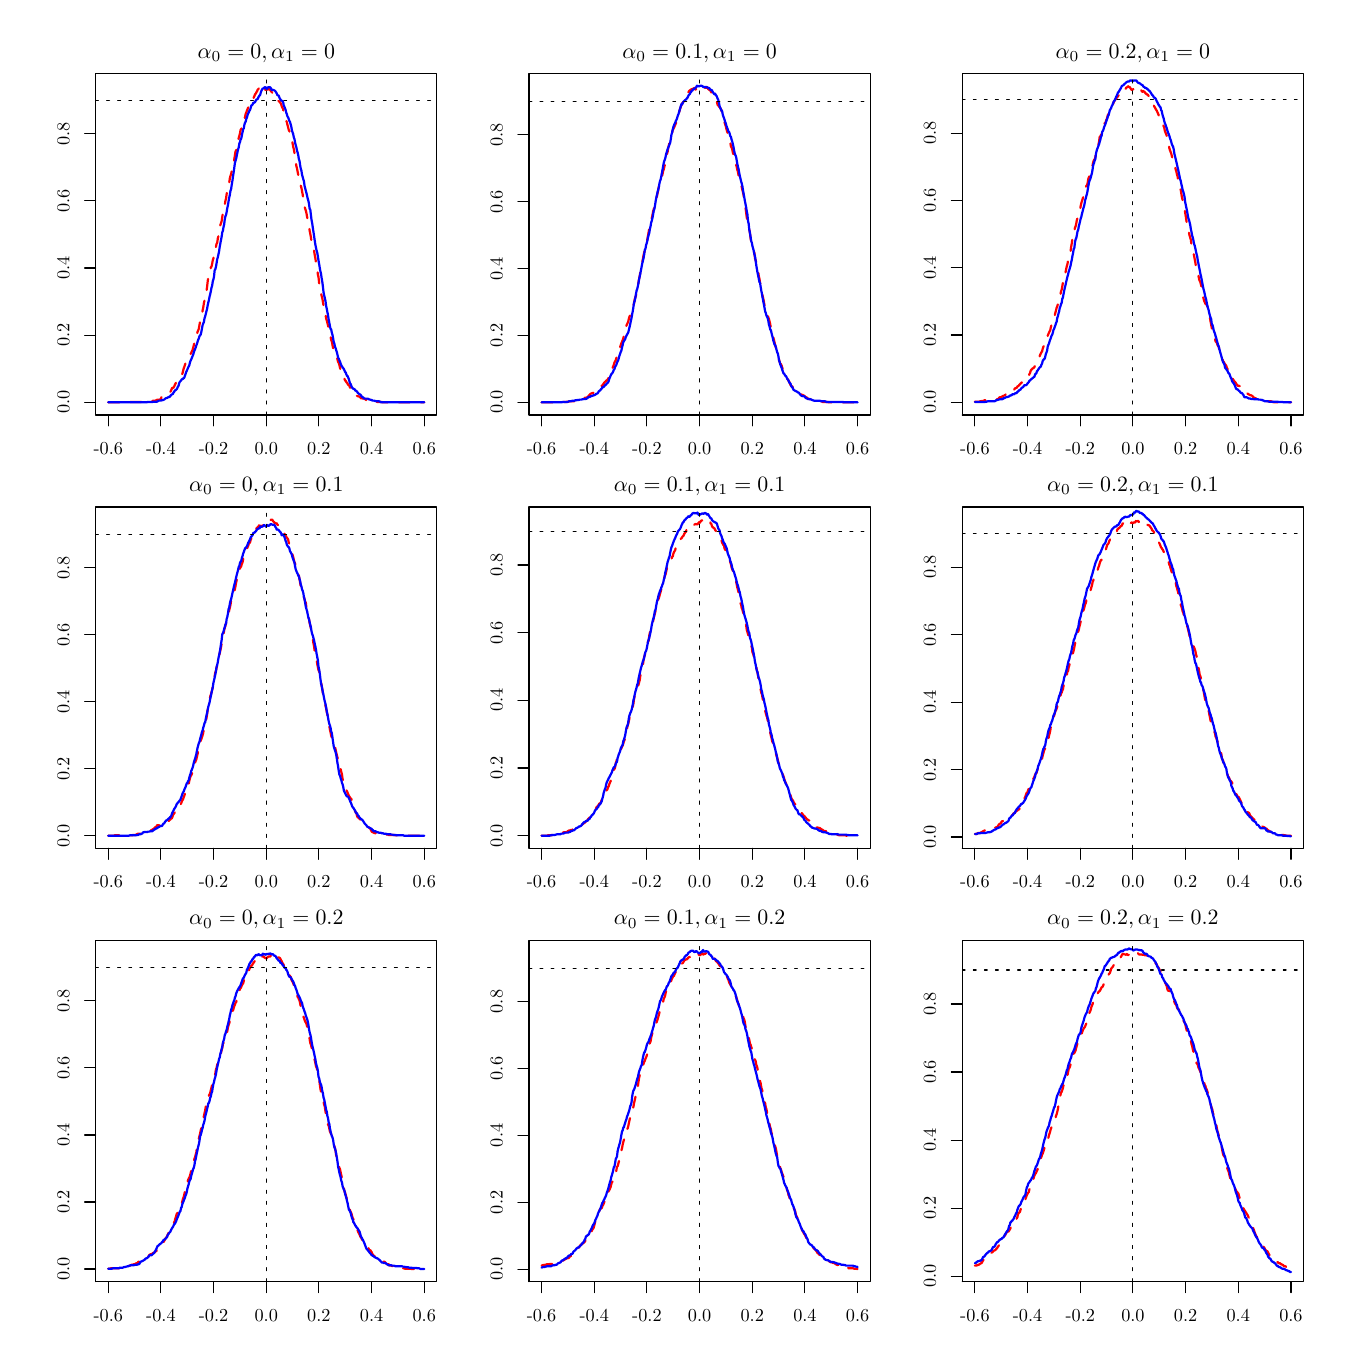
\begin{tikzpicture}[x=1pt,y=1pt]
\definecolor{fillColor}{RGB}{255,255,255}
\path[use as bounding box,fill=fillColor,fill opacity=0.00] (0,0) rectangle (469.75,469.75);
\begin{scope}
\path[clip] ( 24.55,329.80) rectangle (147.87,453.12);
\definecolor{drawColor}{RGB}{255,0,0}

\path[draw=drawColor,line width= 0.8pt,dash pattern=on 4pt off 4pt ,line join=round,line cap=round] ( 29.12,334.37) --
	( 29.35,334.37) --
	( 29.58,334.37) --
	( 29.81,334.37) --
	( 30.03,334.37) --
	( 30.26,334.37) --
	( 30.49,334.37) --
	( 30.72,334.37) --
	( 30.95,334.37) --
	( 31.18,334.37) --
	( 31.41,334.37) --
	( 31.64,334.37) --
	( 31.87,334.37) --
	( 32.09,334.37) --
	( 32.32,334.37) --
	( 32.55,334.37) --
	( 32.78,334.37) --
	( 33.01,334.37) --
	( 33.24,334.37) --
	( 33.47,334.37) --
	( 33.70,334.37) --
	( 33.92,334.37) --
	( 34.15,334.37) --
	( 34.38,334.37) --
	( 34.61,334.37) --
	( 34.84,334.37) --
	( 35.07,334.37) --
	( 35.30,334.49) --
	( 35.53,334.49) --
	( 35.76,334.49) --
	( 35.98,334.49) --
	( 36.21,334.49) --
	( 36.44,334.49) --
	( 36.67,334.49) --
	( 36.90,334.49) --
	( 37.13,334.49) --
	( 37.36,334.49) --
	( 37.59,334.49) --
	( 37.81,334.49) --
	( 38.04,334.49) --
	( 38.27,334.49) --
	( 38.50,334.49) --
	( 38.73,334.49) --
	( 38.96,334.49) --
	( 39.19,334.49) --
	( 39.42,334.49) --
	( 39.65,334.49) --
	( 39.87,334.49) --
	( 40.10,334.49) --
	( 40.33,334.49) --
	( 40.56,334.49) --
	( 40.79,334.49) --
	( 41.02,334.49) --
	( 41.25,334.49) --
	( 41.48,334.49) --
	( 41.71,334.49) --
	( 41.93,334.49) --
	( 42.16,334.49) --
	( 42.39,334.61) --
	( 42.62,334.61) --
	( 42.85,334.61) --
	( 43.08,334.61) --
	( 43.31,334.61) --
	( 43.54,334.73) --
	( 43.76,334.73) --
	( 43.99,334.73) --
	( 44.22,334.73) --
	( 44.45,334.73) --
	( 44.68,334.73) --
	( 44.91,334.85) --
	( 45.14,334.85) --
	( 45.37,334.98) --
	( 45.60,334.98) --
	( 45.82,334.98) --
	( 46.05,334.98) --
	( 46.28,334.98) --
	( 46.51,335.22) --
	( 46.74,335.22) --
	( 46.97,335.34) --
	( 47.20,335.34) --
	( 47.43,335.34) --
	( 47.65,335.34) --
	( 47.88,335.46) --
	( 48.11,335.58) --
	( 48.34,336.19) --
	( 48.57,336.43) --
	( 48.80,336.55) --
	( 49.03,336.80) --
	( 49.26,336.80) --
	( 49.49,336.92) --
	( 49.71,337.16) --
	( 49.94,337.16) --
	( 50.17,337.16) --
	( 50.40,337.16) --
	( 50.63,337.52) --
	( 50.86,337.65) --
	( 51.09,337.77) --
	( 51.32,338.01) --
	( 51.54,338.13) --
	( 51.77,338.50) --
	( 52.00,339.10) --
	( 52.23,339.59) --
	( 52.46,339.59) --
	( 52.69,339.71) --
	( 52.92,340.07) --
	( 53.15,340.56) --
	( 53.38,341.04) --
	( 53.60,341.53) --
	( 53.83,341.65) --
	( 54.06,342.14) --
	( 54.29,342.50) --
	( 54.52,342.86) --
	( 54.75,343.11) --
	( 54.98,343.71) --
	( 55.21,344.08) --
	( 55.43,344.44) --
	( 55.66,344.44) --
	( 55.89,344.68) --
	( 56.12,345.53) --
	( 56.35,346.50) --
	( 56.58,347.11) --
	( 56.81,347.84) --
	( 57.04,348.45) --
	( 57.27,348.81) --
	( 57.49,349.54) --
	( 57.72,349.90) --
	( 57.95,350.14) --
	( 58.18,350.39) --
	( 58.41,350.87) --
	( 58.64,351.48) --
	( 58.87,351.84) --
	( 59.10,352.21) --
	( 59.32,352.81) --
	( 59.55,353.18) --
	( 59.78,354.03) --
	( 60.01,354.88) --
	( 60.24,355.97) --
	( 60.47,356.58) --
	( 60.70,357.67) --
	( 60.93,358.27) --
	( 61.16,358.64) --
	( 61.38,359.85) --
	( 61.61,360.34) --
	( 61.84,360.94) --
	( 62.07,362.28) --
	( 62.30,363.61) --
	( 62.53,364.34) --
	( 62.76,365.19) --
	( 62.99,366.16) --
	( 63.22,367.62) --
	( 63.44,368.59) --
	( 63.67,370.17) --
	( 63.90,371.14) --
	( 64.13,372.23) --
	( 64.36,373.81) --
	( 64.59,374.41) --
	( 64.82,375.99) --
	( 65.05,378.05) --
	( 65.27,379.63) --
	( 65.50,380.48) --
	( 65.73,381.09) --
	( 65.96,381.94) --
	( 66.19,383.15) --
	( 66.42,383.39) --
	( 66.65,384.36) --
	( 66.88,385.70) --
	( 67.11,386.31) --
	( 67.33,387.88) --
	( 67.56,389.34) --
	( 67.79,390.31) --
	( 68.02,390.55) --
	( 68.25,391.64) --
	( 68.48,392.01) --
	( 68.71,393.59) --
	( 68.94,394.44) --
	( 69.16,396.01) --
	( 69.39,397.35) --
	( 69.62,398.44) --
	( 69.85,399.05) --
	( 70.08,399.77) --
	( 70.31,401.35) --
	( 70.54,402.69) --
	( 70.77,404.14) --
	( 71.00,404.75) --
	( 71.22,405.60) --
	( 71.45,407.18) --
	( 71.68,408.03) --
	( 71.91,409.72) --
	( 72.14,411.18) --
	( 72.37,411.79) --
	( 72.60,412.39) --
	( 72.83,413.73) --
	( 73.05,415.31) --
	( 73.28,416.16) --
	( 73.51,416.88) --
	( 73.74,417.86) --
	( 73.97,418.58) --
	( 74.20,419.55) --
	( 74.43,420.40) --
	( 74.66,422.22) --
	( 74.89,423.68) --
	( 75.11,425.01) --
	( 75.34,425.50) --
	( 75.57,426.96) --
	( 75.80,428.17) --
	( 76.03,429.02) --
	( 76.26,429.87) --
	( 76.49,430.72) --
	( 76.72,431.57) --
	( 76.94,432.78) --
	( 77.17,433.14) --
	( 77.40,433.87) --
	( 77.63,434.36) --
	( 77.86,434.72) --
	( 78.09,435.69) --
	( 78.32,436.79) --
	( 78.55,437.51) --
	( 78.78,438.61) --
	( 79.00,439.09) --
	( 79.23,439.82) --
	( 79.46,440.30) --
	( 79.69,441.03) --
	( 79.92,441.52) --
	( 80.15,441.88) --
	( 80.38,442.25) --
	( 80.61,442.37) --
	( 80.83,442.85) --
	( 81.06,443.34) --
	( 81.29,443.70) --
	( 81.52,444.07) --
	( 81.75,444.67) --
	( 81.98,445.16) --
	( 82.21,445.76) --
	( 82.44,445.89) --
	( 82.67,446.49) --
	( 82.89,446.74) --
	( 83.12,447.34) --
	( 83.35,447.58) --
	( 83.58,447.83) --
	( 83.81,447.83) --
	( 84.04,447.83) --
	( 84.27,447.58) --
	( 84.50,448.07) --
	( 84.73,448.56) --
	( 84.95,448.31) --
	( 85.18,447.58) --
	( 85.41,447.58) --
	( 85.64,447.83) --
	( 85.87,447.34) --
	( 86.10,447.22) --
	( 86.33,447.58) --
	( 86.56,447.58) --
	( 86.78,447.34) --
	( 87.01,447.71) --
	( 87.24,447.58) --
	( 87.47,447.58) --
	( 87.70,447.10) --
	( 87.93,446.86) --
	( 88.16,446.49) --
	( 88.39,446.25) --
	( 88.62,445.89) --
	( 88.84,445.89) --
	( 89.07,445.76) --
	( 89.30,445.40) --
	( 89.53,444.92) --
	( 89.76,444.43) --
	( 89.99,444.19) --
	( 90.22,443.34) --
	( 90.45,443.34) --
	( 90.67,443.22) --
	( 90.90,443.10) --
	( 91.13,442.85) --
	( 91.36,442.49) --
	( 91.59,442.12) --
	( 91.82,441.27) --
	( 92.05,440.79) --
	( 92.28,440.43) --
	( 92.51,439.09) --
	( 92.73,438.48) --
	( 92.96,437.39) --
	( 93.19,436.54) --
	( 93.42,436.18) --
	( 93.65,435.57) --
	( 93.88,434.60) --
	( 94.11,433.75) --
	( 94.34,432.78) --
	( 94.56,432.42) --
	( 94.79,431.32) --
	( 95.02,430.35) --
	( 95.25,429.75) --
	( 95.48,429.02) --
	( 95.71,428.05) --
	( 95.94,426.71) --
	( 96.17,425.86) --
	( 96.40,424.53) --
	( 96.62,423.32) --
	( 96.85,421.50) --
	( 97.08,419.80) --
	( 97.31,418.95) --
	( 97.54,417.73) --
	( 97.77,416.52) --
	( 98.00,415.55) --
	( 98.23,414.94) --
	( 98.45,413.49) --
	( 98.68,412.64) --
	( 98.91,411.91) --
	( 99.14,410.70) --
	( 99.37,409.48) --
	( 99.60,407.90) --
	( 99.83,406.69) --
	(100.06,405.11) --
	(100.29,404.26) --
	(100.51,403.66) --
	(100.74,402.69) --
	(100.97,401.35) --
	(101.20,400.50) --
	(101.43,398.80) --
	(101.66,397.95) --
	(101.89,396.38) --
	(102.12,395.28) --
	(102.35,393.95) --
	(102.57,392.25) --
	(102.80,391.16) --
	(103.03,390.43) --
	(103.26,389.95) --
	(103.49,389.10) --
	(103.72,387.64) --
	(103.95,386.43) --
	(104.18,384.97) --
	(104.40,383.64) --
	(104.63,382.30) --
	(104.86,380.60) --
	(105.09,379.63) --
	(105.32,377.45) --
	(105.55,376.23) --
	(105.78,374.78) --
	(106.01,373.81) --
	(106.24,372.71) --
	(106.46,371.99) --
	(106.69,370.65) --
	(106.92,369.20) --
	(107.15,367.98) --
	(107.38,367.25) --
	(107.61,366.16) --
	(107.84,364.71) --
	(108.07,363.98) --
	(108.29,363.13) --
	(108.52,362.16) --
	(108.75,360.58) --
	(108.98,359.97) --
	(109.21,359.00) --
	(109.44,358.15) --
	(109.67,356.94) --
	(109.90,356.33) --
	(110.13,355.12) --
	(110.35,354.03) --
	(110.58,353.66) --
	(110.81,352.94) --
	(111.04,352.33) --
	(111.27,352.09) --
	(111.50,351.60) --
	(111.73,350.75) --
	(111.96,349.78) --
	(112.18,348.93) --
	(112.41,348.57) --
	(112.64,347.84) --
	(112.87,346.75) --
	(113.10,345.90) --
	(113.33,345.17) --
	(113.56,344.68) --
	(113.79,344.08) --
	(114.02,343.59) --
	(114.24,343.59) --
	(114.47,342.86) --
	(114.70,342.26) --
	(114.93,342.14) --
	(115.16,341.65) --
	(115.39,341.41) --
	(115.62,341.04) --
	(115.85,340.68) --
	(116.07,340.56) --
	(116.30,340.19) --
	(116.53,339.59) --
	(116.76,339.34) --
	(116.99,338.62) --
	(117.22,338.50) --
	(117.45,338.25) --
	(117.68,337.89) --
	(117.91,337.89) --
	(118.13,337.65) --
	(118.36,337.40) --
	(118.59,336.92) --
	(118.82,336.68) --
	(119.05,336.68) --
	(119.28,336.55) --
	(119.51,336.55) --
	(119.74,336.43) --
	(119.96,336.43) --
	(120.19,336.19) --
	(120.42,335.83) --
	(120.65,335.83) --
	(120.88,335.83) --
	(121.11,335.70) --
	(121.34,335.70) --
	(121.57,335.70) --
	(121.80,335.70) --
	(122.02,335.46) --
	(122.25,335.22) --
	(122.48,335.22) --
	(122.71,335.10) --
	(122.94,334.98) --
	(123.17,334.98) --
	(123.40,334.98) --
	(123.63,334.73) --
	(123.86,334.73) --
	(124.08,334.73) --
	(124.31,334.73) --
	(124.54,334.73) --
	(124.77,334.73) --
	(125.00,334.73) --
	(125.23,334.73) --
	(125.46,334.73) --
	(125.69,334.73) --
	(125.91,334.61) --
	(126.14,334.61) --
	(126.37,334.49) --
	(126.60,334.49) --
	(126.83,334.49) --
	(127.06,334.49) --
	(127.29,334.49) --
	(127.52,334.49) --
	(127.75,334.49) --
	(127.97,334.49) --
	(128.20,334.37) --
	(128.43,334.37) --
	(128.66,334.37) --
	(128.89,334.37) --
	(129.12,334.37) --
	(129.35,334.37) --
	(129.58,334.37) --
	(129.80,334.37) --
	(130.03,334.37) --
	(130.26,334.37) --
	(130.49,334.37) --
	(130.72,334.37) --
	(130.95,334.37) --
	(131.18,334.37) --
	(131.41,334.37) --
	(131.64,334.37) --
	(131.86,334.37) --
	(132.09,334.37) --
	(132.32,334.37) --
	(132.55,334.37) --
	(132.78,334.37) --
	(133.01,334.37) --
	(133.24,334.37) --
	(133.47,334.37) --
	(133.69,334.37) --
	(133.92,334.37) --
	(134.15,334.37) --
	(134.38,334.37) --
	(134.61,334.37) --
	(134.84,334.37) --
	(135.07,334.37) --
	(135.30,334.37) --
	(135.53,334.37) --
	(135.75,334.37) --
	(135.98,334.37) --
	(136.21,334.37) --
	(136.44,334.37) --
	(136.67,334.37) --
	(136.90,334.37) --
	(137.13,334.37) --
	(137.36,334.37) --
	(137.58,334.37) --
	(137.81,334.37) --
	(138.04,334.37) --
	(138.27,334.37) --
	(138.50,334.37) --
	(138.73,334.37) --
	(138.96,334.37) --
	(139.19,334.37) --
	(139.42,334.37) --
	(139.64,334.37) --
	(139.87,334.37) --
	(140.10,334.37) --
	(140.33,334.37) --
	(140.56,334.37) --
	(140.79,334.37) --
	(141.02,334.37) --
	(141.25,334.37) --
	(141.47,334.37) --
	(141.70,334.37) --
	(141.93,334.37) --
	(142.16,334.37) --
	(142.39,334.37) --
	(142.62,334.37) --
	(142.85,334.37) --
	(143.08,334.37) --
	(143.31,334.37);
\end{scope}
\begin{scope}
\path[clip] (  0.00,  0.00) rectangle (469.75,469.75);
\definecolor{drawColor}{RGB}{0,0,0}

\path[draw=drawColor,line width= 0.4pt,line join=round,line cap=round] ( 29.12,329.80) -- (143.31,329.80);

\path[draw=drawColor,line width= 0.4pt,line join=round,line cap=round] ( 29.12,329.80) -- ( 29.12,325.84);

\path[draw=drawColor,line width= 0.4pt,line join=round,line cap=round] ( 48.15,329.80) -- ( 48.15,325.84);

\path[draw=drawColor,line width= 0.4pt,line join=round,line cap=round] ( 67.18,329.80) -- ( 67.18,325.84);

\path[draw=drawColor,line width= 0.4pt,line join=round,line cap=round] ( 86.21,329.80) -- ( 86.21,325.84);

\path[draw=drawColor,line width= 0.4pt,line join=round,line cap=round] (105.24,329.80) -- (105.24,325.84);

\path[draw=drawColor,line width= 0.4pt,line join=round,line cap=round] (124.27,329.80) -- (124.27,325.84);

\path[draw=drawColor,line width= 0.4pt,line join=round,line cap=round] (143.31,329.80) -- (143.31,325.84);

\node[text=drawColor,anchor=base,inner sep=0pt, outer sep=0pt, scale=  0.66] at ( 29.12,315.55) {-0.6};

\node[text=drawColor,anchor=base,inner sep=0pt, outer sep=0pt, scale=  0.66] at ( 48.15,315.55) {-0.4};

\node[text=drawColor,anchor=base,inner sep=0pt, outer sep=0pt, scale=  0.66] at ( 67.18,315.55) {-0.2};

\node[text=drawColor,anchor=base,inner sep=0pt, outer sep=0pt, scale=  0.66] at ( 86.21,315.55) {0.0};

\node[text=drawColor,anchor=base,inner sep=0pt, outer sep=0pt, scale=  0.66] at (105.24,315.55) {0.2};

\node[text=drawColor,anchor=base,inner sep=0pt, outer sep=0pt, scale=  0.66] at (124.27,315.55) {0.4};

\node[text=drawColor,anchor=base,inner sep=0pt, outer sep=0pt, scale=  0.66] at (143.31,315.55) {0.6};

\path[draw=drawColor,line width= 0.4pt,line join=round,line cap=round] ( 24.55,334.37) -- ( 24.55,431.45);

\path[draw=drawColor,line width= 0.4pt,line join=round,line cap=round] ( 24.55,334.37) -- ( 20.59,334.37);

\path[draw=drawColor,line width= 0.4pt,line join=round,line cap=round] ( 24.55,358.64) -- ( 20.59,358.64);

\path[draw=drawColor,line width= 0.4pt,line join=round,line cap=round] ( 24.55,382.91) -- ( 20.59,382.91);

\path[draw=drawColor,line width= 0.4pt,line join=round,line cap=round] ( 24.55,407.18) -- ( 20.59,407.18);

\path[draw=drawColor,line width= 0.4pt,line join=round,line cap=round] ( 24.55,431.45) -- ( 20.59,431.45);

\node[text=drawColor,rotate= 90.00,anchor=base,inner sep=0pt, outer sep=0pt, scale=  0.66] at ( 15.05,334.37) {0.0};

\node[text=drawColor,rotate= 90.00,anchor=base,inner sep=0pt, outer sep=0pt, scale=  0.66] at ( 15.05,358.64) {0.2};

\node[text=drawColor,rotate= 90.00,anchor=base,inner sep=0pt, outer sep=0pt, scale=  0.66] at ( 15.05,382.91) {0.4};

\node[text=drawColor,rotate= 90.00,anchor=base,inner sep=0pt, outer sep=0pt, scale=  0.66] at ( 15.05,407.18) {0.6};

\node[text=drawColor,rotate= 90.00,anchor=base,inner sep=0pt, outer sep=0pt, scale=  0.66] at ( 15.05,431.45) {0.8};

\path[draw=drawColor,line width= 0.4pt,line join=round,line cap=round] ( 24.55,329.80) --
	(147.87,329.80) --
	(147.87,453.12) --
	( 24.55,453.12) --
	( 24.55,329.80);
\end{scope}
\begin{scope}
\path[clip] (  0.00,313.17) rectangle (156.58,469.75);
\definecolor{drawColor}{RGB}{0,0,0}

\node[text=drawColor,anchor=base,inner sep=0pt, outer sep=0pt, scale=  0.79] at ( 86.21,458.71) {\bfseries $\alpha_0 = 0, \alpha_1 = 0$};
\end{scope}
\begin{scope}
\path[clip] ( 24.55,329.80) rectangle (147.87,453.12);
\definecolor{drawColor}{RGB}{0,0,255}

\path[draw=drawColor,line width= 0.8pt,line join=round,line cap=round] ( 29.12,334.37) --
	( 29.35,334.37) --
	( 29.58,334.37) --
	( 29.81,334.37) --
	( 30.03,334.37) --
	( 30.26,334.37) --
	( 30.49,334.37) --
	( 30.72,334.37) --
	( 30.95,334.37) --
	( 31.18,334.37) --
	( 31.41,334.37) --
	( 31.64,334.37) --
	( 31.87,334.37) --
	( 32.09,334.37) --
	( 32.32,334.37) --
	( 32.55,334.37) --
	( 32.78,334.37) --
	( 33.01,334.37) --
	( 33.24,334.37) --
	( 33.47,334.37) --
	( 33.70,334.37) --
	( 33.92,334.37) --
	( 34.15,334.37) --
	( 34.38,334.37) --
	( 34.61,334.37) --
	( 34.84,334.37) --
	( 35.07,334.37) --
	( 35.30,334.37) --
	( 35.53,334.37) --
	( 35.76,334.37) --
	( 35.98,334.37) --
	( 36.21,334.37) --
	( 36.44,334.37) --
	( 36.67,334.37) --
	( 36.90,334.37) --
	( 37.13,334.37) --
	( 37.36,334.37) --
	( 37.59,334.37) --
	( 37.81,334.37) --
	( 38.04,334.37) --
	( 38.27,334.37) --
	( 38.50,334.37) --
	( 38.73,334.37) --
	( 38.96,334.37) --
	( 39.19,334.37) --
	( 39.42,334.37) --
	( 39.65,334.37) --
	( 39.87,334.37) --
	( 40.10,334.37) --
	( 40.33,334.37) --
	( 40.56,334.37) --
	( 40.79,334.37) --
	( 41.02,334.37) --
	( 41.25,334.37) --
	( 41.48,334.37) --
	( 41.71,334.37) --
	( 41.93,334.37) --
	( 42.16,334.37) --
	( 42.39,334.37) --
	( 42.62,334.37) --
	( 42.85,334.37) --
	( 43.08,334.37) --
	( 43.31,334.49) --
	( 43.54,334.49) --
	( 43.76,334.49) --
	( 43.99,334.49) --
	( 44.22,334.49) --
	( 44.45,334.49) --
	( 44.68,334.49) --
	( 44.91,334.49) --
	( 45.14,334.49) --
	( 45.37,334.61) --
	( 45.60,334.61) --
	( 45.82,334.61) --
	( 46.05,334.61) --
	( 46.28,334.61) --
	( 46.51,334.61) --
	( 46.74,334.61) --
	( 46.97,334.73) --
	( 47.20,334.85) --
	( 47.43,334.98) --
	( 47.65,334.98) --
	( 47.88,334.98) --
	( 48.11,334.98) --
	( 48.34,335.10) --
	( 48.57,335.10) --
	( 48.80,335.22) --
	( 49.03,335.22) --
	( 49.26,335.34) --
	( 49.49,335.46) --
	( 49.71,335.70) --
	( 49.94,335.83) --
	( 50.17,335.95) --
	( 50.40,335.95) --
	( 50.63,336.07) --
	( 50.86,336.31) --
	( 51.09,336.31) --
	( 51.32,336.31) --
	( 51.54,336.68) --
	( 51.77,336.92) --
	( 52.00,337.16) --
	( 52.23,337.28) --
	( 52.46,337.40) --
	( 52.69,337.89) --
	( 52.92,338.13) --
	( 53.15,338.62) --
	( 53.38,338.74) --
	( 53.60,338.86) --
	( 53.83,339.10) --
	( 54.06,339.47) --
	( 54.29,340.07) --
	( 54.52,340.32) --
	( 54.75,341.29) --
	( 54.98,341.77) --
	( 55.21,342.01) --
	( 55.43,342.26) --
	( 55.66,342.62) --
	( 55.89,342.74) --
	( 56.12,342.86) --
	( 56.35,343.11) --
	( 56.58,343.23) --
	( 56.81,343.96) --
	( 57.04,344.56) --
	( 57.27,345.29) --
	( 57.49,345.78) --
	( 57.72,346.26) --
	( 57.95,346.87) --
	( 58.18,347.35) --
	( 58.41,347.72) --
	( 58.64,348.81) --
	( 58.87,349.42) --
	( 59.10,349.90) --
	( 59.32,350.39) --
	( 59.55,350.99) --
	( 59.78,351.48) --
	( 60.01,352.33) --
	( 60.24,353.06) --
	( 60.47,353.54) --
	( 60.70,354.15) --
	( 60.93,354.88) --
	( 61.16,355.48) --
	( 61.38,356.21) --
	( 61.61,356.94) --
	( 61.84,357.43) --
	( 62.07,358.27) --
	( 62.30,358.52) --
	( 62.53,358.88) --
	( 62.76,359.85) --
	( 62.99,361.07) --
	( 63.22,362.28) --
	( 63.44,362.89) --
	( 63.67,363.37) --
	( 63.90,364.71) --
	( 64.13,365.43) --
	( 64.36,366.28) --
	( 64.59,367.25) --
	( 64.82,368.10) --
	( 65.05,369.44) --
	( 65.27,370.41) --
	( 65.50,371.38) --
	( 65.73,372.59) --
	( 65.96,373.44) --
	( 66.19,374.53) --
	( 66.42,375.75) --
	( 66.65,376.48) --
	( 66.88,378.05) --
	( 67.11,378.78) --
	( 67.33,379.75) --
	( 67.56,382.06) --
	( 67.79,382.42) --
	( 68.02,383.27) --
	( 68.25,384.61) --
	( 68.48,386.06) --
	( 68.71,386.79) --
	( 68.94,387.88) --
	( 69.16,388.85) --
	( 69.39,390.55) --
	( 69.62,391.77) --
	( 69.85,392.98) --
	( 70.08,394.19) --
	( 70.31,395.77) --
	( 70.54,396.38) --
	( 70.77,397.71) --
	( 71.00,398.68) --
	( 71.22,400.50) --
	( 71.45,401.59) --
	( 71.68,402.08) --
	( 71.91,403.17) --
	( 72.14,404.63) --
	( 72.37,405.60) --
	( 72.60,407.06) --
	( 72.83,408.39) --
	( 73.05,409.36) --
	( 73.28,410.82) --
	( 73.51,411.42) --
	( 73.74,413.00) --
	( 73.97,414.34) --
	( 74.20,416.03) --
	( 74.43,417.49) --
	( 74.66,419.19) --
	( 74.89,420.89) --
	( 75.11,421.62) --
	( 75.34,422.47) --
	( 75.57,423.56) --
	( 75.80,424.77) --
	( 76.03,425.74) --
	( 76.26,426.47) --
	( 76.49,427.93) --
	( 76.72,428.41) --
	( 76.94,429.38) --
	( 77.17,429.63) --
	( 77.40,430.84) --
	( 77.63,431.93) --
	( 77.86,433.02) --
	( 78.09,433.39) --
	( 78.32,434.72) --
	( 78.55,435.45) --
	( 78.78,435.81) --
	( 79.00,436.79) --
	( 79.23,437.27) --
	( 79.46,438.24) --
	( 79.69,438.73) --
	( 79.92,439.21) --
	( 80.15,439.82) --
	( 80.38,440.06) --
	( 80.61,440.91) --
	( 80.83,441.64) --
	( 81.06,441.76) --
	( 81.29,442.00) --
	( 81.52,442.61) --
	( 81.75,442.61) --
	( 81.98,442.73) --
	( 82.21,442.97) --
	( 82.44,443.46) --
	( 82.67,443.82) --
	( 82.89,443.82) --
	( 83.12,443.94) --
	( 83.35,444.55) --
	( 83.58,444.92) --
	( 83.81,445.28) --
	( 84.04,445.52) --
	( 84.27,446.49) --
	( 84.50,446.98) --
	( 84.73,447.46) --
	( 84.95,447.83) --
	( 85.18,447.71) --
	( 85.41,447.95) --
	( 85.64,448.19) --
	( 85.87,448.31) --
	( 86.10,447.95) --
	( 86.33,447.58) --
	( 86.56,447.83) --
	( 86.78,448.19) --
	( 87.01,448.19) --
	( 87.24,448.31) --
	( 87.47,448.19) --
	( 87.70,448.19) --
	( 87.93,447.71) --
	( 88.16,447.22) --
	( 88.39,447.34) --
	( 88.62,447.22) --
	( 88.84,447.22) --
	( 89.07,447.10) --
	( 89.30,446.98) --
	( 89.53,446.74) --
	( 89.76,446.37) --
	( 89.99,446.01) --
	( 90.22,445.40) --
	( 90.45,445.28) --
	( 90.67,445.28) --
	( 90.90,444.67) --
	( 91.13,444.07) --
	( 91.36,443.82) --
	( 91.59,443.46) --
	( 91.82,443.34) --
	( 92.05,443.22) --
	( 92.28,442.97) --
	( 92.51,441.76) --
	( 92.73,441.27) --
	( 92.96,440.67) --
	( 93.19,440.06) --
	( 93.42,439.09) --
	( 93.65,438.48) --
	( 93.88,437.63) --
	( 94.11,437.39) --
	( 94.34,436.66) --
	( 94.56,436.06) --
	( 94.79,435.69) --
	( 95.02,434.84) --
	( 95.25,433.99) --
	( 95.48,432.66) --
	( 95.71,431.93) --
	( 95.94,431.32) --
	( 96.17,430.11) --
	( 96.40,429.50) --
	( 96.62,428.29) --
	( 96.85,427.32) --
	( 97.08,426.59) --
	( 97.31,425.38) --
	( 97.54,424.65) --
	( 97.77,423.68) --
	( 98.00,422.22) --
	( 98.23,421.62) --
	( 98.45,420.04) --
	( 98.68,418.83) --
	( 98.91,418.10) --
	( 99.14,416.64) --
	( 99.37,415.79) --
	( 99.60,414.94) --
	( 99.83,414.21) --
	(100.06,412.52) --
	(100.29,411.67) --
	(100.51,410.82) --
	(100.74,409.97) --
	(100.97,409.00) --
	(101.20,407.90) --
	(101.43,407.18) --
	(101.66,406.08) --
	(101.89,404.26) --
	(102.12,404.02) --
	(102.35,402.08) --
	(102.57,400.26) --
	(102.80,399.17) --
	(103.03,397.47) --
	(103.26,396.01) --
	(103.49,394.44) --
	(103.72,392.86) --
	(103.95,391.40) --
	(104.18,390.19) --
	(104.40,389.22) --
	(104.63,388.49) --
	(104.86,387.15) --
	(105.09,385.58) --
	(105.32,384.36) --
	(105.55,382.91) --
	(105.78,381.69) --
	(106.01,380.72) --
	(106.24,379.15) --
	(106.46,377.93) --
	(106.69,376.11) --
	(106.92,374.05) --
	(107.15,372.96) --
	(107.38,371.99) --
	(107.61,371.02) --
	(107.84,369.20) --
	(108.07,368.22) --
	(108.29,367.01) --
	(108.52,365.92) --
	(108.75,364.34) --
	(108.98,363.25) --
	(109.21,361.91) --
	(109.44,360.94) --
	(109.67,360.70) --
	(109.90,359.61) --
	(110.13,358.76) --
	(110.35,357.67) --
	(110.58,356.21) --
	(110.81,355.60) --
	(111.04,354.51) --
	(111.27,353.91) --
	(111.50,353.18) --
	(111.73,352.45) --
	(111.96,351.48) --
	(112.18,350.51) --
	(112.41,350.14) --
	(112.64,349.54) --
	(112.87,349.05) --
	(113.10,348.32) --
	(113.33,347.72) --
	(113.56,347.35) --
	(113.79,346.99) --
	(114.02,346.75) --
	(114.24,346.38) --
	(114.47,345.90) --
	(114.70,345.29) --
	(114.93,345.17) --
	(115.16,344.44) --
	(115.39,343.96) --
	(115.62,343.83) --
	(115.85,343.23) --
	(116.07,342.74) --
	(116.30,341.77) --
	(116.53,341.16) --
	(116.76,340.92) --
	(116.99,340.19) --
	(117.22,339.71) --
	(117.45,339.47) --
	(117.68,339.22) --
	(117.91,339.22) --
	(118.13,339.10) --
	(118.36,338.62) --
	(118.59,338.62) --
	(118.82,338.37) --
	(119.05,338.25) --
	(119.28,337.77) --
	(119.51,337.65) --
	(119.74,337.40) --
	(119.96,337.28) --
	(120.19,337.16) --
	(120.42,336.92) --
	(120.65,336.55) --
	(120.88,336.31) --
	(121.11,336.19) --
	(121.34,336.07) --
	(121.57,335.70) --
	(121.80,335.70) --
	(122.02,335.70) --
	(122.25,335.70) --
	(122.48,335.70) --
	(122.71,335.70) --
	(122.94,335.70) --
	(123.17,335.46) --
	(123.40,335.46) --
	(123.63,335.34) --
	(123.86,335.34) --
	(124.08,335.22) --
	(124.31,335.22) --
	(124.54,334.98) --
	(124.77,334.98) --
	(125.00,334.98) --
	(125.23,334.98) --
	(125.46,334.85) --
	(125.69,334.85) --
	(125.91,334.73) --
	(126.14,334.73) --
	(126.37,334.73) --
	(126.60,334.73) --
	(126.83,334.73) --
	(127.06,334.73) --
	(127.29,334.61) --
	(127.52,334.49) --
	(127.75,334.37) --
	(127.97,334.37) --
	(128.20,334.37) --
	(128.43,334.37) --
	(128.66,334.37) --
	(128.89,334.37) --
	(129.12,334.37) --
	(129.35,334.37) --
	(129.58,334.37) --
	(129.80,334.37) --
	(130.03,334.37) --
	(130.26,334.37) --
	(130.49,334.37) --
	(130.72,334.37) --
	(130.95,334.37) --
	(131.18,334.37) --
	(131.41,334.37) --
	(131.64,334.37) --
	(131.86,334.37) --
	(132.09,334.37) --
	(132.32,334.37) --
	(132.55,334.37) --
	(132.78,334.37) --
	(133.01,334.37) --
	(133.24,334.37) --
	(133.47,334.37) --
	(133.69,334.37) --
	(133.92,334.37) --
	(134.15,334.37) --
	(134.38,334.37) --
	(134.61,334.37) --
	(134.84,334.37) --
	(135.07,334.37) --
	(135.30,334.37) --
	(135.53,334.37) --
	(135.75,334.37) --
	(135.98,334.37) --
	(136.21,334.37) --
	(136.44,334.37) --
	(136.67,334.37) --
	(136.90,334.37) --
	(137.13,334.37) --
	(137.36,334.37) --
	(137.58,334.37) --
	(137.81,334.37) --
	(138.04,334.37) --
	(138.27,334.37) --
	(138.50,334.37) --
	(138.73,334.37) --
	(138.96,334.37) --
	(139.19,334.37) --
	(139.42,334.37) --
	(139.64,334.37) --
	(139.87,334.37) --
	(140.10,334.37) --
	(140.33,334.37) --
	(140.56,334.37) --
	(140.79,334.37) --
	(141.02,334.37) --
	(141.25,334.37) --
	(141.47,334.37) --
	(141.70,334.37) --
	(141.93,334.37) --
	(142.16,334.37) --
	(142.39,334.37) --
	(142.62,334.37) --
	(142.85,334.37) --
	(143.08,334.37) --
	(143.31,334.37);
\definecolor{drawColor}{RGB}{0,0,0}

\path[draw=drawColor,line width= 0.4pt,dash pattern=on 1pt off 3pt ,line join=round,line cap=round] ( 24.55,443.58) -- (147.87,443.58);

\path[draw=drawColor,line width= 0.4pt,dash pattern=on 1pt off 3pt ,line join=round,line cap=round] ( 86.21,329.80) -- ( 86.21,453.12);

\path[draw=drawColor,line width= 0.4pt,dash pattern=on 1pt off 3pt ,line join=round,line cap=round] ( 86.21,329.80) -- ( 86.21,453.12);
\end{scope}
\begin{scope}
\path[clip] (181.14,329.80) rectangle (304.46,453.12);
\definecolor{drawColor}{RGB}{255,0,0}

\path[draw=drawColor,line width= 0.8pt,dash pattern=on 4pt off 4pt ,line join=round,line cap=round] (185.70,334.37) --
	(185.93,334.37) --
	(186.16,334.37) --
	(186.39,334.37) --
	(186.62,334.37) --
	(186.85,334.37) --
	(187.08,334.37) --
	(187.31,334.37) --
	(187.54,334.37) --
	(187.76,334.37) --
	(187.99,334.37) --
	(188.22,334.37) --
	(188.45,334.37) --
	(188.68,334.37) --
	(188.91,334.37) --
	(189.14,334.37) --
	(189.37,334.37) --
	(189.59,334.37) --
	(189.82,334.37) --
	(190.05,334.37) --
	(190.28,334.37) --
	(190.51,334.37) --
	(190.74,334.37) --
	(190.97,334.37) --
	(191.20,334.37) --
	(191.43,334.37) --
	(191.65,334.37) --
	(191.88,334.37) --
	(192.11,334.37) --
	(192.34,334.37) --
	(192.57,334.37) --
	(192.80,334.37) --
	(193.03,334.37) --
	(193.26,334.37) --
	(193.48,334.37) --
	(193.71,334.49) --
	(193.94,334.49) --
	(194.17,334.49) --
	(194.40,334.49) --
	(194.63,334.49) --
	(194.86,334.61) --
	(195.09,334.61) --
	(195.32,334.61) --
	(195.54,334.61) --
	(195.77,334.73) --
	(196.00,334.73) --
	(196.23,334.73) --
	(196.46,334.73) --
	(196.69,334.73) --
	(196.92,334.73) --
	(197.15,334.73) --
	(197.37,334.73) --
	(197.60,334.85) --
	(197.83,334.85) --
	(198.06,334.85) --
	(198.29,335.09) --
	(198.52,335.22) --
	(198.75,335.22) --
	(198.98,335.34) --
	(199.21,335.34) --
	(199.43,335.34) --
	(199.66,335.34) --
	(199.89,335.34) --
	(200.12,335.34) --
	(200.35,335.34) --
	(200.58,335.46) --
	(200.81,335.46) --
	(201.04,335.58) --
	(201.26,335.94) --
	(201.49,336.06) --
	(201.72,336.06) --
	(201.95,336.06) --
	(202.18,336.18) --
	(202.41,336.42) --
	(202.64,336.54) --
	(202.87,336.91) --
	(203.10,337.15) --
	(203.32,337.39) --
	(203.55,337.51) --
	(203.78,337.63) --
	(204.01,337.63) --
	(204.24,337.75) --
	(204.47,337.87) --
	(204.70,337.87) --
	(204.93,337.99) --
	(205.15,338.12) --
	(205.38,338.48) --
	(205.61,338.72) --
	(205.84,338.96) --
	(206.07,339.08) --
	(206.30,339.32) --
	(206.53,339.32) --
	(206.76,339.69) --
	(206.99,339.81) --
	(207.21,339.93) --
	(207.44,340.41) --
	(207.67,340.41) --
	(207.90,340.77) --
	(208.13,341.14) --
	(208.36,341.50) --
	(208.59,341.74) --
	(208.82,341.86) --
	(209.05,342.22) --
	(209.27,342.34) --
	(209.50,342.47) --
	(209.73,342.95) --
	(209.96,343.43) --
	(210.19,343.92) --
	(210.42,344.40) --
	(210.65,344.88) --
	(210.88,345.49) --
	(211.10,346.33) --
	(211.33,346.82) --
	(211.56,347.30) --
	(211.79,347.90) --
	(212.02,348.75) --
	(212.25,349.11) --
	(212.48,349.59) --
	(212.71,350.32) --
	(212.94,350.80) --
	(213.16,351.41) --
	(213.39,351.77) --
	(213.62,352.98) --
	(213.85,353.82) --
	(214.08,354.31) --
	(214.31,355.03) --
	(214.54,355.76) --
	(214.77,356.24) --
	(214.99,356.84) --
	(215.22,357.45) --
	(215.45,358.54) --
	(215.68,359.02) --
	(215.91,359.86) --
	(216.14,361.07) --
	(216.37,362.16) --
	(216.60,362.64) --
	(216.83,363.13) --
	(217.05,363.73) --
	(217.28,364.82) --
	(217.51,365.42) --
	(217.74,366.03) --
	(217.97,367.11) --
	(218.20,367.48) --
	(218.43,367.96) --
	(218.66,368.56) --
	(218.88,369.29) --
	(219.11,370.14) --
	(219.34,371.59) --
	(219.57,372.31) --
	(219.80,372.91) --
	(220.03,374.24) --
	(220.26,374.85) --
	(220.49,376.18) --
	(220.72,377.75) --
	(220.94,378.96) --
	(221.17,380.04) --
	(221.40,381.61) --
	(221.63,382.34) --
	(221.86,383.55) --
	(222.09,385.00) --
	(222.32,386.21) --
	(222.55,387.54) --
	(222.77,388.50) --
	(223.00,389.11) --
	(223.23,390.31) --
	(223.46,390.68) --
	(223.69,391.89) --
	(223.92,393.34) --
	(224.15,394.54) --
	(224.38,395.87) --
	(224.61,397.20) --
	(224.83,398.05) --
	(225.06,398.77) --
	(225.29,399.74) --
	(225.52,400.95) --
	(225.75,401.91) --
	(225.98,403.24) --
	(226.21,404.09) --
	(226.44,404.69) --
	(226.66,405.66) --
	(226.89,407.11) --
	(227.12,407.71) --
	(227.35,408.68) --
	(227.58,409.77) --
	(227.81,410.86) --
	(228.04,412.19) --
	(228.27,412.67) --
	(228.50,413.27) --
	(228.72,414.24) --
	(228.95,415.09) --
	(229.18,415.93) --
	(229.41,416.90) --
	(229.64,417.99) --
	(229.87,418.59) --
	(230.10,419.68) --
	(230.33,420.40) --
	(230.56,421.25) --
	(230.78,422.82) --
	(231.01,424.15) --
	(231.24,424.87) --
	(231.47,426.32) --
	(231.70,427.29) --
	(231.93,428.26) --
	(232.16,429.34) --
	(232.39,430.31) --
	(232.61,430.79) --
	(232.84,431.52) --
	(233.07,432.73) --
	(233.30,433.09) --
	(233.53,433.57) --
	(233.76,434.06) --
	(233.99,434.66) --
	(234.22,435.14) --
	(234.45,435.75) --
	(234.67,436.23) --
	(234.90,436.96) --
	(235.13,437.44) --
	(235.36,438.65) --
	(235.59,439.98) --
	(235.82,440.58) --
	(236.05,441.31) --
	(236.28,441.79) --
	(236.50,442.39) --
	(236.73,442.63) --
	(236.96,443.00) --
	(237.19,443.24) --
	(237.42,443.72) --
	(237.65,444.45) --
	(237.88,445.05) --
	(238.11,445.53) --
	(238.34,446.14) --
	(238.56,446.38) --
	(238.79,446.50) --
	(239.02,446.86) --
	(239.25,447.11) --
	(239.48,447.11) --
	(239.71,447.35) --
	(239.94,447.59) --
	(240.17,447.47) --
	(240.39,447.71) --
	(240.62,447.71) --
	(240.85,447.95) --
	(241.08,447.71) --
	(241.31,447.35) --
	(241.54,447.59) --
	(241.77,447.47) --
	(242.00,447.71) --
	(242.23,447.47) --
	(242.45,447.47) --
	(242.68,447.83) --
	(242.91,447.95) --
	(243.14,448.07) --
	(243.37,447.95) --
	(243.60,447.95) --
	(243.83,448.19) --
	(244.06,448.31) --
	(244.28,448.43) --
	(244.51,448.56) --
	(244.74,448.07) --
	(244.97,447.95) --
	(245.20,448.07) --
	(245.43,448.31) --
	(245.66,448.07) --
	(245.89,447.59) --
	(246.12,447.47) --
	(246.34,447.23) --
	(246.57,447.35) --
	(246.80,446.74) --
	(247.03,446.38) --
	(247.26,446.26) --
	(247.49,445.90) --
	(247.72,445.66) --
	(247.95,445.05) --
	(248.18,444.81) --
	(248.40,444.45) --
	(248.63,443.84) --
	(248.86,443.12) --
	(249.09,442.76) --
	(249.32,441.79) --
	(249.55,441.67) --
	(249.78,441.31) --
	(250.01,441.06) --
	(250.23,440.82) --
	(250.46,440.34) --
	(250.69,439.98) --
	(250.92,438.65) --
	(251.15,438.04) --
	(251.38,437.68) --
	(251.61,436.83) --
	(251.84,435.38) --
	(252.07,434.66) --
	(252.29,434.06) --
	(252.52,432.97) --
	(252.75,432.24) --
	(252.98,431.52) --
	(253.21,430.55) --
	(253.44,429.83) --
	(253.67,429.22) --
	(253.90,428.26) --
	(254.12,426.81) --
	(254.35,426.44) --
	(254.58,425.84) --
	(254.81,424.63) --
	(255.04,423.79) --
	(255.27,423.06) --
	(255.50,422.09) --
	(255.73,421.37) --
	(255.96,420.28) --
	(256.18,419.56) --
	(256.41,418.47) --
	(256.64,417.74) --
	(256.87,416.41) --
	(257.10,415.57) --
	(257.33,414.96) --
	(257.56,413.76) --
	(257.79,413.15) --
	(258.01,412.19) --
	(258.24,411.22) --
	(258.47,410.25) --
	(258.70,409.16) --
	(258.93,407.35) --
	(259.16,406.02) --
	(259.39,404.69) --
	(259.62,402.88) --
	(259.85,401.07) --
	(260.07,399.98) --
	(260.30,398.89) --
	(260.53,398.05) --
	(260.76,396.84) --
	(260.99,395.51) --
	(261.22,393.70) --
	(261.45,392.25) --
	(261.68,391.52) --
	(261.90,390.56) --
	(262.13,389.71) --
	(262.36,388.99) --
	(262.59,388.38) --
	(262.82,386.33) --
	(263.05,385.72) --
	(263.28,384.76) --
	(263.51,383.79) --
	(263.74,382.46) --
	(263.96,381.61) --
	(264.19,379.92) --
	(264.42,379.08) --
	(264.65,377.51) --
	(264.88,376.54) --
	(265.11,374.85) --
	(265.34,373.88) --
	(265.57,372.79) --
	(265.79,371.95) --
	(266.02,370.74) --
	(266.25,369.41) --
	(266.48,368.44) --
	(266.71,367.48) --
	(266.94,366.87) --
	(267.17,366.03) --
	(267.40,365.54) --
	(267.63,365.06) --
	(267.85,364.46) --
	(268.08,363.61) --
	(268.31,362.64) --
	(268.54,361.31) --
	(268.77,360.23) --
	(269.00,359.26) --
	(269.23,358.41) --
	(269.46,357.69) --
	(269.69,356.84) --
	(269.91,355.88) --
	(270.14,354.79) --
	(270.37,354.19) --
	(270.60,353.82) --
	(270.83,352.98) --
	(271.06,352.13) --
	(271.29,351.04) --
	(271.52,349.59) --
	(271.74,348.99) --
	(271.97,348.27) --
	(272.20,348.14) --
	(272.43,347.66) --
	(272.66,346.94) --
	(272.89,346.09) --
	(273.12,345.49) --
	(273.35,344.88) --
	(273.58,344.88) --
	(273.80,343.92) --
	(274.03,343.67) --
	(274.26,343.31) --
	(274.49,342.95) --
	(274.72,342.47) --
	(274.95,342.10) --
	(275.18,341.86) --
	(275.41,341.26) --
	(275.63,340.65) --
	(275.86,340.41) --
	(276.09,340.17) --
	(276.32,340.05) --
	(276.55,339.57) --
	(276.78,339.44) --
	(277.01,339.20) --
	(277.24,339.08) --
	(277.47,338.84) --
	(277.69,338.36) --
	(277.92,338.24) --
	(278.15,338.12) --
	(278.38,337.87) --
	(278.61,337.87) --
	(278.84,337.87) --
	(279.07,337.75) --
	(279.30,337.51) --
	(279.52,337.27) --
	(279.75,337.03) --
	(279.98,337.03) --
	(280.21,336.91) --
	(280.44,336.79) --
	(280.67,336.67) --
	(280.90,336.42) --
	(281.13,336.18) --
	(281.36,336.18) --
	(281.58,336.06) --
	(281.81,335.82) --
	(282.04,335.70) --
	(282.27,335.58) --
	(282.50,335.58) --
	(282.73,335.58) --
	(282.96,335.22) --
	(283.19,335.22) --
	(283.41,335.22) --
	(283.64,335.22) --
	(283.87,335.22) --
	(284.10,335.22) --
	(284.33,335.09) --
	(284.56,334.97) --
	(284.79,334.85) --
	(285.02,334.85) --
	(285.25,334.85) --
	(285.47,334.85) --
	(285.70,334.85) --
	(285.93,334.85) --
	(286.16,334.73) --
	(286.39,334.73) --
	(286.62,334.73) --
	(286.85,334.73) --
	(287.08,334.61) --
	(287.30,334.49) --
	(287.53,334.49) --
	(287.76,334.49) --
	(287.99,334.49) --
	(288.22,334.49) --
	(288.45,334.49) --
	(288.68,334.49) --
	(288.91,334.49) --
	(289.14,334.49) --
	(289.36,334.37) --
	(289.59,334.37) --
	(289.82,334.37) --
	(290.05,334.37) --
	(290.28,334.37) --
	(290.51,334.37) --
	(290.74,334.37) --
	(290.97,334.37) --
	(291.20,334.37) --
	(291.42,334.37) --
	(291.65,334.37) --
	(291.88,334.37) --
	(292.11,334.37) --
	(292.34,334.37) --
	(292.57,334.37) --
	(292.80,334.37) --
	(293.03,334.37) --
	(293.25,334.37) --
	(293.48,334.37) --
	(293.71,334.37) --
	(293.94,334.37) --
	(294.17,334.37) --
	(294.40,334.37) --
	(294.63,334.37) --
	(294.86,334.37) --
	(295.09,334.37) --
	(295.31,334.37) --
	(295.54,334.37) --
	(295.77,334.37) --
	(296.00,334.37) --
	(296.23,334.37) --
	(296.46,334.37) --
	(296.69,334.37) --
	(296.92,334.37) --
	(297.14,334.37) --
	(297.37,334.37) --
	(297.60,334.37) --
	(297.83,334.37) --
	(298.06,334.37) --
	(298.29,334.37) --
	(298.52,334.37) --
	(298.75,334.37) --
	(298.98,334.37) --
	(299.20,334.37) --
	(299.43,334.37) --
	(299.66,334.37) --
	(299.89,334.37);
\end{scope}
\begin{scope}
\path[clip] (  0.00,  0.00) rectangle (469.75,469.75);
\definecolor{drawColor}{RGB}{0,0,0}

\path[draw=drawColor,line width= 0.4pt,line join=round,line cap=round] (185.70,329.80) -- (299.89,329.80);

\path[draw=drawColor,line width= 0.4pt,line join=round,line cap=round] (185.70,329.80) -- (185.70,325.84);

\path[draw=drawColor,line width= 0.4pt,line join=round,line cap=round] (204.74,329.80) -- (204.74,325.84);

\path[draw=drawColor,line width= 0.4pt,line join=round,line cap=round] (223.77,329.80) -- (223.77,325.84);

\path[draw=drawColor,line width= 0.4pt,line join=round,line cap=round] (242.80,329.80) -- (242.80,325.84);

\path[draw=drawColor,line width= 0.4pt,line join=round,line cap=round] (261.83,329.80) -- (261.83,325.84);

\path[draw=drawColor,line width= 0.4pt,line join=round,line cap=round] (280.86,329.80) -- (280.86,325.84);

\path[draw=drawColor,line width= 0.4pt,line join=round,line cap=round] (299.89,329.80) -- (299.89,325.84);

\node[text=drawColor,anchor=base,inner sep=0pt, outer sep=0pt, scale=  0.66] at (185.70,315.55) {-0.6};

\node[text=drawColor,anchor=base,inner sep=0pt, outer sep=0pt, scale=  0.66] at (204.74,315.55) {-0.4};

\node[text=drawColor,anchor=base,inner sep=0pt, outer sep=0pt, scale=  0.66] at (223.77,315.55) {-0.2};

\node[text=drawColor,anchor=base,inner sep=0pt, outer sep=0pt, scale=  0.66] at (242.80,315.55) {0.0};

\node[text=drawColor,anchor=base,inner sep=0pt, outer sep=0pt, scale=  0.66] at (261.83,315.55) {0.2};

\node[text=drawColor,anchor=base,inner sep=0pt, outer sep=0pt, scale=  0.66] at (280.86,315.55) {0.4};

\node[text=drawColor,anchor=base,inner sep=0pt, outer sep=0pt, scale=  0.66] at (299.89,315.55) {0.6};

\path[draw=drawColor,line width= 0.4pt,line join=round,line cap=round] (181.14,334.37) -- (181.14,431.03);

\path[draw=drawColor,line width= 0.4pt,line join=round,line cap=round] (181.14,334.37) -- (177.18,334.37);

\path[draw=drawColor,line width= 0.4pt,line join=round,line cap=round] (181.14,358.54) -- (177.18,358.54);

\path[draw=drawColor,line width= 0.4pt,line join=round,line cap=round] (181.14,382.70) -- (177.18,382.70);

\path[draw=drawColor,line width= 0.4pt,line join=round,line cap=round] (181.14,406.87) -- (177.18,406.87);

\path[draw=drawColor,line width= 0.4pt,line join=round,line cap=round] (181.14,431.03) -- (177.18,431.03);

\node[text=drawColor,rotate= 90.00,anchor=base,inner sep=0pt, outer sep=0pt, scale=  0.66] at (171.63,334.37) {0.0};

\node[text=drawColor,rotate= 90.00,anchor=base,inner sep=0pt, outer sep=0pt, scale=  0.66] at (171.63,358.54) {0.2};

\node[text=drawColor,rotate= 90.00,anchor=base,inner sep=0pt, outer sep=0pt, scale=  0.66] at (171.63,382.70) {0.4};

\node[text=drawColor,rotate= 90.00,anchor=base,inner sep=0pt, outer sep=0pt, scale=  0.66] at (171.63,406.87) {0.6};

\node[text=drawColor,rotate= 90.00,anchor=base,inner sep=0pt, outer sep=0pt, scale=  0.66] at (171.63,431.03) {0.8};

\path[draw=drawColor,line width= 0.4pt,line join=round,line cap=round] (181.14,329.80) --
	(304.46,329.80) --
	(304.46,453.12) --
	(181.14,453.12) --
	(181.14,329.80);
\end{scope}
\begin{scope}
\path[clip] (156.58,313.17) rectangle (313.17,469.75);
\definecolor{drawColor}{RGB}{0,0,0}

\node[text=drawColor,anchor=base,inner sep=0pt, outer sep=0pt, scale=  0.79] at (242.80,458.71) {\bfseries $\alpha_0 = 0.1, \alpha_1 = 0$};
\end{scope}
\begin{scope}
\path[clip] (181.14,329.80) rectangle (304.46,453.12);
\definecolor{drawColor}{RGB}{0,0,255}

\path[draw=drawColor,line width= 0.8pt,line join=round,line cap=round] (185.70,334.37) --
	(185.93,334.37) --
	(186.16,334.37) --
	(186.39,334.37) --
	(186.62,334.37) --
	(186.85,334.37) --
	(187.08,334.37) --
	(187.31,334.37) --
	(187.54,334.37) --
	(187.76,334.37) --
	(187.99,334.37) --
	(188.22,334.37) --
	(188.45,334.37) --
	(188.68,334.37) --
	(188.91,334.37) --
	(189.14,334.37) --
	(189.37,334.37) --
	(189.59,334.37) --
	(189.82,334.37) --
	(190.05,334.37) --
	(190.28,334.37) --
	(190.51,334.37) --
	(190.74,334.37) --
	(190.97,334.37) --
	(191.20,334.37) --
	(191.43,334.37) --
	(191.65,334.37) --
	(191.88,334.37) --
	(192.11,334.37) --
	(192.34,334.37) --
	(192.57,334.37) --
	(192.80,334.37) --
	(193.03,334.37) --
	(193.26,334.49) --
	(193.48,334.49) --
	(193.71,334.49) --
	(193.94,334.49) --
	(194.17,334.49) --
	(194.40,334.49) --
	(194.63,334.49) --
	(194.86,334.49) --
	(195.09,334.49) --
	(195.32,334.61) --
	(195.54,334.73) --
	(195.77,334.73) --
	(196.00,334.73) --
	(196.23,334.73) --
	(196.46,334.85) --
	(196.69,334.85) --
	(196.92,334.97) --
	(197.15,334.97) --
	(197.37,334.97) --
	(197.60,334.97) --
	(197.83,335.09) --
	(198.06,335.09) --
	(198.29,335.09) --
	(198.52,335.22) --
	(198.75,335.22) --
	(198.98,335.22) --
	(199.21,335.22) --
	(199.43,335.34) --
	(199.66,335.34) --
	(199.89,335.34) --
	(200.12,335.34) --
	(200.35,335.46) --
	(200.58,335.46) --
	(200.81,335.58) --
	(201.04,335.58) --
	(201.26,335.58) --
	(201.49,335.58) --
	(201.72,335.58) --
	(201.95,335.70) --
	(202.18,335.82) --
	(202.41,336.06) --
	(202.64,336.30) --
	(202.87,336.30) --
	(203.10,336.30) --
	(203.32,336.42) --
	(203.55,336.67) --
	(203.78,336.67) --
	(204.01,336.67) --
	(204.24,336.79) --
	(204.47,336.91) --
	(204.70,336.91) --
	(204.93,337.03) --
	(205.15,337.15) --
	(205.38,337.39) --
	(205.61,337.51) --
	(205.84,337.51) --
	(206.07,337.75) --
	(206.30,338.24) --
	(206.53,338.48) --
	(206.76,338.60) --
	(206.99,338.84) --
	(207.21,339.20) --
	(207.44,339.32) --
	(207.67,339.81) --
	(207.90,339.81) --
	(208.13,339.93) --
	(208.36,340.17) --
	(208.59,340.53) --
	(208.82,340.65) --
	(209.05,340.89) --
	(209.27,341.14) --
	(209.50,341.38) --
	(209.73,341.50) --
	(209.96,342.10) --
	(210.19,342.95) --
	(210.42,343.43) --
	(210.65,344.04) --
	(210.88,344.52) --
	(211.10,344.76) --
	(211.33,345.00) --
	(211.56,345.49) --
	(211.79,346.09) --
	(212.02,346.33) --
	(212.25,347.18) --
	(212.48,347.54) --
	(212.71,347.90) --
	(212.94,348.75) --
	(213.16,349.11) --
	(213.39,349.59) --
	(213.62,350.44) --
	(213.85,351.29) --
	(214.08,351.89) --
	(214.31,352.62) --
	(214.54,353.10) --
	(214.77,354.19) --
	(214.99,355.03) --
	(215.22,356.12) --
	(215.45,356.48) --
	(215.68,356.84) --
	(215.91,357.21) --
	(216.14,358.05) --
	(216.37,358.41) --
	(216.60,358.90) --
	(216.83,359.26) --
	(217.05,359.74) --
	(217.28,360.71) --
	(217.51,361.68) --
	(217.74,362.64) --
	(217.97,363.85) --
	(218.20,364.82) --
	(218.43,366.27) --
	(218.66,367.36) --
	(218.88,368.81) --
	(219.11,370.38) --
	(219.34,370.98) --
	(219.57,372.07) --
	(219.80,373.52) --
	(220.03,374.73) --
	(220.26,375.33) --
	(220.49,376.30) --
	(220.72,377.51) --
	(220.94,378.84) --
	(221.17,379.92) --
	(221.40,381.01) --
	(221.63,382.22) --
	(221.86,383.43) --
	(222.09,384.64) --
	(222.32,385.48) --
	(222.55,386.57) --
	(222.77,387.78) --
	(223.00,389.47) --
	(223.23,389.83) --
	(223.46,391.16) --
	(223.69,391.89) --
	(223.92,392.73) --
	(224.15,393.94) --
	(224.38,394.79) --
	(224.61,395.51) --
	(224.83,396.96) --
	(225.06,397.93) --
	(225.29,399.26) --
	(225.52,399.98) --
	(225.75,400.95) --
	(225.98,402.16) --
	(226.21,403.49) --
	(226.44,404.21) --
	(226.66,405.30) --
	(226.89,406.87) --
	(227.12,408.20) --
	(227.35,409.16) --
	(227.58,410.25) --
	(227.81,411.10) --
	(228.04,411.94) --
	(228.27,413.39) --
	(228.50,414.36) --
	(228.72,414.84) --
	(228.95,416.05) --
	(229.18,417.26) --
	(229.41,418.47) --
	(229.64,419.80) --
	(229.87,421.01) --
	(230.10,421.73) --
	(230.33,422.34) --
	(230.56,423.30) --
	(230.78,424.39) --
	(231.01,424.99) --
	(231.24,425.84) --
	(231.47,426.44) --
	(231.70,426.93) --
	(231.93,427.65) --
	(232.16,428.13) --
	(232.39,429.46) --
	(232.61,431.03) --
	(232.84,431.76) --
	(233.07,432.85) --
	(233.30,433.81) --
	(233.53,434.42) --
	(233.76,435.02) --
	(233.99,435.38) --
	(234.22,436.11) --
	(234.45,436.47) --
	(234.67,437.08) --
	(234.90,437.92) --
	(235.13,438.41) --
	(235.36,439.13) --
	(235.59,439.98) --
	(235.82,440.70) --
	(236.05,441.55) --
	(236.28,442.15) --
	(236.50,442.03) --
	(236.73,442.63) --
	(236.96,443.00) --
	(237.19,443.24) --
	(237.42,443.48) --
	(237.65,443.60) --
	(237.88,443.84) --
	(238.11,444.08) --
	(238.34,444.33) --
	(238.56,444.69) --
	(238.79,445.29) --
	(239.02,445.53) --
	(239.25,445.78) --
	(239.48,446.26) --
	(239.71,446.50) --
	(239.94,446.98) --
	(240.17,446.98) --
	(240.39,447.35) --
	(240.62,447.59) --
	(240.85,447.71) --
	(241.08,447.71) --
	(241.31,448.07) --
	(241.54,448.19) --
	(241.77,448.68) --
	(242.00,448.80) --
	(242.23,448.56) --
	(242.45,448.56) --
	(242.68,448.56) --
	(242.91,448.68) --
	(243.14,448.80) --
	(243.37,448.80) --
	(243.60,448.68) --
	(243.83,448.68) --
	(244.06,448.31) --
	(244.28,448.31) --
	(244.51,448.19) --
	(244.74,448.31) --
	(244.97,448.31) --
	(245.20,448.31) --
	(245.43,448.07) --
	(245.66,448.19) --
	(245.89,447.95) --
	(246.12,447.95) --
	(246.34,447.83) --
	(246.57,447.47) --
	(246.80,447.23) --
	(247.03,447.23) --
	(247.26,447.11) --
	(247.49,446.62) --
	(247.72,446.26) --
	(247.95,445.90) --
	(248.18,445.66) --
	(248.40,445.90) --
	(248.63,445.41) --
	(248.86,445.17) --
	(249.09,444.69) --
	(249.32,444.08) --
	(249.55,443.60) --
	(249.78,442.76) --
	(250.01,441.43) --
	(250.23,440.82) --
	(250.46,440.34) --
	(250.69,439.73) --
	(250.92,439.73) --
	(251.15,438.41) --
	(251.38,437.68) --
	(251.61,437.08) --
	(251.84,436.35) --
	(252.07,435.63) --
	(252.29,435.02) --
	(252.52,434.18) --
	(252.75,433.57) --
	(252.98,432.97) --
	(253.21,432.24) --
	(253.44,432.12) --
	(253.67,431.40) --
	(253.90,430.55) --
	(254.12,430.31) --
	(254.35,429.34) --
	(254.58,428.62) --
	(254.81,427.65) --
	(255.04,426.68) --
	(255.27,425.36) --
	(255.50,424.27) --
	(255.73,423.66) --
	(255.96,423.18) --
	(256.18,421.97) --
	(256.41,420.64) --
	(256.64,419.56) --
	(256.87,418.71) --
	(257.10,417.38) --
	(257.33,416.17) --
	(257.56,415.21) --
	(257.79,414.24) --
	(258.01,413.51) --
	(258.24,412.55) --
	(258.47,411.10) --
	(258.70,409.77) --
	(258.93,408.56) --
	(259.16,407.11) --
	(259.39,406.02) --
	(259.62,404.81) --
	(259.85,403.36) --
	(260.07,402.28) --
	(260.30,399.86) --
	(260.53,398.89) --
	(260.76,396.72) --
	(260.99,395.51) --
	(261.22,394.18) --
	(261.45,392.61) --
	(261.68,392.01) --
	(261.90,390.80) --
	(262.13,389.95) --
	(262.36,389.11) --
	(262.59,387.90) --
	(262.82,387.17) --
	(263.05,385.48) --
	(263.28,383.91) --
	(263.51,382.46) --
	(263.74,381.13) --
	(263.96,380.16) --
	(264.19,378.96) --
	(264.42,377.87) --
	(264.65,377.51) --
	(264.88,375.94) --
	(265.11,374.61) --
	(265.34,373.52) --
	(265.57,372.07) --
	(265.79,370.98) --
	(266.02,369.77) --
	(266.25,368.56) --
	(266.48,367.24) --
	(266.71,366.63) --
	(266.94,365.79) --
	(267.17,365.30) --
	(267.40,364.82) --
	(267.63,363.85) --
	(267.85,362.40) --
	(268.08,361.80) --
	(268.31,360.71) --
	(268.54,360.47) --
	(268.77,359.50) --
	(269.00,358.54) --
	(269.23,357.69) --
	(269.46,356.60) --
	(269.69,355.88) --
	(269.91,355.15) --
	(270.14,355.03) --
	(270.37,354.19) --
	(270.60,353.34) --
	(270.83,352.49) --
	(271.06,352.01) --
	(271.29,350.92) --
	(271.52,349.47) --
	(271.74,348.87) --
	(271.97,348.02) --
	(272.20,347.42) --
	(272.43,346.94) --
	(272.66,346.09) --
	(272.89,345.49) --
	(273.12,344.76) --
	(273.35,344.76) --
	(273.58,344.28) --
	(273.80,343.92) --
	(274.03,343.79) --
	(274.26,343.31) --
	(274.49,342.83) --
	(274.72,342.59) --
	(274.95,342.22) --
	(275.18,341.50) --
	(275.41,341.38) --
	(275.63,341.14) --
	(275.86,340.41) --
	(276.09,339.93) --
	(276.32,339.81) --
	(276.55,339.32) --
	(276.78,338.84) --
	(277.01,338.72) --
	(277.24,338.60) --
	(277.47,338.48) --
	(277.69,338.36) --
	(277.92,338.24) --
	(278.15,338.12) --
	(278.38,337.87) --
	(278.61,337.87) --
	(278.84,337.63) --
	(279.07,337.27) --
	(279.30,337.03) --
	(279.52,336.79) --
	(279.75,336.67) --
	(279.98,336.67) --
	(280.21,336.54) --
	(280.44,336.54) --
	(280.67,336.54) --
	(280.90,336.30) --
	(281.13,335.94) --
	(281.36,335.82) --
	(281.58,335.82) --
	(281.81,335.58) --
	(282.04,335.58) --
	(282.27,335.58) --
	(282.50,335.46) --
	(282.73,335.46) --
	(282.96,335.46) --
	(283.19,335.34) --
	(283.41,335.22) --
	(283.64,335.09) --
	(283.87,335.09) --
	(284.10,334.97) --
	(284.33,334.97) --
	(284.56,334.97) --
	(284.79,334.97) --
	(285.02,334.97) --
	(285.25,334.97) --
	(285.47,334.97) --
	(285.70,334.97) --
	(285.93,334.97) --
	(286.16,334.97) --
	(286.39,334.85) --
	(286.62,334.85) --
	(286.85,334.73) --
	(287.08,334.73) --
	(287.30,334.73) --
	(287.53,334.73) --
	(287.76,334.73) --
	(287.99,334.73) --
	(288.22,334.73) --
	(288.45,334.61) --
	(288.68,334.49) --
	(288.91,334.49) --
	(289.14,334.49) --
	(289.36,334.49) --
	(289.59,334.49) --
	(289.82,334.49) --
	(290.05,334.49) --
	(290.28,334.49) --
	(290.51,334.49) --
	(290.74,334.49) --
	(290.97,334.49) --
	(291.20,334.49) --
	(291.42,334.49) --
	(291.65,334.49) --
	(291.88,334.49) --
	(292.11,334.49) --
	(292.34,334.49) --
	(292.57,334.49) --
	(292.80,334.49) --
	(293.03,334.49) --
	(293.25,334.49) --
	(293.48,334.49) --
	(293.71,334.49) --
	(293.94,334.49) --
	(294.17,334.49) --
	(294.40,334.49) --
	(294.63,334.49) --
	(294.86,334.37) --
	(295.09,334.37) --
	(295.31,334.37) --
	(295.54,334.37) --
	(295.77,334.37) --
	(296.00,334.37) --
	(296.23,334.37) --
	(296.46,334.37) --
	(296.69,334.37) --
	(296.92,334.37) --
	(297.14,334.37) --
	(297.37,334.37) --
	(297.60,334.37) --
	(297.83,334.37) --
	(298.06,334.37) --
	(298.29,334.37) --
	(298.52,334.37) --
	(298.75,334.37) --
	(298.98,334.37) --
	(299.20,334.37) --
	(299.43,334.37) --
	(299.66,334.37) --
	(299.89,334.37);
\definecolor{drawColor}{RGB}{0,0,0}

\path[draw=drawColor,line width= 0.4pt,dash pattern=on 1pt off 3pt ,line join=round,line cap=round] (181.14,443.12) -- (304.46,443.12);

\path[draw=drawColor,line width= 0.4pt,dash pattern=on 1pt off 3pt ,line join=round,line cap=round] (242.80,329.80) -- (242.80,453.12);

\path[draw=drawColor,line width= 0.4pt,dash pattern=on 1pt off 3pt ,line join=round,line cap=round] (242.80,329.80) -- (242.80,453.12);
\end{scope}
\begin{scope}
\path[clip] (337.72,329.80) rectangle (461.04,453.12);
\definecolor{drawColor}{RGB}{255,0,0}

\path[draw=drawColor,line width= 0.8pt,dash pattern=on 4pt off 4pt ,line join=round,line cap=round] (342.29,334.61) --
	(342.52,334.61) --
	(342.75,334.61) --
	(342.98,334.61) --
	(343.20,334.61) --
	(343.43,334.61) --
	(343.66,334.61) --
	(343.89,334.61) --
	(344.12,334.73) --
	(344.35,334.73) --
	(344.58,334.73) --
	(344.81,334.86) --
	(345.04,334.86) --
	(345.26,334.86) --
	(345.49,334.98) --
	(345.72,335.10) --
	(345.95,335.10) --
	(346.18,335.10) --
	(346.41,335.10) --
	(346.64,335.10) --
	(346.87,335.10) --
	(347.09,335.10) --
	(347.32,335.10) --
	(347.55,335.10) --
	(347.78,335.10) --
	(348.01,335.10) --
	(348.24,335.10) --
	(348.47,335.10) --
	(348.70,335.10) --
	(348.93,335.10) --
	(349.15,335.22) --
	(349.38,335.22) --
	(349.61,335.34) --
	(349.84,335.34) --
	(350.07,335.34) --
	(350.30,335.46) --
	(350.53,335.46) --
	(350.76,335.59) --
	(350.98,335.95) --
	(351.21,336.19) --
	(351.44,336.19) --
	(351.67,336.19) --
	(351.90,336.32) --
	(352.13,336.44) --
	(352.36,336.68) --
	(352.59,336.68) --
	(352.82,336.80) --
	(353.04,336.92) --
	(353.27,337.04) --
	(353.50,337.53) --
	(353.73,337.53) --
	(353.96,337.77) --
	(354.19,337.90) --
	(354.42,338.14) --
	(354.65,338.14) --
	(354.88,338.14) --
	(355.10,338.14) --
	(355.33,338.14) --
	(355.56,338.14) --
	(355.79,338.26) --
	(356.02,338.87) --
	(356.25,338.87) --
	(356.48,338.99) --
	(356.71,339.36) --
	(356.93,339.48) --
	(357.16,339.60) --
	(357.39,339.60) --
	(357.62,340.08) --
	(357.85,340.21) --
	(358.08,340.33) --
	(358.31,340.69) --
	(358.54,340.81) --
	(358.77,341.18) --
	(358.99,341.30) --
	(359.22,341.54) --
	(359.45,341.54) --
	(359.68,341.67) --
	(359.91,342.15) --
	(360.14,342.52) --
	(360.37,342.76) --
	(360.60,342.88) --
	(360.82,342.88) --
	(361.05,343.12) --
	(361.28,343.37) --
	(361.51,343.61) --
	(361.74,343.85) --
	(361.97,344.58) --
	(362.20,344.95) --
	(362.43,345.80) --
	(362.66,346.17) --
	(362.88,346.29) --
	(363.11,346.65) --
	(363.34,346.65) --
	(363.57,346.89) --
	(363.80,347.14) --
	(364.03,347.75) --
	(364.26,348.11) --
	(364.49,348.72) --
	(364.71,348.96) --
	(364.94,349.33) --
	(365.17,349.57) --
	(365.40,350.06) --
	(365.63,350.91) --
	(365.86,351.52) --
	(366.09,352.00) --
	(366.32,352.49) --
	(366.55,352.73) --
	(366.77,353.70) --
	(367.00,354.43) --
	(367.23,354.80) --
	(367.46,355.41) --
	(367.69,355.77) --
	(367.92,356.14) --
	(368.15,356.99) --
	(368.38,357.60) --
	(368.60,358.45) --
	(368.83,359.06) --
	(369.06,359.54) --
	(369.29,360.03) --
	(369.52,360.51) --
	(369.75,361.61) --
	(369.98,362.34) --
	(370.21,362.95) --
	(370.44,363.68) --
	(370.66,364.28) --
	(370.89,365.01) --
	(371.12,365.74) --
	(371.35,366.72) --
	(371.58,367.57) --
	(371.81,368.54) --
	(372.04,369.03) --
	(372.27,369.88) --
	(372.49,370.97) --
	(372.72,372.07) --
	(372.95,372.31) --
	(373.18,373.28) --
	(373.41,374.50) --
	(373.64,375.11) --
	(373.87,376.32) --
	(374.10,377.78) --
	(374.33,378.15) --
	(374.55,379.00) --
	(374.78,380.46) --
	(375.01,381.31) --
	(375.24,382.40) --
	(375.47,383.50) --
	(375.70,384.23) --
	(375.93,385.56) --
	(376.16,386.66) --
	(376.39,387.15) --
	(376.61,388.00) --
	(376.84,388.97) --
	(377.07,390.67) --
	(377.30,391.89) --
	(377.53,393.71) --
	(377.76,393.96) --
	(377.99,395.17) --
	(378.22,396.27) --
	(378.44,397.48) --
	(378.67,397.97) --
	(378.90,398.94) --
	(379.13,400.28) --
	(379.36,400.89) --
	(379.59,401.37) --
	(379.82,402.22) --
	(380.05,403.20) --
	(380.28,404.05) --
	(380.50,405.26) --
	(380.73,406.36) --
	(380.96,407.09) --
	(381.19,407.82) --
	(381.42,408.55) --
	(381.65,408.79) --
	(381.88,410.25) --
	(382.11,411.22) --
	(382.33,411.95) --
	(382.56,412.68) --
	(382.79,412.80) --
	(383.02,413.66) --
	(383.25,415.11) --
	(383.48,415.72) --
	(383.71,416.33) --
	(383.94,416.94) --
	(384.17,417.55) --
	(384.39,418.03) --
	(384.62,418.76) --
	(384.85,420.34) --
	(385.08,421.32) --
	(385.31,421.92) --
	(385.54,422.17) --
	(385.77,422.78) --
	(386.00,424.23) --
	(386.22,425.45) --
	(386.45,425.94) --
	(386.68,426.79) --
	(386.91,427.52) --
	(387.14,428.49) --
	(387.37,430.31) --
	(387.60,430.44) --
	(387.83,430.92) --
	(388.06,432.02) --
	(388.28,432.38) --
	(388.51,433.23) --
	(388.74,433.72) --
	(388.97,434.57) --
	(389.20,435.30) --
	(389.43,435.30) --
	(389.66,436.15) --
	(389.89,436.64) --
	(390.11,437.37) --
	(390.34,438.22) --
	(390.57,438.58) --
	(390.80,438.83) --
	(391.03,439.80) --
	(391.26,440.04) --
	(391.49,440.65) --
	(391.72,441.02) --
	(391.95,441.26) --
	(392.17,442.11) --
	(392.40,442.72) --
	(392.63,443.20) --
	(392.86,443.45) --
	(393.09,443.93) --
	(393.32,443.93) --
	(393.55,444.54) --
	(393.78,444.66) --
	(394.00,445.15) --
	(394.23,445.27) --
	(394.46,445.64) --
	(394.69,446.12) --
	(394.92,446.49) --
	(395.15,446.97) --
	(395.38,447.10) --
	(395.61,447.46) --
	(395.84,447.70) --
	(396.06,447.83) --
	(396.29,447.83) --
	(396.52,447.58) --
	(396.75,447.70) --
	(396.98,448.07) --
	(397.21,448.19) --
	(397.44,448.31) --
	(397.67,448.56) --
	(397.90,448.31) --
	(398.12,448.31) --
	(398.35,448.07) --
	(398.58,447.70) --
	(398.81,447.34) --
	(399.04,447.22) --
	(399.27,447.46) --
	(399.50,447.46) --
	(399.73,447.95) --
	(399.95,448.19) --
	(400.18,448.31) --
	(400.41,448.31) --
	(400.64,448.43) --
	(400.87,448.56) --
	(401.10,448.56) --
	(401.33,448.31) --
	(401.56,447.95) --
	(401.79,447.70) --
	(402.01,447.58) --
	(402.24,447.46) --
	(402.47,446.97) --
	(402.70,446.61) --
	(402.93,446.61) --
	(403.16,446.85) --
	(403.39,446.61) --
	(403.62,446.49) --
	(403.84,446.12) --
	(404.07,445.88) --
	(404.30,445.88) --
	(404.53,445.52) --
	(404.76,445.52) --
	(404.99,445.15) --
	(405.22,444.79) --
	(405.45,444.54) --
	(405.68,444.30) --
	(405.90,443.81) --
	(406.13,443.45) --
	(406.36,442.60) --
	(406.59,442.35) --
	(406.82,442.11) --
	(407.05,441.26) --
	(407.28,441.02) --
	(407.51,440.53) --
	(407.73,440.16) --
	(407.96,439.80) --
	(408.19,439.31) --
	(408.42,438.83) --
	(408.65,438.22) --
	(408.88,437.61) --
	(409.11,437.00) --
	(409.34,436.64) --
	(409.57,436.27) --
	(409.79,435.79) --
	(410.02,434.94) --
	(410.25,434.57) --
	(410.48,434.21) --
	(410.71,433.48) --
	(410.94,432.38) --
	(411.17,431.77) --
	(411.40,431.29) --
	(411.62,430.56) --
	(411.85,429.71) --
	(412.08,429.10) --
	(412.31,427.52) --
	(412.54,426.18) --
	(412.77,425.45) --
	(413.00,424.84) --
	(413.23,424.23) --
	(413.46,423.26) --
	(413.68,422.65) --
	(413.91,422.17) --
	(414.14,421.56) --
	(414.37,420.47) --
	(414.60,419.49) --
	(414.83,418.52) --
	(415.06,417.79) --
	(415.29,416.70) --
	(415.52,415.97) --
	(415.74,414.38) --
	(415.97,413.29) --
	(416.20,412.56) --
	(416.43,411.59) --
	(416.66,411.10) --
	(416.89,409.64) --
	(417.12,408.30) --
	(417.35,407.45) --
	(417.57,406.24) --
	(417.80,405.14) --
	(418.03,404.29) --
	(418.26,402.83) --
	(418.49,401.49) --
	(418.72,399.91) --
	(418.95,398.70) --
	(419.18,397.36) --
	(419.41,396.51) --
	(419.63,395.66) --
	(419.86,394.56) --
	(420.09,393.83) --
	(420.32,393.10) --
	(420.55,391.04) --
	(420.78,389.94) --
	(421.01,389.33) --
	(421.24,388.48) --
	(421.46,387.39) --
	(421.69,386.17) --
	(421.92,384.96) --
	(422.15,383.50) --
	(422.38,382.28) --
	(422.61,381.55) --
	(422.84,381.19) --
	(423.07,380.09) --
	(423.30,378.75) --
	(423.52,378.27) --
	(423.75,377.78) --
	(423.98,376.81) --
	(424.21,375.84) --
	(424.44,374.62) --
	(424.67,372.92) --
	(424.90,371.82) --
	(425.13,370.97) --
	(425.35,370.49) --
	(425.58,370.00) --
	(425.81,369.76) --
	(426.04,369.76) --
	(426.27,369.03) --
	(426.50,368.30) --
	(426.73,366.84) --
	(426.96,365.99) --
	(427.19,365.01) --
	(427.41,363.68) --
	(427.64,362.46) --
	(427.87,361.24) --
	(428.10,360.27) --
	(428.33,359.78) --
	(428.56,359.06) --
	(428.79,358.20) --
	(429.02,357.35) --
	(429.24,356.38) --
	(429.47,356.14) --
	(429.70,355.89) --
	(429.93,355.16) --
	(430.16,354.68) --
	(430.39,354.43) --
	(430.62,353.22) --
	(430.85,352.61) --
	(431.08,351.64) --
	(431.30,350.66) --
	(431.53,350.18) --
	(431.76,349.81) --
	(431.99,349.21) --
	(432.22,348.96) --
	(432.45,348.48) --
	(432.68,348.11) --
	(432.91,347.87) --
	(433.13,347.50) --
	(433.36,346.77) --
	(433.59,346.41) --
	(433.82,346.17) --
	(434.05,345.68) --
	(434.28,345.19) --
	(434.51,344.58) --
	(434.74,344.34) --
	(434.97,343.61) --
	(435.19,342.88) --
	(435.42,342.88) --
	(435.65,342.40) --
	(435.88,342.27) --
	(436.11,341.79) --
	(436.34,341.67) --
	(436.57,341.30) --
	(436.80,340.94) --
	(437.03,340.69) --
	(437.25,340.33) --
	(437.48,340.33) --
	(437.71,340.33) --
	(437.94,340.21) --
	(438.17,340.08) --
	(438.40,339.72) --
	(438.63,339.48) --
	(438.86,339.11) --
	(439.08,339.11) --
	(439.31,338.99) --
	(439.54,338.75) --
	(439.77,338.38) --
	(440.00,338.26) --
	(440.23,338.26) --
	(440.46,338.02) --
	(440.69,337.65) --
	(440.92,337.41) --
	(441.14,337.29) --
	(441.37,337.17) --
	(441.60,337.04) --
	(441.83,336.92) --
	(442.06,336.92) --
	(442.29,336.80) --
	(442.52,336.68) --
	(442.75,336.44) --
	(442.97,336.07) --
	(443.20,336.07) --
	(443.43,335.95) --
	(443.66,335.83) --
	(443.89,335.71) --
	(444.12,335.71) --
	(444.35,335.71) --
	(444.58,335.71) --
	(444.81,335.46) --
	(445.03,335.34) --
	(445.26,335.34) --
	(445.49,335.34) --
	(445.72,335.10) --
	(445.95,335.10) --
	(446.18,334.98) --
	(446.41,334.98) --
	(446.64,334.98) --
	(446.86,334.98) --
	(447.09,334.98) --
	(447.32,334.98) --
	(447.55,334.98) --
	(447.78,334.86) --
	(448.01,334.73) --
	(448.24,334.73) --
	(448.47,334.73) --
	(448.70,334.73) --
	(448.92,334.73) --
	(449.15,334.73) --
	(449.38,334.73) --
	(449.61,334.61) --
	(449.84,334.49) --
	(450.07,334.49) --
	(450.30,334.37) --
	(450.53,334.37) --
	(450.75,334.37) --
	(450.98,334.37) --
	(451.21,334.37) --
	(451.44,334.37) --
	(451.67,334.37) --
	(451.90,334.37) --
	(452.13,334.37) --
	(452.36,334.37) --
	(452.59,334.37) --
	(452.81,334.37) --
	(453.04,334.37) --
	(453.27,334.37) --
	(453.50,334.37) --
	(453.73,334.37) --
	(453.96,334.37) --
	(454.19,334.37) --
	(454.42,334.37) --
	(454.64,334.37) --
	(454.87,334.37) --
	(455.10,334.37) --
	(455.33,334.37) --
	(455.56,334.37) --
	(455.79,334.37) --
	(456.02,334.37) --
	(456.25,334.37) --
	(456.48,334.37);
\end{scope}
\begin{scope}
\path[clip] (  0.00,  0.00) rectangle (469.75,469.75);
\definecolor{drawColor}{RGB}{0,0,0}

\path[draw=drawColor,line width= 0.4pt,line join=round,line cap=round] (342.29,329.80) -- (456.48,329.80);

\path[draw=drawColor,line width= 0.4pt,line join=round,line cap=round] (342.29,329.80) -- (342.29,325.84);

\path[draw=drawColor,line width= 0.4pt,line join=round,line cap=round] (361.32,329.80) -- (361.32,325.84);

\path[draw=drawColor,line width= 0.4pt,line join=round,line cap=round] (380.35,329.80) -- (380.35,325.84);

\path[draw=drawColor,line width= 0.4pt,line join=round,line cap=round] (399.38,329.80) -- (399.38,325.84);

\path[draw=drawColor,line width= 0.4pt,line join=round,line cap=round] (418.41,329.80) -- (418.41,325.84);

\path[draw=drawColor,line width= 0.4pt,line join=round,line cap=round] (437.44,329.80) -- (437.44,325.84);

\path[draw=drawColor,line width= 0.4pt,line join=round,line cap=round] (456.48,329.80) -- (456.48,325.84);

\node[text=drawColor,anchor=base,inner sep=0pt, outer sep=0pt, scale=  0.66] at (342.29,315.55) {-0.6};

\node[text=drawColor,anchor=base,inner sep=0pt, outer sep=0pt, scale=  0.66] at (361.32,315.55) {-0.4};

\node[text=drawColor,anchor=base,inner sep=0pt, outer sep=0pt, scale=  0.66] at (380.35,315.55) {-0.2};

\node[text=drawColor,anchor=base,inner sep=0pt, outer sep=0pt, scale=  0.66] at (399.38,315.55) {0.0};

\node[text=drawColor,anchor=base,inner sep=0pt, outer sep=0pt, scale=  0.66] at (418.41,315.55) {0.2};

\node[text=drawColor,anchor=base,inner sep=0pt, outer sep=0pt, scale=  0.66] at (437.44,315.55) {0.4};

\node[text=drawColor,anchor=base,inner sep=0pt, outer sep=0pt, scale=  0.66] at (456.48,315.55) {0.6};

\path[draw=drawColor,line width= 0.4pt,line join=round,line cap=round] (337.72,334.37) -- (337.72,431.65);

\path[draw=drawColor,line width= 0.4pt,line join=round,line cap=round] (337.72,334.37) -- (333.76,334.37);

\path[draw=drawColor,line width= 0.4pt,line join=round,line cap=round] (337.72,358.69) -- (333.76,358.69);

\path[draw=drawColor,line width= 0.4pt,line join=round,line cap=round] (337.72,383.01) -- (333.76,383.01);

\path[draw=drawColor,line width= 0.4pt,line join=round,line cap=round] (337.72,407.33) -- (333.76,407.33);

\path[draw=drawColor,line width= 0.4pt,line join=round,line cap=round] (337.72,431.65) -- (333.76,431.65);

\node[text=drawColor,rotate= 90.00,anchor=base,inner sep=0pt, outer sep=0pt, scale=  0.66] at (328.22,334.37) {0.0};

\node[text=drawColor,rotate= 90.00,anchor=base,inner sep=0pt, outer sep=0pt, scale=  0.66] at (328.22,358.69) {0.2};

\node[text=drawColor,rotate= 90.00,anchor=base,inner sep=0pt, outer sep=0pt, scale=  0.66] at (328.22,383.01) {0.4};

\node[text=drawColor,rotate= 90.00,anchor=base,inner sep=0pt, outer sep=0pt, scale=  0.66] at (328.22,407.33) {0.6};

\node[text=drawColor,rotate= 90.00,anchor=base,inner sep=0pt, outer sep=0pt, scale=  0.66] at (328.22,431.65) {0.8};

\path[draw=drawColor,line width= 0.4pt,line join=round,line cap=round] (337.72,329.80) --
	(461.04,329.80) --
	(461.04,453.12) --
	(337.72,453.12) --
	(337.72,329.80);
\end{scope}
\begin{scope}
\path[clip] (313.17,313.17) rectangle (469.75,469.75);
\definecolor{drawColor}{RGB}{0,0,0}

\node[text=drawColor,anchor=base,inner sep=0pt, outer sep=0pt, scale=  0.79] at (399.38,458.71) {\bfseries $\alpha_0 = 0.2, \alpha_1 = 0$};
\end{scope}
\begin{scope}
\path[clip] (337.72,329.80) rectangle (461.04,453.12);
\definecolor{drawColor}{RGB}{0,0,255}

\path[draw=drawColor,line width= 0.8pt,line join=round,line cap=round] (342.29,334.49) --
	(342.52,334.49) --
	(342.75,334.49) --
	(342.98,334.49) --
	(343.20,334.49) --
	(343.43,334.49) --
	(343.66,334.49) --
	(343.89,334.49) --
	(344.12,334.49) --
	(344.35,334.49) --
	(344.58,334.49) --
	(344.81,334.49) --
	(345.04,334.49) --
	(345.26,334.49) --
	(345.49,334.49) --
	(345.72,334.49) --
	(345.95,334.49) --
	(346.18,334.61) --
	(346.41,334.61) --
	(346.64,334.61) --
	(346.87,334.73) --
	(347.09,334.73) --
	(347.32,334.73) --
	(347.55,334.73) --
	(347.78,334.73) --
	(348.01,334.73) --
	(348.24,334.73) --
	(348.47,334.73) --
	(348.70,334.73) --
	(348.93,334.73) --
	(349.15,334.73) --
	(349.38,334.73) --
	(349.61,334.86) --
	(349.84,334.98) --
	(350.07,335.22) --
	(350.30,335.22) --
	(350.53,335.22) --
	(350.76,335.34) --
	(350.98,335.34) --
	(351.21,335.46) --
	(351.44,335.46) --
	(351.67,335.46) --
	(351.90,335.46) --
	(352.13,335.46) --
	(352.36,335.59) --
	(352.59,335.83) --
	(352.82,335.83) --
	(353.04,335.95) --
	(353.27,336.07) --
	(353.50,336.19) --
	(353.73,336.32) --
	(353.96,336.32) --
	(354.19,336.32) --
	(354.42,336.44) --
	(354.65,336.44) --
	(354.88,336.80) --
	(355.10,336.80) --
	(355.33,336.92) --
	(355.56,336.92) --
	(355.79,337.29) --
	(356.02,337.29) --
	(356.25,337.29) --
	(356.48,337.29) --
	(356.71,337.53) --
	(356.93,337.65) --
	(357.16,337.65) --
	(357.39,337.77) --
	(357.62,338.14) --
	(357.85,338.26) --
	(358.08,338.50) --
	(358.31,338.75) --
	(358.54,338.87) --
	(358.77,338.99) --
	(358.99,339.36) --
	(359.22,339.60) --
	(359.45,339.72) --
	(359.68,339.84) --
	(359.91,340.21) --
	(360.14,340.57) --
	(360.37,340.57) --
	(360.60,340.57) --
	(360.82,340.57) --
	(361.05,340.81) --
	(361.28,341.18) --
	(361.51,341.42) --
	(361.74,341.67) --
	(361.97,342.15) --
	(362.20,342.27) --
	(362.43,342.52) --
	(362.66,342.76) --
	(362.88,342.88) --
	(363.11,343.12) --
	(363.34,343.25) --
	(363.57,343.49) --
	(363.80,343.61) --
	(364.03,344.46) --
	(364.26,344.71) --
	(364.49,344.83) --
	(364.71,345.68) --
	(364.94,345.80) --
	(365.17,346.29) --
	(365.40,346.53) --
	(365.63,346.89) --
	(365.86,347.14) --
	(366.09,347.26) --
	(366.32,347.99) --
	(366.55,348.35) --
	(366.77,349.33) --
	(367.00,349.69) --
	(367.23,349.93) --
	(367.46,350.06) --
	(367.69,350.79) --
	(367.92,351.88) --
	(368.15,352.37) --
	(368.38,353.10) --
	(368.60,354.56) --
	(368.83,355.16) --
	(369.06,355.65) --
	(369.29,356.50) --
	(369.52,357.11) --
	(369.75,357.72) --
	(369.98,358.45) --
	(370.21,358.81) --
	(370.44,359.54) --
	(370.66,360.51) --
	(370.89,360.88) --
	(371.12,361.61) --
	(371.35,362.22) --
	(371.58,362.95) --
	(371.81,363.43) --
	(372.04,364.89) --
	(372.27,365.50) --
	(372.49,366.47) --
	(372.72,367.20) --
	(372.95,368.54) --
	(373.18,369.03) --
	(373.41,369.88) --
	(373.64,370.36) --
	(373.87,371.82) --
	(374.10,372.31) --
	(374.33,373.65) --
	(374.55,374.74) --
	(374.78,375.84) --
	(375.01,376.69) --
	(375.24,377.78) --
	(375.47,378.75) --
	(375.70,379.73) --
	(375.93,380.46) --
	(376.16,381.55) --
	(376.39,382.16) --
	(376.61,383.01) --
	(376.84,383.74) --
	(377.07,384.96) --
	(377.30,385.93) --
	(377.53,387.27) --
	(377.76,388.36) --
	(377.99,389.82) --
	(378.22,390.19) --
	(378.44,392.25) --
	(378.67,393.23) --
	(378.90,393.71) --
	(379.13,394.81) --
	(379.36,396.14) --
	(379.59,396.63) --
	(379.82,397.97) --
	(380.05,398.82) --
	(380.28,399.79) --
	(380.50,400.77) --
	(380.73,401.37) --
	(380.96,402.47) --
	(381.19,403.32) --
	(381.42,404.29) --
	(381.65,405.02) --
	(381.88,405.99) --
	(382.11,407.45) --
	(382.33,408.06) --
	(382.56,409.03) --
	(382.79,409.76) --
	(383.02,410.98) --
	(383.25,412.44) --
	(383.48,413.66) --
	(383.71,414.51) --
	(383.94,414.99) --
	(384.17,415.72) --
	(384.39,416.57) --
	(384.62,417.42) --
	(384.85,418.88) --
	(385.08,420.34) --
	(385.31,420.83) --
	(385.54,421.68) --
	(385.77,422.17) --
	(386.00,423.99) --
	(386.22,425.09) --
	(386.45,425.82) --
	(386.68,426.42) --
	(386.91,427.03) --
	(387.14,427.64) --
	(387.37,428.49) --
	(387.60,429.22) --
	(387.83,430.31) --
	(388.06,430.68) --
	(388.28,432.14) --
	(388.51,432.38) --
	(388.74,432.99) --
	(388.97,433.84) --
	(389.20,434.33) --
	(389.43,434.94) --
	(389.66,435.67) --
	(389.89,436.40) --
	(390.11,436.88) --
	(390.34,437.73) --
	(390.57,438.10) --
	(390.80,438.95) --
	(391.03,439.92) --
	(391.26,440.29) --
	(391.49,440.65) --
	(391.72,441.38) --
	(391.95,441.75) --
	(392.17,442.35) --
	(392.40,442.96) --
	(392.63,443.33) --
	(392.86,443.57) --
	(393.09,444.18) --
	(393.32,444.79) --
	(393.55,445.15) --
	(393.78,445.76) --
	(394.00,446.37) --
	(394.23,446.49) --
	(394.46,446.97) --
	(394.69,447.34) --
	(394.92,447.70) --
	(395.15,448.19) --
	(395.38,448.68) --
	(395.61,448.80) --
	(395.84,448.92) --
	(396.06,449.04) --
	(396.29,449.41) --
	(396.52,449.53) --
	(396.75,449.77) --
	(396.98,450.01) --
	(397.21,450.14) --
	(397.44,450.26) --
	(397.67,450.38) --
	(397.90,450.26) --
	(398.12,450.38) --
	(398.35,450.74) --
	(398.58,450.62) --
	(398.81,450.74) --
	(399.04,450.62) --
	(399.27,450.38) --
	(399.50,450.62) --
	(399.73,450.62) --
	(399.95,450.62) --
	(400.18,450.62) --
	(400.41,450.74) --
	(400.64,450.62) --
	(400.87,450.26) --
	(401.10,450.01) --
	(401.33,449.77) --
	(401.56,449.77) --
	(401.79,449.65) --
	(402.01,449.53) --
	(402.24,449.29) --
	(402.47,449.16) --
	(402.70,449.04) --
	(402.93,448.92) --
	(403.16,448.43) --
	(403.39,448.31) --
	(403.62,448.19) --
	(403.84,447.95) --
	(404.07,447.95) --
	(404.30,447.83) --
	(404.53,447.58) --
	(404.76,447.46) --
	(404.99,447.22) --
	(405.22,446.97) --
	(405.45,446.85) --
	(405.68,446.49) --
	(405.90,446.12) --
	(406.13,445.76) --
	(406.36,445.39) --
	(406.59,445.27) --
	(406.82,444.79) --
	(407.05,444.42) --
	(407.28,444.42) --
	(407.51,444.18) --
	(407.73,443.81) --
	(407.96,443.20) --
	(408.19,442.84) --
	(408.42,442.35) --
	(408.65,441.87) --
	(408.88,441.62) --
	(409.11,441.14) --
	(409.34,441.02) --
	(409.57,439.92) --
	(409.79,439.68) --
	(410.02,438.46) --
	(410.25,437.61) --
	(410.48,437.00) --
	(410.71,435.91) --
	(410.94,435.18) --
	(411.17,434.69) --
	(411.40,433.96) --
	(411.62,433.36) --
	(411.85,432.50) --
	(412.08,431.77) --
	(412.31,431.29) --
	(412.54,430.68) --
	(412.77,429.83) --
	(413.00,429.22) --
	(413.23,428.49) --
	(413.46,427.52) --
	(413.68,427.15) --
	(413.91,426.67) --
	(414.14,425.69) --
	(414.37,424.11) --
	(414.60,423.26) --
	(414.83,422.29) --
	(415.06,421.32) --
	(415.29,420.34) --
	(415.52,419.25) --
	(415.74,418.40) --
	(415.97,417.18) --
	(416.20,416.21) --
	(416.43,414.99) --
	(416.66,414.38) --
	(416.89,413.17) --
	(417.12,412.20) --
	(417.35,411.10) --
	(417.57,410.49) --
	(417.80,409.64) --
	(418.03,408.55) --
	(418.26,406.72) --
	(418.49,405.63) --
	(418.72,404.53) --
	(418.95,403.44) --
	(419.18,402.10) --
	(419.41,400.89) --
	(419.63,400.28) --
	(419.86,399.43) --
	(420.09,398.45) --
	(420.32,396.87) --
	(420.55,395.90) --
	(420.78,394.56) --
	(421.01,393.96) --
	(421.24,392.86) --
	(421.46,391.64) --
	(421.69,391.04) --
	(421.92,390.06) --
	(422.15,388.97) --
	(422.38,387.88) --
	(422.61,387.02) --
	(422.84,385.44) --
	(423.07,384.35) --
	(423.30,383.13) --
	(423.52,382.16) --
	(423.75,380.82) --
	(423.98,379.97) --
	(424.21,378.75) --
	(424.44,377.54) --
	(424.67,376.32) --
	(424.90,375.23) --
	(425.13,374.38) --
	(425.35,373.40) --
	(425.58,372.31) --
	(425.81,371.70) --
	(426.04,370.36) --
	(426.27,369.27) --
	(426.50,368.42) --
	(426.73,367.69) --
	(426.96,366.59) --
	(427.19,365.74) --
	(427.41,365.01) --
	(427.64,364.53) --
	(427.87,362.70) --
	(428.10,362.34) --
	(428.33,361.61) --
	(428.56,360.39) --
	(428.79,359.78) --
	(429.02,359.18) --
	(429.24,358.33) --
	(429.47,357.60) --
	(429.70,356.74) --
	(429.93,355.89) --
	(430.16,355.04) --
	(430.39,354.56) --
	(430.62,353.58) --
	(430.85,352.73) --
	(431.08,351.88) --
	(431.30,351.15) --
	(431.53,350.30) --
	(431.76,349.45) --
	(431.99,348.84) --
	(432.22,348.48) --
	(432.45,347.99) --
	(432.68,346.89) --
	(432.91,346.53) --
	(433.13,346.41) --
	(433.36,345.92) --
	(433.59,345.68) --
	(433.82,345.07) --
	(434.05,344.83) --
	(434.28,344.58) --
	(434.51,343.85) --
	(434.74,343.25) --
	(434.97,342.88) --
	(435.19,342.03) --
	(435.42,341.67) --
	(435.65,341.42) --
	(435.88,341.06) --
	(436.11,340.69) --
	(436.34,340.08) --
	(436.57,339.48) --
	(436.80,339.11) --
	(437.03,339.11) --
	(437.25,338.99) --
	(437.48,338.75) --
	(437.71,338.50) --
	(437.94,338.38) --
	(438.17,338.02) --
	(438.40,337.77) --
	(438.63,337.77) --
	(438.86,337.65) --
	(439.08,337.29) --
	(439.31,337.04) --
	(439.54,336.44) --
	(439.77,336.19) --
	(440.00,336.19) --
	(440.23,336.19) --
	(440.46,336.19) --
	(440.69,336.07) --
	(440.92,335.95) --
	(441.14,335.83) --
	(441.37,335.71) --
	(441.60,335.71) --
	(441.83,335.71) --
	(442.06,335.59) --
	(442.29,335.59) --
	(442.52,335.59) --
	(442.75,335.59) --
	(442.97,335.59) --
	(443.20,335.46) --
	(443.43,335.46) --
	(443.66,335.46) --
	(443.89,335.46) --
	(444.12,335.46) --
	(444.35,335.46) --
	(444.58,335.46) --
	(444.81,335.34) --
	(445.03,335.34) --
	(445.26,335.34) --
	(445.49,335.34) --
	(445.72,335.22) --
	(445.95,335.22) --
	(446.18,335.22) --
	(446.41,334.98) --
	(446.64,334.98) --
	(446.86,334.86) --
	(447.09,334.73) --
	(447.32,334.73) --
	(447.55,334.73) --
	(447.78,334.73) --
	(448.01,334.73) --
	(448.24,334.73) --
	(448.47,334.61) --
	(448.70,334.61) --
	(448.92,334.61) --
	(449.15,334.61) --
	(449.38,334.61) --
	(449.61,334.61) --
	(449.84,334.61) --
	(450.07,334.61) --
	(450.30,334.61) --
	(450.53,334.61) --
	(450.75,334.61) --
	(450.98,334.61) --
	(451.21,334.61) --
	(451.44,334.61) --
	(451.67,334.61) --
	(451.90,334.49) --
	(452.13,334.49) --
	(452.36,334.49) --
	(452.59,334.49) --
	(452.81,334.49) --
	(453.04,334.49) --
	(453.27,334.49) --
	(453.50,334.49) --
	(453.73,334.37) --
	(453.96,334.37) --
	(454.19,334.37) --
	(454.42,334.37) --
	(454.64,334.37) --
	(454.87,334.37) --
	(455.10,334.37) --
	(455.33,334.37) --
	(455.56,334.37) --
	(455.79,334.37) --
	(456.02,334.37) --
	(456.25,334.37) --
	(456.48,334.37);
\definecolor{drawColor}{RGB}{0,0,0}

\path[draw=drawColor,line width= 0.4pt,dash pattern=on 1pt off 3pt ,line join=round,line cap=round] (337.72,443.81) -- (461.04,443.81);

\path[draw=drawColor,line width= 0.4pt,dash pattern=on 1pt off 3pt ,line join=round,line cap=round] (399.38,329.80) -- (399.38,453.12);

\path[draw=drawColor,line width= 0.4pt,dash pattern=on 1pt off 3pt ,line join=round,line cap=round] (399.38,329.80) -- (399.38,453.12);
\end{scope}
\begin{scope}
\path[clip] ( 24.55,173.22) rectangle (147.87,296.54);
\definecolor{drawColor}{RGB}{255,0,0}

\path[draw=drawColor,line width= 0.8pt,dash pattern=on 4pt off 4pt ,line join=round,line cap=round] ( 29.12,177.78) --
	( 29.35,177.78) --
	( 29.58,177.78) --
	( 29.81,177.78) --
	( 30.03,177.78) --
	( 30.26,177.78) --
	( 30.49,177.78) --
	( 30.72,177.78) --
	( 30.95,177.78) --
	( 31.18,177.78) --
	( 31.41,177.91) --
	( 31.64,177.91) --
	( 31.87,177.91) --
	( 32.09,177.91) --
	( 32.32,177.91) --
	( 32.55,177.91) --
	( 32.78,177.91) --
	( 33.01,177.91) --
	( 33.24,177.91) --
	( 33.47,177.91) --
	( 33.70,177.91) --
	( 33.92,177.91) --
	( 34.15,177.91) --
	( 34.38,177.91) --
	( 34.61,177.91) --
	( 34.84,177.91) --
	( 35.07,177.91) --
	( 35.30,177.91) --
	( 35.53,177.91) --
	( 35.76,177.91) --
	( 35.98,177.91) --
	( 36.21,177.91) --
	( 36.44,177.91) --
	( 36.67,177.91) --
	( 36.90,177.91) --
	( 37.13,177.91) --
	( 37.36,177.91) --
	( 37.59,177.91) --
	( 37.81,177.91) --
	( 38.04,178.03) --
	( 38.27,178.03) --
	( 38.50,178.03) --
	( 38.73,178.03) --
	( 38.96,178.03) --
	( 39.19,178.15) --
	( 39.42,178.27) --
	( 39.65,178.39) --
	( 39.87,178.51) --
	( 40.10,178.51) --
	( 40.33,178.51) --
	( 40.56,178.51) --
	( 40.79,178.51) --
	( 41.02,178.51) --
	( 41.25,178.63) --
	( 41.48,178.75) --
	( 41.71,178.75) --
	( 41.93,178.87) --
	( 42.16,179.00) --
	( 42.39,179.00) --
	( 42.62,179.00) --
	( 42.85,179.00) --
	( 43.08,179.00) --
	( 43.31,179.24) --
	( 43.54,179.60) --
	( 43.76,179.60) --
	( 43.99,179.72) --
	( 44.22,179.72) --
	( 44.45,179.72) --
	( 44.68,179.72) --
	( 44.91,179.84) --
	( 45.14,180.09) --
	( 45.37,180.09) --
	( 45.60,180.21) --
	( 45.82,180.57) --
	( 46.05,180.81) --
	( 46.28,180.81) --
	( 46.51,181.05) --
	( 46.74,181.54) --
	( 46.97,181.54) --
	( 47.20,181.54) --
	( 47.43,181.54) --
	( 47.65,181.66) --
	( 47.88,181.66) --
	( 48.11,181.78) --
	( 48.34,181.90) --
	( 48.57,181.90) --
	( 48.80,181.90) --
	( 49.03,182.02) --
	( 49.26,182.02) --
	( 49.49,182.14) --
	( 49.71,182.26) --
	( 49.94,182.26) --
	( 50.17,182.26) --
	( 50.40,182.26) --
	( 50.63,182.39) --
	( 50.86,182.87) --
	( 51.09,183.23) --
	( 51.32,183.48) --
	( 51.54,183.60) --
	( 51.77,183.96) --
	( 52.00,183.96) --
	( 52.23,184.32) --
	( 52.46,185.05) --
	( 52.69,185.53) --
	( 52.92,185.78) --
	( 53.15,186.14) --
	( 53.38,186.38) --
	( 53.60,186.38) --
	( 53.83,186.62) --
	( 54.06,186.62) --
	( 54.29,187.11) --
	( 54.52,187.59) --
	( 54.75,188.08) --
	( 54.98,188.20) --
	( 55.21,188.92) --
	( 55.43,189.41) --
	( 55.66,190.01) --
	( 55.89,190.62) --
	( 56.12,190.86) --
	( 56.35,191.59) --
	( 56.58,192.19) --
	( 56.81,192.80) --
	( 57.04,193.28) --
	( 57.27,193.77) --
	( 57.49,194.13) --
	( 57.72,194.62) --
	( 57.95,195.46) --
	( 58.18,196.43) --
	( 58.41,197.64) --
	( 58.64,198.49) --
	( 58.87,199.34) --
	( 59.10,199.58) --
	( 59.32,200.06) --
	( 59.55,200.91) --
	( 59.78,201.88) --
	( 60.01,202.24) --
	( 60.24,203.70) --
	( 60.47,204.06) --
	( 60.70,204.79) --
	( 60.93,205.27) --
	( 61.16,206.24) --
	( 61.38,207.21) --
	( 61.61,208.42) --
	( 61.84,209.51) --
	( 62.07,210.11) --
	( 62.30,210.72) --
	( 62.53,212.17) --
	( 62.76,212.66) --
	( 62.99,213.38) --
	( 63.22,214.11) --
	( 63.44,214.96) --
	( 63.67,216.29) --
	( 63.90,217.14) --
	( 64.13,218.23) --
	( 64.36,219.32) --
	( 64.59,220.17) --
	( 64.82,221.50) --
	( 65.05,223.31) --
	( 65.27,224.52) --
	( 65.50,225.86) --
	( 65.73,226.70) --
	( 65.96,228.04) --
	( 66.19,228.76) --
	( 66.42,229.49) --
	( 66.65,230.34) --
	( 66.88,231.67) --
	( 67.11,232.88) --
	( 67.33,234.33) --
	( 67.56,235.42) --
	( 67.79,236.75) --
	( 68.02,237.24) --
	( 68.25,238.45) --
	( 68.48,239.30) --
	( 68.71,240.51) --
	( 68.94,241.60) --
	( 69.16,242.69) --
	( 69.39,243.66) --
	( 69.62,244.75) --
	( 69.85,245.71) --
	( 70.08,247.17) --
	( 70.31,248.74) --
	( 70.54,249.47) --
	( 70.77,250.56) --
	( 71.00,252.01) --
	( 71.22,252.86) --
	( 71.45,253.59) --
	( 71.68,254.68) --
	( 71.91,255.52) --
	( 72.14,256.61) --
	( 72.37,257.58) --
	( 72.60,258.19) --
	( 72.83,259.28) --
	( 73.05,260.12) --
	( 73.28,261.21) --
	( 73.51,262.67) --
	( 73.74,263.76) --
	( 73.97,264.12) --
	( 74.20,264.85) --
	( 74.43,265.33) --
	( 74.66,266.18) --
	( 74.89,266.91) --
	( 75.11,268.00) --
	( 75.34,269.33) --
	( 75.57,270.30) --
	( 75.80,271.51) --
	( 76.03,272.60) --
	( 76.26,273.44) --
	( 76.49,274.05) --
	( 76.72,274.41) --
	( 76.94,274.78) --
	( 77.17,275.14) --
	( 77.40,276.11) --
	( 77.63,276.47) --
	( 77.86,277.68) --
	( 78.09,278.29) --
	( 78.32,279.14) --
	( 78.55,279.74) --
	( 78.78,280.23) --
	( 79.00,280.71) --
	( 79.23,281.56) --
	( 79.46,282.04) --
	( 79.69,282.53) --
	( 79.92,283.37) --
	( 80.15,283.49) --
	( 80.38,283.86) --
	( 80.61,284.83) --
	( 80.83,285.19) --
	( 81.06,285.80) --
	( 81.29,285.92) --
	( 81.52,286.52) --
	( 81.75,287.25) --
	( 81.98,287.49) --
	( 82.21,287.61) --
	( 82.44,288.34) --
	( 82.67,288.82) --
	( 82.89,289.06) --
	( 83.12,289.19) --
	( 83.35,289.43) --
	( 83.58,289.91) --
	( 83.81,289.79) --
	( 84.04,289.79) --
	( 84.27,289.55) --
	( 84.50,289.67) --
	( 84.73,289.79) --
	( 84.95,289.91) --
	( 85.18,289.67) --
	( 85.41,290.03) --
	( 85.64,290.03) --
	( 85.87,289.67) --
	( 86.10,289.67) --
	( 86.33,289.55) --
	( 86.56,290.03) --
	( 86.78,290.64) --
	( 87.01,290.88) --
	( 87.24,291.37) --
	( 87.47,291.37) --
	( 87.70,291.73) --
	( 87.93,291.97) --
	( 88.16,291.97) --
	( 88.39,291.97) --
	( 88.62,291.49) --
	( 88.84,291.24) --
	( 89.07,291.12) --
	( 89.30,290.64) --
	( 89.53,290.76) --
	( 89.76,290.52) --
	( 89.99,290.64) --
	( 90.22,290.15) --
	( 90.45,290.03) --
	( 90.67,289.67) --
	( 90.90,289.43) --
	( 91.13,289.19) --
	( 91.36,289.06) --
	( 91.59,288.82) --
	( 91.82,288.70) --
	( 92.05,288.46) --
	( 92.28,288.10) --
	( 92.51,287.37) --
	( 92.73,287.13) --
	( 92.96,286.40) --
	( 93.19,286.16) --
	( 93.42,285.92) --
	( 93.65,285.43) --
	( 93.88,285.19) --
	( 94.11,284.83) --
	( 94.34,283.74) --
	( 94.56,283.13) --
	( 94.79,282.04) --
	( 95.02,281.68) --
	( 95.25,281.19) --
	( 95.48,279.62) --
	( 95.71,279.26) --
	( 95.94,278.53) --
	( 96.17,277.44) --
	( 96.40,276.59) --
	( 96.62,276.11) --
	( 96.85,275.50) --
	( 97.08,274.90) --
	( 97.31,273.81) --
	( 97.54,273.08) --
	( 97.77,272.48) --
	( 98.00,271.75) --
	( 98.23,270.42) --
	( 98.45,269.21) --
	( 98.68,267.87) --
	( 98.91,267.27) --
	( 99.14,266.06) --
	( 99.37,265.33) --
	( 99.60,264.85) --
	( 99.83,264.00) --
	(100.06,263.15) --
	(100.29,262.30) --
	(100.51,261.94) --
	(100.74,260.00) --
	(100.97,258.79) --
	(101.20,257.46) --
	(101.43,256.98) --
	(101.66,256.01) --
	(101.89,254.55) --
	(102.12,253.59) --
	(102.35,252.74) --
	(102.57,251.28) --
	(102.80,249.83) --
	(103.03,248.98) --
	(103.26,247.29) --
	(103.49,246.20) --
	(103.72,244.38) --
	(103.95,243.41) --
	(104.18,242.45) --
	(104.40,241.23) --
	(104.63,239.90) --
	(104.86,238.69) --
	(105.09,237.60) --
	(105.32,237.12) --
	(105.55,235.30) --
	(105.78,233.85) --
	(106.01,233.36) --
	(106.24,231.91) --
	(106.46,230.70) --
	(106.69,229.25) --
	(106.92,228.04) --
	(107.15,227.07) --
	(107.38,226.10) --
	(107.61,224.77) --
	(107.84,223.80) --
	(108.07,222.47) --
	(108.29,221.62) --
	(108.52,220.29) --
	(108.75,218.47) --
	(108.98,217.62) --
	(109.21,216.05) --
	(109.44,215.20) --
	(109.67,213.87) --
	(109.90,213.26) --
	(110.13,212.78) --
	(110.35,212.42) --
	(110.58,211.69) --
	(110.81,210.60) --
	(111.04,209.87) --
	(111.27,208.90) --
	(111.50,207.81) --
	(111.73,206.85) --
	(111.96,205.88) --
	(112.18,205.39) --
	(112.41,204.42) --
	(112.64,203.58) --
	(112.87,202.61) --
	(113.10,201.88) --
	(113.33,200.79) --
	(113.56,199.94) --
	(113.79,198.25) --
	(114.02,197.76) --
	(114.24,197.28) --
	(114.47,196.92) --
	(114.70,195.71) --
	(114.93,194.86) --
	(115.16,194.25) --
	(115.39,193.77) --
	(115.62,193.28) --
	(115.85,192.68) --
	(116.07,192.19) --
	(116.30,191.83) --
	(116.53,191.47) --
	(116.76,191.23) --
	(116.99,190.98) --
	(117.22,189.65) --
	(117.45,189.05) --
	(117.68,187.96) --
	(117.91,187.59) --
	(118.13,186.99) --
	(118.36,186.50) --
	(118.59,186.26) --
	(118.82,185.66) --
	(119.05,184.81) --
	(119.28,184.32) --
	(119.51,184.32) --
	(119.74,184.08) --
	(119.96,183.84) --
	(120.19,183.48) --
	(120.42,183.35) --
	(120.65,183.23) --
	(120.88,182.99) --
	(121.11,182.39) --
	(121.34,182.26) --
	(121.57,181.90) --
	(121.80,181.90) --
	(122.02,181.78) --
	(122.25,181.66) --
	(122.48,181.42) --
	(122.71,180.93) --
	(122.94,180.93) --
	(123.17,180.81) --
	(123.40,180.69) --
	(123.63,180.57) --
	(123.86,180.21) --
	(124.08,179.72) --
	(124.31,179.24) --
	(124.54,179.12) --
	(124.77,179.00) --
	(125.00,178.87) --
	(125.23,178.75) --
	(125.46,178.75) --
	(125.69,178.63) --
	(125.91,178.63) --
	(126.14,178.63) --
	(126.37,178.63) --
	(126.60,178.63) --
	(126.83,178.63) --
	(127.06,178.63) --
	(127.29,178.51) --
	(127.52,178.39) --
	(127.75,178.39) --
	(127.97,178.27) --
	(128.20,178.27) --
	(128.43,178.27) --
	(128.66,178.15) --
	(128.89,178.15) --
	(129.12,178.15) --
	(129.35,178.15) --
	(129.58,178.15) --
	(129.80,178.15) --
	(130.03,178.15) --
	(130.26,178.15) --
	(130.49,178.03) --
	(130.72,178.03) --
	(130.95,178.03) --
	(131.18,178.03) --
	(131.41,178.03) --
	(131.64,178.03) --
	(131.86,178.03) --
	(132.09,178.03) --
	(132.32,178.03) --
	(132.55,178.03) --
	(132.78,177.91) --
	(133.01,177.91) --
	(133.24,177.91) --
	(133.47,177.91) --
	(133.69,177.78) --
	(133.92,177.78) --
	(134.15,177.78) --
	(134.38,177.78) --
	(134.61,177.78) --
	(134.84,177.78) --
	(135.07,177.78) --
	(135.30,177.78) --
	(135.53,177.78) --
	(135.75,177.78) --
	(135.98,177.78) --
	(136.21,177.78) --
	(136.44,177.78) --
	(136.67,177.78) --
	(136.90,177.78) --
	(137.13,177.78) --
	(137.36,177.78) --
	(137.58,177.78) --
	(137.81,177.78) --
	(138.04,177.78) --
	(138.27,177.78) --
	(138.50,177.78) --
	(138.73,177.78) --
	(138.96,177.78) --
	(139.19,177.78) --
	(139.42,177.78) --
	(139.64,177.78) --
	(139.87,177.78) --
	(140.10,177.78) --
	(140.33,177.78) --
	(140.56,177.78) --
	(140.79,177.78) --
	(141.02,177.78) --
	(141.25,177.78) --
	(141.47,177.78) --
	(141.70,177.78) --
	(141.93,177.78) --
	(142.16,177.78) --
	(142.39,177.78) --
	(142.62,177.78) --
	(142.85,177.78) --
	(143.08,177.78) --
	(143.31,177.78);
\end{scope}
\begin{scope}
\path[clip] (  0.00,  0.00) rectangle (469.75,469.75);
\definecolor{drawColor}{RGB}{0,0,0}

\path[draw=drawColor,line width= 0.4pt,line join=round,line cap=round] ( 29.12,173.22) -- (143.31,173.22);

\path[draw=drawColor,line width= 0.4pt,line join=round,line cap=round] ( 29.12,173.22) -- ( 29.12,169.26);

\path[draw=drawColor,line width= 0.4pt,line join=round,line cap=round] ( 48.15,173.22) -- ( 48.15,169.26);

\path[draw=drawColor,line width= 0.4pt,line join=round,line cap=round] ( 67.18,173.22) -- ( 67.18,169.26);

\path[draw=drawColor,line width= 0.4pt,line join=round,line cap=round] ( 86.21,173.22) -- ( 86.21,169.26);

\path[draw=drawColor,line width= 0.4pt,line join=round,line cap=round] (105.24,173.22) -- (105.24,169.26);

\path[draw=drawColor,line width= 0.4pt,line join=round,line cap=round] (124.27,173.22) -- (124.27,169.26);

\path[draw=drawColor,line width= 0.4pt,line join=round,line cap=round] (143.31,173.22) -- (143.31,169.26);

\node[text=drawColor,anchor=base,inner sep=0pt, outer sep=0pt, scale=  0.66] at ( 29.12,158.96) {-0.6};

\node[text=drawColor,anchor=base,inner sep=0pt, outer sep=0pt, scale=  0.66] at ( 48.15,158.96) {-0.4};

\node[text=drawColor,anchor=base,inner sep=0pt, outer sep=0pt, scale=  0.66] at ( 67.18,158.96) {-0.2};

\node[text=drawColor,anchor=base,inner sep=0pt, outer sep=0pt, scale=  0.66] at ( 86.21,158.96) {0.0};

\node[text=drawColor,anchor=base,inner sep=0pt, outer sep=0pt, scale=  0.66] at (105.24,158.96) {0.2};

\node[text=drawColor,anchor=base,inner sep=0pt, outer sep=0pt, scale=  0.66] at (124.27,158.96) {0.4};

\node[text=drawColor,anchor=base,inner sep=0pt, outer sep=0pt, scale=  0.66] at (143.31,158.96) {0.6};

\path[draw=drawColor,line width= 0.4pt,line join=round,line cap=round] ( 24.55,177.78) -- ( 24.55,274.65);

\path[draw=drawColor,line width= 0.4pt,line join=round,line cap=round] ( 24.55,177.78) -- ( 20.59,177.78);

\path[draw=drawColor,line width= 0.4pt,line join=round,line cap=round] ( 24.55,202.00) -- ( 20.59,202.00);

\path[draw=drawColor,line width= 0.4pt,line join=round,line cap=round] ( 24.55,226.22) -- ( 20.59,226.22);

\path[draw=drawColor,line width= 0.4pt,line join=round,line cap=round] ( 24.55,250.44) -- ( 20.59,250.44);

\path[draw=drawColor,line width= 0.4pt,line join=round,line cap=round] ( 24.55,274.65) -- ( 20.59,274.65);

\node[text=drawColor,rotate= 90.00,anchor=base,inner sep=0pt, outer sep=0pt, scale=  0.66] at ( 15.05,177.78) {0.0};

\node[text=drawColor,rotate= 90.00,anchor=base,inner sep=0pt, outer sep=0pt, scale=  0.66] at ( 15.05,202.00) {0.2};

\node[text=drawColor,rotate= 90.00,anchor=base,inner sep=0pt, outer sep=0pt, scale=  0.66] at ( 15.05,226.22) {0.4};

\node[text=drawColor,rotate= 90.00,anchor=base,inner sep=0pt, outer sep=0pt, scale=  0.66] at ( 15.05,250.44) {0.6};

\node[text=drawColor,rotate= 90.00,anchor=base,inner sep=0pt, outer sep=0pt, scale=  0.66] at ( 15.05,274.65) {0.8};

\path[draw=drawColor,line width= 0.4pt,line join=round,line cap=round] ( 24.55,173.22) --
	(147.87,173.22) --
	(147.87,296.54) --
	( 24.55,296.54) --
	( 24.55,173.22);
\end{scope}
\begin{scope}
\path[clip] (  0.00,156.58) rectangle (156.58,313.17);
\definecolor{drawColor}{RGB}{0,0,0}

\node[text=drawColor,anchor=base,inner sep=0pt, outer sep=0pt, scale=  0.79] at ( 86.21,302.12) {\bfseries $\alpha_0 = 0, \alpha_1 = 0.1$};
\end{scope}
\begin{scope}
\path[clip] ( 24.55,173.22) rectangle (147.87,296.54);
\definecolor{drawColor}{RGB}{0,0,255}

\path[draw=drawColor,line width= 0.8pt,line join=round,line cap=round] ( 29.12,177.78) --
	( 29.35,177.78) --
	( 29.58,177.78) --
	( 29.81,177.78) --
	( 30.03,177.78) --
	( 30.26,177.78) --
	( 30.49,177.78) --
	( 30.72,177.78) --
	( 30.95,177.78) --
	( 31.18,177.78) --
	( 31.41,177.78) --
	( 31.64,177.78) --
	( 31.87,177.78) --
	( 32.09,177.78) --
	( 32.32,177.78) --
	( 32.55,177.78) --
	( 32.78,177.78) --
	( 33.01,177.78) --
	( 33.24,177.78) --
	( 33.47,177.78) --
	( 33.70,177.78) --
	( 33.92,177.78) --
	( 34.15,177.78) --
	( 34.38,177.78) --
	( 34.61,177.78) --
	( 34.84,177.78) --
	( 35.07,177.78) --
	( 35.30,177.78) --
	( 35.53,177.78) --
	( 35.76,177.78) --
	( 35.98,177.78) --
	( 36.21,177.78) --
	( 36.44,177.78) --
	( 36.67,177.78) --
	( 36.90,177.91) --
	( 37.13,177.91) --
	( 37.36,177.91) --
	( 37.59,177.91) --
	( 37.81,177.91) --
	( 38.04,177.91) --
	( 38.27,177.91) --
	( 38.50,177.91) --
	( 38.73,177.91) --
	( 38.96,177.91) --
	( 39.19,177.91) --
	( 39.42,178.03) --
	( 39.65,178.03) --
	( 39.87,178.03) --
	( 40.10,178.15) --
	( 40.33,178.27) --
	( 40.56,178.27) --
	( 40.79,178.27) --
	( 41.02,178.39) --
	( 41.25,178.51) --
	( 41.48,178.63) --
	( 41.71,179.00) --
	( 41.93,179.00) --
	( 42.16,179.12) --
	( 42.39,179.12) --
	( 42.62,179.12) --
	( 42.85,179.12) --
	( 43.08,179.12) --
	( 43.31,179.12) --
	( 43.54,179.24) --
	( 43.76,179.24) --
	( 43.99,179.24) --
	( 44.22,179.36) --
	( 44.45,179.36) --
	( 44.68,179.36) --
	( 44.91,179.36) --
	( 45.14,179.48) --
	( 45.37,179.72) --
	( 45.60,179.84) --
	( 45.82,179.96) --
	( 46.05,180.21) --
	( 46.28,180.21) --
	( 46.51,180.45) --
	( 46.74,180.45) --
	( 46.97,180.69) --
	( 47.20,180.81) --
	( 47.43,180.93) --
	( 47.65,181.05) --
	( 47.88,181.17) --
	( 48.11,181.30) --
	( 48.34,181.30) --
	( 48.57,181.30) --
	( 48.80,181.78) --
	( 49.03,182.14) --
	( 49.26,182.14) --
	( 49.49,182.51) --
	( 49.71,182.87) --
	( 49.94,183.11) --
	( 50.17,183.35) --
	( 50.40,183.35) --
	( 50.63,183.72) --
	( 50.86,183.84) --
	( 51.09,184.08) --
	( 51.32,184.20) --
	( 51.54,184.57) --
	( 51.77,184.69) --
	( 52.00,185.29) --
	( 52.23,186.02) --
	( 52.46,186.38) --
	( 52.69,186.87) --
	( 52.92,187.35) --
	( 53.15,187.71) --
	( 53.38,188.08) --
	( 53.60,188.44) --
	( 53.83,189.17) --
	( 54.06,189.41) --
	( 54.29,189.77) --
	( 54.52,189.89) --
	( 54.75,190.26) --
	( 54.98,190.50) --
	( 55.21,190.86) --
	( 55.43,191.47) --
	( 55.66,192.07) --
	( 55.89,192.80) --
	( 56.12,193.40) --
	( 56.35,193.65) --
	( 56.58,194.37) --
	( 56.81,194.86) --
	( 57.04,195.34) --
	( 57.27,196.07) --
	( 57.49,196.67) --
	( 57.72,196.80) --
	( 57.95,197.52) --
	( 58.18,197.76) --
	( 58.41,198.73) --
	( 58.64,199.58) --
	( 58.87,200.19) --
	( 59.10,201.15) --
	( 59.32,201.64) --
	( 59.55,202.24) --
	( 59.78,202.97) --
	( 60.01,204.06) --
	( 60.24,204.91) --
	( 60.47,205.51) --
	( 60.70,206.36) --
	( 60.93,207.21) --
	( 61.16,208.42) --
	( 61.38,209.51) --
	( 61.61,210.36) --
	( 61.84,211.20) --
	( 62.07,211.69) --
	( 62.30,212.66) --
	( 62.53,213.51) --
	( 62.76,214.35) --
	( 62.99,215.32) --
	( 63.22,215.81) --
	( 63.44,216.77) --
	( 63.67,217.50) --
	( 63.90,218.47) --
	( 64.13,218.71) --
	( 64.36,220.04) --
	( 64.59,221.13) --
	( 64.82,222.10) --
	( 65.05,223.31) --
	( 65.27,224.40) --
	( 65.50,225.13) --
	( 65.73,225.98) --
	( 65.96,227.19) --
	( 66.19,228.16) --
	( 66.42,229.37) --
	( 66.65,230.46) --
	( 66.88,231.31) --
	( 67.11,233.00) --
	( 67.33,233.85) --
	( 67.56,234.94) --
	( 67.79,235.91) --
	( 68.02,237.24) --
	( 68.25,238.69) --
	( 68.48,239.42) --
	( 68.71,240.51) --
	( 68.94,241.96) --
	( 69.16,242.93) --
	( 69.39,244.02) --
	( 69.62,245.35) --
	( 69.85,247.05) --
	( 70.08,248.38) --
	( 70.31,250.56) --
	( 70.54,250.92) --
	( 70.77,251.53) --
	( 71.00,252.50) --
	( 71.22,253.10) --
	( 71.45,254.07) --
	( 71.68,254.31) --
	( 71.91,256.13) --
	( 72.14,256.85) --
	( 72.37,258.07) --
	( 72.60,259.64) --
	( 72.83,260.25) --
	( 73.05,261.58) --
	( 73.28,262.55) --
	( 73.51,263.27) --
	( 73.74,264.24) --
	( 73.97,265.33) --
	( 74.20,266.30) --
	( 74.43,267.39) --
	( 74.66,268.36) --
	( 74.89,269.21) --
	( 75.11,270.17) --
	( 75.34,271.14) --
	( 75.57,272.11) --
	( 75.80,272.96) --
	( 76.03,273.81) --
	( 76.26,274.90) --
	( 76.49,275.26) --
	( 76.72,276.35) --
	( 76.94,276.83) --
	( 77.17,276.96) --
	( 77.40,278.17) --
	( 77.63,278.77) --
	( 77.86,279.74) --
	( 78.09,280.23) --
	( 78.32,280.95) --
	( 78.55,281.56) --
	( 78.78,281.80) --
	( 79.00,282.04) --
	( 79.23,282.40) --
	( 79.46,282.89) --
	( 79.69,283.62) --
	( 79.92,283.98) --
	( 80.15,284.46) --
	( 80.38,284.95) --
	( 80.61,285.67) --
	( 80.83,285.80) --
	( 81.06,286.16) --
	( 81.29,286.40) --
	( 81.52,287.13) --
	( 81.75,287.25) --
	( 81.98,287.25) --
	( 82.21,287.61) --
	( 82.44,287.73) --
	( 82.67,288.10) --
	( 82.89,288.46) --
	( 83.12,288.58) --
	( 83.35,288.70) --
	( 83.58,288.94) --
	( 83.81,288.82) --
	( 84.04,289.55) --
	( 84.27,289.43) --
	( 84.50,289.43) --
	( 84.73,289.43) --
	( 84.95,289.55) --
	( 85.18,289.79) --
	( 85.41,290.03) --
	( 85.64,289.79) --
	( 85.87,289.79) --
	( 86.10,289.43) --
	( 86.33,289.79) --
	( 86.56,290.03) --
	( 86.78,289.79) --
	( 87.01,289.79) --
	( 87.24,289.79) --
	( 87.47,290.03) --
	( 87.70,290.28) --
	( 87.93,290.40) --
	( 88.16,290.28) --
	( 88.39,290.15) --
	( 88.62,290.15) --
	( 88.84,290.15) --
	( 89.07,290.15) --
	( 89.30,289.79) --
	( 89.53,289.31) --
	( 89.76,289.06) --
	( 89.99,288.34) --
	( 90.22,288.46) --
	( 90.45,288.34) --
	( 90.67,288.22) --
	( 90.90,287.97) --
	( 91.13,287.61) --
	( 91.36,287.49) --
	( 91.59,287.01) --
	( 91.82,286.28) --
	( 92.05,286.64) --
	( 92.28,286.64) --
	( 92.51,286.28) --
	( 92.73,285.80) --
	( 92.96,285.19) --
	( 93.19,284.34) --
	( 93.42,283.98) --
	( 93.65,282.89) --
	( 93.88,282.53) --
	( 94.11,282.16) --
	( 94.34,282.04) --
	( 94.56,281.56) --
	( 94.79,280.59) --
	( 95.02,280.23) --
	( 95.25,279.74) --
	( 95.48,279.26) --
	( 95.71,278.29) --
	( 95.94,277.68) --
	( 96.17,277.08) --
	( 96.40,276.47) --
	( 96.62,275.14) --
	( 96.85,274.05) --
	( 97.08,273.44) --
	( 97.31,272.84) --
	( 97.54,272.48) --
	( 97.77,271.75) --
	( 98.00,271.51) --
	( 98.23,270.54) --
	( 98.45,269.81) --
	( 98.68,268.60) --
	( 98.91,267.87) --
	( 99.14,266.78) --
	( 99.37,266.30) --
	( 99.60,265.45) --
	( 99.83,264.00) --
	(100.06,263.15) --
	(100.29,261.82) --
	(100.51,260.49) --
	(100.74,259.64) --
	(100.97,258.91) --
	(101.20,257.70) --
	(101.43,256.61) --
	(101.66,256.01) --
	(101.89,254.92) --
	(102.12,253.95) --
	(102.35,252.98) --
	(102.57,251.65) --
	(102.80,250.68) --
	(103.03,250.07) --
	(103.26,249.23) --
	(103.49,248.38) --
	(103.72,247.17) --
	(103.95,246.20) --
	(104.18,244.99) --
	(104.40,243.54) --
	(104.63,242.32) --
	(104.86,241.23) --
	(105.09,238.81) --
	(105.32,237.84) --
	(105.55,236.39) --
	(105.78,234.45) --
	(106.01,232.76) --
	(106.24,231.91) --
	(106.46,230.70) --
	(106.69,229.49) --
	(106.92,228.52) --
	(107.15,227.19) --
	(107.38,226.22) --
	(107.61,225.37) --
	(107.84,224.16) --
	(108.07,222.83) --
	(108.29,221.74) --
	(108.52,220.53) --
	(108.75,219.20) --
	(108.98,218.23) --
	(109.21,217.62) --
	(109.44,216.77) --
	(109.67,215.44) --
	(109.90,214.84) --
	(110.13,213.26) --
	(110.35,211.69) --
	(110.58,210.11) --
	(110.81,209.27) --
	(111.04,208.66) --
	(111.27,207.94) --
	(111.50,206.97) --
	(111.73,205.51) --
	(111.96,203.94) --
	(112.18,202.73) --
	(112.41,201.15) --
	(112.64,199.82) --
	(112.87,199.46) --
	(113.10,198.49) --
	(113.33,197.89) --
	(113.56,196.92) --
	(113.79,196.31) --
	(114.02,195.46) --
	(114.24,194.13) --
	(114.47,193.65) --
	(114.70,193.16) --
	(114.93,192.68) --
	(115.16,192.19) --
	(115.39,191.95) --
	(115.62,191.95) --
	(115.85,191.83) --
	(116.07,191.35) --
	(116.30,190.86) --
	(116.53,190.14) --
	(116.76,189.77) --
	(116.99,189.17) --
	(117.22,188.44) --
	(117.45,188.08) --
	(117.68,187.83) --
	(117.91,187.47) --
	(118.13,187.11) --
	(118.36,186.74) --
	(118.59,186.02) --
	(118.82,186.02) --
	(119.05,185.78) --
	(119.28,185.17) --
	(119.51,184.93) --
	(119.74,184.69) --
	(119.96,184.20) --
	(120.19,184.08) --
	(120.42,183.72) --
	(120.65,183.72) --
	(120.88,183.48) --
	(121.11,183.23) --
	(121.34,182.87) --
	(121.57,182.51) --
	(121.80,182.14) --
	(122.02,181.90) --
	(122.25,181.66) --
	(122.48,181.42) --
	(122.71,181.05) --
	(122.94,180.93) --
	(123.17,180.81) --
	(123.40,180.69) --
	(123.63,180.57) --
	(123.86,180.45) --
	(124.08,180.33) --
	(124.31,180.21) --
	(124.54,179.84) --
	(124.77,179.84) --
	(125.00,179.36) --
	(125.23,179.36) --
	(125.46,179.36) --
	(125.69,179.36) --
	(125.91,179.24) --
	(126.14,179.12) --
	(126.37,179.00) --
	(126.60,179.00) --
	(126.83,178.87) --
	(127.06,178.87) --
	(127.29,178.87) --
	(127.52,178.87) --
	(127.75,178.75) --
	(127.97,178.63) --
	(128.20,178.63) --
	(128.43,178.63) --
	(128.66,178.51) --
	(128.89,178.51) --
	(129.12,178.51) --
	(129.35,178.51) --
	(129.58,178.39) --
	(129.80,178.39) --
	(130.03,178.27) --
	(130.26,178.27) --
	(130.49,178.27) --
	(130.72,178.27) --
	(130.95,178.27) --
	(131.18,178.27) --
	(131.41,178.15) --
	(131.64,178.15) --
	(131.86,178.15) --
	(132.09,178.03) --
	(132.32,178.03) --
	(132.55,178.03) --
	(132.78,178.03) --
	(133.01,178.03) --
	(133.24,177.91) --
	(133.47,177.91) --
	(133.69,177.91) --
	(133.92,177.91) --
	(134.15,177.91) --
	(134.38,177.91) --
	(134.61,177.91) --
	(134.84,177.91) --
	(135.07,177.91) --
	(135.30,177.91) --
	(135.53,177.91) --
	(135.75,177.91) --
	(135.98,177.78) --
	(136.21,177.78) --
	(136.44,177.78) --
	(136.67,177.78) --
	(136.90,177.78) --
	(137.13,177.78) --
	(137.36,177.78) --
	(137.58,177.78) --
	(137.81,177.78) --
	(138.04,177.78) --
	(138.27,177.78) --
	(138.50,177.78) --
	(138.73,177.78) --
	(138.96,177.78) --
	(139.19,177.78) --
	(139.42,177.78) --
	(139.64,177.78) --
	(139.87,177.78) --
	(140.10,177.78) --
	(140.33,177.78) --
	(140.56,177.78) --
	(140.79,177.78) --
	(141.02,177.78) --
	(141.25,177.78) --
	(141.47,177.78) --
	(141.70,177.78) --
	(141.93,177.78) --
	(142.16,177.78) --
	(142.39,177.78) --
	(142.62,177.78) --
	(142.85,177.78) --
	(143.08,177.78) --
	(143.31,177.78);
\definecolor{drawColor}{RGB}{0,0,0}

\path[draw=drawColor,line width= 0.4pt,dash pattern=on 1pt off 3pt ,line join=round,line cap=round] ( 24.55,286.76) -- (147.87,286.76);

\path[draw=drawColor,line width= 0.4pt,dash pattern=on 1pt off 3pt ,line join=round,line cap=round] ( 86.21,173.22) -- ( 86.21,296.54);

\path[draw=drawColor,line width= 0.4pt,dash pattern=on 1pt off 3pt ,line join=round,line cap=round] ( 86.21,173.22) -- ( 86.21,296.54);
\end{scope}
\begin{scope}
\path[clip] (181.14,173.22) rectangle (304.46,296.54);
\definecolor{drawColor}{RGB}{255,0,0}

\path[draw=drawColor,line width= 0.8pt,dash pattern=on 4pt off 4pt ,line join=round,line cap=round] (185.70,177.78) --
	(185.93,177.78) --
	(186.16,177.78) --
	(186.39,177.78) --
	(186.62,177.78) --
	(186.85,177.78) --
	(187.08,177.78) --
	(187.31,177.78) --
	(187.54,177.78) --
	(187.76,177.78) --
	(187.99,177.91) --
	(188.22,177.91) --
	(188.45,177.91) --
	(188.68,177.91) --
	(188.91,177.91) --
	(189.14,177.91) --
	(189.37,178.03) --
	(189.59,178.03) --
	(189.82,178.15) --
	(190.05,178.27) --
	(190.28,178.27) --
	(190.51,178.27) --
	(190.74,178.27) --
	(190.97,178.40) --
	(191.20,178.40) --
	(191.43,178.40) --
	(191.65,178.40) --
	(191.88,178.40) --
	(192.11,178.40) --
	(192.34,178.52) --
	(192.57,178.52) --
	(192.80,178.64) --
	(193.03,178.64) --
	(193.26,178.64) --
	(193.48,178.88) --
	(193.71,179.01) --
	(193.94,179.01) --
	(194.17,179.01) --
	(194.40,179.01) --
	(194.63,179.01) --
	(194.86,179.01) --
	(195.09,179.37) --
	(195.32,179.50) --
	(195.54,179.62) --
	(195.77,179.62) --
	(196.00,179.62) --
	(196.23,179.86) --
	(196.46,179.86) --
	(196.69,179.86) --
	(196.92,179.99) --
	(197.15,179.99) --
	(197.37,179.99) --
	(197.60,179.99) --
	(197.83,180.11) --
	(198.06,180.23) --
	(198.29,180.35) --
	(198.52,180.47) --
	(198.75,180.47) --
	(198.98,180.60) --
	(199.21,180.96) --
	(199.43,181.09) --
	(199.66,181.21) --
	(199.89,181.21) --
	(200.12,181.45) --
	(200.35,181.70) --
	(200.58,182.06) --
	(200.81,182.06) --
	(201.04,182.43) --
	(201.26,182.43) --
	(201.49,182.67) --
	(201.72,182.92) --
	(201.95,183.04) --
	(202.18,183.16) --
	(202.41,183.65) --
	(202.64,183.90) --
	(202.87,184.14) --
	(203.10,184.51) --
	(203.32,184.63) --
	(203.55,185.12) --
	(203.78,185.61) --
	(204.01,185.85) --
	(204.24,185.98) --
	(204.47,186.22) --
	(204.70,186.46) --
	(204.93,186.83) --
	(205.15,187.32) --
	(205.38,187.69) --
	(205.61,188.18) --
	(205.84,188.30) --
	(206.07,188.54) --
	(206.30,188.91) --
	(206.53,189.40) --
	(206.76,189.40) --
	(206.99,189.52) --
	(207.21,190.13) --
	(207.44,190.87) --
	(207.67,191.35) --
	(207.90,191.60) --
	(208.13,191.60) --
	(208.36,192.46) --
	(208.59,193.07) --
	(208.82,193.68) --
	(209.05,193.92) --
	(209.27,194.29) --
	(209.50,194.53) --
	(209.73,195.39) --
	(209.96,195.63) --
	(210.19,196.49) --
	(210.42,196.98) --
	(210.65,197.47) --
	(210.88,198.45) --
	(211.10,199.55) --
	(211.33,200.65) --
	(211.56,201.38) --
	(211.79,201.62) --
	(212.02,201.87) --
	(212.25,202.36) --
	(212.48,203.95) --
	(212.71,204.56) --
	(212.94,205.54) --
	(213.16,206.27) --
	(213.39,206.76) --
	(213.62,207.13) --
	(213.85,207.86) --
	(214.08,208.35) --
	(214.31,208.96) --
	(214.54,209.33) --
	(214.77,209.94) --
	(214.99,210.30) --
	(215.22,211.04) --
	(215.45,211.89) --
	(215.68,212.38) --
	(215.91,213.61) --
	(216.14,214.71) --
	(216.37,215.56) --
	(216.60,216.54) --
	(216.83,217.76) --
	(217.05,218.37) --
	(217.28,219.35) --
	(217.51,220.70) --
	(217.74,221.55) --
	(217.97,222.41) --
	(218.20,223.39) --
	(218.43,224.12) --
	(218.66,224.36) --
	(218.88,225.46) --
	(219.11,227.18) --
	(219.34,228.28) --
	(219.57,229.25) --
	(219.80,229.74) --
	(220.03,230.35) --
	(220.26,230.84) --
	(220.49,231.70) --
	(220.72,232.31) --
	(220.94,233.17) --
	(221.17,234.02) --
	(221.40,235.73) --
	(221.63,236.22) --
	(221.86,237.20) --
	(222.09,238.55) --
	(222.32,239.52) --
	(222.55,241.23) --
	(222.77,242.46) --
	(223.00,242.95) --
	(223.23,244.41) --
	(223.46,245.64) --
	(223.69,246.25) --
	(223.92,247.23) --
	(224.15,247.84) --
	(224.38,248.20) --
	(224.61,250.04) --
	(224.83,251.14) --
	(225.06,251.75) --
	(225.29,251.99) --
	(225.52,252.36) --
	(225.75,254.19) --
	(225.98,255.17) --
	(226.21,256.39) --
	(226.44,257.37) --
	(226.66,258.11) --
	(226.89,259.08) --
	(227.12,260.43) --
	(227.35,261.41) --
	(227.58,262.02) --
	(227.81,263.00) --
	(228.04,263.49) --
	(228.27,264.34) --
	(228.50,265.20) --
	(228.72,265.93) --
	(228.95,266.79) --
	(229.18,268.01) --
	(229.41,268.86) --
	(229.64,269.60) --
	(229.87,270.33) --
	(230.10,271.31) --
	(230.33,271.80) --
	(230.56,272.41) --
	(230.78,273.51) --
	(231.01,274.49) --
	(231.24,274.98) --
	(231.47,275.22) --
	(231.70,275.47) --
	(231.93,276.32) --
	(232.16,277.18) --
	(232.39,277.30) --
	(232.61,277.54) --
	(232.84,278.52) --
	(233.07,278.64) --
	(233.30,279.62) --
	(233.53,280.23) --
	(233.76,280.60) --
	(233.99,280.97) --
	(234.22,282.07) --
	(234.45,282.92) --
	(234.67,283.05) --
	(234.90,283.66) --
	(235.13,283.90) --
	(235.36,284.15) --
	(235.59,284.27) --
	(235.82,284.64) --
	(236.05,285.12) --
	(236.28,285.25) --
	(236.50,285.61) --
	(236.73,285.98) --
	(236.96,286.10) --
	(237.19,286.71) --
	(237.42,287.08) --
	(237.65,287.45) --
	(237.88,287.57) --
	(238.11,288.55) --
	(238.34,288.79) --
	(238.56,288.91) --
	(238.79,289.04) --
	(239.02,289.16) --
	(239.25,289.53) --
	(239.48,290.01) --
	(239.71,290.01) --
	(239.94,290.14) --
	(240.17,290.26) --
	(240.39,290.01) --
	(240.62,290.01) --
	(240.85,290.14) --
	(241.08,290.26) --
	(241.31,290.38) --
	(241.54,290.38) --
	(241.77,290.26) --
	(242.00,290.26) --
	(242.23,290.50) --
	(242.45,290.87) --
	(242.68,291.11) --
	(242.91,290.87) --
	(243.14,291.24) --
	(243.37,291.60) --
	(243.60,291.73) --
	(243.83,291.60) --
	(244.06,291.85) --
	(244.28,291.73) --
	(244.51,291.85) --
	(244.74,291.97) --
	(244.97,291.97) --
	(245.20,291.85) --
	(245.43,291.73) --
	(245.66,291.24) --
	(245.89,291.48) --
	(246.12,291.24) --
	(246.34,291.36) --
	(246.57,291.36) --
	(246.80,290.50) --
	(247.03,290.50) --
	(247.26,289.65) --
	(247.49,289.28) --
	(247.72,289.16) --
	(247.95,288.91) --
	(248.18,288.79) --
	(248.40,288.30) --
	(248.63,287.94) --
	(248.86,287.45) --
	(249.09,287.32) --
	(249.32,286.96) --
	(249.55,286.59) --
	(249.78,286.22) --
	(250.01,285.74) --
	(250.23,285.25) --
	(250.46,285.00) --
	(250.69,284.64) --
	(250.92,283.66) --
	(251.15,283.29) --
	(251.38,282.80) --
	(251.61,282.56) --
	(251.84,281.46) --
	(252.07,281.09) --
	(252.29,280.85) --
	(252.52,280.36) --
	(252.75,280.11) --
	(252.98,279.62) --
	(253.21,278.64) --
	(253.44,277.67) --
	(253.67,277.54) --
	(253.90,276.57) --
	(254.12,275.83) --
	(254.35,274.73) --
	(254.58,274.00) --
	(254.81,273.51) --
	(255.04,272.53) --
	(255.27,272.17) --
	(255.50,271.06) --
	(255.73,270.58) --
	(255.96,269.84) --
	(256.18,268.62) --
	(256.41,267.52) --
	(256.64,266.66) --
	(256.87,265.69) --
	(257.10,264.46) --
	(257.33,263.24) --
	(257.56,261.77) --
	(257.79,261.28) --
	(258.01,260.06) --
	(258.24,259.57) --
	(258.47,258.59) --
	(258.70,257.98) --
	(258.93,256.88) --
	(259.16,256.03) --
	(259.39,255.05) --
	(259.62,253.83) --
	(259.85,252.12) --
	(260.07,251.38) --
	(260.30,250.53) --
	(260.53,249.91) --
	(260.76,249.18) --
	(260.99,248.20) --
	(261.22,247.23) --
	(261.45,246.61) --
	(261.68,245.64) --
	(261.90,244.05) --
	(262.13,243.56) --
	(262.36,242.70) --
	(262.59,242.09) --
	(262.82,240.87) --
	(263.05,239.65) --
	(263.28,238.67) --
	(263.51,237.57) --
	(263.74,236.59) --
	(263.96,235.49) --
	(264.19,233.53) --
	(264.42,233.04) --
	(264.65,231.21) --
	(264.88,230.48) --
	(265.11,229.38) --
	(265.34,228.76) --
	(265.57,227.42) --
	(265.79,226.32) --
	(266.02,224.49) --
	(266.25,223.51) --
	(266.48,223.02) --
	(266.71,222.04) --
	(266.94,221.18) --
	(267.17,220.57) --
	(267.40,219.47) --
	(267.63,218.86) --
	(267.85,216.91) --
	(268.08,216.05) --
	(268.31,215.07) --
	(268.54,213.97) --
	(268.77,213.24) --
	(269.00,212.02) --
	(269.23,211.40) --
	(269.46,210.30) --
	(269.69,210.06) --
	(269.91,209.20) --
	(270.14,208.47) --
	(270.37,207.49) --
	(270.60,206.64) --
	(270.83,206.03) --
	(271.06,205.17) --
	(271.29,204.19) --
	(271.52,203.46) --
	(271.74,202.72) --
	(271.97,202.60) --
	(272.20,202.24) --
	(272.43,201.14) --
	(272.66,200.28) --
	(272.89,199.91) --
	(273.12,199.18) --
	(273.35,198.45) --
	(273.58,197.71) --
	(273.80,197.10) --
	(274.03,196.61) --
	(274.26,196.00) --
	(274.49,195.51) --
	(274.72,194.90) --
	(274.95,194.53) --
	(275.18,193.56) --
	(275.41,192.94) --
	(275.63,192.46) --
	(275.86,191.60) --
	(276.09,191.11) --
	(276.32,190.62) --
	(276.55,190.50) --
	(276.78,189.89) --
	(277.01,189.52) --
	(277.24,189.15) --
	(277.47,189.15) --
	(277.69,188.54) --
	(277.92,188.18) --
	(278.15,187.93) --
	(278.38,187.69) --
	(278.61,187.56) --
	(278.84,187.20) --
	(279.07,186.71) --
	(279.30,186.59) --
	(279.52,186.10) --
	(279.75,185.85) --
	(279.98,185.61) --
	(280.21,185.24) --
	(280.44,185.00) --
	(280.67,184.88) --
	(280.90,184.51) --
	(281.13,184.26) --
	(281.36,184.02) --
	(281.58,183.77) --
	(281.81,183.65) --
	(282.04,183.41) --
	(282.27,183.29) --
	(282.50,183.29) --
	(282.73,182.92) --
	(282.96,182.43) --
	(283.19,182.31) --
	(283.41,181.82) --
	(283.64,181.57) --
	(283.87,181.45) --
	(284.10,181.33) --
	(284.33,181.33) --
	(284.56,181.33) --
	(284.79,180.84) --
	(285.02,180.84) --
	(285.25,180.72) --
	(285.47,180.72) --
	(285.70,180.60) --
	(285.93,180.60) --
	(286.16,180.60) --
	(286.39,180.35) --
	(286.62,180.23) --
	(286.85,179.99) --
	(287.08,179.99) --
	(287.30,179.86) --
	(287.53,179.62) --
	(287.76,179.50) --
	(287.99,179.50) --
	(288.22,179.37) --
	(288.45,179.37) --
	(288.68,179.25) --
	(288.91,179.25) --
	(289.14,179.25) --
	(289.36,179.25) --
	(289.59,179.01) --
	(289.82,179.01) --
	(290.05,179.01) --
	(290.28,179.01) --
	(290.51,178.88) --
	(290.74,178.88) --
	(290.97,178.88) --
	(291.20,178.76) --
	(291.42,178.64) --
	(291.65,178.52) --
	(291.88,178.52) --
	(292.11,178.52) --
	(292.34,178.40) --
	(292.57,178.15) --
	(292.80,178.03) --
	(293.03,178.03) --
	(293.25,177.91) --
	(293.48,177.91) --
	(293.71,177.91) --
	(293.94,177.91) --
	(294.17,177.91) --
	(294.40,177.91) --
	(294.63,177.91) --
	(294.86,177.91) --
	(295.09,177.91) --
	(295.31,177.91) --
	(295.54,177.91) --
	(295.77,177.78) --
	(296.00,177.78) --
	(296.23,177.78) --
	(296.46,177.78) --
	(296.69,177.78) --
	(296.92,177.78) --
	(297.14,177.78) --
	(297.37,177.78) --
	(297.60,177.78) --
	(297.83,177.78) --
	(298.06,177.78) --
	(298.29,177.78) --
	(298.52,177.78) --
	(298.75,177.78) --
	(298.98,177.78) --
	(299.20,177.78) --
	(299.43,177.78) --
	(299.66,177.78) --
	(299.89,177.78);
\end{scope}
\begin{scope}
\path[clip] (  0.00,  0.00) rectangle (469.75,469.75);
\definecolor{drawColor}{RGB}{0,0,0}

\path[draw=drawColor,line width= 0.4pt,line join=round,line cap=round] (185.70,173.22) -- (299.89,173.22);

\path[draw=drawColor,line width= 0.4pt,line join=round,line cap=round] (185.70,173.22) -- (185.70,169.26);

\path[draw=drawColor,line width= 0.4pt,line join=round,line cap=round] (204.74,173.22) -- (204.74,169.26);

\path[draw=drawColor,line width= 0.4pt,line join=round,line cap=round] (223.77,173.22) -- (223.77,169.26);

\path[draw=drawColor,line width= 0.4pt,line join=round,line cap=round] (242.80,173.22) -- (242.80,169.26);

\path[draw=drawColor,line width= 0.4pt,line join=round,line cap=round] (261.83,173.22) -- (261.83,169.26);

\path[draw=drawColor,line width= 0.4pt,line join=round,line cap=round] (280.86,173.22) -- (280.86,169.26);

\path[draw=drawColor,line width= 0.4pt,line join=round,line cap=round] (299.89,173.22) -- (299.89,169.26);

\node[text=drawColor,anchor=base,inner sep=0pt, outer sep=0pt, scale=  0.66] at (185.70,158.96) {-0.6};

\node[text=drawColor,anchor=base,inner sep=0pt, outer sep=0pt, scale=  0.66] at (204.74,158.96) {-0.4};

\node[text=drawColor,anchor=base,inner sep=0pt, outer sep=0pt, scale=  0.66] at (223.77,158.96) {-0.2};

\node[text=drawColor,anchor=base,inner sep=0pt, outer sep=0pt, scale=  0.66] at (242.80,158.96) {0.0};

\node[text=drawColor,anchor=base,inner sep=0pt, outer sep=0pt, scale=  0.66] at (261.83,158.96) {0.2};

\node[text=drawColor,anchor=base,inner sep=0pt, outer sep=0pt, scale=  0.66] at (280.86,158.96) {0.4};

\node[text=drawColor,anchor=base,inner sep=0pt, outer sep=0pt, scale=  0.66] at (299.89,158.96) {0.6};

\path[draw=drawColor,line width= 0.4pt,line join=round,line cap=round] (181.14,177.78) -- (181.14,275.59);

\path[draw=drawColor,line width= 0.4pt,line join=round,line cap=round] (181.14,177.78) -- (177.18,177.78);

\path[draw=drawColor,line width= 0.4pt,line join=round,line cap=round] (181.14,202.24) -- (177.18,202.24);

\path[draw=drawColor,line width= 0.4pt,line join=round,line cap=round] (181.14,226.69) -- (177.18,226.69);

\path[draw=drawColor,line width= 0.4pt,line join=round,line cap=round] (181.14,251.14) -- (177.18,251.14);

\path[draw=drawColor,line width= 0.4pt,line join=round,line cap=round] (181.14,275.59) -- (177.18,275.59);

\node[text=drawColor,rotate= 90.00,anchor=base,inner sep=0pt, outer sep=0pt, scale=  0.66] at (171.63,177.78) {0.0};

\node[text=drawColor,rotate= 90.00,anchor=base,inner sep=0pt, outer sep=0pt, scale=  0.66] at (171.63,202.24) {0.2};

\node[text=drawColor,rotate= 90.00,anchor=base,inner sep=0pt, outer sep=0pt, scale=  0.66] at (171.63,226.69) {0.4};

\node[text=drawColor,rotate= 90.00,anchor=base,inner sep=0pt, outer sep=0pt, scale=  0.66] at (171.63,251.14) {0.6};

\node[text=drawColor,rotate= 90.00,anchor=base,inner sep=0pt, outer sep=0pt, scale=  0.66] at (171.63,275.59) {0.8};

\path[draw=drawColor,line width= 0.4pt,line join=round,line cap=round] (181.14,173.22) --
	(304.46,173.22) --
	(304.46,296.54) --
	(181.14,296.54) --
	(181.14,173.22);
\end{scope}
\begin{scope}
\path[clip] (156.58,156.58) rectangle (313.17,313.17);
\definecolor{drawColor}{RGB}{0,0,0}

\node[text=drawColor,anchor=base,inner sep=0pt, outer sep=0pt, scale=  0.79] at (242.80,302.12) {\bfseries $\alpha_0 = 0.1, \alpha_1 = 0.1$};
\end{scope}
\begin{scope}
\path[clip] (181.14,173.22) rectangle (304.46,296.54);
\definecolor{drawColor}{RGB}{0,0,255}

\path[draw=drawColor,line width= 0.8pt,line join=round,line cap=round] (185.70,177.78) --
	(185.93,177.78) --
	(186.16,177.78) --
	(186.39,177.78) --
	(186.62,177.78) --
	(186.85,177.78) --
	(187.08,177.78) --
	(187.31,177.78) --
	(187.54,177.78) --
	(187.76,177.78) --
	(187.99,177.78) --
	(188.22,177.78) --
	(188.45,177.78) --
	(188.68,177.78) --
	(188.91,177.91) --
	(189.14,177.91) --
	(189.37,177.91) --
	(189.59,178.03) --
	(189.82,178.03) --
	(190.05,178.03) --
	(190.28,178.03) --
	(190.51,178.03) --
	(190.74,178.15) --
	(190.97,178.15) --
	(191.20,178.27) --
	(191.43,178.27) --
	(191.65,178.27) --
	(191.88,178.27) --
	(192.11,178.27) --
	(192.34,178.27) --
	(192.57,178.27) --
	(192.80,178.52) --
	(193.03,178.52) --
	(193.26,178.52) --
	(193.48,178.52) --
	(193.71,178.64) --
	(193.94,178.64) --
	(194.17,178.88) --
	(194.40,178.88) --
	(194.63,178.88) --
	(194.86,178.88) --
	(195.09,178.88) --
	(195.32,178.88) --
	(195.54,179.01) --
	(195.77,179.13) --
	(196.00,179.13) --
	(196.23,179.37) --
	(196.46,179.50) --
	(196.69,179.50) --
	(196.92,179.62) --
	(197.15,179.74) --
	(197.37,179.74) --
	(197.60,179.86) --
	(197.83,180.11) --
	(198.06,180.35) --
	(198.29,180.60) --
	(198.52,180.60) --
	(198.75,180.72) --
	(198.98,180.84) --
	(199.21,181.09) --
	(199.43,181.09) --
	(199.66,181.21) --
	(199.89,181.33) --
	(200.12,181.45) --
	(200.35,181.94) --
	(200.58,182.06) --
	(200.81,182.43) --
	(201.04,182.67) --
	(201.26,182.67) --
	(201.49,182.80) --
	(201.72,183.04) --
	(201.95,183.16) --
	(202.18,183.16) --
	(202.41,183.29) --
	(202.64,183.65) --
	(202.87,183.77) --
	(203.10,183.90) --
	(203.32,184.51) --
	(203.55,184.51) --
	(203.78,185.12) --
	(204.01,185.24) --
	(204.24,185.49) --
	(204.47,185.73) --
	(204.70,186.10) --
	(204.93,186.71) --
	(205.15,187.08) --
	(205.38,187.20) --
	(205.61,187.44) --
	(205.84,187.93) --
	(206.07,187.93) --
	(206.30,188.54) --
	(206.53,188.91) --
	(206.76,189.03) --
	(206.99,189.40) --
	(207.21,189.77) --
	(207.44,190.25) --
	(207.67,191.23) --
	(207.90,191.97) --
	(208.13,193.19) --
	(208.36,193.92) --
	(208.59,194.66) --
	(208.82,195.14) --
	(209.05,196.37) --
	(209.27,197.10) --
	(209.50,197.59) --
	(209.73,197.96) --
	(209.96,198.57) --
	(210.19,198.93) --
	(210.42,199.42) --
	(210.65,199.79) --
	(210.88,200.28) --
	(211.10,200.65) --
	(211.33,201.50) --
	(211.56,201.99) --
	(211.79,202.48) --
	(212.02,202.60) --
	(212.25,202.97) --
	(212.48,203.70) --
	(212.71,204.19) --
	(212.94,204.44) --
	(213.16,205.78) --
	(213.39,206.51) --
	(213.62,207.25) --
	(213.85,207.74) --
	(214.08,208.35) --
	(214.31,209.33) --
	(214.54,209.82) --
	(214.77,210.30) --
	(214.99,210.55) --
	(215.22,211.89) --
	(215.45,212.50) --
	(215.68,213.24) --
	(215.91,214.09) --
	(216.14,215.44) --
	(216.37,216.78) --
	(216.60,217.40) --
	(216.83,217.76) --
	(217.05,218.98) --
	(217.28,220.57) --
	(217.51,221.43) --
	(217.74,222.04) --
	(217.97,222.53) --
	(218.20,223.14) --
	(218.43,224.12) --
	(218.66,225.22) --
	(218.88,226.69) --
	(219.11,227.54) --
	(219.34,228.64) --
	(219.57,229.74) --
	(219.80,230.48) --
	(220.03,231.33) --
	(220.26,232.31) --
	(220.49,232.92) --
	(220.72,234.39) --
	(220.94,235.49) --
	(221.17,236.47) --
	(221.40,237.44) --
	(221.63,238.42) --
	(221.86,239.16) --
	(222.09,240.01) --
	(222.32,240.87) --
	(222.55,241.36) --
	(222.77,242.09) --
	(223.00,243.31) --
	(223.23,244.17) --
	(223.46,244.54) --
	(223.69,245.39) --
	(223.92,246.61) --
	(224.15,247.84) --
	(224.38,248.57) --
	(224.61,249.30) --
	(224.83,250.28) --
	(225.06,251.26) --
	(225.29,252.48) --
	(225.52,253.95) --
	(225.75,254.93) --
	(225.98,255.91) --
	(226.21,256.52) --
	(226.44,257.74) --
	(226.66,259.08) --
	(226.89,259.45) --
	(227.12,260.80) --
	(227.35,262.14) --
	(227.58,263.00) --
	(227.81,263.85) --
	(228.04,264.95) --
	(228.27,265.44) --
	(228.50,266.30) --
	(228.72,266.66) --
	(228.95,267.40) --
	(229.18,267.89) --
	(229.41,268.62) --
	(229.64,269.11) --
	(229.87,270.33) --
	(230.10,270.94) --
	(230.33,272.53) --
	(230.56,273.51) --
	(230.78,274.49) --
	(231.01,275.59) --
	(231.24,276.69) --
	(231.47,277.30) --
	(231.70,278.16) --
	(231.93,278.64) --
	(232.16,279.99) --
	(232.39,281.09) --
	(232.61,281.95) --
	(232.84,282.43) --
	(233.07,283.17) --
	(233.30,283.78) --
	(233.53,284.39) --
	(233.76,284.88) --
	(233.99,285.37) --
	(234.22,285.98) --
	(234.45,286.47) --
	(234.67,286.84) --
	(234.90,287.57) --
	(235.13,287.94) --
	(235.36,288.18) --
	(235.59,288.43) --
	(235.82,288.79) --
	(236.05,289.28) --
	(236.28,290.01) --
	(236.50,290.38) --
	(236.73,290.99) --
	(236.96,290.99) --
	(237.19,291.48) --
	(237.42,291.85) --
	(237.65,291.97) --
	(237.88,292.34) --
	(238.11,292.58) --
	(238.34,292.70) --
	(238.56,292.95) --
	(238.79,293.19) --
	(239.02,292.95) --
	(239.25,293.07) --
	(239.48,293.44) --
	(239.71,293.56) --
	(239.94,293.80) --
	(240.17,294.17) --
	(240.39,294.29) --
	(240.62,294.42) --
	(240.85,294.29) --
	(241.08,294.29) --
	(241.31,294.29) --
	(241.54,294.29) --
	(241.77,294.17) --
	(242.00,294.54) --
	(242.23,294.17) --
	(242.45,293.68) --
	(242.68,293.68) --
	(242.91,293.80) --
	(243.14,294.05) --
	(243.37,293.93) --
	(243.60,294.17) --
	(243.83,294.17) --
	(244.06,294.17) --
	(244.28,294.05) --
	(244.51,294.29) --
	(244.74,294.42) --
	(244.97,294.29) --
	(245.20,294.17) --
	(245.43,293.80) --
	(245.66,294.05) --
	(245.89,293.93) --
	(246.12,293.44) --
	(246.34,293.19) --
	(246.57,292.70) --
	(246.80,292.46) --
	(247.03,292.46) --
	(247.26,291.85) --
	(247.49,291.60) --
	(247.72,291.36) --
	(247.95,291.24) --
	(248.18,291.11) --
	(248.40,290.99) --
	(248.63,290.87) --
	(248.86,290.75) --
	(249.09,290.38) --
	(249.32,289.53) --
	(249.55,288.79) --
	(249.78,288.43) --
	(250.01,288.06) --
	(250.23,287.08) --
	(250.46,286.47) --
	(250.69,286.10) --
	(250.92,285.25) --
	(251.15,284.76) --
	(251.38,284.02) --
	(251.61,283.53) --
	(251.84,283.29) --
	(252.07,282.80) --
	(252.29,282.19) --
	(252.52,281.82) --
	(252.75,280.85) --
	(252.98,279.75) --
	(253.21,279.13) --
	(253.44,278.64) --
	(253.67,278.03) --
	(253.90,276.93) --
	(254.12,276.44) --
	(254.35,275.71) --
	(254.58,274.61) --
	(254.81,273.88) --
	(255.04,273.39) --
	(255.27,272.90) --
	(255.50,272.04) --
	(255.73,271.31) --
	(255.96,270.58) --
	(256.18,269.60) --
	(256.41,268.74) --
	(256.64,268.13) --
	(256.87,267.28) --
	(257.10,266.30) --
	(257.33,265.69) --
	(257.56,264.34) --
	(257.79,263.61) --
	(258.01,262.63) --
	(258.24,261.41) --
	(258.47,260.43) --
	(258.70,258.96) --
	(258.93,257.74) --
	(259.16,256.88) --
	(259.39,256.15) --
	(259.62,255.42) --
	(259.85,254.56) --
	(260.07,253.58) --
	(260.30,252.36) --
	(260.53,251.38) --
	(260.76,251.02) --
	(260.99,249.30) --
	(261.22,248.69) --
	(261.45,247.96) --
	(261.68,246.74) --
	(261.90,245.76) --
	(262.13,244.66) --
	(262.36,243.44) --
	(262.59,242.21) --
	(262.82,240.50) --
	(263.05,239.65) --
	(263.28,238.30) --
	(263.51,237.32) --
	(263.74,236.83) --
	(263.96,235.49) --
	(264.19,234.76) --
	(264.42,234.14) --
	(264.65,233.29) --
	(264.88,232.07) --
	(265.11,230.48) --
	(265.34,229.87) --
	(265.57,228.52) --
	(265.79,227.79) --
	(266.02,227.05) --
	(266.25,225.71) --
	(266.48,224.85) --
	(266.71,223.75) --
	(266.94,222.53) --
	(267.17,221.43) --
	(267.40,220.33) --
	(267.63,219.72) --
	(267.85,217.88) --
	(268.08,217.15) --
	(268.31,216.29) --
	(268.54,214.83) --
	(268.77,214.46) --
	(269.00,213.12) --
	(269.23,212.38) --
	(269.46,211.40) --
	(269.69,210.67) --
	(269.91,209.82) --
	(270.14,208.96) --
	(270.37,207.86) --
	(270.60,207.13) --
	(270.83,205.78) --
	(271.06,204.56) --
	(271.29,203.95) --
	(271.52,203.46) --
	(271.74,202.36) --
	(271.97,201.75) --
	(272.20,201.38) --
	(272.43,200.77) --
	(272.66,200.28) --
	(272.89,199.18) --
	(273.12,198.81) --
	(273.35,197.83) --
	(273.58,197.47) --
	(273.80,196.86) --
	(274.03,196.37) --
	(274.26,196.00) --
	(274.49,195.51) --
	(274.72,195.14) --
	(274.95,194.29) --
	(275.18,193.43) --
	(275.41,192.58) --
	(275.63,191.72) --
	(275.86,190.74) --
	(276.09,190.50) --
	(276.32,190.13) --
	(276.55,189.52) --
	(276.78,188.79) --
	(277.01,188.54) --
	(277.24,188.05) --
	(277.47,187.56) --
	(277.69,187.32) --
	(277.92,187.08) --
	(278.15,186.95) --
	(278.38,186.22) --
	(278.61,185.61) --
	(278.84,185.49) --
	(279.07,185.49) --
	(279.30,185.24) --
	(279.52,185.00) --
	(279.75,184.88) --
	(279.98,184.51) --
	(280.21,184.51) --
	(280.44,183.90) --
	(280.67,183.41) --
	(280.90,183.29) --
	(281.13,183.04) --
	(281.36,182.67) --
	(281.58,182.43) --
	(281.81,182.31) --
	(282.04,182.06) --
	(282.27,181.82) --
	(282.50,181.70) --
	(282.73,181.33) --
	(282.96,181.09) --
	(283.19,180.96) --
	(283.41,180.72) --
	(283.64,180.60) --
	(283.87,180.60) --
	(284.10,180.47) --
	(284.33,180.35) --
	(284.56,180.35) --
	(284.79,180.35) --
	(285.02,180.23) --
	(285.25,180.23) --
	(285.47,179.99) --
	(285.70,179.74) --
	(285.93,179.74) --
	(286.16,179.50) --
	(286.39,179.50) --
	(286.62,179.50) --
	(286.85,179.37) --
	(287.08,179.13) --
	(287.30,179.13) --
	(287.53,179.01) --
	(287.76,179.01) --
	(287.99,179.01) --
	(288.22,179.01) --
	(288.45,178.88) --
	(288.68,178.88) --
	(288.91,178.76) --
	(289.14,178.64) --
	(289.36,178.64) --
	(289.59,178.40) --
	(289.82,178.40) --
	(290.05,178.40) --
	(290.28,178.40) --
	(290.51,178.27) --
	(290.74,178.27) --
	(290.97,178.27) --
	(291.20,178.27) --
	(291.42,178.27) --
	(291.65,178.27) --
	(291.88,178.27) --
	(292.11,178.27) --
	(292.34,178.27) --
	(292.57,178.27) --
	(292.80,178.27) --
	(293.03,178.15) --
	(293.25,178.15) --
	(293.48,178.15) --
	(293.71,178.15) --
	(293.94,178.15) --
	(294.17,178.15) --
	(294.40,178.15) --
	(294.63,178.15) --
	(294.86,178.15) --
	(295.09,178.15) --
	(295.31,178.15) --
	(295.54,178.15) --
	(295.77,178.15) --
	(296.00,178.03) --
	(296.23,178.03) --
	(296.46,178.03) --
	(296.69,177.91) --
	(296.92,177.91) --
	(297.14,177.91) --
	(297.37,177.91) --
	(297.60,177.91) --
	(297.83,177.91) --
	(298.06,177.91) --
	(298.29,177.91) --
	(298.52,177.91) --
	(298.75,177.91) --
	(298.98,177.91) --
	(299.20,177.91) --
	(299.43,177.91) --
	(299.66,177.91) --
	(299.89,177.91);
\definecolor{drawColor}{RGB}{0,0,0}

\path[draw=drawColor,line width= 0.4pt,dash pattern=on 1pt off 3pt ,line join=round,line cap=round] (181.14,287.81) -- (304.46,287.81);

\path[draw=drawColor,line width= 0.4pt,dash pattern=on 1pt off 3pt ,line join=round,line cap=round] (242.80,173.22) -- (242.80,296.54);

\path[draw=drawColor,line width= 0.4pt,dash pattern=on 1pt off 3pt ,line join=round,line cap=round] (242.80,173.22) -- (242.80,296.54);
\end{scope}
\begin{scope}
\path[clip] (337.72,173.22) rectangle (461.04,296.54);
\definecolor{drawColor}{RGB}{255,0,0}

\path[draw=drawColor,line width= 0.8pt,dash pattern=on 4pt off 4pt ,line join=round,line cap=round] (342.29,178.39) --
	(342.52,178.39) --
	(342.75,178.39) --
	(342.98,178.39) --
	(343.20,178.64) --
	(343.43,178.76) --
	(343.66,178.76) --
	(343.89,178.76) --
	(344.12,178.76) --
	(344.35,178.88) --
	(344.58,179.00) --
	(344.81,179.12) --
	(345.04,179.25) --
	(345.26,179.37) --
	(345.49,179.49) --
	(345.72,179.61) --
	(345.95,179.73) --
	(346.18,179.73) --
	(346.41,179.73) --
	(346.64,179.86) --
	(346.87,179.86) --
	(347.09,179.86) --
	(347.32,179.98) --
	(347.55,179.98) --
	(347.78,180.22) --
	(348.01,180.22) --
	(348.24,180.22) --
	(348.47,180.47) --
	(348.70,180.59) --
	(348.93,180.59) --
	(349.15,180.59) --
	(349.38,180.71) --
	(349.61,180.71) --
	(349.84,180.71) --
	(350.07,180.83) --
	(350.30,180.95) --
	(350.53,181.07) --
	(350.76,181.56) --
	(350.98,181.81) --
	(351.21,182.05) --
	(351.44,182.17) --
	(351.67,182.29) --
	(351.90,182.78) --
	(352.13,183.02) --
	(352.36,183.02) --
	(352.59,183.39) --
	(352.82,183.39) --
	(353.04,183.63) --
	(353.27,183.76) --
	(353.50,184.00) --
	(353.73,184.00) --
	(353.96,184.12) --
	(354.19,184.12) --
	(354.42,184.12) --
	(354.65,184.24) --
	(354.88,184.37) --
	(355.10,184.49) --
	(355.33,184.61) --
	(355.56,184.85) --
	(355.79,185.22) --
	(356.02,185.46) --
	(356.25,185.83) --
	(356.48,185.95) --
	(356.71,186.07) --
	(356.93,186.31) --
	(357.16,186.68) --
	(357.39,186.80) --
	(357.62,186.80) --
	(357.85,187.17) --
	(358.08,187.17) --
	(358.31,187.41) --
	(358.54,187.90) --
	(358.77,188.14) --
	(358.99,188.51) --
	(359.22,188.87) --
	(359.45,189.36) --
	(359.68,189.97) --
	(359.91,190.95) --
	(360.14,191.19) --
	(360.37,191.56) --
	(360.60,192.16) --
	(360.82,192.90) --
	(361.05,193.38) --
	(361.28,193.38) --
	(361.51,194.24) --
	(361.74,194.85) --
	(361.97,194.97) --
	(362.20,195.45) --
	(362.43,195.82) --
	(362.66,196.31) --
	(362.88,197.16) --
	(363.11,197.77) --
	(363.34,198.26) --
	(363.57,198.62) --
	(363.80,199.11) --
	(364.03,199.84) --
	(364.26,200.09) --
	(364.49,200.33) --
	(364.71,201.06) --
	(364.94,201.79) --
	(365.17,202.89) --
	(365.40,203.38) --
	(365.63,203.86) --
	(365.86,204.35) --
	(366.09,204.72) --
	(366.32,205.08) --
	(366.55,205.69) --
	(366.77,206.67) --
	(367.00,207.52) --
	(367.23,208.37) --
	(367.46,208.98) --
	(367.69,209.23) --
	(367.92,209.59) --
	(368.15,210.20) --
	(368.38,210.93) --
	(368.60,211.54) --
	(368.83,212.64) --
	(369.06,213.98) --
	(369.29,214.71) --
	(369.52,215.81) --
	(369.75,217.51) --
	(369.98,218.24) --
	(370.21,219.34) --
	(370.44,219.83) --
	(370.66,220.44) --
	(370.89,221.05) --
	(371.12,222.02) --
	(371.35,222.75) --
	(371.58,223.12) --
	(371.81,223.73) --
	(372.04,224.46) --
	(372.27,225.43) --
	(372.49,226.04) --
	(372.72,227.02) --
	(372.95,227.26) --
	(373.18,228.11) --
	(373.41,229.21) --
	(373.64,229.45) --
	(373.87,230.31) --
	(374.10,230.67) --
	(374.33,232.01) --
	(374.55,232.74) --
	(374.78,233.35) --
	(375.01,234.57) --
	(375.24,235.18) --
	(375.47,235.79) --
	(375.70,237.01) --
	(375.93,237.25) --
	(376.16,238.59) --
	(376.39,239.33) --
	(376.61,240.06) --
	(376.84,240.67) --
	(377.07,241.52) --
	(377.30,242.49) --
	(377.53,243.10) --
	(377.76,243.96) --
	(377.99,244.81) --
	(378.22,245.91) --
	(378.44,247.12) --
	(378.67,247.86) --
	(378.90,248.59) --
	(379.13,250.05) --
	(379.36,251.15) --
	(379.59,251.51) --
	(379.82,252.24) --
	(380.05,253.34) --
	(380.28,254.19) --
	(380.50,255.17) --
	(380.73,255.29) --
	(380.96,256.63) --
	(381.19,257.61) --
	(381.42,259.07) --
	(381.65,259.55) --
	(381.88,260.53) --
	(382.11,261.38) --
	(382.33,261.75) --
	(382.56,262.85) --
	(382.79,263.33) --
	(383.02,263.70) --
	(383.25,264.06) --
	(383.48,264.67) --
	(383.71,265.28) --
	(383.94,265.89) --
	(384.17,266.87) --
	(384.39,267.60) --
	(384.62,268.45) --
	(384.85,269.55) --
	(385.08,270.04) --
	(385.31,270.89) --
	(385.54,271.50) --
	(385.77,271.98) --
	(386.00,272.84) --
	(386.22,272.84) --
	(386.45,273.45) --
	(386.68,273.93) --
	(386.91,274.79) --
	(387.14,275.28) --
	(387.37,276.25) --
	(387.60,276.86) --
	(387.83,277.35) --
	(388.06,277.47) --
	(388.28,278.08) --
	(388.51,278.69) --
	(388.74,279.17) --
	(388.97,279.91) --
	(389.20,280.39) --
	(389.43,280.76) --
	(389.66,281.37) --
	(389.89,282.22) --
	(390.11,282.95) --
	(390.34,283.07) --
	(390.57,283.44) --
	(390.80,284.17) --
	(391.03,284.66) --
	(391.26,284.90) --
	(391.49,285.27) --
	(391.72,285.39) --
	(391.95,285.63) --
	(392.17,286.12) --
	(392.40,286.49) --
	(392.63,286.61) --
	(392.86,286.85) --
	(393.09,287.22) --
	(393.32,287.46) --
	(393.55,287.58) --
	(393.78,288.56) --
	(394.00,288.56) --
	(394.23,288.92) --
	(394.46,289.05) --
	(394.69,289.17) --
	(394.92,289.66) --
	(395.15,289.66) --
	(395.38,289.90) --
	(395.61,290.51) --
	(395.84,290.63) --
	(396.06,290.75) --
	(396.29,291.00) --
	(396.52,291.12) --
	(396.75,291.48) --
	(396.98,291.73) --
	(397.21,291.73) --
	(397.44,291.97) --
	(397.67,291.85) --
	(397.90,291.85) --
	(398.12,291.36) --
	(398.35,291.24) --
	(398.58,290.75) --
	(398.81,290.87) --
	(399.04,291.00) --
	(399.27,290.63) --
	(399.50,290.87) --
	(399.73,291.00) --
	(399.95,290.87) --
	(400.18,291.00) --
	(400.41,291.48) --
	(400.64,291.36) --
	(400.87,291.36) --
	(401.10,291.48) --
	(401.33,291.48) --
	(401.56,291.12) --
	(401.79,291.00) --
	(402.01,291.12) --
	(402.24,291.24) --
	(402.47,291.12) --
	(402.70,291.12) --
	(402.93,291.24) --
	(403.16,291.00) --
	(403.39,290.75) --
	(403.62,290.39) --
	(403.84,290.51) --
	(404.07,290.26) --
	(404.30,290.51) --
	(404.53,290.26) --
	(404.76,290.02) --
	(404.99,290.02) --
	(405.22,289.90) --
	(405.45,289.66) --
	(405.68,289.29) --
	(405.90,289.05) --
	(406.13,288.68) --
	(406.36,288.07) --
	(406.59,287.95) --
	(406.82,287.71) --
	(407.05,287.22) --
	(407.28,287.10) --
	(407.51,286.73) --
	(407.73,286.00) --
	(407.96,285.39) --
	(408.19,285.15) --
	(408.42,284.54) --
	(408.65,283.93) --
	(408.88,283.56) --
	(409.11,283.07) --
	(409.34,282.47) --
	(409.57,281.86) --
	(409.79,281.73) --
	(410.02,281.25) --
	(410.25,281.00) --
	(410.48,280.39) --
	(410.71,279.91) --
	(410.94,279.30) --
	(411.17,278.81) --
	(411.40,278.20) --
	(411.62,277.47) --
	(411.85,277.23) --
	(412.08,276.86) --
	(412.31,276.62) --
	(412.54,275.64) --
	(412.77,275.28) --
	(413.00,274.30) --
	(413.23,273.57) --
	(413.46,272.84) --
	(413.68,272.35) --
	(413.91,271.98) --
	(414.14,271.50) --
	(414.37,270.40) --
	(414.60,269.91) --
	(414.83,269.30) --
	(415.06,267.96) --
	(415.29,267.35) --
	(415.52,266.38) --
	(415.74,265.65) --
	(415.97,263.82) --
	(416.20,262.85) --
	(416.43,261.99) --
	(416.66,261.14) --
	(416.89,260.65) --
	(417.12,259.80) --
	(417.35,258.82) --
	(417.57,258.34) --
	(417.80,257.24) --
	(418.03,256.51) --
	(418.26,255.53) --
	(418.49,254.68) --
	(418.72,253.95) --
	(418.95,253.58) --
	(419.18,252.85) --
	(419.41,251.88) --
	(419.63,250.90) --
	(419.86,249.81) --
	(420.09,249.56) --
	(420.32,249.20) --
	(420.55,248.95) --
	(420.78,248.34) --
	(421.01,247.86) --
	(421.24,246.52) --
	(421.46,245.78) --
	(421.69,245.30) --
	(421.92,244.57) --
	(422.15,243.35) --
	(422.38,242.62) --
	(422.61,241.03) --
	(422.84,239.81) --
	(423.07,238.47) --
	(423.30,237.25) --
	(423.52,235.79) --
	(423.75,235.43) --
	(423.98,234.45) --
	(424.21,233.72) --
	(424.44,232.50) --
	(424.67,231.04) --
	(424.90,230.19) --
	(425.13,228.85) --
	(425.35,227.50) --
	(425.58,226.53) --
	(425.81,226.04) --
	(426.04,225.68) --
	(426.27,224.82) --
	(426.50,223.73) --
	(426.73,223.00) --
	(426.96,221.78) --
	(427.19,220.56) --
	(427.41,219.46) --
	(427.64,218.73) --
	(427.87,217.88) --
	(428.10,217.27) --
	(428.33,215.81) --
	(428.56,215.56) --
	(428.79,215.32) --
	(429.02,214.83) --
	(429.24,213.61) --
	(429.47,213.12) --
	(429.70,212.52) --
	(429.93,211.78) --
	(430.16,211.05) --
	(430.39,210.08) --
	(430.62,209.35) --
	(430.85,208.62) --
	(431.08,208.13) --
	(431.30,207.40) --
	(431.53,205.81) --
	(431.76,205.20) --
	(431.99,204.84) --
	(432.22,203.86) --
	(432.45,203.25) --
	(432.68,202.64) --
	(432.91,201.79) --
	(433.13,201.30) --
	(433.36,200.57) --
	(433.59,199.72) --
	(433.82,199.11) --
	(434.05,198.87) --
	(434.28,198.26) --
	(434.51,197.77) --
	(434.74,197.53) --
	(434.97,197.28) --
	(435.19,196.92) --
	(435.42,196.43) --
	(435.65,195.94) --
	(435.88,194.97) --
	(436.11,194.48) --
	(436.34,193.63) --
	(436.57,193.26) --
	(436.80,192.65) --
	(437.03,192.29) --
	(437.25,191.80) --
	(437.48,191.80) --
	(437.71,191.56) --
	(437.94,191.07) --
	(438.17,190.58) --
	(438.40,190.09) --
	(438.63,189.61) --
	(438.86,188.63) --
	(439.08,188.14) --
	(439.31,187.90) --
	(439.54,187.66) --
	(439.77,187.41) --
	(440.00,186.80) --
	(440.23,186.68) --
	(440.46,186.56) --
	(440.69,186.44) --
	(440.92,186.19) --
	(441.14,186.07) --
	(441.37,185.95) --
	(441.60,185.46) --
	(441.83,184.85) --
	(442.06,184.73) --
	(442.29,184.49) --
	(442.52,184.12) --
	(442.75,184.00) --
	(442.97,183.76) --
	(443.20,183.63) --
	(443.43,183.51) --
	(443.66,183.51) --
	(443.89,183.27) --
	(444.12,183.15) --
	(444.35,182.90) --
	(444.58,182.66) --
	(444.81,182.66) --
	(445.03,182.54) --
	(445.26,182.29) --
	(445.49,181.68) --
	(445.72,181.44) --
	(445.95,181.44) --
	(446.18,181.07) --
	(446.41,180.95) --
	(446.64,180.83) --
	(446.86,180.83) --
	(447.09,180.59) --
	(447.32,180.34) --
	(447.55,180.34) --
	(447.78,180.22) --
	(448.01,179.86) --
	(448.24,179.73) --
	(448.47,179.61) --
	(448.70,179.37) --
	(448.92,179.25) --
	(449.15,179.12) --
	(449.38,179.12) --
	(449.61,179.00) --
	(449.84,178.88) --
	(450.07,178.76) --
	(450.30,178.76) --
	(450.53,178.76) --
	(450.75,178.76) --
	(450.98,178.76) --
	(451.21,178.52) --
	(451.44,178.39) --
	(451.67,178.39) --
	(451.90,178.39) --
	(452.13,178.39) --
	(452.36,178.27) --
	(452.59,178.27) --
	(452.81,178.15) --
	(453.04,178.03) --
	(453.27,178.03) --
	(453.50,178.03) --
	(453.73,178.03) --
	(453.96,177.91) --
	(454.19,177.91) --
	(454.42,177.91) --
	(454.64,177.78) --
	(454.87,177.78) --
	(455.10,177.78) --
	(455.33,177.78) --
	(455.56,177.78) --
	(455.79,177.78) --
	(456.02,177.78) --
	(456.25,177.78) --
	(456.48,177.78);
\end{scope}
\begin{scope}
\path[clip] (  0.00,  0.00) rectangle (469.75,469.75);
\definecolor{drawColor}{RGB}{0,0,0}

\path[draw=drawColor,line width= 0.4pt,line join=round,line cap=round] (342.29,173.22) -- (456.48,173.22);

\path[draw=drawColor,line width= 0.4pt,line join=round,line cap=round] (342.29,173.22) -- (342.29,169.26);

\path[draw=drawColor,line width= 0.4pt,line join=round,line cap=round] (361.32,173.22) -- (361.32,169.26);

\path[draw=drawColor,line width= 0.4pt,line join=round,line cap=round] (380.35,173.22) -- (380.35,169.26);

\path[draw=drawColor,line width= 0.4pt,line join=round,line cap=round] (399.38,173.22) -- (399.38,169.26);

\path[draw=drawColor,line width= 0.4pt,line join=round,line cap=round] (418.41,173.22) -- (418.41,169.26);

\path[draw=drawColor,line width= 0.4pt,line join=round,line cap=round] (437.44,173.22) -- (437.44,169.26);

\path[draw=drawColor,line width= 0.4pt,line join=round,line cap=round] (456.48,173.22) -- (456.48,169.26);

\node[text=drawColor,anchor=base,inner sep=0pt, outer sep=0pt, scale=  0.66] at (342.29,158.96) {-0.6};

\node[text=drawColor,anchor=base,inner sep=0pt, outer sep=0pt, scale=  0.66] at (361.32,158.96) {-0.4};

\node[text=drawColor,anchor=base,inner sep=0pt, outer sep=0pt, scale=  0.66] at (380.35,158.96) {-0.2};

\node[text=drawColor,anchor=base,inner sep=0pt, outer sep=0pt, scale=  0.66] at (399.38,158.96) {0.0};

\node[text=drawColor,anchor=base,inner sep=0pt, outer sep=0pt, scale=  0.66] at (418.41,158.96) {0.2};

\node[text=drawColor,anchor=base,inner sep=0pt, outer sep=0pt, scale=  0.66] at (437.44,158.96) {0.4};

\node[text=drawColor,anchor=base,inner sep=0pt, outer sep=0pt, scale=  0.66] at (456.48,158.96) {0.6};

\path[draw=drawColor,line width= 0.4pt,line join=round,line cap=round] (337.72,177.30) -- (337.72,274.79);

\path[draw=drawColor,line width= 0.4pt,line join=round,line cap=round] (337.72,177.30) -- (333.76,177.30);

\path[draw=drawColor,line width= 0.4pt,line join=round,line cap=round] (337.72,201.67) -- (333.76,201.67);

\path[draw=drawColor,line width= 0.4pt,line join=round,line cap=round] (337.72,226.04) -- (333.76,226.04);

\path[draw=drawColor,line width= 0.4pt,line join=round,line cap=round] (337.72,250.42) -- (333.76,250.42);

\path[draw=drawColor,line width= 0.4pt,line join=round,line cap=round] (337.72,274.79) -- (333.76,274.79);

\node[text=drawColor,rotate= 90.00,anchor=base,inner sep=0pt, outer sep=0pt, scale=  0.66] at (328.22,177.30) {0.0};

\node[text=drawColor,rotate= 90.00,anchor=base,inner sep=0pt, outer sep=0pt, scale=  0.66] at (328.22,201.67) {0.2};

\node[text=drawColor,rotate= 90.00,anchor=base,inner sep=0pt, outer sep=0pt, scale=  0.66] at (328.22,226.04) {0.4};

\node[text=drawColor,rotate= 90.00,anchor=base,inner sep=0pt, outer sep=0pt, scale=  0.66] at (328.22,250.42) {0.6};

\node[text=drawColor,rotate= 90.00,anchor=base,inner sep=0pt, outer sep=0pt, scale=  0.66] at (328.22,274.79) {0.8};

\path[draw=drawColor,line width= 0.4pt,line join=round,line cap=round] (337.72,173.22) --
	(461.04,173.22) --
	(461.04,296.54) --
	(337.72,296.54) --
	(337.72,173.22);
\end{scope}
\begin{scope}
\path[clip] (313.17,156.58) rectangle (469.75,313.17);
\definecolor{drawColor}{RGB}{0,0,0}

\node[text=drawColor,anchor=base,inner sep=0pt, outer sep=0pt, scale=  0.79] at (399.38,302.12) {\bfseries $\alpha_0 = 0.2, \alpha_1 = 0.1$};
\end{scope}
\begin{scope}
\path[clip] (337.72,173.22) rectangle (461.04,296.54);
\definecolor{drawColor}{RGB}{0,0,255}

\path[draw=drawColor,line width= 0.8pt,line join=round,line cap=round] (342.29,178.39) --
	(342.52,178.39) --
	(342.75,178.39) --
	(342.98,178.39) --
	(343.20,178.52) --
	(343.43,178.64) --
	(343.66,178.64) --
	(343.89,178.64) --
	(344.12,178.64) --
	(344.35,178.76) --
	(344.58,178.76) --
	(344.81,178.76) --
	(345.04,178.76) --
	(345.26,178.76) --
	(345.49,178.76) --
	(345.72,178.76) --
	(345.95,178.76) --
	(346.18,178.76) --
	(346.41,178.88) --
	(346.64,178.88) --
	(346.87,179.00) --
	(347.09,179.00) --
	(347.32,179.00) --
	(347.55,179.00) --
	(347.78,179.12) --
	(348.01,179.12) --
	(348.24,179.25) --
	(348.47,179.37) --
	(348.70,179.61) --
	(348.93,179.61) --
	(349.15,179.86) --
	(349.38,179.98) --
	(349.61,179.98) --
	(349.84,180.10) --
	(350.07,180.34) --
	(350.30,180.47) --
	(350.53,180.47) --
	(350.76,180.71) --
	(350.98,180.71) --
	(351.21,180.71) --
	(351.44,180.95) --
	(351.67,181.07) --
	(351.90,181.32) --
	(352.13,181.56) --
	(352.36,181.81) --
	(352.59,181.81) --
	(352.82,182.05) --
	(353.04,182.17) --
	(353.27,182.42) --
	(353.50,182.42) --
	(353.73,182.54) --
	(353.96,182.78) --
	(354.19,182.90) --
	(354.42,183.15) --
	(354.65,183.88) --
	(354.88,184.24) --
	(355.10,184.24) --
	(355.33,184.61) --
	(355.56,184.97) --
	(355.79,185.10) --
	(356.02,185.22) --
	(356.25,185.71) --
	(356.48,185.83) --
	(356.71,185.95) --
	(356.93,186.56) --
	(357.16,186.92) --
	(357.39,187.41) --
	(357.62,187.53) --
	(357.85,187.90) --
	(358.08,188.14) --
	(358.31,188.39) --
	(358.54,188.51) --
	(358.77,188.87) --
	(358.99,189.24) --
	(359.22,189.24) --
	(359.45,189.48) --
	(359.68,189.61) --
	(359.91,189.97) --
	(360.14,190.34) --
	(360.37,190.70) --
	(360.60,191.07) --
	(360.82,191.68) --
	(361.05,192.29) --
	(361.28,192.53) --
	(361.51,192.90) --
	(361.74,193.26) --
	(361.97,193.99) --
	(362.20,194.60) --
	(362.43,195.09) --
	(362.66,195.21) --
	(362.88,195.94) --
	(363.11,196.67) --
	(363.34,197.40) --
	(363.57,197.89) --
	(363.80,198.50) --
	(364.03,199.11) --
	(364.26,200.33) --
	(364.49,200.57) --
	(364.71,201.30) --
	(364.94,201.91) --
	(365.17,203.01) --
	(365.40,203.50) --
	(365.63,204.11) --
	(365.86,204.84) --
	(366.09,205.45) --
	(366.32,206.18) --
	(366.55,207.28) --
	(366.77,208.37) --
	(367.00,209.10) --
	(367.23,209.47) --
	(367.46,210.08) --
	(367.69,210.44) --
	(367.92,211.91) --
	(368.15,213.00) --
	(368.38,213.37) --
	(368.60,214.71) --
	(368.83,215.68) --
	(369.06,216.29) --
	(369.29,216.78) --
	(369.52,217.76) --
	(369.75,218.12) --
	(369.98,218.85) --
	(370.21,219.34) --
	(370.44,220.19) --
	(370.66,221.17) --
	(370.89,221.53) --
	(371.12,222.14) --
	(371.35,223.00) --
	(371.58,223.85) --
	(371.81,225.31) --
	(372.04,225.92) --
	(372.27,226.16) --
	(372.49,227.26) --
	(372.72,228.24) --
	(372.95,228.72) --
	(373.18,229.45) --
	(373.41,230.19) --
	(373.64,231.53) --
	(373.87,232.26) --
	(374.10,232.87) --
	(374.33,233.72) --
	(374.55,234.94) --
	(374.78,235.55) --
	(375.01,236.40) --
	(375.24,237.13) --
	(375.47,237.99) --
	(375.70,239.08) --
	(375.93,240.18) --
	(376.16,241.03) --
	(376.39,241.52) --
	(376.61,242.62) --
	(376.84,243.35) --
	(377.07,243.96) --
	(377.30,245.30) --
	(377.53,246.39) --
	(377.76,247.12) --
	(377.99,248.47) --
	(378.22,248.83) --
	(378.44,249.56) --
	(378.67,250.42) --
	(378.90,250.78) --
	(379.13,251.76) --
	(379.36,252.49) --
	(379.59,252.85) --
	(379.82,254.31) --
	(380.05,255.66) --
	(380.28,256.39) --
	(380.50,257.00) --
	(380.73,258.21) --
	(380.96,259.07) --
	(381.19,259.80) --
	(381.42,261.14) --
	(381.65,261.99) --
	(381.88,263.21) --
	(382.11,263.94) --
	(382.33,264.67) --
	(382.56,265.77) --
	(382.79,266.99) --
	(383.02,267.35) --
	(383.25,267.72) --
	(383.48,268.21) --
	(383.71,268.94) --
	(383.94,269.67) --
	(384.17,270.28) --
	(384.39,271.38) --
	(384.62,271.98) --
	(384.85,272.84) --
	(385.08,273.69) --
	(385.31,274.54) --
	(385.54,275.28) --
	(385.77,276.13) --
	(386.00,276.74) --
	(386.22,277.23) --
	(386.45,277.71) --
	(386.68,278.44) --
	(386.91,279.17) --
	(387.14,279.30) --
	(387.37,279.54) --
	(387.60,280.03) --
	(387.83,280.52) --
	(388.06,281.12) --
	(388.28,281.61) --
	(388.51,282.22) --
	(388.74,282.83) --
	(388.97,283.07) --
	(389.20,283.32) --
	(389.43,283.68) --
	(389.66,284.42) --
	(389.89,285.02) --
	(390.11,285.39) --
	(390.34,285.63) --
	(390.57,286.00) --
	(390.80,286.24) --
	(391.03,286.61) --
	(391.26,287.10) --
	(391.49,287.83) --
	(391.72,288.31) --
	(391.95,288.56) --
	(392.17,288.80) --
	(392.40,289.05) --
	(392.63,289.29) --
	(392.86,289.41) --
	(393.09,289.53) --
	(393.32,289.41) --
	(393.55,289.78) --
	(393.78,290.02) --
	(394.00,290.02) --
	(394.23,290.26) --
	(394.46,290.75) --
	(394.69,291.00) --
	(394.92,291.60) --
	(395.15,291.97) --
	(395.38,292.21) --
	(395.61,292.46) --
	(395.84,292.46) --
	(396.06,292.58) --
	(396.29,292.95) --
	(396.52,292.95) --
	(396.75,293.07) --
	(396.98,292.82) --
	(397.21,292.95) --
	(397.44,292.95) --
	(397.67,293.07) --
	(397.90,293.07) --
	(398.12,293.19) --
	(398.35,293.55) --
	(398.58,293.68) --
	(398.81,293.68) --
	(399.04,293.68) --
	(399.27,293.80) --
	(399.50,293.92) --
	(399.73,294.53) --
	(399.95,294.65) --
	(400.18,294.53) --
	(400.41,295.02) --
	(400.64,295.14) --
	(400.87,295.02) --
	(401.10,294.90) --
	(401.33,294.90) --
	(401.56,294.90) --
	(401.79,294.41) --
	(402.01,294.41) --
	(402.24,294.41) --
	(402.47,294.41) --
	(402.70,294.04) --
	(402.93,294.04) --
	(403.16,293.68) --
	(403.39,293.68) --
	(403.62,293.31) --
	(403.84,293.07) --
	(404.07,292.82) --
	(404.30,292.58) --
	(404.53,292.46) --
	(404.76,292.09) --
	(404.99,292.09) --
	(405.22,291.85) --
	(405.45,291.60) --
	(405.68,291.36) --
	(405.90,291.12) --
	(406.13,290.87) --
	(406.36,290.75) --
	(406.59,290.51) --
	(406.82,290.02) --
	(407.05,289.66) --
	(407.28,289.29) --
	(407.51,288.80) --
	(407.73,288.44) --
	(407.96,287.95) --
	(408.19,287.71) --
	(408.42,287.46) --
	(408.65,287.34) --
	(408.88,286.97) --
	(409.11,286.73) --
	(409.34,286.12) --
	(409.57,285.27) --
	(409.79,284.78) --
	(410.02,284.78) --
	(410.25,284.29) --
	(410.48,284.17) --
	(410.71,283.56) --
	(410.94,282.71) --
	(411.17,282.34) --
	(411.40,281.73) --
	(411.62,281.00) --
	(411.85,280.27) --
	(412.08,279.54) --
	(412.31,278.93) --
	(412.54,278.08) --
	(412.77,277.23) --
	(413.00,276.49) --
	(413.23,276.01) --
	(413.46,275.28) --
	(413.68,274.42) --
	(413.91,274.06) --
	(414.14,272.72) --
	(414.37,271.74) --
	(414.60,271.13) --
	(414.83,270.40) --
	(415.06,269.91) --
	(415.29,268.82) --
	(415.52,268.09) --
	(415.74,267.23) --
	(415.97,267.11) --
	(416.20,265.53) --
	(416.43,264.79) --
	(416.66,264.31) --
	(416.89,262.85) --
	(417.12,261.99) --
	(417.35,260.53) --
	(417.57,259.55) --
	(417.80,258.58) --
	(418.03,257.36) --
	(418.26,256.63) --
	(418.49,255.53) --
	(418.72,254.44) --
	(418.95,254.07) --
	(419.18,253.46) --
	(419.41,252.49) --
	(419.63,251.63) --
	(419.86,250.66) --
	(420.09,249.44) --
	(420.32,247.98) --
	(420.55,246.76) --
	(420.78,246.27) --
	(421.01,244.69) --
	(421.24,243.23) --
	(421.46,242.74) --
	(421.69,241.15) --
	(421.92,240.18) --
	(422.15,239.93) --
	(422.38,238.96) --
	(422.61,237.74) --
	(422.84,236.77) --
	(423.07,235.79) --
	(423.30,234.94) --
	(423.52,234.33) --
	(423.75,233.35) --
	(423.98,233.11) --
	(424.21,232.14) --
	(424.44,231.89) --
	(424.67,231.28) --
	(424.90,230.31) --
	(425.13,229.70) --
	(425.35,229.09) --
	(425.58,228.11) --
	(425.81,227.02) --
	(426.04,225.68) --
	(426.27,224.95) --
	(426.50,224.34) --
	(426.73,223.97) --
	(426.96,223.00) --
	(427.19,222.02) --
	(427.41,221.66) --
	(427.64,220.68) --
	(427.87,220.19) --
	(428.10,219.10) --
	(428.33,218.12) --
	(428.56,217.51) --
	(428.79,216.42) --
	(429.02,215.44) --
	(429.24,214.95) --
	(429.47,213.98) --
	(429.70,212.88) --
	(429.93,211.42) --
	(430.16,210.20) --
	(430.39,209.59) --
	(430.62,208.49) --
	(430.85,207.64) --
	(431.08,207.15) --
	(431.30,206.54) --
	(431.53,205.69) --
	(431.76,205.20) --
	(431.99,204.35) --
	(432.22,204.11) --
	(432.45,203.62) --
	(432.68,202.77) --
	(432.91,202.52) --
	(433.13,201.91) --
	(433.36,200.45) --
	(433.59,199.60) --
	(433.82,198.74) --
	(434.05,198.62) --
	(434.28,197.89) --
	(434.51,197.53) --
	(434.74,197.04) --
	(434.97,195.70) --
	(435.19,195.33) --
	(435.42,194.85) --
	(435.65,193.99) --
	(435.88,193.75) --
	(436.11,193.26) --
	(436.34,192.65) --
	(436.57,192.41) --
	(436.80,192.16) --
	(437.03,191.80) --
	(437.25,191.43) --
	(437.48,191.07) --
	(437.71,190.46) --
	(437.94,190.21) --
	(438.17,189.97) --
	(438.40,189.73) --
	(438.63,189.00) --
	(438.86,188.39) --
	(439.08,188.14) --
	(439.31,187.90) --
	(439.54,187.29) --
	(439.77,187.05) --
	(440.00,186.56) --
	(440.23,186.19) --
	(440.46,185.95) --
	(440.69,185.71) --
	(440.92,185.34) --
	(441.14,185.10) --
	(441.37,184.97) --
	(441.60,184.49) --
	(441.83,184.37) --
	(442.06,184.37) --
	(442.29,183.88) --
	(442.52,183.51) --
	(442.75,183.27) --
	(442.97,183.15) --
	(443.20,183.02) --
	(443.43,182.78) --
	(443.66,182.78) --
	(443.89,182.29) --
	(444.12,181.81) --
	(444.35,181.68) --
	(444.58,181.68) --
	(444.81,181.44) --
	(445.03,181.07) --
	(445.26,180.83) --
	(445.49,180.47) --
	(445.72,180.47) --
	(445.95,180.47) --
	(446.18,180.47) --
	(446.41,180.47) --
	(446.64,180.47) --
	(446.86,180.47) --
	(447.09,180.47) --
	(447.32,180.22) --
	(447.55,179.73) --
	(447.78,179.61) --
	(448.01,179.49) --
	(448.24,179.25) --
	(448.47,179.25) --
	(448.70,179.25) --
	(448.92,179.25) --
	(449.15,179.25) --
	(449.38,179.12) --
	(449.61,179.00) --
	(449.84,178.76) --
	(450.07,178.64) --
	(450.30,178.64) --
	(450.53,178.64) --
	(450.75,178.64) --
	(450.98,178.27) --
	(451.21,178.15) --
	(451.44,178.15) --
	(451.67,178.03) --
	(451.90,177.91) --
	(452.13,177.91) --
	(452.36,177.91) --
	(452.59,177.91) --
	(452.81,177.91) --
	(453.04,177.91) --
	(453.27,177.91) --
	(453.50,177.78) --
	(453.73,177.78) --
	(453.96,177.78) --
	(454.19,177.78) --
	(454.42,177.78) --
	(454.64,177.78) --
	(454.87,177.78) --
	(455.10,177.66) --
	(455.33,177.66) --
	(455.56,177.66) --
	(455.79,177.66) --
	(456.02,177.66) --
	(456.25,177.54) --
	(456.48,177.54);
\definecolor{drawColor}{RGB}{0,0,0}

\path[draw=drawColor,line width= 0.4pt,dash pattern=on 1pt off 3pt ,line join=round,line cap=round] (337.72,286.97) -- (461.04,286.97);

\path[draw=drawColor,line width= 0.4pt,dash pattern=on 1pt off 3pt ,line join=round,line cap=round] (399.38,173.22) -- (399.38,296.54);

\path[draw=drawColor,line width= 0.4pt,dash pattern=on 1pt off 3pt ,line join=round,line cap=round] (399.38,173.22) -- (399.38,296.54);
\end{scope}
\begin{scope}
\path[clip] ( 24.55, 16.63) rectangle (147.87,139.95);
\definecolor{drawColor}{RGB}{255,0,0}

\path[draw=drawColor,line width= 0.8pt,dash pattern=on 4pt off 4pt ,line join=round,line cap=round] ( 29.12, 21.32) --
	( 29.35, 21.32) --
	( 29.58, 21.32) --
	( 29.81, 21.32) --
	( 30.03, 21.44) --
	( 30.26, 21.44) --
	( 30.49, 21.44) --
	( 30.72, 21.44) --
	( 30.95, 21.44) --
	( 31.18, 21.44) --
	( 31.41, 21.44) --
	( 31.64, 21.44) --
	( 31.87, 21.44) --
	( 32.09, 21.44) --
	( 32.32, 21.44) --
	( 32.55, 21.44) --
	( 32.78, 21.44) --
	( 33.01, 21.44) --
	( 33.24, 21.44) --
	( 33.47, 21.44) --
	( 33.70, 21.44) --
	( 33.92, 21.44) --
	( 34.15, 21.56) --
	( 34.38, 21.56) --
	( 34.61, 21.56) --
	( 34.84, 21.68) --
	( 35.07, 21.68) --
	( 35.30, 21.68) --
	( 35.53, 21.93) --
	( 35.76, 21.93) --
	( 35.98, 22.17) --
	( 36.21, 22.17) --
	( 36.44, 22.17) --
	( 36.67, 22.29) --
	( 36.90, 22.41) --
	( 37.13, 22.53) --
	( 37.36, 22.65) --
	( 37.59, 22.77) --
	( 37.81, 22.77) --
	( 38.04, 22.77) --
	( 38.27, 22.89) --
	( 38.50, 22.89) --
	( 38.73, 23.02) --
	( 38.96, 23.02) --
	( 39.19, 23.26) --
	( 39.42, 23.26) --
	( 39.65, 23.38) --
	( 39.87, 23.62) --
	( 40.10, 23.86) --
	( 40.33, 23.86) --
	( 40.56, 23.98) --
	( 40.79, 23.98) --
	( 41.02, 24.23) --
	( 41.25, 24.35) --
	( 41.48, 24.47) --
	( 41.71, 24.83) --
	( 41.93, 24.95) --
	( 42.16, 24.95) --
	( 42.39, 25.07) --
	( 42.62, 25.20) --
	( 42.85, 25.32) --
	( 43.08, 25.56) --
	( 43.31, 25.56) --
	( 43.54, 25.56) --
	( 43.76, 25.92) --
	( 43.99, 26.29) --
	( 44.22, 26.41) --
	( 44.45, 26.53) --
	( 44.68, 26.53) --
	( 44.91, 26.65) --
	( 45.14, 26.89) --
	( 45.37, 27.01) --
	( 45.60, 27.13) --
	( 45.82, 27.13) --
	( 46.05, 27.37) --
	( 46.28, 27.62) --
	( 46.51, 27.74) --
	( 46.74, 27.98) --
	( 46.97, 28.10) --
	( 47.20, 28.22) --
	( 47.43, 28.59) --
	( 47.65, 28.83) --
	( 47.88, 29.19) --
	( 48.11, 29.43) --
	( 48.34, 29.43) --
	( 48.57, 30.16) --
	( 48.80, 30.52) --
	( 49.03, 30.89) --
	( 49.26, 31.25) --
	( 49.49, 31.61) --
	( 49.71, 32.22) --
	( 49.94, 32.34) --
	( 50.17, 32.70) --
	( 50.40, 33.07) --
	( 50.63, 33.67) --
	( 50.86, 34.16) --
	( 51.09, 34.52) --
	( 51.32, 34.88) --
	( 51.54, 35.12) --
	( 51.77, 35.49) --
	( 52.00, 35.85) --
	( 52.23, 36.21) --
	( 52.46, 36.94) --
	( 52.69, 37.30) --
	( 52.92, 38.03) --
	( 53.15, 38.52) --
	( 53.38, 39.48) --
	( 53.60, 40.09) --
	( 53.83, 41.06) --
	( 54.06, 41.30) --
	( 54.29, 41.78) --
	( 54.52, 42.27) --
	( 54.75, 42.75) --
	( 54.98, 43.00) --
	( 55.21, 43.72) --
	( 55.43, 44.45) --
	( 55.66, 44.81) --
	( 55.89, 45.66) --
	( 56.12, 46.63) --
	( 56.35, 47.11) --
	( 56.58, 48.08) --
	( 56.81, 49.05) --
	( 57.04, 49.90) --
	( 57.27, 50.26) --
	( 57.49, 51.35) --
	( 57.72, 52.44) --
	( 57.95, 53.29) --
	( 58.18, 53.89) --
	( 58.41, 54.26) --
	( 58.64, 54.86) --
	( 58.87, 55.71) --
	( 59.10, 56.68) --
	( 59.32, 58.01) --
	( 59.55, 58.74) --
	( 59.78, 59.22) --
	( 60.01, 59.71) --
	( 60.24, 61.04) --
	( 60.47, 61.52) --
	( 60.70, 62.49) --
	( 60.93, 63.22) --
	( 61.16, 65.03) --
	( 61.38, 66.24) --
	( 61.61, 67.09) --
	( 61.84, 68.30) --
	( 62.07, 69.15) --
	( 62.30, 70.12) --
	( 62.53, 71.33) --
	( 62.76, 72.06) --
	( 62.99, 72.78) --
	( 63.22, 73.87) --
	( 63.44, 75.57) --
	( 63.67, 76.42) --
	( 63.90, 77.51) --
	( 64.13, 78.47) --
	( 64.36, 79.81) --
	( 64.59, 80.77) --
	( 64.82, 81.38) --
	( 65.05, 82.23) --
	( 65.27, 83.20) --
	( 65.50, 83.92) --
	( 65.73, 84.29) --
	( 65.96, 84.89) --
	( 66.19, 85.86) --
	( 66.42, 86.83) --
	( 66.65, 87.68) --
	( 66.88, 88.28) --
	( 67.11, 89.61) --
	( 67.33, 90.34) --
	( 67.56, 90.95) --
	( 67.79, 91.79) --
	( 68.02, 93.25) --
	( 68.25, 93.85) --
	( 68.48, 94.94) --
	( 68.71, 95.67) --
	( 68.94, 96.64) --
	( 69.16, 97.36) --
	( 69.39, 97.73) --
	( 69.62, 98.70) --
	( 69.85, 99.30) --
	( 70.08,100.27) --
	( 70.31,101.00) --
	( 70.54,102.45) --
	( 70.77,102.93) --
	( 71.00,103.90) --
	( 71.22,104.63) --
	( 71.45,105.11) --
	( 71.68,106.08) --
	( 71.91,106.32) --
	( 72.14,107.17) --
	( 72.37,108.50) --
	( 72.60,109.35) --
	( 72.83,109.96) --
	( 73.05,110.80) --
	( 73.28,111.29) --
	( 73.51,112.02) --
	( 73.74,112.98) --
	( 73.97,114.07) --
	( 74.20,114.68) --
	( 74.43,115.41) --
	( 74.66,116.25) --
	( 74.89,116.62) --
	( 75.11,117.46) --
	( 75.34,117.59) --
	( 75.57,118.55) --
	( 75.80,119.16) --
	( 76.03,119.89) --
	( 76.26,120.61) --
	( 76.49,121.58) --
	( 76.72,122.43) --
	( 76.94,122.67) --
	( 77.17,123.16) --
	( 77.40,123.64) --
	( 77.63,124.12) --
	( 77.86,124.37) --
	( 78.09,125.34) --
	( 78.32,125.94) --
	( 78.55,126.43) --
	( 78.78,126.67) --
	( 79.00,127.15) --
	( 79.23,127.51) --
	( 79.46,128.12) --
	( 79.69,128.60) --
	( 79.92,128.97) --
	( 80.15,129.69) --
	( 80.38,130.06) --
	( 80.61,130.42) --
	( 80.83,130.78) --
	( 81.06,130.91) --
	( 81.29,131.39) --
	( 81.52,131.75) --
	( 81.75,132.00) --
	( 81.98,132.36) --
	( 82.21,132.96) --
	( 82.44,133.08) --
	( 82.67,133.33) --
	( 82.89,133.81) --
	( 83.12,134.05) --
	( 83.35,133.81) --
	( 83.58,133.93) --
	( 83.81,134.30) --
	( 84.04,134.30) --
	( 84.27,134.17) --
	( 84.50,134.05) --
	( 84.73,134.05) --
	( 84.95,134.17) --
	( 85.18,134.17) --
	( 85.41,133.93) --
	( 85.64,133.69) --
	( 85.87,133.57) --
	( 86.10,133.45) --
	( 86.33,133.45) --
	( 86.56,133.69) --
	( 86.78,134.05) --
	( 87.01,134.05) --
	( 87.24,134.17) --
	( 87.47,134.05) --
	( 87.70,134.17) --
	( 87.93,134.54) --
	( 88.16,134.78) --
	( 88.39,135.26) --
	( 88.62,135.39) --
	( 88.84,135.02) --
	( 89.07,135.02) --
	( 89.30,134.54) --
	( 89.53,134.30) --
	( 89.76,134.42) --
	( 89.99,133.93) --
	( 90.22,133.93) --
	( 90.45,133.69) --
	( 90.67,133.81) --
	( 90.90,133.69) --
	( 91.13,133.57) --
	( 91.36,133.21) --
	( 91.59,132.72) --
	( 91.82,132.36) --
	( 92.05,131.75) --
	( 92.28,131.51) --
	( 92.51,131.03) --
	( 92.73,130.66) --
	( 92.96,130.06) --
	( 93.19,129.82) --
	( 93.42,129.33) --
	( 93.65,129.09) --
	( 93.88,128.73) --
	( 94.11,128.36) --
	( 94.34,127.88) --
	( 94.56,127.39) --
	( 94.79,127.03) --
	( 95.02,126.79) --
	( 95.25,125.94) --
	( 95.48,125.34) --
	( 95.71,124.97) --
	( 95.94,124.49) --
	( 96.17,123.76) --
	( 96.40,122.91) --
	( 96.62,122.55) --
	( 96.85,122.07) --
	( 97.08,121.34) --
	( 97.31,120.61) --
	( 97.54,119.52) --
	( 97.77,119.28) --
	( 98.00,118.68) --
	( 98.23,118.19) --
	( 98.45,117.22) --
	( 98.68,116.01) --
	( 98.91,114.92) --
	( 99.14,113.95) --
	( 99.37,112.74) --
	( 99.60,112.50) --
	( 99.83,111.89) --
	(100.06,111.17) --
	(100.29,110.56) --
	(100.51,110.32) --
	(100.74,109.71) --
	(100.97,108.87) --
	(101.20,107.78) --
	(101.43,106.57) --
	(101.66,105.48) --
	(101.89,104.27) --
	(102.12,102.81) --
	(102.35,102.33) --
	(102.57,101.36) --
	(102.80,100.63) --
	(103.03, 99.54) --
	(103.26, 98.70) --
	(103.49, 97.48) --
	(103.72, 96.64) --
	(103.95, 95.67) --
	(104.18, 94.46) --
	(104.40, 93.97) --
	(104.63, 93.13) --
	(104.86, 91.91) --
	(105.09, 91.07) --
	(105.32, 89.86) --
	(105.55, 87.92) --
	(105.78, 86.34) --
	(106.01, 85.13) --
	(106.24, 84.29) --
	(106.46, 83.32) --
	(106.69, 82.47) --
	(106.92, 81.50) --
	(107.15, 80.53) --
	(107.38, 79.81) --
	(107.61, 78.11) --
	(107.84, 76.90) --
	(108.07, 75.69) --
	(108.29, 74.48) --
	(108.52, 73.39) --
	(108.75, 73.03) --
	(108.98, 72.06) --
	(109.21, 70.85) --
	(109.44, 70.48) --
	(109.67, 69.88) --
	(109.90, 69.15) --
	(110.13, 68.18) --
	(110.35, 67.46) --
	(110.58, 66.12) --
	(110.81, 65.64) --
	(111.04, 64.79) --
	(111.27, 63.82) --
	(111.50, 62.01) --
	(111.73, 60.80) --
	(111.96, 60.43) --
	(112.18, 59.46) --
	(112.41, 58.25) --
	(112.64, 57.77) --
	(112.87, 57.28) --
	(113.10, 56.07) --
	(113.33, 55.10) --
	(113.56, 54.01) --
	(113.79, 52.56) --
	(114.02, 51.59) --
	(114.24, 50.38) --
	(114.47, 49.29) --
	(114.70, 48.81) --
	(114.93, 47.96) --
	(115.16, 47.11) --
	(115.39, 46.14) --
	(115.62, 45.30) --
	(115.85, 44.33) --
	(116.07, 43.84) --
	(116.30, 43.12) --
	(116.53, 42.27) --
	(116.76, 41.66) --
	(116.99, 41.30) --
	(117.22, 40.33) --
	(117.45, 39.60) --
	(117.68, 39.24) --
	(117.91, 38.39) --
	(118.13, 37.79) --
	(118.36, 37.30) --
	(118.59, 36.94) --
	(118.82, 36.21) --
	(119.05, 35.49) --
	(119.28, 35.00) --
	(119.51, 34.40) --
	(119.74, 34.03) --
	(119.96, 33.55) --
	(120.19, 32.94) --
	(120.42, 32.58) --
	(120.65, 32.34) --
	(120.88, 31.61) --
	(121.11, 31.37) --
	(121.34, 30.77) --
	(121.57, 30.28) --
	(121.80, 30.16) --
	(122.02, 29.92) --
	(122.25, 29.31) --
	(122.48, 29.31) --
	(122.71, 29.07) --
	(122.94, 28.71) --
	(123.17, 28.71) --
	(123.40, 27.98) --
	(123.63, 27.98) --
	(123.86, 27.98) --
	(124.08, 27.50) --
	(124.31, 27.25) --
	(124.54, 26.65) --
	(124.77, 26.29) --
	(125.00, 26.04) --
	(125.23, 25.92) --
	(125.46, 25.80) --
	(125.69, 25.68) --
	(125.91, 25.68) --
	(126.14, 25.68) --
	(126.37, 25.44) --
	(126.60, 25.07) --
	(126.83, 25.07) --
	(127.06, 24.95) --
	(127.29, 24.59) --
	(127.52, 24.47) --
	(127.75, 24.11) --
	(127.97, 23.98) --
	(128.20, 23.86) --
	(128.43, 23.86) --
	(128.66, 23.86) --
	(128.89, 23.86) --
	(129.12, 23.62) --
	(129.35, 23.38) --
	(129.58, 23.14) --
	(129.80, 23.02) --
	(130.03, 22.89) --
	(130.26, 22.89) --
	(130.49, 22.89) --
	(130.72, 22.53) --
	(130.95, 22.41) --
	(131.18, 22.41) --
	(131.41, 22.41) --
	(131.64, 22.29) --
	(131.86, 22.29) --
	(132.09, 22.29) --
	(132.32, 22.29) --
	(132.55, 22.05) --
	(132.78, 21.93) --
	(133.01, 21.93) --
	(133.24, 21.80) --
	(133.47, 21.68) --
	(133.69, 21.68) --
	(133.92, 21.56) --
	(134.15, 21.56) --
	(134.38, 21.44) --
	(134.61, 21.44) --
	(134.84, 21.44) --
	(135.07, 21.44) --
	(135.30, 21.44) --
	(135.53, 21.44) --
	(135.75, 21.44) --
	(135.98, 21.44) --
	(136.21, 21.32) --
	(136.44, 21.32) --
	(136.67, 21.32) --
	(136.90, 21.32) --
	(137.13, 21.32) --
	(137.36, 21.32) --
	(137.58, 21.32) --
	(137.81, 21.32) --
	(138.04, 21.32) --
	(138.27, 21.32) --
	(138.50, 21.32) --
	(138.73, 21.20) --
	(138.96, 21.20) --
	(139.19, 21.20) --
	(139.42, 21.20) --
	(139.64, 21.20) --
	(139.87, 21.20) --
	(140.10, 21.20) --
	(140.33, 21.20) --
	(140.56, 21.20) --
	(140.79, 21.20) --
	(141.02, 21.20) --
	(141.25, 21.20) --
	(141.47, 21.20) --
	(141.70, 21.20) --
	(141.93, 21.20) --
	(142.16, 21.20) --
	(142.39, 21.20) --
	(142.62, 21.20) --
	(142.85, 21.20) --
	(143.08, 21.20) --
	(143.31, 21.20);
\end{scope}
\begin{scope}
\path[clip] (  0.00,  0.00) rectangle (469.75,469.75);
\definecolor{drawColor}{RGB}{0,0,0}

\path[draw=drawColor,line width= 0.4pt,line join=round,line cap=round] ( 29.12, 16.63) -- (143.31, 16.63);

\path[draw=drawColor,line width= 0.4pt,line join=round,line cap=round] ( 29.12, 16.63) -- ( 29.12, 12.67);

\path[draw=drawColor,line width= 0.4pt,line join=round,line cap=round] ( 48.15, 16.63) -- ( 48.15, 12.67);

\path[draw=drawColor,line width= 0.4pt,line join=round,line cap=round] ( 67.18, 16.63) -- ( 67.18, 12.67);

\path[draw=drawColor,line width= 0.4pt,line join=round,line cap=round] ( 86.21, 16.63) -- ( 86.21, 12.67);

\path[draw=drawColor,line width= 0.4pt,line join=round,line cap=round] (105.24, 16.63) -- (105.24, 12.67);

\path[draw=drawColor,line width= 0.4pt,line join=round,line cap=round] (124.27, 16.63) -- (124.27, 12.67);

\path[draw=drawColor,line width= 0.4pt,line join=round,line cap=round] (143.31, 16.63) -- (143.31, 12.67);

\node[text=drawColor,anchor=base,inner sep=0pt, outer sep=0pt, scale=  0.66] at ( 29.12,  2.38) {-0.6};

\node[text=drawColor,anchor=base,inner sep=0pt, outer sep=0pt, scale=  0.66] at ( 48.15,  2.38) {-0.4};

\node[text=drawColor,anchor=base,inner sep=0pt, outer sep=0pt, scale=  0.66] at ( 67.18,  2.38) {-0.2};

\node[text=drawColor,anchor=base,inner sep=0pt, outer sep=0pt, scale=  0.66] at ( 86.21,  2.38) {0.0};

\node[text=drawColor,anchor=base,inner sep=0pt, outer sep=0pt, scale=  0.66] at (105.24,  2.38) {0.2};

\node[text=drawColor,anchor=base,inner sep=0pt, outer sep=0pt, scale=  0.66] at (124.27,  2.38) {0.4};

\node[text=drawColor,anchor=base,inner sep=0pt, outer sep=0pt, scale=  0.66] at (143.31,  2.38) {0.6};

\path[draw=drawColor,line width= 0.4pt,line join=round,line cap=round] ( 24.55, 21.20) -- ( 24.55,118.07);

\path[draw=drawColor,line width= 0.4pt,line join=round,line cap=round] ( 24.55, 21.20) -- ( 20.59, 21.20);

\path[draw=drawColor,line width= 0.4pt,line join=round,line cap=round] ( 24.55, 45.42) -- ( 20.59, 45.42);

\path[draw=drawColor,line width= 0.4pt,line join=round,line cap=round] ( 24.55, 69.63) -- ( 20.59, 69.63);

\path[draw=drawColor,line width= 0.4pt,line join=round,line cap=round] ( 24.55, 93.85) -- ( 20.59, 93.85);

\path[draw=drawColor,line width= 0.4pt,line join=round,line cap=round] ( 24.55,118.07) -- ( 20.59,118.07);

\node[text=drawColor,rotate= 90.00,anchor=base,inner sep=0pt, outer sep=0pt, scale=  0.66] at ( 15.05, 21.20) {0.0};

\node[text=drawColor,rotate= 90.00,anchor=base,inner sep=0pt, outer sep=0pt, scale=  0.66] at ( 15.05, 45.42) {0.2};

\node[text=drawColor,rotate= 90.00,anchor=base,inner sep=0pt, outer sep=0pt, scale=  0.66] at ( 15.05, 69.63) {0.4};

\node[text=drawColor,rotate= 90.00,anchor=base,inner sep=0pt, outer sep=0pt, scale=  0.66] at ( 15.05, 93.85) {0.6};

\node[text=drawColor,rotate= 90.00,anchor=base,inner sep=0pt, outer sep=0pt, scale=  0.66] at ( 15.05,118.07) {0.8};

\path[draw=drawColor,line width= 0.4pt,line join=round,line cap=round] ( 24.55, 16.63) --
	(147.87, 16.63) --
	(147.87,139.95) --
	( 24.55,139.95) --
	( 24.55, 16.63);
\end{scope}
\begin{scope}
\path[clip] (  0.00,  0.00) rectangle (156.58,156.58);
\definecolor{drawColor}{RGB}{0,0,0}

\node[text=drawColor,anchor=base,inner sep=0pt, outer sep=0pt, scale=  0.79] at ( 86.21,145.54) {\bfseries $\alpha_0 = 0, \alpha_1 = 0.2$};
\end{scope}
\begin{scope}
\path[clip] ( 24.55, 16.63) rectangle (147.87,139.95);
\definecolor{drawColor}{RGB}{0,0,255}

\path[draw=drawColor,line width= 0.8pt,line join=round,line cap=round] ( 29.12, 21.32) --
	( 29.35, 21.32) --
	( 29.58, 21.32) --
	( 29.81, 21.32) --
	( 30.03, 21.32) --
	( 30.26, 21.32) --
	( 30.49, 21.32) --
	( 30.72, 21.44) --
	( 30.95, 21.44) --
	( 31.18, 21.44) --
	( 31.41, 21.44) --
	( 31.64, 21.44) --
	( 31.87, 21.44) --
	( 32.09, 21.44) --
	( 32.32, 21.44) --
	( 32.55, 21.44) --
	( 32.78, 21.44) --
	( 33.01, 21.44) --
	( 33.24, 21.68) --
	( 33.47, 21.68) --
	( 33.70, 21.68) --
	( 33.92, 21.68) --
	( 34.15, 21.68) --
	( 34.38, 21.68) --
	( 34.61, 21.80) --
	( 34.84, 21.93) --
	( 35.07, 21.93) --
	( 35.30, 21.93) --
	( 35.53, 22.05) --
	( 35.76, 22.05) --
	( 35.98, 22.17) --
	( 36.21, 22.17) --
	( 36.44, 22.17) --
	( 36.67, 22.41) --
	( 36.90, 22.41) --
	( 37.13, 22.53) --
	( 37.36, 22.53) --
	( 37.59, 22.53) --
	( 37.81, 22.53) --
	( 38.04, 22.53) --
	( 38.27, 22.53) --
	( 38.50, 22.65) --
	( 38.73, 22.65) --
	( 38.96, 22.77) --
	( 39.19, 22.77) --
	( 39.42, 22.77) --
	( 39.65, 22.77) --
	( 39.87, 22.89) --
	( 40.10, 22.89) --
	( 40.33, 23.02) --
	( 40.56, 23.38) --
	( 40.79, 23.86) --
	( 41.02, 23.86) --
	( 41.25, 23.98) --
	( 41.48, 24.11) --
	( 41.71, 24.23) --
	( 41.93, 24.35) --
	( 42.16, 24.47) --
	( 42.39, 24.71) --
	( 42.62, 24.95) --
	( 42.85, 25.07) --
	( 43.08, 25.07) --
	( 43.31, 25.32) --
	( 43.54, 25.44) --
	( 43.76, 25.80) --
	( 43.99, 26.16) --
	( 44.22, 26.16) --
	( 44.45, 26.16) --
	( 44.68, 26.16) --
	( 44.91, 26.29) --
	( 45.14, 26.53) --
	( 45.37, 26.77) --
	( 45.60, 26.89) --
	( 45.82, 27.25) --
	( 46.05, 27.62) --
	( 46.28, 27.98) --
	( 46.51, 28.46) --
	( 46.74, 29.07) --
	( 46.97, 29.55) --
	( 47.20, 29.55) --
	( 47.43, 29.92) --
	( 47.65, 30.04) --
	( 47.88, 30.28) --
	( 48.11, 30.40) --
	( 48.34, 30.64) --
	( 48.57, 30.89) --
	( 48.80, 31.13) --
	( 49.03, 31.61) --
	( 49.26, 31.73) --
	( 49.49, 31.86) --
	( 49.71, 32.10) --
	( 49.94, 32.22) --
	( 50.17, 32.58) --
	( 50.40, 32.82) --
	( 50.63, 33.55) --
	( 50.86, 33.79) --
	( 51.09, 34.16) --
	( 51.32, 34.40) --
	( 51.54, 34.64) --
	( 51.77, 35.25) --
	( 52.00, 35.61) --
	( 52.23, 36.09) --
	( 52.46, 36.34) --
	( 52.69, 36.82) --
	( 52.92, 37.30) --
	( 53.15, 37.55) --
	( 53.38, 37.91) --
	( 53.60, 38.39) --
	( 53.83, 39.00) --
	( 54.06, 39.60) --
	( 54.29, 40.09) --
	( 54.52, 40.69) --
	( 54.75, 41.30) --
	( 54.98, 41.91) --
	( 55.21, 42.15) --
	( 55.43, 43.24) --
	( 55.66, 43.60) --
	( 55.89, 44.69) --
	( 56.12, 45.17) --
	( 56.35, 45.78) --
	( 56.58, 46.39) --
	( 56.81, 46.87) --
	( 57.04, 47.72) --
	( 57.27, 48.20) --
	( 57.49, 49.05) --
	( 57.72, 50.26) --
	( 57.95, 51.11) --
	( 58.18, 51.83) --
	( 58.41, 52.80) --
	( 58.64, 53.41) --
	( 58.87, 53.65) --
	( 59.10, 54.86) --
	( 59.32, 55.59) --
	( 59.55, 56.44) --
	( 59.78, 57.28) --
	( 60.01, 57.77) --
	( 60.24, 58.62) --
	( 60.47, 60.19) --
	( 60.70, 60.92) --
	( 60.93, 62.13) --
	( 61.16, 63.22) --
	( 61.38, 64.31) --
	( 61.61, 65.40) --
	( 61.84, 66.24) --
	( 62.07, 67.46) --
	( 62.30, 69.15) --
	( 62.53, 69.63) --
	( 62.76, 70.48) --
	( 62.99, 71.45) --
	( 63.22, 72.18) --
	( 63.44, 73.27) --
	( 63.67, 73.99) --
	( 63.90, 74.72) --
	( 64.13, 76.17) --
	( 64.36, 77.14) --
	( 64.59, 77.99) --
	( 64.82, 78.96) --
	( 65.05, 79.93) --
	( 65.27, 81.02) --
	( 65.50, 81.26) --
	( 65.73, 81.99) --
	( 65.96, 83.08) --
	( 66.19, 83.56) --
	( 66.42, 84.77) --
	( 66.65, 85.26) --
	( 66.88, 86.83) --
	( 67.11, 88.04) --
	( 67.33, 88.77) --
	( 67.56, 89.86) --
	( 67.79, 90.58) --
	( 68.02, 91.55) --
	( 68.25, 92.88) --
	( 68.48, 94.09) --
	( 68.71, 95.06) --
	( 68.94, 96.03) --
	( 69.16, 97.12) --
	( 69.39, 97.61) --
	( 69.62, 98.94) --
	( 69.85, 99.66) --
	( 70.08,100.63) --
	( 70.31,101.48) --
	( 70.54,102.93) --
	( 70.77,103.66) --
	( 71.00,104.39) --
	( 71.22,105.72) --
	( 71.45,106.20) --
	( 71.68,107.05) --
	( 71.91,107.66) --
	( 72.14,108.75) --
	( 72.37,109.59) --
	( 72.60,110.56) --
	( 72.83,111.53) --
	( 73.05,112.86) --
	( 73.28,113.71) --
	( 73.51,114.92) --
	( 73.74,115.41) --
	( 73.97,116.50) --
	( 74.20,117.10) --
	( 74.43,117.83) --
	( 74.66,118.31) --
	( 74.89,119.28) --
	( 75.11,119.77) --
	( 75.34,120.73) --
	( 75.57,121.34) --
	( 75.80,121.82) --
	( 76.03,122.19) --
	( 76.26,122.67) --
	( 76.49,123.03) --
	( 76.72,123.28) --
	( 76.94,123.76) --
	( 77.17,124.49) --
	( 77.40,125.09) --
	( 77.63,125.82) --
	( 77.86,126.30) --
	( 78.09,126.43) --
	( 78.32,127.03) --
	( 78.55,127.51) --
	( 78.78,127.88) --
	( 79.00,128.24) --
	( 79.23,129.45) --
	( 79.46,129.69) --
	( 79.69,130.30) --
	( 79.92,130.78) --
	( 80.15,131.51) --
	( 80.38,131.75) --
	( 80.61,132.24) --
	( 80.83,132.36) --
	( 81.06,132.84) --
	( 81.29,133.21) --
	( 81.52,133.33) --
	( 81.75,133.81) --
	( 81.98,134.05) --
	( 82.21,134.30) --
	( 82.44,134.66) --
	( 82.67,134.66) --
	( 82.89,134.54) --
	( 83.12,134.66) --
	( 83.35,134.90) --
	( 83.58,134.90) --
	( 83.81,134.66) --
	( 84.04,134.54) --
	( 84.27,134.54) --
	( 84.50,134.54) --
	( 84.73,134.66) --
	( 84.95,135.14) --
	( 85.18,135.02) --
	( 85.41,134.90) --
	( 85.64,135.02) --
	( 85.87,134.78) --
	( 86.10,134.78) --
	( 86.33,135.02) --
	( 86.56,135.02) --
	( 86.78,135.02) --
	( 87.01,135.02) --
	( 87.24,135.14) --
	( 87.47,135.14) --
	( 87.70,135.26) --
	( 87.93,135.02) --
	( 88.16,134.90) --
	( 88.39,134.90) --
	( 88.62,135.02) --
	( 88.84,134.66) --
	( 89.07,134.42) --
	( 89.30,134.42) --
	( 89.53,134.30) --
	( 89.76,133.93) --
	( 89.99,133.45) --
	( 90.22,133.21) --
	( 90.45,132.96) --
	( 90.67,132.60) --
	( 90.90,132.60) --
	( 91.13,132.36) --
	( 91.36,131.75) --
	( 91.59,131.75) --
	( 91.82,131.63) --
	( 92.05,131.15) --
	( 92.28,130.91) --
	( 92.51,130.54) --
	( 92.73,130.18) --
	( 92.96,129.94) --
	( 93.19,129.94) --
	( 93.42,129.33) --
	( 93.65,129.09) --
	( 93.88,128.60) --
	( 94.11,127.76) --
	( 94.34,127.15) --
	( 94.56,126.79) --
	( 94.79,126.79) --
	( 95.02,126.55) --
	( 95.25,126.30) --
	( 95.48,125.70) --
	( 95.71,125.46) --
	( 95.94,125.09) --
	( 96.17,124.49) --
	( 96.40,123.76) --
	( 96.62,123.52) --
	( 96.85,122.67) --
	( 97.08,122.19) --
	( 97.31,121.46) --
	( 97.54,120.61) --
	( 97.77,120.25) --
	( 98.00,119.77) --
	( 98.23,119.40) --
	( 98.45,118.92) --
	( 98.68,118.19) --
	( 98.91,117.71) --
	( 99.14,117.34) --
	( 99.37,116.13) --
	( 99.60,115.53) --
	( 99.83,114.92) --
	(100.06,114.20) --
	(100.29,113.59) --
	(100.51,112.74) --
	(100.74,112.14) --
	(100.97,111.53) --
	(101.20,110.68) --
	(101.43,109.47) --
	(101.66,107.90) --
	(101.89,106.69) --
	(102.12,105.96) --
	(102.35,104.99) --
	(102.57,103.42) --
	(102.80,102.21) --
	(103.03,101.12) --
	(103.26,100.27) --
	(103.49, 99.18) --
	(103.72, 98.09) --
	(103.95, 97.00) --
	(104.18, 95.55) --
	(104.40, 94.70) --
	(104.63, 93.97) --
	(104.86, 92.76) --
	(105.09, 90.70) --
	(105.32, 90.10) --
	(105.55, 89.01) --
	(105.78, 88.28) --
	(106.01, 87.80) --
	(106.24, 86.83) --
	(106.46, 85.50) --
	(106.69, 84.65) --
	(106.92, 83.08) --
	(107.15, 82.47) --
	(107.38, 81.26) --
	(107.61, 80.05) --
	(107.84, 78.72) --
	(108.07, 78.11) --
	(108.29, 76.54) --
	(108.52, 75.81) --
	(108.75, 74.24) --
	(108.98, 73.75) --
	(109.21, 72.06) --
	(109.44, 70.97) --
	(109.67, 70.00) --
	(109.90, 69.27) --
	(110.13, 68.79) --
	(110.35, 67.94) --
	(110.58, 66.37) --
	(110.81, 65.28) --
	(111.04, 64.79) --
	(111.27, 63.94) --
	(111.50, 62.73) --
	(111.73, 61.40) --
	(111.96, 59.95) --
	(112.18, 58.13) --
	(112.41, 57.16) --
	(112.64, 55.95) --
	(112.87, 55.10) --
	(113.10, 54.26) --
	(113.33, 53.05) --
	(113.56, 52.56) --
	(113.79, 51.11) --
	(114.02, 50.50) --
	(114.24, 49.90) --
	(114.47, 49.53) --
	(114.70, 48.32) --
	(114.93, 47.60) --
	(115.16, 46.87) --
	(115.39, 45.78) --
	(115.62, 44.93) --
	(115.85, 43.72) --
	(116.07, 42.63) --
	(116.30, 42.39) --
	(116.53, 41.91) --
	(116.76, 41.30) --
	(116.99, 40.33) --
	(117.22, 39.48) --
	(117.45, 39.12) --
	(117.68, 38.15) --
	(117.91, 37.91) --
	(118.13, 37.43) --
	(118.36, 36.94) --
	(118.59, 36.70) --
	(118.82, 36.21) --
	(119.05, 36.09) --
	(119.28, 35.73) --
	(119.51, 35.37) --
	(119.74, 35.00) --
	(119.96, 34.64) --
	(120.19, 33.79) --
	(120.42, 32.94) --
	(120.65, 32.58) --
	(120.88, 32.10) --
	(121.11, 31.73) --
	(121.34, 31.25) --
	(121.57, 30.77) --
	(121.80, 30.16) --
	(122.02, 29.55) --
	(122.25, 28.95) --
	(122.48, 28.46) --
	(122.71, 28.22) --
	(122.94, 27.98) --
	(123.17, 27.62) --
	(123.40, 27.37) --
	(123.63, 27.01) --
	(123.86, 26.77) --
	(124.08, 26.53) --
	(124.31, 26.16) --
	(124.54, 26.16) --
	(124.77, 25.92) --
	(125.00, 25.80) --
	(125.23, 25.56) --
	(125.46, 25.44) --
	(125.69, 25.32) --
	(125.91, 25.20) --
	(126.14, 25.20) --
	(126.37, 24.95) --
	(126.60, 24.95) --
	(126.83, 24.71) --
	(127.06, 24.47) --
	(127.29, 24.35) --
	(127.52, 23.98) --
	(127.75, 23.86) --
	(127.97, 23.50) --
	(128.20, 23.50) --
	(128.43, 23.50) --
	(128.66, 23.38) --
	(128.89, 23.38) --
	(129.12, 23.38) --
	(129.35, 23.26) --
	(129.58, 23.14) --
	(129.80, 23.02) --
	(130.03, 22.77) --
	(130.26, 22.65) --
	(130.49, 22.53) --
	(130.72, 22.53) --
	(130.95, 22.53) --
	(131.18, 22.53) --
	(131.41, 22.53) --
	(131.64, 22.41) --
	(131.86, 22.41) --
	(132.09, 22.41) --
	(132.32, 22.41) --
	(132.55, 22.29) --
	(132.78, 22.29) --
	(133.01, 22.17) --
	(133.24, 22.17) --
	(133.47, 22.17) --
	(133.69, 22.17) --
	(133.92, 22.17) --
	(134.15, 22.17) --
	(134.38, 22.17) --
	(134.61, 22.17) --
	(134.84, 22.17) --
	(135.07, 22.17) --
	(135.30, 22.17) --
	(135.53, 22.05) --
	(135.75, 22.05) --
	(135.98, 22.05) --
	(136.21, 21.93) --
	(136.44, 21.93) --
	(136.67, 21.93) --
	(136.90, 21.80) --
	(137.13, 21.80) --
	(137.36, 21.80) --
	(137.58, 21.80) --
	(137.81, 21.68) --
	(138.04, 21.68) --
	(138.27, 21.68) --
	(138.50, 21.68) --
	(138.73, 21.68) --
	(138.96, 21.56) --
	(139.19, 21.56) --
	(139.42, 21.56) --
	(139.64, 21.56) --
	(139.87, 21.56) --
	(140.10, 21.56) --
	(140.33, 21.56) --
	(140.56, 21.56) --
	(140.79, 21.44) --
	(141.02, 21.44) --
	(141.25, 21.44) --
	(141.47, 21.44) --
	(141.70, 21.32) --
	(141.93, 21.20) --
	(142.16, 21.20) --
	(142.39, 21.20) --
	(142.62, 21.20) --
	(142.85, 21.20) --
	(143.08, 21.20) --
	(143.31, 21.20);
\definecolor{drawColor}{RGB}{0,0,0}

\path[draw=drawColor,line width= 0.4pt,dash pattern=on 1pt off 3pt ,line join=round,line cap=round] ( 24.55,130.18) -- (147.87,130.18);

\path[draw=drawColor,line width= 0.4pt,dash pattern=on 1pt off 3pt ,line join=round,line cap=round] ( 86.21, 16.63) -- ( 86.21,139.95);

\path[draw=drawColor,line width= 0.4pt,dash pattern=on 1pt off 3pt ,line join=round,line cap=round] ( 86.21, 16.63) -- ( 86.21,139.95);
\end{scope}
\begin{scope}
\path[clip] (181.14, 16.63) rectangle (304.46,139.95);
\definecolor{drawColor}{RGB}{255,0,0}

\path[draw=drawColor,line width= 0.8pt,dash pattern=on 4pt off 4pt ,line join=round,line cap=round] (185.70, 22.41) --
	(185.93, 22.53) --
	(186.16, 22.53) --
	(186.39, 22.65) --
	(186.62, 22.65) --
	(186.85, 22.65) --
	(187.08, 22.77) --
	(187.31, 22.77) --
	(187.54, 22.89) --
	(187.76, 22.89) --
	(187.99, 22.89) --
	(188.22, 22.89) --
	(188.45, 22.89) --
	(188.68, 23.01) --
	(188.91, 23.01) --
	(189.14, 23.01) --
	(189.37, 23.01) --
	(189.59, 23.01) --
	(189.82, 23.26) --
	(190.05, 23.38) --
	(190.28, 23.38) --
	(190.51, 23.50) --
	(190.74, 23.74) --
	(190.97, 23.74) --
	(191.20, 23.74) --
	(191.43, 23.86) --
	(191.65, 23.98) --
	(191.88, 23.98) --
	(192.11, 24.10) --
	(192.34, 24.10) --
	(192.57, 24.22) --
	(192.80, 24.22) --
	(193.03, 24.22) --
	(193.26, 24.22) --
	(193.48, 24.22) --
	(193.71, 24.47) --
	(193.94, 24.47) --
	(194.17, 24.83) --
	(194.40, 24.83) --
	(194.63, 24.95) --
	(194.86, 25.07) --
	(195.09, 25.07) --
	(195.32, 25.19) --
	(195.54, 25.19) --
	(195.77, 25.55) --
	(196.00, 25.80) --
	(196.23, 25.80) --
	(196.46, 26.16) --
	(196.69, 26.28) --
	(196.92, 26.64) --
	(197.15, 26.76) --
	(197.37, 27.01) --
	(197.60, 27.13) --
	(197.83, 27.61) --
	(198.06, 28.09) --
	(198.29, 28.09) --
	(198.52, 28.46) --
	(198.75, 28.82) --
	(198.98, 28.94) --
	(199.21, 28.94) --
	(199.43, 29.30) --
	(199.66, 29.67) --
	(199.89, 30.03) --
	(200.12, 30.03) --
	(200.35, 30.27) --
	(200.58, 30.39) --
	(200.81, 30.63) --
	(201.04, 30.76) --
	(201.26, 31.00) --
	(201.49, 31.36) --
	(201.72, 31.72) --
	(201.95, 32.09) --
	(202.18, 32.57) --
	(202.41, 33.05) --
	(202.64, 33.05) --
	(202.87, 33.42) --
	(203.10, 33.90) --
	(203.32, 34.26) --
	(203.55, 34.63) --
	(203.78, 34.87) --
	(204.01, 35.35) --
	(204.24, 35.71) --
	(204.47, 35.96) --
	(204.70, 36.80) --
	(204.93, 37.65) --
	(205.15, 38.62) --
	(205.38, 39.59) --
	(205.61, 40.07) --
	(205.84, 40.79) --
	(206.07, 41.04) --
	(206.30, 41.88) --
	(206.53, 42.13) --
	(206.76, 42.73) --
	(206.99, 42.97) --
	(207.21, 43.09) --
	(207.44, 43.21) --
	(207.67, 43.94) --
	(207.90, 44.30) --
	(208.13, 44.79) --
	(208.36, 45.39) --
	(208.59, 45.51) --
	(208.82, 45.88) --
	(209.05, 46.60) --
	(209.27, 47.21) --
	(209.50, 48.05) --
	(209.73, 48.78) --
	(209.96, 49.38) --
	(210.19, 49.75) --
	(210.42, 50.23) --
	(210.65, 50.83) --
	(210.88, 51.80) --
	(211.10, 52.53) --
	(211.33, 52.77) --
	(211.56, 53.25) --
	(211.79, 53.62) --
	(212.02, 54.22) --
	(212.25, 54.71) --
	(212.48, 55.91) --
	(212.71, 56.76) --
	(212.94, 58.21) --
	(213.16, 58.21) --
	(213.39, 59.06) --
	(213.62, 60.03) --
	(213.85, 60.87) --
	(214.08, 62.20) --
	(214.31, 63.29) --
	(214.54, 64.02) --
	(214.77, 64.87) --
	(214.99, 66.08) --
	(215.22, 67.04) --
	(215.45, 67.89) --
	(215.68, 68.74) --
	(215.91, 69.34) --
	(216.14, 69.95) --
	(216.37, 70.91) --
	(216.60, 71.64) --
	(216.83, 72.12) --
	(217.05, 72.97) --
	(217.28, 74.06) --
	(217.51, 75.15) --
	(217.74, 76.12) --
	(217.97, 76.72) --
	(218.20, 77.32) --
	(218.43, 77.93) --
	(218.66, 78.78) --
	(218.88, 79.86) --
	(219.11, 81.07) --
	(219.34, 82.16) --
	(219.57, 83.13) --
	(219.80, 84.10) --
	(220.03, 85.55) --
	(220.26, 86.28) --
	(220.49, 87.24) --
	(220.72, 88.94) --
	(220.94, 90.27) --
	(221.17, 91.24) --
	(221.40, 91.84) --
	(221.63, 92.69) --
	(221.86, 93.53) --
	(222.09, 94.50) --
	(222.32, 94.74) --
	(222.55, 95.35) --
	(222.77, 96.07) --
	(223.00, 96.44) --
	(223.23, 97.16) --
	(223.46, 97.65) --
	(223.69, 98.25) --
	(223.92, 99.34) --
	(224.15,100.07) --
	(224.38,100.91) --
	(224.61,101.76) --
	(224.83,102.85) --
	(225.06,103.33) --
	(225.29,104.66) --
	(225.52,105.75) --
	(225.75,106.48) --
	(225.98,106.84) --
	(226.21,107.32) --
	(226.44,107.69) --
	(226.66,108.77) --
	(226.89,109.26) --
	(227.12,110.10) --
	(227.35,110.59) --
	(227.58,111.31) --
	(227.81,112.04) --
	(228.04,112.89) --
	(228.27,113.85) --
	(228.50,114.46) --
	(228.72,115.43) --
	(228.95,115.79) --
	(229.18,116.64) --
	(229.41,117.00) --
	(229.64,117.85) --
	(229.87,118.94) --
	(230.10,119.30) --
	(230.33,119.90) --
	(230.56,121.11) --
	(230.78,121.96) --
	(231.01,122.68) --
	(231.24,123.05) --
	(231.47,123.53) --
	(231.70,124.02) --
	(231.93,124.62) --
	(232.16,124.86) --
	(232.39,124.98) --
	(232.61,125.59) --
	(232.84,126.19) --
	(233.07,126.56) --
	(233.30,127.04) --
	(233.53,127.04) --
	(233.76,127.77) --
	(233.99,128.13) --
	(234.22,128.61) --
	(234.45,129.10) --
	(234.67,129.58) --
	(234.90,129.70) --
	(235.13,129.94) --
	(235.36,130.55) --
	(235.59,130.91) --
	(235.82,131.03) --
	(236.05,131.03) --
	(236.28,131.27) --
	(236.50,131.64) --
	(236.73,131.76) --
	(236.96,132.12) --
	(237.19,132.60) --
	(237.42,132.85) --
	(237.65,132.85) --
	(237.88,133.09) --
	(238.11,133.09) --
	(238.34,133.21) --
	(238.56,133.57) --
	(238.79,133.69) --
	(239.02,133.93) --
	(239.25,133.93) --
	(239.48,134.42) --
	(239.71,134.66) --
	(239.94,134.90) --
	(240.17,135.02) --
	(240.39,134.90) --
	(240.62,134.78) --
	(240.85,134.66) --
	(241.08,134.66) --
	(241.31,134.66) --
	(241.54,134.54) --
	(241.77,135.02) --
	(242.00,135.02) --
	(242.23,135.02) --
	(242.45,134.90) --
	(242.68,134.66) --
	(242.91,134.54) --
	(243.14,134.78) --
	(243.37,135.02) --
	(243.60,135.39) --
	(243.83,135.14) --
	(244.06,134.78) --
	(244.28,134.90) --
	(244.51,135.14) --
	(244.74,135.02) --
	(244.97,135.26) --
	(245.20,135.26) --
	(245.43,135.14) --
	(245.66,135.26) --
	(245.89,135.39) --
	(246.12,135.26) --
	(246.34,135.26) --
	(246.57,135.02) --
	(246.80,134.90) --
	(247.03,134.54) --
	(247.26,134.42) --
	(247.49,134.42) --
	(247.72,134.30) --
	(247.95,133.93) --
	(248.18,133.45) --
	(248.40,133.09) --
	(248.63,132.60) --
	(248.86,132.36) --
	(249.09,132.24) --
	(249.32,131.88) --
	(249.55,131.64) --
	(249.78,131.27) --
	(250.01,130.91) --
	(250.23,130.55) --
	(250.46,130.55) --
	(250.69,129.94) --
	(250.92,129.70) --
	(251.15,129.22) --
	(251.38,128.61) --
	(251.61,128.37) --
	(251.84,128.25) --
	(252.07,128.01) --
	(252.29,127.64) --
	(252.52,127.28) --
	(252.75,126.80) --
	(252.98,126.07) --
	(253.21,125.71) --
	(253.44,124.86) --
	(253.67,124.38) --
	(253.90,124.02) --
	(254.12,123.53) --
	(254.35,123.17) --
	(254.58,122.93) --
	(254.81,122.56) --
	(255.04,122.32) --
	(255.27,121.35) --
	(255.50,120.87) --
	(255.73,120.02) --
	(255.96,119.66) --
	(256.18,119.06) --
	(256.41,118.21) --
	(256.64,117.36) --
	(256.87,116.88) --
	(257.10,116.15) --
	(257.33,115.79) --
	(257.56,115.06) --
	(257.79,114.58) --
	(258.01,113.98) --
	(258.24,113.49) --
	(258.47,112.52) --
	(258.70,111.80) --
	(258.93,111.31) --
	(259.16,110.35) --
	(259.39,108.77) --
	(259.62,108.05) --
	(259.85,107.20) --
	(260.07,106.23) --
	(260.30,105.87) --
	(260.53,105.02) --
	(260.76,103.94) --
	(260.99,102.73) --
	(261.22,102.24) --
	(261.45,101.52) --
	(261.68,100.79) --
	(261.90, 99.82) --
	(262.13, 98.98) --
	(262.36, 98.37) --
	(262.59, 97.77) --
	(262.82, 96.80) --
	(263.05, 96.32) --
	(263.28, 94.98) --
	(263.51, 94.50) --
	(263.74, 93.53) --
	(263.96, 91.96) --
	(264.19, 91.24) --
	(264.42, 89.90) --
	(264.65, 89.06) --
	(264.88, 88.21) --
	(265.11, 86.76) --
	(265.34, 86.03) --
	(265.57, 85.19) --
	(265.79, 84.46) --
	(266.02, 83.37) --
	(266.25, 81.80) --
	(266.48, 81.07) --
	(266.71, 79.62) --
	(266.94, 79.02) --
	(267.17, 77.81) --
	(267.40, 76.48) --
	(267.63, 75.75) --
	(267.85, 75.27) --
	(268.08, 73.45) --
	(268.31, 72.37) --
	(268.54, 71.76) --
	(268.77, 70.43) --
	(269.00, 69.70) --
	(269.23, 68.62) --
	(269.46, 67.89) --
	(269.69, 66.92) --
	(269.91, 66.08) --
	(270.14, 65.47) --
	(270.37, 64.62) --
	(270.60, 63.41) --
	(270.83, 61.84) --
	(271.06, 61.12) --
	(271.29, 60.15) --
	(271.52, 59.54) --
	(271.74, 58.46) --
	(271.97, 57.61) --
	(272.20, 57.12) --
	(272.43, 56.28) --
	(272.66, 55.67) --
	(272.89, 55.07) --
	(273.12, 54.46) --
	(273.35, 53.98) --
	(273.58, 53.25) --
	(273.80, 52.41) --
	(274.03, 51.92) --
	(274.26, 50.35) --
	(274.49, 49.50) --
	(274.72, 49.02) --
	(274.95, 47.81) --
	(275.18, 47.45) --
	(275.41, 46.12) --
	(275.63, 45.39) --
	(275.86, 45.27) --
	(276.09, 44.30) --
	(276.32, 43.82) --
	(276.55, 43.70) --
	(276.78, 43.34) --
	(277.01, 42.73) --
	(277.24, 42.37) --
	(277.47, 41.40) --
	(277.69, 40.55) --
	(277.92, 40.07) --
	(278.15, 39.59) --
	(278.38, 39.10) --
	(278.61, 38.74) --
	(278.84, 38.13) --
	(279.07, 37.41) --
	(279.30, 37.05) --
	(279.52, 36.32) --
	(279.75, 35.47) --
	(279.98, 34.99) --
	(280.21, 34.63) --
	(280.44, 34.14) --
	(280.67, 33.78) --
	(280.90, 33.42) --
	(281.13, 32.93) --
	(281.36, 32.45) --
	(281.58, 31.96) --
	(281.81, 31.84) --
	(282.04, 31.48) --
	(282.27, 31.00) --
	(282.50, 30.88) --
	(282.73, 30.63) --
	(282.96, 30.51) --
	(283.19, 30.03) --
	(283.41, 29.55) --
	(283.64, 29.30) --
	(283.87, 28.94) --
	(284.10, 28.58) --
	(284.33, 28.46) --
	(284.56, 28.22) --
	(284.79, 27.97) --
	(285.02, 27.61) --
	(285.25, 27.25) --
	(285.47, 26.88) --
	(285.70, 26.88) --
	(285.93, 26.52) --
	(286.16, 26.28) --
	(286.39, 25.92) --
	(286.62, 25.80) --
	(286.85, 25.67) --
	(287.08, 25.67) --
	(287.30, 25.67) --
	(287.53, 25.55) --
	(287.76, 25.31) --
	(287.99, 25.07) --
	(288.22, 24.83) --
	(288.45, 24.83) --
	(288.68, 24.47) --
	(288.91, 24.47) --
	(289.14, 24.22) --
	(289.36, 24.10) --
	(289.59, 23.98) --
	(289.82, 23.86) --
	(290.05, 23.74) --
	(290.28, 23.62) --
	(290.51, 23.62) --
	(290.74, 23.62) --
	(290.97, 23.38) --
	(291.20, 23.38) --
	(291.42, 23.38) --
	(291.65, 23.26) --
	(291.88, 23.01) --
	(292.11, 22.89) --
	(292.34, 22.77) --
	(292.57, 22.65) --
	(292.80, 22.65) --
	(293.03, 22.53) --
	(293.25, 22.53) --
	(293.48, 22.41) --
	(293.71, 22.17) --
	(293.94, 22.17) --
	(294.17, 22.17) --
	(294.40, 22.17) --
	(294.63, 22.17) --
	(294.86, 22.17) --
	(295.09, 21.80) --
	(295.31, 21.80) --
	(295.54, 21.80) --
	(295.77, 21.80) --
	(296.00, 21.80) --
	(296.23, 21.68) --
	(296.46, 21.56) --
	(296.69, 21.44) --
	(296.92, 21.44) --
	(297.14, 21.44) --
	(297.37, 21.44) --
	(297.60, 21.44) --
	(297.83, 21.44) --
	(298.06, 21.44) --
	(298.29, 21.44) --
	(298.52, 21.32) --
	(298.75, 21.32) --
	(298.98, 21.32) --
	(299.20, 21.32) --
	(299.43, 21.32) --
	(299.66, 21.20) --
	(299.89, 21.20);
\end{scope}
\begin{scope}
\path[clip] (  0.00,  0.00) rectangle (469.75,469.75);
\definecolor{drawColor}{RGB}{0,0,0}

\path[draw=drawColor,line width= 0.4pt,line join=round,line cap=round] (185.70, 16.63) -- (299.89, 16.63);

\path[draw=drawColor,line width= 0.4pt,line join=round,line cap=round] (185.70, 16.63) -- (185.70, 12.67);

\path[draw=drawColor,line width= 0.4pt,line join=round,line cap=round] (204.74, 16.63) -- (204.74, 12.67);

\path[draw=drawColor,line width= 0.4pt,line join=round,line cap=round] (223.77, 16.63) -- (223.77, 12.67);

\path[draw=drawColor,line width= 0.4pt,line join=round,line cap=round] (242.80, 16.63) -- (242.80, 12.67);

\path[draw=drawColor,line width= 0.4pt,line join=round,line cap=round] (261.83, 16.63) -- (261.83, 12.67);

\path[draw=drawColor,line width= 0.4pt,line join=round,line cap=round] (280.86, 16.63) -- (280.86, 12.67);

\path[draw=drawColor,line width= 0.4pt,line join=round,line cap=round] (299.89, 16.63) -- (299.89, 12.67);

\node[text=drawColor,anchor=base,inner sep=0pt, outer sep=0pt, scale=  0.66] at (185.70,  2.38) {-0.6};

\node[text=drawColor,anchor=base,inner sep=0pt, outer sep=0pt, scale=  0.66] at (204.74,  2.38) {-0.4};

\node[text=drawColor,anchor=base,inner sep=0pt, outer sep=0pt, scale=  0.66] at (223.77,  2.38) {-0.2};

\node[text=drawColor,anchor=base,inner sep=0pt, outer sep=0pt, scale=  0.66] at (242.80,  2.38) {0.0};

\node[text=drawColor,anchor=base,inner sep=0pt, outer sep=0pt, scale=  0.66] at (261.83,  2.38) {0.2};

\node[text=drawColor,anchor=base,inner sep=0pt, outer sep=0pt, scale=  0.66] at (280.86,  2.38) {0.4};

\node[text=drawColor,anchor=base,inner sep=0pt, outer sep=0pt, scale=  0.66] at (299.89,  2.38) {0.6};

\path[draw=drawColor,line width= 0.4pt,line join=round,line cap=round] (181.14, 21.08) -- (181.14,117.85);

\path[draw=drawColor,line width= 0.4pt,line join=round,line cap=round] (181.14, 21.08) -- (177.18, 21.08);

\path[draw=drawColor,line width= 0.4pt,line join=round,line cap=round] (181.14, 45.27) -- (177.18, 45.27);

\path[draw=drawColor,line width= 0.4pt,line join=round,line cap=round] (181.14, 69.46) -- (177.18, 69.46);

\path[draw=drawColor,line width= 0.4pt,line join=round,line cap=round] (181.14, 93.65) -- (177.18, 93.65);

\path[draw=drawColor,line width= 0.4pt,line join=round,line cap=round] (181.14,117.85) -- (177.18,117.85);

\node[text=drawColor,rotate= 90.00,anchor=base,inner sep=0pt, outer sep=0pt, scale=  0.66] at (171.63, 21.08) {0.0};

\node[text=drawColor,rotate= 90.00,anchor=base,inner sep=0pt, outer sep=0pt, scale=  0.66] at (171.63, 45.27) {0.2};

\node[text=drawColor,rotate= 90.00,anchor=base,inner sep=0pt, outer sep=0pt, scale=  0.66] at (171.63, 69.46) {0.4};

\node[text=drawColor,rotate= 90.00,anchor=base,inner sep=0pt, outer sep=0pt, scale=  0.66] at (171.63, 93.65) {0.6};

\node[text=drawColor,rotate= 90.00,anchor=base,inner sep=0pt, outer sep=0pt, scale=  0.66] at (171.63,117.85) {0.8};

\path[draw=drawColor,line width= 0.4pt,line join=round,line cap=round] (181.14, 16.63) --
	(304.46, 16.63) --
	(304.46,139.95) --
	(181.14,139.95) --
	(181.14, 16.63);
\end{scope}
\begin{scope}
\path[clip] (156.58,  0.00) rectangle (313.17,156.58);
\definecolor{drawColor}{RGB}{0,0,0}

\node[text=drawColor,anchor=base,inner sep=0pt, outer sep=0pt, scale=  0.79] at (242.80,145.54) {\bfseries $\alpha_0 = 0.1, \alpha_1 = 0.2$};
\end{scope}
\begin{scope}
\path[clip] (181.14, 16.63) rectangle (304.46,139.95);
\definecolor{drawColor}{RGB}{0,0,255}

\path[draw=drawColor,line width= 0.8pt,line join=round,line cap=round] (185.70, 21.68) --
	(185.93, 21.80) --
	(186.16, 21.93) --
	(186.39, 21.93) --
	(186.62, 21.93) --
	(186.85, 21.93) --
	(187.08, 22.05) --
	(187.31, 22.05) --
	(187.54, 22.17) --
	(187.76, 22.17) --
	(187.99, 22.17) --
	(188.22, 22.17) --
	(188.45, 22.17) --
	(188.68, 22.17) --
	(188.91, 22.17) --
	(189.14, 22.17) --
	(189.37, 22.41) --
	(189.59, 22.41) --
	(189.82, 22.53) --
	(190.05, 22.53) --
	(190.28, 22.53) --
	(190.51, 22.65) --
	(190.74, 22.65) --
	(190.97, 22.77) --
	(191.20, 22.77) --
	(191.43, 23.01) --
	(191.65, 23.26) --
	(191.88, 23.38) --
	(192.11, 23.38) --
	(192.34, 23.50) --
	(192.57, 23.62) --
	(192.80, 23.98) --
	(193.03, 24.22) --
	(193.26, 24.34) --
	(193.48, 24.34) --
	(193.71, 24.59) --
	(193.94, 24.71) --
	(194.17, 24.95) --
	(194.40, 24.95) --
	(194.63, 25.19) --
	(194.86, 25.19) --
	(195.09, 25.55) --
	(195.32, 25.80) --
	(195.54, 26.04) --
	(195.77, 26.04) --
	(196.00, 26.16) --
	(196.23, 26.40) --
	(196.46, 26.64) --
	(196.69, 26.64) --
	(196.92, 26.76) --
	(197.15, 27.37) --
	(197.37, 27.61) --
	(197.60, 27.73) --
	(197.83, 27.97) --
	(198.06, 28.22) --
	(198.29, 28.58) --
	(198.52, 28.70) --
	(198.75, 28.94) --
	(198.98, 28.94) --
	(199.21, 29.06) --
	(199.43, 29.42) --
	(199.66, 29.55) --
	(199.89, 29.79) --
	(200.12, 30.03) --
	(200.35, 30.51) --
	(200.58, 30.51) --
	(200.81, 30.88) --
	(201.04, 31.24) --
	(201.26, 31.72) --
	(201.49, 32.09) --
	(201.72, 32.93) --
	(201.95, 33.05) --
	(202.18, 33.30) --
	(202.41, 33.42) --
	(202.64, 33.66) --
	(202.87, 33.90) --
	(203.10, 34.75) --
	(203.32, 34.99) --
	(203.55, 35.47) --
	(203.78, 35.84) --
	(204.01, 36.44) --
	(204.24, 37.05) --
	(204.47, 37.29) --
	(204.70, 37.65) --
	(204.93, 38.25) --
	(205.15, 38.98) --
	(205.38, 39.34) --
	(205.61, 39.95) --
	(205.84, 40.31) --
	(206.07, 41.16) --
	(206.30, 41.76) --
	(206.53, 42.13) --
	(206.76, 42.61) --
	(206.99, 43.09) --
	(207.21, 43.82) --
	(207.44, 44.42) --
	(207.67, 45.15) --
	(207.90, 45.39) --
	(208.13, 46.00) --
	(208.36, 46.36) --
	(208.59, 46.96) --
	(208.82, 47.33) --
	(209.05, 47.93) --
	(209.27, 48.78) --
	(209.50, 49.38) --
	(209.73, 49.99) --
	(209.96, 50.96) --
	(210.19, 51.80) --
	(210.42, 52.65) --
	(210.65, 53.25) --
	(210.88, 54.46) --
	(211.10, 55.07) --
	(211.33, 55.91) --
	(211.56, 56.76) --
	(211.79, 57.97) --
	(212.02, 58.21) --
	(212.25, 59.30) --
	(212.48, 60.87) --
	(212.71, 61.36) --
	(212.94, 61.84) --
	(213.16, 63.66) --
	(213.39, 64.74) --
	(213.62, 65.47) --
	(213.85, 66.32) --
	(214.08, 67.04) --
	(214.31, 68.37) --
	(214.54, 69.70) --
	(214.77, 70.91) --
	(214.99, 71.28) --
	(215.22, 72.24) --
	(215.45, 72.49) --
	(215.68, 73.33) --
	(215.91, 74.06) --
	(216.14, 74.78) --
	(216.37, 75.39) --
	(216.60, 76.36) --
	(216.83, 76.84) --
	(217.05, 77.57) --
	(217.28, 78.17) --
	(217.51, 79.02) --
	(217.74, 80.11) --
	(217.97, 80.47) --
	(218.20, 81.44) --
	(218.43, 83.49) --
	(218.66, 84.82) --
	(218.88, 85.67) --
	(219.11, 86.03) --
	(219.34, 86.64) --
	(219.57, 87.36) --
	(219.80, 88.09) --
	(220.03, 89.06) --
	(220.26, 89.90) --
	(220.49, 90.51) --
	(220.72, 91.60) --
	(220.94, 92.57) --
	(221.17, 93.17) --
	(221.40, 93.78) --
	(221.63, 94.50) --
	(221.86, 94.86) --
	(222.09, 96.32) --
	(222.32, 97.65) --
	(222.55, 98.61) --
	(222.77, 99.46) --
	(223.00, 99.58) --
	(223.23,100.31) --
	(223.46,101.03) --
	(223.69,102.00) --
	(223.92,102.61) --
	(224.15,103.09) --
	(224.38,103.33) --
	(224.61,104.18) --
	(224.83,104.66) --
	(225.06,105.27) --
	(225.29,105.87) --
	(225.52,106.72) --
	(225.75,107.44) --
	(225.98,108.29) --
	(226.21,109.02) --
	(226.44,110.23) --
	(226.66,111.31) --
	(226.89,111.80) --
	(227.12,112.52) --
	(227.35,113.73) --
	(227.58,114.34) --
	(227.81,114.94) --
	(228.04,115.79) --
	(228.27,116.88) --
	(228.50,117.97) --
	(228.72,118.21) --
	(228.95,118.81) --
	(229.18,119.66) --
	(229.41,120.14) --
	(229.64,120.63) --
	(229.87,121.11) --
	(230.10,121.60) --
	(230.33,121.96) --
	(230.56,122.20) --
	(230.78,122.81) --
	(231.01,123.41) --
	(231.24,123.53) --
	(231.47,124.02) --
	(231.70,124.74) --
	(231.93,124.98) --
	(232.16,125.71) --
	(232.39,126.31) --
	(232.61,127.04) --
	(232.84,127.28) --
	(233.07,127.52) --
	(233.30,128.01) --
	(233.53,128.37) --
	(233.76,128.37) --
	(233.99,128.73) --
	(234.22,129.34) --
	(234.45,129.70) --
	(234.67,129.94) --
	(234.90,130.06) --
	(235.13,130.67) --
	(235.36,131.15) --
	(235.59,131.64) --
	(235.82,132.36) --
	(236.05,132.48) --
	(236.28,132.85) --
	(236.50,132.85) --
	(236.73,133.09) --
	(236.96,133.09) --
	(237.19,133.45) --
	(237.42,134.05) --
	(237.65,134.18) --
	(237.88,134.54) --
	(238.11,134.54) --
	(238.34,134.78) --
	(238.56,135.02) --
	(238.79,135.51) --
	(239.02,135.63) --
	(239.25,135.75) --
	(239.48,135.99) --
	(239.71,136.23) --
	(239.94,136.11) --
	(240.17,136.23) --
	(240.39,136.23) --
	(240.62,135.99) --
	(240.85,135.75) --
	(241.08,135.75) --
	(241.31,135.87) --
	(241.54,136.11) --
	(241.77,135.99) --
	(242.00,135.75) --
	(242.23,135.51) --
	(242.45,135.26) --
	(242.68,135.26) --
	(242.91,135.39) --
	(243.14,135.63) --
	(243.37,135.75) --
	(243.60,135.75) --
	(243.83,136.23) --
	(244.06,136.47) --
	(244.28,135.87) --
	(244.51,135.99) --
	(244.74,135.87) --
	(244.97,135.99) --
	(245.20,136.11) --
	(245.43,135.99) --
	(245.66,135.87) --
	(245.89,135.87) --
	(246.12,135.26) --
	(246.34,134.90) --
	(246.57,134.78) --
	(246.80,134.66) --
	(247.03,134.18) --
	(247.26,134.18) --
	(247.49,133.45) --
	(247.72,133.21) --
	(247.95,133.33) --
	(248.18,133.21) --
	(248.40,133.21) --
	(248.63,132.97) --
	(248.86,132.72) --
	(249.09,132.60) --
	(249.32,132.48) --
	(249.55,132.24) --
	(249.78,131.88) --
	(250.01,131.64) --
	(250.23,131.39) --
	(250.46,130.91) --
	(250.69,130.67) --
	(250.92,130.31) --
	(251.15,130.06) --
	(251.38,129.34) --
	(251.61,128.49) --
	(251.84,128.25) --
	(252.07,127.89) --
	(252.29,127.64) --
	(252.52,127.52) --
	(252.75,127.04) --
	(252.98,126.80) --
	(253.21,126.19) --
	(253.44,125.71) --
	(253.67,125.59) --
	(253.90,124.98) --
	(254.12,123.89) --
	(254.35,123.17) --
	(254.58,122.81) --
	(254.81,122.56) --
	(255.04,121.96) --
	(255.27,121.84) --
	(255.50,121.23) --
	(255.73,120.63) --
	(255.96,119.78) --
	(256.18,118.69) --
	(256.41,117.97) --
	(256.64,117.48) --
	(256.87,116.88) --
	(257.10,116.15) --
	(257.33,115.55) --
	(257.56,114.82) --
	(257.79,113.85) --
	(258.01,113.13) --
	(258.24,112.16) --
	(258.47,110.83) --
	(258.70,109.86) --
	(258.93,109.50) --
	(259.16,109.02) --
	(259.39,107.81) --
	(259.62,107.32) --
	(259.85,106.48) --
	(260.07,105.39) --
	(260.30,103.94) --
	(260.53,102.97) --
	(260.76,101.64) --
	(260.99,101.03) --
	(261.22,100.07) --
	(261.45, 99.58) --
	(261.68, 98.25) --
	(261.90, 96.92) --
	(262.13, 96.32) --
	(262.36, 95.23) --
	(262.59, 94.62) --
	(262.82, 93.53) --
	(263.05, 92.69) --
	(263.28, 91.84) --
	(263.51, 90.87) --
	(263.74, 89.78) --
	(263.96, 89.06) --
	(264.19, 88.09) --
	(264.42, 87.24) --
	(264.65, 86.64) --
	(264.88, 85.91) --
	(265.11, 84.70) --
	(265.34, 83.61) --
	(265.57, 82.89) --
	(265.79, 81.92) --
	(266.02, 80.95) --
	(266.25, 80.11) --
	(266.48, 79.02) --
	(266.71, 78.05) --
	(266.94, 76.72) --
	(267.17, 75.99) --
	(267.40, 75.15) --
	(267.63, 74.06) --
	(267.85, 73.33) --
	(268.08, 72.37) --
	(268.31, 71.76) --
	(268.54, 70.55) --
	(268.77, 69.83) --
	(269.00, 69.22) --
	(269.23, 68.25) --
	(269.46, 66.80) --
	(269.69, 65.95) --
	(269.91, 64.99) --
	(270.14, 63.78) --
	(270.37, 62.81) --
	(270.60, 62.08) --
	(270.83, 61.60) --
	(271.06, 59.79) --
	(271.29, 58.46) --
	(271.52, 58.09) --
	(271.74, 57.61) --
	(271.97, 57.49) --
	(272.20, 56.64) --
	(272.43, 55.91) --
	(272.66, 55.07) --
	(272.89, 54.22) --
	(273.12, 53.37) --
	(273.35, 52.29) --
	(273.58, 51.80) --
	(273.80, 51.32) --
	(274.03, 50.96) --
	(274.26, 50.47) --
	(274.49, 49.75) --
	(274.72, 49.14) --
	(274.95, 48.54) --
	(275.18, 47.93) --
	(275.41, 47.08) --
	(275.63, 46.60) --
	(275.86, 46.24) --
	(276.09, 45.27) --
	(276.32, 44.54) --
	(276.55, 44.18) --
	(276.78, 43.58) --
	(277.01, 42.85) --
	(277.24, 42.00) --
	(277.47, 40.92) --
	(277.69, 40.07) --
	(277.92, 39.71) --
	(278.15, 39.34) --
	(278.38, 38.98) --
	(278.61, 38.25) --
	(278.84, 37.77) --
	(279.07, 37.29) --
	(279.30, 36.56) --
	(279.52, 36.08) --
	(279.75, 35.59) --
	(279.98, 34.99) --
	(280.21, 34.99) --
	(280.44, 34.63) --
	(280.67, 34.02) --
	(280.90, 33.90) --
	(281.13, 33.42) --
	(281.36, 32.69) --
	(281.58, 32.33) --
	(281.81, 31.96) --
	(282.04, 31.00) --
	(282.27, 30.63) --
	(282.50, 30.39) --
	(282.73, 30.03) --
	(282.96, 30.03) --
	(283.19, 29.79) --
	(283.41, 29.79) --
	(283.64, 29.30) --
	(283.87, 29.06) --
	(284.10, 29.06) --
	(284.33, 28.58) --
	(284.56, 28.22) --
	(284.79, 28.09) --
	(285.02, 28.09) --
	(285.25, 27.85) --
	(285.47, 27.73) --
	(285.70, 27.49) --
	(285.93, 26.88) --
	(286.16, 26.88) --
	(286.39, 26.52) --
	(286.62, 26.40) --
	(286.85, 26.04) --
	(287.08, 25.80) --
	(287.30, 25.67) --
	(287.53, 25.55) --
	(287.76, 24.95) --
	(287.99, 24.83) --
	(288.22, 24.59) --
	(288.45, 24.47) --
	(288.68, 24.47) --
	(288.91, 24.34) --
	(289.14, 24.34) --
	(289.36, 24.34) --
	(289.59, 24.10) --
	(289.82, 23.98) --
	(290.05, 23.86) --
	(290.28, 23.74) --
	(290.51, 23.74) --
	(290.74, 23.74) --
	(290.97, 23.74) --
	(291.20, 23.62) --
	(291.42, 23.62) --
	(291.65, 23.50) --
	(291.88, 23.38) --
	(292.11, 23.38) --
	(292.34, 23.26) --
	(292.57, 23.13) --
	(292.80, 23.13) --
	(293.03, 23.13) --
	(293.25, 23.01) --
	(293.48, 23.01) --
	(293.71, 22.89) --
	(293.94, 22.77) --
	(294.17, 22.77) --
	(294.40, 22.77) --
	(294.63, 22.77) --
	(294.86, 22.65) --
	(295.09, 22.65) --
	(295.31, 22.65) --
	(295.54, 22.53) --
	(295.77, 22.41) --
	(296.00, 22.41) --
	(296.23, 22.41) --
	(296.46, 22.41) --
	(296.69, 22.41) --
	(296.92, 22.41) --
	(297.14, 22.41) --
	(297.37, 22.41) --
	(297.60, 22.41) --
	(297.83, 22.41) --
	(298.06, 22.41) --
	(298.29, 22.41) --
	(298.52, 22.17) --
	(298.75, 22.17) --
	(298.98, 22.17) --
	(299.20, 22.05) --
	(299.43, 22.05) --
	(299.66, 22.05) --
	(299.89, 21.80);
\definecolor{drawColor}{RGB}{0,0,0}

\path[draw=drawColor,line width= 0.4pt,dash pattern=on 1pt off 3pt ,line join=round,line cap=round] (181.14,129.94) -- (304.46,129.94);

\path[draw=drawColor,line width= 0.4pt,dash pattern=on 1pt off 3pt ,line join=round,line cap=round] (242.80, 16.63) -- (242.80,139.95);

\path[draw=drawColor,line width= 0.4pt,dash pattern=on 1pt off 3pt ,line join=round,line cap=round] (242.80, 16.63) -- (242.80,139.95);
\end{scope}
\begin{scope}
\path[clip] (337.72, 16.63) rectangle (461.04,139.95);
\definecolor{drawColor}{RGB}{255,0,0}

\path[draw=drawColor,line width= 0.8pt,dash pattern=on 4pt off 4pt ,line join=round,line cap=round] (342.29, 22.43) --
	(342.52, 22.43) --
	(342.75, 22.43) --
	(342.98, 22.55) --
	(343.20, 22.55) --
	(343.43, 22.67) --
	(343.66, 22.80) --
	(343.89, 22.80) --
	(344.12, 23.04) --
	(344.35, 23.17) --
	(344.58, 23.29) --
	(344.81, 23.53) --
	(345.04, 24.03) --
	(345.26, 24.27) --
	(345.49, 24.52) --
	(345.72, 24.76) --
	(345.95, 24.76) --
	(346.18, 24.89) --
	(346.41, 25.13) --
	(346.64, 25.62) --
	(346.87, 25.75) --
	(347.09, 25.99) --
	(347.32, 26.12) --
	(347.55, 26.36) --
	(347.78, 26.48) --
	(348.01, 26.61) --
	(348.24, 26.98) --
	(348.47, 27.22) --
	(348.70, 27.35) --
	(348.93, 27.71) --
	(349.15, 27.84) --
	(349.38, 27.84) --
	(349.61, 28.08) --
	(349.84, 28.21) --
	(350.07, 28.57) --
	(350.30, 28.70) --
	(350.53, 29.19) --
	(350.76, 29.43) --
	(350.98, 29.80) --
	(351.21, 30.17) --
	(351.44, 30.30) --
	(351.67, 30.54) --
	(351.90, 30.91) --
	(352.13, 31.16) --
	(352.36, 31.65) --
	(352.59, 32.14) --
	(352.82, 32.63) --
	(353.04, 33.12) --
	(353.27, 33.49) --
	(353.50, 34.11) --
	(353.73, 34.35) --
	(353.96, 34.72) --
	(354.19, 34.72) --
	(354.42, 34.72) --
	(354.65, 35.09) --
	(354.88, 35.46) --
	(355.10, 35.83) --
	(355.33, 36.56) --
	(355.56, 36.69) --
	(355.79, 36.81) --
	(356.02, 37.18) --
	(356.25, 37.55) --
	(356.48, 37.67) --
	(356.71, 37.79) --
	(356.93, 38.16) --
	(357.16, 38.78) --
	(357.39, 39.51) --
	(357.62, 39.88) --
	(357.85, 40.99) --
	(358.08, 41.36) --
	(358.31, 41.60) --
	(358.54, 41.85) --
	(358.77, 42.59) --
	(358.99, 43.45) --
	(359.22, 43.94) --
	(359.45, 44.31) --
	(359.68, 44.31) --
	(359.91, 45.04) --
	(360.14, 45.41) --
	(360.37, 45.90) --
	(360.60, 46.64) --
	(360.82, 47.26) --
	(361.05, 47.87) --
	(361.28, 48.36) --
	(361.51, 48.73) --
	(361.74, 48.98) --
	(361.97, 49.96) --
	(362.20, 50.33) --
	(362.43, 51.68) --
	(362.66, 51.93) --
	(362.88, 52.54) --
	(363.11, 53.16) --
	(363.34, 53.53) --
	(363.57, 54.26) --
	(363.80, 55.00) --
	(364.03, 55.49) --
	(364.26, 55.74) --
	(364.49, 56.23) --
	(364.71, 56.72) --
	(364.94, 57.21) --
	(365.17, 58.32) --
	(365.40, 59.06) --
	(365.63, 60.16) --
	(365.86, 60.53) --
	(366.09, 61.15) --
	(366.32, 61.76) --
	(366.55, 62.50) --
	(366.77, 62.87) --
	(367.00, 63.60) --
	(367.23, 64.34) --
	(367.46, 65.20) --
	(367.69, 65.57) --
	(367.92, 66.06) --
	(368.15, 66.92) --
	(368.38, 67.78) --
	(368.60, 67.78) --
	(368.83, 68.64) --
	(369.06, 69.63) --
	(369.29, 70.24) --
	(369.52, 71.10) --
	(369.75, 71.96) --
	(369.98, 72.45) --
	(370.21, 73.19) --
	(370.44, 73.81) --
	(370.66, 74.30) --
	(370.89, 74.67) --
	(371.12, 75.16) --
	(371.35, 75.53) --
	(371.58, 76.51) --
	(371.81, 77.12) --
	(372.04, 77.99) --
	(372.27, 78.97) --
	(372.49, 80.69) --
	(372.72, 82.29) --
	(372.95, 83.02) --
	(373.18, 84.01) --
	(373.41, 84.99) --
	(373.64, 85.24) --
	(373.87, 85.97) --
	(374.10, 86.59) --
	(374.33, 87.82) --
	(374.55, 88.31) --
	(374.78, 88.68) --
	(375.01, 89.05) --
	(375.24, 89.54) --
	(375.47, 90.03) --
	(375.70, 91.01) --
	(375.93, 92.24) --
	(376.16, 93.47) --
	(376.39, 93.84) --
	(376.61, 94.21) --
	(376.84, 95.19) --
	(377.07, 96.18) --
	(377.30, 96.55) --
	(377.53, 97.28) --
	(377.76, 97.90) --
	(377.99, 99.00) --
	(378.22, 99.25) --
	(378.44, 99.74) --
	(378.67,100.23) --
	(378.90,101.22) --
	(379.13,101.95) --
	(379.36,102.81) --
	(379.59,103.43) --
	(379.82,103.55) --
	(380.05,103.92) --
	(380.28,104.53) --
	(380.50,105.15) --
	(380.73,105.76) --
	(380.96,106.50) --
	(381.19,107.24) --
	(381.42,107.73) --
	(381.65,108.22) --
	(381.88,108.47) --
	(382.11,108.84) --
	(382.33,109.45) --
	(382.56,109.94) --
	(382.79,111.05) --
	(383.02,111.54) --
	(383.25,111.79) --
	(383.48,113.26) --
	(383.71,113.88) --
	(383.94,114.37) --
	(384.17,114.98) --
	(384.39,115.97) --
	(384.62,116.46) --
	(384.85,117.07) --
	(385.08,117.93) --
	(385.31,118.30) --
	(385.54,118.79) --
	(385.77,118.79) --
	(386.00,119.65) --
	(386.22,120.27) --
	(386.45,120.51) --
	(386.68,120.88) --
	(386.91,121.25) --
	(387.14,121.50) --
	(387.37,121.62) --
	(387.60,121.99) --
	(387.83,122.48) --
	(388.06,122.97) --
	(388.28,123.09) --
	(388.51,123.34) --
	(388.74,123.95) --
	(388.97,124.45) --
	(389.20,124.94) --
	(389.43,125.43) --
	(389.66,125.80) --
	(389.89,126.04) --
	(390.11,126.41) --
	(390.34,126.54) --
	(390.57,127.52) --
	(390.80,127.89) --
	(391.03,128.13) --
	(391.26,128.75) --
	(391.49,129.61) --
	(391.72,129.98) --
	(391.95,130.22) --
	(392.17,130.47) --
	(392.40,130.96) --
	(392.63,131.33) --
	(392.86,131.58) --
	(393.09,132.19) --
	(393.32,132.31) --
	(393.55,132.56) --
	(393.78,132.80) --
	(394.00,133.17) --
	(394.23,133.42) --
	(394.46,133.66) --
	(394.69,133.54) --
	(394.92,133.79) --
	(395.15,134.16) --
	(395.38,134.65) --
	(395.61,135.02) --
	(395.84,135.02) --
	(396.06,135.02) --
	(396.29,134.89) --
	(396.52,134.89) --
	(396.75,134.77) --
	(396.98,134.77) --
	(397.21,135.02) --
	(397.44,134.77) --
	(397.67,134.65) --
	(397.90,134.77) --
	(398.12,134.77) --
	(398.35,134.65) --
	(398.58,134.53) --
	(398.81,134.53) --
	(399.04,134.65) --
	(399.27,134.40) --
	(399.50,134.65) --
	(399.73,134.65) --
	(399.95,134.77) --
	(400.18,134.77) --
	(400.41,134.77) --
	(400.64,134.77) --
	(400.87,135.02) --
	(401.10,135.39) --
	(401.33,135.14) --
	(401.56,134.89) --
	(401.79,134.77) --
	(402.01,134.89) --
	(402.24,134.77) --
	(402.47,134.89) --
	(402.70,134.77) --
	(402.93,134.77) --
	(403.16,134.77) --
	(403.39,134.89) --
	(403.62,134.53) --
	(403.84,134.53) --
	(404.07,134.53) --
	(404.30,134.53) --
	(404.53,134.40) --
	(404.76,134.16) --
	(404.99,134.16) --
	(405.22,134.03) --
	(405.45,133.91) --
	(405.68,133.66) --
	(405.90,133.54) --
	(406.13,133.54) --
	(406.36,133.30) --
	(406.59,132.93) --
	(406.82,132.44) --
	(407.05,132.19) --
	(407.28,132.07) --
	(407.51,131.82) --
	(407.73,131.45) --
	(407.96,131.33) --
	(408.19,130.71) --
	(408.42,130.35) --
	(408.65,129.98) --
	(408.88,129.61) --
	(409.11,129.12) --
	(409.34,128.50) --
	(409.57,128.01) --
	(409.79,127.40) --
	(410.02,126.66) --
	(410.25,126.29) --
	(410.48,125.43) --
	(410.71,125.06) --
	(410.94,124.82) --
	(411.17,124.32) --
	(411.40,123.83) --
	(411.62,123.34) --
	(411.85,122.23) --
	(412.08,121.74) --
	(412.31,121.74) --
	(412.54,121.74) --
	(412.77,121.25) --
	(413.00,120.51) --
	(413.23,120.27) --
	(413.46,119.65) --
	(413.68,119.65) --
	(413.91,118.92) --
	(414.14,118.30) --
	(414.37,117.69) --
	(414.60,117.07) --
	(414.83,116.83) --
	(415.06,116.46) --
	(415.29,115.72) --
	(415.52,115.23) --
	(415.74,115.10) --
	(415.97,114.98) --
	(416.20,114.49) --
	(416.43,113.38) --
	(416.66,113.02) --
	(416.89,112.52) --
	(417.12,111.91) --
	(417.35,111.29) --
	(417.57,111.05) --
	(417.80,110.68) --
	(418.03,110.31) --
	(418.26,109.94) --
	(418.49,108.71) --
	(418.72,107.73) --
	(418.95,106.99) --
	(419.18,106.50) --
	(419.41,105.89) --
	(419.63,105.39) --
	(419.86,104.90) --
	(420.09,104.66) --
	(420.32,103.67) --
	(420.55,102.44) --
	(420.78,101.83) --
	(421.01,100.60) --
	(421.24, 99.74) --
	(421.46, 98.76) --
	(421.69, 98.27) --
	(421.92, 97.65) --
	(422.15, 96.42) --
	(422.38, 95.56) --
	(422.61, 95.44) --
	(422.84, 94.82) --
	(423.07, 93.96) --
	(423.30, 93.60) --
	(423.52, 92.98) --
	(423.75, 92.49) --
	(423.98, 91.75) --
	(424.21, 91.01) --
	(424.44, 90.15) --
	(424.67, 89.91) --
	(424.90, 89.17) --
	(425.13, 88.43) --
	(425.35, 87.70) --
	(425.58, 87.33) --
	(425.81, 86.47) --
	(426.04, 86.10) --
	(426.27, 85.36) --
	(426.50, 84.50) --
	(426.73, 83.64) --
	(426.96, 82.53) --
	(427.19, 81.67) --
	(427.41, 80.81) --
	(427.64, 79.95) --
	(427.87, 79.34) --
	(428.10, 78.72) --
	(428.33, 77.37) --
	(428.56, 77.00) --
	(428.79, 75.90) --
	(429.02, 75.04) --
	(429.24, 74.54) --
	(429.47, 73.44) --
	(429.70, 72.09) --
	(429.93, 70.86) --
	(430.16, 70.24) --
	(430.39, 69.38) --
	(430.62, 68.64) --
	(430.85, 67.54) --
	(431.08, 67.17) --
	(431.30, 66.06) --
	(431.53, 64.83) --
	(431.76, 63.60) --
	(431.99, 62.50) --
	(432.22, 62.13) --
	(432.45, 61.76) --
	(432.68, 60.29) --
	(432.91, 60.04) --
	(433.13, 58.81) --
	(433.36, 58.07) --
	(433.59, 57.21) --
	(433.82, 56.72) --
	(434.05, 56.11) --
	(434.28, 55.00) --
	(434.51, 54.14) --
	(434.74, 53.40) --
	(434.97, 53.16) --
	(435.19, 52.67) --
	(435.42, 51.93) --
	(435.65, 51.31) --
	(435.88, 50.94) --
	(436.11, 50.70) --
	(436.34, 50.21) --
	(436.57, 49.72) --
	(436.80, 49.22) --
	(437.03, 48.98) --
	(437.25, 48.73) --
	(437.48, 48.49) --
	(437.71, 47.63) --
	(437.94, 46.77) --
	(438.17, 46.03) --
	(438.40, 45.29) --
	(438.63, 44.55) --
	(438.86, 44.06) --
	(439.08, 43.32) --
	(439.31, 43.20) --
	(439.54, 42.59) --
	(439.77, 42.34) --
	(440.00, 41.97) --
	(440.23, 41.60) --
	(440.46, 41.23) --
	(440.69, 40.87) --
	(440.92, 40.50) --
	(441.14, 39.88) --
	(441.37, 39.64) --
	(441.60, 38.90) --
	(441.83, 38.53) --
	(442.06, 38.16) --
	(442.29, 37.42) --
	(442.52, 36.69) --
	(442.75, 36.19) --
	(442.97, 35.58) --
	(443.20, 34.97) --
	(443.43, 34.23) --
	(443.66, 33.74) --
	(443.89, 33.00) --
	(444.12, 32.88) --
	(444.35, 32.26) --
	(444.58, 31.65) --
	(444.81, 31.28) --
	(445.03, 31.03) --
	(445.26, 30.66) --
	(445.49, 30.42) --
	(445.72, 30.30) --
	(445.95, 30.17) --
	(446.18, 29.80) --
	(446.41, 29.68) --
	(446.64, 29.07) --
	(446.86, 28.94) --
	(447.09, 28.33) --
	(447.32, 28.08) --
	(447.55, 27.84) --
	(447.78, 27.71) --
	(448.01, 27.59) --
	(448.24, 27.10) --
	(448.47, 26.61) --
	(448.70, 26.24) --
	(448.92, 25.99) --
	(449.15, 25.99) --
	(449.38, 25.75) --
	(449.61, 25.62) --
	(449.84, 25.26) --
	(450.07, 24.89) --
	(450.30, 24.76) --
	(450.53, 24.03) --
	(450.75, 23.90) --
	(450.98, 23.90) --
	(451.21, 23.90) --
	(451.44, 23.90) --
	(451.67, 23.66) --
	(451.90, 23.41) --
	(452.13, 23.29) --
	(452.36, 23.29) --
	(452.59, 23.29) --
	(452.81, 22.92) --
	(453.04, 22.92) --
	(453.27, 22.80) --
	(453.50, 22.67) --
	(453.73, 22.55) --
	(453.96, 22.18) --
	(454.19, 22.18) --
	(454.42, 22.18) --
	(454.64, 22.06) --
	(454.87, 21.81) --
	(455.10, 21.81) --
	(455.33, 21.69) --
	(455.56, 21.57) --
	(455.79, 21.45) --
	(456.02, 21.45) --
	(456.25, 21.32) --
	(456.48, 21.20);
\end{scope}
\begin{scope}
\path[clip] (  0.00,  0.00) rectangle (469.75,469.75);
\definecolor{drawColor}{RGB}{0,0,0}

\path[draw=drawColor,line width= 0.4pt,line join=round,line cap=round] (342.29, 16.63) -- (456.48, 16.63);

\path[draw=drawColor,line width= 0.4pt,line join=round,line cap=round] (342.29, 16.63) -- (342.29, 12.67);

\path[draw=drawColor,line width= 0.4pt,line join=round,line cap=round] (361.32, 16.63) -- (361.32, 12.67);

\path[draw=drawColor,line width= 0.4pt,line join=round,line cap=round] (380.35, 16.63) -- (380.35, 12.67);

\path[draw=drawColor,line width= 0.4pt,line join=round,line cap=round] (399.38, 16.63) -- (399.38, 12.67);

\path[draw=drawColor,line width= 0.4pt,line join=round,line cap=round] (418.41, 16.63) -- (418.41, 12.67);

\path[draw=drawColor,line width= 0.4pt,line join=round,line cap=round] (437.44, 16.63) -- (437.44, 12.67);

\path[draw=drawColor,line width= 0.4pt,line join=round,line cap=round] (456.48, 16.63) -- (456.48, 12.67);

\node[text=drawColor,anchor=base,inner sep=0pt, outer sep=0pt, scale=  0.66] at (342.29,  2.38) {-0.6};

\node[text=drawColor,anchor=base,inner sep=0pt, outer sep=0pt, scale=  0.66] at (361.32,  2.38) {-0.4};

\node[text=drawColor,anchor=base,inner sep=0pt, outer sep=0pt, scale=  0.66] at (380.35,  2.38) {-0.2};

\node[text=drawColor,anchor=base,inner sep=0pt, outer sep=0pt, scale=  0.66] at (399.38,  2.38) {0.0};

\node[text=drawColor,anchor=base,inner sep=0pt, outer sep=0pt, scale=  0.66] at (418.41,  2.38) {0.2};

\node[text=drawColor,anchor=base,inner sep=0pt, outer sep=0pt, scale=  0.66] at (437.44,  2.38) {0.4};

\node[text=drawColor,anchor=base,inner sep=0pt, outer sep=0pt, scale=  0.66] at (456.48,  2.38) {0.6};

\path[draw=drawColor,line width= 0.4pt,line join=round,line cap=round] (337.72, 18.62) -- (337.72,116.95);

\path[draw=drawColor,line width= 0.4pt,line join=round,line cap=round] (337.72, 18.62) -- (333.76, 18.62);

\path[draw=drawColor,line width= 0.4pt,line join=round,line cap=round] (337.72, 43.20) -- (333.76, 43.20);

\path[draw=drawColor,line width= 0.4pt,line join=round,line cap=round] (337.72, 67.78) -- (333.76, 67.78);

\path[draw=drawColor,line width= 0.4pt,line join=round,line cap=round] (337.72, 92.37) -- (333.76, 92.37);

\path[draw=drawColor,line width= 0.4pt,line join=round,line cap=round] (337.72,116.95) -- (333.76,116.95);

\node[text=drawColor,rotate= 90.00,anchor=base,inner sep=0pt, outer sep=0pt, scale=  0.66] at (328.22, 18.62) {0.0};

\node[text=drawColor,rotate= 90.00,anchor=base,inner sep=0pt, outer sep=0pt, scale=  0.66] at (328.22, 43.20) {0.2};

\node[text=drawColor,rotate= 90.00,anchor=base,inner sep=0pt, outer sep=0pt, scale=  0.66] at (328.22, 67.78) {0.4};

\node[text=drawColor,rotate= 90.00,anchor=base,inner sep=0pt, outer sep=0pt, scale=  0.66] at (328.22, 92.37) {0.6};

\node[text=drawColor,rotate= 90.00,anchor=base,inner sep=0pt, outer sep=0pt, scale=  0.66] at (328.22,116.95) {0.8};

\path[draw=drawColor,line width= 0.4pt,line join=round,line cap=round] (337.72, 16.63) --
	(461.04, 16.63) --
	(461.04,139.95) --
	(337.72,139.95) --
	(337.72, 16.63);
\end{scope}
\begin{scope}
\path[clip] (313.17,  0.00) rectangle (469.75,156.58);
\definecolor{drawColor}{RGB}{0,0,0}

\node[text=drawColor,anchor=base,inner sep=0pt, outer sep=0pt, scale=  0.79] at (399.38,145.54) {\bfseries $\alpha_0 = 0.2, \alpha_1 = 0.2$};
\end{scope}
\begin{scope}
\path[clip] (337.72, 16.63) rectangle (461.04,139.95);
\definecolor{drawColor}{RGB}{0,0,255}

\path[draw=drawColor,line width= 0.8pt,line join=round,line cap=round] (342.29, 23.29) --
	(342.52, 23.41) --
	(342.75, 23.53) --
	(342.98, 23.78) --
	(343.20, 23.90) --
	(343.43, 24.03) --
	(343.66, 24.03) --
	(343.89, 24.15) --
	(344.12, 24.15) --
	(344.35, 24.27) --
	(344.58, 24.40) --
	(344.81, 24.52) --
	(345.04, 25.13) --
	(345.26, 25.50) --
	(345.49, 25.62) --
	(345.72, 25.75) --
	(345.95, 26.12) --
	(346.18, 26.36) --
	(346.41, 26.73) --
	(346.64, 26.85) --
	(346.87, 27.10) --
	(347.09, 27.22) --
	(347.32, 27.59) --
	(347.55, 27.59) --
	(347.78, 27.71) --
	(348.01, 27.84) --
	(348.24, 27.96) --
	(348.47, 28.33) --
	(348.70, 28.94) --
	(348.93, 29.19) --
	(349.15, 29.19) --
	(349.38, 29.31) --
	(349.61, 29.68) --
	(349.84, 30.30) --
	(350.07, 30.54) --
	(350.30, 30.91) --
	(350.53, 30.91) --
	(350.76, 31.16) --
	(350.98, 31.52) --
	(351.21, 31.65) --
	(351.44, 31.89) --
	(351.67, 32.02) --
	(351.90, 32.02) --
	(352.13, 32.38) --
	(352.36, 32.51) --
	(352.59, 32.63) --
	(352.82, 33.00) --
	(353.04, 33.49) --
	(353.27, 33.86) --
	(353.50, 34.23) --
	(353.73, 34.60) --
	(353.96, 34.97) --
	(354.19, 35.09) --
	(354.42, 35.83) --
	(354.65, 36.81) --
	(354.88, 37.06) --
	(355.10, 38.04) --
	(355.33, 38.16) --
	(355.56, 38.53) --
	(355.79, 38.65) --
	(356.02, 39.02) --
	(356.25, 39.27) --
	(356.48, 39.88) --
	(356.71, 40.25) --
	(356.93, 40.74) --
	(357.16, 41.36) --
	(357.39, 41.60) --
	(357.62, 42.59) --
	(357.85, 43.20) --
	(358.08, 43.82) --
	(358.31, 44.06) --
	(358.54, 44.31) --
	(358.77, 44.55) --
	(358.99, 45.29) --
	(359.22, 45.78) --
	(359.45, 46.15) --
	(359.68, 46.77) --
	(359.91, 47.26) --
	(360.14, 47.50) --
	(360.37, 47.63) --
	(360.60, 48.49) --
	(360.82, 49.72) --
	(361.05, 50.70) --
	(361.28, 51.07) --
	(361.51, 51.93) --
	(361.74, 52.30) --
	(361.97, 52.54) --
	(362.20, 53.03) --
	(362.43, 53.16) --
	(362.66, 53.65) --
	(362.88, 54.14) --
	(363.11, 54.39) --
	(363.34, 55.00) --
	(363.57, 55.86) --
	(363.80, 56.72) --
	(364.03, 57.21) --
	(364.26, 58.07) --
	(364.49, 58.44) --
	(364.71, 58.69) --
	(364.94, 59.43) --
	(365.17, 60.04) --
	(365.40, 60.90) --
	(365.63, 61.15) --
	(365.86, 61.76) --
	(366.09, 62.74) --
	(366.32, 63.48) --
	(366.55, 64.22) --
	(366.77, 65.20) --
	(367.00, 66.31) --
	(367.23, 67.29) --
	(367.46, 68.03) --
	(367.69, 68.64) --
	(367.92, 69.75) --
	(368.15, 70.86) --
	(368.38, 71.47) --
	(368.60, 72.09) --
	(368.83, 72.58) --
	(369.06, 73.07) --
	(369.29, 74.30) --
	(369.52, 74.91) --
	(369.75, 75.90) --
	(369.98, 76.39) --
	(370.21, 77.25) --
	(370.44, 77.99) --
	(370.66, 78.72) --
	(370.89, 79.58) --
	(371.12, 79.83) --
	(371.35, 80.81) --
	(371.58, 82.04) --
	(371.81, 83.15) --
	(372.04, 83.89) --
	(372.27, 84.38) --
	(372.49, 84.87) --
	(372.72, 85.36) --
	(372.95, 86.22) --
	(373.18, 86.47) --
	(373.41, 87.20) --
	(373.64, 87.57) --
	(373.87, 88.06) --
	(374.10, 88.43) --
	(374.33, 89.29) --
	(374.55, 90.03) --
	(374.78, 90.52) --
	(375.01, 91.26) --
	(375.24, 92.00) --
	(375.47, 92.98) --
	(375.70, 93.35) --
	(375.93, 94.33) --
	(376.16, 95.32) --
	(376.39, 95.81) --
	(376.61, 96.55) --
	(376.84, 97.16) --
	(377.07, 97.65) --
	(377.30, 98.88) --
	(377.53, 99.25) --
	(377.76, 99.62) --
	(377.99,100.23) --
	(378.22,100.60) --
	(378.44,101.46) --
	(378.67,102.20) --
	(378.90,102.81) --
	(379.13,103.18) --
	(379.36,104.29) --
	(379.59,105.03) --
	(379.82,105.76) --
	(380.05,106.01) --
	(380.28,106.26) --
	(380.50,106.87) --
	(380.73,108.34) --
	(380.96,109.08) --
	(381.19,109.82) --
	(381.42,110.43) --
	(381.65,111.17) --
	(381.88,112.16) --
	(382.11,112.65) --
	(382.33,113.26) --
	(382.56,113.63) --
	(382.79,114.00) --
	(383.02,114.98) --
	(383.25,115.72) --
	(383.48,116.33) --
	(383.71,116.70) --
	(383.94,117.44) --
	(384.17,118.18) --
	(384.39,118.92) --
	(384.62,119.53) --
	(384.85,120.14) --
	(385.08,120.76) --
	(385.31,121.00) --
	(385.54,121.37) --
	(385.77,121.62) --
	(386.00,122.60) --
	(386.22,123.09) --
	(386.45,123.95) --
	(386.68,124.94) --
	(386.91,125.55) --
	(387.14,126.17) --
	(387.37,126.41) --
	(387.60,126.90) --
	(387.83,127.27) --
	(388.06,128.01) --
	(388.28,128.13) --
	(388.51,128.87) --
	(388.74,129.24) --
	(388.97,129.85) --
	(389.20,130.71) --
	(389.43,130.71) --
	(389.66,131.08) --
	(389.89,131.45) --
	(390.11,131.70) --
	(390.34,132.19) --
	(390.57,132.44) --
	(390.80,132.68) --
	(391.03,133.30) --
	(391.26,133.42) --
	(391.49,133.66) --
	(391.72,133.66) --
	(391.95,133.79) --
	(392.17,133.91) --
	(392.40,133.91) --
	(392.63,134.03) --
	(392.86,134.16) --
	(393.09,134.40) --
	(393.32,134.53) --
	(393.55,134.65) --
	(393.78,134.89) --
	(394.00,135.39) --
	(394.23,135.51) --
	(394.46,135.51) --
	(394.69,135.88) --
	(394.92,135.88) --
	(395.15,136.12) --
	(395.38,136.12) --
	(395.61,136.00) --
	(395.84,136.12) --
	(396.06,136.37) --
	(396.29,136.49) --
	(396.52,136.61) --
	(396.75,136.61) --
	(396.98,136.74) --
	(397.21,136.61) --
	(397.44,136.61) --
	(397.67,136.86) --
	(397.90,136.98) --
	(398.12,136.98) --
	(398.35,136.74) --
	(398.58,136.86) --
	(398.81,136.61) --
	(399.04,136.74) --
	(399.27,136.61) --
	(399.50,136.25) --
	(399.73,136.37) --
	(399.95,136.49) --
	(400.18,136.61) --
	(400.41,136.74) --
	(400.64,136.61) --
	(400.87,136.61) --
	(401.10,136.61) --
	(401.33,136.49) --
	(401.56,136.49) --
	(401.79,136.49) --
	(402.01,136.37) --
	(402.24,136.37) --
	(402.47,136.37) --
	(402.70,136.25) --
	(402.93,136.00) --
	(403.16,135.51) --
	(403.39,135.39) --
	(403.62,135.14) --
	(403.84,135.14) --
	(404.07,135.14) --
	(404.30,135.02) --
	(404.53,134.89) --
	(404.76,134.40) --
	(404.99,134.28) --
	(405.22,134.16) --
	(405.45,134.16) --
	(405.68,134.03) --
	(405.90,134.03) --
	(406.13,133.54) --
	(406.36,133.54) --
	(406.59,133.42) --
	(406.82,133.05) --
	(407.05,132.68) --
	(407.28,132.44) --
	(407.51,132.19) --
	(407.73,131.58) --
	(407.96,131.21) --
	(408.19,130.35) --
	(408.42,130.35) --
	(408.65,129.73) --
	(408.88,129.12) --
	(409.11,128.38) --
	(409.34,127.76) --
	(409.57,127.76) --
	(409.79,127.40) --
	(410.02,126.41) --
	(410.25,126.41) --
	(410.48,125.68) --
	(410.71,125.31) --
	(410.94,124.94) --
	(411.17,124.57) --
	(411.40,124.32) --
	(411.62,124.08) --
	(411.85,123.71) --
	(412.08,123.59) --
	(412.31,123.09) --
	(412.54,122.60) --
	(412.77,122.48) --
	(413.00,122.36) --
	(413.23,121.62) --
	(413.46,121.00) --
	(413.68,120.64) --
	(413.91,119.65) --
	(414.14,118.92) --
	(414.37,118.55) --
	(414.60,118.18) --
	(414.83,117.56) --
	(415.06,116.95) --
	(415.29,116.58) --
	(415.52,115.47) --
	(415.74,115.10) --
	(415.97,114.61) --
	(416.20,114.24) --
	(416.43,113.75) --
	(416.66,113.26) --
	(416.89,112.89) --
	(417.12,112.65) --
	(417.35,112.03) --
	(417.57,111.79) --
	(417.80,111.05) --
	(418.03,110.31) --
	(418.26,109.82) --
	(418.49,109.57) --
	(418.72,109.08) --
	(418.95,108.22) --
	(419.18,107.98) --
	(419.41,107.24) --
	(419.63,106.87) --
	(419.86,105.64) --
	(420.09,105.39) --
	(420.32,105.03) --
	(420.55,104.29) --
	(420.78,103.67) --
	(421.01,103.06) --
	(421.24,102.44) --
	(421.46,101.58) --
	(421.69,100.48) --
	(421.92, 99.99) --
	(422.15, 99.37) --
	(422.38, 99.13) --
	(422.61, 97.90) --
	(422.84, 97.16) --
	(423.07, 95.93) --
	(423.30, 94.58) --
	(423.52, 93.60) --
	(423.75, 93.10) --
	(423.98, 91.75) --
	(424.21, 90.52) --
	(424.44, 89.42) --
	(424.67, 88.68) --
	(424.90, 87.94) --
	(425.13, 87.33) --
	(425.35, 86.71) --
	(425.58, 86.22) --
	(425.81, 85.61) --
	(426.04, 85.24) --
	(426.27, 84.38) --
	(426.50, 83.89) --
	(426.73, 83.39) --
	(426.96, 82.78) --
	(427.19, 81.67) --
	(427.41, 80.94) --
	(427.64, 79.95) --
	(427.87, 78.72) --
	(428.10, 77.86) --
	(428.33, 76.88) --
	(428.56, 76.02) --
	(428.79, 75.28) --
	(429.02, 74.05) --
	(429.24, 73.31) --
	(429.47, 72.09) --
	(429.70, 71.23) --
	(429.93, 70.73) --
	(430.16, 69.75) --
	(430.39, 68.77) --
	(430.62, 68.15) --
	(430.85, 67.41) --
	(431.08, 66.92) --
	(431.30, 66.19) --
	(431.53, 65.33) --
	(431.76, 64.59) --
	(431.99, 63.73) --
	(432.22, 62.87) --
	(432.45, 62.25) --
	(432.68, 61.76) --
	(432.91, 60.65) --
	(433.13, 59.79) --
	(433.36, 59.30) --
	(433.59, 58.69) --
	(433.82, 57.95) --
	(434.05, 57.46) --
	(434.28, 56.60) --
	(434.51, 55.49) --
	(434.74, 54.26) --
	(434.97, 53.53) --
	(435.19, 53.28) --
	(435.42, 52.42) --
	(435.65, 51.93) --
	(435.88, 51.44) --
	(436.11, 50.82) --
	(436.34, 49.84) --
	(436.57, 48.98) --
	(436.80, 48.36) --
	(437.03, 47.75) --
	(437.25, 46.89) --
	(437.48, 45.78) --
	(437.71, 45.29) --
	(437.94, 45.17) --
	(438.17, 44.31) --
	(438.40, 43.82) --
	(438.63, 43.32) --
	(438.86, 42.59) --
	(439.08, 42.22) --
	(439.31, 41.97) --
	(439.54, 41.36) --
	(439.77, 40.50) --
	(440.00, 39.76) --
	(440.23, 39.64) --
	(440.46, 39.27) --
	(440.69, 38.78) --
	(440.92, 37.92) --
	(441.14, 37.67) --
	(441.37, 37.18) --
	(441.60, 36.93) --
	(441.83, 36.56) --
	(442.06, 36.32) --
	(442.29, 36.07) --
	(442.52, 35.83) --
	(442.75, 35.21) --
	(442.97, 34.72) --
	(443.20, 34.35) --
	(443.43, 33.74) --
	(443.66, 33.24) --
	(443.89, 32.88) --
	(444.12, 32.51) --
	(444.35, 32.14) --
	(444.58, 31.65) --
	(444.81, 31.03) --
	(445.03, 30.66) --
	(445.26, 30.30) --
	(445.49, 30.05) --
	(445.72, 29.68) --
	(445.95, 29.07) --
	(446.18, 28.82) --
	(446.41, 28.82) --
	(446.64, 28.70) --
	(446.86, 28.21) --
	(447.09, 27.96) --
	(447.32, 27.59) --
	(447.55, 26.98) --
	(447.78, 26.73) --
	(448.01, 26.36) --
	(448.24, 25.62) --
	(448.47, 25.50) --
	(448.70, 25.01) --
	(448.92, 25.01) --
	(449.15, 24.76) --
	(449.38, 24.27) --
	(449.61, 23.90) --
	(449.84, 23.90) --
	(450.07, 23.66) --
	(450.30, 23.66) --
	(450.53, 23.29) --
	(450.75, 23.29) --
	(450.98, 22.92) --
	(451.21, 22.67) --
	(451.44, 22.31) --
	(451.67, 22.31) --
	(451.90, 22.06) --
	(452.13, 21.94) --
	(452.36, 21.81) --
	(452.59, 21.81) --
	(452.81, 21.69) --
	(453.04, 21.45) --
	(453.27, 21.32) --
	(453.50, 21.32) --
	(453.73, 21.32) --
	(453.96, 21.20) --
	(454.19, 21.20) --
	(454.42, 20.95) --
	(454.64, 20.83) --
	(454.87, 20.71) --
	(455.10, 20.71) --
	(455.33, 20.58) --
	(455.56, 20.46) --
	(455.79, 20.46) --
	(456.02, 20.22) --
	(456.25, 20.09) --
	(456.48, 20.09);
\definecolor{drawColor}{RGB}{0,0,0}

\path[draw=drawColor,line width= 0.4pt,dash pattern=on 1pt off 3pt ,line join=round,line cap=round] (337.72,129.24) -- (461.04,129.24);

\path[draw=drawColor,line width= 0.4pt,dash pattern=on 1pt off 3pt ,line join=round,line cap=round] (399.38, 16.63) -- (399.38,139.95);

\path[draw=drawColor,line width= 0.4pt,dash pattern=on 1pt off 3pt ,line join=round,line cap=round] (399.38, 16.63) -- (399.38,139.95);
\end{scope}
\end{tikzpicture}

  \caption{$\beta = 0, n = 1000$}
\end{figure}

\begin{figure}
  \centering
  % Created by tikzDevice version 0.10.1 on 2017-08-15 14:24:33
% !TEX encoding = UTF-8 Unicode
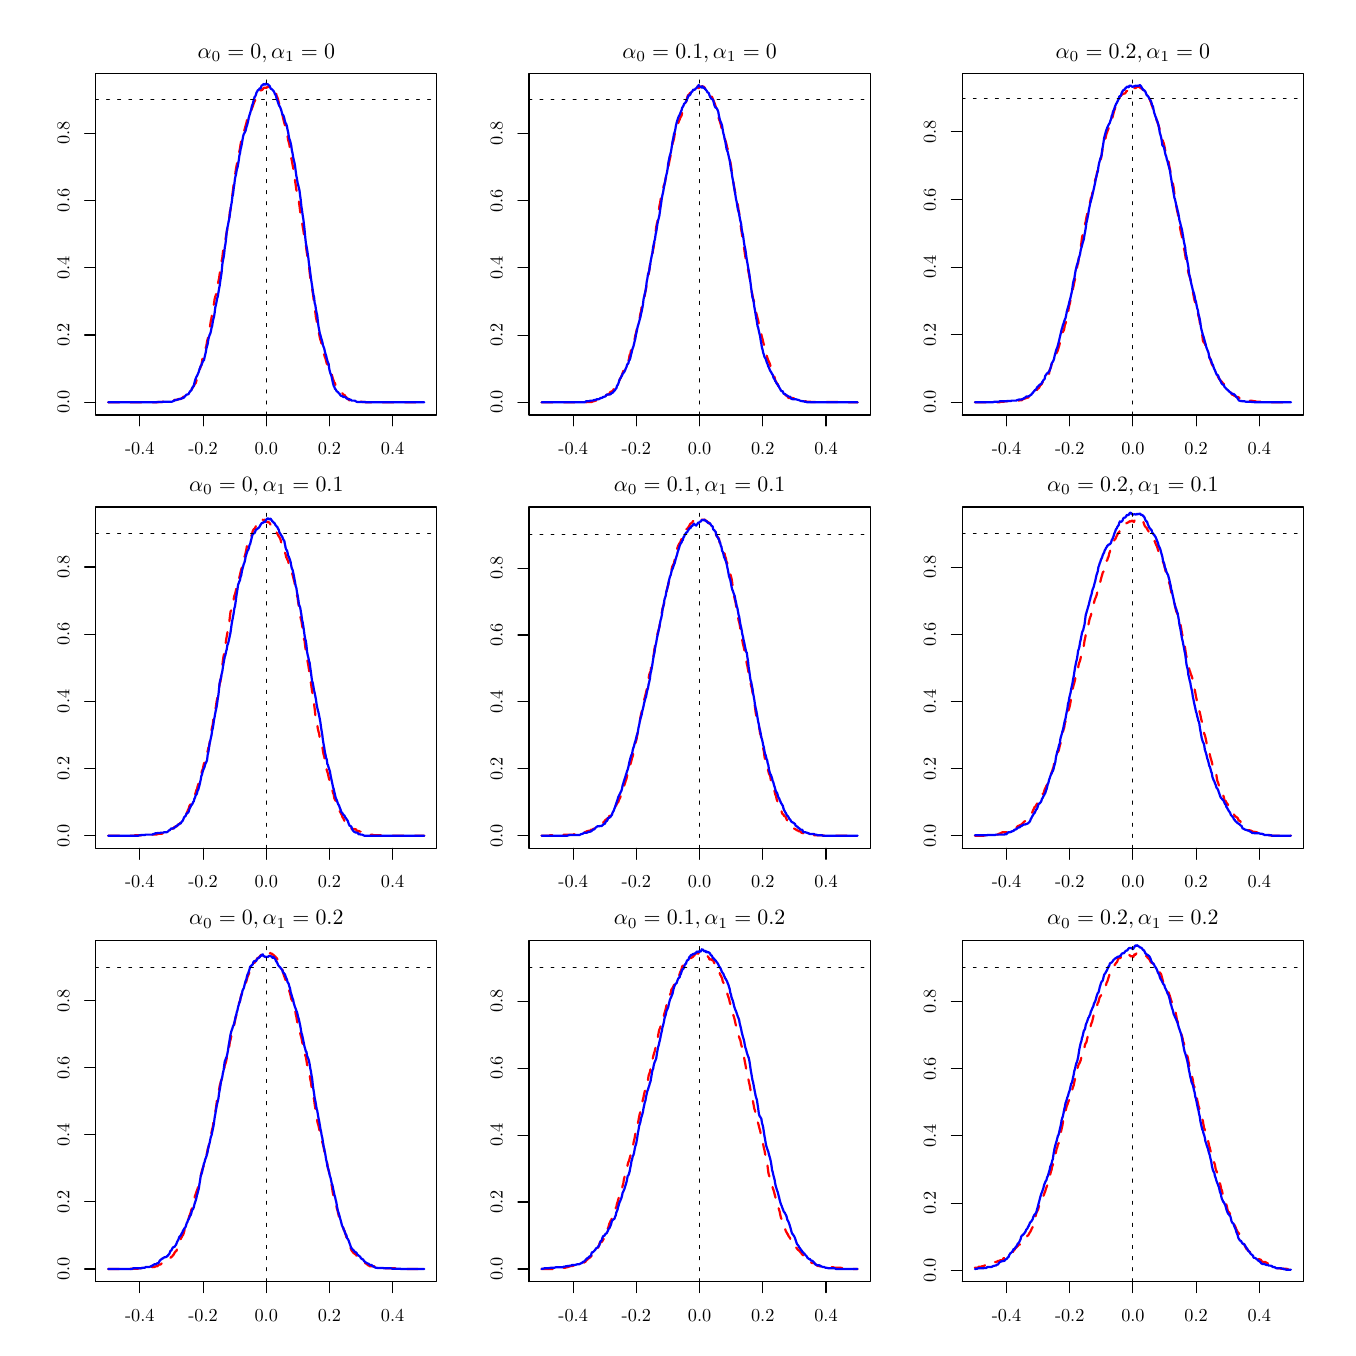
\begin{tikzpicture}[x=1pt,y=1pt]
\definecolor{fillColor}{RGB}{255,255,255}
\path[use as bounding box,fill=fillColor,fill opacity=0.00] (0,0) rectangle (469.75,469.75);
\begin{scope}
\path[clip] ( 24.55,329.80) rectangle (147.87,453.12);
\definecolor{drawColor}{RGB}{255,0,0}

\path[draw=drawColor,line width= 0.8pt,dash pattern=on 4pt off 4pt ,line join=round,line cap=round] ( 29.12,334.37) --
	( 29.35,334.37) --
	( 29.58,334.37) --
	( 29.81,334.37) --
	( 30.03,334.37) --
	( 30.26,334.37) --
	( 30.49,334.37) --
	( 30.72,334.37) --
	( 30.95,334.37) --
	( 31.18,334.37) --
	( 31.41,334.37) --
	( 31.64,334.37) --
	( 31.87,334.37) --
	( 32.09,334.37) --
	( 32.32,334.37) --
	( 32.55,334.37) --
	( 32.78,334.37) --
	( 33.01,334.37) --
	( 33.24,334.37) --
	( 33.47,334.37) --
	( 33.70,334.37) --
	( 33.92,334.37) --
	( 34.15,334.37) --
	( 34.38,334.37) --
	( 34.61,334.37) --
	( 34.84,334.37) --
	( 35.07,334.37) --
	( 35.30,334.37) --
	( 35.53,334.37) --
	( 35.76,334.37) --
	( 35.98,334.37) --
	( 36.21,334.37) --
	( 36.44,334.37) --
	( 36.67,334.37) --
	( 36.90,334.37) --
	( 37.13,334.37) --
	( 37.36,334.37) --
	( 37.59,334.37) --
	( 37.81,334.37) --
	( 38.04,334.37) --
	( 38.27,334.37) --
	( 38.50,334.37) --
	( 38.73,334.37) --
	( 38.96,334.37) --
	( 39.19,334.37) --
	( 39.42,334.37) --
	( 39.65,334.37) --
	( 39.87,334.37) --
	( 40.10,334.37) --
	( 40.33,334.37) --
	( 40.56,334.37) --
	( 40.79,334.37) --
	( 41.02,334.37) --
	( 41.25,334.37) --
	( 41.48,334.37) --
	( 41.71,334.37) --
	( 41.93,334.37) --
	( 42.16,334.37) --
	( 42.39,334.37) --
	( 42.62,334.37) --
	( 42.85,334.37) --
	( 43.08,334.37) --
	( 43.31,334.37) --
	( 43.54,334.37) --
	( 43.76,334.37) --
	( 43.99,334.37) --
	( 44.22,334.37) --
	( 44.45,334.37) --
	( 44.68,334.37) --
	( 44.91,334.37) --
	( 45.14,334.37) --
	( 45.37,334.37) --
	( 45.60,334.37) --
	( 45.82,334.37) --
	( 46.05,334.37) --
	( 46.28,334.37) --
	( 46.51,334.37) --
	( 46.74,334.37) --
	( 46.97,334.37) --
	( 47.20,334.49) --
	( 47.43,334.49) --
	( 47.65,334.49) --
	( 47.88,334.49) --
	( 48.11,334.49) --
	( 48.34,334.49) --
	( 48.57,334.49) --
	( 48.80,334.61) --
	( 49.03,334.61) --
	( 49.26,334.61) --
	( 49.49,334.61) --
	( 49.71,334.61) --
	( 49.94,334.61) --
	( 50.17,334.73) --
	( 50.40,334.73) --
	( 50.63,334.73) --
	( 50.86,334.73) --
	( 51.09,334.86) --
	( 51.32,334.86) --
	( 51.54,334.86) --
	( 51.77,334.86) --
	( 52.00,334.98) --
	( 52.23,335.22) --
	( 52.46,335.22) --
	( 52.69,335.22) --
	( 52.92,335.22) --
	( 53.15,335.22) --
	( 53.38,335.22) --
	( 53.60,335.22) --
	( 53.83,335.34) --
	( 54.06,335.34) --
	( 54.29,335.46) --
	( 54.52,335.46) --
	( 54.75,335.59) --
	( 54.98,335.59) --
	( 55.21,335.59) --
	( 55.43,335.71) --
	( 55.66,335.83) --
	( 55.89,335.95) --
	( 56.12,336.19) --
	( 56.35,336.44) --
	( 56.58,336.68) --
	( 56.81,337.04) --
	( 57.04,337.04) --
	( 57.27,337.41) --
	( 57.49,337.77) --
	( 57.72,338.14) --
	( 57.95,338.14) --
	( 58.18,338.14) --
	( 58.41,338.38) --
	( 58.64,338.75) --
	( 58.87,338.75) --
	( 59.10,338.87) --
	( 59.32,339.11) --
	( 59.55,339.60) --
	( 59.78,339.96) --
	( 60.01,340.21) --
	( 60.24,340.69) --
	( 60.47,341.06) --
	( 60.70,341.30) --
	( 60.93,342.03) --
	( 61.16,342.88) --
	( 61.38,343.25) --
	( 61.61,344.10) --
	( 61.84,345.07) --
	( 62.07,345.56) --
	( 62.30,346.65) --
	( 62.53,347.26) --
	( 62.76,347.75) --
	( 62.99,349.08) --
	( 63.22,350.54) --
	( 63.44,351.64) --
	( 63.67,352.12) --
	( 63.90,352.49) --
	( 64.13,353.10) --
	( 64.36,354.07) --
	( 64.59,354.92) --
	( 64.82,356.38) --
	( 65.05,357.23) --
	( 65.27,358.08) --
	( 65.50,359.18) --
	( 65.73,360.51) --
	( 65.96,362.34) --
	( 66.19,363.80) --
	( 66.42,364.77) --
	( 66.65,366.59) --
	( 66.88,367.81) --
	( 67.11,368.90) --
	( 67.33,370.12) --
	( 67.56,371.70) --
	( 67.79,372.55) --
	( 68.02,373.16) --
	( 68.25,374.50) --
	( 68.48,375.96) --
	( 68.71,377.17) --
	( 68.94,378.15) --
	( 69.16,379.24) --
	( 69.39,380.82) --
	( 69.62,382.16) --
	( 69.85,383.50) --
	( 70.08,385.44) --
	( 70.31,386.42) --
	( 70.54,388.48) --
	( 70.77,389.94) --
	( 71.00,391.16) --
	( 71.22,392.13) --
	( 71.45,392.98) --
	( 71.68,394.56) --
	( 71.91,395.78) --
	( 72.14,396.87) --
	( 72.37,398.58) --
	( 72.60,400.28) --
	( 72.83,400.89) --
	( 73.05,403.20) --
	( 73.28,403.81) --
	( 73.51,405.63) --
	( 73.74,407.33) --
	( 73.97,409.40) --
	( 74.20,411.22) --
	( 74.43,413.17) --
	( 74.66,414.14) --
	( 74.89,415.84) --
	( 75.11,417.67) --
	( 75.34,419.25) --
	( 75.57,420.22) --
	( 75.80,421.32) --
	( 76.03,422.78) --
	( 76.26,424.36) --
	( 76.49,424.96) --
	( 76.72,426.18) --
	( 76.94,427.64) --
	( 77.17,428.73) --
	( 77.40,429.46) --
	( 77.63,430.07) --
	( 77.86,431.17) --
	( 78.09,432.02) --
	( 78.32,432.75) --
	( 78.55,433.60) --
	( 78.78,434.45) --
	( 79.00,435.18) --
	( 79.23,436.27) --
	( 79.46,437.73) --
	( 79.69,437.98) --
	( 79.92,438.46) --
	( 80.15,438.71) --
	( 80.38,439.31) --
	( 80.61,439.80) --
	( 80.83,440.04) --
	( 81.06,440.65) --
	( 81.29,441.14) --
	( 81.52,441.87) --
	( 81.75,442.60) --
	( 81.98,443.08) --
	( 82.21,443.57) --
	( 82.44,444.06) --
	( 82.67,444.30) --
	( 82.89,445.15) --
	( 83.12,445.64) --
	( 83.35,445.88) --
	( 83.58,446.61) --
	( 83.81,446.61) --
	( 84.04,446.97) --
	( 84.27,447.10) --
	( 84.50,447.22) --
	( 84.73,447.22) --
	( 84.95,447.46) --
	( 85.18,447.83) --
	( 85.41,448.07) --
	( 85.64,448.07) --
	( 85.87,447.95) --
	( 86.10,448.07) --
	( 86.33,447.95) --
	( 86.56,448.31) --
	( 86.78,448.31) --
	( 87.01,448.31) --
	( 87.24,448.56) --
	( 87.47,448.43) --
	( 87.70,448.43) --
	( 87.93,448.31) --
	( 88.16,447.95) --
	( 88.39,447.83) --
	( 88.62,447.70) --
	( 88.84,447.34) --
	( 89.07,446.85) --
	( 89.30,446.73) --
	( 89.53,446.00) --
	( 89.76,446.00) --
	( 89.99,445.03) --
	( 90.22,444.54) --
	( 90.45,443.93) --
	( 90.67,443.08) --
	( 90.90,442.11) --
	( 91.13,441.26) --
	( 91.36,440.89) --
	( 91.59,439.92) --
	( 91.82,439.07) --
	( 92.05,438.34) --
	( 92.28,437.12) --
	( 92.51,436.15) --
	( 92.73,435.30) --
	( 92.96,434.57) --
	( 93.19,433.60) --
	( 93.42,432.63) --
	( 93.65,431.77) --
	( 93.88,430.68) --
	( 94.11,429.22) --
	( 94.34,428.37) --
	( 94.56,427.52) --
	( 94.79,425.82) --
	( 95.02,423.99) --
	( 95.25,422.65) --
	( 95.48,421.56) --
	( 95.71,420.22) --
	( 95.94,419.13) --
	( 96.17,417.18) --
	( 96.40,415.72) --
	( 96.62,414.38) --
	( 96.85,412.93) --
	( 97.08,411.22) --
	( 97.31,410.37) --
	( 97.54,409.76) --
	( 97.77,407.94) --
	( 98.00,406.85) --
	( 98.23,405.26) --
	( 98.45,403.44) --
	( 98.68,402.10) --
	( 98.91,400.64) --
	( 99.14,399.55) --
	( 99.37,397.85) --
	( 99.60,396.63) --
	( 99.83,395.05) --
	(100.06,393.96) --
	(100.29,392.98) --
	(100.51,391.28) --
	(100.74,389.33) --
	(100.97,387.88) --
	(101.20,386.42) --
	(101.43,385.44) --
	(101.66,383.50) --
	(101.89,381.31) --
	(102.12,379.36) --
	(102.35,378.03) --
	(102.57,376.44) --
	(102.80,375.23) --
	(103.03,374.01) --
	(103.26,372.19) --
	(103.49,370.00) --
	(103.72,368.78) --
	(103.95,366.84) --
	(104.18,364.89) --
	(104.40,364.04) --
	(104.63,362.46) --
	(104.86,361.61) --
	(105.09,360.51) --
	(105.32,358.93) --
	(105.55,357.84) --
	(105.78,356.87) --
	(106.01,356.38) --
	(106.24,355.16) --
	(106.46,353.95) --
	(106.69,353.34) --
	(106.92,352.12) --
	(107.15,351.52) --
	(107.38,350.79) --
	(107.61,350.18) --
	(107.84,349.33) --
	(108.07,348.35) --
	(108.29,348.11) --
	(108.52,347.50) --
	(108.75,346.53) --
	(108.98,346.29) --
	(109.21,345.68) --
	(109.44,345.44) --
	(109.67,344.71) --
	(109.90,344.34) --
	(110.13,343.49) --
	(110.35,342.76) --
	(110.58,342.15) --
	(110.81,341.42) --
	(111.04,341.30) --
	(111.27,340.45) --
	(111.50,340.21) --
	(111.73,339.72) --
	(111.96,339.60) --
	(112.18,339.36) --
	(112.41,339.11) --
	(112.64,338.99) --
	(112.87,338.75) --
	(113.10,338.50) --
	(113.33,338.38) --
	(113.56,337.90) --
	(113.79,337.53) --
	(114.02,337.17) --
	(114.24,337.04) --
	(114.47,337.04) --
	(114.70,336.68) --
	(114.93,336.44) --
	(115.16,336.19) --
	(115.39,335.83) --
	(115.62,335.71) --
	(115.85,335.71) --
	(116.07,335.22) --
	(116.30,335.10) --
	(116.53,335.10) --
	(116.76,334.98) --
	(116.99,334.98) --
	(117.22,334.86) --
	(117.45,334.86) --
	(117.68,334.86) --
	(117.91,334.73) --
	(118.13,334.73) --
	(118.36,334.61) --
	(118.59,334.61) --
	(118.82,334.61) --
	(119.05,334.61) --
	(119.28,334.61) --
	(119.51,334.61) --
	(119.74,334.61) --
	(119.96,334.61) --
	(120.19,334.61) --
	(120.42,334.61) --
	(120.65,334.61) --
	(120.88,334.49) --
	(121.11,334.49) --
	(121.34,334.49) --
	(121.57,334.49) --
	(121.80,334.49) --
	(122.02,334.49) --
	(122.25,334.37) --
	(122.48,334.37) --
	(122.71,334.37) --
	(122.94,334.37) --
	(123.17,334.37) --
	(123.40,334.37) --
	(123.63,334.37) --
	(123.86,334.37) --
	(124.08,334.37) --
	(124.31,334.37) --
	(124.54,334.37) --
	(124.77,334.37) --
	(125.00,334.37) --
	(125.23,334.37) --
	(125.46,334.37) --
	(125.69,334.37) --
	(125.91,334.37) --
	(126.14,334.37) --
	(126.37,334.37) --
	(126.60,334.37) --
	(126.83,334.37) --
	(127.06,334.37) --
	(127.29,334.37) --
	(127.52,334.37) --
	(127.75,334.37) --
	(127.97,334.37) --
	(128.20,334.37) --
	(128.43,334.37) --
	(128.66,334.37) --
	(128.89,334.37) --
	(129.12,334.37) --
	(129.35,334.37) --
	(129.58,334.37) --
	(129.80,334.37) --
	(130.03,334.37) --
	(130.26,334.37) --
	(130.49,334.37) --
	(130.72,334.37) --
	(130.95,334.37) --
	(131.18,334.37) --
	(131.41,334.37) --
	(131.64,334.37) --
	(131.86,334.37) --
	(132.09,334.37) --
	(132.32,334.37) --
	(132.55,334.37) --
	(132.78,334.37) --
	(133.01,334.37) --
	(133.24,334.37) --
	(133.47,334.37) --
	(133.69,334.37) --
	(133.92,334.37) --
	(134.15,334.37) --
	(134.38,334.37) --
	(134.61,334.37) --
	(134.84,334.37) --
	(135.07,334.37) --
	(135.30,334.37) --
	(135.53,334.37) --
	(135.75,334.37) --
	(135.98,334.37) --
	(136.21,334.37) --
	(136.44,334.37) --
	(136.67,334.37) --
	(136.90,334.37) --
	(137.13,334.37) --
	(137.36,334.37) --
	(137.58,334.37) --
	(137.81,334.37) --
	(138.04,334.37) --
	(138.27,334.37) --
	(138.50,334.37) --
	(138.73,334.37) --
	(138.96,334.37) --
	(139.19,334.37) --
	(139.42,334.37) --
	(139.64,334.37) --
	(139.87,334.37) --
	(140.10,334.37) --
	(140.33,334.37) --
	(140.56,334.37) --
	(140.79,334.37) --
	(141.02,334.37) --
	(141.25,334.37) --
	(141.47,334.37) --
	(141.70,334.37) --
	(141.93,334.37) --
	(142.16,334.37) --
	(142.39,334.37) --
	(142.62,334.37) --
	(142.85,334.37) --
	(143.08,334.37) --
	(143.31,334.37);
\end{scope}
\begin{scope}
\path[clip] (  0.00,  0.00) rectangle (469.75,469.75);
\definecolor{drawColor}{RGB}{0,0,0}

\path[draw=drawColor,line width= 0.4pt,line join=round,line cap=round] ( 40.54,329.80) -- (131.89,329.80);

\path[draw=drawColor,line width= 0.4pt,line join=round,line cap=round] ( 40.54,329.80) -- ( 40.54,325.84);

\path[draw=drawColor,line width= 0.4pt,line join=round,line cap=round] ( 63.38,329.80) -- ( 63.38,325.84);

\path[draw=drawColor,line width= 0.4pt,line join=round,line cap=round] ( 86.21,329.80) -- ( 86.21,325.84);

\path[draw=drawColor,line width= 0.4pt,line join=round,line cap=round] (109.05,329.80) -- (109.05,325.84);

\path[draw=drawColor,line width= 0.4pt,line join=round,line cap=round] (131.89,329.80) -- (131.89,325.84);

\node[text=drawColor,anchor=base,inner sep=0pt, outer sep=0pt, scale=  0.66] at ( 40.54,315.55) {-0.4};

\node[text=drawColor,anchor=base,inner sep=0pt, outer sep=0pt, scale=  0.66] at ( 63.38,315.55) {-0.2};

\node[text=drawColor,anchor=base,inner sep=0pt, outer sep=0pt, scale=  0.66] at ( 86.21,315.55) {0.0};

\node[text=drawColor,anchor=base,inner sep=0pt, outer sep=0pt, scale=  0.66] at (109.05,315.55) {0.2};

\node[text=drawColor,anchor=base,inner sep=0pt, outer sep=0pt, scale=  0.66] at (131.89,315.55) {0.4};

\path[draw=drawColor,line width= 0.4pt,line join=round,line cap=round] ( 24.55,334.37) -- ( 24.55,431.65);

\path[draw=drawColor,line width= 0.4pt,line join=round,line cap=round] ( 24.55,334.37) -- ( 20.59,334.37);

\path[draw=drawColor,line width= 0.4pt,line join=round,line cap=round] ( 24.55,358.69) -- ( 20.59,358.69);

\path[draw=drawColor,line width= 0.4pt,line join=round,line cap=round] ( 24.55,383.01) -- ( 20.59,383.01);

\path[draw=drawColor,line width= 0.4pt,line join=round,line cap=round] ( 24.55,407.33) -- ( 20.59,407.33);

\path[draw=drawColor,line width= 0.4pt,line join=round,line cap=round] ( 24.55,431.65) -- ( 20.59,431.65);

\node[text=drawColor,rotate= 90.00,anchor=base,inner sep=0pt, outer sep=0pt, scale=  0.66] at ( 15.05,334.37) {0.0};

\node[text=drawColor,rotate= 90.00,anchor=base,inner sep=0pt, outer sep=0pt, scale=  0.66] at ( 15.05,358.69) {0.2};

\node[text=drawColor,rotate= 90.00,anchor=base,inner sep=0pt, outer sep=0pt, scale=  0.66] at ( 15.05,383.01) {0.4};

\node[text=drawColor,rotate= 90.00,anchor=base,inner sep=0pt, outer sep=0pt, scale=  0.66] at ( 15.05,407.33) {0.6};

\node[text=drawColor,rotate= 90.00,anchor=base,inner sep=0pt, outer sep=0pt, scale=  0.66] at ( 15.05,431.65) {0.8};

\path[draw=drawColor,line width= 0.4pt,line join=round,line cap=round] ( 24.55,329.80) --
	(147.87,329.80) --
	(147.87,453.12) --
	( 24.55,453.12) --
	( 24.55,329.80);
\end{scope}
\begin{scope}
\path[clip] (  0.00,313.17) rectangle (156.58,469.75);
\definecolor{drawColor}{RGB}{0,0,0}

\node[text=drawColor,anchor=base,inner sep=0pt, outer sep=0pt, scale=  0.79] at ( 86.21,458.71) {\bfseries $\alpha_0 = 0, \alpha_1 = 0$};
\end{scope}
\begin{scope}
\path[clip] ( 24.55,329.80) rectangle (147.87,453.12);
\definecolor{drawColor}{RGB}{0,0,255}

\path[draw=drawColor,line width= 0.8pt,line join=round,line cap=round] ( 29.12,334.37) --
	( 29.35,334.37) --
	( 29.58,334.37) --
	( 29.81,334.37) --
	( 30.03,334.37) --
	( 30.26,334.37) --
	( 30.49,334.37) --
	( 30.72,334.37) --
	( 30.95,334.37) --
	( 31.18,334.37) --
	( 31.41,334.37) --
	( 31.64,334.37) --
	( 31.87,334.37) --
	( 32.09,334.37) --
	( 32.32,334.37) --
	( 32.55,334.37) --
	( 32.78,334.37) --
	( 33.01,334.37) --
	( 33.24,334.37) --
	( 33.47,334.37) --
	( 33.70,334.37) --
	( 33.92,334.37) --
	( 34.15,334.37) --
	( 34.38,334.37) --
	( 34.61,334.37) --
	( 34.84,334.37) --
	( 35.07,334.37) --
	( 35.30,334.37) --
	( 35.53,334.37) --
	( 35.76,334.37) --
	( 35.98,334.37) --
	( 36.21,334.37) --
	( 36.44,334.37) --
	( 36.67,334.37) --
	( 36.90,334.37) --
	( 37.13,334.37) --
	( 37.36,334.37) --
	( 37.59,334.37) --
	( 37.81,334.37) --
	( 38.04,334.37) --
	( 38.27,334.37) --
	( 38.50,334.37) --
	( 38.73,334.37) --
	( 38.96,334.37) --
	( 39.19,334.37) --
	( 39.42,334.37) --
	( 39.65,334.37) --
	( 39.87,334.37) --
	( 40.10,334.37) --
	( 40.33,334.37) --
	( 40.56,334.37) --
	( 40.79,334.37) --
	( 41.02,334.37) --
	( 41.25,334.37) --
	( 41.48,334.37) --
	( 41.71,334.37) --
	( 41.93,334.37) --
	( 42.16,334.37) --
	( 42.39,334.37) --
	( 42.62,334.37) --
	( 42.85,334.37) --
	( 43.08,334.37) --
	( 43.31,334.37) --
	( 43.54,334.37) --
	( 43.76,334.37) --
	( 43.99,334.37) --
	( 44.22,334.37) --
	( 44.45,334.37) --
	( 44.68,334.37) --
	( 44.91,334.37) --
	( 45.14,334.37) --
	( 45.37,334.37) --
	( 45.60,334.37) --
	( 45.82,334.37) --
	( 46.05,334.37) --
	( 46.28,334.37) --
	( 46.51,334.37) --
	( 46.74,334.49) --
	( 46.97,334.49) --
	( 47.20,334.49) --
	( 47.43,334.49) --
	( 47.65,334.49) --
	( 47.88,334.49) --
	( 48.11,334.49) --
	( 48.34,334.49) --
	( 48.57,334.49) --
	( 48.80,334.49) --
	( 49.03,334.61) --
	( 49.26,334.61) --
	( 49.49,334.61) --
	( 49.71,334.61) --
	( 49.94,334.61) --
	( 50.17,334.61) --
	( 50.40,334.61) --
	( 50.63,334.61) --
	( 50.86,334.61) --
	( 51.09,334.61) --
	( 51.32,334.61) --
	( 51.54,334.61) --
	( 51.77,334.61) --
	( 52.00,334.61) --
	( 52.23,334.61) --
	( 52.46,334.73) --
	( 52.69,334.86) --
	( 52.92,334.86) --
	( 53.15,335.22) --
	( 53.38,335.22) --
	( 53.60,335.22) --
	( 53.83,335.22) --
	( 54.06,335.34) --
	( 54.29,335.34) --
	( 54.52,335.46) --
	( 54.75,335.59) --
	( 54.98,335.59) --
	( 55.21,335.59) --
	( 55.43,335.71) --
	( 55.66,335.71) --
	( 55.89,335.95) --
	( 56.12,335.95) --
	( 56.35,335.95) --
	( 56.58,336.32) --
	( 56.81,336.44) --
	( 57.04,336.80) --
	( 57.27,337.04) --
	( 57.49,337.17) --
	( 57.72,337.17) --
	( 57.95,337.29) --
	( 58.18,337.41) --
	( 58.41,337.90) --
	( 58.64,338.26) --
	( 58.87,338.50) --
	( 59.10,338.63) --
	( 59.32,339.23) --
	( 59.55,339.72) --
	( 59.78,339.96) --
	( 60.01,340.33) --
	( 60.24,341.30) --
	( 60.47,342.27) --
	( 60.70,342.88) --
	( 60.93,343.49) --
	( 61.16,343.85) --
	( 61.38,344.34) --
	( 61.61,344.83) --
	( 61.84,345.44) --
	( 62.07,346.29) --
	( 62.30,346.77) --
	( 62.53,347.50) --
	( 62.76,347.75) --
	( 62.99,348.35) --
	( 63.22,348.96) --
	( 63.44,349.45) --
	( 63.67,349.45) --
	( 63.90,350.54) --
	( 64.13,351.52) --
	( 64.36,352.49) --
	( 64.59,353.83) --
	( 64.82,354.68) --
	( 65.05,355.53) --
	( 65.27,356.99) --
	( 65.50,357.96) --
	( 65.73,358.69) --
	( 65.96,359.18) --
	( 66.19,359.91) --
	( 66.42,361.24) --
	( 66.65,361.85) --
	( 66.88,363.43) --
	( 67.11,364.53) --
	( 67.33,365.26) --
	( 67.56,366.72) --
	( 67.79,368.66) --
	( 68.02,369.51) --
	( 68.25,370.73) --
	( 68.48,371.95) --
	( 68.71,372.67) --
	( 68.94,374.13) --
	( 69.16,375.47) --
	( 69.39,376.57) --
	( 69.62,378.39) --
	( 69.85,379.73) --
	( 70.08,381.31) --
	( 70.31,383.98) --
	( 70.54,385.56) --
	( 70.77,386.54) --
	( 71.00,388.00) --
	( 71.22,390.31) --
	( 71.45,391.52) --
	( 71.68,393.35) --
	( 71.91,395.90) --
	( 72.14,397.36) --
	( 72.37,398.33) --
	( 72.60,399.67) --
	( 72.83,400.64) --
	( 73.05,402.10) --
	( 73.28,404.05) --
	( 73.51,405.39) --
	( 73.74,406.72) --
	( 73.97,408.67) --
	( 74.20,409.52) --
	( 74.43,411.59) --
	( 74.66,413.05) --
	( 74.89,414.99) --
	( 75.11,416.09) --
	( 75.34,417.06) --
	( 75.57,418.52) --
	( 75.80,419.13) --
	( 76.03,420.34) --
	( 76.26,421.68) --
	( 76.49,423.51) --
	( 76.72,424.36) --
	( 76.94,425.82) --
	( 77.17,426.67) --
	( 77.40,427.88) --
	( 77.63,429.22) --
	( 77.86,430.56) --
	( 78.09,431.29) --
	( 78.32,431.65) --
	( 78.55,432.14) --
	( 78.78,432.63) --
	( 79.00,433.72) --
	( 79.23,434.33) --
	( 79.46,435.18) --
	( 79.69,436.15) --
	( 79.92,437.37) --
	( 80.15,438.10) --
	( 80.38,438.83) --
	( 80.61,439.68) --
	( 80.83,440.41) --
	( 81.06,441.62) --
	( 81.29,441.99) --
	( 81.52,442.96) --
	( 81.75,443.93) --
	( 81.98,444.66) --
	( 82.21,444.91) --
	( 82.44,445.39) --
	( 82.67,446.25) --
	( 82.89,446.61) --
	( 83.12,447.10) --
	( 83.35,447.22) --
	( 83.58,447.34) --
	( 83.81,447.83) --
	( 84.04,447.70) --
	( 84.27,447.95) --
	( 84.50,448.80) --
	( 84.73,448.92) --
	( 84.95,449.04) --
	( 85.18,449.29) --
	( 85.41,449.41) --
	( 85.64,449.16) --
	( 85.87,449.16) --
	( 86.10,449.53) --
	( 86.33,449.29) --
	( 86.56,449.29) --
	( 86.78,449.29) --
	( 87.01,449.04) --
	( 87.24,448.80) --
	( 87.47,448.68) --
	( 87.70,447.95) --
	( 87.93,447.58) --
	( 88.16,447.58) --
	( 88.39,447.34) --
	( 88.62,447.10) --
	( 88.84,446.85) --
	( 89.07,446.49) --
	( 89.30,445.88) --
	( 89.53,445.52) --
	( 89.76,445.03) --
	( 89.99,443.93) --
	( 90.22,443.45) --
	( 90.45,442.72) --
	( 90.67,442.11) --
	( 90.90,441.50) --
	( 91.13,441.26) --
	( 91.36,440.65) --
	( 91.59,440.04) --
	( 91.82,439.19) --
	( 92.05,438.34) --
	( 92.28,438.22) --
	( 92.51,437.73) --
	( 92.73,437.00) --
	( 92.96,435.91) --
	( 93.19,435.30) --
	( 93.42,434.94) --
	( 93.65,434.21) --
	( 93.88,432.99) --
	( 94.11,432.02) --
	( 94.34,430.56) --
	( 94.56,429.46) --
	( 94.79,428.98) --
	( 95.02,428.13) --
	( 95.25,427.03) --
	( 95.48,425.33) --
	( 95.71,424.36) --
	( 95.94,422.90) --
	( 96.17,421.80) --
	( 96.40,420.95) --
	( 96.62,419.74) --
	( 96.85,417.91) --
	( 97.08,416.21) --
	( 97.31,415.11) --
	( 97.54,413.66) --
	( 97.77,412.80) --
	( 98.00,411.83) --
	( 98.23,410.86) --
	( 98.45,409.03) --
	( 98.68,407.45) --
	( 98.91,405.14) --
	( 99.14,403.68) --
	( 99.37,401.98) --
	( 99.60,400.64) --
	( 99.83,398.70) --
	(100.06,396.63) --
	(100.29,394.08) --
	(100.51,392.01) --
	(100.74,390.79) --
	(100.97,389.58) --
	(101.20,388.00) --
	(101.43,386.42) --
	(101.66,384.35) --
	(101.89,383.01) --
	(102.12,381.19) --
	(102.35,379.36) --
	(102.57,377.78) --
	(102.80,376.32) --
	(103.03,374.74) --
	(103.26,373.16) --
	(103.49,372.43) --
	(103.72,370.12) --
	(103.95,369.51) --
	(104.18,367.81) --
	(104.40,366.72) --
	(104.63,365.74) --
	(104.86,363.55) --
	(105.09,361.73) --
	(105.32,360.64) --
	(105.55,359.30) --
	(105.78,358.69) --
	(106.01,357.72) --
	(106.24,356.99) --
	(106.46,356.26) --
	(106.69,355.04) --
	(106.92,354.43) --
	(107.15,353.83) --
	(107.38,352.73) --
	(107.61,351.88) --
	(107.84,351.27) --
	(108.07,350.18) --
	(108.29,349.45) --
	(108.52,348.72) --
	(108.75,348.23) --
	(108.98,346.41) --
	(109.21,345.44) --
	(109.44,344.71) --
	(109.67,344.22) --
	(109.90,343.25) --
	(110.13,342.15) --
	(110.35,341.18) --
	(110.58,340.33) --
	(110.81,339.96) --
	(111.04,339.23) --
	(111.27,339.11) --
	(111.50,338.63) --
	(111.73,338.38) --
	(111.96,338.14) --
	(112.18,338.02) --
	(112.41,337.65) --
	(112.64,337.53) --
	(112.87,337.17) --
	(113.10,336.80) --
	(113.33,336.68) --
	(113.56,336.68) --
	(113.79,336.56) --
	(114.02,336.32) --
	(114.24,336.32) --
	(114.47,336.32) --
	(114.70,336.32) --
	(114.93,336.19) --
	(115.16,335.83) --
	(115.39,335.71) --
	(115.62,335.59) --
	(115.85,335.46) --
	(116.07,335.46) --
	(116.30,335.46) --
	(116.53,335.34) --
	(116.76,335.34) --
	(116.99,334.98) --
	(117.22,334.98) --
	(117.45,334.98) --
	(117.68,334.98) --
	(117.91,334.98) --
	(118.13,334.98) --
	(118.36,334.86) --
	(118.59,334.73) --
	(118.82,334.61) --
	(119.05,334.49) --
	(119.28,334.49) --
	(119.51,334.49) --
	(119.74,334.49) --
	(119.96,334.49) --
	(120.19,334.49) --
	(120.42,334.49) --
	(120.65,334.49) --
	(120.88,334.49) --
	(121.11,334.49) --
	(121.34,334.49) --
	(121.57,334.49) --
	(121.80,334.49) --
	(122.02,334.37) --
	(122.25,334.37) --
	(122.48,334.37) --
	(122.71,334.37) --
	(122.94,334.37) --
	(123.17,334.37) --
	(123.40,334.37) --
	(123.63,334.37) --
	(123.86,334.37) --
	(124.08,334.37) --
	(124.31,334.37) --
	(124.54,334.37) --
	(124.77,334.37) --
	(125.00,334.37) --
	(125.23,334.37) --
	(125.46,334.37) --
	(125.69,334.37) --
	(125.91,334.37) --
	(126.14,334.37) --
	(126.37,334.37) --
	(126.60,334.37) --
	(126.83,334.37) --
	(127.06,334.37) --
	(127.29,334.37) --
	(127.52,334.37) --
	(127.75,334.37) --
	(127.97,334.37) --
	(128.20,334.37) --
	(128.43,334.37) --
	(128.66,334.37) --
	(128.89,334.37) --
	(129.12,334.37) --
	(129.35,334.37) --
	(129.58,334.37) --
	(129.80,334.37) --
	(130.03,334.37) --
	(130.26,334.37) --
	(130.49,334.37) --
	(130.72,334.37) --
	(130.95,334.37) --
	(131.18,334.37) --
	(131.41,334.37) --
	(131.64,334.37) --
	(131.86,334.37) --
	(132.09,334.37) --
	(132.32,334.37) --
	(132.55,334.37) --
	(132.78,334.37) --
	(133.01,334.37) --
	(133.24,334.37) --
	(133.47,334.37) --
	(133.69,334.37) --
	(133.92,334.37) --
	(134.15,334.37) --
	(134.38,334.37) --
	(134.61,334.37) --
	(134.84,334.37) --
	(135.07,334.37) --
	(135.30,334.37) --
	(135.53,334.37) --
	(135.75,334.37) --
	(135.98,334.37) --
	(136.21,334.37) --
	(136.44,334.37) --
	(136.67,334.37) --
	(136.90,334.37) --
	(137.13,334.37) --
	(137.36,334.37) --
	(137.58,334.37) --
	(137.81,334.37) --
	(138.04,334.37) --
	(138.27,334.37) --
	(138.50,334.37) --
	(138.73,334.37) --
	(138.96,334.37) --
	(139.19,334.37) --
	(139.42,334.37) --
	(139.64,334.37) --
	(139.87,334.37) --
	(140.10,334.37) --
	(140.33,334.37) --
	(140.56,334.37) --
	(140.79,334.37) --
	(141.02,334.37) --
	(141.25,334.37) --
	(141.47,334.37) --
	(141.70,334.37) --
	(141.93,334.37) --
	(142.16,334.37) --
	(142.39,334.37) --
	(142.62,334.37) --
	(142.85,334.37) --
	(143.08,334.37) --
	(143.31,334.37);
\definecolor{drawColor}{RGB}{0,0,0}

\path[draw=drawColor,line width= 0.4pt,dash pattern=on 1pt off 3pt ,line join=round,line cap=round] ( 24.55,443.81) -- (147.87,443.81);

\path[draw=drawColor,line width= 0.4pt,dash pattern=on 1pt off 3pt ,line join=round,line cap=round] ( 86.21,329.80) -- ( 86.21,453.12);

\path[draw=drawColor,line width= 0.4pt,dash pattern=on 1pt off 3pt ,line join=round,line cap=round] ( 86.21,329.80) -- ( 86.21,453.12);
\end{scope}
\begin{scope}
\path[clip] (181.14,329.80) rectangle (304.46,453.12);
\definecolor{drawColor}{RGB}{255,0,0}

\path[draw=drawColor,line width= 0.8pt,dash pattern=on 4pt off 4pt ,line join=round,line cap=round] (185.70,334.37) --
	(185.93,334.37) --
	(186.16,334.37) --
	(186.39,334.37) --
	(186.62,334.37) --
	(186.85,334.37) --
	(187.08,334.37) --
	(187.31,334.37) --
	(187.54,334.37) --
	(187.76,334.37) --
	(187.99,334.37) --
	(188.22,334.37) --
	(188.45,334.37) --
	(188.68,334.37) --
	(188.91,334.37) --
	(189.14,334.37) --
	(189.37,334.37) --
	(189.59,334.37) --
	(189.82,334.37) --
	(190.05,334.37) --
	(190.28,334.37) --
	(190.51,334.37) --
	(190.74,334.37) --
	(190.97,334.37) --
	(191.20,334.37) --
	(191.43,334.37) --
	(191.65,334.37) --
	(191.88,334.37) --
	(192.11,334.37) --
	(192.34,334.37) --
	(192.57,334.37) --
	(192.80,334.37) --
	(193.03,334.37) --
	(193.26,334.37) --
	(193.48,334.37) --
	(193.71,334.37) --
	(193.94,334.37) --
	(194.17,334.37) --
	(194.40,334.37) --
	(194.63,334.37) --
	(194.86,334.37) --
	(195.09,334.37) --
	(195.32,334.37) --
	(195.54,334.37) --
	(195.77,334.37) --
	(196.00,334.37) --
	(196.23,334.37) --
	(196.46,334.37) --
	(196.69,334.37) --
	(196.92,334.37) --
	(197.15,334.37) --
	(197.37,334.37) --
	(197.60,334.37) --
	(197.83,334.37) --
	(198.06,334.37) --
	(198.29,334.37) --
	(198.52,334.37) --
	(198.75,334.37) --
	(198.98,334.37) --
	(199.21,334.37) --
	(199.43,334.37) --
	(199.66,334.37) --
	(199.89,334.37) --
	(200.12,334.37) --
	(200.35,334.37) --
	(200.58,334.37) --
	(200.81,334.37) --
	(201.04,334.37) --
	(201.26,334.37) --
	(201.49,334.37) --
	(201.72,334.37) --
	(201.95,334.49) --
	(202.18,334.49) --
	(202.41,334.49) --
	(202.64,334.49) --
	(202.87,334.49) --
	(203.10,334.49) --
	(203.32,334.49) --
	(203.55,334.49) --
	(203.78,334.49) --
	(204.01,334.61) --
	(204.24,334.73) --
	(204.47,334.73) --
	(204.70,334.86) --
	(204.93,334.86) --
	(205.15,334.98) --
	(205.38,334.98) --
	(205.61,334.98) --
	(205.84,335.10) --
	(206.07,335.46) --
	(206.30,335.46) --
	(206.53,335.46) --
	(206.76,335.46) --
	(206.99,335.58) --
	(207.21,335.71) --
	(207.44,335.71) --
	(207.67,335.83) --
	(207.90,335.83) --
	(208.13,336.07) --
	(208.36,336.43) --
	(208.59,336.56) --
	(208.82,336.68) --
	(209.05,336.92) --
	(209.27,337.04) --
	(209.50,337.16) --
	(209.73,337.16) --
	(209.96,337.28) --
	(210.19,337.53) --
	(210.42,337.89) --
	(210.65,338.14) --
	(210.88,338.26) --
	(211.10,338.26) --
	(211.33,338.50) --
	(211.56,338.74) --
	(211.79,339.23) --
	(212.02,339.35) --
	(212.25,339.84) --
	(212.48,339.96) --
	(212.71,340.44) --
	(212.94,340.44) --
	(213.16,340.56) --
	(213.39,341.29) --
	(213.62,341.78) --
	(213.85,342.27) --
	(214.08,342.99) --
	(214.31,343.24) --
	(214.54,343.84) --
	(214.77,344.33) --
	(214.99,344.94) --
	(215.22,345.67) --
	(215.45,345.79) --
	(215.68,346.27) --
	(215.91,346.76) --
	(216.14,347.00) --
	(216.37,347.37) --
	(216.60,347.97) --
	(216.83,348.70) --
	(217.05,349.19) --
	(217.28,350.16) --
	(217.51,351.50) --
	(217.74,351.74) --
	(217.97,352.96) --
	(218.20,353.44) --
	(218.43,354.17) --
	(218.66,354.90) --
	(218.88,355.75) --
	(219.11,356.48) --
	(219.34,357.33) --
	(219.57,358.54) --
	(219.80,359.39) --
	(220.03,360.37) --
	(220.26,361.22) --
	(220.49,362.43) --
	(220.72,362.67) --
	(220.94,364.25) --
	(221.17,364.98) --
	(221.40,366.44) --
	(221.63,367.17) --
	(221.86,368.87) --
	(222.09,369.48) --
	(222.32,370.33) --
	(222.55,371.18) --
	(222.77,371.91) --
	(223.00,373.12) --
	(223.23,374.46) --
	(223.46,375.55) --
	(223.69,377.37) --
	(223.92,378.22) --
	(224.15,379.56) --
	(224.38,380.65) --
	(224.61,382.11) --
	(224.83,383.93) --
	(225.06,384.54) --
	(225.29,386.12) --
	(225.52,387.09) --
	(225.75,387.94) --
	(225.98,389.40) --
	(226.21,390.49) --
	(226.44,392.31) --
	(226.66,394.26) --
	(226.89,395.84) --
	(227.12,397.78) --
	(227.35,398.87) --
	(227.58,399.72) --
	(227.81,401.54) --
	(228.04,403.25) --
	(228.27,405.31) --
	(228.50,406.28) --
	(228.72,407.62) --
	(228.95,408.83) --
	(229.18,409.93) --
	(229.41,410.66) --
	(229.64,411.75) --
	(229.87,412.72) --
	(230.10,413.21) --
	(230.33,414.06) --
	(230.56,415.39) --
	(230.78,416.36) --
	(231.01,417.46) --
	(231.24,418.43) --
	(231.47,419.40) --
	(231.70,420.49) --
	(231.93,421.71) --
	(232.16,422.80) --
	(232.39,423.77) --
	(232.61,424.99) --
	(232.84,426.57) --
	(233.07,428.03) --
	(233.30,428.76) --
	(233.53,429.48) --
	(233.76,430.94) --
	(233.99,431.91) --
	(234.22,432.76) --
	(234.45,433.37) --
	(234.67,433.74) --
	(234.90,434.10) --
	(235.13,435.44) --
	(235.36,436.04) --
	(235.59,436.53) --
	(235.82,437.14) --
	(236.05,437.62) --
	(236.28,437.99) --
	(236.50,439.08) --
	(236.73,439.81) --
	(236.96,440.54) --
	(237.19,441.27) --
	(237.42,441.63) --
	(237.65,442.36) --
	(237.88,442.85) --
	(238.11,443.58) --
	(238.34,444.55) --
	(238.56,445.28) --
	(238.79,445.40) --
	(239.02,445.64) --
	(239.25,446.00) --
	(239.48,446.37) --
	(239.71,447.58) --
	(239.94,447.71) --
	(240.17,447.95) --
	(240.39,448.19) --
	(240.62,448.31) --
	(240.85,448.43) --
	(241.08,448.31) --
	(241.31,448.31) --
	(241.54,448.31) --
	(241.77,448.43) --
	(242.00,448.56) --
	(242.23,447.95) --
	(242.45,447.95) --
	(242.68,448.07) --
	(242.91,448.19) --
	(243.14,448.43) --
	(243.37,448.31) --
	(243.60,448.56) --
	(243.83,448.56) --
	(244.06,448.43) --
	(244.28,448.43) --
	(244.51,448.19) --
	(244.74,447.83) --
	(244.97,447.58) --
	(245.20,447.58) --
	(245.43,447.46) --
	(245.66,447.22) --
	(245.89,446.73) --
	(246.12,446.37) --
	(246.34,446.25) --
	(246.57,445.76) --
	(246.80,445.76) --
	(247.03,445.40) --
	(247.26,444.79) --
	(247.49,444.18) --
	(247.72,443.70) --
	(247.95,443.09) --
	(248.18,442.60) --
	(248.40,441.87) --
	(248.63,441.27) --
	(248.86,440.66) --
	(249.09,440.17) --
	(249.32,438.96) --
	(249.55,437.74) --
	(249.78,436.77) --
	(250.01,436.17) --
	(250.23,435.44) --
	(250.46,434.71) --
	(250.69,433.61) --
	(250.92,432.76) --
	(251.15,431.91) --
	(251.38,431.31) --
	(251.61,430.33) --
	(251.84,429.97) --
	(252.07,429.12) --
	(252.29,428.39) --
	(252.52,427.54) --
	(252.75,426.45) --
	(252.98,425.84) --
	(253.21,424.75) --
	(253.44,423.90) --
	(253.67,421.95) --
	(253.90,421.22) --
	(254.12,420.01) --
	(254.35,418.43) --
	(254.58,416.36) --
	(254.81,415.76) --
	(255.04,413.69) --
	(255.27,412.23) --
	(255.50,411.14) --
	(255.73,409.68) --
	(255.96,408.95) --
	(256.18,407.62) --
	(256.41,406.40) --
	(256.64,405.55) --
	(256.87,403.97) --
	(257.10,402.76) --
	(257.33,401.30) --
	(257.56,399.12) --
	(257.79,397.05) --
	(258.01,395.84) --
	(258.24,394.01) --
	(258.47,392.56) --
	(258.70,391.46) --
	(258.93,389.64) --
	(259.16,388.06) --
	(259.39,386.60) --
	(259.62,385.63) --
	(259.85,384.66) --
	(260.07,383.57) --
	(260.30,382.23) --
	(260.53,381.14) --
	(260.76,379.92) --
	(260.99,378.83) --
	(261.22,377.49) --
	(261.45,375.91) --
	(261.68,374.09) --
	(261.90,373.12) --
	(262.13,371.78) --
	(262.36,371.18) --
	(262.59,369.96) --
	(262.82,368.63) --
	(263.05,367.53) --
	(263.28,366.56) --
	(263.51,365.71) --
	(263.74,364.74) --
	(263.96,364.01) --
	(264.19,362.79) --
	(264.42,361.70) --
	(264.65,360.85) --
	(264.88,359.76) --
	(265.11,358.91) --
	(265.34,357.94) --
	(265.57,357.09) --
	(265.79,356.11) --
	(266.02,355.26) --
	(266.25,354.29) --
	(266.48,353.44) --
	(266.71,352.59) --
	(266.94,351.74) --
	(267.17,350.77) --
	(267.40,350.16) --
	(267.63,349.43) --
	(267.85,349.07) --
	(268.08,348.58) --
	(268.31,347.85) --
	(268.54,347.00) --
	(268.77,346.64) --
	(269.00,345.91) --
	(269.23,345.55) --
	(269.46,344.69) --
	(269.69,343.84) --
	(269.91,343.36) --
	(270.14,342.27) --
	(270.37,341.90) --
	(270.60,341.41) --
	(270.83,341.05) --
	(271.06,340.93) --
	(271.29,339.96) --
	(271.52,339.59) --
	(271.74,339.47) --
	(271.97,339.23) --
	(272.20,338.99) --
	(272.43,338.86) --
	(272.66,338.74) --
	(272.89,338.26) --
	(273.12,337.89) --
	(273.35,337.77) --
	(273.58,337.53) --
	(273.80,337.04) --
	(274.03,336.80) --
	(274.26,336.80) --
	(274.49,336.68) --
	(274.72,336.19) --
	(274.95,335.95) --
	(275.18,335.95) --
	(275.41,335.95) --
	(275.63,335.95) --
	(275.86,335.95) --
	(276.09,335.95) --
	(276.32,335.95) --
	(276.55,335.83) --
	(276.78,335.83) --
	(277.01,335.71) --
	(277.24,335.71) --
	(277.47,335.46) --
	(277.69,335.34) --
	(277.92,335.34) --
	(278.15,335.34) --
	(278.38,335.22) --
	(278.61,335.22) --
	(278.84,335.22) --
	(279.07,335.22) --
	(279.30,335.22) --
	(279.52,335.10) --
	(279.75,334.98) --
	(279.98,334.86) --
	(280.21,334.86) --
	(280.44,334.73) --
	(280.67,334.73) --
	(280.90,334.73) --
	(281.13,334.73) --
	(281.36,334.61) --
	(281.58,334.61) --
	(281.81,334.61) --
	(282.04,334.61) --
	(282.27,334.61) --
	(282.50,334.61) --
	(282.73,334.61) --
	(282.96,334.49) --
	(283.19,334.49) --
	(283.41,334.49) --
	(283.64,334.49) --
	(283.87,334.49) --
	(284.10,334.49) --
	(284.33,334.49) --
	(284.56,334.49) --
	(284.79,334.49) --
	(285.02,334.49) --
	(285.25,334.49) --
	(285.47,334.49) --
	(285.70,334.49) --
	(285.93,334.49) --
	(286.16,334.49) --
	(286.39,334.49) --
	(286.62,334.49) --
	(286.85,334.49) --
	(287.08,334.49) --
	(287.30,334.49) --
	(287.53,334.49) --
	(287.76,334.49) --
	(287.99,334.49) --
	(288.22,334.49) --
	(288.45,334.49) --
	(288.68,334.49) --
	(288.91,334.49) --
	(289.14,334.49) --
	(289.36,334.49) --
	(289.59,334.49) --
	(289.82,334.49) --
	(290.05,334.49) --
	(290.28,334.49) --
	(290.51,334.49) --
	(290.74,334.49) --
	(290.97,334.49) --
	(291.20,334.49) --
	(291.42,334.49) --
	(291.65,334.49) --
	(291.88,334.49) --
	(292.11,334.49) --
	(292.34,334.49) --
	(292.57,334.49) --
	(292.80,334.49) --
	(293.03,334.37) --
	(293.25,334.37) --
	(293.48,334.37) --
	(293.71,334.37) --
	(293.94,334.37) --
	(294.17,334.37) --
	(294.40,334.37) --
	(294.63,334.37) --
	(294.86,334.37) --
	(295.09,334.37) --
	(295.31,334.37) --
	(295.54,334.37) --
	(295.77,334.37) --
	(296.00,334.37) --
	(296.23,334.37) --
	(296.46,334.37) --
	(296.69,334.37) --
	(296.92,334.37) --
	(297.14,334.37) --
	(297.37,334.37) --
	(297.60,334.37) --
	(297.83,334.37) --
	(298.06,334.37) --
	(298.29,334.37) --
	(298.52,334.37) --
	(298.75,334.37) --
	(298.98,334.37) --
	(299.20,334.37) --
	(299.43,334.37) --
	(299.66,334.37) --
	(299.89,334.37);
\end{scope}
\begin{scope}
\path[clip] (  0.00,  0.00) rectangle (469.75,469.75);
\definecolor{drawColor}{RGB}{0,0,0}

\path[draw=drawColor,line width= 0.4pt,line join=round,line cap=round] (197.12,329.80) -- (288.47,329.80);

\path[draw=drawColor,line width= 0.4pt,line join=round,line cap=round] (197.12,329.80) -- (197.12,325.84);

\path[draw=drawColor,line width= 0.4pt,line join=round,line cap=round] (219.96,329.80) -- (219.96,325.84);

\path[draw=drawColor,line width= 0.4pt,line join=round,line cap=round] (242.80,329.80) -- (242.80,325.84);

\path[draw=drawColor,line width= 0.4pt,line join=round,line cap=round] (265.63,329.80) -- (265.63,325.84);

\path[draw=drawColor,line width= 0.4pt,line join=round,line cap=round] (288.47,329.80) -- (288.47,325.84);

\node[text=drawColor,anchor=base,inner sep=0pt, outer sep=0pt, scale=  0.66] at (197.12,315.55) {-0.4};

\node[text=drawColor,anchor=base,inner sep=0pt, outer sep=0pt, scale=  0.66] at (219.96,315.55) {-0.2};

\node[text=drawColor,anchor=base,inner sep=0pt, outer sep=0pt, scale=  0.66] at (242.80,315.55) {0.0};

\node[text=drawColor,anchor=base,inner sep=0pt, outer sep=0pt, scale=  0.66] at (265.63,315.55) {0.2};

\node[text=drawColor,anchor=base,inner sep=0pt, outer sep=0pt, scale=  0.66] at (288.47,315.55) {0.4};

\path[draw=drawColor,line width= 0.4pt,line join=round,line cap=round] (181.14,334.37) -- (181.14,431.55);

\path[draw=drawColor,line width= 0.4pt,line join=round,line cap=round] (181.14,334.37) -- (177.18,334.37);

\path[draw=drawColor,line width= 0.4pt,line join=round,line cap=round] (181.14,358.66) -- (177.18,358.66);

\path[draw=drawColor,line width= 0.4pt,line join=round,line cap=round] (181.14,382.96) -- (177.18,382.96);

\path[draw=drawColor,line width= 0.4pt,line join=round,line cap=round] (181.14,407.25) -- (177.18,407.25);

\path[draw=drawColor,line width= 0.4pt,line join=round,line cap=round] (181.14,431.55) -- (177.18,431.55);

\node[text=drawColor,rotate= 90.00,anchor=base,inner sep=0pt, outer sep=0pt, scale=  0.66] at (171.63,334.37) {0.0};

\node[text=drawColor,rotate= 90.00,anchor=base,inner sep=0pt, outer sep=0pt, scale=  0.66] at (171.63,358.66) {0.2};

\node[text=drawColor,rotate= 90.00,anchor=base,inner sep=0pt, outer sep=0pt, scale=  0.66] at (171.63,382.96) {0.4};

\node[text=drawColor,rotate= 90.00,anchor=base,inner sep=0pt, outer sep=0pt, scale=  0.66] at (171.63,407.25) {0.6};

\node[text=drawColor,rotate= 90.00,anchor=base,inner sep=0pt, outer sep=0pt, scale=  0.66] at (171.63,431.55) {0.8};

\path[draw=drawColor,line width= 0.4pt,line join=round,line cap=round] (181.14,329.80) --
	(304.46,329.80) --
	(304.46,453.12) --
	(181.14,453.12) --
	(181.14,329.80);
\end{scope}
\begin{scope}
\path[clip] (156.58,313.17) rectangle (313.17,469.75);
\definecolor{drawColor}{RGB}{0,0,0}

\node[text=drawColor,anchor=base,inner sep=0pt, outer sep=0pt, scale=  0.79] at (242.80,458.71) {\bfseries $\alpha_0 = 0.1, \alpha_1 = 0$};
\end{scope}
\begin{scope}
\path[clip] (181.14,329.80) rectangle (304.46,453.12);
\definecolor{drawColor}{RGB}{0,0,255}

\path[draw=drawColor,line width= 0.8pt,line join=round,line cap=round] (185.70,334.37) --
	(185.93,334.37) --
	(186.16,334.37) --
	(186.39,334.37) --
	(186.62,334.37) --
	(186.85,334.37) --
	(187.08,334.37) --
	(187.31,334.37) --
	(187.54,334.37) --
	(187.76,334.37) --
	(187.99,334.37) --
	(188.22,334.37) --
	(188.45,334.37) --
	(188.68,334.37) --
	(188.91,334.37) --
	(189.14,334.37) --
	(189.37,334.37) --
	(189.59,334.37) --
	(189.82,334.37) --
	(190.05,334.37) --
	(190.28,334.37) --
	(190.51,334.37) --
	(190.74,334.37) --
	(190.97,334.37) --
	(191.20,334.37) --
	(191.43,334.37) --
	(191.65,334.37) --
	(191.88,334.37) --
	(192.11,334.37) --
	(192.34,334.37) --
	(192.57,334.37) --
	(192.80,334.37) --
	(193.03,334.37) --
	(193.26,334.37) --
	(193.48,334.37) --
	(193.71,334.37) --
	(193.94,334.37) --
	(194.17,334.37) --
	(194.40,334.37) --
	(194.63,334.37) --
	(194.86,334.37) --
	(195.09,334.37) --
	(195.32,334.37) --
	(195.54,334.37) --
	(195.77,334.37) --
	(196.00,334.37) --
	(196.23,334.37) --
	(196.46,334.37) --
	(196.69,334.37) --
	(196.92,334.37) --
	(197.15,334.37) --
	(197.37,334.37) --
	(197.60,334.37) --
	(197.83,334.37) --
	(198.06,334.37) --
	(198.29,334.37) --
	(198.52,334.37) --
	(198.75,334.37) --
	(198.98,334.37) --
	(199.21,334.37) --
	(199.43,334.37) --
	(199.66,334.37) --
	(199.89,334.37) --
	(200.12,334.37) --
	(200.35,334.37) --
	(200.58,334.37) --
	(200.81,334.37) --
	(201.04,334.37) --
	(201.26,334.37) --
	(201.49,334.49) --
	(201.72,334.73) --
	(201.95,334.73) --
	(202.18,334.73) --
	(202.41,334.73) --
	(202.64,334.73) --
	(202.87,334.73) --
	(203.10,334.86) --
	(203.32,334.98) --
	(203.55,334.98) --
	(203.78,334.98) --
	(204.01,334.98) --
	(204.24,334.98) --
	(204.47,335.10) --
	(204.70,335.22) --
	(204.93,335.22) --
	(205.15,335.22) --
	(205.38,335.34) --
	(205.61,335.46) --
	(205.84,335.46) --
	(206.07,335.46) --
	(206.30,335.46) --
	(206.53,335.58) --
	(206.76,335.71) --
	(206.99,335.95) --
	(207.21,335.95) --
	(207.44,335.95) --
	(207.67,336.07) --
	(207.90,336.31) --
	(208.13,336.31) --
	(208.36,336.43) --
	(208.59,336.43) --
	(208.82,336.56) --
	(209.05,336.92) --
	(209.27,337.16) --
	(209.50,337.16) --
	(209.73,337.16) --
	(209.96,337.16) --
	(210.19,337.16) --
	(210.42,337.28) --
	(210.65,337.28) --
	(210.88,337.65) --
	(211.10,337.77) --
	(211.33,337.77) --
	(211.56,338.01) --
	(211.79,338.38) --
	(212.02,338.62) --
	(212.25,338.74) --
	(212.48,339.35) --
	(212.71,339.35) --
	(212.94,340.32) --
	(213.16,340.56) --
	(213.39,341.05) --
	(213.62,341.66) --
	(213.85,342.51) --
	(214.08,342.87) --
	(214.31,343.24) --
	(214.54,343.72) --
	(214.77,344.09) --
	(214.99,344.69) --
	(215.22,344.94) --
	(215.45,345.18) --
	(215.68,345.55) --
	(215.91,346.03) --
	(216.14,346.64) --
	(216.37,347.12) --
	(216.60,347.97) --
	(216.83,348.22) --
	(217.05,348.46) --
	(217.28,349.43) --
	(217.51,349.68) --
	(217.74,350.28) --
	(217.97,351.38) --
	(218.20,352.23) --
	(218.43,353.20) --
	(218.66,354.05) --
	(218.88,354.53) --
	(219.11,355.51) --
	(219.34,356.48) --
	(219.57,357.33) --
	(219.80,358.79) --
	(220.03,359.76) --
	(220.26,360.97) --
	(220.49,361.94) --
	(220.72,362.67) --
	(220.94,363.40) --
	(221.17,364.37) --
	(221.40,365.10) --
	(221.63,366.32) --
	(221.86,367.17) --
	(222.09,368.38) --
	(222.32,369.60) --
	(222.55,371.66) --
	(222.77,372.63) --
	(223.00,373.61) --
	(223.23,374.58) --
	(223.46,375.91) --
	(223.69,377.98) --
	(223.92,379.07) --
	(224.15,380.65) --
	(224.38,381.26) --
	(224.61,381.99) --
	(224.83,383.45) --
	(225.06,385.02) --
	(225.29,386.24) --
	(225.52,387.45) --
	(225.75,388.30) --
	(225.98,390.37) --
	(226.21,391.34) --
	(226.44,392.56) --
	(226.66,393.28) --
	(226.89,394.99) --
	(227.12,395.96) --
	(227.35,397.41) --
	(227.58,398.99) --
	(227.81,400.09) --
	(228.04,400.94) --
	(228.27,401.91) --
	(228.50,403.61) --
	(228.72,405.07) --
	(228.95,406.65) --
	(229.18,408.35) --
	(229.41,409.44) --
	(229.64,410.41) --
	(229.87,411.87) --
	(230.10,412.96) --
	(230.33,414.18) --
	(230.56,415.39) --
	(230.78,416.49) --
	(231.01,417.46) --
	(231.24,418.79) --
	(231.47,420.74) --
	(231.70,421.95) --
	(231.93,423.05) --
	(232.16,423.90) --
	(232.39,424.63) --
	(232.61,425.84) --
	(232.84,427.42) --
	(233.07,428.88) --
	(233.30,429.85) --
	(233.53,431.31) --
	(233.76,431.91) --
	(233.99,432.76) --
	(234.22,434.22) --
	(234.45,435.19) --
	(234.67,436.04) --
	(234.90,436.65) --
	(235.13,437.38) --
	(235.36,437.87) --
	(235.59,438.23) --
	(235.82,438.84) --
	(236.05,439.44) --
	(236.28,439.93) --
	(236.50,440.78) --
	(236.73,441.15) --
	(236.96,441.51) --
	(237.19,442.24) --
	(237.42,442.36) --
	(237.65,442.60) --
	(237.88,443.09) --
	(238.11,443.33) --
	(238.34,444.18) --
	(238.56,444.55) --
	(238.79,445.28) --
	(239.02,445.15) --
	(239.25,445.40) --
	(239.48,445.64) --
	(239.71,446.25) --
	(239.94,446.61) --
	(240.17,446.61) --
	(240.39,447.22) --
	(240.62,447.34) --
	(240.85,447.34) --
	(241.08,447.34) --
	(241.31,447.71) --
	(241.54,447.83) --
	(241.77,448.07) --
	(242.00,448.31) --
	(242.23,448.56) --
	(242.45,449.04) --
	(242.68,448.68) --
	(242.91,448.43) --
	(243.14,448.43) --
	(243.37,448.43) --
	(243.60,448.07) --
	(243.83,448.56) --
	(244.06,448.19) --
	(244.28,447.95) --
	(244.51,448.07) --
	(244.74,447.58) --
	(244.97,447.46) --
	(245.20,447.10) --
	(245.43,446.85) --
	(245.66,446.37) --
	(245.89,446.25) --
	(246.12,446.13) --
	(246.34,445.40) --
	(246.57,444.79) --
	(246.80,444.43) --
	(247.03,444.06) --
	(247.26,443.94) --
	(247.49,443.82) --
	(247.72,443.45) --
	(247.95,442.48) --
	(248.18,441.63) --
	(248.40,441.15) --
	(248.63,440.78) --
	(248.86,440.78) --
	(249.09,440.42) --
	(249.32,439.93) --
	(249.55,439.32) --
	(249.78,437.99) --
	(250.01,436.89) --
	(250.23,436.17) --
	(250.46,435.56) --
	(250.69,435.07) --
	(250.92,434.34) --
	(251.15,432.89) --
	(251.38,431.55) --
	(251.61,430.82) --
	(251.84,429.48) --
	(252.07,428.76) --
	(252.29,427.42) --
	(252.52,425.96) --
	(252.75,425.35) --
	(252.98,424.75) --
	(253.21,423.77) --
	(253.44,422.68) --
	(253.67,421.83) --
	(253.90,420.25) --
	(254.12,418.67) --
	(254.35,417.70) --
	(254.58,416.00) --
	(254.81,414.79) --
	(255.04,413.45) --
	(255.27,411.99) --
	(255.50,410.53) --
	(255.73,409.32) --
	(255.96,407.74) --
	(256.18,406.89) --
	(256.41,405.43) --
	(256.64,403.97) --
	(256.87,403.37) --
	(257.10,402.27) --
	(257.33,400.94) --
	(257.56,399.84) --
	(257.79,398.99) --
	(258.01,396.93) --
	(258.24,395.71) --
	(258.47,394.86) --
	(258.70,393.16) --
	(258.93,391.46) --
	(259.16,390.37) --
	(259.39,389.28) --
	(259.62,387.45) --
	(259.85,385.87) --
	(260.07,384.66) --
	(260.30,383.32) --
	(260.53,382.11) --
	(260.76,380.77) --
	(260.99,378.95) --
	(261.22,377.37) --
	(261.45,375.43) --
	(261.68,373.97) --
	(261.90,372.27) --
	(262.13,371.66) --
	(262.36,370.45) --
	(262.59,368.75) --
	(262.82,367.53) --
	(263.05,366.07) --
	(263.28,364.74) --
	(263.51,363.40) --
	(263.74,361.94) --
	(263.96,361.34) --
	(264.19,360.24) --
	(264.42,359.15) --
	(264.65,358.30) --
	(264.88,356.72) --
	(265.11,355.51) --
	(265.34,354.05) --
	(265.57,353.32) --
	(265.79,352.23) --
	(266.02,351.62) --
	(266.25,350.77) --
	(266.48,350.40) --
	(266.71,350.04) --
	(266.94,349.19) --
	(267.17,348.58) --
	(267.40,348.10) --
	(267.63,347.25) --
	(267.85,347.00) --
	(268.08,346.27) --
	(268.31,345.79) --
	(268.54,345.42) --
	(268.77,345.06) --
	(269.00,344.57) --
	(269.23,344.33) --
	(269.46,343.36) --
	(269.69,342.99) --
	(269.91,342.63) --
	(270.14,342.02) --
	(270.37,341.78) --
	(270.60,341.29) --
	(270.83,340.93) --
	(271.06,340.69) --
	(271.29,340.32) --
	(271.52,339.84) --
	(271.74,339.47) --
	(271.97,339.11) --
	(272.20,338.62) --
	(272.43,338.38) --
	(272.66,338.38) --
	(272.89,338.26) --
	(273.12,337.53) --
	(273.35,337.41) --
	(273.58,337.41) --
	(273.80,337.28) --
	(274.03,337.04) --
	(274.26,336.80) --
	(274.49,336.80) --
	(274.72,336.56) --
	(274.95,336.43) --
	(275.18,336.43) --
	(275.41,336.43) --
	(275.63,336.19) --
	(275.86,335.71) --
	(276.09,335.58) --
	(276.32,335.58) --
	(276.55,335.46) --
	(276.78,335.46) --
	(277.01,335.46) --
	(277.24,335.46) --
	(277.47,335.46) --
	(277.69,335.46) --
	(277.92,335.34) --
	(278.15,335.34) --
	(278.38,335.22) --
	(278.61,335.22) --
	(278.84,335.10) --
	(279.07,334.98) --
	(279.30,334.86) --
	(279.52,334.86) --
	(279.75,334.86) --
	(279.98,334.73) --
	(280.21,334.73) --
	(280.44,334.73) --
	(280.67,334.61) --
	(280.90,334.61) --
	(281.13,334.61) --
	(281.36,334.61) --
	(281.58,334.37) --
	(281.81,334.37) --
	(282.04,334.37) --
	(282.27,334.37) --
	(282.50,334.37) --
	(282.73,334.37) --
	(282.96,334.37) --
	(283.19,334.37) --
	(283.41,334.37) --
	(283.64,334.37) --
	(283.87,334.37) --
	(284.10,334.37) --
	(284.33,334.37) --
	(284.56,334.37) --
	(284.79,334.37) --
	(285.02,334.37) --
	(285.25,334.37) --
	(285.47,334.37) --
	(285.70,334.37) --
	(285.93,334.37) --
	(286.16,334.37) --
	(286.39,334.37) --
	(286.62,334.37) --
	(286.85,334.37) --
	(287.08,334.37) --
	(287.30,334.37) --
	(287.53,334.37) --
	(287.76,334.37) --
	(287.99,334.37) --
	(288.22,334.37) --
	(288.45,334.37) --
	(288.68,334.37) --
	(288.91,334.37) --
	(289.14,334.37) --
	(289.36,334.37) --
	(289.59,334.37) --
	(289.82,334.37) --
	(290.05,334.37) --
	(290.28,334.37) --
	(290.51,334.37) --
	(290.74,334.37) --
	(290.97,334.37) --
	(291.20,334.37) --
	(291.42,334.37) --
	(291.65,334.37) --
	(291.88,334.37) --
	(292.11,334.37) --
	(292.34,334.37) --
	(292.57,334.37) --
	(292.80,334.37) --
	(293.03,334.37) --
	(293.25,334.37) --
	(293.48,334.37) --
	(293.71,334.37) --
	(293.94,334.37) --
	(294.17,334.37) --
	(294.40,334.37) --
	(294.63,334.37) --
	(294.86,334.37) --
	(295.09,334.37) --
	(295.31,334.37) --
	(295.54,334.37) --
	(295.77,334.37) --
	(296.00,334.37) --
	(296.23,334.37) --
	(296.46,334.37) --
	(296.69,334.37) --
	(296.92,334.37) --
	(297.14,334.37) --
	(297.37,334.37) --
	(297.60,334.37) --
	(297.83,334.37) --
	(298.06,334.37) --
	(298.29,334.37) --
	(298.52,334.37) --
	(298.75,334.37) --
	(298.98,334.37) --
	(299.20,334.37) --
	(299.43,334.37) --
	(299.66,334.37) --
	(299.89,334.37);
\definecolor{drawColor}{RGB}{0,0,0}

\path[draw=drawColor,line width= 0.4pt,dash pattern=on 1pt off 3pt ,line join=round,line cap=round] (181.14,443.70) -- (304.46,443.70);

\path[draw=drawColor,line width= 0.4pt,dash pattern=on 1pt off 3pt ,line join=round,line cap=round] (242.80,329.80) -- (242.80,453.12);

\path[draw=drawColor,line width= 0.4pt,dash pattern=on 1pt off 3pt ,line join=round,line cap=round] (242.80,329.80) -- (242.80,453.12);
\end{scope}
\begin{scope}
\path[clip] (337.72,329.80) rectangle (461.04,453.12);
\definecolor{drawColor}{RGB}{255,0,0}

\path[draw=drawColor,line width= 0.8pt,dash pattern=on 4pt off 4pt ,line join=round,line cap=round] (342.29,334.37) --
	(342.52,334.37) --
	(342.75,334.37) --
	(342.98,334.37) --
	(343.20,334.37) --
	(343.43,334.37) --
	(343.66,334.37) --
	(343.89,334.37) --
	(344.12,334.37) --
	(344.35,334.37) --
	(344.58,334.37) --
	(344.81,334.37) --
	(345.04,334.37) --
	(345.26,334.37) --
	(345.49,334.37) --
	(345.72,334.37) --
	(345.95,334.37) --
	(346.18,334.37) --
	(346.41,334.37) --
	(346.64,334.37) --
	(346.87,334.37) --
	(347.09,334.37) --
	(347.32,334.37) --
	(347.55,334.37) --
	(347.78,334.37) --
	(348.01,334.37) --
	(348.24,334.37) --
	(348.47,334.37) --
	(348.70,334.37) --
	(348.93,334.37) --
	(349.15,334.37) --
	(349.38,334.37) --
	(349.61,334.37) --
	(349.84,334.37) --
	(350.07,334.37) --
	(350.30,334.37) --
	(350.53,334.37) --
	(350.76,334.37) --
	(350.98,334.37) --
	(351.21,334.37) --
	(351.44,334.49) --
	(351.67,334.61) --
	(351.90,334.61) --
	(352.13,334.61) --
	(352.36,334.61) --
	(352.59,334.61) --
	(352.82,334.61) --
	(353.04,334.74) --
	(353.27,334.74) --
	(353.50,334.74) --
	(353.73,334.74) --
	(353.96,334.74) --
	(354.19,334.74) --
	(354.42,334.74) --
	(354.65,334.74) --
	(354.88,334.74) --
	(355.10,334.74) --
	(355.33,334.74) --
	(355.56,334.74) --
	(355.79,334.74) --
	(356.02,334.74) --
	(356.25,334.74) --
	(356.48,334.74) --
	(356.71,334.74) --
	(356.93,334.74) --
	(357.16,334.74) --
	(357.39,334.74) --
	(357.62,334.74) --
	(357.85,334.86) --
	(358.08,334.86) --
	(358.31,335.10) --
	(358.54,335.10) --
	(358.77,335.10) --
	(358.99,335.10) --
	(359.22,335.10) --
	(359.45,335.47) --
	(359.68,335.47) --
	(359.91,335.59) --
	(360.14,335.71) --
	(360.37,335.71) --
	(360.60,335.83) --
	(360.82,335.96) --
	(361.05,335.96) --
	(361.28,336.08) --
	(361.51,336.08) --
	(361.74,336.08) --
	(361.97,336.20) --
	(362.20,336.45) --
	(362.43,336.57) --
	(362.66,336.81) --
	(362.88,336.81) --
	(363.11,337.06) --
	(363.34,337.42) --
	(363.57,337.67) --
	(363.80,338.16) --
	(364.03,338.40) --
	(364.26,338.52) --
	(364.49,338.77) --
	(364.71,338.89) --
	(364.94,339.25) --
	(365.17,339.38) --
	(365.40,339.50) --
	(365.63,339.99) --
	(365.86,340.48) --
	(366.09,340.60) --
	(366.32,340.84) --
	(366.55,341.21) --
	(366.77,341.70) --
	(367.00,342.06) --
	(367.23,342.06) --
	(367.46,342.43) --
	(367.69,342.67) --
	(367.92,343.16) --
	(368.15,343.16) --
	(368.38,343.16) --
	(368.60,343.90) --
	(368.83,344.63) --
	(369.06,344.63) --
	(369.29,346.09) --
	(369.52,346.58) --
	(369.75,347.07) --
	(369.98,348.05) --
	(370.21,348.41) --
	(370.44,348.78) --
	(370.66,349.39) --
	(370.89,350.00) --
	(371.12,350.37) --
	(371.35,351.34) --
	(371.58,351.83) --
	(371.81,352.20) --
	(372.04,352.69) --
	(372.27,353.18) --
	(372.49,354.03) --
	(372.72,354.76) --
	(372.95,355.62) --
	(373.18,356.72) --
	(373.41,357.57) --
	(373.64,358.55) --
	(373.87,359.40) --
	(374.10,359.89) --
	(374.33,360.26) --
	(374.55,360.87) --
	(374.78,362.34) --
	(375.01,362.82) --
	(375.24,363.43) --
	(375.47,364.53) --
	(375.70,365.39) --
	(375.93,366.73) --
	(376.16,368.20) --
	(376.39,369.42) --
	(376.61,370.15) --
	(376.84,371.50) --
	(377.07,371.74) --
	(377.30,372.72) --
	(377.53,374.18) --
	(377.76,375.65) --
	(377.99,376.75) --
	(378.22,377.85) --
	(378.44,378.82) --
	(378.67,379.80) --
	(378.90,381.63) --
	(379.13,382.73) --
	(379.36,384.07) --
	(379.59,384.68) --
	(379.82,386.39) --
	(380.05,387.86) --
	(380.28,388.71) --
	(380.50,390.42) --
	(380.73,391.89) --
	(380.96,393.84) --
	(381.19,394.82) --
	(381.42,396.16) --
	(381.65,396.90) --
	(381.88,397.63) --
	(382.11,398.97) --
	(382.33,399.71) --
	(382.56,401.17) --
	(382.79,402.15) --
	(383.02,403.00) --
	(383.25,403.74) --
	(383.48,404.22) --
	(383.71,405.81) --
	(383.94,406.91) --
	(384.17,408.13) --
	(384.39,408.50) --
	(384.62,409.35) --
	(384.85,410.94) --
	(385.08,411.92) --
	(385.31,412.53) --
	(385.54,413.87) --
	(385.77,414.85) --
	(386.00,415.46) --
	(386.22,416.19) --
	(386.45,417.54) --
	(386.68,418.39) --
	(386.91,419.25) --
	(387.14,419.98) --
	(387.37,420.83) --
	(387.60,421.93) --
	(387.83,422.42) --
	(388.06,423.64) --
	(388.28,425.11) --
	(388.51,426.33) --
	(388.74,427.31) --
	(388.97,428.89) --
	(389.20,429.14) --
	(389.43,429.63) --
	(389.66,430.73) --
	(389.89,431.58) --
	(390.11,432.07) --
	(390.34,432.80) --
	(390.57,433.29) --
	(390.80,433.78) --
	(391.03,434.39) --
	(391.26,435.00) --
	(391.49,436.22) --
	(391.72,436.83) --
	(391.95,437.20) --
	(392.17,438.05) --
	(392.40,439.03) --
	(392.63,439.76) --
	(392.86,440.37) --
	(393.09,441.59) --
	(393.32,441.72) --
	(393.55,442.08) --
	(393.78,442.45) --
	(394.00,443.43) --
	(394.23,443.67) --
	(394.46,444.16) --
	(394.69,444.89) --
	(394.92,445.01) --
	(395.15,445.26) --
	(395.38,445.62) --
	(395.61,445.62) --
	(395.84,445.87) --
	(396.06,445.87) --
	(396.29,445.99) --
	(396.52,445.99) --
	(396.75,446.24) --
	(396.98,446.85) --
	(397.21,446.85) --
	(397.44,446.97) --
	(397.67,447.46) --
	(397.90,447.21) --
	(398.12,447.82) --
	(398.35,447.70) --
	(398.58,448.07) --
	(398.81,448.07) --
	(399.04,448.31) --
	(399.27,448.07) --
	(399.50,447.82) --
	(399.73,447.94) --
	(399.95,447.94) --
	(400.18,447.94) --
	(400.41,447.94) --
	(400.64,448.31) --
	(400.87,448.31) --
	(401.10,448.31) --
	(401.33,448.56) --
	(401.56,448.31) --
	(401.79,448.19) --
	(402.01,448.07) --
	(402.24,447.82) --
	(402.47,447.82) --
	(402.70,447.70) --
	(402.93,447.21) --
	(403.16,446.60) --
	(403.39,446.60) --
	(403.62,446.36) --
	(403.84,445.75) --
	(404.07,445.75) --
	(404.30,445.38) --
	(404.53,445.26) --
	(404.76,445.01) --
	(404.99,444.53) --
	(405.22,444.16) --
	(405.45,443.91) --
	(405.68,443.18) --
	(405.90,442.69) --
	(406.13,441.84) --
	(406.36,441.35) --
	(406.59,440.50) --
	(406.82,440.13) --
	(407.05,439.64) --
	(407.28,439.03) --
	(407.51,438.17) --
	(407.73,437.32) --
	(407.96,436.22) --
	(408.19,435.73) --
	(408.42,435.00) --
	(408.65,434.27) --
	(408.88,433.66) --
	(409.11,432.56) --
	(409.34,432.07) --
	(409.57,431.58) --
	(409.79,430.48) --
	(410.02,429.75) --
	(410.25,428.65) --
	(410.48,428.04) --
	(410.71,427.18) --
	(410.94,425.96) --
	(411.17,424.74) --
	(411.40,424.01) --
	(411.62,423.03) --
	(411.85,422.18) --
	(412.08,421.81) --
	(412.31,421.08) --
	(412.54,419.61) --
	(412.77,418.64) --
	(413.00,417.17) --
	(413.23,416.07) --
	(413.46,414.73) --
	(413.68,413.87) --
	(413.91,413.02) --
	(414.14,411.67) --
	(414.37,409.72) --
	(414.60,408.13) --
	(414.83,407.03) --
	(415.06,405.20) --
	(415.29,403.86) --
	(415.52,402.88) --
	(415.74,401.66) --
	(415.97,400.56) --
	(416.20,398.85) --
	(416.43,397.26) --
	(416.66,396.04) --
	(416.89,395.07) --
	(417.12,394.09) --
	(417.35,391.77) --
	(417.57,391.04) --
	(417.80,389.94) --
	(418.03,389.08) --
	(418.26,387.62) --
	(418.49,386.27) --
	(418.72,385.66) --
	(418.95,383.46) --
	(419.18,382.49) --
	(419.41,381.27) --
	(419.63,380.41) --
	(419.86,379.92) --
	(420.09,379.07) --
	(420.32,378.09) --
	(420.55,376.75) --
	(420.78,375.89) --
	(421.01,374.43) --
	(421.24,373.20) --
	(421.46,371.98) --
	(421.69,371.01) --
	(421.92,370.27) --
	(422.15,369.30) --
	(422.38,368.20) --
	(422.61,367.59) --
	(422.84,366.73) --
	(423.07,365.51) --
	(423.30,364.78) --
	(423.52,363.43) --
	(423.75,361.85) --
	(423.98,360.75) --
	(424.21,359.53) --
	(424.44,358.55) --
	(424.67,356.60) --
	(424.90,356.11) --
	(425.13,355.86) --
	(425.35,355.62) --
	(425.58,354.89) --
	(425.81,353.67) --
	(426.04,353.18) --
	(426.27,352.69) --
	(426.50,352.20) --
	(426.73,351.47) --
	(426.96,350.86) --
	(427.19,350.37) --
	(427.41,349.51) --
	(427.64,348.90) --
	(427.87,348.17) --
	(428.10,347.80) --
	(428.33,347.07) --
	(428.56,346.83) --
	(428.79,346.46) --
	(429.02,345.85) --
	(429.24,345.24) --
	(429.47,344.87) --
	(429.70,344.63) --
	(429.93,344.14) --
	(430.16,343.41) --
	(430.39,343.16) --
	(430.62,342.67) --
	(430.85,342.55) --
	(431.08,342.06) --
	(431.30,341.94) --
	(431.53,341.82) --
	(431.76,341.33) --
	(431.99,341.21) --
	(432.22,340.96) --
	(432.45,340.72) --
	(432.68,340.60) --
	(432.91,339.87) --
	(433.13,339.74) --
	(433.36,339.50) --
	(433.59,339.13) --
	(433.82,338.89) --
	(434.05,338.52) --
	(434.28,338.40) --
	(434.51,338.28) --
	(434.74,338.03) --
	(434.97,337.54) --
	(435.19,337.18) --
	(435.42,337.06) --
	(435.65,337.06) --
	(435.88,336.81) --
	(436.11,336.69) --
	(436.34,336.57) --
	(436.57,336.45) --
	(436.80,336.32) --
	(437.03,336.32) --
	(437.25,336.32) --
	(437.48,336.20) --
	(437.71,336.08) --
	(437.94,335.83) --
	(438.17,335.83) --
	(438.40,335.83) --
	(438.63,335.71) --
	(438.86,335.59) --
	(439.08,335.47) --
	(439.31,335.35) --
	(439.54,335.22) --
	(439.77,335.22) --
	(440.00,335.22) --
	(440.23,334.98) --
	(440.46,334.98) --
	(440.69,334.98) --
	(440.92,334.98) --
	(441.14,334.98) --
	(441.37,334.98) --
	(441.60,334.98) --
	(441.83,334.98) --
	(442.06,334.98) --
	(442.29,334.98) --
	(442.52,334.86) --
	(442.75,334.86) --
	(442.97,334.74) --
	(443.20,334.74) --
	(443.43,334.74) --
	(443.66,334.74) --
	(443.89,334.61) --
	(444.12,334.61) --
	(444.35,334.61) --
	(444.58,334.61) --
	(444.81,334.61) --
	(445.03,334.61) --
	(445.26,334.61) --
	(445.49,334.61) --
	(445.72,334.61) --
	(445.95,334.61) --
	(446.18,334.61) --
	(446.41,334.61) --
	(446.64,334.61) --
	(446.86,334.61) --
	(447.09,334.61) --
	(447.32,334.61) --
	(447.55,334.49) --
	(447.78,334.37) --
	(448.01,334.37) --
	(448.24,334.37) --
	(448.47,334.37) --
	(448.70,334.37) --
	(448.92,334.37) --
	(449.15,334.37) --
	(449.38,334.37) --
	(449.61,334.37) --
	(449.84,334.37) --
	(450.07,334.37) --
	(450.30,334.37) --
	(450.53,334.37) --
	(450.75,334.37) --
	(450.98,334.37) --
	(451.21,334.37) --
	(451.44,334.37) --
	(451.67,334.37) --
	(451.90,334.37) --
	(452.13,334.37) --
	(452.36,334.37) --
	(452.59,334.37) --
	(452.81,334.37) --
	(453.04,334.37) --
	(453.27,334.37) --
	(453.50,334.37) --
	(453.73,334.37) --
	(453.96,334.37) --
	(454.19,334.37) --
	(454.42,334.37) --
	(454.64,334.37) --
	(454.87,334.37) --
	(455.10,334.37) --
	(455.33,334.37) --
	(455.56,334.37) --
	(455.79,334.37) --
	(456.02,334.37) --
	(456.25,334.37) --
	(456.48,334.37);
\end{scope}
\begin{scope}
\path[clip] (  0.00,  0.00) rectangle (469.75,469.75);
\definecolor{drawColor}{RGB}{0,0,0}

\path[draw=drawColor,line width= 0.4pt,line join=round,line cap=round] (353.71,329.80) -- (445.06,329.80);

\path[draw=drawColor,line width= 0.4pt,line join=round,line cap=round] (353.71,329.80) -- (353.71,325.84);

\path[draw=drawColor,line width= 0.4pt,line join=round,line cap=round] (376.55,329.80) -- (376.55,325.84);

\path[draw=drawColor,line width= 0.4pt,line join=round,line cap=round] (399.38,329.80) -- (399.38,325.84);

\path[draw=drawColor,line width= 0.4pt,line join=round,line cap=round] (422.22,329.80) -- (422.22,325.84);

\path[draw=drawColor,line width= 0.4pt,line join=round,line cap=round] (445.06,329.80) -- (445.06,325.84);

\node[text=drawColor,anchor=base,inner sep=0pt, outer sep=0pt, scale=  0.66] at (353.71,315.55) {-0.4};

\node[text=drawColor,anchor=base,inner sep=0pt, outer sep=0pt, scale=  0.66] at (376.55,315.55) {-0.2};

\node[text=drawColor,anchor=base,inner sep=0pt, outer sep=0pt, scale=  0.66] at (399.38,315.55) {0.0};

\node[text=drawColor,anchor=base,inner sep=0pt, outer sep=0pt, scale=  0.66] at (422.22,315.55) {0.2};

\node[text=drawColor,anchor=base,inner sep=0pt, outer sep=0pt, scale=  0.66] at (445.06,315.55) {0.4};

\path[draw=drawColor,line width= 0.4pt,line join=round,line cap=round] (337.72,334.37) -- (337.72,432.07);

\path[draw=drawColor,line width= 0.4pt,line join=round,line cap=round] (337.72,334.37) -- (333.76,334.37);

\path[draw=drawColor,line width= 0.4pt,line join=round,line cap=round] (337.72,358.79) -- (333.76,358.79);

\path[draw=drawColor,line width= 0.4pt,line join=round,line cap=round] (337.72,383.22) -- (333.76,383.22);

\path[draw=drawColor,line width= 0.4pt,line join=round,line cap=round] (337.72,407.64) -- (333.76,407.64);

\path[draw=drawColor,line width= 0.4pt,line join=round,line cap=round] (337.72,432.07) -- (333.76,432.07);

\node[text=drawColor,rotate= 90.00,anchor=base,inner sep=0pt, outer sep=0pt, scale=  0.66] at (328.22,334.37) {0.0};

\node[text=drawColor,rotate= 90.00,anchor=base,inner sep=0pt, outer sep=0pt, scale=  0.66] at (328.22,358.79) {0.2};

\node[text=drawColor,rotate= 90.00,anchor=base,inner sep=0pt, outer sep=0pt, scale=  0.66] at (328.22,383.22) {0.4};

\node[text=drawColor,rotate= 90.00,anchor=base,inner sep=0pt, outer sep=0pt, scale=  0.66] at (328.22,407.64) {0.6};

\node[text=drawColor,rotate= 90.00,anchor=base,inner sep=0pt, outer sep=0pt, scale=  0.66] at (328.22,432.07) {0.8};

\path[draw=drawColor,line width= 0.4pt,line join=round,line cap=round] (337.72,329.80) --
	(461.04,329.80) --
	(461.04,453.12) --
	(337.72,453.12) --
	(337.72,329.80);
\end{scope}
\begin{scope}
\path[clip] (313.17,313.17) rectangle (469.75,469.75);
\definecolor{drawColor}{RGB}{0,0,0}

\node[text=drawColor,anchor=base,inner sep=0pt, outer sep=0pt, scale=  0.79] at (399.38,458.71) {\bfseries $\alpha_0 = 0.2, \alpha_1 = 0$};
\end{scope}
\begin{scope}
\path[clip] (337.72,329.80) rectangle (461.04,453.12);
\definecolor{drawColor}{RGB}{0,0,255}

\path[draw=drawColor,line width= 0.8pt,line join=round,line cap=round] (342.29,334.37) --
	(342.52,334.37) --
	(342.75,334.37) --
	(342.98,334.37) --
	(343.20,334.37) --
	(343.43,334.37) --
	(343.66,334.37) --
	(343.89,334.37) --
	(344.12,334.37) --
	(344.35,334.37) --
	(344.58,334.37) --
	(344.81,334.37) --
	(345.04,334.37) --
	(345.26,334.37) --
	(345.49,334.37) --
	(345.72,334.37) --
	(345.95,334.37) --
	(346.18,334.37) --
	(346.41,334.37) --
	(346.64,334.37) --
	(346.87,334.37) --
	(347.09,334.37) --
	(347.32,334.37) --
	(347.55,334.37) --
	(347.78,334.37) --
	(348.01,334.37) --
	(348.24,334.37) --
	(348.47,334.37) --
	(348.70,334.37) --
	(348.93,334.49) --
	(349.15,334.49) --
	(349.38,334.61) --
	(349.61,334.61) --
	(349.84,334.61) --
	(350.07,334.61) --
	(350.30,334.61) --
	(350.53,334.61) --
	(350.76,334.61) --
	(350.98,334.61) --
	(351.21,334.74) --
	(351.44,334.74) --
	(351.67,334.74) --
	(351.90,334.74) --
	(352.13,334.74) --
	(352.36,334.74) --
	(352.59,334.74) --
	(352.82,334.74) --
	(353.04,334.74) --
	(353.27,334.74) --
	(353.50,334.74) --
	(353.73,334.74) --
	(353.96,334.86) --
	(354.19,334.86) --
	(354.42,334.86) --
	(354.65,334.86) --
	(354.88,334.86) --
	(355.10,334.86) --
	(355.33,334.86) --
	(355.56,334.98) --
	(355.79,334.98) --
	(356.02,334.98) --
	(356.25,334.98) --
	(356.48,334.98) --
	(356.71,334.98) --
	(356.93,334.98) --
	(357.16,334.98) --
	(357.39,335.10) --
	(357.62,335.22) --
	(357.85,335.22) --
	(358.08,335.35) --
	(358.31,335.35) --
	(358.54,335.35) --
	(358.77,335.35) --
	(358.99,335.35) --
	(359.22,335.47) --
	(359.45,335.47) --
	(359.68,335.59) --
	(359.91,335.83) --
	(360.14,335.83) --
	(360.37,336.08) --
	(360.60,336.20) --
	(360.82,336.45) --
	(361.05,336.45) --
	(361.28,336.45) --
	(361.51,336.45) --
	(361.74,336.57) --
	(361.97,336.69) --
	(362.20,336.81) --
	(362.43,337.06) --
	(362.66,337.06) --
	(362.88,337.54) --
	(363.11,337.67) --
	(363.34,338.03) --
	(363.57,338.28) --
	(363.80,338.52) --
	(364.03,338.89) --
	(364.26,338.89) --
	(364.49,339.25) --
	(364.71,339.74) --
	(364.94,339.99) --
	(365.17,340.11) --
	(365.40,340.48) --
	(365.63,340.60) --
	(365.86,340.84) --
	(366.09,340.96) --
	(366.32,341.09) --
	(366.55,341.57) --
	(366.77,341.94) --
	(367.00,342.31) --
	(367.23,342.55) --
	(367.46,342.80) --
	(367.69,343.90) --
	(367.92,344.26) --
	(368.15,344.51) --
	(368.38,344.87) --
	(368.60,344.87) --
	(368.83,345.24) --
	(369.06,345.48) --
	(369.29,345.85) --
	(369.52,346.46) --
	(369.75,347.31) --
	(369.98,348.29) --
	(370.21,348.78) --
	(370.44,349.02) --
	(370.66,349.51) --
	(370.89,350.12) --
	(371.12,351.34) --
	(371.35,352.08) --
	(371.58,353.05) --
	(371.81,353.67) --
	(372.04,354.15) --
	(372.27,355.01) --
	(372.49,355.86) --
	(372.72,356.72) --
	(372.95,357.82) --
	(373.18,358.79) --
	(373.41,359.77) --
	(373.64,360.75) --
	(373.87,361.36) --
	(374.10,362.46) --
	(374.33,362.82) --
	(374.55,363.68) --
	(374.78,364.29) --
	(375.01,364.78) --
	(375.24,365.76) --
	(375.47,367.10) --
	(375.70,367.95) --
	(375.93,368.81) --
	(376.16,369.54) --
	(376.39,370.64) --
	(376.61,371.37) --
	(376.84,372.23) --
	(377.07,373.33) --
	(377.30,374.30) --
	(377.53,375.89) --
	(377.76,377.60) --
	(377.99,378.46) --
	(378.22,379.19) --
	(378.44,380.65) --
	(378.67,382.00) --
	(378.90,382.97) --
	(379.13,383.95) --
	(379.36,384.56) --
	(379.59,385.42) --
	(379.82,386.39) --
	(380.05,387.13) --
	(380.28,387.98) --
	(380.50,389.33) --
	(380.73,390.18) --
	(380.96,390.91) --
	(381.19,391.89) --
	(381.42,392.62) --
	(381.65,393.36) --
	(381.88,394.94) --
	(382.11,396.04) --
	(382.33,397.39) --
	(382.56,399.22) --
	(382.79,400.07) --
	(383.02,401.29) --
	(383.25,402.39) --
	(383.48,404.10) --
	(383.71,405.08) --
	(383.94,406.30) --
	(384.17,407.03) --
	(384.39,407.89) --
	(384.62,408.74) --
	(384.85,409.84) --
	(385.08,410.82) --
	(385.31,411.80) --
	(385.54,412.90) --
	(385.77,413.99) --
	(386.00,415.22) --
	(386.22,416.19) --
	(386.45,417.17) --
	(386.68,417.78) --
	(386.91,419.49) --
	(387.14,420.71) --
	(387.37,421.57) --
	(387.60,422.42) --
	(387.83,423.03) --
	(388.06,423.76) --
	(388.28,425.72) --
	(388.51,426.82) --
	(388.74,428.28) --
	(388.97,429.87) --
	(389.20,430.73) --
	(389.43,431.58) --
	(389.66,432.44) --
	(389.89,433.05) --
	(390.11,433.66) --
	(390.34,434.14) --
	(390.57,434.63) --
	(390.80,435.00) --
	(391.03,435.37) --
	(391.26,436.22) --
	(391.49,436.71) --
	(391.72,437.93) --
	(391.95,438.30) --
	(392.17,439.40) --
	(392.40,439.88) --
	(392.63,440.37) --
	(392.86,441.11) --
	(393.09,441.72) --
	(393.32,442.21) --
	(393.55,442.57) --
	(393.78,443.06) --
	(394.00,443.55) --
	(394.23,443.91) --
	(394.46,444.89) --
	(394.69,445.01) --
	(394.92,445.01) --
	(395.15,445.62) --
	(395.38,446.36) --
	(395.61,446.72) --
	(395.84,447.09) --
	(396.06,447.21) --
	(396.29,447.33) --
	(396.52,447.70) --
	(396.75,447.94) --
	(396.98,448.07) --
	(397.21,448.43) --
	(397.44,448.43) --
	(397.67,448.19) --
	(397.90,448.31) --
	(398.12,448.80) --
	(398.35,448.80) --
	(398.58,448.80) --
	(398.81,448.68) --
	(399.04,448.43) --
	(399.27,448.43) --
	(399.50,448.43) --
	(399.73,448.56) --
	(399.95,448.56) --
	(400.18,448.80) --
	(400.41,448.68) --
	(400.64,448.68) --
	(400.87,448.80) --
	(401.10,448.68) --
	(401.33,448.80) --
	(401.56,448.68) --
	(401.79,449.04) --
	(402.01,448.92) --
	(402.24,448.68) --
	(402.47,448.31) --
	(402.70,447.82) --
	(402.93,447.58) --
	(403.16,447.21) --
	(403.39,447.21) --
	(403.62,446.85) --
	(403.84,446.72) --
	(404.07,446.11) --
	(404.30,445.50) --
	(404.53,445.26) --
	(404.76,445.01) --
	(404.99,444.77) --
	(405.22,444.28) --
	(405.45,443.91) --
	(405.68,443.55) --
	(405.90,443.18) --
	(406.13,442.45) --
	(406.36,441.59) --
	(406.59,441.35) --
	(406.82,440.25) --
	(407.05,439.03) --
	(407.28,438.42) --
	(407.51,437.69) --
	(407.73,437.20) --
	(407.96,436.34) --
	(408.19,435.98) --
	(408.42,435.12) --
	(408.65,434.39) --
	(408.88,433.05) --
	(409.11,431.70) --
	(409.34,430.97) --
	(409.57,430.11) --
	(409.79,428.89) --
	(410.02,427.31) --
	(410.25,426.94) --
	(410.48,426.82) --
	(410.71,425.96) --
	(410.94,424.86) --
	(411.17,423.76) --
	(411.40,423.28) --
	(411.62,422.18) --
	(411.85,421.57) --
	(412.08,420.59) --
	(412.31,419.73) --
	(412.54,418.88) --
	(412.77,418.02) --
	(413.00,416.31) --
	(413.23,414.97) --
	(413.46,413.63) --
	(413.68,412.28) --
	(413.91,411.06) --
	(414.14,409.60) --
	(414.37,408.25) --
	(414.60,407.64) --
	(414.83,406.54) --
	(415.06,405.45) --
	(415.29,404.71) --
	(415.52,403.61) --
	(415.74,402.88) --
	(415.97,401.54) --
	(416.20,400.07) --
	(416.43,399.34) --
	(416.66,398.36) --
	(416.89,397.51) --
	(417.12,396.65) --
	(417.35,395.19) --
	(417.57,393.97) --
	(417.80,392.38) --
	(418.03,391.40) --
	(418.26,390.30) --
	(418.49,387.98) --
	(418.72,387.25) --
	(418.95,385.78) --
	(419.18,384.56) --
	(419.41,383.22) --
	(419.63,381.14) --
	(419.86,380.04) --
	(420.09,379.07) --
	(420.32,377.97) --
	(420.55,376.87) --
	(420.78,376.01) --
	(421.01,374.91) --
	(421.24,374.30) --
	(421.46,373.57) --
	(421.69,372.59) --
	(421.92,371.25) --
	(422.15,370.76) --
	(422.38,369.42) --
	(422.61,368.32) --
	(422.84,367.71) --
	(423.07,366.12) --
	(423.30,365.39) --
	(423.52,364.41) --
	(423.75,363.07) --
	(423.98,361.36) --
	(424.21,360.38) --
	(424.44,359.53) --
	(424.67,358.67) --
	(424.90,358.06) --
	(425.13,357.21) --
	(425.35,356.35) --
	(425.58,355.62) --
	(425.81,354.64) --
	(426.04,353.91) --
	(426.27,353.30) --
	(426.50,352.81) --
	(426.73,352.08) --
	(426.96,350.61) --
	(427.19,350.12) --
	(427.41,350.00) --
	(427.64,349.51) --
	(427.87,348.54) --
	(428.10,348.17) --
	(428.33,347.80) --
	(428.56,346.95) --
	(428.79,346.34) --
	(429.02,345.97) --
	(429.24,345.36) --
	(429.47,344.75) --
	(429.70,344.26) --
	(429.93,344.26) --
	(430.16,344.02) --
	(430.39,343.41) --
	(430.62,342.80) --
	(430.85,342.43) --
	(431.08,342.06) --
	(431.30,341.45) --
	(431.53,341.09) --
	(431.76,340.84) --
	(431.99,340.72) --
	(432.22,340.72) --
	(432.45,339.99) --
	(432.68,339.74) --
	(432.91,339.50) --
	(433.13,339.25) --
	(433.36,339.01) --
	(433.59,338.89) --
	(433.82,338.64) --
	(434.05,338.40) --
	(434.28,338.16) --
	(434.51,338.03) --
	(434.74,337.79) --
	(434.97,337.54) --
	(435.19,337.54) --
	(435.42,337.42) --
	(435.65,337.42) --
	(435.88,337.30) --
	(436.11,337.06) --
	(436.34,336.93) --
	(436.57,336.45) --
	(436.80,336.32) --
	(437.03,336.08) --
	(437.25,335.71) --
	(437.48,335.35) --
	(437.71,334.98) --
	(437.94,334.98) --
	(438.17,334.86) --
	(438.40,334.86) --
	(438.63,334.86) --
	(438.86,334.74) --
	(439.08,334.74) --
	(439.31,334.74) --
	(439.54,334.74) --
	(439.77,334.74) --
	(440.00,334.61) --
	(440.23,334.61) --
	(440.46,334.61) --
	(440.69,334.61) --
	(440.92,334.61) --
	(441.14,334.61) --
	(441.37,334.61) --
	(441.60,334.61) --
	(441.83,334.61) --
	(442.06,334.61) --
	(442.29,334.49) --
	(442.52,334.49) --
	(442.75,334.49) --
	(442.97,334.49) --
	(443.20,334.49) --
	(443.43,334.37) --
	(443.66,334.37) --
	(443.89,334.37) --
	(444.12,334.37) --
	(444.35,334.37) --
	(444.58,334.37) --
	(444.81,334.37) --
	(445.03,334.37) --
	(445.26,334.37) --
	(445.49,334.37) --
	(445.72,334.37) --
	(445.95,334.37) --
	(446.18,334.37) --
	(446.41,334.37) --
	(446.64,334.37) --
	(446.86,334.37) --
	(447.09,334.37) --
	(447.32,334.37) --
	(447.55,334.37) --
	(447.78,334.37) --
	(448.01,334.37) --
	(448.24,334.37) --
	(448.47,334.37) --
	(448.70,334.37) --
	(448.92,334.37) --
	(449.15,334.37) --
	(449.38,334.37) --
	(449.61,334.37) --
	(449.84,334.37) --
	(450.07,334.37) --
	(450.30,334.37) --
	(450.53,334.37) --
	(450.75,334.37) --
	(450.98,334.37) --
	(451.21,334.37) --
	(451.44,334.37) --
	(451.67,334.37) --
	(451.90,334.37) --
	(452.13,334.37) --
	(452.36,334.37) --
	(452.59,334.37) --
	(452.81,334.37) --
	(453.04,334.37) --
	(453.27,334.37) --
	(453.50,334.37) --
	(453.73,334.37) --
	(453.96,334.37) --
	(454.19,334.37) --
	(454.42,334.37) --
	(454.64,334.37) --
	(454.87,334.37) --
	(455.10,334.37) --
	(455.33,334.37) --
	(455.56,334.37) --
	(455.79,334.37) --
	(456.02,334.37) --
	(456.25,334.37) --
	(456.48,334.37);
\definecolor{drawColor}{RGB}{0,0,0}

\path[draw=drawColor,line width= 0.4pt,dash pattern=on 1pt off 3pt ,line join=round,line cap=round] (337.72,444.28) -- (461.04,444.28);

\path[draw=drawColor,line width= 0.4pt,dash pattern=on 1pt off 3pt ,line join=round,line cap=round] (399.38,329.80) -- (399.38,453.12);

\path[draw=drawColor,line width= 0.4pt,dash pattern=on 1pt off 3pt ,line join=round,line cap=round] (399.38,329.80) -- (399.38,453.12);
\end{scope}
\begin{scope}
\path[clip] ( 24.55,173.22) rectangle (147.87,296.54);
\definecolor{drawColor}{RGB}{255,0,0}

\path[draw=drawColor,line width= 0.8pt,dash pattern=on 4pt off 4pt ,line join=round,line cap=round] ( 29.12,177.78) --
	( 29.35,177.78) --
	( 29.58,177.78) --
	( 29.81,177.78) --
	( 30.03,177.78) --
	( 30.26,177.78) --
	( 30.49,177.78) --
	( 30.72,177.78) --
	( 30.95,177.78) --
	( 31.18,177.78) --
	( 31.41,177.78) --
	( 31.64,177.78) --
	( 31.87,177.78) --
	( 32.09,177.78) --
	( 32.32,177.78) --
	( 32.55,177.78) --
	( 32.78,177.78) --
	( 33.01,177.78) --
	( 33.24,177.78) --
	( 33.47,177.78) --
	( 33.70,177.78) --
	( 33.92,177.78) --
	( 34.15,177.78) --
	( 34.38,177.78) --
	( 34.61,177.78) --
	( 34.84,177.78) --
	( 35.07,177.78) --
	( 35.30,177.78) --
	( 35.53,177.78) --
	( 35.76,177.78) --
	( 35.98,177.78) --
	( 36.21,177.78) --
	( 36.44,177.78) --
	( 36.67,177.78) --
	( 36.90,177.78) --
	( 37.13,177.78) --
	( 37.36,177.78) --
	( 37.59,177.78) --
	( 37.81,177.78) --
	( 38.04,177.78) --
	( 38.27,177.78) --
	( 38.50,177.78) --
	( 38.73,177.91) --
	( 38.96,177.91) --
	( 39.19,177.91) --
	( 39.42,177.91) --
	( 39.65,177.91) --
	( 39.87,177.91) --
	( 40.10,177.91) --
	( 40.33,177.91) --
	( 40.56,177.91) --
	( 40.79,177.91) --
	( 41.02,177.91) --
	( 41.25,177.91) --
	( 41.48,177.91) --
	( 41.71,177.91) --
	( 41.93,177.91) --
	( 42.16,177.91) --
	( 42.39,177.91) --
	( 42.62,178.15) --
	( 42.85,178.15) --
	( 43.08,178.15) --
	( 43.31,178.15) --
	( 43.54,178.15) --
	( 43.76,178.15) --
	( 43.99,178.15) --
	( 44.22,178.15) --
	( 44.45,178.15) --
	( 44.68,178.15) --
	( 44.91,178.15) --
	( 45.14,178.15) --
	( 45.37,178.15) --
	( 45.60,178.15) --
	( 45.82,178.15) --
	( 46.05,178.15) --
	( 46.28,178.15) --
	( 46.51,178.15) --
	( 46.74,178.27) --
	( 46.97,178.39) --
	( 47.20,178.39) --
	( 47.43,178.51) --
	( 47.65,178.51) --
	( 47.88,178.51) --
	( 48.11,178.51) --
	( 48.34,178.51) --
	( 48.57,178.51) --
	( 48.80,178.63) --
	( 49.03,178.76) --
	( 49.26,179.00) --
	( 49.49,179.00) --
	( 49.71,179.00) --
	( 49.94,179.12) --
	( 50.17,179.12) --
	( 50.40,179.24) --
	( 50.63,179.36) --
	( 50.86,179.36) --
	( 51.09,179.85) --
	( 51.32,179.97) --
	( 51.54,180.09) --
	( 51.77,180.09) --
	( 52.00,180.09) --
	( 52.23,180.21) --
	( 52.46,180.33) --
	( 52.69,180.45) --
	( 52.92,180.82) --
	( 53.15,180.94) --
	( 53.38,181.06) --
	( 53.60,181.06) --
	( 53.83,181.06) --
	( 54.06,181.42) --
	( 54.29,181.79) --
	( 54.52,181.79) --
	( 54.75,181.91) --
	( 54.98,182.15) --
	( 55.21,182.52) --
	( 55.43,182.76) --
	( 55.66,183.00) --
	( 55.89,183.24) --
	( 56.12,183.24) --
	( 56.35,183.85) --
	( 56.58,184.58) --
	( 56.81,184.82) --
	( 57.04,184.82) --
	( 57.27,185.43) --
	( 57.49,186.04) --
	( 57.72,186.52) --
	( 57.95,187.13) --
	( 58.18,187.49) --
	( 58.41,188.46) --
	( 58.64,188.83) --
	( 58.87,189.07) --
	( 59.10,189.55) --
	( 59.32,190.16) --
	( 59.55,190.40) --
	( 59.78,190.89) --
	( 60.01,191.50) --
	( 60.24,192.47) --
	( 60.47,192.71) --
	( 60.70,193.32) --
	( 60.93,194.17) --
	( 61.16,194.53) --
	( 61.38,195.50) --
	( 61.61,196.23) --
	( 61.84,197.08) --
	( 62.07,198.05) --
	( 62.30,198.66) --
	( 62.53,199.14) --
	( 62.76,199.99) --
	( 62.99,201.33) --
	( 63.22,201.57) --
	( 63.44,202.66) --
	( 63.67,203.75) --
	( 63.90,204.24) --
	( 64.13,205.33) --
	( 64.36,206.18) --
	( 64.59,206.79) --
	( 64.82,207.76) --
	( 65.05,208.36) --
	( 65.27,209.46) --
	( 65.50,209.94) --
	( 65.73,211.15) --
	( 65.96,213.46) --
	( 66.19,214.67) --
	( 66.42,215.89) --
	( 66.65,216.98) --
	( 66.88,217.95) --
	( 67.11,219.89) --
	( 67.33,220.74) --
	( 67.56,222.20) --
	( 67.79,223.41) --
	( 68.02,224.38) --
	( 68.25,226.20) --
	( 68.48,227.17) --
	( 68.71,228.75) --
	( 68.94,230.08) --
	( 69.16,231.30) --
	( 69.39,232.75) --
	( 69.62,233.24) --
	( 69.85,234.94) --
	( 70.08,236.76) --
	( 70.31,239.06) --
	( 70.54,241.01) --
	( 70.77,242.58) --
	( 71.00,243.55) --
	( 71.22,245.01) --
	( 71.45,246.22) --
	( 71.68,248.41) --
	( 71.91,249.62) --
	( 72.14,250.96) --
	( 72.37,252.53) --
	( 72.60,253.87) --
	( 72.83,254.84) --
	( 73.05,256.66) --
	( 73.28,258.60) --
	( 73.51,259.21) --
	( 73.74,260.06) --
	( 73.97,260.78) --
	( 74.20,262.12) --
	( 74.43,263.21) --
	( 74.66,264.43) --
	( 74.89,264.91) --
	( 75.11,265.76) --
	( 75.34,266.85) --
	( 75.57,267.58) --
	( 75.80,268.43) --
	( 76.03,269.04) --
	( 76.26,269.89) --
	( 76.49,271.10) --
	( 76.72,272.07) --
	( 76.94,273.04) --
	( 77.17,274.01) --
	( 77.40,274.62) --
	( 77.63,274.86) --
	( 77.86,276.20) --
	( 78.09,277.17) --
	( 78.32,278.50) --
	( 78.55,279.11) --
	( 78.78,280.08) --
	( 79.00,281.05) --
	( 79.23,282.51) --
	( 79.46,282.87) --
	( 79.69,283.23) --
	( 79.92,283.60) --
	( 80.15,284.33) --
	( 80.38,284.93) --
	( 80.61,285.54) --
	( 80.83,286.15) --
	( 81.06,286.63) --
	( 81.29,287.72) --
	( 81.52,288.21) --
	( 81.75,288.57) --
	( 81.98,288.69) --
	( 82.21,289.06) --
	( 82.44,289.54) --
	( 82.67,289.79) --
	( 82.89,290.03) --
	( 83.12,290.64) --
	( 83.35,290.64) --
	( 83.58,290.76) --
	( 83.81,291.00) --
	( 84.04,290.76) --
	( 84.27,291.24) --
	( 84.50,291.85) --
	( 84.73,291.85) --
	( 84.95,291.97) --
	( 85.18,291.73) --
	( 85.41,291.85) --
	( 85.64,291.97) --
	( 85.87,291.49) --
	( 86.10,291.24) --
	( 86.33,291.24) --
	( 86.56,291.24) --
	( 86.78,291.00) --
	( 87.01,291.00) --
	( 87.24,291.00) --
	( 87.47,290.64) --
	( 87.70,290.27) --
	( 87.93,290.03) --
	( 88.16,289.91) --
	( 88.39,290.03) --
	( 88.62,289.91) --
	( 88.84,289.30) --
	( 89.07,289.06) --
	( 89.30,288.82) --
	( 89.53,288.09) --
	( 89.76,287.97) --
	( 89.99,287.24) --
	( 90.22,286.87) --
	( 90.45,286.51) --
	( 90.67,286.02) --
	( 90.90,285.78) --
	( 91.13,285.30) --
	( 91.36,284.81) --
	( 91.59,283.84) --
	( 91.82,283.36) --
	( 92.05,282.26) --
	( 92.28,281.41) --
	( 92.51,281.05) --
	( 92.73,280.69) --
	( 92.96,280.08) --
	( 93.19,279.47) --
	( 93.42,278.38) --
	( 93.65,278.02) --
	( 93.88,277.41) --
	( 94.11,277.05) --
	( 94.34,275.83) --
	( 94.56,275.10) --
	( 94.79,274.13) --
	( 95.02,273.65) --
	( 95.25,273.40) --
	( 95.48,272.80) --
	( 95.71,272.07) --
	( 95.94,271.10) --
	( 96.17,270.25) --
	( 96.40,269.40) --
	( 96.62,267.82) --
	( 96.85,267.09) --
	( 97.08,266.12) --
	( 97.31,264.67) --
	( 97.54,263.70) --
	( 97.77,262.00) --
	( 98.00,260.42) --
	( 98.23,258.84) --
	( 98.45,257.39) --
	( 98.68,256.17) --
	( 98.91,255.45) --
	( 99.14,253.99) --
	( 99.37,252.53) --
	( 99.60,251.20) --
	( 99.83,248.77) --
	(100.06,248.16) --
	(100.29,246.10) --
	(100.51,244.65) --
	(100.74,243.68) --
	(100.97,241.73) --
	(101.20,240.40) --
	(101.43,239.19) --
	(101.66,237.73) --
	(101.89,235.67) --
	(102.12,234.45) --
	(102.35,232.88) --
	(102.57,231.42) --
	(102.80,229.72) --
	(103.03,228.99) --
	(103.26,227.41) --
	(103.49,225.35) --
	(103.72,223.53) --
	(103.95,221.35) --
	(104.18,219.77) --
	(104.40,219.04) --
	(104.63,217.83) --
	(104.86,216.37) --
	(105.09,215.40) --
	(105.32,214.67) --
	(105.55,212.85) --
	(105.78,212.13) --
	(106.01,211.40) --
	(106.24,210.67) --
	(106.46,209.94) --
	(106.69,208.48) --
	(106.92,207.15) --
	(107.15,206.42) --
	(107.38,205.09) --
	(107.61,203.87) --
	(107.84,202.66) --
	(108.07,201.45) --
	(108.29,200.84) --
	(108.52,200.11) --
	(108.75,198.90) --
	(108.98,198.05) --
	(109.21,196.71) --
	(109.44,196.47) --
	(109.67,195.86) --
	(109.90,194.77) --
	(110.13,194.04) --
	(110.35,193.20) --
	(110.58,192.71) --
	(110.81,191.25) --
	(111.04,190.77) --
	(111.27,190.40) --
	(111.50,189.55) --
	(111.73,188.71) --
	(111.96,187.98) --
	(112.18,187.61) --
	(112.41,187.13) --
	(112.64,186.76) --
	(112.87,186.40) --
	(113.10,186.04) --
	(113.33,185.55) --
	(113.56,185.19) --
	(113.79,184.34) --
	(114.02,184.22) --
	(114.24,183.61) --
	(114.47,183.12) --
	(114.70,182.52) --
	(114.93,182.27) --
	(115.16,181.67) --
	(115.39,181.06) --
	(115.62,180.82) --
	(115.85,180.82) --
	(116.07,180.82) --
	(116.30,180.82) --
	(116.53,180.58) --
	(116.76,180.58) --
	(116.99,180.33) --
	(117.22,180.21) --
	(117.45,180.21) --
	(117.68,180.21) --
	(117.91,180.21) --
	(118.13,180.09) --
	(118.36,180.09) --
	(118.59,180.09) --
	(118.82,179.73) --
	(119.05,179.48) --
	(119.28,179.48) --
	(119.51,179.48) --
	(119.74,179.48) --
	(119.96,179.24) --
	(120.19,179.24) --
	(120.42,179.24) --
	(120.65,179.24) --
	(120.88,179.12) --
	(121.11,179.12) --
	(121.34,178.88) --
	(121.57,178.76) --
	(121.80,178.63) --
	(122.02,178.51) --
	(122.25,178.27) --
	(122.48,178.27) --
	(122.71,178.27) --
	(122.94,178.27) --
	(123.17,178.27) --
	(123.40,178.15) --
	(123.63,178.15) --
	(123.86,178.15) --
	(124.08,178.15) --
	(124.31,178.15) --
	(124.54,178.15) --
	(124.77,178.03) --
	(125.00,177.91) --
	(125.23,177.91) --
	(125.46,177.91) --
	(125.69,177.91) --
	(125.91,177.91) --
	(126.14,177.91) --
	(126.37,177.91) --
	(126.60,177.91) --
	(126.83,177.91) --
	(127.06,177.91) --
	(127.29,177.91) --
	(127.52,177.91) --
	(127.75,177.78) --
	(127.97,177.78) --
	(128.20,177.78) --
	(128.43,177.78) --
	(128.66,177.78) --
	(128.89,177.78) --
	(129.12,177.78) --
	(129.35,177.78) --
	(129.58,177.78) --
	(129.80,177.78) --
	(130.03,177.78) --
	(130.26,177.78) --
	(130.49,177.78) --
	(130.72,177.78) --
	(130.95,177.78) --
	(131.18,177.78) --
	(131.41,177.78) --
	(131.64,177.78) --
	(131.86,177.78) --
	(132.09,177.78) --
	(132.32,177.78) --
	(132.55,177.78) --
	(132.78,177.78) --
	(133.01,177.78) --
	(133.24,177.78) --
	(133.47,177.78) --
	(133.69,177.78) --
	(133.92,177.78) --
	(134.15,177.78) --
	(134.38,177.78) --
	(134.61,177.78) --
	(134.84,177.78) --
	(135.07,177.78) --
	(135.30,177.78) --
	(135.53,177.78) --
	(135.75,177.78) --
	(135.98,177.78) --
	(136.21,177.78) --
	(136.44,177.78) --
	(136.67,177.78) --
	(136.90,177.78) --
	(137.13,177.78) --
	(137.36,177.78) --
	(137.58,177.78) --
	(137.81,177.78) --
	(138.04,177.78) --
	(138.27,177.78) --
	(138.50,177.78) --
	(138.73,177.78) --
	(138.96,177.78) --
	(139.19,177.78) --
	(139.42,177.78) --
	(139.64,177.78) --
	(139.87,177.78) --
	(140.10,177.78) --
	(140.33,177.78) --
	(140.56,177.78) --
	(140.79,177.78) --
	(141.02,177.78) --
	(141.25,177.78) --
	(141.47,177.78) --
	(141.70,177.78) --
	(141.93,177.78) --
	(142.16,177.78) --
	(142.39,177.78) --
	(142.62,177.78) --
	(142.85,177.78) --
	(143.08,177.78) --
	(143.31,177.78);
\end{scope}
\begin{scope}
\path[clip] (  0.00,  0.00) rectangle (469.75,469.75);
\definecolor{drawColor}{RGB}{0,0,0}

\path[draw=drawColor,line width= 0.4pt,line join=round,line cap=round] ( 40.54,173.22) -- (131.89,173.22);

\path[draw=drawColor,line width= 0.4pt,line join=round,line cap=round] ( 40.54,173.22) -- ( 40.54,169.26);

\path[draw=drawColor,line width= 0.4pt,line join=round,line cap=round] ( 63.38,173.22) -- ( 63.38,169.26);

\path[draw=drawColor,line width= 0.4pt,line join=round,line cap=round] ( 86.21,173.22) -- ( 86.21,169.26);

\path[draw=drawColor,line width= 0.4pt,line join=round,line cap=round] (109.05,173.22) -- (109.05,169.26);

\path[draw=drawColor,line width= 0.4pt,line join=round,line cap=round] (131.89,173.22) -- (131.89,169.26);

\node[text=drawColor,anchor=base,inner sep=0pt, outer sep=0pt, scale=  0.66] at ( 40.54,158.96) {-0.4};

\node[text=drawColor,anchor=base,inner sep=0pt, outer sep=0pt, scale=  0.66] at ( 63.38,158.96) {-0.2};

\node[text=drawColor,anchor=base,inner sep=0pt, outer sep=0pt, scale=  0.66] at ( 86.21,158.96) {0.0};

\node[text=drawColor,anchor=base,inner sep=0pt, outer sep=0pt, scale=  0.66] at (109.05,158.96) {0.2};

\node[text=drawColor,anchor=base,inner sep=0pt, outer sep=0pt, scale=  0.66] at (131.89,158.96) {0.4};

\path[draw=drawColor,line width= 0.4pt,line join=round,line cap=round] ( 24.55,177.78) -- ( 24.55,274.86);

\path[draw=drawColor,line width= 0.4pt,line join=round,line cap=round] ( 24.55,177.78) -- ( 20.59,177.78);

\path[draw=drawColor,line width= 0.4pt,line join=round,line cap=round] ( 24.55,202.05) -- ( 20.59,202.05);

\path[draw=drawColor,line width= 0.4pt,line join=round,line cap=round] ( 24.55,226.32) -- ( 20.59,226.32);

\path[draw=drawColor,line width= 0.4pt,line join=round,line cap=round] ( 24.55,250.59) -- ( 20.59,250.59);

\path[draw=drawColor,line width= 0.4pt,line join=round,line cap=round] ( 24.55,274.86) -- ( 20.59,274.86);

\node[text=drawColor,rotate= 90.00,anchor=base,inner sep=0pt, outer sep=0pt, scale=  0.66] at ( 15.05,177.78) {0.0};

\node[text=drawColor,rotate= 90.00,anchor=base,inner sep=0pt, outer sep=0pt, scale=  0.66] at ( 15.05,202.05) {0.2};

\node[text=drawColor,rotate= 90.00,anchor=base,inner sep=0pt, outer sep=0pt, scale=  0.66] at ( 15.05,226.32) {0.4};

\node[text=drawColor,rotate= 90.00,anchor=base,inner sep=0pt, outer sep=0pt, scale=  0.66] at ( 15.05,250.59) {0.6};

\node[text=drawColor,rotate= 90.00,anchor=base,inner sep=0pt, outer sep=0pt, scale=  0.66] at ( 15.05,274.86) {0.8};

\path[draw=drawColor,line width= 0.4pt,line join=round,line cap=round] ( 24.55,173.22) --
	(147.87,173.22) --
	(147.87,296.54) --
	( 24.55,296.54) --
	( 24.55,173.22);
\end{scope}
\begin{scope}
\path[clip] (  0.00,156.58) rectangle (156.58,313.17);
\definecolor{drawColor}{RGB}{0,0,0}

\node[text=drawColor,anchor=base,inner sep=0pt, outer sep=0pt, scale=  0.79] at ( 86.21,302.12) {\bfseries $\alpha_0 = 0, \alpha_1 = 0.1$};
\end{scope}
\begin{scope}
\path[clip] ( 24.55,173.22) rectangle (147.87,296.54);
\definecolor{drawColor}{RGB}{0,0,255}

\path[draw=drawColor,line width= 0.8pt,line join=round,line cap=round] ( 29.12,177.78) --
	( 29.35,177.78) --
	( 29.58,177.78) --
	( 29.81,177.78) --
	( 30.03,177.78) --
	( 30.26,177.78) --
	( 30.49,177.78) --
	( 30.72,177.78) --
	( 30.95,177.78) --
	( 31.18,177.78) --
	( 31.41,177.78) --
	( 31.64,177.78) --
	( 31.87,177.78) --
	( 32.09,177.78) --
	( 32.32,177.78) --
	( 32.55,177.78) --
	( 32.78,177.78) --
	( 33.01,177.78) --
	( 33.24,177.78) --
	( 33.47,177.78) --
	( 33.70,177.78) --
	( 33.92,177.78) --
	( 34.15,177.78) --
	( 34.38,177.78) --
	( 34.61,177.78) --
	( 34.84,177.78) --
	( 35.07,177.78) --
	( 35.30,177.78) --
	( 35.53,177.78) --
	( 35.76,177.78) --
	( 35.98,177.78) --
	( 36.21,177.78) --
	( 36.44,177.78) --
	( 36.67,177.78) --
	( 36.90,177.78) --
	( 37.13,177.78) --
	( 37.36,177.78) --
	( 37.59,177.78) --
	( 37.81,177.78) --
	( 38.04,177.78) --
	( 38.27,177.78) --
	( 38.50,177.78) --
	( 38.73,177.78) --
	( 38.96,177.78) --
	( 39.19,177.78) --
	( 39.42,177.78) --
	( 39.65,177.78) --
	( 39.87,177.78) --
	( 40.10,177.78) --
	( 40.33,177.91) --
	( 40.56,177.91) --
	( 40.79,177.91) --
	( 41.02,178.03) --
	( 41.25,178.03) --
	( 41.48,178.03) --
	( 41.71,178.03) --
	( 41.93,178.03) --
	( 42.16,178.03) --
	( 42.39,178.03) --
	( 42.62,178.15) --
	( 42.85,178.15) --
	( 43.08,178.15) --
	( 43.31,178.15) --
	( 43.54,178.15) --
	( 43.76,178.15) --
	( 43.99,178.15) --
	( 44.22,178.15) --
	( 44.45,178.15) --
	( 44.68,178.15) --
	( 44.91,178.15) --
	( 45.14,178.15) --
	( 45.37,178.39) --
	( 45.60,178.39) --
	( 45.82,178.39) --
	( 46.05,178.63) --
	( 46.28,178.63) --
	( 46.51,178.63) --
	( 46.74,178.63) --
	( 46.97,178.76) --
	( 47.20,178.76) --
	( 47.43,178.76) --
	( 47.65,178.76) --
	( 47.88,178.76) --
	( 48.11,178.88) --
	( 48.34,178.88) --
	( 48.57,178.88) --
	( 48.80,178.88) --
	( 49.03,178.88) --
	( 49.26,179.00) --
	( 49.49,179.00) --
	( 49.71,179.00) --
	( 49.94,179.00) --
	( 50.17,179.00) --
	( 50.40,179.12) --
	( 50.63,179.24) --
	( 50.86,179.48) --
	( 51.09,179.73) --
	( 51.32,179.73) --
	( 51.54,179.97) --
	( 51.77,180.33) --
	( 52.00,180.33) --
	( 52.23,180.33) --
	( 52.46,180.45) --
	( 52.69,180.45) --
	( 52.92,180.45) --
	( 53.15,180.82) --
	( 53.38,180.94) --
	( 53.60,181.18) --
	( 53.83,181.30) --
	( 54.06,181.42) --
	( 54.29,181.55) --
	( 54.52,181.91) --
	( 54.75,182.03) --
	( 54.98,182.15) --
	( 55.21,182.15) --
	( 55.43,182.40) --
	( 55.66,182.88) --
	( 55.89,183.00) --
	( 56.12,183.37) --
	( 56.35,183.97) --
	( 56.58,184.46) --
	( 56.81,184.70) --
	( 57.04,184.82) --
	( 57.27,185.43) --
	( 57.49,185.79) --
	( 57.72,186.04) --
	( 57.95,186.04) --
	( 58.18,186.52) --
	( 58.41,187.25) --
	( 58.64,187.86) --
	( 58.87,188.22) --
	( 59.10,188.83) --
	( 59.32,188.95) --
	( 59.55,189.31) --
	( 59.78,189.92) --
	( 60.01,190.16) --
	( 60.24,191.13) --
	( 60.47,191.50) --
	( 60.70,192.35) --
	( 60.93,192.59) --
	( 61.16,192.95) --
	( 61.38,194.04) --
	( 61.61,194.29) --
	( 61.84,195.14) --
	( 62.07,195.99) --
	( 62.30,196.96) --
	( 62.53,198.05) --
	( 62.76,199.38) --
	( 62.99,199.87) --
	( 63.22,200.84) --
	( 63.44,201.57) --
	( 63.67,202.05) --
	( 63.90,202.54) --
	( 64.13,203.51) --
	( 64.36,204.00) --
	( 64.59,204.48) --
	( 64.82,205.09) --
	( 65.05,207.03) --
	( 65.27,207.88) --
	( 65.50,209.33) --
	( 65.73,211.03) --
	( 65.96,211.88) --
	( 66.19,213.10) --
	( 66.42,214.07) --
	( 66.65,215.64) --
	( 66.88,216.62) --
	( 67.11,217.95) --
	( 67.33,219.65) --
	( 67.56,220.74) --
	( 67.79,222.08) --
	( 68.02,223.17) --
	( 68.25,224.26) --
	( 68.48,225.72) --
	( 68.71,227.41) --
	( 68.94,228.75) --
	( 69.16,230.93) --
	( 69.39,233.12) --
	( 69.62,234.09) --
	( 69.85,234.70) --
	( 70.08,236.15) --
	( 70.31,237.00) --
	( 70.54,238.58) --
	( 70.77,240.03) --
	( 71.00,241.25) --
	( 71.22,242.46) --
	( 71.45,243.07) --
	( 71.68,244.28) --
	( 71.91,245.01) --
	( 72.14,246.59) --
	( 72.37,247.07) --
	( 72.60,247.92) --
	( 72.83,249.01) --
	( 73.05,250.11) --
	( 73.28,251.08) --
	( 73.51,252.78) --
	( 73.74,254.47) --
	( 73.97,255.69) --
	( 74.20,256.90) --
	( 74.43,258.12) --
	( 74.66,259.81) --
	( 74.89,260.54) --
	( 75.11,262.00) --
	( 75.34,263.82) --
	( 75.57,265.40) --
	( 75.80,266.73) --
	( 76.03,268.43) --
	( 76.26,269.04) --
	( 76.49,269.64) --
	( 76.72,270.13) --
	( 76.94,271.34) --
	( 77.17,271.83) --
	( 77.40,273.28) --
	( 77.63,274.25) --
	( 77.86,275.10) --
	( 78.09,275.95) --
	( 78.32,276.44) --
	( 78.55,277.41) --
	( 78.78,278.62) --
	( 79.00,279.35) --
	( 79.23,280.08) --
	( 79.46,280.81) --
	( 79.69,281.05) --
	( 79.92,281.66) --
	( 80.15,282.75) --
	( 80.38,283.11) --
	( 80.61,284.08) --
	( 80.83,284.93) --
	( 81.06,285.90) --
	( 81.29,286.63) --
	( 81.52,286.87) --
	( 81.75,287.00) --
	( 81.98,287.12) --
	( 82.21,287.60) --
	( 82.44,288.33) --
	( 82.67,288.33) --
	( 82.89,288.57) --
	( 83.12,288.82) --
	( 83.35,288.82) --
	( 83.58,289.18) --
	( 83.81,289.42) --
	( 84.04,289.91) --
	( 84.27,290.27) --
	( 84.50,290.64) --
	( 84.73,290.76) --
	( 84.95,290.88) --
	( 85.18,290.88) --
	( 85.41,291.24) --
	( 85.64,291.12) --
	( 85.87,291.24) --
	( 86.10,291.85) --
	( 86.33,292.09) --
	( 86.56,292.33) --
	( 86.78,292.46) --
	( 87.01,292.33) --
	( 87.24,292.09) --
	( 87.47,292.09) --
	( 87.70,292.33) --
	( 87.93,292.09) --
	( 88.16,291.73) --
	( 88.39,291.36) --
	( 88.62,291.24) --
	( 88.84,290.88) --
	( 89.07,290.88) --
	( 89.30,290.51) --
	( 89.53,290.03) --
	( 89.76,289.79) --
	( 89.99,289.42) --
	( 90.22,289.30) --
	( 90.45,288.69) --
	( 90.67,288.45) --
	( 90.90,287.60) --
	( 91.13,287.12) --
	( 91.36,286.75) --
	( 91.59,286.39) --
	( 91.82,286.02) --
	( 92.05,285.66) --
	( 92.28,284.93) --
	( 92.51,284.57) --
	( 92.73,284.33) --
	( 92.96,283.11) --
	( 93.19,281.90) --
	( 93.42,281.17) --
	( 93.65,280.93) --
	( 93.88,280.20) --
	( 94.11,278.99) --
	( 94.34,278.62) --
	( 94.56,278.02) --
	( 94.79,277.41) --
	( 95.02,276.56) --
	( 95.25,275.22) --
	( 95.48,274.25) --
	( 95.71,273.89) --
	( 95.94,272.80) --
	( 96.17,271.83) --
	( 96.40,270.49) --
	( 96.62,269.40) --
	( 96.85,267.94) --
	( 97.08,267.34) --
	( 97.31,265.76) --
	( 97.54,264.67) --
	( 97.77,263.21) --
	( 98.00,261.51) --
	( 98.23,260.78) --
	( 98.45,260.30) --
	( 98.68,258.96) --
	( 98.91,257.63) --
	( 99.14,255.81) --
	( 99.37,254.84) --
	( 99.60,253.50) --
	( 99.83,251.81) --
	(100.06,250.11) --
	(100.29,248.77) --
	(100.51,248.16) --
	(100.74,246.47) --
	(100.97,244.16) --
	(101.20,242.95) --
	(101.43,242.10) --
	(101.66,240.88) --
	(101.89,240.28) --
	(102.12,238.46) --
	(102.35,236.88) --
	(102.57,235.06) --
	(102.80,233.48) --
	(103.03,233.00) --
	(103.26,231.54) --
	(103.49,230.21) --
	(103.72,229.36) --
	(103.95,228.14) --
	(104.18,226.93) --
	(104.40,225.23) --
	(104.63,224.14) --
	(104.86,223.05) --
	(105.09,222.32) --
	(105.32,221.10) --
	(105.55,220.01) --
	(105.78,218.68) --
	(106.01,216.86) --
	(106.24,215.52) --
	(106.46,214.19) --
	(106.69,212.25) --
	(106.92,210.91) --
	(107.15,209.70) --
	(107.38,208.12) --
	(107.61,207.03) --
	(107.84,205.82) --
	(108.07,205.33) --
	(108.29,203.63) --
	(108.52,203.27) --
	(108.75,202.42) --
	(108.98,201.69) --
	(109.21,201.08) --
	(109.44,199.63) --
	(109.67,198.53) --
	(109.90,197.44) --
	(110.13,196.35) --
	(110.35,195.26) --
	(110.58,194.65) --
	(110.81,193.56) --
	(111.04,192.59) --
	(111.27,191.62) --
	(111.50,191.01) --
	(111.73,190.53) --
	(111.96,189.80) --
	(112.18,189.19) --
	(112.41,188.83) --
	(112.64,188.34) --
	(112.87,187.61) --
	(113.10,187.13) --
	(113.33,186.28) --
	(113.56,186.16) --
	(113.79,185.79) --
	(114.02,185.43) --
	(114.24,185.19) --
	(114.47,185.07) --
	(114.70,184.46) --
	(114.93,184.22) --
	(115.16,183.85) --
	(115.39,183.49) --
	(115.62,183.24) --
	(115.85,182.52) --
	(116.07,181.91) --
	(116.30,181.42) --
	(116.53,181.30) --
	(116.76,181.18) --
	(116.99,180.94) --
	(117.22,180.33) --
	(117.45,179.73) --
	(117.68,179.48) --
	(117.91,179.24) --
	(118.13,179.12) --
	(118.36,179.00) --
	(118.59,178.88) --
	(118.82,178.88) --
	(119.05,178.88) --
	(119.28,178.76) --
	(119.51,178.39) --
	(119.74,178.27) --
	(119.96,178.27) --
	(120.19,178.27) --
	(120.42,178.15) --
	(120.65,178.15) --
	(120.88,178.15) --
	(121.11,178.03) --
	(121.34,177.91) --
	(121.57,177.78) --
	(121.80,177.78) --
	(122.02,177.78) --
	(122.25,177.78) --
	(122.48,177.78) --
	(122.71,177.78) --
	(122.94,177.78) --
	(123.17,177.78) --
	(123.40,177.78) --
	(123.63,177.78) --
	(123.86,177.78) --
	(124.08,177.78) --
	(124.31,177.78) --
	(124.54,177.78) --
	(124.77,177.78) --
	(125.00,177.78) --
	(125.23,177.78) --
	(125.46,177.78) --
	(125.69,177.78) --
	(125.91,177.78) --
	(126.14,177.78) --
	(126.37,177.78) --
	(126.60,177.78) --
	(126.83,177.78) --
	(127.06,177.78) --
	(127.29,177.78) --
	(127.52,177.78) --
	(127.75,177.78) --
	(127.97,177.78) --
	(128.20,177.78) --
	(128.43,177.78) --
	(128.66,177.78) --
	(128.89,177.78) --
	(129.12,177.78) --
	(129.35,177.78) --
	(129.58,177.78) --
	(129.80,177.78) --
	(130.03,177.78) --
	(130.26,177.78) --
	(130.49,177.78) --
	(130.72,177.78) --
	(130.95,177.78) --
	(131.18,177.78) --
	(131.41,177.78) --
	(131.64,177.78) --
	(131.86,177.78) --
	(132.09,177.78) --
	(132.32,177.78) --
	(132.55,177.78) --
	(132.78,177.78) --
	(133.01,177.78) --
	(133.24,177.78) --
	(133.47,177.78) --
	(133.69,177.78) --
	(133.92,177.78) --
	(134.15,177.78) --
	(134.38,177.78) --
	(134.61,177.78) --
	(134.84,177.78) --
	(135.07,177.78) --
	(135.30,177.78) --
	(135.53,177.78) --
	(135.75,177.78) --
	(135.98,177.78) --
	(136.21,177.78) --
	(136.44,177.78) --
	(136.67,177.78) --
	(136.90,177.78) --
	(137.13,177.78) --
	(137.36,177.78) --
	(137.58,177.78) --
	(137.81,177.78) --
	(138.04,177.78) --
	(138.27,177.78) --
	(138.50,177.78) --
	(138.73,177.78) --
	(138.96,177.78) --
	(139.19,177.78) --
	(139.42,177.78) --
	(139.64,177.78) --
	(139.87,177.78) --
	(140.10,177.78) --
	(140.33,177.78) --
	(140.56,177.78) --
	(140.79,177.78) --
	(141.02,177.78) --
	(141.25,177.78) --
	(141.47,177.78) --
	(141.70,177.78) --
	(141.93,177.78) --
	(142.16,177.78) --
	(142.39,177.78) --
	(142.62,177.78) --
	(142.85,177.78) --
	(143.08,177.78) --
	(143.31,177.78);
\definecolor{drawColor}{RGB}{0,0,0}

\path[draw=drawColor,line width= 0.4pt,dash pattern=on 1pt off 3pt ,line join=round,line cap=round] ( 24.55,287.00) -- (147.87,287.00);

\path[draw=drawColor,line width= 0.4pt,dash pattern=on 1pt off 3pt ,line join=round,line cap=round] ( 86.21,173.22) -- ( 86.21,296.54);

\path[draw=drawColor,line width= 0.4pt,dash pattern=on 1pt off 3pt ,line join=round,line cap=round] ( 86.21,173.22) -- ( 86.21,296.54);
\end{scope}
\begin{scope}
\path[clip] (181.14,173.22) rectangle (304.46,296.54);
\definecolor{drawColor}{RGB}{255,0,0}

\path[draw=drawColor,line width= 0.8pt,dash pattern=on 4pt off 4pt ,line join=round,line cap=round] (185.70,177.78) --
	(185.93,177.78) --
	(186.16,177.78) --
	(186.39,177.78) --
	(186.62,177.78) --
	(186.85,177.78) --
	(187.08,177.78) --
	(187.31,177.78) --
	(187.54,177.78) --
	(187.76,177.78) --
	(187.99,177.78) --
	(188.22,177.78) --
	(188.45,177.78) --
	(188.68,177.91) --
	(188.91,177.91) --
	(189.14,177.91) --
	(189.37,177.91) --
	(189.59,177.91) --
	(189.82,177.91) --
	(190.05,177.91) --
	(190.28,177.91) --
	(190.51,177.91) --
	(190.74,177.91) --
	(190.97,177.91) --
	(191.20,177.91) --
	(191.43,177.91) --
	(191.65,177.91) --
	(191.88,177.91) --
	(192.11,178.03) --
	(192.34,178.03) --
	(192.57,178.03) --
	(192.80,178.03) --
	(193.03,178.15) --
	(193.26,178.15) --
	(193.48,178.15) --
	(193.71,178.15) --
	(193.94,178.15) --
	(194.17,178.15) --
	(194.40,178.15) --
	(194.63,178.15) --
	(194.86,178.15) --
	(195.09,178.15) --
	(195.32,178.15) --
	(195.54,178.15) --
	(195.77,178.15) --
	(196.00,178.15) --
	(196.23,178.15) --
	(196.46,178.15) --
	(196.69,178.15) --
	(196.92,178.15) --
	(197.15,178.15) --
	(197.37,178.27) --
	(197.60,178.39) --
	(197.83,178.39) --
	(198.06,178.39) --
	(198.29,178.39) --
	(198.52,178.39) --
	(198.75,178.39) --
	(198.98,178.39) --
	(199.21,178.39) --
	(199.43,178.39) --
	(199.66,178.39) --
	(199.89,178.39) --
	(200.12,178.63) --
	(200.35,178.75) --
	(200.58,178.87) --
	(200.81,178.99) --
	(201.04,179.11) --
	(201.26,179.11) --
	(201.49,179.11) --
	(201.72,179.11) --
	(201.95,179.36) --
	(202.18,179.36) --
	(202.41,179.48) --
	(202.64,179.48) --
	(202.87,179.60) --
	(203.10,179.60) --
	(203.32,179.60) --
	(203.55,179.96) --
	(203.78,179.96) --
	(204.01,179.96) --
	(204.24,180.08) --
	(204.47,180.32) --
	(204.70,180.32) --
	(204.93,180.56) --
	(205.15,180.56) --
	(205.38,180.68) --
	(205.61,180.93) --
	(205.84,181.05) --
	(206.07,181.17) --
	(206.30,181.17) --
	(206.53,181.41) --
	(206.76,181.41) --
	(206.99,181.53) --
	(207.21,181.77) --
	(207.44,182.13) --
	(207.67,182.13) --
	(207.90,182.38) --
	(208.13,182.74) --
	(208.36,182.86) --
	(208.59,183.22) --
	(208.82,183.46) --
	(209.05,183.58) --
	(209.27,183.83) --
	(209.50,183.95) --
	(209.73,184.19) --
	(209.96,184.31) --
	(210.19,184.91) --
	(210.42,184.91) --
	(210.65,185.03) --
	(210.88,185.64) --
	(211.10,186.12) --
	(211.33,186.24) --
	(211.56,186.73) --
	(211.79,187.09) --
	(212.02,187.21) --
	(212.25,187.69) --
	(212.48,188.30) --
	(212.71,188.90) --
	(212.94,189.38) --
	(213.16,189.75) --
	(213.39,189.87) --
	(213.62,190.59) --
	(213.85,191.08) --
	(214.08,191.44) --
	(214.31,192.16) --
	(214.54,192.65) --
	(214.77,193.37) --
	(214.99,194.34) --
	(215.22,194.82) --
	(215.45,195.55) --
	(215.68,196.27) --
	(215.91,197.00) --
	(216.14,197.72) --
	(216.37,198.33) --
	(216.60,199.41) --
	(216.83,200.14) --
	(217.05,201.23) --
	(217.28,201.71) --
	(217.51,202.80) --
	(217.74,203.52) --
	(217.97,204.13) --
	(218.20,205.09) --
	(218.43,205.94) --
	(218.66,206.54) --
	(218.88,207.87) --
	(219.11,208.35) --
	(219.34,209.56) --
	(219.57,211.13) --
	(219.80,211.86) --
	(220.03,212.70) --
	(220.26,214.03) --
	(220.49,215.36) --
	(220.72,216.21) --
	(220.94,217.05) --
	(221.17,218.75) --
	(221.40,220.44) --
	(221.63,221.65) --
	(221.86,222.49) --
	(222.09,223.22) --
	(222.32,224.30) --
	(222.55,225.75) --
	(222.77,226.96) --
	(223.00,227.69) --
	(223.23,228.65) --
	(223.46,229.62) --
	(223.69,230.59) --
	(223.92,231.68) --
	(224.15,233.73) --
	(224.38,234.70) --
	(224.61,236.03) --
	(224.83,236.63) --
	(225.06,236.99) --
	(225.29,238.68) --
	(225.52,239.53) --
	(225.75,240.86) --
	(225.98,241.83) --
	(226.21,243.03) --
	(226.44,244.97) --
	(226.66,246.18) --
	(226.89,247.26) --
	(227.12,248.11) --
	(227.35,249.32) --
	(227.58,250.77) --
	(227.81,251.61) --
	(228.04,252.22) --
	(228.27,253.30) --
	(228.50,254.75) --
	(228.72,255.96) --
	(228.95,257.65) --
	(229.18,258.62) --
	(229.41,259.83) --
	(229.64,260.68) --
	(229.87,261.28) --
	(230.10,262.49) --
	(230.33,263.70) --
	(230.56,264.54) --
	(230.78,265.39) --
	(231.01,266.72) --
	(231.24,267.80) --
	(231.47,268.29) --
	(231.70,269.50) --
	(231.93,270.70) --
	(232.16,271.43) --
	(232.39,273.00) --
	(232.61,273.48) --
	(232.84,274.81) --
	(233.07,275.30) --
	(233.30,275.78) --
	(233.53,276.14) --
	(233.76,277.35) --
	(233.99,278.32) --
	(234.22,279.16) --
	(234.45,280.61) --
	(234.67,281.46) --
	(234.90,282.18) --
	(235.13,282.67) --
	(235.36,283.15) --
	(235.59,283.51) --
	(235.82,283.75) --
	(236.05,284.48) --
	(236.28,284.96) --
	(236.50,285.45) --
	(236.73,285.69) --
	(236.96,285.93) --
	(237.19,286.17) --
	(237.42,287.02) --
	(237.65,287.74) --
	(237.88,288.47) --
	(238.11,288.59) --
	(238.34,288.71) --
	(238.56,288.95) --
	(238.79,289.31) --
	(239.02,289.67) --
	(239.25,290.16) --
	(239.48,290.52) --
	(239.71,290.64) --
	(239.94,290.76) --
	(240.17,291.00) --
	(240.39,291.37) --
	(240.62,291.61) --
	(240.85,291.61) --
	(241.08,291.97) --
	(241.31,291.97) --
	(241.54,291.97) --
	(241.77,291.61) --
	(242.00,291.73) --
	(242.23,291.49) --
	(242.45,291.73) --
	(242.68,291.61) --
	(242.91,291.97) --
	(243.14,291.85) --
	(243.37,291.97) --
	(243.60,291.97) --
	(243.83,291.97) --
	(244.06,291.97) --
	(244.28,291.85) --
	(244.51,291.85) --
	(244.74,291.97) --
	(244.97,291.73) --
	(245.20,291.37) --
	(245.43,291.37) --
	(245.66,291.12) --
	(245.89,291.12) --
	(246.12,290.88) --
	(246.34,290.52) --
	(246.57,290.40) --
	(246.80,289.55) --
	(247.03,289.31) --
	(247.26,289.19) --
	(247.49,288.95) --
	(247.72,288.22) --
	(247.95,287.50) --
	(248.18,287.26) --
	(248.40,287.14) --
	(248.63,286.90) --
	(248.86,286.41) --
	(249.09,285.93) --
	(249.32,285.57) --
	(249.55,285.45) --
	(249.78,285.08) --
	(250.01,283.87) --
	(250.23,283.15) --
	(250.46,282.67) --
	(250.69,281.94) --
	(250.92,281.46) --
	(251.15,281.22) --
	(251.38,281.10) --
	(251.61,280.61) --
	(251.84,279.65) --
	(252.07,278.56) --
	(252.29,278.07) --
	(252.52,276.75) --
	(252.75,276.38) --
	(252.98,275.42) --
	(253.21,274.69) --
	(253.44,273.97) --
	(253.67,273.24) --
	(253.90,272.40) --
	(254.12,271.43) --
	(254.35,270.70) --
	(254.58,269.25) --
	(254.81,267.20) --
	(255.04,265.39) --
	(255.27,264.18) --
	(255.50,263.21) --
	(255.73,262.37) --
	(255.96,261.04) --
	(256.18,259.47) --
	(256.41,258.62) --
	(256.64,257.05) --
	(256.87,255.60) --
	(257.10,254.88) --
	(257.33,253.79) --
	(257.56,252.22) --
	(257.79,250.89) --
	(258.01,249.56) --
	(258.24,248.23) --
	(258.47,247.02) --
	(258.70,246.18) --
	(258.93,245.09) --
	(259.16,243.64) --
	(259.39,242.43) --
	(259.62,241.34) --
	(259.85,239.89) --
	(260.07,239.05) --
	(260.30,237.72) --
	(260.53,236.51) --
	(260.76,235.30) --
	(260.99,233.85) --
	(261.22,232.88) --
	(261.45,231.80) --
	(261.68,230.95) --
	(261.90,229.62) --
	(262.13,228.65) --
	(262.36,227.20) --
	(262.59,225.88) --
	(262.82,224.18) --
	(263.05,222.37) --
	(263.28,221.04) --
	(263.51,219.95) --
	(263.74,219.35) --
	(263.96,218.63) --
	(264.19,217.54) --
	(264.42,216.45) --
	(264.65,214.64) --
	(264.88,214.28) --
	(265.11,212.70) --
	(265.34,211.01) --
	(265.57,209.93) --
	(265.79,209.20) --
	(266.02,208.23) --
	(266.25,206.30) --
	(266.48,205.33) --
	(266.71,204.37) --
	(266.94,203.76) --
	(267.17,202.19) --
	(267.40,201.83) --
	(267.63,201.10) --
	(267.85,200.26) --
	(268.08,199.78) --
	(268.31,199.29) --
	(268.54,197.84) --
	(268.77,196.88) --
	(269.00,196.51) --
	(269.23,195.43) --
	(269.46,195.06) --
	(269.69,194.34) --
	(269.91,193.73) --
	(270.14,192.65) --
	(270.37,192.28) --
	(270.60,191.08) --
	(270.83,190.47) --
	(271.06,189.75) --
	(271.29,189.38) --
	(271.52,188.66) --
	(271.74,188.42) --
	(271.97,187.69) --
	(272.20,187.33) --
	(272.43,186.48) --
	(272.66,185.76) --
	(272.89,185.52) --
	(273.12,185.40) --
	(273.35,184.91) --
	(273.58,184.79) --
	(273.80,184.67) --
	(274.03,184.31) --
	(274.26,183.58) --
	(274.49,183.22) --
	(274.72,182.74) --
	(274.95,182.38) --
	(275.18,182.38) --
	(275.41,182.26) --
	(275.63,181.89) --
	(275.86,181.77) --
	(276.09,181.29) --
	(276.32,181.05) --
	(276.55,180.93) --
	(276.78,180.56) --
	(277.01,180.32) --
	(277.24,180.20) --
	(277.47,180.08) --
	(277.69,179.96) --
	(277.92,179.72) --
	(278.15,179.72) --
	(278.38,179.60) --
	(278.61,179.36) --
	(278.84,179.36) --
	(279.07,179.36) --
	(279.30,179.23) --
	(279.52,178.87) --
	(279.75,178.87) --
	(279.98,178.87) --
	(280.21,178.63) --
	(280.44,178.63) --
	(280.67,178.63) --
	(280.90,178.63) --
	(281.13,178.51) --
	(281.36,178.51) --
	(281.58,178.39) --
	(281.81,178.39) --
	(282.04,178.27) --
	(282.27,178.27) --
	(282.50,178.27) --
	(282.73,178.27) --
	(282.96,178.27) --
	(283.19,178.15) --
	(283.41,178.15) --
	(283.64,178.15) --
	(283.87,178.03) --
	(284.10,178.03) --
	(284.33,177.91) --
	(284.56,177.91) --
	(284.79,177.91) --
	(285.02,177.91) --
	(285.25,177.91) --
	(285.47,177.91) --
	(285.70,177.91) --
	(285.93,177.91) --
	(286.16,177.91) --
	(286.39,177.91) --
	(286.62,177.91) --
	(286.85,177.91) --
	(287.08,177.91) --
	(287.30,177.91) --
	(287.53,177.78) --
	(287.76,177.78) --
	(287.99,177.78) --
	(288.22,177.78) --
	(288.45,177.78) --
	(288.68,177.78) --
	(288.91,177.78) --
	(289.14,177.78) --
	(289.36,177.78) --
	(289.59,177.78) --
	(289.82,177.78) --
	(290.05,177.78) --
	(290.28,177.78) --
	(290.51,177.78) --
	(290.74,177.78) --
	(290.97,177.78) --
	(291.20,177.78) --
	(291.42,177.78) --
	(291.65,177.78) --
	(291.88,177.78) --
	(292.11,177.78) --
	(292.34,177.78) --
	(292.57,177.78) --
	(292.80,177.78) --
	(293.03,177.78) --
	(293.25,177.78) --
	(293.48,177.78) --
	(293.71,177.78) --
	(293.94,177.78) --
	(294.17,177.78) --
	(294.40,177.78) --
	(294.63,177.78) --
	(294.86,177.78) --
	(295.09,177.78) --
	(295.31,177.78) --
	(295.54,177.78) --
	(295.77,177.78) --
	(296.00,177.78) --
	(296.23,177.78) --
	(296.46,177.78) --
	(296.69,177.78) --
	(296.92,177.78) --
	(297.14,177.78) --
	(297.37,177.78) --
	(297.60,177.78) --
	(297.83,177.78) --
	(298.06,177.78) --
	(298.29,177.78) --
	(298.52,177.78) --
	(298.75,177.78) --
	(298.98,177.78) --
	(299.20,177.78) --
	(299.43,177.78) --
	(299.66,177.78) --
	(299.89,177.78);
\end{scope}
\begin{scope}
\path[clip] (  0.00,  0.00) rectangle (469.75,469.75);
\definecolor{drawColor}{RGB}{0,0,0}

\path[draw=drawColor,line width= 0.4pt,line join=round,line cap=round] (197.12,173.22) -- (288.47,173.22);

\path[draw=drawColor,line width= 0.4pt,line join=round,line cap=round] (197.12,173.22) -- (197.12,169.26);

\path[draw=drawColor,line width= 0.4pt,line join=round,line cap=round] (219.96,173.22) -- (219.96,169.26);

\path[draw=drawColor,line width= 0.4pt,line join=round,line cap=round] (242.80,173.22) -- (242.80,169.26);

\path[draw=drawColor,line width= 0.4pt,line join=round,line cap=round] (265.63,173.22) -- (265.63,169.26);

\path[draw=drawColor,line width= 0.4pt,line join=round,line cap=round] (288.47,173.22) -- (288.47,169.26);

\node[text=drawColor,anchor=base,inner sep=0pt, outer sep=0pt, scale=  0.66] at (197.12,158.96) {-0.4};

\node[text=drawColor,anchor=base,inner sep=0pt, outer sep=0pt, scale=  0.66] at (219.96,158.96) {-0.2};

\node[text=drawColor,anchor=base,inner sep=0pt, outer sep=0pt, scale=  0.66] at (242.80,158.96) {0.0};

\node[text=drawColor,anchor=base,inner sep=0pt, outer sep=0pt, scale=  0.66] at (265.63,158.96) {0.2};

\node[text=drawColor,anchor=base,inner sep=0pt, outer sep=0pt, scale=  0.66] at (288.47,158.96) {0.4};

\path[draw=drawColor,line width= 0.4pt,line join=round,line cap=round] (181.14,177.78) -- (181.14,274.45);

\path[draw=drawColor,line width= 0.4pt,line join=round,line cap=round] (181.14,177.78) -- (177.18,177.78);

\path[draw=drawColor,line width= 0.4pt,line join=round,line cap=round] (181.14,201.95) -- (177.18,201.95);

\path[draw=drawColor,line width= 0.4pt,line join=round,line cap=round] (181.14,226.12) -- (177.18,226.12);

\path[draw=drawColor,line width= 0.4pt,line join=round,line cap=round] (181.14,250.28) -- (177.18,250.28);

\path[draw=drawColor,line width= 0.4pt,line join=round,line cap=round] (181.14,274.45) -- (177.18,274.45);

\node[text=drawColor,rotate= 90.00,anchor=base,inner sep=0pt, outer sep=0pt, scale=  0.66] at (171.63,177.78) {0.0};

\node[text=drawColor,rotate= 90.00,anchor=base,inner sep=0pt, outer sep=0pt, scale=  0.66] at (171.63,201.95) {0.2};

\node[text=drawColor,rotate= 90.00,anchor=base,inner sep=0pt, outer sep=0pt, scale=  0.66] at (171.63,226.12) {0.4};

\node[text=drawColor,rotate= 90.00,anchor=base,inner sep=0pt, outer sep=0pt, scale=  0.66] at (171.63,250.28) {0.6};

\node[text=drawColor,rotate= 90.00,anchor=base,inner sep=0pt, outer sep=0pt, scale=  0.66] at (171.63,274.45) {0.8};

\path[draw=drawColor,line width= 0.4pt,line join=round,line cap=round] (181.14,173.22) --
	(304.46,173.22) --
	(304.46,296.54) --
	(181.14,296.54) --
	(181.14,173.22);
\end{scope}
\begin{scope}
\path[clip] (156.58,156.58) rectangle (313.17,313.17);
\definecolor{drawColor}{RGB}{0,0,0}

\node[text=drawColor,anchor=base,inner sep=0pt, outer sep=0pt, scale=  0.79] at (242.80,302.12) {\bfseries $\alpha_0 = 0.1, \alpha_1 = 0.1$};
\end{scope}
\begin{scope}
\path[clip] (181.14,173.22) rectangle (304.46,296.54);
\definecolor{drawColor}{RGB}{0,0,255}

\path[draw=drawColor,line width= 0.8pt,line join=round,line cap=round] (185.70,177.78) --
	(185.93,177.78) --
	(186.16,177.78) --
	(186.39,177.78) --
	(186.62,177.78) --
	(186.85,177.78) --
	(187.08,177.78) --
	(187.31,177.78) --
	(187.54,177.78) --
	(187.76,177.78) --
	(187.99,177.78) --
	(188.22,177.78) --
	(188.45,177.78) --
	(188.68,177.78) --
	(188.91,177.78) --
	(189.14,177.78) --
	(189.37,177.78) --
	(189.59,177.78) --
	(189.82,177.78) --
	(190.05,177.78) --
	(190.28,177.78) --
	(190.51,177.78) --
	(190.74,177.78) --
	(190.97,177.78) --
	(191.20,177.78) --
	(191.43,177.78) --
	(191.65,177.78) --
	(191.88,177.78) --
	(192.11,177.78) --
	(192.34,177.78) --
	(192.57,177.78) --
	(192.80,177.78) --
	(193.03,177.78) --
	(193.26,177.78) --
	(193.48,177.78) --
	(193.71,177.78) --
	(193.94,177.78) --
	(194.17,177.78) --
	(194.40,177.78) --
	(194.63,177.78) --
	(194.86,177.78) --
	(195.09,177.78) --
	(195.32,177.91) --
	(195.54,177.91) --
	(195.77,178.03) --
	(196.00,178.03) --
	(196.23,178.03) --
	(196.46,178.03) --
	(196.69,178.03) --
	(196.92,178.03) --
	(197.15,178.03) --
	(197.37,178.03) --
	(197.60,178.03) --
	(197.83,178.03) --
	(198.06,178.03) --
	(198.29,178.03) --
	(198.52,178.03) --
	(198.75,178.03) --
	(198.98,178.03) --
	(199.21,178.03) --
	(199.43,178.03) --
	(199.66,178.15) --
	(199.89,178.27) --
	(200.12,178.39) --
	(200.35,178.39) --
	(200.58,178.51) --
	(200.81,178.63) --
	(201.04,178.87) --
	(201.26,178.87) --
	(201.49,178.87) --
	(201.72,178.87) --
	(201.95,178.87) --
	(202.18,178.87) --
	(202.41,178.99) --
	(202.64,179.23) --
	(202.87,179.23) --
	(203.10,179.23) --
	(203.32,179.23) --
	(203.55,179.36) --
	(203.78,179.48) --
	(204.01,179.72) --
	(204.24,179.96) --
	(204.47,179.96) --
	(204.70,180.08) --
	(204.93,180.32) --
	(205.15,180.56) --
	(205.38,180.81) --
	(205.61,180.93) --
	(205.84,181.17) --
	(206.07,181.17) --
	(206.30,181.17) --
	(206.53,181.17) --
	(206.76,181.29) --
	(206.99,181.29) --
	(207.21,181.29) --
	(207.44,181.29) --
	(207.67,181.53) --
	(207.90,181.65) --
	(208.13,182.01) --
	(208.36,182.01) --
	(208.59,182.13) --
	(208.82,182.74) --
	(209.05,182.98) --
	(209.27,183.10) --
	(209.50,183.46) --
	(209.73,184.19) --
	(209.96,184.19) --
	(210.19,184.31) --
	(210.42,184.43) --
	(210.65,184.67) --
	(210.88,185.03) --
	(211.10,185.28) --
	(211.33,186.00) --
	(211.56,186.48) --
	(211.79,186.85) --
	(212.02,187.57) --
	(212.25,188.06) --
	(212.48,188.90) --
	(212.71,189.51) --
	(212.94,190.23) --
	(213.16,190.83) --
	(213.39,191.68) --
	(213.62,192.16) --
	(213.85,192.65) --
	(214.08,193.01) --
	(214.31,193.61) --
	(214.54,193.98) --
	(214.77,194.82) --
	(214.99,196.03) --
	(215.22,196.63) --
	(215.45,197.48) --
	(215.68,198.21) --
	(215.91,198.81) --
	(216.14,199.66) --
	(216.37,200.38) --
	(216.60,201.10) --
	(216.83,201.71) --
	(217.05,202.55) --
	(217.28,203.64) --
	(217.51,204.73) --
	(217.74,205.58) --
	(217.97,206.42) --
	(218.20,207.03) --
	(218.43,207.51) --
	(218.66,208.84) --
	(218.88,209.56) --
	(219.11,210.17) --
	(219.34,211.25) --
	(219.57,211.86) --
	(219.80,212.70) --
	(220.03,213.79) --
	(220.26,214.40) --
	(220.49,215.24) --
	(220.72,216.81) --
	(220.94,217.66) --
	(221.17,218.99) --
	(221.40,220.08) --
	(221.63,220.68) --
	(221.86,221.53) --
	(222.09,222.73) --
	(222.32,223.70) --
	(222.55,224.67) --
	(222.77,225.75) --
	(223.00,226.60) --
	(223.23,227.45) --
	(223.46,228.05) --
	(223.69,229.38) --
	(223.92,230.35) --
	(224.15,231.07) --
	(224.38,232.52) --
	(224.61,233.37) --
	(224.83,234.45) --
	(225.06,236.39) --
	(225.29,237.23) --
	(225.52,238.44) --
	(225.75,239.77) --
	(225.98,241.34) --
	(226.21,242.79) --
	(226.44,243.64) --
	(226.66,245.21) --
	(226.89,246.54) --
	(227.12,247.50) --
	(227.35,248.95) --
	(227.58,250.04) --
	(227.81,251.01) --
	(228.04,252.22) --
	(228.27,253.18) --
	(228.50,254.63) --
	(228.72,255.72) --
	(228.95,256.45) --
	(229.18,257.65) --
	(229.41,259.59) --
	(229.64,260.43) --
	(229.87,261.52) --
	(230.10,263.09) --
	(230.33,263.82) --
	(230.56,264.54) --
	(230.78,265.99) --
	(231.01,266.72) --
	(231.24,267.56) --
	(231.47,268.77) --
	(231.70,269.86) --
	(231.93,270.82) --
	(232.16,271.55) --
	(232.39,272.03) --
	(232.61,273.12) --
	(232.84,273.85) --
	(233.07,274.33) --
	(233.30,274.93) --
	(233.53,275.78) --
	(233.76,276.14) --
	(233.99,277.11) --
	(234.22,277.95) --
	(234.45,278.68) --
	(234.67,279.40) --
	(234.90,280.37) --
	(235.13,280.97) --
	(235.36,281.70) --
	(235.59,282.55) --
	(235.82,283.03) --
	(236.05,283.51) --
	(236.28,283.75) --
	(236.50,284.36) --
	(236.73,284.60) --
	(236.96,285.57) --
	(237.19,285.81) --
	(237.42,286.41) --
	(237.65,286.77) --
	(237.88,287.14) --
	(238.11,287.38) --
	(238.34,287.50) --
	(238.56,287.98) --
	(238.79,288.22) --
	(239.02,288.83) --
	(239.25,288.83) --
	(239.48,288.83) --
	(239.71,289.43) --
	(239.94,289.67) --
	(240.17,289.67) --
	(240.39,290.16) --
	(240.62,290.28) --
	(240.85,290.52) --
	(241.08,290.04) --
	(241.31,290.04) --
	(241.54,289.80) --
	(241.77,290.16) --
	(242.00,290.40) --
	(242.23,290.88) --
	(242.45,290.64) --
	(242.68,291.00) --
	(242.91,291.25) --
	(243.14,291.25) --
	(243.37,291.49) --
	(243.60,291.85) --
	(243.83,291.85) --
	(244.06,291.85) --
	(244.28,291.73) --
	(244.51,291.97) --
	(244.74,291.73) --
	(244.97,291.49) --
	(245.20,291.49) --
	(245.43,291.37) --
	(245.66,291.00) --
	(245.89,290.76) --
	(246.12,290.76) --
	(246.34,290.76) --
	(246.57,290.64) --
	(246.80,290.28) --
	(247.03,289.80) --
	(247.26,289.67) --
	(247.49,289.55) --
	(247.72,288.47) --
	(247.95,288.22) --
	(248.18,288.10) --
	(248.40,287.74) --
	(248.63,287.50) --
	(248.86,286.29) --
	(249.09,285.93) --
	(249.32,285.69) --
	(249.55,285.08) --
	(249.78,284.84) --
	(250.01,284.00) --
	(250.23,283.63) --
	(250.46,282.55) --
	(250.69,282.18) --
	(250.92,280.73) --
	(251.15,280.37) --
	(251.38,279.65) --
	(251.61,278.56) --
	(251.84,278.07) --
	(252.07,277.47) --
	(252.29,276.99) --
	(252.52,276.14) --
	(252.75,275.05) --
	(252.98,273.97) --
	(253.21,272.76) --
	(253.44,271.43) --
	(253.67,270.82) --
	(253.90,270.10) --
	(254.12,269.01) --
	(254.35,267.68) --
	(254.58,266.72) --
	(254.81,266.23) --
	(255.04,265.51) --
	(255.27,264.90) --
	(255.50,264.30) --
	(255.73,262.97) --
	(255.96,262.13) --
	(256.18,260.80) --
	(256.41,260.19) --
	(256.64,258.98) --
	(256.87,257.65) --
	(257.10,256.93) --
	(257.33,255.36) --
	(257.56,254.03) --
	(257.79,253.06) --
	(258.01,251.98) --
	(258.24,250.53) --
	(258.47,249.68) --
	(258.70,248.47) --
	(258.93,247.50) --
	(259.16,246.30) --
	(259.39,245.21) --
	(259.62,244.24) --
	(259.85,243.88) --
	(260.07,242.19) --
	(260.30,240.86) --
	(260.53,238.56) --
	(260.76,237.23) --
	(260.99,235.42) --
	(261.22,233.85) --
	(261.45,233.25) --
	(261.68,232.04) --
	(261.90,230.95) --
	(262.13,229.26) --
	(262.36,228.05) --
	(262.59,226.72) --
	(262.82,225.03) --
	(263.05,223.94) --
	(263.28,222.98) --
	(263.51,221.65) --
	(263.74,220.32) --
	(263.96,218.99) --
	(264.19,218.02) --
	(264.42,216.57) --
	(264.65,215.85) --
	(264.88,214.64) --
	(265.11,213.31) --
	(265.34,212.58) --
	(265.57,211.62) --
	(265.79,210.41) --
	(266.02,209.68) --
	(266.25,208.23) --
	(266.48,207.15) --
	(266.71,206.78) --
	(266.94,205.58) --
	(267.17,205.21) --
	(267.40,204.00) --
	(267.63,203.28) --
	(267.85,201.83) --
	(268.08,200.86) --
	(268.31,200.14) --
	(268.54,199.78) --
	(268.77,199.17) --
	(269.00,198.45) --
	(269.23,197.48) --
	(269.46,197.00) --
	(269.69,196.03) --
	(269.91,195.43) --
	(270.14,194.58) --
	(270.37,193.73) --
	(270.60,193.49) --
	(270.83,193.13) --
	(271.06,192.28) --
	(271.29,191.56) --
	(271.52,191.32) --
	(271.74,190.71) --
	(271.97,190.23) --
	(272.20,189.63) --
	(272.43,189.26) --
	(272.66,188.90) --
	(272.89,188.54) --
	(273.12,187.57) --
	(273.35,186.97) --
	(273.58,186.61) --
	(273.80,186.12) --
	(274.03,185.88) --
	(274.26,185.16) --
	(274.49,185.03) --
	(274.72,184.79) --
	(274.95,184.43) --
	(275.18,183.83) --
	(275.41,183.71) --
	(275.63,183.46) --
	(275.86,182.98) --
	(276.09,182.74) --
	(276.32,182.62) --
	(276.55,182.50) --
	(276.78,182.38) --
	(277.01,182.13) --
	(277.24,182.13) --
	(277.47,181.41) --
	(277.69,181.29) --
	(277.92,181.05) --
	(278.15,181.05) --
	(278.38,180.68) --
	(278.61,180.56) --
	(278.84,180.44) --
	(279.07,180.08) --
	(279.30,179.96) --
	(279.52,179.96) --
	(279.75,179.96) --
	(279.98,179.72) --
	(280.21,179.11) --
	(280.44,179.11) --
	(280.67,178.99) --
	(280.90,178.99) --
	(281.13,178.99) --
	(281.36,178.87) --
	(281.58,178.87) --
	(281.81,178.75) --
	(282.04,178.63) --
	(282.27,178.63) --
	(282.50,178.39) --
	(282.73,178.39) --
	(282.96,178.39) --
	(283.19,178.39) --
	(283.41,178.39) --
	(283.64,178.39) --
	(283.87,178.39) --
	(284.10,178.39) --
	(284.33,178.27) --
	(284.56,178.15) --
	(284.79,178.15) --
	(285.02,178.15) --
	(285.25,178.03) --
	(285.47,177.91) --
	(285.70,177.91) --
	(285.93,177.91) --
	(286.16,177.91) --
	(286.39,177.91) --
	(286.62,177.91) --
	(286.85,177.91) --
	(287.08,177.91) --
	(287.30,177.78) --
	(287.53,177.78) --
	(287.76,177.78) --
	(287.99,177.78) --
	(288.22,177.78) --
	(288.45,177.78) --
	(288.68,177.78) --
	(288.91,177.78) --
	(289.14,177.78) --
	(289.36,177.78) --
	(289.59,177.78) --
	(289.82,177.78) --
	(290.05,177.78) --
	(290.28,177.78) --
	(290.51,177.78) --
	(290.74,177.78) --
	(290.97,177.78) --
	(291.20,177.78) --
	(291.42,177.78) --
	(291.65,177.78) --
	(291.88,177.78) --
	(292.11,177.78) --
	(292.34,177.78) --
	(292.57,177.78) --
	(292.80,177.78) --
	(293.03,177.78) --
	(293.25,177.78) --
	(293.48,177.78) --
	(293.71,177.78) --
	(293.94,177.78) --
	(294.17,177.78) --
	(294.40,177.78) --
	(294.63,177.78) --
	(294.86,177.78) --
	(295.09,177.78) --
	(295.31,177.78) --
	(295.54,177.78) --
	(295.77,177.78) --
	(296.00,177.78) --
	(296.23,177.78) --
	(296.46,177.78) --
	(296.69,177.78) --
	(296.92,177.78) --
	(297.14,177.78) --
	(297.37,177.78) --
	(297.60,177.78) --
	(297.83,177.78) --
	(298.06,177.78) --
	(298.29,177.78) --
	(298.52,177.78) --
	(298.75,177.78) --
	(298.98,177.78) --
	(299.20,177.78) --
	(299.43,177.78) --
	(299.66,177.78) --
	(299.89,177.78);
\definecolor{drawColor}{RGB}{0,0,0}

\path[draw=drawColor,line width= 0.4pt,dash pattern=on 1pt off 3pt ,line join=round,line cap=round] (181.14,286.53) -- (304.46,286.53);

\path[draw=drawColor,line width= 0.4pt,dash pattern=on 1pt off 3pt ,line join=round,line cap=round] (242.80,173.22) -- (242.80,296.54);

\path[draw=drawColor,line width= 0.4pt,dash pattern=on 1pt off 3pt ,line join=round,line cap=round] (242.80,173.22) -- (242.80,296.54);
\end{scope}
\begin{scope}
\path[clip] (337.72,173.22) rectangle (461.04,296.54);
\definecolor{drawColor}{RGB}{255,0,0}

\path[draw=drawColor,line width= 0.8pt,dash pattern=on 4pt off 4pt ,line join=round,line cap=round] (342.29,177.78) --
	(342.52,177.78) --
	(342.75,177.78) --
	(342.98,177.78) --
	(343.20,177.78) --
	(343.43,177.78) --
	(343.66,177.78) --
	(343.89,177.78) --
	(344.12,177.78) --
	(344.35,177.78) --
	(344.58,177.78) --
	(344.81,177.78) --
	(345.04,177.78) --
	(345.26,177.78) --
	(345.49,177.78) --
	(345.72,177.91) --
	(345.95,177.91) --
	(346.18,177.91) --
	(346.41,177.91) --
	(346.64,177.91) --
	(346.87,177.91) --
	(347.09,177.91) --
	(347.32,177.91) --
	(347.55,177.91) --
	(347.78,177.91) --
	(348.01,177.91) --
	(348.24,177.91) --
	(348.47,177.91) --
	(348.70,177.91) --
	(348.93,178.03) --
	(349.15,178.03) --
	(349.38,178.03) --
	(349.61,178.15) --
	(349.84,178.15) --
	(350.07,178.15) --
	(350.30,178.15) --
	(350.53,178.27) --
	(350.76,178.27) --
	(350.98,178.51) --
	(351.21,178.51) --
	(351.44,178.63) --
	(351.67,178.75) --
	(351.90,178.75) --
	(352.13,179.00) --
	(352.36,179.00) --
	(352.59,179.00) --
	(352.82,179.00) --
	(353.04,179.00) --
	(353.27,179.00) --
	(353.50,179.00) --
	(353.73,179.00) --
	(353.96,179.00) --
	(354.19,179.12) --
	(354.42,179.24) --
	(354.65,179.36) --
	(354.88,179.48) --
	(355.10,179.60) --
	(355.33,179.60) --
	(355.56,179.60) --
	(355.79,179.60) --
	(356.02,179.60) --
	(356.25,179.85) --
	(356.48,180.09) --
	(356.71,180.45) --
	(356.93,180.57) --
	(357.16,180.69) --
	(357.39,180.81) --
	(357.62,181.06) --
	(357.85,181.30) --
	(358.08,181.30) --
	(358.31,181.42) --
	(358.54,181.54) --
	(358.77,181.66) --
	(358.99,181.78) --
	(359.22,181.91) --
	(359.45,182.15) --
	(359.68,182.39) --
	(359.91,182.63) --
	(360.14,182.88) --
	(360.37,183.00) --
	(360.60,183.48) --
	(360.82,183.72) --
	(361.05,183.85) --
	(361.28,184.09) --
	(361.51,184.21) --
	(361.74,184.45) --
	(361.97,184.94) --
	(362.20,185.30) --
	(362.43,185.54) --
	(362.66,185.78) --
	(362.88,186.03) --
	(363.11,186.39) --
	(363.34,187.12) --
	(363.57,187.36) --
	(363.80,188.09) --
	(364.03,188.21) --
	(364.26,188.45) --
	(364.49,188.94) --
	(364.71,189.30) --
	(364.94,189.54) --
	(365.17,189.54) --
	(365.40,189.91) --
	(365.63,190.51) --
	(365.86,190.75) --
	(366.09,191.24) --
	(366.32,191.72) --
	(366.55,192.45) --
	(366.77,192.82) --
	(367.00,192.94) --
	(367.23,193.54) --
	(367.46,194.39) --
	(367.69,194.88) --
	(367.92,195.36) --
	(368.15,195.85) --
	(368.38,196.21) --
	(368.60,197.06) --
	(368.83,197.54) --
	(369.06,198.39) --
	(369.29,198.88) --
	(369.52,199.85) --
	(369.75,199.97) --
	(369.98,200.57) --
	(370.21,201.18) --
	(370.44,201.91) --
	(370.66,202.51) --
	(370.89,203.72) --
	(371.12,204.82) --
	(371.35,205.66) --
	(371.58,206.51) --
	(371.81,207.00) --
	(372.04,207.85) --
	(372.27,207.97) --
	(372.49,208.33) --
	(372.72,209.18) --
	(372.95,210.27) --
	(373.18,211.00) --
	(373.41,211.97) --
	(373.64,213.42) --
	(373.87,214.15) --
	(374.10,215.36) --
	(374.33,216.21) --
	(374.55,216.82) --
	(374.78,218.39) --
	(375.01,219.00) --
	(375.24,219.60) --
	(375.47,220.45) --
	(375.70,220.94) --
	(375.93,222.03) --
	(376.16,223.24) --
	(376.39,223.97) --
	(376.61,224.82) --
	(376.84,226.15) --
	(377.07,227.73) --
	(377.30,228.94) --
	(377.53,230.15) --
	(377.76,231.48) --
	(377.99,232.33) --
	(378.22,233.06) --
	(378.44,234.03) --
	(378.67,235.24) --
	(378.90,236.09) --
	(379.13,237.06) --
	(379.36,237.91) --
	(379.59,238.51) --
	(379.82,239.85) --
	(380.05,240.45) --
	(380.28,241.06) --
	(380.50,242.03) --
	(380.73,243.36) --
	(380.96,243.97) --
	(381.19,244.70) --
	(381.42,245.67) --
	(381.65,246.51) --
	(381.88,248.21) --
	(382.11,249.18) --
	(382.33,250.39) --
	(382.56,251.36) --
	(382.79,252.33) --
	(383.02,253.18) --
	(383.25,253.91) --
	(383.48,254.88) --
	(383.71,255.97) --
	(383.94,256.70) --
	(384.17,257.30) --
	(384.39,258.15) --
	(384.62,258.76) --
	(384.85,259.48) --
	(385.08,260.82) --
	(385.31,261.91) --
	(385.54,262.88) --
	(385.77,263.48) --
	(386.00,263.97) --
	(386.22,264.58) --
	(386.45,265.55) --
	(386.68,266.52) --
	(386.91,267.48) --
	(387.14,268.21) --
	(387.37,268.70) --
	(387.60,269.55) --
	(387.83,270.52) --
	(388.06,271.36) --
	(388.28,272.09) --
	(388.51,272.94) --
	(388.74,273.18) --
	(388.97,274.39) --
	(389.20,274.88) --
	(389.43,275.49) --
	(389.66,276.58) --
	(389.89,277.18) --
	(390.11,277.30) --
	(390.34,278.27) --
	(390.57,278.52) --
	(390.80,279.73) --
	(391.03,280.33) --
	(391.26,281.06) --
	(391.49,281.55) --
	(391.72,282.27) --
	(391.95,283.00) --
	(392.17,283.61) --
	(392.40,284.33) --
	(392.63,284.46) --
	(392.86,284.94) --
	(393.09,285.06) --
	(393.32,285.67) --
	(393.55,286.15) --
	(393.78,286.64) --
	(394.00,287.00) --
	(394.23,287.36) --
	(394.46,287.49) --
	(394.69,288.33) --
	(394.92,288.82) --
	(395.15,288.82) --
	(395.38,288.94) --
	(395.61,289.18) --
	(395.84,289.43) --
	(396.06,289.79) --
	(396.29,289.91) --
	(396.52,290.03) --
	(396.75,290.15) --
	(396.98,290.64) --
	(397.21,290.76) --
	(397.44,290.88) --
	(397.67,291.00) --
	(397.90,291.12) --
	(398.12,291.36) --
	(398.35,291.36) --
	(398.58,291.24) --
	(398.81,291.49) --
	(399.04,291.61) --
	(399.27,291.61) --
	(399.50,291.24) --
	(399.73,291.12) --
	(399.95,291.61) --
	(400.18,291.97) --
	(400.41,291.97) --
	(400.64,291.85) --
	(400.87,291.61) --
	(401.10,291.61) --
	(401.33,291.85) --
	(401.56,291.85) --
	(401.79,291.73) --
	(402.01,291.61) --
	(402.24,291.61) --
	(402.47,291.36) --
	(402.70,291.49) --
	(402.93,291.12) --
	(403.16,291.12) --
	(403.39,290.39) --
	(403.62,289.79) --
	(403.84,289.43) --
	(404.07,289.18) --
	(404.30,289.06) --
	(404.53,288.58) --
	(404.76,288.09) --
	(404.99,287.85) --
	(405.22,287.12) --
	(405.45,286.88) --
	(405.68,286.64) --
	(405.90,286.39) --
	(406.13,286.03) --
	(406.36,285.55) --
	(406.59,285.30) --
	(406.82,284.94) --
	(407.05,284.58) --
	(407.28,284.09) --
	(407.51,283.49) --
	(407.73,282.88) --
	(407.96,282.52) --
	(408.19,281.91) --
	(408.42,281.06) --
	(408.65,280.45) --
	(408.88,280.09) --
	(409.11,279.73) --
	(409.34,279.24) --
	(409.57,278.39) --
	(409.79,278.03) --
	(410.02,277.30) --
	(410.25,276.70) --
	(410.48,276.09) --
	(410.71,275.36) --
	(410.94,274.39) --
	(411.17,273.42) --
	(411.40,272.94) --
	(411.62,272.21) --
	(411.85,271.24) --
	(412.08,271.12) --
	(412.31,269.67) --
	(412.54,268.94) --
	(412.77,268.21) --
	(413.00,267.00) --
	(413.23,265.79) --
	(413.46,264.82) --
	(413.68,264.09) --
	(413.91,263.61) --
	(414.14,263.12) --
	(414.37,261.91) --
	(414.60,260.94) --
	(414.83,259.61) --
	(415.06,258.76) --
	(415.29,258.27) --
	(415.52,257.67) --
	(415.74,256.82) --
	(415.97,256.09) --
	(416.20,255.12) --
	(416.43,254.51) --
	(416.66,253.54) --
	(416.89,252.21) --
	(417.12,250.88) --
	(417.35,249.79) --
	(417.57,248.45) --
	(417.80,247.61) --
	(418.03,246.76) --
	(418.26,245.30) --
	(418.49,243.73) --
	(418.72,242.51) --
	(418.95,241.42) --
	(419.18,240.21) --
	(419.41,239.36) --
	(419.63,238.51) --
	(419.86,237.42) --
	(420.09,236.94) --
	(420.32,236.09) --
	(420.55,235.60) --
	(420.78,234.88) --
	(421.01,234.03) --
	(421.24,232.82) --
	(421.46,231.60) --
	(421.69,230.63) --
	(421.92,229.54) --
	(422.15,228.09) --
	(422.38,227.12) --
	(422.61,225.54) --
	(422.84,224.94) --
	(423.07,223.85) --
	(423.30,223.00) --
	(423.52,222.39) --
	(423.75,221.42) --
	(423.98,220.21) --
	(424.21,219.24) --
	(424.44,218.63) --
	(424.67,217.79) --
	(424.90,216.57) --
	(425.13,214.63) --
	(425.35,214.15) --
	(425.58,213.30) --
	(425.81,212.21) --
	(426.04,211.00) --
	(426.27,210.39) --
	(426.50,210.03) --
	(426.73,209.30) --
	(426.96,208.33) --
	(427.19,206.88) --
	(427.41,206.03) --
	(427.64,205.30) --
	(427.87,204.45) --
	(428.10,203.48) --
	(428.33,203.12) --
	(428.56,202.27) --
	(428.79,201.54) --
	(429.02,201.06) --
	(429.24,200.45) --
	(429.47,200.21) --
	(429.70,198.51) --
	(429.93,197.42) --
	(430.16,196.94) --
	(430.39,196.09) --
	(430.62,195.36) --
	(430.85,194.88) --
	(431.08,194.27) --
	(431.30,193.66) --
	(431.53,193.06) --
	(431.76,192.94) --
	(431.99,192.33) --
	(432.22,191.72) --
	(432.45,190.63) --
	(432.68,190.39) --
	(432.91,190.27) --
	(433.13,189.78) --
	(433.36,189.42) --
	(433.59,189.18) --
	(433.82,188.69) --
	(434.05,188.33) --
	(434.28,187.60) --
	(434.51,187.00) --
	(434.74,186.63) --
	(434.97,186.39) --
	(435.19,186.15) --
	(435.42,185.91) --
	(435.65,185.66) --
	(435.88,185.42) --
	(436.11,185.06) --
	(436.34,184.82) --
	(436.57,184.57) --
	(436.80,184.57) --
	(437.03,184.21) --
	(437.25,184.21) --
	(437.48,183.48) --
	(437.71,183.24) --
	(437.94,183.12) --
	(438.17,183.00) --
	(438.40,182.51) --
	(438.63,182.27) --
	(438.86,182.03) --
	(439.08,181.78) --
	(439.31,181.30) --
	(439.54,181.06) --
	(439.77,180.69) --
	(440.00,180.45) --
	(440.23,180.21) --
	(440.46,180.21) --
	(440.69,180.09) --
	(440.92,179.85) --
	(441.14,179.72) --
	(441.37,179.72) --
	(441.60,179.72) --
	(441.83,179.60) --
	(442.06,179.60) --
	(442.29,179.48) --
	(442.52,179.24) --
	(442.75,179.24) --
	(442.97,179.24) --
	(443.20,179.12) --
	(443.43,179.12) --
	(443.66,179.12) --
	(443.89,179.00) --
	(444.12,179.00) --
	(444.35,178.88) --
	(444.58,178.75) --
	(444.81,178.75) --
	(445.03,178.75) --
	(445.26,178.75) --
	(445.49,178.75) --
	(445.72,178.75) --
	(445.95,178.75) --
	(446.18,178.75) --
	(446.41,178.75) --
	(446.64,178.63) --
	(446.86,178.63) --
	(447.09,178.63) --
	(447.32,178.39) --
	(447.55,178.27) --
	(447.78,178.15) --
	(448.01,178.15) --
	(448.24,178.03) --
	(448.47,178.03) --
	(448.70,178.03) --
	(448.92,177.91) --
	(449.15,177.91) --
	(449.38,177.78) --
	(449.61,177.78) --
	(449.84,177.78) --
	(450.07,177.78) --
	(450.30,177.78) --
	(450.53,177.78) --
	(450.75,177.78) --
	(450.98,177.78) --
	(451.21,177.78) --
	(451.44,177.78) --
	(451.67,177.78) --
	(451.90,177.78) --
	(452.13,177.78) --
	(452.36,177.78) --
	(452.59,177.78) --
	(452.81,177.78) --
	(453.04,177.78) --
	(453.27,177.78) --
	(453.50,177.78) --
	(453.73,177.78) --
	(453.96,177.78) --
	(454.19,177.78) --
	(454.42,177.78) --
	(454.64,177.78) --
	(454.87,177.78) --
	(455.10,177.78) --
	(455.33,177.78) --
	(455.56,177.78) --
	(455.79,177.78) --
	(456.02,177.78) --
	(456.25,177.78) --
	(456.48,177.78);
\end{scope}
\begin{scope}
\path[clip] (  0.00,  0.00) rectangle (469.75,469.75);
\definecolor{drawColor}{RGB}{0,0,0}

\path[draw=drawColor,line width= 0.4pt,line join=round,line cap=round] (353.71,173.22) -- (445.06,173.22);

\path[draw=drawColor,line width= 0.4pt,line join=round,line cap=round] (353.71,173.22) -- (353.71,169.26);

\path[draw=drawColor,line width= 0.4pt,line join=round,line cap=round] (376.55,173.22) -- (376.55,169.26);

\path[draw=drawColor,line width= 0.4pt,line join=round,line cap=round] (399.38,173.22) -- (399.38,169.26);

\path[draw=drawColor,line width= 0.4pt,line join=round,line cap=round] (422.22,173.22) -- (422.22,169.26);

\path[draw=drawColor,line width= 0.4pt,line join=round,line cap=round] (445.06,173.22) -- (445.06,169.26);

\node[text=drawColor,anchor=base,inner sep=0pt, outer sep=0pt, scale=  0.66] at (353.71,158.96) {-0.4};

\node[text=drawColor,anchor=base,inner sep=0pt, outer sep=0pt, scale=  0.66] at (376.55,158.96) {-0.2};

\node[text=drawColor,anchor=base,inner sep=0pt, outer sep=0pt, scale=  0.66] at (399.38,158.96) {0.0};

\node[text=drawColor,anchor=base,inner sep=0pt, outer sep=0pt, scale=  0.66] at (422.22,158.96) {0.2};

\node[text=drawColor,anchor=base,inner sep=0pt, outer sep=0pt, scale=  0.66] at (445.06,158.96) {0.4};

\path[draw=drawColor,line width= 0.4pt,line join=round,line cap=round] (337.72,177.78) -- (337.72,274.76);

\path[draw=drawColor,line width= 0.4pt,line join=round,line cap=round] (337.72,177.78) -- (333.76,177.78);

\path[draw=drawColor,line width= 0.4pt,line join=round,line cap=round] (337.72,202.03) -- (333.76,202.03);

\path[draw=drawColor,line width= 0.4pt,line join=round,line cap=round] (337.72,226.27) -- (333.76,226.27);

\path[draw=drawColor,line width= 0.4pt,line join=round,line cap=round] (337.72,250.51) -- (333.76,250.51);

\path[draw=drawColor,line width= 0.4pt,line join=round,line cap=round] (337.72,274.76) -- (333.76,274.76);

\node[text=drawColor,rotate= 90.00,anchor=base,inner sep=0pt, outer sep=0pt, scale=  0.66] at (328.22,177.78) {0.0};

\node[text=drawColor,rotate= 90.00,anchor=base,inner sep=0pt, outer sep=0pt, scale=  0.66] at (328.22,202.03) {0.2};

\node[text=drawColor,rotate= 90.00,anchor=base,inner sep=0pt, outer sep=0pt, scale=  0.66] at (328.22,226.27) {0.4};

\node[text=drawColor,rotate= 90.00,anchor=base,inner sep=0pt, outer sep=0pt, scale=  0.66] at (328.22,250.51) {0.6};

\node[text=drawColor,rotate= 90.00,anchor=base,inner sep=0pt, outer sep=0pt, scale=  0.66] at (328.22,274.76) {0.8};

\path[draw=drawColor,line width= 0.4pt,line join=round,line cap=round] (337.72,173.22) --
	(461.04,173.22) --
	(461.04,296.54) --
	(337.72,296.54) --
	(337.72,173.22);
\end{scope}
\begin{scope}
\path[clip] (313.17,156.58) rectangle (469.75,313.17);
\definecolor{drawColor}{RGB}{0,0,0}

\node[text=drawColor,anchor=base,inner sep=0pt, outer sep=0pt, scale=  0.79] at (399.38,302.12) {\bfseries $\alpha_0 = 0.2, \alpha_1 = 0.1$};
\end{scope}
\begin{scope}
\path[clip] (337.72,173.22) rectangle (461.04,296.54);
\definecolor{drawColor}{RGB}{0,0,255}

\path[draw=drawColor,line width= 0.8pt,line join=round,line cap=round] (342.29,177.91) --
	(342.52,177.91) --
	(342.75,177.91) --
	(342.98,177.91) --
	(343.20,177.91) --
	(343.43,177.91) --
	(343.66,177.91) --
	(343.89,177.91) --
	(344.12,177.91) --
	(344.35,177.91) --
	(344.58,177.91) --
	(344.81,177.91) --
	(345.04,177.91) --
	(345.26,177.91) --
	(345.49,177.91) --
	(345.72,177.91) --
	(345.95,177.91) --
	(346.18,177.91) --
	(346.41,177.91) --
	(346.64,177.91) --
	(346.87,178.03) --
	(347.09,178.03) --
	(347.32,178.03) --
	(347.55,178.03) --
	(347.78,178.03) --
	(348.01,178.03) --
	(348.24,178.03) --
	(348.47,178.03) --
	(348.70,178.03) --
	(348.93,178.03) --
	(349.15,178.03) --
	(349.38,178.03) --
	(349.61,178.03) --
	(349.84,178.15) --
	(350.07,178.15) --
	(350.30,178.15) --
	(350.53,178.15) --
	(350.76,178.15) --
	(350.98,178.15) --
	(351.21,178.15) --
	(351.44,178.15) --
	(351.67,178.15) --
	(351.90,178.15) --
	(352.13,178.15) --
	(352.36,178.15) --
	(352.59,178.15) --
	(352.82,178.15) --
	(353.04,178.27) --
	(353.27,178.27) --
	(353.50,178.27) --
	(353.73,178.39) --
	(353.96,178.63) --
	(354.19,178.88) --
	(354.42,179.00) --
	(354.65,179.00) --
	(354.88,179.00) --
	(355.10,179.12) --
	(355.33,179.12) --
	(355.56,179.36) --
	(355.79,179.36) --
	(356.02,179.48) --
	(356.25,179.48) --
	(356.48,179.85) --
	(356.71,179.97) --
	(356.93,179.97) --
	(357.16,180.09) --
	(357.39,180.21) --
	(357.62,180.45) --
	(357.85,180.69) --
	(358.08,180.69) --
	(358.31,180.81) --
	(358.54,180.81) --
	(358.77,181.18) --
	(358.99,181.30) --
	(359.22,181.30) --
	(359.45,181.54) --
	(359.68,181.66) --
	(359.91,181.78) --
	(360.14,181.78) --
	(360.37,181.78) --
	(360.60,181.91) --
	(360.82,182.03) --
	(361.05,182.03) --
	(361.28,182.15) --
	(361.51,182.27) --
	(361.74,182.51) --
	(361.97,182.75) --
	(362.20,183.00) --
	(362.43,183.72) --
	(362.66,184.09) --
	(362.88,184.57) --
	(363.11,184.94) --
	(363.34,185.30) --
	(363.57,185.78) --
	(363.80,185.91) --
	(364.03,186.39) --
	(364.26,186.88) --
	(364.49,187.36) --
	(364.71,187.48) --
	(364.94,188.09) --
	(365.17,188.94) --
	(365.40,189.30) --
	(365.63,189.42) --
	(365.86,189.66) --
	(366.09,189.91) --
	(366.32,190.39) --
	(366.55,191.24) --
	(366.77,191.36) --
	(367.00,191.97) --
	(367.23,192.33) --
	(367.46,192.82) --
	(367.69,193.06) --
	(367.92,194.03) --
	(368.15,194.51) --
	(368.38,195.36) --
	(368.60,196.45) --
	(368.83,196.82) --
	(369.06,197.91) --
	(369.29,198.51) --
	(369.52,199.24) --
	(369.75,199.85) --
	(369.98,200.21) --
	(370.21,200.82) --
	(370.44,201.18) --
	(370.66,201.79) --
	(370.89,202.76) --
	(371.12,203.60) --
	(371.35,204.45) --
	(371.58,206.27) --
	(371.81,207.12) --
	(372.04,208.21) --
	(372.27,208.69) --
	(372.49,209.66) --
	(372.72,210.63) --
	(372.95,211.12) --
	(373.18,212.82) --
	(373.41,213.66) --
	(373.64,214.39) --
	(373.87,215.36) --
	(374.10,216.09) --
	(374.33,217.18) --
	(374.55,218.39) --
	(374.78,219.36) --
	(375.01,220.09) --
	(375.24,221.42) --
	(375.47,222.63) --
	(375.70,223.73) --
	(375.93,225.54) --
	(376.16,226.15) --
	(376.39,227.60) --
	(376.61,228.57) --
	(376.84,229.42) --
	(377.07,230.76) --
	(377.30,231.85) --
	(377.53,232.82) --
	(377.76,234.39) --
	(377.99,235.36) --
	(378.22,236.94) --
	(378.44,238.39) --
	(378.67,239.60) --
	(378.90,240.70) --
	(379.13,241.54) --
	(379.36,243.00) --
	(379.59,244.70) --
	(379.82,245.18) --
	(380.05,246.15) --
	(380.28,247.73) --
	(380.50,248.57) --
	(380.73,249.79) --
	(380.96,251.00) --
	(381.19,251.73) --
	(381.42,252.09) --
	(381.65,253.18) --
	(381.88,254.03) --
	(382.11,255.85) --
	(382.33,257.55) --
	(382.56,258.27) --
	(382.79,259.12) --
	(383.02,259.85) --
	(383.25,260.70) --
	(383.48,261.42) --
	(383.71,262.51) --
	(383.94,263.24) --
	(384.17,264.33) --
	(384.39,264.82) --
	(384.62,266.03) --
	(384.85,266.88) --
	(385.08,267.36) --
	(385.31,268.09) --
	(385.54,269.06) --
	(385.77,269.79) --
	(386.00,271.00) --
	(386.22,271.97) --
	(386.45,272.58) --
	(386.68,273.30) --
	(386.91,274.88) --
	(387.14,275.36) --
	(387.37,276.21) --
	(387.60,276.70) --
	(387.83,277.55) --
	(388.06,277.91) --
	(388.28,278.52) --
	(388.51,279.24) --
	(388.74,279.73) --
	(388.97,280.09) --
	(389.20,280.94) --
	(389.43,281.18) --
	(389.66,281.79) --
	(389.89,282.03) --
	(390.11,282.52) --
	(390.34,282.64) --
	(390.57,283.00) --
	(390.80,283.00) --
	(391.03,283.12) --
	(391.26,283.36) --
	(391.49,283.73) --
	(391.72,284.58) --
	(391.95,284.94) --
	(392.17,285.42) --
	(392.40,286.03) --
	(392.63,286.88) --
	(392.86,287.36) --
	(393.09,288.09) --
	(393.32,288.58) --
	(393.55,288.82) --
	(393.78,289.43) --
	(394.00,289.67) --
	(394.23,290.03) --
	(394.46,290.88) --
	(394.69,291.36) --
	(394.92,291.12) --
	(395.15,291.24) --
	(395.38,291.36) --
	(395.61,291.61) --
	(395.84,292.33) --
	(396.06,292.58) --
	(396.29,292.70) --
	(396.52,292.70) --
	(396.75,292.94) --
	(396.98,293.30) --
	(397.21,293.67) --
	(397.44,293.67) --
	(397.67,293.55) --
	(397.90,293.79) --
	(398.12,294.15) --
	(398.35,294.52) --
	(398.58,294.39) --
	(398.81,294.27) --
	(399.04,293.91) --
	(399.27,293.91) --
	(399.50,293.79) --
	(399.73,293.91) --
	(399.95,293.91) --
	(400.18,293.91) --
	(400.41,293.79) --
	(400.64,293.91) --
	(400.87,294.03) --
	(401.10,293.91) --
	(401.33,294.03) --
	(401.56,294.03) --
	(401.79,294.15) --
	(402.01,294.15) --
	(402.24,293.67) --
	(402.47,293.67) --
	(402.70,293.67) --
	(402.93,293.55) --
	(403.16,293.18) --
	(403.39,293.06) --
	(403.62,292.58) --
	(403.84,291.97) --
	(404.07,291.49) --
	(404.30,291.36) --
	(404.53,291.12) --
	(404.76,290.27) --
	(404.99,289.79) --
	(405.22,289.30) --
	(405.45,288.82) --
	(405.68,288.70) --
	(405.90,288.33) --
	(406.13,288.21) --
	(406.36,287.24) --
	(406.59,287.00) --
	(406.82,286.64) --
	(407.05,286.52) --
	(407.28,286.03) --
	(407.51,285.79) --
	(407.73,285.30) --
	(407.96,284.70) --
	(408.19,284.09) --
	(408.42,283.61) --
	(408.65,282.64) --
	(408.88,282.15) --
	(409.11,281.67) --
	(409.34,281.06) --
	(409.57,280.09) --
	(409.79,279.36) --
	(410.02,278.52) --
	(410.25,277.06) --
	(410.48,276.58) --
	(410.71,275.97) --
	(410.94,274.64) --
	(411.17,274.27) --
	(411.40,273.42) --
	(411.62,272.82) --
	(411.85,272.33) --
	(412.08,271.97) --
	(412.31,271.00) --
	(412.54,270.27) --
	(412.77,269.06) --
	(413.00,268.21) --
	(413.23,266.76) --
	(413.46,266.15) --
	(413.68,264.94) --
	(413.91,263.97) --
	(414.14,262.88) --
	(414.37,261.79) --
	(414.60,260.70) --
	(414.83,260.09) --
	(415.06,259.61) --
	(415.29,258.64) --
	(415.52,258.27) --
	(415.74,256.94) --
	(415.97,255.73) --
	(416.20,253.91) --
	(416.43,253.06) --
	(416.66,251.73) --
	(416.89,250.27) --
	(417.12,248.94) --
	(417.35,248.09) --
	(417.57,246.88) --
	(417.80,245.79) --
	(418.03,244.45) --
	(418.26,243.48) --
	(418.49,241.67) --
	(418.72,239.73) --
	(418.95,238.64) --
	(419.18,237.91) --
	(419.41,235.85) --
	(419.63,235.12) --
	(419.86,233.91) --
	(420.09,233.18) --
	(420.32,231.73) --
	(420.55,230.76) --
	(420.78,229.79) --
	(421.01,228.09) --
	(421.24,227.00) --
	(421.46,225.91) --
	(421.69,224.82) --
	(421.92,223.85) --
	(422.15,222.63) --
	(422.38,222.03) --
	(422.61,220.94) --
	(422.84,220.09) --
	(423.07,219.12) --
	(423.30,218.76) --
	(423.52,217.18) --
	(423.75,215.73) --
	(423.98,214.51) --
	(424.21,213.18) --
	(424.44,212.33) --
	(424.67,211.60) --
	(424.90,211.24) --
	(425.13,210.51) --
	(425.35,208.94) --
	(425.58,208.21) --
	(425.81,207.48) --
	(426.04,206.63) --
	(426.27,205.54) --
	(426.50,205.06) --
	(426.73,204.09) --
	(426.96,203.00) --
	(427.19,202.63) --
	(427.41,201.91) --
	(427.64,200.94) --
	(427.87,200.45) --
	(428.10,199.00) --
	(428.33,198.39) --
	(428.56,197.79) --
	(428.79,197.42) --
	(429.02,196.69) --
	(429.24,196.21) --
	(429.47,195.48) --
	(429.70,194.88) --
	(429.93,194.75) --
	(430.16,194.27) --
	(430.39,193.54) --
	(430.62,192.94) --
	(430.85,192.21) --
	(431.08,191.60) --
	(431.30,191.36) --
	(431.53,191.12) --
	(431.76,190.75) --
	(431.99,190.63) --
	(432.22,190.27) --
	(432.45,189.66) --
	(432.68,189.18) --
	(432.91,189.06) --
	(433.13,188.21) --
	(433.36,187.97) --
	(433.59,187.48) --
	(433.82,187.12) --
	(434.05,186.63) --
	(434.28,186.39) --
	(434.51,186.03) --
	(434.74,185.30) --
	(434.97,185.06) --
	(435.19,184.82) --
	(435.42,184.57) --
	(435.65,184.33) --
	(435.88,183.60) --
	(436.11,183.60) --
	(436.34,183.12) --
	(436.57,182.88) --
	(436.80,182.75) --
	(437.03,182.51) --
	(437.25,182.27) --
	(437.48,182.15) --
	(437.71,182.03) --
	(437.94,181.91) --
	(438.17,181.54) --
	(438.40,181.42) --
	(438.63,181.30) --
	(438.86,180.69) --
	(439.08,180.33) --
	(439.31,180.33) --
	(439.54,180.21) --
	(439.77,179.97) --
	(440.00,179.97) --
	(440.23,179.85) --
	(440.46,179.85) --
	(440.69,179.72) --
	(440.92,179.60) --
	(441.14,179.60) --
	(441.37,179.48) --
	(441.60,179.36) --
	(441.83,179.24) --
	(442.06,179.12) --
	(442.29,178.88) --
	(442.52,178.75) --
	(442.75,178.75) --
	(442.97,178.75) --
	(443.20,178.75) --
	(443.43,178.63) --
	(443.66,178.63) --
	(443.89,178.63) --
	(444.12,178.63) --
	(444.35,178.63) --
	(444.58,178.63) --
	(444.81,178.63) --
	(445.03,178.63) --
	(445.26,178.51) --
	(445.49,178.51) --
	(445.72,178.51) --
	(445.95,178.51) --
	(446.18,178.39) --
	(446.41,178.27) --
	(446.64,178.27) --
	(446.86,178.03) --
	(447.09,178.03) --
	(447.32,178.03) --
	(447.55,178.03) --
	(447.78,178.03) --
	(448.01,178.03) --
	(448.24,178.03) --
	(448.47,177.91) --
	(448.70,177.91) --
	(448.92,177.91) --
	(449.15,177.91) --
	(449.38,177.91) --
	(449.61,177.78) --
	(449.84,177.78) --
	(450.07,177.78) --
	(450.30,177.78) --
	(450.53,177.78) --
	(450.75,177.78) --
	(450.98,177.78) --
	(451.21,177.78) --
	(451.44,177.78) --
	(451.67,177.78) --
	(451.90,177.78) --
	(452.13,177.78) --
	(452.36,177.78) --
	(452.59,177.78) --
	(452.81,177.78) --
	(453.04,177.78) --
	(453.27,177.78) --
	(453.50,177.78) --
	(453.73,177.78) --
	(453.96,177.78) --
	(454.19,177.78) --
	(454.42,177.78) --
	(454.64,177.78) --
	(454.87,177.78) --
	(455.10,177.78) --
	(455.33,177.78) --
	(455.56,177.78) --
	(455.79,177.78) --
	(456.02,177.78) --
	(456.25,177.78) --
	(456.48,177.78);
\definecolor{drawColor}{RGB}{0,0,0}

\path[draw=drawColor,line width= 0.4pt,dash pattern=on 1pt off 3pt ,line join=round,line cap=round] (337.72,286.88) -- (461.04,286.88);

\path[draw=drawColor,line width= 0.4pt,dash pattern=on 1pt off 3pt ,line join=round,line cap=round] (399.38,173.22) -- (399.38,296.54);

\path[draw=drawColor,line width= 0.4pt,dash pattern=on 1pt off 3pt ,line join=round,line cap=round] (399.38,173.22) -- (399.38,296.54);
\end{scope}
\begin{scope}
\path[clip] ( 24.55, 16.63) rectangle (147.87,139.95);
\definecolor{drawColor}{RGB}{255,0,0}

\path[draw=drawColor,line width= 0.8pt,dash pattern=on 4pt off 4pt ,line join=round,line cap=round] ( 29.12, 21.20) --
	( 29.35, 21.20) --
	( 29.58, 21.20) --
	( 29.81, 21.20) --
	( 30.03, 21.20) --
	( 30.26, 21.20) --
	( 30.49, 21.20) --
	( 30.72, 21.20) --
	( 30.95, 21.20) --
	( 31.18, 21.20) --
	( 31.41, 21.20) --
	( 31.64, 21.20) --
	( 31.87, 21.20) --
	( 32.09, 21.20) --
	( 32.32, 21.20) --
	( 32.55, 21.20) --
	( 32.78, 21.20) --
	( 33.01, 21.20) --
	( 33.24, 21.20) --
	( 33.47, 21.20) --
	( 33.70, 21.20) --
	( 33.92, 21.20) --
	( 34.15, 21.20) --
	( 34.38, 21.20) --
	( 34.61, 21.20) --
	( 34.84, 21.20) --
	( 35.07, 21.20) --
	( 35.30, 21.20) --
	( 35.53, 21.20) --
	( 35.76, 21.20) --
	( 35.98, 21.20) --
	( 36.21, 21.20) --
	( 36.44, 21.20) --
	( 36.67, 21.20) --
	( 36.90, 21.20) --
	( 37.13, 21.20) --
	( 37.36, 21.32) --
	( 37.59, 21.32) --
	( 37.81, 21.32) --
	( 38.04, 21.32) --
	( 38.27, 21.32) --
	( 38.50, 21.32) --
	( 38.73, 21.32) --
	( 38.96, 21.32) --
	( 39.19, 21.32) --
	( 39.42, 21.32) --
	( 39.65, 21.32) --
	( 39.87, 21.32) --
	( 40.10, 21.44) --
	( 40.33, 21.44) --
	( 40.56, 21.44) --
	( 40.79, 21.44) --
	( 41.02, 21.68) --
	( 41.25, 21.68) --
	( 41.48, 21.68) --
	( 41.71, 21.68) --
	( 41.93, 21.68) --
	( 42.16, 21.68) --
	( 42.39, 21.68) --
	( 42.62, 21.68) --
	( 42.85, 21.68) --
	( 43.08, 21.68) --
	( 43.31, 21.68) --
	( 43.54, 21.68) --
	( 43.76, 21.68) --
	( 43.99, 21.81) --
	( 44.22, 21.81) --
	( 44.45, 21.81) --
	( 44.68, 21.81) --
	( 44.91, 21.81) --
	( 45.14, 21.93) --
	( 45.37, 21.93) --
	( 45.60, 21.93) --
	( 45.82, 21.93) --
	( 46.05, 22.05) --
	( 46.28, 22.17) --
	( 46.51, 22.17) --
	( 46.74, 22.17) --
	( 46.97, 22.29) --
	( 47.20, 22.53) --
	( 47.43, 22.78) --
	( 47.65, 22.78) --
	( 47.88, 22.78) --
	( 48.11, 22.90) --
	( 48.34, 23.14) --
	( 48.57, 23.26) --
	( 48.80, 23.50) --
	( 49.03, 23.74) --
	( 49.26, 23.87) --
	( 49.49, 23.87) --
	( 49.71, 24.11) --
	( 49.94, 24.23) --
	( 50.17, 24.47) --
	( 50.40, 24.47) --
	( 50.63, 24.71) --
	( 50.86, 24.71) --
	( 51.09, 25.08) --
	( 51.32, 25.08) --
	( 51.54, 25.20) --
	( 51.77, 25.44) --
	( 52.00, 25.68) --
	( 52.23, 25.68) --
	( 52.46, 26.17) --
	( 52.69, 26.29) --
	( 52.92, 26.78) --
	( 53.15, 27.14) --
	( 53.38, 27.50) --
	( 53.60, 27.62) --
	( 53.83, 27.87) --
	( 54.06, 28.96) --
	( 54.29, 29.44) --
	( 54.52, 30.05) --
	( 54.75, 30.29) --
	( 54.98, 31.02) --
	( 55.21, 31.62) --
	( 55.43, 32.35) --
	( 55.66, 32.72) --
	( 55.89, 33.20) --
	( 56.12, 33.44) --
	( 56.35, 34.05) --
	( 56.58, 34.78) --
	( 56.81, 36.35) --
	( 57.04, 36.96) --
	( 57.27, 37.44) --
	( 57.49, 37.81) --
	( 57.72, 38.29) --
	( 57.95, 39.02) --
	( 58.18, 39.62) --
	( 58.41, 40.35) --
	( 58.64, 40.84) --
	( 58.87, 41.56) --
	( 59.10, 42.41) --
	( 59.32, 43.02) --
	( 59.55, 43.62) --
	( 59.78, 44.47) --
	( 60.01, 45.69) --
	( 60.24, 46.78) --
	( 60.47, 47.62) --
	( 60.70, 48.23) --
	( 60.93, 48.96) --
	( 61.16, 49.56) --
	( 61.38, 50.17) --
	( 61.61, 50.90) --
	( 61.84, 51.62) --
	( 62.07, 52.59) --
	( 62.30, 53.69) --
	( 62.53, 54.66) --
	( 62.76, 55.87) --
	( 62.99, 56.84) --
	( 63.22, 57.44) --
	( 63.44, 58.05) --
	( 63.67, 58.66) --
	( 63.90, 59.38) --
	( 64.13, 60.23) --
	( 64.36, 61.08) --
	( 64.59, 62.17) --
	( 64.82, 63.26) --
	( 65.05, 64.60) --
	( 65.27, 65.08) --
	( 65.50, 66.05) --
	( 65.73, 67.75) --
	( 65.96, 68.60) --
	( 66.19, 69.44) --
	( 66.42, 70.53) --
	( 66.65, 71.63) --
	( 66.88, 72.47) --
	( 67.11, 74.05) --
	( 67.33, 75.02) --
	( 67.56, 77.08) --
	( 67.79, 77.81) --
	( 68.02, 79.26) --
	( 68.25, 80.96) --
	( 68.48, 82.90) --
	( 68.71, 84.60) --
	( 68.94, 85.44) --
	( 69.16, 86.05) --
	( 69.39, 87.38) --
	( 69.62, 88.23) --
	( 69.85, 89.08) --
	( 70.08, 89.69) --
	( 70.31, 90.66) --
	( 70.54, 91.26) --
	( 70.77, 91.99) --
	( 71.00, 93.44) --
	( 71.22, 94.78) --
	( 71.45, 95.38) --
	( 71.68, 96.11) --
	( 71.91, 97.20) --
	( 72.14, 98.17) --
	( 72.37, 99.14) --
	( 72.60, 99.99) --
	( 72.83,101.44) --
	( 73.05,103.26) --
	( 73.28,103.99) --
	( 73.51,104.96) --
	( 73.74,106.05) --
	( 73.97,106.90) --
	( 74.20,107.38) --
	( 74.43,108.60) --
	( 74.66,109.57) --
	( 74.89,110.78) --
	( 75.11,111.87) --
	( 75.34,112.72) --
	( 75.57,114.05) --
	( 75.80,114.90) --
	( 76.03,116.11) --
	( 76.26,116.96) --
	( 76.49,117.57) --
	( 76.72,118.17) --
	( 76.94,119.14) --
	( 77.17,120.11) --
	( 77.40,120.84) --
	( 77.63,121.57) --
	( 77.86,122.29) --
	( 78.09,123.02) --
	( 78.32,123.26) --
	( 78.55,123.87) --
	( 78.78,124.35) --
	( 79.00,125.08) --
	( 79.23,125.93) --
	( 79.46,126.78) --
	( 79.69,127.26) --
	( 79.92,127.87) --
	( 80.15,128.48) --
	( 80.38,129.08) --
	( 80.61,129.45) --
	( 80.83,130.05) --
	( 81.06,130.42) --
	( 81.29,131.02) --
	( 81.52,131.75) --
	( 81.75,131.75) --
	( 81.98,131.87) --
	( 82.21,132.23) --
	( 82.44,132.48) --
	( 82.67,132.84) --
	( 82.89,133.32) --
	( 83.12,133.57) --
	( 83.35,133.69) --
	( 83.58,133.81) --
	( 83.81,134.05) --
	( 84.04,134.29) --
	( 84.27,134.66) --
	( 84.50,134.42) --
	( 84.73,134.54) --
	( 84.95,134.66) --
	( 85.18,134.29) --
	( 85.41,134.17) --
	( 85.64,134.17) --
	( 85.87,134.17) --
	( 86.10,134.42) --
	( 86.33,134.54) --
	( 86.56,135.02) --
	( 86.78,135.14) --
	( 87.01,135.26) --
	( 87.24,135.14) --
	( 87.47,135.14) --
	( 87.70,135.39) --
	( 87.93,135.14) --
	( 88.16,135.14) --
	( 88.39,135.02) --
	( 88.62,134.78) --
	( 88.84,134.66) --
	( 89.07,134.42) --
	( 89.30,134.17) --
	( 89.53,134.05) --
	( 89.76,133.69) --
	( 89.99,133.57) --
	( 90.22,133.08) --
	( 90.45,132.60) --
	( 90.67,132.36) --
	( 90.90,131.99) --
	( 91.13,131.63) --
	( 91.36,130.90) --
	( 91.59,130.42) --
	( 91.82,129.93) --
	( 92.05,129.32) --
	( 92.28,128.35) --
	( 92.51,127.51) --
	( 92.73,126.90) --
	( 92.96,126.29) --
	( 93.19,125.57) --
	( 93.42,124.60) --
	( 93.65,123.63) --
	( 93.88,123.02) --
	( 94.11,122.66) --
	( 94.34,122.05) --
	( 94.56,121.57) --
	( 94.79,120.84) --
	( 95.02,119.87) --
	( 95.25,118.78) --
	( 95.48,118.42) --
	( 95.71,117.32) --
	( 95.94,116.96) --
	( 96.17,116.23) --
	( 96.40,115.38) --
	( 96.62,114.90) --
	( 96.85,113.32) --
	( 97.08,112.35) --
	( 97.31,111.02) --
	( 97.54,109.69) --
	( 97.77,109.32) --
	( 98.00,108.23) --
	( 98.23,107.26) --
	( 98.45,106.41) --
	( 98.68,105.57) --
	( 98.91,104.84) --
	( 99.14,103.51) --
	( 99.37,102.41) --
	( 99.60,101.69) --
	( 99.83,100.96) --
	(100.06,100.23) --
	(100.29, 98.41) --
	(100.51, 97.81) --
	(100.74, 96.48) --
	(100.97, 95.02) --
	(101.20, 94.41) --
	(101.43, 93.81) --
	(101.66, 92.84) --
	(101.89, 91.26) --
	(102.12, 89.81) --
	(102.35, 88.72) --
	(102.57, 87.02) --
	(102.80, 85.93) --
	(103.03, 84.47) --
	(103.26, 83.50) --
	(103.49, 82.41) --
	(103.72, 80.60) --
	(103.95, 79.14) --
	(104.18, 77.81) --
	(104.40, 76.35) --
	(104.63, 74.66) --
	(104.86, 73.69) --
	(105.09, 72.96) --
	(105.32, 71.87) --
	(105.55, 70.90) --
	(105.78, 70.17) --
	(106.01, 69.20) --
	(106.24, 68.23) --
	(106.46, 67.02) --
	(106.69, 66.29) --
	(106.92, 65.32) --
	(107.15, 63.99) --
	(107.38, 63.14) --
	(107.61, 62.53) --
	(107.84, 61.44) --
	(108.07, 60.47) --
	(108.29, 59.14) --
	(108.52, 57.56) --
	(108.75, 56.84) --
	(108.98, 55.87) --
	(109.21, 54.90) --
	(109.44, 53.20) --
	(109.67, 52.23) --
	(109.90, 51.14) --
	(110.13, 49.56) --
	(110.35, 48.23) --
	(110.58, 47.62) --
	(110.81, 46.65) --
	(111.04, 46.05) --
	(111.27, 45.20) --
	(111.50, 44.11) --
	(111.73, 43.02) --
	(111.96, 42.41) --
	(112.18, 41.32) --
	(112.41, 40.35) --
	(112.64, 39.75) --
	(112.87, 39.02) --
	(113.10, 38.29) --
	(113.33, 37.44) --
	(113.56, 36.84) --
	(113.79, 36.59) --
	(114.02, 35.99) --
	(114.24, 35.38) --
	(114.47, 35.02) --
	(114.70, 34.29) --
	(114.93, 33.56) --
	(115.16, 32.72) --
	(115.39, 32.35) --
	(115.62, 31.50) --
	(115.85, 30.78) --
	(116.07, 30.05) --
	(116.30, 29.68) --
	(116.53, 29.32) --
	(116.76, 28.59) --
	(116.99, 27.99) --
	(117.22, 27.62) --
	(117.45, 27.38) --
	(117.68, 27.02) --
	(117.91, 27.02) --
	(118.13, 26.65) --
	(118.36, 26.53) --
	(118.59, 26.53) --
	(118.82, 26.05) --
	(119.05, 25.81) --
	(119.28, 25.68) --
	(119.51, 25.56) --
	(119.74, 25.44) --
	(119.96, 25.20) --
	(120.19, 25.08) --
	(120.42, 24.59) --
	(120.65, 24.47) --
	(120.88, 24.23) --
	(121.11, 23.87) --
	(121.34, 23.74) --
	(121.57, 23.62) --
	(121.80, 23.50) --
	(122.02, 23.26) --
	(122.25, 23.14) --
	(122.48, 23.02) --
	(122.71, 22.90) --
	(122.94, 22.53) --
	(123.17, 22.53) --
	(123.40, 22.41) --
	(123.63, 22.17) --
	(123.86, 22.17) --
	(124.08, 22.17) --
	(124.31, 22.17) --
	(124.54, 22.17) --
	(124.77, 22.17) --
	(125.00, 22.17) --
	(125.23, 22.17) --
	(125.46, 22.05) --
	(125.69, 22.05) --
	(125.91, 21.81) --
	(126.14, 21.56) --
	(126.37, 21.56) --
	(126.60, 21.56) --
	(126.83, 21.56) --
	(127.06, 21.56) --
	(127.29, 21.56) --
	(127.52, 21.44) --
	(127.75, 21.44) --
	(127.97, 21.44) --
	(128.20, 21.44) --
	(128.43, 21.44) --
	(128.66, 21.44) --
	(128.89, 21.44) --
	(129.12, 21.44) --
	(129.35, 21.44) --
	(129.58, 21.44) --
	(129.80, 21.44) --
	(130.03, 21.44) --
	(130.26, 21.44) --
	(130.49, 21.44) --
	(130.72, 21.44) --
	(130.95, 21.44) --
	(131.18, 21.44) --
	(131.41, 21.44) --
	(131.64, 21.44) --
	(131.86, 21.44) --
	(132.09, 21.44) --
	(132.32, 21.44) --
	(132.55, 21.44) --
	(132.78, 21.44) --
	(133.01, 21.32) --
	(133.24, 21.32) --
	(133.47, 21.32) --
	(133.69, 21.32) --
	(133.92, 21.32) --
	(134.15, 21.32) --
	(134.38, 21.32) --
	(134.61, 21.32) --
	(134.84, 21.32) --
	(135.07, 21.32) --
	(135.30, 21.32) --
	(135.53, 21.32) --
	(135.75, 21.32) --
	(135.98, 21.32) --
	(136.21, 21.32) --
	(136.44, 21.32) --
	(136.67, 21.20) --
	(136.90, 21.20) --
	(137.13, 21.20) --
	(137.36, 21.20) --
	(137.58, 21.20) --
	(137.81, 21.20) --
	(138.04, 21.20) --
	(138.27, 21.20) --
	(138.50, 21.20) --
	(138.73, 21.20) --
	(138.96, 21.20) --
	(139.19, 21.20) --
	(139.42, 21.20) --
	(139.64, 21.20) --
	(139.87, 21.20) --
	(140.10, 21.20) --
	(140.33, 21.20) --
	(140.56, 21.20) --
	(140.79, 21.20) --
	(141.02, 21.20) --
	(141.25, 21.20) --
	(141.47, 21.20) --
	(141.70, 21.20) --
	(141.93, 21.20) --
	(142.16, 21.20) --
	(142.39, 21.20) --
	(142.62, 21.20) --
	(142.85, 21.20) --
	(143.08, 21.20) --
	(143.31, 21.20);
\end{scope}
\begin{scope}
\path[clip] (  0.00,  0.00) rectangle (469.75,469.75);
\definecolor{drawColor}{RGB}{0,0,0}

\path[draw=drawColor,line width= 0.4pt,line join=round,line cap=round] ( 40.54, 16.63) -- (131.89, 16.63);

\path[draw=drawColor,line width= 0.4pt,line join=round,line cap=round] ( 40.54, 16.63) -- ( 40.54, 12.67);

\path[draw=drawColor,line width= 0.4pt,line join=round,line cap=round] ( 63.38, 16.63) -- ( 63.38, 12.67);

\path[draw=drawColor,line width= 0.4pt,line join=round,line cap=round] ( 86.21, 16.63) -- ( 86.21, 12.67);

\path[draw=drawColor,line width= 0.4pt,line join=round,line cap=round] (109.05, 16.63) -- (109.05, 12.67);

\path[draw=drawColor,line width= 0.4pt,line join=round,line cap=round] (131.89, 16.63) -- (131.89, 12.67);

\node[text=drawColor,anchor=base,inner sep=0pt, outer sep=0pt, scale=  0.66] at ( 40.54,  2.38) {-0.4};

\node[text=drawColor,anchor=base,inner sep=0pt, outer sep=0pt, scale=  0.66] at ( 63.38,  2.38) {-0.2};

\node[text=drawColor,anchor=base,inner sep=0pt, outer sep=0pt, scale=  0.66] at ( 86.21,  2.38) {0.0};

\node[text=drawColor,anchor=base,inner sep=0pt, outer sep=0pt, scale=  0.66] at (109.05,  2.38) {0.2};

\node[text=drawColor,anchor=base,inner sep=0pt, outer sep=0pt, scale=  0.66] at (131.89,  2.38) {0.4};

\path[draw=drawColor,line width= 0.4pt,line join=round,line cap=round] ( 24.55, 21.20) -- ( 24.55,118.17);

\path[draw=drawColor,line width= 0.4pt,line join=round,line cap=round] ( 24.55, 21.20) -- ( 20.59, 21.20);

\path[draw=drawColor,line width= 0.4pt,line join=round,line cap=round] ( 24.55, 45.44) -- ( 20.59, 45.44);

\path[draw=drawColor,line width= 0.4pt,line join=round,line cap=round] ( 24.55, 69.69) -- ( 20.59, 69.69);

\path[draw=drawColor,line width= 0.4pt,line join=round,line cap=round] ( 24.55, 93.93) -- ( 20.59, 93.93);

\path[draw=drawColor,line width= 0.4pt,line join=round,line cap=round] ( 24.55,118.17) -- ( 20.59,118.17);

\node[text=drawColor,rotate= 90.00,anchor=base,inner sep=0pt, outer sep=0pt, scale=  0.66] at ( 15.05, 21.20) {0.0};

\node[text=drawColor,rotate= 90.00,anchor=base,inner sep=0pt, outer sep=0pt, scale=  0.66] at ( 15.05, 45.44) {0.2};

\node[text=drawColor,rotate= 90.00,anchor=base,inner sep=0pt, outer sep=0pt, scale=  0.66] at ( 15.05, 69.69) {0.4};

\node[text=drawColor,rotate= 90.00,anchor=base,inner sep=0pt, outer sep=0pt, scale=  0.66] at ( 15.05, 93.93) {0.6};

\node[text=drawColor,rotate= 90.00,anchor=base,inner sep=0pt, outer sep=0pt, scale=  0.66] at ( 15.05,118.17) {0.8};

\path[draw=drawColor,line width= 0.4pt,line join=round,line cap=round] ( 24.55, 16.63) --
	(147.87, 16.63) --
	(147.87,139.95) --
	( 24.55,139.95) --
	( 24.55, 16.63);
\end{scope}
\begin{scope}
\path[clip] (  0.00,  0.00) rectangle (156.58,156.58);
\definecolor{drawColor}{RGB}{0,0,0}

\node[text=drawColor,anchor=base,inner sep=0pt, outer sep=0pt, scale=  0.79] at ( 86.21,145.54) {\bfseries $\alpha_0 = 0, \alpha_1 = 0.2$};
\end{scope}
\begin{scope}
\path[clip] ( 24.55, 16.63) rectangle (147.87,139.95);
\definecolor{drawColor}{RGB}{0,0,255}

\path[draw=drawColor,line width= 0.8pt,line join=round,line cap=round] ( 29.12, 21.20) --
	( 29.35, 21.20) --
	( 29.58, 21.20) --
	( 29.81, 21.20) --
	( 30.03, 21.20) --
	( 30.26, 21.20) --
	( 30.49, 21.20) --
	( 30.72, 21.20) --
	( 30.95, 21.20) --
	( 31.18, 21.20) --
	( 31.41, 21.20) --
	( 31.64, 21.20) --
	( 31.87, 21.20) --
	( 32.09, 21.20) --
	( 32.32, 21.20) --
	( 32.55, 21.20) --
	( 32.78, 21.20) --
	( 33.01, 21.20) --
	( 33.24, 21.20) --
	( 33.47, 21.20) --
	( 33.70, 21.20) --
	( 33.92, 21.20) --
	( 34.15, 21.20) --
	( 34.38, 21.20) --
	( 34.61, 21.20) --
	( 34.84, 21.20) --
	( 35.07, 21.20) --
	( 35.30, 21.20) --
	( 35.53, 21.20) --
	( 35.76, 21.20) --
	( 35.98, 21.20) --
	( 36.21, 21.20) --
	( 36.44, 21.20) --
	( 36.67, 21.20) --
	( 36.90, 21.20) --
	( 37.13, 21.20) --
	( 37.36, 21.20) --
	( 37.59, 21.20) --
	( 37.81, 21.20) --
	( 38.04, 21.44) --
	( 38.27, 21.44) --
	( 38.50, 21.44) --
	( 38.73, 21.44) --
	( 38.96, 21.44) --
	( 39.19, 21.44) --
	( 39.42, 21.44) --
	( 39.65, 21.44) --
	( 39.87, 21.44) --
	( 40.10, 21.44) --
	( 40.33, 21.44) --
	( 40.56, 21.44) --
	( 40.79, 21.44) --
	( 41.02, 21.44) --
	( 41.25, 21.56) --
	( 41.48, 21.56) --
	( 41.71, 21.68) --
	( 41.93, 21.68) --
	( 42.16, 21.68) --
	( 42.39, 21.68) --
	( 42.62, 21.93) --
	( 42.85, 21.93) --
	( 43.08, 21.93) --
	( 43.31, 21.93) --
	( 43.54, 21.93) --
	( 43.76, 21.93) --
	( 43.99, 21.93) --
	( 44.22, 22.05) --
	( 44.45, 22.05) --
	( 44.68, 22.29) --
	( 44.91, 22.29) --
	( 45.14, 22.53) --
	( 45.37, 22.53) --
	( 45.60, 22.78) --
	( 45.82, 22.90) --
	( 46.05, 22.90) --
	( 46.28, 22.90) --
	( 46.51, 23.02) --
	( 46.74, 23.26) --
	( 46.97, 23.26) --
	( 47.20, 23.26) --
	( 47.43, 23.62) --
	( 47.65, 24.11) --
	( 47.88, 24.35) --
	( 48.11, 24.59) --
	( 48.34, 24.71) --
	( 48.57, 24.96) --
	( 48.80, 24.96) --
	( 49.03, 25.20) --
	( 49.26, 25.32) --
	( 49.49, 25.44) --
	( 49.71, 25.44) --
	( 49.94, 25.56) --
	( 50.17, 25.56) --
	( 50.40, 25.93) --
	( 50.63, 25.93) --
	( 50.86, 26.41) --
	( 51.09, 26.53) --
	( 51.32, 27.02) --
	( 51.54, 27.62) --
	( 51.77, 27.87) --
	( 52.00, 27.99) --
	( 52.23, 28.59) --
	( 52.46, 28.96) --
	( 52.69, 29.08) --
	( 52.92, 29.20) --
	( 53.15, 29.32) --
	( 53.38, 29.68) --
	( 53.60, 29.93) --
	( 53.83, 30.53) --
	( 54.06, 31.14) --
	( 54.29, 31.50) --
	( 54.52, 31.99) --
	( 54.75, 32.72) --
	( 54.98, 32.96) --
	( 55.21, 33.20) --
	( 55.43, 33.56) --
	( 55.66, 34.05) --
	( 55.89, 34.41) --
	( 56.12, 35.02) --
	( 56.35, 35.38) --
	( 56.58, 35.75) --
	( 56.81, 36.11) --
	( 57.04, 36.35) --
	( 57.27, 37.08) --
	( 57.49, 37.81) --
	( 57.72, 38.17) --
	( 57.95, 38.90) --
	( 58.18, 39.14) --
	( 58.41, 39.75) --
	( 58.64, 40.35) --
	( 58.87, 40.59) --
	( 59.10, 41.20) --
	( 59.32, 42.17) --
	( 59.55, 42.65) --
	( 59.78, 42.90) --
	( 60.01, 43.50) --
	( 60.24, 44.47) --
	( 60.47, 45.20) --
	( 60.70, 45.93) --
	( 60.93, 46.65) --
	( 61.16, 47.87) --
	( 61.38, 48.47) --
	( 61.61, 49.44) --
	( 61.84, 50.29) --
	( 62.07, 51.87) --
	( 62.30, 53.20) --
	( 62.53, 54.78) --
	( 62.76, 55.50) --
	( 62.99, 56.11) --
	( 63.22, 57.20) --
	( 63.44, 58.17) --
	( 63.67, 59.26) --
	( 63.90, 59.75) --
	( 64.13, 60.72) --
	( 64.36, 61.32) --
	( 64.59, 61.93) --
	( 64.82, 62.66) --
	( 65.05, 63.75) --
	( 65.27, 64.96) --
	( 65.50, 65.93) --
	( 65.73, 66.66) --
	( 65.96, 67.87) --
	( 66.19, 68.96) --
	( 66.42, 69.44) --
	( 66.65, 70.53) --
	( 66.88, 71.63) --
	( 67.11, 72.72) --
	( 67.33, 74.05) --
	( 67.56, 75.87) --
	( 67.79, 77.08) --
	( 68.02, 78.53) --
	( 68.25, 79.87) --
	( 68.48, 80.96) --
	( 68.71, 81.93) --
	( 68.94, 82.90) --
	( 69.16, 84.72) --
	( 69.39, 85.93) --
	( 69.62, 87.26) --
	( 69.85, 88.84) --
	( 70.08, 89.69) --
	( 70.31, 90.54) --
	( 70.54, 91.99) --
	( 70.77, 92.84) --
	( 71.00, 94.66) --
	( 71.22, 96.23) --
	( 71.45, 96.72) --
	( 71.68, 97.44) --
	( 71.91, 97.93) --
	( 72.14, 98.90) --
	( 72.37,100.11) --
	( 72.60,101.81) --
	( 72.83,103.02) --
	( 73.05,104.48) --
	( 73.28,105.81) --
	( 73.51,106.78) --
	( 73.74,107.51) --
	( 73.97,108.11) --
	( 74.20,108.96) --
	( 74.43,109.32) --
	( 74.66,110.17) --
	( 74.89,111.14) --
	( 75.11,112.23) --
	( 75.34,112.96) --
	( 75.57,114.05) --
	( 75.80,114.66) --
	( 76.03,115.87) --
	( 76.26,116.60) --
	( 76.49,117.45) --
	( 76.72,117.93) --
	( 76.94,119.14) --
	( 77.17,119.87) --
	( 77.40,120.60) --
	( 77.63,121.81) --
	( 77.86,122.29) --
	( 78.09,122.66) --
	( 78.32,123.63) --
	( 78.55,124.60) --
	( 78.78,125.32) --
	( 79.00,125.81) --
	( 79.23,126.90) --
	( 79.46,127.63) --
	( 79.69,128.11) --
	( 79.92,128.72) --
	( 80.15,129.45) --
	( 80.38,130.42) --
	( 80.61,130.66) --
	( 80.83,130.78) --
	( 81.06,131.14) --
	( 81.29,131.14) --
	( 81.52,131.99) --
	( 81.75,132.36) --
	( 81.98,132.48) --
	( 82.21,132.48) --
	( 82.44,132.36) --
	( 82.67,132.72) --
	( 82.89,133.20) --
	( 83.12,133.45) --
	( 83.35,133.45) --
	( 83.58,133.69) --
	( 83.81,133.81) --
	( 84.04,134.29) --
	( 84.27,134.29) --
	( 84.50,134.66) --
	( 84.73,134.78) --
	( 84.95,134.90) --
	( 85.18,134.29) --
	( 85.41,134.17) --
	( 85.64,134.17) --
	( 85.87,133.93) --
	( 86.10,133.93) --
	( 86.33,133.93) --
	( 86.56,134.05) --
	( 86.78,133.93) --
	( 87.01,134.17) --
	( 87.24,134.29) --
	( 87.47,134.29) --
	( 87.70,134.29) --
	( 87.93,134.17) --
	( 88.16,134.05) --
	( 88.39,133.69) --
	( 88.62,133.69) --
	( 88.84,133.93) --
	( 89.07,133.57) --
	( 89.30,133.32) --
	( 89.53,133.08) --
	( 89.76,132.36) --
	( 89.99,132.23) --
	( 90.22,131.75) --
	( 90.45,131.14) --
	( 90.67,130.78) --
	( 90.90,130.54) --
	( 91.13,130.29) --
	( 91.36,130.05) --
	( 91.59,129.69) --
	( 91.82,129.45) --
	( 92.05,129.08) --
	( 92.28,128.35) --
	( 92.51,128.23) --
	( 92.73,127.87) --
	( 92.96,127.63) --
	( 93.19,126.90) --
	( 93.42,126.29) --
	( 93.65,125.93) --
	( 93.88,124.96) --
	( 94.11,124.60) --
	( 94.34,124.11) --
	( 94.56,123.26) --
	( 94.79,122.66) --
	( 95.02,121.32) --
	( 95.25,120.60) --
	( 95.48,119.75) --
	( 95.71,119.02) --
	( 95.94,118.42) --
	( 96.17,117.20) --
	( 96.40,116.48) --
	( 96.62,115.75) --
	( 96.85,115.26) --
	( 97.08,114.54) --
	( 97.31,114.05) --
	( 97.54,113.08) --
	( 97.77,112.11) --
	( 98.00,111.38) --
	( 98.23,110.29) --
	( 98.45,109.32) --
	( 98.68,107.99) --
	( 98.91,106.54) --
	( 99.14,105.93) --
	( 99.37,104.84) --
	( 99.60,103.75) --
	( 99.83,102.54) --
	(100.06,101.44) --
	(100.29,100.72) --
	(100.51, 99.87) --
	(100.74, 99.63) --
	(100.97, 98.17) --
	(101.20, 97.69) --
	(101.43, 97.08) --
	(101.66, 96.35) --
	(101.89, 95.14) --
	(102.12, 93.69) --
	(102.35, 92.60) --
	(102.57, 91.14) --
	(102.80, 89.93) --
	(103.03, 87.63) --
	(103.26, 86.05) --
	(103.49, 84.60) --
	(103.72, 82.90) --
	(103.95, 81.93) --
	(104.18, 80.60) --
	(104.40, 79.14) --
	(104.63, 78.41) --
	(104.86, 77.08) --
	(105.09, 75.75) --
	(105.32, 74.66) --
	(105.55, 73.32) --
	(105.78, 71.87) --
	(106.01, 70.90) --
	(106.24, 69.44) --
	(106.46, 68.60) --
	(106.69, 67.14) --
	(106.92, 65.56) --
	(107.15, 64.72) --
	(107.38, 63.50) --
	(107.61, 62.29) --
	(107.84, 60.72) --
	(108.07, 59.87) --
	(108.29, 58.41) --
	(108.52, 57.69) --
	(108.75, 56.84) --
	(108.98, 55.87) --
	(109.21, 54.78) --
	(109.44, 54.17) --
	(109.67, 53.08) --
	(109.90, 51.99) --
	(110.13, 51.50) --
	(110.35, 50.29) --
	(110.58, 49.32) --
	(110.81, 48.11) --
	(111.04, 47.38) --
	(111.27, 46.29) --
	(111.50, 45.44) --
	(111.73, 44.11) --
	(111.96, 42.78) --
	(112.18, 41.93) --
	(112.41, 41.32) --
	(112.64, 40.47) --
	(112.87, 39.62) --
	(113.10, 38.78) --
	(113.33, 37.93) --
	(113.56, 36.96) --
	(113.79, 36.47) --
	(114.02, 36.11) --
	(114.24, 35.38) --
	(114.47, 34.90) --
	(114.70, 34.17) --
	(114.93, 33.68) --
	(115.16, 33.44) --
	(115.39, 32.35) --
	(115.62, 32.11) --
	(115.85, 31.75) --
	(116.07, 31.26) --
	(116.30, 30.53) --
	(116.53, 29.93) --
	(116.76, 29.20) --
	(116.99, 28.71) --
	(117.22, 28.59) --
	(117.45, 28.11) --
	(117.68, 27.99) --
	(117.91, 27.87) --
	(118.13, 27.38) --
	(118.36, 27.26) --
	(118.59, 27.26) --
	(118.82, 27.02) --
	(119.05, 26.53) --
	(119.28, 26.29) --
	(119.51, 26.17) --
	(119.74, 25.93) --
	(119.96, 25.81) --
	(120.19, 25.56) --
	(120.42, 25.08) --
	(120.65, 24.96) --
	(120.88, 24.71) --
	(121.11, 24.71) --
	(121.34, 24.47) --
	(121.57, 23.99) --
	(121.80, 23.87) --
	(122.02, 23.74) --
	(122.25, 23.50) --
	(122.48, 23.38) --
	(122.71, 23.26) --
	(122.94, 23.14) --
	(123.17, 23.14) --
	(123.40, 22.90) --
	(123.63, 22.65) --
	(123.86, 22.65) --
	(124.08, 22.65) --
	(124.31, 22.65) --
	(124.54, 22.29) --
	(124.77, 22.17) --
	(125.00, 22.05) --
	(125.23, 21.93) --
	(125.46, 21.81) --
	(125.69, 21.68) --
	(125.91, 21.68) --
	(126.14, 21.68) --
	(126.37, 21.56) --
	(126.60, 21.56) --
	(126.83, 21.56) --
	(127.06, 21.56) --
	(127.29, 21.56) --
	(127.52, 21.56) --
	(127.75, 21.56) --
	(127.97, 21.56) --
	(128.20, 21.56) --
	(128.43, 21.56) --
	(128.66, 21.44) --
	(128.89, 21.44) --
	(129.12, 21.44) --
	(129.35, 21.44) --
	(129.58, 21.44) --
	(129.80, 21.44) --
	(130.03, 21.44) --
	(130.26, 21.44) --
	(130.49, 21.44) --
	(130.72, 21.44) --
	(130.95, 21.44) --
	(131.18, 21.44) --
	(131.41, 21.44) --
	(131.64, 21.32) --
	(131.86, 21.32) --
	(132.09, 21.32) --
	(132.32, 21.32) --
	(132.55, 21.32) --
	(132.78, 21.32) --
	(133.01, 21.32) --
	(133.24, 21.32) --
	(133.47, 21.32) --
	(133.69, 21.32) --
	(133.92, 21.32) --
	(134.15, 21.32) --
	(134.38, 21.32) --
	(134.61, 21.32) --
	(134.84, 21.20) --
	(135.07, 21.20) --
	(135.30, 21.20) --
	(135.53, 21.20) --
	(135.75, 21.20) --
	(135.98, 21.20) --
	(136.21, 21.20) --
	(136.44, 21.20) --
	(136.67, 21.20) --
	(136.90, 21.20) --
	(137.13, 21.20) --
	(137.36, 21.20) --
	(137.58, 21.20) --
	(137.81, 21.20) --
	(138.04, 21.20) --
	(138.27, 21.20) --
	(138.50, 21.20) --
	(138.73, 21.20) --
	(138.96, 21.20) --
	(139.19, 21.20) --
	(139.42, 21.20) --
	(139.64, 21.20) --
	(139.87, 21.20) --
	(140.10, 21.20) --
	(140.33, 21.20) --
	(140.56, 21.20) --
	(140.79, 21.20) --
	(141.02, 21.20) --
	(141.25, 21.20) --
	(141.47, 21.20) --
	(141.70, 21.20) --
	(141.93, 21.20) --
	(142.16, 21.20) --
	(142.39, 21.20) --
	(142.62, 21.20) --
	(142.85, 21.20) --
	(143.08, 21.20) --
	(143.31, 21.20);
\definecolor{drawColor}{RGB}{0,0,0}

\path[draw=drawColor,line width= 0.4pt,dash pattern=on 1pt off 3pt ,line join=round,line cap=round] ( 24.55,130.29) -- (147.87,130.29);

\path[draw=drawColor,line width= 0.4pt,dash pattern=on 1pt off 3pt ,line join=round,line cap=round] ( 86.21, 16.63) -- ( 86.21,139.95);

\path[draw=drawColor,line width= 0.4pt,dash pattern=on 1pt off 3pt ,line join=round,line cap=round] ( 86.21, 16.63) -- ( 86.21,139.95);
\end{scope}
\begin{scope}
\path[clip] (181.14, 16.63) rectangle (304.46,139.95);
\definecolor{drawColor}{RGB}{255,0,0}

\path[draw=drawColor,line width= 0.8pt,dash pattern=on 4pt off 4pt ,line join=round,line cap=round] (185.70, 21.20) --
	(185.93, 21.20) --
	(186.16, 21.20) --
	(186.39, 21.20) --
	(186.62, 21.20) --
	(186.85, 21.20) --
	(187.08, 21.20) --
	(187.31, 21.20) --
	(187.54, 21.20) --
	(187.76, 21.20) --
	(187.99, 21.20) --
	(188.22, 21.20) --
	(188.45, 21.20) --
	(188.68, 21.20) --
	(188.91, 21.20) --
	(189.14, 21.20) --
	(189.37, 21.20) --
	(189.59, 21.20) --
	(189.82, 21.20) --
	(190.05, 21.20) --
	(190.28, 21.32) --
	(190.51, 21.32) --
	(190.74, 21.32) --
	(190.97, 21.32) --
	(191.20, 21.32) --
	(191.43, 21.32) --
	(191.65, 21.32) --
	(191.88, 21.32) --
	(192.11, 21.32) --
	(192.34, 21.32) --
	(192.57, 21.56) --
	(192.80, 21.68) --
	(193.03, 21.68) --
	(193.26, 21.68) --
	(193.48, 21.68) --
	(193.71, 21.68) --
	(193.94, 21.68) --
	(194.17, 21.68) --
	(194.40, 21.68) --
	(194.63, 21.80) --
	(194.86, 21.80) --
	(195.09, 21.93) --
	(195.32, 21.93) --
	(195.54, 22.05) --
	(195.77, 22.05) --
	(196.00, 22.17) --
	(196.23, 22.29) --
	(196.46, 22.29) --
	(196.69, 22.29) --
	(196.92, 22.29) --
	(197.15, 22.41) --
	(197.37, 22.41) --
	(197.60, 22.41) --
	(197.83, 22.53) --
	(198.06, 22.53) --
	(198.29, 22.77) --
	(198.52, 22.77) --
	(198.75, 22.89) --
	(198.98, 23.01) --
	(199.21, 23.01) --
	(199.43, 23.01) --
	(199.66, 23.13) --
	(199.89, 23.38) --
	(200.12, 23.38) --
	(200.35, 23.50) --
	(200.58, 23.50) --
	(200.81, 23.50) --
	(201.04, 23.50) --
	(201.26, 23.74) --
	(201.49, 23.74) --
	(201.72, 24.10) --
	(201.95, 24.47) --
	(202.18, 24.47) --
	(202.41, 24.83) --
	(202.64, 25.07) --
	(202.87, 25.07) --
	(203.10, 25.31) --
	(203.32, 25.43) --
	(203.55, 25.80) --
	(203.78, 25.92) --
	(204.01, 26.04) --
	(204.24, 26.16) --
	(204.47, 26.40) --
	(204.70, 26.88) --
	(204.93, 27.01) --
	(205.15, 27.01) --
	(205.38, 27.37) --
	(205.61, 27.61) --
	(205.84, 27.85) --
	(206.07, 28.46) --
	(206.30, 29.30) --
	(206.53, 30.03) --
	(206.76, 30.76) --
	(206.99, 30.88) --
	(207.21, 30.88) --
	(207.44, 31.00) --
	(207.67, 31.24) --
	(207.90, 31.72) --
	(208.13, 31.96) --
	(208.36, 32.09) --
	(208.59, 32.93) --
	(208.82, 33.78) --
	(209.05, 34.51) --
	(209.27, 35.11) --
	(209.50, 35.59) --
	(209.73, 36.08) --
	(209.96, 36.68) --
	(210.19, 37.65) --
	(210.42, 38.01) --
	(210.65, 38.62) --
	(210.88, 38.86) --
	(211.10, 39.59) --
	(211.33, 40.43) --
	(211.56, 41.04) --
	(211.79, 41.52) --
	(212.02, 42.00) --
	(212.25, 42.73) --
	(212.48, 43.21) --
	(212.71, 43.58) --
	(212.94, 44.79) --
	(213.16, 45.39) --
	(213.39, 46.24) --
	(213.62, 47.08) --
	(213.85, 47.81) --
	(214.08, 48.78) --
	(214.31, 49.50) --
	(214.54, 49.99) --
	(214.77, 50.23) --
	(214.99, 51.32) --
	(215.22, 52.04) --
	(215.45, 53.62) --
	(215.68, 54.46) --
	(215.91, 55.55) --
	(216.14, 56.16) --
	(216.37, 57.00) --
	(216.60, 57.85) --
	(216.83, 59.06) --
	(217.05, 59.79) --
	(217.28, 60.27) --
	(217.51, 61.12) --
	(217.74, 61.96) --
	(217.97, 62.69) --
	(218.20, 63.54) --
	(218.43, 64.26) --
	(218.66, 64.99) --
	(218.88, 66.56) --
	(219.11, 67.65) --
	(219.34, 68.62) --
	(219.57, 70.07) --
	(219.80, 70.79) --
	(220.03, 72.12) --
	(220.26, 72.73) --
	(220.49, 73.94) --
	(220.72, 74.91) --
	(220.94, 76.24) --
	(221.17, 77.20) --
	(221.40, 78.05) --
	(221.63, 78.90) --
	(221.86, 80.23) --
	(222.09, 81.56) --
	(222.32, 82.41) --
	(222.55, 83.37) --
	(222.77, 84.58) --
	(223.00, 85.43) --
	(223.23, 86.03) --
	(223.46, 87.36) --
	(223.69, 88.57) --
	(223.92, 88.94) --
	(224.15, 89.54) --
	(224.38, 91.11) --
	(224.61, 91.72) --
	(224.83, 92.32) --
	(225.06, 93.53) --
	(225.29, 94.62) --
	(225.52, 95.95) --
	(225.75, 96.56) --
	(225.98, 97.77) --
	(226.21, 98.73) --
	(226.44, 99.46) --
	(226.66,100.19) --
	(226.89,101.27) --
	(227.12,102.48) --
	(227.35,103.33) --
	(227.58,104.30) --
	(227.81,105.51) --
	(228.04,106.84) --
	(228.27,107.81) --
	(228.50,108.17) --
	(228.72,109.02) --
	(228.95,109.86) --
	(229.18,110.35) --
	(229.41,110.71) --
	(229.64,111.92) --
	(229.87,112.77) --
	(230.10,113.61) --
	(230.33,114.34) --
	(230.56,115.19) --
	(230.78,116.27) --
	(231.01,117.24) --
	(231.24,117.85) --
	(231.47,118.45) --
	(231.70,119.54) --
	(231.93,120.02) --
	(232.16,120.51) --
	(232.39,120.87) --
	(232.61,122.20) --
	(232.84,122.44) --
	(233.07,122.81) --
	(233.30,123.29) --
	(233.53,123.77) --
	(233.76,124.86) --
	(233.99,124.98) --
	(234.22,125.35) --
	(234.45,125.71) --
	(234.67,126.43) --
	(234.90,126.80) --
	(235.13,127.04) --
	(235.36,127.04) --
	(235.59,127.89) --
	(235.82,128.49) --
	(236.05,128.97) --
	(236.28,129.58) --
	(236.50,130.55) --
	(236.73,130.67) --
	(236.96,131.03) --
	(237.19,131.39) --
	(237.42,131.76) --
	(237.65,132.00) --
	(237.88,132.12) --
	(238.11,132.48) --
	(238.34,132.72) --
	(238.56,132.85) --
	(238.79,132.85) --
	(239.02,132.97) --
	(239.25,132.97) --
	(239.48,133.21) --
	(239.71,133.57) --
	(239.94,133.69) --
	(240.17,133.93) --
	(240.39,133.93) --
	(240.62,134.42) --
	(240.85,134.42) --
	(241.08,134.90) --
	(241.31,135.14) --
	(241.54,135.39) --
	(241.77,135.14) --
	(242.00,135.26) --
	(242.23,135.26) --
	(242.45,135.14) --
	(242.68,135.14) --
	(242.91,134.90) --
	(243.14,134.90) --
	(243.37,135.14) --
	(243.60,135.14) --
	(243.83,135.14) --
	(244.06,135.26) --
	(244.28,135.14) --
	(244.51,135.02) --
	(244.74,135.14) --
	(244.97,135.02) --
	(245.20,134.90) --
	(245.43,134.78) --
	(245.66,134.30) --
	(245.89,133.93) --
	(246.12,133.69) --
	(246.34,133.09) --
	(246.57,132.97) --
	(246.80,133.09) --
	(247.03,133.09) --
	(247.26,132.85) --
	(247.49,132.72) --
	(247.72,132.60) --
	(247.95,132.12) --
	(248.18,131.64) --
	(248.40,131.27) --
	(248.63,130.55) --
	(248.86,129.82) --
	(249.09,129.58) --
	(249.32,129.22) --
	(249.55,128.97) --
	(249.78,128.73) --
	(250.01,128.25) --
	(250.23,127.52) --
	(250.46,127.28) --
	(250.69,126.68) --
	(250.92,126.31) --
	(251.15,125.10) --
	(251.38,124.74) --
	(251.61,124.14) --
	(251.84,123.53) --
	(252.07,123.05) --
	(252.29,122.44) --
	(252.52,121.60) --
	(252.75,120.87) --
	(252.98,120.14) --
	(253.21,119.42) --
	(253.44,118.81) --
	(253.67,117.73) --
	(253.90,116.88) --
	(254.12,115.91) --
	(254.35,115.19) --
	(254.58,114.46) --
	(254.81,113.49) --
	(255.04,112.77) --
	(255.27,112.04) --
	(255.50,111.19) --
	(255.73,109.98) --
	(255.96,109.14) --
	(256.18,108.05) --
	(256.41,107.32) --
	(256.64,106.72) --
	(256.87,105.63) --
	(257.10,104.90) --
	(257.33,104.30) --
	(257.56,103.69) --
	(257.79,102.36) --
	(258.01,101.64) --
	(258.24,100.91) --
	(258.47, 99.70) --
	(258.70, 98.49) --
	(258.93, 97.28) --
	(259.16, 96.07) --
	(259.39, 94.86) --
	(259.62, 93.53) --
	(259.85, 92.32) --
	(260.07, 91.72) --
	(260.30, 90.15) --
	(260.53, 89.30) --
	(260.76, 88.21) --
	(260.99, 87.12) --
	(261.22, 85.79) --
	(261.45, 84.82) --
	(261.68, 83.86) --
	(261.90, 82.41) --
	(262.13, 81.56) --
	(262.36, 80.23) --
	(262.59, 79.02) --
	(262.82, 78.41) --
	(263.05, 76.84) --
	(263.28, 76.36) --
	(263.51, 75.03) --
	(263.74, 74.42) --
	(263.96, 73.82) --
	(264.19, 72.97) --
	(264.42, 72.00) --
	(264.65, 71.28) --
	(264.88, 70.07) --
	(265.11, 69.58) --
	(265.34, 68.13) --
	(265.57, 67.04) --
	(265.79, 66.08) --
	(266.02, 64.99) --
	(266.25, 64.02) --
	(266.48, 62.69) --
	(266.71, 62.08) --
	(266.94, 61.12) --
	(267.17, 59.91) --
	(267.40, 57.97) --
	(267.63, 56.16) --
	(267.85, 55.07) --
	(268.08, 54.58) --
	(268.31, 53.86) --
	(268.54, 53.13) --
	(268.77, 52.17) --
	(269.00, 51.56) --
	(269.23, 50.47) --
	(269.46, 49.87) --
	(269.69, 49.14) --
	(269.91, 48.17) --
	(270.14, 47.33) --
	(270.37, 46.24) --
	(270.60, 45.88) --
	(270.83, 44.79) --
	(271.06, 44.06) --
	(271.29, 43.34) --
	(271.52, 42.61) --
	(271.74, 41.88) --
	(271.97, 40.67) --
	(272.20, 39.71) --
	(272.43, 39.22) --
	(272.66, 38.62) --
	(272.89, 38.01) --
	(273.12, 37.29) --
	(273.35, 37.05) --
	(273.58, 36.20) --
	(273.80, 35.35) --
	(274.03, 34.75) --
	(274.26, 34.38) --
	(274.49, 33.90) --
	(274.72, 33.66) --
	(274.95, 33.05) --
	(275.18, 32.81) --
	(275.41, 32.45) --
	(275.63, 31.96) --
	(275.86, 31.48) --
	(276.09, 31.12) --
	(276.32, 30.88) --
	(276.55, 30.39) --
	(276.78, 29.91) --
	(277.01, 29.42) --
	(277.24, 29.42) --
	(277.47, 29.42) --
	(277.69, 28.94) --
	(277.92, 28.70) --
	(278.15, 28.34) --
	(278.38, 28.09) --
	(278.61, 27.97) --
	(278.84, 27.73) --
	(279.07, 27.49) --
	(279.30, 27.13) --
	(279.52, 27.13) --
	(279.75, 26.52) --
	(279.98, 26.40) --
	(280.21, 26.16) --
	(280.44, 26.16) --
	(280.67, 25.80) --
	(280.90, 25.43) --
	(281.13, 25.07) --
	(281.36, 24.95) --
	(281.58, 24.59) --
	(281.81, 24.47) --
	(282.04, 24.34) --
	(282.27, 24.34) --
	(282.50, 24.22) --
	(282.73, 23.86) --
	(282.96, 23.62) --
	(283.19, 23.50) --
	(283.41, 23.38) --
	(283.64, 23.38) --
	(283.87, 23.38) --
	(284.10, 23.38) --
	(284.33, 23.26) --
	(284.56, 22.89) --
	(284.79, 22.77) --
	(285.02, 22.65) --
	(285.25, 22.53) --
	(285.47, 22.29) --
	(285.70, 22.29) --
	(285.93, 22.29) --
	(286.16, 22.17) --
	(286.39, 22.17) --
	(286.62, 22.17) --
	(286.85, 22.05) --
	(287.08, 22.05) --
	(287.30, 22.05) --
	(287.53, 21.93) --
	(287.76, 21.93) --
	(287.99, 21.93) --
	(288.22, 21.93) --
	(288.45, 21.93) --
	(288.68, 21.93) --
	(288.91, 21.93) --
	(289.14, 21.93) --
	(289.36, 21.93) --
	(289.59, 21.93) --
	(289.82, 21.80) --
	(290.05, 21.80) --
	(290.28, 21.80) --
	(290.51, 21.80) --
	(290.74, 21.80) --
	(290.97, 21.80) --
	(291.20, 21.80) --
	(291.42, 21.68) --
	(291.65, 21.68) --
	(291.88, 21.68) --
	(292.11, 21.68) --
	(292.34, 21.68) --
	(292.57, 21.68) --
	(292.80, 21.68) --
	(293.03, 21.68) --
	(293.25, 21.68) --
	(293.48, 21.68) --
	(293.71, 21.68) --
	(293.94, 21.56) --
	(294.17, 21.56) --
	(294.40, 21.56) --
	(294.63, 21.44) --
	(294.86, 21.44) --
	(295.09, 21.44) --
	(295.31, 21.44) --
	(295.54, 21.44) --
	(295.77, 21.44) --
	(296.00, 21.44) --
	(296.23, 21.44) --
	(296.46, 21.32) --
	(296.69, 21.32) --
	(296.92, 21.32) --
	(297.14, 21.32) --
	(297.37, 21.32) --
	(297.60, 21.32) --
	(297.83, 21.32) --
	(298.06, 21.32) --
	(298.29, 21.20) --
	(298.52, 21.20) --
	(298.75, 21.20) --
	(298.98, 21.20) --
	(299.20, 21.20) --
	(299.43, 21.20) --
	(299.66, 21.20) --
	(299.89, 21.20);
\end{scope}
\begin{scope}
\path[clip] (  0.00,  0.00) rectangle (469.75,469.75);
\definecolor{drawColor}{RGB}{0,0,0}

\path[draw=drawColor,line width= 0.4pt,line join=round,line cap=round] (197.12, 16.63) -- (288.47, 16.63);

\path[draw=drawColor,line width= 0.4pt,line join=round,line cap=round] (197.12, 16.63) -- (197.12, 12.67);

\path[draw=drawColor,line width= 0.4pt,line join=round,line cap=round] (219.96, 16.63) -- (219.96, 12.67);

\path[draw=drawColor,line width= 0.4pt,line join=round,line cap=round] (242.80, 16.63) -- (242.80, 12.67);

\path[draw=drawColor,line width= 0.4pt,line join=round,line cap=round] (265.63, 16.63) -- (265.63, 12.67);

\path[draw=drawColor,line width= 0.4pt,line join=round,line cap=round] (288.47, 16.63) -- (288.47, 12.67);

\node[text=drawColor,anchor=base,inner sep=0pt, outer sep=0pt, scale=  0.66] at (197.12,  2.38) {-0.4};

\node[text=drawColor,anchor=base,inner sep=0pt, outer sep=0pt, scale=  0.66] at (219.96,  2.38) {-0.2};

\node[text=drawColor,anchor=base,inner sep=0pt, outer sep=0pt, scale=  0.66] at (242.80,  2.38) {0.0};

\node[text=drawColor,anchor=base,inner sep=0pt, outer sep=0pt, scale=  0.66] at (265.63,  2.38) {0.2};

\node[text=drawColor,anchor=base,inner sep=0pt, outer sep=0pt, scale=  0.66] at (288.47,  2.38) {0.4};

\path[draw=drawColor,line width= 0.4pt,line join=round,line cap=round] (181.14, 21.20) -- (181.14,117.97);

\path[draw=drawColor,line width= 0.4pt,line join=round,line cap=round] (181.14, 21.20) -- (177.18, 21.20);

\path[draw=drawColor,line width= 0.4pt,line join=round,line cap=round] (181.14, 45.39) -- (177.18, 45.39);

\path[draw=drawColor,line width= 0.4pt,line join=round,line cap=round] (181.14, 69.58) -- (177.18, 69.58);

\path[draw=drawColor,line width= 0.4pt,line join=round,line cap=round] (181.14, 93.78) -- (177.18, 93.78);

\path[draw=drawColor,line width= 0.4pt,line join=round,line cap=round] (181.14,117.97) -- (177.18,117.97);

\node[text=drawColor,rotate= 90.00,anchor=base,inner sep=0pt, outer sep=0pt, scale=  0.66] at (171.63, 21.20) {0.0};

\node[text=drawColor,rotate= 90.00,anchor=base,inner sep=0pt, outer sep=0pt, scale=  0.66] at (171.63, 45.39) {0.2};

\node[text=drawColor,rotate= 90.00,anchor=base,inner sep=0pt, outer sep=0pt, scale=  0.66] at (171.63, 69.58) {0.4};

\node[text=drawColor,rotate= 90.00,anchor=base,inner sep=0pt, outer sep=0pt, scale=  0.66] at (171.63, 93.78) {0.6};

\node[text=drawColor,rotate= 90.00,anchor=base,inner sep=0pt, outer sep=0pt, scale=  0.66] at (171.63,117.97) {0.8};

\path[draw=drawColor,line width= 0.4pt,line join=round,line cap=round] (181.14, 16.63) --
	(304.46, 16.63) --
	(304.46,139.95) --
	(181.14,139.95) --
	(181.14, 16.63);
\end{scope}
\begin{scope}
\path[clip] (156.58,  0.00) rectangle (313.17,156.58);
\definecolor{drawColor}{RGB}{0,0,0}

\node[text=drawColor,anchor=base,inner sep=0pt, outer sep=0pt, scale=  0.79] at (242.80,145.54) {\bfseries $\alpha_0 = 0.1, \alpha_1 = 0.2$};
\end{scope}
\begin{scope}
\path[clip] (181.14, 16.63) rectangle (304.46,139.95);
\definecolor{drawColor}{RGB}{0,0,255}

\path[draw=drawColor,line width= 0.8pt,line join=round,line cap=round] (185.70, 21.20) --
	(185.93, 21.32) --
	(186.16, 21.32) --
	(186.39, 21.32) --
	(186.62, 21.44) --
	(186.85, 21.44) --
	(187.08, 21.44) --
	(187.31, 21.44) --
	(187.54, 21.44) --
	(187.76, 21.44) --
	(187.99, 21.44) --
	(188.22, 21.44) --
	(188.45, 21.56) --
	(188.68, 21.56) --
	(188.91, 21.56) --
	(189.14, 21.68) --
	(189.37, 21.68) --
	(189.59, 21.68) --
	(189.82, 21.68) --
	(190.05, 21.68) --
	(190.28, 21.68) --
	(190.51, 21.68) --
	(190.74, 21.80) --
	(190.97, 21.80) --
	(191.20, 21.80) --
	(191.43, 21.80) --
	(191.65, 21.80) --
	(191.88, 21.80) --
	(192.11, 21.80) --
	(192.34, 21.80) --
	(192.57, 21.80) --
	(192.80, 21.80) --
	(193.03, 21.80) --
	(193.26, 21.80) --
	(193.48, 21.93) --
	(193.71, 22.05) --
	(193.94, 22.05) --
	(194.17, 22.05) --
	(194.40, 22.17) --
	(194.63, 22.17) --
	(194.86, 22.17) --
	(195.09, 22.29) --
	(195.32, 22.29) --
	(195.54, 22.29) --
	(195.77, 22.41) --
	(196.00, 22.41) --
	(196.23, 22.41) --
	(196.46, 22.41) --
	(196.69, 22.65) --
	(196.92, 22.65) --
	(197.15, 22.65) --
	(197.37, 22.65) --
	(197.60, 22.65) --
	(197.83, 22.65) --
	(198.06, 22.77) --
	(198.29, 22.77) --
	(198.52, 22.89) --
	(198.75, 22.89) --
	(198.98, 22.89) --
	(199.21, 22.89) --
	(199.43, 23.01) --
	(199.66, 23.13) --
	(199.89, 23.26) --
	(200.12, 23.26) --
	(200.35, 23.50) --
	(200.58, 23.62) --
	(200.81, 23.86) --
	(201.04, 23.86) --
	(201.26, 24.10) --
	(201.49, 24.34) --
	(201.72, 24.59) --
	(201.95, 24.83) --
	(202.18, 25.07) --
	(202.41, 25.19) --
	(202.64, 25.31) --
	(202.87, 25.67) --
	(203.10, 25.67) --
	(203.32, 25.92) --
	(203.55, 26.04) --
	(203.78, 27.01) --
	(204.01, 27.25) --
	(204.24, 27.25) --
	(204.47, 27.49) --
	(204.70, 27.73) --
	(204.93, 27.97) --
	(205.15, 28.22) --
	(205.38, 28.70) --
	(205.61, 28.70) --
	(205.84, 28.94) --
	(206.07, 29.06) --
	(206.30, 29.55) --
	(206.53, 29.67) --
	(206.76, 30.39) --
	(206.99, 31.24) --
	(207.21, 31.36) --
	(207.44, 31.60) --
	(207.67, 32.45) --
	(207.90, 32.93) --
	(208.13, 33.17) --
	(208.36, 33.17) --
	(208.59, 33.54) --
	(208.82, 33.90) --
	(209.05, 34.02) --
	(209.27, 34.14) --
	(209.50, 34.75) --
	(209.73, 35.11) --
	(209.96, 35.84) --
	(210.19, 35.84) --
	(210.42, 36.44) --
	(210.65, 36.92) --
	(210.88, 37.65) --
	(211.10, 38.50) --
	(211.33, 38.86) --
	(211.56, 38.98) --
	(211.79, 39.22) --
	(212.02, 39.34) --
	(212.25, 40.07) --
	(212.48, 40.55) --
	(212.71, 41.64) --
	(212.94, 42.13) --
	(213.16, 42.73) --
	(213.39, 43.70) --
	(213.62, 44.42) --
	(213.85, 45.27) --
	(214.08, 45.75) --
	(214.31, 46.24) --
	(214.54, 46.84) --
	(214.77, 47.69) --
	(214.99, 48.78) --
	(215.22, 49.14) --
	(215.45, 49.75) --
	(215.68, 50.23) --
	(215.91, 51.08) --
	(216.14, 51.80) --
	(216.37, 52.53) --
	(216.60, 53.62) --
	(216.83, 54.95) --
	(217.05, 54.95) --
	(217.28, 55.67) --
	(217.51, 56.40) --
	(217.74, 57.73) --
	(217.97, 58.70) --
	(218.20, 60.27) --
	(218.43, 60.87) --
	(218.66, 62.08) --
	(218.88, 62.33) --
	(219.11, 63.17) --
	(219.34, 64.50) --
	(219.57, 65.59) --
	(219.80, 66.08) --
	(220.03, 67.29) --
	(220.26, 68.62) --
	(220.49, 70.31) --
	(220.72, 71.40) --
	(220.94, 72.85) --
	(221.17, 73.58) --
	(221.40, 74.30) --
	(221.63, 75.63) --
	(221.86, 76.36) --
	(222.09, 77.08) --
	(222.32, 77.93) --
	(222.55, 79.38) --
	(222.77, 80.35) --
	(223.00, 81.44) --
	(223.23, 82.04) --
	(223.46, 83.49) --
	(223.69, 84.46) --
	(223.92, 85.55) --
	(224.15, 86.03) --
	(224.38, 86.88) --
	(224.61, 87.49) --
	(224.83, 88.45) --
	(225.06, 88.94) --
	(225.29, 90.27) --
	(225.52, 91.72) --
	(225.75, 93.05) --
	(225.98, 93.41) --
	(226.21, 94.74) --
	(226.44, 95.59) --
	(226.66, 96.19) --
	(226.89, 96.68) --
	(227.12, 97.28) --
	(227.35, 98.86) --
	(227.58,100.19) --
	(227.81,101.40) --
	(228.04,102.12) --
	(228.27,103.21) --
	(228.50,104.06) --
	(228.72,105.27) --
	(228.95,106.36) --
	(229.18,107.32) --
	(229.41,108.65) --
	(229.64,109.38) --
	(229.87,110.35) --
	(230.10,111.68) --
	(230.33,112.40) --
	(230.56,113.13) --
	(230.78,114.22) --
	(231.01,114.82) --
	(231.24,115.31) --
	(231.47,115.91) --
	(231.70,117.00) --
	(231.93,117.97) --
	(232.16,118.69) --
	(232.39,119.18) --
	(232.61,119.66) --
	(232.84,120.27) --
	(233.07,120.87) --
	(233.30,122.08) --
	(233.53,122.93) --
	(233.76,123.53) --
	(233.99,124.02) --
	(234.22,124.38) --
	(234.45,124.38) --
	(234.67,125.10) --
	(234.90,125.71) --
	(235.13,126.19) --
	(235.36,126.43) --
	(235.59,126.68) --
	(235.82,127.52) --
	(236.05,127.89) --
	(236.28,128.61) --
	(236.50,129.46) --
	(236.73,129.46) --
	(236.96,129.70) --
	(237.19,130.31) --
	(237.42,131.03) --
	(237.65,131.39) --
	(237.88,131.51) --
	(238.11,132.36) --
	(238.34,132.72) --
	(238.56,132.85) --
	(238.79,132.97) --
	(239.02,133.81) --
	(239.25,134.05) --
	(239.48,134.30) --
	(239.71,134.66) --
	(239.94,134.66) --
	(240.17,134.78) --
	(240.39,135.02) --
	(240.62,135.02) --
	(240.85,135.14) --
	(241.08,135.14) --
	(241.31,135.39) --
	(241.54,135.39) --
	(241.77,135.87) --
	(242.00,135.75) --
	(242.23,135.87) --
	(242.45,135.99) --
	(242.68,135.75) --
	(242.91,136.11) --
	(243.14,135.87) --
	(243.37,136.23) --
	(243.60,136.72) --
	(243.83,136.60) --
	(244.06,136.60) --
	(244.28,136.23) --
	(244.51,135.99) --
	(244.74,135.99) --
	(244.97,136.11) --
	(245.20,135.63) --
	(245.43,135.87) --
	(245.66,135.63) --
	(245.89,135.63) --
	(246.12,135.63) --
	(246.34,135.39) --
	(246.57,135.26) --
	(246.80,134.66) --
	(247.03,134.54) --
	(247.26,134.30) --
	(247.49,133.81) --
	(247.72,133.45) --
	(247.95,133.45) --
	(248.18,132.97) --
	(248.40,132.85) --
	(248.63,132.60) --
	(248.86,132.24) --
	(249.09,132.00) --
	(249.32,131.64) --
	(249.55,131.27) --
	(249.78,130.67) --
	(250.01,130.31) --
	(250.23,130.06) --
	(250.46,129.58) --
	(250.69,128.97) --
	(250.92,128.49) --
	(251.15,128.13) --
	(251.38,127.89) --
	(251.61,127.16) --
	(251.84,126.80) --
	(252.07,126.19) --
	(252.29,125.95) --
	(252.52,125.47) --
	(252.75,125.10) --
	(252.98,124.38) --
	(253.21,123.89) --
	(253.44,123.05) --
	(253.67,122.44) --
	(253.90,120.99) --
	(254.12,120.39) --
	(254.35,119.30) --
	(254.58,118.69) --
	(254.81,118.09) --
	(255.04,117.24) --
	(255.27,116.15) --
	(255.50,115.43) --
	(255.73,114.82) --
	(255.96,114.34) --
	(256.18,113.73) --
	(256.41,113.01) --
	(256.64,112.28) --
	(256.87,111.80) --
	(257.10,111.07) --
	(257.33,109.74) --
	(257.56,108.90) --
	(257.79,107.93) --
	(258.01,106.84) --
	(258.24,105.87) --
	(258.47,105.02) --
	(258.70,104.30) --
	(258.93,103.33) --
	(259.16,102.00) --
	(259.39,101.03) --
	(259.62,100.43) --
	(259.85, 99.46) --
	(260.07, 98.73) --
	(260.30, 98.13) --
	(260.53, 97.53) --
	(260.76, 96.56) --
	(260.99, 95.11) --
	(261.22, 93.41) --
	(261.45, 92.08) --
	(261.68, 90.75) --
	(261.90, 89.42) --
	(262.13, 88.70) --
	(262.36, 87.36) --
	(262.59, 86.15) --
	(262.82, 84.95) --
	(263.05, 83.74) --
	(263.28, 83.01) --
	(263.51, 82.28) --
	(263.74, 80.71) --
	(263.96, 79.26) --
	(264.19, 77.45) --
	(264.42, 76.60) --
	(264.65, 76.24) --
	(264.88, 75.87) --
	(265.11, 75.51) --
	(265.34, 73.94) --
	(265.57, 73.21) --
	(265.79, 72.24) --
	(266.02, 70.67) --
	(266.25, 69.22) --
	(266.48, 67.89) --
	(266.71, 66.56) --
	(266.94, 65.47) --
	(267.17, 64.87) --
	(267.40, 64.14) --
	(267.63, 63.54) --
	(267.85, 62.57) --
	(268.08, 61.84) --
	(268.31, 61.00) --
	(268.54, 60.03) --
	(268.77, 58.58) --
	(269.00, 56.88) --
	(269.23, 56.16) --
	(269.46, 55.07) --
	(269.69, 54.22) --
	(269.91, 53.37) --
	(270.14, 51.92) --
	(270.37, 50.96) --
	(270.60, 50.23) --
	(270.83, 49.50) --
	(271.06, 48.90) --
	(271.29, 47.93) --
	(271.52, 47.08) --
	(271.74, 46.12) --
	(271.97, 45.27) --
	(272.20, 44.54) --
	(272.43, 44.06) --
	(272.66, 43.34) --
	(272.89, 42.85) --
	(273.12, 42.13) --
	(273.35, 41.76) --
	(273.58, 41.52) --
	(273.80, 41.04) --
	(274.03, 40.67) --
	(274.26, 40.07) --
	(274.49, 38.98) --
	(274.72, 38.62) --
	(274.95, 38.13) --
	(275.18, 37.53) --
	(275.41, 36.80) --
	(275.63, 36.08) --
	(275.86, 35.23) --
	(276.09, 34.38) --
	(276.32, 33.90) --
	(276.55, 33.66) --
	(276.78, 33.30) --
	(277.01, 32.93) --
	(277.24, 32.45) --
	(277.47, 31.72) --
	(277.69, 31.12) --
	(277.92, 30.39) --
	(278.15, 30.03) --
	(278.38, 29.79) --
	(278.61, 29.42) --
	(278.84, 28.94) --
	(279.07, 28.70) --
	(279.30, 28.34) --
	(279.52, 27.97) --
	(279.75, 27.85) --
	(279.98, 27.25) --
	(280.21, 27.25) --
	(280.44, 26.88) --
	(280.67, 26.76) --
	(280.90, 26.40) --
	(281.13, 26.16) --
	(281.36, 25.92) --
	(281.58, 25.67) --
	(281.81, 25.19) --
	(282.04, 25.07) --
	(282.27, 24.83) --
	(282.50, 24.83) --
	(282.73, 24.71) --
	(282.96, 24.34) --
	(283.19, 24.22) --
	(283.41, 24.22) --
	(283.64, 24.10) --
	(283.87, 23.86) --
	(284.10, 23.62) --
	(284.33, 23.26) --
	(284.56, 23.01) --
	(284.79, 22.77) --
	(285.02, 22.77) --
	(285.25, 22.53) --
	(285.47, 22.53) --
	(285.70, 22.53) --
	(285.93, 22.53) --
	(286.16, 22.53) --
	(286.39, 22.29) --
	(286.62, 22.29) --
	(286.85, 22.05) --
	(287.08, 22.05) --
	(287.30, 21.93) --
	(287.53, 21.93) --
	(287.76, 21.93) --
	(287.99, 21.80) --
	(288.22, 21.68) --
	(288.45, 21.68) --
	(288.68, 21.68) --
	(288.91, 21.56) --
	(289.14, 21.56) --
	(289.36, 21.44) --
	(289.59, 21.44) --
	(289.82, 21.44) --
	(290.05, 21.44) --
	(290.28, 21.44) --
	(290.51, 21.44) --
	(290.74, 21.44) --
	(290.97, 21.44) --
	(291.20, 21.44) --
	(291.42, 21.44) --
	(291.65, 21.44) --
	(291.88, 21.32) --
	(292.11, 21.20) --
	(292.34, 21.20) --
	(292.57, 21.20) --
	(292.80, 21.20) --
	(293.03, 21.20) --
	(293.25, 21.20) --
	(293.48, 21.20) --
	(293.71, 21.20) --
	(293.94, 21.20) --
	(294.17, 21.20) --
	(294.40, 21.20) --
	(294.63, 21.20) --
	(294.86, 21.20) --
	(295.09, 21.20) --
	(295.31, 21.20) --
	(295.54, 21.20) --
	(295.77, 21.20) --
	(296.00, 21.20) --
	(296.23, 21.20) --
	(296.46, 21.20) --
	(296.69, 21.20) --
	(296.92, 21.20) --
	(297.14, 21.20) --
	(297.37, 21.20) --
	(297.60, 21.20) --
	(297.83, 21.20) --
	(298.06, 21.20) --
	(298.29, 21.20) --
	(298.52, 21.20) --
	(298.75, 21.20) --
	(298.98, 21.20) --
	(299.20, 21.20) --
	(299.43, 21.20) --
	(299.66, 21.20) --
	(299.89, 21.20);
\definecolor{drawColor}{RGB}{0,0,0}

\path[draw=drawColor,line width= 0.4pt,dash pattern=on 1pt off 3pt ,line join=round,line cap=round] (181.14,130.06) -- (304.46,130.06);

\path[draw=drawColor,line width= 0.4pt,dash pattern=on 1pt off 3pt ,line join=round,line cap=round] (242.80, 16.63) -- (242.80,139.95);

\path[draw=drawColor,line width= 0.4pt,dash pattern=on 1pt off 3pt ,line join=round,line cap=round] (242.80, 16.63) -- (242.80,139.95);
\end{scope}
\begin{scope}
\path[clip] (337.72, 16.63) rectangle (461.04,139.95);
\definecolor{drawColor}{RGB}{255,0,0}

\path[draw=drawColor,line width= 0.8pt,dash pattern=on 4pt off 4pt ,line join=round,line cap=round] (342.29, 21.69) --
	(342.52, 21.69) --
	(342.75, 21.69) --
	(342.98, 21.69) --
	(343.20, 21.69) --
	(343.43, 21.69) --
	(343.66, 22.05) --
	(343.89, 22.05) --
	(344.12, 22.05) --
	(344.35, 22.05) --
	(344.58, 22.05) --
	(344.81, 22.17) --
	(345.04, 22.17) --
	(345.26, 22.17) --
	(345.49, 22.29) --
	(345.72, 22.41) --
	(345.95, 22.66) --
	(346.18, 22.78) --
	(346.41, 22.78) --
	(346.64, 22.78) --
	(346.87, 22.78) --
	(347.09, 23.02) --
	(347.32, 23.02) --
	(347.55, 23.02) --
	(347.78, 23.02) --
	(348.01, 23.02) --
	(348.24, 23.14) --
	(348.47, 23.14) --
	(348.70, 23.26) --
	(348.93, 23.39) --
	(349.15, 23.63) --
	(349.38, 23.75) --
	(349.61, 23.75) --
	(349.84, 23.75) --
	(350.07, 23.75) --
	(350.30, 23.87) --
	(350.53, 24.11) --
	(350.76, 24.11) --
	(350.98, 24.11) --
	(351.21, 24.24) --
	(351.44, 24.36) --
	(351.67, 24.36) --
	(351.90, 24.36) --
	(352.13, 24.36) --
	(352.36, 24.60) --
	(352.59, 25.09) --
	(352.82, 25.09) --
	(353.04, 25.45) --
	(353.27, 25.69) --
	(353.50, 25.82) --
	(353.73, 26.18) --
	(353.96, 26.18) --
	(354.19, 26.18) --
	(354.42, 26.30) --
	(354.65, 26.42) --
	(354.88, 26.42) --
	(355.10, 26.54) --
	(355.33, 26.91) --
	(355.56, 27.03) --
	(355.79, 27.27) --
	(356.02, 27.39) --
	(356.25, 27.88) --
	(356.48, 28.00) --
	(356.71, 28.37) --
	(356.93, 28.73) --
	(357.16, 28.85) --
	(357.39, 29.10) --
	(357.62, 29.34) --
	(357.85, 29.58) --
	(358.08, 29.95) --
	(358.31, 30.07) --
	(358.54, 30.07) --
	(358.77, 30.31) --
	(358.99, 30.43) --
	(359.22, 30.92) --
	(359.45, 31.04) --
	(359.68, 31.16) --
	(359.91, 31.40) --
	(360.14, 31.77) --
	(360.37, 32.13) --
	(360.60, 32.50) --
	(360.82, 32.62) --
	(361.05, 32.74) --
	(361.28, 33.23) --
	(361.51, 33.35) --
	(361.74, 33.71) --
	(361.97, 34.20) --
	(362.20, 34.44) --
	(362.43, 34.93) --
	(362.66, 35.41) --
	(362.88, 35.90) --
	(363.11, 36.26) --
	(363.34, 37.36) --
	(363.57, 37.84) --
	(363.80, 38.81) --
	(364.03, 39.66) --
	(364.26, 40.51) --
	(364.49, 41.49) --
	(364.71, 41.97) --
	(364.94, 42.34) --
	(365.17, 42.82) --
	(365.40, 43.79) --
	(365.63, 44.40) --
	(365.86, 45.25) --
	(366.09, 45.98) --
	(366.32, 46.34) --
	(366.55, 46.83) --
	(366.77, 47.20) --
	(367.00, 47.56) --
	(367.23, 48.05) --
	(367.46, 48.77) --
	(367.69, 49.26) --
	(367.92, 50.11) --
	(368.15, 50.72) --
	(368.38, 51.33) --
	(368.60, 52.42) --
	(368.83, 53.51) --
	(369.06, 54.12) --
	(369.29, 54.85) --
	(369.52, 55.46) --
	(369.75, 56.43) --
	(369.98, 57.03) --
	(370.21, 58.25) --
	(370.44, 58.86) --
	(370.66, 59.71) --
	(370.89, 60.56) --
	(371.12, 61.16) --
	(371.35, 62.62) --
	(371.58, 63.47) --
	(371.81, 64.69) --
	(372.04, 65.17) --
	(372.27, 66.27) --
	(372.49, 66.51) --
	(372.72, 67.12) --
	(372.95, 67.97) --
	(373.18, 69.79) --
	(373.41, 70.88) --
	(373.64, 71.98) --
	(373.87, 72.95) --
	(374.10, 74.28) --
	(374.33, 75.50) --
	(374.55, 76.35) --
	(374.78, 77.81) --
	(375.01, 78.29) --
	(375.24, 79.14) --
	(375.47, 80.11) --
	(375.70, 80.60) --
	(375.93, 81.33) --
	(376.16, 81.94) --
	(376.39, 82.30) --
	(376.61, 83.52) --
	(376.84, 84.37) --
	(377.07, 84.73) --
	(377.30, 85.34) --
	(377.53, 86.31) --
	(377.76, 87.04) --
	(377.99, 87.65) --
	(378.22, 88.86) --
	(378.44, 89.83) --
	(378.67, 91.29) --
	(378.90, 92.26) --
	(379.13, 92.87) --
	(379.36, 93.84) --
	(379.59, 94.57) --
	(379.82, 95.30) --
	(380.05, 95.54) --
	(380.28, 96.03) --
	(380.50, 96.64) --
	(380.73, 97.61) --
	(380.96, 98.58) --
	(381.19, 99.19) --
	(381.42, 99.91) --
	(381.65,101.01) --
	(381.88,101.37) --
	(382.11,102.34) --
	(382.33,102.83) --
	(382.56,103.07) --
	(382.79,104.17) --
	(383.02,105.14) --
	(383.25,105.50) --
	(383.48,106.23) --
	(383.71,106.96) --
	(383.94,108.18) --
	(384.17,109.27) --
	(384.39,110.00) --
	(384.62,110.48) --
	(384.85,111.46) --
	(385.08,112.43) --
	(385.31,113.52) --
	(385.54,114.25) --
	(385.77,115.34) --
	(386.00,115.95) --
	(386.22,116.19) --
	(386.45,116.56) --
	(386.68,117.29) --
	(386.91,117.65) --
	(387.14,118.62) --
	(387.37,119.35) --
	(387.60,119.72) --
	(387.83,119.96) --
	(388.06,120.81) --
	(388.28,121.29) --
	(388.51,121.66) --
	(388.74,121.90) --
	(388.97,122.27) --
	(389.20,122.63) --
	(389.43,123.12) --
	(389.66,123.85) --
	(389.89,124.70) --
	(390.11,125.06) --
	(390.34,125.79) --
	(390.57,126.52) --
	(390.80,127.25) --
	(391.03,128.10) --
	(391.26,128.22) --
	(391.49,128.70) --
	(391.72,129.19) --
	(391.95,130.04) --
	(392.17,130.28) --
	(392.40,130.53) --
	(392.63,130.77) --
	(392.86,131.13) --
	(393.09,131.50) --
	(393.32,131.86) --
	(393.55,131.98) --
	(393.78,132.47) --
	(394.00,133.32) --
	(394.23,133.44) --
	(394.46,133.44) --
	(394.69,133.56) --
	(394.92,133.68) --
	(395.15,133.93) --
	(395.38,134.29) --
	(395.61,134.41) --
	(395.84,134.29) --
	(396.06,134.54) --
	(396.29,134.54) --
	(396.52,134.66) --
	(396.75,135.02) --
	(396.98,135.02) --
	(397.21,135.02) --
	(397.44,135.02) --
	(397.67,135.26) --
	(397.90,135.02) --
	(398.12,134.66) --
	(398.35,134.41) --
	(398.58,134.17) --
	(398.81,134.17) --
	(399.04,134.29) --
	(399.27,134.17) --
	(399.50,133.93) --
	(399.73,134.41) --
	(399.95,134.90) --
	(400.18,134.66) --
	(400.41,134.90) --
	(400.64,135.26) --
	(400.87,135.14) --
	(401.10,135.26) --
	(401.33,135.39) --
	(401.56,135.26) --
	(401.79,135.26) --
	(402.01,135.26) --
	(402.24,135.26) --
	(402.47,135.26) --
	(402.70,135.14) --
	(402.93,135.14) --
	(403.16,135.14) --
	(403.39,135.14) --
	(403.62,134.90) --
	(403.84,134.78) --
	(404.07,134.41) --
	(404.30,134.17) --
	(404.53,133.93) --
	(404.76,133.56) --
	(404.99,133.44) --
	(405.22,133.20) --
	(405.45,132.83) --
	(405.68,132.35) --
	(405.90,131.98) --
	(406.13,131.86) --
	(406.36,131.74) --
	(406.59,131.62) --
	(406.82,131.38) --
	(407.05,131.38) --
	(407.28,131.13) --
	(407.51,131.01) --
	(407.73,130.65) --
	(407.96,130.16) --
	(408.19,129.68) --
	(408.42,129.31) --
	(408.65,128.70) --
	(408.88,128.34) --
	(409.11,128.34) --
	(409.34,127.98) --
	(409.57,127.73) --
	(409.79,126.88) --
	(410.02,126.03) --
	(410.25,125.06) --
	(410.48,124.21) --
	(410.71,123.60) --
	(410.94,123.24) --
	(411.17,122.75) --
	(411.40,122.51) --
	(411.62,122.14) --
	(411.85,121.90) --
	(412.08,121.29) --
	(412.31,121.05) --
	(412.54,120.32) --
	(412.77,119.72) --
	(413.00,118.87) --
	(413.23,118.14) --
	(413.46,117.53) --
	(413.68,116.92) --
	(413.91,116.44) --
	(414.14,115.46) --
	(414.37,115.10) --
	(414.60,114.25) --
	(414.83,113.76) --
	(415.06,112.55) --
	(415.29,111.21) --
	(415.52,110.73) --
	(415.74,109.63) --
	(415.97,108.78) --
	(416.20,108.42) --
	(416.43,107.69) --
	(416.66,106.96) --
	(416.89,106.11) --
	(417.12,105.26) --
	(417.35,104.41) --
	(417.57,103.19) --
	(417.80,102.83) --
	(418.03,101.62) --
	(418.26,101.01) --
	(418.49, 99.79) --
	(418.72, 98.94) --
	(418.95, 98.34) --
	(419.18, 97.73) --
	(419.41, 96.39) --
	(419.63, 95.42) --
	(419.86, 93.72) --
	(420.09, 92.99) --
	(420.32, 92.26) --
	(420.55, 91.65) --
	(420.78, 90.56) --
	(421.01, 89.59) --
	(421.24, 87.89) --
	(421.46, 87.28) --
	(421.69, 86.80) --
	(421.92, 85.82) --
	(422.15, 84.61) --
	(422.38, 83.52) --
	(422.61, 82.18) --
	(422.84, 81.33) --
	(423.07, 80.11) --
	(423.30, 79.51) --
	(423.52, 78.54) --
	(423.75, 77.81) --
	(423.98, 77.20) --
	(424.21, 75.74) --
	(424.44, 75.38) --
	(424.67, 74.53) --
	(424.90, 73.19) --
	(425.13, 71.98) --
	(425.35, 71.61) --
	(425.58, 70.76) --
	(425.81, 70.15) --
	(426.04, 69.30) --
	(426.27, 68.33) --
	(426.50, 67.72) --
	(426.73, 66.63) --
	(426.96, 65.54) --
	(427.19, 64.93) --
	(427.41, 63.84) --
	(427.64, 63.47) --
	(427.87, 62.50) --
	(428.10, 61.77) --
	(428.33, 60.68) --
	(428.56, 60.44) --
	(428.79, 59.46) --
	(429.02, 58.86) --
	(429.24, 57.52) --
	(429.47, 56.67) --
	(429.70, 56.43) --
	(429.93, 55.09) --
	(430.16, 54.73) --
	(430.39, 53.63) --
	(430.62, 52.66) --
	(430.85, 52.05) --
	(431.08, 51.20) --
	(431.30, 49.99) --
	(431.53, 49.62) --
	(431.76, 48.53) --
	(431.99, 47.80) --
	(432.22, 47.44) --
	(432.45, 46.34) --
	(432.68, 45.74) --
	(432.91, 44.89) --
	(433.13, 44.52) --
	(433.36, 43.67) --
	(433.59, 42.46) --
	(433.82, 41.97) --
	(434.05, 41.73) --
	(434.28, 41.49) --
	(434.51, 41.00) --
	(434.74, 40.51) --
	(434.97, 39.79) --
	(435.19, 39.54) --
	(435.42, 39.18) --
	(435.65, 38.69) --
	(435.88, 37.96) --
	(436.11, 36.87) --
	(436.34, 36.63) --
	(436.57, 36.02) --
	(436.80, 35.41) --
	(437.03, 35.05) --
	(437.25, 34.44) --
	(437.48, 34.32) --
	(437.71, 34.08) --
	(437.94, 33.59) --
	(438.17, 33.23) --
	(438.40, 32.62) --
	(438.63, 31.89) --
	(438.86, 31.52) --
	(439.08, 31.16) --
	(439.31, 30.80) --
	(439.54, 30.31) --
	(439.77, 29.70) --
	(440.00, 29.22) --
	(440.23, 28.73) --
	(440.46, 28.37) --
	(440.69, 28.24) --
	(440.92, 28.12) --
	(441.14, 27.76) --
	(441.37, 27.52) --
	(441.60, 27.39) --
	(441.83, 27.03) --
	(442.06, 26.79) --
	(442.29, 26.42) --
	(442.52, 26.18) --
	(442.75, 26.06) --
	(442.97, 25.82) --
	(443.20, 25.45) --
	(443.43, 25.33) --
	(443.66, 25.21) --
	(443.89, 25.21) --
	(444.12, 25.09) --
	(444.35, 25.09) --
	(444.58, 25.09) --
	(444.81, 24.84) --
	(445.03, 24.72) --
	(445.26, 24.60) --
	(445.49, 24.60) --
	(445.72, 24.36) --
	(445.95, 23.99) --
	(446.18, 23.87) --
	(446.41, 23.75) --
	(446.64, 23.75) --
	(446.86, 23.75) --
	(447.09, 23.75) --
	(447.32, 23.63) --
	(447.55, 23.51) --
	(447.78, 23.39) --
	(448.01, 23.26) --
	(448.24, 23.02) --
	(448.47, 22.90) --
	(448.70, 22.66) --
	(448.92, 22.29) --
	(449.15, 22.05) --
	(449.38, 22.05) --
	(449.61, 21.93) --
	(449.84, 21.93) --
	(450.07, 21.81) --
	(450.30, 21.81) --
	(450.53, 21.81) --
	(450.75, 21.81) --
	(450.98, 21.56) --
	(451.21, 21.44) --
	(451.44, 21.44) --
	(451.67, 21.44) --
	(451.90, 21.44) --
	(452.13, 21.44) --
	(452.36, 21.44) --
	(452.59, 21.44) --
	(452.81, 21.32) --
	(453.04, 21.32) --
	(453.27, 21.32) --
	(453.50, 21.32) --
	(453.73, 21.32) --
	(453.96, 21.32) --
	(454.19, 21.32) --
	(454.42, 21.32) --
	(454.64, 21.32) --
	(454.87, 21.20) --
	(455.10, 21.20) --
	(455.33, 21.20) --
	(455.56, 21.20) --
	(455.79, 21.20) --
	(456.02, 21.20) --
	(456.25, 21.20) --
	(456.48, 21.20);
\end{scope}
\begin{scope}
\path[clip] (  0.00,  0.00) rectangle (469.75,469.75);
\definecolor{drawColor}{RGB}{0,0,0}

\path[draw=drawColor,line width= 0.4pt,line join=round,line cap=round] (353.71, 16.63) -- (445.06, 16.63);

\path[draw=drawColor,line width= 0.4pt,line join=round,line cap=round] (353.71, 16.63) -- (353.71, 12.67);

\path[draw=drawColor,line width= 0.4pt,line join=round,line cap=round] (376.55, 16.63) -- (376.55, 12.67);

\path[draw=drawColor,line width= 0.4pt,line join=round,line cap=round] (399.38, 16.63) -- (399.38, 12.67);

\path[draw=drawColor,line width= 0.4pt,line join=round,line cap=round] (422.22, 16.63) -- (422.22, 12.67);

\path[draw=drawColor,line width= 0.4pt,line join=round,line cap=round] (445.06, 16.63) -- (445.06, 12.67);

\node[text=drawColor,anchor=base,inner sep=0pt, outer sep=0pt, scale=  0.66] at (353.71,  2.38) {-0.4};

\node[text=drawColor,anchor=base,inner sep=0pt, outer sep=0pt, scale=  0.66] at (376.55,  2.38) {-0.2};

\node[text=drawColor,anchor=base,inner sep=0pt, outer sep=0pt, scale=  0.66] at (399.38,  2.38) {0.0};

\node[text=drawColor,anchor=base,inner sep=0pt, outer sep=0pt, scale=  0.66] at (422.22,  2.38) {0.2};

\node[text=drawColor,anchor=base,inner sep=0pt, outer sep=0pt, scale=  0.66] at (445.06,  2.38) {0.4};

\path[draw=drawColor,line width= 0.4pt,line join=round,line cap=round] (337.72, 20.71) -- (337.72,117.89);

\path[draw=drawColor,line width= 0.4pt,line join=round,line cap=round] (337.72, 20.71) -- (333.76, 20.71);

\path[draw=drawColor,line width= 0.4pt,line join=round,line cap=round] (337.72, 45.01) -- (333.76, 45.01);

\path[draw=drawColor,line width= 0.4pt,line join=round,line cap=round] (337.72, 69.30) -- (333.76, 69.30);

\path[draw=drawColor,line width= 0.4pt,line join=round,line cap=round] (337.72, 93.60) -- (333.76, 93.60);

\path[draw=drawColor,line width= 0.4pt,line join=round,line cap=round] (337.72,117.89) -- (333.76,117.89);

\node[text=drawColor,rotate= 90.00,anchor=base,inner sep=0pt, outer sep=0pt, scale=  0.66] at (328.22, 20.71) {0.0};

\node[text=drawColor,rotate= 90.00,anchor=base,inner sep=0pt, outer sep=0pt, scale=  0.66] at (328.22, 45.01) {0.2};

\node[text=drawColor,rotate= 90.00,anchor=base,inner sep=0pt, outer sep=0pt, scale=  0.66] at (328.22, 69.30) {0.4};

\node[text=drawColor,rotate= 90.00,anchor=base,inner sep=0pt, outer sep=0pt, scale=  0.66] at (328.22, 93.60) {0.6};

\node[text=drawColor,rotate= 90.00,anchor=base,inner sep=0pt, outer sep=0pt, scale=  0.66] at (328.22,117.89) {0.8};

\path[draw=drawColor,line width= 0.4pt,line join=round,line cap=round] (337.72, 16.63) --
	(461.04, 16.63) --
	(461.04,139.95) --
	(337.72,139.95) --
	(337.72, 16.63);
\end{scope}
\begin{scope}
\path[clip] (313.17,  0.00) rectangle (469.75,156.58);
\definecolor{drawColor}{RGB}{0,0,0}

\node[text=drawColor,anchor=base,inner sep=0pt, outer sep=0pt, scale=  0.79] at (399.38,145.54) {\bfseries $\alpha_0 = 0.2, \alpha_1 = 0.2$};
\end{scope}
\begin{scope}
\path[clip] (337.72, 16.63) rectangle (461.04,139.95);
\definecolor{drawColor}{RGB}{0,0,255}

\path[draw=drawColor,line width= 0.8pt,line join=round,line cap=round] (342.29, 21.20) --
	(342.52, 21.20) --
	(342.75, 21.32) --
	(342.98, 21.32) --
	(343.20, 21.32) --
	(343.43, 21.44) --
	(343.66, 21.44) --
	(343.89, 21.44) --
	(344.12, 21.44) --
	(344.35, 21.44) --
	(344.58, 21.44) --
	(344.81, 21.44) --
	(345.04, 21.44) --
	(345.26, 21.44) --
	(345.49, 21.56) --
	(345.72, 21.56) --
	(345.95, 21.56) --
	(346.18, 21.56) --
	(346.41, 21.56) --
	(346.64, 21.81) --
	(346.87, 21.93) --
	(347.09, 21.93) --
	(347.32, 21.93) --
	(347.55, 21.93) --
	(347.78, 21.93) --
	(348.01, 21.93) --
	(348.24, 21.93) --
	(348.47, 22.05) --
	(348.70, 22.17) --
	(348.93, 22.29) --
	(349.15, 22.29) --
	(349.38, 22.41) --
	(349.61, 22.41) --
	(349.84, 22.41) --
	(350.07, 22.66) --
	(350.30, 22.78) --
	(350.53, 22.78) --
	(350.76, 23.02) --
	(350.98, 23.39) --
	(351.21, 23.63) --
	(351.44, 23.75) --
	(351.67, 23.87) --
	(351.90, 23.99) --
	(352.13, 23.99) --
	(352.36, 24.11) --
	(352.59, 24.11) --
	(352.82, 24.11) --
	(353.04, 24.24) --
	(353.27, 24.60) --
	(353.50, 24.72) --
	(353.73, 24.84) --
	(353.96, 25.09) --
	(354.19, 25.45) --
	(354.42, 25.45) --
	(354.65, 26.18) --
	(354.88, 26.54) --
	(355.10, 26.91) --
	(355.33, 27.03) --
	(355.56, 27.27) --
	(355.79, 27.52) --
	(356.02, 27.88) --
	(356.25, 28.37) --
	(356.48, 28.49) --
	(356.71, 28.49) --
	(356.93, 28.97) --
	(357.16, 29.34) --
	(357.39, 29.46) --
	(357.62, 30.07) --
	(357.85, 30.43) --
	(358.08, 30.55) --
	(358.31, 30.92) --
	(358.54, 31.52) --
	(358.77, 31.89) --
	(358.99, 32.86) --
	(359.22, 33.23) --
	(359.45, 33.35) --
	(359.68, 33.59) --
	(359.91, 33.83) --
	(360.14, 34.08) --
	(360.37, 34.44) --
	(360.60, 34.80) --
	(360.82, 35.41) --
	(361.05, 35.65) --
	(361.28, 35.90) --
	(361.51, 36.51) --
	(361.74, 36.75) --
	(361.97, 37.36) --
	(362.20, 37.96) --
	(362.43, 38.21) --
	(362.66, 38.33) --
	(362.88, 38.81) --
	(363.11, 39.06) --
	(363.34, 39.91) --
	(363.57, 40.39) --
	(363.80, 40.88) --
	(364.03, 41.00) --
	(364.26, 41.36) --
	(364.49, 41.73) --
	(364.71, 42.70) --
	(364.94, 43.43) --
	(365.17, 44.40) --
	(365.40, 45.25) --
	(365.63, 46.10) --
	(365.86, 47.07) --
	(366.09, 47.80) --
	(366.32, 48.53) --
	(366.55, 49.02) --
	(366.77, 49.75) --
	(367.00, 50.35) --
	(367.23, 51.33) --
	(367.46, 52.05) --
	(367.69, 52.54) --
	(367.92, 53.03) --
	(368.15, 53.39) --
	(368.38, 54.36) --
	(368.60, 54.73) --
	(368.83, 55.46) --
	(369.06, 56.31) --
	(369.29, 57.03) --
	(369.52, 58.25) --
	(369.75, 58.74) --
	(369.98, 59.34) --
	(370.21, 60.31) --
	(370.44, 60.92) --
	(370.66, 62.50) --
	(370.89, 63.84) --
	(371.12, 65.05) --
	(371.35, 65.90) --
	(371.58, 66.75) --
	(371.81, 67.48) --
	(372.04, 68.45) --
	(372.27, 69.30) --
	(372.49, 69.67) --
	(372.72, 70.52) --
	(372.95, 71.73) --
	(373.18, 72.58) --
	(373.41, 73.68) --
	(373.64, 75.13) --
	(373.87, 75.86) --
	(374.10, 76.47) --
	(374.33, 77.69) --
	(374.55, 78.90) --
	(374.78, 79.75) --
	(375.01, 81.09) --
	(375.24, 81.69) --
	(375.47, 82.42) --
	(375.70, 83.27) --
	(375.93, 83.76) --
	(376.16, 84.73) --
	(376.39, 85.34) --
	(376.61, 86.07) --
	(376.84, 87.16) --
	(377.07, 88.13) --
	(377.30, 88.50) --
	(377.53, 89.35) --
	(377.76, 90.44) --
	(377.99, 91.53) --
	(378.22, 92.87) --
	(378.44, 93.48) --
	(378.67, 94.57) --
	(378.90, 95.54) --
	(379.13, 95.91) --
	(379.36, 96.76) --
	(379.59, 97.85) --
	(379.82, 99.31) --
	(380.05,100.77) --
	(380.28,101.86) --
	(380.50,102.83) --
	(380.73,103.44) --
	(380.96,104.65) --
	(381.19,105.26) --
	(381.42,106.35) --
	(381.65,107.32) --
	(381.88,107.57) --
	(382.11,108.05) --
	(382.33,109.39) --
	(382.56,110.00) --
	(382.79,110.48) --
	(383.02,111.21) --
	(383.25,111.94) --
	(383.48,112.18) --
	(383.71,112.79) --
	(383.94,113.16) --
	(384.17,114.25) --
	(384.39,114.61) --
	(384.62,115.22) --
	(384.85,115.71) --
	(385.08,116.19) --
	(385.31,117.16) --
	(385.54,117.53) --
	(385.77,118.01) --
	(386.00,118.74) --
	(386.22,119.59) --
	(386.45,120.32) --
	(386.68,120.93) --
	(386.91,121.05) --
	(387.14,121.90) --
	(387.37,123.00) --
	(387.60,123.72) --
	(387.83,124.45) --
	(388.06,125.06) --
	(388.28,125.18) --
	(388.51,125.55) --
	(388.74,126.52) --
	(388.97,127.49) --
	(389.20,127.85) --
	(389.43,128.10) --
	(389.66,128.58) --
	(389.89,128.95) --
	(390.11,129.43) --
	(390.34,129.92) --
	(390.57,130.53) --
	(390.80,130.77) --
	(391.03,131.50) --
	(391.26,131.74) --
	(391.49,131.86) --
	(391.72,131.98) --
	(391.95,132.23) --
	(392.17,132.59) --
	(392.40,132.96) --
	(392.63,133.08) --
	(392.86,133.32) --
	(393.09,133.56) --
	(393.32,133.56) --
	(393.55,133.81) --
	(393.78,133.93) --
	(394.00,134.05) --
	(394.23,134.05) --
	(394.46,134.17) --
	(394.69,134.41) --
	(394.92,134.29) --
	(395.15,134.78) --
	(395.38,135.14) --
	(395.61,135.26) --
	(395.84,135.26) --
	(396.06,135.26) --
	(396.29,135.51) --
	(396.52,135.87) --
	(396.75,136.11) --
	(396.98,136.24) --
	(397.21,136.24) --
	(397.44,136.48) --
	(397.67,136.84) --
	(397.90,137.09) --
	(398.12,137.21) --
	(398.35,137.21) --
	(398.58,137.21) --
	(398.81,137.09) --
	(399.04,137.09) --
	(399.27,136.84) --
	(399.50,136.84) --
	(399.73,137.33) --
	(399.95,137.57) --
	(400.18,138.06) --
	(400.41,138.06) --
	(400.64,137.94) --
	(400.87,138.18) --
	(401.10,137.94) --
	(401.33,137.94) --
	(401.56,137.69) --
	(401.79,137.57) --
	(402.01,137.33) --
	(402.24,137.33) --
	(402.47,137.21) --
	(402.70,136.96) --
	(402.93,136.60) --
	(403.16,136.36) --
	(403.39,136.36) --
	(403.62,135.87) --
	(403.84,135.26) --
	(404.07,135.14) --
	(404.30,134.90) --
	(404.53,134.66) --
	(404.76,134.66) --
	(404.99,134.41) --
	(405.22,134.29) --
	(405.45,133.93) --
	(405.68,133.44) --
	(405.90,132.83) --
	(406.13,132.23) --
	(406.36,131.86) --
	(406.59,131.62) --
	(406.82,131.50) --
	(407.05,131.13) --
	(407.28,130.53) --
	(407.51,130.28) --
	(407.73,129.92) --
	(407.96,129.55) --
	(408.19,128.95) --
	(408.42,128.22) --
	(408.65,127.98) --
	(408.88,127.49) --
	(409.11,126.64) --
	(409.34,126.03) --
	(409.57,125.79) --
	(409.79,125.30) --
	(410.02,124.82) --
	(410.25,124.33) --
	(410.48,123.97) --
	(410.71,123.85) --
	(410.94,122.87) --
	(411.17,122.51) --
	(411.40,122.02) --
	(411.62,121.54) --
	(411.85,120.81) --
	(412.08,120.44) --
	(412.31,119.96) --
	(412.54,119.11) --
	(412.77,118.38) --
	(413.00,117.04) --
	(413.23,116.56) --
	(413.46,115.59) --
	(413.68,114.98) --
	(413.91,114.25) --
	(414.14,113.16) --
	(414.37,112.79) --
	(414.60,112.18) --
	(414.83,111.82) --
	(415.06,111.21) --
	(415.29,110.60) --
	(415.52,110.12) --
	(415.74,109.27) --
	(415.97,108.42) --
	(416.20,107.81) --
	(416.43,107.08) --
	(416.66,106.47) --
	(416.89,105.62) --
	(417.12,104.53) --
	(417.35,103.19) --
	(417.57,102.10) --
	(417.80,100.89) --
	(418.03, 99.79) --
	(418.26, 99.19) --
	(418.49, 98.34) --
	(418.72, 97.61) --
	(418.95, 96.64) --
	(419.18, 95.66) --
	(419.41, 94.33) --
	(419.63, 92.99) --
	(419.86, 92.02) --
	(420.09, 90.68) --
	(420.32, 89.95) --
	(420.55, 88.74) --
	(420.78, 88.25) --
	(421.01, 87.65) --
	(421.24, 86.80) --
	(421.46, 85.70) --
	(421.69, 84.97) --
	(421.92, 83.39) --
	(422.15, 82.79) --
	(422.38, 81.57) --
	(422.61, 80.48) --
	(422.84, 79.26) --
	(423.07, 78.54) --
	(423.30, 77.20) --
	(423.52, 76.35) --
	(423.75, 74.65) --
	(423.98, 73.55) --
	(424.21, 72.58) --
	(424.44, 71.61) --
	(424.67, 71.13) --
	(424.90, 70.15) --
	(425.13, 69.55) --
	(425.35, 68.70) --
	(425.58, 67.24) --
	(425.81, 66.75) --
	(426.04, 65.90) --
	(426.27, 65.17) --
	(426.50, 64.69) --
	(426.73, 63.59) --
	(426.96, 62.87) --
	(427.19, 62.14) --
	(427.41, 61.04) --
	(427.64, 60.31) --
	(427.87, 58.74) --
	(428.10, 57.64) --
	(428.33, 56.79) --
	(428.56, 56.31) --
	(428.79, 55.94) --
	(429.02, 54.73) --
	(429.24, 54.24) --
	(429.47, 53.39) --
	(429.70, 52.66) --
	(429.93, 52.18) --
	(430.16, 51.45) --
	(430.39, 50.96) --
	(430.62, 49.99) --
	(430.85, 48.90) --
	(431.08, 48.53) --
	(431.30, 47.44) --
	(431.53, 46.47) --
	(431.76, 46.10) --
	(431.99, 45.49) --
	(432.22, 45.37) --
	(432.45, 44.77) --
	(432.68, 44.52) --
	(432.91, 43.67) --
	(433.13, 42.82) --
	(433.36, 42.09) --
	(433.59, 41.61) --
	(433.82, 41.12) --
	(434.05, 41.00) --
	(434.28, 40.51) --
	(434.51, 40.39) --
	(434.74, 39.66) --
	(434.97, 38.57) --
	(435.19, 38.08) --
	(435.42, 37.72) --
	(435.65, 37.72) --
	(435.88, 36.99) --
	(436.11, 36.38) --
	(436.34, 35.90) --
	(436.57, 35.29) --
	(436.80, 34.44) --
	(437.03, 33.95) --
	(437.25, 33.35) --
	(437.48, 32.38) --
	(437.71, 32.01) --
	(437.94, 31.65) --
	(438.17, 31.40) --
	(438.40, 31.40) --
	(438.63, 30.92) --
	(438.86, 30.55) --
	(439.08, 30.31) --
	(439.31, 30.31) --
	(439.54, 30.19) --
	(439.77, 29.82) --
	(440.00, 29.46) --
	(440.23, 29.10) --
	(440.46, 28.73) --
	(440.69, 28.49) --
	(440.92, 27.88) --
	(441.14, 27.64) --
	(441.37, 27.52) --
	(441.60, 27.27) --
	(441.83, 26.79) --
	(442.06, 26.54) --
	(442.29, 26.42) --
	(442.52, 26.18) --
	(442.75, 26.06) --
	(442.97, 25.33) --
	(443.20, 25.21) --
	(443.43, 25.21) --
	(443.66, 25.09) --
	(443.89, 24.97) --
	(444.12, 24.72) --
	(444.35, 24.60) --
	(444.58, 24.36) --
	(444.81, 24.11) --
	(445.03, 23.99) --
	(445.26, 23.87) --
	(445.49, 23.63) --
	(445.72, 23.26) --
	(445.95, 23.14) --
	(446.18, 23.02) --
	(446.41, 23.02) --
	(446.64, 23.02) --
	(446.86, 23.02) --
	(447.09, 22.90) --
	(447.32, 22.78) --
	(447.55, 22.66) --
	(447.78, 22.66) --
	(448.01, 22.66) --
	(448.24, 22.66) --
	(448.47, 22.41) --
	(448.70, 22.41) --
	(448.92, 22.41) --
	(449.15, 22.41) --
	(449.38, 22.29) --
	(449.61, 22.29) --
	(449.84, 21.93) --
	(450.07, 21.93) --
	(450.30, 21.93) --
	(450.53, 21.81) --
	(450.75, 21.81) --
	(450.98, 21.56) --
	(451.21, 21.44) --
	(451.44, 21.44) --
	(451.67, 21.44) --
	(451.90, 21.44) --
	(452.13, 21.44) --
	(452.36, 21.44) --
	(452.59, 21.44) --
	(452.81, 21.44) --
	(453.04, 21.44) --
	(453.27, 21.32) --
	(453.50, 21.32) --
	(453.73, 21.32) --
	(453.96, 21.08) --
	(454.19, 21.08) --
	(454.42, 21.08) --
	(454.64, 20.96) --
	(454.87, 20.96) --
	(455.10, 20.96) --
	(455.33, 20.96) --
	(455.56, 20.96) --
	(455.79, 20.96) --
	(456.02, 20.96) --
	(456.25, 20.96) --
	(456.48, 20.96);
\definecolor{drawColor}{RGB}{0,0,0}

\path[draw=drawColor,line width= 0.4pt,dash pattern=on 1pt off 3pt ,line join=round,line cap=round] (337.72,130.04) -- (461.04,130.04);

\path[draw=drawColor,line width= 0.4pt,dash pattern=on 1pt off 3pt ,line join=round,line cap=round] (399.38, 16.63) -- (399.38,139.95);

\path[draw=drawColor,line width= 0.4pt,dash pattern=on 1pt off 3pt ,line join=round,line cap=round] (399.38, 16.63) -- (399.38,139.95);
\end{scope}
\end{tikzpicture}

  \caption{$\beta = 0, n = 2000$}
\end{figure}

\begin{figure}
  \centering
  % Created by tikzDevice version 0.10.1 on 2017-08-15 14:24:33
% !TEX encoding = UTF-8 Unicode
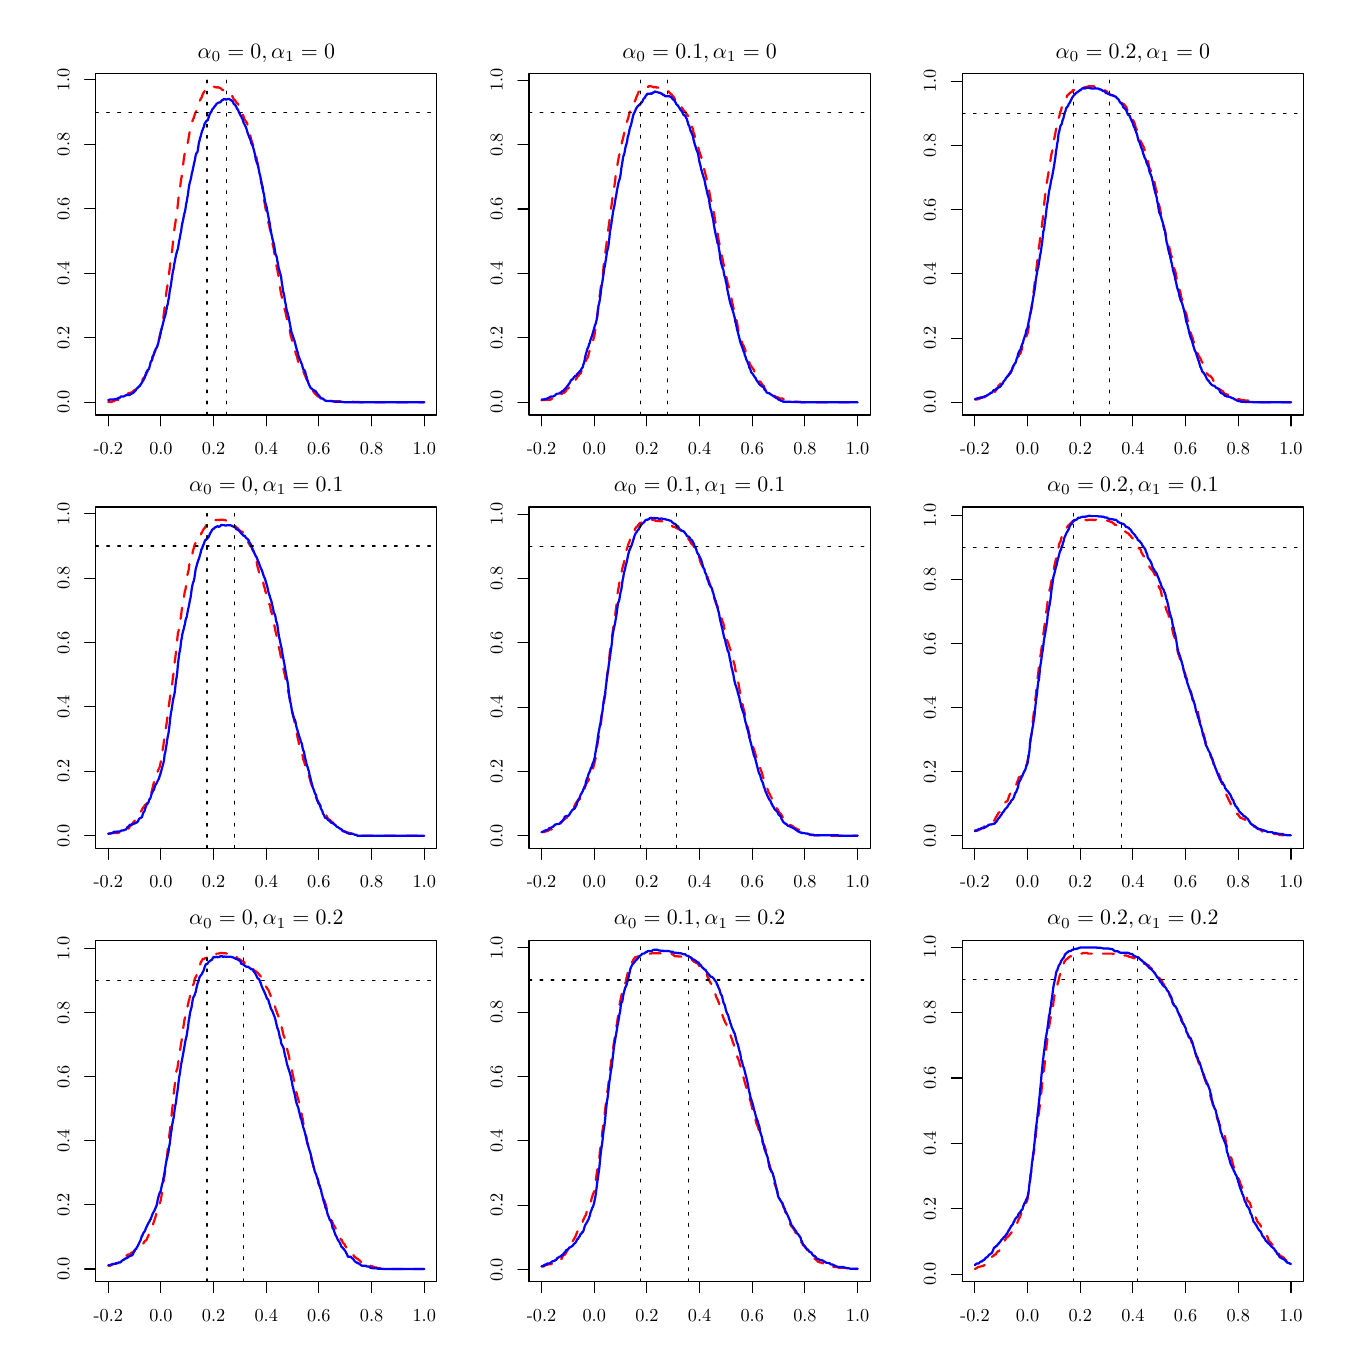
\begin{tikzpicture}[x=1pt,y=1pt]
\definecolor{fillColor}{RGB}{255,255,255}
\path[use as bounding box,fill=fillColor,fill opacity=0.00] (0,0) rectangle (469.75,469.75);
\begin{scope}
\path[clip] ( 24.55,329.80) rectangle (147.87,453.12);
\definecolor{drawColor}{RGB}{255,0,0}

\path[draw=drawColor,line width= 0.8pt,dash pattern=on 4pt off 4pt ,line join=round,line cap=round] ( 29.12,334.49) --
	( 29.35,334.49) --
	( 29.58,334.49) --
	( 29.81,334.49) --
	( 30.03,334.49) --
	( 30.26,334.49) --
	( 30.49,334.60) --
	( 30.72,334.72) --
	( 30.95,334.72) --
	( 31.18,334.72) --
	( 31.41,334.95) --
	( 31.64,335.19) --
	( 31.87,335.19) --
	( 32.09,335.19) --
	( 32.32,335.19) --
	( 32.55,335.19) --
	( 32.78,335.30) --
	( 33.01,335.30) --
	( 33.24,335.42) --
	( 33.47,335.77) --
	( 33.70,336.00) --
	( 33.92,336.12) --
	( 34.15,336.23) --
	( 34.38,336.23) --
	( 34.61,336.35) --
	( 34.84,336.82) --
	( 35.07,337.05) --
	( 35.30,337.17) --
	( 35.53,337.28) --
	( 35.76,337.28) --
	( 35.98,337.28) --
	( 36.21,337.40) --
	( 36.44,337.75) --
	( 36.67,337.75) --
	( 36.90,337.75) --
	( 37.13,337.86) --
	( 37.36,337.86) --
	( 37.59,337.98) --
	( 37.81,337.98) --
	( 38.04,338.33) --
	( 38.27,338.45) --
	( 38.50,338.80) --
	( 38.73,338.80) --
	( 38.96,338.91) --
	( 39.19,339.15) --
	( 39.42,339.38) --
	( 39.65,339.50) --
	( 39.87,339.96) --
	( 40.10,340.54) --
	( 40.33,340.78) --
	( 40.56,340.89) --
	( 40.79,341.24) --
	( 41.02,341.48) --
	( 41.25,341.71) --
	( 41.48,342.41) --
	( 41.71,342.99) --
	( 41.93,343.11) --
	( 42.16,343.46) --
	( 42.39,343.81) --
	( 42.62,344.16) --
	( 42.85,344.51) --
	( 43.08,345.21) --
	( 43.31,345.56) --
	( 43.54,346.02) --
	( 43.76,346.49) --
	( 43.99,346.95) --
	( 44.22,347.42) --
	( 44.45,348.00) --
	( 44.68,348.70) --
	( 44.91,349.28) --
	( 45.14,350.68) --
	( 45.37,351.15) --
	( 45.60,351.61) --
	( 45.82,352.43) --
	( 46.05,352.78) --
	( 46.28,353.71) --
	( 46.51,354.76) --
	( 46.74,355.34) --
	( 46.97,356.27) --
	( 47.20,356.51) --
	( 47.43,357.09) --
	( 47.65,358.02) --
	( 47.88,359.07) --
	( 48.11,360.12) --
	( 48.34,361.05) --
	( 48.57,362.22) --
	( 48.80,363.38) --
	( 49.03,364.90) --
	( 49.26,366.88) --
	( 49.49,368.63) --
	( 49.71,370.72) --
	( 49.94,372.70) --
	( 50.17,374.57) --
	( 50.40,375.97) --
	( 50.63,377.13) --
	( 50.86,379.11) --
	( 51.09,380.98) --
	( 51.32,382.72) --
	( 51.54,384.94) --
	( 51.77,386.34) --
	( 52.00,388.20) --
	( 52.23,389.37) --
	( 52.46,391.81) --
	( 52.69,394.14) --
	( 52.92,396.24) --
	( 53.15,397.87) --
	( 53.38,399.27) --
	( 53.60,401.25) --
	( 53.83,402.53) --
	( 54.06,404.16) --
	( 54.29,406.14) --
	( 54.52,408.36) --
	( 54.75,409.41) --
	( 54.98,410.80) --
	( 55.21,413.13) --
	( 55.43,414.88) --
	( 55.66,415.93) --
	( 55.89,418.49) --
	( 56.12,419.89) --
	( 56.35,421.76) --
	( 56.58,423.39) --
	( 56.81,424.55) --
	( 57.04,425.60) --
	( 57.27,426.42) --
	( 57.49,427.12) --
	( 57.72,427.82) --
	( 57.95,428.51) --
	( 58.18,430.03) --
	( 58.41,431.43) --
	( 58.64,432.48) --
	( 58.87,433.64) --
	( 59.10,434.69) --
	( 59.32,435.27) --
	( 59.55,436.09) --
	( 59.78,436.67) --
	( 60.01,437.14) --
	( 60.24,437.95) --
	( 60.47,438.65) --
	( 60.70,439.12) --
	( 60.93,439.70) --
	( 61.16,440.40) --
	( 61.38,440.98) --
	( 61.61,442.03) --
	( 61.84,442.73) --
	( 62.07,443.08) --
	( 62.30,443.55) --
	( 62.53,444.01) --
	( 62.76,444.36) --
	( 62.99,444.83) --
	( 63.22,445.64) --
	( 63.44,446.11) --
	( 63.67,446.34) --
	( 63.90,446.81) --
	( 64.13,446.81) --
	( 64.36,447.16) --
	( 64.59,447.27) --
	( 64.82,447.39) --
	( 65.05,447.62) --
	( 65.27,447.86) --
	( 65.50,448.21) --
	( 65.73,448.21) --
	( 65.96,448.32) --
	( 66.19,448.56) --
	( 66.42,448.56) --
	( 66.65,448.44) --
	( 66.88,448.44) --
	( 67.11,448.44) --
	( 67.33,448.44) --
	( 67.56,448.32) --
	( 67.79,448.21) --
	( 68.02,448.21) --
	( 68.25,448.21) --
	( 68.48,448.09) --
	( 68.71,448.21) --
	( 68.94,448.21) --
	( 69.16,448.09) --
	( 69.39,447.97) --
	( 69.62,447.97) --
	( 69.85,447.74) --
	( 70.08,447.51) --
	( 70.31,447.27) --
	( 70.54,447.27) --
	( 70.77,447.04) --
	( 71.00,446.81) --
	( 71.22,446.57) --
	( 71.45,446.34) --
	( 71.68,446.23) --
	( 71.91,446.23) --
	( 72.14,446.11) --
	( 72.37,446.11) --
	( 72.60,446.11) --
	( 72.83,445.76) --
	( 73.05,445.76) --
	( 73.28,445.64) --
	( 73.51,445.41) --
	( 73.74,445.29) --
	( 73.97,444.94) --
	( 74.20,444.48) --
	( 74.43,443.89) --
	( 74.66,443.78) --
	( 74.89,443.55) --
	( 75.11,443.20) --
	( 75.34,442.85) --
	( 75.57,442.50) --
	( 75.80,442.38) --
	( 76.03,442.15) --
	( 76.26,441.45) --
	( 76.49,440.98) --
	( 76.72,440.75) --
	( 76.94,440.40) --
	( 77.17,439.82) --
	( 77.40,439.12) --
	( 77.63,438.42) --
	( 77.86,438.07) --
	( 78.09,437.37) --
	( 78.32,436.67) --
	( 78.55,436.32) --
	( 78.78,435.97) --
	( 79.00,435.62) --
	( 79.23,435.39) --
	( 79.46,434.57) --
	( 79.69,433.52) --
	( 79.92,432.59) --
	( 80.15,431.89) --
	( 80.38,431.08) --
	( 80.61,429.91) --
	( 80.83,429.10) --
	( 81.06,428.40) --
	( 81.29,427.82) --
	( 81.52,426.88) --
	( 81.75,426.30) --
	( 81.98,425.83) --
	( 82.21,424.55) --
	( 82.44,423.50) --
	( 82.67,422.81) --
	( 82.89,421.64) --
	( 83.12,420.59) --
	( 83.35,419.08) --
	( 83.58,418.49) --
	( 83.81,417.33) --
	( 84.04,416.63) --
	( 84.27,415.00) --
	( 84.50,413.72) --
	( 84.73,412.44) --
	( 84.95,409.99) --
	( 85.18,409.17) --
	( 85.41,407.31) --
	( 85.64,406.38) --
	( 85.87,404.86) --
	( 86.10,403.70) --
	( 86.33,403.00) --
	( 86.56,401.72) --
	( 86.78,400.55) --
	( 87.01,399.15) --
	( 87.24,398.45) --
	( 87.47,397.17) --
	( 87.70,396.47) --
	( 87.93,395.42) --
	( 88.16,393.68) --
	( 88.39,392.16) --
	( 88.62,391.00) --
	( 88.84,390.30) --
	( 89.07,388.67) --
	( 89.30,387.50) --
	( 89.53,385.99) --
	( 89.76,384.24) --
	( 89.99,383.31) --
	( 90.22,382.26) --
	( 90.45,380.86) --
	( 90.67,379.93) --
	( 90.90,377.95) --
	( 91.13,376.66) --
	( 91.36,374.68) --
	( 91.59,373.64) --
	( 91.82,372.47) --
	( 92.05,371.31) --
	( 92.28,370.49) --
	( 92.51,369.79) --
	( 92.73,368.28) --
	( 92.96,367.69) --
	( 93.19,366.76) --
	( 93.42,365.60) --
	( 93.65,364.66) --
	( 93.88,364.20) --
	( 94.11,363.15) --
	( 94.34,362.10) --
	( 94.56,361.17) --
	( 94.79,360.12) --
	( 95.02,358.49) --
	( 95.25,357.91) --
	( 95.48,356.74) --
	( 95.71,356.51) --
	( 95.94,355.92) --
	( 96.17,354.76) --
	( 96.40,353.94) --
	( 96.62,353.13) --
	( 96.85,351.96) --
	( 97.08,351.38) --
	( 97.31,351.03) --
	( 97.54,349.87) --
	( 97.77,348.93) --
	( 98.00,348.58) --
	( 98.23,348.00) --
	( 98.45,347.89) --
	( 98.68,347.42) --
	( 98.91,347.07) --
	( 99.14,346.25) --
	( 99.37,346.14) --
	( 99.60,345.56) --
	( 99.83,344.86) --
	(100.06,344.39) --
	(100.29,343.92) --
	(100.51,343.34) --
	(100.74,342.76) --
	(100.97,342.53) --
	(101.20,342.06) --
	(101.43,341.36) --
	(101.66,340.89) --
	(101.89,340.54) --
	(102.12,340.20) --
	(102.35,339.73) --
	(102.57,339.26) --
	(102.80,339.26) --
	(103.03,338.80) --
	(103.26,338.21) --
	(103.49,337.86) --
	(103.72,337.75) --
	(103.95,337.40) --
	(104.18,337.28) --
	(104.40,336.93) --
	(104.63,336.70) --
	(104.86,336.47) --
	(105.09,336.47) --
	(105.32,336.35) --
	(105.55,336.23) --
	(105.78,336.12) --
	(106.01,336.12) --
	(106.24,335.77) --
	(106.46,335.53) --
	(106.69,335.30) --
	(106.92,335.19) --
	(107.15,335.07) --
	(107.38,335.07) --
	(107.61,335.07) --
	(107.84,335.07) --
	(108.07,334.84) --
	(108.29,334.84) --
	(108.52,334.84) --
	(108.75,334.84) --
	(108.98,334.84) --
	(109.21,334.84) --
	(109.44,334.84) --
	(109.67,334.84) --
	(109.90,334.84) --
	(110.13,334.72) --
	(110.35,334.72) --
	(110.58,334.72) --
	(110.81,334.72) --
	(111.04,334.72) --
	(111.27,334.72) --
	(111.50,334.72) --
	(111.73,334.72) --
	(111.96,334.72) --
	(112.18,334.72) --
	(112.41,334.72) --
	(112.64,334.72) --
	(112.87,334.72) --
	(113.10,334.60) --
	(113.33,334.60) --
	(113.56,334.60) --
	(113.79,334.60) --
	(114.02,334.60) --
	(114.24,334.60) --
	(114.47,334.60) --
	(114.70,334.60) --
	(114.93,334.60) --
	(115.16,334.60) --
	(115.39,334.60) --
	(115.62,334.60) --
	(115.85,334.60) --
	(116.07,334.60) --
	(116.30,334.60) --
	(116.53,334.60) --
	(116.76,334.60) --
	(116.99,334.60) --
	(117.22,334.60) --
	(117.45,334.60) --
	(117.68,334.49) --
	(117.91,334.49) --
	(118.13,334.49) --
	(118.36,334.49) --
	(118.59,334.49) --
	(118.82,334.49) --
	(119.05,334.49) --
	(119.28,334.49) --
	(119.51,334.49) --
	(119.74,334.49) --
	(119.96,334.37) --
	(120.19,334.37) --
	(120.42,334.37) --
	(120.65,334.37) --
	(120.88,334.37) --
	(121.11,334.37) --
	(121.34,334.37) --
	(121.57,334.37) --
	(121.80,334.37) --
	(122.02,334.37) --
	(122.25,334.37) --
	(122.48,334.37) --
	(122.71,334.37) --
	(122.94,334.37) --
	(123.17,334.37) --
	(123.40,334.37) --
	(123.63,334.37) --
	(123.86,334.37) --
	(124.08,334.37) --
	(124.31,334.37) --
	(124.54,334.37) --
	(124.77,334.37) --
	(125.00,334.37) --
	(125.23,334.37) --
	(125.46,334.37) --
	(125.69,334.37) --
	(125.91,334.37) --
	(126.14,334.37) --
	(126.37,334.37) --
	(126.60,334.37) --
	(126.83,334.37) --
	(127.06,334.37) --
	(127.29,334.37) --
	(127.52,334.37) --
	(127.75,334.37) --
	(127.97,334.37) --
	(128.20,334.37) --
	(128.43,334.37) --
	(128.66,334.37) --
	(128.89,334.37) --
	(129.12,334.37) --
	(129.35,334.37) --
	(129.58,334.37) --
	(129.80,334.37) --
	(130.03,334.37) --
	(130.26,334.37) --
	(130.49,334.37) --
	(130.72,334.37) --
	(130.95,334.37) --
	(131.18,334.37) --
	(131.41,334.37) --
	(131.64,334.37) --
	(131.86,334.37) --
	(132.09,334.37) --
	(132.32,334.37) --
	(132.55,334.37) --
	(132.78,334.37) --
	(133.01,334.37) --
	(133.24,334.37) --
	(133.47,334.37) --
	(133.69,334.37) --
	(133.92,334.37) --
	(134.15,334.37) --
	(134.38,334.37) --
	(134.61,334.37) --
	(134.84,334.37) --
	(135.07,334.37) --
	(135.30,334.37) --
	(135.53,334.37) --
	(135.75,334.37) --
	(135.98,334.37) --
	(136.21,334.37) --
	(136.44,334.37) --
	(136.67,334.37) --
	(136.90,334.37) --
	(137.13,334.37) --
	(137.36,334.37) --
	(137.58,334.37) --
	(137.81,334.37) --
	(138.04,334.37) --
	(138.27,334.37) --
	(138.50,334.37) --
	(138.73,334.37) --
	(138.96,334.37) --
	(139.19,334.37) --
	(139.42,334.37) --
	(139.64,334.37) --
	(139.87,334.37) --
	(140.10,334.37) --
	(140.33,334.37) --
	(140.56,334.37) --
	(140.79,334.37) --
	(141.02,334.37) --
	(141.25,334.37) --
	(141.47,334.37) --
	(141.70,334.37) --
	(141.93,334.37) --
	(142.16,334.37) --
	(142.39,334.37) --
	(142.62,334.37) --
	(142.85,334.37) --
	(143.08,334.37) --
	(143.31,334.37);
\end{scope}
\begin{scope}
\path[clip] (  0.00,  0.00) rectangle (469.75,469.75);
\definecolor{drawColor}{RGB}{0,0,0}

\path[draw=drawColor,line width= 0.4pt,line join=round,line cap=round] ( 29.12,329.80) -- (143.31,329.80);

\path[draw=drawColor,line width= 0.4pt,line join=round,line cap=round] ( 29.12,329.80) -- ( 29.12,325.84);

\path[draw=drawColor,line width= 0.4pt,line join=round,line cap=round] ( 48.15,329.80) -- ( 48.15,325.84);

\path[draw=drawColor,line width= 0.4pt,line join=round,line cap=round] ( 67.18,329.80) -- ( 67.18,325.84);

\path[draw=drawColor,line width= 0.4pt,line join=round,line cap=round] ( 86.21,329.80) -- ( 86.21,325.84);

\path[draw=drawColor,line width= 0.4pt,line join=round,line cap=round] (105.24,329.80) -- (105.24,325.84);

\path[draw=drawColor,line width= 0.4pt,line join=round,line cap=round] (124.27,329.80) -- (124.27,325.84);

\path[draw=drawColor,line width= 0.4pt,line join=round,line cap=round] (143.31,329.80) -- (143.31,325.84);

\node[text=drawColor,anchor=base,inner sep=0pt, outer sep=0pt, scale=  0.66] at ( 29.12,315.55) {-0.2};

\node[text=drawColor,anchor=base,inner sep=0pt, outer sep=0pt, scale=  0.66] at ( 48.15,315.55) {0.0};

\node[text=drawColor,anchor=base,inner sep=0pt, outer sep=0pt, scale=  0.66] at ( 67.18,315.55) {0.2};

\node[text=drawColor,anchor=base,inner sep=0pt, outer sep=0pt, scale=  0.66] at ( 86.21,315.55) {0.4};

\node[text=drawColor,anchor=base,inner sep=0pt, outer sep=0pt, scale=  0.66] at (105.24,315.55) {0.6};

\node[text=drawColor,anchor=base,inner sep=0pt, outer sep=0pt, scale=  0.66] at (124.27,315.55) {0.8};

\node[text=drawColor,anchor=base,inner sep=0pt, outer sep=0pt, scale=  0.66] at (143.31,315.55) {1.0};

\path[draw=drawColor,line width= 0.4pt,line join=round,line cap=round] ( 24.55,334.37) -- ( 24.55,450.89);

\path[draw=drawColor,line width= 0.4pt,line join=round,line cap=round] ( 24.55,334.37) -- ( 20.59,334.37);

\path[draw=drawColor,line width= 0.4pt,line join=round,line cap=round] ( 24.55,357.67) -- ( 20.59,357.67);

\path[draw=drawColor,line width= 0.4pt,line join=round,line cap=round] ( 24.55,380.98) -- ( 20.59,380.98);

\path[draw=drawColor,line width= 0.4pt,line join=round,line cap=round] ( 24.55,404.28) -- ( 20.59,404.28);

\path[draw=drawColor,line width= 0.4pt,line join=round,line cap=round] ( 24.55,427.58) -- ( 20.59,427.58);

\path[draw=drawColor,line width= 0.4pt,line join=round,line cap=round] ( 24.55,450.89) -- ( 20.59,450.89);

\node[text=drawColor,rotate= 90.00,anchor=base,inner sep=0pt, outer sep=0pt, scale=  0.66] at ( 15.05,334.37) {0.0};

\node[text=drawColor,rotate= 90.00,anchor=base,inner sep=0pt, outer sep=0pt, scale=  0.66] at ( 15.05,357.67) {0.2};

\node[text=drawColor,rotate= 90.00,anchor=base,inner sep=0pt, outer sep=0pt, scale=  0.66] at ( 15.05,380.98) {0.4};

\node[text=drawColor,rotate= 90.00,anchor=base,inner sep=0pt, outer sep=0pt, scale=  0.66] at ( 15.05,404.28) {0.6};

\node[text=drawColor,rotate= 90.00,anchor=base,inner sep=0pt, outer sep=0pt, scale=  0.66] at ( 15.05,427.58) {0.8};

\node[text=drawColor,rotate= 90.00,anchor=base,inner sep=0pt, outer sep=0pt, scale=  0.66] at ( 15.05,450.89) {1.0};

\path[draw=drawColor,line width= 0.4pt,line join=round,line cap=round] ( 24.55,329.80) --
	(147.87,329.80) --
	(147.87,453.12) --
	( 24.55,453.12) --
	( 24.55,329.80);
\end{scope}
\begin{scope}
\path[clip] (  0.00,313.17) rectangle (156.58,469.75);
\definecolor{drawColor}{RGB}{0,0,0}

\node[text=drawColor,anchor=base,inner sep=0pt, outer sep=0pt, scale=  0.79] at ( 86.21,458.71) {\bfseries $\alpha_0 = 0, \alpha_1 = 0$};
\end{scope}
\begin{scope}
\path[clip] ( 24.55,329.80) rectangle (147.87,453.12);
\definecolor{drawColor}{RGB}{0,0,255}

\path[draw=drawColor,line width= 0.8pt,line join=round,line cap=round] ( 29.12,335.19) --
	( 29.35,335.19) --
	( 29.58,335.30) --
	( 29.81,335.42) --
	( 30.03,335.42) --
	( 30.26,335.42) --
	( 30.49,335.42) --
	( 30.72,335.42) --
	( 30.95,335.42) --
	( 31.18,335.42) --
	( 31.41,335.53) --
	( 31.64,335.53) --
	( 31.87,335.53) --
	( 32.09,335.65) --
	( 32.32,335.65) --
	( 32.55,335.77) --
	( 32.78,336.00) --
	( 33.01,336.00) --
	( 33.24,336.00) --
	( 33.47,336.23) --
	( 33.70,336.47) --
	( 33.92,336.47) --
	( 34.15,336.47) --
	( 34.38,336.47) --
	( 34.61,336.47) --
	( 34.84,336.58) --
	( 35.07,336.70) --
	( 35.30,336.82) --
	( 35.53,336.93) --
	( 35.76,336.93) --
	( 35.98,337.05) --
	( 36.21,337.05) --
	( 36.44,337.05) --
	( 36.67,337.05) --
	( 36.90,337.05) --
	( 37.13,337.28) --
	( 37.36,337.40) --
	( 37.59,337.52) --
	( 37.81,337.63) --
	( 38.04,337.63) --
	( 38.27,337.98) --
	( 38.50,338.10) --
	( 38.73,338.45) --
	( 38.96,338.56) --
	( 39.19,338.91) --
	( 39.42,339.38) --
	( 39.65,339.50) --
	( 39.87,339.73) --
	( 40.10,339.96) --
	( 40.33,340.20) --
	( 40.56,340.31) --
	( 40.79,340.78) --
	( 41.02,341.13) --
	( 41.25,341.48) --
	( 41.48,341.94) --
	( 41.71,342.18) --
	( 41.93,342.64) --
	( 42.16,342.99) --
	( 42.39,343.57) --
	( 42.62,344.39) --
	( 42.85,345.09) --
	( 43.08,345.32) --
	( 43.31,346.02) --
	( 43.54,346.25) --
	( 43.76,346.25) --
	( 43.99,346.95) --
	( 44.22,347.89) --
	( 44.45,348.93) --
	( 44.68,349.28) --
	( 44.91,349.75) --
	( 45.14,350.91) --
	( 45.37,351.26) --
	( 45.60,351.73) --
	( 45.82,352.55) --
	( 46.05,353.01) --
	( 46.28,353.71) --
	( 46.51,353.94) --
	( 46.74,354.29) --
	( 46.97,355.11) --
	( 47.20,355.81) --
	( 47.43,356.97) --
	( 47.65,357.56) --
	( 47.88,358.60) --
	( 48.11,359.65) --
	( 48.34,360.70) --
	( 48.57,361.63) --
	( 48.80,362.45) --
	( 49.03,363.38) --
	( 49.26,364.43) --
	( 49.49,365.13) --
	( 49.71,365.60) --
	( 49.94,366.76) --
	( 50.17,368.04) --
	( 50.40,369.21) --
	( 50.63,369.91) --
	( 50.86,371.42) --
	( 51.09,372.47) --
	( 51.32,374.57) --
	( 51.54,375.62) --
	( 51.77,376.66) --
	( 52.00,378.53) --
	( 52.23,380.04) --
	( 52.46,381.68) --
	( 52.69,382.37) --
	( 52.92,384.12) --
	( 53.15,385.17) --
	( 53.38,386.45) --
	( 53.60,387.50) --
	( 53.83,388.43) --
	( 54.06,389.25) --
	( 54.29,389.83) --
	( 54.52,391.35) --
	( 54.75,392.74) --
	( 54.98,393.79) --
	( 55.21,395.19) --
	( 55.43,396.01) --
	( 55.66,397.87) --
	( 55.89,399.15) --
	( 56.12,399.97) --
	( 56.35,401.25) --
	( 56.58,402.42) --
	( 56.81,403.23) --
	( 57.04,404.40) --
	( 57.27,406.14) --
	( 57.49,406.96) --
	( 57.72,408.47) --
	( 57.95,409.76) --
	( 58.18,411.62) --
	( 58.41,413.02) --
	( 58.64,413.95) --
	( 58.87,414.77) --
	( 59.10,415.70) --
	( 59.32,417.21) --
	( 59.55,417.91) --
	( 59.78,419.08) --
	( 60.01,420.13) --
	( 60.24,421.17) --
	( 60.47,422.22) --
	( 60.70,423.62) --
	( 60.93,424.32) --
	( 61.16,424.55) --
	( 61.38,424.90) --
	( 61.61,426.30) --
	( 61.84,428.05) --
	( 62.07,428.75) --
	( 62.30,429.91) --
	( 62.53,430.50) --
	( 62.76,431.43) --
	( 62.99,432.36) --
	( 63.22,432.83) --
	( 63.44,433.41) --
	( 63.67,433.87) --
	( 63.90,434.92) --
	( 64.13,435.27) --
	( 64.36,435.74) --
	( 64.59,435.97) --
	( 64.82,436.20) --
	( 65.05,436.32) --
	( 65.27,436.90) --
	( 65.50,437.60) --
	( 65.73,438.42) --
	( 65.96,438.77) --
	( 66.19,439.23) --
	( 66.42,439.47) --
	( 66.65,440.17) --
	( 66.88,440.40) --
	( 67.11,440.63) --
	( 67.33,440.98) --
	( 67.56,441.33) --
	( 67.79,441.56) --
	( 68.02,441.80) --
	( 68.25,442.26) --
	( 68.48,442.38) --
	( 68.71,442.50) --
	( 68.94,442.73) --
	( 69.16,442.61) --
	( 69.39,442.73) --
	( 69.62,442.85) --
	( 69.85,443.08) --
	( 70.08,443.43) --
	( 70.31,443.55) --
	( 70.54,443.66) --
	( 70.77,443.89) --
	( 71.00,444.01) --
	( 71.22,443.78) --
	( 71.45,443.89) --
	( 71.68,443.78) --
	( 71.91,443.78) --
	( 72.14,443.89) --
	( 72.37,444.01) --
	( 72.60,444.01) --
	( 72.83,444.01) --
	( 73.05,443.78) --
	( 73.28,443.66) --
	( 73.51,443.55) --
	( 73.74,443.31) --
	( 73.97,443.31) --
	( 74.20,442.85) --
	( 74.43,442.26) --
	( 74.66,442.03) --
	( 74.89,442.03) --
	( 75.11,441.56) --
	( 75.34,441.22) --
	( 75.57,440.63) --
	( 75.80,440.28) --
	( 76.03,440.05) --
	( 76.26,439.35) --
	( 76.49,438.88) --
	( 76.72,438.54) --
	( 76.94,437.95) --
	( 77.17,437.72) --
	( 77.40,437.02) --
	( 77.63,436.79) --
	( 77.86,435.97) --
	( 78.09,435.16) --
	( 78.32,434.92) --
	( 78.55,434.34) --
	( 78.78,433.99) --
	( 79.00,433.41) --
	( 79.23,432.59) --
	( 79.46,431.78) --
	( 79.69,431.19) --
	( 79.92,430.61) --
	( 80.15,429.91) --
	( 80.38,429.56) --
	( 80.61,428.75) --
	( 80.83,427.93) --
	( 81.06,427.47) --
	( 81.29,427.12) --
	( 81.52,426.30) --
	( 81.75,425.49) --
	( 81.98,424.55) --
	( 82.21,423.50) --
	( 82.44,422.11) --
	( 82.67,421.41) --
	( 82.89,420.82) --
	( 83.12,420.24) --
	( 83.35,419.31) --
	( 83.58,418.03) --
	( 83.81,416.86) --
	( 84.04,416.16) --
	( 84.27,414.77) --
	( 84.50,413.37) --
	( 84.73,412.79) --
	( 84.95,411.85) --
	( 85.18,410.22) --
	( 85.41,409.41) --
	( 85.64,407.77) --
	( 85.87,406.49) --
	( 86.10,405.79) --
	( 86.33,404.98) --
	( 86.56,403.58) --
	( 86.78,402.53) --
	( 87.01,401.25) --
	( 87.24,400.08) --
	( 87.47,399.04) --
	( 87.70,397.17) --
	( 87.93,396.01) --
	( 88.16,394.84) --
	( 88.39,393.68) --
	( 88.62,392.74) --
	( 88.84,392.05) --
	( 89.07,391.00) --
	( 89.30,389.48) --
	( 89.53,388.08) --
	( 89.76,387.38) --
	( 89.99,386.92) --
	( 90.22,385.40) --
	( 90.45,384.35) --
	( 90.67,382.96) --
	( 90.90,382.26) --
	( 91.13,381.33) --
	( 91.36,380.63) --
	( 91.59,379.58) --
	( 91.82,377.60) --
	( 92.05,376.32) --
	( 92.28,374.57) --
	( 92.51,373.75) --
	( 92.73,372.82) --
	( 92.96,370.96) --
	( 93.19,370.02) --
	( 93.42,368.63) --
	( 93.65,367.46) --
	( 93.88,366.76) --
	( 94.11,365.83) --
	( 94.34,365.01) --
	( 94.56,363.73) --
	( 94.79,362.45) --
	( 95.02,361.28) --
	( 95.25,360.00) --
	( 95.48,359.30) --
	( 95.71,358.72) --
	( 95.94,358.02) --
	( 96.17,357.21) --
	( 96.40,356.62) --
	( 96.62,355.81) --
	( 96.85,354.88) --
	( 97.08,354.06) --
	( 97.31,353.13) --
	( 97.54,352.55) --
	( 97.77,351.50) --
	( 98.00,350.68) --
	( 98.23,350.22) --
	( 98.45,349.63) --
	( 98.68,349.05) --
	( 98.91,348.47) --
	( 99.14,348.00) --
	( 99.37,346.95) --
	( 99.60,346.25) --
	( 99.83,346.14) --
	(100.06,345.90) --
	(100.29,345.32) --
	(100.51,344.39) --
	(100.74,343.69) --
	(100.97,342.64) --
	(101.20,342.06) --
	(101.43,341.36) --
	(101.66,340.78) --
	(101.89,340.31) --
	(102.12,339.85) --
	(102.35,339.38) --
	(102.57,339.38) --
	(102.80,339.15) --
	(103.03,338.91) --
	(103.26,338.91) --
	(103.49,338.56) --
	(103.72,338.56) --
	(103.95,338.45) --
	(104.18,338.21) --
	(104.40,337.86) --
	(104.63,337.52) --
	(104.86,337.17) --
	(105.09,337.05) --
	(105.32,336.70) --
	(105.55,336.47) --
	(105.78,335.88) --
	(106.01,335.77) --
	(106.24,335.77) --
	(106.46,335.77) --
	(106.69,335.77) --
	(106.92,335.42) --
	(107.15,335.30) --
	(107.38,335.07) --
	(107.61,334.95) --
	(107.84,334.95) --
	(108.07,334.84) --
	(108.29,334.84) --
	(108.52,334.84) --
	(108.75,334.84) --
	(108.98,334.84) --
	(109.21,334.84) --
	(109.44,334.84) --
	(109.67,334.84) --
	(109.90,334.84) --
	(110.13,334.72) --
	(110.35,334.72) --
	(110.58,334.72) --
	(110.81,334.60) --
	(111.04,334.60) --
	(111.27,334.60) --
	(111.50,334.60) --
	(111.73,334.60) --
	(111.96,334.60) --
	(112.18,334.60) --
	(112.41,334.60) --
	(112.64,334.60) --
	(112.87,334.60) --
	(113.10,334.60) --
	(113.33,334.60) --
	(113.56,334.49) --
	(113.79,334.49) --
	(114.02,334.49) --
	(114.24,334.49) --
	(114.47,334.37) --
	(114.70,334.37) --
	(114.93,334.37) --
	(115.16,334.37) --
	(115.39,334.37) --
	(115.62,334.37) --
	(115.85,334.37) --
	(116.07,334.37) --
	(116.30,334.37) --
	(116.53,334.37) --
	(116.76,334.37) --
	(116.99,334.37) --
	(117.22,334.37) --
	(117.45,334.37) --
	(117.68,334.37) --
	(117.91,334.37) --
	(118.13,334.37) --
	(118.36,334.37) --
	(118.59,334.37) --
	(118.82,334.37) --
	(119.05,334.37) --
	(119.28,334.37) --
	(119.51,334.37) --
	(119.74,334.37) --
	(119.96,334.37) --
	(120.19,334.37) --
	(120.42,334.37) --
	(120.65,334.37) --
	(120.88,334.37) --
	(121.11,334.37) --
	(121.34,334.37) --
	(121.57,334.37) --
	(121.80,334.37) --
	(122.02,334.37) --
	(122.25,334.37) --
	(122.48,334.37) --
	(122.71,334.37) --
	(122.94,334.37) --
	(123.17,334.37) --
	(123.40,334.37) --
	(123.63,334.37) --
	(123.86,334.37) --
	(124.08,334.37) --
	(124.31,334.37) --
	(124.54,334.37) --
	(124.77,334.37) --
	(125.00,334.37) --
	(125.23,334.37) --
	(125.46,334.37) --
	(125.69,334.37) --
	(125.91,334.37) --
	(126.14,334.37) --
	(126.37,334.37) --
	(126.60,334.37) --
	(126.83,334.37) --
	(127.06,334.37) --
	(127.29,334.37) --
	(127.52,334.37) --
	(127.75,334.37) --
	(127.97,334.37) --
	(128.20,334.37) --
	(128.43,334.37) --
	(128.66,334.37) --
	(128.89,334.37) --
	(129.12,334.37) --
	(129.35,334.37) --
	(129.58,334.37) --
	(129.80,334.37) --
	(130.03,334.37) --
	(130.26,334.37) --
	(130.49,334.37) --
	(130.72,334.37) --
	(130.95,334.37) --
	(131.18,334.37) --
	(131.41,334.37) --
	(131.64,334.37) --
	(131.86,334.37) --
	(132.09,334.37) --
	(132.32,334.37) --
	(132.55,334.37) --
	(132.78,334.37) --
	(133.01,334.37) --
	(133.24,334.37) --
	(133.47,334.37) --
	(133.69,334.37) --
	(133.92,334.37) --
	(134.15,334.37) --
	(134.38,334.37) --
	(134.61,334.37) --
	(134.84,334.37) --
	(135.07,334.37) --
	(135.30,334.37) --
	(135.53,334.37) --
	(135.75,334.37) --
	(135.98,334.37) --
	(136.21,334.37) --
	(136.44,334.37) --
	(136.67,334.37) --
	(136.90,334.37) --
	(137.13,334.37) --
	(137.36,334.37) --
	(137.58,334.37) --
	(137.81,334.37) --
	(138.04,334.37) --
	(138.27,334.37) --
	(138.50,334.37) --
	(138.73,334.37) --
	(138.96,334.37) --
	(139.19,334.37) --
	(139.42,334.37) --
	(139.64,334.37) --
	(139.87,334.37) --
	(140.10,334.37) --
	(140.33,334.37) --
	(140.56,334.37) --
	(140.79,334.37) --
	(141.02,334.37) --
	(141.25,334.37) --
	(141.47,334.37) --
	(141.70,334.37) --
	(141.93,334.37) --
	(142.16,334.37) --
	(142.39,334.37) --
	(142.62,334.37) --
	(142.85,334.37) --
	(143.08,334.37) --
	(143.31,334.37);
\definecolor{drawColor}{RGB}{0,0,0}

\path[draw=drawColor,line width= 0.4pt,dash pattern=on 1pt off 3pt ,line join=round,line cap=round] ( 24.55,439.23) -- (147.87,439.23);

\path[draw=drawColor,line width= 0.4pt,dash pattern=on 1pt off 3pt ,line join=round,line cap=round] ( 64.80,329.80) -- ( 64.80,453.12);

\path[draw=drawColor,line width= 0.4pt,dash pattern=on 1pt off 3pt ,line join=round,line cap=round] ( 71.94,329.80) -- ( 71.94,453.12);
\end{scope}
\begin{scope}
\path[clip] (181.14,329.80) rectangle (304.46,453.12);
\definecolor{drawColor}{RGB}{255,0,0}

\path[draw=drawColor,line width= 0.8pt,dash pattern=on 4pt off 4pt ,line join=round,line cap=round] (185.70,335.07) --
	(185.93,335.18) --
	(186.16,335.18) --
	(186.39,335.18) --
	(186.62,335.18) --
	(186.85,335.18) --
	(187.08,335.30) --
	(187.31,335.30) --
	(187.54,335.30) --
	(187.76,335.30) --
	(187.99,335.30) --
	(188.22,335.30) --
	(188.45,335.30) --
	(188.68,335.30) --
	(188.91,335.30) --
	(189.14,335.53) --
	(189.37,335.65) --
	(189.59,335.65) --
	(189.82,336.12) --
	(190.05,336.12) --
	(190.28,336.12) --
	(190.51,336.12) --
	(190.74,336.23) --
	(190.97,336.23) --
	(191.20,336.35) --
	(191.43,336.46) --
	(191.65,336.81) --
	(191.88,336.81) --
	(192.11,337.16) --
	(192.34,337.40) --
	(192.57,337.40) --
	(192.80,337.40) --
	(193.03,337.40) --
	(193.26,337.74) --
	(193.48,337.74) --
	(193.71,337.74) --
	(193.94,337.98) --
	(194.17,338.09) --
	(194.40,338.33) --
	(194.63,338.68) --
	(194.86,339.14) --
	(195.09,339.26) --
	(195.32,339.37) --
	(195.54,339.61) --
	(195.77,339.84) --
	(196.00,339.84) --
	(196.23,340.07) --
	(196.46,340.07) --
	(196.69,340.54) --
	(196.92,340.77) --
	(197.15,341.24) --
	(197.37,341.47) --
	(197.60,341.59) --
	(197.83,342.05) --
	(198.06,342.63) --
	(198.29,342.98) --
	(198.52,343.45) --
	(198.75,343.80) --
	(198.98,343.80) --
	(199.21,344.26) --
	(199.43,344.50) --
	(199.66,344.73) --
	(199.89,344.85) --
	(200.12,345.66) --
	(200.35,346.13) --
	(200.58,346.71) --
	(200.81,347.06) --
	(201.04,347.64) --
	(201.26,348.22) --
	(201.49,348.34) --
	(201.72,349.27) --
	(201.95,350.08) --
	(202.18,350.32) --
	(202.41,350.67) --
	(202.64,351.48) --
	(202.87,352.41) --
	(203.10,353.11) --
	(203.32,353.46) --
	(203.55,353.92) --
	(203.78,354.74) --
	(204.01,355.90) --
	(204.24,356.49) --
	(204.47,357.30) --
	(204.70,358.11) --
	(204.93,359.39) --
	(205.15,361.02) --
	(205.38,363.12) --
	(205.61,364.05) --
	(205.84,365.91) --
	(206.07,367.43) --
	(206.30,369.87) --
	(206.53,372.08) --
	(206.76,373.36) --
	(206.99,375.23) --
	(207.21,376.62) --
	(207.44,377.90) --
	(207.67,378.95) --
	(207.90,381.04) --
	(208.13,383.84) --
	(208.36,385.24) --
	(208.59,387.21) --
	(208.82,389.19) --
	(209.05,390.82) --
	(209.27,392.68) --
	(209.50,393.85) --
	(209.73,396.29) --
	(209.96,398.04) --
	(210.19,399.78) --
	(210.42,402.11) --
	(210.65,403.16) --
	(210.88,404.91) --
	(211.10,406.42) --
	(211.33,408.51) --
	(211.56,410.03) --
	(211.79,411.54) --
	(212.02,412.59) --
	(212.25,414.22) --
	(212.48,416.31) --
	(212.71,417.94) --
	(212.94,418.76) --
	(213.16,420.62) --
	(213.39,421.67) --
	(213.62,423.18) --
	(213.85,424.00) --
	(214.08,425.28) --
	(214.31,425.63) --
	(214.54,427.02) --
	(214.77,428.65) --
	(214.99,429.12) --
	(215.22,430.16) --
	(215.45,431.21) --
	(215.68,432.14) --
	(215.91,432.96) --
	(216.14,434.01) --
	(216.37,435.05) --
	(216.60,435.87) --
	(216.83,436.57) --
	(217.05,437.26) --
	(217.28,438.31) --
	(217.51,439.01) --
	(217.74,440.06) --
	(217.97,440.29) --
	(218.20,441.22) --
	(218.43,441.80) --
	(218.66,442.04) --
	(218.88,442.50) --
	(219.11,442.74) --
	(219.34,443.08) --
	(219.57,443.55) --
	(219.80,444.13) --
	(220.03,444.83) --
	(220.26,445.30) --
	(220.49,445.88) --
	(220.72,446.46) --
	(220.94,446.93) --
	(221.17,446.93) --
	(221.40,447.16) --
	(221.63,447.16) --
	(221.86,447.39) --
	(222.09,447.62) --
	(222.32,447.74) --
	(222.55,447.74) --
	(222.77,447.86) --
	(223.00,447.97) --
	(223.23,448.09) --
	(223.46,448.21) --
	(223.69,448.21) --
	(223.92,448.09) --
	(224.15,448.32) --
	(224.38,448.56) --
	(224.61,448.56) --
	(224.83,448.56) --
	(225.06,448.56) --
	(225.29,448.56) --
	(225.52,448.44) --
	(225.75,448.44) --
	(225.98,448.32) --
	(226.21,448.21) --
	(226.44,448.21) --
	(226.66,448.21) --
	(226.89,448.32) --
	(227.12,448.21) --
	(227.35,448.09) --
	(227.58,448.09) --
	(227.81,448.09) --
	(228.04,447.86) --
	(228.27,447.86) --
	(228.50,447.74) --
	(228.72,447.74) --
	(228.95,447.62) --
	(229.18,447.51) --
	(229.41,447.51) --
	(229.64,447.28) --
	(229.87,447.28) --
	(230.10,447.16) --
	(230.33,447.16) --
	(230.56,447.04) --
	(230.78,447.04) --
	(231.01,446.93) --
	(231.24,446.69) --
	(231.47,446.69) --
	(231.70,446.58) --
	(231.93,446.23) --
	(232.16,445.99) --
	(232.39,445.76) --
	(232.61,445.65) --
	(232.84,445.41) --
	(233.07,444.95) --
	(233.30,444.95) --
	(233.53,444.48) --
	(233.76,444.02) --
	(233.99,443.78) --
	(234.22,443.55) --
	(234.45,443.32) --
	(234.67,442.97) --
	(234.90,442.50) --
	(235.13,441.92) --
	(235.36,441.92) --
	(235.59,441.69) --
	(235.82,441.57) --
	(236.05,441.11) --
	(236.28,441.11) --
	(236.50,440.76) --
	(236.73,440.29) --
	(236.96,439.94) --
	(237.19,439.71) --
	(237.42,439.48) --
	(237.65,439.24) --
	(237.88,438.78) --
	(238.11,438.55) --
	(238.34,438.20) --
	(238.56,437.96) --
	(238.79,437.38) --
	(239.02,436.80) --
	(239.25,436.33) --
	(239.48,435.40) --
	(239.71,435.05) --
	(239.94,434.12) --
	(240.17,433.66) --
	(240.39,433.07) --
	(240.62,431.68) --
	(240.85,431.45) --
	(241.08,430.28) --
	(241.31,429.35) --
	(241.54,428.88) --
	(241.77,428.19) --
	(242.00,427.25) --
	(242.23,426.91) --
	(242.45,425.86) --
	(242.68,425.04) --
	(242.91,424.46) --
	(243.14,423.76) --
	(243.37,423.18) --
	(243.60,422.02) --
	(243.83,421.20) --
	(244.06,420.39) --
	(244.28,419.22) --
	(244.51,418.41) --
	(244.74,417.48) --
	(244.97,416.55) --
	(245.20,415.73) --
	(245.43,414.45) --
	(245.66,413.64) --
	(245.89,412.71) --
	(246.12,411.66) --
	(246.34,410.14) --
	(246.57,409.10) --
	(246.80,407.47) --
	(247.03,407.23) --
	(247.26,405.60) --
	(247.49,404.56) --
	(247.72,403.63) --
	(247.95,403.04) --
	(248.18,401.65) --
	(248.40,400.13) --
	(248.63,398.74) --
	(248.86,397.81) --
	(249.09,396.18) --
	(249.32,395.36) --
	(249.55,393.62) --
	(249.78,392.57) --
	(250.01,391.52) --
	(250.23,390.36) --
	(250.46,389.19) --
	(250.69,388.38) --
	(250.92,386.98) --
	(251.15,385.93) --
	(251.38,384.65) --
	(251.61,383.72) --
	(251.84,382.21) --
	(252.07,381.04) --
	(252.29,380.58) --
	(252.52,379.42) --
	(252.75,378.48) --
	(252.98,377.09) --
	(253.21,376.62) --
	(253.44,375.81) --
	(253.67,374.99) --
	(253.90,374.06) --
	(254.12,372.43) --
	(254.35,371.73) --
	(254.58,370.34) --
	(254.81,369.52) --
	(255.04,368.36) --
	(255.27,367.31) --
	(255.50,366.38) --
	(255.73,365.45) --
	(255.96,364.40) --
	(256.18,363.82) --
	(256.41,362.77) --
	(256.64,361.14) --
	(256.87,360.21) --
	(257.10,359.39) --
	(257.33,358.58) --
	(257.56,357.88) --
	(257.79,357.18) --
	(258.01,356.60) --
	(258.24,355.44) --
	(258.47,355.20) --
	(258.70,354.74) --
	(258.93,354.27) --
	(259.16,353.69) --
	(259.39,352.88) --
	(259.62,351.95) --
	(259.85,351.60) --
	(260.07,350.67) --
	(260.30,350.08) --
	(260.53,349.73) --
	(260.76,348.92) --
	(260.99,347.99) --
	(261.22,347.76) --
	(261.45,347.52) --
	(261.68,347.06) --
	(261.90,346.82) --
	(262.13,346.47) --
	(262.36,346.13) --
	(262.59,345.54) --
	(262.82,344.96) --
	(263.05,344.85) --
	(263.28,344.61) --
	(263.51,344.26) --
	(263.74,343.56) --
	(263.96,342.98) --
	(264.19,342.63) --
	(264.42,342.05) --
	(264.65,341.82) --
	(264.88,341.70) --
	(265.11,341.35) --
	(265.34,340.89) --
	(265.57,340.65) --
	(265.79,340.42) --
	(266.02,340.31) --
	(266.25,339.49) --
	(266.48,339.14) --
	(266.71,338.79) --
	(266.94,338.68) --
	(267.17,338.44) --
	(267.40,338.09) --
	(267.63,338.09) --
	(267.85,337.98) --
	(268.08,337.98) --
	(268.31,337.63) --
	(268.54,337.63) --
	(268.77,337.51) --
	(269.00,337.28) --
	(269.23,337.05) --
	(269.46,336.81) --
	(269.69,336.81) --
	(269.91,336.58) --
	(270.14,336.58) --
	(270.37,336.35) --
	(270.60,336.23) --
	(270.83,336.23) --
	(271.06,336.23) --
	(271.29,336.00) --
	(271.52,335.88) --
	(271.74,335.77) --
	(271.97,335.77) --
	(272.20,335.77) --
	(272.43,335.77) --
	(272.66,335.77) --
	(272.89,335.65) --
	(273.12,335.53) --
	(273.35,335.30) --
	(273.58,335.30) --
	(273.80,335.18) --
	(274.03,335.18) --
	(274.26,335.18) --
	(274.49,335.18) --
	(274.72,335.18) --
	(274.95,335.18) --
	(275.18,335.07) --
	(275.41,334.84) --
	(275.63,334.84) --
	(275.86,334.84) --
	(276.09,334.72) --
	(276.32,334.72) --
	(276.55,334.72) --
	(276.78,334.72) --
	(277.01,334.60) --
	(277.24,334.60) --
	(277.47,334.60) --
	(277.69,334.60) --
	(277.92,334.60) --
	(278.15,334.60) --
	(278.38,334.49) --
	(278.61,334.49) --
	(278.84,334.49) --
	(279.07,334.49) --
	(279.30,334.49) --
	(279.52,334.37) --
	(279.75,334.37) --
	(279.98,334.37) --
	(280.21,334.37) --
	(280.44,334.37) --
	(280.67,334.37) --
	(280.90,334.37) --
	(281.13,334.37) --
	(281.36,334.37) --
	(281.58,334.37) --
	(281.81,334.37) --
	(282.04,334.37) --
	(282.27,334.37) --
	(282.50,334.37) --
	(282.73,334.37) --
	(282.96,334.37) --
	(283.19,334.37) --
	(283.41,334.37) --
	(283.64,334.37) --
	(283.87,334.37) --
	(284.10,334.37) --
	(284.33,334.37) --
	(284.56,334.37) --
	(284.79,334.37) --
	(285.02,334.37) --
	(285.25,334.37) --
	(285.47,334.37) --
	(285.70,334.37) --
	(285.93,334.37) --
	(286.16,334.37) --
	(286.39,334.37) --
	(286.62,334.37) --
	(286.85,334.37) --
	(287.08,334.37) --
	(287.30,334.37) --
	(287.53,334.37) --
	(287.76,334.37) --
	(287.99,334.37) --
	(288.22,334.37) --
	(288.45,334.37) --
	(288.68,334.37) --
	(288.91,334.37) --
	(289.14,334.37) --
	(289.36,334.37) --
	(289.59,334.37) --
	(289.82,334.37) --
	(290.05,334.37) --
	(290.28,334.37) --
	(290.51,334.37) --
	(290.74,334.37) --
	(290.97,334.37) --
	(291.20,334.37) --
	(291.42,334.37) --
	(291.65,334.37) --
	(291.88,334.37) --
	(292.11,334.37) --
	(292.34,334.37) --
	(292.57,334.37) --
	(292.80,334.37) --
	(293.03,334.37) --
	(293.25,334.37) --
	(293.48,334.37) --
	(293.71,334.37) --
	(293.94,334.37) --
	(294.17,334.37) --
	(294.40,334.37) --
	(294.63,334.37) --
	(294.86,334.37) --
	(295.09,334.37) --
	(295.31,334.37) --
	(295.54,334.37) --
	(295.77,334.37) --
	(296.00,334.37) --
	(296.23,334.37) --
	(296.46,334.37) --
	(296.69,334.37) --
	(296.92,334.37) --
	(297.14,334.37) --
	(297.37,334.37) --
	(297.60,334.37) --
	(297.83,334.37) --
	(298.06,334.37) --
	(298.29,334.37) --
	(298.52,334.37) --
	(298.75,334.37) --
	(298.98,334.37) --
	(299.20,334.37) --
	(299.43,334.37) --
	(299.66,334.37) --
	(299.89,334.37);
\end{scope}
\begin{scope}
\path[clip] (  0.00,  0.00) rectangle (469.75,469.75);
\definecolor{drawColor}{RGB}{0,0,0}

\path[draw=drawColor,line width= 0.4pt,line join=round,line cap=round] (185.70,329.80) -- (299.89,329.80);

\path[draw=drawColor,line width= 0.4pt,line join=round,line cap=round] (185.70,329.80) -- (185.70,325.84);

\path[draw=drawColor,line width= 0.4pt,line join=round,line cap=round] (204.74,329.80) -- (204.74,325.84);

\path[draw=drawColor,line width= 0.4pt,line join=round,line cap=round] (223.77,329.80) -- (223.77,325.84);

\path[draw=drawColor,line width= 0.4pt,line join=round,line cap=round] (242.80,329.80) -- (242.80,325.84);

\path[draw=drawColor,line width= 0.4pt,line join=round,line cap=round] (261.83,329.80) -- (261.83,325.84);

\path[draw=drawColor,line width= 0.4pt,line join=round,line cap=round] (280.86,329.80) -- (280.86,325.84);

\path[draw=drawColor,line width= 0.4pt,line join=round,line cap=round] (299.89,329.80) -- (299.89,325.84);

\node[text=drawColor,anchor=base,inner sep=0pt, outer sep=0pt, scale=  0.66] at (185.70,315.55) {-0.2};

\node[text=drawColor,anchor=base,inner sep=0pt, outer sep=0pt, scale=  0.66] at (204.74,315.55) {0.0};

\node[text=drawColor,anchor=base,inner sep=0pt, outer sep=0pt, scale=  0.66] at (223.77,315.55) {0.2};

\node[text=drawColor,anchor=base,inner sep=0pt, outer sep=0pt, scale=  0.66] at (242.80,315.55) {0.4};

\node[text=drawColor,anchor=base,inner sep=0pt, outer sep=0pt, scale=  0.66] at (261.83,315.55) {0.6};

\node[text=drawColor,anchor=base,inner sep=0pt, outer sep=0pt, scale=  0.66] at (280.86,315.55) {0.8};

\node[text=drawColor,anchor=base,inner sep=0pt, outer sep=0pt, scale=  0.66] at (299.89,315.55) {1.0};

\path[draw=drawColor,line width= 0.4pt,line join=round,line cap=round] (181.14,334.37) -- (181.14,450.77);

\path[draw=drawColor,line width= 0.4pt,line join=round,line cap=round] (181.14,334.37) -- (177.18,334.37);

\path[draw=drawColor,line width= 0.4pt,line join=round,line cap=round] (181.14,357.65) -- (177.18,357.65);

\path[draw=drawColor,line width= 0.4pt,line join=round,line cap=round] (181.14,380.93) -- (177.18,380.93);

\path[draw=drawColor,line width= 0.4pt,line join=round,line cap=round] (181.14,404.21) -- (177.18,404.21);

\path[draw=drawColor,line width= 0.4pt,line join=round,line cap=round] (181.14,427.49) -- (177.18,427.49);

\path[draw=drawColor,line width= 0.4pt,line join=round,line cap=round] (181.14,450.77) -- (177.18,450.77);

\node[text=drawColor,rotate= 90.00,anchor=base,inner sep=0pt, outer sep=0pt, scale=  0.66] at (171.63,334.37) {0.0};

\node[text=drawColor,rotate= 90.00,anchor=base,inner sep=0pt, outer sep=0pt, scale=  0.66] at (171.63,357.65) {0.2};

\node[text=drawColor,rotate= 90.00,anchor=base,inner sep=0pt, outer sep=0pt, scale=  0.66] at (171.63,380.93) {0.4};

\node[text=drawColor,rotate= 90.00,anchor=base,inner sep=0pt, outer sep=0pt, scale=  0.66] at (171.63,404.21) {0.6};

\node[text=drawColor,rotate= 90.00,anchor=base,inner sep=0pt, outer sep=0pt, scale=  0.66] at (171.63,427.49) {0.8};

\node[text=drawColor,rotate= 90.00,anchor=base,inner sep=0pt, outer sep=0pt, scale=  0.66] at (171.63,450.77) {1.0};

\path[draw=drawColor,line width= 0.4pt,line join=round,line cap=round] (181.14,329.80) --
	(304.46,329.80) --
	(304.46,453.12) --
	(181.14,453.12) --
	(181.14,329.80);
\end{scope}
\begin{scope}
\path[clip] (156.58,313.17) rectangle (313.17,469.75);
\definecolor{drawColor}{RGB}{0,0,0}

\node[text=drawColor,anchor=base,inner sep=0pt, outer sep=0pt, scale=  0.79] at (242.80,458.71) {\bfseries $\alpha_0 = 0.1, \alpha_1 = 0$};
\end{scope}
\begin{scope}
\path[clip] (181.14,329.80) rectangle (304.46,453.12);
\definecolor{drawColor}{RGB}{0,0,255}

\path[draw=drawColor,line width= 0.8pt,line join=round,line cap=round] (185.70,335.30) --
	(185.93,335.42) --
	(186.16,335.42) --
	(186.39,335.42) --
	(186.62,335.42) --
	(186.85,335.53) --
	(187.08,335.53) --
	(187.31,335.53) --
	(187.54,335.65) --
	(187.76,335.77) --
	(187.99,335.88) --
	(188.22,335.88) --
	(188.45,336.00) --
	(188.68,336.35) --
	(188.91,336.35) --
	(189.14,336.46) --
	(189.37,336.46) --
	(189.59,336.46) --
	(189.82,336.46) --
	(190.05,336.58) --
	(190.28,336.70) --
	(190.51,336.81) --
	(190.74,337.05) --
	(190.97,337.28) --
	(191.20,337.40) --
	(191.43,337.51) --
	(191.65,337.51) --
	(191.88,337.51) --
	(192.11,337.51) --
	(192.34,337.86) --
	(192.57,337.86) --
	(192.80,337.98) --
	(193.03,338.21) --
	(193.26,338.44) --
	(193.48,338.56) --
	(193.71,338.68) --
	(193.94,339.03) --
	(194.17,339.37) --
	(194.40,339.37) --
	(194.63,339.72) --
	(194.86,340.07) --
	(195.09,340.31) --
	(195.32,340.54) --
	(195.54,341.00) --
	(195.77,341.24) --
	(196.00,341.59) --
	(196.23,342.28) --
	(196.46,342.40) --
	(196.69,342.63) --
	(196.92,342.75) --
	(197.15,342.98) --
	(197.37,343.45) --
	(197.60,343.56) --
	(197.83,343.91) --
	(198.06,343.91) --
	(198.29,344.03) --
	(198.52,344.50) --
	(198.75,344.85) --
	(198.98,344.96) --
	(199.21,345.19) --
	(199.43,345.54) --
	(199.66,345.66) --
	(199.89,346.01) --
	(200.12,346.47) --
	(200.35,346.82) --
	(200.58,347.06) --
	(200.81,348.10) --
	(201.04,348.57) --
	(201.26,349.62) --
	(201.49,350.90) --
	(201.72,351.83) --
	(201.95,352.53) --
	(202.18,353.46) --
	(202.41,354.04) --
	(202.64,354.51) --
	(202.87,355.44) --
	(203.10,355.79) --
	(203.32,356.83) --
	(203.55,357.42) --
	(203.78,358.00) --
	(204.01,358.70) --
	(204.24,359.51) --
	(204.47,360.33) --
	(204.70,361.14) --
	(204.93,362.07) --
	(205.15,362.54) --
	(205.38,363.24) --
	(205.61,364.28) --
	(205.84,365.56) --
	(206.07,368.01) --
	(206.30,369.41) --
	(206.53,370.22) --
	(206.76,371.50) --
	(206.99,373.13) --
	(207.21,375.11) --
	(207.44,376.74) --
	(207.67,377.90) --
	(207.90,379.53) --
	(208.13,381.04) --
	(208.36,382.91) --
	(208.59,383.72) --
	(208.82,385.35) --
	(209.05,386.63) --
	(209.27,388.38) --
	(209.50,389.43) --
	(209.73,390.12) --
	(209.96,391.75) --
	(210.19,393.73) --
	(210.42,396.18) --
	(210.65,397.22) --
	(210.88,398.62) --
	(211.10,400.37) --
	(211.33,401.76) --
	(211.56,403.39) --
	(211.79,404.44) --
	(212.02,405.49) --
	(212.25,406.89) --
	(212.48,408.28) --
	(212.71,409.45) --
	(212.94,410.96) --
	(213.16,412.01) --
	(213.39,413.29) --
	(213.62,414.22) --
	(213.85,414.80) --
	(214.08,415.73) --
	(214.31,417.13) --
	(214.54,419.11) --
	(214.77,420.39) --
	(214.99,421.78) --
	(215.22,423.30) --
	(215.45,423.65) --
	(215.68,424.58) --
	(215.91,425.97) --
	(216.14,427.02) --
	(216.37,427.72) --
	(216.60,428.54) --
	(216.83,430.28) --
	(217.05,430.86) --
	(217.28,431.79) --
	(217.51,433.07) --
	(217.74,433.89) --
	(217.97,434.36) --
	(218.20,435.40) --
	(218.43,436.33) --
	(218.66,437.50) --
	(218.88,438.31) --
	(219.11,438.89) --
	(219.34,439.24) --
	(219.57,439.71) --
	(219.80,440.41) --
	(220.03,440.76) --
	(220.26,441.11) --
	(220.49,441.46) --
	(220.72,441.57) --
	(220.94,441.92) --
	(221.17,441.92) --
	(221.40,442.27) --
	(221.63,442.39) --
	(221.86,442.85) --
	(222.09,442.97) --
	(222.32,443.55) --
	(222.55,444.02) --
	(222.77,444.25) --
	(223.00,444.37) --
	(223.23,444.95) --
	(223.46,445.30) --
	(223.69,445.41) --
	(223.92,445.88) --
	(224.15,445.88) --
	(224.38,445.88) --
	(224.61,445.88) --
	(224.83,445.88) --
	(225.06,445.99) --
	(225.29,445.88) --
	(225.52,445.88) --
	(225.75,446.11) --
	(225.98,446.34) --
	(226.21,446.34) --
	(226.44,446.46) --
	(226.66,446.69) --
	(226.89,446.46) --
	(227.12,446.58) --
	(227.35,446.46) --
	(227.58,446.46) --
	(227.81,446.34) --
	(228.04,446.23) --
	(228.27,446.23) --
	(228.50,446.23) --
	(228.72,446.11) --
	(228.95,445.88) --
	(229.18,445.88) --
	(229.41,445.65) --
	(229.64,445.41) --
	(229.87,445.41) --
	(230.10,445.30) --
	(230.33,444.95) --
	(230.56,444.95) --
	(230.78,444.95) --
	(231.01,444.95) --
	(231.24,444.95) --
	(231.47,444.95) --
	(231.70,444.95) --
	(231.93,444.95) --
	(232.16,444.83) --
	(232.39,444.71) --
	(232.61,444.60) --
	(232.84,444.13) --
	(233.07,444.02) --
	(233.30,443.78) --
	(233.53,443.55) --
	(233.76,443.43) --
	(233.99,442.97) --
	(234.22,442.50) --
	(234.45,442.04) --
	(234.67,441.80) --
	(234.90,441.69) --
	(235.13,441.34) --
	(235.36,440.87) --
	(235.59,440.76) --
	(235.82,440.17) --
	(236.05,439.83) --
	(236.28,439.71) --
	(236.50,439.24) --
	(236.73,438.78) --
	(236.96,438.31) --
	(237.19,438.08) --
	(237.42,438.08) --
	(237.65,437.85) --
	(237.88,437.15) --
	(238.11,436.92) --
	(238.34,436.22) --
	(238.56,435.40) --
	(238.79,434.59) --
	(239.02,434.36) --
	(239.25,433.54) --
	(239.48,432.61) --
	(239.71,432.14) --
	(239.94,431.56) --
	(240.17,430.98) --
	(240.39,430.63) --
	(240.62,429.23) --
	(240.85,428.42) --
	(241.08,427.49) --
	(241.31,426.91) --
	(241.54,425.97) --
	(241.77,425.39) --
	(242.00,424.93) --
	(242.23,424.23) --
	(242.45,423.06) --
	(242.68,421.55) --
	(242.91,420.62) --
	(243.14,419.81) --
	(243.37,418.52) --
	(243.60,417.94) --
	(243.83,417.01) --
	(244.06,416.31) --
	(244.28,415.50) --
	(244.51,414.92) --
	(244.74,413.87) --
	(244.97,412.59) --
	(245.20,411.77) --
	(245.43,410.61) --
	(245.66,409.56) --
	(245.89,408.98) --
	(246.12,408.05) --
	(246.34,406.65) --
	(246.57,405.02) --
	(246.80,404.09) --
	(247.03,403.51) --
	(247.26,402.11) --
	(247.49,401.30) --
	(247.72,400.25) --
	(247.95,398.62) --
	(248.18,397.22) --
	(248.40,396.18) --
	(248.63,394.90) --
	(248.86,394.08) --
	(249.09,392.80) --
	(249.32,391.75) --
	(249.55,391.75) --
	(249.78,389.77) --
	(250.01,388.73) --
	(250.23,386.52) --
	(250.46,385.35) --
	(250.69,384.30) --
	(250.92,383.49) --
	(251.15,382.79) --
	(251.38,382.33) --
	(251.61,380.70) --
	(251.84,379.88) --
	(252.07,379.30) --
	(252.29,377.90) --
	(252.52,377.20) --
	(252.75,375.46) --
	(252.98,374.41) --
	(253.21,373.25) --
	(253.44,372.32) --
	(253.67,371.03) --
	(253.90,370.22) --
	(254.12,369.41) --
	(254.35,368.82) --
	(254.58,368.12) --
	(254.81,367.31) --
	(255.04,366.61) --
	(255.27,365.68) --
	(255.50,364.87) --
	(255.73,363.35) --
	(255.96,362.65) --
	(256.18,361.49) --
	(256.41,360.44) --
	(256.64,359.63) --
	(256.87,358.70) --
	(257.10,357.88) --
	(257.33,356.72) --
	(257.56,356.02) --
	(257.79,355.32) --
	(258.01,354.74) --
	(258.24,354.27) --
	(258.47,353.34) --
	(258.70,352.76) --
	(258.93,352.41) --
	(259.16,351.25) --
	(259.39,350.90) --
	(259.62,349.97) --
	(259.85,349.50) --
	(260.07,349.15) --
	(260.30,348.34) --
	(260.53,347.99) --
	(260.76,346.82) --
	(260.99,346.71) --
	(261.22,346.01) --
	(261.45,345.19) --
	(261.68,344.96) --
	(261.90,344.73) --
	(262.13,344.38) --
	(262.36,344.03) --
	(262.59,343.68) --
	(262.82,343.33) --
	(263.05,343.10) --
	(263.28,342.52) --
	(263.51,342.17) --
	(263.74,341.82) --
	(263.96,341.70) --
	(264.19,341.12) --
	(264.42,340.89) --
	(264.65,340.65) --
	(264.88,340.54) --
	(265.11,340.31) --
	(265.34,340.19) --
	(265.57,339.96) --
	(265.79,339.84) --
	(266.02,339.72) --
	(266.25,338.91) --
	(266.48,338.79) --
	(266.71,338.56) --
	(266.94,338.09) --
	(267.17,337.86) --
	(267.40,337.74) --
	(267.63,337.74) --
	(267.85,337.63) --
	(268.08,337.63) --
	(268.31,337.28) --
	(268.54,337.28) --
	(268.77,337.05) --
	(269.00,336.93) --
	(269.23,336.81) --
	(269.46,336.58) --
	(269.69,336.58) --
	(269.91,336.23) --
	(270.14,336.23) --
	(270.37,336.00) --
	(270.60,335.88) --
	(270.83,335.77) --
	(271.06,335.77) --
	(271.29,335.30) --
	(271.52,335.30) --
	(271.74,335.18) --
	(271.97,335.07) --
	(272.20,334.95) --
	(272.43,334.95) --
	(272.66,334.95) --
	(272.89,334.60) --
	(273.12,334.60) --
	(273.35,334.60) --
	(273.58,334.60) --
	(273.80,334.60) --
	(274.03,334.60) --
	(274.26,334.60) --
	(274.49,334.60) --
	(274.72,334.60) --
	(274.95,334.60) --
	(275.18,334.60) --
	(275.41,334.60) --
	(275.63,334.60) --
	(275.86,334.49) --
	(276.09,334.49) --
	(276.32,334.49) --
	(276.55,334.49) --
	(276.78,334.49) --
	(277.01,334.49) --
	(277.24,334.49) --
	(277.47,334.49) --
	(277.69,334.49) --
	(277.92,334.49) --
	(278.15,334.49) --
	(278.38,334.49) --
	(278.61,334.49) --
	(278.84,334.49) --
	(279.07,334.49) --
	(279.30,334.49) --
	(279.52,334.37) --
	(279.75,334.37) --
	(279.98,334.37) --
	(280.21,334.37) --
	(280.44,334.37) --
	(280.67,334.37) --
	(280.90,334.37) --
	(281.13,334.37) --
	(281.36,334.37) --
	(281.58,334.37) --
	(281.81,334.37) --
	(282.04,334.37) --
	(282.27,334.37) --
	(282.50,334.37) --
	(282.73,334.37) --
	(282.96,334.37) --
	(283.19,334.37) --
	(283.41,334.37) --
	(283.64,334.37) --
	(283.87,334.37) --
	(284.10,334.37) --
	(284.33,334.37) --
	(284.56,334.37) --
	(284.79,334.37) --
	(285.02,334.37) --
	(285.25,334.37) --
	(285.47,334.37) --
	(285.70,334.37) --
	(285.93,334.37) --
	(286.16,334.37) --
	(286.39,334.37) --
	(286.62,334.37) --
	(286.85,334.37) --
	(287.08,334.37) --
	(287.30,334.37) --
	(287.53,334.37) --
	(287.76,334.37) --
	(287.99,334.37) --
	(288.22,334.37) --
	(288.45,334.37) --
	(288.68,334.37) --
	(288.91,334.37) --
	(289.14,334.37) --
	(289.36,334.37) --
	(289.59,334.37) --
	(289.82,334.37) --
	(290.05,334.37) --
	(290.28,334.37) --
	(290.51,334.37) --
	(290.74,334.37) --
	(290.97,334.37) --
	(291.20,334.37) --
	(291.42,334.37) --
	(291.65,334.37) --
	(291.88,334.37) --
	(292.11,334.37) --
	(292.34,334.37) --
	(292.57,334.37) --
	(292.80,334.37) --
	(293.03,334.37) --
	(293.25,334.37) --
	(293.48,334.37) --
	(293.71,334.37) --
	(293.94,334.37) --
	(294.17,334.37) --
	(294.40,334.37) --
	(294.63,334.37) --
	(294.86,334.37) --
	(295.09,334.37) --
	(295.31,334.37) --
	(295.54,334.37) --
	(295.77,334.37) --
	(296.00,334.37) --
	(296.23,334.37) --
	(296.46,334.37) --
	(296.69,334.37) --
	(296.92,334.37) --
	(297.14,334.37) --
	(297.37,334.37) --
	(297.60,334.37) --
	(297.83,334.37) --
	(298.06,334.37) --
	(298.29,334.37) --
	(298.52,334.37) --
	(298.75,334.37) --
	(298.98,334.37) --
	(299.20,334.37) --
	(299.43,334.37) --
	(299.66,334.37) --
	(299.89,334.37);
\definecolor{drawColor}{RGB}{0,0,0}

\path[draw=drawColor,line width= 0.4pt,dash pattern=on 1pt off 3pt ,line join=round,line cap=round] (181.14,439.13) -- (304.46,439.13);

\path[draw=drawColor,line width= 0.4pt,dash pattern=on 1pt off 3pt ,line join=round,line cap=round] (221.39,329.80) -- (221.39,453.12);

\path[draw=drawColor,line width= 0.4pt,dash pattern=on 1pt off 3pt ,line join=round,line cap=round] (231.17,329.80) -- (231.17,453.12);
\end{scope}
\begin{scope}
\path[clip] (337.72,329.80) rectangle (461.04,453.12);
\definecolor{drawColor}{RGB}{255,0,0}

\path[draw=drawColor,line width= 0.8pt,dash pattern=on 4pt off 4pt ,line join=round,line cap=round] (342.29,335.41) --
	(342.52,335.41) --
	(342.75,335.41) --
	(342.98,335.41) --
	(343.20,335.41) --
	(343.43,335.53) --
	(343.66,335.65) --
	(343.89,335.65) --
	(344.12,335.76) --
	(344.35,335.99) --
	(344.58,335.99) --
	(344.81,335.99) --
	(345.04,336.23) --
	(345.26,336.34) --
	(345.49,336.34) --
	(345.72,336.57) --
	(345.95,336.57) --
	(346.18,336.69) --
	(346.41,336.69) --
	(346.64,336.69) --
	(346.87,336.92) --
	(347.09,337.27) --
	(347.32,337.39) --
	(347.55,337.50) --
	(347.78,337.62) --
	(348.01,337.62) --
	(348.24,337.73) --
	(348.47,337.85) --
	(348.70,337.97) --
	(348.93,338.08) --
	(349.15,338.20) --
	(349.38,338.20) --
	(349.61,338.20) --
	(349.84,338.78) --
	(350.07,338.90) --
	(350.30,339.24) --
	(350.53,339.59) --
	(350.76,340.29) --
	(350.98,340.52) --
	(351.21,340.64) --
	(351.44,340.98) --
	(351.67,341.33) --
	(351.90,341.45) --
	(352.13,341.56) --
	(352.36,341.80) --
	(352.59,342.26) --
	(352.82,342.38) --
	(353.04,342.49) --
	(353.27,342.49) --
	(353.50,342.61) --
	(353.73,342.96) --
	(353.96,343.30) --
	(354.19,343.88) --
	(354.42,344.23) --
	(354.65,344.58) --
	(354.88,344.93) --
	(355.10,345.39) --
	(355.33,345.51) --
	(355.56,345.97) --
	(355.79,346.55) --
	(356.02,347.02) --
	(356.25,347.37) --
	(356.48,347.48) --
	(356.71,347.83) --
	(356.93,348.41) --
	(357.16,348.87) --
	(357.39,349.69) --
	(357.62,350.27) --
	(357.85,350.62) --
	(358.08,351.08) --
	(358.31,351.66) --
	(358.54,351.89) --
	(358.77,352.12) --
	(358.99,352.82) --
	(359.22,353.52) --
	(359.45,354.56) --
	(359.68,355.03) --
	(359.91,355.72) --
	(360.14,356.42) --
	(360.37,356.77) --
	(360.60,357.00) --
	(360.82,357.81) --
	(361.05,358.74) --
	(361.28,359.20) --
	(361.51,360.25) --
	(361.74,361.64) --
	(361.97,363.61) --
	(362.20,365.47) --
	(362.43,366.98) --
	(362.66,368.14) --
	(362.88,369.30) --
	(363.11,371.39) --
	(363.34,373.36) --
	(363.57,374.87) --
	(363.80,376.84) --
	(364.03,378.47) --
	(364.26,380.32) --
	(364.49,382.53) --
	(364.71,384.38) --
	(364.94,386.36) --
	(365.17,388.56) --
	(365.40,390.42) --
	(365.63,391.69) --
	(365.86,394.02) --
	(366.09,395.06) --
	(366.32,396.57) --
	(366.55,398.77) --
	(366.77,400.40) --
	(367.00,402.37) --
	(367.23,405.27) --
	(367.46,407.36) --
	(367.69,409.68) --
	(367.92,411.07) --
	(368.15,413.28) --
	(368.38,414.32) --
	(368.60,415.83) --
	(368.83,417.11) --
	(369.06,419.54) --
	(369.29,420.47) --
	(369.52,421.52) --
	(369.75,423.03) --
	(369.98,424.19) --
	(370.21,425.11) --
	(370.44,426.04) --
	(370.66,428.02) --
	(370.89,429.41) --
	(371.12,430.45) --
	(371.35,431.61) --
	(371.58,432.89) --
	(371.81,434.05) --
	(372.04,435.09) --
	(372.27,435.91) --
	(372.49,436.72) --
	(372.72,437.53) --
	(372.95,438.58) --
	(373.18,439.50) --
	(373.41,439.85) --
	(373.64,440.90) --
	(373.87,441.48) --
	(374.10,442.06) --
	(374.33,442.52) --
	(374.55,443.22) --
	(374.78,443.45) --
	(375.01,444.03) --
	(375.24,444.38) --
	(375.47,444.73) --
	(375.70,445.31) --
	(375.93,445.54) --
	(376.16,445.65) --
	(376.39,446.00) --
	(376.61,446.12) --
	(376.84,446.35) --
	(377.07,446.47) --
	(377.30,446.58) --
	(377.53,446.93) --
	(377.76,447.16) --
	(377.99,447.16) --
	(378.22,447.28) --
	(378.44,447.63) --
	(378.67,447.63) --
	(378.90,447.74) --
	(379.13,447.86) --
	(379.36,447.86) --
	(379.59,447.98) --
	(379.82,447.98) --
	(380.05,448.09) --
	(380.28,448.21) --
	(380.50,448.09) --
	(380.73,448.21) --
	(380.96,448.32) --
	(381.19,448.32) --
	(381.42,448.32) --
	(381.65,448.21) --
	(381.88,448.21) --
	(382.11,448.21) --
	(382.33,448.32) --
	(382.56,448.32) --
	(382.79,448.44) --
	(383.02,448.44) --
	(383.25,448.56) --
	(383.48,448.56) --
	(383.71,448.56) --
	(383.94,448.56) --
	(384.17,448.56) --
	(384.39,448.56) --
	(384.62,448.56) --
	(384.85,448.56) --
	(385.08,448.56) --
	(385.31,448.56) --
	(385.54,448.44) --
	(385.77,448.44) --
	(386.00,448.32) --
	(386.22,448.32) --
	(386.45,448.32) --
	(386.68,448.21) --
	(386.91,448.21) --
	(387.14,448.21) --
	(387.37,447.98) --
	(387.60,447.98) --
	(387.83,447.74) --
	(388.06,447.74) --
	(388.28,447.74) --
	(388.51,447.63) --
	(388.74,447.51) --
	(388.97,447.28) --
	(389.20,447.05) --
	(389.43,446.93) --
	(389.66,446.93) --
	(389.89,446.81) --
	(390.11,446.35) --
	(390.34,446.23) --
	(390.57,445.89) --
	(390.80,445.77) --
	(391.03,445.65) --
	(391.26,445.54) --
	(391.49,445.31) --
	(391.72,445.31) --
	(391.95,445.31) --
	(392.17,445.31) --
	(392.40,445.19) --
	(392.63,445.19) --
	(392.86,445.19) --
	(393.09,445.07) --
	(393.32,444.73) --
	(393.55,444.38) --
	(393.78,443.91) --
	(394.00,443.45) --
	(394.23,443.33) --
	(394.46,443.22) --
	(394.69,443.10) --
	(394.92,442.75) --
	(395.15,442.41) --
	(395.38,442.41) --
	(395.61,442.41) --
	(395.84,442.17) --
	(396.06,442.17) --
	(396.29,441.83) --
	(396.52,441.59) --
	(396.75,441.24) --
	(396.98,441.13) --
	(397.21,440.32) --
	(397.44,439.97) --
	(397.67,439.74) --
	(397.90,439.27) --
	(398.12,438.92) --
	(398.35,438.58) --
	(398.58,438.34) --
	(398.81,437.88) --
	(399.04,437.42) --
	(399.27,436.49) --
	(399.50,436.14) --
	(399.73,435.79) --
	(399.95,435.21) --
	(400.18,434.51) --
	(400.41,433.47) --
	(400.64,433.12) --
	(400.87,432.77) --
	(401.10,431.73) --
	(401.33,430.92) --
	(401.56,430.34) --
	(401.79,429.64) --
	(402.01,429.06) --
	(402.24,428.60) --
	(402.47,428.13) --
	(402.70,427.78) --
	(402.93,427.20) --
	(403.16,426.86) --
	(403.39,426.28) --
	(403.62,425.46) --
	(403.84,424.77) --
	(404.07,424.53) --
	(404.30,423.26) --
	(404.53,422.45) --
	(404.76,421.87) --
	(404.99,420.71) --
	(405.22,419.43) --
	(405.45,418.73) --
	(405.68,418.50) --
	(405.90,417.80) --
	(406.13,417.34) --
	(406.36,416.64) --
	(406.59,415.95) --
	(406.82,415.14) --
	(407.05,414.44) --
	(407.28,413.39) --
	(407.51,412.12) --
	(407.73,411.31) --
	(407.96,410.49) --
	(408.19,408.64) --
	(408.42,406.90) --
	(408.65,406.20) --
	(408.88,405.50) --
	(409.11,404.58) --
	(409.34,403.30) --
	(409.57,402.14) --
	(409.79,401.21) --
	(410.02,399.93) --
	(410.25,399.12) --
	(410.48,398.31) --
	(410.71,397.26) --
	(410.94,396.57) --
	(411.17,395.29) --
	(411.40,394.48) --
	(411.62,393.55) --
	(411.85,392.62) --
	(412.08,392.04) --
	(412.31,391.23) --
	(412.54,390.30) --
	(412.77,389.26) --
	(413.00,388.10) --
	(413.23,387.40) --
	(413.46,386.94) --
	(413.68,385.89) --
	(413.91,384.62) --
	(414.14,383.69) --
	(414.37,382.53) --
	(414.60,381.95) --
	(414.83,381.13) --
	(415.06,379.74) --
	(415.29,378.70) --
	(415.52,377.77) --
	(415.74,376.73) --
	(415.97,375.91) --
	(416.20,374.98) --
	(416.43,374.52) --
	(416.66,373.48) --
	(416.89,372.20) --
	(417.12,371.62) --
	(417.35,370.69) --
	(417.57,369.99) --
	(417.80,368.83) --
	(418.03,368.02) --
	(418.26,367.33) --
	(418.49,366.63) --
	(418.72,366.17) --
	(418.95,365.12) --
	(419.18,363.84) --
	(419.41,362.57) --
	(419.63,361.87) --
	(419.86,360.71) --
	(420.09,360.01) --
	(420.32,359.32) --
	(420.55,358.62) --
	(420.78,358.04) --
	(421.01,357.46) --
	(421.24,356.42) --
	(421.46,355.84) --
	(421.69,355.37) --
	(421.92,354.79) --
	(422.15,353.98) --
	(422.38,353.52) --
	(422.61,352.70) --
	(422.84,351.78) --
	(423.07,351.31) --
	(423.30,350.96) --
	(423.52,350.50) --
	(423.75,350.27) --
	(423.98,349.80) --
	(424.21,349.11) --
	(424.44,348.87) --
	(424.67,348.29) --
	(424.90,348.06) --
	(425.13,347.37) --
	(425.35,346.67) --
	(425.58,345.97) --
	(425.81,345.16) --
	(426.04,344.81) --
	(426.27,344.58) --
	(426.50,344.47) --
	(426.73,344.12) --
	(426.96,344.00) --
	(427.19,344.00) --
	(427.41,343.77) --
	(427.64,343.54) --
	(427.87,343.30) --
	(428.10,342.96) --
	(428.33,342.49) --
	(428.56,341.91) --
	(428.79,341.68) --
	(429.02,341.45) --
	(429.24,341.45) --
	(429.47,340.52) --
	(429.70,340.17) --
	(429.93,339.48) --
	(430.16,339.36) --
	(430.39,339.24) --
	(430.62,339.13) --
	(430.85,339.01) --
	(431.08,338.90) --
	(431.30,338.66) --
	(431.53,338.55) --
	(431.76,338.43) --
	(431.99,338.20) --
	(432.22,337.85) --
	(432.45,337.50) --
	(432.68,337.39) --
	(432.91,337.39) --
	(433.13,337.39) --
	(433.36,337.15) --
	(433.59,337.15) --
	(433.82,337.04) --
	(434.05,336.81) --
	(434.28,336.69) --
	(434.51,336.57) --
	(434.74,336.46) --
	(434.97,336.46) --
	(435.19,336.34) --
	(435.42,336.34) --
	(435.65,336.23) --
	(435.88,335.99) --
	(436.11,335.99) --
	(436.34,335.99) --
	(436.57,335.76) --
	(436.80,335.65) --
	(437.03,335.65) --
	(437.25,335.65) --
	(437.48,335.53) --
	(437.71,335.53) --
	(437.94,335.41) --
	(438.17,335.41) --
	(438.40,335.30) --
	(438.63,335.18) --
	(438.86,335.18) --
	(439.08,335.18) --
	(439.31,335.18) --
	(439.54,335.18) --
	(439.77,335.07) --
	(440.00,335.07) --
	(440.23,335.07) --
	(440.46,335.07) --
	(440.69,335.07) --
	(440.92,335.07) --
	(441.14,334.83) --
	(441.37,334.83) --
	(441.60,334.72) --
	(441.83,334.60) --
	(442.06,334.49) --
	(442.29,334.49) --
	(442.52,334.49) --
	(442.75,334.49) --
	(442.97,334.49) --
	(443.20,334.49) --
	(443.43,334.49) --
	(443.66,334.49) --
	(443.89,334.49) --
	(444.12,334.49) --
	(444.35,334.49) --
	(444.58,334.49) --
	(444.81,334.49) --
	(445.03,334.49) --
	(445.26,334.37) --
	(445.49,334.37) --
	(445.72,334.37) --
	(445.95,334.37) --
	(446.18,334.37) --
	(446.41,334.37) --
	(446.64,334.37) --
	(446.86,334.37) --
	(447.09,334.37) --
	(447.32,334.37) --
	(447.55,334.37) --
	(447.78,334.37) --
	(448.01,334.37) --
	(448.24,334.37) --
	(448.47,334.37) --
	(448.70,334.37) --
	(448.92,334.37) --
	(449.15,334.37) --
	(449.38,334.37) --
	(449.61,334.37) --
	(449.84,334.37) --
	(450.07,334.37) --
	(450.30,334.37) --
	(450.53,334.37) --
	(450.75,334.37) --
	(450.98,334.37) --
	(451.21,334.37) --
	(451.44,334.37) --
	(451.67,334.37) --
	(451.90,334.37) --
	(452.13,334.37) --
	(452.36,334.37) --
	(452.59,334.37) --
	(452.81,334.37) --
	(453.04,334.37) --
	(453.27,334.37) --
	(453.50,334.37) --
	(453.73,334.37) --
	(453.96,334.37) --
	(454.19,334.37) --
	(454.42,334.37) --
	(454.64,334.37) --
	(454.87,334.37) --
	(455.10,334.37) --
	(455.33,334.37) --
	(455.56,334.37) --
	(455.79,334.37) --
	(456.02,334.37) --
	(456.25,334.37) --
	(456.48,334.37);
\end{scope}
\begin{scope}
\path[clip] (  0.00,  0.00) rectangle (469.75,469.75);
\definecolor{drawColor}{RGB}{0,0,0}

\path[draw=drawColor,line width= 0.4pt,line join=round,line cap=round] (342.29,329.80) -- (456.48,329.80);

\path[draw=drawColor,line width= 0.4pt,line join=round,line cap=round] (342.29,329.80) -- (342.29,325.84);

\path[draw=drawColor,line width= 0.4pt,line join=round,line cap=round] (361.32,329.80) -- (361.32,325.84);

\path[draw=drawColor,line width= 0.4pt,line join=round,line cap=round] (380.35,329.80) -- (380.35,325.84);

\path[draw=drawColor,line width= 0.4pt,line join=round,line cap=round] (399.38,329.80) -- (399.38,325.84);

\path[draw=drawColor,line width= 0.4pt,line join=round,line cap=round] (418.41,329.80) -- (418.41,325.84);

\path[draw=drawColor,line width= 0.4pt,line join=round,line cap=round] (437.44,329.80) -- (437.44,325.84);

\path[draw=drawColor,line width= 0.4pt,line join=round,line cap=round] (456.48,329.80) -- (456.48,325.84);

\node[text=drawColor,anchor=base,inner sep=0pt, outer sep=0pt, scale=  0.66] at (342.29,315.55) {-0.2};

\node[text=drawColor,anchor=base,inner sep=0pt, outer sep=0pt, scale=  0.66] at (361.32,315.55) {0.0};

\node[text=drawColor,anchor=base,inner sep=0pt, outer sep=0pt, scale=  0.66] at (380.35,315.55) {0.2};

\node[text=drawColor,anchor=base,inner sep=0pt, outer sep=0pt, scale=  0.66] at (399.38,315.55) {0.4};

\node[text=drawColor,anchor=base,inner sep=0pt, outer sep=0pt, scale=  0.66] at (418.41,315.55) {0.6};

\node[text=drawColor,anchor=base,inner sep=0pt, outer sep=0pt, scale=  0.66] at (437.44,315.55) {0.8};

\node[text=drawColor,anchor=base,inner sep=0pt, outer sep=0pt, scale=  0.66] at (456.48,315.55) {1.0};

\path[draw=drawColor,line width= 0.4pt,line join=round,line cap=round] (337.72,334.37) -- (337.72,450.41);

\path[draw=drawColor,line width= 0.4pt,line join=round,line cap=round] (337.72,334.37) -- (333.76,334.37);

\path[draw=drawColor,line width= 0.4pt,line join=round,line cap=round] (337.72,357.58) -- (333.76,357.58);

\path[draw=drawColor,line width= 0.4pt,line join=round,line cap=round] (337.72,380.79) -- (333.76,380.79);

\path[draw=drawColor,line width= 0.4pt,line join=round,line cap=round] (337.72,404.00) -- (333.76,404.00);

\path[draw=drawColor,line width= 0.4pt,line join=round,line cap=round] (337.72,427.20) -- (333.76,427.20);

\path[draw=drawColor,line width= 0.4pt,line join=round,line cap=round] (337.72,450.41) -- (333.76,450.41);

\node[text=drawColor,rotate= 90.00,anchor=base,inner sep=0pt, outer sep=0pt, scale=  0.66] at (328.22,334.37) {0.0};

\node[text=drawColor,rotate= 90.00,anchor=base,inner sep=0pt, outer sep=0pt, scale=  0.66] at (328.22,357.58) {0.2};

\node[text=drawColor,rotate= 90.00,anchor=base,inner sep=0pt, outer sep=0pt, scale=  0.66] at (328.22,380.79) {0.4};

\node[text=drawColor,rotate= 90.00,anchor=base,inner sep=0pt, outer sep=0pt, scale=  0.66] at (328.22,404.00) {0.6};

\node[text=drawColor,rotate= 90.00,anchor=base,inner sep=0pt, outer sep=0pt, scale=  0.66] at (328.22,427.20) {0.8};

\node[text=drawColor,rotate= 90.00,anchor=base,inner sep=0pt, outer sep=0pt, scale=  0.66] at (328.22,450.41) {1.0};

\path[draw=drawColor,line width= 0.4pt,line join=round,line cap=round] (337.72,329.80) --
	(461.04,329.80) --
	(461.04,453.12) --
	(337.72,453.12) --
	(337.72,329.80);
\end{scope}
\begin{scope}
\path[clip] (313.17,313.17) rectangle (469.75,469.75);
\definecolor{drawColor}{RGB}{0,0,0}

\node[text=drawColor,anchor=base,inner sep=0pt, outer sep=0pt, scale=  0.79] at (399.38,458.71) {\bfseries $\alpha_0 = 0.2, \alpha_1 = 0$};
\end{scope}
\begin{scope}
\path[clip] (337.72,329.80) rectangle (461.04,453.12);
\definecolor{drawColor}{RGB}{0,0,255}

\path[draw=drawColor,line width= 0.8pt,line join=round,line cap=round] (342.29,335.53) --
	(342.52,335.53) --
	(342.75,335.65) --
	(342.98,335.65) --
	(343.20,335.88) --
	(343.43,335.88) --
	(343.66,335.88) --
	(343.89,335.99) --
	(344.12,335.99) --
	(344.35,336.11) --
	(344.58,336.11) --
	(344.81,336.11) --
	(345.04,336.23) --
	(345.26,336.23) --
	(345.49,336.23) --
	(345.72,336.23) --
	(345.95,336.46) --
	(346.18,336.57) --
	(346.41,336.69) --
	(346.64,336.92) --
	(346.87,336.92) --
	(347.09,337.15) --
	(347.32,337.27) --
	(347.55,337.39) --
	(347.78,337.62) --
	(348.01,337.85) --
	(348.24,337.85) --
	(348.47,337.85) --
	(348.70,338.20) --
	(348.93,338.66) --
	(349.15,338.78) --
	(349.38,338.78) --
	(349.61,338.78) --
	(349.84,339.01) --
	(350.07,339.24) --
	(350.30,339.48) --
	(350.53,339.48) --
	(350.76,339.71) --
	(350.98,339.82) --
	(351.21,339.82) --
	(351.44,340.06) --
	(351.67,340.29) --
	(351.90,340.75) --
	(352.13,340.87) --
	(352.36,341.22) --
	(352.59,341.80) --
	(352.82,342.14) --
	(353.04,342.38) --
	(353.27,342.61) --
	(353.50,343.19) --
	(353.73,343.30) --
	(353.96,343.77) --
	(354.19,343.77) --
	(354.42,344.12) --
	(354.65,344.58) --
	(354.88,344.70) --
	(355.10,344.93) --
	(355.33,345.28) --
	(355.56,345.97) --
	(355.79,346.55) --
	(356.02,347.25) --
	(356.25,347.71) --
	(356.48,347.95) --
	(356.71,348.53) --
	(356.93,348.53) --
	(357.16,349.34) --
	(357.39,350.15) --
	(357.62,350.62) --
	(357.85,351.66) --
	(358.08,352.36) --
	(358.31,352.82) --
	(358.54,353.17) --
	(358.77,353.40) --
	(358.99,354.33) --
	(359.22,355.03) --
	(359.45,355.49) --
	(359.68,356.07) --
	(359.91,357.11) --
	(360.14,357.69) --
	(360.37,358.51) --
	(360.60,358.85) --
	(360.82,360.36) --
	(361.05,360.83) --
	(361.28,361.18) --
	(361.51,362.34) --
	(361.74,363.73) --
	(361.97,364.54) --
	(362.20,366.17) --
	(362.43,366.86) --
	(362.66,368.02) --
	(362.88,369.53) --
	(363.11,370.69) --
	(363.34,372.20) --
	(363.57,373.36) --
	(363.80,374.75) --
	(364.03,376.03) --
	(364.26,378.47) --
	(364.49,379.86) --
	(364.71,381.13) --
	(364.94,382.41) --
	(365.17,383.11) --
	(365.40,384.73) --
	(365.63,386.12) --
	(365.86,387.63) --
	(366.09,388.68) --
	(366.32,390.42) --
	(366.55,392.04) --
	(366.77,393.90) --
	(367.00,396.10) --
	(367.23,396.80) --
	(367.46,398.66) --
	(367.69,400.40) --
	(367.92,401.91) --
	(368.15,404.23) --
	(368.38,405.85) --
	(368.60,407.13) --
	(368.83,408.87) --
	(369.06,410.49) --
	(369.29,411.65) --
	(369.52,412.70) --
	(369.75,414.21) --
	(369.98,415.14) --
	(370.21,416.06) --
	(370.44,417.34) --
	(370.66,418.50) --
	(370.89,419.89) --
	(371.12,421.40) --
	(371.35,422.91) --
	(371.58,425.00) --
	(371.81,426.28) --
	(372.04,427.90) --
	(372.27,429.06) --
	(372.49,431.38) --
	(372.72,432.08) --
	(372.95,433.24) --
	(373.18,434.17) --
	(373.41,434.63) --
	(373.64,434.86) --
	(373.87,436.02) --
	(374.10,436.60) --
	(374.33,437.30) --
	(374.55,438.23) --
	(374.78,439.16) --
	(375.01,439.62) --
	(375.24,440.66) --
	(375.47,440.90) --
	(375.70,441.24) --
	(375.93,441.36) --
	(376.16,442.17) --
	(376.39,442.41) --
	(376.61,442.75) --
	(376.84,443.22) --
	(377.07,443.68) --
	(377.30,444.15) --
	(377.53,444.61) --
	(377.76,444.96) --
	(377.99,445.19) --
	(378.22,445.42) --
	(378.44,445.77) --
	(378.67,446.00) --
	(378.90,446.12) --
	(379.13,446.35) --
	(379.36,446.47) --
	(379.59,446.70) --
	(379.82,446.81) --
	(380.05,446.93) --
	(380.28,447.16) --
	(380.50,447.28) --
	(380.73,447.40) --
	(380.96,447.74) --
	(381.19,447.86) --
	(381.42,447.86) --
	(381.65,447.74) --
	(381.88,447.74) --
	(382.11,447.74) --
	(382.33,447.98) --
	(382.56,447.98) --
	(382.79,447.98) --
	(383.02,448.09) --
	(383.25,448.09) --
	(383.48,447.98) --
	(383.71,447.98) --
	(383.94,447.86) --
	(384.17,447.86) --
	(384.39,447.74) --
	(384.62,447.74) --
	(384.85,447.74) --
	(385.08,447.74) --
	(385.31,447.74) --
	(385.54,447.86) --
	(385.77,447.86) --
	(386.00,447.74) --
	(386.22,447.74) --
	(386.45,447.74) --
	(386.68,447.74) --
	(386.91,447.74) --
	(387.14,447.51) --
	(387.37,447.51) --
	(387.60,447.40) --
	(387.83,447.40) --
	(388.06,447.16) --
	(388.28,447.16) --
	(388.51,446.81) --
	(388.74,446.81) --
	(388.97,446.81) --
	(389.20,446.70) --
	(389.43,446.35) --
	(389.66,446.12) --
	(389.89,446.00) --
	(390.11,446.00) --
	(390.34,445.89) --
	(390.57,445.77) --
	(390.80,445.77) --
	(391.03,445.54) --
	(391.26,445.54) --
	(391.49,445.42) --
	(391.72,445.42) --
	(391.95,445.31) --
	(392.17,445.19) --
	(392.40,445.07) --
	(392.63,445.07) --
	(392.86,444.84) --
	(393.09,444.84) --
	(393.32,444.73) --
	(393.55,444.26) --
	(393.78,444.15) --
	(394.00,444.03) --
	(394.23,443.68) --
	(394.46,443.22) --
	(394.69,442.75) --
	(394.92,442.64) --
	(395.15,442.52) --
	(395.38,442.06) --
	(395.61,441.83) --
	(395.84,441.01) --
	(396.06,440.90) --
	(396.29,440.66) --
	(396.52,440.43) --
	(396.75,440.20) --
	(396.98,439.85) --
	(397.21,439.27) --
	(397.44,438.58) --
	(397.67,438.23) --
	(397.90,438.11) --
	(398.12,438.00) --
	(398.35,437.53) --
	(398.58,436.84) --
	(398.81,436.37) --
	(399.04,435.79) --
	(399.27,435.44) --
	(399.50,434.63) --
	(399.73,433.93) --
	(399.95,433.70) --
	(400.18,432.89) --
	(400.41,432.43) --
	(400.64,431.73) --
	(400.87,431.15) --
	(401.10,430.10) --
	(401.33,429.18) --
	(401.56,428.60) --
	(401.79,428.25) --
	(402.01,427.55) --
	(402.24,426.97) --
	(402.47,426.16) --
	(402.70,425.81) --
	(402.93,424.88) --
	(403.16,424.07) --
	(403.39,423.61) --
	(403.62,422.68) --
	(403.84,422.45) --
	(404.07,421.87) --
	(404.30,420.94) --
	(404.53,420.47) --
	(404.76,419.89) --
	(404.99,419.54) --
	(405.22,418.38) --
	(405.45,417.46) --
	(405.68,416.88) --
	(405.90,416.53) --
	(406.13,415.83) --
	(406.36,414.79) --
	(406.59,413.97) --
	(406.82,412.81) --
	(407.05,411.65) --
	(407.28,410.84) --
	(407.51,409.91) --
	(407.73,409.22) --
	(407.96,408.40) --
	(408.19,406.90) --
	(408.42,405.85) --
	(408.65,404.34) --
	(408.88,402.95) --
	(409.11,402.60) --
	(409.34,401.91) --
	(409.57,401.33) --
	(409.79,400.40) --
	(410.02,399.82) --
	(410.25,398.89) --
	(410.48,397.73) --
	(410.71,396.80) --
	(410.94,396.34) --
	(411.17,394.83) --
	(411.40,393.32) --
	(411.62,391.93) --
	(411.85,391.35) --
	(412.08,389.84) --
	(412.31,389.03) --
	(412.54,387.98) --
	(412.77,387.52) --
	(413.00,386.24) --
	(413.23,385.20) --
	(413.46,384.38) --
	(413.68,383.11) --
	(413.91,382.06) --
	(414.14,381.13) --
	(414.37,380.44) --
	(414.60,379.28) --
	(414.83,378.23) --
	(415.06,377.31) --
	(415.29,376.03) --
	(415.52,375.33) --
	(415.74,374.64) --
	(415.97,374.06) --
	(416.20,372.66) --
	(416.43,371.97) --
	(416.66,371.16) --
	(416.89,370.69) --
	(417.12,370.23) --
	(417.35,369.41) --
	(417.57,368.60) --
	(417.80,367.79) --
	(418.03,366.75) --
	(418.26,365.82) --
	(418.49,364.31) --
	(418.72,363.38) --
	(418.95,362.80) --
	(419.18,361.99) --
	(419.41,361.06) --
	(419.63,360.01) --
	(419.86,359.09) --
	(420.09,358.27) --
	(420.32,357.46) --
	(420.55,357.11) --
	(420.78,356.19) --
	(421.01,355.49) --
	(421.24,354.68) --
	(421.46,353.98) --
	(421.69,353.17) --
	(421.92,352.70) --
	(422.15,352.36) --
	(422.38,351.54) --
	(422.61,350.85) --
	(422.84,350.15) --
	(423.07,349.46) --
	(423.30,348.87) --
	(423.52,347.95) --
	(423.75,347.13) --
	(423.98,346.90) --
	(424.21,346.09) --
	(424.44,345.51) --
	(424.67,345.28) --
	(424.90,345.05) --
	(425.13,344.70) --
	(425.35,344.35) --
	(425.58,344.00) --
	(425.81,343.54) --
	(426.04,342.84) --
	(426.27,342.61) --
	(426.50,342.26) --
	(426.73,342.14) --
	(426.96,341.80) --
	(427.19,341.33) --
	(427.41,341.22) --
	(427.64,340.87) --
	(427.87,340.64) --
	(428.10,340.52) --
	(428.33,340.40) --
	(428.56,340.40) --
	(428.79,340.29) --
	(429.02,340.17) --
	(429.24,339.82) --
	(429.47,339.59) --
	(429.70,339.59) --
	(429.93,339.36) --
	(430.16,339.36) --
	(430.39,339.24) --
	(430.62,338.78) --
	(430.85,338.08) --
	(431.08,337.97) --
	(431.30,337.62) --
	(431.53,337.62) --
	(431.76,337.50) --
	(431.99,337.39) --
	(432.22,337.15) --
	(432.45,336.92) --
	(432.68,336.69) --
	(432.91,336.69) --
	(433.13,336.57) --
	(433.36,336.46) --
	(433.59,336.46) --
	(433.82,336.46) --
	(434.05,336.34) --
	(434.28,336.34) --
	(434.51,336.23) --
	(434.74,336.11) --
	(434.97,336.11) --
	(435.19,335.88) --
	(435.42,335.88) --
	(435.65,335.76) --
	(435.88,335.65) --
	(436.11,335.41) --
	(436.34,335.41) --
	(436.57,335.30) --
	(436.80,335.18) --
	(437.03,334.95) --
	(437.25,334.95) --
	(437.48,334.83) --
	(437.71,334.72) --
	(437.94,334.72) --
	(438.17,334.72) --
	(438.40,334.60) --
	(438.63,334.60) --
	(438.86,334.60) --
	(439.08,334.60) --
	(439.31,334.60) --
	(439.54,334.60) --
	(439.77,334.49) --
	(440.00,334.49) --
	(440.23,334.49) --
	(440.46,334.49) --
	(440.69,334.49) --
	(440.92,334.49) --
	(441.14,334.49) --
	(441.37,334.49) --
	(441.60,334.49) --
	(441.83,334.49) --
	(442.06,334.49) --
	(442.29,334.49) --
	(442.52,334.49) --
	(442.75,334.37) --
	(442.97,334.37) --
	(443.20,334.37) --
	(443.43,334.37) --
	(443.66,334.37) --
	(443.89,334.37) --
	(444.12,334.37) --
	(444.35,334.37) --
	(444.58,334.37) --
	(444.81,334.37) --
	(445.03,334.37) --
	(445.26,334.37) --
	(445.49,334.37) --
	(445.72,334.37) --
	(445.95,334.37) --
	(446.18,334.37) --
	(446.41,334.37) --
	(446.64,334.37) --
	(446.86,334.37) --
	(447.09,334.37) --
	(447.32,334.37) --
	(447.55,334.37) --
	(447.78,334.37) --
	(448.01,334.37) --
	(448.24,334.37) --
	(448.47,334.37) --
	(448.70,334.37) --
	(448.92,334.37) --
	(449.15,334.37) --
	(449.38,334.37) --
	(449.61,334.37) --
	(449.84,334.37) --
	(450.07,334.37) --
	(450.30,334.37) --
	(450.53,334.37) --
	(450.75,334.37) --
	(450.98,334.37) --
	(451.21,334.37) --
	(451.44,334.37) --
	(451.67,334.37) --
	(451.90,334.37) --
	(452.13,334.37) --
	(452.36,334.37) --
	(452.59,334.37) --
	(452.81,334.37) --
	(453.04,334.37) --
	(453.27,334.37) --
	(453.50,334.37) --
	(453.73,334.37) --
	(453.96,334.37) --
	(454.19,334.37) --
	(454.42,334.37) --
	(454.64,334.37) --
	(454.87,334.37) --
	(455.10,334.37) --
	(455.33,334.37) --
	(455.56,334.37) --
	(455.79,334.37) --
	(456.02,334.37) --
	(456.25,334.37) --
	(456.48,334.37);
\definecolor{drawColor}{RGB}{0,0,0}

\path[draw=drawColor,line width= 0.4pt,dash pattern=on 1pt off 3pt ,line join=round,line cap=round] (337.72,438.81) -- (461.04,438.81);

\path[draw=drawColor,line width= 0.4pt,dash pattern=on 1pt off 3pt ,line join=round,line cap=round] (377.97,329.80) -- (377.97,453.12);

\path[draw=drawColor,line width= 0.4pt,dash pattern=on 1pt off 3pt ,line join=round,line cap=round] (391.06,329.80) -- (391.06,453.12);
\end{scope}
\begin{scope}
\path[clip] ( 24.55,173.22) rectangle (147.87,296.54);
\definecolor{drawColor}{RGB}{255,0,0}

\path[draw=drawColor,line width= 0.8pt,dash pattern=on 4pt off 4pt ,line join=round,line cap=round] ( 29.12,178.48) --
	( 29.35,178.48) --
	( 29.58,178.60) --
	( 29.81,178.60) --
	( 30.03,178.60) --
	( 30.26,178.60) --
	( 30.49,178.71) --
	( 30.72,178.71) --
	( 30.95,178.71) --
	( 31.18,178.71) --
	( 31.41,178.71) --
	( 31.64,178.71) --
	( 31.87,178.71) --
	( 32.09,178.71) --
	( 32.32,178.71) --
	( 32.55,178.71) --
	( 32.78,178.83) --
	( 33.01,178.83) --
	( 33.24,179.18) --
	( 33.47,179.18) --
	( 33.70,179.30) --
	( 33.92,179.41) --
	( 34.15,179.76) --
	( 34.38,179.76) --
	( 34.61,179.76) --
	( 34.84,180.11) --
	( 35.07,180.11) --
	( 35.30,180.11) --
	( 35.53,180.11) --
	( 35.76,180.11) --
	( 35.98,180.11) --
	( 36.21,180.11) --
	( 36.44,180.34) --
	( 36.67,180.58) --
	( 36.90,181.04) --
	( 37.13,181.39) --
	( 37.36,181.51) --
	( 37.59,181.51) --
	( 37.81,181.97) --
	( 38.04,182.44) --
	( 38.27,182.67) --
	( 38.50,182.90) --
	( 38.73,183.25) --
	( 38.96,183.71) --
	( 39.19,184.06) --
	( 39.42,184.41) --
	( 39.65,184.88) --
	( 39.87,185.23) --
	( 40.10,185.46) --
	( 40.33,185.46) --
	( 40.56,186.04) --
	( 40.79,186.39) --
	( 41.02,186.62) --
	( 41.25,187.09) --
	( 41.48,187.55) --
	( 41.71,187.90) --
	( 41.93,188.13) --
	( 42.16,188.37) --
	( 42.39,188.95) --
	( 42.62,188.95) --
	( 42.85,189.18) --
	( 43.08,189.41) --
	( 43.31,190.11) --
	( 43.54,190.46) --
	( 43.76,191.16) --
	( 43.99,191.62) --
	( 44.22,192.09) --
	( 44.45,192.67) --
	( 44.68,193.25) --
	( 44.91,194.06) --
	( 45.14,195.11) --
	( 45.37,196.04) --
	( 45.60,196.97) --
	( 45.82,197.55) --
	( 46.05,197.90) --
	( 46.28,198.95) --
	( 46.51,199.88) --
	( 46.74,200.23) --
	( 46.97,200.92) --
	( 47.20,201.62) --
	( 47.43,201.97) --
	( 47.65,202.44) --
	( 47.88,203.37) --
	( 48.11,204.53) --
	( 48.34,205.58) --
	( 48.57,207.44) --
	( 48.80,209.06) --
	( 49.03,210.23) --
	( 49.26,212.32) --
	( 49.49,213.71) --
	( 49.71,214.88) --
	( 49.94,216.74) --
	( 50.17,218.13) --
	( 50.40,219.88) --
	( 50.63,221.39) --
	( 50.86,223.71) --
	( 51.09,225.34) --
	( 51.32,226.97) --
	( 51.54,228.60) --
	( 51.77,229.76) --
	( 52.00,231.16) --
	( 52.23,232.67) --
	( 52.46,234.64) --
	( 52.69,236.39) --
	( 52.92,238.83) --
	( 53.15,240.81) --
	( 53.38,242.32) --
	( 53.60,244.18) --
	( 53.83,246.62) --
	( 54.06,248.83) --
	( 54.29,251.04) --
	( 54.52,251.74) --
	( 54.75,253.60) --
	( 54.98,254.76) --
	( 55.21,255.92) --
	( 55.43,257.32) --
	( 55.66,259.30) --
	( 55.89,260.81) --
	( 56.12,261.97) --
	( 56.35,263.37) --
	( 56.58,264.76) --
	( 56.81,266.16) --
	( 57.04,266.85) --
	( 57.27,268.37) --
	( 57.49,270.46) --
	( 57.72,271.97) --
	( 57.95,272.90) --
	( 58.18,273.83) --
	( 58.41,275.69) --
	( 58.64,276.51) --
	( 58.87,277.55) --
	( 59.10,278.48) --
	( 59.32,279.30) --
	( 59.55,279.76) --
	( 59.78,280.92) --
	( 60.01,281.62) --
	( 60.24,282.55) --
	( 60.47,283.13) --
	( 60.70,283.71) --
	( 60.93,284.18) --
	( 61.16,284.53) --
	( 61.38,284.53) --
	( 61.61,284.99) --
	( 61.84,285.34) --
	( 62.07,285.92) --
	( 62.30,285.81) --
	( 62.53,286.51) --
	( 62.76,287.09) --
	( 62.99,287.32) --
	( 63.22,287.90) --
	( 63.44,288.25) --
	( 63.67,288.71) --
	( 63.90,288.83) --
	( 64.13,289.18) --
	( 64.36,289.76) --
	( 64.59,289.99) --
	( 64.82,290.23) --
	( 65.05,290.46) --
	( 65.27,290.58) --
	( 65.50,291.04) --
	( 65.73,291.27) --
	( 65.96,291.39) --
	( 66.19,291.51) --
	( 66.42,291.62) --
	( 66.65,291.62) --
	( 66.88,291.62) --
	( 67.11,291.74) --
	( 67.33,291.74) --
	( 67.56,291.74) --
	( 67.79,291.74) --
	( 68.02,291.85) --
	( 68.25,291.85) --
	( 68.48,291.85) --
	( 68.71,291.85) --
	( 68.94,291.85) --
	( 69.16,291.85) --
	( 69.39,291.85) --
	( 69.62,291.97) --
	( 69.85,291.97) --
	( 70.08,291.97) --
	( 70.31,291.97) --
	( 70.54,291.97) --
	( 70.77,291.85) --
	( 71.00,291.85) --
	( 71.22,291.85) --
	( 71.45,291.74) --
	( 71.68,291.62) --
	( 71.91,291.39) --
	( 72.14,291.27) --
	( 72.37,291.27) --
	( 72.60,290.92) --
	( 72.83,290.92) --
	( 73.05,290.81) --
	( 73.28,290.58) --
	( 73.51,290.46) --
	( 73.74,290.34) --
	( 73.97,290.34) --
	( 74.20,290.11) --
	( 74.43,289.99) --
	( 74.66,289.99) --
	( 74.89,289.99) --
	( 75.11,289.41) --
	( 75.34,289.18) --
	( 75.57,289.06) --
	( 75.80,288.95) --
	( 76.03,288.71) --
	( 76.26,288.37) --
	( 76.49,288.25) --
	( 76.72,287.78) --
	( 76.94,287.78) --
	( 77.17,287.67) --
	( 77.40,287.67) --
	( 77.63,287.55) --
	( 77.86,287.20) --
	( 78.09,286.62) --
	( 78.32,286.04) --
	( 78.55,285.46) --
	( 78.78,285.11) --
	( 79.00,284.64) --
	( 79.23,284.30) --
	( 79.46,283.95) --
	( 79.69,283.71) --
	( 79.92,283.60) --
	( 80.15,283.02) --
	( 80.38,282.44) --
	( 80.61,282.32) --
	( 80.83,282.20) --
	( 81.06,281.97) --
	( 81.29,281.27) --
	( 81.52,280.92) --
	( 81.75,280.46) --
	( 81.98,279.88) --
	( 82.21,278.95) --
	( 82.44,278.02) --
	( 82.67,277.09) --
	( 82.89,275.92) --
	( 83.12,274.64) --
	( 83.35,273.95) --
	( 83.58,273.02) --
	( 83.81,272.44) --
	( 84.04,271.74) --
	( 84.27,271.62) --
	( 84.50,270.81) --
	( 84.73,270.23) --
	( 84.95,269.99) --
	( 85.18,268.95) --
	( 85.41,267.90) --
	( 85.64,267.32) --
	( 85.87,266.16) --
	( 86.10,265.58) --
	( 86.33,264.88) --
	( 86.56,264.18) --
	( 86.78,263.25) --
	( 87.01,262.90) --
	( 87.24,261.62) --
	( 87.47,261.16) --
	( 87.70,260.34) --
	( 87.93,258.71) --
	( 88.16,258.37) --
	( 88.39,257.32) --
	( 88.62,256.16) --
	( 88.84,254.99) --
	( 89.07,253.95) --
	( 89.30,253.02) --
	( 89.53,251.74) --
	( 89.76,250.92) --
	( 89.99,249.76) --
	( 90.22,248.95) --
	( 90.45,247.44) --
	( 90.67,246.16) --
	( 90.90,245.23) --
	( 91.13,244.30) --
	( 91.36,243.02) --
	( 91.59,241.97) --
	( 91.82,240.92) --
	( 92.05,239.76) --
	( 92.28,239.06) --
	( 92.51,237.67) --
	( 92.73,236.62) --
	( 92.96,235.81) --
	( 93.19,234.53) --
	( 93.42,233.60) --
	( 93.65,231.97) --
	( 93.88,230.81) --
	( 94.11,229.76) --
	( 94.34,229.18) --
	( 94.56,228.13) --
	( 94.79,227.32) --
	( 95.02,225.46) --
	( 95.25,224.18) --
	( 95.48,222.90) --
	( 95.71,222.20) --
	( 95.94,221.27) --
	( 96.17,220.11) --
	( 96.40,219.06) --
	( 96.62,217.67) --
	( 96.85,216.62) --
	( 97.08,215.69) --
	( 97.31,214.53) --
	( 97.54,213.13) --
	( 97.77,212.32) --
	( 98.00,211.04) --
	( 98.23,210.23) --
	( 98.45,209.76) --
	( 98.68,208.60) --
	( 98.91,208.25) --
	( 99.14,207.44) --
	( 99.37,206.62) --
	( 99.60,205.23) --
	( 99.83,204.76) --
	(100.06,203.95) --
	(100.29,203.13) --
	(100.51,202.32) --
	(100.74,201.85) --
	(100.97,201.39) --
	(101.20,200.81) --
	(101.43,200.23) --
	(101.66,199.06) --
	(101.89,198.60) --
	(102.12,197.78) --
	(102.35,196.74) --
	(102.57,196.27) --
	(102.80,195.46) --
	(103.03,194.53) --
	(103.26,194.30) --
	(103.49,193.60) --
	(103.72,193.13) --
	(103.95,192.32) --
	(104.18,191.62) --
	(104.40,191.16) --
	(104.63,190.69) --
	(104.86,190.23) --
	(105.09,189.88) --
	(105.32,189.18) --
	(105.55,188.95) --
	(105.78,188.60) --
	(106.01,188.37) --
	(106.24,187.55) --
	(106.46,186.97) --
	(106.69,186.85) --
	(106.92,186.74) --
	(107.15,186.39) --
	(107.38,185.81) --
	(107.61,185.69) --
	(107.84,185.34) --
	(108.07,184.76) --
	(108.29,184.41) --
	(108.52,183.83) --
	(108.75,183.71) --
	(108.98,183.60) --
	(109.21,183.48) --
	(109.44,183.13) --
	(109.67,183.02) --
	(109.90,182.78) --
	(110.13,182.67) --
	(110.35,182.44) --
	(110.58,182.32) --
	(110.81,182.09) --
	(111.04,181.51) --
	(111.27,181.16) --
	(111.50,181.16) --
	(111.73,180.92) --
	(111.96,180.58) --
	(112.18,180.46) --
	(112.41,180.34) --
	(112.64,180.34) --
	(112.87,180.23) --
	(113.10,180.11) --
	(113.33,180.11) --
	(113.56,179.88) --
	(113.79,179.64) --
	(114.02,179.53) --
	(114.24,179.41) --
	(114.47,179.30) --
	(114.70,179.18) --
	(114.93,179.18) --
	(115.16,179.06) --
	(115.39,178.95) --
	(115.62,178.95) --
	(115.85,178.83) --
	(116.07,178.71) --
	(116.30,178.71) --
	(116.53,178.71) --
	(116.76,178.71) --
	(116.99,178.60) --
	(117.22,178.48) --
	(117.45,178.25) --
	(117.68,178.13) --
	(117.91,178.13) --
	(118.13,178.02) --
	(118.36,177.90) --
	(118.59,177.90) --
	(118.82,177.90) --
	(119.05,177.90) --
	(119.28,177.78) --
	(119.51,177.78) --
	(119.74,177.78) --
	(119.96,177.78) --
	(120.19,177.78) --
	(120.42,177.78) --
	(120.65,177.78) --
	(120.88,177.78) --
	(121.11,177.78) --
	(121.34,177.78) --
	(121.57,177.78) --
	(121.80,177.78) --
	(122.02,177.78) --
	(122.25,177.78) --
	(122.48,177.78) --
	(122.71,177.78) --
	(122.94,177.78) --
	(123.17,177.78) --
	(123.40,177.78) --
	(123.63,177.78) --
	(123.86,177.78) --
	(124.08,177.78) --
	(124.31,177.78) --
	(124.54,177.78) --
	(124.77,177.78) --
	(125.00,177.78) --
	(125.23,177.78) --
	(125.46,177.78) --
	(125.69,177.78) --
	(125.91,177.78) --
	(126.14,177.78) --
	(126.37,177.78) --
	(126.60,177.78) --
	(126.83,177.78) --
	(127.06,177.78) --
	(127.29,177.78) --
	(127.52,177.78) --
	(127.75,177.78) --
	(127.97,177.78) --
	(128.20,177.78) --
	(128.43,177.78) --
	(128.66,177.78) --
	(128.89,177.78) --
	(129.12,177.78) --
	(129.35,177.78) --
	(129.58,177.78) --
	(129.80,177.78) --
	(130.03,177.78) --
	(130.26,177.78) --
	(130.49,177.78) --
	(130.72,177.78) --
	(130.95,177.78) --
	(131.18,177.78) --
	(131.41,177.78) --
	(131.64,177.78) --
	(131.86,177.78) --
	(132.09,177.78) --
	(132.32,177.78) --
	(132.55,177.78) --
	(132.78,177.78) --
	(133.01,177.78) --
	(133.24,177.78) --
	(133.47,177.78) --
	(133.69,177.78) --
	(133.92,177.78) --
	(134.15,177.78) --
	(134.38,177.78) --
	(134.61,177.78) --
	(134.84,177.78) --
	(135.07,177.78) --
	(135.30,177.78) --
	(135.53,177.78) --
	(135.75,177.78) --
	(135.98,177.78) --
	(136.21,177.78) --
	(136.44,177.78) --
	(136.67,177.78) --
	(136.90,177.78) --
	(137.13,177.78) --
	(137.36,177.78) --
	(137.58,177.78) --
	(137.81,177.78) --
	(138.04,177.78) --
	(138.27,177.78) --
	(138.50,177.78) --
	(138.73,177.78) --
	(138.96,177.78) --
	(139.19,177.78) --
	(139.42,177.78) --
	(139.64,177.78) --
	(139.87,177.78) --
	(140.10,177.78) --
	(140.33,177.78) --
	(140.56,177.78) --
	(140.79,177.78) --
	(141.02,177.78) --
	(141.25,177.78) --
	(141.47,177.78) --
	(141.70,177.78) --
	(141.93,177.78) --
	(142.16,177.78) --
	(142.39,177.78) --
	(142.62,177.78) --
	(142.85,177.78) --
	(143.08,177.78) --
	(143.31,177.78);
\end{scope}
\begin{scope}
\path[clip] (  0.00,  0.00) rectangle (469.75,469.75);
\definecolor{drawColor}{RGB}{0,0,0}

\path[draw=drawColor,line width= 0.4pt,line join=round,line cap=round] ( 29.12,173.22) -- (143.31,173.22);

\path[draw=drawColor,line width= 0.4pt,line join=round,line cap=round] ( 29.12,173.22) -- ( 29.12,169.26);

\path[draw=drawColor,line width= 0.4pt,line join=round,line cap=round] ( 48.15,173.22) -- ( 48.15,169.26);

\path[draw=drawColor,line width= 0.4pt,line join=round,line cap=round] ( 67.18,173.22) -- ( 67.18,169.26);

\path[draw=drawColor,line width= 0.4pt,line join=round,line cap=round] ( 86.21,173.22) -- ( 86.21,169.26);

\path[draw=drawColor,line width= 0.4pt,line join=round,line cap=round] (105.24,173.22) -- (105.24,169.26);

\path[draw=drawColor,line width= 0.4pt,line join=round,line cap=round] (124.27,173.22) -- (124.27,169.26);

\path[draw=drawColor,line width= 0.4pt,line join=round,line cap=round] (143.31,173.22) -- (143.31,169.26);

\node[text=drawColor,anchor=base,inner sep=0pt, outer sep=0pt, scale=  0.66] at ( 29.12,158.96) {-0.2};

\node[text=drawColor,anchor=base,inner sep=0pt, outer sep=0pt, scale=  0.66] at ( 48.15,158.96) {0.0};

\node[text=drawColor,anchor=base,inner sep=0pt, outer sep=0pt, scale=  0.66] at ( 67.18,158.96) {0.2};

\node[text=drawColor,anchor=base,inner sep=0pt, outer sep=0pt, scale=  0.66] at ( 86.21,158.96) {0.4};

\node[text=drawColor,anchor=base,inner sep=0pt, outer sep=0pt, scale=  0.66] at (105.24,158.96) {0.6};

\node[text=drawColor,anchor=base,inner sep=0pt, outer sep=0pt, scale=  0.66] at (124.27,158.96) {0.8};

\node[text=drawColor,anchor=base,inner sep=0pt, outer sep=0pt, scale=  0.66] at (143.31,158.96) {1.0};

\path[draw=drawColor,line width= 0.4pt,line join=round,line cap=round] ( 24.55,177.78) -- ( 24.55,294.06);

\path[draw=drawColor,line width= 0.4pt,line join=round,line cap=round] ( 24.55,177.78) -- ( 20.59,177.78);

\path[draw=drawColor,line width= 0.4pt,line join=round,line cap=round] ( 24.55,201.04) -- ( 20.59,201.04);

\path[draw=drawColor,line width= 0.4pt,line join=round,line cap=round] ( 24.55,224.30) -- ( 20.59,224.30);

\path[draw=drawColor,line width= 0.4pt,line join=round,line cap=round] ( 24.55,247.55) -- ( 20.59,247.55);

\path[draw=drawColor,line width= 0.4pt,line join=round,line cap=round] ( 24.55,270.81) -- ( 20.59,270.81);

\path[draw=drawColor,line width= 0.4pt,line join=round,line cap=round] ( 24.55,294.06) -- ( 20.59,294.06);

\node[text=drawColor,rotate= 90.00,anchor=base,inner sep=0pt, outer sep=0pt, scale=  0.66] at ( 15.05,177.78) {0.0};

\node[text=drawColor,rotate= 90.00,anchor=base,inner sep=0pt, outer sep=0pt, scale=  0.66] at ( 15.05,201.04) {0.2};

\node[text=drawColor,rotate= 90.00,anchor=base,inner sep=0pt, outer sep=0pt, scale=  0.66] at ( 15.05,224.30) {0.4};

\node[text=drawColor,rotate= 90.00,anchor=base,inner sep=0pt, outer sep=0pt, scale=  0.66] at ( 15.05,247.55) {0.6};

\node[text=drawColor,rotate= 90.00,anchor=base,inner sep=0pt, outer sep=0pt, scale=  0.66] at ( 15.05,270.81) {0.8};

\node[text=drawColor,rotate= 90.00,anchor=base,inner sep=0pt, outer sep=0pt, scale=  0.66] at ( 15.05,294.06) {1.0};

\path[draw=drawColor,line width= 0.4pt,line join=round,line cap=round] ( 24.55,173.22) --
	(147.87,173.22) --
	(147.87,296.54) --
	( 24.55,296.54) --
	( 24.55,173.22);
\end{scope}
\begin{scope}
\path[clip] (  0.00,156.58) rectangle (156.58,313.17);
\definecolor{drawColor}{RGB}{0,0,0}

\node[text=drawColor,anchor=base,inner sep=0pt, outer sep=0pt, scale=  0.79] at ( 86.21,302.12) {\bfseries $\alpha_0 = 0, \alpha_1 = 0.1$};
\end{scope}
\begin{scope}
\path[clip] ( 24.55,173.22) rectangle (147.87,296.54);
\definecolor{drawColor}{RGB}{0,0,255}

\path[draw=drawColor,line width= 0.8pt,line join=round,line cap=round] ( 29.12,178.48) --
	( 29.35,178.48) --
	( 29.58,178.60) --
	( 29.81,178.60) --
	( 30.03,178.60) --
	( 30.26,178.71) --
	( 30.49,178.71) --
	( 30.72,178.71) --
	( 30.95,178.95) --
	( 31.18,179.18) --
	( 31.41,179.18) --
	( 31.64,179.18) --
	( 31.87,179.18) --
	( 32.09,179.18) --
	( 32.32,179.18) --
	( 32.55,179.30) --
	( 32.78,179.30) --
	( 33.01,179.30) --
	( 33.24,179.30) --
	( 33.47,179.30) --
	( 33.70,179.53) --
	( 33.92,179.64) --
	( 34.15,179.64) --
	( 34.38,179.64) --
	( 34.61,179.76) --
	( 34.84,179.76) --
	( 35.07,179.88) --
	( 35.30,179.99) --
	( 35.53,179.99) --
	( 35.76,180.34) --
	( 35.98,180.81) --
	( 36.21,180.92) --
	( 36.44,181.16) --
	( 36.67,181.39) --
	( 36.90,181.74) --
	( 37.13,181.74) --
	( 37.36,181.74) --
	( 37.59,181.85) --
	( 37.81,181.97) --
	( 38.04,181.97) --
	( 38.27,181.97) --
	( 38.50,182.20) --
	( 38.73,182.20) --
	( 38.96,182.32) --
	( 39.19,182.44) --
	( 39.42,182.55) --
	( 39.65,182.78) --
	( 39.87,182.90) --
	( 40.10,183.60) --
	( 40.33,183.95) --
	( 40.56,184.06) --
	( 40.79,184.18) --
	( 41.02,184.30) --
	( 41.25,184.41) --
	( 41.48,185.11) --
	( 41.71,185.92) --
	( 41.93,186.27) --
	( 42.16,186.51) --
	( 42.39,187.32) --
	( 42.62,188.02) --
	( 42.85,188.60) --
	( 43.08,189.18) --
	( 43.31,189.30) --
	( 43.54,189.64) --
	( 43.76,190.11) --
	( 43.99,190.92) --
	( 44.22,191.16) --
	( 44.45,191.62) --
	( 44.68,192.55) --
	( 44.91,193.25) --
	( 45.14,193.60) --
	( 45.37,194.18) --
	( 45.60,194.30) --
	( 45.82,195.11) --
	( 46.05,195.92) --
	( 46.28,196.27) --
	( 46.51,196.62) --
	( 46.74,197.09) --
	( 46.97,197.55) --
	( 47.20,198.02) --
	( 47.43,198.37) --
	( 47.65,199.18) --
	( 47.88,199.76) --
	( 48.11,200.69) --
	( 48.34,201.39) --
	( 48.57,202.32) --
	( 48.80,203.13) --
	( 49.03,203.95) --
	( 49.26,204.99) --
	( 49.49,207.09) --
	( 49.71,207.78) --
	( 49.94,209.30) --
	( 50.17,210.58) --
	( 50.40,212.32) --
	( 50.63,213.60) --
	( 50.86,214.64) --
	( 51.09,216.27) --
	( 51.32,218.37) --
	( 51.54,220.46) --
	( 51.77,222.09) --
	( 52.00,223.25) --
	( 52.23,224.76) --
	( 52.46,226.39) --
	( 52.69,227.55) --
	( 52.92,228.48) --
	( 53.15,229.64) --
	( 53.38,231.74) --
	( 53.60,233.95) --
	( 53.83,234.99) --
	( 54.06,236.97) --
	( 54.29,239.64) --
	( 54.52,241.51) --
	( 54.75,243.37) --
	( 54.98,244.53) --
	( 55.21,245.81) --
	( 55.43,248.02) --
	( 55.66,249.06) --
	( 55.89,250.58) --
	( 56.12,251.51) --
	( 56.35,252.32) --
	( 56.58,253.37) --
	( 56.81,254.18) --
	( 57.04,255.58) --
	( 57.27,256.39) --
	( 57.49,256.85) --
	( 57.72,258.25) --
	( 57.95,259.53) --
	( 58.18,260.46) --
	( 58.41,261.62) --
	( 58.64,262.90) --
	( 58.87,263.83) --
	( 59.10,265.58) --
	( 59.32,267.20) --
	( 59.55,268.37) --
	( 59.78,269.30) --
	( 60.01,269.76) --
	( 60.24,270.81) --
	( 60.47,272.44) --
	( 60.70,274.06) --
	( 60.93,274.88) --
	( 61.16,275.69) --
	( 61.38,276.51) --
	( 61.61,277.20) --
	( 61.84,277.78) --
	( 62.07,278.48) --
	( 62.30,279.30) --
	( 62.53,280.11) --
	( 62.76,281.16) --
	( 62.99,281.51) --
	( 63.22,282.20) --
	( 63.44,282.78) --
	( 63.67,283.25) --
	( 63.90,283.95) --
	( 64.13,284.53) --
	( 64.36,284.64) --
	( 64.59,284.88) --
	( 64.82,285.11) --
	( 65.05,285.34) --
	( 65.27,285.58) --
	( 65.50,285.92) --
	( 65.73,286.51) --
	( 65.96,287.09) --
	( 66.19,287.32) --
	( 66.42,287.78) --
	( 66.65,288.37) --
	( 66.88,288.48) --
	( 67.11,288.71) --
	( 67.33,288.71) --
	( 67.56,289.06) --
	( 67.79,289.30) --
	( 68.02,289.18) --
	( 68.25,289.53) --
	( 68.48,289.53) --
	( 68.71,289.64) --
	( 68.94,289.41) --
	( 69.16,289.41) --
	( 69.39,289.53) --
	( 69.62,289.64) --
	( 69.85,289.99) --
	( 70.08,290.11) --
	( 70.31,289.99) --
	( 70.54,289.99) --
	( 70.77,289.99) --
	( 71.00,289.99) --
	( 71.22,289.88) --
	( 71.45,289.88) --
	( 71.68,289.88) --
	( 71.91,289.88) --
	( 72.14,289.99) --
	( 72.37,289.99) --
	( 72.60,289.99) --
	( 72.83,289.88) --
	( 73.05,289.99) --
	( 73.28,289.88) --
	( 73.51,289.88) --
	( 73.74,289.76) --
	( 73.97,289.64) --
	( 74.20,289.53) --
	( 74.43,289.41) --
	( 74.66,289.30) --
	( 74.89,289.18) --
	( 75.11,289.18) --
	( 75.34,288.48) --
	( 75.57,288.48) --
	( 75.80,288.37) --
	( 76.03,288.25) --
	( 76.26,288.02) --
	( 76.49,287.90) --
	( 76.72,287.55) --
	( 76.94,287.32) --
	( 77.17,286.97) --
	( 77.40,286.85) --
	( 77.63,286.62) --
	( 77.86,286.27) --
	( 78.09,286.16) --
	( 78.32,286.16) --
	( 78.55,286.04) --
	( 78.78,285.46) --
	( 79.00,285.34) --
	( 79.23,285.11) --
	( 79.46,284.99) --
	( 79.69,284.64) --
	( 79.92,284.41) --
	( 80.15,283.60) --
	( 80.38,283.48) --
	( 80.61,283.02) --
	( 80.83,282.67) --
	( 81.06,281.51) --
	( 81.29,281.04) --
	( 81.52,280.69) --
	( 81.75,280.23) --
	( 81.98,279.76) --
	( 82.21,279.30) --
	( 82.44,278.71) --
	( 82.67,278.48) --
	( 82.89,278.02) --
	( 83.12,277.32) --
	( 83.35,276.85) --
	( 83.58,276.27) --
	( 83.81,275.58) --
	( 84.04,274.99) --
	( 84.27,274.30) --
	( 84.50,273.95) --
	( 84.73,273.37) --
	( 84.95,272.67) --
	( 85.18,271.97) --
	( 85.41,271.27) --
	( 85.64,270.92) --
	( 85.87,270.23) --
	( 86.10,269.41) --
	( 86.33,268.60) --
	( 86.56,267.90) --
	( 86.78,266.74) --
	( 87.01,265.81) --
	( 87.24,264.99) --
	( 87.47,264.41) --
	( 87.70,263.48) --
	( 87.93,263.02) --
	( 88.16,262.09) --
	( 88.39,261.04) --
	( 88.62,260.11) --
	( 88.84,258.83) --
	( 89.07,258.13) --
	( 89.30,257.67) --
	( 89.53,256.97) --
	( 89.76,255.34) --
	( 89.99,254.88) --
	( 90.22,253.95) --
	( 90.45,252.09) --
	( 90.67,250.69) --
	( 90.90,249.30) --
	( 91.13,248.37) --
	( 91.36,247.20) --
	( 91.59,246.16) --
	( 91.82,245.23) --
	( 92.05,243.48) --
	( 92.28,242.32) --
	( 92.51,241.04) --
	( 92.73,239.88) --
	( 92.96,238.60) --
	( 93.19,237.20) --
	( 93.42,235.92) --
	( 93.65,234.64) --
	( 93.88,233.48) --
	( 94.11,231.97) --
	( 94.34,230.11) --
	( 94.56,227.78) --
	( 94.79,226.39) --
	( 95.02,225.69) --
	( 95.25,224.41) --
	( 95.48,222.90) --
	( 95.71,221.97) --
	( 95.94,221.04) --
	( 96.17,220.34) --
	( 96.40,219.88) --
	( 96.62,219.53) --
	( 96.85,218.60) --
	( 97.08,217.20) --
	( 97.31,216.39) --
	( 97.54,215.69) --
	( 97.77,214.88) --
	( 98.00,214.06) --
	( 98.23,213.37) --
	( 98.45,212.78) --
	( 98.68,211.85) --
	( 98.91,211.39) --
	( 99.14,210.69) --
	( 99.37,209.30) --
	( 99.60,208.48) --
	( 99.83,208.25) --
	(100.06,206.85) --
	(100.29,205.69) --
	(100.51,204.88) --
	(100.74,203.83) --
	(100.97,203.02) --
	(101.20,202.44) --
	(101.43,201.51) --
	(101.66,200.92) --
	(101.89,199.53) --
	(102.12,198.95) --
	(102.35,197.67) --
	(102.57,196.97) --
	(102.80,196.16) --
	(103.03,195.11) --
	(103.26,194.64) --
	(103.49,194.06) --
	(103.72,193.25) --
	(103.95,192.78) --
	(104.18,192.67) --
	(104.40,191.39) --
	(104.63,190.58) --
	(104.86,190.11) --
	(105.09,189.41) --
	(105.32,189.30) --
	(105.55,189.06) --
	(105.78,188.13) --
	(106.01,187.44) --
	(106.24,187.09) --
	(106.46,186.74) --
	(106.69,185.81) --
	(106.92,185.46) --
	(107.15,185.11) --
	(107.38,184.41) --
	(107.61,184.18) --
	(107.84,184.18) --
	(108.07,184.18) --
	(108.29,183.71) --
	(108.52,183.48) --
	(108.75,183.37) --
	(108.98,183.13) --
	(109.21,183.13) --
	(109.44,182.67) --
	(109.67,182.44) --
	(109.90,182.44) --
	(110.13,182.32) --
	(110.35,182.32) --
	(110.58,181.97) --
	(110.81,181.85) --
	(111.04,181.74) --
	(111.27,181.51) --
	(111.50,181.27) --
	(111.73,180.92) --
	(111.96,180.92) --
	(112.18,180.81) --
	(112.41,180.58) --
	(112.64,180.46) --
	(112.87,180.34) --
	(113.10,180.11) --
	(113.33,180.11) --
	(113.56,179.88) --
	(113.79,179.41) --
	(114.02,179.41) --
	(114.24,179.30) --
	(114.47,179.30) --
	(114.70,179.18) --
	(114.93,179.06) --
	(115.16,179.06) --
	(115.39,178.71) --
	(115.62,178.71) --
	(115.85,178.60) --
	(116.07,178.48) --
	(116.30,178.48) --
	(116.53,178.48) --
	(116.76,178.48) --
	(116.99,178.48) --
	(117.22,178.48) --
	(117.45,178.48) --
	(117.68,178.37) --
	(117.91,178.25) --
	(118.13,178.13) --
	(118.36,178.13) --
	(118.59,178.13) --
	(118.82,178.02) --
	(119.05,177.78) --
	(119.28,177.78) --
	(119.51,177.78) --
	(119.74,177.78) --
	(119.96,177.78) --
	(120.19,177.78) --
	(120.42,177.78) --
	(120.65,177.78) --
	(120.88,177.78) --
	(121.11,177.78) --
	(121.34,177.78) --
	(121.57,177.78) --
	(121.80,177.78) --
	(122.02,177.78) --
	(122.25,177.78) --
	(122.48,177.78) --
	(122.71,177.78) --
	(122.94,177.78) --
	(123.17,177.78) --
	(123.40,177.78) --
	(123.63,177.78) --
	(123.86,177.78) --
	(124.08,177.78) --
	(124.31,177.78) --
	(124.54,177.78) --
	(124.77,177.78) --
	(125.00,177.78) --
	(125.23,177.78) --
	(125.46,177.78) --
	(125.69,177.78) --
	(125.91,177.78) --
	(126.14,177.78) --
	(126.37,177.78) --
	(126.60,177.78) --
	(126.83,177.78) --
	(127.06,177.78) --
	(127.29,177.78) --
	(127.52,177.78) --
	(127.75,177.78) --
	(127.97,177.78) --
	(128.20,177.78) --
	(128.43,177.78) --
	(128.66,177.78) --
	(128.89,177.78) --
	(129.12,177.78) --
	(129.35,177.78) --
	(129.58,177.78) --
	(129.80,177.78) --
	(130.03,177.78) --
	(130.26,177.78) --
	(130.49,177.78) --
	(130.72,177.78) --
	(130.95,177.78) --
	(131.18,177.78) --
	(131.41,177.78) --
	(131.64,177.78) --
	(131.86,177.78) --
	(132.09,177.78) --
	(132.32,177.78) --
	(132.55,177.78) --
	(132.78,177.78) --
	(133.01,177.78) --
	(133.24,177.78) --
	(133.47,177.78) --
	(133.69,177.78) --
	(133.92,177.78) --
	(134.15,177.78) --
	(134.38,177.78) --
	(134.61,177.78) --
	(134.84,177.78) --
	(135.07,177.78) --
	(135.30,177.78) --
	(135.53,177.78) --
	(135.75,177.78) --
	(135.98,177.78) --
	(136.21,177.78) --
	(136.44,177.78) --
	(136.67,177.78) --
	(136.90,177.78) --
	(137.13,177.78) --
	(137.36,177.78) --
	(137.58,177.78) --
	(137.81,177.78) --
	(138.04,177.78) --
	(138.27,177.78) --
	(138.50,177.78) --
	(138.73,177.78) --
	(138.96,177.78) --
	(139.19,177.78) --
	(139.42,177.78) --
	(139.64,177.78) --
	(139.87,177.78) --
	(140.10,177.78) --
	(140.33,177.78) --
	(140.56,177.78) --
	(140.79,177.78) --
	(141.02,177.78) --
	(141.25,177.78) --
	(141.47,177.78) --
	(141.70,177.78) --
	(141.93,177.78) --
	(142.16,177.78) --
	(142.39,177.78) --
	(142.62,177.78) --
	(142.85,177.78) --
	(143.08,177.78) --
	(143.31,177.78);
\definecolor{drawColor}{RGB}{0,0,0}

\path[draw=drawColor,line width= 0.4pt,dash pattern=on 1pt off 3pt ,line join=round,line cap=round] ( 24.55,282.44) -- (147.87,282.44);

\path[draw=drawColor,line width= 0.4pt,dash pattern=on 1pt off 3pt ,line join=round,line cap=round] ( 64.80,173.22) -- ( 64.80,296.54);

\path[draw=drawColor,line width= 0.4pt,dash pattern=on 1pt off 3pt ,line join=round,line cap=round] ( 74.58,173.22) -- ( 74.58,296.54);
\end{scope}
\begin{scope}
\path[clip] (181.14,173.22) rectangle (304.46,296.54);
\definecolor{drawColor}{RGB}{255,0,0}

\path[draw=drawColor,line width= 0.8pt,dash pattern=on 4pt off 4pt ,line join=round,line cap=round] (185.70,179.06) --
	(185.93,179.06) --
	(186.16,179.06) --
	(186.39,179.06) --
	(186.62,179.06) --
	(186.85,179.18) --
	(187.08,179.29) --
	(187.31,179.41) --
	(187.54,179.41) --
	(187.76,179.41) --
	(187.99,179.64) --
	(188.22,179.64) --
	(188.45,179.88) --
	(188.68,179.99) --
	(188.91,179.99) --
	(189.14,179.99) --
	(189.37,179.99) --
	(189.59,179.99) --
	(189.82,180.11) --
	(190.05,180.46) --
	(190.28,180.69) --
	(190.51,180.80) --
	(190.74,180.92) --
	(190.97,181.04) --
	(191.20,181.27) --
	(191.43,181.50) --
	(191.65,181.50) --
	(191.88,181.62) --
	(192.11,182.08) --
	(192.34,182.20) --
	(192.57,182.20) --
	(192.80,182.43) --
	(193.03,182.90) --
	(193.26,183.13) --
	(193.48,183.24) --
	(193.71,183.48) --
	(193.94,183.71) --
	(194.17,183.82) --
	(194.40,184.06) --
	(194.63,184.17) --
	(194.86,184.29) --
	(195.09,184.75) --
	(195.32,185.33) --
	(195.54,185.68) --
	(195.77,185.80) --
	(196.00,186.15) --
	(196.23,186.50) --
	(196.46,186.96) --
	(196.69,186.96) --
	(196.92,187.54) --
	(197.15,187.89) --
	(197.37,188.12) --
	(197.60,188.47) --
	(197.83,189.05) --
	(198.06,189.52) --
	(198.29,189.75) --
	(198.52,190.21) --
	(198.75,190.45) --
	(198.98,190.68) --
	(199.21,190.79) --
	(199.43,190.79) --
	(199.66,191.49) --
	(199.89,192.07) --
	(200.12,192.77) --
	(200.35,193.35) --
	(200.58,193.47) --
	(200.81,194.28) --
	(201.04,194.40) --
	(201.26,194.86) --
	(201.49,195.56) --
	(201.72,196.37) --
	(201.95,196.72) --
	(202.18,197.07) --
	(202.41,197.42) --
	(202.64,197.76) --
	(202.87,198.34) --
	(203.10,198.93) --
	(203.32,199.74) --
	(203.55,200.20) --
	(203.78,200.67) --
	(204.01,201.02) --
	(204.24,201.95) --
	(204.47,202.76) --
	(204.70,203.57) --
	(204.93,204.73) --
	(205.15,205.43) --
	(205.38,206.59) --
	(205.61,208.68) --
	(205.84,210.54) --
	(206.07,212.17) --
	(206.30,213.21) --
	(206.53,214.72) --
	(206.76,216.12) --
	(206.99,217.16) --
	(207.21,218.79) --
	(207.44,221.11) --
	(207.67,222.16) --
	(207.90,223.78) --
	(208.13,225.29) --
	(208.36,226.80) --
	(208.59,228.08) --
	(208.82,230.29) --
	(209.05,232.26) --
	(209.27,234.24) --
	(209.50,236.21) --
	(209.73,238.77) --
	(209.96,240.63) --
	(210.19,242.37) --
	(210.42,244.69) --
	(210.65,245.74) --
	(210.88,247.71) --
	(211.10,249.46) --
	(211.33,250.97) --
	(211.56,252.59) --
	(211.79,254.33) --
	(212.02,255.50) --
	(212.25,256.89) --
	(212.48,259.10) --
	(212.71,260.61) --
	(212.94,262.93) --
	(213.16,265.37) --
	(213.39,266.76) --
	(213.62,267.81) --
	(213.85,269.44) --
	(214.08,270.48) --
	(214.31,271.87) --
	(214.54,272.69) --
	(214.77,273.73) --
	(214.99,274.78) --
	(215.22,275.59) --
	(215.45,276.52) --
	(215.68,277.57) --
	(215.91,278.50) --
	(216.14,279.66) --
	(216.37,280.94) --
	(216.60,281.63) --
	(216.83,282.33) --
	(217.05,283.14) --
	(217.28,283.61) --
	(217.51,284.19) --
	(217.74,285.47) --
	(217.97,285.81) --
	(218.20,286.39) --
	(218.43,287.09) --
	(218.66,287.21) --
	(218.88,287.90) --
	(219.11,288.02) --
	(219.34,288.25) --
	(219.57,288.83) --
	(219.80,289.07) --
	(220.03,289.42) --
	(220.26,289.42) --
	(220.49,289.88) --
	(220.72,290.11) --
	(220.94,290.46) --
	(221.17,290.69) --
	(221.40,290.81) --
	(221.63,290.81) --
	(221.86,290.93) --
	(222.09,291.04) --
	(222.32,291.27) --
	(222.55,291.39) --
	(222.77,291.39) --
	(223.00,291.39) --
	(223.23,291.39) --
	(223.46,291.39) --
	(223.69,291.39) --
	(223.92,291.39) --
	(224.15,291.51) --
	(224.38,291.62) --
	(224.61,291.85) --
	(224.83,291.85) --
	(225.06,291.97) --
	(225.29,291.97) --
	(225.52,291.97) --
	(225.75,291.85) --
	(225.98,291.85) --
	(226.21,291.85) --
	(226.44,291.85) --
	(226.66,291.74) --
	(226.89,291.51) --
	(227.12,291.51) --
	(227.35,291.51) --
	(227.58,291.51) --
	(227.81,291.51) --
	(228.04,291.39) --
	(228.27,291.51) --
	(228.50,291.39) --
	(228.72,291.39) --
	(228.95,291.39) --
	(229.18,291.39) --
	(229.41,291.27) --
	(229.64,291.27) --
	(229.87,291.27) --
	(230.10,291.16) --
	(230.33,290.93) --
	(230.56,290.93) --
	(230.78,290.93) --
	(231.01,290.93) --
	(231.24,290.81) --
	(231.47,290.58) --
	(231.70,290.58) --
	(231.93,290.46) --
	(232.16,290.34) --
	(232.39,290.23) --
	(232.61,290.00) --
	(232.84,289.76) --
	(233.07,289.42) --
	(233.30,289.42) --
	(233.53,289.42) --
	(233.76,289.30) --
	(233.99,289.30) --
	(234.22,289.07) --
	(234.45,288.95) --
	(234.67,288.83) --
	(234.90,288.72) --
	(235.13,288.49) --
	(235.36,288.49) --
	(235.59,288.37) --
	(235.82,288.14) --
	(236.05,288.02) --
	(236.28,287.90) --
	(236.50,287.90) --
	(236.73,287.56) --
	(236.96,287.44) --
	(237.19,286.86) --
	(237.42,286.74) --
	(237.65,286.16) --
	(237.88,285.93) --
	(238.11,285.70) --
	(238.34,285.58) --
	(238.56,285.47) --
	(238.79,285.00) --
	(239.02,284.65) --
	(239.25,284.54) --
	(239.48,283.84) --
	(239.71,283.49) --
	(239.94,283.14) --
	(240.17,283.03) --
	(240.39,282.68) --
	(240.62,282.56) --
	(240.85,281.98) --
	(241.08,281.52) --
	(241.31,281.05) --
	(241.54,280.35) --
	(241.77,280.12) --
	(242.00,279.66) --
	(242.23,279.43) --
	(242.45,279.31) --
	(242.68,278.38) --
	(242.91,277.22) --
	(243.14,276.52) --
	(243.37,276.06) --
	(243.60,275.59) --
	(243.83,275.13) --
	(244.06,274.66) --
	(244.28,274.31) --
	(244.51,273.73) --
	(244.74,273.62) --
	(244.97,273.15) --
	(245.20,272.69) --
	(245.43,271.64) --
	(245.66,271.29) --
	(245.89,270.36) --
	(246.12,269.90) --
	(246.34,269.20) --
	(246.57,268.39) --
	(246.80,267.81) --
	(247.03,267.46) --
	(247.26,266.88) --
	(247.49,266.30) --
	(247.72,265.60) --
	(247.95,264.44) --
	(248.18,263.98) --
	(248.40,262.70) --
	(248.63,261.88) --
	(248.86,261.30) --
	(249.09,260.84) --
	(249.32,260.61) --
	(249.55,259.68) --
	(249.78,258.98) --
	(250.01,258.40) --
	(250.23,257.82) --
	(250.46,257.24) --
	(250.69,256.89) --
	(250.92,255.84) --
	(251.15,254.92) --
	(251.38,254.57) --
	(251.61,253.29) --
	(251.84,252.13) --
	(252.07,251.43) --
	(252.29,250.73) --
	(252.52,249.34) --
	(252.75,248.41) --
	(252.98,247.71) --
	(253.21,247.13) --
	(253.44,246.44) --
	(253.67,245.74) --
	(253.90,245.16) --
	(254.12,244.46) --
	(254.35,243.88) --
	(254.58,242.60) --
	(254.81,241.44) --
	(255.04,240.86) --
	(255.27,239.93) --
	(255.50,239.35) --
	(255.73,237.49) --
	(255.96,237.03) --
	(256.18,235.63) --
	(256.41,234.59) --
	(256.64,233.43) --
	(256.87,232.73) --
	(257.10,231.22) --
	(257.33,229.94) --
	(257.56,229.01) --
	(257.79,227.73) --
	(258.01,226.57) --
	(258.24,225.76) --
	(258.47,224.48) --
	(258.70,223.44) --
	(258.93,222.74) --
	(259.16,221.69) --
	(259.39,221.00) --
	(259.62,219.72) --
	(259.85,219.02) --
	(260.07,217.28) --
	(260.30,216.47) --
	(260.53,215.54) --
	(260.76,214.26) --
	(260.99,213.68) --
	(261.22,213.33) --
	(261.45,212.63) --
	(261.68,212.17) --
	(261.90,210.43) --
	(262.13,209.84) --
	(262.36,209.26) --
	(262.59,208.45) --
	(262.82,207.87) --
	(263.05,206.94) --
	(263.28,206.13) --
	(263.51,205.66) --
	(263.74,204.85) --
	(263.96,204.50) --
	(264.19,203.80) --
	(264.42,202.88) --
	(264.65,202.29) --
	(264.88,201.60) --
	(265.11,201.02) --
	(265.34,200.44) --
	(265.57,199.51) --
	(265.79,198.81) --
	(266.02,198.11) --
	(266.25,197.30) --
	(266.48,196.95) --
	(266.71,196.49) --
	(266.94,195.91) --
	(267.17,195.09) --
	(267.40,194.40) --
	(267.63,193.70) --
	(267.85,193.23) --
	(268.08,192.89) --
	(268.31,192.42) --
	(268.54,191.84) --
	(268.77,191.61) --
	(269.00,190.45) --
	(269.23,189.75) --
	(269.46,189.63) --
	(269.69,188.94) --
	(269.91,188.47) --
	(270.14,188.12) --
	(270.37,187.89) --
	(270.60,187.77) --
	(270.83,187.43) --
	(271.06,187.19) --
	(271.29,186.73) --
	(271.52,186.26) --
	(271.74,186.03) --
	(271.97,185.80) --
	(272.20,185.57) --
	(272.43,185.22) --
	(272.66,184.75) --
	(272.89,184.52) --
	(273.12,184.41) --
	(273.35,183.94) --
	(273.58,183.48) --
	(273.80,183.36) --
	(274.03,183.01) --
	(274.26,182.90) --
	(274.49,182.78) --
	(274.72,182.31) --
	(274.95,182.31) --
	(275.18,182.08) --
	(275.41,181.73) --
	(275.63,181.62) --
	(275.86,181.50) --
	(276.09,181.39) --
	(276.32,181.39) --
	(276.55,181.04) --
	(276.78,180.92) --
	(277.01,180.69) --
	(277.24,180.57) --
	(277.47,180.46) --
	(277.69,180.34) --
	(277.92,180.22) --
	(278.15,179.99) --
	(278.38,179.99) --
	(278.61,179.99) --
	(278.84,179.88) --
	(279.07,179.76) --
	(279.30,179.64) --
	(279.52,179.64) --
	(279.75,179.41) --
	(279.98,179.29) --
	(280.21,179.18) --
	(280.44,178.95) --
	(280.67,178.83) --
	(280.90,178.83) --
	(281.13,178.83) --
	(281.36,178.71) --
	(281.58,178.48) --
	(281.81,178.48) --
	(282.04,178.37) --
	(282.27,178.25) --
	(282.50,178.13) --
	(282.73,178.02) --
	(282.96,178.02) --
	(283.19,178.02) --
	(283.41,178.02) --
	(283.64,178.02) --
	(283.87,178.02) --
	(284.10,178.02) --
	(284.33,177.90) --
	(284.56,177.90) --
	(284.79,177.90) --
	(285.02,177.90) --
	(285.25,177.90) --
	(285.47,177.90) --
	(285.70,177.90) --
	(285.93,177.90) --
	(286.16,177.90) --
	(286.39,177.78) --
	(286.62,177.78) --
	(286.85,177.78) --
	(287.08,177.78) --
	(287.30,177.78) --
	(287.53,177.78) --
	(287.76,177.78) --
	(287.99,177.78) --
	(288.22,177.78) --
	(288.45,177.78) --
	(288.68,177.78) --
	(288.91,177.78) --
	(289.14,177.78) --
	(289.36,177.78) --
	(289.59,177.78) --
	(289.82,177.78) --
	(290.05,177.78) --
	(290.28,177.78) --
	(290.51,177.78) --
	(290.74,177.78) --
	(290.97,177.78) --
	(291.20,177.78) --
	(291.42,177.78) --
	(291.65,177.78) --
	(291.88,177.78) --
	(292.11,177.78) --
	(292.34,177.78) --
	(292.57,177.78) --
	(292.80,177.78) --
	(293.03,177.78) --
	(293.25,177.78) --
	(293.48,177.78) --
	(293.71,177.78) --
	(293.94,177.78) --
	(294.17,177.78) --
	(294.40,177.78) --
	(294.63,177.78) --
	(294.86,177.78) --
	(295.09,177.78) --
	(295.31,177.78) --
	(295.54,177.78) --
	(295.77,177.78) --
	(296.00,177.78) --
	(296.23,177.78) --
	(296.46,177.78) --
	(296.69,177.78) --
	(296.92,177.78) --
	(297.14,177.78) --
	(297.37,177.78) --
	(297.60,177.78) --
	(297.83,177.78) --
	(298.06,177.78) --
	(298.29,177.78) --
	(298.52,177.78) --
	(298.75,177.78) --
	(298.98,177.78) --
	(299.20,177.78) --
	(299.43,177.78) --
	(299.66,177.78) --
	(299.89,177.78);
\end{scope}
\begin{scope}
\path[clip] (  0.00,  0.00) rectangle (469.75,469.75);
\definecolor{drawColor}{RGB}{0,0,0}

\path[draw=drawColor,line width= 0.4pt,line join=round,line cap=round] (185.70,173.22) -- (299.89,173.22);

\path[draw=drawColor,line width= 0.4pt,line join=round,line cap=round] (185.70,173.22) -- (185.70,169.26);

\path[draw=drawColor,line width= 0.4pt,line join=round,line cap=round] (204.74,173.22) -- (204.74,169.26);

\path[draw=drawColor,line width= 0.4pt,line join=round,line cap=round] (223.77,173.22) -- (223.77,169.26);

\path[draw=drawColor,line width= 0.4pt,line join=round,line cap=round] (242.80,173.22) -- (242.80,169.26);

\path[draw=drawColor,line width= 0.4pt,line join=round,line cap=round] (261.83,173.22) -- (261.83,169.26);

\path[draw=drawColor,line width= 0.4pt,line join=round,line cap=round] (280.86,173.22) -- (280.86,169.26);

\path[draw=drawColor,line width= 0.4pt,line join=round,line cap=round] (299.89,173.22) -- (299.89,169.26);

\node[text=drawColor,anchor=base,inner sep=0pt, outer sep=0pt, scale=  0.66] at (185.70,158.96) {-0.2};

\node[text=drawColor,anchor=base,inner sep=0pt, outer sep=0pt, scale=  0.66] at (204.74,158.96) {0.0};

\node[text=drawColor,anchor=base,inner sep=0pt, outer sep=0pt, scale=  0.66] at (223.77,158.96) {0.2};

\node[text=drawColor,anchor=base,inner sep=0pt, outer sep=0pt, scale=  0.66] at (242.80,158.96) {0.4};

\node[text=drawColor,anchor=base,inner sep=0pt, outer sep=0pt, scale=  0.66] at (261.83,158.96) {0.6};

\node[text=drawColor,anchor=base,inner sep=0pt, outer sep=0pt, scale=  0.66] at (280.86,158.96) {0.8};

\node[text=drawColor,anchor=base,inner sep=0pt, outer sep=0pt, scale=  0.66] at (299.89,158.96) {1.0};

\path[draw=drawColor,line width= 0.4pt,line join=round,line cap=round] (181.14,177.78) -- (181.14,293.95);

\path[draw=drawColor,line width= 0.4pt,line join=round,line cap=round] (181.14,177.78) -- (177.18,177.78);

\path[draw=drawColor,line width= 0.4pt,line join=round,line cap=round] (181.14,201.02) -- (177.18,201.02);

\path[draw=drawColor,line width= 0.4pt,line join=round,line cap=round] (181.14,224.25) -- (177.18,224.25);

\path[draw=drawColor,line width= 0.4pt,line join=round,line cap=round] (181.14,247.48) -- (177.18,247.48);

\path[draw=drawColor,line width= 0.4pt,line join=round,line cap=round] (181.14,270.71) -- (177.18,270.71);

\path[draw=drawColor,line width= 0.4pt,line join=round,line cap=round] (181.14,293.95) -- (177.18,293.95);

\node[text=drawColor,rotate= 90.00,anchor=base,inner sep=0pt, outer sep=0pt, scale=  0.66] at (171.63,177.78) {0.0};

\node[text=drawColor,rotate= 90.00,anchor=base,inner sep=0pt, outer sep=0pt, scale=  0.66] at (171.63,201.02) {0.2};

\node[text=drawColor,rotate= 90.00,anchor=base,inner sep=0pt, outer sep=0pt, scale=  0.66] at (171.63,224.25) {0.4};

\node[text=drawColor,rotate= 90.00,anchor=base,inner sep=0pt, outer sep=0pt, scale=  0.66] at (171.63,247.48) {0.6};

\node[text=drawColor,rotate= 90.00,anchor=base,inner sep=0pt, outer sep=0pt, scale=  0.66] at (171.63,270.71) {0.8};

\node[text=drawColor,rotate= 90.00,anchor=base,inner sep=0pt, outer sep=0pt, scale=  0.66] at (171.63,293.95) {1.0};

\path[draw=drawColor,line width= 0.4pt,line join=round,line cap=round] (181.14,173.22) --
	(304.46,173.22) --
	(304.46,296.54) --
	(181.14,296.54) --
	(181.14,173.22);
\end{scope}
\begin{scope}
\path[clip] (156.58,156.58) rectangle (313.17,313.17);
\definecolor{drawColor}{RGB}{0,0,0}

\node[text=drawColor,anchor=base,inner sep=0pt, outer sep=0pt, scale=  0.79] at (242.80,302.12) {\bfseries $\alpha_0 = 0.1, \alpha_1 = 0.1$};
\end{scope}
\begin{scope}
\path[clip] (181.14,173.22) rectangle (304.46,296.54);
\definecolor{drawColor}{RGB}{0,0,255}

\path[draw=drawColor,line width= 0.8pt,line join=round,line cap=round] (185.70,179.06) --
	(185.93,179.06) --
	(186.16,179.29) --
	(186.39,179.29) --
	(186.62,179.41) --
	(186.85,179.64) --
	(187.08,179.64) --
	(187.31,179.76) --
	(187.54,179.76) --
	(187.76,179.88) --
	(187.99,179.99) --
	(188.22,180.11) --
	(188.45,180.46) --
	(188.68,180.57) --
	(188.91,180.57) --
	(189.14,180.57) --
	(189.37,180.80) --
	(189.59,180.92) --
	(189.82,180.92) --
	(190.05,181.27) --
	(190.28,181.39) --
	(190.51,181.73) --
	(190.74,181.85) --
	(190.97,181.85) --
	(191.20,181.97) --
	(191.43,181.97) --
	(191.65,181.97) --
	(191.88,181.97) --
	(192.11,182.08) --
	(192.34,182.31) --
	(192.57,182.55) --
	(192.80,182.78) --
	(193.03,182.90) --
	(193.26,183.01) --
	(193.48,183.48) --
	(193.71,183.71) --
	(193.94,184.29) --
	(194.17,184.75) --
	(194.40,184.75) --
	(194.63,184.87) --
	(194.86,184.87) --
	(195.09,184.87) --
	(195.32,184.99) --
	(195.54,185.10) --
	(195.77,185.45) --
	(196.00,185.80) --
	(196.23,186.26) --
	(196.46,186.50) --
	(196.69,186.96) --
	(196.92,187.08) --
	(197.15,187.31) --
	(197.37,187.43) --
	(197.60,187.54) --
	(197.83,187.89) --
	(198.06,188.47) --
	(198.29,188.70) --
	(198.52,189.63) --
	(198.75,190.10) --
	(198.98,190.79) --
	(199.21,191.14) --
	(199.43,191.38) --
	(199.66,192.19) --
	(199.89,192.65) --
	(200.12,193.00) --
	(200.35,193.58) --
	(200.58,193.81) --
	(200.81,194.63) --
	(201.04,194.98) --
	(201.26,195.67) --
	(201.49,195.79) --
	(201.72,197.18) --
	(201.95,198.00) --
	(202.18,198.58) --
	(202.41,199.04) --
	(202.64,199.97) --
	(202.87,200.44) --
	(203.10,200.90) --
	(203.32,201.60) --
	(203.55,202.29) --
	(203.78,202.53) --
	(204.01,203.34) --
	(204.24,204.04) --
	(204.47,204.50) --
	(204.70,205.31) --
	(204.93,206.13) --
	(205.15,207.75) --
	(205.38,208.80) --
	(205.61,210.54) --
	(205.84,211.59) --
	(206.07,213.68) --
	(206.30,215.07) --
	(206.53,216.12) --
	(206.76,217.51) --
	(206.99,218.44) --
	(207.21,220.07) --
	(207.44,221.58) --
	(207.67,222.51) --
	(207.90,224.36) --
	(208.13,226.46) --
	(208.36,227.62) --
	(208.59,228.66) --
	(208.82,230.64) --
	(209.05,232.50) --
	(209.27,234.47) --
	(209.50,236.33) --
	(209.73,237.37) --
	(209.96,239.35) --
	(210.19,240.86) --
	(210.42,242.37) --
	(210.65,244.23) --
	(210.88,245.62) --
	(211.10,247.48) --
	(211.33,249.80) --
	(211.56,251.20) --
	(211.79,252.48) --
	(212.02,253.52) --
	(212.25,254.57) --
	(212.48,255.96) --
	(212.71,257.24) --
	(212.94,258.86) --
	(213.16,260.72) --
	(213.39,262.00) --
	(213.62,262.47) --
	(213.85,263.39) --
	(214.08,264.91) --
	(214.31,266.07) --
	(214.54,266.88) --
	(214.77,268.62) --
	(214.99,270.13) --
	(215.22,271.18) --
	(215.45,272.69) --
	(215.68,273.50) --
	(215.91,274.31) --
	(216.14,275.71) --
	(216.37,276.29) --
	(216.60,277.33) --
	(216.83,278.50) --
	(217.05,279.54) --
	(217.28,280.35) --
	(217.51,281.05) --
	(217.74,281.52) --
	(217.97,282.21) --
	(218.20,282.56) --
	(218.43,283.37) --
	(218.66,283.96) --
	(218.88,284.77) --
	(219.11,285.58) --
	(219.34,286.28) --
	(219.57,286.74) --
	(219.80,287.32) --
	(220.03,287.44) --
	(220.26,287.79) --
	(220.49,288.25) --
	(220.72,288.37) --
	(220.94,288.83) --
	(221.17,289.30) --
	(221.40,289.65) --
	(221.63,289.88) --
	(221.86,290.34) --
	(222.09,290.46) --
	(222.32,290.69) --
	(222.55,290.93) --
	(222.77,291.04) --
	(223.00,291.51) --
	(223.23,291.74) --
	(223.46,291.85) --
	(223.69,291.97) --
	(223.92,291.85) --
	(224.15,292.09) --
	(224.38,292.09) --
	(224.61,292.32) --
	(224.83,292.55) --
	(225.06,292.55) --
	(225.29,292.67) --
	(225.52,292.55) --
	(225.75,292.44) --
	(225.98,292.55) --
	(226.21,292.55) --
	(226.44,292.55) --
	(226.66,292.55) --
	(226.89,292.44) --
	(227.12,292.44) --
	(227.35,292.55) --
	(227.58,292.44) --
	(227.81,292.44) --
	(228.04,292.32) --
	(228.27,292.20) --
	(228.50,292.32) --
	(228.72,292.32) --
	(228.95,292.44) --
	(229.18,292.32) --
	(229.41,292.32) --
	(229.64,292.20) --
	(229.87,292.20) --
	(230.10,292.20) --
	(230.33,292.09) --
	(230.56,292.09) --
	(230.78,291.97) --
	(231.01,291.97) --
	(231.24,291.85) --
	(231.47,291.85) --
	(231.70,291.85) --
	(231.93,291.62) --
	(232.16,291.62) --
	(232.39,291.62) --
	(232.61,291.39) --
	(232.84,291.04) --
	(233.07,290.93) --
	(233.30,290.69) --
	(233.53,290.58) --
	(233.76,290.46) --
	(233.99,290.46) --
	(234.22,290.11) --
	(234.45,289.88) --
	(234.67,289.65) --
	(234.90,289.65) --
	(235.13,289.30) --
	(235.36,288.72) --
	(235.59,288.49) --
	(235.82,288.37) --
	(236.05,288.25) --
	(236.28,288.02) --
	(236.50,287.90) --
	(236.73,287.90) --
	(236.96,287.79) --
	(237.19,287.56) --
	(237.42,287.32) --
	(237.65,286.98) --
	(237.88,286.74) --
	(238.11,286.28) --
	(238.34,285.93) --
	(238.56,285.93) --
	(238.79,285.93) --
	(239.02,285.58) --
	(239.25,285.47) --
	(239.48,284.88) --
	(239.71,284.77) --
	(239.94,284.54) --
	(240.17,284.30) --
	(240.39,283.96) --
	(240.62,283.37) --
	(240.85,282.91) --
	(241.08,281.98) --
	(241.31,281.86) --
	(241.54,281.52) --
	(241.77,280.47) --
	(242.00,279.89) --
	(242.23,279.54) --
	(242.45,279.31) --
	(242.68,278.84) --
	(242.91,278.26) --
	(243.14,277.92) --
	(243.37,277.33) --
	(243.60,276.64) --
	(243.83,275.71) --
	(244.06,274.89) --
	(244.28,274.31) --
	(244.51,274.20) --
	(244.74,272.92) --
	(244.97,272.57) --
	(245.20,272.22) --
	(245.43,271.06) --
	(245.66,270.36) --
	(245.89,270.02) --
	(246.12,269.09) --
	(246.34,268.51) --
	(246.57,268.27) --
	(246.80,267.69) --
	(247.03,267.46) --
	(247.26,267.11) --
	(247.49,266.07) --
	(247.72,265.49) --
	(247.95,264.67) --
	(248.18,263.39) --
	(248.40,262.93) --
	(248.63,262.58) --
	(248.86,261.54) --
	(249.09,260.72) --
	(249.32,259.91) --
	(249.55,258.98) --
	(249.78,258.28) --
	(250.01,256.89) --
	(250.23,255.61) --
	(250.46,254.80) --
	(250.69,253.75) --
	(250.92,252.94) --
	(251.15,251.78) --
	(251.38,250.73) --
	(251.61,249.57) --
	(251.84,248.99) --
	(252.07,248.29) --
	(252.29,247.02) --
	(252.52,246.32) --
	(252.75,245.51) --
	(252.98,244.46) --
	(253.21,244.23) --
	(253.44,243.42) --
	(253.67,241.91) --
	(253.90,240.98) --
	(254.12,239.93) --
	(254.35,238.54) --
	(254.58,237.84) --
	(254.81,236.68) --
	(255.04,235.75) --
	(255.27,234.24) --
	(255.50,233.31) --
	(255.73,232.26) --
	(255.96,231.92) --
	(256.18,230.99) --
	(256.41,230.41) --
	(256.64,229.36) --
	(256.87,228.55) --
	(257.10,227.97) --
	(257.33,226.57) --
	(257.56,225.88) --
	(257.79,224.60) --
	(258.01,223.90) --
	(258.24,223.20) --
	(258.47,222.51) --
	(258.70,222.04) --
	(258.93,221.00) --
	(259.16,219.83) --
	(259.39,218.79) --
	(259.62,218.21) --
	(259.85,216.93) --
	(260.07,216.35) --
	(260.30,215.54) --
	(260.53,214.61) --
	(260.76,213.21) --
	(260.99,212.52) --
	(261.22,211.59) --
	(261.45,210.77) --
	(261.68,209.73) --
	(261.90,208.80) --
	(262.13,208.10) --
	(262.36,206.94) --
	(262.59,206.36) --
	(262.82,206.01) --
	(263.05,204.97) --
	(263.28,204.15) --
	(263.51,203.22) --
	(263.74,202.29) --
	(263.96,201.48) --
	(264.19,200.55) --
	(264.42,200.09) --
	(264.65,199.74) --
	(264.88,198.81) --
	(265.11,198.00) --
	(265.34,197.42) --
	(265.57,197.07) --
	(265.79,196.49) --
	(266.02,195.32) --
	(266.25,194.98) --
	(266.48,194.16) --
	(266.71,193.47) --
	(266.94,193.12) --
	(267.17,192.42) --
	(267.40,192.07) --
	(267.63,191.49) --
	(267.85,191.14) --
	(268.08,190.68) --
	(268.31,190.45) --
	(268.54,189.98) --
	(268.77,189.40) --
	(269.00,189.05) --
	(269.23,188.47) --
	(269.46,188.24) --
	(269.69,187.77) --
	(269.91,187.31) --
	(270.14,187.08) --
	(270.37,186.84) --
	(270.60,186.61) --
	(270.83,186.38) --
	(271.06,186.15) --
	(271.29,185.45) --
	(271.52,185.22) --
	(271.74,185.10) --
	(271.97,184.87) --
	(272.20,184.64) --
	(272.43,183.71) --
	(272.66,183.48) --
	(272.89,182.90) --
	(273.12,182.66) --
	(273.35,182.43) --
	(273.58,182.20) --
	(273.80,182.20) --
	(274.03,181.97) --
	(274.26,181.85) --
	(274.49,181.62) --
	(274.72,181.27) --
	(274.95,181.27) --
	(275.18,181.27) --
	(275.41,181.15) --
	(275.63,181.04) --
	(275.86,180.80) --
	(276.09,180.80) --
	(276.32,180.69) --
	(276.55,180.57) --
	(276.78,180.46) --
	(277.01,180.34) --
	(277.24,180.11) --
	(277.47,179.99) --
	(277.69,179.88) --
	(277.92,179.76) --
	(278.15,179.41) --
	(278.38,179.41) --
	(278.61,179.18) --
	(278.84,179.18) --
	(279.07,178.95) --
	(279.30,178.95) --
	(279.52,178.95) --
	(279.75,178.71) --
	(279.98,178.71) --
	(280.21,178.71) --
	(280.44,178.71) --
	(280.67,178.71) --
	(280.90,178.60) --
	(281.13,178.60) --
	(281.36,178.60) --
	(281.58,178.60) --
	(281.81,178.48) --
	(282.04,178.48) --
	(282.27,178.37) --
	(282.50,178.25) --
	(282.73,178.25) --
	(282.96,178.25) --
	(283.19,178.13) --
	(283.41,178.13) --
	(283.64,178.13) --
	(283.87,178.13) --
	(284.10,177.90) --
	(284.33,177.90) --
	(284.56,177.90) --
	(284.79,177.90) --
	(285.02,177.90) --
	(285.25,177.90) --
	(285.47,177.90) --
	(285.70,177.90) --
	(285.93,177.90) --
	(286.16,177.90) --
	(286.39,177.90) --
	(286.62,177.90) --
	(286.85,177.90) --
	(287.08,177.90) --
	(287.30,177.90) --
	(287.53,177.90) --
	(287.76,177.90) --
	(287.99,177.90) --
	(288.22,177.90) --
	(288.45,177.90) --
	(288.68,177.90) --
	(288.91,177.90) --
	(289.14,177.90) --
	(289.36,177.90) --
	(289.59,177.90) --
	(289.82,177.90) --
	(290.05,177.90) --
	(290.28,177.90) --
	(290.51,177.90) --
	(290.74,177.90) --
	(290.97,177.90) --
	(291.20,177.90) --
	(291.42,177.90) --
	(291.65,177.90) --
	(291.88,177.90) --
	(292.11,177.90) --
	(292.34,177.90) --
	(292.57,177.90) --
	(292.80,177.90) --
	(293.03,177.78) --
	(293.25,177.78) --
	(293.48,177.78) --
	(293.71,177.78) --
	(293.94,177.78) --
	(294.17,177.78) --
	(294.40,177.78) --
	(294.63,177.78) --
	(294.86,177.78) --
	(295.09,177.78) --
	(295.31,177.78) --
	(295.54,177.78) --
	(295.77,177.78) --
	(296.00,177.78) --
	(296.23,177.78) --
	(296.46,177.78) --
	(296.69,177.78) --
	(296.92,177.78) --
	(297.14,177.78) --
	(297.37,177.78) --
	(297.60,177.78) --
	(297.83,177.78) --
	(298.06,177.78) --
	(298.29,177.78) --
	(298.52,177.78) --
	(298.75,177.78) --
	(298.98,177.78) --
	(299.20,177.78) --
	(299.43,177.78) --
	(299.66,177.78) --
	(299.89,177.78);
\definecolor{drawColor}{RGB}{0,0,0}

\path[draw=drawColor,line width= 0.4pt,dash pattern=on 1pt off 3pt ,line join=round,line cap=round] (181.14,282.33) -- (304.46,282.33);

\path[draw=drawColor,line width= 0.4pt,dash pattern=on 1pt off 3pt ,line join=round,line cap=round] (221.39,173.22) -- (221.39,296.54);

\path[draw=drawColor,line width= 0.4pt,dash pattern=on 1pt off 3pt ,line join=round,line cap=round] (234.47,173.22) -- (234.47,296.54);
\end{scope}
\begin{scope}
\path[clip] (337.72,173.22) rectangle (461.04,296.54);
\definecolor{drawColor}{RGB}{255,0,0}

\path[draw=drawColor,line width= 0.8pt,dash pattern=on 4pt off 4pt ,line join=round,line cap=round] (342.29,179.75) --
	(342.52,179.75) --
	(342.75,179.75) --
	(342.98,179.75) --
	(343.20,179.75) --
	(343.43,179.75) --
	(343.66,179.75) --
	(343.89,179.87) --
	(344.12,180.10) --
	(344.35,180.21) --
	(344.58,180.33) --
	(344.81,180.56) --
	(345.04,180.68) --
	(345.26,180.68) --
	(345.49,180.91) --
	(345.72,181.14) --
	(345.95,181.26) --
	(346.18,181.37) --
	(346.41,181.37) --
	(346.64,181.49) --
	(346.87,181.72) --
	(347.09,181.95) --
	(347.32,182.18) --
	(347.55,182.41) --
	(347.78,182.53) --
	(348.01,182.76) --
	(348.24,182.87) --
	(348.47,182.87) --
	(348.70,183.11) --
	(348.93,183.11) --
	(349.15,183.22) --
	(349.38,183.34) --
	(349.61,183.80) --
	(349.84,184.49) --
	(350.07,184.61) --
	(350.30,185.19) --
	(350.53,185.42) --
	(350.76,186.00) --
	(350.98,186.11) --
	(351.21,186.23) --
	(351.44,186.81) --
	(351.67,187.04) --
	(351.90,187.39) --
	(352.13,187.85) --
	(352.36,188.54) --
	(352.59,188.89) --
	(352.82,189.12) --
	(353.04,189.58) --
	(353.27,189.82) --
	(353.50,190.05) --
	(353.73,190.16) --
	(353.96,190.16) --
	(354.19,190.74) --
	(354.42,191.44) --
	(354.65,192.13) --
	(354.88,192.71) --
	(355.10,193.06) --
	(355.33,193.29) --
	(355.56,193.63) --
	(355.79,193.98) --
	(356.02,194.10) --
	(356.25,194.21) --
	(356.48,194.79) --
	(356.71,195.02) --
	(356.93,195.37) --
	(357.16,196.06) --
	(357.39,196.64) --
	(357.62,197.34) --
	(357.85,197.68) --
	(358.08,198.72) --
	(358.31,198.96) --
	(358.54,198.96) --
	(358.77,198.96) --
	(358.99,199.19) --
	(359.22,199.88) --
	(359.45,200.46) --
	(359.68,201.15) --
	(359.91,201.27) --
	(360.14,201.85) --
	(360.37,202.31) --
	(360.60,202.43) --
	(360.82,203.00) --
	(361.05,203.70) --
	(361.28,204.74) --
	(361.51,205.78) --
	(361.74,208.21) --
	(361.97,210.06) --
	(362.20,211.45) --
	(362.43,213.07) --
	(362.66,214.11) --
	(362.88,216.54) --
	(363.11,218.39) --
	(363.34,220.36) --
	(363.57,222.21) --
	(363.80,224.52) --
	(364.03,226.61) --
	(364.26,227.99) --
	(364.49,230.42) --
	(364.71,232.39) --
	(364.94,234.94) --
	(365.17,236.56) --
	(365.40,238.87) --
	(365.63,241.07) --
	(365.86,242.46) --
	(366.09,243.38) --
	(366.32,245.35) --
	(366.55,246.50) --
	(366.77,248.12) --
	(367.00,250.67) --
	(367.23,252.17) --
	(367.46,253.91) --
	(367.69,255.64) --
	(367.92,257.96) --
	(368.15,259.00) --
	(368.38,260.85) --
	(368.60,262.70) --
	(368.83,264.67) --
	(369.06,265.71) --
	(369.29,266.75) --
	(369.52,267.44) --
	(369.75,268.95) --
	(369.98,269.99) --
	(370.21,271.03) --
	(370.44,271.96) --
	(370.66,273.34) --
	(370.89,274.62) --
	(371.12,275.89) --
	(371.35,276.82) --
	(371.58,277.74) --
	(371.81,279.36) --
	(372.04,280.17) --
	(372.27,281.10) --
	(372.49,281.91) --
	(372.72,283.06) --
	(372.95,283.76) --
	(373.18,283.99) --
	(373.41,284.91) --
	(373.64,285.72) --
	(373.87,286.42) --
	(374.10,286.76) --
	(374.33,287.46) --
	(374.55,287.57) --
	(374.78,287.92) --
	(375.01,288.38) --
	(375.24,288.50) --
	(375.47,289.08) --
	(375.70,289.43) --
	(375.93,289.89) --
	(376.16,289.89) --
	(376.39,290.12) --
	(376.61,290.47) --
	(376.84,290.58) --
	(377.07,290.81) --
	(377.30,291.16) --
	(377.53,291.28) --
	(377.76,291.39) --
	(377.99,291.39) --
	(378.22,291.51) --
	(378.44,291.51) --
	(378.67,291.62) --
	(378.90,291.62) --
	(379.13,291.74) --
	(379.36,291.85) --
	(379.59,291.85) --
	(379.82,291.97) --
	(380.05,291.97) --
	(380.28,291.97) --
	(380.50,291.97) --
	(380.73,291.97) --
	(380.96,291.97) --
	(381.19,291.97) --
	(381.42,291.97) --
	(381.65,291.97) --
	(381.88,291.85) --
	(382.11,291.85) --
	(382.33,291.85) --
	(382.56,291.74) --
	(382.79,291.74) --
	(383.02,291.85) --
	(383.25,291.85) --
	(383.48,291.97) --
	(383.71,291.97) --
	(383.94,291.97) --
	(384.17,291.97) --
	(384.39,291.97) --
	(384.62,291.97) --
	(384.85,291.97) --
	(385.08,291.85) --
	(385.31,291.85) --
	(385.54,291.85) --
	(385.77,291.85) --
	(386.00,291.97) --
	(386.22,291.97) --
	(386.45,291.97) --
	(386.68,291.97) --
	(386.91,291.97) --
	(387.14,291.97) --
	(387.37,291.85) --
	(387.60,291.74) --
	(387.83,291.74) --
	(388.06,291.74) --
	(388.28,291.74) --
	(388.51,291.74) --
	(388.74,291.62) --
	(388.97,291.62) --
	(389.20,291.62) --
	(389.43,291.62) --
	(389.66,291.62) --
	(389.89,291.62) --
	(390.11,291.62) --
	(390.34,291.51) --
	(390.57,291.51) --
	(390.80,291.39) --
	(391.03,291.39) --
	(391.26,291.16) --
	(391.49,291.16) --
	(391.72,291.05) --
	(391.95,290.93) --
	(392.17,290.70) --
	(392.40,290.58) --
	(392.63,290.47) --
	(392.86,290.12) --
	(393.09,290.12) --
	(393.32,290.00) --
	(393.55,289.89) --
	(393.78,289.89) --
	(394.00,289.66) --
	(394.23,289.31) --
	(394.46,289.19) --
	(394.69,289.19) --
	(394.92,289.08) --
	(395.15,288.85) --
	(395.38,288.73) --
	(395.61,288.38) --
	(395.84,288.04) --
	(396.06,287.92) --
	(396.29,287.81) --
	(396.52,287.69) --
	(396.75,287.57) --
	(396.98,287.34) --
	(397.21,287.23) --
	(397.44,287.11) --
	(397.67,287.00) --
	(397.90,286.88) --
	(398.12,286.42) --
	(398.35,286.30) --
	(398.58,286.07) --
	(398.81,285.72) --
	(399.04,285.38) --
	(399.27,285.26) --
	(399.50,285.03) --
	(399.73,284.45) --
	(399.95,284.34) --
	(400.18,283.99) --
	(400.41,283.87) --
	(400.64,283.41) --
	(400.87,282.72) --
	(401.10,282.25) --
	(401.33,282.02) --
	(401.56,281.56) --
	(401.79,281.56) --
	(402.01,281.21) --
	(402.24,280.98) --
	(402.47,280.05) --
	(402.70,279.71) --
	(402.93,279.36) --
	(403.16,278.90) --
	(403.39,278.67) --
	(403.62,278.43) --
	(403.84,277.86) --
	(404.07,277.28) --
	(404.30,276.82) --
	(404.53,276.24) --
	(404.76,276.01) --
	(404.99,275.77) --
	(405.22,275.31) --
	(405.45,274.73) --
	(405.68,274.50) --
	(405.90,274.15) --
	(406.13,273.92) --
	(406.36,273.69) --
	(406.59,273.34) --
	(406.82,273.00) --
	(407.05,272.53) --
	(407.28,272.07) --
	(407.51,271.61) --
	(407.73,271.38) --
	(407.96,270.91) --
	(408.19,269.53) --
	(408.42,268.60) --
	(408.65,267.91) --
	(408.88,267.33) --
	(409.11,267.21) --
	(409.34,266.52) --
	(409.57,265.82) --
	(409.79,264.55) --
	(410.02,263.97) --
	(410.25,262.93) --
	(410.48,262.59) --
	(410.71,261.89) --
	(410.94,261.20) --
	(411.17,260.39) --
	(411.40,259.58) --
	(411.62,259.00) --
	(411.85,258.42) --
	(412.08,258.07) --
	(412.31,257.26) --
	(412.54,256.11) --
	(412.77,255.07) --
	(413.00,254.14) --
	(413.23,253.79) --
	(413.46,252.98) --
	(413.68,251.94) --
	(413.91,251.02) --
	(414.14,249.98) --
	(414.37,249.63) --
	(414.60,248.70) --
	(414.83,248.01) --
	(415.06,247.43) --
	(415.29,245.81) --
	(415.52,244.54) --
	(415.74,243.50) --
	(415.97,243.03) --
	(416.20,242.34) --
	(416.43,241.41) --
	(416.66,240.49) --
	(416.89,239.91) --
	(417.12,239.10) --
	(417.35,238.75) --
	(417.57,238.29) --
	(417.80,237.36) --
	(418.03,236.79) --
	(418.26,236.32) --
	(418.49,235.28) --
	(418.72,234.82) --
	(418.95,234.24) --
	(419.18,233.08) --
	(419.41,232.62) --
	(419.63,231.70) --
	(419.86,231.12) --
	(420.09,230.54) --
	(420.32,229.96) --
	(420.55,228.69) --
	(420.78,227.88) --
	(421.01,227.07) --
	(421.24,226.61) --
	(421.46,225.68) --
	(421.69,225.10) --
	(421.92,224.41) --
	(422.15,223.94) --
	(422.38,223.37) --
	(422.61,222.90) --
	(422.84,222.56) --
	(423.07,221.28) --
	(423.30,220.24) --
	(423.52,219.20) --
	(423.75,218.28) --
	(423.98,217.23) --
	(424.21,216.77) --
	(424.44,216.31) --
	(424.67,215.85) --
	(424.90,214.46) --
	(425.13,213.76) --
	(425.35,212.61) --
	(425.58,211.91) --
	(425.81,210.99) --
	(426.04,210.52) --
	(426.27,209.48) --
	(426.50,209.25) --
	(426.73,208.21) --
	(426.96,208.10) --
	(427.19,207.75) --
	(427.41,206.71) --
	(427.64,206.01) --
	(427.87,205.67) --
	(428.10,205.20) --
	(428.33,204.62) --
	(428.56,203.81) --
	(428.79,203.12) --
	(429.02,202.77) --
	(429.24,202.43) --
	(429.47,202.08) --
	(429.70,201.50) --
	(429.93,200.92) --
	(430.16,200.46) --
	(430.39,200.11) --
	(430.62,199.53) --
	(430.85,198.72) --
	(431.08,198.26) --
	(431.30,197.22) --
	(431.53,196.76) --
	(431.76,196.06) --
	(431.99,195.83) --
	(432.22,195.37) --
	(432.45,194.79) --
	(432.68,194.21) --
	(432.91,193.40) --
	(433.13,192.71) --
	(433.36,192.01) --
	(433.59,191.67) --
	(433.82,191.09) --
	(434.05,190.63) --
	(434.28,190.16) --
	(434.51,189.82) --
	(434.74,189.12) --
	(434.97,188.66) --
	(435.19,188.20) --
	(435.42,188.08) --
	(435.65,187.73) --
	(435.88,187.39) --
	(436.11,187.04) --
	(436.34,186.69) --
	(436.57,186.23) --
	(436.80,185.88) --
	(437.03,185.65) --
	(437.25,185.54) --
	(437.48,185.30) --
	(437.71,184.96) --
	(437.94,184.61) --
	(438.17,184.26) --
	(438.40,184.15) --
	(438.63,184.15) --
	(438.86,184.03) --
	(439.08,183.92) --
	(439.31,183.92) --
	(439.54,183.80) --
	(439.77,183.57) --
	(440.00,183.45) --
	(440.23,183.45) --
	(440.46,183.34) --
	(440.69,182.99) --
	(440.92,182.76) --
	(441.14,182.64) --
	(441.37,182.53) --
	(441.60,182.18) --
	(441.83,181.83) --
	(442.06,181.60) --
	(442.29,181.60) --
	(442.52,181.26) --
	(442.75,181.26) --
	(442.97,181.26) --
	(443.20,181.02) --
	(443.43,181.02) --
	(443.66,180.91) --
	(443.89,180.68) --
	(444.12,180.56) --
	(444.35,180.45) --
	(444.58,180.45) --
	(444.81,180.21) --
	(445.03,180.21) --
	(445.26,180.10) --
	(445.49,179.87) --
	(445.72,179.64) --
	(445.95,179.40) --
	(446.18,179.29) --
	(446.41,179.17) --
	(446.64,179.17) --
	(446.86,179.17) --
	(447.09,179.17) --
	(447.32,179.06) --
	(447.55,179.06) --
	(447.78,179.06) --
	(448.01,179.06) --
	(448.24,179.06) --
	(448.47,179.06) --
	(448.70,179.06) --
	(448.92,179.06) --
	(449.15,178.94) --
	(449.38,178.94) --
	(449.61,178.71) --
	(449.84,178.59) --
	(450.07,178.59) --
	(450.30,178.59) --
	(450.53,178.36) --
	(450.75,178.36) --
	(450.98,178.36) --
	(451.21,178.36) --
	(451.44,178.36) --
	(451.67,178.36) --
	(451.90,178.36) --
	(452.13,178.13) --
	(452.36,178.02) --
	(452.59,178.02) --
	(452.81,178.02) --
	(453.04,178.02) --
	(453.27,177.90) --
	(453.50,177.90) --
	(453.73,177.90) --
	(453.96,177.90) --
	(454.19,177.78) --
	(454.42,177.78) --
	(454.64,177.78) --
	(454.87,177.78) --
	(455.10,177.78) --
	(455.33,177.78) --
	(455.56,177.78) --
	(455.79,177.78) --
	(456.02,177.78) --
	(456.25,177.78) --
	(456.48,177.78);
\end{scope}
\begin{scope}
\path[clip] (  0.00,  0.00) rectangle (469.75,469.75);
\definecolor{drawColor}{RGB}{0,0,0}

\path[draw=drawColor,line width= 0.4pt,line join=round,line cap=round] (342.29,173.22) -- (456.48,173.22);

\path[draw=drawColor,line width= 0.4pt,line join=round,line cap=round] (342.29,173.22) -- (342.29,169.26);

\path[draw=drawColor,line width= 0.4pt,line join=round,line cap=round] (361.32,173.22) -- (361.32,169.26);

\path[draw=drawColor,line width= 0.4pt,line join=round,line cap=round] (380.35,173.22) -- (380.35,169.26);

\path[draw=drawColor,line width= 0.4pt,line join=round,line cap=round] (399.38,173.22) -- (399.38,169.26);

\path[draw=drawColor,line width= 0.4pt,line join=round,line cap=round] (418.41,173.22) -- (418.41,169.26);

\path[draw=drawColor,line width= 0.4pt,line join=round,line cap=round] (437.44,173.22) -- (437.44,169.26);

\path[draw=drawColor,line width= 0.4pt,line join=round,line cap=round] (456.48,173.22) -- (456.48,169.26);

\node[text=drawColor,anchor=base,inner sep=0pt, outer sep=0pt, scale=  0.66] at (342.29,158.96) {-0.2};

\node[text=drawColor,anchor=base,inner sep=0pt, outer sep=0pt, scale=  0.66] at (361.32,158.96) {0.0};

\node[text=drawColor,anchor=base,inner sep=0pt, outer sep=0pt, scale=  0.66] at (380.35,158.96) {0.2};

\node[text=drawColor,anchor=base,inner sep=0pt, outer sep=0pt, scale=  0.66] at (399.38,158.96) {0.4};

\node[text=drawColor,anchor=base,inner sep=0pt, outer sep=0pt, scale=  0.66] at (418.41,158.96) {0.6};

\node[text=drawColor,anchor=base,inner sep=0pt, outer sep=0pt, scale=  0.66] at (437.44,158.96) {0.8};

\node[text=drawColor,anchor=base,inner sep=0pt, outer sep=0pt, scale=  0.66] at (456.48,158.96) {1.0};

\path[draw=drawColor,line width= 0.4pt,line join=round,line cap=round] (337.72,177.78) -- (337.72,293.47);

\path[draw=drawColor,line width= 0.4pt,line join=round,line cap=round] (337.72,177.78) -- (333.76,177.78);

\path[draw=drawColor,line width= 0.4pt,line join=round,line cap=round] (337.72,200.92) -- (333.76,200.92);

\path[draw=drawColor,line width= 0.4pt,line join=round,line cap=round] (337.72,224.06) -- (333.76,224.06);

\path[draw=drawColor,line width= 0.4pt,line join=round,line cap=round] (337.72,247.20) -- (333.76,247.20);

\path[draw=drawColor,line width= 0.4pt,line join=round,line cap=round] (337.72,270.34) -- (333.76,270.34);

\path[draw=drawColor,line width= 0.4pt,line join=round,line cap=round] (337.72,293.47) -- (333.76,293.47);

\node[text=drawColor,rotate= 90.00,anchor=base,inner sep=0pt, outer sep=0pt, scale=  0.66] at (328.22,177.78) {0.0};

\node[text=drawColor,rotate= 90.00,anchor=base,inner sep=0pt, outer sep=0pt, scale=  0.66] at (328.22,200.92) {0.2};

\node[text=drawColor,rotate= 90.00,anchor=base,inner sep=0pt, outer sep=0pt, scale=  0.66] at (328.22,224.06) {0.4};

\node[text=drawColor,rotate= 90.00,anchor=base,inner sep=0pt, outer sep=0pt, scale=  0.66] at (328.22,247.20) {0.6};

\node[text=drawColor,rotate= 90.00,anchor=base,inner sep=0pt, outer sep=0pt, scale=  0.66] at (328.22,270.34) {0.8};

\node[text=drawColor,rotate= 90.00,anchor=base,inner sep=0pt, outer sep=0pt, scale=  0.66] at (328.22,293.47) {1.0};

\path[draw=drawColor,line width= 0.4pt,line join=round,line cap=round] (337.72,173.22) --
	(461.04,173.22) --
	(461.04,296.54) --
	(337.72,296.54) --
	(337.72,173.22);
\end{scope}
\begin{scope}
\path[clip] (313.17,156.58) rectangle (469.75,313.17);
\definecolor{drawColor}{RGB}{0,0,0}

\node[text=drawColor,anchor=base,inner sep=0pt, outer sep=0pt, scale=  0.79] at (399.38,302.12) {\bfseries $\alpha_0 = 0.2, \alpha_1 = 0.1$};
\end{scope}
\begin{scope}
\path[clip] (337.72,173.22) rectangle (461.04,296.54);
\definecolor{drawColor}{RGB}{0,0,255}

\path[draw=drawColor,line width= 0.8pt,line join=round,line cap=round] (342.29,179.40) --
	(342.52,179.52) --
	(342.75,179.52) --
	(342.98,179.52) --
	(343.20,179.87) --
	(343.43,179.98) --
	(343.66,180.21) --
	(343.89,180.21) --
	(344.12,180.21) --
	(344.35,180.21) --
	(344.58,180.45) --
	(344.81,180.45) --
	(345.04,180.45) --
	(345.26,180.45) --
	(345.49,180.56) --
	(345.72,180.56) --
	(345.95,180.91) --
	(346.18,180.91) --
	(346.41,181.02) --
	(346.64,181.14) --
	(346.87,181.26) --
	(347.09,181.60) --
	(347.32,181.72) --
	(347.55,181.72) --
	(347.78,181.83) --
	(348.01,181.83) --
	(348.24,181.83) --
	(348.47,181.95) --
	(348.70,181.95) --
	(348.93,182.06) --
	(349.15,182.06) --
	(349.38,182.18) --
	(349.61,182.41) --
	(349.84,182.64) --
	(350.07,182.87) --
	(350.30,183.22) --
	(350.53,183.68) --
	(350.76,184.03) --
	(350.98,184.15) --
	(351.21,184.49) --
	(351.44,184.84) --
	(351.67,185.07) --
	(351.90,185.42) --
	(352.13,185.88) --
	(352.36,186.23) --
	(352.59,186.35) --
	(352.82,186.69) --
	(353.04,187.16) --
	(353.27,187.39) --
	(353.50,187.62) --
	(353.73,187.85) --
	(353.96,188.08) --
	(354.19,188.54) --
	(354.42,188.89) --
	(354.65,189.35) --
	(354.88,189.35) --
	(355.10,189.82) --
	(355.33,190.16) --
	(355.56,190.63) --
	(355.79,190.74) --
	(356.02,190.97) --
	(356.25,191.44) --
	(356.48,192.01) --
	(356.71,192.82) --
	(356.93,193.29) --
	(357.16,193.40) --
	(357.39,194.10) --
	(357.62,194.68) --
	(357.85,195.25) --
	(358.08,196.64) --
	(358.31,197.22) --
	(358.54,197.68) --
	(358.77,198.03) --
	(358.99,198.49) --
	(359.22,199.19) --
	(359.45,199.42) --
	(359.68,200.00) --
	(359.91,200.58) --
	(360.14,201.04) --
	(360.37,201.39) --
	(360.60,201.96) --
	(360.82,202.89) --
	(361.05,203.47) --
	(361.28,203.81) --
	(361.51,205.55) --
	(361.74,206.82) --
	(361.97,208.33) --
	(362.20,211.10) --
	(362.43,212.72) --
	(362.66,214.00) --
	(362.88,215.38) --
	(363.11,216.77) --
	(363.34,218.04) --
	(363.57,219.66) --
	(363.80,220.94) --
	(364.03,223.60) --
	(364.26,225.68) --
	(364.49,227.53) --
	(364.71,229.04) --
	(364.94,231.46) --
	(365.17,233.43) --
	(365.40,234.01) --
	(365.63,236.32) --
	(365.86,238.75) --
	(366.09,240.14) --
	(366.32,241.76) --
	(366.55,243.50) --
	(366.77,244.65) --
	(367.00,246.39) --
	(367.23,248.47) --
	(367.46,249.63) --
	(367.69,250.90) --
	(367.92,252.40) --
	(368.15,253.79) --
	(368.38,255.30) --
	(368.60,257.61) --
	(368.83,259.00) --
	(369.06,260.16) --
	(369.29,261.31) --
	(369.52,262.70) --
	(369.75,264.67) --
	(369.98,266.75) --
	(370.21,268.25) --
	(370.44,269.87) --
	(370.66,271.38) --
	(370.89,272.07) --
	(371.12,273.00) --
	(371.35,274.04) --
	(371.58,274.96) --
	(371.81,275.54) --
	(372.04,276.70) --
	(372.27,277.74) --
	(372.49,278.43) --
	(372.72,279.36) --
	(372.95,280.29) --
	(373.18,280.86) --
	(373.41,281.21) --
	(373.64,282.37) --
	(373.87,282.48) --
	(374.10,283.64) --
	(374.33,284.10) --
	(374.55,285.26) --
	(374.78,285.84) --
	(375.01,286.30) --
	(375.24,286.88) --
	(375.47,287.34) --
	(375.70,287.69) --
	(375.93,288.15) --
	(376.16,288.50) --
	(376.39,289.19) --
	(376.61,289.66) --
	(376.84,290.24) --
	(377.07,290.24) --
	(377.30,290.47) --
	(377.53,291.05) --
	(377.76,291.39) --
	(377.99,291.74) --
	(378.22,291.85) --
	(378.44,291.85) --
	(378.67,291.85) --
	(378.90,291.97) --
	(379.13,292.09) --
	(379.36,292.32) --
	(379.59,292.66) --
	(379.82,292.66) --
	(380.05,292.66) --
	(380.28,292.66) --
	(380.50,292.78) --
	(380.73,292.90) --
	(380.96,292.90) --
	(381.19,293.01) --
	(381.42,293.01) --
	(381.65,293.01) --
	(381.88,293.01) --
	(382.11,293.01) --
	(382.33,293.13) --
	(382.56,293.13) --
	(382.79,293.13) --
	(383.02,293.24) --
	(383.25,293.24) --
	(383.48,293.36) --
	(383.71,293.36) --
	(383.94,293.36) --
	(384.17,293.24) --
	(384.39,293.24) --
	(384.62,293.24) --
	(384.85,293.24) --
	(385.08,293.24) --
	(385.31,293.24) --
	(385.54,293.24) --
	(385.77,293.24) --
	(386.00,293.24) --
	(386.22,293.24) --
	(386.45,293.24) --
	(386.68,293.24) --
	(386.91,293.13) --
	(387.14,293.13) --
	(387.37,293.13) --
	(387.60,293.13) --
	(387.83,293.13) --
	(388.06,293.13) --
	(388.28,293.01) --
	(388.51,293.01) --
	(388.74,293.01) --
	(388.97,292.90) --
	(389.20,292.78) --
	(389.43,292.78) --
	(389.66,292.78) --
	(389.89,292.78) --
	(390.11,292.55) --
	(390.34,292.43) --
	(390.57,292.32) --
	(390.80,292.32) --
	(391.03,292.20) --
	(391.26,292.20) --
	(391.49,292.20) --
	(391.72,292.09) --
	(391.95,292.09) --
	(392.17,292.09) --
	(392.40,291.97) --
	(392.63,291.97) --
	(392.86,291.97) --
	(393.09,291.97) --
	(393.32,291.85) --
	(393.55,291.62) --
	(393.78,291.51) --
	(394.00,291.05) --
	(394.23,291.05) --
	(394.46,290.93) --
	(394.69,290.81) --
	(394.92,290.70) --
	(395.15,290.70) --
	(395.38,290.58) --
	(395.61,290.47) --
	(395.84,290.47) --
	(396.06,290.35) --
	(396.29,290.12) --
	(396.52,289.89) --
	(396.75,289.54) --
	(396.98,289.31) --
	(397.21,289.31) --
	(397.44,289.19) --
	(397.67,289.08) --
	(397.90,288.96) --
	(398.12,288.62) --
	(398.35,288.50) --
	(398.58,288.27) --
	(398.81,287.92) --
	(399.04,287.46) --
	(399.27,287.23) --
	(399.50,287.00) --
	(399.73,286.76) --
	(399.95,286.53) --
	(400.18,286.30) --
	(400.41,285.84) --
	(400.64,285.61) --
	(400.87,285.38) --
	(401.10,284.68) --
	(401.33,284.45) --
	(401.56,284.45) --
	(401.79,284.22) --
	(402.01,283.87) --
	(402.24,283.64) --
	(402.47,283.41) --
	(402.70,282.83) --
	(402.93,282.48) --
	(403.16,282.02) --
	(403.39,281.91) --
	(403.62,281.56) --
	(403.84,281.21) --
	(404.07,280.40) --
	(404.30,279.94) --
	(404.53,279.48) --
	(404.76,278.20) --
	(404.99,277.97) --
	(405.22,277.62) --
	(405.45,277.39) --
	(405.68,276.93) --
	(405.90,276.58) --
	(406.13,276.01) --
	(406.36,275.20) --
	(406.59,274.50) --
	(406.82,274.15) --
	(407.05,273.92) --
	(407.28,273.34) --
	(407.51,273.11) --
	(407.73,272.88) --
	(407.96,272.42) --
	(408.19,271.84) --
	(408.42,271.26) --
	(408.65,270.80) --
	(408.88,270.11) --
	(409.11,269.41) --
	(409.34,269.06) --
	(409.57,268.25) --
	(409.79,267.68) --
	(410.02,267.21) --
	(410.25,266.98) --
	(410.48,266.63) --
	(410.71,265.82) --
	(410.94,265.48) --
	(411.17,264.67) --
	(411.40,263.40) --
	(411.62,263.05) --
	(411.85,262.12) --
	(412.08,261.08) --
	(412.31,260.04) --
	(412.54,258.88) --
	(412.77,257.96) --
	(413.00,257.26) --
	(413.23,256.57) --
	(413.46,255.76) --
	(413.68,254.26) --
	(413.91,253.33) --
	(414.14,252.75) --
	(414.37,251.36) --
	(414.60,250.78) --
	(414.83,249.51) --
	(415.06,248.24) --
	(415.29,246.62) --
	(415.52,245.35) --
	(415.74,244.19) --
	(415.97,243.73) --
	(416.20,243.15) --
	(416.43,242.46) --
	(416.66,241.65) --
	(416.89,240.95) --
	(417.12,240.03) --
	(417.35,239.33) --
	(417.57,238.29) --
	(417.80,237.25) --
	(418.03,236.56) --
	(418.26,235.17) --
	(418.49,234.82) --
	(418.72,234.36) --
	(418.95,233.32) --
	(419.18,232.51) --
	(419.41,231.93) --
	(419.63,231.23) --
	(419.86,230.65) --
	(420.09,229.84) --
	(420.32,229.27) --
	(420.55,228.80) --
	(420.78,227.76) --
	(421.01,226.72) --
	(421.24,226.61) --
	(421.46,225.91) --
	(421.69,225.22) --
	(421.92,224.18) --
	(422.15,222.90) --
	(422.38,222.21) --
	(422.61,221.98) --
	(422.84,220.59) --
	(423.07,220.13) --
	(423.30,219.43) --
	(423.52,218.51) --
	(423.75,217.81) --
	(423.98,217.35) --
	(424.21,216.42) --
	(424.44,215.50) --
	(424.67,214.23) --
	(424.90,213.65) --
	(425.13,213.19) --
	(425.35,212.14) --
	(425.58,211.10) --
	(425.81,210.29) --
	(426.04,210.06) --
	(426.27,209.48) --
	(426.50,209.02) --
	(426.73,208.44) --
	(426.96,208.10) --
	(427.19,207.63) --
	(427.41,207.17) --
	(427.64,206.36) --
	(427.87,206.01) --
	(428.10,205.32) --
	(428.33,204.62) --
	(428.56,203.58) --
	(428.79,203.35) --
	(429.02,202.66) --
	(429.24,202.08) --
	(429.47,201.62) --
	(429.70,200.92) --
	(429.93,200.34) --
	(430.16,199.77) --
	(430.39,199.30) --
	(430.62,198.61) --
	(430.85,198.15) --
	(431.08,197.68) --
	(431.30,197.34) --
	(431.53,197.10) --
	(431.76,196.99) --
	(431.99,196.53) --
	(432.22,196.18) --
	(432.45,195.83) --
	(432.68,194.91) --
	(432.91,194.68) --
	(433.13,194.33) --
	(433.36,194.10) --
	(433.59,193.87) --
	(433.82,193.63) --
	(434.05,193.29) --
	(434.28,192.94) --
	(434.51,192.71) --
	(434.74,192.25) --
	(434.97,191.67) --
	(435.19,191.09) --
	(435.42,190.74) --
	(435.65,190.63) --
	(435.88,189.47) --
	(436.11,189.35) --
	(436.34,188.78) --
	(436.57,188.31) --
	(436.80,188.31) --
	(437.03,187.73) --
	(437.25,187.62) --
	(437.48,187.16) --
	(437.71,186.58) --
	(437.94,186.35) --
	(438.17,186.11) --
	(438.40,186.00) --
	(438.63,185.65) --
	(438.86,185.54) --
	(439.08,185.30) --
	(439.31,184.96) --
	(439.54,184.84) --
	(439.77,184.73) --
	(440.00,184.61) --
	(440.23,184.38) --
	(440.46,184.03) --
	(440.69,184.03) --
	(440.92,183.80) --
	(441.14,183.34) --
	(441.37,183.11) --
	(441.60,182.64) --
	(441.83,182.41) --
	(442.06,181.95) --
	(442.29,181.95) --
	(442.52,181.60) --
	(442.75,181.60) --
	(442.97,181.37) --
	(443.20,181.37) --
	(443.43,181.14) --
	(443.66,181.02) --
	(443.89,180.79) --
	(444.12,180.68) --
	(444.35,180.33) --
	(444.58,180.21) --
	(444.81,180.21) --
	(445.03,180.10) --
	(445.26,180.10) --
	(445.49,180.10) --
	(445.72,179.98) --
	(445.95,179.87) --
	(446.18,179.87) --
	(446.41,179.75) --
	(446.64,179.75) --
	(446.86,179.52) --
	(447.09,179.52) --
	(447.32,179.52) --
	(447.55,179.40) --
	(447.78,179.29) --
	(448.01,179.06) --
	(448.24,179.06) --
	(448.47,179.06) --
	(448.70,179.06) --
	(448.92,179.06) --
	(449.15,179.06) --
	(449.38,179.06) --
	(449.61,179.06) --
	(449.84,178.94) --
	(450.07,178.83) --
	(450.30,178.71) --
	(450.53,178.71) --
	(450.75,178.71) --
	(450.98,178.71) --
	(451.21,178.59) --
	(451.44,178.59) --
	(451.67,178.48) --
	(451.90,178.48) --
	(452.13,178.48) --
	(452.36,178.36) --
	(452.59,178.36) --
	(452.81,178.36) --
	(453.04,178.36) --
	(453.27,178.36) --
	(453.50,178.36) --
	(453.73,178.25) --
	(453.96,178.13) --
	(454.19,178.02) --
	(454.42,178.02) --
	(454.64,178.02) --
	(454.87,178.02) --
	(455.10,177.90) --
	(455.33,177.90) --
	(455.56,177.90) --
	(455.79,177.90) --
	(456.02,177.90) --
	(456.25,177.90) --
	(456.48,177.90);
\definecolor{drawColor}{RGB}{0,0,0}

\path[draw=drawColor,line width= 0.4pt,dash pattern=on 1pt off 3pt ,line join=round,line cap=round] (337.72,281.91) -- (461.04,281.91);

\path[draw=drawColor,line width= 0.4pt,dash pattern=on 1pt off 3pt ,line join=round,line cap=round] (377.97,173.22) -- (377.97,296.54);

\path[draw=drawColor,line width= 0.4pt,dash pattern=on 1pt off 3pt ,line join=round,line cap=round] (395.30,173.22) -- (395.30,296.54);
\end{scope}
\begin{scope}
\path[clip] ( 24.55, 16.63) rectangle (147.87,139.95);
\definecolor{drawColor}{RGB}{255,0,0}

\path[draw=drawColor,line width= 0.8pt,dash pattern=on 4pt off 4pt ,line join=round,line cap=round] ( 29.12, 22.36) --
	( 29.35, 22.36) --
	( 29.58, 22.36) --
	( 29.81, 22.36) --
	( 30.03, 22.59) --
	( 30.26, 22.59) --
	( 30.49, 22.82) --
	( 30.72, 22.82) --
	( 30.95, 22.94) --
	( 31.18, 23.05) --
	( 31.41, 23.05) --
	( 31.64, 23.17) --
	( 31.87, 23.28) --
	( 32.09, 23.28) --
	( 32.32, 23.28) --
	( 32.55, 23.28) --
	( 32.78, 23.40) --
	( 33.01, 23.52) --
	( 33.24, 23.86) --
	( 33.47, 23.98) --
	( 33.70, 24.21) --
	( 33.92, 24.33) --
	( 34.15, 24.56) --
	( 34.38, 24.67) --
	( 34.61, 24.79) --
	( 34.84, 25.02) --
	( 35.07, 25.02) --
	( 35.30, 25.37) --
	( 35.53, 25.60) --
	( 35.76, 26.06) --
	( 35.98, 26.18) --
	( 36.21, 26.41) --
	( 36.44, 26.41) --
	( 36.67, 26.41) --
	( 36.90, 26.41) --
	( 37.13, 26.53) --
	( 37.36, 26.99) --
	( 37.59, 27.11) --
	( 37.81, 27.22) --
	( 38.04, 27.22) --
	( 38.27, 27.57) --
	( 38.50, 27.57) --
	( 38.73, 27.68) --
	( 38.96, 28.03) --
	( 39.19, 28.15) --
	( 39.42, 28.38) --
	( 39.65, 28.61) --
	( 39.87, 28.73) --
	( 40.10, 28.84) --
	( 40.33, 28.96) --
	( 40.56, 29.07) --
	( 40.79, 29.19) --
	( 41.02, 29.42) --
	( 41.25, 29.77) --
	( 41.48, 30.00) --
	( 41.71, 30.35) --
	( 41.93, 30.58) --
	( 42.16, 31.04) --
	( 42.39, 31.39) --
	( 42.62, 31.51) --
	( 42.85, 31.51) --
	( 43.08, 31.97) --
	( 43.31, 32.66) --
	( 43.54, 33.01) --
	( 43.76, 33.71) --
	( 43.99, 34.75) --
	( 44.22, 34.98) --
	( 44.45, 35.33) --
	( 44.68, 36.02) --
	( 44.91, 36.37) --
	( 45.14, 37.07) --
	( 45.37, 37.53) --
	( 45.60, 38.22) --
	( 45.82, 38.92) --
	( 46.05, 39.50) --
	( 46.28, 40.42) --
	( 46.51, 41.23) --
	( 46.74, 41.93) --
	( 46.97, 42.62) --
	( 47.20, 43.09) --
	( 47.43, 44.01) --
	( 47.65, 44.71) --
	( 47.88, 45.40) --
	( 48.11, 46.10) --
	( 48.34, 47.49) --
	( 48.57, 49.22) --
	( 48.80, 50.61) --
	( 49.03, 52.24) --
	( 49.26, 53.97) --
	( 49.49, 55.36) --
	( 49.71, 56.64) --
	( 49.94, 58.14) --
	( 50.17, 60.34) --
	( 50.40, 62.31) --
	( 50.63, 64.74) --
	( 50.86, 66.36) --
	( 51.09, 68.56) --
	( 51.32, 70.65) --
	( 51.54, 72.39) --
	( 51.77, 74.70) --
	( 52.00, 76.79) --
	( 52.23, 79.10) --
	( 52.46, 80.84) --
	( 52.69, 83.74) --
	( 52.92, 85.82) --
	( 53.15, 87.67) --
	( 53.38, 90.57) --
	( 53.60, 91.84) --
	( 53.83, 93.12) --
	( 54.06, 93.46) --
	( 54.29, 95.08) --
	( 54.52, 96.71) --
	( 54.75, 98.56) --
	( 54.98, 99.83) --
	( 55.21,101.22) --
	( 55.43,102.73) --
	( 55.66,103.89) --
	( 55.89,105.39) --
	( 56.12,107.71) --
	( 56.35,109.21) --
	( 56.58,110.83) --
	( 56.81,111.88) --
	( 57.04,113.38) --
	( 57.27,114.77) --
	( 57.49,115.12) --
	( 57.72,115.93) --
	( 57.95,116.74) --
	( 58.18,118.01) --
	( 58.41,118.59) --
	( 58.64,119.75) --
	( 58.87,120.56) --
	( 59.10,120.91) --
	( 59.32,122.07) --
	( 59.55,122.88) --
	( 59.78,123.92) --
	( 60.01,124.27) --
	( 60.24,125.54) --
	( 60.47,126.24) --
	( 60.70,126.70) --
	( 60.93,126.93) --
	( 61.16,127.97) --
	( 61.38,128.44) --
	( 61.61,128.78) --
	( 61.84,129.94) --
	( 62.07,130.52) --
	( 62.30,130.98) --
	( 62.53,132.03) --
	( 62.76,132.37) --
	( 62.99,132.61) --
	( 63.22,133.19) --
	( 63.44,133.30) --
	( 63.67,133.30) --
	( 63.90,133.30) --
	( 64.13,133.53) --
	( 64.36,133.53) --
	( 64.59,133.65) --
	( 64.82,133.65) --
	( 65.05,133.88) --
	( 65.27,134.34) --
	( 65.50,134.23) --
	( 65.73,134.23) --
	( 65.96,134.23) --
	( 66.19,134.34) --
	( 66.42,134.46) --
	( 66.65,134.57) --
	( 66.88,134.81) --
	( 67.11,134.69) --
	( 67.33,134.92) --
	( 67.56,134.92) --
	( 67.79,135.04) --
	( 68.02,135.04) --
	( 68.25,135.15) --
	( 68.48,135.15) --
	( 68.71,135.15) --
	( 68.94,135.15) --
	( 69.16,135.27) --
	( 69.39,135.27) --
	( 69.62,135.39) --
	( 69.85,135.39) --
	( 70.08,135.39) --
	( 70.31,135.39) --
	( 70.54,135.39) --
	( 70.77,135.27) --
	( 71.00,135.27) --
	( 71.22,135.27) --
	( 71.45,135.27) --
	( 71.68,135.27) --
	( 71.91,135.15) --
	( 72.14,135.15) --
	( 72.37,135.15) --
	( 72.60,135.15) --
	( 72.83,135.15) --
	( 73.05,135.04) --
	( 73.28,134.81) --
	( 73.51,134.57) --
	( 73.74,134.34) --
	( 73.97,134.23) --
	( 74.20,134.23) --
	( 74.43,134.23) --
	( 74.66,134.23) --
	( 74.89,134.23) --
	( 75.11,134.23) --
	( 75.34,133.88) --
	( 75.57,133.88) --
	( 75.80,133.42) --
	( 76.03,133.30) --
	( 76.26,133.30) --
	( 76.49,133.19) --
	( 76.72,132.95) --
	( 76.94,132.84) --
	( 77.17,132.72) --
	( 77.40,132.49) --
	( 77.63,132.37) --
	( 77.86,132.26) --
	( 78.09,132.26) --
	( 78.32,131.80) --
	( 78.55,131.80) --
	( 78.78,131.68) --
	( 79.00,131.68) --
	( 79.23,131.45) --
	( 79.46,131.22) --
	( 79.69,130.98) --
	( 79.92,130.87) --
	( 80.15,130.75) --
	( 80.38,130.41) --
	( 80.61,129.94) --
	( 80.83,129.71) --
	( 81.06,129.60) --
	( 81.29,129.48) --
	( 81.52,129.48) --
	( 81.75,129.25) --
	( 81.98,128.90) --
	( 82.21,128.90) --
	( 82.44,128.67) --
	( 82.67,128.67) --
	( 82.89,128.44) --
	( 83.12,128.21) --
	( 83.35,127.97) --
	( 83.58,127.63) --
	( 83.81,127.39) --
	( 84.04,127.16) --
	( 84.27,126.82) --
	( 84.50,126.24) --
	( 84.73,125.77) --
	( 84.95,125.19) --
	( 85.18,124.85) --
	( 85.41,124.62) --
	( 85.64,124.15) --
	( 85.87,123.69) --
	( 86.10,123.23) --
	( 86.33,122.99) --
	( 86.56,122.53) --
	( 86.78,122.30) --
	( 87.01,121.95) --
	( 87.24,121.37) --
	( 87.47,120.68) --
	( 87.70,120.21) --
	( 87.93,119.52) --
	( 88.16,119.29) --
	( 88.39,118.59) --
	( 88.62,117.67) --
	( 88.84,117.32) --
	( 89.07,117.09) --
	( 89.30,116.39) --
	( 89.53,115.47) --
	( 89.76,114.54) --
	( 89.99,114.31) --
	( 90.22,113.38) --
	( 90.45,112.92) --
	( 90.67,112.34) --
	( 90.90,111.53) --
	( 91.13,110.60) --
	( 91.36,109.91) --
	( 91.59,109.33) --
	( 91.82,108.40) --
	( 92.05,107.48) --
	( 92.28,106.32) --
	( 92.51,105.51) --
	( 92.73,105.04) --
	( 92.96,103.89) --
	( 93.19,102.96) --
	( 93.42,101.92) --
	( 93.65,101.11) --
	( 93.88,100.18) --
	( 94.11, 99.25) --
	( 94.34, 98.44) --
	( 94.56, 97.28) --
	( 94.79, 95.90) --
	( 95.02, 94.97) --
	( 95.25, 93.81) --
	( 95.48, 93.23) --
	( 95.71, 91.73) --
	( 95.94, 90.80) --
	( 96.17, 89.64) --
	( 96.40, 88.83) --
	( 96.62, 88.14) --
	( 96.85, 86.63) --
	( 97.08, 85.13) --
	( 97.31, 84.20) --
	( 97.54, 83.16) --
	( 97.77, 82.46) --
	( 98.00, 81.65) --
	( 98.23, 80.49) --
	( 98.45, 79.22) --
	( 98.68, 78.41) --
	( 98.91, 77.83) --
	( 99.14, 76.21) --
	( 99.37, 75.51) --
	( 99.60, 74.01) --
	( 99.83, 72.39) --
	(100.06, 71.34) --
	(100.29, 70.42) --
	(100.51, 69.61) --
	(100.74, 68.56) --
	(100.97, 66.94) --
	(101.20, 66.36) --
	(101.43, 65.44) --
	(101.66, 64.86) --
	(101.89, 63.47) --
	(102.12, 62.77) --
	(102.35, 61.96) --
	(102.57, 61.38) --
	(102.80, 60.23) --
	(103.03, 59.42) --
	(103.26, 58.03) --
	(103.49, 57.22) --
	(103.72, 56.17) --
	(103.95, 55.59) --
	(104.18, 55.36) --
	(104.40, 54.78) --
	(104.63, 54.09) --
	(104.86, 53.74) --
	(105.09, 52.58) --
	(105.32, 51.77) --
	(105.55, 50.96) --
	(105.78, 49.92) --
	(106.01, 49.46) --
	(106.24, 48.53) --
	(106.46, 47.95) --
	(106.69, 47.14) --
	(106.92, 46.33) --
	(107.15, 46.10) --
	(107.38, 45.40) --
	(107.61, 44.71) --
	(107.84, 44.01) --
	(108.07, 42.97) --
	(108.29, 41.81) --
	(108.52, 41.23) --
	(108.75, 40.42) --
	(108.98, 39.73) --
	(109.21, 39.38) --
	(109.44, 39.03) --
	(109.67, 38.69) --
	(109.90, 38.69) --
	(110.13, 37.99) --
	(110.35, 37.53) --
	(110.58, 36.95) --
	(110.81, 36.72) --
	(111.04, 36.25) --
	(111.27, 35.91) --
	(111.50, 35.44) --
	(111.73, 34.86) --
	(111.96, 34.17) --
	(112.18, 33.94) --
	(112.41, 33.36) --
	(112.64, 32.90) --
	(112.87, 32.55) --
	(113.10, 31.97) --
	(113.33, 31.74) --
	(113.56, 31.62) --
	(113.79, 30.93) --
	(114.02, 30.58) --
	(114.24, 30.35) --
	(114.47, 30.23) --
	(114.70, 29.54) --
	(114.93, 29.42) --
	(115.16, 28.84) --
	(115.39, 28.38) --
	(115.62, 28.03) --
	(115.85, 27.92) --
	(116.07, 27.57) --
	(116.30, 27.57) --
	(116.53, 27.34) --
	(116.76, 26.99) --
	(116.99, 26.64) --
	(117.22, 26.53) --
	(117.45, 26.53) --
	(117.68, 26.29) --
	(117.91, 25.83) --
	(118.13, 25.60) --
	(118.36, 25.48) --
	(118.59, 25.25) --
	(118.82, 25.14) --
	(119.05, 24.91) --
	(119.28, 24.91) --
	(119.51, 24.56) --
	(119.74, 24.33) --
	(119.96, 24.33) --
	(120.19, 24.09) --
	(120.42, 23.75) --
	(120.65, 23.75) --
	(120.88, 23.75) --
	(121.11, 23.17) --
	(121.34, 23.05) --
	(121.57, 22.82) --
	(121.80, 22.82) --
	(122.02, 22.59) --
	(122.25, 22.47) --
	(122.48, 22.47) --
	(122.71, 22.47) --
	(122.94, 22.47) --
	(123.17, 22.47) --
	(123.40, 22.47) --
	(123.63, 22.36) --
	(123.86, 22.36) --
	(124.08, 22.24) --
	(124.31, 22.24) --
	(124.54, 22.24) --
	(124.77, 22.01) --
	(125.00, 21.89) --
	(125.23, 21.89) --
	(125.46, 21.78) --
	(125.69, 21.78) --
	(125.91, 21.78) --
	(126.14, 21.66) --
	(126.37, 21.66) --
	(126.60, 21.43) --
	(126.83, 21.43) --
	(127.06, 21.43) --
	(127.29, 21.43) --
	(127.52, 21.43) --
	(127.75, 21.43) --
	(127.97, 21.43) --
	(128.20, 21.43) --
	(128.43, 21.43) --
	(128.66, 21.32) --
	(128.89, 21.32) --
	(129.12, 21.20) --
	(129.35, 21.20) --
	(129.58, 21.20) --
	(129.80, 21.20) --
	(130.03, 21.20) --
	(130.26, 21.20) --
	(130.49, 21.20) --
	(130.72, 21.20) --
	(130.95, 21.20) --
	(131.18, 21.20) --
	(131.41, 21.20) --
	(131.64, 21.20) --
	(131.86, 21.20) --
	(132.09, 21.20) --
	(132.32, 21.20) --
	(132.55, 21.20) --
	(132.78, 21.20) --
	(133.01, 21.20) --
	(133.24, 21.20) --
	(133.47, 21.20) --
	(133.69, 21.20) --
	(133.92, 21.20) --
	(134.15, 21.20) --
	(134.38, 21.20) --
	(134.61, 21.20) --
	(134.84, 21.20) --
	(135.07, 21.20) --
	(135.30, 21.20) --
	(135.53, 21.20) --
	(135.75, 21.20) --
	(135.98, 21.20) --
	(136.21, 21.20) --
	(136.44, 21.20) --
	(136.67, 21.20) --
	(136.90, 21.20) --
	(137.13, 21.20) --
	(137.36, 21.20) --
	(137.58, 21.20) --
	(137.81, 21.20) --
	(138.04, 21.20) --
	(138.27, 21.20) --
	(138.50, 21.20) --
	(138.73, 21.20) --
	(138.96, 21.20) --
	(139.19, 21.20) --
	(139.42, 21.20) --
	(139.64, 21.20) --
	(139.87, 21.20) --
	(140.10, 21.20) --
	(140.33, 21.20) --
	(140.56, 21.20) --
	(140.79, 21.20) --
	(141.02, 21.20) --
	(141.25, 21.20) --
	(141.47, 21.20) --
	(141.70, 21.20) --
	(141.93, 21.20) --
	(142.16, 21.20) --
	(142.39, 21.20) --
	(142.62, 21.20) --
	(142.85, 21.20) --
	(143.08, 21.20) --
	(143.31, 21.20);
\end{scope}
\begin{scope}
\path[clip] (  0.00,  0.00) rectangle (469.75,469.75);
\definecolor{drawColor}{RGB}{0,0,0}

\path[draw=drawColor,line width= 0.4pt,line join=round,line cap=round] ( 29.12, 16.63) -- (143.31, 16.63);

\path[draw=drawColor,line width= 0.4pt,line join=round,line cap=round] ( 29.12, 16.63) -- ( 29.12, 12.67);

\path[draw=drawColor,line width= 0.4pt,line join=round,line cap=round] ( 48.15, 16.63) -- ( 48.15, 12.67);

\path[draw=drawColor,line width= 0.4pt,line join=round,line cap=round] ( 67.18, 16.63) -- ( 67.18, 12.67);

\path[draw=drawColor,line width= 0.4pt,line join=round,line cap=round] ( 86.21, 16.63) -- ( 86.21, 12.67);

\path[draw=drawColor,line width= 0.4pt,line join=round,line cap=round] (105.24, 16.63) -- (105.24, 12.67);

\path[draw=drawColor,line width= 0.4pt,line join=round,line cap=round] (124.27, 16.63) -- (124.27, 12.67);

\path[draw=drawColor,line width= 0.4pt,line join=round,line cap=round] (143.31, 16.63) -- (143.31, 12.67);

\node[text=drawColor,anchor=base,inner sep=0pt, outer sep=0pt, scale=  0.66] at ( 29.12,  2.38) {-0.2};

\node[text=drawColor,anchor=base,inner sep=0pt, outer sep=0pt, scale=  0.66] at ( 48.15,  2.38) {0.0};

\node[text=drawColor,anchor=base,inner sep=0pt, outer sep=0pt, scale=  0.66] at ( 67.18,  2.38) {0.2};

\node[text=drawColor,anchor=base,inner sep=0pt, outer sep=0pt, scale=  0.66] at ( 86.21,  2.38) {0.4};

\node[text=drawColor,anchor=base,inner sep=0pt, outer sep=0pt, scale=  0.66] at (105.24,  2.38) {0.6};

\node[text=drawColor,anchor=base,inner sep=0pt, outer sep=0pt, scale=  0.66] at (124.27,  2.38) {0.8};

\node[text=drawColor,anchor=base,inner sep=0pt, outer sep=0pt, scale=  0.66] at (143.31,  2.38) {1.0};

\path[draw=drawColor,line width= 0.4pt,line join=round,line cap=round] ( 24.55, 21.20) -- ( 24.55,137.01);

\path[draw=drawColor,line width= 0.4pt,line join=round,line cap=round] ( 24.55, 21.20) -- ( 20.59, 21.20);

\path[draw=drawColor,line width= 0.4pt,line join=round,line cap=round] ( 24.55, 44.36) -- ( 20.59, 44.36);

\path[draw=drawColor,line width= 0.4pt,line join=round,line cap=round] ( 24.55, 67.52) -- ( 20.59, 67.52);

\path[draw=drawColor,line width= 0.4pt,line join=round,line cap=round] ( 24.55, 90.68) -- ( 20.59, 90.68);

\path[draw=drawColor,line width= 0.4pt,line join=round,line cap=round] ( 24.55,113.85) -- ( 20.59,113.85);

\path[draw=drawColor,line width= 0.4pt,line join=round,line cap=round] ( 24.55,137.01) -- ( 20.59,137.01);

\node[text=drawColor,rotate= 90.00,anchor=base,inner sep=0pt, outer sep=0pt, scale=  0.66] at ( 15.05, 21.20) {0.0};

\node[text=drawColor,rotate= 90.00,anchor=base,inner sep=0pt, outer sep=0pt, scale=  0.66] at ( 15.05, 44.36) {0.2};

\node[text=drawColor,rotate= 90.00,anchor=base,inner sep=0pt, outer sep=0pt, scale=  0.66] at ( 15.05, 67.52) {0.4};

\node[text=drawColor,rotate= 90.00,anchor=base,inner sep=0pt, outer sep=0pt, scale=  0.66] at ( 15.05, 90.68) {0.6};

\node[text=drawColor,rotate= 90.00,anchor=base,inner sep=0pt, outer sep=0pt, scale=  0.66] at ( 15.05,113.85) {0.8};

\node[text=drawColor,rotate= 90.00,anchor=base,inner sep=0pt, outer sep=0pt, scale=  0.66] at ( 15.05,137.01) {1.0};

\path[draw=drawColor,line width= 0.4pt,line join=round,line cap=round] ( 24.55, 16.63) --
	(147.87, 16.63) --
	(147.87,139.95) --
	( 24.55,139.95) --
	( 24.55, 16.63);
\end{scope}
\begin{scope}
\path[clip] (  0.00,  0.00) rectangle (156.58,156.58);
\definecolor{drawColor}{RGB}{0,0,0}

\node[text=drawColor,anchor=base,inner sep=0pt, outer sep=0pt, scale=  0.79] at ( 86.21,145.54) {\bfseries $\alpha_0 = 0, \alpha_1 = 0.2$};
\end{scope}
\begin{scope}
\path[clip] ( 24.55, 16.63) rectangle (147.87,139.95);
\definecolor{drawColor}{RGB}{0,0,255}

\path[draw=drawColor,line width= 0.8pt,line join=round,line cap=round] ( 29.12, 22.59) --
	( 29.35, 22.59) --
	( 29.58, 22.59) --
	( 29.81, 22.70) --
	( 30.03, 22.70) --
	( 30.26, 22.82) --
	( 30.49, 22.82) --
	( 30.72, 23.05) --
	( 30.95, 23.05) --
	( 31.18, 23.05) --
	( 31.41, 23.05) --
	( 31.64, 23.05) --
	( 31.87, 23.17) --
	( 32.09, 23.17) --
	( 32.32, 23.40) --
	( 32.55, 23.40) --
	( 32.78, 23.52) --
	( 33.01, 23.52) --
	( 33.24, 23.52) --
	( 33.47, 23.63) --
	( 33.70, 23.75) --
	( 33.92, 24.09) --
	( 34.15, 24.21) --
	( 34.38, 24.44) --
	( 34.61, 24.44) --
	( 34.84, 24.67) --
	( 35.07, 24.79) --
	( 35.30, 25.02) --
	( 35.53, 25.02) --
	( 35.76, 25.14) --
	( 35.98, 25.25) --
	( 36.21, 25.37) --
	( 36.44, 25.72) --
	( 36.67, 25.72) --
	( 36.90, 25.83) --
	( 37.13, 25.95) --
	( 37.36, 26.06) --
	( 37.59, 26.06) --
	( 37.81, 26.29) --
	( 38.04, 26.53) --
	( 38.27, 27.11) --
	( 38.50, 27.80) --
	( 38.73, 28.03) --
	( 38.96, 28.38) --
	( 39.19, 28.38) --
	( 39.42, 28.96) --
	( 39.65, 29.31) --
	( 39.87, 29.77) --
	( 40.10, 30.23) --
	( 40.33, 30.70) --
	( 40.56, 31.16) --
	( 40.79, 31.62) --
	( 41.02, 32.32) --
	( 41.25, 33.13) --
	( 41.48, 33.36) --
	( 41.71, 33.94) --
	( 41.93, 34.40) --
	( 42.16, 34.63) --
	( 42.39, 34.98) --
	( 42.62, 35.68) --
	( 42.85, 36.25) --
	( 43.08, 36.60) --
	( 43.31, 37.18) --
	( 43.54, 37.64) --
	( 43.76, 37.99) --
	( 43.99, 38.34) --
	( 44.22, 39.03) --
	( 44.45, 39.15) --
	( 44.68, 39.84) --
	( 44.91, 40.54) --
	( 45.14, 41.12) --
	( 45.37, 41.58) --
	( 45.60, 41.93) --
	( 45.82, 42.39) --
	( 46.05, 42.86) --
	( 46.28, 43.43) --
	( 46.51, 43.90) --
	( 46.74, 44.82) --
	( 46.97, 46.10) --
	( 47.20, 47.02) --
	( 47.43, 47.95) --
	( 47.65, 48.53) --
	( 47.88, 48.99) --
	( 48.11, 49.46) --
	( 48.34, 50.73) --
	( 48.57, 51.77) --
	( 48.80, 52.47) --
	( 49.03, 53.97) --
	( 49.26, 54.78) --
	( 49.49, 56.29) --
	( 49.71, 57.79) --
	( 49.94, 59.30) --
	( 50.17, 60.46) --
	( 50.40, 61.27) --
	( 50.63, 62.54) --
	( 50.86, 63.35) --
	( 51.09, 65.21) --
	( 51.32, 66.36) --
	( 51.54, 68.10) --
	( 51.77, 70.19) --
	( 52.00, 71.46) --
	( 52.23, 73.31) --
	( 52.46, 74.59) --
	( 52.69, 75.63) --
	( 52.92, 77.13) --
	( 53.15, 79.22) --
	( 53.38, 80.49) --
	( 53.60, 81.30) --
	( 53.83, 83.62) --
	( 54.06, 85.01) --
	( 54.29, 86.75) --
	( 54.52, 88.72) --
	( 54.75, 90.57) --
	( 54.98, 91.73) --
	( 55.21, 93.46) --
	( 55.43, 95.08) --
	( 55.66, 96.13) --
	( 55.89, 97.40) --
	( 56.12, 98.56) --
	( 56.35, 99.95) --
	( 56.58,101.22) --
	( 56.81,102.61) --
	( 57.04,103.89) --
	( 57.27,104.81) --
	( 57.49,105.74) --
	( 57.72,107.36) --
	( 57.95,108.63) --
	( 58.18,110.72) --
	( 58.41,111.99) --
	( 58.64,113.61) --
	( 58.87,114.54) --
	( 59.10,115.35) --
	( 59.32,116.39) --
	( 59.55,118.01) --
	( 59.78,119.17) --
	( 60.01,119.64) --
	( 60.24,119.98) --
	( 60.47,120.68) --
	( 60.70,121.26) --
	( 60.93,122.42) --
	( 61.16,123.34) --
	( 61.38,124.38) --
	( 61.61,124.85) --
	( 61.84,125.66) --
	( 62.07,126.58) --
	( 62.30,126.93) --
	( 62.53,127.28) --
	( 62.76,127.51) --
	( 62.99,127.86) --
	( 63.22,128.44) --
	( 63.44,128.78) --
	( 63.67,129.25) --
	( 63.90,130.17) --
	( 64.13,130.75) --
	( 64.36,131.22) --
	( 64.59,131.45) --
	( 64.82,131.33) --
	( 65.05,131.68) --
	( 65.27,132.03) --
	( 65.50,132.26) --
	( 65.73,132.37) --
	( 65.96,132.61) --
	( 66.19,132.72) --
	( 66.42,132.84) --
	( 66.65,133.07) --
	( 66.88,133.53) --
	( 67.11,133.88) --
	( 67.33,134.00) --
	( 67.56,133.76) --
	( 67.79,133.88) --
	( 68.02,134.00) --
	( 68.25,134.00) --
	( 68.48,133.88) --
	( 68.71,133.88) --
	( 68.94,134.00) --
	( 69.16,133.88) --
	( 69.39,134.00) --
	( 69.62,134.23) --
	( 69.85,134.23) --
	( 70.08,134.23) --
	( 70.31,134.23) --
	( 70.54,134.00) --
	( 70.77,134.00) --
	( 71.00,134.11) --
	( 71.22,134.11) --
	( 71.45,134.00) --
	( 71.68,134.00) --
	( 71.91,134.00) --
	( 72.14,134.00) --
	( 72.37,134.00) --
	( 72.60,134.00) --
	( 72.83,134.11) --
	( 73.05,134.00) --
	( 73.28,134.00) --
	( 73.51,134.00) --
	( 73.74,133.88) --
	( 73.97,133.88) --
	( 74.20,133.76) --
	( 74.43,133.65) --
	( 74.66,133.65) --
	( 74.89,133.42) --
	( 75.11,133.30) --
	( 75.34,133.30) --
	( 75.57,133.19) --
	( 75.80,133.07) --
	( 76.03,132.95) --
	( 76.26,132.84) --
	( 76.49,132.61) --
	( 76.72,132.61) --
	( 76.94,132.14) --
	( 77.17,131.45) --
	( 77.40,131.45) --
	( 77.63,131.45) --
	( 77.86,131.22) --
	( 78.09,131.10) --
	( 78.32,130.98) --
	( 78.55,130.64) --
	( 78.78,130.64) --
	( 79.00,130.41) --
	( 79.23,130.41) --
	( 79.46,130.41) --
	( 79.69,130.41) --
	( 79.92,130.17) --
	( 80.15,130.06) --
	( 80.38,129.83) --
	( 80.61,129.71) --
	( 80.83,129.48) --
	( 81.06,129.48) --
	( 81.29,129.48) --
	( 81.52,129.02) --
	( 81.75,128.55) --
	( 81.98,128.44) --
	( 82.21,128.09) --
	( 82.44,127.63) --
	( 82.67,127.16) --
	( 82.89,126.70) --
	( 83.12,126.12) --
	( 83.35,126.12) --
	( 83.58,126.01) --
	( 83.81,125.43) --
	( 84.04,124.85) --
	( 84.27,124.38) --
	( 84.50,123.57) --
	( 84.73,122.99) --
	( 84.95,122.53) --
	( 85.18,122.07) --
	( 85.41,121.60) --
	( 85.64,121.03) --
	( 85.87,120.45) --
	( 86.10,119.98) --
	( 86.33,119.29) --
	( 86.56,118.83) --
	( 86.78,118.71) --
	( 87.01,118.25) --
	( 87.24,117.32) --
	( 87.47,116.74) --
	( 87.70,115.93) --
	( 87.93,115.12) --
	( 88.16,114.89) --
	( 88.39,114.42) --
	( 88.62,113.85) --
	( 88.84,113.27) --
	( 89.07,112.69) --
	( 89.30,112.11) --
	( 89.53,111.30) --
	( 89.76,110.26) --
	( 89.99,109.21) --
	( 90.22,108.29) --
	( 90.45,107.71) --
	( 90.67,107.13) --
	( 90.90,106.09) --
	( 91.13,104.70) --
	( 91.36,104.46) --
	( 91.59,102.84) --
	( 91.82,102.26) --
	( 92.05,101.92) --
	( 92.28,101.45) --
	( 92.51,100.87) --
	( 92.73, 99.60) --
	( 92.96, 98.44) --
	( 93.19, 97.63) --
	( 93.42, 96.71) --
	( 93.65, 95.43) --
	( 93.88, 94.74) --
	( 94.11, 93.93) --
	( 94.34, 93.35) --
	( 94.56, 92.54) --
	( 94.79, 91.84) --
	( 95.02, 91.03) --
	( 95.25, 89.76) --
	( 95.48, 88.83) --
	( 95.71, 87.44) --
	( 95.94, 86.63) --
	( 96.17, 85.36) --
	( 96.40, 84.66) --
	( 96.62, 83.74) --
	( 96.85, 82.35) --
	( 97.08, 81.42) --
	( 97.31, 80.72) --
	( 97.54, 80.03) --
	( 97.77, 79.57) --
	( 98.00, 78.41) --
	( 98.23, 77.48) --
	( 98.45, 76.67) --
	( 98.68, 75.63) --
	( 98.91, 75.28) --
	( 99.14, 74.01) --
	( 99.37, 73.31) --
	( 99.60, 72.27) --
	( 99.83, 71.69) --
	(100.06, 70.88) --
	(100.29, 69.95) --
	(100.51, 69.14) --
	(100.74, 68.22) --
	(100.97, 67.17) --
	(101.20, 66.25) --
	(101.43, 65.44) --
	(101.66, 64.63) --
	(101.89, 63.93) --
	(102.12, 63.24) --
	(102.35, 62.31) --
	(102.57, 60.92) --
	(102.80, 59.99) --
	(103.03, 59.30) --
	(103.26, 58.37) --
	(103.49, 57.56) --
	(103.72, 56.52) --
	(103.95, 55.94) --
	(104.18, 55.48) --
	(104.40, 54.78) --
	(104.63, 53.97) --
	(104.86, 53.39) --
	(105.09, 52.12) --
	(105.32, 51.54) --
	(105.55, 51.19) --
	(105.78, 50.27) --
	(106.01, 49.80) --
	(106.24, 48.41) --
	(106.46, 47.84) --
	(106.69, 46.68) --
	(106.92, 45.87) --
	(107.15, 45.17) --
	(107.38, 44.36) --
	(107.61, 43.32) --
	(107.84, 43.09) --
	(108.07, 42.28) --
	(108.29, 41.35) --
	(108.52, 40.54) --
	(108.75, 40.19) --
	(108.98, 39.50) --
	(109.21, 38.80) --
	(109.44, 38.80) --
	(109.67, 38.22) --
	(109.90, 37.53) --
	(110.13, 36.14) --
	(110.35, 35.79) --
	(110.58, 35.44) --
	(110.81, 34.63) --
	(111.04, 34.05) --
	(111.27, 33.36) --
	(111.50, 33.13) --
	(111.73, 32.55) --
	(111.96, 31.97) --
	(112.18, 31.51) --
	(112.41, 31.27) --
	(112.64, 30.93) --
	(112.87, 30.46) --
	(113.10, 30.00) --
	(113.33, 29.31) --
	(113.56, 29.07) --
	(113.79, 28.96) --
	(114.02, 28.50) --
	(114.24, 28.50) --
	(114.47, 28.03) --
	(114.70, 27.80) --
	(114.93, 27.34) --
	(115.16, 26.87) --
	(115.39, 26.53) --
	(115.62, 25.83) --
	(115.85, 25.60) --
	(116.07, 25.60) --
	(116.30, 25.60) --
	(116.53, 25.60) --
	(116.76, 25.60) --
	(116.99, 25.37) --
	(117.22, 25.02) --
	(117.45, 25.02) --
	(117.68, 24.79) --
	(117.91, 24.33) --
	(118.13, 24.09) --
	(118.36, 23.86) --
	(118.59, 23.63) --
	(118.82, 23.63) --
	(119.05, 23.40) --
	(119.28, 23.28) --
	(119.51, 23.28) --
	(119.74, 23.17) --
	(119.96, 22.94) --
	(120.19, 22.82) --
	(120.42, 22.59) --
	(120.65, 22.47) --
	(120.88, 22.36) --
	(121.11, 22.36) --
	(121.34, 22.36) --
	(121.57, 22.36) --
	(121.80, 22.36) --
	(122.02, 22.36) --
	(122.25, 22.36) --
	(122.48, 22.13) --
	(122.71, 22.13) --
	(122.94, 22.13) --
	(123.17, 22.13) --
	(123.40, 22.01) --
	(123.63, 21.78) --
	(123.86, 21.66) --
	(124.08, 21.66) --
	(124.31, 21.55) --
	(124.54, 21.55) --
	(124.77, 21.43) --
	(125.00, 21.43) --
	(125.23, 21.43) --
	(125.46, 21.43) --
	(125.69, 21.43) --
	(125.91, 21.43) --
	(126.14, 21.43) --
	(126.37, 21.32) --
	(126.60, 21.32) --
	(126.83, 21.32) --
	(127.06, 21.32) --
	(127.29, 21.32) --
	(127.52, 21.32) --
	(127.75, 21.32) --
	(127.97, 21.32) --
	(128.20, 21.32) --
	(128.43, 21.20) --
	(128.66, 21.20) --
	(128.89, 21.20) --
	(129.12, 21.20) --
	(129.35, 21.20) --
	(129.58, 21.20) --
	(129.80, 21.20) --
	(130.03, 21.20) --
	(130.26, 21.20) --
	(130.49, 21.20) --
	(130.72, 21.20) --
	(130.95, 21.20) --
	(131.18, 21.20) --
	(131.41, 21.20) --
	(131.64, 21.20) --
	(131.86, 21.20) --
	(132.09, 21.20) --
	(132.32, 21.20) --
	(132.55, 21.20) --
	(132.78, 21.20) --
	(133.01, 21.20) --
	(133.24, 21.20) --
	(133.47, 21.20) --
	(133.69, 21.20) --
	(133.92, 21.20) --
	(134.15, 21.20) --
	(134.38, 21.20) --
	(134.61, 21.20) --
	(134.84, 21.20) --
	(135.07, 21.20) --
	(135.30, 21.20) --
	(135.53, 21.20) --
	(135.75, 21.20) --
	(135.98, 21.20) --
	(136.21, 21.20) --
	(136.44, 21.20) --
	(136.67, 21.20) --
	(136.90, 21.20) --
	(137.13, 21.20) --
	(137.36, 21.20) --
	(137.58, 21.20) --
	(137.81, 21.20) --
	(138.04, 21.20) --
	(138.27, 21.20) --
	(138.50, 21.20) --
	(138.73, 21.20) --
	(138.96, 21.20) --
	(139.19, 21.20) --
	(139.42, 21.20) --
	(139.64, 21.20) --
	(139.87, 21.20) --
	(140.10, 21.20) --
	(140.33, 21.20) --
	(140.56, 21.20) --
	(140.79, 21.20) --
	(141.02, 21.20) --
	(141.25, 21.20) --
	(141.47, 21.20) --
	(141.70, 21.20) --
	(141.93, 21.20) --
	(142.16, 21.20) --
	(142.39, 21.20) --
	(142.62, 21.20) --
	(142.85, 21.20) --
	(143.08, 21.20) --
	(143.31, 21.20);
\definecolor{drawColor}{RGB}{0,0,0}

\path[draw=drawColor,line width= 0.4pt,dash pattern=on 1pt off 3pt ,line join=round,line cap=round] ( 24.55,125.43) -- (147.87,125.43);

\path[draw=drawColor,line width= 0.4pt,dash pattern=on 1pt off 3pt ,line join=round,line cap=round] ( 64.80, 16.63) -- ( 64.80,139.95);

\path[draw=drawColor,line width= 0.4pt,dash pattern=on 1pt off 3pt ,line join=round,line cap=round] ( 77.89, 16.63) -- ( 77.89,139.95);
\end{scope}
\begin{scope}
\path[clip] (181.14, 16.63) rectangle (304.46,139.95);
\definecolor{drawColor}{RGB}{255,0,0}

\path[draw=drawColor,line width= 0.8pt,dash pattern=on 4pt off 4pt ,line join=round,line cap=round] (185.70, 22.13) --
	(185.93, 22.13) --
	(186.16, 22.13) --
	(186.39, 22.13) --
	(186.62, 22.25) --
	(186.85, 22.36) --
	(187.08, 22.59) --
	(187.31, 22.71) --
	(187.54, 22.71) --
	(187.76, 22.71) --
	(187.99, 22.83) --
	(188.22, 22.94) --
	(188.45, 22.94) --
	(188.68, 22.94) --
	(188.91, 22.94) --
	(189.14, 22.94) --
	(189.37, 23.06) --
	(189.59, 23.18) --
	(189.82, 23.18) --
	(190.05, 23.29) --
	(190.28, 23.53) --
	(190.51, 23.76) --
	(190.74, 23.76) --
	(190.97, 23.99) --
	(191.20, 23.99) --
	(191.43, 23.99) --
	(191.65, 24.11) --
	(191.88, 24.34) --
	(192.11, 24.34) --
	(192.34, 24.34) --
	(192.57, 24.57) --
	(192.80, 24.80) --
	(193.03, 24.92) --
	(193.26, 25.73) --
	(193.48, 25.97) --
	(193.71, 26.32) --
	(193.94, 26.32) --
	(194.17, 26.43) --
	(194.40, 26.78) --
	(194.63, 27.25) --
	(194.86, 27.59) --
	(195.09, 27.83) --
	(195.32, 28.18) --
	(195.54, 28.64) --
	(195.77, 29.46) --
	(196.00, 29.57) --
	(196.23, 30.15) --
	(196.46, 30.50) --
	(196.69, 30.97) --
	(196.92, 31.20) --
	(197.15, 31.55) --
	(197.37, 31.90) --
	(197.60, 32.36) --
	(197.83, 32.71) --
	(198.06, 33.29) --
	(198.29, 33.87) --
	(198.52, 34.46) --
	(198.75, 34.92) --
	(198.98, 35.27) --
	(199.21, 35.50) --
	(199.43, 35.73) --
	(199.66, 36.43) --
	(199.89, 36.66) --
	(200.12, 36.90) --
	(200.35, 37.59) --
	(200.58, 38.29) --
	(200.81, 39.11) --
	(201.04, 39.34) --
	(201.26, 40.04) --
	(201.49, 40.39) --
	(201.72, 40.73) --
	(201.95, 41.66) --
	(202.18, 42.48) --
	(202.41, 43.41) --
	(202.64, 43.87) --
	(202.87, 44.46) --
	(203.10, 44.80) --
	(203.32, 45.27) --
	(203.55, 45.62) --
	(203.78, 46.66) --
	(204.01, 47.36) --
	(204.24, 48.18) --
	(204.47, 48.64) --
	(204.70, 49.22) --
	(204.93, 50.04) --
	(205.15, 51.78) --
	(205.38, 54.11) --
	(205.61, 55.50) --
	(205.84, 57.13) --
	(206.07, 58.29) --
	(206.30, 59.11) --
	(206.53, 60.62) --
	(206.76, 63.64) --
	(206.99, 65.15) --
	(207.21, 67.48) --
	(207.44, 68.87) --
	(207.67, 70.85) --
	(207.90, 72.71) --
	(208.13, 74.11) --
	(208.36, 75.97) --
	(208.59, 78.18) --
	(208.82, 80.04) --
	(209.05, 81.90) --
	(209.27, 83.64) --
	(209.50, 85.50) --
	(209.73, 87.01) --
	(209.96, 88.99) --
	(210.19, 90.62) --
	(210.42, 92.71) --
	(210.65, 94.69) --
	(210.88, 96.43) --
	(211.10, 97.94) --
	(211.33, 98.76) --
	(211.56,100.97) --
	(211.79,102.71) --
	(212.02,103.99) --
	(212.25,105.73) --
	(212.48,107.01) --
	(212.71,108.76) --
	(212.94,109.69) --
	(213.16,111.55) --
	(213.39,112.83) --
	(213.62,114.92) --
	(213.85,116.55) --
	(214.08,117.83) --
	(214.31,118.87) --
	(214.54,120.04) --
	(214.77,121.20) --
	(214.99,122.01) --
	(215.22,122.48) --
	(215.45,123.18) --
	(215.68,123.87) --
	(215.91,124.46) --
	(216.14,124.92) --
	(216.37,126.32) --
	(216.60,127.13) --
	(216.83,128.18) --
	(217.05,129.11) --
	(217.28,129.69) --
	(217.51,130.15) --
	(217.74,131.20) --
	(217.97,131.66) --
	(218.20,131.90) --
	(218.43,132.13) --
	(218.66,132.48) --
	(218.88,133.06) --
	(219.11,133.29) --
	(219.34,133.64) --
	(219.57,133.87) --
	(219.80,133.87) --
	(220.03,133.87) --
	(220.26,134.11) --
	(220.49,134.11) --
	(220.72,134.11) --
	(220.94,134.11) --
	(221.17,134.22) --
	(221.40,134.34) --
	(221.63,134.34) --
	(221.86,134.46) --
	(222.09,134.69) --
	(222.32,134.69) --
	(222.55,134.92) --
	(222.77,134.92) --
	(223.00,134.92) --
	(223.23,134.92) --
	(223.46,134.92) --
	(223.69,134.92) --
	(223.92,134.92) --
	(224.15,134.92) --
	(224.38,134.92) --
	(224.61,134.92) --
	(224.83,135.15) --
	(225.06,135.15) --
	(225.29,135.15) --
	(225.52,135.27) --
	(225.75,135.27) --
	(225.98,135.27) --
	(226.21,135.27) --
	(226.44,135.27) --
	(226.66,135.27) --
	(226.89,135.27) --
	(227.12,135.27) --
	(227.35,135.27) --
	(227.58,135.27) --
	(227.81,135.27) --
	(228.04,135.27) --
	(228.27,135.27) --
	(228.50,135.27) --
	(228.72,135.27) --
	(228.95,135.27) --
	(229.18,135.27) --
	(229.41,135.27) --
	(229.64,135.27) --
	(229.87,135.27) --
	(230.10,135.27) --
	(230.33,135.27) --
	(230.56,135.27) --
	(230.78,135.39) --
	(231.01,135.39) --
	(231.24,135.27) --
	(231.47,135.27) --
	(231.70,135.27) --
	(231.93,135.27) --
	(232.16,135.27) --
	(232.39,135.15) --
	(232.61,135.04) --
	(232.84,135.04) --
	(233.07,134.80) --
	(233.30,134.80) --
	(233.53,134.46) --
	(233.76,134.22) --
	(233.99,134.22) --
	(234.22,134.22) --
	(234.45,134.22) --
	(234.67,134.22) --
	(234.90,134.22) --
	(235.13,134.11) --
	(235.36,134.11) --
	(235.59,134.11) --
	(235.82,134.11) --
	(236.05,134.11) --
	(236.28,133.99) --
	(236.50,133.87) --
	(236.73,133.87) --
	(236.96,133.87) --
	(237.19,133.87) --
	(237.42,133.87) --
	(237.65,133.76) --
	(237.88,133.76) --
	(238.11,133.64) --
	(238.34,133.53) --
	(238.56,133.41) --
	(238.79,133.41) --
	(239.02,133.18) --
	(239.25,133.06) --
	(239.48,133.06) --
	(239.71,133.06) --
	(239.94,133.06) --
	(240.17,132.83) --
	(240.39,132.59) --
	(240.62,132.36) --
	(240.85,132.13) --
	(241.08,132.13) --
	(241.31,132.01) --
	(241.54,131.78) --
	(241.77,131.78) --
	(242.00,131.66) --
	(242.23,131.32) --
	(242.45,131.20) --
	(242.68,130.73) --
	(242.91,130.62) --
	(243.14,130.27) --
	(243.37,129.92) --
	(243.60,129.69) --
	(243.83,129.34) --
	(244.06,129.11) --
	(244.28,128.99) --
	(244.51,128.87) --
	(244.74,128.76) --
	(244.97,128.64) --
	(245.20,128.06) --
	(245.43,127.71) --
	(245.66,126.78) --
	(245.89,126.32) --
	(246.12,126.08) --
	(246.34,125.27) --
	(246.57,124.92) --
	(246.80,124.46) --
	(247.03,124.22) --
	(247.26,123.29) --
	(247.49,123.06) --
	(247.72,122.48) --
	(247.95,122.01) --
	(248.18,121.43) --
	(248.40,120.73) --
	(248.63,120.15) --
	(248.86,119.34) --
	(249.09,118.99) --
	(249.32,118.53) --
	(249.55,117.71) --
	(249.78,117.59) --
	(250.01,116.32) --
	(250.23,115.50) --
	(250.46,114.80) --
	(250.69,113.87) --
	(250.92,113.29) --
	(251.15,112.59) --
	(251.38,112.01) --
	(251.61,111.20) --
	(251.84,110.85) --
	(252.07,110.27) --
	(252.29,109.92) --
	(252.52,109.46) --
	(252.75,108.53) --
	(252.98,107.83) --
	(253.21,107.36) --
	(253.44,106.78) --
	(253.67,106.43) --
	(253.90,105.73) --
	(254.12,105.27) --
	(254.35,104.57) --
	(254.58,103.99) --
	(254.81,103.06) --
	(255.04,102.71) --
	(255.27,101.78) --
	(255.50,100.73) --
	(255.73, 99.46) --
	(255.96, 98.99) --
	(256.18, 98.64) --
	(256.41, 97.94) --
	(256.64, 97.25) --
	(256.87, 96.78) --
	(257.10, 96.32) --
	(257.33, 95.04) --
	(257.56, 94.57) --
	(257.79, 93.87) --
	(258.01, 92.83) --
	(258.24, 92.01) --
	(258.47, 91.66) --
	(258.70, 90.27) --
	(258.93, 89.46) --
	(259.16, 88.53) --
	(259.39, 87.71) --
	(259.62, 87.01) --
	(259.85, 86.20) --
	(260.07, 85.85) --
	(260.30, 85.27) --
	(260.53, 84.34) --
	(260.76, 83.76) --
	(260.99, 82.36) --
	(261.22, 81.78) --
	(261.45, 80.85) --
	(261.68, 79.92) --
	(261.90, 78.76) --
	(262.13, 77.83) --
	(262.36, 77.48) --
	(262.59, 76.43) --
	(262.82, 75.39) --
	(263.05, 74.92) --
	(263.28, 73.99) --
	(263.51, 73.41) --
	(263.74, 72.94) --
	(263.96, 72.36) --
	(264.19, 71.32) --
	(264.42, 70.85) --
	(264.65, 69.69) --
	(264.88, 69.11) --
	(265.11, 68.64) --
	(265.34, 67.83) --
	(265.57, 66.90) --
	(265.79, 66.43) --
	(266.02, 66.08) --
	(266.25, 65.73) --
	(266.48, 65.04) --
	(266.71, 64.11) --
	(266.94, 63.64) --
	(267.17, 62.13) --
	(267.40, 61.43) --
	(267.63, 60.62) --
	(267.85, 59.57) --
	(268.08, 58.76) --
	(268.31, 58.06) --
	(268.54, 57.13) --
	(268.77, 56.55) --
	(269.00, 55.62) --
	(269.23, 54.22) --
	(269.46, 53.53) --
	(269.69, 52.48) --
	(269.91, 52.01) --
	(270.14, 51.32) --
	(270.37, 50.85) --
	(270.60, 50.15) --
	(270.83, 49.46) --
	(271.06, 48.53) --
	(271.29, 47.94) --
	(271.52, 47.59) --
	(271.74, 47.36) --
	(271.97, 46.55) --
	(272.20, 46.08) --
	(272.43, 45.73) --
	(272.66, 44.92) --
	(272.89, 44.22) --
	(273.12, 43.64) --
	(273.35, 43.18) --
	(273.58, 42.48) --
	(273.80, 41.78) --
	(274.03, 41.43) --
	(274.26, 40.73) --
	(274.49, 39.57) --
	(274.72, 38.87) --
	(274.95, 38.18) --
	(275.18, 37.71) --
	(275.41, 37.71) --
	(275.63, 37.25) --
	(275.86, 36.78) --
	(276.09, 36.66) --
	(276.32, 36.32) --
	(276.55, 35.85) --
	(276.78, 35.73) --
	(277.01, 35.27) --
	(277.24, 34.92) --
	(277.47, 34.11) --
	(277.69, 33.87) --
	(277.92, 33.64) --
	(278.15, 33.41) --
	(278.38, 33.18) --
	(278.61, 32.71) --
	(278.84, 32.36) --
	(279.07, 32.13) --
	(279.30, 31.66) --
	(279.52, 30.85) --
	(279.75, 30.73) --
	(279.98, 30.39) --
	(280.21, 29.69) --
	(280.44, 29.69) --
	(280.67, 29.57) --
	(280.90, 28.99) --
	(281.13, 28.87) --
	(281.36, 28.53) --
	(281.58, 28.29) --
	(281.81, 27.83) --
	(282.04, 27.59) --
	(282.27, 27.48) --
	(282.50, 26.78) --
	(282.73, 26.66) --
	(282.96, 26.32) --
	(283.19, 26.20) --
	(283.41, 25.73) --
	(283.64, 25.62) --
	(283.87, 25.50) --
	(284.10, 25.27) --
	(284.33, 24.92) --
	(284.56, 24.80) --
	(284.79, 24.57) --
	(285.02, 24.34) --
	(285.25, 24.34) --
	(285.47, 23.87) --
	(285.70, 23.76) --
	(285.93, 23.76) --
	(286.16, 23.64) --
	(286.39, 23.53) --
	(286.62, 23.53) --
	(286.85, 23.53) --
	(287.08, 23.29) --
	(287.30, 23.29) --
	(287.53, 23.18) --
	(287.76, 22.94) --
	(287.99, 22.71) --
	(288.22, 22.71) --
	(288.45, 22.59) --
	(288.68, 22.59) --
	(288.91, 22.59) --
	(289.14, 22.48) --
	(289.36, 22.36) --
	(289.59, 22.36) --
	(289.82, 22.36) --
	(290.05, 22.36) --
	(290.28, 22.25) --
	(290.51, 22.25) --
	(290.74, 22.01) --
	(290.97, 22.01) --
	(291.20, 21.90) --
	(291.42, 21.90) --
	(291.65, 21.90) --
	(291.88, 21.90) --
	(292.11, 21.90) --
	(292.34, 21.90) --
	(292.57, 21.90) --
	(292.80, 21.78) --
	(293.03, 21.66) --
	(293.25, 21.66) --
	(293.48, 21.66) --
	(293.71, 21.66) --
	(293.94, 21.66) --
	(294.17, 21.66) --
	(294.40, 21.66) --
	(294.63, 21.66) --
	(294.86, 21.55) --
	(295.09, 21.55) --
	(295.31, 21.55) --
	(295.54, 21.55) --
	(295.77, 21.55) --
	(296.00, 21.55) --
	(296.23, 21.32) --
	(296.46, 21.20) --
	(296.69, 21.20) --
	(296.92, 21.20) --
	(297.14, 21.20) --
	(297.37, 21.20) --
	(297.60, 21.20) --
	(297.83, 21.20) --
	(298.06, 21.20) --
	(298.29, 21.20) --
	(298.52, 21.20) --
	(298.75, 21.20) --
	(298.98, 21.20) --
	(299.20, 21.20) --
	(299.43, 21.20) --
	(299.66, 21.20) --
	(299.89, 21.20);
\end{scope}
\begin{scope}
\path[clip] (  0.00,  0.00) rectangle (469.75,469.75);
\definecolor{drawColor}{RGB}{0,0,0}

\path[draw=drawColor,line width= 0.4pt,line join=round,line cap=round] (185.70, 16.63) -- (299.89, 16.63);

\path[draw=drawColor,line width= 0.4pt,line join=round,line cap=round] (185.70, 16.63) -- (185.70, 12.67);

\path[draw=drawColor,line width= 0.4pt,line join=round,line cap=round] (204.74, 16.63) -- (204.74, 12.67);

\path[draw=drawColor,line width= 0.4pt,line join=round,line cap=round] (223.77, 16.63) -- (223.77, 12.67);

\path[draw=drawColor,line width= 0.4pt,line join=round,line cap=round] (242.80, 16.63) -- (242.80, 12.67);

\path[draw=drawColor,line width= 0.4pt,line join=round,line cap=round] (261.83, 16.63) -- (261.83, 12.67);

\path[draw=drawColor,line width= 0.4pt,line join=round,line cap=round] (280.86, 16.63) -- (280.86, 12.67);

\path[draw=drawColor,line width= 0.4pt,line join=round,line cap=round] (299.89, 16.63) -- (299.89, 12.67);

\node[text=drawColor,anchor=base,inner sep=0pt, outer sep=0pt, scale=  0.66] at (185.70,  2.38) {-0.2};

\node[text=drawColor,anchor=base,inner sep=0pt, outer sep=0pt, scale=  0.66] at (204.74,  2.38) {0.0};

\node[text=drawColor,anchor=base,inner sep=0pt, outer sep=0pt, scale=  0.66] at (223.77,  2.38) {0.2};

\node[text=drawColor,anchor=base,inner sep=0pt, outer sep=0pt, scale=  0.66] at (242.80,  2.38) {0.4};

\node[text=drawColor,anchor=base,inner sep=0pt, outer sep=0pt, scale=  0.66] at (261.83,  2.38) {0.6};

\node[text=drawColor,anchor=base,inner sep=0pt, outer sep=0pt, scale=  0.66] at (280.86,  2.38) {0.8};

\node[text=drawColor,anchor=base,inner sep=0pt, outer sep=0pt, scale=  0.66] at (299.89,  2.38) {1.0};

\path[draw=drawColor,line width= 0.4pt,line join=round,line cap=round] (181.14, 20.97) -- (181.14,137.25);

\path[draw=drawColor,line width= 0.4pt,line join=round,line cap=round] (181.14, 20.97) -- (177.18, 20.97);

\path[draw=drawColor,line width= 0.4pt,line join=round,line cap=round] (181.14, 44.22) -- (177.18, 44.22);

\path[draw=drawColor,line width= 0.4pt,line join=round,line cap=round] (181.14, 67.48) -- (177.18, 67.48);

\path[draw=drawColor,line width= 0.4pt,line join=round,line cap=round] (181.14, 90.73) -- (177.18, 90.73);

\path[draw=drawColor,line width= 0.4pt,line join=round,line cap=round] (181.14,113.99) -- (177.18,113.99);

\path[draw=drawColor,line width= 0.4pt,line join=round,line cap=round] (181.14,137.25) -- (177.18,137.25);

\node[text=drawColor,rotate= 90.00,anchor=base,inner sep=0pt, outer sep=0pt, scale=  0.66] at (171.63, 20.97) {0.0};

\node[text=drawColor,rotate= 90.00,anchor=base,inner sep=0pt, outer sep=0pt, scale=  0.66] at (171.63, 44.22) {0.2};

\node[text=drawColor,rotate= 90.00,anchor=base,inner sep=0pt, outer sep=0pt, scale=  0.66] at (171.63, 67.48) {0.4};

\node[text=drawColor,rotate= 90.00,anchor=base,inner sep=0pt, outer sep=0pt, scale=  0.66] at (171.63, 90.73) {0.6};

\node[text=drawColor,rotate= 90.00,anchor=base,inner sep=0pt, outer sep=0pt, scale=  0.66] at (171.63,113.99) {0.8};

\node[text=drawColor,rotate= 90.00,anchor=base,inner sep=0pt, outer sep=0pt, scale=  0.66] at (171.63,137.25) {1.0};

\path[draw=drawColor,line width= 0.4pt,line join=round,line cap=round] (181.14, 16.63) --
	(304.46, 16.63) --
	(304.46,139.95) --
	(181.14,139.95) --
	(181.14, 16.63);
\end{scope}
\begin{scope}
\path[clip] (156.58,  0.00) rectangle (313.17,156.58);
\definecolor{drawColor}{RGB}{0,0,0}

\node[text=drawColor,anchor=base,inner sep=0pt, outer sep=0pt, scale=  0.79] at (242.80,145.54) {\bfseries $\alpha_0 = 0.1, \alpha_1 = 0.2$};
\end{scope}
\begin{scope}
\path[clip] (181.14, 16.63) rectangle (304.46,139.95);
\definecolor{drawColor}{RGB}{0,0,255}

\path[draw=drawColor,line width= 0.8pt,line join=round,line cap=round] (185.70, 22.13) --
	(185.93, 22.25) --
	(186.16, 22.25) --
	(186.39, 22.36) --
	(186.62, 22.59) --
	(186.85, 22.71) --
	(187.08, 22.83) --
	(187.31, 22.83) --
	(187.54, 22.83) --
	(187.76, 23.18) --
	(187.99, 23.18) --
	(188.22, 23.18) --
	(188.45, 23.18) --
	(188.68, 23.29) --
	(188.91, 23.41) --
	(189.14, 23.64) --
	(189.37, 23.76) --
	(189.59, 23.99) --
	(189.82, 23.99) --
	(190.05, 24.11) --
	(190.28, 24.11) --
	(190.51, 24.22) --
	(190.74, 24.46) --
	(190.97, 24.46) --
	(191.20, 24.80) --
	(191.43, 25.27) --
	(191.65, 25.27) --
	(191.88, 25.39) --
	(192.11, 25.62) --
	(192.34, 25.62) --
	(192.57, 25.73) --
	(192.80, 25.97) --
	(193.03, 26.20) --
	(193.26, 26.20) --
	(193.48, 26.55) --
	(193.71, 26.78) --
	(193.94, 27.13) --
	(194.17, 27.36) --
	(194.40, 27.59) --
	(194.63, 28.06) --
	(194.86, 28.06) --
	(195.09, 28.18) --
	(195.32, 28.41) --
	(195.54, 28.64) --
	(195.77, 28.99) --
	(196.00, 28.99) --
	(196.23, 29.22) --
	(196.46, 29.22) --
	(196.69, 29.46) --
	(196.92, 29.57) --
	(197.15, 29.92) --
	(197.37, 30.27) --
	(197.60, 30.39) --
	(197.83, 30.62) --
	(198.06, 30.85) --
	(198.29, 31.32) --
	(198.52, 31.90) --
	(198.75, 32.01) --
	(198.98, 32.25) --
	(199.21, 32.83) --
	(199.43, 32.94) --
	(199.66, 33.53) --
	(199.89, 33.99) --
	(200.12, 33.99) --
	(200.35, 34.46) --
	(200.58, 34.57) --
	(200.81, 34.92) --
	(201.04, 35.73) --
	(201.26, 36.55) --
	(201.49, 37.13) --
	(201.72, 37.48) --
	(201.95, 37.94) --
	(202.18, 38.18) --
	(202.41, 38.76) --
	(202.64, 39.11) --
	(202.87, 39.80) --
	(203.10, 40.39) --
	(203.32, 41.43) --
	(203.55, 42.13) --
	(203.78, 42.59) --
	(204.01, 43.29) --
	(204.24, 43.64) --
	(204.47, 44.34) --
	(204.70, 45.15) --
	(204.93, 46.32) --
	(205.15, 47.36) --
	(205.38, 49.11) --
	(205.61, 50.85) --
	(205.84, 52.71) --
	(206.07, 54.22) --
	(206.30, 55.85) --
	(206.53, 57.48) --
	(206.76, 59.80) --
	(206.99, 62.25) --
	(207.21, 63.99) --
	(207.44, 65.62) --
	(207.67, 67.25) --
	(207.90, 69.34) --
	(208.13, 71.43) --
	(208.36, 72.71) --
	(208.59, 74.46) --
	(208.82, 77.01) --
	(209.05, 79.34) --
	(209.27, 81.43) --
	(209.50, 82.71) --
	(209.73, 84.57) --
	(209.96, 86.66) --
	(210.19, 88.87) --
	(210.42, 90.27) --
	(210.65, 92.13) --
	(210.88, 93.41) --
	(211.10, 94.57) --
	(211.33, 97.01) --
	(211.56, 98.76) --
	(211.79,100.97) --
	(212.02,102.48) --
	(212.25,103.76) --
	(212.48,105.27) --
	(212.71,106.55) --
	(212.94,107.94) --
	(213.16,109.34) --
	(213.39,110.39) --
	(213.62,111.90) --
	(213.85,113.29) --
	(214.08,114.22) --
	(214.31,116.32) --
	(214.54,117.59) --
	(214.77,117.59) --
	(214.99,118.53) --
	(215.22,120.15) --
	(215.45,121.08) --
	(215.68,122.01) --
	(215.91,122.83) --
	(216.14,123.29) --
	(216.37,123.76) --
	(216.60,124.69) --
	(216.83,125.39) --
	(217.05,126.32) --
	(217.28,127.36) --
	(217.51,128.29) --
	(217.74,129.46) --
	(217.97,130.15) --
	(218.20,130.62) --
	(218.43,131.08) --
	(218.66,131.43) --
	(218.88,131.55) --
	(219.11,132.01) --
	(219.34,132.13) --
	(219.57,132.48) --
	(219.80,132.83) --
	(220.03,132.94) --
	(220.26,133.29) --
	(220.49,133.41) --
	(220.72,133.76) --
	(220.94,134.11) --
	(221.17,134.34) --
	(221.40,134.46) --
	(221.63,134.57) --
	(221.86,134.92) --
	(222.09,135.15) --
	(222.32,135.15) --
	(222.55,135.15) --
	(222.77,135.15) --
	(223.00,135.50) --
	(223.23,135.50) --
	(223.46,135.73) --
	(223.69,135.73) --
	(223.92,135.97) --
	(224.15,136.08) --
	(224.38,136.08) --
	(224.61,136.08) --
	(224.83,136.08) --
	(225.06,135.97) --
	(225.29,136.08) --
	(225.52,136.08) --
	(225.75,136.32) --
	(225.98,136.43) --
	(226.21,136.55) --
	(226.44,136.55) --
	(226.66,136.55) --
	(226.89,136.55) --
	(227.12,136.55) --
	(227.35,136.55) --
	(227.58,136.55) --
	(227.81,136.43) --
	(228.04,136.32) --
	(228.27,136.32) --
	(228.50,136.32) --
	(228.72,136.20) --
	(228.95,136.20) --
	(229.18,136.20) --
	(229.41,136.20) --
	(229.64,136.20) --
	(229.87,136.08) --
	(230.10,136.08) --
	(230.33,136.08) --
	(230.56,136.08) --
	(230.78,136.08) --
	(231.01,136.08) --
	(231.24,136.20) --
	(231.47,136.08) --
	(231.70,136.08) --
	(231.93,135.97) --
	(232.16,135.97) --
	(232.39,135.85) --
	(232.61,135.85) --
	(232.84,135.85) --
	(233.07,135.85) --
	(233.30,135.62) --
	(233.53,135.50) --
	(233.76,135.50) --
	(233.99,135.50) --
	(234.22,135.50) --
	(234.45,135.39) --
	(234.67,135.39) --
	(234.90,135.39) --
	(235.13,135.39) --
	(235.36,135.27) --
	(235.59,135.27) --
	(235.82,135.27) --
	(236.05,135.27) --
	(236.28,135.15) --
	(236.50,135.15) --
	(236.73,135.04) --
	(236.96,134.92) --
	(237.19,134.92) --
	(237.42,134.92) --
	(237.65,134.92) --
	(237.88,134.57) --
	(238.11,134.46) --
	(238.34,134.34) --
	(238.56,134.34) --
	(238.79,134.34) --
	(239.02,133.99) --
	(239.25,133.87) --
	(239.48,133.87) --
	(239.71,133.64) --
	(239.94,133.53) --
	(240.17,133.18) --
	(240.39,133.06) --
	(240.62,133.06) --
	(240.85,132.94) --
	(241.08,132.71) --
	(241.31,132.59) --
	(241.54,132.48) --
	(241.77,132.13) --
	(242.00,132.01) --
	(242.23,132.01) --
	(242.45,131.90) --
	(242.68,131.55) --
	(242.91,131.32) --
	(243.14,131.08) --
	(243.37,130.85) --
	(243.60,130.27) --
	(243.83,130.15) --
	(244.06,129.92) --
	(244.28,129.69) --
	(244.51,129.46) --
	(244.74,129.34) --
	(244.97,129.22) --
	(245.20,128.76) --
	(245.43,128.53) --
	(245.66,128.06) --
	(245.89,127.94) --
	(246.12,127.59) --
	(246.34,127.48) --
	(246.57,127.01) --
	(246.80,126.78) --
	(247.03,126.78) --
	(247.26,126.78) --
	(247.49,126.55) --
	(247.72,126.32) --
	(247.95,126.08) --
	(248.18,125.62) --
	(248.40,125.39) --
	(248.63,125.04) --
	(248.86,124.80) --
	(249.09,123.99) --
	(249.32,123.76) --
	(249.55,123.06) --
	(249.78,122.59) --
	(250.01,122.13) --
	(250.23,121.20) --
	(250.46,120.50) --
	(250.69,120.15) --
	(250.92,119.80) --
	(251.15,118.64) --
	(251.38,117.59) --
	(251.61,117.13) --
	(251.84,116.66) --
	(252.07,115.85) --
	(252.29,114.69) --
	(252.52,114.11) --
	(252.75,113.53) --
	(252.98,113.06) --
	(253.21,112.59) --
	(253.44,111.55) --
	(253.67,110.97) --
	(253.90,110.04) --
	(254.12,109.69) --
	(254.35,108.76) --
	(254.58,108.06) --
	(254.81,107.83) --
	(255.04,107.13) --
	(255.27,106.55) --
	(255.50,106.32) --
	(255.73,105.27) --
	(255.96,104.34) --
	(256.18,103.41) --
	(256.41,102.83) --
	(256.64,102.36) --
	(256.87,101.32) --
	(257.10,100.27) --
	(257.33, 99.57) --
	(257.56, 98.64) --
	(257.79, 96.90) --
	(258.01, 96.43) --
	(258.24, 95.62) --
	(258.47, 94.57) --
	(258.70, 94.11) --
	(258.93, 93.41) --
	(259.16, 92.48) --
	(259.39, 91.55) --
	(259.62, 90.62) --
	(259.85, 89.80) --
	(260.07, 88.76) --
	(260.30, 87.59) --
	(260.53, 86.20) --
	(260.76, 85.15) --
	(260.99, 84.22) --
	(261.22, 83.06) --
	(261.45, 82.48) --
	(261.68, 81.78) --
	(261.90, 81.08) --
	(262.13, 80.27) --
	(262.36, 79.22) --
	(262.59, 78.41) --
	(262.82, 77.59) --
	(263.05, 76.66) --
	(263.28, 75.85) --
	(263.51, 75.27) --
	(263.74, 74.80) --
	(263.96, 73.87) --
	(264.19, 73.18) --
	(264.42, 72.59) --
	(264.65, 70.97) --
	(264.88, 70.15) --
	(265.11, 69.46) --
	(265.34, 68.76) --
	(265.57, 67.59) --
	(265.79, 66.43) --
	(266.02, 65.62) --
	(266.25, 64.46) --
	(266.48, 63.99) --
	(266.71, 63.29) --
	(266.94, 62.71) --
	(267.17, 62.13) --
	(267.40, 61.43) --
	(267.63, 60.15) --
	(267.85, 58.87) --
	(268.08, 57.83) --
	(268.31, 57.25) --
	(268.54, 56.90) --
	(268.77, 56.43) --
	(269.00, 56.08) --
	(269.23, 55.73) --
	(269.46, 54.80) --
	(269.69, 53.99) --
	(269.91, 53.18) --
	(270.14, 52.13) --
	(270.37, 51.20) --
	(270.60, 50.04) --
	(270.83, 49.22) --
	(271.06, 47.94) --
	(271.29, 47.25) --
	(271.52, 46.66) --
	(271.74, 46.55) --
	(271.97, 45.97) --
	(272.20, 45.73) --
	(272.43, 45.27) --
	(272.66, 45.15) --
	(272.89, 44.57) --
	(273.12, 43.76) --
	(273.35, 43.29) --
	(273.58, 42.94) --
	(273.80, 42.13) --
	(274.03, 41.66) --
	(274.26, 41.32) --
	(274.49, 40.85) --
	(274.72, 40.39) --
	(274.95, 39.80) --
	(275.18, 39.22) --
	(275.41, 38.76) --
	(275.63, 38.06) --
	(275.86, 37.48) --
	(276.09, 36.78) --
	(276.32, 36.78) --
	(276.55, 36.20) --
	(276.78, 36.08) --
	(277.01, 35.62) --
	(277.24, 35.39) --
	(277.47, 35.04) --
	(277.69, 34.80) --
	(277.92, 34.22) --
	(278.15, 33.87) --
	(278.38, 33.87) --
	(278.61, 33.41) --
	(278.84, 33.18) --
	(279.07, 32.71) --
	(279.30, 32.48) --
	(279.52, 31.55) --
	(279.75, 31.20) --
	(279.98, 30.50) --
	(280.21, 30.04) --
	(280.44, 29.80) --
	(280.67, 29.57) --
	(280.90, 29.22) --
	(281.13, 28.99) --
	(281.36, 28.64) --
	(281.58, 28.29) --
	(281.81, 28.29) --
	(282.04, 28.06) --
	(282.27, 27.71) --
	(282.50, 27.36) --
	(282.73, 27.36) --
	(282.96, 27.25) --
	(283.19, 27.13) --
	(283.41, 26.66) --
	(283.64, 26.32) --
	(283.87, 26.08) --
	(284.10, 25.97) --
	(284.33, 25.97) --
	(284.56, 25.62) --
	(284.79, 25.50) --
	(285.02, 25.15) --
	(285.25, 24.92) --
	(285.47, 24.80) --
	(285.70, 24.80) --
	(285.93, 24.69) --
	(286.16, 24.46) --
	(286.39, 24.46) --
	(286.62, 24.46) --
	(286.85, 24.34) --
	(287.08, 24.34) --
	(287.30, 24.22) --
	(287.53, 24.22) --
	(287.76, 23.87) --
	(287.99, 23.76) --
	(288.22, 23.76) --
	(288.45, 23.53) --
	(288.68, 23.41) --
	(288.91, 23.41) --
	(289.14, 23.41) --
	(289.36, 23.41) --
	(289.59, 23.29) --
	(289.82, 23.29) --
	(290.05, 22.94) --
	(290.28, 22.83) --
	(290.51, 22.83) --
	(290.74, 22.83) --
	(290.97, 22.71) --
	(291.20, 22.71) --
	(291.42, 22.36) --
	(291.65, 22.36) --
	(291.88, 22.36) --
	(292.11, 22.13) --
	(292.34, 22.13) --
	(292.57, 22.01) --
	(292.80, 21.90) --
	(293.03, 21.90) --
	(293.25, 21.90) --
	(293.48, 21.90) --
	(293.71, 21.90) --
	(293.94, 21.90) --
	(294.17, 21.90) --
	(294.40, 21.90) --
	(294.63, 21.90) --
	(294.86, 21.90) --
	(295.09, 21.66) --
	(295.31, 21.66) --
	(295.54, 21.66) --
	(295.77, 21.55) --
	(296.00, 21.43) --
	(296.23, 21.43) --
	(296.46, 21.43) --
	(296.69, 21.43) --
	(296.92, 21.43) --
	(297.14, 21.32) --
	(297.37, 21.32) --
	(297.60, 21.32) --
	(297.83, 21.32) --
	(298.06, 21.32) --
	(298.29, 21.32) --
	(298.52, 21.32) --
	(298.75, 21.32) --
	(298.98, 21.32) --
	(299.20, 21.32) --
	(299.43, 21.32) --
	(299.66, 21.32) --
	(299.89, 21.32);
\definecolor{drawColor}{RGB}{0,0,0}

\path[draw=drawColor,line width= 0.4pt,dash pattern=on 1pt off 3pt ,line join=round,line cap=round] (181.14,125.62) -- (304.46,125.62);

\path[draw=drawColor,line width= 0.4pt,dash pattern=on 1pt off 3pt ,line join=round,line cap=round] (221.39, 16.63) -- (221.39,139.95);

\path[draw=drawColor,line width= 0.4pt,dash pattern=on 1pt off 3pt ,line join=round,line cap=round] (238.72, 16.63) -- (238.72,139.95);
\end{scope}
\begin{scope}
\path[clip] (337.72, 16.63) rectangle (461.04,139.95);
\definecolor{drawColor}{RGB}{255,0,0}

\path[draw=drawColor,line width= 0.8pt,dash pattern=on 4pt off 4pt ,line join=round,line cap=round] (342.29, 21.20) --
	(342.52, 21.32) --
	(342.75, 21.44) --
	(342.98, 21.55) --
	(343.20, 21.79) --
	(343.43, 21.91) --
	(343.66, 21.91) --
	(343.89, 22.03) --
	(344.12, 22.03) --
	(344.35, 22.15) --
	(344.58, 22.15) --
	(344.81, 22.26) --
	(345.04, 22.26) --
	(345.26, 22.26) --
	(345.49, 22.50) --
	(345.72, 22.62) --
	(345.95, 22.97) --
	(346.18, 23.09) --
	(346.41, 23.21) --
	(346.64, 23.33) --
	(346.87, 23.56) --
	(347.09, 23.92) --
	(347.32, 24.04) --
	(347.55, 24.51) --
	(347.78, 24.63) --
	(348.01, 24.86) --
	(348.24, 25.10) --
	(348.47, 25.57) --
	(348.70, 25.81) --
	(348.93, 25.81) --
	(349.15, 26.16) --
	(349.38, 26.40) --
	(349.61, 26.40) --
	(349.84, 26.40) --
	(350.07, 26.99) --
	(350.30, 27.23) --
	(350.53, 27.58) --
	(350.76, 27.58) --
	(350.98, 27.70) --
	(351.21, 28.06) --
	(351.44, 28.41) --
	(351.67, 28.76) --
	(351.90, 29.47) --
	(352.13, 29.95) --
	(352.36, 30.18) --
	(352.59, 30.42) --
	(352.82, 30.89) --
	(353.04, 31.25) --
	(353.27, 31.84) --
	(353.50, 32.19) --
	(353.73, 32.55) --
	(353.96, 32.67) --
	(354.19, 32.90) --
	(354.42, 33.14) --
	(354.65, 33.26) --
	(354.88, 33.61) --
	(355.10, 33.85) --
	(355.33, 34.20) --
	(355.56, 34.44) --
	(355.79, 34.56) --
	(356.02, 34.91) --
	(356.25, 35.50) --
	(356.48, 36.09) --
	(356.71, 36.80) --
	(356.93, 37.04) --
	(357.16, 37.16) --
	(357.39, 37.51) --
	(357.62, 37.98) --
	(357.85, 38.46) --
	(358.08, 39.17) --
	(358.31, 39.52) --
	(358.54, 39.99) --
	(358.77, 40.59) --
	(358.99, 41.29) --
	(359.22, 42.00) --
	(359.45, 42.36) --
	(359.68, 43.07) --
	(359.91, 43.07) --
	(360.14, 43.66) --
	(360.37, 44.25) --
	(360.60, 45.08) --
	(360.82, 45.20) --
	(361.05, 45.67) --
	(361.28, 46.26) --
	(361.51, 48.27) --
	(361.74, 49.81) --
	(361.97, 51.58) --
	(362.20, 53.11) --
	(362.43, 55.12) --
	(362.66, 56.54) --
	(362.88, 58.91) --
	(363.11, 60.21) --
	(363.34, 62.22) --
	(363.57, 63.16) --
	(363.80, 64.82) --
	(364.03, 66.94) --
	(364.26, 69.31) --
	(364.49, 71.79) --
	(364.71, 73.33) --
	(364.94, 74.75) --
	(365.17, 76.05) --
	(365.40, 77.58) --
	(365.63, 79.36) --
	(365.86, 81.96) --
	(366.09, 83.38) --
	(366.32, 85.50) --
	(366.55, 87.75) --
	(366.77, 90.35) --
	(367.00, 91.89) --
	(367.23, 93.19) --
	(367.46, 94.96) --
	(367.69, 97.09) --
	(367.92, 98.98) --
	(368.15,101.70) --
	(368.38,103.47) --
	(368.60,105.48) --
	(368.83,106.78) --
	(369.06,108.43) --
	(369.29,109.97) --
	(369.52,111.39) --
	(369.75,112.45) --
	(369.98,113.64) --
	(370.21,114.58) --
	(370.44,115.53) --
	(370.66,117.54) --
	(370.89,119.31) --
	(371.12,120.49) --
	(371.35,121.56) --
	(371.58,122.38) --
	(371.81,122.97) --
	(372.04,123.68) --
	(372.27,124.87) --
	(372.49,125.34) --
	(372.72,126.40) --
	(372.95,127.35) --
	(373.18,127.94) --
	(373.41,128.65) --
	(373.64,129.12) --
	(373.87,129.71) --
	(374.10,130.54) --
	(374.33,131.25) --
	(374.55,132.08) --
	(374.78,132.43) --
	(375.01,132.79) --
	(375.24,133.02) --
	(375.47,133.14) --
	(375.70,133.26) --
	(375.93,133.61) --
	(376.16,133.73) --
	(376.39,133.97) --
	(376.61,134.09) --
	(376.84,134.20) --
	(377.07,134.20) --
	(377.30,134.32) --
	(377.53,134.32) --
	(377.76,134.79) --
	(377.99,134.79) --
	(378.22,134.79) --
	(378.44,134.79) --
	(378.67,134.91) --
	(378.90,134.91) --
	(379.13,134.91) --
	(379.36,135.03) --
	(379.59,135.03) --
	(379.82,135.15) --
	(380.05,135.15) --
	(380.28,135.15) --
	(380.50,135.15) --
	(380.73,135.15) --
	(380.96,135.15) --
	(381.19,135.27) --
	(381.42,135.39) --
	(381.65,135.39) --
	(381.88,135.39) --
	(382.11,135.39) --
	(382.33,135.39) --
	(382.56,135.39) --
	(382.79,135.39) --
	(383.02,135.27) --
	(383.25,135.15) --
	(383.48,135.15) --
	(383.71,135.15) --
	(383.94,135.15) --
	(384.17,135.15) --
	(384.39,135.15) --
	(384.62,135.15) --
	(384.85,135.27) --
	(385.08,135.27) --
	(385.31,135.15) --
	(385.54,135.15) --
	(385.77,135.15) --
	(386.00,135.15) --
	(386.22,135.15) --
	(386.45,135.15) --
	(386.68,135.15) --
	(386.91,135.15) --
	(387.14,135.15) --
	(387.37,135.15) --
	(387.60,135.15) --
	(387.83,135.15) --
	(388.06,135.15) --
	(388.28,135.15) --
	(388.51,135.15) --
	(388.74,135.15) --
	(388.97,135.15) --
	(389.20,135.15) --
	(389.43,135.15) --
	(389.66,135.15) --
	(389.89,135.15) --
	(390.11,135.15) --
	(390.34,135.15) --
	(390.57,135.15) --
	(390.80,135.15) --
	(391.03,135.15) --
	(391.26,135.15) --
	(391.49,135.15) --
	(391.72,135.15) --
	(391.95,135.15) --
	(392.17,135.03) --
	(392.40,135.03) --
	(392.63,135.03) --
	(392.86,134.91) --
	(393.09,134.91) --
	(393.32,134.91) --
	(393.55,134.91) --
	(393.78,134.91) --
	(394.00,134.91) --
	(394.23,134.91) --
	(394.46,134.91) --
	(394.69,134.91) --
	(394.92,134.68) --
	(395.15,134.68) --
	(395.38,134.68) --
	(395.61,134.68) --
	(395.84,134.68) --
	(396.06,134.56) --
	(396.29,134.44) --
	(396.52,134.44) --
	(396.75,134.44) --
	(396.98,134.44) --
	(397.21,134.44) --
	(397.44,134.32) --
	(397.67,134.32) --
	(397.90,134.09) --
	(398.12,133.97) --
	(398.35,133.97) --
	(398.58,133.97) --
	(398.81,133.85) --
	(399.04,133.85) --
	(399.27,133.61) --
	(399.50,133.61) --
	(399.73,133.49) --
	(399.95,133.49) --
	(400.18,133.38) --
	(400.41,133.02) --
	(400.64,133.02) --
	(400.87,133.02) --
	(401.10,132.79) --
	(401.33,132.79) --
	(401.56,132.67) --
	(401.79,132.55) --
	(402.01,132.43) --
	(402.24,132.31) --
	(402.47,132.08) --
	(402.70,132.08) --
	(402.93,131.84) --
	(403.16,131.84) --
	(403.39,131.48) --
	(403.62,131.48) --
	(403.84,131.48) --
	(404.07,131.48) --
	(404.30,131.37) --
	(404.53,131.01) --
	(404.76,131.01) --
	(404.99,131.01) --
	(405.22,130.66) --
	(405.45,130.30) --
	(405.68,130.07) --
	(405.90,129.95) --
	(406.13,129.83) --
	(406.36,129.12) --
	(406.59,128.65) --
	(406.82,128.29) --
	(407.05,128.18) --
	(407.28,128.18) --
	(407.51,128.06) --
	(407.73,127.35) --
	(407.96,127.11) --
	(408.19,126.64) --
	(408.42,126.52) --
	(408.65,126.52) --
	(408.88,126.28) --
	(409.11,126.17) --
	(409.34,125.81) --
	(409.57,125.69) --
	(409.79,125.22) --
	(410.02,124.87) --
	(410.25,124.39) --
	(410.48,124.16) --
	(410.71,123.80) --
	(410.94,123.33) --
	(411.17,122.97) --
	(411.40,122.26) --
	(411.62,122.03) --
	(411.85,120.96) --
	(412.08,120.73) --
	(412.31,120.73) --
	(412.54,120.14) --
	(412.77,119.90) --
	(413.00,119.90) --
	(413.23,119.43) --
	(413.46,118.72) --
	(413.68,117.42) --
	(413.91,117.06) --
	(414.14,116.95) --
	(414.37,116.35) --
	(414.60,115.53) --
	(414.83,115.05) --
	(415.06,114.46) --
	(415.29,114.35) --
	(415.52,113.99) --
	(415.74,113.99) --
	(415.97,113.52) --
	(416.20,113.04) --
	(416.43,112.69) --
	(416.66,112.34) --
	(416.89,111.74) --
	(417.12,110.92) --
	(417.35,110.21) --
	(417.57,109.62) --
	(417.80,109.03) --
	(418.03,108.67) --
	(418.26,108.20) --
	(418.49,108.20) --
	(418.72,107.84) --
	(418.95,106.90) --
	(419.18,106.19) --
	(419.41,105.60) --
	(419.63,104.89) --
	(419.86,104.65) --
	(420.09,104.53) --
	(420.32,104.18) --
	(420.55,103.12) --
	(420.78,102.52) --
	(421.01,101.82) --
	(421.24,101.11) --
	(421.46,100.75) --
	(421.69,100.40) --
	(421.92, 99.33) --
	(422.15, 98.39) --
	(422.38, 97.80) --
	(422.61, 97.44) --
	(422.84, 96.61) --
	(423.07, 96.02) --
	(423.30, 95.08) --
	(423.52, 94.37) --
	(423.75, 93.66) --
	(423.98, 92.95) --
	(424.21, 92.60) --
	(424.44, 92.24) --
	(424.67, 91.53) --
	(424.90, 91.18) --
	(425.13, 90.47) --
	(425.35, 89.76) --
	(425.58, 89.05) --
	(425.81, 88.69) --
	(426.04, 87.99) --
	(426.27, 87.51) --
	(426.50, 86.69) --
	(426.73, 86.09) --
	(426.96, 84.79) --
	(427.19, 84.08) --
	(427.41, 83.61) --
	(427.64, 82.55) --
	(427.87, 82.31) --
	(428.10, 81.37) --
	(428.33, 80.42) --
	(428.56, 79.83) --
	(428.79, 79.12) --
	(429.02, 78.17) --
	(429.24, 77.11) --
	(429.47, 76.87) --
	(429.70, 76.16) --
	(429.93, 75.22) --
	(430.16, 74.75) --
	(430.39, 73.92) --
	(430.62, 73.45) --
	(430.85, 73.21) --
	(431.08, 72.50) --
	(431.30, 72.03) --
	(431.53, 71.67) --
	(431.76, 70.73) --
	(431.99, 69.90) --
	(432.22, 69.55) --
	(432.45, 69.55) --
	(432.68, 68.95) --
	(432.91, 67.54) --
	(433.13, 66.12) --
	(433.36, 65.53) --
	(433.59, 64.70) --
	(433.82, 64.23) --
	(434.05, 63.52) --
	(434.28, 62.81) --
	(434.51, 62.33) --
	(434.74, 61.63) --
	(434.97, 61.15) --
	(435.19, 60.56) --
	(435.42, 59.38) --
	(435.65, 58.55) --
	(435.88, 57.96) --
	(436.11, 57.13) --
	(436.34, 56.54) --
	(436.57, 55.83) --
	(436.80, 55.01) --
	(437.03, 54.53) --
	(437.25, 54.06) --
	(437.48, 53.94) --
	(437.71, 53.47) --
	(437.94, 53.00) --
	(438.17, 52.05) --
	(438.40, 51.58) --
	(438.63, 51.22) --
	(438.86, 50.40) --
	(439.08, 49.69) --
	(439.31, 49.45) --
	(439.54, 48.98) --
	(439.77, 48.62) --
	(440.00, 48.50) --
	(440.23, 47.91) --
	(440.46, 47.32) --
	(440.69, 46.02) --
	(440.92, 45.79) --
	(441.14, 45.55) --
	(441.37, 45.43) --
	(441.60, 45.08) --
	(441.83, 44.49) --
	(442.06, 43.78) --
	(442.29, 43.19) --
	(442.52, 42.24) --
	(442.75, 42.00) --
	(442.97, 41.06) --
	(443.20, 40.70) --
	(443.43, 40.35) --
	(443.66, 40.11) --
	(443.89, 39.52) --
	(444.12, 39.05) --
	(444.35, 38.34) --
	(444.58, 38.10) --
	(444.81, 37.75) --
	(445.03, 37.63) --
	(445.26, 37.28) --
	(445.49, 36.92) --
	(445.72, 36.45) --
	(445.95, 36.09) --
	(446.18, 35.50) --
	(446.41, 35.27) --
	(446.64, 34.79) --
	(446.86, 34.44) --
	(447.09, 34.08) --
	(447.32, 33.97) --
	(447.55, 33.49) --
	(447.78, 33.26) --
	(448.01, 32.78) --
	(448.24, 32.07) --
	(448.47, 31.48) --
	(448.70, 31.13) --
	(448.92, 31.01) --
	(449.15, 30.66) --
	(449.38, 30.54) --
	(449.61, 30.06) --
	(449.84, 29.95) --
	(450.07, 29.83) --
	(450.30, 29.71) --
	(450.53, 29.24) --
	(450.75, 28.41) --
	(450.98, 27.94) --
	(451.21, 27.70) --
	(451.44, 27.35) --
	(451.67, 27.23) --
	(451.90, 27.11) --
	(452.13, 26.76) --
	(452.36, 26.28) --
	(452.59, 26.05) --
	(452.81, 25.93) --
	(453.04, 25.69) --
	(453.27, 25.69) --
	(453.50, 25.45) --
	(453.73, 25.45) --
	(453.96, 25.22) --
	(454.19, 24.75) --
	(454.42, 24.51) --
	(454.64, 24.39) --
	(454.87, 24.27) --
	(455.10, 23.92) --
	(455.33, 23.80) --
	(455.56, 23.45) --
	(455.79, 23.33) --
	(456.02, 23.09) --
	(456.25, 23.09) --
	(456.48, 22.85);
\end{scope}
\begin{scope}
\path[clip] (  0.00,  0.00) rectangle (469.75,469.75);
\definecolor{drawColor}{RGB}{0,0,0}

\path[draw=drawColor,line width= 0.4pt,line join=round,line cap=round] (342.29, 16.63) -- (456.48, 16.63);

\path[draw=drawColor,line width= 0.4pt,line join=round,line cap=round] (342.29, 16.63) -- (342.29, 12.67);

\path[draw=drawColor,line width= 0.4pt,line join=round,line cap=round] (361.32, 16.63) -- (361.32, 12.67);

\path[draw=drawColor,line width= 0.4pt,line join=round,line cap=round] (380.35, 16.63) -- (380.35, 12.67);

\path[draw=drawColor,line width= 0.4pt,line join=round,line cap=round] (399.38, 16.63) -- (399.38, 12.67);

\path[draw=drawColor,line width= 0.4pt,line join=round,line cap=round] (418.41, 16.63) -- (418.41, 12.67);

\path[draw=drawColor,line width= 0.4pt,line join=round,line cap=round] (437.44, 16.63) -- (437.44, 12.67);

\path[draw=drawColor,line width= 0.4pt,line join=round,line cap=round] (456.48, 16.63) -- (456.48, 12.67);

\node[text=drawColor,anchor=base,inner sep=0pt, outer sep=0pt, scale=  0.66] at (342.29,  2.38) {-0.2};

\node[text=drawColor,anchor=base,inner sep=0pt, outer sep=0pt, scale=  0.66] at (361.32,  2.38) {0.0};

\node[text=drawColor,anchor=base,inner sep=0pt, outer sep=0pt, scale=  0.66] at (380.35,  2.38) {0.2};

\node[text=drawColor,anchor=base,inner sep=0pt, outer sep=0pt, scale=  0.66] at (399.38,  2.38) {0.4};

\node[text=drawColor,anchor=base,inner sep=0pt, outer sep=0pt, scale=  0.66] at (418.41,  2.38) {0.6};

\node[text=drawColor,anchor=base,inner sep=0pt, outer sep=0pt, scale=  0.66] at (437.44,  2.38) {0.8};

\node[text=drawColor,anchor=base,inner sep=0pt, outer sep=0pt, scale=  0.66] at (456.48,  2.38) {1.0};

\path[draw=drawColor,line width= 0.4pt,line join=round,line cap=round] (337.72, 19.31) -- (337.72,137.51);

\path[draw=drawColor,line width= 0.4pt,line join=round,line cap=round] (337.72, 19.31) -- (333.76, 19.31);

\path[draw=drawColor,line width= 0.4pt,line join=round,line cap=round] (337.72, 42.95) -- (333.76, 42.95);

\path[draw=drawColor,line width= 0.4pt,line join=round,line cap=round] (337.72, 66.59) -- (333.76, 66.59);

\path[draw=drawColor,line width= 0.4pt,line join=round,line cap=round] (337.72, 90.23) -- (333.76, 90.23);

\path[draw=drawColor,line width= 0.4pt,line join=round,line cap=round] (337.72,113.87) -- (333.76,113.87);

\path[draw=drawColor,line width= 0.4pt,line join=round,line cap=round] (337.72,137.51) -- (333.76,137.51);

\node[text=drawColor,rotate= 90.00,anchor=base,inner sep=0pt, outer sep=0pt, scale=  0.66] at (328.22, 19.31) {0.0};

\node[text=drawColor,rotate= 90.00,anchor=base,inner sep=0pt, outer sep=0pt, scale=  0.66] at (328.22, 42.95) {0.2};

\node[text=drawColor,rotate= 90.00,anchor=base,inner sep=0pt, outer sep=0pt, scale=  0.66] at (328.22, 66.59) {0.4};

\node[text=drawColor,rotate= 90.00,anchor=base,inner sep=0pt, outer sep=0pt, scale=  0.66] at (328.22, 90.23) {0.6};

\node[text=drawColor,rotate= 90.00,anchor=base,inner sep=0pt, outer sep=0pt, scale=  0.66] at (328.22,113.87) {0.8};

\node[text=drawColor,rotate= 90.00,anchor=base,inner sep=0pt, outer sep=0pt, scale=  0.66] at (328.22,137.51) {1.0};

\path[draw=drawColor,line width= 0.4pt,line join=round,line cap=round] (337.72, 16.63) --
	(461.04, 16.63) --
	(461.04,139.95) --
	(337.72,139.95) --
	(337.72, 16.63);
\end{scope}
\begin{scope}
\path[clip] (313.17,  0.00) rectangle (469.75,156.58);
\definecolor{drawColor}{RGB}{0,0,0}

\node[text=drawColor,anchor=base,inner sep=0pt, outer sep=0pt, scale=  0.79] at (399.38,145.54) {\bfseries $\alpha_0 = 0.2, \alpha_1 = 0.2$};
\end{scope}
\begin{scope}
\path[clip] (337.72, 16.63) rectangle (461.04,139.95);
\definecolor{drawColor}{RGB}{0,0,255}

\path[draw=drawColor,line width= 0.8pt,line join=round,line cap=round] (342.29, 22.62) --
	(342.52, 22.85) --
	(342.75, 22.97) --
	(342.98, 23.21) --
	(343.20, 23.21) --
	(343.43, 23.21) --
	(343.66, 23.21) --
	(343.89, 23.45) --
	(344.12, 23.68) --
	(344.35, 23.80) --
	(344.58, 23.92) --
	(344.81, 23.92) --
	(345.04, 24.27) --
	(345.26, 24.27) --
	(345.49, 24.51) --
	(345.72, 24.51) --
	(345.95, 24.86) --
	(346.18, 25.22) --
	(346.41, 25.34) --
	(346.64, 25.45) --
	(346.87, 25.69) --
	(347.09, 25.93) --
	(347.32, 26.28) --
	(347.55, 26.40) --
	(347.78, 26.52) --
	(348.01, 26.76) --
	(348.24, 26.87) --
	(348.47, 27.11) --
	(348.70, 27.58) --
	(348.93, 28.29) --
	(349.15, 28.76) --
	(349.38, 29.00) --
	(349.61, 29.12) --
	(349.84, 29.36) --
	(350.07, 29.47) --
	(350.30, 29.71) --
	(350.53, 30.06) --
	(350.76, 30.18) --
	(350.98, 30.66) --
	(351.21, 30.77) --
	(351.44, 31.01) --
	(351.67, 31.48) --
	(351.90, 31.72) --
	(352.13, 31.96) --
	(352.36, 32.07) --
	(352.59, 32.55) --
	(352.82, 32.78) --
	(353.04, 32.78) --
	(353.27, 33.14) --
	(353.50, 33.61) --
	(353.73, 33.85) --
	(353.96, 33.97) --
	(354.19, 34.67) --
	(354.42, 35.03) --
	(354.65, 35.27) --
	(354.88, 35.86) --
	(355.10, 36.09) --
	(355.33, 36.68) --
	(355.56, 36.80) --
	(355.79, 37.16) --
	(356.02, 37.39) --
	(356.25, 38.10) --
	(356.48, 38.34) --
	(356.71, 39.05) --
	(356.93, 39.40) --
	(357.16, 39.64) --
	(357.39, 39.88) --
	(357.62, 39.99) --
	(357.85, 40.59) --
	(358.08, 41.18) --
	(358.31, 41.41) --
	(358.54, 41.53) --
	(358.77, 42.00) --
	(358.99, 42.36) --
	(359.22, 42.59) --
	(359.45, 42.71) --
	(359.68, 43.66) --
	(359.91, 44.25) --
	(360.14, 44.96) --
	(360.37, 45.08) --
	(360.60, 45.67) --
	(360.82, 46.26) --
	(361.05, 46.73) --
	(361.28, 47.09) --
	(361.51, 48.03) --
	(361.74, 49.57) --
	(361.97, 51.81) --
	(362.20, 53.35) --
	(362.43, 55.48) --
	(362.66, 56.90) --
	(362.88, 59.38) --
	(363.11, 60.68) --
	(363.34, 62.93) --
	(363.57, 64.34) --
	(363.80, 66.59) --
	(364.03, 68.84) --
	(364.26, 71.55) --
	(364.49, 73.21) --
	(364.71, 74.86) --
	(364.94, 77.11) --
	(365.17, 78.88) --
	(365.40, 81.25) --
	(365.63, 83.38) --
	(365.86, 85.98) --
	(366.09, 88.10) --
	(366.32, 91.06) --
	(366.55, 93.19) --
	(366.77, 95.67) --
	(367.00, 97.56) --
	(367.23, 99.45) --
	(367.46,101.11) --
	(367.69,103.23) --
	(367.92,104.89) --
	(368.15,106.07) --
	(368.38,107.25) --
	(368.60,109.03) --
	(368.83,110.68) --
	(369.06,112.69) --
	(369.29,113.40) --
	(369.52,115.29) --
	(369.75,116.35) --
	(369.98,118.36) --
	(370.21,119.66) --
	(370.44,121.56) --
	(370.66,123.33) --
	(370.89,124.39) --
	(371.12,125.46) --
	(371.35,126.52) --
	(371.58,128.06) --
	(371.81,128.88) --
	(372.04,129.12) --
	(372.27,129.95) --
	(372.49,130.54) --
	(372.72,131.01) --
	(372.95,131.37) --
	(373.18,131.72) --
	(373.41,132.43) --
	(373.64,132.79) --
	(373.87,133.02) --
	(374.10,133.49) --
	(374.33,133.61) --
	(374.55,134.09) --
	(374.78,134.68) --
	(375.01,135.03) --
	(375.24,135.15) --
	(375.47,135.50) --
	(375.70,135.62) --
	(375.93,135.74) --
	(376.16,135.98) --
	(376.39,136.09) --
	(376.61,136.09) --
	(376.84,136.09) --
	(377.07,136.21) --
	(377.30,136.45) --
	(377.53,136.57) --
	(377.76,136.57) --
	(377.99,136.69) --
	(378.22,136.80) --
	(378.44,136.80) --
	(378.67,136.80) --
	(378.90,136.92) --
	(379.13,136.92) --
	(379.36,137.04) --
	(379.59,137.04) --
	(379.82,137.16) --
	(380.05,137.28) --
	(380.28,137.28) --
	(380.50,137.40) --
	(380.73,137.40) --
	(380.96,137.40) --
	(381.19,137.40) --
	(381.42,137.40) --
	(381.65,137.40) --
	(381.88,137.40) --
	(382.11,137.40) --
	(382.33,137.40) --
	(382.56,137.40) --
	(382.79,137.40) --
	(383.02,137.40) --
	(383.25,137.40) --
	(383.48,137.40) --
	(383.71,137.40) --
	(383.94,137.40) --
	(384.17,137.40) --
	(384.39,137.40) --
	(384.62,137.40) --
	(384.85,137.40) --
	(385.08,137.40) --
	(385.31,137.40) --
	(385.54,137.40) --
	(385.77,137.40) --
	(386.00,137.40) --
	(386.22,137.40) --
	(386.45,137.28) --
	(386.68,137.28) --
	(386.91,137.28) --
	(387.14,137.28) --
	(387.37,137.28) --
	(387.60,137.28) --
	(387.83,137.16) --
	(388.06,137.16) --
	(388.28,137.16) --
	(388.51,137.04) --
	(388.74,137.04) --
	(388.97,137.04) --
	(389.20,137.04) --
	(389.43,137.04) --
	(389.66,137.04) --
	(389.89,137.04) --
	(390.11,137.04) --
	(390.34,137.04) --
	(390.57,137.04) --
	(390.80,136.92) --
	(391.03,136.92) --
	(391.26,136.80) --
	(391.49,136.80) --
	(391.72,136.80) --
	(391.95,136.80) --
	(392.17,136.57) --
	(392.40,136.45) --
	(392.63,136.21) --
	(392.86,135.98) --
	(393.09,135.98) --
	(393.32,135.98) --
	(393.55,135.98) --
	(393.78,135.98) --
	(394.00,135.98) --
	(394.23,135.74) --
	(394.46,135.74) --
	(394.69,135.50) --
	(394.92,135.50) --
	(395.15,135.50) --
	(395.38,135.50) --
	(395.61,135.50) --
	(395.84,135.50) --
	(396.06,135.50) --
	(396.29,135.50) --
	(396.52,135.50) --
	(396.75,135.50) --
	(396.98,135.50) --
	(397.21,135.50) --
	(397.44,135.50) --
	(397.67,135.39) --
	(397.90,135.39) --
	(398.12,135.15) --
	(398.35,135.15) --
	(398.58,135.03) --
	(398.81,135.03) --
	(399.04,135.03) --
	(399.27,134.79) --
	(399.50,134.68) --
	(399.73,134.32) --
	(399.95,134.20) --
	(400.18,134.20) --
	(400.41,134.09) --
	(400.64,133.97) --
	(400.87,133.97) --
	(401.10,133.85) --
	(401.33,133.85) --
	(401.56,133.61) --
	(401.79,133.26) --
	(402.01,133.14) --
	(402.24,132.90) --
	(402.47,132.79) --
	(402.70,132.55) --
	(402.93,132.31) --
	(403.16,132.19) --
	(403.39,131.96) --
	(403.62,131.84) --
	(403.84,131.60) --
	(404.07,131.37) --
	(404.30,131.13) --
	(404.53,130.89) --
	(404.76,130.54) --
	(404.99,130.42) --
	(405.22,130.07) --
	(405.45,129.95) --
	(405.68,129.71) --
	(405.90,129.48) --
	(406.13,129.48) --
	(406.36,129.12) --
	(406.59,128.88) --
	(406.82,128.65) --
	(407.05,128.29) --
	(407.28,128.18) --
	(407.51,127.70) --
	(407.73,127.35) --
	(407.96,126.99) --
	(408.19,126.52) --
	(408.42,126.40) --
	(408.65,126.28) --
	(408.88,125.81) --
	(409.11,125.22) --
	(409.34,124.87) --
	(409.57,124.63) --
	(409.79,124.63) --
	(410.02,123.92) --
	(410.25,123.68) --
	(410.48,123.45) --
	(410.71,123.21) --
	(410.94,123.09) --
	(411.17,122.97) --
	(411.40,122.50) --
	(411.62,122.15) --
	(411.85,121.67) --
	(412.08,121.56) --
	(412.31,121.20) --
	(412.54,120.61) --
	(412.77,120.26) --
	(413.00,119.43) --
	(413.23,119.19) --
	(413.46,118.48) --
	(413.68,117.54) --
	(413.91,117.18) --
	(414.14,116.59) --
	(414.37,116.35) --
	(414.60,116.12) --
	(414.83,116.00) --
	(415.06,115.53) --
	(415.29,115.17) --
	(415.52,114.35) --
	(415.74,113.87) --
	(415.97,113.40) --
	(416.20,112.93) --
	(416.43,112.34) --
	(416.66,111.98) --
	(416.89,110.92) --
	(417.12,110.56) --
	(417.35,110.21) --
	(417.57,109.74) --
	(417.80,109.62) --
	(418.03,109.03) --
	(418.26,108.55) --
	(418.49,108.08) --
	(418.72,106.78) --
	(418.95,106.66) --
	(419.18,105.95) --
	(419.41,105.48) --
	(419.63,105.01) --
	(419.86,104.89) --
	(420.09,104.65) --
	(420.32,104.42) --
	(420.55,103.71) --
	(420.78,103.35) --
	(421.01,102.52) --
	(421.24,101.58) --
	(421.46,100.99) --
	(421.69,100.16) --
	(421.92, 99.33) --
	(422.15, 98.86) --
	(422.38, 98.03) --
	(422.61, 97.80) --
	(422.84, 97.21) --
	(423.07, 96.38) --
	(423.30, 96.02) --
	(423.52, 95.67) --
	(423.75, 94.96) --
	(423.98, 94.13) --
	(424.21, 93.42) --
	(424.44, 92.60) --
	(424.67, 92.00) --
	(424.90, 91.65) --
	(425.13, 90.94) --
	(425.35, 90.11) --
	(425.58, 89.52) --
	(425.81, 89.29) --
	(426.04, 88.34) --
	(426.27, 88.10) --
	(426.50, 87.63) --
	(426.73, 87.04) --
	(426.96, 86.33) --
	(427.19, 85.86) --
	(427.41, 84.68) --
	(427.64, 84.08) --
	(427.87, 82.19) --
	(428.10, 81.60) --
	(428.33, 80.66) --
	(428.56, 80.07) --
	(428.79, 79.47) --
	(429.02, 79.00) --
	(429.24, 78.65) --
	(429.47, 77.58) --
	(429.70, 76.64) --
	(429.93, 75.81) --
	(430.16, 75.10) --
	(430.39, 74.51) --
	(430.62, 73.09) --
	(430.85, 72.26) --
	(431.08, 70.85) --
	(431.30, 70.37) --
	(431.53, 69.78) --
	(431.76, 68.84) --
	(431.99, 68.48) --
	(432.22, 67.89) --
	(432.45, 67.30) --
	(432.68, 66.83) --
	(432.91, 66.12) --
	(433.13, 65.29) --
	(433.36, 63.52) --
	(433.59, 63.04) --
	(433.82, 62.22) --
	(434.05, 61.39) --
	(434.28, 60.68) --
	(434.51, 59.73) --
	(434.74, 59.03) --
	(434.97, 58.55) --
	(435.19, 58.20) --
	(435.42, 57.61) --
	(435.65, 57.25) --
	(435.88, 56.54) --
	(436.11, 56.31) --
	(436.34, 55.60) --
	(436.57, 55.24) --
	(436.80, 54.89) --
	(437.03, 54.06) --
	(437.25, 53.47) --
	(437.48, 52.64) --
	(437.71, 51.81) --
	(437.94, 51.11) --
	(438.17, 50.40) --
	(438.40, 49.81) --
	(438.63, 49.21) --
	(438.86, 48.39) --
	(439.08, 48.03) --
	(439.31, 47.44) --
	(439.54, 46.73) --
	(439.77, 45.79) --
	(440.00, 45.43) --
	(440.23, 45.08) --
	(440.46, 44.25) --
	(440.69, 43.78) --
	(440.92, 43.66) --
	(441.14, 43.30) --
	(441.37, 42.95) --
	(441.60, 42.24) --
	(441.83, 41.41) --
	(442.06, 41.06) --
	(442.29, 40.59) --
	(442.52, 39.76) --
	(442.75, 39.17) --
	(442.97, 38.22) --
	(443.20, 38.10) --
	(443.43, 37.75) --
	(443.66, 37.39) --
	(443.89, 37.16) --
	(444.12, 36.68) --
	(444.35, 36.21) --
	(444.58, 35.86) --
	(444.81, 35.50) --
	(445.03, 35.15) --
	(445.26, 34.91) --
	(445.49, 34.79) --
	(445.72, 34.32) --
	(445.95, 33.73) --
	(446.18, 33.14) --
	(446.41, 32.90) --
	(446.64, 32.78) --
	(446.86, 32.31) --
	(447.09, 32.07) --
	(447.32, 31.48) --
	(447.55, 31.25) --
	(447.78, 31.13) --
	(448.01, 30.77) --
	(448.24, 30.54) --
	(448.47, 30.30) --
	(448.70, 30.30) --
	(448.92, 29.95) --
	(449.15, 29.59) --
	(449.38, 29.36) --
	(449.61, 29.12) --
	(449.84, 29.00) --
	(450.07, 28.76) --
	(450.30, 28.65) --
	(450.53, 28.29) --
	(450.75, 27.82) --
	(450.98, 27.70) --
	(451.21, 27.35) --
	(451.44, 26.76) --
	(451.67, 26.52) --
	(451.90, 26.40) --
	(452.13, 26.05) --
	(452.36, 25.57) --
	(452.59, 25.34) --
	(452.81, 25.34) --
	(453.04, 25.22) --
	(453.27, 24.98) --
	(453.50, 24.86) --
	(453.73, 24.75) --
	(453.96, 24.63) --
	(454.19, 24.63) --
	(454.42, 24.27) --
	(454.64, 24.04) --
	(454.87, 23.80) --
	(455.10, 23.56) --
	(455.33, 23.45) --
	(455.56, 23.33) --
	(455.79, 23.33) --
	(456.02, 23.21) --
	(456.25, 23.09) --
	(456.48, 22.85);
\definecolor{drawColor}{RGB}{0,0,0}

\path[draw=drawColor,line width= 0.4pt,dash pattern=on 1pt off 3pt ,line join=round,line cap=round] (337.72,125.69) -- (461.04,125.69);

\path[draw=drawColor,line width= 0.4pt,dash pattern=on 1pt off 3pt ,line join=round,line cap=round] (377.97, 16.63) -- (377.97,139.95);

\path[draw=drawColor,line width= 0.4pt,dash pattern=on 1pt off 3pt ,line join=round,line cap=round] (400.97, 16.63) -- (400.97,139.95);
\end{scope}
\end{tikzpicture}

  \caption{$\beta = 0.25, n = 1000$}
\end{figure}

\begin{figure}
  \centering
  % Created by tikzDevice version 0.10.1 on 2017-08-15 14:24:34
% !TEX encoding = UTF-8 Unicode
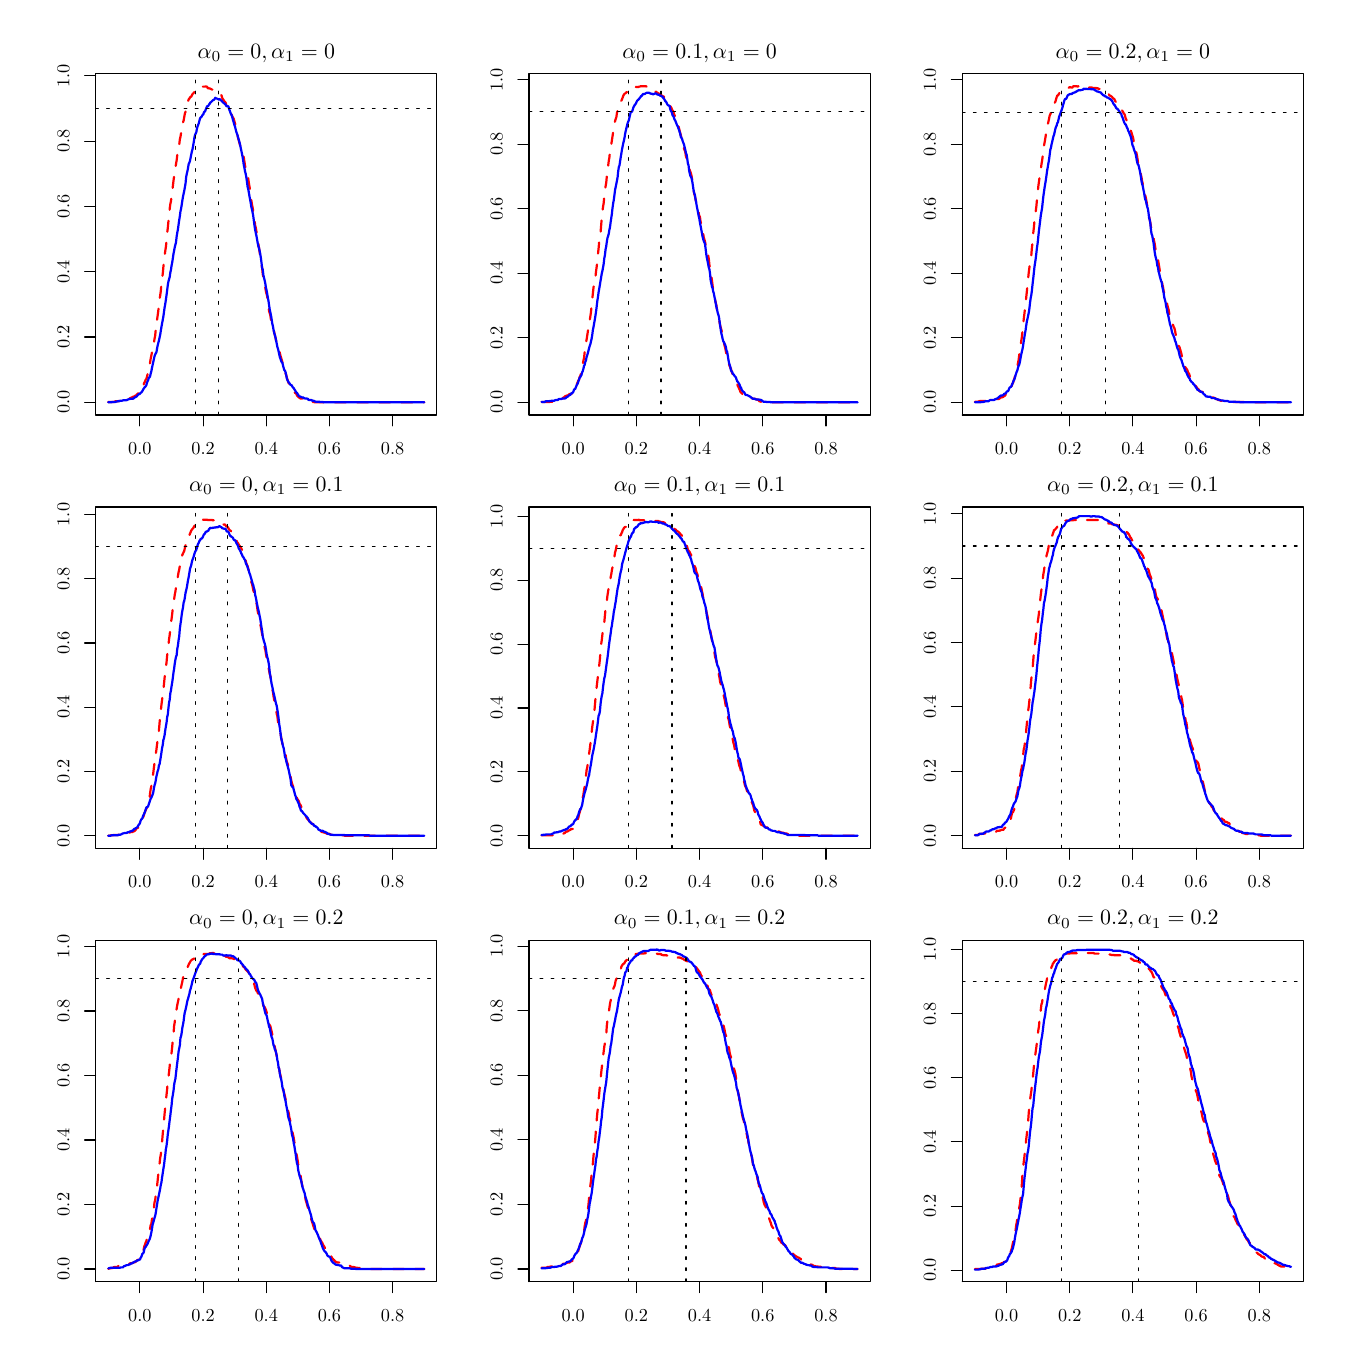
\begin{tikzpicture}[x=1pt,y=1pt]
\definecolor{fillColor}{RGB}{255,255,255}
\path[use as bounding box,fill=fillColor,fill opacity=0.00] (0,0) rectangle (469.75,469.75);
\begin{scope}
\path[clip] ( 24.55,329.80) rectangle (147.87,453.12);
\definecolor{drawColor}{RGB}{255,0,0}

\path[draw=drawColor,line width= 0.8pt,dash pattern=on 4pt off 4pt ,line join=round,line cap=round] ( 29.12,334.49) --
	( 29.35,334.49) --
	( 29.58,334.49) --
	( 29.81,334.49) --
	( 30.03,334.49) --
	( 30.26,334.49) --
	( 30.49,334.49) --
	( 30.72,334.49) --
	( 30.95,334.49) --
	( 31.18,334.49) --
	( 31.41,334.61) --
	( 31.64,334.72) --
	( 31.87,334.72) --
	( 32.09,334.72) --
	( 32.32,334.72) --
	( 32.55,334.72) --
	( 32.78,334.84) --
	( 33.01,334.84) --
	( 33.24,334.84) --
	( 33.47,334.84) --
	( 33.70,334.84) --
	( 33.92,334.84) --
	( 34.15,334.96) --
	( 34.38,334.96) --
	( 34.61,334.96) --
	( 34.84,334.96) --
	( 35.07,334.96) --
	( 35.30,334.96) --
	( 35.53,335.08) --
	( 35.76,335.20) --
	( 35.98,335.43) --
	( 36.21,335.43) --
	( 36.44,335.67) --
	( 36.67,335.78) --
	( 36.90,335.78) --
	( 37.13,335.90) --
	( 37.36,336.02) --
	( 37.59,336.02) --
	( 37.81,336.26) --
	( 38.04,336.37) --
	( 38.27,336.37) --
	( 38.50,336.37) --
	( 38.73,336.73) --
	( 38.96,336.73) --
	( 39.19,336.85) --
	( 39.42,337.20) --
	( 39.65,337.32) --
	( 39.87,337.55) --
	( 40.10,337.79) --
	( 40.33,337.91) --
	( 40.56,337.91) --
	( 40.79,338.38) --
	( 41.02,338.62) --
	( 41.25,338.85) --
	( 41.48,339.32) --
	( 41.71,339.91) --
	( 41.93,340.86) --
	( 42.16,341.45) --
	( 42.39,341.80) --
	( 42.62,342.51) --
	( 42.85,342.74) --
	( 43.08,343.45) --
	( 43.31,344.40) --
	( 43.54,345.93) --
	( 43.76,346.76) --
	( 43.99,347.70) --
	( 44.22,348.64) --
	( 44.45,350.18) --
	( 44.68,351.24) --
	( 44.91,352.42) --
	( 45.14,353.72) --
	( 45.37,354.54) --
	( 45.60,355.72) --
	( 45.82,357.25) --
	( 46.05,358.32) --
	( 46.28,360.56) --
	( 46.51,362.09) --
	( 46.74,364.10) --
	( 46.97,365.75) --
	( 47.20,367.40) --
	( 47.43,369.88) --
	( 47.65,371.53) --
	( 47.88,372.94) --
	( 48.11,374.59) --
	( 48.34,377.31) --
	( 48.57,378.96) --
	( 48.80,380.73) --
	( 49.03,383.21) --
	( 49.26,385.33) --
	( 49.49,387.33) --
	( 49.71,388.99) --
	( 49.94,390.52) --
	( 50.17,392.64) --
	( 50.40,395.47) --
	( 50.63,397.36) --
	( 50.86,399.72) --
	( 51.09,401.84) --
	( 51.32,404.32) --
	( 51.54,405.97) --
	( 51.77,407.03) --
	( 52.00,408.80) --
	( 52.23,410.45) --
	( 52.46,412.46) --
	( 52.69,414.46) --
	( 52.92,416.12) --
	( 53.15,417.53) --
	( 53.38,419.07) --
	( 53.60,420.48) --
	( 53.83,421.78) --
	( 54.06,423.78) --
	( 54.29,425.08) --
	( 54.52,426.38) --
	( 54.75,427.32) --
	( 54.98,429.33) --
	( 55.21,430.27) --
	( 55.43,431.69) --
	( 55.66,432.87) --
	( 55.89,434.40) --
	( 56.12,435.46) --
	( 56.35,436.17) --
	( 56.58,437.47) --
	( 56.81,438.76) --
	( 57.04,439.35) --
	( 57.27,440.30) --
	( 57.49,441.24) --
	( 57.72,441.95) --
	( 57.95,443.13) --
	( 58.18,443.84) --
	( 58.41,444.07) --
	( 58.64,444.54) --
	( 58.87,444.78) --
	( 59.10,444.78) --
	( 59.32,445.25) --
	( 59.55,445.72) --
	( 59.78,445.96) --
	( 60.01,446.20) --
	( 60.24,446.55) --
	( 60.47,446.55) --
	( 60.70,446.67) --
	( 60.93,447.02) --
	( 61.16,447.38) --
	( 61.38,447.61) --
	( 61.61,447.73) --
	( 61.84,448.08) --
	( 62.07,448.20) --
	( 62.30,448.20) --
	( 62.53,448.32) --
	( 62.76,448.44) --
	( 62.99,448.44) --
	( 63.22,448.44) --
	( 63.44,448.44) --
	( 63.67,448.44) --
	( 63.90,448.44) --
	( 64.13,448.44) --
	( 64.36,448.56) --
	( 64.59,448.44) --
	( 64.82,448.44) --
	( 65.05,447.85) --
	( 65.27,447.85) --
	( 65.50,447.85) --
	( 65.73,447.73) --
	( 65.96,447.73) --
	( 66.19,447.61) --
	( 66.42,447.49) --
	( 66.65,447.38) --
	( 66.88,447.38) --
	( 67.11,447.38) --
	( 67.33,447.02) --
	( 67.56,447.02) --
	( 67.79,446.79) --
	( 68.02,446.67) --
	( 68.25,446.55) --
	( 68.48,446.43) --
	( 68.71,446.20) --
	( 68.94,446.08) --
	( 69.16,445.96) --
	( 69.39,445.96) --
	( 69.62,445.84) --
	( 69.85,445.61) --
	( 70.08,445.13) --
	( 70.31,444.31) --
	( 70.54,443.96) --
	( 70.77,443.60) --
	( 71.00,443.25) --
	( 71.22,443.01) --
	( 71.45,442.78) --
	( 71.68,442.19) --
	( 71.91,441.48) --
	( 72.14,441.36) --
	( 72.37,441.01) --
	( 72.60,440.89) --
	( 72.83,440.65) --
	( 73.05,440.18) --
	( 73.28,439.71) --
	( 73.51,438.76) --
	( 73.74,438.17) --
	( 73.97,437.59) --
	( 74.20,437.23) --
	( 74.43,436.88) --
	( 74.66,436.05) --
	( 74.89,435.23) --
	( 75.11,434.64) --
	( 75.34,433.34) --
	( 75.57,432.16) --
	( 75.80,431.10) --
	( 76.03,429.92) --
	( 76.26,429.09) --
	( 76.49,428.15) --
	( 76.72,427.32) --
	( 76.94,426.73) --
	( 77.17,426.38) --
	( 77.40,425.44) --
	( 77.63,424.61) --
	( 77.86,423.67) --
	( 78.09,422.84) --
	( 78.32,421.31) --
	( 78.55,419.89) --
	( 78.78,418.71) --
	( 79.00,418.24) --
	( 79.23,417.41) --
	( 79.46,416.12) --
	( 79.69,415.29) --
	( 79.92,413.64) --
	( 80.15,412.34) --
	( 80.38,410.93) --
	( 80.61,409.27) --
	( 80.83,407.27) --
	( 81.06,405.74) --
	( 81.29,404.67) --
	( 81.52,403.26) --
	( 81.75,401.73) --
	( 81.98,399.96) --
	( 82.21,398.30) --
	( 82.44,397.36) --
	( 82.67,396.06) --
	( 82.89,394.77) --
	( 83.12,393.59) --
	( 83.35,391.58) --
	( 83.58,390.28) --
	( 83.81,388.63) --
	( 84.04,387.45) --
	( 84.27,386.04) --
	( 84.50,384.03) --
	( 84.73,382.85) --
	( 84.95,380.61) --
	( 85.18,379.55) --
	( 85.41,378.37) --
	( 85.64,377.19) --
	( 85.87,375.77) --
	( 86.10,374.36) --
	( 86.33,373.53) --
	( 86.56,372.59) --
	( 86.78,370.82) --
	( 87.01,368.93) --
	( 87.24,367.28) --
	( 87.47,366.57) --
	( 87.70,365.75) --
	( 87.93,363.98) --
	( 88.16,363.03) --
	( 88.39,361.85) --
	( 88.62,361.26) --
	( 88.84,360.44) --
	( 89.07,359.85) --
	( 89.30,358.67) --
	( 89.53,357.84) --
	( 89.76,356.66) --
	( 89.99,355.84) --
	( 90.22,355.01) --
	( 90.45,353.95) --
	( 90.67,353.36) --
	( 90.90,352.77) --
	( 91.13,352.18) --
	( 91.36,351.12) --
	( 91.59,350.41) --
	( 91.82,349.70) --
	( 92.05,348.76) --
	( 92.28,347.23) --
	( 92.51,346.52) --
	( 92.73,345.58) --
	( 92.96,345.10) --
	( 93.19,344.75) --
	( 93.42,344.28) --
	( 93.65,343.33) --
	( 93.88,342.51) --
	( 94.11,341.92) --
	( 94.34,341.21) --
	( 94.56,340.50) --
	( 94.79,340.27) --
	( 95.02,339.80) --
	( 95.25,339.44) --
	( 95.48,339.09) --
	( 95.71,338.73) --
	( 95.94,338.26) --
	( 96.17,338.26) --
	( 96.40,337.91) --
	( 96.62,337.79) --
	( 96.85,337.67) --
	( 97.08,337.44) --
	( 97.31,336.85) --
	( 97.54,336.61) --
	( 97.77,336.37) --
	( 98.00,336.14) --
	( 98.23,336.02) --
	( 98.45,335.78) --
	( 98.68,335.78) --
	( 98.91,335.78) --
	( 99.14,335.78) --
	( 99.37,335.78) --
	( 99.60,335.67) --
	( 99.83,335.67) --
	(100.06,335.55) --
	(100.29,335.43) --
	(100.51,335.31) --
	(100.74,334.96) --
	(100.97,334.96) --
	(101.20,334.84) --
	(101.43,334.61) --
	(101.66,334.49) --
	(101.89,334.49) --
	(102.12,334.49) --
	(102.35,334.49) --
	(102.57,334.49) --
	(102.80,334.49) --
	(103.03,334.49) --
	(103.26,334.49) --
	(103.49,334.49) --
	(103.72,334.37) --
	(103.95,334.37) --
	(104.18,334.37) --
	(104.40,334.37) --
	(104.63,334.37) --
	(104.86,334.37) --
	(105.09,334.37) --
	(105.32,334.37) --
	(105.55,334.37) --
	(105.78,334.37) --
	(106.01,334.37) --
	(106.24,334.37) --
	(106.46,334.37) --
	(106.69,334.37) --
	(106.92,334.37) --
	(107.15,334.37) --
	(107.38,334.37) --
	(107.61,334.37) --
	(107.84,334.37) --
	(108.07,334.37) --
	(108.29,334.37) --
	(108.52,334.37) --
	(108.75,334.37) --
	(108.98,334.37) --
	(109.21,334.37) --
	(109.44,334.37) --
	(109.67,334.37) --
	(109.90,334.37) --
	(110.13,334.37) --
	(110.35,334.37) --
	(110.58,334.37) --
	(110.81,334.37) --
	(111.04,334.37) --
	(111.27,334.37) --
	(111.50,334.37) --
	(111.73,334.37) --
	(111.96,334.37) --
	(112.18,334.37) --
	(112.41,334.37) --
	(112.64,334.37) --
	(112.87,334.37) --
	(113.10,334.37) --
	(113.33,334.37) --
	(113.56,334.37) --
	(113.79,334.37) --
	(114.02,334.37) --
	(114.24,334.37) --
	(114.47,334.37) --
	(114.70,334.37) --
	(114.93,334.37) --
	(115.16,334.37) --
	(115.39,334.37) --
	(115.62,334.37) --
	(115.85,334.37) --
	(116.07,334.37) --
	(116.30,334.37) --
	(116.53,334.37) --
	(116.76,334.37) --
	(116.99,334.37) --
	(117.22,334.37) --
	(117.45,334.37) --
	(117.68,334.37) --
	(117.91,334.37) --
	(118.13,334.37) --
	(118.36,334.37) --
	(118.59,334.37) --
	(118.82,334.37) --
	(119.05,334.37) --
	(119.28,334.37) --
	(119.51,334.37) --
	(119.74,334.37) --
	(119.96,334.37) --
	(120.19,334.37) --
	(120.42,334.37) --
	(120.65,334.37) --
	(120.88,334.37) --
	(121.11,334.37) --
	(121.34,334.37) --
	(121.57,334.37) --
	(121.80,334.37) --
	(122.02,334.37) --
	(122.25,334.37) --
	(122.48,334.37) --
	(122.71,334.37) --
	(122.94,334.37) --
	(123.17,334.37) --
	(123.40,334.37) --
	(123.63,334.37) --
	(123.86,334.37) --
	(124.08,334.37) --
	(124.31,334.37) --
	(124.54,334.37) --
	(124.77,334.37) --
	(125.00,334.37) --
	(125.23,334.37) --
	(125.46,334.37) --
	(125.69,334.37) --
	(125.91,334.37) --
	(126.14,334.37) --
	(126.37,334.37) --
	(126.60,334.37) --
	(126.83,334.37) --
	(127.06,334.37) --
	(127.29,334.37) --
	(127.52,334.37) --
	(127.75,334.37) --
	(127.97,334.37) --
	(128.20,334.37) --
	(128.43,334.37) --
	(128.66,334.37) --
	(128.89,334.37) --
	(129.12,334.37) --
	(129.35,334.37) --
	(129.58,334.37) --
	(129.80,334.37) --
	(130.03,334.37) --
	(130.26,334.37) --
	(130.49,334.37) --
	(130.72,334.37) --
	(130.95,334.37) --
	(131.18,334.37) --
	(131.41,334.37) --
	(131.64,334.37) --
	(131.86,334.37) --
	(132.09,334.37) --
	(132.32,334.37) --
	(132.55,334.37) --
	(132.78,334.37) --
	(133.01,334.37) --
	(133.24,334.37) --
	(133.47,334.37) --
	(133.69,334.37) --
	(133.92,334.37) --
	(134.15,334.37) --
	(134.38,334.37) --
	(134.61,334.37) --
	(134.84,334.37) --
	(135.07,334.37) --
	(135.30,334.37) --
	(135.53,334.37) --
	(135.75,334.37) --
	(135.98,334.37) --
	(136.21,334.37) --
	(136.44,334.37) --
	(136.67,334.37) --
	(136.90,334.37) --
	(137.13,334.37) --
	(137.36,334.37) --
	(137.58,334.37) --
	(137.81,334.37) --
	(138.04,334.37) --
	(138.27,334.37) --
	(138.50,334.37) --
	(138.73,334.37) --
	(138.96,334.37) --
	(139.19,334.37) --
	(139.42,334.37) --
	(139.64,334.37) --
	(139.87,334.37) --
	(140.10,334.37) --
	(140.33,334.37) --
	(140.56,334.37) --
	(140.79,334.37) --
	(141.02,334.37) --
	(141.25,334.37) --
	(141.47,334.37) --
	(141.70,334.37) --
	(141.93,334.37) --
	(142.16,334.37) --
	(142.39,334.37) --
	(142.62,334.37) --
	(142.85,334.37) --
	(143.08,334.37) --
	(143.31,334.37);
\end{scope}
\begin{scope}
\path[clip] (  0.00,  0.00) rectangle (469.75,469.75);
\definecolor{drawColor}{RGB}{0,0,0}

\path[draw=drawColor,line width= 0.4pt,line join=round,line cap=round] ( 40.54,329.80) -- (131.89,329.80);

\path[draw=drawColor,line width= 0.4pt,line join=round,line cap=round] ( 40.54,329.80) -- ( 40.54,325.84);

\path[draw=drawColor,line width= 0.4pt,line join=round,line cap=round] ( 63.38,329.80) -- ( 63.38,325.84);

\path[draw=drawColor,line width= 0.4pt,line join=round,line cap=round] ( 86.21,329.80) -- ( 86.21,325.84);

\path[draw=drawColor,line width= 0.4pt,line join=round,line cap=round] (109.05,329.80) -- (109.05,325.84);

\path[draw=drawColor,line width= 0.4pt,line join=round,line cap=round] (131.89,329.80) -- (131.89,325.84);

\node[text=drawColor,anchor=base,inner sep=0pt, outer sep=0pt, scale=  0.66] at ( 40.54,315.55) {0.0};

\node[text=drawColor,anchor=base,inner sep=0pt, outer sep=0pt, scale=  0.66] at ( 63.38,315.55) {0.2};

\node[text=drawColor,anchor=base,inner sep=0pt, outer sep=0pt, scale=  0.66] at ( 86.21,315.55) {0.4};

\node[text=drawColor,anchor=base,inner sep=0pt, outer sep=0pt, scale=  0.66] at (109.05,315.55) {0.6};

\node[text=drawColor,anchor=base,inner sep=0pt, outer sep=0pt, scale=  0.66] at (131.89,315.55) {0.8};

\path[draw=drawColor,line width= 0.4pt,line join=round,line cap=round] ( 24.55,334.37) -- ( 24.55,452.33);

\path[draw=drawColor,line width= 0.4pt,line join=round,line cap=round] ( 24.55,334.37) -- ( 20.59,334.37);

\path[draw=drawColor,line width= 0.4pt,line join=round,line cap=round] ( 24.55,357.96) -- ( 20.59,357.96);

\path[draw=drawColor,line width= 0.4pt,line join=round,line cap=round] ( 24.55,381.55) -- ( 20.59,381.55);

\path[draw=drawColor,line width= 0.4pt,line join=round,line cap=round] ( 24.55,405.15) -- ( 20.59,405.15);

\path[draw=drawColor,line width= 0.4pt,line join=round,line cap=round] ( 24.55,428.74) -- ( 20.59,428.74);

\path[draw=drawColor,line width= 0.4pt,line join=round,line cap=round] ( 24.55,452.33) -- ( 20.59,452.33);

\node[text=drawColor,rotate= 90.00,anchor=base,inner sep=0pt, outer sep=0pt, scale=  0.66] at ( 15.05,334.37) {0.0};

\node[text=drawColor,rotate= 90.00,anchor=base,inner sep=0pt, outer sep=0pt, scale=  0.66] at ( 15.05,357.96) {0.2};

\node[text=drawColor,rotate= 90.00,anchor=base,inner sep=0pt, outer sep=0pt, scale=  0.66] at ( 15.05,381.55) {0.4};

\node[text=drawColor,rotate= 90.00,anchor=base,inner sep=0pt, outer sep=0pt, scale=  0.66] at ( 15.05,405.15) {0.6};

\node[text=drawColor,rotate= 90.00,anchor=base,inner sep=0pt, outer sep=0pt, scale=  0.66] at ( 15.05,428.74) {0.8};

\node[text=drawColor,rotate= 90.00,anchor=base,inner sep=0pt, outer sep=0pt, scale=  0.66] at ( 15.05,452.33) {1.0};

\path[draw=drawColor,line width= 0.4pt,line join=round,line cap=round] ( 24.55,329.80) --
	(147.87,329.80) --
	(147.87,453.12) --
	( 24.55,453.12) --
	( 24.55,329.80);
\end{scope}
\begin{scope}
\path[clip] (  0.00,313.17) rectangle (156.58,469.75);
\definecolor{drawColor}{RGB}{0,0,0}

\node[text=drawColor,anchor=base,inner sep=0pt, outer sep=0pt, scale=  0.79] at ( 86.21,458.71) {\bfseries $\alpha_0 = 0, \alpha_1 = 0$};
\end{scope}
\begin{scope}
\path[clip] ( 24.55,329.80) rectangle (147.87,453.12);
\definecolor{drawColor}{RGB}{0,0,255}

\path[draw=drawColor,line width= 0.8pt,line join=round,line cap=round] ( 29.12,334.37) --
	( 29.35,334.37) --
	( 29.58,334.37) --
	( 29.81,334.37) --
	( 30.03,334.37) --
	( 30.26,334.37) --
	( 30.49,334.49) --
	( 30.72,334.49) --
	( 30.95,334.49) --
	( 31.18,334.49) --
	( 31.41,334.49) --
	( 31.64,334.49) --
	( 31.87,334.61) --
	( 32.09,334.61) --
	( 32.32,334.72) --
	( 32.55,334.72) --
	( 32.78,334.72) --
	( 33.01,334.72) --
	( 33.24,334.84) --
	( 33.47,334.96) --
	( 33.70,334.96) --
	( 33.92,334.96) --
	( 34.15,334.96) --
	( 34.38,335.08) --
	( 34.61,335.08) --
	( 34.84,335.08) --
	( 35.07,335.08) --
	( 35.30,335.08) --
	( 35.53,335.08) --
	( 35.76,335.20) --
	( 35.98,335.20) --
	( 36.21,335.43) --
	( 36.44,335.43) --
	( 36.67,335.55) --
	( 36.90,335.55) --
	( 37.13,335.67) --
	( 37.36,335.67) --
	( 37.59,335.67) --
	( 37.81,335.67) --
	( 38.04,335.67) --
	( 38.27,335.78) --
	( 38.50,336.02) --
	( 38.73,336.14) --
	( 38.96,336.26) --
	( 39.19,336.37) --
	( 39.42,336.49) --
	( 39.65,336.85) --
	( 39.87,337.08) --
	( 40.10,337.32) --
	( 40.33,337.32) --
	( 40.56,337.44) --
	( 40.79,337.79) --
	( 41.02,337.91) --
	( 41.25,338.14) --
	( 41.48,338.50) --
	( 41.71,338.97) --
	( 41.93,339.32) --
	( 42.16,339.68) --
	( 42.39,339.91) --
	( 42.62,340.15) --
	( 42.85,340.50) --
	( 43.08,341.33) --
	( 43.31,341.92) --
	( 43.54,342.39) --
	( 43.76,343.22) --
	( 43.99,343.33) --
	( 44.22,343.69) --
	( 44.45,344.75) --
	( 44.68,345.58) --
	( 44.91,346.76) --
	( 45.14,347.82) --
	( 45.37,348.88) --
	( 45.60,349.94) --
	( 45.82,351.00) --
	( 46.05,351.59) --
	( 46.28,352.06) --
	( 46.51,352.42) --
	( 46.74,353.72) --
	( 46.97,354.89) --
	( 47.20,355.84) --
	( 47.43,356.66) --
	( 47.65,357.73) --
	( 47.88,358.79) --
	( 48.11,360.20) --
	( 48.34,361.62) --
	( 48.57,362.92) --
	( 48.80,364.10) --
	( 49.03,365.39) --
	( 49.26,367.04) --
	( 49.49,368.70) --
	( 49.71,369.88) --
	( 49.94,371.41) --
	( 50.17,373.06) --
	( 50.40,374.83) --
	( 50.63,376.72) --
	( 50.86,378.01) --
	( 51.09,378.84) --
	( 51.32,379.67) --
	( 51.54,381.20) --
	( 51.77,382.26) --
	( 52.00,383.80) --
	( 52.23,384.97) --
	( 52.46,386.39) --
	( 52.69,388.04) --
	( 52.92,389.22) --
	( 53.15,390.40) --
	( 53.38,391.34) --
	( 53.60,392.17) --
	( 53.83,394.29) --
	( 54.06,395.71) --
	( 54.29,396.89) --
	( 54.52,398.54) --
	( 54.75,400.19) --
	( 54.98,401.61) --
	( 55.21,403.38) --
	( 55.43,404.32) --
	( 55.66,405.74) --
	( 55.89,407.27) --
	( 56.12,408.68) --
	( 56.35,409.75) --
	( 56.58,410.81) --
	( 56.81,412.11) --
	( 57.04,413.40) --
	( 57.27,415.76) --
	( 57.49,416.94) --
	( 57.72,417.89) --
	( 57.95,419.07) --
	( 58.18,420.48) --
	( 58.41,420.95) --
	( 58.64,421.54) --
	( 58.87,422.72) --
	( 59.10,423.90) --
	( 59.32,424.96) --
	( 59.55,425.79) --
	( 59.78,426.97) --
	( 60.01,428.38) --
	( 60.24,429.92) --
	( 60.47,430.98) --
	( 60.70,431.45) --
	( 60.93,431.92) --
	( 61.16,433.22) --
	( 61.38,434.05) --
	( 61.61,434.64) --
	( 61.84,435.23) --
	( 62.07,436.17) --
	( 62.30,437.00) --
	( 62.53,437.35) --
	( 62.76,437.47) --
	( 62.99,437.82) --
	( 63.22,438.29) --
	( 63.44,438.29) --
	( 63.67,439.12) --
	( 63.90,439.35) --
	( 64.13,439.59) --
	( 64.36,440.18) --
	( 64.59,440.77) --
	( 64.82,441.36) --
	( 65.05,441.36) --
	( 65.27,441.48) --
	( 65.50,441.95) --
	( 65.73,442.19) --
	( 65.96,442.66) --
	( 66.19,442.78) --
	( 66.42,443.01) --
	( 66.65,443.25) --
	( 66.88,443.48) --
	( 67.11,443.60) --
	( 67.33,443.72) --
	( 67.56,443.96) --
	( 67.79,444.43) --
	( 68.02,444.19) --
	( 68.25,444.19) --
	( 68.48,444.07) --
	( 68.71,443.96) --
	( 68.94,443.84) --
	( 69.16,443.72) --
	( 69.39,443.96) --
	( 69.62,443.72) --
	( 69.85,443.48) --
	( 70.08,443.37) --
	( 70.31,443.01) --
	( 70.54,442.78) --
	( 70.77,442.54) --
	( 71.00,442.42) --
	( 71.22,442.19) --
	( 71.45,442.07) --
	( 71.68,441.60) --
	( 71.91,441.36) --
	( 72.14,441.36) --
	( 72.37,441.36) --
	( 72.60,441.12) --
	( 72.83,440.18) --
	( 73.05,439.71) --
	( 73.28,439.00) --
	( 73.51,438.41) --
	( 73.74,438.06) --
	( 73.97,437.23) --
	( 74.20,436.29) --
	( 74.43,435.58) --
	( 74.66,434.64) --
	( 74.89,434.16) --
	( 75.11,433.22) --
	( 75.34,432.28) --
	( 75.57,431.57) --
	( 75.80,430.98) --
	( 76.03,430.04) --
	( 76.26,429.33) --
	( 76.49,428.50) --
	( 76.72,427.68) --
	( 76.94,426.50) --
	( 77.17,425.44) --
	( 77.40,424.37) --
	( 77.63,423.19) --
	( 77.86,421.78) --
	( 78.09,420.13) --
	( 78.32,419.07) --
	( 78.55,417.77) --
	( 78.78,416.94) --
	( 79.00,415.76) --
	( 79.23,414.11) --
	( 79.46,412.34) --
	( 79.69,411.40) --
	( 79.92,410.22) --
	( 80.15,408.80) --
	( 80.38,407.62) --
	( 80.61,406.33) --
	( 80.83,404.91) --
	( 81.06,403.97) --
	( 81.29,402.90) --
	( 81.52,401.61) --
	( 81.75,399.84) --
	( 81.98,398.07) --
	( 82.21,396.65) --
	( 82.44,395.47) --
	( 82.67,394.53) --
	( 82.89,393.23) --
	( 83.12,391.93) --
	( 83.35,390.75) --
	( 83.58,390.16) --
	( 83.81,389.10) --
	( 84.04,387.92) --
	( 84.27,386.51) --
	( 84.50,384.74) --
	( 84.73,382.85) --
	( 84.95,382.26) --
	( 85.18,380.26) --
	( 85.41,379.31) --
	( 85.64,378.37) --
	( 85.87,377.31) --
	( 86.10,375.77) --
	( 86.33,374.83) --
	( 86.56,373.53) --
	( 86.78,372.23) --
	( 87.01,371.06) --
	( 87.24,369.40) --
	( 87.47,367.87) --
	( 87.70,366.81) --
	( 87.93,365.75) --
	( 88.16,364.33) --
	( 88.39,362.80) --
	( 88.62,361.85) --
	( 88.84,360.56) --
	( 89.07,359.50) --
	( 89.30,358.79) --
	( 89.53,357.84) --
	( 89.76,356.78) --
	( 89.99,355.60) --
	( 90.22,354.42) --
	( 90.45,353.72) --
	( 90.67,352.77) --
	( 90.90,351.71) --
	( 91.13,350.65) --
	( 91.36,350.06) --
	( 91.59,349.35) --
	( 91.82,348.88) --
	( 92.05,348.64) --
	( 92.28,347.58) --
	( 92.51,346.76) --
	( 92.73,346.05) --
	( 92.96,345.81) --
	( 93.19,345.22) --
	( 93.42,344.16) --
	( 93.65,342.98) --
	( 93.88,342.39) --
	( 94.11,341.92) --
	( 94.34,341.57) --
	( 94.56,341.33) --
	( 94.79,340.98) --
	( 95.02,340.62) --
	( 95.25,340.62) --
	( 95.48,340.39) --
	( 95.71,339.91) --
	( 95.94,339.68) --
	( 96.17,339.44) --
	( 96.40,338.97) --
	( 96.62,338.73) --
	( 96.85,338.26) --
	( 97.08,337.91) --
	( 97.31,337.79) --
	( 97.54,337.32) --
	( 97.77,337.08) --
	( 98.00,336.61) --
	( 98.23,336.49) --
	( 98.45,336.49) --
	( 98.68,336.37) --
	( 98.91,336.26) --
	( 99.14,336.14) --
	( 99.37,336.14) --
	( 99.60,336.14) --
	( 99.83,335.90) --
	(100.06,335.78) --
	(100.29,335.78) --
	(100.51,335.78) --
	(100.74,335.78) --
	(100.97,335.67) --
	(101.20,335.67) --
	(101.43,335.31) --
	(101.66,335.20) --
	(101.89,335.20) --
	(102.12,335.20) --
	(102.35,335.20) --
	(102.57,335.20) --
	(102.80,334.96) --
	(103.03,334.96) --
	(103.26,334.96) --
	(103.49,334.84) --
	(103.72,334.72) --
	(103.95,334.61) --
	(104.18,334.61) --
	(104.40,334.61) --
	(104.63,334.61) --
	(104.86,334.61) --
	(105.09,334.61) --
	(105.32,334.61) --
	(105.55,334.49) --
	(105.78,334.49) --
	(106.01,334.49) --
	(106.24,334.49) --
	(106.46,334.49) --
	(106.69,334.49) --
	(106.92,334.37) --
	(107.15,334.37) --
	(107.38,334.37) --
	(107.61,334.37) --
	(107.84,334.37) --
	(108.07,334.37) --
	(108.29,334.37) --
	(108.52,334.37) --
	(108.75,334.37) --
	(108.98,334.37) --
	(109.21,334.37) --
	(109.44,334.37) --
	(109.67,334.37) --
	(109.90,334.37) --
	(110.13,334.37) --
	(110.35,334.37) --
	(110.58,334.37) --
	(110.81,334.37) --
	(111.04,334.37) --
	(111.27,334.37) --
	(111.50,334.37) --
	(111.73,334.37) --
	(111.96,334.37) --
	(112.18,334.37) --
	(112.41,334.37) --
	(112.64,334.37) --
	(112.87,334.37) --
	(113.10,334.37) --
	(113.33,334.37) --
	(113.56,334.37) --
	(113.79,334.37) --
	(114.02,334.37) --
	(114.24,334.37) --
	(114.47,334.37) --
	(114.70,334.37) --
	(114.93,334.37) --
	(115.16,334.37) --
	(115.39,334.37) --
	(115.62,334.37) --
	(115.85,334.37) --
	(116.07,334.37) --
	(116.30,334.37) --
	(116.53,334.37) --
	(116.76,334.37) --
	(116.99,334.37) --
	(117.22,334.37) --
	(117.45,334.37) --
	(117.68,334.37) --
	(117.91,334.37) --
	(118.13,334.37) --
	(118.36,334.37) --
	(118.59,334.37) --
	(118.82,334.37) --
	(119.05,334.37) --
	(119.28,334.37) --
	(119.51,334.37) --
	(119.74,334.37) --
	(119.96,334.37) --
	(120.19,334.37) --
	(120.42,334.37) --
	(120.65,334.37) --
	(120.88,334.37) --
	(121.11,334.37) --
	(121.34,334.37) --
	(121.57,334.37) --
	(121.80,334.37) --
	(122.02,334.37) --
	(122.25,334.37) --
	(122.48,334.37) --
	(122.71,334.37) --
	(122.94,334.37) --
	(123.17,334.37) --
	(123.40,334.37) --
	(123.63,334.37) --
	(123.86,334.37) --
	(124.08,334.37) --
	(124.31,334.37) --
	(124.54,334.37) --
	(124.77,334.37) --
	(125.00,334.37) --
	(125.23,334.37) --
	(125.46,334.37) --
	(125.69,334.37) --
	(125.91,334.37) --
	(126.14,334.37) --
	(126.37,334.37) --
	(126.60,334.37) --
	(126.83,334.37) --
	(127.06,334.37) --
	(127.29,334.37) --
	(127.52,334.37) --
	(127.75,334.37) --
	(127.97,334.37) --
	(128.20,334.37) --
	(128.43,334.37) --
	(128.66,334.37) --
	(128.89,334.37) --
	(129.12,334.37) --
	(129.35,334.37) --
	(129.58,334.37) --
	(129.80,334.37) --
	(130.03,334.37) --
	(130.26,334.37) --
	(130.49,334.37) --
	(130.72,334.37) --
	(130.95,334.37) --
	(131.18,334.37) --
	(131.41,334.37) --
	(131.64,334.37) --
	(131.86,334.37) --
	(132.09,334.37) --
	(132.32,334.37) --
	(132.55,334.37) --
	(132.78,334.37) --
	(133.01,334.37) --
	(133.24,334.37) --
	(133.47,334.37) --
	(133.69,334.37) --
	(133.92,334.37) --
	(134.15,334.37) --
	(134.38,334.37) --
	(134.61,334.37) --
	(134.84,334.37) --
	(135.07,334.37) --
	(135.30,334.37) --
	(135.53,334.37) --
	(135.75,334.37) --
	(135.98,334.37) --
	(136.21,334.37) --
	(136.44,334.37) --
	(136.67,334.37) --
	(136.90,334.37) --
	(137.13,334.37) --
	(137.36,334.37) --
	(137.58,334.37) --
	(137.81,334.37) --
	(138.04,334.37) --
	(138.27,334.37) --
	(138.50,334.37) --
	(138.73,334.37) --
	(138.96,334.37) --
	(139.19,334.37) --
	(139.42,334.37) --
	(139.64,334.37) --
	(139.87,334.37) --
	(140.10,334.37) --
	(140.33,334.37) --
	(140.56,334.37) --
	(140.79,334.37) --
	(141.02,334.37) --
	(141.25,334.37) --
	(141.47,334.37) --
	(141.70,334.37) --
	(141.93,334.37) --
	(142.16,334.37) --
	(142.39,334.37) --
	(142.62,334.37) --
	(142.85,334.37) --
	(143.08,334.37) --
	(143.31,334.37);
\definecolor{drawColor}{RGB}{0,0,0}

\path[draw=drawColor,line width= 0.4pt,dash pattern=on 1pt off 3pt ,line join=round,line cap=round] ( 24.55,440.53) -- (147.87,440.53);

\path[draw=drawColor,line width= 0.4pt,dash pattern=on 1pt off 3pt ,line join=round,line cap=round] ( 60.52,329.80) -- ( 60.52,453.12);

\path[draw=drawColor,line width= 0.4pt,dash pattern=on 1pt off 3pt ,line join=round,line cap=round] ( 69.08,329.80) -- ( 69.08,453.12);
\end{scope}
\begin{scope}
\path[clip] (181.14,329.80) rectangle (304.46,453.12);
\definecolor{drawColor}{RGB}{255,0,0}

\path[draw=drawColor,line width= 0.8pt,dash pattern=on 4pt off 4pt ,line join=round,line cap=round] (185.70,334.49) --
	(185.93,334.49) --
	(186.16,334.49) --
	(186.39,334.49) --
	(186.62,334.49) --
	(186.85,334.49) --
	(187.08,334.49) --
	(187.31,334.49) --
	(187.54,334.49) --
	(187.76,334.49) --
	(187.99,334.49) --
	(188.22,334.49) --
	(188.45,334.49) --
	(188.68,334.49) --
	(188.91,334.60) --
	(189.14,334.60) --
	(189.37,334.60) --
	(189.59,334.60) --
	(189.82,334.60) --
	(190.05,334.72) --
	(190.28,334.72) --
	(190.51,334.72) --
	(190.74,334.84) --
	(190.97,334.95) --
	(191.20,334.95) --
	(191.43,334.95) --
	(191.65,334.95) --
	(191.88,334.95) --
	(192.11,335.07) --
	(192.34,335.07) --
	(192.57,335.19) --
	(192.80,335.19) --
	(193.03,335.30) --
	(193.26,335.65) --
	(193.48,336.00) --
	(193.71,336.12) --
	(193.94,336.24) --
	(194.17,336.47) --
	(194.40,336.70) --
	(194.63,336.70) --
	(194.86,336.82) --
	(195.09,336.82) --
	(195.32,336.94) --
	(195.54,337.17) --
	(195.77,337.29) --
	(196.00,337.40) --
	(196.23,337.40) --
	(196.46,337.40) --
	(196.69,337.64) --
	(196.92,337.99) --
	(197.15,338.22) --
	(197.37,338.80) --
	(197.60,339.50) --
	(197.83,340.20) --
	(198.06,340.55) --
	(198.29,341.02) --
	(198.52,341.13) --
	(198.75,341.60) --
	(198.98,342.30) --
	(199.21,342.42) --
	(199.43,343.47) --
	(199.66,343.82) --
	(199.89,344.63) --
	(200.12,345.80) --
	(200.35,346.85) --
	(200.58,348.02) --
	(200.81,349.42) --
	(201.04,350.35) --
	(201.26,352.45) --
	(201.49,354.55) --
	(201.72,355.71) --
	(201.95,357.00) --
	(202.18,358.40) --
	(202.41,359.91) --
	(202.64,361.90) --
	(202.87,362.95) --
	(203.10,363.99) --
	(203.32,365.39) --
	(203.55,367.03) --
	(203.78,369.36) --
	(204.01,371.69) --
	(204.24,373.79) --
	(204.47,375.89) --
	(204.70,377.29) --
	(204.93,378.34) --
	(205.15,379.62) --
	(205.38,381.72) --
	(205.61,383.36) --
	(205.84,385.34) --
	(206.07,387.91) --
	(206.30,390.00) --
	(206.53,392.69) --
	(206.76,394.20) --
	(206.99,395.49) --
	(207.21,398.17) --
	(207.44,400.97) --
	(207.67,403.18) --
	(207.90,404.93) --
	(208.13,406.33) --
	(208.36,409.02) --
	(208.59,411.12) --
	(208.82,412.40) --
	(209.05,413.68) --
	(209.27,415.90) --
	(209.50,417.65) --
	(209.73,419.63) --
	(209.96,421.50) --
	(210.19,422.78) --
	(210.42,425.00) --
	(210.65,426.28) --
	(210.88,427.56) --
	(211.10,428.96) --
	(211.33,430.48) --
	(211.56,432.11) --
	(211.79,433.74) --
	(212.02,434.79) --
	(212.25,435.96) --
	(212.48,436.78) --
	(212.71,437.36) --
	(212.94,438.99) --
	(213.16,439.69) --
	(213.39,440.27) --
	(213.62,440.97) --
	(213.85,441.79) --
	(214.08,442.02) --
	(214.31,442.96) --
	(214.54,443.42) --
	(214.77,443.89) --
	(214.99,444.47) --
	(215.22,445.17) --
	(215.45,445.52) --
	(215.68,445.87) --
	(215.91,445.99) --
	(216.14,446.11) --
	(216.37,446.46) --
	(216.60,446.46) --
	(216.83,446.46) --
	(217.05,446.92) --
	(217.28,447.04) --
	(217.51,447.51) --
	(217.74,447.74) --
	(217.97,447.74) --
	(218.20,447.74) --
	(218.43,447.86) --
	(218.66,447.97) --
	(218.88,447.97) --
	(219.11,448.09) --
	(219.34,448.09) --
	(219.57,448.21) --
	(219.80,448.32) --
	(220.03,448.32) --
	(220.26,448.32) --
	(220.49,448.32) --
	(220.72,448.32) --
	(220.94,448.44) --
	(221.17,448.44) --
	(221.40,448.56) --
	(221.63,448.56) --
	(221.86,448.56) --
	(222.09,448.56) --
	(222.32,448.56) --
	(222.55,448.56) --
	(222.77,448.56) --
	(223.00,448.56) --
	(223.23,448.56) --
	(223.46,448.56) --
	(223.69,448.44) --
	(223.92,448.32) --
	(224.15,448.32) --
	(224.38,448.09) --
	(224.61,448.09) --
	(224.83,447.86) --
	(225.06,447.74) --
	(225.29,447.74) --
	(225.52,447.74) --
	(225.75,447.74) --
	(225.98,447.51) --
	(226.21,447.51) --
	(226.44,447.16) --
	(226.66,446.81) --
	(226.89,446.57) --
	(227.12,446.57) --
	(227.35,446.34) --
	(227.58,446.22) --
	(227.81,445.99) --
	(228.04,445.87) --
	(228.27,445.87) --
	(228.50,445.76) --
	(228.72,445.52) --
	(228.95,445.41) --
	(229.18,445.06) --
	(229.41,444.94) --
	(229.64,444.94) --
	(229.87,444.82) --
	(230.10,444.36) --
	(230.33,444.24) --
	(230.56,444.01) --
	(230.78,443.77) --
	(231.01,443.66) --
	(231.24,443.07) --
	(231.47,442.61) --
	(231.70,442.26) --
	(231.93,441.79) --
	(232.16,441.56) --
	(232.39,441.09) --
	(232.61,440.74) --
	(232.84,440.04) --
	(233.07,439.81) --
	(233.30,439.46) --
	(233.53,438.64) --
	(233.76,438.06) --
	(233.99,437.59) --
	(234.22,437.13) --
	(234.45,436.78) --
	(234.67,436.08) --
	(234.90,435.26) --
	(235.13,434.33) --
	(235.36,433.39) --
	(235.59,432.46) --
	(235.82,431.64) --
	(236.05,430.71) --
	(236.28,430.01) --
	(236.50,429.19) --
	(236.73,428.14) --
	(236.96,426.98) --
	(237.19,425.93) --
	(237.42,425.46) --
	(237.65,424.65) --
	(237.88,423.13) --
	(238.11,422.66) --
	(238.34,421.61) --
	(238.56,420.91) --
	(238.79,419.86) --
	(239.02,419.05) --
	(239.25,418.23) --
	(239.48,417.65) --
	(239.71,416.95) --
	(239.94,415.90) --
	(240.17,414.38) --
	(240.39,412.87) --
	(240.62,411.12) --
	(240.85,409.72) --
	(241.08,409.02) --
	(241.31,407.85) --
	(241.54,406.80) --
	(241.77,405.87) --
	(242.00,404.82) --
	(242.23,403.53) --
	(242.45,402.95) --
	(242.68,401.67) --
	(242.91,401.43) --
	(243.14,399.69) --
	(243.37,398.87) --
	(243.60,397.82) --
	(243.83,396.42) --
	(244.06,395.49) --
	(244.28,394.09) --
	(244.51,393.27) --
	(244.74,392.57) --
	(244.97,391.17) --
	(245.20,390.12) --
	(245.43,389.07) --
	(245.66,388.02) --
	(245.89,387.44) --
	(246.12,386.27) --
	(246.34,384.06) --
	(246.57,382.89) --
	(246.80,381.61) --
	(247.03,379.86) --
	(247.26,378.46) --
	(247.49,376.59) --
	(247.72,374.84) --
	(247.95,373.09) --
	(248.18,372.28) --
	(248.40,371.34) --
	(248.63,370.41) --
	(248.86,369.48) --
	(249.09,367.73) --
	(249.32,366.56) --
	(249.55,365.63) --
	(249.78,364.58) --
	(250.01,363.30) --
	(250.23,362.13) --
	(250.46,361.31) --
	(250.69,360.50) --
	(250.92,359.56) --
	(251.15,358.40) --
	(251.38,357.23) --
	(251.61,355.95) --
	(251.84,354.78) --
	(252.07,353.96) --
	(252.29,352.80) --
	(252.52,351.51) --
	(252.75,350.82) --
	(252.98,349.65) --
	(253.21,348.95) --
	(253.44,348.13) --
	(253.67,347.43) --
	(253.90,346.85) --
	(254.12,346.50) --
	(254.35,345.68) --
	(254.58,344.98) --
	(254.81,344.52) --
	(255.04,344.05) --
	(255.27,343.47) --
	(255.50,343.23) --
	(255.73,342.65) --
	(255.96,341.95) --
	(256.18,341.60) --
	(256.41,340.90) --
	(256.64,340.20) --
	(256.87,339.85) --
	(257.10,339.27) --
	(257.33,338.80) --
	(257.56,338.10) --
	(257.79,337.87) --
	(258.01,337.75) --
	(258.24,337.40) --
	(258.47,336.82) --
	(258.70,336.82) --
	(258.93,336.82) --
	(259.16,336.82) --
	(259.39,336.82) --
	(259.62,336.70) --
	(259.85,336.70) --
	(260.07,336.70) --
	(260.30,336.59) --
	(260.53,336.47) --
	(260.76,336.47) --
	(260.99,336.47) --
	(261.22,336.35) --
	(261.45,336.12) --
	(261.68,335.89) --
	(261.90,335.77) --
	(262.13,335.65) --
	(262.36,335.65) --
	(262.59,335.65) --
	(262.82,335.54) --
	(263.05,335.54) --
	(263.28,335.42) --
	(263.51,335.42) --
	(263.74,335.30) --
	(263.96,335.30) --
	(264.19,334.95) --
	(264.42,334.72) --
	(264.65,334.72) --
	(264.88,334.60) --
	(265.11,334.60) --
	(265.34,334.60) --
	(265.57,334.60) --
	(265.79,334.37) --
	(266.02,334.37) --
	(266.25,334.37) --
	(266.48,334.37) --
	(266.71,334.37) --
	(266.94,334.37) --
	(267.17,334.37) --
	(267.40,334.37) --
	(267.63,334.37) --
	(267.85,334.37) --
	(268.08,334.37) --
	(268.31,334.37) --
	(268.54,334.37) --
	(268.77,334.37) --
	(269.00,334.37) --
	(269.23,334.37) --
	(269.46,334.37) --
	(269.69,334.37) --
	(269.91,334.37) --
	(270.14,334.37) --
	(270.37,334.37) --
	(270.60,334.37) --
	(270.83,334.37) --
	(271.06,334.37) --
	(271.29,334.37) --
	(271.52,334.37) --
	(271.74,334.37) --
	(271.97,334.37) --
	(272.20,334.37) --
	(272.43,334.37) --
	(272.66,334.37) --
	(272.89,334.37) --
	(273.12,334.37) --
	(273.35,334.37) --
	(273.58,334.37) --
	(273.80,334.37) --
	(274.03,334.37) --
	(274.26,334.37) --
	(274.49,334.37) --
	(274.72,334.37) --
	(274.95,334.37) --
	(275.18,334.37) --
	(275.41,334.37) --
	(275.63,334.37) --
	(275.86,334.37) --
	(276.09,334.37) --
	(276.32,334.37) --
	(276.55,334.37) --
	(276.78,334.37) --
	(277.01,334.37) --
	(277.24,334.37) --
	(277.47,334.37) --
	(277.69,334.37) --
	(277.92,334.37) --
	(278.15,334.37) --
	(278.38,334.37) --
	(278.61,334.37) --
	(278.84,334.37) --
	(279.07,334.37) --
	(279.30,334.37) --
	(279.52,334.37) --
	(279.75,334.37) --
	(279.98,334.37) --
	(280.21,334.37) --
	(280.44,334.37) --
	(280.67,334.37) --
	(280.90,334.37) --
	(281.13,334.37) --
	(281.36,334.37) --
	(281.58,334.37) --
	(281.81,334.37) --
	(282.04,334.37) --
	(282.27,334.37) --
	(282.50,334.37) --
	(282.73,334.37) --
	(282.96,334.37) --
	(283.19,334.37) --
	(283.41,334.37) --
	(283.64,334.37) --
	(283.87,334.37) --
	(284.10,334.37) --
	(284.33,334.37) --
	(284.56,334.37) --
	(284.79,334.37) --
	(285.02,334.37) --
	(285.25,334.37) --
	(285.47,334.37) --
	(285.70,334.37) --
	(285.93,334.37) --
	(286.16,334.37) --
	(286.39,334.37) --
	(286.62,334.37) --
	(286.85,334.37) --
	(287.08,334.37) --
	(287.30,334.37) --
	(287.53,334.37) --
	(287.76,334.37) --
	(287.99,334.37) --
	(288.22,334.37) --
	(288.45,334.37) --
	(288.68,334.37) --
	(288.91,334.37) --
	(289.14,334.37) --
	(289.36,334.37) --
	(289.59,334.37) --
	(289.82,334.37) --
	(290.05,334.37) --
	(290.28,334.37) --
	(290.51,334.37) --
	(290.74,334.37) --
	(290.97,334.37) --
	(291.20,334.37) --
	(291.42,334.37) --
	(291.65,334.37) --
	(291.88,334.37) --
	(292.11,334.37) --
	(292.34,334.37) --
	(292.57,334.37) --
	(292.80,334.37) --
	(293.03,334.37) --
	(293.25,334.37) --
	(293.48,334.37) --
	(293.71,334.37) --
	(293.94,334.37) --
	(294.17,334.37) --
	(294.40,334.37) --
	(294.63,334.37) --
	(294.86,334.37) --
	(295.09,334.37) --
	(295.31,334.37) --
	(295.54,334.37) --
	(295.77,334.37) --
	(296.00,334.37) --
	(296.23,334.37) --
	(296.46,334.37) --
	(296.69,334.37) --
	(296.92,334.37) --
	(297.14,334.37) --
	(297.37,334.37) --
	(297.60,334.37) --
	(297.83,334.37) --
	(298.06,334.37) --
	(298.29,334.37) --
	(298.52,334.37) --
	(298.75,334.37) --
	(298.98,334.37) --
	(299.20,334.37) --
	(299.43,334.37) --
	(299.66,334.37) --
	(299.89,334.37);
\end{scope}
\begin{scope}
\path[clip] (  0.00,  0.00) rectangle (469.75,469.75);
\definecolor{drawColor}{RGB}{0,0,0}

\path[draw=drawColor,line width= 0.4pt,line join=round,line cap=round] (197.12,329.80) -- (288.47,329.80);

\path[draw=drawColor,line width= 0.4pt,line join=round,line cap=round] (197.12,329.80) -- (197.12,325.84);

\path[draw=drawColor,line width= 0.4pt,line join=round,line cap=round] (219.96,329.80) -- (219.96,325.84);

\path[draw=drawColor,line width= 0.4pt,line join=round,line cap=round] (242.80,329.80) -- (242.80,325.84);

\path[draw=drawColor,line width= 0.4pt,line join=round,line cap=round] (265.63,329.80) -- (265.63,325.84);

\path[draw=drawColor,line width= 0.4pt,line join=round,line cap=round] (288.47,329.80) -- (288.47,325.84);

\node[text=drawColor,anchor=base,inner sep=0pt, outer sep=0pt, scale=  0.66] at (197.12,315.55) {0.0};

\node[text=drawColor,anchor=base,inner sep=0pt, outer sep=0pt, scale=  0.66] at (219.96,315.55) {0.2};

\node[text=drawColor,anchor=base,inner sep=0pt, outer sep=0pt, scale=  0.66] at (242.80,315.55) {0.4};

\node[text=drawColor,anchor=base,inner sep=0pt, outer sep=0pt, scale=  0.66] at (265.63,315.55) {0.6};

\node[text=drawColor,anchor=base,inner sep=0pt, outer sep=0pt, scale=  0.66] at (288.47,315.55) {0.8};

\path[draw=drawColor,line width= 0.4pt,line join=round,line cap=round] (181.14,334.37) -- (181.14,451.00);

\path[draw=drawColor,line width= 0.4pt,line join=round,line cap=round] (181.14,334.37) -- (177.18,334.37);

\path[draw=drawColor,line width= 0.4pt,line join=round,line cap=round] (181.14,357.70) -- (177.18,357.70);

\path[draw=drawColor,line width= 0.4pt,line join=round,line cap=round] (181.14,381.02) -- (177.18,381.02);

\path[draw=drawColor,line width= 0.4pt,line join=round,line cap=round] (181.14,404.35) -- (177.18,404.35);

\path[draw=drawColor,line width= 0.4pt,line join=round,line cap=round] (181.14,427.68) -- (177.18,427.68);

\path[draw=drawColor,line width= 0.4pt,line join=round,line cap=round] (181.14,451.00) -- (177.18,451.00);

\node[text=drawColor,rotate= 90.00,anchor=base,inner sep=0pt, outer sep=0pt, scale=  0.66] at (171.63,334.37) {0.0};

\node[text=drawColor,rotate= 90.00,anchor=base,inner sep=0pt, outer sep=0pt, scale=  0.66] at (171.63,357.70) {0.2};

\node[text=drawColor,rotate= 90.00,anchor=base,inner sep=0pt, outer sep=0pt, scale=  0.66] at (171.63,381.02) {0.4};

\node[text=drawColor,rotate= 90.00,anchor=base,inner sep=0pt, outer sep=0pt, scale=  0.66] at (171.63,404.35) {0.6};

\node[text=drawColor,rotate= 90.00,anchor=base,inner sep=0pt, outer sep=0pt, scale=  0.66] at (171.63,427.68) {0.8};

\node[text=drawColor,rotate= 90.00,anchor=base,inner sep=0pt, outer sep=0pt, scale=  0.66] at (171.63,451.00) {1.0};

\path[draw=drawColor,line width= 0.4pt,line join=round,line cap=round] (181.14,329.80) --
	(304.46,329.80) --
	(304.46,453.12) --
	(181.14,453.12) --
	(181.14,329.80);
\end{scope}
\begin{scope}
\path[clip] (156.58,313.17) rectangle (313.17,469.75);
\definecolor{drawColor}{RGB}{0,0,0}

\node[text=drawColor,anchor=base,inner sep=0pt, outer sep=0pt, scale=  0.79] at (242.80,458.71) {\bfseries $\alpha_0 = 0.1, \alpha_1 = 0$};
\end{scope}
\begin{scope}
\path[clip] (181.14,329.80) rectangle (304.46,453.12);
\definecolor{drawColor}{RGB}{0,0,255}

\path[draw=drawColor,line width= 0.8pt,line join=round,line cap=round] (185.70,334.49) --
	(185.93,334.49) --
	(186.16,334.49) --
	(186.39,334.49) --
	(186.62,334.49) --
	(186.85,334.49) --
	(187.08,334.72) --
	(187.31,334.72) --
	(187.54,334.72) --
	(187.76,334.72) --
	(187.99,334.72) --
	(188.22,334.72) --
	(188.45,334.72) --
	(188.68,334.84) --
	(188.91,334.84) --
	(189.14,334.84) --
	(189.37,334.95) --
	(189.59,334.95) --
	(189.82,334.95) --
	(190.05,334.95) --
	(190.28,334.95) --
	(190.51,335.07) --
	(190.74,335.19) --
	(190.97,335.19) --
	(191.20,335.19) --
	(191.43,335.19) --
	(191.65,335.30) --
	(191.88,335.54) --
	(192.11,335.54) --
	(192.34,335.54) --
	(192.57,335.54) --
	(192.80,335.54) --
	(193.03,335.65) --
	(193.26,335.77) --
	(193.48,335.77) --
	(193.71,335.77) --
	(193.94,335.77) --
	(194.17,335.77) --
	(194.40,335.89) --
	(194.63,336.12) --
	(194.86,336.35) --
	(195.09,336.35) --
	(195.32,336.59) --
	(195.54,336.82) --
	(195.77,336.94) --
	(196.00,337.05) --
	(196.23,337.29) --
	(196.46,337.64) --
	(196.69,337.64) --
	(196.92,337.87) --
	(197.15,338.10) --
	(197.37,338.80) --
	(197.60,339.15) --
	(197.83,339.15) --
	(198.06,339.73) --
	(198.29,340.32) --
	(198.52,340.78) --
	(198.75,341.13) --
	(198.98,341.83) --
	(199.21,342.53) --
	(199.43,343.23) --
	(199.66,343.47) --
	(199.89,343.93) --
	(200.12,344.28) --
	(200.35,345.22) --
	(200.58,345.68) --
	(200.81,346.50) --
	(201.04,347.55) --
	(201.26,347.90) --
	(201.49,348.95) --
	(201.72,349.42) --
	(201.95,350.70) --
	(202.18,351.40) --
	(202.41,352.10) --
	(202.64,353.03) --
	(202.87,353.96) --
	(203.10,354.78) --
	(203.32,355.36) --
	(203.55,356.41) --
	(203.78,357.35) --
	(204.01,358.75) --
	(204.24,360.50) --
	(204.47,361.66) --
	(204.70,362.95) --
	(204.93,364.23) --
	(205.15,365.63) --
	(205.38,367.14) --
	(205.61,369.01) --
	(205.84,370.99) --
	(206.07,372.39) --
	(206.30,374.14) --
	(206.53,375.43) --
	(206.76,376.82) --
	(206.99,378.22) --
	(207.21,379.51) --
	(207.44,380.91) --
	(207.67,381.84) --
	(207.90,383.01) --
	(208.13,384.41) --
	(208.36,386.39) --
	(208.59,387.56) --
	(208.82,389.65) --
	(209.05,390.70) --
	(209.27,392.34) --
	(209.50,393.74) --
	(209.73,394.44) --
	(209.96,395.25) --
	(210.19,396.65) --
	(210.42,397.70) --
	(210.65,399.45) --
	(210.88,400.97) --
	(211.10,402.48) --
	(211.33,404.58) --
	(211.56,406.22) --
	(211.79,407.50) --
	(212.02,409.25) --
	(212.25,411.12) --
	(212.48,412.17) --
	(212.71,413.33) --
	(212.94,414.50) --
	(213.16,415.66) --
	(213.39,417.88) --
	(213.62,419.40) --
	(213.85,419.98) --
	(214.08,421.50) --
	(214.31,423.01) --
	(214.54,424.41) --
	(214.77,425.81) --
	(214.99,426.86) --
	(215.22,428.03) --
	(215.45,428.96) --
	(215.68,430.01) --
	(215.91,431.53) --
	(216.14,432.58) --
	(216.37,433.51) --
	(216.60,434.44) --
	(216.83,435.38) --
	(217.05,435.84) --
	(217.28,436.43) --
	(217.51,437.59) --
	(217.74,438.52) --
	(217.97,439.34) --
	(218.20,439.34) --
	(218.43,439.46) --
	(218.66,440.16) --
	(218.88,440.97) --
	(219.11,441.32) --
	(219.34,441.79) --
	(219.57,442.02) --
	(219.80,442.37) --
	(220.03,442.96) --
	(220.26,443.42) --
	(220.49,443.54) --
	(220.72,443.77) --
	(220.94,444.01) --
	(221.17,444.36) --
	(221.40,444.59) --
	(221.63,445.06) --
	(221.86,445.06) --
	(222.09,445.41) --
	(222.32,445.64) --
	(222.55,445.87) --
	(222.77,445.76) --
	(223.00,445.76) --
	(223.23,445.99) --
	(223.46,446.11) --
	(223.69,446.22) --
	(223.92,446.22) --
	(224.15,446.22) --
	(224.38,446.22) --
	(224.61,446.22) --
	(224.83,445.99) --
	(225.06,445.99) --
	(225.29,445.87) --
	(225.52,445.87) --
	(225.75,445.76) --
	(225.98,445.64) --
	(226.21,445.76) --
	(226.44,445.87) --
	(226.66,445.99) --
	(226.89,445.99) --
	(227.12,445.99) --
	(227.35,445.64) --
	(227.58,445.64) --
	(227.81,445.52) --
	(228.04,445.52) --
	(228.27,445.41) --
	(228.50,445.17) --
	(228.72,445.17) --
	(228.95,445.17) --
	(229.18,444.82) --
	(229.41,444.82) --
	(229.64,444.36) --
	(229.87,444.12) --
	(230.10,443.77) --
	(230.33,443.31) --
	(230.56,443.07) --
	(230.78,442.84) --
	(231.01,442.26) --
	(231.24,441.91) --
	(231.47,441.67) --
	(231.70,441.56) --
	(231.93,441.56) --
	(232.16,440.39) --
	(232.39,439.69) --
	(232.61,439.46) --
	(232.84,438.87) --
	(233.07,437.94) --
	(233.30,437.83) --
	(233.53,437.24) --
	(233.76,436.54) --
	(233.99,436.19) --
	(234.22,435.61) --
	(234.45,435.03) --
	(234.67,434.44) --
	(234.90,434.09) --
	(235.13,433.39) --
	(235.36,432.81) --
	(235.59,431.99) --
	(235.82,431.29) --
	(236.05,430.13) --
	(236.28,429.89) --
	(236.50,429.43) --
	(236.73,428.61) --
	(236.96,428.03) --
	(237.19,427.44) --
	(237.42,426.39) --
	(237.65,425.46) --
	(237.88,424.41) --
	(238.11,423.83) --
	(238.34,422.43) --
	(238.56,420.68) --
	(238.79,420.10) --
	(239.02,418.11) --
	(239.25,417.06) --
	(239.48,416.13) --
	(239.71,415.78) --
	(239.94,415.20) --
	(240.17,414.03) --
	(240.39,412.63) --
	(240.62,411.00) --
	(240.85,409.95) --
	(241.08,409.37) --
	(241.31,407.85) --
	(241.54,406.68) --
	(241.77,405.28) --
	(242.00,404.12) --
	(242.23,402.95) --
	(242.45,401.78) --
	(242.68,400.85) --
	(242.91,399.34) --
	(243.14,398.17) --
	(243.37,397.00) --
	(243.60,395.72) --
	(243.83,394.44) --
	(244.06,393.50) --
	(244.28,392.69) --
	(244.51,392.22) --
	(244.74,391.64) --
	(244.97,389.89) --
	(245.20,387.91) --
	(245.43,386.51) --
	(245.66,385.46) --
	(245.89,384.29) --
	(246.12,383.12) --
	(246.34,382.42) --
	(246.57,380.91) --
	(246.80,378.34) --
	(247.03,377.41) --
	(247.26,376.12) --
	(247.49,375.66) --
	(247.72,374.38) --
	(247.95,373.68) --
	(248.18,372.39) --
	(248.40,371.46) --
	(248.63,370.06) --
	(248.86,368.89) --
	(249.09,367.96) --
	(249.32,366.79) --
	(249.55,366.09) --
	(249.78,365.28) --
	(250.01,363.64) --
	(250.23,362.01) --
	(250.46,360.38) --
	(250.69,359.10) --
	(250.92,358.28) --
	(251.15,357.11) --
	(251.38,356.41) --
	(251.61,356.06) --
	(251.84,355.48) --
	(252.07,355.01) --
	(252.29,354.31) --
	(252.52,353.03) --
	(252.75,352.68) --
	(252.98,351.28) --
	(253.21,349.77) --
	(253.44,348.60) --
	(253.67,347.90) --
	(253.90,347.20) --
	(254.12,345.92) --
	(254.35,345.57) --
	(254.58,345.33) --
	(254.81,344.63) --
	(255.04,344.52) --
	(255.27,344.17) --
	(255.50,343.82) --
	(255.73,343.58) --
	(255.96,343.23) --
	(256.18,342.53) --
	(256.41,341.95) --
	(256.64,341.72) --
	(256.87,341.37) --
	(257.10,341.02) --
	(257.33,340.55) --
	(257.56,339.85) --
	(257.79,339.62) --
	(258.01,338.92) --
	(258.24,338.57) --
	(258.47,338.34) --
	(258.70,338.10) --
	(258.93,337.99) --
	(259.16,337.52) --
	(259.39,337.05) --
	(259.62,337.05) --
	(259.85,337.05) --
	(260.07,336.94) --
	(260.30,336.82) --
	(260.53,336.70) --
	(260.76,336.59) --
	(260.99,336.47) --
	(261.22,336.24) --
	(261.45,336.12) --
	(261.68,335.89) --
	(261.90,335.77) --
	(262.13,335.65) --
	(262.36,335.65) --
	(262.59,335.65) --
	(262.82,335.65) --
	(263.05,335.42) --
	(263.28,335.42) --
	(263.51,335.42) --
	(263.74,335.42) --
	(263.96,335.42) --
	(264.19,335.42) --
	(264.42,335.30) --
	(264.65,335.30) --
	(264.88,335.19) --
	(265.11,335.19) --
	(265.34,334.95) --
	(265.57,334.84) --
	(265.79,334.60) --
	(266.02,334.60) --
	(266.25,334.60) --
	(266.48,334.60) --
	(266.71,334.60) --
	(266.94,334.49) --
	(267.17,334.49) --
	(267.40,334.49) --
	(267.63,334.49) --
	(267.85,334.49) --
	(268.08,334.49) --
	(268.31,334.49) --
	(268.54,334.37) --
	(268.77,334.37) --
	(269.00,334.37) --
	(269.23,334.37) --
	(269.46,334.37) --
	(269.69,334.37) --
	(269.91,334.37) --
	(270.14,334.37) --
	(270.37,334.37) --
	(270.60,334.37) --
	(270.83,334.37) --
	(271.06,334.37) --
	(271.29,334.37) --
	(271.52,334.37) --
	(271.74,334.37) --
	(271.97,334.37) --
	(272.20,334.37) --
	(272.43,334.37) --
	(272.66,334.37) --
	(272.89,334.37) --
	(273.12,334.37) --
	(273.35,334.37) --
	(273.58,334.37) --
	(273.80,334.37) --
	(274.03,334.37) --
	(274.26,334.37) --
	(274.49,334.37) --
	(274.72,334.37) --
	(274.95,334.37) --
	(275.18,334.37) --
	(275.41,334.37) --
	(275.63,334.37) --
	(275.86,334.37) --
	(276.09,334.37) --
	(276.32,334.37) --
	(276.55,334.37) --
	(276.78,334.37) --
	(277.01,334.37) --
	(277.24,334.37) --
	(277.47,334.37) --
	(277.69,334.37) --
	(277.92,334.37) --
	(278.15,334.37) --
	(278.38,334.37) --
	(278.61,334.37) --
	(278.84,334.37) --
	(279.07,334.37) --
	(279.30,334.37) --
	(279.52,334.37) --
	(279.75,334.37) --
	(279.98,334.37) --
	(280.21,334.37) --
	(280.44,334.37) --
	(280.67,334.37) --
	(280.90,334.37) --
	(281.13,334.37) --
	(281.36,334.37) --
	(281.58,334.37) --
	(281.81,334.37) --
	(282.04,334.37) --
	(282.27,334.37) --
	(282.50,334.37) --
	(282.73,334.37) --
	(282.96,334.37) --
	(283.19,334.37) --
	(283.41,334.37) --
	(283.64,334.37) --
	(283.87,334.37) --
	(284.10,334.37) --
	(284.33,334.37) --
	(284.56,334.37) --
	(284.79,334.37) --
	(285.02,334.37) --
	(285.25,334.37) --
	(285.47,334.37) --
	(285.70,334.37) --
	(285.93,334.37) --
	(286.16,334.37) --
	(286.39,334.37) --
	(286.62,334.37) --
	(286.85,334.37) --
	(287.08,334.37) --
	(287.30,334.37) --
	(287.53,334.37) --
	(287.76,334.37) --
	(287.99,334.37) --
	(288.22,334.37) --
	(288.45,334.37) --
	(288.68,334.37) --
	(288.91,334.37) --
	(289.14,334.37) --
	(289.36,334.37) --
	(289.59,334.37) --
	(289.82,334.37) --
	(290.05,334.37) --
	(290.28,334.37) --
	(290.51,334.37) --
	(290.74,334.37) --
	(290.97,334.37) --
	(291.20,334.37) --
	(291.42,334.37) --
	(291.65,334.37) --
	(291.88,334.37) --
	(292.11,334.37) --
	(292.34,334.37) --
	(292.57,334.37) --
	(292.80,334.37) --
	(293.03,334.37) --
	(293.25,334.37) --
	(293.48,334.37) --
	(293.71,334.37) --
	(293.94,334.37) --
	(294.17,334.37) --
	(294.40,334.37) --
	(294.63,334.37) --
	(294.86,334.37) --
	(295.09,334.37) --
	(295.31,334.37) --
	(295.54,334.37) --
	(295.77,334.37) --
	(296.00,334.37) --
	(296.23,334.37) --
	(296.46,334.37) --
	(296.69,334.37) --
	(296.92,334.37) --
	(297.14,334.37) --
	(297.37,334.37) --
	(297.60,334.37) --
	(297.83,334.37) --
	(298.06,334.37) --
	(298.29,334.37) --
	(298.52,334.37) --
	(298.75,334.37) --
	(298.98,334.37) --
	(299.20,334.37) --
	(299.43,334.37) --
	(299.66,334.37) --
	(299.89,334.37);
\definecolor{drawColor}{RGB}{0,0,0}

\path[draw=drawColor,line width= 0.4pt,dash pattern=on 1pt off 3pt ,line join=round,line cap=round] (181.14,439.34) -- (304.46,439.34);

\path[draw=drawColor,line width= 0.4pt,dash pattern=on 1pt off 3pt ,line join=round,line cap=round] (217.11,329.80) -- (217.11,453.12);

\path[draw=drawColor,line width= 0.4pt,dash pattern=on 1pt off 3pt ,line join=round,line cap=round] (228.84,329.80) -- (228.84,453.12);
\end{scope}
\begin{scope}
\path[clip] (337.72,329.80) rectangle (461.04,453.12);
\definecolor{drawColor}{RGB}{255,0,0}

\path[draw=drawColor,line width= 0.8pt,dash pattern=on 4pt off 4pt ,line join=round,line cap=round] (342.29,334.60) --
	(342.52,334.60) --
	(342.75,334.60) --
	(342.98,334.60) --
	(343.20,334.60) --
	(343.43,334.60) --
	(343.66,334.72) --
	(343.89,334.72) --
	(344.12,334.84) --
	(344.35,334.84) --
	(344.58,334.84) --
	(344.81,334.84) --
	(345.04,334.84) --
	(345.26,334.84) --
	(345.49,334.84) --
	(345.72,334.84) --
	(345.95,334.84) --
	(346.18,334.84) --
	(346.41,334.84) --
	(346.64,334.84) --
	(346.87,334.84) --
	(347.09,334.84) --
	(347.32,334.84) --
	(347.55,334.95) --
	(347.78,334.95) --
	(348.01,334.95) --
	(348.24,334.95) --
	(348.47,334.95) --
	(348.70,334.95) --
	(348.93,335.07) --
	(349.15,335.19) --
	(349.38,335.19) --
	(349.61,335.30) --
	(349.84,335.30) --
	(350.07,335.53) --
	(350.30,335.53) --
	(350.53,335.53) --
	(350.76,335.53) --
	(350.98,335.65) --
	(351.21,335.77) --
	(351.44,335.88) --
	(351.67,336.12) --
	(351.90,336.23) --
	(352.13,336.23) --
	(352.36,336.23) --
	(352.59,336.47) --
	(352.82,336.58) --
	(353.04,336.70) --
	(353.27,337.05) --
	(353.50,337.05) --
	(353.73,337.17) --
	(353.96,337.17) --
	(354.19,337.52) --
	(354.42,337.98) --
	(354.65,338.10) --
	(354.88,338.56) --
	(355.10,339.03) --
	(355.33,339.26) --
	(355.56,340.20) --
	(355.79,341.01) --
	(356.02,341.36) --
	(356.25,342.06) --
	(356.48,342.76) --
	(356.71,343.57) --
	(356.93,344.04) --
	(357.16,344.97) --
	(357.39,346.37) --
	(357.62,347.30) --
	(357.85,348.58) --
	(358.08,349.75) --
	(358.31,351.61) --
	(358.54,352.66) --
	(358.77,353.94) --
	(358.99,356.39) --
	(359.22,357.79) --
	(359.45,359.77) --
	(359.68,361.87) --
	(359.91,364.31) --
	(360.14,366.18) --
	(360.37,368.28) --
	(360.60,369.91) --
	(360.82,372.24) --
	(361.05,374.45) --
	(361.28,376.90) --
	(361.51,379.00) --
	(361.74,381.33) --
	(361.97,383.07) --
	(362.20,384.70) --
	(362.43,385.52) --
	(362.66,387.50) --
	(362.88,390.30) --
	(363.11,392.16) --
	(363.34,395.31) --
	(363.57,397.40) --
	(363.80,399.85) --
	(364.03,402.18) --
	(364.26,403.35) --
	(364.49,405.21) --
	(364.71,407.66) --
	(364.94,409.64) --
	(365.17,412.20) --
	(365.40,413.95) --
	(365.63,415.58) --
	(365.86,416.86) --
	(366.09,418.38) --
	(366.32,420.36) --
	(366.55,421.64) --
	(366.77,423.27) --
	(367.00,425.49) --
	(367.23,427.00) --
	(367.46,428.28) --
	(367.69,429.56) --
	(367.92,431.08) --
	(368.15,432.24) --
	(368.38,433.52) --
	(368.60,434.69) --
	(368.83,435.74) --
	(369.06,436.79) --
	(369.29,437.95) --
	(369.52,438.42) --
	(369.75,439.00) --
	(369.98,439.35) --
	(370.21,439.70) --
	(370.44,440.40) --
	(370.66,441.10) --
	(370.89,442.03) --
	(371.12,442.61) --
	(371.35,442.96) --
	(371.58,443.78) --
	(371.81,444.59) --
	(372.04,445.18) --
	(372.27,445.29) --
	(372.49,445.53) --
	(372.72,445.99) --
	(372.95,446.34) --
	(373.18,446.46) --
	(373.41,446.69) --
	(373.64,446.81) --
	(373.87,446.92) --
	(374.10,447.16) --
	(374.33,447.27) --
	(374.55,447.39) --
	(374.78,447.51) --
	(375.01,447.74) --
	(375.24,447.74) --
	(375.47,447.86) --
	(375.70,447.86) --
	(375.93,447.86) --
	(376.16,447.97) --
	(376.39,448.21) --
	(376.61,448.21) --
	(376.84,448.21) --
	(377.07,448.09) --
	(377.30,448.09) --
	(377.53,448.09) --
	(377.76,448.56) --
	(377.99,448.56) --
	(378.22,448.56) --
	(378.44,448.56) --
	(378.67,448.56) --
	(378.90,448.56) --
	(379.13,448.56) --
	(379.36,448.44) --
	(379.59,448.56) --
	(379.82,448.56) --
	(380.05,448.56) --
	(380.28,448.44) --
	(380.50,448.44) --
	(380.73,448.44) --
	(380.96,448.44) --
	(381.19,448.09) --
	(381.42,448.09) --
	(381.65,448.09) --
	(381.88,448.09) --
	(382.11,448.09) --
	(382.33,448.09) --
	(382.56,448.09) --
	(382.79,448.09) --
	(383.02,448.09) --
	(383.25,448.09) --
	(383.48,448.09) --
	(383.71,448.09) --
	(383.94,448.09) --
	(384.17,448.09) --
	(384.39,448.09) --
	(384.62,448.09) --
	(384.85,447.97) --
	(385.08,447.97) --
	(385.31,447.97) --
	(385.54,447.97) --
	(385.77,447.97) --
	(386.00,447.97) --
	(386.22,447.86) --
	(386.45,447.86) --
	(386.68,447.86) --
	(386.91,447.62) --
	(387.14,447.62) --
	(387.37,447.62) --
	(387.60,447.51) --
	(387.83,447.27) --
	(388.06,447.27) --
	(388.28,447.04) --
	(388.51,446.81) --
	(388.74,446.69) --
	(388.97,446.57) --
	(389.20,446.57) --
	(389.43,446.46) --
	(389.66,446.46) --
	(389.89,446.34) --
	(390.11,446.23) --
	(390.34,445.99) --
	(390.57,445.76) --
	(390.80,445.41) --
	(391.03,445.18) --
	(391.26,445.18) --
	(391.49,444.94) --
	(391.72,444.83) --
	(391.95,444.59) --
	(392.17,444.13) --
	(392.40,444.13) --
	(392.63,444.01) --
	(392.86,443.43) --
	(393.09,443.08) --
	(393.32,442.73) --
	(393.55,442.50) --
	(393.78,442.38) --
	(394.00,441.80) --
	(394.23,441.45) --
	(394.46,441.10) --
	(394.69,440.98) --
	(394.92,440.87) --
	(395.15,440.63) --
	(395.38,440.05) --
	(395.61,439.58) --
	(395.84,439.23) --
	(396.06,438.77) --
	(396.29,438.54) --
	(396.52,437.95) --
	(396.75,436.90) --
	(396.98,436.55) --
	(397.21,435.97) --
	(397.44,435.62) --
	(397.67,434.92) --
	(397.90,434.46) --
	(398.12,433.76) --
	(398.35,433.18) --
	(398.58,432.59) --
	(398.81,432.01) --
	(399.04,431.19) --
	(399.27,430.50) --
	(399.50,429.68) --
	(399.73,428.17) --
	(399.95,427.35) --
	(400.18,426.42) --
	(400.41,425.02) --
	(400.64,424.55) --
	(400.87,423.39) --
	(401.10,421.87) --
	(401.33,420.01) --
	(401.56,419.78) --
	(401.79,418.61) --
	(402.01,417.80) --
	(402.24,416.75) --
	(402.47,415.70) --
	(402.70,414.30) --
	(402.93,413.25) --
	(403.16,412.09) --
	(403.39,410.92) --
	(403.62,409.99) --
	(403.84,409.06) --
	(404.07,408.12) --
	(404.30,406.84) --
	(404.53,405.44) --
	(404.76,404.05) --
	(404.99,403.58) --
	(405.22,401.83) --
	(405.45,400.32) --
	(405.68,399.27) --
	(405.90,397.75) --
	(406.13,396.82) --
	(406.36,395.89) --
	(406.59,394.84) --
	(406.82,393.79) --
	(407.05,392.51) --
	(407.28,391.46) --
	(407.51,389.83) --
	(407.73,388.55) --
	(407.96,387.85) --
	(408.19,386.92) --
	(408.42,385.99) --
	(408.65,384.70) --
	(408.88,383.31) --
	(409.11,381.79) --
	(409.34,380.98) --
	(409.57,379.23) --
	(409.79,378.18) --
	(410.02,376.90) --
	(410.25,376.08) --
	(410.48,374.57) --
	(410.71,373.75) --
	(410.94,372.59) --
	(411.17,372.00) --
	(411.40,371.54) --
	(411.62,370.49) --
	(411.85,369.32) --
	(412.08,368.51) --
	(412.31,367.69) --
	(412.54,366.29) --
	(412.77,365.95) --
	(413.00,364.78) --
	(413.23,363.73) --
	(413.46,363.50) --
	(413.68,362.80) --
	(413.91,362.22) --
	(414.14,361.52) --
	(414.37,361.17) --
	(414.60,360.24) --
	(414.83,358.95) --
	(415.06,358.02) --
	(415.29,357.32) --
	(415.52,356.27) --
	(415.74,355.58) --
	(415.97,354.76) --
	(416.20,354.29) --
	(416.43,353.59) --
	(416.66,352.78) --
	(416.89,351.96) --
	(417.12,350.80) --
	(417.35,349.98) --
	(417.57,349.63) --
	(417.80,348.35) --
	(418.03,347.54) --
	(418.26,347.19) --
	(418.49,346.72) --
	(418.72,346.49) --
	(418.95,346.25) --
	(419.18,345.56) --
	(419.41,344.97) --
	(419.63,344.74) --
	(419.86,344.04) --
	(420.09,343.46) --
	(420.32,342.88) --
	(420.55,342.64) --
	(420.78,342.64) --
	(421.01,342.18) --
	(421.24,341.83) --
	(421.46,341.13) --
	(421.69,341.01) --
	(421.92,340.54) --
	(422.15,340.08) --
	(422.38,339.85) --
	(422.61,339.50) --
	(422.84,339.15) --
	(423.07,339.15) --
	(423.30,338.56) --
	(423.52,338.33) --
	(423.75,338.21) --
	(423.98,338.21) --
	(424.21,338.21) --
	(424.44,338.10) --
	(424.67,337.98) --
	(424.90,337.63) --
	(425.13,337.40) --
	(425.35,337.05) --
	(425.58,336.93) --
	(425.81,336.82) --
	(426.04,336.70) --
	(426.27,336.58) --
	(426.50,336.47) --
	(426.73,336.35) --
	(426.96,336.35) --
	(427.19,336.23) --
	(427.41,336.23) --
	(427.64,336.12) --
	(427.87,336.12) --
	(428.10,336.12) --
	(428.33,336.12) --
	(428.56,336.00) --
	(428.79,336.00) --
	(429.02,335.77) --
	(429.24,335.77) --
	(429.47,335.53) --
	(429.70,335.53) --
	(429.93,335.42) --
	(430.16,335.19) --
	(430.39,335.19) --
	(430.62,335.19) --
	(430.85,335.07) --
	(431.08,334.95) --
	(431.30,334.95) --
	(431.53,334.95) --
	(431.76,334.95) --
	(431.99,334.95) --
	(432.22,334.95) --
	(432.45,334.84) --
	(432.68,334.84) --
	(432.91,334.84) --
	(433.13,334.84) --
	(433.36,334.84) --
	(433.59,334.84) --
	(433.82,334.72) --
	(434.05,334.72) --
	(434.28,334.72) --
	(434.51,334.72) --
	(434.74,334.72) --
	(434.97,334.72) --
	(435.19,334.60) --
	(435.42,334.49) --
	(435.65,334.49) --
	(435.88,334.49) --
	(436.11,334.49) --
	(436.34,334.49) --
	(436.57,334.49) --
	(436.80,334.49) --
	(437.03,334.49) --
	(437.25,334.49) --
	(437.48,334.49) --
	(437.71,334.49) --
	(437.94,334.49) --
	(438.17,334.49) --
	(438.40,334.49) --
	(438.63,334.49) --
	(438.86,334.49) --
	(439.08,334.49) --
	(439.31,334.49) --
	(439.54,334.49) --
	(439.77,334.49) --
	(440.00,334.49) --
	(440.23,334.49) --
	(440.46,334.49) --
	(440.69,334.49) --
	(440.92,334.49) --
	(441.14,334.49) --
	(441.37,334.49) --
	(441.60,334.49) --
	(441.83,334.49) --
	(442.06,334.49) --
	(442.29,334.37) --
	(442.52,334.37) --
	(442.75,334.37) --
	(442.97,334.37) --
	(443.20,334.37) --
	(443.43,334.37) --
	(443.66,334.37) --
	(443.89,334.37) --
	(444.12,334.37) --
	(444.35,334.37) --
	(444.58,334.37) --
	(444.81,334.37) --
	(445.03,334.37) --
	(445.26,334.37) --
	(445.49,334.37) --
	(445.72,334.37) --
	(445.95,334.37) --
	(446.18,334.37) --
	(446.41,334.37) --
	(446.64,334.37) --
	(446.86,334.37) --
	(447.09,334.37) --
	(447.32,334.37) --
	(447.55,334.37) --
	(447.78,334.37) --
	(448.01,334.37) --
	(448.24,334.37) --
	(448.47,334.37) --
	(448.70,334.37) --
	(448.92,334.37) --
	(449.15,334.37) --
	(449.38,334.37) --
	(449.61,334.37) --
	(449.84,334.37) --
	(450.07,334.37) --
	(450.30,334.37) --
	(450.53,334.37) --
	(450.75,334.37) --
	(450.98,334.37) --
	(451.21,334.37) --
	(451.44,334.37) --
	(451.67,334.37) --
	(451.90,334.37) --
	(452.13,334.37) --
	(452.36,334.37) --
	(452.59,334.37) --
	(452.81,334.37) --
	(453.04,334.37) --
	(453.27,334.37) --
	(453.50,334.37) --
	(453.73,334.37) --
	(453.96,334.37) --
	(454.19,334.37) --
	(454.42,334.37) --
	(454.64,334.37) --
	(454.87,334.37) --
	(455.10,334.37) --
	(455.33,334.37) --
	(455.56,334.37) --
	(455.79,334.37) --
	(456.02,334.37) --
	(456.25,334.37) --
	(456.48,334.37);
\end{scope}
\begin{scope}
\path[clip] (  0.00,  0.00) rectangle (469.75,469.75);
\definecolor{drawColor}{RGB}{0,0,0}

\path[draw=drawColor,line width= 0.4pt,line join=round,line cap=round] (353.71,329.80) -- (445.06,329.80);

\path[draw=drawColor,line width= 0.4pt,line join=round,line cap=round] (353.71,329.80) -- (353.71,325.84);

\path[draw=drawColor,line width= 0.4pt,line join=round,line cap=round] (376.55,329.80) -- (376.55,325.84);

\path[draw=drawColor,line width= 0.4pt,line join=round,line cap=round] (399.38,329.80) -- (399.38,325.84);

\path[draw=drawColor,line width= 0.4pt,line join=round,line cap=round] (422.22,329.80) -- (422.22,325.84);

\path[draw=drawColor,line width= 0.4pt,line join=round,line cap=round] (445.06,329.80) -- (445.06,325.84);

\node[text=drawColor,anchor=base,inner sep=0pt, outer sep=0pt, scale=  0.66] at (353.71,315.55) {0.0};

\node[text=drawColor,anchor=base,inner sep=0pt, outer sep=0pt, scale=  0.66] at (376.55,315.55) {0.2};

\node[text=drawColor,anchor=base,inner sep=0pt, outer sep=0pt, scale=  0.66] at (399.38,315.55) {0.4};

\node[text=drawColor,anchor=base,inner sep=0pt, outer sep=0pt, scale=  0.66] at (422.22,315.55) {0.6};

\node[text=drawColor,anchor=base,inner sep=0pt, outer sep=0pt, scale=  0.66] at (445.06,315.55) {0.8};

\path[draw=drawColor,line width= 0.4pt,line join=round,line cap=round] (337.72,334.37) -- (337.72,450.89);

\path[draw=drawColor,line width= 0.4pt,line join=round,line cap=round] (337.72,334.37) -- (333.76,334.37);

\path[draw=drawColor,line width= 0.4pt,line join=round,line cap=round] (337.72,357.67) -- (333.76,357.67);

\path[draw=drawColor,line width= 0.4pt,line join=round,line cap=round] (337.72,380.98) -- (333.76,380.98);

\path[draw=drawColor,line width= 0.4pt,line join=round,line cap=round] (337.72,404.28) -- (333.76,404.28);

\path[draw=drawColor,line width= 0.4pt,line join=round,line cap=round] (337.72,427.58) -- (333.76,427.58);

\path[draw=drawColor,line width= 0.4pt,line join=round,line cap=round] (337.72,450.89) -- (333.76,450.89);

\node[text=drawColor,rotate= 90.00,anchor=base,inner sep=0pt, outer sep=0pt, scale=  0.66] at (328.22,334.37) {0.0};

\node[text=drawColor,rotate= 90.00,anchor=base,inner sep=0pt, outer sep=0pt, scale=  0.66] at (328.22,357.67) {0.2};

\node[text=drawColor,rotate= 90.00,anchor=base,inner sep=0pt, outer sep=0pt, scale=  0.66] at (328.22,380.98) {0.4};

\node[text=drawColor,rotate= 90.00,anchor=base,inner sep=0pt, outer sep=0pt, scale=  0.66] at (328.22,404.28) {0.6};

\node[text=drawColor,rotate= 90.00,anchor=base,inner sep=0pt, outer sep=0pt, scale=  0.66] at (328.22,427.58) {0.8};

\node[text=drawColor,rotate= 90.00,anchor=base,inner sep=0pt, outer sep=0pt, scale=  0.66] at (328.22,450.89) {1.0};

\path[draw=drawColor,line width= 0.4pt,line join=round,line cap=round] (337.72,329.80) --
	(461.04,329.80) --
	(461.04,453.12) --
	(337.72,453.12) --
	(337.72,329.80);
\end{scope}
\begin{scope}
\path[clip] (313.17,313.17) rectangle (469.75,469.75);
\definecolor{drawColor}{RGB}{0,0,0}

\node[text=drawColor,anchor=base,inner sep=0pt, outer sep=0pt, scale=  0.79] at (399.38,458.71) {\bfseries $\alpha_0 = 0.2, \alpha_1 = 0$};
\end{scope}
\begin{scope}
\path[clip] (337.72,329.80) rectangle (461.04,453.12);
\definecolor{drawColor}{RGB}{0,0,255}

\path[draw=drawColor,line width= 0.8pt,line join=round,line cap=round] (342.29,334.37) --
	(342.52,334.37) --
	(342.75,334.37) --
	(342.98,334.37) --
	(343.20,334.37) --
	(343.43,334.37) --
	(343.66,334.37) --
	(343.89,334.37) --
	(344.12,334.37) --
	(344.35,334.37) --
	(344.58,334.49) --
	(344.81,334.49) --
	(345.04,334.49) --
	(345.26,334.49) --
	(345.49,334.60) --
	(345.72,334.60) --
	(345.95,334.72) --
	(346.18,334.72) --
	(346.41,334.72) --
	(346.64,334.72) --
	(346.87,334.72) --
	(347.09,334.72) --
	(347.32,334.84) --
	(347.55,335.07) --
	(347.78,335.19) --
	(348.01,335.19) --
	(348.24,335.19) --
	(348.47,335.19) --
	(348.70,335.19) --
	(348.93,335.19) --
	(349.15,335.19) --
	(349.38,335.30) --
	(349.61,335.53) --
	(349.84,335.53) --
	(350.07,335.65) --
	(350.30,335.77) --
	(350.53,335.88) --
	(350.76,336.12) --
	(350.98,336.35) --
	(351.21,336.35) --
	(351.44,336.70) --
	(351.67,336.82) --
	(351.90,336.82) --
	(352.13,336.82) --
	(352.36,336.93) --
	(352.59,337.05) --
	(352.82,337.40) --
	(353.04,337.52) --
	(353.27,337.52) --
	(353.50,337.63) --
	(353.73,338.21) --
	(353.96,338.33) --
	(354.19,338.33) --
	(354.42,338.68) --
	(354.65,339.38) --
	(354.88,339.73) --
	(355.10,339.85) --
	(355.33,339.96) --
	(355.56,340.43) --
	(355.79,341.01) --
	(356.02,341.48) --
	(356.25,342.18) --
	(356.48,342.53) --
	(356.71,343.22) --
	(356.93,344.04) --
	(357.16,344.74) --
	(357.39,345.44) --
	(357.62,345.90) --
	(357.85,346.95) --
	(358.08,347.54) --
	(358.31,348.00) --
	(358.54,348.93) --
	(358.77,350.33) --
	(358.99,351.50) --
	(359.22,352.55) --
	(359.45,353.48) --
	(359.68,354.76) --
	(359.91,356.39) --
	(360.14,357.79) --
	(360.37,359.30) --
	(360.60,360.47) --
	(360.82,362.10) --
	(361.05,363.62) --
	(361.28,364.55) --
	(361.51,365.71) --
	(361.74,366.76) --
	(361.97,368.28) --
	(362.20,370.37) --
	(362.43,372.00) --
	(362.66,373.17) --
	(362.88,374.80) --
	(363.11,377.01) --
	(363.34,379.00) --
	(363.57,381.09) --
	(363.80,383.31) --
	(364.03,384.82) --
	(364.26,386.34) --
	(364.49,388.32) --
	(364.71,390.30) --
	(364.94,391.81) --
	(365.17,394.03) --
	(365.40,396.24) --
	(365.63,398.10) --
	(365.86,399.97) --
	(366.09,401.95) --
	(366.32,403.23) --
	(366.55,404.51) --
	(366.77,406.61) --
	(367.00,408.71) --
	(367.23,410.34) --
	(367.46,411.97) --
	(367.69,413.37) --
	(367.92,414.77) --
	(368.15,416.40) --
	(368.38,418.14) --
	(368.60,419.31) --
	(368.83,420.71) --
	(369.06,421.99) --
	(369.29,423.74) --
	(369.52,425.60) --
	(369.75,426.30) --
	(369.98,427.58) --
	(370.21,428.51) --
	(370.44,429.56) --
	(370.66,430.50) --
	(370.89,431.08) --
	(371.12,432.13) --
	(371.35,433.18) --
	(371.58,433.87) --
	(371.81,434.34) --
	(372.04,435.27) --
	(372.27,435.51) --
	(372.49,436.55) --
	(372.72,437.60) --
	(372.95,438.19) --
	(373.18,438.77) --
	(373.41,439.47) --
	(373.64,440.05) --
	(373.87,440.75) --
	(374.10,441.68) --
	(374.33,442.38) --
	(374.55,443.31) --
	(374.78,443.89) --
	(375.01,444.01) --
	(375.24,444.01) --
	(375.47,444.48) --
	(375.70,445.06) --
	(375.93,445.41) --
	(376.16,445.53) --
	(376.39,445.64) --
	(376.61,445.76) --
	(376.84,445.76) --
	(377.07,445.76) --
	(377.30,445.76) --
	(377.53,446.11) --
	(377.76,446.11) --
	(377.99,446.23) --
	(378.22,446.34) --
	(378.44,446.34) --
	(378.67,446.57) --
	(378.90,446.57) --
	(379.13,446.81) --
	(379.36,446.92) --
	(379.59,447.04) --
	(379.82,447.16) --
	(380.05,447.16) --
	(380.28,447.04) --
	(380.50,447.16) --
	(380.73,447.27) --
	(380.96,447.27) --
	(381.19,447.27) --
	(381.42,447.51) --
	(381.65,447.74) --
	(381.88,447.62) --
	(382.11,447.51) --
	(382.33,447.74) --
	(382.56,447.62) --
	(382.79,447.62) --
	(383.02,447.62) --
	(383.25,447.62) --
	(383.48,447.62) --
	(383.71,447.62) --
	(383.94,447.62) --
	(384.17,447.51) --
	(384.39,447.51) --
	(384.62,447.51) --
	(384.85,447.51) --
	(385.08,447.51) --
	(385.31,447.39) --
	(385.54,447.27) --
	(385.77,447.04) --
	(386.00,447.04) --
	(386.22,446.81) --
	(386.45,446.69) --
	(386.68,446.69) --
	(386.91,446.57) --
	(387.14,446.46) --
	(387.37,446.46) --
	(387.60,446.34) --
	(387.83,446.34) --
	(388.06,445.88) --
	(388.28,445.76) --
	(388.51,445.41) --
	(388.74,445.29) --
	(388.97,445.29) --
	(389.20,444.94) --
	(389.43,444.94) --
	(389.66,444.83) --
	(389.89,444.59) --
	(390.11,444.48) --
	(390.34,444.48) --
	(390.57,444.36) --
	(390.80,444.13) --
	(391.03,444.01) --
	(391.26,443.89) --
	(391.49,443.66) --
	(391.72,443.43) --
	(391.95,443.08) --
	(392.17,442.61) --
	(392.40,442.15) --
	(392.63,441.91) --
	(392.86,441.68) --
	(393.09,441.22) --
	(393.32,440.75) --
	(393.55,440.52) --
	(393.78,440.40) --
	(394.00,440.17) --
	(394.23,439.82) --
	(394.46,439.58) --
	(394.69,439.12) --
	(394.92,438.77) --
	(395.15,438.65) --
	(395.38,437.72) --
	(395.61,437.37) --
	(395.84,436.67) --
	(396.06,435.97) --
	(396.29,435.39) --
	(396.52,434.92) --
	(396.75,434.81) --
	(396.98,434.34) --
	(397.21,433.64) --
	(397.44,433.29) --
	(397.67,432.48) --
	(397.90,432.13) --
	(398.12,431.54) --
	(398.35,430.96) --
	(398.58,430.38) --
	(398.81,429.45) --
	(399.04,428.17) --
	(399.27,427.12) --
	(399.50,426.77) --
	(399.73,425.83) --
	(399.95,425.25) --
	(400.18,424.67) --
	(400.41,423.85) --
	(400.64,422.57) --
	(400.87,421.29) --
	(401.10,420.48) --
	(401.33,420.24) --
	(401.56,419.43) --
	(401.79,418.38) --
	(402.01,417.33) --
	(402.24,415.93) --
	(402.47,414.42) --
	(402.70,413.25) --
	(402.93,412.55) --
	(403.16,411.27) --
	(403.39,410.22) --
	(403.62,408.71) --
	(403.84,407.66) --
	(404.07,407.19) --
	(404.30,406.03) --
	(404.53,405.09) --
	(404.76,404.40) --
	(404.99,403.00) --
	(405.22,401.02) --
	(405.45,400.32) --
	(405.68,398.92) --
	(405.90,396.59) --
	(406.13,395.19) --
	(406.36,394.61) --
	(406.59,393.21) --
	(406.82,392.05) --
	(407.05,390.06) --
	(407.28,388.43) --
	(407.51,387.15) --
	(407.73,386.34) --
	(407.96,385.40) --
	(408.19,383.77) --
	(408.42,383.19) --
	(408.65,381.56) --
	(408.88,380.86) --
	(409.11,379.81) --
	(409.34,379.00) --
	(409.57,378.18) --
	(409.79,377.71) --
	(410.02,376.08) --
	(410.25,375.03) --
	(410.48,373.87) --
	(410.71,372.24) --
	(410.94,371.42) --
	(411.17,370.49) --
	(411.40,368.97) --
	(411.62,368.16) --
	(411.85,366.64) --
	(412.08,365.95) --
	(412.31,364.90) --
	(412.54,363.73) --
	(412.77,362.57) --
	(413.00,361.98) --
	(413.23,361.05) --
	(413.46,359.89) --
	(413.68,359.19) --
	(413.91,358.72) --
	(414.14,358.14) --
	(414.37,357.56) --
	(414.60,356.62) --
	(414.83,356.16) --
	(415.06,355.34) --
	(415.29,354.41) --
	(415.52,353.71) --
	(415.74,353.48) --
	(415.97,352.55) --
	(416.20,351.50) --
	(416.43,350.68) --
	(416.66,350.10) --
	(416.89,349.75) --
	(417.12,348.93) --
	(417.35,348.23) --
	(417.57,347.54) --
	(417.80,347.07) --
	(418.03,346.49) --
	(418.26,345.67) --
	(418.49,345.56) --
	(418.72,345.09) --
	(418.95,344.51) --
	(419.18,344.04) --
	(419.41,343.57) --
	(419.63,343.22) --
	(419.86,342.99) --
	(420.09,342.29) --
	(420.32,342.06) --
	(420.55,341.71) --
	(420.78,341.59) --
	(421.01,341.36) --
	(421.24,340.89) --
	(421.46,340.89) --
	(421.69,340.43) --
	(421.92,340.20) --
	(422.15,339.73) --
	(422.38,339.50) --
	(422.61,339.03) --
	(422.84,338.80) --
	(423.07,338.80) --
	(423.30,338.56) --
	(423.52,338.56) --
	(423.75,338.21) --
	(423.98,338.21) --
	(424.21,338.10) --
	(424.44,337.98) --
	(424.67,337.75) --
	(424.90,337.40) --
	(425.13,337.17) --
	(425.35,337.17) --
	(425.58,336.70) --
	(425.81,336.47) --
	(426.04,336.47) --
	(426.27,336.47) --
	(426.50,336.35) --
	(426.73,336.35) --
	(426.96,336.35) --
	(427.19,336.35) --
	(427.41,336.35) --
	(427.64,336.12) --
	(427.87,335.88) --
	(428.10,335.88) --
	(428.33,335.88) --
	(428.56,335.88) --
	(428.79,335.88) --
	(429.02,335.77) --
	(429.24,335.65) --
	(429.47,335.53) --
	(429.70,335.53) --
	(429.93,335.42) --
	(430.16,335.42) --
	(430.39,335.30) --
	(430.62,335.19) --
	(430.85,335.19) --
	(431.08,335.07) --
	(431.30,335.07) --
	(431.53,335.07) --
	(431.76,335.07) --
	(431.99,334.95) --
	(432.22,334.95) --
	(432.45,334.84) --
	(432.68,334.84) --
	(432.91,334.84) --
	(433.13,334.84) --
	(433.36,334.84) --
	(433.59,334.84) --
	(433.82,334.72) --
	(434.05,334.60) --
	(434.28,334.60) --
	(434.51,334.60) --
	(434.74,334.60) --
	(434.97,334.60) --
	(435.19,334.60) --
	(435.42,334.60) --
	(435.65,334.60) --
	(435.88,334.60) --
	(436.11,334.60) --
	(436.34,334.60) --
	(436.57,334.49) --
	(436.80,334.49) --
	(437.03,334.49) --
	(437.25,334.49) --
	(437.48,334.49) --
	(437.71,334.49) --
	(437.94,334.49) --
	(438.17,334.37) --
	(438.40,334.37) --
	(438.63,334.37) --
	(438.86,334.37) --
	(439.08,334.37) --
	(439.31,334.37) --
	(439.54,334.37) --
	(439.77,334.37) --
	(440.00,334.37) --
	(440.23,334.37) --
	(440.46,334.37) --
	(440.69,334.37) --
	(440.92,334.37) --
	(441.14,334.37) --
	(441.37,334.37) --
	(441.60,334.37) --
	(441.83,334.37) --
	(442.06,334.37) --
	(442.29,334.37) --
	(442.52,334.37) --
	(442.75,334.37) --
	(442.97,334.37) --
	(443.20,334.37) --
	(443.43,334.37) --
	(443.66,334.37) --
	(443.89,334.37) --
	(444.12,334.37) --
	(444.35,334.37) --
	(444.58,334.37) --
	(444.81,334.37) --
	(445.03,334.37) --
	(445.26,334.37) --
	(445.49,334.37) --
	(445.72,334.37) --
	(445.95,334.37) --
	(446.18,334.37) --
	(446.41,334.37) --
	(446.64,334.37) --
	(446.86,334.37) --
	(447.09,334.37) --
	(447.32,334.37) --
	(447.55,334.37) --
	(447.78,334.37) --
	(448.01,334.37) --
	(448.24,334.37) --
	(448.47,334.37) --
	(448.70,334.37) --
	(448.92,334.37) --
	(449.15,334.37) --
	(449.38,334.37) --
	(449.61,334.37) --
	(449.84,334.37) --
	(450.07,334.37) --
	(450.30,334.37) --
	(450.53,334.37) --
	(450.75,334.37) --
	(450.98,334.37) --
	(451.21,334.37) --
	(451.44,334.37) --
	(451.67,334.37) --
	(451.90,334.37) --
	(452.13,334.37) --
	(452.36,334.37) --
	(452.59,334.37) --
	(452.81,334.37) --
	(453.04,334.37) --
	(453.27,334.37) --
	(453.50,334.37) --
	(453.73,334.37) --
	(453.96,334.37) --
	(454.19,334.37) --
	(454.42,334.37) --
	(454.64,334.37) --
	(454.87,334.37) --
	(455.10,334.37) --
	(455.33,334.37) --
	(455.56,334.37) --
	(455.79,334.37) --
	(456.02,334.37) --
	(456.25,334.37) --
	(456.48,334.37);
\definecolor{drawColor}{RGB}{0,0,0}

\path[draw=drawColor,line width= 0.4pt,dash pattern=on 1pt off 3pt ,line join=round,line cap=round] (337.72,439.23) -- (461.04,439.23);

\path[draw=drawColor,line width= 0.4pt,dash pattern=on 1pt off 3pt ,line join=round,line cap=round] (373.69,329.80) -- (373.69,453.12);

\path[draw=drawColor,line width= 0.4pt,dash pattern=on 1pt off 3pt ,line join=round,line cap=round] (389.39,329.80) -- (389.39,453.12);
\end{scope}
\begin{scope}
\path[clip] ( 24.55,173.22) rectangle (147.87,296.54);
\definecolor{drawColor}{RGB}{255,0,0}

\path[draw=drawColor,line width= 0.8pt,dash pattern=on 4pt off 4pt ,line join=round,line cap=round] ( 29.12,177.78) --
	( 29.35,177.78) --
	( 29.58,177.78) --
	( 29.81,177.78) --
	( 30.03,177.90) --
	( 30.26,177.90) --
	( 30.49,177.90) --
	( 30.72,177.90) --
	( 30.95,178.02) --
	( 31.18,178.02) --
	( 31.41,178.02) --
	( 31.64,178.02) --
	( 31.87,178.02) --
	( 32.09,178.02) --
	( 32.32,178.02) --
	( 32.55,178.02) --
	( 32.78,178.02) --
	( 33.01,178.13) --
	( 33.24,178.13) --
	( 33.47,178.36) --
	( 33.70,178.36) --
	( 33.92,178.36) --
	( 34.15,178.36) --
	( 34.38,178.36) --
	( 34.61,178.48) --
	( 34.84,178.48) --
	( 35.07,178.48) --
	( 35.30,178.48) --
	( 35.53,178.60) --
	( 35.76,178.60) --
	( 35.98,178.60) --
	( 36.21,178.60) --
	( 36.44,178.60) --
	( 36.67,178.71) --
	( 36.90,178.94) --
	( 37.13,179.06) --
	( 37.36,179.06) --
	( 37.59,179.06) --
	( 37.81,179.06) --
	( 38.04,179.29) --
	( 38.27,179.29) --
	( 38.50,179.41) --
	( 38.73,179.53) --
	( 38.96,179.76) --
	( 39.19,180.22) --
	( 39.42,180.45) --
	( 39.65,180.57) --
	( 39.87,180.57) --
	( 40.10,181.03) --
	( 40.33,181.15) --
	( 40.56,181.61) --
	( 40.79,181.96) --
	( 41.02,182.43) --
	( 41.25,183.35) --
	( 41.48,183.70) --
	( 41.71,184.40) --
	( 41.93,184.98) --
	( 42.16,185.79) --
	( 42.39,186.37) --
	( 42.62,186.95) --
	( 42.85,187.42) --
	( 43.08,187.88) --
	( 43.31,188.34) --
	( 43.54,188.81) --
	( 43.76,190.20) --
	( 43.99,191.01) --
	( 44.22,192.99) --
	( 44.45,194.61) --
	( 44.68,195.66) --
	( 44.91,197.40) --
	( 45.14,198.56) --
	( 45.37,200.30) --
	( 45.60,202.27) --
	( 45.82,203.89) --
	( 46.05,205.52) --
	( 46.28,207.26) --
	( 46.51,208.77) --
	( 46.74,210.74) --
	( 46.97,212.25) --
	( 47.20,213.99) --
	( 47.43,215.85) --
	( 47.65,218.40) --
	( 47.88,220.95) --
	( 48.11,222.69) --
	( 48.34,225.13) --
	( 48.57,226.87) --
	( 48.80,228.73) --
	( 49.03,230.35) --
	( 49.26,232.67) --
	( 49.49,234.99) --
	( 49.71,236.62) --
	( 49.94,238.71) --
	( 50.17,240.33) --
	( 50.40,242.88) --
	( 50.63,244.39) --
	( 50.86,246.60) --
	( 51.09,248.80) --
	( 51.32,250.31) --
	( 51.54,252.63) --
	( 51.77,254.72) --
	( 52.00,256.11) --
	( 52.23,257.97) --
	( 52.46,260.06) --
	( 52.69,261.68) --
	( 52.92,263.19) --
	( 53.15,264.82) --
	( 53.38,265.98) --
	( 53.60,267.49) --
	( 53.83,268.53) --
	( 54.06,269.92) --
	( 54.29,271.55) --
	( 54.52,272.94) --
	( 54.75,273.87) --
	( 54.98,275.26) --
	( 55.21,275.96) --
	( 55.43,277.47) --
	( 55.66,278.05) --
	( 55.89,279.32) --
	( 56.12,279.67) --
	( 56.35,280.25) --
	( 56.58,280.71) --
	( 56.81,281.76) --
	( 57.04,282.69) --
	( 57.27,283.27) --
	( 57.49,283.62) --
	( 57.72,284.54) --
	( 57.95,285.47) --
	( 58.18,285.94) --
	( 58.41,286.28) --
	( 58.64,286.86) --
	( 58.87,287.44) --
	( 59.10,288.03) --
	( 59.32,288.37) --
	( 59.55,288.61) --
	( 59.78,288.84) --
	( 60.01,289.30) --
	( 60.24,289.65) --
	( 60.47,289.88) --
	( 60.70,290.00) --
	( 60.93,290.46) --
	( 61.16,290.81) --
	( 61.38,291.39) --
	( 61.61,291.39) --
	( 61.84,291.39) --
	( 62.07,291.51) --
	( 62.30,291.74) --
	( 62.53,291.85) --
	( 62.76,291.85) --
	( 62.99,291.97) --
	( 63.22,291.85) --
	( 63.44,291.97) --
	( 63.67,291.97) --
	( 63.90,291.97) --
	( 64.13,291.97) --
	( 64.36,291.97) --
	( 64.59,291.97) --
	( 64.82,291.97) --
	( 65.05,291.85) --
	( 65.27,291.85) --
	( 65.50,291.85) --
	( 65.73,291.85) --
	( 65.96,291.85) --
	( 66.19,291.85) --
	( 66.42,291.85) --
	( 66.65,291.85) --
	( 66.88,291.74) --
	( 67.11,291.74) --
	( 67.33,291.74) --
	( 67.56,291.51) --
	( 67.79,291.51) --
	( 68.02,291.51) --
	( 68.25,291.51) --
	( 68.48,291.51) --
	( 68.71,291.27) --
	( 68.94,291.27) --
	( 69.16,291.16) --
	( 69.39,291.16) --
	( 69.62,291.04) --
	( 69.85,290.93) --
	( 70.08,290.69) --
	( 70.31,290.58) --
	( 70.54,290.35) --
	( 70.77,290.23) --
	( 71.00,290.23) --
	( 71.22,290.23) --
	( 71.45,290.00) --
	( 71.68,289.65) --
	( 71.91,289.53) --
	( 72.14,289.42) --
	( 72.37,289.19) --
	( 72.60,288.72) --
	( 72.83,288.37) --
	( 73.05,288.03) --
	( 73.28,288.03) --
	( 73.51,287.79) --
	( 73.74,287.21) --
	( 73.97,286.86) --
	( 74.20,286.28) --
	( 74.43,286.05) --
	( 74.66,285.94) --
	( 74.89,285.47) --
	( 75.11,284.78) --
	( 75.34,284.31) --
	( 75.57,284.20) --
	( 75.80,283.62) --
	( 76.03,283.50) --
	( 76.26,282.92) --
	( 76.49,282.57) --
	( 76.72,282.34) --
	( 76.94,281.99) --
	( 77.17,281.64) --
	( 77.40,281.18) --
	( 77.63,280.83) --
	( 77.86,280.02) --
	( 78.09,279.21) --
	( 78.32,278.16) --
	( 78.55,277.47) --
	( 78.78,277.12) --
	( 79.00,276.30) --
	( 79.23,275.61) --
	( 79.46,275.26) --
	( 79.69,274.22) --
	( 79.92,273.52) --
	( 80.15,272.48) --
	( 80.38,271.43) --
	( 80.61,270.39) --
	( 80.83,269.34) --
	( 81.06,268.76) --
	( 81.29,267.72) --
	( 81.52,266.44) --
	( 81.75,265.86) --
	( 81.98,265.51) --
	( 82.21,263.89) --
	( 82.44,262.61) --
	( 82.67,261.92) --
	( 82.89,260.52) --
	( 83.12,258.90) --
	( 83.35,257.74) --
	( 83.58,256.93) --
	( 83.81,255.42) --
	( 84.04,254.37) --
	( 84.27,253.10) --
	( 84.50,251.82) --
	( 84.73,250.54) --
	( 84.95,249.61) --
	( 85.18,248.69) --
	( 85.41,247.64) --
	( 85.64,245.67) --
	( 85.87,244.97) --
	( 86.10,243.46) --
	( 86.33,242.07) --
	( 86.56,240.45) --
	( 86.78,239.64) --
	( 87.01,238.71) --
	( 87.24,237.43) --
	( 87.47,236.15) --
	( 87.70,235.46) --
	( 87.93,233.72) --
	( 88.16,232.67) --
	( 88.39,230.70) --
	( 88.62,229.77) --
	( 88.84,228.15) --
	( 89.07,226.87) --
	( 89.30,225.94) --
	( 89.53,224.67) --
	( 89.76,223.74) --
	( 89.99,221.76) --
	( 90.22,220.95) --
	( 90.45,218.98) --
	( 90.67,217.70) --
	( 90.90,216.89) --
	( 91.13,215.85) --
	( 91.36,214.80) --
	( 91.59,213.29) --
	( 91.82,212.25) --
	( 92.05,210.86) --
	( 92.28,209.70) --
	( 92.51,209.00) --
	( 92.73,208.07) --
	( 92.96,207.72) --
	( 93.19,207.03) --
	( 93.42,205.52) --
	( 93.65,204.47) --
	( 93.88,203.89) --
	( 94.11,203.20) --
	( 94.34,201.92) --
	( 94.56,200.53) --
	( 94.79,200.06) --
	( 95.02,198.90) --
	( 95.25,197.74) --
	( 95.48,196.70) --
	( 95.71,196.12) --
	( 95.94,195.42) --
	( 96.17,194.73) --
	( 96.40,193.91) --
	( 96.62,193.22) --
	( 96.85,192.41) --
	( 97.08,192.17) --
	( 97.31,191.25) --
	( 97.54,190.90) --
	( 97.77,190.55) --
	( 98.00,190.20) --
	( 98.23,189.27) --
	( 98.45,189.04) --
	( 98.68,188.69) --
	( 98.91,188.11) --
	( 99.14,187.53) --
	( 99.37,187.18) --
	( 99.60,186.49) --
	( 99.83,186.26) --
	(100.06,186.02) --
	(100.29,185.33) --
	(100.51,184.86) --
	(100.74,184.28) --
	(100.97,183.93) --
	(101.20,183.70) --
	(101.43,183.47) --
	(101.66,183.24) --
	(101.89,182.89) --
	(102.12,182.66) --
	(102.35,182.43) --
	(102.57,182.19) --
	(102.80,182.08) --
	(103.03,182.08) --
	(103.26,181.73) --
	(103.49,181.50) --
	(103.72,181.38) --
	(103.95,181.15) --
	(104.18,181.03) --
	(104.40,180.92) --
	(104.63,180.57) --
	(104.86,180.34) --
	(105.09,180.34) --
	(105.32,180.34) --
	(105.55,180.34) --
	(105.78,179.64) --
	(106.01,179.41) --
	(106.24,179.06) --
	(106.46,179.06) --
	(106.69,179.06) --
	(106.92,178.94) --
	(107.15,178.94) --
	(107.38,178.83) --
	(107.61,178.83) --
	(107.84,178.71) --
	(108.07,178.48) --
	(108.29,178.48) --
	(108.52,178.48) --
	(108.75,178.48) --
	(108.98,178.48) --
	(109.21,178.25) --
	(109.44,178.25) --
	(109.67,178.13) --
	(109.90,178.13) --
	(110.13,178.02) --
	(110.35,178.02) --
	(110.58,178.02) --
	(110.81,178.02) --
	(111.04,178.02) --
	(111.27,177.90) --
	(111.50,177.90) --
	(111.73,177.90) --
	(111.96,177.90) --
	(112.18,177.90) --
	(112.41,177.90) --
	(112.64,177.90) --
	(112.87,177.90) --
	(113.10,177.90) --
	(113.33,177.90) --
	(113.56,177.90) --
	(113.79,177.90) --
	(114.02,177.90) --
	(114.24,177.90) --
	(114.47,177.78) --
	(114.70,177.78) --
	(114.93,177.78) --
	(115.16,177.78) --
	(115.39,177.78) --
	(115.62,177.78) --
	(115.85,177.78) --
	(116.07,177.78) --
	(116.30,177.78) --
	(116.53,177.78) --
	(116.76,177.78) --
	(116.99,177.78) --
	(117.22,177.78) --
	(117.45,177.78) --
	(117.68,177.78) --
	(117.91,177.78) --
	(118.13,177.78) --
	(118.36,177.78) --
	(118.59,177.78) --
	(118.82,177.78) --
	(119.05,177.78) --
	(119.28,177.78) --
	(119.51,177.78) --
	(119.74,177.78) --
	(119.96,177.78) --
	(120.19,177.78) --
	(120.42,177.78) --
	(120.65,177.78) --
	(120.88,177.78) --
	(121.11,177.78) --
	(121.34,177.78) --
	(121.57,177.78) --
	(121.80,177.78) --
	(122.02,177.78) --
	(122.25,177.78) --
	(122.48,177.78) --
	(122.71,177.78) --
	(122.94,177.78) --
	(123.17,177.78) --
	(123.40,177.78) --
	(123.63,177.78) --
	(123.86,177.78) --
	(124.08,177.78) --
	(124.31,177.78) --
	(124.54,177.78) --
	(124.77,177.78) --
	(125.00,177.78) --
	(125.23,177.78) --
	(125.46,177.78) --
	(125.69,177.78) --
	(125.91,177.78) --
	(126.14,177.78) --
	(126.37,177.78) --
	(126.60,177.78) --
	(126.83,177.78) --
	(127.06,177.78) --
	(127.29,177.78) --
	(127.52,177.78) --
	(127.75,177.78) --
	(127.97,177.78) --
	(128.20,177.78) --
	(128.43,177.78) --
	(128.66,177.78) --
	(128.89,177.78) --
	(129.12,177.78) --
	(129.35,177.78) --
	(129.58,177.78) --
	(129.80,177.78) --
	(130.03,177.78) --
	(130.26,177.78) --
	(130.49,177.78) --
	(130.72,177.78) --
	(130.95,177.78) --
	(131.18,177.78) --
	(131.41,177.78) --
	(131.64,177.78) --
	(131.86,177.78) --
	(132.09,177.78) --
	(132.32,177.78) --
	(132.55,177.78) --
	(132.78,177.78) --
	(133.01,177.78) --
	(133.24,177.78) --
	(133.47,177.78) --
	(133.69,177.78) --
	(133.92,177.78) --
	(134.15,177.78) --
	(134.38,177.78) --
	(134.61,177.78) --
	(134.84,177.78) --
	(135.07,177.78) --
	(135.30,177.78) --
	(135.53,177.78) --
	(135.75,177.78) --
	(135.98,177.78) --
	(136.21,177.78) --
	(136.44,177.78) --
	(136.67,177.78) --
	(136.90,177.78) --
	(137.13,177.78) --
	(137.36,177.78) --
	(137.58,177.78) --
	(137.81,177.78) --
	(138.04,177.78) --
	(138.27,177.78) --
	(138.50,177.78) --
	(138.73,177.78) --
	(138.96,177.78) --
	(139.19,177.78) --
	(139.42,177.78) --
	(139.64,177.78) --
	(139.87,177.78) --
	(140.10,177.78) --
	(140.33,177.78) --
	(140.56,177.78) --
	(140.79,177.78) --
	(141.02,177.78) --
	(141.25,177.78) --
	(141.47,177.78) --
	(141.70,177.78) --
	(141.93,177.78) --
	(142.16,177.78) --
	(142.39,177.78) --
	(142.62,177.78) --
	(142.85,177.78) --
	(143.08,177.78) --
	(143.31,177.78);
\end{scope}
\begin{scope}
\path[clip] (  0.00,  0.00) rectangle (469.75,469.75);
\definecolor{drawColor}{RGB}{0,0,0}

\path[draw=drawColor,line width= 0.4pt,line join=round,line cap=round] ( 40.54,173.22) -- (131.89,173.22);

\path[draw=drawColor,line width= 0.4pt,line join=round,line cap=round] ( 40.54,173.22) -- ( 40.54,169.26);

\path[draw=drawColor,line width= 0.4pt,line join=round,line cap=round] ( 63.38,173.22) -- ( 63.38,169.26);

\path[draw=drawColor,line width= 0.4pt,line join=round,line cap=round] ( 86.21,173.22) -- ( 86.21,169.26);

\path[draw=drawColor,line width= 0.4pt,line join=round,line cap=round] (109.05,173.22) -- (109.05,169.26);

\path[draw=drawColor,line width= 0.4pt,line join=round,line cap=round] (131.89,173.22) -- (131.89,169.26);

\node[text=drawColor,anchor=base,inner sep=0pt, outer sep=0pt, scale=  0.66] at ( 40.54,158.96) {0.0};

\node[text=drawColor,anchor=base,inner sep=0pt, outer sep=0pt, scale=  0.66] at ( 63.38,158.96) {0.2};

\node[text=drawColor,anchor=base,inner sep=0pt, outer sep=0pt, scale=  0.66] at ( 86.21,158.96) {0.4};

\node[text=drawColor,anchor=base,inner sep=0pt, outer sep=0pt, scale=  0.66] at (109.05,158.96) {0.6};

\node[text=drawColor,anchor=base,inner sep=0pt, outer sep=0pt, scale=  0.66] at (131.89,158.96) {0.8};

\path[draw=drawColor,line width= 0.4pt,line join=round,line cap=round] ( 24.55,177.78) -- ( 24.55,293.83);

\path[draw=drawColor,line width= 0.4pt,line join=round,line cap=round] ( 24.55,177.78) -- ( 20.59,177.78);

\path[draw=drawColor,line width= 0.4pt,line join=round,line cap=round] ( 24.55,200.99) -- ( 20.59,200.99);

\path[draw=drawColor,line width= 0.4pt,line join=round,line cap=round] ( 24.55,224.20) -- ( 20.59,224.20);

\path[draw=drawColor,line width= 0.4pt,line join=round,line cap=round] ( 24.55,247.41) -- ( 20.59,247.41);

\path[draw=drawColor,line width= 0.4pt,line join=round,line cap=round] ( 24.55,270.62) -- ( 20.59,270.62);

\path[draw=drawColor,line width= 0.4pt,line join=round,line cap=round] ( 24.55,293.83) -- ( 20.59,293.83);

\node[text=drawColor,rotate= 90.00,anchor=base,inner sep=0pt, outer sep=0pt, scale=  0.66] at ( 15.05,177.78) {0.0};

\node[text=drawColor,rotate= 90.00,anchor=base,inner sep=0pt, outer sep=0pt, scale=  0.66] at ( 15.05,200.99) {0.2};

\node[text=drawColor,rotate= 90.00,anchor=base,inner sep=0pt, outer sep=0pt, scale=  0.66] at ( 15.05,224.20) {0.4};

\node[text=drawColor,rotate= 90.00,anchor=base,inner sep=0pt, outer sep=0pt, scale=  0.66] at ( 15.05,247.41) {0.6};

\node[text=drawColor,rotate= 90.00,anchor=base,inner sep=0pt, outer sep=0pt, scale=  0.66] at ( 15.05,270.62) {0.8};

\node[text=drawColor,rotate= 90.00,anchor=base,inner sep=0pt, outer sep=0pt, scale=  0.66] at ( 15.05,293.83) {1.0};

\path[draw=drawColor,line width= 0.4pt,line join=round,line cap=round] ( 24.55,173.22) --
	(147.87,173.22) --
	(147.87,296.54) --
	( 24.55,296.54) --
	( 24.55,173.22);
\end{scope}
\begin{scope}
\path[clip] (  0.00,156.58) rectangle (156.58,313.17);
\definecolor{drawColor}{RGB}{0,0,0}

\node[text=drawColor,anchor=base,inner sep=0pt, outer sep=0pt, scale=  0.79] at ( 86.21,302.12) {\bfseries $\alpha_0 = 0, \alpha_1 = 0.1$};
\end{scope}
\begin{scope}
\path[clip] ( 24.55,173.22) rectangle (147.87,296.54);
\definecolor{drawColor}{RGB}{0,0,255}

\path[draw=drawColor,line width= 0.8pt,line join=round,line cap=round] ( 29.12,177.78) --
	( 29.35,177.78) --
	( 29.58,177.78) --
	( 29.81,177.78) --
	( 30.03,177.78) --
	( 30.26,177.90) --
	( 30.49,177.90) --
	( 30.72,177.90) --
	( 30.95,177.90) --
	( 31.18,177.90) --
	( 31.41,177.90) --
	( 31.64,177.90) --
	( 31.87,177.90) --
	( 32.09,177.90) --
	( 32.32,177.90) --
	( 32.55,178.02) --
	( 32.78,178.02) --
	( 33.01,178.13) --
	( 33.24,178.13) --
	( 33.47,178.13) --
	( 33.70,178.25) --
	( 33.92,178.25) --
	( 34.15,178.48) --
	( 34.38,178.60) --
	( 34.61,178.60) --
	( 34.84,178.71) --
	( 35.07,178.71) --
	( 35.30,178.71) --
	( 35.53,178.71) --
	( 35.76,178.83) --
	( 35.98,178.83) --
	( 36.21,179.06) --
	( 36.44,179.06) --
	( 36.67,179.06) --
	( 36.90,179.29) --
	( 37.13,179.29) --
	( 37.36,179.41) --
	( 37.59,179.53) --
	( 37.81,179.53) --
	( 38.04,179.64) --
	( 38.27,179.99) --
	( 38.50,180.22) --
	( 38.73,180.22) --
	( 38.96,180.45) --
	( 39.19,180.57) --
	( 39.42,180.69) --
	( 39.65,180.92) --
	( 39.87,181.27) --
	( 40.10,181.73) --
	( 40.33,181.85) --
	( 40.56,182.31) --
	( 40.79,183.12) --
	( 41.02,183.59) --
	( 41.25,183.82) --
	( 41.48,184.17) --
	( 41.71,184.98) --
	( 41.93,185.33) --
	( 42.16,185.91) --
	( 42.39,186.37) --
	( 42.62,187.18) --
	( 42.85,187.88) --
	( 43.08,188.11) --
	( 43.31,188.11) --
	( 43.54,188.46) --
	( 43.76,189.16) --
	( 43.99,189.74) --
	( 44.22,190.55) --
	( 44.45,191.13) --
	( 44.68,191.48) --
	( 44.91,192.06) --
	( 45.14,192.64) --
	( 45.37,193.33) --
	( 45.60,194.84) --
	( 45.82,195.89) --
	( 46.05,196.58) --
	( 46.28,197.74) --
	( 46.51,199.14) --
	( 46.74,200.06) --
	( 46.97,201.11) --
	( 47.20,201.69) --
	( 47.43,203.20) --
	( 47.65,203.55) --
	( 47.88,204.94) --
	( 48.11,206.33) --
	( 48.34,207.84) --
	( 48.57,209.46) --
	( 48.80,210.51) --
	( 49.03,212.37) --
	( 49.26,213.06) --
	( 49.49,214.22) --
	( 49.71,215.85) --
	( 49.94,217.24) --
	( 50.17,218.52) --
	( 50.40,220.60) --
	( 50.63,221.53) --
	( 50.86,223.85) --
	( 51.09,225.83) --
	( 51.32,226.87) --
	( 51.54,229.19) --
	( 51.77,230.24) --
	( 52.00,231.86) --
	( 52.23,233.14) --
	( 52.46,234.88) --
	( 52.69,236.73) --
	( 52.92,238.13) --
	( 53.15,239.98) --
	( 53.38,241.38) --
	( 53.60,242.42) --
	( 53.83,243.00) --
	( 54.06,245.32) --
	( 54.29,246.48) --
	( 54.52,248.34) --
	( 54.75,249.73) --
	( 54.98,252.52) --
	( 55.21,254.26) --
	( 55.43,255.65) --
	( 55.66,257.62) --
	( 55.89,259.01) --
	( 56.12,260.17) --
	( 56.35,262.03) --
	( 56.58,262.61) --
	( 56.81,263.89) --
	( 57.04,265.51) --
	( 57.27,266.44) --
	( 57.49,267.37) --
	( 57.72,268.76) --
	( 57.95,270.15) --
	( 58.18,271.20) --
	( 58.41,272.59) --
	( 58.64,274.10) --
	( 58.87,274.80) --
	( 59.10,275.49) --
	( 59.32,276.65) --
	( 59.55,277.47) --
	( 59.78,278.05) --
	( 60.01,278.74) --
	( 60.24,279.55) --
	( 60.47,280.25) --
	( 60.70,280.71) --
	( 60.93,281.06) --
	( 61.16,281.76) --
	( 61.38,282.69) --
	( 61.61,283.27) --
	( 61.84,283.62) --
	( 62.07,284.31) --
	( 62.30,284.54) --
	( 62.53,285.01) --
	( 62.76,285.12) --
	( 62.99,285.24) --
	( 63.22,285.59) --
	( 63.44,286.05) --
	( 63.67,286.63) --
	( 63.90,286.75) --
	( 64.13,287.10) --
	( 64.36,287.56) --
	( 64.59,287.68) --
	( 64.82,287.68) --
	( 65.05,287.91) --
	( 65.27,287.91) --
	( 65.50,288.49) --
	( 65.73,288.72) --
	( 65.96,289.07) --
	( 66.19,288.95) --
	( 66.42,288.95) --
	( 66.65,288.95) --
	( 66.88,289.07) --
	( 67.11,289.07) --
	( 67.33,289.07) --
	( 67.56,289.19) --
	( 67.79,289.07) --
	( 68.02,289.19) --
	( 68.25,289.30) --
	( 68.48,289.19) --
	( 68.71,289.19) --
	( 68.94,289.42) --
	( 69.16,289.53) --
	( 69.39,289.65) --
	( 69.62,289.42) --
	( 69.85,289.30) --
	( 70.08,289.19) --
	( 70.31,288.84) --
	( 70.54,288.84) --
	( 70.77,288.72) --
	( 71.00,288.72) --
	( 71.22,288.72) --
	( 71.45,288.72) --
	( 71.68,288.37) --
	( 71.91,287.68) --
	( 72.14,287.68) --
	( 72.37,287.68) --
	( 72.60,287.44) --
	( 72.83,286.86) --
	( 73.05,286.28) --
	( 73.28,286.05) --
	( 73.51,285.94) --
	( 73.74,285.70) --
	( 73.97,285.59) --
	( 74.20,285.36) --
	( 74.43,284.78) --
	( 74.66,284.54) --
	( 74.89,284.54) --
	( 75.11,284.31) --
	( 75.34,283.62) --
	( 75.57,283.27) --
	( 75.80,282.92) --
	( 76.03,282.46) --
	( 76.26,281.53) --
	( 76.49,281.29) --
	( 76.72,280.83) --
	( 76.94,280.48) --
	( 77.17,279.79) --
	( 77.40,279.44) --
	( 77.63,278.74) --
	( 77.86,278.51) --
	( 78.09,278.16) --
	( 78.32,277.70) --
	( 78.55,277.35) --
	( 78.78,276.42) --
	( 79.00,275.84) --
	( 79.23,275.49) --
	( 79.46,274.80) --
	( 79.69,274.10) --
	( 79.92,273.40) --
	( 80.15,272.59) --
	( 80.38,272.13) --
	( 80.61,271.20) --
	( 80.83,270.50) --
	( 81.06,269.69) --
	( 81.29,268.76) --
	( 81.52,268.30) --
	( 81.75,267.14) --
	( 81.98,266.56) --
	( 82.21,264.70) --
	( 82.44,263.89) --
	( 82.67,262.61) --
	( 82.89,261.45) --
	( 83.12,260.29) --
	( 83.35,259.36) --
	( 83.58,258.43) --
	( 83.81,257.16) --
	( 84.04,256.11) --
	( 84.27,254.60) --
	( 84.50,252.98) --
	( 84.73,251.70) --
	( 84.95,249.61) --
	( 85.18,248.80) --
	( 85.41,247.87) --
	( 85.64,247.29) --
	( 85.87,246.37) --
	( 86.10,245.09) --
	( 86.33,243.46) --
	( 86.56,242.42) --
	( 86.78,241.61) --
	( 87.01,240.56) --
	( 87.24,239.17) --
	( 87.47,236.73) --
	( 87.70,235.46) --
	( 87.93,233.95) --
	( 88.16,232.56) --
	( 88.39,231.63) --
	( 88.62,230.47) --
	( 88.84,229.31) --
	( 89.07,228.61) --
	( 89.30,227.45) --
	( 89.53,226.41) --
	( 89.76,225.36) --
	( 89.99,224.67) --
	( 90.22,223.27) --
	( 90.45,221.88) --
	( 90.67,220.14) --
	( 90.90,218.05) --
	( 91.13,216.66) --
	( 91.36,214.92) --
	( 91.59,213.06) --
	( 91.82,212.13) --
	( 92.05,211.09) --
	( 92.28,210.04) --
	( 92.51,209.35) --
	( 92.73,208.07) --
	( 92.96,206.33) --
	( 93.19,205.87) --
	( 93.42,204.82) --
	( 93.65,203.89) --
	( 93.88,203.08) --
	( 94.11,202.27) --
	( 94.34,201.46) --
	( 94.56,200.30) --
	( 94.79,199.25) --
	( 95.02,198.09) --
	( 95.25,196.00) --
	( 95.48,195.66) --
	( 95.71,195.31) --
	( 95.94,195.19) --
	( 96.17,194.26) --
	( 96.40,193.45) --
	( 96.62,192.52) --
	( 96.85,191.94) --
	( 97.08,191.01) --
	( 97.31,190.78) --
	( 97.54,190.20) --
	( 97.77,189.74) --
	( 98.00,189.27) --
	( 98.23,188.23) --
	( 98.45,187.88) --
	( 98.68,187.07) --
	( 98.91,186.72) --
	( 99.14,186.60) --
	( 99.37,186.26) --
	( 99.60,185.91) --
	( 99.83,185.68) --
	(100.06,185.44) --
	(100.29,185.21) --
	(100.51,184.86) --
	(100.74,184.75) --
	(100.97,184.40) --
	(101.20,184.17) --
	(101.43,183.70) --
	(101.66,183.12) --
	(101.89,182.77) --
	(102.12,182.77) --
	(102.35,182.31) --
	(102.57,182.19) --
	(102.80,181.96) --
	(103.03,181.96) --
	(103.26,181.85) --
	(103.49,181.38) --
	(103.72,181.27) --
	(103.95,181.27) --
	(104.18,180.92) --
	(104.40,180.92) --
	(104.63,180.69) --
	(104.86,180.45) --
	(105.09,179.99) --
	(105.32,179.87) --
	(105.55,179.87) --
	(105.78,179.53) --
	(106.01,179.53) --
	(106.24,179.53) --
	(106.46,179.53) --
	(106.69,179.53) --
	(106.92,179.18) --
	(107.15,179.18) --
	(107.38,179.18) --
	(107.61,179.06) --
	(107.84,178.94) --
	(108.07,178.83) --
	(108.29,178.60) --
	(108.52,178.36) --
	(108.75,178.36) --
	(108.98,178.36) --
	(109.21,178.25) --
	(109.44,178.13) --
	(109.67,178.13) --
	(109.90,178.13) --
	(110.13,178.13) --
	(110.35,178.02) --
	(110.58,178.02) --
	(110.81,178.02) --
	(111.04,178.02) --
	(111.27,178.02) --
	(111.50,178.02) --
	(111.73,178.02) --
	(111.96,178.02) --
	(112.18,178.02) --
	(112.41,178.02) --
	(112.64,178.02) --
	(112.87,178.02) --
	(113.10,178.02) --
	(113.33,178.02) --
	(113.56,178.02) --
	(113.79,178.02) --
	(114.02,178.02) --
	(114.24,178.02) --
	(114.47,178.02) --
	(114.70,177.90) --
	(114.93,177.90) --
	(115.16,177.90) --
	(115.39,177.90) --
	(115.62,177.90) --
	(115.85,177.90) --
	(116.07,177.90) --
	(116.30,177.90) --
	(116.53,177.90) --
	(116.76,177.90) --
	(116.99,177.90) --
	(117.22,177.90) --
	(117.45,177.90) --
	(117.68,177.90) --
	(117.91,177.90) --
	(118.13,177.90) --
	(118.36,177.90) --
	(118.59,177.90) --
	(118.82,177.90) --
	(119.05,177.90) --
	(119.28,177.90) --
	(119.51,177.90) --
	(119.74,177.90) --
	(119.96,177.90) --
	(120.19,177.90) --
	(120.42,177.90) --
	(120.65,177.90) --
	(120.88,177.90) --
	(121.11,177.90) --
	(121.34,177.90) --
	(121.57,177.90) --
	(121.80,177.90) --
	(122.02,177.90) --
	(122.25,177.90) --
	(122.48,177.90) --
	(122.71,177.90) --
	(122.94,177.90) --
	(123.17,177.90) --
	(123.40,177.90) --
	(123.63,177.78) --
	(123.86,177.78) --
	(124.08,177.78) --
	(124.31,177.78) --
	(124.54,177.78) --
	(124.77,177.78) --
	(125.00,177.78) --
	(125.23,177.78) --
	(125.46,177.78) --
	(125.69,177.78) --
	(125.91,177.78) --
	(126.14,177.78) --
	(126.37,177.78) --
	(126.60,177.78) --
	(126.83,177.78) --
	(127.06,177.78) --
	(127.29,177.78) --
	(127.52,177.78) --
	(127.75,177.78) --
	(127.97,177.78) --
	(128.20,177.78) --
	(128.43,177.78) --
	(128.66,177.78) --
	(128.89,177.78) --
	(129.12,177.78) --
	(129.35,177.78) --
	(129.58,177.78) --
	(129.80,177.78) --
	(130.03,177.78) --
	(130.26,177.78) --
	(130.49,177.78) --
	(130.72,177.78) --
	(130.95,177.78) --
	(131.18,177.78) --
	(131.41,177.78) --
	(131.64,177.78) --
	(131.86,177.78) --
	(132.09,177.78) --
	(132.32,177.78) --
	(132.55,177.78) --
	(132.78,177.78) --
	(133.01,177.78) --
	(133.24,177.78) --
	(133.47,177.78) --
	(133.69,177.78) --
	(133.92,177.78) --
	(134.15,177.78) --
	(134.38,177.78) --
	(134.61,177.78) --
	(134.84,177.78) --
	(135.07,177.78) --
	(135.30,177.78) --
	(135.53,177.78) --
	(135.75,177.78) --
	(135.98,177.78) --
	(136.21,177.78) --
	(136.44,177.78) --
	(136.67,177.78) --
	(136.90,177.78) --
	(137.13,177.78) --
	(137.36,177.78) --
	(137.58,177.78) --
	(137.81,177.78) --
	(138.04,177.78) --
	(138.27,177.78) --
	(138.50,177.78) --
	(138.73,177.78) --
	(138.96,177.78) --
	(139.19,177.78) --
	(139.42,177.78) --
	(139.64,177.78) --
	(139.87,177.78) --
	(140.10,177.78) --
	(140.33,177.78) --
	(140.56,177.78) --
	(140.79,177.78) --
	(141.02,177.78) --
	(141.25,177.78) --
	(141.47,177.78) --
	(141.70,177.78) --
	(141.93,177.78) --
	(142.16,177.78) --
	(142.39,177.78) --
	(142.62,177.78) --
	(142.85,177.78) --
	(143.08,177.78) --
	(143.31,177.78);
\definecolor{drawColor}{RGB}{0,0,0}

\path[draw=drawColor,line width= 0.4pt,dash pattern=on 1pt off 3pt ,line join=round,line cap=round] ( 24.55,282.22) -- (147.87,282.22);

\path[draw=drawColor,line width= 0.4pt,dash pattern=on 1pt off 3pt ,line join=round,line cap=round] ( 60.52,173.22) -- ( 60.52,296.54);

\path[draw=drawColor,line width= 0.4pt,dash pattern=on 1pt off 3pt ,line join=round,line cap=round] ( 72.26,173.22) -- ( 72.26,296.54);
\end{scope}
\begin{scope}
\path[clip] (181.14,173.22) rectangle (304.46,296.54);
\definecolor{drawColor}{RGB}{255,0,0}

\path[draw=drawColor,line width= 0.8pt,dash pattern=on 4pt off 4pt ,line join=round,line cap=round] (185.70,177.90) --
	(185.93,177.90) --
	(186.16,177.90) --
	(186.39,177.90) --
	(186.62,177.90) --
	(186.85,177.90) --
	(187.08,177.90) --
	(187.31,177.90) --
	(187.54,177.90) --
	(187.76,177.90) --
	(187.99,177.90) --
	(188.22,177.90) --
	(188.45,177.90) --
	(188.68,177.90) --
	(188.91,177.90) --
	(189.14,177.90) --
	(189.37,177.90) --
	(189.59,177.90) --
	(189.82,177.90) --
	(190.05,178.02) --
	(190.28,178.02) --
	(190.51,178.02) --
	(190.74,178.02) --
	(190.97,178.02) --
	(191.20,178.13) --
	(191.43,178.13) --
	(191.65,178.13) --
	(191.88,178.13) --
	(192.11,178.13) --
	(192.34,178.13) --
	(192.57,178.13) --
	(192.80,178.25) --
	(193.03,178.36) --
	(193.26,178.48) --
	(193.48,178.48) --
	(193.71,178.59) --
	(193.94,178.71) --
	(194.17,178.82) --
	(194.40,179.05) --
	(194.63,179.28) --
	(194.86,179.28) --
	(195.09,179.28) --
	(195.32,179.51) --
	(195.54,179.63) --
	(195.77,179.75) --
	(196.00,179.86) --
	(196.23,179.98) --
	(196.46,180.21) --
	(196.69,180.21) --
	(196.92,180.21) --
	(197.15,180.44) --
	(197.37,180.55) --
	(197.60,181.13) --
	(197.83,181.59) --
	(198.06,182.28) --
	(198.29,182.86) --
	(198.52,183.09) --
	(198.75,183.67) --
	(198.98,184.24) --
	(199.21,185.40) --
	(199.43,186.09) --
	(199.66,186.90) --
	(199.89,187.82) --
	(200.12,189.09) --
	(200.35,190.47) --
	(200.58,191.63) --
	(200.81,192.55) --
	(201.04,194.28) --
	(201.26,195.43) --
	(201.49,196.82) --
	(201.72,199.01) --
	(201.95,201.43) --
	(202.18,202.35) --
	(202.41,203.85) --
	(202.64,205.12) --
	(202.87,207.43) --
	(203.10,209.04) --
	(203.32,210.77) --
	(203.55,212.62) --
	(203.78,214.92) --
	(204.01,217.12) --
	(204.24,218.73) --
	(204.47,220.58) --
	(204.70,221.73) --
	(204.93,224.50) --
	(205.15,227.03) --
	(205.38,229.23) --
	(205.61,231.65) --
	(205.84,233.61) --
	(206.07,235.45) --
	(206.30,237.76) --
	(206.53,239.38) --
	(206.76,241.45) --
	(206.99,244.45) --
	(207.21,246.87) --
	(207.44,248.37) --
	(207.67,250.45) --
	(207.90,252.29) --
	(208.13,253.79) --
	(208.36,254.83) --
	(208.59,257.37) --
	(208.82,259.68) --
	(209.05,261.17) --
	(209.27,262.44) --
	(209.50,264.52) --
	(209.73,266.02) --
	(209.96,267.40) --
	(210.19,268.67) --
	(210.42,269.59) --
	(210.65,271.09) --
	(210.88,272.25) --
	(211.10,273.63) --
	(211.33,274.78) --
	(211.56,275.71) --
	(211.79,277.32) --
	(212.02,278.59) --
	(212.25,280.09) --
	(212.48,280.90) --
	(212.71,282.05) --
	(212.94,283.20) --
	(213.16,284.01) --
	(213.39,284.82) --
	(213.62,285.51) --
	(213.85,286.20) --
	(214.08,286.32) --
	(214.31,286.32) --
	(214.54,287.01) --
	(214.77,287.36) --
	(214.99,288.16) --
	(215.22,288.51) --
	(215.45,288.97) --
	(215.68,289.20) --
	(215.91,289.32) --
	(216.14,289.32) --
	(216.37,289.43) --
	(216.60,289.55) --
	(216.83,289.55) --
	(217.05,289.89) --
	(217.28,290.47) --
	(217.51,290.59) --
	(217.74,290.59) --
	(217.97,290.82) --
	(218.20,291.16) --
	(218.43,291.28) --
	(218.66,291.39) --
	(218.88,291.74) --
	(219.11,291.86) --
	(219.34,291.86) --
	(219.57,291.86) --
	(219.80,291.86) --
	(220.03,291.86) --
	(220.26,291.86) --
	(220.49,291.86) --
	(220.72,291.86) --
	(220.94,291.97) --
	(221.17,291.74) --
	(221.40,291.74) --
	(221.63,291.74) --
	(221.86,291.74) --
	(222.09,291.74) --
	(222.32,291.74) --
	(222.55,291.74) --
	(222.77,291.74) --
	(223.00,291.74) --
	(223.23,291.74) --
	(223.46,291.74) --
	(223.69,291.74) --
	(223.92,291.74) --
	(224.15,291.62) --
	(224.38,291.51) --
	(224.61,291.51) --
	(224.83,291.51) --
	(225.06,291.51) --
	(225.29,291.51) --
	(225.52,291.51) --
	(225.75,291.51) --
	(225.98,291.51) --
	(226.21,291.51) --
	(226.44,291.51) --
	(226.66,291.51) --
	(226.89,291.51) --
	(227.12,291.51) --
	(227.35,291.51) --
	(227.58,291.51) --
	(227.81,291.51) --
	(228.04,291.28) --
	(228.27,291.28) --
	(228.50,291.28) --
	(228.72,291.16) --
	(228.95,291.16) --
	(229.18,291.16) --
	(229.41,291.05) --
	(229.64,291.05) --
	(229.87,290.93) --
	(230.10,290.93) --
	(230.33,290.59) --
	(230.56,290.36) --
	(230.78,290.24) --
	(231.01,290.01) --
	(231.24,289.89) --
	(231.47,289.89) --
	(231.70,289.89) --
	(231.93,289.66) --
	(232.16,289.55) --
	(232.39,289.55) --
	(232.61,289.43) --
	(232.84,289.43) --
	(233.07,289.43) --
	(233.30,289.09) --
	(233.53,288.97) --
	(233.76,288.51) --
	(233.99,288.40) --
	(234.22,288.40) --
	(234.45,287.93) --
	(234.67,287.82) --
	(234.90,287.70) --
	(235.13,287.59) --
	(235.36,287.36) --
	(235.59,287.13) --
	(235.82,286.78) --
	(236.05,286.55) --
	(236.28,286.32) --
	(236.50,286.09) --
	(236.73,285.63) --
	(236.96,285.28) --
	(237.19,284.93) --
	(237.42,284.13) --
	(237.65,283.32) --
	(237.88,282.74) --
	(238.11,282.63) --
	(238.34,282.05) --
	(238.56,281.13) --
	(238.79,280.78) --
	(239.02,280.55) --
	(239.25,280.21) --
	(239.48,279.63) --
	(239.71,279.28) --
	(239.94,278.71) --
	(240.17,277.90) --
	(240.39,276.86) --
	(240.62,276.52) --
	(240.85,275.94) --
	(241.08,275.02) --
	(241.31,274.55) --
	(241.54,273.52) --
	(241.77,272.71) --
	(242.00,272.25) --
	(242.23,271.09) --
	(242.45,270.52) --
	(242.68,269.71) --
	(242.91,269.13) --
	(243.14,268.21) --
	(243.37,267.63) --
	(243.60,266.37) --
	(243.83,265.33) --
	(244.06,263.94) --
	(244.28,262.79) --
	(244.51,261.98) --
	(244.74,260.94) --
	(244.97,260.25) --
	(245.20,258.98) --
	(245.43,257.95) --
	(245.66,257.02) --
	(245.89,255.75) --
	(246.12,254.37) --
	(246.34,253.56) --
	(246.57,252.29) --
	(246.80,251.03) --
	(247.03,249.87) --
	(247.26,248.49) --
	(247.49,247.33) --
	(247.72,246.30) --
	(247.95,245.37) --
	(248.18,243.87) --
	(248.40,242.37) --
	(248.63,241.68) --
	(248.86,240.76) --
	(249.09,239.84) --
	(249.32,237.99) --
	(249.55,237.18) --
	(249.78,235.92) --
	(250.01,234.76) --
	(250.23,233.26) --
	(250.46,232.57) --
	(250.69,231.99) --
	(250.92,230.61) --
	(251.15,229.46) --
	(251.38,228.76) --
	(251.61,228.07) --
	(251.84,227.03) --
	(252.07,225.77) --
	(252.29,224.38) --
	(252.52,223.46) --
	(252.75,221.84) --
	(252.98,220.69) --
	(253.21,220.00) --
	(253.44,219.19) --
	(253.67,217.58) --
	(253.90,216.77) --
	(254.12,216.08) --
	(254.35,214.92) --
	(254.58,213.42) --
	(254.81,212.39) --
	(255.04,211.23) --
	(255.27,210.54) --
	(255.50,209.16) --
	(255.73,208.58) --
	(255.96,207.66) --
	(256.18,206.50) --
	(256.41,205.81) --
	(256.64,205.12) --
	(256.87,204.31) --
	(257.10,203.16) --
	(257.33,202.70) --
	(257.56,201.89) --
	(257.79,200.85) --
	(258.01,200.04) --
	(258.24,199.01) --
	(258.47,198.43) --
	(258.70,197.74) --
	(258.93,197.05) --
	(259.16,196.01) --
	(259.39,195.43) --
	(259.62,195.09) --
	(259.85,194.16) --
	(260.07,193.59) --
	(260.30,193.12) --
	(260.53,192.55) --
	(260.76,191.86) --
	(260.99,191.05) --
	(261.22,190.82) --
	(261.45,190.47) --
	(261.68,189.78) --
	(261.90,189.32) --
	(262.13,188.86) --
	(262.36,187.82) --
	(262.59,186.78) --
	(262.82,186.32) --
	(263.05,185.51) --
	(263.28,184.94) --
	(263.51,184.47) --
	(263.74,184.36) --
	(263.96,183.78) --
	(264.19,183.55) --
	(264.42,182.97) --
	(264.65,182.74) --
	(264.88,181.82) --
	(265.11,181.71) --
	(265.34,181.59) --
	(265.57,181.48) --
	(265.79,181.48) --
	(266.02,181.24) --
	(266.25,181.13) --
	(266.48,181.01) --
	(266.71,180.78) --
	(266.94,180.78) --
	(267.17,180.78) --
	(267.40,180.55) --
	(267.63,180.44) --
	(267.85,180.44) --
	(268.08,180.32) --
	(268.31,180.21) --
	(268.54,180.09) --
	(268.77,180.09) --
	(269.00,180.09) --
	(269.23,179.98) --
	(269.46,179.86) --
	(269.69,179.75) --
	(269.91,179.75) --
	(270.14,179.63) --
	(270.37,179.63) --
	(270.60,179.51) --
	(270.83,179.51) --
	(271.06,179.28) --
	(271.29,179.28) --
	(271.52,179.28) --
	(271.74,179.17) --
	(271.97,179.05) --
	(272.20,178.94) --
	(272.43,178.94) --
	(272.66,178.82) --
	(272.89,178.82) --
	(273.12,178.82) --
	(273.35,178.71) --
	(273.58,178.59) --
	(273.80,178.59) --
	(274.03,178.59) --
	(274.26,178.59) --
	(274.49,178.36) --
	(274.72,178.36) --
	(274.95,178.13) --
	(275.18,178.02) --
	(275.41,178.02) --
	(275.63,178.02) --
	(275.86,178.02) --
	(276.09,177.90) --
	(276.32,177.78) --
	(276.55,177.78) --
	(276.78,177.78) --
	(277.01,177.78) --
	(277.24,177.78) --
	(277.47,177.78) --
	(277.69,177.78) --
	(277.92,177.78) --
	(278.15,177.78) --
	(278.38,177.78) --
	(278.61,177.78) --
	(278.84,177.78) --
	(279.07,177.78) --
	(279.30,177.78) --
	(279.52,177.78) --
	(279.75,177.78) --
	(279.98,177.78) --
	(280.21,177.78) --
	(280.44,177.78) --
	(280.67,177.78) --
	(280.90,177.78) --
	(281.13,177.78) --
	(281.36,177.78) --
	(281.58,177.78) --
	(281.81,177.78) --
	(282.04,177.78) --
	(282.27,177.78) --
	(282.50,177.78) --
	(282.73,177.78) --
	(282.96,177.78) --
	(283.19,177.78) --
	(283.41,177.78) --
	(283.64,177.78) --
	(283.87,177.78) --
	(284.10,177.78) --
	(284.33,177.78) --
	(284.56,177.78) --
	(284.79,177.78) --
	(285.02,177.78) --
	(285.25,177.78) --
	(285.47,177.78) --
	(285.70,177.78) --
	(285.93,177.78) --
	(286.16,177.78) --
	(286.39,177.78) --
	(286.62,177.78) --
	(286.85,177.78) --
	(287.08,177.78) --
	(287.30,177.78) --
	(287.53,177.78) --
	(287.76,177.78) --
	(287.99,177.78) --
	(288.22,177.78) --
	(288.45,177.78) --
	(288.68,177.78) --
	(288.91,177.78) --
	(289.14,177.78) --
	(289.36,177.78) --
	(289.59,177.78) --
	(289.82,177.78) --
	(290.05,177.78) --
	(290.28,177.78) --
	(290.51,177.78) --
	(290.74,177.78) --
	(290.97,177.78) --
	(291.20,177.78) --
	(291.42,177.78) --
	(291.65,177.78) --
	(291.88,177.78) --
	(292.11,177.78) --
	(292.34,177.78) --
	(292.57,177.78) --
	(292.80,177.78) --
	(293.03,177.78) --
	(293.25,177.78) --
	(293.48,177.78) --
	(293.71,177.78) --
	(293.94,177.78) --
	(294.17,177.78) --
	(294.40,177.78) --
	(294.63,177.78) --
	(294.86,177.78) --
	(295.09,177.78) --
	(295.31,177.78) --
	(295.54,177.78) --
	(295.77,177.78) --
	(296.00,177.78) --
	(296.23,177.78) --
	(296.46,177.78) --
	(296.69,177.78) --
	(296.92,177.78) --
	(297.14,177.78) --
	(297.37,177.78) --
	(297.60,177.78) --
	(297.83,177.78) --
	(298.06,177.78) --
	(298.29,177.78) --
	(298.52,177.78) --
	(298.75,177.78) --
	(298.98,177.78) --
	(299.20,177.78) --
	(299.43,177.78) --
	(299.66,177.78) --
	(299.89,177.78);
\end{scope}
\begin{scope}
\path[clip] (  0.00,  0.00) rectangle (469.75,469.75);
\definecolor{drawColor}{RGB}{0,0,0}

\path[draw=drawColor,line width= 0.4pt,line join=round,line cap=round] (197.12,173.22) -- (288.47,173.22);

\path[draw=drawColor,line width= 0.4pt,line join=round,line cap=round] (197.12,173.22) -- (197.12,169.26);

\path[draw=drawColor,line width= 0.4pt,line join=round,line cap=round] (219.96,173.22) -- (219.96,169.26);

\path[draw=drawColor,line width= 0.4pt,line join=round,line cap=round] (242.80,173.22) -- (242.80,169.26);

\path[draw=drawColor,line width= 0.4pt,line join=round,line cap=round] (265.63,173.22) -- (265.63,169.26);

\path[draw=drawColor,line width= 0.4pt,line join=round,line cap=round] (288.47,173.22) -- (288.47,169.26);

\node[text=drawColor,anchor=base,inner sep=0pt, outer sep=0pt, scale=  0.66] at (197.12,158.96) {0.0};

\node[text=drawColor,anchor=base,inner sep=0pt, outer sep=0pt, scale=  0.66] at (219.96,158.96) {0.2};

\node[text=drawColor,anchor=base,inner sep=0pt, outer sep=0pt, scale=  0.66] at (242.80,158.96) {0.4};

\node[text=drawColor,anchor=base,inner sep=0pt, outer sep=0pt, scale=  0.66] at (265.63,158.96) {0.6};

\node[text=drawColor,anchor=base,inner sep=0pt, outer sep=0pt, scale=  0.66] at (288.47,158.96) {0.8};

\path[draw=drawColor,line width= 0.4pt,line join=round,line cap=round] (181.14,177.78) -- (181.14,293.12);

\path[draw=drawColor,line width= 0.4pt,line join=round,line cap=round] (181.14,177.78) -- (177.18,177.78);

\path[draw=drawColor,line width= 0.4pt,line join=round,line cap=round] (181.14,200.85) -- (177.18,200.85);

\path[draw=drawColor,line width= 0.4pt,line join=round,line cap=round] (181.14,223.92) -- (177.18,223.92);

\path[draw=drawColor,line width= 0.4pt,line join=round,line cap=round] (181.14,246.99) -- (177.18,246.99);

\path[draw=drawColor,line width= 0.4pt,line join=round,line cap=round] (181.14,270.06) -- (177.18,270.06);

\path[draw=drawColor,line width= 0.4pt,line join=round,line cap=round] (181.14,293.12) -- (177.18,293.12);

\node[text=drawColor,rotate= 90.00,anchor=base,inner sep=0pt, outer sep=0pt, scale=  0.66] at (171.63,177.78) {0.0};

\node[text=drawColor,rotate= 90.00,anchor=base,inner sep=0pt, outer sep=0pt, scale=  0.66] at (171.63,200.85) {0.2};

\node[text=drawColor,rotate= 90.00,anchor=base,inner sep=0pt, outer sep=0pt, scale=  0.66] at (171.63,223.92) {0.4};

\node[text=drawColor,rotate= 90.00,anchor=base,inner sep=0pt, outer sep=0pt, scale=  0.66] at (171.63,246.99) {0.6};

\node[text=drawColor,rotate= 90.00,anchor=base,inner sep=0pt, outer sep=0pt, scale=  0.66] at (171.63,270.06) {0.8};

\node[text=drawColor,rotate= 90.00,anchor=base,inner sep=0pt, outer sep=0pt, scale=  0.66] at (171.63,293.12) {1.0};

\path[draw=drawColor,line width= 0.4pt,line join=round,line cap=round] (181.14,173.22) --
	(304.46,173.22) --
	(304.46,296.54) --
	(181.14,296.54) --
	(181.14,173.22);
\end{scope}
\begin{scope}
\path[clip] (156.58,156.58) rectangle (313.17,313.17);
\definecolor{drawColor}{RGB}{0,0,0}

\node[text=drawColor,anchor=base,inner sep=0pt, outer sep=0pt, scale=  0.79] at (242.80,302.12) {\bfseries $\alpha_0 = 0.1, \alpha_1 = 0.1$};
\end{scope}
\begin{scope}
\path[clip] (181.14,173.22) rectangle (304.46,296.54);
\definecolor{drawColor}{RGB}{0,0,255}

\path[draw=drawColor,line width= 0.8pt,line join=round,line cap=round] (185.70,178.02) --
	(185.93,178.02) --
	(186.16,178.02) --
	(186.39,178.13) --
	(186.62,178.13) --
	(186.85,178.13) --
	(187.08,178.13) --
	(187.31,178.25) --
	(187.54,178.25) --
	(187.76,178.25) --
	(187.99,178.25) --
	(188.22,178.25) --
	(188.45,178.25) --
	(188.68,178.25) --
	(188.91,178.25) --
	(189.14,178.25) --
	(189.37,178.36) --
	(189.59,178.48) --
	(189.82,178.59) --
	(190.05,178.59) --
	(190.28,178.94) --
	(190.51,178.94) --
	(190.74,178.94) --
	(190.97,178.94) --
	(191.20,179.05) --
	(191.43,179.05) --
	(191.65,179.05) --
	(191.88,179.17) --
	(192.11,179.28) --
	(192.34,179.28) --
	(192.57,179.28) --
	(192.80,179.40) --
	(193.03,179.51) --
	(193.26,179.63) --
	(193.48,179.63) --
	(193.71,179.86) --
	(193.94,179.86) --
	(194.17,179.86) --
	(194.40,180.09) --
	(194.63,180.09) --
	(194.86,180.21) --
	(195.09,180.44) --
	(195.32,180.55) --
	(195.54,181.01) --
	(195.77,181.13) --
	(196.00,181.13) --
	(196.23,181.36) --
	(196.46,181.59) --
	(196.69,181.82) --
	(196.92,181.82) --
	(197.15,182.05) --
	(197.37,182.63) --
	(197.60,183.09) --
	(197.83,183.32) --
	(198.06,183.55) --
	(198.29,183.78) --
	(198.52,184.13) --
	(198.75,184.94) --
	(198.98,185.28) --
	(199.21,186.20) --
	(199.43,186.78) --
	(199.66,187.36) --
	(199.89,187.47) --
	(200.12,188.16) --
	(200.35,188.86) --
	(200.58,190.24) --
	(200.81,191.39) --
	(201.04,192.32) --
	(201.26,193.36) --
	(201.49,193.93) --
	(201.72,194.74) --
	(201.95,195.66) --
	(202.18,196.58) --
	(202.41,197.97) --
	(202.64,199.01) --
	(202.87,199.58) --
	(203.10,201.31) --
	(203.32,202.47) --
	(203.55,203.62) --
	(203.78,205.24) --
	(204.01,206.73) --
	(204.24,207.77) --
	(204.47,208.81) --
	(204.70,210.08) --
	(204.93,211.35) --
	(205.15,212.73) --
	(205.38,214.35) --
	(205.61,215.85) --
	(205.84,217.35) --
	(206.07,219.19) --
	(206.30,221.15) --
	(206.53,221.61) --
	(206.76,222.65) --
	(206.99,225.19) --
	(207.21,226.92) --
	(207.44,228.30) --
	(207.67,229.23) --
	(207.90,231.42) --
	(208.13,233.15) --
	(208.36,234.65) --
	(208.59,235.45) --
	(208.82,237.07) --
	(209.05,238.80) --
	(209.27,240.41) --
	(209.50,241.91) --
	(209.73,243.76) --
	(209.96,245.83) --
	(210.19,247.68) --
	(210.42,249.29) --
	(210.65,250.79) --
	(210.88,252.64) --
	(211.10,253.68) --
	(211.33,255.41) --
	(211.56,256.68) --
	(211.79,258.64) --
	(212.02,259.68) --
	(212.25,261.06) --
	(212.48,262.33) --
	(212.71,263.94) --
	(212.94,265.56) --
	(213.16,267.06) --
	(213.39,267.98) --
	(213.62,269.13) --
	(213.85,270.86) --
	(214.08,272.13) --
	(214.31,273.17) --
	(214.54,273.98) --
	(214.77,275.71) --
	(214.99,276.63) --
	(215.22,277.32) --
	(215.45,278.13) --
	(215.68,279.05) --
	(215.91,279.98) --
	(216.14,280.78) --
	(216.37,281.71) --
	(216.60,282.40) --
	(216.83,283.09) --
	(217.05,284.01) --
	(217.28,284.59) --
	(217.51,285.05) --
	(217.74,285.63) --
	(217.97,285.74) --
	(218.20,286.55) --
	(218.43,287.01) --
	(218.66,287.24) --
	(218.88,287.47) --
	(219.11,288.51) --
	(219.34,288.86) --
	(219.57,288.86) --
	(219.80,289.32) --
	(220.03,289.32) --
	(220.26,289.43) --
	(220.49,289.78) --
	(220.72,290.13) --
	(220.94,290.36) --
	(221.17,290.36) --
	(221.40,290.70) --
	(221.63,290.70) --
	(221.86,290.70) --
	(222.09,290.70) --
	(222.32,290.82) --
	(222.55,290.82) --
	(222.77,290.93) --
	(223.00,291.05) --
	(223.23,291.05) --
	(223.46,291.05) --
	(223.69,291.16) --
	(223.92,291.05) --
	(224.15,291.05) --
	(224.38,291.05) --
	(224.61,291.16) --
	(224.83,291.28) --
	(225.06,291.39) --
	(225.29,291.28) --
	(225.52,291.28) --
	(225.75,291.16) --
	(225.98,291.16) --
	(226.21,291.16) --
	(226.44,291.16) --
	(226.66,291.16) --
	(226.89,291.05) --
	(227.12,291.16) --
	(227.35,291.16) --
	(227.58,291.16) --
	(227.81,290.93) --
	(228.04,290.82) --
	(228.27,290.93) --
	(228.50,290.93) --
	(228.72,290.93) --
	(228.95,290.82) --
	(229.18,290.70) --
	(229.41,290.59) --
	(229.64,290.59) --
	(229.87,290.59) --
	(230.10,290.36) --
	(230.33,290.24) --
	(230.56,290.24) --
	(230.78,290.13) --
	(231.01,290.01) --
	(231.24,289.78) --
	(231.47,289.66) --
	(231.70,289.66) --
	(231.93,289.66) --
	(232.16,289.43) --
	(232.39,289.32) --
	(232.61,288.97) --
	(232.84,288.63) --
	(233.07,288.51) --
	(233.30,288.16) --
	(233.53,288.05) --
	(233.76,287.93) --
	(233.99,287.59) --
	(234.22,287.24) --
	(234.45,287.01) --
	(234.67,286.78) --
	(234.90,286.78) --
	(235.13,286.43) --
	(235.36,286.09) --
	(235.59,285.86) --
	(235.82,285.51) --
	(236.05,285.28) --
	(236.28,285.05) --
	(236.50,284.59) --
	(236.73,284.13) --
	(236.96,284.01) --
	(237.19,283.90) --
	(237.42,283.20) --
	(237.65,282.63) --
	(237.88,281.82) --
	(238.11,281.24) --
	(238.34,280.78) --
	(238.56,280.09) --
	(238.79,279.86) --
	(239.02,279.17) --
	(239.25,278.82) --
	(239.48,278.25) --
	(239.71,277.78) --
	(239.94,276.75) --
	(240.17,276.05) --
	(240.39,275.48) --
	(240.62,274.44) --
	(240.85,273.29) --
	(241.08,272.71) --
	(241.31,272.48) --
	(241.54,272.36) --
	(241.77,271.90) --
	(242.00,270.75) --
	(242.23,269.83) --
	(242.45,269.36) --
	(242.68,268.67) --
	(242.91,267.52) --
	(243.14,266.71) --
	(243.37,266.13) --
	(243.60,265.56) --
	(243.83,264.17) --
	(244.06,263.60) --
	(244.28,262.90) --
	(244.51,261.87) --
	(244.74,261.29) --
	(244.97,260.37) --
	(245.20,258.98) --
	(245.43,257.14) --
	(245.66,255.98) --
	(245.89,255.06) --
	(246.12,253.56) --
	(246.34,252.41) --
	(246.57,251.60) --
	(246.80,250.56) --
	(247.03,249.53) --
	(247.26,248.72) --
	(247.49,247.80) --
	(247.72,246.99) --
	(247.95,246.18) --
	(248.18,245.72) --
	(248.40,244.22) --
	(248.63,242.61) --
	(248.86,241.22) --
	(249.09,239.84) --
	(249.32,239.03) --
	(249.55,238.80) --
	(249.78,237.88) --
	(250.01,236.95) --
	(250.23,235.80) --
	(250.46,234.65) --
	(250.69,233.49) --
	(250.92,232.80) --
	(251.15,232.11) --
	(251.38,231.19) --
	(251.61,230.38) --
	(251.84,229.34) --
	(252.07,227.96) --
	(252.29,227.03) --
	(252.52,225.77) --
	(252.75,224.61) --
	(252.98,223.57) --
	(253.21,222.31) --
	(253.44,220.46) --
	(253.67,219.54) --
	(253.90,218.38) --
	(254.12,217.69) --
	(254.35,216.77) --
	(254.58,215.96) --
	(254.81,215.39) --
	(255.04,214.12) --
	(255.27,213.31) --
	(255.50,212.96) --
	(255.73,211.92) --
	(255.96,210.77) --
	(256.18,209.27) --
	(256.41,208.00) --
	(256.64,207.20) --
	(256.87,205.81) --
	(257.10,205.70) --
	(257.33,205.35) --
	(257.56,204.31) --
	(257.79,203.27) --
	(258.01,202.12) --
	(258.24,201.20) --
	(258.47,200.04) --
	(258.70,199.35) --
	(258.93,197.97) --
	(259.16,197.28) --
	(259.39,196.01) --
	(259.62,195.43) --
	(259.85,194.74) --
	(260.07,194.28) --
	(260.30,193.93) --
	(260.53,193.24) --
	(260.76,193.01) --
	(260.99,192.78) --
	(261.22,192.32) --
	(261.45,191.39) --
	(261.68,190.82) --
	(261.90,190.13) --
	(262.13,189.66) --
	(262.36,188.86) --
	(262.59,188.16) --
	(262.82,187.70) --
	(263.05,187.47) --
	(263.28,187.24) --
	(263.51,187.01) --
	(263.74,186.55) --
	(263.96,185.51) --
	(264.19,185.05) --
	(264.42,184.70) --
	(264.65,184.01) --
	(264.88,183.67) --
	(265.11,183.09) --
	(265.34,182.74) --
	(265.57,182.51) --
	(265.79,181.94) --
	(266.02,181.48) --
	(266.25,181.01) --
	(266.48,180.78) --
	(266.71,180.67) --
	(266.94,180.67) --
	(267.17,180.67) --
	(267.40,180.55) --
	(267.63,180.32) --
	(267.85,180.09) --
	(268.08,179.98) --
	(268.31,179.98) --
	(268.54,179.75) --
	(268.77,179.63) --
	(269.00,179.63) --
	(269.23,179.51) --
	(269.46,179.51) --
	(269.69,179.51) --
	(269.91,179.51) --
	(270.14,179.40) --
	(270.37,179.28) --
	(270.60,179.17) --
	(270.83,179.05) --
	(271.06,179.05) --
	(271.29,179.05) --
	(271.52,179.05) --
	(271.74,178.94) --
	(271.97,178.94) --
	(272.20,178.82) --
	(272.43,178.71) --
	(272.66,178.71) --
	(272.89,178.71) --
	(273.12,178.59) --
	(273.35,178.59) --
	(273.58,178.48) --
	(273.80,178.48) --
	(274.03,178.36) --
	(274.26,178.25) --
	(274.49,178.13) --
	(274.72,178.02) --
	(274.95,178.02) --
	(275.18,178.02) --
	(275.41,178.02) --
	(275.63,178.02) --
	(275.86,178.02) --
	(276.09,178.02) --
	(276.32,178.02) --
	(276.55,178.02) --
	(276.78,178.02) --
	(277.01,178.02) --
	(277.24,178.02) --
	(277.47,178.02) --
	(277.69,178.02) --
	(277.92,178.02) --
	(278.15,178.02) --
	(278.38,178.02) --
	(278.61,178.02) --
	(278.84,178.02) --
	(279.07,178.02) --
	(279.30,178.02) --
	(279.52,178.02) --
	(279.75,178.02) --
	(279.98,178.02) --
	(280.21,178.02) --
	(280.44,178.02) --
	(280.67,178.02) --
	(280.90,178.02) --
	(281.13,177.90) --
	(281.36,177.90) --
	(281.58,177.90) --
	(281.81,177.90) --
	(282.04,177.90) --
	(282.27,177.90) --
	(282.50,177.90) --
	(282.73,177.90) --
	(282.96,177.90) --
	(283.19,177.90) --
	(283.41,177.90) --
	(283.64,177.90) --
	(283.87,177.90) --
	(284.10,177.90) --
	(284.33,177.90) --
	(284.56,177.90) --
	(284.79,177.90) --
	(285.02,177.90) --
	(285.25,177.90) --
	(285.47,177.90) --
	(285.70,177.78) --
	(285.93,177.78) --
	(286.16,177.78) --
	(286.39,177.78) --
	(286.62,177.78) --
	(286.85,177.78) --
	(287.08,177.78) --
	(287.30,177.78) --
	(287.53,177.78) --
	(287.76,177.78) --
	(287.99,177.78) --
	(288.22,177.78) --
	(288.45,177.78) --
	(288.68,177.78) --
	(288.91,177.78) --
	(289.14,177.78) --
	(289.36,177.78) --
	(289.59,177.78) --
	(289.82,177.78) --
	(290.05,177.78) --
	(290.28,177.78) --
	(290.51,177.78) --
	(290.74,177.78) --
	(290.97,177.78) --
	(291.20,177.78) --
	(291.42,177.78) --
	(291.65,177.78) --
	(291.88,177.78) --
	(292.11,177.78) --
	(292.34,177.78) --
	(292.57,177.78) --
	(292.80,177.78) --
	(293.03,177.78) --
	(293.25,177.78) --
	(293.48,177.78) --
	(293.71,177.78) --
	(293.94,177.78) --
	(294.17,177.78) --
	(294.40,177.78) --
	(294.63,177.78) --
	(294.86,177.78) --
	(295.09,177.78) --
	(295.31,177.78) --
	(295.54,177.78) --
	(295.77,177.78) --
	(296.00,177.78) --
	(296.23,177.78) --
	(296.46,177.78) --
	(296.69,177.78) --
	(296.92,177.78) --
	(297.14,177.78) --
	(297.37,177.78) --
	(297.60,177.78) --
	(297.83,177.78) --
	(298.06,177.78) --
	(298.29,177.78) --
	(298.52,177.78) --
	(298.75,177.78) --
	(298.98,177.78) --
	(299.20,177.78) --
	(299.43,177.78) --
	(299.66,177.78) --
	(299.89,177.78);
\definecolor{drawColor}{RGB}{0,0,0}

\path[draw=drawColor,line width= 0.4pt,dash pattern=on 1pt off 3pt ,line join=round,line cap=round] (181.14,281.59) -- (304.46,281.59);

\path[draw=drawColor,line width= 0.4pt,dash pattern=on 1pt off 3pt ,line join=round,line cap=round] (217.11,173.22) -- (217.11,296.54);

\path[draw=drawColor,line width= 0.4pt,dash pattern=on 1pt off 3pt ,line join=round,line cap=round] (232.81,173.22) -- (232.81,296.54);
\end{scope}
\begin{scope}
\path[clip] (337.72,173.22) rectangle (461.04,296.54);
\definecolor{drawColor}{RGB}{255,0,0}

\path[draw=drawColor,line width= 0.8pt,dash pattern=on 4pt off 4pt ,line join=round,line cap=round] (342.29,178.02) --
	(342.52,178.02) --
	(342.75,178.02) --
	(342.98,178.02) --
	(343.20,178.02) --
	(343.43,178.02) --
	(343.66,178.37) --
	(343.89,178.37) --
	(344.12,178.37) --
	(344.35,178.37) --
	(344.58,178.37) --
	(344.81,178.48) --
	(345.04,178.48) --
	(345.26,178.48) --
	(345.49,178.48) --
	(345.72,178.60) --
	(345.95,178.60) --
	(346.18,178.60) --
	(346.41,178.60) --
	(346.64,178.60) --
	(346.87,178.60) --
	(347.09,178.60) --
	(347.32,178.60) --
	(347.55,178.71) --
	(347.78,178.71) --
	(348.01,178.83) --
	(348.24,178.83) --
	(348.47,178.83) --
	(348.70,178.83) --
	(348.93,178.95) --
	(349.15,179.06) --
	(349.38,179.06) --
	(349.61,179.06) --
	(349.84,179.18) --
	(350.07,179.30) --
	(350.30,179.53) --
	(350.53,179.53) --
	(350.76,179.53) --
	(350.98,179.53) --
	(351.21,179.64) --
	(351.44,179.64) --
	(351.67,179.76) --
	(351.90,179.88) --
	(352.13,179.88) --
	(352.36,179.88) --
	(352.59,179.88) --
	(352.82,180.34) --
	(353.04,180.58) --
	(353.27,180.69) --
	(353.50,180.69) --
	(353.73,180.69) --
	(353.96,180.81) --
	(354.19,181.27) --
	(354.42,181.51) --
	(354.65,182.32) --
	(354.88,182.78) --
	(355.10,183.48) --
	(355.33,184.18) --
	(355.56,185.34) --
	(355.79,186.16) --
	(356.02,186.27) --
	(356.25,186.74) --
	(356.48,187.32) --
	(356.71,188.71) --
	(356.93,190.69) --
	(357.16,191.85) --
	(357.39,192.78) --
	(357.62,193.48) --
	(357.85,195.11) --
	(358.08,196.16) --
	(358.31,197.20) --
	(358.54,198.83) --
	(358.77,200.11) --
	(358.99,201.51) --
	(359.22,202.44) --
	(359.45,205.81) --
	(359.68,206.39) --
	(359.91,208.95) --
	(360.14,209.76) --
	(360.37,211.39) --
	(360.60,212.90) --
	(360.82,215.92) --
	(361.05,218.25) --
	(361.28,220.23) --
	(361.51,222.78) --
	(361.74,224.41) --
	(361.97,226.62) --
	(362.20,229.06) --
	(362.43,231.74) --
	(362.66,234.41) --
	(362.88,235.92) --
	(363.11,237.67) --
	(363.34,240.92) --
	(363.57,243.71) --
	(363.80,246.04) --
	(364.03,247.32) --
	(364.26,249.30) --
	(364.49,251.39) --
	(364.71,253.37) --
	(364.94,254.88) --
	(365.17,256.27) --
	(365.40,258.02) --
	(365.63,261.16) --
	(365.86,262.78) --
	(366.09,264.88) --
	(366.32,266.62) --
	(366.55,268.60) --
	(366.77,270.23) --
	(367.00,272.20) --
	(367.23,273.48) --
	(367.46,275.11) --
	(367.69,275.81) --
	(367.92,277.67) --
	(368.15,278.95) --
	(368.38,279.76) --
	(368.60,280.58) --
	(368.83,281.74) --
	(369.06,283.25) --
	(369.29,283.25) --
	(369.52,284.41) --
	(369.75,284.76) --
	(369.98,285.58) --
	(370.21,286.16) --
	(370.44,286.85) --
	(370.66,287.44) --
	(370.89,288.25) --
	(371.12,288.25) --
	(371.35,288.48) --
	(371.58,288.83) --
	(371.81,289.06) --
	(372.04,289.41) --
	(372.27,289.76) --
	(372.49,290.23) --
	(372.72,290.46) --
	(372.95,290.46) --
	(373.18,290.81) --
	(373.41,290.81) --
	(373.64,290.92) --
	(373.87,291.04) --
	(374.10,291.04) --
	(374.33,291.51) --
	(374.55,291.51) --
	(374.78,291.62) --
	(375.01,291.62) --
	(375.24,291.62) --
	(375.47,291.74) --
	(375.70,291.62) --
	(375.93,291.62) --
	(376.16,291.62) --
	(376.39,291.62) --
	(376.61,291.74) --
	(376.84,291.74) --
	(377.07,291.74) --
	(377.30,291.74) --
	(377.53,291.74) --
	(377.76,291.74) --
	(377.99,291.85) --
	(378.22,291.85) --
	(378.44,291.85) --
	(378.67,291.85) --
	(378.90,291.85) --
	(379.13,291.85) --
	(379.36,291.97) --
	(379.59,291.97) --
	(379.82,291.97) --
	(380.05,291.85) --
	(380.28,291.85) --
	(380.50,291.85) --
	(380.73,291.85) --
	(380.96,291.85) --
	(381.19,291.85) --
	(381.42,291.85) --
	(381.65,291.85) --
	(381.88,291.85) --
	(382.11,291.85) --
	(382.33,291.85) --
	(382.56,291.85) --
	(382.79,291.85) --
	(383.02,291.85) --
	(383.25,291.85) --
	(383.48,291.85) --
	(383.71,291.85) --
	(383.94,291.85) --
	(384.17,291.85) --
	(384.39,291.85) --
	(384.62,291.85) --
	(384.85,291.85) --
	(385.08,291.85) --
	(385.31,291.85) --
	(385.54,291.85) --
	(385.77,291.85) --
	(386.00,291.85) --
	(386.22,291.85) --
	(386.45,291.85) --
	(386.68,291.85) --
	(386.91,291.85) --
	(387.14,291.85) --
	(387.37,291.85) --
	(387.60,291.85) --
	(387.83,291.74) --
	(388.06,291.62) --
	(388.28,291.27) --
	(388.51,291.27) --
	(388.74,291.27) --
	(388.97,291.27) --
	(389.20,291.16) --
	(389.43,291.04) --
	(389.66,290.92) --
	(389.89,290.92) --
	(390.11,290.81) --
	(390.34,290.81) --
	(390.57,290.58) --
	(390.80,290.58) --
	(391.03,290.58) --
	(391.26,290.58) --
	(391.49,290.58) --
	(391.72,290.34) --
	(391.95,290.34) --
	(392.17,290.34) --
	(392.40,290.23) --
	(392.63,290.23) --
	(392.86,290.11) --
	(393.09,290.11) --
	(393.32,290.11) --
	(393.55,289.99) --
	(393.78,289.99) --
	(394.00,289.88) --
	(394.23,289.53) --
	(394.46,289.53) --
	(394.69,289.53) --
	(394.92,289.41) --
	(395.15,289.41) --
	(395.38,289.30) --
	(395.61,289.18) --
	(395.84,288.83) --
	(396.06,288.48) --
	(396.29,288.37) --
	(396.52,288.13) --
	(396.75,288.02) --
	(396.98,287.67) --
	(397.21,287.32) --
	(397.44,287.32) --
	(397.67,286.85) --
	(397.90,286.74) --
	(398.12,286.27) --
	(398.35,285.69) --
	(398.58,285.46) --
	(398.81,285.11) --
	(399.04,284.53) --
	(399.27,284.41) --
	(399.50,284.18) --
	(399.73,283.60) --
	(399.95,283.02) --
	(400.18,282.78) --
	(400.41,282.20) --
	(400.64,282.20) --
	(400.87,281.39) --
	(401.10,281.16) --
	(401.33,281.16) --
	(401.56,280.81) --
	(401.79,280.58) --
	(402.01,280.23) --
	(402.24,280.11) --
	(402.47,279.64) --
	(402.70,279.30) --
	(402.93,278.95) --
	(403.16,278.37) --
	(403.39,277.90) --
	(403.62,277.32) --
	(403.84,277.09) --
	(404.07,276.27) --
	(404.30,275.92) --
	(404.53,274.76) --
	(404.76,274.18) --
	(404.99,273.95) --
	(405.22,273.13) --
	(405.45,272.20) --
	(405.68,271.62) --
	(405.90,271.04) --
	(406.13,270.34) --
	(406.36,269.88) --
	(406.59,269.53) --
	(406.82,268.83) --
	(407.05,267.90) --
	(407.28,266.97) --
	(407.51,265.58) --
	(407.73,264.41) --
	(407.96,263.83) --
	(408.19,263.60) --
	(408.42,263.13) --
	(408.65,262.44) --
	(408.88,261.62) --
	(409.11,260.92) --
	(409.34,260.46) --
	(409.57,259.64) --
	(409.79,258.83) --
	(410.02,257.67) --
	(410.25,256.62) --
	(410.48,255.34) --
	(410.71,254.30) --
	(410.94,252.90) --
	(411.17,251.74) --
	(411.40,251.04) --
	(411.62,249.64) --
	(411.85,248.71) --
	(412.08,248.48) --
	(412.31,247.44) --
	(412.54,246.74) --
	(412.77,246.04) --
	(413.00,244.76) --
	(413.23,244.41) --
	(413.46,243.83) --
	(413.68,242.67) --
	(413.91,241.74) --
	(414.14,240.46) --
	(414.37,239.30) --
	(414.60,238.37) --
	(414.83,236.74) --
	(415.06,236.39) --
	(415.29,235.11) --
	(415.52,233.95) --
	(415.74,233.02) --
	(415.97,232.09) --
	(416.20,231.04) --
	(416.43,230.23) --
	(416.66,229.30) --
	(416.89,227.67) --
	(417.12,226.85) --
	(417.35,225.23) --
	(417.57,223.48) --
	(417.80,222.44) --
	(418.03,221.39) --
	(418.26,220.58) --
	(418.49,218.83) --
	(418.72,218.60) --
	(418.95,216.85) --
	(419.18,215.69) --
	(419.41,215.46) --
	(419.63,214.41) --
	(419.86,213.13) --
	(420.09,211.85) --
	(420.32,211.16) --
	(420.55,210.34) --
	(420.78,209.76) --
	(421.01,209.30) --
	(421.24,207.90) --
	(421.46,207.44) --
	(421.69,206.74) --
	(421.92,205.81) --
	(422.15,205.11) --
	(422.38,204.64) --
	(422.61,204.41) --
	(422.84,204.18) --
	(423.07,203.60) --
	(423.30,202.44) --
	(423.52,201.51) --
	(423.75,200.34) --
	(423.98,199.53) --
	(424.21,198.83) --
	(424.44,197.78) --
	(424.67,197.20) --
	(424.90,196.16) --
	(425.13,195.11) --
	(425.35,193.95) --
	(425.58,193.25) --
	(425.81,193.13) --
	(426.04,192.55) --
	(426.27,192.44) --
	(426.50,191.39) --
	(426.73,190.81) --
	(426.96,189.53) --
	(427.19,189.30) --
	(427.41,189.18) --
	(427.64,188.71) --
	(427.87,188.13) --
	(428.10,188.13) --
	(428.33,187.55) --
	(428.56,186.97) --
	(428.79,186.74) --
	(429.02,186.16) --
	(429.24,186.04) --
	(429.47,185.81) --
	(429.70,185.46) --
	(429.93,185.23) --
	(430.16,184.88) --
	(430.39,184.53) --
	(430.62,184.53) --
	(430.85,184.06) --
	(431.08,184.06) --
	(431.30,183.95) --
	(431.53,183.95) --
	(431.76,183.71) --
	(431.99,183.48) --
	(432.22,183.48) --
	(432.45,183.02) --
	(432.68,182.78) --
	(432.91,182.78) --
	(433.13,182.78) --
	(433.36,182.67) --
	(433.59,182.44) --
	(433.82,182.44) --
	(434.05,182.32) --
	(434.28,182.09) --
	(434.51,181.85) --
	(434.74,181.39) --
	(434.97,181.16) --
	(435.19,180.92) --
	(435.42,180.46) --
	(435.65,180.23) --
	(435.88,180.11) --
	(436.11,179.88) --
	(436.34,179.88) --
	(436.57,179.76) --
	(436.80,179.76) --
	(437.03,179.76) --
	(437.25,179.64) --
	(437.48,179.53) --
	(437.71,179.30) --
	(437.94,179.18) --
	(438.17,179.18) --
	(438.40,179.18) --
	(438.63,179.06) --
	(438.86,178.71) --
	(439.08,178.71) --
	(439.31,178.71) --
	(439.54,178.60) --
	(439.77,178.60) --
	(440.00,178.48) --
	(440.23,178.37) --
	(440.46,178.37) --
	(440.69,178.37) --
	(440.92,178.25) --
	(441.14,178.25) --
	(441.37,178.13) --
	(441.60,178.13) --
	(441.83,178.13) --
	(442.06,178.02) --
	(442.29,178.02) --
	(442.52,178.02) --
	(442.75,178.02) --
	(442.97,178.02) --
	(443.20,177.90) --
	(443.43,177.90) --
	(443.66,177.90) --
	(443.89,177.90) --
	(444.12,177.90) --
	(444.35,177.90) --
	(444.58,177.90) --
	(444.81,177.90) --
	(445.03,177.90) --
	(445.26,177.90) --
	(445.49,177.78) --
	(445.72,177.78) --
	(445.95,177.78) --
	(446.18,177.78) --
	(446.41,177.78) --
	(446.64,177.78) --
	(446.86,177.78) --
	(447.09,177.78) --
	(447.32,177.78) --
	(447.55,177.78) --
	(447.78,177.78) --
	(448.01,177.78) --
	(448.24,177.78) --
	(448.47,177.78) --
	(448.70,177.78) --
	(448.92,177.78) --
	(449.15,177.78) --
	(449.38,177.78) --
	(449.61,177.78) --
	(449.84,177.78) --
	(450.07,177.78) --
	(450.30,177.78) --
	(450.53,177.78) --
	(450.75,177.78) --
	(450.98,177.78) --
	(451.21,177.78) --
	(451.44,177.78) --
	(451.67,177.78) --
	(451.90,177.78) --
	(452.13,177.78) --
	(452.36,177.78) --
	(452.59,177.78) --
	(452.81,177.78) --
	(453.04,177.78) --
	(453.27,177.78) --
	(453.50,177.78) --
	(453.73,177.78) --
	(453.96,177.78) --
	(454.19,177.78) --
	(454.42,177.78) --
	(454.64,177.78) --
	(454.87,177.78) --
	(455.10,177.78) --
	(455.33,177.78) --
	(455.56,177.78) --
	(455.79,177.78) --
	(456.02,177.78) --
	(456.25,177.78) --
	(456.48,177.78);
\end{scope}
\begin{scope}
\path[clip] (  0.00,  0.00) rectangle (469.75,469.75);
\definecolor{drawColor}{RGB}{0,0,0}

\path[draw=drawColor,line width= 0.4pt,line join=round,line cap=round] (353.71,173.22) -- (445.06,173.22);

\path[draw=drawColor,line width= 0.4pt,line join=round,line cap=round] (353.71,173.22) -- (353.71,169.26);

\path[draw=drawColor,line width= 0.4pt,line join=round,line cap=round] (376.55,173.22) -- (376.55,169.26);

\path[draw=drawColor,line width= 0.4pt,line join=round,line cap=round] (399.38,173.22) -- (399.38,169.26);

\path[draw=drawColor,line width= 0.4pt,line join=round,line cap=round] (422.22,173.22) -- (422.22,169.26);

\path[draw=drawColor,line width= 0.4pt,line join=round,line cap=round] (445.06,173.22) -- (445.06,169.26);

\node[text=drawColor,anchor=base,inner sep=0pt, outer sep=0pt, scale=  0.66] at (353.71,158.96) {0.0};

\node[text=drawColor,anchor=base,inner sep=0pt, outer sep=0pt, scale=  0.66] at (376.55,158.96) {0.2};

\node[text=drawColor,anchor=base,inner sep=0pt, outer sep=0pt, scale=  0.66] at (399.38,158.96) {0.4};

\node[text=drawColor,anchor=base,inner sep=0pt, outer sep=0pt, scale=  0.66] at (422.22,158.96) {0.6};

\node[text=drawColor,anchor=base,inner sep=0pt, outer sep=0pt, scale=  0.66] at (445.06,158.96) {0.8};

\path[draw=drawColor,line width= 0.4pt,line join=round,line cap=round] (337.72,177.78) -- (337.72,294.06);

\path[draw=drawColor,line width= 0.4pt,line join=round,line cap=round] (337.72,177.78) -- (333.76,177.78);

\path[draw=drawColor,line width= 0.4pt,line join=round,line cap=round] (337.72,201.04) -- (333.76,201.04);

\path[draw=drawColor,line width= 0.4pt,line join=round,line cap=round] (337.72,224.30) -- (333.76,224.30);

\path[draw=drawColor,line width= 0.4pt,line join=round,line cap=round] (337.72,247.55) -- (333.76,247.55);

\path[draw=drawColor,line width= 0.4pt,line join=round,line cap=round] (337.72,270.81) -- (333.76,270.81);

\path[draw=drawColor,line width= 0.4pt,line join=round,line cap=round] (337.72,294.06) -- (333.76,294.06);

\node[text=drawColor,rotate= 90.00,anchor=base,inner sep=0pt, outer sep=0pt, scale=  0.66] at (328.22,177.78) {0.0};

\node[text=drawColor,rotate= 90.00,anchor=base,inner sep=0pt, outer sep=0pt, scale=  0.66] at (328.22,201.04) {0.2};

\node[text=drawColor,rotate= 90.00,anchor=base,inner sep=0pt, outer sep=0pt, scale=  0.66] at (328.22,224.30) {0.4};

\node[text=drawColor,rotate= 90.00,anchor=base,inner sep=0pt, outer sep=0pt, scale=  0.66] at (328.22,247.55) {0.6};

\node[text=drawColor,rotate= 90.00,anchor=base,inner sep=0pt, outer sep=0pt, scale=  0.66] at (328.22,270.81) {0.8};

\node[text=drawColor,rotate= 90.00,anchor=base,inner sep=0pt, outer sep=0pt, scale=  0.66] at (328.22,294.06) {1.0};

\path[draw=drawColor,line width= 0.4pt,line join=round,line cap=round] (337.72,173.22) --
	(461.04,173.22) --
	(461.04,296.54) --
	(337.72,296.54) --
	(337.72,173.22);
\end{scope}
\begin{scope}
\path[clip] (313.17,156.58) rectangle (469.75,313.17);
\definecolor{drawColor}{RGB}{0,0,0}

\node[text=drawColor,anchor=base,inner sep=0pt, outer sep=0pt, scale=  0.79] at (399.38,302.12) {\bfseries $\alpha_0 = 0.2, \alpha_1 = 0.1$};
\end{scope}
\begin{scope}
\path[clip] (337.72,173.22) rectangle (461.04,296.54);
\definecolor{drawColor}{RGB}{0,0,255}

\path[draw=drawColor,line width= 0.8pt,line join=round,line cap=round] (342.29,177.90) --
	(342.52,177.90) --
	(342.75,177.90) --
	(342.98,177.90) --
	(343.20,177.90) --
	(343.43,178.02) --
	(343.66,178.13) --
	(343.89,178.37) --
	(344.12,178.48) --
	(344.35,178.48) --
	(344.58,178.48) --
	(344.81,178.48) --
	(345.04,178.48) --
	(345.26,178.48) --
	(345.49,178.71) --
	(345.72,178.83) --
	(345.95,178.95) --
	(346.18,179.18) --
	(346.41,179.30) --
	(346.64,179.30) --
	(346.87,179.30) --
	(347.09,179.30) --
	(347.32,179.30) --
	(347.55,179.53) --
	(347.78,179.64) --
	(348.01,179.64) --
	(348.24,179.88) --
	(348.47,179.99) --
	(348.70,180.11) --
	(348.93,180.11) --
	(349.15,180.11) --
	(349.38,180.34) --
	(349.61,180.34) --
	(349.84,180.34) --
	(350.07,180.69) --
	(350.30,180.69) --
	(350.53,180.81) --
	(350.76,180.81) --
	(350.98,180.81) --
	(351.21,180.92) --
	(351.44,180.92) --
	(351.67,180.92) --
	(351.90,180.92) --
	(352.13,181.16) --
	(352.36,181.62) --
	(352.59,181.85) --
	(352.82,181.85) --
	(353.04,182.32) --
	(353.27,182.55) --
	(353.50,182.67) --
	(353.73,182.90) --
	(353.96,183.37) --
	(354.19,183.71) --
	(354.42,184.18) --
	(354.65,184.76) --
	(354.88,185.11) --
	(355.10,185.46) --
	(355.33,186.39) --
	(355.56,187.20) --
	(355.79,187.90) --
	(356.02,188.25) --
	(356.25,189.06) --
	(356.48,189.53) --
	(356.71,189.76) --
	(356.93,190.11) --
	(357.16,190.69) --
	(357.39,191.39) --
	(357.62,191.97) --
	(357.85,193.25) --
	(358.08,194.41) --
	(358.31,194.88) --
	(358.54,195.81) --
	(358.77,197.44) --
	(358.99,198.60) --
	(359.22,199.64) --
	(359.45,201.16) --
	(359.68,201.85) --
	(359.91,203.02) --
	(360.14,204.18) --
	(360.37,205.81) --
	(360.60,207.44) --
	(360.82,208.37) --
	(361.05,210.11) --
	(361.28,212.09) --
	(361.51,213.37) --
	(361.74,214.99) --
	(361.97,216.85) --
	(362.20,219.18) --
	(362.43,220.46) --
	(362.66,221.74) --
	(362.88,223.71) --
	(363.11,225.81) --
	(363.34,226.97) --
	(363.57,228.60) --
	(363.80,229.99) --
	(364.03,231.97) --
	(364.26,233.95) --
	(364.49,235.92) --
	(364.71,238.37) --
	(364.94,240.69) --
	(365.17,242.90) --
	(365.40,245.58) --
	(365.63,247.44) --
	(365.86,249.76) --
	(366.09,252.44) --
	(366.32,254.30) --
	(366.55,255.58) --
	(366.77,257.67) --
	(367.00,259.53) --
	(367.23,261.85) --
	(367.46,262.67) --
	(367.69,264.06) --
	(367.92,265.46) --
	(368.15,267.20) --
	(368.38,268.95) --
	(368.60,271.16) --
	(368.83,272.55) --
	(369.06,274.30) --
	(369.29,274.99) --
	(369.52,276.04) --
	(369.75,276.62) --
	(369.98,277.44) --
	(370.21,278.48) --
	(370.44,279.18) --
	(370.66,280.46) --
	(370.89,281.39) --
	(371.12,281.97) --
	(371.35,282.44) --
	(371.58,283.13) --
	(371.81,283.60) --
	(372.04,284.64) --
	(372.27,285.46) --
	(372.49,285.92) --
	(372.72,286.27) --
	(372.95,286.74) --
	(373.18,287.55) --
	(373.41,288.60) --
	(373.64,288.95) --
	(373.87,289.41) --
	(374.10,289.53) --
	(374.33,289.64) --
	(374.55,289.76) --
	(374.78,290.23) --
	(375.01,290.69) --
	(375.24,291.04) --
	(375.47,291.27) --
	(375.70,291.39) --
	(375.93,291.51) --
	(376.16,291.62) --
	(376.39,291.74) --
	(376.61,291.85) --
	(376.84,292.20) --
	(377.07,292.20) --
	(377.30,292.20) --
	(377.53,292.44) --
	(377.76,292.44) --
	(377.99,292.44) --
	(378.22,292.55) --
	(378.44,292.55) --
	(378.67,292.55) --
	(378.90,292.67) --
	(379.13,292.67) --
	(379.36,292.78) --
	(379.59,292.90) --
	(379.82,293.13) --
	(380.05,293.25) --
	(380.28,293.25) --
	(380.50,293.25) --
	(380.73,293.25) --
	(380.96,293.25) --
	(381.19,293.25) --
	(381.42,293.25) --
	(381.65,293.25) --
	(381.88,293.25) --
	(382.11,293.25) --
	(382.33,293.25) --
	(382.56,293.25) --
	(382.79,293.25) --
	(383.02,293.25) --
	(383.25,293.25) --
	(383.48,293.25) --
	(383.71,293.25) --
	(383.94,293.13) --
	(384.17,293.13) --
	(384.39,293.13) --
	(384.62,293.13) --
	(384.85,293.25) --
	(385.08,293.25) --
	(385.31,293.25) --
	(385.54,293.25) --
	(385.77,293.13) --
	(386.00,293.13) --
	(386.22,293.13) --
	(386.45,293.13) --
	(386.68,293.13) --
	(386.91,293.13) --
	(387.14,293.13) --
	(387.37,292.90) --
	(387.60,292.90) --
	(387.83,292.90) --
	(388.06,292.90) --
	(388.28,292.78) --
	(388.51,292.55) --
	(388.74,292.44) --
	(388.97,292.20) --
	(389.20,292.09) --
	(389.43,291.97) --
	(389.66,291.97) --
	(389.89,291.74) --
	(390.11,291.74) --
	(390.34,291.51) --
	(390.57,291.51) --
	(390.80,291.16) --
	(391.03,291.04) --
	(391.26,290.92) --
	(391.49,290.92) --
	(391.72,290.81) --
	(391.95,290.46) --
	(392.17,290.34) --
	(392.40,290.23) --
	(392.63,289.99) --
	(392.86,289.99) --
	(393.09,289.99) --
	(393.32,289.88) --
	(393.55,289.88) --
	(393.78,289.76) --
	(394.00,289.41) --
	(394.23,289.41) --
	(394.46,288.95) --
	(394.69,288.60) --
	(394.92,288.37) --
	(395.15,288.13) --
	(395.38,287.78) --
	(395.61,287.67) --
	(395.84,287.55) --
	(396.06,287.55) --
	(396.29,287.20) --
	(396.52,286.97) --
	(396.75,286.51) --
	(396.98,285.58) --
	(397.21,285.58) --
	(397.44,285.11) --
	(397.67,284.99) --
	(397.90,284.88) --
	(398.12,284.53) --
	(398.35,284.41) --
	(398.58,283.60) --
	(398.81,283.13) --
	(399.04,282.90) --
	(399.27,282.55) --
	(399.50,282.32) --
	(399.73,281.97) --
	(399.95,281.97) --
	(400.18,281.51) --
	(400.41,281.51) --
	(400.64,281.16) --
	(400.87,280.58) --
	(401.10,280.23) --
	(401.33,279.76) --
	(401.56,279.41) --
	(401.79,278.71) --
	(402.01,278.13) --
	(402.24,278.02) --
	(402.47,277.78) --
	(402.70,277.32) --
	(402.93,276.62) --
	(403.16,276.04) --
	(403.39,275.23) --
	(403.62,274.88) --
	(403.84,274.18) --
	(404.07,274.06) --
	(404.30,273.25) --
	(404.53,272.67) --
	(404.76,271.74) --
	(404.99,271.27) --
	(405.22,271.04) --
	(405.45,270.46) --
	(405.68,270.23) --
	(405.90,269.53) --
	(406.13,269.18) --
	(406.36,267.90) --
	(406.59,267.20) --
	(406.82,266.62) --
	(407.05,266.04) --
	(407.28,264.64) --
	(407.51,263.60) --
	(407.73,263.25) --
	(407.96,262.67) --
	(408.19,261.62) --
	(408.42,261.39) --
	(408.65,260.58) --
	(408.88,259.99) --
	(409.11,259.06) --
	(409.34,258.13) --
	(409.57,257.44) --
	(409.79,256.74) --
	(410.02,255.92) --
	(410.25,255.58) --
	(410.48,255.11) --
	(410.71,254.18) --
	(410.94,253.48) --
	(411.17,252.20) --
	(411.40,251.51) --
	(411.62,250.69) --
	(411.85,249.53) --
	(412.08,248.25) --
	(412.31,247.44) --
	(412.54,246.85) --
	(412.77,244.99) --
	(413.00,243.48) --
	(413.23,242.55) --
	(413.46,240.81) --
	(413.68,240.23) --
	(413.91,239.18) --
	(414.14,238.83) --
	(414.37,237.55) --
	(414.60,235.81) --
	(414.83,234.06) --
	(415.06,232.90) --
	(415.29,231.62) --
	(415.52,230.69) --
	(415.74,229.99) --
	(415.97,227.90) --
	(416.20,227.09) --
	(416.43,226.62) --
	(416.66,225.81) --
	(416.89,225.46) --
	(417.12,224.88) --
	(417.35,223.13) --
	(417.57,221.62) --
	(417.80,220.58) --
	(418.03,219.64) --
	(418.26,218.13) --
	(418.49,217.32) --
	(418.72,216.39) --
	(418.95,214.99) --
	(419.18,214.30) --
	(419.41,213.25) --
	(419.63,212.44) --
	(419.86,211.16) --
	(420.09,210.23) --
	(420.32,209.53) --
	(420.55,208.83) --
	(420.78,207.78) --
	(421.01,207.67) --
	(421.24,206.97) --
	(421.46,205.92) --
	(421.69,204.99) --
	(421.92,204.30) --
	(422.15,203.13) --
	(422.38,202.20) --
	(422.61,201.27) --
	(422.84,200.58) --
	(423.07,200.34) --
	(423.30,200.23) --
	(423.52,199.64) --
	(423.75,198.83) --
	(423.98,197.78) --
	(424.21,197.09) --
	(424.44,196.74) --
	(424.67,195.81) --
	(424.90,194.99) --
	(425.13,194.41) --
	(425.35,193.60) --
	(425.58,192.78) --
	(425.81,192.20) --
	(426.04,191.39) --
	(426.27,190.81) --
	(426.50,190.23) --
	(426.73,189.99) --
	(426.96,189.64) --
	(427.19,189.53) --
	(427.41,189.06) --
	(427.64,188.95) --
	(427.87,188.71) --
	(428.10,188.48) --
	(428.33,188.02) --
	(428.56,187.44) --
	(428.79,186.74) --
	(429.02,186.27) --
	(429.24,186.04) --
	(429.47,185.69) --
	(429.70,185.69) --
	(429.93,185.11) --
	(430.16,184.76) --
	(430.39,184.41) --
	(430.62,184.06) --
	(430.85,183.83) --
	(431.08,183.37) --
	(431.30,183.02) --
	(431.53,183.02) --
	(431.76,182.32) --
	(431.99,182.09) --
	(432.22,182.09) --
	(432.45,181.85) --
	(432.68,181.74) --
	(432.91,181.62) --
	(433.13,181.51) --
	(433.36,181.51) --
	(433.59,181.39) --
	(433.82,181.27) --
	(434.05,181.16) --
	(434.28,181.16) --
	(434.51,180.92) --
	(434.74,180.69) --
	(434.97,180.58) --
	(435.19,180.46) --
	(435.42,180.34) --
	(435.65,180.34) --
	(435.88,180.23) --
	(436.11,179.99) --
	(436.34,179.76) --
	(436.57,179.64) --
	(436.80,179.53) --
	(437.03,179.53) --
	(437.25,179.53) --
	(437.48,179.41) --
	(437.71,179.41) --
	(437.94,179.30) --
	(438.17,179.18) --
	(438.40,179.18) --
	(438.63,179.18) --
	(438.86,179.06) --
	(439.08,178.83) --
	(439.31,178.71) --
	(439.54,178.71) --
	(439.77,178.71) --
	(440.00,178.71) --
	(440.23,178.71) --
	(440.46,178.71) --
	(440.69,178.71) --
	(440.92,178.71) --
	(441.14,178.60) --
	(441.37,178.60) --
	(441.60,178.60) --
	(441.83,178.60) --
	(442.06,178.60) --
	(442.29,178.60) --
	(442.52,178.60) --
	(442.75,178.60) --
	(442.97,178.60) --
	(443.20,178.37) --
	(443.43,178.37) --
	(443.66,178.25) --
	(443.89,178.25) --
	(444.12,178.25) --
	(444.35,178.25) --
	(444.58,178.25) --
	(444.81,178.25) --
	(445.03,178.25) --
	(445.26,178.25) --
	(445.49,178.25) --
	(445.72,178.25) --
	(445.95,178.25) --
	(446.18,178.02) --
	(446.41,178.02) --
	(446.64,178.02) --
	(446.86,177.90) --
	(447.09,177.90) --
	(447.32,177.90) --
	(447.55,177.90) --
	(447.78,177.90) --
	(448.01,177.90) --
	(448.24,177.90) --
	(448.47,177.90) --
	(448.70,177.90) --
	(448.92,177.90) --
	(449.15,177.90) --
	(449.38,177.78) --
	(449.61,177.78) --
	(449.84,177.78) --
	(450.07,177.78) --
	(450.30,177.78) --
	(450.53,177.78) --
	(450.75,177.78) --
	(450.98,177.78) --
	(451.21,177.78) --
	(451.44,177.78) --
	(451.67,177.78) --
	(451.90,177.78) --
	(452.13,177.78) --
	(452.36,177.78) --
	(452.59,177.78) --
	(452.81,177.78) --
	(453.04,177.78) --
	(453.27,177.78) --
	(453.50,177.78) --
	(453.73,177.78) --
	(453.96,177.78) --
	(454.19,177.78) --
	(454.42,177.78) --
	(454.64,177.78) --
	(454.87,177.78) --
	(455.10,177.78) --
	(455.33,177.78) --
	(455.56,177.78) --
	(455.79,177.78) --
	(456.02,177.78) --
	(456.25,177.78) --
	(456.48,177.78);
\definecolor{drawColor}{RGB}{0,0,0}

\path[draw=drawColor,line width= 0.4pt,dash pattern=on 1pt off 3pt ,line join=round,line cap=round] (337.72,282.44) -- (461.04,282.44);

\path[draw=drawColor,line width= 0.4pt,dash pattern=on 1pt off 3pt ,line join=round,line cap=round] (373.69,173.22) -- (373.69,296.54);

\path[draw=drawColor,line width= 0.4pt,dash pattern=on 1pt off 3pt ,line join=round,line cap=round] (394.49,173.22) -- (394.49,296.54);
\end{scope}
\begin{scope}
\path[clip] ( 24.55, 16.63) rectangle (147.87,139.95);
\definecolor{drawColor}{RGB}{255,0,0}

\path[draw=drawColor,line width= 0.8pt,dash pattern=on 4pt off 4pt ,line join=round,line cap=round] ( 29.12, 21.32) --
	( 29.35, 21.32) --
	( 29.58, 21.43) --
	( 29.81, 21.43) --
	( 30.03, 21.43) --
	( 30.26, 21.55) --
	( 30.49, 21.55) --
	( 30.72, 21.55) --
	( 30.95, 21.67) --
	( 31.18, 21.90) --
	( 31.41, 21.90) --
	( 31.64, 21.90) --
	( 31.87, 21.90) --
	( 32.09, 21.90) --
	( 32.32, 21.90) --
	( 32.55, 22.02) --
	( 32.78, 22.25) --
	( 33.01, 22.25) --
	( 33.24, 22.25) --
	( 33.47, 22.25) --
	( 33.70, 22.25) --
	( 33.92, 22.36) --
	( 34.15, 22.48) --
	( 34.38, 22.60) --
	( 34.61, 22.60) --
	( 34.84, 22.60) --
	( 35.07, 22.71) --
	( 35.30, 22.83) --
	( 35.53, 22.83) --
	( 35.76, 22.83) --
	( 35.98, 22.95) --
	( 36.21, 22.95) --
	( 36.44, 23.06) --
	( 36.67, 23.06) --
	( 36.90, 23.18) --
	( 37.13, 23.30) --
	( 37.36, 23.30) --
	( 37.59, 23.30) --
	( 37.81, 23.41) --
	( 38.04, 23.41) --
	( 38.27, 23.53) --
	( 38.50, 23.65) --
	( 38.73, 23.65) --
	( 38.96, 23.76) --
	( 39.19, 24.00) --
	( 39.42, 24.23) --
	( 39.65, 24.46) --
	( 39.87, 24.46) --
	( 40.10, 24.58) --
	( 40.33, 24.58) --
	( 40.56, 24.81) --
	( 40.79, 25.39) --
	( 41.02, 26.09) --
	( 41.25, 26.44) --
	( 41.48, 26.68) --
	( 41.71, 27.49) --
	( 41.93, 28.31) --
	( 42.16, 29.47) --
	( 42.39, 29.94) --
	( 42.62, 30.75) --
	( 42.85, 31.22) --
	( 43.08, 32.04) --
	( 43.31, 32.39) --
	( 43.54, 33.20) --
	( 43.76, 33.90) --
	( 43.99, 34.72) --
	( 44.22, 35.76) --
	( 44.45, 37.05) --
	( 44.68, 37.51) --
	( 44.91, 39.14) --
	( 45.14, 40.19) --
	( 45.37, 40.89) --
	( 45.60, 42.99) --
	( 45.82, 45.20) --
	( 46.05, 46.02) --
	( 46.28, 47.65) --
	( 46.51, 49.40) --
	( 46.74, 51.03) --
	( 46.97, 53.24) --
	( 47.20, 55.46) --
	( 47.43, 57.67) --
	( 47.65, 59.18) --
	( 47.88, 61.28) --
	( 48.11, 62.56) --
	( 48.34, 65.13) --
	( 48.57, 67.34) --
	( 48.80, 69.90) --
	( 49.03, 72.70) --
	( 49.26, 74.91) --
	( 49.49, 77.48) --
	( 49.71, 79.57) --
	( 49.94, 81.79) --
	( 50.17, 84.12) --
	( 50.40, 86.22) --
	( 50.63, 88.78) --
	( 50.86, 90.41) --
	( 51.09, 92.39) --
	( 51.32, 94.49) --
	( 51.54, 96.82) --
	( 51.77, 97.87) --
	( 52.00, 99.38) --
	( 52.23,101.60) --
	( 52.46,104.16) --
	( 52.69,106.14) --
	( 52.92,109.05) --
	( 53.15,110.45) --
	( 53.38,113.13) --
	( 53.60,114.06) --
	( 53.83,115.23) --
	( 54.06,116.63) --
	( 54.29,117.68) --
	( 54.52,118.72) --
	( 54.75,119.89) --
	( 54.98,121.29) --
	( 55.21,122.22) --
	( 55.43,122.92) --
	( 55.66,124.08) --
	( 55.89,125.02) --
	( 56.12,126.41) --
	( 56.35,127.00) --
	( 56.58,127.35) --
	( 56.81,127.93) --
	( 57.04,128.39) --
	( 57.27,128.86) --
	( 57.49,129.68) --
	( 57.72,130.14) --
	( 57.95,130.61) --
	( 58.18,131.19) --
	( 58.41,131.66) --
	( 58.64,132.01) --
	( 58.87,132.47) --
	( 59.10,132.71) --
	( 59.32,132.94) --
	( 59.55,133.06) --
	( 59.78,133.17) --
	( 60.01,133.29) --
	( 60.24,133.52) --
	( 60.47,133.75) --
	( 60.70,133.87) --
	( 60.93,134.10) --
	( 61.16,134.22) --
	( 61.38,134.34) --
	( 61.61,134.57) --
	( 61.84,134.45) --
	( 62.07,134.69) --
	( 62.30,134.69) --
	( 62.53,134.69) --
	( 62.76,134.69) --
	( 62.99,134.69) --
	( 63.22,134.80) --
	( 63.44,134.80) --
	( 63.67,135.04) --
	( 63.90,135.04) --
	( 64.13,135.04) --
	( 64.36,135.04) --
	( 64.59,135.04) --
	( 64.82,135.04) --
	( 65.05,135.04) --
	( 65.27,135.04) --
	( 65.50,135.04) --
	( 65.73,135.27) --
	( 65.96,135.27) --
	( 66.19,135.27) --
	( 66.42,135.27) --
	( 66.65,135.39) --
	( 66.88,135.39) --
	( 67.11,135.39) --
	( 67.33,135.39) --
	( 67.56,135.39) --
	( 67.79,135.39) --
	( 68.02,135.27) --
	( 68.25,135.27) --
	( 68.48,135.04) --
	( 68.71,134.92) --
	( 68.94,134.92) --
	( 69.16,134.80) --
	( 69.39,134.80) --
	( 69.62,134.80) --
	( 69.85,134.80) --
	( 70.08,134.57) --
	( 70.31,134.57) --
	( 70.54,134.45) --
	( 70.77,134.45) --
	( 71.00,134.34) --
	( 71.22,134.34) --
	( 71.45,134.22) --
	( 71.68,133.99) --
	( 71.91,133.99) --
	( 72.14,133.99) --
	( 72.37,133.87) --
	( 72.60,133.75) --
	( 72.83,133.52) --
	( 73.05,133.52) --
	( 73.28,133.52) --
	( 73.51,133.52) --
	( 73.74,133.52) --
	( 73.97,133.40) --
	( 74.20,133.40) --
	( 74.43,133.29) --
	( 74.66,133.06) --
	( 74.89,132.94) --
	( 75.11,132.94) --
	( 75.34,132.94) --
	( 75.57,132.94) --
	( 75.80,132.82) --
	( 76.03,132.59) --
	( 76.26,132.24) --
	( 76.49,132.12) --
	( 76.72,131.77) --
	( 76.94,131.66) --
	( 77.17,131.54) --
	( 77.40,131.07) --
	( 77.63,130.96) --
	( 77.86,130.49) --
	( 78.09,130.38) --
	( 78.32,130.14) --
	( 78.55,129.79) --
	( 78.78,129.44) --
	( 79.00,129.21) --
	( 79.23,128.98) --
	( 79.46,128.74) --
	( 79.69,128.51) --
	( 79.92,128.28) --
	( 80.15,127.58) --
	( 80.38,127.35) --
	( 80.61,127.00) --
	( 80.83,126.53) --
	( 81.06,126.06) --
	( 81.29,125.71) --
	( 81.52,124.78) --
	( 81.75,124.32) --
	( 81.98,123.73) --
	( 82.21,122.69) --
	( 82.44,122.22) --
	( 82.67,121.75) --
	( 82.89,121.52) --
	( 83.12,121.05) --
	( 83.35,120.47) --
	( 83.58,120.35) --
	( 83.81,120.24) --
	( 84.04,119.77) --
	( 84.27,119.19) --
	( 84.50,118.49) --
	( 84.73,117.79) --
	( 84.95,117.33) --
	( 85.18,116.28) --
	( 85.41,115.93) --
	( 85.64,115.81) --
	( 85.87,115.34) --
	( 86.10,114.76) --
	( 86.33,114.06) --
	( 86.56,112.78) --
	( 86.78,111.73) --
	( 87.01,110.80) --
	( 87.24,109.64) --
	( 87.47,109.29) --
	( 87.70,108.94) --
	( 87.93,107.89) --
	( 88.16,106.96) --
	( 88.39,106.02) --
	( 88.62,105.09) --
	( 88.84,104.04) --
	( 89.07,102.64) --
	( 89.30,101.36) --
	( 89.53,100.43) --
	( 89.76, 99.27) --
	( 89.99, 98.10) --
	( 90.22, 96.47) --
	( 90.45, 95.54) --
	( 90.67, 94.26) --
	( 90.90, 93.32) --
	( 91.13, 92.04) --
	( 91.36, 91.11) --
	( 91.59, 90.06) --
	( 91.82, 89.01) --
	( 92.05, 88.20) --
	( 92.28, 87.15) --
	( 92.51, 85.28) --
	( 92.73, 84.47) --
	( 92.96, 83.65) --
	( 93.19, 82.60) --
	( 93.42, 81.32) --
	( 93.65, 80.74) --
	( 93.88, 79.46) --
	( 94.11, 78.29) --
	( 94.34, 77.48) --
	( 94.56, 75.96) --
	( 94.79, 75.26) --
	( 95.02, 73.98) --
	( 95.25, 72.93) --
	( 95.48, 71.77) --
	( 95.71, 70.49) --
	( 95.94, 69.44) --
	( 96.17, 68.39) --
	( 96.40, 66.87) --
	( 96.62, 65.36) --
	( 96.85, 63.96) --
	( 97.08, 63.15) --
	( 97.31, 61.86) --
	( 97.54, 60.47) --
	( 97.77, 58.83) --
	( 98.00, 57.90) --
	( 98.23, 56.74) --
	( 98.45, 55.80) --
	( 98.68, 54.52) --
	( 98.91, 52.89) --
	( 99.14, 51.73) --
	( 99.37, 50.79) --
	( 99.60, 50.33) --
	( 99.83, 49.05) --
	(100.06, 48.00) --
	(100.29, 47.07) --
	(100.51, 45.90) --
	(100.74, 45.20) --
	(100.97, 44.39) --
	(101.20, 43.57) --
	(101.43, 42.52) --
	(101.66, 41.71) --
	(101.89, 40.89) --
	(102.12, 40.31) --
	(102.35, 39.61) --
	(102.57, 38.79) --
	(102.80, 38.09) --
	(103.03, 37.40) --
	(103.26, 36.70) --
	(103.49, 35.88) --
	(103.72, 35.18) --
	(103.95, 34.60) --
	(104.18, 34.37) --
	(104.40, 33.78) --
	(104.63, 33.55) --
	(104.86, 33.32) --
	(105.09, 32.97) --
	(105.32, 32.73) --
	(105.55, 32.39) --
	(105.78, 31.69) --
	(106.01, 31.34) --
	(106.24, 30.87) --
	(106.46, 30.64) --
	(106.69, 30.05) --
	(106.92, 29.59) --
	(107.15, 29.36) --
	(107.38, 28.89) --
	(107.61, 28.66) --
	(107.84, 28.19) --
	(108.07, 28.07) --
	(108.29, 27.49) --
	(108.52, 27.14) --
	(108.75, 26.79) --
	(108.98, 26.21) --
	(109.21, 25.74) --
	(109.44, 25.74) --
	(109.67, 25.74) --
	(109.90, 25.39) --
	(110.13, 24.93) --
	(110.35, 24.81) --
	(110.58, 24.46) --
	(110.81, 24.35) --
	(111.04, 24.00) --
	(111.27, 23.88) --
	(111.50, 23.65) --
	(111.73, 23.65) --
	(111.96, 23.53) --
	(112.18, 23.53) --
	(112.41, 23.53) --
	(112.64, 23.53) --
	(112.87, 23.41) --
	(113.10, 23.41) --
	(113.33, 23.30) --
	(113.56, 23.18) --
	(113.79, 23.06) --
	(114.02, 22.95) --
	(114.24, 22.95) --
	(114.47, 22.83) --
	(114.70, 22.71) --
	(114.93, 22.71) --
	(115.16, 22.60) --
	(115.39, 22.60) --
	(115.62, 22.60) --
	(115.85, 22.48) --
	(116.07, 22.48) --
	(116.30, 22.48) --
	(116.53, 22.25) --
	(116.76, 22.02) --
	(116.99, 22.02) --
	(117.22, 21.90) --
	(117.45, 21.90) --
	(117.68, 21.90) --
	(117.91, 21.90) --
	(118.13, 21.78) --
	(118.36, 21.78) --
	(118.59, 21.67) --
	(118.82, 21.67) --
	(119.05, 21.67) --
	(119.28, 21.55) --
	(119.51, 21.55) --
	(119.74, 21.55) --
	(119.96, 21.55) --
	(120.19, 21.43) --
	(120.42, 21.43) --
	(120.65, 21.43) --
	(120.88, 21.43) --
	(121.11, 21.43) --
	(121.34, 21.32) --
	(121.57, 21.32) --
	(121.80, 21.32) --
	(122.02, 21.32) --
	(122.25, 21.32) --
	(122.48, 21.32) --
	(122.71, 21.32) --
	(122.94, 21.32) --
	(123.17, 21.32) --
	(123.40, 21.20) --
	(123.63, 21.20) --
	(123.86, 21.20) --
	(124.08, 21.20) --
	(124.31, 21.20) --
	(124.54, 21.20) --
	(124.77, 21.20) --
	(125.00, 21.20) --
	(125.23, 21.20) --
	(125.46, 21.20) --
	(125.69, 21.20) --
	(125.91, 21.20) --
	(126.14, 21.20) --
	(126.37, 21.20) --
	(126.60, 21.20) --
	(126.83, 21.20) --
	(127.06, 21.20) --
	(127.29, 21.20) --
	(127.52, 21.20) --
	(127.75, 21.20) --
	(127.97, 21.20) --
	(128.20, 21.20) --
	(128.43, 21.20) --
	(128.66, 21.20) --
	(128.89, 21.20) --
	(129.12, 21.20) --
	(129.35, 21.20) --
	(129.58, 21.20) --
	(129.80, 21.20) --
	(130.03, 21.20) --
	(130.26, 21.20) --
	(130.49, 21.20) --
	(130.72, 21.20) --
	(130.95, 21.20) --
	(131.18, 21.20) --
	(131.41, 21.20) --
	(131.64, 21.20) --
	(131.86, 21.20) --
	(132.09, 21.20) --
	(132.32, 21.20) --
	(132.55, 21.20) --
	(132.78, 21.20) --
	(133.01, 21.20) --
	(133.24, 21.20) --
	(133.47, 21.20) --
	(133.69, 21.20) --
	(133.92, 21.20) --
	(134.15, 21.20) --
	(134.38, 21.20) --
	(134.61, 21.20) --
	(134.84, 21.20) --
	(135.07, 21.20) --
	(135.30, 21.20) --
	(135.53, 21.20) --
	(135.75, 21.20) --
	(135.98, 21.20) --
	(136.21, 21.20) --
	(136.44, 21.20) --
	(136.67, 21.20) --
	(136.90, 21.20) --
	(137.13, 21.20) --
	(137.36, 21.20) --
	(137.58, 21.20) --
	(137.81, 21.20) --
	(138.04, 21.20) --
	(138.27, 21.20) --
	(138.50, 21.20) --
	(138.73, 21.20) --
	(138.96, 21.20) --
	(139.19, 21.20) --
	(139.42, 21.20) --
	(139.64, 21.20) --
	(139.87, 21.20) --
	(140.10, 21.20) --
	(140.33, 21.20) --
	(140.56, 21.20) --
	(140.79, 21.20) --
	(141.02, 21.20) --
	(141.25, 21.20) --
	(141.47, 21.20) --
	(141.70, 21.20) --
	(141.93, 21.20) --
	(142.16, 21.20) --
	(142.39, 21.20) --
	(142.62, 21.20) --
	(142.85, 21.20) --
	(143.08, 21.20) --
	(143.31, 21.20);
\end{scope}
\begin{scope}
\path[clip] (  0.00,  0.00) rectangle (469.75,469.75);
\definecolor{drawColor}{RGB}{0,0,0}

\path[draw=drawColor,line width= 0.4pt,line join=round,line cap=round] ( 40.54, 16.63) -- (131.89, 16.63);

\path[draw=drawColor,line width= 0.4pt,line join=round,line cap=round] ( 40.54, 16.63) -- ( 40.54, 12.67);

\path[draw=drawColor,line width= 0.4pt,line join=round,line cap=round] ( 63.38, 16.63) -- ( 63.38, 12.67);

\path[draw=drawColor,line width= 0.4pt,line join=round,line cap=round] ( 86.21, 16.63) -- ( 86.21, 12.67);

\path[draw=drawColor,line width= 0.4pt,line join=round,line cap=round] (109.05, 16.63) -- (109.05, 12.67);

\path[draw=drawColor,line width= 0.4pt,line join=round,line cap=round] (131.89, 16.63) -- (131.89, 12.67);

\node[text=drawColor,anchor=base,inner sep=0pt, outer sep=0pt, scale=  0.66] at ( 40.54,  2.38) {0.0};

\node[text=drawColor,anchor=base,inner sep=0pt, outer sep=0pt, scale=  0.66] at ( 63.38,  2.38) {0.2};

\node[text=drawColor,anchor=base,inner sep=0pt, outer sep=0pt, scale=  0.66] at ( 86.21,  2.38) {0.4};

\node[text=drawColor,anchor=base,inner sep=0pt, outer sep=0pt, scale=  0.66] at (109.05,  2.38) {0.6};

\node[text=drawColor,anchor=base,inner sep=0pt, outer sep=0pt, scale=  0.66] at (131.89,  2.38) {0.8};

\path[draw=drawColor,line width= 0.4pt,line join=round,line cap=round] ( 24.55, 21.20) -- ( 24.55,137.72);

\path[draw=drawColor,line width= 0.4pt,line join=round,line cap=round] ( 24.55, 21.20) -- ( 20.59, 21.20);

\path[draw=drawColor,line width= 0.4pt,line join=round,line cap=round] ( 24.55, 44.50) -- ( 20.59, 44.50);

\path[draw=drawColor,line width= 0.4pt,line join=round,line cap=round] ( 24.55, 67.81) -- ( 20.59, 67.81);

\path[draw=drawColor,line width= 0.4pt,line join=round,line cap=round] ( 24.55, 91.11) -- ( 20.59, 91.11);

\path[draw=drawColor,line width= 0.4pt,line join=round,line cap=round] ( 24.55,114.41) -- ( 20.59,114.41);

\path[draw=drawColor,line width= 0.4pt,line join=round,line cap=round] ( 24.55,137.72) -- ( 20.59,137.72);

\node[text=drawColor,rotate= 90.00,anchor=base,inner sep=0pt, outer sep=0pt, scale=  0.66] at ( 15.05, 21.20) {0.0};

\node[text=drawColor,rotate= 90.00,anchor=base,inner sep=0pt, outer sep=0pt, scale=  0.66] at ( 15.05, 44.50) {0.2};

\node[text=drawColor,rotate= 90.00,anchor=base,inner sep=0pt, outer sep=0pt, scale=  0.66] at ( 15.05, 67.81) {0.4};

\node[text=drawColor,rotate= 90.00,anchor=base,inner sep=0pt, outer sep=0pt, scale=  0.66] at ( 15.05, 91.11) {0.6};

\node[text=drawColor,rotate= 90.00,anchor=base,inner sep=0pt, outer sep=0pt, scale=  0.66] at ( 15.05,114.41) {0.8};

\node[text=drawColor,rotate= 90.00,anchor=base,inner sep=0pt, outer sep=0pt, scale=  0.66] at ( 15.05,137.72) {1.0};

\path[draw=drawColor,line width= 0.4pt,line join=round,line cap=round] ( 24.55, 16.63) --
	(147.87, 16.63) --
	(147.87,139.95) --
	( 24.55,139.95) --
	( 24.55, 16.63);
\end{scope}
\begin{scope}
\path[clip] (  0.00,  0.00) rectangle (156.58,156.58);
\definecolor{drawColor}{RGB}{0,0,0}

\node[text=drawColor,anchor=base,inner sep=0pt, outer sep=0pt, scale=  0.79] at ( 86.21,145.54) {\bfseries $\alpha_0 = 0, \alpha_1 = 0.2$};
\end{scope}
\begin{scope}
\path[clip] ( 24.55, 16.63) rectangle (147.87,139.95);
\definecolor{drawColor}{RGB}{0,0,255}

\path[draw=drawColor,line width= 0.8pt,line join=round,line cap=round] ( 29.12, 21.43) --
	( 29.35, 21.43) --
	( 29.58, 21.55) --
	( 29.81, 21.55) --
	( 30.03, 21.67) --
	( 30.26, 21.67) --
	( 30.49, 21.67) --
	( 30.72, 21.67) --
	( 30.95, 21.67) --
	( 31.18, 21.67) --
	( 31.41, 21.67) --
	( 31.64, 21.67) --
	( 31.87, 21.67) --
	( 32.09, 21.67) --
	( 32.32, 21.67) --
	( 32.55, 21.67) --
	( 32.78, 21.67) --
	( 33.01, 21.67) --
	( 33.24, 21.67) --
	( 33.47, 21.67) --
	( 33.70, 21.78) --
	( 33.92, 21.78) --
	( 34.15, 21.78) --
	( 34.38, 21.78) --
	( 34.61, 22.02) --
	( 34.84, 22.25) --
	( 35.07, 22.25) --
	( 35.30, 22.36) --
	( 35.53, 22.48) --
	( 35.76, 22.60) --
	( 35.98, 22.60) --
	( 36.21, 22.60) --
	( 36.44, 22.71) --
	( 36.67, 22.83) --
	( 36.90, 22.83) --
	( 37.13, 23.06) --
	( 37.36, 23.18) --
	( 37.59, 23.18) --
	( 37.81, 23.30) --
	( 38.04, 23.53) --
	( 38.27, 23.53) --
	( 38.50, 23.76) --
	( 38.73, 23.88) --
	( 38.96, 23.88) --
	( 39.19, 24.00) --
	( 39.42, 24.11) --
	( 39.65, 24.35) --
	( 39.87, 24.35) --
	( 40.10, 24.35) --
	( 40.33, 24.58) --
	( 40.56, 24.58) --
	( 40.79, 25.16) --
	( 41.02, 25.51) --
	( 41.25, 26.09) --
	( 41.48, 26.79) --
	( 41.71, 26.79) --
	( 41.93, 27.26) --
	( 42.16, 28.31) --
	( 42.39, 29.01) --
	( 42.62, 29.12) --
	( 42.85, 29.59) --
	( 43.08, 29.94) --
	( 43.31, 30.29) --
	( 43.54, 30.87) --
	( 43.76, 31.34) --
	( 43.99, 31.80) --
	( 44.22, 32.39) --
	( 44.45, 33.32) --
	( 44.68, 34.37) --
	( 44.91, 35.65) --
	( 45.14, 37.28) --
	( 45.37, 37.98) --
	( 45.60, 38.79) --
	( 45.82, 39.61) --
	( 46.05, 40.31) --
	( 46.28, 41.47) --
	( 46.51, 42.99) --
	( 46.74, 44.39) --
	( 46.97, 45.90) --
	( 47.20, 46.95) --
	( 47.43, 48.00) --
	( 47.65, 49.05) --
	( 47.88, 50.21) --
	( 48.11, 51.61) --
	( 48.34, 52.54) --
	( 48.57, 54.29) --
	( 48.80, 55.80) --
	( 49.03, 57.32) --
	( 49.26, 58.72) --
	( 49.49, 60.70) --
	( 49.71, 62.33) --
	( 49.94, 64.54) --
	( 50.17, 65.71) --
	( 50.40, 67.57) --
	( 50.63, 69.79) --
	( 50.86, 71.42) --
	( 51.09, 73.05) --
	( 51.32, 75.03) --
	( 51.54, 76.66) --
	( 51.77, 78.64) --
	( 52.00, 80.39) --
	( 52.23, 82.84) --
	( 52.46, 84.12) --
	( 52.69, 85.52) --
	( 52.92, 87.73) --
	( 53.15, 89.01) --
	( 53.38, 89.94) --
	( 53.60, 91.92) --
	( 53.83, 93.91) --
	( 54.06, 95.77) --
	( 54.29, 97.52) --
	( 54.52, 99.73) --
	( 54.75,100.90) --
	( 54.98,101.95) --
	( 55.21,104.74) --
	( 55.43,105.32) --
	( 55.66,106.61) --
	( 55.89,108.35) --
	( 56.12,109.52) --
	( 56.35,110.80) --
	( 56.58,112.78) --
	( 56.81,114.06) --
	( 57.04,114.88) --
	( 57.27,115.93) --
	( 57.49,116.98) --
	( 57.72,118.14) --
	( 57.95,118.84) --
	( 58.18,119.77) --
	( 58.41,120.47) --
	( 58.64,121.75) --
	( 58.87,122.45) --
	( 59.10,123.27) --
	( 59.32,124.20) --
	( 59.55,125.25) --
	( 59.78,125.83) --
	( 60.01,126.41) --
	( 60.24,127.11) --
	( 60.47,127.81) --
	( 60.70,128.39) --
	( 60.93,128.98) --
	( 61.16,129.56) --
	( 61.38,130.03) --
	( 61.61,130.49) --
	( 61.84,131.07) --
	( 62.07,131.31) --
	( 62.30,131.42) --
	( 62.53,132.24) --
	( 62.76,132.59) --
	( 62.99,133.06) --
	( 63.22,133.29) --
	( 63.44,133.52) --
	( 63.67,133.87) --
	( 63.90,134.10) --
	( 64.13,134.34) --
	( 64.36,134.45) --
	( 64.59,134.80) --
	( 64.82,134.80) --
	( 65.05,134.92) --
	( 65.27,134.92) --
	( 65.50,134.92) --
	( 65.73,135.15) --
	( 65.96,135.15) --
	( 66.19,135.04) --
	( 66.42,135.15) --
	( 66.65,135.27) --
	( 66.88,135.04) --
	( 67.11,135.04) --
	( 67.33,135.04) --
	( 67.56,135.04) --
	( 67.79,135.04) --
	( 68.02,134.92) --
	( 68.25,134.92) --
	( 68.48,134.92) --
	( 68.71,134.92) --
	( 68.94,134.92) --
	( 69.16,134.92) --
	( 69.39,134.92) --
	( 69.62,134.80) --
	( 69.85,134.80) --
	( 70.08,134.80) --
	( 70.31,134.80) --
	( 70.54,134.57) --
	( 70.77,134.45) --
	( 71.00,134.45) --
	( 71.22,134.45) --
	( 71.45,134.45) --
	( 71.68,134.57) --
	( 71.91,134.57) --
	( 72.14,134.45) --
	( 72.37,134.45) --
	( 72.60,134.45) --
	( 72.83,134.45) --
	( 73.05,134.45) --
	( 73.28,134.45) --
	( 73.51,134.45) --
	( 73.74,134.22) --
	( 73.97,134.22) --
	( 74.20,134.22) --
	( 74.43,134.10) --
	( 74.66,133.87) --
	( 74.89,133.75) --
	( 75.11,133.52) --
	( 75.34,133.29) --
	( 75.57,133.17) --
	( 75.80,132.71) --
	( 76.03,132.71) --
	( 76.26,132.71) --
	( 76.49,132.59) --
	( 76.72,132.47) --
	( 76.94,132.12) --
	( 77.17,131.66) --
	( 77.40,131.54) --
	( 77.63,131.19) --
	( 77.86,130.96) --
	( 78.09,130.49) --
	( 78.32,130.38) --
	( 78.55,130.14) --
	( 78.78,129.79) --
	( 79.00,129.44) --
	( 79.23,129.44) --
	( 79.46,129.09) --
	( 79.69,128.74) --
	( 79.92,128.16) --
	( 80.15,127.81) --
	( 80.38,127.70) --
	( 80.61,127.11) --
	( 80.83,126.88) --
	( 81.06,126.41) --
	( 81.29,126.18) --
	( 81.52,125.95) --
	( 81.75,125.83) --
	( 81.98,125.48) --
	( 82.21,124.90) --
	( 82.44,124.78) --
	( 82.67,124.32) --
	( 82.89,123.38) --
	( 83.12,122.34) --
	( 83.35,121.64) --
	( 83.58,121.17) --
	( 83.81,120.70) --
	( 84.04,120.35) --
	( 84.27,119.77) --
	( 84.50,119.31) --
	( 84.73,118.72) --
	( 84.95,117.44) --
	( 85.18,116.51) --
	( 85.41,115.81) --
	( 85.64,114.53) --
	( 85.87,113.71) --
	( 86.10,113.13) --
	( 86.33,112.90) --
	( 86.56,111.85) --
	( 86.78,110.80) --
	( 87.01,109.87) --
	( 87.24,108.70) --
	( 87.47,108.35) --
	( 87.70,107.07) --
	( 87.93,105.91) --
	( 88.16,104.97) --
	( 88.39,104.51) --
	( 88.62,103.34) --
	( 88.84,102.06) --
	( 89.07,101.60) --
	( 89.30,100.55) --
	( 89.53,100.20) --
	( 89.76, 99.38) --
	( 89.99, 98.33) --
	( 90.22, 96.70) --
	( 90.45, 95.77) --
	( 90.67, 94.02) --
	( 90.90, 93.44) --
	( 91.13, 91.69) --
	( 91.36, 90.53) --
	( 91.59, 89.83) --
	( 91.82, 88.55) --
	( 92.05, 86.91) --
	( 92.28, 85.98) --
	( 92.51, 85.40) --
	( 92.73, 83.77) --
	( 92.96, 82.72) --
	( 93.19, 81.90) --
	( 93.42, 80.39) --
	( 93.65, 79.34) --
	( 93.88, 78.06) --
	( 94.11, 76.31) --
	( 94.34, 75.50) --
	( 94.56, 74.91) --
	( 94.79, 73.98) --
	( 95.02, 72.82) --
	( 95.25, 71.65) --
	( 95.48, 69.79) --
	( 95.71, 69.09) --
	( 95.94, 68.04) --
	( 96.17, 66.52) --
	( 96.40, 65.48) --
	( 96.62, 63.96) --
	( 96.85, 62.68) --
	( 97.08, 60.82) --
	( 97.31, 59.42) --
	( 97.54, 58.72) --
	( 97.77, 56.85) --
	( 98.00, 55.92) --
	( 98.23, 54.87) --
	( 98.45, 54.29) --
	( 98.68, 53.59) --
	( 98.91, 52.78) --
	( 99.14, 51.49) --
	( 99.37, 50.56) --
	( 99.60, 49.98) --
	( 99.83, 49.16) --
	(100.06, 48.70) --
	(100.29, 47.53) --
	(100.51, 46.83) --
	(100.74, 46.13) --
	(100.97, 45.43) --
	(101.20, 44.39) --
	(101.43, 43.80) --
	(101.66, 42.99) --
	(101.89, 42.17) --
	(102.12, 41.47) --
	(102.35, 40.77) --
	(102.57, 39.73) --
	(102.80, 38.79) --
	(103.03, 38.21) --
	(103.26, 37.98) --
	(103.49, 37.63) --
	(103.72, 36.70) --
	(103.95, 35.41) --
	(104.18, 34.83) --
	(104.40, 34.60) --
	(104.63, 34.02) --
	(104.86, 33.55) --
	(105.09, 32.85) --
	(105.32, 32.27) --
	(105.55, 31.80) --
	(105.78, 31.34) --
	(106.01, 30.52) --
	(106.24, 29.94) --
	(106.46, 29.36) --
	(106.69, 28.66) --
	(106.92, 28.19) --
	(107.15, 27.84) --
	(107.38, 27.49) --
	(107.61, 27.37) --
	(107.84, 27.03) --
	(108.07, 26.68) --
	(108.29, 26.09) --
	(108.52, 25.86) --
	(108.75, 25.74) --
	(108.98, 25.63) --
	(109.21, 25.51) --
	(109.44, 25.04) --
	(109.67, 24.46) --
	(109.90, 24.00) --
	(110.13, 23.76) --
	(110.35, 23.53) --
	(110.58, 23.30) --
	(110.81, 23.18) --
	(111.04, 22.95) --
	(111.27, 22.83) --
	(111.50, 22.71) --
	(111.73, 22.71) --
	(111.96, 22.60) --
	(112.18, 22.60) --
	(112.41, 22.60) --
	(112.64, 22.48) --
	(112.87, 22.48) --
	(113.10, 22.48) --
	(113.33, 22.36) --
	(113.56, 21.90) --
	(113.79, 21.78) --
	(114.02, 21.67) --
	(114.24, 21.55) --
	(114.47, 21.43) --
	(114.70, 21.43) --
	(114.93, 21.43) --
	(115.16, 21.43) --
	(115.39, 21.43) --
	(115.62, 21.43) --
	(115.85, 21.43) --
	(116.07, 21.43) --
	(116.30, 21.43) --
	(116.53, 21.43) --
	(116.76, 21.32) --
	(116.99, 21.32) --
	(117.22, 21.32) --
	(117.45, 21.32) --
	(117.68, 21.32) --
	(117.91, 21.32) --
	(118.13, 21.32) --
	(118.36, 21.32) --
	(118.59, 21.20) --
	(118.82, 21.20) --
	(119.05, 21.20) --
	(119.28, 21.20) --
	(119.51, 21.20) --
	(119.74, 21.20) --
	(119.96, 21.20) --
	(120.19, 21.20) --
	(120.42, 21.20) --
	(120.65, 21.20) --
	(120.88, 21.20) --
	(121.11, 21.20) --
	(121.34, 21.20) --
	(121.57, 21.20) --
	(121.80, 21.20) --
	(122.02, 21.20) --
	(122.25, 21.20) --
	(122.48, 21.20) --
	(122.71, 21.20) --
	(122.94, 21.20) --
	(123.17, 21.20) --
	(123.40, 21.20) --
	(123.63, 21.20) --
	(123.86, 21.20) --
	(124.08, 21.20) --
	(124.31, 21.20) --
	(124.54, 21.20) --
	(124.77, 21.20) --
	(125.00, 21.20) --
	(125.23, 21.20) --
	(125.46, 21.20) --
	(125.69, 21.20) --
	(125.91, 21.20) --
	(126.14, 21.20) --
	(126.37, 21.20) --
	(126.60, 21.20) --
	(126.83, 21.20) --
	(127.06, 21.20) --
	(127.29, 21.20) --
	(127.52, 21.20) --
	(127.75, 21.20) --
	(127.97, 21.20) --
	(128.20, 21.20) --
	(128.43, 21.20) --
	(128.66, 21.20) --
	(128.89, 21.20) --
	(129.12, 21.20) --
	(129.35, 21.20) --
	(129.58, 21.20) --
	(129.80, 21.20) --
	(130.03, 21.20) --
	(130.26, 21.20) --
	(130.49, 21.20) --
	(130.72, 21.20) --
	(130.95, 21.20) --
	(131.18, 21.20) --
	(131.41, 21.20) --
	(131.64, 21.20) --
	(131.86, 21.20) --
	(132.09, 21.20) --
	(132.32, 21.20) --
	(132.55, 21.20) --
	(132.78, 21.20) --
	(133.01, 21.20) --
	(133.24, 21.20) --
	(133.47, 21.20) --
	(133.69, 21.20) --
	(133.92, 21.20) --
	(134.15, 21.20) --
	(134.38, 21.20) --
	(134.61, 21.20) --
	(134.84, 21.20) --
	(135.07, 21.20) --
	(135.30, 21.20) --
	(135.53, 21.20) --
	(135.75, 21.20) --
	(135.98, 21.20) --
	(136.21, 21.20) --
	(136.44, 21.20) --
	(136.67, 21.20) --
	(136.90, 21.20) --
	(137.13, 21.20) --
	(137.36, 21.20) --
	(137.58, 21.20) --
	(137.81, 21.20) --
	(138.04, 21.20) --
	(138.27, 21.20) --
	(138.50, 21.20) --
	(138.73, 21.20) --
	(138.96, 21.20) --
	(139.19, 21.20) --
	(139.42, 21.20) --
	(139.64, 21.20) --
	(139.87, 21.20) --
	(140.10, 21.20) --
	(140.33, 21.20) --
	(140.56, 21.20) --
	(140.79, 21.20) --
	(141.02, 21.20) --
	(141.25, 21.20) --
	(141.47, 21.20) --
	(141.70, 21.20) --
	(141.93, 21.20) --
	(142.16, 21.20) --
	(142.39, 21.20) --
	(142.62, 21.20) --
	(142.85, 21.20) --
	(143.08, 21.20) --
	(143.31, 21.20);
\definecolor{drawColor}{RGB}{0,0,0}

\path[draw=drawColor,line width= 0.4pt,dash pattern=on 1pt off 3pt ,line join=round,line cap=round] ( 24.55,126.06) -- (147.87,126.06);

\path[draw=drawColor,line width= 0.4pt,dash pattern=on 1pt off 3pt ,line join=round,line cap=round] ( 60.52, 16.63) -- ( 60.52,139.95);

\path[draw=drawColor,line width= 0.4pt,dash pattern=on 1pt off 3pt ,line join=round,line cap=round] ( 76.22, 16.63) -- ( 76.22,139.95);
\end{scope}
\begin{scope}
\path[clip] (181.14, 16.63) rectangle (304.46,139.95);
\definecolor{drawColor}{RGB}{255,0,0}

\path[draw=drawColor,line width= 0.8pt,dash pattern=on 4pt off 4pt ,line join=round,line cap=round] (185.70, 21.67) --
	(185.93, 21.67) --
	(186.16, 21.67) --
	(186.39, 21.67) --
	(186.62, 21.67) --
	(186.85, 21.67) --
	(187.08, 21.67) --
	(187.31, 21.67) --
	(187.54, 21.67) --
	(187.76, 21.90) --
	(187.99, 21.90) --
	(188.22, 21.90) --
	(188.45, 21.90) --
	(188.68, 22.02) --
	(188.91, 22.02) --
	(189.14, 22.13) --
	(189.37, 22.13) --
	(189.59, 22.13) --
	(189.82, 22.13) --
	(190.05, 22.13) --
	(190.28, 22.13) --
	(190.51, 22.25) --
	(190.74, 22.25) --
	(190.97, 22.25) --
	(191.20, 22.37) --
	(191.43, 22.48) --
	(191.65, 22.48) --
	(191.88, 22.48) --
	(192.11, 22.48) --
	(192.34, 22.72) --
	(192.57, 22.72) --
	(192.80, 22.83) --
	(193.03, 22.95) --
	(193.26, 22.95) --
	(193.48, 23.07) --
	(193.71, 23.07) --
	(193.94, 23.07) --
	(194.17, 23.07) --
	(194.40, 23.18) --
	(194.63, 23.42) --
	(194.86, 23.42) --
	(195.09, 23.53) --
	(195.32, 23.53) --
	(195.54, 23.53) --
	(195.77, 23.53) --
	(196.00, 23.77) --
	(196.23, 24.00) --
	(196.46, 24.00) --
	(196.69, 24.12) --
	(196.92, 24.12) --
	(197.15, 24.35) --
	(197.37, 24.70) --
	(197.60, 25.40) --
	(197.83, 25.51) --
	(198.06, 25.98) --
	(198.29, 26.21) --
	(198.52, 26.80) --
	(198.75, 27.26) --
	(198.98, 27.85) --
	(199.21, 28.66) --
	(199.43, 29.36) --
	(199.66, 29.95) --
	(199.89, 30.53) --
	(200.12, 31.58) --
	(200.35, 32.16) --
	(200.58, 32.98) --
	(200.81, 33.80) --
	(201.04, 34.73) --
	(201.26, 36.60) --
	(201.49, 37.88) --
	(201.72, 38.58) --
	(201.95, 39.98) --
	(202.18, 41.14) --
	(202.41, 42.66) --
	(202.64, 44.41) --
	(202.87, 46.98) --
	(203.10, 48.84) --
	(203.32, 51.29) --
	(203.55, 53.04) --
	(203.78, 55.49) --
	(204.01, 57.12) --
	(204.24, 59.46) --
	(204.47, 62.14) --
	(204.70, 64.24) --
	(204.93, 66.34) --
	(205.15, 68.79) --
	(205.38, 71.94) --
	(205.61, 74.97) --
	(205.84, 77.53) --
	(206.07, 79.52) --
	(206.30, 82.32) --
	(206.53, 84.65) --
	(206.76, 87.33) --
	(206.99, 89.31) --
	(207.21, 91.76) --
	(207.44, 93.86) --
	(207.67, 95.73) --
	(207.90, 97.95) --
	(208.13, 99.70) --
	(208.36,101.56) --
	(208.59,102.84) --
	(208.82,104.01) --
	(209.05,105.88) --
	(209.27,109.03) --
	(209.50,111.13) --
	(209.73,112.29) --
	(209.96,113.81) --
	(210.19,115.44) --
	(210.42,117.07) --
	(210.65,118.12) --
	(210.88,119.17) --
	(211.10,120.46) --
	(211.33,121.62) --
	(211.56,122.32) --
	(211.79,122.91) --
	(212.02,123.37) --
	(212.25,124.19) --
	(212.48,125.47) --
	(212.71,125.94) --
	(212.94,126.52) --
	(213.16,126.64) --
	(213.39,127.10) --
	(213.62,127.45) --
	(213.85,128.39) --
	(214.08,128.97) --
	(214.31,129.44) --
	(214.54,130.49) --
	(214.77,130.84) --
	(214.99,131.19) --
	(215.22,131.42) --
	(215.45,131.54) --
	(215.68,131.77) --
	(215.91,132.35) --
	(216.14,132.47) --
	(216.37,132.82) --
	(216.60,132.94) --
	(216.83,133.75) --
	(217.05,133.87) --
	(217.28,134.22) --
	(217.51,134.22) --
	(217.74,134.22) --
	(217.97,134.22) --
	(218.20,134.34) --
	(218.43,134.34) --
	(218.66,134.57) --
	(218.88,134.57) --
	(219.11,134.69) --
	(219.34,134.69) --
	(219.57,134.80) --
	(219.80,135.04) --
	(220.03,135.04) --
	(220.26,135.04) --
	(220.49,135.15) --
	(220.72,135.15) --
	(220.94,135.15) --
	(221.17,135.15) --
	(221.40,135.15) --
	(221.63,135.15) --
	(221.86,135.15) --
	(222.09,135.15) --
	(222.32,135.15) --
	(222.55,135.15) --
	(222.77,135.27) --
	(223.00,135.27) --
	(223.23,135.27) --
	(223.46,135.39) --
	(223.69,135.27) --
	(223.92,135.27) --
	(224.15,135.27) --
	(224.38,135.27) --
	(224.61,135.27) --
	(224.83,135.27) --
	(225.06,135.15) --
	(225.29,135.15) --
	(225.52,135.15) --
	(225.75,135.15) --
	(225.98,135.15) --
	(226.21,135.15) --
	(226.44,135.15) --
	(226.66,135.15) --
	(226.89,135.15) --
	(227.12,135.15) --
	(227.35,135.15) --
	(227.58,135.04) --
	(227.81,135.04) --
	(228.04,135.04) --
	(228.27,135.04) --
	(228.50,135.04) --
	(228.72,135.04) --
	(228.95,134.80) --
	(229.18,134.69) --
	(229.41,134.69) --
	(229.64,134.57) --
	(229.87,134.57) --
	(230.10,134.57) --
	(230.33,134.57) --
	(230.56,134.57) --
	(230.78,134.57) --
	(231.01,134.45) --
	(231.24,134.45) --
	(231.47,134.45) --
	(231.70,134.34) --
	(231.93,134.34) --
	(232.16,134.34) --
	(232.39,134.34) --
	(232.61,134.34) --
	(232.84,134.22) --
	(233.07,134.22) --
	(233.30,133.99) --
	(233.53,133.99) --
	(233.76,133.99) --
	(233.99,133.99) --
	(234.22,133.99) --
	(234.45,133.99) --
	(234.67,133.99) --
	(234.90,133.75) --
	(235.13,133.75) --
	(235.36,133.75) --
	(235.59,133.75) --
	(235.82,133.64) --
	(236.05,133.64) --
	(236.28,133.40) --
	(236.50,133.40) --
	(236.73,133.29) --
	(236.96,133.17) --
	(237.19,132.94) --
	(237.42,132.82) --
	(237.65,132.70) --
	(237.88,132.59) --
	(238.11,132.59) --
	(238.34,132.35) --
	(238.56,132.35) --
	(238.79,132.00) --
	(239.02,131.65) --
	(239.25,131.42) --
	(239.48,131.19) --
	(239.71,131.07) --
	(239.94,130.95) --
	(240.17,130.95) --
	(240.39,130.84) --
	(240.62,130.84) --
	(240.85,130.84) --
	(241.08,130.72) --
	(241.31,130.37) --
	(241.54,130.25) --
	(241.77,129.90) --
	(242.00,129.55) --
	(242.23,129.32) --
	(242.45,128.97) --
	(242.68,128.62) --
	(242.91,128.39) --
	(243.14,127.80) --
	(243.37,127.22) --
	(243.60,126.99) --
	(243.83,126.64) --
	(244.06,126.40) --
	(244.28,126.17) --
	(244.51,125.70) --
	(244.74,125.70) --
	(244.97,125.12) --
	(245.20,124.89) --
	(245.43,124.42) --
	(245.66,123.61) --
	(245.89,122.56) --
	(246.12,122.21) --
	(246.34,122.21) --
	(246.57,121.86) --
	(246.80,121.04) --
	(247.03,120.34) --
	(247.26,119.99) --
	(247.49,119.41) --
	(247.72,119.06) --
	(247.95,118.59) --
	(248.18,118.59) --
	(248.40,118.01) --
	(248.63,117.66) --
	(248.86,116.96) --
	(249.09,116.14) --
	(249.32,115.56) --
	(249.55,114.74) --
	(249.78,113.69) --
	(250.01,113.11) --
	(250.23,112.41) --
	(250.46,112.06) --
	(250.69,111.71) --
	(250.92,111.01) --
	(251.15,110.31) --
	(251.38,109.38) --
	(251.61,108.56) --
	(251.84,107.51) --
	(252.07,106.23) --
	(252.29,105.53) --
	(252.52,105.29) --
	(252.75,104.24) --
	(252.98,102.84) --
	(253.21,101.68) --
	(253.44,100.98) --
	(253.67, 99.35) --
	(253.90, 98.41) --
	(254.12, 97.83) --
	(254.35, 97.01) --
	(254.58, 96.08) --
	(254.81, 95.50) --
	(255.04, 94.56) --
	(255.27, 93.40) --
	(255.50, 92.70) --
	(255.73, 91.76) --
	(255.96, 90.25) --
	(256.18, 88.38) --
	(256.41, 86.17) --
	(256.64, 85.23) --
	(256.87, 84.42) --
	(257.10, 83.13) --
	(257.33, 80.68) --
	(257.56, 79.28) --
	(257.79, 78.47) --
	(258.01, 77.77) --
	(258.24, 76.60) --
	(258.47, 75.55) --
	(258.70, 74.97) --
	(258.93, 73.92) --
	(259.16, 72.29) --
	(259.39, 71.82) --
	(259.62, 71.00) --
	(259.85, 69.84) --
	(260.07, 68.55) --
	(260.30, 68.20) --
	(260.53, 66.57) --
	(260.76, 65.29) --
	(260.99, 63.65) --
	(261.22, 63.19) --
	(261.45, 62.49) --
	(261.68, 61.67) --
	(261.90, 60.16) --
	(262.13, 58.87) --
	(262.36, 58.17) --
	(262.59, 57.71) --
	(262.82, 57.01) --
	(263.05, 56.77) --
	(263.28, 55.72) --
	(263.51, 54.91) --
	(263.74, 53.51) --
	(263.96, 52.92) --
	(264.19, 51.64) --
	(264.42, 50.24) --
	(264.65, 49.78) --
	(264.88, 49.19) --
	(265.11, 48.38) --
	(265.34, 47.68) --
	(265.57, 47.09) --
	(265.79, 46.28) --
	(266.02, 45.11) --
	(266.25, 44.41) --
	(266.48, 44.06) --
	(266.71, 43.59) --
	(266.94, 42.54) --
	(267.17, 41.96) --
	(267.40, 41.26) --
	(267.63, 40.56) --
	(267.85, 39.74) --
	(268.08, 39.04) --
	(268.31, 38.34) --
	(268.54, 37.88) --
	(268.77, 36.95) --
	(269.00, 36.48) --
	(269.23, 36.25) --
	(269.46, 35.90) --
	(269.69, 35.66) --
	(269.91, 34.96) --
	(270.14, 34.38) --
	(270.37, 33.91) --
	(270.60, 33.33) --
	(270.83, 33.21) --
	(271.06, 32.75) --
	(271.29, 32.28) --
	(271.52, 31.81) --
	(271.74, 31.58) --
	(271.97, 31.35) --
	(272.20, 30.88) --
	(272.43, 30.65) --
	(272.66, 30.53) --
	(272.89, 30.30) --
	(273.12, 30.06) --
	(273.35, 29.95) --
	(273.58, 29.71) --
	(273.80, 29.71) --
	(274.03, 29.71) --
	(274.26, 29.36) --
	(274.49, 29.13) --
	(274.72, 28.66) --
	(274.95, 28.20) --
	(275.18, 27.85) --
	(275.41, 27.50) --
	(275.63, 27.50) --
	(275.86, 27.26) --
	(276.09, 27.03) --
	(276.32, 26.80) --
	(276.55, 26.68) --
	(276.78, 26.45) --
	(277.01, 26.10) --
	(277.24, 26.10) --
	(277.47, 25.86) --
	(277.69, 25.75) --
	(277.92, 25.63) --
	(278.15, 25.40) --
	(278.38, 25.40) --
	(278.61, 25.28) --
	(278.84, 25.17) --
	(279.07, 24.93) --
	(279.30, 24.93) --
	(279.52, 24.58) --
	(279.75, 24.58) --
	(279.98, 24.47) --
	(280.21, 24.23) --
	(280.44, 23.88) --
	(280.67, 23.88) --
	(280.90, 23.77) --
	(281.13, 23.77) --
	(281.36, 23.65) --
	(281.58, 23.42) --
	(281.81, 23.30) --
	(282.04, 23.18) --
	(282.27, 23.07) --
	(282.50, 22.95) --
	(282.73, 22.83) --
	(282.96, 22.83) --
	(283.19, 22.72) --
	(283.41, 22.72) --
	(283.64, 22.60) --
	(283.87, 22.37) --
	(284.10, 22.25) --
	(284.33, 22.25) --
	(284.56, 22.25) --
	(284.79, 22.13) --
	(285.02, 22.13) --
	(285.25, 22.13) --
	(285.47, 22.13) --
	(285.70, 22.02) --
	(285.93, 22.02) --
	(286.16, 22.02) --
	(286.39, 22.02) --
	(286.62, 22.02) --
	(286.85, 22.02) --
	(287.08, 21.90) --
	(287.30, 21.78) --
	(287.53, 21.78) --
	(287.76, 21.78) --
	(287.99, 21.78) --
	(288.22, 21.78) --
	(288.45, 21.78) --
	(288.68, 21.78) --
	(288.91, 21.67) --
	(289.14, 21.67) --
	(289.36, 21.67) --
	(289.59, 21.55) --
	(289.82, 21.55) --
	(290.05, 21.55) --
	(290.28, 21.55) --
	(290.51, 21.55) --
	(290.74, 21.55) --
	(290.97, 21.55) --
	(291.20, 21.55) --
	(291.42, 21.55) --
	(291.65, 21.55) --
	(291.88, 21.55) --
	(292.11, 21.32) --
	(292.34, 21.32) --
	(292.57, 21.32) --
	(292.80, 21.32) --
	(293.03, 21.32) --
	(293.25, 21.20) --
	(293.48, 21.20) --
	(293.71, 21.20) --
	(293.94, 21.20) --
	(294.17, 21.20) --
	(294.40, 21.20) --
	(294.63, 21.20) --
	(294.86, 21.20) --
	(295.09, 21.20) --
	(295.31, 21.20) --
	(295.54, 21.20) --
	(295.77, 21.20) --
	(296.00, 21.20) --
	(296.23, 21.20) --
	(296.46, 21.20) --
	(296.69, 21.20) --
	(296.92, 21.20) --
	(297.14, 21.20) --
	(297.37, 21.20) --
	(297.60, 21.20) --
	(297.83, 21.20) --
	(298.06, 21.20) --
	(298.29, 21.20) --
	(298.52, 21.20) --
	(298.75, 21.20) --
	(298.98, 21.20) --
	(299.20, 21.20) --
	(299.43, 21.20) --
	(299.66, 21.20) --
	(299.89, 21.20);
\end{scope}
\begin{scope}
\path[clip] (  0.00,  0.00) rectangle (469.75,469.75);
\definecolor{drawColor}{RGB}{0,0,0}

\path[draw=drawColor,line width= 0.4pt,line join=round,line cap=round] (197.12, 16.63) -- (288.47, 16.63);

\path[draw=drawColor,line width= 0.4pt,line join=round,line cap=round] (197.12, 16.63) -- (197.12, 12.67);

\path[draw=drawColor,line width= 0.4pt,line join=round,line cap=round] (219.96, 16.63) -- (219.96, 12.67);

\path[draw=drawColor,line width= 0.4pt,line join=round,line cap=round] (242.80, 16.63) -- (242.80, 12.67);

\path[draw=drawColor,line width= 0.4pt,line join=round,line cap=round] (265.63, 16.63) -- (265.63, 12.67);

\path[draw=drawColor,line width= 0.4pt,line join=round,line cap=round] (288.47, 16.63) -- (288.47, 12.67);

\node[text=drawColor,anchor=base,inner sep=0pt, outer sep=0pt, scale=  0.66] at (197.12,  2.38) {0.0};

\node[text=drawColor,anchor=base,inner sep=0pt, outer sep=0pt, scale=  0.66] at (219.96,  2.38) {0.2};

\node[text=drawColor,anchor=base,inner sep=0pt, outer sep=0pt, scale=  0.66] at (242.80,  2.38) {0.4};

\node[text=drawColor,anchor=base,inner sep=0pt, outer sep=0pt, scale=  0.66] at (265.63,  2.38) {0.6};

\node[text=drawColor,anchor=base,inner sep=0pt, outer sep=0pt, scale=  0.66] at (288.47,  2.38) {0.8};

\path[draw=drawColor,line width= 0.4pt,line join=round,line cap=round] (181.14, 21.20) -- (181.14,137.83);

\path[draw=drawColor,line width= 0.4pt,line join=round,line cap=round] (181.14, 21.20) -- (177.18, 21.20);

\path[draw=drawColor,line width= 0.4pt,line join=round,line cap=round] (181.14, 44.53) -- (177.18, 44.53);

\path[draw=drawColor,line width= 0.4pt,line join=round,line cap=round] (181.14, 67.85) -- (177.18, 67.85);

\path[draw=drawColor,line width= 0.4pt,line join=round,line cap=round] (181.14, 91.18) -- (177.18, 91.18);

\path[draw=drawColor,line width= 0.4pt,line join=round,line cap=round] (181.14,114.51) -- (177.18,114.51);

\path[draw=drawColor,line width= 0.4pt,line join=round,line cap=round] (181.14,137.83) -- (177.18,137.83);

\node[text=drawColor,rotate= 90.00,anchor=base,inner sep=0pt, outer sep=0pt, scale=  0.66] at (171.63, 21.20) {0.0};

\node[text=drawColor,rotate= 90.00,anchor=base,inner sep=0pt, outer sep=0pt, scale=  0.66] at (171.63, 44.53) {0.2};

\node[text=drawColor,rotate= 90.00,anchor=base,inner sep=0pt, outer sep=0pt, scale=  0.66] at (171.63, 67.85) {0.4};

\node[text=drawColor,rotate= 90.00,anchor=base,inner sep=0pt, outer sep=0pt, scale=  0.66] at (171.63, 91.18) {0.6};

\node[text=drawColor,rotate= 90.00,anchor=base,inner sep=0pt, outer sep=0pt, scale=  0.66] at (171.63,114.51) {0.8};

\node[text=drawColor,rotate= 90.00,anchor=base,inner sep=0pt, outer sep=0pt, scale=  0.66] at (171.63,137.83) {1.0};

\path[draw=drawColor,line width= 0.4pt,line join=round,line cap=round] (181.14, 16.63) --
	(304.46, 16.63) --
	(304.46,139.95) --
	(181.14,139.95) --
	(181.14, 16.63);
\end{scope}
\begin{scope}
\path[clip] (156.58,  0.00) rectangle (313.17,156.58);
\definecolor{drawColor}{RGB}{0,0,0}

\node[text=drawColor,anchor=base,inner sep=0pt, outer sep=0pt, scale=  0.79] at (242.80,145.54) {\bfseries $\alpha_0 = 0.1, \alpha_1 = 0.2$};
\end{scope}
\begin{scope}
\path[clip] (181.14, 16.63) rectangle (304.46,139.95);
\definecolor{drawColor}{RGB}{0,0,255}

\path[draw=drawColor,line width= 0.8pt,line join=round,line cap=round] (185.70, 21.43) --
	(185.93, 21.43) --
	(186.16, 21.43) --
	(186.39, 21.43) --
	(186.62, 21.43) --
	(186.85, 21.43) --
	(187.08, 21.43) --
	(187.31, 21.55) --
	(187.54, 21.55) --
	(187.76, 21.55) --
	(187.99, 21.67) --
	(188.22, 21.67) --
	(188.45, 21.67) --
	(188.68, 21.67) --
	(188.91, 21.67) --
	(189.14, 21.78) --
	(189.37, 21.90) --
	(189.59, 21.90) --
	(189.82, 21.90) --
	(190.05, 21.90) --
	(190.28, 21.90) --
	(190.51, 22.02) --
	(190.74, 22.02) --
	(190.97, 22.02) --
	(191.20, 22.02) --
	(191.43, 22.13) --
	(191.65, 22.13) --
	(191.88, 22.25) --
	(192.11, 22.25) --
	(192.34, 22.25) --
	(192.57, 22.25) --
	(192.80, 22.37) --
	(193.03, 22.72) --
	(193.26, 22.72) --
	(193.48, 22.95) --
	(193.71, 22.95) --
	(193.94, 22.95) --
	(194.17, 22.95) --
	(194.40, 23.30) --
	(194.63, 23.42) --
	(194.86, 23.77) --
	(195.09, 23.77) --
	(195.32, 23.77) --
	(195.54, 23.88) --
	(195.77, 23.88) --
	(196.00, 24.00) --
	(196.23, 24.12) --
	(196.46, 24.47) --
	(196.69, 24.70) --
	(196.92, 24.82) --
	(197.15, 25.05) --
	(197.37, 25.51) --
	(197.60, 26.10) --
	(197.83, 26.45) --
	(198.06, 26.80) --
	(198.29, 26.91) --
	(198.52, 27.26) --
	(198.75, 27.85) --
	(198.98, 28.31) --
	(199.21, 28.78) --
	(199.43, 29.48) --
	(199.66, 30.30) --
	(199.89, 30.53) --
	(200.12, 31.23) --
	(200.35, 32.28) --
	(200.58, 32.75) --
	(200.81, 33.33) --
	(201.04, 34.26) --
	(201.26, 35.31) --
	(201.49, 36.01) --
	(201.72, 36.71) --
	(201.95, 37.53) --
	(202.18, 38.93) --
	(202.41, 39.98) --
	(202.64, 41.26) --
	(202.87, 43.24) --
	(203.10, 44.99) --
	(203.32, 45.93) --
	(203.55, 47.33) --
	(203.78, 48.49) --
	(204.01, 50.24) --
	(204.24, 52.22) --
	(204.47, 53.97) --
	(204.70, 55.49) --
	(204.93, 57.24) --
	(205.15, 58.64) --
	(205.38, 60.86) --
	(205.61, 61.91) --
	(205.84, 63.89) --
	(206.07, 65.17) --
	(206.30, 67.39) --
	(206.53, 68.67) --
	(206.76, 70.65) --
	(206.99, 72.40) --
	(207.21, 74.62) --
	(207.44, 76.02) --
	(207.67, 78.82) --
	(207.90, 80.57) --
	(208.13, 82.43) --
	(208.36, 84.53) --
	(208.59, 85.93) --
	(208.82, 87.33) --
	(209.05, 88.73) --
	(209.27, 90.95) --
	(209.50, 93.28) --
	(209.73, 95.38) --
	(209.96, 97.48) --
	(210.19, 98.53) --
	(210.42, 99.81) --
	(210.65,101.79) --
	(210.88,102.73) --
	(211.10,104.48) --
	(211.33,106.23) --
	(211.56,108.09) --
	(211.79,108.91) --
	(212.02,110.08) --
	(212.25,111.13) --
	(212.48,112.41) --
	(212.71,113.46) --
	(212.94,114.39) --
	(213.16,115.79) --
	(213.39,117.31) --
	(213.62,118.71) --
	(213.85,119.52) --
	(214.08,120.34) --
	(214.31,121.16) --
	(214.54,122.21) --
	(214.77,123.26) --
	(214.99,123.84) --
	(215.22,125.24) --
	(215.45,126.52) --
	(215.68,127.10) --
	(215.91,128.27) --
	(216.14,128.62) --
	(216.37,128.74) --
	(216.60,130.02) --
	(216.83,130.25) --
	(217.05,130.95) --
	(217.28,131.42) --
	(217.51,131.77) --
	(217.74,132.12) --
	(217.97,132.59) --
	(218.20,132.70) --
	(218.43,132.70) --
	(218.66,133.29) --
	(218.88,133.52) --
	(219.11,133.64) --
	(219.34,134.10) --
	(219.57,134.10) --
	(219.80,134.22) --
	(220.03,134.45) --
	(220.26,134.69) --
	(220.49,134.69) --
	(220.72,134.92) --
	(220.94,135.27) --
	(221.17,135.39) --
	(221.40,135.50) --
	(221.63,135.62) --
	(221.86,135.74) --
	(222.09,135.85) --
	(222.32,135.97) --
	(222.55,136.09) --
	(222.77,136.09) --
	(223.00,136.09) --
	(223.23,136.09) --
	(223.46,136.09) --
	(223.69,136.09) --
	(223.92,136.09) --
	(224.15,136.09) --
	(224.38,136.20) --
	(224.61,136.32) --
	(224.83,136.44) --
	(225.06,136.55) --
	(225.29,136.55) --
	(225.52,136.55) --
	(225.75,136.55) --
	(225.98,136.55) --
	(226.21,136.55) --
	(226.44,136.55) --
	(226.66,136.55) --
	(226.89,136.55) --
	(227.12,136.55) --
	(227.35,136.67) --
	(227.58,136.55) --
	(227.81,136.55) --
	(228.04,136.32) --
	(228.27,136.32) --
	(228.50,136.32) --
	(228.72,136.44) --
	(228.95,136.44) --
	(229.18,136.44) --
	(229.41,136.44) --
	(229.64,136.44) --
	(229.87,136.44) --
	(230.10,136.44) --
	(230.33,136.32) --
	(230.56,136.20) --
	(230.78,136.20) --
	(231.01,136.20) --
	(231.24,136.20) --
	(231.47,136.20) --
	(231.70,136.20) --
	(231.93,136.09) --
	(232.16,136.09) --
	(232.39,136.09) --
	(232.61,135.97) --
	(232.84,135.85) --
	(233.07,135.85) --
	(233.30,135.85) --
	(233.53,135.74) --
	(233.76,135.74) --
	(233.99,135.74) --
	(234.22,135.50) --
	(234.45,135.39) --
	(234.67,135.27) --
	(234.90,135.27) --
	(235.13,135.04) --
	(235.36,135.04) --
	(235.59,135.04) --
	(235.82,134.80) --
	(236.05,134.80) --
	(236.28,134.69) --
	(236.50,134.57) --
	(236.73,134.34) --
	(236.96,134.10) --
	(237.19,134.10) --
	(237.42,133.99) --
	(237.65,133.87) --
	(237.88,133.75) --
	(238.11,133.64) --
	(238.34,133.29) --
	(238.56,133.05) --
	(238.79,132.70) --
	(239.02,132.35) --
	(239.25,132.24) --
	(239.48,132.24) --
	(239.71,132.00) --
	(239.94,131.89) --
	(240.17,131.54) --
	(240.39,131.30) --
	(240.62,130.95) --
	(240.85,130.60) --
	(241.08,130.60) --
	(241.31,130.02) --
	(241.54,129.09) --
	(241.77,128.50) --
	(242.00,128.27) --
	(242.23,128.15) --
	(242.45,127.80) --
	(242.68,127.45) --
	(242.91,126.99) --
	(243.14,126.64) --
	(243.37,126.40) --
	(243.60,126.05) --
	(243.83,125.82) --
	(244.06,125.35) --
	(244.28,124.89) --
	(244.51,124.54) --
	(244.74,124.42) --
	(244.97,123.96) --
	(245.20,123.49) --
	(245.43,123.02) --
	(245.66,122.67) --
	(245.89,122.56) --
	(246.12,121.62) --
	(246.34,120.69) --
	(246.57,120.34) --
	(246.80,119.87) --
	(247.03,119.64) --
	(247.26,118.94) --
	(247.49,118.36) --
	(247.72,117.54) --
	(247.95,116.96) --
	(248.18,116.61) --
	(248.40,115.56) --
	(248.63,114.97) --
	(248.86,114.04) --
	(249.09,113.81) --
	(249.32,113.22) --
	(249.55,112.41) --
	(249.78,111.94) --
	(250.01,111.36) --
	(250.23,110.78) --
	(250.46,110.43) --
	(250.69,109.38) --
	(250.92,108.79) --
	(251.15,107.51) --
	(251.38,106.81) --
	(251.61,106.34) --
	(251.84,105.18) --
	(252.07,103.89) --
	(252.29,102.61) --
	(252.52,101.91) --
	(252.75,100.16) --
	(252.98, 99.23) --
	(253.21, 98.88) --
	(253.44, 97.83) --
	(253.67, 97.25) --
	(253.90, 96.66) --
	(254.12, 95.61) --
	(254.35, 94.45) --
	(254.58, 93.51) --
	(254.81, 92.46) --
	(255.04, 91.88) --
	(255.27, 91.18) --
	(255.50, 90.36) --
	(255.73, 89.43) --
	(255.96, 88.50) --
	(256.18, 86.63) --
	(256.41, 86.05) --
	(256.64, 85.35) --
	(256.87, 84.07) --
	(257.10, 83.13) --
	(257.33, 81.97) --
	(257.56, 80.45) --
	(257.79, 79.52) --
	(258.01, 78.35) --
	(258.24, 77.42) --
	(258.47, 76.25) --
	(258.70, 75.43) --
	(258.93, 74.62) --
	(259.16, 73.92) --
	(259.39, 72.99) --
	(259.62, 71.59) --
	(259.85, 70.65) --
	(260.07, 69.72) --
	(260.30, 68.44) --
	(260.53, 66.92) --
	(260.76, 65.75) --
	(260.99, 64.35) --
	(261.22, 63.42) --
	(261.45, 62.72) --
	(261.68, 61.67) --
	(261.90, 60.51) --
	(262.13, 58.99) --
	(262.36, 58.64) --
	(262.59, 57.71) --
	(262.82, 56.89) --
	(263.05, 56.42) --
	(263.28, 55.61) --
	(263.51, 55.02) --
	(263.74, 54.56) --
	(263.96, 53.16) --
	(264.19, 52.11) --
	(264.42, 51.76) --
	(264.65, 51.06) --
	(264.88, 50.13) --
	(265.11, 49.31) --
	(265.34, 48.61) --
	(265.57, 48.38) --
	(265.79, 48.03) --
	(266.02, 47.21) --
	(266.25, 46.51) --
	(266.48, 45.81) --
	(266.71, 45.34) --
	(266.94, 44.88) --
	(267.17, 44.06) --
	(267.40, 43.48) --
	(267.63, 42.89) --
	(267.85, 42.43) --
	(268.08, 42.08) --
	(268.31, 41.26) --
	(268.54, 41.03) --
	(268.77, 40.79) --
	(269.00, 40.09) --
	(269.23, 39.63) --
	(269.46, 39.28) --
	(269.69, 38.81) --
	(269.91, 38.58) --
	(270.14, 37.65) --
	(270.37, 37.18) --
	(270.60, 36.25) --
	(270.83, 35.66) --
	(271.06, 35.08) --
	(271.29, 34.73) --
	(271.52, 33.80) --
	(271.74, 33.33) --
	(271.97, 33.10) --
	(272.20, 32.51) --
	(272.43, 31.70) --
	(272.66, 31.00) --
	(272.89, 30.65) --
	(273.12, 30.30) --
	(273.35, 30.06) --
	(273.58, 29.95) --
	(273.80, 29.36) --
	(274.03, 29.13) --
	(274.26, 28.90) --
	(274.49, 28.43) --
	(274.72, 28.08) --
	(274.95, 27.61) --
	(275.18, 27.50) --
	(275.41, 27.15) --
	(275.63, 26.80) --
	(275.86, 26.56) --
	(276.09, 26.56) --
	(276.32, 26.33) --
	(276.55, 25.98) --
	(276.78, 25.86) --
	(277.01, 25.28) --
	(277.24, 25.17) --
	(277.47, 24.82) --
	(277.69, 24.70) --
	(277.92, 24.58) --
	(278.15, 24.58) --
	(278.38, 24.47) --
	(278.61, 24.23) --
	(278.84, 23.88) --
	(279.07, 23.88) --
	(279.30, 23.53) --
	(279.52, 23.42) --
	(279.75, 23.42) --
	(279.98, 23.42) --
	(280.21, 23.30) --
	(280.44, 23.07) --
	(280.67, 23.07) --
	(280.90, 22.95) --
	(281.13, 22.95) --
	(281.36, 22.72) --
	(281.58, 22.72) --
	(281.81, 22.60) --
	(282.04, 22.60) --
	(282.27, 22.60) --
	(282.50, 22.48) --
	(282.73, 22.48) --
	(282.96, 22.48) --
	(283.19, 22.48) --
	(283.41, 22.13) --
	(283.64, 22.02) --
	(283.87, 22.02) --
	(284.10, 21.90) --
	(284.33, 21.90) --
	(284.56, 21.90) --
	(284.79, 21.90) --
	(285.02, 21.90) --
	(285.25, 21.90) --
	(285.47, 21.78) --
	(285.70, 21.78) --
	(285.93, 21.78) --
	(286.16, 21.78) --
	(286.39, 21.78) --
	(286.62, 21.78) --
	(286.85, 21.78) --
	(287.08, 21.78) --
	(287.30, 21.78) --
	(287.53, 21.78) --
	(287.76, 21.78) --
	(287.99, 21.78) --
	(288.22, 21.78) --
	(288.45, 21.78) --
	(288.68, 21.78) --
	(288.91, 21.78) --
	(289.14, 21.78) --
	(289.36, 21.67) --
	(289.59, 21.67) --
	(289.82, 21.55) --
	(290.05, 21.43) --
	(290.28, 21.43) --
	(290.51, 21.43) --
	(290.74, 21.43) --
	(290.97, 21.43) --
	(291.20, 21.43) --
	(291.42, 21.43) --
	(291.65, 21.32) --
	(291.88, 21.32) --
	(292.11, 21.32) --
	(292.34, 21.32) --
	(292.57, 21.32) --
	(292.80, 21.32) --
	(293.03, 21.32) --
	(293.25, 21.32) --
	(293.48, 21.32) --
	(293.71, 21.32) --
	(293.94, 21.32) --
	(294.17, 21.32) --
	(294.40, 21.32) --
	(294.63, 21.32) --
	(294.86, 21.32) --
	(295.09, 21.32) --
	(295.31, 21.32) --
	(295.54, 21.32) --
	(295.77, 21.32) --
	(296.00, 21.32) --
	(296.23, 21.32) --
	(296.46, 21.32) --
	(296.69, 21.32) --
	(296.92, 21.32) --
	(297.14, 21.32) --
	(297.37, 21.32) --
	(297.60, 21.32) --
	(297.83, 21.32) --
	(298.06, 21.32) --
	(298.29, 21.20) --
	(298.52, 21.20) --
	(298.75, 21.20) --
	(298.98, 21.20) --
	(299.20, 21.20) --
	(299.43, 21.20) --
	(299.66, 21.20) --
	(299.89, 21.20);
\definecolor{drawColor}{RGB}{0,0,0}

\path[draw=drawColor,line width= 0.4pt,dash pattern=on 1pt off 3pt ,line join=round,line cap=round] (181.14,126.17) -- (304.46,126.17);

\path[draw=drawColor,line width= 0.4pt,dash pattern=on 1pt off 3pt ,line join=round,line cap=round] (217.11, 16.63) -- (217.11,139.95);

\path[draw=drawColor,line width= 0.4pt,dash pattern=on 1pt off 3pt ,line join=round,line cap=round] (237.90, 16.63) -- (237.90,139.95);
\end{scope}
\begin{scope}
\path[clip] (337.72, 16.63) rectangle (461.04,139.95);
\definecolor{drawColor}{RGB}{255,0,0}

\path[draw=drawColor,line width= 0.8pt,dash pattern=on 4pt off 4pt ,line join=round,line cap=round] (342.29, 21.20) --
	(342.52, 21.20) --
	(342.75, 21.20) --
	(342.98, 21.20) --
	(343.20, 21.20) --
	(343.43, 21.20) --
	(343.66, 21.20) --
	(343.89, 21.20) --
	(344.12, 21.20) --
	(344.35, 21.20) --
	(344.58, 21.32) --
	(344.81, 21.32) --
	(345.04, 21.32) --
	(345.26, 21.32) --
	(345.49, 21.32) --
	(345.72, 21.32) --
	(345.95, 21.32) --
	(346.18, 21.32) --
	(346.41, 21.43) --
	(346.64, 21.43) --
	(346.87, 21.43) --
	(347.09, 21.43) --
	(347.32, 21.55) --
	(347.55, 21.78) --
	(347.78, 21.78) --
	(348.01, 21.78) --
	(348.24, 21.78) --
	(348.47, 22.01) --
	(348.70, 22.01) --
	(348.93, 22.13) --
	(349.15, 22.24) --
	(349.38, 22.36) --
	(349.61, 22.36) --
	(349.84, 22.47) --
	(350.07, 22.47) --
	(350.30, 22.82) --
	(350.53, 22.82) --
	(350.76, 22.82) --
	(350.98, 22.94) --
	(351.21, 23.05) --
	(351.44, 23.05) --
	(351.67, 23.05) --
	(351.90, 23.29) --
	(352.13, 23.29) --
	(352.36, 23.29) --
	(352.59, 23.52) --
	(352.82, 23.75) --
	(353.04, 23.75) --
	(353.27, 23.87) --
	(353.50, 24.33) --
	(353.73, 24.33) --
	(353.96, 24.68) --
	(354.19, 25.14) --
	(354.42, 25.37) --
	(354.65, 25.84) --
	(354.88, 26.42) --
	(355.10, 27.11) --
	(355.33, 27.81) --
	(355.56, 28.50) --
	(355.79, 29.55) --
	(356.02, 30.59) --
	(356.25, 31.98) --
	(356.48, 33.02) --
	(356.71, 33.72) --
	(356.93, 34.88) --
	(357.16, 36.73) --
	(357.39, 38.01) --
	(357.62, 39.40) --
	(357.85, 40.67) --
	(358.08, 41.60) --
	(358.31, 43.46) --
	(358.54, 44.62) --
	(358.77, 46.82) --
	(358.99, 49.02) --
	(359.22, 51.46) --
	(359.45, 55.17) --
	(359.68, 57.95) --
	(359.91, 59.69) --
	(360.14, 61.54) --
	(360.37, 63.86) --
	(360.60, 65.83) --
	(360.82, 68.03) --
	(361.05, 70.00) --
	(361.28, 72.79) --
	(361.51, 74.52) --
	(361.74, 77.65) --
	(361.97, 80.32) --
	(362.20, 82.29) --
	(362.43, 83.91) --
	(362.66, 85.42) --
	(362.88, 87.62) --
	(363.11, 89.02) --
	(363.34, 91.68) --
	(363.57, 94.12) --
	(363.80, 96.90) --
	(364.03, 98.06) --
	(364.26, 99.80) --
	(364.49,101.42) --
	(364.71,103.39) --
	(364.94,105.01) --
	(365.17,107.33) --
	(365.40,108.72) --
	(365.63,111.04) --
	(365.86,112.66) --
	(366.09,114.87) --
	(366.32,116.84) --
	(366.55,117.42) --
	(366.77,119.16) --
	(367.00,119.97) --
	(367.23,121.24) --
	(367.46,121.94) --
	(367.69,122.98) --
	(367.92,124.14) --
	(368.15,125.18) --
	(368.38,126.23) --
	(368.60,126.46) --
	(368.83,127.50) --
	(369.06,128.31) --
	(369.29,128.66) --
	(369.52,129.13) --
	(369.75,129.47) --
	(369.98,130.40) --
	(370.21,130.75) --
	(370.44,131.56) --
	(370.66,131.68) --
	(370.89,132.26) --
	(371.12,132.37) --
	(371.35,132.72) --
	(371.58,132.84) --
	(371.81,132.95) --
	(372.04,133.18) --
	(372.27,133.41) --
	(372.49,133.76) --
	(372.72,133.76) --
	(372.95,133.88) --
	(373.18,133.99) --
	(373.41,134.23) --
	(373.64,134.23) --
	(373.87,134.34) --
	(374.10,134.46) --
	(374.33,134.81) --
	(374.55,134.92) --
	(374.78,135.04) --
	(375.01,135.15) --
	(375.24,135.15) --
	(375.47,135.15) --
	(375.70,135.15) --
	(375.93,135.15) --
	(376.16,135.15) --
	(376.39,135.15) --
	(376.61,135.27) --
	(376.84,135.27) --
	(377.07,135.27) --
	(377.30,135.27) --
	(377.53,135.27) --
	(377.76,135.27) --
	(377.99,135.27) --
	(378.22,135.27) --
	(378.44,135.27) --
	(378.67,135.27) --
	(378.90,135.27) --
	(379.13,135.27) --
	(379.36,135.27) --
	(379.59,135.27) --
	(379.82,135.39) --
	(380.05,135.39) --
	(380.28,135.39) --
	(380.50,135.39) --
	(380.73,135.39) --
	(380.96,135.39) --
	(381.19,135.39) --
	(381.42,135.39) --
	(381.65,135.39) --
	(381.88,135.39) --
	(382.11,135.39) --
	(382.33,135.39) --
	(382.56,135.39) --
	(382.79,135.39) --
	(383.02,135.39) --
	(383.25,135.39) --
	(383.48,135.39) --
	(383.71,135.39) --
	(383.94,135.39) --
	(384.17,135.39) --
	(384.39,135.39) --
	(384.62,135.39) --
	(384.85,135.39) --
	(385.08,135.39) --
	(385.31,135.27) --
	(385.54,135.15) --
	(385.77,135.15) --
	(386.00,135.15) --
	(386.22,135.15) --
	(386.45,135.15) --
	(386.68,135.15) --
	(386.91,135.15) --
	(387.14,135.15) --
	(387.37,135.15) --
	(387.60,135.04) --
	(387.83,135.04) --
	(388.06,135.04) --
	(388.28,135.04) --
	(388.51,135.04) --
	(388.74,135.04) --
	(388.97,134.92) --
	(389.20,134.92) --
	(389.43,134.92) --
	(389.66,134.92) --
	(389.89,134.81) --
	(390.11,134.81) --
	(390.34,134.81) --
	(390.57,134.81) --
	(390.80,134.81) --
	(391.03,134.81) --
	(391.26,134.81) --
	(391.49,134.69) --
	(391.72,134.69) --
	(391.95,134.69) --
	(392.17,134.69) --
	(392.40,134.69) --
	(392.63,134.57) --
	(392.86,134.57) --
	(393.09,134.57) --
	(393.32,134.57) --
	(393.55,134.57) --
	(393.78,134.57) --
	(394.00,134.57) --
	(394.23,134.57) --
	(394.46,134.57) --
	(394.69,134.57) --
	(394.92,134.46) --
	(395.15,134.34) --
	(395.38,134.23) --
	(395.61,134.23) --
	(395.84,134.23) --
	(396.06,134.11) --
	(396.29,133.99) --
	(396.52,133.99) --
	(396.75,133.88) --
	(396.98,133.88) --
	(397.21,133.88) --
	(397.44,133.88) --
	(397.67,133.88) --
	(397.90,133.88) --
	(398.12,133.65) --
	(398.35,133.53) --
	(398.58,133.41) --
	(398.81,133.30) --
	(399.04,133.07) --
	(399.27,133.07) --
	(399.50,132.84) --
	(399.73,132.60) --
	(399.95,132.60) --
	(400.18,132.60) --
	(400.41,132.60) --
	(400.64,132.60) --
	(400.87,132.37) --
	(401.10,132.37) --
	(401.33,132.26) --
	(401.56,132.14) --
	(401.79,132.02) --
	(402.01,131.79) --
	(402.24,131.68) --
	(402.47,131.68) --
	(402.70,131.44) --
	(402.93,131.44) --
	(403.16,131.33) --
	(403.39,131.21) --
	(403.62,130.86) --
	(403.84,130.63) --
	(404.07,130.63) --
	(404.30,130.40) --
	(404.53,130.28) --
	(404.76,129.82) --
	(404.99,129.71) --
	(405.22,129.59) --
	(405.45,129.36) --
	(405.68,129.01) --
	(405.90,128.66) --
	(406.13,128.55) --
	(406.36,127.97) --
	(406.59,127.39) --
	(406.82,126.69) --
	(407.05,126.58) --
	(407.28,126.46) --
	(407.51,126.34) --
	(407.73,125.88) --
	(407.96,125.53) --
	(408.19,125.42) --
	(408.42,124.84) --
	(408.65,124.72) --
	(408.88,124.49) --
	(409.11,124.14) --
	(409.34,123.68) --
	(409.57,123.45) --
	(409.79,122.87) --
	(410.02,122.63) --
	(410.25,122.17) --
	(410.48,122.05) --
	(410.71,121.59) --
	(410.94,120.89) --
	(411.17,120.20) --
	(411.40,119.85) --
	(411.62,119.27) --
	(411.85,118.69) --
	(412.08,118.46) --
	(412.31,118.00) --
	(412.54,117.07) --
	(412.77,116.84) --
	(413.00,115.79) --
	(413.23,115.45) --
	(413.46,114.98) --
	(413.68,114.29) --
	(413.91,113.48) --
	(414.14,113.01) --
	(414.37,111.97) --
	(414.60,111.62) --
	(414.83,110.69) --
	(415.06,110.11) --
	(415.29,109.53) --
	(415.52,108.95) --
	(415.74,108.49) --
	(415.97,107.80) --
	(416.20,106.64) --
	(416.43,105.94) --
	(416.66,105.01) --
	(416.89,104.55) --
	(417.12,103.62) --
	(417.35,102.81) --
	(417.57,102.00) --
	(417.80,101.42) --
	(418.03,100.49) --
	(418.26, 99.80) --
	(418.49, 99.10) --
	(418.72, 98.41) --
	(418.95, 97.13) --
	(419.18, 96.43) --
	(419.41, 95.16) --
	(419.63, 94.81) --
	(419.86, 94.35) --
	(420.09, 93.54) --
	(420.32, 92.49) --
	(420.55, 90.75) --
	(420.78, 89.83) --
	(421.01, 89.02) --
	(421.24, 88.55) --
	(421.46, 87.51) --
	(421.69, 86.93) --
	(421.92, 86.47) --
	(422.15, 85.42) --
	(422.38, 85.07) --
	(422.61, 84.15) --
	(422.84, 83.10) --
	(423.07, 81.36) --
	(423.30, 80.90) --
	(423.52, 80.32) --
	(423.75, 79.16) --
	(423.98, 78.35) --
	(424.21, 77.65) --
	(424.44, 76.38) --
	(424.67, 75.45) --
	(424.90, 74.87) --
	(425.13, 74.29) --
	(425.35, 73.25) --
	(425.58, 72.79) --
	(425.81, 72.55) --
	(426.04, 71.86) --
	(426.27, 71.05) --
	(426.50, 70.58) --
	(426.73, 69.77) --
	(426.96, 69.19) --
	(427.19, 67.92) --
	(427.41, 66.64) --
	(427.64, 65.95) --
	(427.87, 64.09) --
	(428.10, 63.16) --
	(428.33, 62.93) --
	(428.56, 62.12) --
	(428.79, 61.43) --
	(429.02, 60.38) --
	(429.24, 59.92) --
	(429.47, 59.22) --
	(429.70, 58.76) --
	(429.93, 57.72) --
	(430.16, 56.56) --
	(430.39, 55.75) --
	(430.62, 54.93) --
	(430.85, 54.59) --
	(431.08, 54.24) --
	(431.30, 54.01) --
	(431.53, 53.31) --
	(431.76, 52.85) --
	(431.99, 51.92) --
	(432.22, 51.46) --
	(432.45, 50.99) --
	(432.68, 50.18) --
	(432.91, 49.60) --
	(433.13, 48.91) --
	(433.36, 48.21) --
	(433.59, 47.98) --
	(433.82, 47.28) --
	(434.05, 46.24) --
	(434.28, 45.54) --
	(434.51, 44.73) --
	(434.74, 43.69) --
	(434.97, 42.99) --
	(435.19, 42.07) --
	(435.42, 41.02) --
	(435.65, 40.44) --
	(435.88, 40.10) --
	(436.11, 39.98) --
	(436.34, 39.28) --
	(436.57, 38.70) --
	(436.80, 38.36) --
	(437.03, 37.78) --
	(437.25, 37.31) --
	(437.48, 37.31) --
	(437.71, 36.27) --
	(437.94, 36.04) --
	(438.17, 35.57) --
	(438.40, 35.11) --
	(438.63, 34.76) --
	(438.86, 34.53) --
	(439.08, 34.07) --
	(439.31, 33.95) --
	(439.54, 33.60) --
	(439.77, 33.26) --
	(440.00, 32.91) --
	(440.23, 32.56) --
	(440.46, 31.98) --
	(440.69, 31.75) --
	(440.92, 31.52) --
	(441.14, 31.05) --
	(441.37, 30.71) --
	(441.60, 30.59) --
	(441.83, 30.13) --
	(442.06, 29.66) --
	(442.29, 29.43) --
	(442.52, 29.20) --
	(442.75, 28.97) --
	(442.97, 28.62) --
	(443.20, 28.27) --
	(443.43, 28.04) --
	(443.66, 27.58) --
	(443.89, 27.23) --
	(444.12, 27.11) --
	(444.35, 27.00) --
	(444.58, 26.65) --
	(444.81, 26.53) --
	(445.03, 26.42) --
	(445.26, 26.30) --
	(445.49, 26.18) --
	(445.72, 25.84) --
	(445.95, 25.72) --
	(446.18, 25.60) --
	(446.41, 25.60) --
	(446.64, 25.60) --
	(446.86, 25.26) --
	(447.09, 24.91) --
	(447.32, 24.68) --
	(447.55, 24.45) --
	(447.78, 24.33) --
	(448.01, 24.10) --
	(448.24, 23.98) --
	(448.47, 23.98) --
	(448.70, 23.87) --
	(448.92, 23.75) --
	(449.15, 23.75) --
	(449.38, 23.75) --
	(449.61, 23.52) --
	(449.84, 23.52) --
	(450.07, 23.40) --
	(450.30, 23.29) --
	(450.53, 23.29) --
	(450.75, 23.29) --
	(450.98, 23.17) --
	(451.21, 23.05) --
	(451.44, 22.94) --
	(451.67, 22.71) --
	(451.90, 22.71) --
	(452.13, 22.47) --
	(452.36, 22.36) --
	(452.59, 22.24) --
	(452.81, 22.13) --
	(453.04, 22.13) --
	(453.27, 22.13) --
	(453.50, 22.13) --
	(453.73, 22.13) --
	(453.96, 22.13) --
	(454.19, 22.13) --
	(454.42, 22.01) --
	(454.64, 22.01) --
	(454.87, 21.89) --
	(455.10, 21.89) --
	(455.33, 21.78) --
	(455.56, 21.66) --
	(455.79, 21.66) --
	(456.02, 21.66) --
	(456.25, 21.66) --
	(456.48, 21.66);
\end{scope}
\begin{scope}
\path[clip] (  0.00,  0.00) rectangle (469.75,469.75);
\definecolor{drawColor}{RGB}{0,0,0}

\path[draw=drawColor,line width= 0.4pt,line join=round,line cap=round] (353.71, 16.63) -- (445.06, 16.63);

\path[draw=drawColor,line width= 0.4pt,line join=round,line cap=round] (353.71, 16.63) -- (353.71, 12.67);

\path[draw=drawColor,line width= 0.4pt,line join=round,line cap=round] (376.55, 16.63) -- (376.55, 12.67);

\path[draw=drawColor,line width= 0.4pt,line join=round,line cap=round] (399.38, 16.63) -- (399.38, 12.67);

\path[draw=drawColor,line width= 0.4pt,line join=round,line cap=round] (422.22, 16.63) -- (422.22, 12.67);

\path[draw=drawColor,line width= 0.4pt,line join=round,line cap=round] (445.06, 16.63) -- (445.06, 12.67);

\node[text=drawColor,anchor=base,inner sep=0pt, outer sep=0pt, scale=  0.66] at (353.71,  2.38) {0.0};

\node[text=drawColor,anchor=base,inner sep=0pt, outer sep=0pt, scale=  0.66] at (376.55,  2.38) {0.2};

\node[text=drawColor,anchor=base,inner sep=0pt, outer sep=0pt, scale=  0.66] at (399.38,  2.38) {0.4};

\node[text=drawColor,anchor=base,inner sep=0pt, outer sep=0pt, scale=  0.66] at (422.22,  2.38) {0.6};

\node[text=drawColor,anchor=base,inner sep=0pt, outer sep=0pt, scale=  0.66] at (445.06,  2.38) {0.8};

\path[draw=drawColor,line width= 0.4pt,line join=round,line cap=round] (337.72, 20.74) -- (337.72,136.66);

\path[draw=drawColor,line width= 0.4pt,line join=round,line cap=round] (337.72, 20.74) -- (333.76, 20.74);

\path[draw=drawColor,line width= 0.4pt,line join=round,line cap=round] (337.72, 43.92) -- (333.76, 43.92);

\path[draw=drawColor,line width= 0.4pt,line join=round,line cap=round] (337.72, 67.11) -- (333.76, 67.11);

\path[draw=drawColor,line width= 0.4pt,line join=round,line cap=round] (337.72, 90.29) -- (333.76, 90.29);

\path[draw=drawColor,line width= 0.4pt,line join=round,line cap=round] (337.72,113.48) -- (333.76,113.48);

\path[draw=drawColor,line width= 0.4pt,line join=round,line cap=round] (337.72,136.66) -- (333.76,136.66);

\node[text=drawColor,rotate= 90.00,anchor=base,inner sep=0pt, outer sep=0pt, scale=  0.66] at (328.22, 20.74) {0.0};

\node[text=drawColor,rotate= 90.00,anchor=base,inner sep=0pt, outer sep=0pt, scale=  0.66] at (328.22, 43.92) {0.2};

\node[text=drawColor,rotate= 90.00,anchor=base,inner sep=0pt, outer sep=0pt, scale=  0.66] at (328.22, 67.11) {0.4};

\node[text=drawColor,rotate= 90.00,anchor=base,inner sep=0pt, outer sep=0pt, scale=  0.66] at (328.22, 90.29) {0.6};

\node[text=drawColor,rotate= 90.00,anchor=base,inner sep=0pt, outer sep=0pt, scale=  0.66] at (328.22,113.48) {0.8};

\node[text=drawColor,rotate= 90.00,anchor=base,inner sep=0pt, outer sep=0pt, scale=  0.66] at (328.22,136.66) {1.0};

\path[draw=drawColor,line width= 0.4pt,line join=round,line cap=round] (337.72, 16.63) --
	(461.04, 16.63) --
	(461.04,139.95) --
	(337.72,139.95) --
	(337.72, 16.63);
\end{scope}
\begin{scope}
\path[clip] (313.17,  0.00) rectangle (469.75,156.58);
\definecolor{drawColor}{RGB}{0,0,0}

\node[text=drawColor,anchor=base,inner sep=0pt, outer sep=0pt, scale=  0.79] at (399.38,145.54) {\bfseries $\alpha_0 = 0.2, \alpha_1 = 0.2$};
\end{scope}
\begin{scope}
\path[clip] (337.72, 16.63) rectangle (461.04,139.95);
\definecolor{drawColor}{RGB}{0,0,255}

\path[draw=drawColor,line width= 0.8pt,line join=round,line cap=round] (342.29, 20.97) --
	(342.52, 20.97) --
	(342.75, 20.97) --
	(342.98, 20.97) --
	(343.20, 20.97) --
	(343.43, 20.97) --
	(343.66, 20.97) --
	(343.89, 21.08) --
	(344.12, 21.08) --
	(344.35, 21.20) --
	(344.58, 21.20) --
	(344.81, 21.32) --
	(345.04, 21.32) --
	(345.26, 21.32) --
	(345.49, 21.32) --
	(345.72, 21.32) --
	(345.95, 21.32) --
	(346.18, 21.55) --
	(346.41, 21.55) --
	(346.64, 21.55) --
	(346.87, 21.66) --
	(347.09, 21.66) --
	(347.32, 21.66) --
	(347.55, 21.78) --
	(347.78, 21.89) --
	(348.01, 21.89) --
	(348.24, 21.89) --
	(348.47, 21.89) --
	(348.70, 22.01) --
	(348.93, 22.13) --
	(349.15, 22.13) --
	(349.38, 22.13) --
	(349.61, 22.13) --
	(349.84, 22.13) --
	(350.07, 22.13) --
	(350.30, 22.24) --
	(350.53, 22.36) --
	(350.76, 22.36) --
	(350.98, 22.47) --
	(351.21, 22.59) --
	(351.44, 22.71) --
	(351.67, 22.71) --
	(351.90, 22.82) --
	(352.13, 22.94) --
	(352.36, 22.94) --
	(352.59, 23.29) --
	(352.82, 23.63) --
	(353.04, 23.75) --
	(353.27, 23.75) --
	(353.50, 23.87) --
	(353.73, 24.10) --
	(353.96, 24.33) --
	(354.19, 25.14) --
	(354.42, 25.60) --
	(354.65, 25.84) --
	(354.88, 26.53) --
	(355.10, 26.76) --
	(355.33, 27.11) --
	(355.56, 27.46) --
	(355.79, 28.27) --
	(356.02, 28.73) --
	(356.25, 29.78) --
	(356.48, 30.71) --
	(356.71, 32.21) --
	(356.93, 33.49) --
	(357.16, 34.65) --
	(357.39, 35.57) --
	(357.62, 36.85) --
	(357.85, 38.01) --
	(358.08, 39.28) --
	(358.31, 40.33) --
	(358.54, 41.60) --
	(358.77, 43.23) --
	(358.99, 44.50) --
	(359.22, 46.12) --
	(359.45, 47.28) --
	(359.68, 48.21) --
	(359.91, 50.88) --
	(360.14, 53.54) --
	(360.37, 55.51) --
	(360.60, 57.37) --
	(360.82, 59.45) --
	(361.05, 60.96) --
	(361.28, 62.93) --
	(361.51, 63.98) --
	(361.74, 65.71) --
	(361.97, 68.26) --
	(362.20, 70.70) --
	(362.43, 72.32) --
	(362.66, 74.29) --
	(362.88, 76.96) --
	(363.11, 79.28) --
	(363.34, 80.09) --
	(363.57, 82.52) --
	(363.80, 84.84) --
	(364.03, 86.93) --
	(364.26, 88.78) --
	(364.49, 90.87) --
	(364.71, 92.73) --
	(364.94, 94.00) --
	(365.17, 96.09) --
	(365.40, 97.94) --
	(365.63, 98.99) --
	(365.86,100.38) --
	(366.09,102.81) --
	(366.32,104.20) --
	(366.55,105.36) --
	(366.77,106.98) --
	(367.00,108.95) --
	(367.23,110.81) --
	(367.46,111.97) --
	(367.69,113.13) --
	(367.92,115.33) --
	(368.15,116.14) --
	(368.38,117.42) --
	(368.60,118.81) --
	(368.83,120.32) --
	(369.06,121.71) --
	(369.29,122.63) --
	(369.52,123.68) --
	(369.75,124.26) --
	(369.98,125.30) --
	(370.21,126.46) --
	(370.44,126.81) --
	(370.66,127.73) --
	(370.89,128.08) --
	(371.12,129.01) --
	(371.35,129.59) --
	(371.58,130.17) --
	(371.81,130.86) --
	(372.04,131.44) --
	(372.27,131.68) --
	(372.49,132.02) --
	(372.72,132.49) --
	(372.95,132.95) --
	(373.18,133.30) --
	(373.41,133.30) --
	(373.64,133.41) --
	(373.87,133.65) --
	(374.10,134.23) --
	(374.33,134.69) --
	(374.55,134.92) --
	(374.78,134.92) --
	(375.01,135.04) --
	(375.24,135.27) --
	(375.47,135.50) --
	(375.70,135.62) --
	(375.93,135.73) --
	(376.16,135.73) --
	(376.39,135.73) --
	(376.61,135.85) --
	(376.84,135.97) --
	(377.07,136.08) --
	(377.30,136.20) --
	(377.53,136.20) --
	(377.76,136.31) --
	(377.99,136.31) --
	(378.22,136.31) --
	(378.44,136.31) --
	(378.67,136.31) --
	(378.90,136.31) --
	(379.13,136.43) --
	(379.36,136.43) --
	(379.59,136.43) --
	(379.82,136.43) --
	(380.05,136.43) --
	(380.28,136.43) --
	(380.50,136.43) --
	(380.73,136.43) --
	(380.96,136.43) --
	(381.19,136.43) --
	(381.42,136.43) --
	(381.65,136.43) --
	(381.88,136.43) --
	(382.11,136.43) --
	(382.33,136.43) --
	(382.56,136.54) --
	(382.79,136.54) --
	(383.02,136.54) --
	(383.25,136.54) --
	(383.48,136.54) --
	(383.71,136.54) --
	(383.94,136.54) --
	(384.17,136.54) --
	(384.39,136.54) --
	(384.62,136.54) --
	(384.85,136.54) --
	(385.08,136.54) --
	(385.31,136.54) --
	(385.54,136.54) --
	(385.77,136.54) --
	(386.00,136.54) --
	(386.22,136.54) --
	(386.45,136.54) --
	(386.68,136.54) --
	(386.91,136.54) --
	(387.14,136.54) --
	(387.37,136.54) --
	(387.60,136.54) --
	(387.83,136.54) --
	(388.06,136.54) --
	(388.28,136.54) --
	(388.51,136.54) --
	(388.74,136.54) --
	(388.97,136.54) --
	(389.20,136.54) --
	(389.43,136.54) --
	(389.66,136.54) --
	(389.89,136.54) --
	(390.11,136.54) --
	(390.34,136.54) --
	(390.57,136.54) --
	(390.80,136.54) --
	(391.03,136.54) --
	(391.26,136.43) --
	(391.49,136.43) --
	(391.72,136.43) --
	(391.95,136.31) --
	(392.17,136.20) --
	(392.40,136.20) --
	(392.63,136.20) --
	(392.86,136.20) --
	(393.09,136.20) --
	(393.32,136.20) --
	(393.55,136.20) --
	(393.78,136.20) --
	(394.00,136.20) --
	(394.23,136.20) --
	(394.46,136.20) --
	(394.69,136.20) --
	(394.92,136.08) --
	(395.15,136.08) --
	(395.38,135.97) --
	(395.61,135.97) --
	(395.84,135.97) --
	(396.06,135.73) --
	(396.29,135.73) --
	(396.52,135.73) --
	(396.75,135.73) --
	(396.98,135.73) --
	(397.21,135.73) --
	(397.44,135.73) --
	(397.67,135.50) --
	(397.90,135.50) --
	(398.12,135.50) --
	(398.35,135.39) --
	(398.58,135.15) --
	(398.81,135.04) --
	(399.04,134.92) --
	(399.27,134.92) --
	(399.50,134.81) --
	(399.73,134.69) --
	(399.95,134.34) --
	(400.18,134.23) --
	(400.41,133.99) --
	(400.64,133.88) --
	(400.87,133.76) --
	(401.10,133.65) --
	(401.33,133.53) --
	(401.56,133.30) --
	(401.79,133.18) --
	(402.01,132.95) --
	(402.24,132.95) --
	(402.47,132.72) --
	(402.70,132.72) --
	(402.93,132.49) --
	(403.16,132.14) --
	(403.39,132.14) --
	(403.62,131.91) --
	(403.84,131.33) --
	(404.07,131.21) --
	(404.30,131.21) --
	(404.53,131.21) --
	(404.76,130.86) --
	(404.99,130.63) --
	(405.22,130.28) --
	(405.45,130.17) --
	(405.68,130.05) --
	(405.90,129.94) --
	(406.13,129.71) --
	(406.36,129.59) --
	(406.59,129.59) --
	(406.82,129.36) --
	(407.05,129.13) --
	(407.28,129.01) --
	(407.51,128.66) --
	(407.73,128.20) --
	(407.96,127.73) --
	(408.19,127.50) --
	(408.42,127.27) --
	(408.65,127.27) --
	(408.88,126.46) --
	(409.11,126.11) --
	(409.34,125.76) --
	(409.57,125.18) --
	(409.79,124.49) --
	(410.02,124.02) --
	(410.25,123.33) --
	(410.48,122.75) --
	(410.71,122.52) --
	(410.94,121.94) --
	(411.17,121.71) --
	(411.40,121.36) --
	(411.62,121.01) --
	(411.85,120.32) --
	(412.08,119.74) --
	(412.31,118.92) --
	(412.54,118.69) --
	(412.77,118.46) --
	(413.00,117.65) --
	(413.23,117.30) --
	(413.46,117.07) --
	(413.68,116.26) --
	(413.91,115.79) --
	(414.14,115.33) --
	(414.37,114.87) --
	(414.60,114.52) --
	(414.83,114.29) --
	(415.06,113.01) --
	(415.29,112.66) --
	(415.52,111.97) --
	(415.74,110.93) --
	(415.97,110.35) --
	(416.20,109.53) --
	(416.43,108.84) --
	(416.66,108.14) --
	(416.89,107.80) --
	(417.12,106.40) --
	(417.35,105.94) --
	(417.57,105.36) --
	(417.80,104.90) --
	(418.03,104.32) --
	(418.26,103.39) --
	(418.49,102.58) --
	(418.72,101.77) --
	(418.95,101.42) --
	(419.18,100.72) --
	(419.41, 99.22) --
	(419.63, 98.29) --
	(419.86, 97.83) --
	(420.09, 96.90) --
	(420.32, 95.28) --
	(420.55, 94.81) --
	(420.78, 93.77) --
	(421.01, 93.54) --
	(421.24, 92.61) --
	(421.46, 91.57) --
	(421.69, 90.06) --
	(421.92, 88.90) --
	(422.15, 87.97) --
	(422.38, 87.16) --
	(422.61, 86.70) --
	(422.84, 86.23) --
	(423.07, 85.19) --
	(423.30, 84.03) --
	(423.52, 83.57) --
	(423.75, 82.52) --
	(423.98, 81.48) --
	(424.21, 80.67) --
	(424.44, 79.86) --
	(424.67, 78.93) --
	(424.90, 77.89) --
	(425.13, 77.19) --
	(425.35, 76.84) --
	(425.58, 75.10) --
	(425.81, 74.18) --
	(426.04, 73.71) --
	(426.27, 72.79) --
	(426.50, 71.86) --
	(426.73, 71.05) --
	(426.96, 70.58) --
	(427.19, 69.42) --
	(427.41, 68.73) --
	(427.64, 68.03) --
	(427.87, 67.45) --
	(428.10, 66.41) --
	(428.33, 65.60) --
	(428.56, 65.02) --
	(428.79, 64.09) --
	(429.02, 63.63) --
	(429.24, 63.16) --
	(429.47, 61.77) --
	(429.70, 61.31) --
	(429.93, 60.50) --
	(430.16, 59.45) --
	(430.39, 58.41) --
	(430.62, 56.90) --
	(430.85, 56.44) --
	(431.08, 55.86) --
	(431.30, 54.82) --
	(431.53, 54.12) --
	(431.76, 53.31) --
	(431.99, 53.08) --
	(432.22, 52.27) --
	(432.45, 51.34) --
	(432.68, 50.41) --
	(432.91, 49.72) --
	(433.13, 48.91) --
	(433.36, 48.44) --
	(433.59, 46.47) --
	(433.82, 45.89) --
	(434.05, 45.31) --
	(434.28, 45.08) --
	(434.51, 44.50) --
	(434.74, 44.27) --
	(434.97, 43.80) --
	(435.19, 43.57) --
	(435.42, 43.23) --
	(435.65, 42.88) --
	(435.88, 42.41) --
	(436.11, 41.60) --
	(436.34, 41.25) --
	(436.57, 40.56) --
	(436.80, 39.63) --
	(437.03, 39.05) --
	(437.25, 38.36) --
	(437.48, 37.89) --
	(437.71, 37.31) --
	(437.94, 36.85) --
	(438.17, 36.62) --
	(438.40, 36.04) --
	(438.63, 35.69) --
	(438.86, 35.11) --
	(439.08, 34.53) --
	(439.31, 34.41) --
	(439.54, 33.84) --
	(439.77, 33.72) --
	(440.00, 32.91) --
	(440.23, 32.56) --
	(440.46, 32.33) --
	(440.69, 32.21) --
	(440.92, 31.86) --
	(441.14, 31.52) --
	(441.37, 30.94) --
	(441.60, 30.24) --
	(441.83, 29.78) --
	(442.06, 29.66) --
	(442.29, 29.55) --
	(442.52, 29.31) --
	(442.75, 29.08) --
	(442.97, 29.08) --
	(443.20, 28.85) --
	(443.43, 28.73) --
	(443.66, 28.27) --
	(443.89, 28.27) --
	(444.12, 28.27) --
	(444.35, 28.27) --
	(444.58, 28.15) --
	(444.81, 28.15) --
	(445.03, 27.92) --
	(445.26, 27.92) --
	(445.49, 27.58) --
	(445.72, 27.58) --
	(445.95, 27.23) --
	(446.18, 27.23) --
	(446.41, 27.00) --
	(446.64, 26.76) --
	(446.86, 26.65) --
	(447.09, 26.53) --
	(447.32, 26.53) --
	(447.55, 26.18) --
	(447.78, 26.07) --
	(448.01, 25.95) --
	(448.24, 25.84) --
	(448.47, 25.37) --
	(448.70, 25.37) --
	(448.92, 25.26) --
	(449.15, 25.02) --
	(449.38, 24.79) --
	(449.61, 24.79) --
	(449.84, 24.56) --
	(450.07, 24.56) --
	(450.30, 24.45) --
	(450.53, 24.21) --
	(450.75, 24.21) --
	(450.98, 23.98) --
	(451.21, 23.87) --
	(451.44, 23.75) --
	(451.67, 23.52) --
	(451.90, 23.52) --
	(452.13, 23.52) --
	(452.36, 23.40) --
	(452.59, 23.40) --
	(452.81, 23.17) --
	(453.04, 23.05) --
	(453.27, 22.94) --
	(453.50, 22.71) --
	(453.73, 22.71) --
	(453.96, 22.71) --
	(454.19, 22.59) --
	(454.42, 22.59) --
	(454.64, 22.47) --
	(454.87, 22.36) --
	(455.10, 22.36) --
	(455.33, 22.24) --
	(455.56, 22.24) --
	(455.79, 22.24) --
	(456.02, 22.13) --
	(456.25, 22.01) --
	(456.48, 22.01);
\definecolor{drawColor}{RGB}{0,0,0}

\path[draw=drawColor,line width= 0.4pt,dash pattern=on 1pt off 3pt ,line join=round,line cap=round] (337.72,125.07) -- (461.04,125.07);

\path[draw=drawColor,line width= 0.4pt,dash pattern=on 1pt off 3pt ,line join=round,line cap=round] (373.69, 16.63) -- (373.69,139.95);

\path[draw=drawColor,line width= 0.4pt,dash pattern=on 1pt off 3pt ,line join=round,line cap=round] (401.29, 16.63) -- (401.29,139.95);
\end{scope}
\end{tikzpicture}

  \caption{$\beta = 0.25, n = 2000$}
\end{figure}

\begin{figure}
  \centering
  % Created by tikzDevice version 0.10.1 on 2017-08-15 14:24:34
% !TEX encoding = UTF-8 Unicode
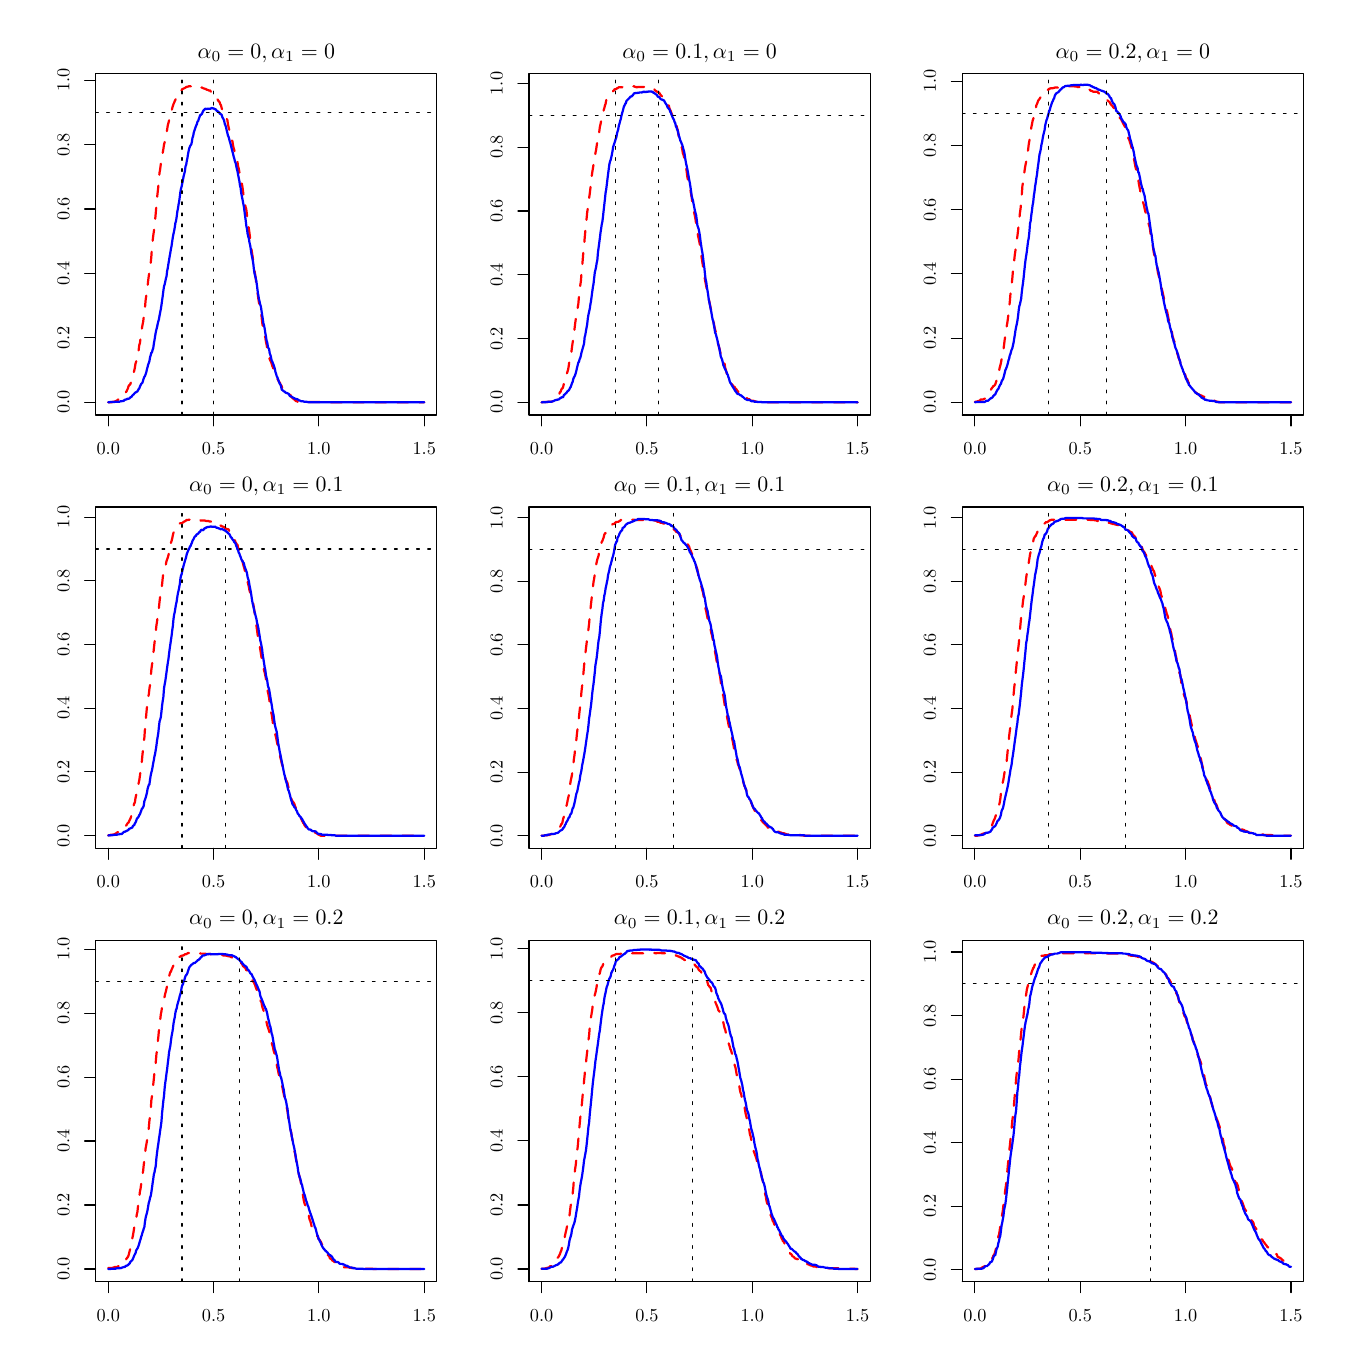
\begin{tikzpicture}[x=1pt,y=1pt]
\definecolor{fillColor}{RGB}{255,255,255}
\path[use as bounding box,fill=fillColor,fill opacity=0.00] (0,0) rectangle (469.75,469.75);
\begin{scope}
\path[clip] ( 24.55,329.80) rectangle (147.87,453.12);
\definecolor{drawColor}{RGB}{255,0,0}

\path[draw=drawColor,line width= 0.8pt,dash pattern=on 4pt off 4pt ,line join=round,line cap=round] ( 29.12,334.37) --
	( 29.35,334.37) --
	( 29.58,334.37) --
	( 29.81,334.37) --
	( 30.03,334.37) --
	( 30.26,334.37) --
	( 30.49,334.49) --
	( 30.72,334.49) --
	( 30.95,334.60) --
	( 31.18,334.60) --
	( 31.41,334.60) --
	( 31.64,334.72) --
	( 31.87,334.84) --
	( 32.09,334.84) --
	( 32.32,335.07) --
	( 32.55,335.18) --
	( 32.78,335.42) --
	( 33.01,335.53) --
	( 33.24,336.12) --
	( 33.47,336.23) --
	( 33.70,336.23) --
	( 33.92,336.35) --
	( 34.15,336.46) --
	( 34.38,336.58) --
	( 34.61,336.70) --
	( 34.84,336.81) --
	( 35.07,337.16) --
	( 35.30,337.74) --
	( 35.53,338.09) --
	( 35.76,338.44) --
	( 35.98,338.91) --
	( 36.21,339.37) --
	( 36.44,340.19) --
	( 36.67,340.54) --
	( 36.90,340.65) --
	( 37.13,341.00) --
	( 37.36,341.70) --
	( 37.59,342.28) --
	( 37.81,342.98) --
	( 38.04,344.03) --
	( 38.27,344.96) --
	( 38.50,345.78) --
	( 38.73,346.82) --
	( 38.96,348.34) --
	( 39.19,349.04) --
	( 39.42,349.97) --
	( 39.65,350.78) --
	( 39.87,352.53) --
	( 40.10,353.23) --
	( 40.33,355.09) --
	( 40.56,355.79) --
	( 40.79,357.53) --
	( 41.02,359.39) --
	( 41.25,360.91) --
	( 41.48,362.30) --
	( 41.71,363.35) --
	( 41.93,365.10) --
	( 42.16,366.73) --
	( 42.39,368.59) --
	( 42.62,371.27) --
	( 42.85,372.90) --
	( 43.08,374.88) --
	( 43.31,376.04) --
	( 43.54,378.37) --
	( 43.76,380.00) --
	( 43.99,381.51) --
	( 44.22,382.67) --
	( 44.45,384.54) --
	( 44.68,386.98) --
	( 44.91,390.24) --
	( 45.14,392.68) --
	( 45.37,394.55) --
	( 45.60,396.18) --
	( 45.82,397.81) --
	( 46.05,400.25) --
	( 46.28,402.69) --
	( 46.51,405.60) --
	( 46.74,408.05) --
	( 46.97,410.26) --
	( 47.20,412.24) --
	( 47.43,415.15) --
	( 47.65,417.36) --
	( 47.88,418.64) --
	( 48.11,420.50) --
	( 48.34,421.43) --
	( 48.57,423.06) --
	( 48.80,424.58) --
	( 49.03,425.86) --
	( 49.26,427.49) --
	( 49.49,428.30) --
	( 49.71,429.93) --
	( 49.94,430.75) --
	( 50.17,431.79) --
	( 50.40,432.96) --
	( 50.63,434.47) --
	( 50.86,435.29) --
	( 51.09,436.22) --
	( 51.32,436.92) --
	( 51.54,437.96) --
	( 51.77,439.24) --
	( 52.00,439.71) --
	( 52.23,440.64) --
	( 52.46,441.46) --
	( 52.69,442.15) --
	( 52.92,442.62) --
	( 53.15,443.20) --
	( 53.38,443.67) --
	( 53.60,444.25) --
	( 53.83,444.71) --
	( 54.06,445.18) --
	( 54.29,445.53) --
	( 54.52,445.99) --
	( 54.75,446.11) --
	( 54.98,446.23) --
	( 55.21,446.93) --
	( 55.43,447.04) --
	( 55.66,447.16) --
	( 55.89,447.62) --
	( 56.12,447.62) --
	( 56.35,447.74) --
	( 56.58,447.86) --
	( 56.81,447.97) --
	( 57.04,448.09) --
	( 57.27,448.32) --
	( 57.49,448.32) --
	( 57.72,448.44) --
	( 57.95,448.44) --
	( 58.18,448.56) --
	( 58.41,448.56) --
	( 58.64,448.56) --
	( 58.87,448.56) --
	( 59.10,448.56) --
	( 59.32,448.56) --
	( 59.55,448.56) --
	( 59.78,448.56) --
	( 60.01,448.56) --
	( 60.24,448.56) --
	( 60.47,448.44) --
	( 60.70,448.44) --
	( 60.93,448.44) --
	( 61.16,448.44) --
	( 61.38,448.32) --
	( 61.61,448.32) --
	( 61.84,448.44) --
	( 62.07,448.32) --
	( 62.30,448.32) --
	( 62.53,448.09) --
	( 62.76,448.09) --
	( 62.99,448.09) --
	( 63.22,447.97) --
	( 63.44,447.86) --
	( 63.67,447.74) --
	( 63.90,447.74) --
	( 64.13,447.62) --
	( 64.36,447.62) --
	( 64.59,447.39) --
	( 64.82,447.28) --
	( 65.05,447.28) --
	( 65.27,447.16) --
	( 65.50,447.04) --
	( 65.73,447.04) --
	( 65.96,447.04) --
	( 66.19,446.58) --
	( 66.42,446.11) --
	( 66.65,446.11) --
	( 66.88,445.88) --
	( 67.11,445.76) --
	( 67.33,445.65) --
	( 67.56,445.18) --
	( 67.79,445.18) --
	( 68.02,444.71) --
	( 68.25,444.60) --
	( 68.48,443.90) --
	( 68.71,443.67) --
	( 68.94,443.20) --
	( 69.16,443.08) --
	( 69.39,442.74) --
	( 69.62,442.04) --
	( 69.85,441.69) --
	( 70.08,440.76) --
	( 70.31,440.06) --
	( 70.54,439.71) --
	( 70.77,439.48) --
	( 71.00,439.13) --
	( 71.22,438.43) --
	( 71.45,437.73) --
	( 71.68,437.03) --
	( 71.91,436.80) --
	( 72.14,436.45) --
	( 72.37,434.94) --
	( 72.60,433.77) --
	( 72.83,432.84) --
	( 73.05,431.68) --
	( 73.28,430.40) --
	( 73.51,429.70) --
	( 73.74,429.12) --
	( 73.97,428.77) --
	( 74.20,427.25) --
	( 74.43,426.21) --
	( 74.66,425.51) --
	( 74.89,424.11) --
	( 75.11,423.41) --
	( 75.34,422.60) --
	( 75.57,421.67) --
	( 75.80,421.20) --
	( 76.03,419.69) --
	( 76.26,418.87) --
	( 76.49,417.59) --
	( 76.72,416.66) --
	( 76.94,415.38) --
	( 77.17,413.99) --
	( 77.40,413.40) --
	( 77.63,412.01) --
	( 77.86,410.26) --
	( 78.09,408.51) --
	( 78.32,407.12) --
	( 78.55,405.84) --
	( 78.78,404.79) --
	( 79.00,404.09) --
	( 79.23,402.11) --
	( 79.46,400.37) --
	( 79.69,399.09) --
	( 79.92,397.11) --
	( 80.15,395.48) --
	( 80.38,393.62) --
	( 80.61,391.87) --
	( 80.83,389.89) --
	( 81.06,388.38) --
	( 81.29,386.98) --
	( 81.52,385.24) --
	( 81.75,383.61) --
	( 81.98,381.86) --
	( 82.21,380.46) --
	( 82.44,378.95) --
	( 82.67,376.51) --
	( 82.89,375.23) --
	( 83.12,373.48) --
	( 83.35,371.85) --
	( 83.58,370.34) --
	( 83.81,369.41) --
	( 84.04,368.24) --
	( 84.27,366.84) --
	( 84.50,365.56) --
	( 84.73,363.35) --
	( 84.95,361.72) --
	( 85.18,360.68) --
	( 85.41,359.51) --
	( 85.64,358.35) --
	( 85.87,357.77) --
	( 86.10,356.25) --
	( 86.33,355.20) --
	( 86.56,353.81) --
	( 86.78,353.34) --
	( 87.01,352.29) --
	( 87.24,351.13) --
	( 87.47,349.85) --
	( 87.70,349.38) --
	( 87.93,348.92) --
	( 88.16,348.34) --
	( 88.39,347.52) --
	( 88.62,347.06) --
	( 88.84,346.01) --
	( 89.07,345.54) --
	( 89.30,344.96) --
	( 89.53,344.38) --
	( 89.76,344.03) --
	( 89.99,343.33) --
	( 90.22,342.98) --
	( 90.45,342.52) --
	( 90.67,342.05) --
	( 90.90,341.59) --
	( 91.13,341.59) --
	( 91.36,340.77) --
	( 91.59,340.54) --
	( 91.82,340.07) --
	( 92.05,339.14) --
	( 92.28,338.68) --
	( 92.51,338.44) --
	( 92.73,338.09) --
	( 92.96,337.98) --
	( 93.19,337.74) --
	( 93.42,337.63) --
	( 93.65,337.51) --
	( 93.88,337.51) --
	( 94.11,337.51) --
	( 94.34,337.40) --
	( 94.56,337.28) --
	( 94.79,337.16) --
	( 95.02,336.93) --
	( 95.25,336.35) --
	( 95.48,336.12) --
	( 95.71,335.88) --
	( 95.94,335.77) --
	( 96.17,335.42) --
	( 96.40,335.42) --
	( 96.62,335.18) --
	( 96.85,334.84) --
	( 97.08,334.84) --
	( 97.31,334.72) --
	( 97.54,334.60) --
	( 97.77,334.60) --
	( 98.00,334.60) --
	( 98.23,334.60) --
	( 98.45,334.60) --
	( 98.68,334.60) --
	( 98.91,334.60) --
	( 99.14,334.60) --
	( 99.37,334.60) --
	( 99.60,334.60) --
	( 99.83,334.60) --
	(100.06,334.60) --
	(100.29,334.60) --
	(100.51,334.60) --
	(100.74,334.60) --
	(100.97,334.60) --
	(101.20,334.60) --
	(101.43,334.49) --
	(101.66,334.49) --
	(101.89,334.49) --
	(102.12,334.49) --
	(102.35,334.49) --
	(102.57,334.49) --
	(102.80,334.49) --
	(103.03,334.49) --
	(103.26,334.49) --
	(103.49,334.49) --
	(103.72,334.49) --
	(103.95,334.49) --
	(104.18,334.49) --
	(104.40,334.49) --
	(104.63,334.49) --
	(104.86,334.49) --
	(105.09,334.49) --
	(105.32,334.49) --
	(105.55,334.49) --
	(105.78,334.49) --
	(106.01,334.49) --
	(106.24,334.49) --
	(106.46,334.49) --
	(106.69,334.49) --
	(106.92,334.37) --
	(107.15,334.37) --
	(107.38,334.37) --
	(107.61,334.37) --
	(107.84,334.37) --
	(108.07,334.37) --
	(108.29,334.37) --
	(108.52,334.37) --
	(108.75,334.37) --
	(108.98,334.37) --
	(109.21,334.37) --
	(109.44,334.37) --
	(109.67,334.37) --
	(109.90,334.37) --
	(110.13,334.37) --
	(110.35,334.37) --
	(110.58,334.37) --
	(110.81,334.37) --
	(111.04,334.37) --
	(111.27,334.37) --
	(111.50,334.37) --
	(111.73,334.37) --
	(111.96,334.37) --
	(112.18,334.37) --
	(112.41,334.37) --
	(112.64,334.37) --
	(112.87,334.37) --
	(113.10,334.37) --
	(113.33,334.37) --
	(113.56,334.37) --
	(113.79,334.37) --
	(114.02,334.37) --
	(114.24,334.37) --
	(114.47,334.37) --
	(114.70,334.37) --
	(114.93,334.37) --
	(115.16,334.37) --
	(115.39,334.37) --
	(115.62,334.37) --
	(115.85,334.37) --
	(116.07,334.37) --
	(116.30,334.37) --
	(116.53,334.37) --
	(116.76,334.37) --
	(116.99,334.37) --
	(117.22,334.37) --
	(117.45,334.37) --
	(117.68,334.37) --
	(117.91,334.37) --
	(118.13,334.37) --
	(118.36,334.37) --
	(118.59,334.37) --
	(118.82,334.37) --
	(119.05,334.37) --
	(119.28,334.37) --
	(119.51,334.37) --
	(119.74,334.37) --
	(119.96,334.37) --
	(120.19,334.37) --
	(120.42,334.37) --
	(120.65,334.37) --
	(120.88,334.37) --
	(121.11,334.37) --
	(121.34,334.37) --
	(121.57,334.37) --
	(121.80,334.37) --
	(122.02,334.37) --
	(122.25,334.37) --
	(122.48,334.37) --
	(122.71,334.37) --
	(122.94,334.37) --
	(123.17,334.37) --
	(123.40,334.37) --
	(123.63,334.37) --
	(123.86,334.37) --
	(124.08,334.37) --
	(124.31,334.37) --
	(124.54,334.37) --
	(124.77,334.37) --
	(125.00,334.37) --
	(125.23,334.37) --
	(125.46,334.37) --
	(125.69,334.37) --
	(125.91,334.37) --
	(126.14,334.37) --
	(126.37,334.37) --
	(126.60,334.37) --
	(126.83,334.37) --
	(127.06,334.37) --
	(127.29,334.37) --
	(127.52,334.37) --
	(127.75,334.37) --
	(127.97,334.37) --
	(128.20,334.37) --
	(128.43,334.37) --
	(128.66,334.37) --
	(128.89,334.37) --
	(129.12,334.37) --
	(129.35,334.37) --
	(129.58,334.37) --
	(129.80,334.37) --
	(130.03,334.37) --
	(130.26,334.37) --
	(130.49,334.37) --
	(130.72,334.37) --
	(130.95,334.37) --
	(131.18,334.37) --
	(131.41,334.37) --
	(131.64,334.37) --
	(131.86,334.37) --
	(132.09,334.37) --
	(132.32,334.37) --
	(132.55,334.37) --
	(132.78,334.37) --
	(133.01,334.37) --
	(133.24,334.37) --
	(133.47,334.37) --
	(133.69,334.37) --
	(133.92,334.37) --
	(134.15,334.37) --
	(134.38,334.37) --
	(134.61,334.37) --
	(134.84,334.37) --
	(135.07,334.37) --
	(135.30,334.37) --
	(135.53,334.37) --
	(135.75,334.37) --
	(135.98,334.37) --
	(136.21,334.37) --
	(136.44,334.37) --
	(136.67,334.37) --
	(136.90,334.37) --
	(137.13,334.37) --
	(137.36,334.37) --
	(137.58,334.37) --
	(137.81,334.37) --
	(138.04,334.37) --
	(138.27,334.37) --
	(138.50,334.37) --
	(138.73,334.37) --
	(138.96,334.37) --
	(139.19,334.37) --
	(139.42,334.37) --
	(139.64,334.37) --
	(139.87,334.37) --
	(140.10,334.37) --
	(140.33,334.37) --
	(140.56,334.37) --
	(140.79,334.37) --
	(141.02,334.37) --
	(141.25,334.37) --
	(141.47,334.37) --
	(141.70,334.37) --
	(141.93,334.37) --
	(142.16,334.37) --
	(142.39,334.37) --
	(142.62,334.37) --
	(142.85,334.37) --
	(143.08,334.37) --
	(143.31,334.37);
\end{scope}
\begin{scope}
\path[clip] (  0.00,  0.00) rectangle (469.75,469.75);
\definecolor{drawColor}{RGB}{0,0,0}

\path[draw=drawColor,line width= 0.4pt,line join=round,line cap=round] ( 29.12,329.80) -- (143.31,329.80);

\path[draw=drawColor,line width= 0.4pt,line join=round,line cap=round] ( 29.12,329.80) -- ( 29.12,325.84);

\path[draw=drawColor,line width= 0.4pt,line join=round,line cap=round] ( 67.18,329.80) -- ( 67.18,325.84);

\path[draw=drawColor,line width= 0.4pt,line join=round,line cap=round] (105.24,329.80) -- (105.24,325.84);

\path[draw=drawColor,line width= 0.4pt,line join=round,line cap=round] (143.31,329.80) -- (143.31,325.84);

\node[text=drawColor,anchor=base,inner sep=0pt, outer sep=0pt, scale=  0.66] at ( 29.12,315.55) {0.0};

\node[text=drawColor,anchor=base,inner sep=0pt, outer sep=0pt, scale=  0.66] at ( 67.18,315.55) {0.5};

\node[text=drawColor,anchor=base,inner sep=0pt, outer sep=0pt, scale=  0.66] at (105.24,315.55) {1.0};

\node[text=drawColor,anchor=base,inner sep=0pt, outer sep=0pt, scale=  0.66] at (143.31,315.55) {1.5};

\path[draw=drawColor,line width= 0.4pt,line join=round,line cap=round] ( 24.55,334.37) -- ( 24.55,450.77);

\path[draw=drawColor,line width= 0.4pt,line join=round,line cap=round] ( 24.55,334.37) -- ( 20.59,334.37);

\path[draw=drawColor,line width= 0.4pt,line join=round,line cap=round] ( 24.55,357.65) -- ( 20.59,357.65);

\path[draw=drawColor,line width= 0.4pt,line join=round,line cap=round] ( 24.55,380.93) -- ( 20.59,380.93);

\path[draw=drawColor,line width= 0.4pt,line join=round,line cap=round] ( 24.55,404.21) -- ( 20.59,404.21);

\path[draw=drawColor,line width= 0.4pt,line join=round,line cap=round] ( 24.55,427.49) -- ( 20.59,427.49);

\path[draw=drawColor,line width= 0.4pt,line join=round,line cap=round] ( 24.55,450.77) -- ( 20.59,450.77);

\node[text=drawColor,rotate= 90.00,anchor=base,inner sep=0pt, outer sep=0pt, scale=  0.66] at ( 15.05,334.37) {0.0};

\node[text=drawColor,rotate= 90.00,anchor=base,inner sep=0pt, outer sep=0pt, scale=  0.66] at ( 15.05,357.65) {0.2};

\node[text=drawColor,rotate= 90.00,anchor=base,inner sep=0pt, outer sep=0pt, scale=  0.66] at ( 15.05,380.93) {0.4};

\node[text=drawColor,rotate= 90.00,anchor=base,inner sep=0pt, outer sep=0pt, scale=  0.66] at ( 15.05,404.21) {0.6};

\node[text=drawColor,rotate= 90.00,anchor=base,inner sep=0pt, outer sep=0pt, scale=  0.66] at ( 15.05,427.49) {0.8};

\node[text=drawColor,rotate= 90.00,anchor=base,inner sep=0pt, outer sep=0pt, scale=  0.66] at ( 15.05,450.77) {1.0};

\path[draw=drawColor,line width= 0.4pt,line join=round,line cap=round] ( 24.55,329.80) --
	(147.87,329.80) --
	(147.87,453.12) --
	( 24.55,453.12) --
	( 24.55,329.80);
\end{scope}
\begin{scope}
\path[clip] (  0.00,313.17) rectangle (156.58,469.75);
\definecolor{drawColor}{RGB}{0,0,0}

\node[text=drawColor,anchor=base,inner sep=0pt, outer sep=0pt, scale=  0.79] at ( 86.21,458.71) {\bfseries $\alpha_0 = 0, \alpha_1 = 0$};
\end{scope}
\begin{scope}
\path[clip] ( 24.55,329.80) rectangle (147.87,453.12);
\definecolor{drawColor}{RGB}{0,0,255}

\path[draw=drawColor,line width= 0.8pt,line join=round,line cap=round] ( 29.12,334.37) --
	( 29.35,334.37) --
	( 29.58,334.37) --
	( 29.81,334.49) --
	( 30.03,334.49) --
	( 30.26,334.49) --
	( 30.49,334.49) --
	( 30.72,334.49) --
	( 30.95,334.49) --
	( 31.18,334.49) --
	( 31.41,334.49) --
	( 31.64,334.60) --
	( 31.87,334.60) --
	( 32.09,334.60) --
	( 32.32,334.60) --
	( 32.55,334.60) --
	( 32.78,334.60) --
	( 33.01,334.60) --
	( 33.24,334.60) --
	( 33.47,334.72) --
	( 33.70,334.72) --
	( 33.92,334.72) --
	( 34.15,334.84) --
	( 34.38,334.84) --
	( 34.61,334.84) --
	( 34.84,335.07) --
	( 35.07,335.30) --
	( 35.30,335.30) --
	( 35.53,335.42) --
	( 35.76,335.42) --
	( 35.98,335.65) --
	( 36.21,335.65) --
	( 36.44,335.65) --
	( 36.67,335.77) --
	( 36.90,335.88) --
	( 37.13,336.23) --
	( 37.36,336.23) --
	( 37.59,336.46) --
	( 37.81,336.81) --
	( 38.04,337.05) --
	( 38.27,337.16) --
	( 38.50,337.51) --
	( 38.73,337.74) --
	( 38.96,337.98) --
	( 39.19,337.98) --
	( 39.42,338.21) --
	( 39.65,338.33) --
	( 39.87,338.68) --
	( 40.10,339.14) --
	( 40.33,339.37) --
	( 40.56,340.07) --
	( 40.79,340.54) --
	( 41.02,341.00) --
	( 41.25,341.24) --
	( 41.48,341.47) --
	( 41.71,342.28) --
	( 41.93,342.98) --
	( 42.16,343.56) --
	( 42.39,343.91) --
	( 42.62,344.50) --
	( 42.85,345.19) --
	( 43.08,346.24) --
	( 43.31,347.06) --
	( 43.54,347.99) --
	( 43.76,348.57) --
	( 43.99,349.27) --
	( 44.22,350.67) --
	( 44.45,351.36) --
	( 44.68,352.29) --
	( 44.91,352.41) --
	( 45.14,353.34) --
	( 45.37,353.92) --
	( 45.60,355.55) --
	( 45.82,356.83) --
	( 46.05,358.23) --
	( 46.28,359.63) --
	( 46.51,360.68) --
	( 46.74,361.49) --
	( 46.97,362.65) --
	( 47.20,363.59) --
	( 47.43,364.40) --
	( 47.65,365.68) --
	( 47.88,366.84) --
	( 48.11,368.01) --
	( 48.34,369.52) --
	( 48.57,371.15) --
	( 48.80,372.78) --
	( 49.03,374.64) --
	( 49.26,376.27) --
	( 49.49,376.97) --
	( 49.71,377.90) --
	( 49.94,379.07) --
	( 50.17,379.88) --
	( 50.40,381.86) --
	( 50.63,382.91) --
	( 50.86,384.42) --
	( 51.09,385.82) --
	( 51.32,387.21) --
	( 51.54,388.38) --
	( 51.77,389.77) --
	( 52.00,390.94) --
	( 52.23,392.57) --
	( 52.46,394.08) --
	( 52.69,395.25) --
	( 52.92,396.29) --
	( 53.15,397.57) --
	( 53.38,399.20) --
	( 53.60,399.90) --
	( 53.83,401.30) --
	( 54.06,403.16) --
	( 54.29,404.32) --
	( 54.52,405.84) --
	( 54.75,407.00) --
	( 54.98,408.75) --
	( 55.21,410.61) --
	( 55.43,411.66) --
	( 55.66,412.47) --
	( 55.89,413.64) --
	( 56.12,414.80) --
	( 56.35,416.08) --
	( 56.58,416.90) --
	( 56.81,417.83) --
	( 57.04,419.69) --
	( 57.27,420.15) --
	( 57.49,421.55) --
	( 57.72,422.60) --
	( 57.95,424.11) --
	( 58.18,425.28) --
	( 58.41,426.21) --
	( 58.64,426.79) --
	( 58.87,427.25) --
	( 59.10,427.49) --
	( 59.32,428.42) --
	( 59.55,429.93) --
	( 59.78,430.51) --
	( 60.01,431.79) --
	( 60.24,432.49) --
	( 60.47,433.19) --
	( 60.70,433.89) --
	( 60.93,434.47) --
	( 61.16,434.94) --
	( 61.38,435.87) --
	( 61.61,435.98) --
	( 61.84,436.80) --
	( 62.07,437.38) --
	( 62.30,438.08) --
	( 62.53,438.20) --
	( 62.76,438.43) --
	( 62.99,438.66) --
	( 63.22,439.24) --
	( 63.44,439.71) --
	( 63.67,439.94) --
	( 63.90,440.17) --
	( 64.13,440.41) --
	( 64.36,440.52) --
	( 64.59,440.29) --
	( 64.82,440.41) --
	( 65.05,440.41) --
	( 65.27,440.52) --
	( 65.50,440.41) --
	( 65.73,440.52) --
	( 65.96,440.41) --
	( 66.19,440.52) --
	( 66.42,440.76) --
	( 66.65,440.64) --
	( 66.88,440.64) --
	( 67.11,440.52) --
	( 67.33,440.52) --
	( 67.56,440.29) --
	( 67.79,440.29) --
	( 68.02,440.17) --
	( 68.25,439.83) --
	( 68.48,439.48) --
	( 68.71,439.59) --
	( 68.94,439.24) --
	( 69.16,439.13) --
	( 69.39,438.66) --
	( 69.62,438.66) --
	( 69.85,438.43) --
	( 70.08,438.31) --
	( 70.31,437.50) --
	( 70.54,437.03) --
	( 70.77,436.68) --
	( 71.00,436.10) --
	( 71.22,434.94) --
	( 71.45,434.47) --
	( 71.68,433.77) --
	( 71.91,432.61) --
	( 72.14,431.79) --
	( 72.37,430.75) --
	( 72.60,430.28) --
	( 72.83,429.47) --
	( 73.05,428.54) --
	( 73.28,427.84) --
	( 73.51,426.91) --
	( 73.74,425.97) --
	( 73.97,425.04) --
	( 74.20,424.23) --
	( 74.43,423.18) --
	( 74.66,422.48) --
	( 74.89,421.43) --
	( 75.11,420.97) --
	( 75.34,419.92) --
	( 75.57,418.76) --
	( 75.80,417.94) --
	( 76.03,416.66) --
	( 76.26,415.50) --
	( 76.49,414.33) --
	( 76.72,412.71) --
	( 76.94,411.89) --
	( 77.17,409.91) --
	( 77.40,408.75) --
	( 77.63,407.70) --
	( 77.86,406.42) --
	( 78.09,405.26) --
	( 78.32,403.63) --
	( 78.55,401.76) --
	( 78.78,400.13) --
	( 79.00,398.16) --
	( 79.23,397.11) --
	( 79.46,395.36) --
	( 79.69,394.31) --
	( 79.92,393.62) --
	( 80.15,392.10) --
	( 80.38,391.17) --
	( 80.61,389.77) --
	( 80.83,388.15) --
	( 81.06,386.98) --
	( 81.29,385.93) --
	( 81.52,384.54) --
	( 81.75,382.44) --
	( 81.98,380.93) --
	( 82.21,380.00) --
	( 82.44,379.07) --
	( 82.67,377.90) --
	( 82.89,376.27) --
	( 83.12,374.41) --
	( 83.35,373.01) --
	( 83.58,371.62) --
	( 83.81,370.80) --
	( 84.04,369.64) --
	( 84.27,368.94) --
	( 84.50,367.43) --
	( 84.73,365.91) --
	( 84.95,364.52) --
	( 85.18,362.89) --
	( 85.41,362.19) --
	( 85.64,361.02) --
	( 85.87,359.39) --
	( 86.10,358.23) --
	( 86.33,356.60) --
	( 86.56,356.02) --
	( 86.78,354.62) --
	( 87.01,353.92) --
	( 87.24,353.58) --
	( 87.47,352.06) --
	( 87.70,351.48) --
	( 87.93,350.67) --
	( 88.16,349.38) --
	( 88.39,349.15) --
	( 88.62,348.45) --
	( 88.84,347.99) --
	( 89.07,347.29) --
	( 89.30,346.47) --
	( 89.53,345.31) --
	( 89.76,344.73) --
	( 89.99,343.80) --
	( 90.22,343.45) --
	( 90.45,342.75) --
	( 90.67,342.17) --
	( 90.90,341.47) --
	( 91.13,341.00) --
	( 91.36,340.77) --
	( 91.59,339.96) --
	( 91.82,338.91) --
	( 92.05,338.79) --
	( 92.28,338.56) --
	( 92.51,338.44) --
	( 92.73,338.21) --
	( 92.96,338.21) --
	( 93.19,337.86) --
	( 93.42,337.74) --
	( 93.65,337.74) --
	( 93.88,337.63) --
	( 94.11,337.51) --
	( 94.34,337.40) --
	( 94.56,336.93) --
	( 94.79,336.58) --
	( 95.02,336.58) --
	( 95.25,336.46) --
	( 95.48,336.35) --
	( 95.71,336.23) --
	( 95.94,336.00) --
	( 96.17,335.88) --
	( 96.40,335.88) --
	( 96.62,335.65) --
	( 96.85,335.53) --
	( 97.08,335.53) --
	( 97.31,335.53) --
	( 97.54,335.42) --
	( 97.77,335.30) --
	( 98.00,335.07) --
	( 98.23,335.07) --
	( 98.45,334.95) --
	( 98.68,334.84) --
	( 98.91,334.72) --
	( 99.14,334.72) --
	( 99.37,334.72) --
	( 99.60,334.72) --
	( 99.83,334.60) --
	(100.06,334.60) --
	(100.29,334.60) --
	(100.51,334.60) --
	(100.74,334.60) --
	(100.97,334.49) --
	(101.20,334.49) --
	(101.43,334.37) --
	(101.66,334.37) --
	(101.89,334.37) --
	(102.12,334.37) --
	(102.35,334.37) --
	(102.57,334.37) --
	(102.80,334.37) --
	(103.03,334.37) --
	(103.26,334.37) --
	(103.49,334.37) --
	(103.72,334.37) --
	(103.95,334.37) --
	(104.18,334.37) --
	(104.40,334.37) --
	(104.63,334.37) --
	(104.86,334.37) --
	(105.09,334.37) --
	(105.32,334.37) --
	(105.55,334.37) --
	(105.78,334.37) --
	(106.01,334.37) --
	(106.24,334.37) --
	(106.46,334.37) --
	(106.69,334.37) --
	(106.92,334.37) --
	(107.15,334.37) --
	(107.38,334.37) --
	(107.61,334.37) --
	(107.84,334.37) --
	(108.07,334.37) --
	(108.29,334.37) --
	(108.52,334.37) --
	(108.75,334.37) --
	(108.98,334.37) --
	(109.21,334.37) --
	(109.44,334.37) --
	(109.67,334.37) --
	(109.90,334.37) --
	(110.13,334.37) --
	(110.35,334.37) --
	(110.58,334.37) --
	(110.81,334.37) --
	(111.04,334.37) --
	(111.27,334.37) --
	(111.50,334.37) --
	(111.73,334.37) --
	(111.96,334.37) --
	(112.18,334.37) --
	(112.41,334.37) --
	(112.64,334.37) --
	(112.87,334.37) --
	(113.10,334.37) --
	(113.33,334.37) --
	(113.56,334.37) --
	(113.79,334.37) --
	(114.02,334.37) --
	(114.24,334.37) --
	(114.47,334.37) --
	(114.70,334.37) --
	(114.93,334.37) --
	(115.16,334.37) --
	(115.39,334.37) --
	(115.62,334.37) --
	(115.85,334.37) --
	(116.07,334.37) --
	(116.30,334.37) --
	(116.53,334.37) --
	(116.76,334.37) --
	(116.99,334.37) --
	(117.22,334.37) --
	(117.45,334.37) --
	(117.68,334.37) --
	(117.91,334.37) --
	(118.13,334.37) --
	(118.36,334.37) --
	(118.59,334.37) --
	(118.82,334.37) --
	(119.05,334.37) --
	(119.28,334.37) --
	(119.51,334.37) --
	(119.74,334.37) --
	(119.96,334.37) --
	(120.19,334.37) --
	(120.42,334.37) --
	(120.65,334.37) --
	(120.88,334.37) --
	(121.11,334.37) --
	(121.34,334.37) --
	(121.57,334.37) --
	(121.80,334.37) --
	(122.02,334.37) --
	(122.25,334.37) --
	(122.48,334.37) --
	(122.71,334.37) --
	(122.94,334.37) --
	(123.17,334.37) --
	(123.40,334.37) --
	(123.63,334.37) --
	(123.86,334.37) --
	(124.08,334.37) --
	(124.31,334.37) --
	(124.54,334.37) --
	(124.77,334.37) --
	(125.00,334.37) --
	(125.23,334.37) --
	(125.46,334.37) --
	(125.69,334.37) --
	(125.91,334.37) --
	(126.14,334.37) --
	(126.37,334.37) --
	(126.60,334.37) --
	(126.83,334.37) --
	(127.06,334.37) --
	(127.29,334.37) --
	(127.52,334.37) --
	(127.75,334.37) --
	(127.97,334.37) --
	(128.20,334.37) --
	(128.43,334.37) --
	(128.66,334.37) --
	(128.89,334.37) --
	(129.12,334.37) --
	(129.35,334.37) --
	(129.58,334.37) --
	(129.80,334.37) --
	(130.03,334.37) --
	(130.26,334.37) --
	(130.49,334.37) --
	(130.72,334.37) --
	(130.95,334.37) --
	(131.18,334.37) --
	(131.41,334.37) --
	(131.64,334.37) --
	(131.86,334.37) --
	(132.09,334.37) --
	(132.32,334.37) --
	(132.55,334.37) --
	(132.78,334.37) --
	(133.01,334.37) --
	(133.24,334.37) --
	(133.47,334.37) --
	(133.69,334.37) --
	(133.92,334.37) --
	(134.15,334.37) --
	(134.38,334.37) --
	(134.61,334.37) --
	(134.84,334.37) --
	(135.07,334.37) --
	(135.30,334.37) --
	(135.53,334.37) --
	(135.75,334.37) --
	(135.98,334.37) --
	(136.21,334.37) --
	(136.44,334.37) --
	(136.67,334.37) --
	(136.90,334.37) --
	(137.13,334.37) --
	(137.36,334.37) --
	(137.58,334.37) --
	(137.81,334.37) --
	(138.04,334.37) --
	(138.27,334.37) --
	(138.50,334.37) --
	(138.73,334.37) --
	(138.96,334.37) --
	(139.19,334.37) --
	(139.42,334.37) --
	(139.64,334.37) --
	(139.87,334.37) --
	(140.10,334.37) --
	(140.33,334.37) --
	(140.56,334.37) --
	(140.79,334.37) --
	(141.02,334.37) --
	(141.25,334.37) --
	(141.47,334.37) --
	(141.70,334.37) --
	(141.93,334.37) --
	(142.16,334.37) --
	(142.39,334.37) --
	(142.62,334.37) --
	(142.85,334.37) --
	(143.08,334.37) --
	(143.31,334.37);
\definecolor{drawColor}{RGB}{0,0,0}

\path[draw=drawColor,line width= 0.4pt,dash pattern=on 1pt off 3pt ,line join=round,line cap=round] ( 24.55,439.13) -- (147.87,439.13);

\path[draw=drawColor,line width= 0.4pt,dash pattern=on 1pt off 3pt ,line join=round,line cap=round] ( 55.76,329.80) -- ( 55.76,453.12);

\path[draw=drawColor,line width= 0.4pt,dash pattern=on 1pt off 3pt ,line join=round,line cap=round] ( 67.18,329.80) -- ( 67.18,453.12);
\end{scope}
\begin{scope}
\path[clip] (181.14,329.80) rectangle (304.46,453.12);
\definecolor{drawColor}{RGB}{255,0,0}

\path[draw=drawColor,line width= 0.8pt,dash pattern=on 4pt off 4pt ,line join=round,line cap=round] (185.70,334.37) --
	(185.93,334.37) --
	(186.16,334.48) --
	(186.39,334.48) --
	(186.62,334.48) --
	(186.85,334.48) --
	(187.08,334.48) --
	(187.31,334.48) --
	(187.54,334.48) --
	(187.76,334.48) --
	(187.99,334.48) --
	(188.22,334.60) --
	(188.45,334.60) --
	(188.68,334.60) --
	(188.91,334.60) --
	(189.14,334.60) --
	(189.37,334.60) --
	(189.59,334.72) --
	(189.82,334.83) --
	(190.05,334.83) --
	(190.28,334.95) --
	(190.51,335.18) --
	(190.74,335.64) --
	(190.97,335.87) --
	(191.20,336.21) --
	(191.43,336.44) --
	(191.65,336.79) --
	(191.88,336.79) --
	(192.11,337.37) --
	(192.34,338.06) --
	(192.57,338.17) --
	(192.80,338.86) --
	(193.03,339.32) --
	(193.26,339.44) --
	(193.48,339.90) --
	(193.71,340.94) --
	(193.94,341.86) --
	(194.17,342.55) --
	(194.40,343.24) --
	(194.63,344.05) --
	(194.86,344.85) --
	(195.09,345.55) --
	(195.32,346.35) --
	(195.54,347.74) --
	(195.77,349.58) --
	(196.00,350.50) --
	(196.23,351.42) --
	(196.46,352.46) --
	(196.69,354.30) --
	(196.92,355.92) --
	(197.15,357.30) --
	(197.37,359.14) --
	(197.60,360.87) --
	(197.83,362.83) --
	(198.06,364.44) --
	(198.29,365.13) --
	(198.52,366.75) --
	(198.75,368.59) --
	(198.98,369.97) --
	(199.21,372.62) --
	(199.43,374.12) --
	(199.66,376.54) --
	(199.89,378.04) --
	(200.12,380.92) --
	(200.35,383.45) --
	(200.58,385.99) --
	(200.81,388.99) --
	(201.04,390.71) --
	(201.26,393.59) --
	(201.49,396.13) --
	(201.72,398.55) --
	(201.95,400.62) --
	(202.18,403.04) --
	(202.41,404.54) --
	(202.64,406.50) --
	(202.87,408.11) --
	(203.10,409.73) --
	(203.32,411.57) --
	(203.55,413.99) --
	(203.78,415.83) --
	(204.01,417.45) --
	(204.24,418.83) --
	(204.47,420.33) --
	(204.70,421.82) --
	(204.93,422.75) --
	(205.15,424.36) --
	(205.38,425.51) --
	(205.61,427.12) --
	(205.84,428.51) --
	(206.07,429.54) --
	(206.30,430.81) --
	(206.53,432.08) --
	(206.76,433.92) --
	(206.99,434.84) --
	(207.21,436.00) --
	(207.44,436.80) --
	(207.67,438.07) --
	(207.90,438.76) --
	(208.13,439.91) --
	(208.36,440.61) --
	(208.59,441.64) --
	(208.82,442.22) --
	(209.05,443.49) --
	(209.27,443.95) --
	(209.50,444.18) --
	(209.73,444.41) --
	(209.96,444.87) --
	(210.19,445.10) --
	(210.42,445.33) --
	(210.65,445.56) --
	(210.88,445.91) --
	(211.10,446.37) --
	(211.33,446.60) --
	(211.56,446.83) --
	(211.79,447.06) --
	(212.02,447.40) --
	(212.25,447.52) --
	(212.48,447.52) --
	(212.71,447.63) --
	(212.94,447.86) --
	(213.16,447.86) --
	(213.39,448.09) --
	(213.62,448.21) --
	(213.85,448.21) --
	(214.08,448.21) --
	(214.31,448.21) --
	(214.54,448.21) --
	(214.77,448.21) --
	(214.99,448.33) --
	(215.22,448.33) --
	(215.45,448.33) --
	(215.68,448.33) --
	(215.91,448.44) --
	(216.14,448.44) --
	(216.37,448.44) --
	(216.60,448.56) --
	(216.83,448.56) --
	(217.05,448.56) --
	(217.28,448.56) --
	(217.51,448.56) --
	(217.74,448.56) --
	(217.97,448.56) --
	(218.20,448.56) --
	(218.43,448.56) --
	(218.66,448.56) --
	(218.88,448.56) --
	(219.11,448.56) --
	(219.34,448.44) --
	(219.57,448.33) --
	(219.80,448.33) --
	(220.03,448.21) --
	(220.26,448.21) --
	(220.49,448.33) --
	(220.72,448.33) --
	(220.94,448.33) --
	(221.17,448.33) --
	(221.40,448.33) --
	(221.63,448.33) --
	(221.86,448.33) --
	(222.09,448.33) --
	(222.32,448.33) --
	(222.55,448.33) --
	(222.77,448.33) --
	(223.00,448.33) --
	(223.23,448.33) --
	(223.46,448.33) --
	(223.69,448.33) --
	(223.92,448.21) --
	(224.15,448.21) --
	(224.38,448.09) --
	(224.61,448.09) --
	(224.83,448.09) --
	(225.06,448.09) --
	(225.29,447.98) --
	(225.52,447.98) --
	(225.75,447.86) --
	(225.98,447.63) --
	(226.21,447.63) --
	(226.44,447.52) --
	(226.66,447.06) --
	(226.89,446.94) --
	(227.12,446.83) --
	(227.35,446.60) --
	(227.58,446.60) --
	(227.81,446.37) --
	(228.04,446.37) --
	(228.27,446.14) --
	(228.50,445.67) --
	(228.72,445.44) --
	(228.95,445.10) --
	(229.18,444.98) --
	(229.41,444.64) --
	(229.64,444.29) --
	(229.87,443.95) --
	(230.10,443.72) --
	(230.33,443.14) --
	(230.56,442.91) --
	(230.78,442.56) --
	(231.01,442.45) --
	(231.24,442.22) --
	(231.47,441.76) --
	(231.70,441.53) --
	(231.93,440.49) --
	(232.16,440.03) --
	(232.39,439.57) --
	(232.61,438.88) --
	(232.84,438.30) --
	(233.07,437.84) --
	(233.30,436.69) --
	(233.53,436.11) --
	(233.76,435.54) --
	(233.99,435.30) --
	(234.22,434.73) --
	(234.45,434.27) --
	(234.67,433.46) --
	(234.90,432.77) --
	(235.13,431.16) --
	(235.36,430.12) --
	(235.59,429.08) --
	(235.82,428.39) --
	(236.05,427.35) --
	(236.28,426.66) --
	(236.50,425.97) --
	(236.73,424.47) --
	(236.96,423.90) --
	(237.19,422.98) --
	(237.42,421.59) --
	(237.65,420.56) --
	(237.88,419.52) --
	(238.11,417.91) --
	(238.34,415.95) --
	(238.56,414.91) --
	(238.79,413.99) --
	(239.02,413.53) --
	(239.25,412.26) --
	(239.48,411.11) --
	(239.71,409.61) --
	(239.94,408.46) --
	(240.17,406.50) --
	(240.39,405.12) --
	(240.62,403.73) --
	(240.85,402.81) --
	(241.08,401.66) --
	(241.31,400.51) --
	(241.54,399.01) --
	(241.77,397.40) --
	(242.00,396.47) --
	(242.23,394.52) --
	(242.45,393.59) --
	(242.68,392.44) --
	(242.91,391.29) --
	(243.14,389.56) --
	(243.37,387.72) --
	(243.60,386.34) --
	(243.83,384.72) --
	(244.06,383.34) --
	(244.28,381.73) --
	(244.51,380.57) --
	(244.74,378.62) --
	(244.97,377.46) --
	(245.20,376.31) --
	(245.43,375.16) --
	(245.66,374.24) --
	(245.89,373.08) --
	(246.12,371.59) --
	(246.34,370.66) --
	(246.57,369.51) --
	(246.80,368.36) --
	(247.03,367.32) --
	(247.26,366.52) --
	(247.49,365.02) --
	(247.72,363.64) --
	(247.95,362.94) --
	(248.18,361.56) --
	(248.40,360.64) --
	(248.63,359.83) --
	(248.86,358.80) --
	(249.09,357.41) --
	(249.32,356.26) --
	(249.55,355.34) --
	(249.78,354.42) --
	(250.01,353.73) --
	(250.23,352.57) --
	(250.46,351.65) --
	(250.69,351.65) --
	(250.92,351.19) --
	(251.15,350.16) --
	(251.38,349.58) --
	(251.61,348.89) --
	(251.84,348.20) --
	(252.07,346.70) --
	(252.29,346.12) --
	(252.52,345.09) --
	(252.75,344.39) --
	(252.98,344.05) --
	(253.21,343.70) --
	(253.44,343.47) --
	(253.67,343.01) --
	(253.90,341.97) --
	(254.12,341.40) --
	(254.35,341.05) --
	(254.58,340.71) --
	(254.81,340.48) --
	(255.04,340.13) --
	(255.27,340.02) --
	(255.50,339.90) --
	(255.73,339.32) --
	(255.96,339.21) --
	(256.18,338.98) --
	(256.41,338.52) --
	(256.64,338.40) --
	(256.87,337.94) --
	(257.10,337.60) --
	(257.33,337.37) --
	(257.56,336.90) --
	(257.79,336.79) --
	(258.01,336.67) --
	(258.24,336.67) --
	(258.47,336.44) --
	(258.70,336.44) --
	(258.93,336.33) --
	(259.16,336.33) --
	(259.39,335.98) --
	(259.62,335.87) --
	(259.85,335.87) --
	(260.07,335.75) --
	(260.30,335.52) --
	(260.53,335.52) --
	(260.76,335.52) --
	(260.99,335.29) --
	(261.22,335.06) --
	(261.45,334.95) --
	(261.68,334.95) --
	(261.90,334.95) --
	(262.13,334.95) --
	(262.36,334.83) --
	(262.59,334.83) --
	(262.82,334.72) --
	(263.05,334.60) --
	(263.28,334.60) --
	(263.51,334.48) --
	(263.74,334.48) --
	(263.96,334.48) --
	(264.19,334.48) --
	(264.42,334.48) --
	(264.65,334.48) --
	(264.88,334.48) --
	(265.11,334.48) --
	(265.34,334.48) --
	(265.57,334.48) --
	(265.79,334.37) --
	(266.02,334.37) --
	(266.25,334.37) --
	(266.48,334.37) --
	(266.71,334.37) --
	(266.94,334.37) --
	(267.17,334.37) --
	(267.40,334.37) --
	(267.63,334.37) --
	(267.85,334.37) --
	(268.08,334.37) --
	(268.31,334.37) --
	(268.54,334.37) --
	(268.77,334.37) --
	(269.00,334.37) --
	(269.23,334.37) --
	(269.46,334.37) --
	(269.69,334.37) --
	(269.91,334.37) --
	(270.14,334.37) --
	(270.37,334.37) --
	(270.60,334.37) --
	(270.83,334.37) --
	(271.06,334.37) --
	(271.29,334.37) --
	(271.52,334.37) --
	(271.74,334.37) --
	(271.97,334.37) --
	(272.20,334.37) --
	(272.43,334.37) --
	(272.66,334.37) --
	(272.89,334.37) --
	(273.12,334.37) --
	(273.35,334.37) --
	(273.58,334.37) --
	(273.80,334.37) --
	(274.03,334.37) --
	(274.26,334.37) --
	(274.49,334.37) --
	(274.72,334.37) --
	(274.95,334.37) --
	(275.18,334.37) --
	(275.41,334.37) --
	(275.63,334.37) --
	(275.86,334.37) --
	(276.09,334.37) --
	(276.32,334.37) --
	(276.55,334.37) --
	(276.78,334.37) --
	(277.01,334.37) --
	(277.24,334.37) --
	(277.47,334.37) --
	(277.69,334.37) --
	(277.92,334.37) --
	(278.15,334.37) --
	(278.38,334.37) --
	(278.61,334.37) --
	(278.84,334.37) --
	(279.07,334.37) --
	(279.30,334.37) --
	(279.52,334.37) --
	(279.75,334.37) --
	(279.98,334.37) --
	(280.21,334.37) --
	(280.44,334.37) --
	(280.67,334.37) --
	(280.90,334.37) --
	(281.13,334.37) --
	(281.36,334.37) --
	(281.58,334.37) --
	(281.81,334.37) --
	(282.04,334.37) --
	(282.27,334.37) --
	(282.50,334.37) --
	(282.73,334.37) --
	(282.96,334.37) --
	(283.19,334.37) --
	(283.41,334.37) --
	(283.64,334.37) --
	(283.87,334.37) --
	(284.10,334.37) --
	(284.33,334.37) --
	(284.56,334.37) --
	(284.79,334.37) --
	(285.02,334.37) --
	(285.25,334.37) --
	(285.47,334.37) --
	(285.70,334.37) --
	(285.93,334.37) --
	(286.16,334.37) --
	(286.39,334.37) --
	(286.62,334.37) --
	(286.85,334.37) --
	(287.08,334.37) --
	(287.30,334.37) --
	(287.53,334.37) --
	(287.76,334.37) --
	(287.99,334.37) --
	(288.22,334.37) --
	(288.45,334.37) --
	(288.68,334.37) --
	(288.91,334.37) --
	(289.14,334.37) --
	(289.36,334.37) --
	(289.59,334.37) --
	(289.82,334.37) --
	(290.05,334.37) --
	(290.28,334.37) --
	(290.51,334.37) --
	(290.74,334.37) --
	(290.97,334.37) --
	(291.20,334.37) --
	(291.42,334.37) --
	(291.65,334.37) --
	(291.88,334.37) --
	(292.11,334.37) --
	(292.34,334.37) --
	(292.57,334.37) --
	(292.80,334.37) --
	(293.03,334.37) --
	(293.25,334.37) --
	(293.48,334.37) --
	(293.71,334.37) --
	(293.94,334.37) --
	(294.17,334.37) --
	(294.40,334.37) --
	(294.63,334.37) --
	(294.86,334.37) --
	(295.09,334.37) --
	(295.31,334.37) --
	(295.54,334.37) --
	(295.77,334.37) --
	(296.00,334.37) --
	(296.23,334.37) --
	(296.46,334.37) --
	(296.69,334.37) --
	(296.92,334.37) --
	(297.14,334.37) --
	(297.37,334.37) --
	(297.60,334.37) --
	(297.83,334.37) --
	(298.06,334.37) --
	(298.29,334.37) --
	(298.52,334.37) --
	(298.75,334.37) --
	(298.98,334.37) --
	(299.20,334.37) --
	(299.43,334.37) --
	(299.66,334.37) --
	(299.89,334.37);
\end{scope}
\begin{scope}
\path[clip] (  0.00,  0.00) rectangle (469.75,469.75);
\definecolor{drawColor}{RGB}{0,0,0}

\path[draw=drawColor,line width= 0.4pt,line join=round,line cap=round] (185.70,329.80) -- (299.89,329.80);

\path[draw=drawColor,line width= 0.4pt,line join=round,line cap=round] (185.70,329.80) -- (185.70,325.84);

\path[draw=drawColor,line width= 0.4pt,line join=round,line cap=round] (223.77,329.80) -- (223.77,325.84);

\path[draw=drawColor,line width= 0.4pt,line join=round,line cap=round] (261.83,329.80) -- (261.83,325.84);

\path[draw=drawColor,line width= 0.4pt,line join=round,line cap=round] (299.89,329.80) -- (299.89,325.84);

\node[text=drawColor,anchor=base,inner sep=0pt, outer sep=0pt, scale=  0.66] at (185.70,315.55) {0.0};

\node[text=drawColor,anchor=base,inner sep=0pt, outer sep=0pt, scale=  0.66] at (223.77,315.55) {0.5};

\node[text=drawColor,anchor=base,inner sep=0pt, outer sep=0pt, scale=  0.66] at (261.83,315.55) {1.0};

\node[text=drawColor,anchor=base,inner sep=0pt, outer sep=0pt, scale=  0.66] at (299.89,315.55) {1.5};

\path[draw=drawColor,line width= 0.4pt,line join=round,line cap=round] (181.14,334.37) -- (181.14,449.59);

\path[draw=drawColor,line width= 0.4pt,line join=round,line cap=round] (181.14,334.37) -- (177.18,334.37);

\path[draw=drawColor,line width= 0.4pt,line join=round,line cap=round] (181.14,357.41) -- (177.18,357.41);

\path[draw=drawColor,line width= 0.4pt,line join=round,line cap=round] (181.14,380.46) -- (177.18,380.46);

\path[draw=drawColor,line width= 0.4pt,line join=round,line cap=round] (181.14,403.50) -- (177.18,403.50);

\path[draw=drawColor,line width= 0.4pt,line join=round,line cap=round] (181.14,426.55) -- (177.18,426.55);

\path[draw=drawColor,line width= 0.4pt,line join=round,line cap=round] (181.14,449.59) -- (177.18,449.59);

\node[text=drawColor,rotate= 90.00,anchor=base,inner sep=0pt, outer sep=0pt, scale=  0.66] at (171.63,334.37) {0.0};

\node[text=drawColor,rotate= 90.00,anchor=base,inner sep=0pt, outer sep=0pt, scale=  0.66] at (171.63,357.41) {0.2};

\node[text=drawColor,rotate= 90.00,anchor=base,inner sep=0pt, outer sep=0pt, scale=  0.66] at (171.63,380.46) {0.4};

\node[text=drawColor,rotate= 90.00,anchor=base,inner sep=0pt, outer sep=0pt, scale=  0.66] at (171.63,403.50) {0.6};

\node[text=drawColor,rotate= 90.00,anchor=base,inner sep=0pt, outer sep=0pt, scale=  0.66] at (171.63,426.55) {0.8};

\node[text=drawColor,rotate= 90.00,anchor=base,inner sep=0pt, outer sep=0pt, scale=  0.66] at (171.63,449.59) {1.0};

\path[draw=drawColor,line width= 0.4pt,line join=round,line cap=round] (181.14,329.80) --
	(304.46,329.80) --
	(304.46,453.12) --
	(181.14,453.12) --
	(181.14,329.80);
\end{scope}
\begin{scope}
\path[clip] (156.58,313.17) rectangle (313.17,469.75);
\definecolor{drawColor}{RGB}{0,0,0}

\node[text=drawColor,anchor=base,inner sep=0pt, outer sep=0pt, scale=  0.79] at (242.80,458.71) {\bfseries $\alpha_0 = 0.1, \alpha_1 = 0$};
\end{scope}
\begin{scope}
\path[clip] (181.14,329.80) rectangle (304.46,453.12);
\definecolor{drawColor}{RGB}{0,0,255}

\path[draw=drawColor,line width= 0.8pt,line join=round,line cap=round] (185.70,334.37) --
	(185.93,334.37) --
	(186.16,334.37) --
	(186.39,334.37) --
	(186.62,334.37) --
	(186.85,334.37) --
	(187.08,334.37) --
	(187.31,334.48) --
	(187.54,334.48) --
	(187.76,334.48) --
	(187.99,334.60) --
	(188.22,334.60) --
	(188.45,334.60) --
	(188.68,334.60) --
	(188.91,334.60) --
	(189.14,334.60) --
	(189.37,334.60) --
	(189.59,334.72) --
	(189.82,334.72) --
	(190.05,334.83) --
	(190.28,334.95) --
	(190.51,335.06) --
	(190.74,335.18) --
	(190.97,335.18) --
	(191.20,335.29) --
	(191.43,335.29) --
	(191.65,335.41) --
	(191.88,335.41) --
	(192.11,335.52) --
	(192.34,335.87) --
	(192.57,335.87) --
	(192.80,336.10) --
	(193.03,336.21) --
	(193.26,336.21) --
	(193.48,336.21) --
	(193.71,336.90) --
	(193.94,337.13) --
	(194.17,337.25) --
	(194.40,337.60) --
	(194.63,337.71) --
	(194.86,338.06) --
	(195.09,338.40) --
	(195.32,338.52) --
	(195.54,338.75) --
	(195.77,339.09) --
	(196.00,339.67) --
	(196.23,339.90) --
	(196.46,340.59) --
	(196.69,341.28) --
	(196.92,341.74) --
	(197.15,342.78) --
	(197.37,343.36) --
	(197.60,343.70) --
	(197.83,344.28) --
	(198.06,344.97) --
	(198.29,345.89) --
	(198.52,346.93) --
	(198.75,347.85) --
	(198.98,348.77) --
	(199.21,349.00) --
	(199.43,349.92) --
	(199.66,350.39) --
	(199.89,351.19) --
	(200.12,352.34) --
	(200.35,353.15) --
	(200.58,353.96) --
	(200.81,354.76) --
	(201.04,355.57) --
	(201.26,357.87) --
	(201.49,358.68) --
	(201.72,360.06) --
	(201.95,361.33) --
	(202.18,362.60) --
	(202.41,364.67) --
	(202.64,366.06) --
	(202.87,367.09) --
	(203.10,368.13) --
	(203.32,369.63) --
	(203.55,370.90) --
	(203.78,372.62) --
	(204.01,374.35) --
	(204.24,375.96) --
	(204.47,377.23) --
	(204.70,379.31) --
	(204.93,381.27) --
	(205.15,382.19) --
	(205.38,383.22) --
	(205.61,384.72) --
	(205.84,385.76) --
	(206.07,388.52) --
	(206.30,390.25) --
	(206.53,391.98) --
	(206.76,393.71) --
	(206.99,395.67) --
	(207.21,397.05) --
	(207.44,398.66) --
	(207.67,399.70) --
	(207.90,401.54) --
	(208.13,403.73) --
	(208.36,405.81) --
	(208.59,407.77) --
	(208.82,410.07) --
	(209.05,411.34) --
	(209.27,413.07) --
	(209.50,415.03) --
	(209.73,416.87) --
	(209.96,418.60) --
	(210.19,420.33) --
	(210.42,421.36) --
	(210.65,421.94) --
	(210.88,422.86) --
	(211.10,423.90) --
	(211.33,425.17) --
	(211.56,426.66) --
	(211.79,427.35) --
	(212.02,428.05) --
	(212.25,428.74) --
	(212.48,429.54) --
	(212.71,430.12) --
	(212.94,431.39) --
	(213.16,432.31) --
	(213.39,433.00) --
	(213.62,434.38) --
	(213.85,435.07) --
	(214.08,436.00) --
	(214.31,436.69) --
	(214.54,437.84) --
	(214.77,438.76) --
	(214.99,439.45) --
	(215.22,440.37) --
	(215.45,441.30) --
	(215.68,441.64) --
	(215.91,442.22) --
	(216.14,442.45) --
	(216.37,443.26) --
	(216.60,443.49) --
	(216.83,443.72) --
	(217.05,443.95) --
	(217.28,444.18) --
	(217.51,444.41) --
	(217.74,444.75) --
	(217.97,444.87) --
	(218.20,444.87) --
	(218.43,445.10) --
	(218.66,445.33) --
	(218.88,445.67) --
	(219.11,446.02) --
	(219.34,446.02) --
	(219.57,446.14) --
	(219.80,446.14) --
	(220.03,446.14) --
	(220.26,446.14) --
	(220.49,446.25) --
	(220.72,446.25) --
	(220.94,446.25) --
	(221.17,446.37) --
	(221.40,446.37) --
	(221.63,446.37) --
	(221.86,446.25) --
	(222.09,446.48) --
	(222.32,446.48) --
	(222.55,446.60) --
	(222.77,446.48) --
	(223.00,446.60) --
	(223.23,446.48) --
	(223.46,446.48) --
	(223.69,446.60) --
	(223.92,446.60) --
	(224.15,446.60) --
	(224.38,446.71) --
	(224.61,446.71) --
	(224.83,446.71) --
	(225.06,446.60) --
	(225.29,446.71) --
	(225.52,446.60) --
	(225.75,446.60) --
	(225.98,446.37) --
	(226.21,446.14) --
	(226.44,446.14) --
	(226.66,445.91) --
	(226.89,445.79) --
	(227.12,445.56) --
	(227.35,445.44) --
	(227.58,444.98) --
	(227.81,444.75) --
	(228.04,444.75) --
	(228.27,444.64) --
	(228.50,444.18) --
	(228.72,443.95) --
	(228.95,443.83) --
	(229.18,443.83) --
	(229.41,443.60) --
	(229.64,443.60) --
	(229.87,443.49) --
	(230.10,443.14) --
	(230.33,442.68) --
	(230.56,442.33) --
	(230.78,441.99) --
	(231.01,441.64) --
	(231.24,440.95) --
	(231.47,440.72) --
	(231.70,440.37) --
	(231.93,440.26) --
	(232.16,439.34) --
	(232.39,439.11) --
	(232.61,438.42) --
	(232.84,437.96) --
	(233.07,437.26) --
	(233.30,436.80) --
	(233.53,436.46) --
	(233.76,435.65) --
	(233.99,435.30) --
	(234.22,434.15) --
	(234.45,433.69) --
	(234.67,433.00) --
	(234.90,432.54) --
	(235.13,431.50) --
	(235.36,430.58) --
	(235.59,429.89) --
	(235.82,428.97) --
	(236.05,428.51) --
	(236.28,427.93) --
	(236.50,427.47) --
	(236.73,426.66) --
	(236.96,425.74) --
	(237.19,425.05) --
	(237.42,423.78) --
	(237.65,422.17) --
	(237.88,420.79) --
	(238.11,419.86) --
	(238.34,418.71) --
	(238.56,417.68) --
	(238.79,416.29) --
	(239.02,414.91) --
	(239.25,413.76) --
	(239.48,412.26) --
	(239.71,410.76) --
	(239.94,408.92) --
	(240.17,408.00) --
	(240.39,407.31) --
	(240.62,406.04) --
	(240.85,404.89) --
	(241.08,403.73) --
	(241.31,402.81) --
	(241.54,402.01) --
	(241.77,400.28) --
	(242.00,398.32) --
	(242.23,397.63) --
	(242.45,397.05) --
	(242.68,395.90) --
	(242.91,394.52) --
	(243.14,392.56) --
	(243.37,391.06) --
	(243.60,389.45) --
	(243.83,388.29) --
	(244.06,386.57) --
	(244.28,384.61) --
	(244.51,382.99) --
	(244.74,380.69) --
	(244.97,378.73) --
	(245.20,377.92) --
	(245.43,375.96) --
	(245.66,374.70) --
	(245.89,373.20) --
	(246.12,371.47) --
	(246.34,370.43) --
	(246.57,369.28) --
	(246.80,368.13) --
	(247.03,366.98) --
	(247.26,365.59) --
	(247.49,364.33) --
	(247.72,363.75) --
	(247.95,362.25) --
	(248.18,361.10) --
	(248.40,359.60) --
	(248.63,359.14) --
	(248.86,358.22) --
	(249.09,357.41) --
	(249.32,356.38) --
	(249.55,355.22) --
	(249.78,354.53) --
	(250.01,353.38) --
	(250.23,352.23) --
	(250.46,350.85) --
	(250.69,350.39) --
	(250.92,349.81) --
	(251.15,348.89) --
	(251.38,347.74) --
	(251.61,347.39) --
	(251.84,346.70) --
	(252.07,346.24) --
	(252.29,345.78) --
	(252.52,345.32) --
	(252.75,344.62) --
	(252.98,344.28) --
	(253.21,343.47) --
	(253.44,342.90) --
	(253.67,341.97) --
	(253.90,341.40) --
	(254.12,341.17) --
	(254.35,340.71) --
	(254.58,340.36) --
	(254.81,339.90) --
	(255.04,339.55) --
	(255.27,339.21) --
	(255.50,338.75) --
	(255.73,338.40) --
	(255.96,338.17) --
	(256.18,337.83) --
	(256.41,337.48) --
	(256.64,337.37) --
	(256.87,337.37) --
	(257.10,337.25) --
	(257.33,337.02) --
	(257.56,336.90) --
	(257.79,336.90) --
	(258.01,336.67) --
	(258.24,336.44) --
	(258.47,336.33) --
	(258.70,336.10) --
	(258.93,335.87) --
	(259.16,335.64) --
	(259.39,335.52) --
	(259.62,335.41) --
	(259.85,335.29) --
	(260.07,335.18) --
	(260.30,335.18) --
	(260.53,335.18) --
	(260.76,335.18) --
	(260.99,335.18) --
	(261.22,334.95) --
	(261.45,334.83) --
	(261.68,334.72) --
	(261.90,334.72) --
	(262.13,334.72) --
	(262.36,334.72) --
	(262.59,334.60) --
	(262.82,334.60) --
	(263.05,334.60) --
	(263.28,334.60) --
	(263.51,334.60) --
	(263.74,334.48) --
	(263.96,334.48) --
	(264.19,334.48) --
	(264.42,334.48) --
	(264.65,334.48) --
	(264.88,334.48) --
	(265.11,334.48) --
	(265.34,334.37) --
	(265.57,334.37) --
	(265.79,334.37) --
	(266.02,334.37) --
	(266.25,334.37) --
	(266.48,334.37) --
	(266.71,334.37) --
	(266.94,334.37) --
	(267.17,334.37) --
	(267.40,334.37) --
	(267.63,334.37) --
	(267.85,334.37) --
	(268.08,334.37) --
	(268.31,334.37) --
	(268.54,334.37) --
	(268.77,334.37) --
	(269.00,334.37) --
	(269.23,334.37) --
	(269.46,334.37) --
	(269.69,334.37) --
	(269.91,334.37) --
	(270.14,334.37) --
	(270.37,334.37) --
	(270.60,334.37) --
	(270.83,334.37) --
	(271.06,334.37) --
	(271.29,334.37) --
	(271.52,334.37) --
	(271.74,334.37) --
	(271.97,334.37) --
	(272.20,334.37) --
	(272.43,334.37) --
	(272.66,334.37) --
	(272.89,334.37) --
	(273.12,334.37) --
	(273.35,334.37) --
	(273.58,334.37) --
	(273.80,334.37) --
	(274.03,334.37) --
	(274.26,334.37) --
	(274.49,334.37) --
	(274.72,334.37) --
	(274.95,334.37) --
	(275.18,334.37) --
	(275.41,334.37) --
	(275.63,334.37) --
	(275.86,334.37) --
	(276.09,334.37) --
	(276.32,334.37) --
	(276.55,334.37) --
	(276.78,334.37) --
	(277.01,334.37) --
	(277.24,334.37) --
	(277.47,334.37) --
	(277.69,334.37) --
	(277.92,334.37) --
	(278.15,334.37) --
	(278.38,334.37) --
	(278.61,334.37) --
	(278.84,334.37) --
	(279.07,334.37) --
	(279.30,334.37) --
	(279.52,334.37) --
	(279.75,334.37) --
	(279.98,334.37) --
	(280.21,334.37) --
	(280.44,334.37) --
	(280.67,334.37) --
	(280.90,334.37) --
	(281.13,334.37) --
	(281.36,334.37) --
	(281.58,334.37) --
	(281.81,334.37) --
	(282.04,334.37) --
	(282.27,334.37) --
	(282.50,334.37) --
	(282.73,334.37) --
	(282.96,334.37) --
	(283.19,334.37) --
	(283.41,334.37) --
	(283.64,334.37) --
	(283.87,334.37) --
	(284.10,334.37) --
	(284.33,334.37) --
	(284.56,334.37) --
	(284.79,334.37) --
	(285.02,334.37) --
	(285.25,334.37) --
	(285.47,334.37) --
	(285.70,334.37) --
	(285.93,334.37) --
	(286.16,334.37) --
	(286.39,334.37) --
	(286.62,334.37) --
	(286.85,334.37) --
	(287.08,334.37) --
	(287.30,334.37) --
	(287.53,334.37) --
	(287.76,334.37) --
	(287.99,334.37) --
	(288.22,334.37) --
	(288.45,334.37) --
	(288.68,334.37) --
	(288.91,334.37) --
	(289.14,334.37) --
	(289.36,334.37) --
	(289.59,334.37) --
	(289.82,334.37) --
	(290.05,334.37) --
	(290.28,334.37) --
	(290.51,334.37) --
	(290.74,334.37) --
	(290.97,334.37) --
	(291.20,334.37) --
	(291.42,334.37) --
	(291.65,334.37) --
	(291.88,334.37) --
	(292.11,334.37) --
	(292.34,334.37) --
	(292.57,334.37) --
	(292.80,334.37) --
	(293.03,334.37) --
	(293.25,334.37) --
	(293.48,334.37) --
	(293.71,334.37) --
	(293.94,334.37) --
	(294.17,334.37) --
	(294.40,334.37) --
	(294.63,334.37) --
	(294.86,334.37) --
	(295.09,334.37) --
	(295.31,334.37) --
	(295.54,334.37) --
	(295.77,334.37) --
	(296.00,334.37) --
	(296.23,334.37) --
	(296.46,334.37) --
	(296.69,334.37) --
	(296.92,334.37) --
	(297.14,334.37) --
	(297.37,334.37) --
	(297.60,334.37) --
	(297.83,334.37) --
	(298.06,334.37) --
	(298.29,334.37) --
	(298.52,334.37) --
	(298.75,334.37) --
	(298.98,334.37) --
	(299.20,334.37) --
	(299.43,334.37) --
	(299.66,334.37) --
	(299.89,334.37);
\definecolor{drawColor}{RGB}{0,0,0}

\path[draw=drawColor,line width= 0.4pt,dash pattern=on 1pt off 3pt ,line join=round,line cap=round] (181.14,438.07) -- (304.46,438.07);

\path[draw=drawColor,line width= 0.4pt,dash pattern=on 1pt off 3pt ,line join=round,line cap=round] (212.35,329.80) -- (212.35,453.12);

\path[draw=drawColor,line width= 0.4pt,dash pattern=on 1pt off 3pt ,line join=round,line cap=round] (228.00,329.80) -- (228.00,453.12);
\end{scope}
\begin{scope}
\path[clip] (337.72,329.80) rectangle (461.04,453.12);
\definecolor{drawColor}{RGB}{255,0,0}

\path[draw=drawColor,line width= 0.8pt,dash pattern=on 4pt off 4pt ,line join=round,line cap=round] (342.29,334.60) --
	(342.52,334.60) --
	(342.75,334.60) --
	(342.98,334.60) --
	(343.20,334.72) --
	(343.43,334.83) --
	(343.66,334.83) --
	(343.89,334.95) --
	(344.12,335.07) --
	(344.35,335.41) --
	(344.58,335.41) --
	(344.81,335.41) --
	(345.04,335.41) --
	(345.26,335.41) --
	(345.49,335.53) --
	(345.72,335.65) --
	(345.95,335.76) --
	(346.18,336.11) --
	(346.41,336.34) --
	(346.64,336.69) --
	(346.87,336.92) --
	(347.09,337.27) --
	(347.32,337.85) --
	(347.55,338.43) --
	(347.78,338.43) --
	(348.01,338.78) --
	(348.24,339.24) --
	(348.47,339.59) --
	(348.70,339.82) --
	(348.93,340.29) --
	(349.15,340.29) --
	(349.38,340.52) --
	(349.61,340.75) --
	(349.84,341.45) --
	(350.07,342.14) --
	(350.30,342.61) --
	(350.53,343.65) --
	(350.76,344.81) --
	(350.98,345.51) --
	(351.21,346.79) --
	(351.44,347.60) --
	(351.67,348.53) --
	(351.90,349.80) --
	(352.13,350.50) --
	(352.36,352.24) --
	(352.59,353.40) --
	(352.82,355.14) --
	(353.04,357.00) --
	(353.27,358.39) --
	(353.50,360.01) --
	(353.73,361.64) --
	(353.96,362.92) --
	(354.19,364.54) --
	(354.42,366.40) --
	(354.65,368.60) --
	(354.88,370.57) --
	(355.10,373.24) --
	(355.33,375.80) --
	(355.56,376.96) --
	(355.79,379.05) --
	(356.02,381.83) --
	(356.25,383.34) --
	(356.48,385.66) --
	(356.71,387.75) --
	(356.93,389.26) --
	(357.16,391.35) --
	(357.39,392.97) --
	(357.62,394.36) --
	(357.85,396.22) --
	(358.08,398.31) --
	(358.31,400.40) --
	(358.54,402.72) --
	(358.77,404.34) --
	(358.99,406.55) --
	(359.22,409.33) --
	(359.45,412.70) --
	(359.68,413.74) --
	(359.91,415.83) --
	(360.14,417.46) --
	(360.37,419.08) --
	(360.60,420.36) --
	(360.82,421.40) --
	(361.05,423.03) --
	(361.28,424.42) --
	(361.51,425.70) --
	(361.74,427.67) --
	(361.97,428.94) --
	(362.20,430.45) --
	(362.43,432.31) --
	(362.66,433.70) --
	(362.88,434.75) --
	(363.11,436.02) --
	(363.34,436.72) --
	(363.57,437.53) --
	(363.80,439.04) --
	(364.03,439.39) --
	(364.26,440.55) --
	(364.49,441.71) --
	(364.71,442.17) --
	(364.94,442.75) --
	(365.17,443.45) --
	(365.40,443.68) --
	(365.63,444.03) --
	(365.86,444.38) --
	(366.09,444.73) --
	(366.32,444.84) --
	(366.55,444.96) --
	(366.77,445.07) --
	(367.00,445.77) --
	(367.23,446.23) --
	(367.46,446.35) --
	(367.69,446.70) --
	(367.92,446.70) --
	(368.15,446.93) --
	(368.38,447.16) --
	(368.60,447.28) --
	(368.83,447.28) --
	(369.06,447.63) --
	(369.29,447.74) --
	(369.52,447.74) --
	(369.75,447.86) --
	(369.98,447.86) --
	(370.21,447.86) --
	(370.44,447.86) --
	(370.66,447.98) --
	(370.89,447.98) --
	(371.12,448.09) --
	(371.35,448.09) --
	(371.58,448.09) --
	(371.81,448.09) --
	(372.04,448.09) --
	(372.27,448.09) --
	(372.49,448.21) --
	(372.72,448.21) --
	(372.95,448.21) --
	(373.18,448.32) --
	(373.41,448.32) --
	(373.64,448.32) --
	(373.87,448.32) --
	(374.10,448.32) --
	(374.33,448.44) --
	(374.55,448.44) --
	(374.78,448.44) --
	(375.01,448.44) --
	(375.24,448.44) --
	(375.47,448.44) --
	(375.70,448.44) --
	(375.93,448.44) --
	(376.16,448.56) --
	(376.39,448.56) --
	(376.61,448.56) --
	(376.84,448.56) --
	(377.07,448.56) --
	(377.30,448.56) --
	(377.53,448.56) --
	(377.76,448.56) --
	(377.99,448.56) --
	(378.22,448.56) --
	(378.44,448.44) --
	(378.67,448.44) --
	(378.90,448.44) --
	(379.13,448.44) --
	(379.36,448.32) --
	(379.59,448.32) --
	(379.82,448.32) --
	(380.05,448.32) --
	(380.28,448.32) --
	(380.50,448.32) --
	(380.73,448.09) --
	(380.96,447.98) --
	(381.19,447.98) --
	(381.42,447.86) --
	(381.65,447.86) --
	(381.88,447.63) --
	(382.11,447.63) --
	(382.33,447.63) --
	(382.56,447.63) --
	(382.79,447.63) --
	(383.02,447.63) --
	(383.25,447.28) --
	(383.48,447.28) --
	(383.71,447.28) --
	(383.94,447.16) --
	(384.17,446.93) --
	(384.39,446.93) --
	(384.62,446.81) --
	(384.85,446.70) --
	(385.08,446.58) --
	(385.31,446.58) --
	(385.54,446.58) --
	(385.77,446.58) --
	(386.00,446.58) --
	(386.22,446.58) --
	(386.45,446.58) --
	(386.68,446.47) --
	(386.91,446.12) --
	(387.14,446.00) --
	(387.37,445.77) --
	(387.60,445.31) --
	(387.83,445.19) --
	(388.06,444.96) --
	(388.28,444.96) --
	(388.51,444.61) --
	(388.74,444.49) --
	(388.97,444.38) --
	(389.20,444.26) --
	(389.43,444.03) --
	(389.66,444.03) --
	(389.89,443.80) --
	(390.11,443.57) --
	(390.34,443.33) --
	(390.57,443.10) --
	(390.80,442.99) --
	(391.03,442.75) --
	(391.26,442.17) --
	(391.49,441.94) --
	(391.72,441.59) --
	(391.95,441.59) --
	(392.17,441.13) --
	(392.40,440.78) --
	(392.63,440.66) --
	(392.86,440.32) --
	(393.09,440.08) --
	(393.32,439.97) --
	(393.55,439.74) --
	(393.78,438.92) --
	(394.00,438.69) --
	(394.23,438.00) --
	(394.46,437.53) --
	(394.69,437.07) --
	(394.92,436.84) --
	(395.15,436.60) --
	(395.38,436.02) --
	(395.61,435.67) --
	(395.84,435.09) --
	(396.06,434.75) --
	(396.29,434.40) --
	(396.52,433.82) --
	(396.75,433.01) --
	(396.98,432.31) --
	(397.21,431.73) --
	(397.44,431.27) --
	(397.67,429.99) --
	(397.90,429.52) --
	(398.12,429.06) --
	(398.35,428.13) --
	(398.58,427.55) --
	(398.81,426.62) --
	(399.04,425.35) --
	(399.27,424.65) --
	(399.50,423.26) --
	(399.73,422.33) --
	(399.95,421.29) --
	(400.18,419.89) --
	(400.41,418.96) --
	(400.64,418.15) --
	(400.87,416.53) --
	(401.10,415.72) --
	(401.33,414.67) --
	(401.56,413.16) --
	(401.79,412.00) --
	(402.01,410.84) --
	(402.24,409.22) --
	(402.47,408.75) --
	(402.70,407.94) --
	(402.93,406.90) --
	(403.16,406.32) --
	(403.39,405.39) --
	(403.62,404.34) --
	(403.84,403.30) --
	(404.07,402.72) --
	(404.30,402.02) --
	(404.53,400.75) --
	(404.76,399.35) --
	(404.99,399.12) --
	(405.22,398.31) --
	(405.45,397.61) --
	(405.68,395.87) --
	(405.90,394.02) --
	(406.13,393.20) --
	(406.36,392.04) --
	(406.59,390.65) --
	(406.82,389.14) --
	(407.05,387.75) --
	(407.28,387.28) --
	(407.51,386.12) --
	(407.73,384.85) --
	(407.96,383.92) --
	(408.19,382.76) --
	(408.42,381.13) --
	(408.65,380.32) --
	(408.88,379.39) --
	(409.11,378.35) --
	(409.34,377.42) --
	(409.57,376.38) --
	(409.79,375.56) --
	(410.02,374.52) --
	(410.25,373.48) --
	(410.48,372.43) --
	(410.71,371.39) --
	(410.94,370.46) --
	(411.17,369.88) --
	(411.40,368.60) --
	(411.62,367.56) --
	(411.85,366.63) --
	(412.08,365.35) --
	(412.31,364.31) --
	(412.54,363.73) --
	(412.77,362.80) --
	(413.00,362.22) --
	(413.23,361.18) --
	(413.46,359.78) --
	(413.68,358.27) --
	(413.91,357.58) --
	(414.14,356.65) --
	(414.37,356.30) --
	(414.60,355.61) --
	(414.83,354.56) --
	(415.06,353.52) --
	(415.29,352.47) --
	(415.52,351.66) --
	(415.74,350.96) --
	(415.97,350.27) --
	(416.20,349.69) --
	(416.43,348.87) --
	(416.66,347.95) --
	(416.89,347.13) --
	(417.12,346.32) --
	(417.35,345.86) --
	(417.57,345.51) --
	(417.80,344.81) --
	(418.03,344.58) --
	(418.26,344.35) --
	(418.49,343.42) --
	(418.72,342.96) --
	(418.95,342.84) --
	(419.18,342.26) --
	(419.41,341.56) --
	(419.63,341.33) --
	(419.86,341.10) --
	(420.09,340.87) --
	(420.32,340.75) --
	(420.55,340.40) --
	(420.78,339.59) --
	(421.01,339.13) --
	(421.24,338.78) --
	(421.46,338.55) --
	(421.69,338.31) --
	(421.92,338.08) --
	(422.15,337.73) --
	(422.38,337.73) --
	(422.61,337.50) --
	(422.84,337.27) --
	(423.07,337.15) --
	(423.30,337.15) --
	(423.52,337.04) --
	(423.75,336.92) --
	(423.98,336.81) --
	(424.21,336.81) --
	(424.44,336.57) --
	(424.67,336.46) --
	(424.90,336.46) --
	(425.13,336.34) --
	(425.35,335.99) --
	(425.58,335.99) --
	(425.81,335.76) --
	(426.04,335.53) --
	(426.27,335.53) --
	(426.50,335.53) --
	(426.73,335.41) --
	(426.96,335.30) --
	(427.19,335.30) --
	(427.41,335.30) --
	(427.64,335.30) --
	(427.87,335.18) --
	(428.10,335.07) --
	(428.33,334.95) --
	(428.56,334.95) --
	(428.79,334.95) --
	(429.02,334.83) --
	(429.24,334.83) --
	(429.47,334.60) --
	(429.70,334.60) --
	(429.93,334.60) --
	(430.16,334.49) --
	(430.39,334.49) --
	(430.62,334.49) --
	(430.85,334.37) --
	(431.08,334.37) --
	(431.30,334.37) --
	(431.53,334.37) --
	(431.76,334.37) --
	(431.99,334.37) --
	(432.22,334.37) --
	(432.45,334.37) --
	(432.68,334.37) --
	(432.91,334.37) --
	(433.13,334.37) --
	(433.36,334.37) --
	(433.59,334.37) --
	(433.82,334.37) --
	(434.05,334.37) --
	(434.28,334.37) --
	(434.51,334.37) --
	(434.74,334.37) --
	(434.97,334.37) --
	(435.19,334.37) --
	(435.42,334.37) --
	(435.65,334.37) --
	(435.88,334.37) --
	(436.11,334.37) --
	(436.34,334.37) --
	(436.57,334.37) --
	(436.80,334.37) --
	(437.03,334.37) --
	(437.25,334.37) --
	(437.48,334.37) --
	(437.71,334.37) --
	(437.94,334.37) --
	(438.17,334.37) --
	(438.40,334.37) --
	(438.63,334.37) --
	(438.86,334.37) --
	(439.08,334.37) --
	(439.31,334.37) --
	(439.54,334.37) --
	(439.77,334.37) --
	(440.00,334.37) --
	(440.23,334.37) --
	(440.46,334.37) --
	(440.69,334.37) --
	(440.92,334.37) --
	(441.14,334.37) --
	(441.37,334.37) --
	(441.60,334.37) --
	(441.83,334.37) --
	(442.06,334.37) --
	(442.29,334.37) --
	(442.52,334.37) --
	(442.75,334.37) --
	(442.97,334.37) --
	(443.20,334.37) --
	(443.43,334.37) --
	(443.66,334.37) --
	(443.89,334.37) --
	(444.12,334.37) --
	(444.35,334.37) --
	(444.58,334.37) --
	(444.81,334.37) --
	(445.03,334.37) --
	(445.26,334.37) --
	(445.49,334.37) --
	(445.72,334.37) --
	(445.95,334.37) --
	(446.18,334.37) --
	(446.41,334.37) --
	(446.64,334.37) --
	(446.86,334.37) --
	(447.09,334.37) --
	(447.32,334.37) --
	(447.55,334.37) --
	(447.78,334.37) --
	(448.01,334.37) --
	(448.24,334.37) --
	(448.47,334.37) --
	(448.70,334.37) --
	(448.92,334.37) --
	(449.15,334.37) --
	(449.38,334.37) --
	(449.61,334.37) --
	(449.84,334.37) --
	(450.07,334.37) --
	(450.30,334.37) --
	(450.53,334.37) --
	(450.75,334.37) --
	(450.98,334.37) --
	(451.21,334.37) --
	(451.44,334.37) --
	(451.67,334.37) --
	(451.90,334.37) --
	(452.13,334.37) --
	(452.36,334.37) --
	(452.59,334.37) --
	(452.81,334.37) --
	(453.04,334.37) --
	(453.27,334.37) --
	(453.50,334.37) --
	(453.73,334.37) --
	(453.96,334.37) --
	(454.19,334.37) --
	(454.42,334.37) --
	(454.64,334.37) --
	(454.87,334.37) --
	(455.10,334.37) --
	(455.33,334.37) --
	(455.56,334.37) --
	(455.79,334.37) --
	(456.02,334.37) --
	(456.25,334.37) --
	(456.48,334.37);
\end{scope}
\begin{scope}
\path[clip] (  0.00,  0.00) rectangle (469.75,469.75);
\definecolor{drawColor}{RGB}{0,0,0}

\path[draw=drawColor,line width= 0.4pt,line join=round,line cap=round] (342.29,329.80) -- (456.48,329.80);

\path[draw=drawColor,line width= 0.4pt,line join=round,line cap=round] (342.29,329.80) -- (342.29,325.84);

\path[draw=drawColor,line width= 0.4pt,line join=round,line cap=round] (380.35,329.80) -- (380.35,325.84);

\path[draw=drawColor,line width= 0.4pt,line join=round,line cap=round] (418.41,329.80) -- (418.41,325.84);

\path[draw=drawColor,line width= 0.4pt,line join=round,line cap=round] (456.48,329.80) -- (456.48,325.84);

\node[text=drawColor,anchor=base,inner sep=0pt, outer sep=0pt, scale=  0.66] at (342.29,315.55) {0.0};

\node[text=drawColor,anchor=base,inner sep=0pt, outer sep=0pt, scale=  0.66] at (380.35,315.55) {0.5};

\node[text=drawColor,anchor=base,inner sep=0pt, outer sep=0pt, scale=  0.66] at (418.41,315.55) {1.0};

\node[text=drawColor,anchor=base,inner sep=0pt, outer sep=0pt, scale=  0.66] at (456.48,315.55) {1.5};

\path[draw=drawColor,line width= 0.4pt,line join=round,line cap=round] (337.72,334.37) -- (337.72,450.41);

\path[draw=drawColor,line width= 0.4pt,line join=round,line cap=round] (337.72,334.37) -- (333.76,334.37);

\path[draw=drawColor,line width= 0.4pt,line join=round,line cap=round] (337.72,357.58) -- (333.76,357.58);

\path[draw=drawColor,line width= 0.4pt,line join=round,line cap=round] (337.72,380.79) -- (333.76,380.79);

\path[draw=drawColor,line width= 0.4pt,line join=round,line cap=round] (337.72,404.00) -- (333.76,404.00);

\path[draw=drawColor,line width= 0.4pt,line join=round,line cap=round] (337.72,427.20) -- (333.76,427.20);

\path[draw=drawColor,line width= 0.4pt,line join=round,line cap=round] (337.72,450.41) -- (333.76,450.41);

\node[text=drawColor,rotate= 90.00,anchor=base,inner sep=0pt, outer sep=0pt, scale=  0.66] at (328.22,334.37) {0.0};

\node[text=drawColor,rotate= 90.00,anchor=base,inner sep=0pt, outer sep=0pt, scale=  0.66] at (328.22,357.58) {0.2};

\node[text=drawColor,rotate= 90.00,anchor=base,inner sep=0pt, outer sep=0pt, scale=  0.66] at (328.22,380.79) {0.4};

\node[text=drawColor,rotate= 90.00,anchor=base,inner sep=0pt, outer sep=0pt, scale=  0.66] at (328.22,404.00) {0.6};

\node[text=drawColor,rotate= 90.00,anchor=base,inner sep=0pt, outer sep=0pt, scale=  0.66] at (328.22,427.20) {0.8};

\node[text=drawColor,rotate= 90.00,anchor=base,inner sep=0pt, outer sep=0pt, scale=  0.66] at (328.22,450.41) {1.0};

\path[draw=drawColor,line width= 0.4pt,line join=round,line cap=round] (337.72,329.80) --
	(461.04,329.80) --
	(461.04,453.12) --
	(337.72,453.12) --
	(337.72,329.80);
\end{scope}
\begin{scope}
\path[clip] (313.17,313.17) rectangle (469.75,469.75);
\definecolor{drawColor}{RGB}{0,0,0}

\node[text=drawColor,anchor=base,inner sep=0pt, outer sep=0pt, scale=  0.79] at (399.38,458.71) {\bfseries $\alpha_0 = 0.2, \alpha_1 = 0$};
\end{scope}
\begin{scope}
\path[clip] (337.72,329.80) rectangle (461.04,453.12);
\definecolor{drawColor}{RGB}{0,0,255}

\path[draw=drawColor,line width= 0.8pt,line join=round,line cap=round] (342.29,334.37) --
	(342.52,334.37) --
	(342.75,334.49) --
	(342.98,334.49) --
	(343.20,334.49) --
	(343.43,334.49) --
	(343.66,334.49) --
	(343.89,334.49) --
	(344.12,334.49) --
	(344.35,334.49) --
	(344.58,334.49) --
	(344.81,334.49) --
	(345.04,334.49) --
	(345.26,334.49) --
	(345.49,334.49) --
	(345.72,334.49) --
	(345.95,334.60) --
	(346.18,334.72) --
	(346.41,334.95) --
	(346.64,334.95) --
	(346.87,334.95) --
	(347.09,334.95) --
	(347.32,335.18) --
	(347.55,335.41) --
	(347.78,335.65) --
	(348.01,335.76) --
	(348.24,335.99) --
	(348.47,335.99) --
	(348.70,336.23) --
	(348.93,336.69) --
	(349.15,336.81) --
	(349.38,337.15) --
	(349.61,337.15) --
	(349.84,337.73) --
	(350.07,338.20) --
	(350.30,338.66) --
	(350.53,339.01) --
	(350.76,339.24) --
	(350.98,339.82) --
	(351.21,340.29) --
	(351.44,340.75) --
	(351.67,340.98) --
	(351.90,341.80) --
	(352.13,342.38) --
	(352.36,342.61) --
	(352.59,343.19) --
	(352.82,344.12) --
	(353.04,344.93) --
	(353.27,345.97) --
	(353.50,346.44) --
	(353.73,347.02) --
	(353.96,347.71) --
	(354.19,348.53) --
	(354.42,349.57) --
	(354.65,350.15) --
	(354.88,351.31) --
	(355.10,351.78) --
	(355.33,352.70) --
	(355.56,353.40) --
	(355.79,353.86) --
	(356.02,354.91) --
	(356.25,355.95) --
	(356.48,357.35) --
	(356.71,358.74) --
	(356.93,360.36) --
	(357.16,361.52) --
	(357.39,362.57) --
	(357.62,363.73) --
	(357.85,365.35) --
	(358.08,367.44) --
	(358.31,369.07) --
	(358.54,369.76) --
	(358.77,370.81) --
	(358.99,371.85) --
	(359.22,374.17) --
	(359.45,376.03) --
	(359.68,377.65) --
	(359.91,379.63) --
	(360.14,381.95) --
	(360.37,384.15) --
	(360.60,386.01) --
	(360.82,387.40) --
	(361.05,388.91) --
	(361.28,390.88) --
	(361.51,392.62) --
	(361.74,393.78) --
	(361.97,395.99) --
	(362.20,399.01) --
	(362.43,399.93) --
	(362.66,402.02) --
	(362.88,403.53) --
	(363.11,405.50) --
	(363.34,406.66) --
	(363.57,408.98) --
	(363.80,410.38) --
	(364.03,412.35) --
	(364.26,413.74) --
	(364.49,415.37) --
	(364.71,416.64) --
	(364.94,418.73) --
	(365.17,420.36) --
	(365.40,422.10) --
	(365.63,423.95) --
	(365.86,424.77) --
	(366.09,425.93) --
	(366.32,427.44) --
	(366.55,428.36) --
	(366.77,429.76) --
	(367.00,430.92) --
	(367.23,431.85) --
	(367.46,432.77) --
	(367.69,434.51) --
	(367.92,435.44) --
	(368.15,436.37) --
	(368.38,436.84) --
	(368.60,437.76) --
	(368.83,438.46) --
	(369.06,439.62) --
	(369.29,439.85) --
	(369.52,440.78) --
	(369.75,441.48) --
	(369.98,442.17) --
	(370.21,442.87) --
	(370.44,443.22) --
	(370.66,443.91) --
	(370.89,444.15) --
	(371.12,445.07) --
	(371.35,445.54) --
	(371.58,445.89) --
	(371.81,446.12) --
	(372.04,446.23) --
	(372.27,446.35) --
	(372.49,446.47) --
	(372.72,446.81) --
	(372.95,447.05) --
	(373.18,447.40) --
	(373.41,447.40) --
	(373.64,447.74) --
	(373.87,447.98) --
	(374.10,448.21) --
	(374.33,448.21) --
	(374.55,448.32) --
	(374.78,448.56) --
	(375.01,448.67) --
	(375.24,448.67) --
	(375.47,448.67) --
	(375.70,448.79) --
	(375.93,448.79) --
	(376.16,448.79) --
	(376.39,448.79) --
	(376.61,448.79) --
	(376.84,448.90) --
	(377.07,448.90) --
	(377.30,448.90) --
	(377.53,448.90) --
	(377.76,449.02) --
	(377.99,449.02) --
	(378.22,449.02) --
	(378.44,449.02) --
	(378.67,449.02) --
	(378.90,449.02) --
	(379.13,449.02) --
	(379.36,449.02) --
	(379.59,449.02) --
	(379.82,449.02) --
	(380.05,449.02) --
	(380.28,449.02) --
	(380.50,449.14) --
	(380.73,449.14) --
	(380.96,449.02) --
	(381.19,449.02) --
	(381.42,449.02) --
	(381.65,449.14) --
	(381.88,449.14) --
	(382.11,449.14) --
	(382.33,449.14) --
	(382.56,449.14) --
	(382.79,449.14) --
	(383.02,449.14) --
	(383.25,449.02) --
	(383.48,449.02) --
	(383.71,448.90) --
	(383.94,448.90) --
	(384.17,448.67) --
	(384.39,448.56) --
	(384.62,448.56) --
	(384.85,448.32) --
	(385.08,448.21) --
	(385.31,448.21) --
	(385.54,447.98) --
	(385.77,447.98) --
	(386.00,447.98) --
	(386.22,447.74) --
	(386.45,447.74) --
	(386.68,447.40) --
	(386.91,447.40) --
	(387.14,447.28) --
	(387.37,447.28) --
	(387.60,447.16) --
	(387.83,447.05) --
	(388.06,446.93) --
	(388.28,446.93) --
	(388.51,446.81) --
	(388.74,446.70) --
	(388.97,446.70) --
	(389.20,446.47) --
	(389.43,446.35) --
	(389.66,446.12) --
	(389.89,445.89) --
	(390.11,445.89) --
	(390.34,445.77) --
	(390.57,445.42) --
	(390.80,445.19) --
	(391.03,444.61) --
	(391.26,444.38) --
	(391.49,444.26) --
	(391.72,443.45) --
	(391.95,442.99) --
	(392.17,442.41) --
	(392.40,442.29) --
	(392.63,442.17) --
	(392.86,441.59) --
	(393.09,440.90) --
	(393.32,439.74) --
	(393.55,439.50) --
	(393.78,439.39) --
	(394.00,439.04) --
	(394.23,438.92) --
	(394.46,438.46) --
	(394.69,438.23) --
	(394.92,437.76) --
	(395.15,436.95) --
	(395.38,436.60) --
	(395.61,436.26) --
	(395.84,435.79) --
	(396.06,435.56) --
	(396.29,435.44) --
	(396.52,435.09) --
	(396.75,434.86) --
	(396.98,433.82) --
	(397.21,433.24) --
	(397.44,432.89) --
	(397.67,432.66) --
	(397.90,431.61) --
	(398.12,430.80) --
	(398.35,429.64) --
	(398.58,428.94) --
	(398.81,428.13) --
	(399.04,427.09) --
	(399.27,426.51) --
	(399.50,425.58) --
	(399.73,424.53) --
	(399.95,423.14) --
	(400.18,422.10) --
	(400.41,421.05) --
	(400.64,420.01) --
	(400.87,419.54) --
	(401.10,418.85) --
	(401.33,417.46) --
	(401.56,417.22) --
	(401.79,416.06) --
	(402.01,415.02) --
	(402.24,413.63) --
	(402.47,412.81) --
	(402.70,411.77) --
	(402.93,411.42) --
	(403.16,410.38) --
	(403.39,409.68) --
	(403.62,408.87) --
	(403.84,407.36) --
	(404.07,406.32) --
	(404.30,404.92) --
	(404.53,404.00) --
	(404.76,402.83) --
	(404.99,402.49) --
	(405.22,400.86) --
	(405.45,399.24) --
	(405.68,397.61) --
	(405.90,395.87) --
	(406.13,394.94) --
	(406.36,392.97) --
	(406.59,391.23) --
	(406.82,389.72) --
	(407.05,388.91) --
	(407.28,387.75) --
	(407.51,387.28) --
	(407.73,385.43) --
	(407.96,383.92) --
	(408.19,383.11) --
	(408.42,382.18) --
	(408.65,381.37) --
	(408.88,380.09) --
	(409.11,378.81) --
	(409.34,377.54) --
	(409.57,375.91) --
	(409.79,374.52) --
	(410.02,373.13) --
	(410.25,372.55) --
	(410.48,371.16) --
	(410.71,369.99) --
	(410.94,368.95) --
	(411.17,367.91) --
	(411.40,366.98) --
	(411.62,366.17) --
	(411.85,365.35) --
	(412.08,363.84) --
	(412.31,363.26) --
	(412.54,362.92) --
	(412.77,361.52) --
	(413.00,360.83) --
	(413.23,360.01) --
	(413.46,359.09) --
	(413.68,357.69) --
	(413.91,357.23) --
	(414.14,356.19) --
	(414.37,355.61) --
	(414.60,354.56) --
	(414.83,353.86) --
	(415.06,353.40) --
	(415.29,352.70) --
	(415.52,352.01) --
	(415.74,351.43) --
	(415.97,350.27) --
	(416.20,349.80) --
	(416.43,349.22) --
	(416.66,347.95) --
	(416.89,347.48) --
	(417.12,346.79) --
	(417.35,346.32) --
	(417.57,345.51) --
	(417.80,345.05) --
	(418.03,344.47) --
	(418.26,343.88) --
	(418.49,343.07) --
	(418.72,342.61) --
	(418.95,342.26) --
	(419.18,341.56) --
	(419.41,341.33) --
	(419.63,340.52) --
	(419.86,340.52) --
	(420.09,340.17) --
	(420.32,339.82) --
	(420.55,339.59) --
	(420.78,339.36) --
	(421.01,339.01) --
	(421.24,338.78) --
	(421.46,338.55) --
	(421.69,338.20) --
	(421.92,337.85) --
	(422.15,337.85) --
	(422.38,337.62) --
	(422.61,337.39) --
	(422.84,337.39) --
	(423.07,337.27) --
	(423.30,337.04) --
	(423.52,336.69) --
	(423.75,336.57) --
	(423.98,336.34) --
	(424.21,335.99) --
	(424.44,335.99) --
	(424.67,335.88) --
	(424.90,335.65) --
	(425.13,335.65) --
	(425.35,335.30) --
	(425.58,335.30) --
	(425.81,335.30) --
	(426.04,335.18) --
	(426.27,335.07) --
	(426.50,335.07) --
	(426.73,335.07) --
	(426.96,334.95) --
	(427.19,334.95) --
	(427.41,334.95) --
	(427.64,334.95) --
	(427.87,334.95) --
	(428.10,334.83) --
	(428.33,334.83) --
	(428.56,334.83) --
	(428.79,334.83) --
	(429.02,334.72) --
	(429.24,334.60) --
	(429.47,334.49) --
	(429.70,334.49) --
	(429.93,334.49) --
	(430.16,334.49) --
	(430.39,334.37) --
	(430.62,334.37) --
	(430.85,334.37) --
	(431.08,334.37) --
	(431.30,334.37) --
	(431.53,334.37) --
	(431.76,334.37) --
	(431.99,334.37) --
	(432.22,334.37) --
	(432.45,334.37) --
	(432.68,334.37) --
	(432.91,334.37) --
	(433.13,334.37) --
	(433.36,334.37) --
	(433.59,334.37) --
	(433.82,334.37) --
	(434.05,334.37) --
	(434.28,334.37) --
	(434.51,334.37) --
	(434.74,334.37) --
	(434.97,334.37) --
	(435.19,334.37) --
	(435.42,334.37) --
	(435.65,334.37) --
	(435.88,334.37) --
	(436.11,334.37) --
	(436.34,334.37) --
	(436.57,334.37) --
	(436.80,334.37) --
	(437.03,334.37) --
	(437.25,334.37) --
	(437.48,334.37) --
	(437.71,334.37) --
	(437.94,334.37) --
	(438.17,334.37) --
	(438.40,334.37) --
	(438.63,334.37) --
	(438.86,334.37) --
	(439.08,334.37) --
	(439.31,334.37) --
	(439.54,334.37) --
	(439.77,334.37) --
	(440.00,334.37) --
	(440.23,334.37) --
	(440.46,334.37) --
	(440.69,334.37) --
	(440.92,334.37) --
	(441.14,334.37) --
	(441.37,334.37) --
	(441.60,334.37) --
	(441.83,334.37) --
	(442.06,334.37) --
	(442.29,334.37) --
	(442.52,334.37) --
	(442.75,334.37) --
	(442.97,334.37) --
	(443.20,334.37) --
	(443.43,334.37) --
	(443.66,334.37) --
	(443.89,334.37) --
	(444.12,334.37) --
	(444.35,334.37) --
	(444.58,334.37) --
	(444.81,334.37) --
	(445.03,334.37) --
	(445.26,334.37) --
	(445.49,334.37) --
	(445.72,334.37) --
	(445.95,334.37) --
	(446.18,334.37) --
	(446.41,334.37) --
	(446.64,334.37) --
	(446.86,334.37) --
	(447.09,334.37) --
	(447.32,334.37) --
	(447.55,334.37) --
	(447.78,334.37) --
	(448.01,334.37) --
	(448.24,334.37) --
	(448.47,334.37) --
	(448.70,334.37) --
	(448.92,334.37) --
	(449.15,334.37) --
	(449.38,334.37) --
	(449.61,334.37) --
	(449.84,334.37) --
	(450.07,334.37) --
	(450.30,334.37) --
	(450.53,334.37) --
	(450.75,334.37) --
	(450.98,334.37) --
	(451.21,334.37) --
	(451.44,334.37) --
	(451.67,334.37) --
	(451.90,334.37) --
	(452.13,334.37) --
	(452.36,334.37) --
	(452.59,334.37) --
	(452.81,334.37) --
	(453.04,334.37) --
	(453.27,334.37) --
	(453.50,334.37) --
	(453.73,334.37) --
	(453.96,334.37) --
	(454.19,334.37) --
	(454.42,334.37) --
	(454.64,334.37) --
	(454.87,334.37) --
	(455.10,334.37) --
	(455.33,334.37) --
	(455.56,334.37) --
	(455.79,334.37) --
	(456.02,334.37) --
	(456.25,334.37) --
	(456.48,334.37);
\definecolor{drawColor}{RGB}{0,0,0}

\path[draw=drawColor,line width= 0.4pt,dash pattern=on 1pt off 3pt ,line join=round,line cap=round] (337.72,438.81) -- (461.04,438.81);

\path[draw=drawColor,line width= 0.4pt,dash pattern=on 1pt off 3pt ,line join=round,line cap=round] (368.93,329.80) -- (368.93,453.12);

\path[draw=drawColor,line width= 0.4pt,dash pattern=on 1pt off 3pt ,line join=round,line cap=round] (389.87,329.80) -- (389.87,453.12);
\end{scope}
\begin{scope}
\path[clip] ( 24.55,173.22) rectangle (147.87,296.54);
\definecolor{drawColor}{RGB}{255,0,0}

\path[draw=drawColor,line width= 0.8pt,dash pattern=on 4pt off 4pt ,line join=round,line cap=round] ( 29.12,177.90) --
	( 29.35,177.90) --
	( 29.58,177.90) --
	( 29.81,177.90) --
	( 30.03,178.13) --
	( 30.26,178.13) --
	( 30.49,178.13) --
	( 30.72,178.13) --
	( 30.95,178.24) --
	( 31.18,178.24) --
	( 31.41,178.36) --
	( 31.64,178.36) --
	( 31.87,178.59) --
	( 32.09,178.71) --
	( 32.32,178.94) --
	( 32.55,179.05) --
	( 32.78,179.05) --
	( 33.01,179.17) --
	( 33.24,179.17) --
	( 33.47,179.28) --
	( 33.70,179.28) --
	( 33.92,179.63) --
	( 34.15,179.63) --
	( 34.38,179.74) --
	( 34.61,179.86) --
	( 34.84,180.43) --
	( 35.07,180.66) --
	( 35.30,181.01) --
	( 35.53,181.35) --
	( 35.76,181.70) --
	( 35.98,182.04) --
	( 36.21,182.39) --
	( 36.44,182.50) --
	( 36.67,183.08) --
	( 36.90,183.54) --
	( 37.13,184.00) --
	( 37.36,184.58) --
	( 37.59,185.96) --
	( 37.81,186.53) --
	( 38.04,187.45) --
	( 38.27,188.60) --
	( 38.50,189.41) --
	( 38.73,189.76) --
	( 38.96,191.37) --
	( 39.19,192.40) --
	( 39.42,192.86) --
	( 39.65,193.67) --
	( 39.87,195.17) --
	( 40.10,196.78) --
	( 40.33,197.81) --
	( 40.56,199.42) --
	( 40.79,201.15) --
	( 41.02,202.99) --
	( 41.25,204.60) --
	( 41.48,207.14) --
	( 41.71,208.98) --
	( 41.93,211.51) --
	( 42.16,213.12) --
	( 42.39,216.46) --
	( 42.62,219.22) --
	( 42.85,221.53) --
	( 43.08,224.06) --
	( 43.31,226.13) --
	( 43.54,227.86) --
	( 43.76,228.78) --
	( 43.99,230.85) --
	( 44.22,232.35) --
	( 44.45,234.53) --
	( 44.68,237.64) --
	( 44.91,239.48) --
	( 45.14,240.86) --
	( 45.37,243.17) --
	( 45.60,245.35) --
	( 45.82,247.42) --
	( 46.05,249.38) --
	( 46.28,251.34) --
	( 46.51,253.64) --
	( 46.74,255.14) --
	( 46.97,256.86) --
	( 47.20,258.82) --
	( 47.43,260.20) --
	( 47.65,262.39) --
	( 47.88,264.23) --
	( 48.11,265.38) --
	( 48.34,266.88) --
	( 48.57,268.60) --
	( 48.80,270.91) --
	( 49.03,272.86) --
	( 49.26,273.78) --
	( 49.49,274.36) --
	( 49.71,275.05) --
	( 49.94,275.86) --
	( 50.17,277.01) --
	( 50.40,277.58) --
	( 50.63,278.27) --
	( 50.86,279.08) --
	( 51.09,280.11) --
	( 51.32,281.73) --
	( 51.54,282.88) --
	( 51.77,283.57) --
	( 52.00,284.26) --
	( 52.23,285.18) --
	( 52.46,286.33) --
	( 52.69,287.25) --
	( 52.92,287.60) --
	( 53.15,288.52) --
	( 53.38,288.63) --
	( 53.60,288.86) --
	( 53.83,289.55) --
	( 54.06,289.90) --
	( 54.29,290.01) --
	( 54.52,290.24) --
	( 54.75,290.36) --
	( 54.98,290.59) --
	( 55.21,290.70) --
	( 55.43,290.70) --
	( 55.66,290.70) --
	( 55.89,290.82) --
	( 56.12,290.93) --
	( 56.35,291.16) --
	( 56.58,291.28) --
	( 56.81,291.40) --
	( 57.04,291.51) --
	( 57.27,291.74) --
	( 57.49,291.86) --
	( 57.72,291.86) --
	( 57.95,291.86) --
	( 58.18,291.97) --
	( 58.41,291.97) --
	( 58.64,291.97) --
	( 58.87,291.97) --
	( 59.10,291.97) --
	( 59.32,291.97) --
	( 59.55,291.97) --
	( 59.78,291.97) --
	( 60.01,291.97) --
	( 60.24,291.97) --
	( 60.47,291.97) --
	( 60.70,291.97) --
	( 60.93,291.97) --
	( 61.16,291.97) --
	( 61.38,291.97) --
	( 61.61,291.97) --
	( 61.84,291.97) --
	( 62.07,291.86) --
	( 62.30,291.86) --
	( 62.53,291.63) --
	( 62.76,291.63) --
	( 62.99,291.63) --
	( 63.22,291.63) --
	( 63.44,291.63) --
	( 63.67,291.63) --
	( 63.90,291.63) --
	( 64.13,291.63) --
	( 64.36,291.51) --
	( 64.59,291.51) --
	( 64.82,291.51) --
	( 65.05,291.51) --
	( 65.27,291.51) --
	( 65.50,291.40) --
	( 65.73,291.28) --
	( 65.96,291.28) --
	( 66.19,291.28) --
	( 66.42,291.16) --
	( 66.65,291.05) --
	( 66.88,291.05) --
	( 67.11,291.05) --
	( 67.33,291.05) --
	( 67.56,290.93) --
	( 67.79,290.93) --
	( 68.02,290.93) --
	( 68.25,290.93) --
	( 68.48,290.93) --
	( 68.71,290.82) --
	( 68.94,290.24) --
	( 69.16,290.13) --
	( 69.39,290.13) --
	( 69.62,289.90) --
	( 69.85,289.78) --
	( 70.08,289.55) --
	( 70.31,289.55) --
	( 70.54,289.44) --
	( 70.77,289.32) --
	( 71.00,289.32) --
	( 71.22,289.09) --
	( 71.45,288.75) --
	( 71.68,288.75) --
	( 71.91,288.63) --
	( 72.14,288.52) --
	( 72.37,288.52) --
	( 72.60,288.40) --
	( 72.83,287.83) --
	( 73.05,287.60) --
	( 73.28,287.25) --
	( 73.51,286.79) --
	( 73.74,286.33) --
	( 73.97,285.87) --
	( 74.20,285.64) --
	( 74.43,285.41) --
	( 74.66,285.18) --
	( 74.89,284.49) --
	( 75.11,283.80) --
	( 75.34,283.45) --
	( 75.57,282.99) --
	( 75.80,282.99) --
	( 76.03,281.73) --
	( 76.26,281.38) --
	( 76.49,280.57) --
	( 76.72,279.65) --
	( 76.94,279.19) --
	( 77.17,278.73) --
	( 77.40,277.70) --
	( 77.63,276.89) --
	( 77.86,275.86) --
	( 78.09,275.05) --
	( 78.32,274.24) --
	( 78.55,273.21) --
	( 78.78,272.06) --
	( 79.00,271.37) --
	( 79.23,270.33) --
	( 79.46,269.52) --
	( 79.69,268.72) --
	( 79.92,267.68) --
	( 80.15,266.42) --
	( 80.38,265.61) --
	( 80.61,264.81) --
	( 80.83,263.88) --
	( 81.06,262.85) --
	( 81.29,262.16) --
	( 81.52,261.47) --
	( 81.75,260.09) --
	( 81.98,258.59) --
	( 82.21,256.86) --
	( 82.44,255.02) --
	( 82.67,253.52) --
	( 82.89,252.03) --
	( 83.12,250.19) --
	( 83.35,249.04) --
	( 83.58,247.77) --
	( 83.81,246.39) --
	( 84.04,245.12) --
	( 84.27,243.63) --
	( 84.50,242.13) --
	( 84.73,241.21) --
	( 84.95,239.94) --
	( 85.18,238.91) --
	( 85.41,237.52) --
	( 85.64,236.72) --
	( 85.87,235.68) --
	( 86.10,234.53) --
	( 86.33,232.92) --
	( 86.56,230.96) --
	( 86.78,229.70) --
	( 87.01,228.78) --
	( 87.24,227.51) --
	( 87.47,225.67) --
	( 87.70,223.60) --
	( 87.93,222.33) --
	( 88.16,221.76) --
	( 88.39,220.14) --
	( 88.62,218.42) --
	( 88.84,217.61) --
	( 89.07,216.46) --
	( 89.30,215.54) --
	( 89.53,214.16) --
	( 89.76,213.24) --
	( 89.99,212.09) --
	( 90.22,210.94) --
	( 90.45,210.13) --
	( 90.67,209.32) --
	( 90.90,207.83) --
	( 91.13,206.91) --
	( 91.36,205.76) --
	( 91.59,204.95) --
	( 91.82,203.80) --
	( 92.05,203.22) --
	( 92.28,202.19) --
	( 92.51,201.15) --
	( 92.73,200.12) --
	( 92.96,198.96) --
	( 93.19,198.39) --
	( 93.42,197.70) --
	( 93.65,197.35) --
	( 93.88,196.78) --
	( 94.11,195.74) --
	( 94.34,194.82) --
	( 94.56,193.90) --
	( 94.79,193.32) --
	( 95.02,192.17) --
	( 95.25,191.25) --
	( 95.48,190.56) --
	( 95.71,190.22) --
	( 95.94,189.87) --
	( 96.17,189.64) --
	( 96.40,189.18) --
	( 96.62,188.49) --
	( 96.85,187.91) --
	( 97.08,187.45) --
	( 97.31,187.22) --
	( 97.54,186.88) --
	( 97.77,186.07) --
	( 98.00,185.73) --
	( 98.23,185.15) --
	( 98.45,184.23) --
	( 98.68,184.12) --
	( 98.91,183.77) --
	( 99.14,183.19) --
	( 99.37,182.85) --
	( 99.60,182.27) --
	( 99.83,182.04) --
	(100.06,181.47) --
	(100.29,181.35) --
	(100.51,180.89) --
	(100.74,180.66) --
	(100.97,180.20) --
	(101.20,180.20) --
	(101.43,180.09) --
	(101.66,179.86) --
	(101.89,179.74) --
	(102.12,179.63) --
	(102.35,179.63) --
	(102.57,179.63) --
	(102.80,179.63) --
	(103.03,179.40) --
	(103.26,179.17) --
	(103.49,178.94) --
	(103.72,178.94) --
	(103.95,178.82) --
	(104.18,178.82) --
	(104.40,178.59) --
	(104.63,178.48) --
	(104.86,178.36) --
	(105.09,178.13) --
	(105.32,178.13) --
	(105.55,178.01) --
	(105.78,177.78) --
	(106.01,177.78) --
	(106.24,177.78) --
	(106.46,177.78) --
	(106.69,177.78) --
	(106.92,177.78) --
	(107.15,177.78) --
	(107.38,177.78) --
	(107.61,177.78) --
	(107.84,177.78) --
	(108.07,177.78) --
	(108.29,177.78) --
	(108.52,177.78) --
	(108.75,177.78) --
	(108.98,177.78) --
	(109.21,177.78) --
	(109.44,177.78) --
	(109.67,177.78) --
	(109.90,177.78) --
	(110.13,177.78) --
	(110.35,177.78) --
	(110.58,177.78) --
	(110.81,177.78) --
	(111.04,177.78) --
	(111.27,177.78) --
	(111.50,177.78) --
	(111.73,177.78) --
	(111.96,177.78) --
	(112.18,177.78) --
	(112.41,177.78) --
	(112.64,177.78) --
	(112.87,177.78) --
	(113.10,177.78) --
	(113.33,177.78) --
	(113.56,177.78) --
	(113.79,177.78) --
	(114.02,177.78) --
	(114.24,177.78) --
	(114.47,177.78) --
	(114.70,177.78) --
	(114.93,177.78) --
	(115.16,177.78) --
	(115.39,177.78) --
	(115.62,177.78) --
	(115.85,177.78) --
	(116.07,177.78) --
	(116.30,177.78) --
	(116.53,177.78) --
	(116.76,177.78) --
	(116.99,177.78) --
	(117.22,177.78) --
	(117.45,177.78) --
	(117.68,177.78) --
	(117.91,177.78) --
	(118.13,177.78) --
	(118.36,177.78) --
	(118.59,177.78) --
	(118.82,177.78) --
	(119.05,177.78) --
	(119.28,177.78) --
	(119.51,177.78) --
	(119.74,177.78) --
	(119.96,177.78) --
	(120.19,177.78) --
	(120.42,177.78) --
	(120.65,177.78) --
	(120.88,177.78) --
	(121.11,177.78) --
	(121.34,177.78) --
	(121.57,177.78) --
	(121.80,177.78) --
	(122.02,177.78) --
	(122.25,177.78) --
	(122.48,177.78) --
	(122.71,177.78) --
	(122.94,177.78) --
	(123.17,177.78) --
	(123.40,177.78) --
	(123.63,177.78) --
	(123.86,177.78) --
	(124.08,177.78) --
	(124.31,177.78) --
	(124.54,177.78) --
	(124.77,177.78) --
	(125.00,177.78) --
	(125.23,177.78) --
	(125.46,177.78) --
	(125.69,177.78) --
	(125.91,177.78) --
	(126.14,177.78) --
	(126.37,177.78) --
	(126.60,177.78) --
	(126.83,177.78) --
	(127.06,177.78) --
	(127.29,177.78) --
	(127.52,177.78) --
	(127.75,177.78) --
	(127.97,177.78) --
	(128.20,177.78) --
	(128.43,177.78) --
	(128.66,177.78) --
	(128.89,177.78) --
	(129.12,177.78) --
	(129.35,177.78) --
	(129.58,177.78) --
	(129.80,177.78) --
	(130.03,177.78) --
	(130.26,177.78) --
	(130.49,177.78) --
	(130.72,177.78) --
	(130.95,177.78) --
	(131.18,177.78) --
	(131.41,177.78) --
	(131.64,177.78) --
	(131.86,177.78) --
	(132.09,177.78) --
	(132.32,177.78) --
	(132.55,177.78) --
	(132.78,177.78) --
	(133.01,177.78) --
	(133.24,177.78) --
	(133.47,177.78) --
	(133.69,177.78) --
	(133.92,177.78) --
	(134.15,177.78) --
	(134.38,177.78) --
	(134.61,177.78) --
	(134.84,177.78) --
	(135.07,177.78) --
	(135.30,177.78) --
	(135.53,177.78) --
	(135.75,177.78) --
	(135.98,177.78) --
	(136.21,177.78) --
	(136.44,177.78) --
	(136.67,177.78) --
	(136.90,177.78) --
	(137.13,177.78) --
	(137.36,177.78) --
	(137.58,177.78) --
	(137.81,177.78) --
	(138.04,177.78) --
	(138.27,177.78) --
	(138.50,177.78) --
	(138.73,177.78) --
	(138.96,177.78) --
	(139.19,177.78) --
	(139.42,177.78) --
	(139.64,177.78) --
	(139.87,177.78) --
	(140.10,177.78) --
	(140.33,177.78) --
	(140.56,177.78) --
	(140.79,177.78) --
	(141.02,177.78) --
	(141.25,177.78) --
	(141.47,177.78) --
	(141.70,177.78) --
	(141.93,177.78) --
	(142.16,177.78) --
	(142.39,177.78) --
	(142.62,177.78) --
	(142.85,177.78) --
	(143.08,177.78) --
	(143.31,177.78);
\end{scope}
\begin{scope}
\path[clip] (  0.00,  0.00) rectangle (469.75,469.75);
\definecolor{drawColor}{RGB}{0,0,0}

\path[draw=drawColor,line width= 0.4pt,line join=round,line cap=round] ( 29.12,173.22) -- (143.31,173.22);

\path[draw=drawColor,line width= 0.4pt,line join=round,line cap=round] ( 29.12,173.22) -- ( 29.12,169.26);

\path[draw=drawColor,line width= 0.4pt,line join=round,line cap=round] ( 67.18,173.22) -- ( 67.18,169.26);

\path[draw=drawColor,line width= 0.4pt,line join=round,line cap=round] (105.24,173.22) -- (105.24,169.26);

\path[draw=drawColor,line width= 0.4pt,line join=round,line cap=round] (143.31,173.22) -- (143.31,169.26);

\node[text=drawColor,anchor=base,inner sep=0pt, outer sep=0pt, scale=  0.66] at ( 29.12,158.96) {0.0};

\node[text=drawColor,anchor=base,inner sep=0pt, outer sep=0pt, scale=  0.66] at ( 67.18,158.96) {0.5};

\node[text=drawColor,anchor=base,inner sep=0pt, outer sep=0pt, scale=  0.66] at (105.24,158.96) {1.0};

\node[text=drawColor,anchor=base,inner sep=0pt, outer sep=0pt, scale=  0.66] at (143.31,158.96) {1.5};

\path[draw=drawColor,line width= 0.4pt,line join=round,line cap=round] ( 24.55,177.78) -- ( 24.55,292.89);

\path[draw=drawColor,line width= 0.4pt,line join=round,line cap=round] ( 24.55,177.78) -- ( 20.59,177.78);

\path[draw=drawColor,line width= 0.4pt,line join=round,line cap=round] ( 24.55,200.81) -- ( 20.59,200.81);

\path[draw=drawColor,line width= 0.4pt,line join=round,line cap=round] ( 24.55,223.83) -- ( 20.59,223.83);

\path[draw=drawColor,line width= 0.4pt,line join=round,line cap=round] ( 24.55,246.85) -- ( 20.59,246.85);

\path[draw=drawColor,line width= 0.4pt,line join=round,line cap=round] ( 24.55,269.87) -- ( 20.59,269.87);

\path[draw=drawColor,line width= 0.4pt,line join=round,line cap=round] ( 24.55,292.89) -- ( 20.59,292.89);

\node[text=drawColor,rotate= 90.00,anchor=base,inner sep=0pt, outer sep=0pt, scale=  0.66] at ( 15.05,177.78) {0.0};

\node[text=drawColor,rotate= 90.00,anchor=base,inner sep=0pt, outer sep=0pt, scale=  0.66] at ( 15.05,200.81) {0.2};

\node[text=drawColor,rotate= 90.00,anchor=base,inner sep=0pt, outer sep=0pt, scale=  0.66] at ( 15.05,223.83) {0.4};

\node[text=drawColor,rotate= 90.00,anchor=base,inner sep=0pt, outer sep=0pt, scale=  0.66] at ( 15.05,246.85) {0.6};

\node[text=drawColor,rotate= 90.00,anchor=base,inner sep=0pt, outer sep=0pt, scale=  0.66] at ( 15.05,269.87) {0.8};

\node[text=drawColor,rotate= 90.00,anchor=base,inner sep=0pt, outer sep=0pt, scale=  0.66] at ( 15.05,292.89) {1.0};

\path[draw=drawColor,line width= 0.4pt,line join=round,line cap=round] ( 24.55,173.22) --
	(147.87,173.22) --
	(147.87,296.54) --
	( 24.55,296.54) --
	( 24.55,173.22);
\end{scope}
\begin{scope}
\path[clip] (  0.00,156.58) rectangle (156.58,313.17);
\definecolor{drawColor}{RGB}{0,0,0}

\node[text=drawColor,anchor=base,inner sep=0pt, outer sep=0pt, scale=  0.79] at ( 86.21,302.12) {\bfseries $\alpha_0 = 0, \alpha_1 = 0.1$};
\end{scope}
\begin{scope}
\path[clip] ( 24.55,173.22) rectangle (147.87,296.54);
\definecolor{drawColor}{RGB}{0,0,255}

\path[draw=drawColor,line width= 0.8pt,line join=round,line cap=round] ( 29.12,177.78) --
	( 29.35,177.90) --
	( 29.58,177.90) --
	( 29.81,177.90) --
	( 30.03,177.90) --
	( 30.26,177.90) --
	( 30.49,177.90) --
	( 30.72,178.01) --
	( 30.95,178.01) --
	( 31.18,178.01) --
	( 31.41,178.13) --
	( 31.64,178.13) --
	( 31.87,178.13) --
	( 32.09,178.13) --
	( 32.32,178.13) --
	( 32.55,178.24) --
	( 32.78,178.24) --
	( 33.01,178.24) --
	( 33.24,178.36) --
	( 33.47,178.36) --
	( 33.70,178.36) --
	( 33.92,178.36) --
	( 34.15,178.48) --
	( 34.38,178.82) --
	( 34.61,178.94) --
	( 34.84,179.17) --
	( 35.07,179.17) --
	( 35.30,179.28) --
	( 35.53,179.40) --
	( 35.76,179.51) --
	( 35.98,179.63) --
	( 36.21,179.74) --
	( 36.44,179.86) --
	( 36.67,180.32) --
	( 36.90,180.32) --
	( 37.13,180.43) --
	( 37.36,180.55) --
	( 37.59,180.66) --
	( 37.81,180.66) --
	( 38.04,181.35) --
	( 38.27,181.47) --
	( 38.50,181.58) --
	( 38.73,182.27) --
	( 38.96,182.50) --
	( 39.19,183.08) --
	( 39.42,183.77) --
	( 39.65,184.12) --
	( 39.87,184.35) --
	( 40.10,184.69) --
	( 40.33,185.27) --
	( 40.56,185.50) --
	( 40.79,186.19) --
	( 41.02,186.76) --
	( 41.25,187.45) --
	( 41.48,187.68) --
	( 41.71,188.03) --
	( 41.93,188.60) --
	( 42.16,190.22) --
	( 42.39,190.79) --
	( 42.62,191.48) --
	( 42.85,192.29) --
	( 43.08,193.21) --
	( 43.31,194.59) --
	( 43.54,195.40) --
	( 43.76,196.09) --
	( 43.99,196.32) --
	( 44.22,198.04) --
	( 44.45,199.54) --
	( 44.68,200.58) --
	( 44.91,201.38) --
	( 45.14,202.65) --
	( 45.37,204.03) --
	( 45.60,205.18) --
	( 45.82,206.45) --
	( 46.05,207.37) --
	( 46.28,208.75) --
	( 46.51,210.24) --
	( 46.74,212.09) --
	( 46.97,213.47) --
	( 47.20,214.85) --
	( 47.43,217.15) --
	( 47.65,218.99) --
	( 47.88,219.68) --
	( 48.11,220.60) --
	( 48.34,222.56) --
	( 48.57,224.75) --
	( 48.80,226.47) --
	( 49.03,227.86) --
	( 49.26,230.96) --
	( 49.49,232.35) --
	( 49.71,233.50) --
	( 49.94,235.11) --
	( 50.17,236.83) --
	( 50.40,238.56) --
	( 50.63,240.17) --
	( 50.86,241.55) --
	( 51.09,243.51) --
	( 51.32,245.35) --
	( 51.54,246.85) --
	( 51.77,248.46) --
	( 52.00,249.96) --
	( 52.23,251.91) --
	( 52.46,253.52) --
	( 52.69,256.06) --
	( 52.92,257.67) --
	( 53.15,258.59) --
	( 53.38,260.09) --
	( 53.60,261.35) --
	( 53.83,262.39) --
	( 54.06,264.00) --
	( 54.29,265.38) --
	( 54.52,266.30) --
	( 54.75,267.45) --
	( 54.98,268.72) --
	( 55.21,270.79) --
	( 55.43,271.83) --
	( 55.66,272.29) --
	( 55.89,273.55) --
	( 56.12,274.47) --
	( 56.35,275.40) --
	( 56.58,276.20) --
	( 56.81,277.01) --
	( 57.04,277.70) --
	( 57.27,278.50) --
	( 57.49,279.54) --
	( 57.72,280.11) --
	( 57.95,280.69) --
	( 58.18,281.15) --
	( 58.41,281.61) --
	( 58.64,282.30) --
	( 58.87,282.42) --
	( 59.10,283.11) --
	( 59.32,283.57) --
	( 59.55,284.26) --
	( 59.78,284.72) --
	( 60.01,285.06) --
	( 60.24,285.64) --
	( 60.47,285.98) --
	( 60.70,285.98) --
	( 60.93,286.45) --
	( 61.16,286.68) --
	( 61.38,286.79) --
	( 61.61,286.91) --
	( 61.84,287.25) --
	( 62.07,287.48) --
	( 62.30,287.60) --
	( 62.53,288.06) --
	( 62.76,288.29) --
	( 62.99,288.29) --
	( 63.22,288.17) --
	( 63.44,288.17) --
	( 63.67,288.52) --
	( 63.90,288.86) --
	( 64.13,288.86) --
	( 64.36,288.98) --
	( 64.59,289.21) --
	( 64.82,289.21) --
	( 65.05,289.32) --
	( 65.27,289.32) --
	( 65.50,289.32) --
	( 65.73,289.44) --
	( 65.96,289.44) --
	( 66.19,289.55) --
	( 66.42,289.44) --
	( 66.65,289.44) --
	( 66.88,289.44) --
	( 67.11,289.44) --
	( 67.33,289.44) --
	( 67.56,289.44) --
	( 67.79,289.44) --
	( 68.02,289.21) --
	( 68.25,288.98) --
	( 68.48,289.09) --
	( 68.71,288.98) --
	( 68.94,288.86) --
	( 69.16,288.75) --
	( 69.39,288.75) --
	( 69.62,288.52) --
	( 69.85,288.52) --
	( 70.08,288.63) --
	( 70.31,288.52) --
	( 70.54,288.40) --
	( 70.77,288.40) --
	( 71.00,288.17) --
	( 71.22,288.06) --
	( 71.45,288.06) --
	( 71.68,287.71) --
	( 71.91,287.60) --
	( 72.14,287.37) --
	( 72.37,287.14) --
	( 72.60,286.91) --
	( 72.83,286.79) --
	( 73.05,286.45) --
	( 73.28,285.87) --
	( 73.51,285.52) --
	( 73.74,285.41) --
	( 73.97,284.95) --
	( 74.20,284.60) --
	( 74.43,284.37) --
	( 74.66,283.80) --
	( 74.89,283.68) --
	( 75.11,283.34) --
	( 75.34,282.53) --
	( 75.57,282.07) --
	( 75.80,281.27) --
	( 76.03,280.92) --
	( 76.26,280.00) --
	( 76.49,279.77) --
	( 76.72,278.96) --
	( 76.94,278.50) --
	( 77.17,277.81) --
	( 77.40,277.24) --
	( 77.63,277.01) --
	( 77.86,276.55) --
	( 78.09,276.32) --
	( 78.32,275.28) --
	( 78.55,274.59) --
	( 78.78,274.01) --
	( 79.00,273.44) --
	( 79.23,272.75) --
	( 79.46,271.25) --
	( 79.69,270.56) --
	( 79.92,269.75) --
	( 80.15,268.26) --
	( 80.38,267.11) --
	( 80.61,265.96) --
	( 80.83,264.58) --
	( 81.06,262.96) --
	( 81.29,261.70) --
	( 81.52,260.78) --
	( 81.75,259.74) --
	( 81.98,258.59) --
	( 82.21,257.90) --
	( 82.44,256.86) --
	( 82.67,256.06) --
	( 82.89,254.68) --
	( 83.12,253.87) --
	( 83.35,252.83) --
	( 83.58,251.34) --
	( 83.81,250.07) --
	( 84.04,248.35) --
	( 84.27,247.54) --
	( 84.50,246.27) --
	( 84.73,245.01) --
	( 84.95,242.93) --
	( 85.18,241.67) --
	( 85.41,240.17) --
	( 85.64,238.68) --
	( 85.87,237.64) --
	( 86.10,235.80) --
	( 86.33,234.76) --
	( 86.56,233.84) --
	( 86.78,232.11) --
	( 87.01,231.31) --
	( 87.24,230.73) --
	( 87.47,229.35) --
	( 87.70,227.86) --
	( 87.93,226.36) --
	( 88.16,225.21) --
	( 88.39,223.60) --
	( 88.62,222.33) --
	( 88.84,221.41) --
	( 89.07,219.57) --
	( 89.30,217.96) --
	( 89.53,216.92) --
	( 89.76,216.12) --
	( 89.99,215.31) --
	( 90.22,213.58) --
	( 90.45,211.63) --
	( 90.67,210.36) --
	( 90.90,209.21) --
	( 91.13,207.83) --
	( 91.36,206.91) --
	( 91.59,205.64) --
	( 91.82,204.49) --
	( 92.05,203.45) --
	( 92.28,202.19) --
	( 92.51,201.04) --
	( 92.73,200.00) --
	( 92.96,199.19) --
	( 93.19,198.04) --
	( 93.42,197.24) --
	( 93.65,196.55) --
	( 93.88,195.40) --
	( 94.11,194.36) --
	( 94.34,194.01) --
	( 94.56,193.21) --
	( 94.79,192.40) --
	( 95.02,191.37) --
	( 95.25,190.56) --
	( 95.48,189.99) --
	( 95.71,189.06) --
	( 95.94,188.95) --
	( 96.17,188.49) --
	( 96.40,188.03) --
	( 96.62,187.91) --
	( 96.85,187.45) --
	( 97.08,186.88) --
	( 97.31,186.65) --
	( 97.54,185.84) --
	( 97.77,185.61) --
	( 98.00,185.27) --
	( 98.23,184.81) --
	( 98.45,184.69) --
	( 98.68,184.46) --
	( 98.91,184.00) --
	( 99.14,183.89) --
	( 99.37,183.31) --
	( 99.60,182.96) --
	( 99.83,182.50) --
	(100.06,182.16) --
	(100.29,181.81) --
	(100.51,181.47) --
	(100.74,181.12) --
	(100.97,180.89) --
	(101.20,180.43) --
	(101.43,180.20) --
	(101.66,179.97) --
	(101.89,179.97) --
	(102.12,179.97) --
	(102.35,179.86) --
	(102.57,179.63) --
	(102.80,179.51) --
	(103.03,179.40) --
	(103.26,179.40) --
	(103.49,179.40) --
	(103.72,179.40) --
	(103.95,179.28) --
	(104.18,179.28) --
	(104.40,178.94) --
	(104.63,178.71) --
	(104.86,178.48) --
	(105.09,178.48) --
	(105.32,178.36) --
	(105.55,178.36) --
	(105.78,178.36) --
	(106.01,178.36) --
	(106.24,178.13) --
	(106.46,178.13) --
	(106.69,178.13) --
	(106.92,178.13) --
	(107.15,178.13) --
	(107.38,178.13) --
	(107.61,178.13) --
	(107.84,178.13) --
	(108.07,178.13) --
	(108.29,178.13) --
	(108.52,178.01) --
	(108.75,178.01) --
	(108.98,178.01) --
	(109.21,178.01) --
	(109.44,178.01) --
	(109.67,178.01) --
	(109.90,177.90) --
	(110.13,177.90) --
	(110.35,177.90) --
	(110.58,177.90) --
	(110.81,177.90) --
	(111.04,177.90) --
	(111.27,177.78) --
	(111.50,177.78) --
	(111.73,177.78) --
	(111.96,177.78) --
	(112.18,177.78) --
	(112.41,177.78) --
	(112.64,177.78) --
	(112.87,177.78) --
	(113.10,177.78) --
	(113.33,177.78) --
	(113.56,177.78) --
	(113.79,177.78) --
	(114.02,177.78) --
	(114.24,177.78) --
	(114.47,177.78) --
	(114.70,177.78) --
	(114.93,177.78) --
	(115.16,177.78) --
	(115.39,177.78) --
	(115.62,177.78) --
	(115.85,177.78) --
	(116.07,177.78) --
	(116.30,177.78) --
	(116.53,177.78) --
	(116.76,177.78) --
	(116.99,177.78) --
	(117.22,177.78) --
	(117.45,177.78) --
	(117.68,177.78) --
	(117.91,177.78) --
	(118.13,177.78) --
	(118.36,177.78) --
	(118.59,177.78) --
	(118.82,177.78) --
	(119.05,177.78) --
	(119.28,177.78) --
	(119.51,177.78) --
	(119.74,177.78) --
	(119.96,177.78) --
	(120.19,177.78) --
	(120.42,177.78) --
	(120.65,177.78) --
	(120.88,177.78) --
	(121.11,177.78) --
	(121.34,177.78) --
	(121.57,177.78) --
	(121.80,177.78) --
	(122.02,177.78) --
	(122.25,177.78) --
	(122.48,177.78) --
	(122.71,177.78) --
	(122.94,177.78) --
	(123.17,177.78) --
	(123.40,177.78) --
	(123.63,177.78) --
	(123.86,177.78) --
	(124.08,177.78) --
	(124.31,177.78) --
	(124.54,177.78) --
	(124.77,177.78) --
	(125.00,177.78) --
	(125.23,177.78) --
	(125.46,177.78) --
	(125.69,177.78) --
	(125.91,177.78) --
	(126.14,177.78) --
	(126.37,177.78) --
	(126.60,177.78) --
	(126.83,177.78) --
	(127.06,177.78) --
	(127.29,177.78) --
	(127.52,177.78) --
	(127.75,177.78) --
	(127.97,177.78) --
	(128.20,177.78) --
	(128.43,177.78) --
	(128.66,177.78) --
	(128.89,177.78) --
	(129.12,177.78) --
	(129.35,177.78) --
	(129.58,177.78) --
	(129.80,177.78) --
	(130.03,177.78) --
	(130.26,177.78) --
	(130.49,177.78) --
	(130.72,177.78) --
	(130.95,177.78) --
	(131.18,177.78) --
	(131.41,177.78) --
	(131.64,177.78) --
	(131.86,177.78) --
	(132.09,177.78) --
	(132.32,177.78) --
	(132.55,177.78) --
	(132.78,177.78) --
	(133.01,177.78) --
	(133.24,177.78) --
	(133.47,177.78) --
	(133.69,177.78) --
	(133.92,177.78) --
	(134.15,177.78) --
	(134.38,177.78) --
	(134.61,177.78) --
	(134.84,177.78) --
	(135.07,177.78) --
	(135.30,177.78) --
	(135.53,177.78) --
	(135.75,177.78) --
	(135.98,177.78) --
	(136.21,177.78) --
	(136.44,177.78) --
	(136.67,177.78) --
	(136.90,177.78) --
	(137.13,177.78) --
	(137.36,177.78) --
	(137.58,177.78) --
	(137.81,177.78) --
	(138.04,177.78) --
	(138.27,177.78) --
	(138.50,177.78) --
	(138.73,177.78) --
	(138.96,177.78) --
	(139.19,177.78) --
	(139.42,177.78) --
	(139.64,177.78) --
	(139.87,177.78) --
	(140.10,177.78) --
	(140.33,177.78) --
	(140.56,177.78) --
	(140.79,177.78) --
	(141.02,177.78) --
	(141.25,177.78) --
	(141.47,177.78) --
	(141.70,177.78) --
	(141.93,177.78) --
	(142.16,177.78) --
	(142.39,177.78) --
	(142.62,177.78) --
	(142.85,177.78) --
	(143.08,177.78) --
	(143.31,177.78);
\definecolor{drawColor}{RGB}{0,0,0}

\path[draw=drawColor,line width= 0.4pt,dash pattern=on 1pt off 3pt ,line join=round,line cap=round] ( 24.55,281.38) -- (147.87,281.38);

\path[draw=drawColor,line width= 0.4pt,dash pattern=on 1pt off 3pt ,line join=round,line cap=round] ( 55.76,173.22) -- ( 55.76,296.54);

\path[draw=drawColor,line width= 0.4pt,dash pattern=on 1pt off 3pt ,line join=round,line cap=round] ( 71.41,173.22) -- ( 71.41,296.54);
\end{scope}
\begin{scope}
\path[clip] (181.14,173.22) rectangle (304.46,296.54);
\definecolor{drawColor}{RGB}{255,0,0}

\path[draw=drawColor,line width= 0.8pt,dash pattern=on 4pt off 4pt ,line join=round,line cap=round] (185.70,177.78) --
	(185.93,177.78) --
	(186.16,177.78) --
	(186.39,177.78) --
	(186.62,177.78) --
	(186.85,177.90) --
	(187.08,177.90) --
	(187.31,177.90) --
	(187.54,177.90) --
	(187.76,177.90) --
	(187.99,178.01) --
	(188.22,178.01) --
	(188.45,178.01) --
	(188.68,178.13) --
	(188.91,178.24) --
	(189.14,178.36) --
	(189.37,178.36) --
	(189.59,178.36) --
	(189.82,178.59) --
	(190.05,178.82) --
	(190.28,179.16) --
	(190.51,179.28) --
	(190.74,179.28) --
	(190.97,179.39) --
	(191.20,179.62) --
	(191.43,179.85) --
	(191.65,179.97) --
	(191.88,180.31) --
	(192.11,180.66) --
	(192.34,180.89) --
	(192.57,181.35) --
	(192.80,181.92) --
	(193.03,182.03) --
	(193.26,182.72) --
	(193.48,183.87) --
	(193.71,184.45) --
	(193.94,185.37) --
	(194.17,185.94) --
	(194.40,187.20) --
	(194.63,188.35) --
	(194.86,189.16) --
	(195.09,190.42) --
	(195.32,191.45) --
	(195.54,192.37) --
	(195.77,193.64) --
	(196.00,196.16) --
	(196.23,197.66) --
	(196.46,198.69) --
	(196.69,199.84) --
	(196.92,201.79) --
	(197.15,203.17) --
	(197.37,205.47) --
	(197.60,206.96) --
	(197.83,209.15) --
	(198.06,210.52) --
	(198.29,212.71) --
	(198.52,215.00) --
	(198.75,216.84) --
	(198.98,218.22) --
	(199.21,220.63) --
	(199.43,222.82) --
	(199.66,224.88) --
	(199.89,227.07) --
	(200.12,229.94) --
	(200.35,231.89) --
	(200.58,234.19) --
	(200.81,236.37) --
	(201.04,239.01) --
	(201.26,241.31) --
	(201.49,243.15) --
	(201.72,245.33) --
	(201.95,247.17) --
	(202.18,249.35) --
	(202.41,250.73) --
	(202.64,252.45) --
	(202.87,254.41) --
	(203.10,257.16) --
	(203.32,259.23) --
	(203.55,261.41) --
	(203.78,263.48) --
	(204.01,265.89) --
	(204.24,267.50) --
	(204.47,269.45) --
	(204.70,270.72) --
	(204.93,272.21) --
	(205.15,273.94) --
	(205.38,275.54) --
	(205.61,276.58) --
	(205.84,277.61) --
	(206.07,278.30) --
	(206.30,278.99) --
	(206.53,280.60) --
	(206.76,281.40) --
	(206.99,282.32) --
	(207.21,283.01) --
	(207.44,283.93) --
	(207.67,284.27) --
	(207.90,284.96) --
	(208.13,285.54) --
	(208.36,286.57) --
	(208.59,286.92) --
	(208.82,287.15) --
	(209.05,287.72) --
	(209.27,287.95) --
	(209.50,288.41) --
	(209.73,288.87) --
	(209.96,288.98) --
	(210.19,289.44) --
	(210.42,289.56) --
	(210.65,289.67) --
	(210.88,289.79) --
	(211.10,289.90) --
	(211.33,290.36) --
	(211.56,290.36) --
	(211.79,290.36) --
	(212.02,290.48) --
	(212.25,290.82) --
	(212.48,290.94) --
	(212.71,291.17) --
	(212.94,291.17) --
	(213.16,291.17) --
	(213.39,291.17) --
	(213.62,291.28) --
	(213.85,291.51) --
	(214.08,291.51) --
	(214.31,291.86) --
	(214.54,291.86) --
	(214.77,291.86) --
	(214.99,291.86) --
	(215.22,291.86) --
	(215.45,291.86) --
	(215.68,291.86) --
	(215.91,291.86) --
	(216.14,291.86) --
	(216.37,291.86) --
	(216.60,291.86) --
	(216.83,291.86) --
	(217.05,291.86) --
	(217.28,291.86) --
	(217.51,291.86) --
	(217.74,291.86) --
	(217.97,291.86) --
	(218.20,291.97) --
	(218.43,291.97) --
	(218.66,291.97) --
	(218.88,291.97) --
	(219.11,291.97) --
	(219.34,291.86) --
	(219.57,291.86) --
	(219.80,291.86) --
	(220.03,291.86) --
	(220.26,291.86) --
	(220.49,291.86) --
	(220.72,291.86) --
	(220.94,291.86) --
	(221.17,291.86) --
	(221.40,291.86) --
	(221.63,291.86) --
	(221.86,291.86) --
	(222.09,291.86) --
	(222.32,291.86) --
	(222.55,291.86) --
	(222.77,291.86) --
	(223.00,291.86) --
	(223.23,291.86) --
	(223.46,291.86) --
	(223.69,291.86) --
	(223.92,291.86) --
	(224.15,291.74) --
	(224.38,291.74) --
	(224.61,291.74) --
	(224.83,291.74) --
	(225.06,291.63) --
	(225.29,291.63) --
	(225.52,291.63) --
	(225.75,291.63) --
	(225.98,291.63) --
	(226.21,291.63) --
	(226.44,291.63) --
	(226.66,291.63) --
	(226.89,291.63) --
	(227.12,291.51) --
	(227.35,291.40) --
	(227.58,291.17) --
	(227.81,291.17) --
	(228.04,291.17) --
	(228.27,291.05) --
	(228.50,290.94) --
	(228.72,290.82) --
	(228.95,290.82) --
	(229.18,290.82) --
	(229.41,290.71) --
	(229.64,290.59) --
	(229.87,290.59) --
	(230.10,290.48) --
	(230.33,290.48) --
	(230.56,290.36) --
	(230.78,290.25) --
	(231.01,290.02) --
	(231.24,289.90) --
	(231.47,289.79) --
	(231.70,289.56) --
	(231.93,289.33) --
	(232.16,289.33) --
	(232.39,289.21) --
	(232.61,289.21) --
	(232.84,289.21) --
	(233.07,289.10) --
	(233.30,288.75) --
	(233.53,288.41) --
	(233.76,288.29) --
	(233.99,288.06) --
	(234.22,287.72) --
	(234.45,287.49) --
	(234.67,287.49) --
	(234.90,287.49) --
	(235.13,287.15) --
	(235.36,287.03) --
	(235.59,286.34) --
	(235.82,286.23) --
	(236.05,285.88) --
	(236.28,285.65) --
	(236.50,285.42) --
	(236.73,285.31) --
	(236.96,285.19) --
	(237.19,284.96) --
	(237.42,284.73) --
	(237.65,284.39) --
	(237.88,284.04) --
	(238.11,283.58) --
	(238.34,283.47) --
	(238.56,283.13) --
	(238.79,282.55) --
	(239.02,282.21) --
	(239.25,281.40) --
	(239.48,280.94) --
	(239.71,280.48) --
	(239.94,279.79) --
	(240.17,279.33) --
	(240.39,278.87) --
	(240.62,278.30) --
	(240.85,277.38) --
	(241.08,276.58) --
	(241.31,276.23) --
	(241.54,275.20) --
	(241.77,274.62) --
	(242.00,273.94) --
	(242.23,272.44) --
	(242.45,271.41) --
	(242.68,270.37) --
	(242.91,269.34) --
	(243.14,268.31) --
	(243.37,267.96) --
	(243.60,267.16) --
	(243.83,266.24) --
	(244.06,265.55) --
	(244.28,264.06) --
	(244.51,262.68) --
	(244.74,260.72) --
	(244.97,259.69) --
	(245.20,258.77) --
	(245.43,257.51) --
	(245.66,256.36) --
	(245.89,255.21) --
	(246.12,254.52) --
	(246.34,254.06) --
	(246.57,253.14) --
	(246.80,252.22) --
	(247.03,250.96) --
	(247.26,250.27) --
	(247.49,249.01) --
	(247.72,247.97) --
	(247.95,246.14) --
	(248.18,245.10) --
	(248.40,244.07) --
	(248.63,242.80) --
	(248.86,241.43) --
	(249.09,240.28) --
	(249.32,239.01) --
	(249.55,237.98) --
	(249.78,237.18) --
	(250.01,236.37) --
	(250.23,235.11) --
	(250.46,233.38) --
	(250.69,231.55) --
	(250.92,230.40) --
	(251.15,228.79) --
	(251.38,228.33) --
	(251.61,226.72) --
	(251.84,225.23) --
	(252.07,223.85) --
	(252.29,222.59) --
	(252.52,221.44) --
	(252.75,220.52) --
	(252.98,219.37) --
	(253.21,218.11) --
	(253.44,217.07) --
	(253.67,216.15) --
	(253.90,215.46) --
	(254.12,214.43) --
	(254.35,213.51) --
	(254.58,212.82) --
	(254.81,211.67) --
	(255.04,210.41) --
	(255.27,209.15) --
	(255.50,208.34) --
	(255.73,206.85) --
	(255.96,206.16) --
	(256.18,205.12) --
	(256.41,204.67) --
	(256.64,203.63) --
	(256.87,203.17) --
	(257.10,202.37) --
	(257.33,201.79) --
	(257.56,201.10) --
	(257.79,200.30) --
	(258.01,199.38) --
	(258.24,198.69) --
	(258.47,197.66) --
	(258.70,196.85) --
	(258.93,195.82) --
	(259.16,195.48) --
	(259.39,194.79) --
	(259.62,194.21) --
	(259.85,193.87) --
	(260.07,193.18) --
	(260.30,192.60) --
	(260.53,192.26) --
	(260.76,191.11) --
	(260.99,190.65) --
	(261.22,190.42) --
	(261.45,189.62) --
	(261.68,189.16) --
	(261.90,188.47) --
	(262.13,188.12) --
	(262.36,187.55) --
	(262.59,187.09) --
	(262.82,186.63) --
	(263.05,186.29) --
	(263.28,185.94) --
	(263.51,185.48) --
	(263.74,185.14) --
	(263.96,185.14) --
	(264.19,184.68) --
	(264.42,184.22) --
	(264.65,183.99) --
	(264.88,183.76) --
	(265.11,183.30) --
	(265.34,183.18) --
	(265.57,182.72) --
	(265.79,182.61) --
	(266.02,182.26) --
	(266.25,182.15) --
	(266.48,181.92) --
	(266.71,181.58) --
	(266.94,181.46) --
	(267.17,181.23) --
	(267.40,180.77) --
	(267.63,180.54) --
	(267.85,180.43) --
	(268.08,180.20) --
	(268.31,180.20) --
	(268.54,180.20) --
	(268.77,180.20) --
	(269.00,180.08) --
	(269.23,179.85) --
	(269.46,179.85) --
	(269.69,179.74) --
	(269.91,179.74) --
	(270.14,179.62) --
	(270.37,179.62) --
	(270.60,179.39) --
	(270.83,179.39) --
	(271.06,179.39) --
	(271.29,179.16) --
	(271.52,179.16) --
	(271.74,179.05) --
	(271.97,178.93) --
	(272.20,178.93) --
	(272.43,178.82) --
	(272.66,178.70) --
	(272.89,178.70) --
	(273.12,178.70) --
	(273.35,178.59) --
	(273.58,178.47) --
	(273.80,178.47) --
	(274.03,178.36) --
	(274.26,178.24) --
	(274.49,178.24) --
	(274.72,178.24) --
	(274.95,178.24) --
	(275.18,178.24) --
	(275.41,178.24) --
	(275.63,178.24) --
	(275.86,178.24) --
	(276.09,178.13) --
	(276.32,178.13) --
	(276.55,178.01) --
	(276.78,178.01) --
	(277.01,178.01) --
	(277.24,178.01) --
	(277.47,178.01) --
	(277.69,178.01) --
	(277.92,178.01) --
	(278.15,178.01) --
	(278.38,178.01) --
	(278.61,178.01) --
	(278.84,178.01) --
	(279.07,178.01) --
	(279.30,178.01) --
	(279.52,177.90) --
	(279.75,177.90) --
	(279.98,177.90) --
	(280.21,177.90) --
	(280.44,177.78) --
	(280.67,177.78) --
	(280.90,177.78) --
	(281.13,177.78) --
	(281.36,177.78) --
	(281.58,177.78) --
	(281.81,177.78) --
	(282.04,177.78) --
	(282.27,177.78) --
	(282.50,177.78) --
	(282.73,177.78) --
	(282.96,177.78) --
	(283.19,177.78) --
	(283.41,177.78) --
	(283.64,177.78) --
	(283.87,177.78) --
	(284.10,177.78) --
	(284.33,177.78) --
	(284.56,177.78) --
	(284.79,177.78) --
	(285.02,177.78) --
	(285.25,177.78) --
	(285.47,177.78) --
	(285.70,177.78) --
	(285.93,177.78) --
	(286.16,177.78) --
	(286.39,177.78) --
	(286.62,177.78) --
	(286.85,177.78) --
	(287.08,177.78) --
	(287.30,177.78) --
	(287.53,177.78) --
	(287.76,177.78) --
	(287.99,177.78) --
	(288.22,177.78) --
	(288.45,177.78) --
	(288.68,177.78) --
	(288.91,177.78) --
	(289.14,177.78) --
	(289.36,177.78) --
	(289.59,177.78) --
	(289.82,177.78) --
	(290.05,177.78) --
	(290.28,177.78) --
	(290.51,177.78) --
	(290.74,177.78) --
	(290.97,177.78) --
	(291.20,177.78) --
	(291.42,177.78) --
	(291.65,177.78) --
	(291.88,177.78) --
	(292.11,177.78) --
	(292.34,177.78) --
	(292.57,177.78) --
	(292.80,177.78) --
	(293.03,177.78) --
	(293.25,177.78) --
	(293.48,177.78) --
	(293.71,177.78) --
	(293.94,177.78) --
	(294.17,177.78) --
	(294.40,177.78) --
	(294.63,177.78) --
	(294.86,177.78) --
	(295.09,177.78) --
	(295.31,177.78) --
	(295.54,177.78) --
	(295.77,177.78) --
	(296.00,177.78) --
	(296.23,177.78) --
	(296.46,177.78) --
	(296.69,177.78) --
	(296.92,177.78) --
	(297.14,177.78) --
	(297.37,177.78) --
	(297.60,177.78) --
	(297.83,177.78) --
	(298.06,177.78) --
	(298.29,177.78) --
	(298.52,177.78) --
	(298.75,177.78) --
	(298.98,177.78) --
	(299.20,177.78) --
	(299.43,177.78) --
	(299.66,177.78) --
	(299.89,177.78);
\end{scope}
\begin{scope}
\path[clip] (  0.00,  0.00) rectangle (469.75,469.75);
\definecolor{drawColor}{RGB}{0,0,0}

\path[draw=drawColor,line width= 0.4pt,line join=round,line cap=round] (185.70,173.22) -- (299.89,173.22);

\path[draw=drawColor,line width= 0.4pt,line join=round,line cap=round] (185.70,173.22) -- (185.70,169.26);

\path[draw=drawColor,line width= 0.4pt,line join=round,line cap=round] (223.77,173.22) -- (223.77,169.26);

\path[draw=drawColor,line width= 0.4pt,line join=round,line cap=round] (261.83,173.22) -- (261.83,169.26);

\path[draw=drawColor,line width= 0.4pt,line join=round,line cap=round] (299.89,173.22) -- (299.89,169.26);

\node[text=drawColor,anchor=base,inner sep=0pt, outer sep=0pt, scale=  0.66] at (185.70,158.96) {0.0};

\node[text=drawColor,anchor=base,inner sep=0pt, outer sep=0pt, scale=  0.66] at (223.77,158.96) {0.5};

\node[text=drawColor,anchor=base,inner sep=0pt, outer sep=0pt, scale=  0.66] at (261.83,158.96) {1.0};

\node[text=drawColor,anchor=base,inner sep=0pt, outer sep=0pt, scale=  0.66] at (299.89,158.96) {1.5};

\path[draw=drawColor,line width= 0.4pt,line join=round,line cap=round] (181.14,177.78) -- (181.14,292.66);

\path[draw=drawColor,line width= 0.4pt,line join=round,line cap=round] (181.14,177.78) -- (177.18,177.78);

\path[draw=drawColor,line width= 0.4pt,line join=round,line cap=round] (181.14,200.76) -- (177.18,200.76);

\path[draw=drawColor,line width= 0.4pt,line join=round,line cap=round] (181.14,223.73) -- (177.18,223.73);

\path[draw=drawColor,line width= 0.4pt,line join=round,line cap=round] (181.14,246.71) -- (177.18,246.71);

\path[draw=drawColor,line width= 0.4pt,line join=round,line cap=round] (181.14,269.68) -- (177.18,269.68);

\path[draw=drawColor,line width= 0.4pt,line join=round,line cap=round] (181.14,292.66) -- (177.18,292.66);

\node[text=drawColor,rotate= 90.00,anchor=base,inner sep=0pt, outer sep=0pt, scale=  0.66] at (171.63,177.78) {0.0};

\node[text=drawColor,rotate= 90.00,anchor=base,inner sep=0pt, outer sep=0pt, scale=  0.66] at (171.63,200.76) {0.2};

\node[text=drawColor,rotate= 90.00,anchor=base,inner sep=0pt, outer sep=0pt, scale=  0.66] at (171.63,223.73) {0.4};

\node[text=drawColor,rotate= 90.00,anchor=base,inner sep=0pt, outer sep=0pt, scale=  0.66] at (171.63,246.71) {0.6};

\node[text=drawColor,rotate= 90.00,anchor=base,inner sep=0pt, outer sep=0pt, scale=  0.66] at (171.63,269.68) {0.8};

\node[text=drawColor,rotate= 90.00,anchor=base,inner sep=0pt, outer sep=0pt, scale=  0.66] at (171.63,292.66) {1.0};

\path[draw=drawColor,line width= 0.4pt,line join=round,line cap=round] (181.14,173.22) --
	(304.46,173.22) --
	(304.46,296.54) --
	(181.14,296.54) --
	(181.14,173.22);
\end{scope}
\begin{scope}
\path[clip] (156.58,156.58) rectangle (313.17,313.17);
\definecolor{drawColor}{RGB}{0,0,0}

\node[text=drawColor,anchor=base,inner sep=0pt, outer sep=0pt, scale=  0.79] at (242.80,302.12) {\bfseries $\alpha_0 = 0.1, \alpha_1 = 0.1$};
\end{scope}
\begin{scope}
\path[clip] (181.14,173.22) rectangle (304.46,296.54);
\definecolor{drawColor}{RGB}{0,0,255}

\path[draw=drawColor,line width= 0.8pt,line join=round,line cap=round] (185.70,177.78) --
	(185.93,177.78) --
	(186.16,177.78) --
	(186.39,177.78) --
	(186.62,177.78) --
	(186.85,177.90) --
	(187.08,177.90) --
	(187.31,177.90) --
	(187.54,177.90) --
	(187.76,178.13) --
	(187.99,178.13) --
	(188.22,178.13) --
	(188.45,178.24) --
	(188.68,178.24) --
	(188.91,178.24) --
	(189.14,178.36) --
	(189.37,178.36) --
	(189.59,178.36) --
	(189.82,178.36) --
	(190.05,178.36) --
	(190.28,178.47) --
	(190.51,178.47) --
	(190.74,178.59) --
	(190.97,178.70) --
	(191.20,178.70) --
	(191.43,178.82) --
	(191.65,178.82) --
	(191.88,179.05) --
	(192.11,179.28) --
	(192.34,179.51) --
	(192.57,179.62) --
	(192.80,179.74) --
	(193.03,179.85) --
	(193.26,180.08) --
	(193.48,180.54) --
	(193.71,180.66) --
	(193.94,181.00) --
	(194.17,181.69) --
	(194.40,181.92) --
	(194.63,182.61) --
	(194.86,182.95) --
	(195.09,183.30) --
	(195.32,183.87) --
	(195.54,184.33) --
	(195.77,184.45) --
	(196.00,185.25) --
	(196.23,185.60) --
	(196.46,185.83) --
	(196.69,186.74) --
	(196.92,187.66) --
	(197.15,187.89) --
	(197.37,188.70) --
	(197.60,189.62) --
	(197.83,190.65) --
	(198.06,191.91) --
	(198.29,193.06) --
	(198.52,193.52) --
	(198.75,194.56) --
	(198.98,195.82) --
	(199.21,196.97) --
	(199.43,197.66) --
	(199.66,199.38) --
	(199.89,200.41) --
	(200.12,201.45) --
	(200.35,203.17) --
	(200.58,204.21) --
	(200.81,205.47) --
	(201.04,206.73) --
	(201.26,208.00) --
	(201.49,209.49) --
	(201.72,211.10) --
	(201.95,212.71) --
	(202.18,214.31) --
	(202.41,215.69) --
	(202.64,217.65) --
	(202.87,220.06) --
	(203.10,221.55) --
	(203.32,223.16) --
	(203.55,224.77) --
	(203.78,226.84) --
	(204.01,229.25) --
	(204.24,231.09) --
	(204.47,232.69) --
	(204.70,234.76) --
	(204.93,236.83) --
	(205.15,239.36) --
	(205.38,240.62) --
	(205.61,242.11) --
	(205.84,244.07) --
	(206.07,246.37) --
	(206.30,248.32) --
	(206.53,249.35) --
	(206.76,251.53) --
	(206.99,254.18) --
	(207.21,256.36) --
	(207.44,258.20) --
	(207.67,259.69) --
	(207.90,261.87) --
	(208.13,262.68) --
	(208.36,264.52) --
	(208.59,265.43) --
	(208.82,267.04) --
	(209.05,268.08) --
	(209.27,269.23) --
	(209.50,270.26) --
	(209.73,271.98) --
	(209.96,272.90) --
	(210.19,273.82) --
	(210.42,275.08) --
	(210.65,275.66) --
	(210.88,276.58) --
	(211.10,277.38) --
	(211.33,278.30) --
	(211.56,278.99) --
	(211.79,280.02) --
	(212.02,281.29) --
	(212.25,282.78) --
	(212.48,283.35) --
	(212.71,283.93) --
	(212.94,284.16) --
	(213.16,285.54) --
	(213.39,285.77) --
	(213.62,286.23) --
	(213.85,286.92) --
	(214.08,287.26) --
	(214.31,287.72) --
	(214.54,287.95) --
	(214.77,288.06) --
	(214.99,288.98) --
	(215.22,289.10) --
	(215.45,289.21) --
	(215.68,289.44) --
	(215.91,289.79) --
	(216.14,290.13) --
	(216.37,290.36) --
	(216.60,290.36) --
	(216.83,290.71) --
	(217.05,290.71) --
	(217.28,290.82) --
	(217.51,290.82) --
	(217.74,290.94) --
	(217.97,291.05) --
	(218.20,291.17) --
	(218.43,291.17) --
	(218.66,291.40) --
	(218.88,291.40) --
	(219.11,291.51) --
	(219.34,291.63) --
	(219.57,291.86) --
	(219.80,291.86) --
	(220.03,291.86) --
	(220.26,291.97) --
	(220.49,292.20) --
	(220.72,292.20) --
	(220.94,292.20) --
	(221.17,292.20) --
	(221.40,292.20) --
	(221.63,292.20) --
	(221.86,292.20) --
	(222.09,292.20) --
	(222.32,292.20) --
	(222.55,292.20) --
	(222.77,292.20) --
	(223.00,292.20) --
	(223.23,292.09) --
	(223.46,292.09) --
	(223.69,292.09) --
	(223.92,292.09) --
	(224.15,292.09) --
	(224.38,292.09) --
	(224.61,291.97) --
	(224.83,291.86) --
	(225.06,291.86) --
	(225.29,291.86) --
	(225.52,291.86) --
	(225.75,291.86) --
	(225.98,291.74) --
	(226.21,291.74) --
	(226.44,291.74) --
	(226.66,291.74) --
	(226.89,291.74) --
	(227.12,291.74) --
	(227.35,291.74) --
	(227.58,291.74) --
	(227.81,291.63) --
	(228.04,291.63) --
	(228.27,291.63) --
	(228.50,291.51) --
	(228.72,291.51) --
	(228.95,291.28) --
	(229.18,291.05) --
	(229.41,291.05) --
	(229.64,291.05) --
	(229.87,291.05) --
	(230.10,290.94) --
	(230.33,290.82) --
	(230.56,290.82) --
	(230.78,290.71) --
	(231.01,290.59) --
	(231.24,290.48) --
	(231.47,290.36) --
	(231.70,290.36) --
	(231.93,290.36) --
	(232.16,290.13) --
	(232.39,290.02) --
	(232.61,289.67) --
	(232.84,289.67) --
	(233.07,289.67) --
	(233.30,289.44) --
	(233.53,289.10) --
	(233.76,288.64) --
	(233.99,288.52) --
	(234.22,288.41) --
	(234.45,288.18) --
	(234.67,287.72) --
	(234.90,287.49) --
	(235.13,287.26) --
	(235.36,287.03) --
	(235.59,286.80) --
	(235.82,285.88) --
	(236.05,285.31) --
	(236.28,284.50) --
	(236.50,284.39) --
	(236.73,284.04) --
	(236.96,283.70) --
	(237.19,283.58) --
	(237.42,283.35) --
	(237.65,283.13) --
	(237.88,282.78) --
	(238.11,282.67) --
	(238.34,282.32) --
	(238.56,281.86) --
	(238.79,281.52) --
	(239.02,280.94) --
	(239.25,280.25) --
	(239.48,280.02) --
	(239.71,279.56) --
	(239.94,279.22) --
	(240.17,278.53) --
	(240.39,278.07) --
	(240.62,277.73) --
	(240.85,277.04) --
	(241.08,276.69) --
	(241.31,275.89) --
	(241.54,275.08) --
	(241.77,274.05) --
	(242.00,273.36) --
	(242.23,272.67) --
	(242.45,271.64) --
	(242.68,270.95) --
	(242.91,270.14) --
	(243.14,269.57) --
	(243.37,268.77) --
	(243.60,267.96) --
	(243.83,267.16) --
	(244.06,266.47) --
	(244.28,265.09) --
	(244.51,264.29) --
	(244.74,263.25) --
	(244.97,261.64) --
	(245.20,260.49) --
	(245.43,259.58) --
	(245.66,259.12) --
	(245.89,257.62) --
	(246.12,256.70) --
	(246.34,255.33) --
	(246.57,254.75) --
	(246.80,253.95) --
	(247.03,252.45) --
	(247.26,251.65) --
	(247.49,250.39) --
	(247.72,248.89) --
	(247.95,248.20) --
	(248.18,246.48) --
	(248.40,245.68) --
	(248.63,244.53) --
	(248.86,243.61) --
	(249.09,242.57) --
	(249.32,240.62) --
	(249.55,239.01) --
	(249.78,237.86) --
	(250.01,236.72) --
	(250.23,235.80) --
	(250.46,235.57) --
	(250.69,234.19) --
	(250.92,232.47) --
	(251.15,231.20) --
	(251.38,230.17) --
	(251.61,229.48) --
	(251.84,228.56) --
	(252.07,226.95) --
	(252.29,225.00) --
	(252.52,223.73) --
	(252.75,222.59) --
	(252.98,221.21) --
	(253.21,220.86) --
	(253.44,219.25) --
	(253.67,218.57) --
	(253.90,217.30) --
	(254.12,216.38) --
	(254.35,215.35) --
	(254.58,214.43) --
	(254.81,213.17) --
	(255.04,212.25) --
	(255.27,211.90) --
	(255.50,210.29) --
	(255.73,209.03) --
	(255.96,207.88) --
	(256.18,206.39) --
	(256.41,205.70) --
	(256.64,204.78) --
	(256.87,203.52) --
	(257.10,202.83) --
	(257.33,202.37) --
	(257.56,201.33) --
	(257.79,200.30) --
	(258.01,199.61) --
	(258.24,198.81) --
	(258.47,197.89) --
	(258.70,196.85) --
	(258.93,196.16) --
	(259.16,195.48) --
	(259.39,194.90) --
	(259.62,194.33) --
	(259.85,192.95) --
	(260.07,192.14) --
	(260.30,191.80) --
	(260.53,191.68) --
	(260.76,191.00) --
	(260.99,190.88) --
	(261.22,190.42) --
	(261.45,189.96) --
	(261.68,189.27) --
	(261.90,188.70) --
	(262.13,188.12) --
	(262.36,187.66) --
	(262.59,187.55) --
	(262.82,187.32) --
	(263.05,186.97) --
	(263.28,186.74) --
	(263.51,186.40) --
	(263.74,186.17) --
	(263.96,185.94) --
	(264.19,185.94) --
	(264.42,185.48) --
	(264.65,185.14) --
	(264.88,184.79) --
	(265.11,184.33) --
	(265.34,184.10) --
	(265.57,183.53) --
	(265.79,183.18) --
	(266.02,182.95) --
	(266.25,182.84) --
	(266.48,182.38) --
	(266.71,182.26) --
	(266.94,182.15) --
	(267.17,181.81) --
	(267.40,181.58) --
	(267.63,181.23) --
	(267.85,181.12) --
	(268.08,181.12) --
	(268.31,180.77) --
	(268.54,180.77) --
	(268.77,180.77) --
	(269.00,180.31) --
	(269.23,180.31) --
	(269.46,179.85) --
	(269.69,179.51) --
	(269.91,179.28) --
	(270.14,179.16) --
	(270.37,179.05) --
	(270.60,179.05) --
	(270.83,179.05) --
	(271.06,179.05) --
	(271.29,178.93) --
	(271.52,178.82) --
	(271.74,178.70) --
	(271.97,178.59) --
	(272.20,178.59) --
	(272.43,178.59) --
	(272.66,178.36) --
	(272.89,178.36) --
	(273.12,178.36) --
	(273.35,178.13) --
	(273.58,178.13) --
	(273.80,178.13) --
	(274.03,178.13) --
	(274.26,178.13) --
	(274.49,178.13) --
	(274.72,178.13) --
	(274.95,178.01) --
	(275.18,178.01) --
	(275.41,178.01) --
	(275.63,177.90) --
	(275.86,177.90) --
	(276.09,177.90) --
	(276.32,177.90) --
	(276.55,177.90) --
	(276.78,177.90) --
	(277.01,177.90) --
	(277.24,177.90) --
	(277.47,177.90) --
	(277.69,177.90) --
	(277.92,177.90) --
	(278.15,177.90) --
	(278.38,177.90) --
	(278.61,177.90) --
	(278.84,177.90) --
	(279.07,177.90) --
	(279.30,177.90) --
	(279.52,177.90) --
	(279.75,177.90) --
	(279.98,177.90) --
	(280.21,177.90) --
	(280.44,177.90) --
	(280.67,177.90) --
	(280.90,177.78) --
	(281.13,177.78) --
	(281.36,177.78) --
	(281.58,177.78) --
	(281.81,177.78) --
	(282.04,177.78) --
	(282.27,177.78) --
	(282.50,177.78) --
	(282.73,177.78) --
	(282.96,177.78) --
	(283.19,177.78) --
	(283.41,177.78) --
	(283.64,177.78) --
	(283.87,177.78) --
	(284.10,177.78) --
	(284.33,177.78) --
	(284.56,177.78) --
	(284.79,177.78) --
	(285.02,177.78) --
	(285.25,177.78) --
	(285.47,177.78) --
	(285.70,177.78) --
	(285.93,177.78) --
	(286.16,177.78) --
	(286.39,177.78) --
	(286.62,177.78) --
	(286.85,177.78) --
	(287.08,177.78) --
	(287.30,177.78) --
	(287.53,177.78) --
	(287.76,177.78) --
	(287.99,177.78) --
	(288.22,177.78) --
	(288.45,177.78) --
	(288.68,177.78) --
	(288.91,177.78) --
	(289.14,177.78) --
	(289.36,177.78) --
	(289.59,177.78) --
	(289.82,177.78) --
	(290.05,177.78) --
	(290.28,177.78) --
	(290.51,177.78) --
	(290.74,177.78) --
	(290.97,177.78) --
	(291.20,177.78) --
	(291.42,177.78) --
	(291.65,177.78) --
	(291.88,177.78) --
	(292.11,177.78) --
	(292.34,177.78) --
	(292.57,177.78) --
	(292.80,177.78) --
	(293.03,177.78) --
	(293.25,177.78) --
	(293.48,177.78) --
	(293.71,177.78) --
	(293.94,177.78) --
	(294.17,177.78) --
	(294.40,177.78) --
	(294.63,177.78) --
	(294.86,177.78) --
	(295.09,177.78) --
	(295.31,177.78) --
	(295.54,177.78) --
	(295.77,177.78) --
	(296.00,177.78) --
	(296.23,177.78) --
	(296.46,177.78) --
	(296.69,177.78) --
	(296.92,177.78) --
	(297.14,177.78) --
	(297.37,177.78) --
	(297.60,177.78) --
	(297.83,177.78) --
	(298.06,177.78) --
	(298.29,177.78) --
	(298.52,177.78) --
	(298.75,177.78) --
	(298.98,177.78) --
	(299.20,177.78) --
	(299.43,177.78) --
	(299.66,177.78) --
	(299.89,177.78);
\definecolor{drawColor}{RGB}{0,0,0}

\path[draw=drawColor,line width= 0.4pt,dash pattern=on 1pt off 3pt ,line join=round,line cap=round] (181.14,281.17) -- (304.46,281.17);

\path[draw=drawColor,line width= 0.4pt,dash pattern=on 1pt off 3pt ,line join=round,line cap=round] (212.35,173.22) -- (212.35,296.54);

\path[draw=drawColor,line width= 0.4pt,dash pattern=on 1pt off 3pt ,line join=round,line cap=round] (233.28,173.22) -- (233.28,296.54);
\end{scope}
\begin{scope}
\path[clip] (337.72,173.22) rectangle (461.04,296.54);
\definecolor{drawColor}{RGB}{255,0,0}

\path[draw=drawColor,line width= 0.8pt,dash pattern=on 4pt off 4pt ,line join=round,line cap=round] (342.29,177.78) --
	(342.52,177.78) --
	(342.75,177.78) --
	(342.98,177.78) --
	(343.20,177.78) --
	(343.43,177.90) --
	(343.66,177.90) --
	(343.89,177.90) --
	(344.12,178.01) --
	(344.35,178.01) --
	(344.58,178.24) --
	(344.81,178.24) --
	(345.04,178.47) --
	(345.26,178.47) --
	(345.49,178.59) --
	(345.72,178.59) --
	(345.95,178.82) --
	(346.18,178.93) --
	(346.41,178.93) --
	(346.64,179.05) --
	(346.87,179.51) --
	(347.09,179.51) --
	(347.32,179.85) --
	(347.55,180.08) --
	(347.78,180.08) --
	(348.01,180.66) --
	(348.24,181.12) --
	(348.47,181.58) --
	(348.70,182.26) --
	(348.93,182.84) --
	(349.15,183.41) --
	(349.38,183.76) --
	(349.61,184.45) --
	(349.84,185.14) --
	(350.07,185.83) --
	(350.30,186.40) --
	(350.53,187.55) --
	(350.76,188.01) --
	(350.98,188.70) --
	(351.21,189.62) --
	(351.44,190.88) --
	(351.67,192.95) --
	(351.90,194.56) --
	(352.13,195.93) --
	(352.36,197.08) --
	(352.59,198.12) --
	(352.82,199.61) --
	(353.04,200.99) --
	(353.27,202.14) --
	(353.50,203.63) --
	(353.73,204.55) --
	(353.96,206.73) --
	(354.19,209.26) --
	(354.42,210.98) --
	(354.65,213.74) --
	(354.88,215.58) --
	(355.10,217.19) --
	(355.33,219.83) --
	(355.56,221.67) --
	(355.79,223.39) --
	(356.02,225.69) --
	(356.25,228.67) --
	(356.48,231.32) --
	(356.71,233.04) --
	(356.93,235.80) --
	(357.16,237.98) --
	(357.39,240.28) --
	(357.62,242.92) --
	(357.85,244.87) --
	(358.08,246.59) --
	(358.31,249.01) --
	(358.54,251.88) --
	(358.77,254.41) --
	(358.99,256.82) --
	(359.22,259.69) --
	(359.45,260.61) --
	(359.68,262.68) --
	(359.91,264.06) --
	(360.14,265.66) --
	(360.37,267.16) --
	(360.60,269.34) --
	(360.82,271.06) --
	(361.05,272.67) --
	(361.28,274.28) --
	(361.51,275.31) --
	(361.74,276.46) --
	(361.97,277.96) --
	(362.20,279.45) --
	(362.43,280.37) --
	(362.66,281.40) --
	(362.88,282.44) --
	(363.11,283.01) --
	(363.34,284.04) --
	(363.57,285.19) --
	(363.80,285.54) --
	(364.03,286.00) --
	(364.26,286.11) --
	(364.49,286.69) --
	(364.71,287.15) --
	(364.94,287.72) --
	(365.17,288.29) --
	(365.40,288.41) --
	(365.63,288.52) --
	(365.86,288.75) --
	(366.09,288.98) --
	(366.32,289.10) --
	(366.55,289.56) --
	(366.77,290.02) --
	(367.00,290.36) --
	(367.23,290.48) --
	(367.46,290.59) --
	(367.69,290.82) --
	(367.92,291.05) --
	(368.15,291.05) --
	(368.38,291.05) --
	(368.60,291.17) --
	(368.83,291.40) --
	(369.06,291.51) --
	(369.29,291.74) --
	(369.52,291.74) --
	(369.75,291.86) --
	(369.98,291.97) --
	(370.21,291.97) --
	(370.44,291.97) --
	(370.66,291.97) --
	(370.89,291.97) --
	(371.12,291.97) --
	(371.35,291.97) --
	(371.58,291.97) --
	(371.81,291.97) --
	(372.04,291.97) --
	(372.27,291.97) --
	(372.49,291.97) --
	(372.72,291.97) --
	(372.95,291.97) --
	(373.18,291.97) --
	(373.41,291.97) --
	(373.64,291.97) --
	(373.87,291.97) --
	(374.10,291.97) --
	(374.33,291.97) --
	(374.55,291.97) --
	(374.78,291.97) --
	(375.01,291.97) --
	(375.24,291.97) --
	(375.47,291.97) --
	(375.70,291.97) --
	(375.93,291.97) --
	(376.16,291.97) --
	(376.39,291.97) --
	(376.61,291.97) --
	(376.84,291.97) --
	(377.07,291.97) --
	(377.30,291.97) --
	(377.53,291.97) --
	(377.76,291.97) --
	(377.99,291.97) --
	(378.22,291.97) --
	(378.44,291.97) --
	(378.67,291.97) --
	(378.90,291.97) --
	(379.13,291.97) --
	(379.36,291.97) --
	(379.59,291.97) --
	(379.82,291.97) --
	(380.05,291.97) --
	(380.28,291.97) --
	(380.50,291.97) --
	(380.73,291.97) --
	(380.96,291.97) --
	(381.19,291.97) --
	(381.42,291.97) --
	(381.65,291.97) --
	(381.88,291.97) --
	(382.11,291.97) --
	(382.33,291.97) --
	(382.56,291.97) --
	(382.79,291.97) --
	(383.02,291.97) --
	(383.25,291.97) --
	(383.48,291.97) --
	(383.71,291.97) --
	(383.94,291.86) --
	(384.17,291.86) --
	(384.39,291.86) --
	(384.62,291.86) --
	(384.85,291.86) --
	(385.08,291.86) --
	(385.31,291.86) --
	(385.54,291.74) --
	(385.77,291.74) --
	(386.00,291.74) --
	(386.22,291.63) --
	(386.45,291.51) --
	(386.68,291.51) --
	(386.91,291.51) --
	(387.14,291.40) --
	(387.37,291.40) --
	(387.60,291.40) --
	(387.83,291.28) --
	(388.06,291.28) --
	(388.28,291.28) --
	(388.51,291.28) --
	(388.74,291.28) --
	(388.97,291.28) --
	(389.20,291.28) --
	(389.43,291.28) --
	(389.66,291.05) --
	(389.89,291.05) --
	(390.11,290.94) --
	(390.34,290.94) --
	(390.57,290.82) --
	(390.80,290.82) --
	(391.03,290.82) --
	(391.26,290.71) --
	(391.49,290.59) --
	(391.72,290.59) --
	(391.95,290.48) --
	(392.17,290.36) --
	(392.40,290.36) --
	(392.63,290.36) --
	(392.86,290.25) --
	(393.09,290.25) --
	(393.32,290.13) --
	(393.55,290.13) --
	(393.78,290.02) --
	(394.00,290.02) --
	(394.23,290.02) --
	(394.46,290.02) --
	(394.69,290.02) --
	(394.92,289.90) --
	(395.15,289.79) --
	(395.38,289.79) --
	(395.61,289.56) --
	(395.84,289.44) --
	(396.06,289.33) --
	(396.29,289.21) --
	(396.52,289.10) --
	(396.75,288.98) --
	(396.98,288.75) --
	(397.21,288.64) --
	(397.44,288.18) --
	(397.67,288.18) --
	(397.90,287.95) --
	(398.12,287.84) --
	(398.35,287.61) --
	(398.58,287.49) --
	(398.81,287.49) --
	(399.04,287.26) --
	(399.27,286.69) --
	(399.50,286.34) --
	(399.73,286.23) --
	(399.95,286.00) --
	(400.18,285.65) --
	(400.41,285.42) --
	(400.64,285.31) --
	(400.87,284.96) --
	(401.10,284.73) --
	(401.33,284.39) --
	(401.56,284.39) --
	(401.79,283.93) --
	(402.01,283.47) --
	(402.24,283.01) --
	(402.47,282.21) --
	(402.70,281.75) --
	(402.93,281.17) --
	(403.16,280.60) --
	(403.39,280.37) --
	(403.62,280.02) --
	(403.84,279.56) --
	(404.07,279.22) --
	(404.30,278.30) --
	(404.53,278.19) --
	(404.76,277.73) --
	(404.99,277.27) --
	(405.22,276.81) --
	(405.45,276.23) --
	(405.68,276.12) --
	(405.90,275.89) --
	(406.13,274.97) --
	(406.36,274.51) --
	(406.59,273.82) --
	(406.82,273.59) --
	(407.05,273.13) --
	(407.28,272.21) --
	(407.51,271.52) --
	(407.73,270.72) --
	(407.96,269.91) --
	(408.19,269.23) --
	(408.42,268.08) --
	(408.65,267.85) --
	(408.88,267.39) --
	(409.11,266.81) --
	(409.34,266.01) --
	(409.57,264.75) --
	(409.79,264.17) --
	(410.02,263.37) --
	(410.25,262.56) --
	(410.48,262.10) --
	(410.71,261.41) --
	(410.94,260.38) --
	(411.17,259.58) --
	(411.40,258.77) --
	(411.62,257.85) --
	(411.85,257.39) --
	(412.08,256.59) --
	(412.31,255.44) --
	(412.54,254.75) --
	(412.77,253.26) --
	(413.00,251.65) --
	(413.23,250.96) --
	(413.46,249.47) --
	(413.68,248.89) --
	(413.91,247.51) --
	(414.14,246.48) --
	(414.37,245.56) --
	(414.60,244.41) --
	(414.83,242.92) --
	(415.06,242.11) --
	(415.29,240.28) --
	(415.52,239.13) --
	(415.74,238.32) --
	(415.97,237.75) --
	(416.20,236.49) --
	(416.43,236.03) --
	(416.66,234.99) --
	(416.89,232.58) --
	(417.12,231.32) --
	(417.35,230.28) --
	(417.57,229.25) --
	(417.80,228.79) --
	(418.03,228.10) --
	(418.26,227.64) --
	(418.49,226.95) --
	(418.72,226.26) --
	(418.95,225.00) --
	(419.18,224.19) --
	(419.41,223.28) --
	(419.63,222.36) --
	(419.86,221.32) --
	(420.09,220.17) --
	(420.32,219.25) --
	(420.55,218.11) --
	(420.78,217.07) --
	(421.01,216.73) --
	(421.24,215.92) --
	(421.46,214.66) --
	(421.69,213.63) --
	(421.92,212.59) --
	(422.15,212.02) --
	(422.38,211.21) --
	(422.61,210.52) --
	(422.84,209.95) --
	(423.07,208.80) --
	(423.30,207.42) --
	(423.52,206.96) --
	(423.75,206.16) --
	(423.98,205.35) --
	(424.21,204.09) --
	(424.44,203.17) --
	(424.67,202.25) --
	(424.90,201.79) --
	(425.13,201.10) --
	(425.35,200.19) --
	(425.58,199.50) --
	(425.81,198.81) --
	(426.04,197.77) --
	(426.27,197.66) --
	(426.50,197.08) --
	(426.73,196.39) --
	(426.96,195.82) --
	(427.19,194.90) --
	(427.41,194.44) --
	(427.64,193.64) --
	(427.87,193.18) --
	(428.10,192.49) --
	(428.33,192.14) --
	(428.56,191.34) --
	(428.79,190.65) --
	(429.02,189.96) --
	(429.24,189.27) --
	(429.47,189.16) --
	(429.70,188.58) --
	(429.93,187.89) --
	(430.16,187.09) --
	(430.39,186.63) --
	(430.62,186.29) --
	(430.85,185.83) --
	(431.08,185.48) --
	(431.30,185.37) --
	(431.53,185.14) --
	(431.76,184.91) --
	(431.99,184.45) --
	(432.22,184.22) --
	(432.45,183.87) --
	(432.68,183.64) --
	(432.91,183.41) --
	(433.13,183.07) --
	(433.36,182.49) --
	(433.59,182.26) --
	(433.82,182.15) --
	(434.05,182.15) --
	(434.28,181.92) --
	(434.51,181.69) --
	(434.74,181.69) --
	(434.97,181.46) --
	(435.19,181.12) --
	(435.42,181.12) --
	(435.65,181.00) --
	(435.88,181.00) --
	(436.11,181.00) --
	(436.34,180.89) --
	(436.57,180.77) --
	(436.80,180.77) --
	(437.03,180.77) --
	(437.25,180.66) --
	(437.48,180.31) --
	(437.71,180.31) --
	(437.94,180.20) --
	(438.17,180.08) --
	(438.40,179.97) --
	(438.63,179.97) --
	(438.86,179.97) --
	(439.08,179.97) --
	(439.31,179.85) --
	(439.54,179.85) --
	(439.77,179.62) --
	(440.00,179.51) --
	(440.23,179.51) --
	(440.46,179.39) --
	(440.69,179.28) --
	(440.92,179.16) --
	(441.14,178.93) --
	(441.37,178.82) --
	(441.60,178.82) --
	(441.83,178.82) --
	(442.06,178.82) --
	(442.29,178.82) --
	(442.52,178.82) --
	(442.75,178.59) --
	(442.97,178.59) --
	(443.20,178.47) --
	(443.43,178.47) --
	(443.66,178.47) --
	(443.89,178.47) --
	(444.12,178.36) --
	(444.35,178.36) --
	(444.58,178.36) --
	(444.81,178.36) --
	(445.03,178.36) --
	(445.26,178.36) --
	(445.49,178.36) --
	(445.72,178.24) --
	(445.95,178.24) --
	(446.18,178.24) --
	(446.41,178.24) --
	(446.64,178.01) --
	(446.86,178.01) --
	(447.09,178.01) --
	(447.32,178.01) --
	(447.55,178.01) --
	(447.78,178.01) --
	(448.01,178.01) --
	(448.24,178.01) --
	(448.47,178.01) --
	(448.70,178.01) --
	(448.92,178.01) --
	(449.15,178.01) --
	(449.38,178.01) --
	(449.61,177.90) --
	(449.84,177.90) --
	(450.07,177.90) --
	(450.30,177.90) --
	(450.53,177.90) --
	(450.75,177.90) --
	(450.98,177.90) --
	(451.21,177.90) --
	(451.44,177.90) --
	(451.67,177.78) --
	(451.90,177.78) --
	(452.13,177.78) --
	(452.36,177.78) --
	(452.59,177.78) --
	(452.81,177.78) --
	(453.04,177.78) --
	(453.27,177.78) --
	(453.50,177.78) --
	(453.73,177.78) --
	(453.96,177.78) --
	(454.19,177.78) --
	(454.42,177.78) --
	(454.64,177.78) --
	(454.87,177.78) --
	(455.10,177.78) --
	(455.33,177.78) --
	(455.56,177.78) --
	(455.79,177.78) --
	(456.02,177.78) --
	(456.25,177.78) --
	(456.48,177.78);
\end{scope}
\begin{scope}
\path[clip] (  0.00,  0.00) rectangle (469.75,469.75);
\definecolor{drawColor}{RGB}{0,0,0}

\path[draw=drawColor,line width= 0.4pt,line join=round,line cap=round] (342.29,173.22) -- (456.48,173.22);

\path[draw=drawColor,line width= 0.4pt,line join=round,line cap=round] (342.29,173.22) -- (342.29,169.26);

\path[draw=drawColor,line width= 0.4pt,line join=round,line cap=round] (380.35,173.22) -- (380.35,169.26);

\path[draw=drawColor,line width= 0.4pt,line join=round,line cap=round] (418.41,173.22) -- (418.41,169.26);

\path[draw=drawColor,line width= 0.4pt,line join=round,line cap=round] (456.48,173.22) -- (456.48,169.26);

\node[text=drawColor,anchor=base,inner sep=0pt, outer sep=0pt, scale=  0.66] at (342.29,158.96) {0.0};

\node[text=drawColor,anchor=base,inner sep=0pt, outer sep=0pt, scale=  0.66] at (380.35,158.96) {0.5};

\node[text=drawColor,anchor=base,inner sep=0pt, outer sep=0pt, scale=  0.66] at (418.41,158.96) {1.0};

\node[text=drawColor,anchor=base,inner sep=0pt, outer sep=0pt, scale=  0.66] at (456.48,158.96) {1.5};

\path[draw=drawColor,line width= 0.4pt,line join=round,line cap=round] (337.72,177.78) -- (337.72,292.66);

\path[draw=drawColor,line width= 0.4pt,line join=round,line cap=round] (337.72,177.78) -- (333.76,177.78);

\path[draw=drawColor,line width= 0.4pt,line join=round,line cap=round] (337.72,200.76) -- (333.76,200.76);

\path[draw=drawColor,line width= 0.4pt,line join=round,line cap=round] (337.72,223.73) -- (333.76,223.73);

\path[draw=drawColor,line width= 0.4pt,line join=round,line cap=round] (337.72,246.71) -- (333.76,246.71);

\path[draw=drawColor,line width= 0.4pt,line join=round,line cap=round] (337.72,269.68) -- (333.76,269.68);

\path[draw=drawColor,line width= 0.4pt,line join=round,line cap=round] (337.72,292.66) -- (333.76,292.66);

\node[text=drawColor,rotate= 90.00,anchor=base,inner sep=0pt, outer sep=0pt, scale=  0.66] at (328.22,177.78) {0.0};

\node[text=drawColor,rotate= 90.00,anchor=base,inner sep=0pt, outer sep=0pt, scale=  0.66] at (328.22,200.76) {0.2};

\node[text=drawColor,rotate= 90.00,anchor=base,inner sep=0pt, outer sep=0pt, scale=  0.66] at (328.22,223.73) {0.4};

\node[text=drawColor,rotate= 90.00,anchor=base,inner sep=0pt, outer sep=0pt, scale=  0.66] at (328.22,246.71) {0.6};

\node[text=drawColor,rotate= 90.00,anchor=base,inner sep=0pt, outer sep=0pt, scale=  0.66] at (328.22,269.68) {0.8};

\node[text=drawColor,rotate= 90.00,anchor=base,inner sep=0pt, outer sep=0pt, scale=  0.66] at (328.22,292.66) {1.0};

\path[draw=drawColor,line width= 0.4pt,line join=round,line cap=round] (337.72,173.22) --
	(461.04,173.22) --
	(461.04,296.54) --
	(337.72,296.54) --
	(337.72,173.22);
\end{scope}
\begin{scope}
\path[clip] (313.17,156.58) rectangle (469.75,313.17);
\definecolor{drawColor}{RGB}{0,0,0}

\node[text=drawColor,anchor=base,inner sep=0pt, outer sep=0pt, scale=  0.79] at (399.38,302.12) {\bfseries $\alpha_0 = 0.2, \alpha_1 = 0.1$};
\end{scope}
\begin{scope}
\path[clip] (337.72,173.22) rectangle (461.04,296.54);
\definecolor{drawColor}{RGB}{0,0,255}

\path[draw=drawColor,line width= 0.8pt,line join=round,line cap=round] (342.29,177.90) --
	(342.52,177.90) --
	(342.75,177.90) --
	(342.98,177.90) --
	(343.20,177.90) --
	(343.43,177.90) --
	(343.66,177.90) --
	(343.89,178.01) --
	(344.12,178.01) --
	(344.35,178.01) --
	(344.58,178.01) --
	(344.81,178.13) --
	(345.04,178.13) --
	(345.26,178.13) --
	(345.49,178.24) --
	(345.72,178.47) --
	(345.95,178.47) --
	(346.18,178.82) --
	(346.41,178.82) --
	(346.64,178.82) --
	(346.87,178.82) --
	(347.09,178.93) --
	(347.32,178.93) --
	(347.55,179.16) --
	(347.78,179.16) --
	(348.01,179.39) --
	(348.24,179.85) --
	(348.47,179.97) --
	(348.70,180.66) --
	(348.93,180.77) --
	(349.15,181.00) --
	(349.38,181.12) --
	(349.61,181.23) --
	(349.84,181.69) --
	(350.07,182.15) --
	(350.30,182.72) --
	(350.53,183.18) --
	(350.76,183.30) --
	(350.98,183.64) --
	(351.21,183.99) --
	(351.44,184.56) --
	(351.67,185.25) --
	(351.90,186.63) --
	(352.13,187.20) --
	(352.36,187.55) --
	(352.59,188.47) --
	(352.82,189.62) --
	(353.04,190.88) --
	(353.27,191.80) --
	(353.50,192.83) --
	(353.73,193.75) --
	(353.96,194.79) --
	(354.19,195.82) --
	(354.42,197.08) --
	(354.65,198.69) --
	(354.88,199.84) --
	(355.10,201.45) --
	(355.33,202.48) --
	(355.56,203.63) --
	(355.79,205.58) --
	(356.02,206.96) --
	(356.25,208.57) --
	(356.48,210.29) --
	(356.71,212.02) --
	(356.93,213.51) --
	(357.16,215.23) --
	(357.39,217.07) --
	(357.62,218.45) --
	(357.85,220.75) --
	(358.08,221.55) --
	(358.31,223.50) --
	(358.54,225.34) --
	(358.77,227.53) --
	(358.99,229.59) --
	(359.22,232.24) --
	(359.45,234.07) --
	(359.68,235.91) --
	(359.91,237.98) --
	(360.14,240.39) --
	(360.37,242.57) --
	(360.60,244.99) --
	(360.82,247.51) --
	(361.05,248.55) --
	(361.28,250.62) --
	(361.51,251.99) --
	(361.74,254.06) --
	(361.97,255.44) --
	(362.20,257.39) --
	(362.43,259.46) --
	(362.66,261.64) --
	(362.88,263.37) --
	(363.11,264.97) --
	(363.34,266.93) --
	(363.57,268.42) --
	(363.80,270.14) --
	(364.03,271.98) --
	(364.26,273.02) --
	(364.49,274.16) --
	(364.71,275.66) --
	(364.94,277.61) --
	(365.17,278.53) --
	(365.40,279.45) --
	(365.63,280.02) --
	(365.86,280.94) --
	(366.09,281.86) --
	(366.32,282.55) --
	(366.55,283.70) --
	(366.77,284.39) --
	(367.00,285.08) --
	(367.23,285.42) --
	(367.46,286.46) --
	(367.69,286.69) --
	(367.92,286.92) --
	(368.15,287.26) --
	(368.38,287.72) --
	(368.60,288.64) --
	(368.83,288.75) --
	(369.06,289.33) --
	(369.29,289.56) --
	(369.52,289.79) --
	(369.75,290.02) --
	(369.98,290.25) --
	(370.21,290.36) --
	(370.44,290.48) --
	(370.66,290.59) --
	(370.89,291.05) --
	(371.12,291.17) --
	(371.35,291.28) --
	(371.58,291.28) --
	(371.81,291.51) --
	(372.04,291.51) --
	(372.27,291.51) --
	(372.49,291.74) --
	(372.72,291.74) --
	(372.95,291.86) --
	(373.18,292.20) --
	(373.41,292.20) --
	(373.64,292.20) --
	(373.87,292.32) --
	(374.10,292.32) --
	(374.33,292.32) --
	(374.55,292.32) --
	(374.78,292.43) --
	(375.01,292.54) --
	(375.24,292.54) --
	(375.47,292.54) --
	(375.70,292.54) --
	(375.93,292.54) --
	(376.16,292.54) --
	(376.39,292.54) --
	(376.61,292.54) --
	(376.84,292.54) --
	(377.07,292.54) --
	(377.30,292.54) --
	(377.53,292.54) --
	(377.76,292.54) --
	(377.99,292.54) --
	(378.22,292.54) --
	(378.44,292.54) --
	(378.67,292.54) --
	(378.90,292.54) --
	(379.13,292.54) --
	(379.36,292.54) --
	(379.59,292.54) --
	(379.82,292.54) --
	(380.05,292.54) --
	(380.28,292.54) --
	(380.50,292.54) --
	(380.73,292.54) --
	(380.96,292.54) --
	(381.19,292.54) --
	(381.42,292.43) --
	(381.65,292.43) --
	(381.88,292.43) --
	(382.11,292.43) --
	(382.33,292.43) --
	(382.56,292.43) --
	(382.79,292.43) --
	(383.02,292.43) --
	(383.25,292.43) --
	(383.48,292.43) --
	(383.71,292.43) --
	(383.94,292.43) --
	(384.17,292.43) --
	(384.39,292.43) --
	(384.62,292.43) --
	(384.85,292.43) --
	(385.08,292.43) --
	(385.31,292.43) --
	(385.54,292.32) --
	(385.77,292.32) --
	(386.00,292.32) --
	(386.22,292.32) --
	(386.45,292.20) --
	(386.68,292.20) --
	(386.91,292.20) --
	(387.14,292.20) --
	(387.37,292.20) --
	(387.60,292.09) --
	(387.83,291.86) --
	(388.06,291.86) --
	(388.28,291.86) --
	(388.51,291.86) --
	(388.74,291.86) --
	(388.97,291.86) --
	(389.20,291.86) --
	(389.43,291.86) --
	(389.66,291.86) --
	(389.89,291.74) --
	(390.11,291.74) --
	(390.34,291.74) --
	(390.57,291.63) --
	(390.80,291.51) --
	(391.03,291.51) --
	(391.26,291.51) --
	(391.49,291.17) --
	(391.72,291.17) --
	(391.95,291.05) --
	(392.17,291.05) --
	(392.40,291.05) --
	(392.63,290.94) --
	(392.86,290.82) --
	(393.09,290.82) --
	(393.32,290.71) --
	(393.55,290.48) --
	(393.78,290.36) --
	(394.00,290.36) --
	(394.23,290.25) --
	(394.46,290.25) --
	(394.69,290.13) --
	(394.92,290.02) --
	(395.15,289.90) --
	(395.38,289.67) --
	(395.61,289.67) --
	(395.84,289.33) --
	(396.06,289.33) --
	(396.29,289.33) --
	(396.52,288.64) --
	(396.75,288.29) --
	(396.98,288.29) --
	(397.21,288.29) --
	(397.44,288.18) --
	(397.67,287.95) --
	(397.90,287.72) --
	(398.12,287.38) --
	(398.35,287.15) --
	(398.58,286.92) --
	(398.81,286.80) --
	(399.04,286.11) --
	(399.27,285.88) --
	(399.50,285.65) --
	(399.73,285.54) --
	(399.95,285.31) --
	(400.18,285.31) --
	(400.41,285.08) --
	(400.64,284.27) --
	(400.87,283.93) --
	(401.10,283.70) --
	(401.33,283.70) --
	(401.56,283.01) --
	(401.79,282.78) --
	(402.01,282.32) --
	(402.24,282.21) --
	(402.47,281.98) --
	(402.70,281.06) --
	(402.93,280.60) --
	(403.16,280.37) --
	(403.39,280.02) --
	(403.62,279.33) --
	(403.84,278.76) --
	(404.07,278.42) --
	(404.30,277.84) --
	(404.53,277.15) --
	(404.76,276.23) --
	(404.99,275.66) --
	(405.22,274.97) --
	(405.45,274.74) --
	(405.68,274.16) --
	(405.90,273.13) --
	(406.13,272.44) --
	(406.36,271.98) --
	(406.59,271.29) --
	(406.82,270.14) --
	(407.05,269.11) --
	(407.28,268.54) --
	(407.51,268.08) --
	(407.73,267.39) --
	(407.96,266.81) --
	(408.19,266.47) --
	(408.42,265.55) --
	(408.65,265.09) --
	(408.88,264.52) --
	(409.11,263.83) --
	(409.34,263.48) --
	(409.57,262.91) --
	(409.79,262.22) --
	(410.02,261.76) --
	(410.25,260.61) --
	(410.48,259.92) --
	(410.71,258.66) --
	(410.94,257.28) --
	(411.17,256.13) --
	(411.40,255.67) --
	(411.62,255.10) --
	(411.85,254.75) --
	(412.08,253.95) --
	(412.31,253.26) --
	(412.54,252.57) --
	(412.77,251.42) --
	(413.00,250.73) --
	(413.23,249.70) --
	(413.46,248.43) --
	(413.68,247.51) --
	(413.91,246.25) --
	(414.14,245.22) --
	(414.37,244.53) --
	(414.60,243.49) --
	(414.83,242.46) --
	(415.06,241.20) --
	(415.29,240.51) --
	(415.52,240.05) --
	(415.74,239.24) --
	(415.97,238.32) --
	(416.20,237.86) --
	(416.43,236.14) --
	(416.66,234.76) --
	(416.89,234.42) --
	(417.12,233.61) --
	(417.35,232.35) --
	(417.57,231.20) --
	(417.80,230.28) --
	(418.03,229.25) --
	(418.26,228.10) --
	(418.49,227.18) --
	(418.72,225.69) --
	(418.95,224.08) --
	(419.18,222.70) --
	(419.41,222.01) --
	(419.63,220.86) --
	(419.86,219.71) --
	(420.09,218.22) --
	(420.32,216.96) --
	(420.55,216.38) --
	(420.78,215.58) --
	(421.01,215.12) --
	(421.24,213.74) --
	(421.46,212.94) --
	(421.69,212.13) --
	(421.92,211.56) --
	(422.15,210.87) --
	(422.38,209.83) --
	(422.61,208.69) --
	(422.84,208.00) --
	(423.07,207.31) --
	(423.30,206.39) --
	(423.52,206.04) --
	(423.75,204.90) --
	(423.98,204.44) --
	(424.21,203.86) --
	(424.44,202.48) --
	(424.67,201.68) --
	(424.90,200.99) --
	(425.13,199.61) --
	(425.35,199.15) --
	(425.58,198.81) --
	(425.81,197.77) --
	(426.04,197.43) --
	(426.27,196.62) --
	(426.50,196.16) --
	(426.73,195.59) --
	(426.96,194.90) --
	(427.19,194.10) --
	(427.41,193.75) --
	(427.64,193.18) --
	(427.87,192.37) --
	(428.10,191.91) --
	(428.33,190.77) --
	(428.56,190.31) --
	(428.79,189.73) --
	(429.02,189.39) --
	(429.24,189.16) --
	(429.47,188.70) --
	(429.70,187.78) --
	(429.93,187.55) --
	(430.16,187.09) --
	(430.39,186.74) --
	(430.62,186.51) --
	(430.85,186.29) --
	(431.08,185.83) --
	(431.30,185.25) --
	(431.53,184.79) --
	(431.76,184.45) --
	(431.99,184.22) --
	(432.22,183.87) --
	(432.45,183.87) --
	(432.68,183.53) --
	(432.91,183.53) --
	(433.13,183.30) --
	(433.36,183.18) --
	(433.59,182.95) --
	(433.82,182.72) --
	(434.05,182.72) --
	(434.28,182.38) --
	(434.51,182.26) --
	(434.74,182.15) --
	(434.97,182.03) --
	(435.19,181.92) --
	(435.42,181.81) --
	(435.65,181.58) --
	(435.88,181.35) --
	(436.11,181.35) --
	(436.34,181.23) --
	(436.57,181.23) --
	(436.80,181.12) --
	(437.03,180.66) --
	(437.25,180.66) --
	(437.48,180.54) --
	(437.71,180.31) --
	(437.94,180.08) --
	(438.17,179.74) --
	(438.40,179.62) --
	(438.63,179.62) --
	(438.86,179.51) --
	(439.08,179.51) --
	(439.31,179.28) --
	(439.54,179.28) --
	(439.77,179.28) --
	(440.00,179.16) --
	(440.23,179.16) --
	(440.46,179.16) --
	(440.69,179.16) --
	(440.92,179.16) --
	(441.14,179.05) --
	(441.37,178.82) --
	(441.60,178.70) --
	(441.83,178.70) --
	(442.06,178.70) --
	(442.29,178.70) --
	(442.52,178.70) --
	(442.75,178.70) --
	(442.97,178.47) --
	(443.20,178.47) --
	(443.43,178.47) --
	(443.66,178.36) --
	(443.89,178.13) --
	(444.12,178.01) --
	(444.35,178.01) --
	(444.58,178.01) --
	(444.81,178.01) --
	(445.03,178.01) --
	(445.26,178.01) --
	(445.49,178.01) --
	(445.72,178.01) --
	(445.95,178.01) --
	(446.18,178.01) --
	(446.41,178.01) --
	(446.64,178.01) --
	(446.86,177.90) --
	(447.09,177.90) --
	(447.32,177.90) --
	(447.55,177.78) --
	(447.78,177.78) --
	(448.01,177.78) --
	(448.24,177.78) --
	(448.47,177.78) --
	(448.70,177.78) --
	(448.92,177.78) --
	(449.15,177.78) --
	(449.38,177.78) --
	(449.61,177.78) --
	(449.84,177.78) --
	(450.07,177.78) --
	(450.30,177.78) --
	(450.53,177.78) --
	(450.75,177.78) --
	(450.98,177.78) --
	(451.21,177.78) --
	(451.44,177.78) --
	(451.67,177.78) --
	(451.90,177.78) --
	(452.13,177.78) --
	(452.36,177.78) --
	(452.59,177.78) --
	(452.81,177.78) --
	(453.04,177.78) --
	(453.27,177.78) --
	(453.50,177.78) --
	(453.73,177.78) --
	(453.96,177.78) --
	(454.19,177.78) --
	(454.42,177.78) --
	(454.64,177.78) --
	(454.87,177.78) --
	(455.10,177.78) --
	(455.33,177.78) --
	(455.56,177.78) --
	(455.79,177.78) --
	(456.02,177.78) --
	(456.25,177.78) --
	(456.48,177.78);
\definecolor{drawColor}{RGB}{0,0,0}

\path[draw=drawColor,line width= 0.4pt,dash pattern=on 1pt off 3pt ,line join=round,line cap=round] (337.72,281.17) -- (461.04,281.17);

\path[draw=drawColor,line width= 0.4pt,dash pattern=on 1pt off 3pt ,line join=round,line cap=round] (368.93,173.22) -- (368.93,296.54);

\path[draw=drawColor,line width= 0.4pt,dash pattern=on 1pt off 3pt ,line join=round,line cap=round] (396.66,173.22) -- (396.66,296.54);
\end{scope}
\begin{scope}
\path[clip] ( 24.55, 16.63) rectangle (147.87,139.95);
\definecolor{drawColor}{RGB}{255,0,0}

\path[draw=drawColor,line width= 0.8pt,dash pattern=on 4pt off 4pt ,line join=round,line cap=round] ( 29.12, 21.55) --
	( 29.35, 21.55) --
	( 29.58, 21.55) --
	( 29.81, 21.55) --
	( 30.03, 21.55) --
	( 30.26, 21.55) --
	( 30.49, 21.55) --
	( 30.72, 21.55) --
	( 30.95, 21.78) --
	( 31.18, 21.78) --
	( 31.41, 21.89) --
	( 31.64, 21.89) --
	( 31.87, 21.89) --
	( 32.09, 21.89) --
	( 32.32, 21.89) --
	( 32.55, 22.01) --
	( 32.78, 22.24) --
	( 33.01, 22.24) --
	( 33.24, 22.24) --
	( 33.47, 22.24) --
	( 33.70, 22.47) --
	( 33.92, 22.93) --
	( 34.15, 23.05) --
	( 34.38, 23.16) --
	( 34.61, 23.16) --
	( 34.84, 23.28) --
	( 35.07, 23.74) --
	( 35.30, 24.09) --
	( 35.53, 24.55) --
	( 35.76, 25.01) --
	( 35.98, 25.24) --
	( 36.21, 25.59) --
	( 36.44, 26.05) --
	( 36.67, 26.98) --
	( 36.90, 27.90) --
	( 37.13, 28.71) --
	( 37.36, 29.75) --
	( 37.59, 30.79) --
	( 37.81, 32.29) --
	( 38.04, 33.33) --
	( 38.27, 34.72) --
	( 38.50, 36.22) --
	( 38.73, 36.69) --
	( 38.96, 37.96) --
	( 39.19, 39.34) --
	( 39.42, 40.85) --
	( 39.65, 41.77) --
	( 39.87, 43.85) --
	( 40.10, 45.24) --
	( 40.33, 47.09) --
	( 40.56, 49.17) --
	( 40.79, 50.21) --
	( 41.02, 51.94) --
	( 41.25, 54.02) --
	( 41.48, 55.18) --
	( 41.71, 56.56) --
	( 41.93, 58.76) --
	( 42.16, 60.49) --
	( 42.39, 62.69) --
	( 42.62, 64.77) --
	( 42.85, 66.04) --
	( 43.08, 67.31) --
	( 43.31, 68.82) --
	( 43.54, 70.66) --
	( 43.76, 72.17) --
	( 43.99, 74.71) --
	( 44.22, 76.67) --
	( 44.45, 78.41) --
	( 44.68, 82.11) --
	( 44.91, 83.72) --
	( 45.14, 86.04) --
	( 45.37, 87.89) --
	( 45.60, 89.97) --
	( 45.82, 92.51) --
	( 46.05, 93.55) --
	( 46.28, 95.98) --
	( 46.51, 98.63) --
	( 46.74,100.37) --
	( 46.97,103.03) --
	( 47.20,104.87) --
	( 47.43,107.42) --
	( 47.65,109.38) --
	( 47.88,111.12) --
	( 48.11,113.20) --
	( 48.34,114.35) --
	( 48.57,115.97) --
	( 48.80,116.66) --
	( 49.03,117.59) --
	( 49.26,119.09) --
	( 49.49,119.67) --
	( 49.71,120.71) --
	( 49.94,121.52) --
	( 50.17,122.56) --
	( 50.40,123.48) --
	( 50.63,124.64) --
	( 50.86,125.56) --
	( 51.09,126.83) --
	( 51.32,127.76) --
	( 51.54,128.45) --
	( 51.77,128.68) --
	( 52.00,129.38) --
	( 52.23,129.84) --
	( 52.46,130.42) --
	( 52.69,130.88) --
	( 52.92,131.34) --
	( 53.15,131.80) --
	( 53.38,132.38) --
	( 53.60,132.96) --
	( 53.83,133.31) --
	( 54.06,133.42) --
	( 54.29,133.65) --
	( 54.52,133.88) --
	( 54.75,134.00) --
	( 54.98,134.00) --
	( 55.21,134.11) --
	( 55.43,134.35) --
	( 55.66,134.35) --
	( 55.89,134.46) --
	( 56.12,134.46) --
	( 56.35,134.58) --
	( 56.58,134.69) --
	( 56.81,134.92) --
	( 57.04,134.92) --
	( 57.27,134.92) --
	( 57.49,135.15) --
	( 57.72,135.15) --
	( 57.95,135.39) --
	( 58.18,135.39) --
	( 58.41,135.39) --
	( 58.64,135.39) --
	( 58.87,135.39) --
	( 59.10,135.39) --
	( 59.32,135.39) --
	( 59.55,135.39) --
	( 59.78,135.39) --
	( 60.01,135.39) --
	( 60.24,135.39) --
	( 60.47,135.39) --
	( 60.70,135.39) --
	( 60.93,135.39) --
	( 61.16,135.27) --
	( 61.38,135.27) --
	( 61.61,135.27) --
	( 61.84,135.27) --
	( 62.07,135.27) --
	( 62.30,135.27) --
	( 62.53,135.15) --
	( 62.76,135.15) --
	( 62.99,135.15) --
	( 63.22,135.15) --
	( 63.44,135.15) --
	( 63.67,135.15) --
	( 63.90,135.15) --
	( 64.13,135.15) --
	( 64.36,135.04) --
	( 64.59,135.04) --
	( 64.82,135.04) --
	( 65.05,135.04) --
	( 65.27,135.04) --
	( 65.50,135.04) --
	( 65.73,135.04) --
	( 65.96,135.04) --
	( 66.19,134.92) --
	( 66.42,134.92) --
	( 66.65,134.92) --
	( 66.88,134.92) --
	( 67.11,134.92) --
	( 67.33,134.92) --
	( 67.56,134.92) --
	( 67.79,134.92) --
	( 68.02,134.92) --
	( 68.25,134.92) --
	( 68.48,134.92) --
	( 68.71,134.92) --
	( 68.94,134.92) --
	( 69.16,134.92) --
	( 69.39,134.81) --
	( 69.62,134.81) --
	( 69.85,134.69) --
	( 70.08,134.69) --
	( 70.31,134.69) --
	( 70.54,134.58) --
	( 70.77,134.46) --
	( 71.00,134.46) --
	( 71.22,134.46) --
	( 71.45,134.46) --
	( 71.68,134.46) --
	( 71.91,134.35) --
	( 72.14,134.35) --
	( 72.37,134.23) --
	( 72.60,134.23) --
	( 72.83,134.23) --
	( 73.05,134.23) --
	( 73.28,134.00) --
	( 73.51,133.88) --
	( 73.74,133.88) --
	( 73.97,133.65) --
	( 74.20,133.65) --
	( 74.43,133.54) --
	( 74.66,133.54) --
	( 74.89,133.42) --
	( 75.11,133.19) --
	( 75.34,133.19) --
	( 75.57,133.07) --
	( 75.80,132.96) --
	( 76.03,132.73) --
	( 76.26,132.73) --
	( 76.49,132.38) --
	( 76.72,132.27) --
	( 76.94,131.92) --
	( 77.17,131.69) --
	( 77.40,131.57) --
	( 77.63,131.11) --
	( 77.86,130.53) --
	( 78.09,130.53) --
	( 78.32,130.18) --
	( 78.55,130.18) --
	( 78.78,129.72) --
	( 79.00,129.14) --
	( 79.23,129.14) --
	( 79.46,128.91) --
	( 79.69,128.34) --
	( 79.92,128.10) --
	( 80.15,127.87) --
	( 80.38,127.41) --
	( 80.61,126.83) --
	( 80.83,126.72) --
	( 81.06,125.91) --
	( 81.29,125.33) --
	( 81.52,124.98) --
	( 81.75,124.87) --
	( 81.98,124.17) --
	( 82.21,123.71) --
	( 82.44,122.90) --
	( 82.67,122.33) --
	( 82.89,121.86) --
	( 83.12,120.82) --
	( 83.35,119.90) --
	( 83.58,119.44) --
	( 83.81,119.09) --
	( 84.04,118.28) --
	( 84.27,117.93) --
	( 84.50,117.47) --
	( 84.73,116.08) --
	( 84.95,115.39) --
	( 85.18,114.81) --
	( 85.41,113.89) --
	( 85.64,112.73) --
	( 85.87,111.81) --
	( 86.10,110.88) --
	( 86.33,110.31) --
	( 86.56,109.27) --
	( 86.78,108.57) --
	( 87.01,107.88) --
	( 87.24,107.19) --
	( 87.47,106.38) --
	( 87.70,105.45) --
	( 87.93,103.83) --
	( 88.16,102.91) --
	( 88.39,102.10) --
	( 88.62,101.41) --
	( 88.84,100.25) --
	( 89.07, 99.44) --
	( 89.30, 98.86) --
	( 89.53, 97.94) --
	( 89.76, 96.44) --
	( 89.99, 95.05) --
	( 90.22, 93.89) --
	( 90.45, 93.09) --
	( 90.67, 91.81) --
	( 90.90, 91.12) --
	( 91.13, 90.31) --
	( 91.36, 89.39) --
	( 91.59, 88.58) --
	( 91.82, 87.54) --
	( 92.05, 86.84) --
	( 92.28, 85.57) --
	( 92.51, 84.53) --
	( 92.73, 83.38) --
	( 92.96, 81.76) --
	( 93.19, 80.37) --
	( 93.42, 80.03) --
	( 93.65, 79.33) --
	( 93.88, 78.29) --
	( 94.11, 76.44) --
	( 94.34, 74.94) --
	( 94.56, 73.90) --
	( 94.79, 72.51) --
	( 95.02, 71.47) --
	( 95.25, 70.43) --
	( 95.48, 68.82) --
	( 95.71, 67.54) --
	( 95.94, 66.04) --
	( 96.17, 64.77) --
	( 96.40, 63.73) --
	( 96.62, 62.92) --
	( 96.85, 61.53) --
	( 97.08, 60.26) --
	( 97.31, 59.45) --
	( 97.54, 57.95) --
	( 97.77, 56.80) --
	( 98.00, 55.29) --
	( 98.23, 54.60) --
	( 98.45, 53.56) --
	( 98.68, 52.64) --
	( 98.91, 50.79) --
	( 99.14, 49.98) --
	( 99.37, 48.47) --
	( 99.60, 46.97) --
	( 99.83, 45.70) --
	(100.06, 44.78) --
	(100.29, 44.31) --
	(100.51, 43.74) --
	(100.74, 42.93) --
	(100.97, 42.58) --
	(101.20, 42.12) --
	(101.43, 41.31) --
	(101.66, 40.04) --
	(101.89, 39.00) --
	(102.12, 38.54) --
	(102.35, 37.73) --
	(102.57, 36.69) --
	(102.80, 36.46) --
	(103.03, 36.11) --
	(103.26, 35.88) --
	(103.49, 35.30) --
	(103.72, 34.49) --
	(103.95, 33.91) --
	(104.18, 33.68) --
	(104.40, 33.45) --
	(104.63, 33.10) --
	(104.86, 32.99) --
	(105.09, 32.18) --
	(105.32, 31.83) --
	(105.55, 31.60) --
	(105.78, 31.25) --
	(106.01, 30.91) --
	(106.24, 30.21) --
	(106.46, 29.75) --
	(106.69, 29.52) --
	(106.92, 29.06) --
	(107.15, 28.83) --
	(107.38, 28.60) --
	(107.61, 28.13) --
	(107.84, 27.90) --
	(108.07, 27.44) --
	(108.29, 26.63) --
	(108.52, 26.17) --
	(108.75, 26.05) --
	(108.98, 25.71) --
	(109.21, 25.01) --
	(109.44, 24.90) --
	(109.67, 24.78) --
	(109.90, 24.55) --
	(110.13, 24.20) --
	(110.35, 24.20) --
	(110.58, 23.97) --
	(110.81, 23.74) --
	(111.04, 23.51) --
	(111.27, 23.05) --
	(111.50, 22.93) --
	(111.73, 22.70) --
	(111.96, 22.59) --
	(112.18, 22.59) --
	(112.41, 22.59) --
	(112.64, 22.59) --
	(112.87, 22.59) --
	(113.10, 22.59) --
	(113.33, 22.47) --
	(113.56, 22.36) --
	(113.79, 22.01) --
	(114.02, 22.01) --
	(114.24, 21.89) --
	(114.47, 21.78) --
	(114.70, 21.78) --
	(114.93, 21.78) --
	(115.16, 21.78) --
	(115.39, 21.78) --
	(115.62, 21.78) --
	(115.85, 21.78) --
	(116.07, 21.78) --
	(116.30, 21.66) --
	(116.53, 21.66) --
	(116.76, 21.66) --
	(116.99, 21.55) --
	(117.22, 21.55) --
	(117.45, 21.55) --
	(117.68, 21.55) --
	(117.91, 21.55) --
	(118.13, 21.55) --
	(118.36, 21.55) --
	(118.59, 21.43) --
	(118.82, 21.43) --
	(119.05, 21.43) --
	(119.28, 21.43) --
	(119.51, 21.43) --
	(119.74, 21.43) --
	(119.96, 21.43) --
	(120.19, 21.32) --
	(120.42, 21.32) --
	(120.65, 21.32) --
	(120.88, 21.32) --
	(121.11, 21.32) --
	(121.34, 21.32) --
	(121.57, 21.32) --
	(121.80, 21.32) --
	(122.02, 21.32) --
	(122.25, 21.32) --
	(122.48, 21.32) --
	(122.71, 21.32) --
	(122.94, 21.32) --
	(123.17, 21.32) --
	(123.40, 21.32) --
	(123.63, 21.32) --
	(123.86, 21.32) --
	(124.08, 21.32) --
	(124.31, 21.32) --
	(124.54, 21.32) --
	(124.77, 21.20) --
	(125.00, 21.20) --
	(125.23, 21.20) --
	(125.46, 21.20) --
	(125.69, 21.20) --
	(125.91, 21.20) --
	(126.14, 21.20) --
	(126.37, 21.20) --
	(126.60, 21.20) --
	(126.83, 21.20) --
	(127.06, 21.20) --
	(127.29, 21.20) --
	(127.52, 21.20) --
	(127.75, 21.20) --
	(127.97, 21.20) --
	(128.20, 21.20) --
	(128.43, 21.20) --
	(128.66, 21.20) --
	(128.89, 21.20) --
	(129.12, 21.20) --
	(129.35, 21.20) --
	(129.58, 21.20) --
	(129.80, 21.20) --
	(130.03, 21.20) --
	(130.26, 21.20) --
	(130.49, 21.20) --
	(130.72, 21.20) --
	(130.95, 21.20) --
	(131.18, 21.20) --
	(131.41, 21.20) --
	(131.64, 21.20) --
	(131.86, 21.20) --
	(132.09, 21.20) --
	(132.32, 21.20) --
	(132.55, 21.20) --
	(132.78, 21.20) --
	(133.01, 21.20) --
	(133.24, 21.20) --
	(133.47, 21.20) --
	(133.69, 21.20) --
	(133.92, 21.20) --
	(134.15, 21.20) --
	(134.38, 21.20) --
	(134.61, 21.20) --
	(134.84, 21.20) --
	(135.07, 21.20) --
	(135.30, 21.20) --
	(135.53, 21.20) --
	(135.75, 21.20) --
	(135.98, 21.20) --
	(136.21, 21.20) --
	(136.44, 21.20) --
	(136.67, 21.20) --
	(136.90, 21.20) --
	(137.13, 21.20) --
	(137.36, 21.20) --
	(137.58, 21.20) --
	(137.81, 21.20) --
	(138.04, 21.20) --
	(138.27, 21.20) --
	(138.50, 21.20) --
	(138.73, 21.20) --
	(138.96, 21.20) --
	(139.19, 21.20) --
	(139.42, 21.20) --
	(139.64, 21.20) --
	(139.87, 21.20) --
	(140.10, 21.20) --
	(140.33, 21.20) --
	(140.56, 21.20) --
	(140.79, 21.20) --
	(141.02, 21.20) --
	(141.25, 21.20) --
	(141.47, 21.20) --
	(141.70, 21.20) --
	(141.93, 21.20) --
	(142.16, 21.20) --
	(142.39, 21.20) --
	(142.62, 21.20) --
	(142.85, 21.20) --
	(143.08, 21.20) --
	(143.31, 21.20);
\end{scope}
\begin{scope}
\path[clip] (  0.00,  0.00) rectangle (469.75,469.75);
\definecolor{drawColor}{RGB}{0,0,0}

\path[draw=drawColor,line width= 0.4pt,line join=round,line cap=round] ( 29.12, 16.63) -- (143.31, 16.63);

\path[draw=drawColor,line width= 0.4pt,line join=round,line cap=round] ( 29.12, 16.63) -- ( 29.12, 12.67);

\path[draw=drawColor,line width= 0.4pt,line join=round,line cap=round] ( 67.18, 16.63) -- ( 67.18, 12.67);

\path[draw=drawColor,line width= 0.4pt,line join=round,line cap=round] (105.24, 16.63) -- (105.24, 12.67);

\path[draw=drawColor,line width= 0.4pt,line join=round,line cap=round] (143.31, 16.63) -- (143.31, 12.67);

\node[text=drawColor,anchor=base,inner sep=0pt, outer sep=0pt, scale=  0.66] at ( 29.12,  2.38) {0.0};

\node[text=drawColor,anchor=base,inner sep=0pt, outer sep=0pt, scale=  0.66] at ( 67.18,  2.38) {0.5};

\node[text=drawColor,anchor=base,inner sep=0pt, outer sep=0pt, scale=  0.66] at (105.24,  2.38) {1.0};

\node[text=drawColor,anchor=base,inner sep=0pt, outer sep=0pt, scale=  0.66] at (143.31,  2.38) {1.5};

\path[draw=drawColor,line width= 0.4pt,line join=round,line cap=round] ( 24.55, 21.20) -- ( 24.55,136.77);

\path[draw=drawColor,line width= 0.4pt,line join=round,line cap=round] ( 24.55, 21.20) -- ( 20.59, 21.20);

\path[draw=drawColor,line width= 0.4pt,line join=round,line cap=round] ( 24.55, 44.31) -- ( 20.59, 44.31);

\path[draw=drawColor,line width= 0.4pt,line join=round,line cap=round] ( 24.55, 67.43) -- ( 20.59, 67.43);

\path[draw=drawColor,line width= 0.4pt,line join=round,line cap=round] ( 24.55, 90.54) -- ( 20.59, 90.54);

\path[draw=drawColor,line width= 0.4pt,line join=round,line cap=round] ( 24.55,113.66) -- ( 20.59,113.66);

\path[draw=drawColor,line width= 0.4pt,line join=round,line cap=round] ( 24.55,136.77) -- ( 20.59,136.77);

\node[text=drawColor,rotate= 90.00,anchor=base,inner sep=0pt, outer sep=0pt, scale=  0.66] at ( 15.05, 21.20) {0.0};

\node[text=drawColor,rotate= 90.00,anchor=base,inner sep=0pt, outer sep=0pt, scale=  0.66] at ( 15.05, 44.31) {0.2};

\node[text=drawColor,rotate= 90.00,anchor=base,inner sep=0pt, outer sep=0pt, scale=  0.66] at ( 15.05, 67.43) {0.4};

\node[text=drawColor,rotate= 90.00,anchor=base,inner sep=0pt, outer sep=0pt, scale=  0.66] at ( 15.05, 90.54) {0.6};

\node[text=drawColor,rotate= 90.00,anchor=base,inner sep=0pt, outer sep=0pt, scale=  0.66] at ( 15.05,113.66) {0.8};

\node[text=drawColor,rotate= 90.00,anchor=base,inner sep=0pt, outer sep=0pt, scale=  0.66] at ( 15.05,136.77) {1.0};

\path[draw=drawColor,line width= 0.4pt,line join=round,line cap=round] ( 24.55, 16.63) --
	(147.87, 16.63) --
	(147.87,139.95) --
	( 24.55,139.95) --
	( 24.55, 16.63);
\end{scope}
\begin{scope}
\path[clip] (  0.00,  0.00) rectangle (156.58,156.58);
\definecolor{drawColor}{RGB}{0,0,0}

\node[text=drawColor,anchor=base,inner sep=0pt, outer sep=0pt, scale=  0.79] at ( 86.21,145.54) {\bfseries $\alpha_0 = 0, \alpha_1 = 0.2$};
\end{scope}
\begin{scope}
\path[clip] ( 24.55, 16.63) rectangle (147.87,139.95);
\definecolor{drawColor}{RGB}{0,0,255}

\path[draw=drawColor,line width= 0.8pt,line join=round,line cap=round] ( 29.12, 21.20) --
	( 29.35, 21.20) --
	( 29.58, 21.20) --
	( 29.81, 21.20) --
	( 30.03, 21.20) --
	( 30.26, 21.32) --
	( 30.49, 21.32) --
	( 30.72, 21.32) --
	( 30.95, 21.32) --
	( 31.18, 21.32) --
	( 31.41, 21.32) --
	( 31.64, 21.32) --
	( 31.87, 21.32) --
	( 32.09, 21.43) --
	( 32.32, 21.43) --
	( 32.55, 21.43) --
	( 32.78, 21.43) --
	( 33.01, 21.43) --
	( 33.24, 21.43) --
	( 33.47, 21.55) --
	( 33.70, 21.55) --
	( 33.92, 21.55) --
	( 34.15, 21.78) --
	( 34.38, 21.78) --
	( 34.61, 21.89) --
	( 34.84, 21.89) --
	( 35.07, 21.89) --
	( 35.30, 22.12) --
	( 35.53, 22.36) --
	( 35.76, 22.36) --
	( 35.98, 22.47) --
	( 36.21, 22.59) --
	( 36.44, 22.82) --
	( 36.67, 23.05) --
	( 36.90, 23.28) --
	( 37.13, 23.86) --
	( 37.36, 23.97) --
	( 37.59, 24.20) --
	( 37.81, 24.44) --
	( 38.04, 24.90) --
	( 38.27, 25.48) --
	( 38.50, 26.05) --
	( 38.73, 26.52) --
	( 38.96, 26.86) --
	( 39.19, 27.90) --
	( 39.42, 28.25) --
	( 39.65, 28.60) --
	( 39.87, 29.06) --
	( 40.10, 29.75) --
	( 40.33, 30.45) --
	( 40.56, 31.25) --
	( 40.79, 31.95) --
	( 41.02, 32.87) --
	( 41.25, 33.45) --
	( 41.48, 34.37) --
	( 41.71, 34.95) --
	( 41.93, 35.76) --
	( 42.16, 36.34) --
	( 42.39, 38.30) --
	( 42.62, 39.69) --
	( 42.85, 40.62) --
	( 43.08, 41.42) --
	( 43.31, 42.46) --
	( 43.54, 43.85) --
	( 43.76, 45.12) --
	( 43.99, 45.82) --
	( 44.22, 46.97) --
	( 44.45, 47.55) --
	( 44.68, 48.82) --
	( 44.91, 50.44) --
	( 45.14, 52.17) --
	( 45.37, 53.68) --
	( 45.60, 55.41) --
	( 45.82, 56.10) --
	( 46.05, 57.37) --
	( 46.28, 58.41) --
	( 46.51, 61.19) --
	( 46.74, 63.15) --
	( 46.97, 64.89) --
	( 47.20, 66.39) --
	( 47.43, 68.12) --
	( 47.65, 69.51) --
	( 47.88, 71.24) --
	( 48.11, 72.74) --
	( 48.34, 74.48) --
	( 48.57, 77.60) --
	( 48.80, 79.79) --
	( 49.03, 81.99) --
	( 49.26, 83.72) --
	( 49.49, 86.50) --
	( 49.71, 88.46) --
	( 49.94, 89.97) --
	( 50.17, 91.93) --
	( 50.40, 93.43) --
	( 50.63, 95.51) --
	( 50.86, 97.36) --
	( 51.09, 99.56) --
	( 51.32,100.71) --
	( 51.54,101.75) --
	( 51.77,103.72) --
	( 52.00,105.34) --
	( 52.23,106.49) --
	( 52.46,107.88) --
	( 52.69,109.84) --
	( 52.92,111.12) --
	( 53.15,112.16) --
	( 53.38,113.77) --
	( 53.60,114.81) --
	( 53.83,115.28) --
	( 54.06,116.55) --
	( 54.29,117.36) --
	( 54.52,118.17) --
	( 54.75,118.97) --
	( 54.98,120.01) --
	( 55.21,120.59) --
	( 55.43,121.63) --
	( 55.66,123.02) --
	( 55.89,123.83) --
	( 56.12,124.06) --
	( 56.35,125.10) --
	( 56.58,125.45) --
	( 56.81,126.37) --
	( 57.04,127.06) --
	( 57.27,127.41) --
	( 57.49,127.64) --
	( 57.72,128.10) --
	( 57.95,128.91) --
	( 58.18,129.61) --
	( 58.41,130.18) --
	( 58.64,130.53) --
	( 58.87,130.76) --
	( 59.10,131.11) --
	( 59.32,131.22) --
	( 59.55,131.34) --
	( 59.78,131.57) --
	( 60.01,131.80) --
	( 60.24,131.80) --
	( 60.47,131.80) --
	( 60.70,132.03) --
	( 60.93,132.27) --
	( 61.16,132.38) --
	( 61.38,132.73) --
	( 61.61,132.84) --
	( 61.84,132.96) --
	( 62.07,133.19) --
	( 62.30,133.42) --
	( 62.53,133.77) --
	( 62.76,133.88) --
	( 62.99,134.23) --
	( 63.22,134.46) --
	( 63.44,134.46) --
	( 63.67,134.46) --
	( 63.90,134.58) --
	( 64.13,134.69) --
	( 64.36,134.69) --
	( 64.59,134.92) --
	( 64.82,134.92) --
	( 65.05,134.92) --
	( 65.27,134.92) --
	( 65.50,135.04) --
	( 65.73,135.04) --
	( 65.96,135.04) --
	( 66.19,134.92) --
	( 66.42,134.92) --
	( 66.65,134.92) --
	( 66.88,134.92) --
	( 67.11,134.92) --
	( 67.33,134.92) --
	( 67.56,134.92) --
	( 67.79,134.92) --
	( 68.02,134.92) --
	( 68.25,134.92) --
	( 68.48,134.92) --
	( 68.71,134.92) --
	( 68.94,135.04) --
	( 69.16,135.04) --
	( 69.39,135.04) --
	( 69.62,135.04) --
	( 69.85,135.04) --
	( 70.08,135.04) --
	( 70.31,135.04) --
	( 70.54,135.04) --
	( 70.77,134.92) --
	( 71.00,134.92) --
	( 71.22,134.92) --
	( 71.45,134.92) --
	( 71.68,134.81) --
	( 71.91,134.81) --
	( 72.14,134.81) --
	( 72.37,134.69) --
	( 72.60,134.69) --
	( 72.83,134.58) --
	( 73.05,134.58) --
	( 73.28,134.58) --
	( 73.51,134.58) --
	( 73.74,134.58) --
	( 73.97,134.46) --
	( 74.20,134.35) --
	( 74.43,134.23) --
	( 74.66,134.23) --
	( 74.89,134.00) --
	( 75.11,134.00) --
	( 75.34,133.77) --
	( 75.57,133.54) --
	( 75.80,133.42) --
	( 76.03,133.19) --
	( 76.26,133.07) --
	( 76.49,132.96) --
	( 76.72,132.61) --
	( 76.94,132.27) --
	( 77.17,132.27) --
	( 77.40,132.03) --
	( 77.63,131.46) --
	( 77.86,131.46) --
	( 78.09,130.99) --
	( 78.32,130.88) --
	( 78.55,130.76) --
	( 78.78,130.53) --
	( 79.00,130.42) --
	( 79.23,130.07) --
	( 79.46,129.38) --
	( 79.69,129.26) --
	( 79.92,129.03) --
	( 80.15,128.68) --
	( 80.38,128.22) --
	( 80.61,127.87) --
	( 80.83,127.87) --
	( 81.06,127.41) --
	( 81.29,126.83) --
	( 81.52,126.49) --
	( 81.75,126.02) --
	( 81.98,125.68) --
	( 82.21,125.10) --
	( 82.44,124.52) --
	( 82.67,123.94) --
	( 82.89,123.60) --
	( 83.12,123.02) --
	( 83.35,122.44) --
	( 83.58,121.86) --
	( 83.81,121.40) --
	( 84.04,120.01) --
	( 84.27,119.32) --
	( 84.50,118.86) --
	( 84.73,118.28) --
	( 84.95,117.70) --
	( 85.18,117.13) --
	( 85.41,116.43) --
	( 85.64,116.08) --
	( 85.87,115.39) --
	( 86.10,115.16) --
	( 86.33,114.35) --
	( 86.56,113.54) --
	( 86.78,112.16) --
	( 87.01,111.35) --
	( 87.24,110.42) --
	( 87.47,109.27) --
	( 87.70,108.80) --
	( 87.93,107.65) --
	( 88.16,106.26) --
	( 88.39,105.68) --
	( 88.62,104.41) --
	( 88.84,103.03) --
	( 89.07,101.87) --
	( 89.30,100.48) --
	( 89.53,100.02) --
	( 89.76, 99.10) --
	( 89.99, 98.29) --
	( 90.22, 97.13) --
	( 90.45, 95.51) --
	( 90.67, 94.24) --
	( 90.90, 92.85) --
	( 91.13, 91.93) --
	( 91.36, 90.77) --
	( 91.59, 90.31) --
	( 91.82, 89.27) --
	( 92.05, 88.23) --
	( 92.28, 86.96) --
	( 92.51, 86.04) --
	( 92.73, 84.53) --
	( 92.96, 83.03) --
	( 93.19, 82.45) --
	( 93.42, 81.53) --
	( 93.65, 80.14) --
	( 93.88, 79.10) --
	( 94.11, 77.02) --
	( 94.34, 75.17) --
	( 94.56, 74.13) --
	( 94.79, 72.40) --
	( 95.02, 71.13) --
	( 95.25, 70.20) --
	( 95.48, 68.82) --
	( 95.71, 67.78) --
	( 95.94, 66.50) --
	( 96.17, 65.58) --
	( 96.40, 64.54) --
	( 96.62, 63.27) --
	( 96.85, 61.88) --
	( 97.08, 60.26) --
	( 97.31, 59.34) --
	( 97.54, 58.07) --
	( 97.77, 56.33) --
	( 98.00, 55.41) --
	( 98.23, 54.48) --
	( 98.45, 54.02) --
	( 98.68, 53.10) --
	( 98.91, 52.06) --
	( 99.14, 51.60) --
	( 99.37, 50.44) --
	( 99.60, 49.51) --
	( 99.83, 48.47) --
	(100.06, 48.01) --
	(100.29, 47.20) --
	(100.51, 46.28) --
	(100.74, 45.59) --
	(100.97, 45.01) --
	(101.20, 44.08) --
	(101.43, 43.74) --
	(101.66, 42.81) --
	(101.89, 42.12) --
	(102.12, 41.42) --
	(102.35, 40.85) --
	(102.57, 40.15) --
	(102.80, 39.46) --
	(103.03, 38.77) --
	(103.26, 37.96) --
	(103.49, 37.38) --
	(103.72, 36.46) --
	(103.95, 36.11) --
	(104.18, 35.30) --
	(104.40, 34.37) --
	(104.63, 33.57) --
	(104.86, 33.10) --
	(105.09, 32.06) --
	(105.32, 31.95) --
	(105.55, 31.25) --
	(105.78, 30.91) --
	(106.01, 30.33) --
	(106.24, 29.75) --
	(106.46, 29.29) --
	(106.69, 28.94) --
	(106.92, 28.60) --
	(107.15, 28.36) --
	(107.38, 28.02) --
	(107.61, 27.79) --
	(107.84, 27.67) --
	(108.07, 27.32) --
	(108.29, 27.21) --
	(108.52, 26.86) --
	(108.75, 26.63) --
	(108.98, 26.40) --
	(109.21, 26.17) --
	(109.44, 26.17) --
	(109.67, 25.82) --
	(109.90, 25.71) --
	(110.13, 25.36) --
	(110.35, 24.78) --
	(110.58, 24.67) --
	(110.81, 24.44) --
	(111.04, 24.20) --
	(111.27, 23.74) --
	(111.50, 23.74) --
	(111.73, 23.74) --
	(111.96, 23.74) --
	(112.18, 23.63) --
	(112.41, 23.51) --
	(112.64, 23.16) --
	(112.87, 23.05) --
	(113.10, 23.05) --
	(113.33, 23.05) --
	(113.56, 23.05) --
	(113.79, 23.05) --
	(114.02, 22.82) --
	(114.24, 22.82) --
	(114.47, 22.70) --
	(114.70, 22.59) --
	(114.93, 22.36) --
	(115.16, 22.36) --
	(115.39, 22.36) --
	(115.62, 22.24) --
	(115.85, 22.01) --
	(116.07, 22.01) --
	(116.30, 21.78) --
	(116.53, 21.78) --
	(116.76, 21.78) --
	(116.99, 21.78) --
	(117.22, 21.66) --
	(117.45, 21.55) --
	(117.68, 21.55) --
	(117.91, 21.43) --
	(118.13, 21.43) --
	(118.36, 21.43) --
	(118.59, 21.32) --
	(118.82, 21.32) --
	(119.05, 21.32) --
	(119.28, 21.32) --
	(119.51, 21.32) --
	(119.74, 21.32) --
	(119.96, 21.32) --
	(120.19, 21.32) --
	(120.42, 21.32) --
	(120.65, 21.32) --
	(120.88, 21.32) --
	(121.11, 21.32) --
	(121.34, 21.20) --
	(121.57, 21.20) --
	(121.80, 21.20) --
	(122.02, 21.20) --
	(122.25, 21.20) --
	(122.48, 21.20) --
	(122.71, 21.20) --
	(122.94, 21.20) --
	(123.17, 21.20) --
	(123.40, 21.20) --
	(123.63, 21.20) --
	(123.86, 21.20) --
	(124.08, 21.20) --
	(124.31, 21.20) --
	(124.54, 21.20) --
	(124.77, 21.20) --
	(125.00, 21.20) --
	(125.23, 21.20) --
	(125.46, 21.20) --
	(125.69, 21.20) --
	(125.91, 21.20) --
	(126.14, 21.20) --
	(126.37, 21.20) --
	(126.60, 21.20) --
	(126.83, 21.20) --
	(127.06, 21.20) --
	(127.29, 21.20) --
	(127.52, 21.20) --
	(127.75, 21.20) --
	(127.97, 21.20) --
	(128.20, 21.20) --
	(128.43, 21.20) --
	(128.66, 21.20) --
	(128.89, 21.20) --
	(129.12, 21.20) --
	(129.35, 21.20) --
	(129.58, 21.20) --
	(129.80, 21.20) --
	(130.03, 21.20) --
	(130.26, 21.20) --
	(130.49, 21.20) --
	(130.72, 21.20) --
	(130.95, 21.20) --
	(131.18, 21.20) --
	(131.41, 21.20) --
	(131.64, 21.20) --
	(131.86, 21.20) --
	(132.09, 21.20) --
	(132.32, 21.20) --
	(132.55, 21.20) --
	(132.78, 21.20) --
	(133.01, 21.20) --
	(133.24, 21.20) --
	(133.47, 21.20) --
	(133.69, 21.20) --
	(133.92, 21.20) --
	(134.15, 21.20) --
	(134.38, 21.20) --
	(134.61, 21.20) --
	(134.84, 21.20) --
	(135.07, 21.20) --
	(135.30, 21.20) --
	(135.53, 21.20) --
	(135.75, 21.20) --
	(135.98, 21.20) --
	(136.21, 21.20) --
	(136.44, 21.20) --
	(136.67, 21.20) --
	(136.90, 21.20) --
	(137.13, 21.20) --
	(137.36, 21.20) --
	(137.58, 21.20) --
	(137.81, 21.20) --
	(138.04, 21.20) --
	(138.27, 21.20) --
	(138.50, 21.20) --
	(138.73, 21.20) --
	(138.96, 21.20) --
	(139.19, 21.20) --
	(139.42, 21.20) --
	(139.64, 21.20) --
	(139.87, 21.20) --
	(140.10, 21.20) --
	(140.33, 21.20) --
	(140.56, 21.20) --
	(140.79, 21.20) --
	(141.02, 21.20) --
	(141.25, 21.20) --
	(141.47, 21.20) --
	(141.70, 21.20) --
	(141.93, 21.20) --
	(142.16, 21.20) --
	(142.39, 21.20) --
	(142.62, 21.20) --
	(142.85, 21.20) --
	(143.08, 21.20) --
	(143.31, 21.20);
\definecolor{drawColor}{RGB}{0,0,0}

\path[draw=drawColor,line width= 0.4pt,dash pattern=on 1pt off 3pt ,line join=round,line cap=round] ( 24.55,125.22) -- (147.87,125.22);

\path[draw=drawColor,line width= 0.4pt,dash pattern=on 1pt off 3pt ,line join=round,line cap=round] ( 55.76, 16.63) -- ( 55.76,139.95);

\path[draw=drawColor,line width= 0.4pt,dash pattern=on 1pt off 3pt ,line join=round,line cap=round] ( 76.70, 16.63) -- ( 76.70,139.95);
\end{scope}
\begin{scope}
\path[clip] (181.14, 16.63) rectangle (304.46,139.95);
\definecolor{drawColor}{RGB}{255,0,0}

\path[draw=drawColor,line width= 0.8pt,dash pattern=on 4pt off 4pt ,line join=round,line cap=round] (185.70, 21.20) --
	(185.93, 21.32) --
	(186.16, 21.32) --
	(186.39, 21.32) --
	(186.62, 21.32) --
	(186.85, 21.32) --
	(187.08, 21.43) --
	(187.31, 21.43) --
	(187.54, 21.43) --
	(187.76, 21.66) --
	(187.99, 21.66) --
	(188.22, 21.66) --
	(188.45, 21.78) --
	(188.68, 22.12) --
	(188.91, 22.24) --
	(189.14, 22.24) --
	(189.37, 22.24) --
	(189.59, 22.47) --
	(189.82, 22.59) --
	(190.05, 22.70) --
	(190.28, 23.05) --
	(190.51, 23.05) --
	(190.74, 23.40) --
	(190.97, 23.74) --
	(191.20, 24.67) --
	(191.43, 25.25) --
	(191.65, 25.36) --
	(191.88, 25.71) --
	(192.11, 26.17) --
	(192.34, 26.64) --
	(192.57, 27.33) --
	(192.80, 27.79) --
	(193.03, 28.72) --
	(193.26, 29.99) --
	(193.48, 30.69) --
	(193.71, 31.50) --
	(193.94, 32.07) --
	(194.17, 33.23) --
	(194.40, 34.39) --
	(194.63, 35.31) --
	(194.86, 36.47) --
	(195.09, 37.40) --
	(195.32, 38.55) --
	(195.54, 39.59) --
	(195.77, 40.40) --
	(196.00, 42.37) --
	(196.23, 44.22) --
	(196.46, 44.92) --
	(196.69, 46.88) --
	(196.92, 48.39) --
	(197.15, 50.47) --
	(197.37, 53.48) --
	(197.60, 55.44) --
	(197.83, 57.41) --
	(198.06, 58.91) --
	(198.29, 61.34) --
	(198.52, 63.77) --
	(198.75, 65.28) --
	(198.98, 67.94) --
	(199.21, 71.06) --
	(199.43, 73.14) --
	(199.66, 75.69) --
	(199.89, 77.66) --
	(200.12, 79.39) --
	(200.35, 81.82) --
	(200.58, 84.48) --
	(200.81, 86.45) --
	(201.04, 89.11) --
	(201.26, 91.31) --
	(201.49, 93.85) --
	(201.72, 95.59) --
	(201.95, 97.79) --
	(202.18, 99.75) --
	(202.41,101.95) --
	(202.64,103.92) --
	(202.87,105.65) --
	(203.10,108.43) --
	(203.32,110.40) --
	(203.55,112.13) --
	(203.78,113.52) --
	(204.01,114.91) --
	(204.24,117.22) --
	(204.47,118.49) --
	(204.70,119.54) --
	(204.93,120.23) --
	(205.15,121.04) --
	(205.38,122.08) --
	(205.61,123.35) --
	(205.84,125.09) --
	(206.07,125.90) --
	(206.30,126.94) --
	(206.53,127.63) --
	(206.76,128.10) --
	(206.99,129.25) --
	(207.21,129.95) --
	(207.44,130.30) --
	(207.67,130.53) --
	(207.90,131.22) --
	(208.13,131.68) --
	(208.36,132.03) --
	(208.59,132.15) --
	(208.82,132.38) --
	(209.05,132.49) --
	(209.27,132.61) --
	(209.50,132.84) --
	(209.73,132.96) --
	(209.96,133.30) --
	(210.19,133.53) --
	(210.42,133.65) --
	(210.65,133.65) --
	(210.88,134.00) --
	(211.10,134.34) --
	(211.33,134.46) --
	(211.56,134.46) --
	(211.79,134.58) --
	(212.02,134.58) --
	(212.25,134.81) --
	(212.48,134.92) --
	(212.71,135.04) --
	(212.94,135.04) --
	(213.16,135.04) --
	(213.39,135.04) --
	(213.62,135.04) --
	(213.85,135.04) --
	(214.08,135.04) --
	(214.31,135.15) --
	(214.54,135.15) --
	(214.77,135.15) --
	(214.99,135.15) --
	(215.22,135.15) --
	(215.45,135.15) --
	(215.68,135.15) --
	(215.91,135.15) --
	(216.14,135.15) --
	(216.37,135.15) --
	(216.60,135.15) --
	(216.83,135.15) --
	(217.05,135.27) --
	(217.28,135.27) --
	(217.51,135.27) --
	(217.74,135.27) --
	(217.97,135.27) --
	(218.20,135.27) --
	(218.43,135.27) --
	(218.66,135.27) --
	(218.88,135.27) --
	(219.11,135.27) --
	(219.34,135.27) --
	(219.57,135.27) --
	(219.80,135.27) --
	(220.03,135.27) --
	(220.26,135.27) --
	(220.49,135.27) --
	(220.72,135.27) --
	(220.94,135.27) --
	(221.17,135.27) --
	(221.40,135.27) --
	(221.63,135.27) --
	(221.86,135.27) --
	(222.09,135.27) --
	(222.32,135.27) --
	(222.55,135.27) --
	(222.77,135.27) --
	(223.00,135.27) --
	(223.23,135.27) --
	(223.46,135.27) --
	(223.69,135.39) --
	(223.92,135.39) --
	(224.15,135.39) --
	(224.38,135.39) --
	(224.61,135.39) --
	(224.83,135.39) --
	(225.06,135.39) --
	(225.29,135.39) --
	(225.52,135.39) --
	(225.75,135.39) --
	(225.98,135.39) --
	(226.21,135.39) --
	(226.44,135.39) --
	(226.66,135.39) --
	(226.89,135.27) --
	(227.12,135.27) --
	(227.35,135.39) --
	(227.58,135.39) --
	(227.81,135.39) --
	(228.04,135.39) --
	(228.27,135.39) --
	(228.50,135.39) --
	(228.72,135.39) --
	(228.95,135.39) --
	(229.18,135.27) --
	(229.41,135.27) --
	(229.64,135.27) --
	(229.87,135.27) --
	(230.10,135.27) --
	(230.33,135.27) --
	(230.56,135.27) --
	(230.78,135.27) --
	(231.01,135.27) --
	(231.24,135.27) --
	(231.47,135.15) --
	(231.70,135.15) --
	(231.93,135.04) --
	(232.16,135.04) --
	(232.39,135.04) --
	(232.61,134.92) --
	(232.84,134.92) --
	(233.07,134.92) --
	(233.30,134.81) --
	(233.53,134.69) --
	(233.76,134.69) --
	(233.99,134.69) --
	(234.22,134.46) --
	(234.45,134.46) --
	(234.67,134.34) --
	(234.90,134.23) --
	(235.13,134.11) --
	(235.36,134.11) --
	(235.59,133.88) --
	(235.82,133.88) --
	(236.05,133.77) --
	(236.28,133.65) --
	(236.50,133.42) --
	(236.73,133.30) --
	(236.96,133.19) --
	(237.19,132.96) --
	(237.42,132.84) --
	(237.65,132.72) --
	(237.88,132.72) --
	(238.11,132.72) --
	(238.34,132.72) --
	(238.56,132.72) --
	(238.79,132.72) --
	(239.02,132.49) --
	(239.25,132.38) --
	(239.48,132.38) --
	(239.71,132.38) --
	(239.94,132.15) --
	(240.17,131.91) --
	(240.39,131.80) --
	(240.62,131.45) --
	(240.85,131.34) --
	(241.08,131.11) --
	(241.31,130.76) --
	(241.54,130.53) --
	(241.77,130.30) --
	(242.00,130.18) --
	(242.23,129.95) --
	(242.45,129.37) --
	(242.68,129.14) --
	(242.91,128.91) --
	(243.14,128.79) --
	(243.37,128.44) --
	(243.60,127.87) --
	(243.83,127.40) --
	(244.06,127.17) --
	(244.28,126.71) --
	(244.51,126.71) --
	(244.74,126.25) --
	(244.97,126.01) --
	(245.20,125.78) --
	(245.43,125.44) --
	(245.66,124.74) --
	(245.89,123.82) --
	(246.12,123.59) --
	(246.34,123.24) --
	(246.57,123.01) --
	(246.80,122.78) --
	(247.03,121.85) --
	(247.26,121.04) --
	(247.49,120.81) --
	(247.72,119.77) --
	(247.95,119.42) --
	(248.18,118.61) --
	(248.40,118.03) --
	(248.63,117.22) --
	(248.86,116.76) --
	(249.09,116.18) --
	(249.32,115.60) --
	(249.55,114.79) --
	(249.78,114.45) --
	(250.01,114.21) --
	(250.23,113.06) --
	(250.46,112.02) --
	(250.69,111.55) --
	(250.92,111.32) --
	(251.15,110.97) --
	(251.38,110.28) --
	(251.61,109.12) --
	(251.84,108.20) --
	(252.07,107.62) --
	(252.29,106.58) --
	(252.52,105.77) --
	(252.75,104.96) --
	(252.98,104.61) --
	(253.21,103.11) --
	(253.44,102.30) --
	(253.67,101.60) --
	(253.90,100.68) --
	(254.12,100.33) --
	(254.35, 99.52) --
	(254.58, 98.71) --
	(254.81, 98.13) --
	(255.04, 96.98) --
	(255.27, 95.47) --
	(255.50, 94.78) --
	(255.73, 94.08) --
	(255.96, 92.93) --
	(256.18, 91.54) --
	(256.41, 90.73) --
	(256.64, 90.04) --
	(256.87, 89.11) --
	(257.10, 87.61) --
	(257.33, 86.10) --
	(257.56, 84.94) --
	(257.79, 84.60) --
	(258.01, 83.33) --
	(258.24, 82.63) --
	(258.47, 82.05) --
	(258.70, 81.24) --
	(258.93, 80.32) --
	(259.16, 78.93) --
	(259.39, 77.54) --
	(259.62, 76.61) --
	(259.85, 75.69) --
	(260.07, 74.42) --
	(260.30, 73.38) --
	(260.53, 72.22) --
	(260.76, 71.29) --
	(260.99, 69.79) --
	(261.22, 69.21) --
	(261.45, 67.94) --
	(261.68, 66.78) --
	(261.90, 65.39) --
	(262.13, 64.58) --
	(262.36, 63.66) --
	(262.59, 63.19) --
	(262.82, 62.50) --
	(263.05, 61.92) --
	(263.28, 61.23) --
	(263.51, 60.30) --
	(263.74, 59.61) --
	(263.96, 58.80) --
	(264.19, 57.99) --
	(264.42, 57.29) --
	(264.65, 56.95) --
	(264.88, 56.72) --
	(265.11, 55.21) --
	(265.34, 53.94) --
	(265.57, 53.25) --
	(265.79, 52.32) --
	(266.02, 51.16) --
	(266.25, 49.66) --
	(266.48, 48.16) --
	(266.71, 47.46) --
	(266.94, 45.96) --
	(267.17, 45.03) --
	(267.40, 44.34) --
	(267.63, 43.53) --
	(267.85, 42.83) --
	(268.08, 42.37) --
	(268.31, 41.10) --
	(268.54, 40.52) --
	(268.77, 39.94) --
	(269.00, 39.48) --
	(269.23, 38.55) --
	(269.46, 38.32) --
	(269.69, 37.63) --
	(269.91, 36.93) --
	(270.14, 36.12) --
	(270.37, 35.43) --
	(270.60, 35.08) --
	(270.83, 34.74) --
	(271.06, 34.27) --
	(271.29, 34.04) --
	(271.52, 34.04) --
	(271.74, 33.81) --
	(271.97, 33.35) --
	(272.20, 33.12) --
	(272.43, 32.19) --
	(272.66, 31.96) --
	(272.89, 31.26) --
	(273.12, 31.15) --
	(273.35, 30.80) --
	(273.58, 30.11) --
	(273.80, 29.99) --
	(274.03, 29.41) --
	(274.26, 29.18) --
	(274.49, 28.83) --
	(274.72, 28.14) --
	(274.95, 27.91) --
	(275.18, 27.56) --
	(275.41, 26.98) --
	(275.63, 26.64) --
	(275.86, 26.64) --
	(276.09, 26.29) --
	(276.32, 25.83) --
	(276.55, 25.71) --
	(276.78, 25.60) --
	(277.01, 25.36) --
	(277.24, 25.02) --
	(277.47, 25.02) --
	(277.69, 24.90) --
	(277.92, 24.79) --
	(278.15, 24.79) --
	(278.38, 24.67) --
	(278.61, 24.32) --
	(278.84, 24.21) --
	(279.07, 24.21) --
	(279.30, 24.09) --
	(279.52, 24.09) --
	(279.75, 23.98) --
	(279.98, 23.98) --
	(280.21, 23.51) --
	(280.44, 23.28) --
	(280.67, 23.17) --
	(280.90, 23.17) --
	(281.13, 23.05) --
	(281.36, 23.05) --
	(281.58, 23.05) --
	(281.81, 22.93) --
	(282.04, 22.93) --
	(282.27, 22.82) --
	(282.50, 22.59) --
	(282.73, 22.59) --
	(282.96, 22.47) --
	(283.19, 22.47) --
	(283.41, 22.47) --
	(283.64, 22.24) --
	(283.87, 22.12) --
	(284.10, 22.12) --
	(284.33, 22.12) --
	(284.56, 22.12) --
	(284.79, 22.12) --
	(285.02, 21.89) --
	(285.25, 21.89) --
	(285.47, 21.89) --
	(285.70, 21.89) --
	(285.93, 21.89) --
	(286.16, 21.89) --
	(286.39, 21.89) --
	(286.62, 21.89) --
	(286.85, 21.66) --
	(287.08, 21.66) --
	(287.30, 21.66) --
	(287.53, 21.55) --
	(287.76, 21.55) --
	(287.99, 21.55) --
	(288.22, 21.55) --
	(288.45, 21.55) --
	(288.68, 21.55) --
	(288.91, 21.55) --
	(289.14, 21.55) --
	(289.36, 21.43) --
	(289.59, 21.43) --
	(289.82, 21.43) --
	(290.05, 21.43) --
	(290.28, 21.43) --
	(290.51, 21.43) --
	(290.74, 21.43) --
	(290.97, 21.43) --
	(291.20, 21.43) --
	(291.42, 21.43) --
	(291.65, 21.43) --
	(291.88, 21.43) --
	(292.11, 21.43) --
	(292.34, 21.43) --
	(292.57, 21.43) --
	(292.80, 21.43) --
	(293.03, 21.43) --
	(293.25, 21.43) --
	(293.48, 21.43) --
	(293.71, 21.43) --
	(293.94, 21.43) --
	(294.17, 21.43) --
	(294.40, 21.32) --
	(294.63, 21.32) --
	(294.86, 21.32) --
	(295.09, 21.32) --
	(295.31, 21.32) --
	(295.54, 21.32) --
	(295.77, 21.32) --
	(296.00, 21.32) --
	(296.23, 21.32) --
	(296.46, 21.32) --
	(296.69, 21.32) --
	(296.92, 21.32) --
	(297.14, 21.32) --
	(297.37, 21.32) --
	(297.60, 21.32) --
	(297.83, 21.32) --
	(298.06, 21.32) --
	(298.29, 21.32) --
	(298.52, 21.32) --
	(298.75, 21.32) --
	(298.98, 21.20) --
	(299.20, 21.20) --
	(299.43, 21.20) --
	(299.66, 21.20) --
	(299.89, 21.20);
\end{scope}
\begin{scope}
\path[clip] (  0.00,  0.00) rectangle (469.75,469.75);
\definecolor{drawColor}{RGB}{0,0,0}

\path[draw=drawColor,line width= 0.4pt,line join=round,line cap=round] (185.70, 16.63) -- (299.89, 16.63);

\path[draw=drawColor,line width= 0.4pt,line join=round,line cap=round] (185.70, 16.63) -- (185.70, 12.67);

\path[draw=drawColor,line width= 0.4pt,line join=round,line cap=round] (223.77, 16.63) -- (223.77, 12.67);

\path[draw=drawColor,line width= 0.4pt,line join=round,line cap=round] (261.83, 16.63) -- (261.83, 12.67);

\path[draw=drawColor,line width= 0.4pt,line join=round,line cap=round] (299.89, 16.63) -- (299.89, 12.67);

\node[text=drawColor,anchor=base,inner sep=0pt, outer sep=0pt, scale=  0.66] at (185.70,  2.38) {0.0};

\node[text=drawColor,anchor=base,inner sep=0pt, outer sep=0pt, scale=  0.66] at (223.77,  2.38) {0.5};

\node[text=drawColor,anchor=base,inner sep=0pt, outer sep=0pt, scale=  0.66] at (261.83,  2.38) {1.0};

\node[text=drawColor,anchor=base,inner sep=0pt, outer sep=0pt, scale=  0.66] at (299.89,  2.38) {1.5};

\path[draw=drawColor,line width= 0.4pt,line join=round,line cap=round] (181.14, 21.20) -- (181.14,136.89);

\path[draw=drawColor,line width= 0.4pt,line join=round,line cap=round] (181.14, 21.20) -- (177.18, 21.20);

\path[draw=drawColor,line width= 0.4pt,line join=round,line cap=round] (181.14, 44.34) -- (177.18, 44.34);

\path[draw=drawColor,line width= 0.4pt,line join=round,line cap=round] (181.14, 67.48) -- (177.18, 67.48);

\path[draw=drawColor,line width= 0.4pt,line join=round,line cap=round] (181.14, 90.61) -- (177.18, 90.61);

\path[draw=drawColor,line width= 0.4pt,line join=round,line cap=round] (181.14,113.75) -- (177.18,113.75);

\path[draw=drawColor,line width= 0.4pt,line join=round,line cap=round] (181.14,136.89) -- (177.18,136.89);

\node[text=drawColor,rotate= 90.00,anchor=base,inner sep=0pt, outer sep=0pt, scale=  0.66] at (171.63, 21.20) {0.0};

\node[text=drawColor,rotate= 90.00,anchor=base,inner sep=0pt, outer sep=0pt, scale=  0.66] at (171.63, 44.34) {0.2};

\node[text=drawColor,rotate= 90.00,anchor=base,inner sep=0pt, outer sep=0pt, scale=  0.66] at (171.63, 67.48) {0.4};

\node[text=drawColor,rotate= 90.00,anchor=base,inner sep=0pt, outer sep=0pt, scale=  0.66] at (171.63, 90.61) {0.6};

\node[text=drawColor,rotate= 90.00,anchor=base,inner sep=0pt, outer sep=0pt, scale=  0.66] at (171.63,113.75) {0.8};

\node[text=drawColor,rotate= 90.00,anchor=base,inner sep=0pt, outer sep=0pt, scale=  0.66] at (171.63,136.89) {1.0};

\path[draw=drawColor,line width= 0.4pt,line join=round,line cap=round] (181.14, 16.63) --
	(304.46, 16.63) --
	(304.46,139.95) --
	(181.14,139.95) --
	(181.14, 16.63);
\end{scope}
\begin{scope}
\path[clip] (156.58,  0.00) rectangle (313.17,156.58);
\definecolor{drawColor}{RGB}{0,0,0}

\node[text=drawColor,anchor=base,inner sep=0pt, outer sep=0pt, scale=  0.79] at (242.80,145.54) {\bfseries $\alpha_0 = 0.1, \alpha_1 = 0.2$};
\end{scope}
\begin{scope}
\path[clip] (181.14, 16.63) rectangle (304.46,139.95);
\definecolor{drawColor}{RGB}{0,0,255}

\path[draw=drawColor,line width= 0.8pt,line join=round,line cap=round] (185.70, 21.32) --
	(185.93, 21.32) --
	(186.16, 21.32) --
	(186.39, 21.32) --
	(186.62, 21.32) --
	(186.85, 21.32) --
	(187.08, 21.32) --
	(187.31, 21.32) --
	(187.54, 21.32) --
	(187.76, 21.32) --
	(187.99, 21.43) --
	(188.22, 21.43) --
	(188.45, 21.55) --
	(188.68, 21.66) --
	(188.91, 21.78) --
	(189.14, 22.01) --
	(189.37, 22.01) --
	(189.59, 22.01) --
	(189.82, 22.01) --
	(190.05, 22.12) --
	(190.28, 22.24) --
	(190.51, 22.36) --
	(190.74, 22.47) --
	(190.97, 22.59) --
	(191.20, 22.59) --
	(191.43, 22.82) --
	(191.65, 22.82) --
	(191.88, 23.05) --
	(192.11, 23.28) --
	(192.34, 23.51) --
	(192.57, 23.51) --
	(192.80, 23.74) --
	(193.03, 24.09) --
	(193.26, 24.44) --
	(193.48, 24.67) --
	(193.71, 25.02) --
	(193.94, 25.36) --
	(194.17, 25.71) --
	(194.40, 26.29) --
	(194.63, 26.87) --
	(194.86, 27.56) --
	(195.09, 28.03) --
	(195.32, 28.83) --
	(195.54, 29.88) --
	(195.77, 31.38) --
	(196.00, 32.31) --
	(196.23, 33.00) --
	(196.46, 33.81) --
	(196.69, 35.43) --
	(196.92, 36.12) --
	(197.15, 36.82) --
	(197.37, 37.40) --
	(197.60, 38.09) --
	(197.83, 39.13) --
	(198.06, 40.40) --
	(198.29, 41.91) --
	(198.52, 43.06) --
	(198.75, 44.80) --
	(198.98, 46.19) --
	(199.21, 47.35) --
	(199.43, 49.43) --
	(199.66, 51.16) --
	(199.89, 52.55) --
	(200.12, 53.71) --
	(200.35, 54.98) --
	(200.58, 56.60) --
	(200.81, 58.34) --
	(201.04, 60.42) --
	(201.26, 61.46) --
	(201.49, 62.73) --
	(201.72, 64.00) --
	(201.95, 65.86) --
	(202.18, 68.05) --
	(202.41, 70.25) --
	(202.64, 72.68) --
	(202.87, 74.07) --
	(203.10, 76.96) --
	(203.32, 79.16) --
	(203.55, 81.36) --
	(203.78, 83.79) --
	(204.01, 86.33) --
	(204.24, 88.53) --
	(204.47, 90.50) --
	(204.70, 92.23) --
	(204.93, 94.20) --
	(205.15, 96.28) --
	(205.38, 97.79) --
	(205.61, 99.52) --
	(205.84,101.14) --
	(206.07,102.76) --
	(206.30,104.61) --
	(206.53,106.23) --
	(206.76,107.50) --
	(206.99,109.47) --
	(207.21,111.21) --
	(207.44,113.06) --
	(207.67,114.56) --
	(207.90,116.07) --
	(208.13,117.11) --
	(208.36,118.84) --
	(208.59,120.11) --
	(208.82,121.04) --
	(209.05,122.31) --
	(209.27,123.24) --
	(209.50,123.70) --
	(209.73,124.63) --
	(209.96,125.44) --
	(210.19,126.13) --
	(210.42,126.48) --
	(210.65,126.94) --
	(210.88,128.10) --
	(211.10,128.56) --
	(211.33,129.02) --
	(211.56,129.37) --
	(211.79,130.06) --
	(212.02,130.87) --
	(212.25,131.22) --
	(212.48,132.26) --
	(212.71,132.49) --
	(212.94,132.84) --
	(213.16,132.96) --
	(213.39,133.07) --
	(213.62,133.42) --
	(213.85,133.88) --
	(214.08,134.00) --
	(214.31,134.11) --
	(214.54,134.23) --
	(214.77,134.46) --
	(214.99,134.58) --
	(215.22,134.81) --
	(215.45,134.92) --
	(215.68,135.04) --
	(215.91,135.27) --
	(216.14,135.50) --
	(216.37,135.62) --
	(216.60,136.08) --
	(216.83,136.08) --
	(217.05,136.08) --
	(217.28,136.20) --
	(217.51,136.20) --
	(217.74,136.31) --
	(217.97,136.31) --
	(218.20,136.31) --
	(218.43,136.31) --
	(218.66,136.31) --
	(218.88,136.43) --
	(219.11,136.43) --
	(219.34,136.43) --
	(219.57,136.43) --
	(219.80,136.43) --
	(220.03,136.43) --
	(220.26,136.54) --
	(220.49,136.54) --
	(220.72,136.54) --
	(220.94,136.54) --
	(221.17,136.54) --
	(221.40,136.66) --
	(221.63,136.66) --
	(221.86,136.66) --
	(222.09,136.66) --
	(222.32,136.66) --
	(222.55,136.66) --
	(222.77,136.66) --
	(223.00,136.66) --
	(223.23,136.66) --
	(223.46,136.66) --
	(223.69,136.66) --
	(223.92,136.66) --
	(224.15,136.66) --
	(224.38,136.66) --
	(224.61,136.66) --
	(224.83,136.54) --
	(225.06,136.66) --
	(225.29,136.66) --
	(225.52,136.54) --
	(225.75,136.54) --
	(225.98,136.54) --
	(226.21,136.54) --
	(226.44,136.54) --
	(226.66,136.54) --
	(226.89,136.54) --
	(227.12,136.54) --
	(227.35,136.54) --
	(227.58,136.54) --
	(227.81,136.54) --
	(228.04,136.54) --
	(228.27,136.54) --
	(228.50,136.43) --
	(228.72,136.43) --
	(228.95,136.31) --
	(229.18,136.31) --
	(229.41,136.31) --
	(229.64,136.31) --
	(229.87,136.31) --
	(230.10,136.31) --
	(230.33,136.31) --
	(230.56,136.31) --
	(230.78,136.31) --
	(231.01,136.20) --
	(231.24,136.20) --
	(231.47,136.20) --
	(231.70,136.20) --
	(231.93,136.20) --
	(232.16,136.20) --
	(232.39,136.08) --
	(232.61,136.08) --
	(232.84,136.08) --
	(233.07,135.96) --
	(233.30,135.96) --
	(233.53,135.96) --
	(233.76,135.85) --
	(233.99,135.73) --
	(234.22,135.62) --
	(234.45,135.50) --
	(234.67,135.50) --
	(234.90,135.50) --
	(235.13,135.39) --
	(235.36,135.39) --
	(235.59,135.27) --
	(235.82,135.04) --
	(236.05,135.04) --
	(236.28,135.04) --
	(236.50,134.81) --
	(236.73,134.69) --
	(236.96,134.58) --
	(237.19,134.34) --
	(237.42,134.34) --
	(237.65,134.23) --
	(237.88,134.11) --
	(238.11,134.00) --
	(238.34,134.00) --
	(238.56,133.77) --
	(238.79,133.65) --
	(239.02,133.53) --
	(239.25,133.53) --
	(239.48,133.53) --
	(239.71,133.30) --
	(239.94,133.19) --
	(240.17,133.19) --
	(240.39,133.07) --
	(240.62,133.07) --
	(240.85,132.84) --
	(241.08,132.84) --
	(241.31,132.84) --
	(241.54,132.61) --
	(241.77,132.26) --
	(242.00,131.91) --
	(242.23,131.68) --
	(242.45,131.57) --
	(242.68,130.64) --
	(242.91,130.64) --
	(243.14,130.41) --
	(243.37,130.18) --
	(243.60,129.83) --
	(243.83,129.83) --
	(244.06,129.49) --
	(244.28,129.02) --
	(244.51,128.91) --
	(244.74,128.33) --
	(244.97,127.63) --
	(245.20,127.17) --
	(245.43,126.82) --
	(245.66,126.36) --
	(245.89,126.25) --
	(246.12,125.90) --
	(246.34,125.67) --
	(246.57,125.32) --
	(246.80,124.97) --
	(247.03,124.86) --
	(247.26,124.63) --
	(247.49,124.28) --
	(247.72,123.70) --
	(247.95,123.24) --
	(248.18,123.12) --
	(248.40,122.78) --
	(248.63,122.08) --
	(248.86,120.92) --
	(249.09,120.35) --
	(249.32,119.88) --
	(249.55,118.96) --
	(249.78,118.61) --
	(250.01,118.03) --
	(250.23,117.68) --
	(250.46,117.22) --
	(250.69,116.76) --
	(250.92,115.95) --
	(251.15,115.26) --
	(251.38,114.21) --
	(251.61,113.64) --
	(251.84,113.40) --
	(252.07,113.17) --
	(252.29,111.90) --
	(252.52,111.21) --
	(252.75,110.28) --
	(252.98,109.93) --
	(253.21,109.24) --
	(253.44,108.31) --
	(253.67,107.04) --
	(253.90,106.12) --
	(254.12,105.31) --
	(254.35,104.96) --
	(254.58,103.80) --
	(254.81,102.53) --
	(255.04,101.26) --
	(255.27,100.79) --
	(255.50, 99.64) --
	(255.73, 98.71) --
	(255.96, 98.48) --
	(256.18, 97.32) --
	(256.41, 96.51) --
	(256.64, 95.36) --
	(256.87, 93.97) --
	(257.10, 92.81) --
	(257.33, 91.31) --
	(257.56, 90.04) --
	(257.79, 89.46) --
	(258.01, 88.53) --
	(258.24, 87.61) --
	(258.47, 85.87) --
	(258.70, 85.18) --
	(258.93, 83.67) --
	(259.16, 82.40) --
	(259.39, 81.59) --
	(259.62, 80.43) --
	(259.85, 78.93) --
	(260.07, 78.23) --
	(260.30, 77.77) --
	(260.53, 76.85) --
	(260.76, 75.46) --
	(260.99, 74.65) --
	(261.22, 73.14) --
	(261.45, 71.87) --
	(261.68, 71.18) --
	(261.90, 70.37) --
	(262.13, 69.33) --
	(262.36, 68.40) --
	(262.59, 66.78) --
	(262.82, 65.62) --
	(263.05, 64.70) --
	(263.28, 63.89) --
	(263.51, 62.73) --
	(263.74, 60.88) --
	(263.96, 60.19) --
	(264.19, 58.80) --
	(264.42, 57.87) --
	(264.65, 57.18) --
	(264.88, 55.91) --
	(265.11, 55.10) --
	(265.34, 54.17) --
	(265.57, 53.36) --
	(265.79, 52.55) --
	(266.02, 52.20) --
	(266.25, 51.28) --
	(266.48, 50.24) --
	(266.71, 48.97) --
	(266.94, 47.92) --
	(267.17, 47.11) --
	(267.40, 46.54) --
	(267.63, 45.73) --
	(267.85, 44.22) --
	(268.08, 43.87) --
	(268.31, 42.95) --
	(268.54, 42.14) --
	(268.77, 41.21) --
	(269.00, 40.64) --
	(269.23, 39.94) --
	(269.46, 39.59) --
	(269.69, 39.25) --
	(269.91, 38.67) --
	(270.14, 38.21) --
	(270.37, 37.51) --
	(270.60, 37.28) --
	(270.83, 36.35) --
	(271.06, 36.24) --
	(271.29, 35.43) --
	(271.52, 35.31) --
	(271.74, 34.74) --
	(271.97, 34.27) --
	(272.20, 33.81) --
	(272.43, 33.23) --
	(272.66, 33.23) --
	(272.89, 32.65) --
	(273.12, 32.19) --
	(273.35, 31.84) --
	(273.58, 31.61) --
	(273.80, 31.26) --
	(274.03, 31.15) --
	(274.26, 30.80) --
	(274.49, 30.45) --
	(274.72, 30.22) --
	(274.95, 29.76) --
	(275.18, 29.41) --
	(275.41, 29.07) --
	(275.63, 28.60) --
	(275.86, 28.49) --
	(276.09, 28.49) --
	(276.32, 28.26) --
	(276.55, 28.03) --
	(276.78, 27.79) --
	(277.01, 27.56) --
	(277.24, 27.45) --
	(277.47, 27.33) --
	(277.69, 26.98) --
	(277.92, 26.75) --
	(278.15, 26.64) --
	(278.38, 26.29) --
	(278.61, 25.83) --
	(278.84, 25.71) --
	(279.07, 25.36) --
	(279.30, 25.25) --
	(279.52, 24.79) --
	(279.75, 24.79) --
	(279.98, 24.55) --
	(280.21, 24.44) --
	(280.44, 24.44) --
	(280.67, 24.32) --
	(280.90, 24.09) --
	(281.13, 23.98) --
	(281.36, 23.98) --
	(281.58, 23.74) --
	(281.81, 23.74) --
	(282.04, 23.40) --
	(282.27, 23.28) --
	(282.50, 23.28) --
	(282.73, 23.05) --
	(282.96, 23.05) --
	(283.19, 22.93) --
	(283.41, 22.82) --
	(283.64, 22.70) --
	(283.87, 22.70) --
	(284.10, 22.70) --
	(284.33, 22.70) --
	(284.56, 22.70) --
	(284.79, 22.59) --
	(285.02, 22.59) --
	(285.25, 22.36) --
	(285.47, 22.24) --
	(285.70, 22.01) --
	(285.93, 22.01) --
	(286.16, 22.01) --
	(286.39, 22.01) --
	(286.62, 21.89) --
	(286.85, 21.89) --
	(287.08, 21.89) --
	(287.30, 21.89) --
	(287.53, 21.89) --
	(287.76, 21.78) --
	(287.99, 21.78) --
	(288.22, 21.66) --
	(288.45, 21.66) --
	(288.68, 21.66) --
	(288.91, 21.66) --
	(289.14, 21.55) --
	(289.36, 21.55) --
	(289.59, 21.55) --
	(289.82, 21.43) --
	(290.05, 21.43) --
	(290.28, 21.43) --
	(290.51, 21.43) --
	(290.74, 21.43) --
	(290.97, 21.43) --
	(291.20, 21.32) --
	(291.42, 21.32) --
	(291.65, 21.32) --
	(291.88, 21.32) --
	(292.11, 21.32) --
	(292.34, 21.32) --
	(292.57, 21.32) --
	(292.80, 21.32) --
	(293.03, 21.20) --
	(293.25, 21.20) --
	(293.48, 21.20) --
	(293.71, 21.20) --
	(293.94, 21.20) --
	(294.17, 21.20) --
	(294.40, 21.20) --
	(294.63, 21.20) --
	(294.86, 21.20) --
	(295.09, 21.20) --
	(295.31, 21.20) --
	(295.54, 21.20) --
	(295.77, 21.20) --
	(296.00, 21.20) --
	(296.23, 21.20) --
	(296.46, 21.20) --
	(296.69, 21.20) --
	(296.92, 21.20) --
	(297.14, 21.20) --
	(297.37, 21.20) --
	(297.60, 21.20) --
	(297.83, 21.20) --
	(298.06, 21.20) --
	(298.29, 21.20) --
	(298.52, 21.20) --
	(298.75, 21.20) --
	(298.98, 21.20) --
	(299.20, 21.20) --
	(299.43, 21.20) --
	(299.66, 21.20) --
	(299.89, 21.20);
\definecolor{drawColor}{RGB}{0,0,0}

\path[draw=drawColor,line width= 0.4pt,dash pattern=on 1pt off 3pt ,line join=round,line cap=round] (181.14,125.32) -- (304.46,125.32);

\path[draw=drawColor,line width= 0.4pt,dash pattern=on 1pt off 3pt ,line join=round,line cap=round] (212.35, 16.63) -- (212.35,139.95);

\path[draw=drawColor,line width= 0.4pt,dash pattern=on 1pt off 3pt ,line join=round,line cap=round] (240.08, 16.63) -- (240.08,139.95);
\end{scope}
\begin{scope}
\path[clip] (337.72, 16.63) rectangle (461.04,139.95);
\definecolor{drawColor}{RGB}{255,0,0}

\path[draw=drawColor,line width= 0.8pt,dash pattern=on 4pt off 4pt ,line join=round,line cap=round] (342.29, 21.20) --
	(342.52, 21.20) --
	(342.75, 21.20) --
	(342.98, 21.20) --
	(343.20, 21.20) --
	(343.43, 21.31) --
	(343.66, 21.31) --
	(343.89, 21.31) --
	(344.12, 21.31) --
	(344.35, 21.43) --
	(344.58, 21.43) --
	(344.81, 21.66) --
	(345.04, 21.89) --
	(345.26, 21.89) --
	(345.49, 22.00) --
	(345.72, 22.12) --
	(345.95, 22.58) --
	(346.18, 22.92) --
	(346.41, 23.04) --
	(346.64, 23.15) --
	(346.87, 23.15) --
	(347.09, 23.38) --
	(347.32, 23.49) --
	(347.55, 23.95) --
	(347.78, 23.95) --
	(348.01, 24.53) --
	(348.24, 24.64) --
	(348.47, 24.99) --
	(348.70, 25.22) --
	(348.93, 26.02) --
	(349.15, 26.25) --
	(349.38, 26.71) --
	(349.61, 27.51) --
	(349.84, 28.31) --
	(350.07, 29.46) --
	(350.30, 30.49) --
	(350.53, 31.76) --
	(350.76, 33.02) --
	(350.98, 33.59) --
	(351.21, 34.97) --
	(351.44, 36.58) --
	(351.67, 37.72) --
	(351.90, 39.56) --
	(352.13, 40.82) --
	(352.36, 42.20) --
	(352.59, 44.38) --
	(352.82, 46.33) --
	(353.04, 47.94) --
	(353.27, 49.89) --
	(353.50, 51.38) --
	(353.73, 53.79) --
	(353.96, 56.20) --
	(354.19, 58.73) --
	(354.42, 61.02) --
	(354.65, 63.66) --
	(354.88, 65.50) --
	(355.10, 67.68) --
	(355.33, 70.20) --
	(355.56, 72.15) --
	(355.79, 74.79) --
	(356.02, 76.40) --
	(356.25, 78.92) --
	(356.48, 81.56) --
	(356.71, 84.32) --
	(356.93, 86.73) --
	(357.16, 89.83) --
	(357.39, 91.89) --
	(357.62, 93.38) --
	(357.85, 95.22) --
	(358.08, 97.40) --
	(358.31,100.27) --
	(358.54,102.56) --
	(358.77,104.17) --
	(358.99,106.47) --
	(359.22,108.53) --
	(359.45,109.45) --
	(359.68,111.29) --
	(359.91,113.35) --
	(360.14,115.65) --
	(360.37,117.83) --
	(360.60,119.09) --
	(360.82,120.58) --
	(361.05,122.19) --
	(361.28,123.11) --
	(361.51,123.91) --
	(361.74,124.83) --
	(361.97,125.29) --
	(362.20,126.55) --
	(362.43,127.35) --
	(362.66,128.04) --
	(362.88,128.73) --
	(363.11,129.30) --
	(363.34,129.99) --
	(363.57,130.11) --
	(363.80,130.91) --
	(364.03,131.25) --
	(364.26,131.48) --
	(364.49,131.83) --
	(364.71,132.29) --
	(364.94,132.86) --
	(365.17,133.21) --
	(365.40,133.55) --
	(365.63,134.12) --
	(365.86,134.35) --
	(366.09,134.35) --
	(366.32,134.35) --
	(366.55,134.35) --
	(366.77,134.35) --
	(367.00,134.35) --
	(367.23,134.35) --
	(367.46,134.58) --
	(367.69,134.58) --
	(367.92,134.58) --
	(368.15,134.58) --
	(368.38,134.58) --
	(368.60,134.58) --
	(368.83,134.70) --
	(369.06,134.81) --
	(369.29,134.93) --
	(369.52,134.93) --
	(369.75,134.93) --
	(369.98,134.93) --
	(370.21,134.93) --
	(370.44,134.93) --
	(370.66,134.93) --
	(370.89,134.93) --
	(371.12,135.04) --
	(371.35,135.04) --
	(371.58,135.04) --
	(371.81,135.04) --
	(372.04,135.04) --
	(372.27,135.04) --
	(372.49,135.04) --
	(372.72,135.04) --
	(372.95,135.16) --
	(373.18,135.16) --
	(373.41,135.16) --
	(373.64,135.16) --
	(373.87,135.16) --
	(374.10,135.27) --
	(374.33,135.27) --
	(374.55,135.27) --
	(374.78,135.27) --
	(375.01,135.27) --
	(375.24,135.27) --
	(375.47,135.27) --
	(375.70,135.27) --
	(375.93,135.27) --
	(376.16,135.27) --
	(376.39,135.27) --
	(376.61,135.27) --
	(376.84,135.27) --
	(377.07,135.27) --
	(377.30,135.27) --
	(377.53,135.27) --
	(377.76,135.27) --
	(377.99,135.27) --
	(378.22,135.27) --
	(378.44,135.27) --
	(378.67,135.27) --
	(378.90,135.27) --
	(379.13,135.27) --
	(379.36,135.27) --
	(379.59,135.27) --
	(379.82,135.27) --
	(380.05,135.27) --
	(380.28,135.27) --
	(380.50,135.27) --
	(380.73,135.27) --
	(380.96,135.27) --
	(381.19,135.27) --
	(381.42,135.27) --
	(381.65,135.27) --
	(381.88,135.27) --
	(382.11,135.27) --
	(382.33,135.27) --
	(382.56,135.27) --
	(382.79,135.27) --
	(383.02,135.27) --
	(383.25,135.27) --
	(383.48,135.39) --
	(383.71,135.39) --
	(383.94,135.27) --
	(384.17,135.27) --
	(384.39,135.27) --
	(384.62,135.27) --
	(384.85,135.27) --
	(385.08,135.27) --
	(385.31,135.27) --
	(385.54,135.27) --
	(385.77,135.27) --
	(386.00,135.27) --
	(386.22,135.27) --
	(386.45,135.27) --
	(386.68,135.27) --
	(386.91,135.27) --
	(387.14,135.16) --
	(387.37,135.16) --
	(387.60,135.16) --
	(387.83,135.16) --
	(388.06,135.16) --
	(388.28,135.16) --
	(388.51,135.16) --
	(388.74,135.16) --
	(388.97,135.16) --
	(389.20,135.16) --
	(389.43,135.16) --
	(389.66,135.16) --
	(389.89,135.16) --
	(390.11,135.16) --
	(390.34,135.16) --
	(390.57,135.16) --
	(390.80,135.16) --
	(391.03,135.16) --
	(391.26,135.16) --
	(391.49,135.16) --
	(391.72,135.16) --
	(391.95,135.16) --
	(392.17,135.16) --
	(392.40,135.16) --
	(392.63,135.16) --
	(392.86,135.16) --
	(393.09,135.16) --
	(393.32,135.16) --
	(393.55,135.16) --
	(393.78,135.16) --
	(394.00,135.16) --
	(394.23,135.16) --
	(394.46,135.04) --
	(394.69,135.04) --
	(394.92,135.04) --
	(395.15,135.04) --
	(395.38,135.04) --
	(395.61,134.81) --
	(395.84,134.81) --
	(396.06,134.81) --
	(396.29,134.70) --
	(396.52,134.70) --
	(396.75,134.58) --
	(396.98,134.58) --
	(397.21,134.58) --
	(397.44,134.58) --
	(397.67,134.58) --
	(397.90,134.58) --
	(398.12,134.58) --
	(398.35,134.58) --
	(398.58,134.47) --
	(398.81,134.35) --
	(399.04,134.35) --
	(399.27,134.35) --
	(399.50,134.35) --
	(399.73,134.35) --
	(399.95,134.35) --
	(400.18,134.24) --
	(400.41,134.24) --
	(400.64,134.24) --
	(400.87,134.12) --
	(401.10,134.01) --
	(401.33,134.01) --
	(401.56,133.78) --
	(401.79,133.66) --
	(402.01,133.43) --
	(402.24,133.32) --
	(402.47,133.32) --
	(402.70,133.32) --
	(402.93,133.32) --
	(403.16,133.21) --
	(403.39,133.21) --
	(403.62,133.09) --
	(403.84,132.86) --
	(404.07,132.75) --
	(404.30,132.75) --
	(404.53,132.75) --
	(404.76,132.63) --
	(404.99,132.63) --
	(405.22,132.52) --
	(405.45,132.52) --
	(405.68,132.29) --
	(405.90,132.29) --
	(406.13,132.17) --
	(406.36,132.17) --
	(406.59,131.94) --
	(406.82,131.83) --
	(407.05,131.71) --
	(407.28,131.48) --
	(407.51,131.37) --
	(407.73,131.14) --
	(407.96,130.91) --
	(408.19,130.68) --
	(408.42,130.57) --
	(408.65,130.22) --
	(408.88,129.76) --
	(409.11,129.42) --
	(409.34,129.19) --
	(409.57,128.84) --
	(409.79,128.73) --
	(410.02,128.61) --
	(410.25,128.27) --
	(410.48,128.16) --
	(410.71,128.16) --
	(410.94,128.04) --
	(411.17,127.70) --
	(411.40,127.58) --
	(411.62,126.66) --
	(411.85,126.32) --
	(412.08,126.32) --
	(412.31,125.86) --
	(412.54,125.75) --
	(412.77,125.29) --
	(413.00,124.94) --
	(413.23,124.37) --
	(413.46,123.34) --
	(413.68,123.11) --
	(413.91,122.88) --
	(414.14,122.76) --
	(414.37,122.30) --
	(414.60,121.84) --
	(414.83,121.61) --
	(415.06,120.81) --
	(415.29,120.47) --
	(415.52,119.89) --
	(415.74,119.20) --
	(415.97,118.52) --
	(416.20,117.37) --
	(416.43,116.91) --
	(416.66,116.56) --
	(416.89,115.53) --
	(417.12,114.84) --
	(417.35,114.04) --
	(417.57,113.70) --
	(417.80,113.35) --
	(418.03,112.55) --
	(418.26,112.32) --
	(418.49,111.86) --
	(418.72,111.17) --
	(418.95,110.14) --
	(419.18,109.56) --
	(419.41,108.76) --
	(419.63,108.42) --
	(419.86,107.27) --
	(420.09,106.58) --
	(420.32,106.24) --
	(420.55,105.78) --
	(420.78,105.20) --
	(421.01,104.17) --
	(421.24,103.37) --
	(421.46,103.25) --
	(421.69,101.53) --
	(421.92,101.07) --
	(422.15,100.73) --
	(422.38, 99.92) --
	(422.61, 99.12) --
	(422.84, 98.32) --
	(423.07, 97.97) --
	(423.30, 97.17) --
	(423.52, 96.83) --
	(423.75, 96.25) --
	(423.98, 95.56) --
	(424.21, 94.88) --
	(424.44, 94.07) --
	(424.67, 93.50) --
	(424.90, 92.35) --
	(425.13, 91.09) --
	(425.35, 89.83) --
	(425.58, 88.68) --
	(425.81, 87.65) --
	(426.04, 87.53) --
	(426.27, 86.50) --
	(426.50, 85.69) --
	(426.73, 84.55) --
	(426.96, 84.20) --
	(427.19, 83.63) --
	(427.41, 82.71) --
	(427.64, 81.56) --
	(427.87, 80.87) --
	(428.10, 80.07) --
	(428.33, 79.38) --
	(428.56, 78.81) --
	(428.79, 77.89) --
	(429.02, 77.20) --
	(429.24, 76.63) --
	(429.47, 76.05) --
	(429.70, 75.25) --
	(429.93, 74.79) --
	(430.16, 74.22) --
	(430.39, 73.42) --
	(430.62, 72.84) --
	(430.85, 72.15) --
	(431.08, 71.23) --
	(431.30, 70.32) --
	(431.53, 69.63) --
	(431.76, 68.60) --
	(431.99, 67.68) --
	(432.22, 65.96) --
	(432.45, 65.61) --
	(432.68, 64.58) --
	(432.91, 64.23) --
	(433.13, 63.55) --
	(433.36, 62.28) --
	(433.59, 61.37) --
	(433.82, 60.91) --
	(434.05, 60.22) --
	(434.28, 59.30) --
	(434.51, 58.61) --
	(434.74, 58.04) --
	(434.97, 57.81) --
	(435.19, 57.35) --
	(435.42, 56.55) --
	(435.65, 55.28) --
	(435.88, 54.14) --
	(436.11, 53.45) --
	(436.34, 52.64) --
	(436.57, 52.41) --
	(436.80, 52.41) --
	(437.03, 51.84) --
	(437.25, 51.38) --
	(437.48, 50.46) --
	(437.71, 49.32) --
	(437.94, 48.63) --
	(438.17, 47.94) --
	(438.40, 47.59) --
	(438.63, 46.10) --
	(438.86, 45.30) --
	(439.08, 44.84) --
	(439.31, 44.15) --
	(439.54, 43.46) --
	(439.77, 43.00) --
	(440.00, 42.54) --
	(440.23, 42.32) --
	(440.46, 41.97) --
	(440.69, 41.40) --
	(440.92, 41.17) --
	(441.14, 41.05) --
	(441.37, 40.02) --
	(441.60, 39.91) --
	(441.83, 39.56) --
	(442.06, 39.22) --
	(442.29, 38.76) --
	(442.52, 38.41) --
	(442.75, 38.18) --
	(442.97, 37.72) --
	(443.20, 36.46) --
	(443.43, 36.46) --
	(443.66, 36.00) --
	(443.89, 35.77) --
	(444.12, 35.31) --
	(444.35, 34.63) --
	(444.58, 33.94) --
	(444.81, 33.71) --
	(445.03, 33.25) --
	(445.26, 32.68) --
	(445.49, 32.45) --
	(445.72, 32.10) --
	(445.95, 31.87) --
	(446.18, 31.76) --
	(446.41, 31.18) --
	(446.64, 30.95) --
	(446.86, 30.72) --
	(447.09, 30.38) --
	(447.32, 30.04) --
	(447.55, 29.81) --
	(447.78, 29.46) --
	(448.01, 29.12) --
	(448.24, 29.00) --
	(448.47, 28.66) --
	(448.70, 28.31) --
	(448.92, 28.09) --
	(449.15, 27.97) --
	(449.38, 27.86) --
	(449.61, 27.40) --
	(449.84, 27.40) --
	(450.07, 27.40) --
	(450.30, 27.17) --
	(450.53, 27.17) --
	(450.75, 26.82) --
	(450.98, 26.59) --
	(451.21, 26.59) --
	(451.44, 26.36) --
	(451.67, 25.56) --
	(451.90, 25.45) --
	(452.13, 25.45) --
	(452.36, 25.22) --
	(452.59, 25.22) --
	(452.81, 24.99) --
	(453.04, 24.87) --
	(453.27, 24.53) --
	(453.50, 24.30) --
	(453.73, 24.30) --
	(453.96, 24.07) --
	(454.19, 23.95) --
	(454.42, 23.84) --
	(454.64, 23.72) --
	(454.87, 23.27) --
	(455.10, 23.15) --
	(455.33, 23.04) --
	(455.56, 22.92) --
	(455.79, 22.69) --
	(456.02, 22.69) --
	(456.25, 22.58) --
	(456.48, 22.58);
\end{scope}
\begin{scope}
\path[clip] (  0.00,  0.00) rectangle (469.75,469.75);
\definecolor{drawColor}{RGB}{0,0,0}

\path[draw=drawColor,line width= 0.4pt,line join=round,line cap=round] (342.29, 16.63) -- (456.48, 16.63);

\path[draw=drawColor,line width= 0.4pt,line join=round,line cap=round] (342.29, 16.63) -- (342.29, 12.67);

\path[draw=drawColor,line width= 0.4pt,line join=round,line cap=round] (380.35, 16.63) -- (380.35, 12.67);

\path[draw=drawColor,line width= 0.4pt,line join=round,line cap=round] (418.41, 16.63) -- (418.41, 12.67);

\path[draw=drawColor,line width= 0.4pt,line join=round,line cap=round] (456.48, 16.63) -- (456.48, 12.67);

\node[text=drawColor,anchor=base,inner sep=0pt, outer sep=0pt, scale=  0.66] at (342.29,  2.38) {0.0};

\node[text=drawColor,anchor=base,inner sep=0pt, outer sep=0pt, scale=  0.66] at (380.35,  2.38) {0.5};

\node[text=drawColor,anchor=base,inner sep=0pt, outer sep=0pt, scale=  0.66] at (418.41,  2.38) {1.0};

\node[text=drawColor,anchor=base,inner sep=0pt, outer sep=0pt, scale=  0.66] at (456.48,  2.38) {1.5};

\path[draw=drawColor,line width= 0.4pt,line join=round,line cap=round] (337.72, 20.97) -- (337.72,135.73);

\path[draw=drawColor,line width= 0.4pt,line join=round,line cap=round] (337.72, 20.97) -- (333.76, 20.97);

\path[draw=drawColor,line width= 0.4pt,line join=round,line cap=round] (337.72, 43.92) -- (333.76, 43.92);

\path[draw=drawColor,line width= 0.4pt,line join=round,line cap=round] (337.72, 66.87) -- (333.76, 66.87);

\path[draw=drawColor,line width= 0.4pt,line join=round,line cap=round] (337.72, 89.83) -- (333.76, 89.83);

\path[draw=drawColor,line width= 0.4pt,line join=round,line cap=round] (337.72,112.78) -- (333.76,112.78);

\path[draw=drawColor,line width= 0.4pt,line join=round,line cap=round] (337.72,135.73) -- (333.76,135.73);

\node[text=drawColor,rotate= 90.00,anchor=base,inner sep=0pt, outer sep=0pt, scale=  0.66] at (328.22, 20.97) {0.0};

\node[text=drawColor,rotate= 90.00,anchor=base,inner sep=0pt, outer sep=0pt, scale=  0.66] at (328.22, 43.92) {0.2};

\node[text=drawColor,rotate= 90.00,anchor=base,inner sep=0pt, outer sep=0pt, scale=  0.66] at (328.22, 66.87) {0.4};

\node[text=drawColor,rotate= 90.00,anchor=base,inner sep=0pt, outer sep=0pt, scale=  0.66] at (328.22, 89.83) {0.6};

\node[text=drawColor,rotate= 90.00,anchor=base,inner sep=0pt, outer sep=0pt, scale=  0.66] at (328.22,112.78) {0.8};

\node[text=drawColor,rotate= 90.00,anchor=base,inner sep=0pt, outer sep=0pt, scale=  0.66] at (328.22,135.73) {1.0};

\path[draw=drawColor,line width= 0.4pt,line join=round,line cap=round] (337.72, 16.63) --
	(461.04, 16.63) --
	(461.04,139.95) --
	(337.72,139.95) --
	(337.72, 16.63);
\end{scope}
\begin{scope}
\path[clip] (313.17,  0.00) rectangle (469.75,156.58);
\definecolor{drawColor}{RGB}{0,0,0}

\node[text=drawColor,anchor=base,inner sep=0pt, outer sep=0pt, scale=  0.79] at (399.38,145.54) {\bfseries $\alpha_0 = 0.2, \alpha_1 = 0.2$};
\end{scope}
\begin{scope}
\path[clip] (337.72, 16.63) rectangle (461.04,139.95);
\definecolor{drawColor}{RGB}{0,0,255}

\path[draw=drawColor,line width= 0.8pt,line join=round,line cap=round] (342.29, 21.20) --
	(342.52, 21.20) --
	(342.75, 21.20) --
	(342.98, 21.31) --
	(343.20, 21.31) --
	(343.43, 21.31) --
	(343.66, 21.31) --
	(343.89, 21.31) --
	(344.12, 21.31) --
	(344.35, 21.31) --
	(344.58, 21.31) --
	(344.81, 21.31) --
	(345.04, 21.43) --
	(345.26, 21.43) --
	(345.49, 21.66) --
	(345.72, 21.89) --
	(345.95, 22.12) --
	(346.18, 22.23) --
	(346.41, 22.23) --
	(346.64, 22.23) --
	(346.87, 22.46) --
	(347.09, 22.69) --
	(347.32, 22.81) --
	(347.55, 23.15) --
	(347.78, 23.61) --
	(348.01, 23.72) --
	(348.24, 23.72) --
	(348.47, 24.07) --
	(348.70, 24.64) --
	(348.93, 25.33) --
	(349.15, 25.90) --
	(349.38, 26.13) --
	(349.61, 26.13) --
	(349.84, 27.17) --
	(350.07, 28.31) --
	(350.30, 28.77) --
	(350.53, 29.35) --
	(350.76, 30.61) --
	(350.98, 31.30) --
	(351.21, 32.45) --
	(351.44, 33.13) --
	(351.67, 34.86) --
	(351.90, 36.81) --
	(352.13, 37.84) --
	(352.36, 39.10) --
	(352.59, 40.36) --
	(352.82, 42.54) --
	(353.04, 43.58) --
	(353.27, 44.61) --
	(353.50, 46.33) --
	(353.73, 48.40) --
	(353.96, 50.46) --
	(354.19, 52.99) --
	(354.42, 55.05) --
	(354.65, 57.35) --
	(354.88, 59.41) --
	(355.10, 61.59) --
	(355.33, 63.32) --
	(355.56, 64.69) --
	(355.79, 66.30) --
	(356.02, 68.02) --
	(356.25, 69.74) --
	(356.48, 72.15) --
	(356.71, 75.14) --
	(356.93, 76.97) --
	(357.16, 78.46) --
	(357.39, 81.56) --
	(357.62, 85.12) --
	(357.85, 86.84) --
	(358.08, 89.83) --
	(358.31, 91.32) --
	(358.54, 94.30) --
	(358.77, 96.14) --
	(358.99, 98.20) --
	(359.22,100.15) --
	(359.45,101.65) --
	(359.68,103.60) --
	(359.91,105.43) --
	(360.14,107.38) --
	(360.37,109.11) --
	(360.60,110.37) --
	(360.82,111.29) --
	(361.05,112.43) --
	(361.28,113.35) --
	(361.51,114.84) --
	(361.74,115.76) --
	(361.97,117.25) --
	(362.20,119.66) --
	(362.43,120.47) --
	(362.66,121.50) --
	(362.88,122.65) --
	(363.11,123.57) --
	(363.34,124.25) --
	(363.57,125.06) --
	(363.80,125.86) --
	(364.03,126.55) --
	(364.26,126.89) --
	(364.49,127.70) --
	(364.71,128.27) --
	(364.94,129.07) --
	(365.17,129.76) --
	(365.40,130.11) --
	(365.63,130.80) --
	(365.86,131.60) --
	(366.09,131.83) --
	(366.32,132.17) --
	(366.55,132.52) --
	(366.77,132.86) --
	(367.00,133.09) --
	(367.23,133.32) --
	(367.46,133.66) --
	(367.69,133.78) --
	(367.92,133.89) --
	(368.15,133.89) --
	(368.38,133.89) --
	(368.60,134.01) --
	(368.83,134.47) --
	(369.06,134.47) --
	(369.29,134.47) --
	(369.52,134.70) --
	(369.75,134.81) --
	(369.98,134.81) --
	(370.21,134.81) --
	(370.44,134.93) --
	(370.66,134.93) --
	(370.89,135.04) --
	(371.12,135.16) --
	(371.35,135.16) --
	(371.58,135.16) --
	(371.81,135.16) --
	(372.04,135.16) --
	(372.27,135.27) --
	(372.49,135.27) --
	(372.72,135.39) --
	(372.95,135.50) --
	(373.18,135.62) --
	(373.41,135.62) --
	(373.64,135.62) --
	(373.87,135.62) --
	(374.10,135.62) --
	(374.33,135.62) --
	(374.55,135.62) --
	(374.78,135.62) --
	(375.01,135.62) --
	(375.24,135.62) --
	(375.47,135.62) --
	(375.70,135.62) --
	(375.93,135.62) --
	(376.16,135.62) --
	(376.39,135.62) --
	(376.61,135.62) --
	(376.84,135.62) --
	(377.07,135.62) --
	(377.30,135.62) --
	(377.53,135.62) --
	(377.76,135.62) --
	(377.99,135.62) --
	(378.22,135.62) --
	(378.44,135.62) --
	(378.67,135.62) --
	(378.90,135.62) --
	(379.13,135.62) --
	(379.36,135.62) --
	(379.59,135.62) --
	(379.82,135.62) --
	(380.05,135.62) --
	(380.28,135.62) --
	(380.50,135.62) --
	(380.73,135.62) --
	(380.96,135.62) --
	(381.19,135.62) --
	(381.42,135.62) --
	(381.65,135.62) --
	(381.88,135.62) --
	(382.11,135.62) --
	(382.33,135.62) --
	(382.56,135.62) --
	(382.79,135.62) --
	(383.02,135.62) --
	(383.25,135.62) --
	(383.48,135.62) --
	(383.71,135.62) --
	(383.94,135.62) --
	(384.17,135.62) --
	(384.39,135.50) --
	(384.62,135.50) --
	(384.85,135.50) --
	(385.08,135.50) --
	(385.31,135.50) --
	(385.54,135.50) --
	(385.77,135.50) --
	(386.00,135.50) --
	(386.22,135.50) --
	(386.45,135.50) --
	(386.68,135.50) --
	(386.91,135.50) --
	(387.14,135.50) --
	(387.37,135.50) --
	(387.60,135.50) --
	(387.83,135.50) --
	(388.06,135.50) --
	(388.28,135.39) --
	(388.51,135.39) --
	(388.74,135.39) --
	(388.97,135.39) --
	(389.20,135.39) --
	(389.43,135.39) --
	(389.66,135.39) --
	(389.89,135.39) --
	(390.11,135.39) --
	(390.34,135.39) --
	(390.57,135.27) --
	(390.80,135.27) --
	(391.03,135.27) --
	(391.26,135.27) --
	(391.49,135.27) --
	(391.72,135.27) --
	(391.95,135.27) --
	(392.17,135.27) --
	(392.40,135.27) --
	(392.63,135.27) --
	(392.86,135.27) --
	(393.09,135.27) --
	(393.32,135.27) --
	(393.55,135.27) --
	(393.78,135.27) --
	(394.00,135.27) --
	(394.23,135.27) --
	(394.46,135.27) --
	(394.69,135.27) --
	(394.92,135.27) --
	(395.15,135.27) --
	(395.38,135.27) --
	(395.61,135.27) --
	(395.84,135.16) --
	(396.06,135.16) --
	(396.29,135.16) --
	(396.52,135.16) --
	(396.75,135.16) --
	(396.98,135.04) --
	(397.21,135.04) --
	(397.44,135.04) --
	(397.67,135.04) --
	(397.90,134.93) --
	(398.12,134.93) --
	(398.35,134.81) --
	(398.58,134.70) --
	(398.81,134.70) --
	(399.04,134.70) --
	(399.27,134.70) --
	(399.50,134.47) --
	(399.73,134.47) --
	(399.95,134.47) --
	(400.18,134.47) --
	(400.41,134.47) --
	(400.64,134.35) --
	(400.87,134.35) --
	(401.10,134.35) --
	(401.33,134.24) --
	(401.56,134.24) --
	(401.79,134.12) --
	(402.01,134.01) --
	(402.24,134.01) --
	(402.47,133.66) --
	(402.70,133.55) --
	(402.93,133.43) --
	(403.16,133.43) --
	(403.39,133.32) --
	(403.62,133.21) --
	(403.84,133.21) --
	(404.07,132.86) --
	(404.30,132.75) --
	(404.53,132.52) --
	(404.76,132.52) --
	(404.99,132.40) --
	(405.22,132.40) --
	(405.45,132.29) --
	(405.68,132.17) --
	(405.90,132.06) --
	(406.13,131.71) --
	(406.36,131.71) --
	(406.59,131.71) --
	(406.82,131.48) --
	(407.05,131.48) --
	(407.28,131.48) --
	(407.51,131.25) --
	(407.73,131.02) --
	(407.96,130.80) --
	(408.19,130.45) --
	(408.42,130.11) --
	(408.65,129.88) --
	(408.88,129.76) --
	(409.11,129.65) --
	(409.34,129.65) --
	(409.57,129.53) --
	(409.79,129.19) --
	(410.02,128.96) --
	(410.25,128.61) --
	(410.48,128.50) --
	(410.71,128.27) --
	(410.94,128.04) --
	(411.17,127.58) --
	(411.40,127.24) --
	(411.62,126.89) --
	(411.85,126.43) --
	(412.08,126.32) --
	(412.31,125.75) --
	(412.54,124.94) --
	(412.77,124.48) --
	(413.00,124.25) --
	(413.23,123.79) --
	(413.46,123.45) --
	(413.68,123.34) --
	(413.91,123.22) --
	(414.14,123.11) --
	(414.37,122.53) --
	(414.60,121.96) --
	(414.83,121.73) --
	(415.06,121.50) --
	(415.29,120.58) --
	(415.52,120.24) --
	(415.74,119.55) --
	(415.97,118.29) --
	(416.20,117.94) --
	(416.43,117.60) --
	(416.66,117.14) --
	(416.89,116.79) --
	(417.12,116.34) --
	(417.35,115.65) --
	(417.57,114.61) --
	(417.80,113.93) --
	(418.03,113.12) --
	(418.26,112.89) --
	(418.49,112.32) --
	(418.72,111.86) --
	(418.95,110.83) --
	(419.18,109.91) --
	(419.41,109.34) --
	(419.63,108.30) --
	(419.86,107.96) --
	(420.09,107.38) --
	(420.32,106.35) --
	(420.55,105.66) --
	(420.78,104.86) --
	(421.01,103.83) --
	(421.24,103.37) --
	(421.46,102.68) --
	(421.69,102.22) --
	(421.92,101.76) --
	(422.15,100.84) --
	(422.38,100.50) --
	(422.61, 99.58) --
	(422.84, 98.89) --
	(423.07, 97.74) --
	(423.30, 97.29) --
	(423.52, 96.02) --
	(423.75, 95.22) --
	(423.98, 93.96) --
	(424.21, 92.92) --
	(424.44, 92.01) --
	(424.67, 91.09) --
	(424.90, 90.51) --
	(425.13, 89.71) --
	(425.35, 88.79) --
	(425.58, 87.87) --
	(425.81, 87.07) --
	(426.04, 86.27) --
	(426.27, 85.81) --
	(426.50, 84.89) --
	(426.73, 84.32) --
	(426.96, 83.74) --
	(427.19, 83.28) --
	(427.41, 82.60) --
	(427.64, 81.68) --
	(427.87, 80.99) --
	(428.10, 79.96) --
	(428.33, 79.27) --
	(428.56, 78.46) --
	(428.79, 77.89) --
	(429.02, 77.09) --
	(429.24, 76.40) --
	(429.47, 75.25) --
	(429.70, 74.79) --
	(429.93, 74.22) --
	(430.16, 73.07) --
	(430.39, 72.27) --
	(430.62, 71.92) --
	(430.85, 70.55) --
	(431.08, 69.40) --
	(431.30, 68.82) --
	(431.53, 67.68) --
	(431.76, 66.64) --
	(431.99, 66.07) --
	(432.22, 65.15) --
	(432.45, 64.35) --
	(432.68, 63.55) --
	(432.91, 62.63) --
	(433.13, 61.59) --
	(433.36, 60.79) --
	(433.59, 59.99) --
	(433.82, 59.18) --
	(434.05, 58.27) --
	(434.28, 57.35) --
	(434.51, 57.00) --
	(434.74, 55.86) --
	(434.97, 55.40) --
	(435.19, 54.48) --
	(435.42, 53.79) --
	(435.65, 53.33) --
	(435.88, 52.87) --
	(436.11, 52.30) --
	(436.34, 51.96) --
	(436.57, 51.04) --
	(436.80, 50.35) --
	(437.03, 48.74) --
	(437.25, 48.17) --
	(437.48, 47.48) --
	(437.71, 46.91) --
	(437.94, 46.45) --
	(438.17, 46.45) --
	(438.40, 45.41) --
	(438.63, 44.84) --
	(438.86, 44.15) --
	(439.08, 43.81) --
	(439.31, 42.77) --
	(439.54, 42.43) --
	(439.77, 41.74) --
	(440.00, 41.17) --
	(440.23, 40.82) --
	(440.46, 40.48) --
	(440.69, 40.13) --
	(440.92, 39.33) --
	(441.14, 38.99) --
	(441.37, 38.87) --
	(441.60, 38.76) --
	(441.83, 38.41) --
	(442.06, 38.30) --
	(442.29, 37.61) --
	(442.52, 37.15) --
	(442.75, 36.58) --
	(442.97, 36.00) --
	(443.20, 35.43) --
	(443.43, 35.09) --
	(443.66, 34.63) --
	(443.89, 34.28) --
	(444.12, 33.48) --
	(444.35, 33.02) --
	(444.58, 32.45) --
	(444.81, 31.99) --
	(445.03, 31.76) --
	(445.26, 31.53) --
	(445.49, 31.07) --
	(445.72, 30.49) --
	(445.95, 30.15) --
	(446.18, 29.69) --
	(446.41, 29.23) --
	(446.64, 28.77) --
	(446.86, 28.54) --
	(447.09, 28.31) --
	(447.32, 27.74) --
	(447.55, 27.63) --
	(447.78, 27.28) --
	(448.01, 26.94) --
	(448.24, 26.48) --
	(448.47, 26.36) --
	(448.70, 26.13) --
	(448.92, 26.13) --
	(449.15, 26.13) --
	(449.38, 25.68) --
	(449.61, 25.56) --
	(449.84, 25.33) --
	(450.07, 25.22) --
	(450.30, 24.99) --
	(450.53, 24.87) --
	(450.75, 24.87) --
	(450.98, 24.64) --
	(451.21, 24.64) --
	(451.44, 24.53) --
	(451.67, 24.41) --
	(451.90, 24.41) --
	(452.13, 24.07) --
	(452.36, 23.95) --
	(452.59, 23.84) --
	(452.81, 23.84) --
	(453.04, 23.72) --
	(453.27, 23.61) --
	(453.50, 23.38) --
	(453.73, 23.15) --
	(453.96, 23.04) --
	(454.19, 23.04) --
	(454.42, 22.92) --
	(454.64, 22.92) --
	(454.87, 22.81) --
	(455.10, 22.69) --
	(455.33, 22.69) --
	(455.56, 22.35) --
	(455.79, 22.12) --
	(456.02, 22.00) --
	(456.25, 22.00) --
	(456.48, 22.00);
\definecolor{drawColor}{RGB}{0,0,0}

\path[draw=drawColor,line width= 0.4pt,dash pattern=on 1pt off 3pt ,line join=round,line cap=round] (337.72,124.25) -- (461.04,124.25);

\path[draw=drawColor,line width= 0.4pt,dash pattern=on 1pt off 3pt ,line join=round,line cap=round] (368.93, 16.63) -- (368.93,139.95);

\path[draw=drawColor,line width= 0.4pt,dash pattern=on 1pt off 3pt ,line join=round,line cap=round] (405.73, 16.63) -- (405.73,139.95);
\end{scope}
\end{tikzpicture}

  \caption{$\beta = 0.5, n = 1000$}
\end{figure}

\begin{figure}
  \centering
  % Created by tikzDevice version 0.10.1 on 2017-08-15 14:24:34
% !TEX encoding = UTF-8 Unicode
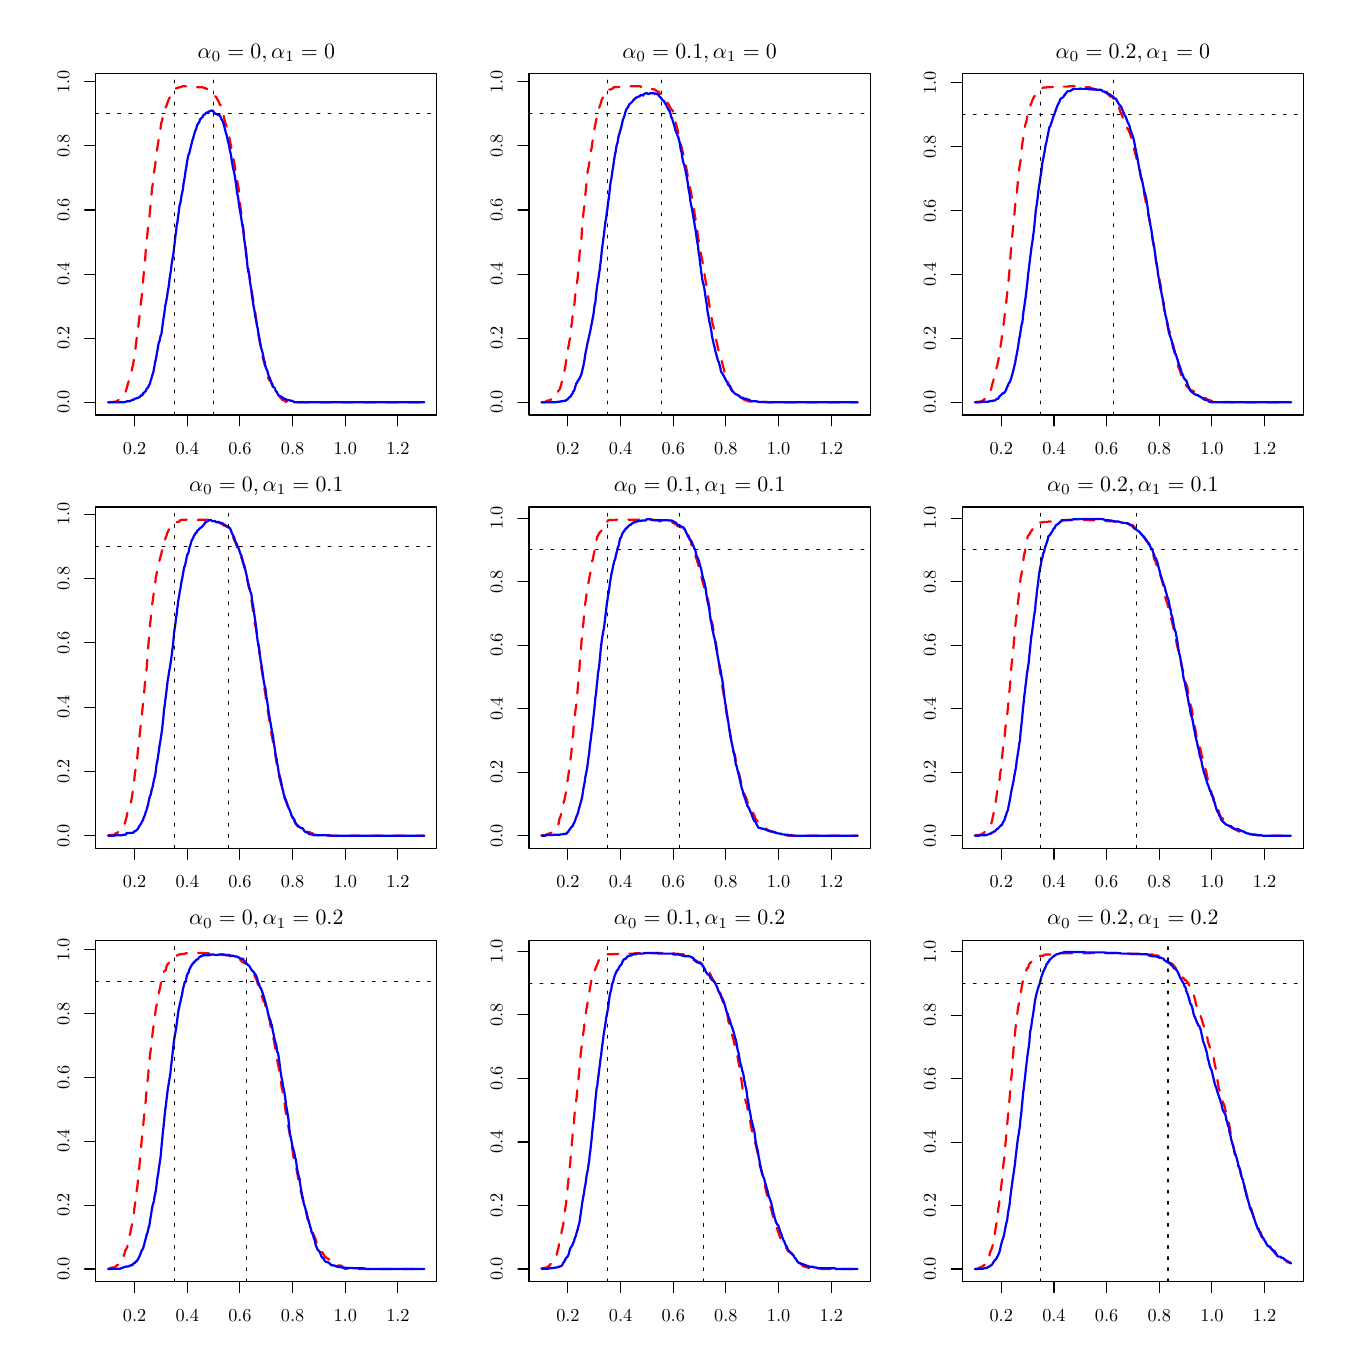
\begin{tikzpicture}[x=1pt,y=1pt]
\definecolor{fillColor}{RGB}{255,255,255}
\path[use as bounding box,fill=fillColor,fill opacity=0.00] (0,0) rectangle (469.75,469.75);
\begin{scope}
\path[clip] ( 24.55,329.80) rectangle (147.87,453.12);
\definecolor{drawColor}{RGB}{255,0,0}

\path[draw=drawColor,line width= 0.8pt,dash pattern=on 4pt off 4pt ,line join=round,line cap=round] ( 29.12,334.37) --
	( 29.35,334.37) --
	( 29.58,334.37) --
	( 29.81,334.37) --
	( 30.03,334.49) --
	( 30.26,334.49) --
	( 30.49,334.49) --
	( 30.72,334.49) --
	( 30.95,334.49) --
	( 31.18,334.60) --
	( 31.41,334.60) --
	( 31.64,334.60) --
	( 31.87,334.60) --
	( 32.09,334.72) --
	( 32.32,334.83) --
	( 32.55,334.95) --
	( 32.78,335.18) --
	( 33.01,335.30) --
	( 33.24,335.41) --
	( 33.47,335.64) --
	( 33.70,335.87) --
	( 33.92,336.11) --
	( 34.15,336.22) --
	( 34.38,336.69) --
	( 34.61,336.80) --
	( 34.84,337.15) --
	( 35.07,337.50) --
	( 35.30,338.08) --
	( 35.53,338.54) --
	( 35.76,339.35) --
	( 35.98,340.16) --
	( 36.21,341.09) --
	( 36.44,341.78) --
	( 36.67,342.36) --
	( 36.90,342.94) --
	( 37.13,343.75) --
	( 37.36,345.14) --
	( 37.59,345.83) --
	( 37.81,346.88) --
	( 38.04,347.69) --
	( 38.27,349.19) --
	( 38.50,350.58) --
	( 38.73,352.09) --
	( 38.96,353.94) --
	( 39.19,355.68) --
	( 39.42,357.88) --
	( 39.65,359.15) --
	( 39.87,360.89) --
	( 40.10,362.86) --
	( 40.33,364.71) --
	( 40.56,367.03) --
	( 40.79,369.23) --
	( 41.02,371.20) --
	( 41.25,373.05) --
	( 41.48,375.83) --
	( 41.71,378.26) --
	( 41.93,380.81) --
	( 42.16,383.36) --
	( 42.39,385.56) --
	( 42.62,388.57) --
	( 42.85,391.00) --
	( 43.08,393.66) --
	( 43.31,395.75) --
	( 43.54,398.18) --
	( 43.76,399.80) --
	( 43.99,401.42) --
	( 44.22,403.62) --
	( 44.45,406.29) --
	( 44.68,408.60) --
	( 44.91,411.61) --
	( 45.14,412.77) --
	( 45.37,414.74) --
	( 45.60,417.17) --
	( 45.82,418.45) --
	( 46.05,419.95) --
	( 46.28,421.92) --
	( 46.51,424.00) --
	( 46.74,425.74) --
	( 46.97,426.90) --
	( 47.20,428.41) --
	( 47.43,430.03) --
	( 47.65,431.76) --
	( 47.88,432.69) --
	( 48.11,434.20) --
	( 48.34,435.59) --
	( 48.57,436.16) --
	( 48.80,437.44) --
	( 49.03,437.90) --
	( 49.26,438.71) --
	( 49.49,439.41) --
	( 49.71,440.10) --
	( 49.94,441.26) --
	( 50.17,441.49) --
	( 50.40,442.42) --
	( 50.63,442.88) --
	( 50.86,443.58) --
	( 51.09,444.04) --
	( 51.32,444.50) --
	( 51.54,445.08) --
	( 51.77,445.43) --
	( 52.00,446.12) --
	( 52.23,446.24) --
	( 52.46,446.47) --
	( 52.69,446.59) --
	( 52.92,446.93) --
	( 53.15,447.05) --
	( 53.38,447.51) --
	( 53.60,447.86) --
	( 53.83,447.86) --
	( 54.06,447.86) --
	( 54.29,448.09) --
	( 54.52,448.09) --
	( 54.75,448.09) --
	( 54.98,448.21) --
	( 55.21,448.32) --
	( 55.43,448.32) --
	( 55.66,448.44) --
	( 55.89,448.56) --
	( 56.12,448.56) --
	( 56.35,448.56) --
	( 56.58,448.56) --
	( 56.81,448.56) --
	( 57.04,448.56) --
	( 57.27,448.56) --
	( 57.49,448.56) --
	( 57.72,448.56) --
	( 57.95,448.56) --
	( 58.18,448.56) --
	( 58.41,448.56) --
	( 58.64,448.56) --
	( 58.87,448.56) --
	( 59.10,448.44) --
	( 59.32,448.32) --
	( 59.55,448.32) --
	( 59.78,448.32) --
	( 60.01,448.32) --
	( 60.24,448.21) --
	( 60.47,448.21) --
	( 60.70,448.21) --
	( 60.93,448.21) --
	( 61.16,448.21) --
	( 61.38,448.21) --
	( 61.61,448.21) --
	( 61.84,448.21) --
	( 62.07,448.21) --
	( 62.30,448.21) --
	( 62.53,448.21) --
	( 62.76,448.21) --
	( 62.99,448.21) --
	( 63.22,448.21) --
	( 63.44,448.09) --
	( 63.67,447.98) --
	( 63.90,447.98) --
	( 64.13,447.98) --
	( 64.36,447.74) --
	( 64.59,447.63) --
	( 64.82,447.63) --
	( 65.05,447.28) --
	( 65.27,447.05) --
	( 65.50,446.93) --
	( 65.73,446.70) --
	( 65.96,446.70) --
	( 66.19,446.47) --
	( 66.42,446.36) --
	( 66.65,446.36) --
	( 66.88,446.24) --
	( 67.11,445.89) --
	( 67.33,445.78) --
	( 67.56,445.31) --
	( 67.79,444.97) --
	( 68.02,444.73) --
	( 68.25,444.50) --
	( 68.48,443.92) --
	( 68.71,443.58) --
	( 68.94,443.11) --
	( 69.16,442.77) --
	( 69.39,441.95) --
	( 69.62,441.84) --
	( 69.85,441.61) --
	( 70.08,440.45) --
	( 70.31,439.52) --
	( 70.54,439.06) --
	( 70.77,438.13) --
	( 71.00,437.09) --
	( 71.22,436.05) --
	( 71.45,435.35) --
	( 71.68,434.66) --
	( 71.91,433.96) --
	( 72.14,433.04) --
	( 72.37,432.11) --
	( 72.60,431.42) --
	( 72.83,430.26) --
	( 73.05,429.10) --
	( 73.28,427.94) --
	( 73.51,426.78) --
	( 73.74,425.63) --
	( 73.97,424.24) --
	( 74.20,423.54) --
	( 74.43,421.92) --
	( 74.66,420.65) --
	( 74.89,419.84) --
	( 75.11,418.10) --
	( 75.34,416.48) --
	( 75.57,414.97) --
	( 75.80,414.04) --
	( 76.03,412.54) --
	( 76.26,411.50) --
	( 76.49,409.07) --
	( 76.72,406.52) --
	( 76.94,404.43) --
	( 77.17,402.93) --
	( 77.40,401.42) --
	( 77.63,399.45) --
	( 77.86,397.60) --
	( 78.09,395.75) --
	( 78.32,393.66) --
	( 78.55,391.23) --
	( 78.78,389.96) --
	( 79.00,387.76) --
	( 79.23,386.02) --
	( 79.46,384.05) --
	( 79.69,383.12) --
	( 79.92,381.39) --
	( 80.15,379.77) --
	( 80.38,378.49) --
	( 80.61,376.75) --
	( 80.83,375.71) --
	( 81.06,374.09) --
	( 81.29,372.47) --
	( 81.52,371.31) --
	( 81.75,370.04) --
	( 81.98,368.53) --
	( 82.21,367.03) --
	( 82.44,365.29) --
	( 82.67,363.44) --
	( 82.89,361.93) --
	( 83.12,360.66) --
	( 83.35,359.15) --
	( 83.58,357.88) --
	( 83.81,356.72) --
	( 84.04,355.21) --
	( 84.27,353.83) --
	( 84.50,352.44) --
	( 84.73,351.97) --
	( 84.95,350.70) --
	( 85.18,349.77) --
	( 85.41,348.73) --
	( 85.64,348.03) --
	( 85.87,347.11) --
	( 86.10,346.41) --
	( 86.33,345.37) --
	( 86.56,344.33) --
	( 86.78,343.40) --
	( 87.01,342.94) --
	( 87.24,342.48) --
	( 87.47,342.24) --
	( 87.70,342.01) --
	( 87.93,341.90) --
	( 88.16,340.97) --
	( 88.39,340.51) --
	( 88.62,339.81) --
	( 88.84,339.12) --
	( 89.07,338.77) --
	( 89.30,338.19) --
	( 89.53,337.84) --
	( 89.76,337.73) --
	( 89.99,337.26) --
	( 90.22,337.03) --
	( 90.45,337.03) --
	( 90.67,336.80) --
	( 90.90,336.80) --
	( 91.13,336.45) --
	( 91.36,335.99) --
	( 91.59,335.76) --
	( 91.82,335.53) --
	( 92.05,335.18) --
	( 92.28,335.18) --
	( 92.51,335.06) --
	( 92.73,335.06) --
	( 92.96,334.83) --
	( 93.19,334.60) --
	( 93.42,334.60) --
	( 93.65,334.60) --
	( 93.88,334.49) --
	( 94.11,334.49) --
	( 94.34,334.49) --
	( 94.56,334.49) --
	( 94.79,334.49) --
	( 95.02,334.49) --
	( 95.25,334.49) --
	( 95.48,334.49) --
	( 95.71,334.49) --
	( 95.94,334.37) --
	( 96.17,334.37) --
	( 96.40,334.37) --
	( 96.62,334.37) --
	( 96.85,334.37) --
	( 97.08,334.37) --
	( 97.31,334.37) --
	( 97.54,334.37) --
	( 97.77,334.37) --
	( 98.00,334.37) --
	( 98.23,334.37) --
	( 98.45,334.37) --
	( 98.68,334.37) --
	( 98.91,334.37) --
	( 99.14,334.37) --
	( 99.37,334.37) --
	( 99.60,334.37) --
	( 99.83,334.37) --
	(100.06,334.37) --
	(100.29,334.37) --
	(100.51,334.37) --
	(100.74,334.37) --
	(100.97,334.37) --
	(101.20,334.37) --
	(101.43,334.37) --
	(101.66,334.37) --
	(101.89,334.37) --
	(102.12,334.37) --
	(102.35,334.37) --
	(102.57,334.37) --
	(102.80,334.37) --
	(103.03,334.37) --
	(103.26,334.37) --
	(103.49,334.37) --
	(103.72,334.37) --
	(103.95,334.37) --
	(104.18,334.37) --
	(104.40,334.37) --
	(104.63,334.37) --
	(104.86,334.37) --
	(105.09,334.37) --
	(105.32,334.37) --
	(105.55,334.37) --
	(105.78,334.37) --
	(106.01,334.37) --
	(106.24,334.37) --
	(106.46,334.37) --
	(106.69,334.37) --
	(106.92,334.37) --
	(107.15,334.37) --
	(107.38,334.37) --
	(107.61,334.37) --
	(107.84,334.37) --
	(108.07,334.37) --
	(108.29,334.37) --
	(108.52,334.37) --
	(108.75,334.37) --
	(108.98,334.37) --
	(109.21,334.37) --
	(109.44,334.37) --
	(109.67,334.37) --
	(109.90,334.37) --
	(110.13,334.37) --
	(110.35,334.37) --
	(110.58,334.37) --
	(110.81,334.37) --
	(111.04,334.37) --
	(111.27,334.37) --
	(111.50,334.37) --
	(111.73,334.37) --
	(111.96,334.37) --
	(112.18,334.37) --
	(112.41,334.37) --
	(112.64,334.37) --
	(112.87,334.37) --
	(113.10,334.37) --
	(113.33,334.37) --
	(113.56,334.37) --
	(113.79,334.37) --
	(114.02,334.37) --
	(114.24,334.37) --
	(114.47,334.37) --
	(114.70,334.37) --
	(114.93,334.37) --
	(115.16,334.37) --
	(115.39,334.37) --
	(115.62,334.37) --
	(115.85,334.37) --
	(116.07,334.37) --
	(116.30,334.37) --
	(116.53,334.37) --
	(116.76,334.37) --
	(116.99,334.37) --
	(117.22,334.37) --
	(117.45,334.37) --
	(117.68,334.37) --
	(117.91,334.37) --
	(118.13,334.37) --
	(118.36,334.37) --
	(118.59,334.37) --
	(118.82,334.37) --
	(119.05,334.37) --
	(119.28,334.37) --
	(119.51,334.37) --
	(119.74,334.37) --
	(119.96,334.37) --
	(120.19,334.37) --
	(120.42,334.37) --
	(120.65,334.37) --
	(120.88,334.37) --
	(121.11,334.37) --
	(121.34,334.37) --
	(121.57,334.37) --
	(121.80,334.37) --
	(122.02,334.37) --
	(122.25,334.37) --
	(122.48,334.37) --
	(122.71,334.37) --
	(122.94,334.37) --
	(123.17,334.37) --
	(123.40,334.37) --
	(123.63,334.37) --
	(123.86,334.37) --
	(124.08,334.37) --
	(124.31,334.37) --
	(124.54,334.37) --
	(124.77,334.37) --
	(125.00,334.37) --
	(125.23,334.37) --
	(125.46,334.37) --
	(125.69,334.37) --
	(125.91,334.37) --
	(126.14,334.37) --
	(126.37,334.37) --
	(126.60,334.37) --
	(126.83,334.37) --
	(127.06,334.37) --
	(127.29,334.37) --
	(127.52,334.37) --
	(127.75,334.37) --
	(127.97,334.37) --
	(128.20,334.37) --
	(128.43,334.37) --
	(128.66,334.37) --
	(128.89,334.37) --
	(129.12,334.37) --
	(129.35,334.37) --
	(129.58,334.37) --
	(129.80,334.37) --
	(130.03,334.37) --
	(130.26,334.37) --
	(130.49,334.37) --
	(130.72,334.37) --
	(130.95,334.37) --
	(131.18,334.37) --
	(131.41,334.37) --
	(131.64,334.37) --
	(131.86,334.37) --
	(132.09,334.37) --
	(132.32,334.37) --
	(132.55,334.37) --
	(132.78,334.37) --
	(133.01,334.37) --
	(133.24,334.37) --
	(133.47,334.37) --
	(133.69,334.37) --
	(133.92,334.37) --
	(134.15,334.37) --
	(134.38,334.37) --
	(134.61,334.37) --
	(134.84,334.37) --
	(135.07,334.37) --
	(135.30,334.37) --
	(135.53,334.37) --
	(135.75,334.37) --
	(135.98,334.37) --
	(136.21,334.37) --
	(136.44,334.37) --
	(136.67,334.37) --
	(136.90,334.37) --
	(137.13,334.37) --
	(137.36,334.37) --
	(137.58,334.37) --
	(137.81,334.37) --
	(138.04,334.37) --
	(138.27,334.37) --
	(138.50,334.37) --
	(138.73,334.37) --
	(138.96,334.37) --
	(139.19,334.37) --
	(139.42,334.37) --
	(139.64,334.37) --
	(139.87,334.37) --
	(140.10,334.37) --
	(140.33,334.37) --
	(140.56,334.37) --
	(140.79,334.37) --
	(141.02,334.37) --
	(141.25,334.37) --
	(141.47,334.37) --
	(141.70,334.37) --
	(141.93,334.37) --
	(142.16,334.37) --
	(142.39,334.37) --
	(142.62,334.37) --
	(142.85,334.37) --
	(143.08,334.37) --
	(143.31,334.37);
\end{scope}
\begin{scope}
\path[clip] (  0.00,  0.00) rectangle (469.75,469.75);
\definecolor{drawColor}{RGB}{0,0,0}

\path[draw=drawColor,line width= 0.4pt,line join=round,line cap=round] ( 38.63,329.80) -- (133.79,329.80);

\path[draw=drawColor,line width= 0.4pt,line join=round,line cap=round] ( 38.63,329.80) -- ( 38.63,325.84);

\path[draw=drawColor,line width= 0.4pt,line join=round,line cap=round] ( 57.67,329.80) -- ( 57.67,325.84);

\path[draw=drawColor,line width= 0.4pt,line join=round,line cap=round] ( 76.70,329.80) -- ( 76.70,325.84);

\path[draw=drawColor,line width= 0.4pt,line join=round,line cap=round] ( 95.73,329.80) -- ( 95.73,325.84);

\path[draw=drawColor,line width= 0.4pt,line join=round,line cap=round] (114.76,329.80) -- (114.76,325.84);

\path[draw=drawColor,line width= 0.4pt,line join=round,line cap=round] (133.79,329.80) -- (133.79,325.84);

\node[text=drawColor,anchor=base,inner sep=0pt, outer sep=0pt, scale=  0.66] at ( 38.63,315.55) {0.2};

\node[text=drawColor,anchor=base,inner sep=0pt, outer sep=0pt, scale=  0.66] at ( 57.67,315.55) {0.4};

\node[text=drawColor,anchor=base,inner sep=0pt, outer sep=0pt, scale=  0.66] at ( 76.70,315.55) {0.6};

\node[text=drawColor,anchor=base,inner sep=0pt, outer sep=0pt, scale=  0.66] at ( 95.73,315.55) {0.8};

\node[text=drawColor,anchor=base,inner sep=0pt, outer sep=0pt, scale=  0.66] at (114.76,315.55) {1.0};

\node[text=drawColor,anchor=base,inner sep=0pt, outer sep=0pt, scale=  0.66] at (133.79,315.55) {1.2};

\path[draw=drawColor,line width= 0.4pt,line join=round,line cap=round] ( 24.55,334.37) -- ( 24.55,450.18);

\path[draw=drawColor,line width= 0.4pt,line join=round,line cap=round] ( 24.55,334.37) -- ( 20.59,334.37);

\path[draw=drawColor,line width= 0.4pt,line join=round,line cap=round] ( 24.55,357.53) -- ( 20.59,357.53);

\path[draw=drawColor,line width= 0.4pt,line join=round,line cap=round] ( 24.55,380.69) -- ( 20.59,380.69);

\path[draw=drawColor,line width= 0.4pt,line join=round,line cap=round] ( 24.55,403.85) -- ( 20.59,403.85);

\path[draw=drawColor,line width= 0.4pt,line join=round,line cap=round] ( 24.55,427.02) -- ( 20.59,427.02);

\path[draw=drawColor,line width= 0.4pt,line join=round,line cap=round] ( 24.55,450.18) -- ( 20.59,450.18);

\node[text=drawColor,rotate= 90.00,anchor=base,inner sep=0pt, outer sep=0pt, scale=  0.66] at ( 15.05,334.37) {0.0};

\node[text=drawColor,rotate= 90.00,anchor=base,inner sep=0pt, outer sep=0pt, scale=  0.66] at ( 15.05,357.53) {0.2};

\node[text=drawColor,rotate= 90.00,anchor=base,inner sep=0pt, outer sep=0pt, scale=  0.66] at ( 15.05,380.69) {0.4};

\node[text=drawColor,rotate= 90.00,anchor=base,inner sep=0pt, outer sep=0pt, scale=  0.66] at ( 15.05,403.85) {0.6};

\node[text=drawColor,rotate= 90.00,anchor=base,inner sep=0pt, outer sep=0pt, scale=  0.66] at ( 15.05,427.02) {0.8};

\node[text=drawColor,rotate= 90.00,anchor=base,inner sep=0pt, outer sep=0pt, scale=  0.66] at ( 15.05,450.18) {1.0};

\path[draw=drawColor,line width= 0.4pt,line join=round,line cap=round] ( 24.55,329.80) --
	(147.87,329.80) --
	(147.87,453.12) --
	( 24.55,453.12) --
	( 24.55,329.80);
\end{scope}
\begin{scope}
\path[clip] (  0.00,313.17) rectangle (156.58,469.75);
\definecolor{drawColor}{RGB}{0,0,0}

\node[text=drawColor,anchor=base,inner sep=0pt, outer sep=0pt, scale=  0.79] at ( 86.21,458.71) {\bfseries $\alpha_0 = 0, \alpha_1 = 0$};
\end{scope}
\begin{scope}
\path[clip] ( 24.55,329.80) rectangle (147.87,453.12);
\definecolor{drawColor}{RGB}{0,0,255}

\path[draw=drawColor,line width= 0.8pt,line join=round,line cap=round] ( 29.12,334.37) --
	( 29.35,334.37) --
	( 29.58,334.37) --
	( 29.81,334.37) --
	( 30.03,334.37) --
	( 30.26,334.37) --
	( 30.49,334.37) --
	( 30.72,334.37) --
	( 30.95,334.37) --
	( 31.18,334.37) --
	( 31.41,334.37) --
	( 31.64,334.37) --
	( 31.87,334.37) --
	( 32.09,334.37) --
	( 32.32,334.37) --
	( 32.55,334.37) --
	( 32.78,334.37) --
	( 33.01,334.37) --
	( 33.24,334.37) --
	( 33.47,334.37) --
	( 33.70,334.37) --
	( 33.92,334.37) --
	( 34.15,334.37) --
	( 34.38,334.37) --
	( 34.61,334.37) --
	( 34.84,334.37) --
	( 35.07,334.49) --
	( 35.30,334.49) --
	( 35.53,334.60) --
	( 35.76,334.72) --
	( 35.98,334.72) --
	( 36.21,334.72) --
	( 36.44,334.72) --
	( 36.67,334.72) --
	( 36.90,334.83) --
	( 37.13,334.83) --
	( 37.36,335.06) --
	( 37.59,335.06) --
	( 37.81,335.30) --
	( 38.04,335.30) --
	( 38.27,335.30) --
	( 38.50,335.53) --
	( 38.73,335.64) --
	( 38.96,335.76) --
	( 39.19,335.76) --
	( 39.42,335.87) --
	( 39.65,335.87) --
	( 39.87,335.99) --
	( 40.10,336.11) --
	( 40.33,336.22) --
	( 40.56,336.34) --
	( 40.79,336.69) --
	( 41.02,336.92) --
	( 41.25,336.92) --
	( 41.48,336.92) --
	( 41.71,337.73) --
	( 41.93,337.73) --
	( 42.16,337.96) --
	( 42.39,338.19) --
	( 42.62,338.31) --
	( 42.85,339.00) --
	( 43.08,339.35) --
	( 43.31,339.58) --
	( 43.54,339.70) --
	( 43.76,340.51) --
	( 43.99,340.74) --
	( 44.22,341.20) --
	( 44.45,342.24) --
	( 44.68,342.82) --
	( 44.91,343.75) --
	( 45.14,344.44) --
	( 45.37,345.14) --
	( 45.60,346.30) --
	( 45.82,347.46) --
	( 46.05,348.85) --
	( 46.28,349.77) --
	( 46.51,350.93) --
	( 46.74,352.55) --
	( 46.97,353.48) --
	( 47.20,355.10) --
	( 47.43,356.03) --
	( 47.65,356.49) --
	( 47.88,357.76) --
	( 48.11,358.57) --
	( 48.34,359.15) --
	( 48.57,360.77) --
	( 48.80,362.74) --
	( 49.03,364.36) --
	( 49.26,365.64) --
	( 49.49,367.37) --
	( 49.71,369.23) --
	( 49.94,370.27) --
	( 50.17,371.43) --
	( 50.40,372.82) --
	( 50.63,374.44) --
	( 50.86,375.60) --
	( 51.09,377.33) --
	( 51.32,379.30) --
	( 51.54,380.58) --
	( 51.77,382.08) --
	( 52.00,384.17) --
	( 52.23,385.56) --
	( 52.46,386.95) --
	( 52.69,388.22) --
	( 52.92,390.42) --
	( 53.15,392.16) --
	( 53.38,394.47) --
	( 53.60,395.75) --
	( 53.83,398.18) --
	( 54.06,399.22) --
	( 54.29,400.84) --
	( 54.52,402.58) --
	( 54.75,404.66) --
	( 54.98,405.94) --
	( 55.21,406.52) --
	( 55.43,408.02) --
	( 55.66,409.41) --
	( 55.89,410.34) --
	( 56.12,411.50) --
	( 56.35,413.58) --
	( 56.58,414.74) --
	( 56.81,416.01) --
	( 57.04,417.98) --
	( 57.27,419.02) --
	( 57.49,420.53) --
	( 57.72,422.04) --
	( 57.95,423.08) --
	( 58.18,424.00) --
	( 58.41,424.35) --
	( 58.64,425.51) --
	( 58.87,426.32) --
	( 59.10,427.36) --
	( 59.32,428.17) --
	( 59.55,429.10) --
	( 59.78,429.68) --
	( 60.01,430.72) --
	( 60.24,431.42) --
	( 60.47,432.23) --
	( 60.70,432.81) --
	( 60.93,433.27) --
	( 61.16,434.20) --
	( 61.38,434.77) --
	( 61.61,435.12) --
	( 61.84,435.35) --
	( 62.07,435.82) --
	( 62.30,436.74) --
	( 62.53,436.74) --
	( 62.76,437.09) --
	( 62.99,437.32) --
	( 63.22,437.44) --
	( 63.44,438.02) --
	( 63.67,438.36) --
	( 63.90,438.36) --
	( 64.13,438.48) --
	( 64.36,438.94) --
	( 64.59,438.94) --
	( 64.82,439.18) --
	( 65.05,439.06) --
	( 65.27,439.29) --
	( 65.50,439.41) --
	( 65.73,439.52) --
	( 65.96,439.64) --
	( 66.19,439.64) --
	( 66.42,439.87) --
	( 66.65,439.75) --
	( 66.88,439.64) --
	( 67.11,439.64) --
	( 67.33,438.94) --
	( 67.56,438.94) --
	( 67.79,438.60) --
	( 68.02,438.60) --
	( 68.25,438.60) --
	( 68.48,438.36) --
	( 68.71,438.36) --
	( 68.94,438.13) --
	( 69.16,438.25) --
	( 69.39,437.90) --
	( 69.62,437.67) --
	( 69.85,437.09) --
	( 70.08,436.51) --
	( 70.31,436.28) --
	( 70.54,435.70) --
	( 70.77,435.01) --
	( 71.00,434.20) --
	( 71.22,433.38) --
	( 71.45,432.46) --
	( 71.68,431.53) --
	( 71.91,430.95) --
	( 72.14,429.79) --
	( 72.37,428.75) --
	( 72.60,427.83) --
	( 72.83,426.78) --
	( 73.05,425.51) --
	( 73.28,424.58) --
	( 73.51,423.43) --
	( 73.74,421.57) --
	( 73.97,420.53) --
	( 74.20,418.79) --
	( 74.43,418.21) --
	( 74.66,417.17) --
	( 74.89,415.90) --
	( 75.11,414.39) --
	( 75.34,413.00) --
	( 75.57,410.80) --
	( 75.80,409.41) --
	( 76.03,408.60) --
	( 76.26,406.52) --
	( 76.49,405.13) --
	( 76.72,403.51) --
	( 76.94,402.35) --
	( 77.17,400.96) --
	( 77.40,399.45) --
	( 77.63,398.18) --
	( 77.86,396.91) --
	( 78.09,394.59) --
	( 78.32,392.74) --
	( 78.55,391.23) --
	( 78.78,389.61) --
	( 79.00,387.29) --
	( 79.23,385.79) --
	( 79.46,383.12) --
	( 79.69,381.73) --
	( 79.92,381.04) --
	( 80.15,379.53) --
	( 80.38,377.68) --
	( 80.61,376.18) --
	( 80.83,374.90) --
	( 81.06,372.70) --
	( 81.29,371.31) --
	( 81.52,369.69) --
	( 81.75,368.53) --
	( 81.98,367.37) --
	( 82.21,365.41) --
	( 82.44,364.60) --
	( 82.67,363.32) --
	( 82.89,361.93) --
	( 83.12,361.12) --
	( 83.35,359.62) --
	( 83.58,358.11) --
	( 83.81,356.95) --
	( 84.04,355.68) --
	( 84.27,354.40) --
	( 84.50,353.59) --
	( 84.73,352.78) --
	( 84.95,351.97) --
	( 85.18,350.81) --
	( 85.41,349.54) --
	( 85.64,349.08) --
	( 85.87,347.46) --
	( 86.10,346.99) --
	( 86.33,346.30) --
	( 86.56,345.83) --
	( 86.78,345.02) --
	( 87.01,344.21) --
	( 87.24,343.52) --
	( 87.47,343.29) --
	( 87.70,342.48) --
	( 87.93,341.78) --
	( 88.16,341.32) --
	( 88.39,340.97) --
	( 88.62,340.04) --
	( 88.84,339.93) --
	( 89.07,339.70) --
	( 89.30,339.46) --
	( 89.53,338.77) --
	( 89.76,338.31) --
	( 89.99,338.19) --
	( 90.22,337.73) --
	( 90.45,337.03) --
	( 90.67,336.92) --
	( 90.90,336.69) --
	( 91.13,336.45) --
	( 91.36,336.45) --
	( 91.59,336.45) --
	( 91.82,336.34) --
	( 92.05,336.11) --
	( 92.28,335.99) --
	( 92.51,335.76) --
	( 92.73,335.53) --
	( 92.96,335.53) --
	( 93.19,335.53) --
	( 93.42,335.41) --
	( 93.65,335.18) --
	( 93.88,335.18) --
	( 94.11,335.18) --
	( 94.34,335.18) --
	( 94.56,335.06) --
	( 94.79,335.06) --
	( 95.02,334.95) --
	( 95.25,334.95) --
	( 95.48,334.95) --
	( 95.71,334.83) --
	( 95.94,334.72) --
	( 96.17,334.49) --
	( 96.40,334.37) --
	( 96.62,334.37) --
	( 96.85,334.37) --
	( 97.08,334.37) --
	( 97.31,334.37) --
	( 97.54,334.37) --
	( 97.77,334.37) --
	( 98.00,334.37) --
	( 98.23,334.37) --
	( 98.45,334.37) --
	( 98.68,334.37) --
	( 98.91,334.37) --
	( 99.14,334.37) --
	( 99.37,334.37) --
	( 99.60,334.37) --
	( 99.83,334.37) --
	(100.06,334.37) --
	(100.29,334.37) --
	(100.51,334.37) --
	(100.74,334.37) --
	(100.97,334.37) --
	(101.20,334.37) --
	(101.43,334.37) --
	(101.66,334.37) --
	(101.89,334.37) --
	(102.12,334.37) --
	(102.35,334.37) --
	(102.57,334.37) --
	(102.80,334.37) --
	(103.03,334.37) --
	(103.26,334.37) --
	(103.49,334.37) --
	(103.72,334.37) --
	(103.95,334.37) --
	(104.18,334.37) --
	(104.40,334.37) --
	(104.63,334.37) --
	(104.86,334.37) --
	(105.09,334.37) --
	(105.32,334.37) --
	(105.55,334.37) --
	(105.78,334.37) --
	(106.01,334.37) --
	(106.24,334.37) --
	(106.46,334.37) --
	(106.69,334.37) --
	(106.92,334.37) --
	(107.15,334.37) --
	(107.38,334.37) --
	(107.61,334.37) --
	(107.84,334.37) --
	(108.07,334.37) --
	(108.29,334.37) --
	(108.52,334.37) --
	(108.75,334.37) --
	(108.98,334.37) --
	(109.21,334.37) --
	(109.44,334.37) --
	(109.67,334.37) --
	(109.90,334.37) --
	(110.13,334.37) --
	(110.35,334.37) --
	(110.58,334.37) --
	(110.81,334.37) --
	(111.04,334.37) --
	(111.27,334.37) --
	(111.50,334.37) --
	(111.73,334.37) --
	(111.96,334.37) --
	(112.18,334.37) --
	(112.41,334.37) --
	(112.64,334.37) --
	(112.87,334.37) --
	(113.10,334.37) --
	(113.33,334.37) --
	(113.56,334.37) --
	(113.79,334.37) --
	(114.02,334.37) --
	(114.24,334.37) --
	(114.47,334.37) --
	(114.70,334.37) --
	(114.93,334.37) --
	(115.16,334.37) --
	(115.39,334.37) --
	(115.62,334.37) --
	(115.85,334.37) --
	(116.07,334.37) --
	(116.30,334.37) --
	(116.53,334.37) --
	(116.76,334.37) --
	(116.99,334.37) --
	(117.22,334.37) --
	(117.45,334.37) --
	(117.68,334.37) --
	(117.91,334.37) --
	(118.13,334.37) --
	(118.36,334.37) --
	(118.59,334.37) --
	(118.82,334.37) --
	(119.05,334.37) --
	(119.28,334.37) --
	(119.51,334.37) --
	(119.74,334.37) --
	(119.96,334.37) --
	(120.19,334.37) --
	(120.42,334.37) --
	(120.65,334.37) --
	(120.88,334.37) --
	(121.11,334.37) --
	(121.34,334.37) --
	(121.57,334.37) --
	(121.80,334.37) --
	(122.02,334.37) --
	(122.25,334.37) --
	(122.48,334.37) --
	(122.71,334.37) --
	(122.94,334.37) --
	(123.17,334.37) --
	(123.40,334.37) --
	(123.63,334.37) --
	(123.86,334.37) --
	(124.08,334.37) --
	(124.31,334.37) --
	(124.54,334.37) --
	(124.77,334.37) --
	(125.00,334.37) --
	(125.23,334.37) --
	(125.46,334.37) --
	(125.69,334.37) --
	(125.91,334.37) --
	(126.14,334.37) --
	(126.37,334.37) --
	(126.60,334.37) --
	(126.83,334.37) --
	(127.06,334.37) --
	(127.29,334.37) --
	(127.52,334.37) --
	(127.75,334.37) --
	(127.97,334.37) --
	(128.20,334.37) --
	(128.43,334.37) --
	(128.66,334.37) --
	(128.89,334.37) --
	(129.12,334.37) --
	(129.35,334.37) --
	(129.58,334.37) --
	(129.80,334.37) --
	(130.03,334.37) --
	(130.26,334.37) --
	(130.49,334.37) --
	(130.72,334.37) --
	(130.95,334.37) --
	(131.18,334.37) --
	(131.41,334.37) --
	(131.64,334.37) --
	(131.86,334.37) --
	(132.09,334.37) --
	(132.32,334.37) --
	(132.55,334.37) --
	(132.78,334.37) --
	(133.01,334.37) --
	(133.24,334.37) --
	(133.47,334.37) --
	(133.69,334.37) --
	(133.92,334.37) --
	(134.15,334.37) --
	(134.38,334.37) --
	(134.61,334.37) --
	(134.84,334.37) --
	(135.07,334.37) --
	(135.30,334.37) --
	(135.53,334.37) --
	(135.75,334.37) --
	(135.98,334.37) --
	(136.21,334.37) --
	(136.44,334.37) --
	(136.67,334.37) --
	(136.90,334.37) --
	(137.13,334.37) --
	(137.36,334.37) --
	(137.58,334.37) --
	(137.81,334.37) --
	(138.04,334.37) --
	(138.27,334.37) --
	(138.50,334.37) --
	(138.73,334.37) --
	(138.96,334.37) --
	(139.19,334.37) --
	(139.42,334.37) --
	(139.64,334.37) --
	(139.87,334.37) --
	(140.10,334.37) --
	(140.33,334.37) --
	(140.56,334.37) --
	(140.79,334.37) --
	(141.02,334.37) --
	(141.25,334.37) --
	(141.47,334.37) --
	(141.70,334.37) --
	(141.93,334.37) --
	(142.16,334.37) --
	(142.39,334.37) --
	(142.62,334.37) --
	(142.85,334.37) --
	(143.08,334.37) --
	(143.31,334.37);
\definecolor{drawColor}{RGB}{0,0,0}

\path[draw=drawColor,line width= 0.4pt,dash pattern=on 1pt off 3pt ,line join=round,line cap=round] ( 24.55,438.60) -- (147.87,438.60);

\path[draw=drawColor,line width= 0.4pt,dash pattern=on 1pt off 3pt ,line join=round,line cap=round] ( 52.91,329.80) -- ( 52.91,453.12);

\path[draw=drawColor,line width= 0.4pt,dash pattern=on 1pt off 3pt ,line join=round,line cap=round] ( 67.18,329.80) -- ( 67.18,453.12);
\end{scope}
\begin{scope}
\path[clip] (181.14,329.80) rectangle (304.46,453.12);
\definecolor{drawColor}{RGB}{255,0,0}

\path[draw=drawColor,line width= 0.8pt,dash pattern=on 4pt off 4pt ,line join=round,line cap=round] (185.70,334.37) --
	(185.93,334.37) --
	(186.16,334.37) --
	(186.39,334.37) --
	(186.62,334.37) --
	(186.85,334.49) --
	(187.08,334.49) --
	(187.31,334.49) --
	(187.54,334.95) --
	(187.76,334.95) --
	(187.99,334.95) --
	(188.22,334.95) --
	(188.45,335.18) --
	(188.68,335.18) --
	(188.91,335.18) --
	(189.14,335.53) --
	(189.37,335.76) --
	(189.59,335.76) --
	(189.82,335.76) --
	(190.05,335.76) --
	(190.28,335.87) --
	(190.51,336.11) --
	(190.74,336.45) --
	(190.97,336.92) --
	(191.20,337.38) --
	(191.43,337.96) --
	(191.65,338.31) --
	(191.88,338.65) --
	(192.11,338.89) --
	(192.34,339.23) --
	(192.57,340.16) --
	(192.80,340.85) --
	(193.03,341.90) --
	(193.26,342.59) --
	(193.48,343.87) --
	(193.71,345.02) --
	(193.94,345.49) --
	(194.17,346.88) --
	(194.40,348.15) --
	(194.63,349.77) --
	(194.86,350.93) --
	(195.09,352.67) --
	(195.32,353.94) --
	(195.54,355.33) --
	(195.77,356.49) --
	(196.00,357.76) --
	(196.23,359.73) --
	(196.46,362.05) --
	(196.69,363.09) --
	(196.92,365.75) --
	(197.15,367.61) --
	(197.37,368.76) --
	(197.60,370.04) --
	(197.83,372.82) --
	(198.06,374.44) --
	(198.29,376.41) --
	(198.52,377.91) --
	(198.75,379.30) --
	(198.98,382.66) --
	(199.21,385.32) --
	(199.43,387.99) --
	(199.66,390.07) --
	(199.89,391.58) --
	(200.12,393.89) --
	(200.35,397.48) --
	(200.58,400.38) --
	(200.81,402.58) --
	(201.04,404.55) --
	(201.26,406.17) --
	(201.49,409.30) --
	(201.72,411.27) --
	(201.95,413.70) --
	(202.18,416.36) --
	(202.41,418.21) --
	(202.64,419.14) --
	(202.87,420.53) --
	(203.10,421.80) --
	(203.32,423.31) --
	(203.55,425.39) --
	(203.78,426.20) --
	(204.01,428.06) --
	(204.24,429.22) --
	(204.47,431.18) --
	(204.70,432.57) --
	(204.93,434.08) --
	(205.15,434.89) --
	(205.38,436.16) --
	(205.61,437.21) --
	(205.84,438.13) --
	(206.07,438.71) --
	(206.30,439.87) --
	(206.53,440.80) --
	(206.76,441.61) --
	(206.99,442.07) --
	(207.21,442.77) --
	(207.44,443.69) --
	(207.67,444.15) --
	(207.90,444.62) --
	(208.13,444.73) --
	(208.36,445.20) --
	(208.59,445.89) --
	(208.82,446.24) --
	(209.05,446.82) --
	(209.27,446.82) --
	(209.50,447.05) --
	(209.73,447.17) --
	(209.96,447.40) --
	(210.19,447.40) --
	(210.42,447.40) --
	(210.65,447.40) --
	(210.88,447.51) --
	(211.10,447.63) --
	(211.33,447.74) --
	(211.56,447.98) --
	(211.79,448.21) --
	(212.02,448.21) --
	(212.25,448.32) --
	(212.48,448.32) --
	(212.71,448.32) --
	(212.94,448.32) --
	(213.16,448.32) --
	(213.39,448.32) --
	(213.62,448.32) --
	(213.85,448.32) --
	(214.08,448.32) --
	(214.31,448.32) --
	(214.54,448.32) --
	(214.77,448.44) --
	(214.99,448.44) --
	(215.22,448.44) --
	(215.45,448.44) --
	(215.68,448.56) --
	(215.91,448.56) --
	(216.14,448.56) --
	(216.37,448.56) --
	(216.60,448.56) --
	(216.83,448.56) --
	(217.05,448.56) --
	(217.28,448.56) --
	(217.51,448.56) --
	(217.74,448.56) --
	(217.97,448.56) --
	(218.20,448.56) --
	(218.43,448.56) --
	(218.66,448.56) --
	(218.88,448.56) --
	(219.11,448.56) --
	(219.34,448.56) --
	(219.57,448.56) --
	(219.80,448.56) --
	(220.03,448.56) --
	(220.26,448.56) --
	(220.49,448.56) --
	(220.72,448.56) --
	(220.94,448.56) --
	(221.17,448.56) --
	(221.40,448.56) --
	(221.63,448.32) --
	(221.86,448.32) --
	(222.09,448.32) --
	(222.32,448.32) --
	(222.55,448.32) --
	(222.77,448.32) --
	(223.00,448.32) --
	(223.23,448.21) --
	(223.46,448.21) --
	(223.69,448.21) --
	(223.92,448.09) --
	(224.15,447.98) --
	(224.38,447.98) --
	(224.61,447.86) --
	(224.83,447.86) --
	(225.06,447.74) --
	(225.29,447.63) --
	(225.52,447.63) --
	(225.75,447.51) --
	(225.98,447.51) --
	(226.21,447.51) --
	(226.44,447.40) --
	(226.66,447.40) --
	(226.89,447.05) --
	(227.12,447.05) --
	(227.35,446.82) --
	(227.58,446.70) --
	(227.81,446.59) --
	(228.04,446.59) --
	(228.27,446.12) --
	(228.50,446.01) --
	(228.72,445.66) --
	(228.95,445.43) --
	(229.18,445.31) --
	(229.41,444.85) --
	(229.64,444.73) --
	(229.87,444.62) --
	(230.10,444.50) --
	(230.33,444.27) --
	(230.56,443.81) --
	(230.78,443.46) --
	(231.01,442.88) --
	(231.24,442.53) --
	(231.47,442.19) --
	(231.70,441.84) --
	(231.93,441.38) --
	(232.16,440.80) --
	(232.39,440.56) --
	(232.61,440.10) --
	(232.84,439.99) --
	(233.07,439.75) --
	(233.30,438.94) --
	(233.53,438.02) --
	(233.76,436.74) --
	(233.99,436.16) --
	(234.22,435.01) --
	(234.45,434.43) --
	(234.67,433.50) --
	(234.90,432.81) --
	(235.13,431.53) --
	(235.36,430.61) --
	(235.59,428.75) --
	(235.82,428.17) --
	(236.05,427.13) --
	(236.28,426.67) --
	(236.50,425.74) --
	(236.73,424.58) --
	(236.96,423.89) --
	(237.19,422.85) --
	(237.42,421.46) --
	(237.65,420.30) --
	(237.88,419.72) --
	(238.11,418.33) --
	(238.34,417.17) --
	(238.56,415.67) --
	(238.79,414.97) --
	(239.02,414.16) --
	(239.25,412.42) --
	(239.48,411.15) --
	(239.71,410.34) --
	(239.94,408.72) --
	(240.17,407.79) --
	(240.39,406.86) --
	(240.62,405.59) --
	(240.85,403.62) --
	(241.08,401.77) --
	(241.31,400.61) --
	(241.54,399.22) --
	(241.77,397.48) --
	(242.00,395.98) --
	(242.23,393.89) --
	(242.45,392.97) --
	(242.68,391.69) --
	(242.91,389.84) --
	(243.14,389.15) --
	(243.37,387.53) --
	(243.60,386.48) --
	(243.83,385.32) --
	(244.06,383.94) --
	(244.28,382.20) --
	(244.51,380.92) --
	(244.74,379.88) --
	(244.97,378.03) --
	(245.20,377.22) --
	(245.43,375.37) --
	(245.66,374.32) --
	(245.89,372.59) --
	(246.12,370.96) --
	(246.34,369.57) --
	(246.57,367.84) --
	(246.80,366.10) --
	(247.03,365.41) --
	(247.26,364.13) --
	(247.49,362.74) --
	(247.72,362.05) --
	(247.95,360.89) --
	(248.18,359.62) --
	(248.40,358.34) --
	(248.63,357.65) --
	(248.86,356.60) --
	(249.09,355.68) --
	(249.32,354.40) --
	(249.55,353.36) --
	(249.78,352.55) --
	(250.01,351.97) --
	(250.23,351.51) --
	(250.46,350.81) --
	(250.69,349.66) --
	(250.92,348.85) --
	(251.15,347.80) --
	(251.38,346.99) --
	(251.61,346.30) --
	(251.84,345.14) --
	(252.07,344.68) --
	(252.29,343.98) --
	(252.52,343.40) --
	(252.75,342.82) --
	(252.98,342.01) --
	(253.21,341.20) --
	(253.44,340.74) --
	(253.67,340.28) --
	(253.90,339.46) --
	(254.12,339.12) --
	(254.35,338.77) --
	(254.58,338.42) --
	(254.81,338.19) --
	(255.04,337.96) --
	(255.27,337.84) --
	(255.50,337.84) --
	(255.73,337.73) --
	(255.96,337.61) --
	(256.18,337.26) --
	(256.41,337.03) --
	(256.64,337.03) --
	(256.87,337.03) --
	(257.10,336.57) --
	(257.33,336.34) --
	(257.56,336.11) --
	(257.79,335.99) --
	(258.01,335.99) --
	(258.24,335.76) --
	(258.47,335.53) --
	(258.70,335.53) --
	(258.93,335.30) --
	(259.16,335.18) --
	(259.39,335.06) --
	(259.62,335.06) --
	(259.85,335.06) --
	(260.07,334.83) --
	(260.30,334.72) --
	(260.53,334.72) --
	(260.76,334.72) --
	(260.99,334.72) --
	(261.22,334.60) --
	(261.45,334.60) --
	(261.68,334.60) --
	(261.90,334.60) --
	(262.13,334.60) --
	(262.36,334.60) --
	(262.59,334.60) --
	(262.82,334.60) --
	(263.05,334.49) --
	(263.28,334.49) --
	(263.51,334.49) --
	(263.74,334.49) --
	(263.96,334.49) --
	(264.19,334.49) --
	(264.42,334.49) --
	(264.65,334.49) --
	(264.88,334.49) --
	(265.11,334.49) --
	(265.34,334.49) --
	(265.57,334.49) --
	(265.79,334.49) --
	(266.02,334.49) --
	(266.25,334.49) --
	(266.48,334.49) --
	(266.71,334.49) --
	(266.94,334.49) --
	(267.17,334.49) --
	(267.40,334.49) --
	(267.63,334.37) --
	(267.85,334.37) --
	(268.08,334.37) --
	(268.31,334.37) --
	(268.54,334.37) --
	(268.77,334.37) --
	(269.00,334.37) --
	(269.23,334.37) --
	(269.46,334.37) --
	(269.69,334.37) --
	(269.91,334.37) --
	(270.14,334.37) --
	(270.37,334.37) --
	(270.60,334.37) --
	(270.83,334.37) --
	(271.06,334.37) --
	(271.29,334.37) --
	(271.52,334.37) --
	(271.74,334.37) --
	(271.97,334.37) --
	(272.20,334.37) --
	(272.43,334.37) --
	(272.66,334.37) --
	(272.89,334.37) --
	(273.12,334.37) --
	(273.35,334.37) --
	(273.58,334.37) --
	(273.80,334.37) --
	(274.03,334.37) --
	(274.26,334.37) --
	(274.49,334.37) --
	(274.72,334.37) --
	(274.95,334.37) --
	(275.18,334.37) --
	(275.41,334.37) --
	(275.63,334.37) --
	(275.86,334.37) --
	(276.09,334.37) --
	(276.32,334.37) --
	(276.55,334.37) --
	(276.78,334.37) --
	(277.01,334.37) --
	(277.24,334.37) --
	(277.47,334.37) --
	(277.69,334.37) --
	(277.92,334.37) --
	(278.15,334.37) --
	(278.38,334.37) --
	(278.61,334.37) --
	(278.84,334.37) --
	(279.07,334.37) --
	(279.30,334.37) --
	(279.52,334.37) --
	(279.75,334.37) --
	(279.98,334.37) --
	(280.21,334.37) --
	(280.44,334.37) --
	(280.67,334.37) --
	(280.90,334.37) --
	(281.13,334.37) --
	(281.36,334.37) --
	(281.58,334.37) --
	(281.81,334.37) --
	(282.04,334.37) --
	(282.27,334.37) --
	(282.50,334.37) --
	(282.73,334.37) --
	(282.96,334.37) --
	(283.19,334.37) --
	(283.41,334.37) --
	(283.64,334.37) --
	(283.87,334.37) --
	(284.10,334.37) --
	(284.33,334.37) --
	(284.56,334.37) --
	(284.79,334.37) --
	(285.02,334.37) --
	(285.25,334.37) --
	(285.47,334.37) --
	(285.70,334.37) --
	(285.93,334.37) --
	(286.16,334.37) --
	(286.39,334.37) --
	(286.62,334.37) --
	(286.85,334.37) --
	(287.08,334.37) --
	(287.30,334.37) --
	(287.53,334.37) --
	(287.76,334.37) --
	(287.99,334.37) --
	(288.22,334.37) --
	(288.45,334.37) --
	(288.68,334.37) --
	(288.91,334.37) --
	(289.14,334.37) --
	(289.36,334.37) --
	(289.59,334.37) --
	(289.82,334.37) --
	(290.05,334.37) --
	(290.28,334.37) --
	(290.51,334.37) --
	(290.74,334.37) --
	(290.97,334.37) --
	(291.20,334.37) --
	(291.42,334.37) --
	(291.65,334.37) --
	(291.88,334.37) --
	(292.11,334.37) --
	(292.34,334.37) --
	(292.57,334.37) --
	(292.80,334.37) --
	(293.03,334.37) --
	(293.25,334.37) --
	(293.48,334.37) --
	(293.71,334.37) --
	(293.94,334.37) --
	(294.17,334.37) --
	(294.40,334.37) --
	(294.63,334.37) --
	(294.86,334.37) --
	(295.09,334.37) --
	(295.31,334.37) --
	(295.54,334.37) --
	(295.77,334.37) --
	(296.00,334.37) --
	(296.23,334.37) --
	(296.46,334.37) --
	(296.69,334.37) --
	(296.92,334.37) --
	(297.14,334.37) --
	(297.37,334.37) --
	(297.60,334.37) --
	(297.83,334.37) --
	(298.06,334.37) --
	(298.29,334.37) --
	(298.52,334.37) --
	(298.75,334.37) --
	(298.98,334.37) --
	(299.20,334.37) --
	(299.43,334.37) --
	(299.66,334.37) --
	(299.89,334.37);
\end{scope}
\begin{scope}
\path[clip] (  0.00,  0.00) rectangle (469.75,469.75);
\definecolor{drawColor}{RGB}{0,0,0}

\path[draw=drawColor,line width= 0.4pt,line join=round,line cap=round] (195.22,329.80) -- (290.38,329.80);

\path[draw=drawColor,line width= 0.4pt,line join=round,line cap=round] (195.22,329.80) -- (195.22,325.84);

\path[draw=drawColor,line width= 0.4pt,line join=round,line cap=round] (214.25,329.80) -- (214.25,325.84);

\path[draw=drawColor,line width= 0.4pt,line join=round,line cap=round] (233.28,329.80) -- (233.28,325.84);

\path[draw=drawColor,line width= 0.4pt,line join=round,line cap=round] (252.31,329.80) -- (252.31,325.84);

\path[draw=drawColor,line width= 0.4pt,line join=round,line cap=round] (271.34,329.80) -- (271.34,325.84);

\path[draw=drawColor,line width= 0.4pt,line join=round,line cap=round] (290.38,329.80) -- (290.38,325.84);

\node[text=drawColor,anchor=base,inner sep=0pt, outer sep=0pt, scale=  0.66] at (195.22,315.55) {0.2};

\node[text=drawColor,anchor=base,inner sep=0pt, outer sep=0pt, scale=  0.66] at (214.25,315.55) {0.4};

\node[text=drawColor,anchor=base,inner sep=0pt, outer sep=0pt, scale=  0.66] at (233.28,315.55) {0.6};

\node[text=drawColor,anchor=base,inner sep=0pt, outer sep=0pt, scale=  0.66] at (252.31,315.55) {0.8};

\node[text=drawColor,anchor=base,inner sep=0pt, outer sep=0pt, scale=  0.66] at (271.34,315.55) {1.0};

\node[text=drawColor,anchor=base,inner sep=0pt, outer sep=0pt, scale=  0.66] at (290.38,315.55) {1.2};

\path[draw=drawColor,line width= 0.4pt,line join=round,line cap=round] (181.14,334.37) -- (181.14,450.18);

\path[draw=drawColor,line width= 0.4pt,line join=round,line cap=round] (181.14,334.37) -- (177.18,334.37);

\path[draw=drawColor,line width= 0.4pt,line join=round,line cap=round] (181.14,357.53) -- (177.18,357.53);

\path[draw=drawColor,line width= 0.4pt,line join=round,line cap=round] (181.14,380.69) -- (177.18,380.69);

\path[draw=drawColor,line width= 0.4pt,line join=round,line cap=round] (181.14,403.85) -- (177.18,403.85);

\path[draw=drawColor,line width= 0.4pt,line join=round,line cap=round] (181.14,427.02) -- (177.18,427.02);

\path[draw=drawColor,line width= 0.4pt,line join=round,line cap=round] (181.14,450.18) -- (177.18,450.18);

\node[text=drawColor,rotate= 90.00,anchor=base,inner sep=0pt, outer sep=0pt, scale=  0.66] at (171.63,334.37) {0.0};

\node[text=drawColor,rotate= 90.00,anchor=base,inner sep=0pt, outer sep=0pt, scale=  0.66] at (171.63,357.53) {0.2};

\node[text=drawColor,rotate= 90.00,anchor=base,inner sep=0pt, outer sep=0pt, scale=  0.66] at (171.63,380.69) {0.4};

\node[text=drawColor,rotate= 90.00,anchor=base,inner sep=0pt, outer sep=0pt, scale=  0.66] at (171.63,403.85) {0.6};

\node[text=drawColor,rotate= 90.00,anchor=base,inner sep=0pt, outer sep=0pt, scale=  0.66] at (171.63,427.02) {0.8};

\node[text=drawColor,rotate= 90.00,anchor=base,inner sep=0pt, outer sep=0pt, scale=  0.66] at (171.63,450.18) {1.0};

\path[draw=drawColor,line width= 0.4pt,line join=round,line cap=round] (181.14,329.80) --
	(304.46,329.80) --
	(304.46,453.12) --
	(181.14,453.12) --
	(181.14,329.80);
\end{scope}
\begin{scope}
\path[clip] (156.58,313.17) rectangle (313.17,469.75);
\definecolor{drawColor}{RGB}{0,0,0}

\node[text=drawColor,anchor=base,inner sep=0pt, outer sep=0pt, scale=  0.79] at (242.80,458.71) {\bfseries $\alpha_0 = 0.1, \alpha_1 = 0$};
\end{scope}
\begin{scope}
\path[clip] (181.14,329.80) rectangle (304.46,453.12);
\definecolor{drawColor}{RGB}{0,0,255}

\path[draw=drawColor,line width= 0.8pt,line join=round,line cap=round] (185.70,334.37) --
	(185.93,334.37) --
	(186.16,334.37) --
	(186.39,334.37) --
	(186.62,334.37) --
	(186.85,334.37) --
	(187.08,334.37) --
	(187.31,334.37) --
	(187.54,334.37) --
	(187.76,334.37) --
	(187.99,334.37) --
	(188.22,334.37) --
	(188.45,334.37) --
	(188.68,334.37) --
	(188.91,334.37) --
	(189.14,334.37) --
	(189.37,334.37) --
	(189.59,334.37) --
	(189.82,334.37) --
	(190.05,334.37) --
	(190.28,334.37) --
	(190.51,334.37) --
	(190.74,334.37) --
	(190.97,334.37) --
	(191.20,334.49) --
	(191.43,334.60) --
	(191.65,334.60) --
	(191.88,334.60) --
	(192.11,334.60) --
	(192.34,334.60) --
	(192.57,334.72) --
	(192.80,334.72) --
	(193.03,334.72) --
	(193.26,334.72) --
	(193.48,334.83) --
	(193.71,334.83) --
	(193.94,334.95) --
	(194.17,334.95) --
	(194.40,334.95) --
	(194.63,335.30) --
	(194.86,335.30) --
	(195.09,335.41) --
	(195.32,335.76) --
	(195.54,335.99) --
	(195.77,336.22) --
	(196.00,336.34) --
	(196.23,336.57) --
	(196.46,336.92) --
	(196.69,337.38) --
	(196.92,337.61) --
	(197.15,338.31) --
	(197.37,338.42) --
	(197.60,339.00) --
	(197.83,339.93) --
	(198.06,340.51) --
	(198.29,341.32) --
	(198.52,341.43) --
	(198.75,342.13) --
	(198.98,342.24) --
	(199.21,342.82) --
	(199.43,342.94) --
	(199.66,343.52) --
	(199.89,343.98) --
	(200.12,344.68) --
	(200.35,345.60) --
	(200.58,346.65) --
	(200.81,347.57) --
	(201.04,348.73) --
	(201.26,350.00) --
	(201.49,351.74) --
	(201.72,352.90) --
	(201.95,353.94) --
	(202.18,355.33) --
	(202.41,356.26) --
	(202.64,357.18) --
	(202.87,358.34) --
	(203.10,359.27) --
	(203.32,360.31) --
	(203.55,361.58) --
	(203.78,362.63) --
	(204.01,363.90) --
	(204.24,365.06) --
	(204.47,366.33) --
	(204.70,368.30) --
	(204.93,369.81) --
	(205.15,370.62) --
	(205.38,373.28) --
	(205.61,375.02) --
	(205.84,376.87) --
	(206.07,377.91) --
	(206.30,379.53) --
	(206.53,381.27) --
	(206.76,382.66) --
	(206.99,384.75) --
	(207.21,386.48) --
	(207.44,389.15) --
	(207.67,390.88) --
	(207.90,392.50) --
	(208.13,394.24) --
	(208.36,396.09) --
	(208.59,398.18) --
	(208.82,399.92) --
	(209.05,401.07) --
	(209.27,403.04) --
	(209.50,404.32) --
	(209.73,406.52) --
	(209.96,408.02) --
	(210.19,409.88) --
	(210.42,412.08) --
	(210.65,414.04) --
	(210.88,414.97) --
	(211.10,416.36) --
	(211.33,418.10) --
	(211.56,419.60) --
	(211.79,421.11) --
	(212.02,422.73) --
	(212.25,424.12) --
	(212.48,424.93) --
	(212.71,426.67) --
	(212.94,427.71) --
	(213.16,428.29) --
	(213.39,429.79) --
	(213.62,430.84) --
	(213.85,431.53) --
	(214.08,432.34) --
	(214.31,433.15) --
	(214.54,434.08) --
	(214.77,435.01) --
	(214.99,436.05) --
	(215.22,436.86) --
	(215.45,437.32) --
	(215.68,438.02) --
	(215.91,439.06) --
	(216.14,439.64) --
	(216.37,440.33) --
	(216.60,440.56) --
	(216.83,440.91) --
	(217.05,441.26) --
	(217.28,441.84) --
	(217.51,442.19) --
	(217.74,442.30) --
	(217.97,442.53) --
	(218.20,442.77) --
	(218.43,443.00) --
	(218.66,443.23) --
	(218.88,443.58) --
	(219.11,443.81) --
	(219.34,444.04) --
	(219.57,444.27) --
	(219.80,444.27) --
	(220.03,444.62) --
	(220.26,444.62) --
	(220.49,444.73) --
	(220.72,444.85) --
	(220.94,444.85) --
	(221.17,444.97) --
	(221.40,445.31) --
	(221.63,445.43) --
	(221.86,445.43) --
	(222.09,445.43) --
	(222.32,445.20) --
	(222.55,445.54) --
	(222.77,445.78) --
	(223.00,445.89) --
	(223.23,446.01) --
	(223.46,446.01) --
	(223.69,446.01) --
	(223.92,446.01) --
	(224.15,445.78) --
	(224.38,445.78) --
	(224.61,445.89) --
	(224.83,446.01) --
	(225.06,446.01) --
	(225.29,446.12) --
	(225.52,446.12) --
	(225.75,446.01) --
	(225.98,446.12) --
	(226.21,446.12) --
	(226.44,445.89) --
	(226.66,445.89) --
	(226.89,446.01) --
	(227.12,445.89) --
	(227.35,445.78) --
	(227.58,445.66) --
	(227.81,445.66) --
	(228.04,445.31) --
	(228.27,444.85) --
	(228.50,444.73) --
	(228.72,444.50) --
	(228.95,444.15) --
	(229.18,443.81) --
	(229.41,443.58) --
	(229.64,443.46) --
	(229.87,443.23) --
	(230.10,442.88) --
	(230.33,442.30) --
	(230.56,442.19) --
	(230.78,441.72) --
	(231.01,441.14) --
	(231.24,440.80) --
	(231.47,440.33) --
	(231.70,439.87) --
	(231.93,439.64) --
	(232.16,439.06) --
	(232.39,438.13) --
	(232.61,437.21) --
	(232.84,437.09) --
	(233.07,436.16) --
	(233.30,435.47) --
	(233.53,434.66) --
	(233.76,433.96) --
	(233.99,432.81) --
	(234.22,432.46) --
	(234.45,431.65) --
	(234.67,431.30) --
	(234.90,430.49) --
	(235.13,430.14) --
	(235.36,428.98) --
	(235.59,428.29) --
	(235.82,426.78) --
	(236.05,425.28) --
	(236.28,424.82) --
	(236.50,423.08) --
	(236.73,421.80) --
	(236.96,420.88) --
	(237.19,420.41) --
	(237.42,419.37) --
	(237.65,418.33) --
	(237.88,417.29) --
	(238.11,416.01) --
	(238.34,414.86) --
	(238.56,413.35) --
	(238.79,411.50) --
	(239.02,410.45) --
	(239.25,409.07) --
	(239.48,406.98) --
	(239.71,405.82) --
	(239.94,404.78) --
	(240.17,403.51) --
	(240.39,402.23) --
	(240.62,400.84) --
	(240.85,399.57) --
	(241.08,397.95) --
	(241.31,396.91) --
	(241.54,395.17) --
	(241.77,393.43) --
	(242.00,392.04) --
	(242.23,390.88) --
	(242.45,388.45) --
	(242.68,387.53) --
	(242.91,385.21) --
	(243.14,383.47) --
	(243.37,381.50) --
	(243.60,380.11) --
	(243.83,378.38) --
	(244.06,377.57) --
	(244.28,376.75) --
	(244.51,375.48) --
	(244.74,373.98) --
	(244.97,372.24) --
	(245.20,370.85) --
	(245.43,369.46) --
	(245.66,367.26) --
	(245.89,365.98) --
	(246.12,364.83) --
	(246.34,363.32) --
	(246.57,362.74) --
	(246.80,361.35) --
	(247.03,360.19) --
	(247.26,358.34) --
	(247.49,357.30) --
	(247.72,356.26) --
	(247.95,355.21) --
	(248.18,354.40) --
	(248.40,353.36) --
	(248.63,352.32) --
	(248.86,351.62) --
	(249.09,350.70) --
	(249.32,349.77) --
	(249.55,349.19) --
	(249.78,348.73) --
	(250.01,347.80) --
	(250.23,347.11) --
	(250.46,345.83) --
	(250.69,345.14) --
	(250.92,345.02) --
	(251.15,344.56) --
	(251.38,344.10) --
	(251.61,343.75) --
	(251.84,343.29) --
	(252.07,342.94) --
	(252.29,342.36) --
	(252.52,342.01) --
	(252.75,341.78) --
	(252.98,340.97) --
	(253.21,340.62) --
	(253.44,340.39) --
	(253.67,340.28) --
	(253.90,340.16) --
	(254.12,339.46) --
	(254.35,339.00) --
	(254.58,338.42) --
	(254.81,338.31) --
	(255.04,338.08) --
	(255.27,337.84) --
	(255.50,337.61) --
	(255.73,337.38) --
	(255.96,337.26) --
	(256.18,337.26) --
	(256.41,337.03) --
	(256.64,336.92) --
	(256.87,336.80) --
	(257.10,336.80) --
	(257.33,336.34) --
	(257.56,336.11) --
	(257.79,336.11) --
	(258.01,335.99) --
	(258.24,335.99) --
	(258.47,335.99) --
	(258.70,335.87) --
	(258.93,335.64) --
	(259.16,335.64) --
	(259.39,335.64) --
	(259.62,335.64) --
	(259.85,335.53) --
	(260.07,335.41) --
	(260.30,335.41) --
	(260.53,335.30) --
	(260.76,335.30) --
	(260.99,335.06) --
	(261.22,334.83) --
	(261.45,334.83) --
	(261.68,334.83) --
	(261.90,334.83) --
	(262.13,334.72) --
	(262.36,334.72) --
	(262.59,334.72) --
	(262.82,334.72) --
	(263.05,334.72) --
	(263.28,334.72) --
	(263.51,334.72) --
	(263.74,334.60) --
	(263.96,334.60) --
	(264.19,334.49) --
	(264.42,334.49) --
	(264.65,334.49) --
	(264.88,334.49) --
	(265.11,334.49) --
	(265.34,334.49) --
	(265.57,334.49) --
	(265.79,334.49) --
	(266.02,334.49) --
	(266.25,334.49) --
	(266.48,334.49) --
	(266.71,334.49) --
	(266.94,334.37) --
	(267.17,334.37) --
	(267.40,334.37) --
	(267.63,334.37) --
	(267.85,334.37) --
	(268.08,334.37) --
	(268.31,334.37) --
	(268.54,334.37) --
	(268.77,334.37) --
	(269.00,334.37) --
	(269.23,334.37) --
	(269.46,334.37) --
	(269.69,334.37) --
	(269.91,334.37) --
	(270.14,334.37) --
	(270.37,334.37) --
	(270.60,334.37) --
	(270.83,334.37) --
	(271.06,334.37) --
	(271.29,334.37) --
	(271.52,334.37) --
	(271.74,334.37) --
	(271.97,334.37) --
	(272.20,334.37) --
	(272.43,334.37) --
	(272.66,334.37) --
	(272.89,334.37) --
	(273.12,334.37) --
	(273.35,334.37) --
	(273.58,334.37) --
	(273.80,334.37) --
	(274.03,334.37) --
	(274.26,334.37) --
	(274.49,334.37) --
	(274.72,334.37) --
	(274.95,334.37) --
	(275.18,334.37) --
	(275.41,334.37) --
	(275.63,334.37) --
	(275.86,334.37) --
	(276.09,334.37) --
	(276.32,334.37) --
	(276.55,334.37) --
	(276.78,334.37) --
	(277.01,334.37) --
	(277.24,334.37) --
	(277.47,334.37) --
	(277.69,334.37) --
	(277.92,334.37) --
	(278.15,334.37) --
	(278.38,334.37) --
	(278.61,334.37) --
	(278.84,334.37) --
	(279.07,334.37) --
	(279.30,334.37) --
	(279.52,334.37) --
	(279.75,334.37) --
	(279.98,334.37) --
	(280.21,334.37) --
	(280.44,334.37) --
	(280.67,334.37) --
	(280.90,334.37) --
	(281.13,334.37) --
	(281.36,334.37) --
	(281.58,334.37) --
	(281.81,334.37) --
	(282.04,334.37) --
	(282.27,334.37) --
	(282.50,334.37) --
	(282.73,334.37) --
	(282.96,334.37) --
	(283.19,334.37) --
	(283.41,334.37) --
	(283.64,334.37) --
	(283.87,334.37) --
	(284.10,334.37) --
	(284.33,334.37) --
	(284.56,334.37) --
	(284.79,334.37) --
	(285.02,334.37) --
	(285.25,334.37) --
	(285.47,334.37) --
	(285.70,334.37) --
	(285.93,334.37) --
	(286.16,334.37) --
	(286.39,334.37) --
	(286.62,334.37) --
	(286.85,334.37) --
	(287.08,334.37) --
	(287.30,334.37) --
	(287.53,334.37) --
	(287.76,334.37) --
	(287.99,334.37) --
	(288.22,334.37) --
	(288.45,334.37) --
	(288.68,334.37) --
	(288.91,334.37) --
	(289.14,334.37) --
	(289.36,334.37) --
	(289.59,334.37) --
	(289.82,334.37) --
	(290.05,334.37) --
	(290.28,334.37) --
	(290.51,334.37) --
	(290.74,334.37) --
	(290.97,334.37) --
	(291.20,334.37) --
	(291.42,334.37) --
	(291.65,334.37) --
	(291.88,334.37) --
	(292.11,334.37) --
	(292.34,334.37) --
	(292.57,334.37) --
	(292.80,334.37) --
	(293.03,334.37) --
	(293.25,334.37) --
	(293.48,334.37) --
	(293.71,334.37) --
	(293.94,334.37) --
	(294.17,334.37) --
	(294.40,334.37) --
	(294.63,334.37) --
	(294.86,334.37) --
	(295.09,334.37) --
	(295.31,334.37) --
	(295.54,334.37) --
	(295.77,334.37) --
	(296.00,334.37) --
	(296.23,334.37) --
	(296.46,334.37) --
	(296.69,334.37) --
	(296.92,334.37) --
	(297.14,334.37) --
	(297.37,334.37) --
	(297.60,334.37) --
	(297.83,334.37) --
	(298.06,334.37) --
	(298.29,334.37) --
	(298.52,334.37) --
	(298.75,334.37) --
	(298.98,334.37) --
	(299.20,334.37) --
	(299.43,334.37) --
	(299.66,334.37) --
	(299.89,334.37);
\definecolor{drawColor}{RGB}{0,0,0}

\path[draw=drawColor,line width= 0.4pt,dash pattern=on 1pt off 3pt ,line join=round,line cap=round] (181.14,438.60) -- (304.46,438.60);

\path[draw=drawColor,line width= 0.4pt,dash pattern=on 1pt off 3pt ,line join=round,line cap=round] (209.49,329.80) -- (209.49,453.12);

\path[draw=drawColor,line width= 0.4pt,dash pattern=on 1pt off 3pt ,line join=round,line cap=round] (229.05,329.80) -- (229.05,453.12);
\end{scope}
\begin{scope}
\path[clip] (337.72,329.80) rectangle (461.04,453.12);
\definecolor{drawColor}{RGB}{255,0,0}

\path[draw=drawColor,line width= 0.8pt,dash pattern=on 4pt off 4pt ,line join=round,line cap=round] (342.29,334.37) --
	(342.52,334.37) --
	(342.75,334.37) --
	(342.98,334.48) --
	(343.20,334.60) --
	(343.43,334.60) --
	(343.66,334.60) --
	(343.89,334.60) --
	(344.12,334.60) --
	(344.35,334.72) --
	(344.58,334.83) --
	(344.81,334.83) --
	(345.04,334.95) --
	(345.26,335.06) --
	(345.49,335.41) --
	(345.72,335.41) --
	(345.95,335.64) --
	(346.18,335.87) --
	(346.41,336.10) --
	(346.64,336.33) --
	(346.87,336.91) --
	(347.09,337.02) --
	(347.32,337.60) --
	(347.55,338.06) --
	(347.78,338.29) --
	(348.01,338.76) --
	(348.24,339.56) --
	(348.47,340.60) --
	(348.70,341.41) --
	(348.93,342.22) --
	(349.15,343.03) --
	(349.38,344.18) --
	(349.61,344.76) --
	(349.84,346.03) --
	(350.07,346.72) --
	(350.30,347.42) --
	(350.53,348.46) --
	(350.76,349.61) --
	(350.98,350.88) --
	(351.21,352.73) --
	(351.44,354.11) --
	(351.67,355.50) --
	(351.90,357.00) --
	(352.13,359.08) --
	(352.36,360.23) --
	(352.59,362.08) --
	(352.82,363.81) --
	(353.04,366.00) --
	(353.27,367.74) --
	(353.50,369.47) --
	(353.73,371.89) --
	(353.96,373.97) --
	(354.19,375.93) --
	(354.42,378.24) --
	(354.65,380.67) --
	(354.88,383.55) --
	(355.10,386.67) --
	(355.33,389.67) --
	(355.56,391.75) --
	(355.79,394.52) --
	(356.02,397.18) --
	(356.25,399.02) --
	(356.48,401.68) --
	(356.71,404.10) --
	(356.93,406.41) --
	(357.16,408.03) --
	(357.39,409.53) --
	(357.62,412.07) --
	(357.85,414.61) --
	(358.08,416.57) --
	(358.31,419.00) --
	(358.54,420.15) --
	(358.77,421.65) --
	(358.99,423.50) --
	(359.22,426.16) --
	(359.45,428.12) --
	(359.68,429.51) --
	(359.91,431.24) --
	(360.14,432.97) --
	(360.37,434.12) --
	(360.60,435.05) --
	(360.82,435.51) --
	(361.05,436.78) --
	(361.28,438.28) --
	(361.51,439.20) --
	(361.74,439.78) --
	(361.97,440.59) --
	(362.20,441.05) --
	(362.43,441.97) --
	(362.66,442.44) --
	(362.88,443.01) --
	(363.11,443.71) --
	(363.34,444.05) --
	(363.57,444.75) --
	(363.80,444.86) --
	(364.03,445.32) --
	(364.26,445.44) --
	(364.49,445.55) --
	(364.71,446.02) --
	(364.94,446.13) --
	(365.17,446.36) --
	(365.40,446.71) --
	(365.63,447.17) --
	(365.86,447.29) --
	(366.09,447.63) --
	(366.32,447.63) --
	(366.55,447.75) --
	(366.77,447.98) --
	(367.00,448.09) --
	(367.23,448.09) --
	(367.46,448.09) --
	(367.69,448.09) --
	(367.92,448.09) --
	(368.15,448.21) --
	(368.38,448.32) --
	(368.60,448.32) --
	(368.83,448.32) --
	(369.06,448.32) --
	(369.29,448.32) --
	(369.52,448.32) --
	(369.75,448.32) --
	(369.98,448.32) --
	(370.21,448.32) --
	(370.44,448.32) --
	(370.66,448.44) --
	(370.89,448.44) --
	(371.12,448.44) --
	(371.35,448.44) --
	(371.58,448.44) --
	(371.81,448.44) --
	(372.04,448.44) --
	(372.27,448.44) --
	(372.49,448.44) --
	(372.72,448.56) --
	(372.95,448.56) --
	(373.18,448.44) --
	(373.41,448.44) --
	(373.64,448.44) --
	(373.87,448.44) --
	(374.10,448.44) --
	(374.33,448.44) --
	(374.55,448.44) --
	(374.78,448.44) --
	(375.01,448.44) --
	(375.24,448.44) --
	(375.47,448.44) --
	(375.70,448.44) --
	(375.93,448.44) --
	(376.16,448.56) --
	(376.39,448.56) --
	(376.61,448.56) --
	(376.84,448.56) --
	(377.07,448.56) --
	(377.30,448.56) --
	(377.53,448.56) --
	(377.76,448.56) --
	(377.99,448.56) --
	(378.22,448.56) --
	(378.44,448.56) --
	(378.67,448.44) --
	(378.90,448.44) --
	(379.13,448.44) --
	(379.36,448.44) --
	(379.59,448.44) --
	(379.82,448.44) --
	(380.05,448.44) --
	(380.28,448.44) --
	(380.50,448.32) --
	(380.73,448.32) --
	(380.96,448.32) --
	(381.19,448.32) --
	(381.42,448.32) --
	(381.65,448.32) --
	(381.88,448.32) --
	(382.11,448.32) --
	(382.33,448.21) --
	(382.56,448.21) --
	(382.79,448.21) --
	(383.02,448.21) --
	(383.25,448.21) --
	(383.48,448.21) --
	(383.71,448.21) --
	(383.94,448.21) --
	(384.17,447.98) --
	(384.39,447.86) --
	(384.62,447.75) --
	(384.85,447.75) --
	(385.08,447.75) --
	(385.31,447.63) --
	(385.54,447.52) --
	(385.77,447.52) --
	(386.00,447.52) --
	(386.22,447.52) --
	(386.45,447.52) --
	(386.68,447.52) --
	(386.91,447.52) --
	(387.14,447.52) --
	(387.37,447.29) --
	(387.60,447.17) --
	(387.83,446.94) --
	(388.06,446.94) --
	(388.28,446.94) --
	(388.51,446.71) --
	(388.74,446.71) --
	(388.97,446.71) --
	(389.20,446.71) --
	(389.43,446.71) --
	(389.66,446.71) --
	(389.89,446.59) --
	(390.11,446.25) --
	(390.34,445.78) --
	(390.57,445.44) --
	(390.80,445.21) --
	(391.03,445.09) --
	(391.26,444.86) --
	(391.49,444.75) --
	(391.72,444.75) --
	(391.95,444.75) --
	(392.17,444.40) --
	(392.40,444.05) --
	(392.63,443.24) --
	(392.86,442.55) --
	(393.09,442.32) --
	(393.32,442.32) --
	(393.55,441.97) --
	(393.78,441.97) --
	(394.00,441.74) --
	(394.23,441.40) --
	(394.46,440.47) --
	(394.69,439.90) --
	(394.92,438.97) --
	(395.15,438.86) --
	(395.38,438.28) --
	(395.61,437.59) --
	(395.84,436.78) --
	(396.06,436.55) --
	(396.29,435.51) --
	(396.52,435.16) --
	(396.75,434.59) --
	(396.98,433.89) --
	(397.21,433.66) --
	(397.44,433.32) --
	(397.67,432.85) --
	(397.90,432.51) --
	(398.12,431.93) --
	(398.35,431.47) --
	(398.58,430.54) --
	(398.81,429.62) --
	(399.04,429.16) --
	(399.27,428.24) --
	(399.50,427.08) --
	(399.73,426.16) --
	(399.95,425.23) --
	(400.18,424.31) --
	(400.41,423.62) --
	(400.64,422.58) --
	(400.87,422.12) --
	(401.10,421.54) --
	(401.33,420.62) --
	(401.56,420.04) --
	(401.79,418.88) --
	(402.01,417.50) --
	(402.24,415.77) --
	(402.47,414.73) --
	(402.70,414.03) --
	(402.93,412.88) --
	(403.16,411.49) --
	(403.39,409.99) --
	(403.62,408.84) --
	(403.84,407.80) --
	(404.07,406.53) --
	(404.30,405.84) --
	(404.53,404.45) --
	(404.76,403.87) --
	(404.99,402.14) --
	(405.22,400.99) --
	(405.45,399.72) --
	(405.68,398.33) --
	(405.90,397.29) --
	(406.13,396.02) --
	(406.36,394.41) --
	(406.59,392.56) --
	(406.82,391.17) --
	(407.05,389.56) --
	(407.28,388.40) --
	(407.51,387.02) --
	(407.73,385.75) --
	(407.96,384.13) --
	(408.19,382.86) --
	(408.42,381.48) --
	(408.65,380.44) --
	(408.88,379.17) --
	(409.11,378.01) --
	(409.34,376.97) --
	(409.57,375.59) --
	(409.79,373.28) --
	(410.02,371.66) --
	(410.25,370.51) --
	(410.48,369.24) --
	(410.71,367.74) --
	(410.94,366.12) --
	(411.17,365.43) --
	(411.40,364.39) --
	(411.62,363.58) --
	(411.85,362.31) --
	(412.08,361.16) --
	(412.31,360.81) --
	(412.54,360.00) --
	(412.77,359.65) --
	(413.00,358.50) --
	(413.23,357.69) --
	(413.46,356.19) --
	(413.68,355.96) --
	(413.91,355.38) --
	(414.14,354.34) --
	(414.37,352.50) --
	(414.60,351.92) --
	(414.83,351.34) --
	(415.06,350.88) --
	(415.29,349.61) --
	(415.52,348.57) --
	(415.74,347.30) --
	(415.97,346.61) --
	(416.20,346.15) --
	(416.43,345.68) --
	(416.66,344.65) --
	(416.89,343.95) --
	(417.12,343.14) --
	(417.35,342.80) --
	(417.57,342.22) --
	(417.80,341.53) --
	(418.03,341.41) --
	(418.26,340.95) --
	(418.49,340.60) --
	(418.72,340.37) --
	(418.95,340.03) --
	(419.18,339.91) --
	(419.41,339.56) --
	(419.63,339.45) --
	(419.86,339.10) --
	(420.09,338.87) --
	(420.32,338.76) --
	(420.55,338.64) --
	(420.78,338.64) --
	(421.01,338.53) --
	(421.24,338.41) --
	(421.46,338.29) --
	(421.69,337.95) --
	(421.92,337.83) --
	(422.15,337.37) --
	(422.38,337.14) --
	(422.61,336.91) --
	(422.84,336.79) --
	(423.07,336.45) --
	(423.30,336.33) --
	(423.52,336.33) --
	(423.75,336.33) --
	(423.98,336.22) --
	(424.21,335.99) --
	(424.44,335.87) --
	(424.67,335.87) --
	(424.90,335.87) --
	(425.13,335.87) --
	(425.35,335.87) --
	(425.58,335.87) --
	(425.81,335.75) --
	(426.04,335.52) --
	(426.27,335.41) --
	(426.50,335.29) --
	(426.73,335.29) --
	(426.96,335.18) --
	(427.19,335.18) --
	(427.41,334.95) --
	(427.64,334.83) --
	(427.87,334.83) --
	(428.10,334.83) --
	(428.33,334.60) --
	(428.56,334.60) --
	(428.79,334.60) --
	(429.02,334.60) --
	(429.24,334.60) --
	(429.47,334.60) --
	(429.70,334.60) --
	(429.93,334.60) --
	(430.16,334.60) --
	(430.39,334.60) --
	(430.62,334.60) --
	(430.85,334.60) --
	(431.08,334.60) --
	(431.30,334.48) --
	(431.53,334.48) --
	(431.76,334.48) --
	(431.99,334.48) --
	(432.22,334.48) --
	(432.45,334.48) --
	(432.68,334.48) --
	(432.91,334.48) --
	(433.13,334.48) --
	(433.36,334.48) --
	(433.59,334.48) --
	(433.82,334.48) --
	(434.05,334.48) --
	(434.28,334.48) --
	(434.51,334.48) --
	(434.74,334.48) --
	(434.97,334.37) --
	(435.19,334.37) --
	(435.42,334.37) --
	(435.65,334.37) --
	(435.88,334.37) --
	(436.11,334.37) --
	(436.34,334.37) --
	(436.57,334.37) --
	(436.80,334.37) --
	(437.03,334.37) --
	(437.25,334.37) --
	(437.48,334.37) --
	(437.71,334.37) --
	(437.94,334.37) --
	(438.17,334.37) --
	(438.40,334.37) --
	(438.63,334.37) --
	(438.86,334.37) --
	(439.08,334.37) --
	(439.31,334.37) --
	(439.54,334.37) --
	(439.77,334.37) --
	(440.00,334.37) --
	(440.23,334.37) --
	(440.46,334.37) --
	(440.69,334.37) --
	(440.92,334.37) --
	(441.14,334.37) --
	(441.37,334.37) --
	(441.60,334.37) --
	(441.83,334.37) --
	(442.06,334.37) --
	(442.29,334.37) --
	(442.52,334.37) --
	(442.75,334.37) --
	(442.97,334.37) --
	(443.20,334.37) --
	(443.43,334.37) --
	(443.66,334.37) --
	(443.89,334.37) --
	(444.12,334.37) --
	(444.35,334.37) --
	(444.58,334.37) --
	(444.81,334.37) --
	(445.03,334.37) --
	(445.26,334.37) --
	(445.49,334.37) --
	(445.72,334.37) --
	(445.95,334.37) --
	(446.18,334.37) --
	(446.41,334.37) --
	(446.64,334.37) --
	(446.86,334.37) --
	(447.09,334.37) --
	(447.32,334.37) --
	(447.55,334.37) --
	(447.78,334.37) --
	(448.01,334.37) --
	(448.24,334.37) --
	(448.47,334.37) --
	(448.70,334.37) --
	(448.92,334.37) --
	(449.15,334.37) --
	(449.38,334.37) --
	(449.61,334.37) --
	(449.84,334.37) --
	(450.07,334.37) --
	(450.30,334.37) --
	(450.53,334.37) --
	(450.75,334.37) --
	(450.98,334.37) --
	(451.21,334.37) --
	(451.44,334.37) --
	(451.67,334.37) --
	(451.90,334.37) --
	(452.13,334.37) --
	(452.36,334.37) --
	(452.59,334.37) --
	(452.81,334.37) --
	(453.04,334.37) --
	(453.27,334.37) --
	(453.50,334.37) --
	(453.73,334.37) --
	(453.96,334.37) --
	(454.19,334.37) --
	(454.42,334.37) --
	(454.64,334.37) --
	(454.87,334.37) --
	(455.10,334.37) --
	(455.33,334.37) --
	(455.56,334.37) --
	(455.79,334.37) --
	(456.02,334.37) --
	(456.25,334.37) --
	(456.48,334.37);
\end{scope}
\begin{scope}
\path[clip] (  0.00,  0.00) rectangle (469.75,469.75);
\definecolor{drawColor}{RGB}{0,0,0}

\path[draw=drawColor,line width= 0.4pt,line join=round,line cap=round] (351.80,329.80) -- (446.96,329.80);

\path[draw=drawColor,line width= 0.4pt,line join=round,line cap=round] (351.80,329.80) -- (351.80,325.84);

\path[draw=drawColor,line width= 0.4pt,line join=round,line cap=round] (370.84,329.80) -- (370.84,325.84);

\path[draw=drawColor,line width= 0.4pt,line join=round,line cap=round] (389.87,329.80) -- (389.87,325.84);

\path[draw=drawColor,line width= 0.4pt,line join=round,line cap=round] (408.90,329.80) -- (408.90,325.84);

\path[draw=drawColor,line width= 0.4pt,line join=round,line cap=round] (427.93,329.80) -- (427.93,325.84);

\path[draw=drawColor,line width= 0.4pt,line join=round,line cap=round] (446.96,329.80) -- (446.96,325.84);

\node[text=drawColor,anchor=base,inner sep=0pt, outer sep=0pt, scale=  0.66] at (351.80,315.55) {0.2};

\node[text=drawColor,anchor=base,inner sep=0pt, outer sep=0pt, scale=  0.66] at (370.84,315.55) {0.4};

\node[text=drawColor,anchor=base,inner sep=0pt, outer sep=0pt, scale=  0.66] at (389.87,315.55) {0.6};

\node[text=drawColor,anchor=base,inner sep=0pt, outer sep=0pt, scale=  0.66] at (408.90,315.55) {0.8};

\node[text=drawColor,anchor=base,inner sep=0pt, outer sep=0pt, scale=  0.66] at (427.93,315.55) {1.0};

\node[text=drawColor,anchor=base,inner sep=0pt, outer sep=0pt, scale=  0.66] at (446.96,315.55) {1.2};

\path[draw=drawColor,line width= 0.4pt,line join=round,line cap=round] (337.72,334.37) -- (337.72,449.83);

\path[draw=drawColor,line width= 0.4pt,line join=round,line cap=round] (337.72,334.37) -- (333.76,334.37);

\path[draw=drawColor,line width= 0.4pt,line join=round,line cap=round] (337.72,357.46) -- (333.76,357.46);

\path[draw=drawColor,line width= 0.4pt,line join=round,line cap=round] (337.72,380.55) -- (333.76,380.55);

\path[draw=drawColor,line width= 0.4pt,line join=round,line cap=round] (337.72,403.64) -- (333.76,403.64);

\path[draw=drawColor,line width= 0.4pt,line join=round,line cap=round] (337.72,426.73) -- (333.76,426.73);

\path[draw=drawColor,line width= 0.4pt,line join=round,line cap=round] (337.72,449.83) -- (333.76,449.83);

\node[text=drawColor,rotate= 90.00,anchor=base,inner sep=0pt, outer sep=0pt, scale=  0.66] at (328.22,334.37) {0.0};

\node[text=drawColor,rotate= 90.00,anchor=base,inner sep=0pt, outer sep=0pt, scale=  0.66] at (328.22,357.46) {0.2};

\node[text=drawColor,rotate= 90.00,anchor=base,inner sep=0pt, outer sep=0pt, scale=  0.66] at (328.22,380.55) {0.4};

\node[text=drawColor,rotate= 90.00,anchor=base,inner sep=0pt, outer sep=0pt, scale=  0.66] at (328.22,403.64) {0.6};

\node[text=drawColor,rotate= 90.00,anchor=base,inner sep=0pt, outer sep=0pt, scale=  0.66] at (328.22,426.73) {0.8};

\node[text=drawColor,rotate= 90.00,anchor=base,inner sep=0pt, outer sep=0pt, scale=  0.66] at (328.22,449.83) {1.0};

\path[draw=drawColor,line width= 0.4pt,line join=round,line cap=round] (337.72,329.80) --
	(461.04,329.80) --
	(461.04,453.12) --
	(337.72,453.12) --
	(337.72,329.80);
\end{scope}
\begin{scope}
\path[clip] (313.17,313.17) rectangle (469.75,469.75);
\definecolor{drawColor}{RGB}{0,0,0}

\node[text=drawColor,anchor=base,inner sep=0pt, outer sep=0pt, scale=  0.79] at (399.38,458.71) {\bfseries $\alpha_0 = 0.2, \alpha_1 = 0$};
\end{scope}
\begin{scope}
\path[clip] (337.72,329.80) rectangle (461.04,453.12);
\definecolor{drawColor}{RGB}{0,0,255}

\path[draw=drawColor,line width= 0.8pt,line join=round,line cap=round] (342.29,334.37) --
	(342.52,334.37) --
	(342.75,334.37) --
	(342.98,334.37) --
	(343.20,334.37) --
	(343.43,334.37) --
	(343.66,334.37) --
	(343.89,334.37) --
	(344.12,334.37) --
	(344.35,334.37) --
	(344.58,334.37) --
	(344.81,334.60) --
	(345.04,334.60) --
	(345.26,334.60) --
	(345.49,334.60) --
	(345.72,334.60) --
	(345.95,334.60) --
	(346.18,334.60) --
	(346.41,334.60) --
	(346.64,334.60) --
	(346.87,334.60) --
	(347.09,334.60) --
	(347.32,334.60) --
	(347.55,334.83) --
	(347.78,334.83) --
	(348.01,334.83) --
	(348.24,334.83) --
	(348.47,334.83) --
	(348.70,334.95) --
	(348.93,334.95) --
	(349.15,335.06) --
	(349.38,335.06) --
	(349.61,335.06) --
	(349.84,335.29) --
	(350.07,335.52) --
	(350.30,335.64) --
	(350.53,335.64) --
	(350.76,335.75) --
	(350.98,336.22) --
	(351.21,336.56) --
	(351.44,336.68) --
	(351.67,336.91) --
	(351.90,337.14) --
	(352.13,337.49) --
	(352.36,337.60) --
	(352.59,337.72) --
	(352.82,337.72) --
	(353.04,337.95) --
	(353.27,338.41) --
	(353.50,338.76) --
	(353.73,339.45) --
	(353.96,340.03) --
	(354.19,340.37) --
	(354.42,341.07) --
	(354.65,341.41) --
	(354.88,341.64) --
	(355.10,342.22) --
	(355.33,342.80) --
	(355.56,343.72) --
	(355.79,344.41) --
	(356.02,345.34) --
	(356.25,346.26) --
	(356.48,347.30) --
	(356.71,348.11) --
	(356.93,349.26) --
	(357.16,350.65) --
	(357.39,351.69) --
	(357.62,352.96) --
	(357.85,354.23) --
	(358.08,355.84) --
	(358.31,357.46) --
	(358.54,358.38) --
	(358.77,360.00) --
	(358.99,361.39) --
	(359.22,362.77) --
	(359.45,363.35) --
	(359.68,365.89) --
	(359.91,367.62) --
	(360.14,369.01) --
	(360.37,370.85) --
	(360.60,372.24) --
	(360.82,374.09) --
	(361.05,376.16) --
	(361.28,378.13) --
	(361.51,380.67) --
	(361.74,382.28) --
	(361.97,384.25) --
	(362.20,386.21) --
	(362.43,388.06) --
	(362.66,389.90) --
	(362.88,391.40) --
	(363.11,392.79) --
	(363.34,394.64) --
	(363.57,396.25) --
	(363.80,398.56) --
	(364.03,400.99) --
	(364.26,403.53) --
	(364.49,405.03) --
	(364.71,406.30) --
	(364.94,408.26) --
	(365.17,410.34) --
	(365.40,412.07) --
	(365.63,413.46) --
	(365.86,415.07) --
	(366.09,416.57) --
	(366.32,417.96) --
	(366.55,420.27) --
	(366.77,421.42) --
	(367.00,422.58) --
	(367.23,423.73) --
	(367.46,424.89) --
	(367.69,426.62) --
	(367.92,427.66) --
	(368.15,428.47) --
	(368.38,429.74) --
	(368.60,430.78) --
	(368.83,431.93) --
	(369.06,433.20) --
	(369.29,434.01) --
	(369.52,434.12) --
	(369.75,434.93) --
	(369.98,435.51) --
	(370.21,436.20) --
	(370.44,437.13) --
	(370.66,437.70) --
	(370.89,438.16) --
	(371.12,438.86) --
	(371.35,439.55) --
	(371.58,440.13) --
	(371.81,440.82) --
	(372.04,441.40) --
	(372.27,441.97) --
	(372.49,442.32) --
	(372.72,442.78) --
	(372.95,443.36) --
	(373.18,443.94) --
	(373.41,444.17) --
	(373.64,444.28) --
	(373.87,444.40) --
	(374.10,444.63) --
	(374.33,444.86) --
	(374.55,445.32) --
	(374.78,445.44) --
	(375.01,445.90) --
	(375.24,446.02) --
	(375.47,446.48) --
	(375.70,446.71) --
	(375.93,446.82) --
	(376.16,446.82) --
	(376.39,446.82) --
	(376.61,446.82) --
	(376.84,446.94) --
	(377.07,447.17) --
	(377.30,447.17) --
	(377.53,447.52) --
	(377.76,447.52) --
	(377.99,447.63) --
	(378.22,447.63) --
	(378.44,447.63) --
	(378.67,447.63) --
	(378.90,447.63) --
	(379.13,447.63) --
	(379.36,447.63) --
	(379.59,447.63) --
	(379.82,447.63) --
	(380.05,447.63) --
	(380.28,447.75) --
	(380.50,447.75) --
	(380.73,447.63) --
	(380.96,447.63) --
	(381.19,447.63) --
	(381.42,447.63) --
	(381.65,447.63) --
	(381.88,447.63) --
	(382.11,447.63) --
	(382.33,447.63) --
	(382.56,447.63) --
	(382.79,447.63) --
	(383.02,447.63) --
	(383.25,447.52) --
	(383.48,447.52) --
	(383.71,447.52) --
	(383.94,447.52) --
	(384.17,447.52) --
	(384.39,447.52) --
	(384.62,447.40) --
	(384.85,447.40) --
	(385.08,447.40) --
	(385.31,447.40) --
	(385.54,447.40) --
	(385.77,447.40) --
	(386.00,447.40) --
	(386.22,447.29) --
	(386.45,447.29) --
	(386.68,447.29) --
	(386.91,447.29) --
	(387.14,447.29) --
	(387.37,447.29) --
	(387.60,447.29) --
	(387.83,447.29) --
	(388.06,447.17) --
	(388.28,446.94) --
	(388.51,446.71) --
	(388.74,446.71) --
	(388.97,446.71) --
	(389.20,446.48) --
	(389.43,446.36) --
	(389.66,446.25) --
	(389.89,446.13) --
	(390.11,446.02) --
	(390.34,445.78) --
	(390.57,445.78) --
	(390.80,445.67) --
	(391.03,445.67) --
	(391.26,445.44) --
	(391.49,445.21) --
	(391.72,445.09) --
	(391.95,444.98) --
	(392.17,444.86) --
	(392.40,444.63) --
	(392.63,444.28) --
	(392.86,444.17) --
	(393.09,444.05) --
	(393.32,444.05) --
	(393.55,443.24) --
	(393.78,443.13) --
	(394.00,442.67) --
	(394.23,442.21) --
	(394.46,441.86) --
	(394.69,441.63) --
	(394.92,441.40) --
	(395.15,441.17) --
	(395.38,440.47) --
	(395.61,439.90) --
	(395.84,439.43) --
	(396.06,438.86) --
	(396.29,438.28) --
	(396.52,437.93) --
	(396.75,437.59) --
	(396.98,436.89) --
	(397.21,436.43) --
	(397.44,435.62) --
	(397.67,435.28) --
	(397.90,434.59) --
	(398.12,434.35) --
	(398.35,433.32) --
	(398.58,432.51) --
	(398.81,431.93) --
	(399.04,431.24) --
	(399.27,430.66) --
	(399.50,429.97) --
	(399.73,429.04) --
	(399.95,428.00) --
	(400.18,426.62) --
	(400.41,425.70) --
	(400.64,424.31) --
	(400.87,423.50) --
	(401.10,422.12) --
	(401.33,420.73) --
	(401.56,419.35) --
	(401.79,418.19) --
	(402.01,416.92) --
	(402.24,416.00) --
	(402.47,415.30) --
	(402.70,414.50) --
	(402.93,413.34) --
	(403.16,412.19) --
	(403.39,410.92) --
	(403.62,410.11) --
	(403.84,409.53) --
	(404.07,408.49) --
	(404.30,407.34) --
	(404.53,405.72) --
	(404.76,404.34) --
	(404.99,402.26) --
	(405.22,400.99) --
	(405.45,399.83) --
	(405.68,398.45) --
	(405.90,397.29) --
	(406.13,396.14) --
	(406.36,394.18) --
	(406.59,392.79) --
	(406.82,391.87) --
	(407.05,390.60) --
	(407.28,388.86) --
	(407.51,387.25) --
	(407.73,385.17) --
	(407.96,384.36) --
	(408.19,383.09) --
	(408.42,380.90) --
	(408.65,379.63) --
	(408.88,378.24) --
	(409.11,376.74) --
	(409.34,375.36) --
	(409.57,374.55) --
	(409.79,373.28) --
	(410.02,372.24) --
	(410.25,371.32) --
	(410.48,370.16) --
	(410.71,367.97) --
	(410.94,367.04) --
	(411.17,365.66) --
	(411.40,364.97) --
	(411.62,363.81) --
	(411.85,363.00) --
	(412.08,361.39) --
	(412.31,359.89) --
	(412.54,359.19) --
	(412.77,358.27) --
	(413.00,357.81) --
	(413.23,357.11) --
	(413.46,356.31) --
	(413.68,355.15) --
	(413.91,353.77) --
	(414.14,353.65) --
	(414.37,353.19) --
	(414.60,352.03) --
	(414.83,351.80) --
	(415.06,351.23) --
	(415.29,350.30) --
	(415.52,349.73) --
	(415.74,348.80) --
	(415.97,348.34) --
	(416.20,347.53) --
	(416.43,347.07) --
	(416.66,346.15) --
	(416.89,345.45) --
	(417.12,344.76) --
	(417.35,344.41) --
	(417.57,343.84) --
	(417.80,343.03) --
	(418.03,342.91) --
	(418.26,342.57) --
	(418.49,342.34) --
	(418.72,342.11) --
	(418.95,341.53) --
	(419.18,340.60) --
	(419.41,340.14) --
	(419.63,339.80) --
	(419.86,339.22) --
	(420.09,338.76) --
	(420.32,338.29) --
	(420.55,338.29) --
	(420.78,338.06) --
	(421.01,337.83) --
	(421.24,337.72) --
	(421.46,337.37) --
	(421.69,337.37) --
	(421.92,337.26) --
	(422.15,337.02) --
	(422.38,337.02) --
	(422.61,337.02) --
	(422.84,337.02) --
	(423.07,336.68) --
	(423.30,336.56) --
	(423.52,336.56) --
	(423.75,336.33) --
	(423.98,336.22) --
	(424.21,336.10) --
	(424.44,335.87) --
	(424.67,335.75) --
	(424.90,335.64) --
	(425.13,335.41) --
	(425.35,335.29) --
	(425.58,335.18) --
	(425.81,335.18) --
	(426.04,335.18) --
	(426.27,335.06) --
	(426.50,335.06) --
	(426.73,334.72) --
	(426.96,334.60) --
	(427.19,334.48) --
	(427.41,334.48) --
	(427.64,334.48) --
	(427.87,334.37) --
	(428.10,334.37) --
	(428.33,334.37) --
	(428.56,334.37) --
	(428.79,334.37) --
	(429.02,334.37) --
	(429.24,334.37) --
	(429.47,334.37) --
	(429.70,334.37) --
	(429.93,334.37) --
	(430.16,334.37) --
	(430.39,334.37) --
	(430.62,334.37) --
	(430.85,334.37) --
	(431.08,334.37) --
	(431.30,334.37) --
	(431.53,334.37) --
	(431.76,334.37) --
	(431.99,334.37) --
	(432.22,334.37) --
	(432.45,334.37) --
	(432.68,334.37) --
	(432.91,334.37) --
	(433.13,334.37) --
	(433.36,334.37) --
	(433.59,334.37) --
	(433.82,334.37) --
	(434.05,334.37) --
	(434.28,334.37) --
	(434.51,334.37) --
	(434.74,334.37) --
	(434.97,334.37) --
	(435.19,334.37) --
	(435.42,334.37) --
	(435.65,334.37) --
	(435.88,334.37) --
	(436.11,334.37) --
	(436.34,334.37) --
	(436.57,334.37) --
	(436.80,334.37) --
	(437.03,334.37) --
	(437.25,334.37) --
	(437.48,334.37) --
	(437.71,334.37) --
	(437.94,334.37) --
	(438.17,334.37) --
	(438.40,334.37) --
	(438.63,334.37) --
	(438.86,334.37) --
	(439.08,334.37) --
	(439.31,334.37) --
	(439.54,334.37) --
	(439.77,334.37) --
	(440.00,334.37) --
	(440.23,334.37) --
	(440.46,334.37) --
	(440.69,334.37) --
	(440.92,334.37) --
	(441.14,334.37) --
	(441.37,334.37) --
	(441.60,334.37) --
	(441.83,334.37) --
	(442.06,334.37) --
	(442.29,334.37) --
	(442.52,334.37) --
	(442.75,334.37) --
	(442.97,334.37) --
	(443.20,334.37) --
	(443.43,334.37) --
	(443.66,334.37) --
	(443.89,334.37) --
	(444.12,334.37) --
	(444.35,334.37) --
	(444.58,334.37) --
	(444.81,334.37) --
	(445.03,334.37) --
	(445.26,334.37) --
	(445.49,334.37) --
	(445.72,334.37) --
	(445.95,334.37) --
	(446.18,334.37) --
	(446.41,334.37) --
	(446.64,334.37) --
	(446.86,334.37) --
	(447.09,334.37) --
	(447.32,334.37) --
	(447.55,334.37) --
	(447.78,334.37) --
	(448.01,334.37) --
	(448.24,334.37) --
	(448.47,334.37) --
	(448.70,334.37) --
	(448.92,334.37) --
	(449.15,334.37) --
	(449.38,334.37) --
	(449.61,334.37) --
	(449.84,334.37) --
	(450.07,334.37) --
	(450.30,334.37) --
	(450.53,334.37) --
	(450.75,334.37) --
	(450.98,334.37) --
	(451.21,334.37) --
	(451.44,334.37) --
	(451.67,334.37) --
	(451.90,334.37) --
	(452.13,334.37) --
	(452.36,334.37) --
	(452.59,334.37) --
	(452.81,334.37) --
	(453.04,334.37) --
	(453.27,334.37) --
	(453.50,334.37) --
	(453.73,334.37) --
	(453.96,334.37) --
	(454.19,334.37) --
	(454.42,334.37) --
	(454.64,334.37) --
	(454.87,334.37) --
	(455.10,334.37) --
	(455.33,334.37) --
	(455.56,334.37) --
	(455.79,334.37) --
	(456.02,334.37) --
	(456.25,334.37) --
	(456.48,334.37);
\definecolor{drawColor}{RGB}{0,0,0}

\path[draw=drawColor,line width= 0.4pt,dash pattern=on 1pt off 3pt ,line join=round,line cap=round] (337.72,438.28) -- (461.04,438.28);

\path[draw=drawColor,line width= 0.4pt,dash pattern=on 1pt off 3pt ,line join=round,line cap=round] (366.08,329.80) -- (366.08,453.12);

\path[draw=drawColor,line width= 0.4pt,dash pattern=on 1pt off 3pt ,line join=round,line cap=round] (392.25,329.80) -- (392.25,453.12);
\end{scope}
\begin{scope}
\path[clip] ( 24.55,173.22) rectangle (147.87,296.54);
\definecolor{drawColor}{RGB}{255,0,0}

\path[draw=drawColor,line width= 0.8pt,dash pattern=on 4pt off 4pt ,line join=round,line cap=round] ( 29.12,177.90) --
	( 29.35,177.90) --
	( 29.58,177.90) --
	( 29.81,177.90) --
	( 30.03,178.02) --
	( 30.26,178.02) --
	( 30.49,178.02) --
	( 30.72,178.02) --
	( 30.95,178.02) --
	( 31.18,178.13) --
	( 31.41,178.37) --
	( 31.64,178.48) --
	( 31.87,178.60) --
	( 32.09,178.71) --
	( 32.32,178.71) --
	( 32.55,178.95) --
	( 32.78,179.06) --
	( 33.01,179.18) --
	( 33.24,179.29) --
	( 33.47,179.64) --
	( 33.70,179.88) --
	( 33.92,179.99) --
	( 34.15,180.34) --
	( 34.38,180.92) --
	( 34.61,181.27) --
	( 34.84,181.39) --
	( 35.07,182.20) --
	( 35.30,182.90) --
	( 35.53,183.82) --
	( 35.76,184.64) --
	( 35.98,185.80) --
	( 36.21,186.38) --
	( 36.44,187.08) --
	( 36.67,187.66) --
	( 36.90,188.24) --
	( 37.13,189.28) --
	( 37.36,189.98) --
	( 37.59,191.26) --
	( 37.81,192.65) --
	( 38.04,194.28) --
	( 38.27,195.67) --
	( 38.50,197.76) --
	( 38.73,200.20) --
	( 38.96,201.48) --
	( 39.19,202.88) --
	( 39.42,204.27) --
	( 39.65,206.48) --
	( 39.87,209.03) --
	( 40.10,210.77) --
	( 40.33,212.75) --
	( 40.56,215.19) --
	( 40.79,217.16) --
	( 41.02,219.37) --
	( 41.25,221.11) --
	( 41.48,223.67) --
	( 41.71,225.88) --
	( 41.93,227.39) --
	( 42.16,230.29) --
	( 42.39,233.08) --
	( 42.62,235.63) --
	( 42.85,237.03) --
	( 43.08,239.23) --
	( 43.31,242.83) --
	( 43.54,245.97) --
	( 43.76,248.18) --
	( 43.99,250.73) --
	( 44.22,254.22) --
	( 44.45,255.96) --
	( 44.68,258.86) --
	( 44.91,260.72) --
	( 45.14,262.35) --
	( 45.37,263.98) --
	( 45.60,265.83) --
	( 45.82,267.34) --
	( 46.05,268.62) --
	( 46.28,271.06) --
	( 46.51,271.99) --
	( 46.74,273.27) --
	( 46.97,274.66) --
	( 47.20,275.36) --
	( 47.43,276.29) --
	( 47.65,277.33) --
	( 47.88,278.03) --
	( 48.11,279.19) --
	( 48.34,279.77) --
	( 48.57,281.17) --
	( 48.80,282.10) --
	( 49.03,282.79) --
	( 49.26,283.49) --
	( 49.49,284.19) --
	( 49.71,285.00) --
	( 49.94,285.70) --
	( 50.17,286.16) --
	( 50.40,287.09) --
	( 50.63,287.56) --
	( 50.86,288.02) --
	( 51.09,288.60) --
	( 51.32,289.07) --
	( 51.54,289.53) --
	( 51.77,289.88) --
	( 52.00,290.00) --
	( 52.23,290.11) --
	( 52.46,290.23) --
	( 52.69,290.34) --
	( 52.92,290.58) --
	( 53.15,290.81) --
	( 53.38,290.93) --
	( 53.60,290.93) --
	( 53.83,291.04) --
	( 54.06,291.16) --
	( 54.29,291.16) --
	( 54.52,291.16) --
	( 54.75,291.27) --
	( 54.98,291.74) --
	( 55.21,291.74) --
	( 55.43,291.85) --
	( 55.66,291.97) --
	( 55.89,291.97) --
	( 56.12,291.97) --
	( 56.35,291.97) --
	( 56.58,291.97) --
	( 56.81,291.97) --
	( 57.04,291.97) --
	( 57.27,291.97) --
	( 57.49,291.97) --
	( 57.72,291.97) --
	( 57.95,291.97) --
	( 58.18,291.97) --
	( 58.41,291.97) --
	( 58.64,291.97) --
	( 58.87,291.97) --
	( 59.10,291.97) --
	( 59.32,291.97) --
	( 59.55,291.97) --
	( 59.78,291.97) --
	( 60.01,291.97) --
	( 60.24,291.97) --
	( 60.47,291.97) --
	( 60.70,291.97) --
	( 60.93,291.97) --
	( 61.16,291.97) --
	( 61.38,291.85) --
	( 61.61,291.85) --
	( 61.84,291.97) --
	( 62.07,291.97) --
	( 62.30,291.97) --
	( 62.53,291.97) --
	( 62.76,291.97) --
	( 62.99,291.97) --
	( 63.22,291.97) --
	( 63.44,291.97) --
	( 63.67,291.97) --
	( 63.90,291.97) --
	( 64.13,291.97) --
	( 64.36,291.97) --
	( 64.59,291.97) --
	( 64.82,291.97) --
	( 65.05,291.97) --
	( 65.27,291.85) --
	( 65.50,291.85) --
	( 65.73,291.85) --
	( 65.96,291.74) --
	( 66.19,291.62) --
	( 66.42,291.62) --
	( 66.65,291.51) --
	( 66.88,291.51) --
	( 67.11,291.39) --
	( 67.33,291.39) --
	( 67.56,291.27) --
	( 67.79,291.27) --
	( 68.02,291.27) --
	( 68.25,291.16) --
	( 68.48,291.16) --
	( 68.71,291.04) --
	( 68.94,290.81) --
	( 69.16,290.81) --
	( 69.39,290.81) --
	( 69.62,290.69) --
	( 69.85,290.46) --
	( 70.08,290.34) --
	( 70.31,290.34) --
	( 70.54,290.34) --
	( 70.77,289.88) --
	( 71.00,289.88) --
	( 71.22,289.76) --
	( 71.45,289.76) --
	( 71.68,289.53) --
	( 71.91,289.42) --
	( 72.14,289.30) --
	( 72.37,289.18) --
	( 72.60,288.95) --
	( 72.83,288.60) --
	( 73.05,288.02) --
	( 73.28,287.44) --
	( 73.51,287.09) --
	( 73.74,286.63) --
	( 73.97,285.93) --
	( 74.20,285.58) --
	( 74.43,285.23) --
	( 74.66,284.65) --
	( 74.89,284.07) --
	( 75.11,283.61) --
	( 75.34,282.91) --
	( 75.57,282.45) --
	( 75.80,281.75) --
	( 76.03,280.47) --
	( 76.26,280.35) --
	( 76.49,279.54) --
	( 76.72,279.08) --
	( 76.94,278.61) --
	( 77.17,278.15) --
	( 77.40,277.92) --
	( 77.63,277.45) --
	( 77.86,276.64) --
	( 78.09,275.59) --
	( 78.32,274.20) --
	( 78.55,273.04) --
	( 78.78,272.22) --
	( 79.00,271.64) --
	( 79.23,270.60) --
	( 79.46,270.02) --
	( 79.69,268.74) --
	( 79.92,267.69) --
	( 80.15,266.88) --
	( 80.38,266.07) --
	( 80.61,264.91) --
	( 80.83,262.93) --
	( 81.06,261.65) --
	( 81.29,260.03) --
	( 81.52,258.28) --
	( 81.75,256.77) --
	( 81.98,255.03) --
	( 82.21,253.75) --
	( 82.44,253.06) --
	( 82.67,251.78) --
	( 82.89,249.92) --
	( 83.12,248.87) --
	( 83.35,246.78) --
	( 83.58,245.85) --
	( 83.81,243.42) --
	( 84.04,241.44) --
	( 84.27,239.93) --
	( 84.50,238.07) --
	( 84.73,236.79) --
	( 84.95,235.40) --
	( 85.18,233.54) --
	( 85.41,232.38) --
	( 85.64,230.29) --
	( 85.87,229.13) --
	( 86.10,227.15) --
	( 86.33,225.64) --
	( 86.56,224.02) --
	( 86.78,222.85) --
	( 87.01,221.58) --
	( 87.24,219.83) --
	( 87.47,218.32) --
	( 87.70,217.40) --
	( 87.93,215.65) --
	( 88.16,214.14) --
	( 88.39,213.10) --
	( 88.62,211.70) --
	( 88.84,210.54) --
	( 89.07,209.03) --
	( 89.30,208.33) --
	( 89.53,206.82) --
	( 89.76,205.08) --
	( 89.99,203.92) --
	( 90.22,202.18) --
	( 90.45,201.37) --
	( 90.67,200.55) --
	( 90.90,199.16) --
	( 91.13,198.11) --
	( 91.36,197.30) --
	( 91.59,196.25) --
	( 91.82,195.56) --
	( 92.05,194.74) --
	( 92.28,194.05) --
	( 92.51,193.23) --
	( 92.73,191.96) --
	( 92.96,191.03) --
	( 93.19,190.56) --
	( 93.42,190.21) --
	( 93.65,189.63) --
	( 93.88,189.05) --
	( 94.11,188.24) --
	( 94.34,187.66) --
	( 94.56,186.73) --
	( 94.79,186.50) --
	( 95.02,186.26) --
	( 95.25,185.57) --
	( 95.48,185.10) --
	( 95.71,184.64) --
	( 95.94,184.06) --
	( 96.17,183.82) --
	( 96.40,182.90) --
	( 96.62,182.55) --
	( 96.85,182.31) --
	( 97.08,181.97) --
	( 97.31,181.50) --
	( 97.54,181.04) --
	( 97.77,180.92) --
	( 98.00,180.80) --
	( 98.23,180.22) --
	( 98.45,180.11) --
	( 98.68,180.11) --
	( 98.91,179.99) --
	( 99.14,179.88) --
	( 99.37,179.53) --
	( 99.60,179.29) --
	( 99.83,179.29) --
	(100.06,179.29) --
	(100.29,179.29) --
	(100.51,179.29) --
	(100.74,179.18) --
	(100.97,179.18) --
	(101.20,179.18) --
	(101.43,179.06) --
	(101.66,179.06) --
	(101.89,178.95) --
	(102.12,178.95) --
	(102.35,178.83) --
	(102.57,178.71) --
	(102.80,178.71) --
	(103.03,178.48) --
	(103.26,178.25) --
	(103.49,178.25) --
	(103.72,178.13) --
	(103.95,178.13) --
	(104.18,178.02) --
	(104.40,177.90) --
	(104.63,177.90) --
	(104.86,177.78) --
	(105.09,177.78) --
	(105.32,177.78) --
	(105.55,177.78) --
	(105.78,177.78) --
	(106.01,177.78) --
	(106.24,177.78) --
	(106.46,177.78) --
	(106.69,177.78) --
	(106.92,177.78) --
	(107.15,177.78) --
	(107.38,177.78) --
	(107.61,177.78) --
	(107.84,177.78) --
	(108.07,177.78) --
	(108.29,177.78) --
	(108.52,177.78) --
	(108.75,177.78) --
	(108.98,177.78) --
	(109.21,177.78) --
	(109.44,177.78) --
	(109.67,177.78) --
	(109.90,177.78) --
	(110.13,177.78) --
	(110.35,177.78) --
	(110.58,177.78) --
	(110.81,177.78) --
	(111.04,177.78) --
	(111.27,177.78) --
	(111.50,177.78) --
	(111.73,177.78) --
	(111.96,177.78) --
	(112.18,177.78) --
	(112.41,177.78) --
	(112.64,177.78) --
	(112.87,177.78) --
	(113.10,177.78) --
	(113.33,177.78) --
	(113.56,177.78) --
	(113.79,177.78) --
	(114.02,177.78) --
	(114.24,177.78) --
	(114.47,177.78) --
	(114.70,177.78) --
	(114.93,177.78) --
	(115.16,177.78) --
	(115.39,177.78) --
	(115.62,177.78) --
	(115.85,177.78) --
	(116.07,177.78) --
	(116.30,177.78) --
	(116.53,177.78) --
	(116.76,177.78) --
	(116.99,177.78) --
	(117.22,177.78) --
	(117.45,177.78) --
	(117.68,177.78) --
	(117.91,177.78) --
	(118.13,177.78) --
	(118.36,177.78) --
	(118.59,177.78) --
	(118.82,177.78) --
	(119.05,177.78) --
	(119.28,177.78) --
	(119.51,177.78) --
	(119.74,177.78) --
	(119.96,177.78) --
	(120.19,177.78) --
	(120.42,177.78) --
	(120.65,177.78) --
	(120.88,177.78) --
	(121.11,177.78) --
	(121.34,177.78) --
	(121.57,177.78) --
	(121.80,177.78) --
	(122.02,177.78) --
	(122.25,177.78) --
	(122.48,177.78) --
	(122.71,177.78) --
	(122.94,177.78) --
	(123.17,177.78) --
	(123.40,177.78) --
	(123.63,177.78) --
	(123.86,177.78) --
	(124.08,177.78) --
	(124.31,177.78) --
	(124.54,177.78) --
	(124.77,177.78) --
	(125.00,177.78) --
	(125.23,177.78) --
	(125.46,177.78) --
	(125.69,177.78) --
	(125.91,177.78) --
	(126.14,177.78) --
	(126.37,177.78) --
	(126.60,177.78) --
	(126.83,177.78) --
	(127.06,177.78) --
	(127.29,177.78) --
	(127.52,177.78) --
	(127.75,177.78) --
	(127.97,177.78) --
	(128.20,177.78) --
	(128.43,177.78) --
	(128.66,177.78) --
	(128.89,177.78) --
	(129.12,177.78) --
	(129.35,177.78) --
	(129.58,177.78) --
	(129.80,177.78) --
	(130.03,177.78) --
	(130.26,177.78) --
	(130.49,177.78) --
	(130.72,177.78) --
	(130.95,177.78) --
	(131.18,177.78) --
	(131.41,177.78) --
	(131.64,177.78) --
	(131.86,177.78) --
	(132.09,177.78) --
	(132.32,177.78) --
	(132.55,177.78) --
	(132.78,177.78) --
	(133.01,177.78) --
	(133.24,177.78) --
	(133.47,177.78) --
	(133.69,177.78) --
	(133.92,177.78) --
	(134.15,177.78) --
	(134.38,177.78) --
	(134.61,177.78) --
	(134.84,177.78) --
	(135.07,177.78) --
	(135.30,177.78) --
	(135.53,177.78) --
	(135.75,177.78) --
	(135.98,177.78) --
	(136.21,177.78) --
	(136.44,177.78) --
	(136.67,177.78) --
	(136.90,177.78) --
	(137.13,177.78) --
	(137.36,177.78) --
	(137.58,177.78) --
	(137.81,177.78) --
	(138.04,177.78) --
	(138.27,177.78) --
	(138.50,177.78) --
	(138.73,177.78) --
	(138.96,177.78) --
	(139.19,177.78) --
	(139.42,177.78) --
	(139.64,177.78) --
	(139.87,177.78) --
	(140.10,177.78) --
	(140.33,177.78) --
	(140.56,177.78) --
	(140.79,177.78) --
	(141.02,177.78) --
	(141.25,177.78) --
	(141.47,177.78) --
	(141.70,177.78) --
	(141.93,177.78) --
	(142.16,177.78) --
	(142.39,177.78) --
	(142.62,177.78) --
	(142.85,177.78) --
	(143.08,177.78) --
	(143.31,177.78);
\end{scope}
\begin{scope}
\path[clip] (  0.00,  0.00) rectangle (469.75,469.75);
\definecolor{drawColor}{RGB}{0,0,0}

\path[draw=drawColor,line width= 0.4pt,line join=round,line cap=round] ( 38.63,173.22) -- (133.79,173.22);

\path[draw=drawColor,line width= 0.4pt,line join=round,line cap=round] ( 38.63,173.22) -- ( 38.63,169.26);

\path[draw=drawColor,line width= 0.4pt,line join=round,line cap=round] ( 57.67,173.22) -- ( 57.67,169.26);

\path[draw=drawColor,line width= 0.4pt,line join=round,line cap=round] ( 76.70,173.22) -- ( 76.70,169.26);

\path[draw=drawColor,line width= 0.4pt,line join=round,line cap=round] ( 95.73,173.22) -- ( 95.73,169.26);

\path[draw=drawColor,line width= 0.4pt,line join=round,line cap=round] (114.76,173.22) -- (114.76,169.26);

\path[draw=drawColor,line width= 0.4pt,line join=round,line cap=round] (133.79,173.22) -- (133.79,169.26);

\node[text=drawColor,anchor=base,inner sep=0pt, outer sep=0pt, scale=  0.66] at ( 38.63,158.96) {0.2};

\node[text=drawColor,anchor=base,inner sep=0pt, outer sep=0pt, scale=  0.66] at ( 57.67,158.96) {0.4};

\node[text=drawColor,anchor=base,inner sep=0pt, outer sep=0pt, scale=  0.66] at ( 76.70,158.96) {0.6};

\node[text=drawColor,anchor=base,inner sep=0pt, outer sep=0pt, scale=  0.66] at ( 95.73,158.96) {0.8};

\node[text=drawColor,anchor=base,inner sep=0pt, outer sep=0pt, scale=  0.66] at (114.76,158.96) {1.0};

\node[text=drawColor,anchor=base,inner sep=0pt, outer sep=0pt, scale=  0.66] at (133.79,158.96) {1.2};

\path[draw=drawColor,line width= 0.4pt,line join=round,line cap=round] ( 24.55,177.78) -- ( 24.55,293.95);

\path[draw=drawColor,line width= 0.4pt,line join=round,line cap=round] ( 24.55,177.78) -- ( 20.59,177.78);

\path[draw=drawColor,line width= 0.4pt,line join=round,line cap=round] ( 24.55,201.02) -- ( 20.59,201.02);

\path[draw=drawColor,line width= 0.4pt,line join=round,line cap=round] ( 24.55,224.25) -- ( 20.59,224.25);

\path[draw=drawColor,line width= 0.4pt,line join=round,line cap=round] ( 24.55,247.48) -- ( 20.59,247.48);

\path[draw=drawColor,line width= 0.4pt,line join=round,line cap=round] ( 24.55,270.71) -- ( 20.59,270.71);

\path[draw=drawColor,line width= 0.4pt,line join=round,line cap=round] ( 24.55,293.95) -- ( 20.59,293.95);

\node[text=drawColor,rotate= 90.00,anchor=base,inner sep=0pt, outer sep=0pt, scale=  0.66] at ( 15.05,177.78) {0.0};

\node[text=drawColor,rotate= 90.00,anchor=base,inner sep=0pt, outer sep=0pt, scale=  0.66] at ( 15.05,201.02) {0.2};

\node[text=drawColor,rotate= 90.00,anchor=base,inner sep=0pt, outer sep=0pt, scale=  0.66] at ( 15.05,224.25) {0.4};

\node[text=drawColor,rotate= 90.00,anchor=base,inner sep=0pt, outer sep=0pt, scale=  0.66] at ( 15.05,247.48) {0.6};

\node[text=drawColor,rotate= 90.00,anchor=base,inner sep=0pt, outer sep=0pt, scale=  0.66] at ( 15.05,270.71) {0.8};

\node[text=drawColor,rotate= 90.00,anchor=base,inner sep=0pt, outer sep=0pt, scale=  0.66] at ( 15.05,293.95) {1.0};

\path[draw=drawColor,line width= 0.4pt,line join=round,line cap=round] ( 24.55,173.22) --
	(147.87,173.22) --
	(147.87,296.54) --
	( 24.55,296.54) --
	( 24.55,173.22);
\end{scope}
\begin{scope}
\path[clip] (  0.00,156.58) rectangle (156.58,313.17);
\definecolor{drawColor}{RGB}{0,0,0}

\node[text=drawColor,anchor=base,inner sep=0pt, outer sep=0pt, scale=  0.79] at ( 86.21,302.12) {\bfseries $\alpha_0 = 0, \alpha_1 = 0.1$};
\end{scope}
\begin{scope}
\path[clip] ( 24.55,173.22) rectangle (147.87,296.54);
\definecolor{drawColor}{RGB}{0,0,255}

\path[draw=drawColor,line width= 0.8pt,line join=round,line cap=round] ( 29.12,177.78) --
	( 29.35,177.78) --
	( 29.58,177.78) --
	( 29.81,177.78) --
	( 30.03,177.78) --
	( 30.26,177.78) --
	( 30.49,177.78) --
	( 30.72,177.78) --
	( 30.95,177.78) --
	( 31.18,177.78) --
	( 31.41,177.78) --
	( 31.64,177.90) --
	( 31.87,177.90) --
	( 32.09,177.90) --
	( 32.32,177.90) --
	( 32.55,177.90) --
	( 32.78,177.90) --
	( 33.01,177.90) --
	( 33.24,177.90) --
	( 33.47,177.90) --
	( 33.70,177.90) --
	( 33.92,177.90) --
	( 34.15,177.90) --
	( 34.38,178.02) --
	( 34.61,178.13) --
	( 34.84,178.13) --
	( 35.07,178.13) --
	( 35.30,178.13) --
	( 35.53,178.25) --
	( 35.76,178.71) --
	( 35.98,178.71) --
	( 36.21,178.71) --
	( 36.44,178.71) --
	( 36.67,178.71) --
	( 36.90,178.71) --
	( 37.13,178.71) --
	( 37.36,178.71) --
	( 37.59,178.83) --
	( 37.81,178.83) --
	( 38.04,178.83) --
	( 38.27,178.95) --
	( 38.50,179.29) --
	( 38.73,179.41) --
	( 38.96,179.41) --
	( 39.19,179.64) --
	( 39.42,179.88) --
	( 39.65,180.11) --
	( 39.87,180.22) --
	( 40.10,180.80) --
	( 40.33,181.27) --
	( 40.56,181.50) --
	( 40.79,181.85) --
	( 41.02,182.20) --
	( 41.25,182.78) --
	( 41.48,183.13) --
	( 41.71,183.48) --
	( 41.93,184.41) --
	( 42.16,184.75) --
	( 42.39,185.33) --
	( 42.62,186.15) --
	( 42.85,186.73) --
	( 43.08,187.54) --
	( 43.31,188.36) --
	( 43.54,189.05) --
	( 43.76,190.45) --
	( 43.99,191.26) --
	( 44.22,192.19) --
	( 44.45,192.54) --
	( 44.68,193.70) --
	( 44.91,194.74) --
	( 45.14,195.32) --
	( 45.37,196.60) --
	( 45.60,197.76) --
	( 45.82,198.58) --
	( 46.05,199.51) --
	( 46.28,200.90) --
	( 46.51,203.11) --
	( 46.74,204.27) --
	( 46.97,205.43) --
	( 47.20,207.06) --
	( 47.43,208.57) --
	( 47.65,210.31) --
	( 47.88,211.59) --
	( 48.11,212.98) --
	( 48.34,214.61) --
	( 48.57,216.12) --
	( 48.80,218.44) --
	( 49.03,220.42) --
	( 49.26,223.32) --
	( 49.49,224.60) --
	( 49.71,226.57) --
	( 49.94,228.20) --
	( 50.17,230.17) --
	( 50.40,232.26) --
	( 50.63,234.01) --
	( 50.86,235.28) --
	( 51.09,237.03) --
	( 51.32,238.07) --
	( 51.54,239.35) --
	( 51.77,241.09) --
	( 52.00,242.60) --
	( 52.23,244.46) --
	( 52.46,246.32) --
	( 52.69,248.64) --
	( 52.92,251.31) --
	( 53.15,252.71) --
	( 53.38,254.33) --
	( 53.60,256.31) --
	( 53.83,257.70) --
	( 54.06,259.79) --
	( 54.29,261.65) --
	( 54.52,263.39) --
	( 54.75,264.44) --
	( 54.98,266.07) --
	( 55.21,267.11) --
	( 55.43,268.74) --
	( 55.66,269.90) --
	( 55.89,270.95) --
	( 56.12,272.34) --
	( 56.35,273.62) --
	( 56.58,275.01) --
	( 56.81,275.13) --
	( 57.04,276.29) --
	( 57.27,277.33) --
	( 57.49,278.50) --
	( 57.72,279.43) --
	( 57.95,279.66) --
	( 58.18,280.35) --
	( 58.41,281.63) --
	( 58.64,282.33) --
	( 58.87,283.03) --
	( 59.10,283.84) --
	( 59.32,284.65) --
	( 59.55,284.88) --
	( 59.78,285.23) --
	( 60.01,286.05) --
	( 60.24,286.39) --
	( 60.47,286.63) --
	( 60.70,287.21) --
	( 60.93,287.21) --
	( 61.16,287.44) --
	( 61.38,288.14) --
	( 61.61,288.14) --
	( 61.84,288.37) --
	( 62.07,288.72) --
	( 62.30,288.83) --
	( 62.53,289.18) --
	( 62.76,289.18) --
	( 62.99,289.42) --
	( 63.22,289.65) --
	( 63.44,289.88) --
	( 63.67,290.23) --
	( 63.90,290.46) --
	( 64.13,290.93) --
	( 64.36,291.16) --
	( 64.59,291.16) --
	( 64.82,291.39) --
	( 65.05,291.51) --
	( 65.27,291.62) --
	( 65.50,291.74) --
	( 65.73,291.74) --
	( 65.96,291.85) --
	( 66.19,291.85) --
	( 66.42,291.62) --
	( 66.65,291.51) --
	( 66.88,291.39) --
	( 67.11,291.39) --
	( 67.33,291.51) --
	( 67.56,291.51) --
	( 67.79,291.39) --
	( 68.02,291.04) --
	( 68.25,291.04) --
	( 68.48,291.04) --
	( 68.71,291.16) --
	( 68.94,291.16) --
	( 69.16,291.04) --
	( 69.39,290.93) --
	( 69.62,290.81) --
	( 69.85,290.81) --
	( 70.08,290.81) --
	( 70.31,290.69) --
	( 70.54,290.58) --
	( 70.77,290.34) --
	( 71.00,290.11) --
	( 71.22,290.11) --
	( 71.45,289.88) --
	( 71.68,289.76) --
	( 71.91,289.65) --
	( 72.14,289.53) --
	( 72.37,289.42) --
	( 72.60,289.30) --
	( 72.83,289.07) --
	( 73.05,288.83) --
	( 73.28,288.49) --
	( 73.51,288.02) --
	( 73.74,287.21) --
	( 73.97,286.74) --
	( 74.20,286.39) --
	( 74.43,285.93) --
	( 74.66,285.35) --
	( 74.89,284.42) --
	( 75.11,283.96) --
	( 75.34,283.49) --
	( 75.57,283.26) --
	( 75.80,282.33) --
	( 76.03,281.86) --
	( 76.26,281.52) --
	( 76.49,280.70) --
	( 76.72,280.12) --
	( 76.94,279.43) --
	( 77.17,279.19) --
	( 77.40,278.15) --
	( 77.63,277.22) --
	( 77.86,276.17) --
	( 78.09,275.82) --
	( 78.32,275.36) --
	( 78.55,274.31) --
	( 78.78,273.15) --
	( 79.00,272.34) --
	( 79.23,271.29) --
	( 79.46,270.02) --
	( 79.69,268.74) --
	( 79.92,267.93) --
	( 80.15,267.11) --
	( 80.38,266.30) --
	( 80.61,265.60) --
	( 80.83,265.02) --
	( 81.06,263.05) --
	( 81.29,261.54) --
	( 81.52,260.37) --
	( 81.75,258.63) --
	( 81.98,257.12) --
	( 82.21,255.50) --
	( 82.44,253.99) --
	( 82.67,251.78) --
	( 82.89,249.69) --
	( 83.12,247.95) --
	( 83.35,247.02) --
	( 83.58,245.62) --
	( 83.81,243.76) --
	( 84.04,242.14) --
	( 84.27,240.40) --
	( 84.50,239.47) --
	( 84.73,237.72) --
	( 84.95,236.10) --
	( 85.18,234.47) --
	( 85.41,232.96) --
	( 85.64,231.80) --
	( 85.87,231.33) --
	( 86.10,229.24) --
	( 86.33,227.50) --
	( 86.56,226.22) --
	( 86.78,224.71) --
	( 87.01,222.97) --
	( 87.24,221.34) --
	( 87.47,220.07) --
	( 87.70,218.79) --
	( 87.93,217.40) --
	( 88.16,216.12) --
	( 88.39,214.84) --
	( 88.62,214.03) --
	( 88.84,212.05) --
	( 89.07,210.54) --
	( 89.30,209.15) --
	( 89.53,207.29) --
	( 89.76,206.24) --
	( 89.99,205.31) --
	( 90.22,203.57) --
	( 90.45,202.53) --
	( 90.67,200.78) --
	( 90.90,199.97) --
	( 91.13,199.04) --
	( 91.36,198.23) --
	( 91.59,197.18) --
	( 91.82,195.91) --
	( 92.05,194.74) --
	( 92.28,194.16) --
	( 92.51,192.65) --
	( 92.73,192.30) --
	( 92.96,191.14) --
	( 93.19,190.91) --
	( 93.42,190.21) --
	( 93.65,189.40) --
	( 93.88,188.70) --
	( 94.11,188.36) --
	( 94.34,187.66) --
	( 94.56,187.31) --
	( 94.79,186.73) --
	( 95.02,186.15) --
	( 95.25,185.33) --
	( 95.48,184.75) --
	( 95.71,184.29) --
	( 95.94,184.06) --
	( 96.17,183.82) --
	( 96.40,183.48) --
	( 96.62,182.78) --
	( 96.85,182.08) --
	( 97.08,181.85) --
	( 97.31,181.73) --
	( 97.54,181.50) --
	( 97.77,181.27) --
	( 98.00,181.04) --
	( 98.23,180.80) --
	( 98.45,180.80) --
	( 98.68,180.57) --
	( 98.91,180.46) --
	( 99.14,180.46) --
	( 99.37,180.46) --
	( 99.60,180.11) --
	( 99.83,179.64) --
	(100.06,179.41) --
	(100.29,179.18) --
	(100.51,179.06) --
	(100.74,178.95) --
	(100.97,178.95) --
	(101.20,178.83) --
	(101.43,178.60) --
	(101.66,178.48) --
	(101.89,178.25) --
	(102.12,178.25) --
	(102.35,178.25) --
	(102.57,178.25) --
	(102.80,178.13) --
	(103.03,178.02) --
	(103.26,178.02) --
	(103.49,177.90) --
	(103.72,177.90) --
	(103.95,177.90) --
	(104.18,177.90) --
	(104.40,177.90) --
	(104.63,177.90) --
	(104.86,177.90) --
	(105.09,177.90) --
	(105.32,177.90) --
	(105.55,177.90) --
	(105.78,177.90) --
	(106.01,177.90) --
	(106.24,177.90) --
	(106.46,177.90) --
	(106.69,177.90) --
	(106.92,177.90) --
	(107.15,177.90) --
	(107.38,177.90) --
	(107.61,177.90) --
	(107.84,177.90) --
	(108.07,177.90) --
	(108.29,177.90) --
	(108.52,177.90) --
	(108.75,177.90) --
	(108.98,177.90) --
	(109.21,177.90) --
	(109.44,177.78) --
	(109.67,177.78) --
	(109.90,177.78) --
	(110.13,177.78) --
	(110.35,177.78) --
	(110.58,177.78) --
	(110.81,177.78) --
	(111.04,177.78) --
	(111.27,177.78) --
	(111.50,177.78) --
	(111.73,177.78) --
	(111.96,177.78) --
	(112.18,177.78) --
	(112.41,177.78) --
	(112.64,177.78) --
	(112.87,177.78) --
	(113.10,177.78) --
	(113.33,177.78) --
	(113.56,177.78) --
	(113.79,177.78) --
	(114.02,177.78) --
	(114.24,177.78) --
	(114.47,177.78) --
	(114.70,177.78) --
	(114.93,177.78) --
	(115.16,177.78) --
	(115.39,177.78) --
	(115.62,177.78) --
	(115.85,177.78) --
	(116.07,177.78) --
	(116.30,177.78) --
	(116.53,177.78) --
	(116.76,177.78) --
	(116.99,177.78) --
	(117.22,177.78) --
	(117.45,177.78) --
	(117.68,177.78) --
	(117.91,177.78) --
	(118.13,177.78) --
	(118.36,177.78) --
	(118.59,177.78) --
	(118.82,177.78) --
	(119.05,177.78) --
	(119.28,177.78) --
	(119.51,177.78) --
	(119.74,177.78) --
	(119.96,177.78) --
	(120.19,177.78) --
	(120.42,177.78) --
	(120.65,177.78) --
	(120.88,177.78) --
	(121.11,177.78) --
	(121.34,177.78) --
	(121.57,177.78) --
	(121.80,177.78) --
	(122.02,177.78) --
	(122.25,177.78) --
	(122.48,177.78) --
	(122.71,177.78) --
	(122.94,177.78) --
	(123.17,177.78) --
	(123.40,177.78) --
	(123.63,177.78) --
	(123.86,177.78) --
	(124.08,177.78) --
	(124.31,177.78) --
	(124.54,177.78) --
	(124.77,177.78) --
	(125.00,177.78) --
	(125.23,177.78) --
	(125.46,177.78) --
	(125.69,177.78) --
	(125.91,177.78) --
	(126.14,177.78) --
	(126.37,177.78) --
	(126.60,177.78) --
	(126.83,177.78) --
	(127.06,177.78) --
	(127.29,177.78) --
	(127.52,177.78) --
	(127.75,177.78) --
	(127.97,177.78) --
	(128.20,177.78) --
	(128.43,177.78) --
	(128.66,177.78) --
	(128.89,177.78) --
	(129.12,177.78) --
	(129.35,177.78) --
	(129.58,177.78) --
	(129.80,177.78) --
	(130.03,177.78) --
	(130.26,177.78) --
	(130.49,177.78) --
	(130.72,177.78) --
	(130.95,177.78) --
	(131.18,177.78) --
	(131.41,177.78) --
	(131.64,177.78) --
	(131.86,177.78) --
	(132.09,177.78) --
	(132.32,177.78) --
	(132.55,177.78) --
	(132.78,177.78) --
	(133.01,177.78) --
	(133.24,177.78) --
	(133.47,177.78) --
	(133.69,177.78) --
	(133.92,177.78) --
	(134.15,177.78) --
	(134.38,177.78) --
	(134.61,177.78) --
	(134.84,177.78) --
	(135.07,177.78) --
	(135.30,177.78) --
	(135.53,177.78) --
	(135.75,177.78) --
	(135.98,177.78) --
	(136.21,177.78) --
	(136.44,177.78) --
	(136.67,177.78) --
	(136.90,177.78) --
	(137.13,177.78) --
	(137.36,177.78) --
	(137.58,177.78) --
	(137.81,177.78) --
	(138.04,177.78) --
	(138.27,177.78) --
	(138.50,177.78) --
	(138.73,177.78) --
	(138.96,177.78) --
	(139.19,177.78) --
	(139.42,177.78) --
	(139.64,177.78) --
	(139.87,177.78) --
	(140.10,177.78) --
	(140.33,177.78) --
	(140.56,177.78) --
	(140.79,177.78) --
	(141.02,177.78) --
	(141.25,177.78) --
	(141.47,177.78) --
	(141.70,177.78) --
	(141.93,177.78) --
	(142.16,177.78) --
	(142.39,177.78) --
	(142.62,177.78) --
	(142.85,177.78) --
	(143.08,177.78) --
	(143.31,177.78);
\definecolor{drawColor}{RGB}{0,0,0}

\path[draw=drawColor,line width= 0.4pt,dash pattern=on 1pt off 3pt ,line join=round,line cap=round] ( 24.55,282.33) -- (147.87,282.33);

\path[draw=drawColor,line width= 0.4pt,dash pattern=on 1pt off 3pt ,line join=round,line cap=round] ( 52.91,173.22) -- ( 52.91,296.54);

\path[draw=drawColor,line width= 0.4pt,dash pattern=on 1pt off 3pt ,line join=round,line cap=round] ( 72.47,173.22) -- ( 72.47,296.54);
\end{scope}
\begin{scope}
\path[clip] (181.14,173.22) rectangle (304.46,296.54);
\definecolor{drawColor}{RGB}{255,0,0}

\path[draw=drawColor,line width= 0.8pt,dash pattern=on 4pt off 4pt ,line join=round,line cap=round] (185.70,177.90) --
	(185.93,177.90) --
	(186.16,177.90) --
	(186.39,177.90) --
	(186.62,177.90) --
	(186.85,177.90) --
	(187.08,177.90) --
	(187.31,177.90) --
	(187.54,178.36) --
	(187.76,178.36) --
	(187.99,178.36) --
	(188.22,178.47) --
	(188.45,178.59) --
	(188.68,178.59) --
	(188.91,178.70) --
	(189.14,178.82) --
	(189.37,178.82) --
	(189.59,178.93) --
	(189.82,179.16) --
	(190.05,179.51) --
	(190.28,179.74) --
	(190.51,179.85) --
	(190.74,180.19) --
	(190.97,180.65) --
	(191.20,181.23) --
	(191.43,181.69) --
	(191.65,181.80) --
	(191.88,182.15) --
	(192.11,183.64) --
	(192.34,184.33) --
	(192.57,184.78) --
	(192.80,185.82) --
	(193.03,186.85) --
	(193.26,187.65) --
	(193.48,188.57) --
	(193.71,190.06) --
	(193.94,190.64) --
	(194.17,191.79) --
	(194.40,192.93) --
	(194.63,194.20) --
	(194.86,195.11) --
	(195.09,197.75) --
	(195.32,199.24) --
	(195.54,200.62) --
	(195.77,202.92) --
	(196.00,203.83) --
	(196.23,206.13) --
	(196.46,207.85) --
	(196.69,210.72) --
	(196.92,213.13) --
	(197.15,214.74) --
	(197.37,218.41) --
	(197.60,220.02) --
	(197.83,222.08) --
	(198.06,223.92) --
	(198.29,225.98) --
	(198.52,227.93) --
	(198.75,230.80) --
	(198.98,233.21) --
	(199.21,235.51) --
	(199.43,239.07) --
	(199.66,242.51) --
	(199.89,245.03) --
	(200.12,247.90) --
	(200.35,250.31) --
	(200.58,252.84) --
	(200.81,254.67) --
	(201.04,257.54) --
	(201.26,259.38) --
	(201.49,261.90) --
	(201.72,263.05) --
	(201.95,265.23) --
	(202.18,267.18) --
	(202.41,268.67) --
	(202.64,269.13) --
	(202.87,270.51) --
	(203.10,271.66) --
	(203.32,272.81) --
	(203.55,274.41) --
	(203.78,275.90) --
	(204.01,277.17) --
	(204.24,277.51) --
	(204.47,279.12) --
	(204.70,280.15) --
	(204.93,281.30) --
	(205.15,282.79) --
	(205.38,283.48) --
	(205.61,284.86) --
	(205.84,285.89) --
	(206.07,286.23) --
	(206.30,286.58) --
	(206.53,287.15) --
	(206.76,287.38) --
	(206.99,287.61) --
	(207.21,287.72) --
	(207.44,288.41) --
	(207.67,288.76) --
	(207.90,289.10) --
	(208.13,289.90) --
	(208.36,290.02) --
	(208.59,290.25) --
	(208.82,290.25) --
	(209.05,290.82) --
	(209.27,290.94) --
	(209.50,291.28) --
	(209.73,291.74) --
	(209.96,291.74) --
	(210.19,291.86) --
	(210.42,291.86) --
	(210.65,291.86) --
	(210.88,291.86) --
	(211.10,291.86) --
	(211.33,291.86) --
	(211.56,291.86) --
	(211.79,291.86) --
	(212.02,291.86) --
	(212.25,291.86) --
	(212.48,291.97) --
	(212.71,291.97) --
	(212.94,291.97) --
	(213.16,291.97) --
	(213.39,291.97) --
	(213.62,291.97) --
	(213.85,291.97) --
	(214.08,291.97) --
	(214.31,291.97) --
	(214.54,291.97) --
	(214.77,291.97) --
	(214.99,291.97) --
	(215.22,291.97) --
	(215.45,291.97) --
	(215.68,291.97) --
	(215.91,291.97) --
	(216.14,291.97) --
	(216.37,291.97) --
	(216.60,291.97) --
	(216.83,291.97) --
	(217.05,291.97) --
	(217.28,291.97) --
	(217.51,291.97) --
	(217.74,291.97) --
	(217.97,291.97) --
	(218.20,291.97) --
	(218.43,291.97) --
	(218.66,291.97) --
	(218.88,291.97) --
	(219.11,291.97) --
	(219.34,291.97) --
	(219.57,291.97) --
	(219.80,291.97) --
	(220.03,291.97) --
	(220.26,291.97) --
	(220.49,291.97) --
	(220.72,291.97) --
	(220.94,291.97) --
	(221.17,291.97) --
	(221.40,291.97) --
	(221.63,291.97) --
	(221.86,291.97) --
	(222.09,291.97) --
	(222.32,291.97) --
	(222.55,291.97) --
	(222.77,291.97) --
	(223.00,291.97) --
	(223.23,291.97) --
	(223.46,291.97) --
	(223.69,291.97) --
	(223.92,291.97) --
	(224.15,291.97) --
	(224.38,291.97) --
	(224.61,291.97) --
	(224.83,291.97) --
	(225.06,291.97) --
	(225.29,291.97) --
	(225.52,291.97) --
	(225.75,291.97) --
	(225.98,291.97) --
	(226.21,291.86) --
	(226.44,291.86) --
	(226.66,291.86) --
	(226.89,291.86) --
	(227.12,291.86) --
	(227.35,291.86) --
	(227.58,291.86) --
	(227.81,291.63) --
	(228.04,291.51) --
	(228.27,291.40) --
	(228.50,291.40) --
	(228.72,291.40) --
	(228.95,291.28) --
	(229.18,291.28) --
	(229.41,291.17) --
	(229.64,291.05) --
	(229.87,291.05) --
	(230.10,291.05) --
	(230.33,291.05) --
	(230.56,291.05) --
	(230.78,291.05) --
	(231.01,291.05) --
	(231.24,291.05) --
	(231.47,291.05) --
	(231.70,291.05) --
	(231.93,291.05) --
	(232.16,291.05) --
	(232.39,291.05) --
	(232.61,291.05) --
	(232.84,291.05) --
	(233.07,290.94) --
	(233.30,290.71) --
	(233.53,290.71) --
	(233.76,290.48) --
	(233.99,290.36) --
	(234.22,290.36) --
	(234.45,290.13) --
	(234.67,289.90) --
	(234.90,289.56) --
	(235.13,289.56) --
	(235.36,289.56) --
	(235.59,289.45) --
	(235.82,289.33) --
	(236.05,289.10) --
	(236.28,288.76) --
	(236.50,288.64) --
	(236.73,288.53) --
	(236.96,288.07) --
	(237.19,287.95) --
	(237.42,287.84) --
	(237.65,287.49) --
	(237.88,287.38) --
	(238.11,287.04) --
	(238.34,286.92) --
	(238.56,286.81) --
	(238.79,286.23) --
	(239.02,285.54) --
	(239.25,284.74) --
	(239.48,284.51) --
	(239.71,283.71) --
	(239.94,282.33) --
	(240.17,281.87) --
	(240.39,281.30) --
	(240.62,280.72) --
	(240.85,279.58) --
	(241.08,279.35) --
	(241.31,278.89) --
	(241.54,278.08) --
	(241.77,277.51) --
	(242.00,276.59) --
	(242.23,276.13) --
	(242.45,275.10) --
	(242.68,274.07) --
	(242.91,273.38) --
	(243.14,272.46) --
	(243.37,271.54) --
	(243.60,270.63) --
	(243.83,269.71) --
	(244.06,268.90) --
	(244.28,268.33) --
	(244.51,267.41) --
	(244.74,267.07) --
	(244.97,266.26) --
	(245.20,265.46) --
	(245.43,264.54) --
	(245.66,263.97) --
	(245.89,263.05) --
	(246.12,261.33) --
	(246.34,260.18) --
	(246.57,258.58) --
	(246.80,257.66) --
	(247.03,255.48) --
	(247.26,254.79) --
	(247.49,254.21) --
	(247.72,252.72) --
	(247.95,250.77) --
	(248.18,250.08) --
	(248.40,248.71) --
	(248.63,247.79) --
	(248.86,246.30) --
	(249.09,244.69) --
	(249.32,243.08) --
	(249.55,241.94) --
	(249.78,240.10) --
	(250.01,238.26) --
	(250.23,236.77) --
	(250.46,235.51) --
	(250.69,234.36) --
	(250.92,232.64) --
	(251.15,230.57) --
	(251.38,229.66) --
	(251.61,228.16) --
	(251.84,226.33) --
	(252.07,224.95) --
	(252.29,223.69) --
	(252.52,222.08) --
	(252.75,221.39) --
	(252.98,220.13) --
	(253.21,218.41) --
	(253.44,216.92) --
	(253.67,215.66) --
	(253.90,214.16) --
	(254.12,212.44) --
	(254.35,211.06) --
	(254.58,210.61) --
	(254.81,209.11) --
	(255.04,207.97) --
	(255.27,207.51) --
	(255.50,207.16) --
	(255.73,205.90) --
	(255.96,204.52) --
	(256.18,203.38) --
	(256.41,202.11) --
	(256.64,201.08) --
	(256.87,200.85) --
	(257.10,199.93) --
	(257.33,199.02) --
	(257.56,197.98) --
	(257.79,197.18) --
	(258.01,196.38) --
	(258.24,195.92) --
	(258.47,194.54) --
	(258.70,193.85) --
	(258.93,193.16) --
	(259.16,192.13) --
	(259.39,192.01) --
	(259.62,191.33) --
	(259.85,190.87) --
	(260.07,190.18) --
	(260.30,188.69) --
	(260.53,188.11) --
	(260.76,187.88) --
	(260.99,187.88) --
	(261.22,187.65) --
	(261.45,187.31) --
	(261.68,187.08) --
	(261.90,186.39) --
	(262.13,185.93) --
	(262.36,185.47) --
	(262.59,185.24) --
	(262.82,183.98) --
	(263.05,183.98) --
	(263.28,183.41) --
	(263.51,183.29) --
	(263.74,182.95) --
	(263.96,182.49) --
	(264.19,181.92) --
	(264.42,181.80) --
	(264.65,181.69) --
	(264.88,181.34) --
	(265.11,181.34) --
	(265.34,181.11) --
	(265.57,181.11) --
	(265.79,180.88) --
	(266.02,180.77) --
	(266.25,180.65) --
	(266.48,180.42) --
	(266.71,180.31) --
	(266.94,180.19) --
	(267.17,179.85) --
	(267.40,179.74) --
	(267.63,179.74) --
	(267.85,179.74) --
	(268.08,179.39) --
	(268.31,179.39) --
	(268.54,179.39) --
	(268.77,179.28) --
	(269.00,179.16) --
	(269.23,179.16) --
	(269.46,179.16) --
	(269.69,179.16) --
	(269.91,179.05) --
	(270.14,179.05) --
	(270.37,179.05) --
	(270.60,178.82) --
	(270.83,178.70) --
	(271.06,178.70) --
	(271.29,178.36) --
	(271.52,178.24) --
	(271.74,178.24) --
	(271.97,178.01) --
	(272.20,178.01) --
	(272.43,178.01) --
	(272.66,178.01) --
	(272.89,178.01) --
	(273.12,178.01) --
	(273.35,178.01) --
	(273.58,177.90) --
	(273.80,177.90) --
	(274.03,177.90) --
	(274.26,177.90) --
	(274.49,177.90) --
	(274.72,177.78) --
	(274.95,177.78) --
	(275.18,177.78) --
	(275.41,177.78) --
	(275.63,177.78) --
	(275.86,177.78) --
	(276.09,177.78) --
	(276.32,177.78) --
	(276.55,177.78) --
	(276.78,177.78) --
	(277.01,177.78) --
	(277.24,177.78) --
	(277.47,177.78) --
	(277.69,177.78) --
	(277.92,177.78) --
	(278.15,177.78) --
	(278.38,177.78) --
	(278.61,177.78) --
	(278.84,177.78) --
	(279.07,177.78) --
	(279.30,177.78) --
	(279.52,177.78) --
	(279.75,177.78) --
	(279.98,177.78) --
	(280.21,177.78) --
	(280.44,177.78) --
	(280.67,177.78) --
	(280.90,177.78) --
	(281.13,177.78) --
	(281.36,177.78) --
	(281.58,177.78) --
	(281.81,177.78) --
	(282.04,177.78) --
	(282.27,177.78) --
	(282.50,177.78) --
	(282.73,177.78) --
	(282.96,177.78) --
	(283.19,177.78) --
	(283.41,177.78) --
	(283.64,177.78) --
	(283.87,177.78) --
	(284.10,177.78) --
	(284.33,177.78) --
	(284.56,177.78) --
	(284.79,177.78) --
	(285.02,177.78) --
	(285.25,177.78) --
	(285.47,177.78) --
	(285.70,177.78) --
	(285.93,177.78) --
	(286.16,177.78) --
	(286.39,177.78) --
	(286.62,177.78) --
	(286.85,177.78) --
	(287.08,177.78) --
	(287.30,177.78) --
	(287.53,177.78) --
	(287.76,177.78) --
	(287.99,177.78) --
	(288.22,177.78) --
	(288.45,177.78) --
	(288.68,177.78) --
	(288.91,177.78) --
	(289.14,177.78) --
	(289.36,177.78) --
	(289.59,177.78) --
	(289.82,177.78) --
	(290.05,177.78) --
	(290.28,177.78) --
	(290.51,177.78) --
	(290.74,177.78) --
	(290.97,177.78) --
	(291.20,177.78) --
	(291.42,177.78) --
	(291.65,177.78) --
	(291.88,177.78) --
	(292.11,177.78) --
	(292.34,177.78) --
	(292.57,177.78) --
	(292.80,177.78) --
	(293.03,177.78) --
	(293.25,177.78) --
	(293.48,177.78) --
	(293.71,177.78) --
	(293.94,177.78) --
	(294.17,177.78) --
	(294.40,177.78) --
	(294.63,177.78) --
	(294.86,177.78) --
	(295.09,177.78) --
	(295.31,177.78) --
	(295.54,177.78) --
	(295.77,177.78) --
	(296.00,177.78) --
	(296.23,177.78) --
	(296.46,177.78) --
	(296.69,177.78) --
	(296.92,177.78) --
	(297.14,177.78) --
	(297.37,177.78) --
	(297.60,177.78) --
	(297.83,177.78) --
	(298.06,177.78) --
	(298.29,177.78) --
	(298.52,177.78) --
	(298.75,177.78) --
	(298.98,177.78) --
	(299.20,177.78) --
	(299.43,177.78) --
	(299.66,177.78) --
	(299.89,177.78);
\end{scope}
\begin{scope}
\path[clip] (  0.00,  0.00) rectangle (469.75,469.75);
\definecolor{drawColor}{RGB}{0,0,0}

\path[draw=drawColor,line width= 0.4pt,line join=round,line cap=round] (195.22,173.22) -- (290.38,173.22);

\path[draw=drawColor,line width= 0.4pt,line join=round,line cap=round] (195.22,173.22) -- (195.22,169.26);

\path[draw=drawColor,line width= 0.4pt,line join=round,line cap=round] (214.25,173.22) -- (214.25,169.26);

\path[draw=drawColor,line width= 0.4pt,line join=round,line cap=round] (233.28,173.22) -- (233.28,169.26);

\path[draw=drawColor,line width= 0.4pt,line join=round,line cap=round] (252.31,173.22) -- (252.31,169.26);

\path[draw=drawColor,line width= 0.4pt,line join=round,line cap=round] (271.34,173.22) -- (271.34,169.26);

\path[draw=drawColor,line width= 0.4pt,line join=round,line cap=round] (290.38,173.22) -- (290.38,169.26);

\node[text=drawColor,anchor=base,inner sep=0pt, outer sep=0pt, scale=  0.66] at (195.22,158.96) {0.2};

\node[text=drawColor,anchor=base,inner sep=0pt, outer sep=0pt, scale=  0.66] at (214.25,158.96) {0.4};

\node[text=drawColor,anchor=base,inner sep=0pt, outer sep=0pt, scale=  0.66] at (233.28,158.96) {0.6};

\node[text=drawColor,anchor=base,inner sep=0pt, outer sep=0pt, scale=  0.66] at (252.31,158.96) {0.8};

\node[text=drawColor,anchor=base,inner sep=0pt, outer sep=0pt, scale=  0.66] at (271.34,158.96) {1.0};

\node[text=drawColor,anchor=base,inner sep=0pt, outer sep=0pt, scale=  0.66] at (290.38,158.96) {1.2};

\path[draw=drawColor,line width= 0.4pt,line join=round,line cap=round] (181.14,177.78) -- (181.14,292.54);

\path[draw=drawColor,line width= 0.4pt,line join=round,line cap=round] (181.14,177.78) -- (177.18,177.78);

\path[draw=drawColor,line width= 0.4pt,line join=round,line cap=round] (181.14,200.74) -- (177.18,200.74);

\path[draw=drawColor,line width= 0.4pt,line join=round,line cap=round] (181.14,223.69) -- (177.18,223.69);

\path[draw=drawColor,line width= 0.4pt,line join=round,line cap=round] (181.14,246.64) -- (177.18,246.64);

\path[draw=drawColor,line width= 0.4pt,line join=round,line cap=round] (181.14,269.59) -- (177.18,269.59);

\path[draw=drawColor,line width= 0.4pt,line join=round,line cap=round] (181.14,292.54) -- (177.18,292.54);

\node[text=drawColor,rotate= 90.00,anchor=base,inner sep=0pt, outer sep=0pt, scale=  0.66] at (171.63,177.78) {0.0};

\node[text=drawColor,rotate= 90.00,anchor=base,inner sep=0pt, outer sep=0pt, scale=  0.66] at (171.63,200.74) {0.2};

\node[text=drawColor,rotate= 90.00,anchor=base,inner sep=0pt, outer sep=0pt, scale=  0.66] at (171.63,223.69) {0.4};

\node[text=drawColor,rotate= 90.00,anchor=base,inner sep=0pt, outer sep=0pt, scale=  0.66] at (171.63,246.64) {0.6};

\node[text=drawColor,rotate= 90.00,anchor=base,inner sep=0pt, outer sep=0pt, scale=  0.66] at (171.63,269.59) {0.8};

\node[text=drawColor,rotate= 90.00,anchor=base,inner sep=0pt, outer sep=0pt, scale=  0.66] at (171.63,292.54) {1.0};

\path[draw=drawColor,line width= 0.4pt,line join=round,line cap=round] (181.14,173.22) --
	(304.46,173.22) --
	(304.46,296.54) --
	(181.14,296.54) --
	(181.14,173.22);
\end{scope}
\begin{scope}
\path[clip] (156.58,156.58) rectangle (313.17,313.17);
\definecolor{drawColor}{RGB}{0,0,0}

\node[text=drawColor,anchor=base,inner sep=0pt, outer sep=0pt, scale=  0.79] at (242.80,302.12) {\bfseries $\alpha_0 = 0.1, \alpha_1 = 0.1$};
\end{scope}
\begin{scope}
\path[clip] (181.14,173.22) rectangle (304.46,296.54);
\definecolor{drawColor}{RGB}{0,0,255}

\path[draw=drawColor,line width= 0.8pt,line join=round,line cap=round] (185.70,177.78) --
	(185.93,177.78) --
	(186.16,177.78) --
	(186.39,177.78) --
	(186.62,177.78) --
	(186.85,177.78) --
	(187.08,177.78) --
	(187.31,177.90) --
	(187.54,178.01) --
	(187.76,178.01) --
	(187.99,178.01) --
	(188.22,178.01) --
	(188.45,178.01) --
	(188.68,178.01) --
	(188.91,178.01) --
	(189.14,178.01) --
	(189.37,178.01) --
	(189.59,178.01) --
	(189.82,178.01) --
	(190.05,178.13) --
	(190.28,178.13) --
	(190.51,178.13) --
	(190.74,178.13) --
	(190.97,178.13) --
	(191.20,178.13) --
	(191.43,178.13) --
	(191.65,178.13) --
	(191.88,178.13) --
	(192.11,178.13) --
	(192.34,178.13) --
	(192.57,178.24) --
	(192.80,178.24) --
	(193.03,178.24) --
	(193.26,178.24) --
	(193.48,178.36) --
	(193.71,178.36) --
	(193.94,178.36) --
	(194.17,178.47) --
	(194.40,178.47) --
	(194.63,178.47) --
	(194.86,178.70) --
	(195.09,179.05) --
	(195.32,179.16) --
	(195.54,179.62) --
	(195.77,179.96) --
	(196.00,180.19) --
	(196.23,180.54) --
	(196.46,180.88) --
	(196.69,181.11) --
	(196.92,181.23) --
	(197.15,181.92) --
	(197.37,182.26) --
	(197.60,182.72) --
	(197.83,183.29) --
	(198.06,183.98) --
	(198.29,184.67) --
	(198.52,185.13) --
	(198.75,185.82) --
	(198.98,186.51) --
	(199.21,187.65) --
	(199.43,188.23) --
	(199.66,189.03) --
	(199.89,189.95) --
	(200.12,190.75) --
	(200.35,191.67) --
	(200.58,193.16) --
	(200.81,194.77) --
	(201.04,196.03) --
	(201.26,197.06) --
	(201.49,198.90) --
	(201.72,199.93) --
	(201.95,201.08) --
	(202.18,202.34) --
	(202.41,204.06) --
	(202.64,206.02) --
	(202.87,207.39) --
	(203.10,209.80) --
	(203.32,211.52) --
	(203.55,213.13) --
	(203.78,215.31) --
	(204.01,216.34) --
	(204.24,218.98) --
	(204.47,220.93) --
	(204.70,223.00) --
	(204.93,225.30) --
	(205.15,227.71) --
	(205.38,229.08) --
	(205.61,231.72) --
	(205.84,233.67) --
	(206.07,236.43) --
	(206.30,237.69) --
	(206.53,239.30) --
	(206.76,241.71) --
	(206.99,244.23) --
	(207.21,246.41) --
	(207.44,248.25) --
	(207.67,249.74) --
	(207.90,251.12) --
	(208.13,252.38) --
	(208.36,253.64) --
	(208.59,255.71) --
	(208.82,257.66) --
	(209.05,259.49) --
	(209.27,261.56) --
	(209.50,262.94) --
	(209.73,264.43) --
	(209.96,265.69) --
	(210.19,267.41) --
	(210.42,269.25) --
	(210.65,270.51) --
	(210.88,272.12) --
	(211.10,272.92) --
	(211.33,274.07) --
	(211.56,275.22) --
	(211.79,276.25) --
	(212.02,277.17) --
	(212.25,277.51) --
	(212.48,278.77) --
	(212.71,279.69) --
	(212.94,280.49) --
	(213.16,281.64) --
	(213.39,282.22) --
	(213.62,282.90) --
	(213.85,284.17) --
	(214.08,285.20) --
	(214.31,285.43) --
	(214.54,285.89) --
	(214.77,286.58) --
	(214.99,287.15) --
	(215.22,287.38) --
	(215.45,287.84) --
	(215.68,288.07) --
	(215.91,288.41) --
	(216.14,288.76) --
	(216.37,288.76) --
	(216.60,289.10) --
	(216.83,289.33) --
	(217.05,289.56) --
	(217.28,289.90) --
	(217.51,289.90) --
	(217.74,290.13) --
	(217.97,290.13) --
	(218.20,290.48) --
	(218.43,290.59) --
	(218.66,290.82) --
	(218.88,290.82) --
	(219.11,291.05) --
	(219.34,291.05) --
	(219.57,291.05) --
	(219.80,291.17) --
	(220.03,291.28) --
	(220.26,291.28) --
	(220.49,291.40) --
	(220.72,291.51) --
	(220.94,291.51) --
	(221.17,291.51) --
	(221.40,291.51) --
	(221.63,291.51) --
	(221.86,291.63) --
	(222.09,291.63) --
	(222.32,291.63) --
	(222.55,291.63) --
	(222.77,291.63) --
	(223.00,291.63) --
	(223.23,291.63) --
	(223.46,291.86) --
	(223.69,292.09) --
	(223.92,292.09) --
	(224.15,292.09) --
	(224.38,292.09) --
	(224.61,292.09) --
	(224.83,292.09) --
	(225.06,292.09) --
	(225.29,292.09) --
	(225.52,291.86) --
	(225.75,291.86) --
	(225.98,291.74) --
	(226.21,291.74) --
	(226.44,291.74) --
	(226.66,291.74) --
	(226.89,291.74) --
	(227.12,291.74) --
	(227.35,291.74) --
	(227.58,291.74) --
	(227.81,291.74) --
	(228.04,291.74) --
	(228.27,291.74) --
	(228.50,291.74) --
	(228.72,291.74) --
	(228.95,291.74) --
	(229.18,291.74) --
	(229.41,291.74) --
	(229.64,291.74) --
	(229.87,291.74) --
	(230.10,291.74) --
	(230.33,291.74) --
	(230.56,291.74) --
	(230.78,291.74) --
	(231.01,291.74) --
	(231.24,291.74) --
	(231.47,291.74) --
	(231.70,291.63) --
	(231.93,291.63) --
	(232.16,291.63) --
	(232.39,291.63) --
	(232.61,291.63) --
	(232.84,291.63) --
	(233.07,291.40) --
	(233.30,291.40) --
	(233.53,291.17) --
	(233.76,291.05) --
	(233.99,290.94) --
	(234.22,290.94) --
	(234.45,290.59) --
	(234.67,290.25) --
	(234.90,290.13) --
	(235.13,289.90) --
	(235.36,289.90) --
	(235.59,289.90) --
	(235.82,289.79) --
	(236.05,289.56) --
	(236.28,289.45) --
	(236.50,289.22) --
	(236.73,289.22) --
	(236.96,289.22) --
	(237.19,288.53) --
	(237.42,288.53) --
	(237.65,288.07) --
	(237.88,287.49) --
	(238.11,287.04) --
	(238.34,286.58) --
	(238.56,286.00) --
	(238.79,285.66) --
	(239.02,285.31) --
	(239.25,284.86) --
	(239.48,284.63) --
	(239.71,284.28) --
	(239.94,284.05) --
	(240.17,283.25) --
	(240.39,282.90) --
	(240.62,282.33) --
	(240.85,281.53) --
	(241.08,281.30) --
	(241.31,280.72) --
	(241.54,279.46) --
	(241.77,278.66) --
	(242.00,278.31) --
	(242.23,277.97) --
	(242.45,277.17) --
	(242.68,276.59) --
	(242.91,275.45) --
	(243.14,274.87) --
	(243.37,274.07) --
	(243.60,272.81) --
	(243.83,271.66) --
	(244.06,270.74) --
	(244.28,270.17) --
	(244.51,269.48) --
	(244.74,268.33) --
	(244.97,267.30) --
	(245.20,265.35) --
	(245.43,263.85) --
	(245.66,262.48) --
	(245.89,261.67) --
	(246.12,260.53) --
	(246.34,259.26) --
	(246.57,257.31) --
	(246.80,255.71) --
	(247.03,254.79) --
	(247.26,253.41) --
	(247.49,251.92) --
	(247.72,251.12) --
	(247.95,249.85) --
	(248.18,249.17) --
	(248.40,248.13) --
	(248.63,246.76) --
	(248.86,245.26) --
	(249.09,244.00) --
	(249.32,242.74) --
	(249.55,241.48) --
	(249.78,240.10) --
	(250.01,239.30) --
	(250.23,238.15) --
	(250.46,237.34) --
	(250.69,235.39) --
	(250.92,234.48) --
	(251.15,232.98) --
	(251.38,231.15) --
	(251.61,229.08) --
	(251.84,227.25) --
	(252.07,225.64) --
	(252.29,224.49) --
	(252.52,222.77) --
	(252.75,220.82) --
	(252.98,219.67) --
	(253.21,218.64) --
	(253.44,216.57) --
	(253.67,215.54) --
	(253.90,214.05) --
	(254.12,213.02) --
	(254.35,211.52) --
	(254.58,210.61) --
	(254.81,209.34) --
	(255.04,208.31) --
	(255.27,207.16) --
	(255.50,206.36) --
	(255.73,204.52) --
	(255.96,203.15) --
	(256.18,203.03) --
	(256.41,201.77) --
	(256.64,200.85) --
	(256.87,200.05) --
	(257.10,198.90) --
	(257.33,198.21) --
	(257.56,196.95) --
	(257.79,196.15) --
	(258.01,194.88) --
	(258.24,194.42) --
	(258.47,193.62) --
	(258.70,192.47) --
	(258.93,192.01) --
	(259.16,191.44) --
	(259.39,190.75) --
	(259.62,189.83) --
	(259.85,189.38) --
	(260.07,188.46) --
	(260.30,188.34) --
	(260.53,187.88) --
	(260.76,187.42) --
	(260.99,186.97) --
	(261.22,186.28) --
	(261.45,185.82) --
	(261.68,185.24) --
	(261.90,184.67) --
	(262.13,183.98) --
	(262.36,183.52) --
	(262.59,183.06) --
	(262.82,182.95) --
	(263.05,182.60) --
	(263.28,182.15) --
	(263.51,181.69) --
	(263.74,181.23) --
	(263.96,180.77) --
	(264.19,180.65) --
	(264.42,180.65) --
	(264.65,180.65) --
	(264.88,180.42) --
	(265.11,180.42) --
	(265.34,180.31) --
	(265.57,180.31) --
	(265.79,180.31) --
	(266.02,180.19) --
	(266.25,180.08) --
	(266.48,180.08) --
	(266.71,179.96) --
	(266.94,179.85) --
	(267.17,179.85) --
	(267.40,179.74) --
	(267.63,179.51) --
	(267.85,179.51) --
	(268.08,179.39) --
	(268.31,179.39) --
	(268.54,179.39) --
	(268.77,179.28) --
	(269.00,179.28) --
	(269.23,179.16) --
	(269.46,179.05) --
	(269.69,179.05) --
	(269.91,179.05) --
	(270.14,178.82) --
	(270.37,178.82) --
	(270.60,178.82) --
	(270.83,178.70) --
	(271.06,178.59) --
	(271.29,178.59) --
	(271.52,178.59) --
	(271.74,178.59) --
	(271.97,178.47) --
	(272.20,178.47) --
	(272.43,178.36) --
	(272.66,178.24) --
	(272.89,178.24) --
	(273.12,178.24) --
	(273.35,178.24) --
	(273.58,178.13) --
	(273.80,178.13) --
	(274.03,178.13) --
	(274.26,178.13) --
	(274.49,178.13) --
	(274.72,178.13) --
	(274.95,177.90) --
	(275.18,177.90) --
	(275.41,177.90) --
	(275.63,177.90) --
	(275.86,177.90) --
	(276.09,177.90) --
	(276.32,177.90) --
	(276.55,177.78) --
	(276.78,177.78) --
	(277.01,177.78) --
	(277.24,177.78) --
	(277.47,177.78) --
	(277.69,177.78) --
	(277.92,177.78) --
	(278.15,177.78) --
	(278.38,177.78) --
	(278.61,177.78) --
	(278.84,177.78) --
	(279.07,177.78) --
	(279.30,177.78) --
	(279.52,177.78) --
	(279.75,177.78) --
	(279.98,177.78) --
	(280.21,177.78) --
	(280.44,177.78) --
	(280.67,177.78) --
	(280.90,177.78) --
	(281.13,177.78) --
	(281.36,177.78) --
	(281.58,177.78) --
	(281.81,177.78) --
	(282.04,177.78) --
	(282.27,177.78) --
	(282.50,177.78) --
	(282.73,177.78) --
	(282.96,177.78) --
	(283.19,177.78) --
	(283.41,177.78) --
	(283.64,177.78) --
	(283.87,177.78) --
	(284.10,177.78) --
	(284.33,177.78) --
	(284.56,177.78) --
	(284.79,177.78) --
	(285.02,177.78) --
	(285.25,177.78) --
	(285.47,177.78) --
	(285.70,177.78) --
	(285.93,177.78) --
	(286.16,177.78) --
	(286.39,177.78) --
	(286.62,177.78) --
	(286.85,177.78) --
	(287.08,177.78) --
	(287.30,177.78) --
	(287.53,177.78) --
	(287.76,177.78) --
	(287.99,177.78) --
	(288.22,177.78) --
	(288.45,177.78) --
	(288.68,177.78) --
	(288.91,177.78) --
	(289.14,177.78) --
	(289.36,177.78) --
	(289.59,177.78) --
	(289.82,177.78) --
	(290.05,177.78) --
	(290.28,177.78) --
	(290.51,177.78) --
	(290.74,177.78) --
	(290.97,177.78) --
	(291.20,177.78) --
	(291.42,177.78) --
	(291.65,177.78) --
	(291.88,177.78) --
	(292.11,177.78) --
	(292.34,177.78) --
	(292.57,177.78) --
	(292.80,177.78) --
	(293.03,177.78) --
	(293.25,177.78) --
	(293.48,177.78) --
	(293.71,177.78) --
	(293.94,177.78) --
	(294.17,177.78) --
	(294.40,177.78) --
	(294.63,177.78) --
	(294.86,177.78) --
	(295.09,177.78) --
	(295.31,177.78) --
	(295.54,177.78) --
	(295.77,177.78) --
	(296.00,177.78) --
	(296.23,177.78) --
	(296.46,177.78) --
	(296.69,177.78) --
	(296.92,177.78) --
	(297.14,177.78) --
	(297.37,177.78) --
	(297.60,177.78) --
	(297.83,177.78) --
	(298.06,177.78) --
	(298.29,177.78) --
	(298.52,177.78) --
	(298.75,177.78) --
	(298.98,177.78) --
	(299.20,177.78) --
	(299.43,177.78) --
	(299.66,177.78) --
	(299.89,177.78);
\definecolor{drawColor}{RGB}{0,0,0}

\path[draw=drawColor,line width= 0.4pt,dash pattern=on 1pt off 3pt ,line join=round,line cap=round] (181.14,281.07) -- (304.46,281.07);

\path[draw=drawColor,line width= 0.4pt,dash pattern=on 1pt off 3pt ,line join=round,line cap=round] (209.49,173.22) -- (209.49,296.54);

\path[draw=drawColor,line width= 0.4pt,dash pattern=on 1pt off 3pt ,line join=round,line cap=round] (235.66,173.22) -- (235.66,296.54);
\end{scope}
\begin{scope}
\path[clip] (337.72,173.22) rectangle (461.04,296.54);
\definecolor{drawColor}{RGB}{255,0,0}

\path[draw=drawColor,line width= 0.8pt,dash pattern=on 4pt off 4pt ,line join=round,line cap=round] (342.29,177.90) --
	(342.52,177.90) --
	(342.75,178.01) --
	(342.98,178.01) --
	(343.20,178.01) --
	(343.43,178.01) --
	(343.66,178.01) --
	(343.89,178.01) --
	(344.12,178.13) --
	(344.35,178.13) --
	(344.58,178.24) --
	(344.81,178.47) --
	(345.04,178.59) --
	(345.26,178.59) --
	(345.49,178.70) --
	(345.72,179.05) --
	(345.95,179.16) --
	(346.18,179.28) --
	(346.41,179.51) --
	(346.64,179.62) --
	(346.87,180.08) --
	(347.09,180.42) --
	(347.32,180.65) --
	(347.55,181.11) --
	(347.78,181.23) --
	(348.01,181.46) --
	(348.24,182.37) --
	(348.47,183.06) --
	(348.70,184.44) --
	(348.93,185.36) --
	(349.15,186.51) --
	(349.38,187.88) --
	(349.61,188.34) --
	(349.84,190.41) --
	(350.07,191.90) --
	(350.30,193.51) --
	(350.53,194.77) --
	(350.76,196.72) --
	(350.98,197.41) --
	(351.21,198.21) --
	(351.44,200.51) --
	(351.67,201.54) --
	(351.90,203.15) --
	(352.13,206.36) --
	(352.36,208.65) --
	(352.59,211.06) --
	(352.82,212.10) --
	(353.04,213.82) --
	(353.27,216.34) --
	(353.50,218.52) --
	(353.73,219.67) --
	(353.96,221.62) --
	(354.19,223.80) --
	(354.42,227.02) --
	(354.65,228.97) --
	(354.88,231.15) --
	(355.10,233.67) --
	(355.33,237.12) --
	(355.56,239.98) --
	(355.79,241.82) --
	(356.02,244.46) --
	(356.25,246.41) --
	(356.48,249.17) --
	(356.71,251.92) --
	(356.93,254.10) --
	(357.16,256.17) --
	(357.39,257.54) --
	(357.62,259.95) --
	(357.85,262.48) --
	(358.08,263.97) --
	(358.31,266.72) --
	(358.54,267.99) --
	(358.77,270.85) --
	(358.99,271.66) --
	(359.22,273.04) --
	(359.45,274.64) --
	(359.68,276.02) --
	(359.91,278.43) --
	(360.14,279.58) --
	(360.37,280.61) --
	(360.60,281.53) --
	(360.82,282.79) --
	(361.05,284.40) --
	(361.28,285.66) --
	(361.51,286.12) --
	(361.74,286.46) --
	(361.97,286.58) --
	(362.20,287.04) --
	(362.43,287.61) --
	(362.66,287.84) --
	(362.88,288.18) --
	(363.11,288.53) --
	(363.34,288.87) --
	(363.57,289.45) --
	(363.80,289.56) --
	(364.03,289.79) --
	(364.26,290.25) --
	(364.49,290.36) --
	(364.71,290.36) --
	(364.94,290.36) --
	(365.17,290.36) --
	(365.40,290.82) --
	(365.63,290.82) --
	(365.86,290.94) --
	(366.09,290.94) --
	(366.32,290.94) --
	(366.55,290.94) --
	(366.77,291.05) --
	(367.00,291.05) --
	(367.23,291.17) --
	(367.46,291.17) --
	(367.69,291.17) --
	(367.92,291.17) --
	(368.15,291.17) --
	(368.38,291.17) --
	(368.60,291.17) --
	(368.83,291.28) --
	(369.06,291.28) --
	(369.29,291.28) --
	(369.52,291.28) --
	(369.75,291.28) --
	(369.98,291.28) --
	(370.21,291.28) --
	(370.44,291.40) --
	(370.66,291.40) --
	(370.89,291.40) --
	(371.12,291.40) --
	(371.35,291.74) --
	(371.58,291.74) --
	(371.81,291.74) --
	(372.04,291.86) --
	(372.27,291.86) --
	(372.49,291.86) --
	(372.72,291.86) --
	(372.95,291.86) --
	(373.18,291.86) --
	(373.41,291.86) --
	(373.64,291.86) --
	(373.87,291.86) --
	(374.10,291.86) --
	(374.33,291.86) --
	(374.55,291.86) --
	(374.78,291.86) --
	(375.01,291.86) --
	(375.24,291.86) --
	(375.47,291.86) --
	(375.70,291.86) --
	(375.93,291.86) --
	(376.16,291.86) --
	(376.39,291.86) --
	(376.61,291.86) --
	(376.84,291.86) --
	(377.07,291.86) --
	(377.30,291.86) --
	(377.53,291.86) --
	(377.76,291.86) --
	(377.99,291.86) --
	(378.22,291.86) --
	(378.44,291.86) --
	(378.67,291.86) --
	(378.90,291.86) --
	(379.13,291.86) --
	(379.36,291.86) --
	(379.59,291.86) --
	(379.82,291.86) --
	(380.05,291.86) --
	(380.28,291.86) --
	(380.50,291.97) --
	(380.73,291.97) --
	(380.96,291.97) --
	(381.19,291.97) --
	(381.42,291.97) --
	(381.65,291.97) --
	(381.88,291.97) --
	(382.11,291.86) --
	(382.33,291.86) --
	(382.56,291.86) --
	(382.79,291.86) --
	(383.02,291.86) --
	(383.25,291.86) --
	(383.48,291.86) --
	(383.71,291.86) --
	(383.94,291.86) --
	(384.17,291.74) --
	(384.39,291.74) --
	(384.62,291.74) --
	(384.85,291.74) --
	(385.08,291.74) --
	(385.31,291.74) --
	(385.54,291.74) --
	(385.77,291.74) --
	(386.00,291.74) --
	(386.22,291.74) --
	(386.45,291.74) --
	(386.68,291.74) --
	(386.91,291.74) --
	(387.14,291.74) --
	(387.37,291.74) --
	(387.60,291.74) --
	(387.83,291.74) --
	(388.06,291.74) --
	(388.28,291.74) --
	(388.51,291.51) --
	(388.74,291.51) --
	(388.97,291.51) --
	(389.20,291.51) --
	(389.43,291.51) --
	(389.66,291.51) --
	(389.89,291.51) --
	(390.11,291.51) --
	(390.34,291.40) --
	(390.57,291.40) --
	(390.80,291.40) --
	(391.03,291.40) --
	(391.26,291.40) --
	(391.49,291.40) --
	(391.72,291.40) --
	(391.95,291.40) --
	(392.17,291.40) --
	(392.40,291.40) --
	(392.63,291.28) --
	(392.86,291.28) --
	(393.09,291.28) --
	(393.32,291.17) --
	(393.55,291.17) --
	(393.78,291.17) --
	(394.00,291.17) --
	(394.23,291.17) --
	(394.46,291.05) --
	(394.69,290.94) --
	(394.92,290.82) --
	(395.15,290.82) --
	(395.38,290.82) --
	(395.61,290.82) --
	(395.84,290.71) --
	(396.06,290.71) --
	(396.29,290.71) --
	(396.52,290.71) --
	(396.75,290.71) --
	(396.98,290.71) --
	(397.21,290.59) --
	(397.44,290.59) --
	(397.67,290.59) --
	(397.90,290.36) --
	(398.12,290.13) --
	(398.35,290.02) --
	(398.58,290.02) --
	(398.81,290.02) --
	(399.04,290.02) --
	(399.27,290.02) --
	(399.50,289.79) --
	(399.73,289.45) --
	(399.95,289.33) --
	(400.18,288.99) --
	(400.41,288.87) --
	(400.64,288.30) --
	(400.87,287.95) --
	(401.10,287.84) --
	(401.33,287.72) --
	(401.56,287.61) --
	(401.79,287.49) --
	(402.01,287.49) --
	(402.24,287.04) --
	(402.47,286.81) --
	(402.70,286.46) --
	(402.93,286.23) --
	(403.16,286.00) --
	(403.39,285.54) --
	(403.62,285.54) --
	(403.84,284.86) --
	(404.07,284.51) --
	(404.30,284.17) --
	(404.53,284.05) --
	(404.76,283.71) --
	(404.99,283.13) --
	(405.22,282.45) --
	(405.45,282.10) --
	(405.68,281.53) --
	(405.90,281.07) --
	(406.13,280.72) --
	(406.36,280.38) --
	(406.59,279.58) --
	(406.82,279.00) --
	(407.05,277.74) --
	(407.28,277.28) --
	(407.51,277.05) --
	(407.73,276.13) --
	(407.96,275.33) --
	(408.19,274.99) --
	(408.42,274.18) --
	(408.65,273.49) --
	(408.88,272.58) --
	(409.11,271.89) --
	(409.34,271.66) --
	(409.57,270.97) --
	(409.79,270.17) --
	(410.02,269.48) --
	(410.25,268.44) --
	(410.48,267.41) --
	(410.71,266.38) --
	(410.94,264.54) --
	(411.17,263.62) --
	(411.40,262.82) --
	(411.62,262.25) --
	(411.85,261.56) --
	(412.08,260.53) --
	(412.31,259.95) --
	(412.54,258.92) --
	(412.77,258.12) --
	(413.00,257.08) --
	(413.23,256.05) --
	(413.46,255.36) --
	(413.68,254.21) --
	(413.91,253.30) --
	(414.14,251.80) --
	(414.37,251.35) --
	(414.60,250.77) --
	(414.83,248.94) --
	(415.06,247.90) --
	(415.29,246.53) --
	(415.52,245.84) --
	(415.74,244.92) --
	(415.97,243.77) --
	(416.20,243.08) --
	(416.43,241.82) --
	(416.66,240.90) --
	(416.89,239.98) --
	(417.12,238.49) --
	(417.35,237.69) --
	(417.57,236.77) --
	(417.80,236.20) --
	(418.03,235.05) --
	(418.26,233.90) --
	(418.49,233.10) --
	(418.72,232.30) --
	(418.95,231.84) --
	(419.18,230.46) --
	(419.41,228.85) --
	(419.63,227.82) --
	(419.86,226.67) --
	(420.09,225.75) --
	(420.32,224.49) --
	(420.55,223.80) --
	(420.78,222.77) --
	(421.01,220.93) --
	(421.24,220.02) --
	(421.46,218.18) --
	(421.69,217.38) --
	(421.92,216.23) --
	(422.15,214.85) --
	(422.38,213.36) --
	(422.61,213.13) --
	(422.84,212.79) --
	(423.07,211.98) --
	(423.30,210.84) --
	(423.52,210.15) --
	(423.75,209.11) --
	(423.98,208.20) --
	(424.21,206.82) --
	(424.44,206.47) --
	(424.67,205.10) --
	(424.90,204.29) --
	(425.13,203.49) --
	(425.35,202.69) --
	(425.58,201.88) --
	(425.81,201.08) --
	(426.04,200.05) --
	(426.27,198.67) --
	(426.50,197.98) --
	(426.73,196.72) --
	(426.96,195.69) --
	(427.19,194.88) --
	(427.41,193.97) --
	(427.64,193.85) --
	(427.87,192.93) --
	(428.10,192.36) --
	(428.33,191.33) --
	(428.56,190.41) --
	(428.79,190.29) --
	(429.02,189.38) --
	(429.24,189.03) --
	(429.47,188.80) --
	(429.70,188.00) --
	(429.93,187.77) --
	(430.16,187.31) --
	(430.39,186.51) --
	(430.62,185.70) --
	(430.85,185.24) --
	(431.08,184.67) --
	(431.30,184.21) --
	(431.53,184.21) --
	(431.76,184.10) --
	(431.99,183.75) --
	(432.22,183.75) --
	(432.45,183.29) --
	(432.68,182.49) --
	(432.91,182.26) --
	(433.13,181.92) --
	(433.36,181.69) --
	(433.59,181.46) --
	(433.82,181.34) --
	(434.05,181.34) --
	(434.28,181.11) --
	(434.51,180.88) --
	(434.74,180.88) --
	(434.97,180.88) --
	(435.19,180.65) --
	(435.42,180.42) --
	(435.65,180.31) --
	(435.88,180.31) --
	(436.11,180.08) --
	(436.34,180.08) --
	(436.57,179.85) --
	(436.80,179.74) --
	(437.03,179.74) --
	(437.25,179.51) --
	(437.48,179.39) --
	(437.71,179.28) --
	(437.94,179.28) --
	(438.17,179.28) --
	(438.40,179.28) --
	(438.63,179.28) --
	(438.86,179.28) --
	(439.08,179.05) --
	(439.31,179.05) --
	(439.54,179.05) --
	(439.77,179.05) --
	(440.00,179.05) --
	(440.23,178.93) --
	(440.46,178.70) --
	(440.69,178.70) --
	(440.92,178.59) --
	(441.14,178.47) --
	(441.37,178.47) --
	(441.60,178.24) --
	(441.83,178.24) --
	(442.06,178.24) --
	(442.29,178.24) --
	(442.52,178.24) --
	(442.75,178.24) --
	(442.97,178.24) --
	(443.20,178.24) --
	(443.43,178.13) --
	(443.66,178.13) --
	(443.89,177.90) --
	(444.12,177.90) --
	(444.35,177.90) --
	(444.58,177.90) --
	(444.81,177.90) --
	(445.03,177.90) --
	(445.26,177.90) --
	(445.49,177.90) --
	(445.72,177.90) --
	(445.95,177.90) --
	(446.18,177.90) --
	(446.41,177.90) --
	(446.64,177.78) --
	(446.86,177.78) --
	(447.09,177.78) --
	(447.32,177.78) --
	(447.55,177.78) --
	(447.78,177.78) --
	(448.01,177.78) --
	(448.24,177.78) --
	(448.47,177.78) --
	(448.70,177.78) --
	(448.92,177.78) --
	(449.15,177.78) --
	(449.38,177.78) --
	(449.61,177.78) --
	(449.84,177.78) --
	(450.07,177.78) --
	(450.30,177.78) --
	(450.53,177.78) --
	(450.75,177.78) --
	(450.98,177.78) --
	(451.21,177.78) --
	(451.44,177.78) --
	(451.67,177.78) --
	(451.90,177.78) --
	(452.13,177.78) --
	(452.36,177.78) --
	(452.59,177.78) --
	(452.81,177.78) --
	(453.04,177.78) --
	(453.27,177.78) --
	(453.50,177.78) --
	(453.73,177.78) --
	(453.96,177.78) --
	(454.19,177.78) --
	(454.42,177.78) --
	(454.64,177.78) --
	(454.87,177.78) --
	(455.10,177.78) --
	(455.33,177.78) --
	(455.56,177.78) --
	(455.79,177.78) --
	(456.02,177.78) --
	(456.25,177.78) --
	(456.48,177.78);
\end{scope}
\begin{scope}
\path[clip] (  0.00,  0.00) rectangle (469.75,469.75);
\definecolor{drawColor}{RGB}{0,0,0}

\path[draw=drawColor,line width= 0.4pt,line join=round,line cap=round] (351.80,173.22) -- (446.96,173.22);

\path[draw=drawColor,line width= 0.4pt,line join=round,line cap=round] (351.80,173.22) -- (351.80,169.26);

\path[draw=drawColor,line width= 0.4pt,line join=round,line cap=round] (370.84,173.22) -- (370.84,169.26);

\path[draw=drawColor,line width= 0.4pt,line join=round,line cap=round] (389.87,173.22) -- (389.87,169.26);

\path[draw=drawColor,line width= 0.4pt,line join=round,line cap=round] (408.90,173.22) -- (408.90,169.26);

\path[draw=drawColor,line width= 0.4pt,line join=round,line cap=round] (427.93,173.22) -- (427.93,169.26);

\path[draw=drawColor,line width= 0.4pt,line join=round,line cap=round] (446.96,173.22) -- (446.96,169.26);

\node[text=drawColor,anchor=base,inner sep=0pt, outer sep=0pt, scale=  0.66] at (351.80,158.96) {0.2};

\node[text=drawColor,anchor=base,inner sep=0pt, outer sep=0pt, scale=  0.66] at (370.84,158.96) {0.4};

\node[text=drawColor,anchor=base,inner sep=0pt, outer sep=0pt, scale=  0.66] at (389.87,158.96) {0.6};

\node[text=drawColor,anchor=base,inner sep=0pt, outer sep=0pt, scale=  0.66] at (408.90,158.96) {0.8};

\node[text=drawColor,anchor=base,inner sep=0pt, outer sep=0pt, scale=  0.66] at (427.93,158.96) {1.0};

\node[text=drawColor,anchor=base,inner sep=0pt, outer sep=0pt, scale=  0.66] at (446.96,158.96) {1.2};

\path[draw=drawColor,line width= 0.4pt,line join=round,line cap=round] (337.72,177.78) -- (337.72,292.54);

\path[draw=drawColor,line width= 0.4pt,line join=round,line cap=round] (337.72,177.78) -- (333.76,177.78);

\path[draw=drawColor,line width= 0.4pt,line join=round,line cap=round] (337.72,200.74) -- (333.76,200.74);

\path[draw=drawColor,line width= 0.4pt,line join=round,line cap=round] (337.72,223.69) -- (333.76,223.69);

\path[draw=drawColor,line width= 0.4pt,line join=round,line cap=round] (337.72,246.64) -- (333.76,246.64);

\path[draw=drawColor,line width= 0.4pt,line join=round,line cap=round] (337.72,269.59) -- (333.76,269.59);

\path[draw=drawColor,line width= 0.4pt,line join=round,line cap=round] (337.72,292.54) -- (333.76,292.54);

\node[text=drawColor,rotate= 90.00,anchor=base,inner sep=0pt, outer sep=0pt, scale=  0.66] at (328.22,177.78) {0.0};

\node[text=drawColor,rotate= 90.00,anchor=base,inner sep=0pt, outer sep=0pt, scale=  0.66] at (328.22,200.74) {0.2};

\node[text=drawColor,rotate= 90.00,anchor=base,inner sep=0pt, outer sep=0pt, scale=  0.66] at (328.22,223.69) {0.4};

\node[text=drawColor,rotate= 90.00,anchor=base,inner sep=0pt, outer sep=0pt, scale=  0.66] at (328.22,246.64) {0.6};

\node[text=drawColor,rotate= 90.00,anchor=base,inner sep=0pt, outer sep=0pt, scale=  0.66] at (328.22,269.59) {0.8};

\node[text=drawColor,rotate= 90.00,anchor=base,inner sep=0pt, outer sep=0pt, scale=  0.66] at (328.22,292.54) {1.0};

\path[draw=drawColor,line width= 0.4pt,line join=round,line cap=round] (337.72,173.22) --
	(461.04,173.22) --
	(461.04,296.54) --
	(337.72,296.54) --
	(337.72,173.22);
\end{scope}
\begin{scope}
\path[clip] (313.17,156.58) rectangle (469.75,313.17);
\definecolor{drawColor}{RGB}{0,0,0}

\node[text=drawColor,anchor=base,inner sep=0pt, outer sep=0pt, scale=  0.79] at (399.38,302.12) {\bfseries $\alpha_0 = 0.2, \alpha_1 = 0.1$};
\end{scope}
\begin{scope}
\path[clip] (337.72,173.22) rectangle (461.04,296.54);
\definecolor{drawColor}{RGB}{0,0,255}

\path[draw=drawColor,line width= 0.8pt,line join=round,line cap=round] (342.29,177.78) --
	(342.52,177.78) --
	(342.75,177.78) --
	(342.98,177.78) --
	(343.20,177.78) --
	(343.43,177.78) --
	(343.66,177.78) --
	(343.89,177.78) --
	(344.12,177.90) --
	(344.35,177.90) --
	(344.58,177.90) --
	(344.81,177.90) --
	(345.04,177.90) --
	(345.26,177.90) --
	(345.49,177.90) --
	(345.72,177.90) --
	(345.95,177.90) --
	(346.18,177.90) --
	(346.41,178.13) --
	(346.64,178.13) --
	(346.87,178.13) --
	(347.09,178.24) --
	(347.32,178.36) --
	(347.55,178.47) --
	(347.78,178.47) --
	(348.01,178.47) --
	(348.24,178.82) --
	(348.47,178.93) --
	(348.70,178.93) --
	(348.93,179.05) --
	(349.15,179.28) --
	(349.38,179.28) --
	(349.61,179.51) --
	(349.84,179.74) --
	(350.07,180.08) --
	(350.30,180.08) --
	(350.53,180.19) --
	(350.76,180.54) --
	(350.98,180.77) --
	(351.21,181.00) --
	(351.44,181.23) --
	(351.67,181.57) --
	(351.90,181.57) --
	(352.13,181.80) --
	(352.36,182.60) --
	(352.59,182.83) --
	(352.82,183.18) --
	(353.04,183.64) --
	(353.27,184.67) --
	(353.50,185.01) --
	(353.73,185.93) --
	(353.96,186.51) --
	(354.19,186.97) --
	(354.42,188.23) --
	(354.65,189.38) --
	(354.88,190.64) --
	(355.10,191.67) --
	(355.33,193.39) --
	(355.56,194.31) --
	(355.79,195.46) --
	(356.02,196.49) --
	(356.25,197.64) --
	(356.48,199.13) --
	(356.71,200.28) --
	(356.93,201.54) --
	(357.16,202.69) --
	(357.39,204.98) --
	(357.62,206.24) --
	(357.85,207.74) --
	(358.08,209.23) --
	(358.31,211.06) --
	(358.54,212.10) --
	(358.77,214.97) --
	(358.99,217.03) --
	(359.22,218.98) --
	(359.45,221.39) --
	(359.68,223.92) --
	(359.91,225.98) --
	(360.14,228.28) --
	(360.37,230.00) --
	(360.60,232.30) --
	(360.82,233.67) --
	(361.05,236.20) --
	(361.28,237.46) --
	(361.51,239.07) --
	(361.74,240.44) --
	(361.97,243.20) --
	(362.20,245.26) --
	(362.43,247.56) --
	(362.66,249.74) --
	(362.88,251.00) --
	(363.11,252.72) --
	(363.34,254.56) --
	(363.57,256.51) --
	(363.80,258.00) --
	(364.03,259.38) --
	(364.26,262.25) --
	(364.49,263.97) --
	(364.71,266.26) --
	(364.94,267.76) --
	(365.17,269.59) --
	(365.40,271.66) --
	(365.63,273.38) --
	(365.86,274.41) --
	(366.09,275.56) --
	(366.32,277.05) --
	(366.55,277.86) --
	(366.77,278.66) --
	(367.00,279.92) --
	(367.23,280.15) --
	(367.46,281.30) --
	(367.69,282.22) --
	(367.92,282.79) --
	(368.15,283.36) --
	(368.38,284.05) --
	(368.60,284.86) --
	(368.83,285.89) --
	(369.06,286.23) --
	(369.29,286.35) --
	(369.52,286.58) --
	(369.75,287.15) --
	(369.98,287.38) --
	(370.21,287.61) --
	(370.44,288.18) --
	(370.66,288.64) --
	(370.89,288.87) --
	(371.12,288.99) --
	(371.35,289.56) --
	(371.58,290.02) --
	(371.81,290.13) --
	(372.04,290.25) --
	(372.27,290.36) --
	(372.49,290.59) --
	(372.72,290.71) --
	(372.95,291.05) --
	(373.18,291.17) --
	(373.41,291.40) --
	(373.64,291.40) --
	(373.87,291.63) --
	(374.10,291.74) --
	(374.33,291.74) --
	(374.55,291.74) --
	(374.78,291.74) --
	(375.01,291.74) --
	(375.24,291.74) --
	(375.47,291.74) --
	(375.70,291.86) --
	(375.93,291.86) --
	(376.16,291.86) --
	(376.39,291.86) --
	(376.61,291.86) --
	(376.84,291.86) --
	(377.07,291.86) --
	(377.30,291.97) --
	(377.53,291.97) --
	(377.76,292.09) --
	(377.99,292.09) --
	(378.22,292.09) --
	(378.44,292.09) --
	(378.67,292.09) --
	(378.90,292.09) --
	(379.13,292.09) --
	(379.36,292.09) --
	(379.59,292.09) --
	(379.82,292.09) --
	(380.05,292.20) --
	(380.28,292.20) --
	(380.50,292.20) --
	(380.73,292.20) --
	(380.96,292.20) --
	(381.19,292.20) --
	(381.42,292.20) --
	(381.65,292.20) --
	(381.88,292.20) --
	(382.11,292.20) --
	(382.33,292.20) --
	(382.56,292.20) --
	(382.79,292.20) --
	(383.02,292.20) --
	(383.25,292.20) --
	(383.48,292.20) --
	(383.71,292.20) --
	(383.94,292.20) --
	(384.17,292.20) --
	(384.39,292.20) --
	(384.62,292.20) --
	(384.85,292.20) --
	(385.08,292.20) --
	(385.31,292.20) --
	(385.54,292.20) --
	(385.77,292.20) --
	(386.00,292.20) --
	(386.22,292.20) --
	(386.45,292.20) --
	(386.68,292.20) --
	(386.91,292.20) --
	(387.14,292.20) --
	(387.37,292.20) --
	(387.60,292.20) --
	(387.83,292.20) --
	(388.06,292.20) --
	(388.28,292.20) --
	(388.51,292.09) --
	(388.74,292.09) --
	(388.97,291.97) --
	(389.20,291.86) --
	(389.43,291.86) --
	(389.66,291.74) --
	(389.89,291.74) --
	(390.11,291.74) --
	(390.34,291.74) --
	(390.57,291.74) --
	(390.80,291.74) --
	(391.03,291.63) --
	(391.26,291.63) --
	(391.49,291.63) --
	(391.72,291.63) --
	(391.95,291.51) --
	(392.17,291.51) --
	(392.40,291.40) --
	(392.63,291.40) --
	(392.86,291.28) --
	(393.09,291.28) --
	(393.32,291.28) --
	(393.55,291.28) --
	(393.78,291.28) --
	(394.00,291.28) --
	(394.23,291.28) --
	(394.46,291.17) --
	(394.69,291.17) --
	(394.92,291.05) --
	(395.15,290.94) --
	(395.38,290.94) --
	(395.61,290.82) --
	(395.84,290.82) --
	(396.06,290.82) --
	(396.29,290.71) --
	(396.52,290.71) --
	(396.75,290.71) --
	(396.98,290.71) --
	(397.21,290.71) --
	(397.44,290.59) --
	(397.67,290.48) --
	(397.90,290.48) --
	(398.12,290.36) --
	(398.35,290.02) --
	(398.58,289.90) --
	(398.81,289.90) --
	(399.04,289.79) --
	(399.27,289.45) --
	(399.50,289.22) --
	(399.73,288.87) --
	(399.95,288.76) --
	(400.18,288.64) --
	(400.41,288.64) --
	(400.64,288.30) --
	(400.87,288.07) --
	(401.10,288.07) --
	(401.33,287.84) --
	(401.56,287.72) --
	(401.79,287.49) --
	(402.01,287.27) --
	(402.24,286.81) --
	(402.47,286.81) --
	(402.70,286.35) --
	(402.93,286.12) --
	(403.16,285.89) --
	(403.39,285.77) --
	(403.62,285.20) --
	(403.84,285.08) --
	(404.07,284.74) --
	(404.30,284.51) --
	(404.53,284.05) --
	(404.76,283.82) --
	(404.99,283.59) --
	(405.22,283.13) --
	(405.45,282.79) --
	(405.68,282.10) --
	(405.90,281.76) --
	(406.13,281.41) --
	(406.36,281.30) --
	(406.59,280.27) --
	(406.82,279.81) --
	(407.05,279.35) --
	(407.28,278.20) --
	(407.51,278.08) --
	(407.73,277.86) --
	(407.96,277.28) --
	(408.19,276.71) --
	(408.42,275.67) --
	(408.65,274.76) --
	(408.88,273.84) --
	(409.11,273.26) --
	(409.34,272.00) --
	(409.57,271.43) --
	(409.79,270.74) --
	(410.02,269.94) --
	(410.25,269.25) --
	(410.48,268.56) --
	(410.71,267.99) --
	(410.94,267.53) --
	(411.17,266.26) --
	(411.40,265.58) --
	(411.62,264.66) --
	(411.85,263.97) --
	(412.08,263.40) --
	(412.31,262.59) --
	(412.54,261.21) --
	(412.77,260.07) --
	(413.00,259.38) --
	(413.23,257.77) --
	(413.46,257.20) --
	(413.68,256.51) --
	(413.91,255.13) --
	(414.14,253.76) --
	(414.37,252.61) --
	(414.60,251.80) --
	(414.83,251.35) --
	(415.06,249.97) --
	(415.29,249.05) --
	(415.52,247.21) --
	(415.74,245.72) --
	(415.97,244.23) --
	(416.20,243.20) --
	(416.43,242.62) --
	(416.66,240.90) --
	(416.89,239.64) --
	(417.12,238.61) --
	(417.35,237.00) --
	(417.57,235.28) --
	(417.80,234.25) --
	(418.03,233.56) --
	(418.26,232.52) --
	(418.49,231.15) --
	(418.72,230.23) --
	(418.95,228.97) --
	(419.18,227.71) --
	(419.41,226.44) --
	(419.63,225.07) --
	(419.86,224.61) --
	(420.09,222.77) --
	(420.32,221.74) --
	(420.55,220.93) --
	(420.78,220.36) --
	(421.01,219.10) --
	(421.24,217.84) --
	(421.46,216.46) --
	(421.69,215.43) --
	(421.92,214.05) --
	(422.15,212.90) --
	(422.38,212.10) --
	(422.61,211.06) --
	(422.84,210.03) --
	(423.07,209.23) --
	(423.30,208.08) --
	(423.52,206.59) --
	(423.75,206.02) --
	(423.98,205.33) --
	(424.21,204.41) --
	(424.44,202.92) --
	(424.67,202.23) --
	(424.90,201.20) --
	(425.13,200.28) --
	(425.35,199.82) --
	(425.58,199.02) --
	(425.81,198.21) --
	(426.04,197.52) --
	(426.27,196.61) --
	(426.50,196.26) --
	(426.73,195.57) --
	(426.96,194.88) --
	(427.19,194.08) --
	(427.41,193.74) --
	(427.64,193.05) --
	(427.87,192.47) --
	(428.10,192.01) --
	(428.33,191.79) --
	(428.56,190.75) --
	(428.79,189.83) --
	(429.02,189.60) --
	(429.24,188.34) --
	(429.47,187.65) --
	(429.70,186.97) --
	(429.93,186.51) --
	(430.16,186.16) --
	(430.39,185.70) --
	(430.62,184.90) --
	(430.85,184.90) --
	(431.08,184.10) --
	(431.30,183.52) --
	(431.53,183.18) --
	(431.76,183.06) --
	(431.99,182.72) --
	(432.22,182.60) --
	(432.45,182.26) --
	(432.68,182.15) --
	(432.91,181.80) --
	(433.13,181.80) --
	(433.36,181.69) --
	(433.59,181.57) --
	(433.82,181.46) --
	(434.05,181.34) --
	(434.28,181.34) --
	(434.51,181.23) --
	(434.74,181.23) --
	(434.97,181.11) --
	(435.19,180.77) --
	(435.42,180.65) --
	(435.65,180.54) --
	(435.88,180.31) --
	(436.11,180.19) --
	(436.34,180.19) --
	(436.57,180.19) --
	(436.80,180.19) --
	(437.03,180.19) --
	(437.25,180.19) --
	(437.48,180.19) --
	(437.71,179.85) --
	(437.94,179.74) --
	(438.17,179.74) --
	(438.40,179.62) --
	(438.63,179.39) --
	(438.86,179.39) --
	(439.08,179.39) --
	(439.31,179.28) --
	(439.54,179.16) --
	(439.77,179.16) --
	(440.00,178.82) --
	(440.23,178.70) --
	(440.46,178.70) --
	(440.69,178.59) --
	(440.92,178.59) --
	(441.14,178.59) --
	(441.37,178.47) --
	(441.60,178.36) --
	(441.83,178.36) --
	(442.06,178.36) --
	(442.29,178.24) --
	(442.52,178.24) --
	(442.75,178.13) --
	(442.97,178.13) --
	(443.20,178.13) --
	(443.43,178.13) --
	(443.66,178.13) --
	(443.89,178.13) --
	(444.12,178.13) --
	(444.35,178.01) --
	(444.58,178.01) --
	(444.81,177.90) --
	(445.03,177.90) --
	(445.26,177.90) --
	(445.49,177.90) --
	(445.72,177.90) --
	(445.95,177.90) --
	(446.18,177.78) --
	(446.41,177.78) --
	(446.64,177.78) --
	(446.86,177.78) --
	(447.09,177.78) --
	(447.32,177.78) --
	(447.55,177.78) --
	(447.78,177.78) --
	(448.01,177.78) --
	(448.24,177.78) --
	(448.47,177.78) --
	(448.70,177.78) --
	(448.92,177.78) --
	(449.15,177.78) --
	(449.38,177.78) --
	(449.61,177.78) --
	(449.84,177.78) --
	(450.07,177.78) --
	(450.30,177.78) --
	(450.53,177.78) --
	(450.75,177.78) --
	(450.98,177.78) --
	(451.21,177.78) --
	(451.44,177.78) --
	(451.67,177.78) --
	(451.90,177.78) --
	(452.13,177.78) --
	(452.36,177.78) --
	(452.59,177.78) --
	(452.81,177.78) --
	(453.04,177.78) --
	(453.27,177.78) --
	(453.50,177.78) --
	(453.73,177.78) --
	(453.96,177.78) --
	(454.19,177.78) --
	(454.42,177.78) --
	(454.64,177.78) --
	(454.87,177.78) --
	(455.10,177.78) --
	(455.33,177.78) --
	(455.56,177.78) --
	(455.79,177.78) --
	(456.02,177.78) --
	(456.25,177.78) --
	(456.48,177.78);
\definecolor{drawColor}{RGB}{0,0,0}

\path[draw=drawColor,line width= 0.4pt,dash pattern=on 1pt off 3pt ,line join=round,line cap=round] (337.72,281.07) -- (461.04,281.07);

\path[draw=drawColor,line width= 0.4pt,dash pattern=on 1pt off 3pt ,line join=round,line cap=round] (366.08,173.22) -- (366.08,296.54);

\path[draw=drawColor,line width= 0.4pt,dash pattern=on 1pt off 3pt ,line join=round,line cap=round] (400.74,173.22) -- (400.74,296.54);
\end{scope}
\begin{scope}
\path[clip] ( 24.55, 16.63) rectangle (147.87,139.95);
\definecolor{drawColor}{RGB}{255,0,0}

\path[draw=drawColor,line width= 0.8pt,dash pattern=on 4pt off 4pt ,line join=round,line cap=round] ( 29.12, 21.20) --
	( 29.35, 21.31) --
	( 29.58, 21.31) --
	( 29.81, 21.55) --
	( 30.03, 21.66) --
	( 30.26, 21.66) --
	( 30.49, 21.66) --
	( 30.72, 21.78) --
	( 30.95, 21.78) --
	( 31.18, 21.78) --
	( 31.41, 21.89) --
	( 31.64, 22.01) --
	( 31.87, 22.24) --
	( 32.09, 22.35) --
	( 32.32, 22.58) --
	( 32.55, 22.70) --
	( 32.78, 22.81) --
	( 33.01, 23.28) --
	( 33.24, 23.39) --
	( 33.47, 23.39) --
	( 33.70, 23.97) --
	( 33.92, 24.08) --
	( 34.15, 24.43) --
	( 34.38, 25.01) --
	( 34.61, 25.58) --
	( 34.84, 26.27) --
	( 35.07, 27.08) --
	( 35.30, 28.00) --
	( 35.53, 28.24) --
	( 35.76, 28.70) --
	( 35.98, 29.16) --
	( 36.21, 30.20) --
	( 36.44, 31.35) --
	( 36.67, 32.27) --
	( 36.90, 33.54) --
	( 37.13, 34.35) --
	( 37.36, 36.08) --
	( 37.59, 36.65) --
	( 37.81, 37.81) --
	( 38.04, 38.85) --
	( 38.27, 40.23) --
	( 38.50, 42.77) --
	( 38.73, 44.15) --
	( 38.96, 45.88) --
	( 39.19, 47.84) --
	( 39.42, 49.80) --
	( 39.65, 51.07) --
	( 39.87, 53.38) --
	( 40.10, 55.34) --
	( 40.33, 57.99) --
	( 40.56, 60.30) --
	( 40.79, 62.95) --
	( 41.02, 65.72) --
	( 41.25, 68.26) --
	( 41.48, 70.22) --
	( 41.71, 72.29) --
	( 41.93, 75.06) --
	( 42.16, 77.60) --
	( 42.39, 78.98) --
	( 42.62, 81.52) --
	( 42.85, 84.64) --
	( 43.08, 86.60) --
	( 43.31, 89.02) --
	( 43.54, 90.86) --
	( 43.76, 94.21) --
	( 43.99, 96.40) --
	( 44.22, 98.82) --
	( 44.45,100.21) --
	( 44.68,102.28) --
	( 44.91,104.24) --
	( 45.14,106.44) --
	( 45.37,108.17) --
	( 45.60,110.13) --
	( 45.82,111.86) --
	( 46.05,113.13) --
	( 46.28,114.86) --
	( 46.51,116.24) --
	( 46.74,117.16) --
	( 46.97,118.78) --
	( 47.20,119.93) --
	( 47.43,121.08) --
	( 47.65,122.12) --
	( 47.88,122.93) --
	( 48.11,124.54) --
	( 48.34,125.47) --
	( 48.57,126.39) --
	( 48.80,127.20) --
	( 49.03,128.12) --
	( 49.26,128.70) --
	( 49.49,128.81) --
	( 49.71,129.04) --
	( 49.94,129.27) --
	( 50.17,130.54) --
	( 50.40,131.12) --
	( 50.63,131.35) --
	( 50.86,131.58) --
	( 51.09,132.16) --
	( 51.32,132.39) --
	( 51.54,132.50) --
	( 51.77,132.62) --
	( 52.00,133.08) --
	( 52.23,133.19) --
	( 52.46,133.54) --
	( 52.69,133.77) --
	( 52.92,134.00) --
	( 53.15,134.23) --
	( 53.38,134.35) --
	( 53.60,134.35) --
	( 53.83,134.35) --
	( 54.06,134.58) --
	( 54.29,134.69) --
	( 54.52,134.81) --
	( 54.75,134.81) --
	( 54.98,134.81) --
	( 55.21,134.92) --
	( 55.43,134.92) --
	( 55.66,135.04) --
	( 55.89,135.04) --
	( 56.12,135.04) --
	( 56.35,135.04) --
	( 56.58,135.04) --
	( 56.81,135.15) --
	( 57.04,135.27) --
	( 57.27,135.27) --
	( 57.49,135.27) --
	( 57.72,135.27) --
	( 57.95,135.27) --
	( 58.18,135.27) --
	( 58.41,135.27) --
	( 58.64,135.27) --
	( 58.87,135.27) --
	( 59.10,135.27) --
	( 59.32,135.27) --
	( 59.55,135.27) --
	( 59.78,135.27) --
	( 60.01,135.27) --
	( 60.24,135.39) --
	( 60.47,135.39) --
	( 60.70,135.39) --
	( 60.93,135.39) --
	( 61.16,135.39) --
	( 61.38,135.39) --
	( 61.61,135.39) --
	( 61.84,135.39) --
	( 62.07,135.39) --
	( 62.30,135.39) --
	( 62.53,135.39) --
	( 62.76,135.39) --
	( 62.99,135.39) --
	( 63.22,135.39) --
	( 63.44,135.39) --
	( 63.67,135.39) --
	( 63.90,135.39) --
	( 64.13,135.27) --
	( 64.36,135.27) --
	( 64.59,135.27) --
	( 64.82,135.27) --
	( 65.05,135.27) --
	( 65.27,135.27) --
	( 65.50,135.27) --
	( 65.73,135.27) --
	( 65.96,135.27) --
	( 66.19,135.15) --
	( 66.42,135.15) --
	( 66.65,135.15) --
	( 66.88,135.15) --
	( 67.11,135.04) --
	( 67.33,135.04) --
	( 67.56,135.04) --
	( 67.79,135.04) --
	( 68.02,134.92) --
	( 68.25,134.81) --
	( 68.48,134.81) --
	( 68.71,134.81) --
	( 68.94,134.81) --
	( 69.16,134.81) --
	( 69.39,134.81) --
	( 69.62,134.81) --
	( 69.85,134.81) --
	( 70.08,134.81) --
	( 70.31,134.81) --
	( 70.54,134.81) --
	( 70.77,134.69) --
	( 71.00,134.69) --
	( 71.22,134.69) --
	( 71.45,134.58) --
	( 71.68,134.58) --
	( 71.91,134.58) --
	( 72.14,134.46) --
	( 72.37,134.46) --
	( 72.60,134.46) --
	( 72.83,134.35) --
	( 73.05,134.23) --
	( 73.28,134.12) --
	( 73.51,134.00) --
	( 73.74,133.89) --
	( 73.97,133.89) --
	( 74.20,133.89) --
	( 74.43,133.66) --
	( 74.66,133.42) --
	( 74.89,133.31) --
	( 75.11,133.19) --
	( 75.34,133.19) --
	( 75.57,133.19) --
	( 75.80,133.19) --
	( 76.03,133.19) --
	( 76.26,133.19) --
	( 76.49,132.85) --
	( 76.72,132.85) --
	( 76.94,132.73) --
	( 77.17,132.73) --
	( 77.40,132.39) --
	( 77.63,132.04) --
	( 77.86,131.93) --
	( 78.09,131.93) --
	( 78.32,131.69) --
	( 78.55,131.69) --
	( 78.78,131.58) --
	( 79.00,131.46) --
	( 79.23,131.46) --
	( 79.46,131.12) --
	( 79.69,131.00) --
	( 79.92,130.54) --
	( 80.15,130.31) --
	( 80.38,129.96) --
	( 80.61,129.73) --
	( 80.83,129.16) --
	( 81.06,128.70) --
	( 81.29,128.47) --
	( 81.52,128.23) --
	( 81.75,127.66) --
	( 81.98,127.20) --
	( 82.21,126.74) --
	( 82.44,126.16) --
	( 82.67,125.81) --
	( 82.89,125.24) --
	( 83.12,124.20) --
	( 83.35,123.85) --
	( 83.58,123.04) --
	( 83.81,122.70) --
	( 84.04,121.89) --
	( 84.27,121.31) --
	( 84.50,120.05) --
	( 84.73,119.47) --
	( 84.95,118.66) --
	( 85.18,118.08) --
	( 85.41,117.85) --
	( 85.64,117.51) --
	( 85.87,116.35) --
	( 86.10,115.32) --
	( 86.33,114.74) --
	( 86.56,114.62) --
	( 86.78,113.93) --
	( 87.01,113.01) --
	( 87.24,111.63) --
	( 87.47,110.93) --
	( 87.70,109.43) --
	( 87.93,108.28) --
	( 88.16,107.13) --
	( 88.39,105.74) --
	( 88.62,105.05) --
	( 88.84,104.36) --
	( 89.07,103.55) --
	( 89.30,101.59) --
	( 89.53,100.78) --
	( 89.76, 98.82) --
	( 89.99, 97.32) --
	( 90.22, 96.40) --
	( 90.45, 95.13) --
	( 90.67, 94.09) --
	( 90.90, 92.59) --
	( 91.13, 90.86) --
	( 91.36, 89.71) --
	( 91.59, 88.33) --
	( 91.82, 86.60) --
	( 92.05, 85.90) --
	( 92.28, 84.17) --
	( 92.51, 82.56) --
	( 92.73, 81.52) --
	( 92.96, 80.14) --
	( 93.19, 78.18) --
	( 93.42, 77.25) --
	( 93.65, 75.99) --
	( 93.88, 75.18) --
	( 94.11, 73.45) --
	( 94.34, 71.72) --
	( 94.56, 70.68) --
	( 94.79, 69.30) --
	( 95.02, 68.26) --
	( 95.25, 66.30) --
	( 95.48, 65.14) --
	( 95.71, 64.11) --
	( 95.94, 62.38) --
	( 96.17, 60.88) --
	( 96.40, 60.18) --
	( 96.62, 59.38) --
	( 96.85, 57.88) --
	( 97.08, 57.53) --
	( 97.31, 56.26) --
	( 97.54, 55.11) --
	( 97.77, 53.73) --
	( 98.00, 52.34) --
	( 98.23, 51.30) --
	( 98.45, 50.61) --
	( 98.68, 49.23) --
	( 98.91, 48.65) --
	( 99.14, 47.50) --
	( 99.37, 46.46) --
	( 99.60, 45.88) --
	( 99.83, 44.96) --
	(100.06, 43.69) --
	(100.29, 43.23) --
	(100.51, 42.08) --
	(100.74, 41.85) --
	(100.97, 40.69) --
	(101.20, 40.00) --
	(101.43, 38.85) --
	(101.66, 37.92) --
	(101.89, 37.00) --
	(102.12, 36.19) --
	(102.35, 35.73) --
	(102.57, 35.39) --
	(102.80, 34.92) --
	(103.03, 34.35) --
	(103.26, 33.66) --
	(103.49, 33.31) --
	(103.72, 32.62) --
	(103.95, 32.16) --
	(104.18, 31.46) --
	(104.40, 30.66) --
	(104.63, 30.31) --
	(104.86, 29.97) --
	(105.09, 29.73) --
	(105.32, 28.93) --
	(105.55, 28.47) --
	(105.78, 28.00) --
	(106.01, 27.54) --
	(106.24, 27.54) --
	(106.46, 27.20) --
	(106.69, 26.97) --
	(106.92, 26.39) --
	(107.15, 26.04) --
	(107.38, 25.70) --
	(107.61, 25.58) --
	(107.84, 25.24) --
	(108.07, 25.12) --
	(108.29, 25.01) --
	(108.52, 25.01) --
	(108.75, 24.77) --
	(108.98, 24.54) --
	(109.21, 24.20) --
	(109.44, 23.85) --
	(109.67, 23.74) --
	(109.90, 23.39) --
	(110.13, 23.39) --
	(110.35, 23.28) --
	(110.58, 22.93) --
	(110.81, 22.81) --
	(111.04, 22.81) --
	(111.27, 22.70) --
	(111.50, 22.58) --
	(111.73, 22.47) --
	(111.96, 22.47) --
	(112.18, 22.47) --
	(112.41, 22.47) --
	(112.64, 22.47) --
	(112.87, 22.47) --
	(113.10, 22.47) --
	(113.33, 22.35) --
	(113.56, 22.24) --
	(113.79, 22.01) --
	(114.02, 21.89) --
	(114.24, 21.66) --
	(114.47, 21.31) --
	(114.70, 21.31) --
	(114.93, 21.31) --
	(115.16, 21.31) --
	(115.39, 21.31) --
	(115.62, 21.31) --
	(115.85, 21.31) --
	(116.07, 21.31) --
	(116.30, 21.31) --
	(116.53, 21.20) --
	(116.76, 21.20) --
	(116.99, 21.20) --
	(117.22, 21.20) --
	(117.45, 21.20) --
	(117.68, 21.20) --
	(117.91, 21.20) --
	(118.13, 21.20) --
	(118.36, 21.20) --
	(118.59, 21.20) --
	(118.82, 21.20) --
	(119.05, 21.20) --
	(119.28, 21.20) --
	(119.51, 21.20) --
	(119.74, 21.20) --
	(119.96, 21.20) --
	(120.19, 21.20) --
	(120.42, 21.20) --
	(120.65, 21.20) --
	(120.88, 21.20) --
	(121.11, 21.20) --
	(121.34, 21.20) --
	(121.57, 21.20) --
	(121.80, 21.20) --
	(122.02, 21.20) --
	(122.25, 21.20) --
	(122.48, 21.20) --
	(122.71, 21.20) --
	(122.94, 21.20) --
	(123.17, 21.20) --
	(123.40, 21.20) --
	(123.63, 21.20) --
	(123.86, 21.20) --
	(124.08, 21.20) --
	(124.31, 21.20) --
	(124.54, 21.20) --
	(124.77, 21.20) --
	(125.00, 21.20) --
	(125.23, 21.20) --
	(125.46, 21.20) --
	(125.69, 21.20) --
	(125.91, 21.20) --
	(126.14, 21.20) --
	(126.37, 21.20) --
	(126.60, 21.20) --
	(126.83, 21.20) --
	(127.06, 21.20) --
	(127.29, 21.20) --
	(127.52, 21.20) --
	(127.75, 21.20) --
	(127.97, 21.20) --
	(128.20, 21.20) --
	(128.43, 21.20) --
	(128.66, 21.20) --
	(128.89, 21.20) --
	(129.12, 21.20) --
	(129.35, 21.20) --
	(129.58, 21.20) --
	(129.80, 21.20) --
	(130.03, 21.20) --
	(130.26, 21.20) --
	(130.49, 21.20) --
	(130.72, 21.20) --
	(130.95, 21.20) --
	(131.18, 21.20) --
	(131.41, 21.20) --
	(131.64, 21.20) --
	(131.86, 21.20) --
	(132.09, 21.20) --
	(132.32, 21.20) --
	(132.55, 21.20) --
	(132.78, 21.20) --
	(133.01, 21.20) --
	(133.24, 21.20) --
	(133.47, 21.20) --
	(133.69, 21.20) --
	(133.92, 21.20) --
	(134.15, 21.20) --
	(134.38, 21.20) --
	(134.61, 21.20) --
	(134.84, 21.20) --
	(135.07, 21.20) --
	(135.30, 21.20) --
	(135.53, 21.20) --
	(135.75, 21.20) --
	(135.98, 21.20) --
	(136.21, 21.20) --
	(136.44, 21.20) --
	(136.67, 21.20) --
	(136.90, 21.20) --
	(137.13, 21.20) --
	(137.36, 21.20) --
	(137.58, 21.20) --
	(137.81, 21.20) --
	(138.04, 21.20) --
	(138.27, 21.20) --
	(138.50, 21.20) --
	(138.73, 21.20) --
	(138.96, 21.20) --
	(139.19, 21.20) --
	(139.42, 21.20) --
	(139.64, 21.20) --
	(139.87, 21.20) --
	(140.10, 21.20) --
	(140.33, 21.20) --
	(140.56, 21.20) --
	(140.79, 21.20) --
	(141.02, 21.20) --
	(141.25, 21.20) --
	(141.47, 21.20) --
	(141.70, 21.20) --
	(141.93, 21.20) --
	(142.16, 21.20) --
	(142.39, 21.20) --
	(142.62, 21.20) --
	(142.85, 21.20) --
	(143.08, 21.20) --
	(143.31, 21.20);
\end{scope}
\begin{scope}
\path[clip] (  0.00,  0.00) rectangle (469.75,469.75);
\definecolor{drawColor}{RGB}{0,0,0}

\path[draw=drawColor,line width= 0.4pt,line join=round,line cap=round] ( 38.63, 16.63) -- (133.79, 16.63);

\path[draw=drawColor,line width= 0.4pt,line join=round,line cap=round] ( 38.63, 16.63) -- ( 38.63, 12.67);

\path[draw=drawColor,line width= 0.4pt,line join=round,line cap=round] ( 57.67, 16.63) -- ( 57.67, 12.67);

\path[draw=drawColor,line width= 0.4pt,line join=round,line cap=round] ( 76.70, 16.63) -- ( 76.70, 12.67);

\path[draw=drawColor,line width= 0.4pt,line join=round,line cap=round] ( 95.73, 16.63) -- ( 95.73, 12.67);

\path[draw=drawColor,line width= 0.4pt,line join=round,line cap=round] (114.76, 16.63) -- (114.76, 12.67);

\path[draw=drawColor,line width= 0.4pt,line join=round,line cap=round] (133.79, 16.63) -- (133.79, 12.67);

\node[text=drawColor,anchor=base,inner sep=0pt, outer sep=0pt, scale=  0.66] at ( 38.63,  2.38) {0.2};

\node[text=drawColor,anchor=base,inner sep=0pt, outer sep=0pt, scale=  0.66] at ( 57.67,  2.38) {0.4};

\node[text=drawColor,anchor=base,inner sep=0pt, outer sep=0pt, scale=  0.66] at ( 76.70,  2.38) {0.6};

\node[text=drawColor,anchor=base,inner sep=0pt, outer sep=0pt, scale=  0.66] at ( 95.73,  2.38) {0.8};

\node[text=drawColor,anchor=base,inner sep=0pt, outer sep=0pt, scale=  0.66] at (114.76,  2.38) {1.0};

\node[text=drawColor,anchor=base,inner sep=0pt, outer sep=0pt, scale=  0.66] at (133.79,  2.38) {1.2};

\path[draw=drawColor,line width= 0.4pt,line join=round,line cap=round] ( 24.55, 21.20) -- ( 24.55,136.54);

\path[draw=drawColor,line width= 0.4pt,line join=round,line cap=round] ( 24.55, 21.20) -- ( 20.59, 21.20);

\path[draw=drawColor,line width= 0.4pt,line join=round,line cap=round] ( 24.55, 44.27) -- ( 20.59, 44.27);

\path[draw=drawColor,line width= 0.4pt,line join=round,line cap=round] ( 24.55, 67.34) -- ( 20.59, 67.34);

\path[draw=drawColor,line width= 0.4pt,line join=round,line cap=round] ( 24.55, 90.40) -- ( 20.59, 90.40);

\path[draw=drawColor,line width= 0.4pt,line join=round,line cap=round] ( 24.55,113.47) -- ( 20.59,113.47);

\path[draw=drawColor,line width= 0.4pt,line join=round,line cap=round] ( 24.55,136.54) -- ( 20.59,136.54);

\node[text=drawColor,rotate= 90.00,anchor=base,inner sep=0pt, outer sep=0pt, scale=  0.66] at ( 15.05, 21.20) {0.0};

\node[text=drawColor,rotate= 90.00,anchor=base,inner sep=0pt, outer sep=0pt, scale=  0.66] at ( 15.05, 44.27) {0.2};

\node[text=drawColor,rotate= 90.00,anchor=base,inner sep=0pt, outer sep=0pt, scale=  0.66] at ( 15.05, 67.34) {0.4};

\node[text=drawColor,rotate= 90.00,anchor=base,inner sep=0pt, outer sep=0pt, scale=  0.66] at ( 15.05, 90.40) {0.6};

\node[text=drawColor,rotate= 90.00,anchor=base,inner sep=0pt, outer sep=0pt, scale=  0.66] at ( 15.05,113.47) {0.8};

\node[text=drawColor,rotate= 90.00,anchor=base,inner sep=0pt, outer sep=0pt, scale=  0.66] at ( 15.05,136.54) {1.0};

\path[draw=drawColor,line width= 0.4pt,line join=round,line cap=round] ( 24.55, 16.63) --
	(147.87, 16.63) --
	(147.87,139.95) --
	( 24.55,139.95) --
	( 24.55, 16.63);
\end{scope}
\begin{scope}
\path[clip] (  0.00,  0.00) rectangle (156.58,156.58);
\definecolor{drawColor}{RGB}{0,0,0}

\node[text=drawColor,anchor=base,inner sep=0pt, outer sep=0pt, scale=  0.79] at ( 86.21,145.54) {\bfseries $\alpha_0 = 0, \alpha_1 = 0.2$};
\end{scope}
\begin{scope}
\path[clip] ( 24.55, 16.63) rectangle (147.87,139.95);
\definecolor{drawColor}{RGB}{0,0,255}

\path[draw=drawColor,line width= 0.8pt,line join=round,line cap=round] ( 29.12, 21.20) --
	( 29.35, 21.20) --
	( 29.58, 21.20) --
	( 29.81, 21.20) --
	( 30.03, 21.20) --
	( 30.26, 21.20) --
	( 30.49, 21.31) --
	( 30.72, 21.31) --
	( 30.95, 21.31) --
	( 31.18, 21.31) --
	( 31.41, 21.31) --
	( 31.64, 21.31) --
	( 31.87, 21.31) --
	( 32.09, 21.31) --
	( 32.32, 21.31) --
	( 32.55, 21.31) --
	( 32.78, 21.31) --
	( 33.01, 21.31) --
	( 33.24, 21.31) --
	( 33.47, 21.31) --
	( 33.70, 21.43) --
	( 33.92, 21.43) --
	( 34.15, 21.66) --
	( 34.38, 21.66) --
	( 34.61, 21.78) --
	( 34.84, 21.89) --
	( 35.07, 21.89) --
	( 35.30, 22.01) --
	( 35.53, 22.01) --
	( 35.76, 22.12) --
	( 35.98, 22.12) --
	( 36.21, 22.12) --
	( 36.44, 22.12) --
	( 36.67, 22.24) --
	( 36.90, 22.35) --
	( 37.13, 22.47) --
	( 37.36, 22.58) --
	( 37.59, 22.58) --
	( 37.81, 22.58) --
	( 38.04, 22.93) --
	( 38.27, 23.28) --
	( 38.50, 23.28) --
	( 38.73, 23.39) --
	( 38.96, 23.74) --
	( 39.19, 23.97) --
	( 39.42, 23.97) --
	( 39.65, 24.43) --
	( 39.87, 24.66) --
	( 40.10, 25.24) --
	( 40.33, 25.58) --
	( 40.56, 26.16) --
	( 40.79, 26.74) --
	( 41.02, 27.43) --
	( 41.25, 27.89) --
	( 41.48, 28.24) --
	( 41.71, 28.70) --
	( 41.93, 29.39) --
	( 42.16, 30.31) --
	( 42.39, 31.23) --
	( 42.62, 32.04) --
	( 42.85, 33.08) --
	( 43.08, 33.77) --
	( 43.31, 34.35) --
	( 43.54, 35.39) --
	( 43.76, 36.42) --
	( 43.99, 36.89) --
	( 44.22, 38.73) --
	( 44.45, 40.00) --
	( 44.68, 41.50) --
	( 44.91, 42.88) --
	( 45.14, 44.15) --
	( 45.37, 44.96) --
	( 45.60, 45.54) --
	( 45.82, 47.27) --
	( 46.05, 48.19) --
	( 46.28, 49.34) --
	( 46.51, 51.07) --
	( 46.74, 53.15) --
	( 46.97, 54.65) --
	( 47.20, 55.80) --
	( 47.43, 57.76) --
	( 47.65, 59.15) --
	( 47.88, 60.65) --
	( 48.11, 62.38) --
	( 48.34, 65.26) --
	( 48.57, 67.45) --
	( 48.80, 70.10) --
	( 49.03, 72.06) --
	( 49.26, 74.14) --
	( 49.49, 76.68) --
	( 49.71, 78.75) --
	( 49.94, 80.25) --
	( 50.17, 82.33) --
	( 50.40, 84.29) --
	( 50.63, 86.14) --
	( 50.86, 87.52) --
	( 51.09, 89.02) --
	( 51.32, 90.29) --
	( 51.54, 91.67) --
	( 51.77, 93.98) --
	( 52.00, 95.94) --
	( 52.23, 97.78) --
	( 52.46, 99.98) --
	( 52.69,102.17) --
	( 52.92,104.01) --
	( 53.15,105.40) --
	( 53.38,106.67) --
	( 53.60,107.93) --
	( 53.83,109.55) --
	( 54.06,111.39) --
	( 54.29,113.24) --
	( 54.52,114.86) --
	( 54.75,115.78) --
	( 54.98,116.93) --
	( 55.21,117.74) --
	( 55.43,119.01) --
	( 55.66,119.81) --
	( 55.89,120.97) --
	( 56.12,122.47) --
	( 56.35,123.27) --
	( 56.58,124.20) --
	( 56.81,124.77) --
	( 57.04,125.00) --
	( 57.27,125.93) --
	( 57.49,127.08) --
	( 57.72,127.66) --
	( 57.95,128.12) --
	( 58.18,128.35) --
	( 58.41,129.50) --
	( 58.64,129.73) --
	( 58.87,130.31) --
	( 59.10,130.77) --
	( 59.32,131.00) --
	( 59.55,131.46) --
	( 59.78,131.69) --
	( 60.01,131.81) --
	( 60.24,132.27) --
	( 60.47,132.27) --
	( 60.70,132.62) --
	( 60.93,132.85) --
	( 61.16,133.08) --
	( 61.38,133.08) --
	( 61.61,133.19) --
	( 61.84,133.77) --
	( 62.07,133.89) --
	( 62.30,134.00) --
	( 62.53,134.23) --
	( 62.76,134.23) --
	( 62.99,134.23) --
	( 63.22,134.58) --
	( 63.44,134.58) --
	( 63.67,134.58) --
	( 63.90,134.58) --
	( 64.13,134.58) --
	( 64.36,134.58) --
	( 64.59,134.58) --
	( 64.82,134.58) --
	( 65.05,134.58) --
	( 65.27,134.58) --
	( 65.50,134.58) --
	( 65.73,134.69) --
	( 65.96,134.69) --
	( 66.19,134.81) --
	( 66.42,134.81) --
	( 66.65,134.81) --
	( 66.88,134.81) --
	( 67.11,134.81) --
	( 67.33,134.81) --
	( 67.56,134.69) --
	( 67.79,134.69) --
	( 68.02,134.69) --
	( 68.25,134.69) --
	( 68.48,134.69) --
	( 68.71,134.69) --
	( 68.94,134.81) --
	( 69.16,134.81) --
	( 69.39,134.81) --
	( 69.62,134.81) --
	( 69.85,134.81) --
	( 70.08,134.81) --
	( 70.31,134.81) --
	( 70.54,134.81) --
	( 70.77,134.81) --
	( 71.00,134.81) --
	( 71.22,134.69) --
	( 71.45,134.69) --
	( 71.68,134.69) --
	( 71.91,134.81) --
	( 72.14,134.69) --
	( 72.37,134.69) --
	( 72.60,134.69) --
	( 72.83,134.69) --
	( 73.05,134.58) --
	( 73.28,134.46) --
	( 73.51,134.35) --
	( 73.74,134.35) --
	( 73.97,134.35) --
	( 74.20,134.35) --
	( 74.43,134.35) --
	( 74.66,134.23) --
	( 74.89,134.12) --
	( 75.11,134.12) --
	( 75.34,134.12) --
	( 75.57,134.12) --
	( 75.80,133.89) --
	( 76.03,133.89) --
	( 76.26,133.77) --
	( 76.49,133.54) --
	( 76.72,133.42) --
	( 76.94,133.42) --
	( 77.17,133.31) --
	( 77.40,133.31) --
	( 77.63,133.31) --
	( 77.86,133.19) --
	( 78.09,132.73) --
	( 78.32,132.39) --
	( 78.55,132.27) --
	( 78.78,132.27) --
	( 79.00,131.69) --
	( 79.23,131.46) --
	( 79.46,131.23) --
	( 79.69,131.00) --
	( 79.92,130.89) --
	( 80.15,130.54) --
	( 80.38,130.31) --
	( 80.61,129.73) --
	( 80.83,129.39) --
	( 81.06,129.04) --
	( 81.29,128.81) --
	( 81.52,128.70) --
	( 81.75,128.35) --
	( 81.98,128.00) --
	( 82.21,127.54) --
	( 82.44,127.43) --
	( 82.67,126.85) --
	( 82.89,126.39) --
	( 83.12,125.35) --
	( 83.35,124.54) --
	( 83.58,124.20) --
	( 83.81,123.51) --
	( 84.04,122.81) --
	( 84.27,122.70) --
	( 84.50,122.01) --
	( 84.73,121.43) --
	( 84.95,120.74) --
	( 85.18,119.93) --
	( 85.41,119.47) --
	( 85.64,118.43) --
	( 85.87,117.74) --
	( 86.10,116.93) --
	( 86.33,115.89) --
	( 86.56,115.09) --
	( 86.78,113.82) --
	( 87.01,113.01) --
	( 87.24,112.20) --
	( 87.47,111.51) --
	( 87.70,111.16) --
	( 87.93,109.78) --
	( 88.16,109.55) --
	( 88.39,108.40) --
	( 88.62,106.90) --
	( 88.84,106.20) --
	( 89.07,104.94) --
	( 89.30,103.78) --
	( 89.53,102.98) --
	( 89.76,102.63) --
	( 89.99,101.01) --
	( 90.22, 99.63) --
	( 90.45, 99.28) --
	( 90.67, 98.02) --
	( 90.90, 96.40) --
	( 91.13, 94.56) --
	( 91.36, 92.71) --
	( 91.59, 91.10) --
	( 91.82, 89.94) --
	( 92.05, 88.79) --
	( 92.28, 87.29) --
	( 92.51, 86.25) --
	( 92.73, 85.33) --
	( 92.96, 83.60) --
	( 93.19, 82.10) --
	( 93.42, 80.14) --
	( 93.65, 78.87) --
	( 93.88, 77.49) --
	( 94.11, 76.10) --
	( 94.34, 74.26) --
	( 94.56, 71.72) --
	( 94.79, 70.10) --
	( 95.02, 68.95) --
	( 95.25, 67.91) --
	( 95.48, 66.53) --
	( 95.71, 65.37) --
	( 95.94, 64.68) --
	( 96.17, 63.88) --
	( 96.40, 62.84) --
	( 96.62, 61.57) --
	( 96.85, 60.88) --
	( 97.08, 59.49) --
	( 97.31, 57.76) --
	( 97.54, 56.49) --
	( 97.77, 55.46) --
	( 98.00, 54.65) --
	( 98.23, 53.84) --
	( 98.45, 52.00) --
	( 98.68, 50.61) --
	( 98.91, 49.23) --
	( 99.14, 47.84) --
	( 99.37, 47.04) --
	( 99.60, 45.77) --
	( 99.83, 44.61) --
	(100.06, 44.04) --
	(100.29, 43.23) --
	(100.51, 42.42) --
	(100.74, 41.27) --
	(100.97, 40.12) --
	(101.20, 39.19) --
	(101.43, 38.85) --
	(101.66, 38.15) --
	(101.89, 37.23) --
	(102.12, 36.31) --
	(102.35, 35.85) --
	(102.57, 34.58) --
	(102.80, 34.12) --
	(103.03, 33.66) --
	(103.26, 32.85) --
	(103.49, 32.16) --
	(103.72, 31.58) --
	(103.95, 30.43) --
	(104.18, 29.50) --
	(104.40, 29.16) --
	(104.63, 28.47) --
	(104.86, 28.12) --
	(105.09, 27.89) --
	(105.32, 27.54) --
	(105.55, 27.54) --
	(105.78, 26.74) --
	(106.01, 26.04) --
	(106.24, 25.58) --
	(106.46, 25.35) --
	(106.69, 25.24) --
	(106.92, 24.89) --
	(107.15, 24.43) --
	(107.38, 24.08) --
	(107.61, 23.85) --
	(107.84, 23.74) --
	(108.07, 23.74) --
	(108.29, 23.74) --
	(108.52, 23.62) --
	(108.75, 23.39) --
	(108.98, 23.39) --
	(109.21, 23.04) --
	(109.44, 22.93) --
	(109.67, 22.58) --
	(109.90, 22.58) --
	(110.13, 22.58) --
	(110.35, 22.47) --
	(110.58, 22.47) --
	(110.81, 22.47) --
	(111.04, 22.35) --
	(111.27, 22.24) --
	(111.50, 22.12) --
	(111.73, 22.12) --
	(111.96, 22.12) --
	(112.18, 21.89) --
	(112.41, 21.89) --
	(112.64, 21.89) --
	(112.87, 21.89) --
	(113.10, 21.78) --
	(113.33, 21.78) --
	(113.56, 21.78) --
	(113.79, 21.66) --
	(114.02, 21.66) --
	(114.24, 21.66) --
	(114.47, 21.66) --
	(114.70, 21.66) --
	(114.93, 21.66) --
	(115.16, 21.55) --
	(115.39, 21.55) --
	(115.62, 21.55) --
	(115.85, 21.55) --
	(116.07, 21.55) --
	(116.30, 21.55) --
	(116.53, 21.55) --
	(116.76, 21.55) --
	(116.99, 21.55) --
	(117.22, 21.55) --
	(117.45, 21.55) --
	(117.68, 21.43) --
	(117.91, 21.43) --
	(118.13, 21.43) --
	(118.36, 21.43) --
	(118.59, 21.43) --
	(118.82, 21.43) --
	(119.05, 21.43) --
	(119.28, 21.43) --
	(119.51, 21.43) --
	(119.74, 21.43) --
	(119.96, 21.43) --
	(120.19, 21.43) --
	(120.42, 21.43) --
	(120.65, 21.43) --
	(120.88, 21.43) --
	(121.11, 21.43) --
	(121.34, 21.43) --
	(121.57, 21.43) --
	(121.80, 21.31) --
	(122.02, 21.31) --
	(122.25, 21.31) --
	(122.48, 21.20) --
	(122.71, 21.20) --
	(122.94, 21.20) --
	(123.17, 21.20) --
	(123.40, 21.20) --
	(123.63, 21.20) --
	(123.86, 21.20) --
	(124.08, 21.20) --
	(124.31, 21.20) --
	(124.54, 21.20) --
	(124.77, 21.20) --
	(125.00, 21.20) --
	(125.23, 21.20) --
	(125.46, 21.20) --
	(125.69, 21.20) --
	(125.91, 21.20) --
	(126.14, 21.20) --
	(126.37, 21.20) --
	(126.60, 21.20) --
	(126.83, 21.20) --
	(127.06, 21.20) --
	(127.29, 21.20) --
	(127.52, 21.20) --
	(127.75, 21.20) --
	(127.97, 21.20) --
	(128.20, 21.20) --
	(128.43, 21.20) --
	(128.66, 21.20) --
	(128.89, 21.20) --
	(129.12, 21.20) --
	(129.35, 21.20) --
	(129.58, 21.20) --
	(129.80, 21.20) --
	(130.03, 21.20) --
	(130.26, 21.20) --
	(130.49, 21.20) --
	(130.72, 21.20) --
	(130.95, 21.20) --
	(131.18, 21.20) --
	(131.41, 21.20) --
	(131.64, 21.20) --
	(131.86, 21.20) --
	(132.09, 21.20) --
	(132.32, 21.20) --
	(132.55, 21.20) --
	(132.78, 21.20) --
	(133.01, 21.20) --
	(133.24, 21.20) --
	(133.47, 21.20) --
	(133.69, 21.20) --
	(133.92, 21.20) --
	(134.15, 21.20) --
	(134.38, 21.20) --
	(134.61, 21.20) --
	(134.84, 21.20) --
	(135.07, 21.20) --
	(135.30, 21.20) --
	(135.53, 21.20) --
	(135.75, 21.20) --
	(135.98, 21.20) --
	(136.21, 21.20) --
	(136.44, 21.20) --
	(136.67, 21.20) --
	(136.90, 21.20) --
	(137.13, 21.20) --
	(137.36, 21.20) --
	(137.58, 21.20) --
	(137.81, 21.20) --
	(138.04, 21.20) --
	(138.27, 21.20) --
	(138.50, 21.20) --
	(138.73, 21.20) --
	(138.96, 21.20) --
	(139.19, 21.20) --
	(139.42, 21.20) --
	(139.64, 21.20) --
	(139.87, 21.20) --
	(140.10, 21.20) --
	(140.33, 21.20) --
	(140.56, 21.20) --
	(140.79, 21.20) --
	(141.02, 21.20) --
	(141.25, 21.20) --
	(141.47, 21.20) --
	(141.70, 21.20) --
	(141.93, 21.20) --
	(142.16, 21.20) --
	(142.39, 21.20) --
	(142.62, 21.20) --
	(142.85, 21.20) --
	(143.08, 21.20) --
	(143.31, 21.20);
\definecolor{drawColor}{RGB}{0,0,0}

\path[draw=drawColor,line width= 0.4pt,dash pattern=on 1pt off 3pt ,line join=round,line cap=round] ( 24.55,125.00) -- (147.87,125.00);

\path[draw=drawColor,line width= 0.4pt,dash pattern=on 1pt off 3pt ,line join=round,line cap=round] ( 52.91, 16.63) -- ( 52.91,139.95);

\path[draw=drawColor,line width= 0.4pt,dash pattern=on 1pt off 3pt ,line join=round,line cap=round] ( 79.08, 16.63) -- ( 79.08,139.95);
\end{scope}
\begin{scope}
\path[clip] (181.14, 16.63) rectangle (304.46,139.95);
\definecolor{drawColor}{RGB}{255,0,0}

\path[draw=drawColor,line width= 0.8pt,dash pattern=on 4pt off 4pt ,line join=round,line cap=round] (185.70, 21.31) --
	(185.93, 21.43) --
	(186.16, 21.43) --
	(186.39, 21.43) --
	(186.62, 21.43) --
	(186.85, 21.66) --
	(187.08, 21.66) --
	(187.31, 21.66) --
	(187.54, 21.77) --
	(187.76, 21.89) --
	(187.99, 22.00) --
	(188.22, 22.23) --
	(188.45, 22.35) --
	(188.68, 22.69) --
	(188.91, 22.92) --
	(189.14, 23.04) --
	(189.37, 23.27) --
	(189.59, 23.49) --
	(189.82, 23.84) --
	(190.05, 24.41) --
	(190.28, 24.64) --
	(190.51, 25.33) --
	(190.74, 25.45) --
	(190.97, 25.79) --
	(191.20, 26.48) --
	(191.43, 27.63) --
	(191.65, 28.31) --
	(191.88, 29.35) --
	(192.11, 30.61) --
	(192.34, 31.41) --
	(192.57, 32.56) --
	(192.80, 33.36) --
	(193.03, 35.31) --
	(193.26, 36.12) --
	(193.48, 36.92) --
	(193.71, 38.99) --
	(193.94, 40.48) --
	(194.17, 42.43) --
	(194.40, 43.92) --
	(194.63, 45.64) --
	(194.86, 47.59) --
	(195.09, 50.46) --
	(195.32, 52.53) --
	(195.54, 55.05) --
	(195.77, 57.12) --
	(196.00, 59.07) --
	(196.23, 61.82) --
	(196.46, 64.12) --
	(196.69, 67.22) --
	(196.92, 69.74) --
	(197.15, 71.01) --
	(197.37, 73.53) --
	(197.60, 77.09) --
	(197.83, 78.81) --
	(198.06, 80.99) --
	(198.29, 82.71) --
	(198.52, 84.89) --
	(198.75, 87.19) --
	(198.98, 89.37) --
	(199.21, 91.55) --
	(199.43, 94.07) --
	(199.66, 97.06) --
	(199.89, 99.35) --
	(200.12,101.19) --
	(200.35,103.02) --
	(200.58,104.97) --
	(200.81,106.70) --
	(201.04,108.19) --
	(201.26,110.94) --
	(201.49,112.09) --
	(201.72,113.81) --
	(201.95,115.30) --
	(202.18,116.45) --
	(202.41,118.17) --
	(202.64,119.66) --
	(202.87,120.70) --
	(203.10,122.19) --
	(203.32,123.45) --
	(203.55,124.71) --
	(203.78,125.98) --
	(204.01,126.43) --
	(204.24,127.24) --
	(204.47,128.16) --
	(204.70,128.96) --
	(204.93,129.19) --
	(205.15,129.65) --
	(205.38,130.34) --
	(205.61,130.80) --
	(205.84,131.25) --
	(206.07,131.94) --
	(206.30,132.63) --
	(206.53,132.86) --
	(206.76,132.98) --
	(206.99,133.66) --
	(207.21,133.78) --
	(207.44,134.12) --
	(207.67,134.12) --
	(207.90,134.24) --
	(208.13,134.35) --
	(208.36,134.47) --
	(208.59,134.70) --
	(208.82,134.70) --
	(209.05,134.70) --
	(209.27,134.81) --
	(209.50,134.81) --
	(209.73,134.93) --
	(209.96,134.93) --
	(210.19,134.93) --
	(210.42,134.93) --
	(210.65,134.93) --
	(210.88,134.93) --
	(211.10,134.93) --
	(211.33,134.93) --
	(211.56,134.93) --
	(211.79,135.04) --
	(212.02,135.04) --
	(212.25,135.04) --
	(212.48,135.04) --
	(212.71,135.04) --
	(212.94,135.04) --
	(213.16,135.04) --
	(213.39,135.04) --
	(213.62,135.04) --
	(213.85,135.04) --
	(214.08,135.16) --
	(214.31,135.16) --
	(214.54,135.16) --
	(214.77,135.16) --
	(214.99,135.16) --
	(215.22,135.16) --
	(215.45,135.16) --
	(215.68,135.16) --
	(215.91,135.16) --
	(216.14,135.16) --
	(216.37,135.16) --
	(216.60,135.16) --
	(216.83,135.16) --
	(217.05,135.16) --
	(217.28,135.16) --
	(217.51,135.16) --
	(217.74,135.16) --
	(217.97,135.16) --
	(218.20,135.16) --
	(218.43,135.16) --
	(218.66,135.16) --
	(218.88,135.16) --
	(219.11,135.16) --
	(219.34,135.27) --
	(219.57,135.27) --
	(219.80,135.27) --
	(220.03,135.27) --
	(220.26,135.27) --
	(220.49,135.27) --
	(220.72,135.27) --
	(220.94,135.27) --
	(221.17,135.27) --
	(221.40,135.27) --
	(221.63,135.27) --
	(221.86,135.27) --
	(222.09,135.27) --
	(222.32,135.27) --
	(222.55,135.27) --
	(222.77,135.27) --
	(223.00,135.27) --
	(223.23,135.27) --
	(223.46,135.27) --
	(223.69,135.27) --
	(223.92,135.27) --
	(224.15,135.27) --
	(224.38,135.27) --
	(224.61,135.27) --
	(224.83,135.27) --
	(225.06,135.27) --
	(225.29,135.27) --
	(225.52,135.27) --
	(225.75,135.27) --
	(225.98,135.27) --
	(226.21,135.27) --
	(226.44,135.27) --
	(226.66,135.27) --
	(226.89,135.27) --
	(227.12,135.39) --
	(227.35,135.39) --
	(227.58,135.39) --
	(227.81,135.39) --
	(228.04,135.39) --
	(228.27,135.39) --
	(228.50,135.39) --
	(228.72,135.39) --
	(228.95,135.39) --
	(229.18,135.39) --
	(229.41,135.39) --
	(229.64,135.39) --
	(229.87,135.39) --
	(230.10,135.39) --
	(230.33,135.39) --
	(230.56,135.39) --
	(230.78,135.39) --
	(231.01,135.39) --
	(231.24,135.39) --
	(231.47,135.39) --
	(231.70,135.39) --
	(231.93,135.39) --
	(232.16,135.39) --
	(232.39,135.39) --
	(232.61,135.39) --
	(232.84,135.39) --
	(233.07,135.39) --
	(233.30,135.39) --
	(233.53,135.27) --
	(233.76,135.16) --
	(233.99,135.16) --
	(234.22,135.16) --
	(234.45,135.16) --
	(234.67,135.16) --
	(234.90,135.16) --
	(235.13,135.16) --
	(235.36,134.93) --
	(235.59,134.93) --
	(235.82,134.93) --
	(236.05,134.93) --
	(236.28,134.93) --
	(236.50,134.93) --
	(236.73,134.93) --
	(236.96,134.93) --
	(237.19,134.81) --
	(237.42,134.58) --
	(237.65,134.58) --
	(237.88,134.58) --
	(238.11,134.47) --
	(238.34,134.47) --
	(238.56,134.35) --
	(238.79,134.24) --
	(239.02,134.24) --
	(239.25,134.01) --
	(239.48,133.78) --
	(239.71,133.66) --
	(239.94,133.43) --
	(240.17,133.21) --
	(240.39,133.09) --
	(240.62,132.86) --
	(240.85,132.86) --
	(241.08,132.75) --
	(241.31,132.75) --
	(241.54,132.63) --
	(241.77,132.52) --
	(242.00,132.40) --
	(242.23,132.17) --
	(242.45,132.17) --
	(242.68,132.06) --
	(242.91,132.06) --
	(243.14,131.83) --
	(243.37,131.60) --
	(243.60,131.37) --
	(243.83,131.25) --
	(244.06,130.91) --
	(244.28,130.68) --
	(244.51,130.57) --
	(244.74,130.45) --
	(244.97,130.22) --
	(245.20,129.88) --
	(245.43,129.76) --
	(245.66,129.30) --
	(245.89,128.84) --
	(246.12,128.61) --
	(246.34,128.39) --
	(246.57,127.81) --
	(246.80,127.47) --
	(247.03,126.78) --
	(247.26,126.55) --
	(247.49,126.09) --
	(247.72,125.63) --
	(247.95,125.29) --
	(248.18,124.83) --
	(248.40,124.71) --
	(248.63,124.37) --
	(248.86,123.79) --
	(249.09,123.57) --
	(249.32,123.22) --
	(249.55,122.76) --
	(249.78,122.30) --
	(250.01,121.27) --
	(250.23,120.81) --
	(250.46,120.24) --
	(250.69,119.20) --
	(250.92,118.52) --
	(251.15,117.94) --
	(251.38,117.14) --
	(251.61,116.34) --
	(251.84,115.53) --
	(252.07,114.96) --
	(252.29,114.50) --
	(252.52,113.93) --
	(252.75,113.47) --
	(252.98,112.43) --
	(253.21,110.60) --
	(253.44,110.02) --
	(253.67,109.22) --
	(253.90,108.07) --
	(254.12,107.50) --
	(254.35,106.70) --
	(254.58,105.66) --
	(254.81,104.74) --
	(255.04,104.06) --
	(255.27,102.91) --
	(255.50,102.22) --
	(255.73,101.19) --
	(255.96,100.04) --
	(256.18, 99.24) --
	(256.41, 98.55) --
	(256.64, 97.06) --
	(256.87, 95.79) --
	(257.10, 94.65) --
	(257.33, 93.27) --
	(257.56, 92.12) --
	(257.79, 90.28) --
	(258.01, 88.79) --
	(258.24, 87.19) --
	(258.47, 85.24) --
	(258.70, 84.43) --
	(258.93, 83.97) --
	(259.16, 83.06) --
	(259.39, 82.02) --
	(259.62, 81.10) --
	(259.85, 80.99) --
	(260.07, 79.38) --
	(260.30, 78.12) --
	(260.53, 77.09) --
	(260.76, 76.05) --
	(260.99, 75.02) --
	(261.22, 73.64) --
	(261.45, 72.50) --
	(261.68, 71.35) --
	(261.90, 70.66) --
	(262.13, 69.74) --
	(262.36, 68.82) --
	(262.59, 67.79) --
	(262.82, 66.87) --
	(263.05, 66.30) --
	(263.28, 65.38) --
	(263.51, 64.12) --
	(263.74, 62.97) --
	(263.96, 61.48) --
	(264.19, 60.33) --
	(264.42, 59.30) --
	(264.65, 58.27) --
	(264.88, 57.46) --
	(265.11, 56.89) --
	(265.34, 55.86) --
	(265.57, 55.40) --
	(265.79, 54.48) --
	(266.02, 53.10) --
	(266.25, 52.53) --
	(266.48, 50.81) --
	(266.71, 50.00) --
	(266.94, 48.86) --
	(267.17, 47.94) --
	(267.40, 47.36) --
	(267.63, 46.33) --
	(267.85, 45.53) --
	(268.08, 44.61) --
	(268.31, 43.81) --
	(268.54, 43.12) --
	(268.77, 42.54) --
	(269.00, 41.51) --
	(269.23, 40.59) --
	(269.46, 40.02) --
	(269.69, 39.22) --
	(269.91, 37.95) --
	(270.14, 37.38) --
	(270.37, 36.92) --
	(270.60, 36.46) --
	(270.83, 35.66) --
	(271.06, 34.86) --
	(271.29, 34.40) --
	(271.52, 33.59) --
	(271.74, 32.90) --
	(271.97, 32.10) --
	(272.20, 31.76) --
	(272.43, 31.53) --
	(272.66, 31.18) --
	(272.89, 30.84) --
	(273.12, 30.38) --
	(273.35, 29.81) --
	(273.58, 29.46) --
	(273.80, 29.12) --
	(274.03, 28.77) --
	(274.26, 28.66) --
	(274.49, 28.09) --
	(274.72, 27.74) --
	(274.95, 27.51) --
	(275.18, 27.51) --
	(275.41, 27.28) --
	(275.63, 27.17) --
	(275.86, 27.17) --
	(276.09, 26.82) --
	(276.32, 26.59) --
	(276.55, 26.36) --
	(276.78, 25.68) --
	(277.01, 25.22) --
	(277.24, 24.76) --
	(277.47, 24.64) --
	(277.69, 24.53) --
	(277.92, 24.30) --
	(278.15, 24.07) --
	(278.38, 23.72) --
	(278.61, 23.49) --
	(278.84, 23.38) --
	(279.07, 23.38) --
	(279.30, 23.15) --
	(279.52, 23.04) --
	(279.75, 22.58) --
	(279.98, 22.46) --
	(280.21, 22.23) --
	(280.44, 22.12) --
	(280.67, 22.12) --
	(280.90, 21.89) --
	(281.13, 21.89) --
	(281.36, 21.89) --
	(281.58, 21.89) --
	(281.81, 21.77) --
	(282.04, 21.54) --
	(282.27, 21.54) --
	(282.50, 21.54) --
	(282.73, 21.43) --
	(282.96, 21.43) --
	(283.19, 21.43) --
	(283.41, 21.43) --
	(283.64, 21.43) --
	(283.87, 21.31) --
	(284.10, 21.31) --
	(284.33, 21.31) --
	(284.56, 21.31) --
	(284.79, 21.31) --
	(285.02, 21.31) --
	(285.25, 21.31) --
	(285.47, 21.31) --
	(285.70, 21.31) --
	(285.93, 21.31) --
	(286.16, 21.31) --
	(286.39, 21.31) --
	(286.62, 21.31) --
	(286.85, 21.20) --
	(287.08, 21.20) --
	(287.30, 21.20) --
	(287.53, 21.20) --
	(287.76, 21.20) --
	(287.99, 21.20) --
	(288.22, 21.20) --
	(288.45, 21.20) --
	(288.68, 21.20) --
	(288.91, 21.20) --
	(289.14, 21.20) --
	(289.36, 21.20) --
	(289.59, 21.20) --
	(289.82, 21.20) --
	(290.05, 21.20) --
	(290.28, 21.20) --
	(290.51, 21.20) --
	(290.74, 21.20) --
	(290.97, 21.20) --
	(291.20, 21.20) --
	(291.42, 21.20) --
	(291.65, 21.20) --
	(291.88, 21.20) --
	(292.11, 21.20) --
	(292.34, 21.20) --
	(292.57, 21.20) --
	(292.80, 21.20) --
	(293.03, 21.20) --
	(293.25, 21.20) --
	(293.48, 21.20) --
	(293.71, 21.20) --
	(293.94, 21.20) --
	(294.17, 21.20) --
	(294.40, 21.20) --
	(294.63, 21.20) --
	(294.86, 21.20) --
	(295.09, 21.20) --
	(295.31, 21.20) --
	(295.54, 21.20) --
	(295.77, 21.20) --
	(296.00, 21.20) --
	(296.23, 21.20) --
	(296.46, 21.20) --
	(296.69, 21.20) --
	(296.92, 21.20) --
	(297.14, 21.20) --
	(297.37, 21.20) --
	(297.60, 21.20) --
	(297.83, 21.20) --
	(298.06, 21.20) --
	(298.29, 21.20) --
	(298.52, 21.20) --
	(298.75, 21.20) --
	(298.98, 21.20) --
	(299.20, 21.20) --
	(299.43, 21.20) --
	(299.66, 21.20) --
	(299.89, 21.20);
\end{scope}
\begin{scope}
\path[clip] (  0.00,  0.00) rectangle (469.75,469.75);
\definecolor{drawColor}{RGB}{0,0,0}

\path[draw=drawColor,line width= 0.4pt,line join=round,line cap=round] (195.22, 16.63) -- (290.38, 16.63);

\path[draw=drawColor,line width= 0.4pt,line join=round,line cap=round] (195.22, 16.63) -- (195.22, 12.67);

\path[draw=drawColor,line width= 0.4pt,line join=round,line cap=round] (214.25, 16.63) -- (214.25, 12.67);

\path[draw=drawColor,line width= 0.4pt,line join=round,line cap=round] (233.28, 16.63) -- (233.28, 12.67);

\path[draw=drawColor,line width= 0.4pt,line join=round,line cap=round] (252.31, 16.63) -- (252.31, 12.67);

\path[draw=drawColor,line width= 0.4pt,line join=round,line cap=round] (271.34, 16.63) -- (271.34, 12.67);

\path[draw=drawColor,line width= 0.4pt,line join=round,line cap=round] (290.38, 16.63) -- (290.38, 12.67);

\node[text=drawColor,anchor=base,inner sep=0pt, outer sep=0pt, scale=  0.66] at (195.22,  2.38) {0.2};

\node[text=drawColor,anchor=base,inner sep=0pt, outer sep=0pt, scale=  0.66] at (214.25,  2.38) {0.4};

\node[text=drawColor,anchor=base,inner sep=0pt, outer sep=0pt, scale=  0.66] at (233.28,  2.38) {0.6};

\node[text=drawColor,anchor=base,inner sep=0pt, outer sep=0pt, scale=  0.66] at (252.31,  2.38) {0.8};

\node[text=drawColor,anchor=base,inner sep=0pt, outer sep=0pt, scale=  0.66] at (271.34,  2.38) {1.0};

\node[text=drawColor,anchor=base,inner sep=0pt, outer sep=0pt, scale=  0.66] at (290.38,  2.38) {1.2};

\path[draw=drawColor,line width= 0.4pt,line join=round,line cap=round] (181.14, 21.20) -- (181.14,135.96);

\path[draw=drawColor,line width= 0.4pt,line join=round,line cap=round] (181.14, 21.20) -- (177.18, 21.20);

\path[draw=drawColor,line width= 0.4pt,line join=round,line cap=round] (181.14, 44.15) -- (177.18, 44.15);

\path[draw=drawColor,line width= 0.4pt,line join=round,line cap=round] (181.14, 67.10) -- (177.18, 67.10);

\path[draw=drawColor,line width= 0.4pt,line join=round,line cap=round] (181.14, 90.06) -- (177.18, 90.06);

\path[draw=drawColor,line width= 0.4pt,line join=round,line cap=round] (181.14,113.01) -- (177.18,113.01);

\path[draw=drawColor,line width= 0.4pt,line join=round,line cap=round] (181.14,135.96) -- (177.18,135.96);

\node[text=drawColor,rotate= 90.00,anchor=base,inner sep=0pt, outer sep=0pt, scale=  0.66] at (171.63, 21.20) {0.0};

\node[text=drawColor,rotate= 90.00,anchor=base,inner sep=0pt, outer sep=0pt, scale=  0.66] at (171.63, 44.15) {0.2};

\node[text=drawColor,rotate= 90.00,anchor=base,inner sep=0pt, outer sep=0pt, scale=  0.66] at (171.63, 67.10) {0.4};

\node[text=drawColor,rotate= 90.00,anchor=base,inner sep=0pt, outer sep=0pt, scale=  0.66] at (171.63, 90.06) {0.6};

\node[text=drawColor,rotate= 90.00,anchor=base,inner sep=0pt, outer sep=0pt, scale=  0.66] at (171.63,113.01) {0.8};

\node[text=drawColor,rotate= 90.00,anchor=base,inner sep=0pt, outer sep=0pt, scale=  0.66] at (171.63,135.96) {1.0};

\path[draw=drawColor,line width= 0.4pt,line join=round,line cap=round] (181.14, 16.63) --
	(304.46, 16.63) --
	(304.46,139.95) --
	(181.14,139.95) --
	(181.14, 16.63);
\end{scope}
\begin{scope}
\path[clip] (156.58,  0.00) rectangle (313.17,156.58);
\definecolor{drawColor}{RGB}{0,0,0}

\node[text=drawColor,anchor=base,inner sep=0pt, outer sep=0pt, scale=  0.79] at (242.80,145.54) {\bfseries $\alpha_0 = 0.1, \alpha_1 = 0.2$};
\end{scope}
\begin{scope}
\path[clip] (181.14, 16.63) rectangle (304.46,139.95);
\definecolor{drawColor}{RGB}{0,0,255}

\path[draw=drawColor,line width= 0.8pt,line join=round,line cap=round] (185.70, 21.31) --
	(185.93, 21.31) --
	(186.16, 21.31) --
	(186.39, 21.31) --
	(186.62, 21.31) --
	(186.85, 21.31) --
	(187.08, 21.31) --
	(187.31, 21.31) --
	(187.54, 21.31) --
	(187.76, 21.31) --
	(187.99, 21.31) --
	(188.22, 21.31) --
	(188.45, 21.43) --
	(188.68, 21.43) --
	(188.91, 21.43) --
	(189.14, 21.43) --
	(189.37, 21.54) --
	(189.59, 21.54) --
	(189.82, 21.54) --
	(190.05, 21.54) --
	(190.28, 21.54) --
	(190.51, 21.66) --
	(190.74, 21.77) --
	(190.97, 21.77) --
	(191.20, 21.77) --
	(191.43, 21.77) --
	(191.65, 22.00) --
	(191.88, 22.00) --
	(192.11, 22.00) --
	(192.34, 22.12) --
	(192.57, 22.23) --
	(192.80, 22.23) --
	(193.03, 22.46) --
	(193.26, 22.81) --
	(193.48, 23.38) --
	(193.71, 23.61) --
	(193.94, 23.95) --
	(194.17, 24.41) --
	(194.40, 24.87) --
	(194.63, 25.22) --
	(194.86, 25.45) --
	(195.09, 25.68) --
	(195.32, 26.13) --
	(195.54, 26.59) --
	(195.77, 27.74) --
	(196.00, 28.43) --
	(196.23, 29.00) --
	(196.46, 29.23) --
	(196.69, 29.58) --
	(196.92, 30.04) --
	(197.15, 30.72) --
	(197.37, 31.07) --
	(197.60, 31.99) --
	(197.83, 32.68) --
	(198.06, 33.13) --
	(198.29, 34.05) --
	(198.52, 34.86) --
	(198.75, 35.54) --
	(198.98, 36.58) --
	(199.21, 37.27) --
	(199.43, 38.30) --
	(199.66, 40.02) --
	(199.89, 41.51) --
	(200.12, 43.12) --
	(200.35, 44.95) --
	(200.58, 46.22) --
	(200.81, 47.48) --
	(201.04, 48.63) --
	(201.26, 50.46) --
	(201.49, 51.38) --
	(201.72, 52.99) --
	(201.95, 54.94) --
	(202.18, 55.86) --
	(202.41, 57.00) --
	(202.64, 58.73) --
	(202.87, 60.10) --
	(203.10, 62.63) --
	(203.32, 63.89) --
	(203.55, 66.19) --
	(203.78, 68.14) --
	(204.01, 70.78) --
	(204.24, 72.96) --
	(204.47, 74.91) --
	(204.70, 76.97) --
	(204.93, 79.73) --
	(205.15, 82.25) --
	(205.38, 84.43) --
	(205.61, 86.61) --
	(205.84, 87.53) --
	(206.07, 89.83) --
	(206.30, 91.32) --
	(206.53, 93.38) --
	(206.76, 94.99) --
	(206.99, 97.06) --
	(207.21, 98.43) --
	(207.44,100.61) --
	(207.67,102.33) --
	(207.90,103.94) --
	(208.13,105.89) --
	(208.36,107.38) --
	(208.59,108.65) --
	(208.82,110.25) --
	(209.05,111.97) --
	(209.27,113.12) --
	(209.50,114.27) --
	(209.73,115.30) --
	(209.96,117.37) --
	(210.19,119.20) --
	(210.42,120.70) --
	(210.65,121.38) --
	(210.88,122.19) --
	(211.10,123.79) --
	(211.33,124.48) --
	(211.56,124.94) --
	(211.79,126.09) --
	(212.02,126.89) --
	(212.25,127.47) --
	(212.48,128.04) --
	(212.71,128.50) --
	(212.94,128.96) --
	(213.16,129.30) --
	(213.39,129.42) --
	(213.62,130.11) --
	(213.85,130.45) --
	(214.08,130.80) --
	(214.31,131.02) --
	(214.54,131.25) --
	(214.77,131.71) --
	(214.99,132.40) --
	(215.22,132.86) --
	(215.45,132.98) --
	(215.68,133.21) --
	(215.91,133.21) --
	(216.14,133.43) --
	(216.37,133.55) --
	(216.60,134.01) --
	(216.83,134.12) --
	(217.05,134.35) --
	(217.28,134.35) --
	(217.51,134.35) --
	(217.74,134.47) --
	(217.97,134.47) --
	(218.20,134.58) --
	(218.43,134.70) --
	(218.66,134.81) --
	(218.88,134.93) --
	(219.11,134.93) --
	(219.34,134.93) --
	(219.57,134.93) --
	(219.80,134.93) --
	(220.03,135.16) --
	(220.26,135.16) --
	(220.49,135.16) --
	(220.72,135.16) --
	(220.94,135.16) --
	(221.17,135.16) --
	(221.40,135.16) --
	(221.63,135.16) --
	(221.86,135.16) --
	(222.09,135.16) --
	(222.32,135.16) --
	(222.55,135.27) --
	(222.77,135.27) --
	(223.00,135.27) --
	(223.23,135.39) --
	(223.46,135.39) --
	(223.69,135.39) --
	(223.92,135.39) --
	(224.15,135.39) --
	(224.38,135.39) --
	(224.61,135.39) --
	(224.83,135.39) --
	(225.06,135.39) --
	(225.29,135.39) --
	(225.52,135.39) --
	(225.75,135.39) --
	(225.98,135.39) --
	(226.21,135.39) --
	(226.44,135.39) --
	(226.66,135.39) --
	(226.89,135.39) --
	(227.12,135.39) --
	(227.35,135.39) --
	(227.58,135.27) --
	(227.81,135.27) --
	(228.04,135.27) --
	(228.27,135.16) --
	(228.50,135.16) --
	(228.72,135.16) --
	(228.95,135.16) --
	(229.18,135.16) --
	(229.41,135.16) --
	(229.64,135.16) --
	(229.87,135.16) --
	(230.10,135.16) --
	(230.33,135.16) --
	(230.56,135.16) --
	(230.78,135.16) --
	(231.01,135.16) --
	(231.24,135.16) --
	(231.47,135.16) --
	(231.70,135.16) --
	(231.93,135.16) --
	(232.16,135.16) --
	(232.39,135.16) --
	(232.61,135.16) --
	(232.84,135.16) --
	(233.07,135.04) --
	(233.30,134.93) --
	(233.53,134.81) --
	(233.76,134.81) --
	(233.99,134.81) --
	(234.22,134.81) --
	(234.45,134.81) --
	(234.67,134.81) --
	(234.90,134.81) --
	(235.13,134.81) --
	(235.36,134.81) --
	(235.59,134.70) --
	(235.82,134.70) --
	(236.05,134.58) --
	(236.28,134.47) --
	(236.50,134.47) --
	(236.73,134.47) --
	(236.96,134.35) --
	(237.19,134.24) --
	(237.42,134.24) --
	(237.65,134.24) --
	(237.88,134.24) --
	(238.11,134.24) --
	(238.34,134.24) --
	(238.56,134.24) --
	(238.79,134.24) --
	(239.02,134.24) --
	(239.25,134.12) --
	(239.48,134.01) --
	(239.71,134.01) --
	(239.94,133.89) --
	(240.17,133.55) --
	(240.39,133.55) --
	(240.62,133.43) --
	(240.85,133.09) --
	(241.08,132.75) --
	(241.31,132.40) --
	(241.54,132.29) --
	(241.77,132.06) --
	(242.00,131.94) --
	(242.23,131.94) --
	(242.45,131.83) --
	(242.68,131.71) --
	(242.91,131.71) --
	(243.14,131.60) --
	(243.37,131.37) --
	(243.60,131.25) --
	(243.83,130.80) --
	(244.06,130.57) --
	(244.28,130.22) --
	(244.51,129.65) --
	(244.74,129.53) --
	(244.97,128.73) --
	(245.20,128.39) --
	(245.43,128.04) --
	(245.66,127.70) --
	(245.89,127.58) --
	(246.12,127.58) --
	(246.34,127.24) --
	(246.57,126.89) --
	(246.80,126.09) --
	(247.03,126.09) --
	(247.26,125.63) --
	(247.49,125.52) --
	(247.72,125.40) --
	(247.95,125.06) --
	(248.18,124.94) --
	(248.40,124.48) --
	(248.63,124.14) --
	(248.86,123.57) --
	(249.09,123.11) --
	(249.32,122.53) --
	(249.55,121.73) --
	(249.78,121.27) --
	(250.01,120.93) --
	(250.23,120.58) --
	(250.46,120.01) --
	(250.69,119.43) --
	(250.92,119.09) --
	(251.15,118.75) --
	(251.38,118.17) --
	(251.61,117.60) --
	(251.84,116.79) --
	(252.07,115.99) --
	(252.29,115.07) --
	(252.52,114.27) --
	(252.75,113.70) --
	(252.98,113.24) --
	(253.21,112.32) --
	(253.44,111.86) --
	(253.67,111.17) --
	(253.90,110.37) --
	(254.12,109.79) --
	(254.35,108.99) --
	(254.58,108.53) --
	(254.81,107.61) --
	(255.04,107.04) --
	(255.27,106.12) --
	(255.50,105.20) --
	(255.73,104.40) --
	(255.96,103.83) --
	(256.18,102.45) --
	(256.41,101.07) --
	(256.64, 99.92) --
	(256.87, 99.35) --
	(257.10, 97.86) --
	(257.33, 96.48) --
	(257.56, 95.45) --
	(257.79, 94.76) --
	(258.01, 93.84) --
	(258.24, 92.69) --
	(258.47, 92.12) --
	(258.70, 90.97) --
	(258.93, 89.25) --
	(259.16, 88.56) --
	(259.39, 87.19) --
	(259.62, 86.38) --
	(259.85, 84.78) --
	(260.07, 83.06) --
	(260.30, 81.91) --
	(260.53, 80.53) --
	(260.76, 78.81) --
	(260.99, 78.12) --
	(261.22, 76.74) --
	(261.45, 75.14) --
	(261.68, 74.68) --
	(261.90, 73.53) --
	(262.13, 72.61) --
	(262.36, 71.81) --
	(262.59, 70.89) --
	(262.82, 69.17) --
	(263.05, 67.22) --
	(263.28, 66.07) --
	(263.51, 64.92) --
	(263.74, 64.35) --
	(263.96, 62.97) --
	(264.19, 61.37) --
	(264.42, 60.45) --
	(264.65, 58.84) --
	(264.88, 58.15) --
	(265.11, 56.78) --
	(265.34, 55.86) --
	(265.57, 55.05) --
	(265.79, 54.48) --
	(266.02, 54.14) --
	(266.25, 53.33) --
	(266.48, 52.30) --
	(266.71, 51.61) --
	(266.94, 50.81) --
	(267.17, 50.00) --
	(267.40, 49.20) --
	(267.63, 48.17) --
	(267.85, 47.36) --
	(268.08, 46.79) --
	(268.31, 46.10) --
	(268.54, 45.53) --
	(268.77, 44.73) --
	(269.00, 43.58) --
	(269.23, 42.77) --
	(269.46, 41.40) --
	(269.69, 40.71) --
	(269.91, 39.79) --
	(270.14, 38.99) --
	(270.37, 38.18) --
	(270.60, 37.84) --
	(270.83, 37.27) --
	(271.06, 37.15) --
	(271.29, 36.81) --
	(271.52, 36.00) --
	(271.74, 35.43) --
	(271.97, 34.63) --
	(272.20, 34.05) --
	(272.43, 33.59) --
	(272.66, 32.68) --
	(272.89, 32.10) --
	(273.12, 31.53) --
	(273.35, 31.30) --
	(273.58, 30.61) --
	(273.80, 30.04) --
	(274.03, 29.58) --
	(274.26, 29.35) --
	(274.49, 28.89) --
	(274.72, 28.20) --
	(274.95, 27.86) --
	(275.18, 27.63) --
	(275.41, 27.40) --
	(275.63, 27.05) --
	(275.86, 26.94) --
	(276.09, 26.59) --
	(276.32, 26.48) --
	(276.55, 26.25) --
	(276.78, 26.02) --
	(277.01, 25.56) --
	(277.24, 25.10) --
	(277.47, 25.10) --
	(277.69, 24.64) --
	(277.92, 24.30) --
	(278.15, 23.84) --
	(278.38, 23.72) --
	(278.61, 23.38) --
	(278.84, 23.38) --
	(279.07, 23.27) --
	(279.30, 23.15) --
	(279.52, 23.15) --
	(279.75, 22.92) --
	(279.98, 22.92) --
	(280.21, 22.92) --
	(280.44, 22.81) --
	(280.67, 22.69) --
	(280.90, 22.69) --
	(281.13, 22.58) --
	(281.36, 22.35) --
	(281.58, 22.35) --
	(281.81, 22.23) --
	(282.04, 22.23) --
	(282.27, 22.12) --
	(282.50, 22.00) --
	(282.73, 22.00) --
	(282.96, 22.00) --
	(283.19, 22.00) --
	(283.41, 22.00) --
	(283.64, 22.00) --
	(283.87, 22.00) --
	(284.10, 21.77) --
	(284.33, 21.77) --
	(284.56, 21.77) --
	(284.79, 21.77) --
	(285.02, 21.77) --
	(285.25, 21.54) --
	(285.47, 21.43) --
	(285.70, 21.43) --
	(285.93, 21.43) --
	(286.16, 21.43) --
	(286.39, 21.43) --
	(286.62, 21.43) --
	(286.85, 21.43) --
	(287.08, 21.43) --
	(287.30, 21.43) --
	(287.53, 21.43) --
	(287.76, 21.43) --
	(287.99, 21.43) --
	(288.22, 21.43) --
	(288.45, 21.43) --
	(288.68, 21.43) --
	(288.91, 21.43) --
	(289.14, 21.43) --
	(289.36, 21.43) --
	(289.59, 21.43) --
	(289.82, 21.43) --
	(290.05, 21.43) --
	(290.28, 21.43) --
	(290.51, 21.43) --
	(290.74, 21.43) --
	(290.97, 21.43) --
	(291.20, 21.43) --
	(291.42, 21.43) --
	(291.65, 21.43) --
	(291.88, 21.31) --
	(292.11, 21.20) --
	(292.34, 21.20) --
	(292.57, 21.20) --
	(292.80, 21.20) --
	(293.03, 21.20) --
	(293.25, 21.20) --
	(293.48, 21.20) --
	(293.71, 21.20) --
	(293.94, 21.20) --
	(294.17, 21.20) --
	(294.40, 21.20) --
	(294.63, 21.20) --
	(294.86, 21.20) --
	(295.09, 21.20) --
	(295.31, 21.20) --
	(295.54, 21.20) --
	(295.77, 21.20) --
	(296.00, 21.20) --
	(296.23, 21.20) --
	(296.46, 21.20) --
	(296.69, 21.20) --
	(296.92, 21.20) --
	(297.14, 21.20) --
	(297.37, 21.20) --
	(297.60, 21.20) --
	(297.83, 21.20) --
	(298.06, 21.20) --
	(298.29, 21.20) --
	(298.52, 21.20) --
	(298.75, 21.20) --
	(298.98, 21.20) --
	(299.20, 21.20) --
	(299.43, 21.20) --
	(299.66, 21.20) --
	(299.89, 21.20);
\definecolor{drawColor}{RGB}{0,0,0}

\path[draw=drawColor,line width= 0.4pt,dash pattern=on 1pt off 3pt ,line join=round,line cap=round] (181.14,124.48) -- (304.46,124.48);

\path[draw=drawColor,line width= 0.4pt,dash pattern=on 1pt off 3pt ,line join=round,line cap=round] (209.49, 16.63) -- (209.49,139.95);

\path[draw=drawColor,line width= 0.4pt,dash pattern=on 1pt off 3pt ,line join=round,line cap=round] (244.16, 16.63) -- (244.16,139.95);
\end{scope}
\begin{scope}
\path[clip] (337.72, 16.63) rectangle (461.04,139.95);
\definecolor{drawColor}{RGB}{255,0,0}

\path[draw=drawColor,line width= 0.8pt,dash pattern=on 4pt off 4pt ,line join=round,line cap=round] (342.29, 21.20) --
	(342.52, 21.20) --
	(342.75, 21.20) --
	(342.98, 21.31) --
	(343.20, 21.31) --
	(343.43, 21.43) --
	(343.66, 21.54) --
	(343.89, 21.66) --
	(344.12, 21.77) --
	(344.35, 21.77) --
	(344.58, 21.89) --
	(344.81, 22.12) --
	(345.04, 22.23) --
	(345.26, 22.35) --
	(345.49, 22.46) --
	(345.72, 22.69) --
	(345.95, 22.69) --
	(346.18, 22.69) --
	(346.41, 22.92) --
	(346.64, 23.49) --
	(346.87, 23.95) --
	(347.09, 24.75) --
	(347.32, 25.44) --
	(347.55, 26.24) --
	(347.78, 27.28) --
	(348.01, 27.62) --
	(348.24, 28.31) --
	(348.47, 28.88) --
	(348.70, 29.68) --
	(348.93, 30.83) --
	(349.15, 32.21) --
	(349.38, 33.47) --
	(349.61, 35.07) --
	(349.84, 36.22) --
	(350.07, 37.82) --
	(350.30, 39.20) --
	(350.53, 40.92) --
	(350.76, 43.21) --
	(350.98, 44.36) --
	(351.21, 46.42) --
	(351.44, 48.26) --
	(351.67, 50.20) --
	(351.90, 52.04) --
	(352.13, 53.87) --
	(352.36, 56.51) --
	(352.59, 59.26) --
	(352.82, 60.64) --
	(353.04, 62.82) --
	(353.27, 65.91) --
	(353.50, 68.32) --
	(353.73, 71.41) --
	(353.96, 73.48) --
	(354.19, 76.34) --
	(354.42, 78.52) --
	(354.65, 81.16) --
	(354.88, 83.57) --
	(355.10, 86.55) --
	(355.33, 89.53) --
	(355.56, 91.36) --
	(355.79, 94.11) --
	(356.02, 98.13) --
	(356.25,100.76) --
	(356.48,103.40) --
	(356.71,105.81) --
	(356.93,107.99) --
	(357.16,110.16) --
	(357.39,111.88) --
	(357.62,113.60) --
	(357.85,115.55) --
	(358.08,116.70) --
	(358.31,117.73) --
	(358.54,118.76) --
	(358.77,120.14) --
	(358.99,121.74) --
	(359.22,123.23) --
	(359.45,124.49) --
	(359.68,125.53) --
	(359.91,126.44) --
	(360.14,127.13) --
	(360.37,127.70) --
	(360.60,128.51) --
	(360.82,128.97) --
	(361.05,129.77) --
	(361.28,130.00) --
	(361.51,130.00) --
	(361.74,131.03) --
	(361.97,131.49) --
	(362.20,131.72) --
	(362.43,131.83) --
	(362.66,132.18) --
	(362.88,132.75) --
	(363.11,133.09) --
	(363.34,133.32) --
	(363.57,133.32) --
	(363.80,133.44) --
	(364.03,133.55) --
	(364.26,133.67) --
	(364.49,133.90) --
	(364.71,133.90) --
	(364.94,134.12) --
	(365.17,134.24) --
	(365.40,134.24) --
	(365.63,134.24) --
	(365.86,134.35) --
	(366.09,134.35) --
	(366.32,134.35) --
	(366.55,134.35) --
	(366.77,134.35) --
	(367.00,134.35) --
	(367.23,134.58) --
	(367.46,134.70) --
	(367.69,134.81) --
	(367.92,134.81) --
	(368.15,134.81) --
	(368.38,134.81) --
	(368.60,134.81) --
	(368.83,134.81) --
	(369.06,134.81) --
	(369.29,134.81) --
	(369.52,134.81) --
	(369.75,134.93) --
	(369.98,134.93) --
	(370.21,134.93) --
	(370.44,134.93) --
	(370.66,134.93) --
	(370.89,134.93) --
	(371.12,135.04) --
	(371.35,135.04) --
	(371.58,135.04) --
	(371.81,135.04) --
	(372.04,135.04) --
	(372.27,135.04) --
	(372.49,135.04) --
	(372.72,135.04) --
	(372.95,135.16) --
	(373.18,135.27) --
	(373.41,135.27) --
	(373.64,135.27) --
	(373.87,135.27) --
	(374.10,135.27) --
	(374.33,135.27) --
	(374.55,135.27) --
	(374.78,135.27) --
	(375.01,135.27) --
	(375.24,135.27) --
	(375.47,135.27) --
	(375.70,135.27) --
	(375.93,135.27) --
	(376.16,135.27) --
	(376.39,135.27) --
	(376.61,135.27) --
	(376.84,135.27) --
	(377.07,135.27) --
	(377.30,135.27) --
	(377.53,135.27) --
	(377.76,135.27) --
	(377.99,135.27) --
	(378.22,135.27) --
	(378.44,135.27) --
	(378.67,135.27) --
	(378.90,135.27) --
	(379.13,135.27) --
	(379.36,135.27) --
	(379.59,135.27) --
	(379.82,135.27) --
	(380.05,135.27) --
	(380.28,135.27) --
	(380.50,135.27) --
	(380.73,135.27) --
	(380.96,135.27) --
	(381.19,135.27) --
	(381.42,135.27) --
	(381.65,135.27) --
	(381.88,135.27) --
	(382.11,135.27) --
	(382.33,135.27) --
	(382.56,135.27) --
	(382.79,135.27) --
	(383.02,135.27) --
	(383.25,135.27) --
	(383.48,135.27) --
	(383.71,135.27) --
	(383.94,135.27) --
	(384.17,135.27) --
	(384.39,135.39) --
	(384.62,135.39) --
	(384.85,135.39) --
	(385.08,135.39) --
	(385.31,135.39) --
	(385.54,135.39) --
	(385.77,135.39) --
	(386.00,135.39) --
	(386.22,135.39) --
	(386.45,135.39) --
	(386.68,135.39) --
	(386.91,135.39) --
	(387.14,135.39) --
	(387.37,135.39) --
	(387.60,135.39) --
	(387.83,135.39) --
	(388.06,135.39) --
	(388.28,135.39) --
	(388.51,135.39) --
	(388.74,135.39) --
	(388.97,135.39) --
	(389.20,135.39) --
	(389.43,135.39) --
	(389.66,135.39) --
	(389.89,135.39) --
	(390.11,135.39) --
	(390.34,135.39) --
	(390.57,135.39) --
	(390.80,135.39) --
	(391.03,135.39) --
	(391.26,135.39) --
	(391.49,135.39) --
	(391.72,135.39) --
	(391.95,135.39) --
	(392.17,135.39) --
	(392.40,135.39) --
	(392.63,135.39) --
	(392.86,135.39) --
	(393.09,135.39) --
	(393.32,135.39) --
	(393.55,135.39) --
	(393.78,135.39) --
	(394.00,135.39) --
	(394.23,135.39) --
	(394.46,135.39) --
	(394.69,135.39) --
	(394.92,135.39) --
	(395.15,135.39) --
	(395.38,135.27) --
	(395.61,135.27) --
	(395.84,135.27) --
	(396.06,135.27) --
	(396.29,135.27) --
	(396.52,135.27) --
	(396.75,135.27) --
	(396.98,135.27) --
	(397.21,135.27) --
	(397.44,135.16) --
	(397.67,135.16) --
	(397.90,135.16) --
	(398.12,135.16) --
	(398.35,135.16) --
	(398.58,135.16) --
	(398.81,135.16) --
	(399.04,135.16) --
	(399.27,135.16) --
	(399.50,135.16) --
	(399.73,135.16) --
	(399.95,135.16) --
	(400.18,135.16) --
	(400.41,135.16) --
	(400.64,135.16) --
	(400.87,135.16) --
	(401.10,135.16) --
	(401.33,135.16) --
	(401.56,135.04) --
	(401.79,135.04) --
	(402.01,135.04) --
	(402.24,135.04) --
	(402.47,135.04) --
	(402.70,135.04) --
	(402.93,135.04) --
	(403.16,135.04) --
	(403.39,135.04) --
	(403.62,135.04) --
	(403.84,135.04) --
	(404.07,135.04) --
	(404.30,134.93) --
	(404.53,134.93) --
	(404.76,134.93) --
	(404.99,134.93) --
	(405.22,134.93) --
	(405.45,134.81) --
	(405.68,134.81) --
	(405.90,134.81) --
	(406.13,134.81) --
	(406.36,134.81) --
	(406.59,134.81) --
	(406.82,134.70) --
	(407.05,134.58) --
	(407.28,134.47) --
	(407.51,134.47) --
	(407.73,134.47) --
	(407.96,134.47) --
	(408.19,134.47) --
	(408.42,134.47) --
	(408.65,134.12) --
	(408.88,134.12) --
	(409.11,134.12) --
	(409.34,134.01) --
	(409.57,133.90) --
	(409.79,133.78) --
	(410.02,133.67) --
	(410.25,133.67) --
	(410.48,133.44) --
	(410.71,133.32) --
	(410.94,133.09) --
	(411.17,132.86) --
	(411.40,132.75) --
	(411.62,132.75) --
	(411.85,132.63) --
	(412.08,132.52) --
	(412.31,132.18) --
	(412.54,131.95) --
	(412.77,131.72) --
	(413.00,131.72) --
	(413.23,131.72) --
	(413.46,131.49) --
	(413.68,131.37) --
	(413.91,131.14) --
	(414.14,130.80) --
	(414.37,130.57) --
	(414.60,130.23) --
	(414.83,130.00) --
	(415.06,129.08) --
	(415.29,128.97) --
	(415.52,128.97) --
	(415.74,128.62) --
	(415.97,128.51) --
	(416.20,128.28) --
	(416.43,128.16) --
	(416.66,127.59) --
	(416.89,127.13) --
	(417.12,127.02) --
	(417.35,126.56) --
	(417.57,126.33) --
	(417.80,126.10) --
	(418.03,125.87) --
	(418.26,125.53) --
	(418.49,125.53) --
	(418.72,125.30) --
	(418.95,124.95) --
	(419.18,124.72) --
	(419.41,124.49) --
	(419.63,123.81) --
	(419.86,123.46) --
	(420.09,122.77) --
	(420.32,122.66) --
	(420.55,122.32) --
	(420.78,121.63) --
	(421.01,121.05) --
	(421.24,120.37) --
	(421.46,119.91) --
	(421.69,118.99) --
	(421.92,118.19) --
	(422.15,116.81) --
	(422.38,116.35) --
	(422.61,116.13) --
	(422.84,115.67) --
	(423.07,114.98) --
	(423.30,114.86) --
	(423.52,113.95) --
	(423.75,112.92) --
	(423.98,112.11) --
	(424.21,111.54) --
	(424.44,110.74) --
	(424.67,109.82) --
	(424.90,109.36) --
	(425.13,108.44) --
	(425.35,107.64) --
	(425.58,106.72) --
	(425.81,106.27) --
	(426.04,105.23) --
	(426.27,104.78) --
	(426.50,103.06) --
	(426.73,102.71) --
	(426.96,101.91) --
	(427.19,101.22) --
	(427.41,100.53) --
	(427.64, 99.85) --
	(427.87, 99.04) --
	(428.10, 98.47) --
	(428.33, 98.01) --
	(428.56, 97.32) --
	(428.79, 95.95) --
	(429.02, 94.92) --
	(429.24, 93.88) --
	(429.47, 92.16) --
	(429.70, 90.56) --
	(429.93, 89.30) --
	(430.16, 87.92) --
	(430.39, 86.66) --
	(430.62, 85.86) --
	(430.85, 84.60) --
	(431.08, 84.14) --
	(431.30, 83.68) --
	(431.53, 82.65) --
	(431.76, 82.19) --
	(431.99, 81.04) --
	(432.22, 80.81) --
	(432.45, 80.13) --
	(432.68, 79.10) --
	(432.91, 78.18) --
	(433.13, 77.26) --
	(433.36, 76.11) --
	(433.59, 75.20) --
	(433.82, 74.51) --
	(434.05, 74.05) --
	(434.28, 72.67) --
	(434.51, 71.53) --
	(434.74, 69.92) --
	(434.97, 68.66) --
	(435.19, 67.97) --
	(435.42, 66.71) --
	(435.65, 65.68) --
	(435.88, 64.42) --
	(436.11, 63.04) --
	(436.34, 61.78) --
	(436.57, 61.10) --
	(436.80, 59.95) --
	(437.03, 59.61) --
	(437.25, 59.15) --
	(437.48, 58.34) --
	(437.71, 57.89) --
	(437.94, 57.54) --
	(438.17, 56.62) --
	(438.40, 55.13) --
	(438.63, 54.45) --
	(438.86, 53.99) --
	(439.08, 53.30) --
	(439.31, 52.73) --
	(439.54, 51.24) --
	(439.77, 50.32) --
	(440.00, 49.63) --
	(440.23, 49.06) --
	(440.46, 48.03) --
	(440.69, 47.45) --
	(440.92, 46.65) --
	(441.14, 46.31) --
	(441.37, 45.62) --
	(441.60, 44.70) --
	(441.83, 44.13) --
	(442.06, 43.33) --
	(442.29, 42.52) --
	(442.52, 41.38) --
	(442.75, 40.80) --
	(442.97, 40.12) --
	(443.20, 39.54) --
	(443.43, 38.97) --
	(443.66, 38.28) --
	(443.89, 37.82) --
	(444.12, 37.36) --
	(444.35, 36.91) --
	(444.58, 36.45) --
	(444.81, 35.87) --
	(445.03, 35.07) --
	(445.26, 34.73) --
	(445.49, 34.50) --
	(445.72, 33.81) --
	(445.95, 33.24) --
	(446.18, 32.66) --
	(446.41, 32.55) --
	(446.64, 31.98) --
	(446.86, 31.63) --
	(447.09, 31.40) --
	(447.32, 31.29) --
	(447.55, 31.17) --
	(447.78, 30.60) --
	(448.01, 30.37) --
	(448.24, 30.26) --
	(448.47, 30.03) --
	(448.70, 29.80) --
	(448.92, 29.22) --
	(449.15, 28.88) --
	(449.38, 28.65) --
	(449.61, 28.31) --
	(449.84, 27.96) --
	(450.07, 27.73) --
	(450.30, 27.39) --
	(450.53, 27.05) --
	(450.75, 26.82) --
	(450.98, 26.70) --
	(451.21, 26.47) --
	(451.44, 26.24) --
	(451.67, 26.13) --
	(451.90, 25.79) --
	(452.13, 25.56) --
	(452.36, 25.33) --
	(452.59, 25.33) --
	(452.81, 25.21) --
	(453.04, 24.98) --
	(453.27, 24.98) --
	(453.50, 24.87) --
	(453.73, 24.52) --
	(453.96, 24.41) --
	(454.19, 24.41) --
	(454.42, 24.29) --
	(454.64, 24.18) --
	(454.87, 23.95) --
	(455.10, 23.61) --
	(455.33, 23.61) --
	(455.56, 23.61) --
	(455.79, 23.61) --
	(456.02, 23.61) --
	(456.25, 23.49) --
	(456.48, 23.26);
\end{scope}
\begin{scope}
\path[clip] (  0.00,  0.00) rectangle (469.75,469.75);
\definecolor{drawColor}{RGB}{0,0,0}

\path[draw=drawColor,line width= 0.4pt,line join=round,line cap=round] (351.80, 16.63) -- (446.96, 16.63);

\path[draw=drawColor,line width= 0.4pt,line join=round,line cap=round] (351.80, 16.63) -- (351.80, 12.67);

\path[draw=drawColor,line width= 0.4pt,line join=round,line cap=round] (370.84, 16.63) -- (370.84, 12.67);

\path[draw=drawColor,line width= 0.4pt,line join=round,line cap=round] (389.87, 16.63) -- (389.87, 12.67);

\path[draw=drawColor,line width= 0.4pt,line join=round,line cap=round] (408.90, 16.63) -- (408.90, 12.67);

\path[draw=drawColor,line width= 0.4pt,line join=round,line cap=round] (427.93, 16.63) -- (427.93, 12.67);

\path[draw=drawColor,line width= 0.4pt,line join=round,line cap=round] (446.96, 16.63) -- (446.96, 12.67);

\node[text=drawColor,anchor=base,inner sep=0pt, outer sep=0pt, scale=  0.66] at (351.80,  2.38) {0.2};

\node[text=drawColor,anchor=base,inner sep=0pt, outer sep=0pt, scale=  0.66] at (370.84,  2.38) {0.4};

\node[text=drawColor,anchor=base,inner sep=0pt, outer sep=0pt, scale=  0.66] at (389.87,  2.38) {0.6};

\node[text=drawColor,anchor=base,inner sep=0pt, outer sep=0pt, scale=  0.66] at (408.90,  2.38) {0.8};

\node[text=drawColor,anchor=base,inner sep=0pt, outer sep=0pt, scale=  0.66] at (427.93,  2.38) {1.0};

\node[text=drawColor,anchor=base,inner sep=0pt, outer sep=0pt, scale=  0.66] at (446.96,  2.38) {1.2};

\path[draw=drawColor,line width= 0.4pt,line join=round,line cap=round] (337.72, 21.20) -- (337.72,135.84);

\path[draw=drawColor,line width= 0.4pt,line join=round,line cap=round] (337.72, 21.20) -- (333.76, 21.20);

\path[draw=drawColor,line width= 0.4pt,line join=round,line cap=round] (337.72, 44.13) -- (333.76, 44.13);

\path[draw=drawColor,line width= 0.4pt,line join=round,line cap=round] (337.72, 67.06) -- (333.76, 67.06);

\path[draw=drawColor,line width= 0.4pt,line join=round,line cap=round] (337.72, 89.99) -- (333.76, 89.99);

\path[draw=drawColor,line width= 0.4pt,line join=round,line cap=round] (337.72,112.92) -- (333.76,112.92);

\path[draw=drawColor,line width= 0.4pt,line join=round,line cap=round] (337.72,135.84) -- (333.76,135.84);

\node[text=drawColor,rotate= 90.00,anchor=base,inner sep=0pt, outer sep=0pt, scale=  0.66] at (328.22, 21.20) {0.0};

\node[text=drawColor,rotate= 90.00,anchor=base,inner sep=0pt, outer sep=0pt, scale=  0.66] at (328.22, 44.13) {0.2};

\node[text=drawColor,rotate= 90.00,anchor=base,inner sep=0pt, outer sep=0pt, scale=  0.66] at (328.22, 67.06) {0.4};

\node[text=drawColor,rotate= 90.00,anchor=base,inner sep=0pt, outer sep=0pt, scale=  0.66] at (328.22, 89.99) {0.6};

\node[text=drawColor,rotate= 90.00,anchor=base,inner sep=0pt, outer sep=0pt, scale=  0.66] at (328.22,112.92) {0.8};

\node[text=drawColor,rotate= 90.00,anchor=base,inner sep=0pt, outer sep=0pt, scale=  0.66] at (328.22,135.84) {1.0};

\path[draw=drawColor,line width= 0.4pt,line join=round,line cap=round] (337.72, 16.63) --
	(461.04, 16.63) --
	(461.04,139.95) --
	(337.72,139.95) --
	(337.72, 16.63);
\end{scope}
\begin{scope}
\path[clip] (313.17,  0.00) rectangle (469.75,156.58);
\definecolor{drawColor}{RGB}{0,0,0}

\node[text=drawColor,anchor=base,inner sep=0pt, outer sep=0pt, scale=  0.79] at (399.38,145.54) {\bfseries $\alpha_0 = 0.2, \alpha_1 = 0.2$};
\end{scope}
\begin{scope}
\path[clip] (337.72, 16.63) rectangle (461.04,139.95);
\definecolor{drawColor}{RGB}{0,0,255}

\path[draw=drawColor,line width= 0.8pt,line join=round,line cap=round] (342.29, 21.20) --
	(342.52, 21.20) --
	(342.75, 21.20) --
	(342.98, 21.20) --
	(343.20, 21.20) --
	(343.43, 21.20) --
	(343.66, 21.31) --
	(343.89, 21.31) --
	(344.12, 21.31) --
	(344.35, 21.31) --
	(344.58, 21.31) --
	(344.81, 21.31) --
	(345.04, 21.31) --
	(345.26, 21.31) --
	(345.49, 21.43) --
	(345.72, 21.43) --
	(345.95, 21.43) --
	(346.18, 21.43) --
	(346.41, 21.54) --
	(346.64, 21.54) --
	(346.87, 21.89) --
	(347.09, 21.89) --
	(347.32, 21.89) --
	(347.55, 22.23) --
	(347.78, 22.35) --
	(348.01, 22.46) --
	(348.24, 22.58) --
	(348.47, 22.80) --
	(348.70, 23.15) --
	(348.93, 23.61) --
	(349.15, 23.95) --
	(349.38, 24.18) --
	(349.61, 24.52) --
	(349.84, 24.64) --
	(350.07, 24.98) --
	(350.30, 25.44) --
	(350.53, 25.90) --
	(350.76, 26.47) --
	(350.98, 26.82) --
	(351.21, 27.62) --
	(351.44, 28.54) --
	(351.67, 29.68) --
	(351.90, 30.49) --
	(352.13, 31.40) --
	(352.36, 32.09) --
	(352.59, 32.78) --
	(352.82, 33.47) --
	(353.04, 34.84) --
	(353.27, 35.99) --
	(353.50, 37.25) --
	(353.73, 38.05) --
	(353.96, 38.97) --
	(354.19, 41.15) --
	(354.42, 42.52) --
	(354.65, 43.56) --
	(354.88, 45.05) --
	(355.10, 47.22) --
	(355.33, 49.17) --
	(355.56, 50.78) --
	(355.79, 52.50) --
	(356.02, 54.22) --
	(356.25, 55.59) --
	(356.48, 57.43) --
	(356.71, 58.80) --
	(356.93, 60.98) --
	(357.16, 62.82) --
	(357.39, 64.88) --
	(357.62, 66.83) --
	(357.85, 68.55) --
	(358.08, 69.81) --
	(358.31, 71.41) --
	(358.54, 72.90) --
	(358.77, 75.54) --
	(358.99, 77.03) --
	(359.22, 79.67) --
	(359.45, 81.85) --
	(359.68, 84.71) --
	(359.91, 86.32) --
	(360.14, 88.50) --
	(360.37, 90.22) --
	(360.60, 92.39) --
	(360.82, 94.57) --
	(361.05, 96.29) --
	(361.28, 98.47) --
	(361.51, 99.96) --
	(361.74,101.45) --
	(361.97,103.40) --
	(362.20,106.61) --
	(362.43,107.76) --
	(362.66,108.90) --
	(362.88,110.74) --
	(363.11,112.11) --
	(363.34,113.49) --
	(363.57,114.98) --
	(363.80,116.70) --
	(364.03,118.42) --
	(364.26,119.34) --
	(364.49,120.48) --
	(364.71,121.28) --
	(364.94,122.09) --
	(365.17,122.89) --
	(365.40,123.58) --
	(365.63,124.15) --
	(365.86,124.95) --
	(366.09,125.87) --
	(366.32,126.79) --
	(366.55,127.36) --
	(366.77,128.05) --
	(367.00,128.74) --
	(367.23,129.08) --
	(367.46,129.65) --
	(367.69,130.11) --
	(367.92,130.57) --
	(368.15,131.26) --
	(368.38,131.60) --
	(368.60,131.83) --
	(368.83,132.29) --
	(369.06,132.29) --
	(369.29,133.09) --
	(369.52,133.09) --
	(369.75,133.32) --
	(369.98,133.55) --
	(370.21,133.78) --
	(370.44,134.01) --
	(370.66,134.12) --
	(370.89,134.35) --
	(371.12,134.47) --
	(371.35,134.58) --
	(371.58,134.81) --
	(371.81,134.93) --
	(372.04,134.93) --
	(372.27,135.04) --
	(372.49,135.04) --
	(372.72,135.16) --
	(372.95,135.27) --
	(373.18,135.39) --
	(373.41,135.39) --
	(373.64,135.39) --
	(373.87,135.50) --
	(374.10,135.50) --
	(374.33,135.61) --
	(374.55,135.73) --
	(374.78,135.73) --
	(375.01,135.73) --
	(375.24,135.73) --
	(375.47,135.73) --
	(375.70,135.73) --
	(375.93,135.73) --
	(376.16,135.73) --
	(376.39,135.73) --
	(376.61,135.73) --
	(376.84,135.73) --
	(377.07,135.73) --
	(377.30,135.73) --
	(377.53,135.73) --
	(377.76,135.73) --
	(377.99,135.73) --
	(378.22,135.73) --
	(378.44,135.73) --
	(378.67,135.73) --
	(378.90,135.73) --
	(379.13,135.73) --
	(379.36,135.73) --
	(379.59,135.73) --
	(379.82,135.73) --
	(380.05,135.73) --
	(380.28,135.73) --
	(380.50,135.73) --
	(380.73,135.73) --
	(380.96,135.73) --
	(381.19,135.73) --
	(381.42,135.73) --
	(381.65,135.73) --
	(381.88,135.73) --
	(382.11,135.61) --
	(382.33,135.61) --
	(382.56,135.61) --
	(382.79,135.61) --
	(383.02,135.61) --
	(383.25,135.61) --
	(383.48,135.61) --
	(383.71,135.61) --
	(383.94,135.61) --
	(384.17,135.61) --
	(384.39,135.61) --
	(384.62,135.61) --
	(384.85,135.61) --
	(385.08,135.61) --
	(385.31,135.61) --
	(385.54,135.61) --
	(385.77,135.61) --
	(386.00,135.61) --
	(386.22,135.61) --
	(386.45,135.61) --
	(386.68,135.61) --
	(386.91,135.61) --
	(387.14,135.61) --
	(387.37,135.61) --
	(387.60,135.61) --
	(387.83,135.61) --
	(388.06,135.61) --
	(388.28,135.61) --
	(388.51,135.61) --
	(388.74,135.61) --
	(388.97,135.61) --
	(389.20,135.50) --
	(389.43,135.50) --
	(389.66,135.50) --
	(389.89,135.39) --
	(390.11,135.39) --
	(390.34,135.39) --
	(390.57,135.39) --
	(390.80,135.39) --
	(391.03,135.39) --
	(391.26,135.39) --
	(391.49,135.39) --
	(391.72,135.39) --
	(391.95,135.39) --
	(392.17,135.39) --
	(392.40,135.39) --
	(392.63,135.39) --
	(392.86,135.39) --
	(393.09,135.39) --
	(393.32,135.39) --
	(393.55,135.39) --
	(393.78,135.39) --
	(394.00,135.39) --
	(394.23,135.27) --
	(394.46,135.27) --
	(394.69,135.27) --
	(394.92,135.27) --
	(395.15,135.16) --
	(395.38,135.16) --
	(395.61,135.16) --
	(395.84,135.16) --
	(396.06,135.16) --
	(396.29,135.16) --
	(396.52,135.16) --
	(396.75,135.16) --
	(396.98,135.16) --
	(397.21,135.16) --
	(397.44,135.16) --
	(397.67,135.16) --
	(397.90,135.16) --
	(398.12,135.16) --
	(398.35,135.16) --
	(398.58,135.04) --
	(398.81,135.04) --
	(399.04,135.04) --
	(399.27,135.04) --
	(399.50,135.04) --
	(399.73,135.04) --
	(399.95,135.04) --
	(400.18,135.04) --
	(400.41,135.04) --
	(400.64,135.04) --
	(400.87,135.04) --
	(401.10,135.04) --
	(401.33,135.04) --
	(401.56,135.04) --
	(401.79,135.04) --
	(402.01,135.04) --
	(402.24,134.93) --
	(402.47,134.93) --
	(402.70,134.93) --
	(402.93,134.93) --
	(403.16,134.93) --
	(403.39,134.93) --
	(403.62,134.93) --
	(403.84,134.93) --
	(404.07,134.93) --
	(404.30,134.93) --
	(404.53,134.93) --
	(404.76,134.81) --
	(404.99,134.58) --
	(405.22,134.47) --
	(405.45,134.47) --
	(405.68,134.35) --
	(405.90,134.35) --
	(406.13,134.24) --
	(406.36,134.24) --
	(406.59,134.24) --
	(406.82,134.24) --
	(407.05,134.24) --
	(407.28,134.24) --
	(407.51,134.24) --
	(407.73,134.12) --
	(407.96,134.12) --
	(408.19,134.01) --
	(408.42,133.90) --
	(408.65,133.78) --
	(408.88,133.67) --
	(409.11,133.67) --
	(409.34,133.67) --
	(409.57,133.67) --
	(409.79,133.44) --
	(410.02,133.44) --
	(410.25,133.44) --
	(410.48,133.21) --
	(410.71,132.86) --
	(410.94,132.63) --
	(411.17,132.52) --
	(411.40,132.40) --
	(411.62,132.29) --
	(411.85,132.06) --
	(412.08,132.06) --
	(412.31,131.72) --
	(412.54,131.72) --
	(412.77,131.60) --
	(413.00,131.26) --
	(413.23,131.03) --
	(413.46,131.03) --
	(413.68,130.57) --
	(413.91,130.34) --
	(414.14,129.88) --
	(414.37,129.88) --
	(414.60,129.65) --
	(414.83,129.54) --
	(415.06,129.31) --
	(415.29,128.97) --
	(415.52,128.62) --
	(415.74,128.16) --
	(415.97,127.70) --
	(416.20,127.02) --
	(416.43,126.44) --
	(416.66,126.21) --
	(416.89,125.64) --
	(417.12,125.30) --
	(417.35,124.95) --
	(417.57,124.61) --
	(417.80,124.15) --
	(418.03,123.35) --
	(418.26,123.12) --
	(418.49,122.55) --
	(418.72,121.51) --
	(418.95,120.94) --
	(419.18,120.48) --
	(419.41,119.68) --
	(419.63,118.99) --
	(419.86,118.07) --
	(420.09,117.16) --
	(420.32,116.81) --
	(420.55,116.47) --
	(420.78,115.67) --
	(421.01,114.86) --
	(421.24,113.60) --
	(421.46,112.80) --
	(421.69,112.34) --
	(421.92,112.00) --
	(422.15,111.31) --
	(422.38,110.62) --
	(422.61,110.05) --
	(422.84,109.71) --
	(423.07,109.13) --
	(423.30,109.02) --
	(423.52,108.56) --
	(423.75,107.99) --
	(423.98,107.07) --
	(424.21,106.04) --
	(424.44,105.12) --
	(424.67,103.74) --
	(424.90,103.06) --
	(425.13,102.48) --
	(425.35,101.79) --
	(425.58,101.22) --
	(425.81,100.19) --
	(426.04, 99.73) --
	(426.27, 98.24) --
	(426.50, 96.86) --
	(426.73, 96.52) --
	(426.96, 95.37) --
	(427.19, 94.34) --
	(427.41, 93.88) --
	(427.64, 93.31) --
	(427.87, 92.74) --
	(428.10, 91.82) --
	(428.33, 90.67) --
	(428.56, 89.87) --
	(428.79, 88.84) --
	(429.02, 87.81) --
	(429.24, 87.23) --
	(429.47, 86.78) --
	(429.70, 85.86) --
	(429.93, 85.17) --
	(430.16, 84.37) --
	(430.39, 83.80) --
	(430.62, 82.99) --
	(430.85, 82.65) --
	(431.08, 81.50) --
	(431.30, 81.04) --
	(431.53, 80.24) --
	(431.76, 78.87) --
	(431.99, 78.41) --
	(432.22, 78.06) --
	(432.45, 77.49) --
	(432.68, 77.26) --
	(432.91, 76.46) --
	(433.13, 75.08) --
	(433.36, 74.62) --
	(433.59, 73.48) --
	(433.82, 72.79) --
	(434.05, 72.45) --
	(434.28, 70.50) --
	(434.51, 69.92) --
	(434.74, 68.89) --
	(434.97, 67.75) --
	(435.19, 66.94) --
	(435.42, 66.14) --
	(435.65, 65.34) --
	(435.88, 64.42) --
	(436.11, 63.50) --
	(436.34, 62.70) --
	(436.57, 62.24) --
	(436.80, 61.44) --
	(437.03, 60.64) --
	(437.25, 59.83) --
	(437.48, 58.57) --
	(437.71, 58.12) --
	(437.94, 57.43) --
	(438.17, 56.74) --
	(438.40, 55.59) --
	(438.63, 54.56) --
	(438.86, 53.87) --
	(439.08, 53.53) --
	(439.31, 52.38) --
	(439.54, 51.58) --
	(439.77, 50.78) --
	(440.00, 49.52) --
	(440.23, 48.71) --
	(440.46, 47.45) --
	(440.69, 46.77) --
	(440.92, 46.19) --
	(441.14, 45.39) --
	(441.37, 44.70) --
	(441.60, 43.56) --
	(441.83, 42.87) --
	(442.06, 42.52) --
	(442.29, 41.95) --
	(442.52, 41.38) --
	(442.75, 40.69) --
	(442.97, 39.89) --
	(443.20, 39.43) --
	(443.43, 38.63) --
	(443.66, 37.94) --
	(443.89, 37.25) --
	(444.12, 36.79) --
	(444.35, 35.99) --
	(444.58, 35.64) --
	(444.81, 35.19) --
	(445.03, 34.73) --
	(445.26, 34.38) --
	(445.49, 33.93) --
	(445.72, 33.24) --
	(445.95, 32.89) --
	(446.18, 32.55) --
	(446.41, 32.43) --
	(446.64, 31.98) --
	(446.86, 31.63) --
	(447.09, 31.29) --
	(447.32, 30.83) --
	(447.55, 30.49) --
	(447.78, 30.03) --
	(448.01, 29.68) --
	(448.24, 29.45) --
	(448.47, 29.34) --
	(448.70, 29.34) --
	(448.92, 29.11) --
	(449.15, 28.77) --
	(449.38, 28.54) --
	(449.61, 28.19) --
	(449.84, 28.08) --
	(450.07, 27.85) --
	(450.30, 27.85) --
	(450.53, 27.73) --
	(450.75, 27.28) --
	(450.98, 27.05) --
	(451.21, 26.59) --
	(451.44, 26.01) --
	(451.67, 25.90) --
	(451.90, 25.67) --
	(452.13, 25.67) --
	(452.36, 25.67) --
	(452.59, 25.67) --
	(452.81, 25.56) --
	(453.04, 25.21) --
	(453.27, 25.21) --
	(453.50, 25.21) --
	(453.73, 25.21) --
	(453.96, 24.64) --
	(454.19, 24.64) --
	(454.42, 24.64) --
	(454.64, 24.29) --
	(454.87, 24.18) --
	(455.10, 24.07) --
	(455.33, 23.95) --
	(455.56, 23.84) --
	(455.79, 23.61) --
	(456.02, 23.49) --
	(456.25, 23.38) --
	(456.48, 23.26);
\definecolor{drawColor}{RGB}{0,0,0}

\path[draw=drawColor,line width= 0.4pt,dash pattern=on 1pt off 3pt ,line join=round,line cap=round] (337.72,124.38) -- (461.04,124.38);

\path[draw=drawColor,line width= 0.4pt,dash pattern=on 1pt off 3pt ,line join=round,line cap=round] (366.08, 16.63) -- (366.08,139.95);

\path[draw=drawColor,line width= 0.4pt,dash pattern=on 1pt off 3pt ,line join=round,line cap=round] (412.07, 16.63) -- (412.07,139.95);
\end{scope}
\end{tikzpicture}

  \caption{$\beta = 0.5, n = 2000$}
\end{figure}

\begin{figure}
  \centering
  % Created by tikzDevice version 0.10.1 on 2017-08-15 14:24:35
% !TEX encoding = UTF-8 Unicode
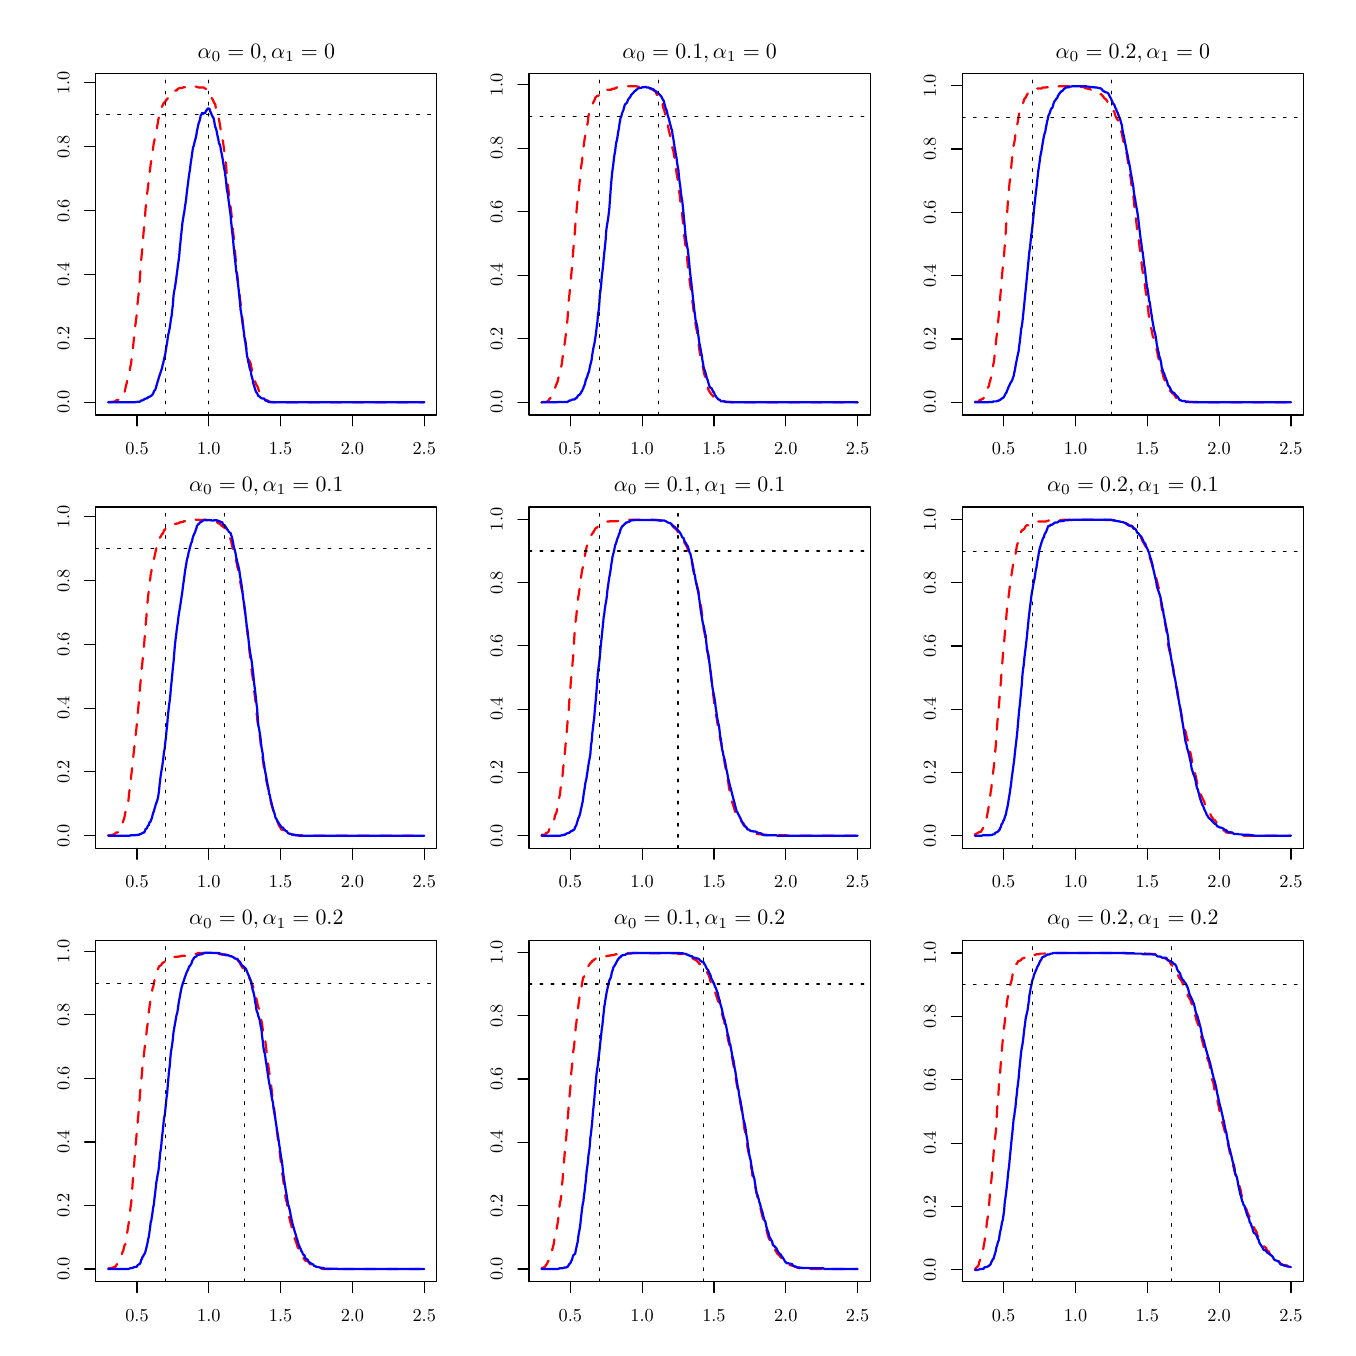
\begin{tikzpicture}[x=1pt,y=1pt]
\definecolor{fillColor}{RGB}{255,255,255}
\path[use as bounding box,fill=fillColor,fill opacity=0.00] (0,0) rectangle (469.75,469.75);
\begin{scope}
\path[clip] ( 24.55,329.80) rectangle (147.87,453.12);
\definecolor{drawColor}{RGB}{255,0,0}

\path[draw=drawColor,line width= 0.8pt,dash pattern=on 4pt off 4pt ,line join=round,line cap=round] ( 29.12,334.37) --
	( 29.35,334.48) --
	( 29.58,334.48) --
	( 29.81,334.48) --
	( 30.03,334.48) --
	( 30.26,334.48) --
	( 30.49,334.60) --
	( 30.72,334.60) --
	( 30.95,334.60) --
	( 31.18,334.60) --
	( 31.41,334.72) --
	( 31.64,334.72) --
	( 31.87,334.83) --
	( 32.09,335.18) --
	( 32.32,335.18) --
	( 32.55,335.18) --
	( 32.78,335.29) --
	( 33.01,335.41) --
	( 33.24,335.52) --
	( 33.47,335.52) --
	( 33.70,335.64) --
	( 33.92,335.99) --
	( 34.15,336.22) --
	( 34.38,336.33) --
	( 34.61,336.68) --
	( 34.84,337.49) --
	( 35.07,338.29) --
	( 35.30,339.33) --
	( 35.53,340.49) --
	( 35.76,341.18) --
	( 35.98,342.34) --
	( 36.21,343.14) --
	( 36.44,344.18) --
	( 36.67,345.34) --
	( 36.90,346.03) --
	( 37.13,347.42) --
	( 37.36,348.22) --
	( 37.59,350.65) --
	( 37.81,352.96) --
	( 38.04,354.23) --
	( 38.27,356.19) --
	( 38.50,358.38) --
	( 38.73,360.58) --
	( 38.96,362.66) --
	( 39.19,364.27) --
	( 39.42,366.24) --
	( 39.65,369.47) --
	( 39.87,371.55) --
	( 40.10,373.74) --
	( 40.33,376.40) --
	( 40.56,379.28) --
	( 40.79,382.63) --
	( 41.02,385.75) --
	( 41.25,388.17) --
	( 41.48,390.83) --
	( 41.71,393.71) --
	( 41.93,396.37) --
	( 42.16,398.56) --
	( 42.39,401.33) --
	( 42.62,404.57) --
	( 42.85,406.88) --
	( 43.08,409.07) --
	( 43.31,410.92) --
	( 43.54,412.65) --
	( 43.76,414.96) --
	( 43.99,417.04) --
	( 44.22,418.42) --
	( 44.45,420.38) --
	( 44.68,421.89) --
	( 44.91,423.50) --
	( 45.14,425.00) --
	( 45.37,426.62) --
	( 45.60,428.35) --
	( 45.82,428.93) --
	( 46.05,430.66) --
	( 46.28,431.47) --
	( 46.51,432.28) --
	( 46.74,433.78) --
	( 46.97,434.93) --
	( 47.20,436.55) --
	( 47.43,437.24) --
	( 47.65,437.93) --
	( 47.88,439.09) --
	( 48.11,440.01) --
	( 48.34,440.47) --
	( 48.57,441.28) --
	( 48.80,441.74) --
	( 49.03,442.21) --
	( 49.26,442.67) --
	( 49.49,442.78) --
	( 49.71,442.90) --
	( 49.94,443.48) --
	( 50.17,443.71) --
	( 50.40,443.82) --
	( 50.63,444.28) --
	( 50.86,444.51) --
	( 51.09,444.75) --
	( 51.32,444.75) --
	( 51.54,445.32) --
	( 51.77,445.55) --
	( 52.00,446.13) --
	( 52.23,446.36) --
	( 52.46,446.48) --
	( 52.69,446.59) --
	( 52.92,446.59) --
	( 53.15,446.71) --
	( 53.38,447.05) --
	( 53.60,447.05) --
	( 53.83,447.05) --
	( 54.06,447.40) --
	( 54.29,447.63) --
	( 54.52,447.75) --
	( 54.75,447.86) --
	( 54.98,447.98) --
	( 55.21,447.98) --
	( 55.43,447.98) --
	( 55.66,447.98) --
	( 55.89,447.98) --
	( 56.12,448.09) --
	( 56.35,448.21) --
	( 56.58,448.21) --
	( 56.81,448.21) --
	( 57.04,448.21) --
	( 57.27,448.32) --
	( 57.49,448.32) --
	( 57.72,448.32) --
	( 57.95,448.32) --
	( 58.18,448.32) --
	( 58.41,448.32) --
	( 58.64,448.32) --
	( 58.87,448.44) --
	( 59.10,448.56) --
	( 59.32,448.56) --
	( 59.55,448.56) --
	( 59.78,448.56) --
	( 60.01,448.56) --
	( 60.24,448.56) --
	( 60.47,448.44) --
	( 60.70,448.44) --
	( 60.93,448.44) --
	( 61.16,448.32) --
	( 61.38,448.32) --
	( 61.61,448.21) --
	( 61.84,448.09) --
	( 62.07,448.09) --
	( 62.30,448.09) --
	( 62.53,448.09) --
	( 62.76,448.09) --
	( 62.99,448.09) --
	( 63.22,448.09) --
	( 63.44,448.09) --
	( 63.67,448.09) --
	( 63.90,447.98) --
	( 64.13,447.75) --
	( 64.36,447.63) --
	( 64.59,447.63) --
	( 64.82,447.29) --
	( 65.05,446.94) --
	( 65.27,446.71) --
	( 65.50,446.59) --
	( 65.73,445.90) --
	( 65.96,445.55) --
	( 66.19,444.63) --
	( 66.42,444.40) --
	( 66.65,444.05) --
	( 66.88,443.71) --
	( 67.11,443.24) --
	( 67.33,442.67) --
	( 67.56,442.32) --
	( 67.79,442.09) --
	( 68.02,440.36) --
	( 68.25,439.78) --
	( 68.48,439.09) --
	( 68.71,438.28) --
	( 68.94,437.47) --
	( 69.16,436.32) --
	( 69.39,435.16) --
	( 69.62,433.66) --
	( 69.85,432.16) --
	( 70.08,431.01) --
	( 70.31,429.62) --
	( 70.54,428.81) --
	( 70.77,427.20) --
	( 71.00,425.35) --
	( 71.22,424.31) --
	( 71.45,421.89) --
	( 71.68,420.04) --
	( 71.91,417.15) --
	( 72.14,414.27) --
	( 72.37,412.65) --
	( 72.60,410.80) --
	( 72.83,408.72) --
	( 73.05,407.34) --
	( 73.28,405.26) --
	( 73.51,403.53) --
	( 73.74,401.33) --
	( 73.97,398.79) --
	( 74.20,396.37) --
	( 74.43,394.29) --
	( 74.66,391.75) --
	( 74.89,389.56) --
	( 75.11,386.67) --
	( 75.34,384.48) --
	( 75.57,381.59) --
	( 75.80,379.74) --
	( 76.03,377.43) --
	( 76.26,375.59) --
	( 76.49,373.97) --
	( 76.72,371.78) --
	( 76.94,370.16) --
	( 77.17,368.08) --
	( 77.40,365.66) --
	( 77.63,364.39) --
	( 77.86,362.08) --
	( 78.09,360.58) --
	( 78.32,359.08) --
	( 78.55,357.35) --
	( 78.78,355.27) --
	( 79.00,353.88) --
	( 79.23,352.96) --
	( 79.46,352.15) --
	( 79.69,351.11) --
	( 79.92,350.30) --
	( 80.15,349.38) --
	( 80.38,348.80) --
	( 80.61,348.22) --
	( 80.83,347.07) --
	( 81.06,345.92) --
	( 81.29,344.99) --
	( 81.52,344.18) --
	( 81.75,343.72) --
	( 81.98,342.80) --
	( 82.21,341.76) --
	( 82.44,341.18) --
	( 82.67,340.60) --
	( 82.89,340.37) --
	( 83.12,339.91) --
	( 83.35,339.10) --
	( 83.58,338.53) --
	( 83.81,337.83) --
	( 84.04,337.14) --
	( 84.27,336.68) --
	( 84.50,336.45) --
	( 84.73,336.33) --
	( 84.95,336.33) --
	( 85.18,336.33) --
	( 85.41,335.87) --
	( 85.64,335.75) --
	( 85.87,335.41) --
	( 86.10,335.18) --
	( 86.33,335.18) --
	( 86.56,334.95) --
	( 86.78,334.95) --
	( 87.01,334.95) --
	( 87.24,334.60) --
	( 87.47,334.60) --
	( 87.70,334.48) --
	( 87.93,334.37) --
	( 88.16,334.37) --
	( 88.39,334.37) --
	( 88.62,334.37) --
	( 88.84,334.37) --
	( 89.07,334.37) --
	( 89.30,334.37) --
	( 89.53,334.37) --
	( 89.76,334.37) --
	( 89.99,334.37) --
	( 90.22,334.37) --
	( 90.45,334.37) --
	( 90.67,334.37) --
	( 90.90,334.37) --
	( 91.13,334.37) --
	( 91.36,334.37) --
	( 91.59,334.37) --
	( 91.82,334.37) --
	( 92.05,334.37) --
	( 92.28,334.37) --
	( 92.51,334.37) --
	( 92.73,334.37) --
	( 92.96,334.37) --
	( 93.19,334.37) --
	( 93.42,334.37) --
	( 93.65,334.37) --
	( 93.88,334.37) --
	( 94.11,334.37) --
	( 94.34,334.37) --
	( 94.56,334.37) --
	( 94.79,334.37) --
	( 95.02,334.37) --
	( 95.25,334.37) --
	( 95.48,334.37) --
	( 95.71,334.37) --
	( 95.94,334.37) --
	( 96.17,334.37) --
	( 96.40,334.37) --
	( 96.62,334.37) --
	( 96.85,334.37) --
	( 97.08,334.37) --
	( 97.31,334.37) --
	( 97.54,334.37) --
	( 97.77,334.37) --
	( 98.00,334.37) --
	( 98.23,334.37) --
	( 98.45,334.37) --
	( 98.68,334.37) --
	( 98.91,334.37) --
	( 99.14,334.37) --
	( 99.37,334.37) --
	( 99.60,334.37) --
	( 99.83,334.37) --
	(100.06,334.37) --
	(100.29,334.37) --
	(100.51,334.37) --
	(100.74,334.37) --
	(100.97,334.37) --
	(101.20,334.37) --
	(101.43,334.37) --
	(101.66,334.37) --
	(101.89,334.37) --
	(102.12,334.37) --
	(102.35,334.37) --
	(102.57,334.37) --
	(102.80,334.37) --
	(103.03,334.37) --
	(103.26,334.37) --
	(103.49,334.37) --
	(103.72,334.37) --
	(103.95,334.37) --
	(104.18,334.37) --
	(104.40,334.37) --
	(104.63,334.37) --
	(104.86,334.37) --
	(105.09,334.37) --
	(105.32,334.37) --
	(105.55,334.37) --
	(105.78,334.37) --
	(106.01,334.37) --
	(106.24,334.37) --
	(106.46,334.37) --
	(106.69,334.37) --
	(106.92,334.37) --
	(107.15,334.37) --
	(107.38,334.37) --
	(107.61,334.37) --
	(107.84,334.37) --
	(108.07,334.37) --
	(108.29,334.37) --
	(108.52,334.37) --
	(108.75,334.37) --
	(108.98,334.37) --
	(109.21,334.37) --
	(109.44,334.37) --
	(109.67,334.37) --
	(109.90,334.37) --
	(110.13,334.37) --
	(110.35,334.37) --
	(110.58,334.37) --
	(110.81,334.37) --
	(111.04,334.37) --
	(111.27,334.37) --
	(111.50,334.37) --
	(111.73,334.37) --
	(111.96,334.37) --
	(112.18,334.37) --
	(112.41,334.37) --
	(112.64,334.37) --
	(112.87,334.37) --
	(113.10,334.37) --
	(113.33,334.37) --
	(113.56,334.37) --
	(113.79,334.37) --
	(114.02,334.37) --
	(114.24,334.37) --
	(114.47,334.37) --
	(114.70,334.37) --
	(114.93,334.37) --
	(115.16,334.37) --
	(115.39,334.37) --
	(115.62,334.37) --
	(115.85,334.37) --
	(116.07,334.37) --
	(116.30,334.37) --
	(116.53,334.37) --
	(116.76,334.37) --
	(116.99,334.37) --
	(117.22,334.37) --
	(117.45,334.37) --
	(117.68,334.37) --
	(117.91,334.37) --
	(118.13,334.37) --
	(118.36,334.37) --
	(118.59,334.37) --
	(118.82,334.37) --
	(119.05,334.37) --
	(119.28,334.37) --
	(119.51,334.37) --
	(119.74,334.37) --
	(119.96,334.37) --
	(120.19,334.37) --
	(120.42,334.37) --
	(120.65,334.37) --
	(120.88,334.37) --
	(121.11,334.37) --
	(121.34,334.37) --
	(121.57,334.37) --
	(121.80,334.37) --
	(122.02,334.37) --
	(122.25,334.37) --
	(122.48,334.37) --
	(122.71,334.37) --
	(122.94,334.37) --
	(123.17,334.37) --
	(123.40,334.37) --
	(123.63,334.37) --
	(123.86,334.37) --
	(124.08,334.37) --
	(124.31,334.37) --
	(124.54,334.37) --
	(124.77,334.37) --
	(125.00,334.37) --
	(125.23,334.37) --
	(125.46,334.37) --
	(125.69,334.37) --
	(125.91,334.37) --
	(126.14,334.37) --
	(126.37,334.37) --
	(126.60,334.37) --
	(126.83,334.37) --
	(127.06,334.37) --
	(127.29,334.37) --
	(127.52,334.37) --
	(127.75,334.37) --
	(127.97,334.37) --
	(128.20,334.37) --
	(128.43,334.37) --
	(128.66,334.37) --
	(128.89,334.37) --
	(129.12,334.37) --
	(129.35,334.37) --
	(129.58,334.37) --
	(129.80,334.37) --
	(130.03,334.37) --
	(130.26,334.37) --
	(130.49,334.37) --
	(130.72,334.37) --
	(130.95,334.37) --
	(131.18,334.37) --
	(131.41,334.37) --
	(131.64,334.37) --
	(131.86,334.37) --
	(132.09,334.37) --
	(132.32,334.37) --
	(132.55,334.37) --
	(132.78,334.37) --
	(133.01,334.37) --
	(133.24,334.37) --
	(133.47,334.37) --
	(133.69,334.37) --
	(133.92,334.37) --
	(134.15,334.37) --
	(134.38,334.37) --
	(134.61,334.37) --
	(134.84,334.37) --
	(135.07,334.37) --
	(135.30,334.37) --
	(135.53,334.37) --
	(135.75,334.37) --
	(135.98,334.37) --
	(136.21,334.37) --
	(136.44,334.37) --
	(136.67,334.37) --
	(136.90,334.37) --
	(137.13,334.37) --
	(137.36,334.37) --
	(137.58,334.37) --
	(137.81,334.37) --
	(138.04,334.37) --
	(138.27,334.37) --
	(138.50,334.37) --
	(138.73,334.37) --
	(138.96,334.37) --
	(139.19,334.37) --
	(139.42,334.37) --
	(139.64,334.37) --
	(139.87,334.37) --
	(140.10,334.37) --
	(140.33,334.37) --
	(140.56,334.37) --
	(140.79,334.37) --
	(141.02,334.37) --
	(141.25,334.37) --
	(141.47,334.37) --
	(141.70,334.37) --
	(141.93,334.37) --
	(142.16,334.37) --
	(142.39,334.37) --
	(142.62,334.37) --
	(142.85,334.37) --
	(143.08,334.37) --
	(143.31,334.37);
\end{scope}
\begin{scope}
\path[clip] (  0.00,  0.00) rectangle (469.75,469.75);
\definecolor{drawColor}{RGB}{0,0,0}

\path[draw=drawColor,line width= 0.4pt,line join=round,line cap=round] ( 39.50,329.80) -- (143.31,329.80);

\path[draw=drawColor,line width= 0.4pt,line join=round,line cap=round] ( 39.50,329.80) -- ( 39.50,325.84);

\path[draw=drawColor,line width= 0.4pt,line join=round,line cap=round] ( 65.45,329.80) -- ( 65.45,325.84);

\path[draw=drawColor,line width= 0.4pt,line join=round,line cap=round] ( 91.40,329.80) -- ( 91.40,325.84);

\path[draw=drawColor,line width= 0.4pt,line join=round,line cap=round] (117.35,329.80) -- (117.35,325.84);

\path[draw=drawColor,line width= 0.4pt,line join=round,line cap=round] (143.31,329.80) -- (143.31,325.84);

\node[text=drawColor,anchor=base,inner sep=0pt, outer sep=0pt, scale=  0.66] at ( 39.50,315.55) {0.5};

\node[text=drawColor,anchor=base,inner sep=0pt, outer sep=0pt, scale=  0.66] at ( 65.45,315.55) {1.0};

\node[text=drawColor,anchor=base,inner sep=0pt, outer sep=0pt, scale=  0.66] at ( 91.40,315.55) {1.5};

\node[text=drawColor,anchor=base,inner sep=0pt, outer sep=0pt, scale=  0.66] at (117.35,315.55) {2.0};

\node[text=drawColor,anchor=base,inner sep=0pt, outer sep=0pt, scale=  0.66] at (143.31,315.55) {2.5};

\path[draw=drawColor,line width= 0.4pt,line join=round,line cap=round] ( 24.55,334.37) -- ( 24.55,449.83);

\path[draw=drawColor,line width= 0.4pt,line join=round,line cap=round] ( 24.55,334.37) -- ( 20.59,334.37);

\path[draw=drawColor,line width= 0.4pt,line join=round,line cap=round] ( 24.55,357.46) -- ( 20.59,357.46);

\path[draw=drawColor,line width= 0.4pt,line join=round,line cap=round] ( 24.55,380.55) -- ( 20.59,380.55);

\path[draw=drawColor,line width= 0.4pt,line join=round,line cap=round] ( 24.55,403.64) -- ( 20.59,403.64);

\path[draw=drawColor,line width= 0.4pt,line join=round,line cap=round] ( 24.55,426.73) -- ( 20.59,426.73);

\path[draw=drawColor,line width= 0.4pt,line join=round,line cap=round] ( 24.55,449.83) -- ( 20.59,449.83);

\node[text=drawColor,rotate= 90.00,anchor=base,inner sep=0pt, outer sep=0pt, scale=  0.66] at ( 15.05,334.37) {0.0};

\node[text=drawColor,rotate= 90.00,anchor=base,inner sep=0pt, outer sep=0pt, scale=  0.66] at ( 15.05,357.46) {0.2};

\node[text=drawColor,rotate= 90.00,anchor=base,inner sep=0pt, outer sep=0pt, scale=  0.66] at ( 15.05,380.55) {0.4};

\node[text=drawColor,rotate= 90.00,anchor=base,inner sep=0pt, outer sep=0pt, scale=  0.66] at ( 15.05,403.64) {0.6};

\node[text=drawColor,rotate= 90.00,anchor=base,inner sep=0pt, outer sep=0pt, scale=  0.66] at ( 15.05,426.73) {0.8};

\node[text=drawColor,rotate= 90.00,anchor=base,inner sep=0pt, outer sep=0pt, scale=  0.66] at ( 15.05,449.83) {1.0};

\path[draw=drawColor,line width= 0.4pt,line join=round,line cap=round] ( 24.55,329.80) --
	(147.87,329.80) --
	(147.87,453.12) --
	( 24.55,453.12) --
	( 24.55,329.80);
\end{scope}
\begin{scope}
\path[clip] (  0.00,313.17) rectangle (156.58,469.75);
\definecolor{drawColor}{RGB}{0,0,0}

\node[text=drawColor,anchor=base,inner sep=0pt, outer sep=0pt, scale=  0.79] at ( 86.21,458.71) {\bfseries $\alpha_0 = 0, \alpha_1 = 0$};
\end{scope}
\begin{scope}
\path[clip] ( 24.55,329.80) rectangle (147.87,453.12);
\definecolor{drawColor}{RGB}{0,0,255}

\path[draw=drawColor,line width= 0.8pt,line join=round,line cap=round] ( 29.12,334.37) --
	( 29.35,334.37) --
	( 29.58,334.37) --
	( 29.81,334.37) --
	( 30.03,334.37) --
	( 30.26,334.37) --
	( 30.49,334.37) --
	( 30.72,334.37) --
	( 30.95,334.37) --
	( 31.18,334.37) --
	( 31.41,334.37) --
	( 31.64,334.37) --
	( 31.87,334.37) --
	( 32.09,334.37) --
	( 32.32,334.37) --
	( 32.55,334.37) --
	( 32.78,334.37) --
	( 33.01,334.37) --
	( 33.24,334.37) --
	( 33.47,334.37) --
	( 33.70,334.37) --
	( 33.92,334.37) --
	( 34.15,334.37) --
	( 34.38,334.37) --
	( 34.61,334.37) --
	( 34.84,334.37) --
	( 35.07,334.37) --
	( 35.30,334.37) --
	( 35.53,334.37) --
	( 35.76,334.37) --
	( 35.98,334.37) --
	( 36.21,334.37) --
	( 36.44,334.37) --
	( 36.67,334.37) --
	( 36.90,334.37) --
	( 37.13,334.37) --
	( 37.36,334.37) --
	( 37.59,334.37) --
	( 37.81,334.37) --
	( 38.04,334.37) --
	( 38.27,334.37) --
	( 38.50,334.37) --
	( 38.73,334.37) --
	( 38.96,334.48) --
	( 39.19,334.48) --
	( 39.42,334.48) --
	( 39.65,334.60) --
	( 39.87,334.60) --
	( 40.10,334.60) --
	( 40.33,334.60) --
	( 40.56,334.60) --
	( 40.79,334.83) --
	( 41.02,335.06) --
	( 41.25,335.06) --
	( 41.48,335.06) --
	( 41.71,335.18) --
	( 41.93,335.29) --
	( 42.16,335.52) --
	( 42.39,335.64) --
	( 42.62,335.64) --
	( 42.85,335.75) --
	( 43.08,335.87) --
	( 43.31,335.87) --
	( 43.54,336.22) --
	( 43.76,336.33) --
	( 43.99,336.33) --
	( 44.22,336.45) --
	( 44.45,336.68) --
	( 44.68,336.79) --
	( 44.91,336.91) --
	( 45.14,337.26) --
	( 45.37,337.60) --
	( 45.60,338.29) --
	( 45.82,338.64) --
	( 46.05,338.76) --
	( 46.28,339.45) --
	( 46.51,340.26) --
	( 46.74,341.07) --
	( 46.97,341.87) --
	( 47.20,342.57) --
	( 47.43,343.38) --
	( 47.65,344.07) --
	( 47.88,344.76) --
	( 48.11,345.45) --
	( 48.34,346.15) --
	( 48.57,346.84) --
	( 48.80,347.99) --
	( 49.03,348.69) --
	( 49.26,349.96) --
	( 49.49,350.88) --
	( 49.71,351.80) --
	( 49.94,353.30) --
	( 50.17,354.69) --
	( 50.40,355.96) --
	( 50.63,357.81) --
	( 50.86,359.08) --
	( 51.09,360.00) --
	( 51.32,361.27) --
	( 51.54,362.66) --
	( 51.77,364.50) --
	( 52.00,365.54) --
	( 52.23,367.74) --
	( 52.46,369.47) --
	( 52.69,372.82) --
	( 52.92,374.43) --
	( 53.15,375.47) --
	( 53.38,376.97) --
	( 53.60,378.47) --
	( 53.83,380.32) --
	( 54.06,381.94) --
	( 54.29,383.90) --
	( 54.52,385.40) --
	( 54.75,387.13) --
	( 54.98,390.02) --
	( 55.21,392.21) --
	( 55.43,394.64) --
	( 55.66,396.60) --
	( 55.89,399.02) --
	( 56.12,400.41) --
	( 56.35,401.91) --
	( 56.58,403.07) --
	( 56.81,404.91) --
	( 57.04,406.30) --
	( 57.27,407.91) --
	( 57.49,410.11) --
	( 57.72,411.84) --
	( 57.95,413.57) --
	( 58.18,415.54) --
	( 58.41,417.15) --
	( 58.64,418.31) --
	( 58.87,420.50) --
	( 59.10,421.89) --
	( 59.32,423.50) --
	( 59.55,425.12) --
	( 59.78,426.62) --
	( 60.01,426.97) --
	( 60.24,428.12) --
	( 60.47,428.93) --
	( 60.70,429.85) --
	( 60.93,430.78) --
	( 61.16,432.39) --
	( 61.38,433.32) --
	( 61.61,434.47) --
	( 61.84,435.39) --
	( 62.07,435.97) --
	( 62.30,436.78) --
	( 62.53,438.05) --
	( 62.76,438.28) --
	( 62.99,438.86) --
	( 63.22,438.97) --
	( 63.44,438.63) --
	( 63.67,438.86) --
	( 63.90,438.86) --
	( 64.13,438.86) --
	( 64.36,439.55) --
	( 64.59,439.90) --
	( 64.82,440.13) --
	( 65.05,440.47) --
	( 65.27,440.59) --
	( 65.50,440.47) --
	( 65.73,440.36) --
	( 65.96,439.55) --
	( 66.19,439.09) --
	( 66.42,438.51) --
	( 66.65,437.93) --
	( 66.88,437.47) --
	( 67.11,437.24) --
	( 67.33,436.43) --
	( 67.56,435.05) --
	( 67.79,433.89) --
	( 68.02,433.32) --
	( 68.25,432.51) --
	( 68.48,431.24) --
	( 68.71,430.20) --
	( 68.94,429.16) --
	( 69.16,427.77) --
	( 69.39,427.66) --
	( 69.62,426.85) --
	( 69.85,425.35) --
	( 70.08,424.31) --
	( 70.31,423.16) --
	( 70.54,421.77) --
	( 70.77,420.27) --
	( 71.00,418.88) --
	( 71.22,417.96) --
	( 71.45,416.11) --
	( 71.68,414.50) --
	( 71.91,411.84) --
	( 72.14,410.46) --
	( 72.37,409.42) --
	( 72.60,407.34) --
	( 72.83,405.72) --
	( 73.05,403.87) --
	( 73.28,402.37) --
	( 73.51,399.72) --
	( 73.74,397.64) --
	( 73.97,395.33) --
	( 74.20,393.25) --
	( 74.43,390.71) --
	( 74.66,388.29) --
	( 74.89,386.09) --
	( 75.11,384.36) --
	( 75.34,381.94) --
	( 75.57,380.67) --
	( 75.80,378.70) --
	( 76.03,376.86) --
	( 76.26,374.89) --
	( 76.49,372.70) --
	( 76.72,370.39) --
	( 76.94,367.85) --
	( 77.17,366.58) --
	( 77.40,364.85) --
	( 77.63,363.12) --
	( 77.86,361.50) --
	( 78.09,360.00) --
	( 78.32,357.81) --
	( 78.55,356.65) --
	( 78.78,355.73) --
	( 79.00,353.42) --
	( 79.23,351.34) --
	( 79.46,350.42) --
	( 79.69,349.03) --
	( 79.92,348.34) --
	( 80.15,347.07) --
	( 80.38,346.15) --
	( 80.61,345.68) --
	( 80.83,344.18) --
	( 81.06,343.38) --
	( 81.29,342.57) --
	( 81.52,341.18) --
	( 81.75,340.49) --
	( 81.98,339.80) --
	( 82.21,338.99) --
	( 82.44,338.29) --
	( 82.67,337.95) --
	( 82.89,337.72) --
	( 83.12,337.14) --
	( 83.35,336.68) --
	( 83.58,336.56) --
	( 83.81,336.45) --
	( 84.04,336.22) --
	( 84.27,335.99) --
	( 84.50,335.87) --
	( 84.73,335.75) --
	( 84.95,335.75) --
	( 85.18,335.75) --
	( 85.41,335.75) --
	( 85.64,335.41) --
	( 85.87,335.06) --
	( 86.10,334.95) --
	( 86.33,334.95) --
	( 86.56,334.83) --
	( 86.78,334.72) --
	( 87.01,334.48) --
	( 87.24,334.48) --
	( 87.47,334.48) --
	( 87.70,334.48) --
	( 87.93,334.48) --
	( 88.16,334.48) --
	( 88.39,334.48) --
	( 88.62,334.48) --
	( 88.84,334.37) --
	( 89.07,334.37) --
	( 89.30,334.37) --
	( 89.53,334.37) --
	( 89.76,334.37) --
	( 89.99,334.37) --
	( 90.22,334.37) --
	( 90.45,334.37) --
	( 90.67,334.37) --
	( 90.90,334.37) --
	( 91.13,334.37) --
	( 91.36,334.37) --
	( 91.59,334.37) --
	( 91.82,334.37) --
	( 92.05,334.37) --
	( 92.28,334.37) --
	( 92.51,334.37) --
	( 92.73,334.37) --
	( 92.96,334.37) --
	( 93.19,334.37) --
	( 93.42,334.37) --
	( 93.65,334.37) --
	( 93.88,334.37) --
	( 94.11,334.37) --
	( 94.34,334.37) --
	( 94.56,334.37) --
	( 94.79,334.37) --
	( 95.02,334.37) --
	( 95.25,334.37) --
	( 95.48,334.37) --
	( 95.71,334.37) --
	( 95.94,334.37) --
	( 96.17,334.37) --
	( 96.40,334.37) --
	( 96.62,334.37) --
	( 96.85,334.37) --
	( 97.08,334.37) --
	( 97.31,334.37) --
	( 97.54,334.37) --
	( 97.77,334.37) --
	( 98.00,334.37) --
	( 98.23,334.37) --
	( 98.45,334.37) --
	( 98.68,334.37) --
	( 98.91,334.37) --
	( 99.14,334.37) --
	( 99.37,334.37) --
	( 99.60,334.37) --
	( 99.83,334.37) --
	(100.06,334.37) --
	(100.29,334.37) --
	(100.51,334.37) --
	(100.74,334.37) --
	(100.97,334.37) --
	(101.20,334.37) --
	(101.43,334.37) --
	(101.66,334.37) --
	(101.89,334.37) --
	(102.12,334.37) --
	(102.35,334.37) --
	(102.57,334.37) --
	(102.80,334.37) --
	(103.03,334.37) --
	(103.26,334.37) --
	(103.49,334.37) --
	(103.72,334.37) --
	(103.95,334.37) --
	(104.18,334.37) --
	(104.40,334.37) --
	(104.63,334.37) --
	(104.86,334.37) --
	(105.09,334.37) --
	(105.32,334.37) --
	(105.55,334.37) --
	(105.78,334.37) --
	(106.01,334.37) --
	(106.24,334.37) --
	(106.46,334.37) --
	(106.69,334.37) --
	(106.92,334.37) --
	(107.15,334.37) --
	(107.38,334.37) --
	(107.61,334.37) --
	(107.84,334.37) --
	(108.07,334.37) --
	(108.29,334.37) --
	(108.52,334.37) --
	(108.75,334.37) --
	(108.98,334.37) --
	(109.21,334.37) --
	(109.44,334.37) --
	(109.67,334.37) --
	(109.90,334.37) --
	(110.13,334.37) --
	(110.35,334.37) --
	(110.58,334.37) --
	(110.81,334.37) --
	(111.04,334.37) --
	(111.27,334.37) --
	(111.50,334.37) --
	(111.73,334.37) --
	(111.96,334.37) --
	(112.18,334.37) --
	(112.41,334.37) --
	(112.64,334.37) --
	(112.87,334.37) --
	(113.10,334.37) --
	(113.33,334.37) --
	(113.56,334.37) --
	(113.79,334.37) --
	(114.02,334.37) --
	(114.24,334.37) --
	(114.47,334.37) --
	(114.70,334.37) --
	(114.93,334.37) --
	(115.16,334.37) --
	(115.39,334.37) --
	(115.62,334.37) --
	(115.85,334.37) --
	(116.07,334.37) --
	(116.30,334.37) --
	(116.53,334.37) --
	(116.76,334.37) --
	(116.99,334.37) --
	(117.22,334.37) --
	(117.45,334.37) --
	(117.68,334.37) --
	(117.91,334.37) --
	(118.13,334.37) --
	(118.36,334.37) --
	(118.59,334.37) --
	(118.82,334.37) --
	(119.05,334.37) --
	(119.28,334.37) --
	(119.51,334.37) --
	(119.74,334.37) --
	(119.96,334.37) --
	(120.19,334.37) --
	(120.42,334.37) --
	(120.65,334.37) --
	(120.88,334.37) --
	(121.11,334.37) --
	(121.34,334.37) --
	(121.57,334.37) --
	(121.80,334.37) --
	(122.02,334.37) --
	(122.25,334.37) --
	(122.48,334.37) --
	(122.71,334.37) --
	(122.94,334.37) --
	(123.17,334.37) --
	(123.40,334.37) --
	(123.63,334.37) --
	(123.86,334.37) --
	(124.08,334.37) --
	(124.31,334.37) --
	(124.54,334.37) --
	(124.77,334.37) --
	(125.00,334.37) --
	(125.23,334.37) --
	(125.46,334.37) --
	(125.69,334.37) --
	(125.91,334.37) --
	(126.14,334.37) --
	(126.37,334.37) --
	(126.60,334.37) --
	(126.83,334.37) --
	(127.06,334.37) --
	(127.29,334.37) --
	(127.52,334.37) --
	(127.75,334.37) --
	(127.97,334.37) --
	(128.20,334.37) --
	(128.43,334.37) --
	(128.66,334.37) --
	(128.89,334.37) --
	(129.12,334.37) --
	(129.35,334.37) --
	(129.58,334.37) --
	(129.80,334.37) --
	(130.03,334.37) --
	(130.26,334.37) --
	(130.49,334.37) --
	(130.72,334.37) --
	(130.95,334.37) --
	(131.18,334.37) --
	(131.41,334.37) --
	(131.64,334.37) --
	(131.86,334.37) --
	(132.09,334.37) --
	(132.32,334.37) --
	(132.55,334.37) --
	(132.78,334.37) --
	(133.01,334.37) --
	(133.24,334.37) --
	(133.47,334.37) --
	(133.69,334.37) --
	(133.92,334.37) --
	(134.15,334.37) --
	(134.38,334.37) --
	(134.61,334.37) --
	(134.84,334.37) --
	(135.07,334.37) --
	(135.30,334.37) --
	(135.53,334.37) --
	(135.75,334.37) --
	(135.98,334.37) --
	(136.21,334.37) --
	(136.44,334.37) --
	(136.67,334.37) --
	(136.90,334.37) --
	(137.13,334.37) --
	(137.36,334.37) --
	(137.58,334.37) --
	(137.81,334.37) --
	(138.04,334.37) --
	(138.27,334.37) --
	(138.50,334.37) --
	(138.73,334.37) --
	(138.96,334.37) --
	(139.19,334.37) --
	(139.42,334.37) --
	(139.64,334.37) --
	(139.87,334.37) --
	(140.10,334.37) --
	(140.33,334.37) --
	(140.56,334.37) --
	(140.79,334.37) --
	(141.02,334.37) --
	(141.25,334.37) --
	(141.47,334.37) --
	(141.70,334.37) --
	(141.93,334.37) --
	(142.16,334.37) --
	(142.39,334.37) --
	(142.62,334.37) --
	(142.85,334.37) --
	(143.08,334.37) --
	(143.31,334.37);
\definecolor{drawColor}{RGB}{0,0,0}

\path[draw=drawColor,line width= 0.4pt,dash pattern=on 1pt off 3pt ,line join=round,line cap=round] ( 24.55,438.28) -- (147.87,438.28);

\path[draw=drawColor,line width= 0.4pt,dash pattern=on 1pt off 3pt ,line join=round,line cap=round] ( 49.88,329.80) -- ( 49.88,453.12);

\path[draw=drawColor,line width= 0.4pt,dash pattern=on 1pt off 3pt ,line join=round,line cap=round] ( 65.45,329.80) -- ( 65.45,453.12);
\end{scope}
\begin{scope}
\path[clip] (181.14,329.80) rectangle (304.46,453.12);
\definecolor{drawColor}{RGB}{255,0,0}

\path[draw=drawColor,line width= 0.8pt,dash pattern=on 4pt off 4pt ,line join=round,line cap=round] (185.70,334.37) --
	(185.93,334.37) --
	(186.16,334.48) --
	(186.39,334.48) --
	(186.62,334.48) --
	(186.85,334.48) --
	(187.08,334.48) --
	(187.31,334.48) --
	(187.54,334.60) --
	(187.76,334.71) --
	(187.99,334.83) --
	(188.22,335.06) --
	(188.45,335.52) --
	(188.68,335.63) --
	(188.91,335.98) --
	(189.14,336.32) --
	(189.37,336.78) --
	(189.59,337.35) --
	(189.82,337.81) --
	(190.05,337.93) --
	(190.28,338.39) --
	(190.51,339.19) --
	(190.74,340.11) --
	(190.97,340.80) --
	(191.20,341.14) --
	(191.43,341.71) --
	(191.65,342.63) --
	(191.88,343.66) --
	(192.11,344.01) --
	(192.34,345.04) --
	(192.57,345.50) --
	(192.80,347.22) --
	(193.03,348.48) --
	(193.26,350.32) --
	(193.48,351.81) --
	(193.71,353.19) --
	(193.94,355.03) --
	(194.17,356.40) --
	(194.40,358.47) --
	(194.63,360.31) --
	(194.86,362.03) --
	(195.09,364.78) --
	(195.32,368.45) --
	(195.54,371.32) --
	(195.77,373.39) --
	(196.00,375.68) --
	(196.23,378.32) --
	(196.46,380.85) --
	(196.69,383.26) --
	(196.92,386.24) --
	(197.15,389.34) --
	(197.37,391.86) --
	(197.60,394.39) --
	(197.83,397.26) --
	(198.06,401.04) --
	(198.29,403.11) --
	(198.52,405.64) --
	(198.75,407.59) --
	(198.98,408.96) --
	(199.21,411.49) --
	(199.43,413.78) --
	(199.66,416.19) --
	(199.89,418.83) --
	(200.12,420.21) --
	(200.35,421.82) --
	(200.58,424.34) --
	(200.81,426.29) --
	(201.04,428.01) --
	(201.26,429.51) --
	(201.49,430.88) --
	(201.72,432.26) --
	(201.95,433.75) --
	(202.18,434.55) --
	(202.41,435.59) --
	(202.64,437.88) --
	(202.87,438.80) --
	(203.10,439.37) --
	(203.32,440.41) --
	(203.55,441.21) --
	(203.78,441.67) --
	(204.01,442.24) --
	(204.24,442.47) --
	(204.47,442.82) --
	(204.70,443.39) --
	(204.93,443.74) --
	(205.15,444.54) --
	(205.38,444.77) --
	(205.61,444.88) --
	(205.84,445.11) --
	(206.07,445.11) --
	(206.30,445.23) --
	(206.53,445.57) --
	(206.76,446.15) --
	(206.99,446.15) --
	(207.21,446.15) --
	(207.44,446.26) --
	(207.67,446.38) --
	(207.90,446.49) --
	(208.13,446.49) --
	(208.36,446.49) --
	(208.59,446.49) --
	(208.82,446.95) --
	(209.05,447.06) --
	(209.27,447.29) --
	(209.50,447.29) --
	(209.73,447.29) --
	(209.96,447.29) --
	(210.19,447.29) --
	(210.42,447.29) --
	(210.65,447.29) --
	(210.88,447.29) --
	(211.10,447.64) --
	(211.33,447.64) --
	(211.56,447.64) --
	(211.79,447.64) --
	(212.02,447.64) --
	(212.25,447.87) --
	(212.48,447.98) --
	(212.71,447.98) --
	(212.94,448.21) --
	(213.16,448.21) --
	(213.39,448.21) --
	(213.62,448.21) --
	(213.85,448.21) --
	(214.08,448.33) --
	(214.31,448.44) --
	(214.54,448.56) --
	(214.77,448.56) --
	(214.99,448.56) --
	(215.22,448.56) --
	(215.45,448.56) --
	(215.68,448.56) --
	(215.91,448.56) --
	(216.14,448.56) --
	(216.37,448.56) --
	(216.60,448.56) --
	(216.83,448.56) --
	(217.05,448.56) --
	(217.28,448.56) --
	(217.51,448.56) --
	(217.74,448.56) --
	(217.97,448.56) --
	(218.20,448.56) --
	(218.43,448.56) --
	(218.66,448.56) --
	(218.88,448.56) --
	(219.11,448.56) --
	(219.34,448.56) --
	(219.57,448.56) --
	(219.80,448.56) --
	(220.03,448.56) --
	(220.26,448.44) --
	(220.49,448.44) --
	(220.72,448.44) --
	(220.94,448.44) --
	(221.17,448.44) --
	(221.40,448.44) --
	(221.63,448.44) --
	(221.86,448.44) --
	(222.09,448.44) --
	(222.32,448.33) --
	(222.55,448.33) --
	(222.77,448.33) --
	(223.00,448.33) --
	(223.23,448.33) --
	(223.46,448.33) --
	(223.69,448.33) --
	(223.92,448.33) --
	(224.15,448.33) --
	(224.38,448.21) --
	(224.61,448.10) --
	(224.83,447.75) --
	(225.06,447.64) --
	(225.29,447.52) --
	(225.52,447.52) --
	(225.75,447.29) --
	(225.98,447.18) --
	(226.21,447.06) --
	(226.44,446.95) --
	(226.66,446.83) --
	(226.89,446.60) --
	(227.12,446.03) --
	(227.35,445.57) --
	(227.58,445.34) --
	(227.81,445.23) --
	(228.04,445.23) --
	(228.27,444.88) --
	(228.50,444.31) --
	(228.72,444.19) --
	(228.95,443.74) --
	(229.18,442.93) --
	(229.41,442.13) --
	(229.64,440.87) --
	(229.87,440.29) --
	(230.10,439.60) --
	(230.33,438.57) --
	(230.56,437.65) --
	(230.78,436.74) --
	(231.01,436.16) --
	(231.24,434.78) --
	(231.47,433.75) --
	(231.70,432.49) --
	(231.93,431.69) --
	(232.16,430.65) --
	(232.39,429.16) --
	(232.61,427.67) --
	(232.84,426.87) --
	(233.07,425.95) --
	(233.30,425.26) --
	(233.53,423.88) --
	(233.76,422.51) --
	(233.99,420.21) --
	(234.22,419.29) --
	(234.45,417.23) --
	(234.67,416.19) --
	(234.90,414.47) --
	(235.13,412.64) --
	(235.36,410.91) --
	(235.59,409.42) --
	(235.82,407.01) --
	(236.05,405.98) --
	(236.28,404.72) --
	(236.50,402.19) --
	(236.73,399.67) --
	(236.96,398.06) --
	(237.19,395.08) --
	(237.42,393.13) --
	(237.65,391.29) --
	(237.88,389.11) --
	(238.11,387.50) --
	(238.34,385.90) --
	(238.56,383.37) --
	(238.79,381.77) --
	(239.02,379.81) --
	(239.25,377.75) --
	(239.48,376.26) --
	(239.71,374.65) --
	(239.94,372.93) --
	(240.17,371.09) --
	(240.39,369.49) --
	(240.62,367.42) --
	(240.85,365.70) --
	(241.08,364.09) --
	(241.31,362.72) --
	(241.54,361.45) --
	(241.77,360.42) --
	(242.00,358.93) --
	(242.23,356.75) --
	(242.45,355.26) --
	(242.68,353.53) --
	(242.91,352.16) --
	(243.14,350.78) --
	(243.37,349.86) --
	(243.60,349.06) --
	(243.83,347.80) --
	(244.06,346.88) --
	(244.28,345.50) --
	(244.51,344.47) --
	(244.74,343.66) --
	(244.97,342.40) --
	(245.20,341.48) --
	(245.43,341.03) --
	(245.66,340.11) --
	(245.89,339.07) --
	(246.12,338.62) --
	(246.34,338.39) --
	(246.57,337.81) --
	(246.80,337.70) --
	(247.03,337.24) --
	(247.26,337.01) --
	(247.49,336.78) --
	(247.72,336.44) --
	(247.95,336.44) --
	(248.18,336.32) --
	(248.40,336.32) --
	(248.63,336.09) --
	(248.86,335.63) --
	(249.09,335.52) --
	(249.32,335.40) --
	(249.55,335.17) --
	(249.78,335.06) --
	(250.01,335.06) --
	(250.23,334.83) --
	(250.46,334.83) --
	(250.69,334.83) --
	(250.92,334.83) --
	(251.15,334.83) --
	(251.38,334.83) --
	(251.61,334.83) --
	(251.84,334.71) --
	(252.07,334.60) --
	(252.29,334.60) --
	(252.52,334.60) --
	(252.75,334.48) --
	(252.98,334.48) --
	(253.21,334.48) --
	(253.44,334.48) --
	(253.67,334.48) --
	(253.90,334.48) --
	(254.12,334.48) --
	(254.35,334.48) --
	(254.58,334.48) --
	(254.81,334.37) --
	(255.04,334.37) --
	(255.27,334.37) --
	(255.50,334.37) --
	(255.73,334.37) --
	(255.96,334.37) --
	(256.18,334.37) --
	(256.41,334.37) --
	(256.64,334.37) --
	(256.87,334.37) --
	(257.10,334.37) --
	(257.33,334.37) --
	(257.56,334.37) --
	(257.79,334.37) --
	(258.01,334.37) --
	(258.24,334.37) --
	(258.47,334.37) --
	(258.70,334.37) --
	(258.93,334.37) --
	(259.16,334.37) --
	(259.39,334.37) --
	(259.62,334.37) --
	(259.85,334.37) --
	(260.07,334.37) --
	(260.30,334.37) --
	(260.53,334.37) --
	(260.76,334.37) --
	(260.99,334.37) --
	(261.22,334.37) --
	(261.45,334.37) --
	(261.68,334.37) --
	(261.90,334.37) --
	(262.13,334.37) --
	(262.36,334.37) --
	(262.59,334.37) --
	(262.82,334.37) --
	(263.05,334.37) --
	(263.28,334.37) --
	(263.51,334.37) --
	(263.74,334.37) --
	(263.96,334.37) --
	(264.19,334.37) --
	(264.42,334.37) --
	(264.65,334.37) --
	(264.88,334.37) --
	(265.11,334.37) --
	(265.34,334.37) --
	(265.57,334.37) --
	(265.79,334.37) --
	(266.02,334.37) --
	(266.25,334.37) --
	(266.48,334.37) --
	(266.71,334.37) --
	(266.94,334.37) --
	(267.17,334.37) --
	(267.40,334.37) --
	(267.63,334.37) --
	(267.85,334.37) --
	(268.08,334.37) --
	(268.31,334.37) --
	(268.54,334.37) --
	(268.77,334.37) --
	(269.00,334.37) --
	(269.23,334.37) --
	(269.46,334.37) --
	(269.69,334.37) --
	(269.91,334.37) --
	(270.14,334.37) --
	(270.37,334.37) --
	(270.60,334.37) --
	(270.83,334.37) --
	(271.06,334.37) --
	(271.29,334.37) --
	(271.52,334.37) --
	(271.74,334.37) --
	(271.97,334.37) --
	(272.20,334.37) --
	(272.43,334.37) --
	(272.66,334.37) --
	(272.89,334.37) --
	(273.12,334.37) --
	(273.35,334.37) --
	(273.58,334.37) --
	(273.80,334.37) --
	(274.03,334.37) --
	(274.26,334.37) --
	(274.49,334.37) --
	(274.72,334.37) --
	(274.95,334.37) --
	(275.18,334.37) --
	(275.41,334.37) --
	(275.63,334.37) --
	(275.86,334.37) --
	(276.09,334.37) --
	(276.32,334.37) --
	(276.55,334.37) --
	(276.78,334.37) --
	(277.01,334.37) --
	(277.24,334.37) --
	(277.47,334.37) --
	(277.69,334.37) --
	(277.92,334.37) --
	(278.15,334.37) --
	(278.38,334.37) --
	(278.61,334.37) --
	(278.84,334.37) --
	(279.07,334.37) --
	(279.30,334.37) --
	(279.52,334.37) --
	(279.75,334.37) --
	(279.98,334.37) --
	(280.21,334.37) --
	(280.44,334.37) --
	(280.67,334.37) --
	(280.90,334.37) --
	(281.13,334.37) --
	(281.36,334.37) --
	(281.58,334.37) --
	(281.81,334.37) --
	(282.04,334.37) --
	(282.27,334.37) --
	(282.50,334.37) --
	(282.73,334.37) --
	(282.96,334.37) --
	(283.19,334.37) --
	(283.41,334.37) --
	(283.64,334.37) --
	(283.87,334.37) --
	(284.10,334.37) --
	(284.33,334.37) --
	(284.56,334.37) --
	(284.79,334.37) --
	(285.02,334.37) --
	(285.25,334.37) --
	(285.47,334.37) --
	(285.70,334.37) --
	(285.93,334.37) --
	(286.16,334.37) --
	(286.39,334.37) --
	(286.62,334.37) --
	(286.85,334.37) --
	(287.08,334.37) --
	(287.30,334.37) --
	(287.53,334.37) --
	(287.76,334.37) --
	(287.99,334.37) --
	(288.22,334.37) --
	(288.45,334.37) --
	(288.68,334.37) --
	(288.91,334.37) --
	(289.14,334.37) --
	(289.36,334.37) --
	(289.59,334.37) --
	(289.82,334.37) --
	(290.05,334.37) --
	(290.28,334.37) --
	(290.51,334.37) --
	(290.74,334.37) --
	(290.97,334.37) --
	(291.20,334.37) --
	(291.42,334.37) --
	(291.65,334.37) --
	(291.88,334.37) --
	(292.11,334.37) --
	(292.34,334.37) --
	(292.57,334.37) --
	(292.80,334.37) --
	(293.03,334.37) --
	(293.25,334.37) --
	(293.48,334.37) --
	(293.71,334.37) --
	(293.94,334.37) --
	(294.17,334.37) --
	(294.40,334.37) --
	(294.63,334.37) --
	(294.86,334.37) --
	(295.09,334.37) --
	(295.31,334.37) --
	(295.54,334.37) --
	(295.77,334.37) --
	(296.00,334.37) --
	(296.23,334.37) --
	(296.46,334.37) --
	(296.69,334.37) --
	(296.92,334.37) --
	(297.14,334.37) --
	(297.37,334.37) --
	(297.60,334.37) --
	(297.83,334.37) --
	(298.06,334.37) --
	(298.29,334.37) --
	(298.52,334.37) --
	(298.75,334.37) --
	(298.98,334.37) --
	(299.20,334.37) --
	(299.43,334.37) --
	(299.66,334.37) --
	(299.89,334.37);
\end{scope}
\begin{scope}
\path[clip] (  0.00,  0.00) rectangle (469.75,469.75);
\definecolor{drawColor}{RGB}{0,0,0}

\path[draw=drawColor,line width= 0.4pt,line join=round,line cap=round] (196.08,329.80) -- (299.89,329.80);

\path[draw=drawColor,line width= 0.4pt,line join=round,line cap=round] (196.08,329.80) -- (196.08,325.84);

\path[draw=drawColor,line width= 0.4pt,line join=round,line cap=round] (222.04,329.80) -- (222.04,325.84);

\path[draw=drawColor,line width= 0.4pt,line join=round,line cap=round] (247.99,329.80) -- (247.99,325.84);

\path[draw=drawColor,line width= 0.4pt,line join=round,line cap=round] (273.94,329.80) -- (273.94,325.84);

\path[draw=drawColor,line width= 0.4pt,line join=round,line cap=round] (299.89,329.80) -- (299.89,325.84);

\node[text=drawColor,anchor=base,inner sep=0pt, outer sep=0pt, scale=  0.66] at (196.08,315.55) {0.5};

\node[text=drawColor,anchor=base,inner sep=0pt, outer sep=0pt, scale=  0.66] at (222.04,315.55) {1.0};

\node[text=drawColor,anchor=base,inner sep=0pt, outer sep=0pt, scale=  0.66] at (247.99,315.55) {1.5};

\node[text=drawColor,anchor=base,inner sep=0pt, outer sep=0pt, scale=  0.66] at (273.94,315.55) {2.0};

\node[text=drawColor,anchor=base,inner sep=0pt, outer sep=0pt, scale=  0.66] at (299.89,315.55) {2.5};

\path[draw=drawColor,line width= 0.4pt,line join=round,line cap=round] (181.14,334.37) -- (181.14,449.13);

\path[draw=drawColor,line width= 0.4pt,line join=round,line cap=round] (181.14,334.37) -- (177.18,334.37);

\path[draw=drawColor,line width= 0.4pt,line join=round,line cap=round] (181.14,357.32) -- (177.18,357.32);

\path[draw=drawColor,line width= 0.4pt,line join=round,line cap=round] (181.14,380.27) -- (177.18,380.27);

\path[draw=drawColor,line width= 0.4pt,line join=round,line cap=round] (181.14,403.23) -- (177.18,403.23);

\path[draw=drawColor,line width= 0.4pt,line join=round,line cap=round] (181.14,426.18) -- (177.18,426.18);

\path[draw=drawColor,line width= 0.4pt,line join=round,line cap=round] (181.14,449.13) -- (177.18,449.13);

\node[text=drawColor,rotate= 90.00,anchor=base,inner sep=0pt, outer sep=0pt, scale=  0.66] at (171.63,334.37) {0.0};

\node[text=drawColor,rotate= 90.00,anchor=base,inner sep=0pt, outer sep=0pt, scale=  0.66] at (171.63,357.32) {0.2};

\node[text=drawColor,rotate= 90.00,anchor=base,inner sep=0pt, outer sep=0pt, scale=  0.66] at (171.63,380.27) {0.4};

\node[text=drawColor,rotate= 90.00,anchor=base,inner sep=0pt, outer sep=0pt, scale=  0.66] at (171.63,403.23) {0.6};

\node[text=drawColor,rotate= 90.00,anchor=base,inner sep=0pt, outer sep=0pt, scale=  0.66] at (171.63,426.18) {0.8};

\node[text=drawColor,rotate= 90.00,anchor=base,inner sep=0pt, outer sep=0pt, scale=  0.66] at (171.63,449.13) {1.0};

\path[draw=drawColor,line width= 0.4pt,line join=round,line cap=round] (181.14,329.80) --
	(304.46,329.80) --
	(304.46,453.12) --
	(181.14,453.12) --
	(181.14,329.80);
\end{scope}
\begin{scope}
\path[clip] (156.58,313.17) rectangle (313.17,469.75);
\definecolor{drawColor}{RGB}{0,0,0}

\node[text=drawColor,anchor=base,inner sep=0pt, outer sep=0pt, scale=  0.79] at (242.80,458.71) {\bfseries $\alpha_0 = 0.1, \alpha_1 = 0$};
\end{scope}
\begin{scope}
\path[clip] (181.14,329.80) rectangle (304.46,453.12);
\definecolor{drawColor}{RGB}{0,0,255}

\path[draw=drawColor,line width= 0.8pt,line join=round,line cap=round] (185.70,334.37) --
	(185.93,334.37) --
	(186.16,334.37) --
	(186.39,334.37) --
	(186.62,334.37) --
	(186.85,334.37) --
	(187.08,334.37) --
	(187.31,334.37) --
	(187.54,334.37) --
	(187.76,334.37) --
	(187.99,334.37) --
	(188.22,334.37) --
	(188.45,334.37) --
	(188.68,334.37) --
	(188.91,334.37) --
	(189.14,334.37) --
	(189.37,334.37) --
	(189.59,334.37) --
	(189.82,334.37) --
	(190.05,334.37) --
	(190.28,334.37) --
	(190.51,334.37) --
	(190.74,334.37) --
	(190.97,334.37) --
	(191.20,334.37) --
	(191.43,334.48) --
	(191.65,334.48) --
	(191.88,334.48) --
	(192.11,334.48) --
	(192.34,334.48) --
	(192.57,334.48) --
	(192.80,334.48) --
	(193.03,334.48) --
	(193.26,334.48) --
	(193.48,334.48) --
	(193.71,334.48) --
	(193.94,334.48) --
	(194.17,334.48) --
	(194.40,334.48) --
	(194.63,334.48) --
	(194.86,334.48) --
	(195.09,334.48) --
	(195.32,334.71) --
	(195.54,334.94) --
	(195.77,334.94) --
	(196.00,335.06) --
	(196.23,335.06) --
	(196.46,335.17) --
	(196.69,335.29) --
	(196.92,335.40) --
	(197.15,335.40) --
	(197.37,335.40) --
	(197.60,335.40) --
	(197.83,335.63) --
	(198.06,335.86) --
	(198.29,335.86) --
	(198.52,336.21) --
	(198.75,336.55) --
	(198.98,336.89) --
	(199.21,337.01) --
	(199.43,337.12) --
	(199.66,337.47) --
	(199.89,337.70) --
	(200.12,338.27) --
	(200.35,338.50) --
	(200.58,339.07) --
	(200.81,339.53) --
	(201.04,340.22) --
	(201.26,340.68) --
	(201.49,341.60) --
	(201.72,342.63) --
	(201.95,343.09) --
	(202.18,343.55) --
	(202.41,344.47) --
	(202.64,345.04) --
	(202.87,345.50) --
	(203.10,346.99) --
	(203.32,347.91) --
	(203.55,348.71) --
	(203.78,349.75) --
	(204.01,351.58) --
	(204.24,352.96) --
	(204.47,354.22) --
	(204.70,355.14) --
	(204.93,356.40) --
	(205.15,357.90) --
	(205.38,359.50) --
	(205.61,361.57) --
	(205.84,363.06) --
	(206.07,365.93) --
	(206.30,367.31) --
	(206.53,369.60) --
	(206.76,373.16) --
	(206.99,374.76) --
	(207.21,376.72) --
	(207.44,379.70) --
	(207.67,381.54) --
	(207.90,383.49) --
	(208.13,386.13) --
	(208.36,388.42) --
	(208.59,390.49) --
	(208.82,392.78) --
	(209.05,396.23) --
	(209.27,397.95) --
	(209.50,399.32) --
	(209.73,400.70) --
	(209.96,402.54) --
	(210.19,404.49) --
	(210.42,407.82) --
	(210.65,411.03) --
	(210.88,413.90) --
	(211.10,416.31) --
	(211.33,418.37) --
	(211.56,419.98) --
	(211.79,421.93) --
	(212.02,423.77) --
	(212.25,424.92) --
	(212.48,426.87) --
	(212.71,428.36) --
	(212.94,429.16) --
	(213.16,430.54) --
	(213.39,432.14) --
	(213.62,433.18) --
	(213.85,435.01) --
	(214.08,436.28) --
	(214.31,437.42) --
	(214.54,437.77) --
	(214.77,438.80) --
	(214.99,439.37) --
	(215.22,439.83) --
	(215.45,440.75) --
	(215.68,441.56) --
	(215.91,442.13) --
	(216.14,442.24) --
	(216.37,442.47) --
	(216.60,442.70) --
	(216.83,443.51) --
	(217.05,443.85) --
	(217.28,444.19) --
	(217.51,444.42) --
	(217.74,444.77) --
	(217.97,445.23) --
	(218.20,445.57) --
	(218.43,445.80) --
	(218.66,446.03) --
	(218.88,446.26) --
	(219.11,446.60) --
	(219.34,446.83) --
	(219.57,446.83) --
	(219.80,447.29) --
	(220.03,447.29) --
	(220.26,447.52) --
	(220.49,447.75) --
	(220.72,447.87) --
	(220.94,447.87) --
	(221.17,447.98) --
	(221.40,447.98) --
	(221.63,447.98) --
	(221.86,448.10) --
	(222.09,448.21) --
	(222.32,448.21) --
	(222.55,448.21) --
	(222.77,448.21) --
	(223.00,448.33) --
	(223.23,448.33) --
	(223.46,448.33) --
	(223.69,448.10) --
	(223.92,448.10) --
	(224.15,448.10) --
	(224.38,448.10) --
	(224.61,447.98) --
	(224.83,447.98) --
	(225.06,447.87) --
	(225.29,447.75) --
	(225.52,447.64) --
	(225.75,447.52) --
	(225.98,447.52) --
	(226.21,447.41) --
	(226.44,447.06) --
	(226.66,446.95) --
	(226.89,446.83) --
	(227.12,446.60) --
	(227.35,446.38) --
	(227.58,446.26) --
	(227.81,446.15) --
	(228.04,445.92) --
	(228.27,445.57) --
	(228.50,445.46) --
	(228.72,445.11) --
	(228.95,444.88) --
	(229.18,444.42) --
	(229.41,443.97) --
	(229.64,443.62) --
	(229.87,443.28) --
	(230.10,442.13) --
	(230.33,441.44) --
	(230.56,440.52) --
	(230.78,440.06) --
	(231.01,439.49) --
	(231.24,438.23) --
	(231.47,437.54) --
	(231.70,436.74) --
	(231.93,435.82) --
	(232.16,434.78) --
	(232.39,434.10) --
	(232.61,433.18) --
	(232.84,432.72) --
	(233.07,430.77) --
	(233.30,429.73) --
	(233.53,428.13) --
	(233.76,426.52) --
	(233.99,425.37) --
	(234.22,423.88) --
	(234.45,422.73) --
	(234.67,420.90) --
	(234.90,419.52) --
	(235.13,418.26) --
	(235.36,415.85) --
	(235.59,413.78) --
	(235.82,412.41) --
	(236.05,410.00) --
	(236.28,408.39) --
	(236.50,407.36) --
	(236.73,405.18) --
	(236.96,402.88) --
	(237.19,400.36) --
	(237.42,398.06) --
	(237.65,395.31) --
	(237.88,393.36) --
	(238.11,391.86) --
	(238.34,390.49) --
	(238.56,389.34) --
	(238.79,387.27) --
	(239.02,384.86) --
	(239.25,382.34) --
	(239.48,380.27) --
	(239.71,378.32) --
	(239.94,376.37) --
	(240.17,374.31) --
	(240.39,372.13) --
	(240.62,370.29) --
	(240.85,367.99) --
	(241.08,366.27) --
	(241.31,364.32) --
	(241.54,363.29) --
	(241.77,362.49) --
	(242.00,361.34) --
	(242.23,359.27) --
	(242.45,357.78) --
	(242.68,355.94) --
	(242.91,354.91) --
	(243.14,353.65) --
	(243.37,352.39) --
	(243.60,351.24) --
	(243.83,349.40) --
	(244.06,348.37) --
	(244.28,346.88) --
	(244.51,346.19) --
	(244.74,345.62) --
	(244.97,344.93) --
	(245.20,344.01) --
	(245.43,342.98) --
	(245.66,342.52) --
	(245.89,341.71) --
	(246.12,340.91) --
	(246.34,340.22) --
	(246.57,339.76) --
	(246.80,339.53) --
	(247.03,339.53) --
	(247.26,339.19) --
	(247.49,338.62) --
	(247.72,338.16) --
	(247.95,338.04) --
	(248.18,337.47) --
	(248.40,336.78) --
	(248.63,336.66) --
	(248.86,336.21) --
	(249.09,335.98) --
	(249.32,335.75) --
	(249.55,335.40) --
	(249.78,335.40) --
	(250.01,335.29) --
	(250.23,335.17) --
	(250.46,334.71) --
	(250.69,334.71) --
	(250.92,334.71) --
	(251.15,334.71) --
	(251.38,334.71) --
	(251.61,334.71) --
	(251.84,334.60) --
	(252.07,334.60) --
	(252.29,334.48) --
	(252.52,334.48) --
	(252.75,334.48) --
	(252.98,334.48) --
	(253.21,334.48) --
	(253.44,334.48) --
	(253.67,334.48) --
	(253.90,334.37) --
	(254.12,334.37) --
	(254.35,334.37) --
	(254.58,334.37) --
	(254.81,334.37) --
	(255.04,334.37) --
	(255.27,334.37) --
	(255.50,334.37) --
	(255.73,334.37) --
	(255.96,334.37) --
	(256.18,334.37) --
	(256.41,334.37) --
	(256.64,334.37) --
	(256.87,334.37) --
	(257.10,334.37) --
	(257.33,334.37) --
	(257.56,334.37) --
	(257.79,334.37) --
	(258.01,334.37) --
	(258.24,334.37) --
	(258.47,334.37) --
	(258.70,334.37) --
	(258.93,334.37) --
	(259.16,334.37) --
	(259.39,334.37) --
	(259.62,334.37) --
	(259.85,334.37) --
	(260.07,334.37) --
	(260.30,334.37) --
	(260.53,334.37) --
	(260.76,334.37) --
	(260.99,334.37) --
	(261.22,334.37) --
	(261.45,334.37) --
	(261.68,334.37) --
	(261.90,334.37) --
	(262.13,334.37) --
	(262.36,334.37) --
	(262.59,334.37) --
	(262.82,334.37) --
	(263.05,334.37) --
	(263.28,334.37) --
	(263.51,334.37) --
	(263.74,334.37) --
	(263.96,334.37) --
	(264.19,334.37) --
	(264.42,334.37) --
	(264.65,334.37) --
	(264.88,334.37) --
	(265.11,334.37) --
	(265.34,334.37) --
	(265.57,334.37) --
	(265.79,334.37) --
	(266.02,334.37) --
	(266.25,334.37) --
	(266.48,334.37) --
	(266.71,334.37) --
	(266.94,334.37) --
	(267.17,334.37) --
	(267.40,334.37) --
	(267.63,334.37) --
	(267.85,334.37) --
	(268.08,334.37) --
	(268.31,334.37) --
	(268.54,334.37) --
	(268.77,334.37) --
	(269.00,334.37) --
	(269.23,334.37) --
	(269.46,334.37) --
	(269.69,334.37) --
	(269.91,334.37) --
	(270.14,334.37) --
	(270.37,334.37) --
	(270.60,334.37) --
	(270.83,334.37) --
	(271.06,334.37) --
	(271.29,334.37) --
	(271.52,334.37) --
	(271.74,334.37) --
	(271.97,334.37) --
	(272.20,334.37) --
	(272.43,334.37) --
	(272.66,334.37) --
	(272.89,334.37) --
	(273.12,334.37) --
	(273.35,334.37) --
	(273.58,334.37) --
	(273.80,334.37) --
	(274.03,334.37) --
	(274.26,334.37) --
	(274.49,334.37) --
	(274.72,334.37) --
	(274.95,334.37) --
	(275.18,334.37) --
	(275.41,334.37) --
	(275.63,334.37) --
	(275.86,334.37) --
	(276.09,334.37) --
	(276.32,334.37) --
	(276.55,334.37) --
	(276.78,334.37) --
	(277.01,334.37) --
	(277.24,334.37) --
	(277.47,334.37) --
	(277.69,334.37) --
	(277.92,334.37) --
	(278.15,334.37) --
	(278.38,334.37) --
	(278.61,334.37) --
	(278.84,334.37) --
	(279.07,334.37) --
	(279.30,334.37) --
	(279.52,334.37) --
	(279.75,334.37) --
	(279.98,334.37) --
	(280.21,334.37) --
	(280.44,334.37) --
	(280.67,334.37) --
	(280.90,334.37) --
	(281.13,334.37) --
	(281.36,334.37) --
	(281.58,334.37) --
	(281.81,334.37) --
	(282.04,334.37) --
	(282.27,334.37) --
	(282.50,334.37) --
	(282.73,334.37) --
	(282.96,334.37) --
	(283.19,334.37) --
	(283.41,334.37) --
	(283.64,334.37) --
	(283.87,334.37) --
	(284.10,334.37) --
	(284.33,334.37) --
	(284.56,334.37) --
	(284.79,334.37) --
	(285.02,334.37) --
	(285.25,334.37) --
	(285.47,334.37) --
	(285.70,334.37) --
	(285.93,334.37) --
	(286.16,334.37) --
	(286.39,334.37) --
	(286.62,334.37) --
	(286.85,334.37) --
	(287.08,334.37) --
	(287.30,334.37) --
	(287.53,334.37) --
	(287.76,334.37) --
	(287.99,334.37) --
	(288.22,334.37) --
	(288.45,334.37) --
	(288.68,334.37) --
	(288.91,334.37) --
	(289.14,334.37) --
	(289.36,334.37) --
	(289.59,334.37) --
	(289.82,334.37) --
	(290.05,334.37) --
	(290.28,334.37) --
	(290.51,334.37) --
	(290.74,334.37) --
	(290.97,334.37) --
	(291.20,334.37) --
	(291.42,334.37) --
	(291.65,334.37) --
	(291.88,334.37) --
	(292.11,334.37) --
	(292.34,334.37) --
	(292.57,334.37) --
	(292.80,334.37) --
	(293.03,334.37) --
	(293.25,334.37) --
	(293.48,334.37) --
	(293.71,334.37) --
	(293.94,334.37) --
	(294.17,334.37) --
	(294.40,334.37) --
	(294.63,334.37) --
	(294.86,334.37) --
	(295.09,334.37) --
	(295.31,334.37) --
	(295.54,334.37) --
	(295.77,334.37) --
	(296.00,334.37) --
	(296.23,334.37) --
	(296.46,334.37) --
	(296.69,334.37) --
	(296.92,334.37) --
	(297.14,334.37) --
	(297.37,334.37) --
	(297.60,334.37) --
	(297.83,334.37) --
	(298.06,334.37) --
	(298.29,334.37) --
	(298.52,334.37) --
	(298.75,334.37) --
	(298.98,334.37) --
	(299.20,334.37) --
	(299.43,334.37) --
	(299.66,334.37) --
	(299.89,334.37);
\definecolor{drawColor}{RGB}{0,0,0}

\path[draw=drawColor,line width= 0.4pt,dash pattern=on 1pt off 3pt ,line join=round,line cap=round] (181.14,437.65) -- (304.46,437.65);

\path[draw=drawColor,line width= 0.4pt,dash pattern=on 1pt off 3pt ,line join=round,line cap=round] (206.47,329.80) -- (206.47,453.12);

\path[draw=drawColor,line width= 0.4pt,dash pattern=on 1pt off 3pt ,line join=round,line cap=round] (227.80,329.80) -- (227.80,453.12);
\end{scope}
\begin{scope}
\path[clip] (337.72,329.80) rectangle (461.04,453.12);
\definecolor{drawColor}{RGB}{255,0,0}

\path[draw=drawColor,line width= 0.8pt,dash pattern=on 4pt off 4pt ,line join=round,line cap=round] (342.29,334.48) --
	(342.52,334.60) --
	(342.75,334.60) --
	(342.98,334.60) --
	(343.20,334.60) --
	(343.43,334.60) --
	(343.66,334.60) --
	(343.89,335.17) --
	(344.12,335.17) --
	(344.35,335.17) --
	(344.58,335.40) --
	(344.81,335.63) --
	(345.04,335.63) --
	(345.26,335.63) --
	(345.49,335.97) --
	(345.72,336.09) --
	(345.95,337.00) --
	(346.18,337.57) --
	(346.41,338.15) --
	(346.64,338.83) --
	(346.87,339.06) --
	(347.09,339.86) --
	(347.32,340.20) --
	(347.55,341.35) --
	(347.78,342.15) --
	(348.01,342.95) --
	(348.24,343.98) --
	(348.47,345.47) --
	(348.70,346.38) --
	(348.93,348.10) --
	(349.15,349.01) --
	(349.38,351.07) --
	(349.61,353.59) --
	(349.84,355.54) --
	(350.07,357.82) --
	(350.30,359.43) --
	(350.53,362.17) --
	(350.76,364.35) --
	(350.98,366.75) --
	(351.21,369.84) --
	(351.44,372.58) --
	(351.67,375.10) --
	(351.90,378.19) --
	(352.13,380.71) --
	(352.36,383.34) --
	(352.59,385.40) --
	(352.82,387.69) --
	(353.04,390.78) --
	(353.27,393.52) --
	(353.50,397.30) --
	(353.73,400.96) --
	(353.96,403.13) --
	(354.19,406.79) --
	(354.42,409.43) --
	(354.65,412.17) --
	(354.88,414.35) --
	(355.10,415.49) --
	(355.33,418.24) --
	(355.56,421.10) --
	(355.79,423.27) --
	(356.02,425.44) --
	(356.25,427.16) --
	(356.48,428.08) --
	(356.71,429.33) --
	(356.93,431.16) --
	(357.16,432.54) --
	(357.39,434.02) --
	(357.62,434.94) --
	(357.85,436.08) --
	(358.08,437.69) --
	(358.31,439.06) --
	(358.54,439.97) --
	(358.77,440.20) --
	(358.99,440.66) --
	(359.22,441.23) --
	(359.45,441.92) --
	(359.68,442.38) --
	(359.91,443.29) --
	(360.14,443.98) --
	(360.37,444.21) --
	(360.60,444.44) --
	(360.82,444.89) --
	(361.05,445.35) --
	(361.28,445.81) --
	(361.51,446.04) --
	(361.74,446.15) --
	(361.97,446.27) --
	(362.20,446.38) --
	(362.43,446.50) --
	(362.66,446.61) --
	(362.88,446.84) --
	(363.11,446.84) --
	(363.34,446.84) --
	(363.57,447.30) --
	(363.80,447.41) --
	(364.03,447.53) --
	(364.26,447.64) --
	(364.49,447.75) --
	(364.71,447.75) --
	(364.94,447.75) --
	(365.17,447.75) --
	(365.40,447.75) --
	(365.63,447.75) --
	(365.86,447.75) --
	(366.09,447.75) --
	(366.32,447.75) --
	(366.55,447.98) --
	(366.77,448.10) --
	(367.00,448.10) --
	(367.23,448.10) --
	(367.46,448.10) --
	(367.69,448.10) --
	(367.92,448.10) --
	(368.15,448.21) --
	(368.38,448.21) --
	(368.60,448.21) --
	(368.83,448.44) --
	(369.06,448.44) --
	(369.29,448.44) --
	(369.52,448.44) --
	(369.75,448.44) --
	(369.98,448.44) --
	(370.21,448.44) --
	(370.44,448.44) --
	(370.66,448.44) --
	(370.89,448.56) --
	(371.12,448.56) --
	(371.35,448.56) --
	(371.58,448.56) --
	(371.81,448.56) --
	(372.04,448.56) --
	(372.27,448.56) --
	(372.49,448.56) --
	(372.72,448.56) --
	(372.95,448.56) --
	(373.18,448.56) --
	(373.41,448.56) --
	(373.64,448.56) --
	(373.87,448.56) --
	(374.10,448.56) --
	(374.33,448.56) --
	(374.55,448.56) --
	(374.78,448.56) --
	(375.01,448.56) --
	(375.24,448.56) --
	(375.47,448.56) --
	(375.70,448.56) --
	(375.93,448.56) --
	(376.16,448.56) --
	(376.39,448.56) --
	(376.61,448.56) --
	(376.84,448.56) --
	(377.07,448.44) --
	(377.30,448.44) --
	(377.53,448.44) --
	(377.76,448.33) --
	(377.99,448.33) --
	(378.22,448.33) --
	(378.44,448.33) --
	(378.67,448.33) --
	(378.90,448.33) --
	(379.13,448.33) --
	(379.36,448.33) --
	(379.59,448.33) --
	(379.82,448.33) --
	(380.05,448.33) --
	(380.28,448.33) --
	(380.50,448.33) --
	(380.73,448.33) --
	(380.96,448.33) --
	(381.19,448.33) --
	(381.42,448.33) --
	(381.65,448.33) --
	(381.88,448.10) --
	(382.11,447.98) --
	(382.33,447.87) --
	(382.56,447.75) --
	(382.79,447.75) --
	(383.02,447.75) --
	(383.25,447.64) --
	(383.48,447.64) --
	(383.71,447.53) --
	(383.94,447.53) --
	(384.17,447.30) --
	(384.39,447.18) --
	(384.62,447.18) --
	(384.85,447.07) --
	(385.08,446.95) --
	(385.31,446.84) --
	(385.54,446.84) --
	(385.77,446.72) --
	(386.00,446.61) --
	(386.22,446.61) --
	(386.45,446.61) --
	(386.68,446.50) --
	(386.91,446.27) --
	(387.14,446.04) --
	(387.37,445.81) --
	(387.60,445.70) --
	(387.83,445.70) --
	(388.06,445.58) --
	(388.28,445.24) --
	(388.51,445.01) --
	(388.74,444.78) --
	(388.97,444.32) --
	(389.20,444.09) --
	(389.43,444.09) --
	(389.66,443.75) --
	(389.89,443.52) --
	(390.11,443.18) --
	(390.34,442.38) --
	(390.57,442.26) --
	(390.80,442.03) --
	(391.03,441.81) --
	(391.26,441.58) --
	(391.49,441.35) --
	(391.72,441.23) --
	(391.95,440.66) --
	(392.17,440.09) --
	(392.40,439.63) --
	(392.63,439.40) --
	(392.86,438.49) --
	(393.09,437.80) --
	(393.32,437.34) --
	(393.55,436.77) --
	(393.78,436.54) --
	(394.00,436.20) --
	(394.23,435.28) --
	(394.46,434.37) --
	(394.69,433.68) --
	(394.92,433.22) --
	(395.15,432.19) --
	(395.38,431.62) --
	(395.61,430.25) --
	(395.84,429.11) --
	(396.06,428.08) --
	(396.29,427.16) --
	(396.52,426.36) --
	(396.75,426.13) --
	(396.98,424.64) --
	(397.21,423.84) --
	(397.44,422.13) --
	(397.67,420.64) --
	(397.90,419.04) --
	(398.12,418.12) --
	(398.35,416.86) --
	(398.58,415.26) --
	(398.81,413.20) --
	(399.04,411.94) --
	(399.27,410.11) --
	(399.50,408.97) --
	(399.73,407.25) --
	(399.95,404.62) --
	(400.18,403.13) --
	(400.41,401.42) --
	(400.64,399.13) --
	(400.87,397.18) --
	(401.10,395.47) --
	(401.33,393.87) --
	(401.56,392.26) --
	(401.79,390.32) --
	(402.01,388.60) --
	(402.24,386.77) --
	(402.47,385.06) --
	(402.70,382.77) --
	(402.93,381.39) --
	(403.16,380.59) --
	(403.39,378.99) --
	(403.62,377.16) --
	(403.84,375.56) --
	(404.07,373.84) --
	(404.30,372.24) --
	(404.53,370.30) --
	(404.76,369.04) --
	(404.99,366.75) --
	(405.22,365.15) --
	(405.45,364.35) --
	(405.68,362.74) --
	(405.90,361.37) --
	(406.13,360.46) --
	(406.36,359.31) --
	(406.59,357.94) --
	(406.82,357.94) --
	(407.05,356.68) --
	(407.28,355.88) --
	(407.51,355.08) --
	(407.73,354.39) --
	(407.96,353.36) --
	(408.19,352.45) --
	(408.42,351.07) --
	(408.65,350.27) --
	(408.88,349.36) --
	(409.11,347.87) --
	(409.34,347.64) --
	(409.57,346.15) --
	(409.79,345.70) --
	(410.02,345.12) --
	(410.25,344.09) --
	(410.48,343.18) --
	(410.71,342.84) --
	(410.94,342.04) --
	(411.17,341.81) --
	(411.40,341.46) --
	(411.62,340.78) --
	(411.85,340.55) --
	(412.08,339.98) --
	(412.31,339.40) --
	(412.54,338.95) --
	(412.77,338.60) --
	(413.00,338.26) --
	(413.23,338.03) --
	(413.46,337.80) --
	(413.68,337.57) --
	(413.91,337.57) --
	(414.14,337.12) --
	(414.37,337.12) --
	(414.60,336.54) --
	(414.83,336.20) --
	(415.06,335.97) --
	(415.29,335.86) --
	(415.52,335.63) --
	(415.74,335.51) --
	(415.97,335.51) --
	(416.20,335.28) --
	(416.43,335.17) --
	(416.66,335.06) --
	(416.89,334.94) --
	(417.12,334.94) --
	(417.35,334.94) --
	(417.57,334.94) --
	(417.80,334.94) --
	(418.03,334.83) --
	(418.26,334.71) --
	(418.49,334.71) --
	(418.72,334.71) --
	(418.95,334.71) --
	(419.18,334.71) --
	(419.41,334.60) --
	(419.63,334.48) --
	(419.86,334.48) --
	(420.09,334.48) --
	(420.32,334.48) --
	(420.55,334.48) --
	(420.78,334.48) --
	(421.01,334.48) --
	(421.24,334.37) --
	(421.46,334.37) --
	(421.69,334.37) --
	(421.92,334.37) --
	(422.15,334.37) --
	(422.38,334.37) --
	(422.61,334.37) --
	(422.84,334.37) --
	(423.07,334.37) --
	(423.30,334.37) --
	(423.52,334.37) --
	(423.75,334.37) --
	(423.98,334.37) --
	(424.21,334.37) --
	(424.44,334.37) --
	(424.67,334.37) --
	(424.90,334.37) --
	(425.13,334.37) --
	(425.35,334.37) --
	(425.58,334.37) --
	(425.81,334.37) --
	(426.04,334.37) --
	(426.27,334.37) --
	(426.50,334.37) --
	(426.73,334.37) --
	(426.96,334.37) --
	(427.19,334.37) --
	(427.41,334.37) --
	(427.64,334.37) --
	(427.87,334.37) --
	(428.10,334.37) --
	(428.33,334.37) --
	(428.56,334.37) --
	(428.79,334.37) --
	(429.02,334.37) --
	(429.24,334.37) --
	(429.47,334.37) --
	(429.70,334.37) --
	(429.93,334.37) --
	(430.16,334.37) --
	(430.39,334.37) --
	(430.62,334.37) --
	(430.85,334.37) --
	(431.08,334.37) --
	(431.30,334.37) --
	(431.53,334.37) --
	(431.76,334.37) --
	(431.99,334.37) --
	(432.22,334.37) --
	(432.45,334.37) --
	(432.68,334.37) --
	(432.91,334.37) --
	(433.13,334.37) --
	(433.36,334.37) --
	(433.59,334.37) --
	(433.82,334.37) --
	(434.05,334.37) --
	(434.28,334.37) --
	(434.51,334.37) --
	(434.74,334.37) --
	(434.97,334.37) --
	(435.19,334.37) --
	(435.42,334.37) --
	(435.65,334.37) --
	(435.88,334.37) --
	(436.11,334.37) --
	(436.34,334.37) --
	(436.57,334.37) --
	(436.80,334.37) --
	(437.03,334.37) --
	(437.25,334.37) --
	(437.48,334.37) --
	(437.71,334.37) --
	(437.94,334.37) --
	(438.17,334.37) --
	(438.40,334.37) --
	(438.63,334.37) --
	(438.86,334.37) --
	(439.08,334.37) --
	(439.31,334.37) --
	(439.54,334.37) --
	(439.77,334.37) --
	(440.00,334.37) --
	(440.23,334.37) --
	(440.46,334.37) --
	(440.69,334.37) --
	(440.92,334.37) --
	(441.14,334.37) --
	(441.37,334.37) --
	(441.60,334.37) --
	(441.83,334.37) --
	(442.06,334.37) --
	(442.29,334.37) --
	(442.52,334.37) --
	(442.75,334.37) --
	(442.97,334.37) --
	(443.20,334.37) --
	(443.43,334.37) --
	(443.66,334.37) --
	(443.89,334.37) --
	(444.12,334.37) --
	(444.35,334.37) --
	(444.58,334.37) --
	(444.81,334.37) --
	(445.03,334.37) --
	(445.26,334.37) --
	(445.49,334.37) --
	(445.72,334.37) --
	(445.95,334.37) --
	(446.18,334.37) --
	(446.41,334.37) --
	(446.64,334.37) --
	(446.86,334.37) --
	(447.09,334.37) --
	(447.32,334.37) --
	(447.55,334.37) --
	(447.78,334.37) --
	(448.01,334.37) --
	(448.24,334.37) --
	(448.47,334.37) --
	(448.70,334.37) --
	(448.92,334.37) --
	(449.15,334.37) --
	(449.38,334.37) --
	(449.61,334.37) --
	(449.84,334.37) --
	(450.07,334.37) --
	(450.30,334.37) --
	(450.53,334.37) --
	(450.75,334.37) --
	(450.98,334.37) --
	(451.21,334.37) --
	(451.44,334.37) --
	(451.67,334.37) --
	(451.90,334.37) --
	(452.13,334.37) --
	(452.36,334.37) --
	(452.59,334.37) --
	(452.81,334.37) --
	(453.04,334.37) --
	(453.27,334.37) --
	(453.50,334.37) --
	(453.73,334.37) --
	(453.96,334.37) --
	(454.19,334.37) --
	(454.42,334.37) --
	(454.64,334.37) --
	(454.87,334.37) --
	(455.10,334.37) --
	(455.33,334.37) --
	(455.56,334.37) --
	(455.79,334.37) --
	(456.02,334.37) --
	(456.25,334.37) --
	(456.48,334.37);
\end{scope}
\begin{scope}
\path[clip] (  0.00,  0.00) rectangle (469.75,469.75);
\definecolor{drawColor}{RGB}{0,0,0}

\path[draw=drawColor,line width= 0.4pt,line join=round,line cap=round] (352.67,329.80) -- (456.48,329.80);

\path[draw=drawColor,line width= 0.4pt,line join=round,line cap=round] (352.67,329.80) -- (352.67,325.84);

\path[draw=drawColor,line width= 0.4pt,line join=round,line cap=round] (378.62,329.80) -- (378.62,325.84);

\path[draw=drawColor,line width= 0.4pt,line join=round,line cap=round] (404.57,329.80) -- (404.57,325.84);

\path[draw=drawColor,line width= 0.4pt,line join=round,line cap=round] (430.52,329.80) -- (430.52,325.84);

\path[draw=drawColor,line width= 0.4pt,line join=round,line cap=round] (456.48,329.80) -- (456.48,325.84);

\node[text=drawColor,anchor=base,inner sep=0pt, outer sep=0pt, scale=  0.66] at (352.67,315.55) {0.5};

\node[text=drawColor,anchor=base,inner sep=0pt, outer sep=0pt, scale=  0.66] at (378.62,315.55) {1.0};

\node[text=drawColor,anchor=base,inner sep=0pt, outer sep=0pt, scale=  0.66] at (404.57,315.55) {1.5};

\node[text=drawColor,anchor=base,inner sep=0pt, outer sep=0pt, scale=  0.66] at (430.52,315.55) {2.0};

\node[text=drawColor,anchor=base,inner sep=0pt, outer sep=0pt, scale=  0.66] at (456.48,315.55) {2.5};

\path[draw=drawColor,line width= 0.4pt,line join=round,line cap=round] (337.72,334.37) -- (337.72,448.78);

\path[draw=drawColor,line width= 0.4pt,line join=round,line cap=round] (337.72,334.37) -- (333.76,334.37);

\path[draw=drawColor,line width= 0.4pt,line join=round,line cap=round] (337.72,357.25) -- (333.76,357.25);

\path[draw=drawColor,line width= 0.4pt,line join=round,line cap=round] (337.72,380.14) -- (333.76,380.14);

\path[draw=drawColor,line width= 0.4pt,line join=round,line cap=round] (337.72,403.02) -- (333.76,403.02);

\path[draw=drawColor,line width= 0.4pt,line join=round,line cap=round] (337.72,425.90) -- (333.76,425.90);

\path[draw=drawColor,line width= 0.4pt,line join=round,line cap=round] (337.72,448.78) -- (333.76,448.78);

\node[text=drawColor,rotate= 90.00,anchor=base,inner sep=0pt, outer sep=0pt, scale=  0.66] at (328.22,334.37) {0.0};

\node[text=drawColor,rotate= 90.00,anchor=base,inner sep=0pt, outer sep=0pt, scale=  0.66] at (328.22,357.25) {0.2};

\node[text=drawColor,rotate= 90.00,anchor=base,inner sep=0pt, outer sep=0pt, scale=  0.66] at (328.22,380.14) {0.4};

\node[text=drawColor,rotate= 90.00,anchor=base,inner sep=0pt, outer sep=0pt, scale=  0.66] at (328.22,403.02) {0.6};

\node[text=drawColor,rotate= 90.00,anchor=base,inner sep=0pt, outer sep=0pt, scale=  0.66] at (328.22,425.90) {0.8};

\node[text=drawColor,rotate= 90.00,anchor=base,inner sep=0pt, outer sep=0pt, scale=  0.66] at (328.22,448.78) {1.0};

\path[draw=drawColor,line width= 0.4pt,line join=round,line cap=round] (337.72,329.80) --
	(461.04,329.80) --
	(461.04,453.12) --
	(337.72,453.12) --
	(337.72,329.80);
\end{scope}
\begin{scope}
\path[clip] (313.17,313.17) rectangle (469.75,469.75);
\definecolor{drawColor}{RGB}{0,0,0}

\node[text=drawColor,anchor=base,inner sep=0pt, outer sep=0pt, scale=  0.79] at (399.38,458.71) {\bfseries $\alpha_0 = 0.2, \alpha_1 = 0$};
\end{scope}
\begin{scope}
\path[clip] (337.72,329.80) rectangle (461.04,453.12);
\definecolor{drawColor}{RGB}{0,0,255}

\path[draw=drawColor,line width= 0.8pt,line join=round,line cap=round] (342.29,334.37) --
	(342.52,334.37) --
	(342.75,334.37) --
	(342.98,334.37) --
	(343.20,334.37) --
	(343.43,334.37) --
	(343.66,334.37) --
	(343.89,334.37) --
	(344.12,334.37) --
	(344.35,334.37) --
	(344.58,334.37) --
	(344.81,334.37) --
	(345.04,334.37) --
	(345.26,334.37) --
	(345.49,334.37) --
	(345.72,334.37) --
	(345.95,334.37) --
	(346.18,334.37) --
	(346.41,334.37) --
	(346.64,334.37) --
	(346.87,334.37) --
	(347.09,334.37) --
	(347.32,334.48) --
	(347.55,334.48) --
	(347.78,334.48) --
	(348.01,334.48) --
	(348.24,334.48) --
	(348.47,334.48) --
	(348.70,334.48) --
	(348.93,334.71) --
	(349.15,334.71) --
	(349.38,334.71) --
	(349.61,334.71) --
	(349.84,334.71) --
	(350.07,334.71) --
	(350.30,334.83) --
	(350.53,334.94) --
	(350.76,334.94) --
	(350.98,335.06) --
	(351.21,335.17) --
	(351.44,335.28) --
	(351.67,335.51) --
	(351.90,335.63) --
	(352.13,335.86) --
	(352.36,335.97) --
	(352.59,336.09) --
	(352.82,336.43) --
	(353.04,336.89) --
	(353.27,337.34) --
	(353.50,337.69) --
	(353.73,338.03) --
	(353.96,338.72) --
	(354.19,339.17) --
	(354.42,339.86) --
	(354.65,340.32) --
	(354.88,340.78) --
	(355.10,341.35) --
	(355.33,341.58) --
	(355.56,342.04) --
	(355.79,342.38) --
	(356.02,343.29) --
	(356.25,343.75) --
	(356.48,345.01) --
	(356.71,345.93) --
	(356.93,347.30) --
	(357.16,348.67) --
	(357.39,349.59) --
	(357.62,350.85) --
	(357.85,351.87) --
	(358.08,352.90) --
	(358.31,354.96) --
	(358.54,356.45) --
	(358.77,358.74) --
	(358.99,360.80) --
	(359.22,361.83) --
	(359.45,363.43) --
	(359.68,365.60) --
	(359.91,367.89) --
	(360.14,370.07) --
	(360.37,372.58) --
	(360.60,374.76) --
	(360.82,376.93) --
	(361.05,379.33) --
	(361.28,381.85) --
	(361.51,384.03) --
	(361.74,386.66) --
	(361.97,388.83) --
	(362.20,390.32) --
	(362.43,392.72) --
	(362.66,394.89) --
	(362.88,396.27) --
	(363.11,398.44) --
	(363.34,400.73) --
	(363.57,403.13) --
	(363.80,405.65) --
	(364.03,407.60) --
	(364.26,409.77) --
	(364.49,411.60) --
	(364.71,413.77) --
	(364.94,415.72) --
	(365.17,417.89) --
	(365.40,419.38) --
	(365.63,420.98) --
	(365.86,422.93) --
	(366.09,424.07) --
	(366.32,425.21) --
	(366.55,426.70) --
	(366.77,428.08) --
	(367.00,429.33) --
	(367.23,430.59) --
	(367.46,431.51) --
	(367.69,432.08) --
	(367.92,433.57) --
	(368.15,434.60) --
	(368.38,435.97) --
	(368.60,436.66) --
	(368.83,437.91) --
	(369.06,438.37) --
	(369.29,438.83) --
	(369.52,439.52) --
	(369.75,440.20) --
	(369.98,440.66) --
	(370.21,440.78) --
	(370.44,441.23) --
	(370.66,442.26) --
	(370.89,442.83) --
	(371.12,443.29) --
	(371.35,443.52) --
	(371.58,443.86) --
	(371.81,444.21) --
	(372.04,444.32) --
	(372.27,445.12) --
	(372.49,445.35) --
	(372.72,445.81) --
	(372.95,446.04) --
	(373.18,446.38) --
	(373.41,446.61) --
	(373.64,446.84) --
	(373.87,446.84) --
	(374.10,447.18) --
	(374.33,447.41) --
	(374.55,447.75) --
	(374.78,447.75) --
	(375.01,448.10) --
	(375.24,448.10) --
	(375.47,448.10) --
	(375.70,448.21) --
	(375.93,448.21) --
	(376.16,448.21) --
	(376.39,448.21) --
	(376.61,448.44) --
	(376.84,448.44) --
	(377.07,448.44) --
	(377.30,448.56) --
	(377.53,448.56) --
	(377.76,448.56) --
	(377.99,448.56) --
	(378.22,448.56) --
	(378.44,448.56) --
	(378.67,448.56) --
	(378.90,448.56) --
	(379.13,448.56) --
	(379.36,448.56) --
	(379.59,448.56) --
	(379.82,448.56) --
	(380.05,448.56) --
	(380.28,448.56) --
	(380.50,448.56) --
	(380.73,448.56) --
	(380.96,448.56) --
	(381.19,448.56) --
	(381.42,448.56) --
	(381.65,448.56) --
	(381.88,448.56) --
	(382.11,448.56) --
	(382.33,448.56) --
	(382.56,448.56) --
	(382.79,448.44) --
	(383.02,448.44) --
	(383.25,448.44) --
	(383.48,448.44) --
	(383.71,448.33) --
	(383.94,448.33) --
	(384.17,448.33) --
	(384.39,448.33) --
	(384.62,448.33) --
	(384.85,448.21) --
	(385.08,448.21) --
	(385.31,448.21) --
	(385.54,448.21) --
	(385.77,448.10) --
	(386.00,448.10) --
	(386.22,448.10) --
	(386.45,448.10) --
	(386.68,447.98) --
	(386.91,447.98) --
	(387.14,447.98) --
	(387.37,447.87) --
	(387.60,447.87) --
	(387.83,447.75) --
	(388.06,447.53) --
	(388.28,447.30) --
	(388.51,446.95) --
	(388.74,446.84) --
	(388.97,446.72) --
	(389.20,446.50) --
	(389.43,446.50) --
	(389.66,446.38) --
	(389.89,446.27) --
	(390.11,446.27) --
	(390.34,446.15) --
	(390.57,445.81) --
	(390.80,445.35) --
	(391.03,444.89) --
	(391.26,444.44) --
	(391.49,444.09) --
	(391.72,443.41) --
	(391.95,442.95) --
	(392.17,442.26) --
	(392.40,442.15) --
	(392.63,441.92) --
	(392.86,441.23) --
	(393.09,440.66) --
	(393.32,440.32) --
	(393.55,439.52) --
	(393.78,439.17) --
	(394.00,438.60) --
	(394.23,437.91) --
	(394.46,437.23) --
	(394.69,436.89) --
	(394.92,436.08) --
	(395.15,435.17) --
	(395.38,434.48) --
	(395.61,432.77) --
	(395.84,431.51) --
	(396.06,430.71) --
	(396.29,429.45) --
	(396.52,428.30) --
	(396.75,427.16) --
	(396.98,425.90) --
	(397.21,424.64) --
	(397.44,423.73) --
	(397.67,422.24) --
	(397.90,421.32) --
	(398.12,420.18) --
	(398.35,419.04) --
	(398.58,417.43) --
	(398.81,416.29) --
	(399.04,415.03) --
	(399.27,413.54) --
	(399.50,412.51) --
	(399.73,410.23) --
	(399.95,408.85) --
	(400.18,407.82) --
	(400.41,406.11) --
	(400.64,404.96) --
	(400.87,403.70) --
	(401.10,402.33) --
	(401.33,400.50) --
	(401.56,398.44) --
	(401.79,396.61) --
	(402.01,394.67) --
	(402.24,392.95) --
	(402.47,391.46) --
	(402.70,389.40) --
	(402.93,388.37) --
	(403.16,386.43) --
	(403.39,384.37) --
	(403.62,382.88) --
	(403.84,381.28) --
	(404.07,379.11) --
	(404.30,377.28) --
	(404.53,375.90) --
	(404.76,374.87) --
	(404.99,372.93) --
	(405.22,371.10) --
	(405.45,370.52) --
	(405.68,368.92) --
	(405.90,367.09) --
	(406.13,365.95) --
	(406.36,364.23) --
	(406.59,362.97) --
	(406.82,361.71) --
	(407.05,360.34) --
	(407.28,359.54) --
	(407.51,358.74) --
	(407.73,357.37) --
	(407.96,355.54) --
	(408.19,354.39) --
	(408.42,353.25) --
	(408.65,352.45) --
	(408.88,351.07) --
	(409.11,350.50) --
	(409.34,349.70) --
	(409.57,348.67) --
	(409.79,346.84) --
	(410.02,346.38) --
	(410.25,345.58) --
	(410.48,344.90) --
	(410.71,344.67) --
	(410.94,343.75) --
	(411.17,343.29) --
	(411.40,342.61) --
	(411.62,342.15) --
	(411.85,341.35) --
	(412.08,340.43) --
	(412.31,340.32) --
	(412.54,339.98) --
	(412.77,339.63) --
	(413.00,339.17) --
	(413.23,338.60) --
	(413.46,338.26) --
	(413.68,338.03) --
	(413.91,337.92) --
	(414.14,337.80) --
	(414.37,337.69) --
	(414.60,337.12) --
	(414.83,337.12) --
	(415.06,336.77) --
	(415.29,336.54) --
	(415.52,336.43) --
	(415.74,336.09) --
	(415.97,335.63) --
	(416.20,335.28) --
	(416.43,335.17) --
	(416.66,335.17) --
	(416.89,334.94) --
	(417.12,334.83) --
	(417.35,334.83) --
	(417.57,334.83) --
	(417.80,334.83) --
	(418.03,334.83) --
	(418.26,334.83) --
	(418.49,334.48) --
	(418.72,334.48) --
	(418.95,334.48) --
	(419.18,334.48) --
	(419.41,334.48) --
	(419.63,334.48) --
	(419.86,334.48) --
	(420.09,334.48) --
	(420.32,334.48) --
	(420.55,334.48) --
	(420.78,334.48) --
	(421.01,334.48) --
	(421.24,334.48) --
	(421.46,334.48) --
	(421.69,334.48) --
	(421.92,334.48) --
	(422.15,334.48) --
	(422.38,334.48) --
	(422.61,334.48) --
	(422.84,334.37) --
	(423.07,334.37) --
	(423.30,334.37) --
	(423.52,334.37) --
	(423.75,334.37) --
	(423.98,334.37) --
	(424.21,334.37) --
	(424.44,334.37) --
	(424.67,334.37) --
	(424.90,334.37) --
	(425.13,334.37) --
	(425.35,334.37) --
	(425.58,334.37) --
	(425.81,334.37) --
	(426.04,334.37) --
	(426.27,334.37) --
	(426.50,334.37) --
	(426.73,334.37) --
	(426.96,334.37) --
	(427.19,334.37) --
	(427.41,334.37) --
	(427.64,334.37) --
	(427.87,334.37) --
	(428.10,334.37) --
	(428.33,334.37) --
	(428.56,334.37) --
	(428.79,334.37) --
	(429.02,334.37) --
	(429.24,334.37) --
	(429.47,334.37) --
	(429.70,334.37) --
	(429.93,334.37) --
	(430.16,334.37) --
	(430.39,334.37) --
	(430.62,334.37) --
	(430.85,334.37) --
	(431.08,334.37) --
	(431.30,334.37) --
	(431.53,334.37) --
	(431.76,334.37) --
	(431.99,334.37) --
	(432.22,334.37) --
	(432.45,334.37) --
	(432.68,334.37) --
	(432.91,334.37) --
	(433.13,334.37) --
	(433.36,334.37) --
	(433.59,334.37) --
	(433.82,334.37) --
	(434.05,334.37) --
	(434.28,334.37) --
	(434.51,334.37) --
	(434.74,334.37) --
	(434.97,334.37) --
	(435.19,334.37) --
	(435.42,334.37) --
	(435.65,334.37) --
	(435.88,334.37) --
	(436.11,334.37) --
	(436.34,334.37) --
	(436.57,334.37) --
	(436.80,334.37) --
	(437.03,334.37) --
	(437.25,334.37) --
	(437.48,334.37) --
	(437.71,334.37) --
	(437.94,334.37) --
	(438.17,334.37) --
	(438.40,334.37) --
	(438.63,334.37) --
	(438.86,334.37) --
	(439.08,334.37) --
	(439.31,334.37) --
	(439.54,334.37) --
	(439.77,334.37) --
	(440.00,334.37) --
	(440.23,334.37) --
	(440.46,334.37) --
	(440.69,334.37) --
	(440.92,334.37) --
	(441.14,334.37) --
	(441.37,334.37) --
	(441.60,334.37) --
	(441.83,334.37) --
	(442.06,334.37) --
	(442.29,334.37) --
	(442.52,334.37) --
	(442.75,334.37) --
	(442.97,334.37) --
	(443.20,334.37) --
	(443.43,334.37) --
	(443.66,334.37) --
	(443.89,334.37) --
	(444.12,334.37) --
	(444.35,334.37) --
	(444.58,334.37) --
	(444.81,334.37) --
	(445.03,334.37) --
	(445.26,334.37) --
	(445.49,334.37) --
	(445.72,334.37) --
	(445.95,334.37) --
	(446.18,334.37) --
	(446.41,334.37) --
	(446.64,334.37) --
	(446.86,334.37) --
	(447.09,334.37) --
	(447.32,334.37) --
	(447.55,334.37) --
	(447.78,334.37) --
	(448.01,334.37) --
	(448.24,334.37) --
	(448.47,334.37) --
	(448.70,334.37) --
	(448.92,334.37) --
	(449.15,334.37) --
	(449.38,334.37) --
	(449.61,334.37) --
	(449.84,334.37) --
	(450.07,334.37) --
	(450.30,334.37) --
	(450.53,334.37) --
	(450.75,334.37) --
	(450.98,334.37) --
	(451.21,334.37) --
	(451.44,334.37) --
	(451.67,334.37) --
	(451.90,334.37) --
	(452.13,334.37) --
	(452.36,334.37) --
	(452.59,334.37) --
	(452.81,334.37) --
	(453.04,334.37) --
	(453.27,334.37) --
	(453.50,334.37) --
	(453.73,334.37) --
	(453.96,334.37) --
	(454.19,334.37) --
	(454.42,334.37) --
	(454.64,334.37) --
	(454.87,334.37) --
	(455.10,334.37) --
	(455.33,334.37) --
	(455.56,334.37) --
	(455.79,334.37) --
	(456.02,334.37) --
	(456.25,334.37) --
	(456.48,334.37);
\definecolor{drawColor}{RGB}{0,0,0}

\path[draw=drawColor,line width= 0.4pt,dash pattern=on 1pt off 3pt ,line join=round,line cap=round] (337.72,437.34) -- (461.04,437.34);

\path[draw=drawColor,line width= 0.4pt,dash pattern=on 1pt off 3pt ,line join=round,line cap=round] (363.05,329.80) -- (363.05,453.12);

\path[draw=drawColor,line width= 0.4pt,dash pattern=on 1pt off 3pt ,line join=round,line cap=round] (391.60,329.80) -- (391.60,453.12);
\end{scope}
\begin{scope}
\path[clip] ( 24.55,173.22) rectangle (147.87,296.54);
\definecolor{drawColor}{RGB}{255,0,0}

\path[draw=drawColor,line width= 0.8pt,dash pattern=on 4pt off 4pt ,line join=round,line cap=round] ( 29.12,177.90) --
	( 29.35,177.90) --
	( 29.58,177.90) --
	( 29.81,177.90) --
	( 30.03,178.01) --
	( 30.26,178.01) --
	( 30.49,178.01) --
	( 30.72,178.01) --
	( 30.95,178.25) --
	( 31.18,178.25) --
	( 31.41,178.25) --
	( 31.64,178.59) --
	( 31.87,178.82) --
	( 32.09,178.94) --
	( 32.32,178.94) --
	( 32.55,178.94) --
	( 32.78,179.28) --
	( 33.01,179.74) --
	( 33.24,180.43) --
	( 33.47,181.13) --
	( 33.70,181.59) --
	( 33.92,181.70) --
	( 34.15,181.93) --
	( 34.38,182.51) --
	( 34.61,183.32) --
	( 34.84,183.89) --
	( 35.07,184.93) --
	( 35.30,186.20) --
	( 35.53,187.00) --
	( 35.76,187.58) --
	( 35.98,188.38) --
	( 36.21,189.31) --
	( 36.44,190.80) --
	( 36.67,193.22) --
	( 36.90,194.95) --
	( 37.13,196.34) --
	( 37.36,198.99) --
	( 37.59,200.83) --
	( 37.81,203.02) --
	( 38.04,205.09) --
	( 38.27,207.40) --
	( 38.50,209.36) --
	( 38.73,211.78) --
	( 38.96,213.50) --
	( 39.19,215.58) --
	( 39.42,217.77) --
	( 39.65,220.30) --
	( 39.87,222.95) --
	( 40.10,225.37) --
	( 40.33,227.91) --
	( 40.56,230.79) --
	( 40.79,233.44) --
	( 41.02,236.20) --
	( 41.25,238.74) --
	( 41.48,240.58) --
	( 41.71,243.35) --
	( 41.93,245.31) --
	( 42.16,247.96) --
	( 42.39,250.95) --
	( 42.62,253.83) --
	( 42.85,256.25) --
	( 43.08,259.13) --
	( 43.31,262.24) --
	( 43.54,264.55) --
	( 43.76,266.16) --
	( 43.99,267.77) --
	( 44.22,270.08) --
	( 44.45,272.04) --
	( 44.68,273.19) --
	( 44.91,274.46) --
	( 45.14,275.95) --
	( 45.37,276.42) --
	( 45.60,277.68) --
	( 45.82,278.49) --
	( 46.05,279.64) --
	( 46.28,280.68) --
	( 46.51,281.72) --
	( 46.74,282.18) --
	( 46.97,283.33) --
	( 47.20,283.90) --
	( 47.43,284.83) --
	( 47.65,285.29) --
	( 47.88,285.63) --
	( 48.11,285.86) --
	( 48.34,286.32) --
	( 48.57,286.79) --
	( 48.80,286.90) --
	( 49.03,287.36) --
	( 49.26,288.05) --
	( 49.49,288.28) --
	( 49.71,288.51) --
	( 49.94,288.74) --
	( 50.17,288.86) --
	( 50.40,288.97) --
	( 50.63,289.32) --
	( 50.86,289.32) --
	( 51.09,289.32) --
	( 51.32,289.44) --
	( 51.54,289.67) --
	( 51.77,289.78) --
	( 52.00,289.78) --
	( 52.23,289.90) --
	( 52.46,290.24) --
	( 52.69,290.24) --
	( 52.92,290.36) --
	( 53.15,290.47) --
	( 53.38,290.47) --
	( 53.60,290.47) --
	( 53.83,290.59) --
	( 54.06,290.59) --
	( 54.29,290.59) --
	( 54.52,290.70) --
	( 54.75,290.93) --
	( 54.98,290.93) --
	( 55.21,291.05) --
	( 55.43,291.05) --
	( 55.66,291.05) --
	( 55.89,291.16) --
	( 56.12,291.16) --
	( 56.35,291.39) --
	( 56.58,291.39) --
	( 56.81,291.39) --
	( 57.04,291.62) --
	( 57.27,291.74) --
	( 57.49,291.86) --
	( 57.72,291.86) --
	( 57.95,291.86) --
	( 58.18,291.86) --
	( 58.41,291.86) --
	( 58.64,291.86) --
	( 58.87,291.86) --
	( 59.10,291.86) --
	( 59.32,291.97) --
	( 59.55,291.97) --
	( 59.78,291.97) --
	( 60.01,291.97) --
	( 60.24,291.97) --
	( 60.47,291.97) --
	( 60.70,291.97) --
	( 60.93,291.97) --
	( 61.16,291.97) --
	( 61.38,291.97) --
	( 61.61,291.97) --
	( 61.84,291.86) --
	( 62.07,291.86) --
	( 62.30,291.86) --
	( 62.53,291.86) --
	( 62.76,291.86) --
	( 62.99,291.86) --
	( 63.22,291.86) --
	( 63.44,291.97) --
	( 63.67,291.97) --
	( 63.90,291.97) --
	( 64.13,291.97) --
	( 64.36,291.97) --
	( 64.59,291.86) --
	( 64.82,291.74) --
	( 65.05,291.74) --
	( 65.27,291.62) --
	( 65.50,291.62) --
	( 65.73,291.62) --
	( 65.96,291.62) --
	( 66.19,291.62) --
	( 66.42,291.62) --
	( 66.65,291.62) --
	( 66.88,291.62) --
	( 67.11,291.62) --
	( 67.33,291.62) --
	( 67.56,291.39) --
	( 67.79,291.28) --
	( 68.02,291.28) --
	( 68.25,291.28) --
	( 68.48,291.05) --
	( 68.71,290.82) --
	( 68.94,290.59) --
	( 69.16,290.59) --
	( 69.39,290.59) --
	( 69.62,290.24) --
	( 69.85,290.01) --
	( 70.08,289.78) --
	( 70.31,289.67) --
	( 70.54,289.44) --
	( 70.77,289.32) --
	( 71.00,289.09) --
	( 71.22,288.97) --
	( 71.45,288.74) --
	( 71.68,288.40) --
	( 71.91,288.28) --
	( 72.14,287.82) --
	( 72.37,287.48) --
	( 72.60,286.79) --
	( 72.83,286.21) --
	( 73.05,285.52) --
	( 73.28,284.94) --
	( 73.51,284.25) --
	( 73.74,283.21) --
	( 73.97,282.18) --
	( 74.20,281.14) --
	( 74.43,280.56) --
	( 74.66,279.64) --
	( 74.89,279.07) --
	( 75.11,278.26) --
	( 75.34,277.11) --
	( 75.57,276.07) --
	( 75.80,274.80) --
	( 76.03,274.11) --
	( 76.26,272.73) --
	( 76.49,271.23) --
	( 76.72,269.96) --
	( 76.94,268.70) --
	( 77.17,267.66) --
	( 77.40,266.51) --
	( 77.63,265.70) --
	( 77.86,264.09) --
	( 78.09,262.36) --
	( 78.32,260.28) --
	( 78.55,258.33) --
	( 78.78,256.71) --
	( 79.00,254.98) --
	( 79.23,252.91) --
	( 79.46,250.49) --
	( 79.69,248.30) --
	( 79.92,246.80) --
	( 80.15,244.38) --
	( 80.38,242.54) --
	( 80.61,240.93) --
	( 80.83,238.28) --
	( 81.06,236.55) --
	( 81.29,235.05) --
	( 81.52,233.21) --
	( 81.75,230.90) --
	( 81.98,229.06) --
	( 82.21,227.22) --
	( 82.44,225.37) --
	( 82.67,222.61) --
	( 82.89,220.42) --
	( 83.12,218.46) --
	( 83.35,216.04) --
	( 83.58,215.00) --
	( 83.81,214.19) --
	( 84.04,212.70) --
	( 84.27,210.39) --
	( 84.50,209.01) --
	( 84.73,207.51) --
	( 84.95,205.32) --
	( 85.18,203.82) --
	( 85.41,201.87) --
	( 85.64,200.94) --
	( 85.87,199.68) --
	( 86.10,198.52) --
	( 86.33,197.26) --
	( 86.56,196.22) --
	( 86.78,195.30) --
	( 87.01,193.69) --
	( 87.24,192.88) --
	( 87.47,191.73) --
	( 87.70,190.92) --
	( 87.93,189.65) --
	( 88.16,188.85) --
	( 88.39,188.38) --
	( 88.62,187.69) --
	( 88.84,186.77) --
	( 89.07,185.62) --
	( 89.30,184.70) --
	( 89.53,184.12) --
	( 89.76,183.78) --
	( 89.99,183.08) --
	( 90.22,182.97) --
	( 90.45,182.28) --
	( 90.67,181.82) --
	( 90.90,181.24) --
	( 91.13,181.01) --
	( 91.36,180.55) --
	( 91.59,180.09) --
	( 91.82,179.97) --
	( 92.05,179.86) --
	( 92.28,179.63) --
	( 92.51,179.17) --
	( 92.73,178.94) --
	( 92.96,178.71) --
	( 93.19,178.59) --
	( 93.42,178.48) --
	( 93.65,178.48) --
	( 93.88,178.48) --
	( 94.11,178.36) --
	( 94.34,178.36) --
	( 94.56,178.36) --
	( 94.79,178.36) --
	( 95.02,178.25) --
	( 95.25,178.13) --
	( 95.48,178.01) --
	( 95.71,178.01) --
	( 95.94,178.01) --
	( 96.17,178.01) --
	( 96.40,178.01) --
	( 96.62,178.01) --
	( 96.85,178.01) --
	( 97.08,177.90) --
	( 97.31,177.90) --
	( 97.54,177.90) --
	( 97.77,177.90) --
	( 98.00,177.90) --
	( 98.23,177.90) --
	( 98.45,177.90) --
	( 98.68,177.90) --
	( 98.91,177.90) --
	( 99.14,177.90) --
	( 99.37,177.78) --
	( 99.60,177.78) --
	( 99.83,177.78) --
	(100.06,177.78) --
	(100.29,177.78) --
	(100.51,177.78) --
	(100.74,177.78) --
	(100.97,177.78) --
	(101.20,177.78) --
	(101.43,177.78) --
	(101.66,177.78) --
	(101.89,177.78) --
	(102.12,177.78) --
	(102.35,177.78) --
	(102.57,177.78) --
	(102.80,177.78) --
	(103.03,177.78) --
	(103.26,177.78) --
	(103.49,177.78) --
	(103.72,177.78) --
	(103.95,177.78) --
	(104.18,177.78) --
	(104.40,177.78) --
	(104.63,177.78) --
	(104.86,177.78) --
	(105.09,177.78) --
	(105.32,177.78) --
	(105.55,177.78) --
	(105.78,177.78) --
	(106.01,177.78) --
	(106.24,177.78) --
	(106.46,177.78) --
	(106.69,177.78) --
	(106.92,177.78) --
	(107.15,177.78) --
	(107.38,177.78) --
	(107.61,177.78) --
	(107.84,177.78) --
	(108.07,177.78) --
	(108.29,177.78) --
	(108.52,177.78) --
	(108.75,177.78) --
	(108.98,177.78) --
	(109.21,177.78) --
	(109.44,177.78) --
	(109.67,177.78) --
	(109.90,177.78) --
	(110.13,177.78) --
	(110.35,177.78) --
	(110.58,177.78) --
	(110.81,177.78) --
	(111.04,177.78) --
	(111.27,177.78) --
	(111.50,177.78) --
	(111.73,177.78) --
	(111.96,177.78) --
	(112.18,177.78) --
	(112.41,177.78) --
	(112.64,177.78) --
	(112.87,177.78) --
	(113.10,177.78) --
	(113.33,177.78) --
	(113.56,177.78) --
	(113.79,177.78) --
	(114.02,177.78) --
	(114.24,177.78) --
	(114.47,177.78) --
	(114.70,177.78) --
	(114.93,177.78) --
	(115.16,177.78) --
	(115.39,177.78) --
	(115.62,177.78) --
	(115.85,177.78) --
	(116.07,177.78) --
	(116.30,177.78) --
	(116.53,177.78) --
	(116.76,177.78) --
	(116.99,177.78) --
	(117.22,177.78) --
	(117.45,177.78) --
	(117.68,177.78) --
	(117.91,177.78) --
	(118.13,177.78) --
	(118.36,177.78) --
	(118.59,177.78) --
	(118.82,177.78) --
	(119.05,177.78) --
	(119.28,177.78) --
	(119.51,177.78) --
	(119.74,177.78) --
	(119.96,177.78) --
	(120.19,177.78) --
	(120.42,177.78) --
	(120.65,177.78) --
	(120.88,177.78) --
	(121.11,177.78) --
	(121.34,177.78) --
	(121.57,177.78) --
	(121.80,177.78) --
	(122.02,177.78) --
	(122.25,177.78) --
	(122.48,177.78) --
	(122.71,177.78) --
	(122.94,177.78) --
	(123.17,177.78) --
	(123.40,177.78) --
	(123.63,177.78) --
	(123.86,177.78) --
	(124.08,177.78) --
	(124.31,177.78) --
	(124.54,177.78) --
	(124.77,177.78) --
	(125.00,177.78) --
	(125.23,177.78) --
	(125.46,177.78) --
	(125.69,177.78) --
	(125.91,177.78) --
	(126.14,177.78) --
	(126.37,177.78) --
	(126.60,177.78) --
	(126.83,177.78) --
	(127.06,177.78) --
	(127.29,177.78) --
	(127.52,177.78) --
	(127.75,177.78) --
	(127.97,177.78) --
	(128.20,177.78) --
	(128.43,177.78) --
	(128.66,177.78) --
	(128.89,177.78) --
	(129.12,177.78) --
	(129.35,177.78) --
	(129.58,177.78) --
	(129.80,177.78) --
	(130.03,177.78) --
	(130.26,177.78) --
	(130.49,177.78) --
	(130.72,177.78) --
	(130.95,177.78) --
	(131.18,177.78) --
	(131.41,177.78) --
	(131.64,177.78) --
	(131.86,177.78) --
	(132.09,177.78) --
	(132.32,177.78) --
	(132.55,177.78) --
	(132.78,177.78) --
	(133.01,177.78) --
	(133.24,177.78) --
	(133.47,177.78) --
	(133.69,177.78) --
	(133.92,177.78) --
	(134.15,177.78) --
	(134.38,177.78) --
	(134.61,177.78) --
	(134.84,177.78) --
	(135.07,177.78) --
	(135.30,177.78) --
	(135.53,177.78) --
	(135.75,177.78) --
	(135.98,177.78) --
	(136.21,177.78) --
	(136.44,177.78) --
	(136.67,177.78) --
	(136.90,177.78) --
	(137.13,177.78) --
	(137.36,177.78) --
	(137.58,177.78) --
	(137.81,177.78) --
	(138.04,177.78) --
	(138.27,177.78) --
	(138.50,177.78) --
	(138.73,177.78) --
	(138.96,177.78) --
	(139.19,177.78) --
	(139.42,177.78) --
	(139.64,177.78) --
	(139.87,177.78) --
	(140.10,177.78) --
	(140.33,177.78) --
	(140.56,177.78) --
	(140.79,177.78) --
	(141.02,177.78) --
	(141.25,177.78) --
	(141.47,177.78) --
	(141.70,177.78) --
	(141.93,177.78) --
	(142.16,177.78) --
	(142.39,177.78) --
	(142.62,177.78) --
	(142.85,177.78) --
	(143.08,177.78) --
	(143.31,177.78);
\end{scope}
\begin{scope}
\path[clip] (  0.00,  0.00) rectangle (469.75,469.75);
\definecolor{drawColor}{RGB}{0,0,0}

\path[draw=drawColor,line width= 0.4pt,line join=round,line cap=round] ( 39.50,173.22) -- (143.31,173.22);

\path[draw=drawColor,line width= 0.4pt,line join=round,line cap=round] ( 39.50,173.22) -- ( 39.50,169.26);

\path[draw=drawColor,line width= 0.4pt,line join=round,line cap=round] ( 65.45,173.22) -- ( 65.45,169.26);

\path[draw=drawColor,line width= 0.4pt,line join=round,line cap=round] ( 91.40,173.22) -- ( 91.40,169.26);

\path[draw=drawColor,line width= 0.4pt,line join=round,line cap=round] (117.35,173.22) -- (117.35,169.26);

\path[draw=drawColor,line width= 0.4pt,line join=round,line cap=round] (143.31,173.22) -- (143.31,169.26);

\node[text=drawColor,anchor=base,inner sep=0pt, outer sep=0pt, scale=  0.66] at ( 39.50,158.96) {0.5};

\node[text=drawColor,anchor=base,inner sep=0pt, outer sep=0pt, scale=  0.66] at ( 65.45,158.96) {1.0};

\node[text=drawColor,anchor=base,inner sep=0pt, outer sep=0pt, scale=  0.66] at ( 91.40,158.96) {1.5};

\node[text=drawColor,anchor=base,inner sep=0pt, outer sep=0pt, scale=  0.66] at (117.35,158.96) {2.0};

\node[text=drawColor,anchor=base,inner sep=0pt, outer sep=0pt, scale=  0.66] at (143.31,158.96) {2.5};

\path[draw=drawColor,line width= 0.4pt,line join=round,line cap=round] ( 24.55,177.78) -- ( 24.55,293.01);

\path[draw=drawColor,line width= 0.4pt,line join=round,line cap=round] ( 24.55,177.78) -- ( 20.59,177.78);

\path[draw=drawColor,line width= 0.4pt,line join=round,line cap=round] ( 24.55,200.83) -- ( 20.59,200.83);

\path[draw=drawColor,line width= 0.4pt,line join=round,line cap=round] ( 24.55,223.87) -- ( 20.59,223.87);

\path[draw=drawColor,line width= 0.4pt,line join=round,line cap=round] ( 24.55,246.92) -- ( 20.59,246.92);

\path[draw=drawColor,line width= 0.4pt,line join=round,line cap=round] ( 24.55,269.96) -- ( 20.59,269.96);

\path[draw=drawColor,line width= 0.4pt,line join=round,line cap=round] ( 24.55,293.01) -- ( 20.59,293.01);

\node[text=drawColor,rotate= 90.00,anchor=base,inner sep=0pt, outer sep=0pt, scale=  0.66] at ( 15.05,177.78) {0.0};

\node[text=drawColor,rotate= 90.00,anchor=base,inner sep=0pt, outer sep=0pt, scale=  0.66] at ( 15.05,200.83) {0.2};

\node[text=drawColor,rotate= 90.00,anchor=base,inner sep=0pt, outer sep=0pt, scale=  0.66] at ( 15.05,223.87) {0.4};

\node[text=drawColor,rotate= 90.00,anchor=base,inner sep=0pt, outer sep=0pt, scale=  0.66] at ( 15.05,246.92) {0.6};

\node[text=drawColor,rotate= 90.00,anchor=base,inner sep=0pt, outer sep=0pt, scale=  0.66] at ( 15.05,269.96) {0.8};

\node[text=drawColor,rotate= 90.00,anchor=base,inner sep=0pt, outer sep=0pt, scale=  0.66] at ( 15.05,293.01) {1.0};

\path[draw=drawColor,line width= 0.4pt,line join=round,line cap=round] ( 24.55,173.22) --
	(147.87,173.22) --
	(147.87,296.54) --
	( 24.55,296.54) --
	( 24.55,173.22);
\end{scope}
\begin{scope}
\path[clip] (  0.00,156.58) rectangle (156.58,313.17);
\definecolor{drawColor}{RGB}{0,0,0}

\node[text=drawColor,anchor=base,inner sep=0pt, outer sep=0pt, scale=  0.79] at ( 86.21,302.12) {\bfseries $\alpha_0 = 0, \alpha_1 = 0.1$};
\end{scope}
\begin{scope}
\path[clip] ( 24.55,173.22) rectangle (147.87,296.54);
\definecolor{drawColor}{RGB}{0,0,255}

\path[draw=drawColor,line width= 0.8pt,line join=round,line cap=round] ( 29.12,177.78) --
	( 29.35,177.78) --
	( 29.58,177.78) --
	( 29.81,177.78) --
	( 30.03,177.78) --
	( 30.26,177.78) --
	( 30.49,177.78) --
	( 30.72,177.78) --
	( 30.95,177.78) --
	( 31.18,177.78) --
	( 31.41,177.78) --
	( 31.64,177.78) --
	( 31.87,177.78) --
	( 32.09,177.78) --
	( 32.32,177.78) --
	( 32.55,177.78) --
	( 32.78,177.78) --
	( 33.01,177.78) --
	( 33.24,177.78) --
	( 33.47,177.78) --
	( 33.70,177.78) --
	( 33.92,177.78) --
	( 34.15,177.78) --
	( 34.38,177.78) --
	( 34.61,177.78) --
	( 34.84,177.78) --
	( 35.07,177.78) --
	( 35.30,177.78) --
	( 35.53,177.78) --
	( 35.76,177.78) --
	( 35.98,177.78) --
	( 36.21,177.78) --
	( 36.44,177.78) --
	( 36.67,177.78) --
	( 36.90,177.78) --
	( 37.13,177.90) --
	( 37.36,177.90) --
	( 37.59,177.90) --
	( 37.81,177.90) --
	( 38.04,177.90) --
	( 38.27,177.90) --
	( 38.50,177.90) --
	( 38.73,177.90) --
	( 38.96,178.01) --
	( 39.19,178.01) --
	( 39.42,178.01) --
	( 39.65,178.01) --
	( 39.87,178.13) --
	( 40.10,178.13) --
	( 40.33,178.13) --
	( 40.56,178.36) --
	( 40.79,178.36) --
	( 41.02,178.48) --
	( 41.25,178.59) --
	( 41.48,178.71) --
	( 41.71,178.82) --
	( 41.93,178.94) --
	( 42.16,178.94) --
	( 42.39,179.51) --
	( 42.62,180.20) --
	( 42.85,180.32) --
	( 43.08,180.43) --
	( 43.31,181.13) --
	( 43.54,181.47) --
	( 43.76,181.59) --
	( 43.99,182.51) --
	( 44.22,182.74) --
	( 44.45,182.97) --
	( 44.68,183.66) --
	( 44.91,184.24) --
	( 45.14,185.27) --
	( 45.37,186.08) --
	( 45.60,186.54) --
	( 45.82,187.46) --
	( 46.05,188.15) --
	( 46.28,189.08) --
	( 46.51,189.65) --
	( 46.74,190.23) --
	( 46.97,191.04) --
	( 47.20,192.19) --
	( 47.43,193.80) --
	( 47.65,195.99) --
	( 47.88,197.95) --
	( 48.11,199.79) --
	( 48.34,201.17) --
	( 48.57,202.56) --
	( 48.80,204.06) --
	( 49.03,206.01) --
	( 49.26,208.09) --
	( 49.49,209.13) --
	( 49.71,211.31) --
	( 49.94,213.16) --
	( 50.17,215.69) --
	( 50.40,217.65) --
	( 50.63,220.65) --
	( 50.86,222.84) --
	( 51.09,224.91) --
	( 51.32,226.52) --
	( 51.54,228.48) --
	( 51.77,231.25) --
	( 52.00,233.44) --
	( 52.23,235.86) --
	( 52.46,238.39) --
	( 52.69,240.35) --
	( 52.92,243.23) --
	( 53.15,245.88) --
	( 53.38,248.19) --
	( 53.60,249.91) --
	( 53.83,251.87) --
	( 54.06,253.60) --
	( 54.29,255.10) --
	( 54.52,257.17) --
	( 54.75,258.56) --
	( 54.98,259.94) --
	( 55.21,261.44) --
	( 55.43,262.93) --
	( 55.66,264.43) --
	( 55.89,265.93) --
	( 56.12,268.00) --
	( 56.35,269.50) --
	( 56.58,271.12) --
	( 56.81,272.96) --
	( 57.04,274.46) --
	( 57.27,275.72) --
	( 57.49,277.22) --
	( 57.72,278.14) --
	( 57.95,278.95) --
	( 58.18,280.22) --
	( 58.41,280.91) --
	( 58.64,281.95) --
	( 58.87,282.75) --
	( 59.10,283.56) --
	( 59.32,283.90) --
	( 59.55,285.06) --
	( 59.78,285.86) --
	( 60.01,286.44) --
	( 60.24,286.90) --
	( 60.47,287.36) --
	( 60.70,288.17) --
	( 60.93,288.74) --
	( 61.16,289.67) --
	( 61.38,289.90) --
	( 61.61,290.36) --
	( 61.84,290.36) --
	( 62.07,290.70) --
	( 62.30,291.05) --
	( 62.53,291.05) --
	( 62.76,291.16) --
	( 62.99,291.39) --
	( 63.22,291.62) --
	( 63.44,291.62) --
	( 63.67,291.74) --
	( 63.90,291.86) --
	( 64.13,291.86) --
	( 64.36,291.74) --
	( 64.59,291.74) --
	( 64.82,291.74) --
	( 65.05,291.74) --
	( 65.27,291.86) --
	( 65.50,291.86) --
	( 65.73,291.86) --
	( 65.96,291.74) --
	( 66.19,291.74) --
	( 66.42,291.74) --
	( 66.65,291.62) --
	( 66.88,291.62) --
	( 67.11,291.62) --
	( 67.33,291.74) --
	( 67.56,291.74) --
	( 67.79,291.74) --
	( 68.02,291.74) --
	( 68.25,291.74) --
	( 68.48,291.74) --
	( 68.71,291.62) --
	( 68.94,291.39) --
	( 69.16,291.39) --
	( 69.39,291.39) --
	( 69.62,291.16) --
	( 69.85,291.05) --
	( 70.08,291.05) --
	( 70.31,291.05) --
	( 70.54,290.36) --
	( 70.77,290.13) --
	( 71.00,290.01) --
	( 71.22,289.90) --
	( 71.45,289.55) --
	( 71.68,289.09) --
	( 71.91,288.86) --
	( 72.14,288.40) --
	( 72.37,288.17) --
	( 72.60,287.71) --
	( 72.83,287.48) --
	( 73.05,287.25) --
	( 73.28,287.25) --
	( 73.51,286.44) --
	( 73.74,285.86) --
	( 73.97,284.83) --
	( 74.20,283.90) --
	( 74.43,282.41) --
	( 74.66,281.49) --
	( 74.89,280.68) --
	( 75.11,279.87) --
	( 75.34,278.37) --
	( 75.57,277.57) --
	( 75.80,276.30) --
	( 76.03,275.72) --
	( 76.26,274.57) --
	( 76.49,273.53) --
	( 76.72,271.69) --
	( 76.94,270.42) --
	( 77.17,269.16) --
	( 77.40,267.43) --
	( 77.63,265.70) --
	( 77.86,263.63) --
	( 78.09,262.13) --
	( 78.32,260.51) --
	( 78.55,259.02) --
	( 78.78,256.71) --
	( 79.00,254.98) --
	( 79.23,253.03) --
	( 79.46,251.64) --
	( 79.69,249.57) --
	( 79.92,247.49) --
	( 80.15,245.54) --
	( 80.38,244.04) --
	( 80.61,242.66) --
	( 80.83,241.50) --
	( 81.06,239.89) --
	( 81.29,237.82) --
	( 81.52,236.09) --
	( 81.75,233.44) --
	( 81.98,231.71) --
	( 82.21,229.87) --
	( 82.44,227.79) --
	( 82.67,225.49) --
	( 82.89,223.99) --
	( 83.12,220.76) --
	( 83.35,217.54) --
	( 83.58,216.61) --
	( 83.81,215.23) --
	( 84.04,213.73) --
	( 84.27,211.78) --
	( 84.50,209.70) --
	( 84.73,208.43) --
	( 84.95,207.28) --
	( 85.18,204.75) --
	( 85.41,203.82) --
	( 85.64,201.98) --
	( 85.87,200.71) --
	( 86.10,199.56) --
	( 86.33,198.18) --
	( 86.56,196.91) --
	( 86.78,195.76) --
	( 87.01,194.72) --
	( 87.24,192.88) --
	( 87.47,192.53) --
	( 87.70,191.15) --
	( 87.93,190.34) --
	( 88.16,189.42) --
	( 88.39,188.15) --
	( 88.62,187.35) --
	( 88.84,186.66) --
	( 89.07,186.20) --
	( 89.30,185.39) --
	( 89.53,184.35) --
	( 89.76,183.89) --
	( 89.99,183.66) --
	( 90.22,183.08) --
	( 90.45,182.74) --
	( 90.67,182.39) --
	( 90.90,182.05) --
	( 91.13,181.70) --
	( 91.36,181.36) --
	( 91.59,181.01) --
	( 91.82,180.78) --
	( 92.05,180.78) --
	( 92.28,180.67) --
	( 92.51,180.20) --
	( 92.73,179.86) --
	( 92.96,179.86) --
	( 93.19,179.51) --
	( 93.42,179.40) --
	( 93.65,179.40) --
	( 93.88,178.94) --
	( 94.11,178.71) --
	( 94.34,178.59) --
	( 94.56,178.48) --
	( 94.79,178.48) --
	( 95.02,178.36) --
	( 95.25,178.36) --
	( 95.48,178.25) --
	( 95.71,178.25) --
	( 95.94,178.25) --
	( 96.17,178.13) --
	( 96.40,178.01) --
	( 96.62,178.01) --
	( 96.85,178.01) --
	( 97.08,177.90) --
	( 97.31,177.90) --
	( 97.54,177.90) --
	( 97.77,177.90) --
	( 98.00,177.78) --
	( 98.23,177.78) --
	( 98.45,177.78) --
	( 98.68,177.78) --
	( 98.91,177.78) --
	( 99.14,177.78) --
	( 99.37,177.78) --
	( 99.60,177.78) --
	( 99.83,177.78) --
	(100.06,177.78) --
	(100.29,177.78) --
	(100.51,177.78) --
	(100.74,177.78) --
	(100.97,177.78) --
	(101.20,177.78) --
	(101.43,177.78) --
	(101.66,177.78) --
	(101.89,177.78) --
	(102.12,177.78) --
	(102.35,177.78) --
	(102.57,177.78) --
	(102.80,177.78) --
	(103.03,177.78) --
	(103.26,177.78) --
	(103.49,177.78) --
	(103.72,177.78) --
	(103.95,177.78) --
	(104.18,177.78) --
	(104.40,177.78) --
	(104.63,177.78) --
	(104.86,177.78) --
	(105.09,177.78) --
	(105.32,177.78) --
	(105.55,177.78) --
	(105.78,177.78) --
	(106.01,177.78) --
	(106.24,177.78) --
	(106.46,177.78) --
	(106.69,177.78) --
	(106.92,177.78) --
	(107.15,177.78) --
	(107.38,177.78) --
	(107.61,177.78) --
	(107.84,177.78) --
	(108.07,177.78) --
	(108.29,177.78) --
	(108.52,177.78) --
	(108.75,177.78) --
	(108.98,177.78) --
	(109.21,177.78) --
	(109.44,177.78) --
	(109.67,177.78) --
	(109.90,177.78) --
	(110.13,177.78) --
	(110.35,177.78) --
	(110.58,177.78) --
	(110.81,177.78) --
	(111.04,177.78) --
	(111.27,177.78) --
	(111.50,177.78) --
	(111.73,177.78) --
	(111.96,177.78) --
	(112.18,177.78) --
	(112.41,177.78) --
	(112.64,177.78) --
	(112.87,177.78) --
	(113.10,177.78) --
	(113.33,177.78) --
	(113.56,177.78) --
	(113.79,177.78) --
	(114.02,177.78) --
	(114.24,177.78) --
	(114.47,177.78) --
	(114.70,177.78) --
	(114.93,177.78) --
	(115.16,177.78) --
	(115.39,177.78) --
	(115.62,177.78) --
	(115.85,177.78) --
	(116.07,177.78) --
	(116.30,177.78) --
	(116.53,177.78) --
	(116.76,177.78) --
	(116.99,177.78) --
	(117.22,177.78) --
	(117.45,177.78) --
	(117.68,177.78) --
	(117.91,177.78) --
	(118.13,177.78) --
	(118.36,177.78) --
	(118.59,177.78) --
	(118.82,177.78) --
	(119.05,177.78) --
	(119.28,177.78) --
	(119.51,177.78) --
	(119.74,177.78) --
	(119.96,177.78) --
	(120.19,177.78) --
	(120.42,177.78) --
	(120.65,177.78) --
	(120.88,177.78) --
	(121.11,177.78) --
	(121.34,177.78) --
	(121.57,177.78) --
	(121.80,177.78) --
	(122.02,177.78) --
	(122.25,177.78) --
	(122.48,177.78) --
	(122.71,177.78) --
	(122.94,177.78) --
	(123.17,177.78) --
	(123.40,177.78) --
	(123.63,177.78) --
	(123.86,177.78) --
	(124.08,177.78) --
	(124.31,177.78) --
	(124.54,177.78) --
	(124.77,177.78) --
	(125.00,177.78) --
	(125.23,177.78) --
	(125.46,177.78) --
	(125.69,177.78) --
	(125.91,177.78) --
	(126.14,177.78) --
	(126.37,177.78) --
	(126.60,177.78) --
	(126.83,177.78) --
	(127.06,177.78) --
	(127.29,177.78) --
	(127.52,177.78) --
	(127.75,177.78) --
	(127.97,177.78) --
	(128.20,177.78) --
	(128.43,177.78) --
	(128.66,177.78) --
	(128.89,177.78) --
	(129.12,177.78) --
	(129.35,177.78) --
	(129.58,177.78) --
	(129.80,177.78) --
	(130.03,177.78) --
	(130.26,177.78) --
	(130.49,177.78) --
	(130.72,177.78) --
	(130.95,177.78) --
	(131.18,177.78) --
	(131.41,177.78) --
	(131.64,177.78) --
	(131.86,177.78) --
	(132.09,177.78) --
	(132.32,177.78) --
	(132.55,177.78) --
	(132.78,177.78) --
	(133.01,177.78) --
	(133.24,177.78) --
	(133.47,177.78) --
	(133.69,177.78) --
	(133.92,177.78) --
	(134.15,177.78) --
	(134.38,177.78) --
	(134.61,177.78) --
	(134.84,177.78) --
	(135.07,177.78) --
	(135.30,177.78) --
	(135.53,177.78) --
	(135.75,177.78) --
	(135.98,177.78) --
	(136.21,177.78) --
	(136.44,177.78) --
	(136.67,177.78) --
	(136.90,177.78) --
	(137.13,177.78) --
	(137.36,177.78) --
	(137.58,177.78) --
	(137.81,177.78) --
	(138.04,177.78) --
	(138.27,177.78) --
	(138.50,177.78) --
	(138.73,177.78) --
	(138.96,177.78) --
	(139.19,177.78) --
	(139.42,177.78) --
	(139.64,177.78) --
	(139.87,177.78) --
	(140.10,177.78) --
	(140.33,177.78) --
	(140.56,177.78) --
	(140.79,177.78) --
	(141.02,177.78) --
	(141.25,177.78) --
	(141.47,177.78) --
	(141.70,177.78) --
	(141.93,177.78) --
	(142.16,177.78) --
	(142.39,177.78) --
	(142.62,177.78) --
	(142.85,177.78) --
	(143.08,177.78) --
	(143.31,177.78);
\definecolor{drawColor}{RGB}{0,0,0}

\path[draw=drawColor,line width= 0.4pt,dash pattern=on 1pt off 3pt ,line join=round,line cap=round] ( 24.55,281.49) -- (147.87,281.49);

\path[draw=drawColor,line width= 0.4pt,dash pattern=on 1pt off 3pt ,line join=round,line cap=round] ( 49.88,173.22) -- ( 49.88,296.54);

\path[draw=drawColor,line width= 0.4pt,dash pattern=on 1pt off 3pt ,line join=round,line cap=round] ( 71.22,173.22) -- ( 71.22,296.54);
\end{scope}
\begin{scope}
\path[clip] (181.14,173.22) rectangle (304.46,296.54);
\definecolor{drawColor}{RGB}{255,0,0}

\path[draw=drawColor,line width= 0.8pt,dash pattern=on 4pt off 4pt ,line join=round,line cap=round] (185.70,178.01) --
	(185.93,178.13) --
	(186.16,178.13) --
	(186.39,178.13) --
	(186.62,178.13) --
	(186.85,178.13) --
	(187.08,178.24) --
	(187.31,178.70) --
	(187.54,178.81) --
	(187.76,178.81) --
	(187.99,179.04) --
	(188.22,179.27) --
	(188.45,180.07) --
	(188.68,180.18) --
	(188.91,180.64) --
	(189.14,180.76) --
	(189.37,181.10) --
	(189.59,181.56) --
	(189.82,182.36) --
	(190.05,183.16) --
	(190.28,183.73) --
	(190.51,184.87) --
	(190.74,185.44) --
	(190.97,185.90) --
	(191.20,186.59) --
	(191.43,188.30) --
	(191.65,189.10) --
	(191.88,190.01) --
	(192.11,191.73) --
	(192.34,192.64) --
	(192.57,194.93) --
	(192.80,196.19) --
	(193.03,197.90) --
	(193.26,199.39) --
	(193.48,202.02) --
	(193.71,203.96) --
	(193.94,206.25) --
	(194.17,208.30) --
	(194.40,211.05) --
	(194.63,213.67) --
	(194.86,215.96) --
	(195.09,218.93) --
	(195.32,221.56) --
	(195.54,223.28) --
	(195.77,227.28) --
	(196.00,229.22) --
	(196.23,232.99) --
	(196.46,235.62) --
	(196.69,237.68) --
	(196.92,240.54) --
	(197.15,243.05) --
	(197.37,247.05) --
	(197.60,250.59) --
	(197.83,253.68) --
	(198.06,255.85) --
	(198.29,257.45) --
	(198.52,260.31) --
	(198.75,262.48) --
	(198.98,264.20) --
	(199.21,265.34) --
	(199.43,267.17) --
	(199.66,268.54) --
	(199.89,270.60) --
	(200.12,272.20) --
	(200.35,273.80) --
	(200.58,274.60) --
	(200.81,275.74) --
	(201.04,276.88) --
	(201.26,278.37) --
	(201.49,279.74) --
	(201.72,280.88) --
	(201.95,282.03) --
	(202.18,282.60) --
	(202.41,282.83) --
	(202.64,283.40) --
	(202.87,284.54) --
	(203.10,285.11) --
	(203.32,285.68) --
	(203.55,286.03) --
	(203.78,286.60) --
	(204.01,286.83) --
	(204.24,287.28) --
	(204.47,287.51) --
	(204.70,287.97) --
	(204.93,288.43) --
	(205.15,288.77) --
	(205.38,288.88) --
	(205.61,289.11) --
	(205.84,289.23) --
	(206.07,289.57) --
	(206.30,289.68) --
	(206.53,289.80) --
	(206.76,289.91) --
	(206.99,290.03) --
	(207.21,290.14) --
	(207.44,290.37) --
	(207.67,290.48) --
	(207.90,290.71) --
	(208.13,290.83) --
	(208.36,290.94) --
	(208.59,291.06) --
	(208.82,291.06) --
	(209.05,291.17) --
	(209.27,291.28) --
	(209.50,291.28) --
	(209.73,291.28) --
	(209.96,291.28) --
	(210.19,291.28) --
	(210.42,291.40) --
	(210.65,291.40) --
	(210.88,291.40) --
	(211.10,291.40) --
	(211.33,291.40) --
	(211.56,291.40) --
	(211.79,291.40) --
	(212.02,291.40) --
	(212.25,291.40) --
	(212.48,291.40) --
	(212.71,291.40) --
	(212.94,291.40) --
	(213.16,291.51) --
	(213.39,291.51) --
	(213.62,291.51) --
	(213.85,291.51) --
	(214.08,291.51) --
	(214.31,291.51) --
	(214.54,291.51) --
	(214.77,291.51) --
	(214.99,291.63) --
	(215.22,291.63) --
	(215.45,291.63) --
	(215.68,291.63) --
	(215.91,291.63) --
	(216.14,291.63) --
	(216.37,291.63) --
	(216.60,291.63) --
	(216.83,291.63) --
	(217.05,291.86) --
	(217.28,291.86) --
	(217.51,291.97) --
	(217.74,291.97) --
	(217.97,291.97) --
	(218.20,291.97) --
	(218.43,291.97) --
	(218.66,291.97) --
	(218.88,291.97) --
	(219.11,291.97) --
	(219.34,291.97) --
	(219.57,291.97) --
	(219.80,291.97) --
	(220.03,291.97) --
	(220.26,291.97) --
	(220.49,291.97) --
	(220.72,291.97) --
	(220.94,291.97) --
	(221.17,291.97) --
	(221.40,291.97) --
	(221.63,291.97) --
	(221.86,291.97) --
	(222.09,291.97) --
	(222.32,291.97) --
	(222.55,291.97) --
	(222.77,291.97) --
	(223.00,291.97) --
	(223.23,291.97) --
	(223.46,291.97) --
	(223.69,291.97) --
	(223.92,291.97) --
	(224.15,291.97) --
	(224.38,291.97) --
	(224.61,291.97) --
	(224.83,291.97) --
	(225.06,291.97) --
	(225.29,291.97) --
	(225.52,291.97) --
	(225.75,291.97) --
	(225.98,291.97) --
	(226.21,291.86) --
	(226.44,291.86) --
	(226.66,291.86) --
	(226.89,291.86) --
	(227.12,291.86) --
	(227.35,291.86) --
	(227.58,291.86) --
	(227.81,291.86) --
	(228.04,291.74) --
	(228.27,291.74) --
	(228.50,291.74) --
	(228.72,291.63) --
	(228.95,291.63) --
	(229.18,291.63) --
	(229.41,291.63) --
	(229.64,291.63) --
	(229.87,291.63) --
	(230.10,291.63) --
	(230.33,291.51) --
	(230.56,291.17) --
	(230.78,291.17) --
	(231.01,291.17) --
	(231.24,291.06) --
	(231.47,291.06) --
	(231.70,291.06) --
	(231.93,291.06) --
	(232.16,290.94) --
	(232.39,290.60) --
	(232.61,290.14) --
	(232.84,290.14) --
	(233.07,289.68) --
	(233.30,289.34) --
	(233.53,289.11) --
	(233.76,288.88) --
	(233.99,288.77) --
	(234.22,288.66) --
	(234.45,288.31) --
	(234.67,288.08) --
	(234.90,287.51) --
	(235.13,287.17) --
	(235.36,286.83) --
	(235.59,286.71) --
	(235.82,286.37) --
	(236.05,285.91) --
	(236.28,285.68) --
	(236.50,285.46) --
	(236.73,284.66) --
	(236.96,284.31) --
	(237.19,284.08) --
	(237.42,283.40) --
	(237.65,283.28) --
	(237.88,282.60) --
	(238.11,282.48) --
	(238.34,281.91) --
	(238.56,281.00) --
	(238.79,280.20) --
	(239.02,279.40) --
	(239.25,278.94) --
	(239.48,278.60) --
	(239.71,277.57) --
	(239.94,276.88) --
	(240.17,276.31) --
	(240.39,275.40) --
	(240.62,273.91) --
	(240.85,273.11) --
	(241.08,271.97) --
	(241.31,271.17) --
	(241.54,269.80) --
	(241.77,268.42) --
	(242.00,267.62) --
	(242.23,266.71) --
	(242.45,265.57) --
	(242.68,264.20) --
	(242.91,263.17) --
	(243.14,262.25) --
	(243.37,260.31) --
	(243.60,258.37) --
	(243.83,256.77) --
	(244.06,254.59) --
	(244.28,252.31) --
	(244.51,251.51) --
	(244.74,250.25) --
	(244.97,248.42) --
	(245.20,246.59) --
	(245.43,244.99) --
	(245.66,244.19) --
	(245.89,243.28) --
	(246.12,241.11) --
	(246.34,239.62) --
	(246.57,238.14) --
	(246.80,236.99) --
	(247.03,234.71) --
	(247.26,232.42) --
	(247.49,230.93) --
	(247.72,228.76) --
	(247.95,226.82) --
	(248.18,224.99) --
	(248.40,223.16) --
	(248.63,222.25) --
	(248.86,220.99) --
	(249.09,219.39) --
	(249.32,217.90) --
	(249.55,216.88) --
	(249.78,215.50) --
	(250.01,214.13) --
	(250.23,212.87) --
	(250.46,211.73) --
	(250.69,210.93) --
	(250.92,208.87) --
	(251.15,208.07) --
	(251.38,207.16) --
	(251.61,205.56) --
	(251.84,204.07) --
	(252.07,202.82) --
	(252.29,201.56) --
	(252.52,200.53) --
	(252.75,199.04) --
	(252.98,197.90) --
	(253.21,196.64) --
	(253.44,194.93) --
	(253.67,194.02) --
	(253.90,193.10) --
	(254.12,192.19) --
	(254.35,190.93) --
	(254.58,189.79) --
	(254.81,189.21) --
	(255.04,188.41) --
	(255.27,187.73) --
	(255.50,186.81) --
	(255.73,186.01) --
	(255.96,185.79) --
	(256.18,185.79) --
	(256.41,185.44) --
	(256.64,185.21) --
	(256.87,184.87) --
	(257.10,184.07) --
	(257.33,183.84) --
	(257.56,183.61) --
	(257.79,183.27) --
	(258.01,182.81) --
	(258.24,182.47) --
	(258.47,182.47) --
	(258.70,182.13) --
	(258.93,181.56) --
	(259.16,181.44) --
	(259.39,181.10) --
	(259.62,180.76) --
	(259.85,180.64) --
	(260.07,180.07) --
	(260.30,179.73) --
	(260.53,179.38) --
	(260.76,179.16) --
	(260.99,179.16) --
	(261.22,179.16) --
	(261.45,179.04) --
	(261.68,178.93) --
	(261.90,178.81) --
	(262.13,178.81) --
	(262.36,178.70) --
	(262.59,178.58) --
	(262.82,178.58) --
	(263.05,178.58) --
	(263.28,178.47) --
	(263.51,178.36) --
	(263.74,178.36) --
	(263.96,178.36) --
	(264.19,178.24) --
	(264.42,178.24) --
	(264.65,178.24) --
	(264.88,178.24) --
	(265.11,178.24) --
	(265.34,178.13) --
	(265.57,178.13) --
	(265.79,178.13) --
	(266.02,178.13) --
	(266.25,178.13) --
	(266.48,178.13) --
	(266.71,178.13) --
	(266.94,178.13) --
	(267.17,178.01) --
	(267.40,178.01) --
	(267.63,177.90) --
	(267.85,177.90) --
	(268.08,177.90) --
	(268.31,177.90) --
	(268.54,177.90) --
	(268.77,177.90) --
	(269.00,177.90) --
	(269.23,177.90) --
	(269.46,177.90) --
	(269.69,177.90) --
	(269.91,177.90) --
	(270.14,177.90) --
	(270.37,177.90) --
	(270.60,177.90) --
	(270.83,177.90) --
	(271.06,177.90) --
	(271.29,177.90) --
	(271.52,177.90) --
	(271.74,177.90) --
	(271.97,177.90) --
	(272.20,177.90) --
	(272.43,177.90) --
	(272.66,177.90) --
	(272.89,177.90) --
	(273.12,177.90) --
	(273.35,177.90) --
	(273.58,177.90) --
	(273.80,177.90) --
	(274.03,177.90) --
	(274.26,177.90) --
	(274.49,177.78) --
	(274.72,177.78) --
	(274.95,177.78) --
	(275.18,177.78) --
	(275.41,177.78) --
	(275.63,177.78) --
	(275.86,177.78) --
	(276.09,177.78) --
	(276.32,177.78) --
	(276.55,177.78) --
	(276.78,177.78) --
	(277.01,177.78) --
	(277.24,177.78) --
	(277.47,177.78) --
	(277.69,177.78) --
	(277.92,177.78) --
	(278.15,177.78) --
	(278.38,177.78) --
	(278.61,177.78) --
	(278.84,177.78) --
	(279.07,177.78) --
	(279.30,177.78) --
	(279.52,177.78) --
	(279.75,177.78) --
	(279.98,177.78) --
	(280.21,177.78) --
	(280.44,177.78) --
	(280.67,177.78) --
	(280.90,177.78) --
	(281.13,177.78) --
	(281.36,177.78) --
	(281.58,177.78) --
	(281.81,177.78) --
	(282.04,177.78) --
	(282.27,177.78) --
	(282.50,177.78) --
	(282.73,177.78) --
	(282.96,177.78) --
	(283.19,177.78) --
	(283.41,177.78) --
	(283.64,177.78) --
	(283.87,177.78) --
	(284.10,177.78) --
	(284.33,177.78) --
	(284.56,177.78) --
	(284.79,177.78) --
	(285.02,177.78) --
	(285.25,177.78) --
	(285.47,177.78) --
	(285.70,177.78) --
	(285.93,177.78) --
	(286.16,177.78) --
	(286.39,177.78) --
	(286.62,177.78) --
	(286.85,177.78) --
	(287.08,177.78) --
	(287.30,177.78) --
	(287.53,177.78) --
	(287.76,177.78) --
	(287.99,177.78) --
	(288.22,177.78) --
	(288.45,177.78) --
	(288.68,177.78) --
	(288.91,177.78) --
	(289.14,177.78) --
	(289.36,177.78) --
	(289.59,177.78) --
	(289.82,177.78) --
	(290.05,177.78) --
	(290.28,177.78) --
	(290.51,177.78) --
	(290.74,177.78) --
	(290.97,177.78) --
	(291.20,177.78) --
	(291.42,177.78) --
	(291.65,177.78) --
	(291.88,177.78) --
	(292.11,177.78) --
	(292.34,177.78) --
	(292.57,177.78) --
	(292.80,177.78) --
	(293.03,177.78) --
	(293.25,177.78) --
	(293.48,177.78) --
	(293.71,177.78) --
	(293.94,177.78) --
	(294.17,177.78) --
	(294.40,177.78) --
	(294.63,177.78) --
	(294.86,177.78) --
	(295.09,177.78) --
	(295.31,177.78) --
	(295.54,177.78) --
	(295.77,177.78) --
	(296.00,177.78) --
	(296.23,177.78) --
	(296.46,177.78) --
	(296.69,177.78) --
	(296.92,177.78) --
	(297.14,177.78) --
	(297.37,177.78) --
	(297.60,177.78) --
	(297.83,177.78) --
	(298.06,177.78) --
	(298.29,177.78) --
	(298.52,177.78) --
	(298.75,177.78) --
	(298.98,177.78) --
	(299.20,177.78) --
	(299.43,177.78) --
	(299.66,177.78) --
	(299.89,177.78);
\end{scope}
\begin{scope}
\path[clip] (  0.00,  0.00) rectangle (469.75,469.75);
\definecolor{drawColor}{RGB}{0,0,0}

\path[draw=drawColor,line width= 0.4pt,line join=round,line cap=round] (196.08,173.22) -- (299.89,173.22);

\path[draw=drawColor,line width= 0.4pt,line join=round,line cap=round] (196.08,173.22) -- (196.08,169.26);

\path[draw=drawColor,line width= 0.4pt,line join=round,line cap=round] (222.04,173.22) -- (222.04,169.26);

\path[draw=drawColor,line width= 0.4pt,line join=round,line cap=round] (247.99,173.22) -- (247.99,169.26);

\path[draw=drawColor,line width= 0.4pt,line join=round,line cap=round] (273.94,173.22) -- (273.94,169.26);

\path[draw=drawColor,line width= 0.4pt,line join=round,line cap=round] (299.89,173.22) -- (299.89,169.26);

\node[text=drawColor,anchor=base,inner sep=0pt, outer sep=0pt, scale=  0.66] at (196.08,158.96) {0.5};

\node[text=drawColor,anchor=base,inner sep=0pt, outer sep=0pt, scale=  0.66] at (222.04,158.96) {1.0};

\node[text=drawColor,anchor=base,inner sep=0pt, outer sep=0pt, scale=  0.66] at (247.99,158.96) {1.5};

\node[text=drawColor,anchor=base,inner sep=0pt, outer sep=0pt, scale=  0.66] at (273.94,158.96) {2.0};

\node[text=drawColor,anchor=base,inner sep=0pt, outer sep=0pt, scale=  0.66] at (299.89,158.96) {2.5};

\path[draw=drawColor,line width= 0.4pt,line join=round,line cap=round] (181.14,177.78) -- (181.14,292.08);

\path[draw=drawColor,line width= 0.4pt,line join=round,line cap=round] (181.14,177.78) -- (177.18,177.78);

\path[draw=drawColor,line width= 0.4pt,line join=round,line cap=round] (181.14,200.64) -- (177.18,200.64);

\path[draw=drawColor,line width= 0.4pt,line join=round,line cap=round] (181.14,223.50) -- (177.18,223.50);

\path[draw=drawColor,line width= 0.4pt,line join=round,line cap=round] (181.14,246.36) -- (177.18,246.36);

\path[draw=drawColor,line width= 0.4pt,line join=round,line cap=round] (181.14,269.22) -- (177.18,269.22);

\path[draw=drawColor,line width= 0.4pt,line join=round,line cap=round] (181.14,292.08) -- (177.18,292.08);

\node[text=drawColor,rotate= 90.00,anchor=base,inner sep=0pt, outer sep=0pt, scale=  0.66] at (171.63,177.78) {0.0};

\node[text=drawColor,rotate= 90.00,anchor=base,inner sep=0pt, outer sep=0pt, scale=  0.66] at (171.63,200.64) {0.2};

\node[text=drawColor,rotate= 90.00,anchor=base,inner sep=0pt, outer sep=0pt, scale=  0.66] at (171.63,223.50) {0.4};

\node[text=drawColor,rotate= 90.00,anchor=base,inner sep=0pt, outer sep=0pt, scale=  0.66] at (171.63,246.36) {0.6};

\node[text=drawColor,rotate= 90.00,anchor=base,inner sep=0pt, outer sep=0pt, scale=  0.66] at (171.63,269.22) {0.8};

\node[text=drawColor,rotate= 90.00,anchor=base,inner sep=0pt, outer sep=0pt, scale=  0.66] at (171.63,292.08) {1.0};

\path[draw=drawColor,line width= 0.4pt,line join=round,line cap=round] (181.14,173.22) --
	(304.46,173.22) --
	(304.46,296.54) --
	(181.14,296.54) --
	(181.14,173.22);
\end{scope}
\begin{scope}
\path[clip] (156.58,156.58) rectangle (313.17,313.17);
\definecolor{drawColor}{RGB}{0,0,0}

\node[text=drawColor,anchor=base,inner sep=0pt, outer sep=0pt, scale=  0.79] at (242.80,302.12) {\bfseries $\alpha_0 = 0.1, \alpha_1 = 0.1$};
\end{scope}
\begin{scope}
\path[clip] (181.14,173.22) rectangle (304.46,296.54);
\definecolor{drawColor}{RGB}{0,0,255}

\path[draw=drawColor,line width= 0.8pt,line join=round,line cap=round] (185.70,177.78) --
	(185.93,177.78) --
	(186.16,177.78) --
	(186.39,177.78) --
	(186.62,177.78) --
	(186.85,177.78) --
	(187.08,177.78) --
	(187.31,177.78) --
	(187.54,177.78) --
	(187.76,177.78) --
	(187.99,177.78) --
	(188.22,177.78) --
	(188.45,177.78) --
	(188.68,177.78) --
	(188.91,177.78) --
	(189.14,177.78) --
	(189.37,177.78) --
	(189.59,177.78) --
	(189.82,177.78) --
	(190.05,177.78) --
	(190.28,177.78) --
	(190.51,177.78) --
	(190.74,177.78) --
	(190.97,177.78) --
	(191.20,177.78) --
	(191.43,177.78) --
	(191.65,177.78) --
	(191.88,177.78) --
	(192.11,177.78) --
	(192.34,177.78) --
	(192.57,177.78) --
	(192.80,177.90) --
	(193.03,177.90) --
	(193.26,177.90) --
	(193.48,178.01) --
	(193.71,178.13) --
	(193.94,178.13) --
	(194.17,178.13) --
	(194.40,178.36) --
	(194.63,178.47) --
	(194.86,178.58) --
	(195.09,178.70) --
	(195.32,178.70) --
	(195.54,178.81) --
	(195.77,178.81) --
	(196.00,179.16) --
	(196.23,179.27) --
	(196.46,179.50) --
	(196.69,179.50) --
	(196.92,179.61) --
	(197.15,179.84) --
	(197.37,179.84) --
	(197.60,180.18) --
	(197.83,180.87) --
	(198.06,181.21) --
	(198.29,181.67) --
	(198.52,182.59) --
	(198.75,183.27) --
	(198.98,184.07) --
	(199.21,184.53) --
	(199.43,185.10) --
	(199.66,185.90) --
	(199.89,187.27) --
	(200.12,188.07) --
	(200.35,189.21) --
	(200.58,190.24) --
	(200.81,192.07) --
	(201.04,193.56) --
	(201.26,194.93) --
	(201.49,196.64) --
	(201.72,197.67) --
	(201.95,198.70) --
	(202.18,200.30) --
	(202.41,201.79) --
	(202.64,203.39) --
	(202.87,204.76) --
	(203.10,205.90) --
	(203.32,207.27) --
	(203.55,210.36) --
	(203.78,211.73) --
	(204.01,214.59) --
	(204.24,216.53) --
	(204.47,218.59) --
	(204.70,220.19) --
	(204.93,223.05) --
	(205.15,225.45) --
	(205.38,227.96) --
	(205.61,230.82) --
	(205.84,233.91) --
	(206.07,236.99) --
	(206.30,238.71) --
	(206.53,240.42) --
	(206.76,242.59) --
	(206.99,245.45) --
	(207.21,247.51) --
	(207.44,249.79) --
	(207.67,251.97) --
	(207.90,254.25) --
	(208.13,256.65) --
	(208.36,258.02) --
	(208.59,260.08) --
	(208.82,261.45) --
	(209.05,262.60) --
	(209.27,264.20) --
	(209.50,266.60) --
	(209.73,268.08) --
	(209.96,269.80) --
	(210.19,271.28) --
	(210.42,272.43) --
	(210.65,273.91) --
	(210.88,275.74) --
	(211.10,276.88) --
	(211.33,278.60) --
	(211.56,279.40) --
	(211.79,280.31) --
	(212.02,281.34) --
	(212.25,282.60) --
	(212.48,283.17) --
	(212.71,283.74) --
	(212.94,284.66) --
	(213.16,285.34) --
	(213.39,285.68) --
	(213.62,286.71) --
	(213.85,286.94) --
	(214.08,287.86) --
	(214.31,288.66) --
	(214.54,289.00) --
	(214.77,289.57) --
	(214.99,289.68) --
	(215.22,289.80) --
	(215.45,290.14) --
	(215.68,290.37) --
	(215.91,290.48) --
	(216.14,290.83) --
	(216.37,290.94) --
	(216.60,290.94) --
	(216.83,291.06) --
	(217.05,291.17) --
	(217.28,291.17) --
	(217.51,291.28) --
	(217.74,291.51) --
	(217.97,291.63) --
	(218.20,291.74) --
	(218.43,291.74) --
	(218.66,291.74) --
	(218.88,291.74) --
	(219.11,291.86) --
	(219.34,291.86) --
	(219.57,291.86) --
	(219.80,291.86) --
	(220.03,291.86) --
	(220.26,291.86) --
	(220.49,291.86) --
	(220.72,291.86) --
	(220.94,291.86) --
	(221.17,291.86) --
	(221.40,291.86) --
	(221.63,291.86) --
	(221.86,291.86) --
	(222.09,291.86) --
	(222.32,291.86) --
	(222.55,291.86) --
	(222.77,291.86) --
	(223.00,291.86) --
	(223.23,291.86) --
	(223.46,291.86) --
	(223.69,291.86) --
	(223.92,291.86) --
	(224.15,291.86) --
	(224.38,291.86) --
	(224.61,291.86) --
	(224.83,291.86) --
	(225.06,291.86) --
	(225.29,291.86) --
	(225.52,291.86) --
	(225.75,291.86) --
	(225.98,291.86) --
	(226.21,291.86) --
	(226.44,291.86) --
	(226.66,291.86) --
	(226.89,291.86) --
	(227.12,291.86) --
	(227.35,291.74) --
	(227.58,291.74) --
	(227.81,291.74) --
	(228.04,291.74) --
	(228.27,291.63) --
	(228.50,291.63) --
	(228.72,291.63) --
	(228.95,291.63) --
	(229.18,291.63) --
	(229.41,291.63) --
	(229.64,291.63) --
	(229.87,291.63) --
	(230.10,291.63) --
	(230.33,291.51) --
	(230.56,291.40) --
	(230.78,291.28) --
	(231.01,291.17) --
	(231.24,290.94) --
	(231.47,290.94) --
	(231.70,290.83) --
	(231.93,290.71) --
	(232.16,290.71) --
	(232.39,290.60) --
	(232.61,290.37) --
	(232.84,290.03) --
	(233.07,289.80) --
	(233.30,289.57) --
	(233.53,289.57) --
	(233.76,289.34) --
	(233.99,289.23) --
	(234.22,288.77) --
	(234.45,288.66) --
	(234.67,288.66) --
	(234.90,288.20) --
	(235.13,287.97) --
	(235.36,287.74) --
	(235.59,287.40) --
	(235.82,287.06) --
	(236.05,286.71) --
	(236.28,286.14) --
	(236.50,285.68) --
	(236.73,285.46) --
	(236.96,285.34) --
	(237.19,284.77) --
	(237.42,284.08) --
	(237.65,283.74) --
	(237.88,283.40) --
	(238.11,282.94) --
	(238.34,282.60) --
	(238.56,282.26) --
	(238.79,281.45) --
	(239.02,280.65) --
	(239.25,279.97) --
	(239.48,279.63) --
	(239.71,278.48) --
	(239.94,277.57) --
	(240.17,275.97) --
	(240.39,274.48) --
	(240.62,273.23) --
	(240.85,272.31) --
	(241.08,271.97) --
	(241.31,270.25) --
	(241.54,269.22) --
	(241.77,268.20) --
	(242.00,267.05) --
	(242.23,266.25) --
	(242.45,264.88) --
	(242.68,263.28) --
	(242.91,261.45) --
	(243.14,259.62) --
	(243.37,258.14) --
	(243.60,256.88) --
	(243.83,255.39) --
	(244.06,254.14) --
	(244.28,253.57) --
	(244.51,252.31) --
	(244.74,250.94) --
	(244.97,250.25) --
	(245.20,247.74) --
	(245.43,245.68) --
	(245.66,244.31) --
	(245.89,243.28) --
	(246.12,242.14) --
	(246.34,240.31) --
	(246.57,238.48) --
	(246.80,236.65) --
	(247.03,234.59) --
	(247.26,232.76) --
	(247.49,231.05) --
	(247.72,229.79) --
	(247.95,228.65) --
	(248.18,227.39) --
	(248.40,226.02) --
	(248.63,223.85) --
	(248.86,222.48) --
	(249.09,220.76) --
	(249.32,219.50) --
	(249.55,218.36) --
	(249.78,217.56) --
	(250.01,215.73) --
	(250.23,213.79) --
	(250.46,212.65) --
	(250.69,210.93) --
	(250.92,208.99) --
	(251.15,208.19) --
	(251.38,206.93) --
	(251.61,206.02) --
	(251.84,205.22) --
	(252.07,204.19) --
	(252.29,202.70) --
	(252.52,201.56) --
	(252.75,200.64) --
	(252.98,199.27) --
	(253.21,198.13) --
	(253.44,197.33) --
	(253.67,196.19) --
	(253.90,195.27) --
	(254.12,194.70) --
	(254.35,193.67) --
	(254.58,192.76) --
	(254.81,191.84) --
	(255.04,190.93) --
	(255.27,190.13) --
	(255.50,189.21) --
	(255.73,188.30) --
	(255.96,187.50) --
	(256.18,186.47) --
	(256.41,186.36) --
	(256.64,185.79) --
	(256.87,185.33) --
	(257.10,184.99) --
	(257.33,184.41) --
	(257.56,184.07) --
	(257.79,183.39) --
	(258.01,182.93) --
	(258.24,182.59) --
	(258.47,182.13) --
	(258.70,181.67) --
	(258.93,181.33) --
	(259.16,181.21) --
	(259.39,180.98) --
	(259.62,180.87) --
	(259.85,180.53) --
	(260.07,180.18) --
	(260.30,179.96) --
	(260.53,179.96) --
	(260.76,179.96) --
	(260.99,179.61) --
	(261.22,179.50) --
	(261.45,179.50) --
	(261.68,179.38) --
	(261.90,179.38) --
	(262.13,179.38) --
	(262.36,179.27) --
	(262.59,179.27) --
	(262.82,179.27) --
	(263.05,179.27) --
	(263.28,179.16) --
	(263.51,179.04) --
	(263.74,178.93) --
	(263.96,178.70) --
	(264.19,178.70) --
	(264.42,178.70) --
	(264.65,178.70) --
	(264.88,178.70) --
	(265.11,178.47) --
	(265.34,178.36) --
	(265.57,178.36) --
	(265.79,178.01) --
	(266.02,178.01) --
	(266.25,178.01) --
	(266.48,177.90) --
	(266.71,177.90) --
	(266.94,177.90) --
	(267.17,177.90) --
	(267.40,177.90) --
	(267.63,177.90) --
	(267.85,177.90) --
	(268.08,177.90) --
	(268.31,177.90) --
	(268.54,177.90) --
	(268.77,177.90) --
	(269.00,177.90) --
	(269.23,177.90) --
	(269.46,177.90) --
	(269.69,177.90) --
	(269.91,177.90) --
	(270.14,177.90) --
	(270.37,177.90) --
	(270.60,177.90) --
	(270.83,177.78) --
	(271.06,177.78) --
	(271.29,177.78) --
	(271.52,177.78) --
	(271.74,177.78) --
	(271.97,177.78) --
	(272.20,177.78) --
	(272.43,177.78) --
	(272.66,177.78) --
	(272.89,177.78) --
	(273.12,177.78) --
	(273.35,177.78) --
	(273.58,177.78) --
	(273.80,177.78) --
	(274.03,177.78) --
	(274.26,177.78) --
	(274.49,177.78) --
	(274.72,177.78) --
	(274.95,177.78) --
	(275.18,177.78) --
	(275.41,177.78) --
	(275.63,177.78) --
	(275.86,177.78) --
	(276.09,177.78) --
	(276.32,177.78) --
	(276.55,177.78) --
	(276.78,177.78) --
	(277.01,177.78) --
	(277.24,177.78) --
	(277.47,177.78) --
	(277.69,177.78) --
	(277.92,177.78) --
	(278.15,177.78) --
	(278.38,177.78) --
	(278.61,177.78) --
	(278.84,177.78) --
	(279.07,177.78) --
	(279.30,177.78) --
	(279.52,177.78) --
	(279.75,177.78) --
	(279.98,177.78) --
	(280.21,177.78) --
	(280.44,177.78) --
	(280.67,177.78) --
	(280.90,177.78) --
	(281.13,177.78) --
	(281.36,177.78) --
	(281.58,177.78) --
	(281.81,177.78) --
	(282.04,177.78) --
	(282.27,177.78) --
	(282.50,177.78) --
	(282.73,177.78) --
	(282.96,177.78) --
	(283.19,177.78) --
	(283.41,177.78) --
	(283.64,177.78) --
	(283.87,177.78) --
	(284.10,177.78) --
	(284.33,177.78) --
	(284.56,177.78) --
	(284.79,177.78) --
	(285.02,177.78) --
	(285.25,177.78) --
	(285.47,177.78) --
	(285.70,177.78) --
	(285.93,177.78) --
	(286.16,177.78) --
	(286.39,177.78) --
	(286.62,177.78) --
	(286.85,177.78) --
	(287.08,177.78) --
	(287.30,177.78) --
	(287.53,177.78) --
	(287.76,177.78) --
	(287.99,177.78) --
	(288.22,177.78) --
	(288.45,177.78) --
	(288.68,177.78) --
	(288.91,177.78) --
	(289.14,177.78) --
	(289.36,177.78) --
	(289.59,177.78) --
	(289.82,177.78) --
	(290.05,177.78) --
	(290.28,177.78) --
	(290.51,177.78) --
	(290.74,177.78) --
	(290.97,177.78) --
	(291.20,177.78) --
	(291.42,177.78) --
	(291.65,177.78) --
	(291.88,177.78) --
	(292.11,177.78) --
	(292.34,177.78) --
	(292.57,177.78) --
	(292.80,177.78) --
	(293.03,177.78) --
	(293.25,177.78) --
	(293.48,177.78) --
	(293.71,177.78) --
	(293.94,177.78) --
	(294.17,177.78) --
	(294.40,177.78) --
	(294.63,177.78) --
	(294.86,177.78) --
	(295.09,177.78) --
	(295.31,177.78) --
	(295.54,177.78) --
	(295.77,177.78) --
	(296.00,177.78) --
	(296.23,177.78) --
	(296.46,177.78) --
	(296.69,177.78) --
	(296.92,177.78) --
	(297.14,177.78) --
	(297.37,177.78) --
	(297.60,177.78) --
	(297.83,177.78) --
	(298.06,177.78) --
	(298.29,177.78) --
	(298.52,177.78) --
	(298.75,177.78) --
	(298.98,177.78) --
	(299.20,177.78) --
	(299.43,177.78) --
	(299.66,177.78) --
	(299.89,177.78);
\definecolor{drawColor}{RGB}{0,0,0}

\path[draw=drawColor,line width= 0.4pt,dash pattern=on 1pt off 3pt ,line join=round,line cap=round] (181.14,280.65) -- (304.46,280.65);

\path[draw=drawColor,line width= 0.4pt,dash pattern=on 1pt off 3pt ,line join=round,line cap=round] (206.47,173.22) -- (206.47,296.54);

\path[draw=drawColor,line width= 0.4pt,dash pattern=on 1pt off 3pt ,line join=round,line cap=round] (235.01,173.22) -- (235.01,296.54);
\end{scope}
\begin{scope}
\path[clip] (337.72,173.22) rectangle (461.04,296.54);
\definecolor{drawColor}{RGB}{255,0,0}

\path[draw=drawColor,line width= 0.8pt,dash pattern=on 4pt off 4pt ,line join=round,line cap=round] (342.29,178.24) --
	(342.52,178.36) --
	(342.75,178.47) --
	(342.98,178.58) --
	(343.20,178.70) --
	(343.43,178.81) --
	(343.66,178.93) --
	(343.89,179.15) --
	(344.12,179.15) --
	(344.35,179.15) --
	(344.58,179.38) --
	(344.81,179.84) --
	(345.04,180.18) --
	(345.26,180.52) --
	(345.49,180.75) --
	(345.72,181.55) --
	(345.95,182.12) --
	(346.18,183.04) --
	(346.41,183.61) --
	(346.64,184.86) --
	(346.87,186.01) --
	(347.09,187.26) --
	(347.32,188.63) --
	(347.55,189.55) --
	(347.78,191.94) --
	(348.01,193.77) --
	(348.24,195.14) --
	(348.47,197.54) --
	(348.70,199.48) --
	(348.93,201.19) --
	(349.15,203.02) --
	(349.38,205.53) --
	(349.61,208.04) --
	(349.84,210.56) --
	(350.07,213.98) --
	(350.30,217.41) --
	(350.53,220.26) --
	(350.76,222.43) --
	(350.98,224.94) --
	(351.21,227.80) --
	(351.44,230.77) --
	(351.67,233.39) --
	(351.90,236.70) --
	(352.13,239.44) --
	(352.36,242.64) --
	(352.59,245.38) --
	(352.82,247.44) --
	(353.04,250.29) --
	(353.27,252.69) --
	(353.50,255.09) --
	(353.73,258.17) --
	(353.96,260.57) --
	(354.19,261.94) --
	(354.42,263.99) --
	(354.65,265.71) --
	(354.88,267.65) --
	(355.10,269.36) --
	(355.33,270.73) --
	(355.56,272.44) --
	(355.79,273.93) --
	(356.02,275.41) --
	(356.25,276.90) --
	(356.48,277.58) --
	(356.71,278.27) --
	(356.93,279.30) --
	(357.16,280.67) --
	(357.39,282.26) --
	(357.62,283.06) --
	(357.85,283.86) --
	(358.08,284.43) --
	(358.31,285.46) --
	(358.54,286.03) --
	(358.77,286.60) --
	(358.99,287.75) --
	(359.22,287.97) --
	(359.45,288.20) --
	(359.68,288.32) --
	(359.91,288.54) --
	(360.14,288.66) --
	(360.37,289.12) --
	(360.60,289.57) --
	(360.82,289.80) --
	(361.05,289.92) --
	(361.28,289.92) --
	(361.51,289.92) --
	(361.74,289.92) --
	(361.97,290.14) --
	(362.20,290.37) --
	(362.43,290.49) --
	(362.66,290.71) --
	(362.88,290.83) --
	(363.11,290.94) --
	(363.34,290.94) --
	(363.57,291.06) --
	(363.80,291.06) --
	(364.03,291.06) --
	(364.26,291.06) --
	(364.49,291.06) --
	(364.71,291.06) --
	(364.94,291.17) --
	(365.17,291.29) --
	(365.40,291.29) --
	(365.63,291.29) --
	(365.86,291.29) --
	(366.09,291.29) --
	(366.32,291.29) --
	(366.55,291.29) --
	(366.77,291.29) --
	(367.00,291.29) --
	(367.23,291.29) --
	(367.46,291.29) --
	(367.69,291.29) --
	(367.92,291.29) --
	(368.15,291.40) --
	(368.38,291.51) --
	(368.60,291.51) --
	(368.83,291.63) --
	(369.06,291.74) --
	(369.29,291.74) --
	(369.52,291.74) --
	(369.75,291.74) --
	(369.98,291.74) --
	(370.21,291.74) --
	(370.44,291.86) --
	(370.66,291.86) --
	(370.89,291.86) --
	(371.12,291.86) --
	(371.35,291.86) --
	(371.58,291.86) --
	(371.81,291.86) --
	(372.04,291.86) --
	(372.27,291.86) --
	(372.49,291.86) --
	(372.72,291.86) --
	(372.95,291.86) --
	(373.18,291.86) --
	(373.41,291.86) --
	(373.64,291.86) --
	(373.87,291.86) --
	(374.10,291.97) --
	(374.33,291.97) --
	(374.55,291.97) --
	(374.78,291.97) --
	(375.01,291.97) --
	(375.24,291.97) --
	(375.47,291.97) --
	(375.70,291.97) --
	(375.93,291.97) --
	(376.16,291.97) --
	(376.39,291.97) --
	(376.61,291.97) --
	(376.84,291.97) --
	(377.07,291.97) --
	(377.30,291.97) --
	(377.53,291.97) --
	(377.76,291.97) --
	(377.99,291.97) --
	(378.22,291.97) --
	(378.44,291.97) --
	(378.67,291.97) --
	(378.90,291.97) --
	(379.13,291.97) --
	(379.36,291.97) --
	(379.59,291.97) --
	(379.82,291.97) --
	(380.05,291.97) --
	(380.28,291.97) --
	(380.50,291.97) --
	(380.73,291.97) --
	(380.96,291.97) --
	(381.19,291.97) --
	(381.42,291.97) --
	(381.65,291.97) --
	(381.88,291.97) --
	(382.11,291.97) --
	(382.33,291.97) --
	(382.56,291.97) --
	(382.79,291.97) --
	(383.02,291.97) --
	(383.25,291.97) --
	(383.48,291.97) --
	(383.71,291.97) --
	(383.94,291.97) --
	(384.17,291.97) --
	(384.39,291.97) --
	(384.62,291.97) --
	(384.85,291.97) --
	(385.08,291.97) --
	(385.31,291.97) --
	(385.54,291.97) --
	(385.77,291.97) --
	(386.00,291.97) --
	(386.22,291.97) --
	(386.45,291.97) --
	(386.68,291.97) --
	(386.91,291.97) --
	(387.14,291.97) --
	(387.37,291.97) --
	(387.60,291.97) --
	(387.83,291.97) --
	(388.06,291.97) --
	(388.28,291.97) --
	(388.51,291.97) --
	(388.74,291.97) --
	(388.97,291.97) --
	(389.20,291.97) --
	(389.43,291.86) --
	(389.66,291.86) --
	(389.89,291.86) --
	(390.11,291.86) --
	(390.34,291.86) --
	(390.57,291.86) --
	(390.80,291.86) --
	(391.03,291.86) --
	(391.26,291.86) --
	(391.49,291.86) --
	(391.72,291.86) --
	(391.95,291.86) --
	(392.17,291.86) --
	(392.40,291.74) --
	(392.63,291.74) --
	(392.86,291.74) --
	(393.09,291.63) --
	(393.32,291.51) --
	(393.55,291.40) --
	(393.78,291.29) --
	(394.00,291.17) --
	(394.23,291.17) --
	(394.46,291.17) --
	(394.69,291.06) --
	(394.92,291.06) --
	(395.15,290.94) --
	(395.38,290.94) --
	(395.61,290.94) --
	(395.84,290.71) --
	(396.06,290.71) --
	(396.29,290.71) --
	(396.52,290.71) --
	(396.75,290.60) --
	(396.98,290.60) --
	(397.21,290.49) --
	(397.44,290.37) --
	(397.67,290.26) --
	(397.90,289.92) --
	(398.12,289.92) --
	(398.35,289.80) --
	(398.58,289.57) --
	(398.81,289.57) --
	(399.04,289.46) --
	(399.27,289.34) --
	(399.50,288.89) --
	(399.73,288.54) --
	(399.95,288.54) --
	(400.18,288.32) --
	(400.41,288.09) --
	(400.64,288.09) --
	(400.87,287.75) --
	(401.10,287.52) --
	(401.33,287.40) --
	(401.56,287.06) --
	(401.79,286.49) --
	(402.01,286.26) --
	(402.24,285.92) --
	(402.47,285.12) --
	(402.70,284.43) --
	(402.93,284.09) --
	(403.16,283.75) --
	(403.39,283.29) --
	(403.62,282.95) --
	(403.84,282.49) --
	(404.07,281.81) --
	(404.30,281.47) --
	(404.53,280.78) --
	(404.76,280.10) --
	(404.99,279.75) --
	(405.22,279.18) --
	(405.45,278.27) --
	(405.68,277.70) --
	(405.90,277.01) --
	(406.13,276.33) --
	(406.36,275.53) --
	(406.59,274.73) --
	(406.82,274.50) --
	(407.05,273.24) --
	(407.28,272.67) --
	(407.51,272.10) --
	(407.73,271.19) --
	(407.96,270.16) --
	(408.19,269.36) --
	(408.42,268.33) --
	(408.65,267.53) --
	(408.88,266.05) --
	(409.11,265.02) --
	(409.34,263.88) --
	(409.57,261.71) --
	(409.79,260.00) --
	(410.02,259.08) --
	(410.25,258.29) --
	(410.48,257.14) --
	(410.71,256.00) --
	(410.94,254.86) --
	(411.17,253.72) --
	(411.40,252.23) --
	(411.62,250.86) --
	(411.85,248.92) --
	(412.08,246.87) --
	(412.31,245.73) --
	(412.54,244.58) --
	(412.77,244.01) --
	(413.00,242.87) --
	(413.23,242.07) --
	(413.46,241.04) --
	(413.68,239.67) --
	(413.91,238.53) --
	(414.14,236.70) --
	(414.37,235.11) --
	(414.60,233.96) --
	(414.83,232.94) --
	(415.06,231.79) --
	(415.29,231.00) --
	(415.52,229.62) --
	(415.74,228.03) --
	(415.97,226.77) --
	(416.20,225.51) --
	(416.43,224.14) --
	(416.66,222.66) --
	(416.89,221.63) --
	(417.12,220.38) --
	(417.35,219.35) --
	(417.57,218.78) --
	(417.80,217.64) --
	(418.03,216.72) --
	(418.26,215.81) --
	(418.49,215.01) --
	(418.72,213.87) --
	(418.95,212.84) --
	(419.18,212.27) --
	(419.41,211.01) --
	(419.63,210.10) --
	(419.86,208.84) --
	(420.09,207.82) --
	(420.32,207.13) --
	(420.55,205.76) --
	(420.78,203.82) --
	(421.01,202.68) --
	(421.24,201.65) --
	(421.46,201.19) --
	(421.69,200.62) --
	(421.92,199.94) --
	(422.15,199.02) --
	(422.38,197.77) --
	(422.61,196.74) --
	(422.84,195.83) --
	(423.07,195.37) --
	(423.30,194.68) --
	(423.52,194.23) --
	(423.75,193.31) --
	(423.98,192.40) --
	(424.21,191.94) --
	(424.44,191.49) --
	(424.67,190.92) --
	(424.90,190.46) --
	(425.13,190.12) --
	(425.35,189.20) --
	(425.58,188.97) --
	(425.81,188.40) --
	(426.04,187.72) --
	(426.27,187.15) --
	(426.50,186.69) --
	(426.73,186.35) --
	(426.96,186.12) --
	(427.19,185.66) --
	(427.41,185.43) --
	(427.64,184.86) --
	(427.87,184.52) --
	(428.10,184.29) --
	(428.33,183.72) --
	(428.56,183.61) --
	(428.79,183.38) --
	(429.02,183.38) --
	(429.24,183.04) --
	(429.47,182.69) --
	(429.70,182.69) --
	(429.93,182.24) --
	(430.16,181.78) --
	(430.39,181.55) --
	(430.62,180.98) --
	(430.85,180.75) --
	(431.08,180.41) --
	(431.30,180.41) --
	(431.53,180.30) --
	(431.76,179.84) --
	(431.99,179.73) --
	(432.22,179.61) --
	(432.45,179.61) --
	(432.68,179.50) --
	(432.91,179.04) --
	(433.13,178.93) --
	(433.36,178.93) --
	(433.59,178.93) --
	(433.82,178.81) --
	(434.05,178.81) --
	(434.28,178.81) --
	(434.51,178.70) --
	(434.74,178.70) --
	(434.97,178.70) --
	(435.19,178.70) --
	(435.42,178.70) --
	(435.65,178.58) --
	(435.88,178.58) --
	(436.11,178.58) --
	(436.34,178.58) --
	(436.57,178.47) --
	(436.80,178.36) --
	(437.03,178.36) --
	(437.25,178.36) --
	(437.48,178.36) --
	(437.71,178.13) --
	(437.94,178.01) --
	(438.17,178.01) --
	(438.40,178.01) --
	(438.63,178.01) --
	(438.86,177.90) --
	(439.08,177.90) --
	(439.31,177.78) --
	(439.54,177.78) --
	(439.77,177.78) --
	(440.00,177.78) --
	(440.23,177.78) --
	(440.46,177.78) --
	(440.69,177.78) --
	(440.92,177.78) --
	(441.14,177.78) --
	(441.37,177.78) --
	(441.60,177.78) --
	(441.83,177.78) --
	(442.06,177.78) --
	(442.29,177.78) --
	(442.52,177.78) --
	(442.75,177.78) --
	(442.97,177.78) --
	(443.20,177.78) --
	(443.43,177.78) --
	(443.66,177.78) --
	(443.89,177.78) --
	(444.12,177.78) --
	(444.35,177.78) --
	(444.58,177.78) --
	(444.81,177.78) --
	(445.03,177.78) --
	(445.26,177.78) --
	(445.49,177.78) --
	(445.72,177.78) --
	(445.95,177.78) --
	(446.18,177.78) --
	(446.41,177.78) --
	(446.64,177.78) --
	(446.86,177.78) --
	(447.09,177.78) --
	(447.32,177.78) --
	(447.55,177.78) --
	(447.78,177.78) --
	(448.01,177.78) --
	(448.24,177.78) --
	(448.47,177.78) --
	(448.70,177.78) --
	(448.92,177.78) --
	(449.15,177.78) --
	(449.38,177.78) --
	(449.61,177.78) --
	(449.84,177.78) --
	(450.07,177.78) --
	(450.30,177.78) --
	(450.53,177.78) --
	(450.75,177.78) --
	(450.98,177.78) --
	(451.21,177.78) --
	(451.44,177.78) --
	(451.67,177.78) --
	(451.90,177.78) --
	(452.13,177.78) --
	(452.36,177.78) --
	(452.59,177.78) --
	(452.81,177.78) --
	(453.04,177.78) --
	(453.27,177.78) --
	(453.50,177.78) --
	(453.73,177.78) --
	(453.96,177.78) --
	(454.19,177.78) --
	(454.42,177.78) --
	(454.64,177.78) --
	(454.87,177.78) --
	(455.10,177.78) --
	(455.33,177.78) --
	(455.56,177.78) --
	(455.79,177.78) --
	(456.02,177.78) --
	(456.25,177.78) --
	(456.48,177.78);
\end{scope}
\begin{scope}
\path[clip] (  0.00,  0.00) rectangle (469.75,469.75);
\definecolor{drawColor}{RGB}{0,0,0}

\path[draw=drawColor,line width= 0.4pt,line join=round,line cap=round] (352.67,173.22) -- (456.48,173.22);

\path[draw=drawColor,line width= 0.4pt,line join=round,line cap=round] (352.67,173.22) -- (352.67,169.26);

\path[draw=drawColor,line width= 0.4pt,line join=round,line cap=round] (378.62,173.22) -- (378.62,169.26);

\path[draw=drawColor,line width= 0.4pt,line join=round,line cap=round] (404.57,173.22) -- (404.57,169.26);

\path[draw=drawColor,line width= 0.4pt,line join=round,line cap=round] (430.52,173.22) -- (430.52,169.26);

\path[draw=drawColor,line width= 0.4pt,line join=round,line cap=round] (456.48,173.22) -- (456.48,169.26);

\node[text=drawColor,anchor=base,inner sep=0pt, outer sep=0pt, scale=  0.66] at (352.67,158.96) {0.5};

\node[text=drawColor,anchor=base,inner sep=0pt, outer sep=0pt, scale=  0.66] at (378.62,158.96) {1.0};

\node[text=drawColor,anchor=base,inner sep=0pt, outer sep=0pt, scale=  0.66] at (404.57,158.96) {1.5};

\node[text=drawColor,anchor=base,inner sep=0pt, outer sep=0pt, scale=  0.66] at (430.52,158.96) {2.0};

\node[text=drawColor,anchor=base,inner sep=0pt, outer sep=0pt, scale=  0.66] at (456.48,158.96) {2.5};

\path[draw=drawColor,line width= 0.4pt,line join=round,line cap=round] (337.72,177.78) -- (337.72,291.97);

\path[draw=drawColor,line width= 0.4pt,line join=round,line cap=round] (337.72,177.78) -- (333.76,177.78);

\path[draw=drawColor,line width= 0.4pt,line join=round,line cap=round] (337.72,200.62) -- (333.76,200.62);

\path[draw=drawColor,line width= 0.4pt,line join=round,line cap=round] (337.72,223.46) -- (333.76,223.46);

\path[draw=drawColor,line width= 0.4pt,line join=round,line cap=round] (337.72,246.30) -- (333.76,246.30);

\path[draw=drawColor,line width= 0.4pt,line join=round,line cap=round] (337.72,269.13) -- (333.76,269.13);

\path[draw=drawColor,line width= 0.4pt,line join=round,line cap=round] (337.72,291.97) -- (333.76,291.97);

\node[text=drawColor,rotate= 90.00,anchor=base,inner sep=0pt, outer sep=0pt, scale=  0.66] at (328.22,177.78) {0.0};

\node[text=drawColor,rotate= 90.00,anchor=base,inner sep=0pt, outer sep=0pt, scale=  0.66] at (328.22,200.62) {0.2};

\node[text=drawColor,rotate= 90.00,anchor=base,inner sep=0pt, outer sep=0pt, scale=  0.66] at (328.22,223.46) {0.4};

\node[text=drawColor,rotate= 90.00,anchor=base,inner sep=0pt, outer sep=0pt, scale=  0.66] at (328.22,246.30) {0.6};

\node[text=drawColor,rotate= 90.00,anchor=base,inner sep=0pt, outer sep=0pt, scale=  0.66] at (328.22,269.13) {0.8};

\node[text=drawColor,rotate= 90.00,anchor=base,inner sep=0pt, outer sep=0pt, scale=  0.66] at (328.22,291.97) {1.0};

\path[draw=drawColor,line width= 0.4pt,line join=round,line cap=round] (337.72,173.22) --
	(461.04,173.22) --
	(461.04,296.54) --
	(337.72,296.54) --
	(337.72,173.22);
\end{scope}
\begin{scope}
\path[clip] (313.17,156.58) rectangle (469.75,313.17);
\definecolor{drawColor}{RGB}{0,0,0}

\node[text=drawColor,anchor=base,inner sep=0pt, outer sep=0pt, scale=  0.79] at (399.38,302.12) {\bfseries $\alpha_0 = 0.2, \alpha_1 = 0.1$};
\end{scope}
\begin{scope}
\path[clip] (337.72,173.22) rectangle (461.04,296.54);
\definecolor{drawColor}{RGB}{0,0,255}

\path[draw=drawColor,line width= 0.8pt,line join=round,line cap=round] (342.29,177.78) --
	(342.52,177.78) --
	(342.75,177.78) --
	(342.98,177.78) --
	(343.20,177.78) --
	(343.43,177.78) --
	(343.66,177.78) --
	(343.89,177.78) --
	(344.12,177.78) --
	(344.35,177.78) --
	(344.58,177.78) --
	(344.81,177.78) --
	(345.04,177.90) --
	(345.26,177.90) --
	(345.49,177.90) --
	(345.72,177.90) --
	(345.95,177.90) --
	(346.18,177.90) --
	(346.41,177.90) --
	(346.64,177.90) --
	(346.87,177.90) --
	(347.09,177.90) --
	(347.32,177.90) --
	(347.55,177.90) --
	(347.78,178.01) --
	(348.01,178.01) --
	(348.24,178.01) --
	(348.47,178.01) --
	(348.70,178.24) --
	(348.93,178.24) --
	(349.15,178.24) --
	(349.38,178.36) --
	(349.61,178.81) --
	(349.84,178.93) --
	(350.07,178.93) --
	(350.30,179.04) --
	(350.53,179.27) --
	(350.76,179.38) --
	(350.98,179.73) --
	(351.21,179.95) --
	(351.44,180.64) --
	(351.67,180.98) --
	(351.90,181.90) --
	(352.13,182.12) --
	(352.36,182.58) --
	(352.59,183.27) --
	(352.82,183.49) --
	(353.04,184.29) --
	(353.27,184.98) --
	(353.50,185.55) --
	(353.73,186.92) --
	(353.96,187.83) --
	(354.19,188.86) --
	(354.42,190.46) --
	(354.65,191.83) --
	(354.88,193.20) --
	(355.10,194.80) --
	(355.33,196.28) --
	(355.56,198.45) --
	(355.79,200.05) --
	(356.02,201.76) --
	(356.25,203.48) --
	(356.48,205.07) --
	(356.71,207.59) --
	(356.93,209.41) --
	(357.16,211.36) --
	(357.39,213.41) --
	(357.62,215.58) --
	(357.85,218.32) --
	(358.08,220.95) --
	(358.31,223.46) --
	(358.54,225.29) --
	(358.77,227.80) --
	(358.99,230.20) --
	(359.22,232.37) --
	(359.45,235.79) --
	(359.68,237.96) --
	(359.91,239.33) --
	(360.14,241.84) --
	(360.37,243.78) --
	(360.60,245.61) --
	(360.82,247.55) --
	(361.05,249.49) --
	(361.28,252.01) --
	(361.51,254.17) --
	(361.74,256.57) --
	(361.97,258.51) --
	(362.20,260.46) --
	(362.43,262.28) --
	(362.66,264.22) --
	(362.88,265.71) --
	(363.11,266.85) --
	(363.34,268.33) --
	(363.57,269.48) --
	(363.80,270.50) --
	(364.03,271.87) --
	(364.26,273.70) --
	(364.49,274.50) --
	(364.71,276.10) --
	(364.94,277.47) --
	(365.17,278.61) --
	(365.40,280.10) --
	(365.63,281.24) --
	(365.86,282.04) --
	(366.09,282.84) --
	(366.32,283.63) --
	(366.55,284.21) --
	(366.77,285.01) --
	(367.00,285.46) --
	(367.23,285.69) --
	(367.46,286.72) --
	(367.69,287.06) --
	(367.92,287.40) --
	(368.15,287.97) --
	(368.38,288.54) --
	(368.60,289.23) --
	(368.83,289.69) --
	(369.06,289.69) --
	(369.29,289.69) --
	(369.52,290.03) --
	(369.75,290.14) --
	(369.98,290.14) --
	(370.21,290.14) --
	(370.44,290.37) --
	(370.66,290.49) --
	(370.89,290.71) --
	(371.12,290.83) --
	(371.35,290.94) --
	(371.58,290.94) --
	(371.81,290.94) --
	(372.04,290.94) --
	(372.27,291.06) --
	(372.49,291.29) --
	(372.72,291.40) --
	(372.95,291.40) --
	(373.18,291.40) --
	(373.41,291.40) --
	(373.64,291.51) --
	(373.87,291.51) --
	(374.10,291.51) --
	(374.33,291.51) --
	(374.55,291.63) --
	(374.78,291.74) --
	(375.01,291.74) --
	(375.24,291.74) --
	(375.47,291.74) --
	(375.70,291.74) --
	(375.93,291.74) --
	(376.16,291.86) --
	(376.39,291.86) --
	(376.61,291.86) --
	(376.84,291.86) --
	(377.07,291.86) --
	(377.30,291.86) --
	(377.53,291.86) --
	(377.76,291.97) --
	(377.99,291.97) --
	(378.22,291.97) --
	(378.44,291.97) --
	(378.67,291.97) --
	(378.90,291.97) --
	(379.13,291.97) --
	(379.36,291.97) --
	(379.59,291.97) --
	(379.82,291.97) --
	(380.05,291.97) --
	(380.28,291.97) --
	(380.50,291.97) --
	(380.73,291.97) --
	(380.96,291.97) --
	(381.19,291.97) --
	(381.42,291.97) --
	(381.65,291.97) --
	(381.88,291.97) --
	(382.11,291.97) --
	(382.33,291.97) --
	(382.56,291.97) --
	(382.79,291.97) --
	(383.02,291.97) --
	(383.25,291.97) --
	(383.48,291.97) --
	(383.71,291.97) --
	(383.94,291.97) --
	(384.17,291.97) --
	(384.39,291.97) --
	(384.62,291.97) --
	(384.85,291.97) --
	(385.08,291.97) --
	(385.31,291.97) --
	(385.54,291.97) --
	(385.77,291.97) --
	(386.00,291.97) --
	(386.22,291.97) --
	(386.45,291.97) --
	(386.68,291.97) --
	(386.91,291.97) --
	(387.14,291.97) --
	(387.37,291.97) --
	(387.60,291.97) --
	(387.83,291.97) --
	(388.06,291.97) --
	(388.28,291.97) --
	(388.51,291.97) --
	(388.74,291.97) --
	(388.97,291.97) --
	(389.20,291.97) --
	(389.43,291.97) --
	(389.66,291.97) --
	(389.89,291.97) --
	(390.11,291.97) --
	(390.34,291.97) --
	(390.57,291.97) --
	(390.80,291.97) --
	(391.03,291.97) --
	(391.26,291.97) --
	(391.49,291.97) --
	(391.72,291.86) --
	(391.95,291.74) --
	(392.17,291.74) --
	(392.40,291.63) --
	(392.63,291.63) --
	(392.86,291.63) --
	(393.09,291.51) --
	(393.32,291.51) --
	(393.55,291.51) --
	(393.78,291.40) --
	(394.00,291.40) --
	(394.23,291.40) --
	(394.46,291.29) --
	(394.69,291.29) --
	(394.92,291.17) --
	(395.15,291.17) --
	(395.38,291.17) --
	(395.61,291.06) --
	(395.84,291.06) --
	(396.06,290.94) --
	(396.29,290.83) --
	(396.52,290.83) --
	(396.75,290.71) --
	(396.98,290.60) --
	(397.21,290.26) --
	(397.44,290.14) --
	(397.67,289.92) --
	(397.90,289.92) --
	(398.12,289.80) --
	(398.35,289.80) --
	(398.58,289.80) --
	(398.81,289.80) --
	(399.04,289.57) --
	(399.27,289.46) --
	(399.50,289.00) --
	(399.73,288.89) --
	(399.95,288.66) --
	(400.18,288.66) --
	(400.41,288.43) --
	(400.64,287.97) --
	(400.87,287.29) --
	(401.10,287.17) --
	(401.33,287.06) --
	(401.56,286.72) --
	(401.79,286.38) --
	(402.01,286.15) --
	(402.24,285.92) --
	(402.47,285.69) --
	(402.70,285.23) --
	(402.93,284.78) --
	(403.16,284.21) --
	(403.39,283.63) --
	(403.62,283.52) --
	(403.84,283.29) --
	(404.07,282.61) --
	(404.30,281.92) --
	(404.53,281.58) --
	(404.76,281.01) --
	(404.99,280.44) --
	(405.22,279.98) --
	(405.45,278.95) --
	(405.68,278.15) --
	(405.90,277.70) --
	(406.13,276.78) --
	(406.36,275.98) --
	(406.59,274.61) --
	(406.82,273.81) --
	(407.05,272.79) --
	(407.28,271.76) --
	(407.51,270.62) --
	(407.73,269.93) --
	(407.96,268.33) --
	(408.19,267.42) --
	(408.42,266.62) --
	(408.65,266.05) --
	(408.88,265.37) --
	(409.11,264.68) --
	(409.34,263.88) --
	(409.57,262.62) --
	(409.79,261.60) --
	(410.02,260.00) --
	(410.25,259.43) --
	(410.48,257.60) --
	(410.71,256.69) --
	(410.94,255.43) --
	(411.17,254.17) --
	(411.40,253.03) --
	(411.62,252.01) --
	(411.85,250.86) --
	(412.08,249.49) --
	(412.31,247.10) --
	(412.54,245.73) --
	(412.77,244.58) --
	(413.00,242.98) --
	(413.23,241.61) --
	(413.46,240.47) --
	(413.68,239.22) --
	(413.91,237.96) --
	(414.14,236.36) --
	(414.37,235.33) --
	(414.60,234.42) --
	(414.83,233.16) --
	(415.06,231.45) --
	(415.29,230.42) --
	(415.52,228.83) --
	(415.74,227.68) --
	(415.97,226.54) --
	(416.20,225.06) --
	(416.43,224.14) --
	(416.66,223.00) --
	(416.89,221.06) --
	(417.12,219.69) --
	(417.35,218.43) --
	(417.57,217.06) --
	(417.80,215.81) --
	(418.03,214.10) --
	(418.26,212.50) --
	(418.49,211.36) --
	(418.72,210.78) --
	(418.95,209.41) --
	(419.18,208.73) --
	(419.41,207.93) --
	(419.63,207.02) --
	(419.86,205.99) --
	(420.09,204.96) --
	(420.32,203.93) --
	(420.55,202.22) --
	(420.78,201.54) --
	(421.01,200.74) --
	(421.24,199.94) --
	(421.46,199.59) --
	(421.69,198.91) --
	(421.92,198.11) --
	(422.15,196.85) --
	(422.38,195.71) --
	(422.61,194.80) --
	(422.84,194.46) --
	(423.07,193.43) --
	(423.30,192.74) --
	(423.52,191.60) --
	(423.75,190.92) --
	(423.98,190.23) --
	(424.21,189.66) --
	(424.44,188.97) --
	(424.67,188.63) --
	(424.90,188.18) --
	(425.13,187.38) --
	(425.35,186.92) --
	(425.58,186.46) --
	(425.81,186.01) --
	(426.04,185.32) --
	(426.27,185.09) --
	(426.50,184.64) --
	(426.73,184.29) --
	(426.96,184.06) --
	(427.19,183.84) --
	(427.41,183.72) --
	(427.64,183.49) --
	(427.87,183.15) --
	(428.10,182.92) --
	(428.33,182.69) --
	(428.56,182.47) --
	(428.79,182.24) --
	(429.02,182.01) --
	(429.24,182.01) --
	(429.47,181.90) --
	(429.70,181.32) --
	(429.93,181.10) --
	(430.16,181.10) --
	(430.39,180.98) --
	(430.62,180.75) --
	(430.85,180.75) --
	(431.08,180.75) --
	(431.30,180.64) --
	(431.53,180.52) --
	(431.76,180.52) --
	(431.99,180.30) --
	(432.22,180.18) --
	(432.45,179.95) --
	(432.68,179.84) --
	(432.91,179.73) --
	(433.13,179.73) --
	(433.36,179.50) --
	(433.59,179.15) --
	(433.82,179.04) --
	(434.05,179.04) --
	(434.28,179.04) --
	(434.51,179.04) --
	(434.74,179.04) --
	(434.97,178.93) --
	(435.19,178.93) --
	(435.42,178.81) --
	(435.65,178.58) --
	(435.88,178.47) --
	(436.11,178.36) --
	(436.34,178.36) --
	(436.57,178.36) --
	(436.80,178.36) --
	(437.03,178.36) --
	(437.25,178.36) --
	(437.48,178.36) --
	(437.71,178.24) --
	(437.94,178.24) --
	(438.17,178.24) --
	(438.40,178.24) --
	(438.63,178.24) --
	(438.86,178.13) --
	(439.08,178.13) --
	(439.31,178.13) --
	(439.54,178.13) --
	(439.77,178.13) --
	(440.00,178.13) --
	(440.23,178.13) --
	(440.46,178.13) --
	(440.69,178.13) --
	(440.92,178.13) --
	(441.14,178.13) --
	(441.37,178.01) --
	(441.60,178.01) --
	(441.83,178.01) --
	(442.06,178.01) --
	(442.29,177.90) --
	(442.52,177.90) --
	(442.75,177.90) --
	(442.97,177.78) --
	(443.20,177.78) --
	(443.43,177.78) --
	(443.66,177.78) --
	(443.89,177.78) --
	(444.12,177.78) --
	(444.35,177.78) --
	(444.58,177.78) --
	(444.81,177.78) --
	(445.03,177.78) --
	(445.26,177.78) --
	(445.49,177.78) --
	(445.72,177.78) --
	(445.95,177.78) --
	(446.18,177.78) --
	(446.41,177.78) --
	(446.64,177.78) --
	(446.86,177.78) --
	(447.09,177.78) --
	(447.32,177.78) --
	(447.55,177.78) --
	(447.78,177.78) --
	(448.01,177.78) --
	(448.24,177.78) --
	(448.47,177.78) --
	(448.70,177.78) --
	(448.92,177.78) --
	(449.15,177.78) --
	(449.38,177.78) --
	(449.61,177.78) --
	(449.84,177.78) --
	(450.07,177.78) --
	(450.30,177.78) --
	(450.53,177.78) --
	(450.75,177.78) --
	(450.98,177.78) --
	(451.21,177.78) --
	(451.44,177.78) --
	(451.67,177.78) --
	(451.90,177.78) --
	(452.13,177.78) --
	(452.36,177.78) --
	(452.59,177.78) --
	(452.81,177.78) --
	(453.04,177.78) --
	(453.27,177.78) --
	(453.50,177.78) --
	(453.73,177.78) --
	(453.96,177.78) --
	(454.19,177.78) --
	(454.42,177.78) --
	(454.64,177.78) --
	(454.87,177.78) --
	(455.10,177.78) --
	(455.33,177.78) --
	(455.56,177.78) --
	(455.79,177.78) --
	(456.02,177.78) --
	(456.25,177.78) --
	(456.48,177.78);
\definecolor{drawColor}{RGB}{0,0,0}

\path[draw=drawColor,line width= 0.4pt,dash pattern=on 1pt off 3pt ,line join=round,line cap=round] (337.72,280.55) -- (461.04,280.55);

\path[draw=drawColor,line width= 0.4pt,dash pattern=on 1pt off 3pt ,line join=round,line cap=round] (363.05,173.22) -- (363.05,296.54);

\path[draw=drawColor,line width= 0.4pt,dash pattern=on 1pt off 3pt ,line join=round,line cap=round] (400.87,173.22) -- (400.87,296.54);
\end{scope}
\begin{scope}
\path[clip] ( 24.55, 16.63) rectangle (147.87,139.95);
\definecolor{drawColor}{RGB}{255,0,0}

\path[draw=drawColor,line width= 0.8pt,dash pattern=on 4pt off 4pt ,line join=round,line cap=round] ( 29.12, 21.31) --
	( 29.35, 21.43) --
	( 29.58, 21.43) --
	( 29.81, 21.43) --
	( 30.03, 21.43) --
	( 30.26, 21.54) --
	( 30.49, 21.54) --
	( 30.72, 21.54) --
	( 30.95, 21.89) --
	( 31.18, 21.89) --
	( 31.41, 22.00) --
	( 31.64, 22.00) --
	( 31.87, 22.23) --
	( 32.09, 22.69) --
	( 32.32, 23.15) --
	( 32.55, 23.49) --
	( 32.78, 23.84) --
	( 33.01, 24.53) --
	( 33.24, 24.99) --
	( 33.47, 25.22) --
	( 33.70, 25.68) --
	( 33.92, 26.25) --
	( 34.15, 26.94) --
	( 34.38, 27.51) --
	( 34.61, 28.09) --
	( 34.84, 29.23) --
	( 35.07, 29.92) --
	( 35.30, 30.15) --
	( 35.53, 32.10) --
	( 35.76, 33.02) --
	( 35.98, 34.40) --
	( 36.21, 35.89) --
	( 36.44, 37.38) --
	( 36.67, 38.87) --
	( 36.90, 41.05) --
	( 37.13, 43.23) --
	( 37.36, 44.61) --
	( 37.59, 47.14) --
	( 37.81, 50.58) --
	( 38.04, 53.79) --
	( 38.27, 57.12) --
	( 38.50, 59.30) --
	( 38.73, 62.51) --
	( 38.96, 65.73) --
	( 39.19, 67.79) --
	( 39.42, 70.55) --
	( 39.65, 73.19) --
	( 39.87, 75.71) --
	( 40.10, 78.01) --
	( 40.33, 80.87) --
	( 40.56, 84.20) --
	( 40.79, 86.73) --
	( 41.02, 88.91) --
	( 41.25, 91.43) --
	( 41.48, 94.30) --
	( 41.71, 96.25) --
	( 41.93, 97.97) --
	( 42.16,100.04) --
	( 42.39,102.11) --
	( 42.62,104.06) --
	( 42.85,105.66) --
	( 43.08,107.96) --
	( 43.31,109.45) --
	( 43.54,111.29) --
	( 43.76,114.04) --
	( 43.99,115.65) --
	( 44.22,117.37) --
	( 44.45,118.97) --
	( 44.68,120.47) --
	( 44.91,121.16) --
	( 45.14,122.65) --
	( 45.37,123.11) --
	( 45.60,124.37) --
	( 45.82,125.52) --
	( 46.05,126.78) --
	( 46.28,127.47) --
	( 46.51,128.04) --
	( 46.74,128.84) --
	( 46.97,129.42) --
	( 47.20,129.88) --
	( 47.43,130.45) --
	( 47.65,130.68) --
	( 47.88,130.80) --
	( 48.11,130.91) --
	( 48.34,131.14) --
	( 48.57,131.60) --
	( 48.80,131.83) --
	( 49.03,131.94) --
	( 49.26,132.06) --
	( 49.49,132.29) --
	( 49.71,132.40) --
	( 49.94,132.75) --
	( 50.17,132.86) --
	( 50.40,132.98) --
	( 50.63,133.09) --
	( 50.86,133.32) --
	( 51.09,133.32) --
	( 51.32,133.43) --
	( 51.54,133.55) --
	( 51.77,133.66) --
	( 52.00,133.66) --
	( 52.23,133.66) --
	( 52.46,133.78) --
	( 52.69,133.78) --
	( 52.92,133.89) --
	( 53.15,134.01) --
	( 53.38,134.01) --
	( 53.60,134.01) --
	( 53.83,134.01) --
	( 54.06,134.01) --
	( 54.29,134.01) --
	( 54.52,134.12) --
	( 54.75,134.12) --
	( 54.98,134.12) --
	( 55.21,134.24) --
	( 55.43,134.24) --
	( 55.66,134.35) --
	( 55.89,134.35) --
	( 56.12,134.35) --
	( 56.35,134.35) --
	( 56.58,134.35) --
	( 56.81,134.35) --
	( 57.04,134.35) --
	( 57.27,134.58) --
	( 57.49,134.81) --
	( 57.72,134.93) --
	( 57.95,134.93) --
	( 58.18,134.93) --
	( 58.41,134.93) --
	( 58.64,135.04) --
	( 58.87,135.04) --
	( 59.10,135.04) --
	( 59.32,135.04) --
	( 59.55,135.04) --
	( 59.78,135.04) --
	( 60.01,135.04) --
	( 60.24,135.04) --
	( 60.47,135.04) --
	( 60.70,135.04) --
	( 60.93,135.04) --
	( 61.16,135.16) --
	( 61.38,135.27) --
	( 61.61,135.39) --
	( 61.84,135.39) --
	( 62.07,135.39) --
	( 62.30,135.39) --
	( 62.53,135.39) --
	( 62.76,135.39) --
	( 62.99,135.39) --
	( 63.22,135.39) --
	( 63.44,135.39) --
	( 63.67,135.39) --
	( 63.90,135.39) --
	( 64.13,135.39) --
	( 64.36,135.39) --
	( 64.59,135.39) --
	( 64.82,135.39) --
	( 65.05,135.39) --
	( 65.27,135.39) --
	( 65.50,135.39) --
	( 65.73,135.27) --
	( 65.96,135.27) --
	( 66.19,135.27) --
	( 66.42,135.27) --
	( 66.65,135.27) --
	( 66.88,135.27) --
	( 67.11,135.27) --
	( 67.33,135.27) --
	( 67.56,135.27) --
	( 67.79,135.27) --
	( 68.02,135.27) --
	( 68.25,135.27) --
	( 68.48,135.27) --
	( 68.71,135.27) --
	( 68.94,135.27) --
	( 69.16,135.04) --
	( 69.39,134.93) --
	( 69.62,134.93) --
	( 69.85,134.93) --
	( 70.08,134.93) --
	( 70.31,134.81) --
	( 70.54,134.81) --
	( 70.77,134.81) --
	( 71.00,134.81) --
	( 71.22,134.81) --
	( 71.45,134.81) --
	( 71.68,134.81) --
	( 71.91,134.70) --
	( 72.14,134.70) --
	( 72.37,134.70) --
	( 72.60,134.70) --
	( 72.83,134.70) --
	( 73.05,134.35) --
	( 73.28,134.35) --
	( 73.51,134.12) --
	( 73.74,134.01) --
	( 73.97,134.01) --
	( 74.20,133.89) --
	( 74.43,133.78) --
	( 74.66,133.78) --
	( 74.89,133.43) --
	( 75.11,133.43) --
	( 75.34,133.32) --
	( 75.57,133.32) --
	( 75.80,132.98) --
	( 76.03,132.63) --
	( 76.26,132.29) --
	( 76.49,132.06) --
	( 76.72,131.60) --
	( 76.94,131.25) --
	( 77.17,130.80) --
	( 77.40,130.45) --
	( 77.63,130.11) --
	( 77.86,129.76) --
	( 78.09,129.42) --
	( 78.32,129.07) --
	( 78.55,128.73) --
	( 78.78,128.39) --
	( 79.00,128.04) --
	( 79.23,127.70) --
	( 79.46,127.12) --
	( 79.69,126.66) --
	( 79.92,126.66) --
	( 80.15,126.32) --
	( 80.38,125.98) --
	( 80.61,125.40) --
	( 80.83,124.94) --
	( 81.06,124.02) --
	( 81.29,123.68) --
	( 81.52,123.11) --
	( 81.75,122.53) --
	( 81.98,121.84) --
	( 82.21,120.81) --
	( 82.44,119.66) --
	( 82.67,118.75) --
	( 82.89,117.83) --
	( 83.12,116.56) --
	( 83.35,115.65) --
	( 83.58,115.30) --
	( 83.81,114.15) --
	( 84.04,112.55) --
	( 84.27,111.63) --
	( 84.50,110.83) --
	( 84.73,109.56) --
	( 84.95,107.73) --
	( 85.18,106.35) --
	( 85.41,105.43) --
	( 85.64,104.17) --
	( 85.87,103.71) --
	( 86.10,101.42) --
	( 86.33, 99.70) --
	( 86.56, 97.86) --
	( 86.78, 96.02) --
	( 87.01, 94.30) --
	( 87.24, 92.58) --
	( 87.47, 91.09) --
	( 87.70, 89.37) --
	( 87.93, 87.76) --
	( 88.16, 86.04) --
	( 88.39, 83.86) --
	( 88.62, 81.91) --
	( 88.84, 80.65) --
	( 89.07, 78.92) --
	( 89.30, 77.09) --
	( 89.53, 75.14) --
	( 89.76, 73.64) --
	( 89.99, 71.81) --
	( 90.22, 69.74) --
	( 90.45, 67.68) --
	( 90.67, 66.41) --
	( 90.90, 64.92) --
	( 91.13, 62.86) --
	( 91.36, 60.91) --
	( 91.59, 58.84) --
	( 91.82, 57.00) --
	( 92.05, 55.40) --
	( 92.28, 53.91) --
	( 92.51, 51.96) --
	( 92.73, 50.81) --
	( 92.96, 48.74) --
	( 93.19, 46.91) --
	( 93.42, 45.99) --
	( 93.65, 45.30) --
	( 93.88, 43.69) --
	( 94.11, 42.09) --
	( 94.34, 41.28) --
	( 94.56, 39.68) --
	( 94.79, 38.53) --
	( 95.02, 37.84) --
	( 95.25, 37.04) --
	( 95.48, 36.12) --
	( 95.71, 35.09) --
	( 95.94, 34.17) --
	( 96.17, 33.02) --
	( 96.40, 32.33) --
	( 96.62, 31.87) --
	( 96.85, 31.30) --
	( 97.08, 30.72) --
	( 97.31, 29.81) --
	( 97.54, 29.23) --
	( 97.77, 28.77) --
	( 98.00, 27.74) --
	( 98.23, 27.40) --
	( 98.45, 27.40) --
	( 98.68, 27.05) --
	( 98.91, 26.25) --
	( 99.14, 25.79) --
	( 99.37, 25.45) --
	( 99.60, 25.33) --
	( 99.83, 24.99) --
	(100.06, 24.53) --
	(100.29, 24.30) --
	(100.51, 24.18) --
	(100.74, 24.18) --
	(100.97, 24.07) --
	(101.20, 23.95) --
	(101.43, 23.84) --
	(101.66, 23.49) --
	(101.89, 23.15) --
	(102.12, 22.92) --
	(102.35, 22.92) --
	(102.57, 22.92) --
	(102.80, 22.69) --
	(103.03, 22.58) --
	(103.26, 22.12) --
	(103.49, 22.12) --
	(103.72, 22.00) --
	(103.95, 21.89) --
	(104.18, 21.89) --
	(104.40, 21.77) --
	(104.63, 21.66) --
	(104.86, 21.66) --
	(105.09, 21.66) --
	(105.32, 21.66) --
	(105.55, 21.43) --
	(105.78, 21.43) --
	(106.01, 21.43) --
	(106.24, 21.31) --
	(106.46, 21.20) --
	(106.69, 21.20) --
	(106.92, 21.20) --
	(107.15, 21.20) --
	(107.38, 21.20) --
	(107.61, 21.20) --
	(107.84, 21.20) --
	(108.07, 21.20) --
	(108.29, 21.20) --
	(108.52, 21.20) --
	(108.75, 21.20) --
	(108.98, 21.20) --
	(109.21, 21.20) --
	(109.44, 21.20) --
	(109.67, 21.20) --
	(109.90, 21.20) --
	(110.13, 21.20) --
	(110.35, 21.20) --
	(110.58, 21.20) --
	(110.81, 21.20) --
	(111.04, 21.20) --
	(111.27, 21.20) --
	(111.50, 21.20) --
	(111.73, 21.20) --
	(111.96, 21.20) --
	(112.18, 21.20) --
	(112.41, 21.20) --
	(112.64, 21.20) --
	(112.87, 21.20) --
	(113.10, 21.20) --
	(113.33, 21.20) --
	(113.56, 21.20) --
	(113.79, 21.20) --
	(114.02, 21.20) --
	(114.24, 21.20) --
	(114.47, 21.20) --
	(114.70, 21.20) --
	(114.93, 21.20) --
	(115.16, 21.20) --
	(115.39, 21.20) --
	(115.62, 21.20) --
	(115.85, 21.20) --
	(116.07, 21.20) --
	(116.30, 21.20) --
	(116.53, 21.20) --
	(116.76, 21.20) --
	(116.99, 21.20) --
	(117.22, 21.20) --
	(117.45, 21.20) --
	(117.68, 21.20) --
	(117.91, 21.20) --
	(118.13, 21.20) --
	(118.36, 21.20) --
	(118.59, 21.20) --
	(118.82, 21.20) --
	(119.05, 21.20) --
	(119.28, 21.20) --
	(119.51, 21.20) --
	(119.74, 21.20) --
	(119.96, 21.20) --
	(120.19, 21.20) --
	(120.42, 21.20) --
	(120.65, 21.20) --
	(120.88, 21.20) --
	(121.11, 21.20) --
	(121.34, 21.20) --
	(121.57, 21.20) --
	(121.80, 21.20) --
	(122.02, 21.20) --
	(122.25, 21.20) --
	(122.48, 21.20) --
	(122.71, 21.20) --
	(122.94, 21.20) --
	(123.17, 21.20) --
	(123.40, 21.20) --
	(123.63, 21.20) --
	(123.86, 21.20) --
	(124.08, 21.20) --
	(124.31, 21.20) --
	(124.54, 21.20) --
	(124.77, 21.20) --
	(125.00, 21.20) --
	(125.23, 21.20) --
	(125.46, 21.20) --
	(125.69, 21.20) --
	(125.91, 21.20) --
	(126.14, 21.20) --
	(126.37, 21.20) --
	(126.60, 21.20) --
	(126.83, 21.20) --
	(127.06, 21.20) --
	(127.29, 21.20) --
	(127.52, 21.20) --
	(127.75, 21.20) --
	(127.97, 21.20) --
	(128.20, 21.20) --
	(128.43, 21.20) --
	(128.66, 21.20) --
	(128.89, 21.20) --
	(129.12, 21.20) --
	(129.35, 21.20) --
	(129.58, 21.20) --
	(129.80, 21.20) --
	(130.03, 21.20) --
	(130.26, 21.20) --
	(130.49, 21.20) --
	(130.72, 21.20) --
	(130.95, 21.20) --
	(131.18, 21.20) --
	(131.41, 21.20) --
	(131.64, 21.20) --
	(131.86, 21.20) --
	(132.09, 21.20) --
	(132.32, 21.20) --
	(132.55, 21.20) --
	(132.78, 21.20) --
	(133.01, 21.20) --
	(133.24, 21.20) --
	(133.47, 21.20) --
	(133.69, 21.20) --
	(133.92, 21.20) --
	(134.15, 21.20) --
	(134.38, 21.20) --
	(134.61, 21.20) --
	(134.84, 21.20) --
	(135.07, 21.20) --
	(135.30, 21.20) --
	(135.53, 21.20) --
	(135.75, 21.20) --
	(135.98, 21.20) --
	(136.21, 21.20) --
	(136.44, 21.20) --
	(136.67, 21.20) --
	(136.90, 21.20) --
	(137.13, 21.20) --
	(137.36, 21.20) --
	(137.58, 21.20) --
	(137.81, 21.20) --
	(138.04, 21.20) --
	(138.27, 21.20) --
	(138.50, 21.20) --
	(138.73, 21.20) --
	(138.96, 21.20) --
	(139.19, 21.20) --
	(139.42, 21.20) --
	(139.64, 21.20) --
	(139.87, 21.20) --
	(140.10, 21.20) --
	(140.33, 21.20) --
	(140.56, 21.20) --
	(140.79, 21.20) --
	(141.02, 21.20) --
	(141.25, 21.20) --
	(141.47, 21.20) --
	(141.70, 21.20) --
	(141.93, 21.20) --
	(142.16, 21.20) --
	(142.39, 21.20) --
	(142.62, 21.20) --
	(142.85, 21.20) --
	(143.08, 21.20) --
	(143.31, 21.20);
\end{scope}
\begin{scope}
\path[clip] (  0.00,  0.00) rectangle (469.75,469.75);
\definecolor{drawColor}{RGB}{0,0,0}

\path[draw=drawColor,line width= 0.4pt,line join=round,line cap=round] ( 39.50, 16.63) -- (143.31, 16.63);

\path[draw=drawColor,line width= 0.4pt,line join=round,line cap=round] ( 39.50, 16.63) -- ( 39.50, 12.67);

\path[draw=drawColor,line width= 0.4pt,line join=round,line cap=round] ( 65.45, 16.63) -- ( 65.45, 12.67);

\path[draw=drawColor,line width= 0.4pt,line join=round,line cap=round] ( 91.40, 16.63) -- ( 91.40, 12.67);

\path[draw=drawColor,line width= 0.4pt,line join=round,line cap=round] (117.35, 16.63) -- (117.35, 12.67);

\path[draw=drawColor,line width= 0.4pt,line join=round,line cap=round] (143.31, 16.63) -- (143.31, 12.67);

\node[text=drawColor,anchor=base,inner sep=0pt, outer sep=0pt, scale=  0.66] at ( 39.50,  2.38) {0.5};

\node[text=drawColor,anchor=base,inner sep=0pt, outer sep=0pt, scale=  0.66] at ( 65.45,  2.38) {1.0};

\node[text=drawColor,anchor=base,inner sep=0pt, outer sep=0pt, scale=  0.66] at ( 91.40,  2.38) {1.5};

\node[text=drawColor,anchor=base,inner sep=0pt, outer sep=0pt, scale=  0.66] at (117.35,  2.38) {2.0};

\node[text=drawColor,anchor=base,inner sep=0pt, outer sep=0pt, scale=  0.66] at (143.31,  2.38) {2.5};

\path[draw=drawColor,line width= 0.4pt,line join=round,line cap=round] ( 24.55, 21.20) -- ( 24.55,135.96);

\path[draw=drawColor,line width= 0.4pt,line join=round,line cap=round] ( 24.55, 21.20) -- ( 20.59, 21.20);

\path[draw=drawColor,line width= 0.4pt,line join=round,line cap=round] ( 24.55, 44.15) -- ( 20.59, 44.15);

\path[draw=drawColor,line width= 0.4pt,line join=round,line cap=round] ( 24.55, 67.10) -- ( 20.59, 67.10);

\path[draw=drawColor,line width= 0.4pt,line join=round,line cap=round] ( 24.55, 90.06) -- ( 20.59, 90.06);

\path[draw=drawColor,line width= 0.4pt,line join=round,line cap=round] ( 24.55,113.01) -- ( 20.59,113.01);

\path[draw=drawColor,line width= 0.4pt,line join=round,line cap=round] ( 24.55,135.96) -- ( 20.59,135.96);

\node[text=drawColor,rotate= 90.00,anchor=base,inner sep=0pt, outer sep=0pt, scale=  0.66] at ( 15.05, 21.20) {0.0};

\node[text=drawColor,rotate= 90.00,anchor=base,inner sep=0pt, outer sep=0pt, scale=  0.66] at ( 15.05, 44.15) {0.2};

\node[text=drawColor,rotate= 90.00,anchor=base,inner sep=0pt, outer sep=0pt, scale=  0.66] at ( 15.05, 67.10) {0.4};

\node[text=drawColor,rotate= 90.00,anchor=base,inner sep=0pt, outer sep=0pt, scale=  0.66] at ( 15.05, 90.06) {0.6};

\node[text=drawColor,rotate= 90.00,anchor=base,inner sep=0pt, outer sep=0pt, scale=  0.66] at ( 15.05,113.01) {0.8};

\node[text=drawColor,rotate= 90.00,anchor=base,inner sep=0pt, outer sep=0pt, scale=  0.66] at ( 15.05,135.96) {1.0};

\path[draw=drawColor,line width= 0.4pt,line join=round,line cap=round] ( 24.55, 16.63) --
	(147.87, 16.63) --
	(147.87,139.95) --
	( 24.55,139.95) --
	( 24.55, 16.63);
\end{scope}
\begin{scope}
\path[clip] (  0.00,  0.00) rectangle (156.58,156.58);
\definecolor{drawColor}{RGB}{0,0,0}

\node[text=drawColor,anchor=base,inner sep=0pt, outer sep=0pt, scale=  0.79] at ( 86.21,145.54) {\bfseries $\alpha_0 = 0, \alpha_1 = 0.2$};
\end{scope}
\begin{scope}
\path[clip] ( 24.55, 16.63) rectangle (147.87,139.95);
\definecolor{drawColor}{RGB}{0,0,255}

\path[draw=drawColor,line width= 0.8pt,line join=round,line cap=round] ( 29.12, 21.20) --
	( 29.35, 21.20) --
	( 29.58, 21.20) --
	( 29.81, 21.20) --
	( 30.03, 21.20) --
	( 30.26, 21.20) --
	( 30.49, 21.20) --
	( 30.72, 21.20) --
	( 30.95, 21.20) --
	( 31.18, 21.20) --
	( 31.41, 21.20) --
	( 31.64, 21.20) --
	( 31.87, 21.20) --
	( 32.09, 21.20) --
	( 32.32, 21.20) --
	( 32.55, 21.20) --
	( 32.78, 21.20) --
	( 33.01, 21.20) --
	( 33.24, 21.20) --
	( 33.47, 21.20) --
	( 33.70, 21.20) --
	( 33.92, 21.20) --
	( 34.15, 21.20) --
	( 34.38, 21.20) --
	( 34.61, 21.20) --
	( 34.84, 21.20) --
	( 35.07, 21.20) --
	( 35.30, 21.20) --
	( 35.53, 21.20) --
	( 35.76, 21.20) --
	( 35.98, 21.20) --
	( 36.21, 21.20) --
	( 36.44, 21.20) --
	( 36.67, 21.31) --
	( 36.90, 21.43) --
	( 37.13, 21.43) --
	( 37.36, 21.54) --
	( 37.59, 21.54) --
	( 37.81, 21.54) --
	( 38.04, 21.66) --
	( 38.27, 21.77) --
	( 38.50, 21.89) --
	( 38.73, 21.89) --
	( 38.96, 21.89) --
	( 39.19, 22.00) --
	( 39.42, 22.00) --
	( 39.65, 22.46) --
	( 39.87, 22.69) --
	( 40.10, 22.81) --
	( 40.33, 22.92) --
	( 40.56, 23.15) --
	( 40.79, 23.49) --
	( 41.02, 24.53) --
	( 41.25, 24.76) --
	( 41.48, 25.56) --
	( 41.71, 25.68) --
	( 41.93, 26.25) --
	( 42.16, 26.59) --
	( 42.39, 26.94) --
	( 42.62, 27.74) --
	( 42.85, 28.66) --
	( 43.08, 29.69) --
	( 43.31, 30.61) --
	( 43.54, 31.99) --
	( 43.76, 32.79) --
	( 43.99, 34.40) --
	( 44.22, 36.00) --
	( 44.45, 38.07) --
	( 44.68, 38.76) --
	( 44.91, 40.25) --
	( 45.14, 41.86) --
	( 45.37, 43.58) --
	( 45.60, 44.50) --
	( 45.82, 46.79) --
	( 46.05, 48.51) --
	( 46.28, 50.58) --
	( 46.51, 52.64) --
	( 46.74, 53.79) --
	( 46.97, 55.40) --
	( 47.20, 56.32) --
	( 47.43, 58.15) --
	( 47.65, 60.56) --
	( 47.88, 63.09) --
	( 48.11, 64.46) --
	( 48.34, 66.53) --
	( 48.57, 69.17) --
	( 48.80, 71.01) --
	( 49.03, 73.30) --
	( 49.26, 75.60) --
	( 49.49, 76.63) --
	( 49.71, 78.35) --
	( 49.94, 80.87) --
	( 50.17, 83.06) --
	( 50.40, 84.66) --
	( 50.63, 87.65) --
	( 50.86, 90.28) --
	( 51.09, 92.81) --
	( 51.32, 94.42) --
	( 51.54, 97.29) --
	( 51.77, 99.58) --
	( 52.00,100.96) --
	( 52.23,102.45) --
	( 52.46,104.29) --
	( 52.69,106.70) --
	( 52.92,108.07) --
	( 53.15,109.34) --
	( 53.38,110.60) --
	( 53.60,111.97) --
	( 53.83,113.12) --
	( 54.06,113.81) --
	( 54.29,115.30) --
	( 54.52,117.02) --
	( 54.75,118.40) --
	( 54.98,119.55) --
	( 55.21,120.93) --
	( 55.43,121.96) --
	( 55.66,123.11) --
	( 55.89,123.79) --
	( 56.12,124.71) --
	( 56.35,125.17) --
	( 56.58,125.98) --
	( 56.81,126.66) --
	( 57.04,127.24) --
	( 57.27,127.93) --
	( 57.49,128.50) --
	( 57.72,128.96) --
	( 57.95,129.30) --
	( 58.18,129.99) --
	( 58.41,130.57) --
	( 58.64,130.68) --
	( 58.87,131.14) --
	( 59.10,131.37) --
	( 59.32,132.06) --
	( 59.55,132.75) --
	( 59.78,133.09) --
	( 60.01,133.43) --
	( 60.24,133.78) --
	( 60.47,134.01) --
	( 60.70,134.01) --
	( 60.93,134.12) --
	( 61.16,134.47) --
	( 61.38,134.58) --
	( 61.61,134.70) --
	( 61.84,134.70) --
	( 62.07,134.81) --
	( 62.30,134.81) --
	( 62.53,134.93) --
	( 62.76,134.93) --
	( 62.99,134.93) --
	( 63.22,135.04) --
	( 63.44,135.27) --
	( 63.67,135.39) --
	( 63.90,135.39) --
	( 64.13,135.50) --
	( 64.36,135.50) --
	( 64.59,135.50) --
	( 64.82,135.50) --
	( 65.05,135.50) --
	( 65.27,135.50) --
	( 65.50,135.50) --
	( 65.73,135.50) --
	( 65.96,135.50) --
	( 66.19,135.50) --
	( 66.42,135.50) --
	( 66.65,135.39) --
	( 66.88,135.39) --
	( 67.11,135.39) --
	( 67.33,135.39) --
	( 67.56,135.39) --
	( 67.79,135.39) --
	( 68.02,135.39) --
	( 68.25,135.39) --
	( 68.48,135.39) --
	( 68.71,135.39) --
	( 68.94,135.39) --
	( 69.16,135.27) --
	( 69.39,135.27) --
	( 69.62,135.16) --
	( 69.85,135.04) --
	( 70.08,134.93) --
	( 70.31,134.93) --
	( 70.54,134.81) --
	( 70.77,134.81) --
	( 71.00,134.81) --
	( 71.22,134.70) --
	( 71.45,134.70) --
	( 71.68,134.58) --
	( 71.91,134.58) --
	( 72.14,134.58) --
	( 72.37,134.58) --
	( 72.60,134.47) --
	( 72.83,134.47) --
	( 73.05,134.24) --
	( 73.28,134.24) --
	( 73.51,134.24) --
	( 73.74,134.12) --
	( 73.97,134.01) --
	( 74.20,133.89) --
	( 74.43,133.78) --
	( 74.66,133.55) --
	( 74.89,133.43) --
	( 75.11,133.32) --
	( 75.34,133.32) --
	( 75.57,133.32) --
	( 75.80,133.21) --
	( 76.03,132.63) --
	( 76.26,132.63) --
	( 76.49,132.40) --
	( 76.72,132.17) --
	( 76.94,131.71) --
	( 77.17,131.37) --
	( 77.40,130.91) --
	( 77.63,130.68) --
	( 77.86,130.68) --
	( 78.09,130.45) --
	( 78.32,130.22) --
	( 78.55,129.99) --
	( 78.78,129.76) --
	( 79.00,129.30) --
	( 79.23,128.73) --
	( 79.46,128.16) --
	( 79.69,127.58) --
	( 79.92,127.12) --
	( 80.15,126.55) --
	( 80.38,125.75) --
	( 80.61,125.29) --
	( 80.83,124.25) --
	( 81.06,123.34) --
	( 81.29,122.07) --
	( 81.52,121.38) --
	( 81.75,120.58) --
	( 81.98,119.43) --
	( 82.21,117.60) --
	( 82.44,116.56) --
	( 82.67,114.73) --
	( 82.89,114.15) --
	( 83.12,113.58) --
	( 83.35,112.55) --
	( 83.58,111.97) --
	( 83.81,111.29) --
	( 84.04,109.79) --
	( 84.27,108.65) --
	( 84.50,107.61) --
	( 84.73,105.09) --
	( 84.95,103.60) --
	( 85.18,101.30) --
	( 85.41, 99.92) --
	( 85.64, 99.24) --
	( 85.87, 97.86) --
	( 86.10, 96.14) --
	( 86.33, 94.76) --
	( 86.56, 93.15) --
	( 86.78, 91.66) --
	( 87.01, 89.94) --
	( 87.24, 88.56) --
	( 87.47, 87.42) --
	( 87.70, 86.27) --
	( 87.93, 85.12) --
	( 88.16, 83.51) --
	( 88.39, 82.25) --
	( 88.62, 81.33) --
	( 88.84, 79.27) --
	( 89.07, 78.12) --
	( 89.30, 76.74) --
	( 89.53, 75.14) --
	( 89.76, 73.64) --
	( 89.99, 72.15) --
	( 90.22, 70.66) --
	( 90.45, 69.28) --
	( 90.67, 67.79) --
	( 90.90, 66.07) --
	( 91.13, 64.69) --
	( 91.36, 62.97) --
	( 91.59, 61.48) --
	( 91.82, 60.33) --
	( 92.05, 58.50) --
	( 92.28, 56.32) --
	( 92.51, 54.59) --
	( 92.73, 52.99) --
	( 92.96, 51.61) --
	( 93.19, 50.00) --
	( 93.42, 48.86) --
	( 93.65, 47.36) --
	( 93.88, 45.87) --
	( 94.11, 44.38) --
	( 94.34, 43.92) --
	( 94.56, 43.00) --
	( 94.79, 42.09) --
	( 95.02, 40.71) --
	( 95.25, 39.56) --
	( 95.48, 38.64) --
	( 95.71, 37.50) --
	( 95.94, 36.69) --
	( 96.17, 35.89) --
	( 96.40, 35.09) --
	( 96.62, 34.28) --
	( 96.85, 33.71) --
	( 97.08, 32.68) --
	( 97.31, 32.10) --
	( 97.54, 31.41) --
	( 97.77, 30.38) --
	( 98.00, 29.81) --
	( 98.23, 29.35) --
	( 98.45, 28.66) --
	( 98.68, 28.43) --
	( 98.91, 27.63) --
	( 99.14, 27.40) --
	( 99.37, 26.82) --
	( 99.60, 26.36) --
	( 99.83, 26.36) --
	(100.06, 26.02) --
	(100.29, 25.22) --
	(100.51, 24.87) --
	(100.74, 24.87) --
	(100.97, 24.64) --
	(101.20, 24.53) --
	(101.43, 23.95) --
	(101.66, 23.72) --
	(101.89, 23.49) --
	(102.12, 23.49) --
	(102.35, 23.27) --
	(102.57, 23.15) --
	(102.80, 22.92) --
	(103.03, 22.92) --
	(103.26, 22.69) --
	(103.49, 22.35) --
	(103.72, 22.23) --
	(103.95, 22.23) --
	(104.18, 22.00) --
	(104.40, 22.00) --
	(104.63, 21.89) --
	(104.86, 21.89) --
	(105.09, 21.89) --
	(105.32, 21.77) --
	(105.55, 21.77) --
	(105.78, 21.66) --
	(106.01, 21.66) --
	(106.24, 21.66) --
	(106.46, 21.54) --
	(106.69, 21.54) --
	(106.92, 21.54) --
	(107.15, 21.43) --
	(107.38, 21.31) --
	(107.61, 21.31) --
	(107.84, 21.31) --
	(108.07, 21.31) --
	(108.29, 21.31) --
	(108.52, 21.31) --
	(108.75, 21.31) --
	(108.98, 21.31) --
	(109.21, 21.31) --
	(109.44, 21.31) --
	(109.67, 21.31) --
	(109.90, 21.31) --
	(110.13, 21.31) --
	(110.35, 21.31) --
	(110.58, 21.31) --
	(110.81, 21.31) --
	(111.04, 21.31) --
	(111.27, 21.31) --
	(111.50, 21.31) --
	(111.73, 21.31) --
	(111.96, 21.20) --
	(112.18, 21.20) --
	(112.41, 21.20) --
	(112.64, 21.20) --
	(112.87, 21.20) --
	(113.10, 21.20) --
	(113.33, 21.20) --
	(113.56, 21.20) --
	(113.79, 21.20) --
	(114.02, 21.20) --
	(114.24, 21.20) --
	(114.47, 21.20) --
	(114.70, 21.20) --
	(114.93, 21.20) --
	(115.16, 21.20) --
	(115.39, 21.20) --
	(115.62, 21.20) --
	(115.85, 21.20) --
	(116.07, 21.20) --
	(116.30, 21.20) --
	(116.53, 21.20) --
	(116.76, 21.20) --
	(116.99, 21.20) --
	(117.22, 21.20) --
	(117.45, 21.20) --
	(117.68, 21.20) --
	(117.91, 21.20) --
	(118.13, 21.20) --
	(118.36, 21.20) --
	(118.59, 21.20) --
	(118.82, 21.20) --
	(119.05, 21.20) --
	(119.28, 21.20) --
	(119.51, 21.20) --
	(119.74, 21.20) --
	(119.96, 21.20) --
	(120.19, 21.20) --
	(120.42, 21.20) --
	(120.65, 21.20) --
	(120.88, 21.20) --
	(121.11, 21.20) --
	(121.34, 21.20) --
	(121.57, 21.20) --
	(121.80, 21.20) --
	(122.02, 21.20) --
	(122.25, 21.20) --
	(122.48, 21.20) --
	(122.71, 21.20) --
	(122.94, 21.20) --
	(123.17, 21.20) --
	(123.40, 21.20) --
	(123.63, 21.20) --
	(123.86, 21.20) --
	(124.08, 21.20) --
	(124.31, 21.20) --
	(124.54, 21.20) --
	(124.77, 21.20) --
	(125.00, 21.20) --
	(125.23, 21.20) --
	(125.46, 21.20) --
	(125.69, 21.20) --
	(125.91, 21.20) --
	(126.14, 21.20) --
	(126.37, 21.20) --
	(126.60, 21.20) --
	(126.83, 21.20) --
	(127.06, 21.20) --
	(127.29, 21.20) --
	(127.52, 21.20) --
	(127.75, 21.20) --
	(127.97, 21.20) --
	(128.20, 21.20) --
	(128.43, 21.20) --
	(128.66, 21.20) --
	(128.89, 21.20) --
	(129.12, 21.20) --
	(129.35, 21.20) --
	(129.58, 21.20) --
	(129.80, 21.20) --
	(130.03, 21.20) --
	(130.26, 21.20) --
	(130.49, 21.20) --
	(130.72, 21.20) --
	(130.95, 21.20) --
	(131.18, 21.20) --
	(131.41, 21.20) --
	(131.64, 21.20) --
	(131.86, 21.20) --
	(132.09, 21.20) --
	(132.32, 21.20) --
	(132.55, 21.20) --
	(132.78, 21.20) --
	(133.01, 21.20) --
	(133.24, 21.20) --
	(133.47, 21.20) --
	(133.69, 21.20) --
	(133.92, 21.20) --
	(134.15, 21.20) --
	(134.38, 21.20) --
	(134.61, 21.20) --
	(134.84, 21.20) --
	(135.07, 21.20) --
	(135.30, 21.20) --
	(135.53, 21.20) --
	(135.75, 21.20) --
	(135.98, 21.20) --
	(136.21, 21.20) --
	(136.44, 21.20) --
	(136.67, 21.20) --
	(136.90, 21.20) --
	(137.13, 21.20) --
	(137.36, 21.20) --
	(137.58, 21.20) --
	(137.81, 21.20) --
	(138.04, 21.20) --
	(138.27, 21.20) --
	(138.50, 21.20) --
	(138.73, 21.20) --
	(138.96, 21.20) --
	(139.19, 21.20) --
	(139.42, 21.20) --
	(139.64, 21.20) --
	(139.87, 21.20) --
	(140.10, 21.20) --
	(140.33, 21.20) --
	(140.56, 21.20) --
	(140.79, 21.20) --
	(141.02, 21.20) --
	(141.25, 21.20) --
	(141.47, 21.20) --
	(141.70, 21.20) --
	(141.93, 21.20) --
	(142.16, 21.20) --
	(142.39, 21.20) --
	(142.62, 21.20) --
	(142.85, 21.20) --
	(143.08, 21.20) --
	(143.31, 21.20);
\definecolor{drawColor}{RGB}{0,0,0}

\path[draw=drawColor,line width= 0.4pt,dash pattern=on 1pt off 3pt ,line join=round,line cap=round] ( 24.55,124.48) -- (147.87,124.48);

\path[draw=drawColor,line width= 0.4pt,dash pattern=on 1pt off 3pt ,line join=round,line cap=round] ( 49.88, 16.63) -- ( 49.88,139.95);

\path[draw=drawColor,line width= 0.4pt,dash pattern=on 1pt off 3pt ,line join=round,line cap=round] ( 78.43, 16.63) -- ( 78.43,139.95);
\end{scope}
\begin{scope}
\path[clip] (181.14, 16.63) rectangle (304.46,139.95);
\definecolor{drawColor}{RGB}{255,0,0}

\path[draw=drawColor,line width= 0.8pt,dash pattern=on 4pt off 4pt ,line join=round,line cap=round] (185.70, 21.54) --
	(185.93, 21.54) --
	(186.16, 21.54) --
	(186.39, 21.66) --
	(186.62, 21.89) --
	(186.85, 21.89) --
	(187.08, 22.23) --
	(187.31, 22.69) --
	(187.54, 22.92) --
	(187.76, 23.26) --
	(187.99, 23.95) --
	(188.22, 24.17) --
	(188.45, 24.75) --
	(188.68, 25.20) --
	(188.91, 25.66) --
	(189.14, 26.23) --
	(189.37, 27.72) --
	(189.59, 28.29) --
	(189.82, 29.21) --
	(190.05, 30.12) --
	(190.28, 31.73) --
	(190.51, 32.64) --
	(190.74, 33.79) --
	(190.97, 34.59) --
	(191.20, 36.07) --
	(191.43, 37.33) --
	(191.65, 38.70) --
	(191.88, 40.65) --
	(192.11, 43.28) --
	(192.34, 45.11) --
	(192.57, 46.03) --
	(192.80, 47.74) --
	(193.03, 51.06) --
	(193.26, 53.12) --
	(193.48, 55.98) --
	(193.71, 59.07) --
	(193.94, 61.70) --
	(194.17, 64.56) --
	(194.40, 66.85) --
	(194.63, 69.02) --
	(194.86, 72.11) --
	(195.09, 75.09) --
	(195.32, 77.72) --
	(195.54, 80.58) --
	(195.77, 83.33) --
	(196.00, 85.73) --
	(196.23, 88.48) --
	(196.46, 92.48) --
	(196.69, 94.65) --
	(196.92, 96.83) --
	(197.15, 99.92) --
	(197.37,101.18) --
	(197.60,103.46) --
	(197.83,105.98) --
	(198.06,108.84) --
	(198.29,110.33) --
	(198.52,112.39) --
	(198.75,114.33) --
	(198.98,116.39) --
	(199.21,117.88) --
	(199.43,119.60) --
	(199.66,121.43) --
	(199.89,122.23) --
	(200.12,123.03) --
	(200.35,124.63) --
	(200.58,125.77) --
	(200.81,126.69) --
	(201.04,126.80) --
	(201.26,127.49) --
	(201.49,128.41) --
	(201.72,128.75) --
	(201.95,129.55) --
	(202.18,130.12) --
	(202.41,130.58) --
	(202.64,130.69) --
	(202.87,131.04) --
	(203.10,131.38) --
	(203.32,131.72) --
	(203.55,131.95) --
	(203.78,132.07) --
	(204.01,132.53) --
	(204.24,132.64) --
	(204.47,132.75) --
	(204.70,132.98) --
	(204.93,133.10) --
	(205.15,133.21) --
	(205.38,133.44) --
	(205.61,133.44) --
	(205.84,133.67) --
	(206.07,133.67) --
	(206.30,133.90) --
	(206.53,134.01) --
	(206.76,134.13) --
	(206.99,134.13) --
	(207.21,134.13) --
	(207.44,134.24) --
	(207.67,134.24) --
	(207.90,134.24) --
	(208.13,134.24) --
	(208.36,134.24) --
	(208.59,134.24) --
	(208.82,134.24) --
	(209.05,134.24) --
	(209.27,134.24) --
	(209.50,134.36) --
	(209.73,134.36) --
	(209.96,134.36) --
	(210.19,134.47) --
	(210.42,134.47) --
	(210.65,134.47) --
	(210.88,134.58) --
	(211.10,134.58) --
	(211.33,134.58) --
	(211.56,134.58) --
	(211.79,134.70) --
	(212.02,134.70) --
	(212.25,134.81) --
	(212.48,134.93) --
	(212.71,134.93) --
	(212.94,134.93) --
	(213.16,134.93) --
	(213.39,134.93) --
	(213.62,134.93) --
	(213.85,134.93) --
	(214.08,134.93) --
	(214.31,134.93) --
	(214.54,134.93) --
	(214.77,135.16) --
	(214.99,135.16) --
	(215.22,135.16) --
	(215.45,135.16) --
	(215.68,135.16) --
	(215.91,135.16) --
	(216.14,135.16) --
	(216.37,135.27) --
	(216.60,135.27) --
	(216.83,135.27) --
	(217.05,135.27) --
	(217.28,135.39) --
	(217.51,135.39) --
	(217.74,135.39) --
	(217.97,135.39) --
	(218.20,135.39) --
	(218.43,135.39) --
	(218.66,135.39) --
	(218.88,135.39) --
	(219.11,135.39) --
	(219.34,135.39) --
	(219.57,135.39) --
	(219.80,135.39) --
	(220.03,135.39) --
	(220.26,135.39) --
	(220.49,135.39) --
	(220.72,135.39) --
	(220.94,135.39) --
	(221.17,135.39) --
	(221.40,135.39) --
	(221.63,135.39) --
	(221.86,135.39) --
	(222.09,135.39) --
	(222.32,135.39) --
	(222.55,135.39) --
	(222.77,135.39) --
	(223.00,135.39) --
	(223.23,135.39) --
	(223.46,135.39) --
	(223.69,135.39) --
	(223.92,135.39) --
	(224.15,135.27) --
	(224.38,135.27) --
	(224.61,135.27) --
	(224.83,135.27) --
	(225.06,135.27) --
	(225.29,135.27) --
	(225.52,135.27) --
	(225.75,135.27) --
	(225.98,135.27) --
	(226.21,135.27) --
	(226.44,135.27) --
	(226.66,135.27) --
	(226.89,135.27) --
	(227.12,135.27) --
	(227.35,135.27) --
	(227.58,135.27) --
	(227.81,135.27) --
	(228.04,135.27) --
	(228.27,135.27) --
	(228.50,135.27) --
	(228.72,135.27) --
	(228.95,135.27) --
	(229.18,135.27) --
	(229.41,135.27) --
	(229.64,135.27) --
	(229.87,135.27) --
	(230.10,135.27) --
	(230.33,135.27) --
	(230.56,135.27) --
	(230.78,135.27) --
	(231.01,135.27) --
	(231.24,135.27) --
	(231.47,135.27) --
	(231.70,135.27) --
	(231.93,135.27) --
	(232.16,135.27) --
	(232.39,135.27) --
	(232.61,135.27) --
	(232.84,135.27) --
	(233.07,135.27) --
	(233.30,135.27) --
	(233.53,135.27) --
	(233.76,135.27) --
	(233.99,135.27) --
	(234.22,135.27) --
	(234.45,135.27) --
	(234.67,135.27) --
	(234.90,135.16) --
	(235.13,135.04) --
	(235.36,135.04) --
	(235.59,135.04) --
	(235.82,135.04) --
	(236.05,135.04) --
	(236.28,135.04) --
	(236.50,135.04) --
	(236.73,135.04) --
	(236.96,135.04) --
	(237.19,134.93) --
	(237.42,134.93) --
	(237.65,134.81) --
	(237.88,134.70) --
	(238.11,134.70) --
	(238.34,134.58) --
	(238.56,134.58) --
	(238.79,134.47) --
	(239.02,134.36) --
	(239.25,134.36) --
	(239.48,134.24) --
	(239.71,134.24) --
	(239.94,133.90) --
	(240.17,133.78) --
	(240.39,133.33) --
	(240.62,133.21) --
	(240.85,133.21) --
	(241.08,132.98) --
	(241.31,132.87) --
	(241.54,132.87) --
	(241.77,132.53) --
	(242.00,132.30) --
	(242.23,132.07) --
	(242.45,131.95) --
	(242.68,131.38) --
	(242.91,131.38) --
	(243.14,131.15) --
	(243.37,130.92) --
	(243.60,130.81) --
	(243.83,130.81) --
	(244.06,130.35) --
	(244.28,130.01) --
	(244.51,130.01) --
	(244.74,129.55) --
	(244.97,129.32) --
	(245.20,128.64) --
	(245.43,128.52) --
	(245.66,128.06) --
	(245.89,127.83) --
	(246.12,127.15) --
	(246.34,126.58) --
	(246.57,125.77) --
	(246.80,124.86) --
	(247.03,124.17) --
	(247.26,123.72) --
	(247.49,123.14) --
	(247.72,122.69) --
	(247.95,122.23) --
	(248.18,121.88) --
	(248.40,121.20) --
	(248.63,120.63) --
	(248.86,119.83) --
	(249.09,119.37) --
	(249.32,118.45) --
	(249.55,117.88) --
	(249.78,117.54) --
	(250.01,116.74) --
	(250.23,116.28) --
	(250.46,115.25) --
	(250.69,114.33) --
	(250.92,113.42) --
	(251.15,112.39) --
	(251.38,111.59) --
	(251.61,111.24) --
	(251.84,109.87) --
	(252.07,108.96) --
	(252.29,107.93) --
	(252.52,106.90) --
	(252.75,105.87) --
	(252.98,104.61) --
	(253.21,103.46) --
	(253.44,102.66) --
	(253.67,101.86) --
	(253.90,100.60) --
	(254.12, 99.46) --
	(254.35, 98.32) --
	(254.58, 97.51) --
	(254.81, 96.14) --
	(255.04, 94.77) --
	(255.27, 93.62) --
	(255.50, 92.02) --
	(255.73, 90.53) --
	(255.96, 89.62) --
	(256.18, 88.13) --
	(256.41, 87.10) --
	(256.64, 85.84) --
	(256.87, 84.47) --
	(257.10, 83.33) --
	(257.33, 82.30) --
	(257.56, 80.92) --
	(257.79, 79.89) --
	(258.01, 78.18) --
	(258.24, 77.15) --
	(258.47, 75.78) --
	(258.70, 74.17) --
	(258.93, 72.11) --
	(259.16, 71.08) --
	(259.39, 69.83) --
	(259.62, 68.68) --
	(259.85, 67.65) --
	(260.07, 65.36) --
	(260.30, 64.11) --
	(260.53, 62.96) --
	(260.76, 62.50) --
	(260.99, 61.24) --
	(261.22, 59.07) --
	(261.45, 57.70) --
	(261.68, 57.01) --
	(261.90, 54.61) --
	(262.13, 53.58) --
	(262.36, 52.78) --
	(262.59, 51.86) --
	(262.82, 50.95) --
	(263.05, 50.26) --
	(263.28, 49.23) --
	(263.51, 48.20) --
	(263.74, 47.06) --
	(263.96, 46.60) --
	(264.19, 46.03) --
	(264.42, 45.11) --
	(264.65, 43.97) --
	(264.88, 42.71) --
	(265.11, 41.68) --
	(265.34, 40.76) --
	(265.57, 39.96) --
	(265.79, 38.93) --
	(266.02, 38.25) --
	(266.25, 37.45) --
	(266.48, 36.99) --
	(266.71, 36.30) --
	(266.94, 35.39) --
	(267.17, 34.59) --
	(267.40, 33.56) --
	(267.63, 32.87) --
	(267.85, 32.18) --
	(268.08, 31.84) --
	(268.31, 31.61) --
	(268.54, 30.92) --
	(268.77, 30.24) --
	(269.00, 29.89) --
	(269.23, 29.44) --
	(269.46, 28.98) --
	(269.69, 28.52) --
	(269.91, 28.41) --
	(270.14, 27.95) --
	(270.37, 27.61) --
	(270.60, 27.26) --
	(270.83, 26.81) --
	(271.06, 26.58) --
	(271.29, 26.35) --
	(271.52, 26.23) --
	(271.74, 26.00) --
	(271.97, 25.55) --
	(272.20, 25.43) --
	(272.43, 25.09) --
	(272.66, 24.75) --
	(272.89, 24.52) --
	(273.12, 24.17) --
	(273.35, 24.06) --
	(273.58, 23.72) --
	(273.80, 23.60) --
	(274.03, 23.49) --
	(274.26, 23.37) --
	(274.49, 23.26) --
	(274.72, 23.26) --
	(274.95, 23.26) --
	(275.18, 23.03) --
	(275.41, 22.57) --
	(275.63, 22.57) --
	(275.86, 22.57) --
	(276.09, 22.46) --
	(276.32, 22.34) --
	(276.55, 22.34) --
	(276.78, 22.23) --
	(277.01, 22.11) --
	(277.24, 22.00) --
	(277.47, 22.00) --
	(277.69, 21.89) --
	(277.92, 21.77) --
	(278.15, 21.66) --
	(278.38, 21.66) --
	(278.61, 21.66) --
	(278.84, 21.43) --
	(279.07, 21.43) --
	(279.30, 21.31) --
	(279.52, 21.31) --
	(279.75, 21.20) --
	(279.98, 21.20) --
	(280.21, 21.20) --
	(280.44, 21.20) --
	(280.67, 21.20) --
	(280.90, 21.20) --
	(281.13, 21.20) --
	(281.36, 21.20) --
	(281.58, 21.20) --
	(281.81, 21.20) --
	(282.04, 21.20) --
	(282.27, 21.20) --
	(282.50, 21.20) --
	(282.73, 21.20) --
	(282.96, 21.20) --
	(283.19, 21.20) --
	(283.41, 21.20) --
	(283.64, 21.20) --
	(283.87, 21.20) --
	(284.10, 21.20) --
	(284.33, 21.20) --
	(284.56, 21.20) --
	(284.79, 21.20) --
	(285.02, 21.20) --
	(285.25, 21.20) --
	(285.47, 21.20) --
	(285.70, 21.20) --
	(285.93, 21.20) --
	(286.16, 21.20) --
	(286.39, 21.20) --
	(286.62, 21.20) --
	(286.85, 21.20) --
	(287.08, 21.20) --
	(287.30, 21.20) --
	(287.53, 21.20) --
	(287.76, 21.20) --
	(287.99, 21.20) --
	(288.22, 21.20) --
	(288.45, 21.20) --
	(288.68, 21.20) --
	(288.91, 21.20) --
	(289.14, 21.20) --
	(289.36, 21.20) --
	(289.59, 21.20) --
	(289.82, 21.20) --
	(290.05, 21.20) --
	(290.28, 21.20) --
	(290.51, 21.20) --
	(290.74, 21.20) --
	(290.97, 21.20) --
	(291.20, 21.20) --
	(291.42, 21.20) --
	(291.65, 21.20) --
	(291.88, 21.20) --
	(292.11, 21.20) --
	(292.34, 21.20) --
	(292.57, 21.20) --
	(292.80, 21.20) --
	(293.03, 21.20) --
	(293.25, 21.20) --
	(293.48, 21.20) --
	(293.71, 21.20) --
	(293.94, 21.20) --
	(294.17, 21.20) --
	(294.40, 21.20) --
	(294.63, 21.20) --
	(294.86, 21.20) --
	(295.09, 21.20) --
	(295.31, 21.20) --
	(295.54, 21.20) --
	(295.77, 21.20) --
	(296.00, 21.20) --
	(296.23, 21.20) --
	(296.46, 21.20) --
	(296.69, 21.20) --
	(296.92, 21.20) --
	(297.14, 21.20) --
	(297.37, 21.20) --
	(297.60, 21.20) --
	(297.83, 21.20) --
	(298.06, 21.20) --
	(298.29, 21.20) --
	(298.52, 21.20) --
	(298.75, 21.20) --
	(298.98, 21.20) --
	(299.20, 21.20) --
	(299.43, 21.20) --
	(299.66, 21.20) --
	(299.89, 21.20);
\end{scope}
\begin{scope}
\path[clip] (  0.00,  0.00) rectangle (469.75,469.75);
\definecolor{drawColor}{RGB}{0,0,0}

\path[draw=drawColor,line width= 0.4pt,line join=round,line cap=round] (196.08, 16.63) -- (299.89, 16.63);

\path[draw=drawColor,line width= 0.4pt,line join=round,line cap=round] (196.08, 16.63) -- (196.08, 12.67);

\path[draw=drawColor,line width= 0.4pt,line join=round,line cap=round] (222.04, 16.63) -- (222.04, 12.67);

\path[draw=drawColor,line width= 0.4pt,line join=round,line cap=round] (247.99, 16.63) -- (247.99, 12.67);

\path[draw=drawColor,line width= 0.4pt,line join=round,line cap=round] (273.94, 16.63) -- (273.94, 12.67);

\path[draw=drawColor,line width= 0.4pt,line join=round,line cap=round] (299.89, 16.63) -- (299.89, 12.67);

\node[text=drawColor,anchor=base,inner sep=0pt, outer sep=0pt, scale=  0.66] at (196.08,  2.38) {0.5};

\node[text=drawColor,anchor=base,inner sep=0pt, outer sep=0pt, scale=  0.66] at (222.04,  2.38) {1.0};

\node[text=drawColor,anchor=base,inner sep=0pt, outer sep=0pt, scale=  0.66] at (247.99,  2.38) {1.5};

\node[text=drawColor,anchor=base,inner sep=0pt, outer sep=0pt, scale=  0.66] at (273.94,  2.38) {2.0};

\node[text=drawColor,anchor=base,inner sep=0pt, outer sep=0pt, scale=  0.66] at (299.89,  2.38) {2.5};

\path[draw=drawColor,line width= 0.4pt,line join=round,line cap=round] (181.14, 21.20) -- (181.14,135.61);

\path[draw=drawColor,line width= 0.4pt,line join=round,line cap=round] (181.14, 21.20) -- (177.18, 21.20);

\path[draw=drawColor,line width= 0.4pt,line join=round,line cap=round] (181.14, 44.08) -- (177.18, 44.08);

\path[draw=drawColor,line width= 0.4pt,line join=round,line cap=round] (181.14, 66.97) -- (177.18, 66.97);

\path[draw=drawColor,line width= 0.4pt,line join=round,line cap=round] (181.14, 89.85) -- (177.18, 89.85);

\path[draw=drawColor,line width= 0.4pt,line join=round,line cap=round] (181.14,112.73) -- (177.18,112.73);

\path[draw=drawColor,line width= 0.4pt,line join=round,line cap=round] (181.14,135.61) -- (177.18,135.61);

\node[text=drawColor,rotate= 90.00,anchor=base,inner sep=0pt, outer sep=0pt, scale=  0.66] at (171.63, 21.20) {0.0};

\node[text=drawColor,rotate= 90.00,anchor=base,inner sep=0pt, outer sep=0pt, scale=  0.66] at (171.63, 44.08) {0.2};

\node[text=drawColor,rotate= 90.00,anchor=base,inner sep=0pt, outer sep=0pt, scale=  0.66] at (171.63, 66.97) {0.4};

\node[text=drawColor,rotate= 90.00,anchor=base,inner sep=0pt, outer sep=0pt, scale=  0.66] at (171.63, 89.85) {0.6};

\node[text=drawColor,rotate= 90.00,anchor=base,inner sep=0pt, outer sep=0pt, scale=  0.66] at (171.63,112.73) {0.8};

\node[text=drawColor,rotate= 90.00,anchor=base,inner sep=0pt, outer sep=0pt, scale=  0.66] at (171.63,135.61) {1.0};

\path[draw=drawColor,line width= 0.4pt,line join=round,line cap=round] (181.14, 16.63) --
	(304.46, 16.63) --
	(304.46,139.95) --
	(181.14,139.95) --
	(181.14, 16.63);
\end{scope}
\begin{scope}
\path[clip] (156.58,  0.00) rectangle (313.17,156.58);
\definecolor{drawColor}{RGB}{0,0,0}

\node[text=drawColor,anchor=base,inner sep=0pt, outer sep=0pt, scale=  0.79] at (242.80,145.54) {\bfseries $\alpha_0 = 0.1, \alpha_1 = 0.2$};
\end{scope}
\begin{scope}
\path[clip] (181.14, 16.63) rectangle (304.46,139.95);
\definecolor{drawColor}{RGB}{0,0,255}

\path[draw=drawColor,line width= 0.8pt,line join=round,line cap=round] (185.70, 21.20) --
	(185.93, 21.20) --
	(186.16, 21.20) --
	(186.39, 21.20) --
	(186.62, 21.20) --
	(186.85, 21.20) --
	(187.08, 21.20) --
	(187.31, 21.20) --
	(187.54, 21.20) --
	(187.76, 21.20) --
	(187.99, 21.20) --
	(188.22, 21.20) --
	(188.45, 21.20) --
	(188.68, 21.20) --
	(188.91, 21.20) --
	(189.14, 21.20) --
	(189.37, 21.20) --
	(189.59, 21.20) --
	(189.82, 21.20) --
	(190.05, 21.20) --
	(190.28, 21.20) --
	(190.51, 21.20) --
	(190.74, 21.20) --
	(190.97, 21.20) --
	(191.20, 21.20) --
	(191.43, 21.20) --
	(191.65, 21.20) --
	(191.88, 21.31) --
	(192.11, 21.43) --
	(192.34, 21.43) --
	(192.57, 21.43) --
	(192.80, 21.43) --
	(193.03, 21.43) --
	(193.26, 21.43) --
	(193.48, 21.54) --
	(193.71, 21.54) --
	(193.94, 21.77) --
	(194.17, 21.77) --
	(194.40, 21.77) --
	(194.63, 21.77) --
	(194.86, 21.89) --
	(195.09, 22.00) --
	(195.32, 22.34) --
	(195.54, 22.69) --
	(195.77, 23.14) --
	(196.00, 23.14) --
	(196.23, 23.60) --
	(196.46, 24.17) --
	(196.69, 24.52) --
	(196.92, 25.43) --
	(197.15, 26.12) --
	(197.37, 26.35) --
	(197.60, 26.58) --
	(197.83, 26.58) --
	(198.06, 28.06) --
	(198.29, 28.98) --
	(198.52, 30.12) --
	(198.75, 31.04) --
	(198.98, 32.98) --
	(199.21, 34.36) --
	(199.43, 35.50) --
	(199.66, 36.87) --
	(199.89, 39.16) --
	(200.12, 41.22) --
	(200.35, 43.05) --
	(200.58, 44.77) --
	(200.81, 45.68) --
	(201.04, 47.97) --
	(201.26, 49.35) --
	(201.49, 51.52) --
	(201.72, 53.46) --
	(201.95, 56.21) --
	(202.18, 57.93) --
	(202.41, 59.64) --
	(202.64, 62.27) --
	(202.87, 63.65) --
	(203.10, 65.59) --
	(203.32, 68.57) --
	(203.55, 70.17) --
	(203.78, 72.34) --
	(204.01, 74.52) --
	(204.24, 77.61) --
	(204.47, 79.78) --
	(204.70, 82.07) --
	(204.93, 84.81) --
	(205.15, 87.10) --
	(205.38, 90.08) --
	(205.61, 92.14) --
	(205.84, 93.74) --
	(206.07, 95.23) --
	(206.30, 97.63) --
	(206.53, 99.23) --
	(206.76,101.52) --
	(206.99,103.69) --
	(207.21,105.52) --
	(207.44,107.81) --
	(207.67,109.30) --
	(207.90,111.70) --
	(208.13,113.76) --
	(208.36,116.05) --
	(208.59,117.19) --
	(208.82,118.91) --
	(209.05,120.17) --
	(209.27,121.54) --
	(209.50,122.46) --
	(209.73,123.60) --
	(209.96,124.52) --
	(210.19,125.55) --
	(210.42,125.89) --
	(210.65,126.46) --
	(210.88,127.26) --
	(211.10,128.52) --
	(211.33,128.98) --
	(211.56,129.89) --
	(211.79,130.47) --
	(212.02,130.69) --
	(212.25,131.15) --
	(212.48,131.50) --
	(212.71,131.95) --
	(212.94,132.41) --
	(213.16,132.87) --
	(213.39,132.98) --
	(213.62,133.55) --
	(213.85,133.78) --
	(214.08,133.78) --
	(214.31,134.01) --
	(214.54,134.47) --
	(214.77,134.47) --
	(214.99,134.58) --
	(215.22,134.58) --
	(215.45,134.70) --
	(215.68,134.70) --
	(215.91,134.70) --
	(216.14,134.93) --
	(216.37,135.04) --
	(216.60,135.16) --
	(216.83,135.16) --
	(217.05,135.16) --
	(217.28,135.16) --
	(217.51,135.16) --
	(217.74,135.16) --
	(217.97,135.16) --
	(218.20,135.27) --
	(218.43,135.27) --
	(218.66,135.39) --
	(218.88,135.39) --
	(219.11,135.39) --
	(219.34,135.39) --
	(219.57,135.39) --
	(219.80,135.39) --
	(220.03,135.39) --
	(220.26,135.39) --
	(220.49,135.39) --
	(220.72,135.39) --
	(220.94,135.39) --
	(221.17,135.39) --
	(221.40,135.39) --
	(221.63,135.39) --
	(221.86,135.39) --
	(222.09,135.39) --
	(222.32,135.39) --
	(222.55,135.39) --
	(222.77,135.39) --
	(223.00,135.39) --
	(223.23,135.39) --
	(223.46,135.39) --
	(223.69,135.39) --
	(223.92,135.39) --
	(224.15,135.39) --
	(224.38,135.39) --
	(224.61,135.39) --
	(224.83,135.39) --
	(225.06,135.39) --
	(225.29,135.39) --
	(225.52,135.39) --
	(225.75,135.39) --
	(225.98,135.39) --
	(226.21,135.39) --
	(226.44,135.39) --
	(226.66,135.39) --
	(226.89,135.39) --
	(227.12,135.39) --
	(227.35,135.39) --
	(227.58,135.39) --
	(227.81,135.39) --
	(228.04,135.39) --
	(228.27,135.39) --
	(228.50,135.39) --
	(228.72,135.39) --
	(228.95,135.39) --
	(229.18,135.39) --
	(229.41,135.39) --
	(229.64,135.39) --
	(229.87,135.39) --
	(230.10,135.39) --
	(230.33,135.39) --
	(230.56,135.39) --
	(230.78,135.39) --
	(231.01,135.39) --
	(231.24,135.39) --
	(231.47,135.39) --
	(231.70,135.39) --
	(231.93,135.39) --
	(232.16,135.39) --
	(232.39,135.39) --
	(232.61,135.39) --
	(232.84,135.39) --
	(233.07,135.39) --
	(233.30,135.39) --
	(233.53,135.39) --
	(233.76,135.39) --
	(233.99,135.39) --
	(234.22,135.39) --
	(234.45,135.39) --
	(234.67,135.39) --
	(234.90,135.39) --
	(235.13,135.39) --
	(235.36,135.39) --
	(235.59,135.39) --
	(235.82,135.27) --
	(236.05,135.27) --
	(236.28,135.27) --
	(236.50,135.27) --
	(236.73,135.27) --
	(236.96,135.16) --
	(237.19,135.16) --
	(237.42,135.16) --
	(237.65,135.04) --
	(237.88,135.04) --
	(238.11,134.81) --
	(238.34,134.81) --
	(238.56,134.70) --
	(238.79,134.58) --
	(239.02,134.47) --
	(239.25,134.47) --
	(239.48,134.24) --
	(239.71,134.24) --
	(239.94,134.24) --
	(240.17,134.13) --
	(240.39,133.78) --
	(240.62,133.78) --
	(240.85,133.67) --
	(241.08,133.67) --
	(241.31,133.55) --
	(241.54,133.55) --
	(241.77,133.44) --
	(242.00,133.44) --
	(242.23,133.33) --
	(242.45,133.21) --
	(242.68,133.10) --
	(242.91,132.75) --
	(243.14,132.53) --
	(243.37,132.41) --
	(243.60,132.30) --
	(243.83,132.07) --
	(244.06,132.07) --
	(244.28,132.07) --
	(244.51,131.38) --
	(244.74,131.15) --
	(244.97,130.69) --
	(245.20,130.12) --
	(245.43,129.66) --
	(245.66,129.44) --
	(245.89,129.21) --
	(246.12,128.52) --
	(246.34,128.06) --
	(246.57,127.72) --
	(246.80,127.15) --
	(247.03,126.12) --
	(247.26,125.77) --
	(247.49,125.32) --
	(247.72,124.63) --
	(247.95,124.63) --
	(248.18,123.72) --
	(248.40,123.14) --
	(248.63,122.80) --
	(248.86,122.23) --
	(249.09,121.54) --
	(249.32,120.97) --
	(249.55,119.94) --
	(249.78,118.91) --
	(250.01,118.45) --
	(250.23,117.31) --
	(250.46,116.39) --
	(250.69,115.71) --
	(250.92,114.79) --
	(251.15,113.53) --
	(251.38,112.62) --
	(251.61,111.70) --
	(251.84,111.24) --
	(252.07,109.99) --
	(252.29,109.41) --
	(252.52,108.27) --
	(252.75,107.01) --
	(252.98,105.98) --
	(253.21,105.18) --
	(253.44,104.15) --
	(253.67,102.66) --
	(253.90,102.32) --
	(254.12,100.83) --
	(254.35, 99.80) --
	(254.58, 98.32) --
	(254.81, 97.40) --
	(255.04, 96.48) --
	(255.27, 94.88) --
	(255.50, 93.62) --
	(255.73, 92.48) --
	(255.96, 90.99) --
	(256.18, 89.51) --
	(256.41, 88.02) --
	(256.64, 86.64) --
	(256.87, 85.84) --
	(257.10, 83.90) --
	(257.33, 82.75) --
	(257.56, 81.95) --
	(257.79, 80.47) --
	(258.01, 79.32) --
	(258.24, 77.83) --
	(258.47, 76.23) --
	(258.70, 74.97) --
	(258.93, 74.29) --
	(259.16, 73.26) --
	(259.39, 72.11) --
	(259.62, 70.17) --
	(259.85, 68.80) --
	(260.07, 67.65) --
	(260.30, 65.36) --
	(260.53, 64.22) --
	(260.76, 62.39) --
	(260.99, 61.36) --
	(261.22, 60.56) --
	(261.45, 58.96) --
	(261.68, 57.70) --
	(261.90, 56.21) --
	(262.13, 55.52) --
	(262.36, 54.49) --
	(262.59, 53.81) --
	(262.82, 52.21) --
	(263.05, 50.83) --
	(263.28, 49.00) --
	(263.51, 48.32) --
	(263.74, 47.86) --
	(263.96, 47.06) --
	(264.19, 46.26) --
	(264.42, 45.23) --
	(264.65, 44.77) --
	(264.88, 43.62) --
	(265.11, 42.94) --
	(265.34, 42.25) --
	(265.57, 41.45) --
	(265.79, 40.31) --
	(266.02, 39.73) --
	(266.25, 38.70) --
	(266.48, 38.59) --
	(266.71, 37.56) --
	(266.94, 36.42) --
	(267.17, 35.73) --
	(267.40, 34.93) --
	(267.63, 34.47) --
	(267.85, 33.44) --
	(268.08, 32.76) --
	(268.31, 32.30) --
	(268.54, 31.95) --
	(268.77, 31.50) --
	(269.00, 31.15) --
	(269.23, 30.01) --
	(269.46, 29.67) --
	(269.69, 29.55) --
	(269.91, 29.44) --
	(270.14, 28.98) --
	(270.37, 28.98) --
	(270.60, 28.52) --
	(270.83, 28.06) --
	(271.06, 27.61) --
	(271.29, 27.15) --
	(271.52, 26.92) --
	(271.74, 26.69) --
	(271.97, 26.58) --
	(272.20, 26.23) --
	(272.43, 25.78) --
	(272.66, 25.55) --
	(272.89, 25.20) --
	(273.12, 24.86) --
	(273.35, 24.52) --
	(273.58, 24.06) --
	(273.80, 23.72) --
	(274.03, 23.60) --
	(274.26, 23.26) --
	(274.49, 23.26) --
	(274.72, 23.26) --
	(274.95, 23.26) --
	(275.18, 23.14) --
	(275.41, 23.14) --
	(275.63, 23.14) --
	(275.86, 23.03) --
	(276.09, 23.03) --
	(276.32, 22.80) --
	(276.55, 22.46) --
	(276.78, 22.23) --
	(277.01, 22.23) --
	(277.24, 22.11) --
	(277.47, 22.11) --
	(277.69, 22.00) --
	(277.92, 21.89) --
	(278.15, 21.77) --
	(278.38, 21.77) --
	(278.61, 21.77) --
	(278.84, 21.77) --
	(279.07, 21.66) --
	(279.30, 21.66) --
	(279.52, 21.66) --
	(279.75, 21.54) --
	(279.98, 21.54) --
	(280.21, 21.54) --
	(280.44, 21.54) --
	(280.67, 21.54) --
	(280.90, 21.54) --
	(281.13, 21.54) --
	(281.36, 21.54) --
	(281.58, 21.54) --
	(281.81, 21.54) --
	(282.04, 21.54) --
	(282.27, 21.54) --
	(282.50, 21.43) --
	(282.73, 21.43) --
	(282.96, 21.43) --
	(283.19, 21.43) --
	(283.41, 21.43) --
	(283.64, 21.43) --
	(283.87, 21.43) --
	(284.10, 21.43) --
	(284.33, 21.43) --
	(284.56, 21.43) --
	(284.79, 21.43) --
	(285.02, 21.43) --
	(285.25, 21.43) --
	(285.47, 21.43) --
	(285.70, 21.43) --
	(285.93, 21.43) --
	(286.16, 21.43) --
	(286.39, 21.43) --
	(286.62, 21.43) --
	(286.85, 21.43) --
	(287.08, 21.43) --
	(287.30, 21.43) --
	(287.53, 21.43) --
	(287.76, 21.31) --
	(287.99, 21.20) --
	(288.22, 21.20) --
	(288.45, 21.20) --
	(288.68, 21.20) --
	(288.91, 21.20) --
	(289.14, 21.20) --
	(289.36, 21.20) --
	(289.59, 21.20) --
	(289.82, 21.20) --
	(290.05, 21.20) --
	(290.28, 21.20) --
	(290.51, 21.20) --
	(290.74, 21.20) --
	(290.97, 21.20) --
	(291.20, 21.20) --
	(291.42, 21.20) --
	(291.65, 21.20) --
	(291.88, 21.20) --
	(292.11, 21.20) --
	(292.34, 21.20) --
	(292.57, 21.20) --
	(292.80, 21.20) --
	(293.03, 21.20) --
	(293.25, 21.20) --
	(293.48, 21.20) --
	(293.71, 21.20) --
	(293.94, 21.20) --
	(294.17, 21.20) --
	(294.40, 21.20) --
	(294.63, 21.20) --
	(294.86, 21.20) --
	(295.09, 21.20) --
	(295.31, 21.20) --
	(295.54, 21.20) --
	(295.77, 21.20) --
	(296.00, 21.20) --
	(296.23, 21.20) --
	(296.46, 21.20) --
	(296.69, 21.20) --
	(296.92, 21.20) --
	(297.14, 21.20) --
	(297.37, 21.20) --
	(297.60, 21.20) --
	(297.83, 21.20) --
	(298.06, 21.20) --
	(298.29, 21.20) --
	(298.52, 21.20) --
	(298.75, 21.20) --
	(298.98, 21.20) --
	(299.20, 21.20) --
	(299.43, 21.20) --
	(299.66, 21.20) --
	(299.89, 21.20);
\definecolor{drawColor}{RGB}{0,0,0}

\path[draw=drawColor,line width= 0.4pt,dash pattern=on 1pt off 3pt ,line join=round,line cap=round] (181.14,124.17) -- (304.46,124.17);

\path[draw=drawColor,line width= 0.4pt,dash pattern=on 1pt off 3pt ,line join=round,line cap=round] (206.47, 16.63) -- (206.47,139.95);

\path[draw=drawColor,line width= 0.4pt,dash pattern=on 1pt off 3pt ,line join=round,line cap=round] (244.28, 16.63) -- (244.28,139.95);
\end{scope}
\begin{scope}
\path[clip] (337.72, 16.63) rectangle (461.04,139.95);
\definecolor{drawColor}{RGB}{255,0,0}

\path[draw=drawColor,line width= 0.8pt,dash pattern=on 4pt off 4pt ,line join=round,line cap=round] (342.29, 21.20) --
	(342.52, 21.31) --
	(342.75, 21.66) --
	(342.98, 21.89) --
	(343.20, 22.00) --
	(343.43, 22.23) --
	(343.66, 22.80) --
	(343.89, 23.83) --
	(344.12, 24.41) --
	(344.35, 25.09) --
	(344.58, 26.24) --
	(344.81, 27.15) --
	(345.04, 27.50) --
	(345.26, 28.30) --
	(345.49, 29.67) --
	(345.72, 30.93) --
	(345.95, 32.42) --
	(346.18, 33.91) --
	(346.41, 35.97) --
	(346.64, 38.38) --
	(346.87, 39.52) --
	(347.09, 41.01) --
	(347.32, 43.53) --
	(347.55, 46.05) --
	(347.78, 49.49) --
	(348.01, 51.55) --
	(348.24, 53.38) --
	(348.47, 55.67) --
	(348.70, 58.88) --
	(348.93, 61.63) --
	(349.15, 64.61) --
	(349.38, 67.35) --
	(349.61, 68.96) --
	(349.84, 70.79) --
	(350.07, 74.57) --
	(350.30, 78.69) --
	(350.53, 82.01) --
	(350.76, 84.31) --
	(350.98, 87.74) --
	(351.21, 89.92) --
	(351.44, 92.90) --
	(351.67, 96.10) --
	(351.90, 98.97) --
	(352.13,101.60) --
	(352.36,104.00) --
	(352.59,106.18) --
	(352.82,108.47) --
	(353.04,110.19) --
	(353.27,112.37) --
	(353.50,114.66) --
	(353.73,116.37) --
	(353.96,118.21) --
	(354.19,119.58) --
	(354.42,120.84) --
	(354.65,121.99) --
	(354.88,123.02) --
	(355.10,124.05) --
	(355.33,124.73) --
	(355.56,125.65) --
	(355.79,126.80) --
	(356.02,128.97) --
	(356.25,129.43) --
	(356.48,129.89) --
	(356.71,130.80) --
	(356.93,130.92) --
	(357.16,131.26) --
	(357.39,131.49) --
	(357.62,131.84) --
	(357.85,132.29) --
	(358.08,132.52) --
	(358.31,132.52) --
	(358.54,132.64) --
	(358.77,132.75) --
	(358.99,132.87) --
	(359.22,133.21) --
	(359.45,133.44) --
	(359.68,133.44) --
	(359.91,133.55) --
	(360.14,133.67) --
	(360.37,133.67) --
	(360.60,133.78) --
	(360.82,133.78) --
	(361.05,133.78) --
	(361.28,133.90) --
	(361.51,133.90) --
	(361.74,133.90) --
	(361.97,133.90) --
	(362.20,134.13) --
	(362.43,134.47) --
	(362.66,134.47) --
	(362.88,134.58) --
	(363.11,134.70) --
	(363.34,134.70) --
	(363.57,134.70) --
	(363.80,134.70) --
	(364.03,134.70) --
	(364.26,134.81) --
	(364.49,134.93) --
	(364.71,134.93) --
	(364.94,134.93) --
	(365.17,134.93) --
	(365.40,134.93) --
	(365.63,135.04) --
	(365.86,135.16) --
	(366.09,135.16) --
	(366.32,135.16) --
	(366.55,135.16) --
	(366.77,135.16) --
	(367.00,135.16) --
	(367.23,135.16) --
	(367.46,135.16) --
	(367.69,135.27) --
	(367.92,135.27) --
	(368.15,135.27) --
	(368.38,135.27) --
	(368.60,135.27) --
	(368.83,135.27) --
	(369.06,135.27) --
	(369.29,135.27) --
	(369.52,135.27) --
	(369.75,135.27) --
	(369.98,135.39) --
	(370.21,135.39) --
	(370.44,135.39) --
	(370.66,135.39) --
	(370.89,135.39) --
	(371.12,135.39) --
	(371.35,135.39) --
	(371.58,135.39) --
	(371.81,135.39) --
	(372.04,135.39) --
	(372.27,135.39) --
	(372.49,135.39) --
	(372.72,135.39) --
	(372.95,135.39) --
	(373.18,135.39) --
	(373.41,135.39) --
	(373.64,135.39) --
	(373.87,135.39) --
	(374.10,135.39) --
	(374.33,135.39) --
	(374.55,135.39) --
	(374.78,135.39) --
	(375.01,135.39) --
	(375.24,135.39) --
	(375.47,135.39) --
	(375.70,135.39) --
	(375.93,135.39) --
	(376.16,135.39) --
	(376.39,135.39) --
	(376.61,135.39) --
	(376.84,135.39) --
	(377.07,135.39) --
	(377.30,135.39) --
	(377.53,135.39) --
	(377.76,135.39) --
	(377.99,135.39) --
	(378.22,135.39) --
	(378.44,135.39) --
	(378.67,135.39) --
	(378.90,135.39) --
	(379.13,135.39) --
	(379.36,135.39) --
	(379.59,135.39) --
	(379.82,135.39) --
	(380.05,135.39) --
	(380.28,135.39) --
	(380.50,135.39) --
	(380.73,135.39) --
	(380.96,135.39) --
	(381.19,135.39) --
	(381.42,135.39) --
	(381.65,135.39) --
	(381.88,135.39) --
	(382.11,135.39) --
	(382.33,135.39) --
	(382.56,135.39) --
	(382.79,135.39) --
	(383.02,135.39) --
	(383.25,135.39) --
	(383.48,135.39) --
	(383.71,135.39) --
	(383.94,135.39) --
	(384.17,135.39) --
	(384.39,135.39) --
	(384.62,135.39) --
	(384.85,135.39) --
	(385.08,135.39) --
	(385.31,135.39) --
	(385.54,135.39) --
	(385.77,135.39) --
	(386.00,135.39) --
	(386.22,135.39) --
	(386.45,135.39) --
	(386.68,135.39) --
	(386.91,135.39) --
	(387.14,135.39) --
	(387.37,135.39) --
	(387.60,135.39) --
	(387.83,135.39) --
	(388.06,135.39) --
	(388.28,135.39) --
	(388.51,135.39) --
	(388.74,135.39) --
	(388.97,135.39) --
	(389.20,135.39) --
	(389.43,135.39) --
	(389.66,135.39) --
	(389.89,135.39) --
	(390.11,135.39) --
	(390.34,135.39) --
	(390.57,135.39) --
	(390.80,135.39) --
	(391.03,135.39) --
	(391.26,135.39) --
	(391.49,135.39) --
	(391.72,135.39) --
	(391.95,135.39) --
	(392.17,135.39) --
	(392.40,135.39) --
	(392.63,135.39) --
	(392.86,135.39) --
	(393.09,135.39) --
	(393.32,135.39) --
	(393.55,135.39) --
	(393.78,135.39) --
	(394.00,135.39) --
	(394.23,135.39) --
	(394.46,135.39) --
	(394.69,135.39) --
	(394.92,135.39) --
	(395.15,135.39) --
	(395.38,135.39) --
	(395.61,135.39) --
	(395.84,135.39) --
	(396.06,135.39) --
	(396.29,135.39) --
	(396.52,135.39) --
	(396.75,135.39) --
	(396.98,135.39) --
	(397.21,135.27) --
	(397.44,135.27) --
	(397.67,135.27) --
	(397.90,135.27) --
	(398.12,135.27) --
	(398.35,135.27) --
	(398.58,135.27) --
	(398.81,135.27) --
	(399.04,135.27) --
	(399.27,135.27) --
	(399.50,135.27) --
	(399.73,135.27) --
	(399.95,135.27) --
	(400.18,135.27) --
	(400.41,135.27) --
	(400.64,135.27) --
	(400.87,135.27) --
	(401.10,135.27) --
	(401.33,135.27) --
	(401.56,135.27) --
	(401.79,135.27) --
	(402.01,135.27) --
	(402.24,135.27) --
	(402.47,135.27) --
	(402.70,135.27) --
	(402.93,135.27) --
	(403.16,135.27) --
	(403.39,135.27) --
	(403.62,135.27) --
	(403.84,135.16) --
	(404.07,135.16) --
	(404.30,135.16) --
	(404.53,135.16) --
	(404.76,135.16) --
	(404.99,135.16) --
	(405.22,135.16) --
	(405.45,135.16) --
	(405.68,135.16) --
	(405.90,135.04) --
	(406.13,135.04) --
	(406.36,135.04) --
	(406.59,135.04) --
	(406.82,135.04) --
	(407.05,135.04) --
	(407.28,135.04) --
	(407.51,134.93) --
	(407.73,134.93) --
	(407.96,134.81) --
	(408.19,134.47) --
	(408.42,134.35) --
	(408.65,134.35) --
	(408.88,134.24) --
	(409.11,134.13) --
	(409.34,133.90) --
	(409.57,133.78) --
	(409.79,133.78) --
	(410.02,133.78) --
	(410.25,133.67) --
	(410.48,133.55) --
	(410.71,133.32) --
	(410.94,133.32) --
	(411.17,133.32) --
	(411.40,133.32) --
	(411.62,133.21) --
	(411.85,132.98) --
	(412.08,132.75) --
	(412.31,132.75) --
	(412.54,132.41) --
	(412.77,132.06) --
	(413.00,131.49) --
	(413.23,131.15) --
	(413.46,131.03) --
	(413.68,130.58) --
	(413.91,130.46) --
	(414.14,130.00) --
	(414.37,129.77) --
	(414.60,129.32) --
	(414.83,128.86) --
	(415.06,128.28) --
	(415.29,127.94) --
	(415.52,127.48) --
	(415.74,127.25) --
	(415.97,126.57) --
	(416.20,126.34) --
	(416.43,125.99) --
	(416.66,125.88) --
	(416.89,125.42) --
	(417.12,125.08) --
	(417.35,124.39) --
	(417.57,123.59) --
	(417.80,123.25) --
	(418.03,122.90) --
	(418.26,122.67) --
	(418.49,122.10) --
	(418.72,121.64) --
	(418.95,120.84) --
	(419.18,120.04) --
	(419.41,119.58) --
	(419.63,119.35) --
	(419.86,118.89) --
	(420.09,118.66) --
	(420.32,117.75) --
	(420.55,117.18) --
	(420.78,116.72) --
	(421.01,115.80) --
	(421.24,115.34) --
	(421.46,114.66) --
	(421.69,114.20) --
	(421.92,112.71) --
	(422.15,111.91) --
	(422.38,110.88) --
	(422.61,110.42) --
	(422.84,109.73) --
	(423.07,109.16) --
	(423.30,108.13) --
	(423.52,107.21) --
	(423.75,106.30) --
	(423.98,105.38) --
	(424.21,104.58) --
	(424.44,103.55) --
	(424.67,102.74) --
	(424.90,101.71) --
	(425.13,100.45) --
	(425.35, 99.77) --
	(425.58, 99.42) --
	(425.81, 98.51) --
	(426.04, 97.93) --
	(426.27, 97.36) --
	(426.50, 96.67) --
	(426.73, 96.22) --
	(426.96, 95.64) --
	(427.19, 94.27) --
	(427.41, 92.78) --
	(427.64, 91.64) --
	(427.87, 90.15) --
	(428.10, 89.34) --
	(428.33, 88.77) --
	(428.56, 87.97) --
	(428.79, 86.14) --
	(429.02, 85.68) --
	(429.24, 84.31) --
	(429.47, 83.27) --
	(429.70, 82.82) --
	(429.93, 82.01) --
	(430.16, 80.87) --
	(430.39, 79.84) --
	(430.62, 78.58) --
	(430.85, 77.66) --
	(431.08, 76.86) --
	(431.30, 75.49) --
	(431.53, 74.57) --
	(431.76, 73.88) --
	(431.99, 73.08) --
	(432.22, 72.39) --
	(432.45, 71.36) --
	(432.68, 70.56) --
	(432.91, 69.65) --
	(433.13, 69.07) --
	(433.36, 67.70) --
	(433.59, 66.78) --
	(433.82, 66.10) --
	(434.05, 64.84) --
	(434.28, 63.69) --
	(434.51, 62.77) --
	(434.74, 61.97) --
	(434.97, 61.63) --
	(435.19, 60.37) --
	(435.42, 59.22) --
	(435.65, 58.19) --
	(435.88, 57.51) --
	(436.11, 56.36) --
	(436.34, 55.56) --
	(436.57, 54.99) --
	(436.80, 53.95) --
	(437.03, 53.04) --
	(437.25, 52.47) --
	(437.48, 52.01) --
	(437.71, 51.44) --
	(437.94, 50.98) --
	(438.17, 50.18) --
	(438.40, 49.26) --
	(438.63, 47.88) --
	(438.86, 46.85) --
	(439.08, 46.05) --
	(439.31, 45.25) --
	(439.54, 44.45) --
	(439.77, 43.88) --
	(440.00, 43.19) --
	(440.23, 43.07) --
	(440.46, 42.62) --
	(440.69, 41.81) --
	(440.92, 41.24) --
	(441.14, 40.67) --
	(441.37, 40.55) --
	(441.60, 39.75) --
	(441.83, 39.41) --
	(442.06, 38.95) --
	(442.29, 38.49) --
	(442.52, 38.15) --
	(442.75, 37.58) --
	(442.97, 36.78) --
	(443.20, 36.09) --
	(443.43, 35.40) --
	(443.66, 35.29) --
	(443.89, 34.71) --
	(444.12, 34.48) --
	(444.35, 33.45) --
	(444.58, 33.00) --
	(444.81, 32.42) --
	(445.03, 31.97) --
	(445.26, 31.74) --
	(445.49, 31.16) --
	(445.72, 30.82) --
	(445.95, 30.59) --
	(446.18, 30.25) --
	(446.41, 29.90) --
	(446.64, 29.45) --
	(446.86, 29.22) --
	(447.09, 29.10) --
	(447.32, 28.87) --
	(447.55, 28.76) --
	(447.78, 27.96) --
	(448.01, 27.84) --
	(448.24, 27.73) --
	(448.47, 27.50) --
	(448.70, 27.04) --
	(448.92, 26.58) --
	(449.15, 26.12) --
	(449.38, 25.90) --
	(449.61, 25.90) --
	(449.84, 25.55) --
	(450.07, 25.55) --
	(450.30, 25.44) --
	(450.53, 25.09) --
	(450.75, 24.86) --
	(450.98, 24.64) --
	(451.21, 24.41) --
	(451.44, 24.41) --
	(451.67, 24.18) --
	(451.90, 24.18) --
	(452.13, 23.95) --
	(452.36, 23.60) --
	(452.59, 23.26) --
	(452.81, 23.15) --
	(453.04, 22.92) --
	(453.27, 22.92) --
	(453.50, 22.69) --
	(453.73, 22.69) --
	(453.96, 22.69) --
	(454.19, 22.69) --
	(454.42, 22.69) --
	(454.64, 22.57) --
	(454.87, 22.46) --
	(455.10, 22.46) --
	(455.33, 22.46) --
	(455.56, 22.46) --
	(455.79, 22.34) --
	(456.02, 22.23) --
	(456.25, 22.23) --
	(456.48, 22.23);
\end{scope}
\begin{scope}
\path[clip] (  0.00,  0.00) rectangle (469.75,469.75);
\definecolor{drawColor}{RGB}{0,0,0}

\path[draw=drawColor,line width= 0.4pt,line join=round,line cap=round] (352.67, 16.63) -- (456.48, 16.63);

\path[draw=drawColor,line width= 0.4pt,line join=round,line cap=round] (352.67, 16.63) -- (352.67, 12.67);

\path[draw=drawColor,line width= 0.4pt,line join=round,line cap=round] (378.62, 16.63) -- (378.62, 12.67);

\path[draw=drawColor,line width= 0.4pt,line join=round,line cap=round] (404.57, 16.63) -- (404.57, 12.67);

\path[draw=drawColor,line width= 0.4pt,line join=round,line cap=round] (430.52, 16.63) -- (430.52, 12.67);

\path[draw=drawColor,line width= 0.4pt,line join=round,line cap=round] (456.48, 16.63) -- (456.48, 12.67);

\node[text=drawColor,anchor=base,inner sep=0pt, outer sep=0pt, scale=  0.66] at (352.67,  2.38) {0.5};

\node[text=drawColor,anchor=base,inner sep=0pt, outer sep=0pt, scale=  0.66] at (378.62,  2.38) {1.0};

\node[text=drawColor,anchor=base,inner sep=0pt, outer sep=0pt, scale=  0.66] at (404.57,  2.38) {1.5};

\node[text=drawColor,anchor=base,inner sep=0pt, outer sep=0pt, scale=  0.66] at (430.52,  2.38) {2.0};

\node[text=drawColor,anchor=base,inner sep=0pt, outer sep=0pt, scale=  0.66] at (456.48,  2.38) {2.5};

\path[draw=drawColor,line width= 0.4pt,line join=round,line cap=round] (337.72, 20.86) -- (337.72,135.39);

\path[draw=drawColor,line width= 0.4pt,line join=round,line cap=round] (337.72, 20.86) -- (333.76, 20.86);

\path[draw=drawColor,line width= 0.4pt,line join=round,line cap=round] (337.72, 43.76) -- (333.76, 43.76);

\path[draw=drawColor,line width= 0.4pt,line join=round,line cap=round] (337.72, 66.67) -- (333.76, 66.67);

\path[draw=drawColor,line width= 0.4pt,line join=round,line cap=round] (337.72, 89.57) -- (333.76, 89.57);

\path[draw=drawColor,line width= 0.4pt,line join=round,line cap=round] (337.72,112.48) -- (333.76,112.48);

\path[draw=drawColor,line width= 0.4pt,line join=round,line cap=round] (337.72,135.39) -- (333.76,135.39);

\node[text=drawColor,rotate= 90.00,anchor=base,inner sep=0pt, outer sep=0pt, scale=  0.66] at (328.22, 20.86) {0.0};

\node[text=drawColor,rotate= 90.00,anchor=base,inner sep=0pt, outer sep=0pt, scale=  0.66] at (328.22, 43.76) {0.2};

\node[text=drawColor,rotate= 90.00,anchor=base,inner sep=0pt, outer sep=0pt, scale=  0.66] at (328.22, 66.67) {0.4};

\node[text=drawColor,rotate= 90.00,anchor=base,inner sep=0pt, outer sep=0pt, scale=  0.66] at (328.22, 89.57) {0.6};

\node[text=drawColor,rotate= 90.00,anchor=base,inner sep=0pt, outer sep=0pt, scale=  0.66] at (328.22,112.48) {0.8};

\node[text=drawColor,rotate= 90.00,anchor=base,inner sep=0pt, outer sep=0pt, scale=  0.66] at (328.22,135.39) {1.0};

\path[draw=drawColor,line width= 0.4pt,line join=round,line cap=round] (337.72, 16.63) --
	(461.04, 16.63) --
	(461.04,139.95) --
	(337.72,139.95) --
	(337.72, 16.63);
\end{scope}
\begin{scope}
\path[clip] (313.17,  0.00) rectangle (469.75,156.58);
\definecolor{drawColor}{RGB}{0,0,0}

\node[text=drawColor,anchor=base,inner sep=0pt, outer sep=0pt, scale=  0.79] at (399.38,145.54) {\bfseries $\alpha_0 = 0.2, \alpha_1 = 0.2$};
\end{scope}
\begin{scope}
\path[clip] (337.72, 16.63) rectangle (461.04,139.95);
\definecolor{drawColor}{RGB}{0,0,255}

\path[draw=drawColor,line width= 0.8pt,line join=round,line cap=round] (342.29, 20.86) --
	(342.52, 20.86) --
	(342.75, 20.86) --
	(342.98, 20.86) --
	(343.20, 20.86) --
	(343.43, 20.97) --
	(343.66, 20.97) --
	(343.89, 21.08) --
	(344.12, 21.20) --
	(344.35, 21.20) --
	(344.58, 21.20) --
	(344.81, 21.20) --
	(345.04, 21.31) --
	(345.26, 21.31) --
	(345.49, 21.31) --
	(345.72, 21.77) --
	(345.95, 21.89) --
	(346.18, 21.89) --
	(346.41, 21.89) --
	(346.64, 22.00) --
	(346.87, 22.12) --
	(347.09, 22.12) --
	(347.32, 22.34) --
	(347.55, 22.57) --
	(347.78, 22.80) --
	(348.01, 23.03) --
	(348.24, 23.72) --
	(348.47, 24.18) --
	(348.70, 24.64) --
	(348.93, 24.75) --
	(349.15, 25.44) --
	(349.38, 26.24) --
	(349.61, 26.93) --
	(349.84, 27.84) --
	(350.07, 29.10) --
	(350.30, 29.67) --
	(350.53, 30.71) --
	(350.76, 31.28) --
	(350.98, 31.85) --
	(351.21, 33.57) --
	(351.44, 34.83) --
	(351.67, 35.74) --
	(351.90, 37.00) --
	(352.13, 38.26) --
	(352.36, 38.95) --
	(352.59, 40.55) --
	(352.82, 42.16) --
	(353.04, 45.02) --
	(353.27, 46.63) --
	(353.50, 48.34) --
	(353.73, 50.29) --
	(353.96, 52.24) --
	(354.19, 54.87) --
	(354.42, 56.93) --
	(354.65, 58.54) --
	(354.88, 61.28) --
	(355.10, 63.46) --
	(355.33, 65.75) --
	(355.56, 68.16) --
	(355.79, 70.22) --
	(356.02, 72.62) --
	(356.25, 75.14) --
	(356.48, 76.29) --
	(356.71, 78.35) --
	(356.93, 79.61) --
	(357.16, 82.36) --
	(357.39, 84.08) --
	(357.62, 86.60) --
	(357.85, 88.08) --
	(358.08, 90.15) --
	(358.31, 93.01) --
	(358.54, 95.19) --
	(358.77, 97.48) --
	(358.99, 99.65) --
	(359.22,101.14) --
	(359.45,102.29) --
	(359.68,103.89) --
	(359.91,105.95) --
	(360.14,108.01) --
	(360.37,109.50) --
	(360.60,111.56) --
	(360.82,112.59) --
	(361.05,113.62) --
	(361.28,114.54) --
	(361.51,116.26) --
	(361.74,117.75) --
	(361.97,120.04) --
	(362.20,121.07) --
	(362.43,122.67) --
	(362.66,123.59) --
	(362.88,124.85) --
	(363.11,125.77) --
	(363.34,126.22) --
	(363.57,127.25) --
	(363.80,127.94) --
	(364.03,128.28) --
	(364.26,128.97) --
	(364.49,129.43) --
	(364.71,130.12) --
	(364.94,130.58) --
	(365.17,130.92) --
	(365.40,131.38) --
	(365.63,131.95) --
	(365.86,132.52) --
	(366.09,132.75) --
	(366.32,133.09) --
	(366.55,133.78) --
	(366.77,133.90) --
	(367.00,134.01) --
	(367.23,134.13) --
	(367.46,134.13) --
	(367.69,134.35) --
	(367.92,134.47) --
	(368.15,134.58) --
	(368.38,134.81) --
	(368.60,134.81) --
	(368.83,134.81) --
	(369.06,134.81) --
	(369.29,134.93) --
	(369.52,135.04) --
	(369.75,135.16) --
	(369.98,135.16) --
	(370.21,135.16) --
	(370.44,135.39) --
	(370.66,135.39) --
	(370.89,135.39) --
	(371.12,135.39) --
	(371.35,135.39) --
	(371.58,135.39) --
	(371.81,135.39) --
	(372.04,135.39) --
	(372.27,135.39) --
	(372.49,135.39) --
	(372.72,135.39) --
	(372.95,135.39) --
	(373.18,135.39) --
	(373.41,135.39) --
	(373.64,135.39) --
	(373.87,135.39) --
	(374.10,135.39) --
	(374.33,135.39) --
	(374.55,135.39) --
	(374.78,135.39) --
	(375.01,135.39) --
	(375.24,135.39) --
	(375.47,135.39) --
	(375.70,135.39) --
	(375.93,135.39) --
	(376.16,135.39) --
	(376.39,135.39) --
	(376.61,135.39) --
	(376.84,135.39) --
	(377.07,135.39) --
	(377.30,135.39) --
	(377.53,135.39) --
	(377.76,135.39) --
	(377.99,135.39) --
	(378.22,135.39) --
	(378.44,135.39) --
	(378.67,135.39) --
	(378.90,135.39) --
	(379.13,135.39) --
	(379.36,135.39) --
	(379.59,135.39) --
	(379.82,135.39) --
	(380.05,135.39) --
	(380.28,135.39) --
	(380.50,135.39) --
	(380.73,135.39) --
	(380.96,135.39) --
	(381.19,135.39) --
	(381.42,135.39) --
	(381.65,135.39) --
	(381.88,135.39) --
	(382.11,135.39) --
	(382.33,135.39) --
	(382.56,135.39) --
	(382.79,135.39) --
	(383.02,135.39) --
	(383.25,135.39) --
	(383.48,135.39) --
	(383.71,135.39) --
	(383.94,135.39) --
	(384.17,135.39) --
	(384.39,135.39) --
	(384.62,135.39) --
	(384.85,135.39) --
	(385.08,135.39) --
	(385.31,135.39) --
	(385.54,135.39) --
	(385.77,135.39) --
	(386.00,135.39) --
	(386.22,135.39) --
	(386.45,135.39) --
	(386.68,135.39) --
	(386.91,135.39) --
	(387.14,135.39) --
	(387.37,135.39) --
	(387.60,135.39) --
	(387.83,135.39) --
	(388.06,135.39) --
	(388.28,135.39) --
	(388.51,135.39) --
	(388.74,135.39) --
	(388.97,135.39) --
	(389.20,135.39) --
	(389.43,135.39) --
	(389.66,135.39) --
	(389.89,135.39) --
	(390.11,135.39) --
	(390.34,135.39) --
	(390.57,135.39) --
	(390.80,135.39) --
	(391.03,135.39) --
	(391.26,135.39) --
	(391.49,135.39) --
	(391.72,135.39) --
	(391.95,135.39) --
	(392.17,135.39) --
	(392.40,135.39) --
	(392.63,135.39) --
	(392.86,135.39) --
	(393.09,135.39) --
	(393.32,135.39) --
	(393.55,135.39) --
	(393.78,135.39) --
	(394.00,135.39) --
	(394.23,135.39) --
	(394.46,135.39) --
	(394.69,135.39) --
	(394.92,135.39) --
	(395.15,135.39) --
	(395.38,135.39) --
	(395.61,135.39) --
	(395.84,135.39) --
	(396.06,135.39) --
	(396.29,135.39) --
	(396.52,135.27) --
	(396.75,135.27) --
	(396.98,135.27) --
	(397.21,135.27) --
	(397.44,135.27) --
	(397.67,135.27) --
	(397.90,135.27) --
	(398.12,135.27) --
	(398.35,135.27) --
	(398.58,135.27) --
	(398.81,135.27) --
	(399.04,135.27) --
	(399.27,135.27) --
	(399.50,135.27) --
	(399.73,135.27) --
	(399.95,135.16) --
	(400.18,135.16) --
	(400.41,135.16) --
	(400.64,135.16) --
	(400.87,135.16) --
	(401.10,135.16) --
	(401.33,135.16) --
	(401.56,135.16) --
	(401.79,135.16) --
	(402.01,135.16) --
	(402.24,135.16) --
	(402.47,135.16) --
	(402.70,135.04) --
	(402.93,135.04) --
	(403.16,134.93) --
	(403.39,134.93) --
	(403.62,134.93) --
	(403.84,134.93) --
	(404.07,134.93) --
	(404.30,134.93) --
	(404.53,134.93) --
	(404.76,134.93) --
	(404.99,134.93) --
	(405.22,134.93) --
	(405.45,134.93) --
	(405.68,134.93) --
	(405.90,134.93) --
	(406.13,134.93) --
	(406.36,134.93) --
	(406.59,134.81) --
	(406.82,134.81) --
	(407.05,134.81) --
	(407.28,134.81) --
	(407.51,134.81) --
	(407.73,134.58) --
	(407.96,134.35) --
	(408.19,134.24) --
	(408.42,134.13) --
	(408.65,134.13) --
	(408.88,134.13) --
	(409.11,134.13) --
	(409.34,134.01) --
	(409.57,134.01) --
	(409.79,133.78) --
	(410.02,133.67) --
	(410.25,133.67) --
	(410.48,133.67) --
	(410.71,133.67) --
	(410.94,133.67) --
	(411.17,133.67) --
	(411.40,133.67) --
	(411.62,133.32) --
	(411.85,132.87) --
	(412.08,132.75) --
	(412.31,132.52) --
	(412.54,132.52) --
	(412.77,132.41) --
	(413.00,132.41) --
	(413.23,132.29) --
	(413.46,132.18) --
	(413.68,131.95) --
	(413.91,131.72) --
	(414.14,131.49) --
	(414.37,131.38) --
	(414.60,131.26) --
	(414.83,130.92) --
	(415.06,130.58) --
	(415.29,129.66) --
	(415.52,129.20) --
	(415.74,128.74) --
	(415.97,128.63) --
	(416.20,128.28) --
	(416.43,127.94) --
	(416.66,127.14) --
	(416.89,126.57) --
	(417.12,125.99) --
	(417.35,125.65) --
	(417.57,125.65) --
	(417.80,125.19) --
	(418.03,124.85) --
	(418.26,124.62) --
	(418.49,124.28) --
	(418.72,123.82) --
	(418.95,123.36) --
	(419.18,122.79) --
	(419.41,122.10) --
	(419.63,121.07) --
	(419.86,120.38) --
	(420.09,119.81) --
	(420.32,119.58) --
	(420.55,118.89) --
	(420.78,118.55) --
	(421.01,117.86) --
	(421.24,117.40) --
	(421.46,116.83) --
	(421.69,115.80) --
	(421.92,114.77) --
	(422.15,113.74) --
	(422.38,113.28) --
	(422.61,112.71) --
	(422.84,112.02) --
	(423.07,111.11) --
	(423.30,110.42) --
	(423.52,109.39) --
	(423.75,108.70) --
	(423.98,107.67) --
	(424.21,106.30) --
	(424.44,105.38) --
	(424.67,104.35) --
	(424.90,104.00) --
	(425.13,103.20) --
	(425.35,102.06) --
	(425.58,101.37) --
	(425.81,100.34) --
	(426.04, 99.77) --
	(426.27, 98.85) --
	(426.50, 97.93) --
	(426.73, 97.36) --
	(426.96, 96.56) --
	(427.19, 95.87) --
	(427.41, 94.96) --
	(427.64, 94.04) --
	(427.87, 93.01) --
	(428.10, 91.86) --
	(428.33, 91.18) --
	(428.56, 90.03) --
	(428.79, 89.34) --
	(429.02, 88.77) --
	(429.24, 87.63) --
	(429.47, 86.71) --
	(429.70, 85.34) --
	(429.93, 84.19) --
	(430.16, 83.27) --
	(430.39, 82.24) --
	(430.62, 81.21) --
	(430.85, 80.07) --
	(431.08, 79.50) --
	(431.30, 78.69) --
	(431.53, 77.32) --
	(431.76, 76.52) --
	(431.99, 75.26) --
	(432.22, 74.68) --
	(432.45, 73.42) --
	(432.68, 72.28) --
	(432.91, 71.13) --
	(433.13, 70.56) --
	(433.36, 68.96) --
	(433.59, 67.81) --
	(433.82, 66.90) --
	(434.05, 65.29) --
	(434.28, 64.72) --
	(434.51, 63.92) --
	(434.74, 62.89) --
	(434.97, 62.09) --
	(435.19, 60.94) --
	(435.42, 60.03) --
	(435.65, 59.34) --
	(435.88, 58.65) --
	(436.11, 57.39) --
	(436.34, 55.67) --
	(436.57, 55.10) --
	(436.80, 54.64) --
	(437.03, 53.95) --
	(437.25, 52.70) --
	(437.48, 51.44) --
	(437.71, 50.29) --
	(437.94, 49.37) --
	(438.17, 48.11) --
	(438.40, 47.66) --
	(438.63, 46.63) --
	(438.86, 45.71) --
	(439.08, 45.37) --
	(439.31, 44.45) --
	(439.54, 44.22) --
	(439.77, 43.76) --
	(440.00, 42.85) --
	(440.23, 42.27) --
	(440.46, 41.36) --
	(440.69, 40.67) --
	(440.92, 40.21) --
	(441.14, 39.75) --
	(441.37, 39.18) --
	(441.60, 38.04) --
	(441.83, 37.81) --
	(442.06, 37.35) --
	(442.29, 36.55) --
	(442.52, 36.20) --
	(442.75, 35.06) --
	(442.97, 34.48) --
	(443.20, 34.14) --
	(443.43, 34.03) --
	(443.66, 33.91) --
	(443.89, 33.68) --
	(444.12, 33.11) --
	(444.35, 32.54) --
	(444.58, 31.97) --
	(444.81, 31.74) --
	(445.03, 30.82) --
	(445.26, 30.36) --
	(445.49, 30.02) --
	(445.72, 29.67) --
	(445.95, 29.33) --
	(446.18, 28.99) --
	(446.41, 28.53) --
	(446.64, 28.07) --
	(446.86, 28.07) --
	(447.09, 28.07) --
	(447.32, 27.84) --
	(447.55, 27.61) --
	(447.78, 27.27) --
	(448.01, 27.04) --
	(448.24, 26.93) --
	(448.47, 26.81) --
	(448.70, 26.58) --
	(448.92, 26.47) --
	(449.15, 26.24) --
	(449.38, 26.12) --
	(449.61, 25.90) --
	(449.84, 25.67) --
	(450.07, 25.32) --
	(450.30, 24.75) --
	(450.53, 24.52) --
	(450.75, 24.41) --
	(450.98, 24.29) --
	(451.21, 24.29) --
	(451.44, 24.18) --
	(451.67, 24.06) --
	(451.90, 23.95) --
	(452.13, 23.60) --
	(452.36, 23.60) --
	(452.59, 23.03) --
	(452.81, 22.80) --
	(453.04, 22.80) --
	(453.27, 22.69) --
	(453.50, 22.69) --
	(453.73, 22.57) --
	(453.96, 22.46) --
	(454.19, 22.34) --
	(454.42, 22.34) --
	(454.64, 22.34) --
	(454.87, 22.23) --
	(455.10, 22.12) --
	(455.33, 22.12) --
	(455.56, 22.12) --
	(455.79, 22.00) --
	(456.02, 22.00) --
	(456.25, 21.89) --
	(456.48, 21.89);
\definecolor{drawColor}{RGB}{0,0,0}

\path[draw=drawColor,line width= 0.4pt,dash pattern=on 1pt off 3pt ,line join=round,line cap=round] (337.72,123.93) -- (461.04,123.93);

\path[draw=drawColor,line width= 0.4pt,dash pattern=on 1pt off 3pt ,line join=round,line cap=round] (363.05, 16.63) -- (363.05,139.95);

\path[draw=drawColor,line width= 0.4pt,dash pattern=on 1pt off 3pt ,line join=round,line cap=round] (413.22, 16.63) -- (413.22,139.95);
\end{scope}
\end{tikzpicture}

  \caption{$\beta = 1, n = 1000$}
\end{figure}

\begin{figure}
  \centering
  % Created by tikzDevice version 0.10.1 on 2017-08-15 14:24:35
% !TEX encoding = UTF-8 Unicode
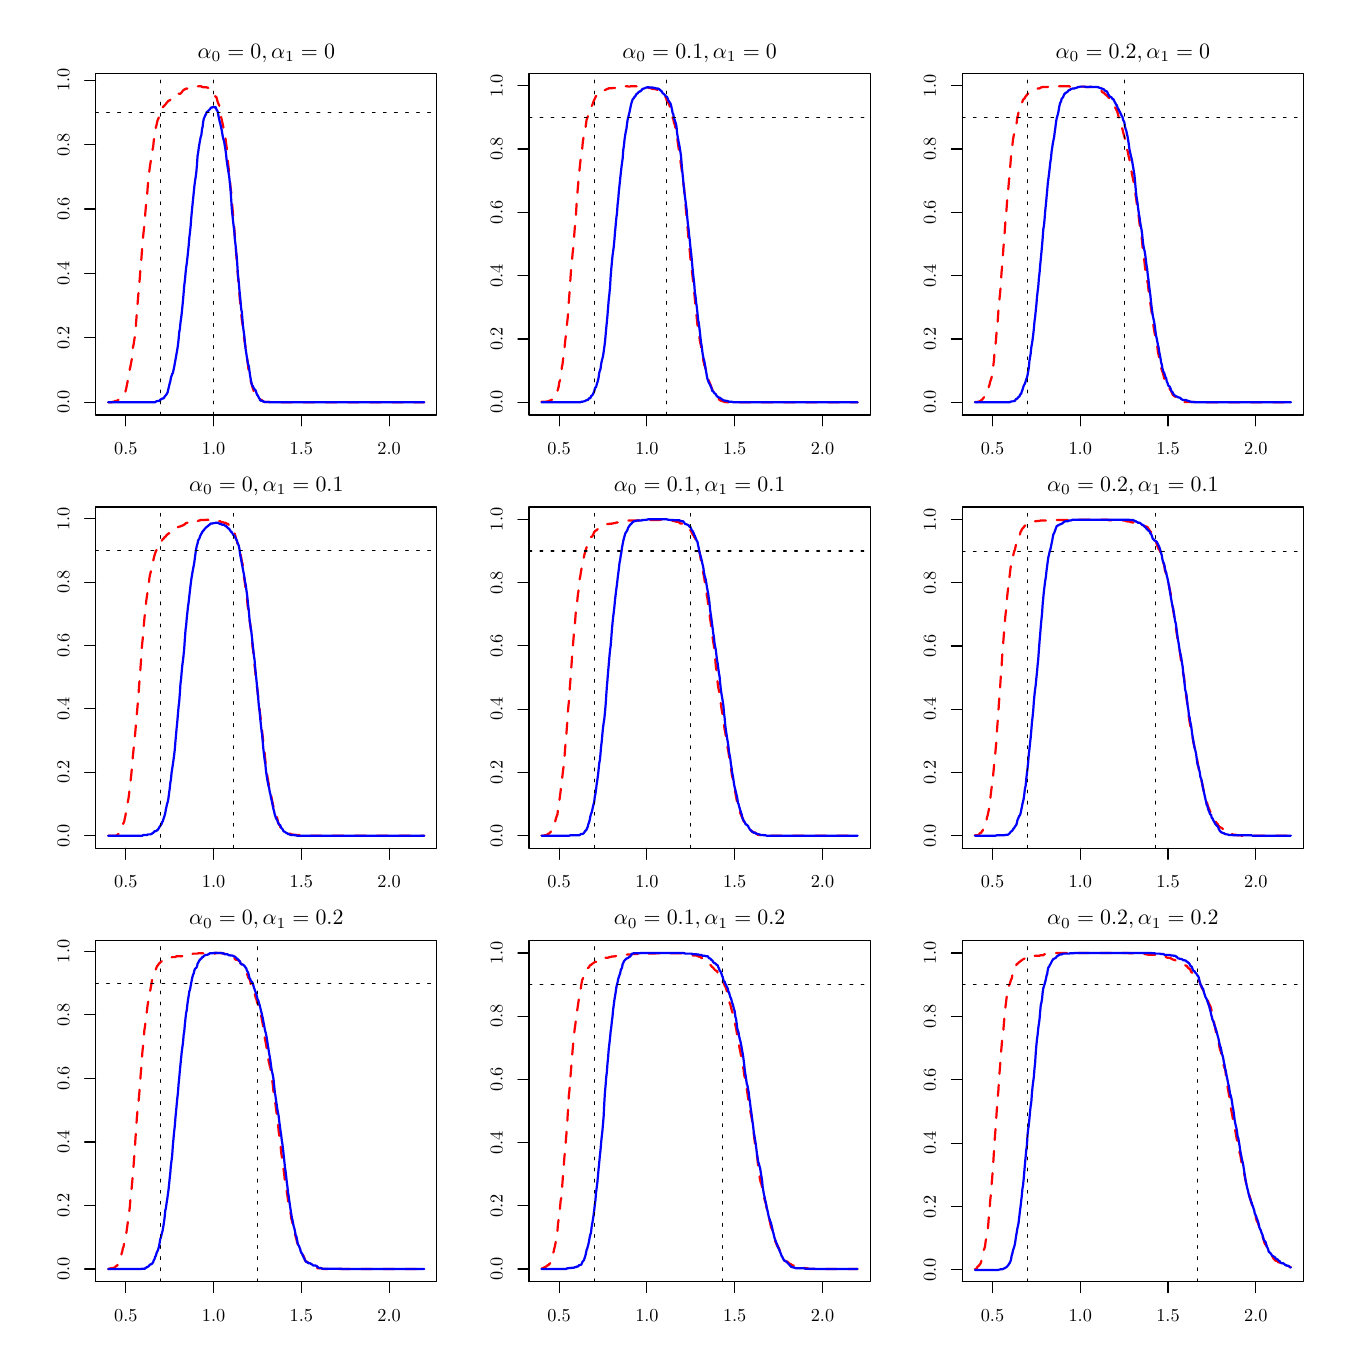
\begin{tikzpicture}[x=1pt,y=1pt]
\definecolor{fillColor}{RGB}{255,255,255}
\path[use as bounding box,fill=fillColor,fill opacity=0.00] (0,0) rectangle (469.75,469.75);
\begin{scope}
\path[clip] ( 24.55,329.80) rectangle (147.87,453.12);
\definecolor{drawColor}{RGB}{255,0,0}

\path[draw=drawColor,line width= 0.8pt,dash pattern=on 4pt off 4pt ,line join=round,line cap=round] ( 29.12,334.37) --
	( 29.35,334.37) --
	( 29.58,334.37) --
	( 29.81,334.37) --
	( 30.03,334.37) --
	( 30.26,334.37) --
	( 30.49,334.49) --
	( 30.72,334.49) --
	( 30.95,334.60) --
	( 31.18,334.60) --
	( 31.41,334.72) --
	( 31.64,334.84) --
	( 31.87,334.84) --
	( 32.09,334.95) --
	( 32.32,334.95) --
	( 32.55,334.95) --
	( 32.78,335.30) --
	( 33.01,335.42) --
	( 33.24,335.42) --
	( 33.47,335.65) --
	( 33.70,336.00) --
	( 33.92,336.23) --
	( 34.15,336.70) --
	( 34.38,336.93) --
	( 34.61,337.28) --
	( 34.84,337.63) --
	( 35.07,337.98) --
	( 35.30,338.21) --
	( 35.53,339.03) --
	( 35.76,340.19) --
	( 35.98,341.24) --
	( 36.21,342.40) --
	( 36.44,344.03) --
	( 36.67,345.19) --
	( 36.90,346.36) --
	( 37.13,347.29) --
	( 37.36,348.57) --
	( 37.59,349.73) --
	( 37.81,352.41) --
	( 38.04,354.27) --
	( 38.27,355.20) --
	( 38.50,356.83) --
	( 38.73,358.11) --
	( 38.96,359.98) --
	( 39.19,363.35) --
	( 39.42,366.38) --
	( 39.65,369.17) --
	( 39.87,371.97) --
	( 40.10,374.64) --
	( 40.33,377.20) --
	( 40.56,379.76) --
	( 40.79,383.72) --
	( 41.02,385.35) --
	( 41.25,388.49) --
	( 41.48,391.29) --
	( 41.71,394.08) --
	( 41.93,396.29) --
	( 42.16,398.27) --
	( 42.39,401.30) --
	( 42.62,404.09) --
	( 42.85,406.65) --
	( 43.08,408.28) --
	( 43.31,411.31) --
	( 43.54,414.33) --
	( 43.76,415.96) --
	( 43.99,418.18) --
	( 44.22,419.92) --
	( 44.45,421.32) --
	( 44.68,423.76) --
	( 44.91,424.46) --
	( 45.14,425.74) --
	( 45.37,426.91) --
	( 45.60,429.23) --
	( 45.82,430.16) --
	( 46.05,432.26) --
	( 46.28,433.54) --
	( 46.51,434.36) --
	( 46.74,435.40) --
	( 46.97,436.33) --
	( 47.20,436.80) --
	( 47.43,437.38) --
	( 47.65,438.20) --
	( 47.88,438.55) --
	( 48.11,439.36) --
	( 48.34,439.59) --
	( 48.57,440.41) --
	( 48.80,440.99) --
	( 49.03,441.22) --
	( 49.26,441.46) --
	( 49.49,441.69) --
	( 49.71,441.92) --
	( 49.94,442.15) --
	( 50.17,442.62) --
	( 50.40,442.74) --
	( 50.63,443.08) --
	( 50.86,443.32) --
	( 51.09,443.43) --
	( 51.32,443.43) --
	( 51.54,443.67) --
	( 51.77,443.67) --
	( 52.00,443.67) --
	( 52.23,443.67) --
	( 52.46,443.90) --
	( 52.69,444.02) --
	( 52.92,444.37) --
	( 53.15,444.60) --
	( 53.38,444.60) --
	( 53.60,444.71) --
	( 53.83,445.06) --
	( 54.06,445.53) --
	( 54.29,445.76) --
	( 54.52,445.88) --
	( 54.75,445.88) --
	( 54.98,445.88) --
	( 55.21,445.88) --
	( 55.43,446.11) --
	( 55.66,446.46) --
	( 55.89,446.69) --
	( 56.12,447.04) --
	( 56.35,447.16) --
	( 56.58,447.39) --
	( 56.81,447.51) --
	( 57.04,447.51) --
	( 57.27,447.74) --
	( 57.49,447.74) --
	( 57.72,447.74) --
	( 57.95,447.86) --
	( 58.18,447.86) --
	( 58.41,447.97) --
	( 58.64,448.09) --
	( 58.87,448.21) --
	( 59.10,448.21) --
	( 59.32,448.32) --
	( 59.55,448.32) --
	( 59.78,448.32) --
	( 60.01,448.32) --
	( 60.24,448.32) --
	( 60.47,448.32) --
	( 60.70,448.32) --
	( 60.93,448.32) --
	( 61.16,448.32) --
	( 61.38,448.56) --
	( 61.61,448.56) --
	( 61.84,448.56) --
	( 62.07,448.56) --
	( 62.30,448.56) --
	( 62.53,448.56) --
	( 62.76,448.56) --
	( 62.99,448.32) --
	( 63.22,448.32) --
	( 63.44,448.21) --
	( 63.67,448.21) --
	( 63.90,448.21) --
	( 64.13,448.21) --
	( 64.36,448.21) --
	( 64.59,448.21) --
	( 64.82,448.09) --
	( 65.05,448.09) --
	( 65.27,447.97) --
	( 65.50,447.86) --
	( 65.73,447.62) --
	( 65.96,447.51) --
	( 66.19,447.39) --
	( 66.42,447.28) --
	( 66.65,446.69) --
	( 66.88,446.11) --
	( 67.11,445.65) --
	( 67.33,445.53) --
	( 67.56,445.41) --
	( 67.79,444.95) --
	( 68.02,444.71) --
	( 68.25,444.60) --
	( 68.48,443.55) --
	( 68.71,442.74) --
	( 68.94,442.27) --
	( 69.16,441.80) --
	( 69.39,440.64) --
	( 69.62,439.36) --
	( 69.85,437.73) --
	( 70.08,436.68) --
	( 70.31,435.64) --
	( 70.54,434.59) --
	( 70.77,433.54) --
	( 71.00,432.49) --
	( 71.22,431.68) --
	( 71.45,430.05) --
	( 71.68,428.07) --
	( 71.91,426.44) --
	( 72.14,424.00) --
	( 72.37,421.09) --
	( 72.60,419.11) --
	( 72.83,417.48) --
	( 73.05,414.92) --
	( 73.28,412.24) --
	( 73.51,410.49) --
	( 73.74,408.05) --
	( 73.97,404.91) --
	( 74.20,402.46) --
	( 74.43,399.90) --
	( 74.66,397.11) --
	( 74.89,393.97) --
	( 75.11,391.52) --
	( 75.34,388.26) --
	( 75.57,385.24) --
	( 75.80,382.21) --
	( 76.03,379.65) --
	( 76.26,376.27) --
	( 76.49,373.71) --
	( 76.72,370.92) --
	( 76.94,368.94) --
	( 77.17,366.26) --
	( 77.40,364.05) --
	( 77.63,362.65) --
	( 77.86,360.56) --
	( 78.09,358.23) --
	( 78.32,356.72) --
	( 78.55,355.44) --
	( 78.78,353.92) --
	( 79.00,352.41) --
	( 79.23,350.67) --
	( 79.46,349.04) --
	( 79.69,346.94) --
	( 79.92,345.19) --
	( 80.15,344.03) --
	( 80.38,342.98) --
	( 80.61,341.94) --
	( 80.83,341.35) --
	( 81.06,340.65) --
	( 81.29,339.61) --
	( 81.52,339.03) --
	( 81.75,338.09) --
	( 81.98,337.74) --
	( 82.21,337.40) --
	( 82.44,337.16) --
	( 82.67,336.70) --
	( 82.89,336.23) --
	( 83.12,336.12) --
	( 83.35,336.12) --
	( 83.58,335.65) --
	( 83.81,335.53) --
	( 84.04,335.30) --
	( 84.27,335.30) --
	( 84.50,335.18) --
	( 84.73,335.07) --
	( 84.95,334.84) --
	( 85.18,334.72) --
	( 85.41,334.49) --
	( 85.64,334.49) --
	( 85.87,334.49) --
	( 86.10,334.49) --
	( 86.33,334.49) --
	( 86.56,334.49) --
	( 86.78,334.49) --
	( 87.01,334.49) --
	( 87.24,334.49) --
	( 87.47,334.49) --
	( 87.70,334.49) --
	( 87.93,334.49) --
	( 88.16,334.49) --
	( 88.39,334.49) --
	( 88.62,334.49) --
	( 88.84,334.49) --
	( 89.07,334.49) --
	( 89.30,334.49) --
	( 89.53,334.49) --
	( 89.76,334.49) --
	( 89.99,334.37) --
	( 90.22,334.37) --
	( 90.45,334.37) --
	( 90.67,334.37) --
	( 90.90,334.37) --
	( 91.13,334.37) --
	( 91.36,334.37) --
	( 91.59,334.37) --
	( 91.82,334.37) --
	( 92.05,334.37) --
	( 92.28,334.37) --
	( 92.51,334.37) --
	( 92.73,334.37) --
	( 92.96,334.37) --
	( 93.19,334.37) --
	( 93.42,334.37) --
	( 93.65,334.37) --
	( 93.88,334.37) --
	( 94.11,334.37) --
	( 94.34,334.37) --
	( 94.56,334.37) --
	( 94.79,334.37) --
	( 95.02,334.37) --
	( 95.25,334.37) --
	( 95.48,334.37) --
	( 95.71,334.37) --
	( 95.94,334.37) --
	( 96.17,334.37) --
	( 96.40,334.37) --
	( 96.62,334.37) --
	( 96.85,334.37) --
	( 97.08,334.37) --
	( 97.31,334.37) --
	( 97.54,334.37) --
	( 97.77,334.37) --
	( 98.00,334.37) --
	( 98.23,334.37) --
	( 98.45,334.37) --
	( 98.68,334.37) --
	( 98.91,334.37) --
	( 99.14,334.37) --
	( 99.37,334.37) --
	( 99.60,334.37) --
	( 99.83,334.37) --
	(100.06,334.37) --
	(100.29,334.37) --
	(100.51,334.37) --
	(100.74,334.37) --
	(100.97,334.37) --
	(101.20,334.37) --
	(101.43,334.37) --
	(101.66,334.37) --
	(101.89,334.37) --
	(102.12,334.37) --
	(102.35,334.37) --
	(102.57,334.37) --
	(102.80,334.37) --
	(103.03,334.37) --
	(103.26,334.37) --
	(103.49,334.37) --
	(103.72,334.37) --
	(103.95,334.37) --
	(104.18,334.37) --
	(104.40,334.37) --
	(104.63,334.37) --
	(104.86,334.37) --
	(105.09,334.37) --
	(105.32,334.37) --
	(105.55,334.37) --
	(105.78,334.37) --
	(106.01,334.37) --
	(106.24,334.37) --
	(106.46,334.37) --
	(106.69,334.37) --
	(106.92,334.37) --
	(107.15,334.37) --
	(107.38,334.37) --
	(107.61,334.37) --
	(107.84,334.37) --
	(108.07,334.37) --
	(108.29,334.37) --
	(108.52,334.37) --
	(108.75,334.37) --
	(108.98,334.37) --
	(109.21,334.37) --
	(109.44,334.37) --
	(109.67,334.37) --
	(109.90,334.37) --
	(110.13,334.37) --
	(110.35,334.37) --
	(110.58,334.37) --
	(110.81,334.37) --
	(111.04,334.37) --
	(111.27,334.37) --
	(111.50,334.37) --
	(111.73,334.37) --
	(111.96,334.37) --
	(112.18,334.37) --
	(112.41,334.37) --
	(112.64,334.37) --
	(112.87,334.37) --
	(113.10,334.37) --
	(113.33,334.37) --
	(113.56,334.37) --
	(113.79,334.37) --
	(114.02,334.37) --
	(114.24,334.37) --
	(114.47,334.37) --
	(114.70,334.37) --
	(114.93,334.37) --
	(115.16,334.37) --
	(115.39,334.37) --
	(115.62,334.37) --
	(115.85,334.37) --
	(116.07,334.37) --
	(116.30,334.37) --
	(116.53,334.37) --
	(116.76,334.37) --
	(116.99,334.37) --
	(117.22,334.37) --
	(117.45,334.37) --
	(117.68,334.37) --
	(117.91,334.37) --
	(118.13,334.37) --
	(118.36,334.37) --
	(118.59,334.37) --
	(118.82,334.37) --
	(119.05,334.37) --
	(119.28,334.37) --
	(119.51,334.37) --
	(119.74,334.37) --
	(119.96,334.37) --
	(120.19,334.37) --
	(120.42,334.37) --
	(120.65,334.37) --
	(120.88,334.37) --
	(121.11,334.37) --
	(121.34,334.37) --
	(121.57,334.37) --
	(121.80,334.37) --
	(122.02,334.37) --
	(122.25,334.37) --
	(122.48,334.37) --
	(122.71,334.37) --
	(122.94,334.37) --
	(123.17,334.37) --
	(123.40,334.37) --
	(123.63,334.37) --
	(123.86,334.37) --
	(124.08,334.37) --
	(124.31,334.37) --
	(124.54,334.37) --
	(124.77,334.37) --
	(125.00,334.37) --
	(125.23,334.37) --
	(125.46,334.37) --
	(125.69,334.37) --
	(125.91,334.37) --
	(126.14,334.37) --
	(126.37,334.37) --
	(126.60,334.37) --
	(126.83,334.37) --
	(127.06,334.37) --
	(127.29,334.37) --
	(127.52,334.37) --
	(127.75,334.37) --
	(127.97,334.37) --
	(128.20,334.37) --
	(128.43,334.37) --
	(128.66,334.37) --
	(128.89,334.37) --
	(129.12,334.37) --
	(129.35,334.37) --
	(129.58,334.37) --
	(129.80,334.37) --
	(130.03,334.37) --
	(130.26,334.37) --
	(130.49,334.37) --
	(130.72,334.37) --
	(130.95,334.37) --
	(131.18,334.37) --
	(131.41,334.37) --
	(131.64,334.37) --
	(131.86,334.37) --
	(132.09,334.37) --
	(132.32,334.37) --
	(132.55,334.37) --
	(132.78,334.37) --
	(133.01,334.37) --
	(133.24,334.37) --
	(133.47,334.37) --
	(133.69,334.37) --
	(133.92,334.37) --
	(134.15,334.37) --
	(134.38,334.37) --
	(134.61,334.37) --
	(134.84,334.37) --
	(135.07,334.37) --
	(135.30,334.37) --
	(135.53,334.37) --
	(135.75,334.37) --
	(135.98,334.37) --
	(136.21,334.37) --
	(136.44,334.37) --
	(136.67,334.37) --
	(136.90,334.37) --
	(137.13,334.37) --
	(137.36,334.37) --
	(137.58,334.37) --
	(137.81,334.37) --
	(138.04,334.37) --
	(138.27,334.37) --
	(138.50,334.37) --
	(138.73,334.37) --
	(138.96,334.37) --
	(139.19,334.37) --
	(139.42,334.37) --
	(139.64,334.37) --
	(139.87,334.37) --
	(140.10,334.37) --
	(140.33,334.37) --
	(140.56,334.37) --
	(140.79,334.37) --
	(141.02,334.37) --
	(141.25,334.37) --
	(141.47,334.37) --
	(141.70,334.37) --
	(141.93,334.37) --
	(142.16,334.37) --
	(142.39,334.37) --
	(142.62,334.37) --
	(142.85,334.37) --
	(143.08,334.37) --
	(143.31,334.37);
\end{scope}
\begin{scope}
\path[clip] (  0.00,  0.00) rectangle (469.75,469.75);
\definecolor{drawColor}{RGB}{0,0,0}

\path[draw=drawColor,line width= 0.4pt,line join=round,line cap=round] ( 35.46,329.80) -- (130.62,329.80);

\path[draw=drawColor,line width= 0.4pt,line join=round,line cap=round] ( 35.46,329.80) -- ( 35.46,325.84);

\path[draw=drawColor,line width= 0.4pt,line join=round,line cap=round] ( 67.18,329.80) -- ( 67.18,325.84);

\path[draw=drawColor,line width= 0.4pt,line join=round,line cap=round] ( 98.90,329.80) -- ( 98.90,325.84);

\path[draw=drawColor,line width= 0.4pt,line join=round,line cap=round] (130.62,329.80) -- (130.62,325.84);

\node[text=drawColor,anchor=base,inner sep=0pt, outer sep=0pt, scale=  0.66] at ( 35.46,315.55) {0.5};

\node[text=drawColor,anchor=base,inner sep=0pt, outer sep=0pt, scale=  0.66] at ( 67.18,315.55) {1.0};

\node[text=drawColor,anchor=base,inner sep=0pt, outer sep=0pt, scale=  0.66] at ( 98.90,315.55) {1.5};

\node[text=drawColor,anchor=base,inner sep=0pt, outer sep=0pt, scale=  0.66] at (130.62,315.55) {2.0};

\path[draw=drawColor,line width= 0.4pt,line join=round,line cap=round] ( 24.55,334.37) -- ( 24.55,450.77);

\path[draw=drawColor,line width= 0.4pt,line join=round,line cap=round] ( 24.55,334.37) -- ( 20.59,334.37);

\path[draw=drawColor,line width= 0.4pt,line join=round,line cap=round] ( 24.55,357.65) -- ( 20.59,357.65);

\path[draw=drawColor,line width= 0.4pt,line join=round,line cap=round] ( 24.55,380.93) -- ( 20.59,380.93);

\path[draw=drawColor,line width= 0.4pt,line join=round,line cap=round] ( 24.55,404.21) -- ( 20.59,404.21);

\path[draw=drawColor,line width= 0.4pt,line join=round,line cap=round] ( 24.55,427.49) -- ( 20.59,427.49);

\path[draw=drawColor,line width= 0.4pt,line join=round,line cap=round] ( 24.55,450.77) -- ( 20.59,450.77);

\node[text=drawColor,rotate= 90.00,anchor=base,inner sep=0pt, outer sep=0pt, scale=  0.66] at ( 15.05,334.37) {0.0};

\node[text=drawColor,rotate= 90.00,anchor=base,inner sep=0pt, outer sep=0pt, scale=  0.66] at ( 15.05,357.65) {0.2};

\node[text=drawColor,rotate= 90.00,anchor=base,inner sep=0pt, outer sep=0pt, scale=  0.66] at ( 15.05,380.93) {0.4};

\node[text=drawColor,rotate= 90.00,anchor=base,inner sep=0pt, outer sep=0pt, scale=  0.66] at ( 15.05,404.21) {0.6};

\node[text=drawColor,rotate= 90.00,anchor=base,inner sep=0pt, outer sep=0pt, scale=  0.66] at ( 15.05,427.49) {0.8};

\node[text=drawColor,rotate= 90.00,anchor=base,inner sep=0pt, outer sep=0pt, scale=  0.66] at ( 15.05,450.77) {1.0};

\path[draw=drawColor,line width= 0.4pt,line join=round,line cap=round] ( 24.55,329.80) --
	(147.87,329.80) --
	(147.87,453.12) --
	( 24.55,453.12) --
	( 24.55,329.80);
\end{scope}
\begin{scope}
\path[clip] (  0.00,313.17) rectangle (156.58,469.75);
\definecolor{drawColor}{RGB}{0,0,0}

\node[text=drawColor,anchor=base,inner sep=0pt, outer sep=0pt, scale=  0.79] at ( 86.21,458.71) {\bfseries $\alpha_0 = 0, \alpha_1 = 0$};
\end{scope}
\begin{scope}
\path[clip] ( 24.55,329.80) rectangle (147.87,453.12);
\definecolor{drawColor}{RGB}{0,0,255}

\path[draw=drawColor,line width= 0.8pt,line join=round,line cap=round] ( 29.12,334.37) --
	( 29.35,334.37) --
	( 29.58,334.37) --
	( 29.81,334.37) --
	( 30.03,334.37) --
	( 30.26,334.37) --
	( 30.49,334.37) --
	( 30.72,334.37) --
	( 30.95,334.37) --
	( 31.18,334.37) --
	( 31.41,334.37) --
	( 31.64,334.37) --
	( 31.87,334.37) --
	( 32.09,334.37) --
	( 32.32,334.37) --
	( 32.55,334.37) --
	( 32.78,334.37) --
	( 33.01,334.37) --
	( 33.24,334.37) --
	( 33.47,334.37) --
	( 33.70,334.37) --
	( 33.92,334.37) --
	( 34.15,334.37) --
	( 34.38,334.37) --
	( 34.61,334.37) --
	( 34.84,334.37) --
	( 35.07,334.37) --
	( 35.30,334.37) --
	( 35.53,334.37) --
	( 35.76,334.37) --
	( 35.98,334.37) --
	( 36.21,334.37) --
	( 36.44,334.37) --
	( 36.67,334.37) --
	( 36.90,334.37) --
	( 37.13,334.37) --
	( 37.36,334.37) --
	( 37.59,334.37) --
	( 37.81,334.37) --
	( 38.04,334.37) --
	( 38.27,334.37) --
	( 38.50,334.37) --
	( 38.73,334.37) --
	( 38.96,334.37) --
	( 39.19,334.37) --
	( 39.42,334.37) --
	( 39.65,334.37) --
	( 39.87,334.37) --
	( 40.10,334.37) --
	( 40.33,334.37) --
	( 40.56,334.37) --
	( 40.79,334.37) --
	( 41.02,334.37) --
	( 41.25,334.37) --
	( 41.48,334.37) --
	( 41.71,334.37) --
	( 41.93,334.37) --
	( 42.16,334.37) --
	( 42.39,334.37) --
	( 42.62,334.37) --
	( 42.85,334.37) --
	( 43.08,334.37) --
	( 43.31,334.37) --
	( 43.54,334.37) --
	( 43.76,334.37) --
	( 43.99,334.37) --
	( 44.22,334.37) --
	( 44.45,334.37) --
	( 44.68,334.37) --
	( 44.91,334.37) --
	( 45.14,334.37) --
	( 45.37,334.37) --
	( 45.60,334.37) --
	( 45.82,334.37) --
	( 46.05,334.37) --
	( 46.28,334.60) --
	( 46.51,334.72) --
	( 46.74,334.84) --
	( 46.97,334.84) --
	( 47.20,334.84) --
	( 47.43,334.84) --
	( 47.65,334.95) --
	( 47.88,335.30) --
	( 48.11,335.30) --
	( 48.34,335.65) --
	( 48.57,335.65) --
	( 48.80,335.77) --
	( 49.03,335.77) --
	( 49.26,336.00) --
	( 49.49,336.46) --
	( 49.71,336.70) --
	( 49.94,336.93) --
	( 50.17,337.28) --
	( 50.40,337.63) --
	( 50.63,338.21) --
	( 50.86,339.26) --
	( 51.09,340.19) --
	( 51.32,341.24) --
	( 51.54,341.94) --
	( 51.77,343.22) --
	( 52.00,343.91) --
	( 52.23,344.61) --
	( 52.46,344.96) --
	( 52.69,346.01) --
	( 52.92,347.06) --
	( 53.15,348.34) --
	( 53.38,349.62) --
	( 53.60,350.78) --
	( 53.83,352.18) --
	( 54.06,353.46) --
	( 54.29,354.97) --
	( 54.52,356.95) --
	( 54.75,359.63) --
	( 54.98,360.79) --
	( 55.21,363.12) --
	( 55.43,364.63) --
	( 55.66,366.50) --
	( 55.89,368.82) --
	( 56.12,371.15) --
	( 56.35,373.83) --
	( 56.58,376.62) --
	( 56.81,378.37) --
	( 57.04,380.93) --
	( 57.27,383.14) --
	( 57.49,384.54) --
	( 57.72,386.63) --
	( 57.95,388.73) --
	( 58.18,391.06) --
	( 58.41,393.85) --
	( 58.64,395.71) --
	( 58.87,397.92) --
	( 59.10,400.95) --
	( 59.32,403.28) --
	( 59.55,405.72) --
	( 59.78,407.93) --
	( 60.01,410.14) --
	( 60.24,412.47) --
	( 60.47,414.33) --
	( 60.70,415.73) --
	( 60.93,417.48) --
	( 61.16,420.04) --
	( 61.38,423.30) --
	( 61.61,424.69) --
	( 61.84,426.44) --
	( 62.07,427.84) --
	( 62.30,429.12) --
	( 62.53,430.28) --
	( 62.76,430.98) --
	( 62.99,432.96) --
	( 63.22,434.01) --
	( 63.44,435.87) --
	( 63.67,436.92) --
	( 63.90,437.38) --
	( 64.13,438.08) --
	( 64.36,438.31) --
	( 64.59,439.01) --
	( 64.82,439.36) --
	( 65.05,439.48) --
	( 65.27,439.71) --
	( 65.50,439.94) --
	( 65.73,440.17) --
	( 65.96,440.41) --
	( 66.19,440.87) --
	( 66.42,440.87) --
	( 66.65,440.87) --
	( 66.88,441.11) --
	( 67.11,441.11) --
	( 67.33,441.11) --
	( 67.56,440.87) --
	( 67.79,441.11) --
	( 68.02,440.87) --
	( 68.25,440.06) --
	( 68.48,439.83) --
	( 68.71,439.24) --
	( 68.94,437.85) --
	( 69.16,436.92) --
	( 69.39,435.75) --
	( 69.62,434.94) --
	( 69.85,433.89) --
	( 70.08,432.96) --
	( 70.31,431.56) --
	( 70.54,430.16) --
	( 70.77,429.35) --
	( 71.00,428.54) --
	( 71.22,427.14) --
	( 71.45,425.74) --
	( 71.68,424.11) --
	( 71.91,421.67) --
	( 72.14,420.15) --
	( 72.37,418.76) --
	( 72.60,417.24) --
	( 72.83,415.85) --
	( 73.05,413.64) --
	( 73.28,411.54) --
	( 73.51,408.17) --
	( 73.74,404.56) --
	( 73.97,402.23) --
	( 74.20,400.02) --
	( 74.43,398.04) --
	( 74.66,396.18) --
	( 74.89,393.03) --
	( 75.11,391.29) --
	( 75.34,388.61) --
	( 75.57,386.75) --
	( 75.80,383.26) --
	( 76.03,379.76) --
	( 76.26,377.90) --
	( 76.49,375.23) --
	( 76.72,372.90) --
	( 76.94,370.57) --
	( 77.17,368.01) --
	( 77.40,366.84) --
	( 77.63,363.93) --
	( 77.86,361.49) --
	( 78.09,359.74) --
	( 78.32,358.11) --
	( 78.55,355.32) --
	( 78.78,353.46) --
	( 79.00,352.06) --
	( 79.23,350.55) --
	( 79.46,349.04) --
	( 79.69,347.99) --
	( 79.92,347.41) --
	( 80.15,345.66) --
	( 80.38,344.03) --
	( 80.61,342.63) --
	( 80.83,341.47) --
	( 81.06,340.54) --
	( 81.29,340.31) --
	( 81.52,339.84) --
	( 81.75,339.37) --
	( 81.98,339.03) --
	( 82.21,338.91) --
	( 82.44,338.44) --
	( 82.67,337.74) --
	( 82.89,337.05) --
	( 83.12,336.93) --
	( 83.35,336.46) --
	( 83.58,335.88) --
	( 83.81,335.65) --
	( 84.04,335.07) --
	( 84.27,334.95) --
	( 84.50,334.95) --
	( 84.73,334.95) --
	( 84.95,334.84) --
	( 85.18,334.60) --
	( 85.41,334.60) --
	( 85.64,334.49) --
	( 85.87,334.49) --
	( 86.10,334.49) --
	( 86.33,334.49) --
	( 86.56,334.49) --
	( 86.78,334.49) --
	( 87.01,334.49) --
	( 87.24,334.49) --
	( 87.47,334.37) --
	( 87.70,334.37) --
	( 87.93,334.37) --
	( 88.16,334.37) --
	( 88.39,334.37) --
	( 88.62,334.37) --
	( 88.84,334.37) --
	( 89.07,334.37) --
	( 89.30,334.37) --
	( 89.53,334.37) --
	( 89.76,334.37) --
	( 89.99,334.37) --
	( 90.22,334.37) --
	( 90.45,334.37) --
	( 90.67,334.37) --
	( 90.90,334.37) --
	( 91.13,334.37) --
	( 91.36,334.37) --
	( 91.59,334.37) --
	( 91.82,334.37) --
	( 92.05,334.37) --
	( 92.28,334.37) --
	( 92.51,334.37) --
	( 92.73,334.37) --
	( 92.96,334.37) --
	( 93.19,334.37) --
	( 93.42,334.37) --
	( 93.65,334.37) --
	( 93.88,334.37) --
	( 94.11,334.37) --
	( 94.34,334.37) --
	( 94.56,334.37) --
	( 94.79,334.37) --
	( 95.02,334.37) --
	( 95.25,334.37) --
	( 95.48,334.37) --
	( 95.71,334.37) --
	( 95.94,334.37) --
	( 96.17,334.37) --
	( 96.40,334.37) --
	( 96.62,334.37) --
	( 96.85,334.37) --
	( 97.08,334.37) --
	( 97.31,334.37) --
	( 97.54,334.37) --
	( 97.77,334.37) --
	( 98.00,334.37) --
	( 98.23,334.37) --
	( 98.45,334.37) --
	( 98.68,334.37) --
	( 98.91,334.37) --
	( 99.14,334.37) --
	( 99.37,334.37) --
	( 99.60,334.37) --
	( 99.83,334.37) --
	(100.06,334.37) --
	(100.29,334.37) --
	(100.51,334.37) --
	(100.74,334.37) --
	(100.97,334.37) --
	(101.20,334.37) --
	(101.43,334.37) --
	(101.66,334.37) --
	(101.89,334.37) --
	(102.12,334.37) --
	(102.35,334.37) --
	(102.57,334.37) --
	(102.80,334.37) --
	(103.03,334.37) --
	(103.26,334.37) --
	(103.49,334.37) --
	(103.72,334.37) --
	(103.95,334.37) --
	(104.18,334.37) --
	(104.40,334.37) --
	(104.63,334.37) --
	(104.86,334.37) --
	(105.09,334.37) --
	(105.32,334.37) --
	(105.55,334.37) --
	(105.78,334.37) --
	(106.01,334.37) --
	(106.24,334.37) --
	(106.46,334.37) --
	(106.69,334.37) --
	(106.92,334.37) --
	(107.15,334.37) --
	(107.38,334.37) --
	(107.61,334.37) --
	(107.84,334.37) --
	(108.07,334.37) --
	(108.29,334.37) --
	(108.52,334.37) --
	(108.75,334.37) --
	(108.98,334.37) --
	(109.21,334.37) --
	(109.44,334.37) --
	(109.67,334.37) --
	(109.90,334.37) --
	(110.13,334.37) --
	(110.35,334.37) --
	(110.58,334.37) --
	(110.81,334.37) --
	(111.04,334.37) --
	(111.27,334.37) --
	(111.50,334.37) --
	(111.73,334.37) --
	(111.96,334.37) --
	(112.18,334.37) --
	(112.41,334.37) --
	(112.64,334.37) --
	(112.87,334.37) --
	(113.10,334.37) --
	(113.33,334.37) --
	(113.56,334.37) --
	(113.79,334.37) --
	(114.02,334.37) --
	(114.24,334.37) --
	(114.47,334.37) --
	(114.70,334.37) --
	(114.93,334.37) --
	(115.16,334.37) --
	(115.39,334.37) --
	(115.62,334.37) --
	(115.85,334.37) --
	(116.07,334.37) --
	(116.30,334.37) --
	(116.53,334.37) --
	(116.76,334.37) --
	(116.99,334.37) --
	(117.22,334.37) --
	(117.45,334.37) --
	(117.68,334.37) --
	(117.91,334.37) --
	(118.13,334.37) --
	(118.36,334.37) --
	(118.59,334.37) --
	(118.82,334.37) --
	(119.05,334.37) --
	(119.28,334.37) --
	(119.51,334.37) --
	(119.74,334.37) --
	(119.96,334.37) --
	(120.19,334.37) --
	(120.42,334.37) --
	(120.65,334.37) --
	(120.88,334.37) --
	(121.11,334.37) --
	(121.34,334.37) --
	(121.57,334.37) --
	(121.80,334.37) --
	(122.02,334.37) --
	(122.25,334.37) --
	(122.48,334.37) --
	(122.71,334.37) --
	(122.94,334.37) --
	(123.17,334.37) --
	(123.40,334.37) --
	(123.63,334.37) --
	(123.86,334.37) --
	(124.08,334.37) --
	(124.31,334.37) --
	(124.54,334.37) --
	(124.77,334.37) --
	(125.00,334.37) --
	(125.23,334.37) --
	(125.46,334.37) --
	(125.69,334.37) --
	(125.91,334.37) --
	(126.14,334.37) --
	(126.37,334.37) --
	(126.60,334.37) --
	(126.83,334.37) --
	(127.06,334.37) --
	(127.29,334.37) --
	(127.52,334.37) --
	(127.75,334.37) --
	(127.97,334.37) --
	(128.20,334.37) --
	(128.43,334.37) --
	(128.66,334.37) --
	(128.89,334.37) --
	(129.12,334.37) --
	(129.35,334.37) --
	(129.58,334.37) --
	(129.80,334.37) --
	(130.03,334.37) --
	(130.26,334.37) --
	(130.49,334.37) --
	(130.72,334.37) --
	(130.95,334.37) --
	(131.18,334.37) --
	(131.41,334.37) --
	(131.64,334.37) --
	(131.86,334.37) --
	(132.09,334.37) --
	(132.32,334.37) --
	(132.55,334.37) --
	(132.78,334.37) --
	(133.01,334.37) --
	(133.24,334.37) --
	(133.47,334.37) --
	(133.69,334.37) --
	(133.92,334.37) --
	(134.15,334.37) --
	(134.38,334.37) --
	(134.61,334.37) --
	(134.84,334.37) --
	(135.07,334.37) --
	(135.30,334.37) --
	(135.53,334.37) --
	(135.75,334.37) --
	(135.98,334.37) --
	(136.21,334.37) --
	(136.44,334.37) --
	(136.67,334.37) --
	(136.90,334.37) --
	(137.13,334.37) --
	(137.36,334.37) --
	(137.58,334.37) --
	(137.81,334.37) --
	(138.04,334.37) --
	(138.27,334.37) --
	(138.50,334.37) --
	(138.73,334.37) --
	(138.96,334.37) --
	(139.19,334.37) --
	(139.42,334.37) --
	(139.64,334.37) --
	(139.87,334.37) --
	(140.10,334.37) --
	(140.33,334.37) --
	(140.56,334.37) --
	(140.79,334.37) --
	(141.02,334.37) --
	(141.25,334.37) --
	(141.47,334.37) --
	(141.70,334.37) --
	(141.93,334.37) --
	(142.16,334.37) --
	(142.39,334.37) --
	(142.62,334.37) --
	(142.85,334.37) --
	(143.08,334.37) --
	(143.31,334.37);
\definecolor{drawColor}{RGB}{0,0,0}

\path[draw=drawColor,line width= 0.4pt,dash pattern=on 1pt off 3pt ,line join=round,line cap=round] ( 24.55,439.13) -- (147.87,439.13);

\path[draw=drawColor,line width= 0.4pt,dash pattern=on 1pt off 3pt ,line join=round,line cap=round] ( 48.15,329.80) -- ( 48.15,453.12);

\path[draw=drawColor,line width= 0.4pt,dash pattern=on 1pt off 3pt ,line join=round,line cap=round] ( 67.18,329.80) -- ( 67.18,453.12);
\end{scope}
\begin{scope}
\path[clip] (181.14,329.80) rectangle (304.46,453.12);
\definecolor{drawColor}{RGB}{255,0,0}

\path[draw=drawColor,line width= 0.8pt,dash pattern=on 4pt off 4pt ,line join=round,line cap=round] (185.70,334.60) --
	(185.93,334.60) --
	(186.16,334.60) --
	(186.39,334.60) --
	(186.62,334.60) --
	(186.85,334.60) --
	(187.08,334.60) --
	(187.31,334.60) --
	(187.54,334.71) --
	(187.76,334.71) --
	(187.99,334.71) --
	(188.22,334.83) --
	(188.45,334.83) --
	(188.68,335.06) --
	(188.91,335.06) --
	(189.14,335.17) --
	(189.37,335.28) --
	(189.59,335.40) --
	(189.82,335.40) --
	(190.05,335.63) --
	(190.28,335.74) --
	(190.51,336.20) --
	(190.74,336.54) --
	(190.97,337.34) --
	(191.20,337.80) --
	(191.43,338.49) --
	(191.65,339.17) --
	(191.88,340.09) --
	(192.11,341.69) --
	(192.34,342.15) --
	(192.57,343.41) --
	(192.80,344.67) --
	(193.03,347.07) --
	(193.26,348.10) --
	(193.48,350.04) --
	(193.71,351.76) --
	(193.94,353.48) --
	(194.17,355.99) --
	(194.40,357.94) --
	(194.63,359.88) --
	(194.86,362.52) --
	(195.09,364.46) --
	(195.32,367.09) --
	(195.54,370.64) --
	(195.77,373.73) --
	(196.00,377.05) --
	(196.23,380.59) --
	(196.46,383.34) --
	(196.69,385.63) --
	(196.92,388.26) --
	(197.15,390.20) --
	(197.37,393.18) --
	(197.60,396.15) --
	(197.83,398.90) --
	(198.06,401.19) --
	(198.29,405.08) --
	(198.52,408.51) --
	(198.75,411.26) --
	(198.98,413.89) --
	(199.21,416.86) --
	(199.43,418.69) --
	(199.66,420.87) --
	(199.89,422.81) --
	(200.12,424.53) --
	(200.35,425.67) --
	(200.58,428.30) --
	(200.81,429.79) --
	(201.04,430.71) --
	(201.26,431.62) --
	(201.49,433.00) --
	(201.72,434.71) --
	(201.95,436.43) --
	(202.18,437.00) --
	(202.41,437.69) --
	(202.64,438.49) --
	(202.87,439.06) --
	(203.10,440.09) --
	(203.32,440.66) --
	(203.55,441.23) --
	(203.78,441.35) --
	(204.01,441.81) --
	(204.24,442.38) --
	(204.47,443.06) --
	(204.70,443.64) --
	(204.93,444.09) --
	(205.15,444.55) --
	(205.38,445.01) --
	(205.61,445.24) --
	(205.84,445.24) --
	(206.07,445.24) --
	(206.30,445.47) --
	(206.53,445.47) --
	(206.76,445.70) --
	(206.99,445.81) --
	(207.21,446.38) --
	(207.44,446.50) --
	(207.67,446.72) --
	(207.90,446.95) --
	(208.13,447.18) --
	(208.36,447.18) --
	(208.59,447.18) --
	(208.82,447.30) --
	(209.05,447.41) --
	(209.27,447.53) --
	(209.50,447.64) --
	(209.73,447.64) --
	(209.96,447.87) --
	(210.19,447.87) --
	(210.42,447.87) --
	(210.65,447.87) --
	(210.88,447.87) --
	(211.10,447.87) --
	(211.33,447.98) --
	(211.56,447.98) --
	(211.79,447.98) --
	(212.02,447.98) --
	(212.25,447.98) --
	(212.48,448.10) --
	(212.71,448.10) --
	(212.94,448.10) --
	(213.16,448.21) --
	(213.39,448.33) --
	(213.62,448.33) --
	(213.85,448.33) --
	(214.08,448.44) --
	(214.31,448.44) --
	(214.54,448.44) --
	(214.77,448.44) --
	(214.99,448.56) --
	(215.22,448.56) --
	(215.45,448.56) --
	(215.68,448.56) --
	(215.91,448.56) --
	(216.14,448.56) --
	(216.37,448.56) --
	(216.60,448.56) --
	(216.83,448.56) --
	(217.05,448.44) --
	(217.28,448.44) --
	(217.51,448.44) --
	(217.74,448.56) --
	(217.97,448.56) --
	(218.20,448.56) --
	(218.43,448.56) --
	(218.66,448.56) --
	(218.88,448.56) --
	(219.11,448.56) --
	(219.34,448.56) --
	(219.57,448.56) --
	(219.80,448.56) --
	(220.03,448.56) --
	(220.26,448.56) --
	(220.49,448.56) --
	(220.72,448.56) --
	(220.94,448.56) --
	(221.17,448.56) --
	(221.40,448.56) --
	(221.63,448.56) --
	(221.86,448.56) --
	(222.09,448.56) --
	(222.32,448.56) --
	(222.55,448.44) --
	(222.77,448.44) --
	(223.00,448.44) --
	(223.23,448.44) --
	(223.46,448.44) --
	(223.69,448.44) --
	(223.92,448.21) --
	(224.15,448.21) --
	(224.38,447.98) --
	(224.61,447.98) --
	(224.83,447.98) --
	(225.06,447.98) --
	(225.29,447.87) --
	(225.52,447.64) --
	(225.75,447.64) --
	(225.98,447.53) --
	(226.21,447.64) --
	(226.44,447.64) --
	(226.66,447.53) --
	(226.89,447.53) --
	(227.12,447.53) --
	(227.35,447.41) --
	(227.58,447.18) --
	(227.81,446.84) --
	(228.04,446.72) --
	(228.27,446.72) --
	(228.50,446.61) --
	(228.72,446.27) --
	(228.95,446.27) --
	(229.18,445.92) --
	(229.41,445.58) --
	(229.64,445.47) --
	(229.87,445.35) --
	(230.10,445.01) --
	(230.33,444.89) --
	(230.56,444.55) --
	(230.78,443.98) --
	(231.01,443.18) --
	(231.24,442.83) --
	(231.47,442.61) --
	(231.70,442.26) --
	(231.93,441.58) --
	(232.16,440.55) --
	(232.39,439.75) --
	(232.61,438.83) --
	(232.84,438.49) --
	(233.07,437.11) --
	(233.30,436.66) --
	(233.53,435.40) --
	(233.76,434.94) --
	(233.99,433.91) --
	(234.22,432.54) --
	(234.45,431.05) --
	(234.67,430.36) --
	(234.90,428.30) --
	(235.13,426.82) --
	(235.36,425.21) --
	(235.59,423.16) --
	(235.82,421.78) --
	(236.05,420.41) --
	(236.28,418.69) --
	(236.50,417.21) --
	(236.73,416.29) --
	(236.96,413.20) --
	(237.19,411.83) --
	(237.42,409.08) --
	(237.65,406.45) --
	(237.88,403.59) --
	(238.11,401.42) --
	(238.34,398.90) --
	(238.56,396.15) --
	(238.79,393.41) --
	(239.02,391.00) --
	(239.25,388.95) --
	(239.48,386.20) --
	(239.71,383.80) --
	(239.94,382.31) --
	(240.17,380.59) --
	(240.39,378.53) --
	(240.62,376.82) --
	(240.85,374.07) --
	(241.08,371.78) --
	(241.31,369.49) --
	(241.54,367.21) --
	(241.77,364.92) --
	(242.00,362.52) --
	(242.23,360.68) --
	(242.45,359.43) --
	(242.68,358.28) --
	(242.91,356.45) --
	(243.14,355.42) --
	(243.37,354.39) --
	(243.60,353.25) --
	(243.83,351.30) --
	(244.06,349.93) --
	(244.28,348.90) --
	(244.51,347.76) --
	(244.74,347.41) --
	(244.97,346.50) --
	(245.20,345.01) --
	(245.43,344.32) --
	(245.66,343.64) --
	(245.89,342.72) --
	(246.12,342.26) --
	(246.34,341.69) --
	(246.57,341.12) --
	(246.80,340.55) --
	(247.03,339.86) --
	(247.26,339.29) --
	(247.49,338.83) --
	(247.72,338.15) --
	(247.95,337.46) --
	(248.18,337.12) --
	(248.40,336.77) --
	(248.63,336.54) --
	(248.86,336.20) --
	(249.09,335.97) --
	(249.32,335.97) --
	(249.55,335.63) --
	(249.78,335.51) --
	(250.01,335.28) --
	(250.23,335.06) --
	(250.46,335.06) --
	(250.69,334.83) --
	(250.92,334.83) --
	(251.15,334.71) --
	(251.38,334.71) --
	(251.61,334.60) --
	(251.84,334.48) --
	(252.07,334.48) --
	(252.29,334.48) --
	(252.52,334.37) --
	(252.75,334.37) --
	(252.98,334.37) --
	(253.21,334.37) --
	(253.44,334.37) --
	(253.67,334.37) --
	(253.90,334.37) --
	(254.12,334.37) --
	(254.35,334.37) --
	(254.58,334.37) --
	(254.81,334.37) --
	(255.04,334.37) --
	(255.27,334.37) --
	(255.50,334.37) --
	(255.73,334.37) --
	(255.96,334.37) --
	(256.18,334.37) --
	(256.41,334.37) --
	(256.64,334.37) --
	(256.87,334.37) --
	(257.10,334.37) --
	(257.33,334.37) --
	(257.56,334.37) --
	(257.79,334.37) --
	(258.01,334.37) --
	(258.24,334.37) --
	(258.47,334.37) --
	(258.70,334.37) --
	(258.93,334.37) --
	(259.16,334.37) --
	(259.39,334.37) --
	(259.62,334.37) --
	(259.85,334.37) --
	(260.07,334.37) --
	(260.30,334.37) --
	(260.53,334.37) --
	(260.76,334.37) --
	(260.99,334.37) --
	(261.22,334.37) --
	(261.45,334.37) --
	(261.68,334.37) --
	(261.90,334.37) --
	(262.13,334.37) --
	(262.36,334.37) --
	(262.59,334.37) --
	(262.82,334.37) --
	(263.05,334.37) --
	(263.28,334.37) --
	(263.51,334.37) --
	(263.74,334.37) --
	(263.96,334.37) --
	(264.19,334.37) --
	(264.42,334.37) --
	(264.65,334.37) --
	(264.88,334.37) --
	(265.11,334.37) --
	(265.34,334.37) --
	(265.57,334.37) --
	(265.79,334.37) --
	(266.02,334.37) --
	(266.25,334.37) --
	(266.48,334.37) --
	(266.71,334.37) --
	(266.94,334.37) --
	(267.17,334.37) --
	(267.40,334.37) --
	(267.63,334.37) --
	(267.85,334.37) --
	(268.08,334.37) --
	(268.31,334.37) --
	(268.54,334.37) --
	(268.77,334.37) --
	(269.00,334.37) --
	(269.23,334.37) --
	(269.46,334.37) --
	(269.69,334.37) --
	(269.91,334.37) --
	(270.14,334.37) --
	(270.37,334.37) --
	(270.60,334.37) --
	(270.83,334.37) --
	(271.06,334.37) --
	(271.29,334.37) --
	(271.52,334.37) --
	(271.74,334.37) --
	(271.97,334.37) --
	(272.20,334.37) --
	(272.43,334.37) --
	(272.66,334.37) --
	(272.89,334.37) --
	(273.12,334.37) --
	(273.35,334.37) --
	(273.58,334.37) --
	(273.80,334.37) --
	(274.03,334.37) --
	(274.26,334.37) --
	(274.49,334.37) --
	(274.72,334.37) --
	(274.95,334.37) --
	(275.18,334.37) --
	(275.41,334.37) --
	(275.63,334.37) --
	(275.86,334.37) --
	(276.09,334.37) --
	(276.32,334.37) --
	(276.55,334.37) --
	(276.78,334.37) --
	(277.01,334.37) --
	(277.24,334.37) --
	(277.47,334.37) --
	(277.69,334.37) --
	(277.92,334.37) --
	(278.15,334.37) --
	(278.38,334.37) --
	(278.61,334.37) --
	(278.84,334.37) --
	(279.07,334.37) --
	(279.30,334.37) --
	(279.52,334.37) --
	(279.75,334.37) --
	(279.98,334.37) --
	(280.21,334.37) --
	(280.44,334.37) --
	(280.67,334.37) --
	(280.90,334.37) --
	(281.13,334.37) --
	(281.36,334.37) --
	(281.58,334.37) --
	(281.81,334.37) --
	(282.04,334.37) --
	(282.27,334.37) --
	(282.50,334.37) --
	(282.73,334.37) --
	(282.96,334.37) --
	(283.19,334.37) --
	(283.41,334.37) --
	(283.64,334.37) --
	(283.87,334.37) --
	(284.10,334.37) --
	(284.33,334.37) --
	(284.56,334.37) --
	(284.79,334.37) --
	(285.02,334.37) --
	(285.25,334.37) --
	(285.47,334.37) --
	(285.70,334.37) --
	(285.93,334.37) --
	(286.16,334.37) --
	(286.39,334.37) --
	(286.62,334.37) --
	(286.85,334.37) --
	(287.08,334.37) --
	(287.30,334.37) --
	(287.53,334.37) --
	(287.76,334.37) --
	(287.99,334.37) --
	(288.22,334.37) --
	(288.45,334.37) --
	(288.68,334.37) --
	(288.91,334.37) --
	(289.14,334.37) --
	(289.36,334.37) --
	(289.59,334.37) --
	(289.82,334.37) --
	(290.05,334.37) --
	(290.28,334.37) --
	(290.51,334.37) --
	(290.74,334.37) --
	(290.97,334.37) --
	(291.20,334.37) --
	(291.42,334.37) --
	(291.65,334.37) --
	(291.88,334.37) --
	(292.11,334.37) --
	(292.34,334.37) --
	(292.57,334.37) --
	(292.80,334.37) --
	(293.03,334.37) --
	(293.25,334.37) --
	(293.48,334.37) --
	(293.71,334.37) --
	(293.94,334.37) --
	(294.17,334.37) --
	(294.40,334.37) --
	(294.63,334.37) --
	(294.86,334.37) --
	(295.09,334.37) --
	(295.31,334.37) --
	(295.54,334.37) --
	(295.77,334.37) --
	(296.00,334.37) --
	(296.23,334.37) --
	(296.46,334.37) --
	(296.69,334.37) --
	(296.92,334.37) --
	(297.14,334.37) --
	(297.37,334.37) --
	(297.60,334.37) --
	(297.83,334.37) --
	(298.06,334.37) --
	(298.29,334.37) --
	(298.52,334.37) --
	(298.75,334.37) --
	(298.98,334.37) --
	(299.20,334.37) --
	(299.43,334.37) --
	(299.66,334.37) --
	(299.89,334.37);
\end{scope}
\begin{scope}
\path[clip] (  0.00,  0.00) rectangle (469.75,469.75);
\definecolor{drawColor}{RGB}{0,0,0}

\path[draw=drawColor,line width= 0.4pt,line join=round,line cap=round] (192.05,329.80) -- (287.20,329.80);

\path[draw=drawColor,line width= 0.4pt,line join=round,line cap=round] (192.05,329.80) -- (192.05,325.84);

\path[draw=drawColor,line width= 0.4pt,line join=round,line cap=round] (223.77,329.80) -- (223.77,325.84);

\path[draw=drawColor,line width= 0.4pt,line join=round,line cap=round] (255.48,329.80) -- (255.48,325.84);

\path[draw=drawColor,line width= 0.4pt,line join=round,line cap=round] (287.20,329.80) -- (287.20,325.84);

\node[text=drawColor,anchor=base,inner sep=0pt, outer sep=0pt, scale=  0.66] at (192.05,315.55) {0.5};

\node[text=drawColor,anchor=base,inner sep=0pt, outer sep=0pt, scale=  0.66] at (223.77,315.55) {1.0};

\node[text=drawColor,anchor=base,inner sep=0pt, outer sep=0pt, scale=  0.66] at (255.48,315.55) {1.5};

\node[text=drawColor,anchor=base,inner sep=0pt, outer sep=0pt, scale=  0.66] at (287.20,315.55) {2.0};

\path[draw=drawColor,line width= 0.4pt,line join=round,line cap=round] (181.14,334.37) -- (181.14,448.78);

\path[draw=drawColor,line width= 0.4pt,line join=round,line cap=round] (181.14,334.37) -- (177.18,334.37);

\path[draw=drawColor,line width= 0.4pt,line join=round,line cap=round] (181.14,357.25) -- (177.18,357.25);

\path[draw=drawColor,line width= 0.4pt,line join=round,line cap=round] (181.14,380.14) -- (177.18,380.14);

\path[draw=drawColor,line width= 0.4pt,line join=round,line cap=round] (181.14,403.02) -- (177.18,403.02);

\path[draw=drawColor,line width= 0.4pt,line join=round,line cap=round] (181.14,425.90) -- (177.18,425.90);

\path[draw=drawColor,line width= 0.4pt,line join=round,line cap=round] (181.14,448.78) -- (177.18,448.78);

\node[text=drawColor,rotate= 90.00,anchor=base,inner sep=0pt, outer sep=0pt, scale=  0.66] at (171.63,334.37) {0.0};

\node[text=drawColor,rotate= 90.00,anchor=base,inner sep=0pt, outer sep=0pt, scale=  0.66] at (171.63,357.25) {0.2};

\node[text=drawColor,rotate= 90.00,anchor=base,inner sep=0pt, outer sep=0pt, scale=  0.66] at (171.63,380.14) {0.4};

\node[text=drawColor,rotate= 90.00,anchor=base,inner sep=0pt, outer sep=0pt, scale=  0.66] at (171.63,403.02) {0.6};

\node[text=drawColor,rotate= 90.00,anchor=base,inner sep=0pt, outer sep=0pt, scale=  0.66] at (171.63,425.90) {0.8};

\node[text=drawColor,rotate= 90.00,anchor=base,inner sep=0pt, outer sep=0pt, scale=  0.66] at (171.63,448.78) {1.0};

\path[draw=drawColor,line width= 0.4pt,line join=round,line cap=round] (181.14,329.80) --
	(304.46,329.80) --
	(304.46,453.12) --
	(181.14,453.12) --
	(181.14,329.80);
\end{scope}
\begin{scope}
\path[clip] (156.58,313.17) rectangle (313.17,469.75);
\definecolor{drawColor}{RGB}{0,0,0}

\node[text=drawColor,anchor=base,inner sep=0pt, outer sep=0pt, scale=  0.79] at (242.80,458.71) {\bfseries $\alpha_0 = 0.1, \alpha_1 = 0$};
\end{scope}
\begin{scope}
\path[clip] (181.14,329.80) rectangle (304.46,453.12);
\definecolor{drawColor}{RGB}{0,0,255}

\path[draw=drawColor,line width= 0.8pt,line join=round,line cap=round] (185.70,334.37) --
	(185.93,334.37) --
	(186.16,334.37) --
	(186.39,334.37) --
	(186.62,334.37) --
	(186.85,334.37) --
	(187.08,334.37) --
	(187.31,334.37) --
	(187.54,334.37) --
	(187.76,334.37) --
	(187.99,334.37) --
	(188.22,334.37) --
	(188.45,334.37) --
	(188.68,334.37) --
	(188.91,334.37) --
	(189.14,334.37) --
	(189.37,334.37) --
	(189.59,334.37) --
	(189.82,334.37) --
	(190.05,334.37) --
	(190.28,334.37) --
	(190.51,334.37) --
	(190.74,334.37) --
	(190.97,334.37) --
	(191.20,334.37) --
	(191.43,334.37) --
	(191.65,334.37) --
	(191.88,334.37) --
	(192.11,334.37) --
	(192.34,334.37) --
	(192.57,334.37) --
	(192.80,334.37) --
	(193.03,334.37) --
	(193.26,334.37) --
	(193.48,334.37) --
	(193.71,334.37) --
	(193.94,334.37) --
	(194.17,334.37) --
	(194.40,334.37) --
	(194.63,334.37) --
	(194.86,334.37) --
	(195.09,334.37) --
	(195.32,334.37) --
	(195.54,334.37) --
	(195.77,334.37) --
	(196.00,334.37) --
	(196.23,334.37) --
	(196.46,334.37) --
	(196.69,334.37) --
	(196.92,334.37) --
	(197.15,334.37) --
	(197.37,334.37) --
	(197.60,334.37) --
	(197.83,334.37) --
	(198.06,334.37) --
	(198.29,334.37) --
	(198.52,334.37) --
	(198.75,334.37) --
	(198.98,334.37) --
	(199.21,334.37) --
	(199.43,334.37) --
	(199.66,334.37) --
	(199.89,334.48) --
	(200.12,334.60) --
	(200.35,334.60) --
	(200.58,334.60) --
	(200.81,334.71) --
	(201.04,334.71) --
	(201.26,334.83) --
	(201.49,334.83) --
	(201.72,335.06) --
	(201.95,335.17) --
	(202.18,335.17) --
	(202.41,335.17) --
	(202.64,335.51) --
	(202.87,335.86) --
	(203.10,335.86) --
	(203.32,335.86) --
	(203.55,336.54) --
	(203.78,336.77) --
	(204.01,336.89) --
	(204.24,337.23) --
	(204.47,337.80) --
	(204.70,338.26) --
	(204.93,339.17) --
	(205.15,339.75) --
	(205.38,339.86) --
	(205.61,340.78) --
	(205.84,341.46) --
	(206.07,342.26) --
	(206.30,343.29) --
	(206.53,345.01) --
	(206.76,345.81) --
	(206.99,346.38) --
	(207.21,348.21) --
	(207.44,349.24) --
	(207.67,350.16) --
	(207.90,351.07) --
	(208.13,352.56) --
	(208.36,354.28) --
	(208.59,355.99) --
	(208.82,358.40) --
	(209.05,361.14) --
	(209.27,363.20) --
	(209.50,365.72) --
	(209.73,368.58) --
	(209.96,371.44) --
	(210.19,373.38) --
	(210.42,375.79) --
	(210.65,379.68) --
	(210.88,382.54) --
	(211.10,384.94) --
	(211.33,387.34) --
	(211.56,388.95) --
	(211.79,390.66) --
	(212.02,393.18) --
	(212.25,396.04) --
	(212.48,398.44) --
	(212.71,400.96) --
	(212.94,402.68) --
	(213.16,405.76) --
	(213.39,407.71) --
	(213.62,410.57) --
	(213.85,412.74) --
	(214.08,414.92) --
	(214.31,417.09) --
	(214.54,419.15) --
	(214.77,420.87) --
	(214.99,422.47) --
	(215.22,425.67) --
	(215.45,427.05) --
	(215.68,429.33) --
	(215.91,430.94) --
	(216.14,432.19) --
	(216.37,433.22) --
	(216.60,435.17) --
	(216.83,436.66) --
	(217.05,437.46) --
	(217.28,438.49) --
	(217.51,439.40) --
	(217.74,440.55) --
	(217.97,441.69) --
	(218.20,442.61) --
	(218.43,443.29) --
	(218.66,443.98) --
	(218.88,444.09) --
	(219.11,444.44) --
	(219.34,444.89) --
	(219.57,444.89) --
	(219.80,445.47) --
	(220.03,445.81) --
	(220.26,445.92) --
	(220.49,446.04) --
	(220.72,446.50) --
	(220.94,446.61) --
	(221.17,446.61) --
	(221.40,446.84) --
	(221.63,446.95) --
	(221.86,447.18) --
	(222.09,447.53) --
	(222.32,447.64) --
	(222.55,447.75) --
	(222.77,447.75) --
	(223.00,447.87) --
	(223.23,447.98) --
	(223.46,448.10) --
	(223.69,448.10) --
	(223.92,448.21) --
	(224.15,448.21) --
	(224.38,448.21) --
	(224.61,448.10) --
	(224.83,448.10) --
	(225.06,448.10) --
	(225.29,448.10) --
	(225.52,448.10) --
	(225.75,448.10) --
	(225.98,448.10) --
	(226.21,447.98) --
	(226.44,447.98) --
	(226.66,447.98) --
	(226.89,447.87) --
	(227.12,447.75) --
	(227.35,447.75) --
	(227.58,447.75) --
	(227.81,447.75) --
	(228.04,447.53) --
	(228.27,447.53) --
	(228.50,447.18) --
	(228.72,447.07) --
	(228.95,446.84) --
	(229.18,446.61) --
	(229.41,446.15) --
	(229.64,445.92) --
	(229.87,445.81) --
	(230.10,445.58) --
	(230.33,445.24) --
	(230.56,445.01) --
	(230.78,444.78) --
	(231.01,444.78) --
	(231.24,444.21) --
	(231.47,443.52) --
	(231.70,443.18) --
	(231.93,442.83) --
	(232.16,442.61) --
	(232.39,442.03) --
	(232.61,441.12) --
	(232.84,440.09) --
	(233.07,438.83) --
	(233.30,438.49) --
	(233.53,436.89) --
	(233.76,436.54) --
	(233.99,435.74) --
	(234.22,435.17) --
	(234.45,434.02) --
	(234.67,431.62) --
	(234.90,430.25) --
	(235.13,428.88) --
	(235.36,427.73) --
	(235.59,426.59) --
	(235.82,425.10) --
	(236.05,423.61) --
	(236.28,420.87) --
	(236.50,418.35) --
	(236.73,416.06) --
	(236.96,413.66) --
	(237.19,411.26) --
	(237.42,409.31) --
	(237.65,407.60) --
	(237.88,405.76) --
	(238.11,403.93) --
	(238.34,401.07) --
	(238.56,398.90) --
	(238.79,397.18) --
	(239.02,394.78) --
	(239.25,392.95) --
	(239.48,390.43) --
	(239.71,388.60) --
	(239.94,386.31) --
	(240.17,383.57) --
	(240.39,381.39) --
	(240.62,379.22) --
	(240.85,377.28) --
	(241.08,374.19) --
	(241.31,372.81) --
	(241.54,370.52) --
	(241.77,368.92) --
	(242.00,366.86) --
	(242.23,364.46) --
	(242.45,363.20) --
	(242.68,361.60) --
	(242.91,359.66) --
	(243.14,357.48) --
	(243.37,355.65) --
	(243.60,354.39) --
	(243.83,352.33) --
	(244.06,350.96) --
	(244.28,350.04) --
	(244.51,349.24) --
	(244.74,347.87) --
	(244.97,346.38) --
	(245.20,345.24) --
	(245.43,343.75) --
	(245.66,342.72) --
	(245.89,342.15) --
	(246.12,341.46) --
	(246.34,341.12) --
	(246.57,340.78) --
	(246.80,340.09) --
	(247.03,339.75) --
	(247.26,338.83) --
	(247.49,338.37) --
	(247.72,338.37) --
	(247.95,338.03) --
	(248.18,337.57) --
	(248.40,337.57) --
	(248.63,337.34) --
	(248.86,336.89) --
	(249.09,336.54) --
	(249.32,336.43) --
	(249.55,336.20) --
	(249.78,336.09) --
	(250.01,336.09) --
	(250.23,335.86) --
	(250.46,335.74) --
	(250.69,335.63) --
	(250.92,335.40) --
	(251.15,335.28) --
	(251.38,335.06) --
	(251.61,335.06) --
	(251.84,335.06) --
	(252.07,334.94) --
	(252.29,334.94) --
	(252.52,334.83) --
	(252.75,334.83) --
	(252.98,334.83) --
	(253.21,334.71) --
	(253.44,334.60) --
	(253.67,334.60) --
	(253.90,334.60) --
	(254.12,334.60) --
	(254.35,334.60) --
	(254.58,334.48) --
	(254.81,334.48) --
	(255.04,334.37) --
	(255.27,334.37) --
	(255.50,334.37) --
	(255.73,334.37) --
	(255.96,334.37) --
	(256.18,334.37) --
	(256.41,334.37) --
	(256.64,334.37) --
	(256.87,334.37) --
	(257.10,334.37) --
	(257.33,334.37) --
	(257.56,334.37) --
	(257.79,334.37) --
	(258.01,334.37) --
	(258.24,334.37) --
	(258.47,334.37) --
	(258.70,334.37) --
	(258.93,334.37) --
	(259.16,334.37) --
	(259.39,334.37) --
	(259.62,334.37) --
	(259.85,334.37) --
	(260.07,334.37) --
	(260.30,334.37) --
	(260.53,334.37) --
	(260.76,334.37) --
	(260.99,334.37) --
	(261.22,334.37) --
	(261.45,334.37) --
	(261.68,334.37) --
	(261.90,334.37) --
	(262.13,334.37) --
	(262.36,334.37) --
	(262.59,334.37) --
	(262.82,334.37) --
	(263.05,334.37) --
	(263.28,334.37) --
	(263.51,334.37) --
	(263.74,334.37) --
	(263.96,334.37) --
	(264.19,334.37) --
	(264.42,334.37) --
	(264.65,334.37) --
	(264.88,334.37) --
	(265.11,334.37) --
	(265.34,334.37) --
	(265.57,334.37) --
	(265.79,334.37) --
	(266.02,334.37) --
	(266.25,334.37) --
	(266.48,334.37) --
	(266.71,334.37) --
	(266.94,334.37) --
	(267.17,334.37) --
	(267.40,334.37) --
	(267.63,334.37) --
	(267.85,334.37) --
	(268.08,334.37) --
	(268.31,334.37) --
	(268.54,334.37) --
	(268.77,334.37) --
	(269.00,334.37) --
	(269.23,334.37) --
	(269.46,334.37) --
	(269.69,334.37) --
	(269.91,334.37) --
	(270.14,334.37) --
	(270.37,334.37) --
	(270.60,334.37) --
	(270.83,334.37) --
	(271.06,334.37) --
	(271.29,334.37) --
	(271.52,334.37) --
	(271.74,334.37) --
	(271.97,334.37) --
	(272.20,334.37) --
	(272.43,334.37) --
	(272.66,334.37) --
	(272.89,334.37) --
	(273.12,334.37) --
	(273.35,334.37) --
	(273.58,334.37) --
	(273.80,334.37) --
	(274.03,334.37) --
	(274.26,334.37) --
	(274.49,334.37) --
	(274.72,334.37) --
	(274.95,334.37) --
	(275.18,334.37) --
	(275.41,334.37) --
	(275.63,334.37) --
	(275.86,334.37) --
	(276.09,334.37) --
	(276.32,334.37) --
	(276.55,334.37) --
	(276.78,334.37) --
	(277.01,334.37) --
	(277.24,334.37) --
	(277.47,334.37) --
	(277.69,334.37) --
	(277.92,334.37) --
	(278.15,334.37) --
	(278.38,334.37) --
	(278.61,334.37) --
	(278.84,334.37) --
	(279.07,334.37) --
	(279.30,334.37) --
	(279.52,334.37) --
	(279.75,334.37) --
	(279.98,334.37) --
	(280.21,334.37) --
	(280.44,334.37) --
	(280.67,334.37) --
	(280.90,334.37) --
	(281.13,334.37) --
	(281.36,334.37) --
	(281.58,334.37) --
	(281.81,334.37) --
	(282.04,334.37) --
	(282.27,334.37) --
	(282.50,334.37) --
	(282.73,334.37) --
	(282.96,334.37) --
	(283.19,334.37) --
	(283.41,334.37) --
	(283.64,334.37) --
	(283.87,334.37) --
	(284.10,334.37) --
	(284.33,334.37) --
	(284.56,334.37) --
	(284.79,334.37) --
	(285.02,334.37) --
	(285.25,334.37) --
	(285.47,334.37) --
	(285.70,334.37) --
	(285.93,334.37) --
	(286.16,334.37) --
	(286.39,334.37) --
	(286.62,334.37) --
	(286.85,334.37) --
	(287.08,334.37) --
	(287.30,334.37) --
	(287.53,334.37) --
	(287.76,334.37) --
	(287.99,334.37) --
	(288.22,334.37) --
	(288.45,334.37) --
	(288.68,334.37) --
	(288.91,334.37) --
	(289.14,334.37) --
	(289.36,334.37) --
	(289.59,334.37) --
	(289.82,334.37) --
	(290.05,334.37) --
	(290.28,334.37) --
	(290.51,334.37) --
	(290.74,334.37) --
	(290.97,334.37) --
	(291.20,334.37) --
	(291.42,334.37) --
	(291.65,334.37) --
	(291.88,334.37) --
	(292.11,334.37) --
	(292.34,334.37) --
	(292.57,334.37) --
	(292.80,334.37) --
	(293.03,334.37) --
	(293.25,334.37) --
	(293.48,334.37) --
	(293.71,334.37) --
	(293.94,334.37) --
	(294.17,334.37) --
	(294.40,334.37) --
	(294.63,334.37) --
	(294.86,334.37) --
	(295.09,334.37) --
	(295.31,334.37) --
	(295.54,334.37) --
	(295.77,334.37) --
	(296.00,334.37) --
	(296.23,334.37) --
	(296.46,334.37) --
	(296.69,334.37) --
	(296.92,334.37) --
	(297.14,334.37) --
	(297.37,334.37) --
	(297.60,334.37) --
	(297.83,334.37) --
	(298.06,334.37) --
	(298.29,334.37) --
	(298.52,334.37) --
	(298.75,334.37) --
	(298.98,334.37) --
	(299.20,334.37) --
	(299.43,334.37) --
	(299.66,334.37) --
	(299.89,334.37);
\definecolor{drawColor}{RGB}{0,0,0}

\path[draw=drawColor,line width= 0.4pt,dash pattern=on 1pt off 3pt ,line join=round,line cap=round] (181.14,437.34) -- (304.46,437.34);

\path[draw=drawColor,line width= 0.4pt,dash pattern=on 1pt off 3pt ,line join=round,line cap=round] (204.74,329.80) -- (204.74,453.12);

\path[draw=drawColor,line width= 0.4pt,dash pattern=on 1pt off 3pt ,line join=round,line cap=round] (230.82,329.80) -- (230.82,453.12);
\end{scope}
\begin{scope}
\path[clip] (337.72,329.80) rectangle (461.04,453.12);
\definecolor{drawColor}{RGB}{255,0,0}

\path[draw=drawColor,line width= 0.8pt,dash pattern=on 4pt off 4pt ,line join=round,line cap=round] (342.29,334.48) --
	(342.52,334.48) --
	(342.75,334.48) --
	(342.98,334.48) --
	(343.20,334.48) --
	(343.43,334.60) --
	(343.66,334.60) --
	(343.89,334.71) --
	(344.12,334.83) --
	(344.35,334.94) --
	(344.58,335.17) --
	(344.81,335.28) --
	(345.04,335.51) --
	(345.26,335.86) --
	(345.49,336.09) --
	(345.72,336.54) --
	(345.95,336.77) --
	(346.18,337.00) --
	(346.41,337.69) --
	(346.64,338.03) --
	(346.87,338.60) --
	(347.09,339.29) --
	(347.32,340.09) --
	(347.55,340.66) --
	(347.78,341.81) --
	(348.01,342.38) --
	(348.24,343.06) --
	(348.47,344.09) --
	(348.70,345.81) --
	(348.93,347.64) --
	(349.15,349.47) --
	(349.38,352.33) --
	(349.61,354.51) --
	(349.84,356.34) --
	(350.07,359.20) --
	(350.30,361.49) --
	(350.53,363.89) --
	(350.76,367.32) --
	(350.98,369.49) --
	(351.21,372.24) --
	(351.44,374.41) --
	(351.67,377.50) --
	(351.90,381.28) --
	(352.13,383.68) --
	(352.36,387.00) --
	(352.59,390.32) --
	(352.82,392.95) --
	(353.04,395.92) --
	(353.27,399.24) --
	(353.50,401.76) --
	(353.73,404.51) --
	(353.96,407.71) --
	(354.19,409.54) --
	(354.42,412.40) --
	(354.65,415.03) --
	(354.88,417.89) --
	(355.10,420.30) --
	(355.33,423.16) --
	(355.56,425.21) --
	(355.79,427.05) --
	(356.02,429.11) --
	(356.25,430.48) --
	(356.48,431.51) --
	(356.71,433.00) --
	(356.93,433.80) --
	(357.16,434.60) --
	(357.39,435.51) --
	(357.62,437.46) --
	(357.85,438.03) --
	(358.08,439.40) --
	(358.31,440.66) --
	(358.54,441.12) --
	(358.77,441.58) --
	(358.99,442.15) --
	(359.22,442.38) --
	(359.45,443.06) --
	(359.68,443.64) --
	(359.91,443.98) --
	(360.14,444.09) --
	(360.37,444.44) --
	(360.60,444.89) --
	(360.82,445.12) --
	(361.05,445.47) --
	(361.28,445.70) --
	(361.51,445.92) --
	(361.74,446.15) --
	(361.97,446.15) --
	(362.20,446.27) --
	(362.43,446.27) --
	(362.66,446.50) --
	(362.88,446.61) --
	(363.11,446.72) --
	(363.34,446.95) --
	(363.57,447.07) --
	(363.80,447.30) --
	(364.03,447.30) --
	(364.26,447.30) --
	(364.49,447.30) --
	(364.71,447.41) --
	(364.94,447.75) --
	(365.17,447.75) --
	(365.40,447.75) --
	(365.63,447.87) --
	(365.86,447.87) --
	(366.09,448.10) --
	(366.32,448.21) --
	(366.55,448.21) --
	(366.77,448.33) --
	(367.00,448.33) --
	(367.23,448.33) --
	(367.46,448.33) --
	(367.69,448.33) --
	(367.92,448.33) --
	(368.15,448.33) --
	(368.38,448.33) --
	(368.60,448.33) --
	(368.83,448.33) --
	(369.06,448.44) --
	(369.29,448.44) --
	(369.52,448.44) --
	(369.75,448.44) --
	(369.98,448.44) --
	(370.21,448.44) --
	(370.44,448.44) --
	(370.66,448.44) --
	(370.89,448.44) --
	(371.12,448.44) --
	(371.35,448.44) --
	(371.58,448.56) --
	(371.81,448.56) --
	(372.04,448.56) --
	(372.27,448.56) --
	(372.49,448.56) --
	(372.72,448.56) --
	(372.95,448.56) --
	(373.18,448.56) --
	(373.41,448.56) --
	(373.64,448.56) --
	(373.87,448.56) --
	(374.10,448.56) --
	(374.33,448.56) --
	(374.55,448.56) --
	(374.78,448.56) --
	(375.01,448.56) --
	(375.24,448.56) --
	(375.47,448.56) --
	(375.70,448.56) --
	(375.93,448.56) --
	(376.16,448.56) --
	(376.39,448.56) --
	(376.61,448.44) --
	(376.84,448.44) --
	(377.07,448.44) --
	(377.30,448.44) --
	(377.53,448.56) --
	(377.76,448.56) --
	(377.99,448.56) --
	(378.22,448.56) --
	(378.44,448.56) --
	(378.67,448.56) --
	(378.90,448.56) --
	(379.13,448.56) --
	(379.36,448.44) --
	(379.59,448.44) --
	(379.82,448.44) --
	(380.05,448.44) --
	(380.28,448.44) --
	(380.50,448.44) --
	(380.73,448.44) --
	(380.96,448.44) --
	(381.19,448.44) --
	(381.42,448.44) --
	(381.65,448.44) --
	(381.88,448.44) --
	(382.11,448.33) --
	(382.33,448.33) --
	(382.56,448.33) --
	(382.79,448.33) --
	(383.02,448.33) --
	(383.25,448.33) --
	(383.48,448.33) --
	(383.71,448.33) --
	(383.94,448.33) --
	(384.17,448.33) --
	(384.39,448.33) --
	(384.62,448.21) --
	(384.85,448.21) --
	(385.08,448.21) --
	(385.31,448.21) --
	(385.54,448.21) --
	(385.77,448.21) --
	(386.00,448.21) --
	(386.22,448.21) --
	(386.45,448.10) --
	(386.68,447.98) --
	(386.91,447.87) --
	(387.14,447.64) --
	(387.37,447.18) --
	(387.60,447.07) --
	(387.83,446.95) --
	(388.06,446.84) --
	(388.28,446.50) --
	(388.51,446.38) --
	(388.74,446.27) --
	(388.97,446.15) --
	(389.20,445.81) --
	(389.43,445.58) --
	(389.66,445.47) --
	(389.89,445.24) --
	(390.11,445.01) --
	(390.34,444.78) --
	(390.57,444.44) --
	(390.80,444.44) --
	(391.03,443.75) --
	(391.26,443.18) --
	(391.49,442.95) --
	(391.72,442.49) --
	(391.95,442.26) --
	(392.17,442.15) --
	(392.40,441.92) --
	(392.63,441.46) --
	(392.86,441.12) --
	(393.09,440.66) --
	(393.32,440.20) --
	(393.55,439.75) --
	(393.78,439.17) --
	(394.00,438.49) --
	(394.23,437.34) --
	(394.46,436.66) --
	(394.69,435.74) --
	(394.92,435.05) --
	(395.15,434.37) --
	(395.38,433.80) --
	(395.61,433.00) --
	(395.84,431.97) --
	(396.06,431.16) --
	(396.29,430.36) --
	(396.52,429.45) --
	(396.75,428.30) --
	(396.98,427.05) --
	(397.21,425.79) --
	(397.44,425.21) --
	(397.67,424.07) --
	(397.90,423.04) --
	(398.12,422.13) --
	(398.35,421.32) --
	(398.58,420.07) --
	(398.81,418.24) --
	(399.04,416.75) --
	(399.27,415.72) --
	(399.50,414.57) --
	(399.73,413.43) --
	(399.95,412.40) --
	(400.18,410.46) --
	(400.41,408.85) --
	(400.64,407.25) --
	(400.87,405.31) --
	(401.10,403.48) --
	(401.33,402.79) --
	(401.56,400.62) --
	(401.79,398.79) --
	(402.01,397.30) --
	(402.24,396.04) --
	(402.47,394.55) --
	(402.70,392.38) --
	(402.93,389.63) --
	(403.16,387.46) --
	(403.39,386.43) --
	(403.62,384.37) --
	(403.84,382.19) --
	(404.07,380.82) --
	(404.30,379.22) --
	(404.53,378.30) --
	(404.76,377.28) --
	(404.99,375.10) --
	(405.22,373.50) --
	(405.45,371.55) --
	(405.68,370.07) --
	(405.90,368.47) --
	(406.13,366.98) --
	(406.36,365.95) --
	(406.59,364.00) --
	(406.82,361.71) --
	(407.05,360.46) --
	(407.28,358.97) --
	(407.51,358.17) --
	(407.73,356.79) --
	(407.96,355.42) --
	(408.19,354.39) --
	(408.42,352.56) --
	(408.65,351.53) --
	(408.88,350.27) --
	(409.11,349.01) --
	(409.34,347.76) --
	(409.57,346.73) --
	(409.79,346.15) --
	(410.02,345.47) --
	(410.25,344.78) --
	(410.48,343.87) --
	(410.71,342.72) --
	(410.94,342.26) --
	(411.17,341.92) --
	(411.40,341.23) --
	(411.62,341.01) --
	(411.85,340.43) --
	(412.08,340.20) --
	(412.31,339.86) --
	(412.54,339.40) --
	(412.77,339.06) --
	(413.00,338.72) --
	(413.23,338.26) --
	(413.46,337.80) --
	(413.68,337.34) --
	(413.91,336.89) --
	(414.14,336.89) --
	(414.37,336.54) --
	(414.60,336.43) --
	(414.83,336.31) --
	(415.06,336.09) --
	(415.29,335.74) --
	(415.52,335.63) --
	(415.74,335.51) --
	(415.97,335.06) --
	(416.20,334.83) --
	(416.43,334.83) --
	(416.66,334.71) --
	(416.89,334.71) --
	(417.12,334.60) --
	(417.35,334.48) --
	(417.57,334.48) --
	(417.80,334.48) --
	(418.03,334.48) --
	(418.26,334.48) --
	(418.49,334.48) --
	(418.72,334.48) --
	(418.95,334.48) --
	(419.18,334.48) --
	(419.41,334.48) --
	(419.63,334.48) --
	(419.86,334.48) --
	(420.09,334.48) --
	(420.32,334.48) --
	(420.55,334.48) --
	(420.78,334.48) --
	(421.01,334.48) --
	(421.24,334.48) --
	(421.46,334.48) --
	(421.69,334.48) --
	(421.92,334.48) --
	(422.15,334.48) --
	(422.38,334.48) --
	(422.61,334.48) --
	(422.84,334.48) --
	(423.07,334.48) --
	(423.30,334.48) --
	(423.52,334.48) --
	(423.75,334.48) --
	(423.98,334.48) --
	(424.21,334.48) --
	(424.44,334.37) --
	(424.67,334.37) --
	(424.90,334.37) --
	(425.13,334.37) --
	(425.35,334.37) --
	(425.58,334.37) --
	(425.81,334.37) --
	(426.04,334.37) --
	(426.27,334.37) --
	(426.50,334.37) --
	(426.73,334.37) --
	(426.96,334.37) --
	(427.19,334.37) --
	(427.41,334.37) --
	(427.64,334.37) --
	(427.87,334.37) --
	(428.10,334.37) --
	(428.33,334.37) --
	(428.56,334.37) --
	(428.79,334.37) --
	(429.02,334.37) --
	(429.24,334.37) --
	(429.47,334.37) --
	(429.70,334.37) --
	(429.93,334.37) --
	(430.16,334.37) --
	(430.39,334.37) --
	(430.62,334.37) --
	(430.85,334.37) --
	(431.08,334.37) --
	(431.30,334.37) --
	(431.53,334.37) --
	(431.76,334.37) --
	(431.99,334.37) --
	(432.22,334.37) --
	(432.45,334.37) --
	(432.68,334.37) --
	(432.91,334.37) --
	(433.13,334.37) --
	(433.36,334.37) --
	(433.59,334.37) --
	(433.82,334.37) --
	(434.05,334.37) --
	(434.28,334.37) --
	(434.51,334.37) --
	(434.74,334.37) --
	(434.97,334.37) --
	(435.19,334.37) --
	(435.42,334.37) --
	(435.65,334.37) --
	(435.88,334.37) --
	(436.11,334.37) --
	(436.34,334.37) --
	(436.57,334.37) --
	(436.80,334.37) --
	(437.03,334.37) --
	(437.25,334.37) --
	(437.48,334.37) --
	(437.71,334.37) --
	(437.94,334.37) --
	(438.17,334.37) --
	(438.40,334.37) --
	(438.63,334.37) --
	(438.86,334.37) --
	(439.08,334.37) --
	(439.31,334.37) --
	(439.54,334.37) --
	(439.77,334.37) --
	(440.00,334.37) --
	(440.23,334.37) --
	(440.46,334.37) --
	(440.69,334.37) --
	(440.92,334.37) --
	(441.14,334.37) --
	(441.37,334.37) --
	(441.60,334.37) --
	(441.83,334.37) --
	(442.06,334.37) --
	(442.29,334.37) --
	(442.52,334.37) --
	(442.75,334.37) --
	(442.97,334.37) --
	(443.20,334.37) --
	(443.43,334.37) --
	(443.66,334.37) --
	(443.89,334.37) --
	(444.12,334.37) --
	(444.35,334.37) --
	(444.58,334.37) --
	(444.81,334.37) --
	(445.03,334.37) --
	(445.26,334.37) --
	(445.49,334.37) --
	(445.72,334.37) --
	(445.95,334.37) --
	(446.18,334.37) --
	(446.41,334.37) --
	(446.64,334.37) --
	(446.86,334.37) --
	(447.09,334.37) --
	(447.32,334.37) --
	(447.55,334.37) --
	(447.78,334.37) --
	(448.01,334.37) --
	(448.24,334.37) --
	(448.47,334.37) --
	(448.70,334.37) --
	(448.92,334.37) --
	(449.15,334.37) --
	(449.38,334.37) --
	(449.61,334.37) --
	(449.84,334.37) --
	(450.07,334.37) --
	(450.30,334.37) --
	(450.53,334.37) --
	(450.75,334.37) --
	(450.98,334.37) --
	(451.21,334.37) --
	(451.44,334.37) --
	(451.67,334.37) --
	(451.90,334.37) --
	(452.13,334.37) --
	(452.36,334.37) --
	(452.59,334.37) --
	(452.81,334.37) --
	(453.04,334.37) --
	(453.27,334.37) --
	(453.50,334.37) --
	(453.73,334.37) --
	(453.96,334.37) --
	(454.19,334.37) --
	(454.42,334.37) --
	(454.64,334.37) --
	(454.87,334.37) --
	(455.10,334.37) --
	(455.33,334.37) --
	(455.56,334.37) --
	(455.79,334.37) --
	(456.02,334.37) --
	(456.25,334.37) --
	(456.48,334.37);
\end{scope}
\begin{scope}
\path[clip] (  0.00,  0.00) rectangle (469.75,469.75);
\definecolor{drawColor}{RGB}{0,0,0}

\path[draw=drawColor,line width= 0.4pt,line join=round,line cap=round] (348.63,329.80) -- (443.79,329.80);

\path[draw=drawColor,line width= 0.4pt,line join=round,line cap=round] (348.63,329.80) -- (348.63,325.84);

\path[draw=drawColor,line width= 0.4pt,line join=round,line cap=round] (380.35,329.80) -- (380.35,325.84);

\path[draw=drawColor,line width= 0.4pt,line join=round,line cap=round] (412.07,329.80) -- (412.07,325.84);

\path[draw=drawColor,line width= 0.4pt,line join=round,line cap=round] (443.79,329.80) -- (443.79,325.84);

\node[text=drawColor,anchor=base,inner sep=0pt, outer sep=0pt, scale=  0.66] at (348.63,315.55) {0.5};

\node[text=drawColor,anchor=base,inner sep=0pt, outer sep=0pt, scale=  0.66] at (380.35,315.55) {1.0};

\node[text=drawColor,anchor=base,inner sep=0pt, outer sep=0pt, scale=  0.66] at (412.07,315.55) {1.5};

\node[text=drawColor,anchor=base,inner sep=0pt, outer sep=0pt, scale=  0.66] at (443.79,315.55) {2.0};

\path[draw=drawColor,line width= 0.4pt,line join=round,line cap=round] (337.72,334.37) -- (337.72,448.78);

\path[draw=drawColor,line width= 0.4pt,line join=round,line cap=round] (337.72,334.37) -- (333.76,334.37);

\path[draw=drawColor,line width= 0.4pt,line join=round,line cap=round] (337.72,357.25) -- (333.76,357.25);

\path[draw=drawColor,line width= 0.4pt,line join=round,line cap=round] (337.72,380.14) -- (333.76,380.14);

\path[draw=drawColor,line width= 0.4pt,line join=round,line cap=round] (337.72,403.02) -- (333.76,403.02);

\path[draw=drawColor,line width= 0.4pt,line join=round,line cap=round] (337.72,425.90) -- (333.76,425.90);

\path[draw=drawColor,line width= 0.4pt,line join=round,line cap=round] (337.72,448.78) -- (333.76,448.78);

\node[text=drawColor,rotate= 90.00,anchor=base,inner sep=0pt, outer sep=0pt, scale=  0.66] at (328.22,334.37) {0.0};

\node[text=drawColor,rotate= 90.00,anchor=base,inner sep=0pt, outer sep=0pt, scale=  0.66] at (328.22,357.25) {0.2};

\node[text=drawColor,rotate= 90.00,anchor=base,inner sep=0pt, outer sep=0pt, scale=  0.66] at (328.22,380.14) {0.4};

\node[text=drawColor,rotate= 90.00,anchor=base,inner sep=0pt, outer sep=0pt, scale=  0.66] at (328.22,403.02) {0.6};

\node[text=drawColor,rotate= 90.00,anchor=base,inner sep=0pt, outer sep=0pt, scale=  0.66] at (328.22,425.90) {0.8};

\node[text=drawColor,rotate= 90.00,anchor=base,inner sep=0pt, outer sep=0pt, scale=  0.66] at (328.22,448.78) {1.0};

\path[draw=drawColor,line width= 0.4pt,line join=round,line cap=round] (337.72,329.80) --
	(461.04,329.80) --
	(461.04,453.12) --
	(337.72,453.12) --
	(337.72,329.80);
\end{scope}
\begin{scope}
\path[clip] (313.17,313.17) rectangle (469.75,469.75);
\definecolor{drawColor}{RGB}{0,0,0}

\node[text=drawColor,anchor=base,inner sep=0pt, outer sep=0pt, scale=  0.79] at (399.38,458.71) {\bfseries $\alpha_0 = 0.2, \alpha_1 = 0$};
\end{scope}
\begin{scope}
\path[clip] (337.72,329.80) rectangle (461.04,453.12);
\definecolor{drawColor}{RGB}{0,0,255}

\path[draw=drawColor,line width= 0.8pt,line join=round,line cap=round] (342.29,334.37) --
	(342.52,334.37) --
	(342.75,334.37) --
	(342.98,334.37) --
	(343.20,334.37) --
	(343.43,334.37) --
	(343.66,334.37) --
	(343.89,334.37) --
	(344.12,334.37) --
	(344.35,334.37) --
	(344.58,334.37) --
	(344.81,334.37) --
	(345.04,334.37) --
	(345.26,334.37) --
	(345.49,334.37) --
	(345.72,334.37) --
	(345.95,334.37) --
	(346.18,334.37) --
	(346.41,334.37) --
	(346.64,334.37) --
	(346.87,334.37) --
	(347.09,334.37) --
	(347.32,334.37) --
	(347.55,334.37) --
	(347.78,334.37) --
	(348.01,334.37) --
	(348.24,334.37) --
	(348.47,334.37) --
	(348.70,334.37) --
	(348.93,334.37) --
	(349.15,334.37) --
	(349.38,334.37) --
	(349.61,334.37) --
	(349.84,334.37) --
	(350.07,334.37) --
	(350.30,334.37) --
	(350.53,334.37) --
	(350.76,334.37) --
	(350.98,334.37) --
	(351.21,334.37) --
	(351.44,334.37) --
	(351.67,334.37) --
	(351.90,334.37) --
	(352.13,334.37) --
	(352.36,334.37) --
	(352.59,334.37) --
	(352.82,334.37) --
	(353.04,334.37) --
	(353.27,334.37) --
	(353.50,334.37) --
	(353.73,334.37) --
	(353.96,334.37) --
	(354.19,334.37) --
	(354.42,334.37) --
	(354.65,334.37) --
	(354.88,334.37) --
	(355.10,334.60) --
	(355.33,334.60) --
	(355.56,334.71) --
	(355.79,334.71) --
	(356.02,334.71) --
	(356.25,334.83) --
	(356.48,334.83) --
	(356.71,334.83) --
	(356.93,335.28) --
	(357.16,335.51) --
	(357.39,335.63) --
	(357.62,335.74) --
	(357.85,336.09) --
	(358.08,336.31) --
	(358.31,336.43) --
	(358.54,336.89) --
	(358.77,337.34) --
	(358.99,337.46) --
	(359.22,338.26) --
	(359.45,338.83) --
	(359.68,339.63) --
	(359.91,340.32) --
	(360.14,340.78) --
	(360.37,341.12) --
	(360.60,341.92) --
	(360.82,342.61) --
	(361.05,343.18) --
	(361.28,344.09) --
	(361.51,345.47) --
	(361.74,346.73) --
	(361.97,349.24) --
	(362.20,350.62) --
	(362.43,351.99) --
	(362.66,354.28) --
	(362.88,355.42) --
	(363.11,356.91) --
	(363.34,358.74) --
	(363.57,360.80) --
	(363.80,363.55) --
	(364.03,365.15) --
	(364.26,367.44) --
	(364.49,369.61) --
	(364.71,372.36) --
	(364.94,374.41) --
	(365.17,376.13) --
	(365.40,379.22) --
	(365.63,381.05) --
	(365.86,383.91) --
	(366.09,386.20) --
	(366.32,388.60) --
	(366.55,391.12) --
	(366.77,393.75) --
	(367.00,396.95) --
	(367.23,398.21) --
	(367.46,400.62) --
	(367.69,403.59) --
	(367.92,405.76) --
	(368.15,408.28) --
	(368.38,410.68) --
	(368.60,413.32) --
	(368.83,415.15) --
	(369.06,416.86) --
	(369.29,418.92) --
	(369.52,421.10) --
	(369.75,422.47) --
	(369.98,424.87) --
	(370.21,426.36) --
	(370.44,427.96) --
	(370.66,429.11) --
	(370.89,430.13) --
	(371.12,431.97) --
	(371.35,433.57) --
	(371.58,435.51) --
	(371.81,436.89) --
	(372.04,437.69) --
	(372.27,438.49) --
	(372.49,439.52) --
	(372.72,441.00) --
	(372.95,442.03) --
	(373.18,442.72) --
	(373.41,443.18) --
	(373.64,444.09) --
	(373.87,444.32) --
	(374.10,444.55) --
	(374.33,445.12) --
	(374.55,445.70) --
	(374.78,445.92) --
	(375.01,446.15) --
	(375.24,446.27) --
	(375.47,446.38) --
	(375.70,446.61) --
	(375.93,446.72) --
	(376.16,447.18) --
	(376.39,447.18) --
	(376.61,447.18) --
	(376.84,447.53) --
	(377.07,447.53) --
	(377.30,447.64) --
	(377.53,447.75) --
	(377.76,447.75) --
	(377.99,447.75) --
	(378.22,447.75) --
	(378.44,447.87) --
	(378.67,447.98) --
	(378.90,447.98) --
	(379.13,448.10) --
	(379.36,448.21) --
	(379.59,448.33) --
	(379.82,448.33) --
	(380.05,448.33) --
	(380.28,448.44) --
	(380.50,448.44) --
	(380.73,448.44) --
	(380.96,448.44) --
	(381.19,448.44) --
	(381.42,448.44) --
	(381.65,448.44) --
	(381.88,448.44) --
	(382.11,448.44) --
	(382.33,448.33) --
	(382.56,448.33) --
	(382.79,448.33) --
	(383.02,448.33) --
	(383.25,448.33) --
	(383.48,448.33) --
	(383.71,448.33) --
	(383.94,448.44) --
	(384.17,448.44) --
	(384.39,448.33) --
	(384.62,448.33) --
	(384.85,448.33) --
	(385.08,448.33) --
	(385.31,448.33) --
	(385.54,448.33) --
	(385.77,448.33) --
	(386.00,448.33) --
	(386.22,448.33) --
	(386.45,448.33) --
	(386.68,448.21) --
	(386.91,448.21) --
	(387.14,448.10) --
	(387.37,447.98) --
	(387.60,447.87) --
	(387.83,447.87) --
	(388.06,447.75) --
	(388.28,447.64) --
	(388.51,447.64) --
	(388.74,447.53) --
	(388.97,447.41) --
	(389.20,447.07) --
	(389.43,446.84) --
	(389.66,446.84) --
	(389.89,446.72) --
	(390.11,446.50) --
	(390.34,445.81) --
	(390.57,445.58) --
	(390.80,445.01) --
	(391.03,444.89) --
	(391.26,444.78) --
	(391.49,444.67) --
	(391.72,444.44) --
	(391.95,443.98) --
	(392.17,443.98) --
	(392.40,443.75) --
	(392.63,443.29) --
	(392.86,442.72) --
	(393.09,442.38) --
	(393.32,441.81) --
	(393.55,441.81) --
	(393.78,441.00) --
	(394.00,440.43) --
	(394.23,440.20) --
	(394.46,439.63) --
	(394.69,439.29) --
	(394.92,438.72) --
	(395.15,438.26) --
	(395.38,437.80) --
	(395.61,437.46) --
	(395.84,436.43) --
	(396.06,435.97) --
	(396.29,435.51) --
	(396.52,433.91) --
	(396.75,433.11) --
	(396.98,432.54) --
	(397.21,431.28) --
	(397.44,430.48) --
	(397.67,428.99) --
	(397.90,427.50) --
	(398.12,425.79) --
	(398.35,424.76) --
	(398.58,423.73) --
	(398.81,422.81) --
	(399.04,421.90) --
	(399.27,420.41) --
	(399.50,419.15) --
	(399.73,417.66) --
	(399.95,416.29) --
	(400.18,413.77) --
	(400.41,411.14) --
	(400.64,408.85) --
	(400.87,407.48) --
	(401.10,405.88) --
	(401.33,403.93) --
	(401.56,402.33) --
	(401.79,401.07) --
	(402.01,399.36) --
	(402.24,397.98) --
	(402.47,396.84) --
	(402.70,395.24) --
	(402.93,392.84) --
	(403.16,391.00) --
	(403.39,389.86) --
	(403.62,388.95) --
	(403.84,387.57) --
	(404.07,385.63) --
	(404.30,383.80) --
	(404.53,382.54) --
	(404.76,380.25) --
	(404.99,378.65) --
	(405.22,376.59) --
	(405.45,374.76) --
	(405.68,373.04) --
	(405.90,370.75) --
	(406.13,368.81) --
	(406.36,367.09) --
	(406.59,365.49) --
	(406.82,364.46) --
	(407.05,363.43) --
	(407.28,361.94) --
	(407.51,360.11) --
	(407.73,358.51) --
	(407.96,357.48) --
	(408.19,356.34) --
	(408.42,355.08) --
	(408.65,354.28) --
	(408.88,352.56) --
	(409.11,351.53) --
	(409.34,350.27) --
	(409.57,348.79) --
	(409.79,348.10) --
	(410.02,346.73) --
	(410.25,345.81) --
	(410.48,345.24) --
	(410.71,344.90) --
	(410.94,344.09) --
	(411.17,343.41) --
	(411.40,343.06) --
	(411.62,341.81) --
	(411.85,341.46) --
	(412.08,340.66) --
	(412.31,340.20) --
	(412.54,340.20) --
	(412.77,339.86) --
	(413.00,339.29) --
	(413.23,338.60) --
	(413.46,338.15) --
	(413.68,338.03) --
	(413.91,337.57) --
	(414.14,337.12) --
	(414.37,337.00) --
	(414.60,336.77) --
	(414.83,336.54) --
	(415.06,336.54) --
	(415.29,336.43) --
	(415.52,336.20) --
	(415.74,336.20) --
	(415.97,336.09) --
	(416.20,336.09) --
	(416.43,335.97) --
	(416.66,335.74) --
	(416.89,335.51) --
	(417.12,335.40) --
	(417.35,335.28) --
	(417.57,335.17) --
	(417.80,335.17) --
	(418.03,335.17) --
	(418.26,335.17) --
	(418.49,335.17) --
	(418.72,335.17) --
	(418.95,334.94) --
	(419.18,334.94) --
	(419.41,334.83) --
	(419.63,334.83) --
	(419.86,334.71) --
	(420.09,334.60) --
	(420.32,334.60) --
	(420.55,334.48) --
	(420.78,334.48) --
	(421.01,334.48) --
	(421.24,334.48) --
	(421.46,334.48) --
	(421.69,334.37) --
	(421.92,334.37) --
	(422.15,334.37) --
	(422.38,334.37) --
	(422.61,334.37) --
	(422.84,334.37) --
	(423.07,334.37) --
	(423.30,334.37) --
	(423.52,334.37) --
	(423.75,334.37) --
	(423.98,334.37) --
	(424.21,334.37) --
	(424.44,334.37) --
	(424.67,334.37) --
	(424.90,334.37) --
	(425.13,334.37) --
	(425.35,334.37) --
	(425.58,334.37) --
	(425.81,334.37) --
	(426.04,334.37) --
	(426.27,334.37) --
	(426.50,334.37) --
	(426.73,334.37) --
	(426.96,334.37) --
	(427.19,334.37) --
	(427.41,334.37) --
	(427.64,334.37) --
	(427.87,334.37) --
	(428.10,334.37) --
	(428.33,334.37) --
	(428.56,334.37) --
	(428.79,334.37) --
	(429.02,334.37) --
	(429.24,334.37) --
	(429.47,334.37) --
	(429.70,334.37) --
	(429.93,334.37) --
	(430.16,334.37) --
	(430.39,334.37) --
	(430.62,334.37) --
	(430.85,334.37) --
	(431.08,334.37) --
	(431.30,334.37) --
	(431.53,334.37) --
	(431.76,334.37) --
	(431.99,334.37) --
	(432.22,334.37) --
	(432.45,334.37) --
	(432.68,334.37) --
	(432.91,334.37) --
	(433.13,334.37) --
	(433.36,334.37) --
	(433.59,334.37) --
	(433.82,334.37) --
	(434.05,334.37) --
	(434.28,334.37) --
	(434.51,334.37) --
	(434.74,334.37) --
	(434.97,334.37) --
	(435.19,334.37) --
	(435.42,334.37) --
	(435.65,334.37) --
	(435.88,334.37) --
	(436.11,334.37) --
	(436.34,334.37) --
	(436.57,334.37) --
	(436.80,334.37) --
	(437.03,334.37) --
	(437.25,334.37) --
	(437.48,334.37) --
	(437.71,334.37) --
	(437.94,334.37) --
	(438.17,334.37) --
	(438.40,334.37) --
	(438.63,334.37) --
	(438.86,334.37) --
	(439.08,334.37) --
	(439.31,334.37) --
	(439.54,334.37) --
	(439.77,334.37) --
	(440.00,334.37) --
	(440.23,334.37) --
	(440.46,334.37) --
	(440.69,334.37) --
	(440.92,334.37) --
	(441.14,334.37) --
	(441.37,334.37) --
	(441.60,334.37) --
	(441.83,334.37) --
	(442.06,334.37) --
	(442.29,334.37) --
	(442.52,334.37) --
	(442.75,334.37) --
	(442.97,334.37) --
	(443.20,334.37) --
	(443.43,334.37) --
	(443.66,334.37) --
	(443.89,334.37) --
	(444.12,334.37) --
	(444.35,334.37) --
	(444.58,334.37) --
	(444.81,334.37) --
	(445.03,334.37) --
	(445.26,334.37) --
	(445.49,334.37) --
	(445.72,334.37) --
	(445.95,334.37) --
	(446.18,334.37) --
	(446.41,334.37) --
	(446.64,334.37) --
	(446.86,334.37) --
	(447.09,334.37) --
	(447.32,334.37) --
	(447.55,334.37) --
	(447.78,334.37) --
	(448.01,334.37) --
	(448.24,334.37) --
	(448.47,334.37) --
	(448.70,334.37) --
	(448.92,334.37) --
	(449.15,334.37) --
	(449.38,334.37) --
	(449.61,334.37) --
	(449.84,334.37) --
	(450.07,334.37) --
	(450.30,334.37) --
	(450.53,334.37) --
	(450.75,334.37) --
	(450.98,334.37) --
	(451.21,334.37) --
	(451.44,334.37) --
	(451.67,334.37) --
	(451.90,334.37) --
	(452.13,334.37) --
	(452.36,334.37) --
	(452.59,334.37) --
	(452.81,334.37) --
	(453.04,334.37) --
	(453.27,334.37) --
	(453.50,334.37) --
	(453.73,334.37) --
	(453.96,334.37) --
	(454.19,334.37) --
	(454.42,334.37) --
	(454.64,334.37) --
	(454.87,334.37) --
	(455.10,334.37) --
	(455.33,334.37) --
	(455.56,334.37) --
	(455.79,334.37) --
	(456.02,334.37) --
	(456.25,334.37) --
	(456.48,334.37);
\definecolor{drawColor}{RGB}{0,0,0}

\path[draw=drawColor,line width= 0.4pt,dash pattern=on 1pt off 3pt ,line join=round,line cap=round] (337.72,437.34) -- (461.04,437.34);

\path[draw=drawColor,line width= 0.4pt,dash pattern=on 1pt off 3pt ,line join=round,line cap=round] (361.32,329.80) -- (361.32,453.12);

\path[draw=drawColor,line width= 0.4pt,dash pattern=on 1pt off 3pt ,line join=round,line cap=round] (396.21,329.80) -- (396.21,453.12);
\end{scope}
\begin{scope}
\path[clip] ( 24.55,173.22) rectangle (147.87,296.54);
\definecolor{drawColor}{RGB}{255,0,0}

\path[draw=drawColor,line width= 0.8pt,dash pattern=on 4pt off 4pt ,line join=round,line cap=round] ( 29.12,177.78) --
	( 29.35,177.78) --
	( 29.58,177.78) --
	( 29.81,177.78) --
	( 30.03,177.78) --
	( 30.26,177.78) --
	( 30.49,177.78) --
	( 30.72,177.78) --
	( 30.95,177.78) --
	( 31.18,177.78) --
	( 31.41,177.78) --
	( 31.64,177.78) --
	( 31.87,177.78) --
	( 32.09,177.78) --
	( 32.32,178.01) --
	( 32.55,178.24) --
	( 32.78,178.36) --
	( 33.01,178.70) --
	( 33.24,178.93) --
	( 33.47,179.27) --
	( 33.70,179.50) --
	( 33.92,179.85) --
	( 34.15,180.65) --
	( 34.38,181.56) --
	( 34.61,182.37) --
	( 34.84,182.71) --
	( 35.07,183.85) --
	( 35.30,184.89) --
	( 35.53,186.26) --
	( 35.76,187.98) --
	( 35.98,189.12) --
	( 36.21,190.04) --
	( 36.44,191.30) --
	( 36.67,193.02) --
	( 36.90,194.96) --
	( 37.13,197.25) --
	( 37.36,199.09) --
	( 37.59,201.49) --
	( 37.81,204.24) --
	( 38.04,206.76) --
	( 38.27,209.05) --
	( 38.50,211.00) --
	( 38.73,213.40) --
	( 38.96,216.04) --
	( 39.19,218.79) --
	( 39.42,221.53) --
	( 39.65,224.05) --
	( 39.87,226.57) --
	( 40.10,229.67) --
	( 40.33,232.87) --
	( 40.56,235.51) --
	( 40.79,238.83) --
	( 41.02,241.81) --
	( 41.25,245.70) --
	( 41.48,248.11) --
	( 41.71,250.17) --
	( 41.93,253.26) --
	( 42.16,256.01) --
	( 42.39,258.18) --
	( 42.62,259.90) --
	( 42.85,262.65) --
	( 43.08,264.25) --
	( 43.31,265.74) --
	( 43.54,267.35) --
	( 43.76,268.72) --
	( 43.99,270.90) --
	( 44.22,272.16) --
	( 44.45,272.96) --
	( 44.68,274.33) --
	( 44.91,275.59) --
	( 45.14,276.39) --
	( 45.37,277.20) --
	( 45.60,278.11) --
	( 45.82,279.03) --
	( 46.05,279.72) --
	( 46.28,280.40) --
	( 46.51,280.86) --
	( 46.74,281.43) --
	( 46.97,282.01) --
	( 47.20,282.92) --
	( 47.43,283.38) --
	( 47.65,283.50) --
	( 47.88,283.95) --
	( 48.11,284.07) --
	( 48.34,284.18) --
	( 48.57,284.53) --
	( 48.80,284.87) --
	( 49.03,285.10) --
	( 49.26,285.21) --
	( 49.49,285.67) --
	( 49.71,285.79) --
	( 49.94,285.90) --
	( 50.17,286.36) --
	( 50.40,286.59) --
	( 50.63,286.70) --
	( 50.86,286.93) --
	( 51.09,287.05) --
	( 51.32,287.05) --
	( 51.54,287.27) --
	( 51.77,287.27) --
	( 52.00,287.39) --
	( 52.23,287.62) --
	( 52.46,287.73) --
	( 52.69,287.85) --
	( 52.92,287.96) --
	( 53.15,288.31) --
	( 53.38,288.53) --
	( 53.60,288.53) --
	( 53.83,288.88) --
	( 54.06,288.88) --
	( 54.29,289.22) --
	( 54.52,289.34) --
	( 54.75,289.45) --
	( 54.98,289.45) --
	( 55.21,289.57) --
	( 55.43,289.68) --
	( 55.66,289.79) --
	( 55.89,289.79) --
	( 56.12,289.91) --
	( 56.35,290.14) --
	( 56.58,290.14) --
	( 56.81,290.37) --
	( 57.04,290.60) --
	( 57.27,290.71) --
	( 57.49,290.83) --
	( 57.72,290.83) --
	( 57.95,290.83) --
	( 58.18,290.83) --
	( 58.41,290.83) --
	( 58.64,290.83) --
	( 58.87,290.83) --
	( 59.10,291.05) --
	( 59.32,291.40) --
	( 59.55,291.40) --
	( 59.78,291.40) --
	( 60.01,291.40) --
	( 60.24,291.51) --
	( 60.47,291.51) --
	( 60.70,291.51) --
	( 60.93,291.51) --
	( 61.16,291.51) --
	( 61.38,291.51) --
	( 61.61,291.51) --
	( 61.84,291.63) --
	( 62.07,291.63) --
	( 62.30,291.74) --
	( 62.53,291.86) --
	( 62.76,291.86) --
	( 62.99,291.86) --
	( 63.22,291.86) --
	( 63.44,291.86) --
	( 63.67,291.86) --
	( 63.90,291.86) --
	( 64.13,291.86) --
	( 64.36,291.86) --
	( 64.59,291.97) --
	( 64.82,291.97) --
	( 65.05,291.97) --
	( 65.27,291.86) --
	( 65.50,291.74) --
	( 65.73,291.63) --
	( 65.96,291.63) --
	( 66.19,291.63) --
	( 66.42,291.63) --
	( 66.65,291.63) --
	( 66.88,291.63) --
	( 67.11,291.63) --
	( 67.33,291.63) --
	( 67.56,291.63) --
	( 67.79,291.63) --
	( 68.02,291.63) --
	( 68.25,291.40) --
	( 68.48,291.40) --
	( 68.71,291.40) --
	( 68.94,291.40) --
	( 69.16,291.40) --
	( 69.39,291.40) --
	( 69.62,291.40) --
	( 69.85,291.17) --
	( 70.08,291.05) --
	( 70.31,291.05) --
	( 70.54,291.05) --
	( 70.77,290.94) --
	( 71.00,290.83) --
	( 71.22,290.83) --
	( 71.45,290.83) --
	( 71.68,290.71) --
	( 71.91,290.48) --
	( 72.14,290.48) --
	( 72.37,290.48) --
	( 72.60,290.14) --
	( 72.83,289.68) --
	( 73.05,289.68) --
	( 73.28,289.57) --
	( 73.51,289.45) --
	( 73.74,288.88) --
	( 73.97,288.76) --
	( 74.20,288.53) --
	( 74.43,287.96) --
	( 74.66,287.50) --
	( 74.89,286.59) --
	( 75.11,285.90) --
	( 75.34,284.87) --
	( 75.57,284.30) --
	( 75.80,283.38) --
	( 76.03,282.58) --
	( 76.26,281.78) --
	( 76.49,280.86) --
	( 76.72,280.17) --
	( 76.94,279.60) --
	( 77.17,278.23) --
	( 77.40,276.74) --
	( 77.63,276.17) --
	( 77.86,274.33) --
	( 78.09,271.81) --
	( 78.32,270.21) --
	( 78.55,268.61) --
	( 78.78,266.66) --
	( 79.00,265.51) --
	( 79.23,263.57) --
	( 79.46,261.05) --
	( 79.69,259.67) --
	( 79.92,257.15) --
	( 80.15,255.66) --
	( 80.38,254.29) --
	( 80.61,252.69) --
	( 80.83,251.31) --
	( 81.06,248.45) --
	( 81.29,245.82) --
	( 81.52,244.21) --
	( 81.75,241.69) --
	( 81.98,239.40) --
	( 82.21,237.45) --
	( 82.44,235.05) --
	( 82.67,232.99) --
	( 82.89,231.27) --
	( 83.12,229.55) --
	( 83.35,227.60) --
	( 83.58,226.12) --
	( 83.81,223.37) --
	( 84.04,221.31) --
	( 84.27,219.59) --
	( 84.50,217.76) --
	( 84.73,215.35) --
	( 84.95,213.29) --
	( 85.18,211.23) --
	( 85.41,209.62) --
	( 85.64,207.45) --
	( 85.87,205.04) --
	( 86.10,202.87) --
	( 86.33,201.03) --
	( 86.56,199.55) --
	( 86.78,198.17) --
	( 87.01,196.91) --
	( 87.24,195.77) --
	( 87.47,194.16) --
	( 87.70,193.48) --
	( 87.93,192.56) --
	( 88.16,191.41) --
	( 88.39,190.15) --
	( 88.62,189.01) --
	( 88.84,188.21) --
	( 89.07,187.63) --
	( 89.30,186.83) --
	( 89.53,186.72) --
	( 89.76,185.34) --
	( 89.99,184.89) --
	( 90.22,183.97) --
	( 90.45,182.71) --
	( 90.67,182.25) --
	( 90.90,181.68) --
	( 91.13,181.45) --
	( 91.36,180.76) --
	( 91.59,180.65) --
	( 91.82,180.53) --
	( 92.05,180.42) --
	( 92.28,180.08) --
	( 92.51,180.08) --
	( 92.73,179.73) --
	( 92.96,179.50) --
	( 93.19,179.27) --
	( 93.42,179.04) --
	( 93.65,178.70) --
	( 93.88,178.70) --
	( 94.11,178.59) --
	( 94.34,178.59) --
	( 94.56,178.47) --
	( 94.79,178.47) --
	( 95.02,178.47) --
	( 95.25,178.24) --
	( 95.48,178.24) --
	( 95.71,178.24) --
	( 95.94,178.13) --
	( 96.17,178.13) --
	( 96.40,178.13) --
	( 96.62,178.13) --
	( 96.85,178.01) --
	( 97.08,178.01) --
	( 97.31,178.01) --
	( 97.54,178.01) --
	( 97.77,178.01) --
	( 98.00,178.01) --
	( 98.23,178.01) --
	( 98.45,178.01) --
	( 98.68,177.90) --
	( 98.91,177.90) --
	( 99.14,177.78) --
	( 99.37,177.78) --
	( 99.60,177.78) --
	( 99.83,177.78) --
	(100.06,177.78) --
	(100.29,177.78) --
	(100.51,177.78) --
	(100.74,177.78) --
	(100.97,177.78) --
	(101.20,177.78) --
	(101.43,177.78) --
	(101.66,177.78) --
	(101.89,177.78) --
	(102.12,177.78) --
	(102.35,177.78) --
	(102.57,177.78) --
	(102.80,177.78) --
	(103.03,177.78) --
	(103.26,177.78) --
	(103.49,177.78) --
	(103.72,177.78) --
	(103.95,177.78) --
	(104.18,177.78) --
	(104.40,177.78) --
	(104.63,177.78) --
	(104.86,177.78) --
	(105.09,177.78) --
	(105.32,177.78) --
	(105.55,177.78) --
	(105.78,177.78) --
	(106.01,177.78) --
	(106.24,177.78) --
	(106.46,177.78) --
	(106.69,177.78) --
	(106.92,177.78) --
	(107.15,177.78) --
	(107.38,177.78) --
	(107.61,177.78) --
	(107.84,177.78) --
	(108.07,177.78) --
	(108.29,177.78) --
	(108.52,177.78) --
	(108.75,177.78) --
	(108.98,177.78) --
	(109.21,177.78) --
	(109.44,177.78) --
	(109.67,177.78) --
	(109.90,177.78) --
	(110.13,177.78) --
	(110.35,177.78) --
	(110.58,177.78) --
	(110.81,177.78) --
	(111.04,177.78) --
	(111.27,177.78) --
	(111.50,177.78) --
	(111.73,177.78) --
	(111.96,177.78) --
	(112.18,177.78) --
	(112.41,177.78) --
	(112.64,177.78) --
	(112.87,177.78) --
	(113.10,177.78) --
	(113.33,177.78) --
	(113.56,177.78) --
	(113.79,177.78) --
	(114.02,177.78) --
	(114.24,177.78) --
	(114.47,177.78) --
	(114.70,177.78) --
	(114.93,177.78) --
	(115.16,177.78) --
	(115.39,177.78) --
	(115.62,177.78) --
	(115.85,177.78) --
	(116.07,177.78) --
	(116.30,177.78) --
	(116.53,177.78) --
	(116.76,177.78) --
	(116.99,177.78) --
	(117.22,177.78) --
	(117.45,177.78) --
	(117.68,177.78) --
	(117.91,177.78) --
	(118.13,177.78) --
	(118.36,177.78) --
	(118.59,177.78) --
	(118.82,177.78) --
	(119.05,177.78) --
	(119.28,177.78) --
	(119.51,177.78) --
	(119.74,177.78) --
	(119.96,177.78) --
	(120.19,177.78) --
	(120.42,177.78) --
	(120.65,177.78) --
	(120.88,177.78) --
	(121.11,177.78) --
	(121.34,177.78) --
	(121.57,177.78) --
	(121.80,177.78) --
	(122.02,177.78) --
	(122.25,177.78) --
	(122.48,177.78) --
	(122.71,177.78) --
	(122.94,177.78) --
	(123.17,177.78) --
	(123.40,177.78) --
	(123.63,177.78) --
	(123.86,177.78) --
	(124.08,177.78) --
	(124.31,177.78) --
	(124.54,177.78) --
	(124.77,177.78) --
	(125.00,177.78) --
	(125.23,177.78) --
	(125.46,177.78) --
	(125.69,177.78) --
	(125.91,177.78) --
	(126.14,177.78) --
	(126.37,177.78) --
	(126.60,177.78) --
	(126.83,177.78) --
	(127.06,177.78) --
	(127.29,177.78) --
	(127.52,177.78) --
	(127.75,177.78) --
	(127.97,177.78) --
	(128.20,177.78) --
	(128.43,177.78) --
	(128.66,177.78) --
	(128.89,177.78) --
	(129.12,177.78) --
	(129.35,177.78) --
	(129.58,177.78) --
	(129.80,177.78) --
	(130.03,177.78) --
	(130.26,177.78) --
	(130.49,177.78) --
	(130.72,177.78) --
	(130.95,177.78) --
	(131.18,177.78) --
	(131.41,177.78) --
	(131.64,177.78) --
	(131.86,177.78) --
	(132.09,177.78) --
	(132.32,177.78) --
	(132.55,177.78) --
	(132.78,177.78) --
	(133.01,177.78) --
	(133.24,177.78) --
	(133.47,177.78) --
	(133.69,177.78) --
	(133.92,177.78) --
	(134.15,177.78) --
	(134.38,177.78) --
	(134.61,177.78) --
	(134.84,177.78) --
	(135.07,177.78) --
	(135.30,177.78) --
	(135.53,177.78) --
	(135.75,177.78) --
	(135.98,177.78) --
	(136.21,177.78) --
	(136.44,177.78) --
	(136.67,177.78) --
	(136.90,177.78) --
	(137.13,177.78) --
	(137.36,177.78) --
	(137.58,177.78) --
	(137.81,177.78) --
	(138.04,177.78) --
	(138.27,177.78) --
	(138.50,177.78) --
	(138.73,177.78) --
	(138.96,177.78) --
	(139.19,177.78) --
	(139.42,177.78) --
	(139.64,177.78) --
	(139.87,177.78) --
	(140.10,177.78) --
	(140.33,177.78) --
	(140.56,177.78) --
	(140.79,177.78) --
	(141.02,177.78) --
	(141.25,177.78) --
	(141.47,177.78) --
	(141.70,177.78) --
	(141.93,177.78) --
	(142.16,177.78) --
	(142.39,177.78) --
	(142.62,177.78) --
	(142.85,177.78) --
	(143.08,177.78) --
	(143.31,177.78);
\end{scope}
\begin{scope}
\path[clip] (  0.00,  0.00) rectangle (469.75,469.75);
\definecolor{drawColor}{RGB}{0,0,0}

\path[draw=drawColor,line width= 0.4pt,line join=round,line cap=round] ( 35.46,173.22) -- (130.62,173.22);

\path[draw=drawColor,line width= 0.4pt,line join=round,line cap=round] ( 35.46,173.22) -- ( 35.46,169.26);

\path[draw=drawColor,line width= 0.4pt,line join=round,line cap=round] ( 67.18,173.22) -- ( 67.18,169.26);

\path[draw=drawColor,line width= 0.4pt,line join=round,line cap=round] ( 98.90,173.22) -- ( 98.90,169.26);

\path[draw=drawColor,line width= 0.4pt,line join=round,line cap=round] (130.62,173.22) -- (130.62,169.26);

\node[text=drawColor,anchor=base,inner sep=0pt, outer sep=0pt, scale=  0.66] at ( 35.46,158.96) {0.5};

\node[text=drawColor,anchor=base,inner sep=0pt, outer sep=0pt, scale=  0.66] at ( 67.18,158.96) {1.0};

\node[text=drawColor,anchor=base,inner sep=0pt, outer sep=0pt, scale=  0.66] at ( 98.90,158.96) {1.5};

\node[text=drawColor,anchor=base,inner sep=0pt, outer sep=0pt, scale=  0.66] at (130.62,158.96) {2.0};

\path[draw=drawColor,line width= 0.4pt,line join=round,line cap=round] ( 24.55,177.78) -- ( 24.55,292.31);

\path[draw=drawColor,line width= 0.4pt,line join=round,line cap=round] ( 24.55,177.78) -- ( 20.59,177.78);

\path[draw=drawColor,line width= 0.4pt,line join=round,line cap=round] ( 24.55,200.69) -- ( 20.59,200.69);

\path[draw=drawColor,line width= 0.4pt,line join=round,line cap=round] ( 24.55,223.60) -- ( 20.59,223.60);

\path[draw=drawColor,line width= 0.4pt,line join=round,line cap=round] ( 24.55,246.50) -- ( 20.59,246.50);

\path[draw=drawColor,line width= 0.4pt,line join=round,line cap=round] ( 24.55,269.41) -- ( 20.59,269.41);

\path[draw=drawColor,line width= 0.4pt,line join=round,line cap=round] ( 24.55,292.31) -- ( 20.59,292.31);

\node[text=drawColor,rotate= 90.00,anchor=base,inner sep=0pt, outer sep=0pt, scale=  0.66] at ( 15.05,177.78) {0.0};

\node[text=drawColor,rotate= 90.00,anchor=base,inner sep=0pt, outer sep=0pt, scale=  0.66] at ( 15.05,200.69) {0.2};

\node[text=drawColor,rotate= 90.00,anchor=base,inner sep=0pt, outer sep=0pt, scale=  0.66] at ( 15.05,223.60) {0.4};

\node[text=drawColor,rotate= 90.00,anchor=base,inner sep=0pt, outer sep=0pt, scale=  0.66] at ( 15.05,246.50) {0.6};

\node[text=drawColor,rotate= 90.00,anchor=base,inner sep=0pt, outer sep=0pt, scale=  0.66] at ( 15.05,269.41) {0.8};

\node[text=drawColor,rotate= 90.00,anchor=base,inner sep=0pt, outer sep=0pt, scale=  0.66] at ( 15.05,292.31) {1.0};

\path[draw=drawColor,line width= 0.4pt,line join=round,line cap=round] ( 24.55,173.22) --
	(147.87,173.22) --
	(147.87,296.54) --
	( 24.55,296.54) --
	( 24.55,173.22);
\end{scope}
\begin{scope}
\path[clip] (  0.00,156.58) rectangle (156.58,313.17);
\definecolor{drawColor}{RGB}{0,0,0}

\node[text=drawColor,anchor=base,inner sep=0pt, outer sep=0pt, scale=  0.79] at ( 86.21,302.12) {\bfseries $\alpha_0 = 0, \alpha_1 = 0.1$};
\end{scope}
\begin{scope}
\path[clip] ( 24.55,173.22) rectangle (147.87,296.54);
\definecolor{drawColor}{RGB}{0,0,255}

\path[draw=drawColor,line width= 0.8pt,line join=round,line cap=round] ( 29.12,177.78) --
	( 29.35,177.78) --
	( 29.58,177.78) --
	( 29.81,177.78) --
	( 30.03,177.78) --
	( 30.26,177.78) --
	( 30.49,177.78) --
	( 30.72,177.78) --
	( 30.95,177.78) --
	( 31.18,177.78) --
	( 31.41,177.78) --
	( 31.64,177.78) --
	( 31.87,177.78) --
	( 32.09,177.78) --
	( 32.32,177.78) --
	( 32.55,177.78) --
	( 32.78,177.78) --
	( 33.01,177.78) --
	( 33.24,177.78) --
	( 33.47,177.78) --
	( 33.70,177.78) --
	( 33.92,177.78) --
	( 34.15,177.78) --
	( 34.38,177.78) --
	( 34.61,177.78) --
	( 34.84,177.78) --
	( 35.07,177.78) --
	( 35.30,177.78) --
	( 35.53,177.78) --
	( 35.76,177.78) --
	( 35.98,177.78) --
	( 36.21,177.78) --
	( 36.44,177.78) --
	( 36.67,177.78) --
	( 36.90,177.78) --
	( 37.13,177.78) --
	( 37.36,177.78) --
	( 37.59,177.78) --
	( 37.81,177.78) --
	( 38.04,177.78) --
	( 38.27,177.78) --
	( 38.50,177.78) --
	( 38.73,177.78) --
	( 38.96,177.78) --
	( 39.19,177.78) --
	( 39.42,177.78) --
	( 39.65,177.78) --
	( 39.87,177.78) --
	( 40.10,177.78) --
	( 40.33,177.78) --
	( 40.56,177.78) --
	( 40.79,177.78) --
	( 41.02,177.78) --
	( 41.25,177.78) --
	( 41.48,177.78) --
	( 41.71,178.01) --
	( 41.93,178.01) --
	( 42.16,178.01) --
	( 42.39,178.01) --
	( 42.62,178.01) --
	( 42.85,178.01) --
	( 43.08,178.01) --
	( 43.31,178.13) --
	( 43.54,178.24) --
	( 43.76,178.24) --
	( 43.99,178.24) --
	( 44.22,178.24) --
	( 44.45,178.24) --
	( 44.68,178.47) --
	( 44.91,178.47) --
	( 45.14,178.70) --
	( 45.37,178.82) --
	( 45.60,179.04) --
	( 45.82,179.39) --
	( 46.05,179.39) --
	( 46.28,179.39) --
	( 46.51,179.50) --
	( 46.74,179.73) --
	( 46.97,179.85) --
	( 47.20,180.19) --
	( 47.43,180.53) --
	( 47.65,180.99) --
	( 47.88,181.22) --
	( 48.11,181.68) --
	( 48.34,181.91) --
	( 48.57,182.82) --
	( 48.80,182.82) --
	( 49.03,183.74) --
	( 49.26,184.43) --
	( 49.49,185.11) --
	( 49.71,185.92) --
	( 49.94,187.29) --
	( 50.17,188.32) --
	( 50.40,189.35) --
	( 50.63,190.04) --
	( 50.86,191.30) --
	( 51.09,193.13) --
	( 51.32,194.73) --
	( 51.54,196.91) --
	( 51.77,198.06) --
	( 52.00,200.58) --
	( 52.23,201.95) --
	( 52.46,203.55) --
	( 52.69,205.16) --
	( 52.92,206.87) --
	( 53.15,208.82) --
	( 53.38,211.69) --
	( 53.60,214.09) --
	( 53.83,216.72) --
	( 54.06,218.90) --
	( 54.29,221.65) --
	( 54.52,224.28) --
	( 54.75,226.12) --
	( 54.98,229.09) --
	( 55.21,232.64) --
	( 55.43,234.36) --
	( 55.66,237.11) --
	( 55.89,239.40) --
	( 56.12,241.12) --
	( 56.35,243.18) --
	( 56.58,245.59) --
	( 56.81,249.02) --
	( 57.04,252.11) --
	( 57.27,253.83) --
	( 57.49,256.47) --
	( 57.72,258.53) --
	( 57.95,260.70) --
	( 58.18,262.19) --
	( 58.41,264.37) --
	( 58.64,266.32) --
	( 58.87,268.38) --
	( 59.10,270.21) --
	( 59.32,271.58) --
	( 59.55,272.96) --
	( 59.78,274.22) --
	( 60.01,275.36) --
	( 60.24,276.74) --
	( 60.47,278.46) --
	( 60.70,280.17) --
	( 60.93,281.66) --
	( 61.16,282.69) --
	( 61.38,283.38) --
	( 61.61,284.53) --
	( 61.84,284.76) --
	( 62.07,285.21) --
	( 62.30,286.02) --
	( 62.53,286.47) --
	( 62.76,286.93) --
	( 62.99,287.27) --
	( 63.22,287.73) --
	( 63.44,287.96) --
	( 63.67,288.19) --
	( 63.90,288.53) --
	( 64.13,288.76) --
	( 64.36,289.11) --
	( 64.59,289.22) --
	( 64.82,289.45) --
	( 65.05,289.57) --
	( 65.27,289.79) --
	( 65.50,290.02) --
	( 65.73,290.14) --
	( 65.96,290.37) --
	( 66.19,290.60) --
	( 66.42,290.60) --
	( 66.65,290.60) --
	( 66.88,290.60) --
	( 67.11,290.71) --
	( 67.33,290.71) --
	( 67.56,290.71) --
	( 67.79,290.83) --
	( 68.02,290.83) --
	( 68.25,290.83) --
	( 68.48,290.83) --
	( 68.71,290.83) --
	( 68.94,290.71) --
	( 69.16,290.60) --
	( 69.39,290.48) --
	( 69.62,290.37) --
	( 69.85,290.37) --
	( 70.08,290.25) --
	( 70.31,290.14) --
	( 70.54,290.14) --
	( 70.77,290.14) --
	( 71.00,290.02) --
	( 71.22,289.91) --
	( 71.45,289.68) --
	( 71.68,289.68) --
	( 71.91,289.45) --
	( 72.14,289.22) --
	( 72.37,288.88) --
	( 72.60,288.76) --
	( 72.83,288.65) --
	( 73.05,288.19) --
	( 73.28,287.96) --
	( 73.51,287.50) --
	( 73.74,287.50) --
	( 73.97,287.05) --
	( 74.20,286.59) --
	( 74.43,286.36) --
	( 74.66,286.24) --
	( 74.89,285.90) --
	( 75.11,285.33) --
	( 75.34,284.87) --
	( 75.57,284.53) --
	( 75.80,283.72) --
	( 76.03,283.15) --
	( 76.26,282.58) --
	( 76.49,281.55) --
	( 76.72,279.83) --
	( 76.94,278.46) --
	( 77.17,277.43) --
	( 77.40,276.05) --
	( 77.63,274.91) --
	( 77.86,273.53) --
	( 78.09,272.50) --
	( 78.32,271.13) --
	( 78.55,269.52) --
	( 78.78,268.49) --
	( 79.00,266.77) --
	( 79.23,265.17) --
	( 79.46,263.22) --
	( 79.69,260.82) --
	( 79.92,258.87) --
	( 80.15,256.12) --
	( 80.38,254.52) --
	( 80.61,252.69) --
	( 80.83,251.31) --
	( 81.06,249.37) --
	( 81.29,246.96) --
	( 81.52,245.01) --
	( 81.75,242.84) --
	( 81.98,241.35) --
	( 82.21,238.49) --
	( 82.44,236.19) --
	( 82.67,233.90) --
	( 82.89,231.73) --
	( 83.12,229.32) --
	( 83.35,226.80) --
	( 83.58,224.17) --
	( 83.81,222.68) --
	( 84.04,220.05) --
	( 84.27,217.87) --
	( 84.50,215.69) --
	( 84.73,214.20) --
	( 84.95,211.57) --
	( 85.18,208.94) --
	( 85.41,206.99) --
	( 85.64,205.04) --
	( 85.87,203.78) --
	( 86.10,201.26) --
	( 86.33,199.66) --
	( 86.56,198.17) --
	( 86.78,197.03) --
	( 87.01,195.77) --
	( 87.24,195.08) --
	( 87.47,193.59) --
	( 87.70,192.79) --
	( 87.93,191.41) --
	( 88.16,190.61) --
	( 88.39,189.47) --
	( 88.62,188.32) --
	( 88.84,187.29) --
	( 89.07,186.49) --
	( 89.30,185.34) --
	( 89.53,184.77) --
	( 89.76,183.97) --
	( 89.99,183.74) --
	( 90.22,183.28) --
	( 90.45,182.48) --
	( 90.67,182.02) --
	( 90.90,181.79) --
	( 91.13,181.68) --
	( 91.36,181.33) --
	( 91.59,180.65) --
	( 91.82,180.42) --
	( 92.05,180.19) --
	( 92.28,179.73) --
	( 92.51,179.27) --
	( 92.73,179.27) --
	( 92.96,179.16) --
	( 93.19,178.93) --
	( 93.42,178.82) --
	( 93.65,178.70) --
	( 93.88,178.59) --
	( 94.11,178.36) --
	( 94.34,178.36) --
	( 94.56,178.24) --
	( 94.79,178.13) --
	( 95.02,178.01) --
	( 95.25,178.01) --
	( 95.48,178.01) --
	( 95.71,178.01) --
	( 95.94,178.01) --
	( 96.17,178.01) --
	( 96.40,177.90) --
	( 96.62,177.90) --
	( 96.85,177.90) --
	( 97.08,177.90) --
	( 97.31,177.78) --
	( 97.54,177.78) --
	( 97.77,177.78) --
	( 98.00,177.78) --
	( 98.23,177.78) --
	( 98.45,177.78) --
	( 98.68,177.78) --
	( 98.91,177.78) --
	( 99.14,177.78) --
	( 99.37,177.78) --
	( 99.60,177.78) --
	( 99.83,177.78) --
	(100.06,177.78) --
	(100.29,177.78) --
	(100.51,177.78) --
	(100.74,177.78) --
	(100.97,177.78) --
	(101.20,177.78) --
	(101.43,177.78) --
	(101.66,177.78) --
	(101.89,177.78) --
	(102.12,177.78) --
	(102.35,177.78) --
	(102.57,177.78) --
	(102.80,177.78) --
	(103.03,177.78) --
	(103.26,177.78) --
	(103.49,177.78) --
	(103.72,177.78) --
	(103.95,177.78) --
	(104.18,177.78) --
	(104.40,177.78) --
	(104.63,177.78) --
	(104.86,177.78) --
	(105.09,177.78) --
	(105.32,177.78) --
	(105.55,177.78) --
	(105.78,177.78) --
	(106.01,177.78) --
	(106.24,177.78) --
	(106.46,177.78) --
	(106.69,177.78) --
	(106.92,177.78) --
	(107.15,177.78) --
	(107.38,177.78) --
	(107.61,177.78) --
	(107.84,177.78) --
	(108.07,177.78) --
	(108.29,177.78) --
	(108.52,177.78) --
	(108.75,177.78) --
	(108.98,177.78) --
	(109.21,177.78) --
	(109.44,177.78) --
	(109.67,177.78) --
	(109.90,177.78) --
	(110.13,177.78) --
	(110.35,177.78) --
	(110.58,177.78) --
	(110.81,177.78) --
	(111.04,177.78) --
	(111.27,177.78) --
	(111.50,177.78) --
	(111.73,177.78) --
	(111.96,177.78) --
	(112.18,177.78) --
	(112.41,177.78) --
	(112.64,177.78) --
	(112.87,177.78) --
	(113.10,177.78) --
	(113.33,177.78) --
	(113.56,177.78) --
	(113.79,177.78) --
	(114.02,177.78) --
	(114.24,177.78) --
	(114.47,177.78) --
	(114.70,177.78) --
	(114.93,177.78) --
	(115.16,177.78) --
	(115.39,177.78) --
	(115.62,177.78) --
	(115.85,177.78) --
	(116.07,177.78) --
	(116.30,177.78) --
	(116.53,177.78) --
	(116.76,177.78) --
	(116.99,177.78) --
	(117.22,177.78) --
	(117.45,177.78) --
	(117.68,177.78) --
	(117.91,177.78) --
	(118.13,177.78) --
	(118.36,177.78) --
	(118.59,177.78) --
	(118.82,177.78) --
	(119.05,177.78) --
	(119.28,177.78) --
	(119.51,177.78) --
	(119.74,177.78) --
	(119.96,177.78) --
	(120.19,177.78) --
	(120.42,177.78) --
	(120.65,177.78) --
	(120.88,177.78) --
	(121.11,177.78) --
	(121.34,177.78) --
	(121.57,177.78) --
	(121.80,177.78) --
	(122.02,177.78) --
	(122.25,177.78) --
	(122.48,177.78) --
	(122.71,177.78) --
	(122.94,177.78) --
	(123.17,177.78) --
	(123.40,177.78) --
	(123.63,177.78) --
	(123.86,177.78) --
	(124.08,177.78) --
	(124.31,177.78) --
	(124.54,177.78) --
	(124.77,177.78) --
	(125.00,177.78) --
	(125.23,177.78) --
	(125.46,177.78) --
	(125.69,177.78) --
	(125.91,177.78) --
	(126.14,177.78) --
	(126.37,177.78) --
	(126.60,177.78) --
	(126.83,177.78) --
	(127.06,177.78) --
	(127.29,177.78) --
	(127.52,177.78) --
	(127.75,177.78) --
	(127.97,177.78) --
	(128.20,177.78) --
	(128.43,177.78) --
	(128.66,177.78) --
	(128.89,177.78) --
	(129.12,177.78) --
	(129.35,177.78) --
	(129.58,177.78) --
	(129.80,177.78) --
	(130.03,177.78) --
	(130.26,177.78) --
	(130.49,177.78) --
	(130.72,177.78) --
	(130.95,177.78) --
	(131.18,177.78) --
	(131.41,177.78) --
	(131.64,177.78) --
	(131.86,177.78) --
	(132.09,177.78) --
	(132.32,177.78) --
	(132.55,177.78) --
	(132.78,177.78) --
	(133.01,177.78) --
	(133.24,177.78) --
	(133.47,177.78) --
	(133.69,177.78) --
	(133.92,177.78) --
	(134.15,177.78) --
	(134.38,177.78) --
	(134.61,177.78) --
	(134.84,177.78) --
	(135.07,177.78) --
	(135.30,177.78) --
	(135.53,177.78) --
	(135.75,177.78) --
	(135.98,177.78) --
	(136.21,177.78) --
	(136.44,177.78) --
	(136.67,177.78) --
	(136.90,177.78) --
	(137.13,177.78) --
	(137.36,177.78) --
	(137.58,177.78) --
	(137.81,177.78) --
	(138.04,177.78) --
	(138.27,177.78) --
	(138.50,177.78) --
	(138.73,177.78) --
	(138.96,177.78) --
	(139.19,177.78) --
	(139.42,177.78) --
	(139.64,177.78) --
	(139.87,177.78) --
	(140.10,177.78) --
	(140.33,177.78) --
	(140.56,177.78) --
	(140.79,177.78) --
	(141.02,177.78) --
	(141.25,177.78) --
	(141.47,177.78) --
	(141.70,177.78) --
	(141.93,177.78) --
	(142.16,177.78) --
	(142.39,177.78) --
	(142.62,177.78) --
	(142.85,177.78) --
	(143.08,177.78) --
	(143.31,177.78);
\definecolor{drawColor}{RGB}{0,0,0}

\path[draw=drawColor,line width= 0.4pt,dash pattern=on 1pt off 3pt ,line join=round,line cap=round] ( 24.55,280.86) -- (147.87,280.86);

\path[draw=drawColor,line width= 0.4pt,dash pattern=on 1pt off 3pt ,line join=round,line cap=round] ( 48.15,173.22) -- ( 48.15,296.54);

\path[draw=drawColor,line width= 0.4pt,dash pattern=on 1pt off 3pt ,line join=round,line cap=round] ( 74.23,173.22) -- ( 74.23,296.54);
\end{scope}
\begin{scope}
\path[clip] (181.14,173.22) rectangle (304.46,296.54);
\definecolor{drawColor}{RGB}{255,0,0}

\path[draw=drawColor,line width= 0.8pt,dash pattern=on 4pt off 4pt ,line join=round,line cap=round] (185.70,177.78) --
	(185.93,177.78) --
	(186.16,177.78) --
	(186.39,177.78) --
	(186.62,177.78) --
	(186.85,177.90) --
	(187.08,178.01) --
	(187.31,178.01) --
	(187.54,178.01) --
	(187.76,178.13) --
	(187.99,178.47) --
	(188.22,178.47) --
	(188.45,178.58) --
	(188.68,178.81) --
	(188.91,179.04) --
	(189.14,179.50) --
	(189.37,179.73) --
	(189.59,180.18) --
	(189.82,180.53) --
	(190.05,181.56) --
	(190.28,181.90) --
	(190.51,182.47) --
	(190.74,183.39) --
	(190.97,184.30) --
	(191.20,184.87) --
	(191.43,185.44) --
	(191.65,187.61) --
	(191.88,188.87) --
	(192.11,190.36) --
	(192.34,192.07) --
	(192.57,193.79) --
	(192.80,196.19) --
	(193.03,197.67) --
	(193.26,199.62) --
	(193.48,201.56) --
	(193.71,203.16) --
	(193.94,205.56) --
	(194.17,208.87) --
	(194.40,211.50) --
	(194.63,214.25) --
	(194.86,217.10) --
	(195.09,220.88) --
	(195.32,223.85) --
	(195.54,225.90) --
	(195.77,229.33) --
	(196.00,232.53) --
	(196.23,235.39) --
	(196.46,238.82) --
	(196.69,242.02) --
	(196.92,245.11) --
	(197.15,247.96) --
	(197.37,250.59) --
	(197.60,252.99) --
	(197.83,255.39) --
	(198.06,258.59) --
	(198.29,260.42) --
	(198.52,261.80) --
	(198.75,264.31) --
	(198.98,265.91) --
	(199.21,267.74) --
	(199.43,270.37) --
	(199.66,271.40) --
	(199.89,272.88) --
	(200.12,274.25) --
	(200.35,276.31) --
	(200.58,277.11) --
	(200.81,277.80) --
	(201.04,278.60) --
	(201.26,279.74) --
	(201.49,280.31) --
	(201.72,281.23) --
	(201.95,281.91) --
	(202.18,282.60) --
	(202.41,282.71) --
	(202.64,283.63) --
	(202.87,283.97) --
	(203.10,284.43) --
	(203.32,284.77) --
	(203.55,285.68) --
	(203.78,285.80) --
	(204.01,285.91) --
	(204.24,286.37) --
	(204.47,286.83) --
	(204.70,287.51) --
	(204.93,287.63) --
	(205.15,287.97) --
	(205.38,288.08) --
	(205.61,288.20) --
	(205.84,288.43) --
	(206.07,288.54) --
	(206.30,288.77) --
	(206.53,288.88) --
	(206.76,289.00) --
	(206.99,289.00) --
	(207.21,289.23) --
	(207.44,289.34) --
	(207.67,289.46) --
	(207.90,289.68) --
	(208.13,289.68) --
	(208.36,289.91) --
	(208.59,289.91) --
	(208.82,290.14) --
	(209.05,290.26) --
	(209.27,290.37) --
	(209.50,290.37) --
	(209.73,290.37) --
	(209.96,290.37) --
	(210.19,290.48) --
	(210.42,290.48) --
	(210.65,290.48) --
	(210.88,290.48) --
	(211.10,290.60) --
	(211.33,290.60) --
	(211.56,290.60) --
	(211.79,290.71) --
	(212.02,290.71) --
	(212.25,290.71) --
	(212.48,290.83) --
	(212.71,290.94) --
	(212.94,290.94) --
	(213.16,290.94) --
	(213.39,290.94) --
	(213.62,290.94) --
	(213.85,291.17) --
	(214.08,291.17) --
	(214.31,291.28) --
	(214.54,291.28) --
	(214.77,291.28) --
	(214.99,291.28) --
	(215.22,291.28) --
	(215.45,291.40) --
	(215.68,291.51) --
	(215.91,291.51) --
	(216.14,291.51) --
	(216.37,291.51) --
	(216.60,291.51) --
	(216.83,291.51) --
	(217.05,291.63) --
	(217.28,291.63) --
	(217.51,291.63) --
	(217.74,291.63) --
	(217.97,291.63) --
	(218.20,291.63) --
	(218.43,291.63) --
	(218.66,291.63) --
	(218.88,291.63) --
	(219.11,291.63) --
	(219.34,291.63) --
	(219.57,291.63) --
	(219.80,291.63) --
	(220.03,291.63) --
	(220.26,291.63) --
	(220.49,291.63) --
	(220.72,291.63) --
	(220.94,291.74) --
	(221.17,291.86) --
	(221.40,291.86) --
	(221.63,291.86) --
	(221.86,291.86) --
	(222.09,291.86) --
	(222.32,291.86) --
	(222.55,291.86) --
	(222.77,291.86) --
	(223.00,291.86) --
	(223.23,291.86) --
	(223.46,291.86) --
	(223.69,291.86) --
	(223.92,291.86) --
	(224.15,291.86) --
	(224.38,291.86) --
	(224.61,291.86) --
	(224.83,291.86) --
	(225.06,291.86) --
	(225.29,291.86) --
	(225.52,291.86) --
	(225.75,291.86) --
	(225.98,291.86) --
	(226.21,291.86) --
	(226.44,291.86) --
	(226.66,291.86) --
	(226.89,291.86) --
	(227.12,291.86) --
	(227.35,291.86) --
	(227.58,291.86) --
	(227.81,291.86) --
	(228.04,291.86) --
	(228.27,291.86) --
	(228.50,291.97) --
	(228.72,291.97) --
	(228.95,291.97) --
	(229.18,291.97) --
	(229.41,291.97) --
	(229.64,291.97) --
	(229.87,291.97) --
	(230.10,291.97) --
	(230.33,291.97) --
	(230.56,291.86) --
	(230.78,291.86) --
	(231.01,291.86) --
	(231.24,291.86) --
	(231.47,291.74) --
	(231.70,291.74) --
	(231.93,291.63) --
	(232.16,291.63) --
	(232.39,291.63) --
	(232.61,291.63) --
	(232.84,291.63) --
	(233.07,291.51) --
	(233.30,291.51) --
	(233.53,291.51) --
	(233.76,291.51) --
	(233.99,291.28) --
	(234.22,291.28) --
	(234.45,291.17) --
	(234.67,291.17) --
	(234.90,291.17) --
	(235.13,291.17) --
	(235.36,291.06) --
	(235.59,290.71) --
	(235.82,290.60) --
	(236.05,290.60) --
	(236.28,290.60) --
	(236.50,290.48) --
	(236.73,290.48) --
	(236.96,290.37) --
	(237.19,290.37) --
	(237.42,290.26) --
	(237.65,290.14) --
	(237.88,290.03) --
	(238.11,289.80) --
	(238.34,289.68) --
	(238.56,289.00) --
	(238.79,288.88) --
	(239.02,288.77) --
	(239.25,288.43) --
	(239.48,288.08) --
	(239.71,287.97) --
	(239.94,287.28) --
	(240.17,286.83) --
	(240.39,286.48) --
	(240.62,286.26) --
	(240.85,285.80) --
	(241.08,285.34) --
	(241.31,285.00) --
	(241.54,284.77) --
	(241.77,284.20) --
	(242.00,283.28) --
	(242.23,282.26) --
	(242.45,281.23) --
	(242.68,280.65) --
	(242.91,279.63) --
	(243.14,278.03) --
	(243.37,277.11) --
	(243.60,275.63) --
	(243.83,274.71) --
	(244.06,273.00) --
	(244.28,271.85) --
	(244.51,270.60) --
	(244.74,269.11) --
	(244.97,267.74) --
	(245.20,266.71) --
	(245.43,264.42) --
	(245.66,263.40) --
	(245.89,261.34) --
	(246.12,259.62) --
	(246.34,258.37) --
	(246.57,256.19) --
	(246.80,254.94) --
	(247.03,252.88) --
	(247.26,251.39) --
	(247.49,249.34) --
	(247.72,247.85) --
	(247.95,246.48) --
	(248.18,244.42) --
	(248.40,242.25) --
	(248.63,239.39) --
	(248.86,237.68) --
	(249.09,235.51) --
	(249.32,232.99) --
	(249.55,231.28) --
	(249.78,230.25) --
	(250.01,228.53) --
	(250.23,227.16) --
	(250.46,225.56) --
	(250.69,223.85) --
	(250.92,222.48) --
	(251.15,221.10) --
	(251.38,219.39) --
	(251.61,217.90) --
	(251.84,216.08) --
	(252.07,215.16) --
	(252.29,213.33) --
	(252.52,211.96) --
	(252.75,210.47) --
	(252.98,209.22) --
	(253.21,208.07) --
	(253.44,206.47) --
	(253.67,204.99) --
	(253.90,203.27) --
	(254.12,202.13) --
	(254.35,200.64) --
	(254.58,199.16) --
	(254.81,198.47) --
	(255.04,197.10) --
	(255.27,195.96) --
	(255.50,194.59) --
	(255.73,193.21) --
	(255.96,191.84) --
	(256.18,190.81) --
	(256.41,189.67) --
	(256.64,188.87) --
	(256.87,188.07) --
	(257.10,187.04) --
	(257.33,186.36) --
	(257.56,185.67) --
	(257.79,185.44) --
	(258.01,184.64) --
	(258.24,184.30) --
	(258.47,183.84) --
	(258.70,183.04) --
	(258.93,182.70) --
	(259.16,182.36) --
	(259.39,182.01) --
	(259.62,181.90) --
	(259.85,181.78) --
	(260.07,181.21) --
	(260.30,180.87) --
	(260.53,180.64) --
	(260.76,180.53) --
	(260.99,179.96) --
	(261.22,179.61) --
	(261.45,179.61) --
	(261.68,179.50) --
	(261.90,179.04) --
	(262.13,179.04) --
	(262.36,178.93) --
	(262.59,178.93) --
	(262.82,178.93) --
	(263.05,178.70) --
	(263.28,178.47) --
	(263.51,178.36) --
	(263.74,178.13) --
	(263.96,178.13) --
	(264.19,178.01) --
	(264.42,178.01) --
	(264.65,178.01) --
	(264.88,178.01) --
	(265.11,178.01) --
	(265.34,178.01) --
	(265.57,178.01) --
	(265.79,178.01) --
	(266.02,178.01) --
	(266.25,178.01) --
	(266.48,177.90) --
	(266.71,177.90) --
	(266.94,177.78) --
	(267.17,177.78) --
	(267.40,177.78) --
	(267.63,177.78) --
	(267.85,177.78) --
	(268.08,177.78) --
	(268.31,177.78) --
	(268.54,177.78) --
	(268.77,177.78) --
	(269.00,177.78) --
	(269.23,177.78) --
	(269.46,177.78) --
	(269.69,177.78) --
	(269.91,177.78) --
	(270.14,177.78) --
	(270.37,177.78) --
	(270.60,177.78) --
	(270.83,177.78) --
	(271.06,177.78) --
	(271.29,177.78) --
	(271.52,177.78) --
	(271.74,177.78) --
	(271.97,177.78) --
	(272.20,177.78) --
	(272.43,177.78) --
	(272.66,177.78) --
	(272.89,177.78) --
	(273.12,177.78) --
	(273.35,177.78) --
	(273.58,177.78) --
	(273.80,177.78) --
	(274.03,177.78) --
	(274.26,177.78) --
	(274.49,177.78) --
	(274.72,177.78) --
	(274.95,177.78) --
	(275.18,177.78) --
	(275.41,177.78) --
	(275.63,177.78) --
	(275.86,177.78) --
	(276.09,177.78) --
	(276.32,177.78) --
	(276.55,177.78) --
	(276.78,177.78) --
	(277.01,177.78) --
	(277.24,177.78) --
	(277.47,177.78) --
	(277.69,177.78) --
	(277.92,177.78) --
	(278.15,177.78) --
	(278.38,177.78) --
	(278.61,177.78) --
	(278.84,177.78) --
	(279.07,177.78) --
	(279.30,177.78) --
	(279.52,177.78) --
	(279.75,177.78) --
	(279.98,177.78) --
	(280.21,177.78) --
	(280.44,177.78) --
	(280.67,177.78) --
	(280.90,177.78) --
	(281.13,177.78) --
	(281.36,177.78) --
	(281.58,177.78) --
	(281.81,177.78) --
	(282.04,177.78) --
	(282.27,177.78) --
	(282.50,177.78) --
	(282.73,177.78) --
	(282.96,177.78) --
	(283.19,177.78) --
	(283.41,177.78) --
	(283.64,177.78) --
	(283.87,177.78) --
	(284.10,177.78) --
	(284.33,177.78) --
	(284.56,177.78) --
	(284.79,177.78) --
	(285.02,177.78) --
	(285.25,177.78) --
	(285.47,177.78) --
	(285.70,177.78) --
	(285.93,177.78) --
	(286.16,177.78) --
	(286.39,177.78) --
	(286.62,177.78) --
	(286.85,177.78) --
	(287.08,177.78) --
	(287.30,177.78) --
	(287.53,177.78) --
	(287.76,177.78) --
	(287.99,177.78) --
	(288.22,177.78) --
	(288.45,177.78) --
	(288.68,177.78) --
	(288.91,177.78) --
	(289.14,177.78) --
	(289.36,177.78) --
	(289.59,177.78) --
	(289.82,177.78) --
	(290.05,177.78) --
	(290.28,177.78) --
	(290.51,177.78) --
	(290.74,177.78) --
	(290.97,177.78) --
	(291.20,177.78) --
	(291.42,177.78) --
	(291.65,177.78) --
	(291.88,177.78) --
	(292.11,177.78) --
	(292.34,177.78) --
	(292.57,177.78) --
	(292.80,177.78) --
	(293.03,177.78) --
	(293.25,177.78) --
	(293.48,177.78) --
	(293.71,177.78) --
	(293.94,177.78) --
	(294.17,177.78) --
	(294.40,177.78) --
	(294.63,177.78) --
	(294.86,177.78) --
	(295.09,177.78) --
	(295.31,177.78) --
	(295.54,177.78) --
	(295.77,177.78) --
	(296.00,177.78) --
	(296.23,177.78) --
	(296.46,177.78) --
	(296.69,177.78) --
	(296.92,177.78) --
	(297.14,177.78) --
	(297.37,177.78) --
	(297.60,177.78) --
	(297.83,177.78) --
	(298.06,177.78) --
	(298.29,177.78) --
	(298.52,177.78) --
	(298.75,177.78) --
	(298.98,177.78) --
	(299.20,177.78) --
	(299.43,177.78) --
	(299.66,177.78) --
	(299.89,177.78);
\end{scope}
\begin{scope}
\path[clip] (  0.00,  0.00) rectangle (469.75,469.75);
\definecolor{drawColor}{RGB}{0,0,0}

\path[draw=drawColor,line width= 0.4pt,line join=round,line cap=round] (192.05,173.22) -- (287.20,173.22);

\path[draw=drawColor,line width= 0.4pt,line join=round,line cap=round] (192.05,173.22) -- (192.05,169.26);

\path[draw=drawColor,line width= 0.4pt,line join=round,line cap=round] (223.77,173.22) -- (223.77,169.26);

\path[draw=drawColor,line width= 0.4pt,line join=round,line cap=round] (255.48,173.22) -- (255.48,169.26);

\path[draw=drawColor,line width= 0.4pt,line join=round,line cap=round] (287.20,173.22) -- (287.20,169.26);

\node[text=drawColor,anchor=base,inner sep=0pt, outer sep=0pt, scale=  0.66] at (192.05,158.96) {0.5};

\node[text=drawColor,anchor=base,inner sep=0pt, outer sep=0pt, scale=  0.66] at (223.77,158.96) {1.0};

\node[text=drawColor,anchor=base,inner sep=0pt, outer sep=0pt, scale=  0.66] at (255.48,158.96) {1.5};

\node[text=drawColor,anchor=base,inner sep=0pt, outer sep=0pt, scale=  0.66] at (287.20,158.96) {2.0};

\path[draw=drawColor,line width= 0.4pt,line join=round,line cap=round] (181.14,177.78) -- (181.14,292.08);

\path[draw=drawColor,line width= 0.4pt,line join=round,line cap=round] (181.14,177.78) -- (177.18,177.78);

\path[draw=drawColor,line width= 0.4pt,line join=round,line cap=round] (181.14,200.64) -- (177.18,200.64);

\path[draw=drawColor,line width= 0.4pt,line join=round,line cap=round] (181.14,223.50) -- (177.18,223.50);

\path[draw=drawColor,line width= 0.4pt,line join=round,line cap=round] (181.14,246.36) -- (177.18,246.36);

\path[draw=drawColor,line width= 0.4pt,line join=round,line cap=round] (181.14,269.22) -- (177.18,269.22);

\path[draw=drawColor,line width= 0.4pt,line join=round,line cap=round] (181.14,292.08) -- (177.18,292.08);

\node[text=drawColor,rotate= 90.00,anchor=base,inner sep=0pt, outer sep=0pt, scale=  0.66] at (171.63,177.78) {0.0};

\node[text=drawColor,rotate= 90.00,anchor=base,inner sep=0pt, outer sep=0pt, scale=  0.66] at (171.63,200.64) {0.2};

\node[text=drawColor,rotate= 90.00,anchor=base,inner sep=0pt, outer sep=0pt, scale=  0.66] at (171.63,223.50) {0.4};

\node[text=drawColor,rotate= 90.00,anchor=base,inner sep=0pt, outer sep=0pt, scale=  0.66] at (171.63,246.36) {0.6};

\node[text=drawColor,rotate= 90.00,anchor=base,inner sep=0pt, outer sep=0pt, scale=  0.66] at (171.63,269.22) {0.8};

\node[text=drawColor,rotate= 90.00,anchor=base,inner sep=0pt, outer sep=0pt, scale=  0.66] at (171.63,292.08) {1.0};

\path[draw=drawColor,line width= 0.4pt,line join=round,line cap=round] (181.14,173.22) --
	(304.46,173.22) --
	(304.46,296.54) --
	(181.14,296.54) --
	(181.14,173.22);
\end{scope}
\begin{scope}
\path[clip] (156.58,156.58) rectangle (313.17,313.17);
\definecolor{drawColor}{RGB}{0,0,0}

\node[text=drawColor,anchor=base,inner sep=0pt, outer sep=0pt, scale=  0.79] at (242.80,302.12) {\bfseries $\alpha_0 = 0.1, \alpha_1 = 0.1$};
\end{scope}
\begin{scope}
\path[clip] (181.14,173.22) rectangle (304.46,296.54);
\definecolor{drawColor}{RGB}{0,0,255}

\path[draw=drawColor,line width= 0.8pt,line join=round,line cap=round] (185.70,177.78) --
	(185.93,177.78) --
	(186.16,177.78) --
	(186.39,177.78) --
	(186.62,177.78) --
	(186.85,177.78) --
	(187.08,177.78) --
	(187.31,177.78) --
	(187.54,177.78) --
	(187.76,177.78) --
	(187.99,177.78) --
	(188.22,177.78) --
	(188.45,177.78) --
	(188.68,177.78) --
	(188.91,177.78) --
	(189.14,177.78) --
	(189.37,177.78) --
	(189.59,177.78) --
	(189.82,177.78) --
	(190.05,177.78) --
	(190.28,177.78) --
	(190.51,177.78) --
	(190.74,177.78) --
	(190.97,177.78) --
	(191.20,177.78) --
	(191.43,177.78) --
	(191.65,177.78) --
	(191.88,177.78) --
	(192.11,177.78) --
	(192.34,177.78) --
	(192.57,177.78) --
	(192.80,177.78) --
	(193.03,177.78) --
	(193.26,177.78) --
	(193.48,177.78) --
	(193.71,177.78) --
	(193.94,177.78) --
	(194.17,177.78) --
	(194.40,177.78) --
	(194.63,177.78) --
	(194.86,177.78) --
	(195.09,177.78) --
	(195.32,177.78) --
	(195.54,177.78) --
	(195.77,177.78) --
	(196.00,177.90) --
	(196.23,177.90) --
	(196.46,177.90) --
	(196.69,177.90) --
	(196.92,177.90) --
	(197.15,177.90) --
	(197.37,177.90) --
	(197.60,177.90) --
	(197.83,177.90) --
	(198.06,177.90) --
	(198.29,177.90) --
	(198.52,177.90) --
	(198.75,177.90) --
	(198.98,177.90) --
	(199.21,177.90) --
	(199.43,178.01) --
	(199.66,178.13) --
	(199.89,178.36) --
	(200.12,178.36) --
	(200.35,178.36) --
	(200.58,178.47) --
	(200.81,178.58) --
	(201.04,178.81) --
	(201.26,179.16) --
	(201.49,179.50) --
	(201.72,179.73) --
	(201.95,179.96) --
	(202.18,180.53) --
	(202.41,181.10) --
	(202.64,182.13) --
	(202.87,182.59) --
	(203.10,183.50) --
	(203.32,184.76) --
	(203.55,185.56) --
	(203.78,186.13) --
	(204.01,187.04) --
	(204.24,188.07) --
	(204.47,189.10) --
	(204.70,189.90) --
	(204.93,191.84) --
	(205.15,192.87) --
	(205.38,194.47) --
	(205.61,196.42) --
	(205.84,197.90) --
	(206.07,199.50) --
	(206.30,201.67) --
	(206.53,203.96) --
	(206.76,205.10) --
	(206.99,207.39) --
	(207.21,210.02) --
	(207.44,211.85) --
	(207.67,214.47) --
	(207.90,216.76) --
	(208.13,218.48) --
	(208.36,219.96) --
	(208.59,222.25) --
	(208.82,224.76) --
	(209.05,228.19) --
	(209.27,231.39) --
	(209.50,234.02) --
	(209.73,236.99) --
	(209.96,239.51) --
	(210.19,242.25) --
	(210.42,244.65) --
	(210.65,246.36) --
	(210.88,249.11) --
	(211.10,252.08) --
	(211.33,254.59) --
	(211.56,256.77) --
	(211.79,258.59) --
	(212.02,260.65) --
	(212.25,263.17) --
	(212.48,265.00) --
	(212.71,266.94) --
	(212.94,268.54) --
	(213.16,270.60) --
	(213.39,272.43) --
	(213.62,274.14) --
	(213.85,276.31) --
	(214.08,277.34) --
	(214.31,279.05) --
	(214.54,280.20) --
	(214.77,282.03) --
	(214.99,283.06) --
	(215.22,284.31) --
	(215.45,285.23) --
	(215.68,286.03) --
	(215.91,286.94) --
	(216.14,287.28) --
	(216.37,287.63) --
	(216.60,287.97) --
	(216.83,288.66) --
	(217.05,289.23) --
	(217.28,289.46) --
	(217.51,289.91) --
	(217.74,290.14) --
	(217.97,290.37) --
	(218.20,290.60) --
	(218.43,290.83) --
	(218.66,291.17) --
	(218.88,291.17) --
	(219.11,291.40) --
	(219.34,291.51) --
	(219.57,291.51) --
	(219.80,291.51) --
	(220.03,291.63) --
	(220.26,291.63) --
	(220.49,291.63) --
	(220.72,291.63) --
	(220.94,291.63) --
	(221.17,291.63) --
	(221.40,291.63) --
	(221.63,291.63) --
	(221.86,291.63) --
	(222.09,291.86) --
	(222.32,291.86) --
	(222.55,291.86) --
	(222.77,291.86) --
	(223.00,291.86) --
	(223.23,291.86) --
	(223.46,291.97) --
	(223.69,291.97) --
	(223.92,291.97) --
	(224.15,292.08) --
	(224.38,292.08) --
	(224.61,292.08) --
	(224.83,292.08) --
	(225.06,292.08) --
	(225.29,292.08) --
	(225.52,292.08) --
	(225.75,292.08) --
	(225.98,292.08) --
	(226.21,292.08) --
	(226.44,292.08) --
	(226.66,292.08) --
	(226.89,292.08) --
	(227.12,292.08) --
	(227.35,292.08) --
	(227.58,292.08) --
	(227.81,292.08) --
	(228.04,292.08) --
	(228.27,292.08) --
	(228.50,292.08) --
	(228.72,292.08) --
	(228.95,292.08) --
	(229.18,292.08) --
	(229.41,292.08) --
	(229.64,292.08) --
	(229.87,292.08) --
	(230.10,292.08) --
	(230.33,292.08) --
	(230.56,292.08) --
	(230.78,292.08) --
	(231.01,292.08) --
	(231.24,291.97) --
	(231.47,291.97) --
	(231.70,291.97) --
	(231.93,291.86) --
	(232.16,291.86) --
	(232.39,291.86) --
	(232.61,291.86) --
	(232.84,291.86) --
	(233.07,291.86) --
	(233.30,291.86) --
	(233.53,291.74) --
	(233.76,291.74) --
	(233.99,291.74) --
	(234.22,291.74) --
	(234.45,291.74) --
	(234.67,291.74) --
	(234.90,291.74) --
	(235.13,291.74) --
	(235.36,291.74) --
	(235.59,291.74) --
	(235.82,291.51) --
	(236.05,291.51) --
	(236.28,291.40) --
	(236.50,291.40) --
	(236.73,291.40) --
	(236.96,291.28) --
	(237.19,290.94) --
	(237.42,290.60) --
	(237.65,290.37) --
	(237.88,290.37) --
	(238.11,290.26) --
	(238.34,290.14) --
	(238.56,290.03) --
	(238.79,290.03) --
	(239.02,289.57) --
	(239.25,289.34) --
	(239.48,289.34) --
	(239.71,288.77) --
	(239.94,288.20) --
	(240.17,287.97) --
	(240.39,287.63) --
	(240.62,287.17) --
	(240.85,286.48) --
	(241.08,286.14) --
	(241.31,285.46) --
	(241.54,284.88) --
	(241.77,284.31) --
	(242.00,284.08) --
	(242.23,282.83) --
	(242.45,281.91) --
	(242.68,280.65) --
	(242.91,279.63) --
	(243.14,278.94) --
	(243.37,277.91) --
	(243.60,277.00) --
	(243.83,275.97) --
	(244.06,275.05) --
	(244.28,273.68) --
	(244.51,272.08) --
	(244.74,271.28) --
	(244.97,270.48) --
	(245.20,269.22) --
	(245.43,267.74) --
	(245.66,266.48) --
	(245.89,265.34) --
	(246.12,263.51) --
	(246.34,262.14) --
	(246.57,259.62) --
	(246.80,257.91) --
	(247.03,256.42) --
	(247.26,254.59) --
	(247.49,252.88) --
	(247.72,250.94) --
	(247.95,249.68) --
	(248.18,247.39) --
	(248.40,246.14) --
	(248.63,245.11) --
	(248.86,243.16) --
	(249.09,241.22) --
	(249.32,240.08) --
	(249.55,238.25) --
	(249.78,236.53) --
	(250.01,235.39) --
	(250.23,232.88) --
	(250.46,230.71) --
	(250.69,229.11) --
	(250.92,227.73) --
	(251.15,226.36) --
	(251.38,224.88) --
	(251.61,222.13) --
	(251.84,220.30) --
	(252.07,217.68) --
	(252.29,215.96) --
	(252.52,214.47) --
	(252.75,212.87) --
	(252.98,211.62) --
	(253.21,210.02) --
	(253.44,207.96) --
	(253.67,206.82) --
	(253.90,205.56) --
	(254.12,203.50) --
	(254.35,202.36) --
	(254.58,200.42) --
	(254.81,199.39) --
	(255.04,197.90) --
	(255.27,196.19) --
	(255.50,195.16) --
	(255.73,194.24) --
	(255.96,193.33) --
	(256.18,192.41) --
	(256.41,191.39) --
	(256.64,189.67) --
	(256.87,189.21) --
	(257.10,188.30) --
	(257.33,187.50) --
	(257.56,186.81) --
	(257.79,186.01) --
	(258.01,185.44) --
	(258.24,184.30) --
	(258.47,183.61) --
	(258.70,183.27) --
	(258.93,182.93) --
	(259.16,182.59) --
	(259.39,181.90) --
	(259.62,181.78) --
	(259.85,181.78) --
	(260.07,181.44) --
	(260.30,181.33) --
	(260.53,180.76) --
	(260.76,180.41) --
	(260.99,179.96) --
	(261.22,179.73) --
	(261.45,179.61) --
	(261.68,179.27) --
	(261.90,179.16) --
	(262.13,179.16) --
	(262.36,178.81) --
	(262.59,178.81) --
	(262.82,178.81) --
	(263.05,178.70) --
	(263.28,178.47) --
	(263.51,178.47) --
	(263.74,178.36) --
	(263.96,178.36) --
	(264.19,178.24) --
	(264.42,178.24) --
	(264.65,178.13) --
	(264.88,178.01) --
	(265.11,178.01) --
	(265.34,178.01) --
	(265.57,178.01) --
	(265.79,178.01) --
	(266.02,177.90) --
	(266.25,177.90) --
	(266.48,177.90) --
	(266.71,177.90) --
	(266.94,177.78) --
	(267.17,177.78) --
	(267.40,177.78) --
	(267.63,177.78) --
	(267.85,177.78) --
	(268.08,177.78) --
	(268.31,177.78) --
	(268.54,177.78) --
	(268.77,177.78) --
	(269.00,177.78) --
	(269.23,177.78) --
	(269.46,177.78) --
	(269.69,177.78) --
	(269.91,177.78) --
	(270.14,177.78) --
	(270.37,177.78) --
	(270.60,177.78) --
	(270.83,177.78) --
	(271.06,177.78) --
	(271.29,177.78) --
	(271.52,177.78) --
	(271.74,177.78) --
	(271.97,177.78) --
	(272.20,177.78) --
	(272.43,177.78) --
	(272.66,177.78) --
	(272.89,177.78) --
	(273.12,177.78) --
	(273.35,177.78) --
	(273.58,177.78) --
	(273.80,177.78) --
	(274.03,177.78) --
	(274.26,177.78) --
	(274.49,177.78) --
	(274.72,177.78) --
	(274.95,177.78) --
	(275.18,177.78) --
	(275.41,177.78) --
	(275.63,177.78) --
	(275.86,177.78) --
	(276.09,177.78) --
	(276.32,177.78) --
	(276.55,177.78) --
	(276.78,177.78) --
	(277.01,177.78) --
	(277.24,177.78) --
	(277.47,177.78) --
	(277.69,177.78) --
	(277.92,177.78) --
	(278.15,177.78) --
	(278.38,177.78) --
	(278.61,177.78) --
	(278.84,177.78) --
	(279.07,177.78) --
	(279.30,177.78) --
	(279.52,177.78) --
	(279.75,177.78) --
	(279.98,177.78) --
	(280.21,177.78) --
	(280.44,177.78) --
	(280.67,177.78) --
	(280.90,177.78) --
	(281.13,177.78) --
	(281.36,177.78) --
	(281.58,177.78) --
	(281.81,177.78) --
	(282.04,177.78) --
	(282.27,177.78) --
	(282.50,177.78) --
	(282.73,177.78) --
	(282.96,177.78) --
	(283.19,177.78) --
	(283.41,177.78) --
	(283.64,177.78) --
	(283.87,177.78) --
	(284.10,177.78) --
	(284.33,177.78) --
	(284.56,177.78) --
	(284.79,177.78) --
	(285.02,177.78) --
	(285.25,177.78) --
	(285.47,177.78) --
	(285.70,177.78) --
	(285.93,177.78) --
	(286.16,177.78) --
	(286.39,177.78) --
	(286.62,177.78) --
	(286.85,177.78) --
	(287.08,177.78) --
	(287.30,177.78) --
	(287.53,177.78) --
	(287.76,177.78) --
	(287.99,177.78) --
	(288.22,177.78) --
	(288.45,177.78) --
	(288.68,177.78) --
	(288.91,177.78) --
	(289.14,177.78) --
	(289.36,177.78) --
	(289.59,177.78) --
	(289.82,177.78) --
	(290.05,177.78) --
	(290.28,177.78) --
	(290.51,177.78) --
	(290.74,177.78) --
	(290.97,177.78) --
	(291.20,177.78) --
	(291.42,177.78) --
	(291.65,177.78) --
	(291.88,177.78) --
	(292.11,177.78) --
	(292.34,177.78) --
	(292.57,177.78) --
	(292.80,177.78) --
	(293.03,177.78) --
	(293.25,177.78) --
	(293.48,177.78) --
	(293.71,177.78) --
	(293.94,177.78) --
	(294.17,177.78) --
	(294.40,177.78) --
	(294.63,177.78) --
	(294.86,177.78) --
	(295.09,177.78) --
	(295.31,177.78) --
	(295.54,177.78) --
	(295.77,177.78) --
	(296.00,177.78) --
	(296.23,177.78) --
	(296.46,177.78) --
	(296.69,177.78) --
	(296.92,177.78) --
	(297.14,177.78) --
	(297.37,177.78) --
	(297.60,177.78) --
	(297.83,177.78) --
	(298.06,177.78) --
	(298.29,177.78) --
	(298.52,177.78) --
	(298.75,177.78) --
	(298.98,177.78) --
	(299.20,177.78) --
	(299.43,177.78) --
	(299.66,177.78) --
	(299.89,177.78);
\definecolor{drawColor}{RGB}{0,0,0}

\path[draw=drawColor,line width= 0.4pt,dash pattern=on 1pt off 3pt ,line join=round,line cap=round] (181.14,280.65) -- (304.46,280.65);

\path[draw=drawColor,line width= 0.4pt,dash pattern=on 1pt off 3pt ,line join=round,line cap=round] (204.74,173.22) -- (204.74,296.54);

\path[draw=drawColor,line width= 0.4pt,dash pattern=on 1pt off 3pt ,line join=round,line cap=round] (239.63,173.22) -- (239.63,296.54);
\end{scope}
\begin{scope}
\path[clip] (337.72,173.22) rectangle (461.04,296.54);
\definecolor{drawColor}{RGB}{255,0,0}

\path[draw=drawColor,line width= 0.8pt,dash pattern=on 4pt off 4pt ,line join=round,line cap=round] (342.29,177.90) --
	(342.52,177.90) --
	(342.75,177.90) --
	(342.98,177.90) --
	(343.20,177.90) --
	(343.43,178.01) --
	(343.66,178.13) --
	(343.89,178.36) --
	(344.12,178.70) --
	(344.35,178.81) --
	(344.58,178.81) --
	(344.81,179.38) --
	(345.04,179.50) --
	(345.26,180.18) --
	(345.49,180.52) --
	(345.72,180.64) --
	(345.95,181.44) --
	(346.18,182.24) --
	(346.41,183.04) --
	(346.64,184.29) --
	(346.87,185.09) --
	(347.09,186.12) --
	(347.32,187.15) --
	(347.55,189.20) --
	(347.78,190.69) --
	(348.01,192.63) --
	(348.24,194.57) --
	(348.47,196.17) --
	(348.70,197.65) --
	(348.93,200.28) --
	(349.15,202.56) --
	(349.38,204.96) --
	(349.61,207.13) --
	(349.84,209.76) --
	(350.07,212.15) --
	(350.30,216.49) --
	(350.53,219.35) --
	(350.76,222.55) --
	(350.98,225.86) --
	(351.21,229.40) --
	(351.44,232.14) --
	(351.67,235.79) --
	(351.90,238.53) --
	(352.13,242.64) --
	(352.36,245.61) --
	(352.59,248.47) --
	(352.82,251.66) --
	(353.04,254.40) --
	(353.27,257.03) --
	(353.50,258.97) --
	(353.73,261.03) --
	(353.96,264.45) --
	(354.19,266.39) --
	(354.42,268.45) --
	(354.65,270.28) --
	(354.88,272.10) --
	(355.10,274.04) --
	(355.33,275.64) --
	(355.56,277.01) --
	(355.79,277.58) --
	(356.02,278.61) --
	(356.25,279.64) --
	(356.48,280.55) --
	(356.71,281.01) --
	(356.93,282.04) --
	(357.16,283.18) --
	(357.39,284.09) --
	(357.62,284.78) --
	(357.85,285.12) --
	(358.08,285.80) --
	(358.31,286.03) --
	(358.54,286.60) --
	(358.77,287.52) --
	(358.99,287.86) --
	(359.22,288.43) --
	(359.45,288.77) --
	(359.68,289.00) --
	(359.91,289.12) --
	(360.14,289.57) --
	(360.37,289.80) --
	(360.60,289.92) --
	(360.82,289.92) --
	(361.05,290.14) --
	(361.28,290.37) --
	(361.51,290.49) --
	(361.74,290.71) --
	(361.97,290.83) --
	(362.20,290.83) --
	(362.43,291.17) --
	(362.66,291.17) --
	(362.88,291.29) --
	(363.11,291.40) --
	(363.34,291.40) --
	(363.57,291.40) --
	(363.80,291.40) --
	(364.03,291.40) --
	(364.26,291.40) --
	(364.49,291.40) --
	(364.71,291.51) --
	(364.94,291.51) --
	(365.17,291.51) --
	(365.40,291.51) --
	(365.63,291.51) --
	(365.86,291.63) --
	(366.09,291.63) --
	(366.32,291.63) --
	(366.55,291.63) --
	(366.77,291.63) --
	(367.00,291.63) --
	(367.23,291.63) --
	(367.46,291.63) --
	(367.69,291.63) --
	(367.92,291.63) --
	(368.15,291.63) --
	(368.38,291.63) --
	(368.60,291.63) --
	(368.83,291.63) --
	(369.06,291.63) --
	(369.29,291.63) --
	(369.52,291.74) --
	(369.75,291.74) --
	(369.98,291.74) --
	(370.21,291.74) --
	(370.44,291.74) --
	(370.66,291.74) --
	(370.89,291.74) --
	(371.12,291.74) --
	(371.35,291.86) --
	(371.58,291.86) --
	(371.81,291.86) --
	(372.04,291.86) --
	(372.27,291.86) --
	(372.49,291.86) --
	(372.72,291.86) --
	(372.95,291.86) --
	(373.18,291.86) --
	(373.41,291.86) --
	(373.64,291.86) --
	(373.87,291.86) --
	(374.10,291.86) --
	(374.33,291.86) --
	(374.55,291.86) --
	(374.78,291.86) --
	(375.01,291.86) --
	(375.24,291.86) --
	(375.47,291.86) --
	(375.70,291.86) --
	(375.93,291.86) --
	(376.16,291.97) --
	(376.39,291.97) --
	(376.61,291.97) --
	(376.84,291.97) --
	(377.07,291.97) --
	(377.30,291.97) --
	(377.53,291.97) --
	(377.76,291.97) --
	(377.99,291.97) --
	(378.22,291.97) --
	(378.44,291.97) --
	(378.67,291.97) --
	(378.90,291.97) --
	(379.13,291.97) --
	(379.36,291.97) --
	(379.59,291.97) --
	(379.82,291.97) --
	(380.05,291.97) --
	(380.28,291.97) --
	(380.50,291.97) --
	(380.73,291.97) --
	(380.96,291.97) --
	(381.19,291.97) --
	(381.42,291.97) --
	(381.65,291.97) --
	(381.88,291.97) --
	(382.11,291.97) --
	(382.33,291.97) --
	(382.56,291.97) --
	(382.79,291.97) --
	(383.02,291.97) --
	(383.25,291.97) --
	(383.48,291.97) --
	(383.71,291.97) --
	(383.94,291.97) --
	(384.17,291.97) --
	(384.39,291.97) --
	(384.62,291.97) --
	(384.85,291.97) --
	(385.08,291.97) --
	(385.31,291.97) --
	(385.54,291.97) --
	(385.77,291.97) --
	(386.00,291.97) --
	(386.22,291.97) --
	(386.45,291.97) --
	(386.68,291.97) --
	(386.91,291.97) --
	(387.14,291.97) --
	(387.37,291.97) --
	(387.60,291.97) --
	(387.83,291.97) --
	(388.06,291.97) --
	(388.28,291.97) --
	(388.51,291.97) --
	(388.74,291.97) --
	(388.97,291.97) --
	(389.20,291.97) --
	(389.43,291.97) --
	(389.66,291.97) --
	(389.89,291.97) --
	(390.11,291.97) --
	(390.34,291.97) --
	(390.57,291.74) --
	(390.80,291.74) --
	(391.03,291.74) --
	(391.26,291.74) --
	(391.49,291.74) --
	(391.72,291.74) --
	(391.95,291.74) --
	(392.17,291.74) --
	(392.40,291.74) --
	(392.63,291.74) --
	(392.86,291.74) --
	(393.09,291.74) --
	(393.32,291.74) --
	(393.55,291.74) --
	(393.78,291.74) --
	(394.00,291.74) --
	(394.23,291.74) --
	(394.46,291.74) --
	(394.69,291.74) --
	(394.92,291.74) --
	(395.15,291.74) --
	(395.38,291.74) --
	(395.61,291.63) --
	(395.84,291.63) --
	(396.06,291.63) --
	(396.29,291.63) --
	(396.52,291.63) --
	(396.75,291.51) --
	(396.98,291.40) --
	(397.21,291.40) --
	(397.44,291.29) --
	(397.67,291.29) --
	(397.90,291.29) --
	(398.12,291.29) --
	(398.35,291.17) --
	(398.58,291.06) --
	(398.81,291.06) --
	(399.04,291.06) --
	(399.27,290.94) --
	(399.50,290.94) --
	(399.73,290.94) --
	(399.95,290.94) --
	(400.18,290.83) --
	(400.41,290.71) --
	(400.64,290.60) --
	(400.87,290.60) --
	(401.10,290.49) --
	(401.33,290.49) --
	(401.56,290.49) --
	(401.79,290.26) --
	(402.01,290.03) --
	(402.24,290.03) --
	(402.47,290.03) --
	(402.70,289.92) --
	(402.93,289.80) --
	(403.16,289.69) --
	(403.39,289.69) --
	(403.62,289.69) --
	(403.84,289.57) --
	(404.07,289.46) --
	(404.30,289.46) --
	(404.53,289.34) --
	(404.76,289.12) --
	(404.99,288.77) --
	(405.22,288.20) --
	(405.45,288.09) --
	(405.68,287.63) --
	(405.90,287.52) --
	(406.13,287.17) --
	(406.36,286.83) --
	(406.59,286.03) --
	(406.82,285.80) --
	(407.05,285.46) --
	(407.28,284.78) --
	(407.51,284.21) --
	(407.73,283.86) --
	(407.96,283.18) --
	(408.19,282.38) --
	(408.42,282.04) --
	(408.65,281.35) --
	(408.88,281.12) --
	(409.11,280.67) --
	(409.34,280.10) --
	(409.57,279.41) --
	(409.79,278.61) --
	(410.02,278.04) --
	(410.25,276.78) --
	(410.48,275.98) --
	(410.71,275.30) --
	(410.94,273.70) --
	(411.17,272.90) --
	(411.40,272.33) --
	(411.62,271.65) --
	(411.85,270.96) --
	(412.08,270.05) --
	(412.31,268.79) --
	(412.54,267.31) --
	(412.77,266.39) --
	(413.00,265.37) --
	(413.23,263.77) --
	(413.46,262.62) --
	(413.68,261.48) --
	(413.91,259.20) --
	(414.14,258.06) --
	(414.37,255.89) --
	(414.60,254.52) --
	(414.83,253.15) --
	(415.06,251.78) --
	(415.29,250.29) --
	(415.52,248.92) --
	(415.74,248.58) --
	(415.97,247.32) --
	(416.20,245.27) --
	(416.43,243.56) --
	(416.66,241.61) --
	(416.89,240.59) --
	(417.12,239.10) --
	(417.35,237.50) --
	(417.57,236.13) --
	(417.80,235.33) --
	(418.03,233.16) --
	(418.26,231.22) --
	(418.49,229.74) --
	(418.72,227.46) --
	(418.95,226.09) --
	(419.18,224.49) --
	(419.41,221.97) --
	(419.63,220.38) --
	(419.86,218.89) --
	(420.09,217.52) --
	(420.32,216.61) --
	(420.55,215.58) --
	(420.78,214.10) --
	(421.01,212.84) --
	(421.24,211.47) --
	(421.46,210.56) --
	(421.69,209.41) --
	(421.92,208.73) --
	(422.15,207.82) --
	(422.38,206.56) --
	(422.61,205.19) --
	(422.84,203.70) --
	(423.07,202.33) --
	(423.30,201.19) --
	(423.52,200.28) --
	(423.75,199.02) --
	(423.98,198.00) --
	(424.21,197.42) --
	(424.44,196.40) --
	(424.67,195.37) --
	(424.90,194.23) --
	(425.13,193.09) --
	(425.35,192.74) --
	(425.58,191.26) --
	(425.81,190.57) --
	(426.04,189.89) --
	(426.27,189.32) --
	(426.50,188.29) --
	(426.73,187.83) --
	(426.96,187.38) --
	(427.19,186.69) --
	(427.41,186.23) --
	(427.64,185.43) --
	(427.87,185.09) --
	(428.10,184.75) --
	(428.33,184.06) --
	(428.56,183.84) --
	(428.79,183.72) --
	(429.02,183.15) --
	(429.24,182.92) --
	(429.47,182.58) --
	(429.70,182.12) --
	(429.93,182.12) --
	(430.16,181.55) --
	(430.39,181.32) --
	(430.62,180.87) --
	(430.85,180.87) --
	(431.08,180.75) --
	(431.30,180.64) --
	(431.53,180.52) --
	(431.76,180.30) --
	(431.99,180.18) --
	(432.22,180.07) --
	(432.45,179.84) --
	(432.68,179.38) --
	(432.91,179.27) --
	(433.13,179.27) --
	(433.36,179.15) --
	(433.59,178.81) --
	(433.82,178.70) --
	(434.05,178.70) --
	(434.28,178.70) --
	(434.51,178.58) --
	(434.74,178.47) --
	(434.97,178.36) --
	(435.19,178.36) --
	(435.42,178.24) --
	(435.65,178.13) --
	(435.88,178.13) --
	(436.11,178.13) --
	(436.34,178.13) --
	(436.57,178.01) --
	(436.80,178.01) --
	(437.03,178.01) --
	(437.25,177.90) --
	(437.48,177.90) --
	(437.71,177.90) --
	(437.94,177.90) --
	(438.17,177.90) --
	(438.40,177.90) --
	(438.63,177.78) --
	(438.86,177.78) --
	(439.08,177.78) --
	(439.31,177.78) --
	(439.54,177.78) --
	(439.77,177.78) --
	(440.00,177.78) --
	(440.23,177.78) --
	(440.46,177.78) --
	(440.69,177.78) --
	(440.92,177.78) --
	(441.14,177.78) --
	(441.37,177.78) --
	(441.60,177.78) --
	(441.83,177.78) --
	(442.06,177.78) --
	(442.29,177.78) --
	(442.52,177.78) --
	(442.75,177.78) --
	(442.97,177.78) --
	(443.20,177.78) --
	(443.43,177.78) --
	(443.66,177.78) --
	(443.89,177.78) --
	(444.12,177.78) --
	(444.35,177.78) --
	(444.58,177.78) --
	(444.81,177.78) --
	(445.03,177.78) --
	(445.26,177.78) --
	(445.49,177.78) --
	(445.72,177.78) --
	(445.95,177.78) --
	(446.18,177.78) --
	(446.41,177.78) --
	(446.64,177.78) --
	(446.86,177.78) --
	(447.09,177.78) --
	(447.32,177.78) --
	(447.55,177.78) --
	(447.78,177.78) --
	(448.01,177.78) --
	(448.24,177.78) --
	(448.47,177.78) --
	(448.70,177.78) --
	(448.92,177.78) --
	(449.15,177.78) --
	(449.38,177.78) --
	(449.61,177.78) --
	(449.84,177.78) --
	(450.07,177.78) --
	(450.30,177.78) --
	(450.53,177.78) --
	(450.75,177.78) --
	(450.98,177.78) --
	(451.21,177.78) --
	(451.44,177.78) --
	(451.67,177.78) --
	(451.90,177.78) --
	(452.13,177.78) --
	(452.36,177.78) --
	(452.59,177.78) --
	(452.81,177.78) --
	(453.04,177.78) --
	(453.27,177.78) --
	(453.50,177.78) --
	(453.73,177.78) --
	(453.96,177.78) --
	(454.19,177.78) --
	(454.42,177.78) --
	(454.64,177.78) --
	(454.87,177.78) --
	(455.10,177.78) --
	(455.33,177.78) --
	(455.56,177.78) --
	(455.79,177.78) --
	(456.02,177.78) --
	(456.25,177.78) --
	(456.48,177.78);
\end{scope}
\begin{scope}
\path[clip] (  0.00,  0.00) rectangle (469.75,469.75);
\definecolor{drawColor}{RGB}{0,0,0}

\path[draw=drawColor,line width= 0.4pt,line join=round,line cap=round] (348.63,173.22) -- (443.79,173.22);

\path[draw=drawColor,line width= 0.4pt,line join=round,line cap=round] (348.63,173.22) -- (348.63,169.26);

\path[draw=drawColor,line width= 0.4pt,line join=round,line cap=round] (380.35,173.22) -- (380.35,169.26);

\path[draw=drawColor,line width= 0.4pt,line join=round,line cap=round] (412.07,173.22) -- (412.07,169.26);

\path[draw=drawColor,line width= 0.4pt,line join=round,line cap=round] (443.79,173.22) -- (443.79,169.26);

\node[text=drawColor,anchor=base,inner sep=0pt, outer sep=0pt, scale=  0.66] at (348.63,158.96) {0.5};

\node[text=drawColor,anchor=base,inner sep=0pt, outer sep=0pt, scale=  0.66] at (380.35,158.96) {1.0};

\node[text=drawColor,anchor=base,inner sep=0pt, outer sep=0pt, scale=  0.66] at (412.07,158.96) {1.5};

\node[text=drawColor,anchor=base,inner sep=0pt, outer sep=0pt, scale=  0.66] at (443.79,158.96) {2.0};

\path[draw=drawColor,line width= 0.4pt,line join=round,line cap=round] (337.72,177.78) -- (337.72,291.97);

\path[draw=drawColor,line width= 0.4pt,line join=round,line cap=round] (337.72,177.78) -- (333.76,177.78);

\path[draw=drawColor,line width= 0.4pt,line join=round,line cap=round] (337.72,200.62) -- (333.76,200.62);

\path[draw=drawColor,line width= 0.4pt,line join=round,line cap=round] (337.72,223.46) -- (333.76,223.46);

\path[draw=drawColor,line width= 0.4pt,line join=round,line cap=round] (337.72,246.30) -- (333.76,246.30);

\path[draw=drawColor,line width= 0.4pt,line join=round,line cap=round] (337.72,269.13) -- (333.76,269.13);

\path[draw=drawColor,line width= 0.4pt,line join=round,line cap=round] (337.72,291.97) -- (333.76,291.97);

\node[text=drawColor,rotate= 90.00,anchor=base,inner sep=0pt, outer sep=0pt, scale=  0.66] at (328.22,177.78) {0.0};

\node[text=drawColor,rotate= 90.00,anchor=base,inner sep=0pt, outer sep=0pt, scale=  0.66] at (328.22,200.62) {0.2};

\node[text=drawColor,rotate= 90.00,anchor=base,inner sep=0pt, outer sep=0pt, scale=  0.66] at (328.22,223.46) {0.4};

\node[text=drawColor,rotate= 90.00,anchor=base,inner sep=0pt, outer sep=0pt, scale=  0.66] at (328.22,246.30) {0.6};

\node[text=drawColor,rotate= 90.00,anchor=base,inner sep=0pt, outer sep=0pt, scale=  0.66] at (328.22,269.13) {0.8};

\node[text=drawColor,rotate= 90.00,anchor=base,inner sep=0pt, outer sep=0pt, scale=  0.66] at (328.22,291.97) {1.0};

\path[draw=drawColor,line width= 0.4pt,line join=round,line cap=round] (337.72,173.22) --
	(461.04,173.22) --
	(461.04,296.54) --
	(337.72,296.54) --
	(337.72,173.22);
\end{scope}
\begin{scope}
\path[clip] (313.17,156.58) rectangle (469.75,313.17);
\definecolor{drawColor}{RGB}{0,0,0}

\node[text=drawColor,anchor=base,inner sep=0pt, outer sep=0pt, scale=  0.79] at (399.38,302.12) {\bfseries $\alpha_0 = 0.2, \alpha_1 = 0.1$};
\end{scope}
\begin{scope}
\path[clip] (337.72,173.22) rectangle (461.04,296.54);
\definecolor{drawColor}{RGB}{0,0,255}

\path[draw=drawColor,line width= 0.8pt,line join=round,line cap=round] (342.29,177.78) --
	(342.52,177.78) --
	(342.75,177.78) --
	(342.98,177.78) --
	(343.20,177.78) --
	(343.43,177.78) --
	(343.66,177.78) --
	(343.89,177.78) --
	(344.12,177.78) --
	(344.35,177.78) --
	(344.58,177.78) --
	(344.81,177.78) --
	(345.04,177.78) --
	(345.26,177.78) --
	(345.49,177.78) --
	(345.72,177.78) --
	(345.95,177.78) --
	(346.18,177.78) --
	(346.41,177.78) --
	(346.64,177.78) --
	(346.87,177.78) --
	(347.09,177.78) --
	(347.32,177.78) --
	(347.55,177.78) --
	(347.78,177.78) --
	(348.01,177.78) --
	(348.24,177.78) --
	(348.47,177.78) --
	(348.70,177.78) --
	(348.93,177.78) --
	(349.15,177.78) --
	(349.38,177.78) --
	(349.61,177.78) --
	(349.84,177.78) --
	(350.07,177.90) --
	(350.30,177.90) --
	(350.53,177.90) --
	(350.76,177.90) --
	(350.98,177.90) --
	(351.21,177.90) --
	(351.44,177.90) --
	(351.67,177.90) --
	(351.90,177.90) --
	(352.13,177.90) --
	(352.36,177.90) --
	(352.59,177.90) --
	(352.82,177.90) --
	(353.04,178.01) --
	(353.27,178.01) --
	(353.50,178.01) --
	(353.73,178.13) --
	(353.96,178.13) --
	(354.19,178.13) --
	(354.42,178.24) --
	(354.65,178.47) --
	(354.88,178.70) --
	(355.10,179.04) --
	(355.33,179.27) --
	(355.56,179.38) --
	(355.79,179.61) --
	(356.02,179.95) --
	(356.25,180.41) --
	(356.48,180.52) --
	(356.71,180.98) --
	(356.93,181.32) --
	(357.16,181.55) --
	(357.39,182.12) --
	(357.62,183.27) --
	(357.85,183.84) --
	(358.08,184.41) --
	(358.31,184.98) --
	(358.54,185.09) --
	(358.77,185.78) --
	(358.99,186.92) --
	(359.22,187.95) --
	(359.45,189.20) --
	(359.68,190.12) --
	(359.91,191.14) --
	(360.14,192.86) --
	(360.37,194.91) --
	(360.60,195.71) --
	(360.82,198.11) --
	(361.05,200.05) --
	(361.28,201.99) --
	(361.51,204.16) --
	(361.74,207.02) --
	(361.97,208.96) --
	(362.20,211.24) --
	(362.43,213.18) --
	(362.66,215.81) --
	(362.88,218.55) --
	(363.11,220.60) --
	(363.34,222.89) --
	(363.57,226.09) --
	(363.80,228.60) --
	(364.03,230.65) --
	(364.26,232.25) --
	(364.49,234.76) --
	(364.71,236.82) --
	(364.94,239.44) --
	(365.17,241.61) --
	(365.40,244.81) --
	(365.63,247.89) --
	(365.86,250.52) --
	(366.09,253.49) --
	(366.32,255.89) --
	(366.55,258.17) --
	(366.77,261.48) --
	(367.00,263.88) --
	(367.23,266.28) --
	(367.46,268.11) --
	(367.69,269.93) --
	(367.92,271.30) --
	(368.15,273.47) --
	(368.38,275.19) --
	(368.60,276.90) --
	(368.83,278.50) --
	(369.06,279.30) --
	(369.29,280.44) --
	(369.52,281.12) --
	(369.75,282.15) --
	(369.98,283.29) --
	(370.21,284.32) --
	(370.44,285.80) --
	(370.66,286.72) --
	(370.89,287.06) --
	(371.12,287.75) --
	(371.35,288.32) --
	(371.58,289.00) --
	(371.81,289.57) --
	(372.04,289.69) --
	(372.27,289.92) --
	(372.49,289.92) --
	(372.72,290.14) --
	(372.95,290.26) --
	(373.18,290.26) --
	(373.41,290.37) --
	(373.64,290.49) --
	(373.87,290.60) --
	(374.10,290.83) --
	(374.33,291.06) --
	(374.55,291.17) --
	(374.78,291.29) --
	(375.01,291.40) --
	(375.24,291.40) --
	(375.47,291.40) --
	(375.70,291.40) --
	(375.93,291.40) --
	(376.16,291.63) --
	(376.39,291.63) --
	(376.61,291.63) --
	(376.84,291.63) --
	(377.07,291.74) --
	(377.30,291.74) --
	(377.53,291.97) --
	(377.76,291.97) --
	(377.99,291.97) --
	(378.22,291.97) --
	(378.44,291.97) --
	(378.67,291.97) --
	(378.90,291.97) --
	(379.13,291.97) --
	(379.36,291.97) --
	(379.59,291.97) --
	(379.82,291.97) --
	(380.05,291.97) --
	(380.28,291.97) --
	(380.50,291.97) --
	(380.73,291.97) --
	(380.96,291.97) --
	(381.19,291.97) --
	(381.42,291.97) --
	(381.65,291.97) --
	(381.88,291.97) --
	(382.11,291.97) --
	(382.33,291.97) --
	(382.56,291.97) --
	(382.79,291.97) --
	(383.02,291.97) --
	(383.25,291.97) --
	(383.48,291.97) --
	(383.71,291.97) --
	(383.94,291.97) --
	(384.17,291.97) --
	(384.39,291.97) --
	(384.62,291.97) --
	(384.85,291.97) --
	(385.08,291.97) --
	(385.31,291.97) --
	(385.54,291.97) --
	(385.77,291.97) --
	(386.00,291.97) --
	(386.22,291.97) --
	(386.45,291.97) --
	(386.68,291.97) --
	(386.91,291.97) --
	(387.14,291.97) --
	(387.37,291.97) --
	(387.60,291.97) --
	(387.83,291.97) --
	(388.06,291.97) --
	(388.28,291.97) --
	(388.51,291.97) --
	(388.74,291.97) --
	(388.97,291.97) --
	(389.20,291.97) --
	(389.43,291.97) --
	(389.66,291.97) --
	(389.89,291.97) --
	(390.11,291.97) --
	(390.34,291.97) --
	(390.57,291.97) --
	(390.80,291.97) --
	(391.03,291.97) --
	(391.26,291.97) --
	(391.49,291.97) --
	(391.72,291.97) --
	(391.95,291.97) --
	(392.17,291.97) --
	(392.40,291.97) --
	(392.63,291.97) --
	(392.86,291.97) --
	(393.09,291.97) --
	(393.32,291.97) --
	(393.55,291.97) --
	(393.78,291.97) --
	(394.00,291.97) --
	(394.23,291.97) --
	(394.46,291.97) --
	(394.69,291.97) --
	(394.92,291.97) --
	(395.15,291.97) --
	(395.38,291.97) --
	(395.61,291.97) --
	(395.84,291.97) --
	(396.06,291.97) --
	(396.29,291.97) --
	(396.52,291.97) --
	(396.75,291.97) --
	(396.98,291.97) --
	(397.21,291.97) --
	(397.44,291.97) --
	(397.67,291.97) --
	(397.90,291.97) --
	(398.12,291.86) --
	(398.35,291.86) --
	(398.58,291.86) --
	(398.81,291.86) --
	(399.04,291.86) --
	(399.27,291.86) --
	(399.50,291.86) --
	(399.73,291.63) --
	(399.95,291.51) --
	(400.18,291.51) --
	(400.41,291.40) --
	(400.64,291.17) --
	(400.87,291.17) --
	(401.10,290.94) --
	(401.33,290.83) --
	(401.56,290.83) --
	(401.79,290.83) --
	(402.01,290.71) --
	(402.24,290.49) --
	(402.47,290.37) --
	(402.70,290.03) --
	(402.93,290.03) --
	(403.16,289.92) --
	(403.39,289.80) --
	(403.62,289.34) --
	(403.84,289.34) --
	(404.07,289.00) --
	(404.30,288.66) --
	(404.53,288.43) --
	(404.76,288.32) --
	(404.99,287.97) --
	(405.22,287.86) --
	(405.45,287.63) --
	(405.68,286.95) --
	(405.90,286.83) --
	(406.13,286.38) --
	(406.36,285.69) --
	(406.59,285.01) --
	(406.82,284.89) --
	(407.05,284.55) --
	(407.28,284.43) --
	(407.51,284.21) --
	(407.73,284.21) --
	(407.96,283.98) --
	(408.19,283.52) --
	(408.42,283.06) --
	(408.65,282.61) --
	(408.88,282.15) --
	(409.11,281.47) --
	(409.34,280.78) --
	(409.57,279.87) --
	(409.79,279.18) --
	(410.02,277.70) --
	(410.25,276.78) --
	(410.48,276.33) --
	(410.71,275.64) --
	(410.94,274.39) --
	(411.17,273.36) --
	(411.40,272.90) --
	(411.62,271.65) --
	(411.85,270.85) --
	(412.08,269.70) --
	(412.31,268.56) --
	(412.54,267.31) --
	(412.77,265.82) --
	(413.00,264.45) --
	(413.23,263.08) --
	(413.46,261.83) --
	(413.68,260.68) --
	(413.91,259.88) --
	(414.14,258.51) --
	(414.37,257.03) --
	(414.60,255.32) --
	(414.83,254.63) --
	(415.06,253.15) --
	(415.29,251.21) --
	(415.52,249.49) --
	(415.74,248.12) --
	(415.97,246.75) --
	(416.20,245.15) --
	(416.43,243.90) --
	(416.66,242.98) --
	(416.89,241.73) --
	(417.12,240.13) --
	(417.35,238.76) --
	(417.57,236.48) --
	(417.80,234.88) --
	(418.03,232.82) --
	(418.26,230.54) --
	(418.49,229.62) --
	(418.72,228.71) --
	(418.95,226.43) --
	(419.18,224.49) --
	(419.41,223.23) --
	(419.63,221.18) --
	(419.86,220.49) --
	(420.09,218.89) --
	(420.32,217.98) --
	(420.55,216.49) --
	(420.78,214.55) --
	(421.01,213.18) --
	(421.24,211.81) --
	(421.46,210.56) --
	(421.69,209.41) --
	(421.92,208.61) --
	(422.15,207.70) --
	(422.38,205.99) --
	(422.61,204.16) --
	(422.84,203.25) --
	(423.07,202.68) --
	(423.30,201.65) --
	(423.52,200.74) --
	(423.75,199.02) --
	(423.98,198.45) --
	(424.21,197.77) --
	(424.44,196.40) --
	(424.67,195.03) --
	(424.90,194.11) --
	(425.13,193.09) --
	(425.35,192.06) --
	(425.58,191.03) --
	(425.81,190.00) --
	(426.04,188.86) --
	(426.27,188.63) --
	(426.50,187.72) --
	(426.73,186.81) --
	(426.96,186.46) --
	(427.19,185.66) --
	(427.41,185.43) --
	(427.64,185.21) --
	(427.87,184.18) --
	(428.10,184.06) --
	(428.33,183.61) --
	(428.56,183.04) --
	(428.79,182.69) --
	(429.02,182.24) --
	(429.24,181.90) --
	(429.47,181.67) --
	(429.70,181.44) --
	(429.93,181.21) --
	(430.16,180.98) --
	(430.39,180.18) --
	(430.62,179.84) --
	(430.85,179.38) --
	(431.08,179.27) --
	(431.30,178.93) --
	(431.53,178.93) --
	(431.76,178.81) --
	(431.99,178.70) --
	(432.22,178.70) --
	(432.45,178.47) --
	(432.68,178.36) --
	(432.91,178.36) --
	(433.13,178.24) --
	(433.36,178.24) --
	(433.59,178.24) --
	(433.82,178.13) --
	(434.05,178.01) --
	(434.28,178.01) --
	(434.51,178.01) --
	(434.74,178.01) --
	(434.97,178.01) --
	(435.19,178.01) --
	(435.42,178.01) --
	(435.65,177.90) --
	(435.88,177.90) --
	(436.11,177.90) --
	(436.34,177.90) --
	(436.57,177.90) --
	(436.80,177.90) --
	(437.03,177.90) --
	(437.25,177.90) --
	(437.48,177.90) --
	(437.71,177.90) --
	(437.94,177.90) --
	(438.17,177.90) --
	(438.40,177.90) --
	(438.63,177.90) --
	(438.86,177.90) --
	(439.08,177.90) --
	(439.31,177.90) --
	(439.54,177.90) --
	(439.77,177.90) --
	(440.00,177.90) --
	(440.23,177.90) --
	(440.46,177.90) --
	(440.69,177.90) --
	(440.92,177.90) --
	(441.14,177.90) --
	(441.37,177.90) --
	(441.60,177.90) --
	(441.83,177.90) --
	(442.06,177.90) --
	(442.29,177.90) --
	(442.52,177.78) --
	(442.75,177.78) --
	(442.97,177.78) --
	(443.20,177.78) --
	(443.43,177.78) --
	(443.66,177.78) --
	(443.89,177.78) --
	(444.12,177.78) --
	(444.35,177.78) --
	(444.58,177.78) --
	(444.81,177.78) --
	(445.03,177.78) --
	(445.26,177.78) --
	(445.49,177.78) --
	(445.72,177.78) --
	(445.95,177.78) --
	(446.18,177.78) --
	(446.41,177.78) --
	(446.64,177.78) --
	(446.86,177.78) --
	(447.09,177.78) --
	(447.32,177.78) --
	(447.55,177.78) --
	(447.78,177.78) --
	(448.01,177.78) --
	(448.24,177.78) --
	(448.47,177.78) --
	(448.70,177.78) --
	(448.92,177.78) --
	(449.15,177.78) --
	(449.38,177.78) --
	(449.61,177.78) --
	(449.84,177.78) --
	(450.07,177.78) --
	(450.30,177.78) --
	(450.53,177.78) --
	(450.75,177.78) --
	(450.98,177.78) --
	(451.21,177.78) --
	(451.44,177.78) --
	(451.67,177.78) --
	(451.90,177.78) --
	(452.13,177.78) --
	(452.36,177.78) --
	(452.59,177.78) --
	(452.81,177.78) --
	(453.04,177.78) --
	(453.27,177.78) --
	(453.50,177.78) --
	(453.73,177.78) --
	(453.96,177.78) --
	(454.19,177.78) --
	(454.42,177.78) --
	(454.64,177.78) --
	(454.87,177.78) --
	(455.10,177.78) --
	(455.33,177.78) --
	(455.56,177.78) --
	(455.79,177.78) --
	(456.02,177.78) --
	(456.25,177.78) --
	(456.48,177.78);
\definecolor{drawColor}{RGB}{0,0,0}

\path[draw=drawColor,line width= 0.4pt,dash pattern=on 1pt off 3pt ,line join=round,line cap=round] (337.72,280.55) -- (461.04,280.55);

\path[draw=drawColor,line width= 0.4pt,dash pattern=on 1pt off 3pt ,line join=round,line cap=round] (361.32,173.22) -- (361.32,296.54);

\path[draw=drawColor,line width= 0.4pt,dash pattern=on 1pt off 3pt ,line join=round,line cap=round] (407.54,173.22) -- (407.54,296.54);
\end{scope}
\begin{scope}
\path[clip] ( 24.55, 16.63) rectangle (147.87,139.95);
\definecolor{drawColor}{RGB}{255,0,0}

\path[draw=drawColor,line width= 0.8pt,dash pattern=on 4pt off 4pt ,line join=round,line cap=round] ( 29.12, 21.20) --
	( 29.35, 21.20) --
	( 29.58, 21.31) --
	( 29.81, 21.43) --
	( 30.03, 21.43) --
	( 30.26, 21.43) --
	( 30.49, 21.43) --
	( 30.72, 21.54) --
	( 30.95, 21.66) --
	( 31.18, 21.66) --
	( 31.41, 21.66) --
	( 31.64, 21.89) --
	( 31.87, 22.23) --
	( 32.09, 22.23) --
	( 32.32, 22.46) --
	( 32.55, 22.81) --
	( 32.78, 23.04) --
	( 33.01, 23.72) --
	( 33.24, 24.30) --
	( 33.47, 24.99) --
	( 33.70, 25.56) --
	( 33.92, 26.71) --
	( 34.15, 27.40) --
	( 34.38, 28.66) --
	( 34.61, 29.12) --
	( 34.84, 30.38) --
	( 35.07, 30.95) --
	( 35.30, 31.99) --
	( 35.53, 33.48) --
	( 35.76, 34.97) --
	( 35.98, 36.58) --
	( 36.21, 38.30) --
	( 36.44, 39.79) --
	( 36.67, 41.74) --
	( 36.90, 43.46) --
	( 37.13, 46.45) --
	( 37.36, 48.63) --
	( 37.59, 50.58) --
	( 37.81, 52.99) --
	( 38.04, 56.20) --
	( 38.27, 58.61) --
	( 38.50, 61.82) --
	( 38.73, 64.69) --
	( 38.96, 68.60) --
	( 39.19, 71.69) --
	( 39.42, 75.37) --
	( 39.65, 78.01) --
	( 39.87, 80.30) --
	( 40.10, 82.14) --
	( 40.33, 84.55) --
	( 40.56, 87.76) --
	( 40.79, 90.86) --
	( 41.02, 93.61) --
	( 41.25, 96.71) --
	( 41.48, 99.92) --
	( 41.71,101.88) --
	( 41.93,104.52) --
	( 42.16,107.38) --
	( 42.39,108.88) --
	( 42.62,110.71) --
	( 42.85,112.78) --
	( 43.08,114.38) --
	( 43.31,116.34) --
	( 43.54,117.71) --
	( 43.76,119.43) --
	( 43.99,120.24) --
	( 44.22,121.38) --
	( 44.45,122.76) --
	( 44.68,124.02) --
	( 44.91,125.52) --
	( 45.14,126.32) --
	( 45.37,127.24) --
	( 45.60,127.70) --
	( 45.82,128.50) --
	( 46.05,129.07) --
	( 46.28,129.42) --
	( 46.51,129.99) --
	( 46.74,130.68) --
	( 46.97,130.80) --
	( 47.20,131.14) --
	( 47.43,131.60) --
	( 47.65,131.71) --
	( 47.88,131.83) --
	( 48.11,132.29) --
	( 48.34,132.29) --
	( 48.57,132.52) --
	( 48.80,132.75) --
	( 49.03,132.86) --
	( 49.26,133.09) --
	( 49.49,133.21) --
	( 49.71,133.43) --
	( 49.94,133.43) --
	( 50.17,133.43) --
	( 50.40,133.43) --
	( 50.63,133.43) --
	( 50.86,133.55) --
	( 51.09,133.66) --
	( 51.32,133.66) --
	( 51.54,133.78) --
	( 51.77,133.78) --
	( 52.00,133.78) --
	( 52.23,133.89) --
	( 52.46,133.89) --
	( 52.69,133.89) --
	( 52.92,133.89) --
	( 53.15,133.89) --
	( 53.38,133.89) --
	( 53.60,134.12) --
	( 53.83,134.24) --
	( 54.06,134.24) --
	( 54.29,134.24) --
	( 54.52,134.24) --
	( 54.75,134.24) --
	( 54.98,134.24) --
	( 55.21,134.24) --
	( 55.43,134.24) --
	( 55.66,134.24) --
	( 55.89,134.24) --
	( 56.12,134.24) --
	( 56.35,134.24) --
	( 56.58,134.24) --
	( 56.81,134.24) --
	( 57.04,134.24) --
	( 57.27,134.24) --
	( 57.49,134.35) --
	( 57.72,134.35) --
	( 57.95,134.47) --
	( 58.18,134.47) --
	( 58.41,134.81) --
	( 58.64,134.81) --
	( 58.87,134.81) --
	( 59.10,135.04) --
	( 59.32,135.04) --
	( 59.55,135.04) --
	( 59.78,135.16) --
	( 60.01,135.16) --
	( 60.24,135.16) --
	( 60.47,135.16) --
	( 60.70,135.16) --
	( 60.93,135.16) --
	( 61.16,135.16) --
	( 61.38,135.16) --
	( 61.61,135.27) --
	( 61.84,135.27) --
	( 62.07,135.27) --
	( 62.30,135.27) --
	( 62.53,135.27) --
	( 62.76,135.27) --
	( 62.99,135.27) --
	( 63.22,135.27) --
	( 63.44,135.27) --
	( 63.67,135.27) --
	( 63.90,135.27) --
	( 64.13,135.27) --
	( 64.36,135.27) --
	( 64.59,135.27) --
	( 64.82,135.27) --
	( 65.05,135.27) --
	( 65.27,135.27) --
	( 65.50,135.27) --
	( 65.73,135.27) --
	( 65.96,135.27) --
	( 66.19,135.27) --
	( 66.42,135.27) --
	( 66.65,135.27) --
	( 66.88,135.27) --
	( 67.11,135.27) --
	( 67.33,135.16) --
	( 67.56,135.16) --
	( 67.79,135.16) --
	( 68.02,135.39) --
	( 68.25,135.39) --
	( 68.48,135.39) --
	( 68.71,135.39) --
	( 68.94,135.39) --
	( 69.16,135.39) --
	( 69.39,135.39) --
	( 69.62,135.39) --
	( 69.85,135.39) --
	( 70.08,135.27) --
	( 70.31,135.27) --
	( 70.54,135.16) --
	( 70.77,135.16) --
	( 71.00,135.16) --
	( 71.22,135.16) --
	( 71.45,135.16) --
	( 71.68,135.16) --
	( 71.91,135.16) --
	( 72.14,134.93) --
	( 72.37,134.81) --
	( 72.60,134.81) --
	( 72.83,134.81) --
	( 73.05,134.58) --
	( 73.28,134.47) --
	( 73.51,134.24) --
	( 73.74,134.24) --
	( 73.97,134.01) --
	( 74.20,134.01) --
	( 74.43,134.01) --
	( 74.66,133.66) --
	( 74.89,133.21) --
	( 75.11,132.98) --
	( 75.34,132.98) --
	( 75.57,132.98) --
	( 75.80,132.98) --
	( 76.03,132.75) --
	( 76.26,132.63) --
	( 76.49,132.40) --
	( 76.72,132.06) --
	( 76.94,131.60) --
	( 77.17,131.37) --
	( 77.40,131.37) --
	( 77.63,130.45) --
	( 77.86,130.34) --
	( 78.09,129.88) --
	( 78.32,129.30) --
	( 78.55,128.84) --
	( 78.78,128.73) --
	( 79.00,128.50) --
	( 79.23,127.81) --
	( 79.46,127.35) --
	( 79.69,126.55) --
	( 79.92,126.20) --
	( 80.15,125.98) --
	( 80.38,125.29) --
	( 80.61,124.14) --
	( 80.83,123.79) --
	( 81.06,123.11) --
	( 81.29,122.53) --
	( 81.52,121.96) --
	( 81.75,121.50) --
	( 81.98,120.70) --
	( 82.21,119.89) --
	( 82.44,119.09) --
	( 82.67,118.63) --
	( 82.89,117.60) --
	( 83.12,117.02) --
	( 83.35,116.34) --
	( 83.58,115.53) --
	( 83.81,114.73) --
	( 84.04,114.04) --
	( 84.27,113.24) --
	( 84.50,111.97) --
	( 84.73,110.71) --
	( 84.95,109.68) --
	( 85.18,107.61) --
	( 85.41,106.24) --
	( 85.64,104.86) --
	( 85.87,103.71) --
	( 86.10,102.56) --
	( 86.33,101.19) --
	( 86.56,100.15) --
	( 86.78, 98.43) --
	( 87.01, 96.60) --
	( 87.24, 95.68) --
	( 87.47, 94.53) --
	( 87.70, 93.96) --
	( 87.93, 92.12) --
	( 88.16, 90.86) --
	( 88.39, 89.14) --
	( 88.62, 87.42) --
	( 88.84, 85.01) --
	( 89.07, 83.40) --
	( 89.30, 82.14) --
	( 89.53, 80.76) --
	( 89.76, 78.92) --
	( 89.99, 77.20) --
	( 90.22, 75.25) --
	( 90.45, 73.42) --
	( 90.67, 71.23) --
	( 90.90, 69.40) --
	( 91.13, 67.33) --
	( 91.36, 66.19) --
	( 91.59, 63.43) --
	( 91.82, 61.94) --
	( 92.05, 60.10) --
	( 92.28, 58.27) --
	( 92.51, 56.89) --
	( 92.73, 55.05) --
	( 92.96, 52.87) --
	( 93.19, 51.84) --
	( 93.42, 50.58) --
	( 93.65, 48.97) --
	( 93.88, 47.59) --
	( 94.11, 45.64) --
	( 94.34, 44.38) --
	( 94.56, 43.35) --
	( 94.79, 41.97) --
	( 95.02, 41.28) --
	( 95.25, 39.45) --
	( 95.48, 38.64) --
	( 95.71, 37.61) --
	( 95.94, 36.81) --
	( 96.17, 35.77) --
	( 96.40, 34.40) --
	( 96.62, 33.71) --
	( 96.85, 32.79) --
	( 97.08, 31.99) --
	( 97.31, 31.07) --
	( 97.54, 30.27) --
	( 97.77, 29.81) --
	( 98.00, 28.89) --
	( 98.23, 28.66) --
	( 98.45, 27.97) --
	( 98.68, 27.97) --
	( 98.91, 27.05) --
	( 99.14, 26.71) --
	( 99.37, 26.25) --
	( 99.60, 26.02) --
	( 99.83, 25.68) --
	(100.06, 24.76) --
	(100.29, 24.30) --
	(100.51, 23.95) --
	(100.74, 23.84) --
	(100.97, 23.84) --
	(101.20, 23.61) --
	(101.43, 23.49) --
	(101.66, 23.38) --
	(101.89, 22.81) --
	(102.12, 22.69) --
	(102.35, 22.69) --
	(102.57, 22.46) --
	(102.80, 22.35) --
	(103.03, 22.12) --
	(103.26, 22.12) --
	(103.49, 21.77) --
	(103.72, 21.77) --
	(103.95, 21.77) --
	(104.18, 21.66) --
	(104.40, 21.66) --
	(104.63, 21.54) --
	(104.86, 21.43) --
	(105.09, 21.43) --
	(105.32, 21.43) --
	(105.55, 21.43) --
	(105.78, 21.43) --
	(106.01, 21.43) --
	(106.24, 21.43) --
	(106.46, 21.31) --
	(106.69, 21.20) --
	(106.92, 21.20) --
	(107.15, 21.20) --
	(107.38, 21.20) --
	(107.61, 21.20) --
	(107.84, 21.20) --
	(108.07, 21.20) --
	(108.29, 21.20) --
	(108.52, 21.20) --
	(108.75, 21.20) --
	(108.98, 21.20) --
	(109.21, 21.20) --
	(109.44, 21.20) --
	(109.67, 21.20) --
	(109.90, 21.20) --
	(110.13, 21.20) --
	(110.35, 21.20) --
	(110.58, 21.20) --
	(110.81, 21.20) --
	(111.04, 21.20) --
	(111.27, 21.20) --
	(111.50, 21.20) --
	(111.73, 21.20) --
	(111.96, 21.20) --
	(112.18, 21.20) --
	(112.41, 21.20) --
	(112.64, 21.20) --
	(112.87, 21.20) --
	(113.10, 21.20) --
	(113.33, 21.20) --
	(113.56, 21.20) --
	(113.79, 21.20) --
	(114.02, 21.20) --
	(114.24, 21.20) --
	(114.47, 21.20) --
	(114.70, 21.20) --
	(114.93, 21.20) --
	(115.16, 21.20) --
	(115.39, 21.20) --
	(115.62, 21.20) --
	(115.85, 21.20) --
	(116.07, 21.20) --
	(116.30, 21.20) --
	(116.53, 21.20) --
	(116.76, 21.20) --
	(116.99, 21.20) --
	(117.22, 21.20) --
	(117.45, 21.20) --
	(117.68, 21.20) --
	(117.91, 21.20) --
	(118.13, 21.20) --
	(118.36, 21.20) --
	(118.59, 21.20) --
	(118.82, 21.20) --
	(119.05, 21.20) --
	(119.28, 21.20) --
	(119.51, 21.20) --
	(119.74, 21.20) --
	(119.96, 21.20) --
	(120.19, 21.20) --
	(120.42, 21.20) --
	(120.65, 21.20) --
	(120.88, 21.20) --
	(121.11, 21.20) --
	(121.34, 21.20) --
	(121.57, 21.20) --
	(121.80, 21.20) --
	(122.02, 21.20) --
	(122.25, 21.20) --
	(122.48, 21.20) --
	(122.71, 21.20) --
	(122.94, 21.20) --
	(123.17, 21.20) --
	(123.40, 21.20) --
	(123.63, 21.20) --
	(123.86, 21.20) --
	(124.08, 21.20) --
	(124.31, 21.20) --
	(124.54, 21.20) --
	(124.77, 21.20) --
	(125.00, 21.20) --
	(125.23, 21.20) --
	(125.46, 21.20) --
	(125.69, 21.20) --
	(125.91, 21.20) --
	(126.14, 21.20) --
	(126.37, 21.20) --
	(126.60, 21.20) --
	(126.83, 21.20) --
	(127.06, 21.20) --
	(127.29, 21.20) --
	(127.52, 21.20) --
	(127.75, 21.20) --
	(127.97, 21.20) --
	(128.20, 21.20) --
	(128.43, 21.20) --
	(128.66, 21.20) --
	(128.89, 21.20) --
	(129.12, 21.20) --
	(129.35, 21.20) --
	(129.58, 21.20) --
	(129.80, 21.20) --
	(130.03, 21.20) --
	(130.26, 21.20) --
	(130.49, 21.20) --
	(130.72, 21.20) --
	(130.95, 21.20) --
	(131.18, 21.20) --
	(131.41, 21.20) --
	(131.64, 21.20) --
	(131.86, 21.20) --
	(132.09, 21.20) --
	(132.32, 21.20) --
	(132.55, 21.20) --
	(132.78, 21.20) --
	(133.01, 21.20) --
	(133.24, 21.20) --
	(133.47, 21.20) --
	(133.69, 21.20) --
	(133.92, 21.20) --
	(134.15, 21.20) --
	(134.38, 21.20) --
	(134.61, 21.20) --
	(134.84, 21.20) --
	(135.07, 21.20) --
	(135.30, 21.20) --
	(135.53, 21.20) --
	(135.75, 21.20) --
	(135.98, 21.20) --
	(136.21, 21.20) --
	(136.44, 21.20) --
	(136.67, 21.20) --
	(136.90, 21.20) --
	(137.13, 21.20) --
	(137.36, 21.20) --
	(137.58, 21.20) --
	(137.81, 21.20) --
	(138.04, 21.20) --
	(138.27, 21.20) --
	(138.50, 21.20) --
	(138.73, 21.20) --
	(138.96, 21.20) --
	(139.19, 21.20) --
	(139.42, 21.20) --
	(139.64, 21.20) --
	(139.87, 21.20) --
	(140.10, 21.20) --
	(140.33, 21.20) --
	(140.56, 21.20) --
	(140.79, 21.20) --
	(141.02, 21.20) --
	(141.25, 21.20) --
	(141.47, 21.20) --
	(141.70, 21.20) --
	(141.93, 21.20) --
	(142.16, 21.20) --
	(142.39, 21.20) --
	(142.62, 21.20) --
	(142.85, 21.20) --
	(143.08, 21.20) --
	(143.31, 21.20);
\end{scope}
\begin{scope}
\path[clip] (  0.00,  0.00) rectangle (469.75,469.75);
\definecolor{drawColor}{RGB}{0,0,0}

\path[draw=drawColor,line width= 0.4pt,line join=round,line cap=round] ( 35.46, 16.63) -- (130.62, 16.63);

\path[draw=drawColor,line width= 0.4pt,line join=round,line cap=round] ( 35.46, 16.63) -- ( 35.46, 12.67);

\path[draw=drawColor,line width= 0.4pt,line join=round,line cap=round] ( 67.18, 16.63) -- ( 67.18, 12.67);

\path[draw=drawColor,line width= 0.4pt,line join=round,line cap=round] ( 98.90, 16.63) -- ( 98.90, 12.67);

\path[draw=drawColor,line width= 0.4pt,line join=round,line cap=round] (130.62, 16.63) -- (130.62, 12.67);

\node[text=drawColor,anchor=base,inner sep=0pt, outer sep=0pt, scale=  0.66] at ( 35.46,  2.38) {0.5};

\node[text=drawColor,anchor=base,inner sep=0pt, outer sep=0pt, scale=  0.66] at ( 67.18,  2.38) {1.0};

\node[text=drawColor,anchor=base,inner sep=0pt, outer sep=0pt, scale=  0.66] at ( 98.90,  2.38) {1.5};

\node[text=drawColor,anchor=base,inner sep=0pt, outer sep=0pt, scale=  0.66] at (130.62,  2.38) {2.0};

\path[draw=drawColor,line width= 0.4pt,line join=round,line cap=round] ( 24.55, 21.20) -- ( 24.55,135.96);

\path[draw=drawColor,line width= 0.4pt,line join=round,line cap=round] ( 24.55, 21.20) -- ( 20.59, 21.20);

\path[draw=drawColor,line width= 0.4pt,line join=round,line cap=round] ( 24.55, 44.15) -- ( 20.59, 44.15);

\path[draw=drawColor,line width= 0.4pt,line join=round,line cap=round] ( 24.55, 67.10) -- ( 20.59, 67.10);

\path[draw=drawColor,line width= 0.4pt,line join=round,line cap=round] ( 24.55, 90.06) -- ( 20.59, 90.06);

\path[draw=drawColor,line width= 0.4pt,line join=round,line cap=round] ( 24.55,113.01) -- ( 20.59,113.01);

\path[draw=drawColor,line width= 0.4pt,line join=round,line cap=round] ( 24.55,135.96) -- ( 20.59,135.96);

\node[text=drawColor,rotate= 90.00,anchor=base,inner sep=0pt, outer sep=0pt, scale=  0.66] at ( 15.05, 21.20) {0.0};

\node[text=drawColor,rotate= 90.00,anchor=base,inner sep=0pt, outer sep=0pt, scale=  0.66] at ( 15.05, 44.15) {0.2};

\node[text=drawColor,rotate= 90.00,anchor=base,inner sep=0pt, outer sep=0pt, scale=  0.66] at ( 15.05, 67.10) {0.4};

\node[text=drawColor,rotate= 90.00,anchor=base,inner sep=0pt, outer sep=0pt, scale=  0.66] at ( 15.05, 90.06) {0.6};

\node[text=drawColor,rotate= 90.00,anchor=base,inner sep=0pt, outer sep=0pt, scale=  0.66] at ( 15.05,113.01) {0.8};

\node[text=drawColor,rotate= 90.00,anchor=base,inner sep=0pt, outer sep=0pt, scale=  0.66] at ( 15.05,135.96) {1.0};

\path[draw=drawColor,line width= 0.4pt,line join=round,line cap=round] ( 24.55, 16.63) --
	(147.87, 16.63) --
	(147.87,139.95) --
	( 24.55,139.95) --
	( 24.55, 16.63);
\end{scope}
\begin{scope}
\path[clip] (  0.00,  0.00) rectangle (156.58,156.58);
\definecolor{drawColor}{RGB}{0,0,0}

\node[text=drawColor,anchor=base,inner sep=0pt, outer sep=0pt, scale=  0.79] at ( 86.21,145.54) {\bfseries $\alpha_0 = 0, \alpha_1 = 0.2$};
\end{scope}
\begin{scope}
\path[clip] ( 24.55, 16.63) rectangle (147.87,139.95);
\definecolor{drawColor}{RGB}{0,0,255}

\path[draw=drawColor,line width= 0.8pt,line join=round,line cap=round] ( 29.12, 21.20) --
	( 29.35, 21.20) --
	( 29.58, 21.20) --
	( 29.81, 21.20) --
	( 30.03, 21.20) --
	( 30.26, 21.20) --
	( 30.49, 21.20) --
	( 30.72, 21.20) --
	( 30.95, 21.20) --
	( 31.18, 21.20) --
	( 31.41, 21.20) --
	( 31.64, 21.20) --
	( 31.87, 21.20) --
	( 32.09, 21.20) --
	( 32.32, 21.20) --
	( 32.55, 21.20) --
	( 32.78, 21.20) --
	( 33.01, 21.20) --
	( 33.24, 21.20) --
	( 33.47, 21.20) --
	( 33.70, 21.20) --
	( 33.92, 21.20) --
	( 34.15, 21.20) --
	( 34.38, 21.20) --
	( 34.61, 21.20) --
	( 34.84, 21.20) --
	( 35.07, 21.20) --
	( 35.30, 21.20) --
	( 35.53, 21.20) --
	( 35.76, 21.20) --
	( 35.98, 21.20) --
	( 36.21, 21.20) --
	( 36.44, 21.20) --
	( 36.67, 21.20) --
	( 36.90, 21.20) --
	( 37.13, 21.20) --
	( 37.36, 21.20) --
	( 37.59, 21.20) --
	( 37.81, 21.20) --
	( 38.04, 21.20) --
	( 38.27, 21.20) --
	( 38.50, 21.20) --
	( 38.73, 21.20) --
	( 38.96, 21.20) --
	( 39.19, 21.20) --
	( 39.42, 21.20) --
	( 39.65, 21.20) --
	( 39.87, 21.20) --
	( 40.10, 21.20) --
	( 40.33, 21.20) --
	( 40.56, 21.20) --
	( 40.79, 21.20) --
	( 41.02, 21.20) --
	( 41.25, 21.31) --
	( 41.48, 21.31) --
	( 41.71, 21.31) --
	( 41.93, 21.31) --
	( 42.16, 21.31) --
	( 42.39, 21.31) --
	( 42.62, 21.66) --
	( 42.85, 21.66) --
	( 43.08, 21.89) --
	( 43.31, 21.89) --
	( 43.54, 22.12) --
	( 43.76, 22.23) --
	( 43.99, 22.58) --
	( 44.22, 22.81) --
	( 44.45, 22.81) --
	( 44.68, 23.04) --
	( 44.91, 23.04) --
	( 45.14, 23.38) --
	( 45.37, 23.72) --
	( 45.60, 24.41) --
	( 45.82, 24.76) --
	( 46.05, 25.56) --
	( 46.28, 25.90) --
	( 46.51, 26.71) --
	( 46.74, 27.40) --
	( 46.97, 27.74) --
	( 47.20, 28.43) --
	( 47.43, 29.23) --
	( 47.65, 30.38) --
	( 47.88, 31.99) --
	( 48.11, 32.45) --
	( 48.34, 33.48) --
	( 48.57, 34.40) --
	( 48.80, 35.20) --
	( 49.03, 36.69) --
	( 49.26, 38.07) --
	( 49.49, 39.91) --
	( 49.71, 42.32) --
	( 49.94, 43.12) --
	( 50.17, 44.84) --
	( 50.40, 46.22) --
	( 50.63, 47.94) --
	( 50.86, 49.55) --
	( 51.09, 51.73) --
	( 51.32, 54.02) --
	( 51.54, 55.97) --
	( 51.77, 58.84) --
	( 52.00, 60.45) --
	( 52.23, 62.40) --
	( 52.46, 65.84) --
	( 52.69, 68.25) --
	( 52.92, 70.78) --
	( 53.15, 72.73) --
	( 53.38, 75.71) --
	( 53.60, 78.01) --
	( 53.83, 80.42) --
	( 54.06, 82.83) --
	( 54.29, 84.78) --
	( 54.52, 87.87) --
	( 54.75, 90.17) --
	( 54.98, 92.69) --
	( 55.21, 95.10) --
	( 55.43, 97.29) --
	( 55.66, 99.58) --
	( 55.89,101.30) --
	( 56.12,102.91) --
	( 56.35,105.66) --
	( 56.58,107.04) --
	( 56.81,109.68) --
	( 57.04,111.86) --
	( 57.27,113.81) --
	( 57.49,114.73) --
	( 57.72,116.91) --
	( 57.95,118.52) --
	( 58.18,119.89) --
	( 58.41,121.50) --
	( 58.64,122.07) --
	( 58.87,123.34) --
	( 59.10,124.60) --
	( 59.32,125.75) --
	( 59.55,126.78) --
	( 59.78,127.58) --
	( 60.01,128.04) --
	( 60.24,129.07) --
	( 60.47,129.65) --
	( 60.70,129.88) --
	( 60.93,129.99) --
	( 61.16,130.45) --
	( 61.38,131.48) --
	( 61.61,131.83) --
	( 61.84,132.29) --
	( 62.07,132.75) --
	( 62.30,132.98) --
	( 62.53,133.32) --
	( 62.76,133.32) --
	( 62.99,133.78) --
	( 63.22,133.89) --
	( 63.44,134.01) --
	( 63.67,134.35) --
	( 63.90,134.47) --
	( 64.13,134.58) --
	( 64.36,134.70) --
	( 64.59,134.70) --
	( 64.82,134.70) --
	( 65.05,134.81) --
	( 65.27,134.93) --
	( 65.50,134.93) --
	( 65.73,135.27) --
	( 65.96,135.27) --
	( 66.19,135.27) --
	( 66.42,135.27) --
	( 66.65,135.27) --
	( 66.88,135.27) --
	( 67.11,135.39) --
	( 67.33,135.39) --
	( 67.56,135.39) --
	( 67.79,135.50) --
	( 68.02,135.50) --
	( 68.25,135.39) --
	( 68.48,135.39) --
	( 68.71,135.39) --
	( 68.94,135.39) --
	( 69.16,135.39) --
	( 69.39,135.39) --
	( 69.62,135.39) --
	( 69.85,135.39) --
	( 70.08,135.39) --
	( 70.31,135.27) --
	( 70.54,135.27) --
	( 70.77,135.27) --
	( 71.00,135.04) --
	( 71.22,134.93) --
	( 71.45,134.93) --
	( 71.68,134.93) --
	( 71.91,134.93) --
	( 72.14,134.93) --
	( 72.37,134.81) --
	( 72.60,134.58) --
	( 72.83,134.58) --
	( 73.05,134.58) --
	( 73.28,134.47) --
	( 73.51,134.47) --
	( 73.74,134.47) --
	( 73.97,134.47) --
	( 74.20,134.35) --
	( 74.43,134.24) --
	( 74.66,134.12) --
	( 74.89,134.01) --
	( 75.11,133.89) --
	( 75.34,133.66) --
	( 75.57,133.32) --
	( 75.80,133.21) --
	( 76.03,132.98) --
	( 76.26,132.75) --
	( 76.49,132.52) --
	( 76.72,132.40) --
	( 76.94,131.60) --
	( 77.17,131.37) --
	( 77.40,131.25) --
	( 77.63,131.25) --
	( 77.86,131.14) --
	( 78.09,130.91) --
	( 78.32,130.80) --
	( 78.55,130.34) --
	( 78.78,130.11) --
	( 79.00,129.76) --
	( 79.23,128.96) --
	( 79.46,128.61) --
	( 79.69,128.27) --
	( 79.92,127.35) --
	( 80.15,126.32) --
	( 80.38,126.09) --
	( 80.61,125.40) --
	( 80.83,125.17) --
	( 81.06,124.94) --
	( 81.29,124.48) --
	( 81.52,123.79) --
	( 81.75,122.88) --
	( 81.98,122.30) --
	( 82.21,121.61) --
	( 82.44,121.04) --
	( 82.67,120.24) --
	( 82.89,119.43) --
	( 83.12,118.52) --
	( 83.35,118.17) --
	( 83.58,117.25) --
	( 83.81,116.56) --
	( 84.04,115.65) --
	( 84.27,114.61) --
	( 84.50,113.81) --
	( 84.73,112.66) --
	( 84.95,111.86) --
	( 85.18,110.48) --
	( 85.41,109.45) --
	( 85.64,108.07) --
	( 85.87,107.04) --
	( 86.10,106.24) --
	( 86.33,104.97) --
	( 86.56,103.60) --
	( 86.78,101.99) --
	( 87.01,100.73) --
	( 87.24, 99.12) --
	( 87.47, 97.97) --
	( 87.70, 96.48) --
	( 87.93, 94.65) --
	( 88.16, 93.15) --
	( 88.39, 92.12) --
	( 88.62, 91.09) --
	( 88.84, 89.71) --
	( 89.07, 87.42) --
	( 89.30, 85.12) --
	( 89.53, 83.74) --
	( 89.76, 82.02) --
	( 89.99, 80.53) --
	( 90.22, 78.92) --
	( 90.45, 77.66) --
	( 90.67, 76.63) --
	( 90.90, 74.56) --
	( 91.13, 72.96) --
	( 91.36, 71.12) --
	( 91.59, 69.74) --
	( 91.82, 67.68) --
	( 92.05, 66.30) --
	( 92.28, 64.46) --
	( 92.51, 62.28) --
	( 92.73, 60.22) --
	( 92.96, 58.04) --
	( 93.19, 56.43) --
	( 93.42, 54.59) --
	( 93.65, 52.41) --
	( 93.88, 50.81) --
	( 94.11, 48.63) --
	( 94.34, 47.36) --
	( 94.56, 45.64) --
	( 94.79, 44.04) --
	( 95.02, 42.54) --
	( 95.25, 41.05) --
	( 95.48, 39.68) --
	( 95.71, 38.76) --
	( 95.94, 37.50) --
	( 96.17, 36.46) --
	( 96.40, 35.77) --
	( 96.62, 34.63) --
	( 96.85, 33.36) --
	( 97.08, 33.02) --
	( 97.31, 31.99) --
	( 97.54, 30.61) --
	( 97.77, 29.92) --
	( 98.00, 29.58) --
	( 98.23, 29.00) --
	( 98.45, 28.43) --
	( 98.68, 27.51) --
	( 98.91, 26.94) --
	( 99.14, 26.82) --
	( 99.37, 26.25) --
	( 99.60, 25.56) --
	( 99.83, 25.22) --
	(100.06, 24.76) --
	(100.29, 24.18) --
	(100.51, 23.95) --
	(100.74, 23.72) --
	(100.97, 23.61) --
	(101.20, 23.61) --
	(101.43, 23.27) --
	(101.66, 23.27) --
	(101.89, 23.27) --
	(102.12, 23.27) --
	(102.35, 23.04) --
	(102.57, 22.92) --
	(102.80, 22.81) --
	(103.03, 22.58) --
	(103.26, 22.46) --
	(103.49, 22.46) --
	(103.72, 22.46) --
	(103.95, 22.46) --
	(104.18, 22.35) --
	(104.40, 22.35) --
	(104.63, 22.00) --
	(104.86, 21.89) --
	(105.09, 21.66) --
	(105.32, 21.54) --
	(105.55, 21.54) --
	(105.78, 21.54) --
	(106.01, 21.54) --
	(106.24, 21.43) --
	(106.46, 21.31) --
	(106.69, 21.31) --
	(106.92, 21.31) --
	(107.15, 21.31) --
	(107.38, 21.31) --
	(107.61, 21.31) --
	(107.84, 21.31) --
	(108.07, 21.31) --
	(108.29, 21.31) --
	(108.52, 21.31) --
	(108.75, 21.31) --
	(108.98, 21.31) --
	(109.21, 21.31) --
	(109.44, 21.31) --
	(109.67, 21.31) --
	(109.90, 21.31) --
	(110.13, 21.31) --
	(110.35, 21.31) --
	(110.58, 21.31) --
	(110.81, 21.31) --
	(111.04, 21.31) --
	(111.27, 21.31) --
	(111.50, 21.31) --
	(111.73, 21.31) --
	(111.96, 21.31) --
	(112.18, 21.31) --
	(112.41, 21.31) --
	(112.64, 21.31) --
	(112.87, 21.31) --
	(113.10, 21.31) --
	(113.33, 21.31) --
	(113.56, 21.20) --
	(113.79, 21.20) --
	(114.02, 21.20) --
	(114.24, 21.20) --
	(114.47, 21.20) --
	(114.70, 21.20) --
	(114.93, 21.20) --
	(115.16, 21.20) --
	(115.39, 21.20) --
	(115.62, 21.20) --
	(115.85, 21.20) --
	(116.07, 21.20) --
	(116.30, 21.20) --
	(116.53, 21.20) --
	(116.76, 21.20) --
	(116.99, 21.20) --
	(117.22, 21.20) --
	(117.45, 21.20) --
	(117.68, 21.20) --
	(117.91, 21.20) --
	(118.13, 21.20) --
	(118.36, 21.20) --
	(118.59, 21.20) --
	(118.82, 21.20) --
	(119.05, 21.20) --
	(119.28, 21.20) --
	(119.51, 21.20) --
	(119.74, 21.20) --
	(119.96, 21.20) --
	(120.19, 21.20) --
	(120.42, 21.20) --
	(120.65, 21.20) --
	(120.88, 21.20) --
	(121.11, 21.20) --
	(121.34, 21.20) --
	(121.57, 21.20) --
	(121.80, 21.20) --
	(122.02, 21.20) --
	(122.25, 21.20) --
	(122.48, 21.20) --
	(122.71, 21.20) --
	(122.94, 21.20) --
	(123.17, 21.20) --
	(123.40, 21.20) --
	(123.63, 21.20) --
	(123.86, 21.20) --
	(124.08, 21.20) --
	(124.31, 21.20) --
	(124.54, 21.20) --
	(124.77, 21.20) --
	(125.00, 21.20) --
	(125.23, 21.20) --
	(125.46, 21.20) --
	(125.69, 21.20) --
	(125.91, 21.20) --
	(126.14, 21.20) --
	(126.37, 21.20) --
	(126.60, 21.20) --
	(126.83, 21.20) --
	(127.06, 21.20) --
	(127.29, 21.20) --
	(127.52, 21.20) --
	(127.75, 21.20) --
	(127.97, 21.20) --
	(128.20, 21.20) --
	(128.43, 21.20) --
	(128.66, 21.20) --
	(128.89, 21.20) --
	(129.12, 21.20) --
	(129.35, 21.20) --
	(129.58, 21.20) --
	(129.80, 21.20) --
	(130.03, 21.20) --
	(130.26, 21.20) --
	(130.49, 21.20) --
	(130.72, 21.20) --
	(130.95, 21.20) --
	(131.18, 21.20) --
	(131.41, 21.20) --
	(131.64, 21.20) --
	(131.86, 21.20) --
	(132.09, 21.20) --
	(132.32, 21.20) --
	(132.55, 21.20) --
	(132.78, 21.20) --
	(133.01, 21.20) --
	(133.24, 21.20) --
	(133.47, 21.20) --
	(133.69, 21.20) --
	(133.92, 21.20) --
	(134.15, 21.20) --
	(134.38, 21.20) --
	(134.61, 21.20) --
	(134.84, 21.20) --
	(135.07, 21.20) --
	(135.30, 21.20) --
	(135.53, 21.20) --
	(135.75, 21.20) --
	(135.98, 21.20) --
	(136.21, 21.20) --
	(136.44, 21.20) --
	(136.67, 21.20) --
	(136.90, 21.20) --
	(137.13, 21.20) --
	(137.36, 21.20) --
	(137.58, 21.20) --
	(137.81, 21.20) --
	(138.04, 21.20) --
	(138.27, 21.20) --
	(138.50, 21.20) --
	(138.73, 21.20) --
	(138.96, 21.20) --
	(139.19, 21.20) --
	(139.42, 21.20) --
	(139.64, 21.20) --
	(139.87, 21.20) --
	(140.10, 21.20) --
	(140.33, 21.20) --
	(140.56, 21.20) --
	(140.79, 21.20) --
	(141.02, 21.20) --
	(141.25, 21.20) --
	(141.47, 21.20) --
	(141.70, 21.20) --
	(141.93, 21.20) --
	(142.16, 21.20) --
	(142.39, 21.20) --
	(142.62, 21.20) --
	(142.85, 21.20) --
	(143.08, 21.20) --
	(143.31, 21.20);
\definecolor{drawColor}{RGB}{0,0,0}

\path[draw=drawColor,line width= 0.4pt,dash pattern=on 1pt off 3pt ,line join=round,line cap=round] ( 24.55,124.48) -- (147.87,124.48);

\path[draw=drawColor,line width= 0.4pt,dash pattern=on 1pt off 3pt ,line join=round,line cap=round] ( 48.15, 16.63) -- ( 48.15,139.95);

\path[draw=drawColor,line width= 0.4pt,dash pattern=on 1pt off 3pt ,line join=round,line cap=round] ( 83.04, 16.63) -- ( 83.04,139.95);
\end{scope}
\begin{scope}
\path[clip] (181.14, 16.63) rectangle (304.46,139.95);
\definecolor{drawColor}{RGB}{255,0,0}

\path[draw=drawColor,line width= 0.8pt,dash pattern=on 4pt off 4pt ,line join=round,line cap=round] (185.70, 21.31) --
	(185.93, 21.43) --
	(186.16, 21.43) --
	(186.39, 21.54) --
	(186.62, 21.77) --
	(186.85, 21.88) --
	(187.08, 21.88) --
	(187.31, 22.11) --
	(187.54, 22.23) --
	(187.76, 22.46) --
	(187.99, 22.57) --
	(188.22, 22.57) --
	(188.45, 23.03) --
	(188.68, 23.03) --
	(188.91, 23.71) --
	(189.14, 24.40) --
	(189.37, 24.97) --
	(189.59, 26.22) --
	(189.82, 27.14) --
	(190.05, 27.37) --
	(190.28, 28.51) --
	(190.51, 29.42) --
	(190.74, 30.56) --
	(190.97, 32.05) --
	(191.20, 33.42) --
	(191.43, 35.02) --
	(191.65, 37.64) --
	(191.88, 39.24) --
	(192.11, 40.84) --
	(192.34, 43.12) --
	(192.57, 45.64) --
	(192.80, 46.89) --
	(193.03, 49.63) --
	(193.26, 52.60) --
	(193.48, 55.68) --
	(193.71, 58.42) --
	(193.94, 61.62) --
	(194.17, 63.91) --
	(194.40, 66.76) --
	(194.63, 69.50) --
	(194.86, 72.24) --
	(195.09, 76.12) --
	(195.32, 79.78) --
	(195.54, 83.77) --
	(195.77, 85.83) --
	(196.00, 88.80) --
	(196.23, 91.88) --
	(196.46, 94.62) --
	(196.69, 97.59) --
	(196.92,100.44) --
	(197.15,102.96) --
	(197.37,105.13) --
	(197.60,107.41) --
	(197.83,109.01) --
	(198.06,110.84) --
	(198.29,112.66) --
	(198.52,114.38) --
	(198.75,115.86) --
	(198.98,117.46) --
	(199.21,119.06) --
	(199.43,120.88) --
	(199.66,121.80) --
	(199.89,122.83) --
	(200.12,124.31) --
	(200.35,125.57) --
	(200.58,126.02) --
	(200.81,126.48) --
	(201.04,126.94) --
	(201.26,127.96) --
	(201.49,128.31) --
	(201.72,128.99) --
	(201.95,129.33) --
	(202.18,129.56) --
	(202.41,129.90) --
	(202.64,130.13) --
	(202.87,130.25) --
	(203.10,130.82) --
	(203.32,131.05) --
	(203.55,131.05) --
	(203.78,131.27) --
	(204.01,131.50) --
	(204.24,131.62) --
	(204.47,131.73) --
	(204.70,131.96) --
	(204.93,132.19) --
	(205.15,132.19) --
	(205.38,132.19) --
	(205.61,132.30) --
	(205.84,132.53) --
	(206.07,132.76) --
	(206.30,132.76) --
	(206.53,132.87) --
	(206.76,132.87) --
	(206.99,132.99) --
	(207.21,133.44) --
	(207.44,133.44) --
	(207.67,133.44) --
	(207.90,133.44) --
	(208.13,133.44) --
	(208.36,133.56) --
	(208.59,133.67) --
	(208.82,133.67) --
	(209.05,133.67) --
	(209.27,133.67) --
	(209.50,133.67) --
	(209.73,133.67) --
	(209.96,133.79) --
	(210.19,133.90) --
	(210.42,133.90) --
	(210.65,133.90) --
	(210.88,134.02) --
	(211.10,134.13) --
	(211.33,134.13) --
	(211.56,134.13) --
	(211.79,134.13) --
	(212.02,134.24) --
	(212.25,134.24) --
	(212.48,134.24) --
	(212.71,134.36) --
	(212.94,134.36) --
	(213.16,134.36) --
	(213.39,134.36) --
	(213.62,134.36) --
	(213.85,134.47) --
	(214.08,134.47) --
	(214.31,134.47) --
	(214.54,134.47) --
	(214.77,134.47) --
	(214.99,134.47) --
	(215.22,134.47) --
	(215.45,134.47) --
	(215.68,134.47) --
	(215.91,134.70) --
	(216.14,134.70) --
	(216.37,134.81) --
	(216.60,134.81) --
	(216.83,134.81) --
	(217.05,134.81) --
	(217.28,134.81) --
	(217.51,134.81) --
	(217.74,134.81) --
	(217.97,134.81) --
	(218.20,134.81) --
	(218.43,134.93) --
	(218.66,135.04) --
	(218.88,135.04) --
	(219.11,135.04) --
	(219.34,135.04) --
	(219.57,135.04) --
	(219.80,135.04) --
	(220.03,135.04) --
	(220.26,135.04) --
	(220.49,135.04) --
	(220.72,135.04) --
	(220.94,135.04) --
	(221.17,135.04) --
	(221.40,135.04) --
	(221.63,135.04) --
	(221.86,135.04) --
	(222.09,135.04) --
	(222.32,135.04) --
	(222.55,135.16) --
	(222.77,135.16) --
	(223.00,135.16) --
	(223.23,135.16) --
	(223.46,135.16) --
	(223.69,135.16) --
	(223.92,135.16) --
	(224.15,135.16) --
	(224.38,135.16) --
	(224.61,135.16) --
	(224.83,135.16) --
	(225.06,135.16) --
	(225.29,135.16) --
	(225.52,135.16) --
	(225.75,135.16) --
	(225.98,135.16) --
	(226.21,135.16) --
	(226.44,135.16) --
	(226.66,135.16) --
	(226.89,135.27) --
	(227.12,135.27) --
	(227.35,135.27) --
	(227.58,135.27) --
	(227.81,135.27) --
	(228.04,135.27) --
	(228.27,135.27) --
	(228.50,135.27) --
	(228.72,135.27) --
	(228.95,135.27) --
	(229.18,135.27) --
	(229.41,135.39) --
	(229.64,135.39) --
	(229.87,135.39) --
	(230.10,135.39) --
	(230.33,135.39) --
	(230.56,135.39) --
	(230.78,135.39) --
	(231.01,135.39) --
	(231.24,135.39) --
	(231.47,135.39) --
	(231.70,135.27) --
	(231.93,135.27) --
	(232.16,135.27) --
	(232.39,135.27) --
	(232.61,135.27) --
	(232.84,135.27) --
	(233.07,135.27) --
	(233.30,135.27) --
	(233.53,135.27) --
	(233.76,135.27) --
	(233.99,135.27) --
	(234.22,135.27) --
	(234.45,135.27) --
	(234.67,135.27) --
	(234.90,135.27) --
	(235.13,135.27) --
	(235.36,135.27) --
	(235.59,135.27) --
	(235.82,135.27) --
	(236.05,135.27) --
	(236.28,135.27) --
	(236.50,135.27) --
	(236.73,135.27) --
	(236.96,135.27) --
	(237.19,135.27) --
	(237.42,135.27) --
	(237.65,135.27) --
	(237.88,135.16) --
	(238.11,135.16) --
	(238.34,135.04) --
	(238.56,135.04) --
	(238.79,135.04) --
	(239.02,135.04) --
	(239.25,134.93) --
	(239.48,134.93) --
	(239.71,134.81) --
	(239.94,134.70) --
	(240.17,134.70) --
	(240.39,134.47) --
	(240.62,134.47) --
	(240.85,134.47) --
	(241.08,134.47) --
	(241.31,134.47) --
	(241.54,134.47) --
	(241.77,134.47) --
	(242.00,134.24) --
	(242.23,134.24) --
	(242.45,134.13) --
	(242.68,134.02) --
	(242.91,134.02) --
	(243.14,134.02) --
	(243.37,133.67) --
	(243.60,133.56) --
	(243.83,133.44) --
	(244.06,133.33) --
	(244.28,133.33) --
	(244.51,133.10) --
	(244.74,132.76) --
	(244.97,132.53) --
	(245.20,132.19) --
	(245.43,132.19) --
	(245.66,131.96) --
	(245.89,131.85) --
	(246.12,131.73) --
	(246.34,131.50) --
	(246.57,131.39) --
	(246.80,130.93) --
	(247.03,130.70) --
	(247.26,130.36) --
	(247.49,130.25) --
	(247.72,130.02) --
	(247.95,129.68) --
	(248.18,129.45) --
	(248.40,129.22) --
	(248.63,129.11) --
	(248.86,128.88) --
	(249.09,128.88) --
	(249.32,128.19) --
	(249.55,127.96) --
	(249.78,127.62) --
	(250.01,127.62) --
	(250.23,126.59) --
	(250.46,125.91) --
	(250.69,125.68) --
	(250.92,125.57) --
	(251.15,124.99) --
	(251.38,124.88) --
	(251.61,124.42) --
	(251.84,123.62) --
	(252.07,123.28) --
	(252.29,122.71) --
	(252.52,122.03) --
	(252.75,121.23) --
	(252.98,120.31) --
	(253.21,119.06) --
	(253.44,118.03) --
	(253.67,117.23) --
	(253.90,116.77) --
	(254.12,115.86) --
	(254.35,114.95) --
	(254.58,114.15) --
	(254.81,113.69) --
	(255.04,112.89) --
	(255.27,111.86) --
	(255.50,110.38) --
	(255.73,109.24) --
	(255.96,108.21) --
	(256.18,106.95) --
	(256.41,105.47) --
	(256.64,104.44) --
	(256.87,103.41) --
	(257.10,101.59) --
	(257.33,100.56) --
	(257.56, 99.42) --
	(257.79, 98.16) --
	(258.01, 96.68) --
	(258.24, 95.53) --
	(258.47, 94.16) --
	(258.70, 93.25) --
	(258.93, 91.20) --
	(259.16, 90.40) --
	(259.39, 88.46) --
	(259.62, 87.20) --
	(259.85, 86.17) --
	(260.07, 84.80) --
	(260.30, 83.09) --
	(260.53, 81.72) --
	(260.76, 80.80) --
	(260.99, 78.98) --
	(261.22, 77.61) --
	(261.45, 76.58) --
	(261.68, 75.32) --
	(261.90, 73.50) --
	(262.13, 72.24) --
	(262.36, 70.19) --
	(262.59, 68.24) --
	(262.82, 66.42) --
	(263.05, 65.28) --
	(263.28, 63.56) --
	(263.51, 62.42) --
	(263.74, 60.59) --
	(263.96, 58.31) --
	(264.19, 57.05) --
	(264.42, 54.77) --
	(264.65, 53.40) --
	(264.88, 52.49) --
	(265.11, 51.92) --
	(265.34, 50.89) --
	(265.57, 49.52) --
	(265.79, 48.26) --
	(266.02, 47.23) --
	(266.25, 46.43) --
	(266.48, 45.64) --
	(266.71, 44.95) --
	(266.94, 43.58) --
	(267.17, 42.32) --
	(267.40, 40.95) --
	(267.63, 40.04) --
	(267.85, 39.36) --
	(268.08, 38.78) --
	(268.31, 37.64) --
	(268.54, 36.61) --
	(268.77, 35.93) --
	(269.00, 35.59) --
	(269.23, 34.45) --
	(269.46, 33.87) --
	(269.69, 32.62) --
	(269.91, 31.82) --
	(270.14, 31.13) --
	(270.37, 30.68) --
	(270.60, 30.11) --
	(270.83, 29.54) --
	(271.06, 29.42) --
	(271.29, 29.08) --
	(271.52, 28.51) --
	(271.74, 27.71) --
	(271.97, 27.14) --
	(272.20, 26.68) --
	(272.43, 26.11) --
	(272.66, 25.77) --
	(272.89, 25.54) --
	(273.12, 24.85) --
	(273.35, 24.40) --
	(273.58, 24.17) --
	(273.80, 24.05) --
	(274.03, 23.94) --
	(274.26, 23.94) --
	(274.49, 23.83) --
	(274.72, 23.71) --
	(274.95, 23.37) --
	(275.18, 23.25) --
	(275.41, 23.03) --
	(275.63, 23.03) --
	(275.86, 22.91) --
	(276.09, 22.68) --
	(276.32, 22.57) --
	(276.55, 22.46) --
	(276.78, 22.46) --
	(277.01, 22.11) --
	(277.24, 22.11) --
	(277.47, 22.11) --
	(277.69, 22.11) --
	(277.92, 22.11) --
	(278.15, 22.11) --
	(278.38, 22.00) --
	(278.61, 22.00) --
	(278.84, 21.77) --
	(279.07, 21.66) --
	(279.30, 21.66) --
	(279.52, 21.66) --
	(279.75, 21.66) --
	(279.98, 21.66) --
	(280.21, 21.66) --
	(280.44, 21.54) --
	(280.67, 21.54) --
	(280.90, 21.54) --
	(281.13, 21.43) --
	(281.36, 21.43) --
	(281.58, 21.43) --
	(281.81, 21.43) --
	(282.04, 21.31) --
	(282.27, 21.31) --
	(282.50, 21.20) --
	(282.73, 21.20) --
	(282.96, 21.20) --
	(283.19, 21.20) --
	(283.41, 21.20) --
	(283.64, 21.20) --
	(283.87, 21.20) --
	(284.10, 21.20) --
	(284.33, 21.20) --
	(284.56, 21.20) --
	(284.79, 21.20) --
	(285.02, 21.20) --
	(285.25, 21.20) --
	(285.47, 21.20) --
	(285.70, 21.20) --
	(285.93, 21.20) --
	(286.16, 21.20) --
	(286.39, 21.20) --
	(286.62, 21.20) --
	(286.85, 21.20) --
	(287.08, 21.20) --
	(287.30, 21.20) --
	(287.53, 21.20) --
	(287.76, 21.20) --
	(287.99, 21.20) --
	(288.22, 21.20) --
	(288.45, 21.20) --
	(288.68, 21.20) --
	(288.91, 21.20) --
	(289.14, 21.20) --
	(289.36, 21.20) --
	(289.59, 21.20) --
	(289.82, 21.20) --
	(290.05, 21.20) --
	(290.28, 21.20) --
	(290.51, 21.20) --
	(290.74, 21.20) --
	(290.97, 21.20) --
	(291.20, 21.20) --
	(291.42, 21.20) --
	(291.65, 21.20) --
	(291.88, 21.20) --
	(292.11, 21.20) --
	(292.34, 21.20) --
	(292.57, 21.20) --
	(292.80, 21.20) --
	(293.03, 21.20) --
	(293.25, 21.20) --
	(293.48, 21.20) --
	(293.71, 21.20) --
	(293.94, 21.20) --
	(294.17, 21.20) --
	(294.40, 21.20) --
	(294.63, 21.20) --
	(294.86, 21.20) --
	(295.09, 21.20) --
	(295.31, 21.20) --
	(295.54, 21.20) --
	(295.77, 21.20) --
	(296.00, 21.20) --
	(296.23, 21.20) --
	(296.46, 21.20) --
	(296.69, 21.20) --
	(296.92, 21.20) --
	(297.14, 21.20) --
	(297.37, 21.20) --
	(297.60, 21.20) --
	(297.83, 21.20) --
	(298.06, 21.20) --
	(298.29, 21.20) --
	(298.52, 21.20) --
	(298.75, 21.20) --
	(298.98, 21.20) --
	(299.20, 21.20) --
	(299.43, 21.20) --
	(299.66, 21.20) --
	(299.89, 21.20);
\end{scope}
\begin{scope}
\path[clip] (  0.00,  0.00) rectangle (469.75,469.75);
\definecolor{drawColor}{RGB}{0,0,0}

\path[draw=drawColor,line width= 0.4pt,line join=round,line cap=round] (192.05, 16.63) -- (287.20, 16.63);

\path[draw=drawColor,line width= 0.4pt,line join=round,line cap=round] (192.05, 16.63) -- (192.05, 12.67);

\path[draw=drawColor,line width= 0.4pt,line join=round,line cap=round] (223.77, 16.63) -- (223.77, 12.67);

\path[draw=drawColor,line width= 0.4pt,line join=round,line cap=round] (255.48, 16.63) -- (255.48, 12.67);

\path[draw=drawColor,line width= 0.4pt,line join=round,line cap=round] (287.20, 16.63) -- (287.20, 12.67);

\node[text=drawColor,anchor=base,inner sep=0pt, outer sep=0pt, scale=  0.66] at (192.05,  2.38) {0.5};

\node[text=drawColor,anchor=base,inner sep=0pt, outer sep=0pt, scale=  0.66] at (223.77,  2.38) {1.0};

\node[text=drawColor,anchor=base,inner sep=0pt, outer sep=0pt, scale=  0.66] at (255.48,  2.38) {1.5};

\node[text=drawColor,anchor=base,inner sep=0pt, outer sep=0pt, scale=  0.66] at (287.20,  2.38) {2.0};

\path[draw=drawColor,line width= 0.4pt,line join=round,line cap=round] (181.14, 21.20) -- (181.14,135.39);

\path[draw=drawColor,line width= 0.4pt,line join=round,line cap=round] (181.14, 21.20) -- (177.18, 21.20);

\path[draw=drawColor,line width= 0.4pt,line join=round,line cap=round] (181.14, 44.04) -- (177.18, 44.04);

\path[draw=drawColor,line width= 0.4pt,line join=round,line cap=round] (181.14, 66.87) -- (177.18, 66.87);

\path[draw=drawColor,line width= 0.4pt,line join=round,line cap=round] (181.14, 89.71) -- (177.18, 89.71);

\path[draw=drawColor,line width= 0.4pt,line join=round,line cap=round] (181.14,112.55) -- (177.18,112.55);

\path[draw=drawColor,line width= 0.4pt,line join=round,line cap=round] (181.14,135.39) -- (177.18,135.39);

\node[text=drawColor,rotate= 90.00,anchor=base,inner sep=0pt, outer sep=0pt, scale=  0.66] at (171.63, 21.20) {0.0};

\node[text=drawColor,rotate= 90.00,anchor=base,inner sep=0pt, outer sep=0pt, scale=  0.66] at (171.63, 44.04) {0.2};

\node[text=drawColor,rotate= 90.00,anchor=base,inner sep=0pt, outer sep=0pt, scale=  0.66] at (171.63, 66.87) {0.4};

\node[text=drawColor,rotate= 90.00,anchor=base,inner sep=0pt, outer sep=0pt, scale=  0.66] at (171.63, 89.71) {0.6};

\node[text=drawColor,rotate= 90.00,anchor=base,inner sep=0pt, outer sep=0pt, scale=  0.66] at (171.63,112.55) {0.8};

\node[text=drawColor,rotate= 90.00,anchor=base,inner sep=0pt, outer sep=0pt, scale=  0.66] at (171.63,135.39) {1.0};

\path[draw=drawColor,line width= 0.4pt,line join=round,line cap=round] (181.14, 16.63) --
	(304.46, 16.63) --
	(304.46,139.95) --
	(181.14,139.95) --
	(181.14, 16.63);
\end{scope}
\begin{scope}
\path[clip] (156.58,  0.00) rectangle (313.17,156.58);
\definecolor{drawColor}{RGB}{0,0,0}

\node[text=drawColor,anchor=base,inner sep=0pt, outer sep=0pt, scale=  0.79] at (242.80,145.54) {\bfseries $\alpha_0 = 0.1, \alpha_1 = 0.2$};
\end{scope}
\begin{scope}
\path[clip] (181.14, 16.63) rectangle (304.46,139.95);
\definecolor{drawColor}{RGB}{0,0,255}

\path[draw=drawColor,line width= 0.8pt,line join=round,line cap=round] (185.70, 21.20) --
	(185.93, 21.20) --
	(186.16, 21.20) --
	(186.39, 21.20) --
	(186.62, 21.20) --
	(186.85, 21.20) --
	(187.08, 21.20) --
	(187.31, 21.20) --
	(187.54, 21.20) --
	(187.76, 21.20) --
	(187.99, 21.20) --
	(188.22, 21.20) --
	(188.45, 21.20) --
	(188.68, 21.20) --
	(188.91, 21.20) --
	(189.14, 21.20) --
	(189.37, 21.20) --
	(189.59, 21.20) --
	(189.82, 21.20) --
	(190.05, 21.20) --
	(190.28, 21.20) --
	(190.51, 21.20) --
	(190.74, 21.20) --
	(190.97, 21.20) --
	(191.20, 21.20) --
	(191.43, 21.20) --
	(191.65, 21.20) --
	(191.88, 21.20) --
	(192.11, 21.20) --
	(192.34, 21.20) --
	(192.57, 21.20) --
	(192.80, 21.20) --
	(193.03, 21.20) --
	(193.26, 21.20) --
	(193.48, 21.20) --
	(193.71, 21.20) --
	(193.94, 21.20) --
	(194.17, 21.20) --
	(194.40, 21.20) --
	(194.63, 21.20) --
	(194.86, 21.43) --
	(195.09, 21.43) --
	(195.32, 21.43) --
	(195.54, 21.54) --
	(195.77, 21.54) --
	(196.00, 21.54) --
	(196.23, 21.54) --
	(196.46, 21.54) --
	(196.69, 21.66) --
	(196.92, 21.66) --
	(197.15, 21.66) --
	(197.37, 21.66) --
	(197.60, 21.77) --
	(197.83, 21.88) --
	(198.06, 21.88) --
	(198.29, 21.88) --
	(198.52, 22.11) --
	(198.75, 22.11) --
	(198.98, 22.23) --
	(199.21, 22.57) --
	(199.43, 22.57) --
	(199.66, 22.68) --
	(199.89, 22.68) --
	(200.12, 22.91) --
	(200.35, 23.48) --
	(200.58, 23.94) --
	(200.81, 24.17) --
	(201.04, 24.51) --
	(201.26, 25.20) --
	(201.49, 25.88) --
	(201.72, 26.79) --
	(201.95, 28.05) --
	(202.18, 28.51) --
	(202.41, 29.42) --
	(202.64, 30.22) --
	(202.87, 31.48) --
	(203.10, 32.73) --
	(203.32, 33.65) --
	(203.55, 34.33) --
	(203.78, 36.39) --
	(204.01, 37.64) --
	(204.24, 39.01) --
	(204.47, 40.50) --
	(204.70, 42.32) --
	(204.93, 44.38) --
	(205.15, 45.98) --
	(205.38, 48.83) --
	(205.61, 50.55) --
	(205.84, 52.37) --
	(206.07, 54.77) --
	(206.30, 57.40) --
	(206.53, 59.68) --
	(206.76, 62.08) --
	(206.99, 64.13) --
	(207.21, 66.76) --
	(207.44, 69.04) --
	(207.67, 70.98) --
	(207.90, 73.73) --
	(208.13, 76.47) --
	(208.36, 81.26) --
	(208.59, 84.92) --
	(208.82, 87.43) --
	(209.05, 90.51) --
	(209.27, 92.22) --
	(209.50, 95.31) --
	(209.73, 97.59) --
	(209.96,100.56) --
	(210.19,102.50) --
	(210.42,104.56) --
	(210.65,106.95) --
	(210.88,108.55) --
	(211.10,110.72) --
	(211.33,112.43) --
	(211.56,114.95) --
	(211.79,116.66) --
	(212.02,118.49) --
	(212.25,119.86) --
	(212.48,121.23) --
	(212.71,122.94) --
	(212.94,123.97) --
	(213.16,124.77) --
	(213.39,126.02) --
	(213.62,126.71) --
	(213.85,127.39) --
	(214.08,127.96) --
	(214.31,129.22) --
	(214.54,129.68) --
	(214.77,130.13) --
	(214.99,131.39) --
	(215.22,131.73) --
	(215.45,132.42) --
	(215.68,132.65) --
	(215.91,132.99) --
	(216.14,133.10) --
	(216.37,133.44) --
	(216.60,133.44) --
	(216.83,133.56) --
	(217.05,133.67) --
	(217.28,133.90) --
	(217.51,134.02) --
	(217.74,134.13) --
	(217.97,134.47) --
	(218.20,134.93) --
	(218.43,135.16) --
	(218.66,135.16) --
	(218.88,135.27) --
	(219.11,135.27) --
	(219.34,135.27) --
	(219.57,135.27) --
	(219.80,135.27) --
	(220.03,135.27) --
	(220.26,135.27) --
	(220.49,135.27) --
	(220.72,135.27) --
	(220.94,135.27) --
	(221.17,135.27) --
	(221.40,135.39) --
	(221.63,135.39) --
	(221.86,135.39) --
	(222.09,135.39) --
	(222.32,135.39) --
	(222.55,135.39) --
	(222.77,135.39) --
	(223.00,135.39) --
	(223.23,135.39) --
	(223.46,135.39) --
	(223.69,135.39) --
	(223.92,135.39) --
	(224.15,135.39) --
	(224.38,135.39) --
	(224.61,135.39) --
	(224.83,135.39) --
	(225.06,135.39) --
	(225.29,135.39) --
	(225.52,135.39) --
	(225.75,135.39) --
	(225.98,135.39) --
	(226.21,135.39) --
	(226.44,135.39) --
	(226.66,135.39) --
	(226.89,135.39) --
	(227.12,135.39) --
	(227.35,135.39) --
	(227.58,135.39) --
	(227.81,135.39) --
	(228.04,135.39) --
	(228.27,135.39) --
	(228.50,135.39) --
	(228.72,135.39) --
	(228.95,135.39) --
	(229.18,135.39) --
	(229.41,135.39) --
	(229.64,135.39) --
	(229.87,135.39) --
	(230.10,135.39) --
	(230.33,135.39) --
	(230.56,135.39) --
	(230.78,135.39) --
	(231.01,135.39) --
	(231.24,135.39) --
	(231.47,135.39) --
	(231.70,135.39) --
	(231.93,135.39) --
	(232.16,135.39) --
	(232.39,135.39) --
	(232.61,135.39) --
	(232.84,135.39) --
	(233.07,135.39) --
	(233.30,135.39) --
	(233.53,135.39) --
	(233.76,135.39) --
	(233.99,135.39) --
	(234.22,135.39) --
	(234.45,135.39) --
	(234.67,135.39) --
	(234.90,135.39) --
	(235.13,135.39) --
	(235.36,135.39) --
	(235.59,135.39) --
	(235.82,135.39) --
	(236.05,135.39) --
	(236.28,135.39) --
	(236.50,135.39) --
	(236.73,135.39) --
	(236.96,135.39) --
	(237.19,135.27) --
	(237.42,135.27) --
	(237.65,135.16) --
	(237.88,135.16) --
	(238.11,135.16) --
	(238.34,135.16) --
	(238.56,135.16) --
	(238.79,135.16) --
	(239.02,135.16) --
	(239.25,135.16) --
	(239.48,135.16) --
	(239.71,135.16) --
	(239.94,135.16) --
	(240.17,135.04) --
	(240.39,134.93) --
	(240.62,134.93) --
	(240.85,134.93) --
	(241.08,134.93) --
	(241.31,134.93) --
	(241.54,134.93) --
	(241.77,134.81) --
	(242.00,134.81) --
	(242.23,134.81) --
	(242.45,134.81) --
	(242.68,134.70) --
	(242.91,134.70) --
	(243.14,134.70) --
	(243.37,134.70) --
	(243.60,134.59) --
	(243.83,134.36) --
	(244.06,134.36) --
	(244.28,134.36) --
	(244.51,134.36) --
	(244.74,134.36) --
	(244.97,134.24) --
	(245.20,134.24) --
	(245.43,134.24) --
	(245.66,134.24) --
	(245.89,134.02) --
	(246.12,133.56) --
	(246.34,133.44) --
	(246.57,133.44) --
	(246.80,133.22) --
	(247.03,132.87) --
	(247.26,132.76) --
	(247.49,132.53) --
	(247.72,132.07) --
	(247.95,131.85) --
	(248.18,131.73) --
	(248.40,131.62) --
	(248.63,131.50) --
	(248.86,131.16) --
	(249.09,131.05) --
	(249.32,130.93) --
	(249.55,130.25) --
	(249.78,129.79) --
	(250.01,129.11) --
	(250.23,128.88) --
	(250.46,128.53) --
	(250.69,127.96) --
	(250.92,127.16) --
	(251.15,126.71) --
	(251.38,125.68) --
	(251.61,125.11) --
	(251.84,125.11) --
	(252.07,124.31) --
	(252.29,123.97) --
	(252.52,123.40) --
	(252.75,123.05) --
	(252.98,122.48) --
	(253.21,121.34) --
	(253.44,121.11) --
	(253.67,120.20) --
	(253.90,119.40) --
	(254.12,119.06) --
	(254.35,118.26) --
	(254.58,117.34) --
	(254.81,116.77) --
	(255.04,115.86) --
	(255.27,114.95) --
	(255.50,114.26) --
	(255.73,112.32) --
	(255.96,111.63) --
	(256.18,110.04) --
	(256.41,108.10) --
	(256.64,107.30) --
	(256.87,106.61) --
	(257.10,105.24) --
	(257.33,104.21) --
	(257.56,103.41) --
	(257.79,102.27) --
	(258.01,101.02) --
	(258.24, 99.76) --
	(258.47, 98.50) --
	(258.70, 96.79) --
	(258.93, 94.85) --
	(259.16, 92.68) --
	(259.39, 91.31) --
	(259.62, 89.71) --
	(259.85, 88.11) --
	(260.07, 87.54) --
	(260.30, 86.29) --
	(260.53, 85.14) --
	(260.76, 82.97) --
	(260.99, 81.60) --
	(261.22, 79.55) --
	(261.45, 78.06) --
	(261.68, 76.35) --
	(261.90, 74.52) --
	(262.13, 72.93) --
	(262.36, 70.76) --
	(262.59, 69.39) --
	(262.82, 68.02) --
	(263.05, 66.65) --
	(263.28, 64.82) --
	(263.51, 62.88) --
	(263.74, 61.51) --
	(263.96, 60.02) --
	(264.19, 59.34) --
	(264.42, 58.42) --
	(264.65, 57.74) --
	(264.88, 56.25) --
	(265.11, 54.77) --
	(265.34, 53.51) --
	(265.57, 51.00) --
	(265.79, 49.63) --
	(266.02, 48.26) --
	(266.25, 47.35) --
	(266.48, 46.09) --
	(266.71, 45.18) --
	(266.94, 44.04) --
	(267.17, 42.89) --
	(267.40, 41.98) --
	(267.63, 40.84) --
	(267.85, 39.81) --
	(268.08, 39.24) --
	(268.31, 38.44) --
	(268.54, 37.98) --
	(268.77, 37.07) --
	(269.00, 36.16) --
	(269.23, 34.90) --
	(269.46, 34.22) --
	(269.69, 33.19) --
	(269.91, 32.28) --
	(270.14, 31.70) --
	(270.37, 31.13) --
	(270.60, 30.45) --
	(270.83, 30.11) --
	(271.06, 29.08) --
	(271.29, 28.74) --
	(271.52, 28.39) --
	(271.74, 27.71) --
	(271.97, 27.14) --
	(272.20, 26.57) --
	(272.43, 25.88) --
	(272.66, 25.65) --
	(272.89, 25.08) --
	(273.12, 24.63) --
	(273.35, 24.40) --
	(273.58, 24.05) --
	(273.80, 24.05) --
	(274.03, 23.94) --
	(274.26, 23.83) --
	(274.49, 23.48) --
	(274.72, 23.25) --
	(274.95, 23.03) --
	(275.18, 22.80) --
	(275.41, 22.46) --
	(275.63, 22.34) --
	(275.86, 22.00) --
	(276.09, 21.88) --
	(276.32, 21.88) --
	(276.55, 21.77) --
	(276.78, 21.77) --
	(277.01, 21.77) --
	(277.24, 21.54) --
	(277.47, 21.54) --
	(277.69, 21.43) --
	(277.92, 21.43) --
	(278.15, 21.43) --
	(278.38, 21.43) --
	(278.61, 21.43) --
	(278.84, 21.43) --
	(279.07, 21.43) --
	(279.30, 21.43) --
	(279.52, 21.43) --
	(279.75, 21.43) --
	(279.98, 21.43) --
	(280.21, 21.43) --
	(280.44, 21.43) --
	(280.67, 21.43) --
	(280.90, 21.31) --
	(281.13, 21.31) --
	(281.36, 21.31) --
	(281.58, 21.31) --
	(281.81, 21.31) --
	(282.04, 21.31) --
	(282.27, 21.31) --
	(282.50, 21.31) --
	(282.73, 21.31) --
	(282.96, 21.31) --
	(283.19, 21.31) --
	(283.41, 21.31) --
	(283.64, 21.31) --
	(283.87, 21.31) --
	(284.10, 21.31) --
	(284.33, 21.31) --
	(284.56, 21.20) --
	(284.79, 21.20) --
	(285.02, 21.20) --
	(285.25, 21.20) --
	(285.47, 21.20) --
	(285.70, 21.20) --
	(285.93, 21.20) --
	(286.16, 21.20) --
	(286.39, 21.20) --
	(286.62, 21.20) --
	(286.85, 21.20) --
	(287.08, 21.20) --
	(287.30, 21.20) --
	(287.53, 21.20) --
	(287.76, 21.20) --
	(287.99, 21.20) --
	(288.22, 21.20) --
	(288.45, 21.20) --
	(288.68, 21.20) --
	(288.91, 21.20) --
	(289.14, 21.20) --
	(289.36, 21.20) --
	(289.59, 21.20) --
	(289.82, 21.20) --
	(290.05, 21.20) --
	(290.28, 21.20) --
	(290.51, 21.20) --
	(290.74, 21.20) --
	(290.97, 21.20) --
	(291.20, 21.20) --
	(291.42, 21.20) --
	(291.65, 21.20) --
	(291.88, 21.20) --
	(292.11, 21.20) --
	(292.34, 21.20) --
	(292.57, 21.20) --
	(292.80, 21.20) --
	(293.03, 21.20) --
	(293.25, 21.20) --
	(293.48, 21.20) --
	(293.71, 21.20) --
	(293.94, 21.20) --
	(294.17, 21.20) --
	(294.40, 21.20) --
	(294.63, 21.20) --
	(294.86, 21.20) --
	(295.09, 21.20) --
	(295.31, 21.20) --
	(295.54, 21.20) --
	(295.77, 21.20) --
	(296.00, 21.20) --
	(296.23, 21.20) --
	(296.46, 21.20) --
	(296.69, 21.20) --
	(296.92, 21.20) --
	(297.14, 21.20) --
	(297.37, 21.20) --
	(297.60, 21.20) --
	(297.83, 21.20) --
	(298.06, 21.20) --
	(298.29, 21.20) --
	(298.52, 21.20) --
	(298.75, 21.20) --
	(298.98, 21.20) --
	(299.20, 21.20) --
	(299.43, 21.20) --
	(299.66, 21.20) --
	(299.89, 21.20);
\definecolor{drawColor}{RGB}{0,0,0}

\path[draw=drawColor,line width= 0.4pt,dash pattern=on 1pt off 3pt ,line join=round,line cap=round] (181.14,123.97) -- (304.46,123.97);

\path[draw=drawColor,line width= 0.4pt,dash pattern=on 1pt off 3pt ,line join=round,line cap=round] (204.74, 16.63) -- (204.74,139.95);

\path[draw=drawColor,line width= 0.4pt,dash pattern=on 1pt off 3pt ,line join=round,line cap=round] (250.95, 16.63) -- (250.95,139.95);
\end{scope}
\begin{scope}
\path[clip] (337.72, 16.63) rectangle (461.04,139.95);
\definecolor{drawColor}{RGB}{255,0,0}

\path[draw=drawColor,line width= 0.8pt,dash pattern=on 4pt off 4pt ,line join=round,line cap=round] (342.29, 21.20) --
	(342.52, 21.20) --
	(342.75, 21.31) --
	(342.98, 21.54) --
	(343.20, 22.00) --
	(343.43, 22.12) --
	(343.66, 22.34) --
	(343.89, 22.69) --
	(344.12, 22.92) --
	(344.35, 23.26) --
	(344.58, 23.95) --
	(344.81, 25.09) --
	(345.04, 25.78) --
	(345.26, 26.93) --
	(345.49, 28.07) --
	(345.72, 28.64) --
	(345.95, 29.45) --
	(346.18, 31.39) --
	(346.41, 32.31) --
	(346.64, 33.57) --
	(346.87, 34.94) --
	(347.09, 37.12) --
	(347.32, 40.10) --
	(347.55, 42.16) --
	(347.78, 45.71) --
	(348.01, 47.77) --
	(348.24, 50.98) --
	(348.47, 53.50) --
	(348.70, 56.47) --
	(348.93, 59.91) --
	(349.15, 63.46) --
	(349.38, 67.13) --
	(349.61, 70.33) --
	(349.84, 72.97) --
	(350.07, 76.98) --
	(350.30, 80.07) --
	(350.53, 83.27) --
	(350.76, 85.68) --
	(350.98, 89.69) --
	(351.21, 92.55) --
	(351.44, 95.41) --
	(351.67, 99.08) --
	(351.90,101.37) --
	(352.13,104.23) --
	(352.36,105.95) --
	(352.59,107.78) --
	(352.82,110.76) --
	(353.04,113.17) --
	(353.27,115.57) --
	(353.50,117.29) --
	(353.73,119.24) --
	(353.96,120.61) --
	(354.19,121.64) --
	(354.42,122.90) --
	(354.65,123.82) --
	(354.88,124.16) --
	(355.10,124.96) --
	(355.33,125.77) --
	(355.56,126.11) --
	(355.79,127.25) --
	(356.02,128.74) --
	(356.25,129.20) --
	(356.48,129.66) --
	(356.71,130.00) --
	(356.93,130.58) --
	(357.16,130.80) --
	(357.39,131.38) --
	(357.62,131.49) --
	(357.85,131.61) --
	(358.08,131.95) --
	(358.31,132.06) --
	(358.54,132.29) --
	(358.77,132.41) --
	(358.99,132.64) --
	(359.22,132.75) --
	(359.45,132.98) --
	(359.68,133.09) --
	(359.91,133.21) --
	(360.14,133.32) --
	(360.37,133.32) --
	(360.60,133.44) --
	(360.82,133.44) --
	(361.05,133.44) --
	(361.28,133.44) --
	(361.51,133.44) --
	(361.74,133.67) --
	(361.97,133.67) --
	(362.20,133.67) --
	(362.43,133.67) --
	(362.66,133.67) --
	(362.88,133.67) --
	(363.11,133.90) --
	(363.34,134.13) --
	(363.57,134.24) --
	(363.80,134.35) --
	(364.03,134.35) --
	(364.26,134.35) --
	(364.49,134.35) --
	(364.71,134.35) --
	(364.94,134.35) --
	(365.17,134.35) --
	(365.40,134.35) --
	(365.63,134.35) --
	(365.86,134.58) --
	(366.09,134.58) --
	(366.32,134.58) --
	(366.55,134.58) --
	(366.77,134.58) --
	(367.00,134.58) --
	(367.23,134.81) --
	(367.46,134.93) --
	(367.69,134.93) --
	(367.92,135.04) --
	(368.15,135.04) --
	(368.38,135.04) --
	(368.60,135.16) --
	(368.83,135.16) --
	(369.06,135.16) --
	(369.29,135.27) --
	(369.52,135.27) --
	(369.75,135.27) --
	(369.98,135.27) --
	(370.21,135.27) --
	(370.44,135.27) --
	(370.66,135.27) --
	(370.89,135.27) --
	(371.12,135.39) --
	(371.35,135.39) --
	(371.58,135.39) --
	(371.81,135.39) --
	(372.04,135.39) --
	(372.27,135.39) --
	(372.49,135.39) --
	(372.72,135.39) --
	(372.95,135.39) --
	(373.18,135.39) --
	(373.41,135.39) --
	(373.64,135.39) --
	(373.87,135.39) --
	(374.10,135.39) --
	(374.33,135.39) --
	(374.55,135.39) --
	(374.78,135.39) --
	(375.01,135.39) --
	(375.24,135.39) --
	(375.47,135.39) --
	(375.70,135.39) --
	(375.93,135.39) --
	(376.16,135.39) --
	(376.39,135.39) --
	(376.61,135.39) --
	(376.84,135.39) --
	(377.07,135.39) --
	(377.30,135.39) --
	(377.53,135.39) --
	(377.76,135.39) --
	(377.99,135.39) --
	(378.22,135.39) --
	(378.44,135.39) --
	(378.67,135.39) --
	(378.90,135.39) --
	(379.13,135.39) --
	(379.36,135.39) --
	(379.59,135.39) --
	(379.82,135.39) --
	(380.05,135.39) --
	(380.28,135.39) --
	(380.50,135.39) --
	(380.73,135.39) --
	(380.96,135.39) --
	(381.19,135.39) --
	(381.42,135.39) --
	(381.65,135.39) --
	(381.88,135.39) --
	(382.11,135.39) --
	(382.33,135.39) --
	(382.56,135.39) --
	(382.79,135.39) --
	(383.02,135.39) --
	(383.25,135.39) --
	(383.48,135.39) --
	(383.71,135.39) --
	(383.94,135.39) --
	(384.17,135.39) --
	(384.39,135.39) --
	(384.62,135.39) --
	(384.85,135.39) --
	(385.08,135.39) --
	(385.31,135.39) --
	(385.54,135.39) --
	(385.77,135.39) --
	(386.00,135.39) --
	(386.22,135.39) --
	(386.45,135.39) --
	(386.68,135.39) --
	(386.91,135.39) --
	(387.14,135.39) --
	(387.37,135.39) --
	(387.60,135.39) --
	(387.83,135.39) --
	(388.06,135.39) --
	(388.28,135.39) --
	(388.51,135.39) --
	(388.74,135.39) --
	(388.97,135.39) --
	(389.20,135.39) --
	(389.43,135.39) --
	(389.66,135.39) --
	(389.89,135.39) --
	(390.11,135.39) --
	(390.34,135.39) --
	(390.57,135.39) --
	(390.80,135.39) --
	(391.03,135.39) --
	(391.26,135.39) --
	(391.49,135.39) --
	(391.72,135.39) --
	(391.95,135.39) --
	(392.17,135.39) --
	(392.40,135.39) --
	(392.63,135.39) --
	(392.86,135.39) --
	(393.09,135.39) --
	(393.32,135.39) --
	(393.55,135.39) --
	(393.78,135.39) --
	(394.00,135.39) --
	(394.23,135.39) --
	(394.46,135.39) --
	(394.69,135.39) --
	(394.92,135.39) --
	(395.15,135.39) --
	(395.38,135.39) --
	(395.61,135.39) --
	(395.84,135.39) --
	(396.06,135.39) --
	(396.29,135.39) --
	(396.52,135.39) --
	(396.75,135.39) --
	(396.98,135.39) --
	(397.21,135.39) --
	(397.44,135.39) --
	(397.67,135.39) --
	(397.90,135.27) --
	(398.12,135.27) --
	(398.35,135.27) --
	(398.58,135.27) --
	(398.81,135.27) --
	(399.04,135.27) --
	(399.27,135.27) --
	(399.50,135.27) --
	(399.73,135.27) --
	(399.95,135.27) --
	(400.18,135.16) --
	(400.41,135.16) --
	(400.64,135.16) --
	(400.87,135.16) --
	(401.10,135.16) --
	(401.33,135.16) --
	(401.56,135.16) --
	(401.79,135.16) --
	(402.01,135.04) --
	(402.24,135.04) --
	(402.47,135.04) --
	(402.70,135.04) --
	(402.93,135.04) --
	(403.16,135.04) --
	(403.39,135.04) --
	(403.62,135.04) --
	(403.84,135.04) --
	(404.07,134.93) --
	(404.30,134.93) --
	(404.53,134.81) --
	(404.76,134.81) --
	(404.99,134.70) --
	(405.22,134.70) --
	(405.45,134.70) --
	(405.68,134.70) --
	(405.90,134.70) --
	(406.13,134.70) --
	(406.36,134.70) --
	(406.59,134.70) --
	(406.82,134.70) --
	(407.05,134.70) --
	(407.28,134.70) --
	(407.51,134.70) --
	(407.73,134.70) --
	(407.96,134.58) --
	(408.19,134.58) --
	(408.42,134.58) --
	(408.65,134.58) --
	(408.88,134.35) --
	(409.11,134.24) --
	(409.34,134.24) --
	(409.57,134.24) --
	(409.79,134.24) --
	(410.02,134.13) --
	(410.25,134.01) --
	(410.48,134.01) --
	(410.71,134.01) --
	(410.94,134.01) --
	(411.17,134.01) --
	(411.40,133.90) --
	(411.62,133.78) --
	(411.85,133.67) --
	(412.08,133.67) --
	(412.31,133.67) --
	(412.54,133.67) --
	(412.77,133.55) --
	(413.00,133.55) --
	(413.23,133.32) --
	(413.46,133.21) --
	(413.68,133.09) --
	(413.91,132.98) --
	(414.14,132.98) --
	(414.37,132.87) --
	(414.60,132.87) --
	(414.83,132.64) --
	(415.06,132.52) --
	(415.29,132.41) --
	(415.52,132.41) --
	(415.74,132.41) --
	(415.97,132.41) --
	(416.20,132.29) --
	(416.43,132.18) --
	(416.66,132.06) --
	(416.89,132.06) --
	(417.12,131.84) --
	(417.35,131.72) --
	(417.57,131.61) --
	(417.80,131.38) --
	(418.03,131.15) --
	(418.26,131.03) --
	(418.49,130.80) --
	(418.72,130.80) --
	(418.95,130.58) --
	(419.18,130.12) --
	(419.41,130.00) --
	(419.63,129.77) --
	(419.86,129.66) --
	(420.09,129.43) --
	(420.32,128.74) --
	(420.55,128.40) --
	(420.78,128.28) --
	(421.01,128.06) --
	(421.24,127.83) --
	(421.46,127.37) --
	(421.69,127.25) --
	(421.92,126.91) --
	(422.15,126.45) --
	(422.38,126.22) --
	(422.61,126.22) --
	(422.84,125.88) --
	(423.07,125.88) --
	(423.30,125.19) --
	(423.52,124.96) --
	(423.75,124.05) --
	(423.98,123.70) --
	(424.21,122.90) --
	(424.44,122.44) --
	(424.67,122.21) --
	(424.90,121.18) --
	(425.13,120.84) --
	(425.35,120.50) --
	(425.58,120.38) --
	(425.81,119.69) --
	(426.04,119.24) --
	(426.27,118.55) --
	(426.50,118.21) --
	(426.73,117.29) --
	(426.96,116.95) --
	(427.19,116.49) --
	(427.41,116.03) --
	(427.64,115.23) --
	(427.87,114.31) --
	(428.10,113.05) --
	(428.33,112.14) --
	(428.56,111.11) --
	(428.79,109.73) --
	(429.02,108.70) --
	(429.24,107.55) --
	(429.47,106.41) --
	(429.70,105.72) --
	(429.93,104.81) --
	(430.16,103.55) --
	(430.39,102.97) --
	(430.62,101.48) --
	(430.85,100.45) --
	(431.08,100.00) --
	(431.30, 99.08) --
	(431.53, 98.39) --
	(431.76, 96.90) --
	(431.99, 95.41) --
	(432.22, 94.61) --
	(432.45, 93.93) --
	(432.68, 93.47) --
	(432.91, 91.86) --
	(433.13, 89.57) --
	(433.36, 88.43) --
	(433.59, 86.94) --
	(433.82, 85.68) --
	(434.05, 84.31) --
	(434.28, 83.16) --
	(434.51, 81.79) --
	(434.74, 79.50) --
	(434.97, 78.24) --
	(435.19, 77.32) --
	(435.42, 75.83) --
	(435.65, 74.80) --
	(435.88, 73.42) --
	(436.11, 72.39) --
	(436.34, 71.25) --
	(436.57, 69.99) --
	(436.80, 68.61) --
	(437.03, 67.58) --
	(437.25, 66.44) --
	(437.48, 65.29) --
	(437.71, 64.26) --
	(437.94, 63.12) --
	(438.17, 62.43) --
	(438.40, 61.06) --
	(438.63, 59.57) --
	(438.86, 58.54) --
	(439.08, 57.85) --
	(439.31, 56.93) --
	(439.54, 55.79) --
	(439.77, 54.76) --
	(440.00, 53.50) --
	(440.23, 52.47) --
	(440.46, 51.44) --
	(440.69, 50.40) --
	(440.92, 49.95) --
	(441.14, 49.14) --
	(441.37, 48.23) --
	(441.60, 47.31) --
	(441.83, 46.63) --
	(442.06, 45.48) --
	(442.29, 44.68) --
	(442.52, 44.11) --
	(442.75, 43.07) --
	(442.97, 42.50) --
	(443.20, 41.81) --
	(443.43, 41.01) --
	(443.66, 40.67) --
	(443.89, 39.30) --
	(444.12, 38.61) --
	(444.35, 38.15) --
	(444.58, 37.81) --
	(444.81, 37.00) --
	(445.03, 36.66) --
	(445.26, 36.09) --
	(445.49, 35.52) --
	(445.72, 34.83) --
	(445.95, 33.68) --
	(446.18, 33.00) --
	(446.41, 32.42) --
	(446.64, 31.74) --
	(446.86, 30.82) --
	(447.09, 30.25) --
	(447.32, 30.02) --
	(447.55, 29.79) --
	(447.78, 28.76) --
	(448.01, 28.64) --
	(448.24, 28.07) --
	(448.47, 27.61) --
	(448.70, 27.38) --
	(448.92, 27.27) --
	(449.15, 27.15) --
	(449.38, 26.70) --
	(449.61, 26.12) --
	(449.84, 25.67) --
	(450.07, 25.09) --
	(450.30, 24.86) --
	(450.53, 24.64) --
	(450.75, 24.41) --
	(450.98, 24.18) --
	(451.21, 24.18) --
	(451.44, 24.06) --
	(451.67, 23.95) --
	(451.90, 23.60) --
	(452.13, 23.60) --
	(452.36, 23.49) --
	(452.59, 23.15) --
	(452.81, 23.15) --
	(453.04, 23.03) --
	(453.27, 23.03) --
	(453.50, 22.92) --
	(453.73, 22.80) --
	(453.96, 22.69) --
	(454.19, 22.57) --
	(454.42, 22.57) --
	(454.64, 22.46) --
	(454.87, 22.46) --
	(455.10, 22.34) --
	(455.33, 22.00) --
	(455.56, 22.00) --
	(455.79, 21.89) --
	(456.02, 21.89) --
	(456.25, 21.89) --
	(456.48, 21.89);
\end{scope}
\begin{scope}
\path[clip] (  0.00,  0.00) rectangle (469.75,469.75);
\definecolor{drawColor}{RGB}{0,0,0}

\path[draw=drawColor,line width= 0.4pt,line join=round,line cap=round] (348.63, 16.63) -- (443.79, 16.63);

\path[draw=drawColor,line width= 0.4pt,line join=round,line cap=round] (348.63, 16.63) -- (348.63, 12.67);

\path[draw=drawColor,line width= 0.4pt,line join=round,line cap=round] (380.35, 16.63) -- (380.35, 12.67);

\path[draw=drawColor,line width= 0.4pt,line join=round,line cap=round] (412.07, 16.63) -- (412.07, 12.67);

\path[draw=drawColor,line width= 0.4pt,line join=round,line cap=round] (443.79, 16.63) -- (443.79, 12.67);

\node[text=drawColor,anchor=base,inner sep=0pt, outer sep=0pt, scale=  0.66] at (348.63,  2.38) {0.5};

\node[text=drawColor,anchor=base,inner sep=0pt, outer sep=0pt, scale=  0.66] at (380.35,  2.38) {1.0};

\node[text=drawColor,anchor=base,inner sep=0pt, outer sep=0pt, scale=  0.66] at (412.07,  2.38) {1.5};

\node[text=drawColor,anchor=base,inner sep=0pt, outer sep=0pt, scale=  0.66] at (443.79,  2.38) {2.0};

\path[draw=drawColor,line width= 0.4pt,line join=round,line cap=round] (337.72, 20.86) -- (337.72,135.39);

\path[draw=drawColor,line width= 0.4pt,line join=round,line cap=round] (337.72, 20.86) -- (333.76, 20.86);

\path[draw=drawColor,line width= 0.4pt,line join=round,line cap=round] (337.72, 43.76) -- (333.76, 43.76);

\path[draw=drawColor,line width= 0.4pt,line join=round,line cap=round] (337.72, 66.67) -- (333.76, 66.67);

\path[draw=drawColor,line width= 0.4pt,line join=round,line cap=round] (337.72, 89.57) -- (333.76, 89.57);

\path[draw=drawColor,line width= 0.4pt,line join=round,line cap=round] (337.72,112.48) -- (333.76,112.48);

\path[draw=drawColor,line width= 0.4pt,line join=round,line cap=round] (337.72,135.39) -- (333.76,135.39);

\node[text=drawColor,rotate= 90.00,anchor=base,inner sep=0pt, outer sep=0pt, scale=  0.66] at (328.22, 20.86) {0.0};

\node[text=drawColor,rotate= 90.00,anchor=base,inner sep=0pt, outer sep=0pt, scale=  0.66] at (328.22, 43.76) {0.2};

\node[text=drawColor,rotate= 90.00,anchor=base,inner sep=0pt, outer sep=0pt, scale=  0.66] at (328.22, 66.67) {0.4};

\node[text=drawColor,rotate= 90.00,anchor=base,inner sep=0pt, outer sep=0pt, scale=  0.66] at (328.22, 89.57) {0.6};

\node[text=drawColor,rotate= 90.00,anchor=base,inner sep=0pt, outer sep=0pt, scale=  0.66] at (328.22,112.48) {0.8};

\node[text=drawColor,rotate= 90.00,anchor=base,inner sep=0pt, outer sep=0pt, scale=  0.66] at (328.22,135.39) {1.0};

\path[draw=drawColor,line width= 0.4pt,line join=round,line cap=round] (337.72, 16.63) --
	(461.04, 16.63) --
	(461.04,139.95) --
	(337.72,139.95) --
	(337.72, 16.63);
\end{scope}
\begin{scope}
\path[clip] (313.17,  0.00) rectangle (469.75,156.58);
\definecolor{drawColor}{RGB}{0,0,0}

\node[text=drawColor,anchor=base,inner sep=0pt, outer sep=0pt, scale=  0.79] at (399.38,145.54) {\bfseries $\alpha_0 = 0.2, \alpha_1 = 0.2$};
\end{scope}
\begin{scope}
\path[clip] (337.72, 16.63) rectangle (461.04,139.95);
\definecolor{drawColor}{RGB}{0,0,255}

\path[draw=drawColor,line width= 0.8pt,line join=round,line cap=round] (342.29, 20.86) --
	(342.52, 20.86) --
	(342.75, 20.86) --
	(342.98, 20.86) --
	(343.20, 20.86) --
	(343.43, 20.86) --
	(343.66, 20.86) --
	(343.89, 20.86) --
	(344.12, 20.86) --
	(344.35, 20.86) --
	(344.58, 20.86) --
	(344.81, 20.86) --
	(345.04, 20.86) --
	(345.26, 20.86) --
	(345.49, 20.86) --
	(345.72, 20.86) --
	(345.95, 20.86) --
	(346.18, 20.86) --
	(346.41, 20.86) --
	(346.64, 20.86) --
	(346.87, 20.86) --
	(347.09, 20.86) --
	(347.32, 20.86) --
	(347.55, 20.86) --
	(347.78, 20.86) --
	(348.01, 20.86) --
	(348.24, 20.86) --
	(348.47, 20.86) --
	(348.70, 20.86) --
	(348.93, 20.86) --
	(349.15, 20.86) --
	(349.38, 20.86) --
	(349.61, 20.86) --
	(349.84, 20.86) --
	(350.07, 20.86) --
	(350.30, 20.86) --
	(350.53, 20.86) --
	(350.76, 20.86) --
	(350.98, 20.97) --
	(351.21, 20.97) --
	(351.44, 21.08) --
	(351.67, 21.08) --
	(351.90, 21.08) --
	(352.13, 21.08) --
	(352.36, 21.20) --
	(352.59, 21.31) --
	(352.82, 21.43) --
	(353.04, 21.43) --
	(353.27, 21.66) --
	(353.50, 21.77) --
	(353.73, 21.89) --
	(353.96, 22.12) --
	(354.19, 22.46) --
	(354.42, 22.69) --
	(354.65, 23.15) --
	(354.88, 23.38) --
	(355.10, 23.95) --
	(355.33, 24.64) --
	(355.56, 26.01) --
	(355.79, 26.70) --
	(356.02, 27.84) --
	(356.25, 28.53) --
	(356.48, 29.22) --
	(356.71, 30.13) --
	(356.93, 31.51) --
	(357.16, 33.11) --
	(357.39, 34.37) --
	(357.62, 35.86) --
	(357.85, 36.78) --
	(358.08, 38.04) --
	(358.31, 39.98) --
	(358.54, 42.04) --
	(358.77, 43.76) --
	(358.99, 45.71) --
	(359.22, 47.66) --
	(359.45, 50.18) --
	(359.68, 51.44) --
	(359.91, 53.84) --
	(360.14, 56.47) --
	(360.37, 59.22) --
	(360.60, 61.63) --
	(360.82, 64.15) --
	(361.05, 65.64) --
	(361.28, 69.42) --
	(361.51, 71.59) --
	(361.74, 73.08) --
	(361.97, 75.37) --
	(362.20, 78.01) --
	(362.43, 80.07) --
	(362.66, 81.56) --
	(362.88, 84.65) --
	(363.11, 87.05) --
	(363.34, 88.89) --
	(363.57, 90.60) --
	(363.80, 93.47) --
	(364.03, 95.53) --
	(364.26, 99.19) --
	(364.49,101.94) --
	(364.71,104.23) --
	(364.94,105.84) --
	(365.17,108.24) --
	(365.40,109.73) --
	(365.63,111.45) --
	(365.86,114.20) --
	(366.09,116.60) --
	(366.32,117.52) --
	(366.55,118.89) --
	(366.77,121.18) --
	(367.00,122.67) --
	(367.23,123.36) --
	(367.46,124.16) --
	(367.69,124.96) --
	(367.92,125.88) --
	(368.15,127.14) --
	(368.38,127.71) --
	(368.60,129.20) --
	(368.83,130.23) --
	(369.06,130.35) --
	(369.29,130.92) --
	(369.52,131.26) --
	(369.75,131.72) --
	(369.98,132.18) --
	(370.21,132.64) --
	(370.44,132.98) --
	(370.66,133.21) --
	(370.89,133.32) --
	(371.12,133.44) --
	(371.35,133.55) --
	(371.58,133.67) --
	(371.81,134.13) --
	(372.04,134.24) --
	(372.27,134.47) --
	(372.49,134.47) --
	(372.72,134.70) --
	(372.95,134.81) --
	(373.18,134.81) --
	(373.41,134.81) --
	(373.64,134.93) --
	(373.87,134.93) --
	(374.10,135.16) --
	(374.33,135.16) --
	(374.55,135.16) --
	(374.78,135.16) --
	(375.01,135.16) --
	(375.24,135.16) --
	(375.47,135.16) --
	(375.70,135.16) --
	(375.93,135.16) --
	(376.16,135.16) --
	(376.39,135.16) --
	(376.61,135.27) --
	(376.84,135.27) --
	(377.07,135.27) --
	(377.30,135.27) --
	(377.53,135.27) --
	(377.76,135.27) --
	(377.99,135.27) --
	(378.22,135.39) --
	(378.44,135.39) --
	(378.67,135.39) --
	(378.90,135.39) --
	(379.13,135.39) --
	(379.36,135.39) --
	(379.59,135.39) --
	(379.82,135.39) --
	(380.05,135.39) --
	(380.28,135.39) --
	(380.50,135.39) --
	(380.73,135.39) --
	(380.96,135.39) --
	(381.19,135.39) --
	(381.42,135.39) --
	(381.65,135.39) --
	(381.88,135.39) --
	(382.11,135.39) --
	(382.33,135.39) --
	(382.56,135.39) --
	(382.79,135.39) --
	(383.02,135.39) --
	(383.25,135.39) --
	(383.48,135.39) --
	(383.71,135.39) --
	(383.94,135.39) --
	(384.17,135.39) --
	(384.39,135.39) --
	(384.62,135.39) --
	(384.85,135.39) --
	(385.08,135.39) --
	(385.31,135.39) --
	(385.54,135.39) --
	(385.77,135.39) --
	(386.00,135.39) --
	(386.22,135.39) --
	(386.45,135.39) --
	(386.68,135.39) --
	(386.91,135.39) --
	(387.14,135.39) --
	(387.37,135.39) --
	(387.60,135.39) --
	(387.83,135.39) --
	(388.06,135.39) --
	(388.28,135.39) --
	(388.51,135.39) --
	(388.74,135.39) --
	(388.97,135.39) --
	(389.20,135.39) --
	(389.43,135.39) --
	(389.66,135.39) --
	(389.89,135.39) --
	(390.11,135.39) --
	(390.34,135.39) --
	(390.57,135.39) --
	(390.80,135.39) --
	(391.03,135.39) --
	(391.26,135.39) --
	(391.49,135.39) --
	(391.72,135.39) --
	(391.95,135.39) --
	(392.17,135.39) --
	(392.40,135.39) --
	(392.63,135.39) --
	(392.86,135.39) --
	(393.09,135.39) --
	(393.32,135.39) --
	(393.55,135.39) --
	(393.78,135.39) --
	(394.00,135.39) --
	(394.23,135.39) --
	(394.46,135.39) --
	(394.69,135.39) --
	(394.92,135.39) --
	(395.15,135.39) --
	(395.38,135.39) --
	(395.61,135.39) --
	(395.84,135.39) --
	(396.06,135.39) --
	(396.29,135.39) --
	(396.52,135.39) --
	(396.75,135.39) --
	(396.98,135.39) --
	(397.21,135.39) --
	(397.44,135.39) --
	(397.67,135.39) --
	(397.90,135.39) --
	(398.12,135.39) --
	(398.35,135.39) --
	(398.58,135.39) --
	(398.81,135.39) --
	(399.04,135.39) --
	(399.27,135.39) --
	(399.50,135.39) --
	(399.73,135.39) --
	(399.95,135.39) --
	(400.18,135.39) --
	(400.41,135.39) --
	(400.64,135.39) --
	(400.87,135.39) --
	(401.10,135.39) --
	(401.33,135.39) --
	(401.56,135.39) --
	(401.79,135.39) --
	(402.01,135.39) --
	(402.24,135.39) --
	(402.47,135.39) --
	(402.70,135.39) --
	(402.93,135.39) --
	(403.16,135.39) --
	(403.39,135.39) --
	(403.62,135.39) --
	(403.84,135.39) --
	(404.07,135.39) --
	(404.30,135.39) --
	(404.53,135.39) --
	(404.76,135.39) --
	(404.99,135.39) --
	(405.22,135.39) --
	(405.45,135.39) --
	(405.68,135.39) --
	(405.90,135.39) --
	(406.13,135.27) --
	(406.36,135.27) --
	(406.59,135.27) --
	(406.82,135.27) --
	(407.05,135.27) --
	(407.28,135.27) --
	(407.51,135.16) --
	(407.73,135.16) --
	(407.96,135.16) --
	(408.19,135.16) --
	(408.42,135.16) --
	(408.65,135.16) --
	(408.88,135.16) --
	(409.11,135.16) --
	(409.34,135.04) --
	(409.57,135.04) --
	(409.79,135.04) --
	(410.02,135.04) --
	(410.25,135.04) --
	(410.48,134.93) --
	(410.71,134.81) --
	(410.94,134.70) --
	(411.17,134.70) --
	(411.40,134.70) --
	(411.62,134.70) --
	(411.85,134.70) --
	(412.08,134.70) --
	(412.31,134.70) --
	(412.54,134.70) --
	(412.77,134.70) --
	(413.00,134.58) --
	(413.23,134.47) --
	(413.46,134.47) --
	(413.68,134.47) --
	(413.91,134.47) --
	(414.14,134.35) --
	(414.37,134.35) --
	(414.60,134.35) --
	(414.83,134.24) --
	(415.06,134.01) --
	(415.29,134.01) --
	(415.52,133.55) --
	(415.74,133.44) --
	(415.97,133.44) --
	(416.20,133.32) --
	(416.43,133.21) --
	(416.66,133.21) --
	(416.89,133.21) --
	(417.12,133.09) --
	(417.35,132.98) --
	(417.57,132.75) --
	(417.80,132.75) --
	(418.03,132.75) --
	(418.26,132.64) --
	(418.49,132.64) --
	(418.72,132.29) --
	(418.95,132.29) --
	(419.18,132.06) --
	(419.41,131.84) --
	(419.63,131.72) --
	(419.86,131.38) --
	(420.09,130.80) --
	(420.32,130.58) --
	(420.55,130.58) --
	(420.78,130.00) --
	(421.01,129.43) --
	(421.24,128.97) --
	(421.46,128.86) --
	(421.69,128.74) --
	(421.92,128.28) --
	(422.15,128.06) --
	(422.38,127.83) --
	(422.61,127.37) --
	(422.84,127.14) --
	(423.07,126.80) --
	(423.30,125.88) --
	(423.52,124.96) --
	(423.75,124.16) --
	(423.98,123.70) --
	(424.21,123.36) --
	(424.44,122.67) --
	(424.67,122.56) --
	(424.90,121.76) --
	(425.13,120.84) --
	(425.35,120.27) --
	(425.58,119.47) --
	(425.81,119.12) --
	(426.04,118.66) --
	(426.27,117.98) --
	(426.50,117.40) --
	(426.73,116.72) --
	(426.96,116.03) --
	(427.19,115.11) --
	(427.41,114.31) --
	(427.64,113.17) --
	(427.87,112.37) --
	(428.10,111.33) --
	(428.33,110.99) --
	(428.56,110.30) --
	(428.79,109.39) --
	(429.02,108.81) --
	(429.24,108.13) --
	(429.47,107.44) --
	(429.70,106.64) --
	(429.93,105.72) --
	(430.16,104.92) --
	(430.39,104.00) --
	(430.62,102.74) --
	(430.85,101.83) --
	(431.08,101.26) --
	(431.30,100.34) --
	(431.53, 98.97) --
	(431.76, 98.39) --
	(431.99, 97.48) --
	(432.22, 96.10) --
	(432.45, 95.07) --
	(432.68, 93.58) --
	(432.91, 92.90) --
	(433.13, 91.64) --
	(433.36, 90.38) --
	(433.59, 89.34) --
	(433.82, 88.08) --
	(434.05, 87.28) --
	(434.28, 85.79) --
	(434.51, 84.42) --
	(434.74, 83.85) --
	(434.97, 82.82) --
	(435.19, 81.56) --
	(435.42, 79.84) --
	(435.65, 78.81) --
	(435.88, 77.20) --
	(436.11, 75.14) --
	(436.34, 73.88) --
	(436.57, 72.85) --
	(436.80, 71.94) --
	(437.03, 70.45) --
	(437.25, 68.84) --
	(437.48, 68.39) --
	(437.71, 66.90) --
	(437.94, 65.52) --
	(438.17, 63.80) --
	(438.40, 62.77) --
	(438.63, 61.51) --
	(438.86, 60.37) --
	(439.08, 59.68) --
	(439.31, 58.31) --
	(439.54, 56.82) --
	(439.77, 55.33) --
	(440.00, 53.84) --
	(440.23, 52.58) --
	(440.46, 51.44) --
	(440.69, 50.40) --
	(440.92, 49.60) --
	(441.14, 48.57) --
	(441.37, 47.66) --
	(441.60, 46.85) --
	(441.83, 46.28) --
	(442.06, 45.59) --
	(442.29, 45.14) --
	(442.52, 44.22) --
	(442.75, 43.76) --
	(442.97, 43.07) --
	(443.20, 42.39) --
	(443.43, 41.13) --
	(443.66, 40.78) --
	(443.89, 40.33) --
	(444.12, 39.52) --
	(444.35, 38.95) --
	(444.58, 38.26) --
	(444.81, 37.46) --
	(445.03, 36.32) --
	(445.26, 35.74) --
	(445.49, 35.40) --
	(445.72, 34.71) --
	(445.95, 34.03) --
	(446.18, 33.57) --
	(446.41, 32.65) --
	(446.64, 31.74) --
	(446.86, 31.51) --
	(447.09, 31.16) --
	(447.32, 30.93) --
	(447.55, 30.02) --
	(447.78, 29.33) --
	(448.01, 28.87) --
	(448.24, 28.30) --
	(448.47, 27.38) --
	(448.70, 27.27) --
	(448.92, 27.04) --
	(449.15, 26.81) --
	(449.38, 26.47) --
	(449.61, 26.12) --
	(449.84, 25.90) --
	(450.07, 25.78) --
	(450.30, 25.67) --
	(450.53, 25.55) --
	(450.75, 25.32) --
	(450.98, 24.98) --
	(451.21, 24.86) --
	(451.44, 24.75) --
	(451.67, 24.64) --
	(451.90, 24.41) --
	(452.13, 24.06) --
	(452.36, 24.06) --
	(452.59, 23.72) --
	(452.81, 23.49) --
	(453.04, 23.26) --
	(453.27, 23.26) --
	(453.50, 23.26) --
	(453.73, 23.26) --
	(453.96, 23.03) --
	(454.19, 22.92) --
	(454.42, 22.57) --
	(454.64, 22.57) --
	(454.87, 22.57) --
	(455.10, 22.34) --
	(455.33, 22.34) --
	(455.56, 22.34) --
	(455.79, 22.23) --
	(456.02, 22.00) --
	(456.25, 21.77) --
	(456.48, 21.77);
\definecolor{drawColor}{RGB}{0,0,0}

\path[draw=drawColor,line width= 0.4pt,dash pattern=on 1pt off 3pt ,line join=round,line cap=round] (337.72,123.93) -- (461.04,123.93);

\path[draw=drawColor,line width= 0.4pt,dash pattern=on 1pt off 3pt ,line join=round,line cap=round] (361.32, 16.63) -- (361.32,139.95);

\path[draw=drawColor,line width= 0.4pt,dash pattern=on 1pt off 3pt ,line join=round,line cap=round] (422.64, 16.63) -- (422.64,139.95);
\end{scope}
\end{tikzpicture}

  \caption{$\beta = 1, n = 2000$}
\end{figure}

\begin{figure}
  \centering
  % Created by tikzDevice version 0.10.1 on 2017-08-15 14:24:35
% !TEX encoding = UTF-8 Unicode
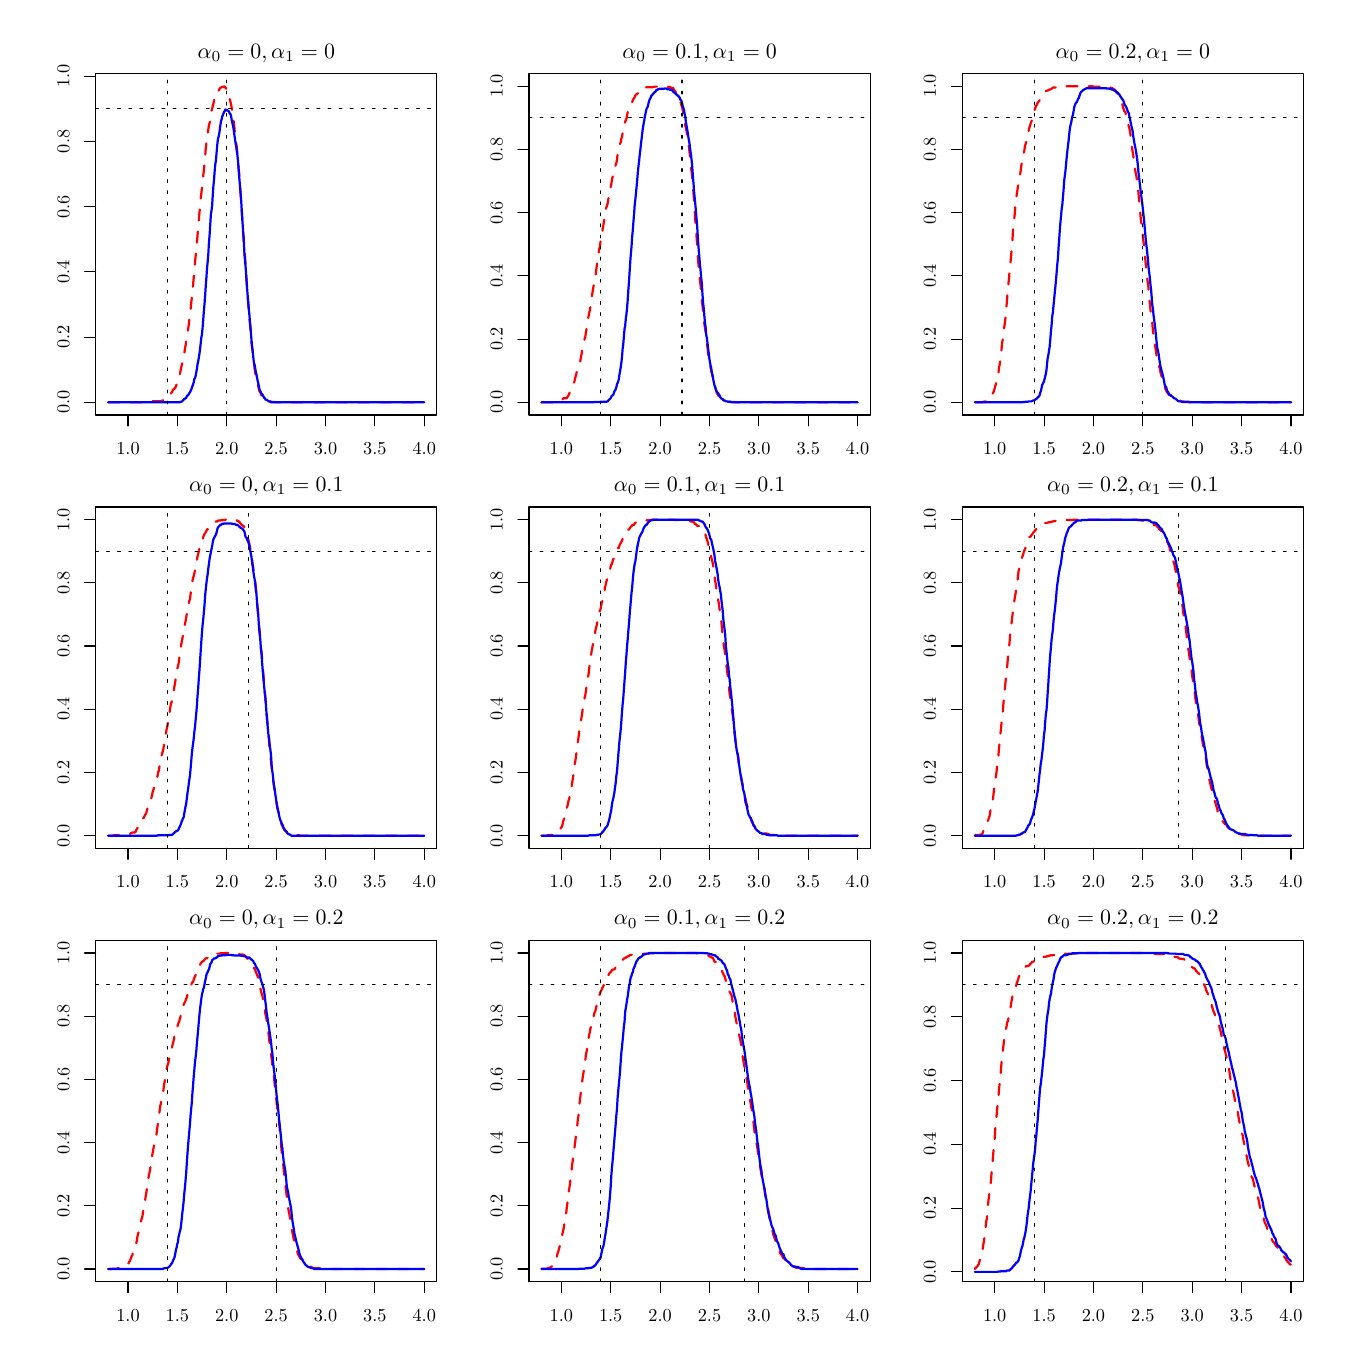
\begin{tikzpicture}[x=1pt,y=1pt]
\definecolor{fillColor}{RGB}{255,255,255}
\path[use as bounding box,fill=fillColor,fill opacity=0.00] (0,0) rectangle (469.75,469.75);
\begin{scope}
\path[clip] ( 24.55,329.80) rectangle (147.87,453.12);
\definecolor{drawColor}{RGB}{255,0,0}

\path[draw=drawColor,line width= 0.8pt,dash pattern=on 4pt off 4pt ,line join=round,line cap=round] ( 29.12,334.37) --
	( 29.35,334.37) --
	( 29.58,334.37) --
	( 29.81,334.37) --
	( 30.03,334.37) --
	( 30.26,334.37) --
	( 30.49,334.37) --
	( 30.72,334.37) --
	( 30.95,334.37) --
	( 31.18,334.37) --
	( 31.41,334.37) --
	( 31.64,334.37) --
	( 31.87,334.37) --
	( 32.09,334.37) --
	( 32.32,334.37) --
	( 32.55,334.37) --
	( 32.78,334.37) --
	( 33.01,334.37) --
	( 33.24,334.37) --
	( 33.47,334.37) --
	( 33.70,334.37) --
	( 33.92,334.37) --
	( 34.15,334.37) --
	( 34.38,334.37) --
	( 34.61,334.37) --
	( 34.84,334.37) --
	( 35.07,334.37) --
	( 35.30,334.37) --
	( 35.53,334.37) --
	( 35.76,334.37) --
	( 35.98,334.37) --
	( 36.21,334.37) --
	( 36.44,334.37) --
	( 36.67,334.37) --
	( 36.90,334.37) --
	( 37.13,334.37) --
	( 37.36,334.37) --
	( 37.59,334.37) --
	( 37.81,334.37) --
	( 38.04,334.37) --
	( 38.27,334.37) --
	( 38.50,334.37) --
	( 38.73,334.37) --
	( 38.96,334.37) --
	( 39.19,334.37) --
	( 39.42,334.37) --
	( 39.65,334.37) --
	( 39.87,334.37) --
	( 40.10,334.37) --
	( 40.33,334.37) --
	( 40.56,334.37) --
	( 40.79,334.37) --
	( 41.02,334.37) --
	( 41.25,334.49) --
	( 41.48,334.49) --
	( 41.71,334.49) --
	( 41.93,334.49) --
	( 42.16,334.49) --
	( 42.39,334.49) --
	( 42.62,334.49) --
	( 42.85,334.49) --
	( 43.08,334.61) --
	( 43.31,334.72) --
	( 43.54,334.72) --
	( 43.76,334.72) --
	( 43.99,334.72) --
	( 44.22,334.72) --
	( 44.45,334.72) --
	( 44.68,334.72) --
	( 44.91,334.72) --
	( 45.14,334.72) --
	( 45.37,334.72) --
	( 45.60,334.72) --
	( 45.82,334.72) --
	( 46.05,334.72) --
	( 46.28,334.72) --
	( 46.51,334.72) --
	( 46.74,334.72) --
	( 46.97,334.72) --
	( 47.20,334.72) --
	( 47.43,334.72) --
	( 47.65,334.72) --
	( 47.88,334.72) --
	( 48.11,334.72) --
	( 48.34,334.84) --
	( 48.57,334.96) --
	( 48.80,335.08) --
	( 49.03,335.31) --
	( 49.26,335.43) --
	( 49.49,335.67) --
	( 49.71,335.90) --
	( 49.94,336.14) --
	( 50.17,336.14) --
	( 50.40,336.25) --
	( 50.63,336.73) --
	( 50.86,336.73) --
	( 51.09,336.84) --
	( 51.32,337.08) --
	( 51.54,337.43) --
	( 51.77,337.43) --
	( 52.00,337.90) --
	( 52.23,338.14) --
	( 52.46,338.97) --
	( 52.69,338.97) --
	( 52.92,339.20) --
	( 53.15,339.44) --
	( 53.38,339.79) --
	( 53.60,340.26) --
	( 53.83,340.85) --
	( 54.06,341.20) --
	( 54.29,341.68) --
	( 54.52,342.50) --
	( 54.75,342.97) --
	( 54.98,344.27) --
	( 55.21,345.68) --
	( 55.43,346.74) --
	( 55.66,347.69) --
	( 55.89,348.98) --
	( 56.12,350.04) --
	( 56.35,351.10) --
	( 56.58,351.69) --
	( 56.81,353.58) --
	( 57.04,354.76) --
	( 57.27,356.52) --
	( 57.49,357.58) --
	( 57.72,358.41) --
	( 57.95,360.65) --
	( 58.18,362.18) --
	( 58.41,364.18) --
	( 58.64,365.83) --
	( 58.87,367.48) --
	( 59.10,370.31) --
	( 59.32,372.31) --
	( 59.55,375.14) --
	( 59.78,376.79) --
	( 60.01,379.50) --
	( 60.24,382.09) --
	( 60.47,384.92) --
	( 60.70,387.28) --
	( 60.93,390.11) --
	( 61.16,392.11) --
	( 61.38,394.70) --
	( 61.61,397.53) --
	( 61.84,400.12) --
	( 62.07,402.95) --
	( 62.30,405.07) --
	( 62.53,408.02) --
	( 62.76,409.90) --
	( 62.99,412.03) --
	( 63.22,414.26) --
	( 63.44,416.27) --
	( 63.67,418.15) --
	( 63.90,420.75) --
	( 64.13,423.22) --
	( 64.36,426.17) --
	( 64.59,428.05) --
	( 64.82,430.05) --
	( 65.05,431.35) --
	( 65.27,432.88) --
	( 65.50,434.53) --
	( 65.73,435.24) --
	( 65.96,436.06) --
	( 66.19,438.42) --
	( 66.42,439.72) --
	( 66.65,440.42) --
	( 66.88,441.49) --
	( 67.11,442.19) --
	( 67.33,443.49) --
	( 67.56,443.96) --
	( 67.79,444.90) --
	( 68.02,445.14) --
	( 68.25,446.08) --
	( 68.48,446.20) --
	( 68.71,446.91) --
	( 68.94,446.91) --
	( 69.16,447.26) --
	( 69.39,447.73) --
	( 69.62,447.97) --
	( 69.85,448.08) --
	( 70.08,448.20) --
	( 70.31,448.44) --
	( 70.54,448.32) --
	( 70.77,448.32) --
	( 71.00,448.56) --
	( 71.22,448.44) --
	( 71.45,448.08) --
	( 71.68,447.85) --
	( 71.91,447.38) --
	( 72.14,446.55) --
	( 72.37,445.85) --
	( 72.60,445.61) --
	( 72.83,445.02) --
	( 73.05,443.84) --
	( 73.28,442.90) --
	( 73.51,442.07) --
	( 73.74,440.54) --
	( 73.97,439.13) --
	( 74.20,438.19) --
	( 74.43,435.95) --
	( 74.66,434.18) --
	( 74.89,431.47) --
	( 75.11,429.70) --
	( 75.34,428.17) --
	( 75.57,426.52) --
	( 75.80,423.93) --
	( 76.03,421.33) --
	( 76.26,418.39) --
	( 76.49,416.15) --
	( 76.72,412.38) --
	( 76.94,409.79) --
	( 77.17,406.60) --
	( 77.40,403.42) --
	( 77.63,399.06) --
	( 77.86,395.53) --
	( 78.09,392.35) --
	( 78.32,389.05) --
	( 78.55,386.57) --
	( 78.78,383.39) --
	( 79.00,379.74) --
	( 79.23,376.67) --
	( 79.46,372.55) --
	( 79.69,370.43) --
	( 79.92,367.25) --
	( 80.15,364.54) --
	( 80.38,362.42) --
	( 80.61,359.47) --
	( 80.83,356.29) --
	( 81.06,354.28) --
	( 81.29,353.11) --
	( 81.52,350.40) --
	( 81.75,349.10) --
	( 81.98,346.62) --
	( 82.21,345.21) --
	( 82.44,343.80) --
	( 82.67,342.62) --
	( 82.89,341.79) --
	( 83.12,340.73) --
	( 83.35,340.03) --
	( 83.58,339.08) --
	( 83.81,338.26) --
	( 84.04,338.02) --
	( 84.27,337.43) --
	( 84.50,336.73) --
	( 84.73,336.49) --
	( 84.95,336.25) --
	( 85.18,336.02) --
	( 85.41,335.43) --
	( 85.64,335.31) --
	( 85.87,335.08) --
	( 86.10,334.84) --
	( 86.33,334.72) --
	( 86.56,334.72) --
	( 86.78,334.72) --
	( 87.01,334.72) --
	( 87.24,334.72) --
	( 87.47,334.72) --
	( 87.70,334.72) --
	( 87.93,334.61) --
	( 88.16,334.49) --
	( 88.39,334.49) --
	( 88.62,334.49) --
	( 88.84,334.49) --
	( 89.07,334.49) --
	( 89.30,334.49) --
	( 89.53,334.37) --
	( 89.76,334.37) --
	( 89.99,334.37) --
	( 90.22,334.37) --
	( 90.45,334.37) --
	( 90.67,334.37) --
	( 90.90,334.37) --
	( 91.13,334.37) --
	( 91.36,334.37) --
	( 91.59,334.37) --
	( 91.82,334.37) --
	( 92.05,334.37) --
	( 92.28,334.37) --
	( 92.51,334.37) --
	( 92.73,334.37) --
	( 92.96,334.37) --
	( 93.19,334.37) --
	( 93.42,334.37) --
	( 93.65,334.37) --
	( 93.88,334.37) --
	( 94.11,334.37) --
	( 94.34,334.37) --
	( 94.56,334.37) --
	( 94.79,334.37) --
	( 95.02,334.37) --
	( 95.25,334.37) --
	( 95.48,334.37) --
	( 95.71,334.37) --
	( 95.94,334.37) --
	( 96.17,334.37) --
	( 96.40,334.37) --
	( 96.62,334.37) --
	( 96.85,334.37) --
	( 97.08,334.37) --
	( 97.31,334.37) --
	( 97.54,334.37) --
	( 97.77,334.37) --
	( 98.00,334.37) --
	( 98.23,334.37) --
	( 98.45,334.37) --
	( 98.68,334.37) --
	( 98.91,334.37) --
	( 99.14,334.37) --
	( 99.37,334.37) --
	( 99.60,334.37) --
	( 99.83,334.37) --
	(100.06,334.37) --
	(100.29,334.37) --
	(100.51,334.37) --
	(100.74,334.37) --
	(100.97,334.37) --
	(101.20,334.37) --
	(101.43,334.37) --
	(101.66,334.37) --
	(101.89,334.37) --
	(102.12,334.37) --
	(102.35,334.37) --
	(102.57,334.37) --
	(102.80,334.37) --
	(103.03,334.37) --
	(103.26,334.37) --
	(103.49,334.37) --
	(103.72,334.37) --
	(103.95,334.37) --
	(104.18,334.37) --
	(104.40,334.37) --
	(104.63,334.37) --
	(104.86,334.37) --
	(105.09,334.37) --
	(105.32,334.37) --
	(105.55,334.37) --
	(105.78,334.37) --
	(106.01,334.37) --
	(106.24,334.37) --
	(106.46,334.37) --
	(106.69,334.37) --
	(106.92,334.37) --
	(107.15,334.37) --
	(107.38,334.37) --
	(107.61,334.37) --
	(107.84,334.37) --
	(108.07,334.37) --
	(108.29,334.37) --
	(108.52,334.37) --
	(108.75,334.37) --
	(108.98,334.37) --
	(109.21,334.37) --
	(109.44,334.37) --
	(109.67,334.37) --
	(109.90,334.37) --
	(110.13,334.37) --
	(110.35,334.37) --
	(110.58,334.37) --
	(110.81,334.37) --
	(111.04,334.37) --
	(111.27,334.37) --
	(111.50,334.37) --
	(111.73,334.37) --
	(111.96,334.37) --
	(112.18,334.37) --
	(112.41,334.37) --
	(112.64,334.37) --
	(112.87,334.37) --
	(113.10,334.37) --
	(113.33,334.37) --
	(113.56,334.37) --
	(113.79,334.37) --
	(114.02,334.37) --
	(114.24,334.37) --
	(114.47,334.37) --
	(114.70,334.37) --
	(114.93,334.37) --
	(115.16,334.37) --
	(115.39,334.37) --
	(115.62,334.37) --
	(115.85,334.37) --
	(116.07,334.37) --
	(116.30,334.37) --
	(116.53,334.37) --
	(116.76,334.37) --
	(116.99,334.37) --
	(117.22,334.37) --
	(117.45,334.37) --
	(117.68,334.37) --
	(117.91,334.37) --
	(118.13,334.37) --
	(118.36,334.37) --
	(118.59,334.37) --
	(118.82,334.37) --
	(119.05,334.37) --
	(119.28,334.37) --
	(119.51,334.37) --
	(119.74,334.37) --
	(119.96,334.37) --
	(120.19,334.37) --
	(120.42,334.37) --
	(120.65,334.37) --
	(120.88,334.37) --
	(121.11,334.37) --
	(121.34,334.37) --
	(121.57,334.37) --
	(121.80,334.37) --
	(122.02,334.37) --
	(122.25,334.37) --
	(122.48,334.37) --
	(122.71,334.37) --
	(122.94,334.37) --
	(123.17,334.37) --
	(123.40,334.37) --
	(123.63,334.37) --
	(123.86,334.37) --
	(124.08,334.37) --
	(124.31,334.37) --
	(124.54,334.37) --
	(124.77,334.37) --
	(125.00,334.37) --
	(125.23,334.37) --
	(125.46,334.37) --
	(125.69,334.37) --
	(125.91,334.37) --
	(126.14,334.37) --
	(126.37,334.37) --
	(126.60,334.37) --
	(126.83,334.37) --
	(127.06,334.37) --
	(127.29,334.37) --
	(127.52,334.37) --
	(127.75,334.37) --
	(127.97,334.37) --
	(128.20,334.37) --
	(128.43,334.37) --
	(128.66,334.37) --
	(128.89,334.37) --
	(129.12,334.37) --
	(129.35,334.37) --
	(129.58,334.37) --
	(129.80,334.37) --
	(130.03,334.37) --
	(130.26,334.37) --
	(130.49,334.37) --
	(130.72,334.37) --
	(130.95,334.37) --
	(131.18,334.37) --
	(131.41,334.37) --
	(131.64,334.37) --
	(131.86,334.37) --
	(132.09,334.37) --
	(132.32,334.37) --
	(132.55,334.37) --
	(132.78,334.37) --
	(133.01,334.37) --
	(133.24,334.37) --
	(133.47,334.37) --
	(133.69,334.37) --
	(133.92,334.37) --
	(134.15,334.37) --
	(134.38,334.37) --
	(134.61,334.37) --
	(134.84,334.37) --
	(135.07,334.37) --
	(135.30,334.37) --
	(135.53,334.37) --
	(135.75,334.37) --
	(135.98,334.37) --
	(136.21,334.37) --
	(136.44,334.37) --
	(136.67,334.37) --
	(136.90,334.37) --
	(137.13,334.37) --
	(137.36,334.37) --
	(137.58,334.37) --
	(137.81,334.37) --
	(138.04,334.37) --
	(138.27,334.37) --
	(138.50,334.37) --
	(138.73,334.37) --
	(138.96,334.37) --
	(139.19,334.37) --
	(139.42,334.37) --
	(139.64,334.37) --
	(139.87,334.37) --
	(140.10,334.37) --
	(140.33,334.37) --
	(140.56,334.37) --
	(140.79,334.37) --
	(141.02,334.37) --
	(141.25,334.37) --
	(141.47,334.37) --
	(141.70,334.37) --
	(141.93,334.37) --
	(142.16,334.37) --
	(142.39,334.37) --
	(142.62,334.37) --
	(142.85,334.37) --
	(143.08,334.37) --
	(143.31,334.37);
\end{scope}
\begin{scope}
\path[clip] (  0.00,  0.00) rectangle (469.75,469.75);
\definecolor{drawColor}{RGB}{0,0,0}

\path[draw=drawColor,line width= 0.4pt,line join=round,line cap=round] ( 36.26,329.80) -- (143.31,329.80);

\path[draw=drawColor,line width= 0.4pt,line join=round,line cap=round] ( 36.26,329.80) -- ( 36.26,325.84);

\path[draw=drawColor,line width= 0.4pt,line join=round,line cap=round] ( 54.10,329.80) -- ( 54.10,325.84);

\path[draw=drawColor,line width= 0.4pt,line join=round,line cap=round] ( 71.94,329.80) -- ( 71.94,325.84);

\path[draw=drawColor,line width= 0.4pt,line join=round,line cap=round] ( 89.78,329.80) -- ( 89.78,325.84);

\path[draw=drawColor,line width= 0.4pt,line join=round,line cap=round] (107.62,329.80) -- (107.62,325.84);

\path[draw=drawColor,line width= 0.4pt,line join=round,line cap=round] (125.46,329.80) -- (125.46,325.84);

\path[draw=drawColor,line width= 0.4pt,line join=round,line cap=round] (143.31,329.80) -- (143.31,325.84);

\node[text=drawColor,anchor=base,inner sep=0pt, outer sep=0pt, scale=  0.66] at ( 36.26,315.55) {1.0};

\node[text=drawColor,anchor=base,inner sep=0pt, outer sep=0pt, scale=  0.66] at ( 54.10,315.55) {1.5};

\node[text=drawColor,anchor=base,inner sep=0pt, outer sep=0pt, scale=  0.66] at ( 71.94,315.55) {2.0};

\node[text=drawColor,anchor=base,inner sep=0pt, outer sep=0pt, scale=  0.66] at ( 89.78,315.55) {2.5};

\node[text=drawColor,anchor=base,inner sep=0pt, outer sep=0pt, scale=  0.66] at (107.62,315.55) {3.0};

\node[text=drawColor,anchor=base,inner sep=0pt, outer sep=0pt, scale=  0.66] at (125.46,315.55) {3.5};

\node[text=drawColor,anchor=base,inner sep=0pt, outer sep=0pt, scale=  0.66] at (143.31,315.55) {4.0};

\path[draw=drawColor,line width= 0.4pt,line join=round,line cap=round] ( 24.55,334.37) -- ( 24.55,452.21);

\path[draw=drawColor,line width= 0.4pt,line join=round,line cap=round] ( 24.55,334.37) -- ( 20.59,334.37);

\path[draw=drawColor,line width= 0.4pt,line join=round,line cap=round] ( 24.55,357.94) -- ( 20.59,357.94);

\path[draw=drawColor,line width= 0.4pt,line join=round,line cap=round] ( 24.55,381.51) -- ( 20.59,381.51);

\path[draw=drawColor,line width= 0.4pt,line join=round,line cap=round] ( 24.55,405.07) -- ( 20.59,405.07);

\path[draw=drawColor,line width= 0.4pt,line join=round,line cap=round] ( 24.55,428.64) -- ( 20.59,428.64);

\path[draw=drawColor,line width= 0.4pt,line join=round,line cap=round] ( 24.55,452.21) -- ( 20.59,452.21);

\node[text=drawColor,rotate= 90.00,anchor=base,inner sep=0pt, outer sep=0pt, scale=  0.66] at ( 15.05,334.37) {0.0};

\node[text=drawColor,rotate= 90.00,anchor=base,inner sep=0pt, outer sep=0pt, scale=  0.66] at ( 15.05,357.94) {0.2};

\node[text=drawColor,rotate= 90.00,anchor=base,inner sep=0pt, outer sep=0pt, scale=  0.66] at ( 15.05,381.51) {0.4};

\node[text=drawColor,rotate= 90.00,anchor=base,inner sep=0pt, outer sep=0pt, scale=  0.66] at ( 15.05,405.07) {0.6};

\node[text=drawColor,rotate= 90.00,anchor=base,inner sep=0pt, outer sep=0pt, scale=  0.66] at ( 15.05,428.64) {0.8};

\node[text=drawColor,rotate= 90.00,anchor=base,inner sep=0pt, outer sep=0pt, scale=  0.66] at ( 15.05,452.21) {1.0};

\path[draw=drawColor,line width= 0.4pt,line join=round,line cap=round] ( 24.55,329.80) --
	(147.87,329.80) --
	(147.87,453.12) --
	( 24.55,453.12) --
	( 24.55,329.80);
\end{scope}
\begin{scope}
\path[clip] (  0.00,313.17) rectangle (156.58,469.75);
\definecolor{drawColor}{RGB}{0,0,0}

\node[text=drawColor,anchor=base,inner sep=0pt, outer sep=0pt, scale=  0.79] at ( 86.21,458.71) {\bfseries $\alpha_0 = 0, \alpha_1 = 0$};
\end{scope}
\begin{scope}
\path[clip] ( 24.55,329.80) rectangle (147.87,453.12);
\definecolor{drawColor}{RGB}{0,0,255}

\path[draw=drawColor,line width= 0.8pt,line join=round,line cap=round] ( 29.12,334.37) --
	( 29.35,334.37) --
	( 29.58,334.37) --
	( 29.81,334.37) --
	( 30.03,334.37) --
	( 30.26,334.37) --
	( 30.49,334.37) --
	( 30.72,334.37) --
	( 30.95,334.37) --
	( 31.18,334.37) --
	( 31.41,334.37) --
	( 31.64,334.37) --
	( 31.87,334.37) --
	( 32.09,334.37) --
	( 32.32,334.37) --
	( 32.55,334.37) --
	( 32.78,334.37) --
	( 33.01,334.37) --
	( 33.24,334.37) --
	( 33.47,334.37) --
	( 33.70,334.37) --
	( 33.92,334.37) --
	( 34.15,334.37) --
	( 34.38,334.37) --
	( 34.61,334.37) --
	( 34.84,334.37) --
	( 35.07,334.37) --
	( 35.30,334.37) --
	( 35.53,334.37) --
	( 35.76,334.37) --
	( 35.98,334.37) --
	( 36.21,334.37) --
	( 36.44,334.37) --
	( 36.67,334.37) --
	( 36.90,334.37) --
	( 37.13,334.37) --
	( 37.36,334.37) --
	( 37.59,334.37) --
	( 37.81,334.37) --
	( 38.04,334.37) --
	( 38.27,334.37) --
	( 38.50,334.37) --
	( 38.73,334.37) --
	( 38.96,334.37) --
	( 39.19,334.37) --
	( 39.42,334.37) --
	( 39.65,334.37) --
	( 39.87,334.37) --
	( 40.10,334.37) --
	( 40.33,334.37) --
	( 40.56,334.37) --
	( 40.79,334.37) --
	( 41.02,334.37) --
	( 41.25,334.37) --
	( 41.48,334.37) --
	( 41.71,334.37) --
	( 41.93,334.37) --
	( 42.16,334.37) --
	( 42.39,334.37) --
	( 42.62,334.37) --
	( 42.85,334.37) --
	( 43.08,334.37) --
	( 43.31,334.37) --
	( 43.54,334.37) --
	( 43.76,334.37) --
	( 43.99,334.37) --
	( 44.22,334.37) --
	( 44.45,334.37) --
	( 44.68,334.37) --
	( 44.91,334.37) --
	( 45.14,334.37) --
	( 45.37,334.37) --
	( 45.60,334.37) --
	( 45.82,334.37) --
	( 46.05,334.37) --
	( 46.28,334.37) --
	( 46.51,334.37) --
	( 46.74,334.37) --
	( 46.97,334.37) --
	( 47.20,334.37) --
	( 47.43,334.37) --
	( 47.65,334.37) --
	( 47.88,334.37) --
	( 48.11,334.37) --
	( 48.34,334.37) --
	( 48.57,334.37) --
	( 48.80,334.37) --
	( 49.03,334.37) --
	( 49.26,334.37) --
	( 49.49,334.37) --
	( 49.71,334.37) --
	( 49.94,334.37) --
	( 50.17,334.37) --
	( 50.40,334.37) --
	( 50.63,334.37) --
	( 50.86,334.37) --
	( 51.09,334.37) --
	( 51.32,334.37) --
	( 51.54,334.37) --
	( 51.77,334.37) --
	( 52.00,334.37) --
	( 52.23,334.37) --
	( 52.46,334.37) --
	( 52.69,334.37) --
	( 52.92,334.37) --
	( 53.15,334.37) --
	( 53.38,334.37) --
	( 53.60,334.37) --
	( 53.83,334.37) --
	( 54.06,334.37) --
	( 54.29,334.37) --
	( 54.52,334.37) --
	( 54.75,334.37) --
	( 54.98,334.37) --
	( 55.21,334.49) --
	( 55.43,334.61) --
	( 55.66,334.61) --
	( 55.89,334.84) --
	( 56.12,335.08) --
	( 56.35,335.31) --
	( 56.58,335.55) --
	( 56.81,335.67) --
	( 57.04,335.90) --
	( 57.27,335.90) --
	( 57.49,336.49) --
	( 57.72,336.84) --
	( 57.95,336.84) --
	( 58.18,337.32) --
	( 58.41,337.67) --
	( 58.64,338.02) --
	( 58.87,338.49) --
	( 59.10,338.97) --
	( 59.32,339.55) --
	( 59.55,340.26) --
	( 59.78,340.85) --
	( 60.01,341.56) --
	( 60.24,342.85) --
	( 60.47,343.21) --
	( 60.70,343.91) --
	( 60.93,345.21) --
	( 61.16,346.51) --
	( 61.38,348.16) --
	( 61.61,349.10) --
	( 61.84,350.51) --
	( 62.07,351.93) --
	( 62.30,353.58) --
	( 62.53,355.82) --
	( 62.76,357.82) --
	( 62.99,359.00) --
	( 63.22,361.47) --
	( 63.44,364.18) --
	( 63.67,367.36) --
	( 63.90,369.96) --
	( 64.13,373.02) --
	( 64.36,376.56) --
	( 64.59,379.50) --
	( 64.82,382.92) --
	( 65.05,385.28) --
	( 65.27,387.87) --
	( 65.50,391.99) --
	( 65.73,394.70) --
	( 65.96,398.47) --
	( 66.19,402.13) --
	( 66.42,403.66) --
	( 66.65,405.43) --
	( 66.88,409.20) --
	( 67.11,412.50) --
	( 67.33,414.74) --
	( 67.56,417.80) --
	( 67.79,420.39) --
	( 68.02,421.69) --
	( 68.25,424.40) --
	( 68.48,427.11) --
	( 68.71,429.23) --
	( 68.94,430.17) --
	( 69.16,431.12) --
	( 69.39,432.65) --
	( 69.62,434.41) --
	( 69.85,435.83) --
	( 70.08,436.65) --
	( 70.31,437.71) --
	( 70.54,438.19) --
	( 70.77,438.77) --
	( 71.00,439.36) --
	( 71.22,439.60) --
	( 71.45,440.19) --
	( 71.68,439.95) --
	( 71.91,440.07) --
	( 72.14,439.95) --
	( 72.37,439.60) --
	( 72.60,439.60) --
	( 72.83,439.25) --
	( 73.05,438.66) --
	( 73.28,438.54) --
	( 73.51,437.71) --
	( 73.74,436.30) --
	( 73.97,435.24) --
	( 74.20,434.53) --
	( 74.43,432.88) --
	( 74.66,431.23) --
	( 74.89,429.70) --
	( 75.11,428.05) --
	( 75.34,426.76) --
	( 75.57,425.11) --
	( 75.80,423.57) --
	( 76.03,421.22) --
	( 76.26,418.27) --
	( 76.49,415.21) --
	( 76.72,412.61) --
	( 76.94,409.90) --
	( 77.17,406.96) --
	( 77.40,402.83) --
	( 77.63,399.42) --
	( 77.86,395.88) --
	( 78.09,393.05) --
	( 78.32,388.10) --
	( 78.55,385.51) --
	( 78.78,382.92) --
	( 79.00,379.62) --
	( 79.23,376.20) --
	( 79.46,373.37) --
	( 79.69,370.66) --
	( 79.92,367.84) --
	( 80.15,365.60) --
	( 80.38,362.77) --
	( 80.61,360.18) --
	( 80.83,357.47) --
	( 81.06,354.99) --
	( 81.29,352.87) --
	( 81.52,350.75) --
	( 81.75,348.63) --
	( 81.98,347.92) --
	( 82.21,346.74) --
	( 82.44,345.33) --
	( 82.67,344.39) --
	( 82.89,343.21) --
	( 83.12,342.03) --
	( 83.35,341.20) --
	( 83.58,340.03) --
	( 83.81,338.85) --
	( 84.04,338.38) --
	( 84.27,338.02) --
	( 84.50,337.43) --
	( 84.73,337.32) --
	( 84.95,336.96) --
	( 85.18,336.49) --
	( 85.41,336.02) --
	( 85.64,335.90) --
	( 85.87,335.43) --
	( 86.10,335.31) --
	( 86.33,335.31) --
	( 86.56,335.19) --
	( 86.78,334.96) --
	( 87.01,334.72) --
	( 87.24,334.72) --
	( 87.47,334.61) --
	( 87.70,334.61) --
	( 87.93,334.37) --
	( 88.16,334.37) --
	( 88.39,334.37) --
	( 88.62,334.37) --
	( 88.84,334.37) --
	( 89.07,334.37) --
	( 89.30,334.37) --
	( 89.53,334.37) --
	( 89.76,334.37) --
	( 89.99,334.37) --
	( 90.22,334.37) --
	( 90.45,334.37) --
	( 90.67,334.37) --
	( 90.90,334.37) --
	( 91.13,334.37) --
	( 91.36,334.37) --
	( 91.59,334.37) --
	( 91.82,334.37) --
	( 92.05,334.37) --
	( 92.28,334.37) --
	( 92.51,334.37) --
	( 92.73,334.37) --
	( 92.96,334.37) --
	( 93.19,334.37) --
	( 93.42,334.37) --
	( 93.65,334.37) --
	( 93.88,334.37) --
	( 94.11,334.37) --
	( 94.34,334.37) --
	( 94.56,334.37) --
	( 94.79,334.37) --
	( 95.02,334.37) --
	( 95.25,334.37) --
	( 95.48,334.37) --
	( 95.71,334.37) --
	( 95.94,334.37) --
	( 96.17,334.37) --
	( 96.40,334.37) --
	( 96.62,334.37) --
	( 96.85,334.37) --
	( 97.08,334.37) --
	( 97.31,334.37) --
	( 97.54,334.37) --
	( 97.77,334.37) --
	( 98.00,334.37) --
	( 98.23,334.37) --
	( 98.45,334.37) --
	( 98.68,334.37) --
	( 98.91,334.37) --
	( 99.14,334.37) --
	( 99.37,334.37) --
	( 99.60,334.37) --
	( 99.83,334.37) --
	(100.06,334.37) --
	(100.29,334.37) --
	(100.51,334.37) --
	(100.74,334.37) --
	(100.97,334.37) --
	(101.20,334.37) --
	(101.43,334.37) --
	(101.66,334.37) --
	(101.89,334.37) --
	(102.12,334.37) --
	(102.35,334.37) --
	(102.57,334.37) --
	(102.80,334.37) --
	(103.03,334.37) --
	(103.26,334.37) --
	(103.49,334.37) --
	(103.72,334.37) --
	(103.95,334.37) --
	(104.18,334.37) --
	(104.40,334.37) --
	(104.63,334.37) --
	(104.86,334.37) --
	(105.09,334.37) --
	(105.32,334.37) --
	(105.55,334.37) --
	(105.78,334.37) --
	(106.01,334.37) --
	(106.24,334.37) --
	(106.46,334.37) --
	(106.69,334.37) --
	(106.92,334.37) --
	(107.15,334.37) --
	(107.38,334.37) --
	(107.61,334.37) --
	(107.84,334.37) --
	(108.07,334.37) --
	(108.29,334.37) --
	(108.52,334.37) --
	(108.75,334.37) --
	(108.98,334.37) --
	(109.21,334.37) --
	(109.44,334.37) --
	(109.67,334.37) --
	(109.90,334.37) --
	(110.13,334.37) --
	(110.35,334.37) --
	(110.58,334.37) --
	(110.81,334.37) --
	(111.04,334.37) --
	(111.27,334.37) --
	(111.50,334.37) --
	(111.73,334.37) --
	(111.96,334.37) --
	(112.18,334.37) --
	(112.41,334.37) --
	(112.64,334.37) --
	(112.87,334.37) --
	(113.10,334.37) --
	(113.33,334.37) --
	(113.56,334.37) --
	(113.79,334.37) --
	(114.02,334.37) --
	(114.24,334.37) --
	(114.47,334.37) --
	(114.70,334.37) --
	(114.93,334.37) --
	(115.16,334.37) --
	(115.39,334.37) --
	(115.62,334.37) --
	(115.85,334.37) --
	(116.07,334.37) --
	(116.30,334.37) --
	(116.53,334.37) --
	(116.76,334.37) --
	(116.99,334.37) --
	(117.22,334.37) --
	(117.45,334.37) --
	(117.68,334.37) --
	(117.91,334.37) --
	(118.13,334.37) --
	(118.36,334.37) --
	(118.59,334.37) --
	(118.82,334.37) --
	(119.05,334.37) --
	(119.28,334.37) --
	(119.51,334.37) --
	(119.74,334.37) --
	(119.96,334.37) --
	(120.19,334.37) --
	(120.42,334.37) --
	(120.65,334.37) --
	(120.88,334.37) --
	(121.11,334.37) --
	(121.34,334.37) --
	(121.57,334.37) --
	(121.80,334.37) --
	(122.02,334.37) --
	(122.25,334.37) --
	(122.48,334.37) --
	(122.71,334.37) --
	(122.94,334.37) --
	(123.17,334.37) --
	(123.40,334.37) --
	(123.63,334.37) --
	(123.86,334.37) --
	(124.08,334.37) --
	(124.31,334.37) --
	(124.54,334.37) --
	(124.77,334.37) --
	(125.00,334.37) --
	(125.23,334.37) --
	(125.46,334.37) --
	(125.69,334.37) --
	(125.91,334.37) --
	(126.14,334.37) --
	(126.37,334.37) --
	(126.60,334.37) --
	(126.83,334.37) --
	(127.06,334.37) --
	(127.29,334.37) --
	(127.52,334.37) --
	(127.75,334.37) --
	(127.97,334.37) --
	(128.20,334.37) --
	(128.43,334.37) --
	(128.66,334.37) --
	(128.89,334.37) --
	(129.12,334.37) --
	(129.35,334.37) --
	(129.58,334.37) --
	(129.80,334.37) --
	(130.03,334.37) --
	(130.26,334.37) --
	(130.49,334.37) --
	(130.72,334.37) --
	(130.95,334.37) --
	(131.18,334.37) --
	(131.41,334.37) --
	(131.64,334.37) --
	(131.86,334.37) --
	(132.09,334.37) --
	(132.32,334.37) --
	(132.55,334.37) --
	(132.78,334.37) --
	(133.01,334.37) --
	(133.24,334.37) --
	(133.47,334.37) --
	(133.69,334.37) --
	(133.92,334.37) --
	(134.15,334.37) --
	(134.38,334.37) --
	(134.61,334.37) --
	(134.84,334.37) --
	(135.07,334.37) --
	(135.30,334.37) --
	(135.53,334.37) --
	(135.75,334.37) --
	(135.98,334.37) --
	(136.21,334.37) --
	(136.44,334.37) --
	(136.67,334.37) --
	(136.90,334.37) --
	(137.13,334.37) --
	(137.36,334.37) --
	(137.58,334.37) --
	(137.81,334.37) --
	(138.04,334.37) --
	(138.27,334.37) --
	(138.50,334.37) --
	(138.73,334.37) --
	(138.96,334.37) --
	(139.19,334.37) --
	(139.42,334.37) --
	(139.64,334.37) --
	(139.87,334.37) --
	(140.10,334.37) --
	(140.33,334.37) --
	(140.56,334.37) --
	(140.79,334.37) --
	(141.02,334.37) --
	(141.25,334.37) --
	(141.47,334.37) --
	(141.70,334.37) --
	(141.93,334.37) --
	(142.16,334.37) --
	(142.39,334.37) --
	(142.62,334.37) --
	(142.85,334.37) --
	(143.08,334.37) --
	(143.31,334.37);
\definecolor{drawColor}{RGB}{0,0,0}

\path[draw=drawColor,line width= 0.4pt,dash pattern=on 1pt off 3pt ,line join=round,line cap=round] ( 24.55,440.42) -- (147.87,440.42);

\path[draw=drawColor,line width= 0.4pt,dash pattern=on 1pt off 3pt ,line join=round,line cap=round] ( 50.53,329.80) -- ( 50.53,453.12);

\path[draw=drawColor,line width= 0.4pt,dash pattern=on 1pt off 3pt ,line join=round,line cap=round] ( 71.94,329.80) -- ( 71.94,453.12);
\end{scope}
\begin{scope}
\path[clip] (181.14,329.80) rectangle (304.46,453.12);
\definecolor{drawColor}{RGB}{255,0,0}

\path[draw=drawColor,line width= 0.8pt,dash pattern=on 4pt off 4pt ,line join=round,line cap=round] (185.70,334.37) --
	(185.93,334.37) --
	(186.16,334.37) --
	(186.39,334.37) --
	(186.62,334.37) --
	(186.85,334.37) --
	(187.08,334.37) --
	(187.31,334.37) --
	(187.54,334.37) --
	(187.76,334.37) --
	(187.99,334.37) --
	(188.22,334.37) --
	(188.45,334.37) --
	(188.68,334.37) --
	(188.91,334.37) --
	(189.14,334.37) --
	(189.37,334.37) --
	(189.59,334.37) --
	(189.82,334.37) --
	(190.05,334.48) --
	(190.28,334.48) --
	(190.51,334.48) --
	(190.74,334.48) --
	(190.97,334.48) --
	(191.20,334.48) --
	(191.43,334.71) --
	(191.65,334.71) --
	(191.88,334.71) --
	(192.11,334.71) --
	(192.34,334.71) --
	(192.57,334.83) --
	(192.80,334.83) --
	(193.03,335.05) --
	(193.26,335.40) --
	(193.48,335.74) --
	(193.71,335.85) --
	(193.94,335.85) --
	(194.17,335.85) --
	(194.40,335.85) --
	(194.63,335.85) --
	(194.86,335.97) --
	(195.09,336.42) --
	(195.32,336.65) --
	(195.54,337.22) --
	(195.77,337.68) --
	(196.00,338.48) --
	(196.23,338.82) --
	(196.46,339.05) --
	(196.69,339.28) --
	(196.92,339.85) --
	(197.15,340.88) --
	(197.37,341.22) --
	(197.60,342.02) --
	(197.83,343.05) --
	(198.06,343.96) --
	(198.29,344.87) --
	(198.52,345.90) --
	(198.75,346.47) --
	(198.98,347.39) --
	(199.21,348.30) --
	(199.43,348.64) --
	(199.66,349.10) --
	(199.89,350.47) --
	(200.12,351.61) --
	(200.35,353.32) --
	(200.58,354.35) --
	(200.81,355.38) --
	(201.04,356.41) --
	(201.26,357.32) --
	(201.49,358.01) --
	(201.72,359.60) --
	(201.95,361.09) --
	(202.18,362.12) --
	(202.41,363.83) --
	(202.64,365.31) --
	(202.87,366.46) --
	(203.10,367.48) --
	(203.32,368.63) --
	(203.55,370.45) --
	(203.78,371.94) --
	(204.01,373.54) --
	(204.24,375.02) --
	(204.47,376.28) --
	(204.70,377.42) --
	(204.93,378.22) --
	(205.15,379.93) --
	(205.38,381.53) --
	(205.61,383.47) --
	(205.84,385.18) --
	(206.07,386.67) --
	(206.30,388.15) --
	(206.53,389.75) --
	(206.76,390.66) --
	(206.99,392.26) --
	(207.21,393.75) --
	(207.44,395.23) --
	(207.67,396.37) --
	(207.90,397.63) --
	(208.13,399.11) --
	(208.36,400.48) --
	(208.59,402.42) --
	(208.82,403.68) --
	(209.05,404.82) --
	(209.27,405.16) --
	(209.50,405.96) --
	(209.73,407.11) --
	(209.96,408.82) --
	(210.19,410.19) --
	(210.42,410.99) --
	(210.65,412.13) --
	(210.88,413.16) --
	(211.10,414.64) --
	(211.33,415.67) --
	(211.56,416.36) --
	(211.79,417.04) --
	(212.02,417.84) --
	(212.25,418.75) --
	(212.48,420.24) --
	(212.71,420.81) --
	(212.94,421.95) --
	(213.16,423.89) --
	(213.39,425.03) --
	(213.62,425.83) --
	(213.85,426.86) --
	(214.08,427.89) --
	(214.31,428.34) --
	(214.54,429.71) --
	(214.77,430.17) --
	(214.99,431.88) --
	(215.22,433.14) --
	(215.45,434.05) --
	(215.68,434.85) --
	(215.91,435.88) --
	(216.14,436.22) --
	(216.37,436.91) --
	(216.60,437.94) --
	(216.83,439.42) --
	(217.05,439.65) --
	(217.28,440.33) --
	(217.51,441.02) --
	(217.74,441.13) --
	(217.97,441.70) --
	(218.20,442.05) --
	(218.43,442.73) --
	(218.66,443.42) --
	(218.88,443.99) --
	(219.11,444.22) --
	(219.34,444.67) --
	(219.57,445.24) --
	(219.80,445.59) --
	(220.03,445.70) --
	(220.26,445.82) --
	(220.49,446.04) --
	(220.72,446.50) --
	(220.94,446.61) --
	(221.17,447.07) --
	(221.40,447.53) --
	(221.63,447.64) --
	(221.86,447.64) --
	(222.09,447.76) --
	(222.32,447.98) --
	(222.55,448.21) --
	(222.77,448.21) --
	(223.00,448.21) --
	(223.23,448.21) --
	(223.46,448.21) --
	(223.69,448.21) --
	(223.92,448.21) --
	(224.15,448.21) --
	(224.38,448.21) --
	(224.61,448.21) --
	(224.83,448.21) --
	(225.06,448.21) --
	(225.29,448.21) --
	(225.52,448.21) --
	(225.75,448.21) --
	(225.98,448.33) --
	(226.21,448.33) --
	(226.44,448.33) --
	(226.66,448.44) --
	(226.89,448.44) --
	(227.12,448.44) --
	(227.35,448.44) --
	(227.58,448.44) --
	(227.81,448.56) --
	(228.04,448.56) --
	(228.27,448.56) --
	(228.50,448.56) --
	(228.72,448.56) --
	(228.95,448.56) --
	(229.18,448.56) --
	(229.41,448.56) --
	(229.64,448.56) --
	(229.87,448.56) --
	(230.10,448.56) --
	(230.33,448.44) --
	(230.56,448.33) --
	(230.78,448.33) --
	(231.01,448.33) --
	(231.24,448.33) --
	(231.47,448.33) --
	(231.70,448.33) --
	(231.93,448.33) --
	(232.16,448.33) --
	(232.39,448.10) --
	(232.61,447.98) --
	(232.84,447.98) --
	(233.07,447.98) --
	(233.30,447.87) --
	(233.53,447.30) --
	(233.76,447.07) --
	(233.99,446.73) --
	(234.22,446.39) --
	(234.45,445.93) --
	(234.67,445.70) --
	(234.90,445.47) --
	(235.13,444.67) --
	(235.36,444.44) --
	(235.59,443.76) --
	(235.82,442.96) --
	(236.05,442.39) --
	(236.28,441.59) --
	(236.50,440.91) --
	(236.73,439.76) --
	(236.96,438.62) --
	(237.19,437.02) --
	(237.42,435.88) --
	(237.65,434.28) --
	(237.88,433.37) --
	(238.11,432.23) --
	(238.34,430.63) --
	(238.56,428.69) --
	(238.79,427.89) --
	(239.02,426.06) --
	(239.25,423.89) --
	(239.48,421.38) --
	(239.71,418.98) --
	(239.94,417.61) --
	(240.17,415.44) --
	(240.39,412.93) --
	(240.62,409.62) --
	(240.85,406.19) --
	(241.08,402.65) --
	(241.31,399.00) --
	(241.54,396.49) --
	(241.77,393.18) --
	(242.00,389.86) --
	(242.23,385.87) --
	(242.45,383.36) --
	(242.68,380.27) --
	(242.91,378.45) --
	(243.14,376.73) --
	(243.37,373.54) --
	(243.60,371.25) --
	(243.83,369.42) --
	(244.06,367.14) --
	(244.28,364.74) --
	(244.51,362.80) --
	(244.74,361.20) --
	(244.97,359.83) --
	(245.20,358.12) --
	(245.43,355.61) --
	(245.66,354.24) --
	(245.89,351.50) --
	(246.12,350.58) --
	(246.34,348.99) --
	(246.57,348.07) --
	(246.80,346.82) --
	(247.03,345.56) --
	(247.26,344.99) --
	(247.49,343.50) --
	(247.72,343.05) --
	(247.95,341.91) --
	(248.18,341.22) --
	(248.40,339.96) --
	(248.63,339.05) --
	(248.86,338.37) --
	(249.09,337.45) --
	(249.32,337.34) --
	(249.55,336.77) --
	(249.78,336.65) --
	(250.01,336.54) --
	(250.23,336.20) --
	(250.46,335.74) --
	(250.69,335.40) --
	(250.92,335.28) --
	(251.15,334.94) --
	(251.38,334.83) --
	(251.61,334.83) --
	(251.84,334.83) --
	(252.07,334.83) --
	(252.29,334.83) --
	(252.52,334.71) --
	(252.75,334.71) --
	(252.98,334.71) --
	(253.21,334.71) --
	(253.44,334.60) --
	(253.67,334.60) --
	(253.90,334.60) --
	(254.12,334.48) --
	(254.35,334.48) --
	(254.58,334.48) --
	(254.81,334.48) --
	(255.04,334.48) --
	(255.27,334.48) --
	(255.50,334.37) --
	(255.73,334.37) --
	(255.96,334.37) --
	(256.18,334.37) --
	(256.41,334.37) --
	(256.64,334.37) --
	(256.87,334.37) --
	(257.10,334.37) --
	(257.33,334.37) --
	(257.56,334.37) --
	(257.79,334.37) --
	(258.01,334.37) --
	(258.24,334.37) --
	(258.47,334.37) --
	(258.70,334.37) --
	(258.93,334.37) --
	(259.16,334.37) --
	(259.39,334.37) --
	(259.62,334.37) --
	(259.85,334.37) --
	(260.07,334.37) --
	(260.30,334.37) --
	(260.53,334.37) --
	(260.76,334.37) --
	(260.99,334.37) --
	(261.22,334.37) --
	(261.45,334.37) --
	(261.68,334.37) --
	(261.90,334.37) --
	(262.13,334.37) --
	(262.36,334.37) --
	(262.59,334.37) --
	(262.82,334.37) --
	(263.05,334.37) --
	(263.28,334.37) --
	(263.51,334.37) --
	(263.74,334.37) --
	(263.96,334.37) --
	(264.19,334.37) --
	(264.42,334.37) --
	(264.65,334.37) --
	(264.88,334.37) --
	(265.11,334.37) --
	(265.34,334.37) --
	(265.57,334.37) --
	(265.79,334.37) --
	(266.02,334.37) --
	(266.25,334.37) --
	(266.48,334.37) --
	(266.71,334.37) --
	(266.94,334.37) --
	(267.17,334.37) --
	(267.40,334.37) --
	(267.63,334.37) --
	(267.85,334.37) --
	(268.08,334.37) --
	(268.31,334.37) --
	(268.54,334.37) --
	(268.77,334.37) --
	(269.00,334.37) --
	(269.23,334.37) --
	(269.46,334.37) --
	(269.69,334.37) --
	(269.91,334.37) --
	(270.14,334.37) --
	(270.37,334.37) --
	(270.60,334.37) --
	(270.83,334.37) --
	(271.06,334.37) --
	(271.29,334.37) --
	(271.52,334.37) --
	(271.74,334.37) --
	(271.97,334.37) --
	(272.20,334.37) --
	(272.43,334.37) --
	(272.66,334.37) --
	(272.89,334.37) --
	(273.12,334.37) --
	(273.35,334.37) --
	(273.58,334.37) --
	(273.80,334.37) --
	(274.03,334.37) --
	(274.26,334.37) --
	(274.49,334.37) --
	(274.72,334.37) --
	(274.95,334.37) --
	(275.18,334.37) --
	(275.41,334.37) --
	(275.63,334.37) --
	(275.86,334.37) --
	(276.09,334.37) --
	(276.32,334.37) --
	(276.55,334.37) --
	(276.78,334.37) --
	(277.01,334.37) --
	(277.24,334.37) --
	(277.47,334.37) --
	(277.69,334.37) --
	(277.92,334.37) --
	(278.15,334.37) --
	(278.38,334.37) --
	(278.61,334.37) --
	(278.84,334.37) --
	(279.07,334.37) --
	(279.30,334.37) --
	(279.52,334.37) --
	(279.75,334.37) --
	(279.98,334.37) --
	(280.21,334.37) --
	(280.44,334.37) --
	(280.67,334.37) --
	(280.90,334.37) --
	(281.13,334.37) --
	(281.36,334.37) --
	(281.58,334.37) --
	(281.81,334.37) --
	(282.04,334.37) --
	(282.27,334.37) --
	(282.50,334.37) --
	(282.73,334.37) --
	(282.96,334.37) --
	(283.19,334.37) --
	(283.41,334.37) --
	(283.64,334.37) --
	(283.87,334.37) --
	(284.10,334.37) --
	(284.33,334.37) --
	(284.56,334.37) --
	(284.79,334.37) --
	(285.02,334.37) --
	(285.25,334.37) --
	(285.47,334.37) --
	(285.70,334.37) --
	(285.93,334.37) --
	(286.16,334.37) --
	(286.39,334.37) --
	(286.62,334.37) --
	(286.85,334.37) --
	(287.08,334.37) --
	(287.30,334.37) --
	(287.53,334.37) --
	(287.76,334.37) --
	(287.99,334.37) --
	(288.22,334.37) --
	(288.45,334.37) --
	(288.68,334.37) --
	(288.91,334.37) --
	(289.14,334.37) --
	(289.36,334.37) --
	(289.59,334.37) --
	(289.82,334.37) --
	(290.05,334.37) --
	(290.28,334.37) --
	(290.51,334.37) --
	(290.74,334.37) --
	(290.97,334.37) --
	(291.20,334.37) --
	(291.42,334.37) --
	(291.65,334.37) --
	(291.88,334.37) --
	(292.11,334.37) --
	(292.34,334.37) --
	(292.57,334.37) --
	(292.80,334.37) --
	(293.03,334.37) --
	(293.25,334.37) --
	(293.48,334.37) --
	(293.71,334.37) --
	(293.94,334.37) --
	(294.17,334.37) --
	(294.40,334.37) --
	(294.63,334.37) --
	(294.86,334.37) --
	(295.09,334.37) --
	(295.31,334.37) --
	(295.54,334.37) --
	(295.77,334.37) --
	(296.00,334.37) --
	(296.23,334.37) --
	(296.46,334.37) --
	(296.69,334.37) --
	(296.92,334.37) --
	(297.14,334.37) --
	(297.37,334.37) --
	(297.60,334.37) --
	(297.83,334.37) --
	(298.06,334.37) --
	(298.29,334.37) --
	(298.52,334.37) --
	(298.75,334.37) --
	(298.98,334.37) --
	(299.20,334.37) --
	(299.43,334.37) --
	(299.66,334.37) --
	(299.89,334.37);
\end{scope}
\begin{scope}
\path[clip] (  0.00,  0.00) rectangle (469.75,469.75);
\definecolor{drawColor}{RGB}{0,0,0}

\path[draw=drawColor,line width= 0.4pt,line join=round,line cap=round] (192.84,329.80) -- (299.89,329.80);

\path[draw=drawColor,line width= 0.4pt,line join=round,line cap=round] (192.84,329.80) -- (192.84,325.84);

\path[draw=drawColor,line width= 0.4pt,line join=round,line cap=round] (210.68,329.80) -- (210.68,325.84);

\path[draw=drawColor,line width= 0.4pt,line join=round,line cap=round] (228.52,329.80) -- (228.52,325.84);

\path[draw=drawColor,line width= 0.4pt,line join=round,line cap=round] (246.37,329.80) -- (246.37,325.84);

\path[draw=drawColor,line width= 0.4pt,line join=round,line cap=round] (264.21,329.80) -- (264.21,325.84);

\path[draw=drawColor,line width= 0.4pt,line join=round,line cap=round] (282.05,329.80) -- (282.05,325.84);

\path[draw=drawColor,line width= 0.4pt,line join=round,line cap=round] (299.89,329.80) -- (299.89,325.84);

\node[text=drawColor,anchor=base,inner sep=0pt, outer sep=0pt, scale=  0.66] at (192.84,315.55) {1.0};

\node[text=drawColor,anchor=base,inner sep=0pt, outer sep=0pt, scale=  0.66] at (210.68,315.55) {1.5};

\node[text=drawColor,anchor=base,inner sep=0pt, outer sep=0pt, scale=  0.66] at (228.52,315.55) {2.0};

\node[text=drawColor,anchor=base,inner sep=0pt, outer sep=0pt, scale=  0.66] at (246.37,315.55) {2.5};

\node[text=drawColor,anchor=base,inner sep=0pt, outer sep=0pt, scale=  0.66] at (264.21,315.55) {3.0};

\node[text=drawColor,anchor=base,inner sep=0pt, outer sep=0pt, scale=  0.66] at (282.05,315.55) {3.5};

\node[text=drawColor,anchor=base,inner sep=0pt, outer sep=0pt, scale=  0.66] at (299.89,315.55) {4.0};

\path[draw=drawColor,line width= 0.4pt,line join=round,line cap=round] (181.14,334.37) -- (181.14,448.56);

\path[draw=drawColor,line width= 0.4pt,line join=round,line cap=round] (181.14,334.37) -- (177.18,334.37);

\path[draw=drawColor,line width= 0.4pt,line join=round,line cap=round] (181.14,357.21) -- (177.18,357.21);

\path[draw=drawColor,line width= 0.4pt,line join=round,line cap=round] (181.14,380.04) -- (177.18,380.04);

\path[draw=drawColor,line width= 0.4pt,line join=round,line cap=round] (181.14,402.88) -- (177.18,402.88);

\path[draw=drawColor,line width= 0.4pt,line join=round,line cap=round] (181.14,425.72) -- (177.18,425.72);

\path[draw=drawColor,line width= 0.4pt,line join=round,line cap=round] (181.14,448.56) -- (177.18,448.56);

\node[text=drawColor,rotate= 90.00,anchor=base,inner sep=0pt, outer sep=0pt, scale=  0.66] at (171.63,334.37) {0.0};

\node[text=drawColor,rotate= 90.00,anchor=base,inner sep=0pt, outer sep=0pt, scale=  0.66] at (171.63,357.21) {0.2};

\node[text=drawColor,rotate= 90.00,anchor=base,inner sep=0pt, outer sep=0pt, scale=  0.66] at (171.63,380.04) {0.4};

\node[text=drawColor,rotate= 90.00,anchor=base,inner sep=0pt, outer sep=0pt, scale=  0.66] at (171.63,402.88) {0.6};

\node[text=drawColor,rotate= 90.00,anchor=base,inner sep=0pt, outer sep=0pt, scale=  0.66] at (171.63,425.72) {0.8};

\node[text=drawColor,rotate= 90.00,anchor=base,inner sep=0pt, outer sep=0pt, scale=  0.66] at (171.63,448.56) {1.0};

\path[draw=drawColor,line width= 0.4pt,line join=round,line cap=round] (181.14,329.80) --
	(304.46,329.80) --
	(304.46,453.12) --
	(181.14,453.12) --
	(181.14,329.80);
\end{scope}
\begin{scope}
\path[clip] (156.58,313.17) rectangle (313.17,469.75);
\definecolor{drawColor}{RGB}{0,0,0}

\node[text=drawColor,anchor=base,inner sep=0pt, outer sep=0pt, scale=  0.79] at (242.80,458.71) {\bfseries $\alpha_0 = 0.1, \alpha_1 = 0$};
\end{scope}
\begin{scope}
\path[clip] (181.14,329.80) rectangle (304.46,453.12);
\definecolor{drawColor}{RGB}{0,0,255}

\path[draw=drawColor,line width= 0.8pt,line join=round,line cap=round] (185.70,334.37) --
	(185.93,334.37) --
	(186.16,334.37) --
	(186.39,334.37) --
	(186.62,334.37) --
	(186.85,334.37) --
	(187.08,334.37) --
	(187.31,334.37) --
	(187.54,334.37) --
	(187.76,334.37) --
	(187.99,334.37) --
	(188.22,334.37) --
	(188.45,334.37) --
	(188.68,334.37) --
	(188.91,334.37) --
	(189.14,334.37) --
	(189.37,334.37) --
	(189.59,334.37) --
	(189.82,334.37) --
	(190.05,334.37) --
	(190.28,334.37) --
	(190.51,334.37) --
	(190.74,334.37) --
	(190.97,334.37) --
	(191.20,334.37) --
	(191.43,334.37) --
	(191.65,334.37) --
	(191.88,334.37) --
	(192.11,334.37) --
	(192.34,334.37) --
	(192.57,334.37) --
	(192.80,334.37) --
	(193.03,334.37) --
	(193.26,334.37) --
	(193.48,334.37) --
	(193.71,334.37) --
	(193.94,334.37) --
	(194.17,334.37) --
	(194.40,334.37) --
	(194.63,334.37) --
	(194.86,334.37) --
	(195.09,334.37) --
	(195.32,334.37) --
	(195.54,334.37) --
	(195.77,334.37) --
	(196.00,334.37) --
	(196.23,334.37) --
	(196.46,334.37) --
	(196.69,334.37) --
	(196.92,334.37) --
	(197.15,334.37) --
	(197.37,334.37) --
	(197.60,334.37) --
	(197.83,334.37) --
	(198.06,334.37) --
	(198.29,334.37) --
	(198.52,334.37) --
	(198.75,334.37) --
	(198.98,334.37) --
	(199.21,334.37) --
	(199.43,334.37) --
	(199.66,334.37) --
	(199.89,334.37) --
	(200.12,334.37) --
	(200.35,334.37) --
	(200.58,334.37) --
	(200.81,334.37) --
	(201.04,334.37) --
	(201.26,334.37) --
	(201.49,334.37) --
	(201.72,334.37) --
	(201.95,334.37) --
	(202.18,334.37) --
	(202.41,334.37) --
	(202.64,334.37) --
	(202.87,334.37) --
	(203.10,334.37) --
	(203.32,334.37) --
	(203.55,334.37) --
	(203.78,334.37) --
	(204.01,334.37) --
	(204.24,334.37) --
	(204.47,334.37) --
	(204.70,334.48) --
	(204.93,334.48) --
	(205.15,334.48) --
	(205.38,334.48) --
	(205.61,334.48) --
	(205.84,334.48) --
	(206.07,334.48) --
	(206.30,334.48) --
	(206.53,334.48) --
	(206.76,334.48) --
	(206.99,334.48) --
	(207.21,334.48) --
	(207.44,334.60) --
	(207.67,334.60) --
	(207.90,334.60) --
	(208.13,334.60) --
	(208.36,334.60) --
	(208.59,334.60) --
	(208.82,334.60) --
	(209.05,334.60) --
	(209.27,334.60) --
	(209.50,334.71) --
	(209.73,334.83) --
	(209.96,335.28) --
	(210.19,335.40) --
	(210.42,335.63) --
	(210.65,335.85) --
	(210.88,336.31) --
	(211.10,336.77) --
	(211.33,336.88) --
	(211.56,337.00) --
	(211.79,337.68) --
	(212.02,338.37) --
	(212.25,338.71) --
	(212.48,339.05) --
	(212.71,339.74) --
	(212.94,340.99) --
	(213.16,341.33) --
	(213.39,341.91) --
	(213.62,342.82) --
	(213.85,344.53) --
	(214.08,345.67) --
	(214.31,347.16) --
	(214.54,348.76) --
	(214.77,350.81) --
	(214.99,353.67) --
	(215.22,355.49) --
	(215.45,358.23) --
	(215.68,360.97) --
	(215.91,362.12) --
	(216.14,364.63) --
	(216.37,366.34) --
	(216.60,368.51) --
	(216.83,371.48) --
	(217.05,374.91) --
	(217.28,377.87) --
	(217.51,381.53) --
	(217.74,385.18) --
	(217.97,388.15) --
	(218.20,390.66) --
	(218.43,394.20) --
	(218.66,396.60) --
	(218.88,399.57) --
	(219.11,402.20) --
	(219.34,405.62) --
	(219.57,407.56) --
	(219.80,409.85) --
	(220.03,412.24) --
	(220.26,414.76) --
	(220.49,417.61) --
	(220.72,419.78) --
	(220.94,421.49) --
	(221.17,423.89) --
	(221.40,425.72) --
	(221.63,428.00) --
	(221.86,429.71) --
	(222.09,431.77) --
	(222.32,433.60) --
	(222.55,434.97) --
	(222.77,436.11) --
	(223.00,437.59) --
	(223.23,438.62) --
	(223.46,439.76) --
	(223.69,440.56) --
	(223.92,440.91) --
	(224.15,441.59) --
	(224.38,442.62) --
	(224.61,443.42) --
	(224.83,443.99) --
	(225.06,444.33) --
	(225.29,445.02) --
	(225.52,445.24) --
	(225.75,445.47) --
	(225.98,445.82) --
	(226.21,446.04) --
	(226.44,446.39) --
	(226.66,446.50) --
	(226.89,446.61) --
	(227.12,447.19) --
	(227.35,447.19) --
	(227.58,447.30) --
	(227.81,447.53) --
	(228.04,447.53) --
	(228.27,447.64) --
	(228.50,447.64) --
	(228.72,447.64) --
	(228.95,447.64) --
	(229.18,447.64) --
	(229.41,447.64) --
	(229.64,447.64) --
	(229.87,447.64) --
	(230.10,447.76) --
	(230.33,447.76) --
	(230.56,447.76) --
	(230.78,447.76) --
	(231.01,447.53) --
	(231.24,447.53) --
	(231.47,447.53) --
	(231.70,447.53) --
	(231.93,447.41) --
	(232.16,447.30) --
	(232.39,447.30) --
	(232.61,447.30) --
	(232.84,447.30) --
	(233.07,446.84) --
	(233.30,446.50) --
	(233.53,446.39) --
	(233.76,446.16) --
	(233.99,446.04) --
	(234.22,445.82) --
	(234.45,445.59) --
	(234.67,445.36) --
	(234.90,445.24) --
	(235.13,445.02) --
	(235.36,444.79) --
	(235.59,444.44) --
	(235.82,443.76) --
	(236.05,443.53) --
	(236.28,443.19) --
	(236.50,442.39) --
	(236.73,441.25) --
	(236.96,440.68) --
	(237.19,439.88) --
	(237.42,438.39) --
	(237.65,437.37) --
	(237.88,435.42) --
	(238.11,434.28) --
	(238.34,432.91) --
	(238.56,431.43) --
	(238.79,429.83) --
	(239.02,428.69) --
	(239.25,427.20) --
	(239.48,425.26) --
	(239.71,423.55) --
	(239.94,421.61) --
	(240.17,418.98) --
	(240.39,415.90) --
	(240.62,413.16) --
	(240.85,409.96) --
	(241.08,407.68) --
	(241.31,405.39) --
	(241.54,402.65) --
	(241.77,399.80) --
	(242.00,396.72) --
	(242.23,392.72) --
	(242.45,389.86) --
	(242.68,387.24) --
	(242.91,384.27) --
	(243.14,382.10) --
	(243.37,379.36) --
	(243.60,377.42) --
	(243.83,373.54) --
	(244.06,370.34) --
	(244.28,368.51) --
	(244.51,365.66) --
	(244.74,363.26) --
	(244.97,361.55) --
	(245.20,358.69) --
	(245.43,357.55) --
	(245.66,355.72) --
	(245.89,353.67) --
	(246.12,351.95) --
	(246.34,350.13) --
	(246.57,348.64) --
	(246.80,347.50) --
	(247.03,346.59) --
	(247.26,344.76) --
	(247.49,344.08) --
	(247.72,342.71) --
	(247.95,341.56) --
	(248.18,340.42) --
	(248.40,340.08) --
	(248.63,339.17) --
	(248.86,338.48) --
	(249.09,338.14) --
	(249.32,337.91) --
	(249.55,337.45) --
	(249.78,337.22) --
	(250.01,336.88) --
	(250.23,336.20) --
	(250.46,335.97) --
	(250.69,335.74) --
	(250.92,335.63) --
	(251.15,335.51) --
	(251.38,335.05) --
	(251.61,335.05) --
	(251.84,335.05) --
	(252.07,334.94) --
	(252.29,334.71) --
	(252.52,334.71) --
	(252.75,334.71) --
	(252.98,334.60) --
	(253.21,334.60) --
	(253.44,334.60) --
	(253.67,334.60) --
	(253.90,334.48) --
	(254.12,334.48) --
	(254.35,334.48) --
	(254.58,334.37) --
	(254.81,334.37) --
	(255.04,334.37) --
	(255.27,334.37) --
	(255.50,334.37) --
	(255.73,334.37) --
	(255.96,334.37) --
	(256.18,334.37) --
	(256.41,334.37) --
	(256.64,334.37) --
	(256.87,334.37) --
	(257.10,334.37) --
	(257.33,334.37) --
	(257.56,334.37) --
	(257.79,334.37) --
	(258.01,334.37) --
	(258.24,334.37) --
	(258.47,334.37) --
	(258.70,334.37) --
	(258.93,334.37) --
	(259.16,334.37) --
	(259.39,334.37) --
	(259.62,334.37) --
	(259.85,334.37) --
	(260.07,334.37) --
	(260.30,334.37) --
	(260.53,334.37) --
	(260.76,334.37) --
	(260.99,334.37) --
	(261.22,334.37) --
	(261.45,334.37) --
	(261.68,334.37) --
	(261.90,334.37) --
	(262.13,334.37) --
	(262.36,334.37) --
	(262.59,334.37) --
	(262.82,334.37) --
	(263.05,334.37) --
	(263.28,334.37) --
	(263.51,334.37) --
	(263.74,334.37) --
	(263.96,334.37) --
	(264.19,334.37) --
	(264.42,334.37) --
	(264.65,334.37) --
	(264.88,334.37) --
	(265.11,334.37) --
	(265.34,334.37) --
	(265.57,334.37) --
	(265.79,334.37) --
	(266.02,334.37) --
	(266.25,334.37) --
	(266.48,334.37) --
	(266.71,334.37) --
	(266.94,334.37) --
	(267.17,334.37) --
	(267.40,334.37) --
	(267.63,334.37) --
	(267.85,334.37) --
	(268.08,334.37) --
	(268.31,334.37) --
	(268.54,334.37) --
	(268.77,334.37) --
	(269.00,334.37) --
	(269.23,334.37) --
	(269.46,334.37) --
	(269.69,334.37) --
	(269.91,334.37) --
	(270.14,334.37) --
	(270.37,334.37) --
	(270.60,334.37) --
	(270.83,334.37) --
	(271.06,334.37) --
	(271.29,334.37) --
	(271.52,334.37) --
	(271.74,334.37) --
	(271.97,334.37) --
	(272.20,334.37) --
	(272.43,334.37) --
	(272.66,334.37) --
	(272.89,334.37) --
	(273.12,334.37) --
	(273.35,334.37) --
	(273.58,334.37) --
	(273.80,334.37) --
	(274.03,334.37) --
	(274.26,334.37) --
	(274.49,334.37) --
	(274.72,334.37) --
	(274.95,334.37) --
	(275.18,334.37) --
	(275.41,334.37) --
	(275.63,334.37) --
	(275.86,334.37) --
	(276.09,334.37) --
	(276.32,334.37) --
	(276.55,334.37) --
	(276.78,334.37) --
	(277.01,334.37) --
	(277.24,334.37) --
	(277.47,334.37) --
	(277.69,334.37) --
	(277.92,334.37) --
	(278.15,334.37) --
	(278.38,334.37) --
	(278.61,334.37) --
	(278.84,334.37) --
	(279.07,334.37) --
	(279.30,334.37) --
	(279.52,334.37) --
	(279.75,334.37) --
	(279.98,334.37) --
	(280.21,334.37) --
	(280.44,334.37) --
	(280.67,334.37) --
	(280.90,334.37) --
	(281.13,334.37) --
	(281.36,334.37) --
	(281.58,334.37) --
	(281.81,334.37) --
	(282.04,334.37) --
	(282.27,334.37) --
	(282.50,334.37) --
	(282.73,334.37) --
	(282.96,334.37) --
	(283.19,334.37) --
	(283.41,334.37) --
	(283.64,334.37) --
	(283.87,334.37) --
	(284.10,334.37) --
	(284.33,334.37) --
	(284.56,334.37) --
	(284.79,334.37) --
	(285.02,334.37) --
	(285.25,334.37) --
	(285.47,334.37) --
	(285.70,334.37) --
	(285.93,334.37) --
	(286.16,334.37) --
	(286.39,334.37) --
	(286.62,334.37) --
	(286.85,334.37) --
	(287.08,334.37) --
	(287.30,334.37) --
	(287.53,334.37) --
	(287.76,334.37) --
	(287.99,334.37) --
	(288.22,334.37) --
	(288.45,334.37) --
	(288.68,334.37) --
	(288.91,334.37) --
	(289.14,334.37) --
	(289.36,334.37) --
	(289.59,334.37) --
	(289.82,334.37) --
	(290.05,334.37) --
	(290.28,334.37) --
	(290.51,334.37) --
	(290.74,334.37) --
	(290.97,334.37) --
	(291.20,334.37) --
	(291.42,334.37) --
	(291.65,334.37) --
	(291.88,334.37) --
	(292.11,334.37) --
	(292.34,334.37) --
	(292.57,334.37) --
	(292.80,334.37) --
	(293.03,334.37) --
	(293.25,334.37) --
	(293.48,334.37) --
	(293.71,334.37) --
	(293.94,334.37) --
	(294.17,334.37) --
	(294.40,334.37) --
	(294.63,334.37) --
	(294.86,334.37) --
	(295.09,334.37) --
	(295.31,334.37) --
	(295.54,334.37) --
	(295.77,334.37) --
	(296.00,334.37) --
	(296.23,334.37) --
	(296.46,334.37) --
	(296.69,334.37) --
	(296.92,334.37) --
	(297.14,334.37) --
	(297.37,334.37) --
	(297.60,334.37) --
	(297.83,334.37) --
	(298.06,334.37) --
	(298.29,334.37) --
	(298.52,334.37) --
	(298.75,334.37) --
	(298.98,334.37) --
	(299.20,334.37) --
	(299.43,334.37) --
	(299.66,334.37) --
	(299.89,334.37);
\definecolor{drawColor}{RGB}{0,0,0}

\path[draw=drawColor,line width= 0.4pt,dash pattern=on 1pt off 3pt ,line join=round,line cap=round] (181.14,437.14) -- (304.46,437.14);

\path[draw=drawColor,line width= 0.4pt,dash pattern=on 1pt off 3pt ,line join=round,line cap=round] (207.11,329.80) -- (207.11,453.12);

\path[draw=drawColor,line width= 0.4pt,dash pattern=on 1pt off 3pt ,line join=round,line cap=round] (236.45,329.80) -- (236.45,453.12);
\end{scope}
\begin{scope}
\path[clip] (337.72,329.80) rectangle (461.04,453.12);
\definecolor{drawColor}{RGB}{255,0,0}

\path[draw=drawColor,line width= 0.8pt,dash pattern=on 4pt off 4pt ,line join=round,line cap=round] (342.29,334.37) --
	(342.52,334.37) --
	(342.75,334.37) --
	(342.98,334.37) --
	(343.20,334.37) --
	(343.43,334.37) --
	(343.66,334.37) --
	(343.89,334.37) --
	(344.12,334.37) --
	(344.35,334.37) --
	(344.58,334.37) --
	(344.81,334.37) --
	(345.04,334.48) --
	(345.26,334.48) --
	(345.49,334.60) --
	(345.72,334.60) --
	(345.95,334.71) --
	(346.18,334.71) --
	(346.41,334.83) --
	(346.64,334.83) --
	(346.87,334.94) --
	(347.09,335.05) --
	(347.32,335.17) --
	(347.55,335.51) --
	(347.78,335.97) --
	(348.01,336.08) --
	(348.24,336.42) --
	(348.47,337.22) --
	(348.70,337.57) --
	(348.93,337.91) --
	(349.15,338.48) --
	(349.38,339.28) --
	(349.61,340.19) --
	(349.84,340.99) --
	(350.07,342.02) --
	(350.30,343.05) --
	(350.53,344.30) --
	(350.76,344.87) --
	(350.98,346.70) --
	(351.21,347.96) --
	(351.44,349.56) --
	(351.67,351.95) --
	(351.90,353.55) --
	(352.13,355.84) --
	(352.36,357.21) --
	(352.59,358.58) --
	(352.82,361.09) --
	(353.04,362.57) --
	(353.27,364.40) --
	(353.50,366.46) --
	(353.73,369.54) --
	(353.96,372.39) --
	(354.19,374.91) --
	(354.42,377.53) --
	(354.65,379.70) --
	(354.88,382.67) --
	(355.10,384.61) --
	(355.33,386.78) --
	(355.56,389.64) --
	(355.79,392.03) --
	(356.02,396.14) --
	(356.25,398.77) --
	(356.48,400.60) --
	(356.71,402.77) --
	(356.93,405.62) --
	(357.16,407.56) --
	(357.39,409.39) --
	(357.62,410.87) --
	(357.85,412.59) --
	(358.08,413.27) --
	(358.31,414.30) --
	(358.54,416.24) --
	(358.77,417.73) --
	(358.99,419.32) --
	(359.22,420.92) --
	(359.45,422.64) --
	(359.68,423.55) --
	(359.91,424.35) --
	(360.14,425.26) --
	(360.37,426.97) --
	(360.60,427.66) --
	(360.82,428.57) --
	(361.05,429.83) --
	(361.28,430.63) --
	(361.51,431.54) --
	(361.74,432.68) --
	(361.97,433.60) --
	(362.20,434.40) --
	(362.43,435.08) --
	(362.66,435.65) --
	(362.88,436.45) --
	(363.11,437.02) --
	(363.34,438.51) --
	(363.57,438.85) --
	(363.80,439.65) --
	(364.03,440.56) --
	(364.26,441.13) --
	(364.49,441.70) --
	(364.71,441.93) --
	(364.94,442.62) --
	(365.17,442.85) --
	(365.40,443.19) --
	(365.63,443.53) --
	(365.86,443.99) --
	(366.09,444.44) --
	(366.32,444.90) --
	(366.55,445.24) --
	(366.77,445.59) --
	(367.00,445.82) --
	(367.23,446.16) --
	(367.46,446.39) --
	(367.69,446.50) --
	(367.92,446.73) --
	(368.15,446.96) --
	(368.38,446.96) --
	(368.60,447.07) --
	(368.83,447.19) --
	(369.06,447.30) --
	(369.29,447.41) --
	(369.52,447.41) --
	(369.75,447.53) --
	(369.98,447.64) --
	(370.21,447.87) --
	(370.44,448.10) --
	(370.66,448.10) --
	(370.89,448.10) --
	(371.12,448.10) --
	(371.35,448.10) --
	(371.58,448.21) --
	(371.81,448.33) --
	(372.04,448.33) --
	(372.27,448.33) --
	(372.49,448.33) --
	(372.72,448.33) --
	(372.95,448.33) --
	(373.18,448.33) --
	(373.41,448.33) --
	(373.64,448.33) --
	(373.87,448.33) --
	(374.10,448.56) --
	(374.33,448.56) --
	(374.55,448.56) --
	(374.78,448.56) --
	(375.01,448.56) --
	(375.24,448.56) --
	(375.47,448.56) --
	(375.70,448.56) --
	(375.93,448.56) --
	(376.16,448.56) --
	(376.39,448.56) --
	(376.61,448.56) --
	(376.84,448.56) --
	(377.07,448.56) --
	(377.30,448.56) --
	(377.53,448.56) --
	(377.76,448.56) --
	(377.99,448.56) --
	(378.22,448.56) --
	(378.44,448.56) --
	(378.67,448.56) --
	(378.90,448.56) --
	(379.13,448.56) --
	(379.36,448.56) --
	(379.59,448.56) --
	(379.82,448.56) --
	(380.05,448.56) --
	(380.28,448.56) --
	(380.50,448.56) --
	(380.73,448.56) --
	(380.96,448.56) --
	(381.19,448.56) --
	(381.42,448.56) --
	(381.65,448.56) --
	(381.88,448.56) --
	(382.11,448.56) --
	(382.33,448.56) --
	(382.56,448.56) --
	(382.79,448.56) --
	(383.02,448.56) --
	(383.25,448.56) --
	(383.48,448.56) --
	(383.71,448.56) --
	(383.94,448.56) --
	(384.17,448.56) --
	(384.39,448.56) --
	(384.62,448.56) --
	(384.85,448.56) --
	(385.08,448.44) --
	(385.31,448.44) --
	(385.54,448.44) --
	(385.77,448.44) --
	(386.00,448.44) --
	(386.22,448.44) --
	(386.45,448.44) --
	(386.68,448.44) --
	(386.91,448.44) --
	(387.14,448.44) --
	(387.37,448.44) --
	(387.60,448.44) --
	(387.83,448.44) --
	(388.06,448.44) --
	(388.28,448.44) --
	(388.51,448.44) --
	(388.74,448.44) --
	(388.97,448.44) --
	(389.20,448.33) --
	(389.43,448.33) --
	(389.66,448.33) --
	(389.89,448.33) --
	(390.11,448.33) --
	(390.34,448.33) --
	(390.57,448.33) --
	(390.80,448.10) --
	(391.03,448.10) --
	(391.26,448.10) --
	(391.49,447.98) --
	(391.72,447.98) --
	(391.95,447.87) --
	(392.17,447.64) --
	(392.40,447.53) --
	(392.63,447.41) --
	(392.86,447.30) --
	(393.09,446.73) --
	(393.32,446.73) --
	(393.55,446.16) --
	(393.78,446.04) --
	(394.00,445.82) --
	(394.23,445.13) --
	(394.46,444.90) --
	(394.69,444.22) --
	(394.92,443.30) --
	(395.15,442.85) --
	(395.38,442.50) --
	(395.61,441.82) --
	(395.84,440.79) --
	(396.06,440.33) --
	(396.29,439.42) --
	(396.52,439.42) --
	(396.75,438.85) --
	(396.98,437.14) --
	(397.21,436.00) --
	(397.44,435.54) --
	(397.67,434.85) --
	(397.90,434.05) --
	(398.12,433.25) --
	(398.35,432.00) --
	(398.58,430.40) --
	(398.81,428.80) --
	(399.04,426.52) --
	(399.27,424.92) --
	(399.50,423.55) --
	(399.73,422.06) --
	(399.95,420.24) --
	(400.18,418.41) --
	(400.41,417.04) --
	(400.64,416.01) --
	(400.87,414.53) --
	(401.10,412.13) --
	(401.33,410.53) --
	(401.56,407.91) --
	(401.79,405.39) --
	(402.01,403.00) --
	(402.24,400.48) --
	(402.47,398.77) --
	(402.70,396.83) --
	(402.93,394.89) --
	(403.16,392.60) --
	(403.39,391.12) --
	(403.62,389.06) --
	(403.84,386.21) --
	(404.07,383.81) --
	(404.30,381.07) --
	(404.53,379.24) --
	(404.76,377.53) --
	(404.99,375.70) --
	(405.22,372.62) --
	(405.45,370.34) --
	(405.68,368.17) --
	(405.90,366.00) --
	(406.13,364.29) --
	(406.36,363.14) --
	(406.59,360.52) --
	(406.82,358.46) --
	(407.05,357.21) --
	(407.28,355.49) --
	(407.51,354.12) --
	(407.73,352.53) --
	(407.96,351.04) --
	(408.19,349.44) --
	(408.42,348.87) --
	(408.65,347.50) --
	(408.88,347.16) --
	(409.11,346.70) --
	(409.34,345.10) --
	(409.57,344.42) --
	(409.79,343.50) --
	(410.02,342.59) --
	(410.25,341.68) --
	(410.48,341.45) --
	(410.71,340.31) --
	(410.94,339.96) --
	(411.17,339.05) --
	(411.40,338.59) --
	(411.62,338.14) --
	(411.85,337.91) --
	(412.08,337.45) --
	(412.31,337.34) --
	(412.54,337.00) --
	(412.77,337.00) --
	(413.00,336.88) --
	(413.23,336.77) --
	(413.46,336.54) --
	(413.68,336.42) --
	(413.91,336.31) --
	(414.14,336.31) --
	(414.37,336.20) --
	(414.60,335.74) --
	(414.83,335.74) --
	(415.06,335.74) --
	(415.29,335.51) --
	(415.52,335.51) --
	(415.74,335.17) --
	(415.97,335.05) --
	(416.20,335.05) --
	(416.43,334.94) --
	(416.66,334.83) --
	(416.89,334.71) --
	(417.12,334.71) --
	(417.35,334.71) --
	(417.57,334.71) --
	(417.80,334.60) --
	(418.03,334.60) --
	(418.26,334.60) --
	(418.49,334.60) --
	(418.72,334.60) --
	(418.95,334.60) --
	(419.18,334.60) --
	(419.41,334.60) --
	(419.63,334.37) --
	(419.86,334.37) --
	(420.09,334.37) --
	(420.32,334.37) --
	(420.55,334.37) --
	(420.78,334.37) --
	(421.01,334.37) --
	(421.24,334.37) --
	(421.46,334.37) --
	(421.69,334.37) --
	(421.92,334.37) --
	(422.15,334.37) --
	(422.38,334.37) --
	(422.61,334.37) --
	(422.84,334.37) --
	(423.07,334.37) --
	(423.30,334.37) --
	(423.52,334.37) --
	(423.75,334.37) --
	(423.98,334.37) --
	(424.21,334.37) --
	(424.44,334.37) --
	(424.67,334.37) --
	(424.90,334.37) --
	(425.13,334.37) --
	(425.35,334.37) --
	(425.58,334.37) --
	(425.81,334.37) --
	(426.04,334.37) --
	(426.27,334.37) --
	(426.50,334.37) --
	(426.73,334.37) --
	(426.96,334.37) --
	(427.19,334.37) --
	(427.41,334.37) --
	(427.64,334.37) --
	(427.87,334.37) --
	(428.10,334.37) --
	(428.33,334.37) --
	(428.56,334.37) --
	(428.79,334.37) --
	(429.02,334.37) --
	(429.24,334.37) --
	(429.47,334.37) --
	(429.70,334.37) --
	(429.93,334.37) --
	(430.16,334.37) --
	(430.39,334.37) --
	(430.62,334.37) --
	(430.85,334.37) --
	(431.08,334.37) --
	(431.30,334.37) --
	(431.53,334.37) --
	(431.76,334.37) --
	(431.99,334.37) --
	(432.22,334.37) --
	(432.45,334.37) --
	(432.68,334.37) --
	(432.91,334.37) --
	(433.13,334.37) --
	(433.36,334.37) --
	(433.59,334.37) --
	(433.82,334.37) --
	(434.05,334.37) --
	(434.28,334.37) --
	(434.51,334.37) --
	(434.74,334.37) --
	(434.97,334.37) --
	(435.19,334.37) --
	(435.42,334.37) --
	(435.65,334.37) --
	(435.88,334.37) --
	(436.11,334.37) --
	(436.34,334.37) --
	(436.57,334.37) --
	(436.80,334.37) --
	(437.03,334.37) --
	(437.25,334.37) --
	(437.48,334.37) --
	(437.71,334.37) --
	(437.94,334.37) --
	(438.17,334.37) --
	(438.40,334.37) --
	(438.63,334.37) --
	(438.86,334.37) --
	(439.08,334.37) --
	(439.31,334.37) --
	(439.54,334.37) --
	(439.77,334.37) --
	(440.00,334.37) --
	(440.23,334.37) --
	(440.46,334.37) --
	(440.69,334.37) --
	(440.92,334.37) --
	(441.14,334.37) --
	(441.37,334.37) --
	(441.60,334.37) --
	(441.83,334.37) --
	(442.06,334.37) --
	(442.29,334.37) --
	(442.52,334.37) --
	(442.75,334.37) --
	(442.97,334.37) --
	(443.20,334.37) --
	(443.43,334.37) --
	(443.66,334.37) --
	(443.89,334.37) --
	(444.12,334.37) --
	(444.35,334.37) --
	(444.58,334.37) --
	(444.81,334.37) --
	(445.03,334.37) --
	(445.26,334.37) --
	(445.49,334.37) --
	(445.72,334.37) --
	(445.95,334.37) --
	(446.18,334.37) --
	(446.41,334.37) --
	(446.64,334.37) --
	(446.86,334.37) --
	(447.09,334.37) --
	(447.32,334.37) --
	(447.55,334.37) --
	(447.78,334.37) --
	(448.01,334.37) --
	(448.24,334.37) --
	(448.47,334.37) --
	(448.70,334.37) --
	(448.92,334.37) --
	(449.15,334.37) --
	(449.38,334.37) --
	(449.61,334.37) --
	(449.84,334.37) --
	(450.07,334.37) --
	(450.30,334.37) --
	(450.53,334.37) --
	(450.75,334.37) --
	(450.98,334.37) --
	(451.21,334.37) --
	(451.44,334.37) --
	(451.67,334.37) --
	(451.90,334.37) --
	(452.13,334.37) --
	(452.36,334.37) --
	(452.59,334.37) --
	(452.81,334.37) --
	(453.04,334.37) --
	(453.27,334.37) --
	(453.50,334.37) --
	(453.73,334.37) --
	(453.96,334.37) --
	(454.19,334.37) --
	(454.42,334.37) --
	(454.64,334.37) --
	(454.87,334.37) --
	(455.10,334.37) --
	(455.33,334.37) --
	(455.56,334.37) --
	(455.79,334.37) --
	(456.02,334.37) --
	(456.25,334.37) --
	(456.48,334.37);
\end{scope}
\begin{scope}
\path[clip] (  0.00,  0.00) rectangle (469.75,469.75);
\definecolor{drawColor}{RGB}{0,0,0}

\path[draw=drawColor,line width= 0.4pt,line join=round,line cap=round] (349.43,329.80) -- (456.48,329.80);

\path[draw=drawColor,line width= 0.4pt,line join=round,line cap=round] (349.43,329.80) -- (349.43,325.84);

\path[draw=drawColor,line width= 0.4pt,line join=round,line cap=round] (367.27,329.80) -- (367.27,325.84);

\path[draw=drawColor,line width= 0.4pt,line join=round,line cap=round] (385.11,329.80) -- (385.11,325.84);

\path[draw=drawColor,line width= 0.4pt,line join=round,line cap=round] (402.95,329.80) -- (402.95,325.84);

\path[draw=drawColor,line width= 0.4pt,line join=round,line cap=round] (420.79,329.80) -- (420.79,325.84);

\path[draw=drawColor,line width= 0.4pt,line join=round,line cap=round] (438.63,329.80) -- (438.63,325.84);

\path[draw=drawColor,line width= 0.4pt,line join=round,line cap=round] (456.48,329.80) -- (456.48,325.84);

\node[text=drawColor,anchor=base,inner sep=0pt, outer sep=0pt, scale=  0.66] at (349.43,315.55) {1.0};

\node[text=drawColor,anchor=base,inner sep=0pt, outer sep=0pt, scale=  0.66] at (367.27,315.55) {1.5};

\node[text=drawColor,anchor=base,inner sep=0pt, outer sep=0pt, scale=  0.66] at (385.11,315.55) {2.0};

\node[text=drawColor,anchor=base,inner sep=0pt, outer sep=0pt, scale=  0.66] at (402.95,315.55) {2.5};

\node[text=drawColor,anchor=base,inner sep=0pt, outer sep=0pt, scale=  0.66] at (420.79,315.55) {3.0};

\node[text=drawColor,anchor=base,inner sep=0pt, outer sep=0pt, scale=  0.66] at (438.63,315.55) {3.5};

\node[text=drawColor,anchor=base,inner sep=0pt, outer sep=0pt, scale=  0.66] at (456.48,315.55) {4.0};

\path[draw=drawColor,line width= 0.4pt,line join=round,line cap=round] (337.72,334.37) -- (337.72,448.56);

\path[draw=drawColor,line width= 0.4pt,line join=round,line cap=round] (337.72,334.37) -- (333.76,334.37);

\path[draw=drawColor,line width= 0.4pt,line join=round,line cap=round] (337.72,357.21) -- (333.76,357.21);

\path[draw=drawColor,line width= 0.4pt,line join=round,line cap=round] (337.72,380.04) -- (333.76,380.04);

\path[draw=drawColor,line width= 0.4pt,line join=round,line cap=round] (337.72,402.88) -- (333.76,402.88);

\path[draw=drawColor,line width= 0.4pt,line join=round,line cap=round] (337.72,425.72) -- (333.76,425.72);

\path[draw=drawColor,line width= 0.4pt,line join=round,line cap=round] (337.72,448.56) -- (333.76,448.56);

\node[text=drawColor,rotate= 90.00,anchor=base,inner sep=0pt, outer sep=0pt, scale=  0.66] at (328.22,334.37) {0.0};

\node[text=drawColor,rotate= 90.00,anchor=base,inner sep=0pt, outer sep=0pt, scale=  0.66] at (328.22,357.21) {0.2};

\node[text=drawColor,rotate= 90.00,anchor=base,inner sep=0pt, outer sep=0pt, scale=  0.66] at (328.22,380.04) {0.4};

\node[text=drawColor,rotate= 90.00,anchor=base,inner sep=0pt, outer sep=0pt, scale=  0.66] at (328.22,402.88) {0.6};

\node[text=drawColor,rotate= 90.00,anchor=base,inner sep=0pt, outer sep=0pt, scale=  0.66] at (328.22,425.72) {0.8};

\node[text=drawColor,rotate= 90.00,anchor=base,inner sep=0pt, outer sep=0pt, scale=  0.66] at (328.22,448.56) {1.0};

\path[draw=drawColor,line width= 0.4pt,line join=round,line cap=round] (337.72,329.80) --
	(461.04,329.80) --
	(461.04,453.12) --
	(337.72,453.12) --
	(337.72,329.80);
\end{scope}
\begin{scope}
\path[clip] (313.17,313.17) rectangle (469.75,469.75);
\definecolor{drawColor}{RGB}{0,0,0}

\node[text=drawColor,anchor=base,inner sep=0pt, outer sep=0pt, scale=  0.79] at (399.38,458.71) {\bfseries $\alpha_0 = 0.2, \alpha_1 = 0$};
\end{scope}
\begin{scope}
\path[clip] (337.72,329.80) rectangle (461.04,453.12);
\definecolor{drawColor}{RGB}{0,0,255}

\path[draw=drawColor,line width= 0.8pt,line join=round,line cap=round] (342.29,334.37) --
	(342.52,334.37) --
	(342.75,334.37) --
	(342.98,334.37) --
	(343.20,334.37) --
	(343.43,334.37) --
	(343.66,334.37) --
	(343.89,334.37) --
	(344.12,334.37) --
	(344.35,334.37) --
	(344.58,334.37) --
	(344.81,334.37) --
	(345.04,334.37) --
	(345.26,334.37) --
	(345.49,334.37) --
	(345.72,334.37) --
	(345.95,334.37) --
	(346.18,334.37) --
	(346.41,334.37) --
	(346.64,334.37) --
	(346.87,334.37) --
	(347.09,334.37) --
	(347.32,334.37) --
	(347.55,334.37) --
	(347.78,334.37) --
	(348.01,334.37) --
	(348.24,334.37) --
	(348.47,334.37) --
	(348.70,334.37) --
	(348.93,334.37) --
	(349.15,334.37) --
	(349.38,334.37) --
	(349.61,334.37) --
	(349.84,334.37) --
	(350.07,334.37) --
	(350.30,334.37) --
	(350.53,334.37) --
	(350.76,334.37) --
	(350.98,334.37) --
	(351.21,334.37) --
	(351.44,334.37) --
	(351.67,334.37) --
	(351.90,334.37) --
	(352.13,334.37) --
	(352.36,334.37) --
	(352.59,334.37) --
	(352.82,334.37) --
	(353.04,334.37) --
	(353.27,334.37) --
	(353.50,334.37) --
	(353.73,334.37) --
	(353.96,334.37) --
	(354.19,334.37) --
	(354.42,334.37) --
	(354.65,334.37) --
	(354.88,334.37) --
	(355.10,334.37) --
	(355.33,334.37) --
	(355.56,334.37) --
	(355.79,334.37) --
	(356.02,334.37) --
	(356.25,334.37) --
	(356.48,334.37) --
	(356.71,334.37) --
	(356.93,334.37) --
	(357.16,334.37) --
	(357.39,334.37) --
	(357.62,334.37) --
	(357.85,334.37) --
	(358.08,334.37) --
	(358.31,334.37) --
	(358.54,334.37) --
	(358.77,334.37) --
	(358.99,334.37) --
	(359.22,334.37) --
	(359.45,334.37) --
	(359.68,334.48) --
	(359.91,334.48) --
	(360.14,334.48) --
	(360.37,334.48) --
	(360.60,334.60) --
	(360.82,334.60) --
	(361.05,334.60) --
	(361.28,334.60) --
	(361.51,334.60) --
	(361.74,334.71) --
	(361.97,334.71) --
	(362.20,334.71) --
	(362.43,334.71) --
	(362.66,334.71) --
	(362.88,334.83) --
	(363.11,334.94) --
	(363.34,335.05) --
	(363.57,335.05) --
	(363.80,335.17) --
	(364.03,335.28) --
	(364.26,335.51) --
	(364.49,335.63) --
	(364.71,335.85) --
	(364.94,336.08) --
	(365.17,336.31) --
	(365.40,336.54) --
	(365.63,336.88) --
	(365.86,337.80) --
	(366.09,338.37) --
	(366.32,339.28) --
	(366.55,340.54) --
	(366.77,340.99) --
	(367.00,341.45) --
	(367.23,341.91) --
	(367.46,342.82) --
	(367.69,343.73) --
	(367.92,344.76) --
	(368.15,346.13) --
	(368.38,348.64) --
	(368.60,350.47) --
	(368.83,351.50) --
	(369.06,353.10) --
	(369.29,354.47) --
	(369.52,357.09) --
	(369.75,360.06) --
	(369.98,362.12) --
	(370.21,365.31) --
	(370.44,366.80) --
	(370.66,369.08) --
	(370.89,371.37) --
	(371.12,373.88) --
	(371.35,376.05) --
	(371.58,378.67) --
	(371.81,381.19) --
	(372.04,384.15) --
	(372.27,386.32) --
	(372.49,390.09) --
	(372.72,393.06) --
	(372.95,396.49) --
	(373.18,399.46) --
	(373.41,401.74) --
	(373.64,404.25) --
	(373.87,405.85) --
	(374.10,408.59) --
	(374.33,411.33) --
	(374.55,414.53) --
	(374.78,416.36) --
	(375.01,418.07) --
	(375.24,420.69) --
	(375.47,423.09) --
	(375.70,425.26) --
	(375.93,427.32) --
	(376.16,429.14) --
	(376.39,431.54) --
	(376.61,433.37) --
	(376.84,434.62) --
	(377.07,435.42) --
	(377.30,436.79) --
	(377.53,437.71) --
	(377.76,438.51) --
	(377.99,439.88) --
	(378.22,441.25) --
	(378.44,441.70) --
	(378.67,442.39) --
	(378.90,442.73) --
	(379.13,442.85) --
	(379.36,443.53) --
	(379.59,444.10) --
	(379.82,444.33) --
	(380.05,445.13) --
	(380.28,445.70) --
	(380.50,446.39) --
	(380.73,446.61) --
	(380.96,446.73) --
	(381.19,447.07) --
	(381.42,447.19) --
	(381.65,447.30) --
	(381.88,447.53) --
	(382.11,447.64) --
	(382.33,447.64) --
	(382.56,447.87) --
	(382.79,447.87) --
	(383.02,447.87) --
	(383.25,447.87) --
	(383.48,447.87) --
	(383.71,447.87) --
	(383.94,447.87) --
	(384.17,447.87) --
	(384.39,447.87) --
	(384.62,447.87) --
	(384.85,447.87) --
	(385.08,447.87) --
	(385.31,447.87) --
	(385.54,447.87) --
	(385.77,447.87) --
	(386.00,447.87) --
	(386.22,447.87) --
	(386.45,447.87) --
	(386.68,447.87) --
	(386.91,447.87) --
	(387.14,447.87) --
	(387.37,447.87) --
	(387.60,447.87) --
	(387.83,447.87) --
	(388.06,447.87) --
	(388.28,447.87) --
	(388.51,447.87) --
	(388.74,447.87) --
	(388.97,447.87) --
	(389.20,447.87) --
	(389.43,447.87) --
	(389.66,447.87) --
	(389.89,447.76) --
	(390.11,447.76) --
	(390.34,447.76) --
	(390.57,447.76) --
	(390.80,447.64) --
	(391.03,447.64) --
	(391.26,447.64) --
	(391.49,447.53) --
	(391.72,447.41) --
	(391.95,447.41) --
	(392.17,447.41) --
	(392.40,447.07) --
	(392.63,447.07) --
	(392.86,447.07) --
	(393.09,446.84) --
	(393.32,446.61) --
	(393.55,446.50) --
	(393.78,446.39) --
	(394.00,446.16) --
	(394.23,445.82) --
	(394.46,445.59) --
	(394.69,445.24) --
	(394.92,444.79) --
	(395.15,444.44) --
	(395.38,444.10) --
	(395.61,443.87) --
	(395.84,443.53) --
	(396.06,442.96) --
	(396.29,442.16) --
	(396.52,441.70) --
	(396.75,441.36) --
	(396.98,441.02) --
	(397.21,440.45) --
	(397.44,439.65) --
	(397.67,439.19) --
	(397.90,438.85) --
	(398.12,437.48) --
	(398.35,436.68) --
	(398.58,435.42) --
	(398.81,434.28) --
	(399.04,433.25) --
	(399.27,432.34) --
	(399.50,430.51) --
	(399.73,429.14) --
	(399.95,427.77) --
	(400.18,426.75) --
	(400.41,425.49) --
	(400.64,424.12) --
	(400.87,422.52) --
	(401.10,420.69) --
	(401.33,417.95) --
	(401.56,415.90) --
	(401.79,414.07) --
	(402.01,412.13) --
	(402.24,410.07) --
	(402.47,408.36) --
	(402.70,406.65) --
	(402.93,404.59) --
	(403.16,402.42) --
	(403.39,400.25) --
	(403.62,397.63) --
	(403.84,395.23) --
	(404.07,392.72) --
	(404.30,390.78) --
	(404.53,388.61) --
	(404.76,386.44) --
	(404.99,383.47) --
	(405.22,381.64) --
	(405.45,379.82) --
	(405.68,377.19) --
	(405.90,375.48) --
	(406.13,372.74) --
	(406.36,369.54) --
	(406.59,368.40) --
	(406.82,365.88) --
	(407.05,364.17) --
	(407.28,362.46) --
	(407.51,360.52) --
	(407.73,358.23) --
	(407.96,355.84) --
	(408.19,353.90) --
	(408.42,352.98) --
	(408.65,351.95) --
	(408.88,350.13) --
	(409.11,348.76) --
	(409.34,347.27) --
	(409.57,346.47) --
	(409.79,345.56) --
	(410.02,344.76) --
	(410.25,343.85) --
	(410.48,342.82) --
	(410.71,341.56) --
	(410.94,340.42) --
	(411.17,340.08) --
	(411.40,339.85) --
	(411.62,338.94) --
	(411.85,338.37) --
	(412.08,338.02) --
	(412.31,337.68) --
	(412.54,337.11) --
	(412.77,337.00) --
	(413.00,337.00) --
	(413.23,336.65) --
	(413.46,336.54) --
	(413.68,336.42) --
	(413.91,336.20) --
	(414.14,335.85) --
	(414.37,335.85) --
	(414.60,335.74) --
	(414.83,335.63) --
	(415.06,335.40) --
	(415.29,335.28) --
	(415.52,334.94) --
	(415.74,334.83) --
	(415.97,334.71) --
	(416.20,334.71) --
	(416.43,334.71) --
	(416.66,334.71) --
	(416.89,334.60) --
	(417.12,334.48) --
	(417.35,334.48) --
	(417.57,334.48) --
	(417.80,334.48) --
	(418.03,334.48) --
	(418.26,334.48) --
	(418.49,334.48) --
	(418.72,334.48) --
	(418.95,334.48) --
	(419.18,334.48) --
	(419.41,334.48) --
	(419.63,334.48) --
	(419.86,334.48) --
	(420.09,334.48) --
	(420.32,334.37) --
	(420.55,334.37) --
	(420.78,334.37) --
	(421.01,334.37) --
	(421.24,334.37) --
	(421.46,334.37) --
	(421.69,334.37) --
	(421.92,334.37) --
	(422.15,334.37) --
	(422.38,334.37) --
	(422.61,334.37) --
	(422.84,334.37) --
	(423.07,334.37) --
	(423.30,334.37) --
	(423.52,334.37) --
	(423.75,334.37) --
	(423.98,334.37) --
	(424.21,334.37) --
	(424.44,334.37) --
	(424.67,334.37) --
	(424.90,334.37) --
	(425.13,334.37) --
	(425.35,334.37) --
	(425.58,334.37) --
	(425.81,334.37) --
	(426.04,334.37) --
	(426.27,334.37) --
	(426.50,334.37) --
	(426.73,334.37) --
	(426.96,334.37) --
	(427.19,334.37) --
	(427.41,334.37) --
	(427.64,334.37) --
	(427.87,334.37) --
	(428.10,334.37) --
	(428.33,334.37) --
	(428.56,334.37) --
	(428.79,334.37) --
	(429.02,334.37) --
	(429.24,334.37) --
	(429.47,334.37) --
	(429.70,334.37) --
	(429.93,334.37) --
	(430.16,334.37) --
	(430.39,334.37) --
	(430.62,334.37) --
	(430.85,334.37) --
	(431.08,334.37) --
	(431.30,334.37) --
	(431.53,334.37) --
	(431.76,334.37) --
	(431.99,334.37) --
	(432.22,334.37) --
	(432.45,334.37) --
	(432.68,334.37) --
	(432.91,334.37) --
	(433.13,334.37) --
	(433.36,334.37) --
	(433.59,334.37) --
	(433.82,334.37) --
	(434.05,334.37) --
	(434.28,334.37) --
	(434.51,334.37) --
	(434.74,334.37) --
	(434.97,334.37) --
	(435.19,334.37) --
	(435.42,334.37) --
	(435.65,334.37) --
	(435.88,334.37) --
	(436.11,334.37) --
	(436.34,334.37) --
	(436.57,334.37) --
	(436.80,334.37) --
	(437.03,334.37) --
	(437.25,334.37) --
	(437.48,334.37) --
	(437.71,334.37) --
	(437.94,334.37) --
	(438.17,334.37) --
	(438.40,334.37) --
	(438.63,334.37) --
	(438.86,334.37) --
	(439.08,334.37) --
	(439.31,334.37) --
	(439.54,334.37) --
	(439.77,334.37) --
	(440.00,334.37) --
	(440.23,334.37) --
	(440.46,334.37) --
	(440.69,334.37) --
	(440.92,334.37) --
	(441.14,334.37) --
	(441.37,334.37) --
	(441.60,334.37) --
	(441.83,334.37) --
	(442.06,334.37) --
	(442.29,334.37) --
	(442.52,334.37) --
	(442.75,334.37) --
	(442.97,334.37) --
	(443.20,334.37) --
	(443.43,334.37) --
	(443.66,334.37) --
	(443.89,334.37) --
	(444.12,334.37) --
	(444.35,334.37) --
	(444.58,334.37) --
	(444.81,334.37) --
	(445.03,334.37) --
	(445.26,334.37) --
	(445.49,334.37) --
	(445.72,334.37) --
	(445.95,334.37) --
	(446.18,334.37) --
	(446.41,334.37) --
	(446.64,334.37) --
	(446.86,334.37) --
	(447.09,334.37) --
	(447.32,334.37) --
	(447.55,334.37) --
	(447.78,334.37) --
	(448.01,334.37) --
	(448.24,334.37) --
	(448.47,334.37) --
	(448.70,334.37) --
	(448.92,334.37) --
	(449.15,334.37) --
	(449.38,334.37) --
	(449.61,334.37) --
	(449.84,334.37) --
	(450.07,334.37) --
	(450.30,334.37) --
	(450.53,334.37) --
	(450.75,334.37) --
	(450.98,334.37) --
	(451.21,334.37) --
	(451.44,334.37) --
	(451.67,334.37) --
	(451.90,334.37) --
	(452.13,334.37) --
	(452.36,334.37) --
	(452.59,334.37) --
	(452.81,334.37) --
	(453.04,334.37) --
	(453.27,334.37) --
	(453.50,334.37) --
	(453.73,334.37) --
	(453.96,334.37) --
	(454.19,334.37) --
	(454.42,334.37) --
	(454.64,334.37) --
	(454.87,334.37) --
	(455.10,334.37) --
	(455.33,334.37) --
	(455.56,334.37) --
	(455.79,334.37) --
	(456.02,334.37) --
	(456.25,334.37) --
	(456.48,334.37);
\definecolor{drawColor}{RGB}{0,0,0}

\path[draw=drawColor,line width= 0.4pt,dash pattern=on 1pt off 3pt ,line join=round,line cap=round] (337.72,437.14) -- (461.04,437.14);

\path[draw=drawColor,line width= 0.4pt,dash pattern=on 1pt off 3pt ,line join=round,line cap=round] (363.70,329.80) -- (363.70,453.12);

\path[draw=drawColor,line width= 0.4pt,dash pattern=on 1pt off 3pt ,line join=round,line cap=round] (402.95,329.80) -- (402.95,453.12);
\end{scope}
\begin{scope}
\path[clip] ( 24.55,173.22) rectangle (147.87,296.54);
\definecolor{drawColor}{RGB}{255,0,0}

\path[draw=drawColor,line width= 0.8pt,dash pattern=on 4pt off 4pt ,line join=round,line cap=round] ( 29.12,177.78) --
	( 29.35,177.78) --
	( 29.58,177.78) --
	( 29.81,177.78) --
	( 30.03,177.78) --
	( 30.26,177.78) --
	( 30.49,177.78) --
	( 30.72,177.78) --
	( 30.95,177.90) --
	( 31.18,177.90) --
	( 31.41,177.90) --
	( 31.64,177.90) --
	( 31.87,177.90) --
	( 32.09,177.90) --
	( 32.32,177.90) --
	( 32.55,177.90) --
	( 32.78,177.90) --
	( 33.01,177.90) --
	( 33.24,177.90) --
	( 33.47,177.90) --
	( 33.70,177.90) --
	( 33.92,177.90) --
	( 34.15,177.90) --
	( 34.38,177.90) --
	( 34.61,177.90) --
	( 34.84,177.90) --
	( 35.07,178.01) --
	( 35.30,178.01) --
	( 35.53,178.01) --
	( 35.76,178.13) --
	( 35.98,178.13) --
	( 36.21,178.24) --
	( 36.44,178.24) --
	( 36.67,178.36) --
	( 36.90,178.36) --
	( 37.13,178.47) --
	( 37.36,178.70) --
	( 37.59,178.81) --
	( 37.81,178.93) --
	( 38.04,178.93) --
	( 38.27,178.93) --
	( 38.50,178.93) --
	( 38.73,179.04) --
	( 38.96,179.04) --
	( 39.19,179.73) --
	( 39.42,180.18) --
	( 39.65,180.52) --
	( 39.87,181.21) --
	( 40.10,181.78) --
	( 40.33,182.01) --
	( 40.56,182.24) --
	( 40.79,182.47) --
	( 41.02,182.58) --
	( 41.25,182.92) --
	( 41.48,183.72) --
	( 41.71,184.06) --
	( 41.93,184.18) --
	( 42.16,184.75) --
	( 42.39,185.21) --
	( 42.62,185.55) --
	( 42.85,185.89) --
	( 43.08,186.92) --
	( 43.31,187.60) --
	( 43.54,187.95) --
	( 43.76,189.09) --
	( 43.99,189.32) --
	( 44.22,189.89) --
	( 44.45,190.69) --
	( 44.68,191.37) --
	( 44.91,192.29) --
	( 45.14,193.54) --
	( 45.37,194.23) --
	( 45.60,194.91) --
	( 45.82,195.48) --
	( 46.05,196.28) --
	( 46.28,196.85) --
	( 46.51,197.77) --
	( 46.74,198.45) --
	( 46.97,199.59) --
	( 47.20,200.85) --
	( 47.43,201.31) --
	( 47.65,203.02) --
	( 47.88,204.16) --
	( 48.11,205.65) --
	( 48.34,206.67) --
	( 48.57,207.36) --
	( 48.80,208.16) --
	( 49.03,209.07) --
	( 49.26,210.67) --
	( 49.49,212.27) --
	( 49.71,213.30) --
	( 49.94,214.67) --
	( 50.17,216.04) --
	( 50.40,216.95) --
	( 50.63,218.32) --
	( 50.86,220.26) --
	( 51.09,221.29) --
	( 51.32,222.43) --
	( 51.54,224.14) --
	( 51.77,225.63) --
	( 52.00,225.97) --
	( 52.23,227.00) --
	( 52.46,227.68) --
	( 52.69,229.17) --
	( 52.92,231.00) --
	( 53.15,232.37) --
	( 53.38,233.74) --
	( 53.60,235.45) --
	( 53.83,236.82) --
	( 54.06,238.19) --
	( 54.29,238.87) --
	( 54.52,239.90) --
	( 54.75,241.61) --
	( 54.98,243.21) --
	( 55.21,244.93) --
	( 55.43,246.41) --
	( 55.66,247.78) --
	( 55.89,248.92) --
	( 56.12,250.06) --
	( 56.35,251.89) --
	( 56.58,253.03) --
	( 56.81,254.17) --
	( 57.04,255.20) --
	( 57.27,256.57) --
	( 57.49,257.83) --
	( 57.72,259.08) --
	( 57.95,260.57) --
	( 58.18,261.48) --
	( 58.41,262.62) --
	( 58.64,263.20) --
	( 58.87,265.14) --
	( 59.10,266.85) --
	( 59.32,268.33) --
	( 59.55,269.93) --
	( 59.78,270.96) --
	( 60.01,271.65) --
	( 60.24,272.56) --
	( 60.47,273.81) --
	( 60.70,275.64) --
	( 60.93,276.44) --
	( 61.16,277.47) --
	( 61.38,278.61) --
	( 61.61,279.64) --
	( 61.84,280.55) --
	( 62.07,281.47) --
	( 62.30,281.92) --
	( 62.53,283.18) --
	( 62.76,283.75) --
	( 62.99,284.43) --
	( 63.22,284.66) --
	( 63.44,285.69) --
	( 63.67,286.26) --
	( 63.90,286.83) --
	( 64.13,287.06) --
	( 64.36,287.52) --
	( 64.59,287.97) --
	( 64.82,288.43) --
	( 65.05,288.54) --
	( 65.27,289.00) --
	( 65.50,289.46) --
	( 65.73,289.80) --
	( 65.96,290.03) --
	( 66.19,290.14) --
	( 66.42,290.26) --
	( 66.65,290.37) --
	( 66.88,290.49) --
	( 67.11,290.71) --
	( 67.33,290.71) --
	( 67.56,290.83) --
	( 67.79,291.06) --
	( 68.02,291.29) --
	( 68.25,291.29) --
	( 68.48,291.29) --
	( 68.71,291.63) --
	( 68.94,291.63) --
	( 69.16,291.63) --
	( 69.39,291.63) --
	( 69.62,291.63) --
	( 69.85,291.74) --
	( 70.08,291.74) --
	( 70.31,291.74) --
	( 70.54,291.86) --
	( 70.77,291.86) --
	( 71.00,291.86) --
	( 71.22,291.86) --
	( 71.45,291.97) --
	( 71.68,291.97) --
	( 71.91,291.97) --
	( 72.14,291.97) --
	( 72.37,291.97) --
	( 72.60,291.97) --
	( 72.83,291.97) --
	( 73.05,291.97) --
	( 73.28,291.97) --
	( 73.51,291.97) --
	( 73.74,291.97) --
	( 73.97,291.97) --
	( 74.20,291.97) --
	( 74.43,291.97) --
	( 74.66,291.97) --
	( 74.89,291.97) --
	( 75.11,291.97) --
	( 75.34,291.97) --
	( 75.57,291.74) --
	( 75.80,291.51) --
	( 76.03,291.40) --
	( 76.26,291.40) --
	( 76.49,291.06) --
	( 76.72,290.83) --
	( 76.94,290.60) --
	( 77.17,290.26) --
	( 77.40,289.92) --
	( 77.63,289.92) --
	( 77.86,289.69) --
	( 78.09,289.57) --
	( 78.32,289.23) --
	( 78.55,288.77) --
	( 78.78,288.20) --
	( 79.00,287.40) --
	( 79.23,286.38) --
	( 79.46,285.69) --
	( 79.69,284.89) --
	( 79.92,284.09) --
	( 80.15,282.95) --
	( 80.38,282.04) --
	( 80.61,280.21) --
	( 80.83,279.07) --
	( 81.06,277.81) --
	( 81.29,275.64) --
	( 81.52,274.73) --
	( 81.75,272.22) --
	( 81.98,271.19) --
	( 82.21,269.36) --
	( 82.44,267.19) --
	( 82.67,264.57) --
	( 82.89,262.05) --
	( 83.12,259.20) --
	( 83.35,257.26) --
	( 83.58,253.95) --
	( 83.81,251.78) --
	( 84.04,249.15) --
	( 84.27,245.95) --
	( 84.50,244.13) --
	( 84.73,241.84) --
	( 84.95,238.65) --
	( 85.18,236.13) --
	( 85.41,233.16) --
	( 85.64,229.85) --
	( 85.87,227.91) --
	( 86.10,224.83) --
	( 86.33,222.20) --
	( 86.56,219.46) --
	( 86.78,217.18) --
	( 87.01,214.32) --
	( 87.24,211.47) --
	( 87.47,209.30) --
	( 87.70,207.24) --
	( 87.93,204.50) --
	( 88.16,202.45) --
	( 88.39,200.62) --
	( 88.62,198.34) --
	( 88.84,197.08) --
	( 89.07,195.48) --
	( 89.30,193.88) --
	( 89.53,192.06) --
	( 89.76,190.80) --
	( 89.99,189.77) --
	( 90.22,188.18) --
	( 90.45,186.92) --
	( 90.67,186.35) --
	( 90.90,185.21) --
	( 91.13,184.41) --
	( 91.36,183.84) --
	( 91.59,182.35) --
	( 91.82,181.67) --
	( 92.05,181.32) --
	( 92.28,180.64) --
	( 92.51,180.41) --
	( 92.73,180.18) --
	( 92.96,179.73) --
	( 93.19,179.38) --
	( 93.42,179.27) --
	( 93.65,179.15) --
	( 93.88,178.93) --
	( 94.11,178.93) --
	( 94.34,178.70) --
	( 94.56,178.47) --
	( 94.79,178.47) --
	( 95.02,178.47) --
	( 95.25,178.36) --
	( 95.48,178.24) --
	( 95.71,178.24) --
	( 95.94,178.24) --
	( 96.17,178.24) --
	( 96.40,178.13) --
	( 96.62,178.01) --
	( 96.85,178.01) --
	( 97.08,178.01) --
	( 97.31,178.01) --
	( 97.54,178.01) --
	( 97.77,177.90) --
	( 98.00,177.90) --
	( 98.23,177.90) --
	( 98.45,177.78) --
	( 98.68,177.78) --
	( 98.91,177.78) --
	( 99.14,177.78) --
	( 99.37,177.78) --
	( 99.60,177.78) --
	( 99.83,177.78) --
	(100.06,177.78) --
	(100.29,177.78) --
	(100.51,177.78) --
	(100.74,177.78) --
	(100.97,177.78) --
	(101.20,177.78) --
	(101.43,177.78) --
	(101.66,177.78) --
	(101.89,177.78) --
	(102.12,177.78) --
	(102.35,177.78) --
	(102.57,177.78) --
	(102.80,177.78) --
	(103.03,177.78) --
	(103.26,177.78) --
	(103.49,177.78) --
	(103.72,177.78) --
	(103.95,177.78) --
	(104.18,177.78) --
	(104.40,177.78) --
	(104.63,177.78) --
	(104.86,177.78) --
	(105.09,177.78) --
	(105.32,177.78) --
	(105.55,177.78) --
	(105.78,177.78) --
	(106.01,177.78) --
	(106.24,177.78) --
	(106.46,177.78) --
	(106.69,177.78) --
	(106.92,177.78) --
	(107.15,177.78) --
	(107.38,177.78) --
	(107.61,177.78) --
	(107.84,177.78) --
	(108.07,177.78) --
	(108.29,177.78) --
	(108.52,177.78) --
	(108.75,177.78) --
	(108.98,177.78) --
	(109.21,177.78) --
	(109.44,177.78) --
	(109.67,177.78) --
	(109.90,177.78) --
	(110.13,177.78) --
	(110.35,177.78) --
	(110.58,177.78) --
	(110.81,177.78) --
	(111.04,177.78) --
	(111.27,177.78) --
	(111.50,177.78) --
	(111.73,177.78) --
	(111.96,177.78) --
	(112.18,177.78) --
	(112.41,177.78) --
	(112.64,177.78) --
	(112.87,177.78) --
	(113.10,177.78) --
	(113.33,177.78) --
	(113.56,177.78) --
	(113.79,177.78) --
	(114.02,177.78) --
	(114.24,177.78) --
	(114.47,177.78) --
	(114.70,177.78) --
	(114.93,177.78) --
	(115.16,177.78) --
	(115.39,177.78) --
	(115.62,177.78) --
	(115.85,177.78) --
	(116.07,177.78) --
	(116.30,177.78) --
	(116.53,177.78) --
	(116.76,177.78) --
	(116.99,177.78) --
	(117.22,177.78) --
	(117.45,177.78) --
	(117.68,177.78) --
	(117.91,177.78) --
	(118.13,177.78) --
	(118.36,177.78) --
	(118.59,177.78) --
	(118.82,177.78) --
	(119.05,177.78) --
	(119.28,177.78) --
	(119.51,177.78) --
	(119.74,177.78) --
	(119.96,177.78) --
	(120.19,177.78) --
	(120.42,177.78) --
	(120.65,177.78) --
	(120.88,177.78) --
	(121.11,177.78) --
	(121.34,177.78) --
	(121.57,177.78) --
	(121.80,177.78) --
	(122.02,177.78) --
	(122.25,177.78) --
	(122.48,177.78) --
	(122.71,177.78) --
	(122.94,177.78) --
	(123.17,177.78) --
	(123.40,177.78) --
	(123.63,177.78) --
	(123.86,177.78) --
	(124.08,177.78) --
	(124.31,177.78) --
	(124.54,177.78) --
	(124.77,177.78) --
	(125.00,177.78) --
	(125.23,177.78) --
	(125.46,177.78) --
	(125.69,177.78) --
	(125.91,177.78) --
	(126.14,177.78) --
	(126.37,177.78) --
	(126.60,177.78) --
	(126.83,177.78) --
	(127.06,177.78) --
	(127.29,177.78) --
	(127.52,177.78) --
	(127.75,177.78) --
	(127.97,177.78) --
	(128.20,177.78) --
	(128.43,177.78) --
	(128.66,177.78) --
	(128.89,177.78) --
	(129.12,177.78) --
	(129.35,177.78) --
	(129.58,177.78) --
	(129.80,177.78) --
	(130.03,177.78) --
	(130.26,177.78) --
	(130.49,177.78) --
	(130.72,177.78) --
	(130.95,177.78) --
	(131.18,177.78) --
	(131.41,177.78) --
	(131.64,177.78) --
	(131.86,177.78) --
	(132.09,177.78) --
	(132.32,177.78) --
	(132.55,177.78) --
	(132.78,177.78) --
	(133.01,177.78) --
	(133.24,177.78) --
	(133.47,177.78) --
	(133.69,177.78) --
	(133.92,177.78) --
	(134.15,177.78) --
	(134.38,177.78) --
	(134.61,177.78) --
	(134.84,177.78) --
	(135.07,177.78) --
	(135.30,177.78) --
	(135.53,177.78) --
	(135.75,177.78) --
	(135.98,177.78) --
	(136.21,177.78) --
	(136.44,177.78) --
	(136.67,177.78) --
	(136.90,177.78) --
	(137.13,177.78) --
	(137.36,177.78) --
	(137.58,177.78) --
	(137.81,177.78) --
	(138.04,177.78) --
	(138.27,177.78) --
	(138.50,177.78) --
	(138.73,177.78) --
	(138.96,177.78) --
	(139.19,177.78) --
	(139.42,177.78) --
	(139.64,177.78) --
	(139.87,177.78) --
	(140.10,177.78) --
	(140.33,177.78) --
	(140.56,177.78) --
	(140.79,177.78) --
	(141.02,177.78) --
	(141.25,177.78) --
	(141.47,177.78) --
	(141.70,177.78) --
	(141.93,177.78) --
	(142.16,177.78) --
	(142.39,177.78) --
	(142.62,177.78) --
	(142.85,177.78) --
	(143.08,177.78) --
	(143.31,177.78);
\end{scope}
\begin{scope}
\path[clip] (  0.00,  0.00) rectangle (469.75,469.75);
\definecolor{drawColor}{RGB}{0,0,0}

\path[draw=drawColor,line width= 0.4pt,line join=round,line cap=round] ( 36.26,173.22) -- (143.31,173.22);

\path[draw=drawColor,line width= 0.4pt,line join=round,line cap=round] ( 36.26,173.22) -- ( 36.26,169.26);

\path[draw=drawColor,line width= 0.4pt,line join=round,line cap=round] ( 54.10,173.22) -- ( 54.10,169.26);

\path[draw=drawColor,line width= 0.4pt,line join=round,line cap=round] ( 71.94,173.22) -- ( 71.94,169.26);

\path[draw=drawColor,line width= 0.4pt,line join=round,line cap=round] ( 89.78,173.22) -- ( 89.78,169.26);

\path[draw=drawColor,line width= 0.4pt,line join=round,line cap=round] (107.62,173.22) -- (107.62,169.26);

\path[draw=drawColor,line width= 0.4pt,line join=round,line cap=round] (125.46,173.22) -- (125.46,169.26);

\path[draw=drawColor,line width= 0.4pt,line join=round,line cap=round] (143.31,173.22) -- (143.31,169.26);

\node[text=drawColor,anchor=base,inner sep=0pt, outer sep=0pt, scale=  0.66] at ( 36.26,158.96) {1.0};

\node[text=drawColor,anchor=base,inner sep=0pt, outer sep=0pt, scale=  0.66] at ( 54.10,158.96) {1.5};

\node[text=drawColor,anchor=base,inner sep=0pt, outer sep=0pt, scale=  0.66] at ( 71.94,158.96) {2.0};

\node[text=drawColor,anchor=base,inner sep=0pt, outer sep=0pt, scale=  0.66] at ( 89.78,158.96) {2.5};

\node[text=drawColor,anchor=base,inner sep=0pt, outer sep=0pt, scale=  0.66] at (107.62,158.96) {3.0};

\node[text=drawColor,anchor=base,inner sep=0pt, outer sep=0pt, scale=  0.66] at (125.46,158.96) {3.5};

\node[text=drawColor,anchor=base,inner sep=0pt, outer sep=0pt, scale=  0.66] at (143.31,158.96) {4.0};

\path[draw=drawColor,line width= 0.4pt,line join=round,line cap=round] ( 24.55,177.78) -- ( 24.55,291.97);

\path[draw=drawColor,line width= 0.4pt,line join=round,line cap=round] ( 24.55,177.78) -- ( 20.59,177.78);

\path[draw=drawColor,line width= 0.4pt,line join=round,line cap=round] ( 24.55,200.62) -- ( 20.59,200.62);

\path[draw=drawColor,line width= 0.4pt,line join=round,line cap=round] ( 24.55,223.46) -- ( 20.59,223.46);

\path[draw=drawColor,line width= 0.4pt,line join=round,line cap=round] ( 24.55,246.30) -- ( 20.59,246.30);

\path[draw=drawColor,line width= 0.4pt,line join=round,line cap=round] ( 24.55,269.13) -- ( 20.59,269.13);

\path[draw=drawColor,line width= 0.4pt,line join=round,line cap=round] ( 24.55,291.97) -- ( 20.59,291.97);

\node[text=drawColor,rotate= 90.00,anchor=base,inner sep=0pt, outer sep=0pt, scale=  0.66] at ( 15.05,177.78) {0.0};

\node[text=drawColor,rotate= 90.00,anchor=base,inner sep=0pt, outer sep=0pt, scale=  0.66] at ( 15.05,200.62) {0.2};

\node[text=drawColor,rotate= 90.00,anchor=base,inner sep=0pt, outer sep=0pt, scale=  0.66] at ( 15.05,223.46) {0.4};

\node[text=drawColor,rotate= 90.00,anchor=base,inner sep=0pt, outer sep=0pt, scale=  0.66] at ( 15.05,246.30) {0.6};

\node[text=drawColor,rotate= 90.00,anchor=base,inner sep=0pt, outer sep=0pt, scale=  0.66] at ( 15.05,269.13) {0.8};

\node[text=drawColor,rotate= 90.00,anchor=base,inner sep=0pt, outer sep=0pt, scale=  0.66] at ( 15.05,291.97) {1.0};

\path[draw=drawColor,line width= 0.4pt,line join=round,line cap=round] ( 24.55,173.22) --
	(147.87,173.22) --
	(147.87,296.54) --
	( 24.55,296.54) --
	( 24.55,173.22);
\end{scope}
\begin{scope}
\path[clip] (  0.00,156.58) rectangle (156.58,313.17);
\definecolor{drawColor}{RGB}{0,0,0}

\node[text=drawColor,anchor=base,inner sep=0pt, outer sep=0pt, scale=  0.79] at ( 86.21,302.12) {\bfseries $\alpha_0 = 0, \alpha_1 = 0.1$};
\end{scope}
\begin{scope}
\path[clip] ( 24.55,173.22) rectangle (147.87,296.54);
\definecolor{drawColor}{RGB}{0,0,255}

\path[draw=drawColor,line width= 0.8pt,line join=round,line cap=round] ( 29.12,177.78) --
	( 29.35,177.78) --
	( 29.58,177.78) --
	( 29.81,177.78) --
	( 30.03,177.78) --
	( 30.26,177.78) --
	( 30.49,177.78) --
	( 30.72,177.78) --
	( 30.95,177.78) --
	( 31.18,177.78) --
	( 31.41,177.78) --
	( 31.64,177.78) --
	( 31.87,177.78) --
	( 32.09,177.78) --
	( 32.32,177.78) --
	( 32.55,177.78) --
	( 32.78,177.78) --
	( 33.01,177.78) --
	( 33.24,177.78) --
	( 33.47,177.78) --
	( 33.70,177.78) --
	( 33.92,177.78) --
	( 34.15,177.78) --
	( 34.38,177.78) --
	( 34.61,177.78) --
	( 34.84,177.78) --
	( 35.07,177.78) --
	( 35.30,177.78) --
	( 35.53,177.78) --
	( 35.76,177.78) --
	( 35.98,177.78) --
	( 36.21,177.78) --
	( 36.44,177.78) --
	( 36.67,177.78) --
	( 36.90,177.78) --
	( 37.13,177.78) --
	( 37.36,177.78) --
	( 37.59,177.78) --
	( 37.81,177.78) --
	( 38.04,177.78) --
	( 38.27,177.78) --
	( 38.50,177.78) --
	( 38.73,177.78) --
	( 38.96,177.78) --
	( 39.19,177.78) --
	( 39.42,177.78) --
	( 39.65,177.78) --
	( 39.87,177.78) --
	( 40.10,177.78) --
	( 40.33,177.78) --
	( 40.56,177.78) --
	( 40.79,177.78) --
	( 41.02,177.78) --
	( 41.25,177.78) --
	( 41.48,177.78) --
	( 41.71,177.78) --
	( 41.93,177.78) --
	( 42.16,177.78) --
	( 42.39,177.78) --
	( 42.62,177.78) --
	( 42.85,177.78) --
	( 43.08,177.78) --
	( 43.31,177.78) --
	( 43.54,177.78) --
	( 43.76,177.78) --
	( 43.99,177.78) --
	( 44.22,177.78) --
	( 44.45,177.78) --
	( 44.68,177.78) --
	( 44.91,177.78) --
	( 45.14,177.78) --
	( 45.37,177.78) --
	( 45.60,177.78) --
	( 45.82,177.78) --
	( 46.05,177.78) --
	( 46.28,177.78) --
	( 46.51,177.78) --
	( 46.74,177.78) --
	( 46.97,177.90) --
	( 47.20,177.90) --
	( 47.43,177.90) --
	( 47.65,177.90) --
	( 47.88,177.90) --
	( 48.11,177.90) --
	( 48.34,177.90) --
	( 48.57,177.90) --
	( 48.80,177.90) --
	( 49.03,177.90) --
	( 49.26,177.90) --
	( 49.49,177.90) --
	( 49.71,177.90) --
	( 49.94,177.90) --
	( 50.17,177.90) --
	( 50.40,177.90) --
	( 50.63,177.90) --
	( 50.86,177.90) --
	( 51.09,178.01) --
	( 51.32,178.01) --
	( 51.54,178.01) --
	( 51.77,178.01) --
	( 52.00,178.13) --
	( 52.23,178.13) --
	( 52.46,178.24) --
	( 52.69,178.58) --
	( 52.92,178.70) --
	( 53.15,179.04) --
	( 53.38,179.15) --
	( 53.60,179.38) --
	( 53.83,179.50) --
	( 54.06,179.50) --
	( 54.29,179.73) --
	( 54.52,180.07) --
	( 54.75,180.75) --
	( 54.98,180.98) --
	( 55.21,181.67) --
	( 55.43,182.12) --
	( 55.66,182.92) --
	( 55.89,183.38) --
	( 56.12,184.06) --
	( 56.35,184.41) --
	( 56.58,185.78) --
	( 56.81,187.03) --
	( 57.04,188.29) --
	( 57.27,189.20) --
	( 57.49,191.14) --
	( 57.72,192.97) --
	( 57.95,194.46) --
	( 58.18,196.28) --
	( 58.41,198.00) --
	( 58.64,199.48) --
	( 58.87,201.99) --
	( 59.10,204.73) --
	( 59.32,207.36) --
	( 59.55,209.41) --
	( 59.78,211.13) --
	( 60.01,212.95) --
	( 60.24,215.35) --
	( 60.47,217.18) --
	( 60.70,219.80) --
	( 60.93,222.09) --
	( 61.16,224.94) --
	( 61.38,228.37) --
	( 61.61,231.00) --
	( 61.84,234.65) --
	( 62.07,237.50) --
	( 62.30,241.04) --
	( 62.53,244.58) --
	( 62.76,248.12) --
	( 62.99,251.32) --
	( 63.22,254.06) --
	( 63.44,256.00) --
	( 63.67,258.51) --
	( 63.90,261.14) --
	( 64.13,264.57) --
	( 64.36,266.85) --
	( 64.59,269.02) --
	( 64.82,270.85) --
	( 65.05,272.33) --
	( 65.27,274.39) --
	( 65.50,275.98) --
	( 65.73,277.81) --
	( 65.96,279.07) --
	( 66.19,280.10) --
	( 66.42,281.35) --
	( 66.65,282.26) --
	( 66.88,283.86) --
	( 67.11,284.89) --
	( 67.33,285.23) --
	( 67.56,285.80) --
	( 67.79,286.15) --
	( 68.02,286.60) --
	( 68.25,287.29) --
	( 68.48,288.32) --
	( 68.71,289.12) --
	( 68.94,289.34) --
	( 69.16,289.57) --
	( 69.39,289.92) --
	( 69.62,290.03) --
	( 69.85,290.03) --
	( 70.08,290.37) --
	( 70.31,290.49) --
	( 70.54,290.49) --
	( 70.77,290.49) --
	( 71.00,290.60) --
	( 71.22,290.60) --
	( 71.45,290.60) --
	( 71.68,290.49) --
	( 71.91,290.60) --
	( 72.14,290.60) --
	( 72.37,290.60) --
	( 72.60,290.60) --
	( 72.83,290.60) --
	( 73.05,290.60) --
	( 73.28,290.60) --
	( 73.51,290.60) --
	( 73.74,290.49) --
	( 73.97,290.49) --
	( 74.20,290.37) --
	( 74.43,290.37) --
	( 74.66,290.37) --
	( 74.89,290.37) --
	( 75.11,290.26) --
	( 75.34,290.03) --
	( 75.57,290.03) --
	( 75.80,290.03) --
	( 76.03,289.92) --
	( 76.26,289.69) --
	( 76.49,289.46) --
	( 76.72,289.23) --
	( 76.94,289.00) --
	( 77.17,289.00) --
	( 77.40,288.77) --
	( 77.63,288.66) --
	( 77.86,288.32) --
	( 78.09,288.09) --
	( 78.32,287.63) --
	( 78.55,286.60) --
	( 78.78,285.58) --
	( 79.00,285.58) --
	( 79.23,285.01) --
	( 79.46,284.43) --
	( 79.69,283.98) --
	( 79.92,283.29) --
	( 80.15,282.26) --
	( 80.38,281.01) --
	( 80.61,279.75) --
	( 80.83,278.72) --
	( 81.06,277.01) --
	( 81.29,275.30) --
	( 81.52,273.47) --
	( 81.75,271.76) --
	( 81.98,270.62) --
	( 82.21,269.13) --
	( 82.44,266.85) --
	( 82.67,265.02) --
	( 82.89,261.94) --
	( 83.12,259.66) --
	( 83.35,256.92) --
	( 83.58,253.26) --
	( 83.81,250.98) --
	( 84.04,248.81) --
	( 84.27,245.38) --
	( 84.50,243.56) --
	( 84.73,240.02) --
	( 84.95,237.28) --
	( 85.18,234.53) --
	( 85.41,232.02) --
	( 85.64,229.74) --
	( 85.87,227.80) --
	( 86.10,224.94) --
	( 86.33,221.52) --
	( 86.56,219.12) --
	( 86.78,216.49) --
	( 87.01,214.21) --
	( 87.24,212.95) --
	( 87.47,210.33) --
	( 87.70,208.84) --
	( 87.93,206.79) --
	( 88.16,203.25) --
	( 88.39,201.08) --
	( 88.62,199.48) --
	( 88.84,196.97) --
	( 89.07,195.37) --
	( 89.30,194.23) --
	( 89.53,192.40) --
	( 89.76,190.92) --
	( 89.99,188.97) --
	( 90.22,187.95) --
	( 90.45,186.92) --
	( 90.67,186.01) --
	( 90.90,184.86) --
	( 91.13,183.95) --
	( 91.36,183.15) --
	( 91.59,182.81) --
	( 91.82,182.12) --
	( 92.05,181.78) --
	( 92.28,181.21) --
	( 92.51,180.52) --
	( 92.73,179.95) --
	( 92.96,179.84) --
	( 93.19,179.50) --
	( 93.42,179.38) --
	( 93.65,179.04) --
	( 93.88,178.58) --
	( 94.11,178.47) --
	( 94.34,178.36) --
	( 94.56,178.24) --
	( 94.79,178.13) --
	( 95.02,178.01) --
	( 95.25,177.78) --
	( 95.48,177.78) --
	( 95.71,177.78) --
	( 95.94,177.78) --
	( 96.17,177.78) --
	( 96.40,177.78) --
	( 96.62,177.78) --
	( 96.85,177.78) --
	( 97.08,177.78) --
	( 97.31,177.78) --
	( 97.54,177.78) --
	( 97.77,177.78) --
	( 98.00,177.78) --
	( 98.23,177.78) --
	( 98.45,177.78) --
	( 98.68,177.78) --
	( 98.91,177.78) --
	( 99.14,177.78) --
	( 99.37,177.78) --
	( 99.60,177.78) --
	( 99.83,177.78) --
	(100.06,177.78) --
	(100.29,177.78) --
	(100.51,177.78) --
	(100.74,177.78) --
	(100.97,177.78) --
	(101.20,177.78) --
	(101.43,177.78) --
	(101.66,177.78) --
	(101.89,177.78) --
	(102.12,177.78) --
	(102.35,177.78) --
	(102.57,177.78) --
	(102.80,177.78) --
	(103.03,177.78) --
	(103.26,177.78) --
	(103.49,177.78) --
	(103.72,177.78) --
	(103.95,177.78) --
	(104.18,177.78) --
	(104.40,177.78) --
	(104.63,177.78) --
	(104.86,177.78) --
	(105.09,177.78) --
	(105.32,177.78) --
	(105.55,177.78) --
	(105.78,177.78) --
	(106.01,177.78) --
	(106.24,177.78) --
	(106.46,177.78) --
	(106.69,177.78) --
	(106.92,177.78) --
	(107.15,177.78) --
	(107.38,177.78) --
	(107.61,177.78) --
	(107.84,177.78) --
	(108.07,177.78) --
	(108.29,177.78) --
	(108.52,177.78) --
	(108.75,177.78) --
	(108.98,177.78) --
	(109.21,177.78) --
	(109.44,177.78) --
	(109.67,177.78) --
	(109.90,177.78) --
	(110.13,177.78) --
	(110.35,177.78) --
	(110.58,177.78) --
	(110.81,177.78) --
	(111.04,177.78) --
	(111.27,177.78) --
	(111.50,177.78) --
	(111.73,177.78) --
	(111.96,177.78) --
	(112.18,177.78) --
	(112.41,177.78) --
	(112.64,177.78) --
	(112.87,177.78) --
	(113.10,177.78) --
	(113.33,177.78) --
	(113.56,177.78) --
	(113.79,177.78) --
	(114.02,177.78) --
	(114.24,177.78) --
	(114.47,177.78) --
	(114.70,177.78) --
	(114.93,177.78) --
	(115.16,177.78) --
	(115.39,177.78) --
	(115.62,177.78) --
	(115.85,177.78) --
	(116.07,177.78) --
	(116.30,177.78) --
	(116.53,177.78) --
	(116.76,177.78) --
	(116.99,177.78) --
	(117.22,177.78) --
	(117.45,177.78) --
	(117.68,177.78) --
	(117.91,177.78) --
	(118.13,177.78) --
	(118.36,177.78) --
	(118.59,177.78) --
	(118.82,177.78) --
	(119.05,177.78) --
	(119.28,177.78) --
	(119.51,177.78) --
	(119.74,177.78) --
	(119.96,177.78) --
	(120.19,177.78) --
	(120.42,177.78) --
	(120.65,177.78) --
	(120.88,177.78) --
	(121.11,177.78) --
	(121.34,177.78) --
	(121.57,177.78) --
	(121.80,177.78) --
	(122.02,177.78) --
	(122.25,177.78) --
	(122.48,177.78) --
	(122.71,177.78) --
	(122.94,177.78) --
	(123.17,177.78) --
	(123.40,177.78) --
	(123.63,177.78) --
	(123.86,177.78) --
	(124.08,177.78) --
	(124.31,177.78) --
	(124.54,177.78) --
	(124.77,177.78) --
	(125.00,177.78) --
	(125.23,177.78) --
	(125.46,177.78) --
	(125.69,177.78) --
	(125.91,177.78) --
	(126.14,177.78) --
	(126.37,177.78) --
	(126.60,177.78) --
	(126.83,177.78) --
	(127.06,177.78) --
	(127.29,177.78) --
	(127.52,177.78) --
	(127.75,177.78) --
	(127.97,177.78) --
	(128.20,177.78) --
	(128.43,177.78) --
	(128.66,177.78) --
	(128.89,177.78) --
	(129.12,177.78) --
	(129.35,177.78) --
	(129.58,177.78) --
	(129.80,177.78) --
	(130.03,177.78) --
	(130.26,177.78) --
	(130.49,177.78) --
	(130.72,177.78) --
	(130.95,177.78) --
	(131.18,177.78) --
	(131.41,177.78) --
	(131.64,177.78) --
	(131.86,177.78) --
	(132.09,177.78) --
	(132.32,177.78) --
	(132.55,177.78) --
	(132.78,177.78) --
	(133.01,177.78) --
	(133.24,177.78) --
	(133.47,177.78) --
	(133.69,177.78) --
	(133.92,177.78) --
	(134.15,177.78) --
	(134.38,177.78) --
	(134.61,177.78) --
	(134.84,177.78) --
	(135.07,177.78) --
	(135.30,177.78) --
	(135.53,177.78) --
	(135.75,177.78) --
	(135.98,177.78) --
	(136.21,177.78) --
	(136.44,177.78) --
	(136.67,177.78) --
	(136.90,177.78) --
	(137.13,177.78) --
	(137.36,177.78) --
	(137.58,177.78) --
	(137.81,177.78) --
	(138.04,177.78) --
	(138.27,177.78) --
	(138.50,177.78) --
	(138.73,177.78) --
	(138.96,177.78) --
	(139.19,177.78) --
	(139.42,177.78) --
	(139.64,177.78) --
	(139.87,177.78) --
	(140.10,177.78) --
	(140.33,177.78) --
	(140.56,177.78) --
	(140.79,177.78) --
	(141.02,177.78) --
	(141.25,177.78) --
	(141.47,177.78) --
	(141.70,177.78) --
	(141.93,177.78) --
	(142.16,177.78) --
	(142.39,177.78) --
	(142.62,177.78) --
	(142.85,177.78) --
	(143.08,177.78) --
	(143.31,177.78);
\definecolor{drawColor}{RGB}{0,0,0}

\path[draw=drawColor,line width= 0.4pt,dash pattern=on 1pt off 3pt ,line join=round,line cap=round] ( 24.55,280.55) -- (147.87,280.55);

\path[draw=drawColor,line width= 0.4pt,dash pattern=on 1pt off 3pt ,line join=round,line cap=round] ( 50.53,173.22) -- ( 50.53,296.54);

\path[draw=drawColor,line width= 0.4pt,dash pattern=on 1pt off 3pt ,line join=round,line cap=round] ( 79.87,173.22) -- ( 79.87,296.54);
\end{scope}
\begin{scope}
\path[clip] (181.14,173.22) rectangle (304.46,296.54);
\definecolor{drawColor}{RGB}{255,0,0}

\path[draw=drawColor,line width= 0.8pt,dash pattern=on 4pt off 4pt ,line join=round,line cap=round] (185.70,177.78) --
	(185.93,177.78) --
	(186.16,177.78) --
	(186.39,177.78) --
	(186.62,177.78) --
	(186.85,177.78) --
	(187.08,177.78) --
	(187.31,177.78) --
	(187.54,177.78) --
	(187.76,177.90) --
	(187.99,177.90) --
	(188.22,177.90) --
	(188.45,178.01) --
	(188.68,178.01) --
	(188.91,178.01) --
	(189.14,178.01) --
	(189.37,178.01) --
	(189.59,178.13) --
	(189.82,178.36) --
	(190.05,178.47) --
	(190.28,178.47) --
	(190.51,178.93) --
	(190.74,178.93) --
	(190.97,179.04) --
	(191.20,179.04) --
	(191.43,179.15) --
	(191.65,179.27) --
	(191.88,179.27) --
	(192.11,179.50) --
	(192.34,180.18) --
	(192.57,180.41) --
	(192.80,180.75) --
	(193.03,180.98) --
	(193.26,181.78) --
	(193.48,182.92) --
	(193.71,183.61) --
	(193.94,184.18) --
	(194.17,184.86) --
	(194.40,186.12) --
	(194.63,186.81) --
	(194.86,187.95) --
	(195.09,188.63) --
	(195.32,189.89) --
	(195.54,190.80) --
	(195.77,191.49) --
	(196.00,192.40) --
	(196.23,193.77) --
	(196.46,194.91) --
	(196.69,196.51) --
	(196.92,198.00) --
	(197.15,199.48) --
	(197.37,201.08) --
	(197.60,203.25) --
	(197.83,204.39) --
	(198.06,205.87) --
	(198.29,207.70) --
	(198.52,209.53) --
	(198.75,211.24) --
	(198.98,212.73) --
	(199.21,214.78) --
	(199.43,216.84) --
	(199.66,218.32) --
	(199.89,219.12) --
	(200.12,220.38) --
	(200.35,221.97) --
	(200.58,223.57) --
	(200.81,224.94) --
	(201.04,226.09) --
	(201.26,227.68) --
	(201.49,228.48) --
	(201.72,230.08) --
	(201.95,231.79) --
	(202.18,233.39) --
	(202.41,235.11) --
	(202.64,235.79) --
	(202.87,237.96) --
	(203.10,239.79) --
	(203.32,241.27) --
	(203.55,242.76) --
	(203.78,244.47) --
	(204.01,245.61) --
	(204.24,246.87) --
	(204.47,247.67) --
	(204.70,249.38) --
	(204.93,250.18) --
	(205.15,251.89) --
	(205.38,253.03) --
	(205.61,253.72) --
	(205.84,255.20) --
	(206.07,256.23) --
	(206.30,257.83) --
	(206.53,258.63) --
	(206.76,259.08) --
	(206.99,259.54) --
	(207.21,260.80) --
	(207.44,261.94) --
	(207.67,262.62) --
	(207.90,263.65) --
	(208.13,264.79) --
	(208.36,265.82) --
	(208.59,267.31) --
	(208.82,268.22) --
	(209.05,269.36) --
	(209.27,270.16) --
	(209.50,270.85) --
	(209.73,271.53) --
	(209.96,272.33) --
	(210.19,272.67) --
	(210.42,273.70) --
	(210.65,275.07) --
	(210.88,275.76) --
	(211.10,275.87) --
	(211.33,276.78) --
	(211.56,277.58) --
	(211.79,277.93) --
	(212.02,278.61) --
	(212.25,279.18) --
	(212.48,279.87) --
	(212.71,280.78) --
	(212.94,281.12) --
	(213.16,281.58) --
	(213.39,281.69) --
	(213.62,281.81) --
	(213.85,282.72) --
	(214.08,283.18) --
	(214.31,283.52) --
	(214.54,283.98) --
	(214.77,284.43) --
	(214.99,285.12) --
	(215.22,285.80) --
	(215.45,286.26) --
	(215.68,286.38) --
	(215.91,286.95) --
	(216.14,287.17) --
	(216.37,287.40) --
	(216.60,287.86) --
	(216.83,287.86) --
	(217.05,288.32) --
	(217.28,288.43) --
	(217.51,288.77) --
	(217.74,289.12) --
	(217.97,289.46) --
	(218.20,289.57) --
	(218.43,289.92) --
	(218.66,290.03) --
	(218.88,290.03) --
	(219.11,290.14) --
	(219.34,290.60) --
	(219.57,290.83) --
	(219.80,290.94) --
	(220.03,291.06) --
	(220.26,291.06) --
	(220.49,291.06) --
	(220.72,291.06) --
	(220.94,291.17) --
	(221.17,291.29) --
	(221.40,291.40) --
	(221.63,291.40) --
	(221.86,291.40) --
	(222.09,291.40) --
	(222.32,291.40) --
	(222.55,291.40) --
	(222.77,291.51) --
	(223.00,291.63) --
	(223.23,291.74) --
	(223.46,291.74) --
	(223.69,291.74) --
	(223.92,291.74) --
	(224.15,291.86) --
	(224.38,291.86) --
	(224.61,291.86) --
	(224.83,291.86) --
	(225.06,291.86) --
	(225.29,291.86) --
	(225.52,291.86) --
	(225.75,291.97) --
	(225.98,291.97) --
	(226.21,291.97) --
	(226.44,291.97) --
	(226.66,291.97) --
	(226.89,291.97) --
	(227.12,291.97) --
	(227.35,291.97) --
	(227.58,291.97) --
	(227.81,291.97) --
	(228.04,291.97) --
	(228.27,291.97) --
	(228.50,291.97) --
	(228.72,291.97) --
	(228.95,291.97) --
	(229.18,291.97) --
	(229.41,291.97) --
	(229.64,291.97) --
	(229.87,291.97) --
	(230.10,291.97) --
	(230.33,291.97) --
	(230.56,291.97) --
	(230.78,291.97) --
	(231.01,291.97) --
	(231.24,291.97) --
	(231.47,291.97) --
	(231.70,291.97) --
	(231.93,291.97) --
	(232.16,291.97) --
	(232.39,291.97) --
	(232.61,291.97) --
	(232.84,291.97) --
	(233.07,291.97) --
	(233.30,291.97) --
	(233.53,291.97) --
	(233.76,291.86) --
	(233.99,291.86) --
	(234.22,291.86) --
	(234.45,291.86) --
	(234.67,291.86) --
	(234.90,291.86) --
	(235.13,291.86) --
	(235.36,291.86) --
	(235.59,291.86) --
	(235.82,291.86) --
	(236.05,291.86) --
	(236.28,291.86) --
	(236.50,291.86) --
	(236.73,291.74) --
	(236.96,291.74) --
	(237.19,291.74) --
	(237.42,291.63) --
	(237.65,291.63) --
	(237.88,291.63) --
	(238.11,291.51) --
	(238.34,291.51) --
	(238.56,291.51) --
	(238.79,291.51) --
	(239.02,291.40) --
	(239.25,291.40) --
	(239.48,291.29) --
	(239.71,291.29) --
	(239.94,291.29) --
	(240.17,291.29) --
	(240.39,291.17) --
	(240.62,291.06) --
	(240.85,290.94) --
	(241.08,290.37) --
	(241.31,290.37) --
	(241.54,290.26) --
	(241.77,289.92) --
	(242.00,289.69) --
	(242.23,289.69) --
	(242.45,289.69) --
	(242.68,289.57) --
	(242.91,289.46) --
	(243.14,289.46) --
	(243.37,289.00) --
	(243.60,288.54) --
	(243.83,288.09) --
	(244.06,287.75) --
	(244.28,287.63) --
	(244.51,287.52) --
	(244.74,287.06) --
	(244.97,286.38) --
	(245.20,285.46) --
	(245.43,284.89) --
	(245.66,284.21) --
	(245.89,282.95) --
	(246.12,282.26) --
	(246.34,281.35) --
	(246.57,280.55) --
	(246.80,279.75) --
	(247.03,278.27) --
	(247.26,277.35) --
	(247.49,276.56) --
	(247.72,275.07) --
	(247.95,272.90) --
	(248.18,271.53) --
	(248.40,270.05) --
	(248.63,268.68) --
	(248.86,267.08) --
	(249.09,265.37) --
	(249.32,264.57) --
	(249.55,262.85) --
	(249.78,261.37) --
	(250.01,259.66) --
	(250.23,257.83) --
	(250.46,256.69) --
	(250.69,254.75) --
	(250.92,252.35) --
	(251.15,249.84) --
	(251.38,248.01) --
	(251.61,245.95) --
	(251.84,244.81) --
	(252.07,243.10) --
	(252.29,241.39) --
	(252.52,238.99) --
	(252.75,237.28) --
	(252.98,235.33) --
	(253.21,233.16) --
	(253.44,231.34) --
	(253.67,228.60) --
	(253.90,227.46) --
	(254.12,226.09) --
	(254.35,224.03) --
	(254.58,222.55) --
	(254.81,220.95) --
	(255.04,218.21) --
	(255.27,215.92) --
	(255.50,214.10) --
	(255.73,212.50) --
	(255.96,210.10) --
	(256.18,209.30) --
	(256.41,208.27) --
	(256.64,206.90) --
	(256.87,204.39) --
	(257.10,203.02) --
	(257.33,201.65) --
	(257.56,200.39) --
	(257.79,198.91) --
	(258.01,197.54) --
	(258.24,196.63) --
	(258.47,195.71) --
	(258.70,193.77) --
	(258.93,192.74) --
	(259.16,191.60) --
	(259.39,191.14) --
	(259.62,190.00) --
	(259.85,188.86) --
	(260.07,188.40) --
	(260.30,187.26) --
	(260.53,186.35) --
	(260.76,185.78) --
	(260.99,185.09) --
	(261.22,184.18) --
	(261.45,183.72) --
	(261.68,182.69) --
	(261.90,182.47) --
	(262.13,181.90) --
	(262.36,181.55) --
	(262.59,181.21) --
	(262.82,180.75) --
	(263.05,180.64) --
	(263.28,180.41) --
	(263.51,180.07) --
	(263.74,180.07) --
	(263.96,179.95) --
	(264.19,179.95) --
	(264.42,179.84) --
	(264.65,179.84) --
	(264.88,179.84) --
	(265.11,179.50) --
	(265.34,179.27) --
	(265.57,179.04) --
	(265.79,178.93) --
	(266.02,178.81) --
	(266.25,178.58) --
	(266.48,178.58) --
	(266.71,178.58) --
	(266.94,178.58) --
	(267.17,178.47) --
	(267.40,178.47) --
	(267.63,178.36) --
	(267.85,178.24) --
	(268.08,178.13) --
	(268.31,178.13) --
	(268.54,178.01) --
	(268.77,178.01) --
	(269.00,178.01) --
	(269.23,178.01) --
	(269.46,178.01) --
	(269.69,178.01) --
	(269.91,178.01) --
	(270.14,178.01) --
	(270.37,178.01) --
	(270.60,178.01) --
	(270.83,177.90) --
	(271.06,177.90) --
	(271.29,177.90) --
	(271.52,177.90) --
	(271.74,177.90) --
	(271.97,177.90) --
	(272.20,177.90) --
	(272.43,177.90) --
	(272.66,177.90) --
	(272.89,177.90) --
	(273.12,177.90) --
	(273.35,177.90) --
	(273.58,177.90) --
	(273.80,177.78) --
	(274.03,177.78) --
	(274.26,177.78) --
	(274.49,177.78) --
	(274.72,177.78) --
	(274.95,177.78) --
	(275.18,177.78) --
	(275.41,177.78) --
	(275.63,177.78) --
	(275.86,177.78) --
	(276.09,177.78) --
	(276.32,177.78) --
	(276.55,177.78) --
	(276.78,177.78) --
	(277.01,177.78) --
	(277.24,177.78) --
	(277.47,177.78) --
	(277.69,177.78) --
	(277.92,177.78) --
	(278.15,177.78) --
	(278.38,177.78) --
	(278.61,177.78) --
	(278.84,177.78) --
	(279.07,177.78) --
	(279.30,177.78) --
	(279.52,177.78) --
	(279.75,177.78) --
	(279.98,177.78) --
	(280.21,177.78) --
	(280.44,177.78) --
	(280.67,177.78) --
	(280.90,177.78) --
	(281.13,177.78) --
	(281.36,177.78) --
	(281.58,177.78) --
	(281.81,177.78) --
	(282.04,177.78) --
	(282.27,177.78) --
	(282.50,177.78) --
	(282.73,177.78) --
	(282.96,177.78) --
	(283.19,177.78) --
	(283.41,177.78) --
	(283.64,177.78) --
	(283.87,177.78) --
	(284.10,177.78) --
	(284.33,177.78) --
	(284.56,177.78) --
	(284.79,177.78) --
	(285.02,177.78) --
	(285.25,177.78) --
	(285.47,177.78) --
	(285.70,177.78) --
	(285.93,177.78) --
	(286.16,177.78) --
	(286.39,177.78) --
	(286.62,177.78) --
	(286.85,177.78) --
	(287.08,177.78) --
	(287.30,177.78) --
	(287.53,177.78) --
	(287.76,177.78) --
	(287.99,177.78) --
	(288.22,177.78) --
	(288.45,177.78) --
	(288.68,177.78) --
	(288.91,177.78) --
	(289.14,177.78) --
	(289.36,177.78) --
	(289.59,177.78) --
	(289.82,177.78) --
	(290.05,177.78) --
	(290.28,177.78) --
	(290.51,177.78) --
	(290.74,177.78) --
	(290.97,177.78) --
	(291.20,177.78) --
	(291.42,177.78) --
	(291.65,177.78) --
	(291.88,177.78) --
	(292.11,177.78) --
	(292.34,177.78) --
	(292.57,177.78) --
	(292.80,177.78) --
	(293.03,177.78) --
	(293.25,177.78) --
	(293.48,177.78) --
	(293.71,177.78) --
	(293.94,177.78) --
	(294.17,177.78) --
	(294.40,177.78) --
	(294.63,177.78) --
	(294.86,177.78) --
	(295.09,177.78) --
	(295.31,177.78) --
	(295.54,177.78) --
	(295.77,177.78) --
	(296.00,177.78) --
	(296.23,177.78) --
	(296.46,177.78) --
	(296.69,177.78) --
	(296.92,177.78) --
	(297.14,177.78) --
	(297.37,177.78) --
	(297.60,177.78) --
	(297.83,177.78) --
	(298.06,177.78) --
	(298.29,177.78) --
	(298.52,177.78) --
	(298.75,177.78) --
	(298.98,177.78) --
	(299.20,177.78) --
	(299.43,177.78) --
	(299.66,177.78) --
	(299.89,177.78);
\end{scope}
\begin{scope}
\path[clip] (  0.00,  0.00) rectangle (469.75,469.75);
\definecolor{drawColor}{RGB}{0,0,0}

\path[draw=drawColor,line width= 0.4pt,line join=round,line cap=round] (192.84,173.22) -- (299.89,173.22);

\path[draw=drawColor,line width= 0.4pt,line join=round,line cap=round] (192.84,173.22) -- (192.84,169.26);

\path[draw=drawColor,line width= 0.4pt,line join=round,line cap=round] (210.68,173.22) -- (210.68,169.26);

\path[draw=drawColor,line width= 0.4pt,line join=round,line cap=round] (228.52,173.22) -- (228.52,169.26);

\path[draw=drawColor,line width= 0.4pt,line join=round,line cap=round] (246.37,173.22) -- (246.37,169.26);

\path[draw=drawColor,line width= 0.4pt,line join=round,line cap=round] (264.21,173.22) -- (264.21,169.26);

\path[draw=drawColor,line width= 0.4pt,line join=round,line cap=round] (282.05,173.22) -- (282.05,169.26);

\path[draw=drawColor,line width= 0.4pt,line join=round,line cap=round] (299.89,173.22) -- (299.89,169.26);

\node[text=drawColor,anchor=base,inner sep=0pt, outer sep=0pt, scale=  0.66] at (192.84,158.96) {1.0};

\node[text=drawColor,anchor=base,inner sep=0pt, outer sep=0pt, scale=  0.66] at (210.68,158.96) {1.5};

\node[text=drawColor,anchor=base,inner sep=0pt, outer sep=0pt, scale=  0.66] at (228.52,158.96) {2.0};

\node[text=drawColor,anchor=base,inner sep=0pt, outer sep=0pt, scale=  0.66] at (246.37,158.96) {2.5};

\node[text=drawColor,anchor=base,inner sep=0pt, outer sep=0pt, scale=  0.66] at (264.21,158.96) {3.0};

\node[text=drawColor,anchor=base,inner sep=0pt, outer sep=0pt, scale=  0.66] at (282.05,158.96) {3.5};

\node[text=drawColor,anchor=base,inner sep=0pt, outer sep=0pt, scale=  0.66] at (299.89,158.96) {4.0};

\path[draw=drawColor,line width= 0.4pt,line join=round,line cap=round] (181.14,177.78) -- (181.14,291.97);

\path[draw=drawColor,line width= 0.4pt,line join=round,line cap=round] (181.14,177.78) -- (177.18,177.78);

\path[draw=drawColor,line width= 0.4pt,line join=round,line cap=round] (181.14,200.62) -- (177.18,200.62);

\path[draw=drawColor,line width= 0.4pt,line join=round,line cap=round] (181.14,223.46) -- (177.18,223.46);

\path[draw=drawColor,line width= 0.4pt,line join=round,line cap=round] (181.14,246.30) -- (177.18,246.30);

\path[draw=drawColor,line width= 0.4pt,line join=round,line cap=round] (181.14,269.13) -- (177.18,269.13);

\path[draw=drawColor,line width= 0.4pt,line join=round,line cap=round] (181.14,291.97) -- (177.18,291.97);

\node[text=drawColor,rotate= 90.00,anchor=base,inner sep=0pt, outer sep=0pt, scale=  0.66] at (171.63,177.78) {0.0};

\node[text=drawColor,rotate= 90.00,anchor=base,inner sep=0pt, outer sep=0pt, scale=  0.66] at (171.63,200.62) {0.2};

\node[text=drawColor,rotate= 90.00,anchor=base,inner sep=0pt, outer sep=0pt, scale=  0.66] at (171.63,223.46) {0.4};

\node[text=drawColor,rotate= 90.00,anchor=base,inner sep=0pt, outer sep=0pt, scale=  0.66] at (171.63,246.30) {0.6};

\node[text=drawColor,rotate= 90.00,anchor=base,inner sep=0pt, outer sep=0pt, scale=  0.66] at (171.63,269.13) {0.8};

\node[text=drawColor,rotate= 90.00,anchor=base,inner sep=0pt, outer sep=0pt, scale=  0.66] at (171.63,291.97) {1.0};

\path[draw=drawColor,line width= 0.4pt,line join=round,line cap=round] (181.14,173.22) --
	(304.46,173.22) --
	(304.46,296.54) --
	(181.14,296.54) --
	(181.14,173.22);
\end{scope}
\begin{scope}
\path[clip] (156.58,156.58) rectangle (313.17,313.17);
\definecolor{drawColor}{RGB}{0,0,0}

\node[text=drawColor,anchor=base,inner sep=0pt, outer sep=0pt, scale=  0.79] at (242.80,302.12) {\bfseries $\alpha_0 = 0.1, \alpha_1 = 0.1$};
\end{scope}
\begin{scope}
\path[clip] (181.14,173.22) rectangle (304.46,296.54);
\definecolor{drawColor}{RGB}{0,0,255}

\path[draw=drawColor,line width= 0.8pt,line join=round,line cap=round] (185.70,177.78) --
	(185.93,177.78) --
	(186.16,177.78) --
	(186.39,177.78) --
	(186.62,177.78) --
	(186.85,177.78) --
	(187.08,177.78) --
	(187.31,177.78) --
	(187.54,177.78) --
	(187.76,177.78) --
	(187.99,177.78) --
	(188.22,177.78) --
	(188.45,177.78) --
	(188.68,177.78) --
	(188.91,177.78) --
	(189.14,177.78) --
	(189.37,177.78) --
	(189.59,177.78) --
	(189.82,177.78) --
	(190.05,177.78) --
	(190.28,177.78) --
	(190.51,177.78) --
	(190.74,177.78) --
	(190.97,177.78) --
	(191.20,177.78) --
	(191.43,177.78) --
	(191.65,177.78) --
	(191.88,177.78) --
	(192.11,177.78) --
	(192.34,177.78) --
	(192.57,177.78) --
	(192.80,177.78) --
	(193.03,177.78) --
	(193.26,177.78) --
	(193.48,177.78) --
	(193.71,177.78) --
	(193.94,177.78) --
	(194.17,177.78) --
	(194.40,177.78) --
	(194.63,177.78) --
	(194.86,177.78) --
	(195.09,177.78) --
	(195.32,177.78) --
	(195.54,177.78) --
	(195.77,177.78) --
	(196.00,177.78) --
	(196.23,177.78) --
	(196.46,177.78) --
	(196.69,177.78) --
	(196.92,177.78) --
	(197.15,177.78) --
	(197.37,177.78) --
	(197.60,177.78) --
	(197.83,177.78) --
	(198.06,177.78) --
	(198.29,177.78) --
	(198.52,177.78) --
	(198.75,177.78) --
	(198.98,177.78) --
	(199.21,177.78) --
	(199.43,177.78) --
	(199.66,177.78) --
	(199.89,177.78) --
	(200.12,177.78) --
	(200.35,177.78) --
	(200.58,177.78) --
	(200.81,177.78) --
	(201.04,177.78) --
	(201.26,177.78) --
	(201.49,177.78) --
	(201.72,177.78) --
	(201.95,177.78) --
	(202.18,177.78) --
	(202.41,177.78) --
	(202.64,177.78) --
	(202.87,177.90) --
	(203.10,177.90) --
	(203.32,177.90) --
	(203.55,177.90) --
	(203.78,177.90) --
	(204.01,177.90) --
	(204.24,177.90) --
	(204.47,177.90) --
	(204.70,177.90) --
	(204.93,177.90) --
	(205.15,177.90) --
	(205.38,178.01) --
	(205.61,178.01) --
	(205.84,178.13) --
	(206.07,178.13) --
	(206.30,178.13) --
	(206.53,178.24) --
	(206.76,178.24) --
	(206.99,178.36) --
	(207.21,178.47) --
	(207.44,178.70) --
	(207.67,179.15) --
	(207.90,179.15) --
	(208.13,179.61) --
	(208.36,179.84) --
	(208.59,180.30) --
	(208.82,180.64) --
	(209.05,180.75) --
	(209.27,181.10) --
	(209.50,181.44) --
	(209.73,182.24) --
	(209.96,182.92) --
	(210.19,183.84) --
	(210.42,184.86) --
	(210.65,186.01) --
	(210.88,187.03) --
	(211.10,188.86) --
	(211.33,190.23) --
	(211.56,191.03) --
	(211.79,192.17) --
	(212.02,193.43) --
	(212.25,195.37) --
	(212.48,196.85) --
	(212.71,199.37) --
	(212.94,200.85) --
	(213.16,203.59) --
	(213.39,206.67) --
	(213.62,209.19) --
	(213.85,212.04) --
	(214.08,214.10) --
	(214.31,216.38) --
	(214.54,219.35) --
	(214.77,222.66) --
	(214.99,225.29) --
	(215.22,227.57) --
	(215.45,230.77) --
	(215.68,233.85) --
	(215.91,236.93) --
	(216.14,240.59) --
	(216.37,243.21) --
	(216.60,246.41) --
	(216.83,248.92) --
	(217.05,251.78) --
	(217.28,254.29) --
	(217.51,257.60) --
	(217.74,260.23) --
	(217.97,262.85) --
	(218.20,265.59) --
	(218.43,267.53) --
	(218.66,270.39) --
	(218.88,272.67) --
	(219.11,274.50) --
	(219.34,275.98) --
	(219.57,276.78) --
	(219.80,278.50) --
	(220.03,280.44) --
	(220.26,281.92) --
	(220.49,283.06) --
	(220.72,284.09) --
	(220.94,285.23) --
	(221.17,285.92) --
	(221.40,286.26) --
	(221.63,286.83) --
	(221.86,287.17) --
	(222.09,287.52) --
	(222.32,288.09) --
	(222.55,288.77) --
	(222.77,289.23) --
	(223.00,289.46) --
	(223.23,289.92) --
	(223.46,290.03) --
	(223.69,290.14) --
	(223.92,290.49) --
	(224.15,290.94) --
	(224.38,291.17) --
	(224.61,291.40) --
	(224.83,291.40) --
	(225.06,291.63) --
	(225.29,291.74) --
	(225.52,291.74) --
	(225.75,291.86) --
	(225.98,291.97) --
	(226.21,291.97) --
	(226.44,291.97) --
	(226.66,291.97) --
	(226.89,291.97) --
	(227.12,291.97) --
	(227.35,291.97) --
	(227.58,291.97) --
	(227.81,291.97) --
	(228.04,291.97) --
	(228.27,291.97) --
	(228.50,291.97) --
	(228.72,291.97) --
	(228.95,291.97) --
	(229.18,291.97) --
	(229.41,291.97) --
	(229.64,291.97) --
	(229.87,291.97) --
	(230.10,291.97) --
	(230.33,291.97) --
	(230.56,291.97) --
	(230.78,291.97) --
	(231.01,291.97) --
	(231.24,291.97) --
	(231.47,291.97) --
	(231.70,291.97) --
	(231.93,291.97) --
	(232.16,291.97) --
	(232.39,291.97) --
	(232.61,291.97) --
	(232.84,291.97) --
	(233.07,291.97) --
	(233.30,291.97) --
	(233.53,291.97) --
	(233.76,291.97) --
	(233.99,291.97) --
	(234.22,291.97) --
	(234.45,291.97) --
	(234.67,291.97) --
	(234.90,291.97) --
	(235.13,291.97) --
	(235.36,291.97) --
	(235.59,291.97) --
	(235.82,291.97) --
	(236.05,291.97) --
	(236.28,291.97) --
	(236.50,291.97) --
	(236.73,291.97) --
	(236.96,291.97) --
	(237.19,291.97) --
	(237.42,291.97) --
	(237.65,291.97) --
	(237.88,291.97) --
	(238.11,291.97) --
	(238.34,291.97) --
	(238.56,291.97) --
	(238.79,291.97) --
	(239.02,291.97) --
	(239.25,291.97) --
	(239.48,291.97) --
	(239.71,291.97) --
	(239.94,291.97) --
	(240.17,291.97) --
	(240.39,291.97) --
	(240.62,291.97) --
	(240.85,291.97) --
	(241.08,291.97) --
	(241.31,291.97) --
	(241.54,291.97) --
	(241.77,291.97) --
	(242.00,291.97) --
	(242.23,291.97) --
	(242.45,291.74) --
	(242.68,291.63) --
	(242.91,291.63) --
	(243.14,291.51) --
	(243.37,291.29) --
	(243.60,291.29) --
	(243.83,291.29) --
	(244.06,291.06) --
	(244.28,290.71) --
	(244.51,290.37) --
	(244.74,289.92) --
	(244.97,289.34) --
	(245.20,289.00) --
	(245.43,288.89) --
	(245.66,288.32) --
	(245.89,287.86) --
	(246.12,287.17) --
	(246.34,286.49) --
	(246.57,285.35) --
	(246.80,285.01) --
	(247.03,284.66) --
	(247.26,283.41) --
	(247.49,282.49) --
	(247.72,281.47) --
	(247.95,280.32) --
	(248.18,279.07) --
	(248.40,277.01) --
	(248.63,275.98) --
	(248.86,274.84) --
	(249.09,273.59) --
	(249.32,272.22) --
	(249.55,270.05) --
	(249.78,268.68) --
	(250.01,267.65) --
	(250.23,266.28) --
	(250.46,265.14) --
	(250.69,262.85) --
	(250.92,260.80) --
	(251.15,259.08) --
	(251.38,256.00) --
	(251.61,253.83) --
	(251.84,252.23) --
	(252.07,250.06) --
	(252.29,246.30) --
	(252.52,244.35) --
	(252.75,241.96) --
	(252.98,239.67) --
	(253.21,238.53) --
	(253.44,235.56) --
	(253.67,234.08) --
	(253.90,231.34) --
	(254.12,229.62) --
	(254.35,227.46) --
	(254.58,225.17) --
	(254.81,222.43) --
	(255.04,219.92) --
	(255.27,216.95) --
	(255.50,214.89) --
	(255.73,212.27) --
	(255.96,210.33) --
	(256.18,208.84) --
	(256.41,207.70) --
	(256.64,206.67) --
	(256.87,205.19) --
	(257.10,203.13) --
	(257.33,201.65) --
	(257.56,200.05) --
	(257.79,198.79) --
	(258.01,197.65) --
	(258.24,196.40) --
	(258.47,194.68) --
	(258.70,193.88) --
	(258.93,193.09) --
	(259.16,191.83) --
	(259.39,189.77) --
	(259.62,189.32) --
	(259.85,188.29) --
	(260.07,187.26) --
	(260.30,186.23) --
	(260.53,185.21) --
	(260.76,184.98) --
	(260.99,184.41) --
	(261.22,184.29) --
	(261.45,183.61) --
	(261.68,183.04) --
	(261.90,182.69) --
	(262.13,181.90) --
	(262.36,181.32) --
	(262.59,181.21) --
	(262.82,180.75) --
	(263.05,180.18) --
	(263.28,179.95) --
	(263.51,179.84) --
	(263.74,179.50) --
	(263.96,179.38) --
	(264.19,179.27) --
	(264.42,179.04) --
	(264.65,178.70) --
	(264.88,178.70) --
	(265.11,178.70) --
	(265.34,178.58) --
	(265.57,178.36) --
	(265.79,178.36) --
	(266.02,178.36) --
	(266.25,178.36) --
	(266.48,178.36) --
	(266.71,178.24) --
	(266.94,178.13) --
	(267.17,178.13) --
	(267.40,178.13) --
	(267.63,178.01) --
	(267.85,178.01) --
	(268.08,177.90) --
	(268.31,177.90) --
	(268.54,177.90) --
	(268.77,177.90) --
	(269.00,177.90) --
	(269.23,177.90) --
	(269.46,177.90) --
	(269.69,177.90) --
	(269.91,177.90) --
	(270.14,177.90) --
	(270.37,177.90) --
	(270.60,177.90) --
	(270.83,177.90) --
	(271.06,177.78) --
	(271.29,177.78) --
	(271.52,177.78) --
	(271.74,177.78) --
	(271.97,177.78) --
	(272.20,177.78) --
	(272.43,177.78) --
	(272.66,177.78) --
	(272.89,177.78) --
	(273.12,177.78) --
	(273.35,177.78) --
	(273.58,177.78) --
	(273.80,177.78) --
	(274.03,177.78) --
	(274.26,177.78) --
	(274.49,177.78) --
	(274.72,177.78) --
	(274.95,177.78) --
	(275.18,177.78) --
	(275.41,177.78) --
	(275.63,177.78) --
	(275.86,177.78) --
	(276.09,177.78) --
	(276.32,177.78) --
	(276.55,177.78) --
	(276.78,177.78) --
	(277.01,177.78) --
	(277.24,177.78) --
	(277.47,177.78) --
	(277.69,177.78) --
	(277.92,177.78) --
	(278.15,177.78) --
	(278.38,177.78) --
	(278.61,177.78) --
	(278.84,177.78) --
	(279.07,177.78) --
	(279.30,177.78) --
	(279.52,177.78) --
	(279.75,177.78) --
	(279.98,177.78) --
	(280.21,177.78) --
	(280.44,177.78) --
	(280.67,177.78) --
	(280.90,177.78) --
	(281.13,177.78) --
	(281.36,177.78) --
	(281.58,177.78) --
	(281.81,177.78) --
	(282.04,177.78) --
	(282.27,177.78) --
	(282.50,177.78) --
	(282.73,177.78) --
	(282.96,177.78) --
	(283.19,177.78) --
	(283.41,177.78) --
	(283.64,177.78) --
	(283.87,177.78) --
	(284.10,177.78) --
	(284.33,177.78) --
	(284.56,177.78) --
	(284.79,177.78) --
	(285.02,177.78) --
	(285.25,177.78) --
	(285.47,177.78) --
	(285.70,177.78) --
	(285.93,177.78) --
	(286.16,177.78) --
	(286.39,177.78) --
	(286.62,177.78) --
	(286.85,177.78) --
	(287.08,177.78) --
	(287.30,177.78) --
	(287.53,177.78) --
	(287.76,177.78) --
	(287.99,177.78) --
	(288.22,177.78) --
	(288.45,177.78) --
	(288.68,177.78) --
	(288.91,177.78) --
	(289.14,177.78) --
	(289.36,177.78) --
	(289.59,177.78) --
	(289.82,177.78) --
	(290.05,177.78) --
	(290.28,177.78) --
	(290.51,177.78) --
	(290.74,177.78) --
	(290.97,177.78) --
	(291.20,177.78) --
	(291.42,177.78) --
	(291.65,177.78) --
	(291.88,177.78) --
	(292.11,177.78) --
	(292.34,177.78) --
	(292.57,177.78) --
	(292.80,177.78) --
	(293.03,177.78) --
	(293.25,177.78) --
	(293.48,177.78) --
	(293.71,177.78) --
	(293.94,177.78) --
	(294.17,177.78) --
	(294.40,177.78) --
	(294.63,177.78) --
	(294.86,177.78) --
	(295.09,177.78) --
	(295.31,177.78) --
	(295.54,177.78) --
	(295.77,177.78) --
	(296.00,177.78) --
	(296.23,177.78) --
	(296.46,177.78) --
	(296.69,177.78) --
	(296.92,177.78) --
	(297.14,177.78) --
	(297.37,177.78) --
	(297.60,177.78) --
	(297.83,177.78) --
	(298.06,177.78) --
	(298.29,177.78) --
	(298.52,177.78) --
	(298.75,177.78) --
	(298.98,177.78) --
	(299.20,177.78) --
	(299.43,177.78) --
	(299.66,177.78) --
	(299.89,177.78);
\definecolor{drawColor}{RGB}{0,0,0}

\path[draw=drawColor,line width= 0.4pt,dash pattern=on 1pt off 3pt ,line join=round,line cap=round] (181.14,280.55) -- (304.46,280.55);

\path[draw=drawColor,line width= 0.4pt,dash pattern=on 1pt off 3pt ,line join=round,line cap=round] (207.11,173.22) -- (207.11,296.54);

\path[draw=drawColor,line width= 0.4pt,dash pattern=on 1pt off 3pt ,line join=round,line cap=round] (246.37,173.22) -- (246.37,296.54);
\end{scope}
\begin{scope}
\path[clip] (337.72,173.22) rectangle (461.04,296.54);
\definecolor{drawColor}{RGB}{255,0,0}

\path[draw=drawColor,line width= 0.8pt,dash pattern=on 4pt off 4pt ,line join=round,line cap=round] (342.29,177.78) --
	(342.52,178.01) --
	(342.75,178.01) --
	(342.98,178.01) --
	(343.20,178.01) --
	(343.43,178.01) --
	(343.66,178.01) --
	(343.89,178.01) --
	(344.12,178.13) --
	(344.35,178.13) --
	(344.58,178.13) --
	(344.81,178.36) --
	(345.04,178.58) --
	(345.26,179.27) --
	(345.49,179.95) --
	(345.72,180.30) --
	(345.95,180.64) --
	(346.18,181.10) --
	(346.41,181.55) --
	(346.64,181.90) --
	(346.87,182.69) --
	(347.09,183.38) --
	(347.32,184.29) --
	(347.55,184.75) --
	(347.78,186.01) --
	(348.01,187.72) --
	(348.24,188.86) --
	(348.47,189.55) --
	(348.70,190.69) --
	(348.93,192.06) --
	(349.15,194.23) --
	(349.38,195.37) --
	(349.61,197.20) --
	(349.84,199.02) --
	(350.07,200.51) --
	(350.30,203.25) --
	(350.53,204.85) --
	(350.76,206.56) --
	(350.98,209.41) --
	(351.21,211.36) --
	(351.44,213.75) --
	(351.67,216.27) --
	(351.90,218.55) --
	(352.13,221.06) --
	(352.36,222.55) --
	(352.59,225.51) --
	(352.82,228.25) --
	(353.04,230.31) --
	(353.27,232.59) --
	(353.50,235.11) --
	(353.73,237.50) --
	(353.96,238.99) --
	(354.19,241.96) --
	(354.42,244.13) --
	(354.65,246.18) --
	(354.88,248.58) --
	(355.10,251.66) --
	(355.33,253.49) --
	(355.56,254.97) --
	(355.79,257.03) --
	(356.02,258.86) --
	(356.25,260.23) --
	(356.48,262.28) --
	(356.71,263.88) --
	(356.93,265.02) --
	(357.16,266.74) --
	(357.39,267.99) --
	(357.62,269.59) --
	(357.85,271.53) --
	(358.08,273.59) --
	(358.31,274.16) --
	(358.54,275.19) --
	(358.77,275.64) --
	(358.99,276.90) --
	(359.22,277.93) --
	(359.45,278.72) --
	(359.68,279.18) --
	(359.91,280.21) --
	(360.14,280.78) --
	(360.37,281.35) --
	(360.60,281.92) --
	(360.82,282.84) --
	(361.05,283.41) --
	(361.28,284.43) --
	(361.51,284.78) --
	(361.74,285.23) --
	(361.97,285.69) --
	(362.20,285.80) --
	(362.43,285.92) --
	(362.66,286.26) --
	(362.88,286.60) --
	(363.11,286.83) --
	(363.34,287.17) --
	(363.57,287.52) --
	(363.80,287.75) --
	(364.03,288.09) --
	(364.26,288.32) --
	(364.49,288.66) --
	(364.71,288.77) --
	(364.94,289.00) --
	(365.17,289.23) --
	(365.40,289.46) --
	(365.63,289.69) --
	(365.86,289.80) --
	(366.09,289.80) --
	(366.32,290.03) --
	(366.55,290.26) --
	(366.77,290.49) --
	(367.00,290.49) --
	(367.23,290.49) --
	(367.46,290.49) --
	(367.69,290.71) --
	(367.92,290.71) --
	(368.15,290.71) --
	(368.38,290.83) --
	(368.60,290.94) --
	(368.83,290.94) --
	(369.06,291.06) --
	(369.29,291.06) --
	(369.52,291.06) --
	(369.75,291.17) --
	(369.98,291.17) --
	(370.21,291.29) --
	(370.44,291.29) --
	(370.66,291.40) --
	(370.89,291.40) --
	(371.12,291.51) --
	(371.35,291.51) --
	(371.58,291.63) --
	(371.81,291.63) --
	(372.04,291.63) --
	(372.27,291.63) --
	(372.49,291.63) --
	(372.72,291.63) --
	(372.95,291.74) --
	(373.18,291.74) --
	(373.41,291.74) --
	(373.64,291.74) --
	(373.87,291.74) --
	(374.10,291.74) --
	(374.33,291.74) --
	(374.55,291.74) --
	(374.78,291.74) --
	(375.01,291.74) --
	(375.24,291.74) --
	(375.47,291.86) --
	(375.70,291.86) --
	(375.93,291.86) --
	(376.16,291.86) --
	(376.39,291.86) --
	(376.61,291.86) --
	(376.84,291.86) --
	(377.07,291.86) --
	(377.30,291.86) --
	(377.53,291.86) --
	(377.76,291.86) --
	(377.99,291.97) --
	(378.22,291.97) --
	(378.44,291.97) --
	(378.67,291.97) --
	(378.90,291.97) --
	(379.13,291.97) --
	(379.36,291.97) --
	(379.59,291.97) --
	(379.82,291.97) --
	(380.05,291.97) --
	(380.28,291.97) --
	(380.50,291.97) --
	(380.73,291.97) --
	(380.96,291.97) --
	(381.19,291.97) --
	(381.42,291.97) --
	(381.65,291.97) --
	(381.88,291.97) --
	(382.11,291.97) --
	(382.33,291.97) --
	(382.56,291.97) --
	(382.79,291.97) --
	(383.02,291.97) --
	(383.25,291.97) --
	(383.48,291.97) --
	(383.71,291.97) --
	(383.94,291.97) --
	(384.17,291.97) --
	(384.39,291.97) --
	(384.62,291.97) --
	(384.85,291.97) --
	(385.08,291.97) --
	(385.31,291.97) --
	(385.54,291.97) --
	(385.77,291.97) --
	(386.00,291.97) --
	(386.22,291.97) --
	(386.45,291.97) --
	(386.68,291.97) --
	(386.91,291.97) --
	(387.14,291.97) --
	(387.37,291.97) --
	(387.60,291.97) --
	(387.83,291.97) --
	(388.06,291.97) --
	(388.28,291.97) --
	(388.51,291.97) --
	(388.74,291.97) --
	(388.97,291.97) --
	(389.20,291.97) --
	(389.43,291.97) --
	(389.66,291.97) --
	(389.89,291.97) --
	(390.11,291.97) --
	(390.34,291.97) --
	(390.57,291.97) --
	(390.80,291.97) --
	(391.03,291.97) --
	(391.26,291.97) --
	(391.49,291.97) --
	(391.72,291.97) --
	(391.95,291.97) --
	(392.17,291.97) --
	(392.40,291.97) --
	(392.63,291.97) --
	(392.86,291.97) --
	(393.09,291.97) --
	(393.32,291.97) --
	(393.55,291.97) --
	(393.78,291.97) --
	(394.00,291.97) --
	(394.23,291.97) --
	(394.46,291.97) --
	(394.69,291.97) --
	(394.92,291.97) --
	(395.15,291.97) --
	(395.38,291.97) --
	(395.61,291.97) --
	(395.84,291.97) --
	(396.06,291.97) --
	(396.29,291.97) --
	(396.52,291.97) --
	(396.75,291.97) --
	(396.98,291.97) --
	(397.21,291.97) --
	(397.44,291.97) --
	(397.67,291.97) --
	(397.90,291.97) --
	(398.12,291.97) --
	(398.35,291.97) --
	(398.58,291.97) --
	(398.81,291.97) --
	(399.04,291.97) --
	(399.27,291.97) --
	(399.50,291.97) --
	(399.73,291.97) --
	(399.95,291.97) --
	(400.18,291.97) --
	(400.41,291.97) --
	(400.64,291.97) --
	(400.87,291.97) --
	(401.10,291.86) --
	(401.33,291.86) --
	(401.56,291.86) --
	(401.79,291.86) --
	(402.01,291.86) --
	(402.24,291.74) --
	(402.47,291.63) --
	(402.70,291.63) --
	(402.93,291.63) --
	(403.16,291.63) --
	(403.39,291.63) --
	(403.62,291.51) --
	(403.84,291.51) --
	(404.07,291.51) --
	(404.30,291.29) --
	(404.53,291.17) --
	(404.76,291.06) --
	(404.99,291.06) --
	(405.22,291.06) --
	(405.45,290.94) --
	(405.68,290.94) --
	(405.90,290.94) --
	(406.13,290.83) --
	(406.36,290.49) --
	(406.59,290.37) --
	(406.82,290.37) --
	(407.05,290.03) --
	(407.28,290.03) --
	(407.51,290.03) --
	(407.73,289.92) --
	(407.96,289.69) --
	(408.19,289.46) --
	(408.42,289.23) --
	(408.65,289.00) --
	(408.88,288.54) --
	(409.11,288.32) --
	(409.34,288.20) --
	(409.57,287.86) --
	(409.79,287.29) --
	(410.02,287.06) --
	(410.25,286.49) --
	(410.48,286.26) --
	(410.71,285.92) --
	(410.94,285.58) --
	(411.17,285.46) --
	(411.40,285.23) --
	(411.62,284.66) --
	(411.85,283.75) --
	(412.08,283.41) --
	(412.31,282.72) --
	(412.54,282.26) --
	(412.77,280.89) --
	(413.00,280.10) --
	(413.23,279.52) --
	(413.46,278.27) --
	(413.68,277.93) --
	(413.91,277.13) --
	(414.14,276.33) --
	(414.37,275.76) --
	(414.60,274.39) --
	(414.83,273.59) --
	(415.06,272.10) --
	(415.29,271.19) --
	(415.52,269.48) --
	(415.74,268.11) --
	(415.97,267.42) --
	(416.20,266.74) --
	(416.43,265.37) --
	(416.66,264.79) --
	(416.89,263.31) --
	(417.12,261.83) --
	(417.35,260.34) --
	(417.57,258.29) --
	(417.80,257.14) --
	(418.03,255.66) --
	(418.26,254.63) --
	(418.49,252.58) --
	(418.72,250.86) --
	(418.95,248.35) --
	(419.18,246.87) --
	(419.41,245.04) --
	(419.63,243.90) --
	(419.86,241.96) --
	(420.09,240.59) --
	(420.32,239.22) --
	(420.55,237.85) --
	(420.78,235.56) --
	(421.01,234.19) --
	(421.24,232.37) --
	(421.46,231.00) --
	(421.69,229.51) --
	(421.92,227.46) --
	(422.15,225.86) --
	(422.38,223.80) --
	(422.61,222.77) --
	(422.84,222.32) --
	(423.07,220.38) --
	(423.30,218.66) --
	(423.52,217.29) --
	(423.75,215.92) --
	(423.98,215.12) --
	(424.21,213.64) --
	(424.44,212.27) --
	(424.67,210.78) --
	(424.90,209.98) --
	(425.13,208.96) --
	(425.35,207.93) --
	(425.58,206.56) --
	(425.81,205.42) --
	(426.04,203.25) --
	(426.27,202.33) --
	(426.50,200.96) --
	(426.73,200.05) --
	(426.96,198.11) --
	(427.19,197.20) --
	(427.41,196.28) --
	(427.64,195.25) --
	(427.87,194.34) --
	(428.10,193.20) --
	(428.33,192.74) --
	(428.56,192.06) --
	(428.79,191.37) --
	(429.02,190.00) --
	(429.24,189.55) --
	(429.47,188.63) --
	(429.70,187.95) --
	(429.93,186.92) --
	(430.16,186.01) --
	(430.39,185.32) --
	(430.62,185.21) --
	(430.85,184.41) --
	(431.08,183.95) --
	(431.30,183.72) --
	(431.53,183.38) --
	(431.76,183.04) --
	(431.99,182.81) --
	(432.22,182.47) --
	(432.45,182.24) --
	(432.68,181.90) --
	(432.91,181.90) --
	(433.13,181.78) --
	(433.36,181.44) --
	(433.59,180.87) --
	(433.82,180.64) --
	(434.05,180.52) --
	(434.28,180.30) --
	(434.51,180.30) --
	(434.74,179.95) --
	(434.97,179.61) --
	(435.19,179.61) --
	(435.42,179.61) --
	(435.65,179.50) --
	(435.88,179.50) --
	(436.11,179.50) --
	(436.34,179.27) --
	(436.57,179.15) --
	(436.80,179.04) --
	(437.03,179.04) --
	(437.25,178.93) --
	(437.48,178.81) --
	(437.71,178.47) --
	(437.94,178.47) --
	(438.17,178.36) --
	(438.40,178.36) --
	(438.63,178.13) --
	(438.86,178.13) --
	(439.08,178.01) --
	(439.31,178.01) --
	(439.54,177.90) --
	(439.77,177.90) --
	(440.00,177.90) --
	(440.23,177.90) --
	(440.46,177.90) --
	(440.69,177.90) --
	(440.92,177.90) --
	(441.14,177.90) --
	(441.37,177.90) --
	(441.60,177.90) --
	(441.83,177.90) --
	(442.06,177.90) --
	(442.29,177.90) --
	(442.52,177.90) --
	(442.75,177.90) --
	(442.97,177.90) --
	(443.20,177.90) --
	(443.43,177.78) --
	(443.66,177.78) --
	(443.89,177.78) --
	(444.12,177.78) --
	(444.35,177.78) --
	(444.58,177.78) --
	(444.81,177.78) --
	(445.03,177.78) --
	(445.26,177.78) --
	(445.49,177.78) --
	(445.72,177.78) --
	(445.95,177.78) --
	(446.18,177.78) --
	(446.41,177.78) --
	(446.64,177.78) --
	(446.86,177.78) --
	(447.09,177.78) --
	(447.32,177.78) --
	(447.55,177.78) --
	(447.78,177.78) --
	(448.01,177.78) --
	(448.24,177.78) --
	(448.47,177.78) --
	(448.70,177.78) --
	(448.92,177.78) --
	(449.15,177.78) --
	(449.38,177.78) --
	(449.61,177.78) --
	(449.84,177.78) --
	(450.07,177.78) --
	(450.30,177.78) --
	(450.53,177.78) --
	(450.75,177.78) --
	(450.98,177.78) --
	(451.21,177.78) --
	(451.44,177.78) --
	(451.67,177.78) --
	(451.90,177.78) --
	(452.13,177.78) --
	(452.36,177.78) --
	(452.59,177.78) --
	(452.81,177.78) --
	(453.04,177.78) --
	(453.27,177.78) --
	(453.50,177.78) --
	(453.73,177.78) --
	(453.96,177.78) --
	(454.19,177.78) --
	(454.42,177.78) --
	(454.64,177.78) --
	(454.87,177.78) --
	(455.10,177.78) --
	(455.33,177.78) --
	(455.56,177.78) --
	(455.79,177.78) --
	(456.02,177.78) --
	(456.25,177.78) --
	(456.48,177.78);
\end{scope}
\begin{scope}
\path[clip] (  0.00,  0.00) rectangle (469.75,469.75);
\definecolor{drawColor}{RGB}{0,0,0}

\path[draw=drawColor,line width= 0.4pt,line join=round,line cap=round] (349.43,173.22) -- (456.48,173.22);

\path[draw=drawColor,line width= 0.4pt,line join=round,line cap=round] (349.43,173.22) -- (349.43,169.26);

\path[draw=drawColor,line width= 0.4pt,line join=round,line cap=round] (367.27,173.22) -- (367.27,169.26);

\path[draw=drawColor,line width= 0.4pt,line join=round,line cap=round] (385.11,173.22) -- (385.11,169.26);

\path[draw=drawColor,line width= 0.4pt,line join=round,line cap=round] (402.95,173.22) -- (402.95,169.26);

\path[draw=drawColor,line width= 0.4pt,line join=round,line cap=round] (420.79,173.22) -- (420.79,169.26);

\path[draw=drawColor,line width= 0.4pt,line join=round,line cap=round] (438.63,173.22) -- (438.63,169.26);

\path[draw=drawColor,line width= 0.4pt,line join=round,line cap=round] (456.48,173.22) -- (456.48,169.26);

\node[text=drawColor,anchor=base,inner sep=0pt, outer sep=0pt, scale=  0.66] at (349.43,158.96) {1.0};

\node[text=drawColor,anchor=base,inner sep=0pt, outer sep=0pt, scale=  0.66] at (367.27,158.96) {1.5};

\node[text=drawColor,anchor=base,inner sep=0pt, outer sep=0pt, scale=  0.66] at (385.11,158.96) {2.0};

\node[text=drawColor,anchor=base,inner sep=0pt, outer sep=0pt, scale=  0.66] at (402.95,158.96) {2.5};

\node[text=drawColor,anchor=base,inner sep=0pt, outer sep=0pt, scale=  0.66] at (420.79,158.96) {3.0};

\node[text=drawColor,anchor=base,inner sep=0pt, outer sep=0pt, scale=  0.66] at (438.63,158.96) {3.5};

\node[text=drawColor,anchor=base,inner sep=0pt, outer sep=0pt, scale=  0.66] at (456.48,158.96) {4.0};

\path[draw=drawColor,line width= 0.4pt,line join=round,line cap=round] (337.72,177.78) -- (337.72,291.97);

\path[draw=drawColor,line width= 0.4pt,line join=round,line cap=round] (337.72,177.78) -- (333.76,177.78);

\path[draw=drawColor,line width= 0.4pt,line join=round,line cap=round] (337.72,200.62) -- (333.76,200.62);

\path[draw=drawColor,line width= 0.4pt,line join=round,line cap=round] (337.72,223.46) -- (333.76,223.46);

\path[draw=drawColor,line width= 0.4pt,line join=round,line cap=round] (337.72,246.30) -- (333.76,246.30);

\path[draw=drawColor,line width= 0.4pt,line join=round,line cap=round] (337.72,269.13) -- (333.76,269.13);

\path[draw=drawColor,line width= 0.4pt,line join=round,line cap=round] (337.72,291.97) -- (333.76,291.97);

\node[text=drawColor,rotate= 90.00,anchor=base,inner sep=0pt, outer sep=0pt, scale=  0.66] at (328.22,177.78) {0.0};

\node[text=drawColor,rotate= 90.00,anchor=base,inner sep=0pt, outer sep=0pt, scale=  0.66] at (328.22,200.62) {0.2};

\node[text=drawColor,rotate= 90.00,anchor=base,inner sep=0pt, outer sep=0pt, scale=  0.66] at (328.22,223.46) {0.4};

\node[text=drawColor,rotate= 90.00,anchor=base,inner sep=0pt, outer sep=0pt, scale=  0.66] at (328.22,246.30) {0.6};

\node[text=drawColor,rotate= 90.00,anchor=base,inner sep=0pt, outer sep=0pt, scale=  0.66] at (328.22,269.13) {0.8};

\node[text=drawColor,rotate= 90.00,anchor=base,inner sep=0pt, outer sep=0pt, scale=  0.66] at (328.22,291.97) {1.0};

\path[draw=drawColor,line width= 0.4pt,line join=round,line cap=round] (337.72,173.22) --
	(461.04,173.22) --
	(461.04,296.54) --
	(337.72,296.54) --
	(337.72,173.22);
\end{scope}
\begin{scope}
\path[clip] (313.17,156.58) rectangle (469.75,313.17);
\definecolor{drawColor}{RGB}{0,0,0}

\node[text=drawColor,anchor=base,inner sep=0pt, outer sep=0pt, scale=  0.79] at (399.38,302.12) {\bfseries $\alpha_0 = 0.2, \alpha_1 = 0.1$};
\end{scope}
\begin{scope}
\path[clip] (337.72,173.22) rectangle (461.04,296.54);
\definecolor{drawColor}{RGB}{0,0,255}

\path[draw=drawColor,line width= 0.8pt,line join=round,line cap=round] (342.29,177.78) --
	(342.52,177.78) --
	(342.75,177.78) --
	(342.98,177.78) --
	(343.20,177.78) --
	(343.43,177.78) --
	(343.66,177.78) --
	(343.89,177.78) --
	(344.12,177.78) --
	(344.35,177.78) --
	(344.58,177.78) --
	(344.81,177.78) --
	(345.04,177.78) --
	(345.26,177.78) --
	(345.49,177.78) --
	(345.72,177.78) --
	(345.95,177.78) --
	(346.18,177.78) --
	(346.41,177.78) --
	(346.64,177.78) --
	(346.87,177.78) --
	(347.09,177.78) --
	(347.32,177.78) --
	(347.55,177.78) --
	(347.78,177.78) --
	(348.01,177.78) --
	(348.24,177.78) --
	(348.47,177.78) --
	(348.70,177.78) --
	(348.93,177.78) --
	(349.15,177.78) --
	(349.38,177.78) --
	(349.61,177.78) --
	(349.84,177.78) --
	(350.07,177.78) --
	(350.30,177.78) --
	(350.53,177.78) --
	(350.76,177.78) --
	(350.98,177.78) --
	(351.21,177.78) --
	(351.44,177.78) --
	(351.67,177.78) --
	(351.90,177.78) --
	(352.13,177.78) --
	(352.36,177.78) --
	(352.59,177.78) --
	(352.82,177.78) --
	(353.04,177.78) --
	(353.27,177.78) --
	(353.50,177.78) --
	(353.73,177.78) --
	(353.96,177.78) --
	(354.19,177.78) --
	(354.42,177.78) --
	(354.65,177.78) --
	(354.88,177.78) --
	(355.10,177.78) --
	(355.33,177.78) --
	(355.56,177.78) --
	(355.79,177.78) --
	(356.02,177.78) --
	(356.25,177.78) --
	(356.48,177.78) --
	(356.71,177.78) --
	(356.93,177.78) --
	(357.16,177.78) --
	(357.39,177.90) --
	(357.62,177.90) --
	(357.85,178.01) --
	(358.08,178.13) --
	(358.31,178.13) --
	(358.54,178.13) --
	(358.77,178.36) --
	(358.99,178.47) --
	(359.22,178.47) --
	(359.45,178.70) --
	(359.68,178.93) --
	(359.91,178.93) --
	(360.14,179.04) --
	(360.37,179.15) --
	(360.60,179.50) --
	(360.82,179.95) --
	(361.05,180.30) --
	(361.28,180.75) --
	(361.51,181.32) --
	(361.74,181.67) --
	(361.97,181.78) --
	(362.20,182.24) --
	(362.43,183.15) --
	(362.66,183.84) --
	(362.88,184.18) --
	(363.11,184.86) --
	(363.34,185.66) --
	(363.57,186.69) --
	(363.80,187.49) --
	(364.03,188.86) --
	(364.26,190.12) --
	(364.49,191.26) --
	(364.71,192.51) --
	(364.94,193.66) --
	(365.17,195.60) --
	(365.40,197.77) --
	(365.63,200.05) --
	(365.86,201.76) --
	(366.09,203.93) --
	(366.32,205.07) --
	(366.55,207.13) --
	(366.77,208.96) --
	(367.00,211.13) --
	(367.23,214.21) --
	(367.46,215.69) --
	(367.69,219.01) --
	(367.92,221.75) --
	(368.15,223.12) --
	(368.38,226.20) --
	(368.60,229.74) --
	(368.83,233.05) --
	(369.06,236.70) --
	(369.29,240.36) --
	(369.52,243.44) --
	(369.75,245.73) --
	(369.98,248.58) --
	(370.21,250.41) --
	(370.44,252.12) --
	(370.66,254.97) --
	(370.89,257.37) --
	(371.12,258.97) --
	(371.35,261.14) --
	(371.58,263.42) --
	(371.81,266.28) --
	(372.04,268.45) --
	(372.27,269.93) --
	(372.49,271.65) --
	(372.72,273.02) --
	(372.95,274.39) --
	(373.18,275.30) --
	(373.41,276.44) --
	(373.64,278.27) --
	(373.87,280.10) --
	(374.10,281.58) --
	(374.33,282.72) --
	(374.55,283.41) --
	(374.78,284.78) --
	(375.01,285.69) --
	(375.24,286.26) --
	(375.47,287.17) --
	(375.70,287.52) --
	(375.93,288.20) --
	(376.16,288.77) --
	(376.39,289.23) --
	(376.61,289.34) --
	(376.84,289.46) --
	(377.07,289.69) --
	(377.30,289.92) --
	(377.53,290.26) --
	(377.76,290.37) --
	(377.99,290.83) --
	(378.22,290.83) --
	(378.44,290.94) --
	(378.67,291.17) --
	(378.90,291.40) --
	(379.13,291.51) --
	(379.36,291.63) --
	(379.59,291.63) --
	(379.82,291.63) --
	(380.05,291.63) --
	(380.28,291.63) --
	(380.50,291.63) --
	(380.73,291.63) --
	(380.96,291.86) --
	(381.19,291.86) --
	(381.42,291.86) --
	(381.65,291.86) --
	(381.88,291.86) --
	(382.11,291.86) --
	(382.33,291.86) --
	(382.56,291.86) --
	(382.79,291.86) --
	(383.02,291.86) --
	(383.25,291.97) --
	(383.48,291.97) --
	(383.71,291.97) --
	(383.94,291.97) --
	(384.17,291.97) --
	(384.39,291.97) --
	(384.62,291.97) --
	(384.85,291.97) --
	(385.08,291.97) --
	(385.31,291.97) --
	(385.54,291.97) --
	(385.77,291.97) --
	(386.00,291.97) --
	(386.22,291.97) --
	(386.45,291.97) --
	(386.68,291.97) --
	(386.91,291.97) --
	(387.14,291.97) --
	(387.37,291.97) --
	(387.60,291.97) --
	(387.83,291.97) --
	(388.06,291.97) --
	(388.28,291.97) --
	(388.51,291.97) --
	(388.74,291.97) --
	(388.97,291.97) --
	(389.20,291.97) --
	(389.43,291.97) --
	(389.66,291.97) --
	(389.89,291.97) --
	(390.11,291.97) --
	(390.34,291.97) --
	(390.57,291.97) --
	(390.80,291.97) --
	(391.03,291.97) --
	(391.26,291.97) --
	(391.49,291.97) --
	(391.72,291.97) --
	(391.95,291.97) --
	(392.17,291.97) --
	(392.40,291.97) --
	(392.63,291.97) --
	(392.86,291.97) --
	(393.09,291.97) --
	(393.32,291.97) --
	(393.55,291.97) --
	(393.78,291.97) --
	(394.00,291.97) --
	(394.23,291.97) --
	(394.46,291.97) --
	(394.69,291.97) --
	(394.92,291.97) --
	(395.15,291.97) --
	(395.38,291.97) --
	(395.61,291.97) --
	(395.84,291.97) --
	(396.06,291.97) --
	(396.29,291.97) --
	(396.52,291.97) --
	(396.75,291.97) --
	(396.98,291.97) --
	(397.21,291.97) --
	(397.44,291.97) --
	(397.67,291.97) --
	(397.90,291.97) --
	(398.12,291.97) --
	(398.35,291.97) --
	(398.58,291.97) --
	(398.81,291.97) --
	(399.04,291.97) --
	(399.27,291.97) --
	(399.50,291.97) --
	(399.73,291.97) --
	(399.95,291.97) --
	(400.18,291.97) --
	(400.41,291.97) --
	(400.64,291.97) --
	(400.87,291.86) --
	(401.10,291.86) --
	(401.33,291.86) --
	(401.56,291.86) --
	(401.79,291.86) --
	(402.01,291.86) --
	(402.24,291.86) --
	(402.47,291.86) --
	(402.70,291.86) --
	(402.93,291.86) --
	(403.16,291.86) --
	(403.39,291.86) --
	(403.62,291.86) --
	(403.84,291.86) --
	(404.07,291.86) --
	(404.30,291.86) --
	(404.53,291.86) --
	(404.76,291.86) --
	(404.99,291.63) --
	(405.22,291.63) --
	(405.45,291.63) --
	(405.68,291.40) --
	(405.90,291.17) --
	(406.13,291.06) --
	(406.36,290.94) --
	(406.59,290.94) --
	(406.82,290.94) --
	(407.05,290.94) --
	(407.28,290.83) --
	(407.51,290.83) --
	(407.73,290.71) --
	(407.96,290.60) --
	(408.19,290.26) --
	(408.42,290.03) --
	(408.65,289.92) --
	(408.88,289.46) --
	(409.11,289.12) --
	(409.34,288.89) --
	(409.57,288.77) --
	(409.79,288.54) --
	(410.02,287.97) --
	(410.25,287.63) --
	(410.48,287.29) --
	(410.71,286.95) --
	(410.94,286.38) --
	(411.17,285.80) --
	(411.40,285.35) --
	(411.62,285.12) --
	(411.85,284.21) --
	(412.08,283.75) --
	(412.31,283.41) --
	(412.54,282.84) --
	(412.77,282.49) --
	(413.00,281.92) --
	(413.23,281.47) --
	(413.46,280.44) --
	(413.68,280.21) --
	(413.91,279.30) --
	(414.14,278.95) --
	(414.37,278.61) --
	(414.60,278.15) --
	(414.83,277.13) --
	(415.06,275.87) --
	(415.29,274.96) --
	(415.52,273.59) --
	(415.74,273.02) --
	(415.97,271.76) --
	(416.20,270.62) --
	(416.43,269.70) --
	(416.66,268.22) --
	(416.89,266.62) --
	(417.12,265.37) --
	(417.35,263.99) --
	(417.57,262.40) --
	(417.80,260.57) --
	(418.03,259.31) --
	(418.26,257.94) --
	(418.49,256.80) --
	(418.72,255.55) --
	(418.95,254.17) --
	(419.18,252.92) --
	(419.41,251.09) --
	(419.63,249.38) --
	(419.86,248.24) --
	(420.09,245.95) --
	(420.32,243.90) --
	(420.55,241.84) --
	(420.78,240.59) --
	(421.01,239.10) --
	(421.24,237.28) --
	(421.46,234.65) --
	(421.69,232.82) --
	(421.92,230.77) --
	(422.15,228.94) --
	(422.38,227.68) --
	(422.61,225.97) --
	(422.84,224.94) --
	(423.07,223.46) --
	(423.30,221.86) --
	(423.52,219.69) --
	(423.75,218.09) --
	(423.98,216.95) --
	(424.21,215.24) --
	(424.44,213.98) --
	(424.67,213.18) --
	(424.90,211.81) --
	(425.13,210.67) --
	(425.35,209.30) --
	(425.58,208.39) --
	(425.81,206.45) --
	(426.04,204.62) --
	(426.27,203.02) --
	(426.50,202.56) --
	(426.73,201.88) --
	(426.96,200.96) --
	(427.19,199.94) --
	(427.41,199.02) --
	(427.64,198.34) --
	(427.87,197.54) --
	(428.10,196.51) --
	(428.33,195.25) --
	(428.56,194.00) --
	(428.79,193.43) --
	(429.02,192.51) --
	(429.24,191.72) --
	(429.47,191.26) --
	(429.70,191.26) --
	(429.93,190.23) --
	(430.16,189.20) --
	(430.39,188.75) --
	(430.62,187.72) --
	(430.85,187.03) --
	(431.08,186.81) --
	(431.30,186.12) --
	(431.53,185.66) --
	(431.76,185.32) --
	(431.99,184.86) --
	(432.22,183.95) --
	(432.45,183.72) --
	(432.68,183.15) --
	(432.91,182.69) --
	(433.13,182.12) --
	(433.36,181.67) --
	(433.59,181.44) --
	(433.82,180.98) --
	(434.05,180.87) --
	(434.28,180.30) --
	(434.51,180.18) --
	(434.74,180.07) --
	(434.97,179.95) --
	(435.19,179.95) --
	(435.42,179.84) --
	(435.65,179.73) --
	(435.88,179.61) --
	(436.11,179.38) --
	(436.34,179.15) --
	(436.57,179.04) --
	(436.80,178.93) --
	(437.03,178.81) --
	(437.25,178.70) --
	(437.48,178.58) --
	(437.71,178.58) --
	(437.94,178.58) --
	(438.17,178.36) --
	(438.40,178.36) --
	(438.63,178.36) --
	(438.86,178.36) --
	(439.08,178.36) --
	(439.31,178.36) --
	(439.54,178.36) --
	(439.77,178.36) --
	(440.00,178.36) --
	(440.23,178.13) --
	(440.46,178.13) --
	(440.69,178.13) --
	(440.92,178.01) --
	(441.14,178.01) --
	(441.37,178.01) --
	(441.60,178.01) --
	(441.83,178.01) --
	(442.06,178.01) --
	(442.29,178.01) --
	(442.52,178.01) --
	(442.75,178.01) --
	(442.97,177.90) --
	(443.20,177.90) --
	(443.43,177.90) --
	(443.66,177.90) --
	(443.89,177.90) --
	(444.12,177.90) --
	(444.35,177.90) --
	(444.58,177.78) --
	(444.81,177.78) --
	(445.03,177.78) --
	(445.26,177.78) --
	(445.49,177.78) --
	(445.72,177.78) --
	(445.95,177.78) --
	(446.18,177.78) --
	(446.41,177.78) --
	(446.64,177.78) --
	(446.86,177.78) --
	(447.09,177.78) --
	(447.32,177.78) --
	(447.55,177.78) --
	(447.78,177.78) --
	(448.01,177.78) --
	(448.24,177.78) --
	(448.47,177.78) --
	(448.70,177.78) --
	(448.92,177.78) --
	(449.15,177.78) --
	(449.38,177.78) --
	(449.61,177.78) --
	(449.84,177.78) --
	(450.07,177.78) --
	(450.30,177.78) --
	(450.53,177.78) --
	(450.75,177.78) --
	(450.98,177.78) --
	(451.21,177.78) --
	(451.44,177.78) --
	(451.67,177.78) --
	(451.90,177.78) --
	(452.13,177.78) --
	(452.36,177.78) --
	(452.59,177.78) --
	(452.81,177.78) --
	(453.04,177.78) --
	(453.27,177.78) --
	(453.50,177.78) --
	(453.73,177.78) --
	(453.96,177.78) --
	(454.19,177.78) --
	(454.42,177.78) --
	(454.64,177.78) --
	(454.87,177.78) --
	(455.10,177.78) --
	(455.33,177.78) --
	(455.56,177.78) --
	(455.79,177.78) --
	(456.02,177.78) --
	(456.25,177.78) --
	(456.48,177.78);
\definecolor{drawColor}{RGB}{0,0,0}

\path[draw=drawColor,line width= 0.4pt,dash pattern=on 1pt off 3pt ,line join=round,line cap=round] (337.72,280.55) -- (461.04,280.55);

\path[draw=drawColor,line width= 0.4pt,dash pattern=on 1pt off 3pt ,line join=round,line cap=round] (363.70,173.22) -- (363.70,296.54);

\path[draw=drawColor,line width= 0.4pt,dash pattern=on 1pt off 3pt ,line join=round,line cap=round] (415.69,173.22) -- (415.69,296.54);
\end{scope}
\begin{scope}
\path[clip] ( 24.55, 16.63) rectangle (147.87,139.95);
\definecolor{drawColor}{RGB}{255,0,0}

\path[draw=drawColor,line width= 0.8pt,dash pattern=on 4pt off 4pt ,line join=round,line cap=round] ( 29.12, 21.20) --
	( 29.35, 21.20) --
	( 29.58, 21.20) --
	( 29.81, 21.20) --
	( 30.03, 21.20) --
	( 30.26, 21.20) --
	( 30.49, 21.20) --
	( 30.72, 21.31) --
	( 30.95, 21.31) --
	( 31.18, 21.31) --
	( 31.41, 21.31) --
	( 31.64, 21.31) --
	( 31.87, 21.31) --
	( 32.09, 21.31) --
	( 32.32, 21.31) --
	( 32.55, 21.43) --
	( 32.78, 21.43) --
	( 33.01, 21.43) --
	( 33.24, 21.43) --
	( 33.47, 21.54) --
	( 33.70, 21.77) --
	( 33.92, 22.00) --
	( 34.15, 22.11) --
	( 34.38, 22.11) --
	( 34.61, 22.11) --
	( 34.84, 22.11) --
	( 35.07, 22.23) --
	( 35.30, 22.34) --
	( 35.53, 22.57) --
	( 35.76, 22.80) --
	( 35.98, 23.14) --
	( 36.21, 23.25) --
	( 36.44, 23.25) --
	( 36.67, 23.83) --
	( 36.90, 23.94) --
	( 37.13, 24.63) --
	( 37.36, 25.20) --
	( 37.59, 25.88) --
	( 37.81, 26.11) --
	( 38.04, 27.25) --
	( 38.27, 27.82) --
	( 38.50, 28.51) --
	( 38.73, 28.96) --
	( 38.96, 29.99) --
	( 39.19, 30.33) --
	( 39.42, 31.25) --
	( 39.65, 32.85) --
	( 39.87, 33.76) --
	( 40.10, 34.56) --
	( 40.33, 35.47) --
	( 40.56, 36.39) --
	( 40.79, 37.64) --
	( 41.02, 38.78) --
	( 41.25, 39.47) --
	( 41.48, 40.38) --
	( 41.71, 41.98) --
	( 41.93, 43.92) --
	( 42.16, 44.27) --
	( 42.39, 45.64) --
	( 42.62, 47.35) --
	( 42.85, 48.60) --
	( 43.08, 50.20) --
	( 43.31, 51.46) --
	( 43.54, 53.17) --
	( 43.76, 55.00) --
	( 43.99, 55.80) --
	( 44.22, 56.94) --
	( 44.45, 58.65) --
	( 44.68, 59.68) --
	( 44.91, 61.62) --
	( 45.14, 63.11) --
	( 45.37, 64.25) --
	( 45.60, 65.73) --
	( 45.82, 67.10) --
	( 46.05, 67.67) --
	( 46.28, 68.24) --
	( 46.51, 69.73) --
	( 46.74, 71.44) --
	( 46.97, 73.15) --
	( 47.20, 74.52) --
	( 47.43, 76.58) --
	( 47.65, 78.18) --
	( 47.88, 80.01) --
	( 48.11, 80.92) --
	( 48.34, 82.52) --
	( 48.57, 83.55) --
	( 48.80, 84.92) --
	( 49.03, 85.71) --
	( 49.26, 87.54) --
	( 49.49, 88.91) --
	( 49.71, 90.40) --
	( 49.94, 91.88) --
	( 50.17, 93.14) --
	( 50.40, 94.39) --
	( 50.63, 95.08) --
	( 50.86, 95.76) --
	( 51.09, 97.25) --
	( 51.32, 98.05) --
	( 51.54, 99.07) --
	( 51.77, 99.76) --
	( 52.00,100.67) --
	( 52.23,101.70) --
	( 52.46,102.61) --
	( 52.69,103.41) --
	( 52.92,104.67) --
	( 53.15,106.04) --
	( 53.38,106.38) --
	( 53.60,107.30) --
	( 53.83,107.75) --
	( 54.06,108.55) --
	( 54.29,109.58) --
	( 54.52,110.15) --
	( 54.75,110.61) --
	( 54.98,111.52) --
	( 55.21,112.32) --
	( 55.43,113.58) --
	( 55.66,114.38) --
	( 55.89,115.29) --
	( 56.12,115.75) --
	( 56.35,116.66) --
	( 56.58,117.23) --
	( 56.81,117.69) --
	( 57.04,118.14) --
	( 57.27,118.83) --
	( 57.49,119.29) --
	( 57.72,120.20) --
	( 57.95,120.77) --
	( 58.18,121.57) --
	( 58.41,122.37) --
	( 58.64,123.17) --
	( 58.87,123.40) --
	( 59.10,123.97) --
	( 59.32,124.42) --
	( 59.55,124.88) --
	( 59.78,124.88) --
	( 60.01,125.79) --
	( 60.24,126.48) --
	( 60.47,126.94) --
	( 60.70,127.39) --
	( 60.93,127.74) --
	( 61.16,128.42) --
	( 61.38,128.65) --
	( 61.61,129.11) --
	( 61.84,130.13) --
	( 62.07,130.82) --
	( 62.30,131.05) --
	( 62.53,131.73) --
	( 62.76,131.96) --
	( 62.99,132.19) --
	( 63.22,132.42) --
	( 63.44,132.42) --
	( 63.67,132.65) --
	( 63.90,132.99) --
	( 64.13,133.22) --
	( 64.36,133.44) --
	( 64.59,133.56) --
	( 64.82,133.56) --
	( 65.05,133.67) --
	( 65.27,133.79) --
	( 65.50,133.79) --
	( 65.73,133.79) --
	( 65.96,134.02) --
	( 66.19,134.13) --
	( 66.42,134.13) --
	( 66.65,134.36) --
	( 66.88,134.59) --
	( 67.11,134.59) --
	( 67.33,134.70) --
	( 67.56,134.81) --
	( 67.79,134.93) --
	( 68.02,134.93) --
	( 68.25,135.16) --
	( 68.48,135.16) --
	( 68.71,135.16) --
	( 68.94,135.16) --
	( 69.16,135.16) --
	( 69.39,135.16) --
	( 69.62,135.27) --
	( 69.85,135.27) --
	( 70.08,135.27) --
	( 70.31,135.27) --
	( 70.54,135.27) --
	( 70.77,135.27) --
	( 71.00,135.27) --
	( 71.22,135.39) --
	( 71.45,135.39) --
	( 71.68,135.39) --
	( 71.91,135.39) --
	( 72.14,135.39) --
	( 72.37,135.39) --
	( 72.60,135.39) --
	( 72.83,135.39) --
	( 73.05,135.39) --
	( 73.28,135.39) --
	( 73.51,135.39) --
	( 73.74,135.39) --
	( 73.97,135.27) --
	( 74.20,135.27) --
	( 74.43,135.27) --
	( 74.66,135.27) --
	( 74.89,135.27) --
	( 75.11,135.27) --
	( 75.34,135.16) --
	( 75.57,135.16) --
	( 75.80,135.16) --
	( 76.03,135.16) --
	( 76.26,135.04) --
	( 76.49,134.93) --
	( 76.72,134.81) --
	( 76.94,134.81) --
	( 77.17,134.81) --
	( 77.40,134.81) --
	( 77.63,134.81) --
	( 77.86,134.81) --
	( 78.09,134.70) --
	( 78.32,134.70) --
	( 78.55,134.24) --
	( 78.78,134.13) --
	( 79.00,133.79) --
	( 79.23,133.44) --
	( 79.46,133.33) --
	( 79.69,133.22) --
	( 79.92,133.10) --
	( 80.15,132.76) --
	( 80.38,132.65) --
	( 80.61,132.53) --
	( 80.83,132.07) --
	( 81.06,131.50) --
	( 81.29,130.82) --
	( 81.52,130.36) --
	( 81.75,129.90) --
	( 81.98,129.68) --
	( 82.21,129.22) --
	( 82.44,128.53) --
	( 82.67,128.08) --
	( 82.89,127.39) --
	( 83.12,127.05) --
	( 83.35,126.02) --
	( 83.58,124.99) --
	( 83.81,124.20) --
	( 84.04,122.60) --
	( 84.27,121.91) --
	( 84.50,120.88) --
	( 84.73,120.31) --
	( 84.95,119.06) --
	( 85.18,118.03) --
	( 85.41,116.66) --
	( 85.64,115.52) --
	( 85.87,113.58) --
	( 86.10,112.43) --
	( 86.33,111.52) --
	( 86.56,109.69) --
	( 86.78,108.44) --
	( 87.01,106.50) --
	( 87.24,104.21) --
	( 87.47,102.61) --
	( 87.70,100.79) --
	( 87.93, 98.96) --
	( 88.16, 97.13) --
	( 88.39, 95.19) --
	( 88.62, 93.59) --
	( 88.84, 91.77) --
	( 89.07, 89.83) --
	( 89.30, 87.54) --
	( 89.53, 86.17) --
	( 89.76, 83.55) --
	( 89.99, 81.03) --
	( 90.22, 78.86) --
	( 90.45, 77.72) --
	( 90.67, 76.12) --
	( 90.90, 73.84) --
	( 91.13, 71.10) --
	( 91.36, 69.04) --
	( 91.59, 65.85) --
	( 91.82, 63.22) --
	( 92.05, 61.62) --
	( 92.28, 59.91) --
	( 92.51, 57.05) --
	( 92.73, 55.23) --
	( 92.96, 53.06) --
	( 93.19, 51.23) --
	( 93.42, 48.95) --
	( 93.65, 47.46) --
	( 93.88, 45.86) --
	( 94.11, 43.58) --
	( 94.34, 41.98) --
	( 94.56, 41.07) --
	( 94.79, 39.58) --
	( 95.02, 38.21) --
	( 95.25, 37.07) --
	( 95.48, 35.36) --
	( 95.71, 34.10) --
	( 95.94, 33.07) --
	( 96.17, 31.82) --
	( 96.40, 31.13) --
	( 96.62, 30.45) --
	( 96.85, 29.65) --
	( 97.08, 28.74) --
	( 97.31, 28.05) --
	( 97.54, 27.02) --
	( 97.77, 26.34) --
	( 98.00, 26.00) --
	( 98.23, 25.54) --
	( 98.45, 25.08) --
	( 98.68, 24.85) --
	( 98.91, 24.85) --
	( 99.14, 24.74) --
	( 99.37, 24.40) --
	( 99.60, 24.17) --
	( 99.83, 23.83) --
	(100.06, 23.83) --
	(100.29, 23.48) --
	(100.51, 23.48) --
	(100.74, 22.80) --
	(100.97, 22.80) --
	(101.20, 22.46) --
	(101.43, 22.23) --
	(101.66, 22.23) --
	(101.89, 22.11) --
	(102.12, 22.00) --
	(102.35, 22.00) --
	(102.57, 21.77) --
	(102.80, 21.77) --
	(103.03, 21.54) --
	(103.26, 21.54) --
	(103.49, 21.54) --
	(103.72, 21.43) --
	(103.95, 21.43) --
	(104.18, 21.43) --
	(104.40, 21.43) --
	(104.63, 21.43) --
	(104.86, 21.43) --
	(105.09, 21.43) --
	(105.32, 21.43) --
	(105.55, 21.43) --
	(105.78, 21.31) --
	(106.01, 21.31) --
	(106.24, 21.31) --
	(106.46, 21.31) --
	(106.69, 21.31) --
	(106.92, 21.20) --
	(107.15, 21.20) --
	(107.38, 21.20) --
	(107.61, 21.20) --
	(107.84, 21.20) --
	(108.07, 21.20) --
	(108.29, 21.20) --
	(108.52, 21.20) --
	(108.75, 21.20) --
	(108.98, 21.20) --
	(109.21, 21.20) --
	(109.44, 21.20) --
	(109.67, 21.20) --
	(109.90, 21.20) --
	(110.13, 21.20) --
	(110.35, 21.20) --
	(110.58, 21.20) --
	(110.81, 21.20) --
	(111.04, 21.20) --
	(111.27, 21.20) --
	(111.50, 21.20) --
	(111.73, 21.20) --
	(111.96, 21.20) --
	(112.18, 21.20) --
	(112.41, 21.20) --
	(112.64, 21.20) --
	(112.87, 21.20) --
	(113.10, 21.20) --
	(113.33, 21.20) --
	(113.56, 21.20) --
	(113.79, 21.20) --
	(114.02, 21.20) --
	(114.24, 21.20) --
	(114.47, 21.20) --
	(114.70, 21.20) --
	(114.93, 21.20) --
	(115.16, 21.20) --
	(115.39, 21.20) --
	(115.62, 21.20) --
	(115.85, 21.20) --
	(116.07, 21.20) --
	(116.30, 21.20) --
	(116.53, 21.20) --
	(116.76, 21.20) --
	(116.99, 21.20) --
	(117.22, 21.20) --
	(117.45, 21.20) --
	(117.68, 21.20) --
	(117.91, 21.20) --
	(118.13, 21.20) --
	(118.36, 21.20) --
	(118.59, 21.20) --
	(118.82, 21.20) --
	(119.05, 21.20) --
	(119.28, 21.20) --
	(119.51, 21.20) --
	(119.74, 21.20) --
	(119.96, 21.20) --
	(120.19, 21.20) --
	(120.42, 21.20) --
	(120.65, 21.20) --
	(120.88, 21.20) --
	(121.11, 21.20) --
	(121.34, 21.20) --
	(121.57, 21.20) --
	(121.80, 21.20) --
	(122.02, 21.20) --
	(122.25, 21.20) --
	(122.48, 21.20) --
	(122.71, 21.20) --
	(122.94, 21.20) --
	(123.17, 21.20) --
	(123.40, 21.20) --
	(123.63, 21.20) --
	(123.86, 21.20) --
	(124.08, 21.20) --
	(124.31, 21.20) --
	(124.54, 21.20) --
	(124.77, 21.20) --
	(125.00, 21.20) --
	(125.23, 21.20) --
	(125.46, 21.20) --
	(125.69, 21.20) --
	(125.91, 21.20) --
	(126.14, 21.20) --
	(126.37, 21.20) --
	(126.60, 21.20) --
	(126.83, 21.20) --
	(127.06, 21.20) --
	(127.29, 21.20) --
	(127.52, 21.20) --
	(127.75, 21.20) --
	(127.97, 21.20) --
	(128.20, 21.20) --
	(128.43, 21.20) --
	(128.66, 21.20) --
	(128.89, 21.20) --
	(129.12, 21.20) --
	(129.35, 21.20) --
	(129.58, 21.20) --
	(129.80, 21.20) --
	(130.03, 21.20) --
	(130.26, 21.20) --
	(130.49, 21.20) --
	(130.72, 21.20) --
	(130.95, 21.20) --
	(131.18, 21.20) --
	(131.41, 21.20) --
	(131.64, 21.20) --
	(131.86, 21.20) --
	(132.09, 21.20) --
	(132.32, 21.20) --
	(132.55, 21.20) --
	(132.78, 21.20) --
	(133.01, 21.20) --
	(133.24, 21.20) --
	(133.47, 21.20) --
	(133.69, 21.20) --
	(133.92, 21.20) --
	(134.15, 21.20) --
	(134.38, 21.20) --
	(134.61, 21.20) --
	(134.84, 21.20) --
	(135.07, 21.20) --
	(135.30, 21.20) --
	(135.53, 21.20) --
	(135.75, 21.20) --
	(135.98, 21.20) --
	(136.21, 21.20) --
	(136.44, 21.20) --
	(136.67, 21.20) --
	(136.90, 21.20) --
	(137.13, 21.20) --
	(137.36, 21.20) --
	(137.58, 21.20) --
	(137.81, 21.20) --
	(138.04, 21.20) --
	(138.27, 21.20) --
	(138.50, 21.20) --
	(138.73, 21.20) --
	(138.96, 21.20) --
	(139.19, 21.20) --
	(139.42, 21.20) --
	(139.64, 21.20) --
	(139.87, 21.20) --
	(140.10, 21.20) --
	(140.33, 21.20) --
	(140.56, 21.20) --
	(140.79, 21.20) --
	(141.02, 21.20) --
	(141.25, 21.20) --
	(141.47, 21.20) --
	(141.70, 21.20) --
	(141.93, 21.20) --
	(142.16, 21.20) --
	(142.39, 21.20) --
	(142.62, 21.20) --
	(142.85, 21.20) --
	(143.08, 21.20) --
	(143.31, 21.20);
\end{scope}
\begin{scope}
\path[clip] (  0.00,  0.00) rectangle (469.75,469.75);
\definecolor{drawColor}{RGB}{0,0,0}

\path[draw=drawColor,line width= 0.4pt,line join=round,line cap=round] ( 36.26, 16.63) -- (143.31, 16.63);

\path[draw=drawColor,line width= 0.4pt,line join=round,line cap=round] ( 36.26, 16.63) -- ( 36.26, 12.67);

\path[draw=drawColor,line width= 0.4pt,line join=round,line cap=round] ( 54.10, 16.63) -- ( 54.10, 12.67);

\path[draw=drawColor,line width= 0.4pt,line join=round,line cap=round] ( 71.94, 16.63) -- ( 71.94, 12.67);

\path[draw=drawColor,line width= 0.4pt,line join=round,line cap=round] ( 89.78, 16.63) -- ( 89.78, 12.67);

\path[draw=drawColor,line width= 0.4pt,line join=round,line cap=round] (107.62, 16.63) -- (107.62, 12.67);

\path[draw=drawColor,line width= 0.4pt,line join=round,line cap=round] (125.46, 16.63) -- (125.46, 12.67);

\path[draw=drawColor,line width= 0.4pt,line join=round,line cap=round] (143.31, 16.63) -- (143.31, 12.67);

\node[text=drawColor,anchor=base,inner sep=0pt, outer sep=0pt, scale=  0.66] at ( 36.26,  2.38) {1.0};

\node[text=drawColor,anchor=base,inner sep=0pt, outer sep=0pt, scale=  0.66] at ( 54.10,  2.38) {1.5};

\node[text=drawColor,anchor=base,inner sep=0pt, outer sep=0pt, scale=  0.66] at ( 71.94,  2.38) {2.0};

\node[text=drawColor,anchor=base,inner sep=0pt, outer sep=0pt, scale=  0.66] at ( 89.78,  2.38) {2.5};

\node[text=drawColor,anchor=base,inner sep=0pt, outer sep=0pt, scale=  0.66] at (107.62,  2.38) {3.0};

\node[text=drawColor,anchor=base,inner sep=0pt, outer sep=0pt, scale=  0.66] at (125.46,  2.38) {3.5};

\node[text=drawColor,anchor=base,inner sep=0pt, outer sep=0pt, scale=  0.66] at (143.31,  2.38) {4.0};

\path[draw=drawColor,line width= 0.4pt,line join=round,line cap=round] ( 24.55, 21.20) -- ( 24.55,135.39);

\path[draw=drawColor,line width= 0.4pt,line join=round,line cap=round] ( 24.55, 21.20) -- ( 20.59, 21.20);

\path[draw=drawColor,line width= 0.4pt,line join=round,line cap=round] ( 24.55, 44.04) -- ( 20.59, 44.04);

\path[draw=drawColor,line width= 0.4pt,line join=round,line cap=round] ( 24.55, 66.87) -- ( 20.59, 66.87);

\path[draw=drawColor,line width= 0.4pt,line join=round,line cap=round] ( 24.55, 89.71) -- ( 20.59, 89.71);

\path[draw=drawColor,line width= 0.4pt,line join=round,line cap=round] ( 24.55,112.55) -- ( 20.59,112.55);

\path[draw=drawColor,line width= 0.4pt,line join=round,line cap=round] ( 24.55,135.39) -- ( 20.59,135.39);

\node[text=drawColor,rotate= 90.00,anchor=base,inner sep=0pt, outer sep=0pt, scale=  0.66] at ( 15.05, 21.20) {0.0};

\node[text=drawColor,rotate= 90.00,anchor=base,inner sep=0pt, outer sep=0pt, scale=  0.66] at ( 15.05, 44.04) {0.2};

\node[text=drawColor,rotate= 90.00,anchor=base,inner sep=0pt, outer sep=0pt, scale=  0.66] at ( 15.05, 66.87) {0.4};

\node[text=drawColor,rotate= 90.00,anchor=base,inner sep=0pt, outer sep=0pt, scale=  0.66] at ( 15.05, 89.71) {0.6};

\node[text=drawColor,rotate= 90.00,anchor=base,inner sep=0pt, outer sep=0pt, scale=  0.66] at ( 15.05,112.55) {0.8};

\node[text=drawColor,rotate= 90.00,anchor=base,inner sep=0pt, outer sep=0pt, scale=  0.66] at ( 15.05,135.39) {1.0};

\path[draw=drawColor,line width= 0.4pt,line join=round,line cap=round] ( 24.55, 16.63) --
	(147.87, 16.63) --
	(147.87,139.95) --
	( 24.55,139.95) --
	( 24.55, 16.63);
\end{scope}
\begin{scope}
\path[clip] (  0.00,  0.00) rectangle (156.58,156.58);
\definecolor{drawColor}{RGB}{0,0,0}

\node[text=drawColor,anchor=base,inner sep=0pt, outer sep=0pt, scale=  0.79] at ( 86.21,145.54) {\bfseries $\alpha_0 = 0, \alpha_1 = 0.2$};
\end{scope}
\begin{scope}
\path[clip] ( 24.55, 16.63) rectangle (147.87,139.95);
\definecolor{drawColor}{RGB}{0,0,255}

\path[draw=drawColor,line width= 0.8pt,line join=round,line cap=round] ( 29.12, 21.20) --
	( 29.35, 21.20) --
	( 29.58, 21.20) --
	( 29.81, 21.20) --
	( 30.03, 21.20) --
	( 30.26, 21.20) --
	( 30.49, 21.20) --
	( 30.72, 21.20) --
	( 30.95, 21.20) --
	( 31.18, 21.20) --
	( 31.41, 21.20) --
	( 31.64, 21.20) --
	( 31.87, 21.20) --
	( 32.09, 21.20) --
	( 32.32, 21.20) --
	( 32.55, 21.20) --
	( 32.78, 21.20) --
	( 33.01, 21.20) --
	( 33.24, 21.20) --
	( 33.47, 21.20) --
	( 33.70, 21.20) --
	( 33.92, 21.20) --
	( 34.15, 21.20) --
	( 34.38, 21.20) --
	( 34.61, 21.20) --
	( 34.84, 21.20) --
	( 35.07, 21.20) --
	( 35.30, 21.20) --
	( 35.53, 21.20) --
	( 35.76, 21.20) --
	( 35.98, 21.20) --
	( 36.21, 21.20) --
	( 36.44, 21.20) --
	( 36.67, 21.20) --
	( 36.90, 21.20) --
	( 37.13, 21.20) --
	( 37.36, 21.20) --
	( 37.59, 21.20) --
	( 37.81, 21.20) --
	( 38.04, 21.20) --
	( 38.27, 21.20) --
	( 38.50, 21.20) --
	( 38.73, 21.20) --
	( 38.96, 21.20) --
	( 39.19, 21.20) --
	( 39.42, 21.20) --
	( 39.65, 21.20) --
	( 39.87, 21.20) --
	( 40.10, 21.20) --
	( 40.33, 21.20) --
	( 40.56, 21.20) --
	( 40.79, 21.20) --
	( 41.02, 21.20) --
	( 41.25, 21.20) --
	( 41.48, 21.20) --
	( 41.71, 21.20) --
	( 41.93, 21.20) --
	( 42.16, 21.20) --
	( 42.39, 21.20) --
	( 42.62, 21.20) --
	( 42.85, 21.20) --
	( 43.08, 21.20) --
	( 43.31, 21.20) --
	( 43.54, 21.20) --
	( 43.76, 21.20) --
	( 43.99, 21.20) --
	( 44.22, 21.20) --
	( 44.45, 21.20) --
	( 44.68, 21.20) --
	( 44.91, 21.20) --
	( 45.14, 21.20) --
	( 45.37, 21.20) --
	( 45.60, 21.20) --
	( 45.82, 21.20) --
	( 46.05, 21.20) --
	( 46.28, 21.20) --
	( 46.51, 21.20) --
	( 46.74, 21.20) --
	( 46.97, 21.20) --
	( 47.20, 21.20) --
	( 47.43, 21.20) --
	( 47.65, 21.20) --
	( 47.88, 21.20) --
	( 48.11, 21.20) --
	( 48.34, 21.20) --
	( 48.57, 21.20) --
	( 48.80, 21.31) --
	( 49.03, 21.31) --
	( 49.26, 21.43) --
	( 49.49, 21.43) --
	( 49.71, 21.54) --
	( 49.94, 21.54) --
	( 50.17, 21.54) --
	( 50.40, 21.54) --
	( 50.63, 21.66) --
	( 50.86, 21.77) --
	( 51.09, 22.00) --
	( 51.32, 22.23) --
	( 51.54, 22.46) --
	( 51.77, 22.91) --
	( 52.00, 23.14) --
	( 52.23, 23.48) --
	( 52.46, 24.05) --
	( 52.69, 24.63) --
	( 52.92, 24.97) --
	( 53.15, 25.77) --
	( 53.38, 27.02) --
	( 53.60, 28.28) --
	( 53.83, 28.96) --
	( 54.06, 30.22) --
	( 54.29, 30.91) --
	( 54.52, 32.85) --
	( 54.75, 33.65) --
	( 54.98, 34.79) --
	( 55.21, 35.47) --
	( 55.43, 37.07) --
	( 55.66, 39.24) --
	( 55.89, 41.52) --
	( 56.12, 43.24) --
	( 56.35, 45.52) --
	( 56.58, 48.49) --
	( 56.81, 50.43) --
	( 57.04, 53.17) --
	( 57.27, 55.80) --
	( 57.49, 59.34) --
	( 57.72, 62.53) --
	( 57.95, 65.73) --
	( 58.18, 68.36) --
	( 58.41, 70.98) --
	( 58.64, 73.50) --
	( 58.87, 76.81) --
	( 59.10, 79.21) --
	( 59.32, 81.38) --
	( 59.55, 85.03) --
	( 59.78, 87.77) --
	( 60.01, 90.85) --
	( 60.24, 93.37) --
	( 60.47, 95.99) --
	( 60.70, 97.93) --
	( 60.93, 99.99) --
	( 61.16,102.84) --
	( 61.38,105.24) --
	( 61.61,107.75) --
	( 61.84,110.49) --
	( 62.07,113.12) --
	( 62.30,115.29) --
	( 62.53,117.12) --
	( 62.76,118.94) --
	( 62.99,120.43) --
	( 63.22,121.34) --
	( 63.44,122.37) --
	( 63.67,122.83) --
	( 63.90,124.08) --
	( 64.13,125.22) --
	( 64.36,126.25) --
	( 64.59,127.51) --
	( 64.82,128.08) --
	( 65.05,128.53) --
	( 65.27,129.11) --
	( 65.50,129.45) --
	( 65.73,130.36) --
	( 65.96,131.39) --
	( 66.19,131.62) --
	( 66.42,131.96) --
	( 66.65,132.76) --
	( 66.88,132.99) --
	( 67.11,133.10) --
	( 67.33,133.44) --
	( 67.56,133.44) --
	( 67.79,133.44) --
	( 68.02,133.56) --
	( 68.25,133.79) --
	( 68.48,133.90) --
	( 68.71,134.24) --
	( 68.94,134.24) --
	( 69.16,134.36) --
	( 69.39,134.36) --
	( 69.62,134.47) --
	( 69.85,134.47) --
	( 70.08,134.47) --
	( 70.31,134.59) --
	( 70.54,134.59) --
	( 70.77,134.59) --
	( 71.00,134.59) --
	( 71.22,134.59) --
	( 71.45,134.59) --
	( 71.68,134.59) --
	( 71.91,134.70) --
	( 72.14,134.70) --
	( 72.37,134.70) --
	( 72.60,134.70) --
	( 72.83,134.70) --
	( 73.05,134.70) --
	( 73.28,134.70) --
	( 73.51,134.70) --
	( 73.74,134.59) --
	( 73.97,134.59) --
	( 74.20,134.59) --
	( 74.43,134.59) --
	( 74.66,134.47) --
	( 74.89,134.47) --
	( 75.11,134.47) --
	( 75.34,134.47) --
	( 75.57,134.47) --
	( 75.80,134.47) --
	( 76.03,134.47) --
	( 76.26,134.47) --
	( 76.49,134.47) --
	( 76.72,134.47) --
	( 76.94,134.47) --
	( 77.17,134.36) --
	( 77.40,134.36) --
	( 77.63,134.36) --
	( 77.86,134.36) --
	( 78.09,134.24) --
	( 78.32,134.24) --
	( 78.55,134.24) --
	( 78.78,134.13) --
	( 79.00,134.02) --
	( 79.23,133.79) --
	( 79.46,133.79) --
	( 79.69,133.79) --
	( 79.92,133.79) --
	( 80.15,133.67) --
	( 80.38,133.44) --
	( 80.61,133.22) --
	( 80.83,133.10) --
	( 81.06,132.87) --
	( 81.29,132.65) --
	( 81.52,132.42) --
	( 81.75,131.85) --
	( 81.98,131.62) --
	( 82.21,131.27) --
	( 82.44,130.48) --
	( 82.67,130.25) --
	( 82.89,129.79) --
	( 83.12,129.45) --
	( 83.35,129.11) --
	( 83.58,128.42) --
	( 83.81,127.85) --
	( 84.04,126.59) --
	( 84.27,125.57) --
	( 84.50,124.88) --
	( 84.73,124.42) --
	( 84.95,123.51) --
	( 85.18,122.83) --
	( 85.41,121.80) --
	( 85.64,120.08) --
	( 85.87,118.03) --
	( 86.10,116.20) --
	( 86.33,113.92) --
	( 86.56,112.66) --
	( 86.78,111.06) --
	( 87.01,109.47) --
	( 87.24,108.21) --
	( 87.47,106.50) --
	( 87.70,104.90) --
	( 87.93,103.30) --
	( 88.16,100.90) --
	( 88.39, 99.53) --
	( 88.62, 96.56) --
	( 88.84, 94.28) --
	( 89.07, 92.57) --
	( 89.30, 90.74) --
	( 89.53, 88.46) --
	( 89.76, 86.06) --
	( 89.99, 83.55) --
	( 90.22, 81.72) --
	( 90.45, 79.66) --
	( 90.67, 77.26) --
	( 90.90, 74.64) --
	( 91.13, 72.70) --
	( 91.36, 70.53) --
	( 91.59, 68.24) --
	( 91.82, 65.96) --
	( 92.05, 64.70) --
	( 92.28, 62.08) --
	( 92.51, 60.14) --
	( 92.73, 58.65) --
	( 92.96, 57.62) --
	( 93.19, 55.80) --
	( 93.42, 53.40) --
	( 93.65, 51.00) --
	( 93.88, 49.86) --
	( 94.11, 48.95) --
	( 94.34, 47.35) --
	( 94.56, 46.32) --
	( 94.79, 45.06) --
	( 95.02, 44.04) --
	( 95.25, 42.44) --
	( 95.48, 40.15) --
	( 95.71, 38.33) --
	( 95.94, 36.96) --
	( 96.17, 35.70) --
	( 96.40, 33.87) --
	( 96.62, 33.07) --
	( 96.85, 32.16) --
	( 97.08, 31.13) --
	( 97.31, 30.22) --
	( 97.54, 29.42) --
	( 97.77, 28.62) --
	( 98.00, 27.71) --
	( 98.23, 26.68) --
	( 98.45, 26.11) --
	( 98.68, 25.54) --
	( 98.91, 25.08) --
	( 99.14, 24.85) --
	( 99.37, 24.28) --
	( 99.60, 23.83) --
	( 99.83, 23.60) --
	(100.06, 23.25) --
	(100.29, 22.80) --
	(100.51, 22.57) --
	(100.74, 22.46) --
	(100.97, 22.23) --
	(101.20, 22.00) --
	(101.43, 22.00) --
	(101.66, 21.88) --
	(101.89, 21.77) --
	(102.12, 21.77) --
	(102.35, 21.54) --
	(102.57, 21.54) --
	(102.80, 21.54) --
	(103.03, 21.43) --
	(103.26, 21.43) --
	(103.49, 21.20) --
	(103.72, 21.20) --
	(103.95, 21.20) --
	(104.18, 21.20) --
	(104.40, 21.20) --
	(104.63, 21.20) --
	(104.86, 21.20) --
	(105.09, 21.20) --
	(105.32, 21.20) --
	(105.55, 21.20) --
	(105.78, 21.20) --
	(106.01, 21.20) --
	(106.24, 21.20) --
	(106.46, 21.20) --
	(106.69, 21.20) --
	(106.92, 21.20) --
	(107.15, 21.20) --
	(107.38, 21.20) --
	(107.61, 21.20) --
	(107.84, 21.20) --
	(108.07, 21.20) --
	(108.29, 21.20) --
	(108.52, 21.20) --
	(108.75, 21.20) --
	(108.98, 21.20) --
	(109.21, 21.20) --
	(109.44, 21.20) --
	(109.67, 21.20) --
	(109.90, 21.20) --
	(110.13, 21.20) --
	(110.35, 21.20) --
	(110.58, 21.20) --
	(110.81, 21.20) --
	(111.04, 21.20) --
	(111.27, 21.20) --
	(111.50, 21.20) --
	(111.73, 21.20) --
	(111.96, 21.20) --
	(112.18, 21.20) --
	(112.41, 21.20) --
	(112.64, 21.20) --
	(112.87, 21.20) --
	(113.10, 21.20) --
	(113.33, 21.20) --
	(113.56, 21.20) --
	(113.79, 21.20) --
	(114.02, 21.20) --
	(114.24, 21.20) --
	(114.47, 21.20) --
	(114.70, 21.20) --
	(114.93, 21.20) --
	(115.16, 21.20) --
	(115.39, 21.20) --
	(115.62, 21.20) --
	(115.85, 21.20) --
	(116.07, 21.20) --
	(116.30, 21.20) --
	(116.53, 21.20) --
	(116.76, 21.20) --
	(116.99, 21.20) --
	(117.22, 21.20) --
	(117.45, 21.20) --
	(117.68, 21.20) --
	(117.91, 21.20) --
	(118.13, 21.20) --
	(118.36, 21.20) --
	(118.59, 21.20) --
	(118.82, 21.20) --
	(119.05, 21.20) --
	(119.28, 21.20) --
	(119.51, 21.20) --
	(119.74, 21.20) --
	(119.96, 21.20) --
	(120.19, 21.20) --
	(120.42, 21.20) --
	(120.65, 21.20) --
	(120.88, 21.20) --
	(121.11, 21.20) --
	(121.34, 21.20) --
	(121.57, 21.20) --
	(121.80, 21.20) --
	(122.02, 21.20) --
	(122.25, 21.20) --
	(122.48, 21.20) --
	(122.71, 21.20) --
	(122.94, 21.20) --
	(123.17, 21.20) --
	(123.40, 21.20) --
	(123.63, 21.20) --
	(123.86, 21.20) --
	(124.08, 21.20) --
	(124.31, 21.20) --
	(124.54, 21.20) --
	(124.77, 21.20) --
	(125.00, 21.20) --
	(125.23, 21.20) --
	(125.46, 21.20) --
	(125.69, 21.20) --
	(125.91, 21.20) --
	(126.14, 21.20) --
	(126.37, 21.20) --
	(126.60, 21.20) --
	(126.83, 21.20) --
	(127.06, 21.20) --
	(127.29, 21.20) --
	(127.52, 21.20) --
	(127.75, 21.20) --
	(127.97, 21.20) --
	(128.20, 21.20) --
	(128.43, 21.20) --
	(128.66, 21.20) --
	(128.89, 21.20) --
	(129.12, 21.20) --
	(129.35, 21.20) --
	(129.58, 21.20) --
	(129.80, 21.20) --
	(130.03, 21.20) --
	(130.26, 21.20) --
	(130.49, 21.20) --
	(130.72, 21.20) --
	(130.95, 21.20) --
	(131.18, 21.20) --
	(131.41, 21.20) --
	(131.64, 21.20) --
	(131.86, 21.20) --
	(132.09, 21.20) --
	(132.32, 21.20) --
	(132.55, 21.20) --
	(132.78, 21.20) --
	(133.01, 21.20) --
	(133.24, 21.20) --
	(133.47, 21.20) --
	(133.69, 21.20) --
	(133.92, 21.20) --
	(134.15, 21.20) --
	(134.38, 21.20) --
	(134.61, 21.20) --
	(134.84, 21.20) --
	(135.07, 21.20) --
	(135.30, 21.20) --
	(135.53, 21.20) --
	(135.75, 21.20) --
	(135.98, 21.20) --
	(136.21, 21.20) --
	(136.44, 21.20) --
	(136.67, 21.20) --
	(136.90, 21.20) --
	(137.13, 21.20) --
	(137.36, 21.20) --
	(137.58, 21.20) --
	(137.81, 21.20) --
	(138.04, 21.20) --
	(138.27, 21.20) --
	(138.50, 21.20) --
	(138.73, 21.20) --
	(138.96, 21.20) --
	(139.19, 21.20) --
	(139.42, 21.20) --
	(139.64, 21.20) --
	(139.87, 21.20) --
	(140.10, 21.20) --
	(140.33, 21.20) --
	(140.56, 21.20) --
	(140.79, 21.20) --
	(141.02, 21.20) --
	(141.25, 21.20) --
	(141.47, 21.20) --
	(141.70, 21.20) --
	(141.93, 21.20) --
	(142.16, 21.20) --
	(142.39, 21.20) --
	(142.62, 21.20) --
	(142.85, 21.20) --
	(143.08, 21.20) --
	(143.31, 21.20);
\definecolor{drawColor}{RGB}{0,0,0}

\path[draw=drawColor,line width= 0.4pt,dash pattern=on 1pt off 3pt ,line join=round,line cap=round] ( 24.55,123.97) -- (147.87,123.97);

\path[draw=drawColor,line width= 0.4pt,dash pattern=on 1pt off 3pt ,line join=round,line cap=round] ( 50.53, 16.63) -- ( 50.53,139.95);

\path[draw=drawColor,line width= 0.4pt,dash pattern=on 1pt off 3pt ,line join=round,line cap=round] ( 89.78, 16.63) -- ( 89.78,139.95);
\end{scope}
\begin{scope}
\path[clip] (181.14, 16.63) rectangle (304.46,139.95);
\definecolor{drawColor}{RGB}{255,0,0}

\path[draw=drawColor,line width= 0.8pt,dash pattern=on 4pt off 4pt ,line join=round,line cap=round] (185.70, 21.31) --
	(185.93, 21.31) --
	(186.16, 21.31) --
	(186.39, 21.31) --
	(186.62, 21.31) --
	(186.85, 21.31) --
	(187.08, 21.31) --
	(187.31, 21.31) --
	(187.54, 21.31) --
	(187.76, 21.43) --
	(187.99, 21.43) --
	(188.22, 21.54) --
	(188.45, 21.54) --
	(188.68, 21.66) --
	(188.91, 21.77) --
	(189.14, 22.00) --
	(189.37, 22.11) --
	(189.59, 22.57) --
	(189.82, 22.80) --
	(190.05, 23.14) --
	(190.28, 23.25) --
	(190.51, 23.60) --
	(190.74, 24.28) --
	(190.97, 24.97) --
	(191.20, 25.65) --
	(191.43, 26.68) --
	(191.65, 27.14) --
	(191.88, 28.05) --
	(192.11, 28.85) --
	(192.34, 29.88) --
	(192.57, 30.45) --
	(192.80, 31.48) --
	(193.03, 32.62) --
	(193.26, 34.10) --
	(193.48, 35.02) --
	(193.71, 36.04) --
	(193.94, 37.87) --
	(194.17, 39.13) --
	(194.40, 40.61) --
	(194.63, 41.75) --
	(194.86, 43.81) --
	(195.09, 45.41) --
	(195.32, 47.35) --
	(195.54, 49.40) --
	(195.77, 50.66) --
	(196.00, 52.26) --
	(196.23, 54.31) --
	(196.46, 56.03) --
	(196.69, 58.42) --
	(196.92, 60.14) --
	(197.15, 62.19) --
	(197.37, 64.25) --
	(197.60, 65.16) --
	(197.83, 66.99) --
	(198.06, 68.82) --
	(198.29, 70.30) --
	(198.52, 72.13) --
	(198.75, 74.87) --
	(198.98, 76.24) --
	(199.21, 78.98) --
	(199.43, 81.26) --
	(199.66, 83.09) --
	(199.89, 85.03) --
	(200.12, 87.08) --
	(200.35, 88.68) --
	(200.58, 90.62) --
	(200.81, 91.99) --
	(201.04, 93.37) --
	(201.26, 95.08) --
	(201.49, 96.68) --
	(201.72, 98.62) --
	(201.95, 99.65) --
	(202.18,101.13) --
	(202.41,102.73) --
	(202.64,103.98) --
	(202.87,105.58) --
	(203.10,106.72) --
	(203.32,107.87) --
	(203.55,108.78) --
	(203.78,109.81) --
	(204.01,110.61) --
	(204.24,111.29) --
	(204.47,112.32) --
	(204.70,113.46) --
	(204.93,114.03) --
	(205.15,114.38) --
	(205.38,115.63) --
	(205.61,116.43) --
	(205.84,117.23) --
	(206.07,118.26) --
	(206.30,118.94) --
	(206.53,119.97) --
	(206.76,120.66) --
	(206.99,121.34) --
	(207.21,121.68) --
	(207.44,122.14) --
	(207.67,122.83) --
	(207.90,123.28) --
	(208.13,123.62) --
	(208.36,124.42) --
	(208.59,124.88) --
	(208.82,125.57) --
	(209.05,126.25) --
	(209.27,126.82) --
	(209.50,127.16) --
	(209.73,127.39) --
	(209.96,127.51) --
	(210.19,128.08) --
	(210.42,128.31) --
	(210.65,128.42) --
	(210.88,128.76) --
	(211.10,129.22) --
	(211.33,129.33) --
	(211.56,129.45) --
	(211.79,129.45) --
	(212.02,129.45) --
	(212.25,129.79) --
	(212.48,130.36) --
	(212.71,130.93) --
	(212.94,131.27) --
	(213.16,131.39) --
	(213.39,131.62) --
	(213.62,131.73) --
	(213.85,131.96) --
	(214.08,132.07) --
	(214.31,132.42) --
	(214.54,132.53) --
	(214.77,132.76) --
	(214.99,132.87) --
	(215.22,133.10) --
	(215.45,133.44) --
	(215.68,133.44) --
	(215.91,133.56) --
	(216.14,133.67) --
	(216.37,133.90) --
	(216.60,134.02) --
	(216.83,134.13) --
	(217.05,134.24) --
	(217.28,134.24) --
	(217.51,134.59) --
	(217.74,134.59) --
	(217.97,134.70) --
	(218.20,134.70) --
	(218.43,134.81) --
	(218.66,134.81) --
	(218.88,134.81) --
	(219.11,134.81) --
	(219.34,134.81) --
	(219.57,134.93) --
	(219.80,134.93) --
	(220.03,134.93) --
	(220.26,134.93) --
	(220.49,134.93) --
	(220.72,134.93) --
	(220.94,134.93) --
	(221.17,134.93) --
	(221.40,134.93) --
	(221.63,134.93) --
	(221.86,134.93) --
	(222.09,134.93) --
	(222.32,135.04) --
	(222.55,135.16) --
	(222.77,135.16) --
	(223.00,135.16) --
	(223.23,135.16) --
	(223.46,135.16) --
	(223.69,135.16) --
	(223.92,135.16) --
	(224.15,135.16) --
	(224.38,135.16) --
	(224.61,135.27) --
	(224.83,135.27) --
	(225.06,135.27) --
	(225.29,135.27) --
	(225.52,135.27) --
	(225.75,135.27) --
	(225.98,135.27) --
	(226.21,135.27) --
	(226.44,135.27) --
	(226.66,135.27) --
	(226.89,135.27) --
	(227.12,135.39) --
	(227.35,135.39) --
	(227.58,135.39) --
	(227.81,135.39) --
	(228.04,135.39) --
	(228.27,135.39) --
	(228.50,135.39) --
	(228.72,135.39) --
	(228.95,135.39) --
	(229.18,135.39) --
	(229.41,135.39) --
	(229.64,135.39) --
	(229.87,135.39) --
	(230.10,135.39) --
	(230.33,135.39) --
	(230.56,135.39) --
	(230.78,135.39) --
	(231.01,135.39) --
	(231.24,135.39) --
	(231.47,135.39) --
	(231.70,135.39) --
	(231.93,135.39) --
	(232.16,135.39) --
	(232.39,135.39) --
	(232.61,135.39) --
	(232.84,135.39) --
	(233.07,135.39) --
	(233.30,135.39) --
	(233.53,135.39) --
	(233.76,135.39) --
	(233.99,135.39) --
	(234.22,135.39) --
	(234.45,135.39) --
	(234.67,135.39) --
	(234.90,135.39) --
	(235.13,135.39) --
	(235.36,135.39) --
	(235.59,135.39) --
	(235.82,135.39) --
	(236.05,135.39) --
	(236.28,135.39) --
	(236.50,135.39) --
	(236.73,135.39) --
	(236.96,135.39) --
	(237.19,135.39) --
	(237.42,135.39) --
	(237.65,135.39) --
	(237.88,135.39) --
	(238.11,135.39) --
	(238.34,135.39) --
	(238.56,135.39) --
	(238.79,135.39) --
	(239.02,135.39) --
	(239.25,135.39) --
	(239.48,135.39) --
	(239.71,135.39) --
	(239.94,135.39) --
	(240.17,135.39) --
	(240.39,135.39) --
	(240.62,135.39) --
	(240.85,135.39) --
	(241.08,135.39) --
	(241.31,135.39) --
	(241.54,135.39) --
	(241.77,135.27) --
	(242.00,135.27) --
	(242.23,135.27) --
	(242.45,135.27) --
	(242.68,135.27) --
	(242.91,135.27) --
	(243.14,135.27) --
	(243.37,135.27) --
	(243.60,135.27) --
	(243.83,135.04) --
	(244.06,134.93) --
	(244.28,134.93) --
	(244.51,134.93) --
	(244.74,134.81) --
	(244.97,134.70) --
	(245.20,134.59) --
	(245.43,134.59) --
	(245.66,134.59) --
	(245.89,134.59) --
	(246.12,134.24) --
	(246.34,134.13) --
	(246.57,134.13) --
	(246.80,134.02) --
	(247.03,133.79) --
	(247.26,133.79) --
	(247.49,133.67) --
	(247.72,133.33) --
	(247.95,132.76) --
	(248.18,132.30) --
	(248.40,132.19) --
	(248.63,132.07) --
	(248.86,131.73) --
	(249.09,131.62) --
	(249.32,131.27) --
	(249.55,130.93) --
	(249.78,130.59) --
	(250.01,130.48) --
	(250.23,129.79) --
	(250.46,129.56) --
	(250.69,129.11) --
	(250.92,128.88) --
	(251.15,128.19) --
	(251.38,127.85) --
	(251.61,127.16) --
	(251.84,127.05) --
	(252.07,126.14) --
	(252.29,125.34) --
	(252.52,124.65) --
	(252.75,124.08) --
	(252.98,123.85) --
	(253.21,122.94) --
	(253.44,122.03) --
	(253.67,121.23) --
	(253.90,121.00) --
	(254.12,120.43) --
	(254.35,120.08) --
	(254.58,118.71) --
	(254.81,117.23) --
	(255.04,116.43) --
	(255.27,115.17) --
	(255.50,114.26) --
	(255.73,112.32) --
	(255.96,111.18) --
	(256.18,110.04) --
	(256.41,109.12) --
	(256.64,108.32) --
	(256.87,106.84) --
	(257.10,105.70) --
	(257.33,104.78) --
	(257.56,103.64) --
	(257.79,102.50) --
	(258.01,100.67) --
	(258.24, 98.50) --
	(258.47, 97.36) --
	(258.70, 95.99) --
	(258.93, 94.74) --
	(259.16, 92.79) --
	(259.39, 91.54) --
	(259.62, 90.74) --
	(259.85, 89.48) --
	(260.07, 88.23) --
	(260.30, 86.29) --
	(260.53, 84.69) --
	(260.76, 83.55) --
	(260.99, 82.40) --
	(261.22, 81.15) --
	(261.45, 79.55) --
	(261.68, 78.64) --
	(261.90, 77.04) --
	(262.13, 76.12) --
	(262.36, 73.27) --
	(262.59, 71.21) --
	(262.82, 69.04) --
	(263.05, 67.56) --
	(263.28, 66.99) --
	(263.51, 65.73) --
	(263.74, 64.59) --
	(263.96, 62.42) --
	(264.19, 61.39) --
	(264.42, 59.68) --
	(264.65, 58.31) --
	(264.88, 56.94) --
	(265.11, 55.46) --
	(265.34, 54.43) --
	(265.57, 53.40) --
	(265.79, 52.49) --
	(266.02, 51.46) --
	(266.25, 50.20) --
	(266.48, 48.72) --
	(266.71, 47.12) --
	(266.94, 46.09) --
	(267.17, 45.41) --
	(267.40, 44.27) --
	(267.63, 42.32) --
	(267.85, 41.30) --
	(268.08, 40.27) --
	(268.31, 39.01) --
	(268.54, 37.76) --
	(268.77, 36.61) --
	(269.00, 35.47) --
	(269.23, 34.56) --
	(269.46, 33.53) --
	(269.69, 32.85) --
	(269.91, 32.39) --
	(270.14, 31.70) --
	(270.37, 31.02) --
	(270.60, 30.33) --
	(270.83, 29.99) --
	(271.06, 28.85) --
	(271.29, 28.39) --
	(271.52, 28.05) --
	(271.74, 27.48) --
	(271.97, 26.79) --
	(272.20, 26.45) --
	(272.43, 26.34) --
	(272.66, 25.88) --
	(272.89, 25.31) --
	(273.12, 25.08) --
	(273.35, 24.97) --
	(273.58, 24.74) --
	(273.80, 24.51) --
	(274.03, 24.28) --
	(274.26, 23.94) --
	(274.49, 23.71) --
	(274.72, 23.48) --
	(274.95, 23.48) --
	(275.18, 23.37) --
	(275.41, 23.25) --
	(275.63, 23.25) --
	(275.86, 22.91) --
	(276.09, 22.80) --
	(276.32, 22.80) --
	(276.55, 22.46) --
	(276.78, 22.23) --
	(277.01, 22.00) --
	(277.24, 21.88) --
	(277.47, 21.88) --
	(277.69, 21.66) --
	(277.92, 21.66) --
	(278.15, 21.66) --
	(278.38, 21.66) --
	(278.61, 21.54) --
	(278.84, 21.54) --
	(279.07, 21.54) --
	(279.30, 21.54) --
	(279.52, 21.54) --
	(279.75, 21.54) --
	(279.98, 21.54) --
	(280.21, 21.43) --
	(280.44, 21.43) --
	(280.67, 21.43) --
	(280.90, 21.43) --
	(281.13, 21.43) --
	(281.36, 21.43) --
	(281.58, 21.43) --
	(281.81, 21.43) --
	(282.04, 21.31) --
	(282.27, 21.20) --
	(282.50, 21.20) --
	(282.73, 21.20) --
	(282.96, 21.20) --
	(283.19, 21.20) --
	(283.41, 21.20) --
	(283.64, 21.20) --
	(283.87, 21.20) --
	(284.10, 21.20) --
	(284.33, 21.20) --
	(284.56, 21.20) --
	(284.79, 21.20) --
	(285.02, 21.20) --
	(285.25, 21.20) --
	(285.47, 21.20) --
	(285.70, 21.20) --
	(285.93, 21.20) --
	(286.16, 21.20) --
	(286.39, 21.20) --
	(286.62, 21.20) --
	(286.85, 21.20) --
	(287.08, 21.20) --
	(287.30, 21.20) --
	(287.53, 21.20) --
	(287.76, 21.20) --
	(287.99, 21.20) --
	(288.22, 21.20) --
	(288.45, 21.20) --
	(288.68, 21.20) --
	(288.91, 21.20) --
	(289.14, 21.20) --
	(289.36, 21.20) --
	(289.59, 21.20) --
	(289.82, 21.20) --
	(290.05, 21.20) --
	(290.28, 21.20) --
	(290.51, 21.20) --
	(290.74, 21.20) --
	(290.97, 21.20) --
	(291.20, 21.20) --
	(291.42, 21.20) --
	(291.65, 21.20) --
	(291.88, 21.20) --
	(292.11, 21.20) --
	(292.34, 21.20) --
	(292.57, 21.20) --
	(292.80, 21.20) --
	(293.03, 21.20) --
	(293.25, 21.20) --
	(293.48, 21.20) --
	(293.71, 21.20) --
	(293.94, 21.20) --
	(294.17, 21.20) --
	(294.40, 21.20) --
	(294.63, 21.20) --
	(294.86, 21.20) --
	(295.09, 21.20) --
	(295.31, 21.20) --
	(295.54, 21.20) --
	(295.77, 21.20) --
	(296.00, 21.20) --
	(296.23, 21.20) --
	(296.46, 21.20) --
	(296.69, 21.20) --
	(296.92, 21.20) --
	(297.14, 21.20) --
	(297.37, 21.20) --
	(297.60, 21.20) --
	(297.83, 21.20) --
	(298.06, 21.20) --
	(298.29, 21.20) --
	(298.52, 21.20) --
	(298.75, 21.20) --
	(298.98, 21.20) --
	(299.20, 21.20) --
	(299.43, 21.20) --
	(299.66, 21.20) --
	(299.89, 21.20);
\end{scope}
\begin{scope}
\path[clip] (  0.00,  0.00) rectangle (469.75,469.75);
\definecolor{drawColor}{RGB}{0,0,0}

\path[draw=drawColor,line width= 0.4pt,line join=round,line cap=round] (192.84, 16.63) -- (299.89, 16.63);

\path[draw=drawColor,line width= 0.4pt,line join=round,line cap=round] (192.84, 16.63) -- (192.84, 12.67);

\path[draw=drawColor,line width= 0.4pt,line join=round,line cap=round] (210.68, 16.63) -- (210.68, 12.67);

\path[draw=drawColor,line width= 0.4pt,line join=round,line cap=round] (228.52, 16.63) -- (228.52, 12.67);

\path[draw=drawColor,line width= 0.4pt,line join=round,line cap=round] (246.37, 16.63) -- (246.37, 12.67);

\path[draw=drawColor,line width= 0.4pt,line join=round,line cap=round] (264.21, 16.63) -- (264.21, 12.67);

\path[draw=drawColor,line width= 0.4pt,line join=round,line cap=round] (282.05, 16.63) -- (282.05, 12.67);

\path[draw=drawColor,line width= 0.4pt,line join=round,line cap=round] (299.89, 16.63) -- (299.89, 12.67);

\node[text=drawColor,anchor=base,inner sep=0pt, outer sep=0pt, scale=  0.66] at (192.84,  2.38) {1.0};

\node[text=drawColor,anchor=base,inner sep=0pt, outer sep=0pt, scale=  0.66] at (210.68,  2.38) {1.5};

\node[text=drawColor,anchor=base,inner sep=0pt, outer sep=0pt, scale=  0.66] at (228.52,  2.38) {2.0};

\node[text=drawColor,anchor=base,inner sep=0pt, outer sep=0pt, scale=  0.66] at (246.37,  2.38) {2.5};

\node[text=drawColor,anchor=base,inner sep=0pt, outer sep=0pt, scale=  0.66] at (264.21,  2.38) {3.0};

\node[text=drawColor,anchor=base,inner sep=0pt, outer sep=0pt, scale=  0.66] at (282.05,  2.38) {3.5};

\node[text=drawColor,anchor=base,inner sep=0pt, outer sep=0pt, scale=  0.66] at (299.89,  2.38) {4.0};

\path[draw=drawColor,line width= 0.4pt,line join=round,line cap=round] (181.14, 21.20) -- (181.14,135.39);

\path[draw=drawColor,line width= 0.4pt,line join=round,line cap=round] (181.14, 21.20) -- (177.18, 21.20);

\path[draw=drawColor,line width= 0.4pt,line join=round,line cap=round] (181.14, 44.04) -- (177.18, 44.04);

\path[draw=drawColor,line width= 0.4pt,line join=round,line cap=round] (181.14, 66.87) -- (177.18, 66.87);

\path[draw=drawColor,line width= 0.4pt,line join=round,line cap=round] (181.14, 89.71) -- (177.18, 89.71);

\path[draw=drawColor,line width= 0.4pt,line join=round,line cap=round] (181.14,112.55) -- (177.18,112.55);

\path[draw=drawColor,line width= 0.4pt,line join=round,line cap=round] (181.14,135.39) -- (177.18,135.39);

\node[text=drawColor,rotate= 90.00,anchor=base,inner sep=0pt, outer sep=0pt, scale=  0.66] at (171.63, 21.20) {0.0};

\node[text=drawColor,rotate= 90.00,anchor=base,inner sep=0pt, outer sep=0pt, scale=  0.66] at (171.63, 44.04) {0.2};

\node[text=drawColor,rotate= 90.00,anchor=base,inner sep=0pt, outer sep=0pt, scale=  0.66] at (171.63, 66.87) {0.4};

\node[text=drawColor,rotate= 90.00,anchor=base,inner sep=0pt, outer sep=0pt, scale=  0.66] at (171.63, 89.71) {0.6};

\node[text=drawColor,rotate= 90.00,anchor=base,inner sep=0pt, outer sep=0pt, scale=  0.66] at (171.63,112.55) {0.8};

\node[text=drawColor,rotate= 90.00,anchor=base,inner sep=0pt, outer sep=0pt, scale=  0.66] at (171.63,135.39) {1.0};

\path[draw=drawColor,line width= 0.4pt,line join=round,line cap=round] (181.14, 16.63) --
	(304.46, 16.63) --
	(304.46,139.95) --
	(181.14,139.95) --
	(181.14, 16.63);
\end{scope}
\begin{scope}
\path[clip] (156.58,  0.00) rectangle (313.17,156.58);
\definecolor{drawColor}{RGB}{0,0,0}

\node[text=drawColor,anchor=base,inner sep=0pt, outer sep=0pt, scale=  0.79] at (242.80,145.54) {\bfseries $\alpha_0 = 0.1, \alpha_1 = 0.2$};
\end{scope}
\begin{scope}
\path[clip] (181.14, 16.63) rectangle (304.46,139.95);
\definecolor{drawColor}{RGB}{0,0,255}

\path[draw=drawColor,line width= 0.8pt,line join=round,line cap=round] (185.70, 21.20) --
	(185.93, 21.20) --
	(186.16, 21.20) --
	(186.39, 21.20) --
	(186.62, 21.20) --
	(186.85, 21.20) --
	(187.08, 21.20) --
	(187.31, 21.20) --
	(187.54, 21.20) --
	(187.76, 21.20) --
	(187.99, 21.20) --
	(188.22, 21.20) --
	(188.45, 21.20) --
	(188.68, 21.20) --
	(188.91, 21.20) --
	(189.14, 21.20) --
	(189.37, 21.20) --
	(189.59, 21.20) --
	(189.82, 21.20) --
	(190.05, 21.20) --
	(190.28, 21.20) --
	(190.51, 21.20) --
	(190.74, 21.20) --
	(190.97, 21.20) --
	(191.20, 21.20) --
	(191.43, 21.20) --
	(191.65, 21.20) --
	(191.88, 21.20) --
	(192.11, 21.20) --
	(192.34, 21.20) --
	(192.57, 21.20) --
	(192.80, 21.20) --
	(193.03, 21.20) --
	(193.26, 21.20) --
	(193.48, 21.20) --
	(193.71, 21.20) --
	(193.94, 21.20) --
	(194.17, 21.20) --
	(194.40, 21.20) --
	(194.63, 21.20) --
	(194.86, 21.20) --
	(195.09, 21.20) --
	(195.32, 21.20) --
	(195.54, 21.20) --
	(195.77, 21.20) --
	(196.00, 21.20) --
	(196.23, 21.20) --
	(196.46, 21.20) --
	(196.69, 21.20) --
	(196.92, 21.20) --
	(197.15, 21.20) --
	(197.37, 21.20) --
	(197.60, 21.20) --
	(197.83, 21.20) --
	(198.06, 21.20) --
	(198.29, 21.20) --
	(198.52, 21.20) --
	(198.75, 21.20) --
	(198.98, 21.20) --
	(199.21, 21.20) --
	(199.43, 21.31) --
	(199.66, 21.31) --
	(199.89, 21.31) --
	(200.12, 21.31) --
	(200.35, 21.31) --
	(200.58, 21.31) --
	(200.81, 21.31) --
	(201.04, 21.31) --
	(201.26, 21.31) --
	(201.49, 21.43) --
	(201.72, 21.43) --
	(201.95, 21.43) --
	(202.18, 21.43) --
	(202.41, 21.43) --
	(202.64, 21.54) --
	(202.87, 21.54) --
	(203.10, 21.54) --
	(203.32, 21.66) --
	(203.55, 21.66) --
	(203.78, 21.66) --
	(204.01, 21.77) --
	(204.24, 22.00) --
	(204.47, 22.00) --
	(204.70, 22.23) --
	(204.93, 22.46) --
	(205.15, 22.57) --
	(205.38, 22.91) --
	(205.61, 23.37) --
	(205.84, 23.60) --
	(206.07, 23.94) --
	(206.30, 24.28) --
	(206.53, 24.51) --
	(206.76, 25.08) --
	(206.99, 25.20) --
	(207.21, 26.34) --
	(207.44, 27.37) --
	(207.67, 28.51) --
	(207.90, 29.08) --
	(208.13, 29.88) --
	(208.36, 31.13) --
	(208.59, 32.85) --
	(208.82, 33.99) --
	(209.05, 35.59) --
	(209.27, 37.07) --
	(209.50, 38.67) --
	(209.73, 40.73) --
	(209.96, 43.01) --
	(210.19, 45.06) --
	(210.42, 47.80) --
	(210.65, 50.77) --
	(210.88, 54.66) --
	(211.10, 57.51) --
	(211.33, 59.91) --
	(211.56, 62.53) --
	(211.79, 65.39) --
	(212.02, 68.13) --
	(212.25, 70.87) --
	(212.48, 73.61) --
	(212.71, 76.69) --
	(212.94, 78.98) --
	(213.16, 82.86) --
	(213.39, 85.49) --
	(213.62, 87.88) --
	(213.85, 90.28) --
	(214.08, 93.25) --
	(214.31, 96.45) --
	(214.54, 99.53) --
	(214.77,101.59) --
	(214.99,103.87) --
	(215.22,106.38) --
	(215.45,109.01) --
	(215.68,110.61) --
	(215.91,114.15) --
	(216.14,115.52) --
	(216.37,116.89) --
	(216.60,118.60) --
	(216.83,119.74) --
	(217.05,121.45) --
	(217.28,123.28) --
	(217.51,124.20) --
	(217.74,125.68) --
	(217.97,126.82) --
	(218.20,127.16) --
	(218.43,128.08) --
	(218.66,128.42) --
	(218.88,129.56) --
	(219.11,130.02) --
	(219.34,130.59) --
	(219.57,131.27) --
	(219.80,131.85) --
	(220.03,132.42) --
	(220.26,132.65) --
	(220.49,133.10) --
	(220.72,133.44) --
	(220.94,133.56) --
	(221.17,133.67) --
	(221.40,133.90) --
	(221.63,134.02) --
	(221.86,134.13) --
	(222.09,134.36) --
	(222.32,134.59) --
	(222.55,134.81) --
	(222.77,134.81) --
	(223.00,134.93) --
	(223.23,134.93) --
	(223.46,135.04) --
	(223.69,135.16) --
	(223.92,135.16) --
	(224.15,135.16) --
	(224.38,135.16) --
	(224.61,135.39) --
	(224.83,135.39) --
	(225.06,135.39) --
	(225.29,135.39) --
	(225.52,135.39) --
	(225.75,135.39) --
	(225.98,135.39) --
	(226.21,135.39) --
	(226.44,135.39) --
	(226.66,135.39) --
	(226.89,135.39) --
	(227.12,135.39) --
	(227.35,135.39) --
	(227.58,135.39) --
	(227.81,135.39) --
	(228.04,135.39) --
	(228.27,135.39) --
	(228.50,135.39) --
	(228.72,135.39) --
	(228.95,135.39) --
	(229.18,135.39) --
	(229.41,135.39) --
	(229.64,135.39) --
	(229.87,135.39) --
	(230.10,135.39) --
	(230.33,135.39) --
	(230.56,135.39) --
	(230.78,135.39) --
	(231.01,135.39) --
	(231.24,135.39) --
	(231.47,135.39) --
	(231.70,135.39) --
	(231.93,135.39) --
	(232.16,135.39) --
	(232.39,135.39) --
	(232.61,135.39) --
	(232.84,135.39) --
	(233.07,135.39) --
	(233.30,135.39) --
	(233.53,135.39) --
	(233.76,135.39) --
	(233.99,135.39) --
	(234.22,135.39) --
	(234.45,135.39) --
	(234.67,135.39) --
	(234.90,135.39) --
	(235.13,135.39) --
	(235.36,135.39) --
	(235.59,135.39) --
	(235.82,135.39) --
	(236.05,135.39) --
	(236.28,135.39) --
	(236.50,135.39) --
	(236.73,135.39) --
	(236.96,135.39) --
	(237.19,135.39) --
	(237.42,135.39) --
	(237.65,135.39) --
	(237.88,135.39) --
	(238.11,135.39) --
	(238.34,135.39) --
	(238.56,135.39) --
	(238.79,135.39) --
	(239.02,135.39) --
	(239.25,135.39) --
	(239.48,135.39) --
	(239.71,135.39) --
	(239.94,135.39) --
	(240.17,135.39) --
	(240.39,135.39) --
	(240.62,135.39) --
	(240.85,135.39) --
	(241.08,135.39) --
	(241.31,135.39) --
	(241.54,135.39) --
	(241.77,135.39) --
	(242.00,135.39) --
	(242.23,135.39) --
	(242.45,135.39) --
	(242.68,135.39) --
	(242.91,135.39) --
	(243.14,135.39) --
	(243.37,135.39) --
	(243.60,135.39) --
	(243.83,135.39) --
	(244.06,135.39) --
	(244.28,135.39) --
	(244.51,135.27) --
	(244.74,135.27) --
	(244.97,135.27) --
	(245.20,135.27) --
	(245.43,135.27) --
	(245.66,135.27) --
	(245.89,135.16) --
	(246.12,135.16) --
	(246.34,135.04) --
	(246.57,134.93) --
	(246.80,134.93) --
	(247.03,134.93) --
	(247.26,134.81) --
	(247.49,134.70) --
	(247.72,134.70) --
	(247.95,134.59) --
	(248.18,134.59) --
	(248.40,134.59) --
	(248.63,134.24) --
	(248.86,134.13) --
	(249.09,134.02) --
	(249.32,133.79) --
	(249.55,133.22) --
	(249.78,133.22) --
	(250.01,133.10) --
	(250.23,132.99) --
	(250.46,132.76) --
	(250.69,132.65) --
	(250.92,132.19) --
	(251.15,131.85) --
	(251.38,131.62) --
	(251.61,131.39) --
	(251.84,131.16) --
	(252.07,130.48) --
	(252.29,129.90) --
	(252.52,129.33) --
	(252.75,128.99) --
	(252.98,127.62) --
	(253.21,127.51) --
	(253.44,126.71) --
	(253.67,126.14) --
	(253.90,125.91) --
	(254.12,124.65) --
	(254.35,123.74) --
	(254.58,122.83) --
	(254.81,122.03) --
	(255.04,121.11) --
	(255.27,120.08) --
	(255.50,119.29) --
	(255.73,118.71) --
	(255.96,117.46) --
	(256.18,116.54) --
	(256.41,115.17) --
	(256.64,113.92) --
	(256.87,113.01) --
	(257.10,111.63) --
	(257.33,110.49) --
	(257.56,108.89) --
	(257.79,108.10) --
	(258.01,106.27) --
	(258.24,104.33) --
	(258.47,102.96) --
	(258.70,101.59) --
	(258.93,100.56) --
	(259.16, 98.96) --
	(259.39, 97.13) --
	(259.62, 95.65) --
	(259.85, 93.71) --
	(260.07, 91.99) --
	(260.30, 90.28) --
	(260.53, 88.91) --
	(260.76, 87.77) --
	(260.99, 86.63) --
	(261.22, 84.92) --
	(261.45, 83.77) --
	(261.68, 82.17) --
	(261.90, 80.80) --
	(262.13, 78.98) --
	(262.36, 77.72) --
	(262.59, 76.35) --
	(262.82, 74.18) --
	(263.05, 72.47) --
	(263.28, 70.87) --
	(263.51, 68.70) --
	(263.74, 66.76) --
	(263.96, 65.73) --
	(264.19, 63.33) --
	(264.42, 61.28) --
	(264.65, 59.45) --
	(264.88, 57.97) --
	(265.11, 56.94) --
	(265.34, 54.88) --
	(265.57, 53.63) --
	(265.79, 52.49) --
	(266.02, 51.23) --
	(266.25, 49.97) --
	(266.48, 48.26) --
	(266.71, 47.12) --
	(266.94, 46.32) --
	(267.17, 44.61) --
	(267.40, 42.89) --
	(267.63, 41.75) --
	(267.85, 40.50) --
	(268.08, 39.58) --
	(268.31, 38.90) --
	(268.54, 38.10) --
	(268.77, 37.07) --
	(269.00, 36.39) --
	(269.23, 35.93) --
	(269.46, 35.47) --
	(269.69, 34.56) --
	(269.91, 33.76) --
	(270.14, 33.53) --
	(270.37, 33.07) --
	(270.60, 31.82) --
	(270.83, 31.13) --
	(271.06, 30.79) --
	(271.29, 30.22) --
	(271.52, 29.42) --
	(271.74, 28.74) --
	(271.97, 28.28) --
	(272.20, 27.82) --
	(272.43, 27.25) --
	(272.66, 26.57) --
	(272.89, 26.57) --
	(273.12, 26.57) --
	(273.35, 25.54) --
	(273.58, 25.08) --
	(273.80, 24.74) --
	(274.03, 24.51) --
	(274.26, 24.17) --
	(274.49, 24.05) --
	(274.72, 23.83) --
	(274.95, 23.71) --
	(275.18, 23.48) --
	(275.41, 23.25) --
	(275.63, 23.03) --
	(275.86, 22.57) --
	(276.09, 22.46) --
	(276.32, 22.34) --
	(276.55, 22.11) --
	(276.78, 22.11) --
	(277.01, 22.11) --
	(277.24, 22.00) --
	(277.47, 22.00) --
	(277.69, 21.88) --
	(277.92, 21.88) --
	(278.15, 21.88) --
	(278.38, 21.88) --
	(278.61, 21.77) --
	(278.84, 21.66) --
	(279.07, 21.54) --
	(279.30, 21.31) --
	(279.52, 21.20) --
	(279.75, 21.20) --
	(279.98, 21.20) --
	(280.21, 21.20) --
	(280.44, 21.20) --
	(280.67, 21.20) --
	(280.90, 21.20) --
	(281.13, 21.20) --
	(281.36, 21.20) --
	(281.58, 21.20) --
	(281.81, 21.20) --
	(282.04, 21.20) --
	(282.27, 21.20) --
	(282.50, 21.20) --
	(282.73, 21.20) --
	(282.96, 21.20) --
	(283.19, 21.20) --
	(283.41, 21.20) --
	(283.64, 21.20) --
	(283.87, 21.20) --
	(284.10, 21.20) --
	(284.33, 21.20) --
	(284.56, 21.20) --
	(284.79, 21.20) --
	(285.02, 21.20) --
	(285.25, 21.20) --
	(285.47, 21.20) --
	(285.70, 21.20) --
	(285.93, 21.20) --
	(286.16, 21.20) --
	(286.39, 21.20) --
	(286.62, 21.20) --
	(286.85, 21.20) --
	(287.08, 21.20) --
	(287.30, 21.20) --
	(287.53, 21.20) --
	(287.76, 21.20) --
	(287.99, 21.20) --
	(288.22, 21.20) --
	(288.45, 21.20) --
	(288.68, 21.20) --
	(288.91, 21.20) --
	(289.14, 21.20) --
	(289.36, 21.20) --
	(289.59, 21.20) --
	(289.82, 21.20) --
	(290.05, 21.20) --
	(290.28, 21.20) --
	(290.51, 21.20) --
	(290.74, 21.20) --
	(290.97, 21.20) --
	(291.20, 21.20) --
	(291.42, 21.20) --
	(291.65, 21.20) --
	(291.88, 21.20) --
	(292.11, 21.20) --
	(292.34, 21.20) --
	(292.57, 21.20) --
	(292.80, 21.20) --
	(293.03, 21.20) --
	(293.25, 21.20) --
	(293.48, 21.20) --
	(293.71, 21.20) --
	(293.94, 21.20) --
	(294.17, 21.20) --
	(294.40, 21.20) --
	(294.63, 21.20) --
	(294.86, 21.20) --
	(295.09, 21.20) --
	(295.31, 21.20) --
	(295.54, 21.20) --
	(295.77, 21.20) --
	(296.00, 21.20) --
	(296.23, 21.20) --
	(296.46, 21.20) --
	(296.69, 21.20) --
	(296.92, 21.20) --
	(297.14, 21.20) --
	(297.37, 21.20) --
	(297.60, 21.20) --
	(297.83, 21.20) --
	(298.06, 21.20) --
	(298.29, 21.20) --
	(298.52, 21.20) --
	(298.75, 21.20) --
	(298.98, 21.20) --
	(299.20, 21.20) --
	(299.43, 21.20) --
	(299.66, 21.20) --
	(299.89, 21.20);
\definecolor{drawColor}{RGB}{0,0,0}

\path[draw=drawColor,line width= 0.4pt,dash pattern=on 1pt off 3pt ,line join=round,line cap=round] (181.14,123.97) -- (304.46,123.97);

\path[draw=drawColor,line width= 0.4pt,dash pattern=on 1pt off 3pt ,line join=round,line cap=round] (207.11, 16.63) -- (207.11,139.95);

\path[draw=drawColor,line width= 0.4pt,dash pattern=on 1pt off 3pt ,line join=round,line cap=round] (259.11, 16.63) -- (259.11,139.95);
\end{scope}
\begin{scope}
\path[clip] (337.72, 16.63) rectangle (461.04,139.95);
\definecolor{drawColor}{RGB}{255,0,0}

\path[draw=drawColor,line width= 0.8pt,dash pattern=on 4pt off 4pt ,line join=round,line cap=round] (342.29, 21.20) --
	(342.52, 21.66) --
	(342.75, 21.66) --
	(342.98, 22.01) --
	(343.20, 22.24) --
	(343.43, 22.58) --
	(343.66, 22.93) --
	(343.89, 23.85) --
	(344.12, 24.54) --
	(344.35, 25.00) --
	(344.58, 26.04) --
	(344.81, 27.08) --
	(345.04, 27.88) --
	(345.26, 29.61) --
	(345.49, 30.99) --
	(345.72, 32.49) --
	(345.95, 34.45) --
	(346.18, 36.64) --
	(346.41, 38.48) --
	(346.64, 39.64) --
	(346.87, 42.29) --
	(347.09, 45.28) --
	(347.32, 47.01) --
	(347.55, 49.20) --
	(347.78, 50.58) --
	(348.01, 52.31) --
	(348.24, 55.19) --
	(348.47, 57.84) --
	(348.70, 60.38) --
	(348.93, 63.14) --
	(349.15, 65.45) --
	(349.38, 67.86) --
	(349.61, 71.55) --
	(349.84, 73.51) --
	(350.07, 76.28) --
	(350.30, 78.70) --
	(350.53, 81.35) --
	(350.76, 82.84) --
	(350.98, 86.19) --
	(351.21, 88.03) --
	(351.44, 90.45) --
	(351.67, 92.75) --
	(351.90, 95.86) --
	(352.13, 98.05) --
	(352.36, 99.90) --
	(352.59,101.86) --
	(352.82,104.16) --
	(353.04,105.54) --
	(353.27,106.93) --
	(353.50,107.96) --
	(353.73,108.88) --
	(353.96,110.27) --
	(354.19,110.73) --
	(354.42,111.88) --
	(354.65,113.38) --
	(354.88,114.53) --
	(355.10,115.34) --
	(355.33,116.95) --
	(355.56,118.22) --
	(355.79,119.37) --
	(356.02,120.64) --
	(356.25,121.67) --
	(356.48,122.37) --
	(356.71,122.71) --
	(356.93,122.94) --
	(357.16,123.40) --
	(357.39,124.44) --
	(357.62,125.02) --
	(357.85,125.59) --
	(358.08,126.51) --
	(358.31,127.09) --
	(358.54,127.55) --
	(358.77,128.36) --
	(358.99,128.47) --
	(359.22,128.82) --
	(359.45,129.05) --
	(359.68,129.28) --
	(359.91,129.62) --
	(360.14,129.97) --
	(360.37,130.09) --
	(360.60,130.43) --
	(360.82,130.66) --
	(361.05,130.66) --
	(361.28,130.66) --
	(361.51,130.66) --
	(361.74,130.78) --
	(361.97,131.01) --
	(362.20,131.35) --
	(362.43,131.58) --
	(362.66,131.70) --
	(362.88,132.16) --
	(363.11,132.16) --
	(363.34,132.27) --
	(363.57,132.39) --
	(363.80,132.62) --
	(364.03,132.62) --
	(364.26,132.85) --
	(364.49,133.08) --
	(364.71,133.08) --
	(364.94,133.20) --
	(365.17,133.31) --
	(365.40,133.54) --
	(365.63,133.66) --
	(365.86,133.66) --
	(366.09,133.66) --
	(366.32,133.77) --
	(366.55,133.89) --
	(366.77,133.89) --
	(367.00,134.00) --
	(367.23,134.00) --
	(367.46,134.00) --
	(367.69,134.00) --
	(367.92,134.00) --
	(368.15,134.12) --
	(368.38,134.23) --
	(368.60,134.23) --
	(368.83,134.35) --
	(369.06,134.35) --
	(369.29,134.46) --
	(369.52,134.46) --
	(369.75,134.58) --
	(369.98,134.58) --
	(370.21,134.58) --
	(370.44,134.58) --
	(370.66,134.69) --
	(370.89,134.69) --
	(371.12,134.69) --
	(371.35,134.69) --
	(371.58,134.69) --
	(371.81,134.69) --
	(372.04,134.69) --
	(372.27,134.69) --
	(372.49,134.69) --
	(372.72,134.69) --
	(372.95,134.69) --
	(373.18,134.81) --
	(373.41,134.92) --
	(373.64,134.92) --
	(373.87,135.04) --
	(374.10,135.04) --
	(374.33,135.04) --
	(374.55,135.16) --
	(374.78,135.16) --
	(375.01,135.16) --
	(375.24,135.16) --
	(375.47,135.16) --
	(375.70,135.16) --
	(375.93,135.16) --
	(376.16,135.16) --
	(376.39,135.16) --
	(376.61,135.16) --
	(376.84,135.16) --
	(377.07,135.16) --
	(377.30,135.16) --
	(377.53,135.16) --
	(377.76,135.16) --
	(377.99,135.16) --
	(378.22,135.16) --
	(378.44,135.16) --
	(378.67,135.16) --
	(378.90,135.27) --
	(379.13,135.27) --
	(379.36,135.27) --
	(379.59,135.27) --
	(379.82,135.27) --
	(380.05,135.39) --
	(380.28,135.39) --
	(380.50,135.39) --
	(380.73,135.39) --
	(380.96,135.39) --
	(381.19,135.39) --
	(381.42,135.39) --
	(381.65,135.39) --
	(381.88,135.39) --
	(382.11,135.39) --
	(382.33,135.39) --
	(382.56,135.39) --
	(382.79,135.39) --
	(383.02,135.39) --
	(383.25,135.39) --
	(383.48,135.39) --
	(383.71,135.39) --
	(383.94,135.39) --
	(384.17,135.39) --
	(384.39,135.39) --
	(384.62,135.39) --
	(384.85,135.39) --
	(385.08,135.39) --
	(385.31,135.39) --
	(385.54,135.39) --
	(385.77,135.39) --
	(386.00,135.39) --
	(386.22,135.39) --
	(386.45,135.39) --
	(386.68,135.39) --
	(386.91,135.39) --
	(387.14,135.39) --
	(387.37,135.39) --
	(387.60,135.39) --
	(387.83,135.39) --
	(388.06,135.39) --
	(388.28,135.39) --
	(388.51,135.39) --
	(388.74,135.39) --
	(388.97,135.39) --
	(389.20,135.39) --
	(389.43,135.39) --
	(389.66,135.39) --
	(389.89,135.39) --
	(390.11,135.39) --
	(390.34,135.39) --
	(390.57,135.39) --
	(390.80,135.39) --
	(391.03,135.39) --
	(391.26,135.39) --
	(391.49,135.39) --
	(391.72,135.39) --
	(391.95,135.39) --
	(392.17,135.39) --
	(392.40,135.39) --
	(392.63,135.39) --
	(392.86,135.39) --
	(393.09,135.39) --
	(393.32,135.39) --
	(393.55,135.39) --
	(393.78,135.39) --
	(394.00,135.39) --
	(394.23,135.39) --
	(394.46,135.39) --
	(394.69,135.39) --
	(394.92,135.39) --
	(395.15,135.39) --
	(395.38,135.39) --
	(395.61,135.39) --
	(395.84,135.39) --
	(396.06,135.39) --
	(396.29,135.39) --
	(396.52,135.39) --
	(396.75,135.39) --
	(396.98,135.39) --
	(397.21,135.39) --
	(397.44,135.39) --
	(397.67,135.39) --
	(397.90,135.39) --
	(398.12,135.39) --
	(398.35,135.39) --
	(398.58,135.39) --
	(398.81,135.39) --
	(399.04,135.39) --
	(399.27,135.39) --
	(399.50,135.39) --
	(399.73,135.39) --
	(399.95,135.39) --
	(400.18,135.39) --
	(400.41,135.39) --
	(400.64,135.39) --
	(400.87,135.39) --
	(401.10,135.39) --
	(401.33,135.39) --
	(401.56,135.39) --
	(401.79,135.39) --
	(402.01,135.39) --
	(402.24,135.39) --
	(402.47,135.39) --
	(402.70,135.39) --
	(402.93,135.39) --
	(403.16,135.39) --
	(403.39,135.39) --
	(403.62,135.39) --
	(403.84,135.39) --
	(404.07,135.39) --
	(404.30,135.39) --
	(404.53,135.39) --
	(404.76,135.39) --
	(404.99,135.39) --
	(405.22,135.39) --
	(405.45,135.39) --
	(405.68,135.39) --
	(405.90,135.39) --
	(406.13,135.27) --
	(406.36,135.27) --
	(406.59,135.27) --
	(406.82,135.27) --
	(407.05,135.27) --
	(407.28,135.16) --
	(407.51,135.04) --
	(407.73,135.04) --
	(407.96,135.04) --
	(408.19,135.04) --
	(408.42,135.04) --
	(408.65,135.04) --
	(408.88,135.04) --
	(409.11,135.04) --
	(409.34,135.04) --
	(409.57,135.04) --
	(409.79,135.04) --
	(410.02,135.04) --
	(410.25,135.04) --
	(410.48,135.04) --
	(410.71,135.04) --
	(410.94,135.04) --
	(411.17,135.04) --
	(411.40,135.04) --
	(411.62,135.04) --
	(411.85,135.04) --
	(412.08,134.92) --
	(412.31,134.92) --
	(412.54,134.81) --
	(412.77,134.69) --
	(413.00,134.58) --
	(413.23,134.46) --
	(413.46,134.35) --
	(413.68,134.35) --
	(413.91,134.35) --
	(414.14,134.12) --
	(414.37,134.00) --
	(414.60,134.00) --
	(414.83,133.89) --
	(415.06,133.89) --
	(415.29,133.89) --
	(415.52,133.89) --
	(415.74,133.66) --
	(415.97,133.43) --
	(416.20,133.43) --
	(416.43,133.31) --
	(416.66,133.31) --
	(416.89,133.31) --
	(417.12,133.20) --
	(417.35,133.20) --
	(417.57,133.20) --
	(417.80,133.20) --
	(418.03,132.85) --
	(418.26,132.50) --
	(418.49,132.04) --
	(418.72,131.81) --
	(418.95,131.81) --
	(419.18,131.58) --
	(419.41,131.58) --
	(419.63,131.58) --
	(419.86,131.47) --
	(420.09,130.89) --
	(420.32,130.78) --
	(420.55,130.55) --
	(420.78,130.20) --
	(421.01,130.09) --
	(421.24,129.85) --
	(421.46,129.85) --
	(421.69,129.74) --
	(421.92,129.39) --
	(422.15,128.93) --
	(422.38,128.82) --
	(422.61,128.47) --
	(422.84,128.24) --
	(423.07,128.01) --
	(423.30,127.90) --
	(423.52,127.44) --
	(423.75,126.86) --
	(423.98,126.63) --
	(424.21,126.17) --
	(424.44,125.59) --
	(424.67,125.13) --
	(424.90,124.44) --
	(425.13,123.98) --
	(425.35,123.40) --
	(425.58,123.06) --
	(425.81,122.02) --
	(426.04,121.56) --
	(426.27,121.10) --
	(426.50,120.52) --
	(426.73,119.95) --
	(426.96,119.14) --
	(427.19,118.33) --
	(427.41,117.64) --
	(427.64,117.18) --
	(427.87,116.37) --
	(428.10,115.57) --
	(428.33,114.76) --
	(428.56,114.18) --
	(428.79,113.61) --
	(429.02,113.15) --
	(429.24,112.23) --
	(429.47,111.19) --
	(429.70,110.50) --
	(429.93,110.04) --
	(430.16,109.81) --
	(430.39,109.46) --
	(430.62,108.77) --
	(430.85,107.73) --
	(431.08,107.04) --
	(431.30,105.89) --
	(431.53,104.97) --
	(431.76,103.70) --
	(431.99,103.12) --
	(432.22,101.86) --
	(432.45,100.59) --
	(432.68, 99.78) --
	(432.91, 98.86) --
	(433.13, 98.05) --
	(433.36, 96.79) --
	(433.59, 95.29) --
	(433.82, 94.71) --
	(434.05, 93.91) --
	(434.28, 92.41) --
	(434.51, 90.68) --
	(434.74, 88.95) --
	(434.97, 88.14) --
	(435.19, 87.22) --
	(435.42, 85.95) --
	(435.65, 85.15) --
	(435.88, 84.23) --
	(436.11, 82.84) --
	(436.34, 81.46) --
	(436.57, 80.31) --
	(436.80, 79.39) --
	(437.03, 79.04) --
	(437.25, 78.12) --
	(437.48, 76.51) --
	(437.71, 75.24) --
	(437.94, 73.86) --
	(438.17, 72.82) --
	(438.40, 71.78) --
	(438.63, 70.75) --
	(438.86, 69.94) --
	(439.08, 69.36) --
	(439.31, 67.75) --
	(439.54, 66.71) --
	(439.77, 65.45) --
	(440.00, 64.29) --
	(440.23, 63.03) --
	(440.46, 62.10) --
	(440.69, 60.95) --
	(440.92, 59.80) --
	(441.14, 58.99) --
	(441.37, 58.07) --
	(441.60, 56.92) --
	(441.83, 55.65) --
	(442.06, 55.65) --
	(442.29, 54.38) --
	(442.52, 54.15) --
	(442.75, 53.69) --
	(442.97, 52.66) --
	(443.20, 51.50) --
	(443.43, 50.81) --
	(443.66, 50.24) --
	(443.89, 49.20) --
	(444.12, 48.28) --
	(444.35, 47.70) --
	(444.58, 47.01) --
	(444.81, 45.97) --
	(445.03, 44.94) --
	(445.26, 43.67) --
	(445.49, 42.75) --
	(445.72, 42.17) --
	(445.95, 41.48) --
	(446.18, 41.13) --
	(446.41, 39.98) --
	(446.64, 39.40) --
	(446.86, 38.60) --
	(447.09, 37.79) --
	(447.32, 37.45) --
	(447.55, 36.99) --
	(447.78, 36.29) --
	(448.01, 35.49) --
	(448.24, 34.57) --
	(448.47, 34.22) --
	(448.70, 33.41) --
	(448.92, 33.07) --
	(449.15, 32.84) --
	(449.38, 32.49) --
	(449.61, 31.80) --
	(449.84, 31.34) --
	(450.07, 30.99) --
	(450.30, 30.88) --
	(450.53, 30.42) --
	(450.75, 30.19) --
	(450.98, 29.61) --
	(451.21, 29.38) --
	(451.44, 29.27) --
	(451.67, 28.80) --
	(451.90, 28.46) --
	(452.13, 28.11) --
	(452.36, 27.88) --
	(452.59, 27.19) --
	(452.81, 27.08) --
	(453.04, 26.73) --
	(453.27, 26.50) --
	(453.50, 26.38) --
	(453.73, 26.27) --
	(453.96, 25.81) --
	(454.19, 25.46) --
	(454.42, 25.23) --
	(454.64, 24.89) --
	(454.87, 24.31) --
	(455.10, 24.08) --
	(455.33, 23.62) --
	(455.56, 23.62) --
	(455.79, 23.27) --
	(456.02, 23.04) --
	(456.25, 22.81) --
	(456.48, 22.81);
\end{scope}
\begin{scope}
\path[clip] (  0.00,  0.00) rectangle (469.75,469.75);
\definecolor{drawColor}{RGB}{0,0,0}

\path[draw=drawColor,line width= 0.4pt,line join=round,line cap=round] (349.43, 16.63) -- (456.48, 16.63);

\path[draw=drawColor,line width= 0.4pt,line join=round,line cap=round] (349.43, 16.63) -- (349.43, 12.67);

\path[draw=drawColor,line width= 0.4pt,line join=round,line cap=round] (367.27, 16.63) -- (367.27, 12.67);

\path[draw=drawColor,line width= 0.4pt,line join=round,line cap=round] (385.11, 16.63) -- (385.11, 12.67);

\path[draw=drawColor,line width= 0.4pt,line join=round,line cap=round] (402.95, 16.63) -- (402.95, 12.67);

\path[draw=drawColor,line width= 0.4pt,line join=round,line cap=round] (420.79, 16.63) -- (420.79, 12.67);

\path[draw=drawColor,line width= 0.4pt,line join=round,line cap=round] (438.63, 16.63) -- (438.63, 12.67);

\path[draw=drawColor,line width= 0.4pt,line join=round,line cap=round] (456.48, 16.63) -- (456.48, 12.67);

\node[text=drawColor,anchor=base,inner sep=0pt, outer sep=0pt, scale=  0.66] at (349.43,  2.38) {1.0};

\node[text=drawColor,anchor=base,inner sep=0pt, outer sep=0pt, scale=  0.66] at (367.27,  2.38) {1.5};

\node[text=drawColor,anchor=base,inner sep=0pt, outer sep=0pt, scale=  0.66] at (385.11,  2.38) {2.0};

\node[text=drawColor,anchor=base,inner sep=0pt, outer sep=0pt, scale=  0.66] at (402.95,  2.38) {2.5};

\node[text=drawColor,anchor=base,inner sep=0pt, outer sep=0pt, scale=  0.66] at (420.79,  2.38) {3.0};

\node[text=drawColor,anchor=base,inner sep=0pt, outer sep=0pt, scale=  0.66] at (438.63,  2.38) {3.5};

\node[text=drawColor,anchor=base,inner sep=0pt, outer sep=0pt, scale=  0.66] at (456.48,  2.38) {4.0};

\path[draw=drawColor,line width= 0.4pt,line join=round,line cap=round] (337.72, 20.16) -- (337.72,135.39);

\path[draw=drawColor,line width= 0.4pt,line join=round,line cap=round] (337.72, 20.16) -- (333.76, 20.16);

\path[draw=drawColor,line width= 0.4pt,line join=round,line cap=round] (337.72, 43.21) -- (333.76, 43.21);

\path[draw=drawColor,line width= 0.4pt,line join=round,line cap=round] (337.72, 66.25) -- (333.76, 66.25);

\path[draw=drawColor,line width= 0.4pt,line join=round,line cap=round] (337.72, 89.30) -- (333.76, 89.30);

\path[draw=drawColor,line width= 0.4pt,line join=round,line cap=round] (337.72,112.34) -- (333.76,112.34);

\path[draw=drawColor,line width= 0.4pt,line join=round,line cap=round] (337.72,135.39) -- (333.76,135.39);

\node[text=drawColor,rotate= 90.00,anchor=base,inner sep=0pt, outer sep=0pt, scale=  0.66] at (328.22, 20.16) {0.0};

\node[text=drawColor,rotate= 90.00,anchor=base,inner sep=0pt, outer sep=0pt, scale=  0.66] at (328.22, 43.21) {0.2};

\node[text=drawColor,rotate= 90.00,anchor=base,inner sep=0pt, outer sep=0pt, scale=  0.66] at (328.22, 66.25) {0.4};

\node[text=drawColor,rotate= 90.00,anchor=base,inner sep=0pt, outer sep=0pt, scale=  0.66] at (328.22, 89.30) {0.6};

\node[text=drawColor,rotate= 90.00,anchor=base,inner sep=0pt, outer sep=0pt, scale=  0.66] at (328.22,112.34) {0.8};

\node[text=drawColor,rotate= 90.00,anchor=base,inner sep=0pt, outer sep=0pt, scale=  0.66] at (328.22,135.39) {1.0};

\path[draw=drawColor,line width= 0.4pt,line join=round,line cap=round] (337.72, 16.63) --
	(461.04, 16.63) --
	(461.04,139.95) --
	(337.72,139.95) --
	(337.72, 16.63);
\end{scope}
\begin{scope}
\path[clip] (313.17,  0.00) rectangle (469.75,156.58);
\definecolor{drawColor}{RGB}{0,0,0}

\node[text=drawColor,anchor=base,inner sep=0pt, outer sep=0pt, scale=  0.79] at (399.38,145.54) {\bfseries $\alpha_0 = 0.2, \alpha_1 = 0.2$};
\end{scope}
\begin{scope}
\path[clip] (337.72, 16.63) rectangle (461.04,139.95);
\definecolor{drawColor}{RGB}{0,0,255}

\path[draw=drawColor,line width= 0.8pt,line join=round,line cap=round] (342.29, 20.16) --
	(342.52, 20.16) --
	(342.75, 20.16) --
	(342.98, 20.16) --
	(343.20, 20.16) --
	(343.43, 20.16) --
	(343.66, 20.16) --
	(343.89, 20.16) --
	(344.12, 20.16) --
	(344.35, 20.16) --
	(344.58, 20.16) --
	(344.81, 20.16) --
	(345.04, 20.16) --
	(345.26, 20.16) --
	(345.49, 20.16) --
	(345.72, 20.16) --
	(345.95, 20.16) --
	(346.18, 20.16) --
	(346.41, 20.16) --
	(346.64, 20.16) --
	(346.87, 20.16) --
	(347.09, 20.16) --
	(347.32, 20.16) --
	(347.55, 20.16) --
	(347.78, 20.16) --
	(348.01, 20.16) --
	(348.24, 20.16) --
	(348.47, 20.16) --
	(348.70, 20.16) --
	(348.93, 20.16) --
	(349.15, 20.16) --
	(349.38, 20.16) --
	(349.61, 20.16) --
	(349.84, 20.16) --
	(350.07, 20.16) --
	(350.30, 20.16) --
	(350.53, 20.16) --
	(350.76, 20.28) --
	(350.98, 20.28) --
	(351.21, 20.28) --
	(351.44, 20.28) --
	(351.67, 20.39) --
	(351.90, 20.39) --
	(352.13, 20.39) --
	(352.36, 20.39) --
	(352.59, 20.39) --
	(352.82, 20.39) --
	(353.04, 20.39) --
	(353.27, 20.39) --
	(353.50, 20.39) --
	(353.73, 20.62) --
	(353.96, 20.62) --
	(354.19, 20.62) --
	(354.42, 20.62) --
	(354.65, 20.62) --
	(354.88, 20.85) --
	(355.10, 20.97) --
	(355.33, 21.31) --
	(355.56, 21.43) --
	(355.79, 21.66) --
	(356.02, 22.12) --
	(356.25, 22.24) --
	(356.48, 22.58) --
	(356.71, 22.70) --
	(356.93, 23.04) --
	(357.16, 23.50) --
	(357.39, 23.50) --
	(357.62, 23.73) --
	(357.85, 23.96) --
	(358.08, 24.43) --
	(358.31, 25.23) --
	(358.54, 25.81) --
	(358.77, 27.08) --
	(358.99, 28.11) --
	(359.22, 28.92) --
	(359.45, 29.50) --
	(359.68, 30.65) --
	(359.91, 31.92) --
	(360.14, 32.49) --
	(360.37, 33.64) --
	(360.60, 34.80) --
	(360.82, 36.18) --
	(361.05, 38.02) --
	(361.28, 40.44) --
	(361.51, 41.94) --
	(361.74, 43.44) --
	(361.97, 45.74) --
	(362.20, 47.59) --
	(362.43, 49.43) --
	(362.66, 52.08) --
	(362.88, 54.15) --
	(363.11, 56.69) --
	(363.34, 59.22) --
	(363.57, 60.95) --
	(363.80, 62.56) --
	(364.03, 64.41) --
	(364.26, 67.52) --
	(364.49, 69.59) --
	(364.71, 72.47) --
	(364.94, 74.89) --
	(365.17, 78.00) --
	(365.40, 81.00) --
	(365.63, 84.11) --
	(365.86, 86.76) --
	(366.09, 88.14) --
	(366.32, 90.22) --
	(366.55, 92.18) --
	(366.77, 94.48) --
	(367.00, 97.02) --
	(367.23, 98.17) --
	(367.46,101.39) --
	(367.69,103.93) --
	(367.92,107.04) --
	(368.15,110.15) --
	(368.38,112.11) --
	(368.60,113.72) --
	(368.83,114.88) --
	(369.06,117.30) --
	(369.29,118.68) --
	(369.52,119.83) --
	(369.75,120.52) --
	(369.98,122.25) --
	(370.21,123.75) --
	(370.44,124.79) --
	(370.66,125.71) --
	(370.89,127.32) --
	(371.12,128.47) --
	(371.35,129.16) --
	(371.58,129.97) --
	(371.81,130.32) --
	(372.04,130.89) --
	(372.27,131.35) --
	(372.49,131.93) --
	(372.72,132.27) --
	(372.95,132.85) --
	(373.18,133.43) --
	(373.41,133.77) --
	(373.64,134.00) --
	(373.87,134.00) --
	(374.10,134.35) --
	(374.33,134.58) --
	(374.55,134.58) --
	(374.78,134.58) --
	(375.01,134.58) --
	(375.24,134.58) --
	(375.47,134.69) --
	(375.70,134.69) --
	(375.93,134.92) --
	(376.16,134.92) --
	(376.39,135.04) --
	(376.61,135.04) --
	(376.84,135.04) --
	(377.07,135.04) --
	(377.30,135.16) --
	(377.53,135.27) --
	(377.76,135.27) --
	(377.99,135.27) --
	(378.22,135.27) --
	(378.44,135.27) --
	(378.67,135.27) --
	(378.90,135.27) --
	(379.13,135.27) --
	(379.36,135.27) --
	(379.59,135.27) --
	(379.82,135.39) --
	(380.05,135.39) --
	(380.28,135.39) --
	(380.50,135.39) --
	(380.73,135.39) --
	(380.96,135.39) --
	(381.19,135.39) --
	(381.42,135.39) --
	(381.65,135.39) --
	(381.88,135.39) --
	(382.11,135.39) --
	(382.33,135.39) --
	(382.56,135.39) --
	(382.79,135.39) --
	(383.02,135.39) --
	(383.25,135.39) --
	(383.48,135.39) --
	(383.71,135.39) --
	(383.94,135.39) --
	(384.17,135.39) --
	(384.39,135.39) --
	(384.62,135.39) --
	(384.85,135.39) --
	(385.08,135.39) --
	(385.31,135.39) --
	(385.54,135.39) --
	(385.77,135.39) --
	(386.00,135.39) --
	(386.22,135.39) --
	(386.45,135.39) --
	(386.68,135.39) --
	(386.91,135.39) --
	(387.14,135.39) --
	(387.37,135.39) --
	(387.60,135.39) --
	(387.83,135.39) --
	(388.06,135.39) --
	(388.28,135.39) --
	(388.51,135.39) --
	(388.74,135.39) --
	(388.97,135.39) --
	(389.20,135.39) --
	(389.43,135.39) --
	(389.66,135.39) --
	(389.89,135.39) --
	(390.11,135.39) --
	(390.34,135.39) --
	(390.57,135.39) --
	(390.80,135.39) --
	(391.03,135.39) --
	(391.26,135.39) --
	(391.49,135.39) --
	(391.72,135.39) --
	(391.95,135.39) --
	(392.17,135.39) --
	(392.40,135.39) --
	(392.63,135.39) --
	(392.86,135.39) --
	(393.09,135.39) --
	(393.32,135.39) --
	(393.55,135.39) --
	(393.78,135.39) --
	(394.00,135.39) --
	(394.23,135.39) --
	(394.46,135.39) --
	(394.69,135.39) --
	(394.92,135.39) --
	(395.15,135.39) --
	(395.38,135.39) --
	(395.61,135.39) --
	(395.84,135.39) --
	(396.06,135.39) --
	(396.29,135.39) --
	(396.52,135.39) --
	(396.75,135.39) --
	(396.98,135.39) --
	(397.21,135.39) --
	(397.44,135.39) --
	(397.67,135.39) --
	(397.90,135.39) --
	(398.12,135.39) --
	(398.35,135.39) --
	(398.58,135.39) --
	(398.81,135.39) --
	(399.04,135.39) --
	(399.27,135.39) --
	(399.50,135.39) --
	(399.73,135.39) --
	(399.95,135.39) --
	(400.18,135.39) --
	(400.41,135.39) --
	(400.64,135.39) --
	(400.87,135.39) --
	(401.10,135.39) --
	(401.33,135.39) --
	(401.56,135.39) --
	(401.79,135.39) --
	(402.01,135.39) --
	(402.24,135.39) --
	(402.47,135.39) --
	(402.70,135.39) --
	(402.93,135.39) --
	(403.16,135.39) --
	(403.39,135.39) --
	(403.62,135.39) --
	(403.84,135.39) --
	(404.07,135.39) --
	(404.30,135.39) --
	(404.53,135.39) --
	(404.76,135.39) --
	(404.99,135.39) --
	(405.22,135.39) --
	(405.45,135.39) --
	(405.68,135.39) --
	(405.90,135.39) --
	(406.13,135.39) --
	(406.36,135.39) --
	(406.59,135.39) --
	(406.82,135.39) --
	(407.05,135.39) --
	(407.28,135.39) --
	(407.51,135.39) --
	(407.73,135.39) --
	(407.96,135.39) --
	(408.19,135.39) --
	(408.42,135.39) --
	(408.65,135.39) --
	(408.88,135.39) --
	(409.11,135.39) --
	(409.34,135.39) --
	(409.57,135.39) --
	(409.79,135.39) --
	(410.02,135.39) --
	(410.25,135.39) --
	(410.48,135.39) --
	(410.71,135.39) --
	(410.94,135.39) --
	(411.17,135.39) --
	(411.40,135.39) --
	(411.62,135.39) --
	(411.85,135.27) --
	(412.08,135.27) --
	(412.31,135.27) --
	(412.54,135.16) --
	(412.77,135.16) --
	(413.00,135.16) --
	(413.23,135.16) --
	(413.46,135.16) --
	(413.68,135.16) --
	(413.91,135.16) --
	(414.14,135.16) --
	(414.37,135.16) --
	(414.60,135.16) --
	(414.83,135.16) --
	(415.06,135.04) --
	(415.29,135.04) --
	(415.52,135.04) --
	(415.74,135.04) --
	(415.97,135.04) --
	(416.20,135.04) --
	(416.43,135.04) --
	(416.66,135.04) --
	(416.89,135.04) --
	(417.12,135.04) --
	(417.35,135.04) --
	(417.57,135.04) --
	(417.80,134.81) --
	(418.03,134.69) --
	(418.26,134.69) --
	(418.49,134.69) --
	(418.72,134.69) --
	(418.95,134.58) --
	(419.18,134.58) --
	(419.41,134.46) --
	(419.63,134.46) --
	(419.86,134.35) --
	(420.09,133.89) --
	(420.32,133.89) --
	(420.55,133.66) --
	(420.78,133.43) --
	(421.01,133.31) --
	(421.24,133.20) --
	(421.46,133.08) --
	(421.69,132.97) --
	(421.92,132.97) --
	(422.15,132.50) --
	(422.38,132.50) --
	(422.61,132.39) --
	(422.84,132.16) --
	(423.07,131.93) --
	(423.30,131.58) --
	(423.52,131.58) --
	(423.75,130.89) --
	(423.98,130.43) --
	(424.21,130.09) --
	(424.44,129.74) --
	(424.67,129.16) --
	(424.90,129.05) --
	(425.13,128.36) --
	(425.35,128.13) --
	(425.58,127.55) --
	(425.81,126.63) --
	(426.04,126.28) --
	(426.27,125.71) --
	(426.50,125.36) --
	(426.73,125.02) --
	(426.96,124.44) --
	(427.19,123.75) --
	(427.41,123.29) --
	(427.64,122.94) --
	(427.87,122.13) --
	(428.10,120.98) --
	(428.33,120.41) --
	(428.56,119.60) --
	(428.79,118.79) --
	(429.02,118.45) --
	(429.24,117.76) --
	(429.47,116.83) --
	(429.70,115.68) --
	(429.93,114.99) --
	(430.16,114.18) --
	(430.39,113.49) --
	(430.62,113.03) --
	(430.85,112.23) --
	(431.08,110.73) --
	(431.30,109.81) --
	(431.53,109.00) --
	(431.76,108.31) --
	(431.99,107.16) --
	(432.22,105.77) --
	(432.45,105.54) --
	(432.68,104.97) --
	(432.91,104.39) --
	(433.13,103.01) --
	(433.36,102.20) --
	(433.59,101.05) --
	(433.82,100.13) --
	(434.05, 99.32) --
	(434.28, 98.05) --
	(434.51, 97.02) --
	(434.74, 96.09) --
	(434.97, 95.06) --
	(435.19, 93.79) --
	(435.42, 93.33) --
	(435.65, 92.29) --
	(435.88, 91.26) --
	(436.11, 90.45) --
	(436.34, 89.41) --
	(436.57, 88.60) --
	(436.80, 86.99) --
	(437.03, 86.07) --
	(437.25, 84.92) --
	(437.48, 83.65) --
	(437.71, 82.50) --
	(437.94, 81.12) --
	(438.17, 79.85) --
	(438.40, 78.58) --
	(438.63, 77.89) --
	(438.86, 76.39) --
	(439.08, 74.66) --
	(439.31, 73.74) --
	(439.54, 72.82) --
	(439.77, 70.98) --
	(440.00, 70.17) --
	(440.23, 69.13) --
	(440.46, 68.44) --
	(440.69, 67.40) --
	(440.92, 65.33) --
	(441.14, 64.18) --
	(441.37, 63.14) --
	(441.60, 61.64) --
	(441.83, 61.07) --
	(442.06, 60.49) --
	(442.29, 59.34) --
	(442.52, 58.53) --
	(442.75, 57.73) --
	(442.97, 56.69) --
	(443.20, 55.88) --
	(443.43, 54.96) --
	(443.66, 54.38) --
	(443.89, 54.04) --
	(444.12, 53.12) --
	(444.35, 52.42) --
	(444.58, 51.85) --
	(444.81, 50.81) --
	(445.03, 50.24) --
	(445.26, 49.31) --
	(445.49, 48.39) --
	(445.72, 47.47) --
	(445.95, 46.55) --
	(446.18, 45.74) --
	(446.41, 44.47) --
	(446.64, 43.09) --
	(446.86, 42.40) --
	(447.09, 41.48) --
	(447.32, 40.10) --
	(447.55, 39.64) --
	(447.78, 39.06) --
	(448.01, 38.37) --
	(448.24, 37.91) --
	(448.47, 37.22) --
	(448.70, 36.75) --
	(448.92, 36.29) --
	(449.15, 35.83) --
	(449.38, 35.37) --
	(449.61, 34.57) --
	(449.84, 33.99) --
	(450.07, 33.76) --
	(450.30, 32.95) --
	(450.53, 32.72) --
	(450.75, 32.38) --
	(450.98, 31.92) --
	(451.21, 30.88) --
	(451.44, 30.07) --
	(451.67, 29.73) --
	(451.90, 29.61) --
	(452.13, 29.50) --
	(452.36, 29.03) --
	(452.59, 29.03) --
	(452.81, 28.34) --
	(453.04, 27.88) --
	(453.27, 27.77) --
	(453.50, 27.42) --
	(453.73, 27.19) --
	(453.96, 27.19) --
	(454.19, 26.96) --
	(454.42, 26.61) --
	(454.64, 26.61) --
	(454.87, 26.15) --
	(455.10, 25.58) --
	(455.33, 25.23) --
	(455.56, 24.89) --
	(455.79, 24.66) --
	(456.02, 24.54) --
	(456.25, 24.31) --
	(456.48, 23.96);
\definecolor{drawColor}{RGB}{0,0,0}

\path[draw=drawColor,line width= 0.4pt,dash pattern=on 1pt off 3pt ,line join=round,line cap=round] (337.72,123.86) -- (461.04,123.86);

\path[draw=drawColor,line width= 0.4pt,dash pattern=on 1pt off 3pt ,line join=round,line cap=round] (363.70, 16.63) -- (363.70,139.95);

\path[draw=drawColor,line width= 0.4pt,dash pattern=on 1pt off 3pt ,line join=round,line cap=round] (432.69, 16.63) -- (432.69,139.95);
\end{scope}
\end{tikzpicture}

  \caption{$\beta = 2, n = 1000$}
\end{figure}

\begin{figure}
  \centering
  % Created by tikzDevice version 0.10.1 on 2017-08-15 14:24:36
% !TEX encoding = UTF-8 Unicode
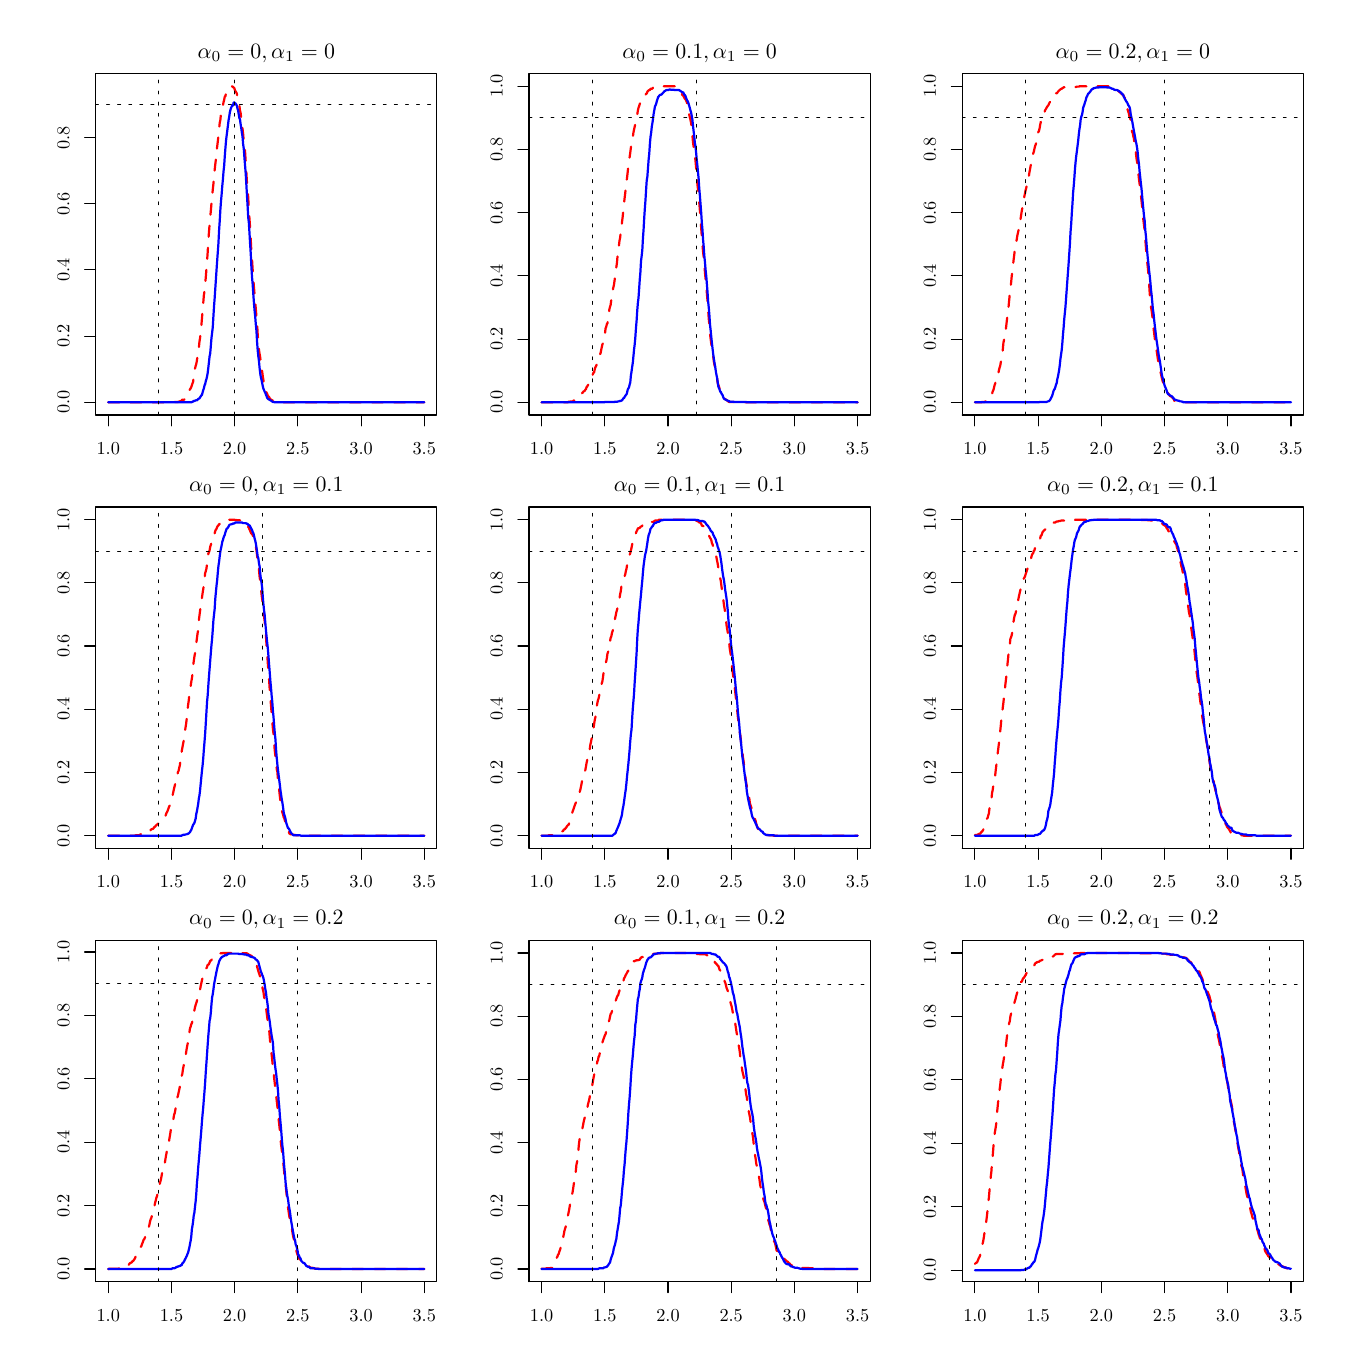
\begin{tikzpicture}[x=1pt,y=1pt]
\definecolor{fillColor}{RGB}{255,255,255}
\path[use as bounding box,fill=fillColor,fill opacity=0.00] (0,0) rectangle (469.75,469.75);
\begin{scope}
\path[clip] ( 24.55,329.80) rectangle (147.87,453.12);
\definecolor{drawColor}{RGB}{255,0,0}

\path[draw=drawColor,line width= 0.8pt,dash pattern=on 4pt off 4pt ,line join=round,line cap=round] ( 29.12,334.37) --
	( 29.35,334.37) --
	( 29.58,334.37) --
	( 29.81,334.37) --
	( 30.03,334.37) --
	( 30.26,334.37) --
	( 30.49,334.37) --
	( 30.72,334.37) --
	( 30.95,334.37) --
	( 31.18,334.37) --
	( 31.41,334.37) --
	( 31.64,334.37) --
	( 31.87,334.37) --
	( 32.09,334.37) --
	( 32.32,334.37) --
	( 32.55,334.37) --
	( 32.78,334.37) --
	( 33.01,334.37) --
	( 33.24,334.37) --
	( 33.47,334.37) --
	( 33.70,334.37) --
	( 33.92,334.37) --
	( 34.15,334.37) --
	( 34.38,334.37) --
	( 34.61,334.37) --
	( 34.84,334.37) --
	( 35.07,334.37) --
	( 35.30,334.37) --
	( 35.53,334.37) --
	( 35.76,334.37) --
	( 35.98,334.37) --
	( 36.21,334.37) --
	( 36.44,334.37) --
	( 36.67,334.37) --
	( 36.90,334.37) --
	( 37.13,334.37) --
	( 37.36,334.37) --
	( 37.59,334.37) --
	( 37.81,334.37) --
	( 38.04,334.37) --
	( 38.27,334.37) --
	( 38.50,334.37) --
	( 38.73,334.37) --
	( 38.96,334.37) --
	( 39.19,334.37) --
	( 39.42,334.37) --
	( 39.65,334.37) --
	( 39.87,334.37) --
	( 40.10,334.37) --
	( 40.33,334.37) --
	( 40.56,334.37) --
	( 40.79,334.37) --
	( 41.02,334.37) --
	( 41.25,334.37) --
	( 41.48,334.37) --
	( 41.71,334.37) --
	( 41.93,334.37) --
	( 42.16,334.37) --
	( 42.39,334.37) --
	( 42.62,334.37) --
	( 42.85,334.37) --
	( 43.08,334.37) --
	( 43.31,334.37) --
	( 43.54,334.37) --
	( 43.76,334.37) --
	( 43.99,334.37) --
	( 44.22,334.37) --
	( 44.45,334.37) --
	( 44.68,334.37) --
	( 44.91,334.37) --
	( 45.14,334.37) --
	( 45.37,334.37) --
	( 45.60,334.37) --
	( 45.82,334.37) --
	( 46.05,334.37) --
	( 46.28,334.37) --
	( 46.51,334.37) --
	( 46.74,334.37) --
	( 46.97,334.37) --
	( 47.20,334.37) --
	( 47.43,334.37) --
	( 47.65,334.37) --
	( 47.88,334.37) --
	( 48.11,334.37) --
	( 48.34,334.37) --
	( 48.57,334.37) --
	( 48.80,334.37) --
	( 49.03,334.37) --
	( 49.26,334.37) --
	( 49.49,334.37) --
	( 49.71,334.37) --
	( 49.94,334.37) --
	( 50.17,334.37) --
	( 50.40,334.37) --
	( 50.63,334.49) --
	( 50.86,334.49) --
	( 51.09,334.49) --
	( 51.32,334.49) --
	( 51.54,334.49) --
	( 51.77,334.49) --
	( 52.00,334.49) --
	( 52.23,334.49) --
	( 52.46,334.49) --
	( 52.69,334.49) --
	( 52.92,334.49) --
	( 53.15,334.49) --
	( 53.38,334.49) --
	( 53.60,334.49) --
	( 53.83,334.49) --
	( 54.06,334.49) --
	( 54.29,334.49) --
	( 54.52,334.61) --
	( 54.75,334.61) --
	( 54.98,334.73) --
	( 55.21,334.73) --
	( 55.43,334.73) --
	( 55.66,335.09) --
	( 55.89,335.33) --
	( 56.12,335.33) --
	( 56.35,335.33) --
	( 56.58,335.33) --
	( 56.81,335.80) --
	( 57.04,335.80) --
	( 57.27,336.16) --
	( 57.49,336.76) --
	( 57.72,337.00) --
	( 57.95,337.48) --
	( 58.18,338.08) --
	( 58.41,338.67) --
	( 58.64,339.03) --
	( 58.87,339.39) --
	( 59.10,339.87) --
	( 59.32,340.47) --
	( 59.55,341.18) --
	( 59.78,341.78) --
	( 60.01,343.58) --
	( 60.24,345.25) --
	( 60.47,346.57) --
	( 60.70,347.52) --
	( 60.93,348.24) --
	( 61.16,349.55) --
	( 61.38,351.11) --
	( 61.61,352.54) --
	( 61.84,353.86) --
	( 62.07,356.25) --
	( 62.30,357.68) --
	( 62.53,360.43) --
	( 62.76,362.11) --
	( 62.99,364.86) --
	( 63.22,367.73) --
	( 63.44,370.24) --
	( 63.67,373.11) --
	( 63.90,374.54) --
	( 64.13,377.17) --
	( 64.36,379.57) --
	( 64.59,382.44) --
	( 64.82,385.42) --
	( 65.05,388.65) --
	( 65.27,392.72) --
	( 65.50,395.71) --
	( 65.73,398.58) --
	( 65.96,401.33) --
	( 66.19,403.60) --
	( 66.42,406.35) --
	( 66.65,408.86) --
	( 66.88,411.13) --
	( 67.11,413.28) --
	( 67.33,416.03) --
	( 67.56,418.31) --
	( 67.79,420.34) --
	( 68.02,422.25) --
	( 68.25,425.00) --
	( 68.48,426.79) --
	( 68.71,428.71) --
	( 68.94,430.86) --
	( 69.16,433.13) --
	( 69.39,435.28) --
	( 69.62,436.36) --
	( 69.85,438.63) --
	( 70.08,439.23) --
	( 70.31,440.43) --
	( 70.54,441.50) --
	( 70.77,442.82) --
	( 71.00,443.65) --
	( 71.22,444.85) --
	( 71.45,444.97) --
	( 71.68,446.16) --
	( 71.91,446.88) --
	( 72.14,447.00) --
	( 72.37,447.12) --
	( 72.60,447.48) --
	( 72.83,447.84) --
	( 73.05,448.20) --
	( 73.28,448.56) --
	( 73.51,448.44) --
	( 73.74,448.44) --
	( 73.97,448.56) --
	( 74.20,448.32) --
	( 74.43,448.08) --
	( 74.66,447.96) --
	( 74.89,447.12) --
	( 75.11,446.76) --
	( 75.34,446.40) --
	( 75.57,445.93) --
	( 75.80,444.85) --
	( 76.03,443.77) --
	( 76.26,442.46) --
	( 76.49,441.62) --
	( 76.72,439.83) --
	( 76.94,438.99) --
	( 77.17,436.96) --
	( 77.40,435.76) --
	( 77.63,433.25) --
	( 77.86,431.34) --
	( 78.09,428.59) --
	( 78.32,427.15) --
	( 78.55,425.12) --
	( 78.78,421.41) --
	( 79.00,417.83) --
	( 79.23,413.88) --
	( 79.46,411.25) --
	( 79.69,408.50) --
	( 79.92,404.08) --
	( 80.15,400.61) --
	( 80.38,397.38) --
	( 80.61,393.08) --
	( 80.83,388.77) --
	( 81.06,386.14) --
	( 81.29,382.44) --
	( 81.52,378.97) --
	( 81.75,376.10) --
	( 81.98,373.47) --
	( 82.21,370.60) --
	( 82.44,368.09) --
	( 82.67,365.22) --
	( 82.89,363.07) --
	( 83.12,358.88) --
	( 83.35,355.77) --
	( 83.58,353.26) --
	( 83.81,351.83) --
	( 84.04,350.51) --
	( 84.27,348.60) --
	( 84.50,346.45) --
	( 84.73,345.49) --
	( 84.95,343.82) --
	( 85.18,342.38) --
	( 85.41,340.83) --
	( 85.64,339.99) --
	( 85.87,339.27) --
	( 86.10,338.55) --
	( 86.33,337.84) --
	( 86.56,337.36) --
	( 86.78,336.76) --
	( 87.01,336.52) --
	( 87.24,336.28) --
	( 87.47,335.80) --
	( 87.70,335.57) --
	( 87.93,335.33) --
	( 88.16,335.21) --
	( 88.39,335.09) --
	( 88.62,334.97) --
	( 88.84,334.97) --
	( 89.07,334.73) --
	( 89.30,334.61) --
	( 89.53,334.49) --
	( 89.76,334.49) --
	( 89.99,334.49) --
	( 90.22,334.49) --
	( 90.45,334.37) --
	( 90.67,334.37) --
	( 90.90,334.37) --
	( 91.13,334.37) --
	( 91.36,334.37) --
	( 91.59,334.37) --
	( 91.82,334.37) --
	( 92.05,334.37) --
	( 92.28,334.37) --
	( 92.51,334.37) --
	( 92.73,334.37) --
	( 92.96,334.37) --
	( 93.19,334.37) --
	( 93.42,334.37) --
	( 93.65,334.37) --
	( 93.88,334.37) --
	( 94.11,334.37) --
	( 94.34,334.37) --
	( 94.56,334.37) --
	( 94.79,334.37) --
	( 95.02,334.37) --
	( 95.25,334.37) --
	( 95.48,334.37) --
	( 95.71,334.37) --
	( 95.94,334.37) --
	( 96.17,334.37) --
	( 96.40,334.37) --
	( 96.62,334.37) --
	( 96.85,334.37) --
	( 97.08,334.37) --
	( 97.31,334.37) --
	( 97.54,334.37) --
	( 97.77,334.37) --
	( 98.00,334.37) --
	( 98.23,334.37) --
	( 98.45,334.37) --
	( 98.68,334.37) --
	( 98.91,334.37) --
	( 99.14,334.37) --
	( 99.37,334.37) --
	( 99.60,334.37) --
	( 99.83,334.37) --
	(100.06,334.37) --
	(100.29,334.37) --
	(100.51,334.37) --
	(100.74,334.37) --
	(100.97,334.37) --
	(101.20,334.37) --
	(101.43,334.37) --
	(101.66,334.37) --
	(101.89,334.37) --
	(102.12,334.37) --
	(102.35,334.37) --
	(102.57,334.37) --
	(102.80,334.37) --
	(103.03,334.37) --
	(103.26,334.37) --
	(103.49,334.37) --
	(103.72,334.37) --
	(103.95,334.37) --
	(104.18,334.37) --
	(104.40,334.37) --
	(104.63,334.37) --
	(104.86,334.37) --
	(105.09,334.37) --
	(105.32,334.37) --
	(105.55,334.37) --
	(105.78,334.37) --
	(106.01,334.37) --
	(106.24,334.37) --
	(106.46,334.37) --
	(106.69,334.37) --
	(106.92,334.37) --
	(107.15,334.37) --
	(107.38,334.37) --
	(107.61,334.37) --
	(107.84,334.37) --
	(108.07,334.37) --
	(108.29,334.37) --
	(108.52,334.37) --
	(108.75,334.37) --
	(108.98,334.37) --
	(109.21,334.37) --
	(109.44,334.37) --
	(109.67,334.37) --
	(109.90,334.37) --
	(110.13,334.37) --
	(110.35,334.37) --
	(110.58,334.37) --
	(110.81,334.37) --
	(111.04,334.37) --
	(111.27,334.37) --
	(111.50,334.37) --
	(111.73,334.37) --
	(111.96,334.37) --
	(112.18,334.37) --
	(112.41,334.37) --
	(112.64,334.37) --
	(112.87,334.37) --
	(113.10,334.37) --
	(113.33,334.37) --
	(113.56,334.37) --
	(113.79,334.37) --
	(114.02,334.37) --
	(114.24,334.37) --
	(114.47,334.37) --
	(114.70,334.37) --
	(114.93,334.37) --
	(115.16,334.37) --
	(115.39,334.37) --
	(115.62,334.37) --
	(115.85,334.37) --
	(116.07,334.37) --
	(116.30,334.37) --
	(116.53,334.37) --
	(116.76,334.37) --
	(116.99,334.37) --
	(117.22,334.37) --
	(117.45,334.37) --
	(117.68,334.37) --
	(117.91,334.37) --
	(118.13,334.37) --
	(118.36,334.37) --
	(118.59,334.37) --
	(118.82,334.37) --
	(119.05,334.37) --
	(119.28,334.37) --
	(119.51,334.37) --
	(119.74,334.37) --
	(119.96,334.37) --
	(120.19,334.37) --
	(120.42,334.37) --
	(120.65,334.37) --
	(120.88,334.37) --
	(121.11,334.37) --
	(121.34,334.37) --
	(121.57,334.37) --
	(121.80,334.37) --
	(122.02,334.37) --
	(122.25,334.37) --
	(122.48,334.37) --
	(122.71,334.37) --
	(122.94,334.37) --
	(123.17,334.37) --
	(123.40,334.37) --
	(123.63,334.37) --
	(123.86,334.37) --
	(124.08,334.37) --
	(124.31,334.37) --
	(124.54,334.37) --
	(124.77,334.37) --
	(125.00,334.37) --
	(125.23,334.37) --
	(125.46,334.37) --
	(125.69,334.37) --
	(125.91,334.37) --
	(126.14,334.37) --
	(126.37,334.37) --
	(126.60,334.37) --
	(126.83,334.37) --
	(127.06,334.37) --
	(127.29,334.37) --
	(127.52,334.37) --
	(127.75,334.37) --
	(127.97,334.37) --
	(128.20,334.37) --
	(128.43,334.37) --
	(128.66,334.37) --
	(128.89,334.37) --
	(129.12,334.37) --
	(129.35,334.37) --
	(129.58,334.37) --
	(129.80,334.37) --
	(130.03,334.37) --
	(130.26,334.37) --
	(130.49,334.37) --
	(130.72,334.37) --
	(130.95,334.37) --
	(131.18,334.37) --
	(131.41,334.37) --
	(131.64,334.37) --
	(131.86,334.37) --
	(132.09,334.37) --
	(132.32,334.37) --
	(132.55,334.37) --
	(132.78,334.37) --
	(133.01,334.37) --
	(133.24,334.37) --
	(133.47,334.37) --
	(133.69,334.37) --
	(133.92,334.37) --
	(134.15,334.37) --
	(134.38,334.37) --
	(134.61,334.37) --
	(134.84,334.37) --
	(135.07,334.37) --
	(135.30,334.37) --
	(135.53,334.37) --
	(135.75,334.37) --
	(135.98,334.37) --
	(136.21,334.37) --
	(136.44,334.37) --
	(136.67,334.37) --
	(136.90,334.37) --
	(137.13,334.37) --
	(137.36,334.37) --
	(137.58,334.37) --
	(137.81,334.37) --
	(138.04,334.37) --
	(138.27,334.37) --
	(138.50,334.37) --
	(138.73,334.37) --
	(138.96,334.37) --
	(139.19,334.37) --
	(139.42,334.37) --
	(139.64,334.37) --
	(139.87,334.37) --
	(140.10,334.37) --
	(140.33,334.37) --
	(140.56,334.37) --
	(140.79,334.37) --
	(141.02,334.37) --
	(141.25,334.37) --
	(141.47,334.37) --
	(141.70,334.37) --
	(141.93,334.37) --
	(142.16,334.37) --
	(142.39,334.37) --
	(142.62,334.37) --
	(142.85,334.37) --
	(143.08,334.37) --
	(143.31,334.37);
\end{scope}
\begin{scope}
\path[clip] (  0.00,  0.00) rectangle (469.75,469.75);
\definecolor{drawColor}{RGB}{0,0,0}

\path[draw=drawColor,line width= 0.4pt,line join=round,line cap=round] ( 29.12,329.80) -- (143.31,329.80);

\path[draw=drawColor,line width= 0.4pt,line join=round,line cap=round] ( 29.12,329.80) -- ( 29.12,325.84);

\path[draw=drawColor,line width= 0.4pt,line join=round,line cap=round] ( 51.96,329.80) -- ( 51.96,325.84);

\path[draw=drawColor,line width= 0.4pt,line join=round,line cap=round] ( 74.79,329.80) -- ( 74.79,325.84);

\path[draw=drawColor,line width= 0.4pt,line join=round,line cap=round] ( 97.63,329.80) -- ( 97.63,325.84);

\path[draw=drawColor,line width= 0.4pt,line join=round,line cap=round] (120.47,329.80) -- (120.47,325.84);

\path[draw=drawColor,line width= 0.4pt,line join=round,line cap=round] (143.31,329.80) -- (143.31,325.84);

\node[text=drawColor,anchor=base,inner sep=0pt, outer sep=0pt, scale=  0.66] at ( 29.12,315.55) {1.0};

\node[text=drawColor,anchor=base,inner sep=0pt, outer sep=0pt, scale=  0.66] at ( 51.96,315.55) {1.5};

\node[text=drawColor,anchor=base,inner sep=0pt, outer sep=0pt, scale=  0.66] at ( 74.79,315.55) {2.0};

\node[text=drawColor,anchor=base,inner sep=0pt, outer sep=0pt, scale=  0.66] at ( 97.63,315.55) {2.5};

\node[text=drawColor,anchor=base,inner sep=0pt, outer sep=0pt, scale=  0.66] at (120.47,315.55) {3.0};

\node[text=drawColor,anchor=base,inner sep=0pt, outer sep=0pt, scale=  0.66] at (143.31,315.55) {3.5};

\path[draw=drawColor,line width= 0.4pt,line join=round,line cap=round] ( 24.55,334.37) -- ( 24.55,430.02);

\path[draw=drawColor,line width= 0.4pt,line join=round,line cap=round] ( 24.55,334.37) -- ( 20.59,334.37);

\path[draw=drawColor,line width= 0.4pt,line join=round,line cap=round] ( 24.55,358.28) -- ( 20.59,358.28);

\path[draw=drawColor,line width= 0.4pt,line join=round,line cap=round] ( 24.55,382.20) -- ( 20.59,382.20);

\path[draw=drawColor,line width= 0.4pt,line join=round,line cap=round] ( 24.55,406.11) -- ( 20.59,406.11);

\path[draw=drawColor,line width= 0.4pt,line join=round,line cap=round] ( 24.55,430.02) -- ( 20.59,430.02);

\node[text=drawColor,rotate= 90.00,anchor=base,inner sep=0pt, outer sep=0pt, scale=  0.66] at ( 15.05,334.37) {0.0};

\node[text=drawColor,rotate= 90.00,anchor=base,inner sep=0pt, outer sep=0pt, scale=  0.66] at ( 15.05,358.28) {0.2};

\node[text=drawColor,rotate= 90.00,anchor=base,inner sep=0pt, outer sep=0pt, scale=  0.66] at ( 15.05,382.20) {0.4};

\node[text=drawColor,rotate= 90.00,anchor=base,inner sep=0pt, outer sep=0pt, scale=  0.66] at ( 15.05,406.11) {0.6};

\node[text=drawColor,rotate= 90.00,anchor=base,inner sep=0pt, outer sep=0pt, scale=  0.66] at ( 15.05,430.02) {0.8};

\path[draw=drawColor,line width= 0.4pt,line join=round,line cap=round] ( 24.55,329.80) --
	(147.87,329.80) --
	(147.87,453.12) --
	( 24.55,453.12) --
	( 24.55,329.80);
\end{scope}
\begin{scope}
\path[clip] (  0.00,313.17) rectangle (156.58,469.75);
\definecolor{drawColor}{RGB}{0,0,0}

\node[text=drawColor,anchor=base,inner sep=0pt, outer sep=0pt, scale=  0.79] at ( 86.21,458.71) {\bfseries $\alpha_0 = 0, \alpha_1 = 0$};
\end{scope}
\begin{scope}
\path[clip] ( 24.55,329.80) rectangle (147.87,453.12);
\definecolor{drawColor}{RGB}{0,0,255}

\path[draw=drawColor,line width= 0.8pt,line join=round,line cap=round] ( 29.12,334.37) --
	( 29.35,334.37) --
	( 29.58,334.37) --
	( 29.81,334.37) --
	( 30.03,334.37) --
	( 30.26,334.37) --
	( 30.49,334.37) --
	( 30.72,334.37) --
	( 30.95,334.37) --
	( 31.18,334.37) --
	( 31.41,334.37) --
	( 31.64,334.37) --
	( 31.87,334.37) --
	( 32.09,334.37) --
	( 32.32,334.37) --
	( 32.55,334.37) --
	( 32.78,334.37) --
	( 33.01,334.37) --
	( 33.24,334.37) --
	( 33.47,334.37) --
	( 33.70,334.37) --
	( 33.92,334.37) --
	( 34.15,334.37) --
	( 34.38,334.37) --
	( 34.61,334.37) --
	( 34.84,334.37) --
	( 35.07,334.37) --
	( 35.30,334.37) --
	( 35.53,334.37) --
	( 35.76,334.37) --
	( 35.98,334.37) --
	( 36.21,334.37) --
	( 36.44,334.37) --
	( 36.67,334.37) --
	( 36.90,334.37) --
	( 37.13,334.37) --
	( 37.36,334.37) --
	( 37.59,334.37) --
	( 37.81,334.37) --
	( 38.04,334.37) --
	( 38.27,334.37) --
	( 38.50,334.37) --
	( 38.73,334.37) --
	( 38.96,334.37) --
	( 39.19,334.37) --
	( 39.42,334.37) --
	( 39.65,334.37) --
	( 39.87,334.37) --
	( 40.10,334.37) --
	( 40.33,334.37) --
	( 40.56,334.37) --
	( 40.79,334.37) --
	( 41.02,334.37) --
	( 41.25,334.37) --
	( 41.48,334.37) --
	( 41.71,334.37) --
	( 41.93,334.37) --
	( 42.16,334.37) --
	( 42.39,334.37) --
	( 42.62,334.37) --
	( 42.85,334.37) --
	( 43.08,334.37) --
	( 43.31,334.37) --
	( 43.54,334.37) --
	( 43.76,334.37) --
	( 43.99,334.37) --
	( 44.22,334.37) --
	( 44.45,334.37) --
	( 44.68,334.37) --
	( 44.91,334.37) --
	( 45.14,334.37) --
	( 45.37,334.37) --
	( 45.60,334.37) --
	( 45.82,334.37) --
	( 46.05,334.37) --
	( 46.28,334.37) --
	( 46.51,334.37) --
	( 46.74,334.37) --
	( 46.97,334.37) --
	( 47.20,334.37) --
	( 47.43,334.37) --
	( 47.65,334.37) --
	( 47.88,334.37) --
	( 48.11,334.37) --
	( 48.34,334.37) --
	( 48.57,334.37) --
	( 48.80,334.37) --
	( 49.03,334.37) --
	( 49.26,334.37) --
	( 49.49,334.37) --
	( 49.71,334.37) --
	( 49.94,334.37) --
	( 50.17,334.37) --
	( 50.40,334.37) --
	( 50.63,334.37) --
	( 50.86,334.37) --
	( 51.09,334.37) --
	( 51.32,334.37) --
	( 51.54,334.37) --
	( 51.77,334.37) --
	( 52.00,334.37) --
	( 52.23,334.37) --
	( 52.46,334.37) --
	( 52.69,334.37) --
	( 52.92,334.37) --
	( 53.15,334.37) --
	( 53.38,334.37) --
	( 53.60,334.37) --
	( 53.83,334.37) --
	( 54.06,334.37) --
	( 54.29,334.37) --
	( 54.52,334.37) --
	( 54.75,334.37) --
	( 54.98,334.37) --
	( 55.21,334.37) --
	( 55.43,334.37) --
	( 55.66,334.37) --
	( 55.89,334.37) --
	( 56.12,334.37) --
	( 56.35,334.37) --
	( 56.58,334.37) --
	( 56.81,334.37) --
	( 57.04,334.37) --
	( 57.27,334.37) --
	( 57.49,334.37) --
	( 57.72,334.37) --
	( 57.95,334.37) --
	( 58.18,334.37) --
	( 58.41,334.37) --
	( 58.64,334.37) --
	( 58.87,334.37) --
	( 59.10,334.37) --
	( 59.32,334.49) --
	( 59.55,334.49) --
	( 59.78,334.73) --
	( 60.01,334.85) --
	( 60.24,334.85) --
	( 60.47,334.97) --
	( 60.70,335.09) --
	( 60.93,335.09) --
	( 61.16,335.09) --
	( 61.38,335.33) --
	( 61.61,335.57) --
	( 61.84,335.68) --
	( 62.07,335.80) --
	( 62.30,336.16) --
	( 62.53,336.52) --
	( 62.76,336.88) --
	( 62.99,337.12) --
	( 63.22,337.96) --
	( 63.44,338.79) --
	( 63.67,339.39) --
	( 63.90,340.47) --
	( 64.13,340.95) --
	( 64.36,342.02) --
	( 64.59,342.74) --
	( 64.82,343.70) --
	( 65.05,345.01) --
	( 65.27,346.80) --
	( 65.50,348.84) --
	( 65.73,350.99) --
	( 65.96,352.07) --
	( 66.19,354.82) --
	( 66.42,357.68) --
	( 66.65,359.48) --
	( 66.88,361.51) --
	( 67.11,365.34) --
	( 67.33,368.92) --
	( 67.56,371.91) --
	( 67.79,375.38) --
	( 68.02,378.85) --
	( 68.25,382.32) --
	( 68.48,385.66) --
	( 68.71,388.77) --
	( 68.94,392.00) --
	( 69.16,396.42) --
	( 69.39,399.77) --
	( 69.62,403.84) --
	( 69.85,406.95) --
	( 70.08,409.46) --
	( 70.31,412.45) --
	( 70.54,414.84) --
	( 70.77,417.83) --
	( 71.00,419.86) --
	( 71.22,423.21) --
	( 71.45,426.20) --
	( 71.68,428.95) --
	( 71.91,430.86) --
	( 72.14,432.65) --
	( 72.37,434.45) --
	( 72.60,436.36) --
	( 72.83,437.56) --
	( 73.05,439.11) --
	( 73.28,440.07) --
	( 73.51,440.78) --
	( 73.74,441.26) --
	( 73.97,441.74) --
	( 74.20,441.62) --
	( 74.43,442.70) --
	( 74.66,442.70) --
	( 74.89,442.46) --
	( 75.11,442.34) --
	( 75.34,441.98) --
	( 75.57,441.62) --
	( 75.80,440.54) --
	( 76.03,439.83) --
	( 76.26,438.51) --
	( 76.49,437.08) --
	( 76.72,436.60) --
	( 76.94,434.92) --
	( 77.17,433.49) --
	( 77.40,431.82) --
	( 77.63,430.38) --
	( 77.86,427.63) --
	( 78.09,425.96) --
	( 78.32,422.85) --
	( 78.55,419.98) --
	( 78.78,417.11) --
	( 79.00,413.40) --
	( 79.23,409.34) --
	( 79.46,405.51) --
	( 79.69,401.21) --
	( 79.92,399.29) --
	( 80.15,395.59) --
	( 80.38,391.52) --
	( 80.61,388.05) --
	( 80.83,383.51) --
	( 81.06,379.69) --
	( 81.29,377.17) --
	( 81.52,373.59) --
	( 81.75,370.48) --
	( 81.98,367.61) --
	( 82.21,365.46) --
	( 82.44,362.47) --
	( 82.67,360.20) --
	( 82.89,356.25) --
	( 83.12,353.14) --
	( 83.35,350.99) --
	( 83.58,349.20) --
	( 83.81,346.68) --
	( 84.04,344.77) --
	( 84.27,343.34) --
	( 84.50,342.50) --
	( 84.73,341.30) --
	( 84.95,340.23) --
	( 85.18,339.27) --
	( 85.41,338.79) --
	( 85.64,338.20) --
	( 85.87,337.84) --
	( 86.10,337.12) --
	( 86.33,336.64) --
	( 86.56,335.92) --
	( 86.78,335.68) --
	( 87.01,335.45) --
	( 87.24,335.45) --
	( 87.47,335.21) --
	( 87.70,335.09) --
	( 87.93,334.97) --
	( 88.16,334.85) --
	( 88.39,334.61) --
	( 88.62,334.49) --
	( 88.84,334.49) --
	( 89.07,334.49) --
	( 89.30,334.37) --
	( 89.53,334.37) --
	( 89.76,334.37) --
	( 89.99,334.37) --
	( 90.22,334.37) --
	( 90.45,334.37) --
	( 90.67,334.37) --
	( 90.90,334.37) --
	( 91.13,334.37) --
	( 91.36,334.37) --
	( 91.59,334.37) --
	( 91.82,334.37) --
	( 92.05,334.37) --
	( 92.28,334.37) --
	( 92.51,334.37) --
	( 92.73,334.37) --
	( 92.96,334.37) --
	( 93.19,334.37) --
	( 93.42,334.37) --
	( 93.65,334.37) --
	( 93.88,334.37) --
	( 94.11,334.37) --
	( 94.34,334.37) --
	( 94.56,334.37) --
	( 94.79,334.37) --
	( 95.02,334.37) --
	( 95.25,334.37) --
	( 95.48,334.37) --
	( 95.71,334.37) --
	( 95.94,334.37) --
	( 96.17,334.37) --
	( 96.40,334.37) --
	( 96.62,334.37) --
	( 96.85,334.37) --
	( 97.08,334.37) --
	( 97.31,334.37) --
	( 97.54,334.37) --
	( 97.77,334.37) --
	( 98.00,334.37) --
	( 98.23,334.37) --
	( 98.45,334.37) --
	( 98.68,334.37) --
	( 98.91,334.37) --
	( 99.14,334.37) --
	( 99.37,334.37) --
	( 99.60,334.37) --
	( 99.83,334.37) --
	(100.06,334.37) --
	(100.29,334.37) --
	(100.51,334.37) --
	(100.74,334.37) --
	(100.97,334.37) --
	(101.20,334.37) --
	(101.43,334.37) --
	(101.66,334.37) --
	(101.89,334.37) --
	(102.12,334.37) --
	(102.35,334.37) --
	(102.57,334.37) --
	(102.80,334.37) --
	(103.03,334.37) --
	(103.26,334.37) --
	(103.49,334.37) --
	(103.72,334.37) --
	(103.95,334.37) --
	(104.18,334.37) --
	(104.40,334.37) --
	(104.63,334.37) --
	(104.86,334.37) --
	(105.09,334.37) --
	(105.32,334.37) --
	(105.55,334.37) --
	(105.78,334.37) --
	(106.01,334.37) --
	(106.24,334.37) --
	(106.46,334.37) --
	(106.69,334.37) --
	(106.92,334.37) --
	(107.15,334.37) --
	(107.38,334.37) --
	(107.61,334.37) --
	(107.84,334.37) --
	(108.07,334.37) --
	(108.29,334.37) --
	(108.52,334.37) --
	(108.75,334.37) --
	(108.98,334.37) --
	(109.21,334.37) --
	(109.44,334.37) --
	(109.67,334.37) --
	(109.90,334.37) --
	(110.13,334.37) --
	(110.35,334.37) --
	(110.58,334.37) --
	(110.81,334.37) --
	(111.04,334.37) --
	(111.27,334.37) --
	(111.50,334.37) --
	(111.73,334.37) --
	(111.96,334.37) --
	(112.18,334.37) --
	(112.41,334.37) --
	(112.64,334.37) --
	(112.87,334.37) --
	(113.10,334.37) --
	(113.33,334.37) --
	(113.56,334.37) --
	(113.79,334.37) --
	(114.02,334.37) --
	(114.24,334.37) --
	(114.47,334.37) --
	(114.70,334.37) --
	(114.93,334.37) --
	(115.16,334.37) --
	(115.39,334.37) --
	(115.62,334.37) --
	(115.85,334.37) --
	(116.07,334.37) --
	(116.30,334.37) --
	(116.53,334.37) --
	(116.76,334.37) --
	(116.99,334.37) --
	(117.22,334.37) --
	(117.45,334.37) --
	(117.68,334.37) --
	(117.91,334.37) --
	(118.13,334.37) --
	(118.36,334.37) --
	(118.59,334.37) --
	(118.82,334.37) --
	(119.05,334.37) --
	(119.28,334.37) --
	(119.51,334.37) --
	(119.74,334.37) --
	(119.96,334.37) --
	(120.19,334.37) --
	(120.42,334.37) --
	(120.65,334.37) --
	(120.88,334.37) --
	(121.11,334.37) --
	(121.34,334.37) --
	(121.57,334.37) --
	(121.80,334.37) --
	(122.02,334.37) --
	(122.25,334.37) --
	(122.48,334.37) --
	(122.71,334.37) --
	(122.94,334.37) --
	(123.17,334.37) --
	(123.40,334.37) --
	(123.63,334.37) --
	(123.86,334.37) --
	(124.08,334.37) --
	(124.31,334.37) --
	(124.54,334.37) --
	(124.77,334.37) --
	(125.00,334.37) --
	(125.23,334.37) --
	(125.46,334.37) --
	(125.69,334.37) --
	(125.91,334.37) --
	(126.14,334.37) --
	(126.37,334.37) --
	(126.60,334.37) --
	(126.83,334.37) --
	(127.06,334.37) --
	(127.29,334.37) --
	(127.52,334.37) --
	(127.75,334.37) --
	(127.97,334.37) --
	(128.20,334.37) --
	(128.43,334.37) --
	(128.66,334.37) --
	(128.89,334.37) --
	(129.12,334.37) --
	(129.35,334.37) --
	(129.58,334.37) --
	(129.80,334.37) --
	(130.03,334.37) --
	(130.26,334.37) --
	(130.49,334.37) --
	(130.72,334.37) --
	(130.95,334.37) --
	(131.18,334.37) --
	(131.41,334.37) --
	(131.64,334.37) --
	(131.86,334.37) --
	(132.09,334.37) --
	(132.32,334.37) --
	(132.55,334.37) --
	(132.78,334.37) --
	(133.01,334.37) --
	(133.24,334.37) --
	(133.47,334.37) --
	(133.69,334.37) --
	(133.92,334.37) --
	(134.15,334.37) --
	(134.38,334.37) --
	(134.61,334.37) --
	(134.84,334.37) --
	(135.07,334.37) --
	(135.30,334.37) --
	(135.53,334.37) --
	(135.75,334.37) --
	(135.98,334.37) --
	(136.21,334.37) --
	(136.44,334.37) --
	(136.67,334.37) --
	(136.90,334.37) --
	(137.13,334.37) --
	(137.36,334.37) --
	(137.58,334.37) --
	(137.81,334.37) --
	(138.04,334.37) --
	(138.27,334.37) --
	(138.50,334.37) --
	(138.73,334.37) --
	(138.96,334.37) --
	(139.19,334.37) --
	(139.42,334.37) --
	(139.64,334.37) --
	(139.87,334.37) --
	(140.10,334.37) --
	(140.33,334.37) --
	(140.56,334.37) --
	(140.79,334.37) --
	(141.02,334.37) --
	(141.25,334.37) --
	(141.47,334.37) --
	(141.70,334.37) --
	(141.93,334.37) --
	(142.16,334.37) --
	(142.39,334.37) --
	(142.62,334.37) --
	(142.85,334.37) --
	(143.08,334.37) --
	(143.31,334.37);
\definecolor{drawColor}{RGB}{0,0,0}

\path[draw=drawColor,line width= 0.4pt,dash pattern=on 1pt off 3pt ,line join=round,line cap=round] ( 24.55,441.98) -- (147.87,441.98);

\path[draw=drawColor,line width= 0.4pt,dash pattern=on 1pt off 3pt ,line join=round,line cap=round] ( 47.39,329.80) -- ( 47.39,453.12);

\path[draw=drawColor,line width= 0.4pt,dash pattern=on 1pt off 3pt ,line join=round,line cap=round] ( 74.79,329.80) -- ( 74.79,453.12);
\end{scope}
\begin{scope}
\path[clip] (181.14,329.80) rectangle (304.46,453.12);
\definecolor{drawColor}{RGB}{255,0,0}

\path[draw=drawColor,line width= 0.8pt,dash pattern=on 4pt off 4pt ,line join=round,line cap=round] (185.70,334.37) --
	(185.93,334.37) --
	(186.16,334.37) --
	(186.39,334.37) --
	(186.62,334.37) --
	(186.85,334.37) --
	(187.08,334.37) --
	(187.31,334.37) --
	(187.54,334.37) --
	(187.76,334.37) --
	(187.99,334.37) --
	(188.22,334.37) --
	(188.45,334.37) --
	(188.68,334.37) --
	(188.91,334.37) --
	(189.14,334.37) --
	(189.37,334.37) --
	(189.59,334.37) --
	(189.82,334.37) --
	(190.05,334.37) --
	(190.28,334.37) --
	(190.51,334.37) --
	(190.74,334.37) --
	(190.97,334.37) --
	(191.20,334.37) --
	(191.43,334.37) --
	(191.65,334.37) --
	(191.88,334.37) --
	(192.11,334.37) --
	(192.34,334.37) --
	(192.57,334.37) --
	(192.80,334.37) --
	(193.03,334.37) --
	(193.26,334.37) --
	(193.48,334.37) --
	(193.71,334.37) --
	(193.94,334.37) --
	(194.17,334.37) --
	(194.40,334.37) --
	(194.63,334.37) --
	(194.86,334.37) --
	(195.09,334.37) --
	(195.32,334.48) --
	(195.54,334.60) --
	(195.77,334.60) --
	(196.00,334.60) --
	(196.23,334.71) --
	(196.46,334.71) --
	(196.69,334.71) --
	(196.92,334.71) --
	(197.15,334.83) --
	(197.37,335.05) --
	(197.60,335.05) --
	(197.83,335.40) --
	(198.06,335.63) --
	(198.29,335.63) --
	(198.52,335.85) --
	(198.75,336.08) --
	(198.98,336.31) --
	(199.21,336.65) --
	(199.43,336.88) --
	(199.66,337.00) --
	(199.89,337.11) --
	(200.12,337.22) --
	(200.35,337.68) --
	(200.58,337.91) --
	(200.81,338.25) --
	(201.04,338.37) --
	(201.26,338.48) --
	(201.49,338.94) --
	(201.72,339.05) --
	(201.95,339.85) --
	(202.18,340.08) --
	(202.41,340.54) --
	(202.64,340.76) --
	(202.87,341.11) --
	(203.10,341.33) --
	(203.32,342.02) --
	(203.55,342.36) --
	(203.78,343.05) --
	(204.01,343.73) --
	(204.24,344.53) --
	(204.47,345.10) --
	(204.70,345.22) --
	(204.93,346.47) --
	(205.15,347.04) --
	(205.38,347.50) --
	(205.61,347.96) --
	(205.84,348.64) --
	(206.07,349.10) --
	(206.30,350.13) --
	(206.53,350.70) --
	(206.76,351.61) --
	(206.99,352.07) --
	(207.21,353.10) --
	(207.44,354.24) --
	(207.67,355.27) --
	(207.90,355.72) --
	(208.13,356.41) --
	(208.36,358.01) --
	(208.59,359.03) --
	(208.82,361.09) --
	(209.05,361.66) --
	(209.27,362.57) --
	(209.50,362.92) --
	(209.73,364.29) --
	(209.96,365.43) --
	(210.19,367.94) --
	(210.42,368.85) --
	(210.65,369.54) --
	(210.88,371.37) --
	(211.10,372.51) --
	(211.33,373.99) --
	(211.56,375.59) --
	(211.79,376.50) --
	(212.02,377.99) --
	(212.25,379.70) --
	(212.48,381.19) --
	(212.71,383.24) --
	(212.94,384.84) --
	(213.16,387.35) --
	(213.39,388.95) --
	(213.62,390.78) --
	(213.85,392.72) --
	(214.08,393.86) --
	(214.31,395.92) --
	(214.54,397.17) --
	(214.77,399.57) --
	(214.99,401.28) --
	(215.22,403.57) --
	(215.45,405.74) --
	(215.68,408.02) --
	(215.91,409.85) --
	(216.14,412.02) --
	(216.37,413.96) --
	(216.60,415.67) --
	(216.83,417.73) --
	(217.05,419.78) --
	(217.28,421.49) --
	(217.51,422.98) --
	(217.74,424.58) --
	(217.97,426.40) --
	(218.20,427.77) --
	(218.43,428.80) --
	(218.66,430.06) --
	(218.88,431.77) --
	(219.11,432.91) --
	(219.34,433.94) --
	(219.57,434.97) --
	(219.80,436.34) --
	(220.03,437.59) --
	(220.26,438.28) --
	(220.49,439.76) --
	(220.72,440.79) --
	(220.94,441.36) --
	(221.17,442.16) --
	(221.40,442.85) --
	(221.63,443.19) --
	(221.86,443.42) --
	(222.09,443.99) --
	(222.32,444.33) --
	(222.55,445.13) --
	(222.77,445.13) --
	(223.00,445.24) --
	(223.23,445.47) --
	(223.46,445.82) --
	(223.69,445.93) --
	(223.92,446.61) --
	(224.15,446.84) --
	(224.38,447.07) --
	(224.61,447.19) --
	(224.83,447.19) --
	(225.06,447.64) --
	(225.29,447.64) --
	(225.52,447.64) --
	(225.75,447.76) --
	(225.98,448.10) --
	(226.21,448.21) --
	(226.44,448.33) --
	(226.66,448.33) --
	(226.89,448.33) --
	(227.12,448.33) --
	(227.35,448.33) --
	(227.58,448.33) --
	(227.81,448.44) --
	(228.04,448.44) --
	(228.27,448.44) --
	(228.50,448.44) --
	(228.72,448.56) --
	(228.95,448.56) --
	(229.18,448.56) --
	(229.41,448.56) --
	(229.64,448.56) --
	(229.87,448.56) --
	(230.10,448.56) --
	(230.33,448.56) --
	(230.56,448.56) --
	(230.78,448.56) --
	(231.01,448.56) --
	(231.24,448.56) --
	(231.47,448.56) --
	(231.70,448.56) --
	(231.93,448.56) --
	(232.16,448.56) --
	(232.39,448.56) --
	(232.61,448.56) --
	(232.84,448.56) --
	(233.07,448.56) --
	(233.30,448.56) --
	(233.53,448.56) --
	(233.76,448.56) --
	(233.99,448.44) --
	(234.22,448.33) --
	(234.45,448.21) --
	(234.67,448.10) --
	(234.90,447.64) --
	(235.13,447.64) --
	(235.36,447.30) --
	(235.59,447.19) --
	(235.82,447.07) --
	(236.05,446.73) --
	(236.28,446.39) --
	(236.50,445.47) --
	(236.73,445.24) --
	(236.96,445.02) --
	(237.19,444.56) --
	(237.42,444.10) --
	(237.65,443.87) --
	(237.88,443.53) --
	(238.11,442.96) --
	(238.34,442.28) --
	(238.56,441.13) --
	(238.79,439.99) --
	(239.02,438.51) --
	(239.25,437.37) --
	(239.48,436.57) --
	(239.71,435.31) --
	(239.94,433.48) --
	(240.17,431.20) --
	(240.39,428.57) --
	(240.62,426.86) --
	(240.85,425.83) --
	(241.08,423.55) --
	(241.31,421.72) --
	(241.54,419.10) --
	(241.77,416.93) --
	(242.00,413.16) --
	(242.23,411.22) --
	(242.45,409.39) --
	(242.68,406.54) --
	(242.91,403.57) --
	(243.14,400.94) --
	(243.37,397.29) --
	(243.60,394.32) --
	(243.83,391.23) --
	(244.06,388.72) --
	(244.28,386.78) --
	(244.51,384.50) --
	(244.74,381.19) --
	(244.97,378.90) --
	(245.20,376.96) --
	(245.43,373.65) --
	(245.66,371.14) --
	(245.89,367.60) --
	(246.12,364.40) --
	(246.34,362.12) --
	(246.57,359.03) --
	(246.80,357.21) --
	(247.03,355.38) --
	(247.26,354.12) --
	(247.49,352.75) --
	(247.72,350.93) --
	(247.95,349.10) --
	(248.18,347.84) --
	(248.40,347.16) --
	(248.63,345.22) --
	(248.86,344.30) --
	(249.09,343.28) --
	(249.32,341.45) --
	(249.55,340.76) --
	(249.78,340.08) --
	(250.01,339.28) --
	(250.23,338.25) --
	(250.46,337.91) --
	(250.69,337.57) --
	(250.92,337.00) --
	(251.15,336.42) --
	(251.38,335.85) --
	(251.61,335.85) --
	(251.84,335.63) --
	(252.07,335.51) --
	(252.29,335.40) --
	(252.52,335.17) --
	(252.75,335.05) --
	(252.98,334.83) --
	(253.21,334.71) --
	(253.44,334.48) --
	(253.67,334.48) --
	(253.90,334.48) --
	(254.12,334.48) --
	(254.35,334.48) --
	(254.58,334.48) --
	(254.81,334.48) --
	(255.04,334.48) --
	(255.27,334.48) --
	(255.50,334.37) --
	(255.73,334.37) --
	(255.96,334.37) --
	(256.18,334.37) --
	(256.41,334.37) --
	(256.64,334.37) --
	(256.87,334.37) --
	(257.10,334.37) --
	(257.33,334.37) --
	(257.56,334.37) --
	(257.79,334.37) --
	(258.01,334.37) --
	(258.24,334.37) --
	(258.47,334.37) --
	(258.70,334.37) --
	(258.93,334.37) --
	(259.16,334.37) --
	(259.39,334.37) --
	(259.62,334.37) --
	(259.85,334.37) --
	(260.07,334.37) --
	(260.30,334.37) --
	(260.53,334.37) --
	(260.76,334.37) --
	(260.99,334.37) --
	(261.22,334.37) --
	(261.45,334.37) --
	(261.68,334.37) --
	(261.90,334.37) --
	(262.13,334.37) --
	(262.36,334.37) --
	(262.59,334.37) --
	(262.82,334.37) --
	(263.05,334.37) --
	(263.28,334.37) --
	(263.51,334.37) --
	(263.74,334.37) --
	(263.96,334.37) --
	(264.19,334.37) --
	(264.42,334.37) --
	(264.65,334.37) --
	(264.88,334.37) --
	(265.11,334.37) --
	(265.34,334.37) --
	(265.57,334.37) --
	(265.79,334.37) --
	(266.02,334.37) --
	(266.25,334.37) --
	(266.48,334.37) --
	(266.71,334.37) --
	(266.94,334.37) --
	(267.17,334.37) --
	(267.40,334.37) --
	(267.63,334.37) --
	(267.85,334.37) --
	(268.08,334.37) --
	(268.31,334.37) --
	(268.54,334.37) --
	(268.77,334.37) --
	(269.00,334.37) --
	(269.23,334.37) --
	(269.46,334.37) --
	(269.69,334.37) --
	(269.91,334.37) --
	(270.14,334.37) --
	(270.37,334.37) --
	(270.60,334.37) --
	(270.83,334.37) --
	(271.06,334.37) --
	(271.29,334.37) --
	(271.52,334.37) --
	(271.74,334.37) --
	(271.97,334.37) --
	(272.20,334.37) --
	(272.43,334.37) --
	(272.66,334.37) --
	(272.89,334.37) --
	(273.12,334.37) --
	(273.35,334.37) --
	(273.58,334.37) --
	(273.80,334.37) --
	(274.03,334.37) --
	(274.26,334.37) --
	(274.49,334.37) --
	(274.72,334.37) --
	(274.95,334.37) --
	(275.18,334.37) --
	(275.41,334.37) --
	(275.63,334.37) --
	(275.86,334.37) --
	(276.09,334.37) --
	(276.32,334.37) --
	(276.55,334.37) --
	(276.78,334.37) --
	(277.01,334.37) --
	(277.24,334.37) --
	(277.47,334.37) --
	(277.69,334.37) --
	(277.92,334.37) --
	(278.15,334.37) --
	(278.38,334.37) --
	(278.61,334.37) --
	(278.84,334.37) --
	(279.07,334.37) --
	(279.30,334.37) --
	(279.52,334.37) --
	(279.75,334.37) --
	(279.98,334.37) --
	(280.21,334.37) --
	(280.44,334.37) --
	(280.67,334.37) --
	(280.90,334.37) --
	(281.13,334.37) --
	(281.36,334.37) --
	(281.58,334.37) --
	(281.81,334.37) --
	(282.04,334.37) --
	(282.27,334.37) --
	(282.50,334.37) --
	(282.73,334.37) --
	(282.96,334.37) --
	(283.19,334.37) --
	(283.41,334.37) --
	(283.64,334.37) --
	(283.87,334.37) --
	(284.10,334.37) --
	(284.33,334.37) --
	(284.56,334.37) --
	(284.79,334.37) --
	(285.02,334.37) --
	(285.25,334.37) --
	(285.47,334.37) --
	(285.70,334.37) --
	(285.93,334.37) --
	(286.16,334.37) --
	(286.39,334.37) --
	(286.62,334.37) --
	(286.85,334.37) --
	(287.08,334.37) --
	(287.30,334.37) --
	(287.53,334.37) --
	(287.76,334.37) --
	(287.99,334.37) --
	(288.22,334.37) --
	(288.45,334.37) --
	(288.68,334.37) --
	(288.91,334.37) --
	(289.14,334.37) --
	(289.36,334.37) --
	(289.59,334.37) --
	(289.82,334.37) --
	(290.05,334.37) --
	(290.28,334.37) --
	(290.51,334.37) --
	(290.74,334.37) --
	(290.97,334.37) --
	(291.20,334.37) --
	(291.42,334.37) --
	(291.65,334.37) --
	(291.88,334.37) --
	(292.11,334.37) --
	(292.34,334.37) --
	(292.57,334.37) --
	(292.80,334.37) --
	(293.03,334.37) --
	(293.25,334.37) --
	(293.48,334.37) --
	(293.71,334.37) --
	(293.94,334.37) --
	(294.17,334.37) --
	(294.40,334.37) --
	(294.63,334.37) --
	(294.86,334.37) --
	(295.09,334.37) --
	(295.31,334.37) --
	(295.54,334.37) --
	(295.77,334.37) --
	(296.00,334.37) --
	(296.23,334.37) --
	(296.46,334.37) --
	(296.69,334.37) --
	(296.92,334.37) --
	(297.14,334.37) --
	(297.37,334.37) --
	(297.60,334.37) --
	(297.83,334.37) --
	(298.06,334.37) --
	(298.29,334.37) --
	(298.52,334.37) --
	(298.75,334.37) --
	(298.98,334.37) --
	(299.20,334.37) --
	(299.43,334.37) --
	(299.66,334.37) --
	(299.89,334.37);
\end{scope}
\begin{scope}
\path[clip] (  0.00,  0.00) rectangle (469.75,469.75);
\definecolor{drawColor}{RGB}{0,0,0}

\path[draw=drawColor,line width= 0.4pt,line join=round,line cap=round] (185.70,329.80) -- (299.89,329.80);

\path[draw=drawColor,line width= 0.4pt,line join=round,line cap=round] (185.70,329.80) -- (185.70,325.84);

\path[draw=drawColor,line width= 0.4pt,line join=round,line cap=round] (208.54,329.80) -- (208.54,325.84);

\path[draw=drawColor,line width= 0.4pt,line join=round,line cap=round] (231.38,329.80) -- (231.38,325.84);

\path[draw=drawColor,line width= 0.4pt,line join=round,line cap=round] (254.22,329.80) -- (254.22,325.84);

\path[draw=drawColor,line width= 0.4pt,line join=round,line cap=round] (277.05,329.80) -- (277.05,325.84);

\path[draw=drawColor,line width= 0.4pt,line join=round,line cap=round] (299.89,329.80) -- (299.89,325.84);

\node[text=drawColor,anchor=base,inner sep=0pt, outer sep=0pt, scale=  0.66] at (185.70,315.55) {1.0};

\node[text=drawColor,anchor=base,inner sep=0pt, outer sep=0pt, scale=  0.66] at (208.54,315.55) {1.5};

\node[text=drawColor,anchor=base,inner sep=0pt, outer sep=0pt, scale=  0.66] at (231.38,315.55) {2.0};

\node[text=drawColor,anchor=base,inner sep=0pt, outer sep=0pt, scale=  0.66] at (254.22,315.55) {2.5};

\node[text=drawColor,anchor=base,inner sep=0pt, outer sep=0pt, scale=  0.66] at (277.05,315.55) {3.0};

\node[text=drawColor,anchor=base,inner sep=0pt, outer sep=0pt, scale=  0.66] at (299.89,315.55) {3.5};

\path[draw=drawColor,line width= 0.4pt,line join=round,line cap=round] (181.14,334.37) -- (181.14,448.56);

\path[draw=drawColor,line width= 0.4pt,line join=round,line cap=round] (181.14,334.37) -- (177.18,334.37);

\path[draw=drawColor,line width= 0.4pt,line join=round,line cap=round] (181.14,357.21) -- (177.18,357.21);

\path[draw=drawColor,line width= 0.4pt,line join=round,line cap=round] (181.14,380.04) -- (177.18,380.04);

\path[draw=drawColor,line width= 0.4pt,line join=round,line cap=round] (181.14,402.88) -- (177.18,402.88);

\path[draw=drawColor,line width= 0.4pt,line join=round,line cap=round] (181.14,425.72) -- (177.18,425.72);

\path[draw=drawColor,line width= 0.4pt,line join=round,line cap=round] (181.14,448.56) -- (177.18,448.56);

\node[text=drawColor,rotate= 90.00,anchor=base,inner sep=0pt, outer sep=0pt, scale=  0.66] at (171.63,334.37) {0.0};

\node[text=drawColor,rotate= 90.00,anchor=base,inner sep=0pt, outer sep=0pt, scale=  0.66] at (171.63,357.21) {0.2};

\node[text=drawColor,rotate= 90.00,anchor=base,inner sep=0pt, outer sep=0pt, scale=  0.66] at (171.63,380.04) {0.4};

\node[text=drawColor,rotate= 90.00,anchor=base,inner sep=0pt, outer sep=0pt, scale=  0.66] at (171.63,402.88) {0.6};

\node[text=drawColor,rotate= 90.00,anchor=base,inner sep=0pt, outer sep=0pt, scale=  0.66] at (171.63,425.72) {0.8};

\node[text=drawColor,rotate= 90.00,anchor=base,inner sep=0pt, outer sep=0pt, scale=  0.66] at (171.63,448.56) {1.0};

\path[draw=drawColor,line width= 0.4pt,line join=round,line cap=round] (181.14,329.80) --
	(304.46,329.80) --
	(304.46,453.12) --
	(181.14,453.12) --
	(181.14,329.80);
\end{scope}
\begin{scope}
\path[clip] (156.58,313.17) rectangle (313.17,469.75);
\definecolor{drawColor}{RGB}{0,0,0}

\node[text=drawColor,anchor=base,inner sep=0pt, outer sep=0pt, scale=  0.79] at (242.80,458.71) {\bfseries $\alpha_0 = 0.1, \alpha_1 = 0$};
\end{scope}
\begin{scope}
\path[clip] (181.14,329.80) rectangle (304.46,453.12);
\definecolor{drawColor}{RGB}{0,0,255}

\path[draw=drawColor,line width= 0.8pt,line join=round,line cap=round] (185.70,334.37) --
	(185.93,334.37) --
	(186.16,334.37) --
	(186.39,334.37) --
	(186.62,334.37) --
	(186.85,334.37) --
	(187.08,334.37) --
	(187.31,334.37) --
	(187.54,334.37) --
	(187.76,334.37) --
	(187.99,334.37) --
	(188.22,334.37) --
	(188.45,334.37) --
	(188.68,334.37) --
	(188.91,334.37) --
	(189.14,334.37) --
	(189.37,334.37) --
	(189.59,334.37) --
	(189.82,334.37) --
	(190.05,334.37) --
	(190.28,334.37) --
	(190.51,334.37) --
	(190.74,334.37) --
	(190.97,334.37) --
	(191.20,334.37) --
	(191.43,334.37) --
	(191.65,334.37) --
	(191.88,334.37) --
	(192.11,334.37) --
	(192.34,334.37) --
	(192.57,334.37) --
	(192.80,334.37) --
	(193.03,334.37) --
	(193.26,334.37) --
	(193.48,334.37) --
	(193.71,334.37) --
	(193.94,334.37) --
	(194.17,334.37) --
	(194.40,334.37) --
	(194.63,334.37) --
	(194.86,334.37) --
	(195.09,334.37) --
	(195.32,334.37) --
	(195.54,334.37) --
	(195.77,334.37) --
	(196.00,334.37) --
	(196.23,334.37) --
	(196.46,334.37) --
	(196.69,334.37) --
	(196.92,334.37) --
	(197.15,334.37) --
	(197.37,334.37) --
	(197.60,334.37) --
	(197.83,334.37) --
	(198.06,334.37) --
	(198.29,334.37) --
	(198.52,334.37) --
	(198.75,334.37) --
	(198.98,334.37) --
	(199.21,334.37) --
	(199.43,334.37) --
	(199.66,334.37) --
	(199.89,334.37) --
	(200.12,334.37) --
	(200.35,334.37) --
	(200.58,334.37) --
	(200.81,334.37) --
	(201.04,334.37) --
	(201.26,334.37) --
	(201.49,334.37) --
	(201.72,334.37) --
	(201.95,334.37) --
	(202.18,334.37) --
	(202.41,334.37) --
	(202.64,334.37) --
	(202.87,334.37) --
	(203.10,334.37) --
	(203.32,334.37) --
	(203.55,334.37) --
	(203.78,334.37) --
	(204.01,334.37) --
	(204.24,334.37) --
	(204.47,334.37) --
	(204.70,334.37) --
	(204.93,334.37) --
	(205.15,334.37) --
	(205.38,334.37) --
	(205.61,334.37) --
	(205.84,334.37) --
	(206.07,334.37) --
	(206.30,334.37) --
	(206.53,334.37) --
	(206.76,334.37) --
	(206.99,334.37) --
	(207.21,334.37) --
	(207.44,334.37) --
	(207.67,334.37) --
	(207.90,334.37) --
	(208.13,334.37) --
	(208.36,334.37) --
	(208.59,334.48) --
	(208.82,334.48) --
	(209.05,334.48) --
	(209.27,334.48) --
	(209.50,334.48) --
	(209.73,334.48) --
	(209.96,334.48) --
	(210.19,334.48) --
	(210.42,334.48) --
	(210.65,334.48) --
	(210.88,334.48) --
	(211.10,334.48) --
	(211.33,334.48) --
	(211.56,334.48) --
	(211.79,334.48) --
	(212.02,334.48) --
	(212.25,334.60) --
	(212.48,334.60) --
	(212.71,334.60) --
	(212.94,334.60) --
	(213.16,334.60) --
	(213.39,334.71) --
	(213.62,334.71) --
	(213.85,334.83) --
	(214.08,334.83) --
	(214.31,334.83) --
	(214.54,335.05) --
	(214.77,335.05) --
	(214.99,335.40) --
	(215.22,335.85) --
	(215.45,335.85) --
	(215.68,336.31) --
	(215.91,336.65) --
	(216.14,337.00) --
	(216.37,337.22) --
	(216.60,337.91) --
	(216.83,338.94) --
	(217.05,339.39) --
	(217.28,339.74) --
	(217.51,340.76) --
	(217.74,341.45) --
	(217.97,344.08) --
	(218.20,345.45) --
	(218.43,347.16) --
	(218.66,348.64) --
	(218.88,350.93) --
	(219.11,353.44) --
	(219.34,355.27) --
	(219.57,357.78) --
	(219.80,361.09) --
	(220.03,363.83) --
	(220.26,367.48) --
	(220.49,370.22) --
	(220.72,372.05) --
	(220.94,375.25) --
	(221.17,378.67) --
	(221.40,381.30) --
	(221.63,385.41) --
	(221.86,387.24) --
	(222.09,389.29) --
	(222.32,393.52) --
	(222.55,396.72) --
	(222.77,400.71) --
	(223.00,404.25) --
	(223.23,407.22) --
	(223.46,411.10) --
	(223.69,414.53) --
	(223.92,415.90) --
	(224.15,418.98) --
	(224.38,422.06) --
	(224.61,424.23) --
	(224.83,427.66) --
	(225.06,430.29) --
	(225.29,431.77) --
	(225.52,433.94) --
	(225.75,435.31) --
	(225.98,436.91) --
	(226.21,438.74) --
	(226.44,439.99) --
	(226.66,441.25) --
	(226.89,441.70) --
	(227.12,442.28) --
	(227.35,443.19) --
	(227.58,443.87) --
	(227.81,444.67) --
	(228.04,444.90) --
	(228.27,445.24) --
	(228.50,445.47) --
	(228.72,445.47) --
	(228.95,445.59) --
	(229.18,445.70) --
	(229.41,446.04) --
	(229.64,446.27) --
	(229.87,446.50) --
	(230.10,446.84) --
	(230.33,446.84) --
	(230.56,447.07) --
	(230.78,447.19) --
	(231.01,447.19) --
	(231.24,447.19) --
	(231.47,447.19) --
	(231.70,447.30) --
	(231.93,447.41) --
	(232.16,447.41) --
	(232.39,447.30) --
	(232.61,447.30) --
	(232.84,447.30) --
	(233.07,447.30) --
	(233.30,447.30) --
	(233.53,447.30) --
	(233.76,447.19) --
	(233.99,447.19) --
	(234.22,447.19) --
	(234.45,447.19) --
	(234.67,447.19) --
	(234.90,447.19) --
	(235.13,447.19) --
	(235.36,447.30) --
	(235.59,446.96) --
	(235.82,446.96) --
	(236.05,446.73) --
	(236.28,446.61) --
	(236.50,446.39) --
	(236.73,446.39) --
	(236.96,446.27) --
	(237.19,445.59) --
	(237.42,445.47) --
	(237.65,445.13) --
	(237.88,444.44) --
	(238.11,443.87) --
	(238.34,443.42) --
	(238.56,443.07) --
	(238.79,442.39) --
	(239.02,441.59) --
	(239.25,440.79) --
	(239.48,439.88) --
	(239.71,439.19) --
	(239.94,437.94) --
	(240.17,436.68) --
	(240.39,434.51) --
	(240.62,432.46) --
	(240.85,430.63) --
	(241.08,428.12) --
	(241.31,426.86) --
	(241.54,424.58) --
	(241.77,421.95) --
	(242.00,419.89) --
	(242.23,417.38) --
	(242.45,415.21) --
	(242.68,411.56) --
	(242.91,408.93) --
	(243.14,405.96) --
	(243.37,403.00) --
	(243.60,399.34) --
	(243.83,396.72) --
	(244.06,393.06) --
	(244.28,390.66) --
	(244.51,387.24) --
	(244.74,384.95) --
	(244.97,382.10) --
	(245.20,380.04) --
	(245.43,377.08) --
	(245.66,374.22) --
	(245.89,370.68) --
	(246.12,368.51) --
	(246.34,365.77) --
	(246.57,362.35) --
	(246.80,360.29) --
	(247.03,357.89) --
	(247.26,355.72) --
	(247.49,353.67) --
	(247.72,351.73) --
	(247.95,350.13) --
	(248.18,348.64) --
	(248.40,347.39) --
	(248.63,345.79) --
	(248.86,344.42) --
	(249.09,343.39) --
	(249.32,341.79) --
	(249.55,340.19) --
	(249.78,339.51) --
	(250.01,339.05) --
	(250.23,338.25) --
	(250.46,338.14) --
	(250.69,337.57) --
	(250.92,337.22) --
	(251.15,336.88) --
	(251.38,336.08) --
	(251.61,335.74) --
	(251.84,335.51) --
	(252.07,335.40) --
	(252.29,335.28) --
	(252.52,335.17) --
	(252.75,335.05) --
	(252.98,334.94) --
	(253.21,334.83) --
	(253.44,334.83) --
	(253.67,334.60) --
	(253.90,334.60) --
	(254.12,334.60) --
	(254.35,334.60) --
	(254.58,334.60) --
	(254.81,334.60) --
	(255.04,334.60) --
	(255.27,334.48) --
	(255.50,334.48) --
	(255.73,334.48) --
	(255.96,334.48) --
	(256.18,334.48) --
	(256.41,334.48) --
	(256.64,334.48) --
	(256.87,334.48) --
	(257.10,334.48) --
	(257.33,334.48) --
	(257.56,334.48) --
	(257.79,334.48) --
	(258.01,334.48) --
	(258.24,334.48) --
	(258.47,334.48) --
	(258.70,334.48) --
	(258.93,334.48) --
	(259.16,334.48) --
	(259.39,334.48) --
	(259.62,334.48) --
	(259.85,334.37) --
	(260.07,334.37) --
	(260.30,334.37) --
	(260.53,334.37) --
	(260.76,334.37) --
	(260.99,334.37) --
	(261.22,334.37) --
	(261.45,334.37) --
	(261.68,334.37) --
	(261.90,334.37) --
	(262.13,334.37) --
	(262.36,334.37) --
	(262.59,334.37) --
	(262.82,334.37) --
	(263.05,334.37) --
	(263.28,334.37) --
	(263.51,334.37) --
	(263.74,334.37) --
	(263.96,334.37) --
	(264.19,334.37) --
	(264.42,334.37) --
	(264.65,334.37) --
	(264.88,334.37) --
	(265.11,334.37) --
	(265.34,334.37) --
	(265.57,334.37) --
	(265.79,334.37) --
	(266.02,334.37) --
	(266.25,334.37) --
	(266.48,334.37) --
	(266.71,334.37) --
	(266.94,334.37) --
	(267.17,334.37) --
	(267.40,334.37) --
	(267.63,334.37) --
	(267.85,334.37) --
	(268.08,334.37) --
	(268.31,334.37) --
	(268.54,334.37) --
	(268.77,334.37) --
	(269.00,334.37) --
	(269.23,334.37) --
	(269.46,334.37) --
	(269.69,334.37) --
	(269.91,334.37) --
	(270.14,334.37) --
	(270.37,334.37) --
	(270.60,334.37) --
	(270.83,334.37) --
	(271.06,334.37) --
	(271.29,334.37) --
	(271.52,334.37) --
	(271.74,334.37) --
	(271.97,334.37) --
	(272.20,334.37) --
	(272.43,334.37) --
	(272.66,334.37) --
	(272.89,334.37) --
	(273.12,334.37) --
	(273.35,334.37) --
	(273.58,334.37) --
	(273.80,334.37) --
	(274.03,334.37) --
	(274.26,334.37) --
	(274.49,334.37) --
	(274.72,334.37) --
	(274.95,334.37) --
	(275.18,334.37) --
	(275.41,334.37) --
	(275.63,334.37) --
	(275.86,334.37) --
	(276.09,334.37) --
	(276.32,334.37) --
	(276.55,334.37) --
	(276.78,334.37) --
	(277.01,334.37) --
	(277.24,334.37) --
	(277.47,334.37) --
	(277.69,334.37) --
	(277.92,334.37) --
	(278.15,334.37) --
	(278.38,334.37) --
	(278.61,334.37) --
	(278.84,334.37) --
	(279.07,334.37) --
	(279.30,334.37) --
	(279.52,334.37) --
	(279.75,334.37) --
	(279.98,334.37) --
	(280.21,334.37) --
	(280.44,334.37) --
	(280.67,334.37) --
	(280.90,334.37) --
	(281.13,334.37) --
	(281.36,334.37) --
	(281.58,334.37) --
	(281.81,334.37) --
	(282.04,334.37) --
	(282.27,334.37) --
	(282.50,334.37) --
	(282.73,334.37) --
	(282.96,334.37) --
	(283.19,334.37) --
	(283.41,334.37) --
	(283.64,334.37) --
	(283.87,334.37) --
	(284.10,334.37) --
	(284.33,334.37) --
	(284.56,334.37) --
	(284.79,334.37) --
	(285.02,334.37) --
	(285.25,334.37) --
	(285.47,334.37) --
	(285.70,334.37) --
	(285.93,334.37) --
	(286.16,334.37) --
	(286.39,334.37) --
	(286.62,334.37) --
	(286.85,334.37) --
	(287.08,334.37) --
	(287.30,334.37) --
	(287.53,334.37) --
	(287.76,334.37) --
	(287.99,334.37) --
	(288.22,334.37) --
	(288.45,334.37) --
	(288.68,334.37) --
	(288.91,334.37) --
	(289.14,334.37) --
	(289.36,334.37) --
	(289.59,334.37) --
	(289.82,334.37) --
	(290.05,334.37) --
	(290.28,334.37) --
	(290.51,334.37) --
	(290.74,334.37) --
	(290.97,334.37) --
	(291.20,334.37) --
	(291.42,334.37) --
	(291.65,334.37) --
	(291.88,334.37) --
	(292.11,334.37) --
	(292.34,334.37) --
	(292.57,334.37) --
	(292.80,334.37) --
	(293.03,334.37) --
	(293.25,334.37) --
	(293.48,334.37) --
	(293.71,334.37) --
	(293.94,334.37) --
	(294.17,334.37) --
	(294.40,334.37) --
	(294.63,334.37) --
	(294.86,334.37) --
	(295.09,334.37) --
	(295.31,334.37) --
	(295.54,334.37) --
	(295.77,334.37) --
	(296.00,334.37) --
	(296.23,334.37) --
	(296.46,334.37) --
	(296.69,334.37) --
	(296.92,334.37) --
	(297.14,334.37) --
	(297.37,334.37) --
	(297.60,334.37) --
	(297.83,334.37) --
	(298.06,334.37) --
	(298.29,334.37) --
	(298.52,334.37) --
	(298.75,334.37) --
	(298.98,334.37) --
	(299.20,334.37) --
	(299.43,334.37) --
	(299.66,334.37) --
	(299.89,334.37);
\definecolor{drawColor}{RGB}{0,0,0}

\path[draw=drawColor,line width= 0.4pt,dash pattern=on 1pt off 3pt ,line join=round,line cap=round] (181.14,437.14) -- (304.46,437.14);

\path[draw=drawColor,line width= 0.4pt,dash pattern=on 1pt off 3pt ,line join=round,line cap=round] (203.97,329.80) -- (203.97,453.12);

\path[draw=drawColor,line width= 0.4pt,dash pattern=on 1pt off 3pt ,line join=round,line cap=round] (241.53,329.80) -- (241.53,453.12);
\end{scope}
\begin{scope}
\path[clip] (337.72,329.80) rectangle (461.04,453.12);
\definecolor{drawColor}{RGB}{255,0,0}

\path[draw=drawColor,line width= 0.8pt,dash pattern=on 4pt off 4pt ,line join=round,line cap=round] (342.29,334.37) --
	(342.52,334.37) --
	(342.75,334.37) --
	(342.98,334.37) --
	(343.20,334.37) --
	(343.43,334.37) --
	(343.66,334.37) --
	(343.89,334.37) --
	(344.12,334.37) --
	(344.35,334.37) --
	(344.58,334.37) --
	(344.81,334.48) --
	(345.04,334.48) --
	(345.26,334.48) --
	(345.49,334.48) --
	(345.72,334.48) --
	(345.95,334.60) --
	(346.18,334.71) --
	(346.41,334.71) --
	(346.64,335.05) --
	(346.87,335.40) --
	(347.09,335.51) --
	(347.32,336.08) --
	(347.55,336.20) --
	(347.78,336.42) --
	(348.01,336.88) --
	(348.24,337.45) --
	(348.47,337.45) --
	(348.70,338.25) --
	(348.93,338.71) --
	(349.15,339.51) --
	(349.38,340.54) --
	(349.61,341.11) --
	(349.84,342.13) --
	(350.07,342.71) --
	(350.30,342.93) --
	(350.53,344.19) --
	(350.76,344.99) --
	(350.98,346.02) --
	(351.21,346.93) --
	(351.44,347.62) --
	(351.67,348.99) --
	(351.90,350.13) --
	(352.13,351.38) --
	(352.36,353.44) --
	(352.59,355.95) --
	(352.82,356.98) --
	(353.04,358.46) --
	(353.27,359.26) --
	(353.50,361.09) --
	(353.73,363.14) --
	(353.96,365.09) --
	(354.19,367.48) --
	(354.42,368.74) --
	(354.65,371.14) --
	(354.88,373.54) --
	(355.10,375.59) --
	(355.33,377.30) --
	(355.56,379.70) --
	(355.79,381.76) --
	(356.02,383.47) --
	(356.25,385.75) --
	(356.48,387.58) --
	(356.71,389.52) --
	(356.93,391.01) --
	(357.16,392.15) --
	(357.39,393.18) --
	(357.62,394.66) --
	(357.85,395.69) --
	(358.08,396.72) --
	(358.31,398.54) --
	(358.54,399.34) --
	(358.77,400.60) --
	(358.99,402.08) --
	(359.22,403.57) --
	(359.45,404.71) --
	(359.68,405.96) --
	(359.91,407.22) --
	(360.14,408.70) --
	(360.37,409.85) --
	(360.60,410.99) --
	(360.82,411.79) --
	(361.05,412.82) --
	(361.28,414.07) --
	(361.51,414.98) --
	(361.74,415.90) --
	(361.97,417.38) --
	(362.20,418.64) --
	(362.43,419.89) --
	(362.66,420.81) --
	(362.88,422.06) --
	(363.11,423.21) --
	(363.34,424.23) --
	(363.57,424.92) --
	(363.80,426.06) --
	(364.03,426.97) --
	(364.26,427.55) --
	(364.49,428.23) --
	(364.71,429.60) --
	(364.94,431.09) --
	(365.17,432.00) --
	(365.40,432.34) --
	(365.63,433.25) --
	(365.86,434.62) --
	(366.09,435.65) --
	(366.32,436.00) --
	(366.55,436.34) --
	(366.77,437.37) --
	(367.00,437.94) --
	(367.23,438.85) --
	(367.46,439.31) --
	(367.69,439.99) --
	(367.92,440.33) --
	(368.15,440.79) --
	(368.38,441.13) --
	(368.60,441.48) --
	(368.83,441.70) --
	(369.06,442.28) --
	(369.29,442.73) --
	(369.52,442.96) --
	(369.75,443.53) --
	(369.98,443.87) --
	(370.21,444.44) --
	(370.44,444.67) --
	(370.66,445.02) --
	(370.89,445.36) --
	(371.12,445.93) --
	(371.35,445.93) --
	(371.58,446.04) --
	(371.81,446.04) --
	(372.04,446.16) --
	(372.27,446.61) --
	(372.49,446.84) --
	(372.72,447.07) --
	(372.95,447.30) --
	(373.18,447.41) --
	(373.41,447.64) --
	(373.64,447.64) --
	(373.87,447.87) --
	(374.10,447.98) --
	(374.33,448.21) --
	(374.55,448.21) --
	(374.78,448.21) --
	(375.01,448.21) --
	(375.24,448.21) --
	(375.47,448.21) --
	(375.70,448.21) --
	(375.93,448.21) --
	(376.16,448.21) --
	(376.39,448.21) --
	(376.61,448.21) --
	(376.84,448.21) --
	(377.07,448.21) --
	(377.30,448.33) --
	(377.53,448.33) --
	(377.76,448.33) --
	(377.99,448.33) --
	(378.22,448.33) --
	(378.44,448.33) --
	(378.67,448.33) --
	(378.90,448.33) --
	(379.13,448.44) --
	(379.36,448.44) --
	(379.59,448.44) --
	(379.82,448.44) --
	(380.05,448.56) --
	(380.28,448.56) --
	(380.50,448.56) --
	(380.73,448.56) --
	(380.96,448.56) --
	(381.19,448.56) --
	(381.42,448.56) --
	(381.65,448.56) --
	(381.88,448.56) --
	(382.11,448.56) --
	(382.33,448.56) --
	(382.56,448.56) --
	(382.79,448.56) --
	(383.02,448.56) --
	(383.25,448.56) --
	(383.48,448.56) --
	(383.71,448.56) --
	(383.94,448.56) --
	(384.17,448.56) --
	(384.39,448.56) --
	(384.62,448.56) --
	(384.85,448.56) --
	(385.08,448.56) --
	(385.31,448.56) --
	(385.54,448.56) --
	(385.77,448.56) --
	(386.00,448.56) --
	(386.22,448.56) --
	(386.45,448.56) --
	(386.68,448.56) --
	(386.91,448.56) --
	(387.14,448.56) --
	(387.37,448.56) --
	(387.60,448.56) --
	(387.83,448.56) --
	(388.06,448.56) --
	(388.28,448.56) --
	(388.51,448.56) --
	(388.74,448.56) --
	(388.97,448.56) --
	(389.20,448.56) --
	(389.43,448.56) --
	(389.66,448.56) --
	(389.89,448.56) --
	(390.11,448.56) --
	(390.34,448.56) --
	(390.57,448.56) --
	(390.80,448.56) --
	(391.03,448.56) --
	(391.26,448.56) --
	(391.49,448.44) --
	(391.72,448.33) --
	(391.95,448.33) --
	(392.17,448.33) --
	(392.40,448.21) --
	(392.63,448.10) --
	(392.86,448.10) --
	(393.09,447.76) --
	(393.32,447.53) --
	(393.55,447.53) --
	(393.78,447.30) --
	(394.00,446.96) --
	(394.23,446.84) --
	(394.46,446.50) --
	(394.69,446.39) --
	(394.92,446.16) --
	(395.15,446.04) --
	(395.38,445.70) --
	(395.61,445.59) --
	(395.84,445.47) --
	(396.06,445.02) --
	(396.29,444.56) --
	(396.52,444.22) --
	(396.75,442.96) --
	(396.98,442.16) --
	(397.21,441.48) --
	(397.44,440.11) --
	(397.67,439.42) --
	(397.90,438.74) --
	(398.12,437.59) --
	(398.35,437.37) --
	(398.58,435.77) --
	(398.81,433.83) --
	(399.04,432.11) --
	(399.27,431.88) --
	(399.50,430.51) --
	(399.73,429.71) --
	(399.95,427.66) --
	(400.18,426.52) --
	(400.41,424.92) --
	(400.64,422.75) --
	(400.87,421.27) --
	(401.10,419.44) --
	(401.33,417.27) --
	(401.56,414.98) --
	(401.79,413.27) --
	(402.01,411.79) --
	(402.24,409.39) --
	(402.47,407.33) --
	(402.70,405.05) --
	(402.93,402.88) --
	(403.16,400.14) --
	(403.39,398.43) --
	(403.62,396.37) --
	(403.84,393.52) --
	(404.07,390.43) --
	(404.30,387.24) --
	(404.53,385.18) --
	(404.76,383.13) --
	(404.99,380.50) --
	(405.22,377.30) --
	(405.45,373.65) --
	(405.68,370.91) --
	(405.90,368.85) --
	(406.13,367.48) --
	(406.36,365.88) --
	(406.59,363.49) --
	(406.82,361.20) --
	(407.05,359.38) --
	(407.28,357.44) --
	(407.51,355.61) --
	(407.73,353.90) --
	(407.96,352.98) --
	(408.19,351.38) --
	(408.42,349.78) --
	(408.65,348.64) --
	(408.88,346.93) --
	(409.11,346.47) --
	(409.34,345.33) --
	(409.57,344.42) --
	(409.79,343.28) --
	(410.02,342.36) --
	(410.25,341.68) --
	(410.48,340.99) --
	(410.71,340.76) --
	(410.94,340.31) --
	(411.17,339.85) --
	(411.40,339.62) --
	(411.62,339.05) --
	(411.85,338.37) --
	(412.08,337.57) --
	(412.31,337.34) --
	(412.54,337.00) --
	(412.77,336.65) --
	(413.00,336.54) --
	(413.23,336.42) --
	(413.46,336.31) --
	(413.68,335.97) --
	(413.91,335.74) --
	(414.14,335.51) --
	(414.37,334.94) --
	(414.60,334.83) --
	(414.83,334.71) --
	(415.06,334.60) --
	(415.29,334.48) --
	(415.52,334.48) --
	(415.74,334.48) --
	(415.97,334.48) --
	(416.20,334.48) --
	(416.43,334.48) --
	(416.66,334.48) --
	(416.89,334.48) --
	(417.12,334.48) --
	(417.35,334.48) --
	(417.57,334.48) --
	(417.80,334.48) --
	(418.03,334.48) --
	(418.26,334.37) --
	(418.49,334.37) --
	(418.72,334.37) --
	(418.95,334.37) --
	(419.18,334.37) --
	(419.41,334.37) --
	(419.63,334.37) --
	(419.86,334.37) --
	(420.09,334.37) --
	(420.32,334.37) --
	(420.55,334.37) --
	(420.78,334.37) --
	(421.01,334.37) --
	(421.24,334.37) --
	(421.46,334.37) --
	(421.69,334.37) --
	(421.92,334.37) --
	(422.15,334.37) --
	(422.38,334.37) --
	(422.61,334.37) --
	(422.84,334.37) --
	(423.07,334.37) --
	(423.30,334.37) --
	(423.52,334.37) --
	(423.75,334.37) --
	(423.98,334.37) --
	(424.21,334.37) --
	(424.44,334.37) --
	(424.67,334.37) --
	(424.90,334.37) --
	(425.13,334.37) --
	(425.35,334.37) --
	(425.58,334.37) --
	(425.81,334.37) --
	(426.04,334.37) --
	(426.27,334.37) --
	(426.50,334.37) --
	(426.73,334.37) --
	(426.96,334.37) --
	(427.19,334.37) --
	(427.41,334.37) --
	(427.64,334.37) --
	(427.87,334.37) --
	(428.10,334.37) --
	(428.33,334.37) --
	(428.56,334.37) --
	(428.79,334.37) --
	(429.02,334.37) --
	(429.24,334.37) --
	(429.47,334.37) --
	(429.70,334.37) --
	(429.93,334.37) --
	(430.16,334.37) --
	(430.39,334.37) --
	(430.62,334.37) --
	(430.85,334.37) --
	(431.08,334.37) --
	(431.30,334.37) --
	(431.53,334.37) --
	(431.76,334.37) --
	(431.99,334.37) --
	(432.22,334.37) --
	(432.45,334.37) --
	(432.68,334.37) --
	(432.91,334.37) --
	(433.13,334.37) --
	(433.36,334.37) --
	(433.59,334.37) --
	(433.82,334.37) --
	(434.05,334.37) --
	(434.28,334.37) --
	(434.51,334.37) --
	(434.74,334.37) --
	(434.97,334.37) --
	(435.19,334.37) --
	(435.42,334.37) --
	(435.65,334.37) --
	(435.88,334.37) --
	(436.11,334.37) --
	(436.34,334.37) --
	(436.57,334.37) --
	(436.80,334.37) --
	(437.03,334.37) --
	(437.25,334.37) --
	(437.48,334.37) --
	(437.71,334.37) --
	(437.94,334.37) --
	(438.17,334.37) --
	(438.40,334.37) --
	(438.63,334.37) --
	(438.86,334.37) --
	(439.08,334.37) --
	(439.31,334.37) --
	(439.54,334.37) --
	(439.77,334.37) --
	(440.00,334.37) --
	(440.23,334.37) --
	(440.46,334.37) --
	(440.69,334.37) --
	(440.92,334.37) --
	(441.14,334.37) --
	(441.37,334.37) --
	(441.60,334.37) --
	(441.83,334.37) --
	(442.06,334.37) --
	(442.29,334.37) --
	(442.52,334.37) --
	(442.75,334.37) --
	(442.97,334.37) --
	(443.20,334.37) --
	(443.43,334.37) --
	(443.66,334.37) --
	(443.89,334.37) --
	(444.12,334.37) --
	(444.35,334.37) --
	(444.58,334.37) --
	(444.81,334.37) --
	(445.03,334.37) --
	(445.26,334.37) --
	(445.49,334.37) --
	(445.72,334.37) --
	(445.95,334.37) --
	(446.18,334.37) --
	(446.41,334.37) --
	(446.64,334.37) --
	(446.86,334.37) --
	(447.09,334.37) --
	(447.32,334.37) --
	(447.55,334.37) --
	(447.78,334.37) --
	(448.01,334.37) --
	(448.24,334.37) --
	(448.47,334.37) --
	(448.70,334.37) --
	(448.92,334.37) --
	(449.15,334.37) --
	(449.38,334.37) --
	(449.61,334.37) --
	(449.84,334.37) --
	(450.07,334.37) --
	(450.30,334.37) --
	(450.53,334.37) --
	(450.75,334.37) --
	(450.98,334.37) --
	(451.21,334.37) --
	(451.44,334.37) --
	(451.67,334.37) --
	(451.90,334.37) --
	(452.13,334.37) --
	(452.36,334.37) --
	(452.59,334.37) --
	(452.81,334.37) --
	(453.04,334.37) --
	(453.27,334.37) --
	(453.50,334.37) --
	(453.73,334.37) --
	(453.96,334.37) --
	(454.19,334.37) --
	(454.42,334.37) --
	(454.64,334.37) --
	(454.87,334.37) --
	(455.10,334.37) --
	(455.33,334.37) --
	(455.56,334.37) --
	(455.79,334.37) --
	(456.02,334.37) --
	(456.25,334.37) --
	(456.48,334.37);
\end{scope}
\begin{scope}
\path[clip] (  0.00,  0.00) rectangle (469.75,469.75);
\definecolor{drawColor}{RGB}{0,0,0}

\path[draw=drawColor,line width= 0.4pt,line join=round,line cap=round] (342.29,329.80) -- (456.48,329.80);

\path[draw=drawColor,line width= 0.4pt,line join=round,line cap=round] (342.29,329.80) -- (342.29,325.84);

\path[draw=drawColor,line width= 0.4pt,line join=round,line cap=round] (365.13,329.80) -- (365.13,325.84);

\path[draw=drawColor,line width= 0.4pt,line join=round,line cap=round] (387.96,329.80) -- (387.96,325.84);

\path[draw=drawColor,line width= 0.4pt,line join=round,line cap=round] (410.80,329.80) -- (410.80,325.84);

\path[draw=drawColor,line width= 0.4pt,line join=round,line cap=round] (433.64,329.80) -- (433.64,325.84);

\path[draw=drawColor,line width= 0.4pt,line join=round,line cap=round] (456.48,329.80) -- (456.48,325.84);

\node[text=drawColor,anchor=base,inner sep=0pt, outer sep=0pt, scale=  0.66] at (342.29,315.55) {1.0};

\node[text=drawColor,anchor=base,inner sep=0pt, outer sep=0pt, scale=  0.66] at (365.13,315.55) {1.5};

\node[text=drawColor,anchor=base,inner sep=0pt, outer sep=0pt, scale=  0.66] at (387.96,315.55) {2.0};

\node[text=drawColor,anchor=base,inner sep=0pt, outer sep=0pt, scale=  0.66] at (410.80,315.55) {2.5};

\node[text=drawColor,anchor=base,inner sep=0pt, outer sep=0pt, scale=  0.66] at (433.64,315.55) {3.0};

\node[text=drawColor,anchor=base,inner sep=0pt, outer sep=0pt, scale=  0.66] at (456.48,315.55) {3.5};

\path[draw=drawColor,line width= 0.4pt,line join=round,line cap=round] (337.72,334.37) -- (337.72,448.56);

\path[draw=drawColor,line width= 0.4pt,line join=round,line cap=round] (337.72,334.37) -- (333.76,334.37);

\path[draw=drawColor,line width= 0.4pt,line join=round,line cap=round] (337.72,357.21) -- (333.76,357.21);

\path[draw=drawColor,line width= 0.4pt,line join=round,line cap=round] (337.72,380.04) -- (333.76,380.04);

\path[draw=drawColor,line width= 0.4pt,line join=round,line cap=round] (337.72,402.88) -- (333.76,402.88);

\path[draw=drawColor,line width= 0.4pt,line join=round,line cap=round] (337.72,425.72) -- (333.76,425.72);

\path[draw=drawColor,line width= 0.4pt,line join=round,line cap=round] (337.72,448.56) -- (333.76,448.56);

\node[text=drawColor,rotate= 90.00,anchor=base,inner sep=0pt, outer sep=0pt, scale=  0.66] at (328.22,334.37) {0.0};

\node[text=drawColor,rotate= 90.00,anchor=base,inner sep=0pt, outer sep=0pt, scale=  0.66] at (328.22,357.21) {0.2};

\node[text=drawColor,rotate= 90.00,anchor=base,inner sep=0pt, outer sep=0pt, scale=  0.66] at (328.22,380.04) {0.4};

\node[text=drawColor,rotate= 90.00,anchor=base,inner sep=0pt, outer sep=0pt, scale=  0.66] at (328.22,402.88) {0.6};

\node[text=drawColor,rotate= 90.00,anchor=base,inner sep=0pt, outer sep=0pt, scale=  0.66] at (328.22,425.72) {0.8};

\node[text=drawColor,rotate= 90.00,anchor=base,inner sep=0pt, outer sep=0pt, scale=  0.66] at (328.22,448.56) {1.0};

\path[draw=drawColor,line width= 0.4pt,line join=round,line cap=round] (337.72,329.80) --
	(461.04,329.80) --
	(461.04,453.12) --
	(337.72,453.12) --
	(337.72,329.80);
\end{scope}
\begin{scope}
\path[clip] (313.17,313.17) rectangle (469.75,469.75);
\definecolor{drawColor}{RGB}{0,0,0}

\node[text=drawColor,anchor=base,inner sep=0pt, outer sep=0pt, scale=  0.79] at (399.38,458.71) {\bfseries $\alpha_0 = 0.2, \alpha_1 = 0$};
\end{scope}
\begin{scope}
\path[clip] (337.72,329.80) rectangle (461.04,453.12);
\definecolor{drawColor}{RGB}{0,0,255}

\path[draw=drawColor,line width= 0.8pt,line join=round,line cap=round] (342.29,334.37) --
	(342.52,334.37) --
	(342.75,334.37) --
	(342.98,334.37) --
	(343.20,334.37) --
	(343.43,334.37) --
	(343.66,334.37) --
	(343.89,334.37) --
	(344.12,334.37) --
	(344.35,334.37) --
	(344.58,334.37) --
	(344.81,334.37) --
	(345.04,334.37) --
	(345.26,334.37) --
	(345.49,334.37) --
	(345.72,334.37) --
	(345.95,334.37) --
	(346.18,334.37) --
	(346.41,334.37) --
	(346.64,334.37) --
	(346.87,334.37) --
	(347.09,334.37) --
	(347.32,334.37) --
	(347.55,334.37) --
	(347.78,334.37) --
	(348.01,334.37) --
	(348.24,334.37) --
	(348.47,334.37) --
	(348.70,334.37) --
	(348.93,334.37) --
	(349.15,334.37) --
	(349.38,334.37) --
	(349.61,334.37) --
	(349.84,334.37) --
	(350.07,334.37) --
	(350.30,334.37) --
	(350.53,334.37) --
	(350.76,334.37) --
	(350.98,334.37) --
	(351.21,334.37) --
	(351.44,334.37) --
	(351.67,334.37) --
	(351.90,334.37) --
	(352.13,334.37) --
	(352.36,334.37) --
	(352.59,334.37) --
	(352.82,334.37) --
	(353.04,334.37) --
	(353.27,334.37) --
	(353.50,334.37) --
	(353.73,334.37) --
	(353.96,334.37) --
	(354.19,334.37) --
	(354.42,334.37) --
	(354.65,334.37) --
	(354.88,334.37) --
	(355.10,334.37) --
	(355.33,334.37) --
	(355.56,334.37) --
	(355.79,334.37) --
	(356.02,334.37) --
	(356.25,334.37) --
	(356.48,334.37) --
	(356.71,334.37) --
	(356.93,334.37) --
	(357.16,334.37) --
	(357.39,334.37) --
	(357.62,334.37) --
	(357.85,334.37) --
	(358.08,334.37) --
	(358.31,334.37) --
	(358.54,334.37) --
	(358.77,334.37) --
	(358.99,334.37) --
	(359.22,334.37) --
	(359.45,334.37) --
	(359.68,334.37) --
	(359.91,334.37) --
	(360.14,334.37) --
	(360.37,334.37) --
	(360.60,334.37) --
	(360.82,334.37) --
	(361.05,334.37) --
	(361.28,334.37) --
	(361.51,334.37) --
	(361.74,334.37) --
	(361.97,334.37) --
	(362.20,334.37) --
	(362.43,334.37) --
	(362.66,334.37) --
	(362.88,334.37) --
	(363.11,334.37) --
	(363.34,334.37) --
	(363.57,334.37) --
	(363.80,334.37) --
	(364.03,334.37) --
	(364.26,334.37) --
	(364.49,334.37) --
	(364.71,334.37) --
	(364.94,334.37) --
	(365.17,334.37) --
	(365.40,334.37) --
	(365.63,334.48) --
	(365.86,334.48) --
	(366.09,334.48) --
	(366.32,334.48) --
	(366.55,334.48) --
	(366.77,334.48) --
	(367.00,334.48) --
	(367.23,334.48) --
	(367.46,334.48) --
	(367.69,334.48) --
	(367.92,334.48) --
	(368.15,334.48) --
	(368.38,334.60) --
	(368.60,334.71) --
	(368.83,334.71) --
	(369.06,334.83) --
	(369.29,335.05) --
	(369.52,335.40) --
	(369.75,335.85) --
	(369.98,336.31) --
	(370.21,336.77) --
	(370.44,337.57) --
	(370.66,338.37) --
	(370.89,338.94) --
	(371.12,339.17) --
	(371.35,339.85) --
	(371.58,340.76) --
	(371.81,341.22) --
	(372.04,342.71) --
	(372.27,343.62) --
	(372.49,344.76) --
	(372.72,346.02) --
	(372.95,347.84) --
	(373.18,350.01) --
	(373.41,351.61) --
	(373.64,353.21) --
	(373.87,355.72) --
	(374.10,358.81) --
	(374.33,361.32) --
	(374.55,364.40) --
	(374.78,366.68) --
	(375.01,368.97) --
	(375.24,372.17) --
	(375.47,375.36) --
	(375.70,378.56) --
	(375.93,381.64) --
	(376.16,384.84) --
	(376.39,388.27) --
	(376.61,391.58) --
	(376.84,396.03) --
	(377.07,398.77) --
	(377.30,402.77) --
	(377.53,406.08) --
	(377.76,410.07) --
	(377.99,412.59) --
	(378.22,415.56) --
	(378.44,418.75) --
	(378.67,421.27) --
	(378.90,423.43) --
	(379.13,425.15) --
	(379.36,426.97) --
	(379.59,428.80) --
	(379.82,431.20) --
	(380.05,433.03) --
	(380.28,434.40) --
	(380.50,436.57) --
	(380.73,437.59) --
	(380.96,438.16) --
	(381.19,439.31) --
	(381.42,440.91) --
	(381.65,441.48) --
	(381.88,442.16) --
	(382.11,442.96) --
	(382.33,443.53) --
	(382.56,444.56) --
	(382.79,444.90) --
	(383.02,445.47) --
	(383.25,445.93) --
	(383.48,446.04) --
	(383.71,446.39) --
	(383.94,446.61) --
	(384.17,446.96) --
	(384.39,447.30) --
	(384.62,447.53) --
	(384.85,447.53) --
	(385.08,447.87) --
	(385.31,447.87) --
	(385.54,447.98) --
	(385.77,447.98) --
	(386.00,448.10) --
	(386.22,448.10) --
	(386.45,448.10) --
	(386.68,448.10) --
	(386.91,448.10) --
	(387.14,448.21) --
	(387.37,448.21) --
	(387.60,448.21) --
	(387.83,448.21) --
	(388.06,448.21) --
	(388.28,448.21) --
	(388.51,448.21) --
	(388.74,448.21) --
	(388.97,448.21) --
	(389.20,448.21) --
	(389.43,448.21) --
	(389.66,448.21) --
	(389.89,448.21) --
	(390.11,448.10) --
	(390.34,448.10) --
	(390.57,448.10) --
	(390.80,448.10) --
	(391.03,448.10) --
	(391.26,447.98) --
	(391.49,447.87) --
	(391.72,447.76) --
	(391.95,447.64) --
	(392.17,447.64) --
	(392.40,447.53) --
	(392.63,447.30) --
	(392.86,447.30) --
	(393.09,447.19) --
	(393.32,447.19) --
	(393.55,447.19) --
	(393.78,447.19) --
	(394.00,446.96) --
	(394.23,446.84) --
	(394.46,446.84) --
	(394.69,446.50) --
	(394.92,446.39) --
	(395.15,446.27) --
	(395.38,445.82) --
	(395.61,445.70) --
	(395.84,445.47) --
	(396.06,444.79) --
	(396.29,444.44) --
	(396.52,443.87) --
	(396.75,443.53) --
	(396.98,443.07) --
	(397.21,442.85) --
	(397.44,442.39) --
	(397.67,441.82) --
	(397.90,441.48) --
	(398.12,441.13) --
	(398.35,440.33) --
	(398.58,438.39) --
	(398.81,437.37) --
	(399.04,436.34) --
	(399.27,435.08) --
	(399.50,433.71) --
	(399.73,432.46) --
	(399.95,431.31) --
	(400.18,430.06) --
	(400.41,428.69) --
	(400.64,427.77) --
	(400.87,426.40) --
	(401.10,424.58) --
	(401.33,422.18) --
	(401.56,420.47) --
	(401.79,417.73) --
	(402.01,415.78) --
	(402.24,413.61) --
	(402.47,411.67) --
	(402.70,409.05) --
	(402.93,406.42) --
	(403.16,404.02) --
	(403.39,401.63) --
	(403.62,400.03) --
	(403.84,396.60) --
	(404.07,394.55) --
	(404.30,391.58) --
	(404.53,388.84) --
	(404.76,386.32) --
	(404.99,384.38) --
	(405.22,381.99) --
	(405.45,380.04) --
	(405.68,377.76) --
	(405.90,375.13) --
	(406.13,373.19) --
	(406.36,370.68) --
	(406.59,368.05) --
	(406.82,366.57) --
	(407.05,364.17) --
	(407.28,362.12) --
	(407.51,360.18) --
	(407.73,358.23) --
	(407.96,356.52) --
	(408.19,355.04) --
	(408.42,353.44) --
	(408.65,351.73) --
	(408.88,350.36) --
	(409.11,349.33) --
	(409.34,347.73) --
	(409.57,346.13) --
	(409.79,344.53) --
	(410.02,343.50) --
	(410.25,342.82) --
	(410.48,341.79) --
	(410.71,340.88) --
	(410.94,340.08) --
	(411.17,339.62) --
	(411.40,339.05) --
	(411.62,338.48) --
	(411.85,337.68) --
	(412.08,337.34) --
	(412.31,337.22) --
	(412.54,337.11) --
	(412.77,336.88) --
	(413.00,336.77) --
	(413.23,336.54) --
	(413.46,336.54) --
	(413.68,336.31) --
	(413.91,335.97) --
	(414.14,335.74) --
	(414.37,335.40) --
	(414.60,335.28) --
	(414.83,335.28) --
	(415.06,335.17) --
	(415.29,335.05) --
	(415.52,335.05) --
	(415.74,334.94) --
	(415.97,334.94) --
	(416.20,334.83) --
	(416.43,334.71) --
	(416.66,334.71) --
	(416.89,334.71) --
	(417.12,334.60) --
	(417.35,334.60) --
	(417.57,334.37) --
	(417.80,334.37) --
	(418.03,334.37) --
	(418.26,334.37) --
	(418.49,334.37) --
	(418.72,334.37) --
	(418.95,334.37) --
	(419.18,334.37) --
	(419.41,334.37) --
	(419.63,334.37) --
	(419.86,334.37) --
	(420.09,334.37) --
	(420.32,334.37) --
	(420.55,334.37) --
	(420.78,334.37) --
	(421.01,334.37) --
	(421.24,334.37) --
	(421.46,334.37) --
	(421.69,334.37) --
	(421.92,334.37) --
	(422.15,334.37) --
	(422.38,334.37) --
	(422.61,334.37) --
	(422.84,334.37) --
	(423.07,334.37) --
	(423.30,334.37) --
	(423.52,334.37) --
	(423.75,334.37) --
	(423.98,334.37) --
	(424.21,334.37) --
	(424.44,334.37) --
	(424.67,334.37) --
	(424.90,334.37) --
	(425.13,334.37) --
	(425.35,334.37) --
	(425.58,334.37) --
	(425.81,334.37) --
	(426.04,334.37) --
	(426.27,334.37) --
	(426.50,334.37) --
	(426.73,334.37) --
	(426.96,334.37) --
	(427.19,334.37) --
	(427.41,334.37) --
	(427.64,334.37) --
	(427.87,334.37) --
	(428.10,334.37) --
	(428.33,334.37) --
	(428.56,334.37) --
	(428.79,334.37) --
	(429.02,334.37) --
	(429.24,334.37) --
	(429.47,334.37) --
	(429.70,334.37) --
	(429.93,334.37) --
	(430.16,334.37) --
	(430.39,334.37) --
	(430.62,334.37) --
	(430.85,334.37) --
	(431.08,334.37) --
	(431.30,334.37) --
	(431.53,334.37) --
	(431.76,334.37) --
	(431.99,334.37) --
	(432.22,334.37) --
	(432.45,334.37) --
	(432.68,334.37) --
	(432.91,334.37) --
	(433.13,334.37) --
	(433.36,334.37) --
	(433.59,334.37) --
	(433.82,334.37) --
	(434.05,334.37) --
	(434.28,334.37) --
	(434.51,334.37) --
	(434.74,334.37) --
	(434.97,334.37) --
	(435.19,334.37) --
	(435.42,334.37) --
	(435.65,334.37) --
	(435.88,334.37) --
	(436.11,334.37) --
	(436.34,334.37) --
	(436.57,334.37) --
	(436.80,334.37) --
	(437.03,334.37) --
	(437.25,334.37) --
	(437.48,334.37) --
	(437.71,334.37) --
	(437.94,334.37) --
	(438.17,334.37) --
	(438.40,334.37) --
	(438.63,334.37) --
	(438.86,334.37) --
	(439.08,334.37) --
	(439.31,334.37) --
	(439.54,334.37) --
	(439.77,334.37) --
	(440.00,334.37) --
	(440.23,334.37) --
	(440.46,334.37) --
	(440.69,334.37) --
	(440.92,334.37) --
	(441.14,334.37) --
	(441.37,334.37) --
	(441.60,334.37) --
	(441.83,334.37) --
	(442.06,334.37) --
	(442.29,334.37) --
	(442.52,334.37) --
	(442.75,334.37) --
	(442.97,334.37) --
	(443.20,334.37) --
	(443.43,334.37) --
	(443.66,334.37) --
	(443.89,334.37) --
	(444.12,334.37) --
	(444.35,334.37) --
	(444.58,334.37) --
	(444.81,334.37) --
	(445.03,334.37) --
	(445.26,334.37) --
	(445.49,334.37) --
	(445.72,334.37) --
	(445.95,334.37) --
	(446.18,334.37) --
	(446.41,334.37) --
	(446.64,334.37) --
	(446.86,334.37) --
	(447.09,334.37) --
	(447.32,334.37) --
	(447.55,334.37) --
	(447.78,334.37) --
	(448.01,334.37) --
	(448.24,334.37) --
	(448.47,334.37) --
	(448.70,334.37) --
	(448.92,334.37) --
	(449.15,334.37) --
	(449.38,334.37) --
	(449.61,334.37) --
	(449.84,334.37) --
	(450.07,334.37) --
	(450.30,334.37) --
	(450.53,334.37) --
	(450.75,334.37) --
	(450.98,334.37) --
	(451.21,334.37) --
	(451.44,334.37) --
	(451.67,334.37) --
	(451.90,334.37) --
	(452.13,334.37) --
	(452.36,334.37) --
	(452.59,334.37) --
	(452.81,334.37) --
	(453.04,334.37) --
	(453.27,334.37) --
	(453.50,334.37) --
	(453.73,334.37) --
	(453.96,334.37) --
	(454.19,334.37) --
	(454.42,334.37) --
	(454.64,334.37) --
	(454.87,334.37) --
	(455.10,334.37) --
	(455.33,334.37) --
	(455.56,334.37) --
	(455.79,334.37) --
	(456.02,334.37) --
	(456.25,334.37) --
	(456.48,334.37);
\definecolor{drawColor}{RGB}{0,0,0}

\path[draw=drawColor,line width= 0.4pt,dash pattern=on 1pt off 3pt ,line join=round,line cap=round] (337.72,437.14) -- (461.04,437.14);

\path[draw=drawColor,line width= 0.4pt,dash pattern=on 1pt off 3pt ,line join=round,line cap=round] (360.56,329.80) -- (360.56,453.12);

\path[draw=drawColor,line width= 0.4pt,dash pattern=on 1pt off 3pt ,line join=round,line cap=round] (410.80,329.80) -- (410.80,453.12);
\end{scope}
\begin{scope}
\path[clip] ( 24.55,173.22) rectangle (147.87,296.54);
\definecolor{drawColor}{RGB}{255,0,0}

\path[draw=drawColor,line width= 0.8pt,dash pattern=on 4pt off 4pt ,line join=round,line cap=round] ( 29.12,177.78) --
	( 29.35,177.78) --
	( 29.58,177.78) --
	( 29.81,177.78) --
	( 30.03,177.78) --
	( 30.26,177.78) --
	( 30.49,177.78) --
	( 30.72,177.78) --
	( 30.95,177.78) --
	( 31.18,177.78) --
	( 31.41,177.78) --
	( 31.64,177.78) --
	( 31.87,177.78) --
	( 32.09,177.78) --
	( 32.32,177.78) --
	( 32.55,177.78) --
	( 32.78,177.78) --
	( 33.01,177.78) --
	( 33.24,177.78) --
	( 33.47,177.78) --
	( 33.70,177.78) --
	( 33.92,177.78) --
	( 34.15,177.78) --
	( 34.38,177.78) --
	( 34.61,177.78) --
	( 34.84,177.78) --
	( 35.07,177.78) --
	( 35.30,177.78) --
	( 35.53,177.78) --
	( 35.76,177.78) --
	( 35.98,177.78) --
	( 36.21,177.78) --
	( 36.44,177.78) --
	( 36.67,177.78) --
	( 36.90,177.78) --
	( 37.13,177.78) --
	( 37.36,177.78) --
	( 37.59,177.78) --
	( 37.81,177.78) --
	( 38.04,177.78) --
	( 38.27,177.78) --
	( 38.50,177.78) --
	( 38.73,177.78) --
	( 38.96,177.90) --
	( 39.19,177.90) --
	( 39.42,177.90) --
	( 39.65,177.90) --
	( 39.87,177.90) --
	( 40.10,177.90) --
	( 40.33,177.90) --
	( 40.56,178.13) --
	( 40.79,178.24) --
	( 41.02,178.36) --
	( 41.25,178.36) --
	( 41.48,178.47) --
	( 41.71,178.58) --
	( 41.93,178.58) --
	( 42.16,178.58) --
	( 42.39,178.58) --
	( 42.62,178.58) --
	( 42.85,178.70) --
	( 43.08,178.70) --
	( 43.31,178.81) --
	( 43.54,178.81) --
	( 43.76,178.81) --
	( 43.99,179.15) --
	( 44.22,179.38) --
	( 44.45,179.84) --
	( 44.68,180.07) --
	( 44.91,180.18) --
	( 45.14,180.18) --
	( 45.37,180.30) --
	( 45.60,180.64) --
	( 45.82,180.98) --
	( 46.05,180.98) --
	( 46.28,181.44) --
	( 46.51,181.55) --
	( 46.74,181.78) --
	( 46.97,182.01) --
	( 47.20,182.12) --
	( 47.43,182.24) --
	( 47.65,182.35) --
	( 47.88,182.69) --
	( 48.11,183.04) --
	( 48.34,183.15) --
	( 48.57,183.49) --
	( 48.80,183.61) --
	( 49.03,184.18) --
	( 49.26,184.41) --
	( 49.49,184.52) --
	( 49.71,184.75) --
	( 49.94,185.32) --
	( 50.17,186.01) --
	( 50.40,186.35) --
	( 50.63,186.92) --
	( 50.86,187.60) --
	( 51.09,188.29) --
	( 51.32,188.63) --
	( 51.54,189.32) --
	( 51.77,190.12) --
	( 52.00,190.46) --
	( 52.23,191.60) --
	( 52.46,192.74) --
	( 52.69,193.88) --
	( 52.92,194.91) --
	( 53.15,195.83) --
	( 53.38,196.74) --
	( 53.60,197.65) --
	( 53.83,198.22) --
	( 54.06,199.48) --
	( 54.29,200.74) --
	( 54.52,201.19) --
	( 54.75,202.22) --
	( 54.98,203.13) --
	( 55.21,204.96) --
	( 55.43,206.90) --
	( 55.66,208.27) --
	( 55.89,209.53) --
	( 56.12,210.78) --
	( 56.35,211.93) --
	( 56.58,213.64) --
	( 56.81,215.47) --
	( 57.04,216.84) --
	( 57.27,218.32) --
	( 57.49,220.26) --
	( 57.72,222.43) --
	( 57.95,224.83) --
	( 58.18,226.43) --
	( 58.41,228.60) --
	( 58.64,230.08) --
	( 58.87,231.57) --
	( 59.10,233.28) --
	( 59.32,234.53) --
	( 59.55,236.02) --
	( 59.78,239.22) --
	( 60.01,240.82) --
	( 60.24,242.41) --
	( 60.47,243.67) --
	( 60.70,245.15) --
	( 60.93,247.32) --
	( 61.16,249.15) --
	( 61.38,250.75) --
	( 61.61,252.12) --
	( 61.84,255.43) --
	( 62.07,257.26) --
	( 62.30,259.08) --
	( 62.53,260.91) --
	( 62.76,261.94) --
	( 62.99,263.88) --
	( 63.22,265.48) --
	( 63.44,266.85) --
	( 63.67,268.45) --
	( 63.90,270.39) --
	( 64.13,272.67) --
	( 64.36,273.36) --
	( 64.59,274.27) --
	( 64.82,275.98) --
	( 65.05,277.70) --
	( 65.27,279.64) --
	( 65.50,280.21) --
	( 65.73,280.89) --
	( 65.96,282.15) --
	( 66.19,282.84) --
	( 66.42,283.63) --
	( 66.65,284.21) --
	( 66.88,285.23) --
	( 67.11,286.15) --
	( 67.33,286.49) --
	( 67.56,287.06) --
	( 67.79,287.86) --
	( 68.02,288.43) --
	( 68.25,288.66) --
	( 68.48,289.34) --
	( 68.71,289.69) --
	( 68.94,289.92) --
	( 69.16,290.26) --
	( 69.39,290.49) --
	( 69.62,290.83) --
	( 69.85,290.94) --
	( 70.08,291.06) --
	( 70.31,291.29) --
	( 70.54,291.29) --
	( 70.77,291.51) --
	( 71.00,291.51) --
	( 71.22,291.51) --
	( 71.45,291.74) --
	( 71.68,291.74) --
	( 71.91,291.86) --
	( 72.14,291.86) --
	( 72.37,291.97) --
	( 72.60,291.97) --
	( 72.83,291.97) --
	( 73.05,291.97) --
	( 73.28,291.97) --
	( 73.51,291.97) --
	( 73.74,291.97) --
	( 73.97,291.97) --
	( 74.20,291.97) --
	( 74.43,291.97) --
	( 74.66,291.97) --
	( 74.89,291.86) --
	( 75.11,291.86) --
	( 75.34,291.86) --
	( 75.57,291.74) --
	( 75.80,291.74) --
	( 76.03,291.74) --
	( 76.26,291.74) --
	( 76.49,291.74) --
	( 76.72,291.74) --
	( 76.94,291.74) --
	( 77.17,291.74) --
	( 77.40,291.63) --
	( 77.63,291.63) --
	( 77.86,291.40) --
	( 78.09,291.40) --
	( 78.32,291.40) --
	( 78.55,291.06) --
	( 78.78,290.71) --
	( 79.00,290.49) --
	( 79.23,290.03) --
	( 79.46,289.69) --
	( 79.69,289.34) --
	( 79.92,289.00) --
	( 80.15,288.43) --
	( 80.38,287.97) --
	( 80.61,287.40) --
	( 80.83,286.95) --
	( 81.06,286.72) --
	( 81.29,286.49) --
	( 81.52,285.58) --
	( 81.75,284.66) --
	( 81.98,284.32) --
	( 82.21,283.41) --
	( 82.44,282.26) --
	( 82.67,280.89) --
	( 82.89,279.07) --
	( 83.12,277.35) --
	( 83.35,275.87) --
	( 83.58,273.81) --
	( 83.81,271.30) --
	( 84.04,269.70) --
	( 84.27,267.65) --
	( 84.50,265.02) --
	( 84.73,263.31) --
	( 84.95,261.83) --
	( 85.18,259.43) --
	( 85.41,257.14) --
	( 85.64,255.20) --
	( 85.87,252.80) --
	( 86.10,249.84) --
	( 86.33,246.41) --
	( 86.56,243.33) --
	( 86.78,240.02) --
	( 87.01,236.70) --
	( 87.24,234.08) --
	( 87.47,230.42) --
	( 87.70,227.68) --
	( 87.93,224.83) --
	( 88.16,221.86) --
	( 88.39,219.01) --
	( 88.62,216.38) --
	( 88.84,214.44) --
	( 89.07,211.24) --
	( 89.30,208.39) --
	( 89.53,206.45) --
	( 89.76,204.73) --
	( 89.99,201.88) --
	( 90.22,200.85) --
	( 90.45,197.88) --
	( 90.67,196.05) --
	( 90.90,194.11) --
	( 91.13,191.94) --
	( 91.36,190.00) --
	( 91.59,188.40) --
	( 91.82,186.92) --
	( 92.05,186.12) --
	( 92.28,185.43) --
	( 92.51,184.41) --
	( 92.73,184.06) --
	( 92.96,183.15) --
	( 93.19,182.58) --
	( 93.42,181.44) --
	( 93.65,180.41) --
	( 93.88,180.18) --
	( 94.11,179.84) --
	( 94.34,179.15) --
	( 94.56,178.58) --
	( 94.79,178.47) --
	( 95.02,178.24) --
	( 95.25,178.24) --
	( 95.48,178.24) --
	( 95.71,178.24) --
	( 95.94,178.13) --
	( 96.17,178.13) --
	( 96.40,178.01) --
	( 96.62,178.01) --
	( 96.85,178.01) --
	( 97.08,177.90) --
	( 97.31,177.90) --
	( 97.54,177.90) --
	( 97.77,177.90) --
	( 98.00,177.90) --
	( 98.23,177.90) --
	( 98.45,177.90) --
	( 98.68,177.78) --
	( 98.91,177.78) --
	( 99.14,177.78) --
	( 99.37,177.78) --
	( 99.60,177.78) --
	( 99.83,177.78) --
	(100.06,177.78) --
	(100.29,177.78) --
	(100.51,177.78) --
	(100.74,177.78) --
	(100.97,177.78) --
	(101.20,177.78) --
	(101.43,177.78) --
	(101.66,177.78) --
	(101.89,177.78) --
	(102.12,177.78) --
	(102.35,177.78) --
	(102.57,177.78) --
	(102.80,177.78) --
	(103.03,177.78) --
	(103.26,177.78) --
	(103.49,177.78) --
	(103.72,177.78) --
	(103.95,177.78) --
	(104.18,177.78) --
	(104.40,177.78) --
	(104.63,177.78) --
	(104.86,177.78) --
	(105.09,177.78) --
	(105.32,177.78) --
	(105.55,177.78) --
	(105.78,177.78) --
	(106.01,177.78) --
	(106.24,177.78) --
	(106.46,177.78) --
	(106.69,177.78) --
	(106.92,177.78) --
	(107.15,177.78) --
	(107.38,177.78) --
	(107.61,177.78) --
	(107.84,177.78) --
	(108.07,177.78) --
	(108.29,177.78) --
	(108.52,177.78) --
	(108.75,177.78) --
	(108.98,177.78) --
	(109.21,177.78) --
	(109.44,177.78) --
	(109.67,177.78) --
	(109.90,177.78) --
	(110.13,177.78) --
	(110.35,177.78) --
	(110.58,177.78) --
	(110.81,177.78) --
	(111.04,177.78) --
	(111.27,177.78) --
	(111.50,177.78) --
	(111.73,177.78) --
	(111.96,177.78) --
	(112.18,177.78) --
	(112.41,177.78) --
	(112.64,177.78) --
	(112.87,177.78) --
	(113.10,177.78) --
	(113.33,177.78) --
	(113.56,177.78) --
	(113.79,177.78) --
	(114.02,177.78) --
	(114.24,177.78) --
	(114.47,177.78) --
	(114.70,177.78) --
	(114.93,177.78) --
	(115.16,177.78) --
	(115.39,177.78) --
	(115.62,177.78) --
	(115.85,177.78) --
	(116.07,177.78) --
	(116.30,177.78) --
	(116.53,177.78) --
	(116.76,177.78) --
	(116.99,177.78) --
	(117.22,177.78) --
	(117.45,177.78) --
	(117.68,177.78) --
	(117.91,177.78) --
	(118.13,177.78) --
	(118.36,177.78) --
	(118.59,177.78) --
	(118.82,177.78) --
	(119.05,177.78) --
	(119.28,177.78) --
	(119.51,177.78) --
	(119.74,177.78) --
	(119.96,177.78) --
	(120.19,177.78) --
	(120.42,177.78) --
	(120.65,177.78) --
	(120.88,177.78) --
	(121.11,177.78) --
	(121.34,177.78) --
	(121.57,177.78) --
	(121.80,177.78) --
	(122.02,177.78) --
	(122.25,177.78) --
	(122.48,177.78) --
	(122.71,177.78) --
	(122.94,177.78) --
	(123.17,177.78) --
	(123.40,177.78) --
	(123.63,177.78) --
	(123.86,177.78) --
	(124.08,177.78) --
	(124.31,177.78) --
	(124.54,177.78) --
	(124.77,177.78) --
	(125.00,177.78) --
	(125.23,177.78) --
	(125.46,177.78) --
	(125.69,177.78) --
	(125.91,177.78) --
	(126.14,177.78) --
	(126.37,177.78) --
	(126.60,177.78) --
	(126.83,177.78) --
	(127.06,177.78) --
	(127.29,177.78) --
	(127.52,177.78) --
	(127.75,177.78) --
	(127.97,177.78) --
	(128.20,177.78) --
	(128.43,177.78) --
	(128.66,177.78) --
	(128.89,177.78) --
	(129.12,177.78) --
	(129.35,177.78) --
	(129.58,177.78) --
	(129.80,177.78) --
	(130.03,177.78) --
	(130.26,177.78) --
	(130.49,177.78) --
	(130.72,177.78) --
	(130.95,177.78) --
	(131.18,177.78) --
	(131.41,177.78) --
	(131.64,177.78) --
	(131.86,177.78) --
	(132.09,177.78) --
	(132.32,177.78) --
	(132.55,177.78) --
	(132.78,177.78) --
	(133.01,177.78) --
	(133.24,177.78) --
	(133.47,177.78) --
	(133.69,177.78) --
	(133.92,177.78) --
	(134.15,177.78) --
	(134.38,177.78) --
	(134.61,177.78) --
	(134.84,177.78) --
	(135.07,177.78) --
	(135.30,177.78) --
	(135.53,177.78) --
	(135.75,177.78) --
	(135.98,177.78) --
	(136.21,177.78) --
	(136.44,177.78) --
	(136.67,177.78) --
	(136.90,177.78) --
	(137.13,177.78) --
	(137.36,177.78) --
	(137.58,177.78) --
	(137.81,177.78) --
	(138.04,177.78) --
	(138.27,177.78) --
	(138.50,177.78) --
	(138.73,177.78) --
	(138.96,177.78) --
	(139.19,177.78) --
	(139.42,177.78) --
	(139.64,177.78) --
	(139.87,177.78) --
	(140.10,177.78) --
	(140.33,177.78) --
	(140.56,177.78) --
	(140.79,177.78) --
	(141.02,177.78) --
	(141.25,177.78) --
	(141.47,177.78) --
	(141.70,177.78) --
	(141.93,177.78) --
	(142.16,177.78) --
	(142.39,177.78) --
	(142.62,177.78) --
	(142.85,177.78) --
	(143.08,177.78) --
	(143.31,177.78);
\end{scope}
\begin{scope}
\path[clip] (  0.00,  0.00) rectangle (469.75,469.75);
\definecolor{drawColor}{RGB}{0,0,0}

\path[draw=drawColor,line width= 0.4pt,line join=round,line cap=round] ( 29.12,173.22) -- (143.31,173.22);

\path[draw=drawColor,line width= 0.4pt,line join=round,line cap=round] ( 29.12,173.22) -- ( 29.12,169.26);

\path[draw=drawColor,line width= 0.4pt,line join=round,line cap=round] ( 51.96,173.22) -- ( 51.96,169.26);

\path[draw=drawColor,line width= 0.4pt,line join=round,line cap=round] ( 74.79,173.22) -- ( 74.79,169.26);

\path[draw=drawColor,line width= 0.4pt,line join=round,line cap=round] ( 97.63,173.22) -- ( 97.63,169.26);

\path[draw=drawColor,line width= 0.4pt,line join=round,line cap=round] (120.47,173.22) -- (120.47,169.26);

\path[draw=drawColor,line width= 0.4pt,line join=round,line cap=round] (143.31,173.22) -- (143.31,169.26);

\node[text=drawColor,anchor=base,inner sep=0pt, outer sep=0pt, scale=  0.66] at ( 29.12,158.96) {1.0};

\node[text=drawColor,anchor=base,inner sep=0pt, outer sep=0pt, scale=  0.66] at ( 51.96,158.96) {1.5};

\node[text=drawColor,anchor=base,inner sep=0pt, outer sep=0pt, scale=  0.66] at ( 74.79,158.96) {2.0};

\node[text=drawColor,anchor=base,inner sep=0pt, outer sep=0pt, scale=  0.66] at ( 97.63,158.96) {2.5};

\node[text=drawColor,anchor=base,inner sep=0pt, outer sep=0pt, scale=  0.66] at (120.47,158.96) {3.0};

\node[text=drawColor,anchor=base,inner sep=0pt, outer sep=0pt, scale=  0.66] at (143.31,158.96) {3.5};

\path[draw=drawColor,line width= 0.4pt,line join=round,line cap=round] ( 24.55,177.78) -- ( 24.55,291.97);

\path[draw=drawColor,line width= 0.4pt,line join=round,line cap=round] ( 24.55,177.78) -- ( 20.59,177.78);

\path[draw=drawColor,line width= 0.4pt,line join=round,line cap=round] ( 24.55,200.62) -- ( 20.59,200.62);

\path[draw=drawColor,line width= 0.4pt,line join=round,line cap=round] ( 24.55,223.46) -- ( 20.59,223.46);

\path[draw=drawColor,line width= 0.4pt,line join=round,line cap=round] ( 24.55,246.30) -- ( 20.59,246.30);

\path[draw=drawColor,line width= 0.4pt,line join=round,line cap=round] ( 24.55,269.13) -- ( 20.59,269.13);

\path[draw=drawColor,line width= 0.4pt,line join=round,line cap=round] ( 24.55,291.97) -- ( 20.59,291.97);

\node[text=drawColor,rotate= 90.00,anchor=base,inner sep=0pt, outer sep=0pt, scale=  0.66] at ( 15.05,177.78) {0.0};

\node[text=drawColor,rotate= 90.00,anchor=base,inner sep=0pt, outer sep=0pt, scale=  0.66] at ( 15.05,200.62) {0.2};

\node[text=drawColor,rotate= 90.00,anchor=base,inner sep=0pt, outer sep=0pt, scale=  0.66] at ( 15.05,223.46) {0.4};

\node[text=drawColor,rotate= 90.00,anchor=base,inner sep=0pt, outer sep=0pt, scale=  0.66] at ( 15.05,246.30) {0.6};

\node[text=drawColor,rotate= 90.00,anchor=base,inner sep=0pt, outer sep=0pt, scale=  0.66] at ( 15.05,269.13) {0.8};

\node[text=drawColor,rotate= 90.00,anchor=base,inner sep=0pt, outer sep=0pt, scale=  0.66] at ( 15.05,291.97) {1.0};

\path[draw=drawColor,line width= 0.4pt,line join=round,line cap=round] ( 24.55,173.22) --
	(147.87,173.22) --
	(147.87,296.54) --
	( 24.55,296.54) --
	( 24.55,173.22);
\end{scope}
\begin{scope}
\path[clip] (  0.00,156.58) rectangle (156.58,313.17);
\definecolor{drawColor}{RGB}{0,0,0}

\node[text=drawColor,anchor=base,inner sep=0pt, outer sep=0pt, scale=  0.79] at ( 86.21,302.12) {\bfseries $\alpha_0 = 0, \alpha_1 = 0.1$};
\end{scope}
\begin{scope}
\path[clip] ( 24.55,173.22) rectangle (147.87,296.54);
\definecolor{drawColor}{RGB}{0,0,255}

\path[draw=drawColor,line width= 0.8pt,line join=round,line cap=round] ( 29.12,177.78) --
	( 29.35,177.78) --
	( 29.58,177.78) --
	( 29.81,177.78) --
	( 30.03,177.78) --
	( 30.26,177.78) --
	( 30.49,177.78) --
	( 30.72,177.78) --
	( 30.95,177.78) --
	( 31.18,177.78) --
	( 31.41,177.78) --
	( 31.64,177.78) --
	( 31.87,177.78) --
	( 32.09,177.78) --
	( 32.32,177.78) --
	( 32.55,177.78) --
	( 32.78,177.78) --
	( 33.01,177.78) --
	( 33.24,177.78) --
	( 33.47,177.78) --
	( 33.70,177.78) --
	( 33.92,177.78) --
	( 34.15,177.78) --
	( 34.38,177.78) --
	( 34.61,177.78) --
	( 34.84,177.78) --
	( 35.07,177.78) --
	( 35.30,177.78) --
	( 35.53,177.78) --
	( 35.76,177.78) --
	( 35.98,177.78) --
	( 36.21,177.78) --
	( 36.44,177.78) --
	( 36.67,177.78) --
	( 36.90,177.78) --
	( 37.13,177.78) --
	( 37.36,177.78) --
	( 37.59,177.78) --
	( 37.81,177.78) --
	( 38.04,177.78) --
	( 38.27,177.78) --
	( 38.50,177.78) --
	( 38.73,177.78) --
	( 38.96,177.78) --
	( 39.19,177.78) --
	( 39.42,177.78) --
	( 39.65,177.78) --
	( 39.87,177.78) --
	( 40.10,177.78) --
	( 40.33,177.78) --
	( 40.56,177.78) --
	( 40.79,177.78) --
	( 41.02,177.78) --
	( 41.25,177.78) --
	( 41.48,177.78) --
	( 41.71,177.78) --
	( 41.93,177.78) --
	( 42.16,177.78) --
	( 42.39,177.78) --
	( 42.62,177.78) --
	( 42.85,177.78) --
	( 43.08,177.78) --
	( 43.31,177.78) --
	( 43.54,177.78) --
	( 43.76,177.78) --
	( 43.99,177.78) --
	( 44.22,177.78) --
	( 44.45,177.78) --
	( 44.68,177.78) --
	( 44.91,177.78) --
	( 45.14,177.78) --
	( 45.37,177.78) --
	( 45.60,177.78) --
	( 45.82,177.78) --
	( 46.05,177.78) --
	( 46.28,177.78) --
	( 46.51,177.78) --
	( 46.74,177.78) --
	( 46.97,177.78) --
	( 47.20,177.78) --
	( 47.43,177.78) --
	( 47.65,177.78) --
	( 47.88,177.78) --
	( 48.11,177.78) --
	( 48.34,177.78) --
	( 48.57,177.78) --
	( 48.80,177.78) --
	( 49.03,177.78) --
	( 49.26,177.78) --
	( 49.49,177.78) --
	( 49.71,177.78) --
	( 49.94,177.78) --
	( 50.17,177.78) --
	( 50.40,177.78) --
	( 50.63,177.78) --
	( 50.86,177.78) --
	( 51.09,177.78) --
	( 51.32,177.78) --
	( 51.54,177.78) --
	( 51.77,177.78) --
	( 52.00,177.78) --
	( 52.23,177.78) --
	( 52.46,177.78) --
	( 52.69,177.78) --
	( 52.92,177.78) --
	( 53.15,177.78) --
	( 53.38,177.78) --
	( 53.60,177.78) --
	( 53.83,177.78) --
	( 54.06,177.78) --
	( 54.29,177.78) --
	( 54.52,177.78) --
	( 54.75,177.78) --
	( 54.98,177.78) --
	( 55.21,177.78) --
	( 55.43,177.78) --
	( 55.66,177.78) --
	( 55.89,178.01) --
	( 56.12,178.01) --
	( 56.35,178.13) --
	( 56.58,178.13) --
	( 56.81,178.13) --
	( 57.04,178.24) --
	( 57.27,178.24) --
	( 57.49,178.24) --
	( 57.72,178.47) --
	( 57.95,178.47) --
	( 58.18,178.58) --
	( 58.41,178.81) --
	( 58.64,179.04) --
	( 58.87,179.50) --
	( 59.10,179.84) --
	( 59.32,180.41) --
	( 59.55,181.10) --
	( 59.78,181.67) --
	( 60.01,182.01) --
	( 60.24,182.35) --
	( 60.47,183.15) --
	( 60.70,183.95) --
	( 60.93,185.66) --
	( 61.16,186.58) --
	( 61.38,187.95) --
	( 61.61,189.20) --
	( 61.84,191.14) --
	( 62.07,192.29) --
	( 62.30,194.23) --
	( 62.53,196.63) --
	( 62.76,199.02) --
	( 62.99,201.31) --
	( 63.22,203.36) --
	( 63.44,205.76) --
	( 63.67,208.96) --
	( 63.90,211.70) --
	( 64.13,214.67) --
	( 64.36,218.43) --
	( 64.59,222.32) --
	( 64.82,226.20) --
	( 65.05,228.48) --
	( 65.27,231.91) --
	( 65.50,235.11) --
	( 65.73,238.07) --
	( 65.96,241.04) --
	( 66.19,243.90) --
	( 66.42,246.75) --
	( 66.65,249.04) --
	( 66.88,252.12) --
	( 67.11,255.55) --
	( 67.33,257.60) --
	( 67.56,259.66) --
	( 67.79,263.42) --
	( 68.02,265.82) --
	( 68.25,268.22) --
	( 68.48,270.16) --
	( 68.71,272.90) --
	( 68.94,275.30) --
	( 69.16,276.67) --
	( 69.39,278.72) --
	( 69.62,280.44) --
	( 69.85,281.58) --
	( 70.08,282.61) --
	( 70.31,283.98) --
	( 70.54,284.55) --
	( 70.77,285.46) --
	( 71.00,286.03) --
	( 71.22,286.49) --
	( 71.45,287.40) --
	( 71.68,288.09) --
	( 71.91,288.77) --
	( 72.14,288.77) --
	( 72.37,289.12) --
	( 72.60,289.46) --
	( 72.83,290.03) --
	( 73.05,290.14) --
	( 73.28,290.26) --
	( 73.51,290.26) --
	( 73.74,290.37) --
	( 73.97,290.37) --
	( 74.20,290.60) --
	( 74.43,290.60) --
	( 74.66,290.60) --
	( 74.89,290.83) --
	( 75.11,290.94) --
	( 75.34,290.94) --
	( 75.57,290.94) --
	( 75.80,290.94) --
	( 76.03,290.94) --
	( 76.26,290.94) --
	( 76.49,290.94) --
	( 76.72,290.94) --
	( 76.94,290.94) --
	( 77.17,290.94) --
	( 77.40,290.94) --
	( 77.63,290.83) --
	( 77.86,290.71) --
	( 78.09,290.71) --
	( 78.32,290.71) --
	( 78.55,290.71) --
	( 78.78,290.71) --
	( 79.00,290.60) --
	( 79.23,290.49) --
	( 79.46,290.49) --
	( 79.69,290.14) --
	( 79.92,289.92) --
	( 80.15,289.92) --
	( 80.38,289.57) --
	( 80.61,289.12) --
	( 80.83,288.66) --
	( 81.06,288.32) --
	( 81.29,287.52) --
	( 81.52,287.17) --
	( 81.75,286.38) --
	( 81.98,285.23) --
	( 82.21,284.43) --
	( 82.44,283.41) --
	( 82.67,281.92) --
	( 82.89,280.44) --
	( 83.12,278.61) --
	( 83.35,278.04) --
	( 83.58,276.21) --
	( 83.81,275.07) --
	( 84.04,272.44) --
	( 84.27,270.50) --
	( 84.50,269.25) --
	( 84.73,267.31) --
	( 84.95,264.22) --
	( 85.18,261.48) --
	( 85.41,259.31) --
	( 85.64,257.49) --
	( 85.87,254.75) --
	( 86.10,252.01) --
	( 86.33,249.72) --
	( 86.56,247.44) --
	( 86.78,245.38) --
	( 87.01,242.64) --
	( 87.24,239.56) --
	( 87.47,236.70) --
	( 87.70,233.62) --
	( 87.93,231.22) --
	( 88.16,228.37) --
	( 88.39,226.09) --
	( 88.62,222.89) --
	( 88.84,220.60) --
	( 89.07,217.52) --
	( 89.30,214.78) --
	( 89.53,212.61) --
	( 89.76,208.84) --
	( 89.99,205.99) --
	( 90.22,203.59) --
	( 90.45,201.54) --
	( 90.67,199.71) --
	( 90.90,197.88) --
	( 91.13,196.05) --
	( 91.36,194.00) --
	( 91.59,192.51) --
	( 91.82,190.92) --
	( 92.05,189.66) --
	( 92.28,188.06) --
	( 92.51,186.23) --
	( 92.73,185.32) --
	( 92.96,184.64) --
	( 93.19,183.72) --
	( 93.42,182.47) --
	( 93.65,181.78) --
	( 93.88,181.10) --
	( 94.11,180.41) --
	( 94.34,180.41) --
	( 94.56,179.95) --
	( 94.79,179.50) --
	( 95.02,179.04) --
	( 95.25,178.70) --
	( 95.48,178.47) --
	( 95.71,178.24) --
	( 95.94,178.01) --
	( 96.17,177.90) --
	( 96.40,177.90) --
	( 96.62,177.90) --
	( 96.85,177.90) --
	( 97.08,177.90) --
	( 97.31,177.90) --
	( 97.54,177.90) --
	( 97.77,177.90) --
	( 98.00,177.90) --
	( 98.23,177.90) --
	( 98.45,177.90) --
	( 98.68,177.78) --
	( 98.91,177.78) --
	( 99.14,177.78) --
	( 99.37,177.78) --
	( 99.60,177.78) --
	( 99.83,177.78) --
	(100.06,177.78) --
	(100.29,177.78) --
	(100.51,177.78) --
	(100.74,177.78) --
	(100.97,177.78) --
	(101.20,177.78) --
	(101.43,177.78) --
	(101.66,177.78) --
	(101.89,177.78) --
	(102.12,177.78) --
	(102.35,177.78) --
	(102.57,177.78) --
	(102.80,177.78) --
	(103.03,177.78) --
	(103.26,177.78) --
	(103.49,177.78) --
	(103.72,177.78) --
	(103.95,177.78) --
	(104.18,177.78) --
	(104.40,177.78) --
	(104.63,177.78) --
	(104.86,177.78) --
	(105.09,177.78) --
	(105.32,177.78) --
	(105.55,177.78) --
	(105.78,177.78) --
	(106.01,177.78) --
	(106.24,177.78) --
	(106.46,177.78) --
	(106.69,177.78) --
	(106.92,177.78) --
	(107.15,177.78) --
	(107.38,177.78) --
	(107.61,177.78) --
	(107.84,177.78) --
	(108.07,177.78) --
	(108.29,177.78) --
	(108.52,177.78) --
	(108.75,177.78) --
	(108.98,177.78) --
	(109.21,177.78) --
	(109.44,177.78) --
	(109.67,177.78) --
	(109.90,177.78) --
	(110.13,177.78) --
	(110.35,177.78) --
	(110.58,177.78) --
	(110.81,177.78) --
	(111.04,177.78) --
	(111.27,177.78) --
	(111.50,177.78) --
	(111.73,177.78) --
	(111.96,177.78) --
	(112.18,177.78) --
	(112.41,177.78) --
	(112.64,177.78) --
	(112.87,177.78) --
	(113.10,177.78) --
	(113.33,177.78) --
	(113.56,177.78) --
	(113.79,177.78) --
	(114.02,177.78) --
	(114.24,177.78) --
	(114.47,177.78) --
	(114.70,177.78) --
	(114.93,177.78) --
	(115.16,177.78) --
	(115.39,177.78) --
	(115.62,177.78) --
	(115.85,177.78) --
	(116.07,177.78) --
	(116.30,177.78) --
	(116.53,177.78) --
	(116.76,177.78) --
	(116.99,177.78) --
	(117.22,177.78) --
	(117.45,177.78) --
	(117.68,177.78) --
	(117.91,177.78) --
	(118.13,177.78) --
	(118.36,177.78) --
	(118.59,177.78) --
	(118.82,177.78) --
	(119.05,177.78) --
	(119.28,177.78) --
	(119.51,177.78) --
	(119.74,177.78) --
	(119.96,177.78) --
	(120.19,177.78) --
	(120.42,177.78) --
	(120.65,177.78) --
	(120.88,177.78) --
	(121.11,177.78) --
	(121.34,177.78) --
	(121.57,177.78) --
	(121.80,177.78) --
	(122.02,177.78) --
	(122.25,177.78) --
	(122.48,177.78) --
	(122.71,177.78) --
	(122.94,177.78) --
	(123.17,177.78) --
	(123.40,177.78) --
	(123.63,177.78) --
	(123.86,177.78) --
	(124.08,177.78) --
	(124.31,177.78) --
	(124.54,177.78) --
	(124.77,177.78) --
	(125.00,177.78) --
	(125.23,177.78) --
	(125.46,177.78) --
	(125.69,177.78) --
	(125.91,177.78) --
	(126.14,177.78) --
	(126.37,177.78) --
	(126.60,177.78) --
	(126.83,177.78) --
	(127.06,177.78) --
	(127.29,177.78) --
	(127.52,177.78) --
	(127.75,177.78) --
	(127.97,177.78) --
	(128.20,177.78) --
	(128.43,177.78) --
	(128.66,177.78) --
	(128.89,177.78) --
	(129.12,177.78) --
	(129.35,177.78) --
	(129.58,177.78) --
	(129.80,177.78) --
	(130.03,177.78) --
	(130.26,177.78) --
	(130.49,177.78) --
	(130.72,177.78) --
	(130.95,177.78) --
	(131.18,177.78) --
	(131.41,177.78) --
	(131.64,177.78) --
	(131.86,177.78) --
	(132.09,177.78) --
	(132.32,177.78) --
	(132.55,177.78) --
	(132.78,177.78) --
	(133.01,177.78) --
	(133.24,177.78) --
	(133.47,177.78) --
	(133.69,177.78) --
	(133.92,177.78) --
	(134.15,177.78) --
	(134.38,177.78) --
	(134.61,177.78) --
	(134.84,177.78) --
	(135.07,177.78) --
	(135.30,177.78) --
	(135.53,177.78) --
	(135.75,177.78) --
	(135.98,177.78) --
	(136.21,177.78) --
	(136.44,177.78) --
	(136.67,177.78) --
	(136.90,177.78) --
	(137.13,177.78) --
	(137.36,177.78) --
	(137.58,177.78) --
	(137.81,177.78) --
	(138.04,177.78) --
	(138.27,177.78) --
	(138.50,177.78) --
	(138.73,177.78) --
	(138.96,177.78) --
	(139.19,177.78) --
	(139.42,177.78) --
	(139.64,177.78) --
	(139.87,177.78) --
	(140.10,177.78) --
	(140.33,177.78) --
	(140.56,177.78) --
	(140.79,177.78) --
	(141.02,177.78) --
	(141.25,177.78) --
	(141.47,177.78) --
	(141.70,177.78) --
	(141.93,177.78) --
	(142.16,177.78) --
	(142.39,177.78) --
	(142.62,177.78) --
	(142.85,177.78) --
	(143.08,177.78) --
	(143.31,177.78);
\definecolor{drawColor}{RGB}{0,0,0}

\path[draw=drawColor,line width= 0.4pt,dash pattern=on 1pt off 3pt ,line join=round,line cap=round] ( 24.55,280.55) -- (147.87,280.55);

\path[draw=drawColor,line width= 0.4pt,dash pattern=on 1pt off 3pt ,line join=round,line cap=round] ( 47.39,173.22) -- ( 47.39,296.54);

\path[draw=drawColor,line width= 0.4pt,dash pattern=on 1pt off 3pt ,line join=round,line cap=round] ( 84.94,173.22) -- ( 84.94,296.54);
\end{scope}
\begin{scope}
\path[clip] (181.14,173.22) rectangle (304.46,296.54);
\definecolor{drawColor}{RGB}{255,0,0}

\path[draw=drawColor,line width= 0.8pt,dash pattern=on 4pt off 4pt ,line join=round,line cap=round] (185.70,177.78) --
	(185.93,177.78) --
	(186.16,177.78) --
	(186.39,177.78) --
	(186.62,177.78) --
	(186.85,177.78) --
	(187.08,177.78) --
	(187.31,177.78) --
	(187.54,177.78) --
	(187.76,177.78) --
	(187.99,177.78) --
	(188.22,177.90) --
	(188.45,177.90) --
	(188.68,177.90) --
	(188.91,177.90) --
	(189.14,177.90) --
	(189.37,177.90) --
	(189.59,177.90) --
	(189.82,177.90) --
	(190.05,177.90) --
	(190.28,178.13) --
	(190.51,178.24) --
	(190.74,178.36) --
	(190.97,178.47) --
	(191.20,178.58) --
	(191.43,178.58) --
	(191.65,178.58) --
	(191.88,178.58) --
	(192.11,178.81) --
	(192.34,179.15) --
	(192.57,179.15) --
	(192.80,179.15) --
	(193.03,179.27) --
	(193.26,179.38) --
	(193.48,179.50) --
	(193.71,179.95) --
	(193.94,180.07) --
	(194.17,180.18) --
	(194.40,180.52) --
	(194.63,180.75) --
	(194.86,181.21) --
	(195.09,181.44) --
	(195.32,181.67) --
	(195.54,181.78) --
	(195.77,182.92) --
	(196.00,183.72) --
	(196.23,184.29) --
	(196.46,185.09) --
	(196.69,185.66) --
	(196.92,186.58) --
	(197.15,187.15) --
	(197.37,187.83) --
	(197.60,188.52) --
	(197.83,189.09) --
	(198.06,189.66) --
	(198.29,190.00) --
	(198.52,190.69) --
	(198.75,191.26) --
	(198.98,191.83) --
	(199.21,192.97) --
	(199.43,193.43) --
	(199.66,194.23) --
	(199.89,195.25) --
	(200.12,196.40) --
	(200.35,197.77) --
	(200.58,198.22) --
	(200.81,199.14) --
	(201.04,200.16) --
	(201.26,201.08) --
	(201.49,201.42) --
	(201.72,202.68) --
	(201.95,204.05) --
	(202.18,205.07) --
	(202.41,206.45) --
	(202.64,206.67) --
	(202.87,208.04) --
	(203.10,209.07) --
	(203.32,210.67) --
	(203.55,211.58) --
	(203.78,212.84) --
	(204.01,213.98) --
	(204.24,215.01) --
	(204.47,216.61) --
	(204.70,218.21) --
	(204.93,219.69) --
	(205.15,220.60) --
	(205.38,222.32) --
	(205.61,224.26) --
	(205.84,225.63) --
	(206.07,226.77) --
	(206.30,227.34) --
	(206.53,228.48) --
	(206.76,229.28) --
	(206.99,230.08) --
	(207.21,231.57) --
	(207.44,232.82) --
	(207.67,233.51) --
	(207.90,235.11) --
	(208.13,236.93) --
	(208.36,237.85) --
	(208.59,238.99) --
	(208.82,240.24) --
	(209.05,240.70) --
	(209.27,241.84) --
	(209.50,243.56) --
	(209.73,244.13) --
	(209.96,245.15) --
	(210.19,245.73) --
	(210.42,247.89) --
	(210.65,249.26) --
	(210.88,249.72) --
	(211.10,250.86) --
	(211.33,251.66) --
	(211.56,252.35) --
	(211.79,253.72) --
	(212.02,255.43) --
	(212.25,256.23) --
	(212.48,257.37) --
	(212.71,258.51) --
	(212.94,259.31) --
	(213.16,260.11) --
	(213.39,261.48) --
	(213.62,262.17) --
	(213.85,263.54) --
	(214.08,265.02) --
	(214.31,266.05) --
	(214.54,267.76) --
	(214.77,268.68) --
	(214.99,269.48) --
	(215.22,270.28) --
	(215.45,270.85) --
	(215.68,271.53) --
	(215.91,272.10) --
	(216.14,273.36) --
	(216.37,274.16) --
	(216.60,275.64) --
	(216.83,276.44) --
	(217.05,277.35) --
	(217.28,278.50) --
	(217.51,279.18) --
	(217.74,279.87) --
	(217.97,280.78) --
	(218.20,281.81) --
	(218.43,283.06) --
	(218.66,283.52) --
	(218.88,284.32) --
	(219.11,285.23) --
	(219.34,285.92) --
	(219.57,286.49) --
	(219.80,287.17) --
	(220.03,287.75) --
	(220.26,288.20) --
	(220.49,288.77) --
	(220.72,288.89) --
	(220.94,288.89) --
	(221.17,289.00) --
	(221.40,289.34) --
	(221.63,289.46) --
	(221.86,289.57) --
	(222.09,289.80) --
	(222.32,290.26) --
	(222.55,290.49) --
	(222.77,290.60) --
	(223.00,290.60) --
	(223.23,290.60) --
	(223.46,290.83) --
	(223.69,290.83) --
	(223.92,290.83) --
	(224.15,291.06) --
	(224.38,291.06) --
	(224.61,291.17) --
	(224.83,291.17) --
	(225.06,291.17) --
	(225.29,291.17) --
	(225.52,291.17) --
	(225.75,291.17) --
	(225.98,291.17) --
	(226.21,291.29) --
	(226.44,291.40) --
	(226.66,291.63) --
	(226.89,291.63) --
	(227.12,291.63) --
	(227.35,291.63) --
	(227.58,291.63) --
	(227.81,291.63) --
	(228.04,291.86) --
	(228.27,291.97) --
	(228.50,291.97) --
	(228.72,291.97) --
	(228.95,291.97) --
	(229.18,291.97) --
	(229.41,291.97) --
	(229.64,291.97) --
	(229.87,291.97) --
	(230.10,291.97) --
	(230.33,291.97) --
	(230.56,291.97) --
	(230.78,291.97) --
	(231.01,291.97) --
	(231.24,291.97) --
	(231.47,291.97) --
	(231.70,291.97) --
	(231.93,291.97) --
	(232.16,291.97) --
	(232.39,291.97) --
	(232.61,291.97) --
	(232.84,291.97) --
	(233.07,291.97) --
	(233.30,291.97) --
	(233.53,291.97) --
	(233.76,291.97) --
	(233.99,291.97) --
	(234.22,291.97) --
	(234.45,291.97) --
	(234.67,291.97) --
	(234.90,291.97) --
	(235.13,291.97) --
	(235.36,291.97) --
	(235.59,291.97) --
	(235.82,291.97) --
	(236.05,291.97) --
	(236.28,291.97) --
	(236.50,291.97) --
	(236.73,291.97) --
	(236.96,291.97) --
	(237.19,291.97) --
	(237.42,291.97) --
	(237.65,291.97) --
	(237.88,291.97) --
	(238.11,291.97) --
	(238.34,291.97) --
	(238.56,291.97) --
	(238.79,291.97) --
	(239.02,291.97) --
	(239.25,291.86) --
	(239.48,291.86) --
	(239.71,291.86) --
	(239.94,291.86) --
	(240.17,291.86) --
	(240.39,291.86) --
	(240.62,291.86) --
	(240.85,291.86) --
	(241.08,291.74) --
	(241.31,291.74) --
	(241.54,291.74) --
	(241.77,291.51) --
	(242.00,291.51) --
	(242.23,291.40) --
	(242.45,291.17) --
	(242.68,290.94) --
	(242.91,290.94) --
	(243.14,290.83) --
	(243.37,290.49) --
	(243.60,289.92) --
	(243.83,289.69) --
	(244.06,289.69) --
	(244.28,289.46) --
	(244.51,289.00) --
	(244.74,288.66) --
	(244.97,287.97) --
	(245.20,287.75) --
	(245.43,287.52) --
	(245.66,287.17) --
	(245.89,286.83) --
	(246.12,286.26) --
	(246.34,285.92) --
	(246.57,285.35) --
	(246.80,285.12) --
	(247.03,284.55) --
	(247.26,283.41) --
	(247.49,283.06) --
	(247.72,282.04) --
	(247.95,281.47) --
	(248.18,281.01) --
	(248.40,280.10) --
	(248.63,279.30) --
	(248.86,278.50) --
	(249.09,277.24) --
	(249.32,276.10) --
	(249.55,274.61) --
	(249.78,273.36) --
	(250.01,271.99) --
	(250.23,270.85) --
	(250.46,269.82) --
	(250.69,267.99) --
	(250.92,266.28) --
	(251.15,264.57) --
	(251.38,262.85) --
	(251.61,261.14) --
	(251.84,259.77) --
	(252.07,257.94) --
	(252.29,256.34) --
	(252.52,253.95) --
	(252.75,252.46) --
	(252.98,251.21) --
	(253.21,249.72) --
	(253.44,248.24) --
	(253.67,245.50) --
	(253.90,244.13) --
	(254.12,242.53) --
	(254.35,240.47) --
	(254.58,238.07) --
	(254.81,236.48) --
	(255.04,234.53) --
	(255.27,233.51) --
	(255.50,231.34) --
	(255.73,229.17) --
	(255.96,227.11) --
	(256.18,224.83) --
	(256.41,222.89) --
	(256.64,220.49) --
	(256.87,218.89) --
	(257.10,216.84) --
	(257.33,215.01) --
	(257.56,213.75) --
	(257.79,211.47) --
	(258.01,210.21) --
	(258.24,208.16) --
	(258.47,206.10) --
	(258.70,204.62) --
	(258.93,202.33) --
	(259.16,200.05) --
	(259.39,198.57) --
	(259.62,196.97) --
	(259.85,195.71) --
	(260.07,194.34) --
	(260.30,193.43) --
	(260.53,192.40) --
	(260.76,191.14) --
	(260.99,189.43) --
	(261.22,188.75) --
	(261.45,188.06) --
	(261.68,187.26) --
	(261.90,186.58) --
	(262.13,185.66) --
	(262.36,185.55) --
	(262.59,184.52) --
	(262.82,183.72) --
	(263.05,183.04) --
	(263.28,181.90) --
	(263.51,181.32) --
	(263.74,180.87) --
	(263.96,180.07) --
	(264.19,179.73) --
	(264.42,179.50) --
	(264.65,179.27) --
	(264.88,178.93) --
	(265.11,178.47) --
	(265.34,178.47) --
	(265.57,178.47) --
	(265.79,178.36) --
	(266.02,178.24) --
	(266.25,178.24) --
	(266.48,178.24) --
	(266.71,178.13) --
	(266.94,178.01) --
	(267.17,178.01) --
	(267.40,178.01) --
	(267.63,178.01) --
	(267.85,178.01) --
	(268.08,177.90) --
	(268.31,177.90) --
	(268.54,177.90) --
	(268.77,177.90) --
	(269.00,177.90) --
	(269.23,177.90) --
	(269.46,177.78) --
	(269.69,177.78) --
	(269.91,177.78) --
	(270.14,177.78) --
	(270.37,177.78) --
	(270.60,177.78) --
	(270.83,177.78) --
	(271.06,177.78) --
	(271.29,177.78) --
	(271.52,177.78) --
	(271.74,177.78) --
	(271.97,177.78) --
	(272.20,177.78) --
	(272.43,177.78) --
	(272.66,177.78) --
	(272.89,177.78) --
	(273.12,177.78) --
	(273.35,177.78) --
	(273.58,177.78) --
	(273.80,177.78) --
	(274.03,177.78) --
	(274.26,177.78) --
	(274.49,177.78) --
	(274.72,177.78) --
	(274.95,177.78) --
	(275.18,177.78) --
	(275.41,177.78) --
	(275.63,177.78) --
	(275.86,177.78) --
	(276.09,177.78) --
	(276.32,177.78) --
	(276.55,177.78) --
	(276.78,177.78) --
	(277.01,177.78) --
	(277.24,177.78) --
	(277.47,177.78) --
	(277.69,177.78) --
	(277.92,177.78) --
	(278.15,177.78) --
	(278.38,177.78) --
	(278.61,177.78) --
	(278.84,177.78) --
	(279.07,177.78) --
	(279.30,177.78) --
	(279.52,177.78) --
	(279.75,177.78) --
	(279.98,177.78) --
	(280.21,177.78) --
	(280.44,177.78) --
	(280.67,177.78) --
	(280.90,177.78) --
	(281.13,177.78) --
	(281.36,177.78) --
	(281.58,177.78) --
	(281.81,177.78) --
	(282.04,177.78) --
	(282.27,177.78) --
	(282.50,177.78) --
	(282.73,177.78) --
	(282.96,177.78) --
	(283.19,177.78) --
	(283.41,177.78) --
	(283.64,177.78) --
	(283.87,177.78) --
	(284.10,177.78) --
	(284.33,177.78) --
	(284.56,177.78) --
	(284.79,177.78) --
	(285.02,177.78) --
	(285.25,177.78) --
	(285.47,177.78) --
	(285.70,177.78) --
	(285.93,177.78) --
	(286.16,177.78) --
	(286.39,177.78) --
	(286.62,177.78) --
	(286.85,177.78) --
	(287.08,177.78) --
	(287.30,177.78) --
	(287.53,177.78) --
	(287.76,177.78) --
	(287.99,177.78) --
	(288.22,177.78) --
	(288.45,177.78) --
	(288.68,177.78) --
	(288.91,177.78) --
	(289.14,177.78) --
	(289.36,177.78) --
	(289.59,177.78) --
	(289.82,177.78) --
	(290.05,177.78) --
	(290.28,177.78) --
	(290.51,177.78) --
	(290.74,177.78) --
	(290.97,177.78) --
	(291.20,177.78) --
	(291.42,177.78) --
	(291.65,177.78) --
	(291.88,177.78) --
	(292.11,177.78) --
	(292.34,177.78) --
	(292.57,177.78) --
	(292.80,177.78) --
	(293.03,177.78) --
	(293.25,177.78) --
	(293.48,177.78) --
	(293.71,177.78) --
	(293.94,177.78) --
	(294.17,177.78) --
	(294.40,177.78) --
	(294.63,177.78) --
	(294.86,177.78) --
	(295.09,177.78) --
	(295.31,177.78) --
	(295.54,177.78) --
	(295.77,177.78) --
	(296.00,177.78) --
	(296.23,177.78) --
	(296.46,177.78) --
	(296.69,177.78) --
	(296.92,177.78) --
	(297.14,177.78) --
	(297.37,177.78) --
	(297.60,177.78) --
	(297.83,177.78) --
	(298.06,177.78) --
	(298.29,177.78) --
	(298.52,177.78) --
	(298.75,177.78) --
	(298.98,177.78) --
	(299.20,177.78) --
	(299.43,177.78) --
	(299.66,177.78) --
	(299.89,177.78);
\end{scope}
\begin{scope}
\path[clip] (  0.00,  0.00) rectangle (469.75,469.75);
\definecolor{drawColor}{RGB}{0,0,0}

\path[draw=drawColor,line width= 0.4pt,line join=round,line cap=round] (185.70,173.22) -- (299.89,173.22);

\path[draw=drawColor,line width= 0.4pt,line join=round,line cap=round] (185.70,173.22) -- (185.70,169.26);

\path[draw=drawColor,line width= 0.4pt,line join=round,line cap=round] (208.54,173.22) -- (208.54,169.26);

\path[draw=drawColor,line width= 0.4pt,line join=round,line cap=round] (231.38,173.22) -- (231.38,169.26);

\path[draw=drawColor,line width= 0.4pt,line join=round,line cap=round] (254.22,173.22) -- (254.22,169.26);

\path[draw=drawColor,line width= 0.4pt,line join=round,line cap=round] (277.05,173.22) -- (277.05,169.26);

\path[draw=drawColor,line width= 0.4pt,line join=round,line cap=round] (299.89,173.22) -- (299.89,169.26);

\node[text=drawColor,anchor=base,inner sep=0pt, outer sep=0pt, scale=  0.66] at (185.70,158.96) {1.0};

\node[text=drawColor,anchor=base,inner sep=0pt, outer sep=0pt, scale=  0.66] at (208.54,158.96) {1.5};

\node[text=drawColor,anchor=base,inner sep=0pt, outer sep=0pt, scale=  0.66] at (231.38,158.96) {2.0};

\node[text=drawColor,anchor=base,inner sep=0pt, outer sep=0pt, scale=  0.66] at (254.22,158.96) {2.5};

\node[text=drawColor,anchor=base,inner sep=0pt, outer sep=0pt, scale=  0.66] at (277.05,158.96) {3.0};

\node[text=drawColor,anchor=base,inner sep=0pt, outer sep=0pt, scale=  0.66] at (299.89,158.96) {3.5};

\path[draw=drawColor,line width= 0.4pt,line join=round,line cap=round] (181.14,177.78) -- (181.14,291.97);

\path[draw=drawColor,line width= 0.4pt,line join=round,line cap=round] (181.14,177.78) -- (177.18,177.78);

\path[draw=drawColor,line width= 0.4pt,line join=round,line cap=round] (181.14,200.62) -- (177.18,200.62);

\path[draw=drawColor,line width= 0.4pt,line join=round,line cap=round] (181.14,223.46) -- (177.18,223.46);

\path[draw=drawColor,line width= 0.4pt,line join=round,line cap=round] (181.14,246.30) -- (177.18,246.30);

\path[draw=drawColor,line width= 0.4pt,line join=round,line cap=round] (181.14,269.13) -- (177.18,269.13);

\path[draw=drawColor,line width= 0.4pt,line join=round,line cap=round] (181.14,291.97) -- (177.18,291.97);

\node[text=drawColor,rotate= 90.00,anchor=base,inner sep=0pt, outer sep=0pt, scale=  0.66] at (171.63,177.78) {0.0};

\node[text=drawColor,rotate= 90.00,anchor=base,inner sep=0pt, outer sep=0pt, scale=  0.66] at (171.63,200.62) {0.2};

\node[text=drawColor,rotate= 90.00,anchor=base,inner sep=0pt, outer sep=0pt, scale=  0.66] at (171.63,223.46) {0.4};

\node[text=drawColor,rotate= 90.00,anchor=base,inner sep=0pt, outer sep=0pt, scale=  0.66] at (171.63,246.30) {0.6};

\node[text=drawColor,rotate= 90.00,anchor=base,inner sep=0pt, outer sep=0pt, scale=  0.66] at (171.63,269.13) {0.8};

\node[text=drawColor,rotate= 90.00,anchor=base,inner sep=0pt, outer sep=0pt, scale=  0.66] at (171.63,291.97) {1.0};

\path[draw=drawColor,line width= 0.4pt,line join=round,line cap=round] (181.14,173.22) --
	(304.46,173.22) --
	(304.46,296.54) --
	(181.14,296.54) --
	(181.14,173.22);
\end{scope}
\begin{scope}
\path[clip] (156.58,156.58) rectangle (313.17,313.17);
\definecolor{drawColor}{RGB}{0,0,0}

\node[text=drawColor,anchor=base,inner sep=0pt, outer sep=0pt, scale=  0.79] at (242.80,302.12) {\bfseries $\alpha_0 = 0.1, \alpha_1 = 0.1$};
\end{scope}
\begin{scope}
\path[clip] (181.14,173.22) rectangle (304.46,296.54);
\definecolor{drawColor}{RGB}{0,0,255}

\path[draw=drawColor,line width= 0.8pt,line join=round,line cap=round] (185.70,177.78) --
	(185.93,177.78) --
	(186.16,177.78) --
	(186.39,177.78) --
	(186.62,177.78) --
	(186.85,177.78) --
	(187.08,177.78) --
	(187.31,177.78) --
	(187.54,177.78) --
	(187.76,177.78) --
	(187.99,177.78) --
	(188.22,177.78) --
	(188.45,177.78) --
	(188.68,177.78) --
	(188.91,177.78) --
	(189.14,177.78) --
	(189.37,177.78) --
	(189.59,177.78) --
	(189.82,177.78) --
	(190.05,177.78) --
	(190.28,177.78) --
	(190.51,177.78) --
	(190.74,177.78) --
	(190.97,177.78) --
	(191.20,177.78) --
	(191.43,177.78) --
	(191.65,177.78) --
	(191.88,177.78) --
	(192.11,177.78) --
	(192.34,177.78) --
	(192.57,177.78) --
	(192.80,177.78) --
	(193.03,177.78) --
	(193.26,177.78) --
	(193.48,177.78) --
	(193.71,177.78) --
	(193.94,177.78) --
	(194.17,177.78) --
	(194.40,177.78) --
	(194.63,177.78) --
	(194.86,177.78) --
	(195.09,177.78) --
	(195.32,177.78) --
	(195.54,177.78) --
	(195.77,177.78) --
	(196.00,177.78) --
	(196.23,177.78) --
	(196.46,177.78) --
	(196.69,177.78) --
	(196.92,177.78) --
	(197.15,177.78) --
	(197.37,177.78) --
	(197.60,177.78) --
	(197.83,177.78) --
	(198.06,177.78) --
	(198.29,177.78) --
	(198.52,177.78) --
	(198.75,177.78) --
	(198.98,177.78) --
	(199.21,177.78) --
	(199.43,177.78) --
	(199.66,177.78) --
	(199.89,177.78) --
	(200.12,177.78) --
	(200.35,177.78) --
	(200.58,177.78) --
	(200.81,177.78) --
	(201.04,177.78) --
	(201.26,177.78) --
	(201.49,177.78) --
	(201.72,177.78) --
	(201.95,177.78) --
	(202.18,177.78) --
	(202.41,177.78) --
	(202.64,177.78) --
	(202.87,177.78) --
	(203.10,177.78) --
	(203.32,177.78) --
	(203.55,177.78) --
	(203.78,177.78) --
	(204.01,177.78) --
	(204.24,177.78) --
	(204.47,177.78) --
	(204.70,177.78) --
	(204.93,177.78) --
	(205.15,177.78) --
	(205.38,177.78) --
	(205.61,177.78) --
	(205.84,177.78) --
	(206.07,177.78) --
	(206.30,177.78) --
	(206.53,177.78) --
	(206.76,177.78) --
	(206.99,177.78) --
	(207.21,177.78) --
	(207.44,177.78) --
	(207.67,177.78) --
	(207.90,177.78) --
	(208.13,177.78) --
	(208.36,177.78) --
	(208.59,177.78) --
	(208.82,177.78) --
	(209.05,177.78) --
	(209.27,177.78) --
	(209.50,177.78) --
	(209.73,177.78) --
	(209.96,177.78) --
	(210.19,177.78) --
	(210.42,177.78) --
	(210.65,177.78) --
	(210.88,177.78) --
	(211.10,177.78) --
	(211.33,177.78) --
	(211.56,178.01) --
	(211.79,178.24) --
	(212.02,178.36) --
	(212.25,178.58) --
	(212.48,178.81) --
	(212.71,179.50) --
	(212.94,180.07) --
	(213.16,180.52) --
	(213.39,181.10) --
	(213.62,181.67) --
	(213.85,182.24) --
	(214.08,183.04) --
	(214.31,183.84) --
	(214.54,184.52) --
	(214.77,185.55) --
	(214.99,187.26) --
	(215.22,188.29) --
	(215.45,189.77) --
	(215.68,191.49) --
	(215.91,193.09) --
	(216.14,194.68) --
	(216.37,196.85) --
	(216.60,199.48) --
	(216.83,201.54) --
	(217.05,203.70) --
	(217.28,206.10) --
	(217.51,208.84) --
	(217.74,211.93) --
	(217.97,214.44) --
	(218.20,216.15) --
	(218.43,220.15) --
	(218.66,223.69) --
	(218.88,226.31) --
	(219.11,229.17) --
	(219.34,233.16) --
	(219.57,236.59) --
	(219.80,240.13) --
	(220.03,243.78) --
	(220.26,248.92) --
	(220.49,252.46) --
	(220.72,254.86) --
	(220.94,257.71) --
	(221.17,260.23) --
	(221.40,262.74) --
	(221.63,265.02) --
	(221.86,267.65) --
	(222.09,269.93) --
	(222.32,272.90) --
	(222.55,275.30) --
	(222.77,276.90) --
	(223.00,278.61) --
	(223.23,279.75) --
	(223.46,280.55) --
	(223.69,282.04) --
	(223.92,283.52) --
	(224.15,285.12) --
	(224.38,286.38) --
	(224.61,286.95) --
	(224.83,287.63) --
	(225.06,288.66) --
	(225.29,288.89) --
	(225.52,289.34) --
	(225.75,289.57) --
	(225.98,289.80) --
	(226.21,290.37) --
	(226.44,290.60) --
	(226.66,290.71) --
	(226.89,290.83) --
	(227.12,290.83) --
	(227.35,291.06) --
	(227.58,291.17) --
	(227.81,291.17) --
	(228.04,291.17) --
	(228.27,291.29) --
	(228.50,291.51) --
	(228.72,291.63) --
	(228.95,291.74) --
	(229.18,291.74) --
	(229.41,291.74) --
	(229.64,291.86) --
	(229.87,291.97) --
	(230.10,291.97) --
	(230.33,291.97) --
	(230.56,291.97) --
	(230.78,291.97) --
	(231.01,291.97) --
	(231.24,291.97) --
	(231.47,291.97) --
	(231.70,291.97) --
	(231.93,291.97) --
	(232.16,291.97) --
	(232.39,291.97) --
	(232.61,291.97) --
	(232.84,291.97) --
	(233.07,291.97) --
	(233.30,291.97) --
	(233.53,291.97) --
	(233.76,291.97) --
	(233.99,291.97) --
	(234.22,291.97) --
	(234.45,291.97) --
	(234.67,291.97) --
	(234.90,291.97) --
	(235.13,291.97) --
	(235.36,291.97) --
	(235.59,291.97) --
	(235.82,291.97) --
	(236.05,291.97) --
	(236.28,291.97) --
	(236.50,291.97) --
	(236.73,291.97) --
	(236.96,291.97) --
	(237.19,291.97) --
	(237.42,291.97) --
	(237.65,291.97) --
	(237.88,291.97) --
	(238.11,291.97) --
	(238.34,291.97) --
	(238.56,291.97) --
	(238.79,291.97) --
	(239.02,291.97) --
	(239.25,291.97) --
	(239.48,291.97) --
	(239.71,291.97) --
	(239.94,291.97) --
	(240.17,291.97) --
	(240.39,291.97) --
	(240.62,291.97) --
	(240.85,291.97) --
	(241.08,291.97) --
	(241.31,291.86) --
	(241.54,291.86) --
	(241.77,291.86) --
	(242.00,291.86) --
	(242.23,291.74) --
	(242.45,291.74) --
	(242.68,291.51) --
	(242.91,291.51) --
	(243.14,291.51) --
	(243.37,291.51) --
	(243.60,291.51) --
	(243.83,291.51) --
	(244.06,291.40) --
	(244.28,291.29) --
	(244.51,291.29) --
	(244.74,291.06) --
	(244.97,290.71) --
	(245.20,290.37) --
	(245.43,290.03) --
	(245.66,289.92) --
	(245.89,289.57) --
	(246.12,289.23) --
	(246.34,288.89) --
	(246.57,288.54) --
	(246.80,287.97) --
	(247.03,287.75) --
	(247.26,287.52) --
	(247.49,287.29) --
	(247.72,286.49) --
	(247.95,286.15) --
	(248.18,285.58) --
	(248.40,285.23) --
	(248.63,284.78) --
	(248.86,283.75) --
	(249.09,283.29) --
	(249.32,282.15) --
	(249.55,281.69) --
	(249.78,280.78) --
	(250.01,280.21) --
	(250.23,279.18) --
	(250.46,277.70) --
	(250.69,276.21) --
	(250.92,274.27) --
	(251.15,272.56) --
	(251.38,271.19) --
	(251.61,270.05) --
	(251.84,268.33) --
	(252.07,266.39) --
	(252.29,265.02) --
	(252.52,263.54) --
	(252.75,261.37) --
	(252.98,259.08) --
	(253.21,255.77) --
	(253.44,253.60) --
	(253.67,252.12) --
	(253.90,249.72) --
	(254.12,247.32) --
	(254.35,245.27) --
	(254.58,243.67) --
	(254.81,241.61) --
	(255.04,239.56) --
	(255.27,237.39) --
	(255.50,235.11) --
	(255.73,232.59) --
	(255.96,230.20) --
	(256.18,228.25) --
	(256.41,225.51) --
	(256.64,222.55) --
	(256.87,220.38) --
	(257.10,218.21) --
	(257.33,215.24) --
	(257.56,212.95) --
	(257.79,211.13) --
	(258.01,208.84) --
	(258.24,206.45) --
	(258.47,204.85) --
	(258.70,203.13) --
	(258.93,201.19) --
	(259.16,199.37) --
	(259.39,197.77) --
	(259.62,196.28) --
	(259.85,193.88) --
	(260.07,192.51) --
	(260.30,191.26) --
	(260.53,190.12) --
	(260.76,189.09) --
	(260.99,187.95) --
	(261.22,187.26) --
	(261.45,186.46) --
	(261.68,185.21) --
	(261.90,184.52) --
	(262.13,184.06) --
	(262.36,183.72) --
	(262.59,183.15) --
	(262.82,182.81) --
	(263.05,182.12) --
	(263.28,181.90) --
	(263.51,181.10) --
	(263.74,180.64) --
	(263.96,180.41) --
	(264.19,180.30) --
	(264.42,180.18) --
	(264.65,179.95) --
	(264.88,179.61) --
	(265.11,179.38) --
	(265.34,179.27) --
	(265.57,179.27) --
	(265.79,178.70) --
	(266.02,178.58) --
	(266.25,178.36) --
	(266.48,178.24) --
	(266.71,178.13) --
	(266.94,178.01) --
	(267.17,178.01) --
	(267.40,178.01) --
	(267.63,177.90) --
	(267.85,177.90) --
	(268.08,177.90) --
	(268.31,177.90) --
	(268.54,177.90) --
	(268.77,177.90) --
	(269.00,177.90) --
	(269.23,177.90) --
	(269.46,177.90) --
	(269.69,177.90) --
	(269.91,177.78) --
	(270.14,177.78) --
	(270.37,177.78) --
	(270.60,177.78) --
	(270.83,177.78) --
	(271.06,177.78) --
	(271.29,177.78) --
	(271.52,177.78) --
	(271.74,177.78) --
	(271.97,177.78) --
	(272.20,177.78) --
	(272.43,177.78) --
	(272.66,177.78) --
	(272.89,177.78) --
	(273.12,177.78) --
	(273.35,177.78) --
	(273.58,177.78) --
	(273.80,177.78) --
	(274.03,177.78) --
	(274.26,177.78) --
	(274.49,177.78) --
	(274.72,177.78) --
	(274.95,177.78) --
	(275.18,177.78) --
	(275.41,177.78) --
	(275.63,177.78) --
	(275.86,177.78) --
	(276.09,177.78) --
	(276.32,177.78) --
	(276.55,177.78) --
	(276.78,177.78) --
	(277.01,177.78) --
	(277.24,177.78) --
	(277.47,177.78) --
	(277.69,177.78) --
	(277.92,177.78) --
	(278.15,177.78) --
	(278.38,177.78) --
	(278.61,177.78) --
	(278.84,177.78) --
	(279.07,177.78) --
	(279.30,177.78) --
	(279.52,177.78) --
	(279.75,177.78) --
	(279.98,177.78) --
	(280.21,177.78) --
	(280.44,177.78) --
	(280.67,177.78) --
	(280.90,177.78) --
	(281.13,177.78) --
	(281.36,177.78) --
	(281.58,177.78) --
	(281.81,177.78) --
	(282.04,177.78) --
	(282.27,177.78) --
	(282.50,177.78) --
	(282.73,177.78) --
	(282.96,177.78) --
	(283.19,177.78) --
	(283.41,177.78) --
	(283.64,177.78) --
	(283.87,177.78) --
	(284.10,177.78) --
	(284.33,177.78) --
	(284.56,177.78) --
	(284.79,177.78) --
	(285.02,177.78) --
	(285.25,177.78) --
	(285.47,177.78) --
	(285.70,177.78) --
	(285.93,177.78) --
	(286.16,177.78) --
	(286.39,177.78) --
	(286.62,177.78) --
	(286.85,177.78) --
	(287.08,177.78) --
	(287.30,177.78) --
	(287.53,177.78) --
	(287.76,177.78) --
	(287.99,177.78) --
	(288.22,177.78) --
	(288.45,177.78) --
	(288.68,177.78) --
	(288.91,177.78) --
	(289.14,177.78) --
	(289.36,177.78) --
	(289.59,177.78) --
	(289.82,177.78) --
	(290.05,177.78) --
	(290.28,177.78) --
	(290.51,177.78) --
	(290.74,177.78) --
	(290.97,177.78) --
	(291.20,177.78) --
	(291.42,177.78) --
	(291.65,177.78) --
	(291.88,177.78) --
	(292.11,177.78) --
	(292.34,177.78) --
	(292.57,177.78) --
	(292.80,177.78) --
	(293.03,177.78) --
	(293.25,177.78) --
	(293.48,177.78) --
	(293.71,177.78) --
	(293.94,177.78) --
	(294.17,177.78) --
	(294.40,177.78) --
	(294.63,177.78) --
	(294.86,177.78) --
	(295.09,177.78) --
	(295.31,177.78) --
	(295.54,177.78) --
	(295.77,177.78) --
	(296.00,177.78) --
	(296.23,177.78) --
	(296.46,177.78) --
	(296.69,177.78) --
	(296.92,177.78) --
	(297.14,177.78) --
	(297.37,177.78) --
	(297.60,177.78) --
	(297.83,177.78) --
	(298.06,177.78) --
	(298.29,177.78) --
	(298.52,177.78) --
	(298.75,177.78) --
	(298.98,177.78) --
	(299.20,177.78) --
	(299.43,177.78) --
	(299.66,177.78) --
	(299.89,177.78);
\definecolor{drawColor}{RGB}{0,0,0}

\path[draw=drawColor,line width= 0.4pt,dash pattern=on 1pt off 3pt ,line join=round,line cap=round] (181.14,280.55) -- (304.46,280.55);

\path[draw=drawColor,line width= 0.4pt,dash pattern=on 1pt off 3pt ,line join=round,line cap=round] (203.97,173.22) -- (203.97,296.54);

\path[draw=drawColor,line width= 0.4pt,dash pattern=on 1pt off 3pt ,line join=round,line cap=round] (254.22,173.22) -- (254.22,296.54);
\end{scope}
\begin{scope}
\path[clip] (337.72,173.22) rectangle (461.04,296.54);
\definecolor{drawColor}{RGB}{255,0,0}

\path[draw=drawColor,line width= 0.8pt,dash pattern=on 4pt off 4pt ,line join=round,line cap=round] (342.29,178.01) --
	(342.52,178.01) --
	(342.75,178.01) --
	(342.98,178.01) --
	(343.20,178.13) --
	(343.43,178.24) --
	(343.66,178.36) --
	(343.89,178.47) --
	(344.12,178.47) --
	(344.35,178.70) --
	(344.58,179.04) --
	(344.81,179.27) --
	(345.04,179.50) --
	(345.26,179.84) --
	(345.49,180.41) --
	(345.72,181.10) --
	(345.95,181.67) --
	(346.18,182.35) --
	(346.41,183.04) --
	(346.64,183.95) --
	(346.87,184.18) --
	(347.09,185.09) --
	(347.32,185.78) --
	(347.55,187.72) --
	(347.78,188.86) --
	(348.01,189.66) --
	(348.24,190.80) --
	(348.47,193.20) --
	(348.70,194.23) --
	(348.93,195.94) --
	(349.15,197.20) --
	(349.38,198.11) --
	(349.61,199.59) --
	(349.84,201.76) --
	(350.07,203.59) --
	(350.30,206.10) --
	(350.53,207.70) --
	(350.76,209.53) --
	(350.98,211.36) --
	(351.21,214.21) --
	(351.44,215.69) --
	(351.67,217.98) --
	(351.90,220.60) --
	(352.13,222.09) --
	(352.36,224.14) --
	(352.59,225.97) --
	(352.82,228.14) --
	(353.04,229.74) --
	(353.27,232.25) --
	(353.50,234.19) --
	(353.73,236.25) --
	(353.96,238.99) --
	(354.19,241.04) --
	(354.42,243.44) --
	(354.65,244.93) --
	(354.88,246.64) --
	(355.10,248.92) --
	(355.33,249.49) --
	(355.56,250.18) --
	(355.79,251.32) --
	(356.02,252.80) --
	(356.25,255.20) --
	(356.48,256.57) --
	(356.71,257.60) --
	(356.93,257.94) --
	(357.16,258.97) --
	(357.39,259.88) --
	(357.62,261.25) --
	(357.85,262.51) --
	(358.08,263.77) --
	(358.31,264.79) --
	(358.54,265.82) --
	(358.77,266.74) --
	(358.99,267.42) --
	(359.22,267.99) --
	(359.45,268.79) --
	(359.68,269.70) --
	(359.91,270.62) --
	(360.14,270.96) --
	(360.37,271.42) --
	(360.60,272.22) --
	(360.82,272.90) --
	(361.05,273.59) --
	(361.28,274.27) --
	(361.51,274.96) --
	(361.74,275.76) --
	(361.97,276.90) --
	(362.20,277.13) --
	(362.43,277.47) --
	(362.66,278.38) --
	(362.88,279.18) --
	(363.11,279.64) --
	(363.34,279.87) --
	(363.57,280.67) --
	(363.80,280.89) --
	(364.03,281.92) --
	(364.26,282.26) --
	(364.49,282.49) --
	(364.71,282.84) --
	(364.94,283.63) --
	(365.17,283.98) --
	(365.40,284.32) --
	(365.63,284.55) --
	(365.86,285.23) --
	(366.09,286.15) --
	(366.32,286.26) --
	(366.55,286.95) --
	(366.77,287.52) --
	(367.00,287.75) --
	(367.23,288.09) --
	(367.46,288.20) --
	(367.69,288.43) --
	(367.92,288.54) --
	(368.15,288.89) --
	(368.38,289.12) --
	(368.60,289.46) --
	(368.83,289.69) --
	(369.06,290.03) --
	(369.29,290.26) --
	(369.52,290.49) --
	(369.75,290.60) --
	(369.98,290.71) --
	(370.21,290.71) --
	(370.44,290.83) --
	(370.66,290.83) --
	(370.89,290.94) --
	(371.12,290.94) --
	(371.35,290.94) --
	(371.58,291.17) --
	(371.81,291.29) --
	(372.04,291.29) --
	(372.27,291.29) --
	(372.49,291.40) --
	(372.72,291.51) --
	(372.95,291.51) --
	(373.18,291.51) --
	(373.41,291.63) --
	(373.64,291.63) --
	(373.87,291.63) --
	(374.10,291.63) --
	(374.33,291.63) --
	(374.55,291.63) --
	(374.78,291.63) --
	(375.01,291.63) --
	(375.24,291.74) --
	(375.47,291.74) --
	(375.70,291.74) --
	(375.93,291.74) --
	(376.16,291.74) --
	(376.39,291.74) --
	(376.61,291.74) --
	(376.84,291.74) --
	(377.07,291.74) --
	(377.30,291.74) --
	(377.53,291.74) --
	(377.76,291.74) --
	(377.99,291.74) --
	(378.22,291.86) --
	(378.44,291.86) --
	(378.67,291.97) --
	(378.90,291.97) --
	(379.13,291.97) --
	(379.36,291.97) --
	(379.59,291.97) --
	(379.82,291.97) --
	(380.05,291.97) --
	(380.28,291.97) --
	(380.50,291.97) --
	(380.73,291.97) --
	(380.96,291.97) --
	(381.19,291.97) --
	(381.42,291.97) --
	(381.65,291.97) --
	(381.88,291.97) --
	(382.11,291.97) --
	(382.33,291.97) --
	(382.56,291.97) --
	(382.79,291.97) --
	(383.02,291.97) --
	(383.25,291.97) --
	(383.48,291.97) --
	(383.71,291.97) --
	(383.94,291.97) --
	(384.17,291.97) --
	(384.39,291.97) --
	(384.62,291.97) --
	(384.85,291.97) --
	(385.08,291.97) --
	(385.31,291.97) --
	(385.54,291.97) --
	(385.77,291.97) --
	(386.00,291.97) --
	(386.22,291.97) --
	(386.45,291.97) --
	(386.68,291.97) --
	(386.91,291.97) --
	(387.14,291.97) --
	(387.37,291.97) --
	(387.60,291.97) --
	(387.83,291.97) --
	(388.06,291.97) --
	(388.28,291.97) --
	(388.51,291.97) --
	(388.74,291.97) --
	(388.97,291.97) --
	(389.20,291.97) --
	(389.43,291.97) --
	(389.66,291.97) --
	(389.89,291.97) --
	(390.11,291.97) --
	(390.34,291.97) --
	(390.57,291.97) --
	(390.80,291.97) --
	(391.03,291.97) --
	(391.26,291.97) --
	(391.49,291.97) --
	(391.72,291.97) --
	(391.95,291.97) --
	(392.17,291.97) --
	(392.40,291.97) --
	(392.63,291.97) --
	(392.86,291.97) --
	(393.09,291.97) --
	(393.32,291.97) --
	(393.55,291.97) --
	(393.78,291.97) --
	(394.00,291.97) --
	(394.23,291.97) --
	(394.46,291.97) --
	(394.69,291.97) --
	(394.92,291.97) --
	(395.15,291.97) --
	(395.38,291.97) --
	(395.61,291.97) --
	(395.84,291.97) --
	(396.06,291.97) --
	(396.29,291.97) --
	(396.52,291.97) --
	(396.75,291.97) --
	(396.98,291.97) --
	(397.21,291.97) --
	(397.44,291.97) --
	(397.67,291.97) --
	(397.90,291.97) --
	(398.12,291.97) --
	(398.35,291.97) --
	(398.58,291.97) --
	(398.81,291.97) --
	(399.04,291.97) --
	(399.27,291.97) --
	(399.50,291.97) --
	(399.73,291.97) --
	(399.95,291.97) --
	(400.18,291.97) --
	(400.41,291.86) --
	(400.64,291.86) --
	(400.87,291.86) --
	(401.10,291.86) --
	(401.33,291.86) --
	(401.56,291.86) --
	(401.79,291.86) --
	(402.01,291.86) --
	(402.24,291.86) --
	(402.47,291.86) --
	(402.70,291.86) --
	(402.93,291.86) --
	(403.16,291.86) --
	(403.39,291.86) --
	(403.62,291.86) --
	(403.84,291.86) --
	(404.07,291.86) --
	(404.30,291.86) --
	(404.53,291.86) --
	(404.76,291.74) --
	(404.99,291.74) --
	(405.22,291.74) --
	(405.45,291.74) --
	(405.68,291.74) --
	(405.90,291.63) --
	(406.13,291.63) --
	(406.36,291.63) --
	(406.59,291.63) --
	(406.82,291.63) --
	(407.05,291.63) --
	(407.28,291.63) --
	(407.51,291.51) --
	(407.73,291.40) --
	(407.96,291.17) --
	(408.19,291.17) --
	(408.42,290.94) --
	(408.65,290.94) --
	(408.88,290.94) --
	(409.11,290.94) --
	(409.34,290.94) --
	(409.57,290.71) --
	(409.79,290.49) --
	(410.02,290.49) --
	(410.25,290.26) --
	(410.48,290.03) --
	(410.71,290.03) --
	(410.94,289.80) --
	(411.17,289.69) --
	(411.40,289.34) --
	(411.62,288.77) --
	(411.85,288.66) --
	(412.08,288.09) --
	(412.31,287.75) --
	(412.54,287.63) --
	(412.77,287.17) --
	(413.00,286.83) --
	(413.23,286.49) --
	(413.46,286.03) --
	(413.68,285.46) --
	(413.91,284.78) --
	(414.14,284.43) --
	(414.37,283.98) --
	(414.60,283.75) --
	(414.83,283.29) --
	(415.06,282.95) --
	(415.29,281.81) --
	(415.52,281.35) --
	(415.74,279.87) --
	(415.97,278.84) --
	(416.20,278.38) --
	(416.43,277.01) --
	(416.66,276.33) --
	(416.89,275.07) --
	(417.12,274.50) --
	(417.35,273.13) --
	(417.57,272.22) --
	(417.80,270.96) --
	(418.03,269.82) --
	(418.26,268.79) --
	(418.49,266.62) --
	(418.72,265.02) --
	(418.95,263.42) --
	(419.18,261.37) --
	(419.41,260.23) --
	(419.63,258.40) --
	(419.86,257.60) --
	(420.09,255.66) --
	(420.32,253.72) --
	(420.55,252.12) --
	(420.78,250.52) --
	(421.01,248.92) --
	(421.24,246.98) --
	(421.46,245.84) --
	(421.69,243.78) --
	(421.92,241.39) --
	(422.15,239.33) --
	(422.38,236.93) --
	(422.61,235.45) --
	(422.84,233.62) --
	(423.07,231.34) --
	(423.30,229.62) --
	(423.52,227.91) --
	(423.75,226.09) --
	(423.98,224.71) --
	(424.21,222.32) --
	(424.44,220.72) --
	(424.67,219.35) --
	(424.90,218.21) --
	(425.13,217.06) --
	(425.35,215.69) --
	(425.58,214.32) --
	(425.81,212.61) --
	(426.04,211.36) --
	(426.27,209.87) --
	(426.50,208.73) --
	(426.73,206.56) --
	(426.96,205.19) --
	(427.19,203.70) --
	(427.41,202.45) --
	(427.64,201.42) --
	(427.87,200.96) --
	(428.10,200.05) --
	(428.33,198.91) --
	(428.56,197.31) --
	(428.79,195.94) --
	(429.02,194.91) --
	(429.24,194.00) --
	(429.47,193.31) --
	(429.70,192.40) --
	(429.93,191.26) --
	(430.16,189.89) --
	(430.39,189.32) --
	(430.62,188.29) --
	(430.85,187.83) --
	(431.08,187.03) --
	(431.30,186.46) --
	(431.53,185.66) --
	(431.76,185.09) --
	(431.99,184.64) --
	(432.22,183.49) --
	(432.45,183.04) --
	(432.68,182.58) --
	(432.91,181.90) --
	(433.13,181.67) --
	(433.36,180.98) --
	(433.59,180.75) --
	(433.82,180.41) --
	(434.05,180.18) --
	(434.28,179.73) --
	(434.51,179.38) --
	(434.74,178.93) --
	(434.97,178.93) --
	(435.19,178.81) --
	(435.42,178.81) --
	(435.65,178.58) --
	(435.88,178.58) --
	(436.11,178.47) --
	(436.34,178.47) --
	(436.57,178.47) --
	(436.80,178.47) --
	(437.03,178.36) --
	(437.25,178.36) --
	(437.48,178.36) --
	(437.71,178.24) --
	(437.94,178.24) --
	(438.17,178.13) --
	(438.40,178.13) --
	(438.63,177.90) --
	(438.86,177.90) --
	(439.08,177.90) --
	(439.31,177.78) --
	(439.54,177.78) --
	(439.77,177.78) --
	(440.00,177.78) --
	(440.23,177.78) --
	(440.46,177.78) --
	(440.69,177.78) --
	(440.92,177.78) --
	(441.14,177.78) --
	(441.37,177.78) --
	(441.60,177.78) --
	(441.83,177.78) --
	(442.06,177.78) --
	(442.29,177.78) --
	(442.52,177.78) --
	(442.75,177.78) --
	(442.97,177.78) --
	(443.20,177.78) --
	(443.43,177.78) --
	(443.66,177.78) --
	(443.89,177.78) --
	(444.12,177.78) --
	(444.35,177.78) --
	(444.58,177.78) --
	(444.81,177.78) --
	(445.03,177.78) --
	(445.26,177.78) --
	(445.49,177.78) --
	(445.72,177.78) --
	(445.95,177.78) --
	(446.18,177.78) --
	(446.41,177.78) --
	(446.64,177.78) --
	(446.86,177.78) --
	(447.09,177.78) --
	(447.32,177.78) --
	(447.55,177.78) --
	(447.78,177.78) --
	(448.01,177.78) --
	(448.24,177.78) --
	(448.47,177.78) --
	(448.70,177.78) --
	(448.92,177.78) --
	(449.15,177.78) --
	(449.38,177.78) --
	(449.61,177.78) --
	(449.84,177.78) --
	(450.07,177.78) --
	(450.30,177.78) --
	(450.53,177.78) --
	(450.75,177.78) --
	(450.98,177.78) --
	(451.21,177.78) --
	(451.44,177.78) --
	(451.67,177.78) --
	(451.90,177.78) --
	(452.13,177.78) --
	(452.36,177.78) --
	(452.59,177.78) --
	(452.81,177.78) --
	(453.04,177.78) --
	(453.27,177.78) --
	(453.50,177.78) --
	(453.73,177.78) --
	(453.96,177.78) --
	(454.19,177.78) --
	(454.42,177.78) --
	(454.64,177.78) --
	(454.87,177.78) --
	(455.10,177.78) --
	(455.33,177.78) --
	(455.56,177.78) --
	(455.79,177.78) --
	(456.02,177.78) --
	(456.25,177.78) --
	(456.48,177.78);
\end{scope}
\begin{scope}
\path[clip] (  0.00,  0.00) rectangle (469.75,469.75);
\definecolor{drawColor}{RGB}{0,0,0}

\path[draw=drawColor,line width= 0.4pt,line join=round,line cap=round] (342.29,173.22) -- (456.48,173.22);

\path[draw=drawColor,line width= 0.4pt,line join=round,line cap=round] (342.29,173.22) -- (342.29,169.26);

\path[draw=drawColor,line width= 0.4pt,line join=round,line cap=round] (365.13,173.22) -- (365.13,169.26);

\path[draw=drawColor,line width= 0.4pt,line join=round,line cap=round] (387.96,173.22) -- (387.96,169.26);

\path[draw=drawColor,line width= 0.4pt,line join=round,line cap=round] (410.80,173.22) -- (410.80,169.26);

\path[draw=drawColor,line width= 0.4pt,line join=round,line cap=round] (433.64,173.22) -- (433.64,169.26);

\path[draw=drawColor,line width= 0.4pt,line join=round,line cap=round] (456.48,173.22) -- (456.48,169.26);

\node[text=drawColor,anchor=base,inner sep=0pt, outer sep=0pt, scale=  0.66] at (342.29,158.96) {1.0};

\node[text=drawColor,anchor=base,inner sep=0pt, outer sep=0pt, scale=  0.66] at (365.13,158.96) {1.5};

\node[text=drawColor,anchor=base,inner sep=0pt, outer sep=0pt, scale=  0.66] at (387.96,158.96) {2.0};

\node[text=drawColor,anchor=base,inner sep=0pt, outer sep=0pt, scale=  0.66] at (410.80,158.96) {2.5};

\node[text=drawColor,anchor=base,inner sep=0pt, outer sep=0pt, scale=  0.66] at (433.64,158.96) {3.0};

\node[text=drawColor,anchor=base,inner sep=0pt, outer sep=0pt, scale=  0.66] at (456.48,158.96) {3.5};

\path[draw=drawColor,line width= 0.4pt,line join=round,line cap=round] (337.72,177.78) -- (337.72,291.97);

\path[draw=drawColor,line width= 0.4pt,line join=round,line cap=round] (337.72,177.78) -- (333.76,177.78);

\path[draw=drawColor,line width= 0.4pt,line join=round,line cap=round] (337.72,200.62) -- (333.76,200.62);

\path[draw=drawColor,line width= 0.4pt,line join=round,line cap=round] (337.72,223.46) -- (333.76,223.46);

\path[draw=drawColor,line width= 0.4pt,line join=round,line cap=round] (337.72,246.30) -- (333.76,246.30);

\path[draw=drawColor,line width= 0.4pt,line join=round,line cap=round] (337.72,269.13) -- (333.76,269.13);

\path[draw=drawColor,line width= 0.4pt,line join=round,line cap=round] (337.72,291.97) -- (333.76,291.97);

\node[text=drawColor,rotate= 90.00,anchor=base,inner sep=0pt, outer sep=0pt, scale=  0.66] at (328.22,177.78) {0.0};

\node[text=drawColor,rotate= 90.00,anchor=base,inner sep=0pt, outer sep=0pt, scale=  0.66] at (328.22,200.62) {0.2};

\node[text=drawColor,rotate= 90.00,anchor=base,inner sep=0pt, outer sep=0pt, scale=  0.66] at (328.22,223.46) {0.4};

\node[text=drawColor,rotate= 90.00,anchor=base,inner sep=0pt, outer sep=0pt, scale=  0.66] at (328.22,246.30) {0.6};

\node[text=drawColor,rotate= 90.00,anchor=base,inner sep=0pt, outer sep=0pt, scale=  0.66] at (328.22,269.13) {0.8};

\node[text=drawColor,rotate= 90.00,anchor=base,inner sep=0pt, outer sep=0pt, scale=  0.66] at (328.22,291.97) {1.0};

\path[draw=drawColor,line width= 0.4pt,line join=round,line cap=round] (337.72,173.22) --
	(461.04,173.22) --
	(461.04,296.54) --
	(337.72,296.54) --
	(337.72,173.22);
\end{scope}
\begin{scope}
\path[clip] (313.17,156.58) rectangle (469.75,313.17);
\definecolor{drawColor}{RGB}{0,0,0}

\node[text=drawColor,anchor=base,inner sep=0pt, outer sep=0pt, scale=  0.79] at (399.38,302.12) {\bfseries $\alpha_0 = 0.2, \alpha_1 = 0.1$};
\end{scope}
\begin{scope}
\path[clip] (337.72,173.22) rectangle (461.04,296.54);
\definecolor{drawColor}{RGB}{0,0,255}

\path[draw=drawColor,line width= 0.8pt,line join=round,line cap=round] (342.29,177.78) --
	(342.52,177.78) --
	(342.75,177.78) --
	(342.98,177.78) --
	(343.20,177.78) --
	(343.43,177.78) --
	(343.66,177.78) --
	(343.89,177.78) --
	(344.12,177.78) --
	(344.35,177.78) --
	(344.58,177.78) --
	(344.81,177.78) --
	(345.04,177.78) --
	(345.26,177.78) --
	(345.49,177.78) --
	(345.72,177.78) --
	(345.95,177.78) --
	(346.18,177.78) --
	(346.41,177.78) --
	(346.64,177.78) --
	(346.87,177.78) --
	(347.09,177.78) --
	(347.32,177.78) --
	(347.55,177.78) --
	(347.78,177.78) --
	(348.01,177.78) --
	(348.24,177.78) --
	(348.47,177.78) --
	(348.70,177.78) --
	(348.93,177.78) --
	(349.15,177.78) --
	(349.38,177.78) --
	(349.61,177.78) --
	(349.84,177.78) --
	(350.07,177.78) --
	(350.30,177.78) --
	(350.53,177.78) --
	(350.76,177.78) --
	(350.98,177.78) --
	(351.21,177.78) --
	(351.44,177.78) --
	(351.67,177.78) --
	(351.90,177.78) --
	(352.13,177.78) --
	(352.36,177.78) --
	(352.59,177.78) --
	(352.82,177.78) --
	(353.04,177.78) --
	(353.27,177.78) --
	(353.50,177.78) --
	(353.73,177.78) --
	(353.96,177.78) --
	(354.19,177.78) --
	(354.42,177.78) --
	(354.65,177.78) --
	(354.88,177.78) --
	(355.10,177.78) --
	(355.33,177.78) --
	(355.56,177.78) --
	(355.79,177.78) --
	(356.02,177.78) --
	(356.25,177.78) --
	(356.48,177.78) --
	(356.71,177.78) --
	(356.93,177.78) --
	(357.16,177.78) --
	(357.39,177.78) --
	(357.62,177.78) --
	(357.85,177.78) --
	(358.08,177.78) --
	(358.31,177.78) --
	(358.54,177.78) --
	(358.77,177.78) --
	(358.99,177.78) --
	(359.22,177.78) --
	(359.45,177.78) --
	(359.68,177.78) --
	(359.91,177.78) --
	(360.14,177.78) --
	(360.37,177.78) --
	(360.60,177.78) --
	(360.82,177.78) --
	(361.05,177.78) --
	(361.28,177.78) --
	(361.51,177.78) --
	(361.74,177.78) --
	(361.97,177.78) --
	(362.20,177.78) --
	(362.43,177.78) --
	(362.66,177.78) --
	(362.88,177.78) --
	(363.11,177.78) --
	(363.34,177.78) --
	(363.57,177.78) --
	(363.80,177.78) --
	(364.03,178.01) --
	(364.26,178.01) --
	(364.49,178.01) --
	(364.71,178.01) --
	(364.94,178.01) --
	(365.17,178.24) --
	(365.40,178.36) --
	(365.63,178.36) --
	(365.86,178.47) --
	(366.09,178.81) --
	(366.32,179.15) --
	(366.55,179.27) --
	(366.77,179.61) --
	(367.00,179.61) --
	(367.23,179.73) --
	(367.46,180.18) --
	(367.69,180.75) --
	(367.92,181.67) --
	(368.15,182.92) --
	(368.38,183.61) --
	(368.60,184.64) --
	(368.83,186.69) --
	(369.06,187.38) --
	(369.29,188.06) --
	(369.52,188.97) --
	(369.75,190.69) --
	(369.98,192.06) --
	(370.21,193.54) --
	(370.44,196.17) --
	(370.66,198.11) --
	(370.89,200.39) --
	(371.12,203.93) --
	(371.35,206.67) --
	(371.58,210.10) --
	(371.81,212.84) --
	(372.04,215.35) --
	(372.27,217.64) --
	(372.49,220.26) --
	(372.72,223.80) --
	(372.95,226.43) --
	(373.18,230.08) --
	(373.41,233.05) --
	(373.64,234.88) --
	(373.87,238.19) --
	(374.10,241.61) --
	(374.33,245.73) --
	(374.55,248.35) --
	(374.78,250.98) --
	(375.01,253.83) --
	(375.24,257.14) --
	(375.47,260.11) --
	(375.70,262.40) --
	(375.93,265.94) --
	(376.16,268.33) --
	(376.39,270.28) --
	(376.61,272.22) --
	(376.84,273.93) --
	(377.07,275.87) --
	(377.30,277.93) --
	(377.53,279.52) --
	(377.76,281.24) --
	(377.99,282.38) --
	(378.22,283.86) --
	(378.44,284.78) --
	(378.67,285.23) --
	(378.90,285.80) --
	(379.13,286.95) --
	(379.36,287.40) --
	(379.59,287.75) --
	(379.82,288.32) --
	(380.05,289.12) --
	(380.28,289.57) --
	(380.50,289.69) --
	(380.73,290.03) --
	(380.96,290.26) --
	(381.19,290.37) --
	(381.42,290.71) --
	(381.65,291.06) --
	(381.88,291.06) --
	(382.11,291.17) --
	(382.33,291.17) --
	(382.56,291.40) --
	(382.79,291.51) --
	(383.02,291.51) --
	(383.25,291.51) --
	(383.48,291.63) --
	(383.71,291.74) --
	(383.94,291.74) --
	(384.17,291.74) --
	(384.39,291.86) --
	(384.62,291.86) --
	(384.85,291.86) --
	(385.08,291.86) --
	(385.31,291.97) --
	(385.54,291.97) --
	(385.77,291.97) --
	(386.00,291.97) --
	(386.22,291.97) --
	(386.45,291.97) --
	(386.68,291.97) --
	(386.91,291.97) --
	(387.14,291.97) --
	(387.37,291.97) --
	(387.60,291.97) --
	(387.83,291.97) --
	(388.06,291.97) --
	(388.28,291.97) --
	(388.51,291.97) --
	(388.74,291.97) --
	(388.97,291.97) --
	(389.20,291.97) --
	(389.43,291.97) --
	(389.66,291.97) --
	(389.89,291.97) --
	(390.11,291.97) --
	(390.34,291.97) --
	(390.57,291.97) --
	(390.80,291.97) --
	(391.03,291.97) --
	(391.26,291.97) --
	(391.49,291.97) --
	(391.72,291.97) --
	(391.95,291.97) --
	(392.17,291.97) --
	(392.40,291.97) --
	(392.63,291.97) --
	(392.86,291.97) --
	(393.09,291.97) --
	(393.32,291.97) --
	(393.55,291.97) --
	(393.78,291.97) --
	(394.00,291.97) --
	(394.23,291.97) --
	(394.46,291.97) --
	(394.69,291.97) --
	(394.92,291.97) --
	(395.15,291.97) --
	(395.38,291.97) --
	(395.61,291.97) --
	(395.84,291.97) --
	(396.06,291.97) --
	(396.29,291.97) --
	(396.52,291.97) --
	(396.75,291.97) --
	(396.98,291.97) --
	(397.21,291.97) --
	(397.44,291.97) --
	(397.67,291.97) --
	(397.90,291.97) --
	(398.12,291.97) --
	(398.35,291.97) --
	(398.58,291.97) --
	(398.81,291.97) --
	(399.04,291.97) --
	(399.27,291.97) --
	(399.50,291.97) --
	(399.73,291.97) --
	(399.95,291.97) --
	(400.18,291.97) --
	(400.41,291.97) --
	(400.64,291.97) --
	(400.87,291.97) --
	(401.10,291.97) --
	(401.33,291.97) --
	(401.56,291.97) --
	(401.79,291.97) --
	(402.01,291.97) --
	(402.24,291.97) --
	(402.47,291.97) --
	(402.70,291.97) --
	(402.93,291.97) --
	(403.16,291.97) --
	(403.39,291.97) --
	(403.62,291.97) --
	(403.84,291.97) --
	(404.07,291.97) --
	(404.30,291.97) --
	(404.53,291.97) --
	(404.76,291.97) --
	(404.99,291.97) --
	(405.22,291.97) --
	(405.45,291.97) --
	(405.68,291.97) --
	(405.90,291.97) --
	(406.13,291.97) --
	(406.36,291.97) --
	(406.59,291.97) --
	(406.82,291.97) --
	(407.05,291.97) --
	(407.28,291.97) --
	(407.51,291.97) --
	(407.73,291.97) --
	(407.96,291.86) --
	(408.19,291.74) --
	(408.42,291.74) --
	(408.65,291.74) --
	(408.88,291.74) --
	(409.11,291.74) --
	(409.34,291.51) --
	(409.57,291.51) --
	(409.79,291.51) --
	(410.02,291.17) --
	(410.25,291.06) --
	(410.48,290.71) --
	(410.71,290.37) --
	(410.94,290.37) --
	(411.17,290.37) --
	(411.40,290.26) --
	(411.62,290.14) --
	(411.85,289.69) --
	(412.08,289.34) --
	(412.31,289.23) --
	(412.54,289.23) --
	(412.77,289.23) --
	(413.00,288.77) --
	(413.23,287.86) --
	(413.46,287.40) --
	(413.68,286.95) --
	(413.91,286.60) --
	(414.14,285.80) --
	(414.37,285.35) --
	(414.60,284.89) --
	(414.83,284.21) --
	(415.06,283.75) --
	(415.29,283.06) --
	(415.52,282.38) --
	(415.74,281.92) --
	(415.97,280.55) --
	(416.20,279.87) --
	(416.43,279.30) --
	(416.66,278.04) --
	(416.89,277.35) --
	(417.12,276.56) --
	(417.35,275.64) --
	(417.57,275.07) --
	(417.80,274.16) --
	(418.03,273.36) --
	(418.26,272.56) --
	(418.49,271.07) --
	(418.72,269.93) --
	(418.95,268.22) --
	(419.18,267.19) --
	(419.41,265.71) --
	(419.63,264.34) --
	(419.86,262.17) --
	(420.09,261.03) --
	(420.32,259.31) --
	(420.55,257.83) --
	(420.78,256.23) --
	(421.01,254.75) --
	(421.24,252.35) --
	(421.46,250.75) --
	(421.69,249.04) --
	(421.92,246.07) --
	(422.15,243.90) --
	(422.38,241.39) --
	(422.61,238.99) --
	(422.84,236.82) --
	(423.07,234.65) --
	(423.30,233.39) --
	(423.52,231.34) --
	(423.75,229.97) --
	(423.98,227.68) --
	(424.21,226.31) --
	(424.44,224.83) --
	(424.67,222.32) --
	(424.90,220.49) --
	(425.13,217.86) --
	(425.35,215.47) --
	(425.58,214.32) --
	(425.81,213.07) --
	(426.04,211.58) --
	(426.27,210.44) --
	(426.50,208.73) --
	(426.73,207.02) --
	(426.96,206.22) --
	(427.19,204.16) --
	(427.41,203.36) --
	(427.64,201.99) --
	(427.87,200.96) --
	(428.10,198.79) --
	(428.33,197.42) --
	(428.56,196.85) --
	(428.79,196.17) --
	(429.02,195.71) --
	(429.24,194.68) --
	(429.47,193.09) --
	(429.70,192.06) --
	(429.93,191.26) --
	(430.16,190.34) --
	(430.39,189.09) --
	(430.62,187.38) --
	(430.85,186.58) --
	(431.08,185.78) --
	(431.30,185.21) --
	(431.53,184.52) --
	(431.76,184.41) --
	(431.99,184.06) --
	(432.22,183.49) --
	(432.45,183.27) --
	(432.68,183.04) --
	(432.91,182.47) --
	(433.13,182.12) --
	(433.36,181.90) --
	(433.59,181.44) --
	(433.82,181.21) --
	(434.05,181.10) --
	(434.28,180.87) --
	(434.51,180.64) --
	(434.74,180.64) --
	(434.97,180.64) --
	(435.19,179.95) --
	(435.42,179.50) --
	(435.65,179.50) --
	(435.88,179.27) --
	(436.11,179.15) --
	(436.34,179.04) --
	(436.57,178.93) --
	(436.80,178.81) --
	(437.03,178.81) --
	(437.25,178.81) --
	(437.48,178.81) --
	(437.71,178.70) --
	(437.94,178.58) --
	(438.17,178.47) --
	(438.40,178.47) --
	(438.63,178.36) --
	(438.86,178.36) --
	(439.08,178.24) --
	(439.31,178.24) --
	(439.54,178.24) --
	(439.77,178.24) --
	(440.00,178.24) --
	(440.23,178.24) --
	(440.46,178.01) --
	(440.69,178.01) --
	(440.92,178.01) --
	(441.14,177.90) --
	(441.37,177.90) --
	(441.60,177.90) --
	(441.83,177.90) --
	(442.06,177.90) --
	(442.29,177.90) --
	(442.52,177.90) --
	(442.75,177.90) --
	(442.97,177.90) --
	(443.20,177.90) --
	(443.43,177.90) --
	(443.66,177.90) --
	(443.89,177.78) --
	(444.12,177.78) --
	(444.35,177.78) --
	(444.58,177.78) --
	(444.81,177.78) --
	(445.03,177.78) --
	(445.26,177.78) --
	(445.49,177.78) --
	(445.72,177.78) --
	(445.95,177.78) --
	(446.18,177.78) --
	(446.41,177.78) --
	(446.64,177.78) --
	(446.86,177.78) --
	(447.09,177.78) --
	(447.32,177.78) --
	(447.55,177.78) --
	(447.78,177.78) --
	(448.01,177.78) --
	(448.24,177.78) --
	(448.47,177.78) --
	(448.70,177.78) --
	(448.92,177.78) --
	(449.15,177.78) --
	(449.38,177.78) --
	(449.61,177.78) --
	(449.84,177.78) --
	(450.07,177.78) --
	(450.30,177.78) --
	(450.53,177.78) --
	(450.75,177.78) --
	(450.98,177.78) --
	(451.21,177.78) --
	(451.44,177.78) --
	(451.67,177.78) --
	(451.90,177.78) --
	(452.13,177.78) --
	(452.36,177.78) --
	(452.59,177.78) --
	(452.81,177.78) --
	(453.04,177.78) --
	(453.27,177.78) --
	(453.50,177.78) --
	(453.73,177.78) --
	(453.96,177.78) --
	(454.19,177.78) --
	(454.42,177.78) --
	(454.64,177.78) --
	(454.87,177.78) --
	(455.10,177.78) --
	(455.33,177.78) --
	(455.56,177.78) --
	(455.79,177.78) --
	(456.02,177.78) --
	(456.25,177.78) --
	(456.48,177.78);
\definecolor{drawColor}{RGB}{0,0,0}

\path[draw=drawColor,line width= 0.4pt,dash pattern=on 1pt off 3pt ,line join=round,line cap=round] (337.72,280.55) -- (461.04,280.55);

\path[draw=drawColor,line width= 0.4pt,dash pattern=on 1pt off 3pt ,line join=round,line cap=round] (360.56,173.22) -- (360.56,296.54);

\path[draw=drawColor,line width= 0.4pt,dash pattern=on 1pt off 3pt ,line join=round,line cap=round] (427.11,173.22) -- (427.11,296.54);
\end{scope}
\begin{scope}
\path[clip] ( 24.55, 16.63) rectangle (147.87,139.95);
\definecolor{drawColor}{RGB}{255,0,0}

\path[draw=drawColor,line width= 0.8pt,dash pattern=on 4pt off 4pt ,line join=round,line cap=round] ( 29.12, 21.20) --
	( 29.35, 21.20) --
	( 29.58, 21.31) --
	( 29.81, 21.31) --
	( 30.03, 21.31) --
	( 30.26, 21.31) --
	( 30.49, 21.31) --
	( 30.72, 21.31) --
	( 30.95, 21.31) --
	( 31.18, 21.31) --
	( 31.41, 21.31) --
	( 31.64, 21.31) --
	( 31.87, 21.31) --
	( 32.09, 21.31) --
	( 32.32, 21.31) --
	( 32.55, 21.31) --
	( 32.78, 21.31) --
	( 33.01, 21.43) --
	( 33.24, 21.43) --
	( 33.47, 21.43) --
	( 33.70, 21.43) --
	( 33.92, 21.43) --
	( 34.15, 21.43) --
	( 34.38, 21.77) --
	( 34.61, 21.77) --
	( 34.84, 21.77) --
	( 35.07, 21.77) --
	( 35.30, 22.00) --
	( 35.53, 22.23) --
	( 35.76, 22.23) --
	( 35.98, 22.46) --
	( 36.21, 22.46) --
	( 36.44, 22.69) --
	( 36.67, 22.92) --
	( 36.90, 23.26) --
	( 37.13, 23.38) --
	( 37.36, 23.49) --
	( 37.59, 23.60) --
	( 37.81, 23.95) --
	( 38.04, 24.06) --
	( 38.27, 24.29) --
	( 38.50, 24.64) --
	( 38.73, 24.98) --
	( 38.96, 25.55) --
	( 39.19, 25.90) --
	( 39.42, 26.47) --
	( 39.65, 26.81) --
	( 39.87, 27.04) --
	( 40.10, 27.61) --
	( 40.33, 28.07) --
	( 40.56, 28.64) --
	( 40.79, 29.10) --
	( 41.02, 29.33) --
	( 41.25, 30.02) --
	( 41.48, 30.59) --
	( 41.71, 31.16) --
	( 41.93, 31.85) --
	( 42.16, 31.97) --
	( 42.39, 32.65) --
	( 42.62, 33.23) --
	( 42.85, 33.80) --
	( 43.08, 34.48) --
	( 43.31, 34.71) --
	( 43.54, 35.40) --
	( 43.76, 36.20) --
	( 43.99, 37.23) --
	( 44.22, 38.38) --
	( 44.45, 39.18) --
	( 44.68, 39.64) --
	( 44.91, 40.55) --
	( 45.14, 41.47) --
	( 45.37, 42.62) --
	( 45.60, 43.30) --
	( 45.82, 43.99) --
	( 46.05, 45.14) --
	( 46.28, 45.94) --
	( 46.51, 46.97) --
	( 46.74, 47.54) --
	( 46.97, 48.69) --
	( 47.20, 49.49) --
	( 47.43, 50.75) --
	( 47.65, 51.55) --
	( 47.88, 52.58) --
	( 48.11, 53.38) --
	( 48.34, 54.53) --
	( 48.57, 55.90) --
	( 48.80, 56.93) --
	( 49.03, 57.16) --
	( 49.26, 57.96) --
	( 49.49, 58.99) --
	( 49.71, 60.48) --
	( 49.94, 61.86) --
	( 50.17, 63.12) --
	( 50.40, 64.38) --
	( 50.63, 65.41) --
	( 50.86, 66.55) --
	( 51.09, 67.47) --
	( 51.32, 68.96) --
	( 51.54, 70.22) --
	( 51.77, 71.82) --
	( 52.00, 72.39) --
	( 52.23, 73.88) --
	( 52.46, 74.46) --
	( 52.69, 75.60) --
	( 52.92, 76.98) --
	( 53.15, 77.55) --
	( 53.38, 78.81) --
	( 53.60, 79.95) --
	( 53.83, 81.44) --
	( 54.06, 83.16) --
	( 54.29, 83.73) --
	( 54.52, 84.88) --
	( 54.75, 85.91) --
	( 54.98, 87.05) --
	( 55.21, 88.43) --
	( 55.43, 89.80) --
	( 55.66, 90.95) --
	( 55.89, 91.75) --
	( 56.12, 93.47) --
	( 56.35, 94.61) --
	( 56.58, 95.99) --
	( 56.81, 97.59) --
	( 57.04, 98.16) --
	( 57.27, 99.54) --
	( 57.49,101.03) --
	( 57.72,102.17) --
	( 57.95,103.32) --
	( 58.18,105.04) --
	( 58.41,106.52) --
	( 58.64,108.13) --
	( 58.87,108.70) --
	( 59.10,109.62) --
	( 59.32,109.96) --
	( 59.55,110.88) --
	( 59.78,112.25) --
	( 60.01,113.28) --
	( 60.24,114.66) --
	( 60.47,115.80) --
	( 60.70,116.60) --
	( 60.93,117.29) --
	( 61.16,118.09) --
	( 61.38,119.12) --
	( 61.61,119.69) --
	( 61.84,120.50) --
	( 62.07,121.64) --
	( 62.30,122.21) --
	( 62.53,123.47) --
	( 62.76,124.51) --
	( 62.99,125.65) --
	( 63.22,126.34) --
	( 63.44,127.25) --
	( 63.67,127.60) --
	( 63.90,128.63) --
	( 64.13,129.20) --
	( 64.36,129.66) --
	( 64.59,129.89) --
	( 64.82,130.35) --
	( 65.05,131.15) --
	( 65.27,131.15) --
	( 65.50,131.38) --
	( 65.73,131.95) --
	( 65.96,132.52) --
	( 66.19,132.64) --
	( 66.42,132.87) --
	( 66.65,133.32) --
	( 66.88,133.44) --
	( 67.11,133.67) --
	( 67.33,134.01) --
	( 67.56,134.13) --
	( 67.79,134.13) --
	( 68.02,134.35) --
	( 68.25,134.47) --
	( 68.48,134.58) --
	( 68.71,134.81) --
	( 68.94,134.93) --
	( 69.16,135.16) --
	( 69.39,135.27) --
	( 69.62,135.27) --
	( 69.85,135.27) --
	( 70.08,135.27) --
	( 70.31,135.27) --
	( 70.54,135.39) --
	( 70.77,135.39) --
	( 71.00,135.39) --
	( 71.22,135.39) --
	( 71.45,135.39) --
	( 71.68,135.39) --
	( 71.91,135.39) --
	( 72.14,135.39) --
	( 72.37,135.39) --
	( 72.60,135.39) --
	( 72.83,135.39) --
	( 73.05,135.39) --
	( 73.28,135.39) --
	( 73.51,135.39) --
	( 73.74,135.39) --
	( 73.97,135.39) --
	( 74.20,135.27) --
	( 74.43,135.39) --
	( 74.66,135.39) --
	( 74.89,135.39) --
	( 75.11,135.39) --
	( 75.34,135.39) --
	( 75.57,135.39) --
	( 75.80,135.39) --
	( 76.03,135.39) --
	( 76.26,135.39) --
	( 76.49,135.27) --
	( 76.72,135.27) --
	( 76.94,135.27) --
	( 77.17,135.27) --
	( 77.40,135.27) --
	( 77.63,135.27) --
	( 77.86,135.27) --
	( 78.09,135.27) --
	( 78.32,135.27) --
	( 78.55,135.27) --
	( 78.78,135.27) --
	( 79.00,135.27) --
	( 79.23,135.27) --
	( 79.46,135.04) --
	( 79.69,135.04) --
	( 79.92,134.70) --
	( 80.15,134.70) --
	( 80.38,134.58) --
	( 80.61,134.47) --
	( 80.83,134.35) --
	( 81.06,134.13) --
	( 81.29,133.90) --
	( 81.52,133.32) --
	( 81.75,132.87) --
	( 81.98,132.29) --
	( 82.21,131.49) --
	( 82.44,131.03) --
	( 82.67,131.03) --
	( 82.89,130.46) --
	( 83.12,129.66) --
	( 83.35,128.86) --
	( 83.58,128.06) --
	( 83.81,127.48) --
	( 84.04,126.57) --
	( 84.27,125.54) --
	( 84.50,124.73) --
	( 84.73,123.25) --
	( 84.95,122.33) --
	( 85.18,121.41) --
	( 85.41,119.69) --
	( 85.64,118.55) --
	( 85.87,117.06) --
	( 86.10,116.14) --
	( 86.33,113.97) --
	( 86.56,112.14) --
	( 86.78,110.65) --
	( 87.01,109.50) --
	( 87.24,108.01) --
	( 87.47,105.04) --
	( 87.70,102.29) --
	( 87.93,100.34) --
	( 88.16, 98.62) --
	( 88.39, 96.45) --
	( 88.62, 94.15) --
	( 88.84, 92.67) --
	( 89.07, 90.15) --
	( 89.30, 88.20) --
	( 89.53, 86.02) --
	( 89.76, 84.08) --
	( 89.99, 82.13) --
	( 90.22, 79.95) --
	( 90.45, 77.89) --
	( 90.67, 75.37) --
	( 90.90, 73.42) --
	( 91.13, 71.02) --
	( 91.36, 68.16) --
	( 91.59, 65.98) --
	( 91.82, 64.26) --
	( 92.05, 62.32) --
	( 92.28, 60.48) --
	( 92.51, 58.19) --
	( 92.73, 55.79) --
	( 92.96, 53.84) --
	( 93.19, 52.01) --
	( 93.42, 49.49) --
	( 93.65, 47.31) --
	( 93.88, 45.37) --
	( 94.11, 43.19) --
	( 94.34, 41.59) --
	( 94.56, 40.10) --
	( 94.79, 38.15) --
	( 95.02, 37.35) --
	( 95.25, 36.32) --
	( 95.48, 35.63) --
	( 95.71, 34.26) --
	( 95.94, 32.88) --
	( 96.17, 32.08) --
	( 96.40, 30.82) --
	( 96.62, 29.79) --
	( 96.85, 28.64) --
	( 97.08, 27.84) --
	( 97.31, 26.93) --
	( 97.54, 26.24) --
	( 97.77, 25.90) --
	( 98.00, 24.98) --
	( 98.23, 24.75) --
	( 98.45, 24.75) --
	( 98.68, 24.29) --
	( 98.91, 23.83) --
	( 99.14, 23.60) --
	( 99.37, 23.26) --
	( 99.60, 22.92) --
	( 99.83, 22.92) --
	(100.06, 22.69) --
	(100.29, 22.57) --
	(100.51, 22.57) --
	(100.74, 22.46) --
	(100.97, 22.46) --
	(101.20, 22.34) --
	(101.43, 22.23) --
	(101.66, 22.12) --
	(101.89, 21.89) --
	(102.12, 21.77) --
	(102.35, 21.66) --
	(102.57, 21.66) --
	(102.80, 21.66) --
	(103.03, 21.54) --
	(103.26, 21.54) --
	(103.49, 21.54) --
	(103.72, 21.31) --
	(103.95, 21.31) --
	(104.18, 21.31) --
	(104.40, 21.31) --
	(104.63, 21.31) --
	(104.86, 21.31) --
	(105.09, 21.31) --
	(105.32, 21.31) --
	(105.55, 21.31) --
	(105.78, 21.31) --
	(106.01, 21.20) --
	(106.24, 21.20) --
	(106.46, 21.20) --
	(106.69, 21.20) --
	(106.92, 21.20) --
	(107.15, 21.20) --
	(107.38, 21.20) --
	(107.61, 21.20) --
	(107.84, 21.20) --
	(108.07, 21.20) --
	(108.29, 21.20) --
	(108.52, 21.20) --
	(108.75, 21.20) --
	(108.98, 21.20) --
	(109.21, 21.20) --
	(109.44, 21.20) --
	(109.67, 21.20) --
	(109.90, 21.20) --
	(110.13, 21.20) --
	(110.35, 21.20) --
	(110.58, 21.20) --
	(110.81, 21.20) --
	(111.04, 21.20) --
	(111.27, 21.20) --
	(111.50, 21.20) --
	(111.73, 21.20) --
	(111.96, 21.20) --
	(112.18, 21.20) --
	(112.41, 21.20) --
	(112.64, 21.20) --
	(112.87, 21.20) --
	(113.10, 21.20) --
	(113.33, 21.20) --
	(113.56, 21.20) --
	(113.79, 21.20) --
	(114.02, 21.20) --
	(114.24, 21.20) --
	(114.47, 21.20) --
	(114.70, 21.20) --
	(114.93, 21.20) --
	(115.16, 21.20) --
	(115.39, 21.20) --
	(115.62, 21.20) --
	(115.85, 21.20) --
	(116.07, 21.20) --
	(116.30, 21.20) --
	(116.53, 21.20) --
	(116.76, 21.20) --
	(116.99, 21.20) --
	(117.22, 21.20) --
	(117.45, 21.20) --
	(117.68, 21.20) --
	(117.91, 21.20) --
	(118.13, 21.20) --
	(118.36, 21.20) --
	(118.59, 21.20) --
	(118.82, 21.20) --
	(119.05, 21.20) --
	(119.28, 21.20) --
	(119.51, 21.20) --
	(119.74, 21.20) --
	(119.96, 21.20) --
	(120.19, 21.20) --
	(120.42, 21.20) --
	(120.65, 21.20) --
	(120.88, 21.20) --
	(121.11, 21.20) --
	(121.34, 21.20) --
	(121.57, 21.20) --
	(121.80, 21.20) --
	(122.02, 21.20) --
	(122.25, 21.20) --
	(122.48, 21.20) --
	(122.71, 21.20) --
	(122.94, 21.20) --
	(123.17, 21.20) --
	(123.40, 21.20) --
	(123.63, 21.20) --
	(123.86, 21.20) --
	(124.08, 21.20) --
	(124.31, 21.20) --
	(124.54, 21.20) --
	(124.77, 21.20) --
	(125.00, 21.20) --
	(125.23, 21.20) --
	(125.46, 21.20) --
	(125.69, 21.20) --
	(125.91, 21.20) --
	(126.14, 21.20) --
	(126.37, 21.20) --
	(126.60, 21.20) --
	(126.83, 21.20) --
	(127.06, 21.20) --
	(127.29, 21.20) --
	(127.52, 21.20) --
	(127.75, 21.20) --
	(127.97, 21.20) --
	(128.20, 21.20) --
	(128.43, 21.20) --
	(128.66, 21.20) --
	(128.89, 21.20) --
	(129.12, 21.20) --
	(129.35, 21.20) --
	(129.58, 21.20) --
	(129.80, 21.20) --
	(130.03, 21.20) --
	(130.26, 21.20) --
	(130.49, 21.20) --
	(130.72, 21.20) --
	(130.95, 21.20) --
	(131.18, 21.20) --
	(131.41, 21.20) --
	(131.64, 21.20) --
	(131.86, 21.20) --
	(132.09, 21.20) --
	(132.32, 21.20) --
	(132.55, 21.20) --
	(132.78, 21.20) --
	(133.01, 21.20) --
	(133.24, 21.20) --
	(133.47, 21.20) --
	(133.69, 21.20) --
	(133.92, 21.20) --
	(134.15, 21.20) --
	(134.38, 21.20) --
	(134.61, 21.20) --
	(134.84, 21.20) --
	(135.07, 21.20) --
	(135.30, 21.20) --
	(135.53, 21.20) --
	(135.75, 21.20) --
	(135.98, 21.20) --
	(136.21, 21.20) --
	(136.44, 21.20) --
	(136.67, 21.20) --
	(136.90, 21.20) --
	(137.13, 21.20) --
	(137.36, 21.20) --
	(137.58, 21.20) --
	(137.81, 21.20) --
	(138.04, 21.20) --
	(138.27, 21.20) --
	(138.50, 21.20) --
	(138.73, 21.20) --
	(138.96, 21.20) --
	(139.19, 21.20) --
	(139.42, 21.20) --
	(139.64, 21.20) --
	(139.87, 21.20) --
	(140.10, 21.20) --
	(140.33, 21.20) --
	(140.56, 21.20) --
	(140.79, 21.20) --
	(141.02, 21.20) --
	(141.25, 21.20) --
	(141.47, 21.20) --
	(141.70, 21.20) --
	(141.93, 21.20) --
	(142.16, 21.20) --
	(142.39, 21.20) --
	(142.62, 21.20) --
	(142.85, 21.20) --
	(143.08, 21.20) --
	(143.31, 21.20);
\end{scope}
\begin{scope}
\path[clip] (  0.00,  0.00) rectangle (469.75,469.75);
\definecolor{drawColor}{RGB}{0,0,0}

\path[draw=drawColor,line width= 0.4pt,line join=round,line cap=round] ( 29.12, 16.63) -- (143.31, 16.63);

\path[draw=drawColor,line width= 0.4pt,line join=round,line cap=round] ( 29.12, 16.63) -- ( 29.12, 12.67);

\path[draw=drawColor,line width= 0.4pt,line join=round,line cap=round] ( 51.96, 16.63) -- ( 51.96, 12.67);

\path[draw=drawColor,line width= 0.4pt,line join=round,line cap=round] ( 74.79, 16.63) -- ( 74.79, 12.67);

\path[draw=drawColor,line width= 0.4pt,line join=round,line cap=round] ( 97.63, 16.63) -- ( 97.63, 12.67);

\path[draw=drawColor,line width= 0.4pt,line join=round,line cap=round] (120.47, 16.63) -- (120.47, 12.67);

\path[draw=drawColor,line width= 0.4pt,line join=round,line cap=round] (143.31, 16.63) -- (143.31, 12.67);

\node[text=drawColor,anchor=base,inner sep=0pt, outer sep=0pt, scale=  0.66] at ( 29.12,  2.38) {1.0};

\node[text=drawColor,anchor=base,inner sep=0pt, outer sep=0pt, scale=  0.66] at ( 51.96,  2.38) {1.5};

\node[text=drawColor,anchor=base,inner sep=0pt, outer sep=0pt, scale=  0.66] at ( 74.79,  2.38) {2.0};

\node[text=drawColor,anchor=base,inner sep=0pt, outer sep=0pt, scale=  0.66] at ( 97.63,  2.38) {2.5};

\node[text=drawColor,anchor=base,inner sep=0pt, outer sep=0pt, scale=  0.66] at (120.47,  2.38) {3.0};

\node[text=drawColor,anchor=base,inner sep=0pt, outer sep=0pt, scale=  0.66] at (143.31,  2.38) {3.5};

\path[draw=drawColor,line width= 0.4pt,line join=round,line cap=round] ( 24.55, 21.20) -- ( 24.55,135.73);

\path[draw=drawColor,line width= 0.4pt,line join=round,line cap=round] ( 24.55, 21.20) -- ( 20.59, 21.20);

\path[draw=drawColor,line width= 0.4pt,line join=round,line cap=round] ( 24.55, 44.11) -- ( 20.59, 44.11);

\path[draw=drawColor,line width= 0.4pt,line join=round,line cap=round] ( 24.55, 67.01) -- ( 20.59, 67.01);

\path[draw=drawColor,line width= 0.4pt,line join=round,line cap=round] ( 24.55, 89.92) -- ( 20.59, 89.92);

\path[draw=drawColor,line width= 0.4pt,line join=round,line cap=round] ( 24.55,112.82) -- ( 20.59,112.82);

\path[draw=drawColor,line width= 0.4pt,line join=round,line cap=round] ( 24.55,135.73) -- ( 20.59,135.73);

\node[text=drawColor,rotate= 90.00,anchor=base,inner sep=0pt, outer sep=0pt, scale=  0.66] at ( 15.05, 21.20) {0.0};

\node[text=drawColor,rotate= 90.00,anchor=base,inner sep=0pt, outer sep=0pt, scale=  0.66] at ( 15.05, 44.11) {0.2};

\node[text=drawColor,rotate= 90.00,anchor=base,inner sep=0pt, outer sep=0pt, scale=  0.66] at ( 15.05, 67.01) {0.4};

\node[text=drawColor,rotate= 90.00,anchor=base,inner sep=0pt, outer sep=0pt, scale=  0.66] at ( 15.05, 89.92) {0.6};

\node[text=drawColor,rotate= 90.00,anchor=base,inner sep=0pt, outer sep=0pt, scale=  0.66] at ( 15.05,112.82) {0.8};

\node[text=drawColor,rotate= 90.00,anchor=base,inner sep=0pt, outer sep=0pt, scale=  0.66] at ( 15.05,135.73) {1.0};

\path[draw=drawColor,line width= 0.4pt,line join=round,line cap=round] ( 24.55, 16.63) --
	(147.87, 16.63) --
	(147.87,139.95) --
	( 24.55,139.95) --
	( 24.55, 16.63);
\end{scope}
\begin{scope}
\path[clip] (  0.00,  0.00) rectangle (156.58,156.58);
\definecolor{drawColor}{RGB}{0,0,0}

\node[text=drawColor,anchor=base,inner sep=0pt, outer sep=0pt, scale=  0.79] at ( 86.21,145.54) {\bfseries $\alpha_0 = 0, \alpha_1 = 0.2$};
\end{scope}
\begin{scope}
\path[clip] ( 24.55, 16.63) rectangle (147.87,139.95);
\definecolor{drawColor}{RGB}{0,0,255}

\path[draw=drawColor,line width= 0.8pt,line join=round,line cap=round] ( 29.12, 21.20) --
	( 29.35, 21.20) --
	( 29.58, 21.20) --
	( 29.81, 21.20) --
	( 30.03, 21.20) --
	( 30.26, 21.20) --
	( 30.49, 21.20) --
	( 30.72, 21.20) --
	( 30.95, 21.20) --
	( 31.18, 21.20) --
	( 31.41, 21.20) --
	( 31.64, 21.20) --
	( 31.87, 21.20) --
	( 32.09, 21.20) --
	( 32.32, 21.20) --
	( 32.55, 21.20) --
	( 32.78, 21.20) --
	( 33.01, 21.20) --
	( 33.24, 21.20) --
	( 33.47, 21.20) --
	( 33.70, 21.20) --
	( 33.92, 21.20) --
	( 34.15, 21.20) --
	( 34.38, 21.20) --
	( 34.61, 21.20) --
	( 34.84, 21.20) --
	( 35.07, 21.20) --
	( 35.30, 21.20) --
	( 35.53, 21.20) --
	( 35.76, 21.20) --
	( 35.98, 21.20) --
	( 36.21, 21.20) --
	( 36.44, 21.20) --
	( 36.67, 21.20) --
	( 36.90, 21.20) --
	( 37.13, 21.20) --
	( 37.36, 21.20) --
	( 37.59, 21.20) --
	( 37.81, 21.20) --
	( 38.04, 21.20) --
	( 38.27, 21.20) --
	( 38.50, 21.20) --
	( 38.73, 21.20) --
	( 38.96, 21.20) --
	( 39.19, 21.20) --
	( 39.42, 21.20) --
	( 39.65, 21.20) --
	( 39.87, 21.20) --
	( 40.10, 21.20) --
	( 40.33, 21.20) --
	( 40.56, 21.20) --
	( 40.79, 21.20) --
	( 41.02, 21.20) --
	( 41.25, 21.20) --
	( 41.48, 21.20) --
	( 41.71, 21.20) --
	( 41.93, 21.20) --
	( 42.16, 21.20) --
	( 42.39, 21.20) --
	( 42.62, 21.20) --
	( 42.85, 21.20) --
	( 43.08, 21.20) --
	( 43.31, 21.20) --
	( 43.54, 21.20) --
	( 43.76, 21.20) --
	( 43.99, 21.20) --
	( 44.22, 21.20) --
	( 44.45, 21.20) --
	( 44.68, 21.20) --
	( 44.91, 21.20) --
	( 45.14, 21.20) --
	( 45.37, 21.20) --
	( 45.60, 21.20) --
	( 45.82, 21.20) --
	( 46.05, 21.20) --
	( 46.28, 21.20) --
	( 46.51, 21.20) --
	( 46.74, 21.20) --
	( 46.97, 21.20) --
	( 47.20, 21.20) --
	( 47.43, 21.20) --
	( 47.65, 21.20) --
	( 47.88, 21.20) --
	( 48.11, 21.20) --
	( 48.34, 21.20) --
	( 48.57, 21.20) --
	( 48.80, 21.20) --
	( 49.03, 21.20) --
	( 49.26, 21.20) --
	( 49.49, 21.20) --
	( 49.71, 21.20) --
	( 49.94, 21.20) --
	( 50.17, 21.20) --
	( 50.40, 21.20) --
	( 50.63, 21.20) --
	( 50.86, 21.20) --
	( 51.09, 21.20) --
	( 51.32, 21.20) --
	( 51.54, 21.20) --
	( 51.77, 21.20) --
	( 52.00, 21.20) --
	( 52.23, 21.43) --
	( 52.46, 21.43) --
	( 52.69, 21.43) --
	( 52.92, 21.43) --
	( 53.15, 21.54) --
	( 53.38, 21.54) --
	( 53.60, 21.89) --
	( 53.83, 21.89) --
	( 54.06, 22.00) --
	( 54.29, 22.12) --
	( 54.52, 22.12) --
	( 54.75, 22.23) --
	( 54.98, 22.23) --
	( 55.21, 22.46) --
	( 55.43, 22.57) --
	( 55.66, 22.57) --
	( 55.89, 23.26) --
	( 56.12, 23.38) --
	( 56.35, 23.72) --
	( 56.58, 24.06) --
	( 56.81, 24.64) --
	( 57.04, 24.98) --
	( 57.27, 25.55) --
	( 57.49, 25.90) --
	( 57.72, 26.58) --
	( 57.95, 27.04) --
	( 58.18, 27.96) --
	( 58.41, 28.87) --
	( 58.64, 30.13) --
	( 58.87, 31.28) --
	( 59.10, 32.77) --
	( 59.32, 35.40) --
	( 59.55, 36.78) --
	( 59.78, 38.38) --
	( 60.01, 40.55) --
	( 60.24, 41.59) --
	( 60.47, 43.76) --
	( 60.70, 45.71) --
	( 60.93, 48.46) --
	( 61.16, 52.24) --
	( 61.38, 54.53) --
	( 61.61, 57.85) --
	( 61.84, 60.37) --
	( 62.07, 63.00) --
	( 62.30, 66.10) --
	( 62.53, 68.73) --
	( 62.76, 71.59) --
	( 62.99, 74.68) --
	( 63.22, 77.32) --
	( 63.44, 79.61) --
	( 63.67, 82.70) --
	( 63.90, 85.45) --
	( 64.13, 88.66) --
	( 64.36, 92.44) --
	( 64.59, 95.64) --
	( 64.82, 98.97) --
	( 65.05,102.29) --
	( 65.27,105.38) --
	( 65.50,108.01) --
	( 65.73,110.88) --
	( 65.96,111.79) --
	( 66.19,113.97) --
	( 66.42,116.95) --
	( 66.65,119.35) --
	( 66.88,120.50) --
	( 67.11,122.10) --
	( 67.33,123.93) --
	( 67.56,125.19) --
	( 67.79,126.34) --
	( 68.02,127.60) --
	( 68.25,128.74) --
	( 68.48,129.77) --
	( 68.71,130.80) --
	( 68.94,131.38) --
	( 69.16,132.29) --
	( 69.39,132.75) --
	( 69.62,133.21) --
	( 69.85,133.55) --
	( 70.08,133.78) --
	( 70.31,134.01) --
	( 70.54,134.13) --
	( 70.77,134.24) --
	( 71.00,134.35) --
	( 71.22,134.58) --
	( 71.45,134.58) --
	( 71.68,134.58) --
	( 71.91,134.58) --
	( 72.14,134.93) --
	( 72.37,134.93) --
	( 72.60,135.16) --
	( 72.83,135.16) --
	( 73.05,135.16) --
	( 73.28,135.16) --
	( 73.51,135.16) --
	( 73.74,135.16) --
	( 73.97,135.16) --
	( 74.20,135.16) --
	( 74.43,135.16) --
	( 74.66,135.16) --
	( 74.89,135.16) --
	( 75.11,135.16) --
	( 75.34,135.16) --
	( 75.57,135.16) --
	( 75.80,135.16) --
	( 76.03,135.16) --
	( 76.26,135.04) --
	( 76.49,135.04) --
	( 76.72,135.04) --
	( 76.94,135.04) --
	( 77.17,135.04) --
	( 77.40,135.04) --
	( 77.63,135.04) --
	( 77.86,134.93) --
	( 78.09,134.93) --
	( 78.32,134.81) --
	( 78.55,134.81) --
	( 78.78,134.81) --
	( 79.00,134.81) --
	( 79.23,134.58) --
	( 79.46,134.58) --
	( 79.69,134.58) --
	( 79.92,134.58) --
	( 80.15,134.24) --
	( 80.38,134.13) --
	( 80.61,134.13) --
	( 80.83,133.90) --
	( 81.06,133.90) --
	( 81.29,133.90) --
	( 81.52,133.78) --
	( 81.75,133.67) --
	( 81.98,133.67) --
	( 82.21,133.32) --
	( 82.44,132.98) --
	( 82.67,132.98) --
	( 82.89,132.75) --
	( 83.12,132.41) --
	( 83.35,132.18) --
	( 83.58,131.15) --
	( 83.81,130.35) --
	( 84.04,129.54) --
	( 84.27,128.63) --
	( 84.50,128.17) --
	( 84.73,127.48) --
	( 84.95,127.02) --
	( 85.18,126.34) --
	( 85.41,125.19) --
	( 85.64,123.93) --
	( 85.87,122.33) --
	( 86.10,121.18) --
	( 86.33,119.12) --
	( 86.56,117.75) --
	( 86.78,116.03) --
	( 87.01,113.28) --
	( 87.24,112.02) --
	( 87.47,110.65) --
	( 87.70,108.70) --
	( 87.93,107.10) --
	( 88.16,105.49) --
	( 88.39,104.23) --
	( 88.62,102.86) --
	( 88.84, 99.42) --
	( 89.07, 97.71) --
	( 89.30, 95.53) --
	( 89.53, 93.58) --
	( 89.76, 92.09) --
	( 89.99, 89.92) --
	( 90.22, 87.97) --
	( 90.45, 85.68) --
	( 90.67, 82.13) --
	( 90.90, 79.95) --
	( 91.13, 76.63) --
	( 91.36, 74.11) --
	( 91.59, 71.48) --
	( 91.82, 68.39) --
	( 92.05, 65.64) --
	( 92.28, 63.80) --
	( 92.51, 60.60) --
	( 92.73, 57.96) --
	( 92.96, 55.56) --
	( 93.19, 52.47) --
	( 93.42, 50.52) --
	( 93.65, 48.80) --
	( 93.88, 47.31) --
	( 94.11, 46.17) --
	( 94.34, 44.33) --
	( 94.56, 43.07) --
	( 94.79, 41.81) --
	( 95.02, 39.87) --
	( 95.25, 38.26) --
	( 95.48, 37.00) --
	( 95.71, 35.63) --
	( 95.94, 34.37) --
	( 96.17, 33.11) --
	( 96.40, 32.08) --
	( 96.62, 31.62) --
	( 96.85, 30.02) --
	( 97.08, 29.56) --
	( 97.31, 28.76) --
	( 97.54, 27.73) --
	( 97.77, 26.35) --
	( 98.00, 26.12) --
	( 98.23, 25.44) --
	( 98.45, 25.21) --
	( 98.68, 24.75) --
	( 98.91, 24.06) --
	( 99.14, 23.83) --
	( 99.37, 23.60) --
	( 99.60, 23.38) --
	( 99.83, 23.38) --
	(100.06, 23.26) --
	(100.29, 22.92) --
	(100.51, 22.57) --
	(100.74, 22.23) --
	(100.97, 22.23) --
	(101.20, 22.00) --
	(101.43, 22.00) --
	(101.66, 21.89) --
	(101.89, 21.77) --
	(102.12, 21.54) --
	(102.35, 21.43) --
	(102.57, 21.43) --
	(102.80, 21.43) --
	(103.03, 21.43) --
	(103.26, 21.43) --
	(103.49, 21.43) --
	(103.72, 21.43) --
	(103.95, 21.31) --
	(104.18, 21.31) --
	(104.40, 21.31) --
	(104.63, 21.31) --
	(104.86, 21.31) --
	(105.09, 21.20) --
	(105.32, 21.20) --
	(105.55, 21.20) --
	(105.78, 21.20) --
	(106.01, 21.20) --
	(106.24, 21.20) --
	(106.46, 21.20) --
	(106.69, 21.20) --
	(106.92, 21.20) --
	(107.15, 21.20) --
	(107.38, 21.20) --
	(107.61, 21.20) --
	(107.84, 21.20) --
	(108.07, 21.20) --
	(108.29, 21.20) --
	(108.52, 21.20) --
	(108.75, 21.20) --
	(108.98, 21.20) --
	(109.21, 21.20) --
	(109.44, 21.20) --
	(109.67, 21.20) --
	(109.90, 21.20) --
	(110.13, 21.20) --
	(110.35, 21.20) --
	(110.58, 21.20) --
	(110.81, 21.20) --
	(111.04, 21.20) --
	(111.27, 21.20) --
	(111.50, 21.20) --
	(111.73, 21.20) --
	(111.96, 21.20) --
	(112.18, 21.20) --
	(112.41, 21.20) --
	(112.64, 21.20) --
	(112.87, 21.20) --
	(113.10, 21.20) --
	(113.33, 21.20) --
	(113.56, 21.20) --
	(113.79, 21.20) --
	(114.02, 21.20) --
	(114.24, 21.20) --
	(114.47, 21.20) --
	(114.70, 21.20) --
	(114.93, 21.20) --
	(115.16, 21.20) --
	(115.39, 21.20) --
	(115.62, 21.20) --
	(115.85, 21.20) --
	(116.07, 21.20) --
	(116.30, 21.20) --
	(116.53, 21.20) --
	(116.76, 21.20) --
	(116.99, 21.20) --
	(117.22, 21.20) --
	(117.45, 21.20) --
	(117.68, 21.20) --
	(117.91, 21.20) --
	(118.13, 21.20) --
	(118.36, 21.20) --
	(118.59, 21.20) --
	(118.82, 21.20) --
	(119.05, 21.20) --
	(119.28, 21.20) --
	(119.51, 21.20) --
	(119.74, 21.20) --
	(119.96, 21.20) --
	(120.19, 21.20) --
	(120.42, 21.20) --
	(120.65, 21.20) --
	(120.88, 21.20) --
	(121.11, 21.20) --
	(121.34, 21.20) --
	(121.57, 21.20) --
	(121.80, 21.20) --
	(122.02, 21.20) --
	(122.25, 21.20) --
	(122.48, 21.20) --
	(122.71, 21.20) --
	(122.94, 21.20) --
	(123.17, 21.20) --
	(123.40, 21.20) --
	(123.63, 21.20) --
	(123.86, 21.20) --
	(124.08, 21.20) --
	(124.31, 21.20) --
	(124.54, 21.20) --
	(124.77, 21.20) --
	(125.00, 21.20) --
	(125.23, 21.20) --
	(125.46, 21.20) --
	(125.69, 21.20) --
	(125.91, 21.20) --
	(126.14, 21.20) --
	(126.37, 21.20) --
	(126.60, 21.20) --
	(126.83, 21.20) --
	(127.06, 21.20) --
	(127.29, 21.20) --
	(127.52, 21.20) --
	(127.75, 21.20) --
	(127.97, 21.20) --
	(128.20, 21.20) --
	(128.43, 21.20) --
	(128.66, 21.20) --
	(128.89, 21.20) --
	(129.12, 21.20) --
	(129.35, 21.20) --
	(129.58, 21.20) --
	(129.80, 21.20) --
	(130.03, 21.20) --
	(130.26, 21.20) --
	(130.49, 21.20) --
	(130.72, 21.20) --
	(130.95, 21.20) --
	(131.18, 21.20) --
	(131.41, 21.20) --
	(131.64, 21.20) --
	(131.86, 21.20) --
	(132.09, 21.20) --
	(132.32, 21.20) --
	(132.55, 21.20) --
	(132.78, 21.20) --
	(133.01, 21.20) --
	(133.24, 21.20) --
	(133.47, 21.20) --
	(133.69, 21.20) --
	(133.92, 21.20) --
	(134.15, 21.20) --
	(134.38, 21.20) --
	(134.61, 21.20) --
	(134.84, 21.20) --
	(135.07, 21.20) --
	(135.30, 21.20) --
	(135.53, 21.20) --
	(135.75, 21.20) --
	(135.98, 21.20) --
	(136.21, 21.20) --
	(136.44, 21.20) --
	(136.67, 21.20) --
	(136.90, 21.20) --
	(137.13, 21.20) --
	(137.36, 21.20) --
	(137.58, 21.20) --
	(137.81, 21.20) --
	(138.04, 21.20) --
	(138.27, 21.20) --
	(138.50, 21.20) --
	(138.73, 21.20) --
	(138.96, 21.20) --
	(139.19, 21.20) --
	(139.42, 21.20) --
	(139.64, 21.20) --
	(139.87, 21.20) --
	(140.10, 21.20) --
	(140.33, 21.20) --
	(140.56, 21.20) --
	(140.79, 21.20) --
	(141.02, 21.20) --
	(141.25, 21.20) --
	(141.47, 21.20) --
	(141.70, 21.20) --
	(141.93, 21.20) --
	(142.16, 21.20) --
	(142.39, 21.20) --
	(142.62, 21.20) --
	(142.85, 21.20) --
	(143.08, 21.20) --
	(143.31, 21.20);
\definecolor{drawColor}{RGB}{0,0,0}

\path[draw=drawColor,line width= 0.4pt,dash pattern=on 1pt off 3pt ,line join=round,line cap=round] ( 24.55,124.28) -- (147.87,124.28);

\path[draw=drawColor,line width= 0.4pt,dash pattern=on 1pt off 3pt ,line join=round,line cap=round] ( 47.39, 16.63) -- ( 47.39,139.95);

\path[draw=drawColor,line width= 0.4pt,dash pattern=on 1pt off 3pt ,line join=round,line cap=round] ( 97.63, 16.63) -- ( 97.63,139.95);
\end{scope}
\begin{scope}
\path[clip] (181.14, 16.63) rectangle (304.46,139.95);
\definecolor{drawColor}{RGB}{255,0,0}

\path[draw=drawColor,line width= 0.8pt,dash pattern=on 4pt off 4pt ,line join=round,line cap=round] (185.70, 21.31) --
	(185.93, 21.31) --
	(186.16, 21.31) --
	(186.39, 21.31) --
	(186.62, 21.31) --
	(186.85, 21.31) --
	(187.08, 21.31) --
	(187.31, 21.43) --
	(187.54, 21.43) --
	(187.76, 21.43) --
	(187.99, 21.43) --
	(188.22, 21.43) --
	(188.45, 21.43) --
	(188.68, 21.43) --
	(188.91, 21.54) --
	(189.14, 21.54) --
	(189.37, 21.54) --
	(189.59, 21.54) --
	(189.82, 21.77) --
	(190.05, 22.23) --
	(190.28, 23.37) --
	(190.51, 23.71) --
	(190.74, 24.17) --
	(190.97, 24.63) --
	(191.20, 25.31) --
	(191.43, 25.65) --
	(191.65, 26.45) --
	(191.88, 26.57) --
	(192.11, 27.48) --
	(192.34, 28.05) --
	(192.57, 28.85) --
	(192.80, 30.22) --
	(193.03, 30.91) --
	(193.26, 31.82) --
	(193.48, 32.50) --
	(193.71, 33.65) --
	(193.94, 34.90) --
	(194.17, 35.70) --
	(194.40, 36.39) --
	(194.63, 38.10) --
	(194.86, 39.13) --
	(195.09, 40.15) --
	(195.32, 40.95) --
	(195.54, 41.98) --
	(195.77, 43.24) --
	(196.00, 44.72) --
	(196.23, 45.29) --
	(196.46, 46.78) --
	(196.69, 48.03) --
	(196.92, 49.06) --
	(197.15, 50.55) --
	(197.37, 52.14) --
	(197.60, 53.17) --
	(197.83, 54.77) --
	(198.06, 56.48) --
	(198.29, 58.88) --
	(198.52, 59.91) --
	(198.75, 61.39) --
	(198.98, 63.91) --
	(199.21, 66.53) --
	(199.43, 68.02) --
	(199.66, 68.70) --
	(199.89, 69.61) --
	(200.12, 70.07) --
	(200.35, 71.67) --
	(200.58, 72.58) --
	(200.81, 73.84) --
	(201.04, 74.98) --
	(201.26, 75.78) --
	(201.49, 76.47) --
	(201.72, 77.26) --
	(201.95, 77.95) --
	(202.18, 78.98) --
	(202.41, 80.46) --
	(202.64, 81.38) --
	(202.87, 82.29) --
	(203.10, 83.32) --
	(203.32, 84.80) --
	(203.55, 85.83) --
	(203.78, 86.63) --
	(204.01, 87.54) --
	(204.24, 88.91) --
	(204.47, 90.28) --
	(204.70, 91.42) --
	(204.93, 92.22) --
	(205.15, 93.14) --
	(205.38, 93.59) --
	(205.61, 94.74) --
	(205.84, 96.22) --
	(206.07, 96.56) --
	(206.30, 97.93) --
	(206.53, 98.16) --
	(206.76, 99.42) --
	(206.99,100.22) --
	(207.21,101.02) --
	(207.44,102.04) --
	(207.67,103.07) --
	(207.90,103.76) --
	(208.13,104.44) --
	(208.36,105.01) --
	(208.59,105.70) --
	(208.82,106.04) --
	(209.05,107.18) --
	(209.27,107.98) --
	(209.50,108.89) --
	(209.73,109.69) --
	(209.96,110.61) --
	(210.19,111.18) --
	(210.42,112.32) --
	(210.65,113.35) --
	(210.88,113.58) --
	(211.10,114.26) --
	(211.33,114.83) --
	(211.56,115.06) --
	(211.79,115.52) --
	(212.02,116.43) --
	(212.25,117.23) --
	(212.48,118.14) --
	(212.71,118.83) --
	(212.94,119.51) --
	(213.16,119.97) --
	(213.39,120.20) --
	(213.62,121.11) --
	(213.85,121.80) --
	(214.08,122.60) --
	(214.31,122.60) --
	(214.54,123.17) --
	(214.77,123.97) --
	(214.99,124.31) --
	(215.22,124.99) --
	(215.45,126.14) --
	(215.68,126.48) --
	(215.91,126.94) --
	(216.14,127.51) --
	(216.37,127.85) --
	(216.60,128.31) --
	(216.83,128.76) --
	(217.05,128.99) --
	(217.28,129.68) --
	(217.51,130.02) --
	(217.74,130.59) --
	(217.97,130.82) --
	(218.20,131.39) --
	(218.43,131.62) --
	(218.66,132.07) --
	(218.88,132.42) --
	(219.11,132.42) --
	(219.34,132.42) --
	(219.57,132.65) --
	(219.80,132.65) --
	(220.03,132.76) --
	(220.26,132.76) --
	(220.49,132.76) --
	(220.72,132.87) --
	(220.94,132.87) --
	(221.17,132.99) --
	(221.40,133.44) --
	(221.63,133.67) --
	(221.86,133.90) --
	(222.09,133.90) --
	(222.32,133.90) --
	(222.55,134.24) --
	(222.77,134.24) --
	(223.00,134.36) --
	(223.23,134.36) --
	(223.46,134.36) --
	(223.69,134.47) --
	(223.92,134.47) --
	(224.15,134.59) --
	(224.38,134.70) --
	(224.61,134.70) --
	(224.83,134.81) --
	(225.06,134.93) --
	(225.29,135.04) --
	(225.52,135.04) --
	(225.75,135.04) --
	(225.98,135.04) --
	(226.21,135.04) --
	(226.44,135.16) --
	(226.66,135.16) --
	(226.89,135.16) --
	(227.12,135.16) --
	(227.35,135.16) --
	(227.58,135.16) --
	(227.81,135.27) --
	(228.04,135.27) --
	(228.27,135.27) --
	(228.50,135.27) --
	(228.72,135.39) --
	(228.95,135.39) --
	(229.18,135.39) --
	(229.41,135.39) --
	(229.64,135.39) --
	(229.87,135.39) --
	(230.10,135.39) --
	(230.33,135.39) --
	(230.56,135.39) --
	(230.78,135.39) --
	(231.01,135.39) --
	(231.24,135.39) --
	(231.47,135.39) --
	(231.70,135.39) --
	(231.93,135.39) --
	(232.16,135.39) --
	(232.39,135.39) --
	(232.61,135.39) --
	(232.84,135.39) --
	(233.07,135.39) --
	(233.30,135.39) --
	(233.53,135.39) --
	(233.76,135.39) --
	(233.99,135.39) --
	(234.22,135.39) --
	(234.45,135.39) --
	(234.67,135.39) --
	(234.90,135.39) --
	(235.13,135.39) --
	(235.36,135.39) --
	(235.59,135.39) --
	(235.82,135.39) --
	(236.05,135.39) --
	(236.28,135.39) --
	(236.50,135.39) --
	(236.73,135.39) --
	(236.96,135.39) --
	(237.19,135.39) --
	(237.42,135.39) --
	(237.65,135.39) --
	(237.88,135.39) --
	(238.11,135.39) --
	(238.34,135.39) --
	(238.56,135.27) --
	(238.79,135.27) --
	(239.02,135.27) --
	(239.25,135.27) --
	(239.48,135.27) --
	(239.71,135.27) --
	(239.94,135.27) --
	(240.17,135.27) --
	(240.39,135.27) --
	(240.62,135.27) --
	(240.85,135.16) --
	(241.08,135.04) --
	(241.31,135.04) --
	(241.54,135.04) --
	(241.77,135.04) --
	(242.00,135.04) --
	(242.23,135.04) --
	(242.45,135.04) --
	(242.68,135.04) --
	(242.91,134.93) --
	(243.14,134.93) --
	(243.37,134.93) --
	(243.60,134.93) --
	(243.83,134.93) --
	(244.06,134.93) --
	(244.28,134.93) --
	(244.51,134.93) --
	(244.74,134.93) --
	(244.97,134.93) --
	(245.20,134.70) --
	(245.43,134.59) --
	(245.66,134.47) --
	(245.89,134.36) --
	(246.12,134.36) --
	(246.34,134.02) --
	(246.57,134.02) --
	(246.80,134.02) --
	(247.03,134.02) --
	(247.26,133.67) --
	(247.49,133.44) --
	(247.72,133.44) --
	(247.95,133.33) --
	(248.18,132.30) --
	(248.40,131.85) --
	(248.63,131.73) --
	(248.86,131.39) --
	(249.09,131.27) --
	(249.32,130.82) --
	(249.55,130.70) --
	(249.78,130.13) --
	(250.01,129.33) --
	(250.23,129.11) --
	(250.46,128.65) --
	(250.69,128.08) --
	(250.92,127.62) --
	(251.15,127.39) --
	(251.38,127.05) --
	(251.61,126.25) --
	(251.84,125.11) --
	(252.07,124.65) --
	(252.29,123.85) --
	(252.52,122.83) --
	(252.75,122.25) --
	(252.98,121.68) --
	(253.21,121.00) --
	(253.44,119.86) --
	(253.67,119.06) --
	(253.90,117.80) --
	(254.12,116.89) --
	(254.35,116.20) --
	(254.58,115.06) --
	(254.81,113.80) --
	(255.04,112.89) --
	(255.27,111.63) --
	(255.50,110.72) --
	(255.73,109.58) --
	(255.96,107.98) --
	(256.18,106.61) --
	(256.41,105.47) --
	(256.64,103.64) --
	(256.87,102.27) --
	(257.10,101.13) --
	(257.33, 99.53) --
	(257.56, 97.13) --
	(257.79, 96.11) --
	(258.01, 94.39) --
	(258.24, 92.79) --
	(258.47, 91.77) --
	(258.70, 90.85) --
	(258.93, 89.25) --
	(259.16, 88.00) --
	(259.39, 86.06) --
	(259.62, 84.23) --
	(259.85, 83.32) --
	(260.07, 81.49) --
	(260.30, 79.66) --
	(260.53, 78.29) --
	(260.76, 77.15) --
	(260.99, 76.01) --
	(261.22, 74.41) --
	(261.45, 73.50) --
	(261.68, 71.56) --
	(261.90, 69.96) --
	(262.13, 68.59) --
	(262.36, 66.19) --
	(262.59, 63.91) --
	(262.82, 62.42) --
	(263.05, 61.05) --
	(263.28, 59.22) --
	(263.51, 58.31) --
	(263.74, 56.60) --
	(263.96, 55.68) --
	(264.19, 54.77) --
	(264.42, 53.63) --
	(264.65, 51.80) --
	(264.88, 50.66) --
	(265.11, 48.95) --
	(265.34, 48.38) --
	(265.57, 47.35) --
	(265.79, 46.66) --
	(266.02, 45.86) --
	(266.25, 45.41) --
	(266.48, 44.38) --
	(266.71, 43.47) --
	(266.94, 42.78) --
	(267.17, 41.30) --
	(267.40, 39.93) --
	(267.63, 38.78) --
	(267.85, 38.10) --
	(268.08, 37.19) --
	(268.31, 36.84) --
	(268.54, 35.36) --
	(268.77, 34.56) --
	(269.00, 33.76) --
	(269.23, 32.85) --
	(269.46, 32.39) --
	(269.69, 31.25) --
	(269.91, 30.91) --
	(270.14, 30.22) --
	(270.37, 29.19) --
	(270.60, 27.94) --
	(270.83, 27.71) --
	(271.06, 27.37) --
	(271.29, 27.02) --
	(271.52, 27.02) --
	(271.74, 27.02) --
	(271.97, 26.57) --
	(272.20, 25.77) --
	(272.43, 25.77) --
	(272.66, 25.77) --
	(272.89, 25.54) --
	(273.12, 25.31) --
	(273.35, 24.97) --
	(273.58, 24.63) --
	(273.80, 24.40) --
	(274.03, 24.28) --
	(274.26, 24.05) --
	(274.49, 23.83) --
	(274.72, 23.83) --
	(274.95, 23.37) --
	(275.18, 23.25) --
	(275.41, 23.14) --
	(275.63, 22.68) --
	(275.86, 22.57) --
	(276.09, 22.57) --
	(276.32, 22.57) --
	(276.55, 22.46) --
	(276.78, 22.23) --
	(277.01, 22.11) --
	(277.24, 22.00) --
	(277.47, 22.00) --
	(277.69, 22.00) --
	(277.92, 21.88) --
	(278.15, 21.88) --
	(278.38, 21.88) --
	(278.61, 21.88) --
	(278.84, 21.88) --
	(279.07, 21.88) --
	(279.30, 21.88) --
	(279.52, 21.66) --
	(279.75, 21.54) --
	(279.98, 21.54) --
	(280.21, 21.54) --
	(280.44, 21.54) --
	(280.67, 21.54) --
	(280.90, 21.54) --
	(281.13, 21.54) --
	(281.36, 21.54) --
	(281.58, 21.54) --
	(281.81, 21.54) --
	(282.04, 21.54) --
	(282.27, 21.54) --
	(282.50, 21.43) --
	(282.73, 21.43) --
	(282.96, 21.43) --
	(283.19, 21.43) --
	(283.41, 21.43) --
	(283.64, 21.43) --
	(283.87, 21.43) --
	(284.10, 21.43) --
	(284.33, 21.43) --
	(284.56, 21.20) --
	(284.79, 21.20) --
	(285.02, 21.20) --
	(285.25, 21.20) --
	(285.47, 21.20) --
	(285.70, 21.20) --
	(285.93, 21.20) --
	(286.16, 21.20) --
	(286.39, 21.20) --
	(286.62, 21.20) --
	(286.85, 21.20) --
	(287.08, 21.20) --
	(287.30, 21.20) --
	(287.53, 21.20) --
	(287.76, 21.20) --
	(287.99, 21.20) --
	(288.22, 21.20) --
	(288.45, 21.20) --
	(288.68, 21.20) --
	(288.91, 21.20) --
	(289.14, 21.20) --
	(289.36, 21.20) --
	(289.59, 21.20) --
	(289.82, 21.20) --
	(290.05, 21.20) --
	(290.28, 21.20) --
	(290.51, 21.20) --
	(290.74, 21.20) --
	(290.97, 21.20) --
	(291.20, 21.20) --
	(291.42, 21.20) --
	(291.65, 21.20) --
	(291.88, 21.20) --
	(292.11, 21.20) --
	(292.34, 21.20) --
	(292.57, 21.20) --
	(292.80, 21.20) --
	(293.03, 21.20) --
	(293.25, 21.20) --
	(293.48, 21.20) --
	(293.71, 21.20) --
	(293.94, 21.20) --
	(294.17, 21.20) --
	(294.40, 21.20) --
	(294.63, 21.20) --
	(294.86, 21.20) --
	(295.09, 21.20) --
	(295.31, 21.20) --
	(295.54, 21.20) --
	(295.77, 21.20) --
	(296.00, 21.20) --
	(296.23, 21.20) --
	(296.46, 21.20) --
	(296.69, 21.20) --
	(296.92, 21.20) --
	(297.14, 21.20) --
	(297.37, 21.20) --
	(297.60, 21.20) --
	(297.83, 21.20) --
	(298.06, 21.20) --
	(298.29, 21.20) --
	(298.52, 21.20) --
	(298.75, 21.20) --
	(298.98, 21.20) --
	(299.20, 21.20) --
	(299.43, 21.20) --
	(299.66, 21.20) --
	(299.89, 21.20);
\end{scope}
\begin{scope}
\path[clip] (  0.00,  0.00) rectangle (469.75,469.75);
\definecolor{drawColor}{RGB}{0,0,0}

\path[draw=drawColor,line width= 0.4pt,line join=round,line cap=round] (185.70, 16.63) -- (299.89, 16.63);

\path[draw=drawColor,line width= 0.4pt,line join=round,line cap=round] (185.70, 16.63) -- (185.70, 12.67);

\path[draw=drawColor,line width= 0.4pt,line join=round,line cap=round] (208.54, 16.63) -- (208.54, 12.67);

\path[draw=drawColor,line width= 0.4pt,line join=round,line cap=round] (231.38, 16.63) -- (231.38, 12.67);

\path[draw=drawColor,line width= 0.4pt,line join=round,line cap=round] (254.22, 16.63) -- (254.22, 12.67);

\path[draw=drawColor,line width= 0.4pt,line join=round,line cap=round] (277.05, 16.63) -- (277.05, 12.67);

\path[draw=drawColor,line width= 0.4pt,line join=round,line cap=round] (299.89, 16.63) -- (299.89, 12.67);

\node[text=drawColor,anchor=base,inner sep=0pt, outer sep=0pt, scale=  0.66] at (185.70,  2.38) {1.0};

\node[text=drawColor,anchor=base,inner sep=0pt, outer sep=0pt, scale=  0.66] at (208.54,  2.38) {1.5};

\node[text=drawColor,anchor=base,inner sep=0pt, outer sep=0pt, scale=  0.66] at (231.38,  2.38) {2.0};

\node[text=drawColor,anchor=base,inner sep=0pt, outer sep=0pt, scale=  0.66] at (254.22,  2.38) {2.5};

\node[text=drawColor,anchor=base,inner sep=0pt, outer sep=0pt, scale=  0.66] at (277.05,  2.38) {3.0};

\node[text=drawColor,anchor=base,inner sep=0pt, outer sep=0pt, scale=  0.66] at (299.89,  2.38) {3.5};

\path[draw=drawColor,line width= 0.4pt,line join=round,line cap=round] (181.14, 21.20) -- (181.14,135.39);

\path[draw=drawColor,line width= 0.4pt,line join=round,line cap=round] (181.14, 21.20) -- (177.18, 21.20);

\path[draw=drawColor,line width= 0.4pt,line join=round,line cap=round] (181.14, 44.04) -- (177.18, 44.04);

\path[draw=drawColor,line width= 0.4pt,line join=round,line cap=round] (181.14, 66.87) -- (177.18, 66.87);

\path[draw=drawColor,line width= 0.4pt,line join=round,line cap=round] (181.14, 89.71) -- (177.18, 89.71);

\path[draw=drawColor,line width= 0.4pt,line join=round,line cap=round] (181.14,112.55) -- (177.18,112.55);

\path[draw=drawColor,line width= 0.4pt,line join=round,line cap=round] (181.14,135.39) -- (177.18,135.39);

\node[text=drawColor,rotate= 90.00,anchor=base,inner sep=0pt, outer sep=0pt, scale=  0.66] at (171.63, 21.20) {0.0};

\node[text=drawColor,rotate= 90.00,anchor=base,inner sep=0pt, outer sep=0pt, scale=  0.66] at (171.63, 44.04) {0.2};

\node[text=drawColor,rotate= 90.00,anchor=base,inner sep=0pt, outer sep=0pt, scale=  0.66] at (171.63, 66.87) {0.4};

\node[text=drawColor,rotate= 90.00,anchor=base,inner sep=0pt, outer sep=0pt, scale=  0.66] at (171.63, 89.71) {0.6};

\node[text=drawColor,rotate= 90.00,anchor=base,inner sep=0pt, outer sep=0pt, scale=  0.66] at (171.63,112.55) {0.8};

\node[text=drawColor,rotate= 90.00,anchor=base,inner sep=0pt, outer sep=0pt, scale=  0.66] at (171.63,135.39) {1.0};

\path[draw=drawColor,line width= 0.4pt,line join=round,line cap=round] (181.14, 16.63) --
	(304.46, 16.63) --
	(304.46,139.95) --
	(181.14,139.95) --
	(181.14, 16.63);
\end{scope}
\begin{scope}
\path[clip] (156.58,  0.00) rectangle (313.17,156.58);
\definecolor{drawColor}{RGB}{0,0,0}

\node[text=drawColor,anchor=base,inner sep=0pt, outer sep=0pt, scale=  0.79] at (242.80,145.54) {\bfseries $\alpha_0 = 0.1, \alpha_1 = 0.2$};
\end{scope}
\begin{scope}
\path[clip] (181.14, 16.63) rectangle (304.46,139.95);
\definecolor{drawColor}{RGB}{0,0,255}

\path[draw=drawColor,line width= 0.8pt,line join=round,line cap=round] (185.70, 21.20) --
	(185.93, 21.20) --
	(186.16, 21.20) --
	(186.39, 21.20) --
	(186.62, 21.20) --
	(186.85, 21.20) --
	(187.08, 21.20) --
	(187.31, 21.20) --
	(187.54, 21.20) --
	(187.76, 21.20) --
	(187.99, 21.20) --
	(188.22, 21.20) --
	(188.45, 21.20) --
	(188.68, 21.20) --
	(188.91, 21.20) --
	(189.14, 21.20) --
	(189.37, 21.20) --
	(189.59, 21.20) --
	(189.82, 21.20) --
	(190.05, 21.20) --
	(190.28, 21.20) --
	(190.51, 21.20) --
	(190.74, 21.20) --
	(190.97, 21.20) --
	(191.20, 21.20) --
	(191.43, 21.20) --
	(191.65, 21.20) --
	(191.88, 21.20) --
	(192.11, 21.20) --
	(192.34, 21.20) --
	(192.57, 21.20) --
	(192.80, 21.20) --
	(193.03, 21.20) --
	(193.26, 21.20) --
	(193.48, 21.20) --
	(193.71, 21.20) --
	(193.94, 21.20) --
	(194.17, 21.20) --
	(194.40, 21.20) --
	(194.63, 21.20) --
	(194.86, 21.20) --
	(195.09, 21.20) --
	(195.32, 21.20) --
	(195.54, 21.20) --
	(195.77, 21.20) --
	(196.00, 21.20) --
	(196.23, 21.20) --
	(196.46, 21.20) --
	(196.69, 21.20) --
	(196.92, 21.20) --
	(197.15, 21.20) --
	(197.37, 21.20) --
	(197.60, 21.20) --
	(197.83, 21.20) --
	(198.06, 21.20) --
	(198.29, 21.20) --
	(198.52, 21.20) --
	(198.75, 21.20) --
	(198.98, 21.20) --
	(199.21, 21.20) --
	(199.43, 21.20) --
	(199.66, 21.20) --
	(199.89, 21.20) --
	(200.12, 21.20) --
	(200.35, 21.20) --
	(200.58, 21.20) --
	(200.81, 21.20) --
	(201.04, 21.20) --
	(201.26, 21.20) --
	(201.49, 21.20) --
	(201.72, 21.20) --
	(201.95, 21.20) --
	(202.18, 21.20) --
	(202.41, 21.20) --
	(202.64, 21.20) --
	(202.87, 21.20) --
	(203.10, 21.20) --
	(203.32, 21.20) --
	(203.55, 21.20) --
	(203.78, 21.20) --
	(204.01, 21.20) --
	(204.24, 21.20) --
	(204.47, 21.20) --
	(204.70, 21.20) --
	(204.93, 21.20) --
	(205.15, 21.20) --
	(205.38, 21.20) --
	(205.61, 21.20) --
	(205.84, 21.20) --
	(206.07, 21.20) --
	(206.30, 21.31) --
	(206.53, 21.43) --
	(206.76, 21.43) --
	(206.99, 21.43) --
	(207.21, 21.43) --
	(207.44, 21.43) --
	(207.67, 21.43) --
	(207.90, 21.43) --
	(208.13, 21.66) --
	(208.36, 21.77) --
	(208.59, 21.77) --
	(208.82, 21.88) --
	(209.05, 21.88) --
	(209.27, 22.00) --
	(209.50, 22.34) --
	(209.73, 22.46) --
	(209.96, 22.91) --
	(210.19, 23.25) --
	(210.42, 23.48) --
	(210.65, 24.51) --
	(210.88, 25.20) --
	(211.10, 25.88) --
	(211.33, 26.45) --
	(211.56, 27.25) --
	(211.79, 28.62) --
	(212.02, 29.42) --
	(212.25, 30.11) --
	(212.48, 31.25) --
	(212.71, 32.05) --
	(212.94, 34.10) --
	(213.16, 35.36) --
	(213.39, 36.84) --
	(213.62, 38.10) --
	(213.85, 40.27) --
	(214.08, 43.12) --
	(214.31, 44.15) --
	(214.54, 46.66) --
	(214.77, 49.40) --
	(214.99, 51.57) --
	(215.22, 53.63) --
	(215.45, 56.83) --
	(215.68, 58.88) --
	(215.91, 62.08) --
	(216.14, 64.93) --
	(216.37, 67.22) --
	(216.60, 70.41) --
	(216.83, 73.73) --
	(217.05, 77.49) --
	(217.28, 80.58) --
	(217.51, 83.20) --
	(217.74, 86.40) --
	(217.97, 90.28) --
	(218.20, 93.48) --
	(218.43, 95.99) --
	(218.66, 98.28) --
	(218.88,101.13) --
	(219.11,103.64) --
	(219.34,105.58) --
	(219.57,109.47) --
	(219.80,110.84) --
	(220.03,113.80) --
	(220.26,116.32) --
	(220.49,118.71) --
	(220.72,119.40) --
	(220.94,121.11) --
	(221.17,122.25) --
	(221.40,124.42) --
	(221.63,125.22) --
	(221.86,125.79) --
	(222.09,126.59) --
	(222.32,128.08) --
	(222.55,128.76) --
	(222.77,129.45) --
	(223.00,130.02) --
	(223.23,130.82) --
	(223.46,131.73) --
	(223.69,132.30) --
	(223.92,132.87) --
	(224.15,133.10) --
	(224.38,133.56) --
	(224.61,133.67) --
	(224.83,133.79) --
	(225.06,133.79) --
	(225.29,133.90) --
	(225.52,134.24) --
	(225.75,134.47) --
	(225.98,134.59) --
	(226.21,134.93) --
	(226.44,135.04) --
	(226.66,135.04) --
	(226.89,135.04) --
	(227.12,135.16) --
	(227.35,135.16) --
	(227.58,135.27) --
	(227.81,135.27) --
	(228.04,135.27) --
	(228.27,135.27) --
	(228.50,135.27) --
	(228.72,135.39) --
	(228.95,135.39) --
	(229.18,135.39) --
	(229.41,135.39) --
	(229.64,135.39) --
	(229.87,135.39) --
	(230.10,135.39) --
	(230.33,135.39) --
	(230.56,135.39) --
	(230.78,135.39) --
	(231.01,135.39) --
	(231.24,135.39) --
	(231.47,135.39) --
	(231.70,135.39) --
	(231.93,135.39) --
	(232.16,135.39) --
	(232.39,135.39) --
	(232.61,135.39) --
	(232.84,135.39) --
	(233.07,135.39) --
	(233.30,135.39) --
	(233.53,135.39) --
	(233.76,135.39) --
	(233.99,135.39) --
	(234.22,135.39) --
	(234.45,135.39) --
	(234.67,135.39) --
	(234.90,135.39) --
	(235.13,135.39) --
	(235.36,135.39) --
	(235.59,135.39) --
	(235.82,135.39) --
	(236.05,135.39) --
	(236.28,135.39) --
	(236.50,135.39) --
	(236.73,135.39) --
	(236.96,135.39) --
	(237.19,135.39) --
	(237.42,135.39) --
	(237.65,135.39) --
	(237.88,135.39) --
	(238.11,135.39) --
	(238.34,135.39) --
	(238.56,135.39) --
	(238.79,135.39) --
	(239.02,135.39) --
	(239.25,135.39) --
	(239.48,135.39) --
	(239.71,135.39) --
	(239.94,135.39) --
	(240.17,135.39) --
	(240.39,135.39) --
	(240.62,135.39) --
	(240.85,135.39) --
	(241.08,135.39) --
	(241.31,135.39) --
	(241.54,135.39) --
	(241.77,135.39) --
	(242.00,135.39) --
	(242.23,135.39) --
	(242.45,135.39) --
	(242.68,135.39) --
	(242.91,135.39) --
	(243.14,135.39) --
	(243.37,135.39) --
	(243.60,135.39) --
	(243.83,135.39) --
	(244.06,135.39) --
	(244.28,135.39) --
	(244.51,135.39) --
	(244.74,135.39) --
	(244.97,135.39) --
	(245.20,135.39) --
	(245.43,135.39) --
	(245.66,135.39) --
	(245.89,135.39) --
	(246.12,135.39) --
	(246.34,135.39) --
	(246.57,135.39) --
	(246.80,135.27) --
	(247.03,135.16) --
	(247.26,135.04) --
	(247.49,135.04) --
	(247.72,135.04) --
	(247.95,134.93) --
	(248.18,134.81) --
	(248.40,134.81) --
	(248.63,134.81) --
	(248.86,134.47) --
	(249.09,134.36) --
	(249.32,134.02) --
	(249.55,134.02) --
	(249.78,134.02) --
	(250.01,133.79) --
	(250.23,133.22) --
	(250.46,132.99) --
	(250.69,132.65) --
	(250.92,132.42) --
	(251.15,132.07) --
	(251.38,131.85) --
	(251.61,131.73) --
	(251.84,131.50) --
	(252.07,131.05) --
	(252.29,130.93) --
	(252.52,130.48) --
	(252.75,129.68) --
	(252.98,128.65) --
	(253.21,128.19) --
	(253.44,126.82) --
	(253.67,126.36) --
	(253.90,125.45) --
	(254.12,124.65) --
	(254.35,123.51) --
	(254.58,122.48) --
	(254.81,121.00) --
	(255.04,120.43) --
	(255.27,119.40) --
	(255.50,118.03) --
	(255.73,116.89) --
	(255.96,115.52) --
	(256.18,114.03) --
	(256.41,113.46) --
	(256.64,111.98) --
	(256.87,110.84) --
	(257.10,109.69) --
	(257.33,108.55) --
	(257.56,106.72) --
	(257.79,105.35) --
	(258.01,103.64) --
	(258.24,101.59) --
	(258.47,100.10) --
	(258.70, 98.39) --
	(258.93, 97.25) --
	(259.16, 95.42) --
	(259.39, 93.94) --
	(259.62, 92.22) --
	(259.85, 89.94) --
	(260.07, 88.34) --
	(260.30, 87.77) --
	(260.53, 86.17) --
	(260.76, 84.34) --
	(260.99, 82.17) --
	(261.22, 80.46) --
	(261.45, 78.98) --
	(261.68, 77.95) --
	(261.90, 76.92) --
	(262.13, 75.44) --
	(262.36, 72.81) --
	(262.59, 71.10) --
	(262.82, 69.61) --
	(263.05, 68.47) --
	(263.28, 66.99) --
	(263.51, 64.93) --
	(263.74, 63.56) --
	(263.96, 62.65) --
	(264.19, 61.28) --
	(264.42, 60.37) --
	(264.65, 59.11) --
	(264.88, 57.97) --
	(265.11, 56.25) --
	(265.34, 53.86) --
	(265.57, 52.14) --
	(265.79, 50.77) --
	(266.02, 48.83) --
	(266.25, 47.80) --
	(266.48, 45.86) --
	(266.71, 44.49) --
	(266.94, 44.27) --
	(267.17, 43.12) --
	(267.40, 42.67) --
	(267.63, 41.41) --
	(267.85, 39.93) --
	(268.08, 38.33) --
	(268.31, 37.53) --
	(268.54, 36.16) --
	(268.77, 35.36) --
	(269.00, 34.22) --
	(269.23, 33.42) --
	(269.46, 32.85) --
	(269.69, 32.39) --
	(269.91, 31.59) --
	(270.14, 31.13) --
	(270.37, 30.33) --
	(270.60, 29.76) --
	(270.83, 28.85) --
	(271.06, 28.39) --
	(271.29, 27.94) --
	(271.52, 27.37) --
	(271.74, 27.25) --
	(271.97, 26.45) --
	(272.20, 26.22) --
	(272.43, 25.65) --
	(272.66, 25.20) --
	(272.89, 24.97) --
	(273.12, 24.40) --
	(273.35, 23.94) --
	(273.58, 23.71) --
	(273.80, 23.37) --
	(274.03, 23.14) --
	(274.26, 23.03) --
	(274.49, 22.91) --
	(274.72, 22.91) --
	(274.95, 22.91) --
	(275.18, 22.80) --
	(275.41, 22.46) --
	(275.63, 22.34) --
	(275.86, 22.11) --
	(276.09, 22.11) --
	(276.32, 22.11) --
	(276.55, 21.88) --
	(276.78, 21.88) --
	(277.01, 21.77) --
	(277.24, 21.66) --
	(277.47, 21.66) --
	(277.69, 21.66) --
	(277.92, 21.66) --
	(278.15, 21.66) --
	(278.38, 21.54) --
	(278.61, 21.43) --
	(278.84, 21.43) --
	(279.07, 21.31) --
	(279.30, 21.31) --
	(279.52, 21.31) --
	(279.75, 21.31) --
	(279.98, 21.20) --
	(280.21, 21.20) --
	(280.44, 21.20) --
	(280.67, 21.20) --
	(280.90, 21.20) --
	(281.13, 21.20) --
	(281.36, 21.20) --
	(281.58, 21.20) --
	(281.81, 21.20) --
	(282.04, 21.20) --
	(282.27, 21.20) --
	(282.50, 21.20) --
	(282.73, 21.20) --
	(282.96, 21.20) --
	(283.19, 21.20) --
	(283.41, 21.20) --
	(283.64, 21.20) --
	(283.87, 21.20) --
	(284.10, 21.20) --
	(284.33, 21.20) --
	(284.56, 21.20) --
	(284.79, 21.20) --
	(285.02, 21.20) --
	(285.25, 21.20) --
	(285.47, 21.20) --
	(285.70, 21.20) --
	(285.93, 21.20) --
	(286.16, 21.20) --
	(286.39, 21.20) --
	(286.62, 21.20) --
	(286.85, 21.20) --
	(287.08, 21.20) --
	(287.30, 21.20) --
	(287.53, 21.20) --
	(287.76, 21.20) --
	(287.99, 21.20) --
	(288.22, 21.20) --
	(288.45, 21.20) --
	(288.68, 21.20) --
	(288.91, 21.20) --
	(289.14, 21.20) --
	(289.36, 21.20) --
	(289.59, 21.20) --
	(289.82, 21.20) --
	(290.05, 21.20) --
	(290.28, 21.20) --
	(290.51, 21.20) --
	(290.74, 21.20) --
	(290.97, 21.20) --
	(291.20, 21.20) --
	(291.42, 21.20) --
	(291.65, 21.20) --
	(291.88, 21.20) --
	(292.11, 21.20) --
	(292.34, 21.20) --
	(292.57, 21.20) --
	(292.80, 21.20) --
	(293.03, 21.20) --
	(293.25, 21.20) --
	(293.48, 21.20) --
	(293.71, 21.20) --
	(293.94, 21.20) --
	(294.17, 21.20) --
	(294.40, 21.20) --
	(294.63, 21.20) --
	(294.86, 21.20) --
	(295.09, 21.20) --
	(295.31, 21.20) --
	(295.54, 21.20) --
	(295.77, 21.20) --
	(296.00, 21.20) --
	(296.23, 21.20) --
	(296.46, 21.20) --
	(296.69, 21.20) --
	(296.92, 21.20) --
	(297.14, 21.20) --
	(297.37, 21.20) --
	(297.60, 21.20) --
	(297.83, 21.20) --
	(298.06, 21.20) --
	(298.29, 21.20) --
	(298.52, 21.20) --
	(298.75, 21.20) --
	(298.98, 21.20) --
	(299.20, 21.20) --
	(299.43, 21.20) --
	(299.66, 21.20) --
	(299.89, 21.20);
\definecolor{drawColor}{RGB}{0,0,0}

\path[draw=drawColor,line width= 0.4pt,dash pattern=on 1pt off 3pt ,line join=round,line cap=round] (181.14,123.97) -- (304.46,123.97);

\path[draw=drawColor,line width= 0.4pt,dash pattern=on 1pt off 3pt ,line join=round,line cap=round] (203.97, 16.63) -- (203.97,139.95);

\path[draw=drawColor,line width= 0.4pt,dash pattern=on 1pt off 3pt ,line join=round,line cap=round] (270.53, 16.63) -- (270.53,139.95);
\end{scope}
\begin{scope}
\path[clip] (337.72, 16.63) rectangle (461.04,139.95);
\definecolor{drawColor}{RGB}{255,0,0}

\path[draw=drawColor,line width= 0.8pt,dash pattern=on 4pt off 4pt ,line join=round,line cap=round] (342.29, 23.03) --
	(342.52, 23.26) --
	(342.75, 23.49) --
	(342.98, 23.49) --
	(343.20, 23.95) --
	(343.43, 24.52) --
	(343.66, 25.10) --
	(343.89, 25.44) --
	(344.12, 26.01) --
	(344.35, 26.70) --
	(344.58, 27.85) --
	(344.81, 29.11) --
	(345.04, 30.26) --
	(345.26, 31.17) --
	(345.49, 32.55) --
	(345.72, 34.15) --
	(345.95, 35.30) --
	(346.18, 37.02) --
	(346.41, 38.63) --
	(346.64, 40.46) --
	(346.87, 42.64) --
	(347.09, 45.27) --
	(347.32, 46.88) --
	(347.55, 49.52) --
	(347.78, 52.04) --
	(348.01, 54.56) --
	(348.24, 56.51) --
	(348.47, 59.95) --
	(348.70, 61.90) --
	(348.93, 64.88) --
	(349.15, 67.63) --
	(349.38, 69.81) --
	(349.61, 71.30) --
	(349.84, 72.67) --
	(350.07, 74.28) --
	(350.30, 77.95) --
	(350.53, 80.13) --
	(350.76, 82.53) --
	(350.98, 84.02) --
	(351.21, 86.09) --
	(351.44, 87.81) --
	(351.67, 90.10) --
	(351.90, 92.39) --
	(352.13, 93.43) --
	(352.36, 95.03) --
	(352.59, 96.29) --
	(352.82, 97.78) --
	(353.04, 99.27) --
	(353.27,100.42) --
	(353.50,101.91) --
	(353.73,104.09) --
	(353.96,105.92) --
	(354.19,107.30) --
	(354.42,108.33) --
	(354.65,110.05) --
	(354.88,110.74) --
	(355.10,112.46) --
	(355.33,113.37) --
	(355.56,114.29) --
	(355.79,115.21) --
	(356.02,115.44) --
	(356.25,116.13) --
	(356.48,117.16) --
	(356.71,117.96) --
	(356.93,118.65) --
	(357.16,119.68) --
	(357.39,120.48) --
	(357.62,121.28) --
	(357.85,122.20) --
	(358.08,122.55) --
	(358.31,123.12) --
	(358.54,124.04) --
	(358.77,124.72) --
	(358.99,124.95) --
	(359.22,125.07) --
	(359.45,125.64) --
	(359.68,126.21) --
	(359.91,126.33) --
	(360.14,126.67) --
	(360.37,127.13) --
	(360.60,127.36) --
	(360.82,127.93) --
	(361.05,128.28) --
	(361.28,128.28) --
	(361.51,128.62) --
	(361.74,128.85) --
	(361.97,129.42) --
	(362.20,129.65) --
	(362.43,129.77) --
	(362.66,130.00) --
	(362.88,130.00) --
	(363.11,130.23) --
	(363.34,130.57) --
	(363.57,130.80) --
	(363.80,131.03) --
	(364.03,131.60) --
	(364.26,131.83) --
	(364.49,131.83) --
	(364.71,132.06) --
	(364.94,132.18) --
	(365.17,132.18) --
	(365.40,132.18) --
	(365.63,132.40) --
	(365.86,132.63) --
	(366.09,132.63) --
	(366.32,132.75) --
	(366.55,132.86) --
	(366.77,132.86) --
	(367.00,132.98) --
	(367.23,133.21) --
	(367.46,133.32) --
	(367.69,133.44) --
	(367.92,133.55) --
	(368.15,133.67) --
	(368.38,133.67) --
	(368.60,133.67) --
	(368.83,133.78) --
	(369.06,133.78) --
	(369.29,133.78) --
	(369.52,133.90) --
	(369.75,134.01) --
	(369.98,134.12) --
	(370.21,134.12) --
	(370.44,134.12) --
	(370.66,134.24) --
	(370.89,134.47) --
	(371.12,134.70) --
	(371.35,134.93) --
	(371.58,134.93) --
	(371.81,135.04) --
	(372.04,135.04) --
	(372.27,135.04) --
	(372.49,135.04) --
	(372.72,135.04) --
	(372.95,135.04) --
	(373.18,135.04) --
	(373.41,135.04) --
	(373.64,135.04) --
	(373.87,135.04) --
	(374.10,135.04) --
	(374.33,135.04) --
	(374.55,135.16) --
	(374.78,135.16) --
	(375.01,135.16) --
	(375.24,135.16) --
	(375.47,135.16) --
	(375.70,135.16) --
	(375.93,135.16) --
	(376.16,135.27) --
	(376.39,135.27) --
	(376.61,135.27) --
	(376.84,135.27) --
	(377.07,135.27) --
	(377.30,135.27) --
	(377.53,135.27) --
	(377.76,135.27) --
	(377.99,135.27) --
	(378.22,135.27) --
	(378.44,135.27) --
	(378.67,135.27) --
	(378.90,135.27) --
	(379.13,135.27) --
	(379.36,135.27) --
	(379.59,135.27) --
	(379.82,135.27) --
	(380.05,135.27) --
	(380.28,135.27) --
	(380.50,135.39) --
	(380.73,135.39) --
	(380.96,135.39) --
	(381.19,135.39) --
	(381.42,135.39) --
	(381.65,135.39) --
	(381.88,135.39) --
	(382.11,135.39) --
	(382.33,135.39) --
	(382.56,135.39) --
	(382.79,135.39) --
	(383.02,135.39) --
	(383.25,135.39) --
	(383.48,135.39) --
	(383.71,135.39) --
	(383.94,135.39) --
	(384.17,135.39) --
	(384.39,135.39) --
	(384.62,135.39) --
	(384.85,135.39) --
	(385.08,135.39) --
	(385.31,135.39) --
	(385.54,135.39) --
	(385.77,135.39) --
	(386.00,135.39) --
	(386.22,135.39) --
	(386.45,135.39) --
	(386.68,135.39) --
	(386.91,135.39) --
	(387.14,135.39) --
	(387.37,135.39) --
	(387.60,135.39) --
	(387.83,135.39) --
	(388.06,135.39) --
	(388.28,135.39) --
	(388.51,135.39) --
	(388.74,135.39) --
	(388.97,135.39) --
	(389.20,135.39) --
	(389.43,135.39) --
	(389.66,135.39) --
	(389.89,135.39) --
	(390.11,135.39) --
	(390.34,135.39) --
	(390.57,135.39) --
	(390.80,135.39) --
	(391.03,135.39) --
	(391.26,135.39) --
	(391.49,135.39) --
	(391.72,135.39) --
	(391.95,135.39) --
	(392.17,135.39) --
	(392.40,135.39) --
	(392.63,135.39) --
	(392.86,135.39) --
	(393.09,135.39) --
	(393.32,135.39) --
	(393.55,135.39) --
	(393.78,135.39) --
	(394.00,135.39) --
	(394.23,135.39) --
	(394.46,135.39) --
	(394.69,135.39) --
	(394.92,135.39) --
	(395.15,135.39) --
	(395.38,135.39) --
	(395.61,135.39) --
	(395.84,135.39) --
	(396.06,135.39) --
	(396.29,135.39) --
	(396.52,135.39) --
	(396.75,135.39) --
	(396.98,135.39) --
	(397.21,135.39) --
	(397.44,135.39) --
	(397.67,135.39) --
	(397.90,135.39) --
	(398.12,135.27) --
	(398.35,135.27) --
	(398.58,135.27) --
	(398.81,135.27) --
	(399.04,135.27) --
	(399.27,135.27) --
	(399.50,135.27) --
	(399.73,135.27) --
	(399.95,135.27) --
	(400.18,135.27) --
	(400.41,135.27) --
	(400.64,135.27) --
	(400.87,135.27) --
	(401.10,135.27) --
	(401.33,135.27) --
	(401.56,135.27) --
	(401.79,135.27) --
	(402.01,135.27) --
	(402.24,135.27) --
	(402.47,135.27) --
	(402.70,135.27) --
	(402.93,135.27) --
	(403.16,135.27) --
	(403.39,135.27) --
	(403.62,135.27) --
	(403.84,135.27) --
	(404.07,135.27) --
	(404.30,135.27) --
	(404.53,135.27) --
	(404.76,135.27) --
	(404.99,135.27) --
	(405.22,135.27) --
	(405.45,135.27) --
	(405.68,135.27) --
	(405.90,135.27) --
	(406.13,135.27) --
	(406.36,135.27) --
	(406.59,135.27) --
	(406.82,135.27) --
	(407.05,135.27) --
	(407.28,135.27) --
	(407.51,135.27) --
	(407.73,135.27) --
	(407.96,135.27) --
	(408.19,135.27) --
	(408.42,135.16) --
	(408.65,135.16) --
	(408.88,135.16) --
	(409.11,135.16) --
	(409.34,135.16) --
	(409.57,135.16) --
	(409.79,135.16) --
	(410.02,135.16) --
	(410.25,135.16) --
	(410.48,135.16) --
	(410.71,135.16) --
	(410.94,135.16) --
	(411.17,135.16) --
	(411.40,135.04) --
	(411.62,134.93) --
	(411.85,134.93) --
	(412.08,134.93) --
	(412.31,134.93) --
	(412.54,134.93) --
	(412.77,134.81) --
	(413.00,134.70) --
	(413.23,134.70) --
	(413.46,134.70) --
	(413.68,134.70) --
	(413.91,134.70) --
	(414.14,134.70) --
	(414.37,134.70) --
	(414.60,134.70) --
	(414.83,134.70) --
	(415.06,134.70) --
	(415.29,134.70) --
	(415.52,134.58) --
	(415.74,134.35) --
	(415.97,134.35) --
	(416.20,134.35) --
	(416.43,134.35) --
	(416.66,134.24) --
	(416.89,134.12) --
	(417.12,134.01) --
	(417.35,133.90) --
	(417.57,133.90) --
	(417.80,133.78) --
	(418.03,133.67) --
	(418.26,133.67) --
	(418.49,133.67) --
	(418.72,133.44) --
	(418.95,133.09) --
	(419.18,133.09) --
	(419.41,132.75) --
	(419.63,132.63) --
	(419.86,132.29) --
	(420.09,132.18) --
	(420.32,132.06) --
	(420.55,131.72) --
	(420.78,131.60) --
	(421.01,131.49) --
	(421.24,131.14) --
	(421.46,130.91) --
	(421.69,130.91) --
	(421.92,130.46) --
	(422.15,130.00) --
	(422.38,129.65) --
	(422.61,129.54) --
	(422.84,129.31) --
	(423.07,128.97) --
	(423.30,128.74) --
	(423.52,128.28) --
	(423.75,127.59) --
	(423.98,127.13) --
	(424.21,126.56) --
	(424.44,126.10) --
	(424.67,125.41) --
	(424.90,124.95) --
	(425.13,124.38) --
	(425.35,124.04) --
	(425.58,123.23) --
	(425.81,122.66) --
	(426.04,122.09) --
	(426.27,121.51) --
	(426.50,121.05) --
	(426.73,120.48) --
	(426.96,120.02) --
	(427.19,119.11) --
	(427.41,118.30) --
	(427.64,117.62) --
	(427.87,117.04) --
	(428.10,116.35) --
	(428.33,115.21) --
	(428.56,114.52) --
	(428.79,113.26) --
	(429.02,112.23) --
	(429.24,110.85) --
	(429.47,109.48) --
	(429.70,108.10) --
	(429.93,106.50) --
	(430.16,105.23) --
	(430.39,104.32) --
	(430.62,103.17) --
	(430.85,101.68) --
	(431.08,100.30) --
	(431.30, 99.50) --
	(431.53, 98.36) --
	(431.76, 96.98) --
	(431.99, 95.95) --
	(432.22, 93.77) --
	(432.45, 92.85) --
	(432.68, 92.28) --
	(432.91, 91.48) --
	(433.13, 90.67) --
	(433.36, 89.53) --
	(433.59, 88.04) --
	(433.82, 86.43) --
	(434.05, 84.71) --
	(434.28, 83.91) --
	(434.51, 82.99) --
	(434.74, 81.85) --
	(434.97, 80.81) --
	(435.19, 79.78) --
	(435.42, 77.26) --
	(435.65, 76.57) --
	(435.88, 74.17) --
	(436.11, 73.25) --
	(436.34, 71.64) --
	(436.57, 70.50) --
	(436.80, 69.24) --
	(437.03, 67.52) --
	(437.25, 66.14) --
	(437.48, 64.76) --
	(437.71, 63.62) --
	(437.94, 62.13) --
	(438.17, 60.98) --
	(438.40, 59.15) --
	(438.63, 58.23) --
	(438.86, 57.66) --
	(439.08, 56.05) --
	(439.31, 54.22) --
	(439.54, 53.41) --
	(439.77, 52.04) --
	(440.00, 50.89) --
	(440.23, 49.63) --
	(440.46, 48.26) --
	(440.69, 47.45) --
	(440.92, 46.31) --
	(441.14, 45.62) --
	(441.37, 44.70) --
	(441.60, 43.90) --
	(441.83, 42.75) --
	(442.06, 41.61) --
	(442.29, 41.03) --
	(442.52, 40.00) --
	(442.75, 39.31) --
	(442.97, 38.74) --
	(443.20, 38.17) --
	(443.43, 37.59) --
	(443.66, 37.59) --
	(443.89, 37.14) --
	(444.12, 36.33) --
	(444.35, 35.30) --
	(444.58, 34.61) --
	(444.81, 33.70) --
	(445.03, 33.12) --
	(445.26, 32.32) --
	(445.49, 32.09) --
	(445.72, 30.94) --
	(445.95, 30.83) --
	(446.18, 30.71) --
	(446.41, 30.37) --
	(446.64, 29.80) --
	(446.86, 28.88) --
	(447.09, 27.85) --
	(447.32, 27.39) --
	(447.55, 27.05) --
	(447.78, 26.70) --
	(448.01, 26.36) --
	(448.24, 25.90) --
	(448.47, 25.79) --
	(448.70, 25.44) --
	(448.92, 25.10) --
	(449.15, 24.64) --
	(449.38, 24.41) --
	(449.61, 24.29) --
	(449.84, 24.29) --
	(450.07, 24.18) --
	(450.30, 23.84) --
	(450.53, 23.84) --
	(450.75, 23.61) --
	(450.98, 23.61) --
	(451.21, 23.26) --
	(451.44, 23.15) --
	(451.67, 22.92) --
	(451.90, 22.92) --
	(452.13, 22.80) --
	(452.36, 22.69) --
	(452.59, 22.46) --
	(452.81, 22.46) --
	(453.04, 22.23) --
	(453.27, 22.23) --
	(453.50, 22.12) --
	(453.73, 22.00) --
	(453.96, 21.89) --
	(454.19, 21.89) --
	(454.42, 21.66) --
	(454.64, 21.54) --
	(454.87, 21.54) --
	(455.10, 21.43) --
	(455.33, 21.43) --
	(455.56, 21.31) --
	(455.79, 21.31) --
	(456.02, 21.31) --
	(456.25, 21.31) --
	(456.48, 21.20);
\end{scope}
\begin{scope}
\path[clip] (  0.00,  0.00) rectangle (469.75,469.75);
\definecolor{drawColor}{RGB}{0,0,0}

\path[draw=drawColor,line width= 0.4pt,line join=round,line cap=round] (342.29, 16.63) -- (456.48, 16.63);

\path[draw=drawColor,line width= 0.4pt,line join=round,line cap=round] (342.29, 16.63) -- (342.29, 12.67);

\path[draw=drawColor,line width= 0.4pt,line join=round,line cap=round] (365.13, 16.63) -- (365.13, 12.67);

\path[draw=drawColor,line width= 0.4pt,line join=round,line cap=round] (387.96, 16.63) -- (387.96, 12.67);

\path[draw=drawColor,line width= 0.4pt,line join=round,line cap=round] (410.80, 16.63) -- (410.80, 12.67);

\path[draw=drawColor,line width= 0.4pt,line join=round,line cap=round] (433.64, 16.63) -- (433.64, 12.67);

\path[draw=drawColor,line width= 0.4pt,line join=round,line cap=round] (456.48, 16.63) -- (456.48, 12.67);

\node[text=drawColor,anchor=base,inner sep=0pt, outer sep=0pt, scale=  0.66] at (342.29,  2.38) {1.0};

\node[text=drawColor,anchor=base,inner sep=0pt, outer sep=0pt, scale=  0.66] at (365.13,  2.38) {1.5};

\node[text=drawColor,anchor=base,inner sep=0pt, outer sep=0pt, scale=  0.66] at (387.96,  2.38) {2.0};

\node[text=drawColor,anchor=base,inner sep=0pt, outer sep=0pt, scale=  0.66] at (410.80,  2.38) {2.5};

\node[text=drawColor,anchor=base,inner sep=0pt, outer sep=0pt, scale=  0.66] at (433.64,  2.38) {3.0};

\node[text=drawColor,anchor=base,inner sep=0pt, outer sep=0pt, scale=  0.66] at (456.48,  2.38) {3.5};

\path[draw=drawColor,line width= 0.4pt,line join=round,line cap=round] (337.72, 20.74) -- (337.72,135.39);

\path[draw=drawColor,line width= 0.4pt,line join=round,line cap=round] (337.72, 20.74) -- (333.76, 20.74);

\path[draw=drawColor,line width= 0.4pt,line join=round,line cap=round] (337.72, 43.67) -- (333.76, 43.67);

\path[draw=drawColor,line width= 0.4pt,line join=round,line cap=round] (337.72, 66.60) -- (333.76, 66.60);

\path[draw=drawColor,line width= 0.4pt,line join=round,line cap=round] (337.72, 89.53) -- (333.76, 89.53);

\path[draw=drawColor,line width= 0.4pt,line join=round,line cap=round] (337.72,112.46) -- (333.76,112.46);

\path[draw=drawColor,line width= 0.4pt,line join=round,line cap=round] (337.72,135.39) -- (333.76,135.39);

\node[text=drawColor,rotate= 90.00,anchor=base,inner sep=0pt, outer sep=0pt, scale=  0.66] at (328.22, 20.74) {0.0};

\node[text=drawColor,rotate= 90.00,anchor=base,inner sep=0pt, outer sep=0pt, scale=  0.66] at (328.22, 43.67) {0.2};

\node[text=drawColor,rotate= 90.00,anchor=base,inner sep=0pt, outer sep=0pt, scale=  0.66] at (328.22, 66.60) {0.4};

\node[text=drawColor,rotate= 90.00,anchor=base,inner sep=0pt, outer sep=0pt, scale=  0.66] at (328.22, 89.53) {0.6};

\node[text=drawColor,rotate= 90.00,anchor=base,inner sep=0pt, outer sep=0pt, scale=  0.66] at (328.22,112.46) {0.8};

\node[text=drawColor,rotate= 90.00,anchor=base,inner sep=0pt, outer sep=0pt, scale=  0.66] at (328.22,135.39) {1.0};

\path[draw=drawColor,line width= 0.4pt,line join=round,line cap=round] (337.72, 16.63) --
	(461.04, 16.63) --
	(461.04,139.95) --
	(337.72,139.95) --
	(337.72, 16.63);
\end{scope}
\begin{scope}
\path[clip] (313.17,  0.00) rectangle (469.75,156.58);
\definecolor{drawColor}{RGB}{0,0,0}

\node[text=drawColor,anchor=base,inner sep=0pt, outer sep=0pt, scale=  0.79] at (399.38,145.54) {\bfseries $\alpha_0 = 0.2, \alpha_1 = 0.2$};
\end{scope}
\begin{scope}
\path[clip] (337.72, 16.63) rectangle (461.04,139.95);
\definecolor{drawColor}{RGB}{0,0,255}

\path[draw=drawColor,line width= 0.8pt,line join=round,line cap=round] (342.29, 20.74) --
	(342.52, 20.74) --
	(342.75, 20.74) --
	(342.98, 20.74) --
	(343.20, 20.74) --
	(343.43, 20.74) --
	(343.66, 20.74) --
	(343.89, 20.74) --
	(344.12, 20.74) --
	(344.35, 20.74) --
	(344.58, 20.74) --
	(344.81, 20.74) --
	(345.04, 20.74) --
	(345.26, 20.74) --
	(345.49, 20.74) --
	(345.72, 20.74) --
	(345.95, 20.74) --
	(346.18, 20.74) --
	(346.41, 20.74) --
	(346.64, 20.74) --
	(346.87, 20.74) --
	(347.09, 20.74) --
	(347.32, 20.74) --
	(347.55, 20.74) --
	(347.78, 20.74) --
	(348.01, 20.74) --
	(348.24, 20.74) --
	(348.47, 20.74) --
	(348.70, 20.74) --
	(348.93, 20.74) --
	(349.15, 20.74) --
	(349.38, 20.74) --
	(349.61, 20.74) --
	(349.84, 20.74) --
	(350.07, 20.74) --
	(350.30, 20.74) --
	(350.53, 20.74) --
	(350.76, 20.74) --
	(350.98, 20.74) --
	(351.21, 20.74) --
	(351.44, 20.74) --
	(351.67, 20.74) --
	(351.90, 20.74) --
	(352.13, 20.74) --
	(352.36, 20.74) --
	(352.59, 20.74) --
	(352.82, 20.74) --
	(353.04, 20.74) --
	(353.27, 20.74) --
	(353.50, 20.74) --
	(353.73, 20.74) --
	(353.96, 20.74) --
	(354.19, 20.74) --
	(354.42, 20.74) --
	(354.65, 20.74) --
	(354.88, 20.74) --
	(355.10, 20.74) --
	(355.33, 20.74) --
	(355.56, 20.74) --
	(355.79, 20.74) --
	(356.02, 20.74) --
	(356.25, 20.74) --
	(356.48, 20.74) --
	(356.71, 20.74) --
	(356.93, 20.74) --
	(357.16, 20.74) --
	(357.39, 20.74) --
	(357.62, 20.74) --
	(357.85, 20.74) --
	(358.08, 20.74) --
	(358.31, 20.74) --
	(358.54, 20.74) --
	(358.77, 20.74) --
	(358.99, 20.86) --
	(359.22, 20.86) --
	(359.45, 20.86) --
	(359.68, 20.86) --
	(359.91, 20.86) --
	(360.14, 20.97) --
	(360.37, 21.08) --
	(360.60, 21.08) --
	(360.82, 21.08) --
	(361.05, 21.31) --
	(361.28, 21.43) --
	(361.51, 21.54) --
	(361.74, 21.66) --
	(361.97, 21.66) --
	(362.20, 22.00) --
	(362.43, 22.12) --
	(362.66, 22.46) --
	(362.88, 22.92) --
	(363.11, 23.03) --
	(363.34, 23.61) --
	(363.57, 23.61) --
	(363.80, 23.95) --
	(364.03, 24.52) --
	(364.26, 25.56) --
	(364.49, 26.47) --
	(364.71, 27.16) --
	(364.94, 28.19) --
	(365.17, 28.77) --
	(365.40, 29.57) --
	(365.63, 30.49) --
	(365.86, 31.63) --
	(366.09, 33.35) --
	(366.32, 35.19) --
	(366.55, 37.25) --
	(366.77, 38.63) --
	(367.00, 39.77) --
	(367.23, 41.38) --
	(367.46, 43.21) --
	(367.69, 45.73) --
	(367.92, 48.26) --
	(368.15, 50.89) --
	(368.38, 52.73) --
	(368.60, 55.25) --
	(368.83, 57.54) --
	(369.06, 60.64) --
	(369.29, 63.73) --
	(369.52, 66.83) --
	(369.75, 69.46) --
	(369.98, 72.79) --
	(370.21, 75.66) --
	(370.44, 78.98) --
	(370.66, 82.42) --
	(370.89, 86.09) --
	(371.12, 88.38) --
	(371.35, 91.36) --
	(371.58, 93.08) --
	(371.81, 96.29) --
	(372.04, 99.50) --
	(372.27,103.29) --
	(372.49,106.04) --
	(372.72,107.53) --
	(372.95,109.36) --
	(373.18,110.97) --
	(373.41,113.95) --
	(373.64,116.24) --
	(373.87,117.16) --
	(374.10,119.22) --
	(374.33,120.71) --
	(374.55,122.43) --
	(374.78,123.23) --
	(375.01,124.15) --
	(375.24,125.07) --
	(375.47,125.87) --
	(375.70,126.33) --
	(375.93,127.02) --
	(376.16,127.82) --
	(376.39,128.85) --
	(376.61,129.19) --
	(376.84,130.23) --
	(377.07,131.03) --
	(377.30,131.49) --
	(377.53,131.72) --
	(377.76,132.29) --
	(377.99,132.86) --
	(378.22,133.32) --
	(378.44,133.78) --
	(378.67,133.78) --
	(378.90,134.01) --
	(379.13,134.01) --
	(379.36,134.24) --
	(379.59,134.24) --
	(379.82,134.24) --
	(380.05,134.35) --
	(380.28,134.58) --
	(380.50,134.81) --
	(380.73,134.93) --
	(380.96,134.93) --
	(381.19,134.93) --
	(381.42,134.93) --
	(381.65,134.93) --
	(381.88,134.93) --
	(382.11,135.04) --
	(382.33,135.27) --
	(382.56,135.27) --
	(382.79,135.27) --
	(383.02,135.39) --
	(383.25,135.39) --
	(383.48,135.39) --
	(383.71,135.39) --
	(383.94,135.39) --
	(384.17,135.39) --
	(384.39,135.39) --
	(384.62,135.39) --
	(384.85,135.39) --
	(385.08,135.39) --
	(385.31,135.39) --
	(385.54,135.39) --
	(385.77,135.39) --
	(386.00,135.39) --
	(386.22,135.39) --
	(386.45,135.39) --
	(386.68,135.39) --
	(386.91,135.39) --
	(387.14,135.39) --
	(387.37,135.39) --
	(387.60,135.39) --
	(387.83,135.39) --
	(388.06,135.39) --
	(388.28,135.39) --
	(388.51,135.39) --
	(388.74,135.39) --
	(388.97,135.39) --
	(389.20,135.39) --
	(389.43,135.39) --
	(389.66,135.39) --
	(389.89,135.39) --
	(390.11,135.39) --
	(390.34,135.39) --
	(390.57,135.39) --
	(390.80,135.39) --
	(391.03,135.39) --
	(391.26,135.39) --
	(391.49,135.39) --
	(391.72,135.39) --
	(391.95,135.39) --
	(392.17,135.39) --
	(392.40,135.39) --
	(392.63,135.39) --
	(392.86,135.39) --
	(393.09,135.39) --
	(393.32,135.39) --
	(393.55,135.39) --
	(393.78,135.39) --
	(394.00,135.39) --
	(394.23,135.39) --
	(394.46,135.39) --
	(394.69,135.39) --
	(394.92,135.39) --
	(395.15,135.39) --
	(395.38,135.39) --
	(395.61,135.39) --
	(395.84,135.39) --
	(396.06,135.39) --
	(396.29,135.39) --
	(396.52,135.39) --
	(396.75,135.39) --
	(396.98,135.39) --
	(397.21,135.39) --
	(397.44,135.39) --
	(397.67,135.39) --
	(397.90,135.39) --
	(398.12,135.39) --
	(398.35,135.39) --
	(398.58,135.39) --
	(398.81,135.39) --
	(399.04,135.39) --
	(399.27,135.39) --
	(399.50,135.39) --
	(399.73,135.39) --
	(399.95,135.39) --
	(400.18,135.39) --
	(400.41,135.39) --
	(400.64,135.39) --
	(400.87,135.39) --
	(401.10,135.39) --
	(401.33,135.39) --
	(401.56,135.39) --
	(401.79,135.39) --
	(402.01,135.39) --
	(402.24,135.39) --
	(402.47,135.39) --
	(402.70,135.39) --
	(402.93,135.39) --
	(403.16,135.39) --
	(403.39,135.39) --
	(403.62,135.39) --
	(403.84,135.39) --
	(404.07,135.39) --
	(404.30,135.39) --
	(404.53,135.39) --
	(404.76,135.39) --
	(404.99,135.39) --
	(405.22,135.39) --
	(405.45,135.39) --
	(405.68,135.39) --
	(405.90,135.39) --
	(406.13,135.39) --
	(406.36,135.39) --
	(406.59,135.39) --
	(406.82,135.39) --
	(407.05,135.39) --
	(407.28,135.39) --
	(407.51,135.39) --
	(407.73,135.39) --
	(407.96,135.39) --
	(408.19,135.39) --
	(408.42,135.39) --
	(408.65,135.39) --
	(408.88,135.27) --
	(409.11,135.27) --
	(409.34,135.27) --
	(409.57,135.27) --
	(409.79,135.16) --
	(410.02,135.16) --
	(410.25,135.16) --
	(410.48,135.16) --
	(410.71,135.16) --
	(410.94,135.16) --
	(411.17,135.16) --
	(411.40,135.16) --
	(411.62,135.16) --
	(411.85,135.16) --
	(412.08,135.04) --
	(412.31,135.04) --
	(412.54,135.04) --
	(412.77,134.93) --
	(413.00,134.81) --
	(413.23,134.81) --
	(413.46,134.81) --
	(413.68,134.81) --
	(413.91,134.81) --
	(414.14,134.81) --
	(414.37,134.70) --
	(414.60,134.70) --
	(414.83,134.70) --
	(415.06,134.70) --
	(415.29,134.58) --
	(415.52,134.58) --
	(415.74,134.47) --
	(415.97,134.24) --
	(416.20,134.12) --
	(416.43,134.01) --
	(416.66,134.01) --
	(416.89,133.90) --
	(417.12,133.90) --
	(417.35,133.67) --
	(417.57,133.67) --
	(417.80,133.67) --
	(418.03,133.67) --
	(418.26,133.55) --
	(418.49,133.44) --
	(418.72,133.44) --
	(418.95,133.21) --
	(419.18,132.63) --
	(419.41,132.52) --
	(419.63,132.29) --
	(419.86,132.06) --
	(420.09,131.95) --
	(420.32,131.72) --
	(420.55,131.60) --
	(420.78,131.26) --
	(421.01,130.91) --
	(421.24,130.80) --
	(421.46,130.34) --
	(421.69,130.00) --
	(421.92,129.77) --
	(422.15,129.19) --
	(422.38,128.97) --
	(422.61,128.85) --
	(422.84,128.28) --
	(423.07,127.93) --
	(423.30,127.59) --
	(423.52,127.02) --
	(423.75,126.79) --
	(423.98,126.56) --
	(424.21,125.87) --
	(424.44,125.07) --
	(424.67,124.84) --
	(424.90,124.04) --
	(425.13,122.89) --
	(425.35,122.43) --
	(425.58,122.20) --
	(425.81,121.51) --
	(426.04,120.83) --
	(426.27,120.14) --
	(426.50,119.68) --
	(426.73,118.88) --
	(426.96,118.30) --
	(427.19,117.50) --
	(427.41,116.24) --
	(427.64,115.32) --
	(427.87,114.75) --
	(428.10,114.06) --
	(428.33,112.92) --
	(428.56,112.34) --
	(428.79,111.42) --
	(429.02,110.85) --
	(429.24,110.05) --
	(429.47,109.36) --
	(429.70,109.13) --
	(429.93,108.10) --
	(430.16,107.30) --
	(430.39,106.50) --
	(430.62,105.00) --
	(430.85,104.20) --
	(431.08,102.94) --
	(431.30,101.45) --
	(431.53,100.42) --
	(431.76, 99.04) --
	(431.99, 98.13) --
	(432.22, 96.98) --
	(432.45, 95.03) --
	(432.68, 92.97) --
	(432.91, 91.94) --
	(433.13, 90.56) --
	(433.36, 89.30) --
	(433.59, 88.50) --
	(433.82, 87.58) --
	(434.05, 85.63) --
	(434.28, 84.60) --
	(434.51, 82.08) --
	(434.74, 80.93) --
	(434.97, 79.90) --
	(435.19, 78.98) --
	(435.42, 77.49) --
	(435.65, 76.34) --
	(435.88, 75.08) --
	(436.11, 73.48) --
	(436.34, 72.33) --
	(436.57, 71.07) --
	(436.80, 69.69) --
	(437.03, 68.78) --
	(437.25, 66.94) --
	(437.48, 65.80) --
	(437.71, 64.54) --
	(437.94, 63.62) --
	(438.17, 62.24) --
	(438.40, 60.75) --
	(438.63, 59.61) --
	(438.86, 58.12) --
	(439.08, 57.66) --
	(439.31, 56.62) --
	(439.54, 55.71) --
	(439.77, 54.68) --
	(440.00, 53.76) --
	(440.23, 52.15) --
	(440.46, 51.01) --
	(440.69, 50.20) --
	(440.92, 49.06) --
	(441.14, 48.14) --
	(441.37, 47.11) --
	(441.60, 46.65) --
	(441.83, 45.50) --
	(442.06, 44.47) --
	(442.29, 43.67) --
	(442.52, 42.98) --
	(442.75, 42.29) --
	(442.97, 41.84) --
	(443.20, 41.03) --
	(443.43, 40.46) --
	(443.66, 38.74) --
	(443.89, 37.71) --
	(444.12, 36.68) --
	(444.35, 35.64) --
	(444.58, 35.53) --
	(444.81, 35.19) --
	(445.03, 33.93) --
	(445.26, 33.35) --
	(445.49, 32.78) --
	(445.72, 32.21) --
	(445.95, 31.98) --
	(446.18, 31.06) --
	(446.41, 30.71) --
	(446.64, 30.37) --
	(446.86, 29.68) --
	(447.09, 29.22) --
	(447.32, 28.65) --
	(447.55, 28.42) --
	(447.78, 28.19) --
	(448.01, 27.85) --
	(448.24, 26.93) --
	(448.47, 26.82) --
	(448.70, 26.70) --
	(448.92, 26.47) --
	(449.15, 26.01) --
	(449.38, 25.56) --
	(449.61, 25.33) --
	(449.84, 24.87) --
	(450.07, 24.52) --
	(450.30, 24.29) --
	(450.53, 24.18) --
	(450.75, 23.84) --
	(450.98, 23.84) --
	(451.21, 23.72) --
	(451.44, 23.61) --
	(451.67, 23.61) --
	(451.90, 23.49) --
	(452.13, 23.26) --
	(452.36, 23.26) --
	(452.59, 22.80) --
	(452.81, 22.58) --
	(453.04, 22.35) --
	(453.27, 22.00) --
	(453.50, 22.00) --
	(453.73, 21.89) --
	(453.96, 21.77) --
	(454.19, 21.77) --
	(454.42, 21.77) --
	(454.64, 21.77) --
	(454.87, 21.54) --
	(455.10, 21.54) --
	(455.33, 21.43) --
	(455.56, 21.43) --
	(455.79, 21.43) --
	(456.02, 21.31) --
	(456.25, 21.31) --
	(456.48, 21.31);
\definecolor{drawColor}{RGB}{0,0,0}

\path[draw=drawColor,line width= 0.4pt,dash pattern=on 1pt off 3pt ,line join=round,line cap=round] (337.72,123.92) -- (461.04,123.92);

\path[draw=drawColor,line width= 0.4pt,dash pattern=on 1pt off 3pt ,line join=round,line cap=round] (360.56, 16.63) -- (360.56,139.95);

\path[draw=drawColor,line width= 0.4pt,dash pattern=on 1pt off 3pt ,line join=round,line cap=round] (448.86, 16.63) -- (448.86,139.95);
\end{scope}
\end{tikzpicture}

  \caption{$\beta = 2, n = 2000$}
\end{figure}


%Proofs in the Appendix
%\appendix
%%!TEX root = ./main.tex
\section{Proofs}
Throughout the following arguments, we suppress dependence on $\mathbf{x}$ for simplicity.

%\begin{lem}
%For mis-classification probabilities
%\begin{align*}
%  P(T^*=1|T=1, Z=k) &= P(T=1 | T^*=1) \left(\frac{p_k^*}{p_k}\right) = (1 - \alpha_1)\left( \frac{p_k^*}{p_k} \right)\\
%  P(T^*=1|T=0, Z=k) &= P(T=0 | T^*=1) \left(\frac{p_k^*}{1 - p_k}\right) = \alpha_1 \left( \frac{p_k^*}{1 - p_k} \right)\\
%  P(T^*=0|T=1, Z=k) &= P(T=1 | T^*=0) \left(\frac{1 - p_k^*}{p_k}\right) = \alpha_0 \left( \frac{1 - p_k^*}{p_k} \right)\\
%  P(T^*=0|T=0, Z=k) &= P(T=0 | T^*=0) \left(\frac{1 - p_k^*}{1 - p_k}\right) = (1 - \alpha_0)\left( \frac{1 - p_k^*}{1 - p_k} \right)
%\end{align*}
%\end{lem}

%%%%%%%%%%%%%%%%%%%%%%%%%%%%%%%%%%%%%%%%%%%%
\begin{proof}[Proof of Lemma \ref{lem:p_pstar}]
  Follows from a simple calculation using the law of total probability.
\end{proof}

\begin{proof}[Proof of Lemma \ref{lem:wald}]
  Immediate since $\mbox{Cov}(T,y) = (1 - \alpha_0 - \alpha_1) \mbox{Cov}(T^*,z)$ by Lemma \ref{lem:p_pstar}.
\end{proof}
%%%%%%%%%%%%%%%%%%%%%%%%%%%%%%%%%%%%%%%%%%%%

\begin{proof}[Proof of Theorem \ref{thm:sharpI}]
We first show that so long as $\alpha_0 \leq p_k \leq 1 - \alpha_1$ then we can construct a valid joint probability distribution for $(T^*, T, z)$ that satisfies our assumptions.
First decompose the joint probability mass function as
\[
  p(T^*,T,z) = p(T|T^*,z)p(T^*|z)p(z).
\]
By Assumption \ref{assump:misclassification} (ii), $p(T|T^*,z) = p(T|T^*)$ and thus $\alpha_0$ and $\alpha_1$ fully determine $p(T|T^*,z)$.  
Under the proposed bounds, $\alpha_0$ and $\alpha_1$ are clearly valid probabilities.
Since $p(z)$ is observed, it thus suffices to ensure that $p(T^*|z)$ is a valid probability mass function.
By Lemma \ref{lem:p_pstar}, $p_k^* = (p_k - \alpha_0) / (1 - \alpha_0 - \alpha_1)$ and hence $0 \leq p_k^* \leq 1$ if and only if $\alpha_0 \leq p_k \leq 1 - \alpha_1$.
Since $(p_k - p_\ell) = (p_k^* - p_\ell^*)(1 - \alpha_0 - \alpha_1)$, we have $p^*_k \neq p^*_\ell$ provided that $p_k - p_\ell \neq 0$ 

We now show how to construct a valid conditional distribution for $y$ given $(T^*,T,z)$ that satisfies our assumptions if $\beta (p_k - \alpha_0) = (1 - \alpha_0 - \alpha_1)[\mathbb{E}(y|z_k) - c]$ for all $k$.
Define
\begin{align*}
r_{tk} &\equiv \mathbb{P}(T^*=1|T=t,z=k) &
F_{t}(\tau) &\equiv \mathbb{P}(y \leq \tau|z=k) \\
F_{tk}(\tau) &\equiv \mathbb{P}(y \leq \tau|T=t, z=k) & 
F_{tk}^{t^*}(\tau) &\equiv \mathbb{P}(y \leq \tau|T^*=t^*,T=t, z=k)\\
G_k(\tau) &\equiv \mathbb{P}(\varepsilon \leq \tau|z=k) &
G^{t^*}_{tk}(\tau) &\equiv \mathbb{P}(\varepsilon \leq \tau|T^*=t^*, T=t,z=k).
\end{align*}
Assumption \ref{assump:model} (i) implies a relationship between $G^{t^*}_{tk}$ and $F^{t^*}_{tk}$ for each $t^*$, namely 
\begin{equation}
  G^0_{tk}(\tau) = F^0_{tk}(\tau + c), \quad
  G^1_{tk}(\tau) = F^1_{tk}(\tau + c + \beta)
  \label{eq:Gtstartk}
\end{equation}
and thus we see that
%\scriptsize
%\[
%  G_k(\tau) = p_k^*\left[\frac{r_{1k}p_k}{p_k^*} F^1_{1k}(\tau + c + \beta) + \frac{r_{0k}(1 - p_k)}{p_k^*} F^1_{0k}(\tau + c + \beta)  \right] + (1 - p_k^*) \left[ \frac{(1 - r_{1k})p_k}{1 - p_k^*}  F^0_{1k}(\tau + c) + \frac{(1 - r_{0k})(1 - p_k)}{1 - p_k^*} F^0_{0k}(\tau + c) \right] 
%\]
%\normalsize
\begin{align}
  G_k(\tau) &= r_{1k}p_k F^1_{1k}(\tau + c + \beta) + r_{0k}(1 - p_k) F^1_{0k}(\tau + c + \beta) \nonumber \\
  &\quad +  (1 - r_{1k})p_k F^0_{1k}(\tau + c) + (1 - r_{0k})(1 - p_k) F^0_{0k}(\tau + c)
  \label{eq:Gk}
\end{align}
applying the law of total probability and Bayes' rule.
Moreover, again applying the law of total probability, 
\begin{equation}
  F_{tk}(\tau) = r_{tk} F_{tk}^1(\tau) + (1 - r_{tk}) F_{tk}^0(\tau)
  \label{eq:Ftk}
\end{equation}
for all $t,k \in \left\{ 0,1 \right\}$, and by Bayes' rule,
\begin{equation}
  r_{1k} = \frac{(1 - \alpha_1)p_k^*}{p_k}, \quad
  r_{0k} = \frac{\alpha_1p_k^*}{1 - p_k}.
  \label{eq:rtk}
\end{equation}
There are four cases, corresponding to different possibilities for the  $r_{tk}$.

\paragraph{Case I: $r_{1k} = 0, r_{0k} \neq 0$}
By Equation \ref{eq:rtk}, this requires $\alpha_1 = 1$ which is ruled out by Assumption \ref{assump:misclassification} (ii).

\paragraph{Case II: $r_{0k} = r_{1k} = 0$}
By Equation \ref{eq:rtk}, this requires $p_k^* = 0$ which in turn requires $p_k = \alpha_0$.
Moreover, by Equation \ref{eq:Ftk} we have $F^0_{tk} = F_{tk}$, while $F^1_{tk}$ is undefined.
Substituting into Equation \ref{eq:Gk},
\[
  G_k(\tau) = p_k F_{1k}(\tau + c) + (1 - p_k) F_{0k}(\tau + c) = F_k(\tau + c)
\]
Now, since $F_k(\tau + c)$ is the conditional CDF of $y-c$ given that $z=k$, and $G_k$ is the conditional CDF of $\varepsilon$ given $z=k$,
we see that Assumption \ref{assump:model} (i) is satisfied if and only if $\mathbb{E}(y|z=k) = c$.
But since $p_k = \alpha_0$ in this case, $c = c + \beta (p_k - \alpha_0)/(1 - \alpha_0 - \alpha_1)$.

\paragraph{Case III: $r_{1k}\neq 0, r_{0k} = 0$}
By Equation \ref{eq:rtk} this requires $\alpha_1 = 0$ and $p_k^* \neq 0$.
By Equation \ref{eq:Ftk} we have $F^0_{0k} = F_{0k}$ and since $r_{1k} \neq 1$, we can solve to obtain
\[
  F^1_{1k}(\tau) = \frac{1}{r_{1k}}\left[F_{1k}(\tau) - (1 - r_{1k})F^0_{1k}(\tau)\right]
\]
Substituting into Equation \ref{eq:Gk}, we obtain
\begin{align*}
  G_k(\tau) &= \left[ (1 - p_k)F_{0k}(\tau + c) + p_k F_{1k}(\tau + c + \beta) \right] \\ 
  &\quad + p_k(1 - r_{1k})\left[ F^0_{1k}(\tau + c) - F^0_{1k}(\tau + c + \beta) \right]
\end{align*}
Now, $F_{0k}(\tau + c)$ is the conditional CDF of $(y-c)$ given $(T=0,z=k)$ while $F_{1k}(\tau + c + \beta)$ is the conditional CDF of $(y-c-\beta)$ given $(T=1,z=k)$.
Similarly, $F^0_{1k}(\tau + c)$ is the conditional CDF of $\varepsilon$ given $(T^*=0,T = 1, z=k)$ while $F^0_{1k}(\tau + c + \beta)$ is the conditional CDF of $(\varepsilon - \beta)$ given $(T^*=0, T=1, z=k)$.
Since $G_k(\tau)$ is the conditional CDF of $\varepsilon$ given $z=k$, we see that Assumption \ref{assump:model} (iii) is satisfied if and only if
\begin{align*}
  0 &= (1 - p_k) \mathbb{E}(y-c|T=0,z=k) + p_k \mathbb{E}(y - c - \beta|T=1,z=k)\\
  &\quad + p_k(1 - r_{1k})\left[ \mathbb{E}(\varepsilon|T^*=0,T=1,z=k) - \mathbb{E}(\varepsilon - \beta|T^*=0,T=1,z=k) \right]
\end{align*}
Rearranging, this is equivalent to 
\[
  \mathbb{E}(y|z=k) = c + (1 - \alpha_1) \beta\left( \frac{p_k - \alpha_0}{1 - \alpha_0 - \alpha_1} \right) = c + \beta\left( \frac{p_k - \alpha_0}{1 - \alpha_0 - \alpha_1} \right)
\]
since $\alpha_1 = 0$ in this case.
As explained above, $F^0_{0k} = F_{0k}$ in the present case while $F^1_{0k}$ is undefined. 
We are free to choose any distributions for $F^{0}_{1k}$ and $F^{1}_{1k}$ that satisfy Equation \ref{eq:Ftk}, for example $F^{0}_{1k} = F^{1}_{1k} = F_{1k}$.

\paragraph{Case IV: $r_{1k}\neq 0, r_{0k} \neq 0$}
In this case, we can solve Equation \ref{eq:Ftk} to obtain
\[
  F^1_{tk}(\tau) = \frac{1}{r_{tk}}\left[F_{tk}(\tau) - (1 - r_{tk})F^0_{tk}(\tau)\right]
\]
Substituting this into Equation \ref{eq:Gk}, we have
\begin{align*}
  G_k(\tau) = F_k(\tau + c + \beta) &+ p_k(1 - r_{1k})\left[F^0_{1k}(\tau + c) - F_{1k}^0(\tau + c + \beta)\right]\\
  &+ (1 - p_k)(1 - r_{0k}) \left[ F^0_{0k}(\tau + c) - F^0_{0k}(\tau + c + \beta) \right]
\end{align*}
using the fact that $F_k(\tau) = p_k F_{1k}(\tau) + (1 - p_k) F_{0k}(\tau)$.
Now, $F_k(\tau + c + \beta)$ is the conditional CDF of $(y - c - \beta)$ given $z=k$, while $F_{tk}^0(\tau + c)$ is the conditional CDF of $\varepsilon$ given $(T = t,z =k)$ and $F^0_{tk}(\tau + c + \beta)$ is the conditional CDF of $(\varepsilon - \beta)$ given $(T = t, z=k)$.
Since $G_k(\tau)$ is the conditional CDF of $\varepsilon$ given $z=k$, we see that Assumption \ref{assump:model} (iii) is satisfied if and only if
\begin{align*}
  0 &= \mathbb{E}[y - c - \beta|z=k] + p_k(1 - r_{1k})\left[ \mathbb{E}(\varepsilon|T^*=0,T=1,z=k) - \mathbb{E}(\varepsilon - \beta|T^*=0,T=1,z=k) \right] \\
   &\quad + (1 - p_k)(1 - r_{0k})\left[ \mathbb{E}(\varepsilon|T^*=0,T=0,z=k) - \mathbb{E}(\varepsilon - \beta|T^*=0,T=0,z=k) \right]\\
   0 &= \mathbb{E}[y - c - \beta|z=k] + \beta\left[p_k(1 - r_{1k}) + (1 - p_k)(1 - r_{0k})\right]
\end{align*}
But since $\left[p_k(1 - r_{1k}) + (1 - p_k)(1 - r_{0k})\right] = (1 - p_k^*)$ and $p_k^* = (p_k - \alpha_0) /(1 - \alpha_0 - \alpha_1)$, this becomes 
\[
\mathbb{E}[y|z=k] = c + \beta\left[ (p_k - \alpha_0)(1 - \alpha_0 - \alpha_1) \right].
\]
Thus, in this case we are free to choose \emph{any} distributions for $F^{0}_{tk}$ and $F^1_{tk}$ that satisfy Equation \ref{eq:Ftk}.
For example we could take $F^0_{tk} = F^1_{tk} = F_{tk}$.
\end{proof}
%%%%%%%%%%%%%%%%%%%%%%%%%%%%%%%%%%%%%%%%%%

\begin{proof}[Proof of Corollary \ref{cor:sharpBeta1}]
Follows by plugging in the largest and smallest possible values for $\alpha_0 + \alpha_1$ and taking the difference of the expressions for $\mathbb{E}[y|z=k]$
\end{proof}


%%%%%%%%%%%%%%%%%%%%%%%%%%%%%%%%%%%%%%%%%%

\begin{proof}[Proof of Theorem \ref{thm:sharpII}]
Under Assumption \ref{assump:model} (i) and Assumption \ref{assump:misclassification} (iii), we obtain $\mathbb{E}(y|T^*,T,z) = \mathbb{E}(y|T^*,z)$.
Hence, by iterated expectations
  \begin{align*}
    \mathbb{E}(y|T=0,z=k) &= (1 - r_{0k}) \mathbb{E}(y|T^*=0,z=k) + r_{0k}\mathbb{E}(y|T^*=1,z=k)\\
    \mathbb{E}(y|T=1,z=k) &= (1 - r_{1k}) \mathbb{E}(y|T^*=0,z=k) + r_{1k}\mathbb{E}(y|T^*=1,z=k)
  \end{align*}
where $r_{tk}$ is defined as in the proof of Theorem \ref{thm:sharpI}.
This is system of two linear equations in two unknowns: $\mathbb{E}(y|T^*=0,z=k)$ and $\mathbb{E}(y|T^*=1,z=k)$.
After some algebra, we find that the determinant is
\[
  r_{1k} - r_{0k} = \left[ \frac{p_k - \alpha_0}{1 - \alpha_0 - \alpha_1} \right]\left[ \frac{1 - p_k - \alpha_1}{p_k(1 - p_k)} \right] 
\]
and thus a unique solution exists provided that $\alpha_0 \neq p_k$ and $\alpha_1 \neq 1 - p_k$.
By our assumption that $\mathbb{E}[y|T=0,z=k] \neq \mathbb{E}[y|T=1,z=k]$, the system has no solution when the determinant condition fails.
Thus, Assumption \ref{assump:misclassification} (iii) rules out $\alpha_0 = p_k$ and $\alpha_1 = 1-p_k$.
Solving,
\begin{align*}
  \mu^0_{k} \equiv \mathbb{E}(y|T^*=0,z=k) &= \left(\frac{1}{1 - p_k - \alpha_1}\right)\left[ (1 - p_k)\mathbb{E}(y|T=0,z_k) - \alpha_1 \mathbb{E}(y|z=k) \right]\\
  \mu^1_{k} \equiv \mathbb{E}(y|T^*=1,z=k) &= \left(\frac{1}{p_k - \alpha_0}\right)\left[ p_k\mathbb{E}(y|T=1,z_k) - \alpha_0 \mathbb{E}(y|z=k) \right]
\end{align*}
Given $(\alpha_0, \alpha_1)$, we see that $r_{tk}, \mu^0_k$, and $\mu^1_{k}$ are fixed.
The question is whether, for a given pair $(\alpha_0, \alpha_1)$ and observed CDFs $F_{tk}$, we can construct valid CDFs $F_{tk}^0, F_{tk}^1$ such that 
\[
  \int_{\mathbb{R}} \tau F_{tk}^0(d\tau) = \mu_k^0, \quad
  \int_{\mathbb{R}} \tau F_{tk}^1(d\tau) = \mu_k^1, \quad 
  F_{tk}(\tau) = r_{tk} F^1_{tk}(\tau) + (1 - r_{tk}) F^0_{tk}(\tau)
\]
where $F_{tk}$ and $F^{t^*}_{tk}$ are as defined in the proof of Theorem \ref{thm:sharpII}.
For a given pair $(t,k)$, there are two cases: $0 < r_{tk} < 1$ and $r_{tk} \in \left\{ 0, 1 \right\}$.

%Note that the only joint restrictions enter via $\mu_{0k}$ and $\mu_{1k}$, so once we have fixed these, we can proceed separately for each pair $(t,k)$.

%Notice that $\mu_{0k}$ depends only on $\alpha_1$ and observables, while $\mu_{1k}$ depends only on $\alpha_0$ and observables.

\paragraph{Case I: $r_{tk}\in \left\{ 0,1 \right\}$}
Suppose that $r_{tk} = 1$.
Then, $\mu^1_k = \mathbb{E}[y|T=t,z=k]$ so we can simply set $F^1_{tk} = F_{tk}$.
In this case $F^0_{tk}$ is undefined.
If instead $r_{tk} = 0$, then $\mu^0_k = \mathbb{E}[y|T=t,z=k]$ so we can simply set $F^0_{tk} = F_{tk}$.
In this case $F^1_{tk}$ is undefined.

\paragraph{Case II: $0 < r_{tk} < 1$} 
Define
\begin{align*}
  \mu_{tk}(\xi) &= \mathbb{E}[y|y\in I_{tk}(\xi), T=t, z=k]\\
  I_{tk}(\xi) &= \left[ F^{-1}_{tk}(1 - \xi - r_{tk}), F^{-1}_{tk}(1 - \xi) \right]
\end{align*}
for $t,k = 0,1$ where $0 \leq \xi \leq 1 - r_{tk}$ and $F^{-1}_{tk}$ is the quantile function of $y$ given $(T=t, z=k)$.
We see that $\mu_{tk}$ is a decreasing function of $\xi$ that attains its maximum at $\xi = 0$ and minimum at $\xi = 1 - r_{tk}$.
Define these extrema as $\underline{\mu}_{tk} = \mu_{tk}(1 - r_{tk})$ and $\overline{\mu}_{tk} = \mu_{tk}(0)$.

Suppose first that $\mu^1_{k}$ does \emph{not} lie in the interval $[\underline{\mu}_{tk}, \overline{\mu}_{tk}]$.
We show that it is impossible to construct valid CDFs $F^0_{tk}$ and $F^{1}_{tk}$ that satisfy $F_{tk}(\tau) = r_{tk} F^1_{tk}(\tau) + (1 - r_{tk}) F^0_{tk}(\tau)$ where $F_{tk}$ and $F^{t^*}_{tk}$ are as defined in the proof of Theorem \ref{thm:sharpII}.
Since $r_{tk} \neq 1$, we can solve the expression for $F_{tk}$ to yield 
  $F^{0}_{tk}(\tau) = \left[ F_{tk}(\tau) - r_{tk} F^1_{tk}(\tau)\right] / (1 - r_{tk})$.
  Hence, since $r_{tk} \neq 0$, the requirement that $0 \leq F_{tk}^0(\tau) \leq 1$ implies
\begin{equation}
  \frac{F_{tk}(\tau) - (1 - r_{tk})}{r_{tk}} \leq F^{1}_{tk}(\tau) \leq \frac{F_{tk}(\tau)}{r_{tk}}
  \label{eq:F1tk_ineq}
\end{equation}
Now define 
\begin{align*}
  \underline{F}^{1}_{tk}(\tau) &=  \min\left\{ 1,\,  F_{tk}(\tau)/r_{tk} \right\}\\
\overline{F}^{1}_{tk}(\tau) &= \max\left\{ 0,\,  F_{tk}(\tau)/r_{tk} - (1 - r_{tk})/r_{tk} \right\}
\end{align*}
Combining Equation \ref{eq:F1tk_ineq} with the requirement that $0 \leq F^{1}_{tk}(\tau) \leq 1$, we see that
\[
  \overline{F}_{tk}^1(\tau) \leq F^{1}_{tk}(\tau) \leq \underline{F}_{tk}^1(\tau)
\]
Hence $\overline{F}^1_{tk}$ first-order stochastically dominates $F^{1}_{tk}$ which in turn first-order stochastically dominates $\underline{F}_{tk}^1$. 
It follows that
\[
 \int \tau \underline{F}_{tk}^1(d\tau) \leq \int \tau F^{1}_{tk}(d\tau) \leq \int \tau\overline{F}_{tk}^1(d\tau)
\]
But notice that 
\[
  \underline{\mu}_{tk} = \int \tau \underline{F}_{tk}^1(d\tau), \quad 
  \mu^1_{k} = \int \tau F^{1}_{tk}(d\tau), \quad 
  \overline{\mu}_{tk} = \int \tau\overline{F}_{tk}^1(d\tau)
\]
so we have $\underline{\mu}_{tk} \leq \mu^1_{k} \leq \overline{\mu}_{tk}$ which contradicts $\mu^1_{k} \notin [\underline{\mu}_{tk}, \overline{\mu}_{tk}]$.

Now suppose that $\mu^1_{k} \in \left[\underline{\mu}_{tk}, \overline{\mu}_{tk} \right]$.
Since $y$ is assumed to follow a continuous distribution conditional on $(T,z)$, $\mu_{tk}$ is continuous on its domain and takes on all values in $\left[ \underline{\mu}_{tk}, \overline{\mu}_{tk} \right]$ by the intermediate value theorem.
Thus, there exists a $\xi^*$ such that $\mu_{tk}(\xi^*) = \mu^1_{k}$.
Now let $f_{tk}(\tau) = dF_{tk}(\tau)/d\tau$ which is non-negative by the assumption that $y$ is continuously distributed.
Define the densities
\[
  f^1_{tk}(\tau) = \frac{f_{tk}(\tau)\times \mathbf{1}\left\{ \tau \in I_{tk}(\xi^*) \right\}}{r_{tk}}, \quad
  f^0_{tk}(\tau) = \frac{f_{tk}(\tau) \times \mathbf{1}\left\{ \tau \in I_{tk}(\xi^*) \right\}}{1 - r_{tk}}.
\]
Clearly $f_{tk}^1\geq 0$ and $f^0_{tk} \geq 0$.
Integrating, 
\begin{align*}
  \int_{\mathbb{R}} f_{tk}^1(\tau) \; d\tau &= \frac{1}{r_{tk}}\int_{I_{tk}(\xi^*)} f_{tk}(\tau)\; d\tau = 1\\
  \int_{\mathbb{R}} f_{tk}^0(\tau) \; d\tau &= \frac{1}{1 - r_{tk}}\int_{I^C_{tk}(\xi^*)} f_{tk}(\tau)\; d\tau = 1
\end{align*}
where $I_{tk}^C$ is the complement of $I_{tk}$.
And, by construction
\[
  r_{tk} \int_A f_{tk}^1(\tau) \; d\tau + (1 - r_{tk}) \int_A f_{tk}^0(\tau) \; d\tau = \int_A f_{tk}(\tau)\; d\tau
\]
for any set $A$. 
Finally,
\[
  \int_{\mathbb{R}} \tau f_{tk}^1(\tau) \; d\tau = \frac{1}{r_{tk}} \int_{I_{tk}(\xi^*)} \tau f_{tk}(\tau)\; d\tau = \mu_{tk}(\xi^*) = \mu^1_{k}.
\]
The result now follows by appealing to the proof of Theorem \ref{thm:sharpI}.

\end{proof}

%%%%%%%%%%%%%%%%%%%%%%%%%%%%%%%%%%%%%%%%%%

\begin{proof}[Proof of Lemma \ref{lem:eta2}]
  By Assumption \ref{assump:model} (i) and the basic properties of covariance, 
\begin{align*}
    \eta_2 &= \beta^2 \mbox{Cov}(T^*,z) + 2 \beta\left[ c\, \mbox{Cov}(T^*,z) + \mbox{Cov}(T^*\varepsilon,z)  \right] + 2c \, \mbox{Cov}(\varepsilon,z) + \mbox{Cov}(\varepsilon^2,z)\\
  \tau_1 &= c \pi + \mbox{Cov}(T\varepsilon,z) + \beta \mbox{Cov}(TT^*,z)
\end{align*}
using the fact that $T^*$ is binary. 
Now, by Assumptions \ref{assump:model} (iii) and \ref{assump:2ndMoment} we have $\mbox{Cov}(\varepsilon,z) = \mbox{Cov}(\varepsilon^2,z) = 0$.
And, using Assumptions \ref{assump:misclassification} (i) and (ii), one can show that $\mbox{Cov}(TT^*,z) = (1 - \alpha_1)\mbox{Cov}(T^*,z)$ and $\mbox{Cov}(T^*,z) = \pi/(1 - \alpha_0 - \alpha_1)$.
Hence, 
\begin{align*}
  \eta_2 &= \theta_1\left( \beta 
+ 2 c \right) \pi + 2\beta \mbox{Cov}(T^*\varepsilon,z) \\
  2 \tau_1 \theta_1 - \pi \theta_2 &= \left[2\theta_1 c + 2 \theta_1^2 (1 - \alpha_1) - \theta_2\right]\pi + 2\theta_1 \mbox{Cov}(T\varepsilon,z) 
\end{align*}
but since $\theta_2 = \theta_1^2 \left[ (1 - \alpha_1) + \alpha_0 \right]$, we see that $[2\theta_1^2(1 - \alpha_1) - \theta_2] = \theta_1 \beta$.
Thus, it suffices to show that $\beta \mbox{Cov}(T^*\varepsilon,z) = \theta_1 \mbox{Cov}(T\varepsilon,z)$.
This equality is trivially satisfied when $\beta=0$, so suppose that $\beta \neq 0$. 
In this case it suffices to show that $(1 - \alpha_0 - \alpha_1) \mbox{Cov}(T^*\varepsilon,z) = \mbox{Cov}(T\varepsilon,z)$.
Define $m^*_{tk} = \mathbb{E}\left[ \varepsilon|T^*=t,z=k \right]$ and $p^*_k = \mathbb{P}(T^*=1|z=k)$.
Then, by iterated expectations, Bayes' rule, and Assumption \ref{assump:misclassification} (iii)
\begin{align*}
  \mbox{Cov}(T^*\varepsilon,z) &=q(1 - q)\left(p_1^* m_{11}^*  - p_0^*m_{10}^* \right) \\
  \mbox{Cov}(T\varepsilon,z) &= q(1 - q)\left\{ (1 - \alpha_1)\left[ p_1^* m_{11}^* - p_0^* m_{10}^* \right] + \alpha_0\left[ (1 - p_1^*) m_{01}^* - (1 - p_0^*)m_{00}^* \right] \right\} 
\end{align*}
But by Assumption \ref{assump:model} (iii), $\mathbb{E}[\varepsilon|z=k] = m_{1k}^*p_{k}^* + m_{0k}^*(1 - p_k^*)=0$ and thus we obtain $m_{0k}^*(1 - p_k^*)= - m_{1k}^* p_k^*$.
Therefore  $(1 - \alpha_0 - \alpha_1) \mbox{Cov}(T^*\varepsilon,z) = \mbox{Cov}(T\varepsilon,z)$ as required.
\end{proof}

%%%%%%%%%%%%%%%%%%%%%%%%%%%%%%%%%%%%%%%%%
\begin{proof}[Proof of Lemma \ref{lem:eta3}]
  Since $T^*$ is binary, if follows from the basic properties of covariance that,
\begin{align*}
  \eta_3 &= \mbox{Cov}\left[ (c + \varepsilon)^3,z \right] + 3 \beta \mbox{Cov}[(c + \varepsilon)^2 T^*, z] + 3 \beta^2 \mbox{Cov}[(c + \varepsilon)T^*,z] + \beta^3 \mbox{Cov}(T^*,z)\\
  \tau_2 &= \mbox{Cov}\left[ (c + \varepsilon)^2 T, z \right] + 2 \beta \mbox{Cov}\left[ (c + \varepsilon)TT^*,z \right] + \beta^2 \mbox{Cov}(TT^*,z)
\end{align*}
By Assumptions \ref{assump:model} (iii), \ref{assump:2ndMoment}, and \ref{assump:3rdMoment} (ii) , $\mbox{Cov}\left[ (c + \varepsilon)^3,z \right] = 0$.
Expanding, 
\begin{align*}
  \eta_3 %&= 3 \beta \mbox{Cov}[(c + \varepsilon)^2 T^*, z] + 3 \beta^2 \mbox{Cov}[(c + \varepsilon)T^*,z] + \beta^3 \mbox{Cov}(T^*,z)\\
  %&= 3\beta\left[  c^2 \mbox{Cov}(T^*,z) + 2c \,\mbox{Cov}(T^*\varepsilon,z) + \mbox{Cov}(T^*\varepsilon^2, z)\right] + 3 \beta^2\left[ c\, \mbox{Cov}(T^*, z) + \mbox{Cov}(T^*\varepsilon, z)\right] + \beta^3 \mbox{Cov}(T^*, z)\\
  &= 3 \beta \mbox{Cov}(T^*\varepsilon^2,z) + \left(3 \beta^2 + 6c\beta \right)\mbox{Cov}(T^*\varepsilon,z) + \left( \beta^3 + 3c\beta^2 + 3c^2\beta \right)\mbox{Cov}(T^*, z)\\
  \tau_2 &= c^2 \mbox{Cov}(T,z) + \beta(\beta + 2c) \mbox{Cov}(TT^*,z) + \mbox{Cov}(T\varepsilon^2,z) + 2c \mbox{Cov}(T\varepsilon,z) + 2\beta\,\mbox{Cov}(TT^*\varepsilon,z)
\end{align*}
Now, define $s^*_{tk} = \mathbb{E}[\varepsilon^2|T^*=t, z=k]$ and $p_k^* = \mathbb{P}(T^*=1|z=k)$.
By iterated expectations, Bayes' rule, and Assumption \ref{assump:3rdMoment} (i), 
\begin{align*}
  \mbox{Cov}(T^*\varepsilon^2, z) %&= q(1 - q) \left\{ \mathbb{E}[T^*\varepsilon^2|z=1] - \mathbb{E}[T^*\varepsilon^2|z=0] \right\} \\
  %&= q(1 - q) \left\{ \mathbb{E}_{T^*|z=1}\left[T^*\mathbb{E}\left(\varepsilon^2|T^*, z=1\right)\right] - \mathbb{E}_{T^*|z=0}\left[T^*\mathbb{E}\left(\varepsilon^2|T^*,z=0\right)\right] \right\} \\
  &= q(1 - q)(p^*_1 s^*_{11} - p^*_0 s^*_{10}) \\
  \mbox{Cov}(T\varepsilon^2, z) %&= q(1 - q) \left\{ \mathbb{E}[T\varepsilon^2|z=1] - \mathbb{E}[T\varepsilon^2|z=0] \right\} \\
  %&= q(1 - q) \left\{ \mathbb{E}_{T|z=1}\left[T\mathbb{E}\left(\varepsilon^2|T, z=1\right)\right] - \mathbb{E}_{T|z=0}\left[T\mathbb{E}\left(\varepsilon^2|T,z=0\right)\right] \right\} \\
  %&= q(1 - q)(p_1 s_{11} - p_0 s_{10}) \\
  &= q(1 - q)\left\{ (1 - \alpha_1)\left[p^*_1 s_{11}^* - p_0^* s_{10}^*\right] + \alpha_0 \left[ (1 - p_1^*)s_{01}^* - (1 - p_0^*) s_{00}^*\right] \right\}
\end{align*}
By Assumption \ref{assump:2ndMoment}, $\mathbb{E}[\varepsilon^2|z=1] = \mathbb{E}[\varepsilon^2|z=0]$ and thus, by iterated expectations we have
$p_1^* s_{11}^* - p_0^* s^*_{10} =  - \left[(1 - p_1^*)s_{01}^* - (1 - p_0^*)s_{00}^* \right]$
which implies 
\begin{equation}
  \mbox{Cov}(T\varepsilon^2,z) = (1 - \alpha_0 - \alpha_1)\mbox{Cov}(T^*\varepsilon^2,z).
  \label{eq:TEpsilonSquared}
\end{equation}
Similarly by iterated expectations and Assumptions \ref{assump:misclassification} (i)--(ii)
\begin{equation}
  \mbox{Cov}(TT^*\varepsilon, z) = q(1 - q)(1 - \alpha_1)(p_1^* m_{1k}^* - p_0^* m_{10}^*) = (1 - \alpha_1) \mbox{Cov}(T^*\varepsilon, z) 
  \label{eq:TTstarEpsilon}
\end{equation}
where $m_{tk}^*$ is defined as in the proof of Lemma \ref{lem:eta2}.
As shown in the proof of Lemma \ref{lem:eta2}, 
\begin{align*}
  \mbox{Cov}(TT^*,z) &= (1 - \alpha_1) \mbox{Cov}(T^*,z)\\ 
  \mbox{Cov}(T^*,z) &= \pi / (1 - \alpha_0 - \alpha_1)\\
  \mbox{Cov}(T^*\varepsilon,z) &= \mbox{Cov}(T\varepsilon,z) / (1 - \alpha_0 - \alpha_1)
\end{align*}
and combining these equalities with Equations \ref{eq:TEpsilonSquared} and \ref{eq:TTstarEpsilon}, it follows that
\begin{align*}
  \tau_2 &=  2\left[(1 - \alpha_1)(c + \beta) - c \alpha_0\right]\mbox{Cov}(T^*\varepsilon,z) + \left[(1 - \alpha_1)(c + \beta)^2 - c^2 \alpha_0 \right]\mbox{Cov}(T^*,z)\\
  &\quad \quad +(1 - \alpha_0 - \alpha_1)\mbox{Cov}(T^*\varepsilon^2,z) \\
  \tau_1 &= (1 - \alpha_0 - \alpha_1)\mbox{Cov}(T^*\varepsilon,z) + \left[(1 - \alpha_1)(c + \beta) - c \alpha_0\right] \mbox{Cov}(T^*,z)
\end{align*}
using $\tau_1 = c\pi + \mbox{Cov}(T\varepsilon,z) + \beta\mbox{Cov}(TT^*,z)$ as shown in the proof of Lemma \ref{lem:eta2}.
Thus, 
\[
  3\tau_2 \theta_1 - 3 \tau_1 \theta_2 + \pi \theta_3 = K_1 \mbox{Cov}(T^*\varepsilon^2,z) + K_2 \mbox{Cov}(T^*\varepsilon, z) + K_3 \mbox{Cov}(T^*,z)
\]
where
\begin{align*}
  K_1 &\equiv 3 \theta_1(1 - \alpha_0 - \alpha_1)\\ 
  K_2 &\equiv 6\theta_1 \left[(1 - \alpha_1)(c +\beta) - c\alpha_0\right] - 3\theta_2 (1 - \alpha_0 - \alpha_1) \\
  %&= (1 - \alpha_0 - \alpha_1) \left\{6\theta_1\left[c + \theta_1 (1 - \alpha_1)\right] - 3\theta_2 \right\}\\
  %&= (1 - \alpha_0 - \alpha_1) \theta_1\left\{6\left[c + \theta_1 (1 - \alpha_1)\right] - 3\theta_1\left[(1 - \alpha_1) + \alpha_0\right]\right\}\\
  %&= \beta\left\{6\left[c + \theta_1 (1 - \alpha_1)\right] - 3\theta_1\left[(1 - \alpha_1) + \alpha_0\right]\right\}\\
  %&= \beta\left[6c + 6\theta_1 (1 - \alpha_1) - 3\theta_1(1 - \alpha_1) - 3 \alpha_0\right]\\
  %&= \beta\left[6c + 3\theta_1 (1 - \alpha_1)  - 3 \alpha_0\right]\\
  %&= \beta\left[6c + 3\theta_1 (1 - \alpha_0 - \alpha_1)\right]\\
  %= 3\beta^2 + 6c\beta\\
  K_3 &\equiv 3\theta_1 \left[ (1 - \alpha_1)(c + \beta)^2 - c^2 \alpha_0 \right] - 3\theta_2 \left[ (1 - \alpha_1)(c + \beta) - c\alpha_0 \right] + \theta_3(1 - \alpha_0 - \alpha_1)
%  &= (1 - \alpha_0 - \alpha_1)\left\{3\theta_1\left[ c^2 + \theta_1(2c + \beta)(1 - \alpha_1) \right] - 3\theta_2\left[ c + \theta_1(1 - \alpha_1) \right] + \theta_3\right\}\\
%  &= \beta\left\{ 3\left[ c^2 + \theta_1(2c + \beta)(1 - \alpha_1) \right] - 3 \theta_1\left[(1 - \alpha_1) + \alpha_0\right]\left[ c + \theta_1(1 - \alpha_1) \right] + \theta_1^2\left[ (1 - \alpha_0 - \alpha_1)^2 + 6\alpha_0 (1 - \alpha_1) \right] \right\}\\
%  &= \beta\left\{ 3 c^2 + 3\theta_1(1 - \alpha_1)(2c + \beta) - 3 \theta_1\left[(1 - \alpha_1) + \alpha_0\right]\left[ c + \theta_1(1 - \alpha_1) \right] + \theta_1^2\left[ (1 - \alpha_0 - \alpha_1)^2 + 6\alpha_0 (1 - \alpha_1) \right] \right\}\\
%  &= \beta\left\{ 3 c^2 + 3\theta_1\left[(1 - \alpha_1)(2c + \beta) - \left( 1 + \alpha_0 - \alpha_1 \right) c\right] - 3 \theta_1^2(1 + \alpha_0 - \alpha_1)(1 - \alpha_1) + \theta_1^2\left[ (1 - \alpha_0 - \alpha_1)^2 + 6\alpha_0 (1 - \alpha_1) \right] \right\}\\
%  &= \beta\left\{ 3 c^2 + 3\theta_1\left[(1 - \alpha_1)(2c + \beta) - \left( 1 + \alpha_0 - \alpha_1 \right) c\right]  + \theta_1^2\left[ (1 - \alpha_0 - \alpha_1)^2 - 3(1 - \alpha_1)(1 + \alpha_0 - \alpha_1) + 6\alpha_0 (1 - \alpha_1) \right] \right\}\\
%  &= \beta\left\{ 3 c^2 + 3\theta_1\left[(1 - \alpha_1)(2c + \beta) - \left( 1 + \alpha_0 - \alpha_1 \right) c\right]  + \theta_1^2\left[ (1 - \alpha_0 - \alpha_1)^2 + 3(1 - \alpha_1)(2 \alpha_0 - 1 - \alpha_0 + \alpha_1) \right] \right\}\\
%  &= \beta\left\{ 3 c^2 + 3\theta_1\left[(1 - \alpha_1)(2c + \beta) - \left( 1 + \alpha_0 - \alpha_1 \right) c\right]  + \theta_1^2\left[ (1 - \alpha_0 - \alpha_1)^2 + 3(1 - \alpha_1)(\alpha_0 + \alpha_1 - 1) \right] \right\}\\
%  &= \beta\left\{ 3 c^2 + 3\theta_1\left[(1 - \alpha_1)(2c + \beta) - \left( 1 + \alpha_0 - \alpha_1 \right) c\right]  + \theta_1^2\left[ (1 - \alpha_0 - \alpha_1)^2 - 3(1 - \alpha_1)(1 - \alpha_0 - \alpha_1) \right] \right\}\\
%  &= \beta\left\{ 3 c^2 + 3\theta_1\left[(1 - \alpha_1)(2c + \beta) - \left( 1 + \alpha_0 - \alpha_1 \right) c\right]  + \theta_1^2(1 - \alpha_0 - \alpha_1)\left[ (1 - \alpha_0 - \alpha_1) - 3(1 - \alpha_1) \right] \right\}\\
%  &= \beta\left\{ 3 c^2 + 3\theta_1\left[(1 - \alpha_1)(2c + \beta) - \left( 1 + \alpha_0 - \alpha_1 \right) c\right]  + \beta \theta_1\left[ (1 - \alpha_0 - \alpha_1) - 3(1 - \alpha_1) \right] \right\}\\
%  &= \beta\left\{ 3 c^2 + 3\theta_1\left[(1 - \alpha_1)(2c + \beta) - \left( 1 + \alpha_0 - \alpha_1 \right) c\right]  + \beta^2 - 3\beta \theta_1(1 - \alpha_1) \right\}\\
%  &= \beta\left\{ 3 c^2 + 3\theta_1\left[c(2 - 2\alpha_1 - 1 - \alpha_0 +\alpha_1) + \beta(1 - \alpha_1)\right]  + \beta^2 - 3\beta \theta_1(1 - \alpha_1) \right\}\\
%  &= \beta\left\{ 3 c^2 + 3\theta_1\left[c(1 - \alpha_0  - \alpha_1) + \beta(1 - \alpha_1)\right]  + \beta^2 - 3\beta \theta_1(1 - \alpha_1) \right\}\\
%  &= \beta\left\{ 3 c^2 + 3c\beta + 3\beta\theta_1(1 - \alpha_1)  + \beta^2 - 3\beta \theta_1(1 - \alpha_1) \right\}\\
%&= \beta( 3 c^2 + 3c\beta + \beta^2)\\
%&= \beta^3 + 3c\beta^2 + 3c^2\beta
\end{align*}
Clearly $K_1 = 3\beta$.
Substituting the definitions of $\theta_1, \theta_2$, and $\theta_3$ from Equations \ref{eq:theta1_def}--\ref{eq:theta3_def}, tedious but straightforward algebra likewise shows that $K_2 = 3\beta^2 + 6c\beta$ and $K_3 = \beta^3 + 3c\beta^2 + 3c^2\beta$.
Therefore the coefficients of $\eta_3$ equal those of $3\tau_2 - 3\tau_1 \theta_2 + \pi \theta_3$ and the result follows.
\end{proof}

%%%%%%%%%%%%%%%%%%%%%%%%%%%%%%%%%%%%%%%%%%%

\begin{proof}[Proof of Theorem \ref{thm:main_ident}]
  Collecting the results of Lemmas \ref{lem:wald}--\ref{lem:eta3}, we have
\begin{align*}
 \eta_1 &= \pi\theta_1 \\
  \eta_2 &=  2\tau_1 \theta_1 - \pi \theta_2 \\
  \eta_3 &= 3\tau_2 \theta_1 - 3\tau_1 \theta_2 + \pi\theta_3
\end{align*}
which is a linear system in $\theta_1, \theta_2, \theta_3$ with determinant $-\pi^3$.
Since $\pi \neq 0$ by assumption \ref{assump:model} (ii), $\theta_1, \theta_2$ and $\theta_3$ are identified.
  Now, so long as $\beta \neq 0$, we can rearrange Equations \ref{eq:theta2_def} and \ref{eq:theta3_def} to obtain 
  \begin{align}
    \label{eq:quadraticA}
  A &= \theta_2/\theta_1^2 = 1 + (\alpha_0 - \alpha_1)  \\
  \label{eq:quadraticB}
  B &= \theta_3/\theta_1^3 = (1 - \alpha_0 - \alpha_1)^2 + 6 \alpha_0 (1 - \alpha_1)
  \end{align}
  Equation \ref{eq:quadraticA} gives $(1 - \alpha_1)= A - \alpha_0$.
  Hence $(1 - \alpha_0 - \alpha_1) = A - 2\alpha_0$ and $\alpha_0(1 - \alpha_1) = \alpha_0(A - \alpha_0)$.
  Substituting into Equation \ref{eq:quadraticB} and simplifying, $(A^2 - B) + 2A \alpha_0 - 2\alpha_0^2=0$.
  Substituting for $\alpha_0$ analogously yields a quadratic in $(1 - \alpha_1)$ with \emph{identical} coefficients.
It follows that one root of $(A^2-B) + 2Ar - 2r^2=0$ is $\alpha_0$ and the other is $1 - \alpha_1$.
Solving,
  \begin{equation}
    r = \frac{A}{2} \pm \sqrt{3 A^2 - 2B} = \frac{1}{\theta_1^2}\left(\frac{\theta_2}{2} \pm  \sqrt{3\theta_2^2  - 2\theta_1 \theta_3}\right).
  \end{equation}
By Equations \ref{eq:theta2_def} and \ref{eq:theta3_def}, 
  \begin{align*}
    3\theta^2_2 - 2\theta_1 \theta_3 &= 3 \left[ \theta_1^2 \left( 1 + \alpha_0 - \alpha_1 \right) \right]^2 - 2 \theta_1 \left\{ \theta_1^3 \left[ (1 - \alpha_0 - \alpha_1)^2 + 6\alpha_0 (1 - \alpha_1) \right] \right\} \\
    &= \theta_1^4 \left\{ 3(1 + \alpha_0 - \alpha_1)^2 - 2 \left[ (1 - \alpha_0 - \alpha_1)^2 + 6 \alpha_0 (1 - \alpha_1) \right] \right\}.
  \end{align*}
Expanding the first term we find that 
  \begin{align*}
    3(1 + \alpha_0 - \alpha_1)^2 
    %&= 3\left[ 1 + (\alpha_0 - \alpha_1) \right]^2 
    &= 3\left[ 1 + 2(\alpha_0 - \alpha_1) + (\alpha_0 - \alpha_1)^2 \right]\\
    &= 3 + 6\alpha_0 - 6\alpha_1 + 3 \alpha_0^2 + 3 \alpha_1^2 - 6\alpha_0\alpha_1 
  \end{align*}
and expanding the second 
  \begin{align*}
    2\left[ (1 - \alpha_0 - \alpha_1)^2 + 6\alpha_0(1 - \alpha_1) \right]
    %&= 2\left\{ \left[ 1 - (\alpha_0 + \alpha_1) \right]^2 + 6\alpha_0(1 - \alpha_1) \right\}\\
  &=2\left[ 1 - 2(\alpha_0 + \alpha_1) + (\alpha_0 + \alpha_1)^2 + 6\alpha_0 - 6 \alpha_0 \alpha_1 \right]\\
    %&= 2 - 4(\alpha_0 + \alpha_1) + 2(\alpha_0 + \alpha_1)^2 + 12\alpha_0 - 12 \alpha_0 \alpha_1 \\
    &= 2 + 8\alpha_0 - 4\alpha_1 + 2\alpha_0^2 +  2\alpha_1^2 - 8 \alpha_0 \alpha_1.
  \end{align*}
Therefore
  \begin{align*}
    3\theta^2_2 - 2\theta_1 \theta_3 
    %&= \theta_1^4 \left\{ 3(1 + \alpha_0 - \alpha_1)^2 - 2 \left[ (1 - \alpha_0 - \alpha_1)^2 + 6 \alpha_0 (1 - \alpha_1) \right] \right\}\\
    &= \theta_1^4 \left\{ 1 - 2 \alpha_0 - 2 \alpha_1 + \alpha_0^2 - \alpha_1^2 + 2\alpha_0 \alpha_1 \right\}\\
    &= \theta_1^4 \left[ (1 - \alpha_0 - \alpha_1)^2 \right]
  \end{align*}
which is strictly greater than zero since $\theta_1 \neq 0$ and $\alpha_0 + \alpha_1 \neq 0$.
It follows that both roots of the quadratic are real.
Moreover, $3\theta_2^2/\theta_1^4 - 2\theta_3/\theta_1^3$ identifies $(1 - \alpha_0 - \alpha_1)^2$.
Substituting into Equation \ref{eq:theta1_def}, it follows that $\beta$ is identified up to sign.
If $\alpha_0 + \alpha_1 < 1$ then $\mbox{sign}(\beta) = \mbox{sign}(\theta_1)$ so that both the sign and magnitude of $\beta$ are identified.
If $\alpha_0 + \alpha_1 < 1$ then $1 - \alpha_1 > \alpha_0$ so $(1 - \alpha_1)$ is the larger root of $(A^2 - B) + 2Ar - 2r^2=0$ and $\alpha_0$ is the smaller root.
\end{proof}


\bibliographystyle{elsarticle-harv}
\bibliography{binary}

\end{document}
